% Generated by Sphinx.
\def\sphinxdocclass{report}
\documentclass[letterpaper,10pt,english]{sphinxmanual}
\usepackage[utf8]{inputenc}
\DeclareUnicodeCharacter{00A0}{\nobreakspace}
\usepackage[T1]{fontenc}
\usepackage{babel}
\usepackage{times}
\usepackage[Bjarne]{fncychap}
\usepackage{longtable}
\usepackage{sphinx}
\usepackage{multirow}


\title{Tutorial: Creating an LLVM Backend for the Cpu0 Architecture}
\date{November 18, 2013}
\release{3.3.8}
\author{Chen Chung-Shu \ \ \ \ \ gamma\_chen@yahoo.com.tw \and Anoushe Jamshidi \ \ \ \ \ ajamshidi@gmail.com}
\newcommand{\sphinxlogo}{}
\renewcommand{\releasename}{Release}
\makeindex

\makeatletter
\def\PYG@reset{\let\PYG@it=\relax \let\PYG@bf=\relax%
    \let\PYG@ul=\relax \let\PYG@tc=\relax%
    \let\PYG@bc=\relax \let\PYG@ff=\relax}
\def\PYG@tok#1{\csname PYG@tok@#1\endcsname}
\def\PYG@toks#1+{\ifx\relax#1\empty\else%
    \PYG@tok{#1}\expandafter\PYG@toks\fi}
\def\PYG@do#1{\PYG@bc{\PYG@tc{\PYG@ul{%
    \PYG@it{\PYG@bf{\PYG@ff{#1}}}}}}}
\def\PYG#1#2{\PYG@reset\PYG@toks#1+\relax+\PYG@do{#2}}

\expandafter\def\csname PYG@tok@gd\endcsname{\def\PYG@tc##1{\textcolor[rgb]{0.63,0.00,0.00}{##1}}}
\expandafter\def\csname PYG@tok@gu\endcsname{\let\PYG@bf=\textbf\def\PYG@tc##1{\textcolor[rgb]{0.50,0.00,0.50}{##1}}}
\expandafter\def\csname PYG@tok@gt\endcsname{\def\PYG@tc##1{\textcolor[rgb]{0.00,0.25,0.82}{##1}}}
\expandafter\def\csname PYG@tok@gs\endcsname{\let\PYG@bf=\textbf}
\expandafter\def\csname PYG@tok@gr\endcsname{\def\PYG@tc##1{\textcolor[rgb]{1.00,0.00,0.00}{##1}}}
\expandafter\def\csname PYG@tok@cm\endcsname{\let\PYG@it=\textit\def\PYG@tc##1{\textcolor[rgb]{0.25,0.50,0.56}{##1}}}
\expandafter\def\csname PYG@tok@vg\endcsname{\def\PYG@tc##1{\textcolor[rgb]{0.73,0.38,0.84}{##1}}}
\expandafter\def\csname PYG@tok@m\endcsname{\def\PYG@tc##1{\textcolor[rgb]{0.13,0.50,0.31}{##1}}}
\expandafter\def\csname PYG@tok@mh\endcsname{\def\PYG@tc##1{\textcolor[rgb]{0.13,0.50,0.31}{##1}}}
\expandafter\def\csname PYG@tok@cs\endcsname{\def\PYG@tc##1{\textcolor[rgb]{0.25,0.50,0.56}{##1}}\def\PYG@bc##1{\setlength{\fboxsep}{0pt}\colorbox[rgb]{1.00,0.94,0.94}{\strut ##1}}}
\expandafter\def\csname PYG@tok@ge\endcsname{\let\PYG@it=\textit}
\expandafter\def\csname PYG@tok@vc\endcsname{\def\PYG@tc##1{\textcolor[rgb]{0.73,0.38,0.84}{##1}}}
\expandafter\def\csname PYG@tok@il\endcsname{\def\PYG@tc##1{\textcolor[rgb]{0.13,0.50,0.31}{##1}}}
\expandafter\def\csname PYG@tok@go\endcsname{\def\PYG@tc##1{\textcolor[rgb]{0.19,0.19,0.19}{##1}}}
\expandafter\def\csname PYG@tok@cp\endcsname{\def\PYG@tc##1{\textcolor[rgb]{0.00,0.44,0.13}{##1}}}
\expandafter\def\csname PYG@tok@gi\endcsname{\def\PYG@tc##1{\textcolor[rgb]{0.00,0.63,0.00}{##1}}}
\expandafter\def\csname PYG@tok@gh\endcsname{\let\PYG@bf=\textbf\def\PYG@tc##1{\textcolor[rgb]{0.00,0.00,0.50}{##1}}}
\expandafter\def\csname PYG@tok@ni\endcsname{\let\PYG@bf=\textbf\def\PYG@tc##1{\textcolor[rgb]{0.84,0.33,0.22}{##1}}}
\expandafter\def\csname PYG@tok@nl\endcsname{\let\PYG@bf=\textbf\def\PYG@tc##1{\textcolor[rgb]{0.00,0.13,0.44}{##1}}}
\expandafter\def\csname PYG@tok@nn\endcsname{\let\PYG@bf=\textbf\def\PYG@tc##1{\textcolor[rgb]{0.05,0.52,0.71}{##1}}}
\expandafter\def\csname PYG@tok@no\endcsname{\def\PYG@tc##1{\textcolor[rgb]{0.38,0.68,0.84}{##1}}}
\expandafter\def\csname PYG@tok@na\endcsname{\def\PYG@tc##1{\textcolor[rgb]{0.25,0.44,0.63}{##1}}}
\expandafter\def\csname PYG@tok@nb\endcsname{\def\PYG@tc##1{\textcolor[rgb]{0.00,0.44,0.13}{##1}}}
\expandafter\def\csname PYG@tok@nc\endcsname{\let\PYG@bf=\textbf\def\PYG@tc##1{\textcolor[rgb]{0.05,0.52,0.71}{##1}}}
\expandafter\def\csname PYG@tok@nd\endcsname{\let\PYG@bf=\textbf\def\PYG@tc##1{\textcolor[rgb]{0.33,0.33,0.33}{##1}}}
\expandafter\def\csname PYG@tok@ne\endcsname{\def\PYG@tc##1{\textcolor[rgb]{0.00,0.44,0.13}{##1}}}
\expandafter\def\csname PYG@tok@nf\endcsname{\def\PYG@tc##1{\textcolor[rgb]{0.02,0.16,0.49}{##1}}}
\expandafter\def\csname PYG@tok@si\endcsname{\let\PYG@it=\textit\def\PYG@tc##1{\textcolor[rgb]{0.44,0.63,0.82}{##1}}}
\expandafter\def\csname PYG@tok@s2\endcsname{\def\PYG@tc##1{\textcolor[rgb]{0.25,0.44,0.63}{##1}}}
\expandafter\def\csname PYG@tok@vi\endcsname{\def\PYG@tc##1{\textcolor[rgb]{0.73,0.38,0.84}{##1}}}
\expandafter\def\csname PYG@tok@nt\endcsname{\let\PYG@bf=\textbf\def\PYG@tc##1{\textcolor[rgb]{0.02,0.16,0.45}{##1}}}
\expandafter\def\csname PYG@tok@nv\endcsname{\def\PYG@tc##1{\textcolor[rgb]{0.73,0.38,0.84}{##1}}}
\expandafter\def\csname PYG@tok@s1\endcsname{\def\PYG@tc##1{\textcolor[rgb]{0.25,0.44,0.63}{##1}}}
\expandafter\def\csname PYG@tok@gp\endcsname{\let\PYG@bf=\textbf\def\PYG@tc##1{\textcolor[rgb]{0.78,0.36,0.04}{##1}}}
\expandafter\def\csname PYG@tok@sh\endcsname{\def\PYG@tc##1{\textcolor[rgb]{0.25,0.44,0.63}{##1}}}
\expandafter\def\csname PYG@tok@ow\endcsname{\let\PYG@bf=\textbf\def\PYG@tc##1{\textcolor[rgb]{0.00,0.44,0.13}{##1}}}
\expandafter\def\csname PYG@tok@sx\endcsname{\def\PYG@tc##1{\textcolor[rgb]{0.78,0.36,0.04}{##1}}}
\expandafter\def\csname PYG@tok@bp\endcsname{\def\PYG@tc##1{\textcolor[rgb]{0.00,0.44,0.13}{##1}}}
\expandafter\def\csname PYG@tok@c1\endcsname{\let\PYG@it=\textit\def\PYG@tc##1{\textcolor[rgb]{0.25,0.50,0.56}{##1}}}
\expandafter\def\csname PYG@tok@kc\endcsname{\let\PYG@bf=\textbf\def\PYG@tc##1{\textcolor[rgb]{0.00,0.44,0.13}{##1}}}
\expandafter\def\csname PYG@tok@c\endcsname{\let\PYG@it=\textit\def\PYG@tc##1{\textcolor[rgb]{0.25,0.50,0.56}{##1}}}
\expandafter\def\csname PYG@tok@mf\endcsname{\def\PYG@tc##1{\textcolor[rgb]{0.13,0.50,0.31}{##1}}}
\expandafter\def\csname PYG@tok@err\endcsname{\def\PYG@bc##1{\setlength{\fboxsep}{0pt}\fcolorbox[rgb]{1.00,0.00,0.00}{1,1,1}{\strut ##1}}}
\expandafter\def\csname PYG@tok@kd\endcsname{\let\PYG@bf=\textbf\def\PYG@tc##1{\textcolor[rgb]{0.00,0.44,0.13}{##1}}}
\expandafter\def\csname PYG@tok@ss\endcsname{\def\PYG@tc##1{\textcolor[rgb]{0.32,0.47,0.09}{##1}}}
\expandafter\def\csname PYG@tok@sr\endcsname{\def\PYG@tc##1{\textcolor[rgb]{0.14,0.33,0.53}{##1}}}
\expandafter\def\csname PYG@tok@mo\endcsname{\def\PYG@tc##1{\textcolor[rgb]{0.13,0.50,0.31}{##1}}}
\expandafter\def\csname PYG@tok@mi\endcsname{\def\PYG@tc##1{\textcolor[rgb]{0.13,0.50,0.31}{##1}}}
\expandafter\def\csname PYG@tok@kn\endcsname{\let\PYG@bf=\textbf\def\PYG@tc##1{\textcolor[rgb]{0.00,0.44,0.13}{##1}}}
\expandafter\def\csname PYG@tok@o\endcsname{\def\PYG@tc##1{\textcolor[rgb]{0.40,0.40,0.40}{##1}}}
\expandafter\def\csname PYG@tok@kr\endcsname{\let\PYG@bf=\textbf\def\PYG@tc##1{\textcolor[rgb]{0.00,0.44,0.13}{##1}}}
\expandafter\def\csname PYG@tok@s\endcsname{\def\PYG@tc##1{\textcolor[rgb]{0.25,0.44,0.63}{##1}}}
\expandafter\def\csname PYG@tok@kp\endcsname{\def\PYG@tc##1{\textcolor[rgb]{0.00,0.44,0.13}{##1}}}
\expandafter\def\csname PYG@tok@w\endcsname{\def\PYG@tc##1{\textcolor[rgb]{0.73,0.73,0.73}{##1}}}
\expandafter\def\csname PYG@tok@kt\endcsname{\def\PYG@tc##1{\textcolor[rgb]{0.56,0.13,0.00}{##1}}}
\expandafter\def\csname PYG@tok@sc\endcsname{\def\PYG@tc##1{\textcolor[rgb]{0.25,0.44,0.63}{##1}}}
\expandafter\def\csname PYG@tok@sb\endcsname{\def\PYG@tc##1{\textcolor[rgb]{0.25,0.44,0.63}{##1}}}
\expandafter\def\csname PYG@tok@k\endcsname{\let\PYG@bf=\textbf\def\PYG@tc##1{\textcolor[rgb]{0.00,0.44,0.13}{##1}}}
\expandafter\def\csname PYG@tok@se\endcsname{\let\PYG@bf=\textbf\def\PYG@tc##1{\textcolor[rgb]{0.25,0.44,0.63}{##1}}}
\expandafter\def\csname PYG@tok@sd\endcsname{\let\PYG@it=\textit\def\PYG@tc##1{\textcolor[rgb]{0.25,0.44,0.63}{##1}}}

\def\PYGZbs{\char`\\}
\def\PYGZus{\char`\_}
\def\PYGZob{\char`\{}
\def\PYGZcb{\char`\}}
\def\PYGZca{\char`\^}
\def\PYGZam{\char`\&}
\def\PYGZlt{\char`\<}
\def\PYGZgt{\char`\>}
\def\PYGZsh{\char`\#}
\def\PYGZpc{\char`\%}
\def\PYGZdl{\char`\$}
\def\PYGZti{\char`\~}
% for compatibility with earlier versions
\def\PYGZat{@}
\def\PYGZlb{[}
\def\PYGZrb{]}
\makeatother

\begin{document}

\maketitle
\tableofcontents
\phantomsection\label{index::doc}
\begin{notice}{warning}{Warning:}
This is a work in progress. If you would like to contribution, please push updates and patches to the main github project available at \href{http://github.com/Jonathan2251/lbd}{http://github.com/Jonathan2251/lbd} for review.
\end{notice}




\chapter{About}
\label{about::doc}\label{about:about}\label{about:table-of-contents}\label{about:sec-about}

\section{Authors}
\label{about:authors}\begin{figure}[htbp]\begin{flushright}

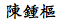
\includegraphics{Author_ChineseName.png}
\end{flushright}\end{figure}
\begin{description}
\item[{Chen Chung-Shu}] \leavevmode
\href{mailto:gamma\_chen@yahoo.com.tw}{gamma\_chen@yahoo.com.tw}

\href{http://jonathan2251.github.com/web/index.html}{http://jonathan2251.github.com/web/index.html}

\item[{Anoushe Jamshidi}] \leavevmode
\href{mailto:ajamshidi@gmail.com}{ajamshidi@gmail.com}

\end{description}


\section{Contributors}
\label{about:contributors}
Chen Wei-Ren, \href{mailto:chenwj@iis.sinica.edu.tw}{chenwj@iis.sinica.edu.tw}, assisted with text and code formatting.

Chen Zhong-Cheng, who is the author of original cpu0 verilog code.


\section{Acknowledgments}
\label{about:acknowledgments}
We would like to thank Sean Silva, \href{mailto:silvas@purdue.edu}{silvas@purdue.edu}, for his help, encouragement, and
assistance with the Sphinx document generator.  Without his help, this book would not
have been finished and published online. We also thank those corrections from readers
who make the book more accurate.


\section{Support}
\label{about:support}
We also get the kind help from LLVM development mail list, \href{mailto:llvmdev@cs.uiuc.edu}{llvmdev@cs.uiuc.edu},
even we don't know them. So, our experience is you are not
alone and can get help from the development list members in working with the LLVM
project. They are:

Akira Hatanaka \textless{}\href{mailto:ahatanak@gmail.com}{ahatanak@gmail.com}\textgreater{} in va\_arg question answer.

Ulrich Weigand \textless{}\href{mailto:Ulrich.Weigand@de.ibm.com}{Ulrich.Weigand@de.ibm.com}\textgreater{} in AsmParser question answer.


\section{Revision history}
\label{about:revision-history}
Version 3.3.9, Not release yet.
\begin{description}
\item[{Version 3.3.8, Released November 18, 2013}] \leavevmode
Fix the reference file missing for make gh-page.

\item[{Version 3.3.7, Released November 17, 2013}] \leavevmode
lld.rst documentation.
Add cpu032I and cpu032II in \emph{llc -mcpu}.
Reference only for Chapter12\_2.

\item[{Version 3.3.6, Released November 8, 2013}] \leavevmode
Move example code from github to dropbox since the name is not work for
download example code.

\item[{Version 3.3.5, Released November 7, 2013}] \leavevmode
Split the elf2hex code from modiified llvm-objdump.cpp to elf2hex.h.
Fix bug for tail call setting in LowerCall().
Fix bug for LowerCPLOAD().
Update elf.rst.
Fix typing error.
Add dynamic linker support.
Merge cpu0 Chapter12\_1 and Chapter12\_2 code into one, and identify each of
them by -mcpu=cpu0I and -mcpu=cpu0II.
cpu0II.
Update lld.rst for static linker.
Change the name of example code from LLVMBackendTutorialExampleCode to lbdex.

\item[{Version 3.3.4, Released September 21, 2013}] \leavevmode
Fix Chapter Global variables error for LUi instructions and the material move
to Chapter Other data type.
Update regression test items.

\item[{Version 3.3.3, Released September 20, 2013}] \leavevmode
Add Chapter othertype

\item[{Version 3.3.2, Released September 17, 2013}] \leavevmode
Update example code.
Fix bug sext\_inreg.
Fix llvm-objdump.cpp bug to support global variable of .data.
Update install.rst to run on llvm 3.3.

\item[{Version 3.3.1, Released September 14, 2013}] \leavevmode
Add load bool type in chapter 6.
Fix chapter 4 error.
Add interrupt function in cpu0i.v.
Fix bug in alloc() support of Chapter 8 by adding code of spill \$fp register.
Add JSUB texternalsym for memcpy function call of llvm auto reference.
Rename cpu0i.v to cpu0s.v.
Modify itoa.cpp.
Cpu0 of lld.

\item[{Version 3.3.0, Released July 13, 2013}] \leavevmode
Add Table: C operator ! corresponding IR of .bc and IR of DAG and Table: C
operator ! corresponding IR of Type-legalized selection DAG and Cpu0
instructions. Add explanation in section Full support \%.
Add Table: Chapter 4 operators.
Add Table: Chapter 3 .bc IR instructions.
Rewrite Chapter 5 Global variables.
Rewrite section Handle \$gp register in PIC addressing mode.
Add Large Frame Stack Pointer support.
Add dynamic link section in elf.rst.
Re-oganize Chapter 3.
Re-oganize Chapter 8.
Re-oganize Chapter 10.
Re-oganize Chapter 11.
Re-oganize Chapter 12.
Fix bug that ret not \$lr register.
Porting to LLVM 3.3.

\item[{Version 3.2.15, Released June 12, 2013}] \leavevmode
Porting to llvm 3.3.
Rewrite section Support arithmetic instructions of chapter Adding arithmetic
and local pointer support with the table adding.
Add two sentences in Preface.
Add \emph{llc -debug-pass} in section LLVM Code Generation Sequence.
Remove section Adjust cpu0 instructions.
Remove section Use cpu0 official LDI instead of ADDiu of Appendix-C.

\item[{Version 3.2.14, Released May 24, 2013}] \leavevmode
Fix example code disappeared error.

\item[{Version 3.2.13, Released May 23, 2013}] \leavevmode
Add sub-section ``Setup llvm-lit on iMac'' of Appendix A.
Replace some code-block with literalinclude in *.rst.
Add Fig 9 of chapter Backend structure.
Add section Dynamic stack allocation support of chapter Function call.
Fix bug of Cpu0DelUselessJMP.cpp.
Fix cpu0 instruction table errors.

\item[{Version 3.2.12, Released March 9, 2013}] \leavevmode
Add section ``Type of char and short int'' of chapter
``Global variables, structs and arrays, other type''.

\item[{Version 3.2.11, Released March 8, 2013}] \leavevmode
Fix bug in generate elf of chapter ``Backend Optimization''.

\item[{Version 3.2.10, Released February 23, 2013}] \leavevmode
Add chapter ``Backend Optimization''.

\item[{Version 3.2.9, Released February 20, 2013}] \leavevmode
Correct the ``Variable number of arguments'' such as sum\_i(int amount, ...)
errors.

\item[{Version 3.2.8, Released February 20, 2013}] \leavevmode
Add section llvm-objdump -t -r.

\item[{Version 3.2.7, Released February 14, 2013}] \leavevmode
Add chapter Run backend.
Add Icarus Verilog tool installation in Appendix A.

\item[{Version 3.2.6, Released February 4, 2013}] \leavevmode
Update CMP instruction implementation.
Add llvm-objdump section.

\item[{Version 3.2.5, Released January 27, 2013}] \leavevmode
Add ``LLVMBackendTutorialExampleCode/llvm3.1''.
Add  section ``Structure type support''.
Change reference from Figure title to Figure number.

\item[{Version 3.2.4, Released January 17, 2013}] \leavevmode
Update for LLVM 3.2.
Change title (book name) from ``Write An LLVM Backend Tutorial For Cpu0'' to
``Tutorial: Creating an LLVM Backend for the Cpu0 Architecture''.

\item[{Version 3.2.3, Released January 12, 2013}] \leavevmode
Add chapter ``Porting to LLVM 3.2''.

\item[{Version 3.2.2, Released January 10, 2013}] \leavevmode
Add section ``Full support \%'' and section ``Verify DIV for operator \%''.

\item[{Version 3.2.1, Released January 7, 2013}] \leavevmode
Add Footnote for references.
Reorganize chapters (Move bottom part of chapter ``Global variable'' to
chapter ``Other instruction''; Move section ``Translate into obj file'' to
new chapter ``Generate obj file''.
Fix errors in Fig/otherinst/2.png and Fig/otherinst/3.png.

\item[{Version 3.2.0, Released January 1, 2013}] \leavevmode
Add chapter Function.
Move Chapter ``Installing LLVM and the Cpu0 example code'' from beginning to
Appendix A.
Add subsection ``Install other tools on Linux''.
Add chapter ELF.

\item[{Version 3.1.2, Released December 15, 2012}] \leavevmode
Fix section 6.1 error by add “def : Pat\textless{}(brcond RC:\$cond, bb:\$dst),
(JNEOp (CMPOp RC:\$cond, ZEROReg), bb:\$dst)\textgreater{};” in last pattern.
Modify section 5.5
Fix bug Cpu0InstrInfo.cpp SW to ST.
Correct LW to LD; LB to LDB; SB to STB.

\item[{Version 3.1.1, Released November 28, 2012}] \leavevmode
Add Revision history.
Correct ldi instruction error (replace ldi instruction with addiu from the
beginning and in the all example code).
Move ldi instruction change from section of ``Adjust cpu0 instruction and
support type of local variable pointer'' to Section ”CPU0
processor architecture”.
Correct some English \& typing errors.

\end{description}


\section{Licensing}
\label{about:licensing}
\begin{notice}{note}{Todo}

Add info about LLVM documentation licensing.
\end{notice}


\section{Preface}
\label{about:preface}
The LLVM Compiler Infrastructure provides a versatile structure for creating new
backends. Creating a new backend should not be too difficult once you
familiarize yourself with this structure. However, the available backend
documentation is fairly high level and leaves out many details. This tutorial
will provide step-by-step instructions to write a new backend for a new target
architecture from scratch.

We will use the Cpu0 architecture as an example to build our new backend. Cpu0
is a simple RISC architecture that has been designed for educational purposes.
More information about Cpu0, including its instruction set, is available
\href{http://ccckmit.wikidot.com/ocs:cpu0}{here}. The Cpu0 example code referenced in
this book can be found \href{http://jonathan2251.github.com/lbd/LLVMBackendTutorialExampleCode.tar.gz}{here}.
As you progress from one chapter to the next, you will incrementally build the
backend's functionality.

Since Cpu0 is a simple RISC CPU for educational purpose, it make the Cpu0 llvm
backend code simple too and easy to learning. In addition, Cpu0 supply the
Verilog source code that you can run on your PC or FPGA platform when you go to
chapter Run backend.

This tutorial was written using the LLVM 3.1 Mips backend as a reference. Since
Cpu0 is an educational architecture, it is missing some key pieces of
documentation needed when developing a compiler, such as an Application Binary
Interface (ABI). We implement our backend borrowing information from the Mips
ABI as a guide. You may want to familiarize yourself with the relevant parts of
the Mips ABI as you progress through this tutorial.


\section{Prerequisites}
\label{about:prerequisites}
Readers should be comfortable with the C++ language and Object-Oriented
Programming concepts. LLVM has been developed and implemented in C++, and it is
written in a modular way so that various classes can be adapted and reused as
often as possible.

Already having conceptual knowledge of how compilers work is a plus, and if you
already have implemented compilers in the past you will likely have no trouble
following this tutorial. As this tutorial will build up an LLVM backend
step-by-step, we will introduce important concepts as necessary.

This tutorial references the following materials.  We highly recommend you read
these documents to get a deeper understanding of what the tutorial is teaching:

\href{http://www.aosabook.org/en/llvm.html}{The Architecture of Open Source Applications Chapter on LLVM}

\href{http://llvm.org/docs/CodeGenerator.html}{LLVM's Target-Independent Code Generation documentation}

\href{http://llvm.org/docs/TableGenFundamentals.html}{LLVM's TableGen Fundamentals documentation}

\href{http://llvm.org/docs/WritingAnLLVMBackend.html}{LLVM's Writing an LLVM Compiler Backend documentation}

\href{http://www.opus.ub.uni-erlangen.de/opus/volltexte/2010/1659/pdf/tricore\_llvm.pdf}{Description of the Tricore LLVM Backend}

\href{http://www.linux-mips.org/pub/linux/mips/doc/ABI/mipsabi.pdf}{Mips ABI document}


\section{Outline of Chapters}
\label{about:outline-of-chapters}
{\hyperref[llvmstructure:sec-llvmstructure]{\emph{Cpu0 Instruction Set and LLVM Target Description}}}:

This chapter introduces the Cpu0 architecture, a high-level view of LLVM, and how Cpu0
will be targeted in in an LLVM backend. This chapter will run you through the initial
steps of building the backend, including initial work on the target description (td),
setting up cmake and LLVMBuild files, and target registration. Around 750 lines of source
code are added by the end of this chapter.

{\hyperref[backendstructure:sec-backendstructure]{\emph{Backend structure}}}:

This chapter highlights the structure of an LLVM backend using by UML graphs, and we
continue to build the Cpu0 backend. Around 2300 lines of source code are added,
most of which are common from one LLVM backends to another, regardless of the
target architecture. By the end of this chapter, the Cpu0 LLVM backend will support
three instructions to generate some initial assembly output.

{\hyperref[otherinst:sec-addingmoresupport]{\emph{Arithmetic and logic lsupport}}}:

Over ten C operators and their corresponding LLVM IR instructions are introduced in this
chapter. Around 345 lines of source code, mostly in .td Target Description files, are
added. With these 345 lines, the backend can now translate the \textbf{+, -, *, /, \&, \textbar{}, \textasciicircum{},
\textless{}\textless{}, \textgreater{}\textgreater{}, !} and \textbf{\%} C operators into the appropriate Cpu0 assembly code. Use of the
\code{llc} debug option and of \textbf{Graphviz} as a debug tool are introduced in this chapter.

{\hyperref[genobj:sec-genobjfiles]{\emph{Generating object files}}}:

Object file generation support for the Cpu0 backend is added in this chapter, as the
Target Registration structure is introduced. With 700 lines of additional code,
the Cpu0 backend can now generate big and little endian object files.

{\hyperref[globalvar:sec-globalvars]{\emph{Global variables}}}:

Global variable, struct and array support, char and short int, are added in this chapter.
About 300 lines of source code are added to do this. The Cpu0 supports PIC and static
addressing mode, both of which area explained as their functionality is implemented.

:ref:\_sec-othertypesupport:

In addition to type int, other data type like pointer, char, bool, long long,
structure and array are added in this chapter.

{\hyperref[ctrlflow:sec-controlflow]{\emph{Control flow statements}}}:

Support for the \textbf{if, else, while, for, goto} flow control statements are
added in this chapter. Around 150 lines of source code added.

{\hyperref[funccall:sec-funccall]{\emph{Function call}}}:

This chapter details the implementation of function calls in the Cpu0 backend. The stack
frame, handling incoming \& outgoing arguments, and their corresponding standard LLVM
functions are introduced. Over 700 lines of source code are added.

{\hyperref[elf:sec-elf]{\emph{ELF Support}}}:

This chapter details Cpu0 support for the well-known ELF object file format. The ELF
format and binutils tools are not a part of LLVM, but are introduced.  This chapter
details how to use the ELF tools to verify and analyze the object files created by the
Cpu0 backend. The \code{llvm-objdump -d} support which translate elf into hex file
format is added in last section.

{\hyperref[runbackend:sec-runbackend]{\emph{Run backend}}}:

Add AsmParser support for translate hand code assembly language into obj first.
Next, design the CPU0 backend with Verilog language of Icarus tool.
Finally feed the hex file which generated by llvm-objdump and see the CPU0
running result.

{\hyperref[optimize:sec-optimize]{\emph{Backend Optimization}}}:

Introduce how to do backend optimization by a simple effective example, and
redesign Cpu0 instruction sets to be a efficient RISC CPU.

{\hyperref[lld:sec-lld]{\emph{LLD for Cpu0}}}:

Develop ELF linker for Cpu0 backend based on lld project.

{\hyperref[install:sec-appendix-installing]{\emph{Appendix A: Getting Started: Installing LLVM and the Cpu0 example code}}}:

Details how to set up the LLVM source code, development tools, and environment
setting for Mac OS X and Linux platforms.


\chapter{Cpu0 Instruction Set and LLVM Target Description}
\label{llvmstructure:cpu0-instruction-set-and-llvm-target-description}\label{llvmstructure:sec-llvmstructure}\label{llvmstructure::doc}
Before you begin this tutorial, you should know that you can always try to develop your
own backend by porting code from existing backends.  The majority of the code you will
want to investigate can be found in the /lib/Target directory of your root LLVM
installation. As most major RISC instruction sets have some similarities, this may be the
avenue you might try if you are an experienced programmer and knowledgable of compiler
backends.

On the other hand, there is a steep learning curve and you may easily get stuck
debugging your new backend. You can easily spend a lot of time tracing which
methods are callbacks of some function, or which are calling some overridden
method deep in the LLVM codebase - and with a codebase as large as LLVM, all of this
can easily become difficult to keep track of. This tutorial will help you work through
this process while learning the fundamentals of LLVM backend design. It will show
you what is necessary to get your first backend functional and complete, and it
should help you understand how to debug your backend when it produces incorrect machine
code using output provided by the compiler.

This section details the Cpu0 instruction set and the structure of LLVM.
The LLVM structure information is adapted from Chris Lattner's LLVM chapter of the
Architecture of Open Source Applications book \footnote{
Chris Lattner, \textbf{LLVM}. Published in The Architecture of Open Source Applications. \href{http://www.aosabook.org/en/llvm.html}{http://www.aosabook.org/en/llvm.html}
}. You can read
the original article from the AOSA website if you prefer. Finally, you will begin to
create a new LLVM backend by writing register and instruction definitions in the
Target Description files which will be used in next section.


\section{Cpu0 Processor Architecture Details}
\label{llvmstructure:cpu0-processor-architecture-details}
This subsection is based on materials available here \footnote{
Original Cpu0 architecture and ISA details (Chinese). \href{http://ccckmit.wikidot.com/ocs:cpu0}{http://ccckmit.wikidot.com/ocs:cpu0}
} (Chinese)
and \footnote{
English translation of Cpu0 description. \href{http://translate.google.com.tw/translate?js=n\&prev=\_t\&hl=zh-TW\&ie=UTF-8\&layout=2\&eotf=1\&sl=zh-CN\&tl=en\&u=http://ccckmit.wikidot.com/ocs:cpu0}{http://translate.google.com.tw/translate?js=n\&prev=\_t\&hl=zh-TW\&ie=UTF-8\&layout=2\&eotf=1\&sl=zh-CN\&tl=en\&u=http://ccckmit.wikidot.com/ocs:cpu0}
} (English).


\subsection{Brief introduction}
\label{llvmstructure:brief-introduction}
Cpu0 is a 32-bit architecture. It has 16 general purpose registers (R0, ..., R15), the
Instruction Register (IR), the memory access registers MAR \& MDR. Its structure is
illustrated in \hyperref[llvmstructure:llvmstructure-f1]{Figure  \ref*{llvmstructure:llvmstructure-f1}} below.
\begin{figure}[htbp]
\centering
\capstart

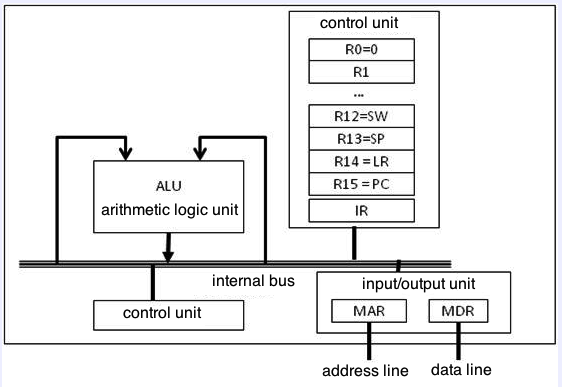
\includegraphics{17.png}
\caption{Architectural block diagram of the Cpu0 processor}\label{llvmstructure:llvmstructure-f1}\end{figure}

The registers are used for the following purposes:


\begin{threeparttable}
\capstart\caption{Cpu0 registers purposes}

\begin{tabulary}{\linewidth}{|L|L|}
\hline
\textbf{
Register
} & \textbf{
Description
}\\\hline

IR
 & 
Instruction register
\\\hline

R0
 & 
Constant register, value is 0
\\\hline

R1-R11
 & 
General-purpose registers
\\\hline

R12
 & 
Status Word register (SW)
\\\hline

R13
 & 
Stack Pointer register (SP)
\\\hline

R14
 & 
Link Register (LR)
\\\hline

R15
 & 
Program Counter (PC)
\\\hline

MAR
 & 
Memory Address Register (MAR)
\\\hline

MDR
 & 
Memory Data Register (MDR)
\\\hline

HI
 & 
High part of MULT result
\\\hline

LO
 & 
Low part of MULT result
\\\hline

SW
 & 
Status Word Register
\\\hline
\end{tabulary}

\end{threeparttable}



\subsection{The Cpu0 Instruction Set}
\label{llvmstructure:the-cpu0-instruction-set}
The Cpu0 instruction set can be divided into three types: L-type instructions, which are
generally associated with memory operations, A-type instructions for arithmetic
operations, and J-type instructions that are typically used when altering control flow
(i.e. jumps).  \hyperref[llvmstructure:llvmstructure-f2]{Figure  \ref*{llvmstructure:llvmstructure-f2}} illustrates how the bitfields are broken
down for each type of instruction.
\begin{figure}[htbp]
\centering
\capstart

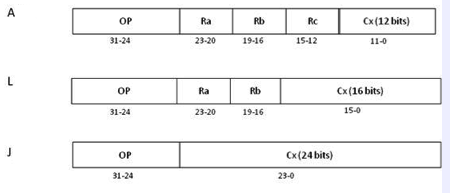
\includegraphics{26.png}
\caption{Cpu0's three instruction formats}\label{llvmstructure:llvmstructure-f2}\end{figure}

The following table details the Cpu0 instruction set:
\begin{itemize}
\item {} 
First column F.: meaning Format.

\end{itemize}

\begin{longtable}{|l|l|l|l|l|l|}
\caption{Cpu0 Instruction Set} \\
\hline
\textbf{
F.
} & \textbf{
Mnemonic
} & \textbf{
Opcode
} & \textbf{
Meaning
} & \textbf{
Syntax
} & \textbf{
Operation
}\\\hline
\endfirsthead

\multicolumn{6}{c}%
{{\bfseries \tablename\ \thetable{} -- continued from previous page}} \\
\hline
\textbf{
F.
} & \textbf{
Mnemonic
} & \textbf{
Opcode
} & \textbf{
Meaning
} & \textbf{
Syntax
} & \textbf{
Operation
}\\\hline
\endhead

\hline \multicolumn{6}{|r|}{{Continued on next page}} \\ \hline
\endfoot

\hline
\endlastfoot


L
 & 
NOP
 & 
00
 & 
No Operation
 &  & \\\hline

L
 & 
LD
 & 
01
 & 
Load word
 & 
LD Ra, {[}Rb+Cx{]}
 & 
Ra \textless{}= {[}Rb+Cx{]}
\\\hline

L
 & 
ST
 & 
02
 & 
Store word
 & 
ST Ra, {[}Rb+Cx{]}
 & 
{[}Rb+Cx{]} \textless{}= Ra
\\\hline

L
 & 
LB
 & 
03
 & 
Load byte
 & 
LB Ra, {[}Rb+Cx{]}
 & 
Ra \textless{}= (byte){[}Rb+Cx{]}
\\\hline

L
 & 
LBu
 & 
04
 & 
Load byte unsigned
 & 
LBu Ra, {[}Rb+Cx{]}
 & 
Ra \textless{}= (byte){[}Rb+Cx{]}
\\\hline

L
 & 
SB
 & 
05
 & 
Store byte
 & 
SB Ra, {[}Rb+Cx{]}
 & 
{[}Rb+Cx{]} \textless{}= (byte)Ra
\\\hline

A
 & 
LH
 & 
06
 & 
Load half word unsigned
 & 
LH Ra, {[}Rb+Cx{]}
 & 
Ra \textless{}= (2bytes){[}Rb+Cx{]}
\\\hline

A
 & 
LHu
 & 
07
 & 
Load half word
 & 
LHu Ra, {[}Rb+Cx{]}
 & 
Ra \textless{}= (2bytes){[}Rb+Cx{]}
\\\hline

A
 & 
SH
 & 
08
 & 
Store half word
 & 
SH Ra, {[}Rb+Cx{]}
 & 
{[}Rb+Rc{]} \textless{}= Ra
\\\hline

L
 & 
ADDiu
 & 
09
 & 
Add immediate
 & 
ADDiu Ra, Rb, Cx
 & 
Ra \textless{}= (Rb + Cx)
\\\hline

L
 & 
ANDi
 & 
0C
 & 
AND imm
 & 
ANDi Ra, Rb, Cx
 & 
Ra \textless{}= (Rb \& Cx)
\\\hline

L
 & 
ORi
 & 
0D
 & 
OR
 & 
ORi Ra, Rb, Cx
 & 
Ra \textless{}= (Rb \textbar{} Cx)
\\\hline

L
 & 
XORi
 & 
0E
 & 
XOR
 & 
XORi Ra, Rb, Cx
 & 
Ra \textless{}= (Rb \textasciicircum{} Cx)
\\\hline

L
 & 
LUi
 & 
0F
 & 
Load upper
 & 
LUi Ra, Cx
 & 
Ra \textless{}= (Cx \textless{}\textless{} 16)
\\\hline

A
 & 
CMP
 & 
10
 & 
Compare
 & 
CMP Ra, Rb
 & 
SW \textless{}= (Ra cond Rb) \footnote{
Conditions include the following comparisons: \textgreater{}, \textgreater{}=, ==, !=, \textless{}=, \textless{}. SW is actually set by the subtraction of the two register operands, and the flags indicate which conditions are present.
}
\\\hline

A
 & 
ADDu
 & 
11
 & 
Add unsigned
 & 
ADD Ra, Rb, Rc
 & 
Ra \textless{}= Rb + Rc
\\\hline

A
 & 
SUBu
 & 
12
 & 
Sub unsigned
 & 
SUB Ra, Rb, Rc
 & 
Ra \textless{}= Rb - Rc
\\\hline

A
 & 
ADD
 & 
13
 & 
Add
 & 
ADD Ra, Rb, Rc
 & 
Ra \textless{}= Rb + Rc
\\\hline

A
 & 
SUB
 & 
14
 & 
Subtract
 & 
SUB Ra, Rb, Rc
 & 
Ra \textless{}= Rb - Rc
\\\hline

A
 & 
MUL
 & 
17
 & 
Multiply
 & 
MUL Ra, Rb, Rc
 & 
Ra \textless{}= Rb * Rc
\\\hline

A
 & 
AND
 & 
18
 & 
Bitwise and
 & 
AND Ra, Rb, Rc
 & 
Ra \textless{}= Rb \& Rc
\\\hline

A
 & 
OR
 & 
19
 & 
Bitwise or
 & 
OR Ra, Rb, Rc
 & 
Ra \textless{}= Rb \textbar{} Rc
\\\hline

A
 & 
XOR
 & 
1A
 & 
Bitwise exclusive or
 & 
XOR Ra, Rb, Rc
 & 
Ra \textless{}= Rb \textasciicircum{} Rc
\\\hline

A
 & 
ROL
 & 
1B
 & 
Rotate left
 & 
ROL Ra, Rb, Cx
 & 
Ra \textless{}= Rb rol Cx
\\\hline

A
 & 
ROR
 & 
1C
 & 
Rotate right
 & 
ROR Ra, Rb, Cx
 & 
Ra \textless{}= Rb ror Cx
\\\hline

A
 & 
SRA
 & 
1D
 & 
Shift right
 & 
SRA Ra, Rb, Cx
 & 
Ra \textless{}= Rb `\textgreater{}\textgreater{} Cx \footnote{
Rb `\textgreater{}\textgreater{} Cx, Rb `\textgreater{}\textgreater{} Rc: Shift with signed bit remain. It's equal to ((Rb\&'h80000000)\textbar{}Rb\textgreater{}\textgreater{}Cx) or ((Rb\&'h80000000)\textbar{}Rb\textgreater{}\textgreater{}Rc).
}
\\\hline

A
 & 
SHL
 & 
1E
 & 
Shift left
 & 
SHL Ra, Rb, Cx
 & 
Ra \textless{}= Rb \textless{}\textless{} Cx
\\\hline

A
 & 
SHR
 & 
1F
 & 
Shift right
 & 
SHR Ra, Rb, Cx
 & 
Ra \textless{}= Rb \textgreater{}\textgreater{} Cx
\\\hline

A
 & 
SRAV
 & 
20
 & 
Shift right
 & 
SRAV Ra, Rb, Rc
 & 
Ra \textless{}= Rb `\textgreater{}\textgreater{} Rc \footnotemark[4]
\\\hline

A
 & 
SHLV
 & 
21
 & 
Shift left
 & 
SHLV Ra, Rb, Rc
 & 
Ra \textless{}= Rb \textless{}\textless{} Rc
\\\hline

A
 & 
SHRV
 & 
22
 & 
Shift right
 & 
SHRV Ra, Rb, Rc
 & 
Ra \textless{}= Rb \textgreater{}\textgreater{} Rc
\\\hline

J
 & 
JEQ
 & 
30
 & 
Jump if equal (==)
 & 
JEQ Cx
 & 
if SW(==), PC \textless{}= PC + Cx
\\\hline

J
 & 
JNE
 & 
31
 & 
Jump if not equal (!=)
 & 
JNE Cx
 & 
if SW(!=), PC \textless{}= PC + Cx
\\\hline

J
 & 
JLT
 & 
32
 & 
Jump if less than (\textless{})
 & 
JLT Cx
 & 
if SW(\textless{}), PC \textless{}= PC + Cx
\\\hline

J
 & 
JGT
 & 
33
 & 
Jump if greater than (\textgreater{})
 & 
JGT Cx
 & 
if SW(\textgreater{}), PC \textless{}= PC + Cx
\\\hline

J
 & 
JLE
 & 
34
 & 
Jump if less than or equals (\textless{}=)
 & 
JLE Cx
 & 
if SW(\textless{}=), PC \textless{}= PC + Cx
\\\hline

J
 & 
JGE
 & 
35
 & 
Jump if greater than or equals (\textgreater{}=)
 & 
JGE Cx
 & 
if SW(\textgreater{}=), PC \textless{}= PC + Cx
\\\hline

J
 & 
JMP
 & 
36
 & 
Jump (unconditional)
 & 
JMP Cx
 & 
PC \textless{}= PC + Cx
\\\hline

J
 & 
SWI
 & 
3A
 & 
Software interrupt
 & 
SWI Cx
 & 
LR \textless{}= PC; PC \textless{}= Cx
\\\hline

J
 & 
JSUB
 & 
3B
 & 
Jump to subroutine
 & 
JSUB Cx
 & 
LR \textless{}= PC; PC \textless{}= PC + Cx
\\\hline

J
 & 
RET
 & 
3C
 & 
Return from subroutine
 & 
RET LR
 & 
PC \textless{}= LR
\\\hline

J
 & 
IRET
 & 
3D
 & 
Return from interrupt handler
 & 
IRET
 & 
PC \textless{}= LR; INT 0
\\\hline

J
 & 
JALR
 & 
3E
 & 
Indirect jump
 & 
JALR Rb
 & 
LR \textless{}= PC; PC \textless{}= Rb \footnote{
jsub cx is direct call for 24 bits value of cx while jalr \$rb is indirect call for 32 bits value of register \$rb.
}
\\\hline

L
 & 
MULT
 & 
41
 & 
Multiply for 64 bits result
 & 
MULT Ra, Rb
 & 
(HI,LO) \textless{}= MULT(Ra,Rb)
\\\hline

L
 & 
MULTU
 & 
42
 & 
MULT for unsigned 64 bits
 & 
MULTU Ra, Rb
 & 
(HI,LO) \textless{}= MULTU(Ra,Rb)
\\\hline

L
 & 
DIV
 & 
43
 & 
Divide
 & 
DIV Ra, Rb
 & 
HI\textless{}=Ra\%Rb, LO\textless{}=Ra/Rb
\\\hline

L
 & 
DIVU
 & 
44
 & 
Divide
 & 
DIV Ra, Rb
 & 
HI\textless{}=Ra\%Rb, LO\textless{}=Ra/Rb
\\\hline

L
 & 
MFHI
 & 
46
 & 
Move HI to GPR
 & 
MFHI Ra
 & 
Ra \textless{}= HI
\\\hline

L
 & 
MFLO
 & 
47
 & 
Move LO to GPR
 & 
MFLO Ra
 & 
Ra \textless{}= LO
\\\hline

L
 & 
MTHI
 & 
48
 & 
Move GPR to HI
 & 
MTHI Ra
 & 
HI \textless{}= Ra
\\\hline

L
 & 
MTLO
 & 
49
 & 
Move GPR to LO
 & 
MTLO Ra
 & 
LO \textless{}= Ra
\\\hline

L
 & 
MFSW
 & 
50
 & 
Move SW to GPR
 & 
MFSW Ra
 & 
Ra \textless{}= SW
\\\hline

L
 & 
MTSW
 & 
51
 & 
Move GPR to SW
 & 
MTSW Ra
 & 
SW \textless{}= Ra
\\\hline
\end{longtable}


\begin{notice}{note}{Note:}
\textbf{Cpu0 unsigned instructions}

Like Mips, the mathematic unsigned instructions except DIVU, such as ADDu and
SUBu, are no overflow exception instructions.
The ADDu and SUBu handle both signed and unsigned integers well.
For example, (ADDu 1, -2) is -3; (ADDu 0x01,
0xfffffffe) is 0xfffffffd = (4G - 1). If you treat the result is negative then
it is -1. Otherwise, if you treat the result is positive then it's (+4G - 1).
\end{notice}


\subsection{The Status Register}
\label{llvmstructure:the-status-register}
The Cpu0 status word register (SW) contains the state of the Negative (N), Zero (Z),
Carry (C), Overflow (V), and Interrupt (I), Trap (T), and Mode (M) boolean flags.
The bit layout of the SW register is shown in \hyperref[llvmstructure:llvmstructure-f3]{Figure  \ref*{llvmstructure:llvmstructure-f3}} below.
\begin{figure}[htbp]
\centering
\capstart

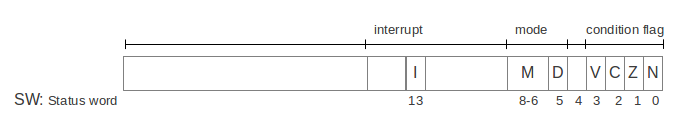
\includegraphics{35.png}
\caption{Cpu0 status word (SW) register}\label{llvmstructure:llvmstructure-f3}\end{figure}

When a CMP Ra, Rb instruction executes, the condition flags will change. For example:
\begin{itemize}
\item {} 
If Ra \textgreater{} Rb, then N = 0, Z = 0

\item {} 
If Ra \textless{} Rb, then N = 1, Z = 0

\item {} 
If Ra = Rb, then N = 0, Z = 1

\end{itemize}

The direction (i.e. taken/not taken) of the conditional jump instructions JGT, JLT, JGE,
JLE, JEQ, JNE is determined by the N and Z flags in the SW register.


\subsection{Cpu0's Stages of Instruction Execution}
\label{llvmstructure:cpu0-s-stages-of-instruction-execution}
The Cpu0 architecture has a three-stage pipeline.  The stages are instruction fetch (IF),
decode (D), and execute (EX), and they occur in that order.  Here is a description of
what happens in the processor:
\begin{enumerate}
\item {} 
Instruction fetch

\end{enumerate}
\begin{itemize}
\item {} 
The Cpu0 fetches the instruction pointed to by the Program Counter (PC) into the
Instruction Register (IR): IR = {[}PC{]}.

\item {} 
The PC is then updated to point to the next instruction: PC = PC + 4.

\end{itemize}
\begin{enumerate}
\setcounter{enumi}{1}
\item {} 
Decode

\end{enumerate}
\begin{itemize}
\item {} 
The control unit decodes the instruction stored in IR, which routes necessary data
stored in registers to the ALU, and sets the ALU's operation mode based on the
current instruction's opcode.

\end{itemize}
\begin{enumerate}
\setcounter{enumi}{2}
\item {} 
Execute

\end{enumerate}
\begin{itemize}
\item {} 
The ALU executes the operation designated by the control unit upon data in registers.
After the ALU is done, the result is stored in the destination register.

\end{itemize}


\subsection{Cpu0's Interrupt Vector}
\label{llvmstructure:cpu0-s-interrupt-vector}

\begin{threeparttable}
\capstart\caption{Cpu0's Interrupt Vector}

\begin{tabulary}{\linewidth}{|L|L|}
\hline
\textbf{
Address
} & \textbf{
type
}\\\hline

0x00
 & 
Reset
\\\hline

0x04
 & 
Error Handle
\\\hline

0x08
 & 
Interrupt
\\\hline
\end{tabulary}

\end{threeparttable}



\section{LLVM Structure}
\label{llvmstructure:llvm-structure}
The text in this and the following section comes from the AOSA chapter on LLVM written
by Chris Lattner \footnotemark[6].

The most popular design for a traditional static compiler (like most C
compilers) is the three phase design whose major components are the front end,
the optimizer and the back end, as seen in \hyperref[llvmstructure:llvmstructure-f6]{Figure  \ref*{llvmstructure:llvmstructure-f6}}.
The front end parses source code, checking it for errors, and builds a
language-specific Abstract Syntax Tree (AST) to represent the input code.
The AST is optionally converted to a new representation for optimization, and
the optimizer and back end are run on the code.
\begin{figure}[htbp]
\centering
\capstart

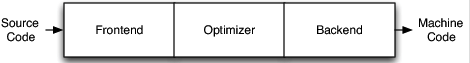
\includegraphics{64.png}
\caption{Three Major Components of a Three Phase Compiler}\label{llvmstructure:llvmstructure-f6}\end{figure}

The optimizer is responsible for doing a broad variety of transformations to
try to improve the code's running time, such as eliminating redundant
computations, and is usually more or less independent of language and target.
The back end (also known as the code generator) then maps the code onto the
target instruction set.
In addition to making correct code, it is responsible for generating good code
that takes advantage of unusual features of the supported architecture.
Common parts of a compiler back end include instruction selection, register
allocation, and instruction scheduling.

This model applies equally well to interpreters and JIT compilers.
The Java Virtual Machine (JVM) is also an implementation of this model, which
uses Java bytecode as the interface between the front end and optimizer.

The most important win of this classical design comes when a compiler decides
to support multiple source languages or target architectures.
If the compiler uses a common code representation in its optimizer, then a
front end can be written for any language that can compile to it, and a back
end can be written for any target that can compile from it, as shown in
\hyperref[llvmstructure:llvmstructure-f7]{Figure  \ref*{llvmstructure:llvmstructure-f7}}.
\begin{figure}[htbp]
\centering
\capstart

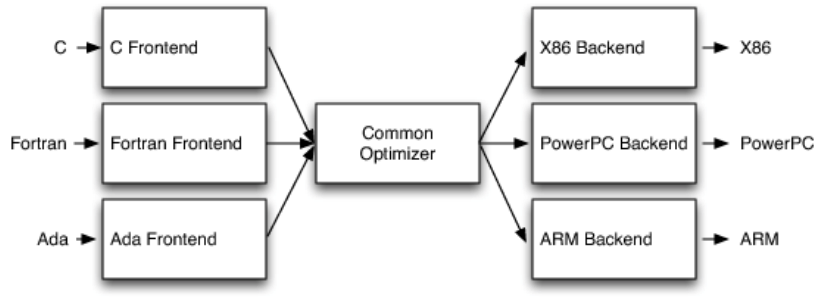
\includegraphics{73.png}
\caption{Retargetablity}\label{llvmstructure:llvmstructure-f7}\end{figure}

With this design, porting the compiler to support a new source language (e.g.,
Algol or BASIC) requires implementing a new front end, but the existing
optimizer and back end can be reused.
If these parts weren't separated, implementing a new source language would
require starting over from scratch, so supporting N targets and M source
languages would need N*M compilers.

Another advantage of the three-phase design (which follows directly from
retargetability) is that the compiler serves a broader set of programmers than
it would if it only supported one source language and one target.
For an open source project, this means that there is a larger community of
potential contributors to draw from, which naturally leads to more enhancements
and improvements to the compiler.
This is the reason why open source compilers that serve many communities (like
GCC) tend to generate better optimized machine code than narrower compilers
like FreePASCAL.
This isn't the case for proprietary compilers, whose quality is directly
related to the project's budget.
For example, the Intel ICC Compiler is widely known for the quality of code it
generates, even though it serves a narrow audience.

A final major win of the three-phase design is that the skills required to
implement a front end are different than those required for the optimizer and
back end.
Separating these makes it easier for a ``front-end person'' to enhance and
maintain their part of the compiler.
While this is a social issue, not a technical one, it matters a lot in
practice, particularly for open source projects that want to reduce the barrier
to contributing as much as possible.

The most important aspect of its design is the LLVM Intermediate Representation
(IR), which is the form it uses to represent code in the compiler.
LLVM IR is designed to host mid-level analyses and transformations that you
find in the optimizer section of a compiler.
It was designed with many specific goals in mind, including supporting
lightweight runtime optimizations, cross-function/interprocedural
optimizations, whole program analysis, and aggressive restructuring
transformations, etc.
The most important aspect of it, though, is that it is itself defined as a
first class language with well-defined semantics.
To make this concrete, here is a simple example of a .ll file:

\begin{Verbatim}[commandchars=\\\{\}]
define i32 @add1(i32 \%a, i32 \%b) \PYGZob{}
entry:
  \%tmp1 = add i32 \%a, \%b
  ret i32 \%tmp1
\PYGZcb{}
define i32 @add2(i32 \%a, i32 \%b) \PYGZob{}
entry:
  \%tmp1 = icmp eq i32 \%a, 0
  br i1 \%tmp1, label \%done, label \%recurse
recurse:
  \%tmp2 = sub i32 \%a, 1
  \%tmp3 = add i32 \%b, 1
  \%tmp4 = call i32 @add2(i32 \%tmp2, i32 \%tmp3)
  ret i32 \%tmp4
done:
  ret i32 \%b
\PYGZcb{}
// This LLVM IR corresponds to this C code, which provides two different ways to
//  add integers:
unsigned add1(unsigned a, unsigned b) \PYGZob{}
  return a+b;
\PYGZcb{}
// Perhaps not the most efficient way to add two numbers.
unsigned add2(unsigned a, unsigned b) \PYGZob{}
  if (a == 0) return b;
  return add2(a-1, b+1);
\PYGZcb{}
\end{Verbatim}

As you can see from this example, LLVM IR is a low-level RISC-like virtual
instruction set.
Like a real RISC instruction set, it supports linear sequences of simple
instructions like add, subtract, compare, and branch.
These instructions are in three address form, which means that they take some
number of inputs and produce a result in a different register.
LLVM IR supports labels and generally looks like a weird form of assembly
language.

Unlike most RISC instruction sets, LLVM is strongly typed with a simple type
system (e.g., i32 is a 32-bit integer, i32** is a pointer to pointer to 32-bit
integer) and some details of the machine are abstracted away.
For example, the calling convention is abstracted through call and ret
instructions and explicit arguments.
Another significant difference from machine code is that the LLVM IR doesn't
use a fixed set of named registers, it uses an infinite set of temporaries
named with a \% character.

Beyond being implemented as a language, LLVM IR is actually defined in three
isomorphic forms: the textual format above, an in-memory data structure
inspected and modified by optimizations themselves, and an efficient and dense
on-disk binary ``bitcode'' format.
The LLVM Project also provides tools to convert the on-disk format from text to
binary: llvm-as assembles the textual .ll file into a .bc file containing the
bitcode goop and llvm-dis turns a .bc file into a .ll file.

The intermediate representation of a compiler is interesting because it can be
a ``perfect world'' for the compiler optimizer: unlike the front end and back end
of the compiler, the optimizer isn't constrained by either a specific source
language or a specific target machine.
On the other hand, it has to serve both well: it has to be designed to be easy
for a front end to generate and be expressive enough to allow important
optimizations to be performed for real targets.


\section{.td: LLVM's Target Description Files}
\label{llvmstructure:td-llvm-s-target-description-files}
The ``mix and match'' approach allows target authors to choose what makes sense
for their architecture and permits a large amount of code reuse across
different targets.
This brings up another challenge: each shared component needs to be able to
reason about target specific properties in a generic way.
For example, a shared register allocator needs to know the register file of
each target and the constraints that exist between instructions and their
register operands.
LLVM's solution to this is for each target to provide a target description
in a declarative domain-specific language (a set of .td files) processed by the
tblgen tool.
The (simplified) build process for the x86 target is shown in
\hyperref[llvmstructure:llvmstructure-f8]{Figure  \ref*{llvmstructure:llvmstructure-f8}}.
\begin{figure}[htbp]
\centering
\capstart

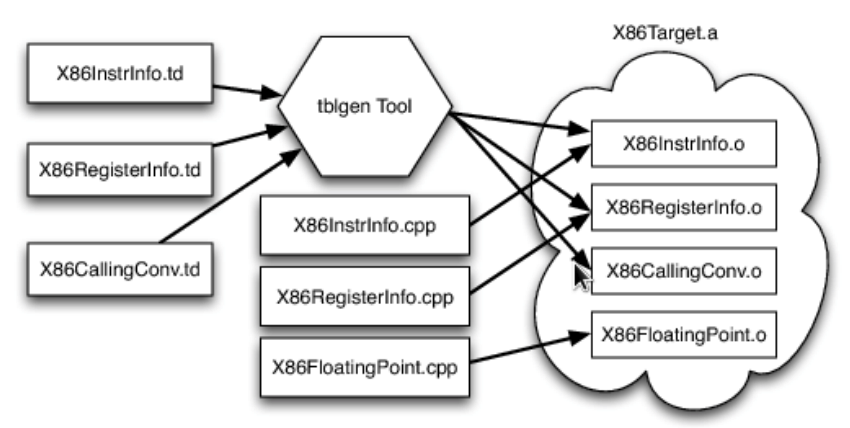
\includegraphics{83.png}
\caption{Simplified x86 Target Definition}\label{llvmstructure:llvmstructure-f8}\end{figure}

The different subsystems supported by the .td files allow target authors to
build up the different pieces of their target.
For example, the x86 back end defines a register class that holds all of its
32-bit registers named ``GR32'' (in the .td files, target specific definitions
are all caps) like this:

\begin{Verbatim}[commandchars=\\\{\}]
\PYG{n}{def} \PYG{n}{GR32} \PYG{o}{:} \PYG{n}{RegisterClass}\PYG{o}{\PYGZlt{}}\PYG{p}{[}\PYG{n}{i32}\PYG{p}{]}\PYG{p}{,} \PYG{l+m+mi}{32}\PYG{p}{,}
  \PYG{p}{[}\PYG{n}{EAX}\PYG{p}{,} \PYG{n}{ECX}\PYG{p}{,} \PYG{n}{EDX}\PYG{p}{,} \PYG{n}{ESI}\PYG{p}{,} \PYG{n}{EDI}\PYG{p}{,} \PYG{n}{EBX}\PYG{p}{,} \PYG{n}{EBP}\PYG{p}{,} \PYG{n}{ESP}\PYG{p}{,}
   \PYG{n}{R8D}\PYG{p}{,} \PYG{n}{R9D}\PYG{p}{,} \PYG{n}{R10D}\PYG{p}{,} \PYG{n}{R11D}\PYG{p}{,} \PYG{n}{R14D}\PYG{p}{,} \PYG{n}{R15D}\PYG{p}{,} \PYG{n}{R12D}\PYG{p}{,} \PYG{n}{R13D}\PYG{p}{]}\PYG{o}{\PYGZgt{}} \PYG{p}{\PYGZob{}} \PYG{p}{.}\PYG{p}{.}\PYG{p}{.} \PYG{p}{\PYGZcb{}}
\end{Verbatim}


\section{Creating the Initial Cpu0 .td Files}
\label{llvmstructure:creating-the-initial-cpu0-td-files}
As has been discussed in the previous section, LLVM uses target description files
(which use the .td file extension) to describe various components of a target's backend.
For example, these .td files may describe a target's register set, instruction set,
scheduling information for instructions, and calling conventions.  When your backend is
being compiled, the tablegen tool that ships with LLVM will translate these .td files
into C++ source code written to files that have a .inc extension.  Please refer
to \footnote{
\href{http://llvm.org/docs/TableGenFundamentals.html}{http://llvm.org/docs/TableGenFundamentals.html}
} for more information regarding how to use tablegen.

Every backend has a .td which defines some target information, including what other .td
files are used by the backend.  These files have a similar syntax to C++. For Cpu0, the
target description file is called Cpu0.td, which is shown below:
\paragraph{lbdex/Chapter2/Cpu0.td}

\begin{Verbatim}[commandchars=\\\{\}]
\PYG{c+c1}{//===-- Cpu0.td - Describe the Cpu0 Target Machine ---------*- tablegen -*-===//}
\PYG{c+c1}{//}
\PYG{c+c1}{//                     The LLVM Compiler Infrastructure}
\PYG{c+c1}{//}
\PYG{c+c1}{// This file is distributed under the University of Illinois Open Source}
\PYG{c+c1}{// License. See LICENSE.TXT for details.}
\PYG{c+c1}{//}
\PYG{c+c1}{//===----------------------------------------------------------------------===//}
\PYG{c+c1}{// This is the top level entry point for the Cpu0 target.}
\PYG{c+c1}{//===----------------------------------------------------------------------===//}

\PYG{c+c1}{//===----------------------------------------------------------------------===//}
\PYG{c+c1}{// Target-independent interfaces}
\PYG{c+c1}{//===----------------------------------------------------------------------===//}

\PYG{n}{include} \PYG{l+s}{"}\PYG{l+s}{llvm/Target/Target.td}\PYG{l+s}{"}

\PYG{c+c1}{//===----------------------------------------------------------------------===//}
\PYG{c+c1}{// Register File, Calling Conv, Instruction Descriptions}
\PYG{c+c1}{//===----------------------------------------------------------------------===//}

\PYG{n}{include} \PYG{l+s}{"}\PYG{l+s}{Cpu0RegisterInfo.td}\PYG{l+s}{"}
\PYG{n}{include} \PYG{l+s}{"}\PYG{l+s}{Cpu0Schedule.td}\PYG{l+s}{"}
\PYG{n}{include} \PYG{l+s}{"}\PYG{l+s}{Cpu0InstrInfo.td}\PYG{l+s}{"}
\end{Verbatim}

\begin{Verbatim}[commandchars=\\\{\}]
\PYG{n}{def} \PYG{n}{Cpu0InstrInfo} \PYG{o}{:} \PYG{n}{InstrInfo}\PYG{p}{;}
\end{Verbatim}

\begin{Verbatim}[commandchars=\\\{\}]
\PYG{n}{def} \PYG{n}{Cpu0} \PYG{o}{:} \PYG{n}{Target} \PYG{p}{\PYGZob{}}
\PYG{c+c1}{// def Cpu0InstrInfo : InstrInfo as before.}
  \PYG{n}{let} \PYG{n}{InstructionSet} \PYG{o}{=} \PYG{n}{Cpu0InstrInfo}\PYG{p}{;}
\end{Verbatim}

\begin{Verbatim}[commandchars=\\\{\}]
\PYG{p}{\PYGZcb{}}
\end{Verbatim}

Cpu0.td includes a few other .td files.  Cpu0RegisterInfo.td (shown below) describes the
Cpu0's set of registers.  In this file, we see that registers have been given names, i.e.
\code{def PC} indicates that there is a register called PC.  Also, there is a register class
named \code{CPURegs} that contains all of the other registers.  You may have multiple
register classes (see the X86 backend, for example) which can help you if certain
instructions can only write to specific registers.  In this case, there is only one set
of general purpose registers for Cpu0, and some registers that are reserved so that they
are not modified by instructions during execution.
\paragraph{lbdex/Chapter2/Cpu0RegisterInfo.td}

\begin{Verbatim}[commandchars=\\\{\}]
\PYG{c+c1}{//===-- Cpu0RegisterInfo.td - Cpu0 Register defs -----------*- tablegen -*-===//}
\PYG{c+c1}{//}
\PYG{c+c1}{//                     The LLVM Compiler Infrastructure}
\PYG{c+c1}{//}
\PYG{c+c1}{// This file is distributed under the University of Illinois Open Source}
\PYG{c+c1}{// License. See LICENSE.TXT for details.}
\PYG{c+c1}{//}
\PYG{c+c1}{//===----------------------------------------------------------------------===//}

\PYG{c+c1}{//===----------------------------------------------------------------------===//}
\PYG{c+c1}{//  Declarations that describe the CPU0 register file}
\PYG{c+c1}{//===----------------------------------------------------------------------===//}


\PYG{c+c1}{// We have banks of 16 registers each.}
\PYG{k}{class} \PYG{n+nc}{Cpu0Reg}\PYG{o}{\PYGZlt{}}\PYG{n}{string} \PYG{n}{n}\PYG{o}{\PYGZgt{}} \PYG{o}{:} \PYG{n}{Register}\PYG{o}{\PYGZlt{}}\PYG{n}{n}\PYG{o}{\PYGZgt{}} \PYG{p}{\PYGZob{}}
  \PYG{n}{field} \PYG{n}{bits}\PYG{o}{\PYGZlt{}}\PYG{l+m+mi}{4}\PYG{o}{\PYGZgt{}} \PYG{n}{Num}\PYG{p}{;}
  \PYG{n}{let} \PYG{n}{Namespace} \PYG{o}{=} \PYG{l+s}{"}\PYG{l+s}{Cpu0}\PYG{l+s}{"}\PYG{p}{;}
\PYG{p}{\PYGZcb{}}

\PYG{c+c1}{// Cpu0 CPU Registers}
\PYG{k}{class} \PYG{n+nc}{Cpu0GPRReg}\PYG{o}{\PYGZlt{}}\PYG{n}{bits}\PYG{o}{\PYGZlt{}}\PYG{l+m+mi}{4}\PYG{o}{\PYGZgt{}} \PYG{n}{num}\PYG{p}{,} \PYG{n}{string} \PYG{n}{n}\PYG{o}{\PYGZgt{}} \PYG{o}{:} \PYG{n}{Cpu0Reg}\PYG{o}{\PYGZlt{}}\PYG{n}{n}\PYG{o}{\PYGZgt{}} \PYG{p}{\PYGZob{}}
  \PYG{n}{let} \PYG{n}{Num} \PYG{o}{=} \PYG{n}{num}\PYG{p}{;}
\PYG{p}{\PYGZcb{}}

\PYG{c+c1}{//===----------------------------------------------------------------------===//}
\PYG{c+c1}{//  Registers}
\PYG{c+c1}{//===----------------------------------------------------------------------===//}
\PYG{c+c1}{// The register string, such as "9" or "gp" will show on "llvm-objdump -d"}
\PYG{n}{let} \PYG{n}{Namespace} \PYG{o}{=} \PYG{l+s}{"}\PYG{l+s}{Cpu0}\PYG{l+s}{"} \PYG{n}{in} \PYG{p}{\PYGZob{}}
  \PYG{c+c1}{// General Purpose Registers}
  \PYG{n}{def} \PYG{n}{ZERO} \PYG{o}{:} \PYG{n}{Cpu0GPRReg}\PYG{o}{\PYGZlt{}}\PYG{l+m+mi}{0}\PYG{p}{,}  \PYG{l+s}{"}\PYG{l+s}{zero}\PYG{l+s}{"}\PYG{o}{\PYGZgt{}}\PYG{p}{,} \PYG{n}{DwarfRegNum}\PYG{o}{\PYGZlt{}}\PYG{p}{[}\PYG{l+m+mi}{0}\PYG{p}{]}\PYG{o}{\PYGZgt{}}\PYG{p}{;}
  \PYG{n}{def} \PYG{n}{AT}   \PYG{o}{:} \PYG{n}{Cpu0GPRReg}\PYG{o}{\PYGZlt{}}\PYG{l+m+mi}{1}\PYG{p}{,}  \PYG{l+s}{"}\PYG{l+s}{1}\PYG{l+s}{"}\PYG{o}{\PYGZgt{}}\PYG{p}{,}    \PYG{n}{DwarfRegNum}\PYG{o}{\PYGZlt{}}\PYG{p}{[}\PYG{l+m+mi}{1}\PYG{p}{]}\PYG{o}{\PYGZgt{}}\PYG{p}{;}
  \PYG{n}{def} \PYG{n}{V0}   \PYG{o}{:} \PYG{n}{Cpu0GPRReg}\PYG{o}{\PYGZlt{}}\PYG{l+m+mi}{2}\PYG{p}{,}  \PYG{l+s}{"}\PYG{l+s}{2}\PYG{l+s}{"}\PYG{o}{\PYGZgt{}}\PYG{p}{,}    \PYG{n}{DwarfRegNum}\PYG{o}{\PYGZlt{}}\PYG{p}{[}\PYG{l+m+mi}{2}\PYG{p}{]}\PYG{o}{\PYGZgt{}}\PYG{p}{;}
  \PYG{n}{def} \PYG{n}{V1}   \PYG{o}{:} \PYG{n}{Cpu0GPRReg}\PYG{o}{\PYGZlt{}}\PYG{l+m+mi}{3}\PYG{p}{,}  \PYG{l+s}{"}\PYG{l+s}{3}\PYG{l+s}{"}\PYG{o}{\PYGZgt{}}\PYG{p}{,}    \PYG{n}{DwarfRegNum}\PYG{o}{\PYGZlt{}}\PYG{p}{[}\PYG{l+m+mi}{3}\PYG{p}{]}\PYG{o}{\PYGZgt{}}\PYG{p}{;}
  \PYG{n}{def} \PYG{n}{A0}   \PYG{o}{:} \PYG{n}{Cpu0GPRReg}\PYG{o}{\PYGZlt{}}\PYG{l+m+mi}{4}\PYG{p}{,}  \PYG{l+s}{"}\PYG{l+s}{4}\PYG{l+s}{"}\PYG{o}{\PYGZgt{}}\PYG{p}{,}    \PYG{n}{DwarfRegNum}\PYG{o}{\PYGZlt{}}\PYG{p}{[}\PYG{l+m+mi}{4}\PYG{p}{]}\PYG{o}{\PYGZgt{}}\PYG{p}{;}
  \PYG{n}{def} \PYG{n}{A1}   \PYG{o}{:} \PYG{n}{Cpu0GPRReg}\PYG{o}{\PYGZlt{}}\PYG{l+m+mi}{5}\PYG{p}{,}  \PYG{l+s}{"}\PYG{l+s}{5}\PYG{l+s}{"}\PYG{o}{\PYGZgt{}}\PYG{p}{,}    \PYG{n}{DwarfRegNum}\PYG{o}{\PYGZlt{}}\PYG{p}{[}\PYG{l+m+mi}{5}\PYG{p}{]}\PYG{o}{\PYGZgt{}}\PYG{p}{;}
  \PYG{n}{def} \PYG{n}{T9}   \PYG{o}{:} \PYG{n}{Cpu0GPRReg}\PYG{o}{\PYGZlt{}}\PYG{l+m+mi}{6}\PYG{p}{,}  \PYG{l+s}{"}\PYG{l+s}{t9}\PYG{l+s}{"}\PYG{o}{\PYGZgt{}}\PYG{p}{,}   \PYG{n}{DwarfRegNum}\PYG{o}{\PYGZlt{}}\PYG{p}{[}\PYG{l+m+mi}{6}\PYG{p}{]}\PYG{o}{\PYGZgt{}}\PYG{p}{;}
  \PYG{n}{def} \PYG{n}{T0}   \PYG{o}{:} \PYG{n}{Cpu0GPRReg}\PYG{o}{\PYGZlt{}}\PYG{l+m+mi}{7}\PYG{p}{,}  \PYG{l+s}{"}\PYG{l+s}{t0}\PYG{l+s}{"}\PYG{o}{\PYGZgt{}}\PYG{p}{,}   \PYG{n}{DwarfRegNum}\PYG{o}{\PYGZlt{}}\PYG{p}{[}\PYG{l+m+mi}{7}\PYG{p}{]}\PYG{o}{\PYGZgt{}}\PYG{p}{;}
  \PYG{n}{def} \PYG{n}{S0}   \PYG{o}{:} \PYG{n}{Cpu0GPRReg}\PYG{o}{\PYGZlt{}}\PYG{l+m+mi}{8}\PYG{p}{,}  \PYG{l+s}{"}\PYG{l+s}{8}\PYG{l+s}{"}\PYG{o}{\PYGZgt{}}\PYG{p}{,}    \PYG{n}{DwarfRegNum}\PYG{o}{\PYGZlt{}}\PYG{p}{[}\PYG{l+m+mi}{8}\PYG{p}{]}\PYG{o}{\PYGZgt{}}\PYG{p}{;}
  \PYG{n}{def} \PYG{n}{S1}   \PYG{o}{:} \PYG{n}{Cpu0GPRReg}\PYG{o}{\PYGZlt{}}\PYG{l+m+mi}{9}\PYG{p}{,}  \PYG{l+s}{"}\PYG{l+s}{9}\PYG{l+s}{"}\PYG{o}{\PYGZgt{}}\PYG{p}{,}    \PYG{n}{DwarfRegNum}\PYG{o}{\PYGZlt{}}\PYG{p}{[}\PYG{l+m+mi}{9}\PYG{p}{]}\PYG{o}{\PYGZgt{}}\PYG{p}{;}
  \PYG{n}{def} \PYG{n}{S2}   \PYG{o}{:} \PYG{n}{Cpu0GPRReg}\PYG{o}{\PYGZlt{}}\PYG{l+m+mi}{10}\PYG{p}{,} \PYG{l+s}{"}\PYG{l+s}{10}\PYG{l+s}{"}\PYG{o}{\PYGZgt{}}\PYG{p}{,}   \PYG{n}{DwarfRegNum}\PYG{o}{\PYGZlt{}}\PYG{p}{[}\PYG{l+m+mi}{10}\PYG{p}{]}\PYG{o}{\PYGZgt{}}\PYG{p}{;}
  \PYG{n}{def} \PYG{n}{GP}   \PYG{o}{:} \PYG{n}{Cpu0GPRReg}\PYG{o}{\PYGZlt{}}\PYG{l+m+mi}{11}\PYG{p}{,} \PYG{l+s}{"}\PYG{l+s}{gp}\PYG{l+s}{"}\PYG{o}{\PYGZgt{}}\PYG{p}{,}   \PYG{n}{DwarfRegNum}\PYG{o}{\PYGZlt{}}\PYG{p}{[}\PYG{l+m+mi}{11}\PYG{p}{]}\PYG{o}{\PYGZgt{}}\PYG{p}{;}
  \PYG{n}{def} \PYG{n}{FP}   \PYG{o}{:} \PYG{n}{Cpu0GPRReg}\PYG{o}{\PYGZlt{}}\PYG{l+m+mi}{12}\PYG{p}{,} \PYG{l+s}{"}\PYG{l+s}{fp}\PYG{l+s}{"}\PYG{o}{\PYGZgt{}}\PYG{p}{,}   \PYG{n}{DwarfRegNum}\PYG{o}{\PYGZlt{}}\PYG{p}{[}\PYG{l+m+mi}{12}\PYG{p}{]}\PYG{o}{\PYGZgt{}}\PYG{p}{;}
  \PYG{n}{def} \PYG{n}{SP}   \PYG{o}{:} \PYG{n}{Cpu0GPRReg}\PYG{o}{\PYGZlt{}}\PYG{l+m+mi}{13}\PYG{p}{,} \PYG{l+s}{"}\PYG{l+s}{sp}\PYG{l+s}{"}\PYG{o}{\PYGZgt{}}\PYG{p}{,}   \PYG{n}{DwarfRegNum}\PYG{o}{\PYGZlt{}}\PYG{p}{[}\PYG{l+m+mi}{13}\PYG{p}{]}\PYG{o}{\PYGZgt{}}\PYG{p}{;}
  \PYG{n}{def} \PYG{n}{LR}   \PYG{o}{:} \PYG{n}{Cpu0GPRReg}\PYG{o}{\PYGZlt{}}\PYG{l+m+mi}{14}\PYG{p}{,} \PYG{l+s}{"}\PYG{l+s}{lr}\PYG{l+s}{"}\PYG{o}{\PYGZgt{}}\PYG{p}{,}   \PYG{n}{DwarfRegNum}\PYG{o}{\PYGZlt{}}\PYG{p}{[}\PYG{l+m+mi}{14}\PYG{p}{]}\PYG{o}{\PYGZgt{}}\PYG{p}{;}
  \PYG{n}{def} \PYG{n}{PC}   \PYG{o}{:} \PYG{n}{Cpu0GPRReg}\PYG{o}{\PYGZlt{}}\PYG{l+m+mi}{15}\PYG{p}{,} \PYG{l+s}{"}\PYG{l+s}{pc}\PYG{l+s}{"}\PYG{o}{\PYGZgt{}}\PYG{p}{,}   \PYG{n}{DwarfRegNum}\PYG{o}{\PYGZlt{}}\PYG{p}{[}\PYG{l+m+mi}{15}\PYG{p}{]}\PYG{o}{\PYGZgt{}}\PYG{p}{;}
\PYG{c+c1}{//  def MAR  : Register\PYGZlt{} 16, "mar"\PYGZgt{},  DwarfRegNum\PYGZlt{}[16]\PYGZgt{};}
\PYG{c+c1}{//  def MDR  : Register\PYGZlt{} 17, "mdr"\PYGZgt{},  DwarfRegNum\PYGZlt{}[17]\PYGZgt{};}
\end{Verbatim}

\begin{Verbatim}[commandchars=\\\{\}]
  \PYG{n}{def} \PYG{n}{SW}   \PYG{o}{:} \PYG{n}{Register}\PYG{o}{\PYGZlt{}}\PYG{l+s}{"}\PYG{l+s}{sw}\PYG{l+s}{"}\PYG{o}{\PYGZgt{}}\PYG{p}{,} \PYG{n}{DwarfRegNum}\PYG{o}{\PYGZlt{}}\PYG{p}{[}\PYG{l+m+mi}{20}\PYG{p}{]}\PYG{o}{\PYGZgt{}}\PYG{p}{;}
\PYG{p}{\PYGZcb{}}

\PYG{c+c1}{//===----------------------------------------------------------------------===//}
\PYG{c+c1}{// Register Classes}
\PYG{c+c1}{//===----------------------------------------------------------------------===//}

\PYG{n}{def} \PYG{n}{CPURegs} \PYG{o}{:} \PYG{n}{RegisterClass}\PYG{o}{\PYGZlt{}}\PYG{l+s}{"}\PYG{l+s}{Cpu0}\PYG{l+s}{"}\PYG{p}{,} \PYG{p}{[}\PYG{n}{i32}\PYG{p}{]}\PYG{p}{,} \PYG{l+m+mi}{32}\PYG{p}{,} \PYG{p}{(}\PYG{n}{add}
  \PYG{c+c1}{// Reserved}
  \PYG{n}{ZERO}\PYG{p}{,} \PYG{n}{AT}\PYG{p}{,} 
  \PYG{c+c1}{// Return Values and Arguments}
  \PYG{n}{V0}\PYG{p}{,} \PYG{n}{V1}\PYG{p}{,} \PYG{n}{A0}\PYG{p}{,} \PYG{n}{A1}\PYG{p}{,} 
  \PYG{c+c1}{// Not preserved across procedure calls}
  \PYG{n}{T9}\PYG{p}{,} \PYG{n}{T0}\PYG{p}{,}
  \PYG{c+c1}{// Callee save}
  \PYG{n}{S0}\PYG{p}{,} \PYG{n}{S1}\PYG{p}{,} \PYG{n}{S2}\PYG{p}{,} 
  \PYG{c+c1}{// Reserved}
  \PYG{n}{GP}\PYG{p}{,} \PYG{n}{FP}\PYG{p}{,} 
  \PYG{n}{SP}\PYG{p}{,} \PYG{n}{LR}\PYG{p}{,} \PYG{n}{PC}\PYG{p}{)}\PYG{o}{\PYGZgt{}}\PYG{p}{;}
\end{Verbatim}

\begin{Verbatim}[commandchars=\\\{\}]
\PYG{c+c1}{// Status Registers class}
\PYG{n}{def} \PYG{n}{SR}   \PYG{o}{:} \PYG{n}{RegisterClass}\PYG{o}{\PYGZlt{}}\PYG{l+s}{"}\PYG{l+s}{Cpu0}\PYG{l+s}{"}\PYG{p}{,} \PYG{p}{[}\PYG{n}{i32}\PYG{p}{]}\PYG{p}{,} \PYG{l+m+mi}{32}\PYG{p}{,} \PYG{p}{(}\PYG{n}{add} \PYG{n}{SW}\PYG{p}{)}\PYG{o}{\PYGZgt{}}\PYG{p}{;}
\end{Verbatim}

In C++, classes typically provide a structure to lay out some data and functions,
while definitions are used to allocate memory for specific instances of a class.  For
example:

\begin{Verbatim}[commandchars=\\\{\}]
\PYG{k}{class} \PYG{n+nc}{Date} \PYG{p}{\PYGZob{}}  \PYG{c+c1}{// declare Date}
  \PYG{k+kt}{int} \PYG{n}{year}\PYG{p}{,} \PYG{n}{month}\PYG{p}{,} \PYG{n}{day}\PYG{p}{;}
\PYG{p}{\PYGZcb{}}\PYG{p}{;}
\PYG{n}{Date} \PYG{n}{birthday}\PYG{p}{;}  \PYG{c+c1}{// define birthday, an instance of Date}
\end{Verbatim}

The class \code{Date} has the members \code{year}, \code{month}, and \code{day}, however these do not
yet belong to an actual object.  By defining an instance of \code{Date} called \code{birthday},
you have allocated memory for a specific object, and can set the \code{year}, \code{month}, and
\code{day} of this instance of the class.

In .td files, classes describe the structure of how data is laid out, while definitions
act as the specific instances of the classes.  If we look back at the Cpu0RegisterInfo.td
file, we see a class called \code{Cpu0Reg\textless{}string n\textgreater{}} which is derived from the
\code{Register\textless{}n\textgreater{}} class provided by LLVM.  \code{Cpu0Reg} inherits all the fields that exist
in the \code{Register} class, and also adds a new field called \code{Num} which is four bits
wide.

The \code{def} keyword is used to create instances of classes.  In the following line, the
ZERO register is defined as a member of the \code{Cpu0GPRReg} class:

\begin{Verbatim}[commandchars=\\\{\}]
\PYG{n}{def} \PYG{n}{ZERO} \PYG{o}{:} \PYG{n}{Cpu0GPRReg}\PYG{o}{\PYGZlt{}} \PYG{l+m+mi}{0}\PYG{p}{,} \PYG{l+s}{"}\PYG{l+s}{ZERO}\PYG{l+s}{"}\PYG{o}{\PYGZgt{}}\PYG{p}{,} \PYG{n}{DwarfRegNum}\PYG{o}{\PYGZlt{}}\PYG{p}{[}\PYG{l+m+mi}{0}\PYG{p}{]}\PYG{o}{\PYGZgt{}}\PYG{p}{;}
\end{Verbatim}

The \code{def ZERO} indicates the name of this register.  \code{\textless{} 0, "ZERO"\textgreater{}} are the
parameters used when creating this specific instance of the \code{Cpu0GPRReg} class, thus
the four bit \code{Num} field is set to 0, and the string \code{n} is set to \code{ZERO}.

As the register lives in the \code{Cpu0} namespace, you can refer to the ZERO register in
C++ code in a backend using \code{Cpu0::ZERO}.

\begin{notice}{note}{Todo}

I might want to re-edit the following paragraph
\end{notice}

Notice the use of the \code{let} expressions: these allow you to override values that are
initially defined in a superclass. For example, \code{let Namespace = “Cpu0”} in the
\code{Cpu0Reg} class will override the default namespace declared in \code{Register} class.
The Cpu0RegisterInfo.td also defines that \code{CPURegs} is an instance of the class
\code{RegisterClass}, which is an built-in LLVM class.  A \code{RegisterClass} is a set of
\code{Register} instances, thus \code{CPURegs} can be described as a set of registers.

The cpu0 instructions td is named to Cpu0InstrInfo.td which contents as follows,
\paragraph{lbdex/Chapter2/Cpu0InstrInfo.td}

\begin{Verbatim}[commandchars=\\\{\}]
\PYG{c+c1}{//===- Cpu0InstrInfo.td - Target Description for Cpu0 Target -*- tablegen -*-=//}
\PYG{c+c1}{//}
\PYG{c+c1}{//                     The LLVM Compiler Infrastructure}
\PYG{c+c1}{//}
\PYG{c+c1}{// This file is distributed under the University of Illinois Open Source}
\PYG{c+c1}{// License. See LICENSE.TXT for details.}
\PYG{c+c1}{//}
\PYG{c+c1}{//===----------------------------------------------------------------------===//}
\PYG{c+c1}{//}
\PYG{c+c1}{// This file contains the Cpu0 implementation of the TargetInstrInfo class.}
\PYG{c+c1}{//}
\PYG{c+c1}{//===----------------------------------------------------------------------===//}

\PYG{c+c1}{//===----------------------------------------------------------------------===//}
\PYG{c+c1}{// Instruction format superclass}
\PYG{c+c1}{//===----------------------------------------------------------------------===//}

\PYG{n}{include} \PYG{l+s}{"}\PYG{l+s}{Cpu0InstrFormats.td}\PYG{l+s}{"}

\PYG{c+c1}{//===----------------------------------------------------------------------===//}
\PYG{c+c1}{// Cpu0 profiles and nodes}
\PYG{c+c1}{//===----------------------------------------------------------------------===//}

\PYG{n}{def} \PYG{n}{SDT\PYGZus{}Cpu0Ret}          \PYG{o}{:} \PYG{n}{SDTypeProfile}\PYG{o}{\PYGZlt{}}\PYG{l+m+mi}{0}\PYG{p}{,} \PYG{l+m+mi}{1}\PYG{p}{,} \PYG{p}{[}\PYG{n}{SDTCisInt}\PYG{o}{\PYGZlt{}}\PYG{l+m+mi}{0}\PYG{o}{\PYGZgt{}}\PYG{p}{]}\PYG{o}{\PYGZgt{}}\PYG{p}{;}
\end{Verbatim}

\begin{Verbatim}[commandchars=\\\{\}]
\PYG{c+c1}{// Return}
\PYG{n}{def} \PYG{n}{Cpu0Ret} \PYG{o}{:} \PYG{n}{SDNode}\PYG{o}{\PYGZlt{}}\PYG{l+s}{"}\PYG{l+s}{Cpu0ISD::Ret}\PYG{l+s}{"}\PYG{p}{,} \PYG{n}{SDTNone}\PYG{p}{,}
                     \PYG{p}{[}\PYG{n}{SDNPHasChain}\PYG{p}{,} \PYG{n}{SDNPOptInGlue}\PYG{p}{,} \PYG{n}{SDNPVariadic}\PYG{p}{]}\PYG{o}{\PYGZgt{}}\PYG{p}{;}
\end{Verbatim}

\begin{Verbatim}[commandchars=\\\{\}]
\PYG{c+c1}{//===----------------------------------------------------------------------===//}
\PYG{c+c1}{// Cpu0 Operand, Complex Patterns and Transformations Definitions.}
\PYG{c+c1}{//===----------------------------------------------------------------------===//}
\end{Verbatim}

\begin{Verbatim}[commandchars=\\\{\}]
\PYG{c+c1}{// Signed Operand}
\PYG{n}{def} \PYG{n}{simm16}      \PYG{o}{:} \PYG{n}{Operand}\PYG{o}{\PYGZlt{}}\PYG{n}{i32}\PYG{o}{\PYGZgt{}} \PYG{p}{\PYGZob{}}
  \PYG{n}{let} \PYG{n}{DecoderMethod}\PYG{o}{=} \PYG{l+s}{"}\PYG{l+s}{DecodeSimm16}\PYG{l+s}{"}\PYG{p}{;}
\PYG{p}{\PYGZcb{}}
\end{Verbatim}

\begin{Verbatim}[commandchars=\\\{\}]
\PYG{c+c1}{// Address operand}
\PYG{n}{def} \PYG{n}{mem} \PYG{o}{:} \PYG{n}{Operand}\PYG{o}{\PYGZlt{}}\PYG{n}{i32}\PYG{o}{\PYGZgt{}} \PYG{p}{\PYGZob{}}
  \PYG{n}{let} \PYG{n}{PrintMethod} \PYG{o}{=} \PYG{l+s}{"}\PYG{l+s}{printMemOperand}\PYG{l+s}{"}\PYG{p}{;}
  \PYG{n}{let} \PYG{n}{MIOperandInfo} \PYG{o}{=} \PYG{p}{(}\PYG{n}{ops} \PYG{n}{CPURegs}\PYG{p}{,} \PYG{n}{simm16}\PYG{p}{)}\PYG{p}{;}
  \PYG{n}{let} \PYG{n}{EncoderMethod} \PYG{o}{=} \PYG{l+s}{"}\PYG{l+s}{getMemEncoding}\PYG{l+s}{"}\PYG{p}{;}
\end{Verbatim}

\begin{Verbatim}[commandchars=\\\{\}]
\PYG{p}{\PYGZcb{}}
\end{Verbatim}

\begin{Verbatim}[commandchars=\\\{\}]
\PYG{c+c1}{// Node immediate fits as 16-bit sign extended on target immediate.}
\PYG{c+c1}{// e.g. addi, andi}
\PYG{n}{def} \PYG{n}{immSExt16}  \PYG{o}{:} \PYG{n}{PatLeaf}\PYG{o}{\PYGZlt{}}\PYG{p}{(}\PYG{n}{imm}\PYG{p}{)}\PYG{p}{,} \PYG{p}{[}\PYG{p}{\PYGZob{}} \PYG{k}{return} \PYG{n}{isInt}\PYG{o}{\PYGZlt{}}\PYG{l+m+mi}{16}\PYG{o}{\PYGZgt{}}\PYG{p}{(}\PYG{n}{N}\PYG{o}{-}\PYG{o}{\PYGZgt{}}\PYG{n}{getSExtValue}\PYG{p}{(}\PYG{p}{)}\PYG{p}{)}\PYG{p}{;} \PYG{p}{\PYGZcb{}}\PYG{p}{]}\PYG{o}{\PYGZgt{}}\PYG{p}{;}
\end{Verbatim}

\begin{Verbatim}[commandchars=\\\{\}]

// Cpu0 Address Mode! SDNode frameindex could possibily be a match
// since load and store instructions from stack used it.
def addr : ComplexPattern\textless{}iPTR, 2, "SelectAddr", [frameindex], [SDNPWantParent]\textgreater{};

//===----------------------------------------------------------------------===//
// Pattern fragment for load/store
//===----------------------------------------------------------------------===//

class AlignedLoad\textless{}PatFrag Node\textgreater{} :
  PatFrag\textless{}(ops node:\$ptr), (Node node:\$ptr), [\PYGZob{}
  LoadSDNode *LD = cast\textless{}LoadSDNode\textgreater{}(N);
  return LD-\textgreater{}getMemoryVT().getSizeInBits()/8 \textless{}= LD-\textgreater{}getAlignment();
\PYGZcb{}]\textgreater{};

class AlignedStore\textless{}PatFrag Node\textgreater{} :
  PatFrag\textless{}(ops node:\$val, node:\$ptr), (Node node:\$val, node:\$ptr), [\PYGZob{}
  StoreSDNode *SD = cast\textless{}StoreSDNode\textgreater{}(N);
  return SD-\textgreater{}getMemoryVT().getSizeInBits()/8 \textless{}= SD-\textgreater{}getAlignment();
\PYGZcb{}]\textgreater{};

// Load/Store PatFrags.
\end{Verbatim}

\begin{Verbatim}[commandchars=\\\{\}]
\PYG{n}{def} \PYG{n}{load\PYGZus{}a}          \PYG{o}{:} \PYG{n}{AlignedLoad}\PYG{o}{\PYGZlt{}}\PYG{n}{load}\PYG{o}{\PYGZgt{}}\PYG{p}{;}
\end{Verbatim}

\begin{Verbatim}[commandchars=\\\{\}]
\PYG{n}{def} \PYG{n}{store\PYGZus{}a}         \PYG{o}{:} \PYG{n}{AlignedStore}\PYG{o}{\PYGZlt{}}\PYG{n}{store}\PYG{o}{\PYGZgt{}}\PYG{p}{;}

\PYG{c+c1}{//===----------------------------------------------------------------------===//}
\end{Verbatim}

\begin{Verbatim}[commandchars=\\\{\}]
\PYG{c+c1}{//===----------------------------------------------------------------------===//}
\PYG{c+c1}{// Instructions specific format}
\PYG{c+c1}{//===----------------------------------------------------------------------===//}
\end{Verbatim}

\begin{Verbatim}[commandchars=\\\{\}]

// Arithmetic and logical instructions with 2 register operands.
class ArithLogicI\textless{}bits\textless{}8\textgreater{} op, string instr\_asm, SDNode OpNode,
                  Operand Od, PatLeaf imm\_type, RegisterClass RC\textgreater{} :
  FL\textless{}op, (outs RC:\$ra), (ins RC:\$rb, Od:\$imm16),
     !strconcat(instr\_asm, "\PYGZbs{}t\$ra, \$rb, \$imm16"),
     [(set RC:\$ra, (OpNode RC:\$rb, imm\_type:\$imm16))], IIAlu\textgreater{} \PYGZob{}
  let isReMaterializable = 1;
\PYGZcb{}
\end{Verbatim}

\begin{Verbatim}[commandchars=\\\{\}]

class FMem\textless{}bits\textless{}8\textgreater{} op, dag outs, dag ins, string asmstr, list\textless{}dag\textgreater{} pattern,
          InstrItinClass itin\textgreater{}: FL\textless{}op, outs, ins, asmstr, pattern, itin\textgreater{} \PYGZob{}
  bits\textless{}20\textgreater{} addr;
  let Inst\PYGZob{}19-16\PYGZcb{} = addr\PYGZob{}19-16\PYGZcb{};
  let Inst\PYGZob{}15-0\PYGZcb{}  = addr\PYGZob{}15-0\PYGZcb{};
  let DecoderMethod = "DecodeMem";
\PYGZcb{}

// Memory Load/Store
let canFoldAsLoad = 1 in
class LoadM\textless{}bits\textless{}8\textgreater{} op, string instr\_asm, PatFrag OpNode, RegisterClass RC,
            Operand MemOpnd, bit Pseudo\textgreater{}:
  FMem\textless{}op, (outs RC:\$ra), (ins MemOpnd:\$addr),
     !strconcat(instr\_asm, "\PYGZbs{}t\$ra, \$addr"),
     [(set RC:\$ra, (OpNode addr:\$addr))], IILoad\textgreater{} \PYGZob{}
  let isPseudo = Pseudo;
\PYGZcb{}

class StoreM\textless{}bits\textless{}8\textgreater{} op, string instr\_asm, PatFrag OpNode, RegisterClass RC,
             Operand MemOpnd, bit Pseudo\textgreater{}:
  FMem\textless{}op, (outs), (ins RC:\$ra, MemOpnd:\$addr),
     !strconcat(instr\_asm, "\PYGZbs{}t\$ra, \$addr"),
     [(OpNode RC:\$ra, addr:\$addr)], IIStore\textgreater{} \PYGZob{}
  let isPseudo = Pseudo;
\PYGZcb{}

// 32-bit load.
multiclass LoadM32\textless{}bits\textless{}8\textgreater{} op, string instr\_asm, PatFrag OpNode,
                   bit Pseudo = 0\textgreater{} \PYGZob{}
  def \#NAME\# : LoadM\textless{}op, instr\_asm, OpNode, CPURegs, mem, Pseudo\textgreater{};
\PYGZcb{}

// 32-bit store.
multiclass StoreM32\textless{}bits\textless{}8\textgreater{} op, string instr\_asm, PatFrag OpNode,
                    bit Pseudo = 0\textgreater{} \PYGZob{}
  def \#NAME\# : StoreM\textless{}op, instr\_asm, OpNode, CPURegs, mem, Pseudo\textgreater{};
\PYGZcb{}
\end{Verbatim}

\begin{Verbatim}[commandchars=\\\{\}]

let isBranch=1, isTerminator=1, isBarrier=1, imm16=0, hasDelaySlot = 1,
    isIndirectBranch = 1 in
class JumpFR\textless{}bits\textless{}8\textgreater{} op, string instr\_asm, RegisterClass RC\textgreater{}:
  FL\textless{}op, (outs), (ins RC:\$ra),
     !strconcat(instr\_asm, "\PYGZbs{}t\$ra"), [(brind RC:\$ra)], IIBranch\textgreater{} \PYGZob{}
  let rb = 0;
  let imm16 = 0;
\PYGZcb{}

// Return instruction
class RetBase\textless{}RegisterClass RC\textgreater{}: JumpFR\textless{}0x3c, "ret", RC\textgreater{} \PYGZob{}
  let isReturn = 1;
  let isCodeGenOnly = 1;
  let hasCtrlDep = 1;
  let hasExtraSrcRegAllocReq = 1;
\PYGZcb{}
\end{Verbatim}

\begin{Verbatim}[commandchars=\\\{\}]
\PYG{c+c1}{//===----------------------------------------------------------------------===//}
\PYG{c+c1}{// Cpu0 Instructions}
\PYG{c+c1}{//===----------------------------------------------------------------------===//}

\PYG{c+c1}{/// Load and Store Instructions}
\PYG{c+c1}{///  aligned}
\PYG{n}{defm} \PYG{n}{LD}     \PYG{o}{:} \PYG{n}{LoadM32}\PYG{o}{\PYGZlt{}}\PYG{l+m+mh}{0x01}\PYG{p}{,}  \PYG{l+s}{"}\PYG{l+s}{ld}\PYG{l+s}{"}\PYG{p}{,}  \PYG{n}{load\PYGZus{}a}\PYG{o}{\PYGZgt{}}\PYG{p}{;}
\PYG{n}{defm} \PYG{n}{ST}     \PYG{o}{:} \PYG{n}{StoreM32}\PYG{o}{\PYGZlt{}}\PYG{l+m+mh}{0x02}\PYG{p}{,} \PYG{l+s}{"}\PYG{l+s}{st}\PYG{l+s}{"}\PYG{p}{,}  \PYG{n}{store\PYGZus{}a}\PYG{o}{\PYGZgt{}}\PYG{p}{;}
\end{Verbatim}

\begin{Verbatim}[commandchars=\\\{\}]
\PYG{c+c1}{/// Arithmetic Instructions (ALU Immediate)}
\PYG{c+c1}{// IR "add" defined in include/llvm/Target/TargetSelectionDAG.td, line 315 (def add).}
\PYG{n}{def} \PYG{n}{ADDiu}   \PYG{o}{:} \PYG{n}{ArithLogicI}\PYG{o}{\PYGZlt{}}\PYG{l+m+mh}{0x09}\PYG{p}{,} \PYG{l+s}{"}\PYG{l+s}{addiu}\PYG{l+s}{"}\PYG{p}{,} \PYG{n}{add}\PYG{p}{,} \PYG{n}{simm16}\PYG{p}{,} \PYG{n}{immSExt16}\PYG{p}{,} \PYG{n}{CPURegs}\PYG{o}{\PYGZgt{}}\PYG{p}{;}
\end{Verbatim}

\begin{Verbatim}[commandchars=\\\{\}]
\PYG{n}{def} \PYG{n}{RET}     \PYG{o}{:} \PYG{n}{RetBase}\PYG{o}{\PYGZlt{}}\PYG{n}{CPURegs}\PYG{o}{\PYGZgt{}}\PYG{p}{;}
\end{Verbatim}

\begin{Verbatim}[commandchars=\\\{\}]

//===----------------------------------------------------------------------===//
//  Arbitrary patterns that map to one or more instructions
//===----------------------------------------------------------------------===//

// Small immediates
def : Pat\textless{}(i32 immSExt16:\$in),
          (ADDiu ZERO, imm:\$in)\textgreater{};
\end{Verbatim}

The Cpu0InstrFormats.td is included by Cpu0InstInfo.td as follows,
\paragraph{lbdex/Chapter2/Cpu0InstrFormats.td}

\begin{Verbatim}[commandchars=\\\{\}]
\PYG{c+c1}{//===-- Cpu0InstrFormats.td - Cpu0 Instruction Formats -----*- tablegen -*-===//}
\PYG{c+c1}{//}
\PYG{c+c1}{//                     The LLVM Compiler Infrastructure}
\PYG{c+c1}{//}
\PYG{c+c1}{// This file is distributed under the University of Illinois Open Source}
\PYG{c+c1}{// License. See LICENSE.TXT for details.}
\PYG{c+c1}{//}
\PYG{c+c1}{//===----------------------------------------------------------------------===//}

\PYG{c+c1}{//===----------------------------------------------------------------------===//}
\PYG{c+c1}{//  Describe CPU0 instructions format}
\PYG{c+c1}{//}
\PYG{c+c1}{//  CPU INSTRUCTION FORMATS}
\PYG{c+c1}{//}
\PYG{c+c1}{//  opcode  - operation code.}
\PYG{c+c1}{//  ra      - dst reg, only used on 3 regs instr.}
\PYG{c+c1}{//  rb      - src reg.}
\PYG{c+c1}{//  rc      - src reg (on a 3 reg instr).}
\PYG{c+c1}{//  cx      - immediate}
\PYG{c+c1}{//}
\PYG{c+c1}{//===----------------------------------------------------------------------===//}

\PYG{c+c1}{// Format specifies the encoding used by the instruction.  This is part of the}
\PYG{c+c1}{// ad-hoc solution used to emit machine instruction encodings by our machine}
\PYG{c+c1}{// code emitter.}
\PYG{k}{class} \PYG{n+nc}{Format}\PYG{o}{\PYGZlt{}}\PYG{n}{bits}\PYG{o}{\PYGZlt{}}\PYG{l+m+mi}{4}\PYG{o}{\PYGZgt{}} \PYG{n}{val}\PYG{o}{\PYGZgt{}} \PYG{p}{\PYGZob{}}
  \PYG{n}{bits}\PYG{o}{\PYGZlt{}}\PYG{l+m+mi}{4}\PYG{o}{\PYGZgt{}} \PYG{n}{Value} \PYG{o}{=} \PYG{n}{val}\PYG{p}{;}
\PYG{p}{\PYGZcb{}}

\PYG{n}{def} \PYG{n}{Pseudo}    \PYG{o}{:} \PYG{n}{Format}\PYG{o}{\PYGZlt{}}\PYG{l+m+mi}{0}\PYG{o}{\PYGZgt{}}\PYG{p}{;}
\PYG{n}{def} \PYG{n}{FrmA}      \PYG{o}{:} \PYG{n}{Format}\PYG{o}{\PYGZlt{}}\PYG{l+m+mi}{1}\PYG{o}{\PYGZgt{}}\PYG{p}{;}
\PYG{n}{def} \PYG{n}{FrmL}      \PYG{o}{:} \PYG{n}{Format}\PYG{o}{\PYGZlt{}}\PYG{l+m+mi}{2}\PYG{o}{\PYGZgt{}}\PYG{p}{;}
\PYG{n}{def} \PYG{n}{FrmJ}      \PYG{o}{:} \PYG{n}{Format}\PYG{o}{\PYGZlt{}}\PYG{l+m+mi}{3}\PYG{o}{\PYGZgt{}}\PYG{p}{;}
\PYG{n}{def} \PYG{n}{FrmOther}  \PYG{o}{:} \PYG{n}{Format}\PYG{o}{\PYGZlt{}}\PYG{l+m+mi}{4}\PYG{o}{\PYGZgt{}}\PYG{p}{;} \PYG{c+c1}{// Instruction w/ a custom format}

\PYG{c+c1}{// Generic Cpu0 Format}
\PYG{k}{class} \PYG{n+nc}{Cpu0Inst}\PYG{o}{\PYGZlt{}}\PYG{n}{dag} \PYG{n}{outs}\PYG{p}{,} \PYG{n}{dag} \PYG{n}{ins}\PYG{p}{,} \PYG{n}{string} \PYG{n}{asmstr}\PYG{p}{,} \PYG{n}{list}\PYG{o}{\PYGZlt{}}\PYG{n}{dag}\PYG{o}{\PYGZgt{}} \PYG{n}{pattern}\PYG{p}{,}
               \PYG{n}{InstrItinClass} \PYG{n}{itin}\PYG{p}{,} \PYG{n}{Format} \PYG{n}{f}\PYG{o}{\PYGZgt{}}\PYG{o}{:} \PYG{n}{Instruction}
\PYG{p}{\PYGZob{}}
  \PYG{n}{field} \PYG{n}{bits}\PYG{o}{\PYGZlt{}}\PYG{l+m+mi}{32}\PYG{o}{\PYGZgt{}} \PYG{n}{Inst}\PYG{p}{;}
  \PYG{n}{Format} \PYG{n}{Form} \PYG{o}{=} \PYG{n}{f}\PYG{p}{;}

  \PYG{n}{let} \PYG{n}{Namespace} \PYG{o}{=} \PYG{l+s}{"}\PYG{l+s}{Cpu0}\PYG{l+s}{"}\PYG{p}{;}

  \PYG{n}{let} \PYG{n}{Size} \PYG{o}{=} \PYG{l+m+mi}{4}\PYG{p}{;}

  \PYG{n}{bits}\PYG{o}{\PYGZlt{}}\PYG{l+m+mi}{8}\PYG{o}{\PYGZgt{}} \PYG{n}{Opcode} \PYG{o}{=} \PYG{l+m+mi}{0}\PYG{p}{;}

  \PYG{c+c1}{// Top 8 bits are the 'opcode' field}
  \PYG{n}{let} \PYG{n}{Inst}\PYG{p}{\PYGZob{}}\PYG{l+m+mi}{31}\PYG{o}{-}\PYG{l+m+mi}{24}\PYG{p}{\PYGZcb{}} \PYG{o}{=} \PYG{n}{Opcode}\PYG{p}{;}

  \PYG{n}{let} \PYG{n}{OutOperandList} \PYG{o}{=} \PYG{n}{outs}\PYG{p}{;}
  \PYG{n}{let} \PYG{n}{InOperandList}  \PYG{o}{=} \PYG{n}{ins}\PYG{p}{;}

  \PYG{n}{let} \PYG{n}{AsmString}   \PYG{o}{=} \PYG{n}{asmstr}\PYG{p}{;}
  \PYG{n}{let} \PYG{n}{Pattern}     \PYG{o}{=} \PYG{n}{pattern}\PYG{p}{;}
  \PYG{n}{let} \PYG{n}{Itinerary}   \PYG{o}{=} \PYG{n}{itin}\PYG{p}{;}

  \PYG{c+c1}{//}
  \PYG{c+c1}{// Attributes specific to Cpu0 instructions...}
  \PYG{c+c1}{//}
  \PYG{n}{bits}\PYG{o}{\PYGZlt{}}\PYG{l+m+mi}{4}\PYG{o}{\PYGZgt{}} \PYG{n}{FormBits} \PYG{o}{=} \PYG{n}{Form}\PYG{p}{.}\PYG{n}{Value}\PYG{p}{;}

  \PYG{c+c1}{// TSFlags layout should be kept in sync with Cpu0InstrInfo.h.}
  \PYG{n}{let} \PYG{n}{TSFlags}\PYG{p}{\PYGZob{}}\PYG{l+m+mi}{3}\PYG{o}{-}\PYG{l+m+mi}{0}\PYG{p}{\PYGZcb{}}   \PYG{o}{=} \PYG{n}{FormBits}\PYG{p}{;}

  \PYG{n}{let} \PYG{n}{DecoderNamespace} \PYG{o}{=} \PYG{l+s}{"}\PYG{l+s}{Cpu0}\PYG{l+s}{"}\PYG{p}{;}

  \PYG{n}{field} \PYG{n}{bits}\PYG{o}{\PYGZlt{}}\PYG{l+m+mi}{32}\PYG{o}{\PYGZgt{}} \PYG{n}{SoftFail} \PYG{o}{=} \PYG{l+m+mi}{0}\PYG{p}{;}
\PYG{p}{\PYGZcb{}} \PYG{c+c1}{// lbd document - mark - class Cpu0Inst}
\end{Verbatim}

\begin{Verbatim}[commandchars=\\\{\}]
\PYG{c+c1}{//===----------------------------------------------------------------------===//}
\PYG{c+c1}{// Format A instruction class in Cpu0 : \PYGZlt{}\textbar{}opcode\textbar{}ra\textbar{}rb\textbar{}rc\textbar{}cx\textbar{}\PYGZgt{}}
\PYG{c+c1}{//===----------------------------------------------------------------------===//}

\PYG{k}{class} \PYG{n+nc}{FA}\PYG{o}{\PYGZlt{}}\PYG{n}{bits}\PYG{o}{\PYGZlt{}}\PYG{l+m+mi}{8}\PYG{o}{\PYGZgt{}} \PYG{n}{op}\PYG{p}{,} \PYG{n}{dag} \PYG{n}{outs}\PYG{p}{,} \PYG{n}{dag} \PYG{n}{ins}\PYG{p}{,} \PYG{n}{string} \PYG{n}{asmstr}\PYG{p}{,}
         \PYG{n}{list}\PYG{o}{\PYGZlt{}}\PYG{n}{dag}\PYG{o}{\PYGZgt{}} \PYG{n}{pattern}\PYG{p}{,} \PYG{n}{InstrItinClass} \PYG{n}{itin}\PYG{o}{\PYGZgt{}}\PYG{o}{:}
      \PYG{n}{Cpu0Inst}\PYG{o}{\PYGZlt{}}\PYG{n}{outs}\PYG{p}{,} \PYG{n}{ins}\PYG{p}{,} \PYG{n}{asmstr}\PYG{p}{,} \PYG{n}{pattern}\PYG{p}{,} \PYG{n}{itin}\PYG{p}{,} \PYG{n}{FrmA}\PYG{o}{\PYGZgt{}}
\PYG{p}{\PYGZob{}}
  \PYG{n}{bits}\PYG{o}{\PYGZlt{}}\PYG{l+m+mi}{4}\PYG{o}{\PYGZgt{}}  \PYG{n}{ra}\PYG{p}{;}
  \PYG{n}{bits}\PYG{o}{\PYGZlt{}}\PYG{l+m+mi}{4}\PYG{o}{\PYGZgt{}}  \PYG{n}{rb}\PYG{p}{;}
  \PYG{n}{bits}\PYG{o}{\PYGZlt{}}\PYG{l+m+mi}{4}\PYG{o}{\PYGZgt{}}  \PYG{n}{rc}\PYG{p}{;}
  \PYG{n}{bits}\PYG{o}{\PYGZlt{}}\PYG{l+m+mi}{12}\PYG{o}{\PYGZgt{}} \PYG{n}{shamt}\PYG{p}{;}

  \PYG{n}{let} \PYG{n}{Opcode} \PYG{o}{=} \PYG{n}{op}\PYG{p}{;}

  \PYG{n}{let} \PYG{n}{Inst}\PYG{p}{\PYGZob{}}\PYG{l+m+mi}{23}\PYG{o}{-}\PYG{l+m+mi}{20}\PYG{p}{\PYGZcb{}} \PYG{o}{=} \PYG{n}{ra}\PYG{p}{;}
  \PYG{n}{let} \PYG{n}{Inst}\PYG{p}{\PYGZob{}}\PYG{l+m+mi}{19}\PYG{o}{-}\PYG{l+m+mi}{16}\PYG{p}{\PYGZcb{}} \PYG{o}{=} \PYG{n}{rb}\PYG{p}{;}
  \PYG{n}{let} \PYG{n}{Inst}\PYG{p}{\PYGZob{}}\PYG{l+m+mi}{15}\PYG{o}{-}\PYG{l+m+mi}{12}\PYG{p}{\PYGZcb{}} \PYG{o}{=} \PYG{n}{rc}\PYG{p}{;}
  \PYG{n}{let} \PYG{n}{Inst}\PYG{p}{\PYGZob{}}\PYG{l+m+mi}{11}\PYG{o}{-}\PYG{l+m+mi}{0}\PYG{p}{\PYGZcb{}}  \PYG{o}{=} \PYG{n}{shamt}\PYG{p}{;}
\PYG{p}{\PYGZcb{}}

\PYG{c+c1}{//===----------------------------------------------------------------------===//}
\PYG{c+c1}{// Format L instruction class in Cpu0 : \PYGZlt{}\textbar{}opcode\textbar{}ra\textbar{}rb\textbar{}cx\textbar{}\PYGZgt{}}
\PYG{c+c1}{//===----------------------------------------------------------------------===//}

\PYG{k}{class} \PYG{n+nc}{FL}\PYG{o}{\PYGZlt{}}\PYG{n}{bits}\PYG{o}{\PYGZlt{}}\PYG{l+m+mi}{8}\PYG{o}{\PYGZgt{}} \PYG{n}{op}\PYG{p}{,} \PYG{n}{dag} \PYG{n}{outs}\PYG{p}{,} \PYG{n}{dag} \PYG{n}{ins}\PYG{p}{,} \PYG{n}{string} \PYG{n}{asmstr}\PYG{p}{,} \PYG{n}{list}\PYG{o}{\PYGZlt{}}\PYG{n}{dag}\PYG{o}{\PYGZgt{}} \PYG{n}{pattern}\PYG{p}{,}
         \PYG{n}{InstrItinClass} \PYG{n}{itin}\PYG{o}{\PYGZgt{}}\PYG{o}{:} \PYG{n}{Cpu0Inst}\PYG{o}{\PYGZlt{}}\PYG{n}{outs}\PYG{p}{,} \PYG{n}{ins}\PYG{p}{,} \PYG{n}{asmstr}\PYG{p}{,} \PYG{n}{pattern}\PYG{p}{,} \PYG{n}{itin}\PYG{p}{,} \PYG{n}{FrmL}\PYG{o}{\PYGZgt{}}
\PYG{p}{\PYGZob{}}
  \PYG{n}{bits}\PYG{o}{\PYGZlt{}}\PYG{l+m+mi}{4}\PYG{o}{\PYGZgt{}}  \PYG{n}{ra}\PYG{p}{;}
  \PYG{n}{bits}\PYG{o}{\PYGZlt{}}\PYG{l+m+mi}{4}\PYG{o}{\PYGZgt{}}  \PYG{n}{rb}\PYG{p}{;}
  \PYG{n}{bits}\PYG{o}{\PYGZlt{}}\PYG{l+m+mi}{16}\PYG{o}{\PYGZgt{}} \PYG{n}{imm16}\PYG{p}{;}

  \PYG{n}{let} \PYG{n}{Opcode} \PYG{o}{=} \PYG{n}{op}\PYG{p}{;}

  \PYG{n}{let} \PYG{n}{Inst}\PYG{p}{\PYGZob{}}\PYG{l+m+mi}{23}\PYG{o}{-}\PYG{l+m+mi}{20}\PYG{p}{\PYGZcb{}} \PYG{o}{=} \PYG{n}{ra}\PYG{p}{;}
  \PYG{n}{let} \PYG{n}{Inst}\PYG{p}{\PYGZob{}}\PYG{l+m+mi}{19}\PYG{o}{-}\PYG{l+m+mi}{16}\PYG{p}{\PYGZcb{}} \PYG{o}{=} \PYG{n}{rb}\PYG{p}{;}
  \PYG{n}{let} \PYG{n}{Inst}\PYG{p}{\PYGZob{}}\PYG{l+m+mi}{15}\PYG{o}{-}\PYG{l+m+mi}{0}\PYG{p}{\PYGZcb{}}  \PYG{o}{=} \PYG{n}{imm16}\PYG{p}{;}
\PYG{p}{\PYGZcb{}}

\PYG{c+c1}{//===----------------------------------------------------------------------===//}
\PYG{c+c1}{// Format J instruction class in Cpu0 : \PYGZlt{}\textbar{}opcode\textbar{}address\textbar{}\PYGZgt{}}
\PYG{c+c1}{//===----------------------------------------------------------------------===//}

\PYG{k}{class} \PYG{n+nc}{FJ}\PYG{o}{\PYGZlt{}}\PYG{n}{bits}\PYG{o}{\PYGZlt{}}\PYG{l+m+mi}{8}\PYG{o}{\PYGZgt{}} \PYG{n}{op}\PYG{p}{,} \PYG{n}{dag} \PYG{n}{outs}\PYG{p}{,} \PYG{n}{dag} \PYG{n}{ins}\PYG{p}{,} \PYG{n}{string} \PYG{n}{asmstr}\PYG{p}{,} \PYG{n}{list}\PYG{o}{\PYGZlt{}}\PYG{n}{dag}\PYG{o}{\PYGZgt{}} \PYG{n}{pattern}\PYG{p}{,}
         \PYG{n}{InstrItinClass} \PYG{n}{itin}\PYG{o}{\PYGZgt{}}\PYG{o}{:} \PYG{n}{Cpu0Inst}\PYG{o}{\PYGZlt{}}\PYG{n}{outs}\PYG{p}{,} \PYG{n}{ins}\PYG{p}{,} \PYG{n}{asmstr}\PYG{p}{,} \PYG{n}{pattern}\PYG{p}{,} \PYG{n}{itin}\PYG{p}{,} \PYG{n}{FrmJ}\PYG{o}{\PYGZgt{}}
\PYG{p}{\PYGZob{}}
  \PYG{n}{bits}\PYG{o}{\PYGZlt{}}\PYG{l+m+mi}{24}\PYG{o}{\PYGZgt{}} \PYG{n}{addr}\PYG{p}{;}

  \PYG{n}{let} \PYG{n}{Opcode} \PYG{o}{=} \PYG{n}{op}\PYG{p}{;}

  \PYG{n}{let} \PYG{n}{Inst}\PYG{p}{\PYGZob{}}\PYG{l+m+mi}{23}\PYG{o}{-}\PYG{l+m+mi}{0}\PYG{p}{\PYGZcb{}} \PYG{o}{=} \PYG{n}{addr}\PYG{p}{;}
\PYG{p}{\PYGZcb{}}
\end{Verbatim}

ADDiu is class ArithLogicI inherited from FL, can be expanded and get member
value as follows,

\begin{Verbatim}[commandchars=\\\{\}]
def ADDiu   : ArithLogicI\textless{}0x09, "addiu", add, simm16, immSExt16, CPURegs\textgreater{};

/// Arithmetic and logical instructions with 2 register operands.
class ArithLogicI\textless{}bits\textless{}8\textgreater{} op, string instr\_asm, SDNode OpNode,
          Operand Od, PatLeaf imm\_type, RegisterClass RC\textgreater{} :
  FL\textless{}op, (outs RC:\$ra), (ins RC:\$rb, Od:\$imm16),
   !strconcat(instr\_asm, "\PYGZbs{}t\$ra, \$rb, \$imm16"),
   [(set RC:\$ra, (OpNode RC:\$rb, imm\_type:\$imm16))], IIAlu\textgreater{} \PYGZob{}
  let isReMaterializable = 1;
\PYGZcb{}

So,
op = 0x09
instr\_asm = “addiu”
OpNode = add
Od = simm16
imm\_type = immSExt16
RC = CPURegs
\end{Verbatim}

Expand with FL further,

\begin{Verbatim}[commandchars=\\\{\}]
 :  FL\textless{}op, (outs RC:\$ra), (ins RC:\$rb, Od:\$imm16),
   !strconcat(instr\_asm, "\PYGZbs{}t\$ra, \$rb, \$imm16"),
   [(set RC:\$ra, (OpNode RC:\$rb, imm\_type:\$imm16))], IIAlu\textgreater{}

class FL\textless{}bits\textless{}8\textgreater{} op, dag outs, dag ins, string asmstr, list\textless{}dag\textgreater{} pattern,
     InstrItinClass itin\textgreater{}: Cpu0Inst\textless{}outs, ins, asmstr, pattern, itin, FrmL\textgreater{}
\PYGZob{}
  bits\textless{}4\textgreater{}  ra;
  bits\textless{}4\textgreater{}  rb;
  bits\textless{}16\textgreater{} imm16;

  let Opcode = op;

  let Inst\PYGZob{}23-20\PYGZcb{} = ra;
  let Inst\PYGZob{}19-16\PYGZcb{} = rb;
  let Inst\PYGZob{}15-0\PYGZcb{}  = imm16;
\PYGZcb{}

So,
op = 0x09
outs = CPURegs:\$ra
ins = CPURegs:\$rb,simm16:\$imm16
asmstr = "addiu\PYGZbs{}t\$ra, \$rb, \$imm16"
pattern = [(set CPURegs:\$ra, (add RC:\$rb, immSExt16:\$imm16))]
itin = IIAlu

Members are,
ra = CPURegs:\$ra
rb = CPURegs:\$rb
imm16 = simm16:\$imm16
Opcode = 0x09;
Inst\PYGZob{}23-20\PYGZcb{} = CPURegs:\$ra;
Inst\PYGZob{}19-16\PYGZcb{} = CPURegs:\$rb;
Inst\PYGZob{}15-0\PYGZcb{}  = simm16:\$imm16;
\end{Verbatim}

Expand with Cpu0Inst further,

\begin{Verbatim}[commandchars=\\\{\}]
class FL\textless{}bits\textless{}8\textgreater{} op, dag outs, dag ins, string asmstr, list\textless{}dag\textgreater{} pattern,
     InstrItinClass itin\textgreater{}: Cpu0Inst\textless{}outs, ins, asmstr, pattern, itin, FrmL\textgreater{}

class Cpu0Inst\textless{}dag outs, dag ins, string asmstr, list\textless{}dag\textgreater{} pattern,
         InstrItinClass itin, Format f\textgreater{}: Instruction
\PYGZob{}
  field bits\textless{}32\textgreater{} Inst;
  Format Form = f;

  let Namespace = "Cpu0";

  let Size = 4;

  bits\textless{}8\textgreater{} Opcode = 0;

  // Top 8 bits are the 'opcode' field
  let Inst\PYGZob{}31-24\PYGZcb{} = Opcode;

  let OutOperandList = outs;
  let InOperandList  = ins;

  let AsmString   = asmstr;
  let Pattern     = pattern;
  let Itinerary   = itin;

  //
  // Attributes specific to Cpu0 instructions...
  //
  bits\textless{}4\textgreater{} FormBits = Form.Value;

  // TSFlags layout should be kept in sync with Cpu0InstrInfo.h.
  let TSFlags\PYGZob{}3-0\PYGZcb{}   = FormBits;

  let DecoderNamespace = "Cpu0";

  field bits\textless{}32\textgreater{} SoftFail = 0;
\PYGZcb{}

So,
outs = CPURegs:\$ra
ins = CPURegs:\$rb,simm16:\$imm16
asmstr = "addiu\PYGZbs{}t\$ra, \$rb, \$imm16"
pattern = [(set CPURegs:\$ra, (add RC:\$rb, immSExt16:\$imm16))]
itin = IIAlu
f =  FrmL

Members are,
Inst\PYGZob{}31-24\PYGZcb{} = 0x09;
OutOperandList = CPURegs:\$ra
InOperandList  = CPURegs:\$rb,simm16:\$imm16
AsmString = "addiu\PYGZbs{}t\$ra, \$rb, \$imm16"
Pattern = [(set CPURegs:\$ra, (add RC:\$rb, immSExt16:\$imm16))]
Itinerary = IIAlu

Summary with all members are,
// Inherited from parent like Instruction
Namespace = "Cpu0";
DecoderNamespace = "Cpu0";
Inst\PYGZob{}31-24\PYGZcb{} = 0x08;
Inst\PYGZob{}23-20\PYGZcb{} = CPURegs:\$ra;
Inst\PYGZob{}19-16\PYGZcb{} = CPURegs:\$rb;
Inst\PYGZob{}15-0\PYGZcb{}  = simm16:\$imm16;
OutOperandList = CPURegs:\$ra
InOperandList  = CPURegs:\$rb,simm16:\$imm16
AsmString = "addiu\PYGZbs{}t\$ra, \$rb, \$imm16"
Pattern = [(set CPURegs:\$ra, (add RC:\$rb, immSExt16:\$imm16))]
Itinerary = IIAlu
// From Cpu0Inst
Opcode = 0x09;
// From FL
ra = CPURegs:\$ra
rb = CPURegs:\$rb
imm16 = simm16:\$imm16
\end{Verbatim}

It's a lousy process.
Similarly, LD and ST instruction definition can be expanded in this way.
Please notify the Pattern =
{[}(set CPURegs:\$ra, (add RC:\$rb, immSExt16:\$imm16)){]} which include keyword
\textbf{“add”}.
We will use it in DAG transformations later.

File Cpu0Schedule.td include the function units and pipeline stages information
as follows,
\paragraph{lbdex/Chapter2/Cpu0Schedule.td}

\begin{Verbatim}[commandchars=\\\{\}]
\PYG{c+c1}{//===-- Cpu0Schedule.td - Cpu0 Scheduling Definitions ------*- tablegen -*-===//}
\PYG{c+c1}{//}
\PYG{c+c1}{//                     The LLVM Compiler Infrastructure}
\PYG{c+c1}{//}
\PYG{c+c1}{// This file is distributed under the University of Illinois Open Source}
\PYG{c+c1}{// License. See LICENSE.TXT for details.}
\PYG{c+c1}{//}
\PYG{c+c1}{//===----------------------------------------------------------------------===//}

\PYG{c+c1}{//===----------------------------------------------------------------------===//}
\PYG{c+c1}{// Functional units across Cpu0 chips sets. Based on GCC/Cpu0 backend files.}
\PYG{c+c1}{//===----------------------------------------------------------------------===//}
\PYG{n}{def} \PYG{n}{ALU}     \PYG{o}{:} \PYG{n}{FuncUnit}\PYG{p}{;}
\end{Verbatim}

\begin{Verbatim}[commandchars=\\\{\}]
\PYG{c+c1}{//===----------------------------------------------------------------------===//}
\PYG{c+c1}{// Instruction Itinerary classes used for Cpu0}
\PYG{c+c1}{//===----------------------------------------------------------------------===//}
\PYG{n}{def} \PYG{n}{IIAlu}              \PYG{o}{:} \PYG{n}{InstrItinClass}\PYG{p}{;}
\PYG{n}{def} \PYG{n}{IILoad}             \PYG{o}{:} \PYG{n}{InstrItinClass}\PYG{p}{;}
\PYG{n}{def} \PYG{n}{IIStore}            \PYG{o}{:} \PYG{n}{InstrItinClass}\PYG{p}{;}
\end{Verbatim}

\begin{Verbatim}[commandchars=\\\{\}]
\PYG{n}{def} \PYG{n}{IIBranch}           \PYG{o}{:} \PYG{n}{InstrItinClass}\PYG{p}{;}

\PYG{n}{def} \PYG{n}{IIPseudo}           \PYG{o}{:} \PYG{n}{InstrItinClass}\PYG{p}{;}

\PYG{c+c1}{//===----------------------------------------------------------------------===//}
\PYG{c+c1}{// Cpu0 Generic instruction itineraries.}
\PYG{c+c1}{//===----------------------------------------------------------------------===//}
\PYG{c+c1}{// http://llvm.org/docs/doxygen/html/structllvm\PYGZus{}1\PYGZus{}1InstrStage.html}
\PYG{n}{def} \PYG{n}{Cpu0GenericItineraries} \PYG{o}{:} \PYG{n}{ProcessorItineraries}\PYG{o}{\PYGZlt{}}\PYG{p}{[}\PYG{n}{ALU}\PYG{p}{,} \PYG{n}{IMULDIV}\PYG{p}{]}\PYG{p}{,} \PYG{p}{[}\PYG{p}{]}\PYG{p}{,} \PYG{p}{[}
  \PYG{n}{InstrItinData}\PYG{o}{\PYGZlt{}}\PYG{n}{IIAlu}              \PYG{p}{,} \PYG{p}{[}\PYG{n}{InstrStage}\PYG{o}{\PYGZlt{}}\PYG{l+m+mi}{1}\PYG{p}{,}  \PYG{p}{[}\PYG{n}{ALU}\PYG{p}{]}\PYG{o}{\PYGZgt{}}\PYG{p}{]}\PYG{o}{\PYGZgt{}}\PYG{p}{,}
  \PYG{n}{InstrItinData}\PYG{o}{\PYGZlt{}}\PYG{n}{IILoad}             \PYG{p}{,} \PYG{p}{[}\PYG{n}{InstrStage}\PYG{o}{\PYGZlt{}}\PYG{l+m+mi}{3}\PYG{p}{,}  \PYG{p}{[}\PYG{n}{ALU}\PYG{p}{]}\PYG{o}{\PYGZgt{}}\PYG{p}{]}\PYG{o}{\PYGZgt{}}\PYG{p}{,}
  \PYG{n}{InstrItinData}\PYG{o}{\PYGZlt{}}\PYG{n}{IIStore}            \PYG{p}{,} \PYG{p}{[}\PYG{n}{InstrStage}\PYG{o}{\PYGZlt{}}\PYG{l+m+mi}{1}\PYG{p}{,}  \PYG{p}{[}\PYG{n}{ALU}\PYG{p}{]}\PYG{o}{\PYGZgt{}}\PYG{p}{]}\PYG{o}{\PYGZgt{}}\PYG{p}{,}
\end{Verbatim}

\begin{Verbatim}[commandchars=\\\{\}]
  \PYG{n}{InstrItinData}\PYG{o}{\PYGZlt{}}\PYG{n}{IIBranch}           \PYG{p}{,} \PYG{p}{[}\PYG{n}{InstrStage}\PYG{o}{\PYGZlt{}}\PYG{l+m+mi}{1}\PYG{p}{,}  \PYG{p}{[}\PYG{n}{ALU}\PYG{p}{]}\PYG{o}{\PYGZgt{}}\PYG{p}{]}\PYG{o}{\PYGZgt{}}
\PYG{p}{]}\PYG{o}{\PYGZgt{}}\PYG{p}{;}
\end{Verbatim}


\section{Write cmake file}
\label{llvmstructure:write-cmake-file}
Target/Cpu0 directory has two files CMakeLists.txt and LLVMBuild.txt,
contents as follows,
\paragraph{lbdex/Chapter2/CMakeLists.txt}

\begin{Verbatim}[commandchars=\\\{\}]
\PYG{c+cp}{\PYGZsh{}}\PYG{c+cp}{ CMakeLists.txt}
\PYG{c+cp}{\PYGZsh{}}\PYG{c+cp}{ Our td all in Cpu0.td, Cpu0RegisterInfo.td and Cpu0InstrInfo.td included in }
\PYG{c+cp}{\PYGZsh{}}\PYG{c+cp}{  Cpu0.td.}
\PYG{n}{set}\PYG{p}{(}\PYG{n}{LLVM\PYGZus{}TARGET\PYGZus{}DEFINITIONS} \PYG{n}{Cpu0}\PYG{p}{.}\PYG{n}{td}\PYG{p}{)}

\PYG{c+cp}{\PYGZsh{}}\PYG{c+cp}{ Generate Cpu0GenRegisterInfo.inc and Cpu0GenInstrInfo.inc which included by }
\PYG{c+cp}{\PYGZsh{}}\PYG{c+cp}{  your hand code C++ files. }
\PYG{c+cp}{\PYGZsh{}}\PYG{c+cp}{ Cpu0GenRegisterInfo.inc came from Cpu0RegisterInfo.td, Cpu0GenInstrInfo.inc }
\PYG{c+cp}{\PYGZsh{}}\PYG{c+cp}{  came from Cpu0InstrInfo.td.}
\PYG{n}{tablegen}\PYG{p}{(}\PYG{n}{LLVM} \PYG{n}{Cpu0GenRegisterInfo}\PYG{p}{.}\PYG{n}{inc} \PYG{o}{-}\PYG{n}{gen}\PYG{o}{-}\PYG{k}{register}\PYG{o}{-}\PYG{n}{info}\PYG{p}{)}
\PYG{n}{tablegen}\PYG{p}{(}\PYG{n}{LLVM} \PYG{n}{Cpu0GenInstrInfo}\PYG{p}{.}\PYG{n}{inc} \PYG{o}{-}\PYG{n}{gen}\PYG{o}{-}\PYG{n}{instr}\PYG{o}{-}\PYG{n}{info}\PYG{p}{)}
\end{Verbatim}

\begin{Verbatim}[commandchars=\\\{\}]
\PYG{n}{tablegen}\PYG{p}{(}\PYG{n}{LLVM} \PYG{n}{Cpu0GenSubtargetInfo}\PYG{p}{.}\PYG{n}{inc} \PYG{o}{-}\PYG{n}{gen}\PYG{o}{-}\PYG{n}{subtarget}\PYG{p}{)}
\end{Verbatim}

\begin{Verbatim}[commandchars=\\\{\}]
\PYG{c+cp}{\PYGZsh{}}\PYG{c+cp}{ Cpu0CommonTableGen must be defined}
\PYG{n}{add\PYGZus{}public\PYGZus{}tablegen\PYGZus{}target}\PYG{p}{(}\PYG{n}{Cpu0CommonTableGen}\PYG{p}{)}

\PYG{c+cp}{\PYGZsh{}}\PYG{c+cp}{ Cpu0CodeGen should match with LLVMBuild.txt Cpu0CodeGen}
\PYG{n}{add\PYGZus{}llvm\PYGZus{}target}\PYG{p}{(}\PYG{n}{Cpu0CodeGen}
\end{Verbatim}

\begin{Verbatim}[commandchars=\\\{\}]
  \PYG{n}{Cpu0TargetMachine}\PYG{p}{.}\PYG{n}{cpp}
\end{Verbatim}

\begin{Verbatim}[commandchars=\\\{\}]
  \PYG{p}{)}

\PYG{c+cp}{\PYGZsh{}}\PYG{c+cp}{ Should match with "subdirectories =  MCTargetDesc TargetInfo" in LLVMBuild.txt}
\end{Verbatim}

\begin{Verbatim}[commandchars=\\\{\}]
\PYG{n}{add\PYGZus{}subdirectory}\PYG{p}{(}\PYG{n}{TargetInfo}\PYG{p}{)}
\PYG{n}{add\PYGZus{}subdirectory}\PYG{p}{(}\PYG{n}{MCTargetDesc}\PYG{p}{)}
\end{Verbatim}
\paragraph{lbdex/Chapter2/LLVMBuild.txt}

\begin{Verbatim}[commandchars=\\\{\}]
\PYG{p}{;}\PYG{o}{=}\PYG{o}{=}\PYG{o}{=}\PYG{o}{-} \PYG{p}{.}\PYG{o}{/}\PYG{n}{lib}\PYG{o}{/}\PYG{n}{Target}\PYG{o}{/}\PYG{n}{Cpu0}\PYG{o}{/}\PYG{n}{LLVMBuild}\PYG{p}{.}\PYG{n}{txt} \PYG{o}{-}\PYG{o}{-}\PYG{o}{-}\PYG{o}{-}\PYG{o}{-}\PYG{o}{-}\PYG{o}{-}\PYG{o}{-}\PYG{o}{-}\PYG{o}{-}\PYG{o}{-}\PYG{o}{-}\PYG{o}{-}\PYG{o}{-}\PYG{o}{-}\PYG{o}{-}\PYG{o}{-}\PYG{o}{-}\PYG{o}{-}\PYG{o}{-}\PYG{o}{-}\PYG{o}{-}\PYG{o}{-}\PYG{o}{-}\PYG{o}{-}\PYG{o}{-}\PYG{o}{*}\PYG{o}{-} \PYG{n}{Conf} \PYG{o}{-}\PYG{o}{*}\PYG{o}{-}\PYG{o}{-}\PYG{o}{=}\PYG{o}{=}\PYG{o}{=}\PYG{p}{;}
\PYG{p}{;}
\PYG{p}{;}                     \PYG{n}{The} \PYG{n}{LLVM} \PYG{n}{Compiler} \PYG{n}{Infrastructure}
\PYG{p}{;}
\PYG{p}{;} \PYG{n}{This} \PYG{n}{file} \PYG{n}{is} \PYG{n}{distributed} \PYG{n}{under} \PYG{n}{the} \PYG{n}{University} \PYG{n}{of} \PYG{n}{Illinois} \PYG{n}{Open} \PYG{n}{Source}
\PYG{p}{;} \PYG{n}{License}\PYG{p}{.} \PYG{n}{See} \PYG{n}{LICENSE}\PYG{p}{.}\PYG{n}{TXT} \PYG{k}{for} \PYG{n}{details}\PYG{p}{.}
\PYG{p}{;}
\PYG{p}{;}\PYG{o}{=}\PYG{o}{=}\PYG{o}{=}\PYG{o}{-}\PYG{o}{-}\PYG{o}{-}\PYG{o}{-}\PYG{o}{-}\PYG{o}{-}\PYG{o}{-}\PYG{o}{-}\PYG{o}{-}\PYG{o}{-}\PYG{o}{-}\PYG{o}{-}\PYG{o}{-}\PYG{o}{-}\PYG{o}{-}\PYG{o}{-}\PYG{o}{-}\PYG{o}{-}\PYG{o}{-}\PYG{o}{-}\PYG{o}{-}\PYG{o}{-}\PYG{o}{-}\PYG{o}{-}\PYG{o}{-}\PYG{o}{-}\PYG{o}{-}\PYG{o}{-}\PYG{o}{-}\PYG{o}{-}\PYG{o}{-}\PYG{o}{-}\PYG{o}{-}\PYG{o}{-}\PYG{o}{-}\PYG{o}{-}\PYG{o}{-}\PYG{o}{-}\PYG{o}{-}\PYG{o}{-}\PYG{o}{-}\PYG{o}{-}\PYG{o}{-}\PYG{o}{-}\PYG{o}{-}\PYG{o}{-}\PYG{o}{-}\PYG{o}{-}\PYG{o}{-}\PYG{o}{-}\PYG{o}{-}\PYG{o}{-}\PYG{o}{-}\PYG{o}{-}\PYG{o}{-}\PYG{o}{-}\PYG{o}{-}\PYG{o}{-}\PYG{o}{-}\PYG{o}{-}\PYG{o}{-}\PYG{o}{-}\PYG{o}{-}\PYG{o}{-}\PYG{o}{-}\PYG{o}{-}\PYG{o}{-}\PYG{o}{-}\PYG{o}{-}\PYG{o}{-}\PYG{o}{-}\PYG{o}{-}\PYG{o}{=}\PYG{o}{=}\PYG{o}{=}\PYG{p}{;}
\PYG{p}{;}
\PYG{p}{;} \PYG{n}{This} \PYG{n}{is} \PYG{n}{an} \PYG{n}{LLVMBuild} \PYG{n}{description} \PYG{n}{file} \PYG{k}{for} \PYG{n}{the} \PYG{n}{components} \PYG{n}{in} \PYG{k}{this} \PYG{n}{subdirectory}\PYG{p}{.}
\PYG{p}{;}
\PYG{p}{;} \PYG{n}{For} \PYG{n}{more} \PYG{n}{information} \PYG{n}{on} \PYG{n}{the} \PYG{n}{LLVMBuild} \PYG{n}{system}\PYG{p}{,} \PYG{n}{please} \PYG{n+nl}{see:}
\PYG{p}{;}
\PYG{p}{;}   \PYG{n+nl}{http:}\PYG{c+c1}{//llvm.org/docs/LLVMBuild.html}
\PYG{p}{;}
\PYG{p}{;}\PYG{o}{=}\PYG{o}{=}\PYG{o}{=}\PYG{o}{-}\PYG{o}{-}\PYG{o}{-}\PYG{o}{-}\PYG{o}{-}\PYG{o}{-}\PYG{o}{-}\PYG{o}{-}\PYG{o}{-}\PYG{o}{-}\PYG{o}{-}\PYG{o}{-}\PYG{o}{-}\PYG{o}{-}\PYG{o}{-}\PYG{o}{-}\PYG{o}{-}\PYG{o}{-}\PYG{o}{-}\PYG{o}{-}\PYG{o}{-}\PYG{o}{-}\PYG{o}{-}\PYG{o}{-}\PYG{o}{-}\PYG{o}{-}\PYG{o}{-}\PYG{o}{-}\PYG{o}{-}\PYG{o}{-}\PYG{o}{-}\PYG{o}{-}\PYG{o}{-}\PYG{o}{-}\PYG{o}{-}\PYG{o}{-}\PYG{o}{-}\PYG{o}{-}\PYG{o}{-}\PYG{o}{-}\PYG{o}{-}\PYG{o}{-}\PYG{o}{-}\PYG{o}{-}\PYG{o}{-}\PYG{o}{-}\PYG{o}{-}\PYG{o}{-}\PYG{o}{-}\PYG{o}{-}\PYG{o}{-}\PYG{o}{-}\PYG{o}{-}\PYG{o}{-}\PYG{o}{-}\PYG{o}{-}\PYG{o}{-}\PYG{o}{-}\PYG{o}{-}\PYG{o}{-}\PYG{o}{-}\PYG{o}{-}\PYG{o}{-}\PYG{o}{-}\PYG{o}{-}\PYG{o}{-}\PYG{o}{-}\PYG{o}{-}\PYG{o}{-}\PYG{o}{-}\PYG{o}{-}\PYG{o}{-}\PYG{o}{=}\PYG{o}{=}\PYG{o}{=}\PYG{p}{;}

\PYG{c+cp}{\PYGZsh{}}\PYG{c+cp}{ Following comments extracted from http:}\PYG{c+c1}{//llvm.org/docs/LLVMBuild.html}

\PYG{p}{[}\PYG{n}{common}\PYG{p}{]}
\PYG{n}{subdirectories} \PYG{o}{=}
\end{Verbatim}

\begin{Verbatim}[commandchars=\\\{\}]
  \PYG{n}{MCTargetDesc} \PYG{n}{TargetInfo}

\PYG{p}{[}\PYG{n}{component\PYGZus{}0}\PYG{p}{]}
\PYG{c+cp}{\PYGZsh{}}\PYG{c+cp}{ TargetGroup components are an extension of LibraryGroups, specifically for }
\PYG{c+cp}{\PYGZsh{}}\PYG{c+cp}{  defining LLVM targets (which are handled specially in a few places).}
\PYG{n}{type} \PYG{o}{=} \PYG{n}{TargetGroup}
\PYG{c+cp}{\PYGZsh{}}\PYG{c+cp}{ The name of the component should always be the name of the target. (should }
\PYG{c+cp}{\PYGZsh{}}\PYG{c+cp}{  match "def Cpu0 : Target" in Cpu0.td)}
\PYG{n}{name} \PYG{o}{=} \PYG{n}{Cpu0}
\PYG{c+cp}{\PYGZsh{}}\PYG{c+cp}{ Cpu0 component is located in directory Target}\PYG{c+cp}{/}
\PYG{n}{parent} \PYG{o}{=} \PYG{n}{Target}
\end{Verbatim}

\begin{Verbatim}[commandchars=\\\{\}]
\PYG{p}{[}\PYG{n}{component\PYGZus{}1}\PYG{p}{]}
\PYG{c+cp}{\PYGZsh{}}\PYG{c+cp}{ component\PYGZus{}1 is a Library type and name is Cpu0CodeGen. After build it will }
\PYG{c+cp}{\PYGZsh{}}\PYG{c+cp}{  in lib}\PYG{c+cp}{/}\PYG{c+cp}{libLLVMCpu0CodeGen.a of your build command directory.}
\PYG{n}{type} \PYG{o}{=} \PYG{n}{Library}
\PYG{n}{name} \PYG{o}{=} \PYG{n}{Cpu0CodeGen}
\PYG{c+cp}{\PYGZsh{}}\PYG{c+cp}{ Cpu0CodeGen component(Library) is located in directory Cpu0}\PYG{c+cp}{/}
\PYG{n}{parent} \PYG{o}{=} \PYG{n}{Cpu0}
\PYG{c+cp}{\PYGZsh{}}\PYG{c+cp}{ If given, a list of the names of Library or LibraryGroup components which }
\PYG{c+cp}{\PYGZsh{}}\PYG{c+cp}{  must also be linked in whenever this library is used. That is, the link time }
\PYG{c+cp}{\PYGZsh{}}\PYG{c+cp}{  dependencies for this component. When tools are built, the build system will }
\PYG{c+cp}{\PYGZsh{}}\PYG{c+cp}{  include the transitive closure of all required\PYGZus{}libraries for the components }
\PYG{c+cp}{\PYGZsh{}}\PYG{c+cp}{  the tool needs.}
\PYG{n}{required\PYGZus{}libraries} \PYG{o}{=}
\end{Verbatim}

\begin{Verbatim}[commandchars=\\\{\}]
                     \PYG{n}{CodeGen} \PYG{n}{Core} \PYG{n}{MC}
\end{Verbatim}

\begin{Verbatim}[commandchars=\\\{\}]
                     \PYG{n}{Cpu0Desc} 
                     \PYG{n}{Cpu0Info} 
                     \PYG{n}{SelectionDAG} 
                     \PYG{n}{Support} 
                     \PYG{n}{Target}
\PYG{c+cp}{\PYGZsh{}}\PYG{c+cp}{ end of required\PYGZus{}libraries}

\PYG{c+cp}{\PYGZsh{}}\PYG{c+cp}{ All LLVMBuild.txt in Target}\PYG{c+cp}{/}\PYG{c+cp}{Cpu0 and subdirectory use 'add\PYGZus{}to\PYGZus{}library\PYGZus{}groups }
\PYG{c+cp}{\PYGZsh{}}\PYG{c+cp}{  = Cpu0'}
\PYG{n}{add\PYGZus{}to\PYGZus{}library\PYGZus{}groups} \PYG{o}{=} \PYG{n}{Cpu0}
\end{Verbatim}

CMakeLists.txt is the make information for cmake, \# is comment.
LLVMBuild.txt files are written in a simple variant of the INI or configuration
file format.
Comments are prefixed by \code{\#} in both files.
We explain the setting for these 2 files in comments.
Please spend a little time to read it.

Both CMakeLists.txt and LLVMBuild.txt coexist in sub-directories
\code{MCTargetDesc} and \code{TargetInfo}.
Their contents indicate they will generate Cpu0Desc and Cpu0Info libraries.
After building, you will find three libraries: \code{libLLVMCpu0CodeGen.a},
\code{libLLVMCpu0Desc.a} and \code{libLLVMCpu0Info.a} in lib/ of your build
directory.
For more details please see
``Building LLVM with CMake'' \footnote{
\href{http://llvm.org/docs/CMake.html}{http://llvm.org/docs/CMake.html}
} and
``LLVMBuild Guide'' \footnote{
\href{http://llvm.org/docs/LLVMBuild.html}{http://llvm.org/docs/LLVMBuild.html}
}.


\section{Target Registration}
\label{llvmstructure:target-registration}
You must also register your target with the TargetRegistry, which is what other
LLVM tools use to be able to lookup and use your target at runtime.
The TargetRegistry can be used directly, but for most targets there are helper
templates which should take care of the work for you.

All targets should declare a global Target object which is used to represent
the target during registration.
Then, in the target's TargetInfo library, the target should define that object
and use the RegisterTarget template to register the target.
For example, the file TargetInfo/Cpu0TargetInfo.cpp register TheCpu0Target for
big endian and TheCpu0elTarget for little endian, as follows.
\paragraph{lbdex/Chapter2/Cpu0.h}

\begin{Verbatim}[commandchars=\\\{\}]
\PYG{c+c1}{//===-- Cpu0.h - Top-level interface for Cpu0 representation ----*- C++ -*-===//}
\PYG{c+c1}{//}
\PYG{c+c1}{//                     The LLVM Compiler Infrastructure}
\PYG{c+c1}{//}
\PYG{c+c1}{// This file is distributed under the University of Illinois Open Source}
\PYG{c+c1}{// License. See LICENSE.TXT for details.}
\PYG{c+c1}{//}
\PYG{c+c1}{//===----------------------------------------------------------------------===//}
\PYG{c+c1}{//}
\PYG{c+c1}{// This file contains the entry points for global functions defined in}
\PYG{c+c1}{// the LLVM Cpu0 back-end.}
\PYG{c+c1}{//}
\PYG{c+c1}{//===----------------------------------------------------------------------===//}

\PYG{c+cp}{\PYGZsh{}}\PYG{c+cp}{ifndef TARGET\PYGZus{}CPU0\PYGZus{}H}
\PYG{c+cp}{\PYGZsh{}}\PYG{c+cp}{define TARGET\PYGZus{}CPU0\PYGZus{}H}

\PYG{c+cp}{\PYGZsh{}}\PYG{c+cp}{include "MCTargetDesc}\PYG{c+cp}{/}\PYG{c+cp}{Cpu0MCTargetDesc.h"}
\PYG{c+cp}{\PYGZsh{}}\PYG{c+cp}{include "llvm}\PYG{c+cp}{/}\PYG{c+cp}{Target}\PYG{c+cp}{/}\PYG{c+cp}{TargetMachine.h"}

\PYG{k}{namespace} \PYG{n}{llvm} \PYG{p}{\PYGZob{}}
  \PYG{k}{class} \PYG{n+nc}{Cpu0TargetMachine}\PYG{p}{;}
  \PYG{k}{class} \PYG{n+nc}{FunctionPass}\PYG{p}{;}

  \PYG{n}{FunctionPass} \PYG{o}{*}\PYG{n}{createCpu0ISelDag}\PYG{p}{(}\PYG{n}{Cpu0TargetMachine} \PYG{o}{\PYGZam{}}\PYG{n}{TM}\PYG{p}{)}\PYG{p}{;}
\end{Verbatim}

\begin{Verbatim}[commandchars=\\\{\}]
\PYG{p}{\PYGZcb{}} \PYG{c+c1}{// end namespace llvm;}

\PYG{c+cp}{\PYGZsh{}}\PYG{c+cp}{endif}
\end{Verbatim}
\paragraph{lbdex/Chapter2/TargetInfo/Cpu0TargetInfo.cpp}

\begin{Verbatim}[commandchars=\\\{\}]
\PYG{c+c1}{//===-- Cpu0TargetInfo.cpp - Cpu0 Target Implementation -------------------===//}
\PYG{c+c1}{//}
\PYG{c+c1}{//                     The LLVM Compiler Infrastructure}
\PYG{c+c1}{//}
\PYG{c+c1}{// This file is distributed under the University of Illinois Open Source}
\PYG{c+c1}{// License. See LICENSE.TXT for details.}
\PYG{c+c1}{//}
\PYG{c+c1}{//===----------------------------------------------------------------------===//}

\PYG{c+cp}{\PYGZsh{}}\PYG{c+cp}{include "Cpu0.h"}
\PYG{c+cp}{\PYGZsh{}}\PYG{c+cp}{include "llvm}\PYG{c+cp}{/}\PYG{c+cp}{IR}\PYG{c+cp}{/}\PYG{c+cp}{Module.h"}
\PYG{c+cp}{\PYGZsh{}}\PYG{c+cp}{include "llvm}\PYG{c+cp}{/}\PYG{c+cp}{Support}\PYG{c+cp}{/}\PYG{c+cp}{TargetRegistry.h"}
\PYG{k}{using} \PYG{k}{namespace} \PYG{n}{llvm}\PYG{p}{;}

\PYG{n}{Target} \PYG{n}{llvm}\PYG{o}{:}\PYG{o}{:}\PYG{n}{TheCpu0Target}\PYG{p}{,} \PYG{n}{llvm}\PYG{o}{:}\PYG{o}{:}\PYG{n}{TheCpu0elTarget}\PYG{p}{;}

\PYG{k}{extern} \PYG{l+s}{"}\PYG{l+s}{C}\PYG{l+s}{"} \PYG{k+kt}{void} \PYG{n}{LLVMInitializeCpu0TargetInfo}\PYG{p}{(}\PYG{p}{)} \PYG{p}{\PYGZob{}}
  \PYG{n}{RegisterTarget}\PYG{o}{\PYGZlt{}}\PYG{n}{Triple}\PYG{o}{:}\PYG{o}{:}\PYG{n}{cpu0}\PYG{p}{,}
        \PYG{c+cm}{/*HasJIT=*/}\PYG{k+kc}{true}\PYG{o}{\PYGZgt{}} \PYG{n}{X}\PYG{p}{(}\PYG{n}{TheCpu0Target}\PYG{p}{,} \PYG{l+s}{"}\PYG{l+s}{cpu0}\PYG{l+s}{"}\PYG{p}{,} \PYG{l+s}{"}\PYG{l+s}{Cpu0}\PYG{l+s}{"}\PYG{p}{)}\PYG{p}{;}

  \PYG{n}{RegisterTarget}\PYG{o}{\PYGZlt{}}\PYG{n}{Triple}\PYG{o}{:}\PYG{o}{:}\PYG{n}{cpu0el}\PYG{p}{,}
        \PYG{c+cm}{/*HasJIT=*/}\PYG{k+kc}{true}\PYG{o}{\PYGZgt{}} \PYG{n}{Y}\PYG{p}{(}\PYG{n}{TheCpu0elTarget}\PYG{p}{,} \PYG{l+s}{"}\PYG{l+s}{cpu0el}\PYG{l+s}{"}\PYG{p}{,} \PYG{l+s}{"}\PYG{l+s}{Cpu0el}\PYG{l+s}{"}\PYG{p}{)}\PYG{p}{;}
\PYG{p}{\PYGZcb{}}
\end{Verbatim}
\paragraph{lbdex/Chapter2/TargetInfo/CMakeLists.txt}

\begin{Verbatim}[commandchars=\\\{\}]
include\_directories( \$\PYGZob{}CMAKE\_CURRENT\_BINARY\_DIR\PYGZcb{}/.. \$\PYGZob{}CMAKE\_CURRENT\_SOURCE\_DIR\PYGZcb{}/.. )

add\_llvm\_library(LLVMCpu0Info
  Cpu0TargetInfo.cpp
  )

add\_dependencies(LLVMCpu0Info Cpu0CommonTableGen)
\end{Verbatim}
\paragraph{lbdex/Chapter2/TargetInfo/LLVMBuild.txt}

\begin{Verbatim}[commandchars=\\\{\}]
\PYG{p}{;}\PYG{o}{=}\PYG{o}{=}\PYG{o}{=}\PYG{o}{-} \PYG{p}{.}\PYG{o}{/}\PYG{n}{lib}\PYG{o}{/}\PYG{n}{Target}\PYG{o}{/}\PYG{n}{Cpu0}\PYG{o}{/}\PYG{n}{TargetInfo}\PYG{o}{/}\PYG{n}{LLVMBuild}\PYG{p}{.}\PYG{n}{txt} \PYG{o}{-}\PYG{o}{-}\PYG{o}{-}\PYG{o}{-}\PYG{o}{-}\PYG{o}{-}\PYG{o}{-}\PYG{o}{-}\PYG{o}{-}\PYG{o}{-}\PYG{o}{-}\PYG{o}{-}\PYG{o}{-}\PYG{o}{-}\PYG{o}{-}\PYG{o}{*}\PYG{o}{-} \PYG{n}{Conf} \PYG{o}{-}\PYG{o}{*}\PYG{o}{-}\PYG{o}{-}\PYG{o}{=}\PYG{o}{=}\PYG{o}{=}\PYG{p}{;}
\PYG{p}{;}
\PYG{p}{;}                     \PYG{n}{The} \PYG{n}{LLVM} \PYG{n}{Compiler} \PYG{n}{Infrastructure}
\PYG{p}{;}
\PYG{p}{;} \PYG{n}{This} \PYG{n}{file} \PYG{n}{is} \PYG{n}{distributed} \PYG{n}{under} \PYG{n}{the} \PYG{n}{University} \PYG{n}{of} \PYG{n}{Illinois} \PYG{n}{Open} \PYG{n}{Source}
\PYG{p}{;} \PYG{n}{License}\PYG{p}{.} \PYG{n}{See} \PYG{n}{LICENSE}\PYG{p}{.}\PYG{n}{TXT} \PYG{k}{for} \PYG{n}{details}\PYG{p}{.}
\PYG{p}{;}
\PYG{p}{;}\PYG{o}{=}\PYG{o}{=}\PYG{o}{=}\PYG{o}{-}\PYG{o}{-}\PYG{o}{-}\PYG{o}{-}\PYG{o}{-}\PYG{o}{-}\PYG{o}{-}\PYG{o}{-}\PYG{o}{-}\PYG{o}{-}\PYG{o}{-}\PYG{o}{-}\PYG{o}{-}\PYG{o}{-}\PYG{o}{-}\PYG{o}{-}\PYG{o}{-}\PYG{o}{-}\PYG{o}{-}\PYG{o}{-}\PYG{o}{-}\PYG{o}{-}\PYG{o}{-}\PYG{o}{-}\PYG{o}{-}\PYG{o}{-}\PYG{o}{-}\PYG{o}{-}\PYG{o}{-}\PYG{o}{-}\PYG{o}{-}\PYG{o}{-}\PYG{o}{-}\PYG{o}{-}\PYG{o}{-}\PYG{o}{-}\PYG{o}{-}\PYG{o}{-}\PYG{o}{-}\PYG{o}{-}\PYG{o}{-}\PYG{o}{-}\PYG{o}{-}\PYG{o}{-}\PYG{o}{-}\PYG{o}{-}\PYG{o}{-}\PYG{o}{-}\PYG{o}{-}\PYG{o}{-}\PYG{o}{-}\PYG{o}{-}\PYG{o}{-}\PYG{o}{-}\PYG{o}{-}\PYG{o}{-}\PYG{o}{-}\PYG{o}{-}\PYG{o}{-}\PYG{o}{-}\PYG{o}{-}\PYG{o}{-}\PYG{o}{-}\PYG{o}{-}\PYG{o}{-}\PYG{o}{-}\PYG{o}{-}\PYG{o}{-}\PYG{o}{-}\PYG{o}{-}\PYG{o}{-}\PYG{o}{-}\PYG{o}{=}\PYG{o}{=}\PYG{o}{=}\PYG{p}{;}
\PYG{p}{;}
\PYG{p}{;} \PYG{n}{This} \PYG{n}{is} \PYG{n}{an} \PYG{n}{LLVMBuild} \PYG{n}{description} \PYG{n}{file} \PYG{k}{for} \PYG{n}{the} \PYG{n}{components} \PYG{n}{in} \PYG{k}{this} \PYG{n}{subdirectory}\PYG{p}{.}
\PYG{p}{;}
\PYG{p}{;} \PYG{n}{For} \PYG{n}{more} \PYG{n}{information} \PYG{n}{on} \PYG{n}{the} \PYG{n}{LLVMBuild} \PYG{n}{system}\PYG{p}{,} \PYG{n}{please} \PYG{n+nl}{see:}
\PYG{p}{;}
\PYG{p}{;}   \PYG{n+nl}{http:}\PYG{c+c1}{//llvm.org/docs/LLVMBuild.html}
\PYG{p}{;}
\PYG{p}{;}\PYG{o}{=}\PYG{o}{=}\PYG{o}{=}\PYG{o}{-}\PYG{o}{-}\PYG{o}{-}\PYG{o}{-}\PYG{o}{-}\PYG{o}{-}\PYG{o}{-}\PYG{o}{-}\PYG{o}{-}\PYG{o}{-}\PYG{o}{-}\PYG{o}{-}\PYG{o}{-}\PYG{o}{-}\PYG{o}{-}\PYG{o}{-}\PYG{o}{-}\PYG{o}{-}\PYG{o}{-}\PYG{o}{-}\PYG{o}{-}\PYG{o}{-}\PYG{o}{-}\PYG{o}{-}\PYG{o}{-}\PYG{o}{-}\PYG{o}{-}\PYG{o}{-}\PYG{o}{-}\PYG{o}{-}\PYG{o}{-}\PYG{o}{-}\PYG{o}{-}\PYG{o}{-}\PYG{o}{-}\PYG{o}{-}\PYG{o}{-}\PYG{o}{-}\PYG{o}{-}\PYG{o}{-}\PYG{o}{-}\PYG{o}{-}\PYG{o}{-}\PYG{o}{-}\PYG{o}{-}\PYG{o}{-}\PYG{o}{-}\PYG{o}{-}\PYG{o}{-}\PYG{o}{-}\PYG{o}{-}\PYG{o}{-}\PYG{o}{-}\PYG{o}{-}\PYG{o}{-}\PYG{o}{-}\PYG{o}{-}\PYG{o}{-}\PYG{o}{-}\PYG{o}{-}\PYG{o}{-}\PYG{o}{-}\PYG{o}{-}\PYG{o}{-}\PYG{o}{-}\PYG{o}{-}\PYG{o}{-}\PYG{o}{-}\PYG{o}{-}\PYG{o}{-}\PYG{o}{-}\PYG{o}{-}\PYG{o}{=}\PYG{o}{=}\PYG{o}{=}\PYG{p}{;}

\PYG{p}{[}\PYG{n}{component\PYGZus{}0}\PYG{p}{]}
\PYG{n}{type} \PYG{o}{=} \PYG{n}{Library}
\PYG{n}{name} \PYG{o}{=} \PYG{n}{Cpu0Info}
\PYG{n}{parent} \PYG{o}{=} \PYG{n}{Cpu0}
\PYG{n}{required\PYGZus{}libraries} \PYG{o}{=} \PYG{n}{MC} \PYG{n}{Support} \PYG{n}{Target}
\PYG{n}{add\PYGZus{}to\PYGZus{}library\PYGZus{}groups} \PYG{o}{=} \PYG{n}{Cpu0}
\end{Verbatim}

Files Cpu0TargetMachine.cpp and MCTargetDesc/Cpu0MCTargetDesc.cpp just define
the empty initialize function since we register nothing in them for this moment.
\paragraph{lbdex/Chapter2/Cpu0TargetMachine.cpp}

\begin{Verbatim}[commandchars=\\\{\}]
\PYG{c+c1}{//===-- Cpu0TargetMachine.cpp - Define TargetMachine for Cpu0 -------------===//}
\PYG{c+c1}{//}
\PYG{c+c1}{//                     The LLVM Compiler Infrastructure}
\PYG{c+c1}{//}
\PYG{c+c1}{// This file is distributed under the University of Illinois Open Source}
\PYG{c+c1}{// License. See LICENSE.TXT for details.}
\PYG{c+c1}{//}
\PYG{c+c1}{//===----------------------------------------------------------------------===//}
\PYG{c+c1}{//}
\PYG{c+c1}{// Implements the info about Cpu0 target spec.}
\PYG{c+c1}{//}
\PYG{c+c1}{//===----------------------------------------------------------------------===//}
\end{Verbatim}

\begin{Verbatim}[commandchars=\\\{\}]
\PYG{c+cp}{\PYGZsh{}}\PYG{c+cp}{include "llvm}\PYG{c+cp}{/}\PYG{c+cp}{Support}\PYG{c+cp}{/}\PYG{c+cp}{TargetRegistry.h"}
\PYG{k}{using} \PYG{k}{namespace} \PYG{n}{llvm}\PYG{p}{;}

\PYG{k}{extern} \PYG{l+s}{"}\PYG{l+s}{C}\PYG{l+s}{"} \PYG{k+kt}{void} \PYG{n}{LLVMInitializeCpu0Target}\PYG{p}{(}\PYG{p}{)} \PYG{p}{\PYGZob{}}
\end{Verbatim}

\begin{Verbatim}[commandchars=\\\{\}]
\PYG{p}{\PYGZcb{}}
\end{Verbatim}
\paragraph{lbdex/Chapter2/MCTargetDesc/Cpu0MCTargetDesc.h}

\begin{Verbatim}[commandchars=\\\{\}]
\PYG{c+c1}{//===-- Cpu0MCTargetDesc.h - Cpu0 Target Descriptions -----------*- C++ -*-===//}
\PYG{c+c1}{//}
\PYG{c+c1}{//                     The LLVM Compiler Infrastructure}
\PYG{c+c1}{//}
\PYG{c+c1}{// This file is distributed under the University of Illinois Open Source}
\PYG{c+c1}{// License. See LICENSE.TXT for details.}
\PYG{c+c1}{//}
\PYG{c+c1}{//===----------------------------------------------------------------------===//}
\PYG{c+c1}{//}
\PYG{c+c1}{// This file provides Cpu0 specific target descriptions.}
\PYG{c+c1}{//}
\PYG{c+c1}{//===----------------------------------------------------------------------===//}

\PYG{c+cp}{\PYGZsh{}}\PYG{c+cp}{ifndef CPU0MCTARGETDESC\PYGZus{}H}
\PYG{c+cp}{\PYGZsh{}}\PYG{c+cp}{define CPU0MCTARGETDESC\PYGZus{}H}
\end{Verbatim}

\begin{Verbatim}[commandchars=\\\{\}]
\PYG{k}{namespace} \PYG{n}{llvm} \PYG{p}{\PYGZob{}}
\end{Verbatim}

\begin{Verbatim}[commandchars=\\\{\}]
\PYG{k}{class} \PYG{n+nc}{Target}\PYG{p}{;}
\end{Verbatim}

\begin{Verbatim}[commandchars=\\\{\}]
\PYG{k}{extern} \PYG{n}{Target} \PYG{n}{TheCpu0Target}\PYG{p}{;}
\PYG{k}{extern} \PYG{n}{Target} \PYG{n}{TheCpu0elTarget}\PYG{p}{;}
\end{Verbatim}

\begin{Verbatim}[commandchars=\\\{\}]
\PYG{p}{\PYGZcb{}} \PYG{c+c1}{// End llvm namespace}

\PYG{c+c1}{// Defines symbolic names for Cpu0 registers.  This defines a mapping from}
\PYG{c+c1}{// register name to register number.}
\PYG{c+cp}{\PYGZsh{}}\PYG{c+cp}{define GET\PYGZus{}REGINFO\PYGZus{}ENUM}
\PYG{c+cp}{\PYGZsh{}}\PYG{c+cp}{include "Cpu0GenRegisterInfo.inc"}

\PYG{c+c1}{// Defines symbolic names for the Cpu0 instructions.}
\PYG{c+cp}{\PYGZsh{}}\PYG{c+cp}{define GET\PYGZus{}INSTRINFO\PYGZus{}ENUM}
\PYG{c+cp}{\PYGZsh{}}\PYG{c+cp}{include "Cpu0GenInstrInfo.inc"}

\PYG{c+cp}{\PYGZsh{}}\PYG{c+cp}{define GET\PYGZus{}SUBTARGETINFO\PYGZus{}ENUM}
\PYG{c+cp}{\PYGZsh{}}\PYG{c+cp}{include "Cpu0GenSubtargetInfo.inc"}
\PYG{c+cp}{\PYGZsh{}}\PYG{c+cp}{endif}
\end{Verbatim}
\paragraph{lbdex/Chapter2/MCTargetDesc/Cpu0MCTargetDesc.cpp}

\begin{Verbatim}[commandchars=\\\{\}]
\PYG{c+c1}{//===-- Cpu0MCTargetDesc.cpp - Cpu0 Target Descriptions -------------------===//}
\PYG{c+c1}{//}
\PYG{c+c1}{//                     The LLVM Compiler Infrastructure}
\PYG{c+c1}{//}
\PYG{c+c1}{// This file is distributed under the University of Illinois Open Source}
\PYG{c+c1}{// License. See LICENSE.TXT for details.}
\PYG{c+c1}{//}
\PYG{c+c1}{//===----------------------------------------------------------------------===//}
\PYG{c+c1}{//}
\PYG{c+c1}{// This file provides Cpu0 specific target descriptions.}
\PYG{c+c1}{//}
\PYG{c+c1}{//===----------------------------------------------------------------------===//}
\PYG{c+c1}{// \PYGZsh{}include}
\end{Verbatim}

\begin{Verbatim}[commandchars=\\\{\}]
\PYG{c+cp}{\PYGZsh{}}\PYG{c+cp}{include "Cpu0MCTargetDesc.h"}
\end{Verbatim}

\begin{Verbatim}[commandchars=\\\{\}]
\PYG{c+cp}{\PYGZsh{}}\PYG{c+cp}{include "llvm}\PYG{c+cp}{/}\PYG{c+cp}{MC}\PYG{c+cp}{/}\PYG{c+cp}{MachineLocation.h"}
\PYG{c+cp}{\PYGZsh{}}\PYG{c+cp}{include "llvm}\PYG{c+cp}{/}\PYG{c+cp}{MC}\PYG{c+cp}{/}\PYG{c+cp}{MCCodeGenInfo.h"}
\PYG{c+cp}{\PYGZsh{}}\PYG{c+cp}{include "llvm}\PYG{c+cp}{/}\PYG{c+cp}{MC}\PYG{c+cp}{/}\PYG{c+cp}{MCInstrInfo.h"}
\PYG{c+cp}{\PYGZsh{}}\PYG{c+cp}{include "llvm}\PYG{c+cp}{/}\PYG{c+cp}{MC}\PYG{c+cp}{/}\PYG{c+cp}{MCRegisterInfo.h"}
\PYG{c+cp}{\PYGZsh{}}\PYG{c+cp}{include "llvm}\PYG{c+cp}{/}\PYG{c+cp}{MC}\PYG{c+cp}{/}\PYG{c+cp}{MCStreamer.h"}
\PYG{c+cp}{\PYGZsh{}}\PYG{c+cp}{include "llvm}\PYG{c+cp}{/}\PYG{c+cp}{MC}\PYG{c+cp}{/}\PYG{c+cp}{MCSubtargetInfo.h"}
\PYG{c+cp}{\PYGZsh{}}\PYG{c+cp}{include "llvm}\PYG{c+cp}{/}\PYG{c+cp}{Support}\PYG{c+cp}{/}\PYG{c+cp}{ErrorHandling.h"}
\PYG{c+cp}{\PYGZsh{}}\PYG{c+cp}{include "llvm}\PYG{c+cp}{/}\PYG{c+cp}{Support}\PYG{c+cp}{/}\PYG{c+cp}{TargetRegistry.h"}

\PYG{c+cp}{\PYGZsh{}}\PYG{c+cp}{define GET\PYGZus{}INSTRINFO\PYGZus{}MC\PYGZus{}DESC}
\PYG{c+cp}{\PYGZsh{}}\PYG{c+cp}{include "Cpu0GenInstrInfo.inc"}

\PYG{c+cp}{\PYGZsh{}}\PYG{c+cp}{define GET\PYGZus{}SUBTARGETINFO\PYGZus{}MC\PYGZus{}DESC}
\PYG{c+cp}{\PYGZsh{}}\PYG{c+cp}{include "Cpu0GenSubtargetInfo.inc"}

\PYG{c+cp}{\PYGZsh{}}\PYG{c+cp}{define GET\PYGZus{}REGINFO\PYGZus{}MC\PYGZus{}DESC}
\PYG{c+cp}{\PYGZsh{}}\PYG{c+cp}{include "Cpu0GenRegisterInfo.inc"}

\PYG{k}{using} \PYG{k}{namespace} \PYG{n}{llvm}\PYG{p}{;}
\end{Verbatim}

\begin{Verbatim}[commandchars=\\\{\}]
\PYG{k}{extern} \PYG{l+s}{"}\PYG{l+s}{C}\PYG{l+s}{"} \PYG{k+kt}{void} \PYG{n}{LLVMInitializeCpu0TargetMC}\PYG{p}{(}\PYG{p}{)} \PYG{p}{\PYGZob{}}
\end{Verbatim}

\begin{Verbatim}[commandchars=\\\{\}]
\PYG{p}{\PYGZcb{}}
\end{Verbatim}
\paragraph{lbdex/Chapter2/MCTargetDesc/CMakeLists.txt}

\begin{Verbatim}[commandchars=\\\{\}]
\PYG{c+cp}{\PYGZsh{}}\PYG{c+cp}{ MCTargetDesc}\PYG{c+cp}{/}\PYG{c+cp}{CMakeLists.txt}
\PYG{n}{add\PYGZus{}llvm\PYGZus{}library}\PYG{p}{(}\PYG{n}{LLVMCpu0Desc}
\end{Verbatim}

\begin{Verbatim}[commandchars=\\\{\}]
  \PYG{n}{Cpu0MCTargetDesc}\PYG{p}{.}\PYG{n}{cpp}
\end{Verbatim}

\begin{Verbatim}[commandchars=\\\{\}]
  \PYG{p}{)}

\PYG{n}{add\PYGZus{}dependencies}\PYG{p}{(}\PYG{n}{LLVMCpu0Desc} \PYG{n}{Cpu0CommonTableGen}\PYG{p}{)}
\end{Verbatim}
\paragraph{lbdex/Chapter2/MCTargetDesc/LLVMBuild.txt}

\begin{Verbatim}[commandchars=\\\{\}]
\PYG{p}{;}\PYG{o}{=}\PYG{o}{=}\PYG{o}{=}\PYG{o}{-} \PYG{p}{.}\PYG{o}{/}\PYG{n}{lib}\PYG{o}{/}\PYG{n}{Target}\PYG{o}{/}\PYG{n}{Cpu0}\PYG{o}{/}\PYG{n}{MCTargetDesc}\PYG{o}{/}\PYG{n}{LLVMBuild}\PYG{p}{.}\PYG{n}{txt} \PYG{o}{-}\PYG{o}{-}\PYG{o}{-}\PYG{o}{-}\PYG{o}{-}\PYG{o}{-}\PYG{o}{-}\PYG{o}{-}\PYG{o}{-}\PYG{o}{-}\PYG{o}{-}\PYG{o}{-}\PYG{o}{-}\PYG{o}{*}\PYG{o}{-} \PYG{n}{Conf} \PYG{o}{-}\PYG{o}{*}\PYG{o}{-}\PYG{o}{-}\PYG{o}{=}\PYG{o}{=}\PYG{o}{=}\PYG{p}{;}
\PYG{p}{;}
\PYG{p}{;}                     \PYG{n}{The} \PYG{n}{LLVM} \PYG{n}{Compiler} \PYG{n}{Infrastructure}
\PYG{p}{;}
\PYG{p}{;} \PYG{n}{This} \PYG{n}{file} \PYG{n}{is} \PYG{n}{distributed} \PYG{n}{under} \PYG{n}{the} \PYG{n}{University} \PYG{n}{of} \PYG{n}{Illinois} \PYG{n}{Open} \PYG{n}{Source}
\PYG{p}{;} \PYG{n}{License}\PYG{p}{.} \PYG{n}{See} \PYG{n}{LICENSE}\PYG{p}{.}\PYG{n}{TXT} \PYG{k}{for} \PYG{n}{details}\PYG{p}{.}
\PYG{p}{;}
\PYG{p}{;}\PYG{o}{=}\PYG{o}{=}\PYG{o}{=}\PYG{o}{-}\PYG{o}{-}\PYG{o}{-}\PYG{o}{-}\PYG{o}{-}\PYG{o}{-}\PYG{o}{-}\PYG{o}{-}\PYG{o}{-}\PYG{o}{-}\PYG{o}{-}\PYG{o}{-}\PYG{o}{-}\PYG{o}{-}\PYG{o}{-}\PYG{o}{-}\PYG{o}{-}\PYG{o}{-}\PYG{o}{-}\PYG{o}{-}\PYG{o}{-}\PYG{o}{-}\PYG{o}{-}\PYG{o}{-}\PYG{o}{-}\PYG{o}{-}\PYG{o}{-}\PYG{o}{-}\PYG{o}{-}\PYG{o}{-}\PYG{o}{-}\PYG{o}{-}\PYG{o}{-}\PYG{o}{-}\PYG{o}{-}\PYG{o}{-}\PYG{o}{-}\PYG{o}{-}\PYG{o}{-}\PYG{o}{-}\PYG{o}{-}\PYG{o}{-}\PYG{o}{-}\PYG{o}{-}\PYG{o}{-}\PYG{o}{-}\PYG{o}{-}\PYG{o}{-}\PYG{o}{-}\PYG{o}{-}\PYG{o}{-}\PYG{o}{-}\PYG{o}{-}\PYG{o}{-}\PYG{o}{-}\PYG{o}{-}\PYG{o}{-}\PYG{o}{-}\PYG{o}{-}\PYG{o}{-}\PYG{o}{-}\PYG{o}{-}\PYG{o}{-}\PYG{o}{-}\PYG{o}{-}\PYG{o}{-}\PYG{o}{-}\PYG{o}{-}\PYG{o}{-}\PYG{o}{-}\PYG{o}{-}\PYG{o}{-}\PYG{o}{=}\PYG{o}{=}\PYG{o}{=}\PYG{p}{;}
\PYG{p}{;}
\PYG{p}{;} \PYG{n}{This} \PYG{n}{is} \PYG{n}{an} \PYG{n}{LLVMBuild} \PYG{n}{description} \PYG{n}{file} \PYG{k}{for} \PYG{n}{the} \PYG{n}{components} \PYG{n}{in} \PYG{k}{this} \PYG{n}{subdirectory}\PYG{p}{.}
\PYG{p}{;}
\PYG{p}{;} \PYG{n}{For} \PYG{n}{more} \PYG{n}{information} \PYG{n}{on} \PYG{n}{the} \PYG{n}{LLVMBuild} \PYG{n}{system}\PYG{p}{,} \PYG{n}{please} \PYG{n+nl}{see:}
\PYG{p}{;}
\PYG{p}{;}   \PYG{n+nl}{http:}\PYG{c+c1}{//llvm.org/docs/LLVMBuild.html}
\PYG{p}{;}
\PYG{p}{;}\PYG{o}{=}\PYG{o}{=}\PYG{o}{=}\PYG{o}{-}\PYG{o}{-}\PYG{o}{-}\PYG{o}{-}\PYG{o}{-}\PYG{o}{-}\PYG{o}{-}\PYG{o}{-}\PYG{o}{-}\PYG{o}{-}\PYG{o}{-}\PYG{o}{-}\PYG{o}{-}\PYG{o}{-}\PYG{o}{-}\PYG{o}{-}\PYG{o}{-}\PYG{o}{-}\PYG{o}{-}\PYG{o}{-}\PYG{o}{-}\PYG{o}{-}\PYG{o}{-}\PYG{o}{-}\PYG{o}{-}\PYG{o}{-}\PYG{o}{-}\PYG{o}{-}\PYG{o}{-}\PYG{o}{-}\PYG{o}{-}\PYG{o}{-}\PYG{o}{-}\PYG{o}{-}\PYG{o}{-}\PYG{o}{-}\PYG{o}{-}\PYG{o}{-}\PYG{o}{-}\PYG{o}{-}\PYG{o}{-}\PYG{o}{-}\PYG{o}{-}\PYG{o}{-}\PYG{o}{-}\PYG{o}{-}\PYG{o}{-}\PYG{o}{-}\PYG{o}{-}\PYG{o}{-}\PYG{o}{-}\PYG{o}{-}\PYG{o}{-}\PYG{o}{-}\PYG{o}{-}\PYG{o}{-}\PYG{o}{-}\PYG{o}{-}\PYG{o}{-}\PYG{o}{-}\PYG{o}{-}\PYG{o}{-}\PYG{o}{-}\PYG{o}{-}\PYG{o}{-}\PYG{o}{-}\PYG{o}{-}\PYG{o}{-}\PYG{o}{-}\PYG{o}{-}\PYG{o}{-}\PYG{o}{-}\PYG{o}{=}\PYG{o}{=}\PYG{o}{=}\PYG{p}{;}
\PYG{c+cp}{\PYGZsh{}}\PYG{c+cp}{ MCTargetDesc}\PYG{c+cp}{/}\PYG{c+cp}{LLVMBuild.txt}
\PYG{p}{[}\PYG{n}{component\PYGZus{}0}\PYG{p}{]}
\PYG{n}{type} \PYG{o}{=} \PYG{n}{Library}
\PYG{n}{name} \PYG{o}{=} \PYG{n}{Cpu0Desc}
\PYG{n}{parent} \PYG{o}{=} \PYG{n}{Cpu0}
\PYG{n}{required\PYGZus{}libraries} \PYG{o}{=} \PYG{n}{MC}
\end{Verbatim}

\begin{Verbatim}[commandchars=\\\{\}]
                     \PYG{n}{Cpu0Info} 
                     \PYG{n}{Support}
\PYG{n}{add\PYGZus{}to\PYGZus{}library\PYGZus{}groups} \PYG{o}{=} \PYG{n}{Cpu0}
\end{Verbatim}

Please see ``Target Registration'' \footnote{
\href{http://llvm.org/docs/WritingAnLLVMBackend.html\#target-registration}{http://llvm.org/docs/WritingAnLLVMBackend.html\#target-registration}
} for reference.


\section{Build libraries and td}
\label{llvmstructure:build-libraries-and-td}
The llvm source code is put in /Users/Jonathan/llvm/release/src and have llvm
release-build in /Users/Jonathan/llvm/release/configure\_release\_build.
About how to build llvm, please refer \footnote{
\href{http://clang.llvm.org/get\_started.html}{http://clang.llvm.org/get\_started.html}
}.
We made a copy from /Users/Jonathan/llvm/release/src to
/Users/Jonathan/llvm/test/src for working with my Cpu0 target back end.
Sub-directories src is for source code and cmake\_debug\_build is for debug
build directory.

Except directory src/lib/Target/Cpu0, there are a couple of files modified to
support cpu0 new Target.
Please check files in src\_files\_modify/src\_files\_modified/src/.

You can update your llvm working copy and find the modified files by
command,

\begin{Verbatim}[commandchars=\\\{\}]
cp -rf lbdex/src\PYGZus{}files\PYGZus{}modified/src\PYGZus{}files\PYGZus{}modified/src/
* yourllvm/workingcopy/sourcedir/.

118-165-78-230:test Jonathan\PYG{n+nv}{\PYGZdl{} }\PYG{n+nb}{pwd}
/Users/Jonathan/test
118-165-78-230:test Jonathan\PYG{n+nv}{\PYGZdl{} }grep -R \PYG{l+s+s2}{"cpu0"} src
src/cmake/config-ix.cmake:elseif \PYG{o}{(}LLVM\PYGZus{}NATIVE\PYGZus{}ARCH MATCHES \PYG{l+s+s2}{"cpu0"}\PYG{o}{)}
src/include/llvm/ADT/Triple.h:\PYGZsh{}undef cpu0
src/include/llvm/ADT/Triple.h:    cpu0,    // Gamma add
src/include/llvm/ADT/Triple.h:    cpu0el,
src/include/llvm/Support/ELF.h:  \PYG{n+nv}{EF\PYGZus{}CPU0\PYGZus{}ARCH\PYGZus{}32R2} \PYG{o}{=} 0x70000000, // cpu032r2
src/include/llvm/Support/ELF.h:  \PYG{n+nv}{EF\PYGZus{}CPU0\PYGZus{}ARCH\PYGZus{}64R2} \PYG{o}{=} 0x80000000, // cpu064r2
src/lib/Support/Triple.cpp:  \PYG{k}{case }cpu0:    \PYG{k}{return} \PYG{l+s+s2}{"cpu0"};
...
\end{Verbatim}

Now, run the \code{cmake} command and Xcode to build td (the following cmake command is
for my setting),

\begin{Verbatim}[commandchars=\\\{\}]
118-165-78-230:test Jonathan\$ cmake -DCMAKE\_CXX\_COMPILER=clang++ -DCMAKE\_
C\_COMPILER=clang -DCMAKE\_BUILD\_TYPE=Debug  -G "Unix Makefiles" ../src/

-- Targeting Cpu0
...
-- Targeting XCore
-- Configuring done
-- Generating done
-- Build files have been written to: /Users/Jonathan/llvm/test/cmake\_debug
\_build

118-165-78-230:test Jonathan\$
\end{Verbatim}

After build, you can type command \code{llc –version} to find the cpu0 backend,

\begin{Verbatim}[commandchars=\\\{\}]
118-165-78-230:test Jonathan\PYG{n+nv}{\PYGZdl{} }/Users/Jonathan/llvm/test/cmake\PYGZus{}debug\PYGZus{}build/bin/
Debug/llc --version
LLVM \PYG{o}{(}http://llvm.org/\PYG{o}{)}:
...
  Registered Targets:
  arm      - ARM
  cellspu  - STI CBEA Cell SPU \PYG{o}{[}experimental\PYG{o}{]}
  cpp      - C++ backend
  cpu0     - Cpu0
  cpu0el   - Cpu0el
...
\end{Verbatim}

The \code{llc -version} can display \textbf{“cpu0”} and \textbf{“cpu0el”} message, because
the code from file TargetInfo/Cpu0TargetInfo.cpp what in
``section Target Registration'' \footnote{
\href{http://jonathan2251.github.com/lbd/llvmstructure.html\#target-registration}{http://jonathan2251.github.com/lbd/llvmstructure.html\#target-registration}
} we made.

Let's build lbdex/Chapter2 code as follows,

\begin{Verbatim}[commandchars=\\\{\}]
118-165-75-57:lbdex Jonathan\PYG{n+nv}{\PYGZdl{} }\PYG{n+nb}{pwd}
/Users/Jonathan/llvm/test/src/lib/Target/Cpu0/lbdex
118-165-75-57:lbdex Jonathan\PYG{n+nv}{\PYGZdl{} }sh removecpu0.sh
118-165-75-57:lbdex Jonathan\PYG{n+nv}{\PYGZdl{} }cp -rf lbdex/Chapter2/
* ../.

118-165-75-57:cmake\PYGZus{}debug\PYGZus{}build Jonathan\PYG{n+nv}{\PYGZdl{} }\PYG{n+nb}{pwd}
/Users/Jonathan/llvm/test/cmake\PYGZus{}debug\PYGZus{}build
118-165-75-57:cmake\PYGZus{}debug\PYGZus{}build Jonathan\PYG{n+nv}{\PYGZdl{} }rm -rf lib/Target/Cpu0/*
118-165-75-57:cmake\PYGZus{}debug\PYGZus{}build Jonathan\PYG{n+nv}{\PYGZdl{} }cmake -DCMAKE\PYGZus{}CXX\PYGZus{}COMPILER\PYG{o}{=}clang++
-DCMAKE\PYGZus{}C\PYGZus{}COMPILER\PYG{o}{=}clang -DCMAKE\PYGZus{}BUILD\PYGZus{}TYPE\PYG{o}{=}Debug -G \PYG{l+s+s2}{"Xcode"} ../src/
...
-- Targeting Cpu0
...
-- Targeting XCore
-- Configuring \PYG{k}{done}
-- Generating \PYG{k}{done}
-- Build files have been written to: /Users/Jonathan/llvm/test/cmake\PYGZus{}debug\PYGZus{}build
\end{Verbatim}

Now try to do \code{llc} command to compile input file ch3.cpp as follows,
\paragraph{lbdex/InputFiles/ch3.cpp}

\begin{Verbatim}[commandchars=\\\{\}]
\PYG{k+kt}{int} \PYG{n}{main}\PYG{p}{(}\PYG{p}{)}
\PYG{p}{\PYGZob{}}
  \PYG{k}{return} \PYG{l+m+mi}{0}\PYG{p}{;}
\PYG{p}{\PYGZcb{}}
\end{Verbatim}

First step, compile it with clang and get output ch3.bc as follows,

\begin{Verbatim}[commandchars=\\\{\}]
118-165-78-230:InputFiles Jonathan\PYG{n+nv}{\PYGZdl{} }clang -target mips-unknown-linux-gnu -c
ch3.cpp -emit-llvm -o ch3.bc
\end{Verbatim}

As above, compile C to .bc by \code{clang -target mips-unknown-linux-gnu} because
Cpu0 borrow the ABI from Mips.
Next step, transfer bitcode .bc to human readable text format as follows,

\begin{Verbatim}[commandchars=\\\{\}]
118-165-78-230:test Jonathan\PYG{n+nv}{\PYGZdl{} }llvm-dis ch3.bc -o ch3.ll

// ch3.ll
; \PYG{n+nv}{ModuleID} \PYG{o}{=} \PYG{l+s+s1}{'ch3.bc'}
target \PYG{n+nv}{datalayout} \PYG{o}{=} \PYG{l+s+s2}{"e-p:64:64:64-i1:8:8-i8:8:8-i16:16:16-i32:32:32-i64:64:64-f3}
\PYG{l+s+s2}{2:32:32-f64:64:64-v64:64:64-v128:128:128-a0:0:64-s0:64:64-f80:128:128-n8:16:32:6}
\PYG{l+s+s2}{4-S128"}
target \PYG{n+nv}{triple} \PYG{o}{=} \PYG{l+s+s2}{"x86\PYGZus{}64-unknown-linux-gnu"}

define i32 @main\PYG{o}{(}\PYG{o}{)} nounwind uwtable \PYG{o}{\PYGZob{}}
  \PYGZpc{}1 \PYG{o}{=} alloca i32, align 4
  store i32 0, i32* \PYGZpc{}1
  ret i32 0
\PYG{o}{\PYGZcb{}}
\end{Verbatim}

Now, compile ch3.bc into ch3.cpu0.s, we get the error message as follows,

\begin{Verbatim}[commandchars=\\\{\}]
118-165-78-230:InputFiles Jonathan\$ /Users/Jonathan/llvm/test/cmake\_debug\_build/
bin/Debug/llc -march=cpu0 -relocation-model=pic -filetype=asm ch3.bc -o
ch3.cpu0.s
Assertion failed: (target.get() \&\& "Could not allocate target machine!"),
function main, file /Users/Jonathan/llvm/test/src/tools/llc/llc.cpp,
...
\end{Verbatim}

Currently we just define target td files (Cpu0.td, Cpu0RegisterInfo.td, ...).
According to LLVM structure, we need to define our target machine and include
those td related files.
The error message say we didn't define our target machine.


\chapter{Backend structure}
\label{backendstructure:sec-backendstructure}\label{backendstructure::doc}\label{backendstructure:backend-structure}
This chapter introduce the back end class inherit tree and class members first.
Next, following the back end structure, adding individual class implementation
in each section.
There are compiler knowledge like DAG (Directed-Acyclic-Graph) and instruction
selection needed in this chapter.
This chapter explains these knowledge just when needed.
At the end of this chapter, we will have a back end to compile llvm
intermediate code into cpu0 assembly code.

Many code are added in this chapter. They almost are common in every back end
except the back end name (cpu0 or mips ...). Actually, we copy almost all the
code from mips and replace the name with cpu0. Please focus on the classes
relationship in this backend structure. Once knowing the structure, you can
create your backend structure as quickly as we did, even though there are 3000
lines of code in this chapter.


\section{TargetMachine structure}
\label{backendstructure:targetmachine-structure}
Your back end should define a TargetMachine class, for example, we define the
Cpu0TargetMachine class.
Cpu0TargetMachine class contains it's own instruction class, frame/stack class,
DAG (Directed-Acyclic-Graph) class, and register class.
The Cpu0TargetMachine contents and it's own class as follows,
\paragraph{include/llvm/Target/TargetMachine.h}

\begin{Verbatim}[commandchars=\\\{\}]
\PYG{c+c1}{//- TargetMachine.h}
\PYG{k}{class} \PYG{n+nc}{TargetMachine} \PYG{p}{\PYGZob{}}
  \PYG{n}{TargetMachine}\PYG{p}{(}\PYG{k}{const} \PYG{n}{TargetMachine} \PYG{o}{\PYGZam{}}\PYG{p}{)} \PYG{n}{LLVM\PYGZus{}DELETED\PYGZus{}FUNCTION}\PYG{p}{;}
  \PYG{k+kt}{void} \PYG{k}{operator}\PYG{o}{=}\PYG{p}{(}\PYG{k}{const} \PYG{n}{TargetMachine} \PYG{o}{\PYGZam{}}\PYG{p}{)} \PYG{n}{LLVM\PYGZus{}DELETED\PYGZus{}FUNCTION}\PYG{p}{;}
\PYG{p}{.}\PYG{p}{.}\PYG{p}{.}
\PYG{k}{public}\PYG{o}{:}
  \PYG{c+c1}{// Interfaces to the major aspects of target machine information:}
  \PYG{c+c1}{// -- Instruction opcode and operand information}
  \PYG{c+c1}{// -- Pipelines and scheduling information}
  \PYG{c+c1}{// -- Stack frame information}
  \PYG{c+c1}{// -- Selection DAG lowering information}
  \PYG{c+c1}{//}
  \PYG{k}{virtual} \PYG{k}{const} \PYG{n}{TargetInstrInfo}         \PYG{o}{*}\PYG{n}{getInstrInfo}\PYG{p}{(}\PYG{p}{)} \PYG{k}{const} \PYG{p}{\PYGZob{}} \PYG{k}{return} \PYG{l+m+mi}{0}\PYG{p}{;} \PYG{p}{\PYGZcb{}}
  \PYG{k}{virtual} \PYG{k}{const} \PYG{n}{TargetFrameLowering} \PYG{o}{*}\PYG{n}{getFrameLowering}\PYG{p}{(}\PYG{p}{)} \PYG{k}{const} \PYG{p}{\PYGZob{}} \PYG{k}{return} \PYG{l+m+mi}{0}\PYG{p}{;} \PYG{p}{\PYGZcb{}}
  \PYG{k}{virtual} \PYG{k}{const} \PYG{n}{TargetLowering}    \PYG{o}{*}\PYG{n}{getTargetLowering}\PYG{p}{(}\PYG{p}{)} \PYG{k}{const} \PYG{p}{\PYGZob{}} \PYG{k}{return} \PYG{l+m+mi}{0}\PYG{p}{;} \PYG{p}{\PYGZcb{}}
  \PYG{k}{virtual} \PYG{k}{const} \PYG{n}{TargetSelectionDAGInfo} \PYG{o}{*}\PYG{n}{getSelectionDAGInfo}\PYG{p}{(}\PYG{p}{)} \PYG{k}{const}\PYG{p}{\PYGZob{}} \PYG{k}{return} \PYG{l+m+mi}{0}\PYG{p}{;} \PYG{p}{\PYGZcb{}}
  \PYG{k}{virtual} \PYG{k}{const} \PYG{n}{DataLayout}             \PYG{o}{*}\PYG{n}{getDataLayout}\PYG{p}{(}\PYG{p}{)} \PYG{k}{const} \PYG{p}{\PYGZob{}} \PYG{k}{return} \PYG{l+m+mi}{0}\PYG{p}{;} \PYG{p}{\PYGZcb{}}
  \PYG{p}{.}\PYG{p}{.}\PYG{p}{.}
  \PYG{c+c1}{/// getSubtarget - This method returns a pointer to the specified type of}
  \PYG{c+c1}{/// TargetSubtargetInfo.  In debug builds, it verifies that the object being}
  \PYG{c+c1}{/// returned is of the correct type.}
  \PYG{k}{template}\PYG{o}{\PYGZlt{}}\PYG{k}{typename} \PYG{n}{STC}\PYG{o}{\PYGZgt{}} \PYG{k}{const} \PYG{n}{STC} \PYG{o}{\PYGZam{}}\PYG{n}{getSubtarget}\PYG{p}{(}\PYG{p}{)} \PYG{k}{const} \PYG{p}{\PYGZob{}}
  \PYG{k}{return} \PYG{o}{*}\PYG{k}{static\PYGZus{}cast}\PYG{o}{\PYGZlt{}}\PYG{k}{const} \PYG{n}{STC}\PYG{o}{*}\PYG{o}{\PYGZgt{}}\PYG{p}{(}\PYG{n}{getSubtargetImpl}\PYG{p}{(}\PYG{p}{)}\PYG{p}{)}\PYG{p}{;}
  \PYG{p}{\PYGZcb{}}

\PYG{p}{\PYGZcb{}}
\PYG{p}{.}\PYG{p}{.}\PYG{p}{.}
\PYG{k}{class} \PYG{n+nc}{LLVMTargetMachine} \PYG{o}{:} \PYG{k}{public} \PYG{n}{TargetMachine} \PYG{p}{\PYGZob{}}
\PYG{k}{protected}\PYG{o}{:} \PYG{c+c1}{// Can only create subclasses.}
  \PYG{n}{LLVMTargetMachine}\PYG{p}{(}\PYG{k}{const} \PYG{n}{Target} \PYG{o}{\PYGZam{}}\PYG{n}{T}\PYG{p}{,} \PYG{n}{StringRef} \PYG{n}{TargetTriple}\PYG{p}{,}
          \PYG{n}{StringRef} \PYG{n}{CPU}\PYG{p}{,} \PYG{n}{StringRef} \PYG{n}{FS}\PYG{p}{,} \PYG{n}{TargetOptions} \PYG{n}{Options}\PYG{p}{,}
          \PYG{n}{Reloc}\PYG{o}{:}\PYG{o}{:}\PYG{n}{Model} \PYG{n}{RM}\PYG{p}{,} \PYG{n}{CodeModel}\PYG{o}{:}\PYG{o}{:}\PYG{n}{Model} \PYG{n}{CM}\PYG{p}{,}
          \PYG{n}{CodeGenOpt}\PYG{o}{:}\PYG{o}{:}\PYG{n}{Level} \PYG{n}{OL}\PYG{p}{)}\PYG{p}{;}
  \PYG{p}{.}\PYG{p}{.}\PYG{p}{.}
\PYG{p}{\PYGZcb{}}\PYG{p}{;}
\end{Verbatim}
\paragraph{lbdex/Chapter3\_1/Cpu0TargetObjectFile.h}

\begin{Verbatim}[commandchars=\\\{\}]
\PYG{c+c1}{//===-- llvm/Target/Cpu0TargetObjectFile.h - Cpu0 Object Info ---*- C++ -*-===//}
\PYG{c+c1}{//}
\PYG{c+c1}{//                     The LLVM Compiler Infrastructure}
\PYG{c+c1}{//}
\PYG{c+c1}{// This file is distributed under the University of Illinois Open Source}
\PYG{c+c1}{// License. See LICENSE.TXT for details.}
\PYG{c+c1}{//}
\PYG{c+c1}{//===----------------------------------------------------------------------===//}

\PYG{c+cp}{\PYGZsh{}}\PYG{c+cp}{ifndef LLVM\PYGZus{}TARGET\PYGZus{}CPU0\PYGZus{}TARGETOBJECTFILE\PYGZus{}H}
\PYG{c+cp}{\PYGZsh{}}\PYG{c+cp}{define LLVM\PYGZus{}TARGET\PYGZus{}CPU0\PYGZus{}TARGETOBJECTFILE\PYGZus{}H}

\PYG{c+cp}{\PYGZsh{}}\PYG{c+cp}{include "llvm}\PYG{c+cp}{/}\PYG{c+cp}{CodeGen}\PYG{c+cp}{/}\PYG{c+cp}{TargetLoweringObjectFileImpl.h"}

\PYG{k}{namespace} \PYG{n}{llvm} \PYG{p}{\PYGZob{}}

  \PYG{k}{class} \PYG{n+nc}{Cpu0TargetObjectFile} \PYG{o}{:} \PYG{k}{public} \PYG{n}{TargetLoweringObjectFileELF} \PYG{p}{\PYGZob{}}
\end{Verbatim}

\begin{Verbatim}[commandchars=\\\{\}]
  \PYG{p}{\PYGZcb{}}\PYG{p}{;}
\PYG{p}{\PYGZcb{}} \PYG{c+c1}{// end namespace llvm}

\PYG{c+cp}{\PYGZsh{}}\PYG{c+cp}{endif}
\end{Verbatim}
\paragraph{lbdex/Chapter3\_1/Cpu0TargetObjectFile.cpp}

\begin{Verbatim}[commandchars=\\\{\}]
\PYG{c+c1}{//===-- Cpu0TargetObjectFile.cpp - Cpu0 Object Files ----------------------===//}
\PYG{c+c1}{//}
\PYG{c+c1}{//                     The LLVM Compiler Infrastructure}
\PYG{c+c1}{//}
\PYG{c+c1}{// This file is distributed under the University of Illinois Open Source}
\PYG{c+c1}{// License. See LICENSE.TXT for details.}
\PYG{c+c1}{//}
\PYG{c+c1}{//===----------------------------------------------------------------------===//}

\PYG{c+cp}{\PYGZsh{}}\PYG{c+cp}{include "Cpu0TargetObjectFile.h"}
\PYG{c+cp}{\PYGZsh{}}\PYG{c+cp}{include "Cpu0Subtarget.h"}
\PYG{c+cp}{\PYGZsh{}}\PYG{c+cp}{include "llvm}\PYG{c+cp}{/}\PYG{c+cp}{IR}\PYG{c+cp}{/}\PYG{c+cp}{DerivedTypes.h"}
\PYG{c+cp}{\PYGZsh{}}\PYG{c+cp}{include "llvm}\PYG{c+cp}{/}\PYG{c+cp}{IR}\PYG{c+cp}{/}\PYG{c+cp}{GlobalVariable.h"}
\PYG{c+cp}{\PYGZsh{}}\PYG{c+cp}{include "llvm}\PYG{c+cp}{/}\PYG{c+cp}{IR}\PYG{c+cp}{/}\PYG{c+cp}{DataLayout.h"}
\PYG{c+cp}{\PYGZsh{}}\PYG{c+cp}{include "llvm}\PYG{c+cp}{/}\PYG{c+cp}{MC}\PYG{c+cp}{/}\PYG{c+cp}{MCContext.h"}
\PYG{c+cp}{\PYGZsh{}}\PYG{c+cp}{include "llvm}\PYG{c+cp}{/}\PYG{c+cp}{MC}\PYG{c+cp}{/}\PYG{c+cp}{MCSectionELF.h"}
\PYG{c+cp}{\PYGZsh{}}\PYG{c+cp}{include "llvm}\PYG{c+cp}{/}\PYG{c+cp}{Target}\PYG{c+cp}{/}\PYG{c+cp}{TargetMachine.h"}
\PYG{c+cp}{\PYGZsh{}}\PYG{c+cp}{include "llvm}\PYG{c+cp}{/}\PYG{c+cp}{Support}\PYG{c+cp}{/}\PYG{c+cp}{CommandLine.h"}
\PYG{c+cp}{\PYGZsh{}}\PYG{c+cp}{include "llvm}\PYG{c+cp}{/}\PYG{c+cp}{Support}\PYG{c+cp}{/}\PYG{c+cp}{ELF.h"}
\PYG{k}{using} \PYG{k}{namespace} \PYG{n}{llvm}\PYG{p}{;}

\PYG{k}{static} \PYG{n}{cl}\PYG{o}{:}\PYG{o}{:}\PYG{n}{opt}\PYG{o}{\PYGZlt{}}\PYG{k+kt}{unsigned}\PYG{o}{\PYGZgt{}}
\PYG{n}{SSThreshold}\PYG{p}{(}\PYG{l+s}{"}\PYG{l+s}{cpu0-ssection-threshold}\PYG{l+s}{"}\PYG{p}{,} \PYG{n}{cl}\PYG{o}{:}\PYG{o}{:}\PYG{n}{Hidden}\PYG{p}{,}
            \PYG{n}{cl}\PYG{o}{:}\PYG{o}{:}\PYG{n}{desc}\PYG{p}{(}\PYG{l+s}{"}\PYG{l+s}{Small data and bss section threshold size (default=8)}\PYG{l+s}{"}\PYG{p}{)}\PYG{p}{,}
            \PYG{n}{cl}\PYG{o}{:}\PYG{o}{:}\PYG{n}{init}\PYG{p}{(}\PYG{l+m+mi}{8}\PYG{p}{)}\PYG{p}{)}\PYG{p}{;}

\PYG{k+kt}{void} \PYG{n}{Cpu0TargetObjectFile}\PYG{o}{:}\PYG{o}{:}\PYG{n}{Initialize}\PYG{p}{(}\PYG{n}{MCContext} \PYG{o}{\PYGZam{}}\PYG{n}{Ctx}\PYG{p}{,} \PYG{k}{const} \PYG{n}{TargetMachine} \PYG{o}{\PYGZam{}}\PYG{n}{TM}\PYG{p}{)}\PYG{p}{\PYGZob{}}
  \PYG{n}{TargetLoweringObjectFileELF}\PYG{o}{:}\PYG{o}{:}\PYG{n}{Initialize}\PYG{p}{(}\PYG{n}{Ctx}\PYG{p}{,} \PYG{n}{TM}\PYG{p}{)}\PYG{p}{;}

  \PYG{n}{SmallDataSection} \PYG{o}{=}
    \PYG{n}{getContext}\PYG{p}{(}\PYG{p}{)}\PYG{p}{.}\PYG{n}{getELFSection}\PYG{p}{(}\PYG{l+s}{"}\PYG{l+s}{.sdata}\PYG{l+s}{"}\PYG{p}{,} \PYG{n}{ELF}\PYG{o}{:}\PYG{o}{:}\PYG{n}{SHT\PYGZus{}PROGBITS}\PYG{p}{,}
                               \PYG{n}{ELF}\PYG{o}{:}\PYG{o}{:}\PYG{n}{SHF\PYGZus{}WRITE} \PYG{o}{\textbar{}}\PYG{n}{ELF}\PYG{o}{:}\PYG{o}{:}\PYG{n}{SHF\PYGZus{}ALLOC}\PYG{p}{,}
                               \PYG{n}{SectionKind}\PYG{o}{:}\PYG{o}{:}\PYG{n}{getDataRel}\PYG{p}{(}\PYG{p}{)}\PYG{p}{)}\PYG{p}{;}

  \PYG{n}{SmallBSSSection} \PYG{o}{=}
    \PYG{n}{getContext}\PYG{p}{(}\PYG{p}{)}\PYG{p}{.}\PYG{n}{getELFSection}\PYG{p}{(}\PYG{l+s}{"}\PYG{l+s}{.sbss}\PYG{l+s}{"}\PYG{p}{,} \PYG{n}{ELF}\PYG{o}{:}\PYG{o}{:}\PYG{n}{SHT\PYGZus{}NOBITS}\PYG{p}{,}
                               \PYG{n}{ELF}\PYG{o}{:}\PYG{o}{:}\PYG{n}{SHF\PYGZus{}WRITE} \PYG{o}{\textbar{}}\PYG{n}{ELF}\PYG{o}{:}\PYG{o}{:}\PYG{n}{SHF\PYGZus{}ALLOC}\PYG{p}{,}
                               \PYG{n}{SectionKind}\PYG{o}{:}\PYG{o}{:}\PYG{n}{getBSS}\PYG{p}{(}\PYG{p}{)}\PYG{p}{)}\PYG{p}{;}

\PYG{p}{\PYGZcb{}}
\end{Verbatim}
\paragraph{lbdex/Chapter3\_1/Cpu0TargetMachine.h}

\begin{Verbatim}[commandchars=\\\{\}]
\PYG{c+c1}{//===-- Cpu0TargetMachine.h - Define TargetMachine for Cpu0 -----*- C++ -*-===//}
\PYG{c+c1}{//}
\PYG{c+c1}{//                     The LLVM Compiler Infrastructure}
\PYG{c+c1}{//}
\PYG{c+c1}{// This file is distributed under the University of Illinois Open Source}
\PYG{c+c1}{// License. See LICENSE.TXT for details.}
\PYG{c+c1}{//}
\PYG{c+c1}{//===----------------------------------------------------------------------===//}
\PYG{c+c1}{//}
\PYG{c+c1}{// This file declares the Cpu0 specific subclass of TargetMachine.}
\PYG{c+c1}{//}
\PYG{c+c1}{//===----------------------------------------------------------------------===//}

\PYG{c+cp}{\PYGZsh{}}\PYG{c+cp}{ifndef CPU0TARGETMACHINE\PYGZus{}H}
\PYG{c+cp}{\PYGZsh{}}\PYG{c+cp}{define CPU0TARGETMACHINE\PYGZus{}H}

\PYG{c+cp}{\PYGZsh{}}\PYG{c+cp}{include "Cpu0FrameLowering.h"}
\PYG{c+cp}{\PYGZsh{}}\PYG{c+cp}{include "Cpu0InstrInfo.h"}
\PYG{c+cp}{\PYGZsh{}}\PYG{c+cp}{include "Cpu0ISelLowering.h"}
\PYG{c+cp}{\PYGZsh{}}\PYG{c+cp}{include "Cpu0SelectionDAGInfo.h"}
\PYG{c+cp}{\PYGZsh{}}\PYG{c+cp}{include "Cpu0Subtarget.h"}
\PYG{c+cp}{\PYGZsh{}}\PYG{c+cp}{include "llvm}\PYG{c+cp}{/}\PYG{c+cp}{Target}\PYG{c+cp}{/}\PYG{c+cp}{TargetMachine.h"}
\PYG{c+cp}{\PYGZsh{}}\PYG{c+cp}{include "llvm}\PYG{c+cp}{/}\PYG{c+cp}{IR}\PYG{c+cp}{/}\PYG{c+cp}{DataLayout.h"}
\PYG{c+cp}{\PYGZsh{}}\PYG{c+cp}{include "llvm}\PYG{c+cp}{/}\PYG{c+cp}{Target}\PYG{c+cp}{/}\PYG{c+cp}{TargetFrameLowering.h"}

\PYG{k}{namespace} \PYG{n}{llvm} \PYG{p}{\PYGZob{}}
  \PYG{k}{class} \PYG{n+nc}{formatted\PYGZus{}raw\PYGZus{}ostream}\PYG{p}{;}

  \PYG{k}{class} \PYG{n+nc}{Cpu0TargetMachine} \PYG{o}{:} \PYG{k}{public} \PYG{n}{LLVMTargetMachine} \PYG{p}{\PYGZob{}}
    \PYG{n}{Cpu0Subtarget}       \PYG{n}{Subtarget}\PYG{p}{;}
    \PYG{k}{const} \PYG{n}{DataLayout}    \PYG{n}{DL}\PYG{p}{;} \PYG{c+c1}{// Calculates type size \PYGZam{} alignment}
    \PYG{n}{Cpu0InstrInfo}       \PYG{n}{InstrInfo}\PYG{p}{;}	\PYG{c+c1}{//- Instructions}
    \PYG{n}{Cpu0FrameLowering}   \PYG{n}{FrameLowering}\PYG{p}{;}	\PYG{c+c1}{//- Stack(Frame) and Stack direction}
    \PYG{n}{Cpu0TargetLowering}  \PYG{n}{TLInfo}\PYG{p}{;}	\PYG{c+c1}{//- Stack(Frame) and Stack direction}
    \PYG{n}{Cpu0SelectionDAGInfo} \PYG{n}{TSInfo}\PYG{p}{;}	\PYG{c+c1}{//- Map .bc DAG to backend DAG}

  \PYG{k}{public}\PYG{o}{:}
    \PYG{n}{Cpu0TargetMachine}\PYG{p}{(}\PYG{k}{const} \PYG{n}{Target} \PYG{o}{\PYGZam{}}\PYG{n}{T}\PYG{p}{,} \PYG{n}{StringRef} \PYG{n}{TT}\PYG{p}{,}
                      \PYG{n}{StringRef} \PYG{n}{CPU}\PYG{p}{,} \PYG{n}{StringRef} \PYG{n}{FS}\PYG{p}{,} \PYG{k}{const} \PYG{n}{TargetOptions} \PYG{o}{\PYGZam{}}\PYG{n}{Options}\PYG{p}{,}
                      \PYG{n}{Reloc}\PYG{o}{:}\PYG{o}{:}\PYG{n}{Model} \PYG{n}{RM}\PYG{p}{,} \PYG{n}{CodeModel}\PYG{o}{:}\PYG{o}{:}\PYG{n}{Model} \PYG{n}{CM}\PYG{p}{,}
                      \PYG{n}{CodeGenOpt}\PYG{o}{:}\PYG{o}{:}\PYG{n}{Level} \PYG{n}{OL}\PYG{p}{,}
                      \PYG{k+kt}{bool} \PYG{n}{isLittle}\PYG{p}{)}\PYG{p}{;}

    \PYG{k}{virtual} \PYG{k}{const} \PYG{n}{Cpu0InstrInfo}   \PYG{o}{*}\PYG{n}{getInstrInfo}\PYG{p}{(}\PYG{p}{)}     \PYG{k}{const}
    \PYG{p}{\PYGZob{}} \PYG{k}{return} \PYG{o}{\PYGZam{}}\PYG{n}{InstrInfo}\PYG{p}{;} \PYG{p}{\PYGZcb{}}
    \PYG{k}{virtual} \PYG{k}{const} \PYG{n}{TargetFrameLowering} \PYG{o}{*}\PYG{n}{getFrameLowering}\PYG{p}{(}\PYG{p}{)}     \PYG{k}{const}
    \PYG{p}{\PYGZob{}} \PYG{k}{return} \PYG{o}{\PYGZam{}}\PYG{n}{FrameLowering}\PYG{p}{;} \PYG{p}{\PYGZcb{}}
    \PYG{k}{virtual} \PYG{k}{const} \PYG{n}{Cpu0Subtarget}   \PYG{o}{*}\PYG{n}{getSubtargetImpl}\PYG{p}{(}\PYG{p}{)} \PYG{k}{const}
    \PYG{p}{\PYGZob{}} \PYG{k}{return} \PYG{o}{\PYGZam{}}\PYG{n}{Subtarget}\PYG{p}{;} \PYG{p}{\PYGZcb{}}
    \PYG{k}{virtual} \PYG{k}{const} \PYG{n}{DataLayout} \PYG{o}{*}\PYG{n}{getDataLayout}\PYG{p}{(}\PYG{p}{)}    \PYG{k}{const}
    \PYG{p}{\PYGZob{}} \PYG{k}{return} \PYG{o}{\PYGZam{}}\PYG{n}{DL}\PYG{p}{;}\PYG{p}{\PYGZcb{}}

    \PYG{k}{virtual} \PYG{k}{const} \PYG{n}{Cpu0RegisterInfo} \PYG{o}{*}\PYG{n}{getRegisterInfo}\PYG{p}{(}\PYG{p}{)}  \PYG{k}{const} \PYG{p}{\PYGZob{}}
      \PYG{k}{return} \PYG{o}{\PYGZam{}}\PYG{n}{InstrInfo}\PYG{p}{.}\PYG{n}{getRegisterInfo}\PYG{p}{(}\PYG{p}{)}\PYG{p}{;}
    \PYG{p}{\PYGZcb{}}

    \PYG{k}{virtual} \PYG{k}{const} \PYG{n}{Cpu0TargetLowering} \PYG{o}{*}\PYG{n}{getTargetLowering}\PYG{p}{(}\PYG{p}{)} \PYG{k}{const} \PYG{p}{\PYGZob{}}
      \PYG{k}{return} \PYG{o}{\PYGZam{}}\PYG{n}{TLInfo}\PYG{p}{;}
    \PYG{p}{\PYGZcb{}}

    \PYG{k}{virtual} \PYG{k}{const} \PYG{n}{Cpu0SelectionDAGInfo}\PYG{o}{*} \PYG{n}{getSelectionDAGInfo}\PYG{p}{(}\PYG{p}{)} \PYG{k}{const} \PYG{p}{\PYGZob{}}
      \PYG{k}{return} \PYG{o}{\PYGZam{}}\PYG{n}{TSInfo}\PYG{p}{;}
    \PYG{p}{\PYGZcb{}}

    \PYG{c+c1}{// Pass Pipeline Configuration}
    \PYG{k}{virtual} \PYG{n}{TargetPassConfig} \PYG{o}{*}\PYG{n}{createPassConfig}\PYG{p}{(}\PYG{n}{PassManagerBase} \PYG{o}{\PYGZam{}}\PYG{n}{PM}\PYG{p}{)}\PYG{p}{;}
  \PYG{p}{\PYGZcb{}}\PYG{p}{;}

\PYG{c+c1}{/// Cpu0ebTargetMachine - Cpu032 big endian target machine.}
\PYG{c+c1}{///}
\PYG{k}{class} \PYG{n+nc}{Cpu0ebTargetMachine} \PYG{o}{:} \PYG{k}{public} \PYG{n}{Cpu0TargetMachine} \PYG{p}{\PYGZob{}}
  \PYG{k}{virtual} \PYG{k+kt}{void} \PYG{n}{anchor}\PYG{p}{(}\PYG{p}{)}\PYG{p}{;}
\PYG{k}{public}\PYG{o}{:}
  \PYG{n}{Cpu0ebTargetMachine}\PYG{p}{(}\PYG{k}{const} \PYG{n}{Target} \PYG{o}{\PYGZam{}}\PYG{n}{T}\PYG{p}{,} \PYG{n}{StringRef} \PYG{n}{TT}\PYG{p}{,}
                      \PYG{n}{StringRef} \PYG{n}{CPU}\PYG{p}{,} \PYG{n}{StringRef} \PYG{n}{FS}\PYG{p}{,} \PYG{k}{const} \PYG{n}{TargetOptions} \PYG{o}{\PYGZam{}}\PYG{n}{Options}\PYG{p}{,}
                      \PYG{n}{Reloc}\PYG{o}{:}\PYG{o}{:}\PYG{n}{Model} \PYG{n}{RM}\PYG{p}{,} \PYG{n}{CodeModel}\PYG{o}{:}\PYG{o}{:}\PYG{n}{Model} \PYG{n}{CM}\PYG{p}{,}
                      \PYG{n}{CodeGenOpt}\PYG{o}{:}\PYG{o}{:}\PYG{n}{Level} \PYG{n}{OL}\PYG{p}{)}\PYG{p}{;}
\PYG{p}{\PYGZcb{}}\PYG{p}{;}

\PYG{c+c1}{/// Cpu0elTargetMachine - Cpu032 little endian target machine.}
\PYG{c+c1}{///}
\PYG{k}{class} \PYG{n+nc}{Cpu0elTargetMachine} \PYG{o}{:} \PYG{k}{public} \PYG{n}{Cpu0TargetMachine} \PYG{p}{\PYGZob{}}
  \PYG{k}{virtual} \PYG{k+kt}{void} \PYG{n}{anchor}\PYG{p}{(}\PYG{p}{)}\PYG{p}{;}
\PYG{k}{public}\PYG{o}{:}
  \PYG{n}{Cpu0elTargetMachine}\PYG{p}{(}\PYG{k}{const} \PYG{n}{Target} \PYG{o}{\PYGZam{}}\PYG{n}{T}\PYG{p}{,} \PYG{n}{StringRef} \PYG{n}{TT}\PYG{p}{,}
                      \PYG{n}{StringRef} \PYG{n}{CPU}\PYG{p}{,} \PYG{n}{StringRef} \PYG{n}{FS}\PYG{p}{,} \PYG{k}{const} \PYG{n}{TargetOptions} \PYG{o}{\PYGZam{}}\PYG{n}{Options}\PYG{p}{,}
                      \PYG{n}{Reloc}\PYG{o}{:}\PYG{o}{:}\PYG{n}{Model} \PYG{n}{RM}\PYG{p}{,} \PYG{n}{CodeModel}\PYG{o}{:}\PYG{o}{:}\PYG{n}{Model} \PYG{n}{CM}\PYG{p}{,}
                      \PYG{n}{CodeGenOpt}\PYG{o}{:}\PYG{o}{:}\PYG{n}{Level} \PYG{n}{OL}\PYG{p}{)}\PYG{p}{;}
\PYG{p}{\PYGZcb{}}\PYG{p}{;}
\PYG{p}{\PYGZcb{}} \PYG{c+c1}{// End llvm namespace}

\PYG{c+cp}{\PYGZsh{}}\PYG{c+cp}{endif}
\end{Verbatim}
\paragraph{lbdex/Chapter3\_1/Cpu0TargetMachine.cpp}

\begin{Verbatim}[commandchars=\\\{\}]
\PYG{c+c1}{//}
\PYG{c+c1}{//===----------------------------------------------------------------------===//}

\PYG{c+cp}{\PYGZsh{}}\PYG{c+cp}{include "Cpu0TargetMachine.h"}
\PYG{c+cp}{\PYGZsh{}}\PYG{c+cp}{include "Cpu0.h"}
\PYG{c+cp}{\PYGZsh{}}\PYG{c+cp}{include "llvm}\PYG{c+cp}{/}\PYG{c+cp}{PassManager.h"}
\PYG{c+cp}{\PYGZsh{}}\PYG{c+cp}{include "llvm}\PYG{c+cp}{/}\PYG{c+cp}{CodeGen}\PYG{c+cp}{/}\PYG{c+cp}{Passes.h"}
\end{Verbatim}

\begin{Verbatim}[commandchars=\\\{\}]
\PYG{k}{extern} \PYG{l+s}{"}\PYG{l+s}{C}\PYG{l+s}{"} \PYG{k+kt}{void} \PYG{n}{LLVMInitializeCpu0Target}\PYG{p}{(}\PYG{p}{)} \PYG{p}{\PYGZob{}}
  \PYG{c+c1}{// Register the target.}
  \PYG{c+c1}{//- Big endian Target Machine}
  \PYG{n}{RegisterTargetMachine}\PYG{o}{\PYGZlt{}}\PYG{n}{Cpu0ebTargetMachine}\PYG{o}{\PYGZgt{}} \PYG{n}{X}\PYG{p}{(}\PYG{n}{TheCpu0Target}\PYG{p}{)}\PYG{p}{;}
  \PYG{c+c1}{//- Little endian Target Machine}
  \PYG{n}{RegisterTargetMachine}\PYG{o}{\PYGZlt{}}\PYG{n}{Cpu0elTargetMachine}\PYG{o}{\PYGZgt{}} \PYG{n}{Y}\PYG{p}{(}\PYG{n}{TheCpu0elTarget}\PYG{p}{)}\PYG{p}{;}
\PYG{p}{\PYGZcb{}}

\PYG{c+c1}{// DataLayout --\PYGZgt{} Big-endian, 32-bit pointer/ABI/alignment}
\PYG{c+c1}{// The stack is always 8 byte aligned}
\PYG{c+c1}{// On function prologue, the stack is created by decrementing}
\PYG{c+c1}{// its pointer. Once decremented, all references are done with positive}
\PYG{c+c1}{// offset from the stack/frame pointer, using StackGrowsUp enables}
\PYG{c+c1}{// an easier handling.}
\PYG{c+c1}{// Using CodeModel::Large enables different CALL behavior.}
\PYG{n}{Cpu0TargetMachine}\PYG{o}{:}\PYG{o}{:}
\PYG{n}{Cpu0TargetMachine}\PYG{p}{(}\PYG{k}{const} \PYG{n}{Target} \PYG{o}{\PYGZam{}}\PYG{n}{T}\PYG{p}{,} \PYG{n}{StringRef} \PYG{n}{TT}\PYG{p}{,}
                  \PYG{n}{StringRef} \PYG{n}{CPU}\PYG{p}{,} \PYG{n}{StringRef} \PYG{n}{FS}\PYG{p}{,} \PYG{k}{const} \PYG{n}{TargetOptions} \PYG{o}{\PYGZam{}}\PYG{n}{Options}\PYG{p}{,}
                  \PYG{n}{Reloc}\PYG{o}{:}\PYG{o}{:}\PYG{n}{Model} \PYG{n}{RM}\PYG{p}{,} \PYG{n}{CodeModel}\PYG{o}{:}\PYG{o}{:}\PYG{n}{Model} \PYG{n}{CM}\PYG{p}{,}
                  \PYG{n}{CodeGenOpt}\PYG{o}{:}\PYG{o}{:}\PYG{n}{Level} \PYG{n}{OL}\PYG{p}{,}
                  \PYG{k+kt}{bool} \PYG{n}{isLittle}\PYG{p}{)}
  \PYG{c+c1}{//- Default is big endian}
  \PYG{o}{:} \PYG{n}{LLVMTargetMachine}\PYG{p}{(}\PYG{n}{T}\PYG{p}{,} \PYG{n}{TT}\PYG{p}{,} \PYG{n}{CPU}\PYG{p}{,} \PYG{n}{FS}\PYG{p}{,} \PYG{n}{Options}\PYG{p}{,} \PYG{n}{RM}\PYG{p}{,} \PYG{n}{CM}\PYG{p}{,} \PYG{n}{OL}\PYG{p}{)}\PYG{p}{,}
    \PYG{n}{Subtarget}\PYG{p}{(}\PYG{n}{TT}\PYG{p}{,} \PYG{n}{CPU}\PYG{p}{,} \PYG{n}{FS}\PYG{p}{,} \PYG{n}{isLittle}\PYG{p}{,} \PYG{n}{RM}\PYG{p}{)}\PYG{p}{,}
    \PYG{n}{DL}\PYG{p}{(}\PYG{n}{isLittle} \PYG{o}{?}
               \PYG{p}{(}\PYG{l+s}{"}\PYG{l+s}{e-p:32:32:32-i8:8:32-i16:16:32-i64:64:64-n32}\PYG{l+s}{"}\PYG{p}{)} \PYG{o}{:}
               \PYG{p}{(}\PYG{l+s}{"}\PYG{l+s}{E-p:32:32:32-i8:8:32-i16:16:32-i64:64:64-n32}\PYG{l+s}{"}\PYG{p}{)}\PYG{p}{)}\PYG{p}{,}
    \PYG{n}{InstrInfo}\PYG{p}{(}\PYG{o}{*}\PYG{k}{this}\PYG{p}{)}\PYG{p}{,}
    \PYG{n}{FrameLowering}\PYG{p}{(}\PYG{n}{Subtarget}\PYG{p}{)}\PYG{p}{,} 
    \PYG{n}{TLInfo}\PYG{p}{(}\PYG{o}{*}\PYG{k}{this}\PYG{p}{)}\PYG{p}{,} \PYG{n}{TSInfo}\PYG{p}{(}\PYG{o}{*}\PYG{k}{this}\PYG{p}{)} \PYG{p}{\PYGZob{}}
\PYG{p}{\PYGZcb{}}

\PYG{k+kt}{void} \PYG{n}{Cpu0ebTargetMachine}\PYG{o}{:}\PYG{o}{:}\PYG{n}{anchor}\PYG{p}{(}\PYG{p}{)} \PYG{p}{\PYGZob{}} \PYG{p}{\PYGZcb{}}

\PYG{n}{Cpu0ebTargetMachine}\PYG{o}{:}\PYG{o}{:}
\PYG{n}{Cpu0ebTargetMachine}\PYG{p}{(}\PYG{k}{const} \PYG{n}{Target} \PYG{o}{\PYGZam{}}\PYG{n}{T}\PYG{p}{,} \PYG{n}{StringRef} \PYG{n}{TT}\PYG{p}{,}
                    \PYG{n}{StringRef} \PYG{n}{CPU}\PYG{p}{,} \PYG{n}{StringRef} \PYG{n}{FS}\PYG{p}{,} \PYG{k}{const} \PYG{n}{TargetOptions} \PYG{o}{\PYGZam{}}\PYG{n}{Options}\PYG{p}{,}
                    \PYG{n}{Reloc}\PYG{o}{:}\PYG{o}{:}\PYG{n}{Model} \PYG{n}{RM}\PYG{p}{,} \PYG{n}{CodeModel}\PYG{o}{:}\PYG{o}{:}\PYG{n}{Model} \PYG{n}{CM}\PYG{p}{,}
                    \PYG{n}{CodeGenOpt}\PYG{o}{:}\PYG{o}{:}\PYG{n}{Level} \PYG{n}{OL}\PYG{p}{)}
  \PYG{o}{:} \PYG{n}{Cpu0TargetMachine}\PYG{p}{(}\PYG{n}{T}\PYG{p}{,} \PYG{n}{TT}\PYG{p}{,} \PYG{n}{CPU}\PYG{p}{,} \PYG{n}{FS}\PYG{p}{,} \PYG{n}{Options}\PYG{p}{,} \PYG{n}{RM}\PYG{p}{,} \PYG{n}{CM}\PYG{p}{,} \PYG{n}{OL}\PYG{p}{,} \PYG{k+kc}{false}\PYG{p}{)} \PYG{p}{\PYGZob{}}\PYG{p}{\PYGZcb{}}

\PYG{k+kt}{void} \PYG{n}{Cpu0elTargetMachine}\PYG{o}{:}\PYG{o}{:}\PYG{n}{anchor}\PYG{p}{(}\PYG{p}{)} \PYG{p}{\PYGZob{}} \PYG{p}{\PYGZcb{}}

\PYG{n}{Cpu0elTargetMachine}\PYG{o}{:}\PYG{o}{:}
\PYG{n}{Cpu0elTargetMachine}\PYG{p}{(}\PYG{k}{const} \PYG{n}{Target} \PYG{o}{\PYGZam{}}\PYG{n}{T}\PYG{p}{,} \PYG{n}{StringRef} \PYG{n}{TT}\PYG{p}{,}
                    \PYG{n}{StringRef} \PYG{n}{CPU}\PYG{p}{,} \PYG{n}{StringRef} \PYG{n}{FS}\PYG{p}{,} \PYG{k}{const} \PYG{n}{TargetOptions} \PYG{o}{\PYGZam{}}\PYG{n}{Options}\PYG{p}{,}
                    \PYG{n}{Reloc}\PYG{o}{:}\PYG{o}{:}\PYG{n}{Model} \PYG{n}{RM}\PYG{p}{,} \PYG{n}{CodeModel}\PYG{o}{:}\PYG{o}{:}\PYG{n}{Model} \PYG{n}{CM}\PYG{p}{,}
                    \PYG{n}{CodeGenOpt}\PYG{o}{:}\PYG{o}{:}\PYG{n}{Level} \PYG{n}{OL}\PYG{p}{)}
  \PYG{o}{:} \PYG{n}{Cpu0TargetMachine}\PYG{p}{(}\PYG{n}{T}\PYG{p}{,} \PYG{n}{TT}\PYG{p}{,} \PYG{n}{CPU}\PYG{p}{,} \PYG{n}{FS}\PYG{p}{,} \PYG{n}{Options}\PYG{p}{,} \PYG{n}{RM}\PYG{p}{,} \PYG{n}{CM}\PYG{p}{,} \PYG{n}{OL}\PYG{p}{,} \PYG{k+kc}{true}\PYG{p}{)} \PYG{p}{\PYGZob{}}\PYG{p}{\PYGZcb{}}
\PYG{k}{namespace} \PYG{p}{\PYGZob{}}
\PYG{c+c1}{/// Cpu0 Code Generator Pass Configuration Options.}
\PYG{k}{class} \PYG{n+nc}{Cpu0PassConfig} \PYG{o}{:} \PYG{k}{public} \PYG{n}{TargetPassConfig} \PYG{p}{\PYGZob{}}
\PYG{k}{public}\PYG{o}{:}
  \PYG{n}{Cpu0PassConfig}\PYG{p}{(}\PYG{n}{Cpu0TargetMachine} \PYG{o}{*}\PYG{n}{TM}\PYG{p}{,} \PYG{n}{PassManagerBase} \PYG{o}{\PYGZam{}}\PYG{n}{PM}\PYG{p}{)}
    \PYG{o}{:} \PYG{n}{TargetPassConfig}\PYG{p}{(}\PYG{n}{TM}\PYG{p}{,} \PYG{n}{PM}\PYG{p}{)} \PYG{p}{\PYGZob{}}\PYG{p}{\PYGZcb{}}

  \PYG{n}{Cpu0TargetMachine} \PYG{o}{\PYGZam{}}\PYG{n}{getCpu0TargetMachine}\PYG{p}{(}\PYG{p}{)} \PYG{k}{const} \PYG{p}{\PYGZob{}}
    \PYG{k}{return} \PYG{n}{getTM}\PYG{o}{\PYGZlt{}}\PYG{n}{Cpu0TargetMachine}\PYG{o}{\PYGZgt{}}\PYG{p}{(}\PYG{p}{)}\PYG{p}{;}
  \PYG{p}{\PYGZcb{}}

  \PYG{k}{const} \PYG{n}{Cpu0Subtarget} \PYG{o}{\PYGZam{}}\PYG{n}{getCpu0Subtarget}\PYG{p}{(}\PYG{p}{)} \PYG{k}{const} \PYG{p}{\PYGZob{}}
    \PYG{k}{return} \PYG{o}{*}\PYG{n}{getCpu0TargetMachine}\PYG{p}{(}\PYG{p}{)}\PYG{p}{.}\PYG{n}{getSubtargetImpl}\PYG{p}{(}\PYG{p}{)}\PYG{p}{;}
  \PYG{p}{\PYGZcb{}} \PYG{c+c1}{// lbd document - mark - getCpu0Subtarget()}
\end{Verbatim}

\begin{Verbatim}[commandchars=\\\{\}]
\PYG{p}{\PYGZcb{}}\PYG{p}{;}
\PYG{p}{\PYGZcb{}} \PYG{c+c1}{// namespace}

\PYG{n}{TargetPassConfig} \PYG{o}{*}\PYG{n}{Cpu0TargetMachine}\PYG{o}{:}\PYG{o}{:}\PYG{n}{createPassConfig}\PYG{p}{(}\PYG{n}{PassManagerBase} \PYG{o}{\PYGZam{}}\PYG{n}{PM}\PYG{p}{)} \PYG{p}{\PYGZob{}}
  \PYG{k}{return} \PYG{k}{new} \PYG{n}{Cpu0PassConfig}\PYG{p}{(}\PYG{k}{this}\PYG{p}{,} \PYG{n}{PM}\PYG{p}{)}\PYG{p}{;}
\PYG{p}{\PYGZcb{}} \PYG{c+c1}{// lbd document - mark - createPassConfig}
\end{Verbatim}
\paragraph{include/llvm/Target/TargetInstInfo.h}

\begin{Verbatim}[commandchars=\\\{\}]
\PYG{k}{class} \PYG{n+nc}{TargetInstrInfo} \PYG{o}{:} \PYG{k}{public} \PYG{n}{MCInstrInfo} \PYG{p}{\PYGZob{}}
  \PYG{n}{TargetInstrInfo}\PYG{p}{(}\PYG{k}{const} \PYG{n}{TargetInstrInfo} \PYG{o}{\PYGZam{}}\PYG{p}{)} \PYG{n}{LLVM\PYGZus{}DELETED\PYGZus{}FUNCTION}\PYG{p}{;}
  \PYG{k+kt}{void} \PYG{k}{operator}\PYG{o}{=}\PYG{p}{(}\PYG{k}{const} \PYG{n}{TargetInstrInfo} \PYG{o}{\PYGZam{}}\PYG{p}{)} \PYG{n}{LLVM\PYGZus{}DELETED\PYGZus{}FUNCTION}\PYG{p}{;}
\PYG{k}{public}\PYG{o}{:}
  \PYG{p}{.}\PYG{p}{.}\PYG{p}{.}
\PYG{p}{\PYGZcb{}}
\PYG{p}{.}\PYG{p}{.}\PYG{p}{.}
\PYG{k}{class} \PYG{n+nc}{TargetInstrInfoImpl} \PYG{o}{:} \PYG{k}{public} \PYG{n}{TargetInstrInfo} \PYG{p}{\PYGZob{}}
\PYG{k}{protected}\PYG{o}{:}
  \PYG{n}{TargetInstrInfoImpl}\PYG{p}{(}\PYG{k+kt}{int} \PYG{n}{CallFrameSetupOpcode} \PYG{o}{=} \PYG{o}{-}\PYG{l+m+mi}{1}\PYG{p}{,}
            \PYG{k+kt}{int} \PYG{n}{CallFrameDestroyOpcode} \PYG{o}{=} \PYG{o}{-}\PYG{l+m+mi}{1}\PYG{p}{)}
  \PYG{o}{:} \PYG{n}{TargetInstrInfo}\PYG{p}{(}\PYG{n}{CallFrameSetupOpcode}\PYG{p}{,} \PYG{n}{CallFrameDestroyOpcode}\PYG{p}{)} \PYG{p}{\PYGZob{}}\PYG{p}{\PYGZcb{}}
\PYG{k}{public}\PYG{o}{:}
  \PYG{p}{.}\PYG{p}{.}\PYG{p}{.}
\PYG{p}{\PYGZcb{}}
\end{Verbatim}
\paragraph{lbdex/Chapter3\_1/Cpu0.td}

\begin{Verbatim}[commandchars=\\\{\}]
\PYG{n}{include} \PYG{l+s}{"}\PYG{l+s}{Cpu0CallingConv.td}\PYG{l+s}{"}
\end{Verbatim}
\paragraph{lbdex/Chapter3\_1/Cpu0CallingConv.td}

\begin{Verbatim}[commandchars=\\\{\}]
\PYG{c+c1}{//===-- Cpu0CallingConv.td - Calling Conventions for Cpu0 --*- tablegen -*-===//}
\PYG{c+c1}{//}
\PYG{c+c1}{//                     The LLVM Compiler Infrastructure}
\PYG{c+c1}{//}
\PYG{c+c1}{// This file is distributed under the University of Illinois Open Source}
\PYG{c+c1}{// License. See LICENSE.TXT for details.}
\PYG{c+c1}{//}
\PYG{c+c1}{//===----------------------------------------------------------------------===//}
\PYG{c+c1}{// This describes the calling conventions for Cpu0 architecture.}
\PYG{c+c1}{//===----------------------------------------------------------------------===//}

\PYG{c+c1}{/// CCIfSubtarget - Match if the current subtarget has a feature F.}
\PYG{k}{class} \PYG{n+nc}{CCIfSubtarget}\PYG{o}{\PYGZlt{}}\PYG{n}{string} \PYG{n}{F}\PYG{p}{,} \PYG{n}{CCAction} \PYG{n}{A}\PYG{o}{\PYGZgt{}}\PYG{o}{:}
  \PYG{n}{CCIf}\PYG{o}{\PYGZlt{}}\PYG{o}{!}\PYG{n}{strconcat}\PYG{p}{(}\PYG{l+s}{"}\PYG{l+s}{State.getTarget().getSubtarget\PYGZlt{}Cpu0Subtarget\PYGZgt{}().}\PYG{l+s}{"}\PYG{p}{,} \PYG{n}{F}\PYG{p}{)}\PYG{p}{,} \PYG{n}{A}\PYG{o}{\PYGZgt{}}\PYG{p}{;}
\end{Verbatim}

\begin{Verbatim}[commandchars=\\\{\}]
\PYG{n}{def} \PYG{n}{CSR\PYGZus{}O32} \PYG{o}{:} \PYG{n}{CalleeSavedRegs}\PYG{o}{\PYGZlt{}}\PYG{p}{(}\PYG{n}{add} \PYG{n}{LR}\PYG{p}{,} \PYG{n}{FP}\PYG{p}{,}
                                   \PYG{p}{(}\PYG{n}{sequence} \PYG{l+s}{"}\PYG{l+s}{S\PYGZpc{}u}\PYG{l+s}{"}\PYG{p}{,} \PYG{l+m+mi}{2}\PYG{p}{,} \PYG{l+m+mi}{0}\PYG{p}{)}\PYG{p}{)}\PYG{o}{\PYGZgt{}}\PYG{p}{;}
\end{Verbatim}
\paragraph{lbdex/Chapter3\_1/Cpu0FrameLowering.h}

\begin{Verbatim}[commandchars=\\\{\}]
\PYG{c+c1}{//===-- Cpu0FrameLowering.h - Define frame lowering for Cpu0 ----*- C++ -*-===//}
\PYG{c+c1}{//}
\PYG{c+c1}{//                     The LLVM Compiler Infrastructure}
\PYG{c+c1}{//}
\PYG{c+c1}{// This file is distributed under the University of Illinois Open Source}
\PYG{c+c1}{// License. See LICENSE.TXT for details.}
\PYG{c+c1}{//}
\PYG{c+c1}{//===----------------------------------------------------------------------===//}
\PYG{c+c1}{//}
\PYG{c+c1}{//}
\PYG{c+c1}{//}
\PYG{c+c1}{//===----------------------------------------------------------------------===//}
\PYG{c+cp}{\PYGZsh{}}\PYG{c+cp}{ifndef CPU0\PYGZus{}FRAMEINFO\PYGZus{}H}
\PYG{c+cp}{\PYGZsh{}}\PYG{c+cp}{define CPU0\PYGZus{}FRAMEINFO\PYGZus{}H}

\PYG{c+cp}{\PYGZsh{}}\PYG{c+cp}{include "Cpu0.h"}
\PYG{c+cp}{\PYGZsh{}}\PYG{c+cp}{include "Cpu0Subtarget.h"}
\PYG{c+cp}{\PYGZsh{}}\PYG{c+cp}{include "llvm}\PYG{c+cp}{/}\PYG{c+cp}{Target}\PYG{c+cp}{/}\PYG{c+cp}{TargetFrameLowering.h"}

\PYG{k}{namespace} \PYG{n}{llvm} \PYG{p}{\PYGZob{}}
  \PYG{k}{class} \PYG{n+nc}{Cpu0Subtarget}\PYG{p}{;}

\PYG{k}{class} \PYG{n+nc}{Cpu0FrameLowering} \PYG{o}{:} \PYG{k}{public} \PYG{n}{TargetFrameLowering} \PYG{p}{\PYGZob{}}
\PYG{k}{protected}\PYG{o}{:}
  \PYG{k}{const} \PYG{n}{Cpu0Subtarget} \PYG{o}{\PYGZam{}}\PYG{n}{STI}\PYG{p}{;}

\PYG{k}{public}\PYG{o}{:}
  \PYG{k}{explicit} \PYG{n}{Cpu0FrameLowering}\PYG{p}{(}\PYG{k}{const} \PYG{n}{Cpu0Subtarget} \PYG{o}{\PYGZam{}}\PYG{n}{sti}\PYG{p}{)}
    \PYG{o}{:} \PYG{n}{TargetFrameLowering}\PYG{p}{(}\PYG{n}{StackGrowsDown}\PYG{p}{,} \PYG{l+m+mi}{8}\PYG{p}{,} \PYG{l+m+mi}{0}\PYG{p}{)}\PYG{p}{,}
      \PYG{n}{STI}\PYG{p}{(}\PYG{n}{sti}\PYG{p}{)} \PYG{p}{\PYGZob{}}
  \PYG{p}{\PYGZcb{}} \PYG{c+c1}{// lbd document - mark - explicit Cpu0FrameLowering}

  \PYG{c+c1}{/// emitProlog/emitEpilog - These methods insert prolog and epilog code into}
  \PYG{c+c1}{/// the function.}
  \PYG{k+kt}{void} \PYG{n}{emitPrologue}\PYG{p}{(}\PYG{n}{MachineFunction} \PYG{o}{\PYGZam{}}\PYG{n}{MF}\PYG{p}{)} \PYG{k}{const}\PYG{p}{;}
  \PYG{k+kt}{void} \PYG{n}{emitEpilogue}\PYG{p}{(}\PYG{n}{MachineFunction} \PYG{o}{\PYGZam{}}\PYG{n}{MF}\PYG{p}{,} \PYG{n}{MachineBasicBlock} \PYG{o}{\PYGZam{}}\PYG{n}{MBB}\PYG{p}{)} \PYG{k}{const}\PYG{p}{;}
  \PYG{k+kt}{bool} \PYG{n}{hasFP}\PYG{p}{(}\PYG{k}{const} \PYG{n}{MachineFunction} \PYG{o}{\PYGZam{}}\PYG{n}{MF}\PYG{p}{)} \PYG{k}{const}\PYG{p}{;}
\end{Verbatim}

\begin{Verbatim}[commandchars=\\\{\}]
\PYG{p}{\PYGZcb{}}\PYG{p}{;}

\PYG{p}{\PYGZcb{}} \PYG{c+c1}{// End llvm namespace}

\PYG{c+cp}{\PYGZsh{}}\PYG{c+cp}{endif}
\end{Verbatim}
\paragraph{lbdex/Chapter3\_1/Cpu0FrameLowering.cpp}

\begin{Verbatim}[commandchars=\\\{\}]
\PYG{c+c1}{//===-- Cpu0FrameLowering.cpp - Cpu0 Frame Information --------------------===//}
\PYG{c+c1}{//}
\PYG{c+c1}{//                     The LLVM Compiler Infrastructure}
\PYG{c+c1}{//}
\PYG{c+c1}{// This file is distributed under the University of Illinois Open Source}
\PYG{c+c1}{// License. See LICENSE.TXT for details.}
\PYG{c+c1}{//}
\PYG{c+c1}{//===----------------------------------------------------------------------===//}
\PYG{c+c1}{//}
\PYG{c+c1}{// This file contains the Cpu0 implementation of TargetFrameLowering class.}
\PYG{c+c1}{//}
\PYG{c+c1}{//===----------------------------------------------------------------------===//}

\PYG{c+cp}{\PYGZsh{}}\PYG{c+cp}{include "Cpu0FrameLowering.h"}
\end{Verbatim}

\begin{Verbatim}[commandchars=\\\{\}]
\PYG{c+cp}{\PYGZsh{}}\PYG{c+cp}{include "Cpu0InstrInfo.h"}
\PYG{c+cp}{\PYGZsh{}}\PYG{c+cp}{include "Cpu0MachineFunction.h"}
\end{Verbatim}

\begin{Verbatim}[commandchars=\\\{\}]
\PYG{c+cp}{\PYGZsh{}}\PYG{c+cp}{include "llvm}\PYG{c+cp}{/}\PYG{c+cp}{IR}\PYG{c+cp}{/}\PYG{c+cp}{Function.h"}
\PYG{c+cp}{\PYGZsh{}}\PYG{c+cp}{include "llvm}\PYG{c+cp}{/}\PYG{c+cp}{CodeGen}\PYG{c+cp}{/}\PYG{c+cp}{MachineFrameInfo.h"}
\PYG{c+cp}{\PYGZsh{}}\PYG{c+cp}{include "llvm}\PYG{c+cp}{/}\PYG{c+cp}{CodeGen}\PYG{c+cp}{/}\PYG{c+cp}{MachineFunction.h"}
\PYG{c+cp}{\PYGZsh{}}\PYG{c+cp}{include "llvm}\PYG{c+cp}{/}\PYG{c+cp}{CodeGen}\PYG{c+cp}{/}\PYG{c+cp}{MachineInstrBuilder.h"}
\PYG{c+cp}{\PYGZsh{}}\PYG{c+cp}{include "llvm}\PYG{c+cp}{/}\PYG{c+cp}{CodeGen}\PYG{c+cp}{/}\PYG{c+cp}{MachineModuleInfo.h"}
\PYG{c+cp}{\PYGZsh{}}\PYG{c+cp}{include "llvm}\PYG{c+cp}{/}\PYG{c+cp}{CodeGen}\PYG{c+cp}{/}\PYG{c+cp}{MachineRegisterInfo.h"}
\PYG{c+cp}{\PYGZsh{}}\PYG{c+cp}{include "llvm}\PYG{c+cp}{/}\PYG{c+cp}{IR}\PYG{c+cp}{/}\PYG{c+cp}{DataLayout.h"}
\PYG{c+cp}{\PYGZsh{}}\PYG{c+cp}{include "llvm}\PYG{c+cp}{/}\PYG{c+cp}{Target}\PYG{c+cp}{/}\PYG{c+cp}{TargetOptions.h"}
\PYG{c+cp}{\PYGZsh{}}\PYG{c+cp}{include "llvm}\PYG{c+cp}{/}\PYG{c+cp}{Support}\PYG{c+cp}{/}\PYG{c+cp}{CommandLine.h"}

\PYG{k}{using} \PYG{k}{namespace} \PYG{n}{llvm}\PYG{p}{;}

\PYG{c+c1}{//- emitPrologue() and emitEpilogue must exist for main(). }

\PYG{c+c1}{//===----------------------------------------------------------------------===//}
\PYG{c+c1}{//}
\PYG{c+c1}{// Stack Frame Processing methods}
\PYG{c+c1}{// +----------------------------+}
\PYG{c+c1}{//}
\PYG{c+c1}{// The stack is allocated decrementing the stack pointer on}
\PYG{c+c1}{// the first instruction of a function prologue. Once decremented,}
\PYG{c+c1}{// all stack references are done thought a positive offset}
\PYG{c+c1}{// from the stack/frame pointer, so the stack is considering}
\PYG{c+c1}{// to grow up! Otherwise terrible hacks would have to be made}
\PYG{c+c1}{// to get this stack ABI compliant :)}
\PYG{c+c1}{//}
\PYG{c+c1}{//  The stack frame required by the ABI (after call):}
\PYG{c+c1}{//  Offset}
\PYG{c+c1}{//}
\PYG{c+c1}{//  0                 ----------}
\PYG{c+c1}{//  4                 Args to pass}
\PYG{c+c1}{//  .                 saved \PYGZdl{}GP  (used in PIC)}
\PYG{c+c1}{//  .                 Alloca allocations}
\PYG{c+c1}{//  .                 Local Area}
\PYG{c+c1}{//  .                 CPU "Callee Saved" Registers}
\PYG{c+c1}{//  .                 saved FP}
\PYG{c+c1}{//  .                 saved RA}
\PYG{c+c1}{//  .                 FPU "Callee Saved" Registers}
\PYG{c+c1}{//  StackSize         -----------}
\PYG{c+c1}{//}
\PYG{c+c1}{// Offset - offset from sp after stack allocation on function prologue}
\PYG{c+c1}{//}
\PYG{c+c1}{// The sp is the stack pointer subtracted/added from the stack size}
\PYG{c+c1}{// at the Prologue/Epilogue}
\PYG{c+c1}{//}
\PYG{c+c1}{// References to the previous stack (to obtain arguments) are done}
\PYG{c+c1}{// with offsets that exceeds the stack size: (stacksize+(4*(num\PYGZus{}arg-1))}
\PYG{c+c1}{//}
\PYG{c+c1}{// Examples:}
\PYG{c+c1}{// - reference to the actual stack frame}
\PYG{c+c1}{//   for any local area var there is smt like : FI \PYGZgt{}= 0, StackOffset: 4}
\PYG{c+c1}{//     st REGX, 4(SP)}
\PYG{c+c1}{//}
\PYG{c+c1}{// - reference to previous stack frame}
\PYG{c+c1}{//   suppose there's a load to the 5th arguments : FI \PYGZlt{} 0, StackOffset: 16.}
\PYG{c+c1}{//   The emitted instruction will be something like:}
\PYG{c+c1}{//     ld REGX, 16+StackSize(SP)}
\PYG{c+c1}{//}
\PYG{c+c1}{// Since the total stack size is unknown on LowerFormalArguments, all}
\PYG{c+c1}{// stack references (ObjectOffset) created to reference the function}
\PYG{c+c1}{// arguments, are negative numbers. This way, on eliminateFrameIndex it's}
\PYG{c+c1}{// possible to detect those references and the offsets are adjusted to}
\PYG{c+c1}{// their real location.}
\PYG{c+c1}{//}
\PYG{c+c1}{//===----------------------------------------------------------------------===//}

\PYG{c+c1}{//- Must have, hasFP() is pure virtual of parent}
\PYG{c+c1}{// hasFP - Return true if the specified function should have a dedicated frame}
\PYG{c+c1}{// pointer register.  This is true if the function has variable sized allocas or}
\PYG{c+c1}{// if frame pointer elimination is disabled.}
\PYG{k+kt}{bool} \PYG{n}{Cpu0FrameLowering}\PYG{o}{:}\PYG{o}{:}\PYG{n}{hasFP}\PYG{p}{(}\PYG{k}{const} \PYG{n}{MachineFunction} \PYG{o}{\PYGZam{}}\PYG{n}{MF}\PYG{p}{)} \PYG{k}{const} \PYG{p}{\PYGZob{}}
  \PYG{k}{const} \PYG{n}{MachineFrameInfo} \PYG{o}{*}\PYG{n}{MFI} \PYG{o}{=} \PYG{n}{MF}\PYG{p}{.}\PYG{n}{getFrameInfo}\PYG{p}{(}\PYG{p}{)}\PYG{p}{;}
  \PYG{k}{return} \PYG{n}{MF}\PYG{p}{.}\PYG{n}{getTarget}\PYG{p}{(}\PYG{p}{)}\PYG{p}{.}\PYG{n}{Options}\PYG{p}{.}\PYG{n}{DisableFramePointerElim}\PYG{p}{(}\PYG{n}{MF}\PYG{p}{)} \PYG{o}{\textbar{}}\PYG{o}{\textbar{}}
      \PYG{n}{MFI}\PYG{o}{-}\PYG{o}{\PYGZgt{}}\PYG{n}{hasVarSizedObjects}\PYG{p}{(}\PYG{p}{)} \PYG{o}{\textbar{}}\PYG{o}{\textbar{}} \PYG{n}{MFI}\PYG{o}{-}\PYG{o}{\PYGZgt{}}\PYG{n}{isFrameAddressTaken}\PYG{p}{(}\PYG{p}{)}\PYG{p}{;}
\PYG{p}{\PYGZcb{}} \PYG{c+c1}{// lbd document - mark - hasFP}
\end{Verbatim}

\begin{Verbatim}[commandchars=\\\{\}]
\PYG{k+kt}{void} \PYG{n}{Cpu0FrameLowering}\PYG{o}{:}\PYG{o}{:}\PYG{n}{emitPrologue}\PYG{p}{(}\PYG{n}{MachineFunction} \PYG{o}{\PYGZam{}}\PYG{n}{MF}\PYG{p}{)} \PYG{k}{const} \PYG{p}{\PYGZob{}}
\end{Verbatim}

\begin{Verbatim}[commandchars=\\\{\}]
\PYG{p}{\PYGZcb{}}

\PYG{k+kt}{void} \PYG{n}{Cpu0FrameLowering}\PYG{o}{:}\PYG{o}{:}\PYG{n}{emitEpilogue}\PYG{p}{(}\PYG{n}{MachineFunction} \PYG{o}{\PYGZam{}}\PYG{n}{MF}\PYG{p}{,}
                                 \PYG{n}{MachineBasicBlock} \PYG{o}{\PYGZam{}}\PYG{n}{MBB}\PYG{p}{)} \PYG{k}{const} \PYG{p}{\PYGZob{}}
\end{Verbatim}

\begin{Verbatim}[commandchars=\\\{\}]
\PYG{p}{\PYGZcb{}}
\end{Verbatim}
\paragraph{lbdex/Chapter3\_1/Cpu0InstrInfo.h}

\begin{Verbatim}[commandchars=\\\{\}]
\PYG{c+c1}{//===-- Cpu0InstrInfo.h - Cpu0 Instruction Information ----------*- C++ -*-===//}
\PYG{c+c1}{//}
\PYG{c+c1}{//                     The LLVM Compiler Infrastructure}
\PYG{c+c1}{//}
\PYG{c+c1}{// This file is distributed under the University of Illinois Open Source}
\PYG{c+c1}{// License. See LICENSE.TXT for details.}
\PYG{c+c1}{//}
\PYG{c+c1}{//===----------------------------------------------------------------------===//}
\PYG{c+c1}{//}
\PYG{c+c1}{// This file contains the Cpu0 implementation of the TargetInstrInfo class.}
\PYG{c+c1}{//}
\PYG{c+c1}{//===----------------------------------------------------------------------===//}

\PYG{c+cp}{\PYGZsh{}}\PYG{c+cp}{ifndef CPU0INSTRUCTIONINFO\PYGZus{}H}
\PYG{c+cp}{\PYGZsh{}}\PYG{c+cp}{define CPU0INSTRUCTIONINFO\PYGZus{}H}

\PYG{c+cp}{\PYGZsh{}}\PYG{c+cp}{include "Cpu0.h"}
\PYG{c+cp}{\PYGZsh{}}\PYG{c+cp}{include "Cpu0RegisterInfo.h"}
\PYG{c+cp}{\PYGZsh{}}\PYG{c+cp}{include "llvm}\PYG{c+cp}{/}\PYG{c+cp}{Support}\PYG{c+cp}{/}\PYG{c+cp}{ErrorHandling.h"}
\PYG{c+cp}{\PYGZsh{}}\PYG{c+cp}{include "llvm}\PYG{c+cp}{/}\PYG{c+cp}{Target}\PYG{c+cp}{/}\PYG{c+cp}{TargetInstrInfo.h"}

\PYG{c+cp}{\PYGZsh{}}\PYG{c+cp}{define GET\PYGZus{}INSTRINFO\PYGZus{}HEADER}
\PYG{c+cp}{\PYGZsh{}}\PYG{c+cp}{include "Cpu0GenInstrInfo.inc"}

\PYG{k}{namespace} \PYG{n}{llvm} \PYG{p}{\PYGZob{}}

\PYG{k}{class} \PYG{n+nc}{Cpu0InstrInfo} \PYG{o}{:} \PYG{k}{public} \PYG{n}{Cpu0GenInstrInfo} \PYG{p}{\PYGZob{}}
  \PYG{n}{Cpu0TargetMachine} \PYG{o}{\PYGZam{}}\PYG{n}{TM}\PYG{p}{;}
  \PYG{k}{const} \PYG{n}{Cpu0RegisterInfo} \PYG{n}{RI}\PYG{p}{;}
\PYG{k}{public}\PYG{o}{:}
  \PYG{k}{explicit} \PYG{n}{Cpu0InstrInfo}\PYG{p}{(}\PYG{n}{Cpu0TargetMachine} \PYG{o}{\PYGZam{}}\PYG{n}{TM}\PYG{p}{)}\PYG{p}{;}

  \PYG{c+c1}{/// getRegisterInfo - TargetInstrInfo is a superset of MRegister info.  As}
  \PYG{c+c1}{/// such, whenever a client has an instance of instruction info, it should}
  \PYG{c+c1}{/// always be able to get register info as well (through this method).}
  \PYG{c+c1}{///}
  \PYG{k}{virtual} \PYG{k}{const} \PYG{n}{Cpu0RegisterInfo} \PYG{o}{\PYGZam{}}\PYG{n}{getRegisterInfo}\PYG{p}{(}\PYG{p}{)} \PYG{k}{const}\PYG{p}{;}
\end{Verbatim}

\begin{Verbatim}[commandchars=\\\{\}]
\PYG{p}{\PYGZcb{}}\PYG{p}{;}
\PYG{p}{\PYGZcb{}}

\PYG{c+cp}{\PYGZsh{}}\PYG{c+cp}{endif}
\end{Verbatim}
\paragraph{lbdex/Chapter3\_1/Cpu0InstrInfo.cpp}

\begin{Verbatim}[commandchars=\\\{\}]
\PYG{c+c1}{//===-- Cpu0InstrInfo.cpp - Cpu0 Instruction Information ------------------===//}
\PYG{c+c1}{//}
\PYG{c+c1}{//                     The LLVM Compiler Infrastructure}
\PYG{c+c1}{//}
\PYG{c+c1}{// This file is distributed under the University of Illinois Open Source}
\PYG{c+c1}{// License. See LICENSE.TXT for details.}
\PYG{c+c1}{//}
\PYG{c+c1}{//===----------------------------------------------------------------------===//}
\PYG{c+c1}{//}
\PYG{c+c1}{// This file contains the Cpu0 implementation of the TargetInstrInfo class.}
\PYG{c+c1}{//}
\PYG{c+c1}{//===----------------------------------------------------------------------===//}

\PYG{c+cp}{\PYGZsh{}}\PYG{c+cp}{include "Cpu0InstrInfo.h"}
\PYG{c+cp}{\PYGZsh{}}\PYG{c+cp}{include "Cpu0TargetMachine.h"}
\end{Verbatim}

\begin{Verbatim}[commandchars=\\\{\}]
\PYG{c+cp}{\PYGZsh{}}\PYG{c+cp}{define GET\PYGZus{}INSTRINFO\PYGZus{}CTOR}
\PYG{c+cp}{\PYGZsh{}}\PYG{c+cp}{include "Cpu0GenInstrInfo.inc"}

\PYG{k}{using} \PYG{k}{namespace} \PYG{n}{llvm}\PYG{p}{;}

\PYG{n}{Cpu0InstrInfo}\PYG{o}{:}\PYG{o}{:}\PYG{n}{Cpu0InstrInfo}\PYG{p}{(}\PYG{n}{Cpu0TargetMachine} \PYG{o}{\PYGZam{}}\PYG{n}{tm}\PYG{p}{)}
  \PYG{o}{:}
\end{Verbatim}

\begin{Verbatim}[commandchars=\\\{\}]
    \PYG{n}{TM}\PYG{p}{(}\PYG{n}{tm}\PYG{p}{)}\PYG{p}{,}
    \PYG{n}{RI}\PYG{p}{(}\PYG{o}{*}\PYG{n}{TM}\PYG{p}{.}\PYG{n}{getSubtargetImpl}\PYG{p}{(}\PYG{p}{)}\PYG{p}{,} \PYG{o}{*}\PYG{k}{this}\PYG{p}{)} \PYG{p}{\PYGZob{}}\PYG{p}{\PYGZcb{}}

\PYG{k}{const} \PYG{n}{Cpu0RegisterInfo} \PYG{o}{\PYGZam{}}\PYG{n}{Cpu0InstrInfo}\PYG{o}{:}\PYG{o}{:}\PYG{n}{getRegisterInfo}\PYG{p}{(}\PYG{p}{)} \PYG{k}{const} \PYG{p}{\PYGZob{}}
  \PYG{k}{return} \PYG{n}{RI}\PYG{p}{;}
\PYG{p}{\PYGZcb{}} \PYG{c+c1}{// lbd document - mark - getRegisterInfo()}
\end{Verbatim}
\paragraph{lbdex/Chapter3\_1/Cpu0ISelLowering.h}

\begin{Verbatim}[commandchars=\\\{\}]
\PYG{c+c1}{//===-- Cpu0ISelLowering.h - Cpu0 DAG Lowering Interface --------*- C++ -*-===//}
\PYG{c+c1}{//}
\PYG{c+c1}{//                     The LLVM Compiler Infrastructure}
\PYG{c+c1}{//}
\PYG{c+c1}{// This file is distributed under the University of Illinois Open Source}
\PYG{c+c1}{// License. See LICENSE.TXT for details.}
\PYG{c+c1}{//}
\PYG{c+c1}{//===----------------------------------------------------------------------===//}
\PYG{c+c1}{//}
\PYG{c+c1}{// This file defines the interfaces that Cpu0 uses to lower LLVM code into a}
\PYG{c+c1}{// selection DAG.}
\PYG{c+c1}{//}
\PYG{c+c1}{//===----------------------------------------------------------------------===//}

\PYG{c+cp}{\PYGZsh{}}\PYG{c+cp}{ifndef Cpu0ISELLOWERING\PYGZus{}H}
\PYG{c+cp}{\PYGZsh{}}\PYG{c+cp}{define Cpu0ISELLOWERING\PYGZus{}H}

\PYG{c+cp}{\PYGZsh{}}\PYG{c+cp}{include "Cpu0.h"}
\PYG{c+cp}{\PYGZsh{}}\PYG{c+cp}{include "Cpu0Subtarget.h"}
\PYG{c+cp}{\PYGZsh{}}\PYG{c+cp}{include "llvm}\PYG{c+cp}{/}\PYG{c+cp}{CodeGen}\PYG{c+cp}{/}\PYG{c+cp}{SelectionDAG.h"}
\PYG{c+cp}{\PYGZsh{}}\PYG{c+cp}{include "llvm}\PYG{c+cp}{/}\PYG{c+cp}{Target}\PYG{c+cp}{/}\PYG{c+cp}{TargetLowering.h"}

\PYG{k}{namespace} \PYG{n}{llvm} \PYG{p}{\PYGZob{}}
  \PYG{k}{namespace} \PYG{n}{Cpu0ISD} \PYG{p}{\PYGZob{}}
    \PYG{k}{enum} \PYG{n}{NodeType} \PYG{p}{\PYGZob{}}
      \PYG{c+c1}{// Start the numbering from where ISD NodeType finishes.}
      \PYG{n}{FIRST\PYGZus{}NUMBER} \PYG{o}{=} \PYG{n}{ISD}\PYG{o}{:}\PYG{o}{:}\PYG{n}{BUILTIN\PYGZus{}OP\PYGZus{}END}\PYG{p}{,}
\end{Verbatim}

\begin{Verbatim}[commandchars=\\\{\}]
      \PYG{c+c1}{// Return}
      \PYG{n}{Ret}\PYG{p}{,}
\end{Verbatim}

\begin{Verbatim}[commandchars=\\\{\}]
    \PYG{p}{\PYGZcb{}}\PYG{p}{;}
  \PYG{p}{\PYGZcb{}}

  \PYG{c+c1}{//===--------------------------------------------------------------------===//}
  \PYG{c+c1}{// TargetLowering Implementation}
  \PYG{c+c1}{//===--------------------------------------------------------------------===//}

  \PYG{k}{class} \PYG{n+nc}{Cpu0TargetLowering} \PYG{o}{:} \PYG{k}{public} \PYG{n}{TargetLowering}  \PYG{p}{\PYGZob{}}
  \PYG{k}{public}\PYG{o}{:}
    \PYG{k}{explicit} \PYG{n}{Cpu0TargetLowering}\PYG{p}{(}\PYG{n}{Cpu0TargetMachine} \PYG{o}{\PYGZam{}}\PYG{n}{TM}\PYG{p}{)}\PYG{p}{;}
\end{Verbatim}

\begin{Verbatim}[commandchars=\\\{\}]
  \PYG{k}{private}\PYG{o}{:}
    \PYG{c+c1}{// Subtarget Info}
    \PYG{k}{const} \PYG{n}{Cpu0Subtarget} \PYG{o}{*}\PYG{n}{Subtarget}\PYG{p}{;}
\end{Verbatim}

\begin{Verbatim}[commandchars=\\\{\}]
	\PYG{c+c1}{//- must be exist without function all}
    \PYG{k}{virtual} \PYG{n}{SDValue}
      \PYG{n}{LowerFormalArguments}\PYG{p}{(}\PYG{n}{SDValue} \PYG{n}{Chain}\PYG{p}{,}
                           \PYG{n}{CallingConv}\PYG{o}{:}\PYG{o}{:}\PYG{n}{ID} \PYG{n}{CallConv}\PYG{p}{,} \PYG{k+kt}{bool} \PYG{n}{isVarArg}\PYG{p}{,}
                           \PYG{k}{const} \PYG{n}{SmallVectorImpl}\PYG{o}{\PYGZlt{}}\PYG{n}{ISD}\PYG{o}{:}\PYG{o}{:}\PYG{n}{InputArg}\PYG{o}{\PYGZgt{}} \PYG{o}{\PYGZam{}}\PYG{n}{Ins}\PYG{p}{,}
                           \PYG{n}{DebugLoc} \PYG{n}{dl}\PYG{p}{,} \PYG{n}{SelectionDAG} \PYG{o}{\PYGZam{}}\PYG{n}{DAG}\PYG{p}{,}
                           \PYG{n}{SmallVectorImpl}\PYG{o}{\PYGZlt{}}\PYG{n}{SDValue}\PYG{o}{\PYGZgt{}} \PYG{o}{\PYGZam{}}\PYG{n}{InVals}\PYG{p}{)} \PYG{k}{const}\PYG{p}{;}
\end{Verbatim}

\begin{Verbatim}[commandchars=\\\{\}]
	\PYG{c+c1}{//- must be exist without function all}
    \PYG{k}{virtual} \PYG{n}{SDValue}
      \PYG{n}{LowerReturn}\PYG{p}{(}\PYG{n}{SDValue} \PYG{n}{Chain}\PYG{p}{,}
                  \PYG{n}{CallingConv}\PYG{o}{:}\PYG{o}{:}\PYG{n}{ID} \PYG{n}{CallConv}\PYG{p}{,} \PYG{k+kt}{bool} \PYG{n}{isVarArg}\PYG{p}{,}
                  \PYG{k}{const} \PYG{n}{SmallVectorImpl}\PYG{o}{\PYGZlt{}}\PYG{n}{ISD}\PYG{o}{:}\PYG{o}{:}\PYG{n}{OutputArg}\PYG{o}{\PYGZgt{}} \PYG{o}{\PYGZam{}}\PYG{n}{Outs}\PYG{p}{,}
                  \PYG{k}{const} \PYG{n}{SmallVectorImpl}\PYG{o}{\PYGZlt{}}\PYG{n}{SDValue}\PYG{o}{\PYGZgt{}} \PYG{o}{\PYGZam{}}\PYG{n}{OutVals}\PYG{p}{,}
                  \PYG{n}{DebugLoc} \PYG{n}{dl}\PYG{p}{,} \PYG{n}{SelectionDAG} \PYG{o}{\PYGZam{}}\PYG{n}{DAG}\PYG{p}{)} \PYG{k}{const}\PYG{p}{;}
\end{Verbatim}

\begin{Verbatim}[commandchars=\\\{\}]
  \PYG{p}{\PYGZcb{}}\PYG{p}{;}
\PYG{p}{\PYGZcb{}}

\PYG{c+cp}{\PYGZsh{}}\PYG{c+cp}{endif }\PYG{c+c1}{// Cpu0ISELLOWERING\PYGZus{}H}
\end{Verbatim}
\paragraph{lbdex/Chapter3\_1/Cpu0ISelLowering.cpp}

\begin{Verbatim}[commandchars=\\\{\}]
\PYG{c+c1}{//===-- Cpu0ISelLowering.cpp - Cpu0 DAG Lowering Implementation -----------===//}
\PYG{c+c1}{//}
\PYG{c+c1}{//                     The LLVM Compiler Infrastructure}
\PYG{c+c1}{//}
\PYG{c+c1}{// This file is distributed under the University of Illinois Open Source}
\PYG{c+c1}{// License. See LICENSE.TXT for details.}
\PYG{c+c1}{//}
\PYG{c+c1}{//===----------------------------------------------------------------------===//}
\PYG{c+c1}{//}
\PYG{c+c1}{// This file defines the interfaces that Cpu0 uses to lower LLVM code into a}
\PYG{c+c1}{// selection DAG.}
\PYG{c+c1}{//}
\PYG{c+c1}{//===----------------------------------------------------------------------===//}

\PYG{c+cp}{\PYGZsh{}}\PYG{c+cp}{define DEBUG\PYGZus{}TYPE "cpu0-lower"}
\PYG{c+cp}{\PYGZsh{}}\PYG{c+cp}{include "Cpu0ISelLowering.h"}
\end{Verbatim}

\begin{Verbatim}[commandchars=\\\{\}]
\PYG{c+cp}{\PYGZsh{}}\PYG{c+cp}{include "Cpu0TargetMachine.h"}
\PYG{c+cp}{\PYGZsh{}}\PYG{c+cp}{include "Cpu0TargetObjectFile.h"}
\PYG{c+cp}{\PYGZsh{}}\PYG{c+cp}{include "Cpu0Subtarget.h"}
\end{Verbatim}

\begin{Verbatim}[commandchars=\\\{\}]
\PYG{c+cp}{\PYGZsh{}}\PYG{c+cp}{include "llvm}\PYG{c+cp}{/}\PYG{c+cp}{IR}\PYG{c+cp}{/}\PYG{c+cp}{DerivedTypes.h"}
\PYG{c+cp}{\PYGZsh{}}\PYG{c+cp}{include "llvm}\PYG{c+cp}{/}\PYG{c+cp}{IR}\PYG{c+cp}{/}\PYG{c+cp}{Function.h"}
\PYG{c+cp}{\PYGZsh{}}\PYG{c+cp}{include "llvm}\PYG{c+cp}{/}\PYG{c+cp}{IR}\PYG{c+cp}{/}\PYG{c+cp}{GlobalVariable.h"}
\PYG{c+cp}{\PYGZsh{}}\PYG{c+cp}{include "llvm}\PYG{c+cp}{/}\PYG{c+cp}{IR}\PYG{c+cp}{/}\PYG{c+cp}{Intrinsics.h"}
\PYG{c+cp}{\PYGZsh{}}\PYG{c+cp}{include "llvm}\PYG{c+cp}{/}\PYG{c+cp}{IR}\PYG{c+cp}{/}\PYG{c+cp}{CallingConv.h"}
\PYG{c+cp}{\PYGZsh{}}\PYG{c+cp}{include "llvm}\PYG{c+cp}{/}\PYG{c+cp}{CodeGen}\PYG{c+cp}{/}\PYG{c+cp}{CallingConvLower.h"}
\PYG{c+cp}{\PYGZsh{}}\PYG{c+cp}{include "llvm}\PYG{c+cp}{/}\PYG{c+cp}{CodeGen}\PYG{c+cp}{/}\PYG{c+cp}{MachineFrameInfo.h"}
\PYG{c+cp}{\PYGZsh{}}\PYG{c+cp}{include "llvm}\PYG{c+cp}{/}\PYG{c+cp}{CodeGen}\PYG{c+cp}{/}\PYG{c+cp}{MachineFunction.h"}
\PYG{c+cp}{\PYGZsh{}}\PYG{c+cp}{include "llvm}\PYG{c+cp}{/}\PYG{c+cp}{CodeGen}\PYG{c+cp}{/}\PYG{c+cp}{MachineInstrBuilder.h"}
\PYG{c+cp}{\PYGZsh{}}\PYG{c+cp}{include "llvm}\PYG{c+cp}{/}\PYG{c+cp}{CodeGen}\PYG{c+cp}{/}\PYG{c+cp}{MachineRegisterInfo.h"}
\PYG{c+cp}{\PYGZsh{}}\PYG{c+cp}{include "llvm}\PYG{c+cp}{/}\PYG{c+cp}{CodeGen}\PYG{c+cp}{/}\PYG{c+cp}{SelectionDAGISel.h"}
\PYG{c+cp}{\PYGZsh{}}\PYG{c+cp}{include "llvm}\PYG{c+cp}{/}\PYG{c+cp}{CodeGen}\PYG{c+cp}{/}\PYG{c+cp}{ValueTypes.h"}
\end{Verbatim}

\begin{Verbatim}[commandchars=\\\{\}]
\PYG{c+cp}{\PYGZsh{}}\PYG{c+cp}{include "llvm}\PYG{c+cp}{/}\PYG{c+cp}{Support}\PYG{c+cp}{/}\PYG{c+cp}{Debug.h"}
\PYG{c+cp}{\PYGZsh{}}\PYG{c+cp}{include "llvm}\PYG{c+cp}{/}\PYG{c+cp}{Support}\PYG{c+cp}{/}\PYG{c+cp}{ErrorHandling.h"}
\PYG{c+cp}{\PYGZsh{}}\PYG{c+cp}{include "llvm}\PYG{c+cp}{/}\PYG{c+cp}{Support}\PYG{c+cp}{/}\PYG{c+cp}{raw\PYGZus{}ostream.h"}

\PYG{k}{using} \PYG{k}{namespace} \PYG{n}{llvm}\PYG{p}{;}
\end{Verbatim}

\begin{Verbatim}[commandchars=\\\{\}]
\PYG{n}{Cpu0TargetLowering}\PYG{o}{:}\PYG{o}{:}
\PYG{n}{Cpu0TargetLowering}\PYG{p}{(}\PYG{n}{Cpu0TargetMachine} \PYG{o}{\PYGZam{}}\PYG{n}{TM}\PYG{p}{)}
  \PYG{o}{:} \PYG{n}{TargetLowering}\PYG{p}{(}\PYG{n}{TM}\PYG{p}{,} \PYG{k}{new} \PYG{n}{Cpu0TargetObjectFile}\PYG{p}{(}\PYG{p}{)}\PYG{p}{)}\PYG{p}{,}
    \PYG{n}{Subtarget}\PYG{p}{(}\PYG{o}{\PYGZam{}}\PYG{n}{TM}\PYG{p}{.}\PYG{n}{getSubtarget}\PYG{o}{\PYGZlt{}}\PYG{n}{Cpu0Subtarget}\PYG{o}{\PYGZgt{}}\PYG{p}{(}\PYG{p}{)}\PYG{p}{)} \PYG{p}{\PYGZob{}}
\end{Verbatim}

\begin{Verbatim}[commandchars=\\\{\}]
\PYG{p}{\PYGZcb{}}

\PYG{c+cp}{\PYGZsh{}}\PYG{c+cp}{include "Cpu0GenCallingConv.inc"}
\end{Verbatim}

\begin{Verbatim}[commandchars=\\\{\}]
\PYG{c+c1}{/// LowerFormalArguments - transform physical registers into virtual registers}
\PYG{c+c1}{/// and generate load operations for arguments places on the stack.}
\PYG{n}{SDValue}
\PYG{n}{Cpu0TargetLowering}\PYG{o}{:}\PYG{o}{:}\PYG{n}{LowerFormalArguments}\PYG{p}{(}\PYG{n}{SDValue} \PYG{n}{Chain}\PYG{p}{,}
                                         \PYG{n}{CallingConv}\PYG{o}{:}\PYG{o}{:}\PYG{n}{ID} \PYG{n}{CallConv}\PYG{p}{,}
                                         \PYG{k+kt}{bool} \PYG{n}{isVarArg}\PYG{p}{,}
                                      \PYG{k}{const} \PYG{n}{SmallVectorImpl}\PYG{o}{\PYGZlt{}}\PYG{n}{ISD}\PYG{o}{:}\PYG{o}{:}\PYG{n}{InputArg}\PYG{o}{\PYGZgt{}} \PYG{o}{\PYGZam{}}\PYG{n}{Ins}\PYG{p}{,}
                                         \PYG{n}{DebugLoc} \PYG{n}{dl}\PYG{p}{,} \PYG{n}{SelectionDAG} \PYG{o}{\PYGZam{}}\PYG{n}{DAG}\PYG{p}{,}
                                         \PYG{n}{SmallVectorImpl}\PYG{o}{\PYGZlt{}}\PYG{n}{SDValue}\PYG{o}{\PYGZgt{}} \PYG{o}{\PYGZam{}}\PYG{n}{InVals}\PYG{p}{)}
                                          \PYG{k}{const} \PYG{p}{\PYGZob{}}
\end{Verbatim}

\begin{Verbatim}[commandchars=\\\{\}]
  \PYG{k}{return} \PYG{n}{Chain}\PYG{p}{;}
\PYG{p}{\PYGZcb{}}

\PYG{c+c1}{//===----------------------------------------------------------------------===//}
\PYG{c+c1}{//               Return Value Calling Convention Implementation}
\PYG{c+c1}{//===----------------------------------------------------------------------===//}

\PYG{n}{SDValue}
\PYG{n}{Cpu0TargetLowering}\PYG{o}{:}\PYG{o}{:}\PYG{n}{LowerReturn}\PYG{p}{(}\PYG{n}{SDValue} \PYG{n}{Chain}\PYG{p}{,}
                                \PYG{n}{CallingConv}\PYG{o}{:}\PYG{o}{:}\PYG{n}{ID} \PYG{n}{CallConv}\PYG{p}{,} \PYG{k+kt}{bool} \PYG{n}{isVarArg}\PYG{p}{,}
                                \PYG{k}{const} \PYG{n}{SmallVectorImpl}\PYG{o}{\PYGZlt{}}\PYG{n}{ISD}\PYG{o}{:}\PYG{o}{:}\PYG{n}{OutputArg}\PYG{o}{\PYGZgt{}} \PYG{o}{\PYGZam{}}\PYG{n}{Outs}\PYG{p}{,}
                                \PYG{k}{const} \PYG{n}{SmallVectorImpl}\PYG{o}{\PYGZlt{}}\PYG{n}{SDValue}\PYG{o}{\PYGZgt{}} \PYG{o}{\PYGZam{}}\PYG{n}{OutVals}\PYG{p}{,}
                                \PYG{n}{DebugLoc} \PYG{n}{dl}\PYG{p}{,} \PYG{n}{SelectionDAG} \PYG{o}{\PYGZam{}}\PYG{n}{DAG}\PYG{p}{)} \PYG{k}{const} \PYG{p}{\PYGZob{}}
\end{Verbatim}

\begin{Verbatim}[commandchars=\\\{\}]
\PYG{p}{\PYGZcb{}}
\end{Verbatim}
\paragraph{lbdex/Chapter3\_1/Cpu0MachineFunction.h}

\begin{Verbatim}[commandchars=\\\{\}]
\PYG{c+c1}{//===-- Cpu0MachineFunctionInfo.h - Private data used for Cpu0 ----*- C++ -*-=//}
\PYG{c+c1}{//}
\PYG{c+c1}{//                     The LLVM Compiler Infrastructure}
\PYG{c+c1}{//}
\PYG{c+c1}{// This file is distributed under the University of Illinois Open Source}
\PYG{c+c1}{// License. See LICENSE.TXT for details.}
\PYG{c+c1}{//}
\PYG{c+c1}{//===----------------------------------------------------------------------===//}
\PYG{c+c1}{//}
\PYG{c+c1}{// This file declares the Cpu0 specific subclass of MachineFunctionInfo.}
\PYG{c+c1}{//}
\PYG{c+c1}{//===----------------------------------------------------------------------===//}

\PYG{c+cp}{\PYGZsh{}}\PYG{c+cp}{ifndef CPU0\PYGZus{}MACHINE\PYGZus{}FUNCTION\PYGZus{}INFO\PYGZus{}H}
\PYG{c+cp}{\PYGZsh{}}\PYG{c+cp}{define CPU0\PYGZus{}MACHINE\PYGZus{}FUNCTION\PYGZus{}INFO\PYGZus{}H}

\PYG{c+cp}{\PYGZsh{}}\PYG{c+cp}{include "llvm}\PYG{c+cp}{/}\PYG{c+cp}{CodeGen}\PYG{c+cp}{/}\PYG{c+cp}{MachineFunction.h"}
\PYG{c+cp}{\PYGZsh{}}\PYG{c+cp}{include "llvm}\PYG{c+cp}{/}\PYG{c+cp}{CodeGen}\PYG{c+cp}{/}\PYG{c+cp}{MachineFrameInfo.h"}
\PYG{c+cp}{\PYGZsh{}}\PYG{c+cp}{include \PYGZlt{}utility\PYGZgt{}}

\PYG{k}{namespace} \PYG{n}{llvm} \PYG{p}{\PYGZob{}}

\PYG{c+c1}{/// Cpu0FunctionInfo - This class is derived from MachineFunction private}
\PYG{c+c1}{/// Cpu0 target-specific information for each MachineFunction.}
\PYG{k}{class} \PYG{n+nc}{Cpu0FunctionInfo} \PYG{o}{:} \PYG{k}{public} \PYG{n}{MachineFunctionInfo} \PYG{p}{\PYGZob{}}
\end{Verbatim}

\begin{Verbatim}[commandchars=\\\{\}]
  \PYG{n}{MachineFunction}\PYG{o}{\PYGZam{}} \PYG{n}{MF}\PYG{p}{;}
\end{Verbatim}

\begin{Verbatim}[commandchars=\\\{\}]
  \PYG{k+kt}{unsigned} \PYG{n}{MaxCallFrameSize}\PYG{p}{;}
\end{Verbatim}

\begin{Verbatim}[commandchars=\\\{\}]
\PYG{k}{public}\PYG{o}{:}
  \PYG{n}{Cpu0FunctionInfo}\PYG{p}{(}\PYG{n}{MachineFunction}\PYG{o}{\PYGZam{}} \PYG{n}{MF}\PYG{p}{)}
  \PYG{o}{:} \PYG{n}{MF}\PYG{p}{(}\PYG{n}{MF}\PYG{p}{)}\PYG{p}{,}
\end{Verbatim}

\begin{Verbatim}[commandchars=\\\{\}]
    \PYG{n}{MaxCallFrameSize}\PYG{p}{(}\PYG{l+m+mi}{0}\PYG{p}{)}
    \PYG{p}{\PYGZob{}}\PYG{p}{\PYGZcb{}}
\end{Verbatim}

\begin{Verbatim}[commandchars=\\\{\}]
  \PYG{k+kt}{unsigned} \PYG{n}{getMaxCallFrameSize}\PYG{p}{(}\PYG{p}{)} \PYG{k}{const} \PYG{p}{\PYGZob{}} \PYG{k}{return} \PYG{n}{MaxCallFrameSize}\PYG{p}{;} \PYG{p}{\PYGZcb{}}
  \PYG{k+kt}{void} \PYG{n}{setMaxCallFrameSize}\PYG{p}{(}\PYG{k+kt}{unsigned} \PYG{n}{S}\PYG{p}{)} \PYG{p}{\PYGZob{}} \PYG{n}{MaxCallFrameSize} \PYG{o}{=} \PYG{n}{S}\PYG{p}{;} \PYG{p}{\PYGZcb{}}
\end{Verbatim}

\begin{Verbatim}[commandchars=\\\{\}]
\PYG{p}{\PYGZcb{}}\PYG{p}{;}

\PYG{p}{\PYGZcb{}} \PYG{c+c1}{// end of namespace llvm}

\PYG{c+cp}{\PYGZsh{}}\PYG{c+cp}{endif }\PYG{c+c1}{// CPU0\PYGZus{}MACHINE\PYGZus{}FUNCTION\PYGZus{}INFO\PYGZus{}H}
\end{Verbatim}
\paragraph{lbdex/Chapter3\_1/Cpu0SelectionDAGInfo.h}

\begin{Verbatim}[commandchars=\\\{\}]
\PYG{c+c1}{//===-- Cpu0SelectionDAGInfo.h - Cpu0 SelectionDAG Info ---------*- C++ -*-===//}
\PYG{c+c1}{//}
\PYG{c+c1}{//                     The LLVM Compiler Infrastructure}
\PYG{c+c1}{//}
\PYG{c+c1}{// This file is distributed under the University of Illinois Open Source}
\PYG{c+c1}{// License. See LICENSE.TXT for details.}
\PYG{c+c1}{//}
\PYG{c+c1}{//===----------------------------------------------------------------------===//}
\PYG{c+c1}{//}
\PYG{c+c1}{// This file defines the Cpu0 subclass for TargetSelectionDAGInfo.}
\PYG{c+c1}{//}
\PYG{c+c1}{//===----------------------------------------------------------------------===//}

\PYG{c+cp}{\PYGZsh{}}\PYG{c+cp}{ifndef CPU0SELECTIONDAGINFO\PYGZus{}H}
\PYG{c+cp}{\PYGZsh{}}\PYG{c+cp}{define CPU0SELECTIONDAGINFO\PYGZus{}H}

\PYG{c+cp}{\PYGZsh{}}\PYG{c+cp}{include "llvm}\PYG{c+cp}{/}\PYG{c+cp}{Target}\PYG{c+cp}{/}\PYG{c+cp}{TargetSelectionDAGInfo.h"}

\PYG{k}{namespace} \PYG{n}{llvm} \PYG{p}{\PYGZob{}}

\PYG{k}{class} \PYG{n+nc}{Cpu0TargetMachine}\PYG{p}{;}

\PYG{k}{class} \PYG{n+nc}{Cpu0SelectionDAGInfo} \PYG{o}{:} \PYG{k}{public} \PYG{n}{TargetSelectionDAGInfo} \PYG{p}{\PYGZob{}}
\PYG{k}{public}\PYG{o}{:}
  \PYG{k}{explicit} \PYG{n}{Cpu0SelectionDAGInfo}\PYG{p}{(}\PYG{k}{const} \PYG{n}{Cpu0TargetMachine} \PYG{o}{\PYGZam{}}\PYG{n}{TM}\PYG{p}{)}\PYG{p}{;}
  \PYG{o}{\PYGZti{}}\PYG{n}{Cpu0SelectionDAGInfo}\PYG{p}{(}\PYG{p}{)}\PYG{p}{;}
\PYG{p}{\PYGZcb{}}\PYG{p}{;}

\PYG{p}{\PYGZcb{}}

\PYG{c+cp}{\PYGZsh{}}\PYG{c+cp}{endif}
\end{Verbatim}
\paragraph{lbdex/Chapter3\_1/Cpu0SelectionDAGInfo.cpp}

\begin{Verbatim}[commandchars=\\\{\}]
\PYG{c+c1}{//===-- Cpu0SelectionDAGInfo.cpp - Cpu0 SelectionDAG Info -----------------===//}
\PYG{c+c1}{//}
\PYG{c+c1}{//                     The LLVM Compiler Infrastructure}
\PYG{c+c1}{//}
\PYG{c+c1}{// This file is distributed under the University of Illinois Open Source}
\PYG{c+c1}{// License. See LICENSE.TXT for details.}
\PYG{c+c1}{//}
\PYG{c+c1}{//===----------------------------------------------------------------------===//}
\PYG{c+c1}{//}
\PYG{c+c1}{// This file implements the Cpu0SelectionDAGInfo class.}
\PYG{c+c1}{//}
\PYG{c+c1}{//===----------------------------------------------------------------------===//}

\PYG{c+cp}{\PYGZsh{}}\PYG{c+cp}{define DEBUG\PYGZus{}TYPE "cpu0-selectiondag-info"}
\PYG{c+cp}{\PYGZsh{}}\PYG{c+cp}{include "Cpu0TargetMachine.h"}
\PYG{k}{using} \PYG{k}{namespace} \PYG{n}{llvm}\PYG{p}{;}

\PYG{n}{Cpu0SelectionDAGInfo}\PYG{o}{:}\PYG{o}{:}\PYG{n}{Cpu0SelectionDAGInfo}\PYG{p}{(}\PYG{k}{const} \PYG{n}{Cpu0TargetMachine} \PYG{o}{\PYGZam{}}\PYG{n}{TM}\PYG{p}{)}
  \PYG{o}{:} \PYG{n}{TargetSelectionDAGInfo}\PYG{p}{(}\PYG{n}{TM}\PYG{p}{)} \PYG{p}{\PYGZob{}}
\PYG{p}{\PYGZcb{}}

\PYG{n}{Cpu0SelectionDAGInfo}\PYG{o}{:}\PYG{o}{:}\PYG{o}{\PYGZti{}}\PYG{n}{Cpu0SelectionDAGInfo}\PYG{p}{(}\PYG{p}{)} \PYG{p}{\PYGZob{}}
\PYG{p}{\PYGZcb{}}
\end{Verbatim}
\paragraph{lbdex/Chapter3\_1/Cpu0Subtarget.h}

\begin{Verbatim}[commandchars=\\\{\}]
\PYG{c+c1}{//===-- Cpu0Subtarget.h - Define Subtarget for the Cpu0 ---------*- C++ -*-===//}
\PYG{c+c1}{//}
\PYG{c+c1}{//                     The LLVM Compiler Infrastructure}
\PYG{c+c1}{//}
\PYG{c+c1}{// This file is distributed under the University of Illinois Open Source}
\PYG{c+c1}{// License. See LICENSE.TXT for details.}
\PYG{c+c1}{//}
\PYG{c+c1}{//===----------------------------------------------------------------------===//}
\PYG{c+c1}{//}
\PYG{c+c1}{// This file declares the Cpu0 specific subclass of TargetSubtargetInfo.}
\PYG{c+c1}{//}
\PYG{c+c1}{//===----------------------------------------------------------------------===//}

\PYG{c+cp}{\PYGZsh{}}\PYG{c+cp}{ifndef CPU0SUBTARGET\PYGZus{}H}
\PYG{c+cp}{\PYGZsh{}}\PYG{c+cp}{define CPU0SUBTARGET\PYGZus{}H}

\PYG{c+cp}{\PYGZsh{}}\PYG{c+cp}{include "llvm}\PYG{c+cp}{/}\PYG{c+cp}{Target}\PYG{c+cp}{/}\PYG{c+cp}{TargetSubtargetInfo.h"}
\PYG{c+cp}{\PYGZsh{}}\PYG{c+cp}{include "llvm}\PYG{c+cp}{/}\PYG{c+cp}{MC}\PYG{c+cp}{/}\PYG{c+cp}{MCInstrItineraries.h"}
\PYG{c+cp}{\PYGZsh{}}\PYG{c+cp}{include \PYGZlt{}string\PYGZgt{}}

\PYG{c+cp}{\PYGZsh{}}\PYG{c+cp}{define GET\PYGZus{}SUBTARGETINFO\PYGZus{}HEADER}
\PYG{c+cp}{\PYGZsh{}}\PYG{c+cp}{include "Cpu0GenSubtargetInfo.inc"}
\end{Verbatim}

\begin{Verbatim}[commandchars=\\\{\}]
\PYG{k}{namespace} \PYG{n}{llvm} \PYG{p}{\PYGZob{}}
\PYG{k}{class} \PYG{n+nc}{StringRef}\PYG{p}{;}

\PYG{k}{class} \PYG{n+nc}{Cpu0Subtarget} \PYG{o}{:} \PYG{k}{public} \PYG{n}{Cpu0GenSubtargetInfo} \PYG{p}{\PYGZob{}}
  \PYG{k}{virtual} \PYG{k+kt}{void} \PYG{n}{anchor}\PYG{p}{(}\PYG{p}{)}\PYG{p}{;}

\PYG{k}{public}\PYG{o}{:}
  \PYG{c+c1}{// NOTE: O64 will not be supported.}
  \PYG{k}{enum} \PYG{n}{Cpu0ABIEnum} \PYG{p}{\PYGZob{}}
    \PYG{n}{UnknownABI}\PYG{p}{,} \PYG{n}{O32}
  \PYG{p}{\PYGZcb{}}\PYG{p}{;}

\PYG{k}{protected}\PYG{o}{:}
  \PYG{k}{enum} \PYG{n}{Cpu0ArchEnum} \PYG{p}{\PYGZob{}}
    \PYG{n}{Cpu032I}
\end{Verbatim}

\begin{Verbatim}[commandchars=\\\{\}]
  \PYG{p}{\PYGZcb{}}\PYG{p}{;}

  \PYG{c+c1}{// Cpu0 architecture version}
  \PYG{n}{Cpu0ArchEnum} \PYG{n}{Cpu0ArchVersion}\PYG{p}{;}

  \PYG{c+c1}{// Cpu0 supported ABIs}
  \PYG{n}{Cpu0ABIEnum} \PYG{n}{Cpu0ABI}\PYG{p}{;}

  \PYG{c+c1}{// IsLittle - The target is Little Endian}
  \PYG{k+kt}{bool} \PYG{n}{IsLittle}\PYG{p}{;}

  \PYG{n}{InstrItineraryData} \PYG{n}{InstrItins}\PYG{p}{;}

  \PYG{c+c1}{// Relocation Model}
  \PYG{n}{Reloc}\PYG{o}{:}\PYG{o}{:}\PYG{n}{Model} \PYG{n}{RM}\PYG{p}{;}
\end{Verbatim}

\begin{Verbatim}[commandchars=\\\{\}]
\PYG{k}{public}\PYG{o}{:}
  \PYG{k+kt}{unsigned} \PYG{n}{getTargetABI}\PYG{p}{(}\PYG{p}{)} \PYG{k}{const} \PYG{p}{\PYGZob{}} \PYG{k}{return} \PYG{n}{Cpu0ABI}\PYG{p}{;} \PYG{p}{\PYGZcb{}}

  \PYG{c+c1}{/// This constructor initializes the data members to match that}
  \PYG{c+c1}{/// of the specified triple.}
  \PYG{n}{Cpu0Subtarget}\PYG{p}{(}\PYG{k}{const} \PYG{n}{std}\PYG{o}{:}\PYG{o}{:}\PYG{n}{string} \PYG{o}{\PYGZam{}}\PYG{n}{TT}\PYG{p}{,} \PYG{k}{const} \PYG{n}{std}\PYG{o}{:}\PYG{o}{:}\PYG{n}{string} \PYG{o}{\PYGZam{}}\PYG{n}{CPU}\PYG{p}{,}
                \PYG{k}{const} \PYG{n}{std}\PYG{o}{:}\PYG{o}{:}\PYG{n}{string} \PYG{o}{\PYGZam{}}\PYG{n}{FS}\PYG{p}{,} \PYG{k+kt}{bool} \PYG{n}{little}\PYG{p}{,} \PYG{n}{Reloc}\PYG{o}{:}\PYG{o}{:}\PYG{n}{Model} \PYG{n}{\PYGZus{}RM}\PYG{p}{)}\PYG{p}{;}

\PYG{c+c1}{//- Vitual function, must have}
  \PYG{c+c1}{/// ParseSubtargetFeatures - Parses features string setting specified}
  \PYG{c+c1}{/// subtarget options.  Definition of function is auto generated by tblgen.}
  \PYG{k+kt}{void} \PYG{n}{ParseSubtargetFeatures}\PYG{p}{(}\PYG{n}{StringRef} \PYG{n}{CPU}\PYG{p}{,} \PYG{n}{StringRef} \PYG{n}{FS}\PYG{p}{)}\PYG{p}{;}

  \PYG{k+kt}{bool} \PYG{n}{isLittle}\PYG{p}{(}\PYG{p}{)} \PYG{k}{const} \PYG{p}{\PYGZob{}} \PYG{k}{return} \PYG{n}{IsLittle}\PYG{p}{;} \PYG{p}{\PYGZcb{}}
\end{Verbatim}

\begin{Verbatim}[commandchars=\\\{\}]
\PYG{p}{\PYGZcb{}}\PYG{p}{;}
\PYG{p}{\PYGZcb{}} \PYG{c+c1}{// End llvm namespace}

\PYG{c+cp}{\PYGZsh{}}\PYG{c+cp}{endif}
\end{Verbatim}
\paragraph{lbdex/Chapter3\_1/Cpu0Subtarget.cpp}

\begin{Verbatim}[commandchars=\\\{\}]
\PYG{c+c1}{//===-- Cpu0Subtarget.cpp - Cpu0 Subtarget Information --------------------===//}
\PYG{c+c1}{//}
\PYG{c+c1}{//                     The LLVM Compiler Infrastructure}
\PYG{c+c1}{//}
\PYG{c+c1}{// This file is distributed under the University of Illinois Open Source}
\PYG{c+c1}{// License. See LICENSE.TXT for details.}
\PYG{c+c1}{//}
\PYG{c+c1}{//===----------------------------------------------------------------------===//}
\PYG{c+c1}{//}
\PYG{c+c1}{// This file implements the Cpu0 specific subclass of TargetSubtargetInfo.}
\PYG{c+c1}{//}
\PYG{c+c1}{//===----------------------------------------------------------------------===//}

\PYG{c+cp}{\PYGZsh{}}\PYG{c+cp}{include "Cpu0Subtarget.h"}
\PYG{c+cp}{\PYGZsh{}}\PYG{c+cp}{include "Cpu0.h"}
\PYG{c+cp}{\PYGZsh{}}\PYG{c+cp}{include "llvm}\PYG{c+cp}{/}\PYG{c+cp}{Support}\PYG{c+cp}{/}\PYG{c+cp}{TargetRegistry.h"}
\end{Verbatim}

\begin{Verbatim}[commandchars=\\\{\}]
\PYG{c+cp}{\PYGZsh{}}\PYG{c+cp}{define GET\PYGZus{}SUBTARGETINFO\PYGZus{}TARGET\PYGZus{}DESC}
\PYG{c+cp}{\PYGZsh{}}\PYG{c+cp}{define GET\PYGZus{}SUBTARGETINFO\PYGZus{}CTOR}
\PYG{c+cp}{\PYGZsh{}}\PYG{c+cp}{include "Cpu0GenSubtargetInfo.inc"}

\PYG{k}{using} \PYG{k}{namespace} \PYG{n}{llvm}\PYG{p}{;}
\end{Verbatim}

\begin{Verbatim}[commandchars=\\\{\}]
\PYG{k+kt}{void} \PYG{n}{Cpu0Subtarget}\PYG{o}{:}\PYG{o}{:}\PYG{n}{anchor}\PYG{p}{(}\PYG{p}{)} \PYG{p}{\PYGZob{}} \PYG{p}{\PYGZcb{}}

\PYG{n}{Cpu0Subtarget}\PYG{o}{:}\PYG{o}{:}\PYG{n}{Cpu0Subtarget}\PYG{p}{(}\PYG{k}{const} \PYG{n}{std}\PYG{o}{:}\PYG{o}{:}\PYG{n}{string} \PYG{o}{\PYGZam{}}\PYG{n}{TT}\PYG{p}{,} \PYG{k}{const} \PYG{n}{std}\PYG{o}{:}\PYG{o}{:}\PYG{n}{string} \PYG{o}{\PYGZam{}}\PYG{n}{CPU}\PYG{p}{,}
                             \PYG{k}{const} \PYG{n}{std}\PYG{o}{:}\PYG{o}{:}\PYG{n}{string} \PYG{o}{\PYGZam{}}\PYG{n}{FS}\PYG{p}{,} \PYG{k+kt}{bool} \PYG{n}{little}\PYG{p}{,} 
                             \PYG{n}{Reloc}\PYG{o}{:}\PYG{o}{:}\PYG{n}{Model} \PYG{n}{\PYGZus{}RM}\PYG{p}{)} \PYG{o}{:}
  \PYG{n}{Cpu0GenSubtargetInfo}\PYG{p}{(}\PYG{n}{TT}\PYG{p}{,} \PYG{n}{CPU}\PYG{p}{,} \PYG{n}{FS}\PYG{p}{)}\PYG{p}{,}
  \PYG{n}{Cpu0ABI}\PYG{p}{(}\PYG{n}{UnknownABI}\PYG{p}{)}\PYG{p}{,} \PYG{n}{IsLittle}\PYG{p}{(}\PYG{n}{little}\PYG{p}{)}\PYG{p}{,} \PYG{n}{RM}\PYG{p}{(}\PYG{n}{\PYGZus{}RM}\PYG{p}{)}
\PYG{p}{\PYGZob{}}
  \PYG{n}{std}\PYG{o}{:}\PYG{o}{:}\PYG{n}{string} \PYG{n}{CPUName} \PYG{o}{=} \PYG{n}{CPU}\PYG{p}{;}
  \PYG{k}{if} \PYG{p}{(}\PYG{n}{CPUName}\PYG{p}{.}\PYG{n}{empty}\PYG{p}{(}\PYG{p}{)}\PYG{p}{)}
    \PYG{n}{CPUName} \PYG{o}{=} \PYG{l+s}{"}\PYG{l+s}{cpu032I}\PYG{l+s}{"}\PYG{p}{;}

  \PYG{c+c1}{// Parse features string.}
  \PYG{n}{ParseSubtargetFeatures}\PYG{p}{(}\PYG{n}{CPUName}\PYG{p}{,} \PYG{n}{FS}\PYG{p}{)}\PYG{p}{;}

  \PYG{c+c1}{// Initialize scheduling itinerary for the specified CPU.}
  \PYG{n}{InstrItins} \PYG{o}{=} \PYG{n}{getInstrItineraryForCPU}\PYG{p}{(}\PYG{n}{CPUName}\PYG{p}{)}\PYG{p}{;}

  \PYG{c+c1}{// Set Cpu0ABI if it hasn't been set yet.}
  \PYG{k}{if} \PYG{p}{(}\PYG{n}{Cpu0ABI} \PYG{o}{=}\PYG{o}{=} \PYG{n}{UnknownABI}\PYG{p}{)}
    \PYG{n}{Cpu0ABI} \PYG{o}{=} \PYG{n}{O32}\PYG{p}{;}
\end{Verbatim}

\begin{Verbatim}[commandchars=\\\{\}]
\PYG{p}{\PYGZcb{}}
\end{Verbatim}
\paragraph{lbdex/Chapter3\_1/Cpu0RegisterInfo.h}

\begin{Verbatim}[commandchars=\\\{\}]
\PYG{c+c1}{//===-- Cpu0RegisterInfo.h - Cpu0 Register Information Impl -----*- C++ -*-===//}
\PYG{c+c1}{//}
\PYG{c+c1}{//                     The LLVM Compiler Infrastructure}
\PYG{c+c1}{//}
\PYG{c+c1}{// This file is distributed under the University of Illinois Open Source}
\PYG{c+c1}{// License. See LICENSE.TXT for details.}
\PYG{c+c1}{//}
\PYG{c+c1}{//===----------------------------------------------------------------------===//}
\PYG{c+c1}{//}
\PYG{c+c1}{// This file contains the Cpu0 implementation of the TargetRegisterInfo class.}
\PYG{c+c1}{//}
\PYG{c+c1}{//===----------------------------------------------------------------------===//}

\PYG{c+cp}{\PYGZsh{}}\PYG{c+cp}{ifndef CPU0REGISTERINFO\PYGZus{}H}
\PYG{c+cp}{\PYGZsh{}}\PYG{c+cp}{define CPU0REGISTERINFO\PYGZus{}H}

\PYG{c+cp}{\PYGZsh{}}\PYG{c+cp}{include "Cpu0.h"}
\PYG{c+cp}{\PYGZsh{}}\PYG{c+cp}{include "llvm}\PYG{c+cp}{/}\PYG{c+cp}{Target}\PYG{c+cp}{/}\PYG{c+cp}{TargetRegisterInfo.h"}

\PYG{c+cp}{\PYGZsh{}}\PYG{c+cp}{define GET\PYGZus{}REGINFO\PYGZus{}HEADER}
\PYG{c+cp}{\PYGZsh{}}\PYG{c+cp}{include "Cpu0GenRegisterInfo.inc"}

\PYG{k}{namespace} \PYG{n}{llvm} \PYG{p}{\PYGZob{}}
\PYG{k}{class} \PYG{n+nc}{Cpu0Subtarget}\PYG{p}{;}
\PYG{k}{class} \PYG{n+nc}{TargetInstrInfo}\PYG{p}{;}
\PYG{k}{class} \PYG{n+nc}{Type}\PYG{p}{;}

\PYG{k}{struct} \PYG{n}{Cpu0RegisterInfo} \PYG{o}{:} \PYG{k}{public} \PYG{n}{Cpu0GenRegisterInfo} \PYG{p}{\PYGZob{}}
  \PYG{k}{const} \PYG{n}{Cpu0Subtarget} \PYG{o}{\PYGZam{}}\PYG{n}{Subtarget}\PYG{p}{;}
  \PYG{k}{const} \PYG{n}{TargetInstrInfo} \PYG{o}{\PYGZam{}}\PYG{n}{TII}\PYG{p}{;}

  \PYG{n}{Cpu0RegisterInfo}\PYG{p}{(}\PYG{k}{const} \PYG{n}{Cpu0Subtarget} \PYG{o}{\PYGZam{}}\PYG{n}{Subtarget}\PYG{p}{,} \PYG{k}{const} \PYG{n}{TargetInstrInfo} \PYG{o}{\PYGZam{}}\PYG{n}{tii}\PYG{p}{)}\PYG{p}{;}

  \PYG{c+c1}{/// getRegisterNumbering - Given the enum value for some register, e.g.}
  \PYG{c+c1}{/// Cpu0::RA, return the number that it corresponds to (e.g. 31).}
  \PYG{k}{static} \PYG{k+kt}{unsigned} \PYG{n}{getRegisterNumbering}\PYG{p}{(}\PYG{k+kt}{unsigned} \PYG{n}{RegEnum}\PYG{p}{)}\PYG{p}{;}

  \PYG{c+c1}{/// Code Generation virtual methods...}
  \PYG{k}{const} \PYG{n}{uint16\PYGZus{}t} \PYG{o}{*}\PYG{n}{getCalleeSavedRegs}\PYG{p}{(}\PYG{k}{const} \PYG{n}{MachineFunction}\PYG{o}{*} \PYG{n}{MF} \PYG{o}{=} \PYG{l+m+mi}{0}\PYG{p}{)} \PYG{k}{const}\PYG{p}{;}
  \PYG{k}{const} \PYG{n}{uint32\PYGZus{}t} \PYG{o}{*}\PYG{n}{getCallPreservedMask}\PYG{p}{(}\PYG{n}{CallingConv}\PYG{o}{:}\PYG{o}{:}\PYG{n}{ID}\PYG{p}{)} \PYG{k}{const}\PYG{p}{;}

\PYG{c+c1}{// pure virtual method}
  \PYG{n}{BitVector} \PYG{n}{getReservedRegs}\PYG{p}{(}\PYG{k}{const} \PYG{n}{MachineFunction} \PYG{o}{\PYGZam{}}\PYG{n}{MF}\PYG{p}{)} \PYG{k}{const}\PYG{p}{;}

\PYG{c+c1}{// pure virtual method}
  \PYG{c+c1}{/// Stack Frame Processing Methods}
  \PYG{k+kt}{void} \PYG{n}{eliminateFrameIndex}\PYG{p}{(}\PYG{n}{MachineBasicBlock}\PYG{o}{:}\PYG{o}{:}\PYG{n}{iterator} \PYG{n}{II}\PYG{p}{,}
                           \PYG{k+kt}{int} \PYG{n}{SPAdj}\PYG{p}{,} \PYG{k+kt}{unsigned} \PYG{n}{FIOperandNum}\PYG{p}{,}
                           \PYG{n}{RegScavenger} \PYG{o}{*}\PYG{n}{RS} \PYG{o}{=} \PYG{n+nb}{NULL}\PYG{p}{)} \PYG{k}{const}\PYG{p}{;}

\PYG{c+c1}{// pure virtual method}
  \PYG{c+c1}{/// Debug information queries.}
  \PYG{k+kt}{unsigned} \PYG{n}{getFrameRegister}\PYG{p}{(}\PYG{k}{const} \PYG{n}{MachineFunction} \PYG{o}{\PYGZam{}}\PYG{n}{MF}\PYG{p}{)} \PYG{k}{const}\PYG{p}{;}
\PYG{p}{\PYGZcb{}}\PYG{p}{;}

\PYG{p}{\PYGZcb{}} \PYG{c+c1}{// end namespace llvm}

\PYG{c+cp}{\PYGZsh{}}\PYG{c+cp}{endif}
\end{Verbatim}
\paragraph{lbdex/Chapter3\_1/Cpu0RegisterInfo.cpp}

\begin{Verbatim}[commandchars=\\\{\}]
\PYG{c+c1}{//===-- Cpu0RegisterInfo.cpp - CPU0 Register Information -== --------------===//}
\PYG{c+c1}{//}
\PYG{c+c1}{//                     The LLVM Compiler Infrastructure}
\PYG{c+c1}{//}
\PYG{c+c1}{// This file is distributed under the University of Illinois Open Source}
\PYG{c+c1}{// License. See LICENSE.TXT for details.}
\PYG{c+c1}{//}
\PYG{c+c1}{//===----------------------------------------------------------------------===//}
\PYG{c+c1}{//}
\PYG{c+c1}{// This file contains the CPU0 implementation of the TargetRegisterInfo class.}
\PYG{c+c1}{//}
\PYG{c+c1}{//===----------------------------------------------------------------------===//}

\PYG{c+cp}{\PYGZsh{}}\PYG{c+cp}{define DEBUG\PYGZus{}TYPE "cpu0-reg-info"}

\PYG{c+cp}{\PYGZsh{}}\PYG{c+cp}{include "Cpu0RegisterInfo.h"}
\PYG{c+cp}{\PYGZsh{}}\PYG{c+cp}{include "Cpu0.h"}
\PYG{c+cp}{\PYGZsh{}}\PYG{c+cp}{include "Cpu0Subtarget.h"}
\PYG{c+cp}{\PYGZsh{}}\PYG{c+cp}{include "Cpu0MachineFunction.h"}
\PYG{c+cp}{\PYGZsh{}}\PYG{c+cp}{include "llvm}\PYG{c+cp}{/}\PYG{c+cp}{IR}\PYG{c+cp}{/}\PYG{c+cp}{Constants.h"}
\PYG{c+cp}{\PYGZsh{}}\PYG{c+cp}{include "llvm}\PYG{c+cp}{/}\PYG{c+cp}{DebugInfo.h"}
\PYG{c+cp}{\PYGZsh{}}\PYG{c+cp}{include "llvm}\PYG{c+cp}{/}\PYG{c+cp}{IR}\PYG{c+cp}{/}\PYG{c+cp}{Type.h"}
\PYG{c+cp}{\PYGZsh{}}\PYG{c+cp}{include "llvm}\PYG{c+cp}{/}\PYG{c+cp}{IR}\PYG{c+cp}{/}\PYG{c+cp}{Function.h"}
\PYG{c+cp}{\PYGZsh{}}\PYG{c+cp}{include "llvm}\PYG{c+cp}{/}\PYG{c+cp}{CodeGen}\PYG{c+cp}{/}\PYG{c+cp}{ValueTypes.h"}
\PYG{c+cp}{\PYGZsh{}}\PYG{c+cp}{include "llvm}\PYG{c+cp}{/}\PYG{c+cp}{CodeGen}\PYG{c+cp}{/}\PYG{c+cp}{MachineInstrBuilder.h"}
\PYG{c+cp}{\PYGZsh{}}\PYG{c+cp}{include "llvm}\PYG{c+cp}{/}\PYG{c+cp}{CodeGen}\PYG{c+cp}{/}\PYG{c+cp}{MachineFunction.h"}
\PYG{c+cp}{\PYGZsh{}}\PYG{c+cp}{include "llvm}\PYG{c+cp}{/}\PYG{c+cp}{CodeGen}\PYG{c+cp}{/}\PYG{c+cp}{MachineFrameInfo.h"}
\PYG{c+cp}{\PYGZsh{}}\PYG{c+cp}{include "llvm}\PYG{c+cp}{/}\PYG{c+cp}{Target}\PYG{c+cp}{/}\PYG{c+cp}{TargetFrameLowering.h"}
\PYG{c+cp}{\PYGZsh{}}\PYG{c+cp}{include "llvm}\PYG{c+cp}{/}\PYG{c+cp}{Target}\PYG{c+cp}{/}\PYG{c+cp}{TargetMachine.h"}
\PYG{c+cp}{\PYGZsh{}}\PYG{c+cp}{include "llvm}\PYG{c+cp}{/}\PYG{c+cp}{Target}\PYG{c+cp}{/}\PYG{c+cp}{TargetOptions.h"}
\PYG{c+cp}{\PYGZsh{}}\PYG{c+cp}{include "llvm}\PYG{c+cp}{/}\PYG{c+cp}{Target}\PYG{c+cp}{/}\PYG{c+cp}{TargetInstrInfo.h"}
\PYG{c+cp}{\PYGZsh{}}\PYG{c+cp}{include "llvm}\PYG{c+cp}{/}\PYG{c+cp}{Support}\PYG{c+cp}{/}\PYG{c+cp}{CommandLine.h"}
\PYG{c+cp}{\PYGZsh{}}\PYG{c+cp}{include "llvm}\PYG{c+cp}{/}\PYG{c+cp}{Support}\PYG{c+cp}{/}\PYG{c+cp}{Debug.h"}
\PYG{c+cp}{\PYGZsh{}}\PYG{c+cp}{include "llvm}\PYG{c+cp}{/}\PYG{c+cp}{Support}\PYG{c+cp}{/}\PYG{c+cp}{ErrorHandling.h"}
\PYG{c+cp}{\PYGZsh{}}\PYG{c+cp}{include "llvm}\PYG{c+cp}{/}\PYG{c+cp}{Support}\PYG{c+cp}{/}\PYG{c+cp}{raw\PYGZus{}ostream.h"}
\PYG{c+cp}{\PYGZsh{}}\PYG{c+cp}{include "llvm}\PYG{c+cp}{/}\PYG{c+cp}{ADT}\PYG{c+cp}{/}\PYG{c+cp}{BitVector.h"}
\PYG{c+cp}{\PYGZsh{}}\PYG{c+cp}{include "llvm}\PYG{c+cp}{/}\PYG{c+cp}{ADT}\PYG{c+cp}{/}\PYG{c+cp}{STLExtras.h"}

\PYG{c+cp}{\PYGZsh{}}\PYG{c+cp}{define GET\PYGZus{}REGINFO\PYGZus{}TARGET\PYGZus{}DESC}
\PYG{c+cp}{\PYGZsh{}}\PYG{c+cp}{include "Cpu0GenRegisterInfo.inc"}

\PYG{k}{using} \PYG{k}{namespace} \PYG{n}{llvm}\PYG{p}{;}

\PYG{n}{Cpu0RegisterInfo}\PYG{o}{:}\PYG{o}{:}\PYG{n}{Cpu0RegisterInfo}\PYG{p}{(}\PYG{k}{const} \PYG{n}{Cpu0Subtarget} \PYG{o}{\PYGZam{}}\PYG{n}{ST}\PYG{p}{,}
                                   \PYG{k}{const} \PYG{n}{TargetInstrInfo} \PYG{o}{\PYGZam{}}\PYG{n}{tii}\PYG{p}{)}
  \PYG{o}{:} \PYG{n}{Cpu0GenRegisterInfo}\PYG{p}{(}\PYG{n}{Cpu0}\PYG{o}{:}\PYG{o}{:}\PYG{n}{LR}\PYG{p}{)}\PYG{p}{,} \PYG{n}{Subtarget}\PYG{p}{(}\PYG{n}{ST}\PYG{p}{)}\PYG{p}{,} \PYG{n}{TII}\PYG{p}{(}\PYG{n}{tii}\PYG{p}{)} \PYG{p}{\PYGZob{}}\PYG{p}{\PYGZcb{}}

\PYG{c+c1}{//===----------------------------------------------------------------------===//}
\PYG{c+c1}{// Callee Saved Registers methods}
\PYG{c+c1}{//===----------------------------------------------------------------------===//}
\PYG{c+c1}{/// Cpu0 Callee Saved Registers}
\PYG{c+c1}{// In Cpu0CallConv.td,}
\PYG{c+c1}{// def CSR\PYGZus{}O32 : CalleeSavedRegs\PYGZlt{}(add LR, FP,}
\PYG{c+c1}{//                                   (sequence "S\PYGZpc{}u", 2, 0))\PYGZgt{};}
\PYG{c+c1}{// llc create CSR\PYGZus{}O32\PYGZus{}SaveList and CSR\PYGZus{}O32\PYGZus{}RegMask from above defined.}
\PYG{k}{const} \PYG{n}{uint16\PYGZus{}t}\PYG{o}{*} \PYG{n}{Cpu0RegisterInfo}\PYG{o}{:}\PYG{o}{:}
\PYG{n}{getCalleeSavedRegs}\PYG{p}{(}\PYG{k}{const} \PYG{n}{MachineFunction} \PYG{o}{*}\PYG{n}{MF}\PYG{p}{)} \PYG{k}{const}
\PYG{p}{\PYGZob{}}
  \PYG{k}{return} \PYG{n}{CSR\PYGZus{}O32\PYGZus{}SaveList}\PYG{p}{;}
\PYG{p}{\PYGZcb{}}

\PYG{k}{const} \PYG{n}{uint32\PYGZus{}t}\PYG{o}{*}
\PYG{n}{Cpu0RegisterInfo}\PYG{o}{:}\PYG{o}{:}\PYG{n}{getCallPreservedMask}\PYG{p}{(}\PYG{n}{CallingConv}\PYG{o}{:}\PYG{o}{:}\PYG{n}{ID}\PYG{p}{)} \PYG{k}{const}
\PYG{p}{\PYGZob{}}
  \PYG{k}{return} \PYG{n}{CSR\PYGZus{}O32\PYGZus{}RegMask}\PYG{p}{;} 
\PYG{p}{\PYGZcb{}}

\PYG{c+c1}{// pure virtual method}
\PYG{n}{BitVector} \PYG{n}{Cpu0RegisterInfo}\PYG{o}{:}\PYG{o}{:}
\PYG{n}{getReservedRegs}\PYG{p}{(}\PYG{k}{const} \PYG{n}{MachineFunction} \PYG{o}{\PYGZam{}}\PYG{n}{MF}\PYG{p}{)} \PYG{k}{const} \PYG{p}{\PYGZob{}}
  \PYG{k}{static} \PYG{k}{const} \PYG{n}{uint16\PYGZus{}t} \PYG{n}{ReservedCPURegs}\PYG{p}{[}\PYG{p}{]} \PYG{o}{=} \PYG{p}{\PYGZob{}}
    \PYG{n}{Cpu0}\PYG{o}{:}\PYG{o}{:}\PYG{n}{ZERO}\PYG{p}{,} \PYG{n}{Cpu0}\PYG{o}{:}\PYG{o}{:}\PYG{n}{AT}\PYG{p}{,} \PYG{n}{Cpu0}\PYG{o}{:}\PYG{o}{:}\PYG{n}{SP}\PYG{p}{,} \PYG{n}{Cpu0}\PYG{o}{:}\PYG{o}{:}\PYG{n}{LR}\PYG{p}{,} \PYG{n}{Cpu0}\PYG{o}{:}\PYG{o}{:}\PYG{n}{PC}
  \PYG{p}{\PYGZcb{}}\PYG{p}{;}
  \PYG{n}{BitVector} \PYG{n}{Reserved}\PYG{p}{(}\PYG{n}{getNumRegs}\PYG{p}{(}\PYG{p}{)}\PYG{p}{)}\PYG{p}{;}
  \PYG{k}{typedef} \PYG{n}{TargetRegisterClass}\PYG{o}{:}\PYG{o}{:}\PYG{n}{iterator} \PYG{n}{RegIter}\PYG{p}{;}

  \PYG{k}{for} \PYG{p}{(}\PYG{k+kt}{unsigned} \PYG{n}{I} \PYG{o}{=} \PYG{l+m+mi}{0}\PYG{p}{;} \PYG{n}{I} \PYG{o}{\PYGZlt{}} \PYG{n}{array\PYGZus{}lengthof}\PYG{p}{(}\PYG{n}{ReservedCPURegs}\PYG{p}{)}\PYG{p}{;} \PYG{o}{+}\PYG{o}{+}\PYG{n}{I}\PYG{p}{)}
    \PYG{n}{Reserved}\PYG{p}{.}\PYG{n}{set}\PYG{p}{(}\PYG{n}{ReservedCPURegs}\PYG{p}{[}\PYG{n}{I}\PYG{p}{]}\PYG{p}{)}\PYG{p}{;}
\end{Verbatim}

\begin{Verbatim}[commandchars=\\\{\}]
  \PYG{k}{return} \PYG{n}{Reserved}\PYG{p}{;}
\PYG{p}{\PYGZcb{}} \PYG{c+c1}{// lbd document - mark - getReservedRegs}

\PYG{c+c1}{//- If no eliminateFrameIndex(), it will hang on run. }
\PYG{c+c1}{// pure virtual method}
\PYG{c+c1}{// FrameIndex represent objects inside a abstract stack.}
\PYG{c+c1}{// We must replace FrameIndex with an stack/frame pointer}
\PYG{c+c1}{// direct reference.}
\PYG{k+kt}{void} \PYG{n}{Cpu0RegisterInfo}\PYG{o}{:}\PYG{o}{:}
\PYG{n}{eliminateFrameIndex}\PYG{p}{(}\PYG{n}{MachineBasicBlock}\PYG{o}{:}\PYG{o}{:}\PYG{n}{iterator} \PYG{n}{II}\PYG{p}{,} \PYG{k+kt}{int} \PYG{n}{SPAdj}\PYG{p}{,}
                    \PYG{k+kt}{unsigned} \PYG{n}{FIOperandNum}\PYG{p}{,} \PYG{n}{RegScavenger} \PYG{o}{*}\PYG{n}{RS}\PYG{p}{)} \PYG{k}{const} \PYG{p}{\PYGZob{}}
\end{Verbatim}

\begin{Verbatim}[commandchars=\\\{\}]
\PYG{p}{\PYGZcb{}}

\PYG{c+c1}{// pure virtual method}
\PYG{k+kt}{unsigned} \PYG{n}{Cpu0RegisterInfo}\PYG{o}{:}\PYG{o}{:}
\PYG{n}{getFrameRegister}\PYG{p}{(}\PYG{k}{const} \PYG{n}{MachineFunction} \PYG{o}{\PYGZam{}}\PYG{n}{MF}\PYG{p}{)} \PYG{k}{const} \PYG{p}{\PYGZob{}}
  \PYG{k}{const} \PYG{n}{TargetFrameLowering} \PYG{o}{*}\PYG{n}{TFI} \PYG{o}{=} \PYG{n}{MF}\PYG{p}{.}\PYG{n}{getTarget}\PYG{p}{(}\PYG{p}{)}\PYG{p}{.}\PYG{n}{getFrameLowering}\PYG{p}{(}\PYG{p}{)}\PYG{p}{;}
  \PYG{k}{return} \PYG{n}{TFI}\PYG{o}{-}\PYG{o}{\PYGZgt{}}\PYG{n}{hasFP}\PYG{p}{(}\PYG{n}{MF}\PYG{p}{)} \PYG{o}{?} \PYG{p}{(}\PYG{n}{Cpu0}\PYG{o}{:}\PYG{o}{:}\PYG{n}{FP}\PYG{p}{)} \PYG{o}{:}
                          \PYG{p}{(}\PYG{n}{Cpu0}\PYG{o}{:}\PYG{o}{:}\PYG{n}{SP}\PYG{p}{)}\PYG{p}{;}
\PYG{p}{\PYGZcb{}}
\end{Verbatim}
\paragraph{cmake\_debug\_build/lib/Target/Cpu0/Cpu0GenInstInfo.inc}

\begin{Verbatim}[commandchars=\\\{\}]
\PYG{c+c1}{//- Cpu0GenInstInfo.inc which generate from Cpu0InstrInfo.td}
\PYG{c+cp}{\PYGZsh{}}\PYG{c+cp}{ifdef GET\PYGZus{}INSTRINFO\PYGZus{}HEADER}
\PYG{c+cp}{\PYGZsh{}}\PYG{c+cp}{undef GET\PYGZus{}INSTRINFO\PYGZus{}HEADER}
\PYG{k}{namespace} \PYG{n}{llvm} \PYG{p}{\PYGZob{}}
\PYG{k}{struct} \PYG{n}{Cpu0GenInstrInfo} \PYG{o}{:} \PYG{k}{public} \PYG{n}{TargetInstrInfoImpl} \PYG{p}{\PYGZob{}}
  \PYG{k}{explicit} \PYG{n}{Cpu0GenInstrInfo}\PYG{p}{(}\PYG{k+kt}{int} \PYG{n}{SO} \PYG{o}{=} \PYG{o}{-}\PYG{l+m+mi}{1}\PYG{p}{,} \PYG{k+kt}{int} \PYG{n}{DO} \PYG{o}{=} \PYG{o}{-}\PYG{l+m+mi}{1}\PYG{p}{)}\PYG{p}{;}
\PYG{p}{\PYGZcb{}}\PYG{p}{;}
\PYG{p}{\PYGZcb{}} \PYG{c+c1}{// End llvm namespace}
\PYG{c+cp}{\PYGZsh{}}\PYG{c+cp}{endif }\PYG{c+c1}{// GET\PYGZus{}INSTRINFO\PYGZus{}HEADER}

\PYG{c+cp}{\PYGZsh{}}\PYG{c+cp}{define GET\PYGZus{}INSTRINFO\PYGZus{}HEADER}
\PYG{c+cp}{\PYGZsh{}}\PYG{c+cp}{include "Cpu0GenInstrInfo.inc"}
\PYG{c+c1}{//- Cpu0InstInfo.h}
\PYG{k}{class} \PYG{n+nc}{Cpu0InstrInfo} \PYG{o}{:} \PYG{k}{public} \PYG{n}{Cpu0GenInstrInfo} \PYG{p}{\PYGZob{}}
  \PYG{n}{Cpu0TargetMachine} \PYG{o}{\PYGZam{}}\PYG{n}{TM}\PYG{p}{;}
\PYG{k}{public}\PYG{o}{:}
  \PYG{k}{explicit} \PYG{n}{Cpu0InstrInfo}\PYG{p}{(}\PYG{n}{Cpu0TargetMachine} \PYG{o}{\PYGZam{}}\PYG{n}{TM}\PYG{p}{)}\PYG{p}{;}
\PYG{p}{\PYGZcb{}}\PYG{p}{;}
\end{Verbatim}
\begin{figure}[htbp]
\centering
\capstart

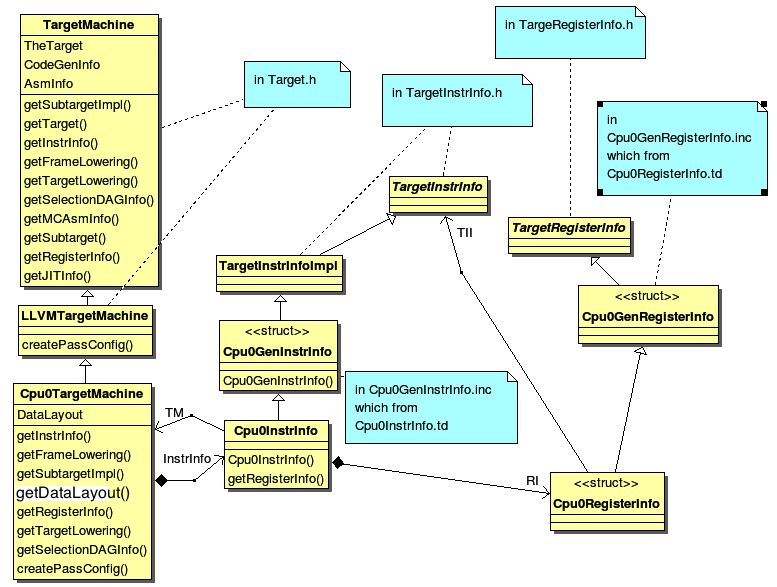
\includegraphics{1.png}
\caption{TargetMachine class diagram 1}\label{backendstructure:backendstructure-f1}\end{figure}

The Cpu0TargetMachine inherit tree is TargetMachine \textless{}- LLVMTargetMachine \textless{}-
Cpu0TargetMachine.
Cpu0TargetMachine has class Cpu0Subtarget, Cpu0InstrInfo, Cpu0FrameLowering,
Cpu0TargetLowering and Cpu0SelectionDAGInfo.
Class Cpu0Subtarget, Cpu0InstrInfo, Cpu0FrameLowering, Cpu0TargetLowering and
Cpu0SelectionDAGInfo are inherited from parent class TargetSubtargetInfo,
TargetInstrInfo, TargetFrameLowering, TargetLowering and TargetSelectionDAGInfo.

\hyperref[backendstructure:backendstructure-f1]{Figure  \ref*{backendstructure:backendstructure-f1}} shows Cpu0TargetMachine inherit tree and it's
Cpu0InstrInfo class inherit tree.
Cpu0TargetMachine contains Cpu0InstrInfo and ... other class.
Cpu0InstrInfo contains Cpu0RegisterInfo class, RI. Cpu0InstrInfo.td and
Cpu0RegisterInfo.td will generate Cpu0GenInstrInfo.inc and
Cpu0GenRegisterInfo.inc which contain some member functions implementation for
class Cpu0InstrInfo and Cpu0RegisterInfo.

\hyperref[backendstructure:backendstructure-f2]{Figure  \ref*{backendstructure:backendstructure-f2}} as below shows Cpu0TargetMachine contains
class
TSInfo: Cpu0SelectionDAGInfo, FrameLowering: Cpu0FrameLowering, Subtarget:
Cpu0Subtarget and TLInfo: Cpu0TargetLowering.
\begin{figure}[htbp]
\centering
\capstart

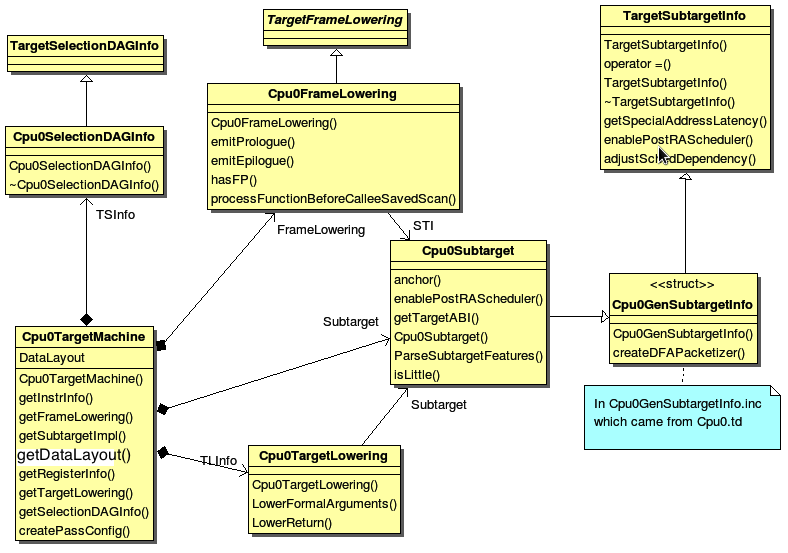
\includegraphics{2.png}
\caption{TargetMachine class diagram 2}\label{backendstructure:backendstructure-f2}\end{figure}
\begin{figure}[htbp]
\centering
\capstart

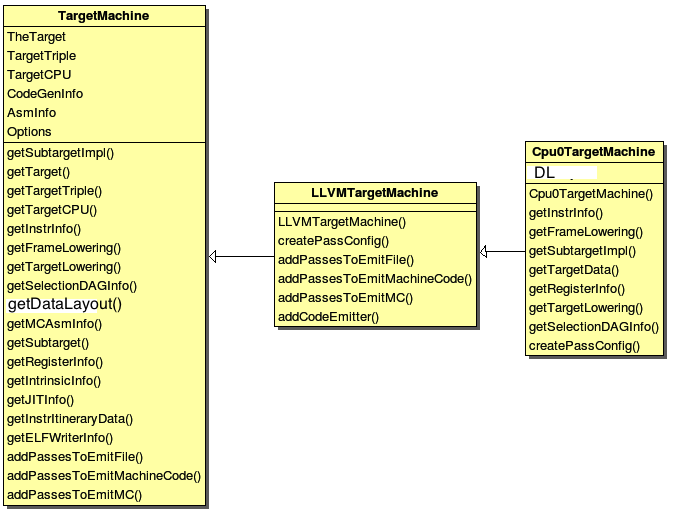
\includegraphics{3.png}
\caption{TargetMachine members and operators}\label{backendstructure:backendstructure-f3}\end{figure}

\hyperref[backendstructure:backendstructure-f3]{Figure  \ref*{backendstructure:backendstructure-f3}} shows some members and operators (member function)
of the parent class TargetMachine's.
\hyperref[backendstructure:backendstructure-f4]{Figure  \ref*{backendstructure:backendstructure-f4}} as below shows some members of class InstrInfo,
RegisterInfo and TargetLowering.
Class DAGInfo is skipped here.
\begin{figure}[htbp]
\centering
\capstart

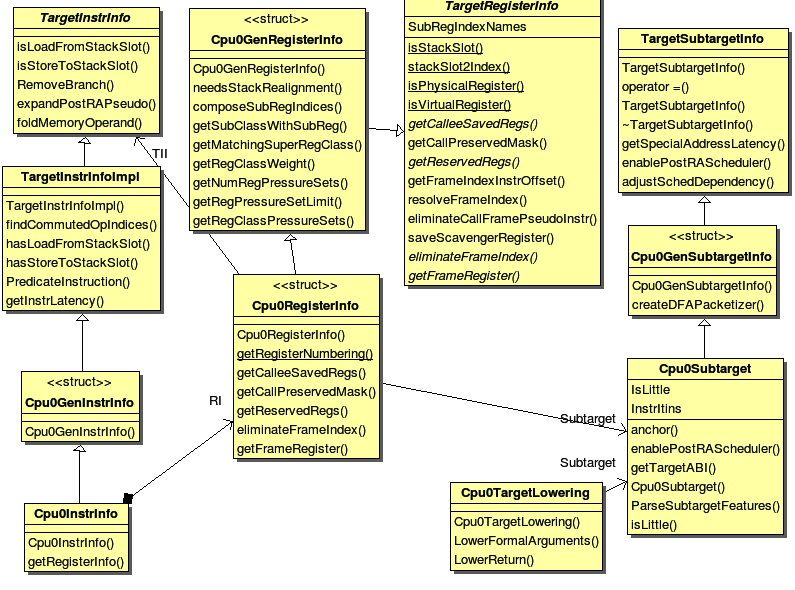
\includegraphics{4.png}
\caption{Other class members and operators}\label{backendstructure:backendstructure-f4}\end{figure}

Benefit from the inherit tree structure, we just need to implement few code in
instruction, frame/stack, select DAG class.
Many code implemented by their parent class.
The llvm-tblgen generate Cpu0GenInstrInfo.inc from Cpu0InstrInfo.td.
Cpu0InstrInfo.h extract those code it need from Cpu0GenInstrInfo.inc by define
“\#define GET\_INSTRINFO\_HEADER”.
Following is the code fragment from Cpu0GenInstrInfo.inc.
Code between “\#if def  GET\_INSTRINFO\_HEADER” and “\#endif // GET\_INSTRINFO\_HEADER”
will be extracted by Cpu0InstrInfo.h.
\paragraph{cmake\_debug\_build/lib/Target/Cpu0/Cpu0GenInstInfo.inc}

\begin{Verbatim}[commandchars=\\\{\}]
\PYG{c+c1}{//- Cpu0GenInstInfo.inc which generate from Cpu0InstrInfo.td}
\PYG{c+cp}{\PYGZsh{}}\PYG{c+cp}{ifdef GET\PYGZus{}INSTRINFO\PYGZus{}HEADER}
\PYG{c+cp}{\PYGZsh{}}\PYG{c+cp}{undef GET\PYGZus{}INSTRINFO\PYGZus{}HEADER}
\PYG{k}{namespace} \PYG{n}{llvm} \PYG{p}{\PYGZob{}}
\PYG{k}{struct} \PYG{n}{Cpu0GenInstrInfo} \PYG{o}{:} \PYG{k}{public} \PYG{n}{TargetInstrInfoImpl} \PYG{p}{\PYGZob{}}
  \PYG{k}{explicit} \PYG{n}{Cpu0GenInstrInfo}\PYG{p}{(}\PYG{k+kt}{int} \PYG{n}{SO} \PYG{o}{=} \PYG{o}{-}\PYG{l+m+mi}{1}\PYG{p}{,} \PYG{k+kt}{int} \PYG{n}{DO} \PYG{o}{=} \PYG{o}{-}\PYG{l+m+mi}{1}\PYG{p}{)}\PYG{p}{;}
\PYG{p}{\PYGZcb{}}\PYG{p}{;}
\PYG{p}{\PYGZcb{}} \PYG{c+c1}{// End llvm namespace}
\PYG{c+cp}{\PYGZsh{}}\PYG{c+cp}{endif }\PYG{c+c1}{// GET\PYGZus{}INSTRINFO\PYGZus{}HEADER}
\end{Verbatim}

Reference Write An LLVM Backend web site \footnote{
\href{http://llvm.org/docs/WritingAnLLVMBackend.html\#target-machine}{http://llvm.org/docs/WritingAnLLVMBackend.html\#target-machine}
}.

Now, the code in Chapter3\_1/ add class Cpu0TargetMachine(Cpu0TargetMachine.h and
cpp), Cpu0Subtarget (Cpu0Subtarget.h and .cpp), Cpu0InstrInfo (Cpu0InstrInfo.h
and .cpp), Cpu0FrameLowering (Cpu0FrameLowering.h and .cpp), Cpu0TargetLowering
(Cpu0ISelLowering.h and .cpp) and Cpu0SelectionDAGInfo ( Cpu0SelectionDAGInfo.h
and .cpp).
CMakeLists.txt  modified with those new added *.cpp as follows,
\paragraph{lbdex/Chapter3\_1/CMakeLists.txt}

\begin{Verbatim}[commandchars=\\\{\}]
\PYG{n}{tablegen}\PYG{p}{(}\PYG{n}{LLVM} \PYG{n}{Cpu0GenDisassemblerTables}\PYG{p}{.}\PYG{n}{inc} \PYG{o}{-}\PYG{n}{gen}\PYG{o}{-}\PYG{n}{disassembler}\PYG{p}{)}
\PYG{n}{tablegen}\PYG{p}{(}\PYG{n}{LLVM} \PYG{n}{Cpu0GenCodeEmitter}\PYG{p}{.}\PYG{n}{inc} \PYG{o}{-}\PYG{n}{gen}\PYG{o}{-}\PYG{n}{emitter}\PYG{p}{)}
\PYG{n}{tablegen}\PYG{p}{(}\PYG{n}{LLVM} \PYG{n}{Cpu0GenMCCodeEmitter}\PYG{p}{.}\PYG{n}{inc} \PYG{o}{-}\PYG{n}{gen}\PYG{o}{-}\PYG{n}{emitter} \PYG{o}{-}\PYG{n}{mc}\PYG{o}{-}\PYG{n}{emitter}\PYG{p}{)}

\PYG{n}{tablegen}\PYG{p}{(}\PYG{n}{LLVM} \PYG{n}{Cpu0GenAsmWriter}\PYG{p}{.}\PYG{n}{inc} \PYG{o}{-}\PYG{n}{gen}\PYG{o}{-}\PYG{k}{asm}\PYG{o}{-}\PYG{n}{writer}\PYG{p}{)}
\PYG{n}{tablegen}\PYG{p}{(}\PYG{n}{LLVM} \PYG{n}{Cpu0GenDAGISel}\PYG{p}{.}\PYG{n}{inc} \PYG{o}{-}\PYG{n}{gen}\PYG{o}{-}\PYG{n}{dag}\PYG{o}{-}\PYG{n}{isel}\PYG{p}{)}
\PYG{n}{tablegen}\PYG{p}{(}\PYG{n}{LLVM} \PYG{n}{Cpu0GenCallingConv}\PYG{p}{.}\PYG{n}{inc} \PYG{o}{-}\PYG{n}{gen}\PYG{o}{-}\PYG{n}{callingconv}\PYG{p}{)}
\end{Verbatim}

\begin{Verbatim}[commandchars=\\\{\}]
\PYG{n}{add\PYGZus{}llvm\PYGZus{}target}\PYG{p}{(}\PYG{n}{Cpu0CodeGen}
\end{Verbatim}

\begin{Verbatim}[commandchars=\\\{\}]
  \PYG{n}{Cpu0InstrInfo}\PYG{p}{.}\PYG{n}{cpp}
\end{Verbatim}

\begin{Verbatim}[commandchars=\\\{\}]
  \PYG{n}{Cpu0ISelLowering}\PYG{p}{.}\PYG{n}{cpp}
  \PYG{n}{Cpu0FrameLowering}\PYG{p}{.}\PYG{n}{cpp}
\end{Verbatim}

\begin{Verbatim}[commandchars=\\\{\}]
  \PYG{n}{Cpu0RegisterInfo}\PYG{p}{.}\PYG{n}{cpp}
  \PYG{n}{Cpu0Subtarget}\PYG{p}{.}\PYG{n}{cpp}
\end{Verbatim}

\begin{Verbatim}[commandchars=\\\{\}]
  \PYG{n}{Cpu0TargetObjectFile}\PYG{p}{.}\PYG{n}{cpp}
  \PYG{n}{Cpu0SelectionDAGInfo}\PYG{p}{.}\PYG{n}{cpp}
  \PYG{p}{)}
\end{Verbatim}

Please take a look for Chapter3\_1 code.
After that, building Chapter3\_1 by make as chapter 2 (of course, you should remove old
src/lib/Target/Cpu0 and replace them with src/lib/Target/Cpu0/lbdex/Chapter3\_1/).
You can remove cmake\_debug\_build/lib/Target/Cpu0/*.inc before do “make” to ensure your code
rebuild completely.
By remove *.inc, all files those have included .inc will be rebuild, then your
Target library will be regenerated.
Command as follows,

\begin{Verbatim}[commandchars=\\\{\}]
118-165-78-230:cmake\PYGZus{}debug\PYGZus{}build Jonathan\PYG{n+nv}{\PYGZdl{} }rm -rf lib/Target/Cpu0/*
\end{Verbatim}

Now, let's build Chapter3\_1 as the following command,

\begin{Verbatim}[commandchars=\\\{\}]
118-165-75-57:ExampleCode Jonathan\PYG{n+nv}{\PYGZdl{} }\PYG{n+nb}{pwd}
/Users/Jonathan/llvm/test/src/lib/Target/Cpu0/lbdex
118-165-75-57:lbdex Jonathan\PYG{n+nv}{\PYGZdl{} }sh removecpu0.sh
118-165-75-57:lbdex Jonathan\PYG{n+nv}{\PYGZdl{} }cp -rf Chapter3\PYGZus{}1/
* ../.

118-165-78-230:InputFiles Jonathan\PYG{n+nv}{\PYGZdl{} }/Users/Jonathan/llvm/test/cmake\PYGZus{}debug\PYGZus{}build/
bin/Debug/llc -march\PYG{o}{=}cpu0 -relocation-model\PYG{o}{=}pic -filetype\PYG{o}{=}asm ch3.bc -o
ch3.cpu0.s
Assertion failed: \PYG{o}{(}AsmInfo \PYG{o}{\PYGZam{}\PYGZam{}} \PYG{l+s+s2}{"MCAsmInfo not initialized."}
...
\end{Verbatim}

The errors say that we have not Target AsmPrinter.
Let's add it in next section.


\section{Add AsmPrinter}
\label{backendstructure:add-asmprinter}
Chapter3\_2/cpu0 contains the Cpu0AsmPrinter definition. First, we add definitions in
Cpu0.td to support AssemblyWriter.
Cpu0.td is added with the following fragment,
\paragraph{lbdex/Chapter3\_2/Cpu0.td}

\begin{Verbatim}[commandchars=\\\{\}]
\PYG{c+c1}{// Without this will have error: 'cpu032I' is not a recognized processor for }
\PYG{c+c1}{//  this target (ignoring processor)}
\PYG{c+c1}{//===----------------------------------------------------------------------===//}
\PYG{c+c1}{// Cpu0 Subtarget features                                                    //}
\PYG{c+c1}{//===----------------------------------------------------------------------===//}

\PYG{n}{def} \PYG{n}{FeatureCpu032I}     \PYG{o}{:} \PYG{n}{SubtargetFeature}\PYG{o}{\PYGZlt{}}\PYG{l+s}{"}\PYG{l+s}{cpu032I}\PYG{l+s}{"}\PYG{p}{,} \PYG{l+s}{"}\PYG{l+s}{Cpu0ArchVersion}\PYG{l+s}{"}\PYG{p}{,} 
        \PYG{l+s}{"}\PYG{l+s}{Cpu032I}\PYG{l+s}{"}\PYG{p}{,} \PYG{l+s}{"}\PYG{l+s}{Cpu032I ISA Support}\PYG{l+s}{"}\PYG{o}{\PYGZgt{}}\PYG{p}{;}
\end{Verbatim}

\begin{Verbatim}[commandchars=\\\{\}]
\PYG{c+c1}{//===----------------------------------------------------------------------===//}
\PYG{c+c1}{// Cpu0 processors supported.}
\PYG{c+c1}{//===----------------------------------------------------------------------===//}

\PYG{k}{class} \PYG{n+nc}{Proc}\PYG{o}{\PYGZlt{}}\PYG{n}{string} \PYG{n}{Name}\PYG{p}{,} \PYG{n}{list}\PYG{o}{\PYGZlt{}}\PYG{n}{SubtargetFeature}\PYG{o}{\PYGZgt{}} \PYG{n}{Features}\PYG{o}{\PYGZgt{}}
 \PYG{o}{:} \PYG{n}{Processor}\PYG{o}{\PYGZlt{}}\PYG{n}{Name}\PYG{p}{,} \PYG{n}{Cpu0GenericItineraries}\PYG{p}{,} \PYG{n}{Features}\PYG{o}{\PYGZgt{}}\PYG{p}{;}

\PYG{n}{def} \PYG{o}{:} \PYG{n}{Proc}\PYG{o}{\PYGZlt{}}\PYG{l+s}{"}\PYG{l+s}{cpu032I}\PYG{l+s}{"}\PYG{p}{,}  \PYG{p}{[}\PYG{n}{FeatureCpu032I}\PYG{p}{]}\PYG{o}{\PYGZgt{}}\PYG{p}{;}
\end{Verbatim}

\begin{Verbatim}[commandchars=\\\{\}]
\PYG{n}{def} \PYG{n}{Cpu0AsmWriter} \PYG{o}{:} \PYG{n}{AsmWriter} \PYG{p}{\PYGZob{}}
  \PYG{n}{string} \PYG{n}{AsmWriterClassName}  \PYG{o}{=} \PYG{l+s}{"}\PYG{l+s}{InstPrinter}\PYG{l+s}{"}\PYG{p}{;}
  \PYG{n}{bit} \PYG{n}{isMCAsmWriter} \PYG{o}{=} \PYG{l+m+mi}{1}\PYG{p}{;}
\PYG{p}{\PYGZcb{}}
\end{Verbatim}

\begin{Verbatim}[commandchars=\\\{\}]
\PYG{c+c1}{// Will generate Cpu0GenAsmWrite.inc included by Cpu0InstPrinter.cpp, contents }
\PYG{c+c1}{//  as follows,}
\PYG{c+c1}{// void Cpu0InstPrinter::printInstruction(const MCInst *MI, raw\PYGZus{}ostream \PYGZam{}O) \PYGZob{}...\PYGZcb{}}
\PYG{c+c1}{// const char *Cpu0InstPrinter::getRegisterName(unsigned RegNo) \PYGZob{}...\PYGZcb{}}
\PYG{n}{def} \PYG{n}{Cpu0} \PYG{o}{:} \PYG{n}{Target} \PYG{p}{\PYGZob{}}
\end{Verbatim}

\begin{Verbatim}[commandchars=\\\{\}]
  \PYG{n}{let} \PYG{n}{AssemblyWriters} \PYG{o}{=} \PYG{p}{[}\PYG{n}{Cpu0AsmWriter}\PYG{p}{]}\PYG{p}{;}
\end{Verbatim}

\begin{Verbatim}[commandchars=\\\{\}]
\PYG{p}{\PYGZcb{}}
\end{Verbatim}

As comments indicate, it will generate Cpu0GenAsmWrite.inc which is included
by Cpu0InstPrinter.cpp as follows,
\paragraph{lbdex/Chapter3\_2/InstPrinter/Cpu0InstPrinter.h}

\begin{Verbatim}[commandchars=\\\{\}]
\PYG{c+c1}{//=== Cpu0InstPrinter.h - Convert Cpu0 MCInst to assembly syntax -*- C++ -*-==//}
\PYG{c+c1}{//}
\PYG{c+c1}{//                     The LLVM Compiler Infrastructure}
\PYG{c+c1}{//}
\PYG{c+c1}{// This file is distributed under the University of Illinois Open Source}
\PYG{c+c1}{// License. See LICENSE.TXT for details.}
\PYG{c+c1}{//}
\PYG{c+c1}{//===----------------------------------------------------------------------===//}
\PYG{c+c1}{//}
\PYG{c+c1}{// This class prints a Cpu0 MCInst to a .s file.}
\PYG{c+c1}{//}
\PYG{c+c1}{//===----------------------------------------------------------------------===//}

\PYG{c+cp}{\PYGZsh{}}\PYG{c+cp}{ifndef CPU0INSTPRINTER\PYGZus{}H}
\PYG{c+cp}{\PYGZsh{}}\PYG{c+cp}{define CPU0INSTPRINTER\PYGZus{}H}
\PYG{c+cp}{\PYGZsh{}}\PYG{c+cp}{include "llvm}\PYG{c+cp}{/}\PYG{c+cp}{MC}\PYG{c+cp}{/}\PYG{c+cp}{MCInstPrinter.h"}

\PYG{k}{namespace} \PYG{n}{llvm} \PYG{p}{\PYGZob{}}
\PYG{c+c1}{// These enumeration declarations were orignally in Cpu0InstrInfo.h but}
\PYG{c+c1}{// had to be moved here to avoid circular dependencies between}
\PYG{c+c1}{// LLVMCpu0CodeGen and LLVMCpu0AsmPrinter.}

\PYG{k}{class} \PYG{n+nc}{TargetMachine}\PYG{p}{;}

\PYG{k}{class} \PYG{n+nc}{Cpu0InstPrinter} \PYG{o}{:} \PYG{k}{public} \PYG{n}{MCInstPrinter} \PYG{p}{\PYGZob{}}
\PYG{k}{public}\PYG{o}{:}
  \PYG{n}{Cpu0InstPrinter}\PYG{p}{(}\PYG{k}{const} \PYG{n}{MCAsmInfo} \PYG{o}{\PYGZam{}}\PYG{n}{MAI}\PYG{p}{,} \PYG{k}{const} \PYG{n}{MCInstrInfo} \PYG{o}{\PYGZam{}}\PYG{n}{MII}\PYG{p}{,}
                  \PYG{k}{const} \PYG{n}{MCRegisterInfo} \PYG{o}{\PYGZam{}}\PYG{n}{MRI}\PYG{p}{)}
    \PYG{o}{:} \PYG{n}{MCInstPrinter}\PYG{p}{(}\PYG{n}{MAI}\PYG{p}{,} \PYG{n}{MII}\PYG{p}{,} \PYG{n}{MRI}\PYG{p}{)} \PYG{p}{\PYGZob{}}\PYG{p}{\PYGZcb{}}

  \PYG{c+c1}{// Autogenerated by tblgen.}
  \PYG{k+kt}{void} \PYG{n}{printInstruction}\PYG{p}{(}\PYG{k}{const} \PYG{n}{MCInst} \PYG{o}{*}\PYG{n}{MI}\PYG{p}{,} \PYG{n}{raw\PYGZus{}ostream} \PYG{o}{\PYGZam{}}\PYG{n}{O}\PYG{p}{)}\PYG{p}{;}
  \PYG{k}{static} \PYG{k}{const} \PYG{k+kt}{char} \PYG{o}{*}\PYG{n}{getRegisterName}\PYG{p}{(}\PYG{k+kt}{unsigned} \PYG{n}{RegNo}\PYG{p}{)}\PYG{p}{;}

  \PYG{k}{virtual} \PYG{k+kt}{void} \PYG{n}{printRegName}\PYG{p}{(}\PYG{n}{raw\PYGZus{}ostream} \PYG{o}{\PYGZam{}}\PYG{n}{OS}\PYG{p}{,} \PYG{k+kt}{unsigned} \PYG{n}{RegNo}\PYG{p}{)} \PYG{k}{const}\PYG{p}{;}
  \PYG{k}{virtual} \PYG{k+kt}{void} \PYG{n}{printInst}\PYG{p}{(}\PYG{k}{const} \PYG{n}{MCInst} \PYG{o}{*}\PYG{n}{MI}\PYG{p}{,} \PYG{n}{raw\PYGZus{}ostream} \PYG{o}{\PYGZam{}}\PYG{n}{O}\PYG{p}{,} \PYG{n}{StringRef} \PYG{n}{Annot}\PYG{p}{)}\PYG{p}{;}

\PYG{k}{private}\PYG{o}{:}
  \PYG{k+kt}{void} \PYG{n}{printOperand}\PYG{p}{(}\PYG{k}{const} \PYG{n}{MCInst} \PYG{o}{*}\PYG{n}{MI}\PYG{p}{,} \PYG{k+kt}{unsigned} \PYG{n}{OpNo}\PYG{p}{,} \PYG{n}{raw\PYGZus{}ostream} \PYG{o}{\PYGZam{}}\PYG{n}{O}\PYG{p}{)}\PYG{p}{;}
  \PYG{k+kt}{void} \PYG{n}{printUnsignedImm}\PYG{p}{(}\PYG{k}{const} \PYG{n}{MCInst} \PYG{o}{*}\PYG{n}{MI}\PYG{p}{,} \PYG{k+kt}{int} \PYG{n}{opNum}\PYG{p}{,} \PYG{n}{raw\PYGZus{}ostream} \PYG{o}{\PYGZam{}}\PYG{n}{O}\PYG{p}{)}\PYG{p}{;}
  \PYG{k+kt}{void} \PYG{n}{printMemOperand}\PYG{p}{(}\PYG{k}{const} \PYG{n}{MCInst} \PYG{o}{*}\PYG{n}{MI}\PYG{p}{,} \PYG{k+kt}{int} \PYG{n}{opNum}\PYG{p}{,} \PYG{n}{raw\PYGZus{}ostream} \PYG{o}{\PYGZam{}}\PYG{n}{O}\PYG{p}{)}\PYG{p}{;}
\end{Verbatim}

\begin{Verbatim}[commandchars=\\\{\}]
\PYG{p}{\PYGZcb{}}\PYG{p}{;}
\PYG{p}{\PYGZcb{}} \PYG{c+c1}{// end namespace llvm}

\PYG{c+cp}{\PYGZsh{}}\PYG{c+cp}{endif}
\end{Verbatim}
\paragraph{lbdex/Chapter3\_2/InstPrinter/Cpu0InstPrinter.cpp}

\begin{Verbatim}[commandchars=\\\{\}]
\PYG{c+c1}{//===-- Cpu0InstPrinter.cpp - Convert Cpu0 MCInst to assembly syntax ------===//}
\PYG{c+c1}{//}
\PYG{c+c1}{//                     The LLVM Compiler Infrastructure}
\PYG{c+c1}{//}
\PYG{c+c1}{// This file is distributed under the University of Illinois Open Source}
\PYG{c+c1}{// License. See LICENSE.TXT for details.}
\PYG{c+c1}{//}
\PYG{c+c1}{//===----------------------------------------------------------------------===//}
\PYG{c+c1}{//}
\PYG{c+c1}{// This class prints an Cpu0 MCInst to a .s file.}
\PYG{c+c1}{//}
\PYG{c+c1}{//===----------------------------------------------------------------------===//}

\PYG{c+cp}{\PYGZsh{}}\PYG{c+cp}{define DEBUG\PYGZus{}TYPE "asm-printer"}
\PYG{c+cp}{\PYGZsh{}}\PYG{c+cp}{include "Cpu0InstPrinter.h"}
\PYG{c+cp}{\PYGZsh{}}\PYG{c+cp}{include "llvm}\PYG{c+cp}{/}\PYG{c+cp}{ADT}\PYG{c+cp}{/}\PYG{c+cp}{StringExtras.h"}
\PYG{c+cp}{\PYGZsh{}}\PYG{c+cp}{include "llvm}\PYG{c+cp}{/}\PYG{c+cp}{MC}\PYG{c+cp}{/}\PYG{c+cp}{MCExpr.h"}
\PYG{c+cp}{\PYGZsh{}}\PYG{c+cp}{include "llvm}\PYG{c+cp}{/}\PYG{c+cp}{MC}\PYG{c+cp}{/}\PYG{c+cp}{MCInst.h"}
\PYG{c+cp}{\PYGZsh{}}\PYG{c+cp}{include "llvm}\PYG{c+cp}{/}\PYG{c+cp}{MC}\PYG{c+cp}{/}\PYG{c+cp}{MCInstrInfo.h"}
\PYG{c+cp}{\PYGZsh{}}\PYG{c+cp}{include "llvm}\PYG{c+cp}{/}\PYG{c+cp}{MC}\PYG{c+cp}{/}\PYG{c+cp}{MCSymbol.h"}
\PYG{c+cp}{\PYGZsh{}}\PYG{c+cp}{include "llvm}\PYG{c+cp}{/}\PYG{c+cp}{Support}\PYG{c+cp}{/}\PYG{c+cp}{ErrorHandling.h"}
\PYG{c+cp}{\PYGZsh{}}\PYG{c+cp}{include "llvm}\PYG{c+cp}{/}\PYG{c+cp}{Support}\PYG{c+cp}{/}\PYG{c+cp}{raw\PYGZus{}ostream.h"}
\PYG{k}{using} \PYG{k}{namespace} \PYG{n}{llvm}\PYG{p}{;}

\PYG{c+cp}{\PYGZsh{}}\PYG{c+cp}{include "Cpu0GenAsmWriter.inc"}

\PYG{k+kt}{void} \PYG{n}{Cpu0InstPrinter}\PYG{o}{:}\PYG{o}{:}\PYG{n}{printRegName}\PYG{p}{(}\PYG{n}{raw\PYGZus{}ostream} \PYG{o}{\PYGZam{}}\PYG{n}{OS}\PYG{p}{,} \PYG{k+kt}{unsigned} \PYG{n}{RegNo}\PYG{p}{)} \PYG{k}{const} \PYG{p}{\PYGZob{}}
\PYG{c+c1}{//- getRegisterName(RegNo) defined in Cpu0GenAsmWriter.inc which came from }
\PYG{c+c1}{//   Cpu0.td indicate.}
  \PYG{n}{OS} \PYG{o}{\PYGZlt{}}\PYG{o}{\PYGZlt{}} \PYG{l+s+sc}{'\PYGZdl{}'} \PYG{o}{\PYGZlt{}}\PYG{o}{\PYGZlt{}} \PYG{n}{StringRef}\PYG{p}{(}\PYG{n}{getRegisterName}\PYG{p}{(}\PYG{n}{RegNo}\PYG{p}{)}\PYG{p}{)}\PYG{p}{.}\PYG{n}{lower}\PYG{p}{(}\PYG{p}{)}\PYG{p}{;}
\PYG{p}{\PYGZcb{}}

\PYG{k+kt}{void} \PYG{n}{Cpu0InstPrinter}\PYG{o}{:}\PYG{o}{:}\PYG{n}{printInst}\PYG{p}{(}\PYG{k}{const} \PYG{n}{MCInst} \PYG{o}{*}\PYG{n}{MI}\PYG{p}{,} \PYG{n}{raw\PYGZus{}ostream} \PYG{o}{\PYGZam{}}\PYG{n}{O}\PYG{p}{,}
                                \PYG{n}{StringRef} \PYG{n}{Annot}\PYG{p}{)} \PYG{p}{\PYGZob{}}
\PYG{c+c1}{//- printInstruction(MI, O) defined in Cpu0GenAsmWriter.inc which came from }
\PYG{c+c1}{//   Cpu0.td indicate.}
  \PYG{n}{printInstruction}\PYG{p}{(}\PYG{n}{MI}\PYG{p}{,} \PYG{n}{O}\PYG{p}{)}\PYG{p}{;}
  \PYG{n}{printAnnotation}\PYG{p}{(}\PYG{n}{O}\PYG{p}{,} \PYG{n}{Annot}\PYG{p}{)}\PYG{p}{;}
\PYG{p}{\PYGZcb{}}

\PYG{k}{static} \PYG{k+kt}{void} \PYG{n}{printExpr}\PYG{p}{(}\PYG{k}{const} \PYG{n}{MCExpr} \PYG{o}{*}\PYG{n}{Expr}\PYG{p}{,} \PYG{n}{raw\PYGZus{}ostream} \PYG{o}{\PYGZam{}}\PYG{n}{OS}\PYG{p}{)} \PYG{p}{\PYGZob{}}
  \PYG{k+kt}{int} \PYG{n}{Offset} \PYG{o}{=} \PYG{l+m+mi}{0}\PYG{p}{;}
  \PYG{k}{const} \PYG{n}{MCSymbolRefExpr} \PYG{o}{*}\PYG{n}{SRE}\PYG{p}{;}

  \PYG{k}{if} \PYG{p}{(}\PYG{k}{const} \PYG{n}{MCBinaryExpr} \PYG{o}{*}\PYG{n}{BE} \PYG{o}{=} \PYG{n}{dyn\PYGZus{}cast}\PYG{o}{\PYGZlt{}}\PYG{n}{MCBinaryExpr}\PYG{o}{\PYGZgt{}}\PYG{p}{(}\PYG{n}{Expr}\PYG{p}{)}\PYG{p}{)} \PYG{p}{\PYGZob{}}
    \PYG{n}{SRE} \PYG{o}{=} \PYG{n}{dyn\PYGZus{}cast}\PYG{o}{\PYGZlt{}}\PYG{n}{MCSymbolRefExpr}\PYG{o}{\PYGZgt{}}\PYG{p}{(}\PYG{n}{BE}\PYG{o}{-}\PYG{o}{\PYGZgt{}}\PYG{n}{getLHS}\PYG{p}{(}\PYG{p}{)}\PYG{p}{)}\PYG{p}{;}
    \PYG{k}{const} \PYG{n}{MCConstantExpr} \PYG{o}{*}\PYG{n}{CE} \PYG{o}{=} \PYG{n}{dyn\PYGZus{}cast}\PYG{o}{\PYGZlt{}}\PYG{n}{MCConstantExpr}\PYG{o}{\PYGZgt{}}\PYG{p}{(}\PYG{n}{BE}\PYG{o}{-}\PYG{o}{\PYGZgt{}}\PYG{n}{getRHS}\PYG{p}{(}\PYG{p}{)}\PYG{p}{)}\PYG{p}{;}
    \PYG{n}{assert}\PYG{p}{(}\PYG{n}{SRE} \PYG{o}{\PYGZam{}}\PYG{o}{\PYGZam{}} \PYG{n}{CE} \PYG{o}{\PYGZam{}}\PYG{o}{\PYGZam{}} \PYG{l+s}{"}\PYG{l+s}{Binary expression must be sym+const.}\PYG{l+s}{"}\PYG{p}{)}\PYG{p}{;}
    \PYG{n}{Offset} \PYG{o}{=} \PYG{n}{CE}\PYG{o}{-}\PYG{o}{\PYGZgt{}}\PYG{n}{getValue}\PYG{p}{(}\PYG{p}{)}\PYG{p}{;}
  \PYG{p}{\PYGZcb{}}
  \PYG{k}{else} \PYG{k}{if} \PYG{p}{(}\PYG{o}{!}\PYG{p}{(}\PYG{n}{SRE} \PYG{o}{=} \PYG{n}{dyn\PYGZus{}cast}\PYG{o}{\PYGZlt{}}\PYG{n}{MCSymbolRefExpr}\PYG{o}{\PYGZgt{}}\PYG{p}{(}\PYG{n}{Expr}\PYG{p}{)}\PYG{p}{)}\PYG{p}{)}
    \PYG{n}{assert}\PYG{p}{(}\PYG{k+kc}{false} \PYG{o}{\PYGZam{}}\PYG{o}{\PYGZam{}} \PYG{l+s}{"}\PYG{l+s}{Unexpected MCExpr type.}\PYG{l+s}{"}\PYG{p}{)}\PYG{p}{;}

  \PYG{n}{MCSymbolRefExpr}\PYG{o}{:}\PYG{o}{:}\PYG{n}{VariantKind} \PYG{n}{Kind} \PYG{o}{=} \PYG{n}{SRE}\PYG{o}{-}\PYG{o}{\PYGZgt{}}\PYG{n}{getKind}\PYG{p}{(}\PYG{p}{)}\PYG{p}{;}

  \PYG{k}{switch} \PYG{p}{(}\PYG{n}{Kind}\PYG{p}{)} \PYG{p}{\PYGZob{}}
  \PYG{k}{default}\PYG{o}{:}                                 \PYG{n}{llvm\PYGZus{}unreachable}\PYG{p}{(}\PYG{l+s}{"}\PYG{l+s}{Invalid kind!}\PYG{l+s}{"}\PYG{p}{)}\PYG{p}{;}
  \PYG{k}{case} \PYG{n}{MCSymbolRefExpr}\PYG{o}{:}\PYG{o}{:}\PYG{n+nl}{VK\PYGZus{}None:}           \PYG{k}{break}\PYG{p}{;}
\end{Verbatim}

\begin{Verbatim}[commandchars=\\\{\}]
  \PYG{p}{\PYGZcb{}}

  \PYG{n}{OS} \PYG{o}{\PYGZlt{}}\PYG{o}{\PYGZlt{}} \PYG{n}{SRE}\PYG{o}{-}\PYG{o}{\PYGZgt{}}\PYG{n}{getSymbol}\PYG{p}{(}\PYG{p}{)}\PYG{p}{;}

  \PYG{k}{if} \PYG{p}{(}\PYG{n}{Offset}\PYG{p}{)} \PYG{p}{\PYGZob{}}
    \PYG{k}{if} \PYG{p}{(}\PYG{n}{Offset} \PYG{o}{\PYGZgt{}} \PYG{l+m+mi}{0}\PYG{p}{)}
      \PYG{n}{OS} \PYG{o}{\PYGZlt{}}\PYG{o}{\PYGZlt{}} \PYG{l+s+sc}{'+'}\PYG{p}{;}
    \PYG{n}{OS} \PYG{o}{\PYGZlt{}}\PYG{o}{\PYGZlt{}} \PYG{n}{Offset}\PYG{p}{;}
  \PYG{p}{\PYGZcb{}}

  \PYG{k}{if} \PYG{p}{(}\PYG{p}{(}\PYG{n}{Kind} \PYG{o}{=}\PYG{o}{=} \PYG{n}{MCSymbolRefExpr}\PYG{o}{:}\PYG{o}{:}\PYG{n}{VK\PYGZus{}Cpu0\PYGZus{}GPOFF\PYGZus{}HI}\PYG{p}{)} \PYG{o}{\textbar{}}\PYG{o}{\textbar{}}
      \PYG{p}{(}\PYG{n}{Kind} \PYG{o}{=}\PYG{o}{=} \PYG{n}{MCSymbolRefExpr}\PYG{o}{:}\PYG{o}{:}\PYG{n}{VK\PYGZus{}Cpu0\PYGZus{}GPOFF\PYGZus{}LO}\PYG{p}{)}\PYG{p}{)}
    \PYG{n}{OS} \PYG{o}{\PYGZlt{}}\PYG{o}{\PYGZlt{}} \PYG{l+s}{"}\PYG{l+s}{)))}\PYG{l+s}{"}\PYG{p}{;}
  \PYG{k}{else} \PYG{k}{if} \PYG{p}{(}\PYG{n}{Kind} \PYG{o}{!}\PYG{o}{=} \PYG{n}{MCSymbolRefExpr}\PYG{o}{:}\PYG{o}{:}\PYG{n}{VK\PYGZus{}None}\PYG{p}{)}
    \PYG{n}{OS} \PYG{o}{\PYGZlt{}}\PYG{o}{\PYGZlt{}} \PYG{l+s+sc}{')'}\PYG{p}{;}
\PYG{p}{\PYGZcb{}}

\PYG{k+kt}{void} \PYG{n}{Cpu0InstPrinter}\PYG{o}{:}\PYG{o}{:}\PYG{n}{printOperand}\PYG{p}{(}\PYG{k}{const} \PYG{n}{MCInst} \PYG{o}{*}\PYG{n}{MI}\PYG{p}{,} \PYG{k+kt}{unsigned} \PYG{n}{OpNo}\PYG{p}{,}
                                   \PYG{n}{raw\PYGZus{}ostream} \PYG{o}{\PYGZam{}}\PYG{n}{O}\PYG{p}{)} \PYG{p}{\PYGZob{}}
  \PYG{k}{const} \PYG{n}{MCOperand} \PYG{o}{\PYGZam{}}\PYG{n}{Op} \PYG{o}{=} \PYG{n}{MI}\PYG{o}{-}\PYG{o}{\PYGZgt{}}\PYG{n}{getOperand}\PYG{p}{(}\PYG{n}{OpNo}\PYG{p}{)}\PYG{p}{;}
  \PYG{k}{if} \PYG{p}{(}\PYG{n}{Op}\PYG{p}{.}\PYG{n}{isReg}\PYG{p}{(}\PYG{p}{)}\PYG{p}{)} \PYG{p}{\PYGZob{}}
    \PYG{n}{printRegName}\PYG{p}{(}\PYG{n}{O}\PYG{p}{,} \PYG{n}{Op}\PYG{p}{.}\PYG{n}{getReg}\PYG{p}{(}\PYG{p}{)}\PYG{p}{)}\PYG{p}{;}
    \PYG{k}{return}\PYG{p}{;}
  \PYG{p}{\PYGZcb{}}

  \PYG{k}{if} \PYG{p}{(}\PYG{n}{Op}\PYG{p}{.}\PYG{n}{isImm}\PYG{p}{(}\PYG{p}{)}\PYG{p}{)} \PYG{p}{\PYGZob{}}
    \PYG{n}{O} \PYG{o}{\PYGZlt{}}\PYG{o}{\PYGZlt{}} \PYG{n}{Op}\PYG{p}{.}\PYG{n}{getImm}\PYG{p}{(}\PYG{p}{)}\PYG{p}{;}
    \PYG{k}{return}\PYG{p}{;}
  \PYG{p}{\PYGZcb{}}

  \PYG{n}{assert}\PYG{p}{(}\PYG{n}{Op}\PYG{p}{.}\PYG{n}{isExpr}\PYG{p}{(}\PYG{p}{)} \PYG{o}{\PYGZam{}}\PYG{o}{\PYGZam{}} \PYG{l+s}{"}\PYG{l+s}{unknown operand kind in printOperand}\PYG{l+s}{"}\PYG{p}{)}\PYG{p}{;}
  \PYG{n}{printExpr}\PYG{p}{(}\PYG{n}{Op}\PYG{p}{.}\PYG{n}{getExpr}\PYG{p}{(}\PYG{p}{)}\PYG{p}{,} \PYG{n}{O}\PYG{p}{)}\PYG{p}{;}
\PYG{p}{\PYGZcb{}}

\PYG{k+kt}{void} \PYG{n}{Cpu0InstPrinter}\PYG{o}{:}\PYG{o}{:}\PYG{n}{printUnsignedImm}\PYG{p}{(}\PYG{k}{const} \PYG{n}{MCInst} \PYG{o}{*}\PYG{n}{MI}\PYG{p}{,} \PYG{k+kt}{int} \PYG{n}{opNum}\PYG{p}{,}
                                       \PYG{n}{raw\PYGZus{}ostream} \PYG{o}{\PYGZam{}}\PYG{n}{O}\PYG{p}{)} \PYG{p}{\PYGZob{}}
  \PYG{k}{const} \PYG{n}{MCOperand} \PYG{o}{\PYGZam{}}\PYG{n}{MO} \PYG{o}{=} \PYG{n}{MI}\PYG{o}{-}\PYG{o}{\PYGZgt{}}\PYG{n}{getOperand}\PYG{p}{(}\PYG{n}{opNum}\PYG{p}{)}\PYG{p}{;}
  \PYG{k}{if} \PYG{p}{(}\PYG{n}{MO}\PYG{p}{.}\PYG{n}{isImm}\PYG{p}{(}\PYG{p}{)}\PYG{p}{)}
    \PYG{n}{O} \PYG{o}{\PYGZlt{}}\PYG{o}{\PYGZlt{}} \PYG{p}{(}\PYG{k+kt}{unsigned} \PYG{k+kt}{short} \PYG{k+kt}{int}\PYG{p}{)}\PYG{n}{MO}\PYG{p}{.}\PYG{n}{getImm}\PYG{p}{(}\PYG{p}{)}\PYG{p}{;}
  \PYG{k}{else}
    \PYG{n}{printOperand}\PYG{p}{(}\PYG{n}{MI}\PYG{p}{,} \PYG{n}{opNum}\PYG{p}{,} \PYG{n}{O}\PYG{p}{)}\PYG{p}{;}
\PYG{p}{\PYGZcb{}}

\PYG{k+kt}{void} \PYG{n}{Cpu0InstPrinter}\PYG{o}{:}\PYG{o}{:}
\PYG{n}{printMemOperand}\PYG{p}{(}\PYG{k}{const} \PYG{n}{MCInst} \PYG{o}{*}\PYG{n}{MI}\PYG{p}{,} \PYG{k+kt}{int} \PYG{n}{opNum}\PYG{p}{,} \PYG{n}{raw\PYGZus{}ostream} \PYG{o}{\PYGZam{}}\PYG{n}{O}\PYG{p}{)} \PYG{p}{\PYGZob{}}
  \PYG{c+c1}{// Load/Store memory operands -- imm(\PYGZdl{}reg)}
  \PYG{c+c1}{// If PIC target the target is loaded as the}
  \PYG{c+c1}{// pattern ld \PYGZdl{}t9,\PYGZpc{}call16(\PYGZdl{}gp)}
  \PYG{n}{printOperand}\PYG{p}{(}\PYG{n}{MI}\PYG{p}{,} \PYG{n}{opNum}\PYG{o}{+}\PYG{l+m+mi}{1}\PYG{p}{,} \PYG{n}{O}\PYG{p}{)}\PYG{p}{;}
  \PYG{n}{O} \PYG{o}{\PYGZlt{}}\PYG{o}{\PYGZlt{}} \PYG{l+s}{"}\PYG{l+s}{(}\PYG{l+s}{"}\PYG{p}{;}
  \PYG{n}{printOperand}\PYG{p}{(}\PYG{n}{MI}\PYG{p}{,} \PYG{n}{opNum}\PYG{p}{,} \PYG{n}{O}\PYG{p}{)}\PYG{p}{;}
  \PYG{n}{O} \PYG{o}{\PYGZlt{}}\PYG{o}{\PYGZlt{}} \PYG{l+s}{"}\PYG{l+s}{)}\PYG{l+s}{"}\PYG{p}{;}
\PYG{p}{\PYGZcb{}}
\end{Verbatim}
\paragraph{lbdex/Chapter3\_2/InstPrinter/CMakeLists.txt}

\begin{Verbatim}[commandchars=\\\{\}]
include\_directories( \$\PYGZob{}CMAKE\_CURRENT\_BINARY\_DIR\PYGZcb{}/.. \$\PYGZob{}CMAKE\_CURRENT\_SOURCE\_DIR\PYGZcb{}/.. )

add\_llvm\_library(LLVMCpu0AsmPrinter
  Cpu0InstPrinter.cpp
  )

add\_dependencies(LLVMCpu0AsmPrinter Cpu0CommonTableGen)
\end{Verbatim}
\paragraph{lbdex/Chapter3\_2/InstPrinter/LLVMBuild.txt}

\begin{Verbatim}[commandchars=\\\{\}]
\PYG{p}{;}\PYG{o}{=}\PYG{o}{=}\PYG{o}{=}\PYG{o}{-} \PYG{p}{.}\PYG{o}{/}\PYG{n}{lib}\PYG{o}{/}\PYG{n}{Target}\PYG{o}{/}\PYG{n}{Cpu0}\PYG{o}{/}\PYG{n}{InstPrinter}\PYG{o}{/}\PYG{n}{LLVMBuild}\PYG{p}{.}\PYG{n}{txt} \PYG{o}{-}\PYG{o}{-}\PYG{o}{-}\PYG{o}{-}\PYG{o}{-}\PYG{o}{-}\PYG{o}{-}\PYG{o}{-}\PYG{o}{-}\PYG{o}{-}\PYG{o}{-}\PYG{o}{-}\PYG{o}{-}\PYG{o}{-}\PYG{o}{*}\PYG{o}{-} \PYG{n}{Conf} \PYG{o}{-}\PYG{o}{*}\PYG{o}{-}\PYG{o}{-}\PYG{o}{=}\PYG{o}{=}\PYG{o}{=}\PYG{p}{;}
\PYG{p}{;}
\PYG{p}{;}                     \PYG{n}{The} \PYG{n}{LLVM} \PYG{n}{Compiler} \PYG{n}{Infrastructure}
\PYG{p}{;}
\PYG{p}{;} \PYG{n}{This} \PYG{n}{file} \PYG{n}{is} \PYG{n}{distributed} \PYG{n}{under} \PYG{n}{the} \PYG{n}{University} \PYG{n}{of} \PYG{n}{Illinois} \PYG{n}{Open} \PYG{n}{Source}
\PYG{p}{;} \PYG{n}{License}\PYG{p}{.} \PYG{n}{See} \PYG{n}{LICENSE}\PYG{p}{.}\PYG{n}{TXT} \PYG{k}{for} \PYG{n}{details}\PYG{p}{.}
\PYG{p}{;}
\PYG{p}{;}\PYG{o}{=}\PYG{o}{=}\PYG{o}{=}\PYG{o}{-}\PYG{o}{-}\PYG{o}{-}\PYG{o}{-}\PYG{o}{-}\PYG{o}{-}\PYG{o}{-}\PYG{o}{-}\PYG{o}{-}\PYG{o}{-}\PYG{o}{-}\PYG{o}{-}\PYG{o}{-}\PYG{o}{-}\PYG{o}{-}\PYG{o}{-}\PYG{o}{-}\PYG{o}{-}\PYG{o}{-}\PYG{o}{-}\PYG{o}{-}\PYG{o}{-}\PYG{o}{-}\PYG{o}{-}\PYG{o}{-}\PYG{o}{-}\PYG{o}{-}\PYG{o}{-}\PYG{o}{-}\PYG{o}{-}\PYG{o}{-}\PYG{o}{-}\PYG{o}{-}\PYG{o}{-}\PYG{o}{-}\PYG{o}{-}\PYG{o}{-}\PYG{o}{-}\PYG{o}{-}\PYG{o}{-}\PYG{o}{-}\PYG{o}{-}\PYG{o}{-}\PYG{o}{-}\PYG{o}{-}\PYG{o}{-}\PYG{o}{-}\PYG{o}{-}\PYG{o}{-}\PYG{o}{-}\PYG{o}{-}\PYG{o}{-}\PYG{o}{-}\PYG{o}{-}\PYG{o}{-}\PYG{o}{-}\PYG{o}{-}\PYG{o}{-}\PYG{o}{-}\PYG{o}{-}\PYG{o}{-}\PYG{o}{-}\PYG{o}{-}\PYG{o}{-}\PYG{o}{-}\PYG{o}{-}\PYG{o}{-}\PYG{o}{-}\PYG{o}{-}\PYG{o}{-}\PYG{o}{-}\PYG{o}{-}\PYG{o}{=}\PYG{o}{=}\PYG{o}{=}\PYG{p}{;}
\PYG{p}{;}
\PYG{p}{;} \PYG{n}{This} \PYG{n}{is} \PYG{n}{an} \PYG{n}{LLVMBuild} \PYG{n}{description} \PYG{n}{file} \PYG{k}{for} \PYG{n}{the} \PYG{n}{components} \PYG{n}{in} \PYG{k}{this} \PYG{n}{subdirectory}\PYG{p}{.}
\PYG{p}{;}
\PYG{p}{;} \PYG{n}{For} \PYG{n}{more} \PYG{n}{information} \PYG{n}{on} \PYG{n}{the} \PYG{n}{LLVMBuild} \PYG{n}{system}\PYG{p}{,} \PYG{n}{please} \PYG{n+nl}{see:}
\PYG{p}{;}
\PYG{p}{;}   \PYG{n+nl}{http:}\PYG{c+c1}{//llvm.org/docs/LLVMBuild.html}
\PYG{p}{;}
\PYG{p}{;}\PYG{o}{=}\PYG{o}{=}\PYG{o}{=}\PYG{o}{-}\PYG{o}{-}\PYG{o}{-}\PYG{o}{-}\PYG{o}{-}\PYG{o}{-}\PYG{o}{-}\PYG{o}{-}\PYG{o}{-}\PYG{o}{-}\PYG{o}{-}\PYG{o}{-}\PYG{o}{-}\PYG{o}{-}\PYG{o}{-}\PYG{o}{-}\PYG{o}{-}\PYG{o}{-}\PYG{o}{-}\PYG{o}{-}\PYG{o}{-}\PYG{o}{-}\PYG{o}{-}\PYG{o}{-}\PYG{o}{-}\PYG{o}{-}\PYG{o}{-}\PYG{o}{-}\PYG{o}{-}\PYG{o}{-}\PYG{o}{-}\PYG{o}{-}\PYG{o}{-}\PYG{o}{-}\PYG{o}{-}\PYG{o}{-}\PYG{o}{-}\PYG{o}{-}\PYG{o}{-}\PYG{o}{-}\PYG{o}{-}\PYG{o}{-}\PYG{o}{-}\PYG{o}{-}\PYG{o}{-}\PYG{o}{-}\PYG{o}{-}\PYG{o}{-}\PYG{o}{-}\PYG{o}{-}\PYG{o}{-}\PYG{o}{-}\PYG{o}{-}\PYG{o}{-}\PYG{o}{-}\PYG{o}{-}\PYG{o}{-}\PYG{o}{-}\PYG{o}{-}\PYG{o}{-}\PYG{o}{-}\PYG{o}{-}\PYG{o}{-}\PYG{o}{-}\PYG{o}{-}\PYG{o}{-}\PYG{o}{-}\PYG{o}{-}\PYG{o}{-}\PYG{o}{-}\PYG{o}{-}\PYG{o}{-}\PYG{o}{=}\PYG{o}{=}\PYG{o}{=}\PYG{p}{;}

\PYG{p}{[}\PYG{n}{component\PYGZus{}0}\PYG{p}{]}
\PYG{n}{type} \PYG{o}{=} \PYG{n}{Library}
\PYG{n}{name} \PYG{o}{=} \PYG{n}{Cpu0AsmPrinter}
\PYG{n}{parent} \PYG{o}{=} \PYG{n}{Cpu0}
\PYG{n}{required\PYGZus{}libraries} \PYG{o}{=} \PYG{n}{MC} \PYG{n}{Support}
\PYG{n}{add\PYGZus{}to\PYGZus{}library\PYGZus{}groups} \PYG{o}{=} \PYG{n}{Cpu0}
\end{Verbatim}

Cpu0GenAsmWrite.inc has the implementation of
Cpu0InstPrinter::printInstruction() and Cpu0InstPrinter::getRegisterName().
Both of these functions can be auto-generated from the information we defined
in Cpu0InstrInfo.td and Cpu0RegisterInfo.td.
To let these two functions work in our code, the only thing need to do is add a
class Cpu0InstPrinter and include them as did in Chapter3\_1.

File Chapter3\_1/Cpu0/InstPrinter/Cpu0InstPrinter.cpp include Cpu0GenAsmWrite.inc and
call the auto-generated functions from TableGen.

Next, add Cpu0MCInstLower (Cpu0MCInstLower.h, Cpu0MCInstLower.cpp), as well as
Cpu0BaseInfo.h,
Cpu0FixupKinds.h and Cpu0MCAsmInfo (Cpu0MCAsmInfo.h, Cpu0MCAsmInfo.cpp) in
sub-directory MCTargetDesc as follows,
\paragraph{lbdex/Chapter3\_2/Cpu0MCInstLower.h}

\begin{Verbatim}[commandchars=\\\{\}]
\PYG{c+c1}{//===-- Cpu0MCInstLower.h - Lower MachineInstr to MCInst -------*- C++ -*--===//}
\PYG{c+c1}{//}
\PYG{c+c1}{//                     The LLVM Compiler Infrastructure}
\PYG{c+c1}{//}
\PYG{c+c1}{// This file is distributed under the University of Illinois Open Source}
\PYG{c+c1}{// License. See LICENSE.TXT for details.}
\PYG{c+c1}{//}
\PYG{c+c1}{//===----------------------------------------------------------------------===//}

\PYG{c+cp}{\PYGZsh{}}\PYG{c+cp}{ifndef CPU0MCINSTLOWER\PYGZus{}H}
\PYG{c+cp}{\PYGZsh{}}\PYG{c+cp}{define CPU0MCINSTLOWER\PYGZus{}H}
\PYG{c+cp}{\PYGZsh{}}\PYG{c+cp}{include "llvm}\PYG{c+cp}{/}\PYG{c+cp}{ADT}\PYG{c+cp}{/}\PYG{c+cp}{SmallVector.h"}
\PYG{c+cp}{\PYGZsh{}}\PYG{c+cp}{include "llvm}\PYG{c+cp}{/}\PYG{c+cp}{CodeGen}\PYG{c+cp}{/}\PYG{c+cp}{MachineOperand.h"}
\PYG{c+cp}{\PYGZsh{}}\PYG{c+cp}{include "llvm}\PYG{c+cp}{/}\PYG{c+cp}{Support}\PYG{c+cp}{/}\PYG{c+cp}{Compiler.h"}

\PYG{k}{namespace} \PYG{n}{llvm} \PYG{p}{\PYGZob{}}
  \PYG{k}{class} \PYG{n+nc}{MCContext}\PYG{p}{;}
  \PYG{k}{class} \PYG{n+nc}{MCInst}\PYG{p}{;}
  \PYG{k}{class} \PYG{n+nc}{MCOperand}\PYG{p}{;}
  \PYG{k}{class} \PYG{n+nc}{MachineInstr}\PYG{p}{;}
  \PYG{k}{class} \PYG{n+nc}{MachineFunction}\PYG{p}{;}
  \PYG{k}{class} \PYG{n+nc}{Mangler}\PYG{p}{;}
  \PYG{k}{class} \PYG{n+nc}{Cpu0AsmPrinter}\PYG{p}{;}

\PYG{c+c1}{/// Cpu0MCInstLower - This class is used to lower an MachineInstr into an}
\PYG{c+c1}{//                    MCInst.}
\PYG{k}{class} \PYG{n+nc}{LLVM\PYGZus{}LIBRARY\PYGZus{}VISIBILITY} \PYG{n}{Cpu0MCInstLower} \PYG{p}{\PYGZob{}}
  \PYG{k}{typedef} \PYG{n}{MachineOperand}\PYG{o}{:}\PYG{o}{:}\PYG{n}{MachineOperandType} \PYG{n}{MachineOperandType}\PYG{p}{;}
  \PYG{n}{MCContext} \PYG{o}{*}\PYG{n}{Ctx}\PYG{p}{;}
  \PYG{n}{Mangler} \PYG{o}{*}\PYG{n}{Mang}\PYG{p}{;}
  \PYG{n}{Cpu0AsmPrinter} \PYG{o}{\PYGZam{}}\PYG{n}{AsmPrinter}\PYG{p}{;}
\PYG{k}{public}\PYG{o}{:}
  \PYG{n}{Cpu0MCInstLower}\PYG{p}{(}\PYG{n}{Cpu0AsmPrinter} \PYG{o}{\PYGZam{}}\PYG{n}{asmprinter}\PYG{p}{)}\PYG{p}{;}
  \PYG{k+kt}{void} \PYG{n}{Initialize}\PYG{p}{(}\PYG{n}{Mangler} \PYG{o}{*}\PYG{n}{mang}\PYG{p}{,} \PYG{n}{MCContext}\PYG{o}{*} \PYG{n}{C}\PYG{p}{)}\PYG{p}{;}
  \PYG{k+kt}{void} \PYG{n}{Lower}\PYG{p}{(}\PYG{k}{const} \PYG{n}{MachineInstr} \PYG{o}{*}\PYG{n}{MI}\PYG{p}{,} \PYG{n}{MCInst} \PYG{o}{\PYGZam{}}\PYG{n}{OutMI}\PYG{p}{)} \PYG{k}{const}\PYG{p}{;}
\end{Verbatim}

\begin{Verbatim}[commandchars=\\\{\}]
\PYG{k}{private}\PYG{o}{:}
  \PYG{n}{MCOperand} \PYG{n}{LowerSymbolOperand}\PYG{p}{(}\PYG{k}{const} \PYG{n}{MachineOperand} \PYG{o}{\PYGZam{}}\PYG{n}{MO}\PYG{p}{,}
                               \PYG{n}{MachineOperandType} \PYG{n}{MOTy}\PYG{p}{,} \PYG{k+kt}{unsigned} \PYG{n}{Offset}\PYG{p}{)} \PYG{k}{const}\PYG{p}{;}
  \PYG{n}{MCOperand} \PYG{n}{LowerOperand}\PYG{p}{(}\PYG{k}{const} \PYG{n}{MachineOperand}\PYG{o}{\PYGZam{}} \PYG{n}{MO}\PYG{p}{,} \PYG{k+kt}{unsigned} \PYG{n}{offset} \PYG{o}{=} \PYG{l+m+mi}{0}\PYG{p}{)} \PYG{k}{const}\PYG{p}{;}
\PYG{p}{\PYGZcb{}}\PYG{p}{;}
\PYG{p}{\PYGZcb{}}

\PYG{c+cp}{\PYGZsh{}}\PYG{c+cp}{endif}
\end{Verbatim}
\paragraph{lbdex/Chapter3\_2/Cpu0MCInstLower.cpp}

\begin{Verbatim}[commandchars=\\\{\}]
\PYG{c+c1}{//===-- Cpu0MCInstLower.cpp - Convert Cpu0 MachineInstr to MCInst ---------===//}
\PYG{c+c1}{//}
\PYG{c+c1}{//                     The LLVM Compiler Infrastructure}
\PYG{c+c1}{//}
\PYG{c+c1}{// This file is distributed under the University of Illinois Open Source}
\PYG{c+c1}{// License. See LICENSE.TXT for details.}
\PYG{c+c1}{//}
\PYG{c+c1}{//===----------------------------------------------------------------------===//}
\PYG{c+c1}{//}
\PYG{c+c1}{// This file contains code to lower Cpu0 MachineInstrs to their corresponding}
\PYG{c+c1}{// MCInst records.}
\PYG{c+c1}{//}
\PYG{c+c1}{//===----------------------------------------------------------------------===//}

\PYG{c+cp}{\PYGZsh{}}\PYG{c+cp}{include "Cpu0MCInstLower.h"}
\PYG{c+cp}{\PYGZsh{}}\PYG{c+cp}{include "Cpu0AsmPrinter.h"}
\PYG{c+cp}{\PYGZsh{}}\PYG{c+cp}{include "Cpu0InstrInfo.h"}
\PYG{c+cp}{\PYGZsh{}}\PYG{c+cp}{include "MCTargetDesc}\PYG{c+cp}{/}\PYG{c+cp}{Cpu0BaseInfo.h"}
\PYG{c+cp}{\PYGZsh{}}\PYG{c+cp}{include "llvm}\PYG{c+cp}{/}\PYG{c+cp}{CodeGen}\PYG{c+cp}{/}\PYG{c+cp}{MachineFunction.h"}
\PYG{c+cp}{\PYGZsh{}}\PYG{c+cp}{include "llvm}\PYG{c+cp}{/}\PYG{c+cp}{CodeGen}\PYG{c+cp}{/}\PYG{c+cp}{MachineInstr.h"}
\PYG{c+cp}{\PYGZsh{}}\PYG{c+cp}{include "llvm}\PYG{c+cp}{/}\PYG{c+cp}{CodeGen}\PYG{c+cp}{/}\PYG{c+cp}{MachineOperand.h"}
\PYG{c+cp}{\PYGZsh{}}\PYG{c+cp}{include "llvm}\PYG{c+cp}{/}\PYG{c+cp}{MC}\PYG{c+cp}{/}\PYG{c+cp}{MCContext.h"}
\PYG{c+cp}{\PYGZsh{}}\PYG{c+cp}{include "llvm}\PYG{c+cp}{/}\PYG{c+cp}{MC}\PYG{c+cp}{/}\PYG{c+cp}{MCExpr.h"}
\PYG{c+cp}{\PYGZsh{}}\PYG{c+cp}{include "llvm}\PYG{c+cp}{/}\PYG{c+cp}{MC}\PYG{c+cp}{/}\PYG{c+cp}{MCInst.h"}
\PYG{c+cp}{\PYGZsh{}}\PYG{c+cp}{include "llvm}\PYG{c+cp}{/}\PYG{c+cp}{Target}\PYG{c+cp}{/}\PYG{c+cp}{Mangler.h"}

\PYG{k}{using} \PYG{k}{namespace} \PYG{n}{llvm}\PYG{p}{;}

\PYG{n}{Cpu0MCInstLower}\PYG{o}{:}\PYG{o}{:}\PYG{n}{Cpu0MCInstLower}\PYG{p}{(}\PYG{n}{Cpu0AsmPrinter} \PYG{o}{\PYGZam{}}\PYG{n}{asmprinter}\PYG{p}{)}
  \PYG{o}{:} \PYG{n}{AsmPrinter}\PYG{p}{(}\PYG{n}{asmprinter}\PYG{p}{)} \PYG{p}{\PYGZob{}}\PYG{p}{\PYGZcb{}}

\PYG{k+kt}{void} \PYG{n}{Cpu0MCInstLower}\PYG{o}{:}\PYG{o}{:}\PYG{n}{Initialize}\PYG{p}{(}\PYG{n}{Mangler} \PYG{o}{*}\PYG{n}{M}\PYG{p}{,} \PYG{n}{MCContext}\PYG{o}{*} \PYG{n}{C}\PYG{p}{)} \PYG{p}{\PYGZob{}}
  \PYG{n}{Mang} \PYG{o}{=} \PYG{n}{M}\PYG{p}{;}
  \PYG{n}{Ctx} \PYG{o}{=} \PYG{n}{C}\PYG{p}{;}
\PYG{p}{\PYGZcb{}} \PYG{c+c1}{// lbd document - mark - Initialize}
\end{Verbatim}

\begin{Verbatim}[commandchars=\\\{\}]
\PYG{n}{MCOperand} \PYG{n}{Cpu0MCInstLower}\PYG{o}{:}\PYG{o}{:}\PYG{n}{LowerOperand}\PYG{p}{(}\PYG{k}{const} \PYG{n}{MachineOperand}\PYG{o}{\PYGZam{}} \PYG{n}{MO}\PYG{p}{,}
                                        \PYG{k+kt}{unsigned} \PYG{n}{offset}\PYG{p}{)} \PYG{k}{const} \PYG{p}{\PYGZob{}}
  \PYG{n}{MachineOperandType} \PYG{n}{MOTy} \PYG{o}{=} \PYG{n}{MO}\PYG{p}{.}\PYG{n}{getType}\PYG{p}{(}\PYG{p}{)}\PYG{p}{;}

  \PYG{k}{switch} \PYG{p}{(}\PYG{n}{MOTy}\PYG{p}{)} \PYG{p}{\PYGZob{}}
  \PYG{k}{default}\PYG{o}{:} \PYG{n}{llvm\PYGZus{}unreachable}\PYG{p}{(}\PYG{l+s}{"}\PYG{l+s}{unknown operand type}\PYG{l+s}{"}\PYG{p}{)}\PYG{p}{;}
  \PYG{k}{case} \PYG{n}{MachineOperand}\PYG{o}{:}\PYG{o}{:}\PYG{n+nl}{MO\PYGZus{}Register:}
    \PYG{c+c1}{// Ignore all implicit register operands.}
    \PYG{k}{if} \PYG{p}{(}\PYG{n}{MO}\PYG{p}{.}\PYG{n}{isImplicit}\PYG{p}{(}\PYG{p}{)}\PYG{p}{)} \PYG{k}{break}\PYG{p}{;}
    \PYG{k}{return} \PYG{n}{MCOperand}\PYG{o}{:}\PYG{o}{:}\PYG{n}{CreateReg}\PYG{p}{(}\PYG{n}{MO}\PYG{p}{.}\PYG{n}{getReg}\PYG{p}{(}\PYG{p}{)}\PYG{p}{)}\PYG{p}{;}
  \PYG{k}{case} \PYG{n}{MachineOperand}\PYG{o}{:}\PYG{o}{:}\PYG{n+nl}{MO\PYGZus{}Immediate:}
    \PYG{k}{return} \PYG{n}{MCOperand}\PYG{o}{:}\PYG{o}{:}\PYG{n}{CreateImm}\PYG{p}{(}\PYG{n}{MO}\PYG{p}{.}\PYG{n}{getImm}\PYG{p}{(}\PYG{p}{)} \PYG{o}{+} \PYG{n}{offset}\PYG{p}{)}\PYG{p}{;}
\end{Verbatim}

\begin{Verbatim}[commandchars=\\\{\}]
  \PYG{k}{case} \PYG{n}{MachineOperand}\PYG{o}{:}\PYG{o}{:}\PYG{n+nl}{MO\PYGZus{}RegisterMask:}
    \PYG{k}{break}\PYG{p}{;}
 \PYG{p}{\PYGZcb{}}

  \PYG{k}{return} \PYG{n}{MCOperand}\PYG{p}{(}\PYG{p}{)}\PYG{p}{;}
\PYG{p}{\PYGZcb{}}

\PYG{k+kt}{void} \PYG{n}{Cpu0MCInstLower}\PYG{o}{:}\PYG{o}{:}\PYG{n}{Lower}\PYG{p}{(}\PYG{k}{const} \PYG{n}{MachineInstr} \PYG{o}{*}\PYG{n}{MI}\PYG{p}{,} \PYG{n}{MCInst} \PYG{o}{\PYGZam{}}\PYG{n}{OutMI}\PYG{p}{)} \PYG{k}{const} \PYG{p}{\PYGZob{}}
  \PYG{n}{OutMI}\PYG{p}{.}\PYG{n}{setOpcode}\PYG{p}{(}\PYG{n}{MI}\PYG{o}{-}\PYG{o}{\PYGZgt{}}\PYG{n}{getOpcode}\PYG{p}{(}\PYG{p}{)}\PYG{p}{)}\PYG{p}{;}

  \PYG{k}{for} \PYG{p}{(}\PYG{k+kt}{unsigned} \PYG{n}{i} \PYG{o}{=} \PYG{l+m+mi}{0}\PYG{p}{,} \PYG{n}{e} \PYG{o}{=} \PYG{n}{MI}\PYG{o}{-}\PYG{o}{\PYGZgt{}}\PYG{n}{getNumOperands}\PYG{p}{(}\PYG{p}{)}\PYG{p}{;} \PYG{n}{i} \PYG{o}{!}\PYG{o}{=} \PYG{n}{e}\PYG{p}{;} \PYG{o}{+}\PYG{o}{+}\PYG{n}{i}\PYG{p}{)} \PYG{p}{\PYGZob{}}
    \PYG{k}{const} \PYG{n}{MachineOperand} \PYG{o}{\PYGZam{}}\PYG{n}{MO} \PYG{o}{=} \PYG{n}{MI}\PYG{o}{-}\PYG{o}{\PYGZgt{}}\PYG{n}{getOperand}\PYG{p}{(}\PYG{n}{i}\PYG{p}{)}\PYG{p}{;}
    \PYG{n}{MCOperand} \PYG{n}{MCOp} \PYG{o}{=} \PYG{n}{LowerOperand}\PYG{p}{(}\PYG{n}{MO}\PYG{p}{)}\PYG{p}{;}

    \PYG{k}{if} \PYG{p}{(}\PYG{n}{MCOp}\PYG{p}{.}\PYG{n}{isValid}\PYG{p}{(}\PYG{p}{)}\PYG{p}{)}
      \PYG{n}{OutMI}\PYG{p}{.}\PYG{n}{addOperand}\PYG{p}{(}\PYG{n}{MCOp}\PYG{p}{)}\PYG{p}{;}
  \PYG{p}{\PYGZcb{}}
\PYG{p}{\PYGZcb{}}
\end{Verbatim}
\paragraph{lbdex/Chapter3\_2/MCTargetDesc/Cpu0BaseInfo.h}

\begin{Verbatim}[commandchars=\\\{\}]
\PYG{c+c1}{//===-- Cpu0BaseInfo.h - Top level definitions for CPU0 MC ------*- C++ -*-===//}
\PYG{c+c1}{//}
\PYG{c+c1}{//                     The LLVM Compiler Infrastructure}
\PYG{c+c1}{//}
\PYG{c+c1}{// This file is distributed under the University of Illinois Open Source}
\PYG{c+c1}{// License. See LICENSE.TXT for details.}
\PYG{c+c1}{//}
\PYG{c+c1}{//===----------------------------------------------------------------------===//}
\PYG{c+c1}{//}
\PYG{c+c1}{// This file contains small standalone helper functions and enum definitions for}
\PYG{c+c1}{// the Cpu0 target useful for the compiler back-end and the MC libraries.}
\PYG{c+c1}{//}
\PYG{c+c1}{//===----------------------------------------------------------------------===//}
\PYG{c+cp}{\PYGZsh{}}\PYG{c+cp}{ifndef CPU0BASEINFO\PYGZus{}H}
\PYG{c+cp}{\PYGZsh{}}\PYG{c+cp}{define CPU0BASEINFO\PYGZus{}H}
\end{Verbatim}

\begin{Verbatim}[commandchars=\\\{\}]
\PYG{c+cp}{\PYGZsh{}}\PYG{c+cp}{include "Cpu0MCTargetDesc.h"}
\PYG{c+cp}{\PYGZsh{}}\PYG{c+cp}{include "llvm}\PYG{c+cp}{/}\PYG{c+cp}{MC}\PYG{c+cp}{/}\PYG{c+cp}{MCExpr.h"}
\PYG{c+cp}{\PYGZsh{}}\PYG{c+cp}{include "llvm}\PYG{c+cp}{/}\PYG{c+cp}{Support}\PYG{c+cp}{/}\PYG{c+cp}{DataTypes.h"}
\PYG{c+cp}{\PYGZsh{}}\PYG{c+cp}{include "llvm}\PYG{c+cp}{/}\PYG{c+cp}{Support}\PYG{c+cp}{/}\PYG{c+cp}{ErrorHandling.h"}

\PYG{k}{namespace} \PYG{n}{llvm} \PYG{p}{\PYGZob{}}

\PYG{c+c1}{/// Cpu0II - This namespace holds all of the target specific flags that}
\PYG{c+c1}{/// instruction info tracks.}
\PYG{c+c1}{///}
\PYG{k}{namespace} \PYG{n}{Cpu0II} \PYG{p}{\PYGZob{}}
  \PYG{c+c1}{/// Target Operand Flag enum.}
\end{Verbatim}

\begin{Verbatim}[commandchars=\\\{\}]
  \PYG{k}{enum} \PYG{p}{\PYGZob{}}
    \PYG{c+c1}{//===------------------------------------------------------------------===//}
    \PYG{c+c1}{// Instruction encodings.  These are the standard/most common forms for}
    \PYG{c+c1}{// Cpu0 instructions.}
    \PYG{c+c1}{//}

    \PYG{c+c1}{// Pseudo - This represents an instruction that is a pseudo instruction}
    \PYG{c+c1}{// or one that has not been implemented yet.  It is illegal to code generate}
    \PYG{c+c1}{// it, but tolerated for intermediate implementation stages.}
    \PYG{n}{Pseudo}   \PYG{o}{=} \PYG{l+m+mi}{0}\PYG{p}{,}

    \PYG{c+c1}{/// FrmR - This form is for instructions of the format R.}
    \PYG{n}{FrmR}  \PYG{o}{=} \PYG{l+m+mi}{1}\PYG{p}{,}
    \PYG{c+c1}{/// FrmI - This form is for instructions of the format I.}
    \PYG{n}{FrmI}  \PYG{o}{=} \PYG{l+m+mi}{2}\PYG{p}{,}
    \PYG{c+c1}{/// FrmJ - This form is for instructions of the format J.}
    \PYG{n}{FrmJ}  \PYG{o}{=} \PYG{l+m+mi}{3}\PYG{p}{,}
    \PYG{c+c1}{/// FrmOther - This form is for instructions that have no specific format.}
    \PYG{n}{FrmOther} \PYG{o}{=} \PYG{l+m+mi}{4}\PYG{p}{,}

    \PYG{n}{FormMask} \PYG{o}{=} \PYG{l+m+mi}{15}
  \PYG{p}{\PYGZcb{}}\PYG{p}{;}
\PYG{p}{\PYGZcb{}}

\PYG{c+c1}{/// getCpu0RegisterNumbering - Given the enum value for some register,}
\PYG{c+c1}{/// return the number that it corresponds to.}
\PYG{k+kr}{inline} \PYG{k}{static} \PYG{k+kt}{unsigned} \PYG{n}{getCpu0RegisterNumbering}\PYG{p}{(}\PYG{k+kt}{unsigned} \PYG{n}{RegEnum}\PYG{p}{)}
\PYG{p}{\PYGZob{}}
  \PYG{k}{switch} \PYG{p}{(}\PYG{n}{RegEnum}\PYG{p}{)} \PYG{p}{\PYGZob{}}
  \PYG{k}{case} \PYG{n}{Cpu0}\PYG{o}{:}\PYG{o}{:}\PYG{n+nl}{ZERO:}
    \PYG{k}{return} \PYG{l+m+mi}{0}\PYG{p}{;}
  \PYG{k}{case} \PYG{n}{Cpu0}\PYG{o}{:}\PYG{o}{:}\PYG{n+nl}{AT:}
    \PYG{k}{return} \PYG{l+m+mi}{1}\PYG{p}{;}
  \PYG{k}{case} \PYG{n}{Cpu0}\PYG{o}{:}\PYG{o}{:}\PYG{n+nl}{V0:}
    \PYG{k}{return} \PYG{l+m+mi}{2}\PYG{p}{;}
  \PYG{k}{case} \PYG{n}{Cpu0}\PYG{o}{:}\PYG{o}{:}\PYG{n+nl}{V1:}
    \PYG{k}{return} \PYG{l+m+mi}{3}\PYG{p}{;}
  \PYG{k}{case} \PYG{n}{Cpu0}\PYG{o}{:}\PYG{o}{:}\PYG{n+nl}{A0:}
    \PYG{k}{return} \PYG{l+m+mi}{4}\PYG{p}{;}
  \PYG{k}{case} \PYG{n}{Cpu0}\PYG{o}{:}\PYG{o}{:}\PYG{n+nl}{A1:}
    \PYG{k}{return} \PYG{l+m+mi}{5}\PYG{p}{;}
  \PYG{k}{case} \PYG{n}{Cpu0}\PYG{o}{:}\PYG{o}{:}\PYG{n+nl}{T9:}
    \PYG{k}{return} \PYG{l+m+mi}{6}\PYG{p}{;}
  \PYG{k}{case} \PYG{n}{Cpu0}\PYG{o}{:}\PYG{o}{:}\PYG{n+nl}{T0:}
    \PYG{k}{return} \PYG{l+m+mi}{7}\PYG{p}{;}
  \PYG{k}{case} \PYG{n}{Cpu0}\PYG{o}{:}\PYG{o}{:}\PYG{n+nl}{S0:}
    \PYG{k}{return} \PYG{l+m+mi}{8}\PYG{p}{;}
  \PYG{k}{case} \PYG{n}{Cpu0}\PYG{o}{:}\PYG{o}{:}\PYG{n+nl}{S1:}
    \PYG{k}{return} \PYG{l+m+mi}{9}\PYG{p}{;}
  \PYG{k}{case} \PYG{n}{Cpu0}\PYG{o}{:}\PYG{o}{:}\PYG{n+nl}{S2:}
    \PYG{k}{return} \PYG{l+m+mi}{10}\PYG{p}{;}
  \PYG{k}{case} \PYG{n}{Cpu0}\PYG{o}{:}\PYG{o}{:}\PYG{n+nl}{GP:}
    \PYG{k}{return} \PYG{l+m+mi}{11}\PYG{p}{;}
  \PYG{k}{case} \PYG{n}{Cpu0}\PYG{o}{:}\PYG{o}{:}\PYG{n+nl}{FP:}
    \PYG{k}{return} \PYG{l+m+mi}{12}\PYG{p}{;}
  \PYG{k}{case} \PYG{n}{Cpu0}\PYG{o}{:}\PYG{o}{:}\PYG{n+nl}{SP:}
    \PYG{k}{return} \PYG{l+m+mi}{13}\PYG{p}{;}
  \PYG{k}{case} \PYG{n}{Cpu0}\PYG{o}{:}\PYG{o}{:}\PYG{n+nl}{LR:}
    \PYG{k}{return} \PYG{l+m+mi}{14}\PYG{p}{;}
  \PYG{k}{case} \PYG{n}{Cpu0}\PYG{o}{:}\PYG{o}{:}\PYG{n+nl}{PC:}
    \PYG{k}{return} \PYG{l+m+mi}{15}\PYG{p}{;}
\end{Verbatim}

\begin{Verbatim}[commandchars=\\\{\}]
  \PYG{k}{case} \PYG{n}{Cpu0}\PYG{o}{:}\PYG{o}{:}\PYG{n+nl}{SW:}
    \PYG{k}{return} \PYG{l+m+mi}{20}\PYG{p}{;}
  \PYG{k}{default}\PYG{o}{:} \PYG{n}{llvm\PYGZus{}unreachable}\PYG{p}{(}\PYG{l+s}{"}\PYG{l+s}{Unknown register number!}\PYG{l+s}{"}\PYG{p}{)}\PYG{p}{;}
  \PYG{p}{\PYGZcb{}}
\PYG{p}{\PYGZcb{}}
\end{Verbatim}

\begin{Verbatim}[commandchars=\\\{\}]
\PYG{p}{\PYGZcb{}}

\PYG{c+cp}{\PYGZsh{}}\PYG{c+cp}{endif}
\end{Verbatim}
\paragraph{lbdex/Chapter3\_2/MCTargetDesc/Cpu0MCAsmInfo.h}

\begin{Verbatim}[commandchars=\\\{\}]
\PYG{c+c1}{//===-- Cpu0MCAsmInfo.h - Cpu0 Asm Info ------------------------*- C++ -*--===//}
\PYG{c+c1}{//}
\PYG{c+c1}{//                     The LLVM Compiler Infrastructure}
\PYG{c+c1}{//}
\PYG{c+c1}{// This file is distributed under the University of Illinois Open Source}
\PYG{c+c1}{// License. See LICENSE.TXT for details.}
\PYG{c+c1}{//}
\PYG{c+c1}{//===----------------------------------------------------------------------===//}
\PYG{c+c1}{//}
\PYG{c+c1}{// This file contains the declaration of the Cpu0MCAsmInfo class.}
\PYG{c+c1}{//}
\PYG{c+c1}{//===----------------------------------------------------------------------===//}

\PYG{c+cp}{\PYGZsh{}}\PYG{c+cp}{ifndef CPU0TARGETASMINFO\PYGZus{}H}
\PYG{c+cp}{\PYGZsh{}}\PYG{c+cp}{define CPU0TARGETASMINFO\PYGZus{}H}

\PYG{c+cp}{\PYGZsh{}}\PYG{c+cp}{include "llvm}\PYG{c+cp}{/}\PYG{c+cp}{MC}\PYG{c+cp}{/}\PYG{c+cp}{MCAsmInfo.h"}

\PYG{k}{namespace} \PYG{n}{llvm} \PYG{p}{\PYGZob{}}
  \PYG{k}{class} \PYG{n+nc}{StringRef}\PYG{p}{;}
  \PYG{k}{class} \PYG{n+nc}{Target}\PYG{p}{;}

  \PYG{k}{class} \PYG{n+nc}{Cpu0MCAsmInfo} \PYG{o}{:} \PYG{k}{public} \PYG{n}{MCAsmInfo} \PYG{p}{\PYGZob{}}
    \PYG{k}{virtual} \PYG{k+kt}{void} \PYG{n}{anchor}\PYG{p}{(}\PYG{p}{)}\PYG{p}{;}
  \PYG{k}{public}\PYG{o}{:}
    \PYG{k}{explicit} \PYG{n}{Cpu0MCAsmInfo}\PYG{p}{(}\PYG{k}{const} \PYG{n}{Target} \PYG{o}{\PYGZam{}}\PYG{n}{T}\PYG{p}{,} \PYG{n}{StringRef} \PYG{n}{TT}\PYG{p}{)}\PYG{p}{;}
  \PYG{p}{\PYGZcb{}}\PYG{p}{;}

\PYG{p}{\PYGZcb{}} \PYG{c+c1}{// namespace llvm}

\PYG{c+cp}{\PYGZsh{}}\PYG{c+cp}{endif}
\end{Verbatim}
\paragraph{lbdex/Chapter3\_2/MCTargetDesc/Cpu0MCAsmInfo.cpp}

\begin{Verbatim}[commandchars=\\\{\}]
\PYG{c+c1}{//===-- Cpu0MCAsmInfo.cpp - Cpu0 Asm Properties ---------------------------===//}
\PYG{c+c1}{//}
\PYG{c+c1}{//                     The LLVM Compiler Infrastructure}
\PYG{c+c1}{//}
\PYG{c+c1}{// This file is distributed under the University of Illinois Open Source}
\PYG{c+c1}{// License. See LICENSE.TXT for details.}
\PYG{c+c1}{//}
\PYG{c+c1}{//===----------------------------------------------------------------------===//}
\PYG{c+c1}{//}
\PYG{c+c1}{// This file contains the declarations of the Cpu0MCAsmInfo properties.}
\PYG{c+c1}{//}
\PYG{c+c1}{//===----------------------------------------------------------------------===//}

\PYG{c+cp}{\PYGZsh{}}\PYG{c+cp}{include "Cpu0MCAsmInfo.h"}
\PYG{c+cp}{\PYGZsh{}}\PYG{c+cp}{include "llvm}\PYG{c+cp}{/}\PYG{c+cp}{ADT}\PYG{c+cp}{/}\PYG{c+cp}{Triple.h"}

\PYG{k}{using} \PYG{k}{namespace} \PYG{n}{llvm}\PYG{p}{;}

\PYG{k+kt}{void} \PYG{n}{Cpu0MCAsmInfo}\PYG{o}{:}\PYG{o}{:}\PYG{n}{anchor}\PYG{p}{(}\PYG{p}{)} \PYG{p}{\PYGZob{}} \PYG{p}{\PYGZcb{}}

\PYG{n}{Cpu0MCAsmInfo}\PYG{o}{:}\PYG{o}{:}\PYG{n}{Cpu0MCAsmInfo}\PYG{p}{(}\PYG{k}{const} \PYG{n}{Target} \PYG{o}{\PYGZam{}}\PYG{n}{T}\PYG{p}{,} \PYG{n}{StringRef} \PYG{n}{TT}\PYG{p}{)} \PYG{p}{\PYGZob{}}
  \PYG{n}{Triple} \PYG{n}{TheTriple}\PYG{p}{(}\PYG{n}{TT}\PYG{p}{)}\PYG{p}{;}
  \PYG{k}{if} \PYG{p}{(}\PYG{p}{(}\PYG{n}{TheTriple}\PYG{p}{.}\PYG{n}{getArch}\PYG{p}{(}\PYG{p}{)} \PYG{o}{=}\PYG{o}{=} \PYG{n}{Triple}\PYG{o}{:}\PYG{o}{:}\PYG{n}{cpu0}\PYG{p}{)}\PYG{p}{)}
    \PYG{n}{IsLittleEndian} \PYG{o}{=} \PYG{k+kc}{false}\PYG{p}{;}

  \PYG{n}{AlignmentIsInBytes}          \PYG{o}{=} \PYG{k+kc}{false}\PYG{p}{;}
  \PYG{n}{Data16bitsDirective}         \PYG{o}{=} \PYG{l+s}{"}\PYG{l+s+se}{\PYGZbs{}t}\PYG{l+s}{.2byte}\PYG{l+s+se}{\PYGZbs{}t}\PYG{l+s}{"}\PYG{p}{;}
  \PYG{n}{Data32bitsDirective}         \PYG{o}{=} \PYG{l+s}{"}\PYG{l+s+se}{\PYGZbs{}t}\PYG{l+s}{.4byte}\PYG{l+s+se}{\PYGZbs{}t}\PYG{l+s}{"}\PYG{p}{;}
  \PYG{n}{Data64bitsDirective}         \PYG{o}{=} \PYG{l+s}{"}\PYG{l+s+se}{\PYGZbs{}t}\PYG{l+s}{.8byte}\PYG{l+s+se}{\PYGZbs{}t}\PYG{l+s}{"}\PYG{p}{;}
  \PYG{n}{PrivateGlobalPrefix}         \PYG{o}{=} \PYG{l+s}{"}\PYG{l+s}{\PYGZdl{}}\PYG{l+s}{"}\PYG{p}{;}
  \PYG{n}{CommentString}               \PYG{o}{=} \PYG{l+s}{"}\PYG{l+s}{\PYGZsh{}}\PYG{l+s}{"}\PYG{p}{;}
  \PYG{n}{ZeroDirective}               \PYG{o}{=} \PYG{l+s}{"}\PYG{l+s+se}{\PYGZbs{}t}\PYG{l+s}{.space}\PYG{l+s+se}{\PYGZbs{}t}\PYG{l+s}{"}\PYG{p}{;}
  \PYG{n}{GPRel32Directive}            \PYG{o}{=} \PYG{l+s}{"}\PYG{l+s+se}{\PYGZbs{}t}\PYG{l+s}{.gpword}\PYG{l+s+se}{\PYGZbs{}t}\PYG{l+s}{"}\PYG{p}{;}
  \PYG{n}{GPRel64Directive}            \PYG{o}{=} \PYG{l+s}{"}\PYG{l+s+se}{\PYGZbs{}t}\PYG{l+s}{.gpdword}\PYG{l+s+se}{\PYGZbs{}t}\PYG{l+s}{"}\PYG{p}{;}
  \PYG{n}{WeakRefDirective}            \PYG{o}{=} \PYG{l+s}{"}\PYG{l+s+se}{\PYGZbs{}t}\PYG{l+s}{.weak}\PYG{l+s+se}{\PYGZbs{}t}\PYG{l+s}{"}\PYG{p}{;}

  \PYG{n}{SupportsDebugInformation} \PYG{o}{=} \PYG{k+kc}{true}\PYG{p}{;}
  \PYG{n}{ExceptionsType} \PYG{o}{=} \PYG{n}{ExceptionHandling}\PYG{o}{:}\PYG{o}{:}\PYG{n}{DwarfCFI}\PYG{p}{;}
  \PYG{n}{HasLEB128} \PYG{o}{=} \PYG{k+kc}{true}\PYG{p}{;}
  \PYG{n}{DwarfRegNumForCFI} \PYG{o}{=} \PYG{k+kc}{true}\PYG{p}{;}
\PYG{p}{\PYGZcb{}}
\end{Verbatim}

Finally, add code in Cpu0MCTargetDesc.cpp to register Cpu0InstPrinter as
follows,
\paragraph{lbdex/Chapter3\_2/MCTargetDesc/Cpu0MCTargetDesc.h}

\begin{Verbatim}[commandchars=\\\{\}]
\PYG{c+cp}{\PYGZsh{}}\PYG{c+cp}{include "llvm}\PYG{c+cp}{/}\PYG{c+cp}{Support}\PYG{c+cp}{/}\PYG{c+cp}{DataTypes.h"}
\end{Verbatim}

\begin{Verbatim}[commandchars=\\\{\}]
\PYG{k}{class} \PYG{n+nc}{MCAsmBackend}\PYG{p}{;}
\PYG{k}{class} \PYG{n+nc}{MCCodeEmitter}\PYG{p}{;}
\PYG{k}{class} \PYG{n+nc}{MCContext}\PYG{p}{;}
\PYG{k}{class} \PYG{n+nc}{MCInstrInfo}\PYG{p}{;}
\PYG{k}{class} \PYG{n+nc}{MCObjectWriter}\PYG{p}{;}
\end{Verbatim}

\begin{Verbatim}[commandchars=\\\{\}]
\PYG{k}{class} \PYG{n+nc}{MCSubtargetInfo}\PYG{p}{;}
\PYG{k}{class} \PYG{n+nc}{StringRef}\PYG{p}{;}
\end{Verbatim}

\begin{Verbatim}[commandchars=\\\{\}]
\PYG{k}{class} \PYG{n+nc}{raw\PYGZus{}ostream}\PYG{p}{;}
\end{Verbatim}

\begin{Verbatim}[commandchars=\\\{\}]
\PYG{n}{MCAsmBackend} \PYG{o}{*}\PYG{n}{createCpu0AsmBackendEB32}\PYG{p}{(}\PYG{k}{const} \PYG{n}{Target} \PYG{o}{\PYGZam{}}\PYG{n}{T}\PYG{p}{,} \PYG{n}{StringRef} \PYG{n}{TT}\PYG{p}{,}
                                       \PYG{n}{StringRef} \PYG{n}{CPU}\PYG{p}{)}\PYG{p}{;}
\PYG{n}{MCAsmBackend} \PYG{o}{*}\PYG{n}{createCpu0AsmBackendEL32}\PYG{p}{(}\PYG{k}{const} \PYG{n}{Target} \PYG{o}{\PYGZam{}}\PYG{n}{T}\PYG{p}{,} \PYG{n}{StringRef} \PYG{n}{TT}\PYG{p}{,}
                                       \PYG{n}{StringRef} \PYG{n}{CPU}\PYG{p}{)}\PYG{p}{;}
\end{Verbatim}
\paragraph{lbdex/Chapter3\_2/MCTargetDesc/Cpu0MCTargetDesc.cpp}

\begin{Verbatim}[commandchars=\\\{\}]
\PYG{c+cp}{\PYGZsh{}}\PYG{c+cp}{include "Cpu0MCAsmInfo.h"}
\end{Verbatim}

\begin{Verbatim}[commandchars=\\\{\}]
\PYG{c+cp}{\PYGZsh{}}\PYG{c+cp}{include "InstPrinter}\PYG{c+cp}{/}\PYG{c+cp}{Cpu0InstPrinter.h"}
\end{Verbatim}

\begin{Verbatim}[commandchars=\\\{\}]
\PYG{k}{static} \PYG{n}{std}\PYG{o}{:}\PYG{o}{:}\PYG{n}{string} \PYG{n}{ParseCpu0Triple}\PYG{p}{(}\PYG{n}{StringRef} \PYG{n}{TT}\PYG{p}{,} \PYG{n}{StringRef} \PYG{n}{CPU}\PYG{p}{)} \PYG{p}{\PYGZob{}}
  \PYG{n}{std}\PYG{o}{:}\PYG{o}{:}\PYG{n}{string} \PYG{n}{Cpu0ArchFeature}\PYG{p}{;}
  \PYG{n}{size\PYGZus{}t} \PYG{n}{DashPosition} \PYG{o}{=} \PYG{l+m+mi}{0}\PYG{p}{;}
  \PYG{n}{StringRef} \PYG{n}{TheTriple}\PYG{p}{;}

  \PYG{c+c1}{// Let's see if there is a dash, like cpu0-unknown-linux.}
  \PYG{n}{DashPosition} \PYG{o}{=} \PYG{n}{TT}\PYG{p}{.}\PYG{n}{find}\PYG{p}{(}\PYG{l+s+sc}{'-'}\PYG{p}{)}\PYG{p}{;}

  \PYG{k}{if} \PYG{p}{(}\PYG{n}{DashPosition} \PYG{o}{=}\PYG{o}{=} \PYG{n}{StringRef}\PYG{o}{:}\PYG{o}{:}\PYG{n}{npos}\PYG{p}{)} \PYG{p}{\PYGZob{}}
    \PYG{c+c1}{// No dash, we check the string size.}
    \PYG{n}{TheTriple} \PYG{o}{=} \PYG{n}{TT}\PYG{p}{.}\PYG{n}{substr}\PYG{p}{(}\PYG{l+m+mi}{0}\PYG{p}{)}\PYG{p}{;}
  \PYG{p}{\PYGZcb{}} \PYG{k}{else} \PYG{p}{\PYGZob{}}
    \PYG{c+c1}{// We are only interested in substring before dash.}
    \PYG{n}{TheTriple} \PYG{o}{=} \PYG{n}{TT}\PYG{p}{.}\PYG{n}{substr}\PYG{p}{(}\PYG{l+m+mi}{0}\PYG{p}{,}\PYG{n}{DashPosition}\PYG{p}{)}\PYG{p}{;}
  \PYG{p}{\PYGZcb{}}

  \PYG{k}{if} \PYG{p}{(}\PYG{n}{TheTriple} \PYG{o}{=}\PYG{o}{=} \PYG{l+s}{"}\PYG{l+s}{cpu0}\PYG{l+s}{"} \PYG{o}{\textbar{}}\PYG{o}{\textbar{}} \PYG{n}{TheTriple} \PYG{o}{=}\PYG{o}{=} \PYG{l+s}{"}\PYG{l+s}{cpu0el}\PYG{l+s}{"}\PYG{p}{)} \PYG{p}{\PYGZob{}}
    \PYG{k}{if} \PYG{p}{(}\PYG{n}{CPU}\PYG{p}{.}\PYG{n}{empty}\PYG{p}{(}\PYG{p}{)} \PYG{o}{\textbar{}}\PYG{o}{\textbar{}} \PYG{n}{CPU} \PYG{o}{=}\PYG{o}{=} \PYG{l+s}{"}\PYG{l+s}{cpu032I}\PYG{l+s}{"}\PYG{p}{)} \PYG{p}{\PYGZob{}}
      \PYG{n}{Cpu0ArchFeature} \PYG{o}{=} \PYG{l+s}{"}\PYG{l+s}{+cpu032I}\PYG{l+s}{"}\PYG{p}{;}
\end{Verbatim}

\begin{Verbatim}[commandchars=\\\{\}]
    \PYG{p}{\PYGZcb{}}
  \PYG{p}{\PYGZcb{}}
  \PYG{k}{return} \PYG{n}{Cpu0ArchFeature}\PYG{p}{;}
\PYG{p}{\PYGZcb{}}

\PYG{k}{static} \PYG{n}{MCInstrInfo} \PYG{o}{*}\PYG{n}{createCpu0MCInstrInfo}\PYG{p}{(}\PYG{p}{)} \PYG{p}{\PYGZob{}}
  \PYG{n}{MCInstrInfo} \PYG{o}{*}\PYG{n}{X} \PYG{o}{=} \PYG{k}{new} \PYG{n}{MCInstrInfo}\PYG{p}{(}\PYG{p}{)}\PYG{p}{;}
  \PYG{n}{InitCpu0MCInstrInfo}\PYG{p}{(}\PYG{n}{X}\PYG{p}{)}\PYG{p}{;} \PYG{c+c1}{// defined in Cpu0GenInstrInfo.inc}
  \PYG{k}{return} \PYG{n}{X}\PYG{p}{;}
\PYG{p}{\PYGZcb{}}

\PYG{k}{static} \PYG{n}{MCRegisterInfo} \PYG{o}{*}\PYG{n}{createCpu0MCRegisterInfo}\PYG{p}{(}\PYG{n}{StringRef} \PYG{n}{TT}\PYG{p}{)} \PYG{p}{\PYGZob{}}
  \PYG{n}{MCRegisterInfo} \PYG{o}{*}\PYG{n}{X} \PYG{o}{=} \PYG{k}{new} \PYG{n}{MCRegisterInfo}\PYG{p}{(}\PYG{p}{)}\PYG{p}{;}
  \PYG{n}{InitCpu0MCRegisterInfo}\PYG{p}{(}\PYG{n}{X}\PYG{p}{,} \PYG{n}{Cpu0}\PYG{o}{:}\PYG{o}{:}\PYG{n}{LR}\PYG{p}{)}\PYG{p}{;} \PYG{c+c1}{// defined in Cpu0GenRegisterInfo.inc}
  \PYG{k}{return} \PYG{n}{X}\PYG{p}{;}
\PYG{p}{\PYGZcb{}}

\PYG{k}{static} \PYG{n}{MCSubtargetInfo} \PYG{o}{*}\PYG{n}{createCpu0MCSubtargetInfo}\PYG{p}{(}\PYG{n}{StringRef} \PYG{n}{TT}\PYG{p}{,} \PYG{n}{StringRef} \PYG{n}{CPU}\PYG{p}{,}
                                                  \PYG{n}{StringRef} \PYG{n}{FS}\PYG{p}{)} \PYG{p}{\PYGZob{}}
  \PYG{n}{std}\PYG{o}{:}\PYG{o}{:}\PYG{n}{string} \PYG{n}{ArchFS} \PYG{o}{=} \PYG{n}{ParseCpu0Triple}\PYG{p}{(}\PYG{n}{TT}\PYG{p}{,}\PYG{n}{CPU}\PYG{p}{)}\PYG{p}{;}
  \PYG{k}{if} \PYG{p}{(}\PYG{o}{!}\PYG{n}{FS}\PYG{p}{.}\PYG{n}{empty}\PYG{p}{(}\PYG{p}{)}\PYG{p}{)} \PYG{p}{\PYGZob{}}
    \PYG{k}{if} \PYG{p}{(}\PYG{o}{!}\PYG{n}{ArchFS}\PYG{p}{.}\PYG{n}{empty}\PYG{p}{(}\PYG{p}{)}\PYG{p}{)}
      \PYG{n}{ArchFS} \PYG{o}{=} \PYG{n}{ArchFS} \PYG{o}{+} \PYG{l+s}{"}\PYG{l+s}{,}\PYG{l+s}{"} \PYG{o}{+} \PYG{n}{FS}\PYG{p}{.}\PYG{n}{str}\PYG{p}{(}\PYG{p}{)}\PYG{p}{;}
    \PYG{k}{else}
      \PYG{n}{ArchFS} \PYG{o}{=} \PYG{n}{FS}\PYG{p}{;}
  \PYG{p}{\PYGZcb{}}
  \PYG{n}{MCSubtargetInfo} \PYG{o}{*}\PYG{n}{X} \PYG{o}{=} \PYG{k}{new} \PYG{n}{MCSubtargetInfo}\PYG{p}{(}\PYG{p}{)}\PYG{p}{;}
  \PYG{n}{InitCpu0MCSubtargetInfo}\PYG{p}{(}\PYG{n}{X}\PYG{p}{,} \PYG{n}{TT}\PYG{p}{,} \PYG{n}{CPU}\PYG{p}{,} \PYG{n}{ArchFS}\PYG{p}{)}\PYG{p}{;} \PYG{c+c1}{// defined in Cpu0GenSubtargetInfo.inc}
  \PYG{k}{return} \PYG{n}{X}\PYG{p}{;}
\PYG{p}{\PYGZcb{}}

\PYG{k}{static} \PYG{n}{MCAsmInfo} \PYG{o}{*}\PYG{n}{createCpu0MCAsmInfo}\PYG{p}{(}\PYG{k}{const} \PYG{n}{Target} \PYG{o}{\PYGZam{}}\PYG{n}{T}\PYG{p}{,} \PYG{n}{StringRef} \PYG{n}{TT}\PYG{p}{)} \PYG{p}{\PYGZob{}}
  \PYG{n}{MCAsmInfo} \PYG{o}{*}\PYG{n}{MAI} \PYG{o}{=} \PYG{k}{new} \PYG{n}{Cpu0MCAsmInfo}\PYG{p}{(}\PYG{n}{T}\PYG{p}{,} \PYG{n}{TT}\PYG{p}{)}\PYG{p}{;}

  \PYG{n}{MachineLocation} \PYG{n}{Dst}\PYG{p}{(}\PYG{n}{MachineLocation}\PYG{o}{:}\PYG{o}{:}\PYG{n}{VirtualFP}\PYG{p}{)}\PYG{p}{;}
  \PYG{n}{MachineLocation} \PYG{n}{Src}\PYG{p}{(}\PYG{n}{Cpu0}\PYG{o}{:}\PYG{o}{:}\PYG{n}{SP}\PYG{p}{,} \PYG{l+m+mi}{0}\PYG{p}{)}\PYG{p}{;}
  \PYG{n}{MAI}\PYG{o}{-}\PYG{o}{\PYGZgt{}}\PYG{n}{addInitialFrameState}\PYG{p}{(}\PYG{l+m+mi}{0}\PYG{p}{,} \PYG{n}{Dst}\PYG{p}{,} \PYG{n}{Src}\PYG{p}{)}\PYG{p}{;}

  \PYG{k}{return} \PYG{n}{MAI}\PYG{p}{;}
\PYG{p}{\PYGZcb{}}

\PYG{k}{static} \PYG{n}{MCCodeGenInfo} \PYG{o}{*}\PYG{n}{createCpu0MCCodeGenInfo}\PYG{p}{(}\PYG{n}{StringRef} \PYG{n}{TT}\PYG{p}{,} \PYG{n}{Reloc}\PYG{o}{:}\PYG{o}{:}\PYG{n}{Model} \PYG{n}{RM}\PYG{p}{,}
                                              \PYG{n}{CodeModel}\PYG{o}{:}\PYG{o}{:}\PYG{n}{Model} \PYG{n}{CM}\PYG{p}{,}
                                              \PYG{n}{CodeGenOpt}\PYG{o}{:}\PYG{o}{:}\PYG{n}{Level} \PYG{n}{OL}\PYG{p}{)} \PYG{p}{\PYGZob{}}
  \PYG{n}{MCCodeGenInfo} \PYG{o}{*}\PYG{n}{X} \PYG{o}{=} \PYG{k}{new} \PYG{n}{MCCodeGenInfo}\PYG{p}{(}\PYG{p}{)}\PYG{p}{;}
  \PYG{k}{if} \PYG{p}{(}\PYG{n}{CM} \PYG{o}{=}\PYG{o}{=} \PYG{n}{CodeModel}\PYG{o}{:}\PYG{o}{:}\PYG{n}{JITDefault}\PYG{p}{)}
    \PYG{n}{RM} \PYG{o}{=} \PYG{n}{Reloc}\PYG{o}{:}\PYG{o}{:}\PYG{n}{Static}\PYG{p}{;}
  \PYG{k}{else} \PYG{k}{if} \PYG{p}{(}\PYG{n}{RM} \PYG{o}{=}\PYG{o}{=} \PYG{n}{Reloc}\PYG{o}{:}\PYG{o}{:}\PYG{n}{Default}\PYG{p}{)}
    \PYG{n}{RM} \PYG{o}{=} \PYG{n}{Reloc}\PYG{o}{:}\PYG{o}{:}\PYG{n}{PIC\PYGZus{}}\PYG{p}{;}
  \PYG{n}{X}\PYG{o}{-}\PYG{o}{\PYGZgt{}}\PYG{n}{InitMCCodeGenInfo}\PYG{p}{(}\PYG{n}{RM}\PYG{p}{,} \PYG{n}{CM}\PYG{p}{,} \PYG{n}{OL}\PYG{p}{)}\PYG{p}{;} \PYG{c+c1}{// defined in lib/MC/MCCodeGenInfo.cpp}
  \PYG{k}{return} \PYG{n}{X}\PYG{p}{;}
\PYG{p}{\PYGZcb{}}

\PYG{k}{static} \PYG{n}{MCInstPrinter} \PYG{o}{*}\PYG{n}{createCpu0MCInstPrinter}\PYG{p}{(}\PYG{k}{const} \PYG{n}{Target} \PYG{o}{\PYGZam{}}\PYG{n}{T}\PYG{p}{,}
                                              \PYG{k+kt}{unsigned} \PYG{n}{SyntaxVariant}\PYG{p}{,}
                                              \PYG{k}{const} \PYG{n}{MCAsmInfo} \PYG{o}{\PYGZam{}}\PYG{n}{MAI}\PYG{p}{,}
                                              \PYG{k}{const} \PYG{n}{MCInstrInfo} \PYG{o}{\PYGZam{}}\PYG{n}{MII}\PYG{p}{,}
                                              \PYG{k}{const} \PYG{n}{MCRegisterInfo} \PYG{o}{\PYGZam{}}\PYG{n}{MRI}\PYG{p}{,}
                                              \PYG{k}{const} \PYG{n}{MCSubtargetInfo} \PYG{o}{\PYGZam{}}\PYG{n}{STI}\PYG{p}{)} \PYG{p}{\PYGZob{}}
  \PYG{k}{return} \PYG{k}{new} \PYG{n}{Cpu0InstPrinter}\PYG{p}{(}\PYG{n}{MAI}\PYG{p}{,} \PYG{n}{MII}\PYG{p}{,} \PYG{n}{MRI}\PYG{p}{)}\PYG{p}{;}
\PYG{p}{\PYGZcb{}} \PYG{c+c1}{// lbd document - mark - createCpu0MCInstPrinter}
\end{Verbatim}

\begin{Verbatim}[commandchars=\\\{\}]
\PYG{k}{extern} \PYG{l+s}{"}\PYG{l+s}{C}\PYG{l+s}{"} \PYG{k+kt}{void} \PYG{n}{LLVMInitializeCpu0TargetMC}\PYG{p}{(}\PYG{p}{)} \PYG{p}{\PYGZob{}}
  \PYG{c+c1}{// Register the MC asm info.}
  \PYG{n}{RegisterMCAsmInfoFn} \PYG{n}{X}\PYG{p}{(}\PYG{n}{TheCpu0Target}\PYG{p}{,} \PYG{n}{createCpu0MCAsmInfo}\PYG{p}{)}\PYG{p}{;}
  \PYG{n}{RegisterMCAsmInfoFn} \PYG{n}{Y}\PYG{p}{(}\PYG{n}{TheCpu0elTarget}\PYG{p}{,} \PYG{n}{createCpu0MCAsmInfo}\PYG{p}{)}\PYG{p}{;}

  \PYG{c+c1}{// Register the MC codegen info.}
  \PYG{n}{TargetRegistry}\PYG{o}{:}\PYG{o}{:}\PYG{n}{RegisterMCCodeGenInfo}\PYG{p}{(}\PYG{n}{TheCpu0Target}\PYG{p}{,}
                                        \PYG{n}{createCpu0MCCodeGenInfo}\PYG{p}{)}\PYG{p}{;}
  \PYG{n}{TargetRegistry}\PYG{o}{:}\PYG{o}{:}\PYG{n}{RegisterMCCodeGenInfo}\PYG{p}{(}\PYG{n}{TheCpu0elTarget}\PYG{p}{,}
                                        \PYG{n}{createCpu0MCCodeGenInfo}\PYG{p}{)}\PYG{p}{;}
  \PYG{c+c1}{// Register the MC instruction info.}
  \PYG{n}{TargetRegistry}\PYG{o}{:}\PYG{o}{:}\PYG{n}{RegisterMCInstrInfo}\PYG{p}{(}\PYG{n}{TheCpu0Target}\PYG{p}{,} \PYG{n}{createCpu0MCInstrInfo}\PYG{p}{)}\PYG{p}{;}
  \PYG{n}{TargetRegistry}\PYG{o}{:}\PYG{o}{:}\PYG{n}{RegisterMCInstrInfo}\PYG{p}{(}\PYG{n}{TheCpu0elTarget}\PYG{p}{,} \PYG{n}{createCpu0MCInstrInfo}\PYG{p}{)}\PYG{p}{;}

  \PYG{c+c1}{// Register the MC register info.}
  \PYG{n}{TargetRegistry}\PYG{o}{:}\PYG{o}{:}\PYG{n}{RegisterMCRegInfo}\PYG{p}{(}\PYG{n}{TheCpu0Target}\PYG{p}{,} \PYG{n}{createCpu0MCRegisterInfo}\PYG{p}{)}\PYG{p}{;}
  \PYG{n}{TargetRegistry}\PYG{o}{:}\PYG{o}{:}\PYG{n}{RegisterMCRegInfo}\PYG{p}{(}\PYG{n}{TheCpu0elTarget}\PYG{p}{,} \PYG{n}{createCpu0MCRegisterInfo}\PYG{p}{)}\PYG{p}{;}
\end{Verbatim}

\begin{Verbatim}[commandchars=\\\{\}]
  \PYG{c+c1}{// Register the MC subtarget info.}
  \PYG{n}{TargetRegistry}\PYG{o}{:}\PYG{o}{:}\PYG{n}{RegisterMCSubtargetInfo}\PYG{p}{(}\PYG{n}{TheCpu0Target}\PYG{p}{,}
                                          \PYG{n}{createCpu0MCSubtargetInfo}\PYG{p}{)}\PYG{p}{;}
  \PYG{n}{TargetRegistry}\PYG{o}{:}\PYG{o}{:}\PYG{n}{RegisterMCSubtargetInfo}\PYG{p}{(}\PYG{n}{TheCpu0elTarget}\PYG{p}{,}
                                          \PYG{n}{createCpu0MCSubtargetInfo}\PYG{p}{)}\PYG{p}{;}
  \PYG{c+c1}{// Register the MCInstPrinter.}
  \PYG{n}{TargetRegistry}\PYG{o}{:}\PYG{o}{:}\PYG{n}{RegisterMCInstPrinter}\PYG{p}{(}\PYG{n}{TheCpu0Target}\PYG{p}{,}
                                        \PYG{n}{createCpu0MCInstPrinter}\PYG{p}{)}\PYG{p}{;}
  \PYG{n}{TargetRegistry}\PYG{o}{:}\PYG{o}{:}\PYG{n}{RegisterMCInstPrinter}\PYG{p}{(}\PYG{n}{TheCpu0elTarget}\PYG{p}{,}
                                        \PYG{n}{createCpu0MCInstPrinter}\PYG{p}{)}\PYG{p}{;}
  \PYG{c+c1}{// lbd document - mark - RegisterMCInstPrinter}
\PYG{p}{\PYGZcb{}}
\end{Verbatim}
\paragraph{lbdex/Chapter3\_2/MCTargetDesc/CMakeLists.txt}

\begin{Verbatim}[commandchars=\\\{\}]
\PYG{n}{Cpu0MCAsmInfo}\PYG{p}{.}\PYG{n}{cpp}
\end{Verbatim}
\paragraph{lbdex/Chapter3\_2/MCTargetDesc/LLVMBuild.txt}

\begin{Verbatim}[commandchars=\\\{\}]
\PYG{n}{Cpu0AsmPrinter}
\end{Verbatim}

Now, it's time to work with AsmPrinter. According section
``section Target Registration'' \footnote{
\href{http://jonathan2251.github.com/lbd/llvmstructure.html\#target-registration}{http://jonathan2251.github.com/lbd/llvmstructure.html\#target-registration}
}, we can register our AsmPrinter when we need it
as the following function of LLVMInitializeCpu0AsmPrinter(),
\paragraph{lbdex/Chapter3\_2/Cpu0AsmPrinter.h}

\begin{Verbatim}[commandchars=\\\{\}]
\PYG{c+c1}{//===-- Cpu0AsmPrinter.h - Cpu0 LLVM Assembly Printer ----------*- C++ -*--===//}
\PYG{c+c1}{//}
\PYG{c+c1}{//                     The LLVM Compiler Infrastructure}
\PYG{c+c1}{//}
\PYG{c+c1}{// This file is distributed under the University of Illinois Open Source}
\PYG{c+c1}{// License. See LICENSE.TXT for details.}
\PYG{c+c1}{//}
\PYG{c+c1}{//===----------------------------------------------------------------------===//}
\PYG{c+c1}{//}
\PYG{c+c1}{// Cpu0 Assembly printer class.}
\PYG{c+c1}{//}
\PYG{c+c1}{//===----------------------------------------------------------------------===//}

\PYG{c+cp}{\PYGZsh{}}\PYG{c+cp}{ifndef CPU0ASMPRINTER\PYGZus{}H}
\PYG{c+cp}{\PYGZsh{}}\PYG{c+cp}{define CPU0ASMPRINTER\PYGZus{}H}

\PYG{c+cp}{\PYGZsh{}}\PYG{c+cp}{include "Cpu0MachineFunction.h"}
\PYG{c+cp}{\PYGZsh{}}\PYG{c+cp}{include "Cpu0MCInstLower.h"}
\PYG{c+cp}{\PYGZsh{}}\PYG{c+cp}{include "Cpu0Subtarget.h"}
\PYG{c+cp}{\PYGZsh{}}\PYG{c+cp}{include "llvm}\PYG{c+cp}{/}\PYG{c+cp}{CodeGen}\PYG{c+cp}{/}\PYG{c+cp}{AsmPrinter.h"}
\PYG{c+cp}{\PYGZsh{}}\PYG{c+cp}{include "llvm}\PYG{c+cp}{/}\PYG{c+cp}{Support}\PYG{c+cp}{/}\PYG{c+cp}{Compiler.h"}
\PYG{c+cp}{\PYGZsh{}}\PYG{c+cp}{include "llvm}\PYG{c+cp}{/}\PYG{c+cp}{Target}\PYG{c+cp}{/}\PYG{c+cp}{TargetMachine.h"}

\PYG{k}{namespace} \PYG{n}{llvm} \PYG{p}{\PYGZob{}}
\PYG{k}{class} \PYG{n+nc}{MCStreamer}\PYG{p}{;}
\PYG{k}{class} \PYG{n+nc}{MachineInstr}\PYG{p}{;}
\PYG{k}{class} \PYG{n+nc}{MachineBasicBlock}\PYG{p}{;}
\PYG{k}{class} \PYG{n+nc}{Module}\PYG{p}{;}
\PYG{k}{class} \PYG{n+nc}{raw\PYGZus{}ostream}\PYG{p}{;}

\PYG{k}{class} \PYG{n+nc}{LLVM\PYGZus{}LIBRARY\PYGZus{}VISIBILITY} \PYG{n}{Cpu0AsmPrinter} \PYG{o}{:} \PYG{k}{public} \PYG{n}{AsmPrinter} \PYG{p}{\PYGZob{}}

  \PYG{k+kt}{void} \PYG{n}{EmitInstrWithMacroNoAT}\PYG{p}{(}\PYG{k}{const} \PYG{n}{MachineInstr} \PYG{o}{*}\PYG{n}{MI}\PYG{p}{)}\PYG{p}{;}

\PYG{k}{public}\PYG{o}{:}

  \PYG{k}{const} \PYG{n}{Cpu0Subtarget} \PYG{o}{*}\PYG{n}{Subtarget}\PYG{p}{;}
  \PYG{k}{const} \PYG{n}{Cpu0FunctionInfo} \PYG{o}{*}\PYG{n}{Cpu0FI}\PYG{p}{;}
  \PYG{n}{Cpu0MCInstLower} \PYG{n}{MCInstLowering}\PYG{p}{;}

  \PYG{k}{explicit} \PYG{n}{Cpu0AsmPrinter}\PYG{p}{(}\PYG{n}{TargetMachine} \PYG{o}{\PYGZam{}}\PYG{n}{TM}\PYG{p}{,}  \PYG{n}{MCStreamer} \PYG{o}{\PYGZam{}}\PYG{n}{Streamer}\PYG{p}{)}
    \PYG{o}{:} \PYG{n}{AsmPrinter}\PYG{p}{(}\PYG{n}{TM}\PYG{p}{,} \PYG{n}{Streamer}\PYG{p}{)}\PYG{p}{,} \PYG{n}{MCInstLowering}\PYG{p}{(}\PYG{o}{*}\PYG{k}{this}\PYG{p}{)} \PYG{p}{\PYGZob{}}
    \PYG{n}{Subtarget} \PYG{o}{=} \PYG{o}{\PYGZam{}}\PYG{n}{TM}\PYG{p}{.}\PYG{n}{getSubtarget}\PYG{o}{\PYGZlt{}}\PYG{n}{Cpu0Subtarget}\PYG{o}{\PYGZgt{}}\PYG{p}{(}\PYG{p}{)}\PYG{p}{;}
  \PYG{p}{\PYGZcb{}}

  \PYG{k}{virtual} \PYG{k}{const} \PYG{k+kt}{char} \PYG{o}{*}\PYG{n}{getPassName}\PYG{p}{(}\PYG{p}{)} \PYG{k}{const} \PYG{p}{\PYGZob{}}
    \PYG{k}{return} \PYG{l+s}{"}\PYG{l+s}{Cpu0 Assembly Printer}\PYG{l+s}{"}\PYG{p}{;}
  \PYG{p}{\PYGZcb{}}

  \PYG{k}{virtual} \PYG{k+kt}{bool} \PYG{n}{runOnMachineFunction}\PYG{p}{(}\PYG{n}{MachineFunction} \PYG{o}{\PYGZam{}}\PYG{n}{MF}\PYG{p}{)}\PYG{p}{;}

\PYG{c+c1}{//- EmitInstruction() must exists or will have run time error.}
  \PYG{k+kt}{void} \PYG{n}{EmitInstruction}\PYG{p}{(}\PYG{k}{const} \PYG{n}{MachineInstr} \PYG{o}{*}\PYG{n}{MI}\PYG{p}{)}\PYG{p}{;}
  \PYG{k+kt}{void} \PYG{n}{printSavedRegsBitmask}\PYG{p}{(}\PYG{n}{raw\PYGZus{}ostream} \PYG{o}{\PYGZam{}}\PYG{n}{O}\PYG{p}{)}\PYG{p}{;}
  \PYG{k+kt}{void} \PYG{n}{printHex32}\PYG{p}{(}\PYG{k+kt}{unsigned} \PYG{k+kt}{int} \PYG{n}{Value}\PYG{p}{,} \PYG{n}{raw\PYGZus{}ostream} \PYG{o}{\PYGZam{}}\PYG{n}{O}\PYG{p}{)}\PYG{p}{;}
  \PYG{k+kt}{void} \PYG{n}{emitFrameDirective}\PYG{p}{(}\PYG{p}{)}\PYG{p}{;}
  \PYG{k}{const} \PYG{k+kt}{char} \PYG{o}{*}\PYG{n}{getCurrentABIString}\PYG{p}{(}\PYG{p}{)} \PYG{k}{const}\PYG{p}{;}
  \PYG{k}{virtual} \PYG{k+kt}{void} \PYG{n}{EmitFunctionEntryLabel}\PYG{p}{(}\PYG{p}{)}\PYG{p}{;}
  \PYG{k}{virtual} \PYG{k+kt}{void} \PYG{n}{EmitFunctionBodyStart}\PYG{p}{(}\PYG{p}{)}\PYG{p}{;}
  \PYG{k}{virtual} \PYG{k+kt}{void} \PYG{n}{EmitFunctionBodyEnd}\PYG{p}{(}\PYG{p}{)}\PYG{p}{;}
  \PYG{k+kt}{void} \PYG{n}{EmitStartOfAsmFile}\PYG{p}{(}\PYG{n}{Module} \PYG{o}{\PYGZam{}}\PYG{n}{M}\PYG{p}{)}\PYG{p}{;}
  \PYG{k}{virtual} \PYG{n}{MachineLocation} \PYG{n}{getDebugValueLocation}\PYG{p}{(}\PYG{k}{const} \PYG{n}{MachineInstr} \PYG{o}{*}\PYG{n}{MI}\PYG{p}{)} \PYG{k}{const}\PYG{p}{;}
  \PYG{k+kt}{void} \PYG{n}{PrintDebugValueComment}\PYG{p}{(}\PYG{k}{const} \PYG{n}{MachineInstr} \PYG{o}{*}\PYG{n}{MI}\PYG{p}{,} \PYG{n}{raw\PYGZus{}ostream} \PYG{o}{\PYGZam{}}\PYG{n}{OS}\PYG{p}{)}\PYG{p}{;}
\PYG{p}{\PYGZcb{}}\PYG{p}{;}
\PYG{p}{\PYGZcb{}}

\PYG{c+cp}{\PYGZsh{}}\PYG{c+cp}{endif}
\end{Verbatim}
\paragraph{lbdex/Chapter3\_2/Cpu0AsmPrinter.cpp}

\begin{Verbatim}[commandchars=\\\{\}]
\PYG{c+c1}{//===-- Cpu0AsmPrinter.cpp - Cpu0 LLVM Assembly Printer -------------------===//}
\PYG{c+c1}{//}
\PYG{c+c1}{//                     The LLVM Compiler Infrastructure}
\PYG{c+c1}{//}
\PYG{c+c1}{// This file is distributed under the University of Illinois Open Source}
\PYG{c+c1}{// License. See LICENSE.TXT for details.}
\PYG{c+c1}{//}
\PYG{c+c1}{//===----------------------------------------------------------------------===//}
\PYG{c+c1}{//}
\PYG{c+c1}{// This file contains a printer that converts from our internal representation}
\PYG{c+c1}{// of machine-dependent LLVM code to GAS-format CPU0 assembly language.}
\PYG{c+c1}{//}
\PYG{c+c1}{//===----------------------------------------------------------------------===//}

\PYG{c+cp}{\PYGZsh{}}\PYG{c+cp}{define DEBUG\PYGZus{}TYPE "cpu0-asm-printer"}
\PYG{c+cp}{\PYGZsh{}}\PYG{c+cp}{include "Cpu0AsmPrinter.h"}
\PYG{c+cp}{\PYGZsh{}}\PYG{c+cp}{include "Cpu0.h"}
\PYG{c+cp}{\PYGZsh{}}\PYG{c+cp}{include "Cpu0InstrInfo.h"}
\PYG{c+cp}{\PYGZsh{}}\PYG{c+cp}{include "InstPrinter}\PYG{c+cp}{/}\PYG{c+cp}{Cpu0InstPrinter.h"}
\PYG{c+cp}{\PYGZsh{}}\PYG{c+cp}{include "MCTargetDesc}\PYG{c+cp}{/}\PYG{c+cp}{Cpu0BaseInfo.h"}
\PYG{c+cp}{\PYGZsh{}}\PYG{c+cp}{include "llvm}\PYG{c+cp}{/}\PYG{c+cp}{ADT}\PYG{c+cp}{/}\PYG{c+cp}{SmallString.h"}
\PYG{c+cp}{\PYGZsh{}}\PYG{c+cp}{include "llvm}\PYG{c+cp}{/}\PYG{c+cp}{ADT}\PYG{c+cp}{/}\PYG{c+cp}{StringExtras.h"}
\PYG{c+cp}{\PYGZsh{}}\PYG{c+cp}{include "llvm}\PYG{c+cp}{/}\PYG{c+cp}{ADT}\PYG{c+cp}{/}\PYG{c+cp}{Twine.h"}
\PYG{c+cp}{\PYGZsh{}}\PYG{c+cp}{include "llvm}\PYG{c+cp}{/}\PYG{c+cp}{IR}\PYG{c+cp}{/}\PYG{c+cp}{BasicBlock.h"}
\PYG{c+cp}{\PYGZsh{}}\PYG{c+cp}{include "llvm}\PYG{c+cp}{/}\PYG{c+cp}{IR}\PYG{c+cp}{/}\PYG{c+cp}{Instructions.h"}
\PYG{c+cp}{\PYGZsh{}}\PYG{c+cp}{include "llvm}\PYG{c+cp}{/}\PYG{c+cp}{CodeGen}\PYG{c+cp}{/}\PYG{c+cp}{MachineFunctionPass.h"}
\PYG{c+cp}{\PYGZsh{}}\PYG{c+cp}{include "llvm}\PYG{c+cp}{/}\PYG{c+cp}{CodeGen}\PYG{c+cp}{/}\PYG{c+cp}{MachineConstantPool.h"}
\PYG{c+cp}{\PYGZsh{}}\PYG{c+cp}{include "llvm}\PYG{c+cp}{/}\PYG{c+cp}{CodeGen}\PYG{c+cp}{/}\PYG{c+cp}{MachineFrameInfo.h"}
\PYG{c+cp}{\PYGZsh{}}\PYG{c+cp}{include "llvm}\PYG{c+cp}{/}\PYG{c+cp}{CodeGen}\PYG{c+cp}{/}\PYG{c+cp}{MachineInstr.h"}
\PYG{c+cp}{\PYGZsh{}}\PYG{c+cp}{include "llvm}\PYG{c+cp}{/}\PYG{c+cp}{CodeGen}\PYG{c+cp}{/}\PYG{c+cp}{MachineMemOperand.h"}
\PYG{c+cp}{\PYGZsh{}}\PYG{c+cp}{include "llvm}\PYG{c+cp}{/}\PYG{c+cp}{MC}\PYG{c+cp}{/}\PYG{c+cp}{MCStreamer.h"}
\PYG{c+cp}{\PYGZsh{}}\PYG{c+cp}{include "llvm}\PYG{c+cp}{/}\PYG{c+cp}{MC}\PYG{c+cp}{/}\PYG{c+cp}{MCAsmInfo.h"}
\PYG{c+cp}{\PYGZsh{}}\PYG{c+cp}{include "llvm}\PYG{c+cp}{/}\PYG{c+cp}{MC}\PYG{c+cp}{/}\PYG{c+cp}{MCInst.h"}
\PYG{c+cp}{\PYGZsh{}}\PYG{c+cp}{include "llvm}\PYG{c+cp}{/}\PYG{c+cp}{MC}\PYG{c+cp}{/}\PYG{c+cp}{MCSymbol.h"}
\PYG{c+cp}{\PYGZsh{}}\PYG{c+cp}{include "llvm}\PYG{c+cp}{/}\PYG{c+cp}{Support}\PYG{c+cp}{/}\PYG{c+cp}{TargetRegistry.h"}
\PYG{c+cp}{\PYGZsh{}}\PYG{c+cp}{include "llvm}\PYG{c+cp}{/}\PYG{c+cp}{Support}\PYG{c+cp}{/}\PYG{c+cp}{raw\PYGZus{}ostream.h"}
\PYG{c+cp}{\PYGZsh{}}\PYG{c+cp}{include "llvm}\PYG{c+cp}{/}\PYG{c+cp}{Target}\PYG{c+cp}{/}\PYG{c+cp}{Mangler.h"}
\PYG{c+cp}{\PYGZsh{}}\PYG{c+cp}{include "llvm}\PYG{c+cp}{/}\PYG{c+cp}{Target}\PYG{c+cp}{/}\PYG{c+cp}{TargetLoweringObjectFile.h"}
\PYG{c+cp}{\PYGZsh{}}\PYG{c+cp}{include "llvm}\PYG{c+cp}{/}\PYG{c+cp}{Target}\PYG{c+cp}{/}\PYG{c+cp}{TargetOptions.h"}

\PYG{k}{using} \PYG{k}{namespace} \PYG{n}{llvm}\PYG{p}{;}
\end{Verbatim}

\begin{Verbatim}[commandchars=\\\{\}]
\PYG{k+kt}{bool} \PYG{n}{Cpu0AsmPrinter}\PYG{o}{:}\PYG{o}{:}\PYG{n}{runOnMachineFunction}\PYG{p}{(}\PYG{n}{MachineFunction} \PYG{o}{\PYGZam{}}\PYG{n}{MF}\PYG{p}{)} \PYG{p}{\PYGZob{}}
  \PYG{n}{Cpu0FI} \PYG{o}{=} \PYG{n}{MF}\PYG{p}{.}\PYG{n}{getInfo}\PYG{o}{\PYGZlt{}}\PYG{n}{Cpu0FunctionInfo}\PYG{o}{\PYGZgt{}}\PYG{p}{(}\PYG{p}{)}\PYG{p}{;}
  \PYG{n}{AsmPrinter}\PYG{o}{:}\PYG{o}{:}\PYG{n}{runOnMachineFunction}\PYG{p}{(}\PYG{n}{MF}\PYG{p}{)}\PYG{p}{;}
  \PYG{k}{return} \PYG{k+kc}{true}\PYG{p}{;}
\PYG{p}{\PYGZcb{}}

\PYG{c+c1}{//- EmitInstruction() must exists or will have run time error.}
\PYG{k+kt}{void} \PYG{n}{Cpu0AsmPrinter}\PYG{o}{:}\PYG{o}{:}\PYG{n}{EmitInstruction}\PYG{p}{(}\PYG{k}{const} \PYG{n}{MachineInstr} \PYG{o}{*}\PYG{n}{MI}\PYG{p}{)} \PYG{p}{\PYGZob{}}
  \PYG{k}{if} \PYG{p}{(}\PYG{n}{MI}\PYG{o}{-}\PYG{o}{\PYGZgt{}}\PYG{n}{isDebugValue}\PYG{p}{(}\PYG{p}{)}\PYG{p}{)} \PYG{p}{\PYGZob{}}
    \PYG{n}{SmallString}\PYG{o}{\PYGZlt{}}\PYG{l+m+mi}{128}\PYG{o}{\PYGZgt{}} \PYG{n}{Str}\PYG{p}{;}
    \PYG{n}{raw\PYGZus{}svector\PYGZus{}ostream} \PYG{n}{OS}\PYG{p}{(}\PYG{n}{Str}\PYG{p}{)}\PYG{p}{;}

    \PYG{n}{PrintDebugValueComment}\PYG{p}{(}\PYG{n}{MI}\PYG{p}{,} \PYG{n}{OS}\PYG{p}{)}\PYG{p}{;}
    \PYG{k}{return}\PYG{p}{;}
  \PYG{p}{\PYGZcb{}}
\end{Verbatim}

\begin{Verbatim}[commandchars=\\\{\}]
  \PYG{n}{MCInst} \PYG{n}{TmpInst0}\PYG{p}{;}
\end{Verbatim}

\begin{Verbatim}[commandchars=\\\{\}]
  \PYG{n}{MCInstLowering}\PYG{p}{.}\PYG{n}{Lower}\PYG{p}{(}\PYG{n}{MI}\PYG{p}{,} \PYG{n}{TmpInst0}\PYG{p}{)}\PYG{p}{;}
  \PYG{n}{OutStreamer}\PYG{p}{.}\PYG{n}{EmitInstruction}\PYG{p}{(}\PYG{n}{TmpInst0}\PYG{p}{)}\PYG{p}{;}
\PYG{p}{\PYGZcb{}}

\PYG{c+c1}{//===----------------------------------------------------------------------===//}
\PYG{c+c1}{//}
\PYG{c+c1}{//  Cpu0 Asm Directives}
\PYG{c+c1}{//}
\PYG{c+c1}{//  -- Frame directive "frame Stackpointer, Stacksize, RARegister"}
\PYG{c+c1}{//  Describe the stack frame.}
\PYG{c+c1}{//}
\PYG{c+c1}{//  -- Mask directives "(f)mask  bitmask, offset"}
\PYG{c+c1}{//  Tells the assembler which registers are saved and where.}
\PYG{c+c1}{//  bitmask - contain a little endian bitset indicating which registers are}
\PYG{c+c1}{//            saved on function prologue (e.g. with a 0x80000000 mask, the}
\PYG{c+c1}{//            assembler knows the register 31 (RA) is saved at prologue.}
\PYG{c+c1}{//  offset  - the position before stack pointer subtraction indicating where}
\PYG{c+c1}{//            the first saved register on prologue is located. (e.g. with a}
\PYG{c+c1}{//}
\PYG{c+c1}{//  Consider the following function prologue:}
\PYG{c+c1}{//}
\PYG{c+c1}{//    .frame  \PYGZdl{}fp,48,\PYGZdl{}ra}
\PYG{c+c1}{//    .mask   0xc0000000,-8}
\PYG{c+c1}{//       addiu \PYGZdl{}sp, \PYGZdl{}sp, -48}
\PYG{c+c1}{//       st \PYGZdl{}ra, 40(\PYGZdl{}sp)}
\PYG{c+c1}{//       st \PYGZdl{}fp, 36(\PYGZdl{}sp)}
\PYG{c+c1}{//}
\PYG{c+c1}{//    With a 0xc0000000 mask, the assembler knows the register 31 (RA) and}
\PYG{c+c1}{//    30 (FP) are saved at prologue. As the save order on prologue is from}
\PYG{c+c1}{//    left to right, RA is saved first. A -8 offset means that after the}
\PYG{c+c1}{//    stack pointer subtration, the first register in the mask (RA) will be}
\PYG{c+c1}{//    saved at address 48-8=40.}
\PYG{c+c1}{//}
\PYG{c+c1}{//===----------------------------------------------------------------------===//}

\PYG{c+c1}{//===----------------------------------------------------------------------===//}
\PYG{c+c1}{// Mask directives}
\PYG{c+c1}{//===----------------------------------------------------------------------===//}
\PYG{c+c1}{//	.frame	\PYGZdl{}sp,8,\PYGZdl{}lr}
\PYG{c+c1}{//-\PYGZgt{}	.mask 	0x00000000,0}
\PYG{c+c1}{//	.set	noreorder}
\PYG{c+c1}{//	.set	nomacro}

\PYG{c+c1}{// Create a bitmask with all callee saved registers for CPU or Floating Point}
\PYG{c+c1}{// registers. For CPU registers consider RA, GP and FP for saving if necessary.}
\PYG{k+kt}{void} \PYG{n}{Cpu0AsmPrinter}\PYG{o}{:}\PYG{o}{:}\PYG{n}{printSavedRegsBitmask}\PYG{p}{(}\PYG{n}{raw\PYGZus{}ostream} \PYG{o}{\PYGZam{}}\PYG{n}{O}\PYG{p}{)} \PYG{p}{\PYGZob{}}
  \PYG{c+c1}{// CPU and FPU Saved Registers Bitmasks}
  \PYG{k+kt}{unsigned} \PYG{n}{CPUBitmask} \PYG{o}{=} \PYG{l+m+mi}{0}\PYG{p}{;}
  \PYG{k+kt}{int} \PYG{n}{CPUTopSavedRegOff}\PYG{p}{;}

  \PYG{c+c1}{// Set the CPU and FPU Bitmasks}
  \PYG{k}{const} \PYG{n}{MachineFrameInfo} \PYG{o}{*}\PYG{n}{MFI} \PYG{o}{=} \PYG{n}{MF}\PYG{o}{-}\PYG{o}{\PYGZgt{}}\PYG{n}{getFrameInfo}\PYG{p}{(}\PYG{p}{)}\PYG{p}{;}
  \PYG{k}{const} \PYG{n}{std}\PYG{o}{:}\PYG{o}{:}\PYG{n}{vector}\PYG{o}{\PYGZlt{}}\PYG{n}{CalleeSavedInfo}\PYG{o}{\PYGZgt{}} \PYG{o}{\PYGZam{}}\PYG{n}{CSI} \PYG{o}{=} \PYG{n}{MFI}\PYG{o}{-}\PYG{o}{\PYGZgt{}}\PYG{n}{getCalleeSavedInfo}\PYG{p}{(}\PYG{p}{)}\PYG{p}{;}
  \PYG{c+c1}{// size of stack area to which FP callee-saved regs are saved.}
  \PYG{k+kt}{unsigned} \PYG{n}{CPURegSize} \PYG{o}{=} \PYG{n}{Cpu0}\PYG{o}{:}\PYG{o}{:}\PYG{n}{CPURegsRegClass}\PYG{p}{.}\PYG{n}{getSize}\PYG{p}{(}\PYG{p}{)}\PYG{p}{;}
  \PYG{k+kt}{unsigned} \PYG{n}{i} \PYG{o}{=} \PYG{l+m+mi}{0}\PYG{p}{,} \PYG{n}{e} \PYG{o}{=} \PYG{n}{CSI}\PYG{p}{.}\PYG{n}{size}\PYG{p}{(}\PYG{p}{)}\PYG{p}{;}

  \PYG{c+c1}{// Set CPU Bitmask.}
  \PYG{k}{for} \PYG{p}{(}\PYG{p}{;} \PYG{n}{i} \PYG{o}{!}\PYG{o}{=} \PYG{n}{e}\PYG{p}{;} \PYG{o}{+}\PYG{o}{+}\PYG{n}{i}\PYG{p}{)} \PYG{p}{\PYGZob{}}
    \PYG{k+kt}{unsigned} \PYG{n}{Reg} \PYG{o}{=} \PYG{n}{CSI}\PYG{p}{[}\PYG{n}{i}\PYG{p}{]}\PYG{p}{.}\PYG{n}{getReg}\PYG{p}{(}\PYG{p}{)}\PYG{p}{;}
    \PYG{k+kt}{unsigned} \PYG{n}{RegNum} \PYG{o}{=} \PYG{n}{getCpu0RegisterNumbering}\PYG{p}{(}\PYG{n}{Reg}\PYG{p}{)}\PYG{p}{;}
    \PYG{n}{CPUBitmask} \PYG{o}{\textbar{}}\PYG{o}{=} \PYG{p}{(}\PYG{l+m+mi}{1} \PYG{o}{\PYGZlt{}}\PYG{o}{\PYGZlt{}} \PYG{n}{RegNum}\PYG{p}{)}\PYG{p}{;}
  \PYG{p}{\PYGZcb{}}

  \PYG{n}{CPUTopSavedRegOff} \PYG{o}{=} \PYG{n}{CPUBitmask} \PYG{o}{?} \PYG{o}{-}\PYG{n}{CPURegSize} \PYG{o}{:} \PYG{l+m+mi}{0}\PYG{p}{;}

  \PYG{c+c1}{// Print CPUBitmask}
  \PYG{n}{O} \PYG{o}{\PYGZlt{}}\PYG{o}{\PYGZlt{}} \PYG{l+s}{"}\PYG{l+s+se}{\PYGZbs{}t}\PYG{l+s}{.mask }\PYG{l+s+se}{\PYGZbs{}t}\PYG{l+s}{"}\PYG{p}{;} \PYG{n}{printHex32}\PYG{p}{(}\PYG{n}{CPUBitmask}\PYG{p}{,} \PYG{n}{O}\PYG{p}{)}\PYG{p}{;}
  \PYG{n}{O} \PYG{o}{\PYGZlt{}}\PYG{o}{\PYGZlt{}} \PYG{l+s+sc}{','} \PYG{o}{\PYGZlt{}}\PYG{o}{\PYGZlt{}} \PYG{n}{CPUTopSavedRegOff} \PYG{o}{\PYGZlt{}}\PYG{o}{\PYGZlt{}} \PYG{l+s+sc}{'\PYGZbs{}n'}\PYG{p}{;}
\PYG{p}{\PYGZcb{}}

\PYG{c+c1}{// Print a 32 bit hex number with all numbers.}
\PYG{k+kt}{void} \PYG{n}{Cpu0AsmPrinter}\PYG{o}{:}\PYG{o}{:}\PYG{n}{printHex32}\PYG{p}{(}\PYG{k+kt}{unsigned} \PYG{n}{Value}\PYG{p}{,} \PYG{n}{raw\PYGZus{}ostream} \PYG{o}{\PYGZam{}}\PYG{n}{O}\PYG{p}{)} \PYG{p}{\PYGZob{}}
  \PYG{n}{O} \PYG{o}{\PYGZlt{}}\PYG{o}{\PYGZlt{}} \PYG{l+s}{"}\PYG{l+s}{0x}\PYG{l+s}{"}\PYG{p}{;}
  \PYG{k}{for} \PYG{p}{(}\PYG{k+kt}{int} \PYG{n}{i} \PYG{o}{=} \PYG{l+m+mi}{7}\PYG{p}{;} \PYG{n}{i} \PYG{o}{\PYGZgt{}}\PYG{o}{=} \PYG{l+m+mi}{0}\PYG{p}{;} \PYG{n}{i}\PYG{o}{-}\PYG{o}{-}\PYG{p}{)}
    \PYG{n}{O}\PYG{p}{.}\PYG{n}{write\PYGZus{}hex}\PYG{p}{(}\PYG{p}{(}\PYG{n}{Value} \PYG{o}{\PYGZam{}} \PYG{p}{(}\PYG{l+m+mh}{0xF} \PYG{o}{\PYGZlt{}}\PYG{o}{\PYGZlt{}} \PYG{p}{(}\PYG{n}{i}\PYG{o}{*}\PYG{l+m+mi}{4}\PYG{p}{)}\PYG{p}{)}\PYG{p}{)} \PYG{o}{\PYGZgt{}}\PYG{o}{\PYGZgt{}} \PYG{p}{(}\PYG{n}{i}\PYG{o}{*}\PYG{l+m+mi}{4}\PYG{p}{)}\PYG{p}{)}\PYG{p}{;}
\PYG{p}{\PYGZcb{}}

\PYG{c+c1}{//===----------------------------------------------------------------------===//}
\PYG{c+c1}{// Frame and Set directives}
\PYG{c+c1}{//===----------------------------------------------------------------------===//}
\PYG{c+c1}{//-\PYGZgt{}	.frame	\PYGZdl{}sp,8,\PYGZdl{}lr}
\PYG{c+c1}{//	.mask 	0x00000000,0}
\PYG{c+c1}{//	.set	noreorder}
\PYG{c+c1}{//	.set	nomacro}
\PYG{c+c1}{/// Frame Directive}
\PYG{k+kt}{void} \PYG{n}{Cpu0AsmPrinter}\PYG{o}{:}\PYG{o}{:}\PYG{n}{emitFrameDirective}\PYG{p}{(}\PYG{p}{)} \PYG{p}{\PYGZob{}}
  \PYG{k}{const} \PYG{n}{TargetRegisterInfo} \PYG{o}{\PYGZam{}}\PYG{n}{RI} \PYG{o}{=} \PYG{o}{*}\PYG{n}{TM}\PYG{p}{.}\PYG{n}{getRegisterInfo}\PYG{p}{(}\PYG{p}{)}\PYG{p}{;}

  \PYG{k+kt}{unsigned} \PYG{n}{stackReg}  \PYG{o}{=} \PYG{n}{RI}\PYG{p}{.}\PYG{n}{getFrameRegister}\PYG{p}{(}\PYG{o}{*}\PYG{n}{MF}\PYG{p}{)}\PYG{p}{;}
  \PYG{k+kt}{unsigned} \PYG{n}{returnReg} \PYG{o}{=} \PYG{n}{RI}\PYG{p}{.}\PYG{n}{getRARegister}\PYG{p}{(}\PYG{p}{)}\PYG{p}{;}
  \PYG{k+kt}{unsigned} \PYG{n}{stackSize} \PYG{o}{=} \PYG{n}{MF}\PYG{o}{-}\PYG{o}{\PYGZgt{}}\PYG{n}{getFrameInfo}\PYG{p}{(}\PYG{p}{)}\PYG{o}{-}\PYG{o}{\PYGZgt{}}\PYG{n}{getStackSize}\PYG{p}{(}\PYG{p}{)}\PYG{p}{;}

  \PYG{k}{if} \PYG{p}{(}\PYG{n}{OutStreamer}\PYG{p}{.}\PYG{n}{hasRawTextSupport}\PYG{p}{(}\PYG{p}{)}\PYG{p}{)}
    \PYG{n}{OutStreamer}\PYG{p}{.}\PYG{n}{EmitRawText}\PYG{p}{(}\PYG{l+s}{"}\PYG{l+s+se}{\PYGZbs{}t}\PYG{l+s}{.frame}\PYG{l+s+se}{\PYGZbs{}t}\PYG{l+s}{\PYGZdl{}}\PYG{l+s}{"} \PYG{o}{+}
           \PYG{n}{StringRef}\PYG{p}{(}\PYG{n}{Cpu0InstPrinter}\PYG{o}{:}\PYG{o}{:}\PYG{n}{getRegisterName}\PYG{p}{(}\PYG{n}{stackReg}\PYG{p}{)}\PYG{p}{)}\PYG{p}{.}\PYG{n}{lower}\PYG{p}{(}\PYG{p}{)} \PYG{o}{+}
           \PYG{l+s}{"}\PYG{l+s}{,}\PYG{l+s}{"} \PYG{o}{+} \PYG{n}{Twine}\PYG{p}{(}\PYG{n}{stackSize}\PYG{p}{)} \PYG{o}{+} \PYG{l+s}{"}\PYG{l+s}{,\PYGZdl{}}\PYG{l+s}{"} \PYG{o}{+}
           \PYG{n}{StringRef}\PYG{p}{(}\PYG{n}{Cpu0InstPrinter}\PYG{o}{:}\PYG{o}{:}\PYG{n}{getRegisterName}\PYG{p}{(}\PYG{n}{returnReg}\PYG{p}{)}\PYG{p}{)}\PYG{p}{.}\PYG{n}{lower}\PYG{p}{(}\PYG{p}{)}\PYG{p}{)}\PYG{p}{;}
\PYG{p}{\PYGZcb{}}

\PYG{c+c1}{/// Emit Set directives.}
\PYG{k}{const} \PYG{k+kt}{char} \PYG{o}{*}\PYG{n}{Cpu0AsmPrinter}\PYG{o}{:}\PYG{o}{:}\PYG{n}{getCurrentABIString}\PYG{p}{(}\PYG{p}{)} \PYG{k}{const} \PYG{p}{\PYGZob{}}
  \PYG{k}{switch} \PYG{p}{(}\PYG{n}{Subtarget}\PYG{o}{-}\PYG{o}{\PYGZgt{}}\PYG{n}{getTargetABI}\PYG{p}{(}\PYG{p}{)}\PYG{p}{)} \PYG{p}{\PYGZob{}}
  \PYG{k}{case} \PYG{n}{Cpu0Subtarget}\PYG{o}{:}\PYG{o}{:}\PYG{n+nl}{O32:}  \PYG{k}{return} \PYG{l+s}{"}\PYG{l+s}{abi32}\PYG{l+s}{"}\PYG{p}{;}
  \PYG{k}{default}\PYG{o}{:} \PYG{n}{llvm\PYGZus{}unreachable}\PYG{p}{(}\PYG{l+s}{"}\PYG{l+s}{Unknown Cpu0 ABI}\PYG{l+s}{"}\PYG{p}{)}\PYG{p}{;}\PYG{p}{;}
  \PYG{p}{\PYGZcb{}}
\PYG{p}{\PYGZcb{}}

\PYG{c+c1}{//		.type	main,@function}
\PYG{c+c1}{//-\PYGZgt{}		.ent	main                    \PYGZsh{} @main}
\PYG{c+c1}{//	main:}
\PYG{k+kt}{void} \PYG{n}{Cpu0AsmPrinter}\PYG{o}{:}\PYG{o}{:}\PYG{n}{EmitFunctionEntryLabel}\PYG{p}{(}\PYG{p}{)} \PYG{p}{\PYGZob{}}
  \PYG{k}{if} \PYG{p}{(}\PYG{n}{OutStreamer}\PYG{p}{.}\PYG{n}{hasRawTextSupport}\PYG{p}{(}\PYG{p}{)}\PYG{p}{)}
    \PYG{n}{OutStreamer}\PYG{p}{.}\PYG{n}{EmitRawText}\PYG{p}{(}\PYG{l+s}{"}\PYG{l+s+se}{\PYGZbs{}t}\PYG{l+s}{.ent}\PYG{l+s+se}{\PYGZbs{}t}\PYG{l+s}{"} \PYG{o}{+} \PYG{n}{Twine}\PYG{p}{(}\PYG{n}{CurrentFnSym}\PYG{o}{-}\PYG{o}{\PYGZgt{}}\PYG{n}{getName}\PYG{p}{(}\PYG{p}{)}\PYG{p}{)}\PYG{p}{)}\PYG{p}{;}
  \PYG{n}{OutStreamer}\PYG{p}{.}\PYG{n}{EmitLabel}\PYG{p}{(}\PYG{n}{CurrentFnSym}\PYG{p}{)}\PYG{p}{;}
\PYG{p}{\PYGZcb{}}


\PYG{c+c1}{//	.frame	\PYGZdl{}sp,8,\PYGZdl{}pc}
\PYG{c+c1}{//	.mask 	0x00000000,0}
\PYG{c+c1}{//-\PYGZgt{}	.set	noreorder}
\PYG{c+c1}{//-\PYGZgt{}	.set	nomacro}
\PYG{c+c1}{/// EmitFunctionBodyStart - Targets can override this to emit stuff before}
\PYG{c+c1}{/// the first basic block in the function.}
\PYG{k+kt}{void} \PYG{n}{Cpu0AsmPrinter}\PYG{o}{:}\PYG{o}{:}\PYG{n}{EmitFunctionBodyStart}\PYG{p}{(}\PYG{p}{)} \PYG{p}{\PYGZob{}}
  \PYG{n}{MCInstLowering}\PYG{p}{.}\PYG{n}{Initialize}\PYG{p}{(}\PYG{n}{Mang}\PYG{p}{,} \PYG{o}{\PYGZam{}}\PYG{n}{MF}\PYG{o}{-}\PYG{o}{\PYGZgt{}}\PYG{n}{getContext}\PYG{p}{(}\PYG{p}{)}\PYG{p}{)}\PYG{p}{;}

  \PYG{n}{emitFrameDirective}\PYG{p}{(}\PYG{p}{)}\PYG{p}{;}
\end{Verbatim}

\begin{Verbatim}[commandchars=\\\{\}]
  \PYG{k}{if} \PYG{p}{(}\PYG{n}{OutStreamer}\PYG{p}{.}\PYG{n}{hasRawTextSupport}\PYG{p}{(}\PYG{p}{)}\PYG{p}{)} \PYG{p}{\PYGZob{}}
    \PYG{n}{SmallString}\PYG{o}{\PYGZlt{}}\PYG{l+m+mi}{128}\PYG{o}{\PYGZgt{}} \PYG{n}{Str}\PYG{p}{;}
    \PYG{n}{raw\PYGZus{}svector\PYGZus{}ostream} \PYG{n}{OS}\PYG{p}{(}\PYG{n}{Str}\PYG{p}{)}\PYG{p}{;}
    \PYG{n}{printSavedRegsBitmask}\PYG{p}{(}\PYG{n}{OS}\PYG{p}{)}\PYG{p}{;}
    \PYG{n}{OutStreamer}\PYG{p}{.}\PYG{n}{EmitRawText}\PYG{p}{(}\PYG{n}{OS}\PYG{p}{.}\PYG{n}{str}\PYG{p}{(}\PYG{p}{)}\PYG{p}{)}\PYG{p}{;}
    \PYG{n}{OutStreamer}\PYG{p}{.}\PYG{n}{EmitRawText}\PYG{p}{(}\PYG{n}{StringRef}\PYG{p}{(}\PYG{l+s}{"}\PYG{l+s+se}{\PYGZbs{}t}\PYG{l+s}{.set}\PYG{l+s+se}{\PYGZbs{}t}\PYG{l+s}{noreorder}\PYG{l+s}{"}\PYG{p}{)}\PYG{p}{)}\PYG{p}{;}
\end{Verbatim}

\begin{Verbatim}[commandchars=\\\{\}]
    \PYG{n}{OutStreamer}\PYG{p}{.}\PYG{n}{EmitRawText}\PYG{p}{(}\PYG{n}{StringRef}\PYG{p}{(}\PYG{l+s}{"}\PYG{l+s+se}{\PYGZbs{}t}\PYG{l+s}{.set}\PYG{l+s+se}{\PYGZbs{}t}\PYG{l+s}{nomacro}\PYG{l+s}{"}\PYG{p}{)}\PYG{p}{)}\PYG{p}{;}
    \PYG{k}{if} \PYG{p}{(}\PYG{n}{Cpu0FI}\PYG{o}{-}\PYG{o}{\PYGZgt{}}\PYG{n}{getEmitNOAT}\PYG{p}{(}\PYG{p}{)}\PYG{p}{)}
      \PYG{n}{OutStreamer}\PYG{p}{.}\PYG{n}{EmitRawText}\PYG{p}{(}\PYG{n}{StringRef}\PYG{p}{(}\PYG{l+s}{"}\PYG{l+s+se}{\PYGZbs{}t}\PYG{l+s}{.set}\PYG{l+s+se}{\PYGZbs{}t}\PYG{l+s}{noat}\PYG{l+s}{"}\PYG{p}{)}\PYG{p}{)}\PYG{p}{;}
\end{Verbatim}

\begin{Verbatim}[commandchars=\\\{\}]
  \PYG{p}{\PYGZcb{}}
\PYG{p}{\PYGZcb{}}

\PYG{c+c1}{//-\PYGZgt{}	.set	macro}
\PYG{c+c1}{//-\PYGZgt{}	.set	reorder}
\PYG{c+c1}{//-\PYGZgt{}	.end	main}
\PYG{c+c1}{/// EmitFunctionBodyEnd - Targets can override this to emit stuff after}
\PYG{c+c1}{/// the last basic block in the function.}
\PYG{k+kt}{void} \PYG{n}{Cpu0AsmPrinter}\PYG{o}{:}\PYG{o}{:}\PYG{n}{EmitFunctionBodyEnd}\PYG{p}{(}\PYG{p}{)} \PYG{p}{\PYGZob{}}
  \PYG{c+c1}{// There are instruction for this macros, but they must}
  \PYG{c+c1}{// always be at the function end, and we can't emit and}
  \PYG{c+c1}{// break with BB logic.}
  \PYG{k}{if} \PYG{p}{(}\PYG{n}{OutStreamer}\PYG{p}{.}\PYG{n}{hasRawTextSupport}\PYG{p}{(}\PYG{p}{)}\PYG{p}{)} \PYG{p}{\PYGZob{}}
    \PYG{k}{if} \PYG{p}{(}\PYG{n}{Cpu0FI}\PYG{o}{-}\PYG{o}{\PYGZgt{}}\PYG{n}{getEmitNOAT}\PYG{p}{(}\PYG{p}{)}\PYG{p}{)}
      \PYG{n}{OutStreamer}\PYG{p}{.}\PYG{n}{EmitRawText}\PYG{p}{(}\PYG{n}{StringRef}\PYG{p}{(}\PYG{l+s}{"}\PYG{l+s+se}{\PYGZbs{}t}\PYG{l+s}{.set}\PYG{l+s+se}{\PYGZbs{}t}\PYG{l+s}{at}\PYG{l+s}{"}\PYG{p}{)}\PYG{p}{)}\PYG{p}{;}
    \PYG{n}{OutStreamer}\PYG{p}{.}\PYG{n}{EmitRawText}\PYG{p}{(}\PYG{n}{StringRef}\PYG{p}{(}\PYG{l+s}{"}\PYG{l+s+se}{\PYGZbs{}t}\PYG{l+s}{.set}\PYG{l+s+se}{\PYGZbs{}t}\PYG{l+s}{macro}\PYG{l+s}{"}\PYG{p}{)}\PYG{p}{)}\PYG{p}{;}
    \PYG{n}{OutStreamer}\PYG{p}{.}\PYG{n}{EmitRawText}\PYG{p}{(}\PYG{n}{StringRef}\PYG{p}{(}\PYG{l+s}{"}\PYG{l+s+se}{\PYGZbs{}t}\PYG{l+s}{.set}\PYG{l+s+se}{\PYGZbs{}t}\PYG{l+s}{reorder}\PYG{l+s}{"}\PYG{p}{)}\PYG{p}{)}\PYG{p}{;}
    \PYG{n}{OutStreamer}\PYG{p}{.}\PYG{n}{EmitRawText}\PYG{p}{(}\PYG{l+s}{"}\PYG{l+s+se}{\PYGZbs{}t}\PYG{l+s}{.end}\PYG{l+s+se}{\PYGZbs{}t}\PYG{l+s}{"} \PYG{o}{+} \PYG{n}{Twine}\PYG{p}{(}\PYG{n}{CurrentFnSym}\PYG{o}{-}\PYG{o}{\PYGZgt{}}\PYG{n}{getName}\PYG{p}{(}\PYG{p}{)}\PYG{p}{)}\PYG{p}{)}\PYG{p}{;}
  \PYG{p}{\PYGZcb{}}
\PYG{p}{\PYGZcb{}}

\PYG{c+c1}{//	.section .mdebug.abi32}
\PYG{c+c1}{//	.previous}
\PYG{k+kt}{void} \PYG{n}{Cpu0AsmPrinter}\PYG{o}{:}\PYG{o}{:}\PYG{n}{EmitStartOfAsmFile}\PYG{p}{(}\PYG{n}{Module} \PYG{o}{\PYGZam{}}\PYG{n}{M}\PYG{p}{)} \PYG{p}{\PYGZob{}}
  \PYG{c+c1}{// FIXME: Use SwitchSection.}

  \PYG{c+c1}{// Tell the assembler which ABI we are using}
  \PYG{k}{if} \PYG{p}{(}\PYG{n}{OutStreamer}\PYG{p}{.}\PYG{n}{hasRawTextSupport}\PYG{p}{(}\PYG{p}{)}\PYG{p}{)}
    \PYG{n}{OutStreamer}\PYG{p}{.}\PYG{n}{EmitRawText}\PYG{p}{(}\PYG{l+s}{"}\PYG{l+s+se}{\PYGZbs{}t}\PYG{l+s}{.section .mdebug.}\PYG{l+s}{"} \PYG{o}{+}
                            \PYG{n}{Twine}\PYG{p}{(}\PYG{n}{getCurrentABIString}\PYG{p}{(}\PYG{p}{)}\PYG{p}{)}\PYG{p}{)}\PYG{p}{;}

  \PYG{c+c1}{// return to previous section}
  \PYG{k}{if} \PYG{p}{(}\PYG{n}{OutStreamer}\PYG{p}{.}\PYG{n}{hasRawTextSupport}\PYG{p}{(}\PYG{p}{)}\PYG{p}{)}
    \PYG{n}{OutStreamer}\PYG{p}{.}\PYG{n}{EmitRawText}\PYG{p}{(}\PYG{n}{StringRef}\PYG{p}{(}\PYG{l+s}{"}\PYG{l+s+se}{\PYGZbs{}t}\PYG{l+s}{.previous}\PYG{l+s}{"}\PYG{p}{)}\PYG{p}{)}\PYG{p}{;}
\PYG{p}{\PYGZcb{}}

\PYG{n}{MachineLocation}
\PYG{n}{Cpu0AsmPrinter}\PYG{o}{:}\PYG{o}{:}\PYG{n}{getDebugValueLocation}\PYG{p}{(}\PYG{k}{const} \PYG{n}{MachineInstr} \PYG{o}{*}\PYG{n}{MI}\PYG{p}{)} \PYG{k}{const} \PYG{p}{\PYGZob{}}
  \PYG{c+c1}{// Handles frame addresses emitted in Cpu0InstrInfo::emitFrameIndexDebugValue.}
  \PYG{n}{assert}\PYG{p}{(}\PYG{n}{MI}\PYG{o}{-}\PYG{o}{\PYGZgt{}}\PYG{n}{getNumOperands}\PYG{p}{(}\PYG{p}{)} \PYG{o}{=}\PYG{o}{=} \PYG{l+m+mi}{4} \PYG{o}{\PYGZam{}}\PYG{o}{\PYGZam{}} \PYG{l+s}{"}\PYG{l+s}{Invalid no. of machine operands!}\PYG{l+s}{"}\PYG{p}{)}\PYG{p}{;}
  \PYG{n}{assert}\PYG{p}{(}\PYG{n}{MI}\PYG{o}{-}\PYG{o}{\PYGZgt{}}\PYG{n}{getOperand}\PYG{p}{(}\PYG{l+m+mi}{0}\PYG{p}{)}\PYG{p}{.}\PYG{n}{isReg}\PYG{p}{(}\PYG{p}{)} \PYG{o}{\PYGZam{}}\PYG{o}{\PYGZam{}} \PYG{n}{MI}\PYG{o}{-}\PYG{o}{\PYGZgt{}}\PYG{n}{getOperand}\PYG{p}{(}\PYG{l+m+mi}{1}\PYG{p}{)}\PYG{p}{.}\PYG{n}{isImm}\PYG{p}{(}\PYG{p}{)} \PYG{o}{\PYGZam{}}\PYG{o}{\PYGZam{}}
         \PYG{l+s}{"}\PYG{l+s}{Unexpected MachineOperand types}\PYG{l+s}{"}\PYG{p}{)}\PYG{p}{;}
  \PYG{k}{return} \PYG{n}{MachineLocation}\PYG{p}{(}\PYG{n}{MI}\PYG{o}{-}\PYG{o}{\PYGZgt{}}\PYG{n}{getOperand}\PYG{p}{(}\PYG{l+m+mi}{0}\PYG{p}{)}\PYG{p}{.}\PYG{n}{getReg}\PYG{p}{(}\PYG{p}{)}\PYG{p}{,}
                         \PYG{n}{MI}\PYG{o}{-}\PYG{o}{\PYGZgt{}}\PYG{n}{getOperand}\PYG{p}{(}\PYG{l+m+mi}{1}\PYG{p}{)}\PYG{p}{.}\PYG{n}{getImm}\PYG{p}{(}\PYG{p}{)}\PYG{p}{)}\PYG{p}{;}
\PYG{p}{\PYGZcb{}}

\PYG{k+kt}{void} \PYG{n}{Cpu0AsmPrinter}\PYG{o}{:}\PYG{o}{:}\PYG{n}{PrintDebugValueComment}\PYG{p}{(}\PYG{k}{const} \PYG{n}{MachineInstr} \PYG{o}{*}\PYG{n}{MI}\PYG{p}{,}
                                           \PYG{n}{raw\PYGZus{}ostream} \PYG{o}{\PYGZam{}}\PYG{n}{OS}\PYG{p}{)} \PYG{p}{\PYGZob{}}
  \PYG{c+c1}{// TODO: implement}
  \PYG{n}{OS} \PYG{o}{\PYGZlt{}}\PYG{o}{\PYGZlt{}} \PYG{l+s}{"}\PYG{l+s}{PrintDebugValueComment()}\PYG{l+s}{"}\PYG{p}{;}
\PYG{p}{\PYGZcb{}}

\PYG{c+c1}{// Force static initialization.}
\PYG{k}{extern} \PYG{l+s}{"}\PYG{l+s}{C}\PYG{l+s}{"} \PYG{k+kt}{void} \PYG{n}{LLVMInitializeCpu0AsmPrinter}\PYG{p}{(}\PYG{p}{)} \PYG{p}{\PYGZob{}}
  \PYG{n}{RegisterAsmPrinter}\PYG{o}{\PYGZlt{}}\PYG{n}{Cpu0AsmPrinter}\PYG{o}{\PYGZgt{}} \PYG{n}{X}\PYG{p}{(}\PYG{n}{TheCpu0Target}\PYG{p}{)}\PYG{p}{;}
  \PYG{n}{RegisterAsmPrinter}\PYG{o}{\PYGZlt{}}\PYG{n}{Cpu0AsmPrinter}\PYG{o}{\PYGZgt{}} \PYG{n}{Y}\PYG{p}{(}\PYG{n}{TheCpu0elTarget}\PYG{p}{)}\PYG{p}{;}
\PYG{p}{\PYGZcb{}}
\end{Verbatim}

The dynamic register mechanism is a good idea, right.

Add the following code to Cpu0ISelLowering.cpp.
\paragraph{lbdex/Chapter3\_2/Cpu0ISelLowering.cpp}

\begin{Verbatim}[commandchars=\\\{\}]
\PYG{n}{Cpu0TargetLowering}\PYG{o}{:}\PYG{o}{:}
\PYG{n}{Cpu0TargetLowering}\PYG{p}{(}\PYG{n}{Cpu0TargetMachine} \PYG{o}{\PYGZam{}}\PYG{n}{TM}\PYG{p}{)}
  \PYG{o}{:} \PYG{n}{TargetLowering}\PYG{p}{(}\PYG{n}{TM}\PYG{p}{,} \PYG{k}{new} \PYG{n}{Cpu0TargetObjectFile}\PYG{p}{(}\PYG{p}{)}\PYG{p}{)}\PYG{p}{,}
    \PYG{n}{Subtarget}\PYG{p}{(}\PYG{o}{\PYGZam{}}\PYG{n}{TM}\PYG{p}{.}\PYG{n}{getSubtarget}\PYG{o}{\PYGZlt{}}\PYG{n}{Cpu0Subtarget}\PYG{o}{\PYGZgt{}}\PYG{p}{(}\PYG{p}{)}\PYG{p}{)} \PYG{p}{\PYGZob{}}

  \PYG{c+c1}{// Set up the register classes}
  \PYG{n}{addRegisterClass}\PYG{p}{(}\PYG{n}{MVT}\PYG{o}{:}\PYG{o}{:}\PYG{n}{i32}\PYG{p}{,} \PYG{o}{\PYGZam{}}\PYG{n}{Cpu0}\PYG{o}{:}\PYG{o}{:}\PYG{n}{CPURegsRegClass}\PYG{p}{)}\PYG{p}{;}

\PYG{c+c1}{//- Set .align 2}
\PYG{c+c1}{// It will emit .align 2 later}
  \PYG{n}{setMinFunctionAlignment}\PYG{p}{(}\PYG{l+m+mi}{2}\PYG{p}{)}\PYG{p}{;}

\PYG{c+c1}{// must, computeRegisterProperties - Once all of the register classes are}
\PYG{c+c1}{//  added, this allows us to compute derived properties we expose.}
  \PYG{n}{computeRegisterProperties}\PYG{p}{(}\PYG{p}{)}\PYG{p}{;}
\PYG{p}{\PYGZcb{}}
\end{Verbatim}

Add the following code to Cpu0MachineFunction.h since the Cpu0AsmPrinter.cpp
will call getEmitNOAT().
\paragraph{lbdex/Chapter3\_2/Cpu0MachineFunction.h}

\begin{Verbatim}[commandchars=\\\{\}]
\PYG{k}{class} \PYG{n+nc}{Cpu0FunctionInfo} \PYG{o}{:} \PYG{k}{public} \PYG{n}{MachineFunctionInfo} \PYG{p}{\PYGZob{}}
  \PYG{p}{.}\PYG{p}{.}\PYG{p}{.}
  \PYG{k+kt}{bool} \PYG{n}{EmitNOAT}\PYG{p}{;}

\PYG{k}{public}\PYG{o}{:}
  \PYG{n}{Cpu0FunctionInfo}\PYG{p}{(}\PYG{n}{MachineFunction}\PYG{o}{\PYGZam{}} \PYG{n}{MF}\PYG{p}{)}
  \PYG{o}{:} \PYG{p}{.}\PYG{p}{.}\PYG{p}{.}
    \PYG{n}{EmitNOAT}\PYG{p}{(}\PYG{k+kc}{false}\PYG{p}{)}\PYG{p}{,}
    \PYG{p}{.}\PYG{p}{.}\PYG{p}{.}
    \PYG{p}{\PYGZob{}}\PYG{p}{\PYGZcb{}}

  \PYG{p}{.}\PYG{p}{.}\PYG{p}{.}
  \PYG{k+kt}{bool} \PYG{n}{getEmitNOAT}\PYG{p}{(}\PYG{p}{)} \PYG{k}{const} \PYG{p}{\PYGZob{}} \PYG{k}{return} \PYG{n}{EmitNOAT}\PYG{p}{;} \PYG{p}{\PYGZcb{}}
  \PYG{k+kt}{void} \PYG{n}{setEmitNOAT}\PYG{p}{(}\PYG{p}{)} \PYG{p}{\PYGZob{}} \PYG{n}{EmitNOAT} \PYG{o}{=} \PYG{k+kc}{true}\PYG{p}{;} \PYG{p}{\PYGZcb{}}
\PYG{p}{\PYGZcb{}}\PYG{p}{;}
\end{Verbatim}

Beyond add these new .cpp files to CMakeLists.txt, please remember to add
subdirectory InstPrinter, enable asmprinter, add libraries AsmPrinter and
Cpu0AsmPrinter to LLVMBuild.txt as follows,
\paragraph{lbdex/Chapter3\_2/CMakeLists.txt}

\begin{Verbatim}[commandchars=\\\{\}]
\PYG{n}{tablegen}\PYG{p}{(}\PYG{n}{LLVM} \PYG{n}{Cpu0GenCodeEmitter}\PYG{p}{.}\PYG{n}{inc} \PYG{o}{-}\PYG{n}{gen}\PYG{o}{-}\PYG{n}{emitter}\PYG{p}{)}
\PYG{n}{tablegen}\PYG{p}{(}\PYG{n}{LLVM} \PYG{n}{Cpu0GenMCCodeEmitter}\PYG{p}{.}\PYG{n}{inc} \PYG{o}{-}\PYG{n}{gen}\PYG{o}{-}\PYG{n}{emitter} \PYG{o}{-}\PYG{n}{mc}\PYG{o}{-}\PYG{n}{emitter}\PYG{p}{)}

\PYG{n}{tablegen}\PYG{p}{(}\PYG{n}{LLVM} \PYG{n}{Cpu0GenAsmWriter}\PYG{p}{.}\PYG{n}{inc} \PYG{o}{-}\PYG{n}{gen}\PYG{o}{-}\PYG{k}{asm}\PYG{o}{-}\PYG{n}{writer}\PYG{p}{)}
\PYG{p}{.}\PYG{p}{.}\PYG{p}{.}
\PYG{n}{add\PYGZus{}llvm\PYGZus{}target}\PYG{p}{(}\PYG{n}{Cpu0CodeGen}
  \PYG{n}{Cpu0AsmPrinter}\PYG{p}{.}\PYG{n}{cpp}
  \PYG{p}{.}\PYG{p}{.}\PYG{p}{.}
  \PYG{n}{Cpu0MCInstLower}\PYG{p}{.}\PYG{n}{cpp}
  \PYG{p}{.}\PYG{p}{.}\PYG{p}{.}
  \PYG{p}{)}
\PYG{p}{.}\PYG{p}{.}\PYG{p}{.}
\PYG{n}{add\PYGZus{}subdirectory}\PYG{p}{(}\PYG{n}{InstPrinter}\PYG{p}{)}
\PYG{p}{.}\PYG{p}{.}\PYG{p}{.}
\end{Verbatim}
\paragraph{lbdex/Chapter3\_2/LLVMBuild.txt}

\begin{Verbatim}[commandchars=\\\{\}]
\PYG{c+c1}{//  LLVMBuild.txt}
\PYG{p}{[}\PYG{n}{common}\PYG{p}{]}
\PYG{n}{subdirectories} \PYG{o}{=}
  \PYG{n}{InstPrinter}
  \PYG{p}{.}\PYG{p}{.}\PYG{p}{.}

\PYG{p}{[}\PYG{n}{component\PYGZus{}0}\PYG{p}{]}
\PYG{p}{.}\PYG{p}{.}\PYG{p}{.}
\PYG{c+cp}{\PYGZsh{}}\PYG{c+cp}{ Please enable asmprinter}
\PYG{n}{has\PYGZus{}asmprinter} \PYG{o}{=} \PYG{l+m+mi}{1}
\PYG{p}{.}\PYG{p}{.}\PYG{p}{.}

\PYG{p}{[}\PYG{n}{component\PYGZus{}1}\PYG{p}{]}
\PYG{c+cp}{\PYGZsh{}}\PYG{c+cp}{ Add AsmPrinter Cpu0AsmPrinter}
\PYG{n}{required\PYGZus{}libraries} \PYG{o}{=}
                     \PYG{n}{AsmPrinter}
                     \PYG{p}{.}\PYG{p}{.}\PYG{p}{.}
                     \PYG{n}{Cpu0AsmPrinter}
                     \PYG{p}{.}\PYG{p}{.}\PYG{p}{.}
\end{Verbatim}

Now, run Chapter3\_2/Cpu0 for AsmPrinter support, will get error message as follows,

\begin{Verbatim}[commandchars=\\\{\}]
118-165-78-230:InputFiles Jonathan\PYG{n+nv}{\PYGZdl{} }/Users/Jonathan/llvm/test/cmake\PYGZus{}debug\PYGZus{}build/
bin/Debug/llc -march\PYG{o}{=}cpu0 -relocation-model\PYG{o}{=}pic -filetype\PYG{o}{=}asm ch3.bc -o
ch3.cpu0.s
/Users/Jonathan/llvm/test/cmake\PYGZus{}debug\PYGZus{}build/bin/Debug/llc: target does not
support generation of this file \PYG{n+nb}{type}!
\end{Verbatim}

The \code{llc} fails to compile IR code into machine code since we didn't implement
class Cpu0DAGToDAGISel. Before the implementation, we will introduce the LLVM
Code Generation Sequence, DAG, and LLVM instruction selection in next 3
sections.


\section{LLVM Code Generation Sequence}
\label{backendstructure:llvm-code-generation-sequence}
Following diagram came from tricore\_llvm.pdf.
\begin{figure}[htbp]
\centering
\capstart

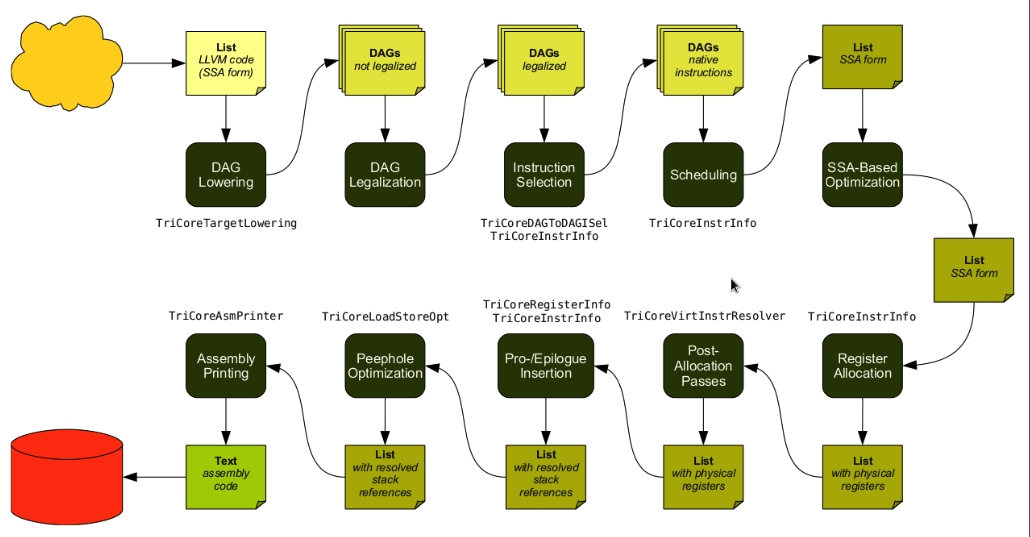
\includegraphics{5.png}
\caption{tricore\_llvm.pdf: Code generation sequence. On the path from LLVM code to
assembly code, numerous passes are run through and several data structures
are used to represent the intermediate results.}\label{backendstructure:backendstructure-f5}\end{figure}

LLVM is a Static Single Assignment (SSA) based representation.
LLVM provides an infinite virtual registers which can hold values of primitive
type (integral, floating point, or pointer values).
So, every operand can save in different virtual register in llvm SSA
representation.
Comment is “;” in llvm representation.
Following is the llvm SSA instructions.

\begin{Verbatim}[commandchars=\\\{\}]
\PYG{n}{store} \PYG{n}{i32} \PYG{l+m+mi}{0}\PYG{p}{,} \PYG{n}{i32}\PYG{o}{*} \PYG{o}{\PYGZpc{}}\PYG{n}{a}  \PYG{p}{;} \PYG{n}{store} \PYG{n}{i32} \PYG{n}{type} \PYG{n}{of} \PYG{l+m+mi}{0} \PYG{n}{to} \PYG{k}{virtual} \PYG{k}{register} \PYG{o}{\PYGZpc{}}\PYG{n}{a}\PYG{p}{,} \PYG{o}{\PYGZpc{}}\PYG{n}{a} \PYG{n}{is}
            \PYG{p}{;}  \PYG{n}{pointer} \PYG{n}{type} \PYG{n}{which} \PYG{n}{point} \PYG{n}{to} \PYG{n}{i32} \PYG{n}{value}
\PYG{n}{store} \PYG{n}{i32} \PYG{o}{\PYGZpc{}}\PYG{n}{b}\PYG{p}{,} \PYG{n}{i32}\PYG{o}{*} \PYG{o}{\PYGZpc{}}\PYG{n}{c} \PYG{p}{;} \PYG{n}{store} \PYG{o}{\PYGZpc{}}\PYG{n}{b} \PYG{n}{contents} \PYG{n}{to} \PYG{o}{\PYGZpc{}}\PYG{n}{c} \PYG{n}{point} \PYG{n}{to}\PYG{p}{,} \PYG{o}{\PYGZpc{}}\PYG{n}{b} \PYG{n}{isi32} \PYG{n}{type} \PYG{k}{virtual}
            \PYG{p}{;}  \PYG{k}{register}\PYG{p}{,} \PYG{o}{\PYGZpc{}}\PYG{n}{c} \PYG{n}{is} \PYG{n}{pointer} \PYG{n}{type} \PYG{n}{which} \PYG{n}{point} \PYG{n}{to} \PYG{n}{i32} \PYG{n}{value}\PYG{p}{.}
\PYG{o}{\PYGZpc{}}\PYG{n}{a1} \PYG{o}{=} \PYG{n}{load} \PYG{n}{i32}\PYG{o}{*} \PYG{o}{\PYGZpc{}}\PYG{n}{a}    \PYG{p}{;} \PYG{n}{load} \PYG{n}{the} \PYG{n}{memory} \PYG{n}{value} \PYG{n}{where} \PYG{o}{\PYGZpc{}}\PYG{n}{a} \PYG{n}{point} \PYG{n}{to} \PYG{n}{and} \PYG{n}{assign} \PYG{n}{the}
            \PYG{p}{;}  \PYG{n}{memory} \PYG{n}{value} \PYG{n}{to} \PYG{o}{\PYGZpc{}}\PYG{n}{a1}
\PYG{o}{\PYGZpc{}}\PYG{n}{a3} \PYG{o}{=} \PYG{n}{add} \PYG{n}{i32} \PYG{o}{\PYGZpc{}}\PYG{n}{a2}\PYG{p}{,} \PYG{l+m+mi}{1}  \PYG{p}{;} \PYG{n}{add} \PYG{o}{\PYGZpc{}}\PYG{n}{a2} \PYG{n}{and} \PYG{l+m+mi}{1} \PYG{n}{and} \PYG{n}{save} \PYG{n}{to} \PYG{o}{\PYGZpc{}}\PYG{n}{a3}
\end{Verbatim}

We explain the code generation process as below.
If you don't feel comfortable, please check tricore\_llvm.pdf section 4.2 first.
You can  read “The LLVM Target-Independent Code Generator” from \footnote{
\href{http://llvm.org/docs/CodeGenerator.html}{http://llvm.org/docs/CodeGenerator.html}
}
and “LLVM Language Reference Manual” from \footnote{
\href{http://llvm.org/docs/LangRef.html}{http://llvm.org/docs/LangRef.html}
}
before go ahead, but we think read section
4.2 of tricore\_llvm.pdf is enough.
We suggest you read the web site documents as above only when you are still not
quite understand, even though you have read the articles of this section and
next 2 sections for DAG and Instruction Selection.
\begin{enumerate}
\item {} 
Instruction Selection

\end{enumerate}

\begin{Verbatim}[commandchars=\\\{\}]
\PYG{c+c1}{// In this stage, transfer the llvm opcode into machine opcode, but the operand}
\PYG{c+c1}{//  still is llvm virtual operand.}
    \PYG{n}{store} \PYG{n}{i16} \PYG{l+m+mi}{0}\PYG{p}{,} \PYG{n}{i16}\PYG{o}{*} \PYG{o}{\PYGZpc{}}\PYG{n}{a} \PYG{c+c1}{// store 0 of i16 type to where virtual register \PYGZpc{}a}
               \PYG{c+c1}{//  point to}
\PYG{o}{=}\PYG{o}{\PYGZgt{}}  \PYG{n}{addiu} \PYG{n}{i16} \PYG{l+m+mi}{0}\PYG{p}{,} \PYG{n}{i32}\PYG{o}{*} \PYG{o}{\PYGZpc{}}\PYG{n}{a}
\end{Verbatim}
\begin{enumerate}
\setcounter{enumi}{1}
\item {} 
Scheduling and Formation

\end{enumerate}

\begin{Verbatim}[commandchars=\\\{\}]
\PYG{c+c1}{// In this stage, reorder the instructions sequence for optimization in}
\PYG{c+c1}{//  instructions cycle or in register pressure.}
    \PYG{n}{st} \PYG{n}{i32} \PYG{o}{\PYGZpc{}}\PYG{n}{a}\PYG{p}{,} \PYG{n}{i16}\PYG{o}{*} \PYG{o}{\PYGZpc{}}\PYG{n}{b}\PYG{p}{,}  \PYG{n}{i16} \PYG{l+m+mi}{5} \PYG{c+c1}{// st \PYGZpc{}a to *(\PYGZpc{}b+5)}
    \PYG{n}{st} \PYG{o}{\PYGZpc{}}\PYG{n}{b}\PYG{p}{,} \PYG{n}{i32}\PYG{o}{*} \PYG{o}{\PYGZpc{}}\PYG{n}{c}\PYG{p}{,} \PYG{n}{i16} \PYG{l+m+mi}{0}
    \PYG{o}{\PYGZpc{}}\PYG{n}{d} \PYG{o}{=} \PYG{n}{ld} \PYG{n}{i32}\PYG{o}{*} \PYG{o}{\PYGZpc{}}\PYG{n}{c}

\PYG{c+c1}{// Transfer above instructions order as follows. In RISC like Mips the ld \PYGZpc{}c use}
\PYG{c+c1}{//  the previous instruction st \PYGZpc{}c, must wait more than 1}
\PYG{c+c1}{// cycles. Meaning the ld cannot follow st immediately.}
\PYG{o}{=}\PYG{o}{\PYGZgt{}}  \PYG{n}{st} \PYG{o}{\PYGZpc{}}\PYG{n}{b}\PYG{p}{,} \PYG{n}{i32}\PYG{o}{*} \PYG{o}{\PYGZpc{}}\PYG{n}{c}\PYG{p}{,} \PYG{n}{i16} \PYG{l+m+mi}{0}
    \PYG{n}{st} \PYG{n}{i32} \PYG{o}{\PYGZpc{}}\PYG{n}{a}\PYG{p}{,} \PYG{n}{i16}\PYG{o}{*} \PYG{o}{\PYGZpc{}}\PYG{n}{b}\PYG{p}{,}  \PYG{n}{i16} \PYG{l+m+mi}{5}
    \PYG{o}{\PYGZpc{}}\PYG{n}{d} \PYG{o}{=} \PYG{n}{ld} \PYG{n}{i32}\PYG{o}{*} \PYG{o}{\PYGZpc{}}\PYG{n}{c}\PYG{p}{,} \PYG{n}{i16} \PYG{l+m+mi}{0}
\PYG{c+c1}{// If without reorder instructions, a instruction nop which do nothing must be}
\PYG{c+c1}{//  filled, contribute one instruction cycle more than optimization. (Actually,}
\PYG{c+c1}{//  Mips is scheduled with hardware dynamically and will insert nop between st}
\PYG{c+c1}{//  and ld instructions if compiler didn't insert nop.)}
    \PYG{n}{st} \PYG{n}{i32} \PYG{o}{\PYGZpc{}}\PYG{n}{a}\PYG{p}{,} \PYG{n}{i16}\PYG{o}{*} \PYG{o}{\PYGZpc{}}\PYG{n}{b}\PYG{p}{,}  \PYG{n}{i16} \PYG{l+m+mi}{5}
    \PYG{n}{st} \PYG{o}{\PYGZpc{}}\PYG{n}{b}\PYG{p}{,} \PYG{n}{i32}\PYG{o}{*} \PYG{o}{\PYGZpc{}}\PYG{n}{c}\PYG{p}{,} \PYG{n}{i16} \PYG{l+m+mi}{0}
    \PYG{n}{nop}
    \PYG{o}{\PYGZpc{}}\PYG{n}{d} \PYG{o}{=} \PYG{n}{ld} \PYG{n}{i32}\PYG{o}{*} \PYG{o}{\PYGZpc{}}\PYG{n}{c}\PYG{p}{,} \PYG{n}{i16} \PYG{l+m+mi}{0}

\PYG{c+c1}{// Minimum register pressure}
\PYG{c+c1}{//  Suppose \PYGZpc{}c is alive after the instructions basic block (meaning \PYGZpc{}c will be}
\PYG{c+c1}{//  used after the basic block), \PYGZpc{}a and \PYGZpc{}b are not alive after that.}
\PYG{c+c1}{// The following no reorder version need 3 registers at least}
    \PYG{o}{\PYGZpc{}}\PYG{n}{a} \PYG{o}{=} \PYG{n}{add} \PYG{n}{i32} \PYG{l+m+mi}{1}\PYG{p}{,} \PYG{n}{i32} \PYG{l+m+mi}{0}
    \PYG{o}{\PYGZpc{}}\PYG{n}{b} \PYG{o}{=} \PYG{n}{add} \PYG{n}{i32} \PYG{l+m+mi}{2}\PYG{p}{,} \PYG{n}{i32} \PYG{l+m+mi}{0}
    \PYG{n}{st} \PYG{o}{\PYGZpc{}}\PYG{n}{a}\PYG{p}{,}  \PYG{n}{i32}\PYG{o}{*} \PYG{o}{\PYGZpc{}}\PYG{n}{c}\PYG{p}{,} \PYG{l+m+mi}{1}
    \PYG{n}{st} \PYG{o}{\PYGZpc{}}\PYG{n}{b}\PYG{p}{,}  \PYG{n}{i32}\PYG{o}{*} \PYG{o}{\PYGZpc{}}\PYG{n}{c}\PYG{p}{,} \PYG{l+m+mi}{2}

\PYG{c+c1}{// The reorder version need 2 registers only (by allocate \PYGZpc{}a and \PYGZpc{}b in the same}
\PYG{c+c1}{//  register)}
\PYG{o}{=}\PYG{o}{\PYGZgt{}} \PYG{o}{\PYGZpc{}}\PYG{n}{a} \PYG{o}{=} \PYG{n}{add} \PYG{n}{i32} \PYG{l+m+mi}{1}\PYG{p}{,} \PYG{n}{i32} \PYG{l+m+mi}{0}
    \PYG{n}{st} \PYG{o}{\PYGZpc{}}\PYG{n}{a}\PYG{p}{,}  \PYG{n}{i32}\PYG{o}{*} \PYG{o}{\PYGZpc{}}\PYG{n}{c}\PYG{p}{,} \PYG{l+m+mi}{1}
    \PYG{o}{\PYGZpc{}}\PYG{n}{b} \PYG{o}{=} \PYG{n}{add} \PYG{n}{i32} \PYG{l+m+mi}{2}\PYG{p}{,} \PYG{n}{i32} \PYG{l+m+mi}{0}
    \PYG{n}{st} \PYG{o}{\PYGZpc{}}\PYG{n}{b}\PYG{p}{,}  \PYG{n}{i32}\PYG{o}{*} \PYG{o}{\PYGZpc{}}\PYG{n}{c}\PYG{p}{,} \PYG{l+m+mi}{2}
\end{Verbatim}
\begin{enumerate}
\setcounter{enumi}{2}
\item {} 
SSA-based Machine Code Optimization
\begin{quote}

For example, common expression remove, shown in next section DAG.
\end{quote}

\item {} 
Register Allocation
\begin{quote}

Allocate real register for virtual register.
\end{quote}

\item {} 
Prologue/Epilogue Code Insertion
\begin{quote}

Explain in section Add Prologue/Epilogue functions
\end{quote}

\item {} 
Late Machine Code Optimizations
\begin{quote}

Any “last-minute” peephole optimizations of the final machine code can be
applied during this phase.
For example, replace x = x * 2 by x = x \textless{} 1 for integer operand.
\end{quote}

\item {} \begin{description}
\item[{Code Emission}] \leavevmode
Finally, the completed machine code is emitted. For static compilation,
the end result is an assembly code file; for JIT compilation, the opcodes
of the machine instructions are written into memory.

\end{description}

\end{enumerate}

The llvm code generation sequence also can be obtained by
\code{llc -debug-pass=Structure} as the following. The first 4 code generation
sequences from \hyperref[backendstructure:backendstructure-f5]{Figure  \ref*{backendstructure:backendstructure-f5}} are in the
\textbf{`DAG-\textgreater{}DAG Pattern Instruction Selection'} of the \code{llc -debug-pass=Structure}
displayed. The order of Peephole Optimizations and Prologue/Epilogue Insertion
is inconsistent in them (please check the * in the following).
No need to bother since the the LLVM is under development and changed all the
time.

\begin{Verbatim}[commandchars=\\\{\}]
118-165-79-200:InputFiles Jonathan\PYG{n+nv}{\PYGZdl{} }llc --help-hidden
OVERVIEW: llvm system compiler

USAGE: llc \PYG{o}{[}options\PYG{o}{]} \PYGZlt{}input bitcode\PYGZgt{}

OPTIONS:
...
  -debug-pass                             - Print PassManager debugging \PYG{n+nv}{information}
    \PYG{o}{=}None                                 -   disable debug \PYG{n+nv}{output}
    \PYG{o}{=}Arguments                            -   print pass arguments to pass to \PYG{l+s+s1}{'opt'}
    \PYG{o}{=}Structure                            -   print pass structure before run\PYG{o}{(}\PYG{o}{)}
    \PYG{o}{=}Executions                           -   print pass name before it is \PYG{n+nv}{executed}
    \PYG{o}{=}Details                              -   print pass details when it is executed

118-165-79-200:InputFiles Jonathan\PYG{n+nv}{\PYGZdl{} }llc -march\PYG{o}{=}mips -debug-pass\PYG{o}{=}Structure ch3.bc
...
Target Library Information
Target Transform Info
Data Layout
Target Pass Configuration
No Alias Analysis \PYG{o}{(}always returns \PYG{l+s+s1}{'may'} \PYG{n+nb}{alias}\PYG{o}{)}
Type-Based Alias Analysis
Basic Alias Analysis \PYG{o}{(}stateless AA impl\PYG{o}{)}
Create Garbage Collector Module Metadata
Machine Module Information
Machine Branch Probability Analysis
  ModulePass Manager
    FunctionPass Manager
      Preliminary module verification
      Dominator Tree Construction
      Module Verifier
      Natural Loop Information
      Loop Pass Manager
        Canonicalize natural loops
      Scalar Evolution Analysis
      Loop Pass Manager
        Canonicalize natural loops
        Induction Variable Users
        Loop Strength Reduction
      Lower Garbage Collection Instructions
      Remove unreachable blocks from the CFG
      Exception handling preparation
      Optimize \PYG{k}{for }code generation
      Insert stack protectors
      Preliminary module verification
      Dominator Tree Construction
      Module Verifier
      Machine Function Analysis
      Natural Loop Information
      Branch Probability Analysis
    * MIPS DAG-\PYGZgt{}DAG Pattern Instruction Selection
      Expand ISel Pseudo-instructions
      Tail Duplication
      Optimize machine instruction PHIs
      MachineDominator Tree Construction
      Slot index numbering
      Merge disjoint stack slots
      Local Stack Slot Allocation
      Remove dead machine instructions
      MachineDominator Tree Construction
      Machine Natural Loop Construction
      Machine Loop Invariant Code Motion
      Machine Common Subexpression Elimination
      Machine code sinking
    * Peephole Optimizations
      Process Implicit Definitions
      Remove unreachable machine basic blocks
      Live Variable Analysis
      Eliminate PHI nodes \PYG{k}{for }register allocation
      Two-Address instruction pass
      Slot index numbering
      Live Interval Analysis
      Debug Variable Analysis
      Simple Register Coalescing
      Live Stack Slot Analysis
      Calculate spill weights
      Virtual Register Map
      Live Register Matrix
      Bundle Machine CFG Edges
      Spill Code Placement Analysis
    * Greedy Register Allocator
      Virtual Register Rewriter
      Stack Slot Coloring
      Machine Loop Invariant Code Motion
    * Prologue/Epilogue Insertion \PYGZam{} Frame Finalization
      Control Flow Optimizer
      Tail Duplication
      Machine Copy Propagation Pass
    * Post-RA pseudo instruction expansion pass
      MachineDominator Tree Construction
      Machine Natural Loop Construction
      Post RA top-down list latency scheduler
      Analyze Machine Code For Garbage Collection
      Machine Block Frequency Analysis
      Branch Probability Basic Block Placement
      Mips Delay Slot Filler
      Mips Long Branch
      MachineDominator Tree Construction
      Machine Natural Loop Construction
    * Mips Assembly Printer
      Delete Garbage Collector Information
\end{Verbatim}


\section{DAG (Directed Acyclic Graph)}
\label{backendstructure:dag-directed-acyclic-graph}
Many important techniques for local optimization begin by transforming a basic
block into DAG. For example, the basic block code and it's corresponding DAG as
\hyperref[backendstructure:backendstructure-f6]{Figure  \ref*{backendstructure:backendstructure-f6}}.
\begin{figure}[htbp]
\centering
\capstart

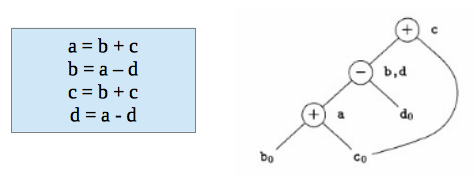
\includegraphics{6.png}
\caption{DAG example}\label{backendstructure:backendstructure-f6}\end{figure}

If b is not live on exit from the block, then we can do common expression
remove to get the following code.

\begin{Verbatim}[commandchars=\\\{\}]
a = b + c
d = a – d
c = d + c
\end{Verbatim}

As you can imagine, the common expression remove can apply in IR or machine
code.

DAG like a tree which opcode is the node and operand (register and
const/immediate/offset) is leaf.
It can also be represented by list as prefix order in tree.
For example, (+ b, c), (+ b, 1) is IR DAG representation.


\section{Instruction Selection}
\label{backendstructure:instruction-selection}
In back end, we need to translate IR code into machine code at Instruction
Selection Process as \hyperref[backendstructure:backendstructure-f7]{Figure  \ref*{backendstructure:backendstructure-f7}}.
\begin{figure}[htbp]
\centering
\capstart

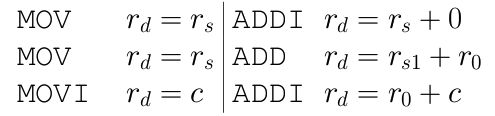
\includegraphics{7.png}
\caption{IR and it's corresponding machine instruction}\label{backendstructure:backendstructure-f7}\end{figure}

For machine instruction selection, the better solution is represent IR and
machine instruction by DAG.
In \hyperref[backendstructure:backendstructure-f8]{Figure  \ref*{backendstructure:backendstructure-f8}}, we skip the register leaf.
The rj + rk is IR DAG representation (for symbol notation, not llvm SSA form).
ADD is machine instruction.
\begin{figure}[htbp]
\centering
\capstart

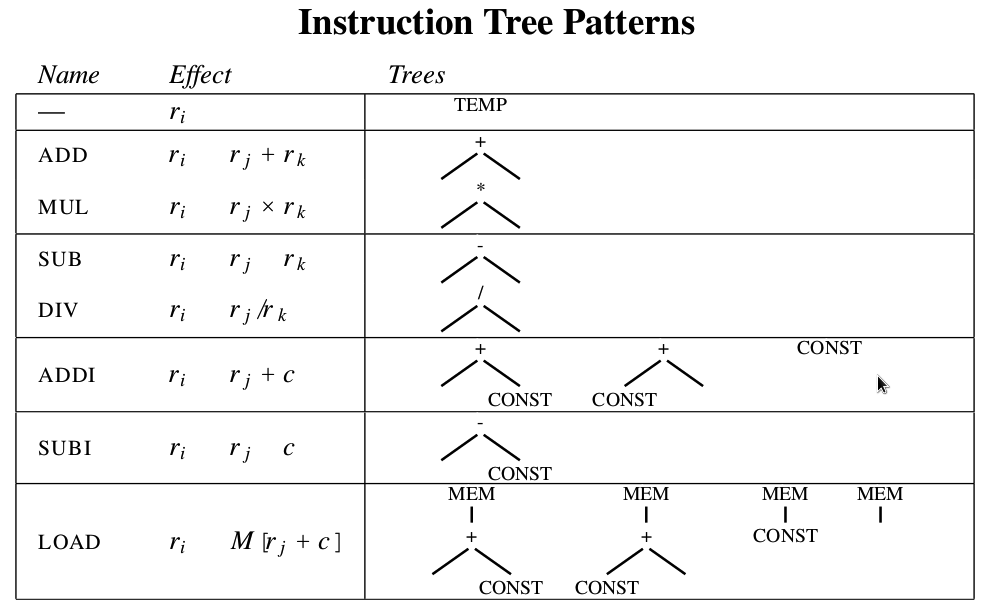
\includegraphics{8.png}
\caption{Instruction DAG representation}\label{backendstructure:backendstructure-f8}\end{figure}

The IR DAG and machine instruction DAG can also represented as list.
For example, (+ ri, rj), (- ri, 1) are lists for IR DAG; (ADD ri, rj),
(SUBI ri, 1) are lists for machine instruction DAG.

Now, let's recall the ADDiu instruction defined on Cpu0InstrInfo.td in the
previous chapter. List them again as follows,
\paragraph{lbdex/Chapter3\_2/Cpu0InstrFormats.td}

\begin{Verbatim}[commandchars=\\\{\}]
\PYG{c+c1}{//===----------------------------------------------------------------------===//}
\PYG{c+c1}{// Format L instruction class in Cpu0 : \PYGZlt{}\textbar{}opcode\textbar{}ra\textbar{}rb\textbar{}cx\textbar{}\PYGZgt{}}
\PYG{c+c1}{//===----------------------------------------------------------------------===//}

\PYG{k}{class} \PYG{n+nc}{FL}\PYG{o}{\PYGZlt{}}\PYG{n}{bits}\PYG{o}{\PYGZlt{}}\PYG{l+m+mi}{8}\PYG{o}{\PYGZgt{}} \PYG{n}{op}\PYG{p}{,} \PYG{n}{dag} \PYG{n}{outs}\PYG{p}{,} \PYG{n}{dag} \PYG{n}{ins}\PYG{p}{,} \PYG{n}{string} \PYG{n}{asmstr}\PYG{p}{,} \PYG{n}{list}\PYG{o}{\PYGZlt{}}\PYG{n}{dag}\PYG{o}{\PYGZgt{}} \PYG{n}{pattern}\PYG{p}{,}
         \PYG{n}{InstrItinClass} \PYG{n}{itin}\PYG{o}{\PYGZgt{}}\PYG{o}{:} \PYG{n}{Cpu0Inst}\PYG{o}{\PYGZlt{}}\PYG{n}{outs}\PYG{p}{,} \PYG{n}{ins}\PYG{p}{,} \PYG{n}{asmstr}\PYG{p}{,} \PYG{n}{pattern}\PYG{p}{,} \PYG{n}{itin}\PYG{p}{,} \PYG{n}{FrmL}\PYG{o}{\PYGZgt{}}
\PYG{p}{\PYGZob{}}
  \PYG{n}{bits}\PYG{o}{\PYGZlt{}}\PYG{l+m+mi}{4}\PYG{o}{\PYGZgt{}}  \PYG{n}{ra}\PYG{p}{;}
  \PYG{n}{bits}\PYG{o}{\PYGZlt{}}\PYG{l+m+mi}{4}\PYG{o}{\PYGZgt{}}  \PYG{n}{rb}\PYG{p}{;}
  \PYG{n}{bits}\PYG{o}{\PYGZlt{}}\PYG{l+m+mi}{16}\PYG{o}{\PYGZgt{}} \PYG{n}{imm16}\PYG{p}{;}

  \PYG{n}{let} \PYG{n}{Opcode} \PYG{o}{=} \PYG{n}{op}\PYG{p}{;}

  \PYG{n}{let} \PYG{n}{Inst}\PYG{p}{\PYGZob{}}\PYG{l+m+mi}{23}\PYG{o}{-}\PYG{l+m+mi}{20}\PYG{p}{\PYGZcb{}} \PYG{o}{=} \PYG{n}{ra}\PYG{p}{;}
  \PYG{n}{let} \PYG{n}{Inst}\PYG{p}{\PYGZob{}}\PYG{l+m+mi}{19}\PYG{o}{-}\PYG{l+m+mi}{16}\PYG{p}{\PYGZcb{}} \PYG{o}{=} \PYG{n}{rb}\PYG{p}{;}
  \PYG{n}{let} \PYG{n}{Inst}\PYG{p}{\PYGZob{}}\PYG{l+m+mi}{15}\PYG{o}{-}\PYG{l+m+mi}{0}\PYG{p}{\PYGZcb{}}  \PYG{o}{=} \PYG{n}{imm16}\PYG{p}{;}
\PYG{p}{\PYGZcb{}}
\end{Verbatim}
\paragraph{lbdex/Chapter3\_2/Cpu0InstrInfo.td}

\begin{Verbatim}[commandchars=\\\{\}]
// Arithmetic and logical instructions with 2 register operands.
class ArithLogicI\textless{}bits\textless{}8\textgreater{} op, string instr\_asm, SDNode OpNode,
                  Operand Od, PatLeaf imm\_type, RegisterClass RC\textgreater{} :
  FL\textless{}op, (outs RC:\$ra), (ins RC:\$rb, Od:\$imm16),
     !strconcat(instr\_asm, "\PYGZbs{}t\$ra, \$rb, \$imm16"),
     [(set RC:\$ra, (OpNode RC:\$rb, imm\_type:\$imm16))], IIAlu\textgreater{} \PYGZob{}
  let isReMaterializable = 1;
\PYGZcb{}
...
def ADDiu   : ArithLogicI\textless{}0x09, "addiu", add, simm16, immSExt16, CPURegs\textgreater{};
\end{Verbatim}

\hyperref[backendstructure:backendstructure-f9]{Figure  \ref*{backendstructure:backendstructure-f9}} show how the pattern match work in the IR node
\textbf{add} and instruction ADDiu defined in Cpu0InstrInfo.td. This example
IR node ``add \%a, 5'', will be translated to ``addiu \%r1, 5'' since the IR
pattern{[}(set RC:\$ra, (OpNode RC:\$rb, imm\_type:\$imm16)){]} is set in ADDiu and the
2nd operand is signed immediate which matched ``\%a, 5''. In addition to pattern
match, the .td also set assembly string ``addiu'' and op code 0x09.
With this information, the LLVM TableGen will generate instruction both in
assembly and binary automatically (the binary instruction in obj file of ELF
format which will shown at later chapter).
Similarly, the machine instruction DAG node LD and ST can be got from IR DAG
node \textbf{load} and \textbf{store}.
\begin{figure}[htbp]
\centering
\capstart

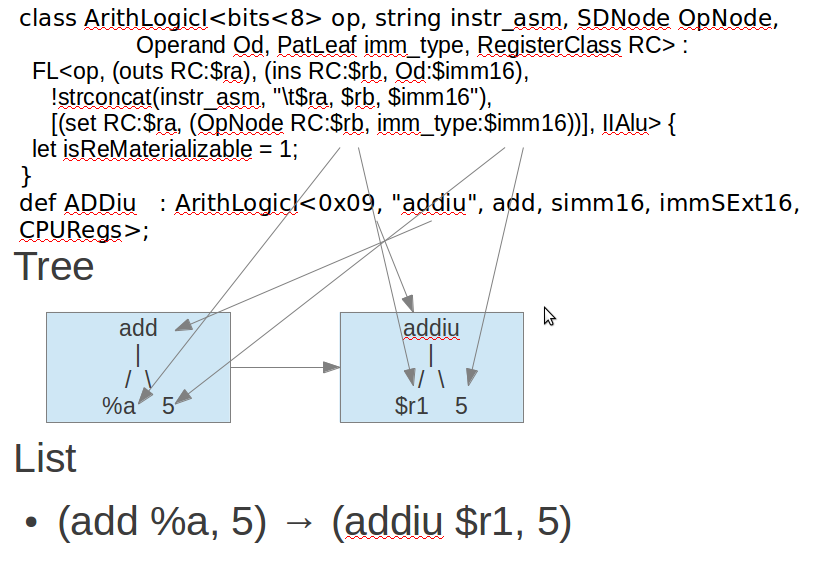
\includegraphics{9.png}
\caption{Pattern match for ADDiu instruction and IR node add}\label{backendstructure:backendstructure-f9}\end{figure}

Some cpu/fpu (floating point processor) has multiply-and-add floating point
instruction, fmadd.
It can be represented by DAG list (fadd (fmul ra, rc), rb).
For this implementation, we can assign fmadd DAG pattern to instruction td as
follows,

\begin{Verbatim}[commandchars=\\\{\}]
def FMADDS : AForm\_1\textless{}59, 29,
          (ops F4RC:\$FRT, F4RC:\$FRA, F4RC:\$FRC, F4RC:\$FRB),
          "fmadds \$FRT, \$FRA, \$FRC, \$FRB",
          [(set F4RC:\$FRT, (fadd (fmul F4RC:\$FRA, F4RC:\$FRC),
                       F4RC:\$FRB))]\textgreater{};
\end{Verbatim}

Similar with ADDiu, {[}(set F4RC:\$FRT, (fadd (fmul F4RC:\$FRA, F4RC:\$FRC),
F4RC:\$FRB)){]} is the pattern which include node \textbf{fmul} and node \textbf{fadd}.

Now, for the following basic block notation IR and llvm SSA IR code,

\begin{Verbatim}[commandchars=\\\{\}]
\PYG{n}{d} \PYG{o}{=} \PYG{n}{a} \PYG{o}{*} \PYG{n}{c}
\PYG{n}{e} \PYG{o}{=} \PYG{n}{d} \PYG{o}{+} \PYG{n}{b}
\PYG{p}{.}\PYG{p}{.}\PYG{p}{.}

\PYG{o}{\PYGZpc{}}\PYG{n}{d} \PYG{o}{=} \PYG{n}{fmul} \PYG{o}{\PYGZpc{}}\PYG{n}{a}\PYG{p}{,} \PYG{o}{\PYGZpc{}}\PYG{n}{c}
\PYG{o}{\PYGZpc{}}\PYG{n}{e} \PYG{o}{=} \PYG{n}{fadd} \PYG{o}{\PYGZpc{}}\PYG{n}{d}\PYG{p}{,} \PYG{o}{\PYGZpc{}}\PYG{n}{b}
\PYG{p}{.}\PYG{p}{.}\PYG{p}{.}
\end{Verbatim}

The llvm SelectionDAG Optimization Phase (is part of Instruction Selection
Process) prefered to translate this 2 IR DAG node (fmul \%a, \%b) (fadd \%d, \%c)
into one machine instruction DAG node (\textbf{fmadd} \%a, \%c, \%b), than translate
them into 2 machine instruction nodes \textbf{fmul} and \textbf{fadd}.

\begin{Verbatim}[commandchars=\\\{\}]
\PYG{o}{\PYGZpc{}}\PYG{n}{e} \PYG{o}{=} \PYG{n}{fmadd} \PYG{o}{\PYGZpc{}}\PYG{n}{a}\PYG{p}{,} \PYG{o}{\PYGZpc{}}\PYG{n}{c}\PYG{p}{,} \PYG{o}{\PYGZpc{}}\PYG{n}{b}
\PYG{p}{.}\PYG{p}{.}\PYG{p}{.}
\end{Verbatim}

As you can see, the IR notation representation is easier to read then llvm SSA
IR form.
So, we  use the notation form in this book sometimes.

For the following basic block code,

\begin{Verbatim}[commandchars=\\\{\}]
a = b + c   // in notation IR form
d = a – d
\%e = fmadd \%a, \%c, \%b // in llvm SSA IR form
\end{Verbatim}

We can apply \hyperref[backendstructure:backendstructure-f7]{Figure  \ref*{backendstructure:backendstructure-f7}} Instruction tree pattern to get the
following machine code,

\begin{Verbatim}[commandchars=\\\{\}]
\PYG{n}{load}  \PYG{n}{rb}\PYG{p}{,} \PYG{n}{M}\PYG{p}{(}\PYG{n}{sp}\PYG{o}{+}\PYG{l+m+mi}{8}\PYG{p}{)}\PYG{p}{;} \PYG{c+c1}{// assume b allocate in sp+8, sp is stack point register}
\PYG{n}{load}  \PYG{n}{rc}\PYG{p}{,} \PYG{n}{M}\PYG{p}{(}\PYG{n}{sp}\PYG{o}{+}\PYG{l+m+mi}{16}\PYG{p}{)}\PYG{p}{;}
\PYG{n}{add} \PYG{n}{ra}\PYG{p}{,} \PYG{n}{rb}\PYG{p}{,} \PYG{n}{rc}\PYG{p}{;}
\PYG{n}{load}  \PYG{n}{rd}\PYG{p}{,} \PYG{n}{M}\PYG{p}{(}\PYG{n}{sp}\PYG{o}{+}\PYG{l+m+mi}{24}\PYG{p}{)}\PYG{p}{;}
\PYG{n}{sub} \PYG{n}{rd}\PYG{p}{,} \PYG{n}{ra}\PYG{p}{,} \PYG{n}{rd}\PYG{p}{;}
\PYG{n}{fmadd} \PYG{n}{re}\PYG{p}{,} \PYG{n}{ra}\PYG{p}{,} \PYG{n}{rc}\PYG{p}{,} \PYG{n}{rb}\PYG{p}{;}
\end{Verbatim}


\section{Add Cpu0DAGToDAGISel class}
\label{backendstructure:add-cpu0dagtodagisel-class}
The IR DAG to machine instruction DAG transformation is introduced in the
previous section.
Now, let's check what IR DAG nodes the file ch3.bc has. List ch3.ll as follows,

\begin{Verbatim}[commandchars=\\\{\}]
// ch3.ll
define i32 @main() nounwind uwtable \PYGZob{}
\%1 = alloca i32, align 4
store i32 0, i32* \%1
ret i32 0
\PYGZcb{}
\end{Verbatim}

As above, ch3.ll use the IR DAG node \textbf{store}, \textbf{ret}. Actually, it also use
\textbf{add} for sp (stack point) register adjust.
So, the definitions in Cpu0InstrInfo.td as follows is enough.
IR DAG is defined in file  include/llvm/Target/TargetSelectionDAG.td.
\paragraph{lbdex/Chapter3\_2/Cpu0InstrInfo.td}

\begin{Verbatim}[commandchars=\\\{\}]
//===----------------------------------------------------------------------===//

/// Load and Store Instructions
///  aligned
defm LD     : LoadM32\textless{}0x01,  "ld",  load\_a\textgreater{};
defm ST     : StoreM32\textless{}0x02, "st",  store\_a\textgreater{};

/// Arithmetic Instructions (ALU Immediate)
// IR "add" defined in include/llvm/Target/TargetSelectionDAG.td, line 315 (def add).
def ADDiu   : ArithLogicI\textless{}0x09, "addiu", add, simm16, immSExt16, CPURegs\textgreater{};

let isReturn=1, isTerminator=1, hasDelaySlot=1, isCodeGenOnly=1,
    isBarrier=1, hasCtrlDep=1 in
  def RET : FJ \textless{}0x3c, (outs), (ins CPURegs:\$target),
                "ret\PYGZbs{}t\$target", [(Cpu0Ret CPURegs:\$target)], IIBranch\textgreater{};

//===----------------------------------------------------------------------===//
\end{Verbatim}

Add class Cpu0DAGToDAGISel (Cpu0ISelDAGToDAG.cpp) to CMakeLists.txt, and add
following fragment to Cpu0TargetMachine.cpp,
\paragraph{lbdex/Chapter3\_3/CMakeLists.txt}

\begin{Verbatim}[commandchars=\\\{\}]
\PYG{n}{add\PYGZus{}llvm\PYGZus{}target}\PYG{p}{(}\PYG{p}{.}\PYG{p}{.}\PYG{p}{.}
  \PYG{p}{.}\PYG{p}{.}\PYG{p}{.}
  \PYG{n}{Cpu0ISelDAGToDAG}\PYG{p}{.}\PYG{n}{cpp}
  \PYG{p}{.}\PYG{p}{.}\PYG{p}{.}
  \PYG{p}{)}
\end{Verbatim}

The following code in Cpu0TargetMachine.cpp will create a pass in instruction
selection stage.
\paragraph{lbdex/Chapter3\_3/Cpu0TargetMachine.cpp}

\begin{Verbatim}[commandchars=\\\{\}]
  \PYG{k}{virtual} \PYG{k+kt}{bool} \PYG{n}{addInstSelector}\PYG{p}{(}\PYG{p}{)}\PYG{p}{;}
\end{Verbatim}

\begin{Verbatim}[commandchars=\\\{\}]
\PYG{p}{\PYGZcb{}}\PYG{p}{;}
\PYG{p}{\PYGZcb{}} \PYG{c+c1}{// namespace}
\end{Verbatim}

\begin{Verbatim}[commandchars=\\\{\}]
\PYG{c+c1}{// Install an instruction selector pass using}
\PYG{c+c1}{// the ISelDag to gen Cpu0 code.}
\PYG{k+kt}{bool} \PYG{n}{Cpu0PassConfig}\PYG{o}{:}\PYG{o}{:}\PYG{n}{addInstSelector}\PYG{p}{(}\PYG{p}{)} \PYG{p}{\PYGZob{}}
  \PYG{n}{addPass}\PYG{p}{(}\PYG{n}{createCpu0ISelDag}\PYG{p}{(}\PYG{n}{getCpu0TargetMachine}\PYG{p}{(}\PYG{p}{)}\PYG{p}{)}\PYG{p}{)}\PYG{p}{;}
  \PYG{k}{return} \PYG{k+kc}{false}\PYG{p}{;}
\PYG{p}{\PYGZcb{}} \PYG{c+c1}{// lbd document - mark - addInstSelector()}
\end{Verbatim}
\paragraph{lbdex/Chapter3\_3/Cpu0ISelDAGToDAG.cpp}

\begin{Verbatim}[commandchars=\\\{\}]
\PYG{c+c1}{//===-- Cpu0ISelDAGToDAG.cpp - A Dag to Dag Inst Selector for Cpu0 --------===//}
\PYG{c+c1}{//}
\PYG{c+c1}{//                     The LLVM Compiler Infrastructure}
\PYG{c+c1}{//}
\PYG{c+c1}{// This file is distributed under the University of Illinois Open Source}
\PYG{c+c1}{// License. See LICENSE.TXT for details.}
\PYG{c+c1}{//}
\PYG{c+c1}{//===----------------------------------------------------------------------===//}
\PYG{c+c1}{//}
\PYG{c+c1}{// This file defines an instruction selector for the CPU0 target.}
\PYG{c+c1}{//}
\PYG{c+c1}{//===----------------------------------------------------------------------===//}

\PYG{c+cp}{\PYGZsh{}}\PYG{c+cp}{define DEBUG\PYGZus{}TYPE "cpu0-isel"}
\PYG{c+cp}{\PYGZsh{}}\PYG{c+cp}{include "Cpu0.h"}
\end{Verbatim}

\begin{Verbatim}[commandchars=\\\{\}]
\PYG{c+cp}{\PYGZsh{}}\PYG{c+cp}{include "Cpu0RegisterInfo.h"}
\PYG{c+cp}{\PYGZsh{}}\PYG{c+cp}{include "Cpu0Subtarget.h"}
\PYG{c+cp}{\PYGZsh{}}\PYG{c+cp}{include "Cpu0TargetMachine.h"}
\PYG{c+cp}{\PYGZsh{}}\PYG{c+cp}{include "MCTargetDesc}\PYG{c+cp}{/}\PYG{c+cp}{Cpu0BaseInfo.h"}
\PYG{c+cp}{\PYGZsh{}}\PYG{c+cp}{include "llvm}\PYG{c+cp}{/}\PYG{c+cp}{IR}\PYG{c+cp}{/}\PYG{c+cp}{GlobalValue.h"}
\PYG{c+cp}{\PYGZsh{}}\PYG{c+cp}{include "llvm}\PYG{c+cp}{/}\PYG{c+cp}{IR}\PYG{c+cp}{/}\PYG{c+cp}{Instructions.h"}
\PYG{c+cp}{\PYGZsh{}}\PYG{c+cp}{include "llvm}\PYG{c+cp}{/}\PYG{c+cp}{IR}\PYG{c+cp}{/}\PYG{c+cp}{Intrinsics.h"}
\PYG{c+cp}{\PYGZsh{}}\PYG{c+cp}{include "llvm}\PYG{c+cp}{/}\PYG{c+cp}{Support}\PYG{c+cp}{/}\PYG{c+cp}{CFG.h"}
\PYG{c+cp}{\PYGZsh{}}\PYG{c+cp}{include "llvm}\PYG{c+cp}{/}\PYG{c+cp}{IR}\PYG{c+cp}{/}\PYG{c+cp}{Type.h"}
\PYG{c+cp}{\PYGZsh{}}\PYG{c+cp}{include "llvm}\PYG{c+cp}{/}\PYG{c+cp}{CodeGen}\PYG{c+cp}{/}\PYG{c+cp}{MachineConstantPool.h"}
\PYG{c+cp}{\PYGZsh{}}\PYG{c+cp}{include "llvm}\PYG{c+cp}{/}\PYG{c+cp}{CodeGen}\PYG{c+cp}{/}\PYG{c+cp}{MachineFunction.h"}
\PYG{c+cp}{\PYGZsh{}}\PYG{c+cp}{include "llvm}\PYG{c+cp}{/}\PYG{c+cp}{CodeGen}\PYG{c+cp}{/}\PYG{c+cp}{MachineFrameInfo.h"}
\PYG{c+cp}{\PYGZsh{}}\PYG{c+cp}{include "llvm}\PYG{c+cp}{/}\PYG{c+cp}{CodeGen}\PYG{c+cp}{/}\PYG{c+cp}{MachineInstrBuilder.h"}
\PYG{c+cp}{\PYGZsh{}}\PYG{c+cp}{include "llvm}\PYG{c+cp}{/}\PYG{c+cp}{CodeGen}\PYG{c+cp}{/}\PYG{c+cp}{MachineRegisterInfo.h"}
\PYG{c+cp}{\PYGZsh{}}\PYG{c+cp}{include "llvm}\PYG{c+cp}{/}\PYG{c+cp}{CodeGen}\PYG{c+cp}{/}\PYG{c+cp}{SelectionDAGISel.h"}
\PYG{c+cp}{\PYGZsh{}}\PYG{c+cp}{include "llvm}\PYG{c+cp}{/}\PYG{c+cp}{CodeGen}\PYG{c+cp}{/}\PYG{c+cp}{SelectionDAGNodes.h"}
\PYG{c+cp}{\PYGZsh{}}\PYG{c+cp}{include "llvm}\PYG{c+cp}{/}\PYG{c+cp}{Target}\PYG{c+cp}{/}\PYG{c+cp}{TargetMachine.h"}
\PYG{c+cp}{\PYGZsh{}}\PYG{c+cp}{include "llvm}\PYG{c+cp}{/}\PYG{c+cp}{Support}\PYG{c+cp}{/}\PYG{c+cp}{Debug.h"}
\PYG{c+cp}{\PYGZsh{}}\PYG{c+cp}{include "llvm}\PYG{c+cp}{/}\PYG{c+cp}{Support}\PYG{c+cp}{/}\PYG{c+cp}{ErrorHandling.h"}
\PYG{c+cp}{\PYGZsh{}}\PYG{c+cp}{include "llvm}\PYG{c+cp}{/}\PYG{c+cp}{Support}\PYG{c+cp}{/}\PYG{c+cp}{raw\PYGZus{}ostream.h"}
\PYG{k}{using} \PYG{k}{namespace} \PYG{n}{llvm}\PYG{p}{;}

\PYG{c+c1}{//===----------------------------------------------------------------------===//}
\PYG{c+c1}{// Instruction Selector Implementation}
\PYG{c+c1}{//===----------------------------------------------------------------------===//}

\PYG{c+c1}{//===----------------------------------------------------------------------===//}
\PYG{c+c1}{// Cpu0DAGToDAGISel - CPU0 specific code to select CPU0 machine}
\PYG{c+c1}{// instructions for SelectionDAG operations.}
\PYG{c+c1}{//===----------------------------------------------------------------------===//}
\PYG{k}{namespace} \PYG{p}{\PYGZob{}}

\PYG{k}{class} \PYG{n+nc}{Cpu0DAGToDAGISel} \PYG{o}{:} \PYG{k}{public} \PYG{n}{SelectionDAGISel} \PYG{p}{\PYGZob{}}

  \PYG{c+c1}{/// TM - Keep a reference to Cpu0TargetMachine.}
  \PYG{n}{Cpu0TargetMachine} \PYG{o}{\PYGZam{}}\PYG{n}{TM}\PYG{p}{;}

  \PYG{c+c1}{/// Subtarget - Keep a pointer to the Cpu0Subtarget around so that we can}
  \PYG{c+c1}{/// make the right decision when generating code for different targets.}
  \PYG{k}{const} \PYG{n}{Cpu0Subtarget} \PYG{o}{\PYGZam{}}\PYG{n}{Subtarget}\PYG{p}{;}

\PYG{k}{public}\PYG{o}{:}
  \PYG{k}{explicit} \PYG{n}{Cpu0DAGToDAGISel}\PYG{p}{(}\PYG{n}{Cpu0TargetMachine} \PYG{o}{\PYGZam{}}\PYG{n}{tm}\PYG{p}{)} \PYG{o}{:}
  \PYG{n}{SelectionDAGISel}\PYG{p}{(}\PYG{n}{tm}\PYG{p}{)}\PYG{p}{,}
  \PYG{n}{TM}\PYG{p}{(}\PYG{n}{tm}\PYG{p}{)}\PYG{p}{,} \PYG{n}{Subtarget}\PYG{p}{(}\PYG{n}{tm}\PYG{p}{.}\PYG{n}{getSubtarget}\PYG{o}{\PYGZlt{}}\PYG{n}{Cpu0Subtarget}\PYG{o}{\PYGZgt{}}\PYG{p}{(}\PYG{p}{)}\PYG{p}{)} \PYG{p}{\PYGZob{}}\PYG{p}{\PYGZcb{}}

  \PYG{c+c1}{// Pass Name}
  \PYG{k}{virtual} \PYG{k}{const} \PYG{k+kt}{char} \PYG{o}{*}\PYG{n}{getPassName}\PYG{p}{(}\PYG{p}{)} \PYG{k}{const} \PYG{p}{\PYGZob{}}
    \PYG{k}{return} \PYG{l+s}{"}\PYG{l+s}{CPU0 DAG-\PYGZgt{}DAG Pattern Instruction Selection}\PYG{l+s}{"}\PYG{p}{;}
  \PYG{p}{\PYGZcb{}}

  \PYG{k}{virtual} \PYG{k+kt}{bool} \PYG{n}{runOnMachineFunction}\PYG{p}{(}\PYG{n}{MachineFunction} \PYG{o}{\PYGZam{}}\PYG{n}{MF}\PYG{p}{)}\PYG{p}{;}

\PYG{k}{private}\PYG{o}{:}
  \PYG{c+c1}{// Include the pieces autogenerated from the target description.}
  \PYG{c+cp}{\PYGZsh{}}\PYG{c+cp}{include "Cpu0GenDAGISel.inc"}

  \PYG{c+c1}{/// getTargetMachine - Return a reference to the TargetMachine, casted}
  \PYG{c+c1}{/// to the target-specific type.}
  \PYG{k}{const} \PYG{n}{Cpu0TargetMachine} \PYG{o}{\PYGZam{}}\PYG{n}{getTargetMachine}\PYG{p}{(}\PYG{p}{)} \PYG{p}{\PYGZob{}}
    \PYG{k}{return} \PYG{k}{static\PYGZus{}cast}\PYG{o}{\PYGZlt{}}\PYG{k}{const} \PYG{n}{Cpu0TargetMachine} \PYG{o}{\PYGZam{}}\PYG{o}{\PYGZgt{}}\PYG{p}{(}\PYG{n}{TM}\PYG{p}{)}\PYG{p}{;}
  \PYG{p}{\PYGZcb{}}

  \PYG{c+c1}{/// getInstrInfo - Return a reference to the TargetInstrInfo, casted}
  \PYG{c+c1}{/// to the target-specific type.}
  \PYG{k}{const} \PYG{n}{Cpu0InstrInfo} \PYG{o}{*}\PYG{n}{getInstrInfo}\PYG{p}{(}\PYG{p}{)} \PYG{p}{\PYGZob{}}
    \PYG{k}{return} \PYG{n}{getTargetMachine}\PYG{p}{(}\PYG{p}{)}\PYG{p}{.}\PYG{n}{getInstrInfo}\PYG{p}{(}\PYG{p}{)}\PYG{p}{;}
  \PYG{p}{\PYGZcb{}}

  \PYG{n}{SDNode} \PYG{o}{*}\PYG{n}{getGlobalBaseReg}\PYG{p}{(}\PYG{p}{)}\PYG{p}{;}
\end{Verbatim}

\begin{Verbatim}[commandchars=\\\{\}]
                                         \PYG{n}{EVT} \PYG{n}{Ty}\PYG{p}{,} \PYG{k+kt}{bool} \PYG{n}{HasLo}\PYG{p}{,} \PYG{k+kt}{bool} \PYG{n}{HasHi}\PYG{p}{)}\PYG{p}{;}

  \PYG{n}{SDNode} \PYG{o}{*}\PYG{n}{Select}\PYG{p}{(}\PYG{n}{SDNode} \PYG{o}{*}\PYG{n}{N}\PYG{p}{)}\PYG{p}{;}
  \PYG{c+c1}{// Complex Pattern.}
  \PYG{k+kt}{bool} \PYG{n}{SelectAddr}\PYG{p}{(}\PYG{n}{SDNode} \PYG{o}{*}\PYG{n}{Parent}\PYG{p}{,} \PYG{n}{SDValue} \PYG{n}{N}\PYG{p}{,} \PYG{n}{SDValue} \PYG{o}{\PYGZam{}}\PYG{n}{Base}\PYG{p}{,} \PYG{n}{SDValue} \PYG{o}{\PYGZam{}}\PYG{n}{Offset}\PYG{p}{)}\PYG{p}{;}
  \PYG{c+c1}{// getImm - Return a target constant with the specified value.}
  \PYG{k+kr}{inline} \PYG{n}{SDValue} \PYG{n}{getImm}\PYG{p}{(}\PYG{k}{const} \PYG{n}{SDNode} \PYG{o}{*}\PYG{n}{Node}\PYG{p}{,} \PYG{k+kt}{unsigned} \PYG{n}{Imm}\PYG{p}{)} \PYG{p}{\PYGZob{}}
    \PYG{k}{return} \PYG{n}{CurDAG}\PYG{o}{-}\PYG{o}{\PYGZgt{}}\PYG{n}{getTargetConstant}\PYG{p}{(}\PYG{n}{Imm}\PYG{p}{,} \PYG{n}{Node}\PYG{o}{-}\PYG{o}{\PYGZgt{}}\PYG{n}{getValueType}\PYG{p}{(}\PYG{l+m+mi}{0}\PYG{p}{)}\PYG{p}{)}\PYG{p}{;}
  \PYG{p}{\PYGZcb{}}
\end{Verbatim}

\begin{Verbatim}[commandchars=\\\{\}]
\PYG{p}{\PYGZcb{}}\PYG{p}{;}
\PYG{p}{\PYGZcb{}}

\PYG{k+kt}{bool} \PYG{n}{Cpu0DAGToDAGISel}\PYG{o}{:}\PYG{o}{:}\PYG{n}{runOnMachineFunction}\PYG{p}{(}\PYG{n}{MachineFunction} \PYG{o}{\PYGZam{}}\PYG{n}{MF}\PYG{p}{)} \PYG{p}{\PYGZob{}}
  \PYG{k+kt}{bool} \PYG{n}{Ret} \PYG{o}{=} \PYG{n}{SelectionDAGISel}\PYG{o}{:}\PYG{o}{:}\PYG{n}{runOnMachineFunction}\PYG{p}{(}\PYG{n}{MF}\PYG{p}{)}\PYG{p}{;}

  \PYG{k}{return} \PYG{n}{Ret}\PYG{p}{;}
\PYG{p}{\PYGZcb{}}
\end{Verbatim}

\begin{Verbatim}[commandchars=\\\{\}]
\PYG{c+c1}{/// ComplexPattern used on Cpu0InstrInfo}
\PYG{c+c1}{/// Used on Cpu0 Load/Store instructions}
\PYG{k+kt}{bool} \PYG{n}{Cpu0DAGToDAGISel}\PYG{o}{:}\PYG{o}{:}
\PYG{n}{SelectAddr}\PYG{p}{(}\PYG{n}{SDNode} \PYG{o}{*}\PYG{n}{Parent}\PYG{p}{,} \PYG{n}{SDValue} \PYG{n}{Addr}\PYG{p}{,} \PYG{n}{SDValue} \PYG{o}{\PYGZam{}}\PYG{n}{Base}\PYG{p}{,} \PYG{n}{SDValue} \PYG{o}{\PYGZam{}}\PYG{n}{Offset}\PYG{p}{)} \PYG{p}{\PYGZob{}}
  \PYG{n}{EVT} \PYG{n}{ValTy} \PYG{o}{=} \PYG{n}{Addr}\PYG{p}{.}\PYG{n}{getValueType}\PYG{p}{(}\PYG{p}{)}\PYG{p}{;}

  \PYG{c+c1}{// If Parent is an unaligned f32 load or store, select a (base + index)}
  \PYG{c+c1}{// floating point load/store instruction (luxc1 or suxc1).}
  \PYG{k}{const} \PYG{n}{LSBaseSDNode}\PYG{o}{*} \PYG{n}{LS} \PYG{o}{=} \PYG{l+m+mi}{0}\PYG{p}{;}

  \PYG{k}{if} \PYG{p}{(}\PYG{n}{Parent} \PYG{o}{\PYGZam{}}\PYG{o}{\PYGZam{}} \PYG{p}{(}\PYG{n}{LS} \PYG{o}{=} \PYG{n}{dyn\PYGZus{}cast}\PYG{o}{\PYGZlt{}}\PYG{n}{LSBaseSDNode}\PYG{o}{\PYGZgt{}}\PYG{p}{(}\PYG{n}{Parent}\PYG{p}{)}\PYG{p}{)}\PYG{p}{)} \PYG{p}{\PYGZob{}}
    \PYG{n}{EVT} \PYG{n}{VT} \PYG{o}{=} \PYG{n}{LS}\PYG{o}{-}\PYG{o}{\PYGZgt{}}\PYG{n}{getMemoryVT}\PYG{p}{(}\PYG{p}{)}\PYG{p}{;}

    \PYG{k}{if} \PYG{p}{(}\PYG{n}{VT}\PYG{p}{.}\PYG{n}{getSizeInBits}\PYG{p}{(}\PYG{p}{)} \PYG{o}{/} \PYG{l+m+mi}{8} \PYG{o}{\PYGZgt{}} \PYG{n}{LS}\PYG{o}{-}\PYG{o}{\PYGZgt{}}\PYG{n}{getAlignment}\PYG{p}{(}\PYG{p}{)}\PYG{p}{)} \PYG{p}{\PYGZob{}}
      \PYG{n}{assert}\PYG{p}{(}\PYG{n}{TLI}\PYG{p}{.}\PYG{n}{allowsUnalignedMemoryAccesses}\PYG{p}{(}\PYG{n}{VT}\PYG{p}{)} \PYG{o}{\PYGZam{}}\PYG{o}{\PYGZam{}}
             \PYG{l+s}{"}\PYG{l+s}{Unaligned loads/stores not supported for this type.}\PYG{l+s}{"}\PYG{p}{)}\PYG{p}{;}
      \PYG{k}{if} \PYG{p}{(}\PYG{n}{VT} \PYG{o}{=}\PYG{o}{=} \PYG{n}{MVT}\PYG{o}{:}\PYG{o}{:}\PYG{n}{f32}\PYG{p}{)}
        \PYG{k}{return} \PYG{k+kc}{false}\PYG{p}{;}
    \PYG{p}{\PYGZcb{}}
  \PYG{p}{\PYGZcb{}}

  \PYG{c+c1}{// if Address is FI, get the TargetFrameIndex.}
  \PYG{k}{if} \PYG{p}{(}\PYG{n}{FrameIndexSDNode} \PYG{o}{*}\PYG{n}{FIN} \PYG{o}{=} \PYG{n}{dyn\PYGZus{}cast}\PYG{o}{\PYGZlt{}}\PYG{n}{FrameIndexSDNode}\PYG{o}{\PYGZgt{}}\PYG{p}{(}\PYG{n}{Addr}\PYG{p}{)}\PYG{p}{)} \PYG{p}{\PYGZob{}}
    \PYG{n}{Base}   \PYG{o}{=} \PYG{n}{CurDAG}\PYG{o}{-}\PYG{o}{\PYGZgt{}}\PYG{n}{getTargetFrameIndex}\PYG{p}{(}\PYG{n}{FIN}\PYG{o}{-}\PYG{o}{\PYGZgt{}}\PYG{n}{getIndex}\PYG{p}{(}\PYG{p}{)}\PYG{p}{,} \PYG{n}{ValTy}\PYG{p}{)}\PYG{p}{;}
    \PYG{n}{Offset} \PYG{o}{=} \PYG{n}{CurDAG}\PYG{o}{-}\PYG{o}{\PYGZgt{}}\PYG{n}{getTargetConstant}\PYG{p}{(}\PYG{l+m+mi}{0}\PYG{p}{,} \PYG{n}{ValTy}\PYG{p}{)}\PYG{p}{;}
    \PYG{k}{return} \PYG{k+kc}{true}\PYG{p}{;}
  \PYG{p}{\PYGZcb{}}
\end{Verbatim}

\begin{Verbatim}[commandchars=\\\{\}]
  \PYG{n}{Base}   \PYG{o}{=} \PYG{n}{Addr}\PYG{p}{;}
  \PYG{n}{Offset} \PYG{o}{=} \PYG{n}{CurDAG}\PYG{o}{-}\PYG{o}{\PYGZgt{}}\PYG{n}{getTargetConstant}\PYG{p}{(}\PYG{l+m+mi}{0}\PYG{p}{,} \PYG{n}{ValTy}\PYG{p}{)}\PYG{p}{;}
  \PYG{k}{return} \PYG{k+kc}{true}\PYG{p}{;}
\PYG{p}{\PYGZcb{}}
\end{Verbatim}

\begin{Verbatim}[commandchars=\\\{\}]
\PYG{c+c1}{/// Select instructions not customized! Used for}
\PYG{c+c1}{/// expanded, promoted and normal instructions}
\PYG{n}{SDNode}\PYG{o}{*} \PYG{n}{Cpu0DAGToDAGISel}\PYG{o}{:}\PYG{o}{:}\PYG{n}{Select}\PYG{p}{(}\PYG{n}{SDNode} \PYG{o}{*}\PYG{n}{Node}\PYG{p}{)} \PYG{p}{\PYGZob{}}
  \PYG{k+kt}{unsigned} \PYG{n}{Opcode} \PYG{o}{=} \PYG{n}{Node}\PYG{o}{-}\PYG{o}{\PYGZgt{}}\PYG{n}{getOpcode}\PYG{p}{(}\PYG{p}{)}\PYG{p}{;}
\end{Verbatim}

\begin{Verbatim}[commandchars=\\\{\}]
  \PYG{c+c1}{// Dump information about the Node being selected}
  \PYG{n}{DEBUG}\PYG{p}{(}\PYG{n}{errs}\PYG{p}{(}\PYG{p}{)} \PYG{o}{\PYGZlt{}}\PYG{o}{\PYGZlt{}} \PYG{l+s}{"}\PYG{l+s}{Selecting: }\PYG{l+s}{"}\PYG{p}{;} \PYG{n}{Node}\PYG{o}{-}\PYG{o}{\PYGZgt{}}\PYG{n}{dump}\PYG{p}{(}\PYG{n}{CurDAG}\PYG{p}{)}\PYG{p}{;} \PYG{n}{errs}\PYG{p}{(}\PYG{p}{)} \PYG{o}{\PYGZlt{}}\PYG{o}{\PYGZlt{}} \PYG{l+s}{"}\PYG{l+s+se}{\PYGZbs{}n}\PYG{l+s}{"}\PYG{p}{)}\PYG{p}{;}

  \PYG{c+c1}{// If we have a custom node, we already have selected!}
  \PYG{k}{if} \PYG{p}{(}\PYG{n}{Node}\PYG{o}{-}\PYG{o}{\PYGZgt{}}\PYG{n}{isMachineOpcode}\PYG{p}{(}\PYG{p}{)}\PYG{p}{)} \PYG{p}{\PYGZob{}}
    \PYG{n}{DEBUG}\PYG{p}{(}\PYG{n}{errs}\PYG{p}{(}\PYG{p}{)} \PYG{o}{\PYGZlt{}}\PYG{o}{\PYGZlt{}} \PYG{l+s}{"}\PYG{l+s}{== }\PYG{l+s}{"}\PYG{p}{;} \PYG{n}{Node}\PYG{o}{-}\PYG{o}{\PYGZgt{}}\PYG{n}{dump}\PYG{p}{(}\PYG{n}{CurDAG}\PYG{p}{)}\PYG{p}{;} \PYG{n}{errs}\PYG{p}{(}\PYG{p}{)} \PYG{o}{\PYGZlt{}}\PYG{o}{\PYGZlt{}} \PYG{l+s}{"}\PYG{l+s+se}{\PYGZbs{}n}\PYG{l+s}{"}\PYG{p}{)}\PYG{p}{;}
    \PYG{k}{return} \PYG{n+nb}{NULL}\PYG{p}{;}
  \PYG{p}{\PYGZcb{}}

  \PYG{c+c1}{///}
  \PYG{c+c1}{// Instruction Selection not handled by the auto-generated}
  \PYG{c+c1}{// tablegen selection should be handled here.}
  \PYG{c+c1}{///}
\end{Verbatim}

\begin{Verbatim}[commandchars=\\\{\}]
  \PYG{k}{switch}\PYG{p}{(}\PYG{n}{Opcode}\PYG{p}{)} \PYG{p}{\PYGZob{}}
  \PYG{k}{default}\PYG{o}{:} \PYG{k}{break}\PYG{p}{;}
\end{Verbatim}

\begin{Verbatim}[commandchars=\\\{\}]
  \PYG{k}{case} \PYG{n}{ISD}\PYG{o}{:}\PYG{o}{:}\PYG{n+nl}{Constant:} \PYG{p}{\PYGZob{}}
    \PYG{k}{const} \PYG{n}{ConstantSDNode} \PYG{o}{*}\PYG{n}{CN} \PYG{o}{=} \PYG{n}{dyn\PYGZus{}cast}\PYG{o}{\PYGZlt{}}\PYG{n}{ConstantSDNode}\PYG{o}{\PYGZgt{}}\PYG{p}{(}\PYG{n}{Node}\PYG{p}{)}\PYG{p}{;}
    \PYG{k+kt}{unsigned} \PYG{n}{Size} \PYG{o}{=} \PYG{n}{CN}\PYG{o}{-}\PYG{o}{\PYGZgt{}}\PYG{n}{getValueSizeInBits}\PYG{p}{(}\PYG{l+m+mi}{0}\PYG{p}{)}\PYG{p}{;}

    \PYG{k}{if} \PYG{p}{(}\PYG{n}{Size} \PYG{o}{=}\PYG{o}{=} \PYG{l+m+mi}{32}\PYG{p}{)}
      \PYG{k}{break}\PYG{p}{;}
  \PYG{p}{\PYGZcb{}}
  \PYG{p}{\PYGZcb{}}

  \PYG{c+c1}{// Select the default instruction}
  \PYG{n}{SDNode} \PYG{o}{*}\PYG{n}{ResNode} \PYG{o}{=} \PYG{n}{SelectCode}\PYG{p}{(}\PYG{n}{Node}\PYG{p}{)}\PYG{p}{;}

  \PYG{n}{DEBUG}\PYG{p}{(}\PYG{n}{errs}\PYG{p}{(}\PYG{p}{)} \PYG{o}{\PYGZlt{}}\PYG{o}{\PYGZlt{}} \PYG{l+s}{"}\PYG{l+s}{=\PYGZgt{} }\PYG{l+s}{"}\PYG{p}{)}\PYG{p}{;}
  \PYG{k}{if} \PYG{p}{(}\PYG{n}{ResNode} \PYG{o}{=}\PYG{o}{=} \PYG{n+nb}{NULL} \PYG{o}{\textbar{}}\PYG{o}{\textbar{}} \PYG{n}{ResNode} \PYG{o}{=}\PYG{o}{=} \PYG{n}{Node}\PYG{p}{)}
    \PYG{n}{DEBUG}\PYG{p}{(}\PYG{n}{Node}\PYG{o}{-}\PYG{o}{\PYGZgt{}}\PYG{n}{dump}\PYG{p}{(}\PYG{n}{CurDAG}\PYG{p}{)}\PYG{p}{)}\PYG{p}{;}
  \PYG{k}{else}
    \PYG{n}{DEBUG}\PYG{p}{(}\PYG{n}{ResNode}\PYG{o}{-}\PYG{o}{\PYGZgt{}}\PYG{n}{dump}\PYG{p}{(}\PYG{n}{CurDAG}\PYG{p}{)}\PYG{p}{)}\PYG{p}{;}
  \PYG{n}{DEBUG}\PYG{p}{(}\PYG{n}{errs}\PYG{p}{(}\PYG{p}{)} \PYG{o}{\PYGZlt{}}\PYG{o}{\PYGZlt{}} \PYG{l+s}{"}\PYG{l+s+se}{\PYGZbs{}n}\PYG{l+s}{"}\PYG{p}{)}\PYG{p}{;}
  \PYG{k}{return} \PYG{n}{ResNode}\PYG{p}{;}
\PYG{p}{\PYGZcb{}}

\PYG{c+c1}{/// createCpu0ISelDag - This pass converts a legalized DAG into a}
\PYG{c+c1}{/// CPU0-specific DAG, ready for instruction scheduling.}
\PYG{n}{FunctionPass} \PYG{o}{*}\PYG{n}{llvm}\PYG{o}{:}\PYG{o}{:}\PYG{n}{createCpu0ISelDag}\PYG{p}{(}\PYG{n}{Cpu0TargetMachine} \PYG{o}{\PYGZam{}}\PYG{n}{TM}\PYG{p}{)} \PYG{p}{\PYGZob{}}
  \PYG{k}{return} \PYG{k}{new} \PYG{n}{Cpu0DAGToDAGISel}\PYG{p}{(}\PYG{n}{TM}\PYG{p}{)}\PYG{p}{;}
\PYG{p}{\PYGZcb{}}
\end{Verbatim}

This version adding the following code in Cpu0InstInfo.cpp to enable debug
information which called by llvm at proper time.
\paragraph{lbdex/Chapter3\_3/Cpu0InstrInfo.h}

\begin{Verbatim}[commandchars=\\\{\}]
\PYG{k}{class} \PYG{n+nc}{Cpu0InstrInfo} \PYG{o}{:} \PYG{k}{public} \PYG{n}{Cpu0GenInstrInfo} \PYG{p}{\PYGZob{}}
  \PYG{p}{.}\PYG{p}{.}\PYG{p}{.}
  \PYG{k}{virtual} \PYG{n}{MachineInstr}\PYG{o}{*} \PYG{n}{emitFrameIndexDebugValue}\PYG{p}{(}\PYG{n}{MachineFunction} \PYG{o}{\PYGZam{}}\PYG{n}{MF}\PYG{p}{,}
                                                 \PYG{k+kt}{int} \PYG{n}{FrameIx}\PYG{p}{,} \PYG{n}{uint64\PYGZus{}t} \PYG{n}{Offset}\PYG{p}{,}
                                                 \PYG{k}{const} \PYG{n}{MDNode} \PYG{o}{*}\PYG{n}{MDPtr}\PYG{p}{,}
                                                 \PYG{n}{DebugLoc} \PYG{n}{DL}\PYG{p}{)} \PYG{k}{const}\PYG{p}{;}
\end{Verbatim}
\paragraph{lbdex/Chapter3\_3/Cpu0InstrInfo.cpp}

\begin{Verbatim}[commandchars=\\\{\}]
\PYG{c+cp}{\PYGZsh{}}\PYG{c+cp}{include "llvm}\PYG{c+cp}{/}\PYG{c+cp}{CodeGen}\PYG{c+cp}{/}\PYG{c+cp}{MachineInstrBuilder.h"}
\end{Verbatim}

\begin{Verbatim}[commandchars=\\\{\}]
\PYG{n}{MachineInstr}\PYG{o}{*}
\PYG{n}{Cpu0InstrInfo}\PYG{o}{:}\PYG{o}{:}\PYG{n}{emitFrameIndexDebugValue}\PYG{p}{(}\PYG{n}{MachineFunction} \PYG{o}{\PYGZam{}}\PYG{n}{MF}\PYG{p}{,} \PYG{k+kt}{int} \PYG{n}{FrameIx}\PYG{p}{,}
                                        \PYG{n}{uint64\PYGZus{}t} \PYG{n}{Offset}\PYG{p}{,} \PYG{k}{const} \PYG{n}{MDNode} \PYG{o}{*}\PYG{n}{MDPtr}\PYG{p}{,}
                                        \PYG{n}{DebugLoc} \PYG{n}{DL}\PYG{p}{)} \PYG{k}{const} \PYG{p}{\PYGZob{}}
  \PYG{n}{MachineInstrBuilder} \PYG{n}{MIB} \PYG{o}{=} \PYG{n}{BuildMI}\PYG{p}{(}\PYG{n}{MF}\PYG{p}{,} \PYG{n}{DL}\PYG{p}{,} \PYG{n}{get}\PYG{p}{(}\PYG{n}{Cpu0}\PYG{o}{:}\PYG{o}{:}\PYG{n}{DBG\PYGZus{}VALUE}\PYG{p}{)}\PYG{p}{)}
    \PYG{p}{.}\PYG{n}{addFrameIndex}\PYG{p}{(}\PYG{n}{FrameIx}\PYG{p}{)}\PYG{p}{.}\PYG{n}{addImm}\PYG{p}{(}\PYG{l+m+mi}{0}\PYG{p}{)}\PYG{p}{.}\PYG{n}{addImm}\PYG{p}{(}\PYG{n}{Offset}\PYG{p}{)}\PYG{p}{.}\PYG{n}{addMetadata}\PYG{p}{(}\PYG{n}{MDPtr}\PYG{p}{)}\PYG{p}{;}
  \PYG{k}{return} \PYG{o}{\PYGZam{}}\PYG{o}{*}\PYG{n}{MIB}\PYG{p}{;}
\PYG{p}{\PYGZcb{}} \PYG{c+c1}{// lbd document - mark - emitFrameIndexDebugValue}
\end{Verbatim}

Build Chapter3\_3, run it, we find the error message in Chapter3\_2 is gone.
The new error message for Chapter3\_3 as follows,

\begin{Verbatim}[commandchars=\\\{\}]
118-165-78-230:InputFiles Jonathan\PYG{n+nv}{\PYGZdl{} }/Users/Jonathan/llvm/test/cmake\PYGZus{}debug\PYGZus{}build/
bin/Debug/llc -march\PYG{o}{=}cpu0 -relocation-model\PYG{o}{=}pic -filetype\PYG{o}{=}asm ch3.bc -o
ch3.cpu0.s
...
LLVM ERROR: Cannot \PYG{k}{select}: 0x7f80f182d310: \PYG{n+nv}{ch} \PYG{o}{=} \PYGZlt{}\PYGZlt{}Unknown Target Node \PYG{c}{\PYGZsh{}190\PYGZgt{}\PYGZgt{}}
...
  0x7f80f182d210: \PYG{n+nv}{i32} \PYG{o}{=} Register \PYGZpc{}LR \PYG{o}{[}\PYG{n+nv}{ID}\PYG{o}{=}4\PYG{o}{]}
\end{Verbatim}


\section{Handle return register lr}
\label{backendstructure:handle-return-register-lr}\paragraph{lbdex/Chapter3\_4/Cpu0InstrFormats.td}

\begin{Verbatim}[commandchars=\\\{\}]
\PYG{c+c1}{// Cpu0 Pseudo Instructions Format}
\PYG{k}{class} \PYG{n+nc}{Cpu0Pseudo}\PYG{o}{\PYGZlt{}}\PYG{n}{dag} \PYG{n}{outs}\PYG{p}{,} \PYG{n}{dag} \PYG{n}{ins}\PYG{p}{,} \PYG{n}{string} \PYG{n}{asmstr}\PYG{p}{,} \PYG{n}{list}\PYG{o}{\PYGZlt{}}\PYG{n}{dag}\PYG{o}{\PYGZgt{}} \PYG{n}{pattern}\PYG{o}{\PYGZgt{}}\PYG{o}{:}
      \PYG{n}{Cpu0Inst}\PYG{o}{\PYGZlt{}}\PYG{n}{outs}\PYG{p}{,} \PYG{n}{ins}\PYG{p}{,} \PYG{n}{asmstr}\PYG{p}{,} \PYG{n}{pattern}\PYG{p}{,} \PYG{n}{IIPseudo}\PYG{p}{,} \PYG{n}{Pseudo}\PYG{o}{\PYGZgt{}} \PYG{p}{\PYGZob{}}
  \PYG{n}{let} \PYG{n}{isCodeGenOnly} \PYG{o}{=} \PYG{l+m+mi}{1}\PYG{p}{;}
  \PYG{n}{let} \PYG{n}{isPseudo} \PYG{o}{=} \PYG{l+m+mi}{1}\PYG{p}{;}
\PYG{p}{\PYGZcb{}}
\end{Verbatim}
\paragraph{lbdex/Chapter3\_4/Cpu0InstrInfo.td}

\begin{Verbatim}[commandchars=\\\{\}]
\PYG{n}{let} \PYG{n}{isReturn}\PYG{o}{=}\PYG{l+m+mi}{1}\PYG{p}{,} \PYG{n}{isTerminator}\PYG{o}{=}\PYG{l+m+mi}{1}\PYG{p}{,} \PYG{n}{hasDelaySlot}\PYG{o}{=}\PYG{l+m+mi}{1}\PYG{p}{,} \PYG{n}{isBarrier}\PYG{o}{=}\PYG{l+m+mi}{1}\PYG{p}{,} \PYG{n}{hasCtrlDep}\PYG{o}{=}\PYG{l+m+mi}{1} \PYG{n}{in}
  \PYG{n}{def} \PYG{n}{RetLR} \PYG{o}{:} \PYG{n}{Cpu0Pseudo}\PYG{o}{\PYGZlt{}}\PYG{p}{(}\PYG{n}{outs}\PYG{p}{)}\PYG{p}{,} \PYG{p}{(}\PYG{n}{ins}\PYG{p}{)}\PYG{p}{,} \PYG{l+s}{"}\PYG{l+s}{"}\PYG{p}{,} \PYG{p}{[}\PYG{p}{(}\PYG{n}{Cpu0Ret}\PYG{p}{)}\PYG{p}{]}\PYG{o}{\PYGZgt{}}\PYG{p}{;}
\end{Verbatim}
\paragraph{lbdex/Chapter3\_4/Cpu0InstrInfo.h}

\begin{Verbatim}[commandchars=\\\{\}]
  \PYG{c+c1}{/// Expand Pseudo instructions into real backend instructions}
  \PYG{k}{virtual} \PYG{k+kt}{bool} \PYG{n}{expandPostRAPseudo}\PYG{p}{(}\PYG{n}{MachineBasicBlock}\PYG{o}{:}\PYG{o}{:}\PYG{n}{iterator} \PYG{n}{MI}\PYG{p}{)} \PYG{k}{const}\PYG{p}{;}

\PYG{k}{private}\PYG{o}{:}
  \PYG{k+kt}{void} \PYG{n}{ExpandRetLR}\PYG{p}{(}\PYG{n}{MachineBasicBlock} \PYG{o}{\PYGZam{}}\PYG{n}{MBB}\PYG{p}{,} \PYG{n}{MachineBasicBlock}\PYG{o}{:}\PYG{o}{:}\PYG{n}{iterator} \PYG{n}{I}\PYG{p}{,}
                   \PYG{k+kt}{unsigned} \PYG{n}{Opc}\PYG{p}{)} \PYG{k}{const}\PYG{p}{;}
\end{Verbatim}
\paragraph{lbdex/Chapter3\_4/Cpu0InstrInfo.cpp}

\begin{Verbatim}[commandchars=\\\{\}]
\PYG{c+c1}{// Cpu0InstrInfo::expandPostRAPseudo}
\PYG{c+c1}{/// Expand Pseudo instructions into real backend instructions}
\PYG{k+kt}{bool} \PYG{n}{Cpu0InstrInfo}\PYG{o}{:}\PYG{o}{:}\PYG{n}{expandPostRAPseudo}\PYG{p}{(}\PYG{n}{MachineBasicBlock}\PYG{o}{:}\PYG{o}{:}\PYG{n}{iterator} \PYG{n}{MI}\PYG{p}{)} \PYG{k}{const} \PYG{p}{\PYGZob{}}
  \PYG{n}{MachineBasicBlock} \PYG{o}{\PYGZam{}}\PYG{n}{MBB} \PYG{o}{=} \PYG{o}{*}\PYG{n}{MI}\PYG{o}{-}\PYG{o}{\PYGZgt{}}\PYG{n}{getParent}\PYG{p}{(}\PYG{p}{)}\PYG{p}{;}

  \PYG{k}{switch}\PYG{p}{(}\PYG{n}{MI}\PYG{o}{-}\PYG{o}{\PYGZgt{}}\PYG{n}{getDesc}\PYG{p}{(}\PYG{p}{)}\PYG{p}{.}\PYG{n}{getOpcode}\PYG{p}{(}\PYG{p}{)}\PYG{p}{)} \PYG{p}{\PYGZob{}}
  \PYG{k}{default}\PYG{o}{:}
    \PYG{k}{return} \PYG{k+kc}{false}\PYG{p}{;}
  \PYG{k}{case} \PYG{n}{Cpu0}\PYG{o}{:}\PYG{o}{:}\PYG{n+nl}{RetLR:}
    \PYG{n}{ExpandRetLR}\PYG{p}{(}\PYG{n}{MBB}\PYG{p}{,} \PYG{n}{MI}\PYG{p}{,} \PYG{n}{Cpu0}\PYG{o}{:}\PYG{o}{:}\PYG{n}{RET}\PYG{p}{)}\PYG{p}{;}
    \PYG{k}{break}\PYG{p}{;}
  \PYG{p}{\PYGZcb{}}

  \PYG{n}{MBB}\PYG{p}{.}\PYG{n}{erase}\PYG{p}{(}\PYG{n}{MI}\PYG{p}{)}\PYG{p}{;}
  \PYG{k}{return} \PYG{k+kc}{true}\PYG{p}{;}
\PYG{p}{\PYGZcb{}}

\PYG{k+kt}{void} \PYG{n}{Cpu0InstrInfo}\PYG{o}{:}\PYG{o}{:}\PYG{n}{ExpandRetLR}\PYG{p}{(}\PYG{n}{MachineBasicBlock} \PYG{o}{\PYGZam{}}\PYG{n}{MBB}\PYG{p}{,}
                                \PYG{n}{MachineBasicBlock}\PYG{o}{:}\PYG{o}{:}\PYG{n}{iterator} \PYG{n}{I}\PYG{p}{,}
                                \PYG{k+kt}{unsigned} \PYG{n}{Opc}\PYG{p}{)} \PYG{k}{const} \PYG{p}{\PYGZob{}}
  \PYG{n}{BuildMI}\PYG{p}{(}\PYG{n}{MBB}\PYG{p}{,} \PYG{n}{I}\PYG{p}{,} \PYG{n}{I}\PYG{o}{-}\PYG{o}{\PYGZgt{}}\PYG{n}{getDebugLoc}\PYG{p}{(}\PYG{p}{)}\PYG{p}{,} \PYG{n}{get}\PYG{p}{(}\PYG{n}{Opc}\PYG{p}{)}\PYG{p}{)}\PYG{p}{.}\PYG{n}{addReg}\PYG{p}{(}\PYG{n}{Cpu0}\PYG{o}{:}\PYG{o}{:}\PYG{n}{LR}\PYG{p}{)}\PYG{p}{;}
\PYG{p}{\PYGZcb{}}
\end{Verbatim}

To handle IR ret, these code in Cpu0InstrInfo.td do things as below.
\begin{enumerate}
\item {} 
Declare a pseudo node to take care the IR Cpu0ISD::Ret by the following code,

\end{enumerate}
\paragraph{lbdex/Chapter3\_3/Cpu0InstrInfo.td}

\begin{Verbatim}[commandchars=\\\{\}]
\PYG{c+c1}{// Return}
\PYG{n}{def} \PYG{n}{Cpu0Ret} \PYG{o}{:} \PYG{n}{SDNode}\PYG{o}{\PYGZlt{}}\PYG{l+s}{"}\PYG{l+s}{Cpu0ISD::Ret}\PYG{l+s}{"}\PYG{p}{,} \PYG{n}{SDTNone}\PYG{p}{,}
                     \PYG{p}{[}\PYG{n}{SDNPHasChain}\PYG{p}{,} \PYG{n}{SDNPOptInGlue}\PYG{p}{,} \PYG{n}{SDNPVariadic}\PYG{p}{]}\PYG{o}{\PYGZgt{}}\PYG{p}{;}
\end{Verbatim}

\begin{Verbatim}[commandchars=\\\{\}]
\PYG{n}{let} \PYG{n}{isReturn}\PYG{o}{=}\PYG{l+m+mi}{1}\PYG{p}{,} \PYG{n}{isTerminator}\PYG{o}{=}\PYG{l+m+mi}{1}\PYG{p}{,} \PYG{n}{hasDelaySlot}\PYG{o}{=}\PYG{l+m+mi}{1}\PYG{p}{,} \PYG{n}{isBarrier}\PYG{o}{=}\PYG{l+m+mi}{1}\PYG{p}{,} \PYG{n}{hasCtrlDep}\PYG{o}{=}\PYG{l+m+mi}{1} \PYG{n}{in}
  \PYG{n}{def} \PYG{n}{RetLR} \PYG{o}{:} \PYG{n}{Cpu0Pseudo}\PYG{o}{\PYGZlt{}}\PYG{p}{(}\PYG{n}{outs}\PYG{p}{)}\PYG{p}{,} \PYG{p}{(}\PYG{n}{ins}\PYG{p}{)}\PYG{p}{,} \PYG{l+s}{"}\PYG{l+s}{"}\PYG{p}{,} \PYG{p}{[}\PYG{p}{(}\PYG{n}{Cpu0Ret}\PYG{p}{)}\PYG{p}{]}\PYG{o}{\PYGZgt{}}\PYG{p}{;}
\end{Verbatim}
\begin{enumerate}
\setcounter{enumi}{1}
\item {} 
After instruction selection, the Cpu0::Ret is replaced by Cpu0::RetLR
as below. This effect came from ``def RetLR'' as step 1.

\end{enumerate}

\begin{Verbatim}[commandchars=\\\{\}]
\PYG{o}{=}\PYG{o}{=}\PYG{o}{=}\PYG{o}{=}\PYG{o}{=} Instruction selection begins: BB\PYGZsh{}0 \PYG{l+s+s1}{'entry'}
Selecting: 0x1ea4050: \PYG{n+nv}{ch} \PYG{o}{=} Cpu0ISD::Ret 0x1ea3f50, 0x1ea3e50,
0x1ea3f50:1 \PYG{o}{[}\PYG{n+nv}{ID}\PYG{o}{=}27\PYG{o}{]}

ISEL: Starting pattern match on root node: 0x1ea4050: \PYG{n+nv}{ch} \PYG{o}{=} Cpu0ISD::Ret
0x1ea3f50, 0x1ea3e50, 0x1ea3f50:1 \PYG{o}{[}\PYG{n+nv}{ID}\PYG{o}{=}27\PYG{o}{]}

  Morphed node: 0x1ea4050: \PYG{n+nv}{ch} \PYG{o}{=} RetLR 0x1ea3e50, 0x1ea3f50, 0x1ea3f50:1
...
ISEL: Match \PYG{n+nb}{complete}!
\PYG{o}{=}\PYGZgt{} 0x1ea4050: \PYG{n+nv}{ch} \PYG{o}{=} RetLR 0x1ea3e50, 0x1ea3f50, 0x1ea3f50:1
...
\PYG{o}{=}\PYG{o}{=}\PYG{o}{=}\PYG{o}{=}\PYG{o}{=} Instruction selection ends:
Selected selection DAG: BB\PYGZsh{}0 \PYG{l+s+s1}{'main:entry'}
SelectionDAG has 28 nodes:
...
    0x1ea3e50: \PYGZlt{}multiple use\PYGZgt{}
    0x1ea3f50: \PYGZlt{}multiple use\PYGZgt{}
    0x1ea3f50: \PYGZlt{}multiple use\PYGZgt{}
  0x1ea4050: \PYG{n+nv}{ch} \PYG{o}{=} RetLR 0x1ea3e50, 0x1ea3f50, 0x1ea3f50:1
\end{Verbatim}
\begin{enumerate}
\setcounter{enumi}{2}
\item {} 
Expand the Cpu0::RetLR into instruction \textbf{ret \$lr} in ``Post-RA pseudo
instruction expansion pass'' stage by the code in Chapter3\_4/Cpu0InstrInfo.cpp
as above. This stage is after the register allocation, so we can replace the
V0 (\$r2) by LR (\$lr) without any side effect.

\item {} 
Print assembly or obj according the information (those *.inc generated by
TableGen from *.td) generated by the following code at ``Cpu0 Assembly
Printer'' stage.

\end{enumerate}
\paragraph{lbdex/Chapter2/Cpu0InstrInfo.td}

\begin{Verbatim}[commandchars=\\\{\}]

let isBranch=1, isTerminator=1, isBarrier=1, imm16=0, hasDelaySlot = 1,
    isIndirectBranch = 1 in
class JumpFR\textless{}bits\textless{}8\textgreater{} op, string instr\_asm, RegisterClass RC\textgreater{}:
  FL\textless{}op, (outs), (ins RC:\$ra),
     !strconcat(instr\_asm, "\PYGZbs{}t\$ra"), [(brind RC:\$ra)], IIBranch\textgreater{} \PYGZob{}
  let rb = 0;
  let imm16 = 0;
\PYGZcb{}

// Return instruction
class RetBase\textless{}RegisterClass RC\textgreater{}: JumpFR\textless{}0x3c, "ret", RC\textgreater{} \PYGZob{}
  let isReturn = 1;
  let isCodeGenOnly = 1;
  let hasCtrlDep = 1;
  let hasExtraSrcRegAllocReq = 1;
\PYGZcb{}
\end{Verbatim}

\begin{Verbatim}[commandchars=\\\{\}]
\PYG{n}{def} \PYG{n}{RET}     \PYG{o}{:} \PYG{n}{RetBase}\PYG{o}{\PYGZlt{}}\PYG{n}{CPURegs}\PYG{o}{\PYGZgt{}}\PYG{p}{;}
\end{Verbatim}


\begin{threeparttable}
\capstart\caption{Handle return register lr}

\begin{tabular}{|p{0.475\linewidth}|p{0.475\linewidth}|}
\hline
\textbf{
Stage
} & \textbf{
Function
}\\\hline

Write Code
 & 
Declare a pseudo node Cpu0::RetLR
\\\hline
\begin{itemize}
\item {} 
\end{itemize}
 & 
for IR Cpu0::Ret;
\\\hline

Instruction selection
 & 
Cpu0::Ret is replaced by Cpu0::RetLR
\\\hline

Post-RA pseudo instruction expansion pass
 & 
Cpu0::RetLR -\textgreater{} ret \$lr
\\\hline

Cpu0 Assembly Printer
 & 
Print according ``def RET''
\\\hline
\end{tabular}

\end{threeparttable}


Build Chapter3\_4, run it, we find the error message in Chapter3\_3 is gone.
The new error message for Chapter3\_4 as follows,
\begin{quote}

118-165-78-230:InputFiles Jonathan\$ /Users/Jonathan/llvm/test/cmake\_debug\_build/
bin/Debug/llc -march=cpu0 -relocation-model=pic -filetype=asm ch3.bc -o
ch3.cpu0.s
...
Target didn't implement TargetInstrInfo::storeRegToStackSlot!
1.  Running pass `Function Pass Manager' on module `ch3.bc'.
2.  Running pass `Prologue/Epilogue Insertion \& Frame Finalization' on function
`@main'
...
\end{quote}


\section{Add Prologue/Epilogue functions}
\label{backendstructure:add-prologue-epilogue-functions}
Following came from tricore\_llvm.pdf section “4.4.2 Non-static Register
Information ”.

For some target architectures, some aspects of the target architecture’s
register set are dependent upon variable factors and have to be determined at
runtime.
As a consequence, they cannot be generated statically from a TableGen
description – although that would be possible for the bulk of them in the case
of the TriCore backend.
Among them are the following points:
\begin{itemize}
\item {} 
Callee-saved registers. Normally, the ABI specifies a set of registers that a
function must save on entry and restore on return if their contents are
possibly modified during execution.

\item {} 
Reserved registers. Although the set of unavailable registers is already
defined in the TableGen file, TriCoreRegisterInfo contains a method that marks
all non-allocatable register numbers in a bit vector.

\end{itemize}

The following methods are implemented:
\begin{itemize}
\item {} 
emitPrologue() inserts prologue code at the beginning of a function. Thanks
to TriCore’s context model, this is a trivial task as it is not required to
save any registers manually. The only thing that has to be done is reserving
space for the function’s stack frame by decrementing the stack pointer.
In addition, if the function needs a frame pointer, the frame register \%a14 is
set to the old value of the stack pointer beforehand.

\item {} 
emitEpilogue() is intended to emit instructions to destroy the stack frame
and restore all previously saved registers before returning from a function.
However, as \%a10 (stack pointer), \%a11 (return address), and \%a14 (frame
pointer, if any) are all part of the upper context, no epilogue code is needed
at all. All cleanup operations are performed implicitly by the ret instruction.

\item {} 
eliminateFrameIndex() is called for each instruction that references a word
of data in a stack slot. All previous passes of the code generator have been
addressing stack slots through an abstract frame index and an immediate offset.
The purpose of this function is to translate such a reference into a
register–offset pair. Depending on whether the machine function that contains
the instruction has a fixed or a variable stack frame, either the stack pointer
\%a10 or the frame pointer \%a14 is used as the base register.
The offset is computed accordingly.
\hyperref[backendstructure:backendstructure-f10]{Figure  \ref*{backendstructure:backendstructure-f10}} demonstrates for both cases how a stack slot
is addressed.

\end{itemize}

If the addressing mode of the affected instruction cannot handle the address
because the offset is too large (the offset field has 10 bits for the BO
addressing mode and 16 bits for the BOL mode), a sequence of instructions is
emitted that explicitly computes the effective address.
Interim results are put into an unused address register.
If none is available, an already occupied address register is scavenged.
For this purpose, LLVM’s framework offers a class named RegScavenger that
takes care of all the details.
\begin{figure}[htbp]
\centering
\capstart

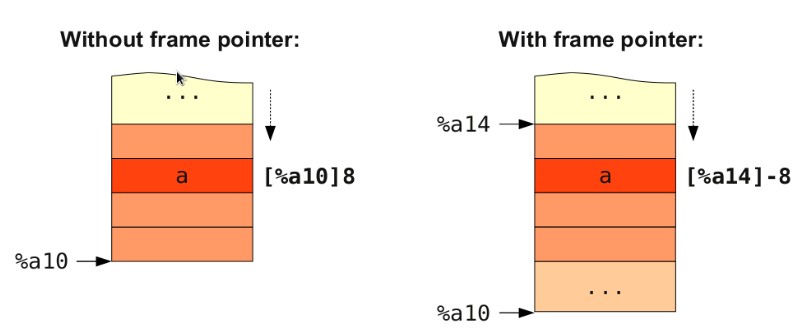
\includegraphics{10.png}
\caption{Addressing of a variable a located on the stack.
If the stack frame has a variable size, slot must be addressed relative to
the frame pointer}\label{backendstructure:backendstructure-f10}\end{figure}

We will explain the Prologue and Epilogue further by example code.
So for the following llvm IR code, Cpu0 back end will emit the corresponding
machine instructions as follows,

\begin{Verbatim}[commandchars=\\\{\}]
define i32 @main\PYG{o}{(}\PYG{o}{)} nounwind uwtable \PYG{o}{\PYGZob{}}
  \PYGZpc{}1 \PYG{o}{=} alloca i32, align 4
  store i32 0, i32* \PYGZpc{}1
  ret i32 0
\PYG{o}{\PYGZcb{}}

  .section .mdebug.abi32
  .previous
  .file \PYG{l+s+s2}{"ch3.bc"}
  .text
  .globl  main//static void expandLargeImm\PYG{l+s+se}{\PYGZbs{}\PYGZbs{}}n
  .align  2
  .type main,@function
  .ent  main                    \PYG{c}{\PYGZsh{} @main}
main:
  .cfi\PYGZus{}startproc
  .frame  \PYG{n+nv}{\PYGZdl{}sp},8,\PYG{n+nv}{\PYGZdl{}lr}
  .mask   0x00000000,0
  .set  noreorder
  .set  nomacro
\PYG{c}{\PYGZsh{} BB\PYGZsh{}0:}
  addiu \PYG{n+nv}{\PYGZdl{}sp}, \PYG{n+nv}{\PYGZdl{}sp}, -8
\PYG{n+nv}{\PYGZdl{}tmp1}:
  .cfi\PYGZus{}def\PYGZus{}cfa\PYGZus{}offset 8
  addiu \PYG{n+nv}{\PYGZdl{}2}, \PYG{n+nv}{\PYGZdl{}zero}, 0
  st  \PYG{n+nv}{\PYGZdl{}2}, 4\PYG{o}{(}\PYG{n+nv}{\PYGZdl{}sp}\PYG{o}{)}
  addiu \PYG{n+nv}{\PYGZdl{}sp}, \PYG{n+nv}{\PYGZdl{}sp}, 8
  ret \PYG{n+nv}{\PYGZdl{}lr}
  .set  macro
  .set  reorder
  .end  main
\PYG{n+nv}{\PYGZdl{}tmp2}:
  .size main, \PYG{o}{(}\PYG{n+nv}{\PYGZdl{}tmp2}\PYG{o}{)}-main
  .cfi\PYGZus{}endproc
\end{Verbatim}

LLVM get the stack size by parsing IR and counting how many virtual registers
is assigned to local variables. After that, it call emitPrologue().
This function will emit machine instructions to adjust sp (stack pointer
register) for local variables since we don't use fp (frame pointer register).
For our example, it will emit the instructions,

\begin{Verbatim}[commandchars=\\\{\}]
addiu \$sp, \$sp, -8
\end{Verbatim}

The  emitEpilogue will emit “addiu  \$sp, \$sp, 8”, where 8 is the stack size.

Since Instruction Selection and Register Allocation occurs before
Prologue/Epilogue Code Insertion, eliminateFrameIndex() is called after machine
instruction and real register allocated.
It translate the frame index of local variable (\%1 and \%2 in the following
example) into stack offset according the frame index order upward (stack grow
up downward from high address to low address, 0(\$sp) is the top, 52(\$sp) is the
bottom) as follows,

\begin{Verbatim}[commandchars=\\\{\}]
define i32 @main\PYG{o}{(}\PYG{o}{)} nounwind uwtable \PYG{o}{\PYGZob{}}
     \PYGZpc{}1 \PYG{o}{=} alloca i32, align 4
     \PYGZpc{}2 \PYG{o}{=} alloca i32, align 4
    ...
    store i32 0, i32* \PYGZpc{}1
    store i32 5, i32* \PYGZpc{}2, align 4
    ...
    ret i32 \PYG{n+nv}{0}

\PYG{o}{=}\PYGZgt{} \PYG{c}{\PYGZsh{} BB\PYGZsh{}0:}
  addiu \PYG{n+nv}{\PYGZdl{}sp}, \PYG{n+nv}{\PYGZdl{}sp}, -56
\PYG{n+nv}{\PYGZdl{}tmp1}:
  addiu \PYG{n+nv}{\PYGZdl{}3}, \PYG{n+nv}{\PYGZdl{}zero}, 0
  st  \PYG{n+nv}{\PYGZdl{}3}, 52\PYG{o}{(}\PYG{n+nv}{\PYGZdl{}sp}\PYG{o}{)}   // \PYGZpc{}1 is the first frame index \PYG{n+nb}{local }variable, so allocate
                    // in 52\PYG{o}{(}\PYG{n+nv}{\PYGZdl{}sp}\PYG{o}{)}
  addiu \PYG{n+nv}{\PYGZdl{}2}, \PYG{n+nv}{\PYGZdl{}zero}, 5
  st  \PYG{n+nv}{\PYGZdl{}2}, 48\PYG{o}{(}\PYG{n+nv}{\PYGZdl{}sp}\PYG{o}{)}   // \PYGZpc{}2 is the second frame index \PYG{n+nb}{local }variable, so
                    // allocate in 48\PYG{o}{(}\PYG{n+nv}{\PYGZdl{}sp}\PYG{o}{)}
  ...
  ret \PYG{n+nv}{\PYGZdl{}lr}
\end{Verbatim}

The Prologue and Epilogue functions as follows,
\paragraph{lbdex/Chapter3\_1/Cpu0FrameLowering.h}

\begin{Verbatim}[commandchars=\\\{\}]
  \PYG{c+c1}{/// emitProlog/emitEpilog - These methods insert prolog and epilog code into}
  \PYG{c+c1}{/// the function.}
  \PYG{k+kt}{void} \PYG{n}{emitPrologue}\PYG{p}{(}\PYG{n}{MachineFunction} \PYG{o}{\PYGZam{}}\PYG{n}{MF}\PYG{p}{)} \PYG{k}{const}\PYG{p}{;}
  \PYG{k+kt}{void} \PYG{n}{emitEpilogue}\PYG{p}{(}\PYG{n}{MachineFunction} \PYG{o}{\PYGZam{}}\PYG{n}{MF}\PYG{p}{,} \PYG{n}{MachineBasicBlock} \PYG{o}{\PYGZam{}}\PYG{n}{MBB}\PYG{p}{)} \PYG{k}{const}\PYG{p}{;}
\end{Verbatim}
\paragraph{lbdex/Chapter3\_5/Cpu0FrameLowering.h}

\begin{Verbatim}[commandchars=\\\{\}]
\PYG{k+kt}{void} \PYG{n}{processFunctionBeforeCalleeSavedScan}\PYG{p}{(}\PYG{n}{MachineFunction} \PYG{o}{\PYGZam{}}\PYG{n}{MF}\PYG{p}{,}
                                          \PYG{n}{RegScavenger} \PYG{o}{*}\PYG{n}{RS}\PYG{p}{)} \PYG{k}{const}\PYG{p}{;}
\end{Verbatim}
\paragraph{lbdex/Chapter3\_5/Cpu0FrameLowering.cpp}

\begin{Verbatim}[commandchars=\\\{\}]
\PYG{c+cp}{\PYGZsh{}}\PYG{c+cp}{include "MCTargetDesc}\PYG{c+cp}{/}\PYG{c+cp}{Cpu0BaseInfo.h"}
\end{Verbatim}

\begin{Verbatim}[commandchars=\\\{\}]
\PYG{c+c1}{// Build an instruction sequence to load an immediate that is too large to fit}
\PYG{c+c1}{// in 16-bit and add the result to Reg.}
\PYG{k}{static} \PYG{k+kt}{void} \PYG{n}{expandLargeImm}\PYG{p}{(}\PYG{k+kt}{unsigned} \PYG{n}{Reg}\PYG{p}{,} \PYG{n}{int64\PYGZus{}t} \PYG{n}{Imm}\PYG{p}{,} 
                           \PYG{k}{const} \PYG{n}{Cpu0InstrInfo} \PYG{o}{\PYGZam{}}\PYG{n}{TII}\PYG{p}{,} \PYG{n}{MachineBasicBlock}\PYG{o}{\PYGZam{}} \PYG{n}{MBB}\PYG{p}{,}
                           \PYG{n}{MachineBasicBlock}\PYG{o}{:}\PYG{o}{:}\PYG{n}{iterator} \PYG{n}{II}\PYG{p}{,} \PYG{n}{DebugLoc} \PYG{n}{DL}\PYG{p}{)} \PYG{p}{\PYGZob{}}
  \PYG{k+kt}{unsigned} \PYG{n}{LUi} \PYG{o}{=} \PYG{n}{Cpu0}\PYG{o}{:}\PYG{o}{:}\PYG{n}{LUi}\PYG{p}{;}
  \PYG{k+kt}{unsigned} \PYG{n}{ADDu} \PYG{o}{=} \PYG{n}{Cpu0}\PYG{o}{:}\PYG{o}{:}\PYG{n}{ADDu}\PYG{p}{;}
  \PYG{k+kt}{unsigned} \PYG{n}{ZEROReg} \PYG{o}{=} \PYG{n}{Cpu0}\PYG{o}{:}\PYG{o}{:}\PYG{n}{ZERO}\PYG{p}{;}
  \PYG{k+kt}{unsigned} \PYG{n}{ATReg} \PYG{o}{=} \PYG{n}{Cpu0}\PYG{o}{:}\PYG{o}{:}\PYG{n}{AT}\PYG{p}{;}
  \PYG{n}{Cpu0AnalyzeImmediate} \PYG{n}{AnalyzeImm}\PYG{p}{;}
  \PYG{k}{const} \PYG{n}{Cpu0AnalyzeImmediate}\PYG{o}{:}\PYG{o}{:}\PYG{n}{InstSeq} \PYG{o}{\PYGZam{}}\PYG{n}{Seq} \PYG{o}{=}
    \PYG{n}{AnalyzeImm}\PYG{p}{.}\PYG{n}{Analyze}\PYG{p}{(}\PYG{n}{Imm}\PYG{p}{,} \PYG{l+m+mi}{32}\PYG{p}{,} \PYG{k+kc}{false} \PYG{c+cm}{/* LastInstrIsADDiu */}\PYG{p}{)}\PYG{p}{;}
  \PYG{n}{Cpu0AnalyzeImmediate}\PYG{o}{:}\PYG{o}{:}\PYG{n}{InstSeq}\PYG{o}{:}\PYG{o}{:}\PYG{n}{const\PYGZus{}iterator} \PYG{n}{Inst} \PYG{o}{=} \PYG{n}{Seq}\PYG{p}{.}\PYG{n}{begin}\PYG{p}{(}\PYG{p}{)}\PYG{p}{;}

  \PYG{c+c1}{// The first instruction can be a LUi, which is different from other}
  \PYG{c+c1}{// instructions (ADDiu, ORI and SLL) in that it does not have a register}
  \PYG{c+c1}{// operand.}
  \PYG{k}{if} \PYG{p}{(}\PYG{n}{Inst}\PYG{o}{-}\PYG{o}{\PYGZgt{}}\PYG{n}{Opc} \PYG{o}{=}\PYG{o}{=} \PYG{n}{LUi}\PYG{p}{)}
    \PYG{n}{BuildMI}\PYG{p}{(}\PYG{n}{MBB}\PYG{p}{,} \PYG{n}{II}\PYG{p}{,} \PYG{n}{DL}\PYG{p}{,} \PYG{n}{TII}\PYG{p}{.}\PYG{n}{get}\PYG{p}{(}\PYG{n}{LUi}\PYG{p}{)}\PYG{p}{,} \PYG{n}{ATReg}\PYG{p}{)}
      \PYG{p}{.}\PYG{n}{addImm}\PYG{p}{(}\PYG{n}{SignExtend64}\PYG{o}{\PYGZlt{}}\PYG{l+m+mi}{16}\PYG{o}{\PYGZgt{}}\PYG{p}{(}\PYG{n}{Inst}\PYG{o}{-}\PYG{o}{\PYGZgt{}}\PYG{n}{ImmOpnd}\PYG{p}{)}\PYG{p}{)}\PYG{p}{;}
  \PYG{k}{else}
    \PYG{n}{BuildMI}\PYG{p}{(}\PYG{n}{MBB}\PYG{p}{,} \PYG{n}{II}\PYG{p}{,} \PYG{n}{DL}\PYG{p}{,} \PYG{n}{TII}\PYG{p}{.}\PYG{n}{get}\PYG{p}{(}\PYG{n}{Inst}\PYG{o}{-}\PYG{o}{\PYGZgt{}}\PYG{n}{Opc}\PYG{p}{)}\PYG{p}{,} \PYG{n}{ATReg}\PYG{p}{)}\PYG{p}{.}\PYG{n}{addReg}\PYG{p}{(}\PYG{n}{ZEROReg}\PYG{p}{)}
      \PYG{p}{.}\PYG{n}{addImm}\PYG{p}{(}\PYG{n}{SignExtend64}\PYG{o}{\PYGZlt{}}\PYG{l+m+mi}{16}\PYG{o}{\PYGZgt{}}\PYG{p}{(}\PYG{n}{Inst}\PYG{o}{-}\PYG{o}{\PYGZgt{}}\PYG{n}{ImmOpnd}\PYG{p}{)}\PYG{p}{)}\PYG{p}{;}

  \PYG{c+c1}{// Build the remaining instructions in Seq.}
  \PYG{k}{for} \PYG{p}{(}\PYG{o}{+}\PYG{o}{+}\PYG{n}{Inst}\PYG{p}{;} \PYG{n}{Inst} \PYG{o}{!}\PYG{o}{=} \PYG{n}{Seq}\PYG{p}{.}\PYG{n}{end}\PYG{p}{(}\PYG{p}{)}\PYG{p}{;} \PYG{o}{+}\PYG{o}{+}\PYG{n}{Inst}\PYG{p}{)}
    \PYG{n}{BuildMI}\PYG{p}{(}\PYG{n}{MBB}\PYG{p}{,} \PYG{n}{II}\PYG{p}{,} \PYG{n}{DL}\PYG{p}{,} \PYG{n}{TII}\PYG{p}{.}\PYG{n}{get}\PYG{p}{(}\PYG{n}{Inst}\PYG{o}{-}\PYG{o}{\PYGZgt{}}\PYG{n}{Opc}\PYG{p}{)}\PYG{p}{,} \PYG{n}{ATReg}\PYG{p}{)}\PYG{p}{.}\PYG{n}{addReg}\PYG{p}{(}\PYG{n}{ATReg}\PYG{p}{)}
      \PYG{p}{.}\PYG{n}{addImm}\PYG{p}{(}\PYG{n}{SignExtend64}\PYG{o}{\PYGZlt{}}\PYG{l+m+mi}{16}\PYG{o}{\PYGZgt{}}\PYG{p}{(}\PYG{n}{Inst}\PYG{o}{-}\PYG{o}{\PYGZgt{}}\PYG{n}{ImmOpnd}\PYG{p}{)}\PYG{p}{)}\PYG{p}{;}

  \PYG{n}{BuildMI}\PYG{p}{(}\PYG{n}{MBB}\PYG{p}{,} \PYG{n}{II}\PYG{p}{,} \PYG{n}{DL}\PYG{p}{,} \PYG{n}{TII}\PYG{p}{.}\PYG{n}{get}\PYG{p}{(}\PYG{n}{ADDu}\PYG{p}{)}\PYG{p}{,} \PYG{n}{Reg}\PYG{p}{)}\PYG{p}{.}\PYG{n}{addReg}\PYG{p}{(}\PYG{n}{Reg}\PYG{p}{)}\PYG{p}{.}\PYG{n}{addReg}\PYG{p}{(}\PYG{n}{ATReg}\PYG{p}{)}\PYG{p}{;}
\PYG{p}{\PYGZcb{}} \PYG{c+c1}{// lbd document - mark - expandLargeImm}

\PYG{k+kt}{void} \PYG{n}{Cpu0FrameLowering}\PYG{o}{:}\PYG{o}{:}\PYG{n}{emitPrologue}\PYG{p}{(}\PYG{n}{MachineFunction} \PYG{o}{\PYGZam{}}\PYG{n}{MF}\PYG{p}{)} \PYG{k}{const} \PYG{p}{\PYGZob{}}
  \PYG{n}{MachineBasicBlock} \PYG{o}{\PYGZam{}}\PYG{n}{MBB}   \PYG{o}{=} \PYG{n}{MF}\PYG{p}{.}\PYG{n}{front}\PYG{p}{(}\PYG{p}{)}\PYG{p}{;}
  \PYG{n}{MachineFrameInfo} \PYG{o}{*}\PYG{n}{MFI}    \PYG{o}{=} \PYG{n}{MF}\PYG{p}{.}\PYG{n}{getFrameInfo}\PYG{p}{(}\PYG{p}{)}\PYG{p}{;}
  \PYG{n}{Cpu0FunctionInfo} \PYG{o}{*}\PYG{n}{Cpu0FI} \PYG{o}{=} \PYG{n}{MF}\PYG{p}{.}\PYG{n}{getInfo}\PYG{o}{\PYGZlt{}}\PYG{n}{Cpu0FunctionInfo}\PYG{o}{\PYGZgt{}}\PYG{p}{(}\PYG{p}{)}\PYG{p}{;}
  \PYG{k}{const} \PYG{n}{Cpu0InstrInfo} \PYG{o}{\PYGZam{}}\PYG{n}{TII} \PYG{o}{=}
    \PYG{o}{*}\PYG{k}{static\PYGZus{}cast}\PYG{o}{\PYGZlt{}}\PYG{k}{const} \PYG{n}{Cpu0InstrInfo}\PYG{o}{*}\PYG{o}{\PYGZgt{}}\PYG{p}{(}\PYG{n}{MF}\PYG{p}{.}\PYG{n}{getTarget}\PYG{p}{(}\PYG{p}{)}\PYG{p}{.}\PYG{n}{getInstrInfo}\PYG{p}{(}\PYG{p}{)}\PYG{p}{)}\PYG{p}{;}
  \PYG{n}{MachineBasicBlock}\PYG{o}{:}\PYG{o}{:}\PYG{n}{iterator} \PYG{n}{MBBI} \PYG{o}{=} \PYG{n}{MBB}\PYG{p}{.}\PYG{n}{begin}\PYG{p}{(}\PYG{p}{)}\PYG{p}{;}
  \PYG{n}{DebugLoc} \PYG{n}{dl} \PYG{o}{=} \PYG{n}{MBBI} \PYG{o}{!}\PYG{o}{=} \PYG{n}{MBB}\PYG{p}{.}\PYG{n}{end}\PYG{p}{(}\PYG{p}{)} \PYG{o}{?} \PYG{n}{MBBI}\PYG{o}{-}\PYG{o}{\PYGZgt{}}\PYG{n}{getDebugLoc}\PYG{p}{(}\PYG{p}{)} \PYG{o}{:} \PYG{n}{DebugLoc}\PYG{p}{(}\PYG{p}{)}\PYG{p}{;}
  \PYG{k+kt}{unsigned} \PYG{n}{SP} \PYG{o}{=} \PYG{n}{Cpu0}\PYG{o}{:}\PYG{o}{:}\PYG{n}{SP}\PYG{p}{;}
\end{Verbatim}

\begin{Verbatim}[commandchars=\\\{\}]
  \PYG{k+kt}{unsigned} \PYG{n}{ADDiu} \PYG{o}{=} \PYG{n}{Cpu0}\PYG{o}{:}\PYG{o}{:}\PYG{n}{ADDiu}\PYG{p}{;}
  \PYG{c+c1}{// First, compute final stack size.}
  \PYG{k+kt}{unsigned} \PYG{n}{StackAlign} \PYG{o}{=} \PYG{n}{getStackAlignment}\PYG{p}{(}\PYG{p}{)}\PYG{p}{;}
\end{Verbatim}

\begin{Verbatim}[commandchars=\\\{\}]
  \PYG{k+kt}{unsigned} \PYG{n}{LocalVarAreaOffset} \PYG{o}{=}
\end{Verbatim}

\begin{Verbatim}[commandchars=\\\{\}]
    \PYG{n}{Cpu0FI}\PYG{o}{-}\PYG{o}{\PYGZgt{}}\PYG{n}{getMaxCallFrameSize}\PYG{p}{(}\PYG{p}{)}\PYG{p}{;}
  \PYG{n}{uint64\PYGZus{}t} \PYG{n}{StackSize} \PYG{o}{=}  \PYG{n}{RoundUpToAlignment}\PYG{p}{(}\PYG{n}{LocalVarAreaOffset}\PYG{p}{,} \PYG{n}{StackAlign}\PYG{p}{)} \PYG{o}{+}
     \PYG{n}{RoundUpToAlignment}\PYG{p}{(}\PYG{n}{MFI}\PYG{o}{-}\PYG{o}{\PYGZgt{}}\PYG{n}{getStackSize}\PYG{p}{(}\PYG{p}{)}\PYG{p}{,} \PYG{n}{StackAlign}\PYG{p}{)}\PYG{p}{;}

   \PYG{c+c1}{// Update stack size}
  \PYG{n}{MFI}\PYG{o}{-}\PYG{o}{\PYGZgt{}}\PYG{n}{setStackSize}\PYG{p}{(}\PYG{n}{StackSize}\PYG{p}{)}\PYG{p}{;}

  \PYG{c+c1}{// No need to allocate space on the stack.}
  \PYG{k}{if} \PYG{p}{(}\PYG{n}{StackSize} \PYG{o}{=}\PYG{o}{=} \PYG{l+m+mi}{0} \PYG{o}{\PYGZam{}}\PYG{o}{\PYGZam{}} \PYG{o}{!}\PYG{n}{MFI}\PYG{o}{-}\PYG{o}{\PYGZgt{}}\PYG{n}{adjustsStack}\PYG{p}{(}\PYG{p}{)}\PYG{p}{)} \PYG{k}{return}\PYG{p}{;}

  \PYG{n}{MachineModuleInfo} \PYG{o}{\PYGZam{}}\PYG{n}{MMI} \PYG{o}{=} \PYG{n}{MF}\PYG{p}{.}\PYG{n}{getMMI}\PYG{p}{(}\PYG{p}{)}\PYG{p}{;}
  \PYG{n}{std}\PYG{o}{:}\PYG{o}{:}\PYG{n}{vector}\PYG{o}{\PYGZlt{}}\PYG{n}{MachineMove}\PYG{o}{\PYGZgt{}} \PYG{o}{\PYGZam{}}\PYG{n}{Moves} \PYG{o}{=} \PYG{n}{MMI}\PYG{p}{.}\PYG{n}{getFrameMoves}\PYG{p}{(}\PYG{p}{)}\PYG{p}{;}
  \PYG{n}{MachineLocation} \PYG{n}{DstML}\PYG{p}{,} \PYG{n}{SrcML}\PYG{p}{;}

  \PYG{c+c1}{// Adjust stack.}
  \PYG{k}{if} \PYG{p}{(}\PYG{n}{isInt}\PYG{o}{\PYGZlt{}}\PYG{l+m+mi}{16}\PYG{o}{\PYGZgt{}}\PYG{p}{(}\PYG{o}{-}\PYG{n}{StackSize}\PYG{p}{)}\PYG{p}{)} \PYG{c+c1}{// addiu sp, sp, (-stacksize)}
    \PYG{n}{BuildMI}\PYG{p}{(}\PYG{n}{MBB}\PYG{p}{,} \PYG{n}{MBBI}\PYG{p}{,} \PYG{n}{dl}\PYG{p}{,} \PYG{n}{TII}\PYG{p}{.}\PYG{n}{get}\PYG{p}{(}\PYG{n}{ADDiu}\PYG{p}{)}\PYG{p}{,} \PYG{n}{SP}\PYG{p}{)}\PYG{p}{.}\PYG{n}{addReg}\PYG{p}{(}\PYG{n}{SP}\PYG{p}{)}\PYG{p}{.}\PYG{n}{addImm}\PYG{p}{(}\PYG{o}{-}\PYG{n}{StackSize}\PYG{p}{)}\PYG{p}{;}
  \PYG{k}{else} \PYG{p}{\PYGZob{}} \PYG{c+c1}{// Expand immediate that doesn't fit in 16-bit.}
    \PYG{n}{Cpu0FI}\PYG{o}{-}\PYG{o}{\PYGZgt{}}\PYG{n}{setEmitNOAT}\PYG{p}{(}\PYG{p}{)}\PYG{p}{;}
    \PYG{n}{expandLargeImm}\PYG{p}{(}\PYG{n}{SP}\PYG{p}{,} \PYG{o}{-}\PYG{n}{StackSize}\PYG{p}{,} \PYG{n}{TII}\PYG{p}{,} \PYG{n}{MBB}\PYG{p}{,} \PYG{n}{MBBI}\PYG{p}{,} \PYG{n}{dl}\PYG{p}{)}\PYG{p}{;}
  \PYG{p}{\PYGZcb{}}

  \PYG{c+c1}{// emit ".cfi\PYGZus{}def\PYGZus{}cfa\PYGZus{}offset StackSize"}
  \PYG{n}{MCSymbol} \PYG{o}{*}\PYG{n}{AdjustSPLabel} \PYG{o}{=} \PYG{n}{MMI}\PYG{p}{.}\PYG{n}{getContext}\PYG{p}{(}\PYG{p}{)}\PYG{p}{.}\PYG{n}{CreateTempSymbol}\PYG{p}{(}\PYG{p}{)}\PYG{p}{;}
  \PYG{n}{BuildMI}\PYG{p}{(}\PYG{n}{MBB}\PYG{p}{,} \PYG{n}{MBBI}\PYG{p}{,} \PYG{n}{dl}\PYG{p}{,}
          \PYG{n}{TII}\PYG{p}{.}\PYG{n}{get}\PYG{p}{(}\PYG{n}{TargetOpcode}\PYG{o}{:}\PYG{o}{:}\PYG{n}{PROLOG\PYGZus{}LABEL}\PYG{p}{)}\PYG{p}{)}\PYG{p}{.}\PYG{n}{addSym}\PYG{p}{(}\PYG{n}{AdjustSPLabel}\PYG{p}{)}\PYG{p}{;}
  \PYG{n}{DstML} \PYG{o}{=} \PYG{n}{MachineLocation}\PYG{p}{(}\PYG{n}{MachineLocation}\PYG{o}{:}\PYG{o}{:}\PYG{n}{VirtualFP}\PYG{p}{)}\PYG{p}{;}
  \PYG{n}{SrcML} \PYG{o}{=} \PYG{n}{MachineLocation}\PYG{p}{(}\PYG{n}{MachineLocation}\PYG{o}{:}\PYG{o}{:}\PYG{n}{VirtualFP}\PYG{p}{,} \PYG{o}{-}\PYG{n}{StackSize}\PYG{p}{)}\PYG{p}{;}
  \PYG{n}{Moves}\PYG{p}{.}\PYG{n}{push\PYGZus{}back}\PYG{p}{(}\PYG{n}{MachineMove}\PYG{p}{(}\PYG{n}{AdjustSPLabel}\PYG{p}{,} \PYG{n}{DstML}\PYG{p}{,} \PYG{n}{SrcML}\PYG{p}{)}\PYG{p}{)}\PYG{p}{;}

  \PYG{k}{const} \PYG{n}{std}\PYG{o}{:}\PYG{o}{:}\PYG{n}{vector}\PYG{o}{\PYGZlt{}}\PYG{n}{CalleeSavedInfo}\PYG{o}{\PYGZgt{}} \PYG{o}{\PYGZam{}}\PYG{n}{CSI} \PYG{o}{=} \PYG{n}{MFI}\PYG{o}{-}\PYG{o}{\PYGZgt{}}\PYG{n}{getCalleeSavedInfo}\PYG{p}{(}\PYG{p}{)}\PYG{p}{;}

  \PYG{k}{if} \PYG{p}{(}\PYG{n}{CSI}\PYG{p}{.}\PYG{n}{size}\PYG{p}{(}\PYG{p}{)}\PYG{p}{)} \PYG{p}{\PYGZob{}}
    \PYG{c+c1}{// Find the instruction past the last instruction that saves a callee-saved}
    \PYG{c+c1}{// register to the stack.}
    \PYG{k}{for} \PYG{p}{(}\PYG{k+kt}{unsigned} \PYG{n}{i} \PYG{o}{=} \PYG{l+m+mi}{0}\PYG{p}{;} \PYG{n}{i} \PYG{o}{\PYGZlt{}} \PYG{n}{CSI}\PYG{p}{.}\PYG{n}{size}\PYG{p}{(}\PYG{p}{)}\PYG{p}{;} \PYG{o}{+}\PYG{o}{+}\PYG{n}{i}\PYG{p}{)}
      \PYG{o}{+}\PYG{o}{+}\PYG{n}{MBBI}\PYG{p}{;}

    \PYG{c+c1}{// Iterate over list of callee-saved registers and emit .cfi\PYGZus{}offset}
    \PYG{c+c1}{// directives.}
    \PYG{n}{MCSymbol} \PYG{o}{*}\PYG{n}{CSLabel} \PYG{o}{=} \PYG{n}{MMI}\PYG{p}{.}\PYG{n}{getContext}\PYG{p}{(}\PYG{p}{)}\PYG{p}{.}\PYG{n}{CreateTempSymbol}\PYG{p}{(}\PYG{p}{)}\PYG{p}{;}
    \PYG{n}{BuildMI}\PYG{p}{(}\PYG{n}{MBB}\PYG{p}{,} \PYG{n}{MBBI}\PYG{p}{,} \PYG{n}{dl}\PYG{p}{,}
            \PYG{n}{TII}\PYG{p}{.}\PYG{n}{get}\PYG{p}{(}\PYG{n}{TargetOpcode}\PYG{o}{:}\PYG{o}{:}\PYG{n}{PROLOG\PYGZus{}LABEL}\PYG{p}{)}\PYG{p}{)}\PYG{p}{.}\PYG{n}{addSym}\PYG{p}{(}\PYG{n}{CSLabel}\PYG{p}{)}\PYG{p}{;}

    \PYG{k}{for} \PYG{p}{(}\PYG{n}{std}\PYG{o}{:}\PYG{o}{:}\PYG{n}{vector}\PYG{o}{\PYGZlt{}}\PYG{n}{CalleeSavedInfo}\PYG{o}{\PYGZgt{}}\PYG{o}{:}\PYG{o}{:}\PYG{n}{const\PYGZus{}iterator} \PYG{n}{I} \PYG{o}{=} \PYG{n}{CSI}\PYG{p}{.}\PYG{n}{begin}\PYG{p}{(}\PYG{p}{)}\PYG{p}{,}
           \PYG{n}{E} \PYG{o}{=} \PYG{n}{CSI}\PYG{p}{.}\PYG{n}{end}\PYG{p}{(}\PYG{p}{)}\PYG{p}{;} \PYG{n}{I} \PYG{o}{!}\PYG{o}{=} \PYG{n}{E}\PYG{p}{;} \PYG{o}{+}\PYG{o}{+}\PYG{n}{I}\PYG{p}{)} \PYG{p}{\PYGZob{}}
      \PYG{n}{int64\PYGZus{}t} \PYG{n}{Offset} \PYG{o}{=} \PYG{n}{MFI}\PYG{o}{-}\PYG{o}{\PYGZgt{}}\PYG{n}{getObjectOffset}\PYG{p}{(}\PYG{n}{I}\PYG{o}{-}\PYG{o}{\PYGZgt{}}\PYG{n}{getFrameIdx}\PYG{p}{(}\PYG{p}{)}\PYG{p}{)}\PYG{p}{;}
      \PYG{k+kt}{unsigned} \PYG{n}{Reg} \PYG{o}{=} \PYG{n}{I}\PYG{o}{-}\PYG{o}{\PYGZgt{}}\PYG{n}{getReg}\PYG{p}{(}\PYG{p}{)}\PYG{p}{;}
      \PYG{p}{\PYGZob{}}
        \PYG{c+c1}{// Reg is either in CPURegs or FGR32.}
        \PYG{n}{DstML} \PYG{o}{=} \PYG{n}{MachineLocation}\PYG{p}{(}\PYG{n}{MachineLocation}\PYG{o}{:}\PYG{o}{:}\PYG{n}{VirtualFP}\PYG{p}{,} \PYG{n}{Offset}\PYG{p}{)}\PYG{p}{;}
        \PYG{n}{SrcML} \PYG{o}{=} \PYG{n}{MachineLocation}\PYG{p}{(}\PYG{n}{Reg}\PYG{p}{)}\PYG{p}{;}
        \PYG{n}{Moves}\PYG{p}{.}\PYG{n}{push\PYGZus{}back}\PYG{p}{(}\PYG{n}{MachineMove}\PYG{p}{(}\PYG{n}{CSLabel}\PYG{p}{,} \PYG{n}{DstML}\PYG{p}{,} \PYG{n}{SrcML}\PYG{p}{)}\PYG{p}{)}\PYG{p}{;}
      \PYG{p}{\PYGZcb{}}
    \PYG{p}{\PYGZcb{}}
  \PYG{p}{\PYGZcb{}}
\end{Verbatim}

\begin{Verbatim}[commandchars=\\\{\}]
\PYG{p}{\PYGZcb{}}

\PYG{k+kt}{void} \PYG{n}{Cpu0FrameLowering}\PYG{o}{:}\PYG{o}{:}\PYG{n}{emitEpilogue}\PYG{p}{(}\PYG{n}{MachineFunction} \PYG{o}{\PYGZam{}}\PYG{n}{MF}\PYG{p}{,}
                                 \PYG{n}{MachineBasicBlock} \PYG{o}{\PYGZam{}}\PYG{n}{MBB}\PYG{p}{)} \PYG{k}{const} \PYG{p}{\PYGZob{}}
  \PYG{n}{MachineBasicBlock}\PYG{o}{:}\PYG{o}{:}\PYG{n}{iterator} \PYG{n}{MBBI} \PYG{o}{=} \PYG{n}{MBB}\PYG{p}{.}\PYG{n}{getLastNonDebugInstr}\PYG{p}{(}\PYG{p}{)}\PYG{p}{;}
  \PYG{n}{MachineFrameInfo} \PYG{o}{*}\PYG{n}{MFI}            \PYG{o}{=} \PYG{n}{MF}\PYG{p}{.}\PYG{n}{getFrameInfo}\PYG{p}{(}\PYG{p}{)}\PYG{p}{;}
  \PYG{n}{Cpu0FunctionInfo} \PYG{o}{*}\PYG{n}{Cpu0FI} \PYG{o}{=} \PYG{n}{MF}\PYG{p}{.}\PYG{n}{getInfo}\PYG{o}{\PYGZlt{}}\PYG{n}{Cpu0FunctionInfo}\PYG{o}{\PYGZgt{}}\PYG{p}{(}\PYG{p}{)}\PYG{p}{;}
  \PYG{k}{const} \PYG{n}{Cpu0InstrInfo} \PYG{o}{\PYGZam{}}\PYG{n}{TII} \PYG{o}{=}
    \PYG{o}{*}\PYG{k}{static\PYGZus{}cast}\PYG{o}{\PYGZlt{}}\PYG{k}{const} \PYG{n}{Cpu0InstrInfo}\PYG{o}{*}\PYG{o}{\PYGZgt{}}\PYG{p}{(}\PYG{n}{MF}\PYG{p}{.}\PYG{n}{getTarget}\PYG{p}{(}\PYG{p}{)}\PYG{p}{.}\PYG{n}{getInstrInfo}\PYG{p}{(}\PYG{p}{)}\PYG{p}{)}\PYG{p}{;}
  \PYG{n}{DebugLoc} \PYG{n}{dl} \PYG{o}{=} \PYG{n}{MBBI}\PYG{o}{-}\PYG{o}{\PYGZgt{}}\PYG{n}{getDebugLoc}\PYG{p}{(}\PYG{p}{)}\PYG{p}{;}
  \PYG{k+kt}{unsigned} \PYG{n}{SP} \PYG{o}{=} \PYG{n}{Cpu0}\PYG{o}{:}\PYG{o}{:}\PYG{n}{SP}\PYG{p}{;}
\end{Verbatim}

\begin{Verbatim}[commandchars=\\\{\}]
  \PYG{k+kt}{unsigned} \PYG{n}{ADDiu} \PYG{o}{=} \PYG{n}{Cpu0}\PYG{o}{:}\PYG{o}{:}\PYG{n}{ADDiu}\PYG{p}{;}
\end{Verbatim}

\begin{Verbatim}[commandchars=\\\{\}]
  \PYG{c+c1}{// Get the number of bytes from FrameInfo}
  \PYG{n}{uint64\PYGZus{}t} \PYG{n}{StackSize} \PYG{o}{=} \PYG{n}{MFI}\PYG{o}{-}\PYG{o}{\PYGZgt{}}\PYG{n}{getStackSize}\PYG{p}{(}\PYG{p}{)}\PYG{p}{;}

  \PYG{k}{if} \PYG{p}{(}\PYG{o}{!}\PYG{n}{StackSize}\PYG{p}{)}
    \PYG{k}{return}\PYG{p}{;}

  \PYG{c+c1}{// Adjust stack.}
  \PYG{k}{if} \PYG{p}{(}\PYG{n}{isInt}\PYG{o}{\PYGZlt{}}\PYG{l+m+mi}{16}\PYG{o}{\PYGZgt{}}\PYG{p}{(}\PYG{n}{StackSize}\PYG{p}{)}\PYG{p}{)} \PYG{c+c1}{// addiu sp, sp, (stacksize)}
    \PYG{n}{BuildMI}\PYG{p}{(}\PYG{n}{MBB}\PYG{p}{,} \PYG{n}{MBBI}\PYG{p}{,} \PYG{n}{dl}\PYG{p}{,} \PYG{n}{TII}\PYG{p}{.}\PYG{n}{get}\PYG{p}{(}\PYG{n}{ADDiu}\PYG{p}{)}\PYG{p}{,} \PYG{n}{SP}\PYG{p}{)}\PYG{p}{.}\PYG{n}{addReg}\PYG{p}{(}\PYG{n}{SP}\PYG{p}{)}\PYG{p}{.}\PYG{n}{addImm}\PYG{p}{(}\PYG{n}{StackSize}\PYG{p}{)}\PYG{p}{;}
  \PYG{k}{else} \PYG{p}{\PYGZob{}} \PYG{c+c1}{// Expand immediate that doesn't fit in 16-bit.}
    \PYG{n}{Cpu0FI}\PYG{o}{-}\PYG{o}{\PYGZgt{}}\PYG{n}{setEmitNOAT}\PYG{p}{(}\PYG{p}{)}\PYG{p}{;}
    \PYG{n}{expandLargeImm}\PYG{p}{(}\PYG{n}{SP}\PYG{p}{,} \PYG{n}{StackSize}\PYG{p}{,} \PYG{n}{TII}\PYG{p}{,} \PYG{n}{MBB}\PYG{p}{,} \PYG{n}{MBBI}\PYG{p}{,} \PYG{n}{dl}\PYG{p}{)}\PYG{p}{;}
  \PYG{p}{\PYGZcb{}}
\PYG{p}{\PYGZcb{}}
\end{Verbatim}
\paragraph{lbdex/Chapter3\_5/Cpu0AnalyzeImmediate.h}

\begin{Verbatim}[commandchars=\\\{\}]
\PYG{c+c1}{//===-- Cpu0AnalyzeImmediate.h - Analyze Immediates ------------*- C++ -*--===//}
\PYG{c+c1}{//}
\PYG{c+c1}{//                     The LLVM Compiler Infrastructure}
\PYG{c+c1}{//}
\PYG{c+c1}{// This file is distributed under the University of Illinois Open Source}
\PYG{c+c1}{// License. See LICENSE.TXT for details.}
\PYG{c+c1}{//}
\PYG{c+c1}{//===----------------------------------------------------------------------===//}
\PYG{c+cp}{\PYGZsh{}}\PYG{c+cp}{ifndef CPU0\PYGZus{}ANALYZE\PYGZus{}IMMEDIATE\PYGZus{}H}
\PYG{c+cp}{\PYGZsh{}}\PYG{c+cp}{define CPU0\PYGZus{}ANALYZE\PYGZus{}IMMEDIATE\PYGZus{}H}

\PYG{c+cp}{\PYGZsh{}}\PYG{c+cp}{include "llvm}\PYG{c+cp}{/}\PYG{c+cp}{ADT}\PYG{c+cp}{/}\PYG{c+cp}{SmallVector.h"}
\PYG{c+cp}{\PYGZsh{}}\PYG{c+cp}{include "llvm}\PYG{c+cp}{/}\PYG{c+cp}{Support}\PYG{c+cp}{/}\PYG{c+cp}{DataTypes.h"}

\PYG{k}{namespace} \PYG{n}{llvm} \PYG{p}{\PYGZob{}}

  \PYG{k}{class} \PYG{n+nc}{Cpu0AnalyzeImmediate} \PYG{p}{\PYGZob{}}
  \PYG{k}{public}\PYG{o}{:}
    \PYG{k}{struct} \PYG{n}{Inst} \PYG{p}{\PYGZob{}}
      \PYG{k+kt}{unsigned} \PYG{n}{Opc}\PYG{p}{,} \PYG{n}{ImmOpnd}\PYG{p}{;}
      \PYG{n}{Inst}\PYG{p}{(}\PYG{k+kt}{unsigned} \PYG{n}{Opc}\PYG{p}{,} \PYG{k+kt}{unsigned} \PYG{n}{ImmOpnd}\PYG{p}{)}\PYG{p}{;}
    \PYG{p}{\PYGZcb{}}\PYG{p}{;}
    \PYG{k}{typedef} \PYG{n}{SmallVector}\PYG{o}{\PYGZlt{}}\PYG{n}{Inst}\PYG{p}{,} \PYG{l+m+mi}{7} \PYG{o}{\PYGZgt{}} \PYG{n}{InstSeq}\PYG{p}{;}

    \PYG{c+c1}{/// Analyze - Get an instrucion sequence to load immediate Imm. The last}
    \PYG{c+c1}{/// instruction in the sequence must be an ADDiu if LastInstrIsADDiu is}
    \PYG{c+c1}{/// true;}
    \PYG{k}{const} \PYG{n}{InstSeq} \PYG{o}{\PYGZam{}}\PYG{n}{Analyze}\PYG{p}{(}\PYG{n}{uint64\PYGZus{}t} \PYG{n}{Imm}\PYG{p}{,} \PYG{k+kt}{unsigned} \PYG{n}{Size}\PYG{p}{,} \PYG{k+kt}{bool} \PYG{n}{LastInstrIsADDiu}\PYG{p}{)}\PYG{p}{;}
  \PYG{k}{private}\PYG{o}{:}
    \PYG{k}{typedef} \PYG{n}{SmallVector}\PYG{o}{\PYGZlt{}}\PYG{n}{InstSeq}\PYG{p}{,} \PYG{l+m+mi}{5}\PYG{o}{\PYGZgt{}} \PYG{n}{InstSeqLs}\PYG{p}{;}

    \PYG{c+c1}{/// AddInstr - Add I to all instruction sequences in SeqLs.}
    \PYG{k+kt}{void} \PYG{n}{AddInstr}\PYG{p}{(}\PYG{n}{InstSeqLs} \PYG{o}{\PYGZam{}}\PYG{n}{SeqLs}\PYG{p}{,} \PYG{k}{const} \PYG{n}{Inst} \PYG{o}{\PYGZam{}}\PYG{n}{I}\PYG{p}{)}\PYG{p}{;}

    \PYG{c+c1}{/// GetInstSeqLsADDiu - Get instrucion sequences which end with an ADDiu to}
    \PYG{c+c1}{/// load immediate Imm}
    \PYG{k+kt}{void} \PYG{n}{GetInstSeqLsADDiu}\PYG{p}{(}\PYG{n}{uint64\PYGZus{}t} \PYG{n}{Imm}\PYG{p}{,} \PYG{k+kt}{unsigned} \PYG{n}{RemSize}\PYG{p}{,} \PYG{n}{InstSeqLs} \PYG{o}{\PYGZam{}}\PYG{n}{SeqLs}\PYG{p}{)}\PYG{p}{;}

    \PYG{c+c1}{/// GetInstSeqLsORi - Get instrucion sequences which end with an ORi to}
    \PYG{c+c1}{/// load immediate Imm}
    \PYG{k+kt}{void} \PYG{n}{GetInstSeqLsORi}\PYG{p}{(}\PYG{n}{uint64\PYGZus{}t} \PYG{n}{Imm}\PYG{p}{,} \PYG{k+kt}{unsigned} \PYG{n}{RemSize}\PYG{p}{,} \PYG{n}{InstSeqLs} \PYG{o}{\PYGZam{}}\PYG{n}{SeqLs}\PYG{p}{)}\PYG{p}{;}

    \PYG{c+c1}{/// GetInstSeqLsSHL - Get instrucion sequences which end with a SHL to}
    \PYG{c+c1}{/// load immediate Imm}
    \PYG{k+kt}{void} \PYG{n}{GetInstSeqLsSHL}\PYG{p}{(}\PYG{n}{uint64\PYGZus{}t} \PYG{n}{Imm}\PYG{p}{,} \PYG{k+kt}{unsigned} \PYG{n}{RemSize}\PYG{p}{,} \PYG{n}{InstSeqLs} \PYG{o}{\PYGZam{}}\PYG{n}{SeqLs}\PYG{p}{)}\PYG{p}{;}

    \PYG{c+c1}{/// GetInstSeqLs - Get instrucion sequences to load immediate Imm.}
    \PYG{k+kt}{void} \PYG{n}{GetInstSeqLs}\PYG{p}{(}\PYG{n}{uint64\PYGZus{}t} \PYG{n}{Imm}\PYG{p}{,} \PYG{k+kt}{unsigned} \PYG{n}{RemSize}\PYG{p}{,} \PYG{n}{InstSeqLs} \PYG{o}{\PYGZam{}}\PYG{n}{SeqLs}\PYG{p}{)}\PYG{p}{;}

    \PYG{c+c1}{/// ReplaceADDiuSHLWithLUi - Replace an ADDiu \PYGZam{} SHL pair with a LUi.}
    \PYG{k+kt}{void} \PYG{n}{ReplaceADDiuSHLWithLUi}\PYG{p}{(}\PYG{n}{InstSeq} \PYG{o}{\PYGZam{}}\PYG{n}{Seq}\PYG{p}{)}\PYG{p}{;}

    \PYG{c+c1}{/// GetShortestSeq - Find the shortest instruction sequence in SeqLs and}
    \PYG{c+c1}{/// return it in Insts.}
    \PYG{k+kt}{void} \PYG{n}{GetShortestSeq}\PYG{p}{(}\PYG{n}{InstSeqLs} \PYG{o}{\PYGZam{}}\PYG{n}{SeqLs}\PYG{p}{,} \PYG{n}{InstSeq} \PYG{o}{\PYGZam{}}\PYG{n}{Insts}\PYG{p}{)}\PYG{p}{;}

    \PYG{k+kt}{unsigned} \PYG{n}{Size}\PYG{p}{;}
    \PYG{k+kt}{unsigned} \PYG{n}{ADDiu}\PYG{p}{,} \PYG{n}{ORi}\PYG{p}{,} \PYG{n}{SHL}\PYG{p}{,} \PYG{n}{LUi}\PYG{p}{;}
    \PYG{n}{InstSeq} \PYG{n}{Insts}\PYG{p}{;}
  \PYG{p}{\PYGZcb{}}\PYG{p}{;}
\PYG{p}{\PYGZcb{}}

\PYG{c+cp}{\PYGZsh{}}\PYG{c+cp}{endif}
\end{Verbatim}
\paragraph{lbdex/Chapter3\_5/Cpu0AnalyzeImmediate.cpp}

\begin{Verbatim}[commandchars=\\\{\}]
\PYG{c+c1}{//===-- Cpu0AnalyzeImmediate.cpp - Analyze Immediates ---------------------===//}
\PYG{c+c1}{//}
\PYG{c+c1}{//                     The LLVM Compiler Infrastructure}
\PYG{c+c1}{//}
\PYG{c+c1}{// This file is distributed under the University of Illinois Open Source}
\PYG{c+c1}{// License. See LICENSE.TXT for details.}
\PYG{c+c1}{//}
\PYG{c+c1}{//===----------------------------------------------------------------------===//}
\PYG{c+cp}{\PYGZsh{}}\PYG{c+cp}{include "Cpu0AnalyzeImmediate.h"}
\PYG{c+cp}{\PYGZsh{}}\PYG{c+cp}{include "Cpu0.h"}
\PYG{c+cp}{\PYGZsh{}}\PYG{c+cp}{include "llvm}\PYG{c+cp}{/}\PYG{c+cp}{Support}\PYG{c+cp}{/}\PYG{c+cp}{MathExtras.h"}

\PYG{k}{using} \PYG{k}{namespace} \PYG{n}{llvm}\PYG{p}{;}

\PYG{n}{Cpu0AnalyzeImmediate}\PYG{o}{:}\PYG{o}{:}\PYG{n}{Inst}\PYG{o}{:}\PYG{o}{:}\PYG{n}{Inst}\PYG{p}{(}\PYG{k+kt}{unsigned} \PYG{n}{O}\PYG{p}{,} \PYG{k+kt}{unsigned} \PYG{n}{I}\PYG{p}{)} \PYG{o}{:} \PYG{n}{Opc}\PYG{p}{(}\PYG{n}{O}\PYG{p}{)}\PYG{p}{,} \PYG{n}{ImmOpnd}\PYG{p}{(}\PYG{n}{I}\PYG{p}{)} \PYG{p}{\PYGZob{}}\PYG{p}{\PYGZcb{}}

\PYG{c+c1}{// Add I to the instruction sequences.}
\PYG{k+kt}{void} \PYG{n}{Cpu0AnalyzeImmediate}\PYG{o}{:}\PYG{o}{:}\PYG{n}{AddInstr}\PYG{p}{(}\PYG{n}{InstSeqLs} \PYG{o}{\PYGZam{}}\PYG{n}{SeqLs}\PYG{p}{,} \PYG{k}{const} \PYG{n}{Inst} \PYG{o}{\PYGZam{}}\PYG{n}{I}\PYG{p}{)} \PYG{p}{\PYGZob{}}
  \PYG{c+c1}{// Add an instruction seqeunce consisting of just I.}
  \PYG{k}{if} \PYG{p}{(}\PYG{n}{SeqLs}\PYG{p}{.}\PYG{n}{empty}\PYG{p}{(}\PYG{p}{)}\PYG{p}{)} \PYG{p}{\PYGZob{}}
    \PYG{n}{SeqLs}\PYG{p}{.}\PYG{n}{push\PYGZus{}back}\PYG{p}{(}\PYG{n}{InstSeq}\PYG{p}{(}\PYG{l+m+mi}{1}\PYG{p}{,} \PYG{n}{I}\PYG{p}{)}\PYG{p}{)}\PYG{p}{;}
    \PYG{k}{return}\PYG{p}{;}
  \PYG{p}{\PYGZcb{}}

  \PYG{k}{for} \PYG{p}{(}\PYG{n}{InstSeqLs}\PYG{o}{:}\PYG{o}{:}\PYG{n}{iterator} \PYG{n}{Iter} \PYG{o}{=} \PYG{n}{SeqLs}\PYG{p}{.}\PYG{n}{begin}\PYG{p}{(}\PYG{p}{)}\PYG{p}{;} \PYG{n}{Iter} \PYG{o}{!}\PYG{o}{=} \PYG{n}{SeqLs}\PYG{p}{.}\PYG{n}{end}\PYG{p}{(}\PYG{p}{)}\PYG{p}{;} \PYG{o}{+}\PYG{o}{+}\PYG{n}{Iter}\PYG{p}{)}
    \PYG{n}{Iter}\PYG{o}{-}\PYG{o}{\PYGZgt{}}\PYG{n}{push\PYGZus{}back}\PYG{p}{(}\PYG{n}{I}\PYG{p}{)}\PYG{p}{;}
\PYG{p}{\PYGZcb{}}

\PYG{k+kt}{void} \PYG{n}{Cpu0AnalyzeImmediate}\PYG{o}{:}\PYG{o}{:}\PYG{n}{GetInstSeqLsADDiu}\PYG{p}{(}\PYG{n}{uint64\PYGZus{}t} \PYG{n}{Imm}\PYG{p}{,} \PYG{k+kt}{unsigned} \PYG{n}{RemSize}\PYG{p}{,}
                                             \PYG{n}{InstSeqLs} \PYG{o}{\PYGZam{}}\PYG{n}{SeqLs}\PYG{p}{)} \PYG{p}{\PYGZob{}}
  \PYG{n}{GetInstSeqLs}\PYG{p}{(}\PYG{p}{(}\PYG{n}{Imm} \PYG{o}{+} \PYG{l+m+mh}{0x8000ULL}\PYG{p}{)} \PYG{o}{\PYGZam{}} \PYG{l+m+mh}{0xffffffffffff0000ULL}\PYG{p}{,} \PYG{n}{RemSize}\PYG{p}{,} \PYG{n}{SeqLs}\PYG{p}{)}\PYG{p}{;}
  \PYG{n}{AddInstr}\PYG{p}{(}\PYG{n}{SeqLs}\PYG{p}{,} \PYG{n}{Inst}\PYG{p}{(}\PYG{n}{ADDiu}\PYG{p}{,} \PYG{n}{Imm} \PYG{o}{\PYGZam{}} \PYG{l+m+mh}{0xffffULL}\PYG{p}{)}\PYG{p}{)}\PYG{p}{;}
\PYG{p}{\PYGZcb{}}

\PYG{k+kt}{void} \PYG{n}{Cpu0AnalyzeImmediate}\PYG{o}{:}\PYG{o}{:}\PYG{n}{GetInstSeqLsORi}\PYG{p}{(}\PYG{n}{uint64\PYGZus{}t} \PYG{n}{Imm}\PYG{p}{,} \PYG{k+kt}{unsigned} \PYG{n}{RemSize}\PYG{p}{,}
                                           \PYG{n}{InstSeqLs} \PYG{o}{\PYGZam{}}\PYG{n}{SeqLs}\PYG{p}{)} \PYG{p}{\PYGZob{}}
  \PYG{n}{GetInstSeqLs}\PYG{p}{(}\PYG{n}{Imm} \PYG{o}{\PYGZam{}} \PYG{l+m+mh}{0xffffffffffff0000ULL}\PYG{p}{,} \PYG{n}{RemSize}\PYG{p}{,} \PYG{n}{SeqLs}\PYG{p}{)}\PYG{p}{;}
  \PYG{n}{AddInstr}\PYG{p}{(}\PYG{n}{SeqLs}\PYG{p}{,} \PYG{n}{Inst}\PYG{p}{(}\PYG{n}{ORi}\PYG{p}{,} \PYG{n}{Imm} \PYG{o}{\PYGZam{}} \PYG{l+m+mh}{0xffffULL}\PYG{p}{)}\PYG{p}{)}\PYG{p}{;}
\PYG{p}{\PYGZcb{}}

\PYG{k+kt}{void} \PYG{n}{Cpu0AnalyzeImmediate}\PYG{o}{:}\PYG{o}{:}\PYG{n}{GetInstSeqLsSHL}\PYG{p}{(}\PYG{n}{uint64\PYGZus{}t} \PYG{n}{Imm}\PYG{p}{,} \PYG{k+kt}{unsigned} \PYG{n}{RemSize}\PYG{p}{,}
                                           \PYG{n}{InstSeqLs} \PYG{o}{\PYGZam{}}\PYG{n}{SeqLs}\PYG{p}{)} \PYG{p}{\PYGZob{}}
  \PYG{k+kt}{unsigned} \PYG{n}{Shamt} \PYG{o}{=} \PYG{n}{CountTrailingZeros\PYGZus{}64}\PYG{p}{(}\PYG{n}{Imm}\PYG{p}{)}\PYG{p}{;}
  \PYG{n}{GetInstSeqLs}\PYG{p}{(}\PYG{n}{Imm} \PYG{o}{\PYGZgt{}}\PYG{o}{\PYGZgt{}} \PYG{n}{Shamt}\PYG{p}{,} \PYG{n}{RemSize} \PYG{o}{-} \PYG{n}{Shamt}\PYG{p}{,} \PYG{n}{SeqLs}\PYG{p}{)}\PYG{p}{;}
  \PYG{n}{AddInstr}\PYG{p}{(}\PYG{n}{SeqLs}\PYG{p}{,} \PYG{n}{Inst}\PYG{p}{(}\PYG{n}{SHL}\PYG{p}{,} \PYG{n}{Shamt}\PYG{p}{)}\PYG{p}{)}\PYG{p}{;}
\PYG{p}{\PYGZcb{}}

\PYG{k+kt}{void} \PYG{n}{Cpu0AnalyzeImmediate}\PYG{o}{:}\PYG{o}{:}\PYG{n}{GetInstSeqLs}\PYG{p}{(}\PYG{n}{uint64\PYGZus{}t} \PYG{n}{Imm}\PYG{p}{,} \PYG{k+kt}{unsigned} \PYG{n}{RemSize}\PYG{p}{,}
                                        \PYG{n}{InstSeqLs} \PYG{o}{\PYGZam{}}\PYG{n}{SeqLs}\PYG{p}{)} \PYG{p}{\PYGZob{}}
  \PYG{n}{uint64\PYGZus{}t} \PYG{n}{MaskedImm} \PYG{o}{=} \PYG{n}{Imm} \PYG{o}{\PYGZam{}} \PYG{p}{(}\PYG{l+m+mh}{0xffffffffffffffffULL} \PYG{o}{\PYGZgt{}}\PYG{o}{\PYGZgt{}} \PYG{p}{(}\PYG{l+m+mi}{64} \PYG{o}{-} \PYG{n}{Size}\PYG{p}{)}\PYG{p}{)}\PYG{p}{;}

  \PYG{c+c1}{// Do nothing if Imm is 0.}
  \PYG{k}{if} \PYG{p}{(}\PYG{o}{!}\PYG{n}{MaskedImm}\PYG{p}{)}
    \PYG{k}{return}\PYG{p}{;}

  \PYG{c+c1}{// A single ADDiu will do if RemSize \PYGZlt{}= 16.}
  \PYG{k}{if} \PYG{p}{(}\PYG{n}{RemSize} \PYG{o}{\PYGZlt{}}\PYG{o}{=} \PYG{l+m+mi}{16}\PYG{p}{)} \PYG{p}{\PYGZob{}}
    \PYG{n}{AddInstr}\PYG{p}{(}\PYG{n}{SeqLs}\PYG{p}{,} \PYG{n}{Inst}\PYG{p}{(}\PYG{n}{ADDiu}\PYG{p}{,} \PYG{n}{MaskedImm}\PYG{p}{)}\PYG{p}{)}\PYG{p}{;}
    \PYG{k}{return}\PYG{p}{;}
  \PYG{p}{\PYGZcb{}}

  \PYG{c+c1}{// Shift if the lower 16-bit is cleared.}
  \PYG{k}{if} \PYG{p}{(}\PYG{o}{!}\PYG{p}{(}\PYG{n}{Imm} \PYG{o}{\PYGZam{}} \PYG{l+m+mh}{0xffff}\PYG{p}{)}\PYG{p}{)} \PYG{p}{\PYGZob{}}
    \PYG{n}{GetInstSeqLsSHL}\PYG{p}{(}\PYG{n}{Imm}\PYG{p}{,} \PYG{n}{RemSize}\PYG{p}{,} \PYG{n}{SeqLs}\PYG{p}{)}\PYG{p}{;}
    \PYG{k}{return}\PYG{p}{;}
  \PYG{p}{\PYGZcb{}}

  \PYG{n}{GetInstSeqLsADDiu}\PYG{p}{(}\PYG{n}{Imm}\PYG{p}{,} \PYG{n}{RemSize}\PYG{p}{,} \PYG{n}{SeqLs}\PYG{p}{)}\PYG{p}{;}

  \PYG{c+c1}{// If bit 15 is cleared, it doesn't make a difference whether the last}
  \PYG{c+c1}{// instruction is an ADDiu or ORi. In that case, do not call GetInstSeqLsORi.}
  \PYG{k}{if} \PYG{p}{(}\PYG{n}{Imm} \PYG{o}{\PYGZam{}} \PYG{l+m+mh}{0x8000}\PYG{p}{)} \PYG{p}{\PYGZob{}}
    \PYG{n}{InstSeqLs} \PYG{n}{SeqLsORi}\PYG{p}{;}
    \PYG{n}{GetInstSeqLsORi}\PYG{p}{(}\PYG{n}{Imm}\PYG{p}{,} \PYG{n}{RemSize}\PYG{p}{,} \PYG{n}{SeqLsORi}\PYG{p}{)}\PYG{p}{;}
    \PYG{n}{SeqLs}\PYG{p}{.}\PYG{n}{insert}\PYG{p}{(}\PYG{n}{SeqLs}\PYG{p}{.}\PYG{n}{end}\PYG{p}{(}\PYG{p}{)}\PYG{p}{,} \PYG{n}{SeqLsORi}\PYG{p}{.}\PYG{n}{begin}\PYG{p}{(}\PYG{p}{)}\PYG{p}{,} \PYG{n}{SeqLsORi}\PYG{p}{.}\PYG{n}{end}\PYG{p}{(}\PYG{p}{)}\PYG{p}{)}\PYG{p}{;}
  \PYG{p}{\PYGZcb{}}
\PYG{p}{\PYGZcb{}}

\PYG{c+c1}{// Replace a ADDiu \PYGZam{} SHL pair with a LUi.}
\PYG{c+c1}{// e.g. the following two instructions}
\PYG{c+c1}{//  ADDiu 0x0111}
\PYG{c+c1}{//  SHL 18}
\PYG{c+c1}{// are replaced with}
\PYG{c+c1}{//  LUi 0x444}
\PYG{k+kt}{void} \PYG{n}{Cpu0AnalyzeImmediate}\PYG{o}{:}\PYG{o}{:}\PYG{n}{ReplaceADDiuSHLWithLUi}\PYG{p}{(}\PYG{n}{InstSeq} \PYG{o}{\PYGZam{}}\PYG{n}{Seq}\PYG{p}{)} \PYG{p}{\PYGZob{}}
  \PYG{c+c1}{// Check if the first two instructions are ADDiu and SHL and the shift amount}
  \PYG{c+c1}{// is at least 16.}
  \PYG{k}{if} \PYG{p}{(}\PYG{p}{(}\PYG{n}{Seq}\PYG{p}{.}\PYG{n}{size}\PYG{p}{(}\PYG{p}{)} \PYG{o}{\PYGZlt{}} \PYG{l+m+mi}{2}\PYG{p}{)} \PYG{o}{\textbar{}}\PYG{o}{\textbar{}} \PYG{p}{(}\PYG{n}{Seq}\PYG{p}{[}\PYG{l+m+mi}{0}\PYG{p}{]}\PYG{p}{.}\PYG{n}{Opc} \PYG{o}{!}\PYG{o}{=} \PYG{n}{ADDiu}\PYG{p}{)} \PYG{o}{\textbar{}}\PYG{o}{\textbar{}}
      \PYG{p}{(}\PYG{n}{Seq}\PYG{p}{[}\PYG{l+m+mi}{1}\PYG{p}{]}\PYG{p}{.}\PYG{n}{Opc} \PYG{o}{!}\PYG{o}{=} \PYG{n}{SHL}\PYG{p}{)} \PYG{o}{\textbar{}}\PYG{o}{\textbar{}} \PYG{p}{(}\PYG{n}{Seq}\PYG{p}{[}\PYG{l+m+mi}{1}\PYG{p}{]}\PYG{p}{.}\PYG{n}{ImmOpnd} \PYG{o}{\PYGZlt{}} \PYG{l+m+mi}{16}\PYG{p}{)}\PYG{p}{)}
    \PYG{k}{return}\PYG{p}{;}

  \PYG{c+c1}{// Sign-extend and shift operand of ADDiu and see if it still fits in 16-bit.}
  \PYG{n}{int64\PYGZus{}t} \PYG{n}{Imm} \PYG{o}{=} \PYG{n}{SignExtend64}\PYG{o}{\PYGZlt{}}\PYG{l+m+mi}{16}\PYG{o}{\PYGZgt{}}\PYG{p}{(}\PYG{n}{Seq}\PYG{p}{[}\PYG{l+m+mi}{0}\PYG{p}{]}\PYG{p}{.}\PYG{n}{ImmOpnd}\PYG{p}{)}\PYG{p}{;}
  \PYG{n}{int64\PYGZus{}t} \PYG{n}{ShiftedImm} \PYG{o}{=} \PYG{p}{(}\PYG{n}{uint64\PYGZus{}t}\PYG{p}{)}\PYG{n}{Imm} \PYG{o}{\PYGZlt{}}\PYG{o}{\PYGZlt{}} \PYG{p}{(}\PYG{n}{Seq}\PYG{p}{[}\PYG{l+m+mi}{1}\PYG{p}{]}\PYG{p}{.}\PYG{n}{ImmOpnd} \PYG{o}{-} \PYG{l+m+mi}{16}\PYG{p}{)}\PYG{p}{;}

  \PYG{k}{if} \PYG{p}{(}\PYG{o}{!}\PYG{n}{isInt}\PYG{o}{\PYGZlt{}}\PYG{l+m+mi}{16}\PYG{o}{\PYGZgt{}}\PYG{p}{(}\PYG{n}{ShiftedImm}\PYG{p}{)}\PYG{p}{)}
    \PYG{k}{return}\PYG{p}{;}

  \PYG{c+c1}{// Replace the first instruction and erase the second.}
  \PYG{n}{Seq}\PYG{p}{[}\PYG{l+m+mi}{0}\PYG{p}{]}\PYG{p}{.}\PYG{n}{Opc} \PYG{o}{=} \PYG{n}{LUi}\PYG{p}{;}
  \PYG{n}{Seq}\PYG{p}{[}\PYG{l+m+mi}{0}\PYG{p}{]}\PYG{p}{.}\PYG{n}{ImmOpnd} \PYG{o}{=} \PYG{p}{(}\PYG{k+kt}{unsigned}\PYG{p}{)}\PYG{p}{(}\PYG{n}{ShiftedImm} \PYG{o}{\PYGZam{}} \PYG{l+m+mh}{0xffff}\PYG{p}{)}\PYG{p}{;}
  \PYG{n}{Seq}\PYG{p}{.}\PYG{n}{erase}\PYG{p}{(}\PYG{n}{Seq}\PYG{p}{.}\PYG{n}{begin}\PYG{p}{(}\PYG{p}{)} \PYG{o}{+} \PYG{l+m+mi}{1}\PYG{p}{)}\PYG{p}{;}
\PYG{p}{\PYGZcb{}}

\PYG{k+kt}{void} \PYG{n}{Cpu0AnalyzeImmediate}\PYG{o}{:}\PYG{o}{:}\PYG{n}{GetShortestSeq}\PYG{p}{(}\PYG{n}{InstSeqLs} \PYG{o}{\PYGZam{}}\PYG{n}{SeqLs}\PYG{p}{,} \PYG{n}{InstSeq} \PYG{o}{\PYGZam{}}\PYG{n}{Insts}\PYG{p}{)} \PYG{p}{\PYGZob{}}
  \PYG{n}{InstSeqLs}\PYG{o}{:}\PYG{o}{:}\PYG{n}{iterator} \PYG{n}{ShortestSeq} \PYG{o}{=} \PYG{n}{SeqLs}\PYG{p}{.}\PYG{n}{end}\PYG{p}{(}\PYG{p}{)}\PYG{p}{;}
  \PYG{c+c1}{// The length of an instruction sequence is at most 7.}
  \PYG{k+kt}{unsigned} \PYG{n}{ShortestLength} \PYG{o}{=} \PYG{l+m+mi}{8}\PYG{p}{;}

  \PYG{k}{for} \PYG{p}{(}\PYG{n}{InstSeqLs}\PYG{o}{:}\PYG{o}{:}\PYG{n}{iterator} \PYG{n}{S} \PYG{o}{=} \PYG{n}{SeqLs}\PYG{p}{.}\PYG{n}{begin}\PYG{p}{(}\PYG{p}{)}\PYG{p}{;} \PYG{n}{S} \PYG{o}{!}\PYG{o}{=} \PYG{n}{SeqLs}\PYG{p}{.}\PYG{n}{end}\PYG{p}{(}\PYG{p}{)}\PYG{p}{;} \PYG{o}{+}\PYG{o}{+}\PYG{n}{S}\PYG{p}{)} \PYG{p}{\PYGZob{}}
    \PYG{n}{ReplaceADDiuSHLWithLUi}\PYG{p}{(}\PYG{o}{*}\PYG{n}{S}\PYG{p}{)}\PYG{p}{;}
    \PYG{n}{assert}\PYG{p}{(}\PYG{n}{S}\PYG{o}{-}\PYG{o}{\PYGZgt{}}\PYG{n}{size}\PYG{p}{(}\PYG{p}{)} \PYG{o}{\PYGZlt{}}\PYG{o}{=} \PYG{l+m+mi}{7}\PYG{p}{)}\PYG{p}{;}

    \PYG{k}{if} \PYG{p}{(}\PYG{n}{S}\PYG{o}{-}\PYG{o}{\PYGZgt{}}\PYG{n}{size}\PYG{p}{(}\PYG{p}{)} \PYG{o}{\PYGZlt{}} \PYG{n}{ShortestLength}\PYG{p}{)} \PYG{p}{\PYGZob{}}
      \PYG{n}{ShortestSeq} \PYG{o}{=} \PYG{n}{S}\PYG{p}{;}
      \PYG{n}{ShortestLength} \PYG{o}{=} \PYG{n}{S}\PYG{o}{-}\PYG{o}{\PYGZgt{}}\PYG{n}{size}\PYG{p}{(}\PYG{p}{)}\PYG{p}{;}
    \PYG{p}{\PYGZcb{}}
  \PYG{p}{\PYGZcb{}}

  \PYG{n}{Insts}\PYG{p}{.}\PYG{n}{clear}\PYG{p}{(}\PYG{p}{)}\PYG{p}{;}
  \PYG{n}{Insts}\PYG{p}{.}\PYG{n}{append}\PYG{p}{(}\PYG{n}{ShortestSeq}\PYG{o}{-}\PYG{o}{\PYGZgt{}}\PYG{n}{begin}\PYG{p}{(}\PYG{p}{)}\PYG{p}{,} \PYG{n}{ShortestSeq}\PYG{o}{-}\PYG{o}{\PYGZgt{}}\PYG{n}{end}\PYG{p}{(}\PYG{p}{)}\PYG{p}{)}\PYG{p}{;}
\PYG{p}{\PYGZcb{}}

\PYG{k}{const} \PYG{n}{Cpu0AnalyzeImmediate}\PYG{o}{:}\PYG{o}{:}\PYG{n}{InstSeq}
\PYG{o}{\PYGZam{}}\PYG{n}{Cpu0AnalyzeImmediate}\PYG{o}{:}\PYG{o}{:}\PYG{n}{Analyze}\PYG{p}{(}\PYG{n}{uint64\PYGZus{}t} \PYG{n}{Imm}\PYG{p}{,} \PYG{k+kt}{unsigned} \PYG{n}{Size}\PYG{p}{,}
                               \PYG{k+kt}{bool} \PYG{n}{LastInstrIsADDiu}\PYG{p}{)} \PYG{p}{\PYGZob{}}
  \PYG{k}{this}\PYG{o}{-}\PYG{o}{\PYGZgt{}}\PYG{n}{Size} \PYG{o}{=} \PYG{n}{Size}\PYG{p}{;}

  \PYG{n}{ADDiu} \PYG{o}{=} \PYG{n}{Cpu0}\PYG{o}{:}\PYG{o}{:}\PYG{n}{ADDiu}\PYG{p}{;}
  \PYG{n}{ORi} \PYG{o}{=} \PYG{n}{Cpu0}\PYG{o}{:}\PYG{o}{:}\PYG{n}{ORi}\PYG{p}{;}
  \PYG{n}{SHL} \PYG{o}{=} \PYG{n}{Cpu0}\PYG{o}{:}\PYG{o}{:}\PYG{n}{SHL}\PYG{p}{;}
  \PYG{n}{LUi} \PYG{o}{=} \PYG{n}{Cpu0}\PYG{o}{:}\PYG{o}{:}\PYG{n}{LUi}\PYG{p}{;}

  \PYG{n}{InstSeqLs} \PYG{n}{SeqLs}\PYG{p}{;}

  \PYG{c+c1}{// Get the list of instruction sequences.}
  \PYG{k}{if} \PYG{p}{(}\PYG{n}{LastInstrIsADDiu} \PYG{o}{\textbar{}} \PYG{o}{!}\PYG{n}{Imm}\PYG{p}{)}
    \PYG{n}{GetInstSeqLsADDiu}\PYG{p}{(}\PYG{n}{Imm}\PYG{p}{,} \PYG{n}{Size}\PYG{p}{,} \PYG{n}{SeqLs}\PYG{p}{)}\PYG{p}{;}
  \PYG{k}{else}
    \PYG{n}{GetInstSeqLs}\PYG{p}{(}\PYG{n}{Imm}\PYG{p}{,} \PYG{n}{Size}\PYG{p}{,} \PYG{n}{SeqLs}\PYG{p}{)}\PYG{p}{;}

  \PYG{c+c1}{// Set Insts to the shortest instruction sequence.}
  \PYG{n}{GetShortestSeq}\PYG{p}{(}\PYG{n}{SeqLs}\PYG{p}{,} \PYG{n}{Insts}\PYG{p}{)}\PYG{p}{;}

  \PYG{k}{return} \PYG{n}{Insts}\PYG{p}{;}
\PYG{p}{\PYGZcb{}}
\end{Verbatim}
\paragraph{lbdex/Chapter3\_5/Cpu0RegisterInfo.cpp}

\begin{Verbatim}[commandchars=\\\{\}]
\PYG{c+c1}{//- If no eliminateFrameIndex(), it will hang on run. }
\PYG{c+c1}{// pure virtual method}
\PYG{c+c1}{// FrameIndex represent objects inside a abstract stack.}
\PYG{c+c1}{// We must replace FrameIndex with an stack/frame pointer}
\PYG{c+c1}{// direct reference.}
\PYG{k+kt}{void} \PYG{n}{Cpu0RegisterInfo}\PYG{o}{:}\PYG{o}{:}
\PYG{n}{eliminateFrameIndex}\PYG{p}{(}\PYG{n}{MachineBasicBlock}\PYG{o}{:}\PYG{o}{:}\PYG{n}{iterator} \PYG{n}{II}\PYG{p}{,} \PYG{k+kt}{int} \PYG{n}{SPAdj}\PYG{p}{,}
                    \PYG{k+kt}{unsigned} \PYG{n}{FIOperandNum}\PYG{p}{,} \PYG{n}{RegScavenger} \PYG{o}{*}\PYG{n}{RS}\PYG{p}{)} \PYG{k}{const} \PYG{p}{\PYGZob{}}
  \PYG{n}{MachineInstr} \PYG{o}{\PYGZam{}}\PYG{n}{MI} \PYG{o}{=} \PYG{o}{*}\PYG{n}{II}\PYG{p}{;}
  \PYG{n}{MachineFunction} \PYG{o}{\PYGZam{}}\PYG{n}{MF} \PYG{o}{=} \PYG{o}{*}\PYG{n}{MI}\PYG{p}{.}\PYG{n}{getParent}\PYG{p}{(}\PYG{p}{)}\PYG{o}{-}\PYG{o}{\PYGZgt{}}\PYG{n}{getParent}\PYG{p}{(}\PYG{p}{)}\PYG{p}{;}
  \PYG{n}{MachineFrameInfo} \PYG{o}{*}\PYG{n}{MFI} \PYG{o}{=} \PYG{n}{MF}\PYG{p}{.}\PYG{n}{getFrameInfo}\PYG{p}{(}\PYG{p}{)}\PYG{p}{;}
  \PYG{n}{Cpu0FunctionInfo} \PYG{o}{*}\PYG{n}{Cpu0FI} \PYG{o}{=} \PYG{n}{MF}\PYG{p}{.}\PYG{n}{getInfo}\PYG{o}{\PYGZlt{}}\PYG{n}{Cpu0FunctionInfo}\PYG{o}{\PYGZgt{}}\PYG{p}{(}\PYG{p}{)}\PYG{p}{;}

  \PYG{k+kt}{unsigned} \PYG{n}{i} \PYG{o}{=} \PYG{l+m+mi}{0}\PYG{p}{;}
  \PYG{k}{while} \PYG{p}{(}\PYG{o}{!}\PYG{n}{MI}\PYG{p}{.}\PYG{n}{getOperand}\PYG{p}{(}\PYG{n}{i}\PYG{p}{)}\PYG{p}{.}\PYG{n}{isFI}\PYG{p}{(}\PYG{p}{)}\PYG{p}{)} \PYG{p}{\PYGZob{}}
    \PYG{o}{+}\PYG{o}{+}\PYG{n}{i}\PYG{p}{;}
    \PYG{n}{assert}\PYG{p}{(}\PYG{n}{i} \PYG{o}{\PYGZlt{}} \PYG{n}{MI}\PYG{p}{.}\PYG{n}{getNumOperands}\PYG{p}{(}\PYG{p}{)} \PYG{o}{\PYGZam{}}\PYG{o}{\PYGZam{}}
           \PYG{l+s}{"}\PYG{l+s}{Instr doesn't have FrameIndex operand!}\PYG{l+s}{"}\PYG{p}{)}\PYG{p}{;}
  \PYG{p}{\PYGZcb{}}

  \PYG{n}{DEBUG}\PYG{p}{(}\PYG{n}{errs}\PYG{p}{(}\PYG{p}{)} \PYG{o}{\PYGZlt{}}\PYG{o}{\PYGZlt{}} \PYG{l+s}{"}\PYG{l+s+se}{\PYGZbs{}n}\PYG{l+s}{Function : }\PYG{l+s}{"} \PYG{o}{\PYGZlt{}}\PYG{o}{\PYGZlt{}} \PYG{n}{MF}\PYG{p}{.}\PYG{n}{getFunction}\PYG{p}{(}\PYG{p}{)}\PYG{o}{-}\PYG{o}{\PYGZgt{}}\PYG{n}{getName}\PYG{p}{(}\PYG{p}{)} \PYG{o}{\PYGZlt{}}\PYG{o}{\PYGZlt{}} \PYG{l+s}{"}\PYG{l+s+se}{\PYGZbs{}n}\PYG{l+s}{"}\PYG{p}{;}
        \PYG{n}{errs}\PYG{p}{(}\PYG{p}{)} \PYG{o}{\PYGZlt{}}\PYG{o}{\PYGZlt{}} \PYG{l+s}{"}\PYG{l+s}{\PYGZlt{}---------\PYGZgt{}}\PYG{l+s+se}{\PYGZbs{}n}\PYG{l+s}{"} \PYG{o}{\PYGZlt{}}\PYG{o}{\PYGZlt{}} \PYG{n}{MI}\PYG{p}{)}\PYG{p}{;}

  \PYG{k+kt}{int} \PYG{n}{FrameIndex} \PYG{o}{=} \PYG{n}{MI}\PYG{p}{.}\PYG{n}{getOperand}\PYG{p}{(}\PYG{n}{i}\PYG{p}{)}\PYG{p}{.}\PYG{n}{getIndex}\PYG{p}{(}\PYG{p}{)}\PYG{p}{;}
  \PYG{n}{uint64\PYGZus{}t} \PYG{n}{stackSize} \PYG{o}{=} \PYG{n}{MF}\PYG{p}{.}\PYG{n}{getFrameInfo}\PYG{p}{(}\PYG{p}{)}\PYG{o}{-}\PYG{o}{\PYGZgt{}}\PYG{n}{getStackSize}\PYG{p}{(}\PYG{p}{)}\PYG{p}{;}
  \PYG{n}{int64\PYGZus{}t} \PYG{n}{spOffset} \PYG{o}{=} \PYG{n}{MF}\PYG{p}{.}\PYG{n}{getFrameInfo}\PYG{p}{(}\PYG{p}{)}\PYG{o}{-}\PYG{o}{\PYGZgt{}}\PYG{n}{getObjectOffset}\PYG{p}{(}\PYG{n}{FrameIndex}\PYG{p}{)}\PYG{p}{;}

  \PYG{n}{DEBUG}\PYG{p}{(}\PYG{n}{errs}\PYG{p}{(}\PYG{p}{)} \PYG{o}{\PYGZlt{}}\PYG{o}{\PYGZlt{}} \PYG{l+s}{"}\PYG{l+s}{FrameIndex : }\PYG{l+s}{"} \PYG{o}{\PYGZlt{}}\PYG{o}{\PYGZlt{}} \PYG{n}{FrameIndex} \PYG{o}{\PYGZlt{}}\PYG{o}{\PYGZlt{}} \PYG{l+s}{"}\PYG{l+s+se}{\PYGZbs{}n}\PYG{l+s}{"}
               \PYG{o}{\PYGZlt{}}\PYG{o}{\PYGZlt{}} \PYG{l+s}{"}\PYG{l+s}{spOffset   : }\PYG{l+s}{"} \PYG{o}{\PYGZlt{}}\PYG{o}{\PYGZlt{}} \PYG{n}{spOffset} \PYG{o}{\PYGZlt{}}\PYG{o}{\PYGZlt{}} \PYG{l+s}{"}\PYG{l+s+se}{\PYGZbs{}n}\PYG{l+s}{"}
               \PYG{o}{\PYGZlt{}}\PYG{o}{\PYGZlt{}} \PYG{l+s}{"}\PYG{l+s}{stackSize  : }\PYG{l+s}{"} \PYG{o}{\PYGZlt{}}\PYG{o}{\PYGZlt{}} \PYG{n}{stackSize} \PYG{o}{\PYGZlt{}}\PYG{o}{\PYGZlt{}} \PYG{l+s}{"}\PYG{l+s+se}{\PYGZbs{}n}\PYG{l+s}{"}\PYG{p}{)}\PYG{p}{;}

  \PYG{k}{const} \PYG{n}{std}\PYG{o}{:}\PYG{o}{:}\PYG{n}{vector}\PYG{o}{\PYGZlt{}}\PYG{n}{CalleeSavedInfo}\PYG{o}{\PYGZgt{}} \PYG{o}{\PYGZam{}}\PYG{n}{CSI} \PYG{o}{=} \PYG{n}{MFI}\PYG{o}{-}\PYG{o}{\PYGZgt{}}\PYG{n}{getCalleeSavedInfo}\PYG{p}{(}\PYG{p}{)}\PYG{p}{;}
  \PYG{k+kt}{int} \PYG{n}{MinCSFI} \PYG{o}{=} \PYG{l+m+mi}{0}\PYG{p}{;}
  \PYG{k+kt}{int} \PYG{n}{MaxCSFI} \PYG{o}{=} \PYG{o}{-}\PYG{l+m+mi}{1}\PYG{p}{;}

  \PYG{k}{if} \PYG{p}{(}\PYG{n}{CSI}\PYG{p}{.}\PYG{n}{size}\PYG{p}{(}\PYG{p}{)}\PYG{p}{)} \PYG{p}{\PYGZob{}}
    \PYG{n}{MinCSFI} \PYG{o}{=} \PYG{n}{CSI}\PYG{p}{[}\PYG{l+m+mi}{0}\PYG{p}{]}\PYG{p}{.}\PYG{n}{getFrameIdx}\PYG{p}{(}\PYG{p}{)}\PYG{p}{;}
    \PYG{n}{MaxCSFI} \PYG{o}{=} \PYG{n}{CSI}\PYG{p}{[}\PYG{n}{CSI}\PYG{p}{.}\PYG{n}{size}\PYG{p}{(}\PYG{p}{)} \PYG{o}{-} \PYG{l+m+mi}{1}\PYG{p}{]}\PYG{p}{.}\PYG{n}{getFrameIdx}\PYG{p}{(}\PYG{p}{)}\PYG{p}{;}
  \PYG{p}{\PYGZcb{}}

  \PYG{c+c1}{// The following stack frame objects are always referenced relative to \PYGZdl{}sp:}
  \PYG{c+c1}{//  1. Outgoing arguments.}
  \PYG{c+c1}{//  2. Pointer to dynamically allocated stack space.}
  \PYG{c+c1}{//  3. Locations for callee-saved registers.}
  \PYG{c+c1}{// Everything else is referenced relative to whatever register}
  \PYG{c+c1}{// getFrameRegister() returns.}
  \PYG{k+kt}{unsigned} \PYG{n}{FrameReg}\PYG{p}{;}

  \PYG{k}{if} \PYG{p}{(}\PYG{n}{Cpu0FI}\PYG{o}{-}\PYG{o}{\PYGZgt{}}\PYG{n}{isOutArgFI}\PYG{p}{(}\PYG{n}{FrameIndex}\PYG{p}{)} \PYG{o}{\textbar{}}\PYG{o}{\textbar{}} \PYG{n}{Cpu0FI}\PYG{o}{-}\PYG{o}{\PYGZgt{}}\PYG{n}{isDynAllocFI}\PYG{p}{(}\PYG{n}{FrameIndex}\PYG{p}{)} \PYG{o}{\textbar{}}\PYG{o}{\textbar{}}
      \PYG{p}{(}\PYG{n}{FrameIndex} \PYG{o}{\PYGZgt{}}\PYG{o}{=} \PYG{n}{MinCSFI} \PYG{o}{\PYGZam{}}\PYG{o}{\PYGZam{}} \PYG{n}{FrameIndex} \PYG{o}{\PYGZlt{}}\PYG{o}{=} \PYG{n}{MaxCSFI}\PYG{p}{)}\PYG{p}{)}
    \PYG{n}{FrameReg} \PYG{o}{=} \PYG{n}{Cpu0}\PYG{o}{:}\PYG{o}{:}\PYG{n}{SP}\PYG{p}{;}
  \PYG{k}{else}
    \PYG{n}{FrameReg} \PYG{o}{=} \PYG{n}{getFrameRegister}\PYG{p}{(}\PYG{n}{MF}\PYG{p}{)}\PYG{p}{;}

  \PYG{c+c1}{// Calculate final offset.}
  \PYG{c+c1}{// - There is no need to change the offset if the frame object is one of the}
  \PYG{c+c1}{//   following: an outgoing argument, pointer to a dynamically allocated}
  \PYG{c+c1}{//   stack space or a \PYGZdl{}gp restore location,}
  \PYG{c+c1}{// - If the frame object is any of the following, its offset must be adjusted}
  \PYG{c+c1}{//   by adding the size of the stack:}
  \PYG{c+c1}{//   incoming argument, callee-saved register location or local variable.}
  \PYG{n}{int64\PYGZus{}t} \PYG{n}{Offset}\PYG{p}{;}
  \PYG{k}{if} \PYG{p}{(}\PYG{n}{Cpu0FI}\PYG{o}{-}\PYG{o}{\PYGZgt{}}\PYG{n}{isOutArgFI}\PYG{p}{(}\PYG{n}{FrameIndex}\PYG{p}{)} \PYG{o}{\textbar{}}\PYG{o}{\textbar{}} \PYG{n}{Cpu0FI}\PYG{o}{-}\PYG{o}{\PYGZgt{}}\PYG{n}{isGPFI}\PYG{p}{(}\PYG{n}{FrameIndex}\PYG{p}{)} \PYG{o}{\textbar{}}\PYG{o}{\textbar{}}
      \PYG{n}{Cpu0FI}\PYG{o}{-}\PYG{o}{\PYGZgt{}}\PYG{n}{isDynAllocFI}\PYG{p}{(}\PYG{n}{FrameIndex}\PYG{p}{)}\PYG{p}{)}
    \PYG{n}{Offset} \PYG{o}{=} \PYG{n}{spOffset}\PYG{p}{;}
  \PYG{k}{else}
    \PYG{n}{Offset} \PYG{o}{=} \PYG{n}{spOffset} \PYG{o}{+} \PYG{p}{(}\PYG{n}{int64\PYGZus{}t}\PYG{p}{)}\PYG{n}{stackSize}\PYG{p}{;}

  \PYG{n}{Offset}    \PYG{o}{+}\PYG{o}{=} \PYG{n}{MI}\PYG{p}{.}\PYG{n}{getOperand}\PYG{p}{(}\PYG{n}{i}\PYG{o}{+}\PYG{l+m+mi}{1}\PYG{p}{)}\PYG{p}{.}\PYG{n}{getImm}\PYG{p}{(}\PYG{p}{)}\PYG{p}{;}

  \PYG{n}{DEBUG}\PYG{p}{(}\PYG{n}{errs}\PYG{p}{(}\PYG{p}{)} \PYG{o}{\PYGZlt{}}\PYG{o}{\PYGZlt{}} \PYG{l+s}{"}\PYG{l+s}{Offset     : }\PYG{l+s}{"} \PYG{o}{\PYGZlt{}}\PYG{o}{\PYGZlt{}} \PYG{n}{Offset} \PYG{o}{\PYGZlt{}}\PYG{o}{\PYGZlt{}} \PYG{l+s}{"}\PYG{l+s+se}{\PYGZbs{}n}\PYG{l+s}{"} \PYG{o}{\PYGZlt{}}\PYG{o}{\PYGZlt{}} \PYG{l+s}{"}\PYG{l+s}{\PYGZlt{}---------\PYGZgt{}}\PYG{l+s+se}{\PYGZbs{}n}\PYG{l+s}{"}\PYG{p}{)}\PYG{p}{;}

  \PYG{c+c1}{// If MI is not a debug value, make sure Offset fits in the 16-bit immediate}
  \PYG{c+c1}{// field.}
  \PYG{k}{if} \PYG{p}{(}\PYG{o}{!}\PYG{n}{MI}\PYG{p}{.}\PYG{n}{isDebugValue}\PYG{p}{(}\PYG{p}{)} \PYG{o}{\PYGZam{}}\PYG{o}{\PYGZam{}} \PYG{o}{!}\PYG{n}{isInt}\PYG{o}{\PYGZlt{}}\PYG{l+m+mi}{16}\PYG{o}{\PYGZgt{}}\PYG{p}{(}\PYG{n}{Offset}\PYG{p}{)}\PYG{p}{)} \PYG{p}{\PYGZob{}}
	\PYG{n}{assert}\PYG{p}{(}\PYG{l+s}{"}\PYG{l+s}{(!MI.isDebugValue() \PYGZam{}\PYGZam{} !isInt\PYGZlt{}16\PYGZgt{}(Offset))}\PYG{l+s}{"}\PYG{p}{)}\PYG{p}{;}
  \PYG{p}{\PYGZcb{}}

  \PYG{n}{MI}\PYG{p}{.}\PYG{n}{getOperand}\PYG{p}{(}\PYG{n}{i}\PYG{p}{)}\PYG{p}{.}\PYG{n}{ChangeToRegister}\PYG{p}{(}\PYG{n}{FrameReg}\PYG{p}{,} \PYG{k+kc}{false}\PYG{p}{)}\PYG{p}{;}
  \PYG{n}{MI}\PYG{p}{.}\PYG{n}{getOperand}\PYG{p}{(}\PYG{n}{i}\PYG{o}{+}\PYG{l+m+mi}{1}\PYG{p}{)}\PYG{p}{.}\PYG{n}{ChangeToImmediate}\PYG{p}{(}\PYG{n}{Offset}\PYG{p}{)}\PYG{p}{;}
\PYG{p}{\PYGZcb{}}

\PYG{c+c1}{// pure virtual method}
\end{Verbatim}

Add these instructions to Cpu0InstrInfo.td which used in Prologue and Epilogue
functions.
\paragraph{lbdex/Chapter3\_5/Cpu0InstrInfo.td}

\begin{Verbatim}[commandchars=\\\{\}]
def shamt       : Operand\textless{}i32\textgreater{};

// Unsigned Operand
def uimm16      : Operand\textless{}i32\textgreater{} \PYGZob{}
  let PrintMethod = "printUnsignedImm";
\PYGZcb{}
...
// Transformation Function - get the lower 16 bits.
def LO16 : SDNodeXForm\textless{}imm, [\PYGZob{}
  return getImm(N, N-\textgreater{}getZExtValue() \& 0xffff);
\PYGZcb{}]\textgreater{};

// Transformation Function - get the higher 16 bits.
def HI16 : SDNodeXForm\textless{}imm, [\PYGZob{}
  return getImm(N, (N-\textgreater{}getZExtValue() \textgreater{}\textgreater{} 16) \& 0xffff);
\PYGZcb{}]\textgreater{}; // lbd document - mark - def HI16
...
// Node immediate fits as 16-bit zero extended on target immediate.
// The LO16 param means that only the lower 16 bits of the node
// immediate are caught.
// e.g. addiu, sltiu
def immZExt16  : PatLeaf\textless{}(imm), [\PYGZob{}
  if (N-\textgreater{}getValueType(0) == MVT::i32)
    return (uint32\_t)N-\textgreater{}getZExtValue() == (unsigned short)N-\textgreater{}getZExtValue();
  else
    return (uint64\_t)N-\textgreater{}getZExtValue() == (unsigned short)N-\textgreater{}getZExtValue();
\PYGZcb{}], LO16\textgreater{};

// Immediate can be loaded with LUi (32-bit int with lower 16-bit cleared).
def immLow16Zero : PatLeaf\textless{}(imm), [\PYGZob{}
  int64\_t Val = N-\textgreater{}getSExtValue();
  return isInt\textless{}32\textgreater{}(Val) \&\& !(Val \& 0xffff);
\PYGZcb{}]\textgreater{};

// shamt field must fit in 5 bits.
def immZExt5 : ImmLeaf\textless{}i32, [\PYGZob{}return Imm == (Imm \& 0x1f);\PYGZcb{}]\textgreater{};
...
// Arithmetic and logical instructions with 3 register operands.
class ArithLogicR\textless{}bits\textless{}8\textgreater{} op, string instr\_asm, SDNode OpNode,
                  InstrItinClass itin, RegisterClass RC, bit isComm = 0\textgreater{}:
  FA\textless{}op, (outs RC:\$ra), (ins RC:\$rb, RC:\$rc),
     !strconcat(instr\_asm, "\PYGZbs{}t\$ra, \$rb, \$rc"),
     [(set RC:\$ra, (OpNode RC:\$rb, RC:\$rc))], itin\textgreater{} \PYGZob{}
  let shamt = 0;
  let isCommutable = isComm;  // e.g. add rb rc =  add rc rb
  let isReMaterializable = 1;
\PYGZcb{}
...
// Shifts
class shift\_rotate\_imm\textless{}bits\textless{}8\textgreater{} op, bits\textless{}4\textgreater{} isRotate, string instr\_asm,
                       SDNode OpNode, PatFrag PF, Operand ImmOpnd,
                       RegisterClass RC\textgreater{}:
  FA\textless{}op, (outs RC:\$ra), (ins RC:\$rb, ImmOpnd:\$shamt),
     !strconcat(instr\_asm, "\PYGZbs{}t\$ra, \$rb, \$shamt"),
     [(set RC:\$ra, (OpNode RC:\$rb, PF:\$shamt))], IIAlu\textgreater{} \PYGZob{}
  let rc = 0;
  let shamt = shamt;
\PYGZcb{}

// 32-bit shift instructions.
class shift\_rotate\_imm32\textless{}bits\textless{}8\textgreater{} op, bits\textless{}4\textgreater{} isRotate, string instr\_asm,
                         SDNode OpNode\textgreater{}:
  shift\_rotate\_imm\textless{}op, isRotate, instr\_asm, OpNode, immZExt5, shamt, CPURegs\textgreater{};

// Load Upper Imediate
class LoadUpper\textless{}bits\textless{}8\textgreater{} op, string instr\_asm, RegisterClass RC, Operand Imm\textgreater{}:
  FL\textless{}op, (outs RC:\$ra), (ins Imm:\$imm16),
     !strconcat(instr\_asm, "\PYGZbs{}t\$ra, \$imm16"), [], IIAlu\textgreater{} \PYGZob{}
  let rb = 0;
  let neverHasSideEffects = 1;
  let isReMaterializable = 1;
\PYGZcb{} // lbd document - mark - class LoadUpper
...
def ORi     : ArithLogicI\textless{}0x0d, "ori", or, uimm16, immZExt16, CPURegs\textgreater{};
def LUi     : LoadUpper\textless{}0x0f, "lui", CPURegs, uimm16\textgreater{};

/// Arithmetic Instructions (3-Operand, R-Type)
def ADDu    : ArithLogicR\textless{}0x11, "addu", add, IIAlu, CPURegs, 1\textgreater{};

/// Shift Instructions
def SHL     : shift\_rotate\_imm32\textless{}0x1e, 0x00, "shl", shl\textgreater{};
...
def : Pat\textless{}(i32 immZExt16:\$in),
          (ORi ZERO, imm:\$in)\textgreater{};
def : Pat\textless{}(i32 immLow16Zero:\$in),
          (LUi (HI16 imm:\$in))\textgreater{};

// Arbitrary immediates
def : Pat\textless{}(i32 imm:\$imm),
          (ORi (LUi (HI16 imm:\$imm)), (LO16 imm:\$imm))\textgreater{};
\end{Verbatim}
\paragraph{lbdex/Chapter3\_5/CMakeLists.txt}

\begin{Verbatim}[commandchars=\\\{\}]
\PYG{n}{add\PYGZus{}llvm\PYGZus{}target}\PYG{p}{(}\PYG{p}{.}\PYG{p}{.}\PYG{p}{.}
  \PYG{p}{.}\PYG{p}{.}\PYG{p}{.}
  \PYG{n}{Cpu0AnalyzeImmediate}\PYG{p}{.}\PYG{n}{cpp}
  \PYG{p}{.}\PYG{p}{.}\PYG{p}{.}
  \PYG{p}{)}
\end{Verbatim}

After add these Prologue and Epilogue functions, and build with Chapter3\_5/Cpu0.
Now we are ready to compile our example code ch3.bc into cpu0 assembly code.
Following is the command and output file ch3.cpu0.s,

\begin{Verbatim}[commandchars=\\\{\}]
118-165-78-12:InputFiles Jonathan\PYG{n+nv}{\PYGZdl{} }/Users/Jonathan/llvm/test/cmake\PYGZus{}debug\PYGZus{}build/
bin/Debug/llc -march\PYG{o}{=}cpu0 -relocation-model\PYG{o}{=}pic -filetype\PYG{o}{=}asm -debug ch3.bc -o -
Args: /Users/Jonathan/llvm/test/cmake\PYGZus{}debug\PYGZus{}build/bin/Debug/llc -march\PYG{o}{=}cpu0
-relocation-model\PYG{o}{=}pic -filetype\PYG{o}{=}asm -debug ch3.bc -o ch3.cpu0.s
118-165-78-12:InputFiles Jonathan\PYG{n+nv}{\PYGZdl{} }cat ch3.cpu0.s
  .section .mdebug.abi32
  .previous
  .file \PYG{l+s+s2}{"ch3.bc"}
  .text
  .globl  main
  .align  2
  .type main,@function
  .ent  main                    \PYG{c}{\PYGZsh{} @main}
main:
  .cfi\PYGZus{}startproc
  .frame  \PYG{n+nv}{\PYGZdl{}sp},8,\PYG{n+nv}{\PYGZdl{}lr}
  .mask   0x00000000,0
  .set  noreorder
  .set  nomacro
\PYG{c}{\PYGZsh{} BB\PYGZsh{}0:}
  addiu \PYG{n+nv}{\PYGZdl{}sp}, \PYG{n+nv}{\PYGZdl{}sp}, -8
\PYG{n+nv}{\PYGZdl{}tmp1}:
  .cfi\PYGZus{}def\PYGZus{}cfa\PYGZus{}offset 8
  addiu \PYG{n+nv}{\PYGZdl{}2}, \PYG{n+nv}{\PYGZdl{}zero}, 0
  st  \PYG{n+nv}{\PYGZdl{}2}, 4\PYG{o}{(}\PYG{n+nv}{\PYGZdl{}sp}\PYG{o}{)}
  addiu \PYG{n+nv}{\PYGZdl{}sp}, \PYG{n+nv}{\PYGZdl{}sp}, 8
  ret \PYG{n+nv}{\PYGZdl{}lr}
  .set  macro
  .set  reorder
  .end  main
\PYG{n+nv}{\PYGZdl{}tmp2}:
  .size main, \PYG{o}{(}\PYG{n+nv}{\PYGZdl{}tmp2}\PYG{o}{)}-main
  .cfi\PYGZus{}endproc
\end{Verbatim}

To see how the \textbf{`DAG-\textgreater{}DAG Pattern Instruction Selection'} work in llc, let's
compile with \code{llc -debug} option and see what happens.

\begin{Verbatim}[commandchars=\\\{\}]
118-165-78-12:InputFiles Jonathan\PYG{n+nv}{\PYGZdl{} }/Users/Jonathan/llvm/test/cmake\PYGZus{}debug\PYGZus{}build/
bin/Debug/llc -march\PYG{o}{=}cpu0 -relocation-model\PYG{o}{=}pic -filetype\PYG{o}{=}asm -debug ch3.bc -o -
Args: /Users/Jonathan/llvm/test/cmake\PYGZus{}debug\PYGZus{}build/bin/Debug/llc -march\PYG{o}{=}cpu0
-relocation-model\PYG{o}{=}pic -filetype\PYG{o}{=}asm -debug ch3.bc -o -
...
Optimized legalized selection DAG: BB\PYGZsh{}0 \PYG{l+s+s1}{'main:'}
SelectionDAG has 8 nodes:
  0x7fbe4082d010: \PYG{n+nv}{i32} \PYG{o}{=} Constant\PYGZlt{}0\PYGZgt{} \PYG{o}{[}\PYG{n+nv}{ORD}\PYG{o}{=}1\PYG{o}{]} \PYG{o}{[}\PYG{n+nv}{ID}\PYG{o}{=}1\PYG{o}{]}

  0x7fbe4082d410: \PYG{n+nv}{i32} \PYG{o}{=} Register \PYGZpc{}V0 \PYG{o}{[}\PYG{n+nv}{ID}\PYG{o}{=}4\PYG{o}{]}

      0x7fbe40410668: \PYG{n+nv}{ch} \PYG{o}{=} EntryToken \PYG{o}{[}\PYG{n+nv}{ORD}\PYG{o}{=}1\PYG{o}{]} \PYG{o}{[}\PYG{n+nv}{ID}\PYG{o}{=}0\PYG{o}{]}

      0x7fbe4082d010: \PYGZlt{}multiple use\PYGZgt{}
      0x7fbe4082d110: \PYG{n+nv}{i32} \PYG{o}{=} FrameIndex\PYGZlt{}0\PYGZgt{} \PYG{o}{[}\PYG{n+nv}{ORD}\PYG{o}{=}1\PYG{o}{]} \PYG{o}{[}\PYG{n+nv}{ID}\PYG{o}{=}2\PYG{o}{]}

      0x7fbe4082d210: \PYG{n+nv}{i32} \PYG{o}{=} undef \PYG{o}{[}\PYG{n+nv}{ORD}\PYG{o}{=}1\PYG{o}{]} \PYG{o}{[}\PYG{n+nv}{ID}\PYG{o}{=}3\PYG{o}{]}

    0x7fbe4082d310: \PYG{n+nv}{ch} \PYG{o}{=} store 0x7fbe40410668, 0x7fbe4082d010, 0x7fbe4082d110,
    0x7fbe4082d210\PYGZlt{}ST4\PYG{o}{[}\PYGZpc{}1\PYG{o}{]}\PYGZgt{} \PYG{o}{[}\PYG{n+nv}{ORD}\PYG{o}{=}1\PYG{o}{]} \PYG{o}{[}\PYG{n+nv}{ID}\PYG{o}{=}5\PYG{o}{]}

    0x7fbe4082d410: \PYGZlt{}multiple use\PYGZgt{}
    0x7fbe4082d010: \PYGZlt{}multiple use\PYGZgt{}
  0x7fbe4082d510: ch,glue \PYG{o}{=} CopyToReg 0x7fbe4082d310, 0x7fbe4082d410,
  0x7fbe4082d010 \PYG{o}{[}\PYG{n+nv}{ID}\PYG{o}{=}6\PYG{o}{]}

    0x7fbe4082d510: \PYGZlt{}multiple use\PYGZgt{}
    0x7fbe4082d410: \PYGZlt{}multiple use\PYGZgt{}
    0x7fbe4082d510: \PYGZlt{}multiple use\PYGZgt{}
  0x7fbe4082d610: \PYG{n+nv}{ch} \PYG{o}{=} Cpu0ISD::Ret 0x7fbe4082d510, 0x7fbe4082d410,
  0x7fbe4082d510:1 \PYG{o}{[}\PYG{n+nv}{ID}\PYG{o}{=}7\PYG{o}{]}


\PYG{o}{=}\PYG{o}{=}\PYG{o}{=}\PYG{o}{=}\PYG{o}{=} Instruction selection begins: BB\PYGZsh{}0 \PYG{l+s+s1}{''}
Selecting: 0x7fbe4082d610: \PYG{n+nv}{ch} \PYG{o}{=} Cpu0ISD::Ret 0x7fbe4082d510, 0x7fbe4082d410,
0x7fbe4082d510:1 \PYG{o}{[}\PYG{n+nv}{ID}\PYG{o}{=}7\PYG{o}{]}

ISEL: Starting pattern match on root node: 0x7fbe4082d610: \PYG{n+nv}{ch} \PYG{o}{=} Cpu0ISD::Ret
0x7fbe4082d510, 0x7fbe4082d410, 0x7fbe4082d510:1 \PYG{o}{[}\PYG{n+nv}{ID}\PYG{o}{=}7\PYG{o}{]}

  Morphed node: 0x7fbe4082d610: \PYG{n+nv}{ch} \PYG{o}{=} RET 0x7fbe4082d410, 0x7fbe4082d510,
  0x7fbe4082d510:1

ISEL: Match \PYG{n+nb}{complete}!
\PYG{o}{=}\PYGZgt{} 0x7fbe4082d610: \PYG{n+nv}{ch} \PYG{o}{=} RET 0x7fbe4082d410, 0x7fbe4082d510, 0x7fbe4082d510:1

Selecting: 0x7fbe4082d510: ch,glue \PYG{o}{=} CopyToReg 0x7fbe4082d310, 0x7fbe4082d410,
0x7fbe4082d010 \PYG{o}{[}\PYG{n+nv}{ID}\PYG{o}{=}6\PYG{o}{]}

\PYG{o}{=}\PYGZgt{} 0x7fbe4082d510: ch,glue \PYG{o}{=} CopyToReg 0x7fbe4082d310, 0x7fbe4082d410,
0x7fbe4082d010

Selecting: 0x7fbe4082d310: \PYG{n+nv}{ch} \PYG{o}{=} store 0x7fbe40410668, 0x7fbe4082d010,
0x7fbe4082d110, 0x7fbe4082d210\PYGZlt{}ST4\PYG{o}{[}\PYGZpc{}1\PYG{o}{]}\PYGZgt{} \PYG{o}{[}\PYG{n+nv}{ORD}\PYG{o}{=}1\PYG{o}{]} \PYG{o}{[}\PYG{n+nv}{ID}\PYG{o}{=}5\PYG{o}{]}

ISEL: Starting pattern match on root node: 0x7fbe4082d310: \PYG{n+nv}{ch} \PYG{o}{=} store 0x7fbe40410668,
0x7fbe4082d010, 0x7fbe4082d110, 0x7fbe4082d210\PYGZlt{}ST4\PYG{o}{[}\PYGZpc{}1\PYG{o}{]}\PYGZgt{} \PYG{o}{[}\PYG{n+nv}{ORD}\PYG{o}{=}1\PYG{o}{]} \PYG{o}{[}\PYG{n+nv}{ID}\PYG{o}{=}5\PYG{o}{]}

  Initial Opcode index to 166
  Morphed node: 0x7fbe4082d310: \PYG{n+nv}{ch} \PYG{o}{=} ST 0x7fbe4082d010, 0x7fbe4082d710,
  0x7fbe4082d810, 0x7fbe40410668\PYGZlt{}Mem:ST4\PYG{o}{[}\PYGZpc{}1\PYG{o}{]}\PYGZgt{} \PYG{o}{[}\PYG{n+nv}{ORD}\PYG{o}{=}1\PYG{o}{]}

ISEL: Match \PYG{n+nb}{complete}!
\PYG{o}{=}\PYGZgt{} 0x7fbe4082d310: \PYG{n+nv}{ch} \PYG{o}{=} ST 0x7fbe4082d010, 0x7fbe4082d710, 0x7fbe4082d810,
0x7fbe40410668\PYGZlt{}Mem:ST4\PYG{o}{[}\PYGZpc{}1\PYG{o}{]}\PYGZgt{} \PYG{o}{[}\PYG{n+nv}{ORD}\PYG{o}{=}1\PYG{o}{]}

Selecting: 0x7fbe4082d410: \PYG{n+nv}{i32} \PYG{o}{=} Register \PYGZpc{}V0 \PYG{o}{[}\PYG{n+nv}{ID}\PYG{o}{=}4\PYG{o}{]}

\PYG{o}{=}\PYGZgt{} 0x7fbe4082d410: \PYG{n+nv}{i32} \PYG{o}{=} Register \PYGZpc{}V0

Selecting: 0x7fbe4082d010: \PYG{n+nv}{i32} \PYG{o}{=} Constant\PYGZlt{}0\PYGZgt{} \PYG{o}{[}\PYG{n+nv}{ORD}\PYG{o}{=}1\PYG{o}{]} \PYG{o}{[}\PYG{n+nv}{ID}\PYG{o}{=}1\PYG{o}{]}

ISEL: Starting pattern match on root node: 0x7fbe4082d010: \PYG{n+nv}{i32} \PYG{o}{=}
Constant\PYGZlt{}0\PYGZgt{} \PYG{o}{[}\PYG{n+nv}{ORD}\PYG{o}{=}1\PYG{o}{]} \PYG{o}{[}\PYG{n+nv}{ID}\PYG{o}{=}1\PYG{o}{]}

  Initial Opcode index to 1201
  Morphed node: 0x7fbe4082d010: \PYG{n+nv}{i32} \PYG{o}{=} ADDiu 0x7fbe4082d110, 0x7fbe4082d810 \PYG{o}{[}\PYG{n+nv}{ORD}\PYG{o}{=}1\PYG{o}{]}

ISEL: Match \PYG{n+nb}{complete}!
\PYG{o}{=}\PYGZgt{} 0x7fbe4082d010: \PYG{n+nv}{i32} \PYG{o}{=} ADDiu 0x7fbe4082d110, 0x7fbe4082d810 \PYG{o}{[}\PYG{n+nv}{ORD}\PYG{o}{=}1\PYG{o}{]}

Selecting: 0x7fbe40410668: \PYG{n+nv}{ch} \PYG{o}{=} EntryToken \PYG{o}{[}\PYG{n+nv}{ORD}\PYG{o}{=}1\PYG{o}{]} \PYG{o}{[}\PYG{n+nv}{ID}\PYG{o}{=}0\PYG{o}{]}

\PYG{o}{=}\PYGZgt{} 0x7fbe40410668: \PYG{n+nv}{ch} \PYG{o}{=} EntryToken \PYG{o}{[}\PYG{n+nv}{ORD}\PYG{o}{=}1\PYG{o}{]}

\PYG{o}{=}\PYG{o}{=}\PYG{o}{=}\PYG{o}{=}\PYG{o}{=} Instruction selection ends:
\end{Verbatim}

Summary above translation into Table: Chapter 3 .bc IR instructions.


\begin{threeparttable}
\capstart\caption{Chapter 3 .bc IR instructions}

\begin{tabulary}{\linewidth}{|L|L|L|}
\hline
\textbf{
.bc
} & \textbf{
Optimized legalized selection DAG
} & \textbf{
Cpu0
}\\\hline

constant 0
 & 
constant 0
 & 
addiu
\\\hline

store
 & 
store
 & 
st
\\\hline

ret
 & 
Cpu0ISD::Ret
 & 
ret
\\\hline
\end{tabulary}

\end{threeparttable}


From above \code{llc -debug} display, we see the \textbf{store} and \textbf{ret} are
translated into \textbf{store} and \textbf{Cpu0ISD::Ret} in stage Optimized legalized
selection DAG, and then translated into Cpu0 instructions \textbf{st} and \textbf{ret}
finally.
Since store use \textbf{constant 0} (\textbf{store i32 0, i32* \%1} in this example), the
constant 0 will be translated into \textbf{``addiu \$2, \$zero, 0''} via the following
pattern defined in Cpu0InstrInfo.td.
\paragraph{lbdex/Chapter3\_5/Cpu0InstrInfo.td}

\begin{Verbatim}[commandchars=\\\{\}]
// Small immediates
def : Pat\textless{}(i32 immSExt16:\$in),
          (ADDiu ZERO, imm:\$in)\textgreater{};
def : Pat\textless{}(i32 immZExt16:\$in),
          (ORi ZERO, imm:\$in)\textgreater{};
def : Pat\textless{}(i32 immLow16Zero:\$in),
          (LUi (HI16 imm:\$in))\textgreater{};

// Arbitrary immediates
def : Pat\textless{}(i32 imm:\$imm),
          (ORi (LUi (HI16 imm:\$imm)), (LO16 imm:\$imm))\textgreater{};
\end{Verbatim}

At this point, we have translated the very simple main() function with return 0
single instruction. The Cpu0AnalyzeImmediate.cpp defined as above and the
Cpu0InstrInfo.td instructions add as below, which takes care
the 32 bits stack size adjustments.
\paragraph{lbdex/Chapter3\_5/Cpu0InstrInfo.td}

\begin{Verbatim}[commandchars=\\\{\}]
def shamt       : Operand\textless{}i32\textgreater{};

// Unsigned Operand
def uimm16      : Operand\textless{}i32\textgreater{} \PYGZob{}
  let PrintMethod = "printUnsignedImm";
\PYGZcb{}
...
// Transformation Function - get the lower 16 bits.
def LO16 : SDNodeXForm\textless{}imm, [\PYGZob{}
  return getImm(N, N-\textgreater{}getZExtValue() \& 0xffff);
\PYGZcb{}]\textgreater{};

// Transformation Function - get the higher 16 bits.
def HI16 : SDNodeXForm\textless{}imm, [\PYGZob{}
  return getImm(N, (N-\textgreater{}getZExtValue() \textgreater{}\textgreater{} 16) \& 0xffff);
\PYGZcb{}]\textgreater{};
...
// Node immediate fits as 16-bit zero extended on target immediate.
// The LO16 param means that only the lower 16 bits of the node
// immediate are caught.
// e.g. addiu, sltiu
def immZExt16  : PatLeaf\textless{}(imm), [\PYGZob{}
  if (N-\textgreater{}getValueType(0) == MVT::i32)
    return (uint32\_t)N-\textgreater{}getZExtValue() == (unsigned short)N-\textgreater{}getZExtValue();
  else
    return (uint64\_t)N-\textgreater{}getZExtValue() == (unsigned short)N-\textgreater{}getZExtValue();
\PYGZcb{}], LO16\textgreater{};

// Immediate can be loaded with LUi (32-bit int with lower 16-bit cleared).
def immLow16Zero : PatLeaf\textless{}(imm), [\PYGZob{}
  int64\_t Val = N-\textgreater{}getSExtValue();
  return isInt\textless{}32\textgreater{}(Val) \&\& !(Val \& 0xffff);
\PYGZcb{}]\textgreater{};

// shamt field must fit in 5 bits.
def immZExt5 : ImmLeaf\textless{}i32, [\PYGZob{}return Imm == (Imm \& 0x1f);\PYGZcb{}]\textgreater{};
...
// Arithmetic and logical instructions with 3 register operands.
class ArithLogicR\textless{}bits\textless{}8\textgreater{} op, string instr\_asm, SDNode OpNode,
                  InstrItinClass itin, RegisterClass RC, bit isComm = 0\textgreater{}:
  FA\textless{}op, (outs RC:\$ra), (ins RC:\$rb, RC:\$rc),
     !strconcat(instr\_asm, "\PYGZbs{}t\$ra, \$rb, \$rc"),
     [(set RC:\$ra, (OpNode RC:\$rb, RC:\$rc))], itin\textgreater{} \PYGZob{}
  let shamt = 0;
  let isCommutable = isComm;  // e.g. add rb rc =  add rc rb
  let isReMaterializable = 1;
\PYGZcb{}
...

// Shifts
class shift\_rotate\_imm\textless{}bits\textless{}8\textgreater{} op, bits\textless{}4\textgreater{} isRotate, string instr\_asm,
                       SDNode OpNode, PatFrag PF, Operand ImmOpnd,
                       RegisterClass RC\textgreater{}:
  FA\textless{}op, (outs RC:\$ra), (ins RC:\$rb, ImmOpnd:\$shamt),
     !strconcat(instr\_asm, "\PYGZbs{}t\$ra, \$rb, \$shamt"),
     [(set RC:\$ra, (OpNode RC:\$rb, PF:\$shamt))], IIAlu\textgreater{} \PYGZob{}
  let rc = isRotate;
  let shamt = shamt;
\PYGZcb{}

// 32-bit shift instructions.
class shift\_rotate\_imm32\textless{}bits\textless{}8\textgreater{} func, bits\textless{}4\textgreater{} isRotate, string instr\_asm,
                         SDNode OpNode\textgreater{}:
  shift\_rotate\_imm\textless{}func, isRotate, instr\_asm, OpNode, immZExt5, shamt, CPURegs\textgreater{};

// Load Upper Imediate
class LoadUpper\textless{}bits\textless{}8\textgreater{} op, string instr\_asm, RegisterClass RC, Operand Imm\textgreater{}:
  FL\textless{}op, (outs RC:\$ra), (ins Imm:\$imm16),
     !strconcat(instr\_asm, "\PYGZbs{}t\$ra, \$imm16"), [], IIAlu\textgreater{} \PYGZob{}
  let rb = 0;
  let neverHasSideEffects = 1;
  let isReMaterializable = 1;
\PYGZcb{}
...
def ORi     : ArithLogicI\textless{}0x0d, "ori", or, uimm16, immZExt16, CPURegs\textgreater{};
def LUi     : LoadUpper\textless{}0x0f, "lui", CPURegs, uimm16\textgreater{};

/// Arithmetic Instructions (3-Operand, R-Type)
def ADDu    : ArithLogicR\textless{}0x11, "addu", add, IIAlu, CPURegs, 1\textgreater{};

/// Shift Instructions
def SHL     : shift\_rotate\_imm32\textless{}0x1e, 0x00, "shl", shl\textgreater{};
...

// Small immediates
...
def : Pat\textless{}(i32 immZExt16:\$in),
          (ORi ZERO, imm:\$in)\textgreater{};
def : Pat\textless{}(i32 immLow16Zero:\$in),
          (LUi (HI16 imm:\$in))\textgreater{};

// Arbitrary immediates
def : Pat\textless{}(i32 imm:\$imm),
          (ORi (LUi (HI16 imm:\$imm)), (LO16 imm:\$imm))\textgreater{};
\end{Verbatim}

The Cpu0AnalyzeImmediate.cpp written in recursive and a little complicate in
logic. Anyway, the recursive
skills is used in the front end compile book, you should fimiliar with it.
Instead tracking the code, listing the stack size and the instructions
generated in Table: Cpu0 stack adjustment instructions before replace addiu and
shl with lui instruction as follows (Cpu0 stack adjustment instructions after
replace addiu and shl with lui instruction as below),


\begin{threeparttable}
\capstart\caption{Cpu0 stack adjustment instructions before replace addiu and shl with lui instruction}

\begin{tabular}{|p{0.237\linewidth}|p{0.237\linewidth}|p{0.237\linewidth}|p{0.237\linewidth}|}
\hline
\textbf{
stack size range
} & \textbf{
ex. stack size
} & \textbf{
Cpu0 Prologue instructions
} & \textbf{
Cpu0 Epilogue instructions
}\\\hline

0 \textasciitilde{} 0x7fff
 & \begin{itemize}
\item {} 
0x7fff

\end{itemize}
 & \begin{itemize}
\item {} 
addiu \$sp, \$sp, 32767;

\end{itemize}
 & \begin{itemize}
\item {} 
addiu \$sp, \$sp, 32767;

\end{itemize}
\\\hline

0x8000 \textasciitilde{} 0xffff
 & \begin{itemize}
\item {} 
0x8000

\end{itemize}
 & \begin{itemize}
\item {} 
addiu \$sp, \$sp, -32768;

\end{itemize}
 & \begin{itemize}
\item {} 
addiu \$1, \$zero, 1;

\item {} 
shl \$1, \$1, 16;

\item {} 
addiu \$1, \$1, -32768;

\item {} 
addu \$sp, \$sp, \$1;

\end{itemize}
\\\hline

x10000 \textasciitilde{} 0xffffffff
 & \begin{itemize}
\item {} 
0x7fffffff

\end{itemize}
 & \begin{itemize}
\item {} 
addiu \$1, \$zero, -1;

\item {} 
shl \$1, \$1, 31;

\item {} 
addiu \$1, \$1, 1;

\item {} 
addu \$sp, \$sp, \$1;

\end{itemize}
 & \begin{itemize}
\item {} 
addiu \$1, \$zero, 1;

\item {} 
shl \$1, \$1, 31;

\item {} 
addiu \$1, \$1, -1;

\item {} 
addu \$sp, \$sp, \$1;

\end{itemize}
\\\hline

x10000 \textasciitilde{} 0xffffffff
 & \begin{itemize}
\item {} 
0x90008000

\end{itemize}
 & \begin{itemize}
\item {} 
addiu \$1, \$zero, -9;

\item {} 
shl \$1, \$1, 28;

\item {} 
addiu \$1, \$1, -32768;

\item {} 
addu \$sp, \$sp, \$1;

\end{itemize}
 & \begin{itemize}
\item {} 
addiu \$1, \$zero, -28671;

\item {} 
shl \$1, \$1, 16

\item {} 
addiu \$1, \$1, -32768;

\item {} 
addu \$sp, \$sp, \$1;

\end{itemize}
\\\hline
\end{tabular}

\end{threeparttable}


Assume sp = 0xa0008000 and stack size = 0x90008000, then (0xa0008000 -
0x90008000) =\textgreater{} 0x10000000. Verify with the Cpu0 Prologue instructions as
follows,
\begin{enumerate}
\item {} 
``addiu       \$1, \$zero, -9'' =\textgreater{} (\$1 = 0 + 0xfffffff7) =\textgreater{} \$1 = 0xfffffff7.

\item {} 
``shl \$1, \$1, 28;'' =\textgreater{} \$1 = 0x70000000.

\item {} 
``addiu       \$1, \$1, -32768'' =\textgreater{} \$1 = (0x70000000 + 0xffff8000) =\textgreater{} \$1 = 0x6fff8000.

\item {} 
``addu        \$sp, \$sp, \$1'' =\textgreater{} \$sp = (0xa0008000 + 0x6fff8000) =\textgreater{} \$sp = 0x10000000.

\end{enumerate}

Verify with the Cpu0 Epilogue instructions with sp = 0x10000000 and stack size =
0x90008000 as follows,
\begin{enumerate}
\item {} 
``addiu       \$1, \$zero, -28671'' =\textgreater{} (\$1 = 0 + 0xffff9001) =\textgreater{} \$1 = 0xffff9001.

\item {} 
``shl \$1, \$1, 16;'' =\textgreater{} \$1 = 0x90010000.

\item {} 
``addiu       \$1, \$1, -32768'' =\textgreater{} \$1 = (0x90010000 + 0xffff8000) =\textgreater{} \$1 = 0x90008000.

\item {} 
``addu        \$sp, \$sp, \$1'' =\textgreater{} \$sp = (0x10000000 + 0x90008000) =\textgreater{} \$sp = 0xa0008000.

\end{enumerate}

The Cpu0AnalyzeImmediate::GetShortestSeq() will call Cpu0AnalyzeImmediate::
ReplaceADDiuSHLWithLUi() to replace addiu and shl with single instruction lui
only. The effect as the following table.


\begin{threeparttable}
\capstart\caption{Cpu0 stack adjustment instructions after replace addiu and shl with lui instruction}

\begin{tabular}{|p{0.190\linewidth}|p{0.190\linewidth}|p{0.190\linewidth}|p{0.190\linewidth}|p{0.190\linewidth}|}
\hline
\textbf{} & \textbf{} & \textbf{} & \textbf{} & \textbf{}\\\hline

old
 & 
x10000 \textasciitilde{} 0xffffffff
 & \begin{itemize}
\item {} 
0x90008000

\end{itemize}
 & \begin{itemize}
\item {} 
addiu \$1, \$zero, -9;

\item {} 
shl \$1, \$1, 28;

\item {} 
addiu \$1, \$1, -32768;

\item {} 
addu \$sp, \$sp, \$1;

\end{itemize}
 & \begin{itemize}
\item {} 
addiu \$1, \$zero, -28671;

\item {} 
shl \$1, \$1, 16

\item {} 
addiu \$1, \$1, -32768;

\item {} 
addu \$sp, \$sp, \$1;

\end{itemize}
\\\hline

new
 & 
x10000 \textasciitilde{} 0xffffffff
 & \begin{itemize}
\item {} 
0x90008000

\end{itemize}
 & \begin{itemize}
\item {} 
lui \$1, 28671;

\item {} 
ori \$1, \$1, 32768;

\item {} 
addu \$sp, \$sp, \$1;

\end{itemize}
 & \begin{itemize}
\item {} 
lui     \$1, 36865;

\item {} 
addiu \$1, \$1, -32768;

\item {} 
addu \$sp, \$sp, \$1;

\end{itemize}
\\\hline
\end{tabular}

\end{threeparttable}


Assume sp = 0xa0008000 and stack size = 0x90008000, then (0xa0008000 -
0x90008000) =\textgreater{} 0x10000000. Verify with the Cpu0 Prologue instructions as
follows,
\begin{enumerate}
\item {} 
``lui \$1, 28671'' =\textgreater{} \$1 = 0x6fff0000.

\item {} 
``ori \$1, \$1, 32768'' =\textgreater{} \$1 = (0x6fff0000 + 0x00008000) =\textgreater{} \$1 = 0x6fff8000.

\item {} 
``addu        \$sp, \$sp, \$1'' =\textgreater{} \$sp = (0xa0008000 + 0x6fff8000) =\textgreater{} \$sp = 0x10000000.

\end{enumerate}

Verify with the Cpu0 Epilogue instructions with sp = 0x10000000 and stack size =
0x90008000 as follows,
\begin{enumerate}
\item {} 
``lui \$1, 36865'' =\textgreater{} \$1 = 0x90010000.

\item {} 
``addiu \$1, \$1, -32768'' =\textgreater{} \$1 = (0x90010000 + 0xffff8000) =\textgreater{} \$1 = 0x90008000.

\item {} 
``addu \$sp, \$sp, \$1'' =\textgreater{} \$sp = (0x10000000 + 0x90008000) =\textgreater{} \$sp = 0xa0008000.

\end{enumerate}


\section{Summary of this Chapter}
\label{backendstructure:summary-of-this-chapter}
Summary the functions for llvm backend stages as the following table.

\begin{Verbatim}[commandchars=\\\{\}]
118-165-79-200:InputFiles Jonathan\PYG{n+nv}{\PYGZdl{} }/Users/Jonathan/llvm/test/cmake\PYGZus{}debug\PYGZus{}build/
bin/Debug/llc -march\PYG{o}{=}cpu0 -relocation-model\PYG{o}{=}pic -filetype\PYG{o}{=}asm ch3.bc
-debug-pass\PYG{o}{=}Structure -o -
...
Machine Branch Probability Analysis
  ModulePass Manager
    FunctionPass Manager
      ...
      CPU0 DAG-\PYGZgt{}DAG Pattern Instruction Selection
        Initial selection DAG
        Optimized lowered selection DAG
        Type-legalized selection DAG
        Optimized \PYG{n+nb}{type}-legalized selection DAG
        Legalized selection DAG
        Optimized legalized selection DAG
        Instruction selection
        Selected selection DAG
        Scheduling
      ...
      Greedy Register Allocator
      ...
      Post-RA pseudo instruction expansion pass
      ...
      Cpu0 Assembly Printer
\end{Verbatim}


\begin{threeparttable}
\capstart\caption{functions for llvm backend stage}

\begin{tabular}{|p{0.475\linewidth}|p{0.475\linewidth}|}
\hline
\textbf{
Stage
} & \textbf{
Function
}\\\hline

Before CPU0 DAG-\textgreater{}DAG Pattern Instruction Selection
 & \begin{itemize}
\item {} 
Cpu0TargetLowering::LowerFormalArguments

\item {} 
Cpu0TargetLowering::LowerReturn

\end{itemize}
\\\hline

Instruction selection
 & \begin{itemize}
\item {} 
Cpu0DAGToDAGISel::Select

\end{itemize}
\\\hline

Prologue/Epilogue Insertion \& Frame Finalization
 & \begin{itemize}
\item {} 
Cpu0FrameLowering.cpp

\item {} 
Cpu0RegisterInfo::eliminateFrameIndex()

\end{itemize}
\\\hline

Cpu0 Assembly Printer
 & \begin{itemize}
\item {} 
Cpu0AsmPrinter.cpp -\textgreater{} Cpu0MCInstLower.cpp

\item {} 
Cpu0InstPrinter.cpp

\end{itemize}
\\\hline
\end{tabular}

\end{threeparttable}


We add a pass in Instruction Section stage in section ``Add Cpu0DAGToDAGISel
class''. You can embed your code into other pass like that. Please check
CodeGen/Passes.h for the information. Remember the pass is called according
the function unit as the \code{llc -debug-pass=Structure} indicated.

We have finished a simple assembler for cpu0 which only support \textbf{ld},
\textbf{st}, \textbf{addiu}, \textbf{ori}, \textbf{lui}, \textbf{addu}, \textbf{shl} and \textbf{ret} 8
instructions.

We are satisfied with this result.
But you may think “After so many codes we program, and just get these 8
instructions”.
The point is we have created a frame work for cpu0 target machine (please
look back the llvm back end structure class inherit tree early in this
chapter).
Until now, we have over 3000 lines of source code with comments which include
files *.cpp, *.h, *.td, CMakeLists.txt and LLVMBuild.txt.
It can be counted by command \code{wc {}`find dir -name *.cpp{}`} for files *.cpp,
*.h, *.td, *.txt.
LLVM front end tutorial have 700 lines of source code without comments totally.
Don't feel down with this result.
In reality, write a back end is warm up slowly but run fast.
Clang has over 500,000 lines of source code with comments in clang/lib
directory which include C++ and Obj C support.
Mips back end has only 15,000 lines with comments.
Even the complicate X86 CPU which CISC outside and RISC inside (micro
instruction), has only 45,000 lines with comments.
In next chapter, we will show you that add a new instruction support is as easy
as 123.


\chapter{Arithmetic and logic lsupport}
\label{otherinst:sec-addingmoresupport}\label{otherinst:arithmetic-and-logic-lsupport}\label{otherinst::doc}
This chapter adds more cpu0 arithmetic instructions support first.
The logic operation \textbf{“not”} support and translation in
\href{http://jonathan2251.github.com/lbd/otherinst.html\#operator-not}{section Operator “not” !}. The \href{http://jonathan2251.github.com/lbd/otherinst.html\#display-llvm-ir-nodes-with-graphviz}{section Display llvm IR nodes with Graphviz}
will show you the DAG optimization steps and their corresponding \code{llc}
display options.
These DAG optimization steps result can be displayed by the graphic tool of
Graphviz which supply very useful information with graphic view.
You will appreciate Graphviz support in debug, we think.
The \href{http://jonathan2251.github.com/lbd/otherinst.html\#local-variable-pointer}{section Local variable pointer} introduce you the local variable pointer
translation.
Finally, \href{http://jonathan2251.github.com/lbd/otherinst.html\#operator-mod}{section Operator mod, \%} take care the C operator \%.


\section{Arithmetic}
\label{otherinst:arithmetic}
The code added in Chapter4\_1/ to support arithmetic instructions as follows,
\paragraph{lbdex/Chapter4\_1/MCTargetDesc/Cpu0BaseInfo.h}

\begin{Verbatim}[commandchars=\\\{\}]
\PYG{k}{case} \PYG{n}{Cpu0}\PYG{o}{:}\PYG{o}{:}\PYG{n+nl}{HI:}
  \PYG{k}{return} \PYG{l+m+mi}{18}\PYG{p}{;}
\PYG{k}{case} \PYG{n}{Cpu0}\PYG{o}{:}\PYG{o}{:}\PYG{n+nl}{LO:}
  \PYG{k}{return} \PYG{l+m+mi}{19}\PYG{p}{;}
\end{Verbatim}
\paragraph{lbdex/Chapter4\_1/Cpu0InstrInfo.cpp}

\begin{Verbatim}[commandchars=\\\{\}]
\PYG{k+kt}{void} \PYG{n}{Cpu0InstrInfo}\PYG{o}{:}\PYG{o}{:}
\PYG{n}{copyPhysReg}\PYG{p}{(}\PYG{n}{MachineBasicBlock} \PYG{o}{\PYGZam{}}\PYG{n}{MBB}\PYG{p}{,}
            \PYG{n}{MachineBasicBlock}\PYG{o}{:}\PYG{o}{:}\PYG{n}{iterator} \PYG{n}{I}\PYG{p}{,} \PYG{n}{DebugLoc} \PYG{n}{DL}\PYG{p}{,}
            \PYG{k+kt}{unsigned} \PYG{n}{DestReg}\PYG{p}{,} \PYG{k+kt}{unsigned} \PYG{n}{SrcReg}\PYG{p}{,}
            \PYG{k+kt}{bool} \PYG{n}{KillSrc}\PYG{p}{)} \PYG{k}{const} \PYG{p}{\PYGZob{}}
  \PYG{k+kt}{unsigned} \PYG{n}{Opc} \PYG{o}{=} \PYG{l+m+mi}{0}\PYG{p}{,} \PYG{n}{ZeroReg} \PYG{o}{=} \PYG{l+m+mi}{0}\PYG{p}{;}
\end{Verbatim}

\begin{Verbatim}[commandchars=\\\{\}]
  \PYG{k}{if} \PYG{p}{(}\PYG{n}{Cpu0}\PYG{o}{:}\PYG{o}{:}\PYG{n}{CPURegsRegClass}\PYG{p}{.}\PYG{n}{contains}\PYG{p}{(}\PYG{n}{DestReg}\PYG{p}{)}\PYG{p}{)} \PYG{p}{\PYGZob{}} \PYG{c+c1}{// Copy to CPU Reg.}
    \PYG{k}{if} \PYG{p}{(}\PYG{n}{Cpu0}\PYG{o}{:}\PYG{o}{:}\PYG{n}{CPURegsRegClass}\PYG{p}{.}\PYG{n}{contains}\PYG{p}{(}\PYG{n}{SrcReg}\PYG{p}{)}\PYG{p}{)}
      \PYG{n}{Opc} \PYG{o}{=} \PYG{n}{Cpu0}\PYG{o}{:}\PYG{o}{:}\PYG{n}{ADD}\PYG{p}{,} \PYG{n}{ZeroReg} \PYG{o}{=} \PYG{n}{Cpu0}\PYG{o}{:}\PYG{o}{:}\PYG{n}{ZERO}\PYG{p}{;}
    \PYG{k}{else} \PYG{k}{if} \PYG{p}{(}\PYG{n}{SrcReg} \PYG{o}{=}\PYG{o}{=} \PYG{n}{Cpu0}\PYG{o}{:}\PYG{o}{:}\PYG{n}{HI}\PYG{p}{)}
      \PYG{n}{Opc} \PYG{o}{=} \PYG{n}{Cpu0}\PYG{o}{:}\PYG{o}{:}\PYG{n}{MFHI}\PYG{p}{,} \PYG{n}{SrcReg} \PYG{o}{=} \PYG{l+m+mi}{0}\PYG{p}{;}
    \PYG{k}{else} \PYG{k}{if} \PYG{p}{(}\PYG{n}{SrcReg} \PYG{o}{=}\PYG{o}{=} \PYG{n}{Cpu0}\PYG{o}{:}\PYG{o}{:}\PYG{n}{LO}\PYG{p}{)}
      \PYG{n}{Opc} \PYG{o}{=} \PYG{n}{Cpu0}\PYG{o}{:}\PYG{o}{:}\PYG{n}{MFLO}\PYG{p}{,} \PYG{n}{SrcReg} \PYG{o}{=} \PYG{l+m+mi}{0}\PYG{p}{;}
\end{Verbatim}

\begin{Verbatim}[commandchars=\\\{\}]
  \PYG{p}{\PYGZcb{}}
  \PYG{k}{else} \PYG{k}{if} \PYG{p}{(}\PYG{n}{Cpu0}\PYG{o}{:}\PYG{o}{:}\PYG{n}{CPURegsRegClass}\PYG{p}{.}\PYG{n}{contains}\PYG{p}{(}\PYG{n}{SrcReg}\PYG{p}{)}\PYG{p}{)} \PYG{p}{\PYGZob{}} \PYG{c+c1}{// Copy from CPU Reg.}
    \PYG{k}{if} \PYG{p}{(}\PYG{n}{DestReg} \PYG{o}{=}\PYG{o}{=} \PYG{n}{Cpu0}\PYG{o}{:}\PYG{o}{:}\PYG{n}{HI}\PYG{p}{)}
      \PYG{n}{Opc} \PYG{o}{=} \PYG{n}{Cpu0}\PYG{o}{:}\PYG{o}{:}\PYG{n}{MTHI}\PYG{p}{,} \PYG{n}{DestReg} \PYG{o}{=} \PYG{l+m+mi}{0}\PYG{p}{;}
    \PYG{k}{else} \PYG{k}{if} \PYG{p}{(}\PYG{n}{DestReg} \PYG{o}{=}\PYG{o}{=} \PYG{n}{Cpu0}\PYG{o}{:}\PYG{o}{:}\PYG{n}{LO}\PYG{p}{)}
      \PYG{n}{Opc} \PYG{o}{=} \PYG{n}{Cpu0}\PYG{o}{:}\PYG{o}{:}\PYG{n}{MTLO}\PYG{p}{,} \PYG{n}{DestReg} \PYG{o}{=} \PYG{l+m+mi}{0}\PYG{p}{;}
\end{Verbatim}

\begin{Verbatim}[commandchars=\\\{\}]
  \PYG{p}{\PYGZcb{}}

  \PYG{n}{assert}\PYG{p}{(}\PYG{n}{Opc} \PYG{o}{\PYGZam{}}\PYG{o}{\PYGZam{}} \PYG{l+s}{"}\PYG{l+s}{Cannot copy registers}\PYG{l+s}{"}\PYG{p}{)}\PYG{p}{;}

  \PYG{n}{MachineInstrBuilder} \PYG{n}{MIB} \PYG{o}{=} \PYG{n}{BuildMI}\PYG{p}{(}\PYG{n}{MBB}\PYG{p}{,} \PYG{n}{I}\PYG{p}{,} \PYG{n}{DL}\PYG{p}{,} \PYG{n}{get}\PYG{p}{(}\PYG{n}{Opc}\PYG{p}{)}\PYG{p}{)}\PYG{p}{;}

  \PYG{k}{if} \PYG{p}{(}\PYG{n}{DestReg}\PYG{p}{)}
    \PYG{n}{MIB}\PYG{p}{.}\PYG{n}{addReg}\PYG{p}{(}\PYG{n}{DestReg}\PYG{p}{,} \PYG{n}{RegState}\PYG{o}{:}\PYG{o}{:}\PYG{n}{Define}\PYG{p}{)}\PYG{p}{;}

  \PYG{k}{if} \PYG{p}{(}\PYG{n}{ZeroReg}\PYG{p}{)}
    \PYG{n}{MIB}\PYG{p}{.}\PYG{n}{addReg}\PYG{p}{(}\PYG{n}{ZeroReg}\PYG{p}{)}\PYG{p}{;}

  \PYG{k}{if} \PYG{p}{(}\PYG{n}{SrcReg}\PYG{p}{)}
    \PYG{n}{MIB}\PYG{p}{.}\PYG{n}{addReg}\PYG{p}{(}\PYG{n}{SrcReg}\PYG{p}{,} \PYG{n}{getKillRegState}\PYG{p}{(}\PYG{n}{KillSrc}\PYG{p}{)}\PYG{p}{)}\PYG{p}{;}
\PYG{p}{\PYGZcb{}} \PYG{c+c1}{// lbd document - mark - copyPhysReg}
\end{Verbatim}
\paragraph{lbdex/Chapter4\_1/Cpu0InstrInfo.h}

\begin{Verbatim}[commandchars=\\\{\}]
  \PYG{k}{virtual} \PYG{k+kt}{void} \PYG{n}{copyPhysReg}\PYG{p}{(}\PYG{n}{MachineBasicBlock} \PYG{o}{\PYGZam{}}\PYG{n}{MBB}\PYG{p}{,}
                           \PYG{n}{MachineBasicBlock}\PYG{o}{:}\PYG{o}{:}\PYG{n}{iterator} \PYG{n}{MI}\PYG{p}{,} \PYG{n}{DebugLoc} \PYG{n}{DL}\PYG{p}{,}
                           \PYG{k+kt}{unsigned} \PYG{n}{DestReg}\PYG{p}{,} \PYG{k+kt}{unsigned} \PYG{n}{SrcReg}\PYG{p}{,}
                           \PYG{k+kt}{bool} \PYG{n}{KillSrc}\PYG{p}{)} \PYG{k}{const}\PYG{p}{;}
\end{Verbatim}
\paragraph{lbdex/Chapter4\_1/Cpu0InstrInfo.td}

\begin{Verbatim}[commandchars=\\\{\}]
def SDT\_Cpu0DivRem     : SDTypeProfile\textless{}0, 2,
           [SDTCisInt\textless{}0\textgreater{},
          SDTCisSameAs\textless{}0, 1\textgreater{}]\textgreater{};
...
// DivRem(u) nodes
def Cpu0DivRem  : SDNode\textless{}"Cpu0ISD::DivRem", SDT\_Cpu0DivRem,
       [SDNPOutGlue]\textgreater{};
def Cpu0DivRemU : SDNode\textless{}"Cpu0ISD::DivRemU", SDT\_Cpu0DivRem,
       [SDNPOutGlue]\textgreater{};
...
class shift\_rotate\_reg\textless{}bits\textless{}8\textgreater{} op, bits\textless{}4\textgreater{} isRotate, string instr\_asm,
                       SDNode OpNode, RegisterClass RC\textgreater{}:
  FA\textless{}op, (outs RC:\$ra), (ins CPURegs:\$rb, RC:\$rc),
     !strconcat(instr\_asm, "\PYGZbs{}t\$ra, \$rb, \$rc"),
     [(set RC:\$ra, (OpNode RC:\$rb, CPURegs:\$rc))], IIAlu\textgreater{} \PYGZob{}
  let shamt = 0;
\PYGZcb{}
...
// Mul, Div
class Mult\textless{}bits\textless{}8\textgreater{} op, string instr\_asm, InstrItinClass itin,
           RegisterClass RC, list\textless{}Register\textgreater{} DefRegs\textgreater{}:
  FL\textless{}op, (outs), (ins RC:\$ra, RC:\$rb),
     !strconcat(instr\_asm, "\PYGZbs{}t\$ra, \$rb"), [], itin\textgreater{} \PYGZob{}
  let imm16 = 0;
  let isCommutable = 1;
  let Defs = DefRegs;
  let neverHasSideEffects = 1;
\PYGZcb{}

class Mult32\textless{}bits\textless{}8\textgreater{} op, string instr\_asm, InstrItinClass itin\textgreater{}:
  Mult\textless{}op, instr\_asm, itin, CPURegs, [HI, LO]\textgreater{};

class Div\textless{}SDNode opNode, bits\textless{}8\textgreater{} op, string instr\_asm, InstrItinClass itin,
          RegisterClass RC, list\textless{}Register\textgreater{} DefRegs\textgreater{}:
  FL\textless{}op, (outs), (ins RC:\$ra, RC:\$rb),
     !strconcat(instr\_asm, "\PYGZbs{}t\$ra, \$rb"),
     [(opNode RC:\$ra, RC:\$rb)], itin\textgreater{} \PYGZob{}
  let imm16 = 0;
  let Defs = DefRegs;
\PYGZcb{}

class Div32\textless{}SDNode opNode, bits\textless{}8\textgreater{} op, string instr\_asm, InstrItinClass itin\textgreater{}:
  Div\textless{}opNode, op, instr\_asm, itin, CPURegs, [HI, LO]\textgreater{};
...
// Move from Hi/Lo
class MoveFromLOHI\textless{}bits\textless{}8\textgreater{} op, string instr\_asm, RegisterClass RC,
                   list\textless{}Register\textgreater{} UseRegs\textgreater{}:
  FL\textless{}op, (outs RC:\$ra), (ins),
     !strconcat(instr\_asm, "\PYGZbs{}t\$ra"), [], IIHiLo\textgreater{} \PYGZob{}
  let rb = 0;
  let imm16 = 0;
  let Uses = UseRegs;
  let neverHasSideEffects = 1;
\PYGZcb{}

class MoveToLOHI\textless{}bits\textless{}8\textgreater{} op, string instr\_asm, RegisterClass RC,
     list\textless{}Register\textgreater{} DefRegs\textgreater{}:
FL\textless{}op, (outs), (ins RC:\$ra),
 !strconcat(instr\_asm, "\PYGZbs{}t\$ra"), [], IIHiLo\textgreater{} \PYGZob{}
let rb = 0;
let imm16 = 0;
let Defs = DefRegs;
let neverHasSideEffects = 1;
\PYGZcb{}
...
def SUBu    : ArithLogicR\textless{}0x12, "subu", sub, IIAlu, CPURegs\textgreater{};
def ADD     : ArithLogicR\textless{}0x13, "add", add, IIAlu, CPURegs, 1\textgreater{};
def SUB     : ArithLogicR\textless{}0x14, "sub", sub, IIAlu, CPURegs, 1\textgreater{};
def MUL     : ArithLogicR\textless{}0x17, "mul", mul, IIImul, CPURegs, 1\textgreater{};

/// Shift Instructions
// sra is IR node for ashr llvm IR instruction of .bc
def ROL     : shift\_rotate\_imm32\textless{}0x1b, 0x01, "rol", rotl\textgreater{};
def ROR     : shift\_rotate\_imm32\textless{}0x1c, 0x01, "ror", rotr\textgreater{};
def SRA     : shift\_rotate\_imm32\textless{}0x1d, 0x00, "sra", sra\textgreater{};
...
// srl is IR node for lshr llvm IR instruction of .bc
def SHR     : shift\_rotate\_imm32\textless{}0x1f, 0x00, "shr", srl\textgreater{};
def SRAV    : shift\_rotate\_reg\textless{}0x20, 0x00, "srav", sra, CPURegs\textgreater{};
def SHLV    : shift\_rotate\_reg\textless{}0x21, 0x00, "shlv", shl, CPURegs\textgreater{};
def SHRV    : shift\_rotate\_reg\textless{}0x22, 0x00, "shrv", srl, CPURegs\textgreater{};

/// Multiply and Divide Instructions.
def MULT    : Mult32\textless{}0x41, "mult", IIImul\textgreater{};
def MULTu   : Mult32\textless{}0x42, "multu", IIImul\textgreater{};
def SDIV    : Div32\textless{}Cpu0DivRem, 0x43, "div", IIIdiv\textgreater{};
def UDIV    : Div32\textless{}Cpu0DivRemU, 0x44, "divu", IIIdiv\textgreater{};

def MFHI    : MoveFromLOHI\textless{}0x46, "mfhi", CPURegs, [HI]\textgreater{};
def MFLO    : MoveFromLOHI\textless{}0x47, "mflo", CPURegs, [LO]\textgreater{};
def MTHI    : MoveToLOHI\textless{}0x48, "mthi", CPURegs, [HI]\textgreater{};
def MTLO    : MoveToLOHI\textless{}0x49, "mtlo", CPURegs, [LO]\textgreater{};

/// No operation
let addr=0 in
  def NOP   : FJ\textless{}0, (outs), (ins), "nop", [], IIAlu\textgreater{};
\end{Verbatim}
\paragraph{lbdex/Chapter4\_1/Cpu0ISelDAGToDAG.cpp}

\begin{Verbatim}[commandchars=\\\{\}]
  \PYG{n}{std}\PYG{o}{:}\PYG{o}{:}\PYG{n}{pair}\PYG{o}{\PYGZlt{}}\PYG{n}{SDNode}\PYG{o}{*}\PYG{p}{,} \PYG{n}{SDNode}\PYG{o}{*}\PYG{o}{\PYGZgt{}} \PYG{n}{SelectMULT}\PYG{p}{(}\PYG{n}{SDNode} \PYG{o}{*}\PYG{n}{N}\PYG{p}{,} \PYG{k+kt}{unsigned} \PYG{n}{Opc}\PYG{p}{,} \PYG{n}{DebugLoc} \PYG{n}{dl}\PYG{p}{,}
                                         \PYG{n}{EVT} \PYG{n}{Ty}\PYG{p}{,} \PYG{k+kt}{bool} \PYG{n}{HasLo}\PYG{p}{,} \PYG{k+kt}{bool} \PYG{n}{HasHi}\PYG{p}{)}\PYG{p}{;}
  \PYG{p}{.}\PYG{p}{.}\PYG{p}{.}
\PYG{c+c1}{/// Select multiply instructions.}
\PYG{n}{std}\PYG{o}{:}\PYG{o}{:}\PYG{n}{pair}\PYG{o}{\PYGZlt{}}\PYG{n}{SDNode}\PYG{o}{*}\PYG{p}{,} \PYG{n}{SDNode}\PYG{o}{*}\PYG{o}{\PYGZgt{}}
\PYG{n}{Cpu0DAGToDAGISel}\PYG{o}{:}\PYG{o}{:}\PYG{n}{SelectMULT}\PYG{p}{(}\PYG{n}{SDNode} \PYG{o}{*}\PYG{n}{N}\PYG{p}{,} \PYG{k+kt}{unsigned} \PYG{n}{Opc}\PYG{p}{,} \PYG{n}{DebugLoc} \PYG{n}{dl}\PYG{p}{,} \PYG{n}{EVT} \PYG{n}{Ty}\PYG{p}{,}
              \PYG{k+kt}{bool} \PYG{n}{HasLo}\PYG{p}{,} \PYG{k+kt}{bool} \PYG{n}{HasHi}\PYG{p}{)} \PYG{p}{\PYGZob{}}
\PYG{n}{SDNode} \PYG{o}{*}\PYG{n}{Lo} \PYG{o}{=} \PYG{l+m+mi}{0}\PYG{p}{,} \PYG{o}{*}\PYG{n}{Hi} \PYG{o}{=} \PYG{l+m+mi}{0}\PYG{p}{;}
\PYG{n}{SDNode} \PYG{o}{*}\PYG{n}{Mul} \PYG{o}{=} \PYG{n}{CurDAG}\PYG{o}{-}\PYG{o}{\PYGZgt{}}\PYG{n}{getMachineNode}\PYG{p}{(}\PYG{n}{Opc}\PYG{p}{,} \PYG{n}{dl}\PYG{p}{,} \PYG{n}{MVT}\PYG{o}{:}\PYG{o}{:}\PYG{n}{Glue}\PYG{p}{,} \PYG{n}{N}\PYG{o}{-}\PYG{o}{\PYGZgt{}}\PYG{n}{getOperand}\PYG{p}{(}\PYG{l+m+mi}{0}\PYG{p}{)}\PYG{p}{,}
                    \PYG{n}{N}\PYG{o}{-}\PYG{o}{\PYGZgt{}}\PYG{n}{getOperand}\PYG{p}{(}\PYG{l+m+mi}{1}\PYG{p}{)}\PYG{p}{)}\PYG{p}{;}
\PYG{n}{SDValue} \PYG{n}{InFlag} \PYG{o}{=} \PYG{n}{SDValue}\PYG{p}{(}\PYG{n}{Mul}\PYG{p}{,} \PYG{l+m+mi}{0}\PYG{p}{)}\PYG{p}{;}

\PYG{k}{if} \PYG{p}{(}\PYG{n}{HasLo}\PYG{p}{)} \PYG{p}{\PYGZob{}}
  \PYG{n}{Lo} \PYG{o}{=} \PYG{n}{CurDAG}\PYG{o}{-}\PYG{o}{\PYGZgt{}}\PYG{n}{getMachineNode}\PYG{p}{(}\PYG{n}{Cpu0}\PYG{o}{:}\PYG{o}{:}\PYG{n}{MFLO}\PYG{p}{,} \PYG{n}{dl}\PYG{p}{,}
                \PYG{n}{Ty}\PYG{p}{,} \PYG{n}{MVT}\PYG{o}{:}\PYG{o}{:}\PYG{n}{Glue}\PYG{p}{,} \PYG{n}{InFlag}\PYG{p}{)}\PYG{p}{;}
  \PYG{n}{InFlag} \PYG{o}{=} \PYG{n}{SDValue}\PYG{p}{(}\PYG{n}{Lo}\PYG{p}{,} \PYG{l+m+mi}{1}\PYG{p}{)}\PYG{p}{;}
\PYG{p}{\PYGZcb{}}
\PYG{k}{if} \PYG{p}{(}\PYG{n}{HasHi}\PYG{p}{)}
  \PYG{n}{Hi} \PYG{o}{=} \PYG{n}{CurDAG}\PYG{o}{-}\PYG{o}{\PYGZgt{}}\PYG{n}{getMachineNode}\PYG{p}{(}\PYG{n}{Cpu0}\PYG{o}{:}\PYG{o}{:}\PYG{n}{MFHI}\PYG{p}{,} \PYG{n}{dl}\PYG{p}{,}
                \PYG{n}{Ty}\PYG{p}{,} \PYG{n}{InFlag}\PYG{p}{)}\PYG{p}{;}

\PYG{k}{return} \PYG{n}{std}\PYG{o}{:}\PYG{o}{:}\PYG{n}{make\PYGZus{}pair}\PYG{p}{(}\PYG{n}{Lo}\PYG{p}{,} \PYG{n}{Hi}\PYG{p}{)}\PYG{p}{;}
\PYG{p}{\PYGZcb{}}

\PYG{c+c1}{/// Select instructions not customized! Used for}
\PYG{c+c1}{/// expanded, promoted and normal instructions}
\PYG{n}{SDNode}\PYG{o}{*} \PYG{n}{Cpu0DAGToDAGISel}\PYG{o}{:}\PYG{o}{:}\PYG{n}{Select}\PYG{p}{(}\PYG{n}{SDNode} \PYG{o}{*}\PYG{n}{Node}\PYG{p}{)} \PYG{p}{\PYGZob{}}
\PYG{k+kt}{unsigned} \PYG{n}{Opcode} \PYG{o}{=} \PYG{n}{Node}\PYG{o}{-}\PYG{o}{\PYGZgt{}}\PYG{n}{getOpcode}\PYG{p}{(}\PYG{p}{)}\PYG{p}{;}
\PYG{n}{DebugLoc} \PYG{n}{dl} \PYG{o}{=} \PYG{n}{Node}\PYG{o}{-}\PYG{o}{\PYGZgt{}}\PYG{n}{getDebugLoc}\PYG{p}{(}\PYG{p}{)}\PYG{p}{;}
\PYG{p}{.}\PYG{p}{.}\PYG{p}{.}
\PYG{n}{EVT} \PYG{n}{NodeTy} \PYG{o}{=} \PYG{n}{Node}\PYG{o}{-}\PYG{o}{\PYGZgt{}}\PYG{n}{getValueType}\PYG{p}{(}\PYG{l+m+mi}{0}\PYG{p}{)}\PYG{p}{;}
\PYG{k+kt}{unsigned} \PYG{n}{MultOpc}\PYG{p}{;}
\PYG{k}{switch}\PYG{p}{(}\PYG{n}{Opcode}\PYG{p}{)} \PYG{p}{\PYGZob{}}
\PYG{k}{default}\PYG{o}{:} \PYG{k}{break}\PYG{p}{;}

\PYG{k}{case} \PYG{n}{ISD}\PYG{o}{:}\PYG{o}{:}\PYG{n+nl}{MULHS:}
\PYG{k}{case} \PYG{n}{ISD}\PYG{o}{:}\PYG{o}{:}\PYG{n+nl}{MULHU:} \PYG{p}{\PYGZob{}}
  \PYG{n}{MultOpc} \PYG{o}{=} \PYG{p}{(}\PYG{n}{Opcode} \PYG{o}{=}\PYG{o}{=} \PYG{n}{ISD}\PYG{o}{:}\PYG{o}{:}\PYG{n}{MULHU} \PYG{o}{?} \PYG{n}{Cpu0}\PYG{o}{:}\PYG{o}{:}\PYG{n}{MULTu} \PYG{o}{:} \PYG{n}{Cpu0}\PYG{o}{:}\PYG{o}{:}\PYG{n}{MULT}\PYG{p}{)}\PYG{p}{;}
  \PYG{k}{return} \PYG{n}{SelectMULT}\PYG{p}{(}\PYG{n}{Node}\PYG{p}{,} \PYG{n}{MultOpc}\PYG{p}{,} \PYG{n}{dl}\PYG{p}{,} \PYG{n}{NodeTy}\PYG{p}{,} \PYG{k+kc}{false}\PYG{p}{,} \PYG{k+kc}{true}\PYG{p}{)}\PYG{p}{.}\PYG{n}{second}\PYG{p}{;}
\PYG{p}{\PYGZcb{}}
\PYG{p}{.}\PYG{p}{.}\PYG{p}{.}
\PYG{p}{\PYGZcb{}}
\end{Verbatim}
\paragraph{lbdex/Chapter4\_1/Cpu0ISelLowering.cpp}

\begin{Verbatim}[commandchars=\\\{\}]
\PYG{n}{Cpu0TargetLowering}\PYG{o}{:}\PYG{o}{:}
\PYG{n}{Cpu0TargetLowering}\PYG{p}{(}\PYG{n}{Cpu0TargetMachine} \PYG{o}{\PYGZam{}}\PYG{n}{TM}\PYG{p}{)}
\PYG{o}{:} \PYG{n}{TargetLowering}\PYG{p}{(}\PYG{n}{TM}\PYG{p}{,} \PYG{k}{new} \PYG{n}{TargetLoweringObjectFileELF}\PYG{p}{(}\PYG{p}{)}\PYG{p}{)}\PYG{p}{,}
\PYG{n}{Subtarget}\PYG{p}{(}\PYG{o}{\PYGZam{}}\PYG{n}{TM}\PYG{p}{.}\PYG{n}{getSubtarget}\PYG{o}{\PYGZlt{}}\PYG{n}{Cpu0Subtarget}\PYG{o}{\PYGZgt{}}\PYG{p}{(}\PYG{p}{)}\PYG{p}{)} \PYG{p}{\PYGZob{}}
  \PYG{p}{.}\PYG{p}{.}\PYG{p}{.}
  \PYG{n}{setOperationAction}\PYG{p}{(}\PYG{n}{ISD}\PYG{o}{:}\PYG{o}{:}\PYG{n}{SDIV}\PYG{p}{,} \PYG{n}{MVT}\PYG{o}{:}\PYG{o}{:}\PYG{n}{i32}\PYG{p}{,} \PYG{n}{Expand}\PYG{p}{)}\PYG{p}{;}
  \PYG{n}{setOperationAction}\PYG{p}{(}\PYG{n}{ISD}\PYG{o}{:}\PYG{o}{:}\PYG{n}{SREM}\PYG{p}{,} \PYG{n}{MVT}\PYG{o}{:}\PYG{o}{:}\PYG{n}{i32}\PYG{p}{,} \PYG{n}{Expand}\PYG{p}{)}\PYG{p}{;}
  \PYG{n}{setOperationAction}\PYG{p}{(}\PYG{n}{ISD}\PYG{o}{:}\PYG{o}{:}\PYG{n}{UDIV}\PYG{p}{,} \PYG{n}{MVT}\PYG{o}{:}\PYG{o}{:}\PYG{n}{i32}\PYG{p}{,} \PYG{n}{Expand}\PYG{p}{)}\PYG{p}{;}
  \PYG{n}{setOperationAction}\PYG{p}{(}\PYG{n}{ISD}\PYG{o}{:}\PYG{o}{:}\PYG{n}{UREM}\PYG{p}{,} \PYG{n}{MVT}\PYG{o}{:}\PYG{o}{:}\PYG{n}{i32}\PYG{p}{,} \PYG{n}{Expand}\PYG{p}{)}\PYG{p}{;}

  \PYG{n}{setTargetDAGCombine}\PYG{p}{(}\PYG{n}{ISD}\PYG{o}{:}\PYG{o}{:}\PYG{n}{SDIVREM}\PYG{p}{)}\PYG{p}{;}
  \PYG{n}{setTargetDAGCombine}\PYG{p}{(}\PYG{n}{ISD}\PYG{o}{:}\PYG{o}{:}\PYG{n}{UDIVREM}\PYG{p}{)}\PYG{p}{;}
  \PYG{p}{.}\PYG{p}{.}\PYG{p}{.}
\PYG{p}{\PYGZcb{}}
\PYG{p}{.}\PYG{p}{.}\PYG{p}{.}
\PYG{k}{static} \PYG{n}{SDValue} \PYG{n}{PerformDivRemCombine}\PYG{p}{(}\PYG{n}{SDNode} \PYG{o}{*}\PYG{n}{N}\PYG{p}{,} \PYG{n}{SelectionDAG}\PYG{o}{\PYGZam{}} \PYG{n}{DAG}\PYG{p}{,}
        \PYG{n}{TargetLowering}\PYG{o}{:}\PYG{o}{:}\PYG{n}{DAGCombinerInfo} \PYG{o}{\PYGZam{}}\PYG{n}{DCI}\PYG{p}{,}
        \PYG{k}{const} \PYG{n}{Cpu0Subtarget}\PYG{o}{*} \PYG{n}{Subtarget}\PYG{p}{)} \PYG{p}{\PYGZob{}}
  \PYG{k}{if} \PYG{p}{(}\PYG{n}{DCI}\PYG{p}{.}\PYG{n}{isBeforeLegalizeOps}\PYG{p}{(}\PYG{p}{)}\PYG{p}{)}
    \PYG{k}{return} \PYG{n}{SDValue}\PYG{p}{(}\PYG{p}{)}\PYG{p}{;}

  \PYG{n}{EVT} \PYG{n}{Ty} \PYG{o}{=} \PYG{n}{N}\PYG{o}{-}\PYG{o}{\PYGZgt{}}\PYG{n}{getValueType}\PYG{p}{(}\PYG{l+m+mi}{0}\PYG{p}{)}\PYG{p}{;}
  \PYG{k+kt}{unsigned} \PYG{n}{LO} \PYG{o}{=} \PYG{n}{Cpu0}\PYG{o}{:}\PYG{o}{:}\PYG{n}{LO}\PYG{p}{;}
  \PYG{k+kt}{unsigned} \PYG{n}{HI} \PYG{o}{=} \PYG{n}{Cpu0}\PYG{o}{:}\PYG{o}{:}\PYG{n}{HI}\PYG{p}{;}
  \PYG{k+kt}{unsigned} \PYG{n}{opc} \PYG{o}{=} \PYG{n}{N}\PYG{o}{-}\PYG{o}{\PYGZgt{}}\PYG{n}{getOpcode}\PYG{p}{(}\PYG{p}{)} \PYG{o}{=}\PYG{o}{=} \PYG{n}{ISD}\PYG{o}{:}\PYG{o}{:}\PYG{n}{SDIVREM} \PYG{o}{?} \PYG{n}{Cpu0ISD}\PYG{o}{:}\PYG{o}{:}\PYG{n}{DivRem} \PYG{o}{:}
              \PYG{n}{Cpu0ISD}\PYG{o}{:}\PYG{o}{:}\PYG{n}{DivRemU}\PYG{p}{;}
  \PYG{n}{DebugLoc} \PYG{n}{dl} \PYG{o}{=} \PYG{n}{N}\PYG{o}{-}\PYG{o}{\PYGZgt{}}\PYG{n}{getDebugLoc}\PYG{p}{(}\PYG{p}{)}\PYG{p}{;}

  \PYG{n}{SDValue} \PYG{n}{DivRem} \PYG{o}{=} \PYG{n}{DAG}\PYG{p}{.}\PYG{n}{getNode}\PYG{p}{(}\PYG{n}{opc}\PYG{p}{,} \PYG{n}{dl}\PYG{p}{,} \PYG{n}{MVT}\PYG{o}{:}\PYG{o}{:}\PYG{n}{Glue}\PYG{p}{,}
           \PYG{n}{N}\PYG{o}{-}\PYG{o}{\PYGZgt{}}\PYG{n}{getOperand}\PYG{p}{(}\PYG{l+m+mi}{0}\PYG{p}{)}\PYG{p}{,} \PYG{n}{N}\PYG{o}{-}\PYG{o}{\PYGZgt{}}\PYG{n}{getOperand}\PYG{p}{(}\PYG{l+m+mi}{1}\PYG{p}{)}\PYG{p}{)}\PYG{p}{;}
  \PYG{n}{SDValue} \PYG{n}{InChain} \PYG{o}{=} \PYG{n}{DAG}\PYG{p}{.}\PYG{n}{getEntryNode}\PYG{p}{(}\PYG{p}{)}\PYG{p}{;}
  \PYG{n}{SDValue} \PYG{n}{InGlue} \PYG{o}{=} \PYG{n}{DivRem}\PYG{p}{;}

  \PYG{c+c1}{// insert MFLO}
  \PYG{k}{if} \PYG{p}{(}\PYG{n}{N}\PYG{o}{-}\PYG{o}{\PYGZgt{}}\PYG{n}{hasAnyUseOfValue}\PYG{p}{(}\PYG{l+m+mi}{0}\PYG{p}{)}\PYG{p}{)} \PYG{p}{\PYGZob{}}
    \PYG{n}{SDValue} \PYG{n}{CopyFromLo} \PYG{o}{=} \PYG{n}{DAG}\PYG{p}{.}\PYG{n}{getCopyFromReg}\PYG{p}{(}\PYG{n}{InChain}\PYG{p}{,} \PYG{n}{dl}\PYG{p}{,} \PYG{n}{LO}\PYG{p}{,} \PYG{n}{Ty}\PYG{p}{,}
              \PYG{n}{InGlue}\PYG{p}{)}\PYG{p}{;}
    \PYG{n}{DAG}\PYG{p}{.}\PYG{n}{ReplaceAllUsesOfValueWith}\PYG{p}{(}\PYG{n}{SDValue}\PYG{p}{(}\PYG{n}{N}\PYG{p}{,} \PYG{l+m+mi}{0}\PYG{p}{)}\PYG{p}{,} \PYG{n}{CopyFromLo}\PYG{p}{)}\PYG{p}{;}
    \PYG{n}{InChain} \PYG{o}{=} \PYG{n}{CopyFromLo}\PYG{p}{.}\PYG{n}{getValue}\PYG{p}{(}\PYG{l+m+mi}{1}\PYG{p}{)}\PYG{p}{;}
    \PYG{n}{InGlue} \PYG{o}{=} \PYG{n}{CopyFromLo}\PYG{p}{.}\PYG{n}{getValue}\PYG{p}{(}\PYG{l+m+mi}{2}\PYG{p}{)}\PYG{p}{;}
  \PYG{p}{\PYGZcb{}}

  \PYG{c+c1}{// insert MFHI}
  \PYG{k}{if} \PYG{p}{(}\PYG{n}{N}\PYG{o}{-}\PYG{o}{\PYGZgt{}}\PYG{n}{hasAnyUseOfValue}\PYG{p}{(}\PYG{l+m+mi}{1}\PYG{p}{)}\PYG{p}{)} \PYG{p}{\PYGZob{}}
    \PYG{n}{SDValue} \PYG{n}{CopyFromHi} \PYG{o}{=} \PYG{n}{DAG}\PYG{p}{.}\PYG{n}{getCopyFromReg}\PYG{p}{(}\PYG{n}{InChain}\PYG{p}{,} \PYG{n}{dl}\PYG{p}{,}
              \PYG{n}{HI}\PYG{p}{,} \PYG{n}{Ty}\PYG{p}{,} \PYG{n}{InGlue}\PYG{p}{)}\PYG{p}{;}
    \PYG{n}{DAG}\PYG{p}{.}\PYG{n}{ReplaceAllUsesOfValueWith}\PYG{p}{(}\PYG{n}{SDValue}\PYG{p}{(}\PYG{n}{N}\PYG{p}{,} \PYG{l+m+mi}{1}\PYG{p}{)}\PYG{p}{,} \PYG{n}{CopyFromHi}\PYG{p}{)}\PYG{p}{;}
  \PYG{p}{\PYGZcb{}}

  \PYG{k}{return} \PYG{n}{SDValue}\PYG{p}{(}\PYG{p}{)}\PYG{p}{;}
\PYG{p}{\PYGZcb{}}

\PYG{n}{SDValue} \PYG{n}{Cpu0TargetLowering}\PYG{o}{:}\PYG{o}{:}\PYG{n}{PerformDAGCombine}\PYG{p}{(}\PYG{n}{SDNode} \PYG{o}{*}\PYG{n}{N}\PYG{p}{,} \PYG{n}{DAGCombinerInfo} \PYG{o}{\PYGZam{}}\PYG{n}{DCI}\PYG{p}{)}
  \PYG{k}{const} \PYG{p}{\PYGZob{}}
    \PYG{n}{SelectionDAG} \PYG{o}{\PYGZam{}}\PYG{n}{DAG} \PYG{o}{=} \PYG{n}{DCI}\PYG{p}{.}\PYG{n}{DAG}\PYG{p}{;}
    \PYG{k+kt}{unsigned} \PYG{n}{opc} \PYG{o}{=} \PYG{n}{N}\PYG{o}{-}\PYG{o}{\PYGZgt{}}\PYG{n}{getOpcode}\PYG{p}{(}\PYG{p}{)}\PYG{p}{;}

    \PYG{k}{switch} \PYG{p}{(}\PYG{n}{opc}\PYG{p}{)} \PYG{p}{\PYGZob{}}
    \PYG{k}{default}\PYG{o}{:} \PYG{k}{break}\PYG{p}{;}
    \PYG{k}{case} \PYG{n}{ISD}\PYG{o}{:}\PYG{o}{:}\PYG{n+nl}{SDIVREM:}
    \PYG{k}{case} \PYG{n}{ISD}\PYG{o}{:}\PYG{o}{:}\PYG{n+nl}{UDIVREM:}
    \PYG{k}{return} \PYG{n}{PerformDivRemCombine}\PYG{p}{(}\PYG{n}{N}\PYG{p}{,} \PYG{n}{DAG}\PYG{p}{,} \PYG{n}{DCI}\PYG{p}{,} \PYG{n}{Subtarget}\PYG{p}{)}\PYG{p}{;}
  \PYG{p}{\PYGZcb{}}

  \PYG{k}{return} \PYG{n}{SDValue}\PYG{p}{(}\PYG{p}{)}\PYG{p}{;}
\PYG{p}{\PYGZcb{}}
\end{Verbatim}
\paragraph{lbdex/Chapter4\_1/Cpu0ISelLowering.h}

\begin{Verbatim}[commandchars=\\\{\}]
\PYG{k}{namespace} \PYG{n}{llvm} \PYG{p}{\PYGZob{}}
  \PYG{k}{namespace} \PYG{n}{Cpu0ISD} \PYG{p}{\PYGZob{}}
    \PYG{k}{enum} \PYG{n}{NodeType} \PYG{p}{\PYGZob{}}
      \PYG{p}{.}\PYG{p}{.}\PYG{p}{.}
      \PYG{c+c1}{// DivRem(u)}
      \PYG{n}{DivRem}\PYG{p}{,}
      \PYG{n}{DivRemU}
    \PYG{p}{\PYGZcb{}}\PYG{p}{;}
\PYG{p}{\PYGZcb{}}
\PYG{p}{.}\PYG{p}{.}\PYG{p}{.}
    \PYG{k}{virtual} \PYG{n}{SDValue} \PYG{n}{PerformDAGCombine}\PYG{p}{(}\PYG{n}{SDNode} \PYG{o}{*}\PYG{n}{N}\PYG{p}{,} \PYG{n}{DAGCombinerInfo} \PYG{o}{\PYGZam{}}\PYG{n}{DCI}\PYG{p}{)} \PYG{k}{const}\PYG{p}{;}
\PYG{p}{.}\PYG{p}{.}\PYG{p}{.}
\end{Verbatim}
\paragraph{lbdex/Chapter4\_1/Cpu0RegisterInfo.td}

\begin{Verbatim}[commandchars=\\\{\}]
\PYG{c+c1}{// Hi/Lo registers}
\PYG{n}{def} \PYG{n}{HI}  \PYG{o}{:} \PYG{n}{Register}\PYG{o}{\PYGZlt{}}\PYG{l+s}{"}\PYG{l+s}{HI}\PYG{l+s}{"}\PYG{o}{\PYGZgt{}}\PYG{p}{,} \PYG{n}{DwarfRegNum}\PYG{o}{\PYGZlt{}}\PYG{p}{[}\PYG{l+m+mi}{18}\PYG{p}{]}\PYG{o}{\PYGZgt{}}\PYG{p}{;}
\PYG{n}{def} \PYG{n}{LO}  \PYG{o}{:} \PYG{n}{Register}\PYG{o}{\PYGZlt{}}\PYG{l+s}{"}\PYG{l+s}{LO}\PYG{l+s}{"}\PYG{o}{\PYGZgt{}}\PYG{p}{,} \PYG{n}{DwarfRegNum}\PYG{o}{\PYGZlt{}}\PYG{p}{[}\PYG{l+m+mi}{19}\PYG{p}{]}\PYG{o}{\PYGZgt{}}\PYG{p}{;}
\PYG{p}{.}\PYG{p}{.}\PYG{p}{.}
\PYG{c+c1}{// Hi/Lo Registers}
\PYG{n}{def} \PYG{n}{HILO} \PYG{o}{:} \PYG{n}{RegisterClass}\PYG{o}{\PYGZlt{}}\PYG{l+s}{"}\PYG{l+s}{Cpu0}\PYG{l+s}{"}\PYG{p}{,} \PYG{p}{[}\PYG{n}{i32}\PYG{p}{]}\PYG{p}{,} \PYG{l+m+mi}{32}\PYG{p}{,} \PYG{p}{(}\PYG{n}{add} \PYG{n}{HI}\PYG{p}{,} \PYG{n}{LO}\PYG{p}{)}\PYG{o}{\PYGZgt{}}\PYG{p}{;}
\end{Verbatim}
\paragraph{lbdex/Chapter4\_1/Cpu0Schedule.td}

\begin{Verbatim}[commandchars=\\\{\}]
\PYG{p}{.}\PYG{p}{.}\PYG{p}{.}
\PYG{n}{def} \PYG{n}{IIHiLo}       \PYG{o}{:} \PYG{n}{InstrItinClass}\PYG{p}{;}
\PYG{p}{.}\PYG{p}{.}\PYG{p}{.}
\PYG{n}{def} \PYG{n}{Cpu0GenericItineraries} \PYG{o}{:} \PYG{n}{ProcessorItineraries}\PYG{o}{\PYGZlt{}}\PYG{p}{[}\PYG{n}{ALU}\PYG{p}{,} \PYG{n}{IMULDIV}\PYG{p}{]}\PYG{p}{,} \PYG{p}{[}\PYG{p}{]}\PYG{p}{,} \PYG{p}{[}
\PYG{p}{.}\PYG{p}{.}\PYG{p}{.}
\PYG{n}{InstrItinData}\PYG{o}{\PYGZlt{}}\PYG{n}{IIHiLo}       \PYG{p}{,} \PYG{p}{[}\PYG{n}{InstrStage}\PYG{o}{\PYGZlt{}}\PYG{l+m+mi}{1}\PYG{p}{,}  \PYG{p}{[}\PYG{n}{IMULDIV}\PYG{p}{]}\PYG{o}{\PYGZgt{}}\PYG{p}{]}\PYG{o}{\PYGZgt{}}\PYG{p}{,}
\PYG{p}{.}\PYG{p}{.}\PYG{p}{.}
\PYG{p}{]}\PYG{o}{\PYGZgt{}}\PYG{p}{;}
\end{Verbatim}
\paragraph{lbdex/Chapter4\_1/Cpu0Schedule.td}

\begin{Verbatim}[commandchars=\\\{\}]
\PYG{p}{.}\PYG{p}{.}\PYG{p}{.}
\PYG{n}{def} \PYG{n}{IIHiLo}             \PYG{o}{:} \PYG{n}{InstrItinClass}\PYG{p}{;}
\PYG{n}{def} \PYG{n}{IIImul}       \PYG{o}{:} \PYG{n}{InstrItinClass}\PYG{p}{;}
\PYG{n}{def} \PYG{n}{IIIdiv}       \PYG{o}{:} \PYG{n}{InstrItinClass}\PYG{p}{;}
\PYG{p}{.}\PYG{p}{.}\PYG{p}{.}
\PYG{c+c1}{// http://llvm.org/docs/doxygen/html/structllvm\PYGZus{}1\PYGZus{}1InstrStage.html}
\PYG{n}{def} \PYG{n}{Cpu0GenericItineraries} \PYG{o}{:} \PYG{n}{ProcessorItineraries}\PYG{o}{\PYGZlt{}}\PYG{p}{[}\PYG{n}{ALU}\PYG{p}{,} \PYG{n}{IMULDIV}\PYG{p}{]}\PYG{p}{,} \PYG{p}{[}\PYG{p}{]}\PYG{p}{,} \PYG{p}{[}
  \PYG{p}{.}\PYG{p}{.}\PYG{p}{.}
  \PYG{n}{InstrItinData}\PYG{o}{\PYGZlt{}}\PYG{n}{IIHiLo}             \PYG{p}{,} \PYG{p}{[}\PYG{n}{InstrStage}\PYG{o}{\PYGZlt{}}\PYG{l+m+mi}{1}\PYG{p}{,}  \PYG{p}{[}\PYG{n}{IMULDIV}\PYG{p}{]}\PYG{o}{\PYGZgt{}}\PYG{p}{]}\PYG{o}{\PYGZgt{}}\PYG{p}{,}
  \PYG{n}{InstrItinData}\PYG{o}{\PYGZlt{}}\PYG{n}{IIImul}       \PYG{p}{,} \PYG{p}{[}\PYG{n}{InstrStage}\PYG{o}{\PYGZlt{}}\PYG{l+m+mi}{17}\PYG{p}{,} \PYG{p}{[}\PYG{n}{IMULDIV}\PYG{p}{]}\PYG{o}{\PYGZgt{}}\PYG{p}{]}\PYG{o}{\PYGZgt{}}\PYG{p}{,}
  \PYG{n}{InstrItinData}\PYG{o}{\PYGZlt{}}\PYG{n}{IIIdiv}       \PYG{p}{,} \PYG{p}{[}\PYG{n}{InstrStage}\PYG{o}{\PYGZlt{}}\PYG{l+m+mi}{38}\PYG{p}{,} \PYG{p}{[}\PYG{n}{IMULDIV}\PYG{p}{]}\PYG{o}{\PYGZgt{}}\PYG{p}{]}\PYG{o}{\PYGZgt{}}
\PYG{p}{]}\PYG{o}{\PYGZgt{}}\PYG{p}{;}
\end{Verbatim}


\subsection{\textbf{+, -, *, \textless{}\textless{},} and \textbf{\textgreater{}\textgreater{}}}
\label{otherinst:and}
The ADDu, ADD, SUBu, SUB and MUL defined in Chapter4\_1/Cpu0InstrInfo.td are for
operators \textbf{+, -, *}.
SHL (defined before) and SHLV are for \textbf{\textless{}\textless{}}.
SRA, SRAV, SHR and SHRV are for \textbf{\textgreater{}\textgreater{}}.

In RISC CPU like Mips, the multiply/divide function unit and add/sub/logic unit
are designed from two different hardware circuits, and more, their data path is
separate. We think the cpu0 is the same even though no explanation in it's web
site.
So, these two function units can be executed at same time (instruction level
parallelism). Reference \footnote{
\href{http://llvm.org/docs/doxygen/html/structllvm\_1\_1InstrStage.html}{http://llvm.org/docs/doxygen/html/structllvm\_1\_1InstrStage.html}
} for instruction itineraries.

This version can process \textbf{+, -, *, \textless{}\textless{},} and \textbf{\textgreater{}\textgreater{}} operators in C
language.
The corresponding llvm IR instructions are \textbf{add, sub, mul,
shl, ashr}.
The \textbf{`ashr'} instruction (arithmetic shift right) returns the first operand
shifted to the right a specified number of bits with sign extension.
In brief, we call \textbf{ashr} is “shift with sign extension fill”.

\begin{notice}{note}{Note:}
\textbf{ashr}
\begin{description}
\item[{Example:}] \leavevmode
\textless{}result\textgreater{} = ashr i32 4, 1   ; yields \{i32\}:result = 2

\textless{}result\textgreater{} = ashr i8 -2, 1   ; yields \{i8\}:result = -1

\textless{}result\textgreater{} = ashr i32 1, 32  ; undefined

\end{description}
\end{notice}

The C operator \textbf{\textgreater{}\textgreater{}} for negative operand is dependent on implementation.
Most compiler translate it into “shift with sign extension fill”, for example,
Mips \textbf{sra} is the instruction.
Following is the Micosoft web site explanation,

\begin{notice}{note}{Note:}
\textbf{\textgreater{}\textgreater{}}, Microsoft Specific

The result of a right shift of a signed negative quantity is implementation
dependent.
Although Microsoft C++ propagates the most-significant bit to fill vacated
bit positions, there is no guarantee that other implementations will do
likewise.
\end{notice}

In addition to \textbf{ashr}, the other instruction “shift with zero filled”
\textbf{lshr} in llvm (Mips implement lshr with instruction \textbf{srl}) has the
following meaning.

\begin{notice}{note}{Note:}
\textbf{lshr}

Example:
\textless{}result\textgreater{} = lshr i8 -2, 1   ; yields \{i8\}:result = 0x7FFFFFFF
\end{notice}

In llvm, IR node \textbf{sra} is defined for ashr IR instruction, node \textbf{srl} is
defined for lshr instruction (I don't know why don't use ashr and lshr as the
IR node name directly). Summary as the Table: C operator \textgreater{}\textgreater{} implementation.


\begin{threeparttable}
\capstart\caption{C operator \textgreater{}\textgreater{} implementation}

\begin{tabulary}{\linewidth}{|L|L|L|}
\hline
\textbf{
Description
} & \textbf{
Shift with zero filled
} & \textbf{
Shift with signed extension filled
}\\\hline

symbol in .bc
 & 
lshr
 & 
ashr
\\\hline

symbol in IR node
 & 
srl
 & 
sra
\\\hline

Mips instruction
 & 
srl
 & 
sra
\\\hline

Cpu0 instruction
 & 
shr
 & 
sra
\\\hline

signed example before x \textgreater{}\textgreater{} 1
 & 
0xfffffffe i.e. -2
 & 
0xfffffffe i.e. -2
\\\hline

signed example after x \textgreater{}\textgreater{} 1
 & 
0x7fffffff i.e 2G-1
 & 
0xffffffff i.e. -1
\\\hline

unsigned example before x \textgreater{}\textgreater{} 1
 & 
0xfffffffe i.e. 4G-2
 & 
0xfffffffe i.e. 4G-2
\\\hline

unsigned example after x \textgreater{}\textgreater{} 1
 & 
0x7fffffff i.e 2G-1
 & 
0xffffffff i.e. 4G-1
\\\hline
\end{tabulary}

\end{threeparttable}


\textbf{lshr:} Logical SHift Right

\textbf{ashr:} Arithmetic SHift right

\textbf{srl:}  Shift Right Logically

\textbf{sra:}  Shift Right Arithmetically

\textbf{shr:}  SHift Right

If we consider the x \textgreater{}\textgreater{} 1 definition is x = x/2 for compiler implementation.
As you can see from Table: C operator \textgreater{}\textgreater{} implementation, \textbf{lshr} is failed on
some signed value (such as -2). In the same way, \textbf{ashr} is failed on some
unsigned value (such as 4G-2). So, in order to satisfy this definition in
both signed and unsigned integer of x, we need these two instructions,
\textbf{lshr} and \textbf{ashr}.


\begin{threeparttable}
\capstart\caption{C operator \textless{}\textless{} implementation}

\begin{tabulary}{\linewidth}{|L|L|}
\hline
\textbf{
Description
} & \textbf{
Shift with zero filled
}\\\hline

symbol in .bc
 & 
shl
\\\hline

symbol in IR node
 & 
shl
\\\hline

Mips instruction
 & 
sll
\\\hline

Cpu0 instruction
 & 
shl
\\\hline

signed example before x \textless{}\textless{} 1
 & 
0x40000000 i.e. 1G
\\\hline

signed example after x \textless{}\textless{} 1
 & 
0x80000000 i.e -2G
\\\hline

unsigned example before x \textless{}\textless{} 1
 & 
0x40000000 i.e. 1G
\\\hline

unsigned example after x \textless{}\textless{} 1
 & 
0x80000000 i.e 2G
\\\hline
\end{tabulary}

\end{threeparttable}


Again, consider the x \textless{}\textless{} 1 definition is x = x*2.
From Table: C operator \textless{}\textless{} implementation, we see \textbf{lshr} satisfy the unsigned
x=1G but failed on signed x=1G. It's fine since the 2G is out of 32 bits signed
integer range (-2G \textasciitilde{} 2G-1).
For the overflow case, no way to keep the correct result in register. So, any
value in register is OK. You can check the \textbf{lshr} satisfy x = x*2 for x \textless{}\textless{} 1
when the x result is not out of range, no matter operand x is signed or unsigned
integer.

Micorsoft implementation references as \footnote{
\href{http://msdn.microsoft.com/en-us/library/336xbhcz\%28v=vs.80\%29.aspx}{http://msdn.microsoft.com/en-us/library/336xbhcz\%28v=vs.80\%29.aspx}
}.

The sub-section ``‘ashr‘ Instruction'' and sub-section ``‘lshr‘ Instruction'' of
\footnote{
\href{http://llvm.org/docs/LangRef.html}{http://llvm.org/docs/LangRef.html}.
}.

The srav, shlv and shrv are for two virtual registers instructions while the
sra, ... are for 1 virtual registers and 1 constant input operands.

Now, let's build Chapter4\_1/ and run with input file ch4\_1.cpp as follows,
\paragraph{lbdex/InputFiles/ch4\_1.cpp}

\begin{Verbatim}[commandchars=\\\{\}]
\PYG{k+kt}{int} \PYG{n}{test\PYGZus{}math}\PYG{p}{(}\PYG{p}{)}
\PYG{p}{\PYGZob{}}
  \PYG{k+kt}{int} \PYG{n}{a} \PYG{o}{=} \PYG{l+m+mi}{5}\PYG{p}{;}
  \PYG{k+kt}{int} \PYG{n}{b} \PYG{o}{=} \PYG{l+m+mi}{2}\PYG{p}{;}
  \PYG{k+kt}{unsigned} \PYG{k+kt}{int} \PYG{n}{a1} \PYG{o}{=} \PYG{o}{-}\PYG{l+m+mi}{5}\PYG{p}{;}
  \PYG{k+kt}{int} \PYG{n}{c}\PYG{p}{,} \PYG{n}{d}\PYG{p}{,} \PYG{n}{e}\PYG{p}{,} \PYG{n}{f}\PYG{p}{,} \PYG{n}{g}\PYG{p}{,} \PYG{n}{h}\PYG{p}{,} \PYG{n}{i}\PYG{p}{;}
  \PYG{k+kt}{unsigned} \PYG{k+kt}{int} \PYG{n}{f1}\PYG{p}{,} \PYG{n}{g1}\PYG{p}{,} \PYG{n}{h1}\PYG{p}{,} \PYG{n}{i1}\PYG{p}{;}

  \PYG{n}{c} \PYG{o}{=} \PYG{n}{a} \PYG{o}{+} \PYG{n}{b}\PYG{p}{;}      \PYG{c+c1}{// c = 7}
  \PYG{n}{d} \PYG{o}{=} \PYG{n}{a} \PYG{o}{-} \PYG{n}{b}\PYG{p}{;}      \PYG{c+c1}{// d = 3}
  \PYG{n}{e} \PYG{o}{=} \PYG{n}{a} \PYG{o}{*} \PYG{n}{b}\PYG{p}{;}      \PYG{c+c1}{// e = 10}
  \PYG{n}{f} \PYG{o}{=} \PYG{p}{(}\PYG{n}{a} \PYG{o}{\PYGZlt{}}\PYG{o}{\PYGZlt{}} \PYG{l+m+mi}{2}\PYG{p}{)}\PYG{p}{;}   \PYG{c+c1}{// f = 20}
  \PYG{n}{f1} \PYG{o}{=} \PYG{p}{(}\PYG{n}{a1} \PYG{o}{\PYGZlt{}}\PYG{o}{\PYGZlt{}} \PYG{l+m+mi}{1}\PYG{p}{)}\PYG{p}{;} \PYG{c+c1}{// f1 = 0xfffffff6 = -10}
  \PYG{n}{g} \PYG{o}{=} \PYG{p}{(}\PYG{n}{a} \PYG{o}{\PYGZgt{}}\PYG{o}{\PYGZgt{}} \PYG{l+m+mi}{2}\PYG{p}{)}\PYG{p}{;}   \PYG{c+c1}{// g = 1}
  \PYG{n}{g1} \PYG{o}{=} \PYG{p}{(}\PYG{n}{a1} \PYG{o}{\PYGZgt{}}\PYG{o}{\PYGZgt{}} \PYG{l+m+mi}{30}\PYG{p}{)}\PYG{p}{;} \PYG{c+c1}{// g1 = 0x03 = 3}
  \PYG{n}{h} \PYG{o}{=} \PYG{p}{(}\PYG{l+m+mi}{1} \PYG{o}{\PYGZlt{}}\PYG{o}{\PYGZlt{}} \PYG{n}{a}\PYG{p}{)}\PYG{p}{;}   \PYG{c+c1}{// h = 0x20 = 32}
  \PYG{n}{h1} \PYG{o}{=} \PYG{p}{(}\PYG{l+m+mi}{1} \PYG{o}{\PYGZlt{}}\PYG{o}{\PYGZlt{}} \PYG{n}{b}\PYG{p}{)}\PYG{p}{;}  \PYG{c+c1}{// h1 = 0x04}
  \PYG{n}{i} \PYG{o}{=} \PYG{p}{(}\PYG{l+m+mh}{0x80} \PYG{o}{\PYGZgt{}}\PYG{o}{\PYGZgt{}} \PYG{n}{a}\PYG{p}{)}\PYG{p}{;} \PYG{c+c1}{// i = 0x04}
  \PYG{n}{i1} \PYG{o}{=} \PYG{p}{(}\PYG{n}{b} \PYG{o}{\PYGZgt{}}\PYG{o}{\PYGZgt{}} \PYG{n}{a}\PYG{p}{)}\PYG{p}{;}  \PYG{c+c1}{// i1 = 0x0}

  \PYG{k}{return} \PYG{p}{(}\PYG{n}{c}\PYG{o}{+}\PYG{n}{d}\PYG{o}{+}\PYG{n}{e}\PYG{o}{+}\PYG{n}{f}\PYG{o}{+}\PYG{k+kt}{int}\PYG{p}{(}\PYG{n}{f1}\PYG{p}{)}\PYG{o}{+}\PYG{n}{g}\PYG{o}{+}\PYG{p}{(}\PYG{k+kt}{int}\PYG{p}{)}\PYG{n}{g1}\PYG{o}{+}\PYG{n}{h}\PYG{o}{+}\PYG{p}{(}\PYG{k+kt}{int}\PYG{p}{)}\PYG{n}{h1}\PYG{o}{+}\PYG{n}{i}\PYG{o}{+}\PYG{p}{(}\PYG{k+kt}{int}\PYG{p}{)}\PYG{n}{i1}\PYG{p}{)}\PYG{p}{;}
\PYG{c+c1}{// 7+3+10+20-10+1+3+32+4+4+0 = 74}
\PYG{p}{\PYGZcb{}}
\end{Verbatim}

\begin{Verbatim}[commandchars=\\\{\}]
118-165-78-12:InputFiles Jonathan\PYG{n+nv}{\PYGZdl{} }clang -target mips-unknown-linux-gnu -c
ch4\PYGZus{}1.cpp -emit-llvm -o ch4\PYGZus{}1.bc
118-165-78-12:InputFiles Jonathan\PYG{n+nv}{\PYGZdl{} }llvm-dis ch4\PYGZus{}1.bc -o -
...
; Function Attrs: nounwind uwtable
define i32 @\PYGZus{}Z9test\PYGZus{}mathv\PYG{o}{(}\PYG{o}{)} \PYG{c}{\PYGZsh{}0 \PYGZob{}}
entry:
  \PYGZpc{}a \PYG{o}{=} alloca i32, align 4
  \PYGZpc{}b \PYG{o}{=} alloca i32, align 4
  \PYGZpc{}a1 \PYG{o}{=} alloca i32, align 4
  \PYGZpc{}c \PYG{o}{=} alloca i32, align 4
  \PYGZpc{}d \PYG{o}{=} alloca i32, align 4
  \PYGZpc{}e \PYG{o}{=} alloca i32, align 4
  \PYGZpc{}f \PYG{o}{=} alloca i32, align 4
  \PYGZpc{}g \PYG{o}{=} alloca i32, align 4
  \PYGZpc{}h \PYG{o}{=} alloca i32, align 4
  \PYGZpc{}i \PYG{o}{=} alloca i32, align 4
  \PYGZpc{}f1 \PYG{o}{=} alloca i32, align 4
  \PYGZpc{}g1 \PYG{o}{=} alloca i32, align 4
  \PYGZpc{}h1 \PYG{o}{=} alloca i32, align 4
  \PYGZpc{}i1 \PYG{o}{=} alloca i32, align 4
  store i32 5, i32* \PYGZpc{}a, align 4
  store i32 2, i32* \PYGZpc{}b, align 4
  store i32 -5, i32* \PYGZpc{}a1, align 4
  \PYGZpc{}0 \PYG{o}{=} load i32* \PYGZpc{}a, align 4
  \PYGZpc{}1 \PYG{o}{=} load i32* \PYGZpc{}b, align 4
  \PYGZpc{}add \PYG{o}{=} add nsw i32 \PYGZpc{}0, \PYGZpc{}1
  store i32 \PYGZpc{}add, i32* \PYGZpc{}c, align 4
  \PYGZpc{}2 \PYG{o}{=} load i32* \PYGZpc{}a, align 4
  \PYGZpc{}3 \PYG{o}{=} load i32* \PYGZpc{}b, align 4
  \PYGZpc{}sub \PYG{o}{=} sub nsw i32 \PYGZpc{}2, \PYGZpc{}3
  store i32 \PYGZpc{}sub, i32* \PYGZpc{}d, align 4
  \PYGZpc{}4 \PYG{o}{=} load i32* \PYGZpc{}a, align 4
  \PYGZpc{}5 \PYG{o}{=} load i32* \PYGZpc{}b, align 4
  \PYGZpc{}mul \PYG{o}{=} mul nsw i32 \PYGZpc{}4, \PYGZpc{}5
  store i32 \PYGZpc{}mul, i32* \PYGZpc{}e, align 4
  \PYGZpc{}6 \PYG{o}{=} load i32* \PYGZpc{}a, align 4
  \PYGZpc{}shl \PYG{o}{=} shl i32 \PYGZpc{}6, 2
  store i32 \PYGZpc{}shl, i32* \PYGZpc{}f, align 4
  \PYGZpc{}7 \PYG{o}{=} load i32* \PYGZpc{}a1, align 4
  \PYGZpc{}shl1 \PYG{o}{=} shl i32 \PYGZpc{}7, 1
  store i32 \PYGZpc{}shl1, i32* \PYGZpc{}f1, align 4
  \PYGZpc{}8 \PYG{o}{=} load i32* \PYGZpc{}a, align 4
  \PYGZpc{}shr \PYG{o}{=} ashr i32 \PYGZpc{}8, 2
  store i32 \PYGZpc{}shr, i32* \PYGZpc{}g, align 4
  \PYGZpc{}9 \PYG{o}{=} load i32* \PYGZpc{}a1, align 4
  \PYGZpc{}shr2 \PYG{o}{=} lshr i32 \PYGZpc{}9, 30
  store i32 \PYGZpc{}shr2, i32* \PYGZpc{}g1, align 4
  \PYGZpc{}10 \PYG{o}{=} load i32* \PYGZpc{}a, align 4
  \PYGZpc{}shl3 \PYG{o}{=} shl i32 1, \PYGZpc{}10
  store i32 \PYGZpc{}shl3, i32* \PYGZpc{}h, align 4
  \PYGZpc{}11 \PYG{o}{=} load i32* \PYGZpc{}b, align 4
  \PYGZpc{}shl4 \PYG{o}{=} shl i32 1, \PYGZpc{}11
  store i32 \PYGZpc{}shl4, i32* \PYGZpc{}h1, align 4
  \PYGZpc{}12 \PYG{o}{=} load i32* \PYGZpc{}a, align 4
  \PYGZpc{}shr5 \PYG{o}{=} ashr i32 128, \PYGZpc{}12
  store i32 \PYGZpc{}shr5, i32* \PYGZpc{}i, align 4
  \PYGZpc{}13 \PYG{o}{=} load i32* \PYGZpc{}b, align 4
  \PYGZpc{}14 \PYG{o}{=} load i32* \PYGZpc{}a, align 4
  \PYGZpc{}shr6 \PYG{o}{=} ashr i32 \PYGZpc{}13, \PYGZpc{}14
  store i32 \PYGZpc{}shr6, i32* \PYGZpc{}i1, align 4
  \PYGZpc{}15 \PYG{o}{=} load i32* \PYGZpc{}c, align 4
  \PYGZpc{}16 \PYG{o}{=} load i32* \PYGZpc{}d, align 4
  \PYGZpc{}add7 \PYG{o}{=} add nsw i32 \PYGZpc{}15, \PYGZpc{}16
  \PYGZpc{}17 \PYG{o}{=} load i32* \PYGZpc{}e, align 4
  \PYGZpc{}add8 \PYG{o}{=} add nsw i32 \PYGZpc{}add7, \PYGZpc{}17
  \PYGZpc{}18 \PYG{o}{=} load i32* \PYGZpc{}f, align 4
  \PYGZpc{}add9 \PYG{o}{=} add nsw i32 \PYGZpc{}add8, \PYGZpc{}18
  \PYGZpc{}19 \PYG{o}{=} load i32* \PYGZpc{}f1, align 4
  \PYGZpc{}add10 \PYG{o}{=} add nsw i32 \PYGZpc{}add9, \PYGZpc{}19
  \PYGZpc{}20 \PYG{o}{=} load i32* \PYGZpc{}g, align 4
  \PYGZpc{}add11 \PYG{o}{=} add nsw i32 \PYGZpc{}add10, \PYGZpc{}20
  \PYGZpc{}21 \PYG{o}{=} load i32* \PYGZpc{}g1, align 4
  \PYGZpc{}add12 \PYG{o}{=} add nsw i32 \PYGZpc{}add11, \PYGZpc{}21
  \PYGZpc{}22 \PYG{o}{=} load i32* \PYGZpc{}h, align 4
  \PYGZpc{}add13 \PYG{o}{=} add nsw i32 \PYGZpc{}add12, \PYGZpc{}22
  \PYGZpc{}23 \PYG{o}{=} load i32* \PYGZpc{}h1, align 4
  \PYGZpc{}add14 \PYG{o}{=} add nsw i32 \PYGZpc{}add13, \PYGZpc{}23
  \PYGZpc{}24 \PYG{o}{=} load i32* \PYGZpc{}i, align 4
  \PYGZpc{}add15 \PYG{o}{=} add nsw i32 \PYGZpc{}add14, \PYGZpc{}24
  \PYGZpc{}25 \PYG{o}{=} load i32* \PYGZpc{}i1, align 4
  \PYGZpc{}add16 \PYG{o}{=} add nsw i32 \PYGZpc{}add15, \PYGZpc{}25
  ret i32 \PYGZpc{}add16
\PYG{o}{\PYGZcb{}}

118-165-78-12:InputFiles Jonathan\PYG{n+nv}{\PYGZdl{} }/Users/Jonathan/llvm/test/cmake\PYGZus{}debug\PYGZus{}build/
bin/Debug/llc -march\PYG{o}{=}cpu0 -relocation-model\PYG{o}{=}pic -filetype\PYG{o}{=}asm ch4\PYGZus{}1.bc -o -
  .section .mdebug.abi32
  .previous
  .file \PYG{l+s+s2}{"ch4\PYGZus{}1.bc"}
  .text
  .globl  \PYGZus{}Z9test\PYGZus{}mathv
  .align  2
  .type \PYGZus{}Z9test\PYGZus{}mathv,@function
  .ent  \PYGZus{}Z9test\PYGZus{}mathv           \PYG{c}{\PYGZsh{} @\PYGZus{}Z9test\PYGZus{}mathv}
\PYGZus{}Z9test\PYGZus{}mathv:
  .frame  \PYG{n+nv}{\PYGZdl{}fp},56,\PYG{n+nv}{\PYGZdl{}lr}
  .mask   0x00000000,0
  .set  noreorder
  .set  nomacro
\PYG{c}{\PYGZsh{} BB\PYGZsh{}0:                                 \PYGZsh{} \PYGZpc{}entry}
  addiu \PYG{n+nv}{\PYGZdl{}sp}, \PYG{n+nv}{\PYGZdl{}sp}, -56
  addiu \PYG{n+nv}{\PYGZdl{}2}, \PYG{n+nv}{\PYGZdl{}zero}, 5
  st  \PYG{n+nv}{\PYGZdl{}2}, 52\PYG{o}{(}\PYG{n+nv}{\PYGZdl{}fp}\PYG{o}{)}
  addiu \PYG{n+nv}{\PYGZdl{}2}, \PYG{n+nv}{\PYGZdl{}zero}, 2
  st  \PYG{n+nv}{\PYGZdl{}2}, 48\PYG{o}{(}\PYG{n+nv}{\PYGZdl{}fp}\PYG{o}{)}
  addiu \PYG{n+nv}{\PYGZdl{}2}, \PYG{n+nv}{\PYGZdl{}zero}, -5
  st  \PYG{n+nv}{\PYGZdl{}2}, 44\PYG{o}{(}\PYG{n+nv}{\PYGZdl{}fp}\PYG{o}{)}
  ld  \PYG{n+nv}{\PYGZdl{}2}, 48\PYG{o}{(}\PYG{n+nv}{\PYGZdl{}fp}\PYG{o}{)}
  ld  \PYG{n+nv}{\PYGZdl{}3}, 52\PYG{o}{(}\PYG{n+nv}{\PYGZdl{}fp}\PYG{o}{)}
  addu  \PYG{n+nv}{\PYGZdl{}2}, \PYG{n+nv}{\PYGZdl{}3}, \PYG{n+nv}{\PYGZdl{}2}
  st  \PYG{n+nv}{\PYGZdl{}2}, 40\PYG{o}{(}\PYG{n+nv}{\PYGZdl{}fp}\PYG{o}{)}
  ld  \PYG{n+nv}{\PYGZdl{}2}, 48\PYG{o}{(}\PYG{n+nv}{\PYGZdl{}fp}\PYG{o}{)}
  ld  \PYG{n+nv}{\PYGZdl{}3}, 52\PYG{o}{(}\PYG{n+nv}{\PYGZdl{}fp}\PYG{o}{)}
  subu  \PYG{n+nv}{\PYGZdl{}2}, \PYG{n+nv}{\PYGZdl{}3}, \PYG{n+nv}{\PYGZdl{}2}
  st  \PYG{n+nv}{\PYGZdl{}2}, 36\PYG{o}{(}\PYG{n+nv}{\PYGZdl{}fp}\PYG{o}{)}
  ld  \PYG{n+nv}{\PYGZdl{}2}, 48\PYG{o}{(}\PYG{n+nv}{\PYGZdl{}fp}\PYG{o}{)}
  ld  \PYG{n+nv}{\PYGZdl{}3}, 52\PYG{o}{(}\PYG{n+nv}{\PYGZdl{}fp}\PYG{o}{)}
  mul \PYG{n+nv}{\PYGZdl{}2}, \PYG{n+nv}{\PYGZdl{}3}, \PYG{n+nv}{\PYGZdl{}2}
  st  \PYG{n+nv}{\PYGZdl{}2}, 32\PYG{o}{(}\PYG{n+nv}{\PYGZdl{}fp}\PYG{o}{)}
  ld  \PYG{n+nv}{\PYGZdl{}2}, 52\PYG{o}{(}\PYG{n+nv}{\PYGZdl{}fp}\PYG{o}{)}
  shl \PYG{n+nv}{\PYGZdl{}2}, \PYG{n+nv}{\PYGZdl{}2}, 2
  st  \PYG{n+nv}{\PYGZdl{}2}, 28\PYG{o}{(}\PYG{n+nv}{\PYGZdl{}fp}\PYG{o}{)}
  ld  \PYG{n+nv}{\PYGZdl{}2}, 44\PYG{o}{(}\PYG{n+nv}{\PYGZdl{}fp}\PYG{o}{)}
  shl \PYG{n+nv}{\PYGZdl{}2}, \PYG{n+nv}{\PYGZdl{}2}, 1
  st  \PYG{n+nv}{\PYGZdl{}2}, 12\PYG{o}{(}\PYG{n+nv}{\PYGZdl{}fp}\PYG{o}{)}
  ld  \PYG{n+nv}{\PYGZdl{}2}, 52\PYG{o}{(}\PYG{n+nv}{\PYGZdl{}fp}\PYG{o}{)}
  sra \PYG{n+nv}{\PYGZdl{}2}, \PYG{n+nv}{\PYGZdl{}2}, 2
  st  \PYG{n+nv}{\PYGZdl{}2}, 24\PYG{o}{(}\PYG{n+nv}{\PYGZdl{}fp}\PYG{o}{)}
  ld  \PYG{n+nv}{\PYGZdl{}2}, 44\PYG{o}{(}\PYG{n+nv}{\PYGZdl{}fp}\PYG{o}{)}
  shr \PYG{n+nv}{\PYGZdl{}2}, \PYG{n+nv}{\PYGZdl{}2}, 30
  st  \PYG{n+nv}{\PYGZdl{}2}, 8\PYG{o}{(}\PYG{n+nv}{\PYGZdl{}fp}\PYG{o}{)}
  addiu \PYG{n+nv}{\PYGZdl{}2}, \PYG{n+nv}{\PYGZdl{}zero}, 1
  ld  \PYG{n+nv}{\PYGZdl{}3}, 52\PYG{o}{(}\PYG{n+nv}{\PYGZdl{}fp}\PYG{o}{)}
  shlv  \PYG{n+nv}{\PYGZdl{}3}, \PYG{n+nv}{\PYGZdl{}2}, \PYG{n+nv}{\PYGZdl{}3}
  st  \PYG{n+nv}{\PYGZdl{}3}, 20\PYG{o}{(}\PYG{n+nv}{\PYGZdl{}fp}\PYG{o}{)}
  ld  \PYG{n+nv}{\PYGZdl{}3}, 48\PYG{o}{(}\PYG{n+nv}{\PYGZdl{}fp}\PYG{o}{)}
  shlv  \PYG{n+nv}{\PYGZdl{}2}, \PYG{n+nv}{\PYGZdl{}2}, \PYG{n+nv}{\PYGZdl{}3}
  st  \PYG{n+nv}{\PYGZdl{}2}, 4\PYG{o}{(}\PYG{n+nv}{\PYGZdl{}fp}\PYG{o}{)}
  addiu \PYG{n+nv}{\PYGZdl{}2}, \PYG{n+nv}{\PYGZdl{}zero}, 128
  ld  \PYG{n+nv}{\PYGZdl{}3}, 52\PYG{o}{(}\PYG{n+nv}{\PYGZdl{}fp}\PYG{o}{)}
  shrv  \PYG{n+nv}{\PYGZdl{}2}, \PYG{n+nv}{\PYGZdl{}2}, \PYG{n+nv}{\PYGZdl{}3}
  st  \PYG{n+nv}{\PYGZdl{}2}, 16\PYG{o}{(}\PYG{n+nv}{\PYGZdl{}fp}\PYG{o}{)}
  ld  \PYG{n+nv}{\PYGZdl{}2}, 52\PYG{o}{(}\PYG{n+nv}{\PYGZdl{}fp}\PYG{o}{)}
  ld  \PYG{n+nv}{\PYGZdl{}3}, 48\PYG{o}{(}\PYG{n+nv}{\PYGZdl{}fp}\PYG{o}{)}
  srav  \PYG{n+nv}{\PYGZdl{}2}, \PYG{n+nv}{\PYGZdl{}3}, \PYG{n+nv}{\PYGZdl{}2}
  st  \PYG{n+nv}{\PYGZdl{}2}, 0\PYG{o}{(}\PYG{n+nv}{\PYGZdl{}fp}\PYG{o}{)}
  addiu \PYG{n+nv}{\PYGZdl{}sp}, \PYG{n+nv}{\PYGZdl{}sp}, 56
  ret \PYG{n+nv}{\PYGZdl{}lr}
  .set  macro
  .set  reorder
  .end  \PYGZus{}Z9test\PYGZus{}mathv
\PYG{n+nv}{\PYGZdl{}tmp1}:
  .size \PYGZus{}Z9test\PYGZus{}mathv, \PYG{o}{(}\PYG{n+nv}{\PYGZdl{}tmp1}\PYG{o}{)}-\PYGZus{}Z9test\PYGZus{}mathv
\end{Verbatim}


\subsection{Display llvm IR nodes with Graphviz}
\label{otherinst:display-llvm-ir-nodes-with-graphviz}
The previous section, display the DAG translation process in text on terminal
by \code{llc -debug} option.
The \code{llc} also support the graphic display.
The \href{http://jonathan2251.github.com/lbd/install.html\#install-other-tools-on-imac}{section Install other tools on iMac} mentioned the web for \code{llc}
graphic display information.
The \code{llc} graphic display with tool Graphviz is introduced in this section.
The graphic display is more readable by eye than display text in terminal.
It's not necessary, but helps a lot especially when you are tired in tracking
the DAG translation process.
List the \code{llc} graphic support options from the sub-section ``SelectionDAG
Instruction Selection Process'' of web \footnote{
\href{http://llvm.org/docs/CodeGenerator.html}{http://llvm.org/docs/CodeGenerator.html}
} as follows,

\begin{notice}{note}{Note:}
The \code{llc} Graphviz DAG display options

-view-dag-combine1-dags displays the DAG after being built, before the
first optimization pass.

-view-legalize-dags displays the DAG before Legalization.

-view-dag-combine2-dags displays the DAG before the second optimization
pass.

-view-isel-dags displays the DAG before the Select phase.

-view-sched-dags displays the DAG before Scheduling.
\end{notice}

By tracking \code{llc -debug}, you can see the DAG translation steps as follows,

\begin{Verbatim}[commandchars=\\\{\}]
Initial selection DAG
Optimized lowered selection DAG
Type-legalized selection DAG
Optimized \PYG{n+nb}{type}-legalized selection DAG
Legalized selection DAG
Optimized legalized selection DAG
Instruction selection
Selected selection DAG
Scheduling
...
\end{Verbatim}

Let's run \code{llc} with option -view-dag-combine1-dags, and open the output
result with Graphviz as follows,

\begin{Verbatim}[commandchars=\\\{\}]
118-165-12-177:InputFiles Jonathan\PYG{n+nv}{\PYGZdl{} }/Users/Jonathan/llvm/test/
cmake\PYGZus{}debug\PYGZus{}build/bin/Debug/llc -view-dag-combine1-dags -march\PYG{o}{=}cpu0
-relocation-model\PYG{o}{=}pic -filetype\PYG{o}{=}asm ch4\PYGZus{}2.bc -o ch4\PYGZus{}2.cpu0.s
Writing \PYG{l+s+s1}{'/tmp/llvm\PYGZus{}84ibpm/dag.main.dot'}...  \PYG{k}{done}.
118-165-12-177:InputFiles Jonathan\PYG{n+nv}{\PYGZdl{} }Graphviz /tmp/llvm\PYGZus{}84ibpm/dag.main.dot
\end{Verbatim}

It will show the /tmp/llvm\_84ibpm/dag.main.dot as \hyperref[otherinst:otherinst-f1]{Figure  \ref*{otherinst:otherinst-f1}}.
\begin{figure}[htbp]
\centering
\capstart

\scalebox{1.000000}{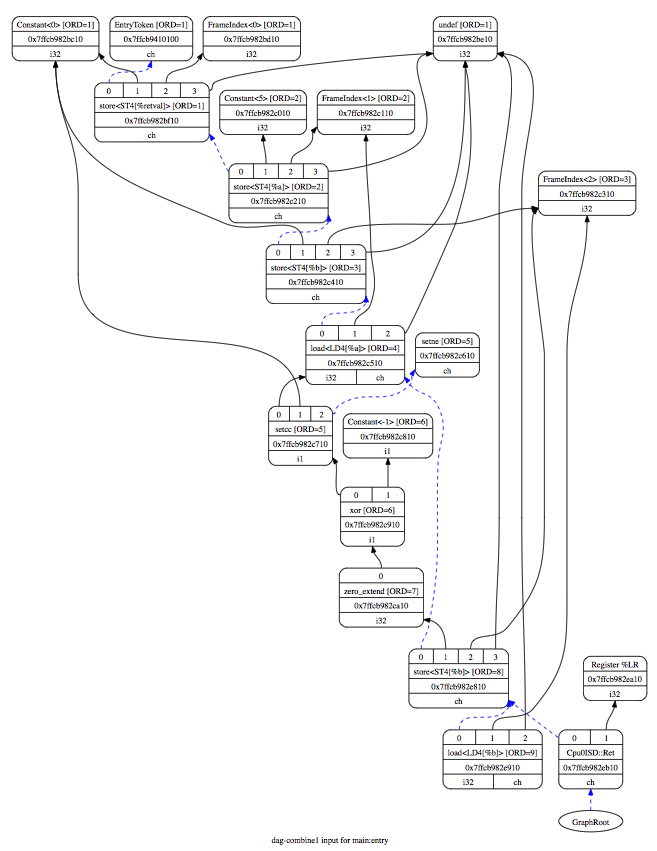
\includegraphics{18.png}}
\caption{llc option -view-dag-combine1-dags graphic view}\label{otherinst:otherinst-f1}\end{figure}

From \hyperref[otherinst:otherinst-f1]{Figure  \ref*{otherinst:otherinst-f1}}, we can see the -view-dag-combine1-dags option is for
Initial selection DAG.
We list the other view options and their corresponding DAG translation stage as
follows,

\begin{notice}{note}{Note:}
\code{llc} Graphviz options and corresponding DAG translation stage

-view-dag-combine1-dags: Initial selection DAG

-view-legalize-dags: Optimized type-legalized selection DAG

-view-dag-combine2-dags: Legalized selection DAG

-view-isel-dags: Optimized legalized selection DAG

-view-sched-dags: Selected selection DAG
\end{notice}

The -view-isel-dags is important and often used by an llvm backend writer
because it is the DAG before instruction selection.
The backend programmer need to know what is the DAG for writing the pattern
match instruction in target description file .td.


\subsection{Operator \% and /}
\label{otherinst:operator-and}

\subsubsection{The DAG of \%}
\label{otherinst:the-dag-of}
Example input code ch4\_2.cpp which contains the C operator \textbf{“\%”} and it's
corresponding llvm IR, as follows,
\paragraph{lbdex/InputFiles/ch4\_2.cpp}

\begin{Verbatim}[commandchars=\\\{\}]
\PYG{k+kt}{int} \PYG{n}{test\PYGZus{}mod}\PYG{p}{(}\PYG{p}{)}
\PYG{p}{\PYGZob{}}
  \PYG{k+kt}{int} \PYG{n}{b} \PYG{o}{=} \PYG{l+m+mi}{11}\PYG{p}{;}
\PYG{c+c1}{//  unsigned int b = 11;}
  
  \PYG{n}{b} \PYG{o}{=} \PYG{p}{(}\PYG{n}{b}\PYG{o}{+}\PYG{l+m+mi}{1}\PYG{p}{)}\PYG{o}{\PYGZpc{}}\PYG{l+m+mi}{12}\PYG{p}{;}
  
  \PYG{k}{return} \PYG{n}{b}\PYG{p}{;}
\PYG{p}{\PYGZcb{}}
\end{Verbatim}

\begin{Verbatim}[commandchars=\\\{\}]
...
define i32 @main\PYG{o}{(}\PYG{o}{)} nounwind ssp \PYG{o}{\PYGZob{}}
  entry:
  \PYGZpc{}retval \PYG{o}{=} alloca i32, align 4
  \PYGZpc{}b \PYG{o}{=} alloca i32, align 4
  store i32 0, i32* \PYGZpc{}retval
  store i32 11, i32* \PYGZpc{}b, align 4
  \PYGZpc{}0 \PYG{o}{=} load i32* \PYGZpc{}b, align 4
  \PYGZpc{}add \PYG{o}{=} add nsw i32 \PYGZpc{}0, 1
  \PYGZpc{}rem \PYG{o}{=} srem i32 \PYGZpc{}add, 12
  store i32 \PYGZpc{}rem, i32* \PYGZpc{}b, align 4
  \PYGZpc{}1 \PYG{o}{=} load i32* \PYGZpc{}b, align 4
  ret i32 \PYGZpc{}1
\PYG{o}{\PYGZcb{}}
\end{Verbatim}

LLVM \textbf{srem} is the IR corresponding \textbf{“\%”}, reference sub-section
``srem instruction'' of \footnotemark[3].
Copy the reference as follows,

\begin{notice}{note}{Note:}
\textbf{`srem'} Instruction

Syntax:
\textbf{\textless{}result\textgreater{} = srem \textless{}ty\textgreater{} \textless{}op1\textgreater{}, \textless{}op2\textgreater{}   ; yields \{ty\}:result}

Overview:
The \textbf{`srem'} instruction returns the remainder from the signed division of its
two operands. This instruction can also take vector versions of the values in
which case the elements must be integers.

Arguments:
The two arguments to the \textbf{`srem'} instruction must be integer or vector of
integer values. Both arguments must have identical types.

Semantics:
This instruction returns the remainder of a division (where the result is
either zero or has the same sign as the dividend, op1), not the modulo operator
(where the result is either zero or has the same sign as the divisor, op2) of
a value. For more information about the difference, see The Math Forum. For a
table of how this is implemented in various languages, please see Wikipedia:
modulo operation.

Note that signed integer remainder and unsigned integer remainder are distinct
operations; for unsigned integer remainder, use \textbf{`urem'}.

Taking the remainder of a division by zero leads to undefined behavior.
Overflow also leads to undefined behavior; this is a rare case, but can occur,
for example, by taking the remainder of a 32-bit division of -2147483648 by -1.
(The remainder doesn't actually overflow, but this rule lets srem be
implemented using instructions that return both the result of the division and
the remainder.)

Example:
\textless{}result\textgreater{} = \textbf{srem i32 4, \%var}      ; yields \{i32\}:result = 4 \% \%var
\end{notice}

Run Chapter3\_4/ with input file ch4\_2.bc via \code{llc} option –view-isel-dags as
below, will get the following error message and the llvm DAG of
\hyperref[otherinst:otherinst-f2]{Figure  \ref*{otherinst:otherinst-f2}} below.

\begin{Verbatim}[commandchars=\\\{\}]
118-165-79-37:InputFiles Jonathan\PYG{n+nv}{\PYGZdl{} }/Users/Jonathan/llvm/test/
cmake\PYGZus{}debug\PYGZus{}build/bin/Debug/llc -march\PYG{o}{=}cpu0 -view-isel-dags -relocation-model\PYG{o}{=}
pic -filetype\PYG{o}{=}asm ch4\PYGZus{}2.bc -o -
...
LLVM ERROR: Cannot \PYG{k}{select}: 0x7fa73a02ea10: \PYG{n+nv}{i32} \PYG{o}{=} mulhs 0x7fa73a02c610,
0x7fa73a02e910 \PYG{o}{[}\PYG{n+nv}{ID}\PYG{o}{=}12\PYG{o}{]}
0x7fa73a02c610: \PYG{n+nv}{i32} \PYG{o}{=} Constant\PYGZlt{}12\PYGZgt{} \PYG{o}{[}\PYG{n+nv}{ORD}\PYG{o}{=}5\PYG{o}{]} \PYG{o}{[}\PYG{n+nv}{ID}\PYG{o}{=}7\PYG{o}{]}
0x7fa73a02e910: \PYG{n+nv}{i32} \PYG{o}{=} Constant\PYGZlt{}715827883\PYGZgt{} \PYG{o}{[}\PYG{n+nv}{ID}\PYG{o}{=}9\PYG{o}{]}
\end{Verbatim}
\begin{figure}[htbp]
\centering
\capstart

\scalebox{1.000000}{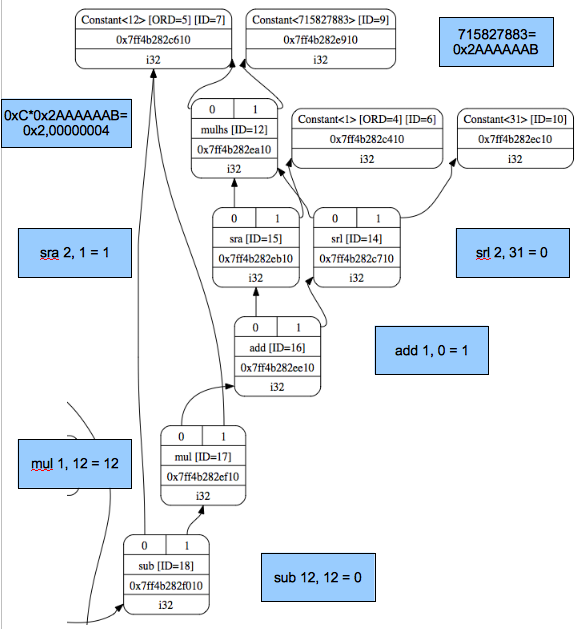
\includegraphics{27.png}}
\caption{ch4\_2.bc DAG}\label{otherinst:otherinst-f2}\end{figure}

LLVM replace srem divide operation with multiply operation in DAG optimization
because DIV operation cost more in time than MUL.
For example code \textbf{“int b = 11; b=(b+1)\%12;”}, it translate into
\hyperref[otherinst:otherinst-f2]{Figure  \ref*{otherinst:otherinst-f2}}.
We verify the result and explain it by calculate the value in each node.
The 0xC*0x2AAAAAAB=0x2,00000004, (mulhs 0xC, 0x2AAAAAAAB) meaning get the Signed
mul high word (32bits).
Multiply with 2 operands of 1 word size generate the 2 word size of result
(0x2, 0xAAAAAAAB).
The high word result, in this case is 0x2.
The final result (sub 12, 12) is 0 which match the statement (11+1)\%12.


\subsubsection{Arm solution}
\label{otherinst:arm-solution}
To run with ARM solution, change Cpu0InstrInfo.td and Cpu0ISelDAGToDAG.cpp from
Chapter4\_1/ as follows,
\paragraph{lbdex/Chapter4\_1/Cpu0InstrInfo.td}

\begin{Verbatim}[commandchars=\\\{\}]
\PYG{c+c1}{/// Multiply and Divide Instructions.}
\PYG{n}{def} \PYG{n}{SMMUL}   \PYG{o}{:} \PYG{n}{ArithLogicR}\PYG{o}{\PYGZlt{}}\PYG{l+m+mh}{0x41}\PYG{p}{,} \PYG{l+s}{"}\PYG{l+s}{smmul}\PYG{l+s}{"}\PYG{p}{,} \PYG{n}{mulhs}\PYG{p}{,} \PYG{n}{IIImul}\PYG{p}{,} \PYG{n}{CPURegs}\PYG{p}{,} \PYG{l+m+mi}{1}\PYG{o}{\PYGZgt{}}\PYG{p}{;}
\PYG{n}{def} \PYG{n}{UMMUL}   \PYG{o}{:} \PYG{n}{ArithLogicR}\PYG{o}{\PYGZlt{}}\PYG{l+m+mh}{0x42}\PYG{p}{,} \PYG{l+s}{"}\PYG{l+s}{ummul}\PYG{l+s}{"}\PYG{p}{,} \PYG{n}{mulhu}\PYG{p}{,} \PYG{n}{IIImul}\PYG{p}{,} \PYG{n}{CPURegs}\PYG{p}{,} \PYG{l+m+mi}{1}\PYG{o}{\PYGZgt{}}\PYG{p}{;}
\PYG{c+c1}{//def MULT    : Mult32\PYGZlt{}0x41, "mult", IIImul\PYGZgt{};}
\PYG{c+c1}{//def MULTu   : Mult32\PYGZlt{}0x42, "multu", IIImul\PYGZgt{};}
\end{Verbatim}
\paragraph{lbdex/Chapter4\_1/Cpu0ISelDAGToDAG.cpp}

\begin{Verbatim}[commandchars=\\\{\}]
\PYG{c+cp}{\PYGZsh{}if 0}
\PYG{c}{/// Select multiply instructions.}
\PYG{c}{std::pair\PYGZlt{}SDNode*, SDNode*\PYGZgt{}}
\PYG{c}{Cpu0DAGToDAGISel::SelectMULT(SDNode *N, unsigned Opc, DebugLoc dl, EVT Ty,}
\PYG{c}{                             bool HasLo, bool HasHi) \PYGZob{}}
\PYG{c}{  SDNode *Lo = 0, *Hi = 0;}
\PYG{c}{  SDNode *Mul = CurDAG-\PYGZgt{}getMachineNode(Opc, dl, MVT::Glue, N-\PYGZgt{}getOperand(0),}
\PYG{c}{                                       N-\PYGZgt{}getOperand(1));}
\PYG{c}{  SDValue InFlag = SDValue(Mul, 0);}

\PYG{c}{  if (HasLo) \PYGZob{}}
\PYG{c}{    Lo = CurDAG-\PYGZgt{}getMachineNode(Cpu0::MFLO, dl,}
\PYG{c}{                                Ty, MVT::Glue, InFlag);}
\PYG{c}{    InFlag = SDValue(Lo, 1);}
\PYG{c}{  \PYGZcb{}}
\PYG{c}{  if (HasHi)}
\PYG{c}{    Hi = CurDAG-\PYGZgt{}getMachineNode(Cpu0::MFHI, dl,}
\PYG{c}{                                Ty, InFlag);}

\PYG{c}{  return std::make\PYGZus{}pair(Lo, Hi);}
\PYG{c}{\PYGZcb{}}
\PYG{c+cp}{\PYGZsh{}endif}

\PYG{c+c1}{/// Select instructions not customized! Used for}
\PYG{c+c1}{/// expanded, promoted and normal instructions}
\PYG{n}{SDNode}\PYG{o}{*} \PYG{n}{Cpu0DAGToDAGISel}\PYG{o}{:}\PYG{o}{:}\PYG{n}{Select}\PYG{p}{(}\PYG{n}{SDNode} \PYG{o}{*}\PYG{n}{Node}\PYG{p}{)} \PYG{p}{\PYGZob{}}
\PYG{p}{.}\PYG{p}{.}\PYG{p}{.}
  \PYG{k}{switch}\PYG{p}{(}\PYG{n}{Opcode}\PYG{p}{)} \PYG{p}{\PYGZob{}}
  \PYG{k}{default}\PYG{o}{:} \PYG{k}{break}\PYG{p}{;}
\PYG{c+cp}{\PYGZsh{}if 0}
\PYG{c}{  case ISD::MULHS:}
\PYG{c}{  case ISD::MULHU: \PYGZob{}}
\PYG{c}{    MultOpc = (Opcode == ISD::MULHU ? Cpu0::MULTu : Cpu0::MULT);}
\PYG{c}{    return SelectMULT(Node, MultOpc, dl, NodeTy, false, true).second;}
\PYG{c}{  \PYGZcb{}}
\PYG{c+cp}{\PYGZsh{}endif}
 \PYG{p}{.}\PYG{p}{.}\PYG{p}{.}
\PYG{p}{\PYGZcb{}}
\end{Verbatim}

Let's run above changes with ch4\_2.cpp as well as \code{llc -view-sched-dags} option
to get \hyperref[otherinst:otherinst-f3]{Figure  \ref*{otherinst:otherinst-f3}}.
Similarly, SMMUL get the high word of multiply result.
\begin{figure}[htbp]
\centering
\capstart

\scalebox{1.000000}{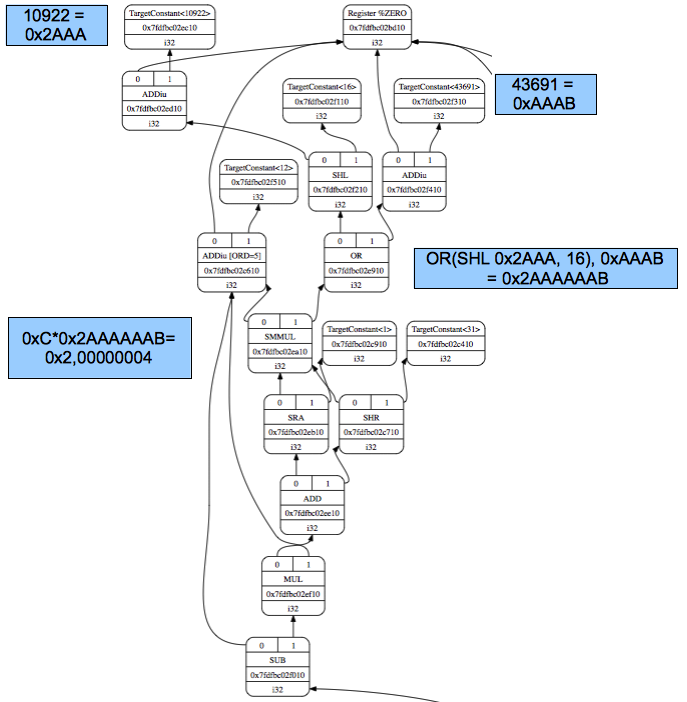
\includegraphics{36.png}}
\caption{Translate ch4\_2.bc into cpu0 backend DAG}\label{otherinst:otherinst-f3}\end{figure}

Follows is the result of run above changes with ch4\_2.bc.

\begin{Verbatim}[commandchars=\\\{\}]
118-165-66-82:InputFiles Jonathan\PYG{n+nv}{\PYGZdl{} }/Users/Jonathan/llvm/test/cmake\PYGZus{}
debug\PYGZus{}build/bin/Debug/llc -march\PYG{o}{=}cpu0 -relocation-model\PYG{o}{=}pic -filetype\PYG{o}{=}asm
ch4\PYGZus{}2.bc -o -
        .section .mdebug.abi32
        .previous
        .file \PYG{l+s+s2}{"ch4\PYGZus{}2.bc"}
        .text
        .globl        main
        .align        2
        .type main,@function
        .ent  main                    \PYG{c}{\PYGZsh{} @main}
main:
        .cfi\PYGZus{}startproc
        .frame        \PYG{n+nv}{\PYGZdl{}fp},8,\PYG{n+nv}{\PYGZdl{}lr}
        .mask         0x00000000,0
        .set  noreorder
        .set  nomacro
\PYG{c}{\PYGZsh{} BB\PYGZsh{}0:                                 \PYGZsh{} \PYGZpc{}entry}
        addiu \PYG{n+nv}{\PYGZdl{}sp}, \PYG{n+nv}{\PYGZdl{}sp}, -8
\PYG{n+nv}{\PYGZdl{}tmp1}:
        .cfi\PYGZus{}def\PYGZus{}cfa\PYGZus{}offset 8
        addiu \PYG{n+nv}{\PYGZdl{}2}, \PYG{n+nv}{\PYGZdl{}zero}, 0
        st    \PYG{n+nv}{\PYGZdl{}2}, 4\PYG{o}{(}\PYG{n+nv}{\PYGZdl{}fp}\PYG{o}{)}
        addiu \PYG{n+nv}{\PYGZdl{}2}, \PYG{n+nv}{\PYGZdl{}zero}, 11
        st    \PYG{n+nv}{\PYGZdl{}2}, 0\PYG{o}{(}\PYG{n+nv}{\PYGZdl{}fp}\PYG{o}{)}
        lui   \PYG{n+nv}{\PYGZdl{}2}, 10922
        ori   \PYG{n+nv}{\PYGZdl{}3}, \PYG{n+nv}{\PYGZdl{}2}, 43691
        addiu \PYG{n+nv}{\PYGZdl{}2}, \PYG{n+nv}{\PYGZdl{}zero}, 12
        smmul \PYG{n+nv}{\PYGZdl{}3}, \PYG{n+nv}{\PYGZdl{}2}, \PYG{n+nv}{\PYGZdl{}3}
        shr   \PYG{n+nv}{\PYGZdl{}4}, \PYG{n+nv}{\PYGZdl{}3}, 31
        sra   \PYG{n+nv}{\PYGZdl{}3}, \PYG{n+nv}{\PYGZdl{}3}, 1
        addu  \PYG{n+nv}{\PYGZdl{}3}, \PYG{n+nv}{\PYGZdl{}3}, \PYG{n+nv}{\PYGZdl{}4}
        mul   \PYG{n+nv}{\PYGZdl{}3}, \PYG{n+nv}{\PYGZdl{}3}, \PYG{n+nv}{\PYGZdl{}2}
        subu  \PYG{n+nv}{\PYGZdl{}2}, \PYG{n+nv}{\PYGZdl{}2}, \PYG{n+nv}{\PYGZdl{}3}
        st    \PYG{n+nv}{\PYGZdl{}2}, 0\PYG{o}{(}\PYG{n+nv}{\PYGZdl{}fp}\PYG{o}{)}
        addiu \PYG{n+nv}{\PYGZdl{}sp}, \PYG{n+nv}{\PYGZdl{}sp}, 8
        ret   \PYG{n+nv}{\PYGZdl{}lr}
        .set  macro
        .set  reorder
        .end  main
\PYG{n+nv}{\PYGZdl{}tmp2}:
        .size main, \PYG{o}{(}\PYG{n+nv}{\PYGZdl{}tmp2}\PYG{o}{)}-main
        .cfi\PYGZus{}endproc
\end{Verbatim}

The other instruction UMMUL and llvm IR mulhu are unsigned int type for
operator \%.
You can check it by unmark the \textbf{“unsigned int b = 11;”} in ch4\_2.cpp.

Use SMMUL instruction to get the high word of multiplication result is adopted
in ARM.


\subsubsection{Mips solution}
\label{otherinst:mips-solution}
Mips use MULT instruction and save the high \& low part to register HI and LO.
After that, use mfhi/mflo to move register HI/LO to your general purpose
register.
ARM SMMUL is fast if you only need the HI part of result (it ignore the LO part
of operation). ARM also provide SMULL (signed multiply long) to get the whole
64 bits result.
If you need the LO part of result, you can use Cpu0 MUL instruction which only
get the LO part of result.
Chapter4\_1/ is implemented with Mips MULT style.
We choose it as the implementation of this book to add instructions as less as
possible. This approach is better for Cpu0 to keep it as a tutorial architecture
for school teaching purpose material, and apply Cpu0 as an engineer learning
materials in compiler, system program and verilog CPU hardware design.
The MULT, MULTu, MFHI, MFLO, MTHI, MTLO added in Chapter4\_1/Cpu0InstrInfo.td;
HI, LO register in Chapter4\_1/Cpu0RegisterInfo.td and Chapter4\_1/MCTargetDesc/
Cpu0BaseInfo.h; IIHiLo, IIImul in Chapter4\_1/Cpu0Schedule.td; SelectMULT() in
Chapter4\_1/Cpu0ISelDAGToDAG.cpp are for Mips style implementation.

The related DAG nodes mulhs and mulhu which are used in Chapter4\_1/
came from TargetSelectionDAG.td as follows,
\paragraph{include/llvm/Target/TargetSelectionDAG.td}

\begin{Verbatim}[commandchars=\\\{\}]
\PYG{n}{def} \PYG{n}{mulhs}    \PYG{o}{:} \PYG{n}{SDNode}\PYG{o}{\PYGZlt{}}\PYG{l+s}{"}\PYG{l+s}{ISD::MULHS}\PYG{l+s}{"}     \PYG{p}{,} \PYG{n}{SDTIntBinOp}\PYG{p}{,} \PYG{p}{[}\PYG{n}{SDNPCommutative}\PYG{p}{]}\PYG{o}{\PYGZgt{}}\PYG{p}{;}
\PYG{n}{def} \PYG{n}{mulhu}    \PYG{o}{:} \PYG{n}{SDNode}\PYG{o}{\PYGZlt{}}\PYG{l+s}{"}\PYG{l+s}{ISD::MULHU}\PYG{l+s}{"}     \PYG{p}{,} \PYG{n}{SDTIntBinOp}\PYG{p}{,} \PYG{p}{[}\PYG{n}{SDNPCommutative}\PYG{p}{]}\PYG{o}{\PYGZgt{}}\PYG{p}{;}
\end{Verbatim}

Except the custom type, llvm IR operations of expand and promote type will call
Cpu0DAGToDAGISel::Select() during instruction selection of DAG translation.
In SelectMULT() which called by Select(), it return the HI part of
multiplication result to HI register, for IR operations of mulhs or mulhu.
After that, MFHI instruction move the HI register to cpu0 field ``a'' register,
\$ra.
MFHI instruction is FL format and only use cpu0 field ``a'' register, we set
the \$rb and imm16 to 0.
\hyperref[otherinst:otherinst-f4]{Figure  \ref*{otherinst:otherinst-f4}} and ch4\_2.cpu0.s are the result of compile ch4\_2.bc.
\begin{figure}[htbp]
\centering
\capstart

\scalebox{0.750000}{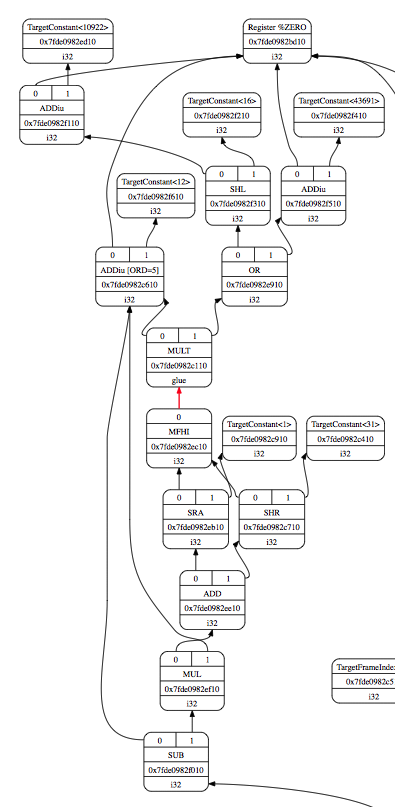
\includegraphics{45.png}}
\caption{DAG for ch4\_2.bc with Mips style MULT}\label{otherinst:otherinst-f4}\end{figure}

\begin{Verbatim}[commandchars=\\\{\}]
118-165-66-82:InputFiles Jonathan\PYG{n+nv}{\PYGZdl{} }cat ch4\PYGZus{}2.cpu0.s
  .section .mdebug.abi32
  .previous
  .file \PYG{l+s+s2}{"ch4\PYGZus{}2.bc"}
  .text
  .globl  \PYGZus{}Z8test\PYGZus{}modv
  .align  2
  .type \PYGZus{}Z8test\PYGZus{}modv,@function
  .ent  \PYGZus{}Z8test\PYGZus{}modv            \PYG{c}{\PYGZsh{} @\PYGZus{}Z8test\PYGZus{}modv}
\PYGZus{}Z8test\PYGZus{}modv:
  .frame  \PYG{n+nv}{\PYGZdl{}sp},8,\PYG{n+nv}{\PYGZdl{}lr}
  .mask   0x00000000,0
  .set  noreorder
  .set  nomacro
\PYG{c}{\PYGZsh{} BB\PYGZsh{}0:}
  addiu \PYG{n+nv}{\PYGZdl{}sp}, \PYG{n+nv}{\PYGZdl{}sp}, -8
  addiu \PYG{n+nv}{\PYGZdl{}2}, \PYG{n+nv}{\PYGZdl{}zero}, 11
  st  \PYG{n+nv}{\PYGZdl{}2}, 4\PYG{o}{(}\PYG{n+nv}{\PYGZdl{}sp}\PYG{o}{)}
  lui \PYG{n+nv}{\PYGZdl{}2}, 10922
  ori \PYG{n+nv}{\PYGZdl{}3}, \PYG{n+nv}{\PYGZdl{}2}, 43691
  addiu \PYG{n+nv}{\PYGZdl{}2}, \PYG{n+nv}{\PYGZdl{}zero}, 12
  mult  \PYG{n+nv}{\PYGZdl{}2}, \PYG{n+nv}{\PYGZdl{}3}
  mfhi  \PYG{n+nv}{\PYGZdl{}3}
  shr \PYG{n+nv}{\PYGZdl{}4}, \PYG{n+nv}{\PYGZdl{}3}, 31
  sra \PYG{n+nv}{\PYGZdl{}3}, \PYG{n+nv}{\PYGZdl{}3}, 1
  addu  \PYG{n+nv}{\PYGZdl{}3}, \PYG{n+nv}{\PYGZdl{}3}, \PYG{n+nv}{\PYGZdl{}4}
  mul \PYG{n+nv}{\PYGZdl{}3}, \PYG{n+nv}{\PYGZdl{}3}, \PYG{n+nv}{\PYGZdl{}2}
  subu  \PYG{n+nv}{\PYGZdl{}2}, \PYG{n+nv}{\PYGZdl{}2}, \PYG{n+nv}{\PYGZdl{}3}
  st  \PYG{n+nv}{\PYGZdl{}2}, 4\PYG{o}{(}\PYG{n+nv}{\PYGZdl{}sp}\PYG{o}{)}
  addiu \PYG{n+nv}{\PYGZdl{}sp}, \PYG{n+nv}{\PYGZdl{}sp}, 8
  ret \PYG{n+nv}{\PYGZdl{}lr}
  .set  macro
  .set  reorder
  .end  \PYGZus{}Z8test\PYGZus{}modv
\PYG{n+nv}{\PYGZdl{}tmp1}:
  .size \PYGZus{}Z8test\PYGZus{}modv, \PYG{o}{(}\PYG{n+nv}{\PYGZdl{}tmp1}\PYG{o}{)}-\PYGZus{}Z8test\PYGZus{}modv
\end{Verbatim}


\subsubsection{Full support \%, and /}
\label{otherinst:full-support-and}
The sensitive readers may find the llvm using \textbf{“multiplication”} instead
of \textbf{“div”} to get the \textbf{“\%”} result just because our example use constant as
divider, \textbf{“(b+1)\%12”} in our example.
If programmer use variable as the divider like \textbf{“(b+1)\%a”}, then what will
happen in our code.
The answer is our code will has error to take care this.

Cpu0 just like Mips use LO and HI registers to hold the \textbf{``quotient''} and
\textbf{``remainder''}. And
use instructions \textbf{“mflo”} and \textbf{“mfhi”} to get the result from LO or HI
registers.
With this solution, the \textbf{“c = a / b”} can be got by \textbf{“div a, b”} and
\textbf{“mflo c”}; the \textbf{“c = a \% b”} can be got by \textbf{“div a, b”} and \textbf{“mfhi c”}.

To support operators \textbf{“\%”} and \textbf{“/”}, the following code added in Chapter4\_1.
\begin{enumerate}
\item {} 
SDIV, UDIV and it's reference class, nodes in Cpu0InstrInfo.td.

\item {} 
The copyPhysReg() declared and defined in Cpu0InstrInfo.h and
Cpu0InstrInfo.cpp.

\item {} 
The setOperationAction(ISD::SDIV, MVT::i32, Expand), ...,
setTargetDAGCombine(ISD::SDIVREM) in constructore of Cpu0ISelLowering.cpp;
PerformDivRemCombine() and PerformDAGCombine() in Cpu0ISelLowering.cpp.

\end{enumerate}

IR instruction \textbf{sdiv} stand for signed div while \textbf{udiv} is for unsigned div.

Run with ch4\_2\_2.cpp can get the ``div'' result for operator \textbf{“\%”} but it cannot
be compiled at this point. It need the function call argument support in Chapter
8 of Function call.
If run with ch4\_2\_1.cpp as below, cannot get the \textbf{“div”} for operator
\textbf{“\%”}.
It still use \textbf{``multiplication''} instead of \textbf{``div''} in ch4\_2\_1.cpp because
llvm do \textbf{“Constant Propagation Optimization”} on this.
The ch4\_2\_2.cpp can get the \textbf{“div”} for \textbf{“\%”} result since it make the
llvm \textbf{“Constant Propagation Optimization”} useless in this.
\paragraph{lbdex/InputFiles/ch4\_2\_1.cpp}

\begin{Verbatim}[commandchars=\\\{\}]
\PYG{k+kt}{int} \PYG{n}{test\PYGZus{}mod}\PYG{p}{(}\PYG{p}{)}
\PYG{p}{\PYGZob{}}
  \PYG{k+kt}{int} \PYG{n}{b} \PYG{o}{=} \PYG{l+m+mi}{11}\PYG{p}{;}
  \PYG{k+kt}{int} \PYG{n}{a} \PYG{o}{=} \PYG{l+m+mi}{12}\PYG{p}{;}

  \PYG{n}{b} \PYG{o}{=} \PYG{p}{(}\PYG{n}{b}\PYG{o}{+}\PYG{l+m+mi}{1}\PYG{p}{)}\PYG{o}{\PYGZpc{}}\PYG{n}{a}\PYG{p}{;}
  
  \PYG{k}{return} \PYG{n}{b}\PYG{p}{;}
\PYG{p}{\PYGZcb{}}
\end{Verbatim}
\paragraph{lbdex/InputFiles/ch4\_2\_2.cpp}

\begin{Verbatim}[commandchars=\\\{\}]
\PYG{k+kt}{int} \PYG{n}{test\PYGZus{}mod}\PYG{p}{(}\PYG{k+kt}{int} \PYG{n}{c}\PYG{p}{)}
\PYG{p}{\PYGZob{}}
  \PYG{k+kt}{int} \PYG{n}{b} \PYG{o}{=} \PYG{l+m+mi}{11}\PYG{p}{;}
  
  \PYG{n}{b} \PYG{o}{=} \PYG{p}{(}\PYG{n}{b}\PYG{o}{+}\PYG{l+m+mi}{1}\PYG{p}{)}\PYG{o}{\PYGZpc{}}\PYG{n}{c}\PYG{p}{;}
  
  \PYG{k}{return} \PYG{n}{b}\PYG{p}{;}
\PYG{p}{\PYGZcb{}}
\end{Verbatim}

\begin{Verbatim}[commandchars=\\\{\}]
118-165-77-79:InputFiles Jonathan\PYG{n+nv}{\PYGZdl{} }clang -target mips-unknown-linux-gnu -c
ch4\PYGZus{}2\PYGZus{}2.cpp -emit-llvm -o ch4\PYGZus{}2\PYGZus{}2.bc
118-165-77-79:InputFiles Jonathan\PYG{n+nv}{\PYGZdl{} }/Users/Jonathan/llvm/test/cmake\PYGZus{}
debug\PYGZus{}build/bin/Debug/llc -march\PYG{o}{=}cpu0 -relocation-model\PYG{o}{=}pic -filetype\PYG{o}{=}asm
ch4\PYGZus{}2\PYGZus{}2.bc -o -
...
div \PYG{n+nv}{\PYGZdl{}zero}, \PYG{n+nv}{\PYGZdl{}3}, \PYG{n+nv}{\PYGZdl{}2}
mflo  \PYG{n+nv}{\PYGZdl{}2}
...
\end{Verbatim}

To explain how work with \textbf{“div”}, let's run Chapter8\_4 with
ch4\_2\_2.cpp as follows,

\begin{Verbatim}[commandchars=\\\{\}]
118-165-83-58:InputFiles Jonathan\PYG{n+nv}{\PYGZdl{} }clang -target mips-unknown-linux-gnu -c
ch4\PYGZus{}2\PYGZus{}2.cpp -I/Applications/Xcode.app/Contents/Developer/Platforms/
MacOSX.platform/Developer/SDKs/MacOSX10.8.sdk/usr/include/ -emit-llvm -o
ch4\PYGZus{}2\PYGZus{}2.bc
118-165-83-58:InputFiles Jonathan\PYG{n+nv}{\PYGZdl{} }/Users/Jonathan/llvm/test/cmake\PYGZus{}debug\PYGZus{}build/bin/
Debug/llc -march\PYG{o}{=}cpu0 -relocation-model\PYG{o}{=}pic -filetype\PYG{o}{=}asm -debug ch4\PYGZus{}2\PYGZus{}2.bc -o -
Args: /Users/Jonathan/llvm/test/cmake\PYGZus{}debug\PYGZus{}build/bin/Debug/llc -march\PYG{o}{=}cpu0
-relocation-model\PYG{o}{=}pic -filetype\PYG{o}{=}asm -debug ch4\PYGZus{}2\PYGZus{}2.bc -o -

\PYG{o}{=}\PYG{o}{=}\PYG{o}{=} \PYGZus{}Z8test\PYGZus{}modi
Initial selection DAG: BB\PYGZsh{}0 \PYG{l+s+s1}{'\PYGZus{}Z8test\PYGZus{}modi:'}
SelectionDAG has 21 nodes:
  0x7fed68410bc8: \PYG{n+nv}{ch} \PYG{o}{=} EntryToken \PYG{o}{[}\PYG{n+nv}{ORD}\PYG{o}{=}1\PYG{o}{]}

  0x7fed6882cb10: \PYG{n+nv}{i32} \PYG{o}{=} undef \PYG{o}{[}\PYG{n+nv}{ORD}\PYG{o}{=}1\PYG{o}{]}

  0x7fed6882cd10: \PYG{n+nv}{i32} \PYG{o}{=} FrameIndex\PYGZlt{}0\PYGZgt{} \PYG{o}{[}\PYG{n+nv}{ORD}\PYG{o}{=}1\PYG{o}{]}

  0x7fed6882ce10: \PYG{n+nv}{i32} \PYG{o}{=} Constant\PYGZlt{}0\PYGZgt{}

  0x7fed6882d110: \PYG{n+nv}{i32} \PYG{o}{=} FrameIndex\PYGZlt{}1\PYGZgt{} \PYG{o}{[}\PYG{n+nv}{ORD}\PYG{o}{=}2\PYG{o}{]}

      0x7fed68410bc8: \PYGZlt{}multiple use\PYGZgt{}
        0x7fed68410bc8: \PYGZlt{}multiple use\PYGZgt{}
        0x7fed6882ca10: \PYG{n+nv}{i32} \PYG{o}{=} FrameIndex\PYGZlt{}-1\PYGZgt{} \PYG{o}{[}\PYG{n+nv}{ORD}\PYG{o}{=}1\PYG{o}{]}

        0x7fed6882cb10: \PYGZlt{}multiple use\PYGZgt{}
      0x7fed6882cc10: i32,ch \PYG{o}{=} load 0x7fed68410bc8, 0x7fed6882ca10,
      0x7fed6882cb10\PYGZlt{}LD4\PYG{o}{[}FixedStack-1\PYG{o}{]}\PYGZgt{} \PYG{o}{[}\PYG{n+nv}{ORD}\PYG{o}{=}1\PYG{o}{]}

      0x7fed6882cd10: \PYGZlt{}multiple use\PYGZgt{}
      0x7fed6882cb10: \PYGZlt{}multiple use\PYGZgt{}
    0x7fed6882cf10: \PYG{n+nv}{ch} \PYG{o}{=} store 0x7fed68410bc8, 0x7fed6882cc10, 0x7fed6882cd10,
    0x7fed6882cb10\PYGZlt{}ST4\PYG{o}{[}\PYGZpc{}1\PYG{o}{]}\PYGZgt{} \PYG{o}{[}\PYG{n+nv}{ORD}\PYG{o}{=}1\PYG{o}{]}

    0x7fed6882d010: \PYG{n+nv}{i32} \PYG{o}{=} Constant\PYGZlt{}11\PYGZgt{} \PYG{o}{[}\PYG{n+nv}{ORD}\PYG{o}{=}2\PYG{o}{]}

    0x7fed6882d110: \PYGZlt{}multiple use\PYGZgt{}
    0x7fed6882cb10: \PYGZlt{}multiple use\PYGZgt{}
  0x7fed6882d210: \PYG{n+nv}{ch} \PYG{o}{=} store 0x7fed6882cf10, 0x7fed6882d010, 0x7fed6882d110,
  0x7fed6882cb10\PYGZlt{}ST4\PYG{o}{[}\PYGZpc{}b\PYG{o}{]}\PYGZgt{} \PYG{o}{[}\PYG{n+nv}{ORD}\PYG{o}{=}2\PYG{o}{]}

    0x7fed6882d210: \PYGZlt{}multiple use\PYGZgt{}
    0x7fed6882d110: \PYGZlt{}multiple use\PYGZgt{}
    0x7fed6882cb10: \PYGZlt{}multiple use\PYGZgt{}
  0x7fed6882d310: i32,ch \PYG{o}{=} load 0x7fed6882d210, 0x7fed6882d110,
  0x7fed6882cb10\PYGZlt{}LD4\PYG{o}{[}\PYGZpc{}b\PYG{o}{]}\PYGZgt{} \PYG{o}{[}\PYG{n+nv}{ORD}\PYG{o}{=}3\PYG{o}{]}

    0x7fed6882d210: \PYGZlt{}multiple use\PYGZgt{}
    0x7fed6882cd10: \PYGZlt{}multiple use\PYGZgt{}
    0x7fed6882cb10: \PYGZlt{}multiple use\PYGZgt{}
  0x7fed6882d610: i32,ch \PYG{o}{=} load 0x7fed6882d210, 0x7fed6882cd10,
  0x7fed6882cb10\PYGZlt{}LD4\PYG{o}{[}\PYGZpc{}1\PYG{o}{]}\PYGZgt{} \PYG{o}{[}\PYG{n+nv}{ORD}\PYG{o}{=}5\PYG{o}{]}

      0x7fed6882d310: \PYGZlt{}multiple use\PYGZgt{}
      0x7fed6882d610: \PYGZlt{}multiple use\PYGZgt{}
    0x7fed6882d810: \PYG{n+nv}{ch} \PYG{o}{=} TokenFactor 0x7fed6882d310:1, 0x7fed6882d610:1 \PYG{o}{[}\PYG{n+nv}{ORD}\PYG{o}{=}7\PYG{o}{]}

        0x7fed6882d310: \PYGZlt{}multiple use\PYGZgt{}
        0x7fed6882d410: \PYG{n+nv}{i32} \PYG{o}{=} Constant\PYGZlt{}1\PYGZgt{} \PYG{o}{[}\PYG{n+nv}{ORD}\PYG{o}{=}4\PYG{o}{]}

      0x7fed6882d510: \PYG{n+nv}{i32} \PYG{o}{=} add 0x7fed6882d310, 0x7fed6882d410 \PYG{o}{[}\PYG{n+nv}{ORD}\PYG{o}{=}4\PYG{o}{]}

      0x7fed6882d610: \PYGZlt{}multiple use\PYGZgt{}
    0x7fed6882d710: \PYG{n+nv}{i32} \PYG{o}{=} srem 0x7fed6882d510, 0x7fed6882d610 \PYG{o}{[}\PYG{n+nv}{ORD}\PYG{o}{=}6\PYG{o}{]}

    0x7fed6882d110: \PYGZlt{}multiple use\PYGZgt{}
    0x7fed6882cb10: \PYGZlt{}multiple use\PYGZgt{}
  0x7fed6882fc10: \PYG{n+nv}{ch} \PYG{o}{=} store 0x7fed6882d810, 0x7fed6882d710, 0x7fed6882d110,
  0x7fed6882cb10\PYGZlt{}ST4\PYG{o}{[}\PYGZpc{}b\PYG{o}{]}\PYGZgt{} \PYG{o}{[}\PYG{n+nv}{ORD}\PYG{o}{=}7\PYG{o}{]}

  0x7fed6882fe10: \PYG{n+nv}{i32} \PYG{o}{=} Register \PYGZpc{}V0

    0x7fed6882fc10: \PYGZlt{}multiple use\PYGZgt{}
    0x7fed6882fe10: \PYGZlt{}multiple use\PYGZgt{}
      0x7fed6882fc10: \PYGZlt{}multiple use\PYGZgt{}
      0x7fed6882d110: \PYGZlt{}multiple use\PYGZgt{}
      0x7fed6882cb10: \PYGZlt{}multiple use\PYGZgt{}
    0x7fed6882fd10: i32,ch \PYG{o}{=} load 0x7fed6882fc10, 0x7fed6882d110,
    0x7fed6882cb10\PYGZlt{}LD4\PYG{o}{[}\PYGZpc{}b\PYG{o}{]}\PYGZgt{} \PYG{o}{[}\PYG{n+nv}{ORD}\PYG{o}{=}8\PYG{o}{]}

  0x7fed6882ff10: ch,glue \PYG{o}{=} CopyToReg 0x7fed6882fc10, 0x7fed6882fe10,
  0x7fed6882fd10

    0x7fed6882ff10: \PYGZlt{}multiple use\PYGZgt{}
    0x7fed6882fe10: \PYGZlt{}multiple use\PYGZgt{}
    0x7fed6882ff10: \PYGZlt{}multiple use\PYGZgt{}
  0x7fed68830010: \PYG{n+nv}{ch} \PYG{o}{=} Cpu0ISD::Ret 0x7fed6882ff10, 0x7fed6882fe10,
  0x7fed6882ff10:1

Replacing.1 0x7fed6882fd10: i32,ch \PYG{o}{=} load 0x7fed6882fc10, 0x7fed6882d110,
0x7fed6882cb10\PYGZlt{}LD4\PYG{o}{[}\PYGZpc{}b\PYG{o}{]}\PYGZgt{} \PYG{o}{[}\PYG{n+nv}{ORD}\PYG{o}{=}8\PYG{o}{]}

With: 0x7fed6882d710: \PYG{n+nv}{i32} \PYG{o}{=} srem 0x7fed6882d510, 0x7fed6882d610 \PYG{o}{[}\PYG{n+nv}{ORD}\PYG{o}{=}6\PYG{o}{]}
 and 1 other values

Replacing.1 0x7fed6882d310: i32,ch \PYG{o}{=} load 0x7fed6882d210, 0x7fed6882d110,
0x7fed6882cb10\PYGZlt{}LD4\PYG{o}{[}\PYGZpc{}b\PYG{o}{]}\PYGZgt{} \PYG{o}{[}\PYG{n+nv}{ORD}\PYG{o}{=}3\PYG{o}{]}

With: 0x7fed6882d010: \PYG{n+nv}{i32} \PYG{o}{=} Constant\PYGZlt{}11\PYGZgt{} \PYG{o}{[}\PYG{n+nv}{ORD}\PYG{o}{=}2\PYG{o}{]}
 and 1 other values

Replacing.3 0x7fed6882d810: \PYG{n+nv}{ch} \PYG{o}{=} TokenFactor 0x7fed6882d210,
0x7fed6882d610:1 \PYG{o}{[}\PYG{n+nv}{ORD}\PYG{o}{=}7\PYG{o}{]}

With: 0x7fed6882d610: i32,ch \PYG{o}{=} load 0x7fed6882d210, 0x7fed6882cd10,
0x7fed6882cb10\PYGZlt{}LD4\PYG{o}{[}\PYGZpc{}1\PYG{o}{]}\PYGZgt{} \PYG{o}{[}\PYG{n+nv}{ORD}\PYG{o}{=}5\PYG{o}{]}


Replacing.3 0x7fed6882d510: \PYG{n+nv}{i32} \PYG{o}{=} add 0x7fed6882d010, 0x7fed6882d410 \PYG{o}{[}\PYG{n+nv}{ORD}\PYG{o}{=}4\PYG{o}{]}

With: 0x7fed6882d810: \PYG{n+nv}{i32} \PYG{o}{=} Constant\PYGZlt{}12\PYGZgt{}


Replacing.1 0x7fed6882cc10: i32,ch \PYG{o}{=} load 0x7fed68410bc8, 0x7fed6882ca10,
0x7fed6882cb10\PYGZlt{}LD4\PYG{o}{[}FixedStack-1\PYG{o}{]}\PYG{o}{(}\PYG{n+nv}{align}\PYG{o}{=}8\PYG{o}{)}\PYGZgt{} \PYG{o}{[}\PYG{n+nv}{ORD}\PYG{o}{=}1\PYG{o}{]}

With: 0x7fed6882cc10: i32,ch \PYG{o}{=} load 0x7fed68410bc8, 0x7fed6882ca10,
0x7fed6882cb10\PYGZlt{}LD4\PYG{o}{[}FixedStack-1\PYG{o}{]}\PYG{o}{(}\PYG{n+nv}{align}\PYG{o}{=}8\PYG{o}{)}\PYGZgt{} \PYG{o}{[}\PYG{n+nv}{ORD}\PYG{o}{=}1\PYG{o}{]}
 and 1 other values
Optimized lowered selection DAG: BB\PYGZsh{}0 \PYG{l+s+s1}{'\PYGZus{}Z8test\PYGZus{}modi:'}
SelectionDAG has 16 nodes:
  0x7fed68410bc8: \PYG{n+nv}{ch} \PYG{o}{=} EntryToken \PYG{o}{[}\PYG{n+nv}{ORD}\PYG{o}{=}1\PYG{o}{]}

  0x7fed6882cb10: \PYG{n+nv}{i32} \PYG{o}{=} undef \PYG{o}{[}\PYG{n+nv}{ORD}\PYG{o}{=}1\PYG{o}{]}

  0x7fed6882cd10: \PYG{n+nv}{i32} \PYG{o}{=} FrameIndex\PYGZlt{}0\PYGZgt{} \PYG{o}{[}\PYG{n+nv}{ORD}\PYG{o}{=}1\PYG{o}{]}

  0x7fed6882d110: \PYG{n+nv}{i32} \PYG{o}{=} FrameIndex\PYGZlt{}1\PYGZgt{} \PYG{o}{[}\PYG{n+nv}{ORD}\PYG{o}{=}2\PYG{o}{]}

        0x7fed68410bc8: \PYGZlt{}multiple use\PYGZgt{}
          0x7fed68410bc8: \PYGZlt{}multiple use\PYGZgt{}
          0x7fed6882ca10: \PYG{n+nv}{i32} \PYG{o}{=} FrameIndex\PYGZlt{}-1\PYGZgt{} \PYG{o}{[}\PYG{n+nv}{ORD}\PYG{o}{=}1\PYG{o}{]}

          0x7fed6882cb10: \PYGZlt{}multiple use\PYGZgt{}
        0x7fed6882cc10: i32,ch \PYG{o}{=} load 0x7fed68410bc8, 0x7fed6882ca10,
        0x7fed6882cb10\PYGZlt{}LD4\PYG{o}{[}FixedStack-1\PYG{o}{]}\PYG{o}{(}\PYG{n+nv}{align}\PYG{o}{=}8\PYG{o}{)}\PYGZgt{} \PYG{o}{[}\PYG{n+nv}{ORD}\PYG{o}{=}1\PYG{o}{]}

        0x7fed6882cd10: \PYGZlt{}multiple use\PYGZgt{}
        0x7fed6882cb10: \PYGZlt{}multiple use\PYGZgt{}
      0x7fed6882cf10: \PYG{n+nv}{ch} \PYG{o}{=} store 0x7fed68410bc8, 0x7fed6882cc10, 0x7fed6882cd10,
      0x7fed6882cb10\PYGZlt{}ST4\PYG{o}{[}\PYGZpc{}1\PYG{o}{]}\PYGZgt{} \PYG{o}{[}\PYG{n+nv}{ORD}\PYG{o}{=}1\PYG{o}{]}

      0x7fed6882d010: \PYG{n+nv}{i32} \PYG{o}{=} Constant\PYGZlt{}11\PYGZgt{} \PYG{o}{[}\PYG{n+nv}{ORD}\PYG{o}{=}2\PYG{o}{]}

      0x7fed6882d110: \PYGZlt{}multiple use\PYGZgt{}
      0x7fed6882cb10: \PYGZlt{}multiple use\PYGZgt{}
    0x7fed6882d210: \PYG{n+nv}{ch} \PYG{o}{=} store 0x7fed6882cf10, 0x7fed6882d010, 0x7fed6882d110,
    0x7fed6882cb10\PYGZlt{}ST4\PYG{o}{[}\PYGZpc{}b\PYG{o}{]}\PYGZgt{} \PYG{o}{[}\PYG{n+nv}{ORD}\PYG{o}{=}2\PYG{o}{]}

    0x7fed6882cd10: \PYGZlt{}multiple use\PYGZgt{}
    0x7fed6882cb10: \PYGZlt{}multiple use\PYGZgt{}
  0x7fed6882d610: i32,ch \PYG{o}{=} load 0x7fed6882d210, 0x7fed6882cd10,
  0x7fed6882cb10\PYGZlt{}LD4\PYG{o}{[}\PYGZpc{}1\PYG{o}{]}\PYGZgt{} \PYG{o}{[}\PYG{n+nv}{ORD}\PYG{o}{=}5\PYG{o}{]}

    0x7fed6882d810: \PYG{n+nv}{i32} \PYG{o}{=} Constant\PYGZlt{}12\PYGZgt{}

    0x7fed6882d610: \PYGZlt{}multiple use\PYGZgt{}
  0x7fed6882d710: \PYG{n+nv}{i32} \PYG{o}{=} srem 0x7fed6882d810, 0x7fed6882d610 \PYG{o}{[}\PYG{n+nv}{ORD}\PYG{o}{=}6\PYG{o}{]}

  0x7fed6882fe10: \PYG{n+nv}{i32} \PYG{o}{=} Register \PYGZpc{}V0

      0x7fed6882d610: \PYGZlt{}multiple use\PYGZgt{}
      0x7fed6882d710: \PYGZlt{}multiple use\PYGZgt{}
      0x7fed6882d110: \PYGZlt{}multiple use\PYGZgt{}
      0x7fed6882cb10: \PYGZlt{}multiple use\PYGZgt{}
    0x7fed6882fc10: \PYG{n+nv}{ch} \PYG{o}{=} store 0x7fed6882d610:1, 0x7fed6882d710, 0x7fed6882d110,
    0x7fed6882cb10\PYGZlt{}ST4\PYG{o}{[}\PYGZpc{}b\PYG{o}{]}\PYGZgt{} \PYG{o}{[}\PYG{n+nv}{ORD}\PYG{o}{=}7\PYG{o}{]}

    0x7fed6882fe10: \PYGZlt{}multiple use\PYGZgt{}
    0x7fed6882d710: \PYGZlt{}multiple use\PYGZgt{}
  0x7fed6882ff10: ch,glue \PYG{o}{=} CopyToReg 0x7fed6882fc10, 0x7fed6882fe10,
  0x7fed6882d710

    0x7fed6882ff10: \PYGZlt{}multiple use\PYGZgt{}
    0x7fed6882fe10: \PYGZlt{}multiple use\PYGZgt{}
    0x7fed6882ff10: \PYGZlt{}multiple use\PYGZgt{}
  0x7fed68830010: \PYG{n+nv}{ch} \PYG{o}{=} Cpu0ISD::Ret 0x7fed6882ff10, 0x7fed6882fe10,
  0x7fed6882ff10:1

Type-legalized selection DAG: BB\PYGZsh{}0 \PYG{l+s+s1}{'\PYGZus{}Z8test\PYGZus{}modi:'}
SelectionDAG has 16 nodes:
  ...
  0x7fed6882d610: i32,ch \PYG{o}{=} load 0x7fed6882d210, 0x7fed6882cd10,
  0x7fed6882cb10\PYGZlt{}LD4\PYG{o}{[}\PYGZpc{}1\PYG{o}{]}\PYGZgt{} \PYG{o}{[}\PYG{n+nv}{ORD}\PYG{o}{=}5\PYG{o}{]} \PYG{o}{[}\PYG{n+nv}{ID}\PYG{o}{=}-3\PYG{o}{]}

    0x7fed6882d810: \PYG{n+nv}{i32} \PYG{o}{=} Constant\PYGZlt{}12\PYGZgt{} \PYG{o}{[}\PYG{n+nv}{ID}\PYG{o}{=}-3\PYG{o}{]}

    0x7fed6882d610: \PYGZlt{}multiple use\PYGZgt{}
  0x7fed6882d710: \PYG{n+nv}{i32} \PYG{o}{=} srem 0x7fed6882d810, 0x7fed6882d610 \PYG{o}{[}\PYG{n+nv}{ORD}\PYG{o}{=}6\PYG{o}{]} \PYG{o}{[}\PYG{n+nv}{ID}\PYG{o}{=}-3\PYG{o}{]}
  ...

Legalized selection DAG: BB\PYGZsh{}0 \PYG{l+s+s1}{'\PYGZus{}Z8test\PYGZus{}modi:'}
SelectionDAG has 16 nodes:
  0x7fed68410bc8: \PYG{n+nv}{ch} \PYG{o}{=} EntryToken \PYG{o}{[}\PYG{n+nv}{ORD}\PYG{o}{=}1\PYG{o}{]} \PYG{o}{[}\PYG{n+nv}{ID}\PYG{o}{=}0\PYG{o}{]}

  0x7fed6882cb10: \PYG{n+nv}{i32} \PYG{o}{=} undef \PYG{o}{[}\PYG{n+nv}{ORD}\PYG{o}{=}1\PYG{o}{]} \PYG{o}{[}\PYG{n+nv}{ID}\PYG{o}{=}2\PYG{o}{]}

  0x7fed6882cd10: \PYG{n+nv}{i32} \PYG{o}{=} FrameIndex\PYGZlt{}0\PYGZgt{} \PYG{o}{[}\PYG{n+nv}{ORD}\PYG{o}{=}1\PYG{o}{]} \PYG{o}{[}\PYG{n+nv}{ID}\PYG{o}{=}3\PYG{o}{]}

  0x7fed6882d110: \PYG{n+nv}{i32} \PYG{o}{=} FrameIndex\PYGZlt{}1\PYGZgt{} \PYG{o}{[}\PYG{n+nv}{ORD}\PYG{o}{=}2\PYG{o}{]} \PYG{o}{[}\PYG{n+nv}{ID}\PYG{o}{=}5\PYG{o}{]}

  0x7fed6882fe10: \PYG{n+nv}{i32} \PYG{o}{=} Register \PYGZpc{}V0 \PYG{o}{[}\PYG{n+nv}{ID}\PYG{o}{=}6\PYG{o}{]}
  ...
    0x7fed6882d810: \PYG{n+nv}{i32} \PYG{o}{=} Constant\PYGZlt{}12\PYGZgt{} \PYG{o}{[}\PYG{n+nv}{ID}\PYG{o}{=}7\PYG{o}{]}

    0x7fed6882d610: \PYGZlt{}multiple use\PYGZgt{}
  0x7fed6882ce10: i32,i32 \PYG{o}{=} sdivrem 0x7fed6882d810, 0x7fed6882d610


Optimized legalized selection DAG: BB\PYGZsh{}0 \PYG{l+s+s1}{'\PYGZus{}Z8test\PYGZus{}modi:'}
SelectionDAG has 18 nodes:
  ...
    0x7fed6882d510: \PYG{n+nv}{i32} \PYG{o}{=} Register \PYGZpc{}HI

      0x7fed6882d810: \PYG{n+nv}{i32} \PYG{o}{=} Constant\PYGZlt{}12\PYGZgt{} \PYG{o}{[}\PYG{n+nv}{ID}\PYG{o}{=}7\PYG{o}{]}

      0x7fed6882d610: \PYGZlt{}multiple use\PYGZgt{}
    0x7fed6882d410: \PYG{n+nv}{glue} \PYG{o}{=} Cpu0ISD::DivRem 0x7fed6882d810, 0x7fed6882d610

  0x7fed6882d310: i32,ch,glue \PYG{o}{=} CopyFromReg 0x7fed68410bc8, 0x7fed6882d510,
  0x7fed6882d410
  ...

\PYG{o}{=}\PYG{o}{=}\PYG{o}{=}\PYG{o}{=}\PYG{o}{=} Instruction selection begins: BB\PYGZsh{}0 \PYG{l+s+s1}{''}
...
Selecting: 0x7fed6882d410: \PYG{n+nv}{glue} \PYG{o}{=} Cpu0ISD::DivRem 0x7fed6882d810,
0x7fed6882d610 \PYG{o}{[}\PYG{n+nv}{ID}\PYG{o}{=}13\PYG{o}{]}

ISEL: Starting pattern match on root node: 0x7fed6882d410: \PYG{n+nv}{glue} \PYG{o}{=}
Cpu0ISD::DivRem 0x7fed6882d810, 0x7fed6882d610 \PYG{o}{[}\PYG{n+nv}{ID}\PYG{o}{=}13\PYG{o}{]}

  Initial Opcode index to 1355
  Morphed node: 0x7fed6882d410: i32,glue \PYG{o}{=} SDIV 0x7fed6882d810, 0x7fed6882d610

ISEL: Match \PYG{n+nb}{complete}!
\PYG{o}{=}\PYGZgt{} 0x7fed6882d410: i32,glue \PYG{o}{=} SDIV 0x7fed6882d810, 0x7fed6882d610
...
\end{Verbatim}

According above DAG translation message from \code{llc -debug}, it do the
following things:
\begin{enumerate}
\item {} 
Reduce DAG nodes in stage ``Optimized lowered selection DAG'' (Replacing ...
displayed before ``Optimized lowered selection DAG: BB\#0 `\_Z8test\_modi:entry'
'').
Since SSA form has some redundant nodes for store and load, them can be
removed.

\item {} 
Change DAG srem to sdivrem in stage ``Legalized selection DAG''.

\item {} 
Change DAG sdivrem to Cpu0ISD::DivRem and in stage ``Optimized legalized
selection DAG''.

\item {} 
Add DAG ``0x7fd25b830710: i32 = Register \%HI'' and ``CopyFromReg 0x7fd25b410e18,
0x7fd25b830710, 0x7fd25b830910'' in stage ``Optimized legalized selection DAG''.

\end{enumerate}

Summary as Table: Stages for C operator \% and Table: Functions handle the DAG
translation and pattern match for C operator \%.


\begin{threeparttable}
\capstart\caption{Stages for C operator \%}

\begin{tabulary}{\linewidth}{|L|L|L|}
\hline
\textbf{
Stage
} & \textbf{
IR/DAG/instruction
} & \textbf{
IR/DAG/instruction
}\\\hline

.bc
 & 
srem
 & \\\hline

Legalized selection DAG
 & 
sdivrem
 & \\\hline

Optimized legalized selection DAG
 & 
Cpu0ISD::DivRem
 & 
CopyFromReg xx, Hi, xx
\\\hline

pattern match
 & 
div
 & 
mfhi
\\\hline
\end{tabulary}

\end{threeparttable}



\begin{threeparttable}
\capstart\caption{Functions handle the DAG translation and pattern match for C operator \%}

\begin{tabulary}{\linewidth}{|L|L|}
\hline
\textbf{
Translation
} & \textbf{
Do by
}\\\hline

srem =\textgreater{} sdivrem
 & 
setOperationAction(ISD::SREM, MVT::i32, Expand);
\\\hline

sdivrem =\textgreater{} Cpu0ISD::DivRem
 & 
setTargetDAGCombine(ISD::SDIVREM);
\\\hline

sdivrem =\textgreater{} CopyFromReg xx, Hi, xx
 & 
PerformDivRemCombine();
\\\hline

Cpu0ISD::DivRem =\textgreater{} div
 & 
SDIV (Cpu0InstrInfo.td)
\\\hline

CopyFromReg xx, Hi, xx =\textgreater{} mfhi
 & 
MFLO (Cpu0InstrInfo.td)
\\\hline
\end{tabulary}

\end{threeparttable}


Item 2 as above, is triggered by code
``setOperationAction(ISD::SREM, MVT::i32, Expand);'' in Cpu0ISelLowering.cpp.
About \textbf{Expand} please ref. \footnote{
\href{http://llvm.org/docs/WritingAnLLVMBackend.html\#expand}{http://llvm.org/docs/WritingAnLLVMBackend.html\#expand}
} and \footnote{
\href{http://llvm.org/docs/CodeGenerator.html\#selectiondag-legalizetypes-phase}{http://llvm.org/docs/CodeGenerator.html\#selectiondag-legalizetypes-phase}
}. Item 3 is triggered by code
``setTargetDAGCombine(ISD::SDIVREM);'' in Cpu0ISelLowering.cpp.
Item 4 is did by PerformDivRemCombine() which called by PerformDAGCombine()
since the \textbf{\%} corresponding \textbf{srem}
make the ``N-\textgreater{}hasAnyUseOfValue(1)'' to true in PerformDivRemCombine().
Then, it create ``CopyFromReg 0x7fd25b410e18, 0x7fd25b830710, 0x7fd25b830910''.
When use \textbf{``/''} in C, it will make ``N-\textgreater{}hasAnyUseOfValue(0)'' to ture.
For sdivrem, \textbf{sdiv} make ``N-\textgreater{}hasAnyUseOfValue(0)'' true while \textbf{srem} make
``N-\textgreater{}hasAnyUseOfValue(1)'' ture.

Above items will change the DAG when \code{llc} running. After that, the pattern
match defined in Chapter4\_1/Cpu0InstrInfo.td will translate \textbf{Cpu0ISD::DivRem}
to \textbf{div}; and \textbf{``CopyFromReg 0x7fd25b410e18, Register \%H, 0x7fd25b830910''}
to \textbf{mfhi}.

The ch4\_3.cpp is for \textbf{/} div operator test.


\section{Logic}
\label{otherinst:logic}
Chapter4\_2 support logic operators \textbf{\&, \textbar{}, \textasciicircum{}, !, ==, !=, \textless{}, \textless{}=, \textgreater{} and \textgreater{}=}.
They are trivial and easy. Listing the added code with comment and table for
these operators IR, DAG and instructions as below. You check them with the
run result of bc and asm instructions for ch4\_5.cpp as below.
\paragraph{lbdex/Chapter4\_2/Cpu0InstrInfo.cpp}

\begin{Verbatim}[commandchars=\\\{\}]
\PYG{k+kt}{void} \PYG{n}{Cpu0InstrInfo}\PYG{o}{:}\PYG{o}{:}
\PYG{n}{copyPhysReg}\PYG{p}{(}\PYG{n}{MachineBasicBlock} \PYG{o}{\PYGZam{}}\PYG{n}{MBB}\PYG{p}{,}
            \PYG{n}{MachineBasicBlock}\PYG{o}{:}\PYG{o}{:}\PYG{n}{iterator} \PYG{n}{I}\PYG{p}{,} \PYG{n}{DebugLoc} \PYG{n}{DL}\PYG{p}{,}
            \PYG{k+kt}{unsigned} \PYG{n}{DestReg}\PYG{p}{,} \PYG{k+kt}{unsigned} \PYG{n}{SrcReg}\PYG{p}{,}
            \PYG{k+kt}{bool} \PYG{n}{KillSrc}\PYG{p}{)} \PYG{k}{const} \PYG{p}{\PYGZob{}}
  \PYG{p}{.}\PYG{p}{.}\PYG{p}{.}
  \PYG{k}{if} \PYG{p}{(}\PYG{n}{Cpu0}\PYG{o}{:}\PYG{o}{:}\PYG{n}{CPURegsRegClass}\PYG{p}{.}\PYG{n}{contains}\PYG{p}{(}\PYG{n}{DestReg}\PYG{p}{)}\PYG{p}{)} \PYG{p}{\PYGZob{}} \PYG{c+c1}{// Copy to CPU Reg.}
    \PYG{p}{.}\PYG{p}{.}\PYG{p}{.}
    \PYG{k}{if} \PYG{p}{(}\PYG{n}{SrcReg} \PYG{o}{=}\PYG{o}{=} \PYG{n}{Cpu0}\PYG{o}{:}\PYG{o}{:}\PYG{n}{SW}\PYG{p}{)}
      \PYG{n}{Opc} \PYG{o}{=} \PYG{n}{Cpu0}\PYG{o}{:}\PYG{o}{:}\PYG{n}{MFSW}\PYG{p}{,} \PYG{n}{SrcReg} \PYG{o}{=} \PYG{l+m+mi}{0}\PYG{p}{;}
  \PYG{p}{\PYGZcb{}}
  \PYG{k}{else} \PYG{k}{if} \PYG{p}{(}\PYG{n}{Cpu0}\PYG{o}{:}\PYG{o}{:}\PYG{n}{CPURegsRegClass}\PYG{p}{.}\PYG{n}{contains}\PYG{p}{(}\PYG{n}{SrcReg}\PYG{p}{)}\PYG{p}{)} \PYG{p}{\PYGZob{}} \PYG{c+c1}{// Copy from CPU Reg.}
    \PYG{p}{.}\PYG{p}{.}\PYG{p}{.}
    \PYG{k}{if} \PYG{p}{(}\PYG{n}{DestReg} \PYG{o}{=}\PYG{o}{=} \PYG{n}{Cpu0}\PYG{o}{:}\PYG{o}{:}\PYG{n}{SW}\PYG{p}{)}
      \PYG{n}{Opc} \PYG{o}{=} \PYG{n}{Cpu0}\PYG{o}{:}\PYG{o}{:}\PYG{n}{MTSW}\PYG{p}{,} \PYG{n}{DestReg} \PYG{o}{=} \PYG{l+m+mi}{0}\PYG{p}{;}
  \PYG{p}{\PYGZcb{}}
  \PYG{p}{.}\PYG{p}{.}\PYG{p}{.}
\PYG{p}{\PYGZcb{}}
\end{Verbatim}
\paragraph{lbdex/Chapter4\_2/Cpu0InstrInfo.td}

\begin{Verbatim}[commandchars=\\\{\}]
class CmpInstr\textless{}bits\textless{}8\textgreater{} op, string instr\_asm,
               InstrItinClass itin, RegisterClass RC, RegisterClass RD,
               bit isComm = 0\textgreater{}:
  FA\textless{}op, (outs RD:\$rc), (ins RC:\$ra, RC:\$rb),
     !strconcat(instr\_asm, "\PYGZbs{}t\$rc, \$ra, \$rb"), [], itin\textgreater{} \PYGZob{}
  let rc = 0;
  let shamt = 0;
  let isCommutable = isComm;
\PYGZcb{}
...
// Move from SW
class MoveFromSW\textless{}bits\textless{}8\textgreater{} op, string instr\_asm, RegisterClass RC,
                   list\textless{}Register\textgreater{} UseRegs\textgreater{}:
  FL\textless{}op, (outs RC:\$ra), (ins),
     !strconcat(instr\_asm, "\PYGZbs{}t\$ra"), [], IIAlu\textgreater{} \PYGZob{}
  let rb = 0;
  let imm16 = 0;
  let Uses = UseRegs;
  let neverHasSideEffects = 1;
\PYGZcb{}

// Move to SW
class MoveToSW\textless{}bits\textless{}8\textgreater{} op, string instr\_asm, RegisterClass RC,
                 list\textless{}Register\textgreater{} DefRegs\textgreater{}:
  FL\textless{}op, (outs), (ins RC:\$ra),
     !strconcat(instr\_asm, "\PYGZbs{}t\$ra"), [], IIAlu\textgreater{} \PYGZob{}
  let rb = 0;
  let imm16 = 0;
  let Defs = DefRegs;
  let neverHasSideEffects = 1;
\PYGZcb{}
...
/// Arithmetic Instructions (ALU Immediate)
...
def ANDi    : ArithLogicI\textless{}0x0c, "andi", and, uimm16, immZExt16, CPURegs\textgreater{};
...
def XORi    : ArithLogicI\textless{}0x0e, "xori", xor, uimm16, immZExt16, CPURegs\textgreater{};

/// Arithmetic Instructions (3-Operand, R-Type)
def CMP     : CmpInstr\textless{}0x10, "cmp", IIAlu, CPURegs, SR, 0\textgreater{};
...
def AND     : ArithLogicR\textless{}0x18, "and", and, IIAlu, CPURegs, 1\textgreater{};
def OR      : ArithLogicR\textless{}0x19, "or", or, IIAlu, CPURegs, 1\textgreater{};
def XOR     : ArithLogicR\textless{}0x1a, "xor", xor, IIAlu, CPURegs, 1\textgreater{};
...
def MFSW    : MoveFromSW\textless{}0x50, "mfsw", CPURegs, [SW]\textgreater{};
def MTSW    : MoveToSW\textless{}0x51, "mtsw", CPURegs, [SW]\textgreater{};
...
def : Pat\textless{}(not CPURegs:\$in),
// 1: in == 0; 0: in != 0
          (XORi CPURegs:\$in, 1)\textgreater{};

// setcc patterns
multiclass SeteqPats\textless{}RegisterClass RC\textgreater{} \PYGZob{}
// a == b
  def : Pat\textless{}(seteq RC:\$lhs, RC:\$rhs),
            (SHR (ANDi (CMP RC:\$lhs, RC:\$rhs), 2), 1)\textgreater{};
// a != b
  def : Pat\textless{}(setne RC:\$lhs, RC:\$rhs),
            (XORi (SHR (ANDi (CMP RC:\$lhs, RC:\$rhs), 2), 1), 1)\textgreater{};
\PYGZcb{}

// a \textless{} b
multiclass SetltPats\textless{}RegisterClass RC\textgreater{} \PYGZob{}
  def : Pat\textless{}(setlt RC:\$lhs, RC:\$rhs),
            (ANDi (CMP RC:\$lhs, RC:\$rhs), 1)\textgreater{};
// if cpu0  {}`define N    {}`SW[31]  instead of {}`SW[0] // Negative flag, then need
// 2 more instructions as follows,
//          (XORi (ANDi (SHR (CMP RC:\$lhs, RC:\$rhs), (LUi 0x8000), 31), 1), 1)\textgreater{};
  def : Pat\textless{}(setult RC:\$lhs, RC:\$rhs),
            (ANDi (CMP RC:\$lhs, RC:\$rhs), 1)\textgreater{};
\PYGZcb{}

// a \textless{}= b
multiclass SetlePats\textless{}RegisterClass RC\textgreater{} \PYGZob{}
  def : Pat\textless{}(setle RC:\$lhs, RC:\$rhs),
// a \textless{}= b is equal to (XORi (b \textless{} a), 1)
            (XORi (ANDi (CMP RC:\$rhs, RC:\$lhs), 1), 1)\textgreater{};
  def : Pat\textless{}(setule RC:\$lhs, RC:\$rhs),
            (XORi (ANDi (CMP RC:\$rhs, RC:\$lhs), 1), 1)\textgreater{};
\PYGZcb{}

// a \textgreater{} b
multiclass SetgtPats\textless{}RegisterClass RC\textgreater{} \PYGZob{}
  def : Pat\textless{}(setgt RC:\$lhs, RC:\$rhs),
// a \textgreater{} b is equal to b \textless{} a is equal to setlt(b, a)
            (ANDi (CMP RC:\$rhs, RC:\$lhs), 1)\textgreater{};
  def : Pat\textless{}(setugt RC:\$lhs, RC:\$rhs),
            (ANDi (CMP RC:\$rhs, RC:\$lhs), 1)\textgreater{};
\PYGZcb{}

// a \textgreater{}= b
multiclass SetgePats\textless{}RegisterClass RC\textgreater{} \PYGZob{}
  def : Pat\textless{}(setge RC:\$lhs, RC:\$rhs),
// a \textgreater{}= b is equal to b \textless{}= a
            (XORi (ANDi (CMP RC:\$lhs, RC:\$rhs), 1), 1)\textgreater{};
  def : Pat\textless{}(setuge RC:\$lhs, RC:\$rhs),
            (XORi (ANDi (CMP RC:\$lhs, RC:\$rhs), 1), 1)\textgreater{};
\PYGZcb{}

defm : SeteqPats\textless{}CPURegs\textgreater{};
defm : SetltPats\textless{}CPURegs\textgreater{};
defm : SetlePats\textless{}CPURegs\textgreater{};
defm : SetgtPats\textless{}CPURegs\textgreater{};
defm : SetgePats\textless{}CPURegs\textgreater{};
\end{Verbatim}
\paragraph{lbdex/Chapter4\_2/Cpu0ISelLowering.cpp}

\begin{Verbatim}[commandchars=\\\{\}]
\PYG{n}{Cpu0TargetLowering}\PYG{o}{:}\PYG{o}{:}
\PYG{n}{Cpu0TargetLowering}\PYG{p}{(}\PYG{n}{Cpu0TargetMachine} \PYG{o}{\PYGZam{}}\PYG{n}{TM}\PYG{p}{)}
  \PYG{o}{:} \PYG{n}{TargetLowering}\PYG{p}{(}\PYG{n}{TM}\PYG{p}{,} \PYG{k}{new} \PYG{n}{Cpu0TargetObjectFile}\PYG{p}{(}\PYG{p}{)}\PYG{p}{)}\PYG{p}{,}
    \PYG{n}{Subtarget}\PYG{p}{(}\PYG{o}{\PYGZam{}}\PYG{n}{TM}\PYG{p}{.}\PYG{n}{getSubtarget}\PYG{o}{\PYGZlt{}}\PYG{n}{Cpu0Subtarget}\PYG{o}{\PYGZgt{}}\PYG{p}{(}\PYG{p}{)}\PYG{p}{)} \PYG{p}{\PYGZob{}}
  \PYG{p}{.}\PYG{p}{.}\PYG{p}{.}
  \PYG{c+c1}{// Cpu0 doesn't have sext\PYGZus{}inreg, replace them with shl/sra.}
  \PYG{n}{setOperationAction}\PYG{p}{(}\PYG{n}{ISD}\PYG{o}{:}\PYG{o}{:}\PYG{n}{SIGN\PYGZus{}EXTEND\PYGZus{}INREG}\PYG{p}{,} \PYG{n}{MVT}\PYG{o}{:}\PYG{o}{:}\PYG{n}{i1} \PYG{p}{,} \PYG{n}{Expand}\PYG{p}{)}\PYG{p}{;}
  \PYG{p}{.}\PYG{p}{.}\PYG{p}{.}
\PYG{p}{\PYGZcb{}}
\end{Verbatim}
\paragraph{lbdex/InputFiles/ch4\_5.cpp}

\begin{Verbatim}[commandchars=\\\{\}]
\PYG{k+kt}{int} \PYG{n}{test\PYGZus{}andorxornot}\PYG{p}{(}\PYG{p}{)}
\PYG{p}{\PYGZob{}}
  \PYG{k+kt}{int} \PYG{n}{a} \PYG{o}{=} \PYG{l+m+mi}{5}\PYG{p}{;}
  \PYG{k+kt}{int} \PYG{n}{b} \PYG{o}{=} \PYG{l+m+mi}{3}\PYG{p}{;}
  \PYG{k+kt}{int} \PYG{n}{c} \PYG{o}{=} \PYG{l+m+mi}{0}\PYG{p}{,} \PYG{n}{d} \PYG{o}{=} \PYG{l+m+mi}{0}\PYG{p}{,} \PYG{n}{e} \PYG{o}{=} \PYG{l+m+mi}{0}\PYG{p}{;}

  \PYG{n}{c} \PYG{o}{=} \PYG{p}{(}\PYG{n}{a} \PYG{o}{\PYGZam{}} \PYG{n}{b}\PYG{p}{)}\PYG{p}{;}  \PYG{c+c1}{// c = 1}
  \PYG{n}{d} \PYG{o}{=} \PYG{p}{(}\PYG{n}{a} \PYG{o}{\textbar{}} \PYG{n}{b}\PYG{p}{)}\PYG{p}{;}  \PYG{c+c1}{// d = 7}
  \PYG{n}{e} \PYG{o}{=} \PYG{p}{(}\PYG{n}{a} \PYG{o}{\PYGZca{}} \PYG{n}{b}\PYG{p}{)}\PYG{p}{;}  \PYG{c+c1}{// e = 6}
  \PYG{n}{b} \PYG{o}{=} \PYG{o}{!}\PYG{n}{a}\PYG{p}{;}       \PYG{c+c1}{// b = 0}
  
  \PYG{k}{return} \PYG{p}{(}\PYG{n}{c}\PYG{o}{+}\PYG{n}{d}\PYG{o}{+}\PYG{n}{e}\PYG{o}{+}\PYG{n}{b}\PYG{p}{)}\PYG{p}{;} \PYG{c+c1}{// 14}
\PYG{p}{\PYGZcb{}}

\PYG{k+kt}{int} \PYG{n}{test\PYGZus{}setxx}\PYG{p}{(}\PYG{p}{)}
\PYG{p}{\PYGZob{}}
  \PYG{k+kt}{int} \PYG{n}{a} \PYG{o}{=} \PYG{l+m+mi}{5}\PYG{p}{;}
  \PYG{k+kt}{int} \PYG{n}{b} \PYG{o}{=} \PYG{l+m+mi}{3}\PYG{p}{;}
  \PYG{k+kt}{int} \PYG{n}{c}\PYG{p}{,} \PYG{n}{d}\PYG{p}{,} \PYG{n}{e}\PYG{p}{,} \PYG{n}{f}\PYG{p}{,} \PYG{n}{g}\PYG{p}{,} \PYG{n}{h}\PYG{p}{;}
  
  \PYG{n}{c} \PYG{o}{=} \PYG{p}{(}\PYG{n}{a} \PYG{o}{=}\PYG{o}{=} \PYG{n}{b}\PYG{p}{)}\PYG{p}{;} \PYG{c+c1}{// seq, c = 0}
  \PYG{n}{d} \PYG{o}{=} \PYG{p}{(}\PYG{n}{a} \PYG{o}{!}\PYG{o}{=} \PYG{n}{b}\PYG{p}{)}\PYG{p}{;} \PYG{c+c1}{// sne, d = 1}
  \PYG{n}{e} \PYG{o}{=} \PYG{p}{(}\PYG{n}{a} \PYG{o}{\PYGZlt{}} \PYG{n}{b}\PYG{p}{)}\PYG{p}{;}  \PYG{c+c1}{// slt, e = 0}
  \PYG{n}{f} \PYG{o}{=} \PYG{p}{(}\PYG{n}{a} \PYG{o}{\PYGZlt{}}\PYG{o}{=} \PYG{n}{b}\PYG{p}{)}\PYG{p}{;} \PYG{c+c1}{// sle, f = 0}
  \PYG{n}{g} \PYG{o}{=} \PYG{p}{(}\PYG{n}{a} \PYG{o}{\PYGZgt{}} \PYG{n}{b}\PYG{p}{)}\PYG{p}{;}  \PYG{c+c1}{// sgt, g = 1}
  \PYG{n}{h} \PYG{o}{=} \PYG{p}{(}\PYG{n}{a} \PYG{o}{\PYGZgt{}}\PYG{o}{=} \PYG{n}{b}\PYG{p}{)}\PYG{p}{;} \PYG{c+c1}{// sge, g = 1}
  
  \PYG{k}{return} \PYG{p}{(}\PYG{n}{c}\PYG{o}{+}\PYG{n}{d}\PYG{o}{+}\PYG{n}{e}\PYG{o}{+}\PYG{n}{f}\PYG{o}{+}\PYG{n}{g}\PYG{o}{+}\PYG{n}{h}\PYG{p}{)}\PYG{p}{;} \PYG{c+c1}{// 3}
\PYG{p}{\PYGZcb{}}
\end{Verbatim}

\begin{Verbatim}[commandchars=\\\{\}]
 114-43-204-152:InputFiles Jonathan\PYG{n+nv}{\PYGZdl{} }clang -target mips-unknown-linux-gnu -c
 ch4\PYGZus{}5.cpp -emit-llvm -o ch4\PYGZus{}5.bc
 114-43-204-152:InputFiles Jonathan\PYG{n+nv}{\PYGZdl{} }llvm-dis ch4\PYGZus{}5.bc -o -
 ...
 ; Function Attrs: nounwind uwtable
 define i32 @\PYGZus{}Z16test\PYGZus{}andorxornotv\PYG{o}{(}\PYG{o}{)} \PYG{c}{\PYGZsh{}0 \PYGZob{}}
 entry:
   \PYGZpc{}a \PYG{o}{=} alloca i32, align 4
   \PYGZpc{}b \PYG{o}{=} alloca i32, align 4
   \PYGZpc{}c \PYG{o}{=} alloca i32, align 4
   \PYGZpc{}d \PYG{o}{=} alloca i32, align 4
   \PYGZpc{}e \PYG{o}{=} alloca i32, align 4
   store i32 5, i32* \PYGZpc{}a, align 4
   store i32 3, i32* \PYGZpc{}b, align 4
   store i32 0, i32* \PYGZpc{}c, align 4
   store i32 0, i32* \PYGZpc{}d, align 4
   store i32 0, i32* \PYGZpc{}e, align 4
   \PYGZpc{}0 \PYG{o}{=} load i32* \PYGZpc{}a, align 4
   \PYGZpc{}1 \PYG{o}{=} load i32* \PYGZpc{}b, align 4
   \PYGZpc{}and \PYG{o}{=} and i32 \PYGZpc{}0, \PYGZpc{}1
   store i32 \PYGZpc{}and, i32* \PYGZpc{}c, align 4
   \PYGZpc{}2 \PYG{o}{=} load i32* \PYGZpc{}a, align 4
   \PYGZpc{}3 \PYG{o}{=} load i32* \PYGZpc{}b, align 4
   \PYGZpc{}or \PYG{o}{=} or i32 \PYGZpc{}2, \PYGZpc{}3
   store i32 \PYGZpc{}or, i32* \PYGZpc{}d, align 4
   \PYGZpc{}4 \PYG{o}{=} load i32* \PYGZpc{}a, align 4
   \PYGZpc{}5 \PYG{o}{=} load i32* \PYGZpc{}b, align 4
   \PYGZpc{}xor \PYG{o}{=} xor i32 \PYGZpc{}4, \PYGZpc{}5
   store i32 \PYGZpc{}xor, i32* \PYGZpc{}e, align 4
   \PYGZpc{}6 \PYG{o}{=} load i32* \PYGZpc{}a, align 4
   \PYGZpc{}tobool \PYG{o}{=} icmp ne i32 \PYGZpc{}6, 0
   \PYGZpc{}lnot \PYG{o}{=} xor i1 \PYGZpc{}tobool, \PYG{n+nb}{true}
   \PYGZpc{}conv \PYG{o}{=} zext i1 \PYGZpc{}lnot to i32
   store i32 \PYGZpc{}conv, i32* \PYGZpc{}b, align 4
   \PYGZpc{}7 \PYG{o}{=} load i32* \PYGZpc{}c, align 4
   \PYGZpc{}8 \PYG{o}{=} load i32* \PYGZpc{}d, align 4
   \PYGZpc{}add \PYG{o}{=} add nsw i32 \PYGZpc{}7, \PYGZpc{}8
   \PYGZpc{}9 \PYG{o}{=} load i32* \PYGZpc{}e, align 4
   \PYGZpc{}add1 \PYG{o}{=} add nsw i32 \PYGZpc{}add, \PYGZpc{}9
   \PYGZpc{}10 \PYG{o}{=} load i32* \PYGZpc{}b, align 4
   \PYGZpc{}add2 \PYG{o}{=} add nsw i32 \PYGZpc{}add1, \PYGZpc{}10
   ret i32 \PYGZpc{}add2
 \PYG{o}{\PYGZcb{}}

 ; Function Attrs: nounwind uwtable
 define i32 @\PYGZus{}Z10test\PYGZus{}setxxv\PYG{o}{(}\PYG{o}{)} \PYG{c}{\PYGZsh{}0 \PYGZob{}}
 entry:
   \PYGZpc{}a \PYG{o}{=} alloca i32, align 4
   \PYGZpc{}b \PYG{o}{=} alloca i32, align 4
   \PYGZpc{}c \PYG{o}{=} alloca i32, align 4
   \PYGZpc{}d \PYG{o}{=} alloca i32, align 4
   \PYGZpc{}e \PYG{o}{=} alloca i32, align 4
   \PYGZpc{}f \PYG{o}{=} alloca i32, align 4
   \PYGZpc{}g \PYG{o}{=} alloca i32, align 4
   \PYGZpc{}h \PYG{o}{=} alloca i32, align 4
   store i32 5, i32* \PYGZpc{}a, align 4
   store i32 3, i32* \PYGZpc{}b, align 4
   \PYGZpc{}0 \PYG{o}{=} load i32* \PYGZpc{}a, align 4
   \PYGZpc{}1 \PYG{o}{=} load i32* \PYGZpc{}b, align 4
   \PYGZpc{}cmp \PYG{o}{=} icmp eq i32 \PYGZpc{}0, \PYGZpc{}1
   \PYGZpc{}conv \PYG{o}{=} zext i1 \PYGZpc{}cmp to i32
   store i32 \PYGZpc{}conv, i32* \PYGZpc{}c, align 4
   \PYGZpc{}2 \PYG{o}{=} load i32* \PYGZpc{}a, align 4
   \PYGZpc{}3 \PYG{o}{=} load i32* \PYGZpc{}b, align 4
   \PYGZpc{}cmp1 \PYG{o}{=} icmp ne i32 \PYGZpc{}2, \PYGZpc{}3
   \PYGZpc{}conv2 \PYG{o}{=} zext i1 \PYGZpc{}cmp1 to i32
   store i32 \PYGZpc{}conv2, i32* \PYGZpc{}d, align 4
   \PYGZpc{}4 \PYG{o}{=} load i32* \PYGZpc{}a, align 4
   \PYGZpc{}5 \PYG{o}{=} load i32* \PYGZpc{}b, align 4
   \PYGZpc{}cmp3 \PYG{o}{=} icmp slt i32 \PYGZpc{}4, \PYGZpc{}5
   \PYGZpc{}conv4 \PYG{o}{=} zext i1 \PYGZpc{}cmp3 to i32
   store i32 \PYGZpc{}conv4, i32* \PYGZpc{}e, align 4
   \PYGZpc{}6 \PYG{o}{=} load i32* \PYGZpc{}a, align 4
   \PYGZpc{}7 \PYG{o}{=} load i32* \PYGZpc{}b, align 4
   \PYGZpc{}cmp5 \PYG{o}{=} icmp sle i32 \PYGZpc{}6, \PYGZpc{}7
   \PYGZpc{}conv6 \PYG{o}{=} zext i1 \PYGZpc{}cmp5 to i32
   store i32 \PYGZpc{}conv6, i32* \PYGZpc{}f, align 4
   \PYGZpc{}8 \PYG{o}{=} load i32* \PYGZpc{}a, align 4
   \PYGZpc{}9 \PYG{o}{=} load i32* \PYGZpc{}b, align 4
   \PYGZpc{}cmp7 \PYG{o}{=} icmp sgt i32 \PYGZpc{}8, \PYGZpc{}9
   \PYGZpc{}conv8 \PYG{o}{=} zext i1 \PYGZpc{}cmp7 to i32
   store i32 \PYGZpc{}conv8, i32* \PYGZpc{}g, align 4
   \PYGZpc{}10 \PYG{o}{=} load i32* \PYGZpc{}a, align 4
   \PYGZpc{}11 \PYG{o}{=} load i32* \PYGZpc{}b, align 4
   \PYGZpc{}cmp9 \PYG{o}{=} icmp sge i32 \PYGZpc{}10, \PYGZpc{}11
   \PYGZpc{}conv10 \PYG{o}{=} zext i1 \PYGZpc{}cmp9 to i32
   store i32 \PYGZpc{}conv10, i32* \PYGZpc{}h, align 4
   \PYGZpc{}12 \PYG{o}{=} load i32* \PYGZpc{}c, align 4
   \PYGZpc{}13 \PYG{o}{=} load i32* \PYGZpc{}d, align 4
   \PYGZpc{}add \PYG{o}{=} add nsw i32 \PYGZpc{}12, \PYGZpc{}13
   \PYGZpc{}14 \PYG{o}{=} load i32* \PYGZpc{}e, align 4
   \PYGZpc{}add11 \PYG{o}{=} add nsw i32 \PYGZpc{}add, \PYGZpc{}14
   \PYGZpc{}15 \PYG{o}{=} load i32* \PYGZpc{}f, align 4
   \PYGZpc{}add12 \PYG{o}{=} add nsw i32 \PYGZpc{}add11, \PYGZpc{}15
   \PYGZpc{}16 \PYG{o}{=} load i32* \PYGZpc{}g, align 4
   \PYGZpc{}add13 \PYG{o}{=} add nsw i32 \PYGZpc{}add12, \PYGZpc{}16
   \PYGZpc{}17 \PYG{o}{=} load i32* \PYGZpc{}h, align 4
   \PYGZpc{}add14 \PYG{o}{=} add nsw i32 \PYGZpc{}add13, \PYGZpc{}17
   ret i32 \PYGZpc{}add14
 \PYG{o}{\PYGZcb{}}

 114-43-204-152:InputFiles Jonathan\PYG{n+nv}{\PYGZdl{} }/Users/Jonathan/llvm/test/cmake\PYGZus{}debug\PYGZus{}build/
 bin/Debug/llc -march\PYG{o}{=}cpu0 -relocation-model\PYG{o}{=}pic -filetype\PYG{o}{=}asm ch4\PYGZus{}5.bc -o -
-filetype\PYG{o}{=}asm ch4\PYGZus{}5.bc -o -
   .section .mdebug.abi32
   .previous
   .file \PYG{l+s+s2}{"ch4\PYGZus{}5.bc"}
   .text
   .globl  \PYGZus{}Z16test\PYGZus{}andorxornotv
   .align  2
   .type \PYGZus{}Z16test\PYGZus{}andorxornotv,@function
   .ent  \PYGZus{}Z16test\PYGZus{}andorxornotv   \PYG{c}{\PYGZsh{} @\PYGZus{}Z16test\PYGZus{}andorxornotv}
 \PYGZus{}Z16test\PYGZus{}andorxornotv:
   .frame  \PYG{n+nv}{\PYGZdl{}fp},24,\PYG{n+nv}{\PYGZdl{}lr}
   .mask   0x00000000,0
   .set  noreorder
   .set  nomacro
 \PYG{c}{\PYGZsh{} BB\PYGZsh{}0:                                 \PYGZsh{} \PYGZpc{}entry}
   addiu \PYG{n+nv}{\PYGZdl{}sp}, \PYG{n+nv}{\PYGZdl{}sp}, -24
   addiu \PYG{n+nv}{\PYGZdl{}2}, \PYG{n+nv}{\PYGZdl{}zero}, 5
   st  \PYG{n+nv}{\PYGZdl{}2}, 20\PYG{o}{(}\PYG{n+nv}{\PYGZdl{}fp}\PYG{o}{)}
   addiu \PYG{n+nv}{\PYGZdl{}2}, \PYG{n+nv}{\PYGZdl{}zero}, 3
   st  \PYG{n+nv}{\PYGZdl{}2}, 16\PYG{o}{(}\PYG{n+nv}{\PYGZdl{}fp}\PYG{o}{)}
   addiu \PYG{n+nv}{\PYGZdl{}2}, \PYG{n+nv}{\PYGZdl{}zero}, 0
   st  \PYG{n+nv}{\PYGZdl{}2}, 12\PYG{o}{(}\PYG{n+nv}{\PYGZdl{}fp}\PYG{o}{)}
   st  \PYG{n+nv}{\PYGZdl{}2}, 8\PYG{o}{(}\PYG{n+nv}{\PYGZdl{}fp}\PYG{o}{)}
   st  \PYG{n+nv}{\PYGZdl{}2}, 4\PYG{o}{(}\PYG{n+nv}{\PYGZdl{}fp}\PYG{o}{)}
   ld  \PYG{n+nv}{\PYGZdl{}3}, 16\PYG{o}{(}\PYG{n+nv}{\PYGZdl{}fp}\PYG{o}{)}
   ld  \PYG{n+nv}{\PYGZdl{}4}, 20\PYG{o}{(}\PYG{n+nv}{\PYGZdl{}fp}\PYG{o}{)}
   and \PYG{n+nv}{\PYGZdl{}3}, \PYG{n+nv}{\PYGZdl{}4}, \PYG{n+nv}{\PYGZdl{}3}
   st  \PYG{n+nv}{\PYGZdl{}3}, 12\PYG{o}{(}\PYG{n+nv}{\PYGZdl{}fp}\PYG{o}{)}
   ld  \PYG{n+nv}{\PYGZdl{}3}, 16\PYG{o}{(}\PYG{n+nv}{\PYGZdl{}fp}\PYG{o}{)}
   ld  \PYG{n+nv}{\PYGZdl{}4}, 20\PYG{o}{(}\PYG{n+nv}{\PYGZdl{}fp}\PYG{o}{)}
   or  \PYG{n+nv}{\PYGZdl{}3}, \PYG{n+nv}{\PYGZdl{}4}, \PYG{n+nv}{\PYGZdl{}3}
   st  \PYG{n+nv}{\PYGZdl{}3}, 8\PYG{o}{(}\PYG{n+nv}{\PYGZdl{}fp}\PYG{o}{)}
   ld  \PYG{n+nv}{\PYGZdl{}3}, 16\PYG{o}{(}\PYG{n+nv}{\PYGZdl{}fp}\PYG{o}{)}
   ld  \PYG{n+nv}{\PYGZdl{}4}, 20\PYG{o}{(}\PYG{n+nv}{\PYGZdl{}fp}\PYG{o}{)}
   xor \PYG{n+nv}{\PYGZdl{}3}, \PYG{n+nv}{\PYGZdl{}4}, \PYG{n+nv}{\PYGZdl{}3}
   st  \PYG{n+nv}{\PYGZdl{}3}, 4\PYG{o}{(}\PYG{n+nv}{\PYGZdl{}fp}\PYG{o}{)}
   ld  \PYG{n+nv}{\PYGZdl{}3}, 20\PYG{o}{(}\PYG{n+nv}{\PYGZdl{}fp}\PYG{o}{)}
   cmp \PYG{n+nv}{\PYGZdl{}sw}, \PYG{n+nv}{\PYGZdl{}3}, \PYG{n+nv}{\PYGZdl{}2}
   mfsw  \PYG{n+nv}{\PYGZdl{}2}
   andi  \PYG{n+nv}{\PYGZdl{}2}, \PYG{n+nv}{\PYGZdl{}2}, 2
   shr \PYG{n+nv}{\PYGZdl{}2}, \PYG{n+nv}{\PYGZdl{}2}, 1
   andi  \PYG{n+nv}{\PYGZdl{}2}, \PYG{n+nv}{\PYGZdl{}2}, 1
   st  \PYG{n+nv}{\PYGZdl{}2}, 16\PYG{o}{(}\PYG{n+nv}{\PYGZdl{}fp}\PYG{o}{)}
   addiu \PYG{n+nv}{\PYGZdl{}sp}, \PYG{n+nv}{\PYGZdl{}sp}, 24
   ret \PYG{n+nv}{\PYGZdl{}lr}
   .set  macro
   .set  reorder
   .end  \PYGZus{}Z16test\PYGZus{}andorxornotv
 \PYG{n+nv}{\PYGZdl{}tmp1}:
   .size \PYGZus{}Z16test\PYGZus{}andorxornotv, \PYG{o}{(}\PYG{n+nv}{\PYGZdl{}tmp1}\PYG{o}{)}-\PYGZus{}Z16test\PYGZus{}andorxornotv

   .globl  \PYGZus{}Z10test\PYGZus{}setxxv
   .align  2
   .type \PYGZus{}Z10test\PYGZus{}setxxv,@function
   .ent  \PYGZus{}Z10test\PYGZus{}setxxv         \PYG{c}{\PYGZsh{} @\PYGZus{}Z10test\PYGZus{}setxxv}
 \PYGZus{}Z10test\PYGZus{}setxxv:
   .frame  \PYG{n+nv}{\PYGZdl{}fp},32,\PYG{n+nv}{\PYGZdl{}lr}
   .mask   0x00000000,0
   .set  noreorder
   .set  nomacro
 \PYG{c}{\PYGZsh{} BB\PYGZsh{}0:                                 \PYGZsh{} \PYGZpc{}entry}
   addiu \PYG{n+nv}{\PYGZdl{}sp}, \PYG{n+nv}{\PYGZdl{}sp}, -32
   addiu \PYG{n+nv}{\PYGZdl{}2}, \PYG{n+nv}{\PYGZdl{}zero}, 5
   st  \PYG{n+nv}{\PYGZdl{}2}, 28\PYG{o}{(}\PYG{n+nv}{\PYGZdl{}fp}\PYG{o}{)}
   addiu \PYG{n+nv}{\PYGZdl{}2}, \PYG{n+nv}{\PYGZdl{}zero}, 3
   st  \PYG{n+nv}{\PYGZdl{}2}, 24\PYG{o}{(}\PYG{n+nv}{\PYGZdl{}fp}\PYG{o}{)}
   ld  \PYG{n+nv}{\PYGZdl{}3}, 28\PYG{o}{(}\PYG{n+nv}{\PYGZdl{}fp}\PYG{o}{)}
   cmp \PYG{n+nv}{\PYGZdl{}sw}, \PYG{n+nv}{\PYGZdl{}3}, \PYG{n+nv}{\PYGZdl{}2}
   mfsw  \PYG{n+nv}{\PYGZdl{}2}
   andi  \PYG{n+nv}{\PYGZdl{}2}, \PYG{n+nv}{\PYGZdl{}2}, 2
   shr \PYG{n+nv}{\PYGZdl{}2}, \PYG{n+nv}{\PYGZdl{}2}, 1
   andi  \PYG{n+nv}{\PYGZdl{}2}, \PYG{n+nv}{\PYGZdl{}2}, 1
   st  \PYG{n+nv}{\PYGZdl{}2}, 20\PYG{o}{(}\PYG{n+nv}{\PYGZdl{}fp}\PYG{o}{)}
   ld  \PYG{n+nv}{\PYGZdl{}2}, 24\PYG{o}{(}\PYG{n+nv}{\PYGZdl{}fp}\PYG{o}{)}
   ld  \PYG{n+nv}{\PYGZdl{}3}, 28\PYG{o}{(}\PYG{n+nv}{\PYGZdl{}fp}\PYG{o}{)}
   cmp \PYG{n+nv}{\PYGZdl{}sw}, \PYG{n+nv}{\PYGZdl{}3}, \PYG{n+nv}{\PYGZdl{}2}
   mfsw  \PYG{n+nv}{\PYGZdl{}2}
   andi  \PYG{n+nv}{\PYGZdl{}2}, \PYG{n+nv}{\PYGZdl{}2}, 2
   shr \PYG{n+nv}{\PYGZdl{}2}, \PYG{n+nv}{\PYGZdl{}2}, 1
   xori  \PYG{n+nv}{\PYGZdl{}2}, \PYG{n+nv}{\PYGZdl{}2}, 1
   andi  \PYG{n+nv}{\PYGZdl{}2}, \PYG{n+nv}{\PYGZdl{}2}, 1
   st  \PYG{n+nv}{\PYGZdl{}2}, 16\PYG{o}{(}\PYG{n+nv}{\PYGZdl{}fp}\PYG{o}{)}
   ld  \PYG{n+nv}{\PYGZdl{}2}, 24\PYG{o}{(}\PYG{n+nv}{\PYGZdl{}fp}\PYG{o}{)}
   ld  \PYG{n+nv}{\PYGZdl{}3}, 28\PYG{o}{(}\PYG{n+nv}{\PYGZdl{}fp}\PYG{o}{)}
   cmp \PYG{n+nv}{\PYGZdl{}sw}, \PYG{n+nv}{\PYGZdl{}3}, \PYG{n+nv}{\PYGZdl{}2}
   mfsw  \PYG{n+nv}{\PYGZdl{}2}
   andi  \PYG{n+nv}{\PYGZdl{}2}, \PYG{n+nv}{\PYGZdl{}2}, 1
   andi  \PYG{n+nv}{\PYGZdl{}2}, \PYG{n+nv}{\PYGZdl{}2}, 1
   st  \PYG{n+nv}{\PYGZdl{}2}, 12\PYG{o}{(}\PYG{n+nv}{\PYGZdl{}fp}\PYG{o}{)}
   ld  \PYG{n+nv}{\PYGZdl{}2}, 28\PYG{o}{(}\PYG{n+nv}{\PYGZdl{}fp}\PYG{o}{)}
   ld  \PYG{n+nv}{\PYGZdl{}3}, 24\PYG{o}{(}\PYG{n+nv}{\PYGZdl{}fp}\PYG{o}{)}
   cmp \PYG{n+nv}{\PYGZdl{}sw}, \PYG{n+nv}{\PYGZdl{}3}, \PYG{n+nv}{\PYGZdl{}2}
   mfsw  \PYG{n+nv}{\PYGZdl{}2}
   andi  \PYG{n+nv}{\PYGZdl{}2}, \PYG{n+nv}{\PYGZdl{}2}, 1
   xori  \PYG{n+nv}{\PYGZdl{}2}, \PYG{n+nv}{\PYGZdl{}2}, 1
   andi  \PYG{n+nv}{\PYGZdl{}2}, \PYG{n+nv}{\PYGZdl{}2}, 1
   st  \PYG{n+nv}{\PYGZdl{}2}, 8\PYG{o}{(}\PYG{n+nv}{\PYGZdl{}fp}\PYG{o}{)}
   ld  \PYG{n+nv}{\PYGZdl{}2}, 28\PYG{o}{(}\PYG{n+nv}{\PYGZdl{}fp}\PYG{o}{)}
   ld  \PYG{n+nv}{\PYGZdl{}3}, 24\PYG{o}{(}\PYG{n+nv}{\PYGZdl{}fp}\PYG{o}{)}
   cmp \PYG{n+nv}{\PYGZdl{}sw}, \PYG{n+nv}{\PYGZdl{}3}, \PYG{n+nv}{\PYGZdl{}2}
   mfsw  \PYG{n+nv}{\PYGZdl{}2}
   andi  \PYG{n+nv}{\PYGZdl{}2}, \PYG{n+nv}{\PYGZdl{}2}, 1
   andi  \PYG{n+nv}{\PYGZdl{}2}, \PYG{n+nv}{\PYGZdl{}2}, 1
   st  \PYG{n+nv}{\PYGZdl{}2}, 4\PYG{o}{(}\PYG{n+nv}{\PYGZdl{}fp}\PYG{o}{)}
   ld  \PYG{n+nv}{\PYGZdl{}2}, 24\PYG{o}{(}\PYG{n+nv}{\PYGZdl{}fp}\PYG{o}{)}
   ld  \PYG{n+nv}{\PYGZdl{}3}, 28\PYG{o}{(}\PYG{n+nv}{\PYGZdl{}fp}\PYG{o}{)}
   cmp \PYG{n+nv}{\PYGZdl{}sw}, \PYG{n+nv}{\PYGZdl{}3}, \PYG{n+nv}{\PYGZdl{}2}
   mfsw  \PYG{n+nv}{\PYGZdl{}2}
   andi  \PYG{n+nv}{\PYGZdl{}2}, \PYG{n+nv}{\PYGZdl{}2}, 1
   xori  \PYG{n+nv}{\PYGZdl{}2}, \PYG{n+nv}{\PYGZdl{}2}, 1
   andi  \PYG{n+nv}{\PYGZdl{}2}, \PYG{n+nv}{\PYGZdl{}2}, 1
   st  \PYG{n+nv}{\PYGZdl{}2}, 0\PYG{o}{(}\PYG{n+nv}{\PYGZdl{}fp}\PYG{o}{)}
   addiu \PYG{n+nv}{\PYGZdl{}sp}, \PYG{n+nv}{\PYGZdl{}sp}, 32
   ret \PYG{n+nv}{\PYGZdl{}lr}
   .set  macro
   .set  reorder
   .end  \PYGZus{}Z10test\PYGZus{}setxxv
 \PYG{n+nv}{\PYGZdl{}tmp3}:
   .size \PYGZus{}Z10test\PYGZus{}setxxv, \PYG{o}{(}\PYG{n+nv}{\PYGZdl{}tmp3}\PYG{o}{)}-\PYGZus{}Z10test\PYGZus{}setxxv
\end{Verbatim}


\begin{threeparttable}
\capstart\caption{Logic operators}

\begin{tabular}{|p{0.237\linewidth}|p{0.237\linewidth}|p{0.237\linewidth}|p{0.237\linewidth}|}
\hline
\textbf{
C
} & \textbf{
.bc
} & \textbf{
Optimized legalized selection DAG
} & \textbf{
Cpu0
}\\\hline

\&, \&\&
 & 
and
 & 
and
 & 
and
\\\hline

\textbar{}, \textbar{}\textbar{}
 & 
or
 & 
or
 & 
or
\\\hline

\textasciicircum{}
 & 
xor
 & 
xor
 & 
xor
\\\hline

!
 & \begin{itemize}
\item {} 
\%tobool = icmp ne i32 \%6, 0

\item {} 
\%lnot = xor i1 \%tobool, true

\item {} 
\%conv = zext i1 \%lnot to i32

\end{itemize}
 & \begin{itemize}
\item {} 
\%lnot = (setcc \%tobool, 0, seteq)

\item {} 
\%conv = (and \%lnot, 1)

\item {} 
\end{itemize}
 & \begin{itemize}
\item {} 
xor \$3, \$4, \$3

\end{itemize}
\\\hline

==
 & \begin{itemize}
\item {} 
\%cmp = icmp eq i32 \%0, \%1

\item {} 
\%conv = zext i1 \%cmp to i32

\end{itemize}
 & \begin{itemize}
\item {} 
(setcc \%0, \%1, seteq)

\end{itemize}
 & \begin{itemize}
\item {} 
cmp \$sw, \$3, \$2

\item {} 
mfsw  \$2

\item {} 
andi  \$2, \$2, 2

\item {} 
shr \$2, \$2, 1

\end{itemize}
\\\hline

!=
 & \begin{itemize}
\item {} 
\%cmp = icmp ne i32 \%0, \%1

\item {} 
\%conv = zext i1 \%cmp to i32

\end{itemize}
 & \begin{itemize}
\item {} 
(setcc \%0, \%1, setne)

\end{itemize}
 & \begin{itemize}
\item {} 
cmp \$sw, \$3, \$2

\item {} 
mfsw  \$2

\item {} 
andi  \$2, \$2, 2

\item {} 
shr \$2, \$2, 1

\end{itemize}
\\\hline

\textless{}
 & \begin{itemize}
\item {} 
\%cmp = icmp lt i32 \%0, \%1

\item {} 
\%conv = zext i1 \%cmp to i32

\end{itemize}
 & \begin{itemize}
\item {} 
(setcc \%0, \%1, setlt)

\end{itemize}
 & \begin{itemize}
\item {} 
cmp \$sw, \$3, \$2

\item {} 
mfsw  \$2

\item {} 
andi  \$2, \$2, 2

\end{itemize}
\\\hline

\textless{}=
 & \begin{itemize}
\item {} 
\%cmp = icmp le i32 \%0, \%1

\item {} 
\%conv = zext i1 \%cmp to i32

\end{itemize}
 & \begin{itemize}
\item {} 
(setcc \%0, \%1, setle)

\end{itemize}
 & \begin{itemize}
\item {} 
cmp \$sw, \$2, \$3

\item {} 
mfsw  \$2

\item {} 
andi  \$2, \$2, 1

\item {} 
xori  \$2, \$2, 1

\end{itemize}
\\\hline

\textgreater{}
 & \begin{itemize}
\item {} 
\%cmp = icmp gt i32 \%0, \%1

\item {} 
\%conv = zext i1 \%cmp to i32

\end{itemize}
 & \begin{itemize}
\item {} 
(setcc \%0, \%1, setgt)

\end{itemize}
 & \begin{itemize}
\item {} 
cmp \$sw, \$2, \$3

\item {} 
mfsw  \$2

\item {} 
andi  \$2, \$2, 2

\end{itemize}
\\\hline

\textgreater{}=
 & \begin{itemize}
\item {} 
\%cmp = icmp le i32 \%0, \%1

\item {} 
\%conv = zext i1 \%cmp to i32

\end{itemize}
 & \begin{itemize}
\item {} 
(setcc \%0, \%1, setle)

\end{itemize}
 & \begin{itemize}
\item {} 
cmp \$sw, \$3, \$2

\item {} 
mfsw  \$2

\item {} 
andi  \$2, \$2, 1

\item {} 
xori  \$2, \$2, 1

\end{itemize}
\\\hline
\end{tabular}

\end{threeparttable}


In relation operators ==, !=, ..., \%0 = \$3 = 5, \%1 = \$2 = 3 for ch4\_5.cpp.

The ``Optimized legalized selection DAG'' is the last DAG stage just before the
``instruction selection'' as the section mentioned in this chapter. You can see
the whole DAG stages by \code{llc -debug} option.


\section{Summary}
\label{otherinst:summary}
List C operators, IR of .bc, Optimized legalized selection DAG and Cpu0
instructions implemented in this chapter in Table: Chapter 4 mathmetic
operators. There are 20 operators totally in mathmetic and logic support in
this chapter and spend 360 lines of source code.


\begin{threeparttable}
\capstart\caption{Chapter 4 mathmetic operators}

\begin{tabular}{|p{0.237\linewidth}|p{0.237\linewidth}|p{0.237\linewidth}|p{0.237\linewidth}|}
\hline
\textbf{
C
} & \textbf{
.bc
} & \textbf{
Optimized legalized selection DAG
} & \textbf{
Cpu0
}\\\hline

+
 & 
add
 & 
add
 & 
addu
\\\hline

-
 & 
sub
 & 
sub
 & 
subu
\\\hline

*
 & 
mul
 & 
mul
 & 
mul
\\\hline

/
 & 
sdiv
 & 
Cpu0ISD::DivRem
 & 
div
\\\hline
\begin{itemize}
\item {} 
\end{itemize}
 & 
udiv
 & 
Cpu0ISD::DivRemU
 & 
divu
\\\hline

\textless{}\textless{}
 & 
shl
 & 
shl
 & 
shl
\\\hline

\textgreater{}\textgreater{}
 & \begin{itemize}
\item {} 
ashr

\item {} 
lshr

\end{itemize}
 & \begin{itemize}
\item {} 
sra

\item {} 
srl

\end{itemize}
 & \begin{itemize}
\item {} 
sra

\item {} 
shr

\end{itemize}
\\\hline

!
 & \begin{itemize}
\item {} 
\%tobool = icmp ne i32 \%0, 0

\item {} 
\%lnot = xor i1 \%tobool, true

\end{itemize}
 & \begin{itemize}
\item {} 
\%lnot = (setcc \%tobool, 0, seteq)

\item {} 
\%conv = (and \%lnot, 1)

\end{itemize}
 & \begin{itemize}
\item {} 
\%1 = (xor \%tobool, 0)

\item {} 
\%true = (addiu \$r0, 1)

\item {} 
\%lnot = (xor \%1, \%true)

\end{itemize}
\\\hline
\begin{itemize}
\item {} 
\end{itemize}
 & \begin{itemize}
\item {} 
\%conv = zext i1 \%lnot to i32

\end{itemize}
 & \begin{itemize}
\item {} 
\%conv = (and \%lnot, 1)

\end{itemize}
 & \begin{itemize}
\item {} 
\%conv = (and \%lnot, 1)

\end{itemize}
\\\hline

\%
 & \begin{itemize}
\item {} 
srem

\item {} 
sremu

\end{itemize}
 & \begin{itemize}
\item {} 
Cpu0ISD::DivRem

\item {} 
Cpu0ISD::DivRemU

\end{itemize}
 & \begin{itemize}
\item {} 
div

\item {} 
divu

\end{itemize}
\\\hline
\end{tabular}

\end{threeparttable}



\chapter{Generating object files}
\label{genobj:generating-object-files}\label{genobj::doc}\label{genobj:sec-genobjfiles}
The previous chapters only introduce the assembly code generated.
This chapter will introduce you the obj support first, and display the obj by
objdump utility. With LLVM support, the cpu0 backend can generate both big
endian and little endian obj files with only a few code added.
The Target Registration mechanism and their structure will be introduced in
this chapter.


\section{Translate into obj file}
\label{genobj:translate-into-obj-file}
Currently, we only support translate llvm IR code into assembly code.
If you try to run Chapter4\_2/ to translate obj code will get the error message as
follows,

\begin{Verbatim}[commandchars=\\\{\}]
\PYG{o}{[}Gamma@localhost 3\PYG{o}{]}\PYG{n+nv}{\PYGZdl{} }/usr/local/llvm/test/cmake\PYGZus{}debug\PYGZus{}build/bin/
llc -march\PYG{o}{=}cpu0 -relocation-model\PYG{o}{=}pic -filetype\PYG{o}{=}obj ch4\PYGZus{}1.bc -o ch4\PYGZus{}1.cpu0.o
/usr/local/llvm/test/cmake\PYGZus{}debug\PYGZus{}build/bin/llc: target does not
support generation of this file \PYG{n+nb}{type}!
\end{Verbatim}

The Chapter5\_1/ support obj file generated.
It can get result for big endian and little endian with command
\code{llc -march=cpu0} and \code{llc -march=cpu0el}.
Run it will get the obj files as follows,

\begin{Verbatim}[commandchars=\\\{\}]
\PYG{o}{[}Gamma@localhost InputFiles\PYG{o}{]}\PYG{n+nv}{\PYGZdl{} }cat ch4\PYGZus{}1.cpu0.s
...
  .set  nomacro
\PYG{c}{\PYGZsh{} BB\PYGZsh{}0:                                 \PYGZsh{} \PYGZpc{}entry}
  addiu \PYG{n+nv}{\PYGZdl{}sp}, \PYG{n+nv}{\PYGZdl{}sp}, -40
\PYG{n+nv}{\PYGZdl{}tmp1}:
  .cfi\PYGZus{}def\PYGZus{}cfa\PYGZus{}offset 40
  addiu \PYG{n+nv}{\PYGZdl{}2}, \PYG{n+nv}{\PYGZdl{}zero}, 5
  st  \PYG{n+nv}{\PYGZdl{}2}, 36\PYG{o}{(}\PYG{n+nv}{\PYGZdl{}fp}\PYG{o}{)}
  addiu \PYG{n+nv}{\PYGZdl{}2}, \PYG{n+nv}{\PYGZdl{}zero}, 2
  st  \PYG{n+nv}{\PYGZdl{}2}, 32\PYG{o}{(}\PYG{n+nv}{\PYGZdl{}fp}\PYG{o}{)}
  addiu \PYG{n+nv}{\PYGZdl{}2}, \PYG{n+nv}{\PYGZdl{}zero}, 0
  st  \PYG{n+nv}{\PYGZdl{}2}, 28\PYG{o}{(}\PYG{n+nv}{\PYGZdl{}fp}\PYG{o}{)}
...

\PYG{o}{[}Gamma@localhost 3\PYG{o}{]}\PYG{n+nv}{\PYGZdl{} }/usr/local/llvm/test/cmake\PYGZus{}debug\PYGZus{}build/bin/
llc -march\PYG{o}{=}cpu0 -relocation-model\PYG{o}{=}pic -filetype\PYG{o}{=}obj ch4\PYGZus{}1.bc -o ch4\PYGZus{}1.cpu0.o
\PYG{o}{[}Gamma@localhost InputFiles\PYG{o}{]}\PYG{n+nv}{\PYGZdl{} }objdump -s ch4\PYGZus{}1.cpu0.o

ch4\PYGZus{}1.cpu0.o:     file format elf32-big

Contents of section .text:
 0000 09ddffc8 09200005 022d0034 09200002  ..... ...-.4. ..
 0010 022d0030 0920fffb 022d002c 012d0030  .-.0. ...-.,.-.0
 0020 013d0034 11232000 022d0028 012d0030  .\PYG{o}{=}.4.\PYGZsh{} ..-.\PYG{o}{(}.-.0
 0030 013d0034 12232000 022d0024 012d0030  .\PYG{o}{=}.4.\PYGZsh{} ..-.\PYG{n+nv}{\PYGZdl{}.}-.0
 0040 013d0034 17232000 022d0020 012d0034  .\PYG{o}{=}.4.\PYGZsh{} ..-. .-.4
 0050 1e220002 022d001c 012d002c 1e220001  .\PYG{l+s+s2}{"...-...-.,."}..
 0060 022d000c 012d0034 1d220002 022d0018  .-...-.4.\PYG{l+s+s2}{"...-..}
\PYG{l+s+s2}{ 0070 012d002c 1f22001e 022d0008 09200001  .-.,."}...-... ..
 0080 013d0034 21323000 023d0014 013d0030  .\PYG{o}{=}.4!20..\PYG{o}{=}...\PYG{o}{=}.0
 0090 21223000 022d0004 09200080 013d0034  !\PYG{l+s+s2}{"0..-... ...=.4}
\PYG{l+s+s2}{ 00a0 22223000 022d0010 012d0034 013d0030  "}\PYG{l+s+s2}{"0..-...-.4.=.0}
\PYG{l+s+s2}{ 00b0 20232000 022d0000 09dd0038 3ce00000   \PYGZsh{} ..-.....8\PYGZlt{}...}

\PYG{l+s+s2}{[Gamma@localhost InputFiles]\PYGZdl{} /usr/local/llvm/test/}
\PYG{l+s+s2}{cmake\PYGZus{}debug\PYGZus{}build/bin/llc -march=cpu0el -relocation-model=pic -filetype=obj}
\PYG{l+s+s2}{ch4\PYGZus{}1.bc -o ch4\PYGZus{}1.cpu0el.o}
\PYG{l+s+s2}{[Gamma@localhost InputFiles]\PYGZdl{} objdump -s ch4\PYGZus{}1.cpu0el.o}

\PYG{l+s+s2}{ch4\PYGZus{}1.cpu0el.o:     file format elf32-little}

\PYG{l+s+s2}{Contents of section .text:}
\PYG{l+s+s2}{ 0000 c8ffdd09 05002009 34002d02 02002009  ...... .4.-... .}
\PYG{l+s+s2}{ 0010 30002d02 fbff2009 2c002d02 30002d01  0.-... .,.-.0.-.}
\PYG{l+s+s2}{ 0020 34003d01 00202311 28002d02 30002d01  4.=.. \PYGZsh{}.(.-.0.-.}
\PYG{l+s+s2}{ 0030 34003d01 00202312 24002d02 30002d01  4.=.. \PYGZsh{}.\PYGZdl{}.-.0.-.}
\PYG{l+s+s2}{ 0040 34003d01 00202317 20002d02 34002d01  4.=.. \PYGZsh{}. .-.4.-.}
\PYG{l+s+s2}{ 0050 0200221e 1c002d02 2c002d01 0100221e  .."}...-.,.-...\PYG{l+s+s2}{".}
\PYG{l+s+s2}{ 0060 0c002d02 34002d01 0200221d 18002d02  ..-.4.-..."}...-.
 0070 2c002d01 1e00221f 08002d02 01002009  ,.-...\PYG{l+s+s2}{"...-... .}
\PYG{l+s+s2}{ 0080 34003d01 00303221 14003d02 30003d01  4.=..02!..=.0.=.}
\PYG{l+s+s2}{ 0090 00302221 04002d02 80002009 34003d01  .0"}!..-... .4.\PYG{o}{=}.
 00a0 00302222 10002d02 34002d01 30003d01  .0\PYG{l+s+s2}{""}..-.4.-.0.\PYG{o}{=}.
 00b0 00202320 00002d02 3800dd09 0000e03c  . \PYG{c}{\PYGZsh{} ..-.8......\PYGZlt{}}
\end{Verbatim}

The first instruction is \textbf{“addiu  \$sp, -56”} and it's corresponding obj is
0x09ddffc8.
The addiu opcode is 0x09, 8 bits, \$sp register number is 13(0xd), 4bits, and
the immediate is 16 bits -56(=0xffc8), so it's correct.
The third instruction \textbf{“st  \$2, 52(\$fp)”} and it's corresponding obj
is 0x022b0034. The \textbf{st} opcode is \textbf{0x02}, \$2 is 0x2, \$fp is 0xb and
immediate is 52(0x0034).
Thanks to cpu0 instruction format which opcode, register operand and
offset(imediate value) size are multiple of 4 bits.
Base on the 4 bits multiple, the obj format is easy to check by eyes.
The big endian (B0, B1, B2, B3) = (09, dd, ff, c8), objdump from B0 to B3 as
0x09ddffc8 and the little endian is (B3, B2, B1, B0) = (09, dd, ff, c8),
objdump from B0 to B3 as 0xc8ffdd09.


\section{Backend Target Registration Structure}
\label{genobj:backend-target-registration-structure}
To support elf obj generated, the following code changed  and added to
Chapter5\_1.
\paragraph{lbdex/Chapter5\_1/MCTargetDesc/CMakeLists.txt}

\begin{Verbatim}[commandchars=\\\{\}]
\PYG{n}{add\PYGZus{}llvm\PYGZus{}library}\PYG{p}{(}\PYG{n}{LLVMCpu0Desc}
  \PYG{n}{Cpu0AsmBackend}\PYG{p}{.}\PYG{n}{cpp}
  \PYG{p}{.}\PYG{p}{.}\PYG{p}{.}
  \PYG{n}{Cpu0MCCodeEmitter}\PYG{p}{.}\PYG{n}{cpp}
  \PYG{p}{.}\PYG{p}{.}\PYG{p}{.}
  \PYG{n}{Cpu0ELFObjectWriter}\PYG{p}{.}\PYG{n}{cpp}
  \PYG{p}{)}
\end{Verbatim}
\paragraph{lbdex/Chapter5\_1/MCTargetDesc/Cpu0AsmBackend.cpp}

\begin{Verbatim}[commandchars=\\\{\}]
\PYG{c+c1}{//===-- Cpu0ASMBackend.cpp - Cpu0 Asm Backend  ----------------------------===//}
\PYG{c+c1}{//}
\PYG{c+c1}{//                     The LLVM Compiler Infrastructure}
\PYG{c+c1}{//}
\PYG{c+c1}{// This file is distributed under the University of Illinois Open Source}
\PYG{c+c1}{// License. See LICENSE.TXT for details.}
\PYG{c+c1}{//}
\PYG{c+c1}{//===----------------------------------------------------------------------===//}
\PYG{c+c1}{//}
\PYG{c+c1}{// This file implements the Cpu0AsmBackend and Cpu0ELFObjectWriter classes.}
\PYG{c+c1}{//}
\PYG{c+c1}{//===----------------------------------------------------------------------===//}
\PYG{c+c1}{//}

\PYG{c+cp}{\PYGZsh{}}\PYG{c+cp}{include "Cpu0FixupKinds.h"}
\PYG{c+cp}{\PYGZsh{}}\PYG{c+cp}{include "MCTargetDesc}\PYG{c+cp}{/}\PYG{c+cp}{Cpu0MCTargetDesc.h"}
\PYG{c+cp}{\PYGZsh{}}\PYG{c+cp}{include "llvm}\PYG{c+cp}{/}\PYG{c+cp}{MC}\PYG{c+cp}{/}\PYG{c+cp}{MCAsmBackend.h"}
\PYG{c+cp}{\PYGZsh{}}\PYG{c+cp}{include "llvm}\PYG{c+cp}{/}\PYG{c+cp}{MC}\PYG{c+cp}{/}\PYG{c+cp}{MCAssembler.h"}
\PYG{c+cp}{\PYGZsh{}}\PYG{c+cp}{include "llvm}\PYG{c+cp}{/}\PYG{c+cp}{MC}\PYG{c+cp}{/}\PYG{c+cp}{MCDirectives.h"}
\PYG{c+cp}{\PYGZsh{}}\PYG{c+cp}{include "llvm}\PYG{c+cp}{/}\PYG{c+cp}{MC}\PYG{c+cp}{/}\PYG{c+cp}{MCELFObjectWriter.h"}
\PYG{c+cp}{\PYGZsh{}}\PYG{c+cp}{include "llvm}\PYG{c+cp}{/}\PYG{c+cp}{MC}\PYG{c+cp}{/}\PYG{c+cp}{MCFixupKindInfo.h"}
\PYG{c+cp}{\PYGZsh{}}\PYG{c+cp}{include "llvm}\PYG{c+cp}{/}\PYG{c+cp}{MC}\PYG{c+cp}{/}\PYG{c+cp}{MCObjectWriter.h"}
\PYG{c+cp}{\PYGZsh{}}\PYG{c+cp}{include "llvm}\PYG{c+cp}{/}\PYG{c+cp}{MC}\PYG{c+cp}{/}\PYG{c+cp}{MCSubtargetInfo.h"}
\PYG{c+cp}{\PYGZsh{}}\PYG{c+cp}{include "llvm}\PYG{c+cp}{/}\PYG{c+cp}{Support}\PYG{c+cp}{/}\PYG{c+cp}{ErrorHandling.h"}
\PYG{c+cp}{\PYGZsh{}}\PYG{c+cp}{include "llvm}\PYG{c+cp}{/}\PYG{c+cp}{Support}\PYG{c+cp}{/}\PYG{c+cp}{raw\PYGZus{}ostream.h"}

\PYG{k}{using} \PYG{k}{namespace} \PYG{n}{llvm}\PYG{p}{;}

\PYG{c+c1}{// Prepare value for the target space for it}
\PYG{k}{static} \PYG{k+kt}{unsigned} \PYG{n}{adjustFixupValue}\PYG{p}{(}\PYG{k+kt}{unsigned} \PYG{n}{Kind}\PYG{p}{,} \PYG{n}{uint64\PYGZus{}t} \PYG{n}{Value}\PYG{p}{)} \PYG{p}{\PYGZob{}}

  \PYG{c+c1}{// Add/subtract and shift}
  \PYG{k}{switch} \PYG{p}{(}\PYG{n}{Kind}\PYG{p}{)} \PYG{p}{\PYGZob{}}
  \PYG{k}{default}\PYG{o}{:}
    \PYG{k}{return} \PYG{l+m+mi}{0}\PYG{p}{;}
  \PYG{k}{case} \PYG{n+nl}{FK\PYGZus{}GPRel\PYGZus{}4:}
  \PYG{k}{case} \PYG{n+nl}{FK\PYGZus{}Data\PYGZus{}4:}
\end{Verbatim}

\begin{Verbatim}[commandchars=\\\{\}]
  \PYG{k}{case} \PYG{n}{Cpu0}\PYG{o}{:}\PYG{o}{:}\PYG{n+nl}{fixup\PYGZus{}Cpu0\PYGZus{}LO16:}
\end{Verbatim}

\begin{Verbatim}[commandchars=\\\{\}]
  \PYG{k}{case} \PYG{n}{Cpu0}\PYG{o}{:}\PYG{o}{:}\PYG{n+nl}{fixup\PYGZus{}Cpu0\PYGZus{}PC24:}
    \PYG{c+c1}{// So far we are only using this type for branches and jump.}
    \PYG{c+c1}{// For branches we start 1 instruction after the branch}
    \PYG{c+c1}{// so the displacement will be one instruction size less.}
    \PYG{n}{Value} \PYG{o}{-}\PYG{o}{=} \PYG{l+m+mi}{4}\PYG{p}{;}
    \PYG{k}{break}\PYG{p}{;}
  \PYG{k}{case} \PYG{n}{Cpu0}\PYG{o}{:}\PYG{o}{:}\PYG{n+nl}{fixup\PYGZus{}Cpu0\PYGZus{}24:}
    \PYG{c+c1}{// So far we are only using this type for instruction SWI.}
    \PYG{k}{break}\PYG{p}{;}
  \PYG{k}{case} \PYG{n}{Cpu0}\PYG{o}{:}\PYG{o}{:}\PYG{n+nl}{fixup\PYGZus{}Cpu0\PYGZus{}HI16:}
  \PYG{k}{case} \PYG{n}{Cpu0}\PYG{o}{:}\PYG{o}{:}\PYG{n+nl}{fixup\PYGZus{}Cpu0\PYGZus{}GOT\PYGZus{}Local:}
\end{Verbatim}

\begin{Verbatim}[commandchars=\\\{\}]
    \PYG{c+c1}{// Get the higher 16-bits. Also add 1 if bit 15 is 1.}
    \PYG{n}{Value} \PYG{o}{=} \PYG{p}{(}\PYG{p}{(}\PYG{n}{Value} \PYG{o}{+} \PYG{l+m+mh}{0x8000}\PYG{p}{)} \PYG{o}{\PYGZgt{}}\PYG{o}{\PYGZgt{}} \PYG{l+m+mi}{16}\PYG{p}{)} \PYG{o}{\PYGZam{}} \PYG{l+m+mh}{0xffff}\PYG{p}{;}
    \PYG{k}{break}\PYG{p}{;}
  \PYG{p}{\PYGZcb{}}

  \PYG{k}{return} \PYG{n}{Value}\PYG{p}{;}
\PYG{p}{\PYGZcb{}}

\PYG{k}{namespace} \PYG{p}{\PYGZob{}}
\PYG{k}{class} \PYG{n+nc}{Cpu0AsmBackend} \PYG{o}{:} \PYG{k}{public} \PYG{n}{MCAsmBackend} \PYG{p}{\PYGZob{}}
  \PYG{n}{Triple}\PYG{o}{:}\PYG{o}{:}\PYG{n}{OSType} \PYG{n}{OSType}\PYG{p}{;}
  \PYG{k+kt}{bool} \PYG{n}{IsLittle}\PYG{p}{;} \PYG{c+c1}{// Big or little endian}

\PYG{k}{public}\PYG{o}{:}
  \PYG{n}{Cpu0AsmBackend}\PYG{p}{(}\PYG{k}{const} \PYG{n}{Target} \PYG{o}{\PYGZam{}}\PYG{n}{T}\PYG{p}{,}  \PYG{n}{Triple}\PYG{o}{:}\PYG{o}{:}\PYG{n}{OSType} \PYG{n}{\PYGZus{}OSType}\PYG{p}{,}
                 \PYG{k+kt}{bool} \PYG{n}{\PYGZus{}isLittle}\PYG{p}{)}
    \PYG{o}{:}\PYG{n}{MCAsmBackend}\PYG{p}{(}\PYG{p}{)}\PYG{p}{,} \PYG{n}{OSType}\PYG{p}{(}\PYG{n}{\PYGZus{}OSType}\PYG{p}{)}\PYG{p}{,} \PYG{n}{IsLittle}\PYG{p}{(}\PYG{n}{\PYGZus{}isLittle}\PYG{p}{)} \PYG{p}{\PYGZob{}}\PYG{p}{\PYGZcb{}}

  \PYG{n}{MCObjectWriter} \PYG{o}{*}\PYG{n}{createObjectWriter}\PYG{p}{(}\PYG{n}{raw\PYGZus{}ostream} \PYG{o}{\PYGZam{}}\PYG{n}{OS}\PYG{p}{)} \PYG{k}{const} \PYG{p}{\PYGZob{}}
  \PYG{c+c1}{// Change Reason:}
  \PYG{c+c1}{// Reduce the exposure of Triple::OSType in the ELF object writer. This will}
  \PYG{c+c1}{//  avoid including ADT/Triple.h in many places when the target specific bits }
  \PYG{c+c1}{//  are moved.}
    \PYG{k}{return} \PYG{n}{createCpu0ELFObjectWriter}\PYG{p}{(}\PYG{n}{OS}\PYG{p}{,}
      \PYG{n}{MCELFObjectTargetWriter}\PYG{o}{:}\PYG{o}{:}\PYG{n}{getOSABI}\PYG{p}{(}\PYG{n}{OSType}\PYG{p}{)}\PYG{p}{,} \PYG{n}{IsLittle}\PYG{p}{)}\PYG{p}{;}
  \PYG{p}{\PYGZcb{}}

  \PYG{c+c1}{/// ApplyFixup - Apply the \PYGZbs{}arg Value for given \PYGZbs{}arg Fixup into the provided}
  \PYG{c+c1}{/// data fragment, at the offset specified by the fixup and following the}
  \PYG{c+c1}{/// fixup kind as appropriate.}
  \PYG{k+kt}{void} \PYG{n}{applyFixup}\PYG{p}{(}\PYG{k}{const} \PYG{n}{MCFixup} \PYG{o}{\PYGZam{}}\PYG{n}{Fixup}\PYG{p}{,} \PYG{k+kt}{char} \PYG{o}{*}\PYG{n}{Data}\PYG{p}{,} \PYG{k+kt}{unsigned} \PYG{n}{DataSize}\PYG{p}{,}
                  \PYG{n}{uint64\PYGZus{}t} \PYG{n}{Value}\PYG{p}{)} \PYG{k}{const} \PYG{p}{\PYGZob{}}
    \PYG{n}{MCFixupKind} \PYG{n}{Kind} \PYG{o}{=} \PYG{n}{Fixup}\PYG{p}{.}\PYG{n}{getKind}\PYG{p}{(}\PYG{p}{)}\PYG{p}{;}
    \PYG{n}{Value} \PYG{o}{=} \PYG{n}{adjustFixupValue}\PYG{p}{(}\PYG{p}{(}\PYG{k+kt}{unsigned}\PYG{p}{)}\PYG{n}{Kind}\PYG{p}{,} \PYG{n}{Value}\PYG{p}{)}\PYG{p}{;}

    \PYG{k}{if} \PYG{p}{(}\PYG{o}{!}\PYG{n}{Value}\PYG{p}{)}
      \PYG{k}{return}\PYG{p}{;} \PYG{c+c1}{// Doesn't change encoding.}

    \PYG{c+c1}{// Where do we start in the object}
    \PYG{k+kt}{unsigned} \PYG{n}{Offset} \PYG{o}{=} \PYG{n}{Fixup}\PYG{p}{.}\PYG{n}{getOffset}\PYG{p}{(}\PYG{p}{)}\PYG{p}{;}
    \PYG{c+c1}{// Number of bytes we need to fixup}
    \PYG{k+kt}{unsigned} \PYG{n}{NumBytes} \PYG{o}{=} \PYG{p}{(}\PYG{n}{getFixupKindInfo}\PYG{p}{(}\PYG{n}{Kind}\PYG{p}{)}\PYG{p}{.}\PYG{n}{TargetSize} \PYG{o}{+} \PYG{l+m+mi}{7}\PYG{p}{)} \PYG{o}{/} \PYG{l+m+mi}{8}\PYG{p}{;}
    \PYG{c+c1}{// Used to point to big endian bytes}
    \PYG{k+kt}{unsigned} \PYG{n}{FullSize}\PYG{p}{;}

    \PYG{k}{switch} \PYG{p}{(}\PYG{p}{(}\PYG{k+kt}{unsigned}\PYG{p}{)}\PYG{n}{Kind}\PYG{p}{)} \PYG{p}{\PYGZob{}}
    \PYG{k}{case} \PYG{n}{Cpu0}\PYG{o}{:}\PYG{o}{:}\PYG{n+nl}{fixup\PYGZus{}Cpu0\PYGZus{}24:}
      \PYG{n}{FullSize} \PYG{o}{=} \PYG{l+m+mi}{3}\PYG{p}{;}
      \PYG{k}{break}\PYG{p}{;}
    \PYG{k}{default}\PYG{o}{:}
      \PYG{n}{FullSize} \PYG{o}{=} \PYG{l+m+mi}{4}\PYG{p}{;}
      \PYG{k}{break}\PYG{p}{;}
    \PYG{p}{\PYGZcb{}}

    \PYG{c+c1}{// Grab current value, if any, from bits.}
    \PYG{n}{uint64\PYGZus{}t} \PYG{n}{CurVal} \PYG{o}{=} \PYG{l+m+mi}{0}\PYG{p}{;}

    \PYG{k}{for} \PYG{p}{(}\PYG{k+kt}{unsigned} \PYG{n}{i} \PYG{o}{=} \PYG{l+m+mi}{0}\PYG{p}{;} \PYG{n}{i} \PYG{o}{!}\PYG{o}{=} \PYG{n}{NumBytes}\PYG{p}{;} \PYG{o}{+}\PYG{o}{+}\PYG{n}{i}\PYG{p}{)} \PYG{p}{\PYGZob{}}
      \PYG{k+kt}{unsigned} \PYG{n}{Idx} \PYG{o}{=} \PYG{n}{IsLittle} \PYG{o}{?} \PYG{n}{i} \PYG{o}{:} \PYG{p}{(}\PYG{n}{FullSize} \PYG{o}{-} \PYG{l+m+mi}{1} \PYG{o}{-} \PYG{n}{i}\PYG{p}{)}\PYG{p}{;}
      \PYG{n}{CurVal} \PYG{o}{\textbar{}}\PYG{o}{=} \PYG{p}{(}\PYG{n}{uint64\PYGZus{}t}\PYG{p}{)}\PYG{p}{(}\PYG{p}{(}\PYG{n}{uint8\PYGZus{}t}\PYG{p}{)}\PYG{n}{Data}\PYG{p}{[}\PYG{n}{Offset} \PYG{o}{+} \PYG{n}{Idx}\PYG{p}{]}\PYG{p}{)} \PYG{o}{\PYGZlt{}}\PYG{o}{\PYGZlt{}} \PYG{p}{(}\PYG{n}{i}\PYG{o}{*}\PYG{l+m+mi}{8}\PYG{p}{)}\PYG{p}{;}
    \PYG{p}{\PYGZcb{}}

    \PYG{n}{uint64\PYGZus{}t} \PYG{n}{Mask} \PYG{o}{=} \PYG{p}{(}\PYG{p}{(}\PYG{n}{uint64\PYGZus{}t}\PYG{p}{)}\PYG{p}{(}\PYG{o}{-}\PYG{l+m+mi}{1}\PYG{p}{)} \PYG{o}{\PYGZgt{}}\PYG{o}{\PYGZgt{}} \PYG{p}{(}\PYG{l+m+mi}{64} \PYG{o}{-} \PYG{n}{getFixupKindInfo}\PYG{p}{(}\PYG{n}{Kind}\PYG{p}{)}\PYG{p}{.}\PYG{n}{TargetSize}\PYG{p}{)}\PYG{p}{)}\PYG{p}{;}
    \PYG{n}{CurVal} \PYG{o}{\textbar{}}\PYG{o}{=} \PYG{n}{Value} \PYG{o}{\PYGZam{}} \PYG{n}{Mask}\PYG{p}{;}

    \PYG{c+c1}{// Write out the fixed up bytes back to the code/data bits.}
    \PYG{k}{for} \PYG{p}{(}\PYG{k+kt}{unsigned} \PYG{n}{i} \PYG{o}{=} \PYG{l+m+mi}{0}\PYG{p}{;} \PYG{n}{i} \PYG{o}{!}\PYG{o}{=} \PYG{n}{NumBytes}\PYG{p}{;} \PYG{o}{+}\PYG{o}{+}\PYG{n}{i}\PYG{p}{)} \PYG{p}{\PYGZob{}}
      \PYG{k+kt}{unsigned} \PYG{n}{Idx} \PYG{o}{=} \PYG{n}{IsLittle} \PYG{o}{?} \PYG{n}{i} \PYG{o}{:} \PYG{p}{(}\PYG{n}{FullSize} \PYG{o}{-} \PYG{l+m+mi}{1} \PYG{o}{-} \PYG{n}{i}\PYG{p}{)}\PYG{p}{;}
      \PYG{n}{Data}\PYG{p}{[}\PYG{n}{Offset} \PYG{o}{+} \PYG{n}{Idx}\PYG{p}{]} \PYG{o}{=} \PYG{p}{(}\PYG{n}{uint8\PYGZus{}t}\PYG{p}{)}\PYG{p}{(}\PYG{p}{(}\PYG{n}{CurVal} \PYG{o}{\PYGZgt{}}\PYG{o}{\PYGZgt{}} \PYG{p}{(}\PYG{n}{i}\PYG{o}{*}\PYG{l+m+mi}{8}\PYG{p}{)}\PYG{p}{)} \PYG{o}{\PYGZam{}} \PYG{l+m+mh}{0xff}\PYG{p}{)}\PYG{p}{;}
    \PYG{p}{\PYGZcb{}}
  \PYG{p}{\PYGZcb{}}

  \PYG{k+kt}{unsigned} \PYG{n}{getNumFixupKinds}\PYG{p}{(}\PYG{p}{)} \PYG{k}{const} \PYG{p}{\PYGZob{}} \PYG{k}{return} \PYG{n}{Cpu0}\PYG{o}{:}\PYG{o}{:}\PYG{n}{NumTargetFixupKinds}\PYG{p}{;} \PYG{p}{\PYGZcb{}}

  \PYG{k}{const} \PYG{n}{MCFixupKindInfo} \PYG{o}{\PYGZam{}}\PYG{n}{getFixupKindInfo}\PYG{p}{(}\PYG{n}{MCFixupKind} \PYG{n}{Kind}\PYG{p}{)} \PYG{k}{const} \PYG{p}{\PYGZob{}}
    \PYG{k}{const} \PYG{k}{static} \PYG{n}{MCFixupKindInfo} \PYG{n}{Infos}\PYG{p}{[}\PYG{n}{Cpu0}\PYG{o}{:}\PYG{o}{:}\PYG{n}{NumTargetFixupKinds}\PYG{p}{]} \PYG{o}{=} \PYG{p}{\PYGZob{}}
      \PYG{c+c1}{// This table *must* be in same the order of fixup\PYGZus{}* kinds in}
      \PYG{c+c1}{// Cpu0FixupKinds.h.}
      \PYG{c+c1}{//}
      \PYG{c+c1}{// name                        offset  bits  flags}
      \PYG{p}{\PYGZob{}} \PYG{l+s}{"}\PYG{l+s}{fixup\PYGZus{}Cpu0\PYGZus{}24}\PYG{l+s}{"}\PYG{p}{,}             \PYG{l+m+mi}{0}\PYG{p}{,}     \PYG{l+m+mi}{24}\PYG{p}{,}   \PYG{l+m+mi}{0} \PYG{p}{\PYGZcb{}}\PYG{p}{,}
      \PYG{p}{\PYGZob{}} \PYG{l+s}{"}\PYG{l+s}{fixup\PYGZus{}Cpu0\PYGZus{}32}\PYG{l+s}{"}\PYG{p}{,}             \PYG{l+m+mi}{0}\PYG{p}{,}     \PYG{l+m+mi}{32}\PYG{p}{,}   \PYG{l+m+mi}{0} \PYG{p}{\PYGZcb{}}\PYG{p}{,}
      \PYG{p}{\PYGZob{}} \PYG{l+s}{"}\PYG{l+s}{fixup\PYGZus{}Cpu0\PYGZus{}HI16}\PYG{l+s}{"}\PYG{p}{,}           \PYG{l+m+mi}{0}\PYG{p}{,}     \PYG{l+m+mi}{16}\PYG{p}{,}   \PYG{l+m+mi}{0} \PYG{p}{\PYGZcb{}}\PYG{p}{,}
      \PYG{p}{\PYGZob{}} \PYG{l+s}{"}\PYG{l+s}{fixup\PYGZus{}Cpu0\PYGZus{}LO16}\PYG{l+s}{"}\PYG{p}{,}           \PYG{l+m+mi}{0}\PYG{p}{,}     \PYG{l+m+mi}{16}\PYG{p}{,}   \PYG{l+m+mi}{0} \PYG{p}{\PYGZcb{}}\PYG{p}{,}
      \PYG{p}{\PYGZob{}} \PYG{l+s}{"}\PYG{l+s}{fixup\PYGZus{}Cpu0\PYGZus{}GPREL16}\PYG{l+s}{"}\PYG{p}{,}        \PYG{l+m+mi}{0}\PYG{p}{,}     \PYG{l+m+mi}{16}\PYG{p}{,}   \PYG{l+m+mi}{0} \PYG{p}{\PYGZcb{}}\PYG{p}{,}
      \PYG{p}{\PYGZob{}} \PYG{l+s}{"}\PYG{l+s}{fixup\PYGZus{}Cpu0\PYGZus{}GOT\PYGZus{}Global}\PYG{l+s}{"}\PYG{p}{,}     \PYG{l+m+mi}{0}\PYG{p}{,}     \PYG{l+m+mi}{16}\PYG{p}{,}   \PYG{l+m+mi}{0} \PYG{p}{\PYGZcb{}}\PYG{p}{,}
      \PYG{p}{\PYGZob{}} \PYG{l+s}{"}\PYG{l+s}{fixup\PYGZus{}Cpu0\PYGZus{}GOT\PYGZus{}Local}\PYG{l+s}{"}\PYG{p}{,}      \PYG{l+m+mi}{0}\PYG{p}{,}     \PYG{l+m+mi}{16}\PYG{p}{,}   \PYG{l+m+mi}{0} \PYG{p}{\PYGZcb{}}\PYG{p}{,}
\end{Verbatim}

\begin{Verbatim}[commandchars=\\\{\}]
      \PYG{p}{\PYGZob{}} \PYG{l+s}{"}\PYG{l+s}{fixup\PYGZus{}Cpu0\PYGZus{}PC24}\PYG{l+s}{"}\PYG{p}{,}           \PYG{l+m+mi}{0}\PYG{p}{,}     \PYG{l+m+mi}{24}\PYG{p}{,}  \PYG{n}{MCFixupKindInfo}\PYG{o}{:}\PYG{o}{:}\PYG{n}{FKF\PYGZus{}IsPCRel} \PYG{p}{\PYGZcb{}}\PYG{p}{,}
\end{Verbatim}

\begin{Verbatim}[commandchars=\\\{\}]
      \PYG{p}{\PYGZob{}} \PYG{l+s}{"}\PYG{l+s}{fixup\PYGZus{}Cpu0\PYGZus{}GOT\PYGZus{}HI16}\PYG{l+s}{"}\PYG{p}{,}       \PYG{l+m+mi}{0}\PYG{p}{,}     \PYG{l+m+mi}{16}\PYG{p}{,}   \PYG{l+m+mi}{0} \PYG{p}{\PYGZcb{}}\PYG{p}{,}
      \PYG{p}{\PYGZob{}} \PYG{l+s}{"}\PYG{l+s}{fixup\PYGZus{}Cpu0\PYGZus{}GOT\PYGZus{}LO16}\PYG{l+s}{"}\PYG{p}{,}       \PYG{l+m+mi}{0}\PYG{p}{,}     \PYG{l+m+mi}{16}\PYG{p}{,}   \PYG{l+m+mi}{0} \PYG{p}{\PYGZcb{}}
    \PYG{p}{\PYGZcb{}}\PYG{p}{;}

    \PYG{k}{if} \PYG{p}{(}\PYG{n}{Kind} \PYG{o}{\PYGZlt{}} \PYG{n}{FirstTargetFixupKind}\PYG{p}{)}
      \PYG{k}{return} \PYG{n}{MCAsmBackend}\PYG{o}{:}\PYG{o}{:}\PYG{n}{getFixupKindInfo}\PYG{p}{(}\PYG{n}{Kind}\PYG{p}{)}\PYG{p}{;}

    \PYG{n}{assert}\PYG{p}{(}\PYG{k+kt}{unsigned}\PYG{p}{(}\PYG{n}{Kind} \PYG{o}{-} \PYG{n}{FirstTargetFixupKind}\PYG{p}{)} \PYG{o}{\PYGZlt{}} \PYG{n}{getNumFixupKinds}\PYG{p}{(}\PYG{p}{)} \PYG{o}{\PYGZam{}}\PYG{o}{\PYGZam{}}
           \PYG{l+s}{"}\PYG{l+s}{Invalid kind!}\PYG{l+s}{"}\PYG{p}{)}\PYG{p}{;}
    \PYG{k}{return} \PYG{n}{Infos}\PYG{p}{[}\PYG{n}{Kind} \PYG{o}{-} \PYG{n}{FirstTargetFixupKind}\PYG{p}{]}\PYG{p}{;}
  \PYG{p}{\PYGZcb{}}

  \PYG{c+c1}{/// @name Target Relaxation Interfaces}
  \PYG{c+c1}{/// @\PYGZob{}}

  \PYG{c+c1}{/// MayNeedRelaxation - Check whether the given instruction may need}
  \PYG{c+c1}{/// relaxation.}
  \PYG{c+c1}{///}
  \PYG{c+c1}{/// \PYGZbs{}param Inst - The instruction to test.}
  \PYG{k+kt}{bool} \PYG{n}{mayNeedRelaxation}\PYG{p}{(}\PYG{k}{const} \PYG{n}{MCInst} \PYG{o}{\PYGZam{}}\PYG{n}{Inst}\PYG{p}{)} \PYG{k}{const} \PYG{p}{\PYGZob{}}
    \PYG{k}{return} \PYG{k+kc}{false}\PYG{p}{;}
  \PYG{p}{\PYGZcb{}}

  \PYG{c+c1}{/// fixupNeedsRelaxation - Target specific predicate for whether a given}
  \PYG{c+c1}{/// fixup requires the associated instruction to be relaxed.}
  \PYG{k+kt}{bool} \PYG{n}{fixupNeedsRelaxation}\PYG{p}{(}\PYG{k}{const} \PYG{n}{MCFixup} \PYG{o}{\PYGZam{}}\PYG{n}{Fixup}\PYG{p}{,}
                            \PYG{n}{uint64\PYGZus{}t} \PYG{n}{Value}\PYG{p}{,}
                            \PYG{k}{const} \PYG{n}{MCRelaxableFragment} \PYG{o}{*}\PYG{n}{DF}\PYG{p}{,}
                            \PYG{k}{const} \PYG{n}{MCAsmLayout} \PYG{o}{\PYGZam{}}\PYG{n}{Layout}\PYG{p}{)} \PYG{k}{const} \PYG{p}{\PYGZob{}}
    \PYG{c+c1}{// FIXME.}
    \PYG{n}{assert}\PYG{p}{(}\PYG{l+m+mi}{0} \PYG{o}{\PYGZam{}}\PYG{o}{\PYGZam{}} \PYG{l+s}{"}\PYG{l+s}{RelaxInstruction() unimplemented}\PYG{l+s}{"}\PYG{p}{)}\PYG{p}{;}
    \PYG{k}{return} \PYG{k+kc}{false}\PYG{p}{;}
  \PYG{p}{\PYGZcb{}}

  \PYG{c+c1}{/// RelaxInstruction - Relax the instruction in the given fragment}
  \PYG{c+c1}{/// to the next wider instruction.}
  \PYG{c+c1}{///}
  \PYG{c+c1}{/// \PYGZbs{}param Inst - The instruction to relax, which may be the same}
  \PYG{c+c1}{/// as the output.}
  \PYG{c+c1}{/// \PYGZbs{}parm Res [output] - On return, the relaxed instruction.}
  \PYG{k+kt}{void} \PYG{n}{relaxInstruction}\PYG{p}{(}\PYG{k}{const} \PYG{n}{MCInst} \PYG{o}{\PYGZam{}}\PYG{n}{Inst}\PYG{p}{,} \PYG{n}{MCInst} \PYG{o}{\PYGZam{}}\PYG{n}{Res}\PYG{p}{)} \PYG{k}{const} \PYG{p}{\PYGZob{}}
  \PYG{p}{\PYGZcb{}}

  \PYG{c+c1}{/// @\PYGZcb{}}

  \PYG{c+c1}{/// WriteNopData - Write an (optimal) nop sequence of Count bytes}
  \PYG{c+c1}{/// to the given output. If the target cannot generate such a sequence,}
  \PYG{c+c1}{/// it should return an error.}
  \PYG{c+c1}{///}
  \PYG{c+c1}{/// \PYGZbs{}return - True on success.}
  \PYG{k+kt}{bool} \PYG{n}{writeNopData}\PYG{p}{(}\PYG{n}{uint64\PYGZus{}t} \PYG{n}{Count}\PYG{p}{,} \PYG{n}{MCObjectWriter} \PYG{o}{*}\PYG{n}{OW}\PYG{p}{)} \PYG{k}{const} \PYG{p}{\PYGZob{}}
    \PYG{k}{return} \PYG{k+kc}{true}\PYG{p}{;}
  \PYG{p}{\PYGZcb{}}
\PYG{p}{\PYGZcb{}}\PYG{p}{;} \PYG{c+c1}{// class Cpu0AsmBackend}

\PYG{p}{\PYGZcb{}} \PYG{c+c1}{// namespace}

\PYG{c+c1}{// MCAsmBackend}
\PYG{n}{MCAsmBackend} \PYG{o}{*}\PYG{n}{llvm}\PYG{o}{:}\PYG{o}{:}\PYG{n}{createCpu0AsmBackendEL32}\PYG{p}{(}\PYG{k}{const} \PYG{n}{Target} \PYG{o}{\PYGZam{}}\PYG{n}{T}\PYG{p}{,} \PYG{n}{StringRef} \PYG{n}{TT}\PYG{p}{,}
                                             \PYG{n}{StringRef} \PYG{n}{CPU}\PYG{p}{)} \PYG{p}{\PYGZob{}}
  \PYG{k}{return} \PYG{k}{new} \PYG{n}{Cpu0AsmBackend}\PYG{p}{(}\PYG{n}{T}\PYG{p}{,} \PYG{n}{Triple}\PYG{p}{(}\PYG{n}{TT}\PYG{p}{)}\PYG{p}{.}\PYG{n}{getOS}\PYG{p}{(}\PYG{p}{)}\PYG{p}{,}
                            \PYG{c+cm}{/*IsLittle*/}\PYG{k+kc}{true}\PYG{p}{)}\PYG{p}{;}
\PYG{p}{\PYGZcb{}}

\PYG{n}{MCAsmBackend} \PYG{o}{*}\PYG{n}{llvm}\PYG{o}{:}\PYG{o}{:}\PYG{n}{createCpu0AsmBackendEB32}\PYG{p}{(}\PYG{k}{const} \PYG{n}{Target} \PYG{o}{\PYGZam{}}\PYG{n}{T}\PYG{p}{,} \PYG{n}{StringRef} \PYG{n}{TT}\PYG{p}{,}
                                             \PYG{n}{StringRef} \PYG{n}{CPU}\PYG{p}{)} \PYG{p}{\PYGZob{}}
  \PYG{k}{return} \PYG{k}{new} \PYG{n}{Cpu0AsmBackend}\PYG{p}{(}\PYG{n}{T}\PYG{p}{,} \PYG{n}{Triple}\PYG{p}{(}\PYG{n}{TT}\PYG{p}{)}\PYG{p}{.}\PYG{n}{getOS}\PYG{p}{(}\PYG{p}{)}\PYG{p}{,}
                            \PYG{c+cm}{/*IsLittle*/}\PYG{k+kc}{false}\PYG{p}{)}\PYG{p}{;}
\PYG{p}{\PYGZcb{}}
\end{Verbatim}
\paragraph{lbdex/Chapter5\_1/MCTargetDesc/Cpu0BaseInfo.h}

\begin{Verbatim}[commandchars=\\\{\}]
\PYG{c+cp}{\PYGZsh{}}\PYG{c+cp}{include "Cpu0FixupKinds.h"}
\end{Verbatim}

\begin{Verbatim}[commandchars=\\\{\}]
  \PYG{c+c1}{/// Target Operand Flag enum.}
  \PYG{k}{enum} \PYG{n}{TOF} \PYG{p}{\PYGZob{}}
    \PYG{c+c1}{//===------------------------------------------------------------------===//}
    \PYG{c+c1}{// Cpu0 Specific MachineOperand flags.}

    \PYG{n}{MO\PYGZus{}NO\PYGZus{}FLAG}\PYG{p}{,}

    \PYG{c+c1}{/// MO\PYGZus{}GOT16 - Represents the offset into the global offset table at which}
    \PYG{c+c1}{/// the address the relocation entry symbol resides during execution.}
    \PYG{n}{MO\PYGZus{}GOT16}\PYG{p}{,}
    \PYG{n}{MO\PYGZus{}GOT}\PYG{p}{,}

    \PYG{c+c1}{/// MO\PYGZus{}GOT\PYGZus{}CALL - Represents the offset into the global offset table at}
    \PYG{c+c1}{/// which the address of a call site relocation entry symbol resides}
    \PYG{c+c1}{/// during execution. This is different from the above since this flag}
    \PYG{c+c1}{/// can only be present in call instructions.}
    \PYG{n}{MO\PYGZus{}GOT\PYGZus{}CALL}\PYG{p}{,}

    \PYG{c+c1}{/// MO\PYGZus{}GPREL - Represents the offset from the current gp value to be used}
    \PYG{c+c1}{/// for the relocatable object file being produced.}
    \PYG{n}{MO\PYGZus{}GPREL}\PYG{p}{,}

    \PYG{c+c1}{/// MO\PYGZus{}ABS\PYGZus{}HI/LO - Represents the hi or low part of an absolute symbol}
    \PYG{c+c1}{/// address.}
    \PYG{n}{MO\PYGZus{}ABS\PYGZus{}HI}\PYG{p}{,}
    \PYG{n}{MO\PYGZus{}ABS\PYGZus{}LO}\PYG{p}{,}

    \PYG{c+c1}{/// MO\PYGZus{}TLSGD - Represents the offset into the global offset table at which}
    \PYG{c+c1}{// the module ID and TSL block offset reside during execution (General}
    \PYG{c+c1}{// Dynamic TLS).}
    \PYG{n}{MO\PYGZus{}TLSGD}\PYG{p}{,}

    \PYG{c+c1}{/// MO\PYGZus{}TLSLDM - Represents the offset into the global offset table at which}
    \PYG{c+c1}{// the module ID and TSL block offset reside during execution (Local}
    \PYG{c+c1}{// Dynamic TLS).}
    \PYG{n}{MO\PYGZus{}TLSLDM}\PYG{p}{,}
    \PYG{n}{MO\PYGZus{}DTPREL\PYGZus{}HI}\PYG{p}{,}
    \PYG{n}{MO\PYGZus{}DTPREL\PYGZus{}LO}\PYG{p}{,}

    \PYG{c+c1}{/// MO\PYGZus{}GOTTPREL - Represents the offset from the thread pointer (Initial}
    \PYG{c+c1}{// Exec TLS).}
    \PYG{n}{MO\PYGZus{}GOTTPREL}\PYG{p}{,}

    \PYG{c+c1}{/// MO\PYGZus{}TPREL\PYGZus{}HI/LO - Represents the hi and low part of the offset from}
    \PYG{c+c1}{// the thread pointer (Local Exec TLS).}
    \PYG{n}{MO\PYGZus{}TPREL\PYGZus{}HI}\PYG{p}{,}
    \PYG{n}{MO\PYGZus{}TPREL\PYGZus{}LO}\PYG{p}{,}

    \PYG{c+c1}{// N32/64 Flags.}
    \PYG{n}{MO\PYGZus{}GPOFF\PYGZus{}HI}\PYG{p}{,}
    \PYG{n}{MO\PYGZus{}GPOFF\PYGZus{}LO}\PYG{p}{,}
\end{Verbatim}

\begin{Verbatim}[commandchars=\\\{\}]
    \PYG{n}{MO\PYGZus{}GOT\PYGZus{}DISP}\PYG{p}{,}
    \PYG{n}{MO\PYGZus{}GOT\PYGZus{}PAGE}\PYG{p}{,}
    \PYG{n}{MO\PYGZus{}GOT\PYGZus{}OFST}
  \PYG{p}{\PYGZcb{}}\PYG{p}{;} \PYG{c+c1}{// enum TOF \PYGZob{}}
\end{Verbatim}

\begin{Verbatim}[commandchars=\\\{\}]
\PYG{k+kr}{inline} \PYG{k}{static} \PYG{n}{std}\PYG{o}{:}\PYG{o}{:}\PYG{n}{pair}\PYG{o}{\PYGZlt{}}\PYG{k}{const} \PYG{n}{MCSymbolRefExpr}\PYG{o}{*}\PYG{p}{,} \PYG{n}{int64\PYGZus{}t}\PYG{o}{\PYGZgt{}}
\PYG{n}{Cpu0GetSymAndOffset}\PYG{p}{(}\PYG{k}{const} \PYG{n}{MCFixup} \PYG{o}{\PYGZam{}}\PYG{n}{Fixup}\PYG{p}{)} \PYG{p}{\PYGZob{}}
  \PYG{n}{MCFixupKind} \PYG{n}{FixupKind} \PYG{o}{=} \PYG{n}{Fixup}\PYG{p}{.}\PYG{n}{getKind}\PYG{p}{(}\PYG{p}{)}\PYG{p}{;}

  \PYG{k}{if} \PYG{p}{(}\PYG{p}{(}\PYG{n}{FixupKind} \PYG{o}{\PYGZlt{}} \PYG{n}{FirstTargetFixupKind}\PYG{p}{)} \PYG{o}{\textbar{}}\PYG{o}{\textbar{}}
      \PYG{p}{(}\PYG{n}{FixupKind} \PYG{o}{\PYGZgt{}}\PYG{o}{=} \PYG{n}{MCFixupKind}\PYG{p}{(}\PYG{n}{Cpu0}\PYG{o}{:}\PYG{o}{:}\PYG{n}{LastTargetFixupKind}\PYG{p}{)}\PYG{p}{)}\PYG{p}{)}
    \PYG{k}{return} \PYG{n}{std}\PYG{o}{:}\PYG{o}{:}\PYG{n}{make\PYGZus{}pair}\PYG{p}{(}\PYG{p}{(}\PYG{k}{const} \PYG{n}{MCSymbolRefExpr}\PYG{o}{*}\PYG{p}{)}\PYG{l+m+mi}{0}\PYG{p}{,} \PYG{p}{(}\PYG{n}{int64\PYGZus{}t}\PYG{p}{)}\PYG{l+m+mi}{0}\PYG{p}{)}\PYG{p}{;}

  \PYG{k}{const} \PYG{n}{MCExpr} \PYG{o}{*}\PYG{n}{Expr} \PYG{o}{=} \PYG{n}{Fixup}\PYG{p}{.}\PYG{n}{getValue}\PYG{p}{(}\PYG{p}{)}\PYG{p}{;}
  \PYG{n}{MCExpr}\PYG{o}{:}\PYG{o}{:}\PYG{n}{ExprKind} \PYG{n}{Kind} \PYG{o}{=} \PYG{n}{Expr}\PYG{o}{-}\PYG{o}{\PYGZgt{}}\PYG{n}{getKind}\PYG{p}{(}\PYG{p}{)}\PYG{p}{;}

  \PYG{k}{if} \PYG{p}{(}\PYG{n}{Kind} \PYG{o}{=}\PYG{o}{=} \PYG{n}{MCExpr}\PYG{o}{:}\PYG{o}{:}\PYG{n}{Binary}\PYG{p}{)} \PYG{p}{\PYGZob{}}
    \PYG{k}{const} \PYG{n}{MCBinaryExpr} \PYG{o}{*}\PYG{n}{BE} \PYG{o}{=} \PYG{k}{static\PYGZus{}cast}\PYG{o}{\PYGZlt{}}\PYG{k}{const} \PYG{n}{MCBinaryExpr}\PYG{o}{*}\PYG{o}{\PYGZgt{}}\PYG{p}{(}\PYG{n}{Expr}\PYG{p}{)}\PYG{p}{;}
    \PYG{k}{const} \PYG{n}{MCExpr} \PYG{o}{*}\PYG{n}{LHS} \PYG{o}{=} \PYG{n}{BE}\PYG{o}{-}\PYG{o}{\PYGZgt{}}\PYG{n}{getLHS}\PYG{p}{(}\PYG{p}{)}\PYG{p}{;}
    \PYG{k}{const} \PYG{n}{MCConstantExpr} \PYG{o}{*}\PYG{n}{CE} \PYG{o}{=} \PYG{n}{dyn\PYGZus{}cast}\PYG{o}{\PYGZlt{}}\PYG{n}{MCConstantExpr}\PYG{o}{\PYGZgt{}}\PYG{p}{(}\PYG{n}{BE}\PYG{o}{-}\PYG{o}{\PYGZgt{}}\PYG{n}{getRHS}\PYG{p}{(}\PYG{p}{)}\PYG{p}{)}\PYG{p}{;}

    \PYG{k}{if} \PYG{p}{(}\PYG{p}{(}\PYG{n}{LHS}\PYG{o}{-}\PYG{o}{\PYGZgt{}}\PYG{n}{getKind}\PYG{p}{(}\PYG{p}{)} \PYG{o}{!}\PYG{o}{=} \PYG{n}{MCExpr}\PYG{o}{:}\PYG{o}{:}\PYG{n}{SymbolRef}\PYG{p}{)} \PYG{o}{\textbar{}}\PYG{o}{\textbar{}} \PYG{o}{!}\PYG{n}{CE}\PYG{p}{)}
      \PYG{k}{return} \PYG{n}{std}\PYG{o}{:}\PYG{o}{:}\PYG{n}{make\PYGZus{}pair}\PYG{p}{(}\PYG{p}{(}\PYG{k}{const} \PYG{n}{MCSymbolRefExpr}\PYG{o}{*}\PYG{p}{)}\PYG{l+m+mi}{0}\PYG{p}{,} \PYG{p}{(}\PYG{n}{int64\PYGZus{}t}\PYG{p}{)}\PYG{l+m+mi}{0}\PYG{p}{)}\PYG{p}{;}

    \PYG{k}{return} \PYG{n}{std}\PYG{o}{:}\PYG{o}{:}\PYG{n}{make\PYGZus{}pair}\PYG{p}{(}\PYG{n}{cast}\PYG{o}{\PYGZlt{}}\PYG{n}{MCSymbolRefExpr}\PYG{o}{\PYGZgt{}}\PYG{p}{(}\PYG{n}{LHS}\PYG{p}{)}\PYG{p}{,} \PYG{n}{CE}\PYG{o}{-}\PYG{o}{\PYGZgt{}}\PYG{n}{getValue}\PYG{p}{(}\PYG{p}{)}\PYG{p}{)}\PYG{p}{;}
  \PYG{p}{\PYGZcb{}}

  \PYG{k}{if} \PYG{p}{(}\PYG{n}{Kind} \PYG{o}{!}\PYG{o}{=} \PYG{n}{MCExpr}\PYG{o}{:}\PYG{o}{:}\PYG{n}{SymbolRef}\PYG{p}{)}
    \PYG{k}{return} \PYG{n}{std}\PYG{o}{:}\PYG{o}{:}\PYG{n}{make\PYGZus{}pair}\PYG{p}{(}\PYG{p}{(}\PYG{k}{const} \PYG{n}{MCSymbolRefExpr}\PYG{o}{*}\PYG{p}{)}\PYG{l+m+mi}{0}\PYG{p}{,} \PYG{p}{(}\PYG{n}{int64\PYGZus{}t}\PYG{p}{)}\PYG{l+m+mi}{0}\PYG{p}{)}\PYG{p}{;}

  \PYG{k}{return} \PYG{n}{std}\PYG{o}{:}\PYG{o}{:}\PYG{n}{make\PYGZus{}pair}\PYG{p}{(}\PYG{n}{cast}\PYG{o}{\PYGZlt{}}\PYG{n}{MCSymbolRefExpr}\PYG{o}{\PYGZgt{}}\PYG{p}{(}\PYG{n}{Expr}\PYG{p}{)}\PYG{p}{,} \PYG{l+m+mi}{0}\PYG{p}{)}\PYG{p}{;}
\PYG{p}{\PYGZcb{}} \PYG{c+c1}{// Cpu0GetSymAndOffset}
\end{Verbatim}
\paragraph{lbdex/Chapter5\_1/MCTargetDesc/Cpu0ELFObjectWriter.cpp}

\begin{Verbatim}[commandchars=\\\{\}]
\PYG{c+c1}{//===-- Cpu0ELFObjectWriter.cpp - Cpu0 ELF Writer -------------------------===//}
\PYG{c+c1}{//}
\PYG{c+c1}{//                     The LLVM Compiler Infrastructure}
\PYG{c+c1}{//}
\PYG{c+c1}{// This file is distributed under the University of Illinois Open Source}
\PYG{c+c1}{// License. See LICENSE.TXT for details.}
\PYG{c+c1}{//}
\PYG{c+c1}{//===----------------------------------------------------------------------===//}

\PYG{c+cp}{\PYGZsh{}}\PYG{c+cp}{include "MCTargetDesc}\PYG{c+cp}{/}\PYG{c+cp}{Cpu0BaseInfo.h"}
\PYG{c+cp}{\PYGZsh{}}\PYG{c+cp}{include "MCTargetDesc}\PYG{c+cp}{/}\PYG{c+cp}{Cpu0FixupKinds.h"}
\PYG{c+cp}{\PYGZsh{}}\PYG{c+cp}{include "MCTargetDesc}\PYG{c+cp}{/}\PYG{c+cp}{Cpu0MCTargetDesc.h"}
\PYG{c+cp}{\PYGZsh{}}\PYG{c+cp}{include "llvm}\PYG{c+cp}{/}\PYG{c+cp}{MC}\PYG{c+cp}{/}\PYG{c+cp}{MCAssembler.h"}
\PYG{c+cp}{\PYGZsh{}}\PYG{c+cp}{include "llvm}\PYG{c+cp}{/}\PYG{c+cp}{MC}\PYG{c+cp}{/}\PYG{c+cp}{MCELFObjectWriter.h"}
\PYG{c+cp}{\PYGZsh{}}\PYG{c+cp}{include "llvm}\PYG{c+cp}{/}\PYG{c+cp}{MC}\PYG{c+cp}{/}\PYG{c+cp}{MCExpr.h"}
\PYG{c+cp}{\PYGZsh{}}\PYG{c+cp}{include "llvm}\PYG{c+cp}{/}\PYG{c+cp}{MC}\PYG{c+cp}{/}\PYG{c+cp}{MCSection.h"}
\PYG{c+cp}{\PYGZsh{}}\PYG{c+cp}{include "llvm}\PYG{c+cp}{/}\PYG{c+cp}{MC}\PYG{c+cp}{/}\PYG{c+cp}{MCValue.h"}
\PYG{c+cp}{\PYGZsh{}}\PYG{c+cp}{include "llvm}\PYG{c+cp}{/}\PYG{c+cp}{Support}\PYG{c+cp}{/}\PYG{c+cp}{ErrorHandling.h"}
\PYG{c+cp}{\PYGZsh{}}\PYG{c+cp}{include \PYGZlt{}list\PYGZgt{}}

\PYG{k}{using} \PYG{k}{namespace} \PYG{n}{llvm}\PYG{p}{;}

\PYG{k}{namespace} \PYG{p}{\PYGZob{}}
  \PYG{k}{struct} \PYG{n}{RelEntry} \PYG{p}{\PYGZob{}}
    \PYG{n}{RelEntry}\PYG{p}{(}\PYG{k}{const} \PYG{n}{ELFRelocationEntry} \PYG{o}{\PYGZam{}}\PYG{n}{R}\PYG{p}{,} \PYG{k}{const} \PYG{n}{MCSymbol} \PYG{o}{*}\PYG{n}{S}\PYG{p}{,} \PYG{n}{int64\PYGZus{}t} \PYG{n}{O}\PYG{p}{)} \PYG{o}{:}
      \PYG{n}{Reloc}\PYG{p}{(}\PYG{n}{R}\PYG{p}{)}\PYG{p}{,} \PYG{n}{Sym}\PYG{p}{(}\PYG{n}{S}\PYG{p}{)}\PYG{p}{,} \PYG{n}{Offset}\PYG{p}{(}\PYG{n}{O}\PYG{p}{)} \PYG{p}{\PYGZob{}}\PYG{p}{\PYGZcb{}}
    \PYG{n}{ELFRelocationEntry} \PYG{n}{Reloc}\PYG{p}{;}
    \PYG{k}{const} \PYG{n}{MCSymbol} \PYG{o}{*}\PYG{n}{Sym}\PYG{p}{;}
    \PYG{n}{int64\PYGZus{}t} \PYG{n}{Offset}\PYG{p}{;}
  \PYG{p}{\PYGZcb{}}\PYG{p}{;}

  \PYG{k}{typedef} \PYG{n}{std}\PYG{o}{:}\PYG{o}{:}\PYG{n}{list}\PYG{o}{\PYGZlt{}}\PYG{n}{RelEntry}\PYG{o}{\PYGZgt{}} \PYG{n}{RelLs}\PYG{p}{;}
  \PYG{k}{typedef} \PYG{n}{RelLs}\PYG{o}{:}\PYG{o}{:}\PYG{n}{iterator} \PYG{n}{RelLsIter}\PYG{p}{;}

  \PYG{k}{class} \PYG{n+nc}{Cpu0ELFObjectWriter} \PYG{o}{:} \PYG{k}{public} \PYG{n}{MCELFObjectTargetWriter} \PYG{p}{\PYGZob{}}
  \PYG{k}{public}\PYG{o}{:}
    \PYG{n}{Cpu0ELFObjectWriter}\PYG{p}{(}\PYG{n}{uint8\PYGZus{}t} \PYG{n}{OSABI}\PYG{p}{)}\PYG{p}{;}

    \PYG{k}{virtual} \PYG{o}{\PYGZti{}}\PYG{n}{Cpu0ELFObjectWriter}\PYG{p}{(}\PYG{p}{)}\PYG{p}{;}

    \PYG{k}{virtual} \PYG{k+kt}{unsigned} \PYG{n}{GetRelocType}\PYG{p}{(}\PYG{k}{const} \PYG{n}{MCValue} \PYG{o}{\PYGZam{}}\PYG{n}{Target}\PYG{p}{,} \PYG{k}{const} \PYG{n}{MCFixup} \PYG{o}{\PYGZam{}}\PYG{n}{Fixup}\PYG{p}{,}
                                  \PYG{k+kt}{bool} \PYG{n}{IsPCRel}\PYG{p}{,} \PYG{k+kt}{bool} \PYG{n}{IsRelocWithSymbol}\PYG{p}{,}
                                  \PYG{n}{int64\PYGZus{}t} \PYG{n}{Addend}\PYG{p}{)} \PYG{k}{const}\PYG{p}{;}
    \PYG{k}{virtual} \PYG{k+kt}{unsigned} \PYG{n}{getEFlags}\PYG{p}{(}\PYG{p}{)} \PYG{k}{const}\PYG{p}{;}
    \PYG{k}{virtual} \PYG{k}{const} \PYG{n}{MCSymbol} \PYG{o}{*}\PYG{n}{ExplicitRelSym}\PYG{p}{(}\PYG{k}{const} \PYG{n}{MCAssembler} \PYG{o}{\PYGZam{}}\PYG{n}{Asm}\PYG{p}{,}
                                           \PYG{k}{const} \PYG{n}{MCValue} \PYG{o}{\PYGZam{}}\PYG{n}{Target}\PYG{p}{,}
                                           \PYG{k}{const} \PYG{n}{MCFragment} \PYG{o}{\PYGZam{}}\PYG{n}{F}\PYG{p}{,}
                                           \PYG{k}{const} \PYG{n}{MCFixup} \PYG{o}{\PYGZam{}}\PYG{n}{Fixup}\PYG{p}{,}
                                           \PYG{k+kt}{bool} \PYG{n}{IsPCRel}\PYG{p}{)} \PYG{k}{const}\PYG{p}{;}
    \PYG{k}{virtual} \PYG{k+kt}{void} \PYG{n}{sortRelocs}\PYG{p}{(}\PYG{k}{const} \PYG{n}{MCAssembler} \PYG{o}{\PYGZam{}}\PYG{n}{Asm}\PYG{p}{,}
                            \PYG{n}{std}\PYG{o}{:}\PYG{o}{:}\PYG{n}{vector}\PYG{o}{\PYGZlt{}}\PYG{n}{ELFRelocationEntry}\PYG{o}{\PYGZgt{}} \PYG{o}{\PYGZam{}}\PYG{n}{Relocs}\PYG{p}{)}\PYG{p}{;}
  \PYG{p}{\PYGZcb{}}\PYG{p}{;}
\PYG{p}{\PYGZcb{}}

\PYG{n}{Cpu0ELFObjectWriter}\PYG{o}{:}\PYG{o}{:}\PYG{n}{Cpu0ELFObjectWriter}\PYG{p}{(}\PYG{n}{uint8\PYGZus{}t} \PYG{n}{OSABI}\PYG{p}{)}
  \PYG{o}{:} \PYG{n}{MCELFObjectTargetWriter}\PYG{p}{(}\PYG{c+cm}{/*\PYGZus{}is64Bit=false*/} \PYG{k+kc}{false}\PYG{p}{,} \PYG{n}{OSABI}\PYG{p}{,} \PYG{n}{ELF}\PYG{o}{:}\PYG{o}{:}\PYG{n}{EM\PYGZus{}CPU0}\PYG{p}{,}
                            \PYG{c+cm}{/*HasRelocationAddend*/} \PYG{k+kc}{false}\PYG{p}{)} \PYG{p}{\PYGZob{}}\PYG{p}{\PYGZcb{}}

\PYG{n}{Cpu0ELFObjectWriter}\PYG{o}{:}\PYG{o}{:}\PYG{o}{\PYGZti{}}\PYG{n}{Cpu0ELFObjectWriter}\PYG{p}{(}\PYG{p}{)} \PYG{p}{\PYGZob{}}\PYG{p}{\PYGZcb{}}

\PYG{c+c1}{// FIXME: get the real EABI Version from the Subtarget class.}
\PYG{k+kt}{unsigned} \PYG{n}{Cpu0ELFObjectWriter}\PYG{o}{:}\PYG{o}{:}\PYG{n}{getEFlags}\PYG{p}{(}\PYG{p}{)} \PYG{k}{const} \PYG{p}{\PYGZob{}}

  \PYG{c+c1}{// FIXME: We can't tell if we are PIC (dynamic) or CPIC (static)}
  \PYG{k+kt}{unsigned} \PYG{n}{Flag} \PYG{o}{=} \PYG{n}{ELF}\PYG{o}{:}\PYG{o}{:}\PYG{n}{EF\PYGZus{}CPU0\PYGZus{}NOREORDER}\PYG{p}{;}

  \PYG{n}{Flag} \PYG{o}{\textbar{}}\PYG{o}{=} \PYG{n}{ELF}\PYG{o}{:}\PYG{o}{:}\PYG{n}{EF\PYGZus{}CPU0\PYGZus{}ARCH\PYGZus{}32R2}\PYG{p}{;}
  \PYG{k}{return} \PYG{n}{Flag}\PYG{p}{;}
\PYG{p}{\PYGZcb{}}

\PYG{k}{const} \PYG{n}{MCSymbol} \PYG{o}{*}\PYG{n}{Cpu0ELFObjectWriter}\PYG{o}{:}\PYG{o}{:}\PYG{n}{ExplicitRelSym}\PYG{p}{(}\PYG{k}{const} \PYG{n}{MCAssembler} \PYG{o}{\PYGZam{}}\PYG{n}{Asm}\PYG{p}{,}
                                                    \PYG{k}{const} \PYG{n}{MCValue} \PYG{o}{\PYGZam{}}\PYG{n}{Target}\PYG{p}{,}
                                                    \PYG{k}{const} \PYG{n}{MCFragment} \PYG{o}{\PYGZam{}}\PYG{n}{F}\PYG{p}{,}
                                                    \PYG{k}{const} \PYG{n}{MCFixup} \PYG{o}{\PYGZam{}}\PYG{n}{Fixup}\PYG{p}{,}
                                                    \PYG{k+kt}{bool} \PYG{n}{IsPCRel}\PYG{p}{)} \PYG{k}{const} \PYG{p}{\PYGZob{}}
  \PYG{n}{assert}\PYG{p}{(}\PYG{n}{Target}\PYG{p}{.}\PYG{n}{getSymA}\PYG{p}{(}\PYG{p}{)} \PYG{o}{\PYGZam{}}\PYG{o}{\PYGZam{}} \PYG{l+s}{"}\PYG{l+s}{SymA cannot be 0.}\PYG{l+s}{"}\PYG{p}{)}\PYG{p}{;}
  \PYG{k}{const} \PYG{n}{MCSymbol} \PYG{o}{\PYGZam{}}\PYG{n}{Sym} \PYG{o}{=} \PYG{n}{Target}\PYG{p}{.}\PYG{n}{getSymA}\PYG{p}{(}\PYG{p}{)}\PYG{o}{-}\PYG{o}{\PYGZgt{}}\PYG{n}{getSymbol}\PYG{p}{(}\PYG{p}{)}\PYG{p}{.}\PYG{n}{AliasedSymbol}\PYG{p}{(}\PYG{p}{)}\PYG{p}{;}

  \PYG{k}{if} \PYG{p}{(}\PYG{n}{Sym}\PYG{p}{.}\PYG{n}{getSection}\PYG{p}{(}\PYG{p}{)}\PYG{p}{.}\PYG{n}{getKind}\PYG{p}{(}\PYG{p}{)}\PYG{p}{.}\PYG{n}{isMergeableCString}\PYG{p}{(}\PYG{p}{)} \PYG{o}{\textbar{}}\PYG{o}{\textbar{}}
      \PYG{n}{Sym}\PYG{p}{.}\PYG{n}{getSection}\PYG{p}{(}\PYG{p}{)}\PYG{p}{.}\PYG{n}{getKind}\PYG{p}{(}\PYG{p}{)}\PYG{p}{.}\PYG{n}{isMergeableConst}\PYG{p}{(}\PYG{p}{)}\PYG{p}{)}
    \PYG{k}{return} \PYG{o}{\PYGZam{}}\PYG{n}{Sym}\PYG{p}{;}

  \PYG{k}{return} \PYG{n+nb}{NULL}\PYG{p}{;}
\PYG{p}{\PYGZcb{}}

\PYG{k+kt}{unsigned} \PYG{n}{Cpu0ELFObjectWriter}\PYG{o}{:}\PYG{o}{:}\PYG{n}{GetRelocType}\PYG{p}{(}\PYG{k}{const} \PYG{n}{MCValue} \PYG{o}{\PYGZam{}}\PYG{n}{Target}\PYG{p}{,}
                                           \PYG{k}{const} \PYG{n}{MCFixup} \PYG{o}{\PYGZam{}}\PYG{n}{Fixup}\PYG{p}{,}
                                           \PYG{k+kt}{bool} \PYG{n}{IsPCRel}\PYG{p}{,}
                                           \PYG{k+kt}{bool} \PYG{n}{IsRelocWithSymbol}\PYG{p}{,}
                                           \PYG{n}{int64\PYGZus{}t} \PYG{n}{Addend}\PYG{p}{)} \PYG{k}{const} \PYG{p}{\PYGZob{}}
  \PYG{c+c1}{// determine the type of the relocation}
  \PYG{k+kt}{unsigned} \PYG{n}{Type} \PYG{o}{=} \PYG{p}{(}\PYG{k+kt}{unsigned}\PYG{p}{)}\PYG{n}{ELF}\PYG{o}{:}\PYG{o}{:}\PYG{n}{R\PYGZus{}CPU0\PYGZus{}NONE}\PYG{p}{;}
  \PYG{k+kt}{unsigned} \PYG{n}{Kind} \PYG{o}{=} \PYG{p}{(}\PYG{k+kt}{unsigned}\PYG{p}{)}\PYG{n}{Fixup}\PYG{p}{.}\PYG{n}{getKind}\PYG{p}{(}\PYG{p}{)}\PYG{p}{;}

  \PYG{k}{switch} \PYG{p}{(}\PYG{n}{Kind}\PYG{p}{)} \PYG{p}{\PYGZob{}}
  \PYG{k}{default}\PYG{o}{:}
    \PYG{n}{llvm\PYGZus{}unreachable}\PYG{p}{(}\PYG{l+s}{"}\PYG{l+s}{invalid fixup kind!}\PYG{l+s}{"}\PYG{p}{)}\PYG{p}{;}
  \PYG{k}{case} \PYG{n+nl}{FK\PYGZus{}Data\PYGZus{}4:}
    \PYG{n}{Type} \PYG{o}{=} \PYG{n}{ELF}\PYG{o}{:}\PYG{o}{:}\PYG{n}{R\PYGZus{}CPU0\PYGZus{}32}\PYG{p}{;}
    \PYG{k}{break}\PYG{p}{;}
  \PYG{k}{case} \PYG{n}{Cpu0}\PYG{o}{:}\PYG{o}{:}\PYG{n+nl}{fixup\PYGZus{}Cpu0\PYGZus{}24:}
    \PYG{n}{Type} \PYG{o}{=} \PYG{n}{ELF}\PYG{o}{:}\PYG{o}{:}\PYG{n}{R\PYGZus{}CPU0\PYGZus{}24}\PYG{p}{;}
    \PYG{k}{break}\PYG{p}{;}
  \PYG{k}{case} \PYG{n}{Cpu0}\PYG{o}{:}\PYG{o}{:}\PYG{n+nl}{fixup\PYGZus{}Cpu0\PYGZus{}32:}
    \PYG{n}{Type} \PYG{o}{=} \PYG{n}{ELF}\PYG{o}{:}\PYG{o}{:}\PYG{n}{R\PYGZus{}CPU0\PYGZus{}32}\PYG{p}{;}
    \PYG{k}{break}\PYG{p}{;}
  \PYG{k}{case} \PYG{n}{Cpu0}\PYG{o}{:}\PYG{o}{:}\PYG{n+nl}{fixup\PYGZus{}Cpu0\PYGZus{}HI16:}
    \PYG{n}{Type} \PYG{o}{=} \PYG{n}{ELF}\PYG{o}{:}\PYG{o}{:}\PYG{n}{R\PYGZus{}CPU0\PYGZus{}HI16}\PYG{p}{;}
    \PYG{k}{break}\PYG{p}{;}
  \PYG{k}{case} \PYG{n}{Cpu0}\PYG{o}{:}\PYG{o}{:}\PYG{n+nl}{fixup\PYGZus{}Cpu0\PYGZus{}LO16:}
    \PYG{n}{Type} \PYG{o}{=} \PYG{n}{ELF}\PYG{o}{:}\PYG{o}{:}\PYG{n}{R\PYGZus{}CPU0\PYGZus{}LO16}\PYG{p}{;}
    \PYG{k}{break}\PYG{p}{;}
  \PYG{k}{case} \PYG{n}{Cpu0}\PYG{o}{:}\PYG{o}{:}\PYG{n+nl}{fixup\PYGZus{}Cpu0\PYGZus{}GPREL16:}
    \PYG{n}{Type} \PYG{o}{=} \PYG{n}{ELF}\PYG{o}{:}\PYG{o}{:}\PYG{n}{R\PYGZus{}CPU0\PYGZus{}GPREL16}\PYG{p}{;}
    \PYG{k}{break}\PYG{p}{;}
\end{Verbatim}

\begin{Verbatim}[commandchars=\\\{\}]
\PYG{k}{case} \PYG{n}{Cpu0}\PYG{o}{:}\PYG{o}{:}\PYG{n+nl}{fixup\PYGZus{}Cpu0\PYGZus{}GOT\PYGZus{}Global:}
\PYG{k}{case} \PYG{n}{Cpu0}\PYG{o}{:}\PYG{o}{:}\PYG{n+nl}{fixup\PYGZus{}Cpu0\PYGZus{}GOT\PYGZus{}Local:}
  \PYG{n}{Type} \PYG{o}{=} \PYG{n}{ELF}\PYG{o}{:}\PYG{o}{:}\PYG{n}{R\PYGZus{}CPU0\PYGZus{}GOT16}\PYG{p}{;}
\end{Verbatim}

\begin{Verbatim}[commandchars=\\\{\}]
    \PYG{k}{break}\PYG{p}{;}
  \PYG{k}{case} \PYG{n}{Cpu0}\PYG{o}{:}\PYG{o}{:}\PYG{n+nl}{fixup\PYGZus{}Cpu0\PYGZus{}PC16:}
    \PYG{n}{Type} \PYG{o}{=} \PYG{n}{ELF}\PYG{o}{:}\PYG{o}{:}\PYG{n}{R\PYGZus{}CPU0\PYGZus{}PC16}\PYG{p}{;}
    \PYG{k}{break}\PYG{p}{;}
  \PYG{k}{case} \PYG{n}{Cpu0}\PYG{o}{:}\PYG{o}{:}\PYG{n+nl}{fixup\PYGZus{}Cpu0\PYGZus{}PC24:}
    \PYG{n}{Type} \PYG{o}{=} \PYG{n}{ELF}\PYG{o}{:}\PYG{o}{:}\PYG{n}{R\PYGZus{}CPU0\PYGZus{}PC24}\PYG{p}{;}
    \PYG{k}{break}\PYG{p}{;}
  \PYG{k}{case} \PYG{n}{Cpu0}\PYG{o}{:}\PYG{o}{:}\PYG{n+nl}{fixup\PYGZus{}Cpu0\PYGZus{}GOT\PYGZus{}HI16:}
    \PYG{n}{Type} \PYG{o}{=} \PYG{n}{ELF}\PYG{o}{:}\PYG{o}{:}\PYG{n}{R\PYGZus{}CPU0\PYGZus{}GOT\PYGZus{}HI16}\PYG{p}{;}
    \PYG{k}{break}\PYG{p}{;}
  \PYG{k}{case} \PYG{n}{Cpu0}\PYG{o}{:}\PYG{o}{:}\PYG{n+nl}{fixup\PYGZus{}Cpu0\PYGZus{}GOT\PYGZus{}LO16:}
    \PYG{n}{Type} \PYG{o}{=} \PYG{n}{ELF}\PYG{o}{:}\PYG{o}{:}\PYG{n}{R\PYGZus{}CPU0\PYGZus{}GOT\PYGZus{}LO16}\PYG{p}{;}
    \PYG{k}{break}\PYG{p}{;}
  \PYG{p}{\PYGZcb{}}

  \PYG{k}{return} \PYG{n}{Type}\PYG{p}{;}
\PYG{p}{\PYGZcb{}}

\PYG{c+c1}{// Return true if R is either a GOT16 against a local symbol or HI16.}
\PYG{k}{static} \PYG{k+kt}{bool} \PYG{n}{NeedsMatchingLo}\PYG{p}{(}\PYG{k}{const} \PYG{n}{MCAssembler} \PYG{o}{\PYGZam{}}\PYG{n}{Asm}\PYG{p}{,} \PYG{k}{const} \PYG{n}{RelEntry} \PYG{o}{\PYGZam{}}\PYG{n}{R}\PYG{p}{)} \PYG{p}{\PYGZob{}}
  \PYG{k}{if} \PYG{p}{(}\PYG{o}{!}\PYG{n}{R}\PYG{p}{.}\PYG{n}{Sym}\PYG{p}{)}
    \PYG{k}{return} \PYG{k+kc}{false}\PYG{p}{;}

  \PYG{n}{MCSymbolData} \PYG{o}{\PYGZam{}}\PYG{n}{SD} \PYG{o}{=} \PYG{n}{Asm}\PYG{p}{.}\PYG{n}{getSymbolData}\PYG{p}{(}\PYG{n}{R}\PYG{p}{.}\PYG{n}{Sym}\PYG{o}{-}\PYG{o}{\PYGZgt{}}\PYG{n}{AliasedSymbol}\PYG{p}{(}\PYG{p}{)}\PYG{p}{)}\PYG{p}{;}

  \PYG{k}{return} \PYG{p}{(}\PYG{p}{(}\PYG{n}{R}\PYG{p}{.}\PYG{n}{Reloc}\PYG{p}{.}\PYG{n}{Type} \PYG{o}{=}\PYG{o}{=} \PYG{n}{ELF}\PYG{o}{:}\PYG{o}{:}\PYG{n}{R\PYGZus{}CPU0\PYGZus{}GOT16}\PYG{p}{)} \PYG{o}{\PYGZam{}}\PYG{o}{\PYGZam{}} \PYG{o}{!}\PYG{n}{SD}\PYG{p}{.}\PYG{n}{isExternal}\PYG{p}{(}\PYG{p}{)}\PYG{p}{)} \PYG{o}{\textbar{}}\PYG{o}{\textbar{}}
    \PYG{p}{(}\PYG{n}{R}\PYG{p}{.}\PYG{n}{Reloc}\PYG{p}{.}\PYG{n}{Type} \PYG{o}{=}\PYG{o}{=} \PYG{n}{ELF}\PYG{o}{:}\PYG{o}{:}\PYG{n}{R\PYGZus{}CPU0\PYGZus{}HI16}\PYG{p}{)}\PYG{p}{;}
\PYG{p}{\PYGZcb{}}

\PYG{k}{static} \PYG{k+kt}{bool} \PYG{n}{HasMatchingLo}\PYG{p}{(}\PYG{k}{const} \PYG{n}{MCAssembler} \PYG{o}{\PYGZam{}}\PYG{n}{Asm}\PYG{p}{,} \PYG{n}{RelLsIter} \PYG{n}{I}\PYG{p}{,} \PYG{n}{RelLsIter} \PYG{n}{Last}\PYG{p}{)} \PYG{p}{\PYGZob{}}
  \PYG{k}{if} \PYG{p}{(}\PYG{n}{I} \PYG{o}{=}\PYG{o}{=} \PYG{n}{Last}\PYG{p}{)}
    \PYG{k}{return} \PYG{k+kc}{false}\PYG{p}{;}

  \PYG{n}{RelLsIter} \PYG{n}{Hi} \PYG{o}{=} \PYG{n}{I}\PYG{o}{+}\PYG{o}{+}\PYG{p}{;}

  \PYG{k}{return} \PYG{p}{(}\PYG{n}{I}\PYG{o}{-}\PYG{o}{\PYGZgt{}}\PYG{n}{Reloc}\PYG{p}{.}\PYG{n}{Type} \PYG{o}{=}\PYG{o}{=} \PYG{n}{ELF}\PYG{o}{:}\PYG{o}{:}\PYG{n}{R\PYGZus{}CPU0\PYGZus{}LO16}\PYG{p}{)} \PYG{o}{\PYGZam{}}\PYG{o}{\PYGZam{}} \PYG{p}{(}\PYG{n}{Hi}\PYG{o}{-}\PYG{o}{\PYGZgt{}}\PYG{n}{Sym} \PYG{o}{=}\PYG{o}{=} \PYG{n}{I}\PYG{o}{-}\PYG{o}{\PYGZgt{}}\PYG{n}{Sym}\PYG{p}{)} \PYG{o}{\PYGZam{}}\PYG{o}{\PYGZam{}}
    \PYG{p}{(}\PYG{n}{Hi}\PYG{o}{-}\PYG{o}{\PYGZgt{}}\PYG{n}{Offset} \PYG{o}{=}\PYG{o}{=} \PYG{n}{I}\PYG{o}{-}\PYG{o}{\PYGZgt{}}\PYG{n}{Offset}\PYG{p}{)}\PYG{p}{;}
\PYG{p}{\PYGZcb{}}

\PYG{k}{static} \PYG{k+kt}{bool} \PYG{n}{HasSameSymbol}\PYG{p}{(}\PYG{k}{const} \PYG{n}{RelEntry} \PYG{o}{\PYGZam{}}\PYG{n}{R0}\PYG{p}{,} \PYG{k}{const} \PYG{n}{RelEntry} \PYG{o}{\PYGZam{}}\PYG{n}{R1}\PYG{p}{)} \PYG{p}{\PYGZob{}}
  \PYG{k}{return} \PYG{n}{R0}\PYG{p}{.}\PYG{n}{Sym} \PYG{o}{=}\PYG{o}{=} \PYG{n}{R1}\PYG{p}{.}\PYG{n}{Sym}\PYG{p}{;}
\PYG{p}{\PYGZcb{}}

\PYG{k}{static} \PYG{k+kt}{int} \PYG{n}{CompareOffset}\PYG{p}{(}\PYG{k}{const} \PYG{n}{RelEntry} \PYG{o}{\PYGZam{}}\PYG{n}{R0}\PYG{p}{,} \PYG{k}{const} \PYG{n}{RelEntry} \PYG{o}{\PYGZam{}}\PYG{n}{R1}\PYG{p}{)} \PYG{p}{\PYGZob{}}
  \PYG{k}{return} \PYG{p}{(}\PYG{n}{R0}\PYG{p}{.}\PYG{n}{Offset} \PYG{o}{\PYGZgt{}} \PYG{n}{R1}\PYG{p}{.}\PYG{n}{Offset}\PYG{p}{)} \PYG{o}{?} \PYG{l+m+mi}{1} \PYG{o}{:} \PYG{p}{(}\PYG{p}{(}\PYG{n}{R0}\PYG{p}{.}\PYG{n}{Offset} \PYG{o}{=}\PYG{o}{=} \PYG{n}{R1}\PYG{p}{.}\PYG{n}{Offset}\PYG{p}{)} \PYG{o}{?} \PYG{l+m+mi}{0} \PYG{o}{:} \PYG{o}{-}\PYG{l+m+mi}{1}\PYG{p}{)}\PYG{p}{;}
\PYG{p}{\PYGZcb{}}

\PYG{k+kt}{void} \PYG{n}{Cpu0ELFObjectWriter}\PYG{o}{:}\PYG{o}{:}\PYG{n}{sortRelocs}\PYG{p}{(}\PYG{k}{const} \PYG{n}{MCAssembler} \PYG{o}{\PYGZam{}}\PYG{n}{Asm}\PYG{p}{,}
                                     \PYG{n}{std}\PYG{o}{:}\PYG{o}{:}\PYG{n}{vector}\PYG{o}{\PYGZlt{}}\PYG{n}{ELFRelocationEntry}\PYG{o}{\PYGZgt{}} \PYG{o}{\PYGZam{}}\PYG{n}{Relocs}\PYG{p}{)} \PYG{p}{\PYGZob{}}
  \PYG{c+c1}{// Call the defualt function first. Relocations are sorted in descending}
  \PYG{c+c1}{// order of r\PYGZus{}offset.}
  \PYG{n}{MCELFObjectTargetWriter}\PYG{o}{:}\PYG{o}{:}\PYG{n}{sortRelocs}\PYG{p}{(}\PYG{n}{Asm}\PYG{p}{,} \PYG{n}{Relocs}\PYG{p}{)}\PYG{p}{;}
  
  \PYG{n}{RelLs} \PYG{n}{RelocLs}\PYG{p}{;}
  \PYG{n}{std}\PYG{o}{:}\PYG{o}{:}\PYG{n}{vector}\PYG{o}{\PYGZlt{}}\PYG{n}{RelLsIter}\PYG{o}{\PYGZgt{}} \PYG{n}{Unmatched}\PYG{p}{;}

  \PYG{c+c1}{// Fill RelocLs. Traverse Relocs backwards so that relocations in RelocLs}
  \PYG{c+c1}{// are in ascending order of r\PYGZus{}offset.}
  \PYG{k}{for} \PYG{p}{(}\PYG{n}{std}\PYG{o}{:}\PYG{o}{:}\PYG{n}{vector}\PYG{o}{\PYGZlt{}}\PYG{n}{ELFRelocationEntry}\PYG{o}{\PYGZgt{}}\PYG{o}{:}\PYG{o}{:}\PYG{n}{reverse\PYGZus{}iterator} \PYG{n}{R} \PYG{o}{=} \PYG{n}{Relocs}\PYG{p}{.}\PYG{n}{rbegin}\PYG{p}{(}\PYG{p}{)}\PYG{p}{;}
       \PYG{n}{R} \PYG{o}{!}\PYG{o}{=} \PYG{n}{Relocs}\PYG{p}{.}\PYG{n}{rend}\PYG{p}{(}\PYG{p}{)}\PYG{p}{;} \PYG{o}{+}\PYG{o}{+}\PYG{n}{R}\PYG{p}{)} \PYG{p}{\PYGZob{}}
     \PYG{n}{std}\PYG{o}{:}\PYG{o}{:}\PYG{n}{pair}\PYG{o}{\PYGZlt{}}\PYG{k}{const} \PYG{n}{MCSymbolRefExpr}\PYG{o}{*}\PYG{p}{,} \PYG{n}{int64\PYGZus{}t}\PYG{o}{\PYGZgt{}} \PYG{n}{P} \PYG{o}{=}
       \PYG{n}{Cpu0GetSymAndOffset}\PYG{p}{(}\PYG{o}{*}\PYG{n}{R}\PYG{o}{-}\PYG{o}{\PYGZgt{}}\PYG{n}{Fixup}\PYG{p}{)}\PYG{p}{;}
     \PYG{n}{RelocLs}\PYG{p}{.}\PYG{n}{push\PYGZus{}back}\PYG{p}{(}\PYG{n}{RelEntry}\PYG{p}{(}\PYG{o}{*}\PYG{n}{R}\PYG{p}{,} \PYG{n}{P}\PYG{p}{.}\PYG{n}{first} \PYG{o}{?} \PYG{o}{\PYGZam{}}\PYG{n}{P}\PYG{p}{.}\PYG{n}{first}\PYG{o}{-}\PYG{o}{\PYGZgt{}}\PYG{n}{getSymbol}\PYG{p}{(}\PYG{p}{)} \PYG{o}{:} \PYG{l+m+mi}{0}\PYG{p}{,}
                                \PYG{n}{P}\PYG{p}{.}\PYG{n}{second}\PYG{p}{)}\PYG{p}{)}\PYG{p}{;}
  \PYG{p}{\PYGZcb{}}

  \PYG{c+c1}{// Get list of unmatched HI16 and GOT16.}
  \PYG{k}{for} \PYG{p}{(}\PYG{n}{RelLsIter} \PYG{n}{R} \PYG{o}{=} \PYG{n}{RelocLs}\PYG{p}{.}\PYG{n}{begin}\PYG{p}{(}\PYG{p}{)}\PYG{p}{;} \PYG{n}{R} \PYG{o}{!}\PYG{o}{=} \PYG{n}{RelocLs}\PYG{p}{.}\PYG{n}{end}\PYG{p}{(}\PYG{p}{)}\PYG{p}{;} \PYG{o}{+}\PYG{o}{+}\PYG{n}{R}\PYG{p}{)}
    \PYG{k}{if} \PYG{p}{(}\PYG{n}{NeedsMatchingLo}\PYG{p}{(}\PYG{n}{Asm}\PYG{p}{,} \PYG{o}{*}\PYG{n}{R}\PYG{p}{)} \PYG{o}{\PYGZam{}}\PYG{o}{\PYGZam{}} \PYG{o}{!}\PYG{n}{HasMatchingLo}\PYG{p}{(}\PYG{n}{Asm}\PYG{p}{,} \PYG{n}{R}\PYG{p}{,} \PYG{o}{-}\PYG{o}{-}\PYG{n}{RelocLs}\PYG{p}{.}\PYG{n}{end}\PYG{p}{(}\PYG{p}{)}\PYG{p}{)}\PYG{p}{)}
      \PYG{n}{Unmatched}\PYG{p}{.}\PYG{n}{push\PYGZus{}back}\PYG{p}{(}\PYG{n}{R}\PYG{p}{)}\PYG{p}{;}

  \PYG{c+c1}{// Insert unmatched HI16 and GOT16 immediately before their matching LO16.}
  \PYG{k}{for} \PYG{p}{(}\PYG{n}{std}\PYG{o}{:}\PYG{o}{:}\PYG{n}{vector}\PYG{o}{\PYGZlt{}}\PYG{n}{RelLsIter}\PYG{o}{\PYGZgt{}}\PYG{o}{:}\PYG{o}{:}\PYG{n}{iterator} \PYG{n}{U} \PYG{o}{=} \PYG{n}{Unmatched}\PYG{p}{.}\PYG{n}{begin}\PYG{p}{(}\PYG{p}{)}\PYG{p}{;}
       \PYG{n}{U} \PYG{o}{!}\PYG{o}{=} \PYG{n}{Unmatched}\PYG{p}{.}\PYG{n}{end}\PYG{p}{(}\PYG{p}{)}\PYG{p}{;} \PYG{o}{+}\PYG{o}{+}\PYG{n}{U}\PYG{p}{)} \PYG{p}{\PYGZob{}}
    \PYG{n}{RelLsIter} \PYG{n}{LoPos} \PYG{o}{=} \PYG{n}{RelocLs}\PYG{p}{.}\PYG{n}{end}\PYG{p}{(}\PYG{p}{)}\PYG{p}{,} \PYG{n}{HiPos} \PYG{o}{=} \PYG{o}{*}\PYG{n}{U}\PYG{p}{;}
    \PYG{k+kt}{bool} \PYG{n}{MatchedLo} \PYG{o}{=} \PYG{k+kc}{false}\PYG{p}{;}

    \PYG{k}{for} \PYG{p}{(}\PYG{n}{RelLsIter} \PYG{n}{R} \PYG{o}{=} \PYG{n}{RelocLs}\PYG{p}{.}\PYG{n}{begin}\PYG{p}{(}\PYG{p}{)}\PYG{p}{;} \PYG{n}{R} \PYG{o}{!}\PYG{o}{=} \PYG{n}{RelocLs}\PYG{p}{.}\PYG{n}{end}\PYG{p}{(}\PYG{p}{)}\PYG{p}{;} \PYG{o}{+}\PYG{o}{+}\PYG{n}{R}\PYG{p}{)} \PYG{p}{\PYGZob{}}
      \PYG{k}{if} \PYG{p}{(}\PYG{p}{(}\PYG{n}{R}\PYG{o}{-}\PYG{o}{\PYGZgt{}}\PYG{n}{Reloc}\PYG{p}{.}\PYG{n}{Type} \PYG{o}{=}\PYG{o}{=} \PYG{n}{ELF}\PYG{o}{:}\PYG{o}{:}\PYG{n}{R\PYGZus{}CPU0\PYGZus{}LO16}\PYG{p}{)} \PYG{o}{\PYGZam{}}\PYG{o}{\PYGZam{}} \PYG{n}{HasSameSymbol}\PYG{p}{(}\PYG{o}{*}\PYG{n}{HiPos}\PYG{p}{,} \PYG{o}{*}\PYG{n}{R}\PYG{p}{)} \PYG{o}{\PYGZam{}}\PYG{o}{\PYGZam{}}
          \PYG{p}{(}\PYG{n}{CompareOffset}\PYG{p}{(}\PYG{o}{*}\PYG{n}{R}\PYG{p}{,} \PYG{o}{*}\PYG{n}{HiPos}\PYG{p}{)} \PYG{o}{\PYGZgt{}}\PYG{o}{=} \PYG{l+m+mi}{0}\PYG{p}{)} \PYG{o}{\PYGZam{}}\PYG{o}{\PYGZam{}}
          \PYG{p}{(}\PYG{p}{(}\PYG{n}{LoPos} \PYG{o}{=}\PYG{o}{=} \PYG{n}{RelocLs}\PYG{p}{.}\PYG{n}{end}\PYG{p}{(}\PYG{p}{)}\PYG{p}{)} \PYG{o}{\textbar{}}\PYG{o}{\textbar{}} \PYG{p}{(}\PYG{p}{(}\PYG{n}{CompareOffset}\PYG{p}{(}\PYG{o}{*}\PYG{n}{R}\PYG{p}{,} \PYG{o}{*}\PYG{n}{LoPos}\PYG{p}{)} \PYG{o}{\PYGZlt{}} \PYG{l+m+mi}{0}\PYG{p}{)}\PYG{p}{)} \PYG{o}{\textbar{}}\PYG{o}{\textbar{}}
           \PYG{p}{(}\PYG{o}{!}\PYG{n}{MatchedLo} \PYG{o}{\PYGZam{}}\PYG{o}{\PYGZam{}} \PYG{o}{!}\PYG{n}{CompareOffset}\PYG{p}{(}\PYG{o}{*}\PYG{n}{R}\PYG{p}{,} \PYG{o}{*}\PYG{n}{LoPos}\PYG{p}{)}\PYG{p}{)}\PYG{p}{)}\PYG{p}{)}
        \PYG{n}{LoPos} \PYG{o}{=} \PYG{n}{R}\PYG{p}{;}

      \PYG{n}{MatchedLo} \PYG{o}{=} \PYG{n}{NeedsMatchingLo}\PYG{p}{(}\PYG{n}{Asm}\PYG{p}{,} \PYG{o}{*}\PYG{n}{R}\PYG{p}{)} \PYG{o}{\PYGZam{}}\PYG{o}{\PYGZam{}}
        \PYG{n}{HasMatchingLo}\PYG{p}{(}\PYG{n}{Asm}\PYG{p}{,} \PYG{n}{R}\PYG{p}{,} \PYG{o}{-}\PYG{o}{-}\PYG{n}{RelocLs}\PYG{p}{.}\PYG{n}{end}\PYG{p}{(}\PYG{p}{)}\PYG{p}{)}\PYG{p}{;}
    \PYG{p}{\PYGZcb{}}

    \PYG{c+c1}{// If a matching LoPos was found, move HiPos and insert it before LoPos.}
    \PYG{c+c1}{// Make the offsets of HiPos and LoPos match.}
    \PYG{k}{if} \PYG{p}{(}\PYG{n}{LoPos} \PYG{o}{!}\PYG{o}{=} \PYG{n}{RelocLs}\PYG{p}{.}\PYG{n}{end}\PYG{p}{(}\PYG{p}{)}\PYG{p}{)} \PYG{p}{\PYGZob{}}
      \PYG{n}{HiPos}\PYG{o}{-}\PYG{o}{\PYGZgt{}}\PYG{n}{Offset} \PYG{o}{=} \PYG{n}{LoPos}\PYG{o}{-}\PYG{o}{\PYGZgt{}}\PYG{n}{Offset}\PYG{p}{;}
      \PYG{n}{RelocLs}\PYG{p}{.}\PYG{n}{insert}\PYG{p}{(}\PYG{n}{LoPos}\PYG{p}{,} \PYG{o}{*}\PYG{n}{HiPos}\PYG{p}{)}\PYG{p}{;}
      \PYG{n}{RelocLs}\PYG{p}{.}\PYG{n}{erase}\PYG{p}{(}\PYG{n}{HiPos}\PYG{p}{)}\PYG{p}{;}
    \PYG{p}{\PYGZcb{}}
  \PYG{p}{\PYGZcb{}}

  \PYG{c+c1}{// Put the sorted list back in reverse order.}
  \PYG{n}{assert}\PYG{p}{(}\PYG{n}{Relocs}\PYG{p}{.}\PYG{n}{size}\PYG{p}{(}\PYG{p}{)} \PYG{o}{=}\PYG{o}{=} \PYG{n}{RelocLs}\PYG{p}{.}\PYG{n}{size}\PYG{p}{(}\PYG{p}{)}\PYG{p}{)}\PYG{p}{;}
  \PYG{k+kt}{unsigned} \PYG{n}{I} \PYG{o}{=} \PYG{n}{RelocLs}\PYG{p}{.}\PYG{n}{size}\PYG{p}{(}\PYG{p}{)}\PYG{p}{;}

  \PYG{k}{for} \PYG{p}{(}\PYG{n}{RelLsIter} \PYG{n}{R} \PYG{o}{=} \PYG{n}{RelocLs}\PYG{p}{.}\PYG{n}{begin}\PYG{p}{(}\PYG{p}{)}\PYG{p}{;} \PYG{n}{R} \PYG{o}{!}\PYG{o}{=} \PYG{n}{RelocLs}\PYG{p}{.}\PYG{n}{end}\PYG{p}{(}\PYG{p}{)}\PYG{p}{;} \PYG{o}{+}\PYG{o}{+}\PYG{n}{R}\PYG{p}{)}
    \PYG{n}{Relocs}\PYG{p}{[}\PYG{o}{-}\PYG{o}{-}\PYG{n}{I}\PYG{p}{]} \PYG{o}{=} \PYG{n}{R}\PYG{o}{-}\PYG{o}{\PYGZgt{}}\PYG{n}{Reloc}\PYG{p}{;}
\PYG{p}{\PYGZcb{}}

\PYG{n}{MCObjectWriter} \PYG{o}{*}\PYG{n}{llvm}\PYG{o}{:}\PYG{o}{:}\PYG{n}{createCpu0ELFObjectWriter}\PYG{p}{(}\PYG{n}{raw\PYGZus{}ostream} \PYG{o}{\PYGZam{}}\PYG{n}{OS}\PYG{p}{,}
                                                \PYG{n}{uint8\PYGZus{}t} \PYG{n}{OSABI}\PYG{p}{,}
                                                \PYG{k+kt}{bool} \PYG{n}{IsLittleEndian}\PYG{p}{)} \PYG{p}{\PYGZob{}}
  \PYG{n}{MCELFObjectTargetWriter} \PYG{o}{*}\PYG{n}{MOTW} \PYG{o}{=} \PYG{k}{new} \PYG{n}{Cpu0ELFObjectWriter}\PYG{p}{(}\PYG{n}{OSABI}\PYG{p}{)}\PYG{p}{;}
  \PYG{k}{return} \PYG{n}{createELFObjectWriter}\PYG{p}{(}\PYG{n}{MOTW}\PYG{p}{,} \PYG{n}{OS}\PYG{p}{,} \PYG{n}{IsLittleEndian}\PYG{p}{)}\PYG{p}{;}
\PYG{p}{\PYGZcb{}}
\end{Verbatim}
\paragraph{lbdex/Chapter5\_1/MCTargetDesc/Cpu0FixupKinds.h}

\begin{Verbatim}[commandchars=\\\{\}]
\PYG{c+c1}{//===-- Cpu0FixupKinds.h - Cpu0 Specific Fixup Entries ----------*- C++ -*-===//}
\PYG{c+c1}{//}
\PYG{c+c1}{//                     The LLVM Compiler Infrastructure}
\PYG{c+c1}{//}
\PYG{c+c1}{// This file is distributed under the University of Illinois Open Source}
\PYG{c+c1}{// License. See LICENSE.TXT for details.}
\PYG{c+c1}{//}
\PYG{c+c1}{//===----------------------------------------------------------------------===//}

\PYG{c+cp}{\PYGZsh{}}\PYG{c+cp}{ifndef LLVM\PYGZus{}CPU0\PYGZus{}CPU0FIXUPKINDS\PYGZus{}H}
\PYG{c+cp}{\PYGZsh{}}\PYG{c+cp}{define LLVM\PYGZus{}CPU0\PYGZus{}CPU0FIXUPKINDS\PYGZus{}H}

\PYG{c+cp}{\PYGZsh{}}\PYG{c+cp}{include "llvm}\PYG{c+cp}{/}\PYG{c+cp}{MC}\PYG{c+cp}{/}\PYG{c+cp}{MCFixup.h"}

\PYG{k}{namespace} \PYG{n}{llvm} \PYG{p}{\PYGZob{}}
\PYG{k}{namespace} \PYG{n}{Cpu0} \PYG{p}{\PYGZob{}}
  \PYG{c+c1}{// Although most of the current fixup types reflect a unique relocation}
  \PYG{c+c1}{// one can have multiple fixup types for a given relocation and thus need}
  \PYG{c+c1}{// to be uniquely named.}
  \PYG{c+c1}{//}
  \PYG{c+c1}{// This table *must* be in the save order of}
  \PYG{c+c1}{// MCFixupKindInfo Infos[Cpu0::NumTargetFixupKinds]}
  \PYG{c+c1}{// in Cpu0AsmBackend.cpp.}
  \PYG{c+c1}{//}
  \PYG{k}{enum} \PYG{n}{Fixups} \PYG{p}{\PYGZob{}}
    \PYG{c+c1}{// Jump 24 bit fixup resulting in - R\PYGZus{}CPU0\PYGZus{}24.}
    \PYG{n}{fixup\PYGZus{}Cpu0\PYGZus{}24} \PYG{o}{=} \PYG{n}{FirstTargetFixupKind}\PYG{p}{,}

    \PYG{c+c1}{// Pure upper 32 bit fixup resulting in - R\PYGZus{}CPU0\PYGZus{}32.}
    \PYG{n}{fixup\PYGZus{}Cpu0\PYGZus{}32}\PYG{p}{,}

    \PYG{c+c1}{// Pure upper 16 bit fixup resulting in - R\PYGZus{}CPU0\PYGZus{}HI16.}
    \PYG{n}{fixup\PYGZus{}Cpu0\PYGZus{}HI16}\PYG{p}{,}

    \PYG{c+c1}{// Pure lower 16 bit fixup resulting in - R\PYGZus{}CPU0\PYGZus{}LO16.}
    \PYG{n}{fixup\PYGZus{}Cpu0\PYGZus{}LO16}\PYG{p}{,}

    \PYG{c+c1}{// Pure lower 16 bit fixup resulting in - R\PYGZus{}CPU0\PYGZus{}GPREL16.}
    \PYG{n}{fixup\PYGZus{}Cpu0\PYGZus{}GPREL16}\PYG{p}{,}

    \PYG{c+c1}{// Global symbol fixup resulting in - R\PYGZus{}CPU0\PYGZus{}GOT16.}
    \PYG{n}{fixup\PYGZus{}Cpu0\PYGZus{}GOT\PYGZus{}Global}\PYG{p}{,}

    \PYG{c+c1}{// Local symbol fixup resulting in - R\PYGZus{}CPU0\PYGZus{}GOT16.}
    \PYG{n}{fixup\PYGZus{}Cpu0\PYGZus{}GOT\PYGZus{}Local}\PYG{p}{,}
\end{Verbatim}

\begin{Verbatim}[commandchars=\\\{\}]
    
    \PYG{c+c1}{// PC relative branch fixup resulting in - R\PYGZus{}CPU0\PYGZus{}PC24.}
    \PYG{c+c1}{// cpu0 PC24, e.g. jeq, jmp}
    \PYG{n}{fixup\PYGZus{}Cpu0\PYGZus{}PC24}\PYG{p}{,}
\end{Verbatim}

\begin{Verbatim}[commandchars=\\\{\}]
    \PYG{c+c1}{// resulting in - R\PYGZus{}CPU0\PYGZus{}GOT\PYGZus{}HI16}
    \PYG{n}{fixup\PYGZus{}Cpu0\PYGZus{}GOT\PYGZus{}HI16}\PYG{p}{,}

    \PYG{c+c1}{// resulting in - R\PYGZus{}CPU0\PYGZus{}GOT\PYGZus{}LO16}
    \PYG{n}{fixup\PYGZus{}Cpu0\PYGZus{}GOT\PYGZus{}LO16}\PYG{p}{,}

    \PYG{c+c1}{// Marker}
    \PYG{n}{LastTargetFixupKind}\PYG{p}{,}
    \PYG{n}{NumTargetFixupKinds} \PYG{o}{=} \PYG{n}{LastTargetFixupKind} \PYG{o}{-} \PYG{n}{FirstTargetFixupKind}
  \PYG{p}{\PYGZcb{}}\PYG{p}{;}
\PYG{p}{\PYGZcb{}} \PYG{c+c1}{// namespace Cpu0}
\PYG{p}{\PYGZcb{}} \PYG{c+c1}{// namespace llvm}


\PYG{c+cp}{\PYGZsh{}}\PYG{c+cp}{endif }\PYG{c+c1}{// LLVM\PYGZus{}CPU0\PYGZus{}CPU0FIXUPKINDS\PYGZus{}H}
\end{Verbatim}
\paragraph{lbdex/Chapter5\_1/MCTargetDesc/Cpu0MCCodeEmitter.cpp}

\begin{Verbatim}[commandchars=\\\{\}]
\PYG{c+c1}{//===-- Cpu0MCCodeEmitter.cpp - Convert Cpu0 Code to Machine Code ---------===//}
\PYG{c+c1}{//}
\PYG{c+c1}{//                     The LLVM Compiler Infrastructure}
\PYG{c+c1}{//}
\PYG{c+c1}{// This file is distributed under the University of Illinois Open Source}
\PYG{c+c1}{// License. See LICENSE.TXT for details.}
\PYG{c+c1}{//}
\PYG{c+c1}{//===----------------------------------------------------------------------===//}
\PYG{c+c1}{//}
\PYG{c+c1}{// This file implements the Cpu0MCCodeEmitter class.}
\PYG{c+c1}{//}
\PYG{c+c1}{//===----------------------------------------------------------------------===//}
\PYG{c+c1}{//}
\PYG{c+cp}{\PYGZsh{}}\PYG{c+cp}{define DEBUG\PYGZus{}TYPE "mccodeemitter"}
\PYG{c+cp}{\PYGZsh{}}\PYG{c+cp}{include "MCTargetDesc}\PYG{c+cp}{/}\PYG{c+cp}{Cpu0BaseInfo.h"}
\PYG{c+cp}{\PYGZsh{}}\PYG{c+cp}{include "MCTargetDesc}\PYG{c+cp}{/}\PYG{c+cp}{Cpu0FixupKinds.h"}
\PYG{c+cp}{\PYGZsh{}}\PYG{c+cp}{include "MCTargetDesc}\PYG{c+cp}{/}\PYG{c+cp}{Cpu0MCTargetDesc.h"}
\PYG{c+cp}{\PYGZsh{}}\PYG{c+cp}{include "llvm}\PYG{c+cp}{/}\PYG{c+cp}{ADT}\PYG{c+cp}{/}\PYG{c+cp}{APFloat.h"}
\PYG{c+cp}{\PYGZsh{}}\PYG{c+cp}{include "llvm}\PYG{c+cp}{/}\PYG{c+cp}{ADT}\PYG{c+cp}{/}\PYG{c+cp}{Statistic.h"}
\PYG{c+cp}{\PYGZsh{}}\PYG{c+cp}{include "llvm}\PYG{c+cp}{/}\PYG{c+cp}{MC}\PYG{c+cp}{/}\PYG{c+cp}{MCCodeEmitter.h"}
\PYG{c+cp}{\PYGZsh{}}\PYG{c+cp}{include "llvm}\PYG{c+cp}{/}\PYG{c+cp}{MC}\PYG{c+cp}{/}\PYG{c+cp}{MCExpr.h"}
\PYG{c+cp}{\PYGZsh{}}\PYG{c+cp}{include "llvm}\PYG{c+cp}{/}\PYG{c+cp}{MC}\PYG{c+cp}{/}\PYG{c+cp}{MCInst.h"}
\PYG{c+cp}{\PYGZsh{}}\PYG{c+cp}{include "llvm}\PYG{c+cp}{/}\PYG{c+cp}{MC}\PYG{c+cp}{/}\PYG{c+cp}{MCInstrInfo.h"}
\PYG{c+cp}{\PYGZsh{}}\PYG{c+cp}{include "llvm}\PYG{c+cp}{/}\PYG{c+cp}{MC}\PYG{c+cp}{/}\PYG{c+cp}{MCRegisterInfo.h"}
\PYG{c+cp}{\PYGZsh{}}\PYG{c+cp}{include "llvm}\PYG{c+cp}{/}\PYG{c+cp}{MC}\PYG{c+cp}{/}\PYG{c+cp}{MCSubtargetInfo.h"}
\PYG{c+cp}{\PYGZsh{}}\PYG{c+cp}{include "llvm}\PYG{c+cp}{/}\PYG{c+cp}{Support}\PYG{c+cp}{/}\PYG{c+cp}{raw\PYGZus{}ostream.h"}

\PYG{k}{using} \PYG{k}{namespace} \PYG{n}{llvm}\PYG{p}{;}

\PYG{k}{namespace} \PYG{p}{\PYGZob{}}
\PYG{k}{class} \PYG{n+nc}{Cpu0MCCodeEmitter} \PYG{o}{:} \PYG{k}{public} \PYG{n}{MCCodeEmitter} \PYG{p}{\PYGZob{}}
  \PYG{c+c1}{// \PYGZsh{}define LLVM\PYGZus{}DELETED\PYGZus{}FUNCTION}
  \PYG{c+c1}{//  LLVM\PYGZus{}DELETED\PYGZus{}FUNCTION - Expands to = delete if the compiler supports it. }
  \PYG{c+c1}{//  Use to mark functions as uncallable. Member functions with this should be }
  \PYG{c+c1}{//  declared private so that some behavior is kept in C++03 mode.}
  \PYG{c+c1}{//  class DontCopy \PYGZob{} private: DontCopy(const DontCopy\PYGZam{}) LLVM\PYGZus{}DELETED\PYGZus{}FUNCTION;}
  \PYG{c+c1}{//  DontCopy \PYGZam{}operator =(const DontCopy\PYGZam{}) LLVM\PYGZus{}DELETED\PYGZus{}FUNCTION; public: ... \PYGZcb{};}
  \PYG{c+c1}{//  Definition at line 79 of file Compiler.h.}

  \PYG{n}{Cpu0MCCodeEmitter}\PYG{p}{(}\PYG{k}{const} \PYG{n}{Cpu0MCCodeEmitter} \PYG{o}{\PYGZam{}}\PYG{p}{)} \PYG{n}{LLVM\PYGZus{}DELETED\PYGZus{}FUNCTION}\PYG{p}{;}
  \PYG{k+kt}{void} \PYG{k}{operator}\PYG{o}{=}\PYG{p}{(}\PYG{k}{const} \PYG{n}{Cpu0MCCodeEmitter} \PYG{o}{\PYGZam{}}\PYG{p}{)} \PYG{n}{LLVM\PYGZus{}DELETED\PYGZus{}FUNCTION}\PYG{p}{;}

  \PYG{k}{const} \PYG{n}{MCInstrInfo} \PYG{o}{\PYGZam{}}\PYG{n}{MCII}\PYG{p}{;}
  \PYG{k}{const} \PYG{n}{MCSubtargetInfo} \PYG{o}{\PYGZam{}}\PYG{n}{STI}\PYG{p}{;}
  \PYG{n}{MCContext} \PYG{o}{\PYGZam{}}\PYG{n}{Ctx}\PYG{p}{;}
  \PYG{k+kt}{bool} \PYG{n}{IsLittleEndian}\PYG{p}{;}

\PYG{k}{public}\PYG{o}{:}
  \PYG{n}{Cpu0MCCodeEmitter}\PYG{p}{(}\PYG{k}{const} \PYG{n}{MCInstrInfo} \PYG{o}{\PYGZam{}}\PYG{n}{mcii}\PYG{p}{,} \PYG{k}{const} \PYG{n}{MCSubtargetInfo} \PYG{o}{\PYGZam{}}\PYG{n}{sti}\PYG{p}{,}
                    \PYG{n}{MCContext} \PYG{o}{\PYGZam{}}\PYG{n}{ctx}\PYG{p}{,} \PYG{k+kt}{bool} \PYG{n}{IsLittle}\PYG{p}{)} \PYG{o}{:}
            \PYG{n}{MCII}\PYG{p}{(}\PYG{n}{mcii}\PYG{p}{)}\PYG{p}{,} \PYG{n}{STI}\PYG{p}{(}\PYG{n}{sti}\PYG{p}{)} \PYG{p}{,} \PYG{n}{Ctx}\PYG{p}{(}\PYG{n}{ctx}\PYG{p}{)}\PYG{p}{,} \PYG{n}{IsLittleEndian}\PYG{p}{(}\PYG{n}{IsLittle}\PYG{p}{)} \PYG{p}{\PYGZob{}}\PYG{p}{\PYGZcb{}}

  \PYG{o}{\PYGZti{}}\PYG{n}{Cpu0MCCodeEmitter}\PYG{p}{(}\PYG{p}{)} \PYG{p}{\PYGZob{}}\PYG{p}{\PYGZcb{}}

  \PYG{k+kt}{void} \PYG{n}{EmitByte}\PYG{p}{(}\PYG{k+kt}{unsigned} \PYG{k+kt}{char} \PYG{n}{C}\PYG{p}{,} \PYG{n}{raw\PYGZus{}ostream} \PYG{o}{\PYGZam{}}\PYG{n}{OS}\PYG{p}{)} \PYG{k}{const} \PYG{p}{\PYGZob{}}
    \PYG{n}{OS} \PYG{o}{\PYGZlt{}}\PYG{o}{\PYGZlt{}} \PYG{p}{(}\PYG{k+kt}{char}\PYG{p}{)}\PYG{n}{C}\PYG{p}{;}
  \PYG{p}{\PYGZcb{}}

  \PYG{k+kt}{void} \PYG{n}{EmitInstruction}\PYG{p}{(}\PYG{n}{uint64\PYGZus{}t} \PYG{n}{Val}\PYG{p}{,} \PYG{k+kt}{unsigned} \PYG{n}{Size}\PYG{p}{,} \PYG{n}{raw\PYGZus{}ostream} \PYG{o}{\PYGZam{}}\PYG{n}{OS}\PYG{p}{)} \PYG{k}{const} \PYG{p}{\PYGZob{}}
    \PYG{c+c1}{// Output the instruction encoding in little endian byte order.}
    \PYG{k}{for} \PYG{p}{(}\PYG{k+kt}{unsigned} \PYG{n}{i} \PYG{o}{=} \PYG{l+m+mi}{0}\PYG{p}{;} \PYG{n}{i} \PYG{o}{\PYGZlt{}} \PYG{n}{Size}\PYG{p}{;} \PYG{o}{+}\PYG{o}{+}\PYG{n}{i}\PYG{p}{)} \PYG{p}{\PYGZob{}}
      \PYG{k+kt}{unsigned} \PYG{n}{Shift} \PYG{o}{=} \PYG{n}{IsLittleEndian} \PYG{o}{?} \PYG{n}{i} \PYG{o}{*} \PYG{l+m+mi}{8} \PYG{o}{:} \PYG{p}{(}\PYG{n}{Size} \PYG{o}{-} \PYG{l+m+mi}{1} \PYG{o}{-} \PYG{n}{i}\PYG{p}{)} \PYG{o}{*} \PYG{l+m+mi}{8}\PYG{p}{;}
      \PYG{n}{EmitByte}\PYG{p}{(}\PYG{p}{(}\PYG{n}{Val} \PYG{o}{\PYGZgt{}}\PYG{o}{\PYGZgt{}} \PYG{n}{Shift}\PYG{p}{)} \PYG{o}{\PYGZam{}} \PYG{l+m+mh}{0xff}\PYG{p}{,} \PYG{n}{OS}\PYG{p}{)}\PYG{p}{;}
    \PYG{p}{\PYGZcb{}}
  \PYG{p}{\PYGZcb{}}

  \PYG{k+kt}{void} \PYG{n}{EncodeInstruction}\PYG{p}{(}\PYG{k}{const} \PYG{n}{MCInst} \PYG{o}{\PYGZam{}}\PYG{n}{MI}\PYG{p}{,} \PYG{n}{raw\PYGZus{}ostream} \PYG{o}{\PYGZam{}}\PYG{n}{OS}\PYG{p}{,}
                         \PYG{n}{SmallVectorImpl}\PYG{o}{\PYGZlt{}}\PYG{n}{MCFixup}\PYG{o}{\PYGZgt{}} \PYG{o}{\PYGZam{}}\PYG{n}{Fixups}\PYG{p}{)} \PYG{k}{const}\PYG{p}{;}

  \PYG{c+c1}{// getBinaryCodeForInstr - TableGen'erated function for getting the}
  \PYG{c+c1}{// binary encoding for an instruction.}
  \PYG{n}{uint64\PYGZus{}t} \PYG{n}{getBinaryCodeForInstr}\PYG{p}{(}\PYG{k}{const} \PYG{n}{MCInst} \PYG{o}{\PYGZam{}}\PYG{n}{MI}\PYG{p}{,}
                                 \PYG{n}{SmallVectorImpl}\PYG{o}{\PYGZlt{}}\PYG{n}{MCFixup}\PYG{o}{\PYGZgt{}} \PYG{o}{\PYGZam{}}\PYG{n}{Fixups}\PYG{p}{)} \PYG{k}{const}\PYG{p}{;}
\end{Verbatim}

\begin{Verbatim}[commandchars=\\\{\}]
  \PYG{c+c1}{// getMachineOpValue - Return binary encoding of operand. If the machin}
  \PYG{c+c1}{// operand requires relocation, record the relocation and return zero.}
  \PYG{k+kt}{unsigned} \PYG{n}{getMachineOpValue}\PYG{p}{(}\PYG{k}{const} \PYG{n}{MCInst} \PYG{o}{\PYGZam{}}\PYG{n}{MI}\PYG{p}{,}\PYG{k}{const} \PYG{n}{MCOperand} \PYG{o}{\PYGZam{}}\PYG{n}{MO}\PYG{p}{,}
                             \PYG{n}{SmallVectorImpl}\PYG{o}{\PYGZlt{}}\PYG{n}{MCFixup}\PYG{o}{\PYGZgt{}} \PYG{o}{\PYGZam{}}\PYG{n}{Fixups}\PYG{p}{)} \PYG{k}{const}\PYG{p}{;}

  \PYG{k+kt}{unsigned} \PYG{n}{getMemEncoding}\PYG{p}{(}\PYG{k}{const} \PYG{n}{MCInst} \PYG{o}{\PYGZam{}}\PYG{n}{MI}\PYG{p}{,} \PYG{k+kt}{unsigned} \PYG{n}{OpNo}\PYG{p}{,}
                          \PYG{n}{SmallVectorImpl}\PYG{o}{\PYGZlt{}}\PYG{n}{MCFixup}\PYG{o}{\PYGZgt{}} \PYG{o}{\PYGZam{}}\PYG{n}{Fixups}\PYG{p}{)} \PYG{k}{const}\PYG{p}{;}
\PYG{p}{\PYGZcb{}}\PYG{p}{;} \PYG{c+c1}{// class Cpu0MCCodeEmitter}
\PYG{p}{\PYGZcb{}}  \PYG{c+c1}{// namespace}

\PYG{n}{MCCodeEmitter} \PYG{o}{*}\PYG{n}{llvm}\PYG{o}{:}\PYG{o}{:}\PYG{n}{createCpu0MCCodeEmitterEB}\PYG{p}{(}\PYG{k}{const} \PYG{n}{MCInstrInfo} \PYG{o}{\PYGZam{}}\PYG{n}{MCII}\PYG{p}{,}
                                               \PYG{k}{const} \PYG{n}{MCRegisterInfo} \PYG{o}{\PYGZam{}}\PYG{n}{MRI}\PYG{p}{,}
                                               \PYG{k}{const} \PYG{n}{MCSubtargetInfo} \PYG{o}{\PYGZam{}}\PYG{n}{STI}\PYG{p}{,}
                                               \PYG{n}{MCContext} \PYG{o}{\PYGZam{}}\PYG{n}{Ctx}\PYG{p}{)}
\PYG{p}{\PYGZob{}}
  \PYG{k}{return} \PYG{k}{new} \PYG{n}{Cpu0MCCodeEmitter}\PYG{p}{(}\PYG{n}{MCII}\PYG{p}{,} \PYG{n}{STI}\PYG{p}{,} \PYG{n}{Ctx}\PYG{p}{,} \PYG{k+kc}{false}\PYG{p}{)}\PYG{p}{;}
\PYG{p}{\PYGZcb{}}

\PYG{n}{MCCodeEmitter} \PYG{o}{*}\PYG{n}{llvm}\PYG{o}{:}\PYG{o}{:}\PYG{n}{createCpu0MCCodeEmitterEL}\PYG{p}{(}\PYG{k}{const} \PYG{n}{MCInstrInfo} \PYG{o}{\PYGZam{}}\PYG{n}{MCII}\PYG{p}{,}
                                               \PYG{k}{const} \PYG{n}{MCRegisterInfo} \PYG{o}{\PYGZam{}}\PYG{n}{MRI}\PYG{p}{,}
                                               \PYG{k}{const} \PYG{n}{MCSubtargetInfo} \PYG{o}{\PYGZam{}}\PYG{n}{STI}\PYG{p}{,}
                                               \PYG{n}{MCContext} \PYG{o}{\PYGZam{}}\PYG{n}{Ctx}\PYG{p}{)}
\PYG{p}{\PYGZob{}}
  \PYG{k}{return} \PYG{k}{new} \PYG{n}{Cpu0MCCodeEmitter}\PYG{p}{(}\PYG{n}{MCII}\PYG{p}{,} \PYG{n}{STI}\PYG{p}{,} \PYG{n}{Ctx}\PYG{p}{,} \PYG{k+kc}{true}\PYG{p}{)}\PYG{p}{;}
\PYG{p}{\PYGZcb{}}

\PYG{c+c1}{/// EncodeInstruction - Emit the instruction.}
\PYG{c+c1}{/// Size the instruction (currently only 4 bytes}
\PYG{k+kt}{void} \PYG{n}{Cpu0MCCodeEmitter}\PYG{o}{:}\PYG{o}{:}
\PYG{n}{EncodeInstruction}\PYG{p}{(}\PYG{k}{const} \PYG{n}{MCInst} \PYG{o}{\PYGZam{}}\PYG{n}{MI}\PYG{p}{,} \PYG{n}{raw\PYGZus{}ostream} \PYG{o}{\PYGZam{}}\PYG{n}{OS}\PYG{p}{,}
                  \PYG{n}{SmallVectorImpl}\PYG{o}{\PYGZlt{}}\PYG{n}{MCFixup}\PYG{o}{\PYGZgt{}} \PYG{o}{\PYGZam{}}\PYG{n}{Fixups}\PYG{p}{)} \PYG{k}{const}
\PYG{p}{\PYGZob{}}
  \PYG{n}{uint32\PYGZus{}t} \PYG{n}{Binary} \PYG{o}{=} \PYG{n}{getBinaryCodeForInstr}\PYG{p}{(}\PYG{n}{MI}\PYG{p}{,} \PYG{n}{Fixups}\PYG{p}{)}\PYG{p}{;}

  \PYG{c+c1}{// Check for unimplemented opcodes.}
  \PYG{c+c1}{// Unfortunately in CPU0 both NOT and SLL will come in with Binary == 0}
  \PYG{c+c1}{// so we have to special check for them.}
  \PYG{k+kt}{unsigned} \PYG{n}{Opcode} \PYG{o}{=} \PYG{n}{MI}\PYG{p}{.}\PYG{n}{getOpcode}\PYG{p}{(}\PYG{p}{)}\PYG{p}{;}
  \PYG{k}{if} \PYG{p}{(}\PYG{p}{(}\PYG{n}{Opcode} \PYG{o}{!}\PYG{o}{=} \PYG{n}{Cpu0}\PYG{o}{:}\PYG{o}{:}\PYG{n}{NOP}\PYG{p}{)} \PYG{o}{\PYGZam{}}\PYG{o}{\PYGZam{}} \PYG{p}{(}\PYG{n}{Opcode} \PYG{o}{!}\PYG{o}{=} \PYG{n}{Cpu0}\PYG{o}{:}\PYG{o}{:}\PYG{n}{SHL}\PYG{p}{)} \PYG{o}{\PYGZam{}}\PYG{o}{\PYGZam{}} \PYG{o}{!}\PYG{n}{Binary}\PYG{p}{)}
    \PYG{n}{llvm\PYGZus{}unreachable}\PYG{p}{(}\PYG{l+s}{"}\PYG{l+s}{unimplemented opcode in EncodeInstruction()}\PYG{l+s}{"}\PYG{p}{)}\PYG{p}{;}

  \PYG{k}{const} \PYG{n}{MCInstrDesc} \PYG{o}{\PYGZam{}}\PYG{n}{Desc} \PYG{o}{=} \PYG{n}{MCII}\PYG{p}{.}\PYG{n}{get}\PYG{p}{(}\PYG{n}{MI}\PYG{p}{.}\PYG{n}{getOpcode}\PYG{p}{(}\PYG{p}{)}\PYG{p}{)}\PYG{p}{;}
  \PYG{n}{uint64\PYGZus{}t} \PYG{n}{TSFlags} \PYG{o}{=} \PYG{n}{Desc}\PYG{p}{.}\PYG{n}{TSFlags}\PYG{p}{;}

  \PYG{c+c1}{// Pseudo instructions don't get encoded and shouldn't be here}
  \PYG{c+c1}{// in the first place!}
  \PYG{k}{if} \PYG{p}{(}\PYG{p}{(}\PYG{n}{TSFlags} \PYG{o}{\PYGZam{}} \PYG{n}{Cpu0II}\PYG{o}{:}\PYG{o}{:}\PYG{n}{FormMask}\PYG{p}{)} \PYG{o}{=}\PYG{o}{=} \PYG{n}{Cpu0II}\PYG{o}{:}\PYG{o}{:}\PYG{n}{Pseudo}\PYG{p}{)}
    \PYG{n}{llvm\PYGZus{}unreachable}\PYG{p}{(}\PYG{l+s}{"}\PYG{l+s}{Pseudo opcode found in EncodeInstruction()}\PYG{l+s}{"}\PYG{p}{)}\PYG{p}{;}

  \PYG{c+c1}{// For now all instructions are 4 bytes}
  \PYG{k+kt}{int} \PYG{n}{Size} \PYG{o}{=} \PYG{l+m+mi}{4}\PYG{p}{;} \PYG{c+c1}{// FIXME: Have Desc.getSize() return the correct value!}

  \PYG{n}{EmitInstruction}\PYG{p}{(}\PYG{n}{Binary}\PYG{p}{,} \PYG{n}{Size}\PYG{p}{,} \PYG{n}{OS}\PYG{p}{)}\PYG{p}{;}
\PYG{p}{\PYGZcb{}}
\end{Verbatim}

\begin{Verbatim}[commandchars=\\\{\}]
\PYG{c+c1}{/// getMachineOpValue - Return binary encoding of operand. If the machine}
\PYG{c+c1}{/// operand requires relocation, record the relocation and return zero.}
\PYG{k+kt}{unsigned} \PYG{n}{Cpu0MCCodeEmitter}\PYG{o}{:}\PYG{o}{:}
\PYG{n}{getMachineOpValue}\PYG{p}{(}\PYG{k}{const} \PYG{n}{MCInst} \PYG{o}{\PYGZam{}}\PYG{n}{MI}\PYG{p}{,} \PYG{k}{const} \PYG{n}{MCOperand} \PYG{o}{\PYGZam{}}\PYG{n}{MO}\PYG{p}{,}
                  \PYG{n}{SmallVectorImpl}\PYG{o}{\PYGZlt{}}\PYG{n}{MCFixup}\PYG{o}{\PYGZgt{}} \PYG{o}{\PYGZam{}}\PYG{n}{Fixups}\PYG{p}{)} \PYG{k}{const} \PYG{p}{\PYGZob{}}
  \PYG{k}{if} \PYG{p}{(}\PYG{n}{MO}\PYG{p}{.}\PYG{n}{isReg}\PYG{p}{(}\PYG{p}{)}\PYG{p}{)} \PYG{p}{\PYGZob{}}
    \PYG{k+kt}{unsigned} \PYG{n}{Reg} \PYG{o}{=} \PYG{n}{MO}\PYG{p}{.}\PYG{n}{getReg}\PYG{p}{(}\PYG{p}{)}\PYG{p}{;}
    \PYG{k+kt}{unsigned} \PYG{n}{RegNo} \PYG{o}{=} \PYG{n}{getCpu0RegisterNumbering}\PYG{p}{(}\PYG{n}{Reg}\PYG{p}{)}\PYG{p}{;}
    \PYG{k}{return} \PYG{n}{RegNo}\PYG{p}{;}
  \PYG{p}{\PYGZcb{}} \PYG{k}{else} \PYG{k}{if} \PYG{p}{(}\PYG{n}{MO}\PYG{p}{.}\PYG{n}{isImm}\PYG{p}{(}\PYG{p}{)}\PYG{p}{)} \PYG{p}{\PYGZob{}}
    \PYG{k}{return} \PYG{k}{static\PYGZus{}cast}\PYG{o}{\PYGZlt{}}\PYG{k+kt}{unsigned}\PYG{o}{\PYGZgt{}}\PYG{p}{(}\PYG{n}{MO}\PYG{p}{.}\PYG{n}{getImm}\PYG{p}{(}\PYG{p}{)}\PYG{p}{)}\PYG{p}{;}
  \PYG{p}{\PYGZcb{}} \PYG{k}{else} \PYG{k}{if} \PYG{p}{(}\PYG{n}{MO}\PYG{p}{.}\PYG{n}{isFPImm}\PYG{p}{(}\PYG{p}{)}\PYG{p}{)} \PYG{p}{\PYGZob{}}
    \PYG{k}{return} \PYG{k}{static\PYGZus{}cast}\PYG{o}{\PYGZlt{}}\PYG{k+kt}{unsigned}\PYG{o}{\PYGZgt{}}\PYG{p}{(}\PYG{n}{APFloat}\PYG{p}{(}\PYG{n}{MO}\PYG{p}{.}\PYG{n}{getFPImm}\PYG{p}{(}\PYG{p}{)}\PYG{p}{)}
        \PYG{p}{.}\PYG{n}{bitcastToAPInt}\PYG{p}{(}\PYG{p}{)}\PYG{p}{.}\PYG{n}{getHiBits}\PYG{p}{(}\PYG{l+m+mi}{32}\PYG{p}{)}\PYG{p}{.}\PYG{n}{getLimitedValue}\PYG{p}{(}\PYG{p}{)}\PYG{p}{)}\PYG{p}{;}
  \PYG{p}{\PYGZcb{}} 

  \PYG{c+c1}{// MO must be an Expr.}
  \PYG{n}{assert}\PYG{p}{(}\PYG{n}{MO}\PYG{p}{.}\PYG{n}{isExpr}\PYG{p}{(}\PYG{p}{)}\PYG{p}{)}\PYG{p}{;}

  \PYG{k}{const} \PYG{n}{MCExpr} \PYG{o}{*}\PYG{n}{Expr} \PYG{o}{=} \PYG{n}{MO}\PYG{p}{.}\PYG{n}{getExpr}\PYG{p}{(}\PYG{p}{)}\PYG{p}{;}
  \PYG{n}{MCExpr}\PYG{o}{:}\PYG{o}{:}\PYG{n}{ExprKind} \PYG{n}{Kind} \PYG{o}{=} \PYG{n}{Expr}\PYG{o}{-}\PYG{o}{\PYGZgt{}}\PYG{n}{getKind}\PYG{p}{(}\PYG{p}{)}\PYG{p}{;}

  \PYG{k}{if} \PYG{p}{(}\PYG{n}{Kind} \PYG{o}{=}\PYG{o}{=} \PYG{n}{MCExpr}\PYG{o}{:}\PYG{o}{:}\PYG{n}{Binary}\PYG{p}{)} \PYG{p}{\PYGZob{}}
    \PYG{n}{Expr} \PYG{o}{=} \PYG{k}{static\PYGZus{}cast}\PYG{o}{\PYGZlt{}}\PYG{k}{const} \PYG{n}{MCBinaryExpr}\PYG{o}{*}\PYG{o}{\PYGZgt{}}\PYG{p}{(}\PYG{n}{Expr}\PYG{p}{)}\PYG{o}{-}\PYG{o}{\PYGZgt{}}\PYG{n}{getLHS}\PYG{p}{(}\PYG{p}{)}\PYG{p}{;}
    \PYG{n}{Kind} \PYG{o}{=} \PYG{n}{Expr}\PYG{o}{-}\PYG{o}{\PYGZgt{}}\PYG{n}{getKind}\PYG{p}{(}\PYG{p}{)}\PYG{p}{;}
  \PYG{p}{\PYGZcb{}}

  \PYG{n}{assert} \PYG{p}{(}\PYG{n}{Kind} \PYG{o}{=}\PYG{o}{=} \PYG{n}{MCExpr}\PYG{o}{:}\PYG{o}{:}\PYG{n}{SymbolRef}\PYG{p}{)}\PYG{p}{;}
\end{Verbatim}

\begin{Verbatim}[commandchars=\\\{\}]
  \PYG{c+c1}{// All of the information is in the fixup.}
  \PYG{k}{return} \PYG{l+m+mi}{0}\PYG{p}{;}
\PYG{p}{\PYGZcb{}}

\PYG{c+c1}{/// getMemEncoding - Return binary encoding of memory related operand.}
\PYG{c+c1}{/// If the offset operand requires relocation, record the relocation.}
\PYG{k+kt}{unsigned}
\PYG{n}{Cpu0MCCodeEmitter}\PYG{o}{:}\PYG{o}{:}\PYG{n}{getMemEncoding}\PYG{p}{(}\PYG{k}{const} \PYG{n}{MCInst} \PYG{o}{\PYGZam{}}\PYG{n}{MI}\PYG{p}{,} \PYG{k+kt}{unsigned} \PYG{n}{OpNo}\PYG{p}{,}
                                  \PYG{n}{SmallVectorImpl}\PYG{o}{\PYGZlt{}}\PYG{n}{MCFixup}\PYG{o}{\PYGZgt{}} \PYG{o}{\PYGZam{}}\PYG{n}{Fixups}\PYG{p}{)} \PYG{k}{const} \PYG{p}{\PYGZob{}}
  \PYG{c+c1}{// Base register is encoded in bits 20-16, offset is encoded in bits 15-0.}
  \PYG{n}{assert}\PYG{p}{(}\PYG{n}{MI}\PYG{p}{.}\PYG{n}{getOperand}\PYG{p}{(}\PYG{n}{OpNo}\PYG{p}{)}\PYG{p}{.}\PYG{n}{isReg}\PYG{p}{(}\PYG{p}{)}\PYG{p}{)}\PYG{p}{;}
  \PYG{k+kt}{unsigned} \PYG{n}{RegBits} \PYG{o}{=} \PYG{n}{getMachineOpValue}\PYG{p}{(}\PYG{n}{MI}\PYG{p}{,} \PYG{n}{MI}\PYG{p}{.}\PYG{n}{getOperand}\PYG{p}{(}\PYG{n}{OpNo}\PYG{p}{)}\PYG{p}{,}\PYG{n}{Fixups}\PYG{p}{)} \PYG{o}{\PYGZlt{}}\PYG{o}{\PYGZlt{}} \PYG{l+m+mi}{16}\PYG{p}{;}
  \PYG{k+kt}{unsigned} \PYG{n}{OffBits} \PYG{o}{=} \PYG{n}{getMachineOpValue}\PYG{p}{(}\PYG{n}{MI}\PYG{p}{,} \PYG{n}{MI}\PYG{p}{.}\PYG{n}{getOperand}\PYG{p}{(}\PYG{n}{OpNo}\PYG{o}{+}\PYG{l+m+mi}{1}\PYG{p}{)}\PYG{p}{,} \PYG{n}{Fixups}\PYG{p}{)}\PYG{p}{;}

  \PYG{k}{return} \PYG{p}{(}\PYG{n}{OffBits} \PYG{o}{\PYGZam{}} \PYG{l+m+mh}{0xFFFF}\PYG{p}{)} \PYG{o}{\textbar{}} \PYG{n}{RegBits}\PYG{p}{;}
\PYG{p}{\PYGZcb{}}

\PYG{c+cp}{\PYGZsh{}}\PYG{c+cp}{include "Cpu0GenMCCodeEmitter.inc"}
\end{Verbatim}
\paragraph{lbdex/Chapter5\_1/MCTargetDesc/Cpu0MCTargetDesc.cpp}

\begin{Verbatim}[commandchars=\\\{\}]
\PYG{k}{static} \PYG{n}{MCStreamer} \PYG{o}{*}\PYG{n}{createMCStreamer}\PYG{p}{(}\PYG{k}{const} \PYG{n}{Target} \PYG{o}{\PYGZam{}}\PYG{n}{T}\PYG{p}{,} \PYG{n}{StringRef} \PYG{n}{TT}\PYG{p}{,}
                                    \PYG{n}{MCContext} \PYG{o}{\PYGZam{}}\PYG{n}{Ctx}\PYG{p}{,} \PYG{n}{MCAsmBackend} \PYG{o}{\PYGZam{}}\PYG{n}{MAB}\PYG{p}{,}
                                    \PYG{n}{raw\PYGZus{}ostream} \PYG{o}{\PYGZam{}}\PYG{n}{\PYGZus{}OS}\PYG{p}{,}
                                    \PYG{n}{MCCodeEmitter} \PYG{o}{*}\PYG{n}{\PYGZus{}Emitter}\PYG{p}{,}
                                    \PYG{k+kt}{bool} \PYG{n}{RelaxAll}\PYG{p}{,}
                                    \PYG{k+kt}{bool} \PYG{n}{NoExecStack}\PYG{p}{)} \PYG{p}{\PYGZob{}}
  \PYG{n}{Triple} \PYG{n}{TheTriple}\PYG{p}{(}\PYG{n}{TT}\PYG{p}{)}\PYG{p}{;}

  \PYG{k}{return} \PYG{n}{createELFStreamer}\PYG{p}{(}\PYG{n}{Ctx}\PYG{p}{,} \PYG{n}{MAB}\PYG{p}{,} \PYG{n}{\PYGZus{}OS}\PYG{p}{,} \PYG{n}{\PYGZus{}Emitter}\PYG{p}{,} \PYG{n}{RelaxAll}\PYG{p}{,} \PYG{n}{NoExecStack}\PYG{p}{)}\PYG{p}{;}
\PYG{p}{\PYGZcb{}} \PYG{c+c1}{// lbd document - mark - createMCStreamer}

\PYG{k}{extern} \PYG{l+s}{"}\PYG{l+s}{C}\PYG{l+s}{"} \PYG{k+kt}{void} \PYG{n}{LLVMInitializeCpu0TargetMC}\PYG{p}{(}\PYG{p}{)} \PYG{p}{\PYGZob{}}
\end{Verbatim}

\begin{Verbatim}[commandchars=\\\{\}]
  \PYG{c+c1}{// Register the MC Code Emitter}
  \PYG{n}{TargetRegistry}\PYG{o}{:}\PYG{o}{:}\PYG{n}{RegisterMCCodeEmitter}\PYG{p}{(}\PYG{n}{TheCpu0Target}\PYG{p}{,}
                                        \PYG{n}{createCpu0MCCodeEmitterEB}\PYG{p}{)}\PYG{p}{;}
  \PYG{n}{TargetRegistry}\PYG{o}{:}\PYG{o}{:}\PYG{n}{RegisterMCCodeEmitter}\PYG{p}{(}\PYG{n}{TheCpu0elTarget}\PYG{p}{,}
                                        \PYG{n}{createCpu0MCCodeEmitterEL}\PYG{p}{)}\PYG{p}{;}

  \PYG{c+c1}{// Register the object streamer.}
  \PYG{n}{TargetRegistry}\PYG{o}{:}\PYG{o}{:}\PYG{n}{RegisterMCObjectStreamer}\PYG{p}{(}\PYG{n}{TheCpu0Target}\PYG{p}{,} \PYG{n}{createMCStreamer}\PYG{p}{)}\PYG{p}{;}
  \PYG{n}{TargetRegistry}\PYG{o}{:}\PYG{o}{:}\PYG{n}{RegisterMCObjectStreamer}\PYG{p}{(}\PYG{n}{TheCpu0elTarget}\PYG{p}{,} \PYG{n}{createMCStreamer}\PYG{p}{)}\PYG{p}{;}

  \PYG{c+c1}{// Register the asm backend.}
  \PYG{n}{TargetRegistry}\PYG{o}{:}\PYG{o}{:}\PYG{n}{RegisterMCAsmBackend}\PYG{p}{(}\PYG{n}{TheCpu0Target}\PYG{p}{,}
                                       \PYG{n}{createCpu0AsmBackendEB32}\PYG{p}{)}\PYG{p}{;}
  \PYG{n}{TargetRegistry}\PYG{o}{:}\PYG{o}{:}\PYG{n}{RegisterMCAsmBackend}\PYG{p}{(}\PYG{n}{TheCpu0elTarget}\PYG{p}{,}
                                       \PYG{n}{createCpu0AsmBackendEL32}\PYG{p}{)}\PYG{p}{;}
\end{Verbatim}

\begin{Verbatim}[commandchars=\\\{\}]
\PYG{p}{\PYGZcb{}}
\end{Verbatim}
\paragraph{lbdex/Chapter5\_1/MCTargetDesc/Cpu0MCTargetDesc.h}

\begin{Verbatim}[commandchars=\\\{\}]
\PYG{k}{class} \PYG{n+nc}{MCRegisterInfo}\PYG{p}{;}
\end{Verbatim}

\begin{Verbatim}[commandchars=\\\{\}]
\PYG{n}{MCCodeEmitter} \PYG{o}{*}\PYG{n}{createCpu0MCCodeEmitterEB}\PYG{p}{(}\PYG{k}{const} \PYG{n}{MCInstrInfo} \PYG{o}{\PYGZam{}}\PYG{n}{MCII}\PYG{p}{,}
                                         \PYG{k}{const} \PYG{n}{MCRegisterInfo} \PYG{o}{\PYGZam{}}\PYG{n}{MRI}\PYG{p}{,}
                                         \PYG{k}{const} \PYG{n}{MCSubtargetInfo} \PYG{o}{\PYGZam{}}\PYG{n}{STI}\PYG{p}{,}
                                         \PYG{n}{MCContext} \PYG{o}{\PYGZam{}}\PYG{n}{Ctx}\PYG{p}{)}\PYG{p}{;}
\PYG{n}{MCCodeEmitter} \PYG{o}{*}\PYG{n}{createCpu0MCCodeEmitterEL}\PYG{p}{(}\PYG{k}{const} \PYG{n}{MCInstrInfo} \PYG{o}{\PYGZam{}}\PYG{n}{MCII}\PYG{p}{,}
                                         \PYG{k}{const} \PYG{n}{MCRegisterInfo} \PYG{o}{\PYGZam{}}\PYG{n}{MRI}\PYG{p}{,}
                                         \PYG{k}{const} \PYG{n}{MCSubtargetInfo} \PYG{o}{\PYGZam{}}\PYG{n}{STI}\PYG{p}{,}
                                         \PYG{n}{MCContext} \PYG{o}{\PYGZam{}}\PYG{n}{Ctx}\PYG{p}{)}\PYG{p}{;}
\PYG{c+c1}{// lbd document - mark - createCpu0MCCodeEmitterEL}
\end{Verbatim}

\begin{Verbatim}[commandchars=\\\{\}]
\PYG{n}{MCObjectWriter} \PYG{o}{*}\PYG{n}{createCpu0ELFObjectWriter}\PYG{p}{(}\PYG{n}{raw\PYGZus{}ostream} \PYG{o}{\PYGZam{}}\PYG{n}{OS}\PYG{p}{,}
                                          \PYG{n}{uint8\PYGZus{}t} \PYG{n}{OSABI}\PYG{p}{,}
                                          \PYG{k+kt}{bool} \PYG{n}{IsLittleEndian}\PYG{p}{)}\PYG{p}{;}
\PYG{p}{\PYGZcb{}} \PYG{c+c1}{// End llvm namespace}
\end{Verbatim}

Now, let's examine Cpu0MCTargetDesc.cpp.
Cpu0MCTargetDesc.cpp do the target registration as mentioned in
``section Target Registration'' \footnote{
\href{http://jonathan2251.github.com/lbd/llvmstructure.html\#target-registration}{http://jonathan2251.github.com/lbd/llvmstructure.html\#target-registration}
} of the last chapter.
Drawing the register function and those class it registered in
\hyperref[genobj:genobj-f1]{Figure  \ref*{genobj:genobj-f1}} to \hyperref[genobj:genobj-f9]{Figure  \ref*{genobj:genobj-f9}} for explanation.
\begin{figure}[htbp]
\centering
\capstart

\scalebox{1.000000}{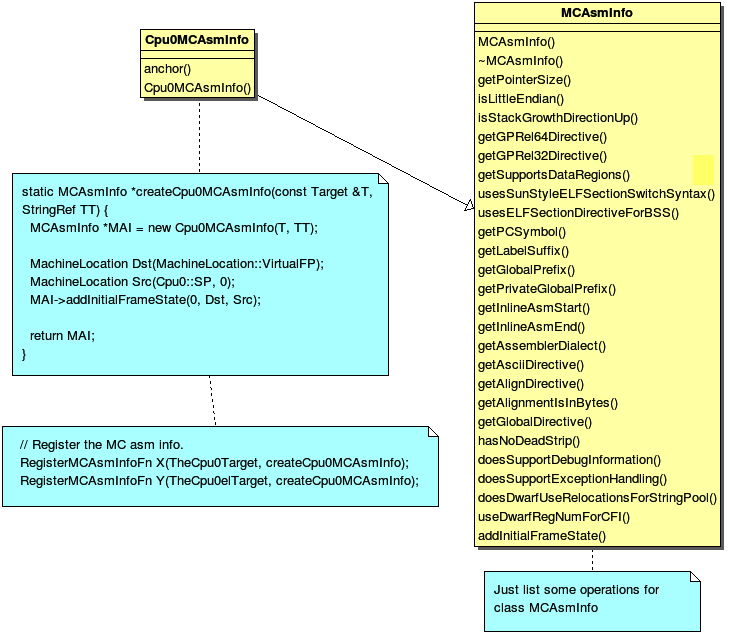
\includegraphics{14.png}}
\caption{Register Cpu0MCAsmInfo}\label{genobj:genobj-f1}\end{figure}
\begin{figure}[htbp]
\centering
\capstart

\scalebox{1.000000}{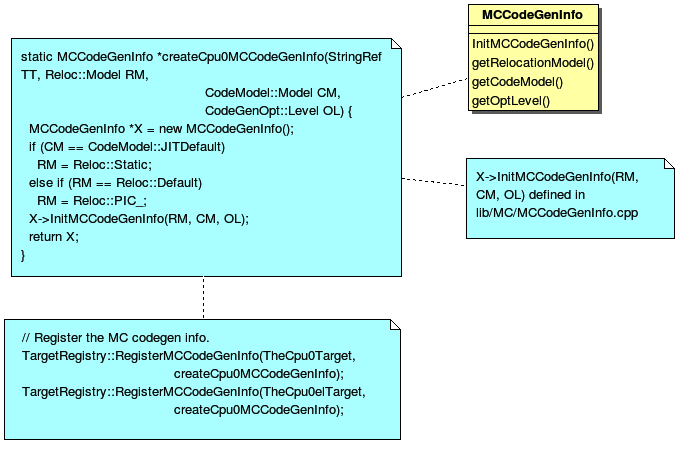
\includegraphics{23.png}}
\caption{Register MCCodeGenInfo}\label{genobj:genobj-f2}\end{figure}
\begin{figure}[htbp]
\centering
\capstart

\scalebox{1.000000}{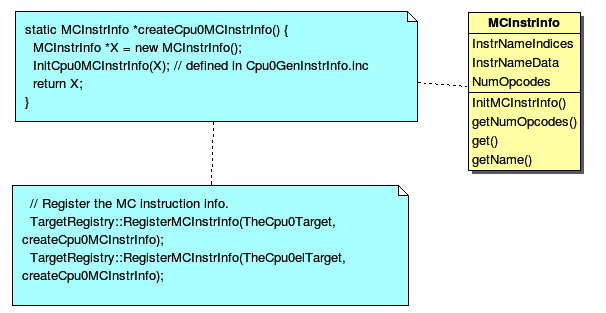
\includegraphics{32.png}}
\caption{Register MCInstrInfo}\label{genobj:genobj-f3}\end{figure}
\begin{figure}[htbp]
\centering
\capstart

\scalebox{1.000000}{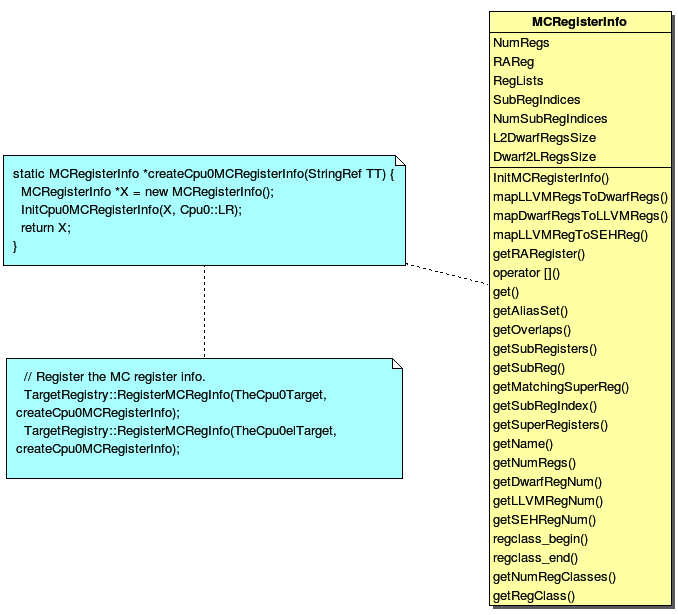
\includegraphics{42.png}}
\caption{Register MCRegisterInfo}\label{genobj:genobj-f4}\end{figure}
\begin{figure}[htbp]
\centering
\capstart

\scalebox{1.000000}{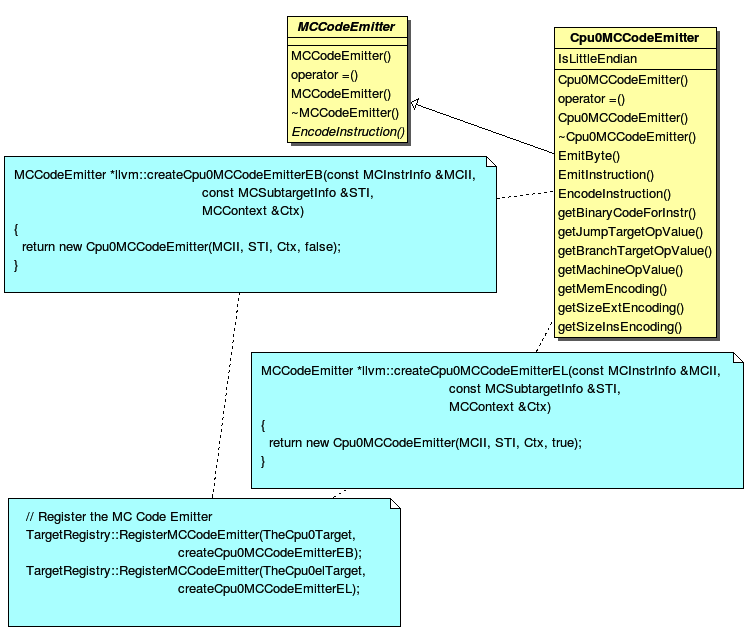
\includegraphics{52.png}}
\caption{Register Cpu0MCCodeEmitter}\label{genobj:genobj-f5}\end{figure}
\begin{figure}[htbp]
\centering
\capstart

\scalebox{1.000000}{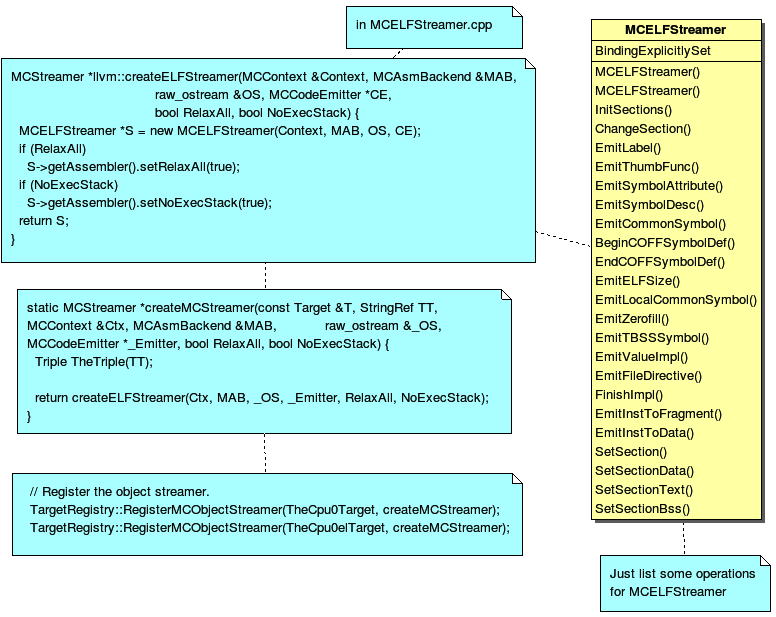
\includegraphics{62.png}}
\caption{Register MCELFStreamer}\label{genobj:genobj-f6}\end{figure}
\begin{figure}[htbp]
\centering
\capstart

\scalebox{1.000000}{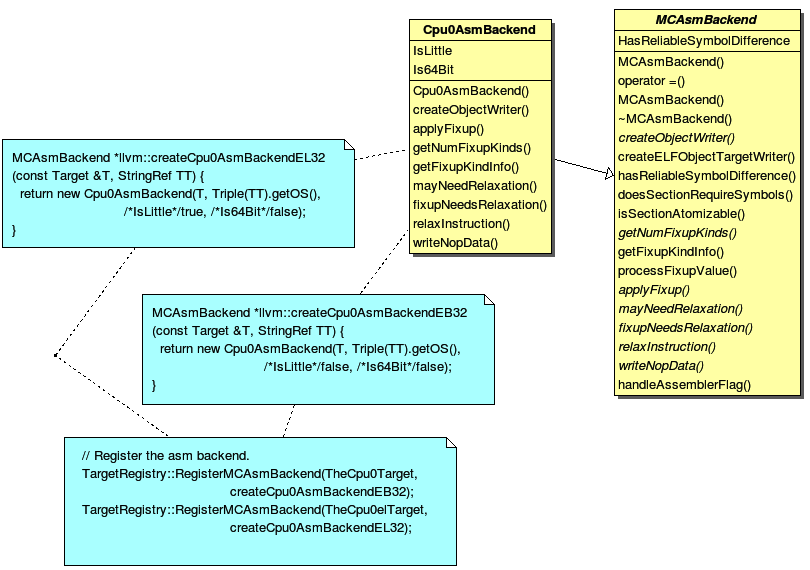
\includegraphics{71.png}}
\caption{Register Cpu0AsmBackend}\label{genobj:genobj-f7}\end{figure}
\begin{figure}[htbp]
\centering
\capstart

\scalebox{1.000000}{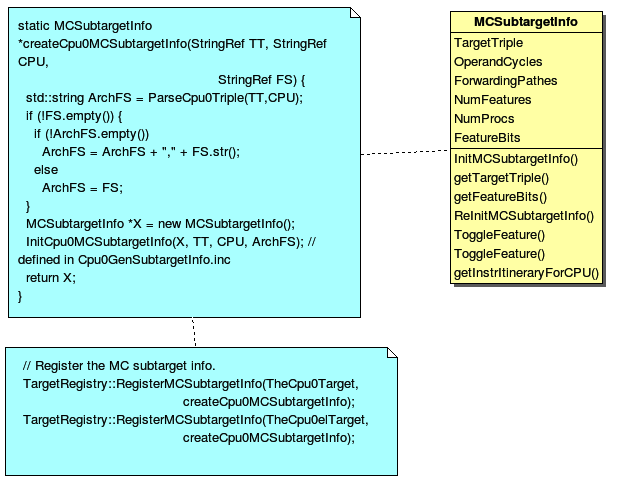
\includegraphics{81.png}}
\caption{Register Cpu0MCSubtargetInfo}\label{genobj:genobj-f8}\end{figure}
\begin{figure}[htbp]
\centering
\capstart

\scalebox{1.000000}{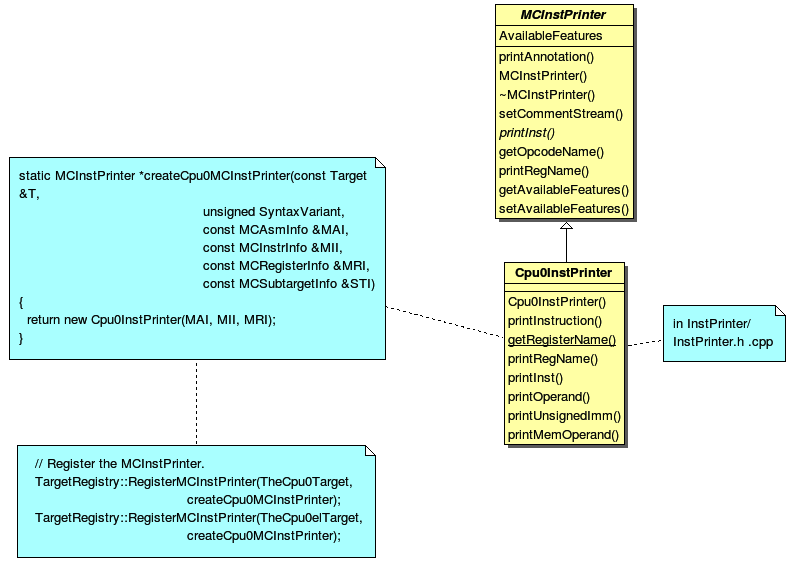
\includegraphics{91.png}}
\caption{Register Cpu0InstPrinter}\label{genobj:genobj-f9}\end{figure}
\begin{figure}[htbp]
\centering
\capstart

\scalebox{1.000000}{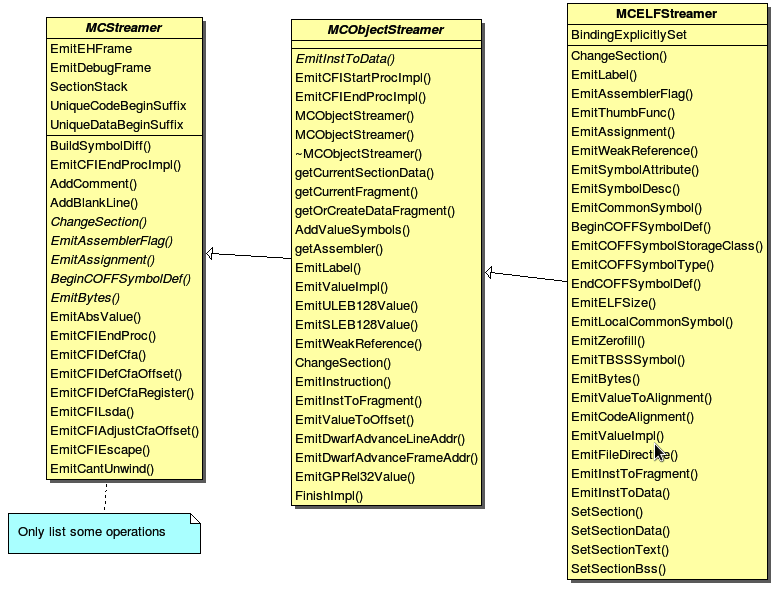
\includegraphics{101.png}}
\caption{MCELFStreamer inherit tree}\label{genobj:genobj-f10}\end{figure}

In \hyperref[genobj:genobj-f1]{Figure  \ref*{genobj:genobj-f1}}, registering the object of class Cpu0AsmInfo for
target TheCpu0Target and TheCpu0elTarget.
TheCpu0Target is for big endian and TheCpu0elTarget is for little endian.
Cpu0AsmInfo is derived from MCAsmInfo which is llvm built-in class.
Most code is implemented in it's parent, back end reuse those code by inherit.

In \hyperref[genobj:genobj-f2]{Figure  \ref*{genobj:genobj-f2}}, instancing MCCodeGenInfo, and initialize it by
pass
Roloc::PIC because we use command \code{llc -relocation-model=pic} to tell \code{llc}
compile using position-independent code mode.
Recall the addressing mode in system program book has two mode, one is PIC
mode, the other is absolute addressing mode.
MC stands for Machine Code.

In \hyperref[genobj:genobj-f3]{Figure  \ref*{genobj:genobj-f3}}, instancing MCInstrInfo object X, and initialize it
by InitCpu0MCInstrInfo(X).
Since InitCpu0MCInstrInfo(X) is defined in Cpu0GenInstrInfo.inc, it will add
the information from Cpu0InstrInfo.td we specified.
\hyperref[genobj:genobj-f4]{Figure  \ref*{genobj:genobj-f4}} is similar to \hyperref[genobj:genobj-f3]{Figure  \ref*{genobj:genobj-f3}}, but it
initialize the register information specified in Cpu0RegisterInfo.td.
They share a lot of code with instruction/register td description.

\hyperref[genobj:genobj-f5]{Figure  \ref*{genobj:genobj-f5}}, instancing two objects Cpu0MCCodeEmitter, one is for
big endian and the other is for little endian.
They take care the obj format generated.
So, it's not defined in Chapter4\_2/ which support assembly code only.

\hyperref[genobj:genobj-f6]{Figure  \ref*{genobj:genobj-f6}}, MCELFStreamer take care the obj format also.
\hyperref[genobj:genobj-f5]{Figure  \ref*{genobj:genobj-f5}} Cpu0MCCodeEmitter take care code emitter while
MCELFStreamer take care the obj output streamer.
\hyperref[genobj:genobj-f10]{Figure  \ref*{genobj:genobj-f10}} is MCELFStreamer inherit tree.
You can find a lot of operations in that inherit tree.

Reader maybe has the question for what are the actual arguments in
createCpu0MCCodeEmitterEB(const MCInstrInfo \&MCII,  const MCSubtargetInfo \&STI,
MCContext \&Ctx) and at when they are assigned.
Yes, we didn't assign it, we register the createXXX() function by function
pointer only (according C, TargetRegistry::RegisterXXX(TheCpu0Target,
createXXX()) where createXXX is function pointer).
LLVM keep a function pointer to createXXX() when we call target registry, and
will call these createXXX() function back at proper time with arguments
assigned during the target registration process, RegisterXXX().

\hyperref[genobj:genobj-f7]{Figure  \ref*{genobj:genobj-f7}}, Cpu0AsmBackend class is the bridge for asm to obj.
Two objects take care big endian and little endian also.
It derived from MCAsmBackend.
Most of code for object file generated is implemented by MCELFStreamer and it's
parent, MCAsmBackend.

\hyperref[genobj:genobj-f8]{Figure  \ref*{genobj:genobj-f8}}, instancing MCSubtargetInfo object and initialize with
Cpu0.td information.
\hyperref[genobj:genobj-f9]{Figure  \ref*{genobj:genobj-f9}}, instancing Cpu0InstPrinter to take care printing
function for instructions.
Like \hyperref[genobj:genobj-f1]{Figure  \ref*{genobj:genobj-f1}} to \hyperref[genobj:genobj-f4]{Figure  \ref*{genobj:genobj-f4}}, it has been defined
in Chapter4\_2/ code for assembly file generated support.


\chapter{Global variables}
\label{globalvar:sec-globalvars}\label{globalvar::doc}\label{globalvar:global-variables}
In the previous two chapters, we only access the local variables.
This chapter will deal global variable access translation.

The global variable DAG translation is different from the previous DAG
translation we have now.
It create DAG nodes at run time in our backend C++ code according the
\code{llc -relocation-model} option while the others of DAG just do IR DAG to
Machine DAG translation directly according the input file IR DAG.


\section{Global variable}
\label{globalvar:global-variable}
Chapter6\_1/ support the global variable, let's compile ch6\_1.cpp with this version
first, and explain the code changes after that.
\paragraph{lbdex/InputFiles/ch6\_1.cpp}

\begin{Verbatim}[commandchars=\\\{\}]
\PYG{k+kt}{int} \PYG{n}{gStart} \PYG{o}{=} \PYG{l+m+mi}{3}\PYG{p}{;}
\PYG{k+kt}{int} \PYG{n}{gI} \PYG{o}{=} \PYG{l+m+mi}{100}\PYG{p}{;}
\PYG{k+kt}{int} \PYG{n}{fun}\PYG{p}{(}\PYG{p}{)}
\PYG{p}{\PYGZob{}}
  \PYG{k+kt}{int} \PYG{n}{c} \PYG{o}{=} \PYG{l+m+mi}{0}\PYG{p}{;}

  \PYG{n}{c} \PYG{o}{=} \PYG{n}{gI}\PYG{p}{;}

  \PYG{k}{return} \PYG{n}{c}\PYG{p}{;}
\PYG{p}{\PYGZcb{}}
\end{Verbatim}

\begin{Verbatim}[commandchars=\\\{\}]
118-165-78-166:InputFiles Jonathan\PYG{n+nv}{\PYGZdl{} }llvm-dis ch6\PYGZus{}1.bc -o -
; \PYG{n+nv}{ModuleID} \PYG{o}{=} \PYG{l+s+s1}{'ch6\PYGZus{}1.bc'}
target \PYG{n+nv}{datalayout} \PYG{o}{=} \PYG{l+s+s2}{"e-p:64:64:64-i1:8:8-i8:8:8-i16:16:16-i32:32:32-i64:64:64-}
\PYG{l+s+s2}{f32:32:32-f64:64:64-v64:64:64-v128:128:128-a0:0:64-s0:64:64-f80:128:128-}
\PYG{l+s+s2}{n8:16:32:64-S128"}
target \PYG{n+nv}{triple} \PYG{o}{=} \PYG{l+s+s2}{"x86\PYGZus{}64-apple-macosx10.8.0"}

@gStart \PYG{o}{=} global i32 2, align 4
@gI \PYG{o}{=} global i32 100, align 4

define i32 @\PYGZus{}Z3funv\PYG{o}{(}\PYG{o}{)} nounwind uwtable ssp \PYG{o}{\PYGZob{}}
  \PYGZpc{}1 \PYG{o}{=} alloca i32, align 4
  \PYGZpc{}c \PYG{o}{=} alloca i32, align 4
  store i32 0, i32* \PYGZpc{}1
  store i32 0, i32* \PYGZpc{}c, align 4
  \PYGZpc{}2 \PYG{o}{=} load i32* @gI, align 4
  store i32 \PYGZpc{}2, i32* \PYGZpc{}c, align 4
  \PYGZpc{}3 \PYG{o}{=} load i32* \PYGZpc{}c, align 4
  ret i32 \PYGZpc{}3
\PYG{o}{\PYGZcb{}}
\end{Verbatim}


\subsection{Cpu0 global variable options}
\label{globalvar:cpu0-global-variable-options}
Cpu0 like Mips supports both static and pic mode. There are two different layout
of global variables for static mode which controlled by option cpu0-use-small-section.
Chapter6\_1/ support the global variable translation.
Let's run Chapter6\_1/ with ch6\_1.cpp via three different options
\code{llc  -relocation-model=static -cpu0-use-small-section=false},
\code{llc  -relocation-model=static -cpu0-use-small-section=true} and
\code{llc  -relocation-model=pic} to trace the DAG and Cpu0 instructions.

\begin{Verbatim}[commandchars=\\\{\}]
118-165-78-166:InputFiles Jonathan\PYG{n+nv}{\PYGZdl{} }clang -target mips-unknown-linux-gnu -c
ch6\PYGZus{}1.cpp -emit-llvm -o ch6\PYGZus{}1.bc
118-165-78-166:InputFiles Jonathan\PYG{n+nv}{\PYGZdl{} }/Users/Jonathan/llvm/test/cmake\PYGZus{}debug\PYGZus{}build/
bin/Debug/llc -march\PYG{o}{=}cpu0 -relocation-model\PYG{o}{=}static -cpu0-use-small-section\PYG{o}{=}\PYG{n+nb}{false}
-filetype\PYG{o}{=}asm -debug ch6\PYGZus{}1.bc -o -

...
Type-legalized selection DAG: BB\PYGZsh{}0 \PYG{l+s+s1}{'\PYGZus{}Z3funv:entry'}
SelectionDAG has 12 nodes:
  ...
      0x7ffd5902cc10: \PYGZlt{}multiple use\PYGZgt{}
    0x7ffd5902cf10: \PYG{n+nv}{ch} \PYG{o}{=} store 0x7ffd5902cd10, 0x7ffd5902ca10, 0x7ffd5902ce10,
    0x7ffd5902cc10\PYGZlt{}ST4\PYG{o}{[}\PYGZpc{}c\PYG{o}{]}\PYGZgt{} \PYG{o}{[}\PYG{n+nv}{ORD}\PYG{o}{=}2\PYG{o}{]} \PYG{o}{[}\PYG{n+nv}{ID}\PYG{o}{=}-3\PYG{o}{]}

    0x7ffd5902d010: \PYG{n+nv}{i32} \PYG{o}{=} GlobalAddress\PYGZlt{}i32* @gI\PYGZgt{} 0 \PYG{o}{[}\PYG{n+nv}{ORD}\PYG{o}{=}3\PYG{o}{]} \PYG{o}{[}\PYG{n+nv}{ID}\PYG{o}{=}-3\PYG{o}{]}

    0x7ffd5902cc10: \PYGZlt{}multiple use\PYGZgt{}
  0x7ffd5902d110: i32,ch \PYG{o}{=} load 0x7ffd5902cf10, 0x7ffd5902d010,
  0x7ffd5902cc10\PYGZlt{}LD4\PYG{o}{[}@gI\PYG{o}{]}\PYGZgt{} \PYG{o}{[}\PYG{n+nv}{ORD}\PYG{o}{=}3\PYG{o}{]} \PYG{o}{[}\PYG{n+nv}{ID}\PYG{o}{=}-3\PYG{o}{]}
  ...

Legalized selection DAG: BB\PYGZsh{}0 \PYG{l+s+s1}{'\PYGZus{}Z3funv:entry'}
SelectionDAG has 16 nodes:
  ...
      0x7ffd5902cc10: \PYGZlt{}multiple use\PYGZgt{}
    0x7ffd5902cf10: \PYG{n+nv}{ch} \PYG{o}{=} store 0x7ffd5902cd10, 0x7ffd5902ca10, 0x7ffd5902ce10,
    0x7ffd5902cc10\PYGZlt{}ST4\PYG{o}{[}\PYGZpc{}c\PYG{o}{]}\PYGZgt{} \PYG{o}{[}\PYG{n+nv}{ORD}\PYG{o}{=}2\PYG{o}{]} \PYG{o}{[}\PYG{n+nv}{ID}\PYG{o}{=}8\PYG{o}{]}

        0x7ffd5902d310: \PYG{n+nv}{i32} \PYG{o}{=} TargetGlobalAddress\PYGZlt{}i32* @gI\PYGZgt{} 0 \PYG{o}{[}\PYG{n+nv}{TF}\PYG{o}{=}5\PYG{o}{]}

      0x7ffd5902d710: \PYG{n+nv}{i32} \PYG{o}{=} Cpu0ISD::Hi 0x7ffd5902d310

        0x7ffd5902d610: \PYG{n+nv}{i32} \PYG{o}{=} TargetGlobalAddress\PYGZlt{}i32* @gI\PYGZgt{} 0 \PYG{o}{[}\PYG{n+nv}{TF}\PYG{o}{=}6\PYG{o}{]}

      0x7ffd5902d810: \PYG{n+nv}{i32} \PYG{o}{=} Cpu0ISD::Lo 0x7ffd5902d610

    0x7ffd5902fe10: \PYG{n+nv}{i32} \PYG{o}{=} add 0x7ffd5902d710, 0x7ffd5902d810

    0x7ffd5902cc10: \PYGZlt{}multiple use\PYGZgt{}
  0x7ffd5902d110: i32,ch \PYG{o}{=} load 0x7ffd5902cf10, 0x7ffd5902fe10,
  0x7ffd5902cc10\PYGZlt{}LD4\PYG{o}{[}@gI\PYG{o}{]}\PYGZgt{} \PYG{o}{[}\PYG{n+nv}{ORD}\PYG{o}{=}3\PYG{o}{]} \PYG{o}{[}\PYG{n+nv}{ID}\PYG{o}{=}9\PYG{o}{]}
  ...
  lui \PYG{n+nv}{\PYGZdl{}2}, \PYGZpc{}hi\PYG{o}{(}gI\PYG{o}{)}
  addiu \PYG{n+nv}{\PYGZdl{}2}, \PYG{n+nv}{\PYGZdl{}2}, \PYGZpc{}lo\PYG{o}{(}gI\PYG{o}{)}
      ld      \PYG{n+nv}{\PYGZdl{}2}, 0\PYG{o}{(}\PYG{n+nv}{\PYGZdl{}2}\PYG{o}{)}
      ...
      .type   gStart,@object          \PYG{c}{\PYGZsh{} @gStart}
      .data
      .globl  gStart
      .align  2
gStart:
      .4byte  2                       \PYG{c}{\PYGZsh{} 0x2}
      .size   gStart, 4

      .type   gI,@object              \PYG{c}{\PYGZsh{} @gI}
      .globl  gI
      .align  2
gI:
      .4byte  100                     \PYG{c}{\PYGZsh{} 0x64}
      .size   gI, 4
\end{Verbatim}

\begin{Verbatim}[commandchars=\\\{\}]
118-165-78-166:InputFiles Jonathan\PYG{n+nv}{\PYGZdl{} }/Users/Jonathan/llvm/test/cmake\PYGZus{}debug\PYGZus{}build/
bin/Debug/llc -march\PYG{o}{=}cpu0 -relocation-model\PYG{o}{=}static -cpu0-use-small-section\PYG{o}{=}\PYG{n+nb}{true}
-filetype\PYG{o}{=}asm -debug ch6\PYGZus{}1.bc -o -

...
Type-legalized selection DAG: BB\PYGZsh{}0 \PYG{l+s+s1}{'\PYGZus{}Z3funv:entry'}
SelectionDAG has 12 nodes:
  ...
      0x7fc5f382cc10: \PYGZlt{}multiple use\PYGZgt{}
    0x7fc5f382cf10: \PYG{n+nv}{ch} \PYG{o}{=} store 0x7fc5f382cd10, 0x7fc5f382ca10, 0x7fc5f382ce10,
    0x7fc5f382cc10\PYGZlt{}ST4\PYG{o}{[}\PYGZpc{}c\PYG{o}{]}\PYGZgt{} \PYG{o}{[}\PYG{n+nv}{ORD}\PYG{o}{=}2\PYG{o}{]} \PYG{o}{[}\PYG{n+nv}{ID}\PYG{o}{=}-3\PYG{o}{]}

    0x7fc5f382d010: \PYG{n+nv}{i32} \PYG{o}{=} GlobalAddress\PYGZlt{}i32* @gI\PYGZgt{} 0 \PYG{o}{[}\PYG{n+nv}{ORD}\PYG{o}{=}3\PYG{o}{]} \PYG{o}{[}\PYG{n+nv}{ID}\PYG{o}{=}-3\PYG{o}{]}

    0x7fc5f382cc10: \PYGZlt{}multiple use\PYGZgt{}
  0x7fc5f382d110: i32,ch \PYG{o}{=} load 0x7fc5f382cf10, 0x7fc5f382d010,
  0x7fc5f382cc10\PYGZlt{}LD4\PYG{o}{[}@gI\PYG{o}{]}\PYGZgt{} \PYG{o}{[}\PYG{n+nv}{ORD}\PYG{o}{=}3\PYG{o}{]} \PYG{o}{[}\PYG{n+nv}{ID}\PYG{o}{=}-3\PYG{o}{]}

Legalized selection DAG: BB\PYGZsh{}0 \PYG{l+s+s1}{'\PYGZus{}Z3funv:entry'}
SelectionDAG has 15 nodes:
  ...
      0x7fc5f382cc10: \PYGZlt{}multiple use\PYGZgt{}
    0x7fc5f382cf10: \PYG{n+nv}{ch} \PYG{o}{=} store 0x7fc5f382cd10, 0x7fc5f382ca10, 0x7fc5f382ce10,
    0x7fc5f382cc10\PYGZlt{}ST4\PYG{o}{[}\PYGZpc{}c\PYG{o}{]}\PYGZgt{} \PYG{o}{[}\PYG{n+nv}{ORD}\PYG{o}{=}2\PYG{o}{]} \PYG{o}{[}\PYG{n+nv}{ID}\PYG{o}{=}8\PYG{o}{]}

      0x7fc5f382d710: \PYG{n+nv}{i32} \PYG{o}{=} GLOBAL\PYGZus{}OFFSET\PYGZus{}TABLE

        0x7fc5f382d310: \PYG{n+nv}{i32} \PYG{o}{=} TargetGlobalAddress\PYGZlt{}i32* @gI\PYGZgt{} 0 \PYG{o}{[}\PYG{n+nv}{TF}\PYG{o}{=}4\PYG{o}{]}

      0x7fc5f382d610: \PYG{n+nv}{i32} \PYG{o}{=} Cpu0ISD::GPRel 0x7fc5f382d310

    0x7fc5f382d810: \PYG{n+nv}{i32} \PYG{o}{=} add 0x7fc5f382d710, 0x7fc5f382d610

    0x7fc5f382cc10: \PYGZlt{}multiple use\PYGZgt{}
  0x7fc5f382d110: i32,ch \PYG{o}{=} load 0x7fc5f382cf10, 0x7fc5f382d810,
  0x7fc5f382cc10\PYGZlt{}LD4\PYG{o}{[}@gI\PYG{o}{]}\PYGZgt{} \PYG{o}{[}\PYG{n+nv}{ORD}\PYG{o}{=}3\PYG{o}{]} \PYG{o}{[}\PYG{n+nv}{ID}\PYG{o}{=}9\PYG{o}{]}
  ...

      addiu   \PYG{n+nv}{\PYGZdl{}2}, \PYG{n+nv}{\PYGZdl{}gp}, \PYGZpc{}gp\PYGZus{}rel\PYG{o}{(}gI\PYG{o}{)}
      ld      \PYG{n+nv}{\PYGZdl{}2}, 0\PYG{o}{(}\PYG{n+nv}{\PYGZdl{}2}\PYG{o}{)}
      ...
      .type   gStart,@object          \PYG{c}{\PYGZsh{} @gStart}
      .section        .sdata,\PYG{l+s+s2}{"aw"},@progbits
      .globl  gStart
      .align  2
gStart:
      .4byte  2                       \PYG{c}{\PYGZsh{} 0x2}
      .size   gStart, 4

      .type   gI,@object              \PYG{c}{\PYGZsh{} @gI}
      .globl  gI
      .align  2
gI:
      .4byte  100                     \PYG{c}{\PYGZsh{} 0x64}
      .size   gI, 4
\end{Verbatim}

\begin{Verbatim}[commandchars=\\\{\}]
118-165-78-166:InputFiles Jonathan\PYG{n+nv}{\PYGZdl{} }/Users/Jonathan/llvm/test/cmake\PYGZus{}debug\PYGZus{}build/
bin/Debug/llc -march\PYG{o}{=}cpu0 -relocation-model\PYG{o}{=}pic -filetype\PYG{o}{=}asm -debug ch6\PYGZus{}1.bc
-o -

...
Type-legalized selection DAG: BB\PYGZsh{}0 \PYG{l+s+s1}{'\PYGZus{}Z3funv:entry'}
SelectionDAG has 12 nodes:
  ...
      0x7fad7102cc10: \PYGZlt{}multiple use\PYGZgt{}
    0x7fad7102cf10: \PYG{n+nv}{ch} \PYG{o}{=} store 0x7fad7102cd10, 0x7fad7102ca10, 0x7fad7102ce10,
    0x7fad7102cc10\PYGZlt{}ST4\PYG{o}{[}\PYGZpc{}c\PYG{o}{]}\PYGZgt{} \PYG{o}{[}\PYG{n+nv}{ORD}\PYG{o}{=}2\PYG{o}{]} \PYG{o}{[}\PYG{n+nv}{ID}\PYG{o}{=}-3\PYG{o}{]}

    0x7fad7102d010: \PYG{n+nv}{i32} \PYG{o}{=} GlobalAddress\PYGZlt{}i32* @gI\PYGZgt{} 0 \PYG{o}{[}\PYG{n+nv}{ORD}\PYG{o}{=}3\PYG{o}{]} \PYG{o}{[}\PYG{n+nv}{ID}\PYG{o}{=}-3\PYG{o}{]}

    0x7fad7102cc10: \PYGZlt{}multiple use\PYGZgt{}
  0x7fad7102d110: i32,ch \PYG{o}{=} load 0x7fad7102cf10, 0x7fad7102d010,
  0x7fad7102cc10\PYGZlt{}LD4\PYG{o}{[}@gI\PYG{o}{]}\PYGZgt{} \PYG{o}{[}\PYG{n+nv}{ORD}\PYG{o}{=}3\PYG{o}{]} \PYG{o}{[}\PYG{n+nv}{ID}\PYG{o}{=}-3\PYG{o}{]}
  ...
Legalized selection DAG: BB\PYGZsh{}0 \PYG{l+s+s1}{'\PYGZus{}Z3funv:entry'}
SelectionDAG has 15 nodes:
  0x7ff3c9c10b98: \PYG{n+nv}{ch} \PYG{o}{=} EntryToken \PYG{o}{[}\PYG{n+nv}{ORD}\PYG{o}{=}1\PYG{o}{]} \PYG{o}{[}\PYG{n+nv}{ID}\PYG{o}{=}0\PYG{o}{]}
  ...
      0x7fad7102cc10: \PYGZlt{}multiple use\PYGZgt{}
    0x7fad7102cf10: \PYG{n+nv}{ch} \PYG{o}{=} store 0x7fad7102cd10, 0x7fad7102ca10, 0x7fad7102ce10,
    0x7fad7102cc10\PYGZlt{}ST4\PYG{o}{[}\PYGZpc{}c\PYG{o}{]}\PYGZgt{} \PYG{o}{[}\PYG{n+nv}{ORD}\PYG{o}{=}2\PYG{o}{]} \PYG{o}{[}\PYG{n+nv}{ID}\PYG{o}{=}8\PYG{o}{]}

      0x7fad70c10b98: \PYGZlt{}multiple use\PYGZgt{}
        0x7fad7102d610: \PYG{n+nv}{i32} \PYG{o}{=} Register \PYGZpc{}GP

        0x7fad7102d310: \PYG{n+nv}{i32} \PYG{o}{=} TargetGlobalAddress\PYGZlt{}i32* @gI\PYGZgt{} 0 \PYG{o}{[}\PYG{n+nv}{TF}\PYG{o}{=}1\PYG{o}{]}

      0x7fad7102d710: \PYG{n+nv}{i32} \PYG{o}{=} Cpu0ISD::Wrapper 0x7fad7102d610, 0x7fad7102d310

      0x7fad7102cc10: \PYGZlt{}multiple use\PYGZgt{}
    0x7fad7102d810: i32,ch \PYG{o}{=} load 0x7fad70c10b98, 0x7fad7102d710,
    0x7fad7102cc10\PYGZlt{}LD4\PYG{o}{[}\PYGZlt{}unknown\PYGZgt{}\PYG{o}{]}\PYGZgt{}

    0x7ff3ca02cc10: \PYGZlt{}multiple use\PYGZgt{}
  0x7ff3ca02d110: i32,ch \PYG{o}{=} load 0x7ff3ca02cf10, 0x7ff3ca02d810,
  0x7ff3ca02cc10\PYGZlt{}LD4\PYG{o}{[}@gI\PYG{o}{]}\PYGZgt{} \PYG{o}{[}\PYG{n+nv}{ORD}\PYG{o}{=}3\PYG{o}{]} \PYG{o}{[}\PYG{n+nv}{ID}\PYG{o}{=}9\PYG{o}{]}
  ...
        .set  noreorder
        .cpload       \PYG{n+nv}{\PYGZdl{}6}
        .set  nomacro
  ...
      ld      \PYG{n+nv}{\PYGZdl{}2}, \PYGZpc{}got\PYG{o}{(}gI\PYG{o}{)}\PYG{o}{(}\PYG{n+nv}{\PYGZdl{}gp}\PYG{o}{)}
      ld      \PYG{n+nv}{\PYGZdl{}2}, 0\PYG{o}{(}\PYG{n+nv}{\PYGZdl{}2}\PYG{o}{)}
  ...
      .type   gStart,@object          \PYG{c}{\PYGZsh{} @gStart}
      .data
      .globl  gStart
      .align  2
gStart:
      .4byte  2                       \PYG{c}{\PYGZsh{} 0x2}
      .size   gStart, 4

      .type   gI,@object              \PYG{c}{\PYGZsh{} @gI}
      .globl  gI
      .align  2
gI:
      .4byte  100                     \PYG{c}{\PYGZsh{} 0x64}
      .size   gI, 4
\end{Verbatim}

Summary above information to Table: Cpu0 global variable options.


\begin{threeparttable}
\capstart\caption{Cpu0 global variable options}

\begin{tabular}{|p{0.237\linewidth}|p{0.237\linewidth}|p{0.237\linewidth}|p{0.237\linewidth}|}
\hline
\textbf{
option name
} & \textbf{
default
} & \textbf{
other option value
} & \textbf{
discription
}\\\hline

-relocation-model
 & 
pic
 & 
static
 & \begin{itemize}
\item {} 
pic: Postion Independent Address

\item {} 
static: Absolute Address

\end{itemize}
\\\hline

-cpu0-use-small-section
 & 
false
 & 
true
 & \begin{itemize}
\item {} 
false: .data or .bss, 16 bits addressable

\item {} 
true: .sdata or .sbss, 32 bits addressable

\end{itemize}
\\\hline
\end{tabular}

\end{threeparttable}



\begin{threeparttable}
\capstart\caption{Cpu0 DAGs and instructions for -relocation-model=static}

\begin{tabulary}{\linewidth}{|L|L|L|}
\hline
\textbf{
option: cpu0-use-small-section
} & \textbf{
false
} & \textbf{
true
}\\\hline

addressing mode
 & 
absolute
 & 
\$gp relative
\\\hline

addressing
 & 
absolute
 & 
\$gp+offset
\\\hline

Legalized selection DAG
 & 
(add Cpu0ISD::Hi\textless{}gI offset Hi16\textgreater{} Cpu0ISD::Lo\textless{}gI offset Lo16\textgreater{})
 & 
(add GLOBAL\_OFFSET\_TABLE, Cpu0ISD::GPRel\textless{}gI offset\textgreater{})
\\\hline

Cpu0
 & 
addiu \$2, \$zero, \%hi(gI); shl \$2, \$2, 16; addiu \$2, \$2, \%lo(gI);
 & 
addiu   \$2, \$gp, \%gp\_rel(gI);
\\\hline

relocation records solved
 & 
link time
 & 
link time
\\\hline
\end{tabulary}

\end{threeparttable}

\begin{itemize}
\item {} 
In static, cpu0-use-small-section=true, offset between gI and .data can be calculated since the \$gp is assigned at fixed address of the start of global address table.

\item {} 
In ``static, cpu0-use-small-section=false'', the gI high and low address (\%hi(gI) and \%lo(gI)) are translated into absolute address.

\end{itemize}


\begin{threeparttable}
\capstart\caption{Cpu0 DAGs and instructions for -relocation-model=pic}

\begin{tabulary}{\linewidth}{|L|L|L|}
\hline
\textbf{
option: cpu0-use-small-section
} & \textbf{
false
} & \textbf{
true
}\\\hline

addressing mode
 & 
\$gp relative
 & 
\$gp relative
\\\hline

addressing
 & 
\$gp+offset
 & 
\$gp+offset
\\\hline

Legalized selection DAG
 & 
(load (Cpu0ISD::Wrapper \%GP, \textless{}gI offset\textgreater{}))
 & 
(load EntryToken, (Cpu0ISD::Wrapper (add Cpu0ISD::Hi\textless{}gI offset Hi16\textgreater{}, Register \%GP), Cpu0ISD::Lo\textless{}gI offset Lo16\textgreater{}))
\\\hline

Cpu0
 & 
ld \$2, \%got(gI)(\$gp);
 & 
addiu      \$2, \$zero, \%got\_hi(gI); shl \$2, \$2, 16; add \$2, \$2, \$gp; ld \$2, \%got\_lo(gI)(\$2);
\\\hline

relocation records solved
 & 
link/load time
 & 
link/load time
\\\hline
\end{tabulary}

\end{threeparttable}

\begin{itemize}
\item {} 
In pic, offset between gI and .data cannot be calculated if the function is loaded at run time (dynamic link); the offset can be calculated if use static link.

\item {} 
In C, all variable names binding staticly. In C++, the overload variable or function are binding dynamicly.

\end{itemize}

According book of system program, there are Absolute Addressing Mode and
Position Independent Addressing Mode. The dynamic function must compiled with
Position Independent Addressing Mode. In principle, option -relocation-model is
used to generate Absolute Addressing or Position Independent Addressing.
The exception is -relocation-model=static and -cpu0-use-small-section=false.
In this case, the register \$gp is reserved to set at the start address of global
variable area. Cpu0 use \$gp relative addressing in this mode.

To support global variable, first add \textbf{UseSmallSectionOpt} command variable to
Cpu0Subtarget.cpp.
After that, user can run llc with option \code{llc -cpu0-use-small-section=false}
to specify \textbf{UseSmallSectionOpt} to false.
The default of \textbf{UseSmallSectionOpt} is false if without specify it further.
About the \textbf{cl::opt} command line variable, you can refer to \footnote{
\href{http://llvm.org/docs/CommandLine.html}{http://llvm.org/docs/CommandLine.html}
} further.
\paragraph{lbdex/Chapter6\_1/Cpu0Subtarget.h}

\begin{Verbatim}[commandchars=\\\{\}]
\PYG{k}{extern} \PYG{k+kt}{bool} \PYG{n}{Cpu0NoCpload}\PYG{p}{;}
\PYG{p}{.}\PYG{p}{.}\PYG{p}{.}
\PYG{k}{class} \PYG{n+nc}{Cpu0Subtarget} \PYG{o}{:} \PYG{k}{public} \PYG{n}{Cpu0GenSubtargetInfo} \PYG{p}{\PYGZob{}}
  \PYG{p}{.}\PYG{p}{.}\PYG{p}{.}
  \PYG{c+c1}{// UseSmallSection - Small section is used.}
  \PYG{k+kt}{bool} \PYG{n}{UseSmallSection}\PYG{p}{;}
  \PYG{p}{.}\PYG{p}{.}\PYG{p}{.}
  \PYG{k+kt}{bool} \PYG{n}{useSmallSection}\PYG{p}{(}\PYG{p}{)} \PYG{k}{const} \PYG{p}{\PYGZob{}} \PYG{k}{return} \PYG{n}{UseSmallSection}\PYG{p}{;} \PYG{p}{\PYGZcb{}}
\PYG{p}{\PYGZcb{}}\PYG{p}{;}
\end{Verbatim}
\paragraph{lbdex/Chapter6\_1/Cpu0Subtarget.cpp}

\begin{Verbatim}[commandchars=\\\{\}]
\PYG{c+cp}{\PYGZsh{}}\PYG{c+cp}{include "llvm}\PYG{c+cp}{/}\PYG{c+cp}{Support}\PYG{c+cp}{/}\PYG{c+cp}{CommandLine.h"}
\PYG{p}{.}\PYG{p}{.}\PYG{p}{.}
\PYG{k}{static} \PYG{n}{cl}\PYG{o}{:}\PYG{o}{:}\PYG{n}{opt}\PYG{o}{\PYGZlt{}}\PYG{k+kt}{bool}\PYG{o}{\PYGZgt{}}
\PYG{n}{UseSmallSectionOpt}\PYG{p}{(}\PYG{l+s}{"}\PYG{l+s}{cpu0-use-small-section}\PYG{l+s}{"}\PYG{p}{,} \PYG{n}{cl}\PYG{o}{:}\PYG{o}{:}\PYG{n}{Hidden}\PYG{p}{,} \PYG{n}{cl}\PYG{o}{:}\PYG{o}{:}\PYG{n}{init}\PYG{p}{(}\PYG{k+kc}{false}\PYG{p}{)}\PYG{p}{,}
                 \PYG{n}{cl}\PYG{o}{:}\PYG{o}{:}\PYG{n}{desc}\PYG{p}{(}\PYG{l+s}{"}\PYG{l+s}{Use small section. Only work with -relocation-model=}\PYG{l+s}{"}
                 \PYG{l+s}{"}\PYG{l+s}{static. pic always not use small section.}\PYG{l+s}{"}\PYG{p}{)}\PYG{p}{)}\PYG{p}{;}

\PYG{k}{static} \PYG{n}{cl}\PYG{o}{:}\PYG{o}{:}\PYG{n}{opt}\PYG{o}{\PYGZlt{}}\PYG{k+kt}{bool}\PYG{o}{\PYGZgt{}}
\PYG{n}{ReserveGPOpt}\PYG{p}{(}\PYG{l+s}{"}\PYG{l+s}{cpu0-reserve-gp}\PYG{l+s}{"}\PYG{p}{,} \PYG{n}{cl}\PYG{o}{:}\PYG{o}{:}\PYG{n}{Hidden}\PYG{p}{,} \PYG{n}{cl}\PYG{o}{:}\PYG{o}{:}\PYG{n}{init}\PYG{p}{(}\PYG{k+kc}{false}\PYG{p}{)}\PYG{p}{,}
                 \PYG{n}{cl}\PYG{o}{:}\PYG{o}{:}\PYG{n}{desc}\PYG{p}{(}\PYG{l+s}{"}\PYG{l+s}{Never allocate \PYGZdl{}gp to variable}\PYG{l+s}{"}\PYG{p}{)}\PYG{p}{)}\PYG{p}{;}

\PYG{k}{static} \PYG{n}{cl}\PYG{o}{:}\PYG{o}{:}\PYG{n}{opt}\PYG{o}{\PYGZlt{}}\PYG{k+kt}{bool}\PYG{o}{\PYGZgt{}}
\PYG{n}{NoCploadOpt}\PYG{p}{(}\PYG{l+s}{"}\PYG{l+s}{cpu0-no-cpload}\PYG{l+s}{"}\PYG{p}{,} \PYG{n}{cl}\PYG{o}{:}\PYG{o}{:}\PYG{n}{Hidden}\PYG{p}{,} \PYG{n}{cl}\PYG{o}{:}\PYG{o}{:}\PYG{n}{init}\PYG{p}{(}\PYG{k+kc}{false}\PYG{p}{)}\PYG{p}{,}
                 \PYG{n}{cl}\PYG{o}{:}\PYG{o}{:}\PYG{n}{desc}\PYG{p}{(}\PYG{l+s}{"}\PYG{l+s}{No issue .cpload}\PYG{l+s}{"}\PYG{p}{)}\PYG{p}{)}\PYG{p}{;}

\PYG{k+kt}{bool} \PYG{n}{Cpu0ReserveGP}\PYG{p}{;}
\PYG{k+kt}{bool} \PYG{n}{Cpu0NoCpload}\PYG{p}{;}

\PYG{k}{extern} \PYG{k+kt}{bool} \PYG{n}{FixGlobalBaseReg}\PYG{p}{;}
\end{Verbatim}

The ReserveGPOpt and NoCploadOpt are used in Cpu0 linker at later Chapter.
Next add file Cpu0TargetObjectFile.h, Cpu0TargetObjectFile.cpp and the
following code to Cpu0RegisterInfo.cpp and Cpu0ISelLowering.cpp.
\paragraph{lbdex/Chapter6\_1/Cpu0TargetObjectFile.h}

\begin{Verbatim}[commandchars=\\\{\}]
\PYG{c+c1}{//===-- llvm/Target/Cpu0TargetObjectFile.h - Cpu0 Object Info ---*- C++ -*-===//}
\PYG{c+c1}{//}
\PYG{c+c1}{//                     The LLVM Compiler Infrastructure}
\PYG{c+c1}{//}
\PYG{c+c1}{// This file is distributed under the University of Illinois Open Source}
\PYG{c+c1}{// License. See LICENSE.TXT for details.}
\PYG{c+c1}{//}
\PYG{c+c1}{//===----------------------------------------------------------------------===//}

\PYG{c+cp}{\PYGZsh{}}\PYG{c+cp}{ifndef LLVM\PYGZus{}TARGET\PYGZus{}CPU0\PYGZus{}TARGETOBJECTFILE\PYGZus{}H}
\PYG{c+cp}{\PYGZsh{}}\PYG{c+cp}{define LLVM\PYGZus{}TARGET\PYGZus{}CPU0\PYGZus{}TARGETOBJECTFILE\PYGZus{}H}

\PYG{c+cp}{\PYGZsh{}}\PYG{c+cp}{include "llvm}\PYG{c+cp}{/}\PYG{c+cp}{CodeGen}\PYG{c+cp}{/}\PYG{c+cp}{TargetLoweringObjectFileImpl.h"}

\PYG{k}{namespace} \PYG{n}{llvm} \PYG{p}{\PYGZob{}}

  \PYG{k}{class} \PYG{n+nc}{Cpu0TargetObjectFile} \PYG{o}{:} \PYG{k}{public} \PYG{n}{TargetLoweringObjectFileELF} \PYG{p}{\PYGZob{}}
    \PYG{k}{const} \PYG{n}{MCSection} \PYG{o}{*}\PYG{n}{SmallDataSection}\PYG{p}{;}
    \PYG{k}{const} \PYG{n}{MCSection} \PYG{o}{*}\PYG{n}{SmallBSSSection}\PYG{p}{;}
  \PYG{k}{public}\PYG{o}{:}

    \PYG{k+kt}{void} \PYG{n}{Initialize}\PYG{p}{(}\PYG{n}{MCContext} \PYG{o}{\PYGZam{}}\PYG{n}{Ctx}\PYG{p}{,} \PYG{k}{const} \PYG{n}{TargetMachine} \PYG{o}{\PYGZam{}}\PYG{n}{TM}\PYG{p}{)}\PYG{p}{;}


    \PYG{c+c1}{/// IsGlobalInSmallSection - Return true if this global address should be}
    \PYG{c+c1}{/// placed into small data/bss section.}
    \PYG{k+kt}{bool} \PYG{n}{IsGlobalInSmallSection}\PYG{p}{(}\PYG{k}{const} \PYG{n}{GlobalValue} \PYG{o}{*}\PYG{n}{GV}\PYG{p}{,}
                                \PYG{k}{const} \PYG{n}{TargetMachine} \PYG{o}{\PYGZam{}}\PYG{n}{TM}\PYG{p}{,} \PYG{n}{SectionKind} \PYG{n}{Kind}\PYG{p}{)}\PYG{k}{const}\PYG{p}{;}
    \PYG{k+kt}{bool} \PYG{n}{IsGlobalInSmallSection}\PYG{p}{(}\PYG{k}{const} \PYG{n}{GlobalValue} \PYG{o}{*}\PYG{n}{GV}\PYG{p}{,}
                                \PYG{k}{const} \PYG{n}{TargetMachine} \PYG{o}{\PYGZam{}}\PYG{n}{TM}\PYG{p}{)} \PYG{k}{const}\PYG{p}{;}

    \PYG{k}{const} \PYG{n}{MCSection} \PYG{o}{*}\PYG{n}{SelectSectionForGlobal}\PYG{p}{(}\PYG{k}{const} \PYG{n}{GlobalValue} \PYG{o}{*}\PYG{n}{GV}\PYG{p}{,}
                                            \PYG{n}{SectionKind} \PYG{n}{Kind}\PYG{p}{,}
                                            \PYG{n}{Mangler} \PYG{o}{*}\PYG{n}{Mang}\PYG{p}{,}
                                            \PYG{k}{const} \PYG{n}{TargetMachine} \PYG{o}{\PYGZam{}}\PYG{n}{TM}\PYG{p}{)} \PYG{k}{const}\PYG{p}{;}

    \PYG{c+c1}{// TODO: Classify globals as cpu0 wishes.}
  \PYG{p}{\PYGZcb{}}\PYG{p}{;}
\PYG{p}{\PYGZcb{}} \PYG{c+c1}{// end namespace llvm}

\PYG{c+cp}{\PYGZsh{}}\PYG{c+cp}{endif}
\end{Verbatim}
\paragraph{lbdex/Chapter6\_1/Cpu0TargetObjectFile.cpp}

\begin{Verbatim}[commandchars=\\\{\}]
\PYG{c+c1}{//===-- Cpu0TargetObjectFile.cpp - Cpu0 Object Files ----------------------===//}
\PYG{c+c1}{//}
\PYG{c+c1}{//                     The LLVM Compiler Infrastructure}
\PYG{c+c1}{//}
\PYG{c+c1}{// This file is distributed under the University of Illinois Open Source}
\PYG{c+c1}{// License. See LICENSE.TXT for details.}
\PYG{c+c1}{//}
\PYG{c+c1}{//===----------------------------------------------------------------------===//}

\PYG{c+cp}{\PYGZsh{}}\PYG{c+cp}{include "Cpu0TargetObjectFile.h"}
\PYG{c+cp}{\PYGZsh{}}\PYG{c+cp}{include "Cpu0Subtarget.h"}
\PYG{c+cp}{\PYGZsh{}}\PYG{c+cp}{include "llvm}\PYG{c+cp}{/}\PYG{c+cp}{IR}\PYG{c+cp}{/}\PYG{c+cp}{DerivedTypes.h"}
\PYG{c+cp}{\PYGZsh{}}\PYG{c+cp}{include "llvm}\PYG{c+cp}{/}\PYG{c+cp}{IR}\PYG{c+cp}{/}\PYG{c+cp}{GlobalVariable.h"}
\PYG{c+cp}{\PYGZsh{}}\PYG{c+cp}{include "llvm}\PYG{c+cp}{/}\PYG{c+cp}{IR}\PYG{c+cp}{/}\PYG{c+cp}{DataLayout.h"}
\PYG{c+cp}{\PYGZsh{}}\PYG{c+cp}{include "llvm}\PYG{c+cp}{/}\PYG{c+cp}{MC}\PYG{c+cp}{/}\PYG{c+cp}{MCContext.h"}
\PYG{c+cp}{\PYGZsh{}}\PYG{c+cp}{include "llvm}\PYG{c+cp}{/}\PYG{c+cp}{MC}\PYG{c+cp}{/}\PYG{c+cp}{MCSectionELF.h"}
\PYG{c+cp}{\PYGZsh{}}\PYG{c+cp}{include "llvm}\PYG{c+cp}{/}\PYG{c+cp}{Target}\PYG{c+cp}{/}\PYG{c+cp}{TargetMachine.h"}
\PYG{c+cp}{\PYGZsh{}}\PYG{c+cp}{include "llvm}\PYG{c+cp}{/}\PYG{c+cp}{Support}\PYG{c+cp}{/}\PYG{c+cp}{CommandLine.h"}
\PYG{c+cp}{\PYGZsh{}}\PYG{c+cp}{include "llvm}\PYG{c+cp}{/}\PYG{c+cp}{Support}\PYG{c+cp}{/}\PYG{c+cp}{ELF.h"}
\PYG{k}{using} \PYG{k}{namespace} \PYG{n}{llvm}\PYG{p}{;}

\PYG{k}{static} \PYG{n}{cl}\PYG{o}{:}\PYG{o}{:}\PYG{n}{opt}\PYG{o}{\PYGZlt{}}\PYG{k+kt}{unsigned}\PYG{o}{\PYGZgt{}}
\PYG{n}{SSThreshold}\PYG{p}{(}\PYG{l+s}{"}\PYG{l+s}{cpu0-ssection-threshold}\PYG{l+s}{"}\PYG{p}{,} \PYG{n}{cl}\PYG{o}{:}\PYG{o}{:}\PYG{n}{Hidden}\PYG{p}{,}
            \PYG{n}{cl}\PYG{o}{:}\PYG{o}{:}\PYG{n}{desc}\PYG{p}{(}\PYG{l+s}{"}\PYG{l+s}{Small data and bss section threshold size (default=8)}\PYG{l+s}{"}\PYG{p}{)}\PYG{p}{,}
            \PYG{n}{cl}\PYG{o}{:}\PYG{o}{:}\PYG{n}{init}\PYG{p}{(}\PYG{l+m+mi}{8}\PYG{p}{)}\PYG{p}{)}\PYG{p}{;}

\PYG{k+kt}{void} \PYG{n}{Cpu0TargetObjectFile}\PYG{o}{:}\PYG{o}{:}\PYG{n}{Initialize}\PYG{p}{(}\PYG{n}{MCContext} \PYG{o}{\PYGZam{}}\PYG{n}{Ctx}\PYG{p}{,} \PYG{k}{const} \PYG{n}{TargetMachine} \PYG{o}{\PYGZam{}}\PYG{n}{TM}\PYG{p}{)}\PYG{p}{\PYGZob{}}
  \PYG{n}{TargetLoweringObjectFileELF}\PYG{o}{:}\PYG{o}{:}\PYG{n}{Initialize}\PYG{p}{(}\PYG{n}{Ctx}\PYG{p}{,} \PYG{n}{TM}\PYG{p}{)}\PYG{p}{;}

  \PYG{n}{SmallDataSection} \PYG{o}{=}
    \PYG{n}{getContext}\PYG{p}{(}\PYG{p}{)}\PYG{p}{.}\PYG{n}{getELFSection}\PYG{p}{(}\PYG{l+s}{"}\PYG{l+s}{.sdata}\PYG{l+s}{"}\PYG{p}{,} \PYG{n}{ELF}\PYG{o}{:}\PYG{o}{:}\PYG{n}{SHT\PYGZus{}PROGBITS}\PYG{p}{,}
                               \PYG{n}{ELF}\PYG{o}{:}\PYG{o}{:}\PYG{n}{SHF\PYGZus{}WRITE} \PYG{o}{\textbar{}}\PYG{n}{ELF}\PYG{o}{:}\PYG{o}{:}\PYG{n}{SHF\PYGZus{}ALLOC}\PYG{p}{,}
                               \PYG{n}{SectionKind}\PYG{o}{:}\PYG{o}{:}\PYG{n}{getDataRel}\PYG{p}{(}\PYG{p}{)}\PYG{p}{)}\PYG{p}{;}

  \PYG{n}{SmallBSSSection} \PYG{o}{=}
    \PYG{n}{getContext}\PYG{p}{(}\PYG{p}{)}\PYG{p}{.}\PYG{n}{getELFSection}\PYG{p}{(}\PYG{l+s}{"}\PYG{l+s}{.sbss}\PYG{l+s}{"}\PYG{p}{,} \PYG{n}{ELF}\PYG{o}{:}\PYG{o}{:}\PYG{n}{SHT\PYGZus{}NOBITS}\PYG{p}{,}
                               \PYG{n}{ELF}\PYG{o}{:}\PYG{o}{:}\PYG{n}{SHF\PYGZus{}WRITE} \PYG{o}{\textbar{}}\PYG{n}{ELF}\PYG{o}{:}\PYG{o}{:}\PYG{n}{SHF\PYGZus{}ALLOC}\PYG{p}{,}
                               \PYG{n}{SectionKind}\PYG{o}{:}\PYG{o}{:}\PYG{n}{getBSS}\PYG{p}{(}\PYG{p}{)}\PYG{p}{)}\PYG{p}{;}

\PYG{p}{\PYGZcb{}}

\PYG{c+c1}{// A address must be loaded from a small section if its size is less than the}
\PYG{c+c1}{// small section size threshold. Data in this section must be addressed using}
\PYG{c+c1}{// gp\PYGZus{}rel operator.}
\PYG{k}{static} \PYG{k+kt}{bool} \PYG{n}{IsInSmallSection}\PYG{p}{(}\PYG{n}{uint64\PYGZus{}t} \PYG{n}{Size}\PYG{p}{)} \PYG{p}{\PYGZob{}}
  \PYG{k}{return} \PYG{n}{Size} \PYG{o}{\PYGZgt{}} \PYG{l+m+mi}{0} \PYG{o}{\PYGZam{}}\PYG{o}{\PYGZam{}} \PYG{n}{Size} \PYG{o}{\PYGZlt{}}\PYG{o}{=} \PYG{n}{SSThreshold}\PYG{p}{;}
\PYG{p}{\PYGZcb{}}

\PYG{k+kt}{bool} \PYG{n}{Cpu0TargetObjectFile}\PYG{o}{:}\PYG{o}{:}\PYG{n}{IsGlobalInSmallSection}\PYG{p}{(}\PYG{k}{const} \PYG{n}{GlobalValue} \PYG{o}{*}\PYG{n}{GV}\PYG{p}{,}
                                                \PYG{k}{const} \PYG{n}{TargetMachine} \PYG{o}{\PYGZam{}}\PYG{n}{TM}\PYG{p}{)} \PYG{k}{const} \PYG{p}{\PYGZob{}}
  \PYG{k}{if} \PYG{p}{(}\PYG{n}{GV}\PYG{o}{-}\PYG{o}{\PYGZgt{}}\PYG{n}{isDeclaration}\PYG{p}{(}\PYG{p}{)} \PYG{o}{\textbar{}}\PYG{o}{\textbar{}} \PYG{n}{GV}\PYG{o}{-}\PYG{o}{\PYGZgt{}}\PYG{n}{hasAvailableExternallyLinkage}\PYG{p}{(}\PYG{p}{)}\PYG{p}{)}
    \PYG{k}{return} \PYG{k+kc}{false}\PYG{p}{;}

  \PYG{k}{return} \PYG{n}{IsGlobalInSmallSection}\PYG{p}{(}\PYG{n}{GV}\PYG{p}{,} \PYG{n}{TM}\PYG{p}{,} \PYG{n}{getKindForGlobal}\PYG{p}{(}\PYG{n}{GV}\PYG{p}{,} \PYG{n}{TM}\PYG{p}{)}\PYG{p}{)}\PYG{p}{;}
\PYG{p}{\PYGZcb{}}

\PYG{c+c1}{/// IsGlobalInSmallSection - Return true if this global address should be}
\PYG{c+c1}{/// placed into small data/bss section.}
\PYG{k+kt}{bool} \PYG{n}{Cpu0TargetObjectFile}\PYG{o}{:}\PYG{o}{:}
\PYG{n}{IsGlobalInSmallSection}\PYG{p}{(}\PYG{k}{const} \PYG{n}{GlobalValue} \PYG{o}{*}\PYG{n}{GV}\PYG{p}{,} \PYG{k}{const} \PYG{n}{TargetMachine} \PYG{o}{\PYGZam{}}\PYG{n}{TM}\PYG{p}{,}
                       \PYG{n}{SectionKind} \PYG{n}{Kind}\PYG{p}{)} \PYG{k}{const} \PYG{p}{\PYGZob{}}

  \PYG{c+c1}{// Only use small section for non linux targets.}
  \PYG{k}{const} \PYG{n}{Cpu0Subtarget} \PYG{o}{\PYGZam{}}\PYG{n}{Subtarget} \PYG{o}{=} \PYG{n}{TM}\PYG{p}{.}\PYG{n}{getSubtarget}\PYG{o}{\PYGZlt{}}\PYG{n}{Cpu0Subtarget}\PYG{o}{\PYGZgt{}}\PYG{p}{(}\PYG{p}{)}\PYG{p}{;}

  \PYG{c+c1}{// Return if small section is not available.}
  \PYG{k}{if} \PYG{p}{(}\PYG{o}{!}\PYG{n}{Subtarget}\PYG{p}{.}\PYG{n}{useSmallSection}\PYG{p}{(}\PYG{p}{)}\PYG{p}{)}
    \PYG{k}{return} \PYG{k+kc}{false}\PYG{p}{;}

  \PYG{c+c1}{// Only global variables, not functions.}
  \PYG{k}{const} \PYG{n}{GlobalVariable} \PYG{o}{*}\PYG{n}{GVA} \PYG{o}{=} \PYG{n}{dyn\PYGZus{}cast}\PYG{o}{\PYGZlt{}}\PYG{n}{GlobalVariable}\PYG{o}{\PYGZgt{}}\PYG{p}{(}\PYG{n}{GV}\PYG{p}{)}\PYG{p}{;}
  \PYG{k}{if} \PYG{p}{(}\PYG{o}{!}\PYG{n}{GVA}\PYG{p}{)}
    \PYG{k}{return} \PYG{k+kc}{false}\PYG{p}{;}

  \PYG{c+c1}{// We can only do this for datarel or BSS objects for now.}
  \PYG{k}{if} \PYG{p}{(}\PYG{o}{!}\PYG{n}{Kind}\PYG{p}{.}\PYG{n}{isBSS}\PYG{p}{(}\PYG{p}{)} \PYG{o}{\PYGZam{}}\PYG{o}{\PYGZam{}} \PYG{o}{!}\PYG{n}{Kind}\PYG{p}{.}\PYG{n}{isDataRel}\PYG{p}{(}\PYG{p}{)}\PYG{p}{)}
    \PYG{k}{return} \PYG{k+kc}{false}\PYG{p}{;}

  \PYG{c+c1}{// If this is a internal constant string, there is a special}
  \PYG{c+c1}{// section for it, but not in small data/bss.}
  \PYG{k}{if} \PYG{p}{(}\PYG{n}{Kind}\PYG{p}{.}\PYG{n}{isMergeable1ByteCString}\PYG{p}{(}\PYG{p}{)}\PYG{p}{)}
    \PYG{k}{return} \PYG{k+kc}{false}\PYG{p}{;}

  \PYG{n}{Type} \PYG{o}{*}\PYG{n}{Ty} \PYG{o}{=} \PYG{n}{GV}\PYG{o}{-}\PYG{o}{\PYGZgt{}}\PYG{n}{getType}\PYG{p}{(}\PYG{p}{)}\PYG{o}{-}\PYG{o}{\PYGZgt{}}\PYG{n}{getElementType}\PYG{p}{(}\PYG{p}{)}\PYG{p}{;}
  \PYG{k}{return} \PYG{n}{IsInSmallSection}\PYG{p}{(}\PYG{n}{TM}\PYG{p}{.}\PYG{n}{getDataLayout}\PYG{p}{(}\PYG{p}{)}\PYG{o}{-}\PYG{o}{\PYGZgt{}}\PYG{n}{getTypeAllocSize}\PYG{p}{(}\PYG{n}{Ty}\PYG{p}{)}\PYG{p}{)}\PYG{p}{;}
\PYG{p}{\PYGZcb{}}



\PYG{k}{const} \PYG{n}{MCSection} \PYG{o}{*}\PYG{n}{Cpu0TargetObjectFile}\PYG{o}{:}\PYG{o}{:}
\PYG{n}{SelectSectionForGlobal}\PYG{p}{(}\PYG{k}{const} \PYG{n}{GlobalValue} \PYG{o}{*}\PYG{n}{GV}\PYG{p}{,} \PYG{n}{SectionKind} \PYG{n}{Kind}\PYG{p}{,}
                       \PYG{n}{Mangler} \PYG{o}{*}\PYG{n}{Mang}\PYG{p}{,} \PYG{k}{const} \PYG{n}{TargetMachine} \PYG{o}{\PYGZam{}}\PYG{n}{TM}\PYG{p}{)} \PYG{k}{const} \PYG{p}{\PYGZob{}}
  \PYG{c+c1}{// TODO: Could also support "weak" symbols as well with ".gnu.linkonce.s.*"}
  \PYG{c+c1}{// sections?}

  \PYG{c+c1}{// Handle Small Section classification here.}
  \PYG{k}{if} \PYG{p}{(}\PYG{n}{Kind}\PYG{p}{.}\PYG{n}{isBSS}\PYG{p}{(}\PYG{p}{)} \PYG{o}{\PYGZam{}}\PYG{o}{\PYGZam{}} \PYG{n}{IsGlobalInSmallSection}\PYG{p}{(}\PYG{n}{GV}\PYG{p}{,} \PYG{n}{TM}\PYG{p}{,} \PYG{n}{Kind}\PYG{p}{)}\PYG{p}{)}
    \PYG{k}{return} \PYG{n}{SmallBSSSection}\PYG{p}{;}
  \PYG{k}{if} \PYG{p}{(}\PYG{n}{Kind}\PYG{p}{.}\PYG{n}{isDataNoRel}\PYG{p}{(}\PYG{p}{)} \PYG{o}{\PYGZam{}}\PYG{o}{\PYGZam{}} \PYG{n}{IsGlobalInSmallSection}\PYG{p}{(}\PYG{n}{GV}\PYG{p}{,} \PYG{n}{TM}\PYG{p}{,} \PYG{n}{Kind}\PYG{p}{)}\PYG{p}{)}
    \PYG{k}{return} \PYG{n}{SmallDataSection}\PYG{p}{;}

  \PYG{c+c1}{// Otherwise, we work the same as ELF.}
  \PYG{k}{return} \PYG{n}{TargetLoweringObjectFileELF}\PYG{o}{:}\PYG{o}{:}\PYG{n}{SelectSectionForGlobal}\PYG{p}{(}\PYG{n}{GV}\PYG{p}{,} \PYG{n}{Kind}\PYG{p}{,} \PYG{n}{Mang}\PYG{p}{,}\PYG{n}{TM}\PYG{p}{)}\PYG{p}{;}
\PYG{p}{\PYGZcb{}}
\end{Verbatim}
\paragraph{lbdex/Chapter6\_1/Cpu0RegisterInfo.cpp}

\begin{Verbatim}[commandchars=\\\{\}]
\PYG{c+c1}{// pure virtual method}
\PYG{n}{BitVector} \PYG{n}{Cpu0RegisterInfo}\PYG{o}{:}\PYG{o}{:}
\PYG{n}{getReservedRegs}\PYG{p}{(}\PYG{k}{const} \PYG{n}{MachineFunction} \PYG{o}{\PYGZam{}}\PYG{n}{MF}\PYG{p}{)} \PYG{k}{const} \PYG{p}{\PYGZob{}}
  \PYG{p}{.}\PYG{p}{.}\PYG{p}{.}
  \PYG{c+c1}{// Reserve GP if small section is used.}
  \PYG{k}{if} \PYG{p}{(}\PYG{n}{Subtarget}\PYG{p}{.}\PYG{n}{useSmallSection}\PYG{p}{(}\PYG{p}{)}\PYG{p}{)} \PYG{p}{\PYGZob{}}
    \PYG{n}{Reserved}\PYG{p}{.}\PYG{n}{set}\PYG{p}{(}\PYG{n}{Cpu0}\PYG{o}{:}\PYG{o}{:}\PYG{n}{GP}\PYG{p}{)}\PYG{p}{;}
  \PYG{p}{\PYGZcb{}}
  \PYG{p}{.}\PYG{p}{.}\PYG{p}{.}
\PYG{p}{\PYGZcb{}}
\end{Verbatim}
\paragraph{lbdex/Chapter6\_1/Cpu0ISelLowering.cpp}

\begin{Verbatim}[commandchars=\\\{\}]
\PYG{c+cp}{\PYGZsh{}}\PYG{c+cp}{include "Cpu0MachineFunction.h"}
\PYG{p}{.}\PYG{p}{.}\PYG{p}{.}
\PYG{c+cp}{\PYGZsh{}}\PYG{c+cp}{include "Cpu0TargetObjectFile.h"}
\PYG{p}{.}\PYG{p}{.}\PYG{p}{.}
\PYG{c+cp}{\PYGZsh{}}\PYG{c+cp}{include "MCTargetDesc}\PYG{c+cp}{/}\PYG{c+cp}{Cpu0BaseInfo.h"}
\PYG{p}{.}\PYG{p}{.}\PYG{p}{.}
\PYG{c+cp}{\PYGZsh{}}\PYG{c+cp}{include "llvm}\PYG{c+cp}{/}\PYG{c+cp}{Support}\PYG{c+cp}{/}\PYG{c+cp}{CommandLine.h"}
\PYG{n}{SDValue} \PYG{n}{Cpu0TargetLowering}\PYG{o}{:}\PYG{o}{:}\PYG{n}{getGlobalReg}\PYG{p}{(}\PYG{n}{SelectionDAG} \PYG{o}{\PYGZam{}}\PYG{n}{DAG}\PYG{p}{,} \PYG{n}{EVT} \PYG{n}{Ty}\PYG{p}{)} \PYG{k}{const} \PYG{p}{\PYGZob{}}
  \PYG{n}{Cpu0FunctionInfo} \PYG{o}{*}\PYG{n}{FI} \PYG{o}{=} \PYG{n}{DAG}\PYG{p}{.}\PYG{n}{getMachineFunction}\PYG{p}{(}\PYG{p}{)}\PYG{p}{.}\PYG{n}{getInfo}\PYG{o}{\PYGZlt{}}\PYG{n}{Cpu0FunctionInfo}\PYG{o}{\PYGZgt{}}\PYG{p}{(}\PYG{p}{)}\PYG{p}{;}
  \PYG{k}{return} \PYG{n}{DAG}\PYG{p}{.}\PYG{n}{getRegister}\PYG{p}{(}\PYG{n}{FI}\PYG{o}{-}\PYG{o}{\PYGZgt{}}\PYG{n}{getGlobalBaseReg}\PYG{p}{(}\PYG{p}{)}\PYG{p}{,} \PYG{n}{Ty}\PYG{p}{)}\PYG{p}{;}
\PYG{p}{\PYGZcb{}}

\PYG{k}{static} \PYG{n}{SDValue} \PYG{n}{getTargetNode}\PYG{p}{(}\PYG{n}{SDValue} \PYG{n}{Op}\PYG{p}{,} \PYG{n}{SelectionDAG} \PYG{o}{\PYGZam{}}\PYG{n}{DAG}\PYG{p}{,} \PYG{k+kt}{unsigned} \PYG{n}{Flag}\PYG{p}{)} \PYG{p}{\PYGZob{}}
  \PYG{n}{EVT} \PYG{n}{Ty} \PYG{o}{=} \PYG{n}{Op}\PYG{p}{.}\PYG{n}{getValueType}\PYG{p}{(}\PYG{p}{)}\PYG{p}{;}

  \PYG{k}{if} \PYG{p}{(}\PYG{n}{GlobalAddressSDNode} \PYG{o}{*}\PYG{n}{N} \PYG{o}{=} \PYG{n}{dyn\PYGZus{}cast}\PYG{o}{\PYGZlt{}}\PYG{n}{GlobalAddressSDNode}\PYG{o}{\PYGZgt{}}\PYG{p}{(}\PYG{n}{Op}\PYG{p}{)}\PYG{p}{)}
    \PYG{k}{return} \PYG{n}{DAG}\PYG{p}{.}\PYG{n}{getTargetGlobalAddress}\PYG{p}{(}\PYG{n}{N}\PYG{o}{-}\PYG{o}{\PYGZgt{}}\PYG{n}{getGlobal}\PYG{p}{(}\PYG{p}{)}\PYG{p}{,} \PYG{n}{Op}\PYG{p}{.}\PYG{n}{getDebugLoc}\PYG{p}{(}\PYG{p}{)}\PYG{p}{,} \PYG{n}{Ty}\PYG{p}{,} \PYG{l+m+mi}{0}\PYG{p}{,}
                                      \PYG{n}{Flag}\PYG{p}{)}\PYG{p}{;}
  \PYG{k}{if} \PYG{p}{(}\PYG{n}{ExternalSymbolSDNode} \PYG{o}{*}\PYG{n}{N} \PYG{o}{=} \PYG{n}{dyn\PYGZus{}cast}\PYG{o}{\PYGZlt{}}\PYG{n}{ExternalSymbolSDNode}\PYG{o}{\PYGZgt{}}\PYG{p}{(}\PYG{n}{Op}\PYG{p}{)}\PYG{p}{)}
    \PYG{k}{return} \PYG{n}{DAG}\PYG{p}{.}\PYG{n}{getTargetExternalSymbol}\PYG{p}{(}\PYG{n}{N}\PYG{o}{-}\PYG{o}{\PYGZgt{}}\PYG{n}{getSymbol}\PYG{p}{(}\PYG{p}{)}\PYG{p}{,} \PYG{n}{Ty}\PYG{p}{,} \PYG{n}{Flag}\PYG{p}{)}\PYG{p}{;}
  \PYG{k}{if} \PYG{p}{(}\PYG{n}{BlockAddressSDNode} \PYG{o}{*}\PYG{n}{N} \PYG{o}{=} \PYG{n}{dyn\PYGZus{}cast}\PYG{o}{\PYGZlt{}}\PYG{n}{BlockAddressSDNode}\PYG{o}{\PYGZgt{}}\PYG{p}{(}\PYG{n}{Op}\PYG{p}{)}\PYG{p}{)}
    \PYG{k}{return} \PYG{n}{DAG}\PYG{p}{.}\PYG{n}{getTargetBlockAddress}\PYG{p}{(}\PYG{n}{N}\PYG{o}{-}\PYG{o}{\PYGZgt{}}\PYG{n}{getBlockAddress}\PYG{p}{(}\PYG{p}{)}\PYG{p}{,} \PYG{n}{Ty}\PYG{p}{,} \PYG{l+m+mi}{0}\PYG{p}{,} \PYG{n}{Flag}\PYG{p}{)}\PYG{p}{;}
  \PYG{k}{if} \PYG{p}{(}\PYG{n}{JumpTableSDNode} \PYG{o}{*}\PYG{n}{N} \PYG{o}{=} \PYG{n}{dyn\PYGZus{}cast}\PYG{o}{\PYGZlt{}}\PYG{n}{JumpTableSDNode}\PYG{o}{\PYGZgt{}}\PYG{p}{(}\PYG{n}{Op}\PYG{p}{)}\PYG{p}{)}
    \PYG{k}{return} \PYG{n}{DAG}\PYG{p}{.}\PYG{n}{getTargetJumpTable}\PYG{p}{(}\PYG{n}{N}\PYG{o}{-}\PYG{o}{\PYGZgt{}}\PYG{n}{getIndex}\PYG{p}{(}\PYG{p}{)}\PYG{p}{,} \PYG{n}{Ty}\PYG{p}{,} \PYG{n}{Flag}\PYG{p}{)}\PYG{p}{;}
  \PYG{k}{if} \PYG{p}{(}\PYG{n}{ConstantPoolSDNode} \PYG{o}{*}\PYG{n}{N} \PYG{o}{=} \PYG{n}{dyn\PYGZus{}cast}\PYG{o}{\PYGZlt{}}\PYG{n}{ConstantPoolSDNode}\PYG{o}{\PYGZgt{}}\PYG{p}{(}\PYG{n}{Op}\PYG{p}{)}\PYG{p}{)}
    \PYG{k}{return} \PYG{n}{DAG}\PYG{p}{.}\PYG{n}{getTargetConstantPool}\PYG{p}{(}\PYG{n}{N}\PYG{o}{-}\PYG{o}{\PYGZgt{}}\PYG{n}{getConstVal}\PYG{p}{(}\PYG{p}{)}\PYG{p}{,} \PYG{n}{Ty}\PYG{p}{,} \PYG{n}{N}\PYG{o}{-}\PYG{o}{\PYGZgt{}}\PYG{n}{getAlignment}\PYG{p}{(}\PYG{p}{)}\PYG{p}{,}
                                     \PYG{n}{N}\PYG{o}{-}\PYG{o}{\PYGZgt{}}\PYG{n}{getOffset}\PYG{p}{(}\PYG{p}{)}\PYG{p}{,} \PYG{n}{Flag}\PYG{p}{)}\PYG{p}{;}

  \PYG{n}{llvm\PYGZus{}unreachable}\PYG{p}{(}\PYG{l+s}{"}\PYG{l+s}{Unexpected node type.}\PYG{l+s}{"}\PYG{p}{)}\PYG{p}{;}
  \PYG{k}{return} \PYG{n}{SDValue}\PYG{p}{(}\PYG{p}{)}\PYG{p}{;}
\PYG{p}{\PYGZcb{}}

\PYG{n}{SDValue} \PYG{n}{Cpu0TargetLowering}\PYG{o}{:}\PYG{o}{:}\PYG{n}{getAddrLocal}\PYG{p}{(}\PYG{n}{SDValue} \PYG{n}{Op}\PYG{p}{,} \PYG{n}{SelectionDAG} \PYG{o}{\PYGZam{}}\PYG{n}{DAG}\PYG{p}{)} \PYG{k}{const} \PYG{p}{\PYGZob{}}
  \PYG{n}{DebugLoc} \PYG{n}{DL} \PYG{o}{=} \PYG{n}{Op}\PYG{p}{.}\PYG{n}{getDebugLoc}\PYG{p}{(}\PYG{p}{)}\PYG{p}{;}
  \PYG{n}{EVT} \PYG{n}{Ty} \PYG{o}{=} \PYG{n}{Op}\PYG{p}{.}\PYG{n}{getValueType}\PYG{p}{(}\PYG{p}{)}\PYG{p}{;}
  \PYG{k+kt}{unsigned} \PYG{n}{GOTFlag} \PYG{o}{=} \PYG{n}{Cpu0II}\PYG{o}{:}\PYG{o}{:}\PYG{n}{MO\PYGZus{}GOT}\PYG{p}{;}
  \PYG{n}{SDValue} \PYG{n}{GOT} \PYG{o}{=} \PYG{n}{DAG}\PYG{p}{.}\PYG{n}{getNode}\PYG{p}{(}\PYG{n}{Cpu0ISD}\PYG{o}{:}\PYG{o}{:}\PYG{n}{Wrapper}\PYG{p}{,} \PYG{n}{DL}\PYG{p}{,} \PYG{n}{Ty}\PYG{p}{,} \PYG{n}{getGlobalReg}\PYG{p}{(}\PYG{n}{DAG}\PYG{p}{,} \PYG{n}{Ty}\PYG{p}{)}\PYG{p}{,}
                            \PYG{n}{getTargetNode}\PYG{p}{(}\PYG{n}{Op}\PYG{p}{,} \PYG{n}{DAG}\PYG{p}{,} \PYG{n}{GOTFlag}\PYG{p}{)}\PYG{p}{)}\PYG{p}{;}
  \PYG{n}{SDValue} \PYG{n}{Load} \PYG{o}{=} \PYG{n}{DAG}\PYG{p}{.}\PYG{n}{getLoad}\PYG{p}{(}\PYG{n}{Ty}\PYG{p}{,} \PYG{n}{DL}\PYG{p}{,} \PYG{n}{DAG}\PYG{p}{.}\PYG{n}{getEntryNode}\PYG{p}{(}\PYG{p}{)}\PYG{p}{,} \PYG{n}{GOT}\PYG{p}{,}
                             \PYG{n}{MachinePointerInfo}\PYG{o}{:}\PYG{o}{:}\PYG{n}{getGOT}\PYG{p}{(}\PYG{p}{)}\PYG{p}{,} \PYG{k+kc}{false}\PYG{p}{,} \PYG{k+kc}{false}\PYG{p}{,} \PYG{k+kc}{false}\PYG{p}{,}
                             \PYG{l+m+mi}{0}\PYG{p}{)}\PYG{p}{;}
  \PYG{k+kt}{unsigned} \PYG{n}{LoFlag} \PYG{o}{=} \PYG{n}{Cpu0II}\PYG{o}{:}\PYG{o}{:}\PYG{n}{MO\PYGZus{}ABS\PYGZus{}LO}\PYG{p}{;}
  \PYG{n}{SDValue} \PYG{n}{Lo} \PYG{o}{=} \PYG{n}{DAG}\PYG{p}{.}\PYG{n}{getNode}\PYG{p}{(}\PYG{n}{Cpu0ISD}\PYG{o}{:}\PYG{o}{:}\PYG{n}{Lo}\PYG{p}{,} \PYG{n}{DL}\PYG{p}{,} \PYG{n}{Ty}\PYG{p}{,} \PYG{n}{getTargetNode}\PYG{p}{(}\PYG{n}{Op}\PYG{p}{,} \PYG{n}{DAG}\PYG{p}{,} \PYG{n}{LoFlag}\PYG{p}{)}\PYG{p}{)}\PYG{p}{;}
  \PYG{k}{return} \PYG{n}{DAG}\PYG{p}{.}\PYG{n}{getNode}\PYG{p}{(}\PYG{n}{ISD}\PYG{o}{:}\PYG{o}{:}\PYG{n}{ADD}\PYG{p}{,} \PYG{n}{DL}\PYG{p}{,} \PYG{n}{Ty}\PYG{p}{,} \PYG{n}{Load}\PYG{p}{,} \PYG{n}{Lo}\PYG{p}{)}\PYG{p}{;}
\PYG{p}{\PYGZcb{}}

\PYG{n}{SDValue} \PYG{n}{Cpu0TargetLowering}\PYG{o}{:}\PYG{o}{:}\PYG{n}{getAddrGlobal}\PYG{p}{(}\PYG{n}{SDValue} \PYG{n}{Op}\PYG{p}{,} \PYG{n}{SelectionDAG} \PYG{o}{\PYGZam{}}\PYG{n}{DAG}\PYG{p}{,}
                                          \PYG{k+kt}{unsigned} \PYG{n}{Flag}\PYG{p}{)} \PYG{k}{const} \PYG{p}{\PYGZob{}}
  \PYG{n}{DebugLoc} \PYG{n}{DL} \PYG{o}{=} \PYG{n}{Op}\PYG{p}{.}\PYG{n}{getDebugLoc}\PYG{p}{(}\PYG{p}{)}\PYG{p}{;}
  \PYG{n}{EVT} \PYG{n}{Ty} \PYG{o}{=} \PYG{n}{Op}\PYG{p}{.}\PYG{n}{getValueType}\PYG{p}{(}\PYG{p}{)}\PYG{p}{;}
  \PYG{n}{SDValue} \PYG{n}{Tgt} \PYG{o}{=} \PYG{n}{DAG}\PYG{p}{.}\PYG{n}{getNode}\PYG{p}{(}\PYG{n}{Cpu0ISD}\PYG{o}{:}\PYG{o}{:}\PYG{n}{Wrapper}\PYG{p}{,} \PYG{n}{DL}\PYG{p}{,} \PYG{n}{Ty}\PYG{p}{,} \PYG{n}{getGlobalReg}\PYG{p}{(}\PYG{n}{DAG}\PYG{p}{,} \PYG{n}{Ty}\PYG{p}{)}\PYG{p}{,}
                            \PYG{n}{getTargetNode}\PYG{p}{(}\PYG{n}{Op}\PYG{p}{,} \PYG{n}{DAG}\PYG{p}{,} \PYG{n}{Flag}\PYG{p}{)}\PYG{p}{)}\PYG{p}{;}
  \PYG{k}{return} \PYG{n}{DAG}\PYG{p}{.}\PYG{n}{getLoad}\PYG{p}{(}\PYG{n}{Ty}\PYG{p}{,} \PYG{n}{DL}\PYG{p}{,} \PYG{n}{DAG}\PYG{p}{.}\PYG{n}{getEntryNode}\PYG{p}{(}\PYG{p}{)}\PYG{p}{,} \PYG{n}{Tgt}\PYG{p}{,}
                     \PYG{n}{MachinePointerInfo}\PYG{o}{:}\PYG{o}{:}\PYG{n}{getGOT}\PYG{p}{(}\PYG{p}{)}\PYG{p}{,} \PYG{k+kc}{false}\PYG{p}{,} \PYG{k+kc}{false}\PYG{p}{,} \PYG{k+kc}{false}\PYG{p}{,} \PYG{l+m+mi}{0}\PYG{p}{)}\PYG{p}{;}
\PYG{p}{\PYGZcb{}}

\PYG{n}{SDValue} \PYG{n}{Cpu0TargetLowering}\PYG{o}{:}\PYG{o}{:}\PYG{n}{getAddrGlobalLargeGOT}\PYG{p}{(}\PYG{n}{SDValue} \PYG{n}{Op}\PYG{p}{,} \PYG{n}{SelectionDAG} \PYG{o}{\PYGZam{}}\PYG{n}{DAG}\PYG{p}{,}
                                                  \PYG{k+kt}{unsigned} \PYG{n}{HiFlag}\PYG{p}{,}
                                                  \PYG{k+kt}{unsigned} \PYG{n}{LoFlag}\PYG{p}{)} \PYG{k}{const} \PYG{p}{\PYGZob{}}
  \PYG{n}{DebugLoc} \PYG{n}{DL} \PYG{o}{=} \PYG{n}{Op}\PYG{p}{.}\PYG{n}{getDebugLoc}\PYG{p}{(}\PYG{p}{)}\PYG{p}{;}
  \PYG{n}{EVT} \PYG{n}{Ty} \PYG{o}{=} \PYG{n}{Op}\PYG{p}{.}\PYG{n}{getValueType}\PYG{p}{(}\PYG{p}{)}\PYG{p}{;}
  \PYG{n}{SDValue} \PYG{n}{Hi} \PYG{o}{=} \PYG{n}{DAG}\PYG{p}{.}\PYG{n}{getNode}\PYG{p}{(}\PYG{n}{Cpu0ISD}\PYG{o}{:}\PYG{o}{:}\PYG{n}{Hi}\PYG{p}{,} \PYG{n}{DL}\PYG{p}{,} \PYG{n}{Ty}\PYG{p}{,} \PYG{n}{getTargetNode}\PYG{p}{(}\PYG{n}{Op}\PYG{p}{,} \PYG{n}{DAG}\PYG{p}{,} \PYG{n}{HiFlag}\PYG{p}{)}\PYG{p}{)}\PYG{p}{;}
  \PYG{n}{Hi} \PYG{o}{=} \PYG{n}{DAG}\PYG{p}{.}\PYG{n}{getNode}\PYG{p}{(}\PYG{n}{ISD}\PYG{o}{:}\PYG{o}{:}\PYG{n}{ADD}\PYG{p}{,} \PYG{n}{DL}\PYG{p}{,} \PYG{n}{Ty}\PYG{p}{,} \PYG{n}{Hi}\PYG{p}{,} \PYG{n}{getGlobalReg}\PYG{p}{(}\PYG{n}{DAG}\PYG{p}{,} \PYG{n}{Ty}\PYG{p}{)}\PYG{p}{)}\PYG{p}{;}
  \PYG{n}{SDValue} \PYG{n}{Wrapper} \PYG{o}{=} \PYG{n}{DAG}\PYG{p}{.}\PYG{n}{getNode}\PYG{p}{(}\PYG{n}{Cpu0ISD}\PYG{o}{:}\PYG{o}{:}\PYG{n}{Wrapper}\PYG{p}{,} \PYG{n}{DL}\PYG{p}{,} \PYG{n}{Ty}\PYG{p}{,} \PYG{n}{Hi}\PYG{p}{,}
                                \PYG{n}{getTargetNode}\PYG{p}{(}\PYG{n}{Op}\PYG{p}{,} \PYG{n}{DAG}\PYG{p}{,} \PYG{n}{LoFlag}\PYG{p}{)}\PYG{p}{)}\PYG{p}{;}
  \PYG{k}{return} \PYG{n}{DAG}\PYG{p}{.}\PYG{n}{getLoad}\PYG{p}{(}\PYG{n}{Ty}\PYG{p}{,} \PYG{n}{DL}\PYG{p}{,} \PYG{n}{DAG}\PYG{p}{.}\PYG{n}{getEntryNode}\PYG{p}{(}\PYG{p}{)}\PYG{p}{,} \PYG{n}{Wrapper}\PYG{p}{,}
                     \PYG{n}{MachinePointerInfo}\PYG{o}{:}\PYG{o}{:}\PYG{n}{getGOT}\PYG{p}{(}\PYG{p}{)}\PYG{p}{,} \PYG{k+kc}{false}\PYG{p}{,} \PYG{k+kc}{false}\PYG{p}{,} \PYG{k+kc}{false}\PYG{p}{,} \PYG{l+m+mi}{0}\PYG{p}{)}\PYG{p}{;}
\PYG{p}{\PYGZcb{}}

\PYG{k}{const} \PYG{k+kt}{char} \PYG{o}{*}\PYG{n}{Cpu0TargetLowering}\PYG{o}{:}\PYG{o}{:}\PYG{n}{getTargetNodeName}\PYG{p}{(}\PYG{k+kt}{unsigned} \PYG{n}{Opcode}\PYG{p}{)} \PYG{k}{const} \PYG{p}{\PYGZob{}}
  \PYG{k}{switch} \PYG{p}{(}\PYG{n}{Opcode}\PYG{p}{)} \PYG{p}{\PYGZob{}}
  \PYG{k}{case} \PYG{n}{Cpu0ISD}\PYG{o}{:}\PYG{o}{:}\PYG{n+nl}{JmpLink:}           \PYG{k}{return} \PYG{l+s}{"}\PYG{l+s}{Cpu0ISD::JmpLink}\PYG{l+s}{"}\PYG{p}{;}
  \PYG{k}{case} \PYG{n}{Cpu0ISD}\PYG{o}{:}\PYG{o}{:}\PYG{n+nl}{Hi:}                \PYG{k}{return} \PYG{l+s}{"}\PYG{l+s}{Cpu0ISD::Hi}\PYG{l+s}{"}\PYG{p}{;}
  \PYG{k}{case} \PYG{n}{Cpu0ISD}\PYG{o}{:}\PYG{o}{:}\PYG{n+nl}{Lo:}                \PYG{k}{return} \PYG{l+s}{"}\PYG{l+s}{Cpu0ISD::Lo}\PYG{l+s}{"}\PYG{p}{;}
  \PYG{k}{case} \PYG{n}{Cpu0ISD}\PYG{o}{:}\PYG{o}{:}\PYG{n+nl}{GPRel:}             \PYG{k}{return} \PYG{l+s}{"}\PYG{l+s}{Cpu0ISD::GPRel}\PYG{l+s}{"}\PYG{p}{;}
  \PYG{k}{case} \PYG{n}{Cpu0ISD}\PYG{o}{:}\PYG{o}{:}\PYG{n+nl}{Ret:}               \PYG{k}{return} \PYG{l+s}{"}\PYG{l+s}{Cpu0ISD::Ret}\PYG{l+s}{"}\PYG{p}{;}
  \PYG{k}{case} \PYG{n}{Cpu0ISD}\PYG{o}{:}\PYG{o}{:}\PYG{n+nl}{DivRem:}            \PYG{k}{return} \PYG{l+s}{"}\PYG{l+s}{Cpu0ISD::DivRem}\PYG{l+s}{"}\PYG{p}{;}
  \PYG{k}{case} \PYG{n}{Cpu0ISD}\PYG{o}{:}\PYG{o}{:}\PYG{n+nl}{DivRemU:}           \PYG{k}{return} \PYG{l+s}{"}\PYG{l+s}{Cpu0ISD::DivRemU}\PYG{l+s}{"}\PYG{p}{;}
  \PYG{k}{case} \PYG{n}{Cpu0ISD}\PYG{o}{:}\PYG{o}{:}\PYG{n+nl}{Wrapper:}           \PYG{k}{return} \PYG{l+s}{"}\PYG{l+s}{Cpu0ISD::Wrapper}\PYG{l+s}{"}\PYG{p}{;}
  \PYG{k}{default}\PYG{o}{:}                         \PYG{k}{return} \PYG{n+nb}{NULL}\PYG{p}{;}
  \PYG{p}{\PYGZcb{}}
\PYG{p}{\PYGZcb{}}

\PYG{n}{Cpu0TargetLowering}\PYG{o}{:}\PYG{o}{:}
\PYG{n}{Cpu0TargetLowering}\PYG{p}{(}\PYG{n}{Cpu0TargetMachine} \PYG{o}{\PYGZam{}}\PYG{n}{TM}\PYG{p}{)}
  \PYG{o}{:} \PYG{n}{TargetLowering}\PYG{p}{(}\PYG{n}{TM}\PYG{p}{,} \PYG{k}{new} \PYG{n}{Cpu0TargetObjectFile}\PYG{p}{(}\PYG{p}{)}\PYG{p}{)}\PYG{p}{,}
    \PYG{n}{Subtarget}\PYG{p}{(}\PYG{o}{\PYGZam{}}\PYG{n}{TM}\PYG{p}{.}\PYG{n}{getSubtarget}\PYG{o}{\PYGZlt{}}\PYG{n}{Cpu0Subtarget}\PYG{o}{\PYGZgt{}}\PYG{p}{(}\PYG{p}{)}\PYG{p}{)} \PYG{p}{\PYGZob{}}
   \PYG{p}{.}\PYG{p}{.}\PYG{p}{.}
  \PYG{c+c1}{// Cpu0 Custom Operations}
  \PYG{n}{setOperationAction}\PYG{p}{(}\PYG{n}{ISD}\PYG{o}{:}\PYG{o}{:}\PYG{n}{GlobalAddress}\PYG{p}{,}      \PYG{n}{MVT}\PYG{o}{:}\PYG{o}{:}\PYG{n}{i32}\PYG{p}{,}   \PYG{n}{Custom}\PYG{p}{)}\PYG{p}{;}
  \PYG{p}{.}\PYG{p}{.}\PYG{p}{.}
\PYG{p}{\PYGZcb{}}
\PYG{p}{.}\PYG{p}{.}\PYG{p}{.}
\PYG{n}{SDValue} \PYG{n}{Cpu0TargetLowering}\PYG{o}{:}\PYG{o}{:}
\PYG{n}{LowerOperation}\PYG{p}{(}\PYG{n}{SDValue} \PYG{n}{Op}\PYG{p}{,} \PYG{n}{SelectionDAG} \PYG{o}{\PYGZam{}}\PYG{n}{DAG}\PYG{p}{)} \PYG{k}{const}
\PYG{p}{\PYGZob{}}
  \PYG{k}{switch} \PYG{p}{(}\PYG{n}{Op}\PYG{p}{.}\PYG{n}{getOpcode}\PYG{p}{(}\PYG{p}{)}\PYG{p}{)}
  \PYG{p}{\PYGZob{}}
    \PYG{k}{case} \PYG{n}{ISD}\PYG{o}{:}\PYG{o}{:}\PYG{n+nl}{GlobalAddress:}      \PYG{k}{return} \PYG{n}{LowerGlobalAddress}\PYG{p}{(}\PYG{n}{Op}\PYG{p}{,} \PYG{n}{DAG}\PYG{p}{)}\PYG{p}{;}
  \PYG{p}{\PYGZcb{}}
  \PYG{k}{return} \PYG{n}{SDValue}\PYG{p}{(}\PYG{p}{)}\PYG{p}{;}
\PYG{p}{\PYGZcb{}}

\PYG{c+c1}{//===----------------------------------------------------------------------===//}
\PYG{c+c1}{//  Lower helper functions}
\PYG{c+c1}{//===----------------------------------------------------------------------===//}

\PYG{c+c1}{//===----------------------------------------------------------------------===//}
\PYG{c+c1}{//  Misc Lower Operation implementation}
\PYG{c+c1}{//===----------------------------------------------------------------------===//}

\PYG{n}{SDValue} \PYG{n}{Cpu0TargetLowering}\PYG{o}{:}\PYG{o}{:}\PYG{n}{LowerGlobalAddress}\PYG{p}{(}\PYG{n}{SDValue} \PYG{n}{Op}\PYG{p}{,}
                                               \PYG{n}{SelectionDAG} \PYG{o}{\PYGZam{}}\PYG{n}{DAG}\PYG{p}{)} \PYG{k}{const} \PYG{p}{\PYGZob{}}
  \PYG{c+c1}{// FIXME there isn't actually debug info here}
  \PYG{n}{DebugLoc} \PYG{n}{dl} \PYG{o}{=} \PYG{n}{Op}\PYG{p}{.}\PYG{n}{getDebugLoc}\PYG{p}{(}\PYG{p}{)}\PYG{p}{;}
  \PYG{k}{const} \PYG{n}{GlobalValue} \PYG{o}{*}\PYG{n}{GV} \PYG{o}{=} \PYG{n}{cast}\PYG{o}{\PYGZlt{}}\PYG{n}{GlobalAddressSDNode}\PYG{o}{\PYGZgt{}}\PYG{p}{(}\PYG{n}{Op}\PYG{p}{)}\PYG{o}{-}\PYG{o}{\PYGZgt{}}\PYG{n}{getGlobal}\PYG{p}{(}\PYG{p}{)}\PYG{p}{;}

  \PYG{k}{if} \PYG{p}{(}\PYG{n}{getTargetMachine}\PYG{p}{(}\PYG{p}{)}\PYG{p}{.}\PYG{n}{getRelocationModel}\PYG{p}{(}\PYG{p}{)} \PYG{o}{!}\PYG{o}{=} \PYG{n}{Reloc}\PYG{o}{:}\PYG{o}{:}\PYG{n}{PIC\PYGZus{}}\PYG{p}{)} \PYG{p}{\PYGZob{}}
    \PYG{n}{SDVTList} \PYG{n}{VTs} \PYG{o}{=} \PYG{n}{DAG}\PYG{p}{.}\PYG{n}{getVTList}\PYG{p}{(}\PYG{n}{MVT}\PYG{o}{:}\PYG{o}{:}\PYG{n}{i32}\PYG{p}{)}\PYG{p}{;}

    \PYG{n}{Cpu0TargetObjectFile} \PYG{o}{\PYGZam{}}\PYG{n}{TLOF} \PYG{o}{=} \PYG{p}{(}\PYG{n}{Cpu0TargetObjectFile}\PYG{o}{\PYGZam{}}\PYG{p}{)}\PYG{n}{getObjFileLowering}\PYG{p}{(}\PYG{p}{)}\PYG{p}{;}

    \PYG{c+c1}{// \PYGZpc{}gp\PYGZus{}rel relocation}
    \PYG{k}{if} \PYG{p}{(}\PYG{n}{TLOF}\PYG{p}{.}\PYG{n}{IsGlobalInSmallSection}\PYG{p}{(}\PYG{n}{GV}\PYG{p}{,} \PYG{n}{getTargetMachine}\PYG{p}{(}\PYG{p}{)}\PYG{p}{)}\PYG{p}{)} \PYG{p}{\PYGZob{}}
      \PYG{n}{SDValue} \PYG{n}{GA} \PYG{o}{=} \PYG{n}{DAG}\PYG{p}{.}\PYG{n}{getTargetGlobalAddress}\PYG{p}{(}\PYG{n}{GV}\PYG{p}{,} \PYG{n}{dl}\PYG{p}{,} \PYG{n}{MVT}\PYG{o}{:}\PYG{o}{:}\PYG{n}{i32}\PYG{p}{,} \PYG{l+m+mi}{0}\PYG{p}{,}
                                              \PYG{n}{Cpu0II}\PYG{o}{:}\PYG{o}{:}\PYG{n}{MO\PYGZus{}GPREL}\PYG{p}{)}\PYG{p}{;}
      \PYG{n}{SDValue} \PYG{n}{GPRelNode} \PYG{o}{=} \PYG{n}{DAG}\PYG{p}{.}\PYG{n}{getNode}\PYG{p}{(}\PYG{n}{Cpu0ISD}\PYG{o}{:}\PYG{o}{:}\PYG{n}{GPRel}\PYG{p}{,} \PYG{n}{dl}\PYG{p}{,} \PYG{n}{VTs}\PYG{p}{,} \PYG{o}{\PYGZam{}}\PYG{n}{GA}\PYG{p}{,} \PYG{l+m+mi}{1}\PYG{p}{)}\PYG{p}{;}
      \PYG{n}{SDValue} \PYG{n}{GOT} \PYG{o}{=} \PYG{n}{DAG}\PYG{p}{.}\PYG{n}{getGLOBAL\PYGZus{}OFFSET\PYGZus{}TABLE}\PYG{p}{(}\PYG{n}{MVT}\PYG{o}{:}\PYG{o}{:}\PYG{n}{i32}\PYG{p}{)}\PYG{p}{;}
      \PYG{k}{return} \PYG{n}{DAG}\PYG{p}{.}\PYG{n}{getNode}\PYG{p}{(}\PYG{n}{ISD}\PYG{o}{:}\PYG{o}{:}\PYG{n}{ADD}\PYG{p}{,} \PYG{n}{dl}\PYG{p}{,} \PYG{n}{MVT}\PYG{o}{:}\PYG{o}{:}\PYG{n}{i32}\PYG{p}{,} \PYG{n}{GOT}\PYG{p}{,} \PYG{n}{GPRelNode}\PYG{p}{)}\PYG{p}{;}
    \PYG{p}{\PYGZcb{}}
    \PYG{c+c1}{// \PYGZpc{}hi/\PYGZpc{}lo relocation}
    \PYG{n}{SDValue} \PYG{n}{GAHi} \PYG{o}{=} \PYG{n}{DAG}\PYG{p}{.}\PYG{n}{getTargetGlobalAddress}\PYG{p}{(}\PYG{n}{GV}\PYG{p}{,} \PYG{n}{dl}\PYG{p}{,} \PYG{n}{MVT}\PYG{o}{:}\PYG{o}{:}\PYG{n}{i32}\PYG{p}{,} \PYG{l+m+mi}{0}\PYG{p}{,}
                                              \PYG{n}{Cpu0II}\PYG{o}{:}\PYG{o}{:}\PYG{n}{MO\PYGZus{}ABS\PYGZus{}HI}\PYG{p}{)}\PYG{p}{;}
    \PYG{n}{SDValue} \PYG{n}{GALo} \PYG{o}{=} \PYG{n}{DAG}\PYG{p}{.}\PYG{n}{getTargetGlobalAddress}\PYG{p}{(}\PYG{n}{GV}\PYG{p}{,} \PYG{n}{dl}\PYG{p}{,} \PYG{n}{MVT}\PYG{o}{:}\PYG{o}{:}\PYG{n}{i32}\PYG{p}{,} \PYG{l+m+mi}{0}\PYG{p}{,}
                                              \PYG{n}{Cpu0II}\PYG{o}{:}\PYG{o}{:}\PYG{n}{MO\PYGZus{}ABS\PYGZus{}LO}\PYG{p}{)}\PYG{p}{;}
    \PYG{n}{SDValue} \PYG{n}{HiPart} \PYG{o}{=} \PYG{n}{DAG}\PYG{p}{.}\PYG{n}{getNode}\PYG{p}{(}\PYG{n}{Cpu0ISD}\PYG{o}{:}\PYG{o}{:}\PYG{n}{Hi}\PYG{p}{,} \PYG{n}{dl}\PYG{p}{,} \PYG{n}{VTs}\PYG{p}{,} \PYG{o}{\PYGZam{}}\PYG{n}{GAHi}\PYG{p}{,} \PYG{l+m+mi}{1}\PYG{p}{)}\PYG{p}{;}
    \PYG{n}{SDValue} \PYG{n}{Lo} \PYG{o}{=} \PYG{n}{DAG}\PYG{p}{.}\PYG{n}{getNode}\PYG{p}{(}\PYG{n}{Cpu0ISD}\PYG{o}{:}\PYG{o}{:}\PYG{n}{Lo}\PYG{p}{,} \PYG{n}{dl}\PYG{p}{,} \PYG{n}{MVT}\PYG{o}{:}\PYG{o}{:}\PYG{n}{i32}\PYG{p}{,} \PYG{n}{GALo}\PYG{p}{)}\PYG{p}{;}
    \PYG{k}{return} \PYG{n}{DAG}\PYG{p}{.}\PYG{n}{getNode}\PYG{p}{(}\PYG{n}{ISD}\PYG{o}{:}\PYG{o}{:}\PYG{n}{ADD}\PYG{p}{,} \PYG{n}{dl}\PYG{p}{,} \PYG{n}{MVT}\PYG{o}{:}\PYG{o}{:}\PYG{n}{i32}\PYG{p}{,} \PYG{n}{HiPart}\PYG{p}{,} \PYG{n}{Lo}\PYG{p}{)}\PYG{p}{;}
  \PYG{p}{\PYGZcb{}}

  \PYG{k}{if} \PYG{p}{(}\PYG{n}{GV}\PYG{o}{-}\PYG{o}{\PYGZgt{}}\PYG{n}{hasInternalLinkage}\PYG{p}{(}\PYG{p}{)} \PYG{o}{\textbar{}}\PYG{o}{\textbar{}} \PYG{p}{(}\PYG{n}{GV}\PYG{o}{-}\PYG{o}{\PYGZgt{}}\PYG{n}{hasLocalLinkage}\PYG{p}{(}\PYG{p}{)} \PYG{o}{\PYGZam{}}\PYG{o}{\PYGZam{}} \PYG{o}{!}\PYG{n}{isa}\PYG{o}{\PYGZlt{}}\PYG{n}{Function}\PYG{o}{\PYGZgt{}}\PYG{p}{(}\PYG{n}{GV}\PYG{p}{)}\PYG{p}{)}\PYG{p}{)}
    \PYG{k}{return} \PYG{n}{getAddrLocal}\PYG{p}{(}\PYG{n}{Op}\PYG{p}{,} \PYG{n}{DAG}\PYG{p}{)}\PYG{p}{;}

  \PYG{k}{if} \PYG{p}{(}\PYG{n}{TLOF}\PYG{p}{.}\PYG{n}{IsGlobalInSmallSection}\PYG{p}{(}\PYG{n}{GV}\PYG{p}{,} \PYG{n}{getTargetMachine}\PYG{p}{(}\PYG{p}{)}\PYG{p}{)}\PYG{p}{)}
    \PYG{k}{return} \PYG{n}{getAddrGlobal}\PYG{p}{(}\PYG{n}{Op}\PYG{p}{,} \PYG{n}{DAG}\PYG{p}{,} \PYG{n}{Cpu0II}\PYG{o}{:}\PYG{o}{:}\PYG{n}{MO\PYGZus{}GOT16}\PYG{p}{)}\PYG{p}{;}
  \PYG{k}{else}
    \PYG{k}{return} \PYG{n}{getAddrGlobalLargeGOT}\PYG{p}{(}\PYG{n}{Op}\PYG{p}{,} \PYG{n}{DAG}\PYG{p}{,} \PYG{n}{Cpu0II}\PYG{o}{:}\PYG{o}{:}\PYG{n}{MO\PYGZus{}GOT\PYGZus{}HI16}\PYG{p}{,}
                                 \PYG{n}{Cpu0II}\PYG{o}{:}\PYG{o}{:}\PYG{n}{MO\PYGZus{}GOT\PYGZus{}LO16}\PYG{p}{)}\PYG{p}{;}
\PYG{p}{\PYGZcb{}}
\end{Verbatim}

The setOperationAction(ISD::GlobalAddress, MVT::i32, Custom) tells \code{llc} that
we implement global address operation in C++ function
Cpu0TargetLowering::LowerOperation(). LLVM will call this function only when
llvm want to translate IR DAG of loading global variable into machine code.
Since there are many Custom type of setOperationAction(ISD::XXX, MVT::XXX,
Custom) in construction function Cpu0TargetLowering(), and each of them will
trigger llvm calling Cpu0TargetLowering::LowerOperation() in stage
``Legalized selection DAG'' .
The global address access can be identified by check if the DAG node of
opcode is equal to ISD::GlobalAddress.

Finally, add the following code in Cpu0InstrInfo.td.
\paragraph{lbdex/Chapter6\_1/Cpu0InstrInfo.td}

\begin{Verbatim}[commandchars=\\\{\}]
// Hi and Lo nodes are used to handle global addresses. Used on
// Cpu0ISelLowering to lower stuff like GlobalAddress, ExternalSymbol
// static model. (nothing to do with Cpu0 Registers Hi and Lo)
def Cpu0Hi    : SDNode\textless{}"Cpu0ISD::Hi", SDTIntUnaryOp\textgreater{};
def Cpu0Lo    : SDNode\textless{}"Cpu0ISD::Lo", SDTIntUnaryOp\textgreater{};
def Cpu0GPRel : SDNode\textless{}"Cpu0ISD::GPRel", SDTIntUnaryOp\textgreater{};
...
// hi/lo relocs
def : Pat\textless{}(Cpu0Hi tglobaladdr:\$in), (SHL (ADDiu ZERO, tglobaladdr:\$in), 16)\textgreater{};
// Expect cpu0 add LUi support, like Mips
//def : Pat\textless{}(Cpu0Hi tglobaladdr:\$in), (LUi tglobaladdr:\$in)\textgreater{};
def : Pat\textless{}(Cpu0Lo tglobaladdr:\$in), (ADDiu ZERO, tglobaladdr:\$in)\textgreater{};

def : Pat\textless{}(add CPURegs:\$hi, (Cpu0Lo tglobaladdr:\$lo)),
      (ADDiu CPURegs:\$hi, tglobaladdr:\$lo)\textgreater{};

// gp\_rel relocs
def : Pat\textless{}(add CPURegs:\$gp, (Cpu0GPRel tglobaladdr:\$in)),
      (ADDiu CPURegs:\$gp, tglobaladdr:\$in)\textgreater{};
\end{Verbatim}


\subsection{Static mode}
\label{globalvar:static-mode}
From Table: Cpu0 global variable options, option cpu0-use-small-section=false
put the global varibale in data/bss while cpu0-use-small-section=true in
sdata/sbss. The sdata stands for small data area.
Section data and sdata are areas for global variable with initial value (such
as int gI = 100 in this example) while Section bss and sbss are areas for
global variables without initial value (for example, int gI;).


\subsubsection{data or bss}
\label{globalvar:data-or-bss}
The data/bss are 32 bits addressable areas since Cpu0 is a 32 bits architecture.
Option cpu0-use-small-section=false will generate the following instructions.

\begin{Verbatim}[commandchars=\\\{\}]
  ...
  lui \PYG{n+nv}{\PYGZdl{}2}, \PYGZpc{}hi\PYG{o}{(}gI\PYG{o}{)}
  addiu \PYG{n+nv}{\PYGZdl{}2}, \PYG{n+nv}{\PYGZdl{}2}, \PYGZpc{}lo\PYG{o}{(}gI\PYG{o}{)}
      ld      \PYG{n+nv}{\PYGZdl{}2}, 0\PYG{o}{(}\PYG{n+nv}{\PYGZdl{}2}\PYG{o}{)}
      ...
      .type   gStart,@object          \PYG{c}{\PYGZsh{} @gStart}
      .data
      .globl  gStart
      .align  2
gStart:
      .4byte  2                       \PYG{c}{\PYGZsh{} 0x2}
      .size   gStart, 4

      .type   gI,@object              \PYG{c}{\PYGZsh{} @gI}
      .globl  gI
      .align  2
gI:
      .4byte  100                     \PYG{c}{\PYGZsh{} 0x64}
      .size   gI, 4
\end{Verbatim}

Above code, it loads the high address part of gI PC relative address (16 bits)
to register \$2 and shift 16 bits.
Now, the register \$2 got it's high part of gI absolute address.
Next, it add register \$2 and low part of gI absolute address into \$2.
At this point, it get the gI memory address. Finally, it get the gI content by
instruction ``ld \$2, 0(\$2)''.
The \code{llc -relocation-model=static} is for absolute address mode which must be
used in static link mode. The dynamic link must be encoded with Position
Independent Addressing.
As you can see, the PC relative address can be solved in static link.
In static, the function fun() is included to the whole execution file, ELF.
The offset between .data and instruction ``addiu \$2, \$zero, \%hi(gI)'' can be
caculated. Since use PC relative address coding, this program can be loaded
to any address and run well there.
If this program use absolute address and will be loaded at a specific address
known at link stage, the relocation record of gI variable access instruction
such as ``addiu \$2, \$zero, \%hi(gI)'' and ``addiu   \$2, \$2, \%lo(gI)'' can be solved
at link time.
If this program use absolute address and the loading address is known at load
time, then this relocation record will be solved by loader at loading time.

IsGlobalInSmallSection() return true or false depends on UseSmallSectionOpt.

The code fragment of LowerGlobalAddress() as the following corresponding option
\code{llc -relocation-model=static -cpu0-use-small-section=true} will translate DAG
(GlobalAddress\textless{}i32* @gI\textgreater{} 0) into
(add Cpu0ISD::Hi\textless{}gI offset Hi16\textgreater{} Cpu0ISD::Lo\textless{}gI offset Lo16\textgreater{}) in
stage ``Legalized selection DAG'' as below.
\paragraph{lbdex/Chapter6\_1/Cpu0ISelLowering.cpp}

\begin{Verbatim}[commandchars=\\\{\}]
\PYG{c+c1}{//  Cpu0ISelLowering.cpp}
\PYG{p}{.}\PYG{p}{.}\PYG{p}{.}
    \PYG{c+c1}{// \PYGZpc{}hi/\PYGZpc{}lo relocation}
    \PYG{n}{SDValue} \PYG{n}{GAHi} \PYG{o}{=} \PYG{n}{DAG}\PYG{p}{.}\PYG{n}{getTargetGlobalAddress}\PYG{p}{(}\PYG{n}{GV}\PYG{p}{,} \PYG{n}{dl}\PYG{p}{,} \PYG{n}{MVT}\PYG{o}{:}\PYG{o}{:}\PYG{n}{i32}\PYG{p}{,} \PYG{l+m+mi}{0}\PYG{p}{,}
                                              \PYG{n}{Cpu0II}\PYG{o}{:}\PYG{o}{:}\PYG{n}{MO\PYGZus{}ABS\PYGZus{}HI}\PYG{p}{)}\PYG{p}{;}
    \PYG{n}{SDValue} \PYG{n}{GALo} \PYG{o}{=} \PYG{n}{DAG}\PYG{p}{.}\PYG{n}{getTargetGlobalAddress}\PYG{p}{(}\PYG{n}{GV}\PYG{p}{,} \PYG{n}{dl}\PYG{p}{,} \PYG{n}{MVT}\PYG{o}{:}\PYG{o}{:}\PYG{n}{i32}\PYG{p}{,} \PYG{l+m+mi}{0}\PYG{p}{,}
                                              \PYG{n}{Cpu0II}\PYG{o}{:}\PYG{o}{:}\PYG{n}{MO\PYGZus{}ABS\PYGZus{}LO}\PYG{p}{)}\PYG{p}{;}
    \PYG{n}{SDValue} \PYG{n}{HiPart} \PYG{o}{=} \PYG{n}{DAG}\PYG{p}{.}\PYG{n}{getNode}\PYG{p}{(}\PYG{n}{Cpu0ISD}\PYG{o}{:}\PYG{o}{:}\PYG{n}{Hi}\PYG{p}{,} \PYG{n}{dl}\PYG{p}{,} \PYG{n}{VTs}\PYG{p}{,} \PYG{o}{\PYGZam{}}\PYG{n}{GAHi}\PYG{p}{,} \PYG{l+m+mi}{1}\PYG{p}{)}\PYG{p}{;}
    \PYG{n}{SDValue} \PYG{n}{Lo} \PYG{o}{=} \PYG{n}{DAG}\PYG{p}{.}\PYG{n}{getNode}\PYG{p}{(}\PYG{n}{Cpu0ISD}\PYG{o}{:}\PYG{o}{:}\PYG{n}{Lo}\PYG{p}{,} \PYG{n}{dl}\PYG{p}{,} \PYG{n}{MVT}\PYG{o}{:}\PYG{o}{:}\PYG{n}{i32}\PYG{p}{,} \PYG{n}{GALo}\PYG{p}{)}\PYG{p}{;}
    \PYG{k}{return} \PYG{n}{DAG}\PYG{p}{.}\PYG{n}{getNode}\PYG{p}{(}\PYG{n}{ISD}\PYG{o}{:}\PYG{o}{:}\PYG{n}{ADD}\PYG{p}{,} \PYG{n}{dl}\PYG{p}{,} \PYG{n}{MVT}\PYG{o}{:}\PYG{o}{:}\PYG{n}{i32}\PYG{p}{,} \PYG{n}{HiPart}\PYG{p}{,} \PYG{n}{Lo}\PYG{p}{)}\PYG{p}{;}
\end{Verbatim}

\begin{Verbatim}[commandchars=\\\{\}]
118-165-78-166:InputFiles Jonathan\PYG{n+nv}{\PYGZdl{} }clang -target mips-unknown-linux-gnu -c
ch6\PYGZus{}1.cpp -emit-llvm -o ch6\PYGZus{}1.bc
118-165-78-166:InputFiles Jonathan\PYG{n+nv}{\PYGZdl{} }/Users/Jonathan/llvm/test/cmake\PYGZus{}debug\PYGZus{}build/
bin/Debug/llc -march\PYG{o}{=}cpu0 -relocation-model\PYG{o}{=}static -cpu0-use-small-section\PYG{o}{=}\PYG{n+nb}{false}
-filetype\PYG{o}{=}asm -debug ch6\PYGZus{}1.bc -o -

...
Type-legalized selection DAG: BB\PYGZsh{}0 \PYG{l+s+s1}{'\PYGZus{}Z3funv:entry'}
SelectionDAG has 12 nodes:
  ...
      0x7ffd5902cc10: \PYGZlt{}multiple use\PYGZgt{}
    0x7ffd5902cf10: \PYG{n+nv}{ch} \PYG{o}{=} store 0x7ffd5902cd10, 0x7ffd5902ca10, 0x7ffd5902ce10,
    0x7ffd5902cc10\PYGZlt{}ST4\PYG{o}{[}\PYGZpc{}c\PYG{o}{]}\PYGZgt{} \PYG{o}{[}\PYG{n+nv}{ORD}\PYG{o}{=}2\PYG{o}{]} \PYG{o}{[}\PYG{n+nv}{ID}\PYG{o}{=}-3\PYG{o}{]}

    0x7ffd5902d010: \PYG{n+nv}{i32} \PYG{o}{=} GlobalAddress\PYGZlt{}i32* @gI\PYGZgt{} 0 \PYG{o}{[}\PYG{n+nv}{ORD}\PYG{o}{=}3\PYG{o}{]} \PYG{o}{[}\PYG{n+nv}{ID}\PYG{o}{=}-3\PYG{o}{]}

    0x7ffd5902cc10: \PYGZlt{}multiple use\PYGZgt{}
  0x7ffd5902d110: i32,ch \PYG{o}{=} load 0x7ffd5902cf10, 0x7ffd5902d010,
  0x7ffd5902cc10\PYGZlt{}LD4\PYG{o}{[}@gI\PYG{o}{]}\PYGZgt{} \PYG{o}{[}\PYG{n+nv}{ORD}\PYG{o}{=}3\PYG{o}{]} \PYG{o}{[}\PYG{n+nv}{ID}\PYG{o}{=}-3\PYG{o}{]}
  ...

Legalized selection DAG: BB\PYGZsh{}0 \PYG{l+s+s1}{'\PYGZus{}Z3funv:entry'}
SelectionDAG has 16 nodes:
  ...
      0x7ffd5902cc10: \PYGZlt{}multiple use\PYGZgt{}
    0x7ffd5902cf10: \PYG{n+nv}{ch} \PYG{o}{=} store 0x7ffd5902cd10, 0x7ffd5902ca10, 0x7ffd5902ce10,
    0x7ffd5902cc10\PYGZlt{}ST4\PYG{o}{[}\PYGZpc{}c\PYG{o}{]}\PYGZgt{} \PYG{o}{[}\PYG{n+nv}{ORD}\PYG{o}{=}2\PYG{o}{]} \PYG{o}{[}\PYG{n+nv}{ID}\PYG{o}{=}8\PYG{o}{]}

        0x7ffd5902d310: \PYG{n+nv}{i32} \PYG{o}{=} TargetGlobalAddress\PYGZlt{}i32* @gI\PYGZgt{} 0 \PYG{o}{[}\PYG{n+nv}{TF}\PYG{o}{=}5\PYG{o}{]}

      0x7ffd5902d710: \PYG{n+nv}{i32} \PYG{o}{=} Cpu0ISD::Hi 0x7ffd5902d310

        0x7ffd5902d610: \PYG{n+nv}{i32} \PYG{o}{=} TargetGlobalAddress\PYGZlt{}i32* @gI\PYGZgt{} 0 \PYG{o}{[}\PYG{n+nv}{TF}\PYG{o}{=}6\PYG{o}{]}

      0x7ffd5902d810: \PYG{n+nv}{i32} \PYG{o}{=} Cpu0ISD::Lo 0x7ffd5902d610

    0x7ffd5902fe10: \PYG{n+nv}{i32} \PYG{o}{=} add 0x7ffd5902d710, 0x7ffd5902d810

    0x7ffd5902cc10: \PYGZlt{}multiple use\PYGZgt{}
  0x7ffd5902d110: i32,ch \PYG{o}{=} load 0x7ffd5902cf10, 0x7ffd5902fe10,
  0x7ffd5902cc10\PYGZlt{}LD4\PYG{o}{[}@gI\PYG{o}{]}\PYGZgt{} \PYG{o}{[}\PYG{n+nv}{ORD}\PYG{o}{=}3\PYG{o}{]} \PYG{o}{[}\PYG{n+nv}{ID}\PYG{o}{=}9\PYG{o}{]}
\end{Verbatim}

Finally, the pattern defined in Cpu0InstrInfo.td as the following will translate
DAG (add Cpu0ISD::Hi\textless{}gI offset Hi16\textgreater{} Cpu0ISD::Lo\textless{}gI offset Lo16\textgreater{}) into Cpu0
instructions as below.
\paragraph{lbdex/Chapter6\_1/Cpu0InstrInfo.td}

\begin{Verbatim}[commandchars=\\\{\}]
// Hi and Lo nodes are used to handle global addresses. Used on
// Cpu0ISelLowering to lower stuff like GlobalAddress, ExternalSymbol
// static model. (nothing to do with Cpu0 Registers Hi and Lo)
def Cpu0Hi    : SDNode\textless{}"Cpu0ISD::Hi", SDTIntUnaryOp\textgreater{};
def Cpu0Lo    : SDNode\textless{}"Cpu0ISD::Lo", SDTIntUnaryOp\textgreater{};
...
// hi/lo relocs
def : Pat\textless{}(Cpu0Hi tglobaladdr:\$in), (LUi tglobaladdr:\$in)\textgreater{};
def : Pat\textless{}(Cpu0Lo tglobaladdr:\$in), (ADDiu ZERO, tglobaladdr:\$in)\textgreater{};

def : Pat\textless{}(add CPURegs:\$hi, (Cpu0Lo tglobaladdr:\$lo)),
      (ADDiu CPURegs:\$hi, tglobaladdr:\$lo)\textgreater{};
\end{Verbatim}

\begin{Verbatim}[commandchars=\\\{\}]
...
    addiu   \PYG{n+nv}{\PYGZdl{}2}, \PYG{n+nv}{\PYGZdl{}zero}, \PYGZpc{}hi\PYG{o}{(}gI\PYG{o}{)}
    shl     \PYG{n+nv}{\PYGZdl{}2}, \PYG{n+nv}{\PYGZdl{}2}, 16
    addiu   \PYG{n+nv}{\PYGZdl{}2}, \PYG{n+nv}{\PYGZdl{}2}, \PYGZpc{}lo\PYG{o}{(}gI\PYG{o}{)}
    ...
\end{Verbatim}

As above, Pat\textless{}(...),(...)\textgreater{} include two lists of DAGs.
The left is IR DAG and the right is machine instruction DAG.
Pat\textless{}(Cpu0Hi tglobaladdr:\$in), (SHL (ADDiu ZERO, tglobaladdr:\$in), 16)\textgreater{}; will
translate DAG (Cpu0ISD::Hi tglobaladdr) into (shl (addiu ZERO, tglobaladdr), 16).
Pat\textless{}(Cpu0Lo tglobaladdr:\$in), (ADDiu ZERO, tglobaladdr:\$in)\textgreater{}; will translate
(Cpu0ISD::Hi tglobaladdr) into (addiu ZERO, tglobaladdr).
Pat\textless{}(add CPURegs:\$hi, (Cpu0Lo tglobaladdr:\$lo)), (ADDiu CPURegs:\$hi, tglobaladdr:\$lo)\textgreater{};
will translate DAG (add Cpu0ISD::Hi, Cpu0ISD::Lo) into Cpu0 instruction
(add Cpu0ISD::Hi, Cpu0ISD::Lo).


\subsubsection{sdata or sbss}
\label{globalvar:sdata-or-sbss}
The sdata/sbss are 16 bits addressable areas which planed in ELF for fast access.
Option cpu0-use-small-section=true will generate the following instructions.

\begin{Verbatim}[commandchars=\\\{\}]
      addiu   \PYG{n+nv}{\PYGZdl{}2}, \PYG{n+nv}{\PYGZdl{}gp}, \PYGZpc{}gp\PYGZus{}rel\PYG{o}{(}gI\PYG{o}{)}
      ld      \PYG{n+nv}{\PYGZdl{}2}, 0\PYG{o}{(}\PYG{n+nv}{\PYGZdl{}2}\PYG{o}{)}
      ...
      .type   gStart,@object          \PYG{c}{\PYGZsh{} @gStart}
      .section        .sdata,\PYG{l+s+s2}{"aw"},@progbits
      .globl  gStart
      .align  2
gStart:
      .4byte  2                       \PYG{c}{\PYGZsh{} 0x2}
      .size   gStart, 4

      .type   gI,@object              \PYG{c}{\PYGZsh{} @gI}
      .globl  gI
      .align  2
gI:
      .4byte  100                     \PYG{c}{\PYGZsh{} 0x64}
      .size   gI, 4
\end{Verbatim}

The code fragment of LowerGlobalAddress() as the following corresponding option
\code{llc -relocation-model=static -cpu0-use-small-section=true} will translate DAG
(GlobalAddress\textless{}i32* @gI\textgreater{} 0) into
(add GLOBAL\_OFFSET\_TABLE Cpu0ISD::GPRel\textless{}gI offset\textgreater{}) in
stage ``Legalized selection DAG'' as below.
\paragraph{lbdex/Chapter6\_1/Cpu0ISelLowering.cpp}

\begin{Verbatim}[commandchars=\\\{\}]
\PYG{c+c1}{//  Cpu0ISelLowering.cpp}
  \PYG{p}{.}\PYG{p}{.}\PYG{p}{.}
  \PYG{c+c1}{// \PYGZpc{}gp\PYGZus{}rel relocation}
  \PYG{k}{if} \PYG{p}{(}\PYG{n}{TLOF}\PYG{p}{.}\PYG{n}{IsGlobalInSmallSection}\PYG{p}{(}\PYG{n}{GV}\PYG{p}{,} \PYG{n}{getTargetMachine}\PYG{p}{(}\PYG{p}{)}\PYG{p}{)}\PYG{p}{)} \PYG{p}{\PYGZob{}}
    \PYG{n}{SDValue} \PYG{n}{GA} \PYG{o}{=} \PYG{n}{DAG}\PYG{p}{.}\PYG{n}{getTargetGlobalAddress}\PYG{p}{(}\PYG{n}{GV}\PYG{p}{,} \PYG{n}{dl}\PYG{p}{,} \PYG{n}{MVT}\PYG{o}{:}\PYG{o}{:}\PYG{n}{i32}\PYG{p}{,} \PYG{l+m+mi}{0}\PYG{p}{,}
                                            \PYG{n}{Cpu0II}\PYG{o}{:}\PYG{o}{:}\PYG{n}{MO\PYGZus{}GPREL}\PYG{p}{)}\PYG{p}{;}
    \PYG{n}{SDValue} \PYG{n}{GPRelNode} \PYG{o}{=} \PYG{n}{DAG}\PYG{p}{.}\PYG{n}{getNode}\PYG{p}{(}\PYG{n}{Cpu0ISD}\PYG{o}{:}\PYG{o}{:}\PYG{n}{GPRel}\PYG{p}{,} \PYG{n}{dl}\PYG{p}{,} \PYG{n}{VTs}\PYG{p}{,} \PYG{o}{\PYGZam{}}\PYG{n}{GA}\PYG{p}{,} \PYG{l+m+mi}{1}\PYG{p}{)}\PYG{p}{;}
    \PYG{n}{SDValue} \PYG{n}{GOT} \PYG{o}{=} \PYG{n}{DAG}\PYG{p}{.}\PYG{n}{getGLOBAL\PYGZus{}OFFSET\PYGZus{}TABLE}\PYG{p}{(}\PYG{n}{MVT}\PYG{o}{:}\PYG{o}{:}\PYG{n}{i32}\PYG{p}{)}\PYG{p}{;}
    \PYG{k}{return} \PYG{n}{DAG}\PYG{p}{.}\PYG{n}{getNode}\PYG{p}{(}\PYG{n}{ISD}\PYG{o}{:}\PYG{o}{:}\PYG{n}{ADD}\PYG{p}{,} \PYG{n}{dl}\PYG{p}{,} \PYG{n}{MVT}\PYG{o}{:}\PYG{o}{:}\PYG{n}{i32}\PYG{p}{,} \PYG{n}{GOT}\PYG{p}{,} \PYG{n}{GPRelNode}\PYG{p}{)}\PYG{p}{;}
  \PYG{p}{\PYGZcb{}}
\end{Verbatim}

\begin{Verbatim}[commandchars=\\\{\}]
...
Type-legalized selection DAG: BB\PYGZsh{}0 \PYG{l+s+s1}{'\PYGZus{}Z3funv:entry'}
SelectionDAG has 12 nodes:
  ...
      0x7fc5f382cc10: \PYGZlt{}multiple use\PYGZgt{}
    0x7fc5f382cf10: \PYG{n+nv}{ch} \PYG{o}{=} store 0x7fc5f382cd10, 0x7fc5f382ca10, 0x7fc5f382ce10,
    0x7fc5f382cc10\PYGZlt{}ST4\PYG{o}{[}\PYGZpc{}c\PYG{o}{]}\PYGZgt{} \PYG{o}{[}\PYG{n+nv}{ORD}\PYG{o}{=}2\PYG{o}{]} \PYG{o}{[}\PYG{n+nv}{ID}\PYG{o}{=}-3\PYG{o}{]}

    0x7fc5f382d010: \PYG{n+nv}{i32} \PYG{o}{=} GlobalAddress\PYGZlt{}i32* @gI\PYGZgt{} 0 \PYG{o}{[}\PYG{n+nv}{ORD}\PYG{o}{=}3\PYG{o}{]} \PYG{o}{[}\PYG{n+nv}{ID}\PYG{o}{=}-3\PYG{o}{]}

    0x7fc5f382cc10: \PYGZlt{}multiple use\PYGZgt{}
  0x7fc5f382d110: i32,ch \PYG{o}{=} load 0x7fc5f382cf10, 0x7fc5f382d010,
  0x7fc5f382cc10\PYGZlt{}LD4\PYG{o}{[}@gI\PYG{o}{]}\PYGZgt{} \PYG{o}{[}\PYG{n+nv}{ORD}\PYG{o}{=}3\PYG{o}{]} \PYG{o}{[}\PYG{n+nv}{ID}\PYG{o}{=}-3\PYG{o}{]}

Legalized selection DAG: BB\PYGZsh{}0 \PYG{l+s+s1}{'\PYGZus{}Z3funv:entry'}
SelectionDAG has 15 nodes:
  ...
      0x7fc5f382cc10: \PYGZlt{}multiple use\PYGZgt{}
    0x7fc5f382cf10: \PYG{n+nv}{ch} \PYG{o}{=} store 0x7fc5f382cd10, 0x7fc5f382ca10, 0x7fc5f382ce10,
    0x7fc5f382cc10\PYGZlt{}ST4\PYG{o}{[}\PYGZpc{}c\PYG{o}{]}\PYGZgt{} \PYG{o}{[}\PYG{n+nv}{ORD}\PYG{o}{=}2\PYG{o}{]} \PYG{o}{[}\PYG{n+nv}{ID}\PYG{o}{=}8\PYG{o}{]}

      0x7fc5f382d710: \PYG{n+nv}{i32} \PYG{o}{=} GLOBAL\PYGZus{}OFFSET\PYGZus{}TABLE

        0x7fc5f382d310: \PYG{n+nv}{i32} \PYG{o}{=} TargetGlobalAddress\PYGZlt{}i32* @gI\PYGZgt{} 0 \PYG{o}{[}\PYG{n+nv}{TF}\PYG{o}{=}4\PYG{o}{]}

      0x7fc5f382d610: \PYG{n+nv}{i32} \PYG{o}{=} Cpu0ISD::GPRel 0x7fc5f382d310

    0x7fc5f382d810: \PYG{n+nv}{i32} \PYG{o}{=} add 0x7fc5f382d710, 0x7fc5f382d610

    0x7fc5f382cc10: \PYGZlt{}multiple use\PYGZgt{}
  0x7fc5f382d110: i32,ch \PYG{o}{=} load 0x7fc5f382cf10, 0x7fc5f382d810,
  0x7fc5f382cc10\PYGZlt{}LD4\PYG{o}{[}@gI\PYG{o}{]}\PYGZgt{} \PYG{o}{[}\PYG{n+nv}{ORD}\PYG{o}{=}3\PYG{o}{]} \PYG{o}{[}\PYG{n+nv}{ID}\PYG{o}{=}9\PYG{o}{]}
  ...
\end{Verbatim}

Finally, the pattern defined in Cpu0InstrInfo.td as the following will translate
DAG (add GLOBAL\_OFFSET\_TABLE Cpu0ISD::GPRel\textless{}gI offset\textgreater{}) into Cpu0
instruction as below. The following code in Cpu0ISelDAGToDAG.cpp make the
GLOBAL\_OFFSET\_TABLE translate into \$gp as below.
\paragraph{lbdex/Chapter6\_1/Cpu0ISelDAGToDAG.cpp}

\begin{Verbatim}[commandchars=\\\{\}]
\PYG{c+c1}{/// getGlobalBaseReg - Output the instructions required to put the}
\PYG{c+c1}{/// GOT address into a register.}
\PYG{n}{SDNode} \PYG{o}{*}\PYG{n}{Cpu0DAGToDAGISel}\PYG{o}{:}\PYG{o}{:}\PYG{n}{getGlobalBaseReg}\PYG{p}{(}\PYG{p}{)} \PYG{p}{\PYGZob{}}
  \PYG{k+kt}{unsigned} \PYG{n}{GlobalBaseReg} \PYG{o}{=} \PYG{n}{MF}\PYG{o}{-}\PYG{o}{\PYGZgt{}}\PYG{n}{getInfo}\PYG{o}{\PYGZlt{}}\PYG{n}{Cpu0FunctionInfo}\PYG{o}{\PYGZgt{}}\PYG{p}{(}\PYG{p}{)}\PYG{o}{-}\PYG{o}{\PYGZgt{}}\PYG{n}{getGlobalBaseReg}\PYG{p}{(}\PYG{p}{)}\PYG{p}{;}
  \PYG{k}{return} \PYG{n}{CurDAG}\PYG{o}{-}\PYG{o}{\PYGZgt{}}\PYG{n}{getRegister}\PYG{p}{(}\PYG{n}{GlobalBaseReg}\PYG{p}{,} \PYG{n}{TLI}\PYG{p}{.}\PYG{n}{getPointerTy}\PYG{p}{(}\PYG{p}{)}\PYG{p}{)}\PYG{p}{.}\PYG{n}{getNode}\PYG{p}{(}\PYG{p}{)}\PYG{p}{;}
\PYG{p}{\PYGZcb{}}

\PYG{c+c1}{/// Select instructions not customized! Used for}
\PYG{c+c1}{/// expanded, promoted and normal instructions}
\PYG{n}{SDNode}\PYG{o}{*} \PYG{n}{Cpu0DAGToDAGISel}\PYG{o}{:}\PYG{o}{:}\PYG{n}{Select}\PYG{p}{(}\PYG{n}{SDNode} \PYG{o}{*}\PYG{n}{Node}\PYG{p}{)} \PYG{p}{\PYGZob{}}
  \PYG{p}{.}\PYG{p}{.}\PYG{p}{.}
  \PYG{c+c1}{// Get target GOT address.}
  \PYG{c+c1}{// For global variables as follows,}
  \PYG{c+c1}{//- @gI = global i32 100, align 4}
  \PYG{c+c1}{//- \PYGZpc{}2 = load i32* @gI, align 4}
  \PYG{c+c1}{// =\PYGZgt{}}
  \PYG{c+c1}{//- .cpload \PYGZdl{}gp}
  \PYG{c+c1}{//- ld      \PYGZdl{}2, \PYGZpc{}got(gI)(\PYGZdl{}gp)}
  \PYG{k}{case} \PYG{n}{ISD}\PYG{o}{:}\PYG{o}{:}\PYG{n+nl}{GLOBAL\PYGZus{}OFFSET\PYGZus{}TABLE:}
    \PYG{k}{return} \PYG{n}{getGlobalBaseReg}\PYG{p}{(}\PYG{p}{)}\PYG{p}{;}
  \PYG{p}{.}\PYG{p}{.}\PYG{p}{.}
\PYG{p}{\PYGZcb{}}
\end{Verbatim}
\paragraph{lbdex/Chapter6\_1/Cpu0InstrInfo.td}

\begin{Verbatim}[commandchars=\\\{\}]
//  Cpu0InstrInfo.td
def Cpu0GPRel : SDNode\textless{}"Cpu0ISD::GPRel", SDTIntUnaryOp\textgreater{};
...
// gp\_rel relocs
def : Pat\textless{}(add CPURegs:\$gp, (Cpu0GPRel tglobaladdr:\$in)),
          (ADD CPURegs:\$gp, (ADDiu ZERO, tglobaladdr:\$in))\textgreater{};
\end{Verbatim}

\begin{Verbatim}[commandchars=\\\{\}]
addiu   \PYG{n+nv}{\PYGZdl{}2}, \PYG{n+nv}{\PYGZdl{}gp}, \PYGZpc{}gp\PYGZus{}rel\PYG{o}{(}gI\PYG{o}{)}
...
\end{Verbatim}

Pat\textless{}(add CPURegs:\$gp, (Cpu0GPRel tglobaladdr:\$in)), (ADD CPURegs:\$gp, (ADDiu
ZERO, tglobaladdr:\$in))\textgreater{}; will translate (add \$gp Cpu0ISD::GPRel tglobaladdr)
into (add \$gp, (addiu ZERO, tglobaladdr)).

In this mode, the \$gp content is assigned at compile/link time, changed only at
program be loaded, and is fixed during the program running; while the
-relocation-model=pic the \$gp can be changed during program running.
For this example, if \$gp is assigned to the start address of .sdata by loader
when program ch6\_1.cpu0.s is loaded, then linker can caculate \%gp\_rel(gI) =
(the relative address distance between gI and start of .sdata section.
Which meaning this relocation record can be solved at link time, that's why it
is static mode.

In this mode, we reserve \$gp to a specfic fixed address of both linker and
loader agree to. So, the \$gp cannot be allocated as a general purpose for
variables. The following code tells llvm never allocate \$gp for variables.
\paragraph{lbdex/Chapter6\_1/Cpu0Subtarget.cpp}

\begin{Verbatim}[commandchars=\\\{\}]
\PYG{n}{Cpu0Subtarget}\PYG{o}{:}\PYG{o}{:}\PYG{n}{Cpu0Subtarget}\PYG{p}{(}\PYG{k}{const} \PYG{n}{std}\PYG{o}{:}\PYG{o}{:}\PYG{n}{string} \PYG{o}{\PYGZam{}}\PYG{n}{TT}\PYG{p}{,} \PYG{k}{const} \PYG{n}{std}\PYG{o}{:}\PYG{o}{:}\PYG{n}{string} \PYG{o}{\PYGZam{}}\PYG{n}{CPU}\PYG{p}{,}
                             \PYG{k}{const} \PYG{n}{std}\PYG{o}{:}\PYG{o}{:}\PYG{n}{string} \PYG{o}{\PYGZam{}}\PYG{n}{FS}\PYG{p}{,} \PYG{k+kt}{bool} \PYG{n}{little}\PYG{p}{,}
                             \PYG{n}{Reloc}\PYG{o}{:}\PYG{o}{:}\PYG{n}{Model} \PYG{n}{\PYGZus{}RM}\PYG{p}{)} \PYG{o}{:}
  \PYG{n}{Cpu0GenSubtargetInfo}\PYG{p}{(}\PYG{n}{TT}\PYG{p}{,} \PYG{n}{CPU}\PYG{p}{,} \PYG{n}{FS}\PYG{p}{)}\PYG{p}{,}
  \PYG{n}{Cpu0ABI}\PYG{p}{(}\PYG{n}{UnknownABI}\PYG{p}{)}\PYG{p}{,} \PYG{n}{IsLittle}\PYG{p}{(}\PYG{n}{little}\PYG{p}{)}\PYG{p}{,} \PYG{n}{RM}\PYG{p}{(}\PYG{n}{\PYGZus{}RM}\PYG{p}{)}
\PYG{p}{\PYGZob{}}
  \PYG{p}{.}\PYG{p}{.}\PYG{p}{.}
  \PYG{c+c1}{// Set UseSmallSection.}
  \PYG{n}{UseSmallSection} \PYG{o}{=} \PYG{n}{UseSmallSectionOpt}\PYG{p}{;}
  \PYG{n}{Cpu0ReserveGP} \PYG{o}{=} \PYG{n}{ReserveGPOpt}\PYG{p}{;}
  \PYG{n}{Cpu0NoCpload} \PYG{o}{=} \PYG{n}{NoCploadOpt}\PYG{p}{;}
  \PYG{k}{if} \PYG{p}{(}\PYG{n}{RM} \PYG{o}{=}\PYG{o}{=} \PYG{n}{Reloc}\PYG{o}{:}\PYG{o}{:}\PYG{n}{Static} \PYG{o}{\PYGZam{}}\PYG{o}{\PYGZam{}} \PYG{o}{!}\PYG{n}{UseSmallSection} \PYG{o}{\PYGZam{}}\PYG{o}{\PYGZam{}} \PYG{o}{!}\PYG{n}{Cpu0ReserveGP}\PYG{p}{)}
    \PYG{n}{FixGlobalBaseReg} \PYG{o}{=} \PYG{k+kc}{false}\PYG{p}{;}
  \PYG{k}{else}
    \PYG{n}{FixGlobalBaseReg} \PYG{o}{=} \PYG{k+kc}{true}\PYG{p}{;}
\PYG{p}{\PYGZcb{}}
\end{Verbatim}
\paragraph{lbdex/Chapter6\_1/Cpu0RegisterInfo.cpp}

\begin{Verbatim}[commandchars=\\\{\}]
\PYG{c+c1}{// pure virtual method}
\PYG{n}{BitVector} \PYG{n}{Cpu0RegisterInfo}\PYG{o}{:}\PYG{o}{:}
\PYG{n}{getReservedRegs}\PYG{p}{(}\PYG{k}{const} \PYG{n}{MachineFunction} \PYG{o}{\PYGZam{}}\PYG{n}{MF}\PYG{p}{)} \PYG{k}{const} \PYG{p}{\PYGZob{}}
  \PYG{p}{.}\PYG{p}{.}\PYG{p}{.}
  \PYG{k}{const} \PYG{n}{Cpu0FunctionInfo} \PYG{o}{*}\PYG{n}{Cpu0FI} \PYG{o}{=} \PYG{n}{MF}\PYG{p}{.}\PYG{n}{getInfo}\PYG{o}{\PYGZlt{}}\PYG{n}{Cpu0FunctionInfo}\PYG{o}{\PYGZgt{}}\PYG{p}{(}\PYG{p}{)}\PYG{p}{;}
  \PYG{c+c1}{// Reserve GP if globalBaseRegFixed()}
  \PYG{k}{if} \PYG{p}{(}\PYG{n}{Cpu0FI}\PYG{o}{-}\PYG{o}{\PYGZgt{}}\PYG{n}{globalBaseRegFixed}\PYG{p}{(}\PYG{p}{)}\PYG{p}{)}
    \PYG{n}{Reserved}\PYG{p}{.}\PYG{n}{set}\PYG{p}{(}\PYG{n}{Cpu0}\PYG{o}{:}\PYG{o}{:}\PYG{n}{GP}\PYG{p}{)}\PYG{p}{;}
  \PYG{p}{\PYGZcb{}}
  \PYG{p}{.}\PYG{p}{.}\PYG{p}{.}
\PYG{p}{\PYGZcb{}}
\end{Verbatim}


\subsection{pic mode}
\label{globalvar:pic-mode}

\subsubsection{sdata or sbss}
\label{globalvar:id2}
Option \code{llc -relocation-model=pic -cpu0-use-small-section=true} will
generate the following instructions.

\begin{Verbatim}[commandchars=\\\{\}]
  ...
        .set  noreorder
        .cpload       \PYG{n+nv}{\PYGZdl{}6}
        .set  nomacro
  ...
      ld      \PYG{n+nv}{\PYGZdl{}2}, \PYGZpc{}got\PYG{o}{(}gI\PYG{o}{)}\PYG{o}{(}\PYG{n+nv}{\PYGZdl{}gp}\PYG{o}{)}
      ld      \PYG{n+nv}{\PYGZdl{}2}, 0\PYG{o}{(}\PYG{n+nv}{\PYGZdl{}2}\PYG{o}{)}
  ...
      .type   gStart,@object          \PYG{c}{\PYGZsh{} @gStart}
      .data
      .globl  gStart
      .align  2
gStart:
      .4byte  2                       \PYG{c}{\PYGZsh{} 0x2}
      .size   gStart, 4

      .type   gI,@object              \PYG{c}{\PYGZsh{} @gI}
      .globl  gI
      .align  2
gI:
      .4byte  100                     \PYG{c}{\PYGZsh{} 0x64}
      .size   gI, 4
\end{Verbatim}

The following code fragment of Cpu0AsmPrinter.cpp will emit \textbf{.cpload} asm
pseudo instruction at function entry point as below.
\paragraph{lbdex/Chapter6\_1/Cpu0MachineFunction.h}

\begin{Verbatim}[commandchars=\\\{\}]
\PYG{c+c1}{//===-- Cpu0MachineFunction.h - Private data used for Cpu0 ----*- C++ -*-=//}
\PYG{p}{.}\PYG{p}{.}\PYG{p}{.}
\PYG{k}{class} \PYG{n+nc}{Cpu0FunctionInfo} \PYG{o}{:} \PYG{k}{public} \PYG{n}{MachineFunctionInfo} \PYG{p}{\PYGZob{}}
  \PYG{k}{virtual} \PYG{k+kt}{void} \PYG{n}{anchor}\PYG{p}{(}\PYG{p}{)}\PYG{p}{;}
  \PYG{p}{.}\PYG{p}{.}\PYG{p}{.}

  \PYG{c+c1}{/// GlobalBaseReg - keeps track of the virtual register initialized for}
  \PYG{c+c1}{/// use as the global base register. This is used for PIC in some PIC}
  \PYG{c+c1}{/// relocation models.}
  \PYG{k+kt}{unsigned} \PYG{n}{GlobalBaseReg}\PYG{p}{;}
  \PYG{k+kt}{int} \PYG{n}{GPFI}\PYG{p}{;} \PYG{c+c1}{// Index of the frame object for restoring \PYGZdl{}gp}
  \PYG{p}{.}\PYG{p}{.}\PYG{p}{.}

  \PYG{k}{public}\PYG{o}{:}  \PYG{n}{Cpu0FunctionInfo}\PYG{p}{(}\PYG{n}{MachineFunction}\PYG{o}{\PYGZam{}} \PYG{n}{MF}\PYG{p}{)}
  \PYG{o}{:} \PYG{p}{.}\PYG{p}{.}\PYG{p}{.}\PYG{p}{,} \PYG{n}{GlobalBaseReg}\PYG{p}{(}\PYG{l+m+mi}{0}\PYG{p}{)}\PYG{p}{,} \PYG{p}{.}\PYG{p}{.}\PYG{p}{.}
  \PYG{p}{\PYGZob{}}\PYG{p}{\PYGZcb{}}

  \PYG{k+kt}{bool} \PYG{n}{globalBaseRegFixed}\PYG{p}{(}\PYG{p}{)} \PYG{k}{const}\PYG{p}{;}
  \PYG{k+kt}{bool} \PYG{n}{globalBaseRegSet}\PYG{p}{(}\PYG{p}{)} \PYG{k}{const}\PYG{p}{;}
  \PYG{k+kt}{unsigned} \PYG{n}{getGlobalBaseReg}\PYG{p}{(}\PYG{p}{)}\PYG{p}{;}
\PYG{p}{\PYGZcb{}}\PYG{p}{;}

\PYG{p}{\PYGZcb{}} \PYG{c+c1}{// end of namespace llvm}

\PYG{c+cp}{\PYGZsh{}}\PYG{c+cp}{endif }\PYG{c+c1}{// CPU0\PYGZus{}MACHINE\PYGZus{}FUNCTION\PYGZus{}INFO\PYGZus{}H}
\end{Verbatim}
\paragraph{lbdex/Chapter6\_1/Cpu0MachineFunction.cpp}

\begin{Verbatim}[commandchars=\\\{\}]
\PYG{c+c1}{//===-- Cpu0MachineFunctionInfo.cpp - Private data used for Cpu0 ----------===//}
\PYG{c+c1}{//}
\PYG{c+c1}{//                     The LLVM Compiler Infrastructure}
\PYG{c+c1}{//}
\PYG{c+c1}{// This file is distributed under the University of Illinois Open Source}
\PYG{c+c1}{// License. See LICENSE.TXT for details.}
\PYG{c+c1}{//}
\PYG{c+c1}{//===----------------------------------------------------------------------===//}

\PYG{c+cp}{\PYGZsh{}}\PYG{c+cp}{include "Cpu0MachineFunction.h"}
\PYG{c+cp}{\PYGZsh{}}\PYG{c+cp}{include "Cpu0InstrInfo.h"}
\PYG{c+cp}{\PYGZsh{}}\PYG{c+cp}{include "Cpu0Subtarget.h"}
\PYG{c+cp}{\PYGZsh{}}\PYG{c+cp}{include "MCTargetDesc}\PYG{c+cp}{/}\PYG{c+cp}{Cpu0BaseInfo.h"}
\PYG{c+cp}{\PYGZsh{}}\PYG{c+cp}{include "llvm}\PYG{c+cp}{/}\PYG{c+cp}{IR}\PYG{c+cp}{/}\PYG{c+cp}{Function.h"}
\PYG{c+cp}{\PYGZsh{}}\PYG{c+cp}{include "llvm}\PYG{c+cp}{/}\PYG{c+cp}{CodeGen}\PYG{c+cp}{/}\PYG{c+cp}{MachineInstrBuilder.h"}
\PYG{c+cp}{\PYGZsh{}}\PYG{c+cp}{include "llvm}\PYG{c+cp}{/}\PYG{c+cp}{CodeGen}\PYG{c+cp}{/}\PYG{c+cp}{MachineRegisterInfo.h"}

\PYG{k}{using} \PYG{k}{namespace} \PYG{n}{llvm}\PYG{p}{;}

\PYG{k+kt}{bool} \PYG{n}{FixGlobalBaseReg} \PYG{o}{=} \PYG{k+kc}{true}\PYG{p}{;}

\PYG{k+kt}{bool} \PYG{n}{Cpu0FunctionInfo}\PYG{o}{:}\PYG{o}{:}\PYG{n}{globalBaseRegFixed}\PYG{p}{(}\PYG{p}{)} \PYG{k}{const} \PYG{p}{\PYGZob{}}
  \PYG{k}{return} \PYG{n}{FixGlobalBaseReg}\PYG{p}{;}
\PYG{p}{\PYGZcb{}}

\PYG{k+kt}{bool} \PYG{n}{Cpu0FunctionInfo}\PYG{o}{:}\PYG{o}{:}\PYG{n}{globalBaseRegSet}\PYG{p}{(}\PYG{p}{)} \PYG{k}{const} \PYG{p}{\PYGZob{}}
  \PYG{k}{return} \PYG{n}{GlobalBaseReg}\PYG{p}{;}
\PYG{p}{\PYGZcb{}}

\PYG{k+kt}{unsigned} \PYG{n}{Cpu0FunctionInfo}\PYG{o}{:}\PYG{o}{:}\PYG{n}{getGlobalBaseReg}\PYG{p}{(}\PYG{p}{)} \PYG{p}{\PYGZob{}}
  \PYG{c+c1}{// Return if it has already been initialized.}
  \PYG{k}{if} \PYG{p}{(}\PYG{n}{GlobalBaseReg}\PYG{p}{)}
    \PYG{k}{return} \PYG{n}{GlobalBaseReg}\PYG{p}{;}

  \PYG{k}{if} \PYG{p}{(}\PYG{n}{FixGlobalBaseReg}\PYG{p}{)} \PYG{c+c1}{// \PYGZdl{}gp is the global base register.}
    \PYG{k}{return} \PYG{n}{GlobalBaseReg} \PYG{o}{=} \PYG{n}{Cpu0}\PYG{o}{:}\PYG{o}{:}\PYG{n}{GP}\PYG{p}{;}

  \PYG{k}{const} \PYG{n}{TargetRegisterClass} \PYG{o}{*}\PYG{n}{RC}\PYG{p}{;}
  \PYG{n}{RC} \PYG{o}{=} \PYG{p}{(}\PYG{k}{const} \PYG{n}{TargetRegisterClass}\PYG{o}{*}\PYG{p}{)}\PYG{o}{\PYGZam{}}\PYG{n}{Cpu0}\PYG{o}{:}\PYG{o}{:}\PYG{n}{CPURegsRegClass}\PYG{p}{;}

  \PYG{k}{return} \PYG{n}{GlobalBaseReg} \PYG{o}{=} \PYG{n}{MF}\PYG{p}{.}\PYG{n}{getRegInfo}\PYG{p}{(}\PYG{p}{)}\PYG{p}{.}\PYG{n}{createVirtualRegister}\PYG{p}{(}\PYG{n}{RC}\PYG{p}{)}\PYG{p}{;}
\PYG{p}{\PYGZcb{}}

\PYG{k+kt}{void} \PYG{n}{Cpu0FunctionInfo}\PYG{o}{:}\PYG{o}{:}\PYG{n}{anchor}\PYG{p}{(}\PYG{p}{)} \PYG{p}{\PYGZob{}} \PYG{p}{\PYGZcb{}}
\end{Verbatim}
\paragraph{lbdex/Chapter6\_1/Cpu0AsmPrinter.cpp}

\begin{Verbatim}[commandchars=\\\{\}]
\PYG{c+c1}{/// EmitFunctionBodyStart - Targets can override this to emit stuff before}
\PYG{c+c1}{/// the first basic block in the function.}
\PYG{k+kt}{void} \PYG{n}{Cpu0AsmPrinter}\PYG{o}{:}\PYG{o}{:}\PYG{n}{EmitFunctionBodyStart}\PYG{p}{(}\PYG{p}{)} \PYG{p}{\PYGZob{}}
  \PYG{p}{.}\PYG{p}{.}\PYG{p}{.}
  \PYG{k+kt}{bool} \PYG{n}{EmitCPLoad} \PYG{o}{=} \PYG{p}{(}\PYG{n}{MF}\PYG{o}{-}\PYG{o}{\PYGZgt{}}\PYG{n}{getTarget}\PYG{p}{(}\PYG{p}{)}\PYG{p}{.}\PYG{n}{getRelocationModel}\PYG{p}{(}\PYG{p}{)} \PYG{o}{=}\PYG{o}{=} \PYG{n}{Reloc}\PYG{o}{:}\PYG{o}{:}\PYG{n}{PIC\PYGZus{}}\PYG{p}{)} \PYG{o}{\PYGZam{}}\PYG{o}{\PYGZam{}}
    \PYG{n}{Cpu0FI}\PYG{o}{-}\PYG{o}{\PYGZgt{}}\PYG{n}{globalBaseRegSet}\PYG{p}{(}\PYG{p}{)} \PYG{o}{\PYGZam{}}\PYG{o}{\PYGZam{}}
    \PYG{n}{Cpu0FI}\PYG{o}{-}\PYG{o}{\PYGZgt{}}\PYG{n}{globalBaseRegFixed}\PYG{p}{(}\PYG{p}{)}\PYG{p}{;}
  \PYG{k}{if} \PYG{p}{(}\PYG{n}{OutStreamer}\PYG{p}{.}\PYG{n}{hasRawTextSupport}\PYG{p}{(}\PYG{p}{)}\PYG{p}{)} \PYG{p}{\PYGZob{}}
    \PYG{p}{.}\PYG{p}{.}\PYG{p}{.}
    \PYG{n}{OutStreamer}\PYG{p}{.}\PYG{n}{EmitRawText}\PYG{p}{(}\PYG{n}{StringRef}\PYG{p}{(}\PYG{l+s}{"}\PYG{l+s+se}{\PYGZbs{}t}\PYG{l+s}{.set}\PYG{l+s+se}{\PYGZbs{}t}\PYG{l+s}{noreorder}\PYG{l+s}{"}\PYG{p}{)}\PYG{p}{)}\PYG{p}{;}
    \PYG{c+c1}{// Emit .cpload directive if needed.}
    \PYG{k}{if} \PYG{p}{(}\PYG{n}{EmitCPLoad}\PYG{p}{)}
      \PYG{n}{OutStreamer}\PYG{p}{.}\PYG{n}{EmitRawText}\PYG{p}{(}\PYG{n}{StringRef}\PYG{p}{(}\PYG{l+s}{"}\PYG{l+s+se}{\PYGZbs{}t}\PYG{l+s}{.cpload}\PYG{l+s+se}{\PYGZbs{}t}\PYG{l+s}{\PYGZdl{}6}\PYG{l+s}{"}\PYG{p}{)}\PYG{p}{)}\PYG{p}{;}
    \PYG{n}{OutStreamer}\PYG{p}{.}\PYG{n}{EmitRawText}\PYG{p}{(}\PYG{n}{StringRef}\PYG{p}{(}\PYG{l+s}{"}\PYG{l+s+se}{\PYGZbs{}t}\PYG{l+s}{.set}\PYG{l+s+se}{\PYGZbs{}t}\PYG{l+s}{nomacro}\PYG{l+s}{"}\PYG{p}{)}\PYG{p}{)}\PYG{p}{;}
    \PYG{k}{if} \PYG{p}{(}\PYG{n}{Cpu0FI}\PYG{o}{-}\PYG{o}{\PYGZgt{}}\PYG{n}{getEmitNOAT}\PYG{p}{(}\PYG{p}{)}\PYG{p}{)}
      \PYG{n}{OutStreamer}\PYG{p}{.}\PYG{n}{EmitRawText}\PYG{p}{(}\PYG{n}{StringRef}\PYG{p}{(}\PYG{l+s}{"}\PYG{l+s+se}{\PYGZbs{}t}\PYG{l+s}{.set}\PYG{l+s+se}{\PYGZbs{}t}\PYG{l+s}{noat}\PYG{l+s}{"}\PYG{p}{)}\PYG{p}{)}\PYG{p}{;}
  \PYG{p}{\PYGZcb{}} \PYG{k}{else} \PYG{k}{if} \PYG{p}{(}\PYG{n}{EmitCPLoad}\PYG{p}{)} \PYG{p}{\PYGZob{}}
    \PYG{n}{SmallVector}\PYG{o}{\PYGZlt{}}\PYG{n}{MCInst}\PYG{p}{,} \PYG{l+m+mi}{4}\PYG{o}{\PYGZgt{}} \PYG{n}{MCInsts}\PYG{p}{;}
    \PYG{n}{MCInstLowering}\PYG{p}{.}\PYG{n}{LowerCPLOAD}\PYG{p}{(}\PYG{n}{MCInsts}\PYG{p}{)}\PYG{p}{;}
    \PYG{k}{for} \PYG{p}{(}\PYG{n}{SmallVector}\PYG{o}{\PYGZlt{}}\PYG{n}{MCInst}\PYG{p}{,} \PYG{l+m+mi}{4}\PYG{o}{\PYGZgt{}}\PYG{o}{:}\PYG{o}{:}\PYG{n}{iterator} \PYG{n}{I} \PYG{o}{=} \PYG{n}{MCInsts}\PYG{p}{.}\PYG{n}{begin}\PYG{p}{(}\PYG{p}{)}\PYG{p}{;}
       \PYG{n}{I} \PYG{o}{!}\PYG{o}{=} \PYG{n}{MCInsts}\PYG{p}{.}\PYG{n}{end}\PYG{p}{(}\PYG{p}{)}\PYG{p}{;} \PYG{o}{+}\PYG{o}{+}\PYG{n}{I}\PYG{p}{)}
      \PYG{n}{OutStreamer}\PYG{p}{.}\PYG{n}{EmitInstruction}\PYG{p}{(}\PYG{o}{*}\PYG{n}{I}\PYG{p}{)}\PYG{p}{;}
  \PYG{p}{\PYGZcb{}}
\PYG{p}{\PYGZcb{}}
\end{Verbatim}

\begin{Verbatim}[commandchars=\\\{\}]
...
      .set  noreorder
      .cpload       \PYG{n+nv}{\PYGZdl{}6}
      .set  nomacro
...
\end{Verbatim}

The \textbf{.cpload} is the assembly directive (macro) which
will expand to several instructions.
Issue \textbf{.cpload} before \textbf{.set nomacro} since the \textbf{.set nomacro} option
causes the assembler to print a warning whenever
an assembler operation generates more than one machine language instruction,
reference Mips ABI \footnote{
\href{http://www.linux-mips.org/pub/linux/mips/doc/ABI/mipsabi.pdf}{http://www.linux-mips.org/pub/linux/mips/doc/ABI/mipsabi.pdf}
}.

Following code will exspand .cpload and .cprestore into machine instructions
as below.
``0fa00000 09aa0000 13aa6000'' is the \textbf{.cpload} machine instructions
displayed in comments of Cpu0MCInstLower.cpp.
\paragraph{lbdex/Chapter6\_1/Cpu0MCInstLower.cpp}

\begin{Verbatim}[commandchars=\\\{\}]
\PYG{k}{static} \PYG{k+kt}{void} \PYG{n}{CreateMCInst}\PYG{p}{(}\PYG{n}{MCInst}\PYG{o}{\PYGZam{}} \PYG{n}{Inst}\PYG{p}{,} \PYG{k+kt}{unsigned} \PYG{n}{Opc}\PYG{p}{,} \PYG{k}{const} \PYG{n}{MCOperand}\PYG{o}{\PYGZam{}} \PYG{n}{Opnd0}\PYG{p}{,}
                         \PYG{k}{const} \PYG{n}{MCOperand}\PYG{o}{\PYGZam{}} \PYG{n}{Opnd1}\PYG{p}{,}
                         \PYG{k}{const} \PYG{n}{MCOperand}\PYG{o}{\PYGZam{}} \PYG{n}{Opnd2} \PYG{o}{=} \PYG{n}{MCOperand}\PYG{p}{(}\PYG{p}{)}\PYG{p}{)} \PYG{p}{\PYGZob{}}
  \PYG{n}{Inst}\PYG{p}{.}\PYG{n}{setOpcode}\PYG{p}{(}\PYG{n}{Opc}\PYG{p}{)}\PYG{p}{;}
  \PYG{n}{Inst}\PYG{p}{.}\PYG{n}{addOperand}\PYG{p}{(}\PYG{n}{Opnd0}\PYG{p}{)}\PYG{p}{;}
  \PYG{n}{Inst}\PYG{p}{.}\PYG{n}{addOperand}\PYG{p}{(}\PYG{n}{Opnd1}\PYG{p}{)}\PYG{p}{;}
  \PYG{k}{if} \PYG{p}{(}\PYG{n}{Opnd2}\PYG{p}{.}\PYG{n}{isValid}\PYG{p}{(}\PYG{p}{)}\PYG{p}{)}
    \PYG{n}{Inst}\PYG{p}{.}\PYG{n}{addOperand}\PYG{p}{(}\PYG{n}{Opnd2}\PYG{p}{)}\PYG{p}{;}
\PYG{p}{\PYGZcb{}}

\PYG{c+c1}{// Lower ".cpload \PYGZdl{}reg" to}
\PYG{c+c1}{//  "lui   \PYGZdl{}gp, \PYGZpc{}hi(\PYGZus{}gp\PYGZus{}disp)"}
\PYG{c+c1}{//  "addiu \PYGZdl{}gp, \PYGZdl{}gp, \PYGZpc{}lo(\PYGZus{}gp\PYGZus{}disp)"}
\PYG{c+c1}{//  "addu  \PYGZdl{}gp, \PYGZdl{}gp, \PYGZdl{}t9"}
\PYG{k+kt}{void} \PYG{n}{Cpu0MCInstLower}\PYG{o}{:}\PYG{o}{:}\PYG{n}{LowerCPLOAD}\PYG{p}{(}\PYG{n}{SmallVector}\PYG{o}{\PYGZlt{}}\PYG{n}{MCInst}\PYG{p}{,} \PYG{l+m+mi}{4}\PYG{o}{\PYGZgt{}}\PYG{o}{\PYGZam{}} \PYG{n}{MCInsts}\PYG{p}{)} \PYG{p}{\PYGZob{}}
  \PYG{n}{MCOperand} \PYG{n}{GPReg} \PYG{o}{=} \PYG{n}{MCOperand}\PYG{o}{:}\PYG{o}{:}\PYG{n}{CreateReg}\PYG{p}{(}\PYG{n}{Cpu0}\PYG{o}{:}\PYG{o}{:}\PYG{n}{GP}\PYG{p}{)}\PYG{p}{;}
  \PYG{n}{MCOperand} \PYG{n}{T9Reg} \PYG{o}{=} \PYG{n}{MCOperand}\PYG{o}{:}\PYG{o}{:}\PYG{n}{CreateReg}\PYG{p}{(}\PYG{n}{Cpu0}\PYG{o}{:}\PYG{o}{:}\PYG{n}{T9}\PYG{p}{)}\PYG{p}{;}
  \PYG{n}{StringRef} \PYG{n}{SymName}\PYG{p}{(}\PYG{l+s}{"}\PYG{l+s}{\PYGZus{}gp\PYGZus{}disp}\PYG{l+s}{"}\PYG{p}{)}\PYG{p}{;}
  \PYG{k}{const} \PYG{n}{MCSymbol} \PYG{o}{*}\PYG{n}{Sym} \PYG{o}{=} \PYG{n}{Ctx}\PYG{o}{-}\PYG{o}{\PYGZgt{}}\PYG{n}{GetOrCreateSymbol}\PYG{p}{(}\PYG{n}{SymName}\PYG{p}{)}\PYG{p}{;}
  \PYG{k}{const} \PYG{n}{MCSymbolRefExpr} \PYG{o}{*}\PYG{n}{MCSym}\PYG{p}{;}

  \PYG{n}{MCSym} \PYG{o}{=} \PYG{n}{MCSymbolRefExpr}\PYG{o}{:}\PYG{o}{:}\PYG{n}{Create}\PYG{p}{(}\PYG{n}{Sym}\PYG{p}{,} \PYG{n}{MCSymbolRefExpr}\PYG{o}{:}\PYG{o}{:}\PYG{n}{VK\PYGZus{}Cpu0\PYGZus{}ABS\PYGZus{}HI}\PYG{p}{,} \PYG{o}{*}\PYG{n}{Ctx}\PYG{p}{)}\PYG{p}{;}
  \PYG{n}{MCOperand} \PYG{n}{SymHi} \PYG{o}{=} \PYG{n}{MCOperand}\PYG{o}{:}\PYG{o}{:}\PYG{n}{CreateExpr}\PYG{p}{(}\PYG{n}{MCSym}\PYG{p}{)}\PYG{p}{;}
  \PYG{n}{MCSym} \PYG{o}{=} \PYG{n}{MCSymbolRefExpr}\PYG{o}{:}\PYG{o}{:}\PYG{n}{Create}\PYG{p}{(}\PYG{n}{Sym}\PYG{p}{,} \PYG{n}{MCSymbolRefExpr}\PYG{o}{:}\PYG{o}{:}\PYG{n}{VK\PYGZus{}Cpu0\PYGZus{}ABS\PYGZus{}LO}\PYG{p}{,} \PYG{o}{*}\PYG{n}{Ctx}\PYG{p}{)}\PYG{p}{;}
  \PYG{n}{MCOperand} \PYG{n}{SymLo} \PYG{o}{=} \PYG{n}{MCOperand}\PYG{o}{:}\PYG{o}{:}\PYG{n}{CreateExpr}\PYG{p}{(}\PYG{n}{MCSym}\PYG{p}{)}\PYG{p}{;}

  \PYG{n}{MCInsts}\PYG{p}{.}\PYG{n}{resize}\PYG{p}{(}\PYG{l+m+mi}{3}\PYG{p}{)}\PYG{p}{;}

  \PYG{n}{CreateMCInst}\PYG{p}{(}\PYG{n}{MCInsts}\PYG{p}{[}\PYG{l+m+mi}{0}\PYG{p}{]}\PYG{p}{,} \PYG{n}{Cpu0}\PYG{o}{:}\PYG{o}{:}\PYG{n}{LUi}\PYG{p}{,} \PYG{n}{GPReg}\PYG{p}{,} \PYG{n}{SymHi}\PYG{p}{)}\PYG{p}{;}
  \PYG{n}{CreateMCInst}\PYG{p}{(}\PYG{n}{MCInsts}\PYG{p}{[}\PYG{l+m+mi}{1}\PYG{p}{]}\PYG{p}{,} \PYG{n}{Cpu0}\PYG{o}{:}\PYG{o}{:}\PYG{n}{ADDiu}\PYG{p}{,} \PYG{n}{GPReg}\PYG{p}{,} \PYG{n}{GPReg}\PYG{p}{,} \PYG{n}{SymLo}\PYG{p}{)}\PYG{p}{;}
  \PYG{n}{CreateMCInst}\PYG{p}{(}\PYG{n}{MCInsts}\PYG{p}{[}\PYG{l+m+mi}{2}\PYG{p}{]}\PYG{p}{,} \PYG{n}{Cpu0}\PYG{o}{:}\PYG{o}{:}\PYG{n}{ADD}\PYG{p}{,} \PYG{n}{GPReg}\PYG{p}{,} \PYG{n}{GPReg}\PYG{p}{,} \PYG{n}{T9Reg}\PYG{p}{)}\PYG{p}{;}
\PYG{p}{\PYGZcb{}} \PYG{c+c1}{// lbd document - mark - LowerCPLOAD}

\PYG{c+c1}{// Lower ".cprestore offset" to "st \PYGZdl{}gp, offset(\PYGZdl{}sp)".}
\PYG{k+kt}{void} \PYG{n}{Cpu0MCInstLower}\PYG{o}{:}\PYG{o}{:}\PYG{n}{LowerCPRESTORE}\PYG{p}{(}\PYG{n}{int64\PYGZus{}t} \PYG{n}{Offset}\PYG{p}{,}
                                     \PYG{n}{SmallVector}\PYG{o}{\PYGZlt{}}\PYG{n}{MCInst}\PYG{p}{,} \PYG{l+m+mi}{4}\PYG{o}{\PYGZgt{}}\PYG{o}{\PYGZam{}} \PYG{n}{MCInsts}\PYG{p}{)} \PYG{p}{\PYGZob{}}
  \PYG{n}{assert}\PYG{p}{(}\PYG{n}{isInt}\PYG{o}{\PYGZlt{}}\PYG{l+m+mi}{32}\PYG{o}{\PYGZgt{}}\PYG{p}{(}\PYG{n}{Offset}\PYG{p}{)} \PYG{o}{\PYGZam{}}\PYG{o}{\PYGZam{}} \PYG{p}{(}\PYG{n}{Offset} \PYG{o}{\PYGZgt{}}\PYG{o}{=} \PYG{l+m+mi}{0}\PYG{p}{)} \PYG{o}{\PYGZam{}}\PYG{o}{\PYGZam{}}
         \PYG{l+s}{"}\PYG{l+s}{Imm operand of .cprestore must be a non-negative 32-bit value.}\PYG{l+s}{"}\PYG{p}{)}\PYG{p}{;}

  \PYG{n}{MCOperand} \PYG{n}{SPReg} \PYG{o}{=} \PYG{n}{MCOperand}\PYG{o}{:}\PYG{o}{:}\PYG{n}{CreateReg}\PYG{p}{(}\PYG{n}{Cpu0}\PYG{o}{:}\PYG{o}{:}\PYG{n}{SP}\PYG{p}{)}\PYG{p}{,} \PYG{n}{BaseReg} \PYG{o}{=} \PYG{n}{SPReg}\PYG{p}{;}
  \PYG{n}{MCOperand} \PYG{n}{GPReg} \PYG{o}{=} \PYG{n}{MCOperand}\PYG{o}{:}\PYG{o}{:}\PYG{n}{CreateReg}\PYG{p}{(}\PYG{n}{Cpu0}\PYG{o}{:}\PYG{o}{:}\PYG{n}{GP}\PYG{p}{)}\PYG{p}{;}
  \PYG{n}{MCOperand} \PYG{n}{ZEROReg} \PYG{o}{=} \PYG{n}{MCOperand}\PYG{o}{:}\PYG{o}{:}\PYG{n}{CreateReg}\PYG{p}{(}\PYG{n}{Cpu0}\PYG{o}{:}\PYG{o}{:}\PYG{n}{ZERO}\PYG{p}{)}\PYG{p}{;}

  \PYG{k}{if} \PYG{p}{(}\PYG{o}{!}\PYG{n}{isInt}\PYG{o}{\PYGZlt{}}\PYG{l+m+mi}{16}\PYG{o}{\PYGZgt{}}\PYG{p}{(}\PYG{n}{Offset}\PYG{p}{)}\PYG{p}{)} \PYG{p}{\PYGZob{}}
    \PYG{k+kt}{unsigned} \PYG{n}{Hi} \PYG{o}{=} \PYG{p}{(}\PYG{p}{(}\PYG{n}{Offset} \PYG{o}{+} \PYG{l+m+mh}{0x8000}\PYG{p}{)} \PYG{o}{\PYGZgt{}}\PYG{o}{\PYGZgt{}} \PYG{l+m+mi}{16}\PYG{p}{)} \PYG{o}{\PYGZam{}} \PYG{l+m+mh}{0xffff}\PYG{p}{;}
    \PYG{n}{Offset} \PYG{o}{\PYGZam{}}\PYG{o}{=} \PYG{l+m+mh}{0xffff}\PYG{p}{;}
    \PYG{n}{MCOperand} \PYG{n}{ATReg} \PYG{o}{=} \PYG{n}{MCOperand}\PYG{o}{:}\PYG{o}{:}\PYG{n}{CreateReg}\PYG{p}{(}\PYG{n}{Cpu0}\PYG{o}{:}\PYG{o}{:}\PYG{n}{AT}\PYG{p}{)}\PYG{p}{;}
    \PYG{n}{BaseReg} \PYG{o}{=} \PYG{n}{ATReg}\PYG{p}{;}

    \PYG{c+c1}{// lui   at,hi}
    \PYG{c+c1}{// add   at,at,sp}
    \PYG{n}{MCInsts}\PYG{p}{.}\PYG{n}{resize}\PYG{p}{(}\PYG{l+m+mi}{2}\PYG{p}{)}\PYG{p}{;}
    \PYG{n}{CreateMCInst}\PYG{p}{(}\PYG{n}{MCInsts}\PYG{p}{[}\PYG{l+m+mi}{0}\PYG{p}{]}\PYG{p}{,} \PYG{n}{Cpu0}\PYG{o}{:}\PYG{o}{:}\PYG{n}{LUi}\PYG{p}{,} \PYG{n}{ATReg}\PYG{p}{,} \PYG{n}{ZEROReg}\PYG{p}{,} \PYG{n}{MCOperand}\PYG{o}{:}\PYG{o}{:}\PYG{n}{CreateImm}\PYG{p}{(}\PYG{n}{Hi}\PYG{p}{)}\PYG{p}{)}\PYG{p}{;}
    \PYG{n}{CreateMCInst}\PYG{p}{(}\PYG{n}{MCInsts}\PYG{p}{[}\PYG{l+m+mi}{1}\PYG{p}{]}\PYG{p}{,} \PYG{n}{Cpu0}\PYG{o}{:}\PYG{o}{:}\PYG{n}{ADD}\PYG{p}{,} \PYG{n}{ATReg}\PYG{p}{,} \PYG{n}{ATReg}\PYG{p}{,} \PYG{n}{SPReg}\PYG{p}{)}\PYG{p}{;}
  \PYG{p}{\PYGZcb{}}

  \PYG{n}{MCInst} \PYG{n}{St}\PYG{p}{;}
  \PYG{n}{CreateMCInst}\PYG{p}{(}\PYG{n}{St}\PYG{p}{,} \PYG{n}{Cpu0}\PYG{o}{:}\PYG{o}{:}\PYG{n}{ST}\PYG{p}{,} \PYG{n}{GPReg}\PYG{p}{,} \PYG{n}{BaseReg}\PYG{p}{,} \PYG{n}{MCOperand}\PYG{o}{:}\PYG{o}{:}\PYG{n}{CreateImm}\PYG{p}{(}\PYG{n}{Offset}\PYG{p}{)}\PYG{p}{)}\PYG{p}{;}
  \PYG{n}{MCInsts}\PYG{p}{.}\PYG{n}{push\PYGZus{}back}\PYG{p}{(}\PYG{n}{St}\PYG{p}{)}\PYG{p}{;}
\PYG{p}{\PYGZcb{}} \PYG{c+c1}{// lbd document - mark - LowerCPRESTORE}
\end{Verbatim}

\begin{Verbatim}[commandchars=\\\{\}]
118-165-76-131:InputFiles Jonathan\PYG{n+nv}{\PYGZdl{} }/Users/Jonathan/llvm/test/
cmake\PYGZus{}debug\PYGZus{}build/bin/Debug/llc -march\PYG{o}{=}cpu0 -relocation-model\PYG{o}{=}pic -filetype\PYG{o}{=}
obj ch6\PYGZus{}1.bc -o ch6\PYGZus{}1.cpu0.o
118-165-76-131:InputFiles Jonathan\PYG{n+nv}{\PYGZdl{} }gobjdump -s ch6\PYGZus{}1.cpu0.o

ch6\PYGZus{}1.cpu0.o:     file format elf32-big

Contents of section .text:
 0000 0fa00000 09aa0000 13aa6000  ...
...

118-165-76-131:InputFiles Jonathan\PYG{n+nv}{\PYGZdl{} }gobjdump -tr ch6\PYGZus{}1.cpu0.o
...
RELOCATION RECORDS FOR \PYG{o}{[}.text\PYG{o}{]}:
OFFSET   TYPE              VALUE
00000000 UNKNOWN           \PYGZus{}gp\PYGZus{}disp
00000008 UNKNOWN           \PYGZus{}gp\PYGZus{}disp
00000020 UNKNOWN           gI
\end{Verbatim}

\begin{notice}{note}{Note:}
// \textbf{Mips ABI: \_gp\_disp}
After calculating the gp, a function allocates the local stack space and saves
the gp on the stack, so it can be restored after subsequent function calls.
In other words, the gp is a caller saved register.

...

\_gp\_disp represents the offset between the beginning of the function and the
global offset table.
Various optimizations are possible in this code example and the others that
follow.
For example, the calculation of gp need not be done for a position-independent
function that is strictly local to an object module.
\end{notice}

The \_gp\_disp as above is a relocation record, it means both the machine
instructions 09a00000 (offset 0) which equal to assembly
``addiu \$gp, \$zero, \%hi(\_gp\_disp)'' and 09aa0000 (offset 8) which equal to
assembly ``addiu \$gp, \$gp, \%lo(\_gp\_disp)'' are relocated records depend on
\_gp\_disp. The loader or OS can caculate \_gp\_disp by (x - start address of .data)
when load the dynamic function into memory x, and adust these two
instructions offet correctly.
Since shared function is loaded when this function be called, the relocation
record ``ld \$2, \%got(gI)(\$gp)'' cannot be resolved in link time.
In spite of the reloation record is solved on load time, the name binding
is static since linker deliver the memory address to loader and loader can solve
this just by caculate the offset directly. No need to search the variable name
at run time.
The ELF relocation records will be introduced in Chapter ELF Support.
Don't worry, if you don't quite understand it at this point.

The code fragment of LowerGlobalAddress() as the following corresponding option
\code{llc -relocation-model=pic} will translate DAG (GlobalAddress\textless{}i32* @gI\textgreater{} 0) into
(load EntryToken, (Cpu0ISD::Wrapper Register \%GP, TargetGlobalAddress\textless{}i32* @gI\textgreater{} 0))
in stage ``Legalized selection DAG'' as below.
\paragraph{lbdex/Chapter6\_1/Cpu0ISelLowering.cpp}

\begin{Verbatim}[commandchars=\\\{\}]
\PYG{n}{SDValue} \PYG{n}{Cpu0TargetLowering}\PYG{o}{:}\PYG{o}{:}\PYG{n}{getAddrGlobal}\PYG{p}{(}\PYG{n}{SDValue} \PYG{n}{Op}\PYG{p}{,} \PYG{n}{SelectionDAG} \PYG{o}{\PYGZam{}}\PYG{n}{DAG}\PYG{p}{,}
                                          \PYG{k+kt}{unsigned} \PYG{n}{Flag}\PYG{p}{)} \PYG{k}{const} \PYG{p}{\PYGZob{}}
  \PYG{n}{DebugLoc} \PYG{n}{DL} \PYG{o}{=} \PYG{n}{Op}\PYG{p}{.}\PYG{n}{getDebugLoc}\PYG{p}{(}\PYG{p}{)}\PYG{p}{;}
  \PYG{n}{EVT} \PYG{n}{Ty} \PYG{o}{=} \PYG{n}{Op}\PYG{p}{.}\PYG{n}{getValueType}\PYG{p}{(}\PYG{p}{)}\PYG{p}{;}
  \PYG{n}{SDValue} \PYG{n}{Tgt} \PYG{o}{=} \PYG{n}{DAG}\PYG{p}{.}\PYG{n}{getNode}\PYG{p}{(}\PYG{n}{Cpu0ISD}\PYG{o}{:}\PYG{o}{:}\PYG{n}{Wrapper}\PYG{p}{,} \PYG{n}{DL}\PYG{p}{,} \PYG{n}{Ty}\PYG{p}{,} \PYG{n}{getGlobalReg}\PYG{p}{(}\PYG{n}{DAG}\PYG{p}{,} \PYG{n}{Ty}\PYG{p}{)}\PYG{p}{,}
                            \PYG{n}{getTargetNode}\PYG{p}{(}\PYG{n}{Op}\PYG{p}{,} \PYG{n}{DAG}\PYG{p}{,} \PYG{n}{Flag}\PYG{p}{)}\PYG{p}{)}\PYG{p}{;}
  \PYG{k}{return} \PYG{n}{DAG}\PYG{p}{.}\PYG{n}{getLoad}\PYG{p}{(}\PYG{n}{Ty}\PYG{p}{,} \PYG{n}{DL}\PYG{p}{,} \PYG{n}{DAG}\PYG{p}{.}\PYG{n}{getEntryNode}\PYG{p}{(}\PYG{p}{)}\PYG{p}{,} \PYG{n}{Tgt}\PYG{p}{,}
                     \PYG{n}{MachinePointerInfo}\PYG{o}{:}\PYG{o}{:}\PYG{n}{getGOT}\PYG{p}{(}\PYG{p}{)}\PYG{p}{,} \PYG{k+kc}{false}\PYG{p}{,} \PYG{k+kc}{false}\PYG{p}{,} \PYG{k+kc}{false}\PYG{p}{,} \PYG{l+m+mi}{0}\PYG{p}{)}\PYG{p}{;}
\PYG{p}{\PYGZcb{}}

\PYG{n}{SDValue} \PYG{n}{Cpu0TargetLowering}\PYG{o}{:}\PYG{o}{:}\PYG{n}{LowerGlobalAddress}\PYG{p}{(}\PYG{n}{SDValue} \PYG{n}{Op}\PYG{p}{,}
                                               \PYG{n}{SelectionDAG} \PYG{o}{\PYGZam{}}\PYG{n}{DAG}\PYG{p}{)} \PYG{k}{const} \PYG{p}{\PYGZob{}}
  \PYG{p}{.}\PYG{p}{.}\PYG{p}{.}
  \PYG{k}{if} \PYG{p}{(}\PYG{n}{TLOF}\PYG{p}{.}\PYG{n}{IsGlobalInSmallSection}\PYG{p}{(}\PYG{n}{GV}\PYG{p}{,} \PYG{n}{getTargetMachine}\PYG{p}{(}\PYG{p}{)}\PYG{p}{)}\PYG{p}{)}
    \PYG{k}{return} \PYG{n}{getAddrGlobal}\PYG{p}{(}\PYG{n}{Op}\PYG{p}{,} \PYG{n}{DAG}\PYG{p}{,} \PYG{n}{Cpu0II}\PYG{o}{:}\PYG{o}{:}\PYG{n}{MO\PYGZus{}GOT16}\PYG{p}{)}\PYG{p}{;}
  \PYG{p}{.}\PYG{p}{.}\PYG{p}{.}
\PYG{p}{\PYGZcb{}}
\end{Verbatim}
\paragraph{lbdex/Chapter6\_1/Cpu0ISelDAGToDAG.cpp}

\begin{Verbatim}[commandchars=\\\{\}]
\PYG{c+c1}{/// ComplexPattern used on Cpu0InstrInfo}
\PYG{c+c1}{/// Used on Cpu0 Load/Store instructions}
\PYG{k+kt}{bool} \PYG{n}{Cpu0DAGToDAGISel}\PYG{o}{:}\PYG{o}{:}
\PYG{n}{SelectAddr}\PYG{p}{(}\PYG{n}{SDNode} \PYG{o}{*}\PYG{n}{Parent}\PYG{p}{,} \PYG{n}{SDValue} \PYG{n}{Addr}\PYG{p}{,} \PYG{n}{SDValue} \PYG{o}{\PYGZam{}}\PYG{n}{Base}\PYG{p}{,} \PYG{n}{SDValue} \PYG{o}{\PYGZam{}}\PYG{n}{Offset}\PYG{p}{)} \PYG{p}{\PYGZob{}}
  \PYG{p}{.}\PYG{p}{.}\PYG{p}{.}
  \PYG{c+c1}{// on PIC code Load GA}
  \PYG{k}{if} \PYG{p}{(}\PYG{n}{Addr}\PYG{p}{.}\PYG{n}{getOpcode}\PYG{p}{(}\PYG{p}{)} \PYG{o}{=}\PYG{o}{=} \PYG{n}{Cpu0ISD}\PYG{o}{:}\PYG{o}{:}\PYG{n}{Wrapper}\PYG{p}{)} \PYG{p}{\PYGZob{}}
    \PYG{n}{Base}   \PYG{o}{=} \PYG{n}{Addr}\PYG{p}{.}\PYG{n}{getOperand}\PYG{p}{(}\PYG{l+m+mi}{0}\PYG{p}{)}\PYG{p}{;}
    \PYG{n}{Offset} \PYG{o}{=} \PYG{n}{Addr}\PYG{p}{.}\PYG{n}{getOperand}\PYG{p}{(}\PYG{l+m+mi}{1}\PYG{p}{)}\PYG{p}{;}
    \PYG{k}{return} \PYG{k+kc}{true}\PYG{p}{;}
  \PYG{p}{\PYGZcb{}}
  \PYG{p}{.}\PYG{p}{.}\PYG{p}{.}
\PYG{p}{\PYGZcb{}}
\end{Verbatim}

\begin{Verbatim}[commandchars=\\\{\}]
...
Type-legalized selection DAG: BB\PYGZsh{}0 \PYG{l+s+s1}{'\PYGZus{}Z3funv:entry'}
SelectionDAG has 12 nodes:
  ...
      0x7fad7102cc10: \PYGZlt{}multiple use\PYGZgt{}
    0x7fad7102cf10: \PYG{n+nv}{ch} \PYG{o}{=} store 0x7fad7102cd10, 0x7fad7102ca10, 0x7fad7102ce10,
    0x7fad7102cc10\PYGZlt{}ST4\PYG{o}{[}\PYGZpc{}c\PYG{o}{]}\PYGZgt{} \PYG{o}{[}\PYG{n+nv}{ORD}\PYG{o}{=}2\PYG{o}{]} \PYG{o}{[}\PYG{n+nv}{ID}\PYG{o}{=}-3\PYG{o}{]}

    0x7fad7102d010: \PYG{n+nv}{i32} \PYG{o}{=} GlobalAddress\PYGZlt{}i32* @gI\PYGZgt{} 0 \PYG{o}{[}\PYG{n+nv}{ORD}\PYG{o}{=}3\PYG{o}{]} \PYG{o}{[}\PYG{n+nv}{ID}\PYG{o}{=}-3\PYG{o}{]}

    0x7fad7102cc10: \PYGZlt{}multiple use\PYGZgt{}
  0x7fad7102d110: i32,ch \PYG{o}{=} load 0x7fad7102cf10, 0x7fad7102d010,
  0x7fad7102cc10\PYGZlt{}LD4\PYG{o}{[}@gI\PYG{o}{]}\PYGZgt{} \PYG{o}{[}\PYG{n+nv}{ORD}\PYG{o}{=}3\PYG{o}{]} \PYG{o}{[}\PYG{n+nv}{ID}\PYG{o}{=}-3\PYG{o}{]}
  ...
Legalized selection DAG: BB\PYGZsh{}0 \PYG{l+s+s1}{'\PYGZus{}Z3funv:entry'}
SelectionDAG has 15 nodes:
  0x7ff3c9c10b98: \PYG{n+nv}{ch} \PYG{o}{=} EntryToken \PYG{o}{[}\PYG{n+nv}{ORD}\PYG{o}{=}1\PYG{o}{]} \PYG{o}{[}\PYG{n+nv}{ID}\PYG{o}{=}0\PYG{o}{]}
  ...
      0x7fad7102cc10: \PYGZlt{}multiple use\PYGZgt{}
    0x7fad7102cf10: \PYG{n+nv}{ch} \PYG{o}{=} store 0x7fad7102cd10, 0x7fad7102ca10, 0x7fad7102ce10,
    0x7fad7102cc10\PYGZlt{}ST4\PYG{o}{[}\PYGZpc{}c\PYG{o}{]}\PYGZgt{} \PYG{o}{[}\PYG{n+nv}{ORD}\PYG{o}{=}2\PYG{o}{]} \PYG{o}{[}\PYG{n+nv}{ID}\PYG{o}{=}8\PYG{o}{]}

      0x7fad70c10b98: \PYGZlt{}multiple use\PYGZgt{}
        0x7fad7102d610: \PYG{n+nv}{i32} \PYG{o}{=} Register \PYGZpc{}GP

        0x7fad7102d310: \PYG{n+nv}{i32} \PYG{o}{=} TargetGlobalAddress\PYGZlt{}i32* @gI\PYGZgt{} 0 \PYG{o}{[}\PYG{n+nv}{TF}\PYG{o}{=}1\PYG{o}{]}

      0x7fad7102d710: \PYG{n+nv}{i32} \PYG{o}{=} Cpu0ISD::Wrapper 0x7fad7102d610, 0x7fad7102d310

      0x7fad7102cc10: \PYGZlt{}multiple use\PYGZgt{}
    0x7fad7102d810: i32,ch \PYG{o}{=} load 0x7fad70c10b98, 0x7fad7102d710,
    0x7fad7102cc10\PYGZlt{}LD4\PYG{o}{[}\PYGZlt{}unknown\PYGZgt{}\PYG{o}{]}\PYGZgt{}
    0x7ff3ca02cc10: \PYGZlt{}multiple use\PYGZgt{}
  0x7ff3ca02d110: i32,ch \PYG{o}{=} load 0x7ff3ca02cf10, 0x7ff3ca02d810,
  0x7ff3ca02cc10\PYGZlt{}LD4\PYG{o}{[}@gI\PYG{o}{]}\PYGZgt{} \PYG{o}{[}\PYG{n+nv}{ORD}\PYG{o}{=}3\PYG{o}{]} \PYG{o}{[}\PYG{n+nv}{ID}\PYG{o}{=}9\PYG{o}{]}
  ...
\end{Verbatim}

Finally, the pattern Cpu0 instruction \textbf{ld} defined before in Cpu0InstrInfo.td
will translate DAG (load EntryToken, (Cpu0ISD::Wrapper Register \%GP,
TargetGlobalAddress\textless{}i32* @gI\textgreater{} 0)) into Cpu0 instruction as below.

\begin{Verbatim}[commandchars=\\\{\}]
...
    ld      \PYG{n+nv}{\PYGZdl{}2}, \PYGZpc{}got\PYG{o}{(}gI\PYG{o}{)}\PYG{o}{(}\PYG{n+nv}{\PYGZdl{}gp}\PYG{o}{)}
...
\end{Verbatim}

Remind in pic mode, Cpu0 use ''.cpload'' and ``ld \$2, \%got(gI)(\$gp)'' to access
global variable. It take 5 instructions in Cpu0 and 4 instructions in Mips.
The cost came from we didn't assume the register \$gp is always assigned to
address .sdata and fixed there. Even we reserve \$gp in this function, the \$gp
register can be changed at other functions. In last sub-section, the \$gp is
assumed to preserve at any function. If \$gp is fixed during the run time, then
''.cpload'' can be removed here and have only one instruction cost in global
variable access. The advantage of ''.cpload'' removing came from losing one
general purpose register \$gp which can be allocated for variables.
In last sub-section, .sdata mode, we use ''.cpload'' removing since it is
static link, and without ''.cpload'' will save four instructions which has the
faster result in speed.
In pic mode, the dynamic loading takes too much time.
Romove ''.cpload'' with the cost of losing one general purpose register at all
functions is not deserved here. Anyway, in pic mode and used in static link, you
can choose ''.cpload'' removing. But we perfered use \$gp for general purpose
register as the solution.
The relocation records of ''.cpload'' from \code{llc -relocation-model=pic} can also
be solved in link stage if we want to link this function by static link.


\subsubsection{data or bss}
\label{globalvar:id4}
The code fragment of LowerGlobalAddress() as the following corresponding option
\code{llc -relocation-model=pic} will translate DAG (GlobalAddress\textless{}i32* @gI\textgreater{} 0) into
(load EntryToken, (Cpu0ISD::Wrapper (add Cpu0ISD::Hi\textless{}gI offset Hi16\textgreater{}, Register \%GP),
TargetGlobalAddress\textless{}i32* @gI\textgreater{} 0))
in stage ``Legalized selection DAG'' as below.
\paragraph{lbdex/Chapter6\_1/Cpu0ISelLowering.cpp}

\begin{Verbatim}[commandchars=\\\{\}]
\PYG{n}{SDValue} \PYG{n}{Cpu0TargetLowering}\PYG{o}{:}\PYG{o}{:}\PYG{n}{getAddrGlobalLargeGOT}\PYG{p}{(}\PYG{n}{SDValue} \PYG{n}{Op}\PYG{p}{,} \PYG{n}{SelectionDAG} \PYG{o}{\PYGZam{}}\PYG{n}{DAG}\PYG{p}{,}
                                                  \PYG{k+kt}{unsigned} \PYG{n}{HiFlag}\PYG{p}{,}
                                                  \PYG{k+kt}{unsigned} \PYG{n}{LoFlag}\PYG{p}{)} \PYG{k}{const} \PYG{p}{\PYGZob{}}
  \PYG{n}{DebugLoc} \PYG{n}{DL} \PYG{o}{=} \PYG{n}{Op}\PYG{p}{.}\PYG{n}{getDebugLoc}\PYG{p}{(}\PYG{p}{)}\PYG{p}{;}
  \PYG{n}{EVT} \PYG{n}{Ty} \PYG{o}{=} \PYG{n}{Op}\PYG{p}{.}\PYG{n}{getValueType}\PYG{p}{(}\PYG{p}{)}\PYG{p}{;}
  \PYG{n}{SDValue} \PYG{n}{Hi} \PYG{o}{=} \PYG{n}{DAG}\PYG{p}{.}\PYG{n}{getNode}\PYG{p}{(}\PYG{n}{Cpu0ISD}\PYG{o}{:}\PYG{o}{:}\PYG{n}{Hi}\PYG{p}{,} \PYG{n}{DL}\PYG{p}{,} \PYG{n}{Ty}\PYG{p}{,} \PYG{n}{getTargetNode}\PYG{p}{(}\PYG{n}{Op}\PYG{p}{,} \PYG{n}{DAG}\PYG{p}{,} \PYG{n}{HiFlag}\PYG{p}{)}\PYG{p}{)}\PYG{p}{;}
  \PYG{n}{Hi} \PYG{o}{=} \PYG{n}{DAG}\PYG{p}{.}\PYG{n}{getNode}\PYG{p}{(}\PYG{n}{ISD}\PYG{o}{:}\PYG{o}{:}\PYG{n}{ADD}\PYG{p}{,} \PYG{n}{DL}\PYG{p}{,} \PYG{n}{Ty}\PYG{p}{,} \PYG{n}{Hi}\PYG{p}{,} \PYG{n}{getGlobalReg}\PYG{p}{(}\PYG{n}{DAG}\PYG{p}{,} \PYG{n}{Ty}\PYG{p}{)}\PYG{p}{)}\PYG{p}{;}
  \PYG{n}{SDValue} \PYG{n}{Wrapper} \PYG{o}{=} \PYG{n}{DAG}\PYG{p}{.}\PYG{n}{getNode}\PYG{p}{(}\PYG{n}{Cpu0ISD}\PYG{o}{:}\PYG{o}{:}\PYG{n}{Wrapper}\PYG{p}{,} \PYG{n}{DL}\PYG{p}{,} \PYG{n}{Ty}\PYG{p}{,} \PYG{n}{Hi}\PYG{p}{,}
                                \PYG{n}{getTargetNode}\PYG{p}{(}\PYG{n}{Op}\PYG{p}{,} \PYG{n}{DAG}\PYG{p}{,} \PYG{n}{LoFlag}\PYG{p}{)}\PYG{p}{)}\PYG{p}{;}
  \PYG{k}{return} \PYG{n}{DAG}\PYG{p}{.}\PYG{n}{getLoad}\PYG{p}{(}\PYG{n}{Ty}\PYG{p}{,} \PYG{n}{DL}\PYG{p}{,} \PYG{n}{DAG}\PYG{p}{.}\PYG{n}{getEntryNode}\PYG{p}{(}\PYG{p}{)}\PYG{p}{,} \PYG{n}{Wrapper}\PYG{p}{,}
                     \PYG{n}{MachinePointerInfo}\PYG{o}{:}\PYG{o}{:}\PYG{n}{getGOT}\PYG{p}{(}\PYG{p}{)}\PYG{p}{,} \PYG{k+kc}{false}\PYG{p}{,} \PYG{k+kc}{false}\PYG{p}{,} \PYG{k+kc}{false}\PYG{p}{,} \PYG{l+m+mi}{0}\PYG{p}{)}\PYG{p}{;}
\PYG{p}{\PYGZcb{}}

\PYG{n}{SDValue} \PYG{n}{Cpu0TargetLowering}\PYG{o}{:}\PYG{o}{:}\PYG{n}{LowerGlobalAddress}\PYG{p}{(}\PYG{n}{SDValue} \PYG{n}{Op}\PYG{p}{,}
                                               \PYG{n}{SelectionDAG} \PYG{o}{\PYGZam{}}\PYG{n}{DAG}\PYG{p}{)} \PYG{k}{const} \PYG{p}{\PYGZob{}}
  \PYG{p}{.}\PYG{p}{.}\PYG{p}{.}
  \PYG{k}{if} \PYG{p}{(}\PYG{n}{TLOF}\PYG{p}{.}\PYG{n}{IsGlobalInSmallSection}\PYG{p}{(}\PYG{n}{GV}\PYG{p}{,} \PYG{n}{getTargetMachine}\PYG{p}{(}\PYG{p}{)}\PYG{p}{)}\PYG{p}{)}
    \PYG{p}{.}\PYG{p}{.}\PYG{p}{.}
  \PYG{k}{else}
    \PYG{k}{return} \PYG{n}{getAddrGlobalLargeGOT}\PYG{p}{(}\PYG{n}{Op}\PYG{p}{,} \PYG{n}{DAG}\PYG{p}{,} \PYG{n}{Cpu0II}\PYG{o}{:}\PYG{o}{:}\PYG{n}{MO\PYGZus{}GOT\PYGZus{}HI16}\PYG{p}{,}
                                 \PYG{n}{Cpu0II}\PYG{o}{:}\PYG{o}{:}\PYG{n}{MO\PYGZus{}GOT\PYGZus{}LO16}\PYG{p}{)}\PYG{p}{;}
\PYG{p}{\PYGZcb{}}
\end{Verbatim}

\begin{Verbatim}[commandchars=\\\{\}]
...
Type-legalized selection DAG: BB\PYGZsh{}0 \PYG{l+s+s1}{'\PYGZus{}Z3funv:'}
SelectionDAG has 10 nodes:
  ...
    0x7fb77a02cd10: \PYG{n+nv}{ch} \PYG{o}{=} store 0x7fb779c10a08, 0x7fb77a02ca10, 0x7fb77a02cb10,
    0x7fb77a02cc10\PYGZlt{}ST4\PYG{o}{[}\PYGZpc{}c\PYG{o}{]}\PYGZgt{} \PYG{o}{[}\PYG{n+nv}{ORD}\PYG{o}{=}1\PYG{o}{]} \PYG{o}{[}\PYG{n+nv}{ID}\PYG{o}{=}-3\PYG{o}{]}

    0x7fb77a02ce10: \PYG{n+nv}{i32} \PYG{o}{=} GlobalAddress\PYGZlt{}i32* @gI\PYGZgt{} 0 \PYG{o}{[}\PYG{n+nv}{ORD}\PYG{o}{=}2\PYG{o}{]} \PYG{o}{[}\PYG{n+nv}{ID}\PYG{o}{=}-3\PYG{o}{]}

    0x7fb77a02cc10: \PYGZlt{}multiple use\PYGZgt{}
  0x7fb77a02cf10: i32,ch \PYG{o}{=} load 0x7fb77a02cd10, 0x7fb77a02ce10,
  0x7fb77a02cc10\PYGZlt{}LD4\PYG{o}{[}@gI\PYG{o}{]}\PYGZgt{} \PYG{o}{[}\PYG{n+nv}{ORD}\PYG{o}{=}2\PYG{o}{]} \PYG{o}{[}\PYG{n+nv}{ID}\PYG{o}{=}-3\PYG{o}{]}
  ...

Legalized selection DAG: BB\PYGZsh{}0 \PYG{l+s+s1}{'\PYGZus{}Z3funv:'}
SelectionDAG has 16 nodes:
  ...
    0x7fb77a02cd10: \PYG{n+nv}{ch} \PYG{o}{=} store 0x7fb779c10a08, 0x7fb77a02ca10, 0x7fb77a02cb10,
    0x7fb77a02cc10\PYGZlt{}ST4\PYG{o}{[}\PYGZpc{}c\PYG{o}{]}\PYGZgt{} \PYG{o}{[}\PYG{n+nv}{ORD}\PYG{o}{=}1\PYG{o}{]} \PYG{o}{[}\PYG{n+nv}{ID}\PYG{o}{=}6\PYG{o}{]}

      0x7fb779c10a08: \PYGZlt{}multiple use\PYGZgt{}
            0x7fb77a02d110: \PYG{n+nv}{i32} \PYG{o}{=} TargetGlobalAddress\PYGZlt{}i32* @gI\PYGZgt{} 0 \PYG{o}{[}\PYG{n+nv}{TF}\PYG{o}{=}19\PYG{o}{]}

          0x7fb77a02d410: \PYG{n+nv}{i32} \PYG{o}{=} Cpu0ISD::Hi 0x7fb77a02d110

          0x7fb77a02d510: \PYG{n+nv}{i32} \PYG{o}{=} Register \PYGZpc{}GP

        0x7fb77a02d610: \PYG{n+nv}{i32} \PYG{o}{=} add 0x7fb77a02d410, 0x7fb77a02d510

        0x7fb77a02d710: \PYG{n+nv}{i32} \PYG{o}{=} TargetGlobalAddress\PYGZlt{}i32* @gI\PYGZgt{} 0 \PYG{o}{[}\PYG{n+nv}{TF}\PYG{o}{=}20\PYG{o}{]}

      0x7fb77a02d810: \PYG{n+nv}{i32} \PYG{o}{=} Cpu0ISD::Wrapper 0x7fb77a02d610, 0x7fb77a02d710

      0x7fb77a02cc10: \PYGZlt{}multiple use\PYGZgt{}
    0x7fb77a02fe10: i32,ch \PYG{o}{=} load 0x7fb779c10a08, 0x7fb77a02d810,
    0x7fb77a02cc10\PYGZlt{}LD4\PYG{o}{[}GOT\PYG{o}{]}\PYGZgt{}

    0x7fb77a02cc10: \PYGZlt{}multiple use\PYGZgt{}
  0x7fb77a02cf10: i32,ch \PYG{o}{=} load 0x7fb77a02cd10, 0x7fb77a02fe10,
  0x7fb77a02cc10\PYGZlt{}LD4\PYG{o}{[}@gI\PYG{o}{]}\PYGZgt{} \PYG{o}{[}\PYG{n+nv}{ORD}\PYG{o}{=}2\PYG{o}{]} \PYG{o}{[}\PYG{n+nv}{ID}\PYG{o}{=}7\PYG{o}{]}
  ...
\end{Verbatim}

Finally, the pattern Cpu0 instruction \textbf{ld} defined before in Cpu0InstrInfo.td
will translate DAG (load EntryToken, (Cpu0ISD::Wrapper (add Cpu0ISD::Hi\textless{}gI
offset Hi16\textgreater{}, Register \%GP), Cpu0ISD::Lo\textless{}gI offset Lo16\textgreater{})) into Cpu0
instructions as below.

\begin{Verbatim}[commandchars=\\\{\}]
...
      addiu \PYG{n+nv}{\PYGZdl{}2}, \PYG{n+nv}{\PYGZdl{}zero}, \PYGZpc{}got\PYGZus{}hi\PYG{o}{(}gI\PYG{o}{)}
      shl   \PYG{n+nv}{\PYGZdl{}2}, \PYG{n+nv}{\PYGZdl{}2}, 16
      add   \PYG{n+nv}{\PYGZdl{}2}, \PYG{n+nv}{\PYGZdl{}2}, \PYG{n+nv}{\PYGZdl{}gp}
      ld    \PYG{n+nv}{\PYGZdl{}2}, \PYGZpc{}got\PYGZus{}lo\PYG{o}{(}gI\PYG{o}{)}\PYG{o}{(}\PYG{n+nv}{\PYGZdl{}2}\PYG{o}{)}
...
\end{Verbatim}


\subsection{Global variable print support}
\label{globalvar:global-variable-print-support}
Above code is for global address DAG translation.
Next, add the following code to Cpu0MCInstLower.cpp, Cpu0InstPrinter.cpp and
Cpu0ISelLowering.cpp for global variable printing operand function.
\paragraph{lbdex/Chapter6\_1/Cpu0MCInstLower.cpp}

\begin{Verbatim}[commandchars=\\\{\}]
\PYG{n}{MCOperand} \PYG{n}{Cpu0MCInstLower}\PYG{o}{:}\PYG{o}{:}\PYG{n}{LowerSymbolOperand}\PYG{p}{(}\PYG{k}{const} \PYG{n}{MachineOperand} \PYG{o}{\PYGZam{}}\PYG{n}{MO}\PYG{p}{,}
                                              \PYG{n}{MachineOperandType} \PYG{n}{MOTy}\PYG{p}{,}
                                              \PYG{k+kt}{unsigned} \PYG{n}{Offset}\PYG{p}{)} \PYG{k}{const} \PYG{p}{\PYGZob{}}
  \PYG{n}{MCSymbolRefExpr}\PYG{o}{:}\PYG{o}{:}\PYG{n}{VariantKind} \PYG{n}{Kind}\PYG{p}{;}
  \PYG{k}{const} \PYG{n}{MCSymbol} \PYG{o}{*}\PYG{n}{Symbol}\PYG{p}{;}

  \PYG{k}{switch}\PYG{p}{(}\PYG{n}{MO}\PYG{p}{.}\PYG{n}{getTargetFlags}\PYG{p}{(}\PYG{p}{)}\PYG{p}{)} \PYG{p}{\PYGZob{}}
  \PYG{k}{default}\PYG{o}{:}                   \PYG{n}{llvm\PYGZus{}unreachable}\PYG{p}{(}\PYG{l+s}{"}\PYG{l+s}{Invalid target flag!}\PYG{l+s}{"}\PYG{p}{)}\PYG{p}{;}
  \PYG{k}{case} \PYG{n}{Cpu0II}\PYG{o}{:}\PYG{o}{:}\PYG{n+nl}{MO\PYGZus{}NO\PYGZus{}FLAG:}   \PYG{n}{Kind} \PYG{o}{=} \PYG{n}{MCSymbolRefExpr}\PYG{o}{:}\PYG{o}{:}\PYG{n}{VK\PYGZus{}None}\PYG{p}{;} \PYG{k}{break}\PYG{p}{;}

\PYG{c+c1}{// Cpu0\PYGZus{}GPREL is for llc -march=cpu0 -relocation-model=static -cpu0-islinux-}
\PYG{c+c1}{//  format=false (global var in .sdata).}
  \PYG{k}{case} \PYG{n}{Cpu0II}\PYG{o}{:}\PYG{o}{:}\PYG{n+nl}{MO\PYGZus{}GPREL:}     \PYG{n}{Kind} \PYG{o}{=} \PYG{n}{MCSymbolRefExpr}\PYG{o}{:}\PYG{o}{:}\PYG{n}{VK\PYGZus{}Cpu0\PYGZus{}GPREL}\PYG{p}{;} \PYG{k}{break}\PYG{p}{;}
\end{Verbatim}

\begin{Verbatim}[commandchars=\\\{\}]
  \PYG{k}{case} \PYG{n}{Cpu0II}\PYG{o}{:}\PYG{o}{:}\PYG{n+nl}{MO\PYGZus{}GOT16:}     \PYG{n}{Kind} \PYG{o}{=} \PYG{n}{MCSymbolRefExpr}\PYG{o}{:}\PYG{o}{:}\PYG{n}{VK\PYGZus{}Cpu0\PYGZus{}GOT16}\PYG{p}{;} \PYG{k}{break}\PYG{p}{;}
  \PYG{k}{case} \PYG{n}{Cpu0II}\PYG{o}{:}\PYG{o}{:}\PYG{n+nl}{MO\PYGZus{}GOT:}       \PYG{n}{Kind} \PYG{o}{=} \PYG{n}{MCSymbolRefExpr}\PYG{o}{:}\PYG{o}{:}\PYG{n}{VK\PYGZus{}Cpu0\PYGZus{}GOT}\PYG{p}{;} \PYG{k}{break}\PYG{p}{;}
\PYG{c+c1}{// ABS\PYGZus{}HI and ABS\PYGZus{}LO is for llc -march=cpu0 -relocation-model=static (global }
\PYG{c+c1}{//  var in .data).}
  \PYG{k}{case} \PYG{n}{Cpu0II}\PYG{o}{:}\PYG{o}{:}\PYG{n+nl}{MO\PYGZus{}ABS\PYGZus{}HI:}    \PYG{n}{Kind} \PYG{o}{=} \PYG{n}{MCSymbolRefExpr}\PYG{o}{:}\PYG{o}{:}\PYG{n}{VK\PYGZus{}Cpu0\PYGZus{}ABS\PYGZus{}HI}\PYG{p}{;} \PYG{k}{break}\PYG{p}{;}
  \PYG{k}{case} \PYG{n}{Cpu0II}\PYG{o}{:}\PYG{o}{:}\PYG{n+nl}{MO\PYGZus{}ABS\PYGZus{}LO:}    \PYG{n}{Kind} \PYG{o}{=} \PYG{n}{MCSymbolRefExpr}\PYG{o}{:}\PYG{o}{:}\PYG{n}{VK\PYGZus{}Cpu0\PYGZus{}ABS\PYGZus{}LO}\PYG{p}{;} \PYG{k}{break}\PYG{p}{;}
  \PYG{k}{case} \PYG{n}{Cpu0II}\PYG{o}{:}\PYG{o}{:}\PYG{n+nl}{MO\PYGZus{}GOT\PYGZus{}HI16:}  \PYG{n}{Kind} \PYG{o}{=} \PYG{n}{MCSymbolRefExpr}\PYG{o}{:}\PYG{o}{:}\PYG{n}{VK\PYGZus{}Cpu0\PYGZus{}GOT\PYGZus{}HI16}\PYG{p}{;} \PYG{k}{break}\PYG{p}{;}
  \PYG{k}{case} \PYG{n}{Cpu0II}\PYG{o}{:}\PYG{o}{:}\PYG{n+nl}{MO\PYGZus{}GOT\PYGZus{}LO16:}  \PYG{n}{Kind} \PYG{o}{=} \PYG{n}{MCSymbolRefExpr}\PYG{o}{:}\PYG{o}{:}\PYG{n}{VK\PYGZus{}Cpu0\PYGZus{}GOT\PYGZus{}LO16}\PYG{p}{;} \PYG{k}{break}\PYG{p}{;}
  \PYG{p}{\PYGZcb{}}

  \PYG{k}{switch} \PYG{p}{(}\PYG{n}{MOTy}\PYG{p}{)} \PYG{p}{\PYGZob{}}
  \PYG{k}{case} \PYG{n}{MachineOperand}\PYG{o}{:}\PYG{o}{:}\PYG{n+nl}{MO\PYGZus{}GlobalAddress:}
    \PYG{n}{Symbol} \PYG{o}{=} \PYG{n}{Mang}\PYG{o}{-}\PYG{o}{\PYGZgt{}}\PYG{n}{getSymbol}\PYG{p}{(}\PYG{n}{MO}\PYG{p}{.}\PYG{n}{getGlobal}\PYG{p}{(}\PYG{p}{)}\PYG{p}{)}\PYG{p}{;}
    \PYG{k}{break}\PYG{p}{;}
\end{Verbatim}

\begin{Verbatim}[commandchars=\\\{\}]
  \PYG{k}{default}\PYG{o}{:}
    \PYG{n}{llvm\PYGZus{}unreachable}\PYG{p}{(}\PYG{l+s}{"}\PYG{l+s}{\PYGZlt{}unknown operand type\PYGZgt{}}\PYG{l+s}{"}\PYG{p}{)}\PYG{p}{;}
  \PYG{p}{\PYGZcb{}}

  \PYG{k}{const} \PYG{n}{MCSymbolRefExpr} \PYG{o}{*}\PYG{n}{MCSym} \PYG{o}{=} \PYG{n}{MCSymbolRefExpr}\PYG{o}{:}\PYG{o}{:}\PYG{n}{Create}\PYG{p}{(}\PYG{n}{Symbol}\PYG{p}{,} \PYG{n}{Kind}\PYG{p}{,} \PYG{o}{*}\PYG{n}{Ctx}\PYG{p}{)}\PYG{p}{;}

  \PYG{k}{if} \PYG{p}{(}\PYG{o}{!}\PYG{n}{Offset}\PYG{p}{)}
    \PYG{k}{return} \PYG{n}{MCOperand}\PYG{o}{:}\PYG{o}{:}\PYG{n}{CreateExpr}\PYG{p}{(}\PYG{n}{MCSym}\PYG{p}{)}\PYG{p}{;}

  \PYG{c+c1}{// Assume offset is never negative.}
  \PYG{n}{assert}\PYG{p}{(}\PYG{n}{Offset} \PYG{o}{\PYGZgt{}} \PYG{l+m+mi}{0}\PYG{p}{)}\PYG{p}{;}

  \PYG{k}{const} \PYG{n}{MCConstantExpr} \PYG{o}{*}\PYG{n}{OffsetExpr} \PYG{o}{=}  \PYG{n}{MCConstantExpr}\PYG{o}{:}\PYG{o}{:}\PYG{n}{Create}\PYG{p}{(}\PYG{n}{Offset}\PYG{p}{,} \PYG{o}{*}\PYG{n}{Ctx}\PYG{p}{)}\PYG{p}{;}
  \PYG{k}{const} \PYG{n}{MCBinaryExpr} \PYG{o}{*}\PYG{n}{AddExpr} \PYG{o}{=} \PYG{n}{MCBinaryExpr}\PYG{o}{:}\PYG{o}{:}\PYG{n}{CreateAdd}\PYG{p}{(}\PYG{n}{MCSym}\PYG{p}{,} \PYG{n}{OffsetExpr}\PYG{p}{,} \PYG{o}{*}\PYG{n}{Ctx}\PYG{p}{)}\PYG{p}{;}
  \PYG{k}{return} \PYG{n}{MCOperand}\PYG{o}{:}\PYG{o}{:}\PYG{n}{CreateExpr}\PYG{p}{(}\PYG{n}{AddExpr}\PYG{p}{)}\PYG{p}{;}
\PYG{p}{\PYGZcb{}} \PYG{c+c1}{// lbd document - mark - LowerSymbolOperand}
\end{Verbatim}

\begin{Verbatim}[commandchars=\\\{\}]
\PYG{n}{MCOperand} \PYG{n}{Cpu0MCInstLower}\PYG{o}{:}\PYG{o}{:}\PYG{n}{LowerOperand}\PYG{p}{(}\PYG{k}{const} \PYG{n}{MachineOperand}\PYG{o}{\PYGZam{}} \PYG{n}{MO}\PYG{p}{,}
                                          \PYG{k+kt}{unsigned} \PYG{n}{offset}\PYG{p}{)} \PYG{k}{const} \PYG{p}{\PYGZob{}}
  \PYG{n}{MachineOperandType} \PYG{n}{MOTy} \PYG{o}{=} \PYG{n}{MO}\PYG{p}{.}\PYG{n}{getType}\PYG{p}{(}\PYG{p}{)}\PYG{p}{;}

  \PYG{k}{switch} \PYG{p}{(}\PYG{n}{MOTy}\PYG{p}{)} \PYG{p}{\PYGZob{}}
  \PYG{p}{.}\PYG{p}{.}\PYG{p}{.}
  \PYG{k}{case} \PYG{n}{MachineOperand}\PYG{o}{:}\PYG{o}{:}\PYG{n+nl}{MO\PYGZus{}GlobalAddress:}
    \PYG{k}{return} \PYG{n}{LowerSymbolOperand}\PYG{p}{(}\PYG{n}{MO}\PYG{p}{,} \PYG{n}{MOTy}\PYG{p}{,} \PYG{n}{offset}\PYG{p}{)}\PYG{p}{;}
  \PYG{p}{.}\PYG{p}{.}\PYG{p}{.}
 \PYG{p}{\PYGZcb{}}
\end{Verbatim}
\paragraph{lbdex/Chapter6\_1/InstPrinter/Cpu0InstPrinter.cpp}

\begin{Verbatim}[commandchars=\\\{\}]
\PYG{k}{static} \PYG{k+kt}{void} \PYG{n}{printExpr}\PYG{p}{(}\PYG{k}{const} \PYG{n}{MCExpr} \PYG{o}{*}\PYG{n}{Expr}\PYG{p}{,} \PYG{n}{raw\PYGZus{}ostream} \PYG{o}{\PYGZam{}}\PYG{n}{OS}\PYG{p}{)} \PYG{p}{\PYGZob{}}
  \PYG{p}{.}\PYG{p}{.}\PYG{p}{.}
  \PYG{k}{switch} \PYG{p}{(}\PYG{n}{Kind}\PYG{p}{)} \PYG{p}{\PYGZob{}}
  \PYG{k}{default}\PYG{o}{:}                                 \PYG{n}{llvm\PYGZus{}unreachable}\PYG{p}{(}\PYG{l+s}{"}\PYG{l+s}{Invalid kind!}\PYG{l+s}{"}\PYG{p}{)}\PYG{p}{;}
  \PYG{k}{case} \PYG{n}{MCSymbolRefExpr}\PYG{o}{:}\PYG{o}{:}\PYG{n+nl}{VK\PYGZus{}None:}           \PYG{k}{break}\PYG{p}{;}
\PYG{c+c1}{// Cpu0\PYGZus{}GPREL is for llc -march=cpu0 -relocation-model=static}
  \PYG{k}{case} \PYG{n}{MCSymbolRefExpr}\PYG{o}{:}\PYG{o}{:}\PYG{n+nl}{VK\PYGZus{}Cpu0\PYGZus{}GPREL:}     \PYG{n}{OS} \PYG{o}{\PYGZlt{}}\PYG{o}{\PYGZlt{}} \PYG{l+s}{"}\PYG{l+s}{\PYGZpc{}gp\PYGZus{}rel(}\PYG{l+s}{"}\PYG{p}{;} \PYG{k}{break}\PYG{p}{;}
  \PYG{k}{case} \PYG{n}{MCSymbolRefExpr}\PYG{o}{:}\PYG{o}{:}\PYG{n+nl}{VK\PYGZus{}Cpu0\PYGZus{}GOT16:}     \PYG{n}{OS} \PYG{o}{\PYGZlt{}}\PYG{o}{\PYGZlt{}} \PYG{l+s}{"}\PYG{l+s}{\PYGZpc{}got(}\PYG{l+s}{"}\PYG{p}{;}    \PYG{k}{break}\PYG{p}{;}
  \PYG{k}{case} \PYG{n}{MCSymbolRefExpr}\PYG{o}{:}\PYG{o}{:}\PYG{n+nl}{VK\PYGZus{}Cpu0\PYGZus{}GOT:}       \PYG{n}{OS} \PYG{o}{\PYGZlt{}}\PYG{o}{\PYGZlt{}} \PYG{l+s}{"}\PYG{l+s}{\PYGZpc{}got(}\PYG{l+s}{"}\PYG{p}{;}    \PYG{k}{break}\PYG{p}{;}
  \PYG{k}{case} \PYG{n}{MCSymbolRefExpr}\PYG{o}{:}\PYG{o}{:}\PYG{n+nl}{VK\PYGZus{}Cpu0\PYGZus{}ABS\PYGZus{}HI:}    \PYG{n}{OS} \PYG{o}{\PYGZlt{}}\PYG{o}{\PYGZlt{}} \PYG{l+s}{"}\PYG{l+s}{\PYGZpc{}hi(}\PYG{l+s}{"}\PYG{p}{;}     \PYG{k}{break}\PYG{p}{;}
  \PYG{k}{case} \PYG{n}{MCSymbolRefExpr}\PYG{o}{:}\PYG{o}{:}\PYG{n+nl}{VK\PYGZus{}Cpu0\PYGZus{}ABS\PYGZus{}LO:}    \PYG{n}{OS} \PYG{o}{\PYGZlt{}}\PYG{o}{\PYGZlt{}} \PYG{l+s}{"}\PYG{l+s}{\PYGZpc{}lo(}\PYG{l+s}{"}\PYG{p}{;}     \PYG{k}{break}\PYG{p}{;}
  \PYG{p}{\PYGZcb{}}
  \PYG{p}{.}\PYG{p}{.}\PYG{p}{.}
\PYG{p}{\PYGZcb{}}
\end{Verbatim}

The following function is for llc -debug DAG node name printing.
\paragraph{lbdex/Chapter6\_1/Cpu0ISelLowering.cpp}

\begin{Verbatim}[commandchars=\\\{\}]
\PYG{k}{const} \PYG{k+kt}{char} \PYG{o}{*}\PYG{n}{Cpu0TargetLowering}\PYG{o}{:}\PYG{o}{:}\PYG{n}{getTargetNodeName}\PYG{p}{(}\PYG{k+kt}{unsigned} \PYG{n}{Opcode}\PYG{p}{)} \PYG{k}{const} \PYG{p}{\PYGZob{}}
  \PYG{k}{switch} \PYG{p}{(}\PYG{n}{Opcode}\PYG{p}{)} \PYG{p}{\PYGZob{}}
  \PYG{k}{case} \PYG{n}{Cpu0ISD}\PYG{o}{:}\PYG{o}{:}\PYG{n+nl}{JmpLink:}           \PYG{k}{return} \PYG{l+s}{"}\PYG{l+s}{Cpu0ISD::JmpLink}\PYG{l+s}{"}\PYG{p}{;}
  \PYG{k}{case} \PYG{n}{Cpu0ISD}\PYG{o}{:}\PYG{o}{:}\PYG{n+nl}{Hi:}                \PYG{k}{return} \PYG{l+s}{"}\PYG{l+s}{Cpu0ISD::Hi}\PYG{l+s}{"}\PYG{p}{;}
  \PYG{k}{case} \PYG{n}{Cpu0ISD}\PYG{o}{:}\PYG{o}{:}\PYG{n+nl}{Lo:}                \PYG{k}{return} \PYG{l+s}{"}\PYG{l+s}{Cpu0ISD::Lo}\PYG{l+s}{"}\PYG{p}{;}
  \PYG{k}{case} \PYG{n}{Cpu0ISD}\PYG{o}{:}\PYG{o}{:}\PYG{n+nl}{GPRel:}             \PYG{k}{return} \PYG{l+s}{"}\PYG{l+s}{Cpu0ISD::GPRel}\PYG{l+s}{"}\PYG{p}{;}
  \PYG{k}{case} \PYG{n}{Cpu0ISD}\PYG{o}{:}\PYG{o}{:}\PYG{n+nl}{Ret:}               \PYG{k}{return} \PYG{l+s}{"}\PYG{l+s}{Cpu0ISD::Ret}\PYG{l+s}{"}\PYG{p}{;}
  \PYG{k}{case} \PYG{n}{Cpu0ISD}\PYG{o}{:}\PYG{o}{:}\PYG{n+nl}{DivRem:}            \PYG{k}{return} \PYG{l+s}{"}\PYG{l+s}{MipsISD::DivRem}\PYG{l+s}{"}\PYG{p}{;}
  \PYG{k}{case} \PYG{n}{Cpu0ISD}\PYG{o}{:}\PYG{o}{:}\PYG{n+nl}{DivRemU:}           \PYG{k}{return} \PYG{l+s}{"}\PYG{l+s}{MipsISD::DivRemU}\PYG{l+s}{"}\PYG{p}{;}
  \PYG{k}{case} \PYG{n}{Cpu0ISD}\PYG{o}{:}\PYG{o}{:}\PYG{n+nl}{Wrapper:}           \PYG{k}{return} \PYG{l+s}{"}\PYG{l+s}{Cpu0ISD::Wrapper}\PYG{l+s}{"}\PYG{p}{;}
  \PYG{k}{default}\PYG{o}{:}                         \PYG{k}{return} \PYG{n+nb}{NULL}\PYG{p}{;}
  \PYG{p}{\PYGZcb{}}
\PYG{p}{\PYGZcb{}}
\end{Verbatim}

OS is the output stream which output to the assembly file.


\subsection{Summary}
\label{globalvar:summary}
The global variable Instruction Selection for DAG translation is not like the
ordinary IR node translation, it has static (absolute address) and PIC mode.
Backend deals this translation by create DAG nodes in function
LowerGlobalAddress() which called by LowerOperation().
Function LowerOperation() take care all Custom type of operation.
Backend set global address as Custom operation by
\textbf{”setOperationAction(ISD::GlobalAddress, MVT::i32, Custom);”} in
Cpu0TargetLowering() constructor.
Different address mode has it's own DAG list be created.
By set the pattern Pat\textless{}\textgreater{} in Cpu0InstrInfo.td, the llvm can apply the compiler
mechanism, pattern match, in the Instruction Selection stage.

There are three type for setXXXAction(), Promote, Expand and Custom.
Except Custom, the other two maybe no need to coding.
The section ``Instruction Selector'' of \footnote{
\href{http://llvm.org/docs/WritingAnLLVMBackend.html}{http://llvm.org/docs/WritingAnLLVMBackend.html}
} is the references.

As shown in the section, the global variable can be laid in
.sdata/.sbss by option -cpu0-use-small-section=true.
It is possible, the small data section (16 bits
addressable) is full out at link stage. When this happens, linker will highlight
this error and force the toolchain user to fix it. The toolchain user, need to
reconsider which global variables should be move from .sdata/.sbss to .data/.bss
by set option -cpu0-use-small-section=false for that global variables declared
file. The rule for global variables allocation is ``set the small and frequent
variables in small 16 addressable area''.


\chapter{Other data type}
\label{othertype:other-data-type}\label{othertype::doc}\label{othertype:sec-othertypesupport}
Until now, we only handle the type int and long of 32 bits long.
This chapter introduce other type such as pointer, char, long long which are not
32 bits size.


\section{Local variable pointer}
\label{othertype:local-variable-pointer}
To support pointer to local variable, add this code fragment in
Cpu0InstrInfo.td and Cpu0InstPrinter.cpp as follows,
\paragraph{lbdex/Chapter7\_1/Cpu0InstrInfo.td}

\begin{Verbatim}[commandchars=\\\{\}]
def mem\_ea : Operand\textless{}i32\textgreater{} \PYGZob{}
  let PrintMethod = "printMemOperandEA";
  let MIOperandInfo = (ops CPURegs, simm16);
  let EncoderMethod = "getMemEncoding";
\PYGZcb{}
...
class EffectiveAddress\textless{}string instr\_asm, RegisterClass RC, Operand Mem\textgreater{} :
  FMem\textless{}0x09, (outs RC:\$ra), (ins Mem:\$addr),
     instr\_asm, [(set RC:\$ra, addr:\$addr)], IIAlu\textgreater{};
...
// FrameIndexes are legalized when they are operands from load/store
// instructions. The same not happens for stack address copies, so an
// add op with mem ComplexPattern is used and the stack address copy
// can be matched. It's similar to Sparc LEA\_ADDRi
def LEA\_ADDiu : EffectiveAddress\textless{}"addiu\PYGZbs{}t\$ra, \$addr", CPURegs, mem\_ea\textgreater{} \PYGZob{}
  let isCodeGenOnly = 1;
\PYGZcb{}
\end{Verbatim}
\paragraph{lbdex/Chapter7\_1/Cpu0InstPrinter.td}

\begin{Verbatim}[commandchars=\\\{\}]
\PYG{k+kt}{void} \PYG{n}{Cpu0InstPrinter}\PYG{o}{:}\PYG{o}{:}
\PYG{n}{printMemOperandEA}\PYG{p}{(}\PYG{k}{const} \PYG{n}{MCInst} \PYG{o}{*}\PYG{n}{MI}\PYG{p}{,} \PYG{k+kt}{int} \PYG{n}{opNum}\PYG{p}{,} \PYG{n}{raw\PYGZus{}ostream} \PYG{o}{\PYGZam{}}\PYG{n}{O}\PYG{p}{)} \PYG{p}{\PYGZob{}}
  \PYG{c+c1}{// when using stack locations for not load/store instructions}
  \PYG{c+c1}{// print the same way as all normal 3 operand instructions.}
  \PYG{n}{printOperand}\PYG{p}{(}\PYG{n}{MI}\PYG{p}{,} \PYG{n}{opNum}\PYG{p}{,} \PYG{n}{O}\PYG{p}{)}\PYG{p}{;}
  \PYG{n}{O} \PYG{o}{\PYGZlt{}}\PYG{o}{\PYGZlt{}} \PYG{l+s}{"}\PYG{l+s}{, }\PYG{l+s}{"}\PYG{p}{;}
  \PYG{n}{printOperand}\PYG{p}{(}\PYG{n}{MI}\PYG{p}{,} \PYG{n}{opNum}\PYG{o}{+}\PYG{l+m+mi}{1}\PYG{p}{,} \PYG{n}{O}\PYG{p}{)}\PYG{p}{;}
  \PYG{k}{return}\PYG{p}{;}
\PYG{p}{\PYGZcb{}}
\end{Verbatim}

Run ch7\_1.cpp with code Chapter7\_1/ which support pointer to local variable,
will get result as follows,
\paragraph{lbdex/InputFiles/ch7\_1.cpp}

\begin{Verbatim}[commandchars=\\\{\}]
\PYG{k+kt}{int} \PYG{n}{test\PYGZus{}local\PYGZus{}pointer}\PYG{p}{(}\PYG{p}{)}
\PYG{p}{\PYGZob{}}
  \PYG{k+kt}{int} \PYG{n}{b} \PYG{o}{=} \PYG{l+m+mi}{3}\PYG{p}{;}
  
  \PYG{k+kt}{int}\PYG{o}{*} \PYG{n}{p} \PYG{o}{=} \PYG{o}{\PYGZam{}}\PYG{n}{b}\PYG{p}{;}

  \PYG{k}{return} \PYG{o}{*}\PYG{n}{p}\PYG{p}{;}
\PYG{p}{\PYGZcb{}}
\end{Verbatim}

\begin{Verbatim}[commandchars=\\\{\}]
118-165-66-82:InputFiles Jonathan\PYG{n+nv}{\PYGZdl{} }clang -target mips-unknown-linux-gnu -c
ch7\PYGZus{}1.cpp -emit-llvm -o ch7\PYGZus{}1.bc
118-165-66-82:InputFiles Jonathan\PYG{n+nv}{\PYGZdl{} }/Users/Jonathan/llvm/test/cmake\PYGZus{}
debug\PYGZus{}build/bin/Debug/llc -march\PYG{o}{=}cpu0 -relocation-model\PYG{o}{=}pic -filetype\PYG{o}{=}asm
  ch7\PYGZus{}1.bc -o ch7\PYGZus{}1.cpu0.s
  118-165-66-82:InputFiles Jonathan\PYG{n+nv}{\PYGZdl{} }cat ch7\PYGZus{}1.cpu0.s
  .section .mdebug.abi32
  .previous
  .file \PYG{l+s+s2}{"ch7\PYGZus{}1.bc"}
  .text
  .globl  \PYGZus{}Z18test\PYGZus{}local\PYGZus{}pointerv
  .align  2
  .type \PYGZus{}Z18test\PYGZus{}local\PYGZus{}pointerv,@function
  .ent  \PYGZus{}Z18test\PYGZus{}local\PYGZus{}pointerv \PYG{c}{\PYGZsh{} @\PYGZus{}Z18test\PYGZus{}local\PYGZus{}pointerv}
\PYGZus{}Z18test\PYGZus{}local\PYGZus{}pointerv:
  .frame  \PYG{n+nv}{\PYGZdl{}sp},8,\PYG{n+nv}{\PYGZdl{}lr}
  .mask   0x00000000,0
  .set  noreorder
  .set  nomacro
\PYG{c}{\PYGZsh{} BB\PYGZsh{}0:}
  addiu \PYG{n+nv}{\PYGZdl{}sp}, \PYG{n+nv}{\PYGZdl{}sp}, -8
  addiu \PYG{n+nv}{\PYGZdl{}2}, \PYG{n+nv}{\PYGZdl{}zero}, 3
  st  \PYG{n+nv}{\PYGZdl{}2}, 4\PYG{o}{(}\PYG{n+nv}{\PYGZdl{}sp}\PYG{o}{)}
  addiu \PYG{n+nv}{\PYGZdl{}2}, \PYG{n+nv}{\PYGZdl{}sp}, 4
  st  \PYG{n+nv}{\PYGZdl{}2}, 0\PYG{o}{(}\PYG{n+nv}{\PYGZdl{}sp}\PYG{o}{)}
  addiu \PYG{n+nv}{\PYGZdl{}sp}, \PYG{n+nv}{\PYGZdl{}sp}, 8
  ret \PYG{n+nv}{\PYGZdl{}lr}
  .set  macro
  .set  reorder
  .end  \PYGZus{}Z18test\PYGZus{}local\PYGZus{}pointerv
\PYG{n+nv}{\PYGZdl{}tmp1}:
  .size \PYGZus{}Z18test\PYGZus{}local\PYGZus{}pointerv, \PYG{o}{(}\PYG{n+nv}{\PYGZdl{}tmp1}\PYG{o}{)}-\PYGZus{}Z18test\PYGZus{}local\PYGZus{}pointerv
\end{Verbatim}


\section{char, short int and bool}
\label{othertype:char-short-int-and-bool}
To support signed/unsigned char and short int, we add the following code to
Chapter7\_1/.
\paragraph{lbdex/Chapter7\_1/Cpu0InstrInfo.td}

\begin{Verbatim}[commandchars=\\\{\}]
\PYG{n}{def} \PYG{n}{sextloadi16\PYGZus{}a}   \PYG{o}{:} \PYG{n}{AlignedLoad}\PYG{o}{\PYGZlt{}}\PYG{n}{sextloadi16}\PYG{o}{\PYGZgt{}}\PYG{p}{;}
\PYG{n}{def} \PYG{n}{zextloadi16\PYGZus{}a}   \PYG{o}{:} \PYG{n}{AlignedLoad}\PYG{o}{\PYGZlt{}}\PYG{n}{zextloadi16}\PYG{o}{\PYGZgt{}}\PYG{p}{;}
\PYG{n}{def} \PYG{n}{extloadi16\PYGZus{}a}    \PYG{o}{:} \PYG{n}{AlignedLoad}\PYG{o}{\PYGZlt{}}\PYG{n}{extloadi16}\PYG{o}{\PYGZgt{}}\PYG{p}{;}
\PYG{p}{.}\PYG{p}{.}\PYG{p}{.}
\PYG{n}{def} \PYG{n}{truncstorei16\PYGZus{}a} \PYG{o}{:} \PYG{n}{AlignedStore}\PYG{o}{\PYGZlt{}}\PYG{n}{truncstorei16}\PYG{o}{\PYGZgt{}}\PYG{p}{;}
\PYG{p}{.}\PYG{p}{.}\PYG{p}{.}
\PYG{n}{defm} \PYG{n}{LB}     \PYG{o}{:} \PYG{n}{LoadM32}\PYG{o}{\PYGZlt{}}\PYG{l+m+mh}{0x03}\PYG{p}{,} \PYG{l+s}{"}\PYG{l+s}{lb}\PYG{l+s}{"}\PYG{p}{,}  \PYG{n}{sextloadi8}\PYG{o}{\PYGZgt{}}\PYG{p}{;}
\PYG{n}{defm} \PYG{n}{LBu}    \PYG{o}{:} \PYG{n}{LoadM32}\PYG{o}{\PYGZlt{}}\PYG{l+m+mh}{0x04}\PYG{p}{,} \PYG{l+s}{"}\PYG{l+s}{lbu}\PYG{l+s}{"}\PYG{p}{,} \PYG{n}{zextloadi8}\PYG{o}{\PYGZgt{}}\PYG{p}{;}
\PYG{n}{defm} \PYG{n}{SB}     \PYG{o}{:} \PYG{n}{StoreM32}\PYG{o}{\PYGZlt{}}\PYG{l+m+mh}{0x05}\PYG{p}{,} \PYG{l+s}{"}\PYG{l+s}{sb}\PYG{l+s}{"}\PYG{p}{,} \PYG{n}{truncstorei8}\PYG{o}{\PYGZgt{}}\PYG{p}{;}
\PYG{n}{defm} \PYG{n}{LH}     \PYG{o}{:} \PYG{n}{LoadM32}\PYG{o}{\PYGZlt{}}\PYG{l+m+mh}{0x06}\PYG{p}{,} \PYG{l+s}{"}\PYG{l+s}{lh}\PYG{l+s}{"}\PYG{p}{,}  \PYG{n}{sextloadi16\PYGZus{}a}\PYG{o}{\PYGZgt{}}\PYG{p}{;}
\PYG{n}{defm} \PYG{n}{LHu}    \PYG{o}{:} \PYG{n}{LoadM32}\PYG{o}{\PYGZlt{}}\PYG{l+m+mh}{0x07}\PYG{p}{,} \PYG{l+s}{"}\PYG{l+s}{lhu}\PYG{l+s}{"}\PYG{p}{,} \PYG{n}{zextloadi16\PYGZus{}a}\PYG{o}{\PYGZgt{}}\PYG{p}{;}
\PYG{n}{defm} \PYG{n}{SH}     \PYG{o}{:} \PYG{n}{StoreM32}\PYG{o}{\PYGZlt{}}\PYG{l+m+mh}{0x08}\PYG{p}{,} \PYG{l+s}{"}\PYG{l+s}{sh}\PYG{l+s}{"}\PYG{p}{,} \PYG{n}{truncstorei16\PYGZus{}a}\PYG{o}{\PYGZgt{}}\PYG{p}{;}
\end{Verbatim}

Run Chapter7\_1/ with ch7\_2.cpp will get the following result.
\paragraph{lbdex/InputFiles/ch7\_2.cpp}

\begin{Verbatim}[commandchars=\\\{\}]
\PYG{k}{struct} \PYG{n}{Date}
\PYG{p}{\PYGZob{}}
  \PYG{k+kt}{short} \PYG{n}{year}\PYG{p}{;}
  \PYG{k+kt}{char} \PYG{n}{month}\PYG{p}{;}
  \PYG{k+kt}{char} \PYG{n}{day}\PYG{p}{;}
  \PYG{k+kt}{char} \PYG{n}{hour}\PYG{p}{;}
  \PYG{k+kt}{char} \PYG{n}{minute}\PYG{p}{;}
  \PYG{k+kt}{char} \PYG{n}{second}\PYG{p}{;}
\PYG{p}{\PYGZcb{}}\PYG{p}{;}

\PYG{k+kt}{unsigned} \PYG{k+kt}{char} \PYG{n}{b}\PYG{p}{[}\PYG{l+m+mi}{4}\PYG{p}{]} \PYG{o}{=} \PYG{p}{\PYGZob{}}\PYG{l+s+sc}{'a'}\PYG{p}{,} \PYG{l+s+sc}{'b'}\PYG{p}{,} \PYG{l+s+sc}{'c'}\PYG{p}{,} \PYG{l+s+sc}{'\PYGZbs{}0'}\PYG{p}{\PYGZcb{}}\PYG{p}{;}

\PYG{k+kt}{int} \PYG{n}{test\PYGZus{}char}\PYG{p}{(}\PYG{p}{)}
\PYG{p}{\PYGZob{}}
  \PYG{k+kt}{unsigned} \PYG{k+kt}{char} \PYG{n}{a} \PYG{o}{=} \PYG{n}{b}\PYG{p}{[}\PYG{l+m+mi}{1}\PYG{p}{]}\PYG{p}{;}
  \PYG{k+kt}{char} \PYG{n}{c} \PYG{o}{=} \PYG{p}{(}\PYG{k+kt}{char}\PYG{p}{)}\PYG{n}{b}\PYG{p}{[}\PYG{l+m+mi}{1}\PYG{p}{]}\PYG{p}{;}
  \PYG{n}{Date} \PYG{n}{date1} \PYG{o}{=} \PYG{p}{\PYGZob{}}\PYG{l+m+mi}{2012}\PYG{p}{,} \PYG{p}{(}\PYG{k+kt}{char}\PYG{p}{)}\PYG{l+m+mi}{11}\PYG{p}{,} \PYG{p}{(}\PYG{k+kt}{char}\PYG{p}{)}\PYG{l+m+mi}{25}\PYG{p}{,} \PYG{p}{(}\PYG{k+kt}{char}\PYG{p}{)}\PYG{l+m+mi}{9}\PYG{p}{,} \PYG{p}{(}\PYG{k+kt}{char}\PYG{p}{)}\PYG{l+m+mi}{40}\PYG{p}{,} \PYG{p}{(}\PYG{k+kt}{char}\PYG{p}{)}\PYG{l+m+mi}{15}\PYG{p}{\PYGZcb{}}\PYG{p}{;}
  \PYG{k+kt}{char} \PYG{n}{m} \PYG{o}{=} \PYG{n}{date1}\PYG{p}{.}\PYG{n}{month}\PYG{p}{;}
  \PYG{k+kt}{char} \PYG{n}{s} \PYG{o}{=} \PYG{n}{date1}\PYG{p}{.}\PYG{n}{second}\PYG{p}{;}

  \PYG{k}{return} \PYG{l+m+mi}{0}\PYG{p}{;}
\PYG{p}{\PYGZcb{}}
\end{Verbatim}

\begin{Verbatim}[commandchars=\\\{\}]
118-165-64-245:InputFiles Jonathan\PYG{n+nv}{\PYGZdl{} }clang -target mips-unknown-linux-gnu -c
ch7\PYGZus{}3.cpp -emit-llvm -o ch7\PYGZus{}2.bc
118-165-64-245:InputFiles Jonathan\PYG{n+nv}{\PYGZdl{} }/Users/Jonathan/llvm/test/cmake\PYGZus{}debug\PYGZus{}build/
bin/Debug/llc -march\PYG{o}{=}cpu0 -relocation-model\PYG{o}{=}pic -filetype\PYG{o}{=}asm ch7\PYGZus{}2.bc -o -
  .section .mdebug.abi32
  .previous
  .file \PYG{l+s+s2}{"ch7\PYGZus{}2.bc"}
  .text
  .globl  \PYGZus{}Z9test\PYGZus{}charv
  .align  2
  .type \PYGZus{}Z9test\PYGZus{}charv,@function
  .ent  \PYGZus{}Z9test\PYGZus{}charv           \PYG{c}{\PYGZsh{} @\PYGZus{}Z9test\PYGZus{}charv}
\PYGZus{}Z9test\PYGZus{}charv:
  .frame  \PYG{n+nv}{\PYGZdl{}fp},24,\PYG{n+nv}{\PYGZdl{}lr}
  .mask   0x00000000,0
  .set  noreorder
  .cpload \PYG{n+nv}{\PYGZdl{}t9}
  .set  nomacro
\PYG{c}{\PYGZsh{} BB\PYGZsh{}0:                                 \PYGZsh{} \PYGZpc{}entry}
  addiu \PYG{n+nv}{\PYGZdl{}sp}, \PYG{n+nv}{\PYGZdl{}sp}, -24
  lui \PYG{n+nv}{\PYGZdl{}2}, \PYGZpc{}got\PYGZus{}hi\PYG{o}{(}b\PYG{o}{)}
  addu  \PYG{n+nv}{\PYGZdl{}2}, \PYG{n+nv}{\PYGZdl{}2}, \PYG{n+nv}{\PYGZdl{}gp}
  ld  \PYG{n+nv}{\PYGZdl{}2}, \PYGZpc{}got\PYGZus{}lo\PYG{o}{(}b\PYG{o}{)}\PYG{o}{(}\PYG{n+nv}{\PYGZdl{}2}\PYG{o}{)}
  lbu \PYG{n+nv}{\PYGZdl{}3}, 1\PYG{o}{(}\PYG{n+nv}{\PYGZdl{}2}\PYG{o}{)}
  sb  \PYG{n+nv}{\PYGZdl{}3}, 20\PYG{o}{(}\PYG{n+nv}{\PYGZdl{}fp}\PYG{o}{)}
  lbu \PYG{n+nv}{\PYGZdl{}2}, 1\PYG{o}{(}\PYG{n+nv}{\PYGZdl{}2}\PYG{o}{)}
  sb  \PYG{n+nv}{\PYGZdl{}2}, 16\PYG{o}{(}\PYG{n+nv}{\PYGZdl{}fp}\PYG{o}{)}
  ld  \PYG{n+nv}{\PYGZdl{}2}, \PYGZpc{}got\PYG{o}{(}\PYG{n+nv}{\PYGZdl{}\PYGZus{}ZZ9test\PYGZus{}charvE5date1}\PYG{o}{)}\PYG{o}{(}\PYG{n+nv}{\PYGZdl{}gp}\PYG{o}{)}
  addiu \PYG{n+nv}{\PYGZdl{}2}, \PYG{n+nv}{\PYGZdl{}2}, \PYGZpc{}lo\PYG{o}{(}\PYG{n+nv}{\PYGZdl{}\PYGZus{}ZZ9test\PYGZus{}charvE5date1}\PYG{o}{)}
  lhu \PYG{n+nv}{\PYGZdl{}3}, 4\PYG{o}{(}\PYG{n+nv}{\PYGZdl{}2}\PYG{o}{)}
  shl \PYG{n+nv}{\PYGZdl{}3}, \PYG{n+nv}{\PYGZdl{}3}, 16
  lhu \PYG{n+nv}{\PYGZdl{}4}, 6\PYG{o}{(}\PYG{n+nv}{\PYGZdl{}2}\PYG{o}{)}
  or  \PYG{n+nv}{\PYGZdl{}3}, \PYG{n+nv}{\PYGZdl{}3}, \PYG{n+nv}{\PYGZdl{}4}
  st  \PYG{n+nv}{\PYGZdl{}3}, 12\PYG{o}{(}\PYG{n+nv}{\PYGZdl{}fp}\PYG{o}{)} // store hour, minute and second on 12\PYG{o}{(}\PYG{n+nv}{\PYGZdl{}sp}\PYG{o}{)}
  lhu \PYG{n+nv}{\PYGZdl{}3}, 2\PYG{o}{(}\PYG{n+nv}{\PYGZdl{}2}\PYG{o}{)}
  lhu \PYG{n+nv}{\PYGZdl{}2}, 0\PYG{o}{(}\PYG{n+nv}{\PYGZdl{}2}\PYG{o}{)}
  shl \PYG{n+nv}{\PYGZdl{}2}, \PYG{n+nv}{\PYGZdl{}2}, 16
  or  \PYG{n+nv}{\PYGZdl{}2}, \PYG{n+nv}{\PYGZdl{}2}, \PYG{n+nv}{\PYGZdl{}3}
  st  \PYG{n+nv}{\PYGZdl{}2}, 8\PYG{o}{(}\PYG{n+nv}{\PYGZdl{}fp}\PYG{o}{)}    // store year, month and day on 8\PYG{o}{(}\PYG{n+nv}{\PYGZdl{}sp}\PYG{o}{)}
  lbu \PYG{n+nv}{\PYGZdl{}2}, 10\PYG{o}{(}\PYG{n+nv}{\PYGZdl{}fp}\PYG{o}{)}   // \PYG{n+nv}{m} \PYG{o}{=} date1.month;
  sb  \PYG{n+nv}{\PYGZdl{}2}, 4\PYG{o}{(}\PYG{n+nv}{\PYGZdl{}fp}\PYG{o}{)}
  lbu \PYG{n+nv}{\PYGZdl{}2}, 14\PYG{o}{(}\PYG{n+nv}{\PYGZdl{}fp}\PYG{o}{)}   // \PYG{n+nv}{s} \PYG{o}{=} date1.second;
  sb  \PYG{n+nv}{\PYGZdl{}2}, 0\PYG{o}{(}\PYG{n+nv}{\PYGZdl{}fp}\PYG{o}{)}
  addiu \PYG{n+nv}{\PYGZdl{}sp}, \PYG{n+nv}{\PYGZdl{}sp}, 24
  ret \PYG{n+nv}{\PYGZdl{}lr}
  .set  macro
  .set  reorder
  .end  \PYGZus{}Z9test\PYGZus{}charv
\PYG{n+nv}{\PYGZdl{}tmp1}:
  .size \PYGZus{}Z9test\PYGZus{}charv, \PYG{o}{(}\PYG{n+nv}{\PYGZdl{}tmp1}\PYG{o}{)}-\PYGZus{}Z9test\PYGZus{}charv

  .type b,@object               \PYG{c}{\PYGZsh{} @b}
  .data
  .globl  b
b:
  .asciz   \PYG{l+s+s2}{"abc"}
  .size b, 4

  .type \PYG{n+nv}{\PYGZdl{}\PYGZus{}ZZ9test\PYGZus{}charvE5date1},@object \PYG{c}{\PYGZsh{} @\PYGZus{}ZZ9test\PYGZus{}charvE5date1}
  .section  .rodata.cst8,\PYG{l+s+s2}{"aM"},@progbits,8
  .align  1
\PYG{n+nv}{\PYGZdl{}\PYGZus{}ZZ9test\PYGZus{}charvE5date1}:
  .2byte  2012                    \PYG{c}{\PYGZsh{} 0x7dc}
  .byte 11                      \PYG{c}{\PYGZsh{} 0xb}
  .byte 25                      \PYG{c}{\PYGZsh{} 0x19}
  .byte 9                       \PYG{c}{\PYGZsh{} 0x9}
  .byte 40                      \PYG{c}{\PYGZsh{} 0x28}
  .byte 15                      \PYG{c}{\PYGZsh{} 0xf}
  .space  1
  .size \PYG{n+nv}{\PYGZdl{}\PYGZus{}ZZ9test\PYGZus{}charvE5date1}, 8
\end{Verbatim}

To support load bool type, the following code added.
\paragraph{lbdex/Chapter7\_1/Cpu0ISelLowering.cpp}

\begin{Verbatim}[commandchars=\\\{\}]
\PYG{n}{Cpu0TargetLowering}\PYG{o}{:}\PYG{o}{:}
\PYG{n}{Cpu0TargetLowering}\PYG{p}{(}\PYG{n}{Cpu0TargetMachine} \PYG{o}{\PYGZam{}}\PYG{n}{TM}\PYG{p}{)}
  \PYG{o}{:} \PYG{n}{TargetLowering}\PYG{p}{(}\PYG{n}{TM}\PYG{p}{,} \PYG{k}{new} \PYG{n}{Cpu0TargetObjectFile}\PYG{p}{(}\PYG{p}{)}\PYG{p}{)}\PYG{p}{,}
    \PYG{n}{Subtarget}\PYG{p}{(}\PYG{o}{\PYGZam{}}\PYG{n}{TM}\PYG{p}{.}\PYG{n}{getSubtarget}\PYG{o}{\PYGZlt{}}\PYG{n}{Cpu0Subtarget}\PYG{o}{\PYGZgt{}}\PYG{p}{(}\PYG{p}{)}\PYG{p}{)} \PYG{p}{\PYGZob{}}
  \PYG{p}{.}\PYG{p}{.}\PYG{p}{.}
  \PYG{c+c1}{// Cpu0 does not have i1 type, so use i32 for}
  \PYG{c+c1}{// setcc operations results (slt, sgt, ...).}
  \PYG{n}{setBooleanContents}\PYG{p}{(}\PYG{n}{ZeroOrOneBooleanContent}\PYG{p}{)}\PYG{p}{;}
  \PYG{n}{setBooleanVectorContents}\PYG{p}{(}\PYG{n}{ZeroOrNegativeOneBooleanContent}\PYG{p}{)}\PYG{p}{;}

  \PYG{c+c1}{// Load extented operations for i1 types must be promoted}
  \PYG{n}{setLoadExtAction}\PYG{p}{(}\PYG{n}{ISD}\PYG{o}{:}\PYG{o}{:}\PYG{n}{EXTLOAD}\PYG{p}{,}  \PYG{n}{MVT}\PYG{o}{:}\PYG{o}{:}\PYG{n}{i1}\PYG{p}{,}  \PYG{n}{Promote}\PYG{p}{)}\PYG{p}{;}
  \PYG{n}{setLoadExtAction}\PYG{p}{(}\PYG{n}{ISD}\PYG{o}{:}\PYG{o}{:}\PYG{n}{ZEXTLOAD}\PYG{p}{,} \PYG{n}{MVT}\PYG{o}{:}\PYG{o}{:}\PYG{n}{i1}\PYG{p}{,}  \PYG{n}{Promote}\PYG{p}{)}\PYG{p}{;}
  \PYG{n}{setLoadExtAction}\PYG{p}{(}\PYG{n}{ISD}\PYG{o}{:}\PYG{o}{:}\PYG{n}{SEXTLOAD}\PYG{p}{,} \PYG{n}{MVT}\PYG{o}{:}\PYG{o}{:}\PYG{n}{i1}\PYG{p}{,}  \PYG{n}{Promote}\PYG{p}{)}\PYG{p}{;}
  \PYG{p}{.}\PYG{p}{.}\PYG{p}{.}
\PYG{p}{\PYGZcb{}}
\end{Verbatim}

Above code setLoadExtAction() are work enough. The setBooleanContents() purpose
as following, but I don't know it well. Without it, the ch7\_3.ll still works
as below.
The IR input file ch7\_3.ll is used in testing here since the c++ version
need flow control which is not support here. File ch\_run\_backend.cpp include the
test fragment as below.
\paragraph{include/llvm/Target/TargetLowering.h}

\begin{Verbatim}[commandchars=\\\{\}]
  \PYG{k}{enum} \PYG{n}{BooleanContent} \PYG{p}{\PYGZob{}} \PYG{c+c1}{// How the target represents true/false values.}
    \PYG{n}{UndefinedBooleanContent}\PYG{p}{,}    \PYG{c+c1}{// Only bit 0 counts, the rest can hold garbage.}
    \PYG{n}{ZeroOrOneBooleanContent}\PYG{p}{,}        \PYG{c+c1}{// All bits zero except for bit 0.}
    \PYG{n}{ZeroOrNegativeOneBooleanContent} \PYG{c+c1}{// All bits equal to bit 0.}
  \PYG{p}{\PYGZcb{}}\PYG{p}{;}
\PYG{p}{.}\PYG{p}{.}\PYG{p}{.}
\PYG{k}{protected}\PYG{o}{:}
  \PYG{c+c1}{/// setBooleanContents - Specify how the target extends the result of a}
  \PYG{c+c1}{/// boolean value from i1 to a wider type.  See getBooleanContents.}
  \PYG{k+kt}{void} \PYG{n}{setBooleanContents}\PYG{p}{(}\PYG{n}{BooleanContent} \PYG{n}{Ty}\PYG{p}{)} \PYG{p}{\PYGZob{}} \PYG{n}{BooleanContents} \PYG{o}{=} \PYG{n}{Ty}\PYG{p}{;} \PYG{p}{\PYGZcb{}}
  \PYG{c+c1}{/// setBooleanVectorContents - Specify how the target extends the result}
  \PYG{c+c1}{/// of a vector boolean value from a vector of i1 to a wider type.  See}
  \PYG{c+c1}{/// getBooleanContents.}
  \PYG{k+kt}{void} \PYG{n}{setBooleanVectorContents}\PYG{p}{(}\PYG{n}{BooleanContent} \PYG{n}{Ty}\PYG{p}{)} \PYG{p}{\PYGZob{}}
    \PYG{n}{BooleanVectorContents} \PYG{o}{=} \PYG{n}{Ty}\PYG{p}{;}
  \PYG{p}{\PYGZcb{}}
\end{Verbatim}
\paragraph{lbdex/InputFiles/ch7\_3.ll}

\begin{Verbatim}[commandchars=\\\{\}]
define zeroext i1 @verify\_load\_bool() \#0 \PYGZob{}
entry:
  \%retval = alloca i1, align 1
  store i1 1, i1* \%retval, align 1
  \%0 = load i1* \%retval
  ret i1 \%0
\PYGZcb{}
\end{Verbatim}

\begin{Verbatim}[commandchars=\\\{\}]
  118-165-64-245:InputFiles Jonathan\PYG{n+nv}{\PYGZdl{} }/Users/Jonathan/llvm/test/cmake\PYGZus{}debug\PYGZus{}build/
  bin/Debug/llc -march\PYG{o}{=}cpu0 -relocation-model\PYG{o}{=}pic -filetype\PYG{o}{=}asm ch7\PYGZus{}3.ll -o -

  .section .mdebug.abi32
  .previous
  .file \PYG{l+s+s2}{"ch7\PYGZus{}3.ll"}
  .text
  .globl  verify\PYGZus{}load\PYGZus{}bool
  .align  2
  .type verify\PYGZus{}load\PYGZus{}bool,@function
  .ent  verify\PYGZus{}load\PYGZus{}bool        \PYG{c}{\PYGZsh{} @verify\PYGZus{}load\PYGZus{}bool}
verify\PYGZus{}load\PYGZus{}bool:
  .cfi\PYGZus{}startproc
  .frame  \PYG{n+nv}{\PYGZdl{}sp},8,\PYG{n+nv}{\PYGZdl{}lr}
  .mask   0x00000000,0
  .set  noreorder
  .set  nomacro
\PYG{c}{\PYGZsh{} BB\PYGZsh{}0:                                 \PYGZsh{} \PYGZpc{}entry}
  addiu \PYG{n+nv}{\PYGZdl{}sp}, \PYG{n+nv}{\PYGZdl{}sp}, -8
\PYG{n+nv}{\PYGZdl{}tmp1}:
  .cfi\PYGZus{}def\PYGZus{}cfa\PYGZus{}offset 8
  addiu \PYG{n+nv}{\PYGZdl{}2}, \PYG{n+nv}{\PYGZdl{}zero}, 1
  sb  \PYG{n+nv}{\PYGZdl{}2}, 7\PYG{o}{(}\PYG{n+nv}{\PYGZdl{}sp}\PYG{o}{)}
  addiu \PYG{n+nv}{\PYGZdl{}sp}, \PYG{n+nv}{\PYGZdl{}sp}, 8
  ret \PYG{n+nv}{\PYGZdl{}lr}
  .set  macro
  .set  reorder
  .end  verify\PYGZus{}load\PYGZus{}bool
\PYG{n+nv}{\PYGZdl{}tmp2}:
  .size verify\PYGZus{}load\PYGZus{}bool, \PYG{o}{(}\PYG{n+nv}{\PYGZdl{}tmp2}\PYG{o}{)}-verify\PYGZus{}load\PYGZus{}bool
  .cfi\PYGZus{}endproc
\end{Verbatim}
\paragraph{lbdex/InputFiles/ch\_run\_backend.cpp}

\begin{Verbatim}[commandchars=\\\{\}]
\PYG{p}{.}\PYG{p}{.}\PYG{p}{.}
\PYG{k+kt}{bool} \PYG{n}{test\PYGZus{}load\PYGZus{}bool}\PYG{p}{(}\PYG{p}{)}
\PYG{p}{\PYGZob{}}
  \PYG{k+kt}{int} \PYG{n}{a} \PYG{o}{=} \PYG{l+m+mi}{1}\PYG{p}{;}

  \PYG{k}{if} \PYG{p}{(}\PYG{n}{a} \PYG{o}{\PYGZlt{}} \PYG{l+m+mi}{0}\PYG{p}{)}
    \PYG{k}{return} \PYG{k+kc}{false}\PYG{p}{;}

  \PYG{k}{return} \PYG{k+kc}{true}\PYG{p}{;}
\PYG{p}{\PYGZcb{}}
\end{Verbatim}


\section{long long}
\label{othertype:long-long}
Cpu0 borrow the Mips ABI which long is 32-bits and long long is 64-bits for C
language type. To support long long, we add the following code to
Chapter7\_1/.
\paragraph{lbdex/Chapter7\_1/Cpu0ISelDAGToDAG.cpp}

\begin{Verbatim}[commandchars=\\\{\}]
\PYG{c+c1}{/// Select instructions not customized! Used for}
\PYG{c+c1}{/// expanded, promoted and normal instructions}
\PYG{n}{SDNode}\PYG{o}{*} \PYG{n}{Cpu0DAGToDAGISel}\PYG{o}{:}\PYG{o}{:}\PYG{n}{Select}\PYG{p}{(}\PYG{n}{SDNode} \PYG{o}{*}\PYG{n}{Node}\PYG{p}{)} \PYG{p}{\PYGZob{}}
  \PYG{k+kt}{unsigned} \PYG{n}{Opcode} \PYG{o}{=} \PYG{n}{Node}\PYG{o}{-}\PYG{o}{\PYGZgt{}}\PYG{n}{getOpcode}\PYG{p}{(}\PYG{p}{)}\PYG{p}{;}
  \PYG{p}{.}\PYG{p}{.}\PYG{p}{.}
  \PYG{k}{switch}\PYG{p}{(}\PYG{n}{Opcode}\PYG{p}{)} \PYG{p}{\PYGZob{}}
  \PYG{k}{default}\PYG{o}{:} \PYG{k}{break}\PYG{p}{;}

  \PYG{k}{case} \PYG{n}{ISD}\PYG{o}{:}\PYG{o}{:}\PYG{n+nl}{SUBE:}
  \PYG{k}{case} \PYG{n}{ISD}\PYG{o}{:}\PYG{o}{:}\PYG{n+nl}{ADDE:} \PYG{p}{\PYGZob{}}
    \PYG{n}{SDValue} \PYG{n}{InFlag} \PYG{o}{=} \PYG{n}{Node}\PYG{o}{-}\PYG{o}{\PYGZgt{}}\PYG{n}{getOperand}\PYG{p}{(}\PYG{l+m+mi}{2}\PYG{p}{)}\PYG{p}{,} \PYG{n}{CmpLHS}\PYG{p}{;}
    \PYG{k+kt}{unsigned} \PYG{n}{Opc} \PYG{o}{=} \PYG{n}{InFlag}\PYG{p}{.}\PYG{n}{getOpcode}\PYG{p}{(}\PYG{p}{)}\PYG{p}{;} \PYG{p}{(}\PYG{k+kt}{void}\PYG{p}{)}\PYG{n}{Opc}\PYG{p}{;}
    \PYG{n}{assert}\PYG{p}{(}\PYG{p}{(}\PYG{p}{(}\PYG{n}{Opc} \PYG{o}{=}\PYG{o}{=} \PYG{n}{ISD}\PYG{o}{:}\PYG{o}{:}\PYG{n}{ADDC} \PYG{o}{\textbar{}}\PYG{o}{\textbar{}} \PYG{n}{Opc} \PYG{o}{=}\PYG{o}{=} \PYG{n}{ISD}\PYG{o}{:}\PYG{o}{:}\PYG{n}{ADDE}\PYG{p}{)} \PYG{o}{\textbar{}}\PYG{o}{\textbar{}}
            \PYG{p}{(}\PYG{n}{Opc} \PYG{o}{=}\PYG{o}{=} \PYG{n}{ISD}\PYG{o}{:}\PYG{o}{:}\PYG{n}{SUBC} \PYG{o}{\textbar{}}\PYG{o}{\textbar{}} \PYG{n}{Opc} \PYG{o}{=}\PYG{o}{=} \PYG{n}{ISD}\PYG{o}{:}\PYG{o}{:}\PYG{n}{SUBE}\PYG{p}{)}\PYG{p}{)} \PYG{o}{\PYGZam{}}\PYG{o}{\PYGZam{}}
           \PYG{l+s}{"}\PYG{l+s}{(ADD\textbar{}SUB)E flag operand must come from (ADD\textbar{}SUB)C/E insn}\PYG{l+s}{"}\PYG{p}{)}\PYG{p}{;}

    \PYG{k+kt}{unsigned} \PYG{n}{MOp}\PYG{p}{;}
    \PYG{k}{if} \PYG{p}{(}\PYG{n}{Opcode} \PYG{o}{=}\PYG{o}{=} \PYG{n}{ISD}\PYG{o}{:}\PYG{o}{:}\PYG{n}{ADDE}\PYG{p}{)} \PYG{p}{\PYGZob{}}
      \PYG{n}{CmpLHS} \PYG{o}{=} \PYG{n}{InFlag}\PYG{p}{.}\PYG{n}{getValue}\PYG{p}{(}\PYG{l+m+mi}{0}\PYG{p}{)}\PYG{p}{;}
      \PYG{n}{MOp} \PYG{o}{=} \PYG{n}{Cpu0}\PYG{o}{:}\PYG{o}{:}\PYG{n}{ADDu}\PYG{p}{;}
    \PYG{p}{\PYGZcb{}} \PYG{k}{else} \PYG{p}{\PYGZob{}}
      \PYG{n}{CmpLHS} \PYG{o}{=} \PYG{n}{InFlag}\PYG{p}{.}\PYG{n}{getOperand}\PYG{p}{(}\PYG{l+m+mi}{0}\PYG{p}{)}\PYG{p}{;}
      \PYG{n}{MOp} \PYG{o}{=} \PYG{n}{Cpu0}\PYG{o}{:}\PYG{o}{:}\PYG{n}{SUBu}\PYG{p}{;}
    \PYG{p}{\PYGZcb{}}

    \PYG{n}{SDValue} \PYG{n}{Ops}\PYG{p}{[}\PYG{p}{]} \PYG{o}{=} \PYG{p}{\PYGZob{}} \PYG{n}{CmpLHS}\PYG{p}{,} \PYG{n}{InFlag}\PYG{p}{.}\PYG{n}{getOperand}\PYG{p}{(}\PYG{l+m+mi}{1}\PYG{p}{)} \PYG{p}{\PYGZcb{}}\PYG{p}{;}

    \PYG{n}{SDValue} \PYG{n}{LHS} \PYG{o}{=} \PYG{n}{Node}\PYG{o}{-}\PYG{o}{\PYGZgt{}}\PYG{n}{getOperand}\PYG{p}{(}\PYG{l+m+mi}{0}\PYG{p}{)}\PYG{p}{;}
    \PYG{n}{SDValue} \PYG{n}{RHS} \PYG{o}{=} \PYG{n}{Node}\PYG{o}{-}\PYG{o}{\PYGZgt{}}\PYG{n}{getOperand}\PYG{p}{(}\PYG{l+m+mi}{1}\PYG{p}{)}\PYG{p}{;}

    \PYG{n}{EVT} \PYG{n}{VT} \PYG{o}{=} \PYG{n}{LHS}\PYG{p}{.}\PYG{n}{getValueType}\PYG{p}{(}\PYG{p}{)}\PYG{p}{;}
    \PYG{n}{SDNode} \PYG{o}{*}\PYG{n}{StatusWord} \PYG{o}{=} \PYG{n}{CurDAG}\PYG{o}{-}\PYG{o}{\PYGZgt{}}\PYG{n}{getMachineNode}\PYG{p}{(}\PYG{n}{Cpu0}\PYG{o}{:}\PYG{o}{:}\PYG{n}{CMP}\PYG{p}{,} \PYG{n}{dl}\PYG{p}{,} \PYG{n}{VT}\PYG{p}{,} \PYG{n}{Ops}\PYG{p}{)}\PYG{p}{;}
    \PYG{n}{SDValue} \PYG{n}{Constant1} \PYG{o}{=} \PYG{n}{CurDAG}\PYG{o}{-}\PYG{o}{\PYGZgt{}}\PYG{n}{getTargetConstant}\PYG{p}{(}\PYG{l+m+mi}{1}\PYG{p}{,} \PYG{n}{VT}\PYG{p}{)}\PYG{p}{;}
    \PYG{n}{SDNode} \PYG{o}{*}\PYG{n}{Carry} \PYG{o}{=} \PYG{n}{CurDAG}\PYG{o}{-}\PYG{o}{\PYGZgt{}}\PYG{n}{getMachineNode}\PYG{p}{(}\PYG{n}{Cpu0}\PYG{o}{:}\PYG{o}{:}\PYG{n}{ANDi}\PYG{p}{,} \PYG{n}{dl}\PYG{p}{,} \PYG{n}{VT}\PYG{p}{,}
                                           \PYG{n}{SDValue}\PYG{p}{(}\PYG{n}{StatusWord}\PYG{p}{,}\PYG{l+m+mi}{0}\PYG{p}{)}\PYG{p}{,} \PYG{n}{Constant1}\PYG{p}{)}\PYG{p}{;}
    \PYG{n}{SDNode} \PYG{o}{*}\PYG{n}{AddCarry} \PYG{o}{=} \PYG{n}{CurDAG}\PYG{o}{-}\PYG{o}{\PYGZgt{}}\PYG{n}{getMachineNode}\PYG{p}{(}\PYG{n}{Cpu0}\PYG{o}{:}\PYG{o}{:}\PYG{n}{ADDu}\PYG{p}{,} \PYG{n}{dl}\PYG{p}{,} \PYG{n}{VT}\PYG{p}{,}
                                              \PYG{n}{SDValue}\PYG{p}{(}\PYG{n}{Carry}\PYG{p}{,}\PYG{l+m+mi}{0}\PYG{p}{)}\PYG{p}{,} \PYG{n}{RHS}\PYG{p}{)}\PYG{p}{;}

    \PYG{k}{return} \PYG{n}{CurDAG}\PYG{o}{-}\PYG{o}{\PYGZgt{}}\PYG{n}{SelectNodeTo}\PYG{p}{(}\PYG{n}{Node}\PYG{p}{,} \PYG{n}{MOp}\PYG{p}{,} \PYG{n}{VT}\PYG{p}{,} \PYG{n}{MVT}\PYG{o}{:}\PYG{o}{:}\PYG{n}{Glue}\PYG{p}{,}
                                \PYG{n}{LHS}\PYG{p}{,} \PYG{n}{SDValue}\PYG{p}{(}\PYG{n}{AddCarry}\PYG{p}{,}\PYG{l+m+mi}{0}\PYG{p}{)}\PYG{p}{)}\PYG{p}{;}
  \PYG{p}{\PYGZcb{}}

  \PYG{c+c1}{/// Mul with two results}
  \PYG{k}{case} \PYG{n}{ISD}\PYG{o}{:}\PYG{o}{:}\PYG{n+nl}{SMUL\PYGZus{}LOHI:}
  \PYG{k}{case} \PYG{n}{ISD}\PYG{o}{:}\PYG{o}{:}\PYG{n+nl}{UMUL\PYGZus{}LOHI:} \PYG{p}{\PYGZob{}}
    \PYG{k}{if} \PYG{p}{(}\PYG{n}{NodeTy} \PYG{o}{=}\PYG{o}{=} \PYG{n}{MVT}\PYG{o}{:}\PYG{o}{:}\PYG{n}{i32}\PYG{p}{)}
      \PYG{n}{MultOpc} \PYG{o}{=} \PYG{p}{(}\PYG{n}{Opcode} \PYG{o}{=}\PYG{o}{=} \PYG{n}{ISD}\PYG{o}{:}\PYG{o}{:}\PYG{n}{UMUL\PYGZus{}LOHI} \PYG{o}{?} \PYG{n}{Cpu0}\PYG{o}{:}\PYG{o}{:}\PYG{n}{MULTu} \PYG{o}{:} \PYG{n}{Cpu0}\PYG{o}{:}\PYG{o}{:}\PYG{n}{MULT}\PYG{p}{)}\PYG{p}{;}

    \PYG{n}{std}\PYG{o}{:}\PYG{o}{:}\PYG{n}{pair}\PYG{o}{\PYGZlt{}}\PYG{n}{SDNode}\PYG{o}{*}\PYG{p}{,} \PYG{n}{SDNode}\PYG{o}{*}\PYG{o}{\PYGZgt{}} \PYG{n}{LoHi} \PYG{o}{=} \PYG{n}{SelectMULT}\PYG{p}{(}\PYG{n}{Node}\PYG{p}{,} \PYG{n}{MultOpc}\PYG{p}{,} \PYG{n}{dl}\PYG{p}{,} \PYG{n}{NodeTy}\PYG{p}{,}
                                                  \PYG{k+kc}{true}\PYG{p}{,} \PYG{k+kc}{true}\PYG{p}{)}\PYG{p}{;}

    \PYG{k}{if} \PYG{p}{(}\PYG{o}{!}\PYG{n}{SDValue}\PYG{p}{(}\PYG{n}{Node}\PYG{p}{,} \PYG{l+m+mi}{0}\PYG{p}{)}\PYG{p}{.}\PYG{n}{use\PYGZus{}empty}\PYG{p}{(}\PYG{p}{)}\PYG{p}{)}
      \PYG{n}{ReplaceUses}\PYG{p}{(}\PYG{n}{SDValue}\PYG{p}{(}\PYG{n}{Node}\PYG{p}{,} \PYG{l+m+mi}{0}\PYG{p}{)}\PYG{p}{,} \PYG{n}{SDValue}\PYG{p}{(}\PYG{n}{LoHi}\PYG{p}{.}\PYG{n}{first}\PYG{p}{,} \PYG{l+m+mi}{0}\PYG{p}{)}\PYG{p}{)}\PYG{p}{;}

    \PYG{k}{if} \PYG{p}{(}\PYG{o}{!}\PYG{n}{SDValue}\PYG{p}{(}\PYG{n}{Node}\PYG{p}{,} \PYG{l+m+mi}{1}\PYG{p}{)}\PYG{p}{.}\PYG{n}{use\PYGZus{}empty}\PYG{p}{(}\PYG{p}{)}\PYG{p}{)}
      \PYG{n}{ReplaceUses}\PYG{p}{(}\PYG{n}{SDValue}\PYG{p}{(}\PYG{n}{Node}\PYG{p}{,} \PYG{l+m+mi}{1}\PYG{p}{)}\PYG{p}{,} \PYG{n}{SDValue}\PYG{p}{(}\PYG{n}{LoHi}\PYG{p}{.}\PYG{n}{second}\PYG{p}{,} \PYG{l+m+mi}{0}\PYG{p}{)}\PYG{p}{)}\PYG{p}{;}

    \PYG{k}{return} \PYG{n+nb}{NULL}\PYG{p}{;}
  \PYG{p}{\PYGZcb{}}
  \PYG{p}{.}\PYG{p}{.}\PYG{p}{.}
\PYG{p}{\PYGZcb{}}
\end{Verbatim}

Run Chapter7\_1 with ch7\_4.cpp to get the result as follows,
\paragraph{lbdex/InputFiles/ch7\_4.cpp}

\begin{Verbatim}[commandchars=\\\{\}]
\PYG{k+kt}{long} \PYG{k+kt}{long} \PYG{n}{test\PYGZus{}longlong}\PYG{p}{(}\PYG{p}{)}
\PYG{p}{\PYGZob{}}
  \PYG{k+kt}{long} \PYG{k+kt}{long} \PYG{n}{a} \PYG{o}{=} \PYG{l+m+mh}{0x300000002}\PYG{p}{;}
  \PYG{k+kt}{long} \PYG{k+kt}{long} \PYG{n}{b} \PYG{o}{=} \PYG{l+m+mh}{0x100000001}\PYG{p}{;}
  \PYG{k+kt}{int} \PYG{n}{a1} \PYG{o}{=} \PYG{l+m+mh}{0x3001000}\PYG{p}{;}
  \PYG{k+kt}{int} \PYG{n}{b1} \PYG{o}{=} \PYG{l+m+mh}{0x2001000}\PYG{p}{;}
  
  \PYG{k+kt}{long} \PYG{k+kt}{long} \PYG{n}{c} \PYG{o}{=} \PYG{n}{a} \PYG{o}{+} \PYG{n}{b}\PYG{p}{;}   \PYG{c+c1}{// c = 0x00000004,00000003}
  \PYG{k+kt}{long} \PYG{k+kt}{long} \PYG{n}{d} \PYG{o}{=} \PYG{n}{a} \PYG{o}{-} \PYG{n}{b}\PYG{p}{;}   \PYG{c+c1}{// d = 0x00000002,00000001}
  \PYG{k+kt}{long} \PYG{k+kt}{long} \PYG{n}{e} \PYG{o}{=} \PYG{n}{a} \PYG{o}{*} \PYG{n}{b}\PYG{p}{;}   \PYG{c+c1}{// e = 0x00000005,00000002}
  \PYG{k+kt}{long} \PYG{k+kt}{long} \PYG{n}{f} \PYG{o}{=} \PYG{p}{(}\PYG{k+kt}{long} \PYG{k+kt}{long}\PYG{p}{)}\PYG{n}{a1} \PYG{o}{*} \PYG{p}{(}\PYG{k+kt}{long} \PYG{k+kt}{long}\PYG{p}{)}\PYG{n}{b1}\PYG{p}{;} \PYG{c+c1}{// f = 0x00060050,01000000}

  \PYG{k}{return} \PYG{p}{(}\PYG{n}{c}\PYG{o}{+}\PYG{n}{d}\PYG{o}{+}\PYG{n}{e}\PYG{o}{+}\PYG{n}{f}\PYG{p}{)}\PYG{p}{;} \PYG{c+c1}{// (0x0006005b,01000006) = (393307,16777222)}
\PYG{p}{\PYGZcb{}}
\end{Verbatim}

\begin{Verbatim}[commandchars=\\\{\}]
1-160-134-62:InputFiles Jonathan\PYG{n+nv}{\PYGZdl{} }clang -target mips-unknown-linux-gnu -c
ch7\PYGZus{}4.cpp -emit-llvm -o ch7\PYGZus{}4.bc
1-160-134-62:InputFiles Jonathan\PYG{n+nv}{\PYGZdl{} }/Users/Jonathan/llvm/test/cmake\PYGZus{}debug\PYGZus{}build/
bin/Debug/llc -march\PYG{o}{=}cpu0 -relocation-model\PYG{o}{=}pic -filetype\PYG{o}{=}asm ch7\PYGZus{}4.bc -o -
  .section .mdebug.abi32
  .previous
  .file \PYG{l+s+s2}{"ch7\PYGZus{}4.bc"}
  .text
  .globl  \PYGZus{}Z13test\PYGZus{}longlongv
  .align  2
  .type \PYGZus{}Z13test\PYGZus{}longlongv,@function
  .ent  \PYGZus{}Z13test\PYGZus{}longlongv      \PYG{c}{\PYGZsh{} @\PYGZus{}Z13test\PYGZus{}longlongv}
\PYGZus{}Z13test\PYGZus{}longlongv:
  .frame  \PYG{n+nv}{\PYGZdl{}fp},56,\PYG{n+nv}{\PYGZdl{}lr}
  .mask   0x00000000,0
  .set  noreorder
  .set  nomacro
\PYG{c}{\PYGZsh{} BB\PYGZsh{}0:                                 \PYGZsh{} \PYGZpc{}entry}
  addiu \PYG{n+nv}{\PYGZdl{}sp}, \PYG{n+nv}{\PYGZdl{}sp}, -56
  addiu \PYG{n+nv}{\PYGZdl{}2}, \PYG{n+nv}{\PYGZdl{}zero}, 2
  st  \PYG{n+nv}{\PYGZdl{}2}, 52\PYG{o}{(}\PYG{n+nv}{\PYGZdl{}fp}\PYG{o}{)}
  addiu \PYG{n+nv}{\PYGZdl{}2}, \PYG{n+nv}{\PYGZdl{}zero}, 3
  st  \PYG{n+nv}{\PYGZdl{}2}, 48\PYG{o}{(}\PYG{n+nv}{\PYGZdl{}fp}\PYG{o}{)}
  addiu \PYG{n+nv}{\PYGZdl{}2}, \PYG{n+nv}{\PYGZdl{}zero}, 1
  st  \PYG{n+nv}{\PYGZdl{}2}, 44\PYG{o}{(}\PYG{n+nv}{\PYGZdl{}fp}\PYG{o}{)}
  st  \PYG{n+nv}{\PYGZdl{}2}, 40\PYG{o}{(}\PYG{n+nv}{\PYGZdl{}fp}\PYG{o}{)}
  lui \PYG{n+nv}{\PYGZdl{}2}, 768
  ori \PYG{n+nv}{\PYGZdl{}2}, \PYG{n+nv}{\PYGZdl{}2}, 4096
  st  \PYG{n+nv}{\PYGZdl{}2}, 36\PYG{o}{(}\PYG{n+nv}{\PYGZdl{}fp}\PYG{o}{)}
  lui \PYG{n+nv}{\PYGZdl{}2}, 512
  ori \PYG{n+nv}{\PYGZdl{}2}, \PYG{n+nv}{\PYGZdl{}2}, 4096
  st  \PYG{n+nv}{\PYGZdl{}2}, 32\PYG{o}{(}\PYG{n+nv}{\PYGZdl{}fp}\PYG{o}{)}
  ld  \PYG{n+nv}{\PYGZdl{}3}, 44\PYG{o}{(}\PYG{n+nv}{\PYGZdl{}fp}\PYG{o}{)}
  ld  \PYG{n+nv}{\PYGZdl{}2}, 52\PYG{o}{(}\PYG{n+nv}{\PYGZdl{}fp}\PYG{o}{)}
  addu  \PYG{n+nv}{\PYGZdl{}5}, \PYG{n+nv}{\PYGZdl{}2}, \PYG{n+nv}{\PYGZdl{}3}
  ld  \PYG{n+nv}{\PYGZdl{}2}, 48\PYG{o}{(}\PYG{n+nv}{\PYGZdl{}fp}\PYG{o}{)}
  ld  \PYG{n+nv}{\PYGZdl{}4}, 40\PYG{o}{(}\PYG{n+nv}{\PYGZdl{}fp}\PYG{o}{)}
  st  \PYG{n+nv}{\PYGZdl{}5}, 28\PYG{o}{(}\PYG{n+nv}{\PYGZdl{}fp}\PYG{o}{)}
  cmp \PYG{n+nv}{\PYGZdl{}sw}, \PYG{n+nv}{\PYGZdl{}5}, \PYG{n+nv}{\PYGZdl{}3}
  mfsw  \PYG{n+nv}{\PYGZdl{}3}
  andi  \PYG{n+nv}{\PYGZdl{}3}, \PYG{n+nv}{\PYGZdl{}3}, 1
  addu  \PYG{n+nv}{\PYGZdl{}3}, \PYG{n+nv}{\PYGZdl{}3}, \PYG{n+nv}{\PYGZdl{}4}
  addu  \PYG{n+nv}{\PYGZdl{}2}, \PYG{n+nv}{\PYGZdl{}2}, \PYG{n+nv}{\PYGZdl{}3}
  st  \PYG{n+nv}{\PYGZdl{}2}, 24\PYG{o}{(}\PYG{n+nv}{\PYGZdl{}fp}\PYG{o}{)}
  ld  \PYG{n+nv}{\PYGZdl{}3}, 44\PYG{o}{(}\PYG{n+nv}{\PYGZdl{}fp}\PYG{o}{)}
  ld  \PYG{n+nv}{\PYGZdl{}4}, 52\PYG{o}{(}\PYG{n+nv}{\PYGZdl{}fp}\PYG{o}{)}
  subu  \PYG{n+nv}{\PYGZdl{}t9}, \PYG{n+nv}{\PYGZdl{}4}, \PYG{n+nv}{\PYGZdl{}3}
  ld  \PYG{n+nv}{\PYGZdl{}2}, 48\PYG{o}{(}\PYG{n+nv}{\PYGZdl{}fp}\PYG{o}{)}
  ld  \PYG{n+nv}{\PYGZdl{}5}, 40\PYG{o}{(}\PYG{n+nv}{\PYGZdl{}fp}\PYG{o}{)}
  st  \PYG{n+nv}{\PYGZdl{}t9}, 20\PYG{o}{(}\PYG{n+nv}{\PYGZdl{}fp}\PYG{o}{)}
  cmp \PYG{n+nv}{\PYGZdl{}sw}, \PYG{n+nv}{\PYGZdl{}4}, \PYG{n+nv}{\PYGZdl{}3}
  mfsw  \PYG{n+nv}{\PYGZdl{}3}
  andi  \PYG{n+nv}{\PYGZdl{}3}, \PYG{n+nv}{\PYGZdl{}3}, 1
  addu  \PYG{n+nv}{\PYGZdl{}3}, \PYG{n+nv}{\PYGZdl{}3}, \PYG{n+nv}{\PYGZdl{}5}
  subu  \PYG{n+nv}{\PYGZdl{}2}, \PYG{n+nv}{\PYGZdl{}2}, \PYG{n+nv}{\PYGZdl{}3}
  st  \PYG{n+nv}{\PYGZdl{}2}, 16\PYG{o}{(}\PYG{n+nv}{\PYGZdl{}fp}\PYG{o}{)}
  ld  \PYG{n+nv}{\PYGZdl{}2}, 44\PYG{o}{(}\PYG{n+nv}{\PYGZdl{}fp}\PYG{o}{)}
  ld  \PYG{n+nv}{\PYGZdl{}3}, 52\PYG{o}{(}\PYG{n+nv}{\PYGZdl{}fp}\PYG{o}{)}
  multu \PYG{n+nv}{\PYGZdl{}3}, \PYG{n+nv}{\PYGZdl{}2}
  mflo  \PYG{n+nv}{\PYGZdl{}t9}
  mfhi  \PYG{n+nv}{\PYGZdl{}4}
  ld  \PYG{n+nv}{\PYGZdl{}5}, 48\PYG{o}{(}\PYG{n+nv}{\PYGZdl{}fp}\PYG{o}{)}
  ld  \PYG{n+nv}{\PYGZdl{}t0}, 40\PYG{o}{(}\PYG{n+nv}{\PYGZdl{}fp}\PYG{o}{)}
  st  \PYG{n+nv}{\PYGZdl{}t9}, 12\PYG{o}{(}\PYG{n+nv}{\PYGZdl{}fp}\PYG{o}{)}
  mul \PYG{n+nv}{\PYGZdl{}3}, \PYG{n+nv}{\PYGZdl{}3}, \PYG{n+nv}{\PYGZdl{}t0}
  addu  \PYG{n+nv}{\PYGZdl{}3}, \PYG{n+nv}{\PYGZdl{}4}, \PYG{n+nv}{\PYGZdl{}3}
  mul \PYG{n+nv}{\PYGZdl{}2}, \PYG{n+nv}{\PYGZdl{}5}, \PYG{n+nv}{\PYGZdl{}2}
  addu  \PYG{n+nv}{\PYGZdl{}2}, \PYG{n+nv}{\PYGZdl{}3}, \PYG{n+nv}{\PYGZdl{}2}
  st  \PYG{n+nv}{\PYGZdl{}2}, 8\PYG{o}{(}\PYG{n+nv}{\PYGZdl{}fp}\PYG{o}{)}
  ld  \PYG{n+nv}{\PYGZdl{}2}, 32\PYG{o}{(}\PYG{n+nv}{\PYGZdl{}fp}\PYG{o}{)}
  ld  \PYG{n+nv}{\PYGZdl{}3}, 36\PYG{o}{(}\PYG{n+nv}{\PYGZdl{}fp}\PYG{o}{)}
  mult  \PYG{n+nv}{\PYGZdl{}3}, \PYG{n+nv}{\PYGZdl{}2}
  mflo  \PYG{n+nv}{\PYGZdl{}2}
  mfhi  \PYG{n+nv}{\PYGZdl{}3}
  st  \PYG{n+nv}{\PYGZdl{}2}, 4\PYG{o}{(}\PYG{n+nv}{\PYGZdl{}fp}\PYG{o}{)}
  st  \PYG{n+nv}{\PYGZdl{}3}, 0\PYG{o}{(}\PYG{n+nv}{\PYGZdl{}fp}\PYG{o}{)}
  addiu \PYG{n+nv}{\PYGZdl{}sp}, \PYG{n+nv}{\PYGZdl{}sp}, 56
  ret \PYG{n+nv}{\PYGZdl{}lr}
  .set  macro
  .set  reorder
  .end  \PYGZus{}Z13test\PYGZus{}longlongv
\PYG{n+nv}{\PYGZdl{}tmp1}:
  .size \PYGZus{}Z13test\PYGZus{}longlongv, \PYG{o}{(}\PYG{n+nv}{\PYGZdl{}tmp1}\PYG{o}{)}-\PYGZus{}Z13test\PYGZus{}longlongv
\end{Verbatim}


\section{float and double}
\label{othertype:float-and-double}
Cpu0 only has integer instructions at this point. For float operations, the clang
will call the library function to translate integer to float. This float (or
double) function call for Cpu0 will be supported after the chapter of function
call.


\section{Array and struct support}
\label{othertype:array-and-struct-support}
LLVM use getelementptr to represent the array and struct type in C.
Please reference section getelementptr of \footnote{
\href{http://llvm.org/docs/LangRef.html}{http://llvm.org/docs/LangRef.html}
}.
For ch7\_5.cpp, the llvm IR as follows,
\paragraph{lbdex/InputFiles/ch7\_5.cpp}

\begin{Verbatim}[commandchars=\\\{\}]
\PYG{k}{struct} \PYG{n}{Date}
\PYG{p}{\PYGZob{}}
  \PYG{k+kt}{int} \PYG{n}{year}\PYG{p}{;}
  \PYG{k+kt}{int} \PYG{n}{month}\PYG{p}{;}
  \PYG{k+kt}{int} \PYG{n}{day}\PYG{p}{;}
\PYG{p}{\PYGZcb{}}\PYG{p}{;}

\PYG{n}{Date} \PYG{n}{date} \PYG{o}{=} \PYG{p}{\PYGZob{}}\PYG{l+m+mi}{2012}\PYG{p}{,} \PYG{l+m+mi}{10}\PYG{p}{,} \PYG{l+m+mi}{12}\PYG{p}{\PYGZcb{}}\PYG{p}{;}
\PYG{k+kt}{int} \PYG{n}{a}\PYG{p}{[}\PYG{l+m+mi}{3}\PYG{p}{]} \PYG{o}{=} \PYG{p}{\PYGZob{}}\PYG{l+m+mi}{2012}\PYG{p}{,} \PYG{l+m+mi}{10}\PYG{p}{,} \PYG{l+m+mi}{12}\PYG{p}{\PYGZcb{}}\PYG{p}{;}

\PYG{k+kt}{int} \PYG{n}{test\PYGZus{}struct}\PYG{p}{(}\PYG{p}{)}
\PYG{p}{\PYGZob{}}
  \PYG{k+kt}{int} \PYG{n}{day} \PYG{o}{=} \PYG{n}{date}\PYG{p}{.}\PYG{n}{day}\PYG{p}{;}
  \PYG{k+kt}{int} \PYG{n}{i} \PYG{o}{=} \PYG{n}{a}\PYG{p}{[}\PYG{l+m+mi}{1}\PYG{p}{]}\PYG{p}{;}

  \PYG{k}{return} \PYG{p}{(}\PYG{n}{i}\PYG{o}{+}\PYG{n}{day}\PYG{p}{)}\PYG{p}{;} \PYG{c+c1}{// 12+2012=2024}
\PYG{p}{\PYGZcb{}}
\end{Verbatim}

\begin{Verbatim}[commandchars=\\\{\}]
// ch7\PYGZus{}5.ll
; \PYG{n+nv}{ModuleID} \PYG{o}{=} \PYG{l+s+s1}{'ch7\PYGZus{}5.bc'}
...
\PYGZpc{}struct.Date \PYG{o}{=} \PYG{n+nb}{type} \PYG{o}{\PYGZob{}} i32, i32, i32 \PYG{o}{\PYGZcb{}}

@date \PYG{o}{=} global \PYGZpc{}struct.Date \PYG{o}{\PYGZob{}} i32 2012, i32 10, i32 12 \PYG{o}{\PYGZcb{}}, align 4
@a \PYG{o}{=} global \PYG{o}{[}3 x i32\PYG{o}{]} \PYG{o}{[}i32 2012, i32 10, i32 12\PYG{o}{]}, align 4

define i32 @main\PYG{o}{(}\PYG{o}{)} nounwind ssp \PYG{o}{\PYGZob{}}
entry:
  \PYGZpc{}retval \PYG{o}{=} alloca i32, align 4
  \PYGZpc{}day \PYG{o}{=} alloca i32, align 4
  \PYGZpc{}i \PYG{o}{=} alloca i32, align 4
  store i32 0, i32* \PYGZpc{}retval
  \PYGZpc{}0 \PYG{o}{=} load i32* getelementptr inbounds \PYG{o}{(}\PYGZpc{}struct.Date* @date, i32 0, i32 2\PYG{o}{)},
  align 4
  store i32 \PYGZpc{}0, i32* \PYGZpc{}day, align 4
  \PYGZpc{}1 \PYG{o}{=} load i32* getelementptr inbounds \PYG{o}{(}\PYG{o}{[}3 x i32\PYG{o}{]}* @a, i32 0, i32 1\PYG{o}{)}, align 4
  store i32 \PYGZpc{}1, i32* \PYGZpc{}i, align 4
  ret i32 0
\PYG{o}{\PYGZcb{}}
\end{Verbatim}

Run Chapter6\_1/ with ch7\_5.bc on static mode will get the incorrect asm file as
follows,

\begin{Verbatim}[commandchars=\\\{\}]
1-160-134-62:InputFiles Jonathan\PYG{n+nv}{\PYGZdl{} }/Users/Jonathan/llvm/test/cmake\PYGZus{}debug\PYGZus{}build/bin/
Debug/llc -march\PYG{o}{=}cpu0 -relocation-model\PYG{o}{=}static -filetype\PYG{o}{=}asm ch7\PYGZus{}5.bc -o -
  .section .mdebug.abi32
  .previous
  .file \PYG{l+s+s2}{"ch7\PYGZus{}5.bc"}
  .text
  .globl  \PYGZus{}Z11test\PYGZus{}structv
  .align  2
  .type \PYGZus{}Z11test\PYGZus{}structv,@function
  .ent  \PYGZus{}Z11test\PYGZus{}structv        \PYG{c}{\PYGZsh{} @\PYGZus{}Z11test\PYGZus{}structv}
\PYGZus{}Z11test\PYGZus{}structv:
  .frame  \PYG{n+nv}{\PYGZdl{}fp},8,\PYG{n+nv}{\PYGZdl{}lr}
  .mask   0x00000000,0
  .set  noreorder
  .set  nomacro
\PYG{c}{\PYGZsh{} BB\PYGZsh{}0:                                 \PYGZsh{} \PYGZpc{}entry}
  addiu \PYG{n+nv}{\PYGZdl{}sp}, \PYG{n+nv}{\PYGZdl{}sp}, -8
  lui \PYG{n+nv}{\PYGZdl{}2}, \PYGZpc{}hi\PYG{o}{(}date\PYG{o}{)}
  addiu \PYG{n+nv}{\PYGZdl{}2}, \PYG{n+nv}{\PYGZdl{}2}, \PYGZpc{}lo\PYG{o}{(}date\PYG{o}{)}
    ld  \PYG{n+nv}{\PYGZdl{}2}, 0\PYG{o}{(}\PYG{n+nv}{\PYGZdl{}2}\PYG{o}{)}   // the correct one is   ld  \PYG{n+nv}{\PYGZdl{}2}, 8\PYG{o}{(}\PYG{n+nv}{\PYGZdl{}2}\PYG{o}{)}
  st  \PYG{n+nv}{\PYGZdl{}2}, 4\PYG{o}{(}\PYG{n+nv}{\PYGZdl{}fp}\PYG{o}{)}
  lui \PYG{n+nv}{\PYGZdl{}2}, \PYGZpc{}hi\PYG{o}{(}a\PYG{o}{)}
  addiu \PYG{n+nv}{\PYGZdl{}2}, \PYG{n+nv}{\PYGZdl{}2}, \PYGZpc{}lo\PYG{o}{(}a\PYG{o}{)}
  ld  \PYG{n+nv}{\PYGZdl{}2}, 4\PYG{o}{(}\PYG{n+nv}{\PYGZdl{}2}\PYG{o}{)}
  st  \PYG{n+nv}{\PYGZdl{}2}, 0\PYG{o}{(}\PYG{n+nv}{\PYGZdl{}fp}\PYG{o}{)}
  addiu \PYG{n+nv}{\PYGZdl{}sp}, \PYG{n+nv}{\PYGZdl{}sp}, 8
  ret \PYG{n+nv}{\PYGZdl{}lr}
  .set  macro
  .set  reorder
  .end  \PYGZus{}Z11test\PYGZus{}structv
\PYG{n+nv}{\PYGZdl{}tmp1}:
  .size \PYGZus{}Z11test\PYGZus{}structv, \PYG{o}{(}\PYG{n+nv}{\PYGZdl{}tmp1}\PYG{o}{)}-\PYGZus{}Z11test\PYGZus{}structv

  .type date,@object            \PYG{c}{\PYGZsh{} @date}
  .data
  .globl  date
  .align  2
date:
  .4byte  2012                    \PYG{c}{\PYGZsh{} 0x7dc}
  .4byte  10                      \PYG{c}{\PYGZsh{} 0xa}
  .4byte  12                      \PYG{c}{\PYGZsh{} 0xc}
  .size date, 12

  .type a,@object               \PYG{c}{\PYGZsh{} @a}
  .globl  a
  .align  2
a:
  .4byte  2012                    \PYG{c}{\PYGZsh{} 0x7dc}
  .4byte  10                      \PYG{c}{\PYGZsh{} 0xa}
  .4byte  12                      \PYG{c}{\PYGZsh{} 0xc}
  .size a, 12
\end{Verbatim}

For \textbf{“day = date.day”}, the correct one is \textbf{“ld \$2, 8(\$2)”}, not
\textbf{“ld \$2, 0(\$2)”}, since date.day is offset 8(date).
Type int is 4 bytes in cpu0, and the date.day has fields year and month before
it.
Let use debug option in llc to see what's wrong,

\begin{Verbatim}[commandchars=\\\{\}]
jonathantekiimac:InputFiles Jonathan\PYG{n+nv}{\PYGZdl{} }/Users/Jonathan/llvm/test/
cmake\PYGZus{}debug\PYGZus{}build/bin/Debug/llc -march\PYG{o}{=}cpu0 -debug -relocation-model\PYG{o}{=}static
-filetype\PYG{o}{=}asm ch6\PYGZus{}2.bc -o ch6\PYGZus{}2.cpu0.static.s
...
\PYG{o}{=}\PYG{o}{=}\PYG{o}{=} main
Initial selection DAG: BB\PYGZsh{}0 \PYG{l+s+s1}{'main:entry'}
SelectionDAG has 20 nodes:
  0x7f7f5b02d210: \PYG{n+nv}{i32} \PYG{o}{=} undef \PYG{o}{[}\PYG{n+nv}{ORD}\PYG{o}{=}1\PYG{o}{]}

      0x7f7f5ac10590: \PYG{n+nv}{ch} \PYG{o}{=} EntryToken \PYG{o}{[}\PYG{n+nv}{ORD}\PYG{o}{=}1\PYG{o}{]}

      0x7f7f5b02d010: \PYG{n+nv}{i32} \PYG{o}{=} Constant\PYGZlt{}0\PYGZgt{} \PYG{o}{[}\PYG{n+nv}{ORD}\PYG{o}{=}1\PYG{o}{]}

      0x7f7f5b02d110: \PYG{n+nv}{i32} \PYG{o}{=} FrameIndex\PYGZlt{}0\PYGZgt{} \PYG{o}{[}\PYG{n+nv}{ORD}\PYG{o}{=}1\PYG{o}{]}

      0x7f7f5b02d210: \PYGZlt{}multiple use\PYGZgt{}
    0x7f7f5b02d310: \PYG{n+nv}{ch} \PYG{o}{=} store 0x7f7f5ac10590, 0x7f7f5b02d010, 0x7f7f5b02d110,
    0x7f7f5b02d210\PYGZlt{}ST4\PYG{o}{[}\PYGZpc{}retval\PYG{o}{]}\PYGZgt{} \PYG{o}{[}\PYG{n+nv}{ORD}\PYG{o}{=}1\PYG{o}{]}

      0x7f7f5b02d410: \PYG{n+nv}{i32} \PYG{o}{=} GlobalAddress\PYGZlt{}\PYGZpc{}struct.Date* @date\PYGZgt{} 0 \PYG{o}{[}\PYG{n+nv}{ORD}\PYG{o}{=}2\PYG{o}{]}

      0x7f7f5b02d510: \PYG{n+nv}{i32} \PYG{o}{=} Constant\PYGZlt{}8\PYGZgt{} \PYG{o}{[}\PYG{n+nv}{ORD}\PYG{o}{=}2\PYG{o}{]}

    0x7f7f5b02d610: \PYG{n+nv}{i32} \PYG{o}{=} add 0x7f7f5b02d410, 0x7f7f5b02d510 \PYG{o}{[}\PYG{n+nv}{ORD}\PYG{o}{=}2\PYG{o}{]}

    0x7f7f5b02d210: \PYGZlt{}multiple use\PYGZgt{}
  0x7f7f5b02d710: i32,ch \PYG{o}{=} load 0x7f7f5b02d310, 0x7f7f5b02d610, 0x7f7f5b02d210
  \PYGZlt{}LD4\PYG{o}{[}getelementptr inbounds \PYG{o}{(}\PYGZpc{}struct.Date* @date, i32 0, i32 2\PYG{o}{)}\PYG{o}{]}\PYGZgt{} \PYG{o}{[}\PYG{n+nv}{ORD}\PYG{o}{=}3\PYG{o}{]}

  0x7f7f5b02db10: \PYG{n+nv}{i64} \PYG{o}{=} Constant\PYGZlt{}4\PYGZgt{}

      0x7f7f5b02d710: \PYGZlt{}multiple use\PYGZgt{}
      0x7f7f5b02d710: \PYGZlt{}multiple use\PYGZgt{}
      0x7f7f5b02d810: \PYG{n+nv}{i32} \PYG{o}{=} FrameIndex\PYGZlt{}1\PYGZgt{} \PYG{o}{[}\PYG{n+nv}{ORD}\PYG{o}{=}4\PYG{o}{]}

      0x7f7f5b02d210: \PYGZlt{}multiple use\PYGZgt{}
    0x7f7f5b02d910: \PYG{n+nv}{ch} \PYG{o}{=} store 0x7f7f5b02d710:1, 0x7f7f5b02d710, 0x7f7f5b02d810,
     0x7f7f5b02d210\PYGZlt{}ST4\PYG{o}{[}\PYGZpc{}day\PYG{o}{]}\PYGZgt{} \PYG{o}{[}\PYG{n+nv}{ORD}\PYG{o}{=}4\PYG{o}{]}

      0x7f7f5b02da10: \PYG{n+nv}{i32} \PYG{o}{=} GlobalAddress\PYGZlt{}\PYG{o}{[}3 x i32\PYG{o}{]}* @a\PYGZgt{} 0 \PYG{o}{[}\PYG{n+nv}{ORD}\PYG{o}{=}5\PYG{o}{]}

      0x7f7f5b02dc10: \PYG{n+nv}{i32} \PYG{o}{=} Constant\PYGZlt{}4\PYGZgt{} \PYG{o}{[}\PYG{n+nv}{ORD}\PYG{o}{=}5\PYG{o}{]}

    0x7f7f5b02dd10: \PYG{n+nv}{i32} \PYG{o}{=} add 0x7f7f5b02da10, 0x7f7f5b02dc10 \PYG{o}{[}\PYG{n+nv}{ORD}\PYG{o}{=}5\PYG{o}{]}

    0x7f7f5b02d210: \PYGZlt{}multiple use\PYGZgt{}
  0x7f7f5b02de10: i32,ch \PYG{o}{=} load 0x7f7f5b02d910, 0x7f7f5b02dd10, 0x7f7f5b02d210
  \PYGZlt{}LD4\PYG{o}{[}getelementptr inbounds \PYG{o}{(}\PYG{o}{[}3 x i32\PYG{o}{]}* @a, i32 0, i32 1\PYG{o}{)}\PYG{o}{]}\PYGZgt{} \PYG{o}{[}\PYG{n+nv}{ORD}\PYG{o}{=}6\PYG{o}{]}

...


Replacing.3 0x7f7f5b02dd10: \PYG{n+nv}{i32} \PYG{o}{=} add 0x7f7f5b02da10, 0x7f7f5b02dc10 \PYG{o}{[}\PYG{n+nv}{ORD}\PYG{o}{=}5\PYG{o}{]}

With: 0x7f7f5b030010: \PYG{n+nv}{i32} \PYG{o}{=} GlobalAddress\PYGZlt{}\PYG{o}{[}3 x i32\PYG{o}{]}* @a\PYGZgt{} + 4


Replacing.3 0x7f7f5b02d610: \PYG{n+nv}{i32} \PYG{o}{=} add 0x7f7f5b02d410, 0x7f7f5b02d510 \PYG{o}{[}\PYG{n+nv}{ORD}\PYG{o}{=}2\PYG{o}{]}

With: 0x7f7f5b02db10: \PYG{n+nv}{i32} \PYG{o}{=} GlobalAddress\PYGZlt{}\PYGZpc{}struct.Date* @date\PYGZgt{} + 8

Optimized lowered selection DAG: BB\PYGZsh{}0 \PYG{l+s+s1}{'main:entry'}
SelectionDAG has 15 nodes:
  0x7f7f5b02d210: \PYG{n+nv}{i32} \PYG{o}{=} undef \PYG{o}{[}\PYG{n+nv}{ORD}\PYG{o}{=}1\PYG{o}{]}

      0x7f7f5ac10590: \PYG{n+nv}{ch} \PYG{o}{=} EntryToken \PYG{o}{[}\PYG{n+nv}{ORD}\PYG{o}{=}1\PYG{o}{]}

      0x7f7f5b02d010: \PYG{n+nv}{i32} \PYG{o}{=} Constant\PYGZlt{}0\PYGZgt{} \PYG{o}{[}\PYG{n+nv}{ORD}\PYG{o}{=}1\PYG{o}{]}

      0x7f7f5b02d110: \PYG{n+nv}{i32} \PYG{o}{=} FrameIndex\PYGZlt{}0\PYGZgt{} \PYG{o}{[}\PYG{n+nv}{ORD}\PYG{o}{=}1\PYG{o}{]}

      0x7f7f5b02d210: \PYGZlt{}multiple use\PYGZgt{}
    0x7f7f5b02d310: \PYG{n+nv}{ch} \PYG{o}{=} store 0x7f7f5ac10590, 0x7f7f5b02d010, 0x7f7f5b02d110,
    0x7f7f5b02d210\PYGZlt{}ST4\PYG{o}{[}\PYGZpc{}retval\PYG{o}{]}\PYGZgt{} \PYG{o}{[}\PYG{n+nv}{ORD}\PYG{o}{=}1\PYG{o}{]}

    0x7f7f5b02db10: \PYG{n+nv}{i32} \PYG{o}{=} GlobalAddress\PYGZlt{}\PYGZpc{}struct.Date* @date\PYGZgt{} + 8

    0x7f7f5b02d210: \PYGZlt{}multiple use\PYGZgt{}
  0x7f7f5b02d710: i32,ch \PYG{o}{=} load 0x7f7f5b02d310, 0x7f7f5b02db10, 0x7f7f5b02d210
  \PYGZlt{}LD4\PYG{o}{[}getelementptr inbounds \PYG{o}{(}\PYGZpc{}struct.Date* @date, i32 0, i32 2\PYG{o}{)}\PYG{o}{]}\PYGZgt{} \PYG{o}{[}\PYG{n+nv}{ORD}\PYG{o}{=}3\PYG{o}{]}

      0x7f7f5b02d710: \PYGZlt{}multiple use\PYGZgt{}
      0x7f7f5b02d710: \PYGZlt{}multiple use\PYGZgt{}
      0x7f7f5b02d810: \PYG{n+nv}{i32} \PYG{o}{=} FrameIndex\PYGZlt{}1\PYGZgt{} \PYG{o}{[}\PYG{n+nv}{ORD}\PYG{o}{=}4\PYG{o}{]}

      0x7f7f5b02d210: \PYGZlt{}multiple use\PYGZgt{}
    0x7f7f5b02d910: \PYG{n+nv}{ch} \PYG{o}{=} store 0x7f7f5b02d710:1, 0x7f7f5b02d710, 0x7f7f5b02d810,
     0x7f7f5b02d210\PYGZlt{}ST4\PYG{o}{[}\PYGZpc{}day\PYG{o}{]}\PYGZgt{} \PYG{o}{[}\PYG{n+nv}{ORD}\PYG{o}{=}4\PYG{o}{]}

    0x7f7f5b030010: \PYG{n+nv}{i32} \PYG{o}{=} GlobalAddress\PYGZlt{}\PYG{o}{[}3 x i32\PYG{o}{]}* @a\PYGZgt{} + 4

    0x7f7f5b02d210: \PYGZlt{}multiple use\PYGZgt{}
  0x7f7f5b02de10: i32,ch \PYG{o}{=} load 0x7f7f5b02d910, 0x7f7f5b030010, 0x7f7f5b02d210
  \PYGZlt{}LD4\PYG{o}{[}getelementptr inbounds \PYG{o}{(}\PYG{o}{[}3 x i32\PYG{o}{]}* @a, i32 0, i32 1\PYG{o}{)}\PYG{o}{]}\PYGZgt{} \PYG{o}{[}\PYG{n+nv}{ORD}\PYG{o}{=}6\PYG{o}{]}

...
\end{Verbatim}

By \code{llc -debug}, you can see the DAG translation process.
As above, the DAG list
for date.day (add GlobalAddress\textless{}{[}3 x i32{]}* @a\textgreater{} 0, Constant\textless{}8\textgreater{}) with 3 nodes is
replaced by 1 node GlobalAddress\textless{}\%struct.Date* @date\textgreater{} + 8.
The DAG list for a{[}1{]} is same.
The replacement occurs since TargetLowering.cpp::isOffsetFoldingLegal(...)
return true in \code{llc -static} static addressing mode as below.
In Cpu0 the \textbf{ld} instruction format is \textbf{“ld \$r1, offset(\$r2)”} which
meaning load \$r2 address+offset to \$r1.
So, we just replace the isOffsetFoldingLegal(...) function by override
mechanism as below.
\paragraph{lib/CodeGen/SelectionDAG/TargetLowering.cpp}

\begin{Verbatim}[commandchars=\\\{\}]
\PYG{k+kt}{bool}
\PYG{n}{TargetLowering}\PYG{o}{:}\PYG{o}{:}\PYG{n}{isOffsetFoldingLegal}\PYG{p}{(}\PYG{k}{const} \PYG{n}{GlobalAddressSDNode} \PYG{o}{*}\PYG{n}{GA}\PYG{p}{)} \PYG{k}{const} \PYG{p}{\PYGZob{}}
  \PYG{c+c1}{// Assume that everything is safe in static mode.}
  \PYG{k}{if} \PYG{p}{(}\PYG{n}{getTargetMachine}\PYG{p}{(}\PYG{p}{)}\PYG{p}{.}\PYG{n}{getRelocationModel}\PYG{p}{(}\PYG{p}{)} \PYG{o}{=}\PYG{o}{=} \PYG{n}{Reloc}\PYG{o}{:}\PYG{o}{:}\PYG{n}{Static}\PYG{p}{)}
    \PYG{k}{return} \PYG{k+kc}{true}\PYG{p}{;}

  \PYG{c+c1}{// In dynamic-no-pic mode, assume that known defined values are safe.}
  \PYG{k}{if} \PYG{p}{(}\PYG{n}{getTargetMachine}\PYG{p}{(}\PYG{p}{)}\PYG{p}{.}\PYG{n}{getRelocationModel}\PYG{p}{(}\PYG{p}{)} \PYG{o}{=}\PYG{o}{=} \PYG{n}{Reloc}\PYG{o}{:}\PYG{o}{:}\PYG{n}{DynamicNoPIC} \PYG{o}{\PYGZam{}}\PYG{o}{\PYGZam{}}
     \PYG{n}{GA} \PYG{o}{\PYGZam{}}\PYG{o}{\PYGZam{}}
     \PYG{o}{!}\PYG{n}{GA}\PYG{o}{-}\PYG{o}{\PYGZgt{}}\PYG{n}{getGlobal}\PYG{p}{(}\PYG{p}{)}\PYG{o}{-}\PYG{o}{\PYGZgt{}}\PYG{n}{isDeclaration}\PYG{p}{(}\PYG{p}{)} \PYG{o}{\PYGZam{}}\PYG{o}{\PYGZam{}}
     \PYG{o}{!}\PYG{n}{GA}\PYG{o}{-}\PYG{o}{\PYGZgt{}}\PYG{n}{getGlobal}\PYG{p}{(}\PYG{p}{)}\PYG{o}{-}\PYG{o}{\PYGZgt{}}\PYG{n}{isWeakForLinker}\PYG{p}{(}\PYG{p}{)}\PYG{p}{)}
  \PYG{k}{return} \PYG{k+kc}{true}\PYG{p}{;}

  \PYG{c+c1}{// Otherwise assume nothing is safe.}
  \PYG{k}{return} \PYG{k+kc}{false}\PYG{p}{;}
\PYG{p}{\PYGZcb{}}
\end{Verbatim}
\paragraph{lbdex/Chapter7\_1/Cpu0ISelLowering.cpp}

\begin{Verbatim}[commandchars=\\\{\}]
\PYG{k+kt}{bool}
\PYG{n}{Cpu0TargetLowering}\PYG{o}{:}\PYG{o}{:}\PYG{n}{isOffsetFoldingLegal}\PYG{p}{(}\PYG{k}{const} \PYG{n}{GlobalAddressSDNode} \PYG{o}{*}\PYG{n}{GA}\PYG{p}{)} \PYG{k}{const} \PYG{p}{\PYGZob{}}
  \PYG{c+c1}{// The Cpu0 target isn't yet aware of offsets.}
  \PYG{k}{return} \PYG{k+kc}{false}\PYG{p}{;}
\PYG{p}{\PYGZcb{}}
\end{Verbatim}

Beyond that, we need to add the following code fragment to Cpu0ISelDAGToDAG.cpp,
\paragraph{lbdex/Chapter7\_1/Cpu0ISelDAGToDAG.cpp}

\begin{Verbatim}[commandchars=\\\{\}]
\PYG{c+c1}{//  Cpu0ISelDAGToDAG.cpp}
\PYG{c+c1}{/// ComplexPattern used on Cpu0InstrInfo}
\PYG{c+c1}{/// Used on Cpu0 Load/Store instructions}
\PYG{k+kt}{bool} \PYG{n}{Cpu0DAGToDAGISel}\PYG{o}{:}\PYG{o}{:}
\PYG{n}{SelectAddr}\PYG{p}{(}\PYG{n}{SDNode} \PYG{o}{*}\PYG{n}{Parent}\PYG{p}{,} \PYG{n}{SDValue} \PYG{n}{Addr}\PYG{p}{,} \PYG{n}{SDValue} \PYG{o}{\PYGZam{}}\PYG{n}{Base}\PYG{p}{,} \PYG{n}{SDValue} \PYG{o}{\PYGZam{}}\PYG{n}{Offset}\PYG{p}{)} \PYG{p}{\PYGZob{}}
\PYG{p}{.}\PYG{p}{.}\PYG{p}{.}
  \PYG{c+c1}{// Addresses of the form FI+const or FI\textbar{}const}
  \PYG{k}{if} \PYG{p}{(}\PYG{n}{CurDAG}\PYG{o}{-}\PYG{o}{\PYGZgt{}}\PYG{n}{isBaseWithConstantOffset}\PYG{p}{(}\PYG{n}{Addr}\PYG{p}{)}\PYG{p}{)} \PYG{p}{\PYGZob{}}
    \PYG{n}{ConstantSDNode} \PYG{o}{*}\PYG{n}{CN} \PYG{o}{=} \PYG{n}{dyn\PYGZus{}cast}\PYG{o}{\PYGZlt{}}\PYG{n}{ConstantSDNode}\PYG{o}{\PYGZgt{}}\PYG{p}{(}\PYG{n}{Addr}\PYG{p}{.}\PYG{n}{getOperand}\PYG{p}{(}\PYG{l+m+mi}{1}\PYG{p}{)}\PYG{p}{)}\PYG{p}{;}
    \PYG{k}{if} \PYG{p}{(}\PYG{n}{isInt}\PYG{o}{\PYGZlt{}}\PYG{l+m+mi}{16}\PYG{o}{\PYGZgt{}}\PYG{p}{(}\PYG{n}{CN}\PYG{o}{-}\PYG{o}{\PYGZgt{}}\PYG{n}{getSExtValue}\PYG{p}{(}\PYG{p}{)}\PYG{p}{)}\PYG{p}{)} \PYG{p}{\PYGZob{}}

      \PYG{c+c1}{// If the first operand is a FI, get the TargetFI Node}
      \PYG{k}{if} \PYG{p}{(}\PYG{n}{FrameIndexSDNode} \PYG{o}{*}\PYG{n}{FIN} \PYG{o}{=} \PYG{n}{dyn\PYGZus{}cast}\PYG{o}{\PYGZlt{}}\PYG{n}{FrameIndexSDNode}\PYG{o}{\PYGZgt{}}
                                          \PYG{p}{(}\PYG{n}{Addr}\PYG{p}{.}\PYG{n}{getOperand}\PYG{p}{(}\PYG{l+m+mi}{0}\PYG{p}{)}\PYG{p}{)}\PYG{p}{)}
        \PYG{n}{Base} \PYG{o}{=} \PYG{n}{CurDAG}\PYG{o}{-}\PYG{o}{\PYGZgt{}}\PYG{n}{getTargetFrameIndex}\PYG{p}{(}\PYG{n}{FIN}\PYG{o}{-}\PYG{o}{\PYGZgt{}}\PYG{n}{getIndex}\PYG{p}{(}\PYG{p}{)}\PYG{p}{,} \PYG{n}{ValTy}\PYG{p}{)}\PYG{p}{;}
      \PYG{k}{else}
        \PYG{n}{Base} \PYG{o}{=} \PYG{n}{Addr}\PYG{p}{.}\PYG{n}{getOperand}\PYG{p}{(}\PYG{l+m+mi}{0}\PYG{p}{)}\PYG{p}{;}

      \PYG{n}{Offset} \PYG{o}{=} \PYG{n}{CurDAG}\PYG{o}{-}\PYG{o}{\PYGZgt{}}\PYG{n}{getTargetConstant}\PYG{p}{(}\PYG{n}{CN}\PYG{o}{-}\PYG{o}{\PYGZgt{}}\PYG{n}{getZExtValue}\PYG{p}{(}\PYG{p}{)}\PYG{p}{,} \PYG{n}{ValTy}\PYG{p}{)}\PYG{p}{;}
      \PYG{k}{return} \PYG{k+kc}{true}\PYG{p}{;}
    \PYG{p}{\PYGZcb{}}
  \PYG{p}{\PYGZcb{}}
\PYG{p}{\PYGZcb{}}
\end{Verbatim}

Recall we have translated DAG list for date.day
(add GlobalAddress\textless{}{[}3 x i32{]}* @a\textgreater{} 0, Constant\textless{}8\textgreater{}) into
(add (add Cpu0ISD::Hi (Cpu0II::MO\_ABS\_HI), Cpu0ISD::Lo(Cpu0II::MO\_ABS\_LO)),
Constant\textless{}8\textgreater{}) by the following code in Cpu0ISelLowering.cpp.
\paragraph{lbdex/Chapter6\_1/Cpu0ISelLowering.cpp}

\begin{Verbatim}[commandchars=\\\{\}]
\PYG{c+c1}{// Cpu0ISelLowering.cpp}
\PYG{n}{SDValue} \PYG{n}{Cpu0TargetLowering}\PYG{o}{:}\PYG{o}{:}\PYG{n}{LowerGlobalAddress}\PYG{p}{(}\PYG{n}{SDValue} \PYG{n}{Op}\PYG{p}{,}
                                    \PYG{n}{SelectionDAG} \PYG{o}{\PYGZam{}}\PYG{n}{DAG}\PYG{p}{)} \PYG{k}{const} \PYG{p}{\PYGZob{}}
  \PYG{p}{.}\PYG{p}{.}\PYG{p}{.}
    \PYG{c+c1}{// \PYGZpc{}hi/\PYGZpc{}lo relocation}
    \PYG{n}{SDValue} \PYG{n}{GAHi} \PYG{o}{=} \PYG{n}{DAG}\PYG{p}{.}\PYG{n}{getTargetGlobalAddress}\PYG{p}{(}\PYG{n}{GV}\PYG{p}{,} \PYG{n}{dl}\PYG{p}{,} \PYG{n}{MVT}\PYG{o}{:}\PYG{o}{:}\PYG{n}{i32}\PYG{p}{,} \PYG{l+m+mi}{0}\PYG{p}{,}
                                              \PYG{n}{Cpu0II}\PYG{o}{:}\PYG{o}{:}\PYG{n}{MO\PYGZus{}ABS\PYGZus{}HI}\PYG{p}{)}\PYG{p}{;}
    \PYG{n}{SDValue} \PYG{n}{GALo} \PYG{o}{=} \PYG{n}{DAG}\PYG{p}{.}\PYG{n}{getTargetGlobalAddress}\PYG{p}{(}\PYG{n}{GV}\PYG{p}{,} \PYG{n}{dl}\PYG{p}{,} \PYG{n}{MVT}\PYG{o}{:}\PYG{o}{:}\PYG{n}{i32}\PYG{p}{,} \PYG{l+m+mi}{0}\PYG{p}{,}
                                              \PYG{n}{Cpu0II}\PYG{o}{:}\PYG{o}{:}\PYG{n}{MO\PYGZus{}ABS\PYGZus{}LO}\PYG{p}{)}\PYG{p}{;}
    \PYG{n}{SDValue} \PYG{n}{HiPart} \PYG{o}{=} \PYG{n}{DAG}\PYG{p}{.}\PYG{n}{getNode}\PYG{p}{(}\PYG{n}{Cpu0ISD}\PYG{o}{:}\PYG{o}{:}\PYG{n}{Hi}\PYG{p}{,} \PYG{n}{dl}\PYG{p}{,} \PYG{n}{VTs}\PYG{p}{,} \PYG{o}{\PYGZam{}}\PYG{n}{GAHi}\PYG{p}{,} \PYG{l+m+mi}{1}\PYG{p}{)}\PYG{p}{;}
    \PYG{n}{SDValue} \PYG{n}{Lo} \PYG{o}{=} \PYG{n}{DAG}\PYG{p}{.}\PYG{n}{getNode}\PYG{p}{(}\PYG{n}{Cpu0ISD}\PYG{o}{:}\PYG{o}{:}\PYG{n}{Lo}\PYG{p}{,} \PYG{n}{dl}\PYG{p}{,} \PYG{n}{MVT}\PYG{o}{:}\PYG{o}{:}\PYG{n}{i32}\PYG{p}{,} \PYG{n}{GALo}\PYG{p}{)}\PYG{p}{;}
    \PYG{k}{return} \PYG{n}{DAG}\PYG{p}{.}\PYG{n}{getNode}\PYG{p}{(}\PYG{n}{ISD}\PYG{o}{:}\PYG{o}{:}\PYG{n}{ADD}\PYG{p}{,} \PYG{n}{dl}\PYG{p}{,} \PYG{n}{MVT}\PYG{o}{:}\PYG{o}{:}\PYG{n}{i32}\PYG{p}{,} \PYG{n}{HiPart}\PYG{p}{,} \PYG{n}{Lo}\PYG{p}{)}\PYG{p}{;}
  \PYG{p}{.}\PYG{p}{.}\PYG{p}{.}
\PYG{p}{\PYGZcb{}}
\end{Verbatim}

So, when the SelectAddr(...) of Cpu0ISelDAGToDAG.cpp is called.
The Addr SDValue in SelectAddr(..., Addr, ...) is DAG list for date.day
(add (add Cpu0ISD::Hi (Cpu0II::MO\_ABS\_HI), Cpu0ISD::Lo(Cpu0II::MO\_ABS\_LO)),
Constant\textless{}8\textgreater{}).
Since Addr.getOpcode() = ISD:ADD, Addr.getOperand(0) =
(add Cpu0ISD::Hi (Cpu0II::MO\_ABS\_HI), Cpu0ISD::Lo(Cpu0II::MO\_ABS\_LO)) and
Addr.getOperand(1).getOpcode() = ISD::Constant, the Base = SDValue
(add Cpu0ISD::Hi (Cpu0II::MO\_ABS\_HI), Cpu0ISD::Lo(Cpu0II::MO\_ABS\_LO)) and
Offset = Constant\textless{}8\textgreater{}.
After set Base and Offset, the load DAG will translate the global address
date.day into machine instruction \textbf{“ld \$r1, 8(\$r2)”} in Instruction Selection
stage.

Chapter7\_1/ include these changes as above, you can run it with ch7\_5.cpp to get
the correct generated instruction \textbf{“ld \$r1, 8(\$r2)”} for date.day access, as
follows.

\begin{Verbatim}[commandchars=\\\{\}]
...
ld  \PYG{n+nv}{\PYGZdl{}2}, 8\PYG{o}{(}\PYG{n+nv}{\PYGZdl{}2}\PYG{o}{)}
st  \PYG{n+nv}{\PYGZdl{}2}, 8\PYG{o}{(}\PYG{n+nv}{\PYGZdl{}sp}\PYG{o}{)}
addiu \PYG{n+nv}{\PYGZdl{}2}, \PYG{n+nv}{\PYGZdl{}zero}, \PYGZpc{}hi\PYG{o}{(}a\PYG{o}{)}
shl \PYG{n+nv}{\PYGZdl{}2}, \PYG{n+nv}{\PYGZdl{}2}, 16
addiu \PYG{n+nv}{\PYGZdl{}2}, \PYG{n+nv}{\PYGZdl{}2}, \PYGZpc{}lo\PYG{o}{(}a\PYG{o}{)}
ld  \PYG{n+nv}{\PYGZdl{}2}, 4\PYG{o}{(}\PYG{n+nv}{\PYGZdl{}2}\PYG{o}{)}
\end{Verbatim}

The ch7\_5\_2.cpp is for local variable initialization test. The result as
follows,
\paragraph{lbdex/InputFiles/ch7\_5.cpp}

\begin{Verbatim}[commandchars=\\\{\}]
\PYG{k}{struct} \PYG{n}{Date}
\PYG{p}{\PYGZob{}}
  \PYG{k+kt}{int} \PYG{n}{year}\PYG{p}{;}
  \PYG{k+kt}{int} \PYG{n}{month}\PYG{p}{;}
  \PYG{k+kt}{int} \PYG{n}{day}\PYG{p}{;}
\PYG{p}{\PYGZcb{}}\PYG{p}{;}

\PYG{n}{Date} \PYG{n}{date} \PYG{o}{=} \PYG{p}{\PYGZob{}}\PYG{l+m+mi}{2012}\PYG{p}{,} \PYG{l+m+mi}{10}\PYG{p}{,} \PYG{l+m+mi}{12}\PYG{p}{\PYGZcb{}}\PYG{p}{;}
\PYG{k+kt}{int} \PYG{n}{a}\PYG{p}{[}\PYG{l+m+mi}{3}\PYG{p}{]} \PYG{o}{=} \PYG{p}{\PYGZob{}}\PYG{l+m+mi}{2012}\PYG{p}{,} \PYG{l+m+mi}{10}\PYG{p}{,} \PYG{l+m+mi}{12}\PYG{p}{\PYGZcb{}}\PYG{p}{;}

\PYG{k+kt}{int} \PYG{n}{test\PYGZus{}struct}\PYG{p}{(}\PYG{p}{)}
\PYG{p}{\PYGZob{}}
  \PYG{k+kt}{int} \PYG{n}{day} \PYG{o}{=} \PYG{n}{date}\PYG{p}{.}\PYG{n}{day}\PYG{p}{;}
  \PYG{k+kt}{int} \PYG{n}{i} \PYG{o}{=} \PYG{n}{a}\PYG{p}{[}\PYG{l+m+mi}{1}\PYG{p}{]}\PYG{p}{;}

  \PYG{k}{return} \PYG{p}{(}\PYG{n}{i}\PYG{o}{+}\PYG{n}{day}\PYG{p}{)}\PYG{p}{;} \PYG{c+c1}{// 12+2012=2024}
\PYG{p}{\PYGZcb{}}
\end{Verbatim}

\begin{Verbatim}[commandchars=\\\{\}]
118-165-79-206:InputFiles Jonathan\PYG{n+nv}{\PYGZdl{} }llvm-dis ch7\PYGZus{}5\PYGZus{}2.bc -o -
...
define i32 @main\PYG{o}{(}\PYG{o}{)} nounwind ssp \PYG{o}{\PYGZob{}}
entry:
  \PYGZpc{}retval \PYG{o}{=} alloca i32, align 4
  \PYGZpc{}a \PYG{o}{=} alloca \PYG{o}{[}3 x i32\PYG{o}{]}, align 4
  store i32 0, i32* \PYGZpc{}retval
  \PYGZpc{}0 \PYG{o}{=} bitcast \PYG{o}{[}3 x i32\PYG{o}{]}* \PYGZpc{}a to i8*
  call void @llvm.memcpy.p0i8.p0i8.i32\PYG{o}{(}i8* \PYGZpc{}0, i8* bitcast \PYG{o}{(}\PYG{o}{[}3 x i32\PYG{o}{]}*
    @\PYGZus{}ZZ4mainE1a to i8*\PYG{o}{)}, i32 12, i32 4, i1 \PYG{n+nb}{false}\PYG{o}{)}
  ret i32 0
\PYG{o}{\PYGZcb{}}
; Function Attrs: nounwind
\PYG{n+nb}{declare }void @llvm.memcpy.p0i8.p0i8.i32\PYG{o}{(}i8* nocapture, i8* nocapture, i32, i32, i1\PYG{o}{)} \PYG{c}{\PYGZsh{}1}

118-165-79-206:InputFiles Jonathan\PYG{n+nv}{\PYGZdl{} }/usr/local/llvm/test/cmake\PYGZus{}debug\PYGZus{}build/
bin/llc -march\PYG{o}{=}cpu0 -relocation-model\PYG{o}{=}pic -filetype\PYG{o}{=}asm ch7\PYGZus{}5\PYGZus{}2.bc -o -
        .section .mdebug.abi32
        .previous
        .file \PYG{l+s+s2}{"ch7\PYGZus{}5\PYGZus{}2.bc"}
        .text
        .globl        main
        .align        2
        .type main,@function
        .ent  main                    \PYG{c}{\PYGZsh{} @main}
main:
        .frame        \PYG{n+nv}{\PYGZdl{}fp},16,\PYG{n+nv}{\PYGZdl{}lr}
        .mask         0x00000000,0
        .set  noreorder
        .cpload       \PYG{n+nv}{\PYGZdl{}t9}
        .set  nomacro
\PYG{c}{\PYGZsh{} BB\PYGZsh{}0:                                 \PYGZsh{} \PYGZpc{}entry}
        addiu \PYG{n+nv}{\PYGZdl{}sp}, \PYG{n+nv}{\PYGZdl{}sp}, -16
        addiu \PYG{n+nv}{\PYGZdl{}2}, \PYG{n+nv}{\PYGZdl{}zero}, 0
        st    \PYG{n+nv}{\PYGZdl{}2}, 12\PYG{o}{(}\PYG{n+nv}{\PYGZdl{}fp}\PYG{o}{)}
        ld    \PYG{n+nv}{\PYGZdl{}2}, \PYGZpc{}got\PYG{o}{(}\PYG{n+nv}{\PYGZdl{}\PYGZus{}ZZ4mainE1a}\PYG{o}{)}\PYG{o}{(}\PYG{n+nv}{\PYGZdl{}gp}\PYG{o}{)}
        addiu \PYG{n+nv}{\PYGZdl{}2}, \PYG{n+nv}{\PYGZdl{}2}, \PYGZpc{}lo\PYG{o}{(}\PYG{n+nv}{\PYGZdl{}\PYGZus{}ZZ4mainE1a}\PYG{o}{)}
        ld    \PYG{n+nv}{\PYGZdl{}3}, 8\PYG{o}{(}\PYG{n+nv}{\PYGZdl{}2}\PYG{o}{)}
        st    \PYG{n+nv}{\PYGZdl{}3}, 8\PYG{o}{(}\PYG{n+nv}{\PYGZdl{}fp}\PYG{o}{)}
        ld    \PYG{n+nv}{\PYGZdl{}3}, 4\PYG{o}{(}\PYG{n+nv}{\PYGZdl{}2}\PYG{o}{)}
        st    \PYG{n+nv}{\PYGZdl{}3}, 4\PYG{o}{(}\PYG{n+nv}{\PYGZdl{}fp}\PYG{o}{)}
        ld    \PYG{n+nv}{\PYGZdl{}2}, 0\PYG{o}{(}\PYG{n+nv}{\PYGZdl{}2}\PYG{o}{)}
        st    \PYG{n+nv}{\PYGZdl{}2}, 0\PYG{o}{(}\PYG{n+nv}{\PYGZdl{}fp}\PYG{o}{)}
        addiu \PYG{n+nv}{\PYGZdl{}sp}, \PYG{n+nv}{\PYGZdl{}sp}, 16
        ret   \PYG{n+nv}{\PYGZdl{}lr}
        .set  macro
        .set  reorder
        .end  main
\PYG{n+nv}{\PYGZdl{}tmp1}:
        .size main, \PYG{o}{(}\PYG{n+nv}{\PYGZdl{}tmp1}\PYG{o}{)}-main

        .type \PYG{n+nv}{\PYGZdl{}\PYGZus{}ZZ4mainE1a},@object    \PYG{c}{\PYGZsh{} @\PYGZus{}ZZ4mainE1a}
        .section      .rodata,\PYG{l+s+s2}{"a"},@progbits
        .align        2
\PYG{n+nv}{\PYGZdl{}\PYGZus{}ZZ4mainE1a}:
        .4byte        0                       \PYG{c}{\PYGZsh{} 0x0}
        .4byte        1                       \PYG{c}{\PYGZsh{} 0x1}
        .4byte        2                       \PYG{c}{\PYGZsh{} 0x2}
        .size \PYG{n+nv}{\PYGZdl{}\PYGZus{}ZZ4mainE1a}, 12
\end{Verbatim}


\chapter{Control flow statements}
\label{ctrlflow:sec-controlflow}\label{ctrlflow:control-flow-statements}\label{ctrlflow::doc}
This chapter illustrates the corresponding IR for control flow statements, like
\textbf{“if else”}, \textbf{“while”} and \textbf{“for”} loop statements in C, and how to
translate these control flow statements of llvm IR into cpu0 instructions.


\section{Control flow statement}
\label{ctrlflow:control-flow-statement}
Run ch8\_1\_1.cpp with clang will get result as follows,
\paragraph{lbdex/InputFiles/ch8\_1\_1.cpp}

\begin{Verbatim}[commandchars=\\\{\}]
\PYG{k+kt}{int} \PYG{n}{test\PYGZus{}control1}\PYG{p}{(}\PYG{p}{)}
\PYG{p}{\PYGZob{}}
  \PYG{k+kt}{unsigned} \PYG{k+kt}{int} \PYG{n}{a} \PYG{o}{=} \PYG{l+m+mi}{0}\PYG{p}{;}
  \PYG{k+kt}{int} \PYG{n}{b} \PYG{o}{=} \PYG{l+m+mi}{1}\PYG{p}{;}
  \PYG{k+kt}{int} \PYG{n}{c} \PYG{o}{=} \PYG{l+m+mi}{2}\PYG{p}{;}
  \PYG{k+kt}{int} \PYG{n}{d} \PYG{o}{=} \PYG{l+m+mi}{3}\PYG{p}{;}
  \PYG{k+kt}{int} \PYG{n}{e} \PYG{o}{=} \PYG{l+m+mi}{4}\PYG{p}{;}
  \PYG{k+kt}{int} \PYG{n}{f} \PYG{o}{=} \PYG{l+m+mi}{5}\PYG{p}{;}
  \PYG{k+kt}{int} \PYG{n}{g} \PYG{o}{=} \PYG{l+m+mi}{6}\PYG{p}{;}
  \PYG{k+kt}{int} \PYG{n}{h} \PYG{o}{=} \PYG{l+m+mi}{7}\PYG{p}{;}
  \PYG{k+kt}{int} \PYG{n}{i} \PYG{o}{=} \PYG{l+m+mi}{8}\PYG{p}{;}
  \PYG{k+kt}{int} \PYG{n}{j} \PYG{o}{=} \PYG{l+m+mi}{9}\PYG{p}{;}
  
  \PYG{k}{if} \PYG{p}{(}\PYG{n}{a} \PYG{o}{=}\PYG{o}{=} \PYG{l+m+mi}{0}\PYG{p}{)} \PYG{p}{\PYGZob{}}
    \PYG{n}{a}\PYG{o}{+}\PYG{o}{+}\PYG{p}{;} \PYG{c+c1}{// a = 1}
  \PYG{p}{\PYGZcb{}}
  \PYG{k}{if} \PYG{p}{(}\PYG{n}{b} \PYG{o}{!}\PYG{o}{=} \PYG{l+m+mi}{0}\PYG{p}{)} \PYG{p}{\PYGZob{}}
    \PYG{n}{b}\PYG{o}{+}\PYG{o}{+}\PYG{p}{;} \PYG{c+c1}{// b = 2}
  \PYG{p}{\PYGZcb{}}
  \PYG{k}{if} \PYG{p}{(}\PYG{n}{c} \PYG{o}{\PYGZgt{}} \PYG{l+m+mi}{0}\PYG{p}{)} \PYG{p}{\PYGZob{}}
    \PYG{n}{c}\PYG{o}{+}\PYG{o}{+}\PYG{p}{;} \PYG{c+c1}{// c = 3}
  \PYG{p}{\PYGZcb{}}
  \PYG{k}{if} \PYG{p}{(}\PYG{n}{d} \PYG{o}{\PYGZgt{}}\PYG{o}{=} \PYG{l+m+mi}{0}\PYG{p}{)} \PYG{p}{\PYGZob{}}
    \PYG{n}{d}\PYG{o}{+}\PYG{o}{+}\PYG{p}{;} \PYG{c+c1}{// d = 4}
  \PYG{p}{\PYGZcb{}}
  \PYG{k}{if} \PYG{p}{(}\PYG{n}{e} \PYG{o}{\PYGZlt{}} \PYG{l+m+mi}{0}\PYG{p}{)} \PYG{p}{\PYGZob{}}
    \PYG{n}{e}\PYG{o}{+}\PYG{o}{+}\PYG{p}{;} \PYG{c+c1}{// e = 4}
  \PYG{p}{\PYGZcb{}}
  \PYG{k}{if} \PYG{p}{(}\PYG{n}{f} \PYG{o}{\PYGZlt{}}\PYG{o}{=} \PYG{l+m+mi}{0}\PYG{p}{)} \PYG{p}{\PYGZob{}}
    \PYG{n}{f}\PYG{o}{+}\PYG{o}{+}\PYG{p}{;} \PYG{c+c1}{// f = 5}
  \PYG{p}{\PYGZcb{}}
  \PYG{k}{if} \PYG{p}{(}\PYG{n}{g} \PYG{o}{\PYGZlt{}}\PYG{o}{=} \PYG{l+m+mi}{1}\PYG{p}{)} \PYG{p}{\PYGZob{}}
    \PYG{n}{g}\PYG{o}{+}\PYG{o}{+}\PYG{p}{;} \PYG{c+c1}{// g = 6}
  \PYG{p}{\PYGZcb{}}
  \PYG{k}{if} \PYG{p}{(}\PYG{n}{h} \PYG{o}{\PYGZgt{}}\PYG{o}{=} \PYG{l+m+mi}{1}\PYG{p}{)} \PYG{p}{\PYGZob{}}
    \PYG{n}{h}\PYG{o}{+}\PYG{o}{+}\PYG{p}{;} \PYG{c+c1}{// h = 8}
  \PYG{p}{\PYGZcb{}}
  \PYG{k}{if} \PYG{p}{(}\PYG{n}{i} \PYG{o}{\PYGZlt{}} \PYG{n}{h}\PYG{p}{)} \PYG{p}{\PYGZob{}}
    \PYG{n}{i}\PYG{o}{+}\PYG{o}{+}\PYG{p}{;} \PYG{c+c1}{// i = 8}
  \PYG{p}{\PYGZcb{}}
  \PYG{k}{if} \PYG{p}{(}\PYG{n}{a} \PYG{o}{!}\PYG{o}{=} \PYG{n}{b}\PYG{p}{)} \PYG{p}{\PYGZob{}}
    \PYG{n}{j}\PYG{o}{+}\PYG{o}{+}\PYG{p}{;} \PYG{c+c1}{// j = 10}
  \PYG{p}{\PYGZcb{}}
  
  \PYG{k}{return} \PYG{p}{(}\PYG{n}{a}\PYG{o}{+}\PYG{n}{b}\PYG{o}{+}\PYG{n}{c}\PYG{o}{+}\PYG{n}{d}\PYG{o}{+}\PYG{n}{e}\PYG{o}{+}\PYG{n}{f}\PYG{o}{+}\PYG{n}{g}\PYG{o}{+}\PYG{n}{h}\PYG{o}{+}\PYG{n}{i}\PYG{o}{+}\PYG{n}{j}\PYG{p}{)}\PYG{p}{;} \PYG{c+c1}{// 1+2+3+4+4+5+6+8+8+10 = 51}
\PYG{p}{\PYGZcb{}}
\end{Verbatim}

\begin{Verbatim}[commandchars=\\\{\}]
; Function Attrs: nounwind uwtable
define i32 @\PYGZus{}Z13test\PYGZus{}control1v\PYG{o}{(}\PYG{o}{)} \PYG{c}{\PYGZsh{}0 \PYGZob{}}
entry:
  \PYGZpc{}a \PYG{o}{=} alloca i32, align 4
  \PYGZpc{}b \PYG{o}{=} alloca i32, align 4
  \PYGZpc{}c \PYG{o}{=} alloca i32, align 4
  \PYGZpc{}d \PYG{o}{=} alloca i32, align 4
  \PYGZpc{}e \PYG{o}{=} alloca i32, align 4
  \PYGZpc{}f \PYG{o}{=} alloca i32, align 4
  \PYGZpc{}g \PYG{o}{=} alloca i32, align 4
  \PYGZpc{}h \PYG{o}{=} alloca i32, align 4
  \PYGZpc{}i \PYG{o}{=} alloca i32, align 4
  \PYGZpc{}j \PYG{o}{=} alloca i32, align 4
  store i32 0, i32* \PYGZpc{}a, align 4
  store i32 1, i32* \PYGZpc{}b, align 4
  store i32 2, i32* \PYGZpc{}c, align 4
  store i32 3, i32* \PYGZpc{}d, align 4
  store i32 4, i32* \PYGZpc{}e, align 4
  store i32 5, i32* \PYGZpc{}f, align 4
  store i32 6, i32* \PYGZpc{}g, align 4
  store i32 7, i32* \PYGZpc{}h, align 4
  store i32 8, i32* \PYGZpc{}i, align 4
  store i32 9, i32* \PYGZpc{}j, align 4
  \PYGZpc{}0 \PYG{o}{=} load i32* \PYGZpc{}a, align 4
  \PYGZpc{}cmp \PYG{o}{=} icmp eq i32 \PYGZpc{}0, 0
  br i1 \PYGZpc{}cmp, label \PYGZpc{}if.then, label \PYGZpc{}if.end

\PYG{k}{if}.then:                                          ; \PYG{n+nv}{preds} \PYG{o}{=} \PYGZpc{}entry
  \PYGZpc{}1 \PYG{o}{=} load i32* \PYGZpc{}a, align 4
  \PYGZpc{}inc \PYG{o}{=} add i32 \PYGZpc{}1, 1
  store i32 \PYGZpc{}inc, i32* \PYGZpc{}a, align 4
  br label \PYGZpc{}if.end

\PYG{k}{if}.end:                                           ; \PYG{n+nv}{preds} \PYG{o}{=} \PYGZpc{}if.then, \PYGZpc{}entry
  \PYGZpc{}2 \PYG{o}{=} load i32* \PYGZpc{}b, align 4
  \PYGZpc{}cmp1 \PYG{o}{=} icmp ne i32 \PYGZpc{}2, 0
  br i1 \PYGZpc{}cmp1, label \PYGZpc{}if.then2, label \PYGZpc{}if.end4

\PYG{k}{if}.then2:                                         ; \PYG{n+nv}{preds} \PYG{o}{=} \PYGZpc{}if.end
  \PYGZpc{}3 \PYG{o}{=} load i32* \PYGZpc{}b, align 4
  \PYGZpc{}inc3 \PYG{o}{=} add nsw i32 \PYGZpc{}3, 1
  store i32 \PYGZpc{}inc3, i32* \PYGZpc{}b, align 4
  br label \PYGZpc{}if.end4

\PYG{k}{if}.end4:                                          ; \PYG{n+nv}{preds} \PYG{o}{=} \PYGZpc{}if.then2, \PYGZpc{}if.end
  \PYGZpc{}4 \PYG{o}{=} load i32* \PYGZpc{}c, align 4
  \PYGZpc{}cmp5 \PYG{o}{=} icmp sgt i32 \PYGZpc{}4, 0
  br i1 \PYGZpc{}cmp5, label \PYGZpc{}if.then6, label \PYGZpc{}if.end8

\PYG{k}{if}.then6:                                         ; \PYG{n+nv}{preds} \PYG{o}{=} \PYGZpc{}if.end4
  \PYGZpc{}5 \PYG{o}{=} load i32* \PYGZpc{}c, align 4
  \PYGZpc{}inc7 \PYG{o}{=} add nsw i32 \PYGZpc{}5, 1
  store i32 \PYGZpc{}inc7, i32* \PYGZpc{}c, align 4
  br label \PYGZpc{}if.end8

\PYG{k}{if}.end8:                                          ; \PYG{n+nv}{preds} \PYG{o}{=} \PYGZpc{}if.then6, \PYGZpc{}if.end4
  \PYGZpc{}6 \PYG{o}{=} load i32* \PYGZpc{}d, align 4
  \PYGZpc{}cmp9 \PYG{o}{=} icmp sge i32 \PYGZpc{}6, 0
  br i1 \PYGZpc{}cmp9, label \PYGZpc{}if.then10, label \PYGZpc{}if.end12

\PYG{k}{if}.then10:                                        ; \PYG{n+nv}{preds} \PYG{o}{=} \PYGZpc{}if.end8
  \PYGZpc{}7 \PYG{o}{=} load i32* \PYGZpc{}d, align 4
  \PYGZpc{}inc11 \PYG{o}{=} add nsw i32 \PYGZpc{}7, 1
  store i32 \PYGZpc{}inc11, i32* \PYGZpc{}d, align 4
  br label \PYGZpc{}if.end12

\PYG{k}{if}.end12:                                         ; \PYG{n+nv}{preds} \PYG{o}{=} \PYGZpc{}if.then10, \PYGZpc{}if.end8
  \PYGZpc{}8 \PYG{o}{=} load i32* \PYGZpc{}e, align 4
  \PYGZpc{}cmp13 \PYG{o}{=} icmp slt i32 \PYGZpc{}8, 0
  br i1 \PYGZpc{}cmp13, label \PYGZpc{}if.then14, label \PYGZpc{}if.end16

\PYG{k}{if}.then14:                                        ; \PYG{n+nv}{preds} \PYG{o}{=} \PYGZpc{}if.end12
  \PYGZpc{}9 \PYG{o}{=} load i32* \PYGZpc{}e, align 4
  \PYGZpc{}inc15 \PYG{o}{=} add nsw i32 \PYGZpc{}9, 1
  store i32 \PYGZpc{}inc15, i32* \PYGZpc{}e, align 4
  br label \PYGZpc{}if.end16

\PYG{k}{if}.end16:                                         ; \PYG{n+nv}{preds} \PYG{o}{=} \PYGZpc{}if.then14, \PYGZpc{}if.end12
  \PYGZpc{}10 \PYG{o}{=} load i32* \PYGZpc{}f, align 4
  \PYGZpc{}cmp17 \PYG{o}{=} icmp sle i32 \PYGZpc{}10, 0
  br i1 \PYGZpc{}cmp17, label \PYGZpc{}if.then18, label \PYGZpc{}if.end20

\PYG{k}{if}.then18:                                        ; \PYG{n+nv}{preds} \PYG{o}{=} \PYGZpc{}if.end16
  \PYGZpc{}11 \PYG{o}{=} load i32* \PYGZpc{}f, align 4
  \PYGZpc{}inc19 \PYG{o}{=} add nsw i32 \PYGZpc{}11, 1
  store i32 \PYGZpc{}inc19, i32* \PYGZpc{}f, align 4
  br label \PYGZpc{}if.end20

\PYG{k}{if}.end20:                                         ; \PYG{n+nv}{preds} \PYG{o}{=} \PYGZpc{}if.then18, \PYGZpc{}if.end16
  \PYGZpc{}12 \PYG{o}{=} load i32* \PYGZpc{}g, align 4
  \PYGZpc{}cmp21 \PYG{o}{=} icmp sle i32 \PYGZpc{}12, 1
  br i1 \PYGZpc{}cmp21, label \PYGZpc{}if.then22, label \PYGZpc{}if.end24

\PYG{k}{if}.then22:                                        ; \PYG{n+nv}{preds} \PYG{o}{=} \PYGZpc{}if.end20
  \PYGZpc{}13 \PYG{o}{=} load i32* \PYGZpc{}g, align 4
  \PYGZpc{}inc23 \PYG{o}{=} add nsw i32 \PYGZpc{}13, 1
  store i32 \PYGZpc{}inc23, i32* \PYGZpc{}g, align 4
  br label \PYGZpc{}if.end24

\PYG{k}{if}.end24:                                         ; \PYG{n+nv}{preds} \PYG{o}{=} \PYGZpc{}if.then22, \PYGZpc{}if.end20
  \PYGZpc{}14 \PYG{o}{=} load i32* \PYGZpc{}h, align 4
  \PYGZpc{}cmp25 \PYG{o}{=} icmp sge i32 \PYGZpc{}14, 1
  br i1 \PYGZpc{}cmp25, label \PYGZpc{}if.then26, label \PYGZpc{}if.end28

\PYG{k}{if}.then26:                                        ; \PYG{n+nv}{preds} \PYG{o}{=} \PYGZpc{}if.end24
  \PYGZpc{}15 \PYG{o}{=} load i32* \PYGZpc{}h, align 4
  \PYGZpc{}inc27 \PYG{o}{=} add nsw i32 \PYGZpc{}15, 1
  store i32 \PYGZpc{}inc27, i32* \PYGZpc{}h, align 4
  br label \PYGZpc{}if.end28

\PYG{k}{if}.end28:                                         ; \PYG{n+nv}{preds} \PYG{o}{=} \PYGZpc{}if.then26, \PYGZpc{}if.end24
  \PYGZpc{}16 \PYG{o}{=} load i32* \PYGZpc{}i, align 4
  \PYGZpc{}17 \PYG{o}{=} load i32* \PYGZpc{}h, align 4
  \PYGZpc{}cmp29 \PYG{o}{=} icmp slt i32 \PYGZpc{}16, \PYGZpc{}17
  br i1 \PYGZpc{}cmp29, label \PYGZpc{}if.then30, label \PYGZpc{}if.end32

\PYG{k}{if}.then30:                                        ; \PYG{n+nv}{preds} \PYG{o}{=} \PYGZpc{}if.end28
  \PYGZpc{}18 \PYG{o}{=} load i32* \PYGZpc{}i, align 4
  \PYGZpc{}inc31 \PYG{o}{=} add nsw i32 \PYGZpc{}18, 1
  store i32 \PYGZpc{}inc31, i32* \PYGZpc{}i, align 4
  br label \PYGZpc{}if.end32

\PYG{k}{if}.end32:                                         ; \PYG{n+nv}{preds} \PYG{o}{=} \PYGZpc{}if.then30, \PYGZpc{}if.end28
  \PYGZpc{}19 \PYG{o}{=} load i32* \PYGZpc{}a, align 4
  \PYGZpc{}20 \PYG{o}{=} load i32* \PYGZpc{}b, align 4
  \PYGZpc{}cmp33 \PYG{o}{=} icmp ne i32 \PYGZpc{}19, \PYGZpc{}20
  br i1 \PYGZpc{}cmp33, label \PYGZpc{}if.then34, label \PYGZpc{}if.end36

\PYG{k}{if}.then34:                                        ; \PYG{n+nv}{preds} \PYG{o}{=} \PYGZpc{}if.end32
  \PYGZpc{}21 \PYG{o}{=} load i32* \PYGZpc{}j, align 4
  \PYGZpc{}inc35 \PYG{o}{=} add nsw i32 \PYGZpc{}21, 1
  store i32 \PYGZpc{}inc35, i32* \PYGZpc{}j, align 4
  br label \PYGZpc{}if.end36

\PYG{k}{if}.end36:                                         ; \PYG{n+nv}{preds} \PYG{o}{=} \PYGZpc{}if.then34, \PYGZpc{}if.end32
  \PYGZpc{}22 \PYG{o}{=} load i32* \PYGZpc{}a, align 4
  \PYGZpc{}23 \PYG{o}{=} load i32* \PYGZpc{}b, align 4
  \PYGZpc{}add \PYG{o}{=} add i32 \PYGZpc{}22, \PYGZpc{}23
  \PYGZpc{}24 \PYG{o}{=} load i32* \PYGZpc{}c, align 4
  \PYGZpc{}add37 \PYG{o}{=} add i32 \PYGZpc{}add, \PYGZpc{}24
  \PYGZpc{}25 \PYG{o}{=} load i32* \PYGZpc{}d, align 4
  \PYGZpc{}add38 \PYG{o}{=} add i32 \PYGZpc{}add37, \PYGZpc{}25
  \PYGZpc{}26 \PYG{o}{=} load i32* \PYGZpc{}e, align 4
  \PYGZpc{}add39 \PYG{o}{=} add i32 \PYGZpc{}add38, \PYGZpc{}26
  \PYGZpc{}27 \PYG{o}{=} load i32* \PYGZpc{}f, align 4
  \PYGZpc{}add40 \PYG{o}{=} add i32 \PYGZpc{}add39, \PYGZpc{}27
  \PYGZpc{}28 \PYG{o}{=} load i32* \PYGZpc{}g, align 4
  \PYGZpc{}add41 \PYG{o}{=} add i32 \PYGZpc{}add40, \PYGZpc{}28
  \PYGZpc{}29 \PYG{o}{=} load i32* \PYGZpc{}h, align 4
  \PYGZpc{}add42 \PYG{o}{=} add i32 \PYGZpc{}add41, \PYGZpc{}29
  \PYGZpc{}30 \PYG{o}{=} load i32* \PYGZpc{}i, align 4
  \PYGZpc{}add43 \PYG{o}{=} add i32 \PYGZpc{}add42, \PYGZpc{}30
  \PYGZpc{}31 \PYG{o}{=} load i32* \PYGZpc{}j, align 4
  \PYGZpc{}add44 \PYG{o}{=} add i32 \PYGZpc{}add43, \PYGZpc{}31
  ret i32 \PYGZpc{}add44
\PYG{o}{\PYGZcb{}}
\end{Verbatim}

The \textbf{“icmp ne”} stand for integer compare NotEqual, \textbf{“slt”} stands for Set
Less Than, \textbf{“sle”} stands for Set Less Equal.
Run version Chapter6\_2/ with \code{llc  -view-isel-dags} or \code{-debug} option, you
can see it has translated \textbf{if} statement into
(br (brcond (\%1, setcc(\%2, Constant\textless{}c\textgreater{}, setne)), BasicBlock\_02), BasicBlock\_01).
Ignore \%1, we get the form (br (brcond (setcc(\%2, Constant\textless{}c\textgreater{}, setne)),
BasicBlock\_02), BasicBlock\_01).
For explanation, We list the IR DAG as follows,

\begin{Verbatim}[commandchars=\\\{\}]
\PYGZpc{}cond\PYG{o}{=}setcc\PYG{o}{(}\PYGZpc{}2, Constant\PYGZlt{}c\PYGZgt{}, setne\PYG{o}{)}
brcond \PYGZpc{}cond, BasicBlock\PYGZus{}02
br BasicBlock\PYGZus{}01
\end{Verbatim}

We want to translate them into cpu0 instructions DAG as follows,

\begin{Verbatim}[commandchars=\\\{\}]
addiu \PYGZpc{}3, ZERO, Constant\PYGZlt{}c\PYGZgt{}
cmp \PYGZpc{}2, \PYGZpc{}3
jne BasicBlock\PYGZus{}02
jmp BasicBlock\PYGZus{}01
\end{Verbatim}

For the first addiu instruction as above which move Constant\textless{}c\textgreater{} into register,
we have defined it before by the following code,
\paragraph{lbdex/Chapter3\_5/Cpu0InstrInfo.td}

\begin{Verbatim}[commandchars=\\\{\}]
// Small immediates
def : Pat\textless{}(i32 immSExt16:\$in),
          (ADDiu ZERO, imm:\$in)\textgreater{};

// Arbitrary immediates
def : Pat\textless{}(i32 imm:\$imm),
      (ORi (LUi (HI16 imm:\$imm)), (LO16 imm:\$imm))\textgreater{};
\end{Verbatim}

For the last IR br, we translate unconditional branch (br BasicBlock\_01) into
jmp BasicBlock\_01 by the following pattern definition,
\paragraph{lbdex/Chapter8\_1/Cpu0InstrInfo.td}

\begin{Verbatim}[commandchars=\\\{\}]
// Unconditional branch
class UncondBranch\textless{}bits\textless{}8\textgreater{} op, string instr\_asm\textgreater{}:
  BranchBase\textless{}op, (outs), (ins brtarget:\$imm24),
             !strconcat(instr\_asm, "\PYGZbs{}t\$imm24"), [(br bb:\$imm24)], IIBranch\textgreater{} \PYGZob{}
  let isBranch = 1;
  let isTerminator = 1;
  let isBarrier = 1;
  let hasDelaySlot = 0;
\PYGZcb{}
...
def JMP     : UncondBranch\textless{}0x26, "jmp"\textgreater{};
\end{Verbatim}

The pattern {[}(br bb:\$imm24){]} in class UncondBranch is translated into jmp
machine instruction.
The other two cpu0 instructions translation is more complicate than simple
one-to-one IR to machine instruction translation we have experienced until now.
To solve this chained IR to machine instructions translation, we define the
following pattern,
\paragraph{lbdex/Chapter8\_1/Cpu0InstrInfo.td}

\begin{Verbatim}[commandchars=\\\{\}]
// brcond patterns
multiclass BrcondPats\textless{}RegisterClass RC, Instruction JEQOp, Instruction JNEOp,
  Instruction JLTOp, Instruction JGTOp, Instruction JLEOp, Instruction JGEOp,
  Instruction CMPOp\textgreater{} \PYGZob{}
...
def : Pat\textless{}(brcond (i32 (setne RC:\$lhs, RC:\$rhs)), bb:\$dst),
          (JNEOp (CMPOp RC:\$lhs, RC:\$rhs), bb:\$dst)\textgreater{};
...
def : Pat\textless{}(brcond RC:\$cond, bb:\$dst),
          (JNEOp (CMPOp RC:\$cond, ZEROReg), bb:\$dst)\textgreater{};
\end{Verbatim}

Above definition support (setne RC:\$lhs, RC:\$rhs) register to register compare.
There are other compare pattern like, seteq, setlt, ... . In addition to seteq,
setne, ..., we define setueq, setune, ...,  by reference Mips code even though we
didn't find how setune came from.
We have tried to define unsigned int type, but clang still generate setne
instead of setune.
Pattern search order is according their appear order in context.
The last pattern (brcond RC:\$cond, bb:\$dst) is meaning branch to \$dst
if \$cond != 0, it is equal to (JNEOp (CMPOp RC:\$cond, ZEROReg), bb:\$dst) in
cpu0 translation.

The CMP instruction will set the result to register SW, and then JNE check the
condition based on SW status as \hyperref[ctrlflow:ctrlflow-f1]{Figure  \ref*{ctrlflow:ctrlflow-f1}}.
Since SW belongs to a different register class, it
is correct even an instruction is inserted between CMP and JNE as follows,
\begin{figure}[htbp]
\centering
\capstart

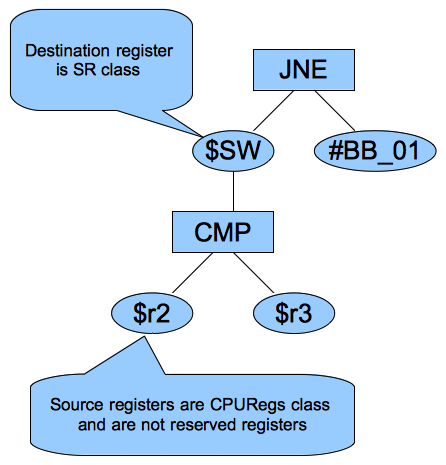
\includegraphics{11.png}
\caption{JNE (CMP \$r2, \$r3),}\label{ctrlflow:ctrlflow-f1}\end{figure}

\begin{Verbatim}[commandchars=\\\{\}]
cmp \%2, \%3
addiu \$r1, \$r2, 3   // \$r1 register never be allocated to \$SW
jne BasicBlock\_02
\end{Verbatim}

The reserved registers setting by the following
function code we defined before,
\paragraph{lbdex/Chapter8\_1/Cpu0RegisterInfo.cpp}

\begin{Verbatim}[commandchars=\\\{\}]
\PYG{c+c1}{// pure virtual method}
\PYG{n}{BitVector} \PYG{n}{Cpu0RegisterInfo}\PYG{o}{:}\PYG{o}{:}
\PYG{n}{getReservedRegs}\PYG{p}{(}\PYG{k}{const} \PYG{n}{MachineFunction} \PYG{o}{\PYGZam{}}\PYG{n}{MF}\PYG{p}{)} \PYG{k}{const} \PYG{p}{\PYGZob{}}
  \PYG{k}{static} \PYG{k}{const} \PYG{n}{uint16\PYGZus{}t} \PYG{n}{ReservedCPURegs}\PYG{p}{[}\PYG{p}{]} \PYG{o}{=} \PYG{p}{\PYGZob{}}
    \PYG{n}{Cpu0}\PYG{o}{:}\PYG{o}{:}\PYG{n}{ZERO}\PYG{p}{,} \PYG{n}{Cpu0}\PYG{o}{:}\PYG{o}{:}\PYG{n}{AT}\PYG{p}{,} \PYG{n}{Cpu0}\PYG{o}{:}\PYG{o}{:}\PYG{n}{SP}\PYG{p}{,} \PYG{n}{Cpu0}\PYG{o}{:}\PYG{o}{:}\PYG{n}{LR}\PYG{p}{,} \PYG{n}{Cpu0}\PYG{o}{:}\PYG{o}{:}\PYG{n}{PC}
  \PYG{p}{\PYGZcb{}}\PYG{p}{;}
  \PYG{n}{BitVector} \PYG{n}{Reserved}\PYG{p}{(}\PYG{n}{getNumRegs}\PYG{p}{(}\PYG{p}{)}\PYG{p}{)}\PYG{p}{;}
  \PYG{k}{typedef} \PYG{n}{TargetRegisterClass}\PYG{o}{:}\PYG{o}{:}\PYG{n}{iterator} \PYG{n}{RegIter}\PYG{p}{;}

  \PYG{k}{for} \PYG{p}{(}\PYG{k+kt}{unsigned} \PYG{n}{I} \PYG{o}{=} \PYG{l+m+mi}{0}\PYG{p}{;} \PYG{n}{I} \PYG{o}{\PYGZlt{}} \PYG{n}{array\PYGZus{}lengthof}\PYG{p}{(}\PYG{n}{ReservedCPURegs}\PYG{p}{)}\PYG{p}{;} \PYG{o}{+}\PYG{o}{+}\PYG{n}{I}\PYG{p}{)}
    \PYG{n}{Reserved}\PYG{p}{.}\PYG{n}{set}\PYG{p}{(}\PYG{n}{ReservedCPURegs}\PYG{p}{[}\PYG{n}{I}\PYG{p}{]}\PYG{p}{)}\PYG{p}{;}

  \PYG{k}{const} \PYG{n}{Cpu0FunctionInfo} \PYG{o}{*}\PYG{n}{Cpu0FI} \PYG{o}{=} \PYG{n}{MF}\PYG{p}{.}\PYG{n}{getInfo}\PYG{o}{\PYGZlt{}}\PYG{n}{Cpu0FunctionInfo}\PYG{o}{\PYGZgt{}}\PYG{p}{(}\PYG{p}{)}\PYG{p}{;}
  \PYG{c+c1}{// Reserve GP if globalBaseRegFixed()}
  \PYG{k}{if} \PYG{p}{(}\PYG{n}{Cpu0FI}\PYG{o}{-}\PYG{o}{\PYGZgt{}}\PYG{n}{globalBaseRegFixed}\PYG{p}{(}\PYG{p}{)}\PYG{p}{)}
    \PYG{n}{Reserved}\PYG{p}{.}\PYG{n}{set}\PYG{p}{(}\PYG{n}{Cpu0}\PYG{o}{:}\PYG{o}{:}\PYG{n}{GP}\PYG{p}{)}\PYG{p}{;}

  \PYG{k}{return} \PYG{n}{Reserved}\PYG{p}{;}
\PYG{p}{\PYGZcb{}}
\end{Verbatim}

Although the following definition in Cpu0RegisterInfo.td has no real effect in
Reserved Registers, you should comment the Reserved Registers in it for
readability. Setting SW into another register class to prevent the SW register
allocated to the register used by other instruction.
The copyPhysReg() is called when DestReg and SrcReg belong to different Register
Class.
\paragraph{lbdex/Chapter2/Cpu0RegisterInfo.td}

\begin{Verbatim}[commandchars=\\\{\}]
\PYG{c+c1}{//===----------------------------------------------------------------------===//}
\PYG{c+c1}{// Register Classes}
\PYG{c+c1}{//===----------------------------------------------------------------------===//}

\PYG{n}{def} \PYG{n}{CPURegs} \PYG{o}{:} \PYG{n}{RegisterClass}\PYG{o}{\PYGZlt{}}\PYG{l+s}{"}\PYG{l+s}{Cpu0}\PYG{l+s}{"}\PYG{p}{,} \PYG{p}{[}\PYG{n}{i32}\PYG{p}{]}\PYG{p}{,} \PYG{l+m+mi}{32}\PYG{p}{,} \PYG{p}{(}\PYG{n}{add}
  \PYG{c+c1}{// Reserved}
  \PYG{n}{ZERO}\PYG{p}{,} \PYG{n}{AT}\PYG{p}{,}
  \PYG{c+c1}{// Return Values and Arguments}
  \PYG{n}{V0}\PYG{p}{,} \PYG{n}{V1}\PYG{p}{,} \PYG{n}{A0}\PYG{p}{,} \PYG{n}{A1}\PYG{p}{,}
  \PYG{c+c1}{// Not preserved across procedure calls}
  \PYG{n}{T9}\PYG{p}{,} \PYG{n}{T0}\PYG{p}{,}
  \PYG{c+c1}{// Callee save}
  \PYG{n}{S0}\PYG{p}{,} \PYG{n}{S1}\PYG{p}{,} \PYG{n}{S2}\PYG{p}{,}
  \PYG{c+c1}{// Reserved}
  \PYG{n}{GP}\PYG{p}{,} \PYG{n}{FP}\PYG{p}{,}
  \PYG{n}{SP}\PYG{p}{,} \PYG{n}{LR}\PYG{p}{,} \PYG{n}{PC}\PYG{p}{)}\PYG{o}{\PYGZgt{}}\PYG{p}{;}
\PYG{p}{.}\PYG{p}{.}\PYG{p}{.}
\PYG{c+c1}{// Status Registers}
\PYG{n}{def} \PYG{n}{SR}   \PYG{o}{:} \PYG{n}{RegisterClass}\PYG{o}{\PYGZlt{}}\PYG{l+s}{"}\PYG{l+s}{Cpu0}\PYG{l+s}{"}\PYG{p}{,} \PYG{p}{[}\PYG{n}{i32}\PYG{p}{]}\PYG{p}{,} \PYG{l+m+mi}{32}\PYG{p}{,} \PYG{p}{(}\PYG{n}{add} \PYG{n}{SW}\PYG{p}{)}\PYG{o}{\PYGZgt{}}\PYG{p}{;}
\end{Verbatim}
\paragraph{lbdex/Chapter4\_2/Cpu0InstrInfo.cpp}

\begin{Verbatim}[commandchars=\\\{\}]
\PYG{c+c1}{//- Called when DestReg and SrcReg belong to different Register Class.}
\PYG{k+kt}{void} \PYG{n}{Cpu0InstrInfo}\PYG{o}{:}\PYG{o}{:}
\PYG{n}{copyPhysReg}\PYG{p}{(}\PYG{n}{MachineBasicBlock} \PYG{o}{\PYGZam{}}\PYG{n}{MBB}\PYG{p}{,}
      \PYG{n}{MachineBasicBlock}\PYG{o}{:}\PYG{o}{:}\PYG{n}{iterator} \PYG{n}{I}\PYG{p}{,} \PYG{n}{DebugLoc} \PYG{n}{DL}\PYG{p}{,}
      \PYG{k+kt}{unsigned} \PYG{n}{DestReg}\PYG{p}{,} \PYG{k+kt}{unsigned} \PYG{n}{SrcReg}\PYG{p}{,}
      \PYG{k+kt}{bool} \PYG{n}{KillSrc}\PYG{p}{)} \PYG{k}{const} \PYG{p}{\PYGZob{}}
  \PYG{k+kt}{unsigned} \PYG{n}{Opc} \PYG{o}{=} \PYG{l+m+mi}{0}\PYG{p}{,} \PYG{n}{ZeroReg} \PYG{o}{=} \PYG{l+m+mi}{0}\PYG{p}{;}

  \PYG{k}{if} \PYG{p}{(}\PYG{n}{Cpu0}\PYG{o}{:}\PYG{o}{:}\PYG{n}{CPURegsRegClass}\PYG{p}{.}\PYG{n}{contains}\PYG{p}{(}\PYG{n}{DestReg}\PYG{p}{)}\PYG{p}{)} \PYG{p}{\PYGZob{}} \PYG{c+c1}{// Copy to CPU Reg.}
    \PYG{p}{.}\PYG{p}{.}\PYG{p}{.}
    \PYG{k}{if} \PYG{p}{(}\PYG{n}{SrcReg} \PYG{o}{=}\PYG{o}{=} \PYG{n}{Cpu0}\PYG{o}{:}\PYG{o}{:}\PYG{n}{SW}\PYG{p}{)}
      \PYG{n}{Opc} \PYG{o}{=} \PYG{n}{Cpu0}\PYG{o}{:}\PYG{o}{:}\PYG{n}{MFSW}\PYG{p}{,} \PYG{n}{SrcReg} \PYG{o}{=} \PYG{l+m+mi}{0}\PYG{p}{;}
  \PYG{p}{\PYGZcb{}}
  \PYG{k}{else} \PYG{k}{if} \PYG{p}{(}\PYG{n}{Cpu0}\PYG{o}{:}\PYG{o}{:}\PYG{n}{CPURegsRegClass}\PYG{p}{.}\PYG{n}{contains}\PYG{p}{(}\PYG{n}{SrcReg}\PYG{p}{)}\PYG{p}{)} \PYG{p}{\PYGZob{}} \PYG{c+c1}{// Copy from CPU Reg.}
  \PYG{p}{.}\PYG{p}{.}\PYG{p}{.}
    \PYG{k}{if} \PYG{p}{(}\PYG{n}{DestReg} \PYG{o}{=}\PYG{o}{=} \PYG{n}{Cpu0}\PYG{o}{:}\PYG{o}{:}\PYG{n}{SW}\PYG{p}{)}
      \PYG{n}{Opc} \PYG{o}{=} \PYG{n}{Cpu0}\PYG{o}{:}\PYG{o}{:}\PYG{n}{MTSW}\PYG{p}{,} \PYG{n}{DestReg} \PYG{o}{=} \PYG{l+m+mi}{0}
  \PYG{p}{\PYGZcb{}}
\end{Verbatim}

Chapter8\_1/ include support for control flow statement.
Run with it as well as the following \code{llc} option, you can get the obj file
and dump it's content by gobjdump or hexdump as follows,

\begin{Verbatim}[commandchars=\\\{\}]
  118-165-79-206:InputFiles Jonathan\PYG{n+nv}{\PYGZdl{} }cat ch8\PYGZus{}1\PYGZus{}1.cpu0.s
  ...
  ld  \PYG{n+nv}{\PYGZdl{}4}, 36\PYG{o}{(}\PYG{n+nv}{\PYGZdl{}fp}\PYG{o}{)}
  cmp \PYG{n+nv}{\PYGZdl{}sw}, \PYG{n+nv}{\PYGZdl{}4}, \PYG{n+nv}{\PYGZdl{}3}
  jne \PYG{n+nv}{\PYGZdl{}BB0\PYGZus{}2}
  jmp \PYG{n+nv}{\PYGZdl{}BB0\PYGZus{}1}
\PYG{n+nv}{\PYGZdl{}BB0\PYGZus{}1}:                                 \PYG{c}{\PYGZsh{} \PYGZpc{}if.then}
  ld  \PYG{n+nv}{\PYGZdl{}4}, 36\PYG{o}{(}\PYG{n+nv}{\PYGZdl{}fp}\PYG{o}{)}
  addiu \PYG{n+nv}{\PYGZdl{}4}, \PYG{n+nv}{\PYGZdl{}4}, 1
  st  \PYG{n+nv}{\PYGZdl{}4}, 36\PYG{o}{(}\PYG{n+nv}{\PYGZdl{}fp}\PYG{o}{)}
\PYG{n+nv}{\PYGZdl{}BB0\PYGZus{}2}:                                 \PYG{c}{\PYGZsh{} \PYGZpc{}if.end}
  ld  \PYG{n+nv}{\PYGZdl{}4}, 32\PYG{o}{(}\PYG{n+nv}{\PYGZdl{}fp}\PYG{o}{)}
  ...
\end{Verbatim}

\begin{Verbatim}[commandchars=\\\{\}]
118-165-79-206:InputFiles Jonathan\PYG{n+nv}{\PYGZdl{} }/Users/Jonathan/llvm/test/
cmake\PYGZus{}debug\PYGZus{}build/bin/Debug/llc -march\PYG{o}{=}cpu0 -relocation-model\PYG{o}{=}pic -filetype\PYG{o}{=}obj
ch8\PYGZus{}1\PYGZus{}1.bc -o ch8\PYGZus{}1\PYGZus{}1.cpu0.o

118-165-79-206:InputFiles Jonathan\PYG{n+nv}{\PYGZdl{} }hexdump ch8\PYGZus{}1\PYGZus{}1.cpu0.o
    // jmp offset is \PYG{n+nv}{0x10}\PYG{o}{=}16 bytes which is correct
0000080 ...................................... 10 43 00 00
0000090 31 00 00 10 36 00 00 00 ..........................
\end{Verbatim}

The immediate value of jne (op 0x31) is 16; The offset between jne and \$BB0\_2
is 20 (5 words = 5*4 bytes). Suppose the jne address is X, then the label
\$BB0\_2 is X+20.
Cpu0 is a RISC cpu0 with 3 stages of pipeline which are fetch, decode and
execution according to cpu0 web site information.
The cpu0 do branch instruction execution at decode stage which like mips.
After the jne instruction fetched, the PC (Program Counter) is X+4 since cpu0
update PC at fetch stage.
The \$BB0\_2 address is equal to PC+16 for the jne branch instruction execute at
decode stage.
List and explain this again as follows,

\begin{Verbatim}[commandchars=\\\{\}]
              // Fetch instruction stage \PYG{k}{for }jne instruction. The fetch stage
              // can be divided into 2 cycles. First cycle fetch the
              // instruction. Second cycle adjust \PYG{n+nv}{PC} \PYG{o}{=} PC+4.
  jne \PYG{n+nv}{\PYGZdl{}BB0\PYGZus{}2}  // Do jne compare in decode stage. \PYG{n+nv}{PC} \PYG{o}{=} X+4 at this stage.
              // When jne immediate value is 16, \PYG{n+nv}{PC} \PYG{o}{=} PC+16. It will fetch
              //  X+20 which equal to label \PYG{n+nv}{\PYGZdl{}BB0\PYGZus{}2} instruction, ld \PYG{n+nv}{\PYGZdl{}2}, 28\PYG{o}{(}\PYG{n+nv}{\PYGZdl{}sp}\PYG{o}{)}.
  jmp \PYG{n+nv}{\PYGZdl{}BB0\PYGZus{}1}
\PYG{n+nv}{\PYGZdl{}BB0\PYGZus{}1}:                                 \PYG{c}{\PYGZsh{} \PYGZpc{}if.then}
  ld  \PYG{n+nv}{\PYGZdl{}4}, 36\PYG{o}{(}\PYG{n+nv}{\PYGZdl{}fp}\PYG{o}{)}
  addiu \PYG{n+nv}{\PYGZdl{}4}, \PYG{n+nv}{\PYGZdl{}4}, 1
  st  \PYG{n+nv}{\PYGZdl{}4}, 36\PYG{o}{(}\PYG{n+nv}{\PYGZdl{}fp}\PYG{o}{)}
\PYG{n+nv}{\PYGZdl{}BB0\PYGZus{}2}:                                 \PYG{c}{\PYGZsh{} \PYGZpc{}if.end}
  ld  \PYG{n+nv}{\PYGZdl{}4}, 32\PYG{o}{(}\PYG{n+nv}{\PYGZdl{}fp}\PYG{o}{)}
\end{Verbatim}

If cpu0 do \textbf{``jne''} compare in execution stage, then we should set PC=PC+12,
offset of (\$BB0\_2, jn e \$BB02) – 8, in this example.

Cpu0 is for teaching purpose and didn't consider the performance with design.
In reality, the conditional branch is important in performance of CPU design.
According bench mark information, every 7 instructions will meet 1 branch
instruction in average.
Cpu0 take 2 instructions for conditional branch, (jne(cmp...)), while Mips use
one instruction (bne).

Finally we list the code added for full support of control flow statement,
\paragraph{lbdex/Chapter8\_1/MCTargetDesc/Cpu0MCCodeEmitter.cpp}

\begin{Verbatim}[commandchars=\\\{\}]
  \PYG{c+c1}{// getBranch24TargetOpValue - Return binary encoding of the branch}
  \PYG{c+c1}{// target operand, such as JMP \PYGZsh{}BB01, JEQ, JSUB. If the machine operand}
  \PYG{c+c1}{// requires relocation, record the relocation and return zero.}
  \PYG{k+kt}{unsigned} \PYG{n}{getBranch24TargetOpValue}\PYG{p}{(}\PYG{k}{const} \PYG{n}{MCInst} \PYG{o}{\PYGZam{}}\PYG{n}{MI}\PYG{p}{,} \PYG{k+kt}{unsigned} \PYG{n}{OpNo}\PYG{p}{,}
                                  \PYG{n}{SmallVectorImpl}\PYG{o}{\PYGZlt{}}\PYG{n}{MCFixup}\PYG{o}{\PYGZgt{}} \PYG{o}{\PYGZam{}}\PYG{n}{Fixups}\PYG{p}{)} \PYG{k}{const}\PYG{p}{;}
                                  
  \PYG{c+c1}{// getJumpTargetOpValue - Return binary encoding of the jump}
  \PYG{c+c1}{// target operand, such as SWI \PYGZsh{}interrupt\PYGZus{}addr and JSUB \PYGZsh{}function\PYGZus{}addr. }
  \PYG{c+c1}{// If the machine operand requires relocation,}
  \PYG{c+c1}{// record the relocation and return zero.}
   \PYG{k+kt}{unsigned} \PYG{n}{getJumpTargetOpValue}\PYG{p}{(}\PYG{k}{const} \PYG{n}{MCInst} \PYG{o}{\PYGZam{}}\PYG{n}{MI}\PYG{p}{,} \PYG{k+kt}{unsigned} \PYG{n}{OpNo}\PYG{p}{,}
                                 \PYG{n}{SmallVectorImpl}\PYG{o}{\PYGZlt{}}\PYG{n}{MCFixup}\PYG{o}{\PYGZgt{}} \PYG{o}{\PYGZam{}}\PYG{n}{Fixups}\PYG{p}{)} \PYG{k}{const}\PYG{p}{;}
  \PYG{c+c1}{// lbd document - mark - unsigned getJumpTargetOpValue}
\end{Verbatim}

\begin{Verbatim}[commandchars=\\\{\}]
\PYG{c+c1}{/// getBranch24TargetOpValue - Return binary encoding of the branch}
\PYG{c+c1}{/// target operand. If the machine operand requires relocation,}
\PYG{c+c1}{/// record the relocation and return zero.}
\PYG{k+kt}{unsigned} \PYG{n}{Cpu0MCCodeEmitter}\PYG{o}{:}\PYG{o}{:}
\PYG{n}{getBranch24TargetOpValue}\PYG{p}{(}\PYG{k}{const} \PYG{n}{MCInst} \PYG{o}{\PYGZam{}}\PYG{n}{MI}\PYG{p}{,} \PYG{k+kt}{unsigned} \PYG{n}{OpNo}\PYG{p}{,}
                       \PYG{n}{SmallVectorImpl}\PYG{o}{\PYGZlt{}}\PYG{n}{MCFixup}\PYG{o}{\PYGZgt{}} \PYG{o}{\PYGZam{}}\PYG{n}{Fixups}\PYG{p}{)} \PYG{k}{const} \PYG{p}{\PYGZob{}}

  \PYG{k}{const} \PYG{n}{MCOperand} \PYG{o}{\PYGZam{}}\PYG{n}{MO} \PYG{o}{=} \PYG{n}{MI}\PYG{p}{.}\PYG{n}{getOperand}\PYG{p}{(}\PYG{n}{OpNo}\PYG{p}{)}\PYG{p}{;}

  \PYG{c+c1}{// If the destination is an immediate, we have nothing to do.}
  \PYG{k}{if} \PYG{p}{(}\PYG{n}{MO}\PYG{p}{.}\PYG{n}{isImm}\PYG{p}{(}\PYG{p}{)}\PYG{p}{)} \PYG{k}{return} \PYG{n}{MO}\PYG{p}{.}\PYG{n}{getImm}\PYG{p}{(}\PYG{p}{)}\PYG{p}{;}
  \PYG{n}{assert}\PYG{p}{(}\PYG{n}{MO}\PYG{p}{.}\PYG{n}{isExpr}\PYG{p}{(}\PYG{p}{)} \PYG{o}{\PYGZam{}}\PYG{o}{\PYGZam{}} \PYG{l+s}{"}\PYG{l+s}{getBranch24TargetOpValue expects only expressions}\PYG{l+s}{"}\PYG{p}{)}\PYG{p}{;}

  \PYG{k}{const} \PYG{n}{MCExpr} \PYG{o}{*}\PYG{n}{Expr} \PYG{o}{=} \PYG{n}{MO}\PYG{p}{.}\PYG{n}{getExpr}\PYG{p}{(}\PYG{p}{)}\PYG{p}{;}
  \PYG{n}{Fixups}\PYG{p}{.}\PYG{n}{push\PYGZus{}back}\PYG{p}{(}\PYG{n}{MCFixup}\PYG{o}{:}\PYG{o}{:}\PYG{n}{Create}\PYG{p}{(}\PYG{l+m+mi}{0}\PYG{p}{,} \PYG{n}{Expr}\PYG{p}{,}
                                   \PYG{n}{MCFixupKind}\PYG{p}{(}\PYG{n}{Cpu0}\PYG{o}{:}\PYG{o}{:}\PYG{n}{fixup\PYGZus{}Cpu0\PYGZus{}PC24}\PYG{p}{)}\PYG{p}{)}\PYG{p}{)}\PYG{p}{;}
  \PYG{k}{return} \PYG{l+m+mi}{0}\PYG{p}{;}
\PYG{p}{\PYGZcb{}}

\PYG{c+c1}{/// getJumpTargetOpValue - Return binary encoding of the jump}
\PYG{c+c1}{/// target operand. Such as SWI and JSUB. }
\PYG{c+c1}{/// If the machine operand requires relocation,}
\PYG{c+c1}{/// record the relocation and return zero.}
\PYG{k+kt}{unsigned} \PYG{n}{Cpu0MCCodeEmitter}\PYG{o}{:}\PYG{o}{:}
\PYG{n}{getJumpTargetOpValue}\PYG{p}{(}\PYG{k}{const} \PYG{n}{MCInst} \PYG{o}{\PYGZam{}}\PYG{n}{MI}\PYG{p}{,} \PYG{k+kt}{unsigned} \PYG{n}{OpNo}\PYG{p}{,}
                     \PYG{n}{SmallVectorImpl}\PYG{o}{\PYGZlt{}}\PYG{n}{MCFixup}\PYG{o}{\PYGZgt{}} \PYG{o}{\PYGZam{}}\PYG{n}{Fixups}\PYG{p}{)} \PYG{k}{const} \PYG{p}{\PYGZob{}}

  \PYG{k+kt}{unsigned} \PYG{n}{Opcode} \PYG{o}{=} \PYG{n}{MI}\PYG{p}{.}\PYG{n}{getOpcode}\PYG{p}{(}\PYG{p}{)}\PYG{p}{;}
  \PYG{k}{const} \PYG{n}{MCOperand} \PYG{o}{\PYGZam{}}\PYG{n}{MO} \PYG{o}{=} \PYG{n}{MI}\PYG{p}{.}\PYG{n}{getOperand}\PYG{p}{(}\PYG{n}{OpNo}\PYG{p}{)}\PYG{p}{;}
  \PYG{c+c1}{// If the destination is an immediate, we have nothing to do.}
  \PYG{k}{if} \PYG{p}{(}\PYG{n}{MO}\PYG{p}{.}\PYG{n}{isImm}\PYG{p}{(}\PYG{p}{)}\PYG{p}{)} \PYG{k}{return} \PYG{n}{MO}\PYG{p}{.}\PYG{n}{getImm}\PYG{p}{(}\PYG{p}{)}\PYG{p}{;}
  \PYG{n}{assert}\PYG{p}{(}\PYG{n}{MO}\PYG{p}{.}\PYG{n}{isExpr}\PYG{p}{(}\PYG{p}{)} \PYG{o}{\PYGZam{}}\PYG{o}{\PYGZam{}} \PYG{l+s}{"}\PYG{l+s}{getJumpTargetOpValue expects only expressions}\PYG{l+s}{"}\PYG{p}{)}\PYG{p}{;}

  \PYG{k}{const} \PYG{n}{MCExpr} \PYG{o}{*}\PYG{n}{Expr} \PYG{o}{=} \PYG{n}{MO}\PYG{p}{.}\PYG{n}{getExpr}\PYG{p}{(}\PYG{p}{)}\PYG{p}{;}
  \PYG{k}{if} \PYG{p}{(}\PYG{n}{Opcode} \PYG{o}{=}\PYG{o}{=} \PYG{n}{Cpu0}\PYG{o}{:}\PYG{o}{:}\PYG{n}{JSUB} \PYG{o}{\textbar{}}\PYG{o}{\textbar{}} \PYG{n}{Opcode} \PYG{o}{=}\PYG{o}{=} \PYG{n}{Cpu0}\PYG{o}{:}\PYG{o}{:}\PYG{n}{JMP}\PYG{p}{)}
    \PYG{n}{Fixups}\PYG{p}{.}\PYG{n}{push\PYGZus{}back}\PYG{p}{(}\PYG{n}{MCFixup}\PYG{o}{:}\PYG{o}{:}\PYG{n}{Create}\PYG{p}{(}\PYG{l+m+mi}{0}\PYG{p}{,} \PYG{n}{Expr}\PYG{p}{,}
                                     \PYG{n}{MCFixupKind}\PYG{p}{(}\PYG{n}{Cpu0}\PYG{o}{:}\PYG{o}{:}\PYG{n}{fixup\PYGZus{}Cpu0\PYGZus{}PC24}\PYG{p}{)}\PYG{p}{)}\PYG{p}{)}\PYG{p}{;}
  \PYG{k}{else} \PYG{k}{if} \PYG{p}{(}\PYG{n}{Opcode} \PYG{o}{=}\PYG{o}{=} \PYG{n}{Cpu0}\PYG{o}{:}\PYG{o}{:}\PYG{n}{SWI}\PYG{p}{)}
    \PYG{n}{Fixups}\PYG{p}{.}\PYG{n}{push\PYGZus{}back}\PYG{p}{(}\PYG{n}{MCFixup}\PYG{o}{:}\PYG{o}{:}\PYG{n}{Create}\PYG{p}{(}\PYG{l+m+mi}{0}\PYG{p}{,} \PYG{n}{Expr}\PYG{p}{,}
                                     \PYG{n}{MCFixupKind}\PYG{p}{(}\PYG{n}{Cpu0}\PYG{o}{:}\PYG{o}{:}\PYG{n}{fixup\PYGZus{}Cpu0\PYGZus{}24}\PYG{p}{)}\PYG{p}{)}\PYG{p}{)}\PYG{p}{;}
  \PYG{k}{else}
    \PYG{n}{llvm\PYGZus{}unreachable}\PYG{p}{(}\PYG{l+s}{"}\PYG{l+s}{unexpect opcode in getJumpAbsoluteTargetOpValue()}\PYG{l+s}{"}\PYG{p}{)}\PYG{p}{;}
  \PYG{k}{return} \PYG{l+m+mi}{0}\PYG{p}{;}
\PYG{p}{\PYGZcb{}} \PYG{c+c1}{// lbd document - mark - getJumpTargetOpValue}
\end{Verbatim}
\paragraph{lbdex/Chapter8\_1/Cpu0ISelLowering.cpp}

\begin{Verbatim}[commandchars=\\\{\}]
\PYG{n}{Cpu0TargetLowering}\PYG{o}{:}\PYG{o}{:}
\PYG{n}{Cpu0TargetLowering}\PYG{p}{(}\PYG{n}{Cpu0TargetMachine} \PYG{o}{\PYGZam{}}\PYG{n}{TM}\PYG{p}{)}
  \PYG{o}{:} \PYG{n}{TargetLowering}\PYG{p}{(}\PYG{n}{TM}\PYG{p}{,} \PYG{k}{new} \PYG{n}{Cpu0TargetObjectFile}\PYG{p}{(}\PYG{p}{)}\PYG{p}{)}\PYG{p}{,}
    \PYG{n}{Subtarget}\PYG{p}{(}\PYG{o}{\PYGZam{}}\PYG{n}{TM}\PYG{p}{.}\PYG{n}{getSubtarget}\PYG{o}{\PYGZlt{}}\PYG{n}{Cpu0Subtarget}\PYG{o}{\PYGZgt{}}\PYG{p}{(}\PYG{p}{)}\PYG{p}{)} \PYG{p}{\PYGZob{}}
  \PYG{p}{.}\PYG{p}{.}\PYG{p}{.}
  \PYG{c+c1}{// Used by legalize types to correctly generate the setcc result.}
  \PYG{c+c1}{// Without this, every float setcc comes with a AND/OR with the result,}
  \PYG{c+c1}{// we don't want this, since the fpcmp result goes to a flag register,}
  \PYG{c+c1}{// which is used implicitly by brcond and select operations.}
  \PYG{n}{AddPromotedToType}\PYG{p}{(}\PYG{n}{ISD}\PYG{o}{:}\PYG{o}{:}\PYG{n}{SETCC}\PYG{p}{,} \PYG{n}{MVT}\PYG{o}{:}\PYG{o}{:}\PYG{n}{i1}\PYG{p}{,} \PYG{n}{MVT}\PYG{o}{:}\PYG{o}{:}\PYG{n}{i32}\PYG{p}{)}\PYG{p}{;}
  \PYG{p}{.}\PYG{p}{.}\PYG{p}{.}
  \PYG{n}{setOperationAction}\PYG{p}{(}\PYG{n}{ISD}\PYG{o}{:}\PYG{o}{:}\PYG{n}{BRCOND}\PYG{p}{,}             \PYG{n}{MVT}\PYG{o}{:}\PYG{o}{:}\PYG{n}{Other}\PYG{p}{,} \PYG{n}{Custom}\PYG{p}{)}\PYG{p}{;}
  \PYG{p}{.}\PYG{p}{.}\PYG{p}{.}
  \PYG{c+c1}{// Operations not directly supported by Cpu0.}
  \PYG{n}{setOperationAction}\PYG{p}{(}\PYG{n}{ISD}\PYG{o}{:}\PYG{o}{:}\PYG{n}{BR\PYGZus{}CC}\PYG{p}{,}             \PYG{n}{MVT}\PYG{o}{:}\PYG{o}{:}\PYG{n}{i32}\PYG{p}{,} \PYG{n}{Expand}\PYG{p}{)}\PYG{p}{;}
  \PYG{p}{.}\PYG{p}{.}\PYG{p}{.}
\PYG{p}{\PYGZcb{}}
\PYG{p}{.}\PYG{p}{.}\PYG{p}{.}
\PYG{n}{SDValue} \PYG{n}{Cpu0TargetLowering}\PYG{o}{:}\PYG{o}{:}
\PYG{n}{LowerOperation}\PYG{p}{(}\PYG{n}{SDValue} \PYG{n}{Op}\PYG{p}{,} \PYG{n}{SelectionDAG} \PYG{o}{\PYGZam{}}\PYG{n}{DAG}\PYG{p}{)} \PYG{k}{const}
\PYG{p}{\PYGZob{}}
  \PYG{k}{switch} \PYG{p}{(}\PYG{n}{Op}\PYG{p}{.}\PYG{n}{getOpcode}\PYG{p}{(}\PYG{p}{)}\PYG{p}{)}
  \PYG{p}{\PYGZob{}}
    \PYG{k}{case} \PYG{n}{ISD}\PYG{o}{:}\PYG{o}{:}\PYG{n+nl}{BRCOND:}             \PYG{k}{return} \PYG{n}{LowerBRCOND}\PYG{p}{(}\PYG{n}{Op}\PYG{p}{,} \PYG{n}{DAG}\PYG{p}{)}\PYG{p}{;}
    \PYG{p}{.}\PYG{p}{.}\PYG{p}{.}
  \PYG{p}{\PYGZcb{}}
  \PYG{p}{.}\PYG{p}{.}\PYG{p}{.}
\PYG{p}{\PYGZcb{}}
\PYG{p}{.}\PYG{p}{.}\PYG{p}{.}
\PYG{n}{SDValue} \PYG{n}{Cpu0TargetLowering}\PYG{o}{:}\PYG{o}{:}
\PYG{n}{LowerBRCOND}\PYG{p}{(}\PYG{n}{SDValue} \PYG{n}{Op}\PYG{p}{,} \PYG{n}{SelectionDAG} \PYG{o}{\PYGZam{}}\PYG{n}{DAG}\PYG{p}{)} \PYG{k}{const}
\PYG{p}{\PYGZob{}}
  \PYG{k}{return} \PYG{n}{Op}\PYG{p}{;}
\PYG{p}{\PYGZcb{}}
\end{Verbatim}
\paragraph{lbdex/Chapter8\_1/Cpu0ISelLowering.h}

\begin{Verbatim}[commandchars=\\\{\}]
\PYG{n}{SDValue} \PYG{n}{LowerBRCOND}\PYG{p}{(}\PYG{n}{SDValue} \PYG{n}{Op}\PYG{p}{,} \PYG{n}{SelectionDAG} \PYG{o}{\PYGZam{}}\PYG{n}{DAG}\PYG{p}{)} \PYG{k}{const}\PYG{p}{;}
\end{Verbatim}
\paragraph{lbdex/Chapter8\_1/Cpu0MCInstLower.cpp}

\begin{Verbatim}[commandchars=\\\{\}]
\PYG{n}{MCOperand} \PYG{n}{Cpu0MCInstLower}\PYG{o}{:}\PYG{o}{:}\PYG{n}{LowerSymbolOperand}\PYG{p}{(}\PYG{k}{const} \PYG{n}{MachineOperand} \PYG{o}{\PYGZam{}}\PYG{n}{MO}\PYG{p}{,}
                                              \PYG{n}{MachineOperandType} \PYG{n}{MOTy}\PYG{p}{,}
                                              \PYG{k+kt}{unsigned} \PYG{n}{Offset}\PYG{p}{)} \PYG{k}{const} \PYG{p}{\PYGZob{}}
  \PYG{p}{.}\PYG{p}{.}\PYG{p}{.}
  \PYG{k}{switch} \PYG{p}{(}\PYG{n}{MOTy}\PYG{p}{)} \PYG{p}{\PYGZob{}}
  \PYG{p}{.}\PYG{p}{.}\PYG{p}{.}
  \PYG{k}{case} \PYG{n}{MachineOperand}\PYG{o}{:}\PYG{o}{:}\PYG{n+nl}{MO\PYGZus{}MachineBasicBlock:}
    \PYG{n}{Symbol} \PYG{o}{=} \PYG{n}{MO}\PYG{p}{.}\PYG{n}{getMBB}\PYG{p}{(}\PYG{p}{)}\PYG{o}{-}\PYG{o}{\PYGZgt{}}\PYG{n}{getSymbol}\PYG{p}{(}\PYG{p}{)}\PYG{p}{;}
    \PYG{k}{break}\PYG{p}{;}
  \PYG{p}{.}\PYG{p}{.}\PYG{p}{.}
  \PYG{k}{case} \PYG{n}{MachineOperand}\PYG{o}{:}\PYG{o}{:}\PYG{n+nl}{MO\PYGZus{}BlockAddress:}
  \PYG{n}{Symbol} \PYG{o}{=} \PYG{n}{AsmPrinter}\PYG{p}{.}\PYG{n}{GetBlockAddressSymbol}\PYG{p}{(}\PYG{n}{MO}\PYG{p}{.}\PYG{n}{getBlockAddress}\PYG{p}{(}\PYG{p}{)}\PYG{p}{)}\PYG{p}{;}
  \PYG{n}{Offset} \PYG{o}{+}\PYG{o}{=} \PYG{n}{MO}\PYG{p}{.}\PYG{n}{getOffset}\PYG{p}{(}\PYG{p}{)}\PYG{p}{;}
  \PYG{k}{break}\PYG{p}{;}
  \PYG{p}{.}\PYG{p}{.}\PYG{p}{.}
\PYG{p}{\PYGZcb{}}

\PYG{n}{MCOperand} \PYG{n}{Cpu0MCInstLower}\PYG{o}{:}\PYG{o}{:}\PYG{n}{LowerOperand}\PYG{p}{(}\PYG{k}{const} \PYG{n}{MachineOperand}\PYG{o}{\PYGZam{}} \PYG{n}{MO}\PYG{p}{,}
                                        \PYG{k+kt}{unsigned} \PYG{n}{offset}\PYG{p}{)} \PYG{k}{const} \PYG{p}{\PYGZob{}}
  \PYG{n}{MachineOperandType} \PYG{n}{MOTy} \PYG{o}{=} \PYG{n}{MO}\PYG{p}{.}\PYG{n}{getType}\PYG{p}{(}\PYG{p}{)}\PYG{p}{;}

  \PYG{k}{switch} \PYG{p}{(}\PYG{n}{MOTy}\PYG{p}{)} \PYG{p}{\PYGZob{}}
  \PYG{p}{.}\PYG{p}{.}\PYG{p}{.}
  \PYG{k}{case} \PYG{n}{MachineOperand}\PYG{o}{:}\PYG{o}{:}\PYG{n+nl}{MO\PYGZus{}MachineBasicBlock:}
  \PYG{p}{.}\PYG{p}{.}\PYG{p}{.}
  \PYG{k}{case} \PYG{n}{MachineOperand}\PYG{o}{:}\PYG{o}{:}\PYG{n+nl}{MO\PYGZus{}BlockAddress:}
  \PYG{p}{.}\PYG{p}{.}\PYG{p}{.}
  \PYG{p}{\PYGZcb{}}
  \PYG{p}{.}\PYG{p}{.}\PYG{p}{.}
\PYG{p}{\PYGZcb{}}
\end{Verbatim}
\paragraph{lbdex/Chapter8\_1/Cpu0InstrFormats.td}

\begin{Verbatim}[commandchars=\\\{\}]
\PYG{c+c1}{//===----------------------------------------------------------------------===//}
\PYG{c+c1}{// Format J instruction class in Cpu0 : \PYGZlt{}\textbar{}opcode\textbar{}address\textbar{}\PYGZgt{}}
\PYG{c+c1}{//===----------------------------------------------------------------------===//}

\PYG{k}{class} \PYG{n+nc}{FJ}\PYG{o}{\PYGZlt{}}\PYG{n}{bits}\PYG{o}{\PYGZlt{}}\PYG{l+m+mi}{8}\PYG{o}{\PYGZgt{}} \PYG{n}{op}\PYG{p}{,} \PYG{n}{dag} \PYG{n}{outs}\PYG{p}{,} \PYG{n}{dag} \PYG{n}{ins}\PYG{p}{,} \PYG{n}{string} \PYG{n}{asmstr}\PYG{p}{,} \PYG{n}{list}\PYG{o}{\PYGZlt{}}\PYG{n}{dag}\PYG{o}{\PYGZgt{}} \PYG{n}{pattern}\PYG{p}{,}
                 \PYG{n}{InstrItinClass} \PYG{n}{itin}\PYG{o}{\PYGZgt{}}\PYG{o}{:} \PYG{n}{Cpu0Inst}\PYG{o}{\PYGZlt{}}\PYG{n}{outs}\PYG{p}{,} \PYG{n}{ins}\PYG{p}{,} \PYG{n}{asmstr}\PYG{p}{,} \PYG{n}{pattern}\PYG{p}{,} \PYG{n}{itin}\PYG{p}{,} \PYG{n}{FrmJ}\PYG{o}{\PYGZgt{}}
\PYG{p}{\PYGZob{}}
  \PYG{n}{bits}\PYG{o}{\PYGZlt{}}\PYG{l+m+mi}{24}\PYG{o}{\PYGZgt{}} \PYG{n}{addr}\PYG{p}{;}

  \PYG{n}{let} \PYG{n}{Opcode} \PYG{o}{=} \PYG{n}{op}\PYG{p}{;}

  \PYG{n}{let} \PYG{n}{Inst}\PYG{p}{\PYGZob{}}\PYG{l+m+mi}{23}\PYG{o}{-}\PYG{l+m+mi}{0}\PYG{p}{\PYGZcb{}} \PYG{o}{=} \PYG{n}{addr}\PYG{p}{;}
\PYG{p}{\PYGZcb{}}
\end{Verbatim}
\paragraph{lbdex/Chapter8\_1/Cpu0InstrInfo.td}

\begin{Verbatim}[commandchars=\\\{\}]
// Cpu0InstrInfo.td
// Instruction operand types
def brtarget24    : Operand\textless{}OtherVT\textgreater{} \PYGZob{}
  let EncoderMethod = "getBranchTargetOpValue";
  let OperandType = "OPERAND\_PCREL";
  let DecoderMethod = "DecodeBranchTarget";
\PYGZcb{}
// JMP
def jmptarget    : Operand\textless{}OtherVT\textgreater{} \PYGZob{}
  let EncoderMethod = "getJumpTargetOpValue";
  let OperandType = "OPERAND\_PCREL";
  let DecoderMethod = "DecodeJumpRelativeTarget";
\PYGZcb{}
...
  /// Conditional Branch
      class CBranch24\textless{}bits\textless{}8\textgreater{} op, string instr\_asm, RegisterClass RC,
                                         list\textless{}Register\textgreater{} UseRegs\textgreater{}:
        FJ\textless{}op, (outs), (ins RC:\$ra, brtarget:\$addr),
                               !strconcat(instr\_asm, "\PYGZbs{}t\$addr"),
                               [], IIBranch\textgreater{} \PYGZob{}
        let isBranch = 1;
        let isTerminator = 1;
        let hasDelaySlot = 0;
        let neverHasSideEffects = 1;
      \PYGZcb{}

      // Unconditional branch, such as JMP
      class UncondBranch\textless{}bits\textless{}8\textgreater{} op, string instr\_asm\textgreater{}:
        FJ\textless{}op, (outs), (ins brtarget:\$addr),
                               !strconcat(instr\_asm, "\PYGZbs{}t\$addr"), [(br bb:\$addr)], IIBranch\textgreater{} \PYGZob{}
        let isBranch = 1;
        let isTerminator = 1;
        let isBarrier = 1;
        let hasDelaySlot = 0;
      \PYGZcb{}
  ...
  /// Jump and Branch Instructions
  def JEQ     : CBranch\textless{}0x30, "jeq", CPURegs\textgreater{};
  def JNE     : CBranch\textless{}0x31, "jne", CPURegs\textgreater{};
  def JLT     : CBranch\textless{}0x32, "jlt", CPURegs\textgreater{};
  def JGT     : CBranch\textless{}0x33, "jgt", CPURegs\textgreater{};
  def JLE     : CBranch\textless{}0x34, "jle", CPURegs\textgreater{};
  def JGE     : CBranch\textless{}0x35, "jge", CPURegs\textgreater{};
  def JMP     : UncondBranch\textless{}0x36, "jmp"\textgreater{};
  ...
  // brcond patterns
  multiclass BrcondPats\textless{}RegisterClass RC, Instruction JEQOp,
    Instruction JNEOp, Instruction JLTOp, Instruction JGTOp,
    Instruction JLEOp, Instruction JGEOp, Instruction CMPOp,
    Register ZEROReg\textgreater{} \PYGZob{}
  def : Pat\textless{}(brcond (i32 (seteq RC:\$lhs, RC:\$rhs)), bb:\$dst),
            (JEQOp (CMPOp RC:\$lhs, RC:\$rhs), bb:\$dst)\textgreater{};
  def : Pat\textless{}(brcond (i32 (setueq RC:\$lhs, RC:\$rhs)), bb:\$dst),
            (JEQOp (CMPOp RC:\$lhs, RC:\$rhs), bb:\$dst)\textgreater{};
  def : Pat\textless{}(brcond (i32 (setne RC:\$lhs, RC:\$rhs)), bb:\$dst),
            (JNEOp (CMPOp RC:\$lhs, RC:\$rhs), bb:\$dst)\textgreater{};
  def : Pat\textless{}(brcond (i32 (setune RC:\$lhs, RC:\$rhs)), bb:\$dst),
            (JNEOp (CMPOp RC:\$lhs, RC:\$rhs), bb:\$dst)\textgreater{};
  def : Pat\textless{}(brcond (i32 (setlt RC:\$lhs, RC:\$rhs)), bb:\$dst),
            (JLTOp (CMPOp RC:\$lhs, RC:\$rhs), bb:\$dst)\textgreater{};
  def : Pat\textless{}(brcond (i32 (setult RC:\$lhs, RC:\$rhs)), bb:\$dst),
            (JLTOp (CMPOp RC:\$lhs, RC:\$rhs), bb:\$dst)\textgreater{};
  def : Pat\textless{}(brcond (i32 (setgt RC:\$lhs, RC:\$rhs)), bb:\$dst),
            (JGTOp (CMPOp RC:\$lhs, RC:\$rhs), bb:\$dst)\textgreater{};
  def : Pat\textless{}(brcond (i32 (setugt RC:\$lhs, RC:\$rhs)), bb:\$dst),
            (JGTOp (CMPOp RC:\$lhs, RC:\$rhs), bb:\$dst)\textgreater{};
  def : Pat\textless{}(brcond (i32 (setle RC:\$lhs, RC:\$rhs)), bb:\$dst),
            (JLEOp (CMPOp RC:\$rhs, RC:\$lhs), bb:\$dst)\textgreater{};
  def : Pat\textless{}(brcond (i32 (setule RC:\$lhs, RC:\$rhs)), bb:\$dst),
            (JLEOp (CMPOp RC:\$rhs, RC:\$lhs), bb:\$dst)\textgreater{};
  def : Pat\textless{}(brcond (i32 (setge RC:\$lhs, RC:\$rhs)), bb:\$dst),
            (JGEOp (CMPOp RC:\$lhs, RC:\$rhs), bb:\$dst)\textgreater{};
  def : Pat\textless{}(brcond (i32 (setuge RC:\$lhs, RC:\$rhs)), bb:\$dst),
            (JGEOp (CMPOp RC:\$lhs, RC:\$rhs), bb:\$dst)\textgreater{};

  def : Pat\textless{}(brcond RC:\$cond, bb:\$dst),
            (JNEOp (CMPOp RC:\$cond, ZEROReg), bb:\$dst)\textgreater{};
  \PYGZcb{}

  defm : BrcondPats\textless{}CPURegs, JEQ, JNE, JLT, JGT, JLE, JGE, CMP, ZERO\textgreater{};
\end{Verbatim}

The ch8\_1\_2.cpp is for \textbf{“nest if”} test. The ch8\_1\_3.cpp is the
\textbf{“for loop”} as well as \textbf{“while loop”}, \textbf{“continue”}, \textbf{“break”},
\textbf{“goto”} test. The ch8\_1\_5.cpp is for \textbf{“goto”} test.
You can run with them if you like to test more.

The ch8\_1\_4.cpp is for test C operators \textbf{==, !=, \&\&, \textbar{}\textbar{}}. No code need to
add since we have take care them before.
But it can be test only when the control flow statement support is ready, as
follows,
\paragraph{lbdex/InputFiles/ch8\_1\_4.cpp}

\begin{Verbatim}[commandchars=\\\{\}]
\PYG{k+kt}{int} \PYG{n}{main}\PYG{p}{(}\PYG{p}{)}
\PYG{p}{\PYGZob{}}
  \PYG{k+kt}{int} \PYG{n}{a}\PYG{p}{[}\PYG{l+m+mi}{3}\PYG{p}{]}\PYG{o}{=}\PYG{p}{\PYGZob{}}\PYG{l+m+mi}{0}\PYG{p}{,} \PYG{l+m+mi}{1}\PYG{p}{,} \PYG{l+m+mi}{2}\PYG{p}{\PYGZcb{}}\PYG{p}{;}
    
  \PYG{k}{return} \PYG{l+m+mi}{0}\PYG{p}{;}
\PYG{p}{\PYGZcb{}}
\end{Verbatim}

\begin{Verbatim}[commandchars=\\\{\}]
118-165-78-230:InputFiles Jonathan\PYG{n+nv}{\PYGZdl{} }clang -target mips-unknown-linux-gnu -c
ch8\PYGZus{}1\PYGZus{}4.cpp -emit-llvm -o ch8\PYGZus{}1\PYGZus{}4.bc
118-165-78-230:InputFiles Jonathan\PYG{n+nv}{\PYGZdl{} }/Users/Jonathan/llvm/test/cmake\PYGZus{}debug\PYGZus{}build/
bin/Debug/llc -march\PYG{o}{=}cpu0 -relocation-model\PYG{o}{=}pic -filetype\PYG{o}{=}asm ch8\PYGZus{}1\PYGZus{}4.bc -o
ch8\PYGZus{}1\PYGZus{}4.cpu0.s
118-165-78-230:InputFiles Jonathan\PYG{n+nv}{\PYGZdl{} }cat ch8\PYGZus{}1\PYGZus{}4.cpu0.s
  .section .mdebug.abi32
  .previous
  .file \PYG{l+s+s2}{"ch8\PYGZus{}1\PYGZus{}4.bc"}
  .text
  .globl  main
  .align  2
  .type main,@function
  .ent  main                    \PYG{c}{\PYGZsh{} @main}
main:
  .cfi\PYGZus{}startproc
  .frame  \PYG{n+nv}{\PYGZdl{}sp},16,\PYG{n+nv}{\PYGZdl{}lr}
  .mask   0x00000000,0
  .set  noreorder
  .set  nomacro
\PYG{c}{\PYGZsh{} BB\PYGZsh{}0:}
  addiu \PYG{n+nv}{\PYGZdl{}sp}, \PYG{n+nv}{\PYGZdl{}sp}, -16
\PYG{n+nv}{\PYGZdl{}tmp1}:
  .cfi\PYGZus{}def\PYGZus{}cfa\PYGZus{}offset 16
  addiu \PYG{n+nv}{\PYGZdl{}3}, \PYG{n+nv}{\PYGZdl{}zero}, 0
  st  \PYG{n+nv}{\PYGZdl{}3}, 12\PYG{o}{(}\PYG{n+nv}{\PYGZdl{}sp}\PYG{o}{)}
  st  \PYG{n+nv}{\PYGZdl{}3}, 8\PYG{o}{(}\PYG{n+nv}{\PYGZdl{}sp}\PYG{o}{)}
  addiu \PYG{n+nv}{\PYGZdl{}2}, \PYG{n+nv}{\PYGZdl{}zero}, 1
  st  \PYG{n+nv}{\PYGZdl{}2}, 4\PYG{o}{(}\PYG{n+nv}{\PYGZdl{}sp}\PYG{o}{)}
  addiu \PYG{n+nv}{\PYGZdl{}2}, \PYG{n+nv}{\PYGZdl{}zero}, 2
  st  \PYG{n+nv}{\PYGZdl{}2}, 0\PYG{o}{(}\PYG{n+nv}{\PYGZdl{}sp}\PYG{o}{)}
  ld  \PYG{n+nv}{\PYGZdl{}4}, 8\PYG{o}{(}\PYG{n+nv}{\PYGZdl{}sp}\PYG{o}{)}
  cmp \PYG{n+nv}{\PYGZdl{}4}, \PYG{n+nv}{\PYGZdl{}3}
  jne \PYG{n+nv}{\PYGZdl{}BB0\PYGZus{}2}          // a !\PYG{o}{=} 0
  jmp \PYG{n+nv}{\PYGZdl{}BB0\PYGZus{}1}
\PYG{n+nv}{\PYGZdl{}BB0\PYGZus{}1}:                       // \PYG{n+nv}{a} \PYG{o}{=}\PYG{o}{=} 0
  ld  \PYG{n+nv}{\PYGZdl{}3}, 4\PYG{o}{(}\PYG{n+nv}{\PYGZdl{}sp}\PYG{o}{)}
  cmp \PYG{n+nv}{\PYGZdl{}3}, \PYG{n+nv}{\PYGZdl{}2}
  jeq \PYG{n+nv}{\PYGZdl{}BB0\PYGZus{}3}          // \PYG{n+nv}{b} \PYG{o}{=}\PYG{o}{=} 2
  jmp \PYG{n+nv}{\PYGZdl{}BB0\PYGZus{}2}
\PYG{n+nv}{\PYGZdl{}BB0\PYGZus{}2}:
  ld  \PYG{n+nv}{\PYGZdl{}3}, 0\PYG{o}{(}\PYG{n+nv}{\PYGZdl{}sp}\PYG{o}{)}
  cmp \PYG{n+nv}{\PYGZdl{}3}, \PYG{n+nv}{\PYGZdl{}2}          // \PYG{n+nv}{c} \PYG{o}{=}\PYG{o}{=} 2
  jeq \PYG{n+nv}{\PYGZdl{}BB0\PYGZus{}4}
  jmp \PYG{n+nv}{\PYGZdl{}BB0\PYGZus{}3}
\PYG{n+nv}{\PYGZdl{}BB0\PYGZus{}3}:                       // \PYG{o}{(}\PYG{n+nv}{a} \PYG{o}{=}\PYG{o}{=} 0 \PYG{o}{\PYGZam{}\PYGZam{}} \PYG{n+nv}{b} \PYG{o}{=}\PYG{o}{=} 2\PYG{o}{)} \PYG{o}{\textbar{}\textbar{}} \PYG{o}{(}c !\PYG{o}{=} 2\PYG{o}{)}
  ld  \PYG{n+nv}{\PYGZdl{}2}, 8\PYG{o}{(}\PYG{n+nv}{\PYGZdl{}sp}\PYG{o}{)}
  addiu \PYG{n+nv}{\PYGZdl{}2}, \PYG{n+nv}{\PYGZdl{}2}, 1     // a++
  st  \PYG{n+nv}{\PYGZdl{}2}, 8\PYG{o}{(}\PYG{n+nv}{\PYGZdl{}sp}\PYG{o}{)}
\PYG{n+nv}{\PYGZdl{}BB0\PYGZus{}4}:
  addiu \PYG{n+nv}{\PYGZdl{}sp}, \PYG{n+nv}{\PYGZdl{}sp}, 16
  ret \PYG{n+nv}{\PYGZdl{}lr}
  .set  macro
  .set  reorder
  .end  main
\PYG{n+nv}{\PYGZdl{}tmp2}:
  .size main, \PYG{o}{(}\PYG{n+nv}{\PYGZdl{}tmp2}\PYG{o}{)}-main
  .cfi\PYGZus{}endproc
\end{Verbatim}


\section{RISC CPU knowledge}
\label{ctrlflow:risc-cpu-knowledge}
As mentioned in the previous section, cpu0 is a RISC (Reduced Instruction Set
Computer) CPU with 3 stages of pipeline.
RISC CPU is full in world.
Even the X86 of CISC (Complex Instruction Set Computer) is RISC inside.
(It translate CISC instruction into micro-instruction which do pipeline as
RISC). Knowledge with RISC will make you satisfied in compiler design.
List these two excellent books we have read which include the real RISC CPU
knowledge needed for reference.
Sure, there are many books in Computer Architecture, and some of them contain
real RISC CPU knowledge needed, but these two are what we read.

Computer Organization and Design: The Hardware/Software Interface (The Morgan
Kaufmann Series in Computer Architecture and Design)

Computer Architecture: A Quantitative Approach (The Morgan Kaufmann Series in
Computer Architecture and Design)

The book of “Computer Organization and Design: The Hardware/Software Interface”
(there are 4 editions until the book is written) is for the introduction
(simple).
“Computer Architecture: A Quantitative Approach” (there are 5 editions until
the book is written) is more complicate and deep in CPU architecture.

Above two books use Mips CPU as example since Mips is more RISC-like than other
market CPUs. ARM serials of CPU dominate the embedded market especially in
mobile phone and other portable devices. The following book is good which I am
reading now.

ARM System Developer's Guide: Designing and Optimizing System Software
(The Morgan Kaufmann Series in Computer Architecture and Design).


\chapter{Function call}
\label{funccall:function-call}\label{funccall:sec-funccall}\label{funccall::doc}
The subroutine/function call of backend code translation is supported in this
chapter.
A lots of code needed in function call. We break it down according llvm
supplied interface for easy to explanation.
This chapter start from introducing the Mips stack frame structure since we
borrow many part of ABI from it.
Although each CPU has it's own ABI, most of RISC CPUs ABI are similar.
In addition to support fixed number of arguments function call, cpu0 also
upport variable number of arguments since C/C++ support this feature.
Supply Mips ABI and assemble language manual on internet link in this chapter
for your reference.
The section “4.5 DAG Lowering” of tricore\_llvm.pdf contains some knowledge
about Lowering process. Section “4.5.1 Calling Conventions” of tricore\_llvm.pdf
is the related materials you can reference.

This chapter is more complicate than any of the previous chapter.
It include stack frame and the related ABI support.
If you have problem in reading the stack frame illustrated in the first three
sections of this chapter, you can read the appendix B of “Procedure Call
Convention” of book “Computer Organization and Design” which listed in
section “RISC CPU knowledge” of chapter “Control flow statement” \footnote{
\href{http://jonathan2251.github.com/lbd/ctrlflow.html\#risc-cpu-knowledge}{http://jonathan2251.github.com/lbd/ctrlflow.html\#risc-cpu-knowledge}
},
“Run Time Memory” of compiler book, or “Function Call Sequence”  and
“Stack Frame” of Mips ABI.


\section{Mips stack frame}
\label{funccall:mips-stack-frame}
The first thing for design the cpu0 function call is deciding how to pass
arguments in function call. There are two options.
The first is pass arguments all in stack.
Second is pass arguments in the registers which are reserved for function
arguments, and put the other arguments in stack if it over the number of
registers reserved for function call. For example, Mips pass the first 4
arguments in register \$a0, \$a1, \$a2, \$a3, and the other arguments in stack
if it over 4 arguments. \hyperref[funccall:funccall-f1]{Figure  \ref*{funccall:funccall-f1}} is the Mips stack frame.
\begin{figure}[htbp]
\centering
\capstart

\scalebox{1.000000}{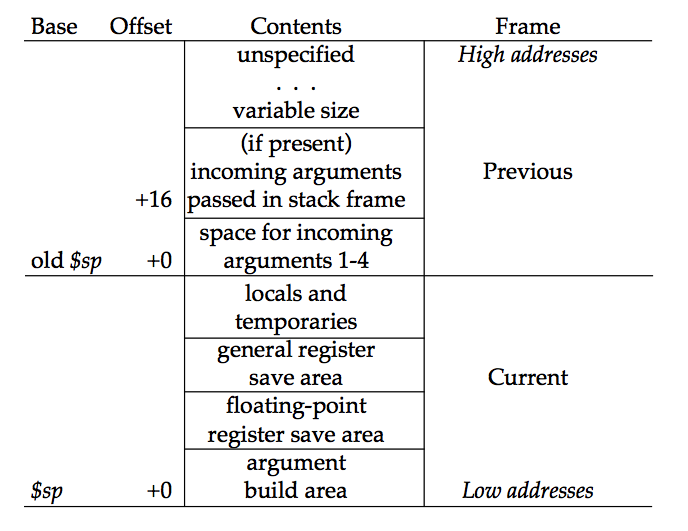
\includegraphics{13.png}}
\caption{Mips stack frame}\label{funccall:funccall-f1}\end{figure}

Run \code{llc -march=mips} for ch9\_1.bc, you will get the following result.
See comment \textbf{``//''}.
\paragraph{lbdex/InputFiles/ch9\_1.cpp}

\begin{Verbatim}[commandchars=\\\{\}]
\PYG{k+kt}{int} \PYG{n}{gI} \PYG{o}{=} \PYG{l+m+mi}{100}\PYG{p}{;}

\PYG{k+kt}{int} \PYG{n}{sum\PYGZus{}i}\PYG{p}{(}\PYG{k+kt}{int} \PYG{n}{x1}\PYG{p}{,} \PYG{k+kt}{int} \PYG{n}{x2}\PYG{p}{,} \PYG{k+kt}{int} \PYG{n}{x3}\PYG{p}{,} \PYG{k+kt}{int} \PYG{n}{x4}\PYG{p}{,} \PYG{k+kt}{int} \PYG{n}{x5}\PYG{p}{,} \PYG{k+kt}{int} \PYG{n}{x6}\PYG{p}{)}
\PYG{p}{\PYGZob{}}
  \PYG{k+kt}{int} \PYG{n}{sum} \PYG{o}{=} \PYG{n}{gI} \PYG{o}{+} \PYG{n}{x1} \PYG{o}{+} \PYG{n}{x2} \PYG{o}{+} \PYG{n}{x3} \PYG{o}{+} \PYG{n}{x4} \PYG{o}{+} \PYG{n}{x5} \PYG{o}{+} \PYG{n}{x6}\PYG{p}{;}
  
  \PYG{k}{return} \PYG{n}{sum}\PYG{p}{;} 
\PYG{p}{\PYGZcb{}}

\PYG{k+kt}{int} \PYG{n}{main}\PYG{p}{(}\PYG{p}{)}
\PYG{p}{\PYGZob{}} 
  \PYG{k+kt}{char} \PYG{n}{str}\PYG{p}{[}\PYG{l+m+mi}{81}\PYG{p}{]} \PYG{o}{=} \PYG{l+s}{"}\PYG{l+s}{Hello world}\PYG{l+s}{"}\PYG{p}{;}
  \PYG{k+kt}{int} \PYG{n}{a} \PYG{o}{=} \PYG{n}{sum\PYGZus{}i}\PYG{p}{(}\PYG{l+m+mi}{1}\PYG{p}{,} \PYG{l+m+mi}{2}\PYG{p}{,} \PYG{l+m+mi}{3}\PYG{p}{,} \PYG{l+m+mi}{4}\PYG{p}{,} \PYG{l+m+mi}{5}\PYG{p}{,} \PYG{l+m+mi}{6}\PYG{p}{)}\PYG{p}{;}  
  
  \PYG{k}{return} \PYG{n}{a}\PYG{p}{;}
\PYG{p}{\PYGZcb{}}
\end{Verbatim}

\begin{Verbatim}[commandchars=\\\{\}]
118-165-78-230:InputFiles Jonathan\PYG{n+nv}{\PYGZdl{} }clang -target mips-unknown-linux-gnu -c
ch9\PYGZus{}1.cpp -emit-llvm -o ch9\PYGZus{}1.bc
118-165-78-230:InputFiles Jonathan\PYG{n+nv}{\PYGZdl{} }/Users/Jonathan/llvm/test/cmake\PYGZus{}debug\PYGZus{}build/
bin/Debug/llc -march\PYG{o}{=}mips -relocation-model\PYG{o}{=}pic -filetype\PYG{o}{=}asm ch9\PYGZus{}1.bc -o
ch9\PYGZus{}1.mips.s
118-165-78-230:InputFiles Jonathan\PYG{n+nv}{\PYGZdl{} }cat ch9\PYGZus{}1.mips.s
  .section .mdebug.abi32
  .previous
  .file \PYG{l+s+s2}{"ch9\PYGZus{}1.bc"}
  .text
  .globl  \PYGZus{}Z5sum\PYGZus{}iiiiiii
  .align  2
  .type \PYGZus{}Z5sum\PYGZus{}iiiiiii,@function
  .set  nomips16                \PYG{c}{\PYGZsh{} @\PYGZus{}Z5sum\PYGZus{}iiiiiii}
  .ent  \PYGZus{}Z5sum\PYGZus{}iiiiiii
\PYGZus{}Z5sum\PYGZus{}iiiiiii:
  .cfi\PYGZus{}startproc
  .frame  \PYG{n+nv}{\PYGZdl{}sp},32,\PYG{n+nv}{\PYGZdl{}ra}
  .mask   0x00000000,0
  .fmask  0x00000000,0
  .set  noreorder
  .set  nomacro
  .set  noat
\PYG{c}{\PYGZsh{} BB\PYGZsh{}0:}
  addiu \PYG{n+nv}{\PYGZdl{}sp}, \PYG{n+nv}{\PYGZdl{}sp}, -32
\PYG{n+nv}{\PYGZdl{}tmp1}:
  .cfi\PYGZus{}def\PYGZus{}cfa\PYGZus{}offset 32
  sw  \PYG{n+nv}{\PYGZdl{}4}, 28\PYG{o}{(}\PYG{n+nv}{\PYGZdl{}sp}\PYG{o}{)}
  sw  \PYG{n+nv}{\PYGZdl{}5}, 24\PYG{o}{(}\PYG{n+nv}{\PYGZdl{}sp}\PYG{o}{)}
  sw  \PYG{n+nv}{\PYGZdl{}t9}, 20\PYG{o}{(}\PYG{n+nv}{\PYGZdl{}sp}\PYG{o}{)}
  sw  \PYG{n+nv}{\PYGZdl{}7}, 16\PYG{o}{(}\PYG{n+nv}{\PYGZdl{}sp}\PYG{o}{)}
  lw  \PYG{n+nv}{\PYGZdl{}1}, 48\PYG{o}{(}\PYG{n+nv}{\PYGZdl{}sp}\PYG{o}{)} // load argument 5
  sw  \PYG{n+nv}{\PYGZdl{}1}, 12\PYG{o}{(}\PYG{n+nv}{\PYGZdl{}sp}\PYG{o}{)}
  lw  \PYG{n+nv}{\PYGZdl{}1}, 52\PYG{o}{(}\PYG{n+nv}{\PYGZdl{}sp}\PYG{o}{)} // load argument 6
  sw  \PYG{n+nv}{\PYGZdl{}1}, 8\PYG{o}{(}\PYG{n+nv}{\PYGZdl{}sp}\PYG{o}{)}
  lw  \PYG{n+nv}{\PYGZdl{}2}, 24\PYG{o}{(}\PYG{n+nv}{\PYGZdl{}sp}\PYG{o}{)}
  lw  \PYG{n+nv}{\PYGZdl{}3}, 28\PYG{o}{(}\PYG{n+nv}{\PYGZdl{}sp}\PYG{o}{)}
  addu  \PYG{n+nv}{\PYGZdl{}2}, \PYG{n+nv}{\PYGZdl{}3}, \PYG{n+nv}{\PYGZdl{}2}
  lw  \PYG{n+nv}{\PYGZdl{}3}, 20\PYG{o}{(}\PYG{n+nv}{\PYGZdl{}sp}\PYG{o}{)}
  addu  \PYG{n+nv}{\PYGZdl{}2}, \PYG{n+nv}{\PYGZdl{}2}, \PYG{n+nv}{\PYGZdl{}3}
  lw  \PYG{n+nv}{\PYGZdl{}3}, 16\PYG{o}{(}\PYG{n+nv}{\PYGZdl{}sp}\PYG{o}{)}
  addu  \PYG{n+nv}{\PYGZdl{}2}, \PYG{n+nv}{\PYGZdl{}2}, \PYG{n+nv}{\PYGZdl{}3}
  lw  \PYG{n+nv}{\PYGZdl{}3}, 12\PYG{o}{(}\PYG{n+nv}{\PYGZdl{}sp}\PYG{o}{)}
  addu  \PYG{n+nv}{\PYGZdl{}2}, \PYG{n+nv}{\PYGZdl{}2}, \PYG{n+nv}{\PYGZdl{}3}
  addu  \PYG{n+nv}{\PYGZdl{}2}, \PYG{n+nv}{\PYGZdl{}2}, \PYG{n+nv}{\PYGZdl{}1}
  sw  \PYG{n+nv}{\PYGZdl{}2}, 4\PYG{o}{(}\PYG{n+nv}{\PYGZdl{}sp}\PYG{o}{)}
  jr  \PYG{n+nv}{\PYGZdl{}ra}
  addiu \PYG{n+nv}{\PYGZdl{}sp}, \PYG{n+nv}{\PYGZdl{}sp}, 32
  .set  at
  .set  macro
  .set  reorder
  .end  \PYGZus{}Z5sum\PYGZus{}iiiiiii
\PYG{n+nv}{\PYGZdl{}tmp2}:
  .size \PYGZus{}Z5sum\PYGZus{}iiiiiii, \PYG{o}{(}\PYG{n+nv}{\PYGZdl{}tmp2}\PYG{o}{)}-\PYGZus{}Z5sum\PYGZus{}iiiiiii
  .cfi\PYGZus{}endproc

  .globl  main
  .align  2
  .type main,@function
  .set  nomips16                \PYG{c}{\PYGZsh{} @main}
  .ent  main
main:
  .cfi\PYGZus{}startproc
  .frame  \PYG{n+nv}{\PYGZdl{}sp},40,\PYG{n+nv}{\PYGZdl{}ra}
  .mask   0x80000000,-4
  .fmask  0x00000000,0
  .set  noreorder
  .set  nomacro
  .set  noat
\PYG{c}{\PYGZsh{} BB\PYGZsh{}0:}
  lui \PYG{n+nv}{\PYGZdl{}2}, \PYGZpc{}hi\PYG{o}{(}\PYGZus{}gp\PYGZus{}disp\PYG{o}{)}
  addiu \PYG{n+nv}{\PYGZdl{}2}, \PYG{n+nv}{\PYGZdl{}2}, \PYGZpc{}lo\PYG{o}{(}\PYGZus{}gp\PYGZus{}disp\PYG{o}{)}
  addiu \PYG{n+nv}{\PYGZdl{}sp}, \PYG{n+nv}{\PYGZdl{}sp}, -40
\PYG{n+nv}{\PYGZdl{}tmp5}:
  .cfi\PYGZus{}def\PYGZus{}cfa\PYGZus{}offset 40
  sw  \PYG{n+nv}{\PYGZdl{}ra}, 36\PYG{o}{(}\PYG{n+nv}{\PYGZdl{}sp}\PYG{o}{)}            \PYG{c}{\PYGZsh{} 4-byte Folded Spill}
\PYG{n+nv}{\PYGZdl{}tmp6}:
  .cfi\PYGZus{}offset 31, -4
  addu  \PYG{n+nv}{\PYGZdl{}gp}, \PYG{n+nv}{\PYGZdl{}2}, \PYG{n+nv}{\PYGZdl{}25}
  sw  \PYG{n+nv}{\PYGZdl{}zero}, 32\PYG{o}{(}\PYG{n+nv}{\PYGZdl{}sp}\PYG{o}{)}
  addiu \PYG{n+nv}{\PYGZdl{}1}, \PYG{n+nv}{\PYGZdl{}zero}, 6
  sw  \PYG{n+nv}{\PYGZdl{}1}, 20\PYG{o}{(}\PYG{n+nv}{\PYGZdl{}sp}\PYG{o}{)} // Save argument 6 to 20\PYG{o}{(}\PYG{n+nv}{\PYGZdl{}sp}\PYG{o}{)}
  addiu \PYG{n+nv}{\PYGZdl{}1}, \PYG{n+nv}{\PYGZdl{}zero}, 5
  sw  \PYG{n+nv}{\PYGZdl{}1}, 16\PYG{o}{(}\PYG{n+nv}{\PYGZdl{}sp}\PYG{o}{)} // Save argument 5 to 16\PYG{o}{(}\PYG{n+nv}{\PYGZdl{}sp}\PYG{o}{)}
  lw  \PYG{n+nv}{\PYGZdl{}25}, \PYGZpc{}call16\PYG{o}{(}\PYGZus{}Z5sum\PYGZus{}iiiiiii\PYG{o}{)}\PYG{o}{(}\PYG{n+nv}{\PYGZdl{}gp}\PYG{o}{)}
  addiu \PYG{n+nv}{\PYGZdl{}4}, \PYG{n+nv}{\PYGZdl{}zero}, 1    // Pass argument 1 to \PYG{n+nv}{\PYGZdl{}4} \PYG{o}{(}\PYG{o}{=}\PYG{n+nv}{\PYGZdl{}a0}\PYG{o}{)}
  addiu \PYG{n+nv}{\PYGZdl{}5}, \PYG{n+nv}{\PYGZdl{}zero}, 2    // Pass argument 2 to \PYG{n+nv}{\PYGZdl{}5} \PYG{o}{(}\PYG{o}{=}\PYG{n+nv}{\PYGZdl{}a1}\PYG{o}{)}
  addiu \PYG{n+nv}{\PYGZdl{}t9}, \PYG{n+nv}{\PYGZdl{}zero}, 3
  jalr  \PYG{n+nv}{\PYGZdl{}25}
  addiu \PYG{n+nv}{\PYGZdl{}7}, \PYG{n+nv}{\PYGZdl{}zero}, 4
  sw  \PYG{n+nv}{\PYGZdl{}2}, 28\PYG{o}{(}\PYG{n+nv}{\PYGZdl{}sp}\PYG{o}{)}
  lw  \PYG{n+nv}{\PYGZdl{}ra}, 36\PYG{o}{(}\PYG{n+nv}{\PYGZdl{}sp}\PYG{o}{)}            \PYG{c}{\PYGZsh{} 4-byte Folded Reload}
  jr  \PYG{n+nv}{\PYGZdl{}ra}
  addiu \PYG{n+nv}{\PYGZdl{}sp}, \PYG{n+nv}{\PYGZdl{}sp}, 40
  .set  at
  .set  macro
  .set  reorder
  .end  main
\PYG{n+nv}{\PYGZdl{}tmp7}:
  .size main, \PYG{o}{(}\PYG{n+nv}{\PYGZdl{}tmp7}\PYG{o}{)}-main
  .cfi\PYGZus{}endproc
\end{Verbatim}

From the mips assembly code generated as above, we know it save the first 4
arguments to \$a0..\$a3 and last 2 arguments to 16(\$sp) and 20(\$sp).
\hyperref[funccall:funccall-f2]{Figure  \ref*{funccall:funccall-f2}} is the arguments location for example code
ch9\_1.cpp.
It load argument 5 from 48(\$sp) in sum\_i() since the argument 5 is saved to
16(\$sp) in main().
The stack size of sum\_i() is 32, so 16+32(\$sp) is the location of incoming
argument 5.
\begin{figure}[htbp]
\centering
\capstart

\scalebox{1.000000}{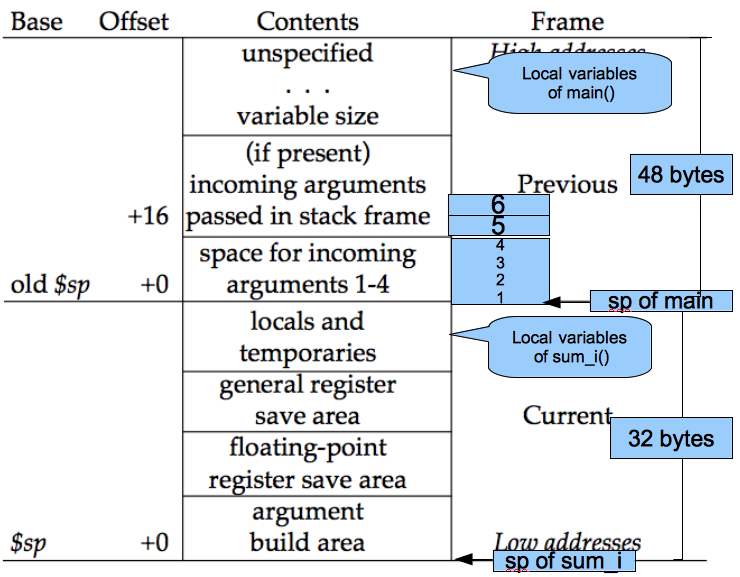
\includegraphics{22.png}}
\caption{Mips arguments location in stack frame}\label{funccall:funccall-f2}\end{figure}

The 007-2418-003.pdf in \footnote{
\href{https://www.dropbox.com/sh/2pkh1fewlq2zag9/OHnrYn2nOs/doc/MIPSproAssemblyLanguageProgrammerGuide}{https://www.dropbox.com/sh/2pkh1fewlq2zag9/OHnrYn2nOs/doc/MIPSproAssemblyLanguageProgrammerGuide}
} is the Mips assembly language manual.
\footnote{
\href{http://www.linux-mips.org/pub/linux/mips/doc/ABI/mipsabi.pdf}{http://www.linux-mips.org/pub/linux/mips/doc/ABI/mipsabi.pdf}
} is Mips Application Binary Interface which include the
\hyperref[funccall:funccall-f1]{Figure  \ref*{funccall:funccall-f1}}.


\section{Load incoming arguments from stack frame}
\label{funccall:load-incoming-arguments-from-stack-frame}
From last section, to support function call, we need implementing the arguments
pass mechanism with stack frame. Before do that, let's run the old version of
code Chapter8\_1/ with ch9\_1.cpp and see what happens.

\begin{Verbatim}[commandchars=\\\{\}]
118-165-79-31:InputFiles Jonathan\PYG{n+nv}{\PYGZdl{} }/Users/Jonathan/llvm/test/
cmake\PYGZus{}debug\PYGZus{}build/bin/Debug/llc -march\PYG{o}{=}cpu0 -relocation-model\PYG{o}{=}pic -filetype\PYG{o}{=}asm
ch9\PYGZus{}1.bc -o ch9\PYGZus{}1.cpu0.s
Assertion failed: \PYG{o}{(}InVals.size\PYG{o}{(}\PYG{o}{)} \PYG{o}{=}\PYG{o}{=} Ins.size\PYG{o}{(}\PYG{o}{)} \PYG{o}{\PYGZam{}\PYGZam{}} \PYG{l+s+s2}{"LowerFormalArguments didn't}
\PYG{l+s+s2}{emit the correct number of values!"}\PYG{o}{)}, \PYG{k}{function }LowerArguments, file /Users/
Jonathan/llvm/test/src/lib/CodeGen/SelectionDAG/
SelectionDAGBuilder.cpp, ...
...
0.  Program arguments: /Users/Jonathan/llvm/test/cmake\PYGZus{}debug\PYGZus{}build/
bin/Debug/llc -march\PYG{o}{=}cpu0 -relocation-model\PYG{o}{=}pic -filetype\PYG{o}{=}asm ch9\PYGZus{}1.bc -o
ch9\PYGZus{}1.cpu0.s
1.  Running pass \PYG{l+s+s1}{'Function Pass Manager'} on module \PYG{l+s+s1}{'ch9\PYGZus{}1.bc'}.
2.  Running pass \PYG{l+s+s1}{'CPU0 DAG-\PYGZgt{}DAG Pattern Instruction Selection'} on \PYG{k}{function}
\PYG{l+s+s1}{'@\PYGZus{}Z5sum\PYGZus{}iiiiiii'}
Illegal instruction: 4
\end{Verbatim}

Since Chapter8\_1/ define the LowerFormalArguments() with empty, we get the error
message as above.
Before define LowerFormalArguments(), we have to choose how to pass arguments
in function call. We choose pass arguments all in stack frame.
We don't reserve any dedicated register for arguments passing since cpu0 has
only 16 registers while Mips has 32 registers. Cpu0CallingConv.td is defined
for cpu0 passing rule as follows,
\paragraph{lbdex/Chapter9\_1/Cpu0CallingConv.td}

\begin{Verbatim}[commandchars=\\\{\}]
\PYG{n}{def} \PYG{n}{RetCC\PYGZus{}Cpu0EABI} \PYG{o}{:} \PYG{n}{CallingConv}\PYG{o}{\PYGZlt{}}\PYG{p}{[}
  \PYG{c+c1}{// i32 are returned in registers V0, V1, A0, A1}
  \PYG{n}{CCIfType}\PYG{o}{\PYGZlt{}}\PYG{p}{[}\PYG{n}{i32}\PYG{p}{]}\PYG{p}{,} \PYG{n}{CCAssignToReg}\PYG{o}{\PYGZlt{}}\PYG{p}{[}\PYG{n}{V0}\PYG{p}{,} \PYG{n}{V1}\PYG{p}{,} \PYG{n}{A0}\PYG{p}{,} \PYG{n}{A1}\PYG{p}{]}\PYG{o}{\PYGZgt{}}\PYG{o}{\PYGZgt{}}
\PYG{p}{]}\PYG{o}{\PYGZgt{}}\PYG{p}{;}

\PYG{c+c1}{//===----------------------------------------------------------------------===//}
\PYG{c+c1}{// Cpu0 EABI Calling Convention}
\PYG{c+c1}{//===----------------------------------------------------------------------===//}

\PYG{n}{def} \PYG{n}{CC\PYGZus{}Cpu0EABI} \PYG{o}{:} \PYG{n}{CallingConv}\PYG{o}{\PYGZlt{}}\PYG{p}{[}
  \PYG{c+c1}{// Promote i8/i16 arguments to i32.}
  \PYG{n}{CCIfType}\PYG{o}{\PYGZlt{}}\PYG{p}{[}\PYG{n}{i8}\PYG{p}{,} \PYG{n}{i16}\PYG{p}{]}\PYG{p}{,} \PYG{n}{CCPromoteToType}\PYG{o}{\PYGZlt{}}\PYG{n}{i32}\PYG{o}{\PYGZgt{}}\PYG{o}{\PYGZgt{}}\PYG{p}{,}
  \PYG{c+c1}{// Integer values get stored in stack slots that are 4 bytes in}
  \PYG{c+c1}{// size and 4-byte aligned.}
  \PYG{n}{CCIfType}\PYG{o}{\PYGZlt{}}\PYG{p}{[}\PYG{n}{i32}\PYG{p}{]}\PYG{p}{,} \PYG{n}{CCAssignToStack}\PYG{o}{\PYGZlt{}}\PYG{l+m+mi}{4}\PYG{p}{,} \PYG{l+m+mi}{4}\PYG{o}{\PYGZgt{}}\PYG{o}{\PYGZgt{}}
\PYG{p}{]}\PYG{o}{\PYGZgt{}}\PYG{p}{;}


\PYG{c+c1}{//===----------------------------------------------------------------------===//}
\PYG{c+c1}{// Cpu0 Calling Convention Dispatch}
\PYG{c+c1}{//===----------------------------------------------------------------------===//}

\PYG{n}{def} \PYG{n}{CC\PYGZus{}Cpu0} \PYG{o}{:} \PYG{n}{CallingConv}\PYG{o}{\PYGZlt{}}\PYG{p}{[}
  \PYG{n}{CCDelegateTo}\PYG{o}{\PYGZlt{}}\PYG{n}{CC\PYGZus{}Cpu0EABI}\PYG{o}{\PYGZgt{}}
\PYG{p}{]}\PYG{o}{\PYGZgt{}}\PYG{p}{;}


\PYG{n}{def} \PYG{n}{RetCC\PYGZus{}Cpu0} \PYG{o}{:} \PYG{n}{CallingConv}\PYG{o}{\PYGZlt{}}\PYG{p}{[}
  \PYG{n}{CCDelegateTo}\PYG{o}{\PYGZlt{}}\PYG{n}{RetCC\PYGZus{}Cpu0EABI}\PYG{o}{\PYGZgt{}}
\PYG{p}{]}\PYG{o}{\PYGZgt{}}\PYG{p}{;} \PYG{c+c1}{// lbd document - mark - def RetCC\PYGZus{}Cpu0}

\PYG{n}{def} \PYG{n}{CSR\PYGZus{}O32} \PYG{o}{:} \PYG{n}{CalleeSavedRegs}\PYG{o}{\PYGZlt{}}\PYG{p}{(}\PYG{n}{add} \PYG{n}{LR}\PYG{p}{,} \PYG{n}{FP}\PYG{p}{,}
                                   \PYG{p}{(}\PYG{n}{sequence} \PYG{l+s}{"}\PYG{l+s}{S\PYGZpc{}u}\PYG{l+s}{"}\PYG{p}{,} \PYG{l+m+mi}{2}\PYG{p}{,} \PYG{l+m+mi}{0}\PYG{p}{)}\PYG{p}{)}\PYG{o}{\PYGZgt{}}\PYG{p}{;}
\end{Verbatim}

As above, CC\_Cpu0 is the cpu0 Calling Convention which delegate to CC\_Cpu0EABI
and define the CC\_Cpu0EABI.
The reason we don't define the Calling Convention directly in CC\_Cpu0 is that
a real general CPU like Mips can have several Calling Convention.
Combine with the mechanism of ``section Target Registration'' \footnote{
\href{http://jonathan2251.github.com/lbd/llvmstructure.html\#target-registration}{http://jonathan2251.github.com/lbd/llvmstructure.html\#target-registration}
} which llvm
supplied, we can use different Calling Convention in  different target.
Although cpu0 only have a Calling Convention right now, define with a dedicate
Call Convention name (CC\_Cpu0EABI in this example) is a better solution for
system expand, and naming your Calling Convention. CC\_Cpu0EABI as above, say it
pass arguments in stack frame.

Function LowerFormalArguments() charge function incoming arguments creation.
We define it as follows,
\paragraph{lbdex/Chapter9\_1/Cpu0ISelLowering.cpp}

\begin{Verbatim}[commandchars=\\\{\}]
\PYG{n}{SDValue}
\PYG{n}{Cpu0TargetLowering}\PYG{o}{:}\PYG{o}{:}\PYG{n}{LowerCall}\PYG{p}{(}\PYG{n}{TargetLowering}\PYG{o}{:}\PYG{o}{:}\PYG{n}{CallLoweringInfo} \PYG{o}{\PYGZam{}}\PYG{n}{CLI}\PYG{p}{,}
                              \PYG{n}{SmallVectorImpl}\PYG{o}{\PYGZlt{}}\PYG{n}{SDValue}\PYG{o}{\PYGZgt{}} \PYG{o}{\PYGZam{}}\PYG{n}{InVals}\PYG{p}{)} \PYG{k}{const} \PYG{p}{\PYGZob{}}
  \PYG{k}{return} \PYG{n}{CLI}\PYG{p}{.}\PYG{n}{Chain}\PYG{p}{;}
\PYG{p}{\PYGZcb{}}
\PYG{p}{.}\PYG{p}{.}\PYG{p}{.}
\PYG{c+c1}{/// LowerFormalArguments - transform physical registers into virtual registers}
\PYG{c+c1}{/// and generate load operations for arguments places on the stack.}
\PYG{n}{SDValue}
\PYG{n}{Cpu0TargetLowering}\PYG{o}{:}\PYG{o}{:}\PYG{n}{LowerFormalArguments}\PYG{p}{(}\PYG{n}{SDValue} \PYG{n}{Chain}\PYG{p}{,}
                                         \PYG{n}{CallingConv}\PYG{o}{:}\PYG{o}{:}\PYG{n}{ID} \PYG{n}{CallConv}\PYG{p}{,}
                                         \PYG{k+kt}{bool} \PYG{n}{isVarArg}\PYG{p}{,}
                                      \PYG{k}{const} \PYG{n}{SmallVectorImpl}\PYG{o}{\PYGZlt{}}\PYG{n}{ISD}\PYG{o}{:}\PYG{o}{:}\PYG{n}{InputArg}\PYG{o}{\PYGZgt{}} \PYG{o}{\PYGZam{}}\PYG{n}{Ins}\PYG{p}{,}
                                         \PYG{n}{DebugLoc} \PYG{n}{dl}\PYG{p}{,} \PYG{n}{SelectionDAG} \PYG{o}{\PYGZam{}}\PYG{n}{DAG}\PYG{p}{,}
                                         \PYG{n}{SmallVectorImpl}\PYG{o}{\PYGZlt{}}\PYG{n}{SDValue}\PYG{o}{\PYGZgt{}} \PYG{o}{\PYGZam{}}\PYG{n}{InVals}\PYG{p}{)}
                                          \PYG{k}{const} \PYG{p}{\PYGZob{}}
  \PYG{n}{MachineFunction} \PYG{o}{\PYGZam{}}\PYG{n}{MF} \PYG{o}{=} \PYG{n}{DAG}\PYG{p}{.}\PYG{n}{getMachineFunction}\PYG{p}{(}\PYG{p}{)}\PYG{p}{;}
  \PYG{n}{MachineFrameInfo} \PYG{o}{*}\PYG{n}{MFI} \PYG{o}{=} \PYG{n}{MF}\PYG{p}{.}\PYG{n}{getFrameInfo}\PYG{p}{(}\PYG{p}{)}\PYG{p}{;}
  \PYG{n}{Cpu0FunctionInfo} \PYG{o}{*}\PYG{n}{Cpu0FI} \PYG{o}{=} \PYG{n}{MF}\PYG{p}{.}\PYG{n}{getInfo}\PYG{o}{\PYGZlt{}}\PYG{n}{Cpu0FunctionInfo}\PYG{o}{\PYGZgt{}}\PYG{p}{(}\PYG{p}{)}\PYG{p}{;}

  \PYG{n}{Cpu0FI}\PYG{o}{-}\PYG{o}{\PYGZgt{}}\PYG{n}{setVarArgsFrameIndex}\PYG{p}{(}\PYG{l+m+mi}{0}\PYG{p}{)}\PYG{p}{;}

  \PYG{c+c1}{// Used with vargs to acumulate store chains.}
  \PYG{n}{std}\PYG{o}{:}\PYG{o}{:}\PYG{n}{vector}\PYG{o}{\PYGZlt{}}\PYG{n}{SDValue}\PYG{o}{\PYGZgt{}} \PYG{n}{OutChains}\PYG{p}{;}

  \PYG{c+c1}{// Assign locations to all of the incoming arguments.}
  \PYG{n}{SmallVector}\PYG{o}{\PYGZlt{}}\PYG{n}{CCValAssign}\PYG{p}{,} \PYG{l+m+mi}{16}\PYG{o}{\PYGZgt{}} \PYG{n}{ArgLocs}\PYG{p}{;}
  \PYG{n}{CCState} \PYG{n}{CCInfo}\PYG{p}{(}\PYG{n}{CallConv}\PYG{p}{,} \PYG{n}{isVarArg}\PYG{p}{,} \PYG{n}{DAG}\PYG{p}{.}\PYG{n}{getMachineFunction}\PYG{p}{(}\PYG{p}{)}\PYG{p}{,}
                 \PYG{n}{getTargetMachine}\PYG{p}{(}\PYG{p}{)}\PYG{p}{,} \PYG{n}{ArgLocs}\PYG{p}{,} \PYG{o}{*}\PYG{n}{DAG}\PYG{p}{.}\PYG{n}{getContext}\PYG{p}{(}\PYG{p}{)}\PYG{p}{)}\PYG{p}{;}

  \PYG{n}{CCInfo}\PYG{p}{.}\PYG{n}{AnalyzeFormalArguments}\PYG{p}{(}\PYG{n}{Ins}\PYG{p}{,} \PYG{n}{CC\PYGZus{}Cpu0}\PYG{p}{)}\PYG{p}{;}

  \PYG{n}{Function}\PYG{o}{:}\PYG{o}{:}\PYG{n}{const\PYGZus{}arg\PYGZus{}iterator} \PYG{n}{FuncArg} \PYG{o}{=}
    \PYG{n}{DAG}\PYG{p}{.}\PYG{n}{getMachineFunction}\PYG{p}{(}\PYG{p}{)}\PYG{p}{.}\PYG{n}{getFunction}\PYG{p}{(}\PYG{p}{)}\PYG{o}{-}\PYG{o}{\PYGZgt{}}\PYG{n}{arg\PYGZus{}begin}\PYG{p}{(}\PYG{p}{)}\PYG{p}{;}
  \PYG{k+kt}{int} \PYG{n}{LastFI} \PYG{o}{=} \PYG{l+m+mi}{0}\PYG{p}{;}\PYG{c+c1}{// Cpu0FI-\PYGZgt{}LastInArgFI is 0 at the entry of this function.}

  \PYG{k}{for} \PYG{p}{(}\PYG{k+kt}{unsigned} \PYG{n}{i} \PYG{o}{=} \PYG{l+m+mi}{0}\PYG{p}{,} \PYG{n}{e} \PYG{o}{=} \PYG{n}{ArgLocs}\PYG{p}{.}\PYG{n}{size}\PYG{p}{(}\PYG{p}{)}\PYG{p}{;} \PYG{n}{i} \PYG{o}{!}\PYG{o}{=} \PYG{n}{e}\PYG{p}{;} \PYG{o}{+}\PYG{o}{+}\PYG{n}{i}\PYG{p}{,} \PYG{o}{+}\PYG{o}{+}\PYG{n}{FuncArg}\PYG{p}{)} \PYG{p}{\PYGZob{}}
    \PYG{n}{CCValAssign} \PYG{o}{\PYGZam{}}\PYG{n}{VA} \PYG{o}{=} \PYG{n}{ArgLocs}\PYG{p}{[}\PYG{n}{i}\PYG{p}{]}\PYG{p}{;}
    \PYG{n}{EVT} \PYG{n}{ValVT} \PYG{o}{=} \PYG{n}{VA}\PYG{p}{.}\PYG{n}{getValVT}\PYG{p}{(}\PYG{p}{)}\PYG{p}{;}
    \PYG{n}{ISD}\PYG{o}{:}\PYG{o}{:}\PYG{n}{ArgFlagsTy} \PYG{n}{Flags} \PYG{o}{=} \PYG{n}{Ins}\PYG{p}{[}\PYG{n}{i}\PYG{p}{]}\PYG{p}{.}\PYG{n}{Flags}\PYG{p}{;}
    \PYG{k+kt}{bool} \PYG{n}{IsRegLoc} \PYG{o}{=} \PYG{n}{VA}\PYG{p}{.}\PYG{n}{isRegLoc}\PYG{p}{(}\PYG{p}{)}\PYG{p}{;}

    \PYG{k}{if} \PYG{p}{(}\PYG{n}{Flags}\PYG{p}{.}\PYG{n}{isByVal}\PYG{p}{(}\PYG{p}{)}\PYG{p}{)} \PYG{p}{\PYGZob{}}
      \PYG{n}{assert}\PYG{p}{(}\PYG{n}{Flags}\PYG{p}{.}\PYG{n}{getByValSize}\PYG{p}{(}\PYG{p}{)} \PYG{o}{\PYGZam{}}\PYG{o}{\PYGZam{}}
             \PYG{l+s}{"}\PYG{l+s}{ByVal args of size 0 should have been ignored by front-end.}\PYG{l+s}{"}\PYG{p}{)}\PYG{p}{;}
      \PYG{k}{continue}\PYG{p}{;}
    \PYG{p}{\PYGZcb{}}
    \PYG{c+c1}{// sanity check}
    \PYG{n}{assert}\PYG{p}{(}\PYG{n}{VA}\PYG{p}{.}\PYG{n}{isMemLoc}\PYG{p}{(}\PYG{p}{)}\PYG{p}{)}\PYG{p}{;}

    \PYG{c+c1}{// The stack pointer offset is relative to the caller stack frame.}
    \PYG{n}{LastFI} \PYG{o}{=} \PYG{n}{MFI}\PYG{o}{-}\PYG{o}{\PYGZgt{}}\PYG{n}{CreateFixedObject}\PYG{p}{(}\PYG{n}{ValVT}\PYG{p}{.}\PYG{n}{getSizeInBits}\PYG{p}{(}\PYG{p}{)}\PYG{o}{/}\PYG{l+m+mi}{8}\PYG{p}{,}
                                    \PYG{n}{VA}\PYG{p}{.}\PYG{n}{getLocMemOffset}\PYG{p}{(}\PYG{p}{)}\PYG{p}{,} \PYG{k+kc}{true}\PYG{p}{)}\PYG{p}{;}

    \PYG{c+c1}{// Create load nodes to retrieve arguments from the stack}
    \PYG{n}{SDValue} \PYG{n}{FIN} \PYG{o}{=} \PYG{n}{DAG}\PYG{p}{.}\PYG{n}{getFrameIndex}\PYG{p}{(}\PYG{n}{LastFI}\PYG{p}{,} \PYG{n}{getPointerTy}\PYG{p}{(}\PYG{p}{)}\PYG{p}{)}\PYG{p}{;}
    \PYG{n}{InVals}\PYG{p}{.}\PYG{n}{push\PYGZus{}back}\PYG{p}{(}\PYG{n}{DAG}\PYG{p}{.}\PYG{n}{getLoad}\PYG{p}{(}\PYG{n}{ValVT}\PYG{p}{,} \PYG{n}{dl}\PYG{p}{,} \PYG{n}{Chain}\PYG{p}{,} \PYG{n}{FIN}\PYG{p}{,}
                                 \PYG{n}{MachinePointerInfo}\PYG{o}{:}\PYG{o}{:}\PYG{n}{getFixedStack}\PYG{p}{(}\PYG{n}{LastFI}\PYG{p}{)}\PYG{p}{,}
                                 \PYG{k+kc}{false}\PYG{p}{,} \PYG{k+kc}{false}\PYG{p}{,} \PYG{k+kc}{false}\PYG{p}{,} \PYG{l+m+mi}{0}\PYG{p}{)}\PYG{p}{)}\PYG{p}{;}
  \PYG{p}{\PYGZcb{}}
  \PYG{n}{Cpu0FI}\PYG{o}{-}\PYG{o}{\PYGZgt{}}\PYG{n}{setLastInArgFI}\PYG{p}{(}\PYG{n}{LastFI}\PYG{p}{)}\PYG{p}{;}
  \PYG{c+c1}{// All stores are grouped in one node to allow the matching between}
  \PYG{c+c1}{// the size of Ins and InVals. This only happens when on varg functions}
  \PYG{k}{if} \PYG{p}{(}\PYG{o}{!}\PYG{n}{OutChains}\PYG{p}{.}\PYG{n}{empty}\PYG{p}{(}\PYG{p}{)}\PYG{p}{)} \PYG{p}{\PYGZob{}}
    \PYG{n}{OutChains}\PYG{p}{.}\PYG{n}{push\PYGZus{}back}\PYG{p}{(}\PYG{n}{Chain}\PYG{p}{)}\PYG{p}{;}
    \PYG{n}{Chain} \PYG{o}{=} \PYG{n}{DAG}\PYG{p}{.}\PYG{n}{getNode}\PYG{p}{(}\PYG{n}{ISD}\PYG{o}{:}\PYG{o}{:}\PYG{n}{TokenFactor}\PYG{p}{,} \PYG{n}{dl}\PYG{p}{,} \PYG{n}{MVT}\PYG{o}{:}\PYG{o}{:}\PYG{n}{Other}\PYG{p}{,}
                        \PYG{o}{\PYGZam{}}\PYG{n}{OutChains}\PYG{p}{[}\PYG{l+m+mi}{0}\PYG{p}{]}\PYG{p}{,} \PYG{n}{OutChains}\PYG{p}{.}\PYG{n}{size}\PYG{p}{(}\PYG{p}{)}\PYG{p}{)}\PYG{p}{;}
  \PYG{p}{\PYGZcb{}}
  \PYG{k}{return} \PYG{n}{Chain}\PYG{p}{;}
\PYG{p}{\PYGZcb{}}
\end{Verbatim}
\paragraph{lbdex/Chapter9\_1/Cpu0ISelLowering.h}

\begin{Verbatim}[commandchars=\\\{\}]
  \PYG{k}{virtual} \PYG{n}{SDValue}
    \PYG{n}{LowerCall}\PYG{p}{(}\PYG{n}{TargetLowering}\PYG{o}{:}\PYG{o}{:}\PYG{n}{CallLoweringInfo} \PYG{o}{\PYGZam{}}\PYG{n}{CLI}\PYG{p}{,}
              \PYG{n}{SmallVectorImpl}\PYG{o}{\PYGZlt{}}\PYG{n}{SDValue}\PYG{o}{\PYGZgt{}} \PYG{o}{\PYGZam{}}\PYG{n}{InVals}\PYG{p}{)} \PYG{k}{const}\PYG{p}{;}
\PYG{c+c1}{// LowerCall: outgoing arguments}
\end{Verbatim}

Refresh ``section Global variable'' \footnote{
\href{http://jonathan2251.github.com/lbd/globalvar.html\#global-variable}{http://jonathan2251.github.com/lbd/globalvar.html\#global-variable}
}, we handled global
variable translation by create the IR DAG in LowerGlobalAddress() first, and
then do the Instruction Selection by their corresponding machine instruction
DAG in Cpu0InstrInfo.td.
LowerGlobalAddress() is called when \code{llc} meet the global variable access.
LowerFormalArguments() work with the same way.
It is called when function is entered.
It get incoming arguments information by CCInfo(CallConv,..., ArgLocs, ...)
before enter \textbf{“for loop”}. In ch9\_1.cpp, there are 6 arguments in sum\_i(...)
function call and we use the stack frame only for arguments passing without
any arguments pass in registers.
So ArgLocs.size() is 6, each argument information is in ArgLocs{[}i{]} and
ArgLocs{[}i{]}.isMemLoc() is true.
In \textbf{“for loop”}, it create each frame index object by LastFI =
MFI-\textgreater{}CreateFixedObject(ValVT.getSizeInBits()/8,VA.getLocMemOffset(), true) and
FIN = DAG.getFrameIndex(LastFI, getPointerTy()).
And then create IR DAG load node and put the load node into vector InVals by
InVals.push\_back(DAG.getLoad(ValVT, dl, Chain, FIN,
MachinePointerInfo::getFixedStack(LastFI), false, false, false, 0)).
Cpu0FI-\textgreater{}setVarArgsFrameIndex(0) and Cpu0FI-\textgreater{}setLastInArgFI(LastFI) are called
when before and after above work. In ch9\_1.cpp example, LowerFormalArguments()
will be called twice. First time is for sum\_i() which will create 6 load DAG
for 6 incoming arguments passing into this function.
Second time is for main() which didn't create any load DAG for no incoming
argument passing into main().
In addition to LowerFormalArguments() which create the load DAG, we need to
define the loadRegFromStackSlot() to issue the machine instruction
\textbf{“ld \$r, offset(\$sp)”} to load incoming arguments from stack frame offset.
GetMemOperand(..., FI, ...) return the Memory location of the frame index
variable, which is the offset.
\paragraph{lbdex/Chapter9\_1/Cpu0InstrInfo.cpp}

\begin{Verbatim}[commandchars=\\\{\}]
\PYG{k}{static} \PYG{n}{MachineMemOperand}\PYG{o}{*} \PYG{n}{GetMemOperand}\PYG{p}{(}\PYG{n}{MachineBasicBlock} \PYG{o}{\PYGZam{}}\PYG{n}{MBB}\PYG{p}{,} \PYG{k+kt}{int} \PYG{n}{FI}\PYG{p}{,}
                                        \PYG{k+kt}{unsigned} \PYG{n}{Flag}\PYG{p}{)} \PYG{p}{\PYGZob{}}
  \PYG{n}{MachineFunction} \PYG{o}{\PYGZam{}}\PYG{n}{MF} \PYG{o}{=} \PYG{o}{*}\PYG{n}{MBB}\PYG{p}{.}\PYG{n}{getParent}\PYG{p}{(}\PYG{p}{)}\PYG{p}{;}
  \PYG{n}{MachineFrameInfo} \PYG{o}{\PYGZam{}}\PYG{n}{MFI} \PYG{o}{=} \PYG{o}{*}\PYG{n}{MF}\PYG{p}{.}\PYG{n}{getFrameInfo}\PYG{p}{(}\PYG{p}{)}\PYG{p}{;}
  \PYG{k+kt}{unsigned} \PYG{n}{Align} \PYG{o}{=} \PYG{n}{MFI}\PYG{p}{.}\PYG{n}{getObjectAlignment}\PYG{p}{(}\PYG{n}{FI}\PYG{p}{)}\PYG{p}{;}

  \PYG{k}{return} \PYG{n}{MF}\PYG{p}{.}\PYG{n}{getMachineMemOperand}\PYG{p}{(}\PYG{n}{MachinePointerInfo}\PYG{o}{:}\PYG{o}{:}\PYG{n}{getFixedStack}\PYG{p}{(}\PYG{n}{FI}\PYG{p}{)}\PYG{p}{,} \PYG{n}{Flag}\PYG{p}{,}
                                 \PYG{n}{MFI}\PYG{p}{.}\PYG{n}{getObjectSize}\PYG{p}{(}\PYG{n}{FI}\PYG{p}{)}\PYG{p}{,} \PYG{n}{Align}\PYG{p}{)}\PYG{p}{;}
\PYG{p}{\PYGZcb{}}

\PYG{c+c1}{//- st SrcReg, MMO(FI)}
\PYG{k+kt}{void} \PYG{n}{Cpu0InstrInfo}\PYG{o}{:}\PYG{o}{:}
\PYG{n}{storeRegToStackSlot}\PYG{p}{(}\PYG{n}{MachineBasicBlock} \PYG{o}{\PYGZam{}}\PYG{n}{MBB}\PYG{p}{,} \PYG{n}{MachineBasicBlock}\PYG{o}{:}\PYG{o}{:}\PYG{n}{iterator} \PYG{n}{I}\PYG{p}{,}
                    \PYG{k+kt}{unsigned} \PYG{n}{SrcReg}\PYG{p}{,} \PYG{k+kt}{bool} \PYG{n}{isKill}\PYG{p}{,} \PYG{k+kt}{int} \PYG{n}{FI}\PYG{p}{,}
                    \PYG{k}{const} \PYG{n}{TargetRegisterClass} \PYG{o}{*}\PYG{n}{RC}\PYG{p}{,}
                    \PYG{k}{const} \PYG{n}{TargetRegisterInfo} \PYG{o}{*}\PYG{n}{TRI}\PYG{p}{)} \PYG{k}{const} \PYG{p}{\PYGZob{}}
  \PYG{n}{DebugLoc} \PYG{n}{DL}\PYG{p}{;}
  \PYG{k}{if} \PYG{p}{(}\PYG{n}{I} \PYG{o}{!}\PYG{o}{=} \PYG{n}{MBB}\PYG{p}{.}\PYG{n}{end}\PYG{p}{(}\PYG{p}{)}\PYG{p}{)} \PYG{n}{DL} \PYG{o}{=} \PYG{n}{I}\PYG{o}{-}\PYG{o}{\PYGZgt{}}\PYG{n}{getDebugLoc}\PYG{p}{(}\PYG{p}{)}\PYG{p}{;}
  \PYG{n}{MachineMemOperand} \PYG{o}{*}\PYG{n}{MMO} \PYG{o}{=} \PYG{n}{GetMemOperand}\PYG{p}{(}\PYG{n}{MBB}\PYG{p}{,} \PYG{n}{FI}\PYG{p}{,} \PYG{n}{MachineMemOperand}\PYG{o}{:}\PYG{o}{:}\PYG{n}{MOStore}\PYG{p}{)}\PYG{p}{;}

  \PYG{k+kt}{unsigned} \PYG{n}{Opc} \PYG{o}{=} \PYG{l+m+mi}{0}\PYG{p}{;}

  \PYG{k}{if} \PYG{p}{(}\PYG{n}{Cpu0}\PYG{o}{:}\PYG{o}{:}\PYG{n}{CPURegsRegClass}\PYG{p}{.}\PYG{n}{hasSubClassEq}\PYG{p}{(}\PYG{n}{RC}\PYG{p}{)}\PYG{p}{)}
    \PYG{n}{Opc} \PYG{o}{=} \PYG{n}{Cpu0}\PYG{o}{:}\PYG{o}{:}\PYG{n}{ST}\PYG{p}{;}
  \PYG{n}{assert}\PYG{p}{(}\PYG{n}{Opc} \PYG{o}{\PYGZam{}}\PYG{o}{\PYGZam{}} \PYG{l+s}{"}\PYG{l+s}{Register class not handled!}\PYG{l+s}{"}\PYG{p}{)}\PYG{p}{;}
  \PYG{n}{BuildMI}\PYG{p}{(}\PYG{n}{MBB}\PYG{p}{,} \PYG{n}{I}\PYG{p}{,} \PYG{n}{DL}\PYG{p}{,} \PYG{n}{get}\PYG{p}{(}\PYG{n}{Opc}\PYG{p}{)}\PYG{p}{)}\PYG{p}{.}\PYG{n}{addReg}\PYG{p}{(}\PYG{n}{SrcReg}\PYG{p}{,} \PYG{n}{getKillRegState}\PYG{p}{(}\PYG{n}{isKill}\PYG{p}{)}\PYG{p}{)}
    \PYG{p}{.}\PYG{n}{addFrameIndex}\PYG{p}{(}\PYG{n}{FI}\PYG{p}{)}\PYG{p}{.}\PYG{n}{addImm}\PYG{p}{(}\PYG{l+m+mi}{0}\PYG{p}{)}\PYG{p}{.}\PYG{n}{addMemOperand}\PYG{p}{(}\PYG{n}{MMO}\PYG{p}{)}\PYG{p}{;}
\PYG{p}{\PYGZcb{}} \PYG{c+c1}{// lbd document - mark - storeRegToStackSlot}

\PYG{k+kt}{void} \PYG{n}{Cpu0InstrInfo}\PYG{o}{:}\PYG{o}{:}
\PYG{n}{loadRegFromStackSlot}\PYG{p}{(}\PYG{n}{MachineBasicBlock} \PYG{o}{\PYGZam{}}\PYG{n}{MBB}\PYG{p}{,} \PYG{n}{MachineBasicBlock}\PYG{o}{:}\PYG{o}{:}\PYG{n}{iterator} \PYG{n}{I}\PYG{p}{,}
                     \PYG{k+kt}{unsigned} \PYG{n}{DestReg}\PYG{p}{,} \PYG{k+kt}{int} \PYG{n}{FI}\PYG{p}{,}
                     \PYG{k}{const} \PYG{n}{TargetRegisterClass} \PYG{o}{*}\PYG{n}{RC}\PYG{p}{,}
                     \PYG{k}{const} \PYG{n}{TargetRegisterInfo} \PYG{o}{*}\PYG{n}{TRI}\PYG{p}{)} \PYG{k}{const}
\PYG{p}{\PYGZob{}}
  \PYG{n}{DebugLoc} \PYG{n}{DL}\PYG{p}{;}
  \PYG{k}{if} \PYG{p}{(}\PYG{n}{I} \PYG{o}{!}\PYG{o}{=} \PYG{n}{MBB}\PYG{p}{.}\PYG{n}{end}\PYG{p}{(}\PYG{p}{)}\PYG{p}{)} \PYG{n}{DL} \PYG{o}{=} \PYG{n}{I}\PYG{o}{-}\PYG{o}{\PYGZgt{}}\PYG{n}{getDebugLoc}\PYG{p}{(}\PYG{p}{)}\PYG{p}{;}
  \PYG{n}{MachineMemOperand} \PYG{o}{*}\PYG{n}{MMO} \PYG{o}{=} \PYG{n}{GetMemOperand}\PYG{p}{(}\PYG{n}{MBB}\PYG{p}{,} \PYG{n}{FI}\PYG{p}{,} \PYG{n}{MachineMemOperand}\PYG{o}{:}\PYG{o}{:}\PYG{n}{MOLoad}\PYG{p}{)}\PYG{p}{;}
  \PYG{k+kt}{unsigned} \PYG{n}{Opc} \PYG{o}{=} \PYG{l+m+mi}{0}\PYG{p}{;}

  \PYG{k}{if} \PYG{p}{(}\PYG{n}{Cpu0}\PYG{o}{:}\PYG{o}{:}\PYG{n}{CPURegsRegClass}\PYG{p}{.}\PYG{n}{hasSubClassEq}\PYG{p}{(}\PYG{n}{RC}\PYG{p}{)}\PYG{p}{)}
    \PYG{n}{Opc} \PYG{o}{=} \PYG{n}{Cpu0}\PYG{o}{:}\PYG{o}{:}\PYG{n}{LD}\PYG{p}{;}
  \PYG{n}{assert}\PYG{p}{(}\PYG{n}{Opc} \PYG{o}{\PYGZam{}}\PYG{o}{\PYGZam{}} \PYG{l+s}{"}\PYG{l+s}{Register class not handled!}\PYG{l+s}{"}\PYG{p}{)}\PYG{p}{;}
  \PYG{n}{BuildMI}\PYG{p}{(}\PYG{n}{MBB}\PYG{p}{,} \PYG{n}{I}\PYG{p}{,} \PYG{n}{DL}\PYG{p}{,} \PYG{n}{get}\PYG{p}{(}\PYG{n}{Opc}\PYG{p}{)}\PYG{p}{,} \PYG{n}{DestReg}\PYG{p}{)}\PYG{p}{.}\PYG{n}{addFrameIndex}\PYG{p}{(}\PYG{n}{FI}\PYG{p}{)}\PYG{p}{.}\PYG{n}{addImm}\PYG{p}{(}\PYG{l+m+mi}{0}\PYG{p}{)}
    \PYG{p}{.}\PYG{n}{addMemOperand}\PYG{p}{(}\PYG{n}{MMO}\PYG{p}{)}\PYG{p}{;}
\PYG{p}{\PYGZcb{}} \PYG{c+c1}{// lbd document - mark - loadRegFromStackSlot}

\PYG{n}{MachineInstr}\PYG{o}{*}
\PYG{n}{Cpu0InstrInfo}\PYG{o}{:}\PYG{o}{:}\PYG{n}{emitFrameIndexDebugValue}\PYG{p}{(}\PYG{n}{MachineFunction} \PYG{o}{\PYGZam{}}\PYG{n}{MF}\PYG{p}{,} \PYG{k+kt}{int} \PYG{n}{FrameIx}\PYG{p}{,}
                                        \PYG{n}{uint64\PYGZus{}t} \PYG{n}{Offset}\PYG{p}{,} \PYG{k}{const} \PYG{n}{MDNode} \PYG{o}{*}\PYG{n}{MDPtr}\PYG{p}{,}
                                        \PYG{n}{DebugLoc} \PYG{n}{DL}\PYG{p}{)} \PYG{k}{const} \PYG{p}{\PYGZob{}}
  \PYG{n}{MachineInstrBuilder} \PYG{n}{MIB} \PYG{o}{=} \PYG{n}{BuildMI}\PYG{p}{(}\PYG{n}{MF}\PYG{p}{,} \PYG{n}{DL}\PYG{p}{,} \PYG{n}{get}\PYG{p}{(}\PYG{n}{Cpu0}\PYG{o}{:}\PYG{o}{:}\PYG{n}{DBG\PYGZus{}VALUE}\PYG{p}{)}\PYG{p}{)}
    \PYG{p}{.}\PYG{n}{addFrameIndex}\PYG{p}{(}\PYG{n}{FrameIx}\PYG{p}{)}\PYG{p}{.}\PYG{n}{addImm}\PYG{p}{(}\PYG{l+m+mi}{0}\PYG{p}{)}\PYG{p}{.}\PYG{n}{addImm}\PYG{p}{(}\PYG{n}{Offset}\PYG{p}{)}\PYG{p}{.}\PYG{n}{addMetadata}\PYG{p}{(}\PYG{n}{MDPtr}\PYG{p}{)}\PYG{p}{;}
  \PYG{k}{return} \PYG{o}{\PYGZam{}}\PYG{o}{*}\PYG{n}{MIB}\PYG{p}{;}
\PYG{p}{\PYGZcb{}} \PYG{c+c1}{// lbd document - mark - emitFrameIndexDebugValue}

\PYG{c+c1}{// Cpu0InstrInfo::expandPostRAPseudo}
\PYG{c+c1}{/// Expand Pseudo instructions into real backend instructions}
\PYG{k+kt}{bool} \PYG{n}{Cpu0InstrInfo}\PYG{o}{:}\PYG{o}{:}\PYG{n}{expandPostRAPseudo}\PYG{p}{(}\PYG{n}{MachineBasicBlock}\PYG{o}{:}\PYG{o}{:}\PYG{n}{iterator} \PYG{n}{MI}\PYG{p}{)} \PYG{k}{const} \PYG{p}{\PYGZob{}}
  \PYG{n}{MachineBasicBlock} \PYG{o}{\PYGZam{}}\PYG{n}{MBB} \PYG{o}{=} \PYG{o}{*}\PYG{n}{MI}\PYG{o}{-}\PYG{o}{\PYGZgt{}}\PYG{n}{getParent}\PYG{p}{(}\PYG{p}{)}\PYG{p}{;}

  \PYG{k}{switch}\PYG{p}{(}\PYG{n}{MI}\PYG{o}{-}\PYG{o}{\PYGZgt{}}\PYG{n}{getDesc}\PYG{p}{(}\PYG{p}{)}\PYG{p}{.}\PYG{n}{getOpcode}\PYG{p}{(}\PYG{p}{)}\PYG{p}{)} \PYG{p}{\PYGZob{}}
  \PYG{k}{default}\PYG{o}{:}
    \PYG{k}{return} \PYG{k+kc}{false}\PYG{p}{;}
  \PYG{k}{case} \PYG{n}{Cpu0}\PYG{o}{:}\PYG{o}{:}\PYG{n+nl}{RetLR:}
    \PYG{n}{ExpandRetLR}\PYG{p}{(}\PYG{n}{MBB}\PYG{p}{,} \PYG{n}{MI}\PYG{p}{,} \PYG{n}{Cpu0}\PYG{o}{:}\PYG{o}{:}\PYG{n}{RET}\PYG{p}{)}\PYG{p}{;}
    \PYG{k}{break}\PYG{p}{;}
  \PYG{p}{\PYGZcb{}}

  \PYG{n}{MBB}\PYG{p}{.}\PYG{n}{erase}\PYG{p}{(}\PYG{n}{MI}\PYG{p}{)}\PYG{p}{;}
  \PYG{k}{return} \PYG{k+kc}{true}\PYG{p}{;}
\PYG{p}{\PYGZcb{}}

\PYG{k+kt}{void} \PYG{n}{Cpu0InstrInfo}\PYG{o}{:}\PYG{o}{:}\PYG{n}{ExpandRetLR}\PYG{p}{(}\PYG{n}{MachineBasicBlock} \PYG{o}{\PYGZam{}}\PYG{n}{MBB}\PYG{p}{,}
                                \PYG{n}{MachineBasicBlock}\PYG{o}{:}\PYG{o}{:}\PYG{n}{iterator} \PYG{n}{I}\PYG{p}{,}
                                \PYG{k+kt}{unsigned} \PYG{n}{Opc}\PYG{p}{)} \PYG{k}{const} \PYG{p}{\PYGZob{}}
  \PYG{n}{BuildMI}\PYG{p}{(}\PYG{n}{MBB}\PYG{p}{,} \PYG{n}{I}\PYG{p}{,} \PYG{n}{I}\PYG{o}{-}\PYG{o}{\PYGZgt{}}\PYG{n}{getDebugLoc}\PYG{p}{(}\PYG{p}{)}\PYG{p}{,} \PYG{n}{get}\PYG{p}{(}\PYG{n}{Opc}\PYG{p}{)}\PYG{p}{)}\PYG{p}{.}\PYG{n}{addReg}\PYG{p}{(}\PYG{n}{Cpu0}\PYG{o}{:}\PYG{o}{:}\PYG{n}{LR}\PYG{p}{)}\PYG{p}{;}
\PYG{p}{\PYGZcb{}}
\end{Verbatim}

\begin{Verbatim}[commandchars=\\\{\}]
\PYG{k}{static} \PYG{n}{MachineMemOperand}\PYG{o}{*} \PYG{n}{GetMemOperand}\PYG{p}{(}\PYG{n}{MachineBasicBlock} \PYG{o}{\PYGZam{}}\PYG{n}{MBB}\PYG{p}{,} \PYG{k+kt}{int} \PYG{n}{FI}\PYG{p}{,}
                                        \PYG{k+kt}{unsigned} \PYG{n}{Flag}\PYG{p}{)} \PYG{p}{\PYGZob{}}
  \PYG{n}{MachineFunction} \PYG{o}{\PYGZam{}}\PYG{n}{MF} \PYG{o}{=} \PYG{o}{*}\PYG{n}{MBB}\PYG{p}{.}\PYG{n}{getParent}\PYG{p}{(}\PYG{p}{)}\PYG{p}{;}
  \PYG{n}{MachineFrameInfo} \PYG{o}{\PYGZam{}}\PYG{n}{MFI} \PYG{o}{=} \PYG{o}{*}\PYG{n}{MF}\PYG{p}{.}\PYG{n}{getFrameInfo}\PYG{p}{(}\PYG{p}{)}\PYG{p}{;}
  \PYG{k+kt}{unsigned} \PYG{n}{Align} \PYG{o}{=} \PYG{n}{MFI}\PYG{p}{.}\PYG{n}{getObjectAlignment}\PYG{p}{(}\PYG{n}{FI}\PYG{p}{)}\PYG{p}{;}

  \PYG{k}{return} \PYG{n}{MF}\PYG{p}{.}\PYG{n}{getMachineMemOperand}\PYG{p}{(}\PYG{n}{MachinePointerInfo}\PYG{o}{:}\PYG{o}{:}\PYG{n}{getFixedStack}\PYG{p}{(}\PYG{n}{FI}\PYG{p}{)}\PYG{p}{,} \PYG{n}{Flag}\PYG{p}{,}
                                 \PYG{n}{MFI}\PYG{p}{.}\PYG{n}{getObjectSize}\PYG{p}{(}\PYG{n}{FI}\PYG{p}{)}\PYG{p}{,} \PYG{n}{Align}\PYG{p}{)}\PYG{p}{;}
\PYG{p}{\PYGZcb{}}
\end{Verbatim}

\begin{Verbatim}[commandchars=\\\{\}]
\PYG{k+kt}{void} \PYG{n}{Cpu0InstrInfo}\PYG{o}{:}\PYG{o}{:}
\PYG{n}{loadRegFromStackSlot}\PYG{p}{(}\PYG{n}{MachineBasicBlock} \PYG{o}{\PYGZam{}}\PYG{n}{MBB}\PYG{p}{,} \PYG{n}{MachineBasicBlock}\PYG{o}{:}\PYG{o}{:}\PYG{n}{iterator} \PYG{n}{I}\PYG{p}{,}
                     \PYG{k+kt}{unsigned} \PYG{n}{DestReg}\PYG{p}{,} \PYG{k+kt}{int} \PYG{n}{FI}\PYG{p}{,}
                     \PYG{k}{const} \PYG{n}{TargetRegisterClass} \PYG{o}{*}\PYG{n}{RC}\PYG{p}{,}
                     \PYG{k}{const} \PYG{n}{TargetRegisterInfo} \PYG{o}{*}\PYG{n}{TRI}\PYG{p}{)} \PYG{k}{const}
\PYG{p}{\PYGZob{}}
  \PYG{n}{DebugLoc} \PYG{n}{DL}\PYG{p}{;}
  \PYG{k}{if} \PYG{p}{(}\PYG{n}{I} \PYG{o}{!}\PYG{o}{=} \PYG{n}{MBB}\PYG{p}{.}\PYG{n}{end}\PYG{p}{(}\PYG{p}{)}\PYG{p}{)} \PYG{n}{DL} \PYG{o}{=} \PYG{n}{I}\PYG{o}{-}\PYG{o}{\PYGZgt{}}\PYG{n}{getDebugLoc}\PYG{p}{(}\PYG{p}{)}\PYG{p}{;}
  \PYG{n}{MachineMemOperand} \PYG{o}{*}\PYG{n}{MMO} \PYG{o}{=} \PYG{n}{GetMemOperand}\PYG{p}{(}\PYG{n}{MBB}\PYG{p}{,} \PYG{n}{FI}\PYG{p}{,} \PYG{n}{MachineMemOperand}\PYG{o}{:}\PYG{o}{:}\PYG{n}{MOLoad}\PYG{p}{)}\PYG{p}{;}
  \PYG{k+kt}{unsigned} \PYG{n}{Opc} \PYG{o}{=} \PYG{l+m+mi}{0}\PYG{p}{;}

  \PYG{k}{if} \PYG{p}{(}\PYG{n}{Cpu0}\PYG{o}{:}\PYG{o}{:}\PYG{n}{CPURegsRegClass}\PYG{p}{.}\PYG{n}{hasSubClassEq}\PYG{p}{(}\PYG{n}{RC}\PYG{p}{)}\PYG{p}{)}
    \PYG{n}{Opc} \PYG{o}{=} \PYG{n}{Cpu0}\PYG{o}{:}\PYG{o}{:}\PYG{n}{LD}\PYG{p}{;}
  \PYG{n}{assert}\PYG{p}{(}\PYG{n}{Opc} \PYG{o}{\PYGZam{}}\PYG{o}{\PYGZam{}} \PYG{l+s}{"}\PYG{l+s}{Register class not handled!}\PYG{l+s}{"}\PYG{p}{)}\PYG{p}{;}
  \PYG{n}{BuildMI}\PYG{p}{(}\PYG{n}{MBB}\PYG{p}{,} \PYG{n}{I}\PYG{p}{,} \PYG{n}{DL}\PYG{p}{,} \PYG{n}{get}\PYG{p}{(}\PYG{n}{Opc}\PYG{p}{)}\PYG{p}{,} \PYG{n}{DestReg}\PYG{p}{)}\PYG{p}{.}\PYG{n}{addFrameIndex}\PYG{p}{(}\PYG{n}{FI}\PYG{p}{)}\PYG{p}{.}\PYG{n}{addImm}\PYG{p}{(}\PYG{l+m+mi}{0}\PYG{p}{)}
    \PYG{p}{.}\PYG{n}{addMemOperand}\PYG{p}{(}\PYG{n}{MMO}\PYG{p}{)}\PYG{p}{;}
\PYG{p}{\PYGZcb{}} \PYG{c+c1}{// lbd document - mark - loadRegFromStackSlot}
\end{Verbatim}
\paragraph{lbdex/Chapter9\_1/Cpu0InstrInfo.h}

\begin{Verbatim}[commandchars=\\\{\}]
\PYG{k}{virtual} \PYG{k+kt}{void} \PYG{n}{loadRegFromStackSlot}\PYG{p}{(}\PYG{n}{MachineBasicBlock} \PYG{o}{\PYGZam{}}\PYG{n}{MBB}\PYG{p}{,}
                                  \PYG{n}{MachineBasicBlock}\PYG{o}{:}\PYG{o}{:}\PYG{n}{iterator} \PYG{n}{MBBI}\PYG{p}{,}
                                  \PYG{k+kt}{unsigned} \PYG{n}{DestReg}\PYG{p}{,} \PYG{k+kt}{int} \PYG{n}{FrameIndex}\PYG{p}{,}
                                  \PYG{k}{const} \PYG{n}{TargetRegisterClass} \PYG{o}{*}\PYG{n}{RC}\PYG{p}{,}
                                  \PYG{k}{const} \PYG{n}{TargetRegisterInfo} \PYG{o}{*}\PYG{n}{TRI}\PYG{p}{)} \PYG{k}{const}\PYG{p}{;}
\end{Verbatim}

In addition to Calling Convention and LowerFormalArguments(), Chapter9\_1/ add the
following code for cpu0 instructions \textbf{swi} (Software Interrupt), \textbf{jsub} and
\textbf{jalr} (function call) definition and printing.
\paragraph{lbdex/Chapter9\_1/Cpu0InstrInfo.td}

\begin{Verbatim}[commandchars=\\\{\}]
def SDT\_Cpu0JmpLink      : SDTypeProfile\textless{}0, 1, [SDTCisVT\textless{}0, iPTR\textgreater{}]\textgreater{};
...
// Call
def Cpu0JmpLink : SDNode\textless{}"Cpu0ISD::JmpLink",SDT\_Cpu0JmpLink,
                         [SDNPHasChain, SDNPOutGlue, SDNPOptInGlue,
                          SDNPVariadic]\textgreater{};
...
def calltarget  : Operand\textless{}iPTR\textgreater{} \PYGZob{}
  let EncoderMethod = "getJumpTargetOpValue";
\PYGZcb{}
...
// Jump and Link (Call)
let isCall=1, hasDelaySlot=0 in \PYGZob{}
  class JumpLink\textless{}bits\textless{}8\textgreater{} op, string instr\_asm\textgreater{}:
    FJ\textless{}op, (outs), (ins calltarget:\$target, variable\_ops),
       !strconcat(instr\_asm, "\PYGZbs{}t\$target"), [(Cpu0JmpLink imm:\$target)],
       IIBranch\textgreater{} \PYGZob{}
       \PYGZcb{}

  class JumpLinkReg\textless{}bits\textless{}8\textgreater{} op, string instr\_asm,
                    RegisterClass RC\textgreater{}:
    FA\textless{}op, (outs), (ins RC:\$rb, variable\_ops),
       !strconcat(instr\_asm, "\PYGZbs{}t\$rb"), [(Cpu0JmpLink RC:\$rb)], IIBranch\textgreater{} \PYGZob{}
    let rc = 0;
    let ra = 14;
    let shamt = 0;
  \PYGZcb{}
\PYGZcb{}
...
/// Jump and Branch Instructions
def SWI  : JumpLink\textless{}0x2a, "swi"\textgreater{};
def JSUB : JumpLink\textless{}0x2b, "jsub"\textgreater{};
...
def JALR    : JumpLinkReg\textless{}0x2e, "jalr", CPURegs\textgreater{};
...
def : Pat\textless{}(Cpu0JmpLink (i32 tglobaladdr:\$dst)),
          (JSUB tglobaladdr:\$dst)\textgreater{};
def : Pat\textless{}(Cpu0JmpLink (i32 texternalsym:\$dst)),
          (JSUB texternalsym:\$dst)\textgreater{};
...
\end{Verbatim}
\paragraph{lbdex/Chapter9\_1/InstPrinter/Cpu0InstPrinter.cpp}

\begin{Verbatim}[commandchars=\\\{\}]
\PYG{k}{static} \PYG{k+kt}{void} \PYG{n}{printExpr}\PYG{p}{(}\PYG{k}{const} \PYG{n}{MCExpr} \PYG{o}{*}\PYG{n}{Expr}\PYG{p}{,} \PYG{n}{raw\PYGZus{}ostream} \PYG{o}{\PYGZam{}}\PYG{n}{OS}\PYG{p}{)} \PYG{p}{\PYGZob{}}
  \PYG{k}{switch} \PYG{p}{(}\PYG{n}{Kind}\PYG{p}{)} \PYG{p}{\PYGZob{}}
  \PYG{p}{.}\PYG{p}{.}\PYG{p}{.}
  \PYG{k}{case} \PYG{n}{MCSymbolRefExpr}\PYG{o}{:}\PYG{o}{:}\PYG{n+nl}{VK\PYGZus{}Cpu0\PYGZus{}GOT\PYGZus{}CALL:}  \PYG{n}{OS} \PYG{o}{\PYGZlt{}}\PYG{o}{\PYGZlt{}} \PYG{l+s}{"}\PYG{l+s}{\PYGZpc{}call16(}\PYG{l+s}{"}\PYG{p}{;} \PYG{k}{break}\PYG{p}{;}
  \PYG{p}{.}\PYG{p}{.}\PYG{p}{.}
  \PYG{p}{\PYGZcb{}}
\PYG{p}{.}\PYG{p}{.}\PYG{p}{.}
\PYG{p}{\PYGZcb{}}
\end{Verbatim}
\paragraph{lbdex/Chapter9\_1/Cpu0MCInstLower.cpp}

\begin{Verbatim}[commandchars=\\\{\}]
\PYG{n}{MCOperand} \PYG{n}{Cpu0MCInstLower}\PYG{o}{:}\PYG{o}{:}\PYG{n}{LowerSymbolOperand}\PYG{p}{(}\PYG{k}{const} \PYG{n}{MachineOperand} \PYG{o}{\PYGZam{}}\PYG{n}{MO}\PYG{p}{,}
                                              \PYG{n}{MachineOperandType} \PYG{n}{MOTy}\PYG{p}{,}
                                              \PYG{k+kt}{unsigned} \PYG{n}{Offset}\PYG{p}{)} \PYG{k}{const} \PYG{p}{\PYGZob{}}
  \PYG{p}{.}\PYG{p}{.}\PYG{p}{.}
  \PYG{k}{case} \PYG{n}{Cpu0II}\PYG{o}{:}\PYG{o}{:}\PYG{n+nl}{MO\PYGZus{}GOT\PYGZus{}CALL:}  \PYG{n}{Kind} \PYG{o}{=} \PYG{n}{MCSymbolRefExpr}\PYG{o}{:}\PYG{o}{:}\PYG{n}{VK\PYGZus{}Cpu0\PYGZus{}GOT\PYGZus{}CALL}\PYG{p}{;} \PYG{k}{break}\PYG{p}{;}
  \PYG{p}{.}\PYG{p}{.}\PYG{p}{.}
  \PYG{k}{switch} \PYG{p}{(}\PYG{n}{MOTy}\PYG{p}{)} \PYG{p}{\PYGZob{}}
  \PYG{p}{.}\PYG{p}{.}\PYG{p}{.}
  \PYG{k}{case} \PYG{n}{MachineOperand}\PYG{o}{:}\PYG{o}{:}\PYG{n+nl}{MO\PYGZus{}ExternalSymbol:}
    \PYG{n}{Symbol} \PYG{o}{=} \PYG{n}{AsmPrinter}\PYG{p}{.}\PYG{n}{GetExternalSymbolSymbol}\PYG{p}{(}\PYG{n}{MO}\PYG{p}{.}\PYG{n}{getSymbolName}\PYG{p}{(}\PYG{p}{)}\PYG{p}{)}\PYG{p}{;}
    \PYG{n}{Offset} \PYG{o}{+}\PYG{o}{=} \PYG{n}{MO}\PYG{p}{.}\PYG{n}{getOffset}\PYG{p}{(}\PYG{p}{)}\PYG{p}{;}
    \PYG{k}{break}\PYG{p}{;}
    \PYG{p}{.}\PYG{p}{.}\PYG{p}{.}
  \PYG{p}{\PYGZcb{}}
  \PYG{p}{.}\PYG{p}{.}\PYG{p}{.}
\PYG{p}{\PYGZcb{}}

\PYG{n}{MCOperand} \PYG{n}{Cpu0MCInstLower}\PYG{o}{:}\PYG{o}{:}\PYG{n}{LowerOperand}\PYG{p}{(}\PYG{k}{const} \PYG{n}{MachineOperand}\PYG{o}{\PYGZam{}} \PYG{n}{MO}\PYG{p}{,}
                                        \PYG{k+kt}{unsigned} \PYG{n}{offset}\PYG{p}{)} \PYG{k}{const} \PYG{p}{\PYGZob{}}
  \PYG{p}{.}\PYG{p}{.}\PYG{p}{.}
  \PYG{k}{switch} \PYG{p}{(}\PYG{n}{MOTy}\PYG{p}{)} \PYG{p}{\PYGZob{}}
  \PYG{p}{.}\PYG{p}{.}\PYG{p}{.}
  \PYG{k}{case} \PYG{n}{MachineOperand}\PYG{o}{:}\PYG{o}{:}\PYG{n+nl}{MO\PYGZus{}ExternalSymbol:}
  \PYG{k}{case} \PYG{n}{MachineOperand}\PYG{o}{:}\PYG{o}{:}\PYG{n+nl}{MO\PYGZus{}BlockAddress:}
    \PYG{k}{return} \PYG{n}{LowerSymbolOperand}\PYG{p}{(}\PYG{n}{MO}\PYG{p}{,} \PYG{n}{MOTy}\PYG{p}{,} \PYG{n}{offset}\PYG{p}{)}\PYG{p}{;}
  \PYG{p}{.}\PYG{p}{.}\PYG{p}{.}
 \PYG{p}{\PYGZcb{}}
  \PYG{p}{.}\PYG{p}{.}\PYG{p}{.}
\PYG{p}{\PYGZcb{}}
\end{Verbatim}
\paragraph{lbdex/Chapter9\_1/MCTargetDesc/Cpu0AsmBackend.cpp}

\begin{Verbatim}[commandchars=\\\{\}]
\PYG{k}{case} \PYG{n}{Cpu0}\PYG{o}{:}\PYG{o}{:}\PYG{n+nl}{fixup\PYGZus{}Cpu0\PYGZus{}CALL16:}
\end{Verbatim}
\paragraph{lbdex/Chapter9\_1/MCTargetDesc/Cpu0ELFObjectWriter.cpp}

\begin{Verbatim}[commandchars=\\\{\}]
\PYG{k}{case} \PYG{n}{Cpu0}\PYG{o}{:}\PYG{o}{:}\PYG{n+nl}{fixup\PYGZus{}Cpu0\PYGZus{}CALL16:}
  \PYG{n}{Type} \PYG{o}{=} \PYG{n}{ELF}\PYG{o}{:}\PYG{o}{:}\PYG{n}{R\PYGZus{}CPU0\PYGZus{}CALL16}\PYG{p}{;}
  \PYG{k}{break}\PYG{p}{;}
\end{Verbatim}
\paragraph{lbdex/Chapter9\_1/MCTargetDesc/Cpu0FixupKinds.h}

\begin{Verbatim}[commandchars=\\\{\}]
\PYG{c+c1}{// resulting in - R\PYGZus{}CPU0\PYGZus{}CALL16.}
\PYG{n}{fixup\PYGZus{}Cpu0\PYGZus{}CALL16}\PYG{p}{,}
\end{Verbatim}
\paragraph{lbdex/Chapter9\_1/MCTargetDesc/Cpu0MCCodeEmitter.cpp}

\begin{Verbatim}[commandchars=\\\{\}]
\PYG{k+kt}{unsigned} \PYG{n}{Cpu0MCCodeEmitter}\PYG{o}{:}\PYG{o}{:}
\PYG{n}{getJumpTargetOpValue}\PYG{p}{(}\PYG{k}{const} \PYG{n}{MCInst} \PYG{o}{\PYGZam{}}\PYG{n}{MI}\PYG{p}{,} \PYG{k+kt}{unsigned} \PYG{n}{OpNo}\PYG{p}{,}
                     \PYG{n}{SmallVectorImpl}\PYG{o}{\PYGZlt{}}\PYG{n}{MCFixup}\PYG{o}{\PYGZgt{}} \PYG{o}{\PYGZam{}}\PYG{n}{Fixups}\PYG{p}{)} \PYG{k}{const} \PYG{p}{\PYGZob{}}
  \PYG{p}{.}\PYG{p}{.}\PYG{p}{.}
  \PYG{k}{if} \PYG{p}{(}\PYG{n}{Opcode} \PYG{o}{=}\PYG{o}{=} \PYG{n}{Cpu0}\PYG{o}{:}\PYG{o}{:}\PYG{n}{JSUB} \PYG{o}{\textbar{}}\PYG{o}{\textbar{}} \PYG{n}{Opcode} \PYG{o}{=}\PYG{o}{=} \PYG{n}{Cpu0}\PYG{o}{:}\PYG{o}{:}\PYG{n}{JMP}\PYG{p}{)}
    \PYG{n}{Fixups}\PYG{p}{.}\PYG{n}{push\PYGZus{}back}\PYG{p}{(}\PYG{n}{MCFixup}\PYG{o}{:}\PYG{o}{:}\PYG{n}{Create}\PYG{p}{(}\PYG{l+m+mi}{0}\PYG{p}{,} \PYG{n}{Expr}\PYG{p}{,}
                                     \PYG{n}{MCFixupKind}\PYG{p}{(}\PYG{n}{Cpu0}\PYG{o}{:}\PYG{o}{:}\PYG{n}{fixup\PYGZus{}Cpu0\PYGZus{}PC24}\PYG{p}{)}\PYG{p}{)}\PYG{p}{)}\PYG{p}{;}
  \PYG{k}{else} \PYG{k}{if} \PYG{p}{(}\PYG{n}{Opcode} \PYG{o}{=}\PYG{o}{=} \PYG{n}{Cpu0}\PYG{o}{:}\PYG{o}{:}\PYG{n}{SWI}\PYG{p}{)}
    \PYG{n}{Fixups}\PYG{p}{.}\PYG{n}{push\PYGZus{}back}\PYG{p}{(}\PYG{n}{MCFixup}\PYG{o}{:}\PYG{o}{:}\PYG{n}{Create}\PYG{p}{(}\PYG{l+m+mi}{0}\PYG{p}{,} \PYG{n}{Expr}\PYG{p}{,}
                                     \PYG{n}{MCFixupKind}\PYG{p}{(}\PYG{n}{Cpu0}\PYG{o}{:}\PYG{o}{:}\PYG{n}{fixup\PYGZus{}Cpu0\PYGZus{}24}\PYG{p}{)}\PYG{p}{)}\PYG{p}{)}\PYG{p}{;}
  \PYG{p}{.}\PYG{p}{.}\PYG{p}{.}
\PYG{p}{\PYGZcb{}} \PYG{c+c1}{// lbd document - mark - getJumpTargetOpValue}
\PYG{p}{.}\PYG{p}{.}\PYG{p}{.}
\PYG{k+kt}{unsigned} \PYG{n}{Cpu0MCCodeEmitter}\PYG{o}{:}\PYG{o}{:}
\PYG{n}{getMachineOpValue}\PYG{p}{(}\PYG{k}{const} \PYG{n}{MCInst} \PYG{o}{\PYGZam{}}\PYG{n}{MI}\PYG{p}{,} \PYG{k}{const} \PYG{n}{MCOperand} \PYG{o}{\PYGZam{}}\PYG{n}{MO}\PYG{p}{,}
                  \PYG{n}{SmallVectorImpl}\PYG{o}{\PYGZlt{}}\PYG{n}{MCFixup}\PYG{o}{\PYGZgt{}} \PYG{o}{\PYGZam{}}\PYG{n}{Fixups}\PYG{p}{)} \PYG{k}{const} \PYG{p}{\PYGZob{}}
\PYG{p}{.}\PYG{p}{.}\PYG{p}{.}
  \PYG{k}{switch}\PYG{p}{(}\PYG{n}{cast}\PYG{o}{\PYGZlt{}}\PYG{n}{MCSymbolRefExpr}\PYG{o}{\PYGZgt{}}\PYG{p}{(}\PYG{n}{Expr}\PYG{p}{)}\PYG{o}{-}\PYG{o}{\PYGZgt{}}\PYG{n}{getKind}\PYG{p}{(}\PYG{p}{)}\PYG{p}{)} \PYG{p}{\PYGZob{}}
  \PYG{p}{.}\PYG{p}{.}\PYG{p}{.}
  \PYG{k}{case} \PYG{n}{MCSymbolRefExpr}\PYG{o}{:}\PYG{o}{:}\PYG{n+nl}{VK\PYGZus{}Cpu0\PYGZus{}GOT\PYGZus{}CALL:}
    \PYG{n}{FixupKind} \PYG{o}{=} \PYG{n}{Cpu0}\PYG{o}{:}\PYG{o}{:}\PYG{n}{fixup\PYGZus{}Cpu0\PYGZus{}CALL16}\PYG{p}{;}
    \PYG{k}{break}\PYG{p}{;}
  \PYG{p}{.}\PYG{p}{.}\PYG{p}{.}
  \PYG{p}{\PYGZcb{}}
\PYG{p}{.}\PYG{p}{.}\PYG{p}{.}
\PYG{p}{\PYGZcb{}}

\PYG{k+kt}{unsigned} \PYG{n}{Cpu0MCCodeEmitter}\PYG{o}{:}\PYG{o}{:}
\PYG{n}{getMachineOpValue}\PYG{p}{(}\PYG{k}{const} \PYG{n}{MCInst} \PYG{o}{\PYGZam{}}\PYG{n}{MI}\PYG{p}{,} \PYG{k}{const} \PYG{n}{MCOperand} \PYG{o}{\PYGZam{}}\PYG{n}{MO}\PYG{p}{,}
                  \PYG{n}{SmallVectorImpl}\PYG{o}{\PYGZlt{}}\PYG{n}{MCFixup}\PYG{o}{\PYGZgt{}} \PYG{o}{\PYGZam{}}\PYG{n}{Fixups}\PYG{p}{)} \PYG{k}{const} \PYG{p}{\PYGZob{}}
  \PYG{p}{.}\PYG{p}{.}\PYG{p}{.}
  \PYG{k}{case} \PYG{n}{MCSymbolRefExpr}\PYG{o}{:}\PYG{o}{:}\PYG{n+nl}{VK\PYGZus{}Cpu0\PYGZus{}GOT\PYGZus{}CALL:}
    \PYG{n}{FixupKind} \PYG{o}{=} \PYG{n}{Cpu0}\PYG{o}{:}\PYG{o}{:}\PYG{n}{fixup\PYGZus{}Cpu0\PYGZus{}CALL16}\PYG{p}{;}
    \PYG{k}{break}\PYG{p}{;}
  \PYG{p}{.}\PYG{p}{.}\PYG{p}{.}
\PYG{p}{\PYGZcb{}}
\end{Verbatim}
\paragraph{lbdex/Chapter9\_1/Cpu0MachineFucntion.h}

\begin{Verbatim}[commandchars=\\\{\}]
\PYG{k}{class} \PYG{n+nc}{Cpu0FunctionInfo} \PYG{o}{:} \PYG{k}{public} \PYG{n}{MachineFunctionInfo} \PYG{p}{\PYGZob{}}
  \PYG{p}{.}\PYG{p}{.}\PYG{p}{.}
    \PYG{c+c1}{/// VarArgsFrameIndex - FrameIndex for start of varargs area.}
  \PYG{k+kt}{int} \PYG{n}{VarArgsFrameIndex}\PYG{p}{;}

  \PYG{c+c1}{// Range of frame object indices.}
  \PYG{c+c1}{// InArgFIRange: Range of indices of all frame objects created during call to}
  \PYG{c+c1}{//               LowerFormalArguments.}
  \PYG{c+c1}{// OutArgFIRange: Range of indices of all frame objects created during call to}
  \PYG{c+c1}{//                LowerCall except for the frame object for restoring \PYGZdl{}gp.}
  \PYG{n}{std}\PYG{o}{:}\PYG{o}{:}\PYG{n}{pair}\PYG{o}{\PYGZlt{}}\PYG{k+kt}{int}\PYG{p}{,} \PYG{k+kt}{int}\PYG{o}{\PYGZgt{}} \PYG{n}{InArgFIRange}\PYG{p}{,} \PYG{n}{OutArgFIRange}\PYG{p}{;}
  \PYG{p}{.}\PYG{p}{.}\PYG{p}{.}
  \PYG{k}{mutable} \PYG{k+kt}{int} \PYG{n}{DynAllocFI}\PYG{p}{;} \PYG{c+c1}{// Frame index of dynamically allocated stack area.}
  \PYG{p}{.}\PYG{p}{.}\PYG{p}{.}

\PYG{k}{public}\PYG{o}{:}
  \PYG{n}{Cpu0FunctionInfo}\PYG{p}{(}\PYG{n}{MachineFunction}\PYG{o}{\PYGZam{}} \PYG{n}{MF}\PYG{p}{)}
  \PYG{o}{:} \PYG{p}{.}\PYG{p}{.}\PYG{p}{.}
    \PYG{n}{VarArgsFrameIndex}\PYG{p}{(}\PYG{l+m+mi}{0}\PYG{p}{)}\PYG{p}{,} \PYG{n}{InArgFIRange}\PYG{p}{(}\PYG{n}{std}\PYG{o}{:}\PYG{o}{:}\PYG{n}{make\PYGZus{}pair}\PYG{p}{(}\PYG{o}{-}\PYG{l+m+mi}{1}\PYG{p}{,} \PYG{l+m+mi}{0}\PYG{p}{)}\PYG{p}{)}\PYG{p}{,}
    \PYG{n}{OutArgFIRange}\PYG{p}{(}\PYG{n}{std}\PYG{o}{:}\PYG{o}{:}\PYG{n}{make\PYGZus{}pair}\PYG{p}{(}\PYG{o}{-}\PYG{l+m+mi}{1}\PYG{p}{,} \PYG{l+m+mi}{0}\PYG{p}{)}\PYG{p}{)}\PYG{p}{,} \PYG{n}{GPFI}\PYG{p}{(}\PYG{l+m+mi}{0}\PYG{p}{)}\PYG{p}{,} \PYG{n}{DynAllocFI}\PYG{p}{(}\PYG{l+m+mi}{0}\PYG{p}{)}\PYG{p}{,}
    \PYG{p}{.}\PYG{p}{.}\PYG{p}{.}
    \PYG{p}{\PYGZob{}}\PYG{p}{\PYGZcb{}}

  \PYG{k+kt}{bool} \PYG{n}{isInArgFI}\PYG{p}{(}\PYG{k+kt}{int} \PYG{n}{FI}\PYG{p}{)} \PYG{k}{const} \PYG{p}{\PYGZob{}}
    \PYG{k}{return} \PYG{n}{FI} \PYG{o}{\PYGZlt{}}\PYG{o}{=} \PYG{n}{InArgFIRange}\PYG{p}{.}\PYG{n}{first} \PYG{o}{\PYGZam{}}\PYG{o}{\PYGZam{}} \PYG{n}{FI} \PYG{o}{\PYGZgt{}}\PYG{o}{=} \PYG{n}{InArgFIRange}\PYG{p}{.}\PYG{n}{second}\PYG{p}{;}
  \PYG{p}{\PYGZcb{}}
  \PYG{k+kt}{void} \PYG{n}{setLastInArgFI}\PYG{p}{(}\PYG{k+kt}{int} \PYG{n}{FI}\PYG{p}{)} \PYG{p}{\PYGZob{}} \PYG{n}{InArgFIRange}\PYG{p}{.}\PYG{n}{second} \PYG{o}{=} \PYG{n}{FI}\PYG{p}{;} \PYG{p}{\PYGZcb{}}

  \PYG{k+kt}{void} \PYG{n}{extendOutArgFIRange}\PYG{p}{(}\PYG{k+kt}{int} \PYG{n}{FirstFI}\PYG{p}{,} \PYG{k+kt}{int} \PYG{n}{LastFI}\PYG{p}{)} \PYG{p}{\PYGZob{}}
    \PYG{k}{if} \PYG{p}{(}\PYG{o}{!}\PYG{n}{OutArgFIRange}\PYG{p}{.}\PYG{n}{second}\PYG{p}{)}
      \PYG{c+c1}{// this must be the first time this function was called.}
      \PYG{n}{OutArgFIRange}\PYG{p}{.}\PYG{n}{first} \PYG{o}{=} \PYG{n}{FirstFI}\PYG{p}{;}
    \PYG{n}{OutArgFIRange}\PYG{p}{.}\PYG{n}{second} \PYG{o}{=} \PYG{n}{LastFI}\PYG{p}{;}
  \PYG{p}{\PYGZcb{}}

  \PYG{k+kt}{int} \PYG{n}{getGPFI}\PYG{p}{(}\PYG{p}{)} \PYG{k}{const} \PYG{p}{\PYGZob{}} \PYG{k}{return} \PYG{n}{GPFI}\PYG{p}{;} \PYG{p}{\PYGZcb{}}
  \PYG{k+kt}{void} \PYG{n}{setGPFI}\PYG{p}{(}\PYG{k+kt}{int} \PYG{n}{FI}\PYG{p}{)} \PYG{p}{\PYGZob{}} \PYG{n}{GPFI} \PYG{o}{=} \PYG{n}{FI}\PYG{p}{;} \PYG{p}{\PYGZcb{}}
  \PYG{k+kt}{bool} \PYG{n}{needGPSaveRestore}\PYG{p}{(}\PYG{p}{)} \PYG{k}{const} \PYG{p}{\PYGZob{}} \PYG{k}{return} \PYG{n}{getGPFI}\PYG{p}{(}\PYG{p}{)}\PYG{p}{;} \PYG{p}{\PYGZcb{}}
  \PYG{k+kt}{bool} \PYG{n}{isGPFI}\PYG{p}{(}\PYG{k+kt}{int} \PYG{n}{FI}\PYG{p}{)} \PYG{k}{const} \PYG{p}{\PYGZob{}} \PYG{k}{return} \PYG{n}{GPFI} \PYG{o}{\PYGZam{}}\PYG{o}{\PYGZam{}} \PYG{n}{GPFI} \PYG{o}{=}\PYG{o}{=} \PYG{n}{FI}\PYG{p}{;} \PYG{p}{\PYGZcb{}}

  \PYG{c+c1}{// The first call to this function creates a frame object for dynamically}
  \PYG{c+c1}{// allocated stack area.}
  \PYG{k+kt}{int} \PYG{n}{getDynAllocFI}\PYG{p}{(}\PYG{p}{)} \PYG{k}{const} \PYG{p}{\PYGZob{}}
    \PYG{k}{if} \PYG{p}{(}\PYG{o}{!}\PYG{n}{DynAllocFI}\PYG{p}{)}
      \PYG{n}{DynAllocFI} \PYG{o}{=} \PYG{n}{MF}\PYG{p}{.}\PYG{n}{getFrameInfo}\PYG{p}{(}\PYG{p}{)}\PYG{o}{-}\PYG{o}{\PYGZgt{}}\PYG{n}{CreateFixedObject}\PYG{p}{(}\PYG{l+m+mi}{4}\PYG{p}{,} \PYG{l+m+mi}{0}\PYG{p}{,} \PYG{k+kc}{true}\PYG{p}{)}\PYG{p}{;}

    \PYG{k}{return} \PYG{n}{DynAllocFI}\PYG{p}{;}
  \PYG{p}{\PYGZcb{}}
  \PYG{k+kt}{bool} \PYG{n}{isDynAllocFI}\PYG{p}{(}\PYG{k+kt}{int} \PYG{n}{FI}\PYG{p}{)} \PYG{k}{const} \PYG{p}{\PYGZob{}} \PYG{k}{return} \PYG{n}{DynAllocFI} \PYG{o}{\PYGZam{}}\PYG{o}{\PYGZam{}} \PYG{n}{DynAllocFI} \PYG{o}{=}\PYG{o}{=} \PYG{n}{FI}\PYG{p}{;} \PYG{p}{\PYGZcb{}}
  \PYG{p}{.}\PYG{p}{.}\PYG{p}{.}
  \PYG{k+kt}{int} \PYG{n}{getVarArgsFrameIndex}\PYG{p}{(}\PYG{p}{)} \PYG{k}{const} \PYG{p}{\PYGZob{}} \PYG{k}{return} \PYG{n}{VarArgsFrameIndex}\PYG{p}{;} \PYG{p}{\PYGZcb{}}
  \PYG{k+kt}{void} \PYG{n}{setVarArgsFrameIndex}\PYG{p}{(}\PYG{k+kt}{int} \PYG{n}{Index}\PYG{p}{)} \PYG{p}{\PYGZob{}} \PYG{n}{VarArgsFrameIndex} \PYG{o}{=} \PYG{n}{Index}\PYG{p}{;} \PYG{p}{\PYGZcb{}}
  \PYG{p}{.}\PYG{p}{.}\PYG{p}{.}
\PYG{p}{\PYGZcb{}}\PYG{p}{;}
\end{Verbatim}

The SWI, JSUB and JALR defined in Cpu0InstrInfo.td as above all use Cpu0JmpLink
node. They are distinguishable since both SWI and JSUB use ``imm'' operand while
JALR use register operand. JSUB take the priority to match since we set the
following code in Cpu0InstrInfo.td.
\paragraph{lbdex/Chapter9\_1/Cpu0InstrInfo.td}

\begin{Verbatim}[commandchars=\\\{\}]
def : Pat\textless{}(Cpu0JmpLink (i32 tglobaladdr:\$dst)),
          (JSUB tglobaladdr:\$dst)\textgreater{};
def : Pat\textless{}(Cpu0JmpLink (i32 texternalsym:\$dst)),
          (JSUB texternalsym:\$dst)\textgreater{};
\end{Verbatim}

The code tells TableGen generate pattern match pattern to match the ``imm'' for
``tglobaladdr'' pattern first. If it fails then try to match ``texternalsym'' next.
The function you declared is ``tglobaladdr'', the function which implicit used by
llvm most are ``texternalsym'' such as ``memcpy''. The ``memcpy'' will be generated
when define a long string. The ch9\_1\_2.cpp is an example to generate ``memcpy''
function call. It will be shown in next section of Chapter9\_2 example code.
Even though SWI have no chance to match in C/C++ language. We define it for easy
to implement assembly parser which introduced in Chapter 11. This
SWI definition will save us to implement the assembly parser for this
instruction. TableGen will generate information for SWI instruction in assembly
and ELF obj encode automatically. The Cpu0GenDAGISel.inc contains the TablGen
generated information about JSUB and JALR pattern match information as follows,

\begin{Verbatim}[commandchars=\\\{\}]
          \PYG{c+cm}{/*SwitchOpcode*/} \PYG{l+m+mi}{74}\PYG{p}{,}  \PYG{n}{TARGET\PYGZus{}VAL}\PYG{p}{(}\PYG{n}{Cpu0ISD}\PYG{o}{:}\PYG{o}{:}\PYG{n}{JmpLink}\PYG{p}{)}\PYG{p}{,}\PYG{c+c1}{// -\PYGZgt{}734}
\PYG{c+cm}{/*660*/}     \PYG{n}{OPC\PYGZus{}RecordNode}\PYG{p}{,}   \PYG{c+c1}{// \PYGZsh{}0 = 'Cpu0JmpLink' chained node}
\PYG{c+cm}{/*661*/}     \PYG{n}{OPC\PYGZus{}CaptureGlueInput}\PYG{p}{,}
\PYG{c+cm}{/*662*/}     \PYG{n}{OPC\PYGZus{}RecordChild1}\PYG{p}{,} \PYG{c+c1}{// \PYGZsh{}1 = \PYGZdl{}target}
\PYG{c+cm}{/*663*/}     \PYG{n}{OPC\PYGZus{}Scope}\PYG{p}{,} \PYG{l+m+mi}{57}\PYG{p}{,} \PYG{c+cm}{/*-\PYGZgt{}722*/} \PYG{c+c1}{// 2 children in Scope}
\PYG{c+cm}{/*665*/}       \PYG{n}{OPC\PYGZus{}MoveChild}\PYG{p}{,} \PYG{l+m+mi}{1}\PYG{p}{,}
\PYG{c+cm}{/*667*/}       \PYG{n}{OPC\PYGZus{}SwitchOpcode} \PYG{c+cm}{/*3 cases */}\PYG{p}{,} \PYG{l+m+mi}{22}\PYG{p}{,}  \PYG{n}{TARGET\PYGZus{}VAL}\PYG{p}{(}\PYG{n}{ISD}\PYG{o}{:}\PYG{o}{:}\PYG{n}{Constant}\PYG{p}{)}\PYG{p}{,}
\PYG{c+c1}{// -\PYGZgt{}693}
\PYG{c+cm}{/*671*/}         \PYG{n}{OPC\PYGZus{}MoveParent}\PYG{p}{,}
\PYG{c+cm}{/*672*/}         \PYG{n}{OPC\PYGZus{}EmitMergeInputChains1\PYGZus{}0}\PYG{p}{,}
\PYG{c+cm}{/*673*/}         \PYG{n}{OPC\PYGZus{}EmitConvertToTarget}\PYG{p}{,} \PYG{l+m+mi}{1}\PYG{p}{,}
\PYG{c+cm}{/*675*/}         \PYG{n}{OPC\PYGZus{}Scope}\PYG{p}{,} \PYG{l+m+mi}{7}\PYG{p}{,} \PYG{c+cm}{/*-\PYGZgt{}684*/} \PYG{c+c1}{// 2 children in Scope}
\PYG{c+cm}{/*677*/}           \PYG{n}{OPC\PYGZus{}MorphNodeTo}\PYG{p}{,} \PYG{n}{TARGET\PYGZus{}VAL}\PYG{p}{(}\PYG{n}{Cpu0}\PYG{o}{:}\PYG{o}{:}\PYG{n}{SWI}\PYG{p}{)}\PYG{p}{,} \PYG{l+m+mi}{0}\PYG{o}{\textbar{}}\PYG{n}{OPFL\PYGZus{}Chain}\PYG{o}{\textbar{}}
\PYG{n}{OPFL\PYGZus{}GlueInput}\PYG{o}{\textbar{}}\PYG{n}{OPFL\PYGZus{}GlueOutput}\PYG{o}{\textbar{}}\PYG{n}{OPFL\PYGZus{}Variadic1}\PYG{p}{,}
                      \PYG{l+m+mi}{0}\PYG{c+cm}{/*\PYGZsh{}VTs*/}\PYG{p}{,} \PYG{l+m+mi}{1}\PYG{c+cm}{/*\PYGZsh{}Ops*/}\PYG{p}{,} \PYG{l+m+mi}{2}\PYG{p}{,}
                  \PYG{c+c1}{// Src: (Cpu0JmpLink (imm:iPTR):\PYGZdl{}target) - Complexity = 6}
                  \PYG{c+c1}{// Dst: (SWI (imm:iPTR):\PYGZdl{}target)}
\PYG{c+cm}{/*684*/}         \PYG{c+cm}{/*Scope*/} \PYG{l+m+mi}{7}\PYG{p}{,} \PYG{c+cm}{/*-\PYGZgt{}692*/}
\PYG{c+cm}{/*685*/}           \PYG{n}{OPC\PYGZus{}MorphNodeTo}\PYG{p}{,} \PYG{n}{TARGET\PYGZus{}VAL}\PYG{p}{(}\PYG{n}{Cpu0}\PYG{o}{:}\PYG{o}{:}\PYG{n}{JSUB}\PYG{p}{)}\PYG{p}{,} \PYG{l+m+mi}{0}\PYG{o}{\textbar{}}\PYG{n}{OPFL\PYGZus{}Chain}\PYG{o}{\textbar{}}
\PYG{n}{OPFL\PYGZus{}GlueInput}\PYG{o}{\textbar{}}\PYG{n}{OPFL\PYGZus{}GlueOutput}\PYG{o}{\textbar{}}\PYG{n}{OPFL\PYGZus{}Variadic1}\PYG{p}{,}
                      \PYG{l+m+mi}{0}\PYG{c+cm}{/*\PYGZsh{}VTs*/}\PYG{p}{,} \PYG{l+m+mi}{1}\PYG{c+cm}{/*\PYGZsh{}Ops*/}\PYG{p}{,} \PYG{l+m+mi}{2}\PYG{p}{,}
                  \PYG{c+c1}{// Src: (Cpu0JmpLink (imm:iPTR):\PYGZdl{}target) - Complexity = 6}
                  \PYG{c+c1}{// Dst: (JSUB (imm:iPTR):\PYGZdl{}target)}
\PYG{c+cm}{/*692*/}         \PYG{l+m+mi}{0}\PYG{p}{,} \PYG{c+cm}{/*End of Scope*/}
              \PYG{c+cm}{/*SwitchOpcode*/} \PYG{l+m+mi}{11}\PYG{p}{,}  \PYG{n}{TARGET\PYGZus{}VAL}\PYG{p}{(}\PYG{n}{ISD}\PYG{o}{:}\PYG{o}{:}\PYG{n}{TargetGlobalAddress}\PYG{p}{)}\PYG{p}{,}\PYG{c+c1}{// -\PYGZgt{}707}
\PYG{c+cm}{/*696*/}         \PYG{n}{OPC\PYGZus{}CheckType}\PYG{p}{,} \PYG{n}{MVT}\PYG{o}{:}\PYG{o}{:}\PYG{n}{i32}\PYG{p}{,}
\PYG{c+cm}{/*698*/}         \PYG{n}{OPC\PYGZus{}MoveParent}\PYG{p}{,}
\PYG{c+cm}{/*699*/}         \PYG{n}{OPC\PYGZus{}EmitMergeInputChains1\PYGZus{}0}\PYG{p}{,}
\PYG{c+cm}{/*700*/}         \PYG{n}{OPC\PYGZus{}MorphNodeTo}\PYG{p}{,} \PYG{n}{TARGET\PYGZus{}VAL}\PYG{p}{(}\PYG{n}{Cpu0}\PYG{o}{:}\PYG{o}{:}\PYG{n}{JSUB}\PYG{p}{)}\PYG{p}{,} \PYG{l+m+mi}{0}\PYG{o}{\textbar{}}\PYG{n}{OPFL\PYGZus{}Chain}\PYG{o}{\textbar{}}
\PYG{n}{OPFL\PYGZus{}GlueInput}\PYG{o}{\textbar{}}\PYG{n}{OPFL\PYGZus{}GlueOutput}\PYG{o}{\textbar{}}\PYG{n}{OPFL\PYGZus{}Variadic1}\PYG{p}{,}
                    \PYG{l+m+mi}{0}\PYG{c+cm}{/*\PYGZsh{}VTs*/}\PYG{p}{,} \PYG{l+m+mi}{1}\PYG{c+cm}{/*\PYGZsh{}Ops*/}\PYG{p}{,} \PYG{l+m+mi}{1}\PYG{p}{,}
                \PYG{c+c1}{// Src: (Cpu0JmpLink (tglobaladdr:i32):\PYGZdl{}dst) - Complexity = 6}
                \PYG{c+c1}{// Dst: (JSUB (tglobaladdr:i32):\PYGZdl{}dst)}
              \PYG{c+cm}{/*SwitchOpcode*/} \PYG{l+m+mi}{11}\PYG{p}{,}  \PYG{n}{TARGET\PYGZus{}VAL}\PYG{p}{(}\PYG{n}{ISD}\PYG{o}{:}\PYG{o}{:}\PYG{n}{TargetExternalSymbol}\PYG{p}{)}\PYG{p}{,}\PYG{c+c1}{// -\PYGZgt{}721}
\PYG{c+cm}{/*710*/}         \PYG{n}{OPC\PYGZus{}CheckType}\PYG{p}{,} \PYG{n}{MVT}\PYG{o}{:}\PYG{o}{:}\PYG{n}{i32}\PYG{p}{,}
\PYG{c+cm}{/*712*/}         \PYG{n}{OPC\PYGZus{}MoveParent}\PYG{p}{,}
\PYG{c+cm}{/*713*/}         \PYG{n}{OPC\PYGZus{}EmitMergeInputChains1\PYGZus{}0}\PYG{p}{,}
\PYG{c+cm}{/*714*/}         \PYG{n}{OPC\PYGZus{}MorphNodeTo}\PYG{p}{,} \PYG{n}{TARGET\PYGZus{}VAL}\PYG{p}{(}\PYG{n}{Cpu0}\PYG{o}{:}\PYG{o}{:}\PYG{n}{JSUB}\PYG{p}{)}\PYG{p}{,} \PYG{l+m+mi}{0}\PYG{o}{\textbar{}}\PYG{n}{OPFL\PYGZus{}Chain}\PYG{o}{\textbar{}}
\PYG{n}{OPFL\PYGZus{}GlueInput}\PYG{o}{\textbar{}}\PYG{n}{OPFL\PYGZus{}GlueOutput}\PYG{o}{\textbar{}}\PYG{n}{OPFL\PYGZus{}Variadic1}\PYG{p}{,}
                    \PYG{l+m+mi}{0}\PYG{c+cm}{/*\PYGZsh{}VTs*/}\PYG{p}{,} \PYG{l+m+mi}{1}\PYG{c+cm}{/*\PYGZsh{}Ops*/}\PYG{p}{,} \PYG{l+m+mi}{1}\PYG{p}{,}
                \PYG{c+c1}{// Src: (Cpu0JmpLink (texternalsym:i32):\PYGZdl{}dst) - Complexity = 6}
                \PYG{c+c1}{// Dst: (JSUB (texternalsym:i32):\PYGZdl{}dst)}
              \PYG{l+m+mi}{0}\PYG{p}{,} \PYG{c+c1}{// EndSwitchOpcode}
\PYG{c+cm}{/*722*/}     \PYG{c+cm}{/*Scope*/} \PYG{l+m+mi}{10}\PYG{p}{,} \PYG{c+cm}{/*-\PYGZgt{}733*/}
\PYG{c+cm}{/*723*/}       \PYG{n}{OPC\PYGZus{}CheckChild1Type}\PYG{p}{,} \PYG{n}{MVT}\PYG{o}{:}\PYG{o}{:}\PYG{n}{i32}\PYG{p}{,}
\PYG{c+cm}{/*725*/}       \PYG{n}{OPC\PYGZus{}EmitMergeInputChains1\PYGZus{}0}\PYG{p}{,}
\PYG{c+cm}{/*726*/}       \PYG{n}{OPC\PYGZus{}MorphNodeTo}\PYG{p}{,} \PYG{n}{TARGET\PYGZus{}VAL}\PYG{p}{(}\PYG{n}{Cpu0}\PYG{o}{:}\PYG{o}{:}\PYG{n}{JALR}\PYG{p}{)}\PYG{p}{,} \PYG{l+m+mi}{0}\PYG{o}{\textbar{}}\PYG{n}{OPFL\PYGZus{}Chain}\PYG{o}{\textbar{}}
\PYG{n}{OPFL\PYGZus{}GlueInput}\PYG{o}{\textbar{}}\PYG{n}{OPFL\PYGZus{}GlueOutput}\PYG{o}{\textbar{}}\PYG{n}{OPFL\PYGZus{}Variadic1}\PYG{p}{,}
                  \PYG{l+m+mi}{0}\PYG{c+cm}{/*\PYGZsh{}VTs*/}\PYG{p}{,} \PYG{l+m+mi}{1}\PYG{c+cm}{/*\PYGZsh{}Ops*/}\PYG{p}{,} \PYG{l+m+mi}{1}\PYG{p}{,}
              \PYG{c+c1}{// Src: (Cpu0JmpLink CPURegs:i32:\PYGZdl{}rb) - Complexity = 3}
              \PYG{c+c1}{// Dst: (JALR CPURegs:i32:\PYGZdl{}rb)}
\PYG{c+cm}{/*733*/}     \PYG{l+m+mi}{0}\PYG{p}{,} \PYG{c+cm}{/*End of Scope*/}
\end{Verbatim}

After above changes, you can run Chapter9\_1/ with ch9\_1.cpp and see what happens
in the following,

\begin{Verbatim}[commandchars=\\\{\}]
118-165-79-83:InputFiles Jonathan\PYG{n+nv}{\PYGZdl{} }/Users/Jonathan/llvm/test/
cmake\PYGZus{}debug\PYGZus{}build/bin/Debug/llc -march\PYG{o}{=}cpu0 -relocation-model\PYG{o}{=}pic -filetype\PYG{o}{=}asm
ch9\PYGZus{}1.bc -o ch9\PYGZus{}1.cpu0.s
Assertion failed: \PYG{o}{(}\PYG{o}{(}CLI.IsTailCall \PYG{o}{\textbar{}\textbar{}} InVals.size\PYG{o}{(}\PYG{o}{)} \PYG{o}{=}\PYG{o}{=} CLI.Ins.size\PYG{o}{(}\PYG{o}{)}\PYG{o}{)} \PYG{o}{\PYGZam{}\PYGZam{}}
\PYG{l+s+s2}{"LowerCall didn't emit the correct number of values!"}\PYG{o}{)}, \PYG{k}{function }LowerCallTo,
file /Users/Jonathan/llvm/test/src/lib/CodeGen/SelectionDAG/SelectionDAGBuilder.
cpp, ...
...
0.  Program arguments: /Users/Jonathan/llvm/test/cmake\PYGZus{}debug\PYGZus{}build/
bin/Debug/llc -march\PYG{o}{=}cpu0 -relocation-model\PYG{o}{=}pic -filetype\PYG{o}{=}asm ch9\PYGZus{}1.bc -o
ch9\PYGZus{}1.cpu0.s
1.  Running pass \PYG{l+s+s1}{'Function Pass Manager'} on module \PYG{l+s+s1}{'ch9\PYGZus{}1.bc'}.
2.  Running pass \PYG{l+s+s1}{'CPU0 DAG-\PYGZgt{}DAG Pattern Instruction Selection'} on \PYG{k}{function}
\PYG{l+s+s1}{'@main'}
Illegal instruction: 4
\end{Verbatim}

Now, the LowerFormalArguments() has the correct number, but LowerCall() has not
the correct number of values!


\section{Store outgoing arguments to stack frame}
\label{funccall:store-outgoing-arguments-to-stack-frame}
\hyperref[funccall:funccall-f2]{Figure  \ref*{funccall:funccall-f2}} depicted two steps to take care arguments passing.
One is store outgoing arguments in caller function, and the other is load
incoming arguments in callee function.
We defined LowerFormalArguments() for \textbf{“load incoming arguments”} in callee
function last section.
Now, we will finish \textbf{“store outgoing arguments”} in caller function.
LowerCall() is responsible to do this. The implementation as follows,
\paragraph{lbdex/Chapter9\_2/Cpu0ISelLowering.cpp}

\begin{Verbatim}[commandchars=\\\{\}]
\PYG{n}{SDValue}
\PYG{n}{Cpu0TargetLowering}\PYG{o}{:}\PYG{o}{:}\PYG{n}{LowerCall}\PYG{p}{(}\PYG{n}{TargetLowering}\PYG{o}{:}\PYG{o}{:}\PYG{n}{CallLoweringInfo} \PYG{o}{\PYGZam{}}\PYG{n}{CLI}\PYG{p}{,}
                              \PYG{n}{SmallVectorImpl}\PYG{o}{\PYGZlt{}}\PYG{n}{SDValue}\PYG{o}{\PYGZgt{}} \PYG{o}{\PYGZam{}}\PYG{n}{InVals}\PYG{p}{)} \PYG{k}{const} \PYG{p}{\PYGZob{}}
  \PYG{n}{SelectionDAG} \PYG{o}{\PYGZam{}}\PYG{n}{DAG}                     \PYG{o}{=} \PYG{n}{CLI}\PYG{p}{.}\PYG{n}{DAG}\PYG{p}{;}
  \PYG{n}{DebugLoc} \PYG{o}{\PYGZam{}}\PYG{n}{dl}                          \PYG{o}{=} \PYG{n}{CLI}\PYG{p}{.}\PYG{n}{DL}\PYG{p}{;}
  \PYG{n}{SmallVector}\PYG{o}{\PYGZlt{}}\PYG{n}{ISD}\PYG{o}{:}\PYG{o}{:}\PYG{n}{OutputArg}\PYG{p}{,} \PYG{l+m+mi}{32}\PYG{o}{\PYGZgt{}} \PYG{o}{\PYGZam{}}\PYG{n}{Outs} \PYG{o}{=} \PYG{n}{CLI}\PYG{p}{.}\PYG{n}{Outs}\PYG{p}{;}
  \PYG{n}{SmallVector}\PYG{o}{\PYGZlt{}}\PYG{n}{SDValue}\PYG{p}{,} \PYG{l+m+mi}{32}\PYG{o}{\PYGZgt{}} \PYG{o}{\PYGZam{}}\PYG{n}{OutVals}     \PYG{o}{=} \PYG{n}{CLI}\PYG{p}{.}\PYG{n}{OutVals}\PYG{p}{;}
  \PYG{n}{SmallVector}\PYG{o}{\PYGZlt{}}\PYG{n}{ISD}\PYG{o}{:}\PYG{o}{:}\PYG{n}{InputArg}\PYG{p}{,} \PYG{l+m+mi}{32}\PYG{o}{\PYGZgt{}} \PYG{o}{\PYGZam{}}\PYG{n}{Ins}   \PYG{o}{=} \PYG{n}{CLI}\PYG{p}{.}\PYG{n}{Ins}\PYG{p}{;}
  \PYG{n}{SDValue} \PYG{n}{InChain}                       \PYG{o}{=} \PYG{n}{CLI}\PYG{p}{.}\PYG{n}{Chain}\PYG{p}{;}
  \PYG{n}{SDValue} \PYG{n}{Callee}                        \PYG{o}{=} \PYG{n}{CLI}\PYG{p}{.}\PYG{n}{Callee}\PYG{p}{;}
  \PYG{k+kt}{bool} \PYG{o}{\PYGZam{}}\PYG{n}{isTailCall}                      \PYG{o}{=} \PYG{n}{CLI}\PYG{p}{.}\PYG{n}{IsTailCall}\PYG{p}{;}
  \PYG{n}{CallingConv}\PYG{o}{:}\PYG{o}{:}\PYG{n}{ID} \PYG{n}{CallConv}              \PYG{o}{=} \PYG{n}{CLI}\PYG{p}{.}\PYG{n}{CallConv}\PYG{p}{;}
  \PYG{k+kt}{bool} \PYG{n}{isVarArg}                         \PYG{o}{=} \PYG{n}{CLI}\PYG{p}{.}\PYG{n}{IsVarArg}\PYG{p}{;}
  \PYG{c+c1}{// Cpu0 target does not yet support tail call optimization.}
  \PYG{n}{isTailCall}                            \PYG{o}{=} \PYG{k+kc}{false}\PYG{p}{;}

  \PYG{n}{MachineFunction} \PYG{o}{\PYGZam{}}\PYG{n}{MF} \PYG{o}{=} \PYG{n}{DAG}\PYG{p}{.}\PYG{n}{getMachineFunction}\PYG{p}{(}\PYG{p}{)}\PYG{p}{;}
  \PYG{n}{MachineFrameInfo} \PYG{o}{*}\PYG{n}{MFI} \PYG{o}{=} \PYG{n}{MF}\PYG{p}{.}\PYG{n}{getFrameInfo}\PYG{p}{(}\PYG{p}{)}\PYG{p}{;}
  \PYG{k}{const} \PYG{n}{TargetFrameLowering} \PYG{o}{*}\PYG{n}{TFL} \PYG{o}{=} \PYG{n}{MF}\PYG{p}{.}\PYG{n}{getTarget}\PYG{p}{(}\PYG{p}{)}\PYG{p}{.}\PYG{n}{getFrameLowering}\PYG{p}{(}\PYG{p}{)}\PYG{p}{;}
  \PYG{k+kt}{bool} \PYG{n}{IsPIC} \PYG{o}{=} \PYG{n}{getTargetMachine}\PYG{p}{(}\PYG{p}{)}\PYG{p}{.}\PYG{n}{getRelocationModel}\PYG{p}{(}\PYG{p}{)} \PYG{o}{=}\PYG{o}{=} \PYG{n}{Reloc}\PYG{o}{:}\PYG{o}{:}\PYG{n}{PIC\PYGZus{}}\PYG{p}{;}
  \PYG{n}{Cpu0FunctionInfo} \PYG{o}{*}\PYG{n}{Cpu0FI} \PYG{o}{=} \PYG{n}{MF}\PYG{p}{.}\PYG{n}{getInfo}\PYG{o}{\PYGZlt{}}\PYG{n}{Cpu0FunctionInfo}\PYG{o}{\PYGZgt{}}\PYG{p}{(}\PYG{p}{)}\PYG{p}{;}

  \PYG{c+c1}{// Analyze operands of the call, assigning locations to each operand.}
  \PYG{n}{SmallVector}\PYG{o}{\PYGZlt{}}\PYG{n}{CCValAssign}\PYG{p}{,} \PYG{l+m+mi}{16}\PYG{o}{\PYGZgt{}} \PYG{n}{ArgLocs}\PYG{p}{;}
  \PYG{n}{CCState} \PYG{n}{CCInfo}\PYG{p}{(}\PYG{n}{CallConv}\PYG{p}{,} \PYG{n}{isVarArg}\PYG{p}{,} \PYG{n}{DAG}\PYG{p}{.}\PYG{n}{getMachineFunction}\PYG{p}{(}\PYG{p}{)}\PYG{p}{,}
                 \PYG{n}{getTargetMachine}\PYG{p}{(}\PYG{p}{)}\PYG{p}{,} \PYG{n}{ArgLocs}\PYG{p}{,} \PYG{o}{*}\PYG{n}{DAG}\PYG{p}{.}\PYG{n}{getContext}\PYG{p}{(}\PYG{p}{)}\PYG{p}{)}\PYG{p}{;}

  \PYG{n}{CCInfo}\PYG{p}{.}\PYG{n}{AnalyzeCallOperands}\PYG{p}{(}\PYG{n}{Outs}\PYG{p}{,} \PYG{n}{CC\PYGZus{}Cpu0}\PYG{p}{)}\PYG{p}{;}

  \PYG{c+c1}{// Get a count of how many bytes are to be pushed on the stack.}
  \PYG{k+kt}{unsigned} \PYG{n}{NextStackOffset} \PYG{o}{=} \PYG{n}{CCInfo}\PYG{p}{.}\PYG{n}{getNextStackOffset}\PYG{p}{(}\PYG{p}{)}\PYG{p}{;}

  \PYG{c+c1}{// If this is the first call, create a stack frame object that points to}
  \PYG{c+c1}{// a location to which .cprestore saves \PYGZdl{}gp.}
  \PYG{k}{if} \PYG{p}{(}\PYG{n}{IsPIC} \PYG{o}{\PYGZam{}}\PYG{o}{\PYGZam{}} \PYG{n}{Cpu0FI}\PYG{o}{-}\PYG{o}{\PYGZgt{}}\PYG{n}{globalBaseRegFixed}\PYG{p}{(}\PYG{p}{)} \PYG{o}{\PYGZam{}}\PYG{o}{\PYGZam{}} \PYG{o}{!}\PYG{n}{Cpu0FI}\PYG{o}{-}\PYG{o}{\PYGZgt{}}\PYG{n}{getGPFI}\PYG{p}{(}\PYG{p}{)}\PYG{p}{)}
    \PYG{n}{Cpu0FI}\PYG{o}{-}\PYG{o}{\PYGZgt{}}\PYG{n}{setGPFI}\PYG{p}{(}\PYG{n}{MFI}\PYG{o}{-}\PYG{o}{\PYGZgt{}}\PYG{n}{CreateFixedObject}\PYG{p}{(}\PYG{l+m+mi}{4}\PYG{p}{,} \PYG{l+m+mi}{0}\PYG{p}{,} \PYG{k+kc}{true}\PYG{p}{)}\PYG{p}{)}\PYG{p}{;}
  \PYG{c+c1}{// Get the frame index of the stack frame object that points to the location}
  \PYG{c+c1}{// of dynamically allocated area on the stack.}
  \PYG{k+kt}{int} \PYG{n}{DynAllocFI} \PYG{o}{=} \PYG{n}{Cpu0FI}\PYG{o}{-}\PYG{o}{\PYGZgt{}}\PYG{n}{getDynAllocFI}\PYG{p}{(}\PYG{p}{)}\PYG{p}{;}
  \PYG{k+kt}{unsigned} \PYG{n}{MaxCallFrameSize} \PYG{o}{=} \PYG{n}{Cpu0FI}\PYG{o}{-}\PYG{o}{\PYGZgt{}}\PYG{n}{getMaxCallFrameSize}\PYG{p}{(}\PYG{p}{)}\PYG{p}{;}

  \PYG{k}{if} \PYG{p}{(}\PYG{n}{MaxCallFrameSize} \PYG{o}{\PYGZlt{}} \PYG{n}{NextStackOffset}\PYG{p}{)} \PYG{p}{\PYGZob{}}
    \PYG{n}{Cpu0FI}\PYG{o}{-}\PYG{o}{\PYGZgt{}}\PYG{n}{setMaxCallFrameSize}\PYG{p}{(}\PYG{n}{NextStackOffset}\PYG{p}{)}\PYG{p}{;}

    \PYG{c+c1}{// Set the offsets relative to \PYGZdl{}sp of the \PYGZdl{}gp restore slot and dynamically}
    \PYG{c+c1}{// allocated stack space. These offsets must be aligned to a boundary}
    \PYG{c+c1}{// determined by the stack alignment of the ABI.}
    \PYG{k+kt}{unsigned} \PYG{n}{StackAlignment} \PYG{o}{=} \PYG{n}{TFL}\PYG{o}{-}\PYG{o}{\PYGZgt{}}\PYG{n}{getStackAlignment}\PYG{p}{(}\PYG{p}{)}\PYG{p}{;}
    \PYG{n}{NextStackOffset} \PYG{o}{=} \PYG{p}{(}\PYG{n}{NextStackOffset} \PYG{o}{+} \PYG{n}{StackAlignment} \PYG{o}{-} \PYG{l+m+mi}{1}\PYG{p}{)} \PYG{o}{/}
                      \PYG{n}{StackAlignment} \PYG{o}{*} \PYG{n}{StackAlignment}\PYG{p}{;}
\end{Verbatim}

\begin{Verbatim}[commandchars=\\\{\}]
    \PYG{n}{MFI}\PYG{o}{-}\PYG{o}{\PYGZgt{}}\PYG{n}{setObjectOffset}\PYG{p}{(}\PYG{n}{DynAllocFI}\PYG{p}{,} \PYG{n}{NextStackOffset}\PYG{p}{)}\PYG{p}{;}
  \PYG{p}{\PYGZcb{}}
  \PYG{c+c1}{// Chain is the output chain of the last Load/Store or CopyToReg node.}
  \PYG{c+c1}{// ByValChain is the output chain of the last Memcpy node created for copying}
  \PYG{c+c1}{// byval arguments to the stack.}
  \PYG{n}{SDValue} \PYG{n}{Chain}\PYG{p}{,} \PYG{n}{CallSeqStart}\PYG{p}{,} \PYG{n}{ByValChain}\PYG{p}{;}
  \PYG{n}{SDValue} \PYG{n}{NextStackOffsetVal} \PYG{o}{=} \PYG{n}{DAG}\PYG{p}{.}\PYG{n}{getIntPtrConstant}\PYG{p}{(}\PYG{n}{NextStackOffset}\PYG{p}{,} \PYG{k+kc}{true}\PYG{p}{)}\PYG{p}{;}
  \PYG{n}{Chain} \PYG{o}{=} \PYG{n}{CallSeqStart} \PYG{o}{=} \PYG{n}{DAG}\PYG{p}{.}\PYG{n}{getCALLSEQ\PYGZus{}START}\PYG{p}{(}\PYG{n}{InChain}\PYG{p}{,} \PYG{n}{NextStackOffsetVal}\PYG{p}{)}\PYG{p}{;}
  \PYG{n}{ByValChain} \PYG{o}{=} \PYG{n}{InChain}\PYG{p}{;}

  \PYG{c+c1}{// With EABI is it possible to have 16 args on registers.}
  \PYG{n}{SmallVector}\PYG{o}{\PYGZlt{}}\PYG{n}{std}\PYG{o}{:}\PYG{o}{:}\PYG{n}{pair}\PYG{o}{\PYGZlt{}}\PYG{k+kt}{unsigned}\PYG{p}{,} \PYG{n}{SDValue}\PYG{o}{\PYGZgt{}}\PYG{p}{,} \PYG{l+m+mi}{16}\PYG{o}{\PYGZgt{}} \PYG{n}{RegsToPass}\PYG{p}{;}
  \PYG{n}{SmallVector}\PYG{o}{\PYGZlt{}}\PYG{n}{SDValue}\PYG{p}{,} \PYG{l+m+mi}{8}\PYG{o}{\PYGZgt{}} \PYG{n}{MemOpChains}\PYG{p}{;}

  \PYG{k+kt}{int} \PYG{n}{FirstFI} \PYG{o}{=} \PYG{o}{-}\PYG{n}{MFI}\PYG{o}{-}\PYG{o}{\PYGZgt{}}\PYG{n}{getNumFixedObjects}\PYG{p}{(}\PYG{p}{)} \PYG{o}{-} \PYG{l+m+mi}{1}\PYG{p}{,} \PYG{n}{LastFI} \PYG{o}{=} \PYG{l+m+mi}{0}\PYG{p}{;}

  \PYG{c+c1}{// Walk the register/memloc assignments, inserting copies/loads.}
  \PYG{k}{for} \PYG{p}{(}\PYG{k+kt}{unsigned} \PYG{n}{i} \PYG{o}{=} \PYG{l+m+mi}{0}\PYG{p}{,} \PYG{n}{e} \PYG{o}{=} \PYG{n}{ArgLocs}\PYG{p}{.}\PYG{n}{size}\PYG{p}{(}\PYG{p}{)}\PYG{p}{;} \PYG{n}{i} \PYG{o}{!}\PYG{o}{=} \PYG{n}{e}\PYG{p}{;} \PYG{o}{+}\PYG{o}{+}\PYG{n}{i}\PYG{p}{)} \PYG{p}{\PYGZob{}}
    \PYG{n}{SDValue} \PYG{n}{Arg} \PYG{o}{=} \PYG{n}{OutVals}\PYG{p}{[}\PYG{n}{i}\PYG{p}{]}\PYG{p}{;}
    \PYG{n}{CCValAssign} \PYG{o}{\PYGZam{}}\PYG{n}{VA} \PYG{o}{=} \PYG{n}{ArgLocs}\PYG{p}{[}\PYG{n}{i}\PYG{p}{]}\PYG{p}{;}
    \PYG{n}{MVT} \PYG{n}{ValVT} \PYG{o}{=} \PYG{n}{VA}\PYG{p}{.}\PYG{n}{getValVT}\PYG{p}{(}\PYG{p}{)}\PYG{p}{,} \PYG{n}{LocVT} \PYG{o}{=} \PYG{n}{VA}\PYG{p}{.}\PYG{n}{getLocVT}\PYG{p}{(}\PYG{p}{)}\PYG{p}{;}
    \PYG{n}{ISD}\PYG{o}{:}\PYG{o}{:}\PYG{n}{ArgFlagsTy} \PYG{n}{Flags} \PYG{o}{=} \PYG{n}{Outs}\PYG{p}{[}\PYG{n}{i}\PYG{p}{]}\PYG{p}{.}\PYG{n}{Flags}\PYG{p}{;}

    \PYG{c+c1}{// ByVal Arg.}
    \PYG{k}{if} \PYG{p}{(}\PYG{n}{Flags}\PYG{p}{.}\PYG{n}{isByVal}\PYG{p}{(}\PYG{p}{)}\PYG{p}{)} \PYG{p}{\PYGZob{}}
      \PYG{n}{assert}\PYG{p}{(}\PYG{l+s}{"}\PYG{l+s}{!!!Error!!!, Flags.isByVal()==true}\PYG{l+s}{"}\PYG{p}{)}\PYG{p}{;}
      \PYG{n}{assert}\PYG{p}{(}\PYG{n}{Flags}\PYG{p}{.}\PYG{n}{getByValSize}\PYG{p}{(}\PYG{p}{)} \PYG{o}{\PYGZam{}}\PYG{o}{\PYGZam{}}
             \PYG{l+s}{"}\PYG{l+s}{ByVal args of size 0 should have been ignored by front-end.}\PYG{l+s}{"}\PYG{p}{)}\PYG{p}{;}
\end{Verbatim}

\begin{Verbatim}[commandchars=\\\{\}]
      \PYG{k}{continue}\PYG{p}{;}
    \PYG{p}{\PYGZcb{}}

    \PYG{c+c1}{// Promote the value if needed.}
    \PYG{k}{switch} \PYG{p}{(}\PYG{n}{VA}\PYG{p}{.}\PYG{n}{getLocInfo}\PYG{p}{(}\PYG{p}{)}\PYG{p}{)} \PYG{p}{\PYGZob{}}
    \PYG{k}{default}\PYG{o}{:} \PYG{n}{llvm\PYGZus{}unreachable}\PYG{p}{(}\PYG{l+s}{"}\PYG{l+s}{Unknown loc info!}\PYG{l+s}{"}\PYG{p}{)}\PYG{p}{;}
    \PYG{k}{case} \PYG{n}{CCValAssign}\PYG{o}{:}\PYG{o}{:}\PYG{n+nl}{Full:}
      \PYG{k}{break}\PYG{p}{;}
    \PYG{k}{case} \PYG{n}{CCValAssign}\PYG{o}{:}\PYG{o}{:}\PYG{n+nl}{SExt:}
      \PYG{n}{Arg} \PYG{o}{=} \PYG{n}{DAG}\PYG{p}{.}\PYG{n}{getNode}\PYG{p}{(}\PYG{n}{ISD}\PYG{o}{:}\PYG{o}{:}\PYG{n}{SIGN\PYGZus{}EXTEND}\PYG{p}{,} \PYG{n}{dl}\PYG{p}{,} \PYG{n}{LocVT}\PYG{p}{,} \PYG{n}{Arg}\PYG{p}{)}\PYG{p}{;}
      \PYG{k}{break}\PYG{p}{;}
    \PYG{k}{case} \PYG{n}{CCValAssign}\PYG{o}{:}\PYG{o}{:}\PYG{n+nl}{ZExt:}
      \PYG{n}{Arg} \PYG{o}{=} \PYG{n}{DAG}\PYG{p}{.}\PYG{n}{getNode}\PYG{p}{(}\PYG{n}{ISD}\PYG{o}{:}\PYG{o}{:}\PYG{n}{ZERO\PYGZus{}EXTEND}\PYG{p}{,} \PYG{n}{dl}\PYG{p}{,} \PYG{n}{LocVT}\PYG{p}{,} \PYG{n}{Arg}\PYG{p}{)}\PYG{p}{;}
      \PYG{k}{break}\PYG{p}{;}
    \PYG{k}{case} \PYG{n}{CCValAssign}\PYG{o}{:}\PYG{o}{:}\PYG{n+nl}{AExt:}
      \PYG{n}{Arg} \PYG{o}{=} \PYG{n}{DAG}\PYG{p}{.}\PYG{n}{getNode}\PYG{p}{(}\PYG{n}{ISD}\PYG{o}{:}\PYG{o}{:}\PYG{n}{ANY\PYGZus{}EXTEND}\PYG{p}{,} \PYG{n}{dl}\PYG{p}{,} \PYG{n}{LocVT}\PYG{p}{,} \PYG{n}{Arg}\PYG{p}{)}\PYG{p}{;}
      \PYG{k}{break}\PYG{p}{;}
    \PYG{p}{\PYGZcb{}}
    \PYG{c+c1}{// Arguments that can be passed on register must be kept at}
    \PYG{c+c1}{// RegsToPass vector}
    \PYG{k}{if} \PYG{p}{(}\PYG{n}{VA}\PYG{p}{.}\PYG{n}{isRegLoc}\PYG{p}{(}\PYG{p}{)}\PYG{p}{)} \PYG{p}{\PYGZob{}}
      \PYG{n}{RegsToPass}\PYG{p}{.}\PYG{n}{push\PYGZus{}back}\PYG{p}{(}\PYG{n}{std}\PYG{o}{:}\PYG{o}{:}\PYG{n}{make\PYGZus{}pair}\PYG{p}{(}\PYG{n}{VA}\PYG{p}{.}\PYG{n}{getLocReg}\PYG{p}{(}\PYG{p}{)}\PYG{p}{,} \PYG{n}{Arg}\PYG{p}{)}\PYG{p}{)}\PYG{p}{;}
      \PYG{k}{continue}\PYG{p}{;}
    \PYG{p}{\PYGZcb{}}

    \PYG{c+c1}{// Register can't get to this point...}
    \PYG{n}{assert}\PYG{p}{(}\PYG{n}{VA}\PYG{p}{.}\PYG{n}{isMemLoc}\PYG{p}{(}\PYG{p}{)}\PYG{p}{)}\PYG{p}{;}

    \PYG{c+c1}{// Create the frame index object for this incoming parameter}
    \PYG{n}{LastFI} \PYG{o}{=} \PYG{n}{MFI}\PYG{o}{-}\PYG{o}{\PYGZgt{}}\PYG{n}{CreateFixedObject}\PYG{p}{(}\PYG{n}{ValVT}\PYG{p}{.}\PYG{n}{getSizeInBits}\PYG{p}{(}\PYG{p}{)}\PYG{o}{/}\PYG{l+m+mi}{8}\PYG{p}{,}
                                    \PYG{n}{VA}\PYG{p}{.}\PYG{n}{getLocMemOffset}\PYG{p}{(}\PYG{p}{)}\PYG{p}{,} \PYG{k+kc}{true}\PYG{p}{)}\PYG{p}{;}
    \PYG{n}{SDValue} \PYG{n}{PtrOff} \PYG{o}{=} \PYG{n}{DAG}\PYG{p}{.}\PYG{n}{getFrameIndex}\PYG{p}{(}\PYG{n}{LastFI}\PYG{p}{,} \PYG{n}{getPointerTy}\PYG{p}{(}\PYG{p}{)}\PYG{p}{)}\PYG{p}{;}

    \PYG{c+c1}{// emit ISD::STORE whichs stores the}
    \PYG{c+c1}{// parameter value to a stack Location}
    \PYG{n}{MemOpChains}\PYG{p}{.}\PYG{n}{push\PYGZus{}back}\PYG{p}{(}\PYG{n}{DAG}\PYG{p}{.}\PYG{n}{getStore}\PYG{p}{(}\PYG{n}{Chain}\PYG{p}{,} \PYG{n}{dl}\PYG{p}{,} \PYG{n}{Arg}\PYG{p}{,} \PYG{n}{PtrOff}\PYG{p}{,}
                                       \PYG{n}{MachinePointerInfo}\PYG{p}{(}\PYG{p}{)}\PYG{p}{,} \PYG{k+kc}{false}\PYG{p}{,} \PYG{k+kc}{false}\PYG{p}{,} \PYG{l+m+mi}{0}\PYG{p}{)}\PYG{p}{)}\PYG{p}{;}
  \PYG{p}{\PYGZcb{}}

  \PYG{c+c1}{// Extend range of indices of frame objects for outgoing arguments that were}
  \PYG{c+c1}{// created during this function call. Skip this step if no such objects were}
  \PYG{c+c1}{// created.}
  \PYG{k}{if} \PYG{p}{(}\PYG{n}{LastFI}\PYG{p}{)}
    \PYG{n}{Cpu0FI}\PYG{o}{-}\PYG{o}{\PYGZgt{}}\PYG{n}{extendOutArgFIRange}\PYG{p}{(}\PYG{n}{FirstFI}\PYG{p}{,} \PYG{n}{LastFI}\PYG{p}{)}\PYG{p}{;}

  \PYG{c+c1}{// If a memcpy has been created to copy a byval arg to a stack, replace the}
  \PYG{c+c1}{// chain input of CallSeqStart with ByValChain.}
  \PYG{k}{if} \PYG{p}{(}\PYG{n}{InChain} \PYG{o}{!}\PYG{o}{=} \PYG{n}{ByValChain}\PYG{p}{)}
    \PYG{n}{DAG}\PYG{p}{.}\PYG{n}{UpdateNodeOperands}\PYG{p}{(}\PYG{n}{CallSeqStart}\PYG{p}{.}\PYG{n}{getNode}\PYG{p}{(}\PYG{p}{)}\PYG{p}{,} \PYG{n}{ByValChain}\PYG{p}{,}
                           \PYG{n}{NextStackOffsetVal}\PYG{p}{)}\PYG{p}{;}

  \PYG{c+c1}{// Transform all store nodes into one single node because all store}
  \PYG{c+c1}{// nodes are independent of each other.}
  \PYG{k}{if} \PYG{p}{(}\PYG{o}{!}\PYG{n}{MemOpChains}\PYG{p}{.}\PYG{n}{empty}\PYG{p}{(}\PYG{p}{)}\PYG{p}{)}
    \PYG{n}{Chain} \PYG{o}{=} \PYG{n}{DAG}\PYG{p}{.}\PYG{n}{getNode}\PYG{p}{(}\PYG{n}{ISD}\PYG{o}{:}\PYG{o}{:}\PYG{n}{TokenFactor}\PYG{p}{,} \PYG{n}{dl}\PYG{p}{,} \PYG{n}{MVT}\PYG{o}{:}\PYG{o}{:}\PYG{n}{Other}\PYG{p}{,}
                        \PYG{o}{\PYGZam{}}\PYG{n}{MemOpChains}\PYG{p}{[}\PYG{l+m+mi}{0}\PYG{p}{]}\PYG{p}{,} \PYG{n}{MemOpChains}\PYG{p}{.}\PYG{n}{size}\PYG{p}{(}\PYG{p}{)}\PYG{p}{)}\PYG{p}{;}

  \PYG{c+c1}{// If the callee is a GlobalAddress/ExternalSymbol node (quite common, every}
  \PYG{c+c1}{// direct call is) turn it into a TargetGlobalAddress/TargetExternalSymbol}
  \PYG{c+c1}{// node so that legalize doesn't hack it.}
  \PYG{k+kt}{unsigned} \PYG{k+kt}{char} \PYG{n}{OpFlag}\PYG{p}{;}
  \PYG{k+kt}{bool} \PYG{n}{IsPICCall} \PYG{o}{=} \PYG{n}{IsPIC}\PYG{p}{;} \PYG{c+c1}{// true if calls are translated to jalr \PYGZdl{}25}
  \PYG{k+kt}{bool} \PYG{n}{GlobalOrExternal} \PYG{o}{=} \PYG{k+kc}{false}\PYG{p}{;}
  \PYG{n}{SDValue} \PYG{n}{CalleeLo}\PYG{p}{;}

  \PYG{k}{if} \PYG{p}{(}\PYG{n}{GlobalAddressSDNode} \PYG{o}{*}\PYG{n}{G} \PYG{o}{=} \PYG{n}{dyn\PYGZus{}cast}\PYG{o}{\PYGZlt{}}\PYG{n}{GlobalAddressSDNode}\PYG{o}{\PYGZgt{}}\PYG{p}{(}\PYG{n}{Callee}\PYG{p}{)}\PYG{p}{)} \PYG{p}{\PYGZob{}}
    \PYG{n}{OpFlag} \PYG{o}{=} \PYG{n}{IsPICCall} \PYG{o}{?} \PYG{n}{Cpu0II}\PYG{o}{:}\PYG{o}{:}\PYG{n}{MO\PYGZus{}GOT\PYGZus{}CALL} \PYG{o}{:} \PYG{n}{Cpu0II}\PYG{o}{:}\PYG{o}{:}\PYG{n}{MO\PYGZus{}NO\PYGZus{}FLAG}\PYG{p}{;}
    \PYG{n}{Callee} \PYG{o}{=} \PYG{n}{DAG}\PYG{p}{.}\PYG{n}{getTargetGlobalAddress}\PYG{p}{(}\PYG{n}{G}\PYG{o}{-}\PYG{o}{\PYGZgt{}}\PYG{n}{getGlobal}\PYG{p}{(}\PYG{p}{)}\PYG{p}{,} \PYG{n}{dl}\PYG{p}{,}
                                          \PYG{n}{getPointerTy}\PYG{p}{(}\PYG{p}{)}\PYG{p}{,} \PYG{l+m+mi}{0}\PYG{p}{,} \PYG{n}{OpFlag}\PYG{p}{)}\PYG{p}{;}
    \PYG{n}{GlobalOrExternal} \PYG{o}{=} \PYG{k+kc}{true}\PYG{p}{;}
  \PYG{p}{\PYGZcb{}}
  \PYG{k}{else} \PYG{k}{if} \PYG{p}{(}\PYG{n}{ExternalSymbolSDNode} \PYG{o}{*}\PYG{n}{S} \PYG{o}{=} \PYG{n}{dyn\PYGZus{}cast}\PYG{o}{\PYGZlt{}}\PYG{n}{ExternalSymbolSDNode}\PYG{o}{\PYGZgt{}}\PYG{p}{(}\PYG{n}{Callee}\PYG{p}{)}\PYG{p}{)} \PYG{p}{\PYGZob{}}
    \PYG{k}{if} \PYG{p}{(}\PYG{o}{!}\PYG{n}{IsPIC}\PYG{p}{)} \PYG{c+c1}{// static}
      \PYG{n}{OpFlag} \PYG{o}{=} \PYG{n}{Cpu0II}\PYG{o}{:}\PYG{o}{:}\PYG{n}{MO\PYGZus{}NO\PYGZus{}FLAG}\PYG{p}{;}
    \PYG{k}{else} \PYG{c+c1}{// O32 \PYGZam{} PIC}
      \PYG{n}{OpFlag} \PYG{o}{=} \PYG{n}{Cpu0II}\PYG{o}{:}\PYG{o}{:}\PYG{n}{MO\PYGZus{}GOT\PYGZus{}CALL}\PYG{p}{;}
    \PYG{n}{Callee} \PYG{o}{=} \PYG{n}{DAG}\PYG{p}{.}\PYG{n}{getTargetExternalSymbol}\PYG{p}{(}\PYG{n}{S}\PYG{o}{-}\PYG{o}{\PYGZgt{}}\PYG{n}{getSymbol}\PYG{p}{(}\PYG{p}{)}\PYG{p}{,} \PYG{n}{getPointerTy}\PYG{p}{(}\PYG{p}{)}\PYG{p}{,}
                                         \PYG{n}{OpFlag}\PYG{p}{)}\PYG{p}{;}
    \PYG{n}{GlobalOrExternal} \PYG{o}{=} \PYG{k+kc}{true}\PYG{p}{;}
  \PYG{p}{\PYGZcb{}}

  \PYG{n}{SDValue} \PYG{n}{InFlag}\PYG{p}{;}

  \PYG{c+c1}{// Create nodes that load address of callee and copy it to T9}
  \PYG{k}{if} \PYG{p}{(}\PYG{n}{IsPICCall}\PYG{p}{)} \PYG{p}{\PYGZob{}}
    \PYG{k}{if} \PYG{p}{(}\PYG{n}{GlobalOrExternal}\PYG{p}{)} \PYG{p}{\PYGZob{}}
      \PYG{c+c1}{// Load callee address}
      \PYG{n}{Callee} \PYG{o}{=} \PYG{n}{DAG}\PYG{p}{.}\PYG{n}{getNode}\PYG{p}{(}\PYG{n}{Cpu0ISD}\PYG{o}{:}\PYG{o}{:}\PYG{n}{Wrapper}\PYG{p}{,} \PYG{n}{dl}\PYG{p}{,} \PYG{n}{getPointerTy}\PYG{p}{(}\PYG{p}{)}\PYG{p}{,}
                           \PYG{n}{getGlobalReg}\PYG{p}{(}\PYG{n}{DAG}\PYG{p}{,} \PYG{n}{getPointerTy}\PYG{p}{(}\PYG{p}{)}\PYG{p}{)}\PYG{p}{,} \PYG{n}{Callee}\PYG{p}{)}\PYG{p}{;}
      \PYG{n}{SDValue} \PYG{n}{LoadValue} \PYG{o}{=} \PYG{n}{DAG}\PYG{p}{.}\PYG{n}{getLoad}\PYG{p}{(}\PYG{n}{getPointerTy}\PYG{p}{(}\PYG{p}{)}\PYG{p}{,} \PYG{n}{dl}\PYG{p}{,} \PYG{n}{DAG}\PYG{p}{.}\PYG{n}{getEntryNode}\PYG{p}{(}\PYG{p}{)}\PYG{p}{,}
                                      \PYG{n}{Callee}\PYG{p}{,} \PYG{n}{MachinePointerInfo}\PYG{o}{:}\PYG{o}{:}\PYG{n}{getGOT}\PYG{p}{(}\PYG{p}{)}\PYG{p}{,}
                                      \PYG{k+kc}{false}\PYG{p}{,} \PYG{k+kc}{false}\PYG{p}{,} \PYG{k+kc}{false}\PYG{p}{,} \PYG{l+m+mi}{0}\PYG{p}{)}\PYG{p}{;}

      \PYG{c+c1}{// Use GOT+LO if callee has internal linkage.}
      \PYG{k}{if} \PYG{p}{(}\PYG{n}{CalleeLo}\PYG{p}{.}\PYG{n}{getNode}\PYG{p}{(}\PYG{p}{)}\PYG{p}{)} \PYG{p}{\PYGZob{}}
        \PYG{n}{SDValue} \PYG{n}{Lo} \PYG{o}{=} \PYG{n}{DAG}\PYG{p}{.}\PYG{n}{getNode}\PYG{p}{(}\PYG{n}{Cpu0ISD}\PYG{o}{:}\PYG{o}{:}\PYG{n}{Lo}\PYG{p}{,} \PYG{n}{dl}\PYG{p}{,} \PYG{n}{getPointerTy}\PYG{p}{(}\PYG{p}{)}\PYG{p}{,} \PYG{n}{CalleeLo}\PYG{p}{)}\PYG{p}{;}
        \PYG{n}{Callee} \PYG{o}{=} \PYG{n}{DAG}\PYG{p}{.}\PYG{n}{getNode}\PYG{p}{(}\PYG{n}{ISD}\PYG{o}{:}\PYG{o}{:}\PYG{n}{ADD}\PYG{p}{,} \PYG{n}{dl}\PYG{p}{,} \PYG{n}{getPointerTy}\PYG{p}{(}\PYG{p}{)}\PYG{p}{,} \PYG{n}{LoadValue}\PYG{p}{,} \PYG{n}{Lo}\PYG{p}{)}\PYG{p}{;}
      \PYG{p}{\PYGZcb{}} \PYG{k}{else}
        \PYG{n}{Callee} \PYG{o}{=} \PYG{n}{LoadValue}\PYG{p}{;}
    \PYG{p}{\PYGZcb{}}
  \PYG{p}{\PYGZcb{}}

  \PYG{c+c1}{// T9 should contain the address of the callee function if}
  \PYG{c+c1}{// -reloction-model=pic or it is an indirect call.}
  \PYG{k}{if} \PYG{p}{(}\PYG{n}{IsPICCall} \PYG{o}{\textbar{}}\PYG{o}{\textbar{}} \PYG{o}{!}\PYG{n}{GlobalOrExternal}\PYG{p}{)} \PYG{p}{\PYGZob{}}
    \PYG{c+c1}{// copy to T9}
    \PYG{k+kt}{unsigned} \PYG{n}{T9Reg} \PYG{o}{=} \PYG{n}{Cpu0}\PYG{o}{:}\PYG{o}{:}\PYG{n}{T9}\PYG{p}{;}
    \PYG{n}{Chain} \PYG{o}{=} \PYG{n}{DAG}\PYG{p}{.}\PYG{n}{getCopyToReg}\PYG{p}{(}\PYG{n}{Chain}\PYG{p}{,} \PYG{n}{dl}\PYG{p}{,} \PYG{n}{T9Reg}\PYG{p}{,} \PYG{n}{Callee}\PYG{p}{,} \PYG{n}{SDValue}\PYG{p}{(}\PYG{l+m+mi}{0}\PYG{p}{,} \PYG{l+m+mi}{0}\PYG{p}{)}\PYG{p}{)}\PYG{p}{;}
    \PYG{n}{InFlag} \PYG{o}{=} \PYG{n}{Chain}\PYG{p}{.}\PYG{n}{getValue}\PYG{p}{(}\PYG{l+m+mi}{1}\PYG{p}{)}\PYG{p}{;}
    \PYG{n}{Callee} \PYG{o}{=} \PYG{n}{DAG}\PYG{p}{.}\PYG{n}{getRegister}\PYG{p}{(}\PYG{n}{T9Reg}\PYG{p}{,} \PYG{n}{getPointerTy}\PYG{p}{(}\PYG{p}{)}\PYG{p}{)}\PYG{p}{;}
  \PYG{p}{\PYGZcb{}}

  \PYG{c+c1}{// Cpu0JmpLink = \PYGZsh{}chain, \PYGZsh{}target\PYGZus{}address, \PYGZsh{}opt\PYGZus{}in\PYGZus{}flags...}
  \PYG{c+c1}{//             = Chain, Callee, Reg\PYGZsh{}1, Reg\PYGZsh{}2, ...}
  \PYG{c+c1}{//}
  \PYG{c+c1}{// Returns a chain \PYGZam{} a flag for retval copy to use.}
  \PYG{n}{SDVTList} \PYG{n}{NodeTys} \PYG{o}{=} \PYG{n}{DAG}\PYG{p}{.}\PYG{n}{getVTList}\PYG{p}{(}\PYG{n}{MVT}\PYG{o}{:}\PYG{o}{:}\PYG{n}{Other}\PYG{p}{,} \PYG{n}{MVT}\PYG{o}{:}\PYG{o}{:}\PYG{n}{Glue}\PYG{p}{)}\PYG{p}{;}
  \PYG{n}{SmallVector}\PYG{o}{\PYGZlt{}}\PYG{n}{SDValue}\PYG{p}{,} \PYG{l+m+mi}{8}\PYG{o}{\PYGZgt{}} \PYG{n}{Ops}\PYG{p}{;}
  \PYG{n}{Ops}\PYG{p}{.}\PYG{n}{push\PYGZus{}back}\PYG{p}{(}\PYG{n}{Chain}\PYG{p}{)}\PYG{p}{;}
  \PYG{n}{Ops}\PYG{p}{.}\PYG{n}{push\PYGZus{}back}\PYG{p}{(}\PYG{n}{Callee}\PYG{p}{)}\PYG{p}{;}

  \PYG{c+c1}{// Add argument registers to the end of the list so that they are}
  \PYG{c+c1}{// known live into the call.}
  \PYG{k}{for} \PYG{p}{(}\PYG{k+kt}{unsigned} \PYG{n}{i} \PYG{o}{=} \PYG{l+m+mi}{0}\PYG{p}{,} \PYG{n}{e} \PYG{o}{=} \PYG{n}{RegsToPass}\PYG{p}{.}\PYG{n}{size}\PYG{p}{(}\PYG{p}{)}\PYG{p}{;} \PYG{n}{i} \PYG{o}{!}\PYG{o}{=} \PYG{n}{e}\PYG{p}{;} \PYG{o}{+}\PYG{o}{+}\PYG{n}{i}\PYG{p}{)}
    \PYG{n}{Ops}\PYG{p}{.}\PYG{n}{push\PYGZus{}back}\PYG{p}{(}\PYG{n}{DAG}\PYG{p}{.}\PYG{n}{getRegister}\PYG{p}{(}\PYG{n}{RegsToPass}\PYG{p}{[}\PYG{n}{i}\PYG{p}{]}\PYG{p}{.}\PYG{n}{first}\PYG{p}{,}
                                  \PYG{n}{RegsToPass}\PYG{p}{[}\PYG{n}{i}\PYG{p}{]}\PYG{p}{.}\PYG{n}{second}\PYG{p}{.}\PYG{n}{getValueType}\PYG{p}{(}\PYG{p}{)}\PYG{p}{)}\PYG{p}{)}\PYG{p}{;}

  \PYG{c+c1}{// Add a register mask operand representing the call-preserved registers.}
  \PYG{k}{const} \PYG{n}{TargetRegisterInfo} \PYG{o}{*}\PYG{n}{TRI} \PYG{o}{=} \PYG{n}{getTargetMachine}\PYG{p}{(}\PYG{p}{)}\PYG{p}{.}\PYG{n}{getRegisterInfo}\PYG{p}{(}\PYG{p}{)}\PYG{p}{;}
  \PYG{k}{const} \PYG{n}{uint32\PYGZus{}t} \PYG{o}{*}\PYG{n}{Mask} \PYG{o}{=} \PYG{n}{TRI}\PYG{o}{-}\PYG{o}{\PYGZgt{}}\PYG{n}{getCallPreservedMask}\PYG{p}{(}\PYG{n}{CallConv}\PYG{p}{)}\PYG{p}{;}
  \PYG{n}{assert}\PYG{p}{(}\PYG{n}{Mask} \PYG{o}{\PYGZam{}}\PYG{o}{\PYGZam{}} \PYG{l+s}{"}\PYG{l+s}{Missing call preserved mask for calling convention}\PYG{l+s}{"}\PYG{p}{)}\PYG{p}{;}
  \PYG{n}{Ops}\PYG{p}{.}\PYG{n}{push\PYGZus{}back}\PYG{p}{(}\PYG{n}{DAG}\PYG{p}{.}\PYG{n}{getRegisterMask}\PYG{p}{(}\PYG{n}{Mask}\PYG{p}{)}\PYG{p}{)}\PYG{p}{;}

  \PYG{k}{if} \PYG{p}{(}\PYG{n}{InFlag}\PYG{p}{.}\PYG{n}{getNode}\PYG{p}{(}\PYG{p}{)}\PYG{p}{)}
    \PYG{n}{Ops}\PYG{p}{.}\PYG{n}{push\PYGZus{}back}\PYG{p}{(}\PYG{n}{InFlag}\PYG{p}{)}\PYG{p}{;}

  \PYG{n}{Chain}  \PYG{o}{=} \PYG{n}{DAG}\PYG{p}{.}\PYG{n}{getNode}\PYG{p}{(}\PYG{n}{Cpu0ISD}\PYG{o}{:}\PYG{o}{:}\PYG{n}{JmpLink}\PYG{p}{,} \PYG{n}{dl}\PYG{p}{,} \PYG{n}{NodeTys}\PYG{p}{,} \PYG{o}{\PYGZam{}}\PYG{n}{Ops}\PYG{p}{[}\PYG{l+m+mi}{0}\PYG{p}{]}\PYG{p}{,} \PYG{n}{Ops}\PYG{p}{.}\PYG{n}{size}\PYG{p}{(}\PYG{p}{)}\PYG{p}{)}\PYG{p}{;}
  \PYG{n}{InFlag} \PYG{o}{=} \PYG{n}{Chain}\PYG{p}{.}\PYG{n}{getValue}\PYG{p}{(}\PYG{l+m+mi}{1}\PYG{p}{)}\PYG{p}{;}

  \PYG{c+c1}{// Create the CALLSEQ\PYGZus{}END node.}
  \PYG{n}{Chain} \PYG{o}{=} \PYG{n}{DAG}\PYG{p}{.}\PYG{n}{getCALLSEQ\PYGZus{}END}\PYG{p}{(}\PYG{n}{Chain}\PYG{p}{,}
                             \PYG{n}{DAG}\PYG{p}{.}\PYG{n}{getIntPtrConstant}\PYG{p}{(}\PYG{n}{NextStackOffset}\PYG{p}{,} \PYG{k+kc}{true}\PYG{p}{)}\PYG{p}{,}
                             \PYG{n}{DAG}\PYG{p}{.}\PYG{n}{getIntPtrConstant}\PYG{p}{(}\PYG{l+m+mi}{0}\PYG{p}{,} \PYG{k+kc}{true}\PYG{p}{)}\PYG{p}{,} \PYG{n}{InFlag}\PYG{p}{)}\PYG{p}{;}
  \PYG{n}{InFlag} \PYG{o}{=} \PYG{n}{Chain}\PYG{p}{.}\PYG{n}{getValue}\PYG{p}{(}\PYG{l+m+mi}{1}\PYG{p}{)}\PYG{p}{;}

  \PYG{c+c1}{// Handle result values, copying them out of physregs into vregs that we}
  \PYG{c+c1}{// return.}
  \PYG{k}{return} \PYG{n}{LowerCallResult}\PYG{p}{(}\PYG{n}{Chain}\PYG{p}{,} \PYG{n}{InFlag}\PYG{p}{,} \PYG{n}{CallConv}\PYG{p}{,} \PYG{n}{isVarArg}\PYG{p}{,}
                         \PYG{n}{Ins}\PYG{p}{,} \PYG{n}{dl}\PYG{p}{,} \PYG{n}{DAG}\PYG{p}{,} \PYG{n}{InVals}\PYG{p}{)}\PYG{p}{;}
\PYG{p}{\PYGZcb{}}

\PYG{c+c1}{/// LowerCallResult - Lower the result values of a call into the}
\PYG{c+c1}{/// appropriate copies out of appropriate physical registers.}
\PYG{n}{SDValue}
\PYG{n}{Cpu0TargetLowering}\PYG{o}{:}\PYG{o}{:}\PYG{n}{LowerCallResult}\PYG{p}{(}\PYG{n}{SDValue} \PYG{n}{Chain}\PYG{p}{,} \PYG{n}{SDValue} \PYG{n}{InFlag}\PYG{p}{,}
                                    \PYG{n}{CallingConv}\PYG{o}{:}\PYG{o}{:}\PYG{n}{ID} \PYG{n}{CallConv}\PYG{p}{,} \PYG{k+kt}{bool} \PYG{n}{isVarArg}\PYG{p}{,}
                                    \PYG{k}{const} \PYG{n}{SmallVectorImpl}\PYG{o}{\PYGZlt{}}\PYG{n}{ISD}\PYG{o}{:}\PYG{o}{:}\PYG{n}{InputArg}\PYG{o}{\PYGZgt{}} \PYG{o}{\PYGZam{}}\PYG{n}{Ins}\PYG{p}{,}
                                    \PYG{n}{DebugLoc} \PYG{n}{dl}\PYG{p}{,} \PYG{n}{SelectionDAG} \PYG{o}{\PYGZam{}}\PYG{n}{DAG}\PYG{p}{,}
                                    \PYG{n}{SmallVectorImpl}\PYG{o}{\PYGZlt{}}\PYG{n}{SDValue}\PYG{o}{\PYGZgt{}} \PYG{o}{\PYGZam{}}\PYG{n}{InVals}\PYG{p}{)} \PYG{k}{const} \PYG{p}{\PYGZob{}}
  \PYG{c+c1}{// Assign locations to each value returned by this call.}
  \PYG{n}{SmallVector}\PYG{o}{\PYGZlt{}}\PYG{n}{CCValAssign}\PYG{p}{,} \PYG{l+m+mi}{16}\PYG{o}{\PYGZgt{}} \PYG{n}{RVLocs}\PYG{p}{;}
  \PYG{n}{CCState} \PYG{n}{CCInfo}\PYG{p}{(}\PYG{n}{CallConv}\PYG{p}{,} \PYG{n}{isVarArg}\PYG{p}{,} \PYG{n}{DAG}\PYG{p}{.}\PYG{n}{getMachineFunction}\PYG{p}{(}\PYG{p}{)}\PYG{p}{,}
		 \PYG{n}{getTargetMachine}\PYG{p}{(}\PYG{p}{)}\PYG{p}{,} \PYG{n}{RVLocs}\PYG{p}{,} \PYG{o}{*}\PYG{n}{DAG}\PYG{p}{.}\PYG{n}{getContext}\PYG{p}{(}\PYG{p}{)}\PYG{p}{)}\PYG{p}{;}

  \PYG{n}{CCInfo}\PYG{p}{.}\PYG{n}{AnalyzeCallResult}\PYG{p}{(}\PYG{n}{Ins}\PYG{p}{,} \PYG{n}{RetCC\PYGZus{}Cpu0}\PYG{p}{)}\PYG{p}{;}

  \PYG{c+c1}{// Copy all of the result registers out of their specified physreg.}
  \PYG{k}{for} \PYG{p}{(}\PYG{k+kt}{unsigned} \PYG{n}{i} \PYG{o}{=} \PYG{l+m+mi}{0}\PYG{p}{;} \PYG{n}{i} \PYG{o}{!}\PYG{o}{=} \PYG{n}{RVLocs}\PYG{p}{.}\PYG{n}{size}\PYG{p}{(}\PYG{p}{)}\PYG{p}{;} \PYG{o}{+}\PYG{o}{+}\PYG{n}{i}\PYG{p}{)} \PYG{p}{\PYGZob{}}
    \PYG{n}{Chain} \PYG{o}{=} \PYG{n}{DAG}\PYG{p}{.}\PYG{n}{getCopyFromReg}\PYG{p}{(}\PYG{n}{Chain}\PYG{p}{,} \PYG{n}{dl}\PYG{p}{,} \PYG{n}{RVLocs}\PYG{p}{[}\PYG{n}{i}\PYG{p}{]}\PYG{p}{.}\PYG{n}{getLocReg}\PYG{p}{(}\PYG{p}{)}\PYG{p}{,}
                               \PYG{n}{RVLocs}\PYG{p}{[}\PYG{n}{i}\PYG{p}{]}\PYG{p}{.}\PYG{n}{getValVT}\PYG{p}{(}\PYG{p}{)}\PYG{p}{,} \PYG{n}{InFlag}\PYG{p}{)}\PYG{p}{.}\PYG{n}{getValue}\PYG{p}{(}\PYG{l+m+mi}{1}\PYG{p}{)}\PYG{p}{;}
    \PYG{n}{InFlag} \PYG{o}{=} \PYG{n}{Chain}\PYG{p}{.}\PYG{n}{getValue}\PYG{p}{(}\PYG{l+m+mi}{2}\PYG{p}{)}\PYG{p}{;}
    \PYG{n}{InVals}\PYG{p}{.}\PYG{n}{push\PYGZus{}back}\PYG{p}{(}\PYG{n}{Chain}\PYG{p}{.}\PYG{n}{getValue}\PYG{p}{(}\PYG{l+m+mi}{0}\PYG{p}{)}\PYG{p}{)}\PYG{p}{;}
  \PYG{p}{\PYGZcb{}}

  \PYG{k}{return} \PYG{n}{Chain}\PYG{p}{;}
\PYG{p}{\PYGZcb{}}
\end{Verbatim}
\paragraph{lbdex/Chapter9\_2/Cpu0ISelLowering.h}

\begin{Verbatim}[commandchars=\\\{\}]
    
    \PYG{c+c1}{// Lower Operand helpers}
    \PYG{n}{SDValue} \PYG{n}{LowerCallResult}\PYG{p}{(}\PYG{n}{SDValue} \PYG{n}{Chain}\PYG{p}{,} \PYG{n}{SDValue} \PYG{n}{InFlag}\PYG{p}{,}
                            \PYG{n}{CallingConv}\PYG{o}{:}\PYG{o}{:}\PYG{n}{ID} \PYG{n}{CallConv}\PYG{p}{,} \PYG{k+kt}{bool} \PYG{n}{isVarArg}\PYG{p}{,}
                            \PYG{k}{const} \PYG{n}{SmallVectorImpl}\PYG{o}{\PYGZlt{}}\PYG{n}{ISD}\PYG{o}{:}\PYG{o}{:}\PYG{n}{InputArg}\PYG{o}{\PYGZgt{}} \PYG{o}{\PYGZam{}}\PYG{n}{Ins}\PYG{p}{,}
                            \PYG{n}{DebugLoc} \PYG{n}{dl}\PYG{p}{,} \PYG{n}{SelectionDAG} \PYG{o}{\PYGZam{}}\PYG{n}{DAG}\PYG{p}{,}
                            \PYG{n}{SmallVectorImpl}\PYG{o}{\PYGZlt{}}\PYG{n}{SDValue}\PYG{o}{\PYGZgt{}} \PYG{o}{\PYGZam{}}\PYG{n}{InVals}\PYG{p}{)} \PYG{k}{const}\PYG{p}{;}
\end{Verbatim}

Just like load incoming arguments from stack frame, we call
CCInfo(CallConv,..., ArgLocs, ...) to get outgoing arguments information before
enter \textbf{“for loop”} and set stack alignment with 8 bytes.
They're almost same in \textbf{“for loop”} with LowerFormalArguments(), except
LowerCall() create store DAG vector instead of load DAG vector.
After the \textbf{“for loop”}, it create \textbf{“ld \$t9, \%call16(\_Z5sum\_iiiiiii)(\$gp)”}
and jalr \$t9 for calling subroutine (the \$6 is \$t9) in PIC mode.
DAG.getCALLSEQ\_START() and DAG.getCALLSEQ\_END() are set before the
\textbf{“for loop”} and after call subroutine, they insert CALLSEQ\_START,
CALLSEQ\_END, and translate into pseudo machine instructions !ADJCALLSTACKDOWN,
!ADJCALLSTACKUP later according Cpu0InstrInfo.td definition as follows.
\paragraph{lbdex/Chapter9\_2/Cpu0InstrInfo.td}

\begin{Verbatim}[commandchars=\\\{\}]
def SDT\_Cpu0CallSeqStart : SDCallSeqStart\textless{}[SDTCisVT\textless{}0, i32\textgreater{}]\textgreater{};
def SDT\_Cpu0CallSeqEnd   : SDCallSeqEnd\textless{}[SDTCisVT\textless{}0, i32\textgreater{}, SDTCisVT\textless{}1, i32\textgreater{}]\textgreater{};
...
// These are target-independent nodes, but have target-specific formats.
def callseq\_start : SDNode\textless{}"ISD::CALLSEQ\_START", SDT\_Cpu0CallSeqStart,
                           [SDNPHasChain, SDNPOutGlue]\textgreater{};
def callseq\_end   : SDNode\textless{}"ISD::CALLSEQ\_END", SDT\_Cpu0CallSeqEnd,
                           [SDNPHasChain, SDNPOptInGlue, SDNPOutGlue]\textgreater{};
...
//===----------------------------------------------------------------------===//
// Pseudo instructions
//===----------------------------------------------------------------------===//

// As stack alignment is always done with addiu, we need a 16-bit immediate
let Defs = [SP], Uses = [SP] in \PYGZob{}
def ADJCALLSTACKDOWN : Cpu0Pseudo\textless{}(outs), (ins uimm16:\$amt),
                                  "!ADJCALLSTACKDOWN \$amt",
                                  [(callseq\_start timm:\$amt)]\textgreater{};
def ADJCALLSTACKUP   : Cpu0Pseudo\textless{}(outs), (ins uimm16:\$amt1, uimm16:\$amt2),
                                  "!ADJCALLSTACKUP \$amt1",
                                  [(callseq\_end timm:\$amt1, timm:\$amt2)]\textgreater{};
\PYGZcb{}
\end{Verbatim}

Like load incoming arguments, we need to implement storeRegToStackSlot() for
store outgoing arguments to stack frame offset.
\paragraph{lbdex/Chapter9\_2/Cpu0InstrInfo.cpp}

\begin{Verbatim}[commandchars=\\\{\}]
\PYG{c+c1}{//- st SrcReg, MMO(FI)}
\PYG{k+kt}{void} \PYG{n}{Cpu0InstrInfo}\PYG{o}{:}\PYG{o}{:}
\PYG{n}{storeRegToStackSlot}\PYG{p}{(}\PYG{n}{MachineBasicBlock} \PYG{o}{\PYGZam{}}\PYG{n}{MBB}\PYG{p}{,} \PYG{n}{MachineBasicBlock}\PYG{o}{:}\PYG{o}{:}\PYG{n}{iterator} \PYG{n}{I}\PYG{p}{,}
                    \PYG{k+kt}{unsigned} \PYG{n}{SrcReg}\PYG{p}{,} \PYG{k+kt}{bool} \PYG{n}{isKill}\PYG{p}{,} \PYG{k+kt}{int} \PYG{n}{FI}\PYG{p}{,}
                    \PYG{k}{const} \PYG{n}{TargetRegisterClass} \PYG{o}{*}\PYG{n}{RC}\PYG{p}{,}
                    \PYG{k}{const} \PYG{n}{TargetRegisterInfo} \PYG{o}{*}\PYG{n}{TRI}\PYG{p}{)} \PYG{k}{const} \PYG{p}{\PYGZob{}}
  \PYG{n}{DebugLoc} \PYG{n}{DL}\PYG{p}{;}
  \PYG{k}{if} \PYG{p}{(}\PYG{n}{I} \PYG{o}{!}\PYG{o}{=} \PYG{n}{MBB}\PYG{p}{.}\PYG{n}{end}\PYG{p}{(}\PYG{p}{)}\PYG{p}{)} \PYG{n}{DL} \PYG{o}{=} \PYG{n}{I}\PYG{o}{-}\PYG{o}{\PYGZgt{}}\PYG{n}{getDebugLoc}\PYG{p}{(}\PYG{p}{)}\PYG{p}{;}
  \PYG{n}{MachineMemOperand} \PYG{o}{*}\PYG{n}{MMO} \PYG{o}{=} \PYG{n}{GetMemOperand}\PYG{p}{(}\PYG{n}{MBB}\PYG{p}{,} \PYG{n}{FI}\PYG{p}{,} \PYG{n}{MachineMemOperand}\PYG{o}{:}\PYG{o}{:}\PYG{n}{MOStore}\PYG{p}{)}\PYG{p}{;}

  \PYG{k+kt}{unsigned} \PYG{n}{Opc} \PYG{o}{=} \PYG{l+m+mi}{0}\PYG{p}{;}

  \PYG{k}{if} \PYG{p}{(}\PYG{n}{RC} \PYG{o}{=}\PYG{o}{=} \PYG{n}{Cpu0}\PYG{o}{:}\PYG{o}{:}\PYG{n}{CPURegsRegisterClass}\PYG{p}{)}
    \PYG{n}{Opc} \PYG{o}{=} \PYG{n}{Cpu0}\PYG{o}{:}\PYG{o}{:}\PYG{n}{ST}\PYG{p}{;}
  \PYG{n}{assert}\PYG{p}{(}\PYG{n}{Opc} \PYG{o}{\PYGZam{}}\PYG{o}{\PYGZam{}} \PYG{l+s}{"}\PYG{l+s}{Register class not handled!}\PYG{l+s}{"}\PYG{p}{)}\PYG{p}{;}
  \PYG{n}{BuildMI}\PYG{p}{(}\PYG{n}{MBB}\PYG{p}{,} \PYG{n}{I}\PYG{p}{,} \PYG{n}{DL}\PYG{p}{,} \PYG{n}{get}\PYG{p}{(}\PYG{n}{Opc}\PYG{p}{)}\PYG{p}{)}\PYG{p}{.}\PYG{n}{addReg}\PYG{p}{(}\PYG{n}{SrcReg}\PYG{p}{,} \PYG{n}{getKillRegState}\PYG{p}{(}\PYG{n}{isKill}\PYG{p}{)}\PYG{p}{)}
    \PYG{p}{.}\PYG{n}{addFrameIndex}\PYG{p}{(}\PYG{n}{FI}\PYG{p}{)}\PYG{p}{.}\PYG{n}{addImm}\PYG{p}{(}\PYG{l+m+mi}{0}\PYG{p}{)}\PYG{p}{.}\PYG{n}{addMemOperand}\PYG{p}{(}\PYG{n}{MMO}\PYG{p}{)}\PYG{p}{;}
\PYG{p}{\PYGZcb{}} \PYG{c+c1}{// lbd document - mark - storeRegToStackSlot}
\end{Verbatim}

Now, let's run Chapter9\_2/ with ch9\_1.cpp to get result as follows (see comment
//),
\paragraph{lbdex/Chapter9\_2/Cpu0InstrInfo.h}

\begin{Verbatim}[commandchars=\\\{\}]
\PYG{k}{virtual} \PYG{k+kt}{void} \PYG{n}{storeRegToStackSlot}\PYG{p}{(}\PYG{n}{MachineBasicBlock} \PYG{o}{\PYGZam{}}\PYG{n}{MBB}\PYG{p}{,}
                                 \PYG{n}{MachineBasicBlock}\PYG{o}{:}\PYG{o}{:}\PYG{n}{iterator} \PYG{n}{MBBI}\PYG{p}{,}
                                 \PYG{k+kt}{unsigned} \PYG{n}{SrcReg}\PYG{p}{,} \PYG{k+kt}{bool} \PYG{n}{isKill}\PYG{p}{,} \PYG{k+kt}{int} \PYG{n}{FrameIndex}\PYG{p}{,}
                                 \PYG{k}{const} \PYG{n}{TargetRegisterClass} \PYG{o}{*}\PYG{n}{RC}\PYG{p}{,}
                                 \PYG{k}{const} \PYG{n}{TargetRegisterInfo} \PYG{o}{*}\PYG{n}{TRI}\PYG{p}{)} \PYG{k}{const}\PYG{p}{;}
\end{Verbatim}

\begin{Verbatim}[commandchars=\\\{\}]
118-165-78-230:InputFiles Jonathan\PYG{n+nv}{\PYGZdl{} }/Users/Jonathan/llvm/test/cmake\PYGZus{}debug\PYGZus{}build/
bin/Debug/llc -march\PYG{o}{=}cpu0 -relocation-model\PYG{o}{=}pic -filetype\PYG{o}{=}asm ch9\PYGZus{}1.bc -o
ch9\PYGZus{}1.cpu0.s
118-165-78-230:InputFiles Jonathan\PYG{n+nv}{\PYGZdl{} }cat ch9\PYGZus{}1.cpu0.s
      .section .mdebug.abi32
      .previous
      .file   \PYG{l+s+s2}{"ch9\PYGZus{}1.bc"}
      .text
      .globl  \PYGZus{}Z5sum\PYGZus{}iiiiiii
      .align  2
      .type   \PYGZus{}Z5sum\PYGZus{}iiiiiii,@function
      .ent    \PYGZus{}Z5sum\PYGZus{}iiiiiii          \PYG{c}{\PYGZsh{} @\PYGZus{}Z5sum\PYGZus{}iiiiiii}
\PYGZus{}Z5sum\PYGZus{}iiiiiii:
      .cfi\PYGZus{}startproc
      .frame  \PYG{n+nv}{\PYGZdl{}sp},32,\PYG{n+nv}{\PYGZdl{}lr}
      .mask   0x00000000,0
      .set    noreorder
      .cpload \PYG{n+nv}{\PYGZdl{}t9}
      .set    nomacro
\PYG{c}{\PYGZsh{} BB\PYGZsh{}0:}
      addiu   \PYG{n+nv}{\PYGZdl{}sp}, \PYG{n+nv}{\PYGZdl{}sp}, -32
\PYG{n+nv}{\PYGZdl{}tmp1}:
      .cfi\PYGZus{}def\PYGZus{}cfa\PYGZus{}offset 32
      ld      \PYG{n+nv}{\PYGZdl{}2}, 32\PYG{o}{(}\PYG{n+nv}{\PYGZdl{}sp}\PYG{o}{)}
      st      \PYG{n+nv}{\PYGZdl{}2}, 28\PYG{o}{(}\PYG{n+nv}{\PYGZdl{}sp}\PYG{o}{)}
      ld      \PYG{n+nv}{\PYGZdl{}2}, 36\PYG{o}{(}\PYG{n+nv}{\PYGZdl{}sp}\PYG{o}{)}
      st      \PYG{n+nv}{\PYGZdl{}2}, 24\PYG{o}{(}\PYG{n+nv}{\PYGZdl{}sp}\PYG{o}{)}
      ld      \PYG{n+nv}{\PYGZdl{}2}, 40\PYG{o}{(}\PYG{n+nv}{\PYGZdl{}sp}\PYG{o}{)}
      st      \PYG{n+nv}{\PYGZdl{}2}, 20\PYG{o}{(}\PYG{n+nv}{\PYGZdl{}sp}\PYG{o}{)}
      ld      \PYG{n+nv}{\PYGZdl{}2}, 44\PYG{o}{(}\PYG{n+nv}{\PYGZdl{}sp}\PYG{o}{)}
      st      \PYG{n+nv}{\PYGZdl{}2}, 16\PYG{o}{(}\PYG{n+nv}{\PYGZdl{}sp}\PYG{o}{)}
      ld      \PYG{n+nv}{\PYGZdl{}2}, 48\PYG{o}{(}\PYG{n+nv}{\PYGZdl{}sp}\PYG{o}{)}
      st      \PYG{n+nv}{\PYGZdl{}2}, 12\PYG{o}{(}\PYG{n+nv}{\PYGZdl{}sp}\PYG{o}{)}
      ld      \PYG{n+nv}{\PYGZdl{}2}, 52\PYG{o}{(}\PYG{n+nv}{\PYGZdl{}sp}\PYG{o}{)}
      st      \PYG{n+nv}{\PYGZdl{}2}, 8\PYG{o}{(}\PYG{n+nv}{\PYGZdl{}sp}\PYG{o}{)}
      addiu   \PYG{n+nv}{\PYGZdl{}3}, \PYG{n+nv}{\PYGZdl{}zero}, \PYGZpc{}got\PYGZus{}hi\PYG{o}{(}gI\PYG{o}{)}
      shl     \PYG{n+nv}{\PYGZdl{}3}, \PYG{n+nv}{\PYGZdl{}3}, 16
      addu    \PYG{n+nv}{\PYGZdl{}3}, \PYG{n+nv}{\PYGZdl{}3}, \PYG{n+nv}{\PYGZdl{}gp}
      ld      \PYG{n+nv}{\PYGZdl{}3}, \PYGZpc{}got\PYGZus{}lo\PYG{o}{(}gI\PYG{o}{)}\PYG{o}{(}\PYG{n+nv}{\PYGZdl{}3}\PYG{o}{)}
      ld      \PYG{n+nv}{\PYGZdl{}3}, 0\PYG{o}{(}\PYG{n+nv}{\PYGZdl{}3}\PYG{o}{)}
      ld      \PYG{n+nv}{\PYGZdl{}4}, 28\PYG{o}{(}\PYG{n+nv}{\PYGZdl{}sp}\PYG{o}{)}
      addu    \PYG{n+nv}{\PYGZdl{}3}, \PYG{n+nv}{\PYGZdl{}3}, \PYG{n+nv}{\PYGZdl{}4}
      ld      \PYG{n+nv}{\PYGZdl{}4}, 24\PYG{o}{(}\PYG{n+nv}{\PYGZdl{}sp}\PYG{o}{)}
      addu    \PYG{n+nv}{\PYGZdl{}3}, \PYG{n+nv}{\PYGZdl{}3}, \PYG{n+nv}{\PYGZdl{}4}
      ld      \PYG{n+nv}{\PYGZdl{}4}, 20\PYG{o}{(}\PYG{n+nv}{\PYGZdl{}sp}\PYG{o}{)}
      addu    \PYG{n+nv}{\PYGZdl{}3}, \PYG{n+nv}{\PYGZdl{}3}, \PYG{n+nv}{\PYGZdl{}4}
      ld      \PYG{n+nv}{\PYGZdl{}4}, 16\PYG{o}{(}\PYG{n+nv}{\PYGZdl{}sp}\PYG{o}{)}
      addu    \PYG{n+nv}{\PYGZdl{}3}, \PYG{n+nv}{\PYGZdl{}3}, \PYG{n+nv}{\PYGZdl{}4}
      ld      \PYG{n+nv}{\PYGZdl{}4}, 12\PYG{o}{(}\PYG{n+nv}{\PYGZdl{}sp}\PYG{o}{)}
      addu    \PYG{n+nv}{\PYGZdl{}3}, \PYG{n+nv}{\PYGZdl{}3}, \PYG{n+nv}{\PYGZdl{}4}
      addu    \PYG{n+nv}{\PYGZdl{}2}, \PYG{n+nv}{\PYGZdl{}3}, \PYG{n+nv}{\PYGZdl{}2}
      st      \PYG{n+nv}{\PYGZdl{}2}, 4\PYG{o}{(}\PYG{n+nv}{\PYGZdl{}sp}\PYG{o}{)}
      addiu   \PYG{n+nv}{\PYGZdl{}sp}, \PYG{n+nv}{\PYGZdl{}sp}, 32
      ret     \PYG{n+nv}{\PYGZdl{}lr}
      .set    macro
      .set    reorder
      .end    \PYGZus{}Z5sum\PYGZus{}iiiiiii
\PYG{n+nv}{\PYGZdl{}tmp2}:
      .size   \PYGZus{}Z5sum\PYGZus{}iiiiiii, \PYG{o}{(}\PYG{n+nv}{\PYGZdl{}tmp2}\PYG{o}{)}-\PYGZus{}Z5sum\PYGZus{}iiiiiii
      .cfi\PYGZus{}endproc

      .globl  main
      .align  2
      .type   main,@function
      .ent    main                    \PYG{c}{\PYGZsh{} @main}
main:
      .cfi\PYGZus{}startproc
      .frame  \PYG{n+nv}{\PYGZdl{}sp},40,\PYG{n+nv}{\PYGZdl{}lr}
      .mask   0x00004000,-4
      .set    noreorder
      .cpload \PYG{n+nv}{\PYGZdl{}t9}
      .set    nomacro
\PYG{c}{\PYGZsh{} BB\PYGZsh{}0:}
      addiu   \PYG{n+nv}{\PYGZdl{}sp}, \PYG{n+nv}{\PYGZdl{}sp}, -40
\PYG{n+nv}{\PYGZdl{}tmp5}:
      .cfi\PYGZus{}def\PYGZus{}cfa\PYGZus{}offset 40
      st      \PYG{n+nv}{\PYGZdl{}lr}, 36\PYG{o}{(}\PYG{n+nv}{\PYGZdl{}sp}\PYG{o}{)}            \PYG{c}{\PYGZsh{} 4-byte Folded Spill}
\PYG{n+nv}{\PYGZdl{}tmp6}:
      .cfi\PYGZus{}offset 14, -4
      addiu   \PYG{n+nv}{\PYGZdl{}2}, \PYG{n+nv}{\PYGZdl{}zero}, 0
      st      \PYG{n+nv}{\PYGZdl{}2}, 32\PYG{o}{(}\PYG{n+nv}{\PYGZdl{}sp}\PYG{o}{)}
      !ADJCALLSTACKDOWN 24
      addiu   \PYG{n+nv}{\PYGZdl{}2}, \PYG{n+nv}{\PYGZdl{}zero}, 6
      st      \PYG{n+nv}{\PYGZdl{}2}, 60\PYG{o}{(}\PYG{n+nv}{\PYGZdl{}sp}\PYG{o}{)}
      addiu   \PYG{n+nv}{\PYGZdl{}2}, \PYG{n+nv}{\PYGZdl{}zero}, 5
      st      \PYG{n+nv}{\PYGZdl{}2}, 56\PYG{o}{(}\PYG{n+nv}{\PYGZdl{}sp}\PYG{o}{)}
      addiu   \PYG{n+nv}{\PYGZdl{}2}, \PYG{n+nv}{\PYGZdl{}zero}, 4
      st      \PYG{n+nv}{\PYGZdl{}2}, 52\PYG{o}{(}\PYG{n+nv}{\PYGZdl{}sp}\PYG{o}{)}
      addiu   \PYG{n+nv}{\PYGZdl{}2}, \PYG{n+nv}{\PYGZdl{}zero}, 3
      st      \PYG{n+nv}{\PYGZdl{}2}, 48\PYG{o}{(}\PYG{n+nv}{\PYGZdl{}sp}\PYG{o}{)}
      addiu   \PYG{n+nv}{\PYGZdl{}2}, \PYG{n+nv}{\PYGZdl{}zero}, 2
      st      \PYG{n+nv}{\PYGZdl{}2}, 44\PYG{o}{(}\PYG{n+nv}{\PYGZdl{}sp}\PYG{o}{)}
      addiu   \PYG{n+nv}{\PYGZdl{}2}, \PYG{n+nv}{\PYGZdl{}zero}, 1
      st      \PYG{n+nv}{\PYGZdl{}2}, 40\PYG{o}{(}\PYG{n+nv}{\PYGZdl{}sp}\PYG{o}{)}
      ld      \PYG{n+nv}{\PYGZdl{}t9}, \PYGZpc{}call16\PYG{o}{(}\PYGZus{}Z5sum\PYGZus{}iiiiiii\PYG{o}{)}\PYG{o}{(}\PYG{n+nv}{\PYGZdl{}gp}\PYG{o}{)}
      jalr    \PYG{n+nv}{\PYGZdl{}t9}
      !ADJCALLSTACKUP 24
      st      \PYG{n+nv}{\PYGZdl{}2}, 28\PYG{o}{(}\PYG{n+nv}{\PYGZdl{}sp}\PYG{o}{)}
      ld      \PYG{n+nv}{\PYGZdl{}lr}, 36\PYG{o}{(}\PYG{n+nv}{\PYGZdl{}sp}\PYG{o}{)}            \PYG{c}{\PYGZsh{} 4-byte Folded Reload}
      addiu   \PYG{n+nv}{\PYGZdl{}sp}, \PYG{n+nv}{\PYGZdl{}sp}, 40
      ret     \PYG{n+nv}{\PYGZdl{}lr}
      .set    macro
      .set    reorder
      .end    main
\PYG{n+nv}{\PYGZdl{}tmp7}:
      .size   main, \PYG{o}{(}\PYG{n+nv}{\PYGZdl{}tmp7}\PYG{o}{)}-main
      .cfi\PYGZus{}endproc

      .type   gI,@object              \PYG{c}{\PYGZsh{} @gI}
      .data
      .globl  gI
      .align  2
gI:
      .4byte  100                     \PYG{c}{\PYGZsh{} 0x64}
      .size   gI, 4
\end{Verbatim}

The last section mentioned the ``JSUB texternalsym'' pattern. Run Chapter9\_2 with
ch9\_1\_2.cpp to get the result as below. For long string, llvm call memcpy() to
initialize string (char str{[}81{]} = ``Hello world'' in this case). For short string,
the ``call memcpy'' is translated into ``store with contant'' in stages of
optimization.
\paragraph{lbdex/InputFiles/ch9\_1\_2.cpp}

\begin{Verbatim}[commandchars=\\\{\}]
\PYG{k+kt}{int} \PYG{n}{main}\PYG{p}{(}\PYG{p}{)}
\PYG{p}{\PYGZob{}}
  \PYG{k+kt}{char} \PYG{n}{str}\PYG{p}{[}\PYG{l+m+mi}{81}\PYG{p}{]} \PYG{o}{=} \PYG{l+s}{"}\PYG{l+s}{Hello world}\PYG{l+s}{"}\PYG{p}{;}
  \PYG{k+kt}{char} \PYG{n}{s}\PYG{p}{[}\PYG{l+m+mi}{6}\PYG{p}{]} \PYG{o}{=} \PYG{l+s}{"}\PYG{l+s}{Hello}\PYG{l+s}{"}\PYG{p}{;}
  
  \PYG{k}{return} \PYG{l+m+mi}{0}\PYG{p}{;}
\PYG{p}{\PYGZcb{}}
\end{Verbatim}

\begin{Verbatim}[commandchars=\\\{\}]
JonathantekiiMac:InputFiles Jonathan\PYG{n+nv}{\PYGZdl{} }llvm-dis ch9\PYGZus{}1\PYGZus{}2.bc -o -
; \PYG{n+nv}{ModuleID} \PYG{o}{=} \PYG{l+s+s1}{'ch9\PYGZus{}1\PYGZus{}2.bc'}
...
@\PYGZus{}ZZ4mainE3str \PYG{o}{=} private unnamed\PYGZus{}addr constant \PYG{o}{[}81 x i8\PYG{o}{]} c\PYG{l+s+s2}{"Hello world\PYGZbs{}00\PYGZbs{}00\PYGZbs{}00\PYGZbs{}}
\PYG{l+s+s2}{00\PYGZbs{}00\PYGZbs{}00\PYGZbs{}00\PYGZbs{}00\PYGZbs{}00\PYGZbs{}00\PYGZbs{}00\PYGZbs{}00\PYGZbs{}00\PYGZbs{}00\PYGZbs{}00\PYGZbs{}00\PYGZbs{}00\PYGZbs{}00\PYGZbs{}00\PYGZbs{}00\PYGZbs{}00\PYGZbs{}00\PYGZbs{}00\PYGZbs{}00\PYGZbs{}00\PYGZbs{}00\PYGZbs{}00\PYGZbs{}00\PYGZbs{}00\PYGZbs{}00}
\PYG{l+s+s2}{\PYGZbs{}00\PYGZbs{}00\PYGZbs{}00\PYGZbs{}00\PYGZbs{}00\PYGZbs{}00\PYGZbs{}00\PYGZbs{}00\PYGZbs{}00\PYGZbs{}00\PYGZbs{}00\PYGZbs{}00\PYGZbs{}00\PYGZbs{}00\PYGZbs{}00\PYGZbs{}00\PYGZbs{}00\PYGZbs{}00\PYGZbs{}00\PYGZbs{}00\PYGZbs{}00\PYGZbs{}00\PYGZbs{}00\PYGZbs{}00\PYGZbs{}00\PYGZbs{}00\PYGZbs{}0}
\PYG{l+s+s2}{0\PYGZbs{}00\PYGZbs{}00\PYGZbs{}00\PYGZbs{}00\PYGZbs{}00\PYGZbs{}00\PYGZbs{}00\PYGZbs{}00\PYGZbs{}00\PYGZbs{}00\PYGZbs{}00\PYGZbs{}00\PYGZbs{}00"}, align 1
@\PYGZus{}ZZ4mainE1s \PYG{o}{=} private unnamed\PYGZus{}addr constant \PYG{o}{[}6 x i8\PYG{o}{]} c\PYG{l+s+s2}{"Hello\PYGZbs{}00"}, align 1

; Function Attrs: nounwind
define i32 @main\PYG{o}{(}\PYG{o}{)} \PYG{c}{\PYGZsh{}0 \PYGZob{}}
entry:
  \PYGZpc{}retval \PYG{o}{=} alloca i32, align 4
  \PYGZpc{}str \PYG{o}{=} alloca \PYG{o}{[}81 x i8\PYG{o}{]}, align 1
  store i32 0, i32* \PYGZpc{}retval
  \PYGZpc{}0 \PYG{o}{=} bitcast \PYG{o}{[}81 x i8\PYG{o}{]}* \PYGZpc{}str to i8*
  call void @llvm.memcpy.p0i8.p0i8.i32\PYG{o}{(}i8* \PYGZpc{}0, i8* getelementptr inbounds
  \PYG{o}{(}\PYG{o}{[}81 x i8\PYG{o}{]}* @\PYGZus{}ZZ4mainE3str, i32 0, i32 0\PYG{o}{)}, i32 81, i32 1, i1 \PYG{n+nb}{false}\PYG{o}{)}
  \PYGZpc{}1 \PYG{o}{=} bitcast \PYG{o}{[}6 x i8\PYG{o}{]}* \PYGZpc{}s to i8*
  call void @llvm.memcpy.p0i8.p0i8.i32\PYG{o}{(}i8* \PYGZpc{}1, i8* getelementptr inbounds
  \PYG{o}{(}\PYG{o}{[}6 x i8\PYG{o}{]}* @\PYGZus{}ZZ4mainE1s, i32 0, i32 0\PYG{o}{)}, i32 6, i32 1, i1 \PYG{n+nb}{false}\PYG{o}{)}

  ret i32 0
\PYG{o}{\PYGZcb{}}

JonathantekiiMac:InputFiles Jonathan\PYG{n+nv}{\PYGZdl{} }clang -target mips-unknown-linux-gnu -c
ch9\PYGZus{}1\PYGZus{}2.cpp -emit-llvm -o ch9\PYGZus{}1\PYGZus{}2.bc
JonathantekiiMac:InputFiles Jonathan\PYG{n+nv}{\PYGZdl{} }/Users/Jonathan/llvm/test/cmake\PYGZus{}debug\PYGZus{}build
/bin/Debug/llc -march\PYG{o}{=}cpu0 -relocation-model\PYG{o}{=}static -filetype\PYG{o}{=}asm ch9\PYGZus{}1\PYGZus{}2.bc -o -
  .section .mdebug.abi32
  ...
  addiu \PYG{n+nv}{\PYGZdl{}2}, \PYG{n+nv}{\PYGZdl{}zero}, 81
  st  \PYG{n+nv}{\PYGZdl{}2}, 128\PYG{o}{(}\PYG{n+nv}{\PYGZdl{}fp}\PYG{o}{)}
  addiu \PYG{n+nv}{\PYGZdl{}2}, \PYG{n+nv}{\PYGZdl{}zero}, \PYGZpc{}hi\PYG{o}{(}\PYG{n+nv}{\PYGZdl{}\PYGZus{}ZZ4mainE3str}\PYG{o}{)}
  shl \PYG{n+nv}{\PYGZdl{}2}, \PYG{n+nv}{\PYGZdl{}2}, 16
  addiu \PYG{n+nv}{\PYGZdl{}2}, \PYG{n+nv}{\PYGZdl{}2}, \PYGZpc{}lo\PYG{o}{(}\PYG{n+nv}{\PYGZdl{}\PYGZus{}ZZ4mainE3str}\PYG{o}{)}
  st  \PYG{n+nv}{\PYGZdl{}2}, 124\PYG{o}{(}\PYG{n+nv}{\PYGZdl{}fp}\PYG{o}{)}
  addiu \PYG{n+nv}{\PYGZdl{}2}, \PYG{n+nv}{\PYGZdl{}fp}, 28
  st  \PYG{n+nv}{\PYGZdl{}2}, 120\PYG{o}{(}\PYG{n+nv}{\PYGZdl{}fp}\PYG{o}{)}
  jsub  memcpy
  !ADJCALLSTACKUP 16
  addiu \PYG{n+nv}{\PYGZdl{}2}, \PYG{n+nv}{\PYGZdl{}zero}, 28416  // \PYG{n+nv}{28416}\PYG{o}{=}\PYG{n+nv}{0x6f00}\PYG{o}{=}\PYG{l+s+s2}{"o\PYGZbs{}0"}
  sh  \PYG{n+nv}{\PYGZdl{}2}, 24\PYG{o}{(}\PYG{n+nv}{\PYGZdl{}fp}\PYG{o}{)}
  addiu \PYG{n+nv}{\PYGZdl{}2}, \PYG{n+nv}{\PYGZdl{}zero}, 18533  // \PYG{n+nv}{18533}\PYG{o}{=}\PYG{n+nv}{0x4865}\PYG{o}{=}\PYG{l+s+s2}{"He"}
  shl \PYG{n+nv}{\PYGZdl{}2}, \PYG{n+nv}{\PYGZdl{}2}, 16
  ori \PYG{n+nv}{\PYGZdl{}2}, \PYG{n+nv}{\PYGZdl{}2}, 27756         // \PYG{n+nv}{27756}\PYG{o}{=}\PYG{n+nv}{0x6c6c}\PYG{o}{=}\PYG{l+s+s2}{"ll"}
  st  \PYG{n+nv}{\PYGZdl{}2}, 20\PYG{o}{(}\PYG{n+nv}{\PYGZdl{}fp}\PYG{o}{)}
  ...
  .type \PYG{n+nv}{\PYGZdl{}\PYGZus{}ZZ4mainE3str},@object  \PYG{c}{\PYGZsh{} @\PYGZus{}ZZ4mainE3str}
  .section  .rodata,\PYG{l+s+s2}{"a"},@progbits
\PYG{n+nv}{\PYGZdl{}\PYGZus{}ZZ4mainE3str}:
  .asciz   \PYG{l+s+s2}{"Hello world\PYGZbs{}000\PYGZbs{}000\PYGZbs{}000\PYGZbs{}000\PYGZbs{}000\PYGZbs{}000\PYGZbs{}000\PYGZbs{}000\PYGZbs{}000\PYGZbs{}000\PYGZbs{}000\PYGZbs{}000\PYGZbs{}000\PYGZbs{}000}
\PYG{l+s+s2}{  \PYGZbs{}000\PYGZbs{}000\PYGZbs{}000\PYGZbs{}000\PYGZbs{}000\PYGZbs{}000\PYGZbs{}000\PYGZbs{}000\PYGZbs{}000\PYGZbs{}000\PYGZbs{}000\PYGZbs{}000\PYGZbs{}000\PYGZbs{}000\PYGZbs{}000\PYGZbs{}000\PYGZbs{}000\PYGZbs{}000\PYGZbs{}000\PYGZbs{}}
\PYG{l+s+s2}{  000\PYGZbs{}000\PYGZbs{}000\PYGZbs{}000\PYGZbs{}000\PYGZbs{}000\PYGZbs{}000\PYGZbs{}000\PYGZbs{}000\PYGZbs{}000\PYGZbs{}000\PYGZbs{}000\PYGZbs{}000\PYGZbs{}000\PYGZbs{}000\PYGZbs{}000\PYGZbs{}000\PYGZbs{}000\PYGZbs{}000\PYGZbs{}0}
\PYG{l+s+s2}{  00\PYGZbs{}000\PYGZbs{}000\PYGZbs{}000\PYGZbs{}000\PYGZbs{}000\PYGZbs{}000\PYGZbs{}000\PYGZbs{}000\PYGZbs{}000\PYGZbs{}000\PYGZbs{}000\PYGZbs{}000\PYGZbs{}000\PYGZbs{}000\PYGZbs{}000\PYGZbs{}000"}
  .size \PYG{n+nv}{\PYGZdl{}\PYGZus{}ZZ4mainE3str}, 81
\end{Verbatim}

The ``call memcpy'' for short string is optimized by llvm before ``DAG-\textgreater{}DAG Pattern
Instruction Selection'' stage and translate it into ``store with contant'' as
follows,

\begin{Verbatim}[commandchars=\\\{\}]
JonathantekiiMac:InputFiles Jonathan\PYG{n+nv}{\PYGZdl{} }/Users/Jonathan/llvm/test/cmake\PYGZus{}debug\PYGZus{}build
/bin/Debug/llc -march\PYG{o}{=}cpu0 -relocation-model\PYG{o}{=}static -filetype\PYG{o}{=}asm ch9\PYGZus{}1\PYGZus{}2.bc
-debug -o -

Initial selection DAG: BB\PYGZsh{}0 \PYG{l+s+s1}{'main:entry'}
SelectionDAG has 35 nodes:
  ...
        0x7fd909030810: \PYGZlt{}multiple use\PYGZgt{}
        0x7fd909030c10: \PYG{n+nv}{i32} \PYG{o}{=} Constant\PYGZlt{}1214606444\PYGZgt{}  // \PYG{n+nv}{1214606444}\PYG{o}{=}\PYG{n+nv}{0x48656c6c}\PYG{o}{=}\PYG{l+s+s2}{"Hell"}

        0x7fd909030910: \PYGZlt{}multiple use\PYGZgt{}
        0x7fd90902d810: \PYGZlt{}multiple use\PYGZgt{}
      0x7fd909030d10: \PYG{n+nv}{ch} \PYG{o}{=} store 0x7fd909030810, 0x7fd909030c10, 0x7fd909030910,
      0x7fd90902d810\PYGZlt{}ST4\PYG{o}{[}\PYGZpc{}1\PYG{o}{]}\PYGZgt{}

        0x7fd909030810: \PYGZlt{}multiple use\PYGZgt{}
        0x7fd909030e10: \PYG{n+nv}{i16} \PYG{o}{=} Constant\PYGZlt{}28416\PYGZgt{}      // \PYG{n+nv}{28416}\PYG{o}{=}\PYG{n+nv}{0x6f00}\PYG{o}{=}\PYG{l+s+s2}{"o\PYGZbs{}0"}

        ...

        0x7fd90902d810: \PYGZlt{}multiple use\PYGZgt{}
      0x7fd909031210: \PYG{n+nv}{ch} \PYG{o}{=} store 0x7fd909030810, 0x7fd909030e10, 0x7fd909031010,
      0x7fd90902d810\PYGZlt{}ST2\PYG{o}{[}\PYGZpc{}1+4\PYG{o}{]}\PYG{o}{(}\PYG{n+nv}{align}\PYG{o}{=}4\PYG{o}{)}\PYGZgt{}
  ...
\end{Verbatim}

The ``isTailCall = false;'' set in LowerCall() of Cpu0ISelLowering.cpp meaning Cpu0
don't support tail call optimization at this moment. About tail call
optimization please reference \footnote{
\href{http://http://en.wikipedia.org/wiki/Tail\_call}{http://http://en.wikipedia.org/wiki/Tail\_call}
}.


\section{Fix issues}
\label{funccall:fix-issues}
Run Chapter9\_2/ with ch7\_5.cpp to get the incorrect main return (return register
\$2 is not 0) as follows,
\paragraph{lbdex/InputFiles/ch7\_5.cpp}

\begin{Verbatim}[commandchars=\\\{\}]
\PYG{k}{struct} \PYG{n}{Date}
\PYG{p}{\PYGZob{}}
  \PYG{k+kt}{int} \PYG{n}{year}\PYG{p}{;}
  \PYG{k+kt}{int} \PYG{n}{month}\PYG{p}{;}
  \PYG{k+kt}{int} \PYG{n}{day}\PYG{p}{;}
\PYG{p}{\PYGZcb{}}\PYG{p}{;}

\PYG{n}{Date} \PYG{n}{date} \PYG{o}{=} \PYG{p}{\PYGZob{}}\PYG{l+m+mi}{2012}\PYG{p}{,} \PYG{l+m+mi}{10}\PYG{p}{,} \PYG{l+m+mi}{12}\PYG{p}{\PYGZcb{}}\PYG{p}{;}
\PYG{k+kt}{int} \PYG{n}{a}\PYG{p}{[}\PYG{l+m+mi}{3}\PYG{p}{]} \PYG{o}{=} \PYG{p}{\PYGZob{}}\PYG{l+m+mi}{2012}\PYG{p}{,} \PYG{l+m+mi}{10}\PYG{p}{,} \PYG{l+m+mi}{12}\PYG{p}{\PYGZcb{}}\PYG{p}{;}

\PYG{k+kt}{int} \PYG{n}{test\PYGZus{}struct}\PYG{p}{(}\PYG{p}{)}
\PYG{p}{\PYGZob{}}
  \PYG{k+kt}{int} \PYG{n}{day} \PYG{o}{=} \PYG{n}{date}\PYG{p}{.}\PYG{n}{day}\PYG{p}{;}
  \PYG{k+kt}{int} \PYG{n}{i} \PYG{o}{=} \PYG{n}{a}\PYG{p}{[}\PYG{l+m+mi}{1}\PYG{p}{]}\PYG{p}{;}

  \PYG{k}{return} \PYG{p}{(}\PYG{n}{i}\PYG{o}{+}\PYG{n}{day}\PYG{p}{)}\PYG{p}{;} \PYG{c+c1}{// 12+2012=2024}
\PYG{p}{\PYGZcb{}}
\end{Verbatim}

\begin{Verbatim}[commandchars=\\\{\}]
118-165-78-31:InputFiles Jonathan\PYG{n+nv}{\PYGZdl{} }clang -target mips-unknown-linux-gnu -c
ch7\PYGZus{}5.cpp -emit-llvm -o ch7\PYGZus{}5.bc
118-165-78-31:InputFiles Jonathan\PYG{n+nv}{\PYGZdl{} }/Users/Jonathan/llvm/test/cmake\PYGZus{}debug\PYGZus{}build/
bin/Debug/llc -march\PYG{o}{=}cpu0 -relocation-model\PYG{o}{=}static -filetype\PYG{o}{=}asm ch7\PYGZus{}5.bc -o
ch7\PYGZus{}5.cpu0.static.s
118-165-78-31:InputFiles Jonathan\PYG{n+nv}{\PYGZdl{} }cat ch7\PYGZus{}5.cpu0.static.s
  .section .mdebug.abi32
  .previous
  .file \PYG{l+s+s2}{"ch7\PYGZus{}5.bc"}
  ...
  .cfi\PYGZus{}startproc
  .frame  \PYG{n+nv}{\PYGZdl{}sp},16,\PYG{n+nv}{\PYGZdl{}lr}
  .mask   0x00000000,0
  .set  noreorder
  .set  nomacro
\PYG{c}{\PYGZsh{} BB\PYGZsh{}0:}
  addiu \PYG{n+nv}{\PYGZdl{}sp}, \PYG{n+nv}{\PYGZdl{}sp}, -16
\PYG{n+nv}{\PYGZdl{}tmp1}:
  .cfi\PYGZus{}def\PYGZus{}cfa\PYGZus{}offset 16
  addiu \PYG{n+nv}{\PYGZdl{}2}, \PYG{n+nv}{\PYGZdl{}zero}, 0
  st  \PYG{n+nv}{\PYGZdl{}2}, 12\PYG{o}{(}\PYG{n+nv}{\PYGZdl{}sp}\PYG{o}{)}
  addiu \PYG{n+nv}{\PYGZdl{}2}, \PYG{n+nv}{\PYGZdl{}zero}, \PYGZpc{}hi\PYG{o}{(}date\PYG{o}{)}
  shl \PYG{n+nv}{\PYGZdl{}2}, \PYG{n+nv}{\PYGZdl{}2}, 16
  addiu \PYG{n+nv}{\PYGZdl{}2}, \PYG{n+nv}{\PYGZdl{}2}, \PYGZpc{}lo\PYG{o}{(}date\PYG{o}{)}
  ld  \PYG{n+nv}{\PYGZdl{}2}, 8\PYG{o}{(}\PYG{n+nv}{\PYGZdl{}2}\PYG{o}{)}
  st  \PYG{n+nv}{\PYGZdl{}2}, 8\PYG{o}{(}\PYG{n+nv}{\PYGZdl{}sp}\PYG{o}{)}
  addiu \PYG{n+nv}{\PYGZdl{}2}, \PYG{n+nv}{\PYGZdl{}zero}, \PYGZpc{}hi\PYG{o}{(}a\PYG{o}{)}
  shl \PYG{n+nv}{\PYGZdl{}2}, \PYG{n+nv}{\PYGZdl{}2}, 16
  addiu \PYG{n+nv}{\PYGZdl{}2}, \PYG{n+nv}{\PYGZdl{}2}, \PYGZpc{}lo\PYG{o}{(}a\PYG{o}{)}
  ld  \PYG{n+nv}{\PYGZdl{}2}, 4\PYG{o}{(}\PYG{n+nv}{\PYGZdl{}2}\PYG{o}{)}
  st  \PYG{n+nv}{\PYGZdl{}2}, 4\PYG{o}{(}\PYG{n+nv}{\PYGZdl{}sp}\PYG{o}{)}
  addiu \PYG{n+nv}{\PYGZdl{}sp}, \PYG{n+nv}{\PYGZdl{}sp}, 16
  ret \PYG{n+nv}{\PYGZdl{}lr}
  .set  macro
...
\end{Verbatim}

Summary the issues for the code generated as above and in last section as follows:
\begin{enumerate}
\item {} 
It store the arguments to wrong offset.

\item {} 
!ADJCALLSTACKUP and !ADJCALLSTACKDOWN.

\item {} 
The \$gp is caller saved register. The caller main() didn't save \$gp will has
bug if the callee sum\_i() has changed \$gp. Programmer can change \$gp with
assembly code in sum\_i().

\item {} 
Return value of main().

\end{enumerate}

Solve these issues in each sub-section.


\subsection{Fix the wrong offset in storing arguments to stack frame}
\label{funccall:fix-the-wrong-offset-in-storing-arguments-to-stack-frame}
To fix the wrong offset in storing arguments, we modify the following code
in eliminateFrameIndex() as follows.
The code as below is modified in Chapter9\_3/ to set the caller outgoing
arguments into spOffset(\$sp) (Chapter9\_2/ set them to pOffset+stackSize(\$sp).
\paragraph{lbdex/Chapter9\_3/Cpu0RegisterInfo.cpp}

\begin{Verbatim}[commandchars=\\\{\}]
\PYG{k+kt}{void} \PYG{n}{Cpu0RegisterInfo}\PYG{o}{:}\PYG{o}{:}
\PYG{n}{eliminateFrameIndex}\PYG{p}{(}\PYG{n}{MachineBasicBlock}\PYG{o}{:}\PYG{o}{:}\PYG{n}{iterator} \PYG{n}{II}\PYG{p}{,} \PYG{k+kt}{int} \PYG{n}{SPAdj}\PYG{p}{,}
                    \PYG{n}{RegScavenger} \PYG{o}{*}\PYG{n}{RS}\PYG{p}{)} \PYG{k}{const} \PYG{p}{\PYGZob{}}
  \PYG{p}{.}\PYG{p}{.}\PYG{p}{.}
  \PYG{n}{Cpu0FunctionInfo} \PYG{o}{*}\PYG{n}{Cpu0FI} \PYG{o}{=} \PYG{n}{MF}\PYG{p}{.}\PYG{n}{getInfo}\PYG{o}{\PYGZlt{}}\PYG{n}{Cpu0FunctionInfo}\PYG{o}{\PYGZgt{}}\PYG{p}{(}\PYG{p}{)}\PYG{p}{;}
  \PYG{p}{.}\PYG{p}{.}\PYG{p}{.}
  \PYG{k}{if} \PYG{p}{(}\PYG{n}{Cpu0FI}\PYG{o}{-}\PYG{o}{\PYGZgt{}}\PYG{n}{isOutArgFI}\PYG{p}{(}\PYG{n}{FrameIndex}\PYG{p}{)} \PYG{o}{\textbar{}}\PYG{o}{\textbar{}} \PYG{n}{Cpu0FI}\PYG{o}{-}\PYG{o}{\PYGZgt{}}\PYG{n}{isDynAllocFI}\PYG{p}{(}\PYG{n}{FrameIndex}\PYG{p}{)} \PYG{o}{\textbar{}}\PYG{o}{\textbar{}}
      \PYG{p}{(}\PYG{n}{FrameIndex} \PYG{o}{\PYGZgt{}}\PYG{o}{=} \PYG{n}{MinCSFI} \PYG{o}{\PYGZam{}}\PYG{o}{\PYGZam{}} \PYG{n}{FrameIndex} \PYG{o}{\PYGZlt{}}\PYG{o}{=} \PYG{n}{MaxCSFI}\PYG{p}{)}\PYG{p}{)}
    \PYG{n}{FrameReg} \PYG{o}{=} \PYG{n}{Cpu0}\PYG{o}{:}\PYG{o}{:}\PYG{n}{SP}\PYG{p}{;}
  \PYG{k}{else}
    \PYG{n}{FrameReg} \PYG{o}{=} \PYG{n}{getFrameRegister}\PYG{p}{(}\PYG{n}{MF}\PYG{p}{)}\PYG{p}{;}
  \PYG{p}{.}\PYG{p}{.}\PYG{p}{.}
  \PYG{c+c1}{// Calculate final offset.}
  \PYG{c+c1}{// - There is no need to change the offset if the frame object is one of the}
  \PYG{c+c1}{//   following: an outgoing argument, pointer to a dynamically allocated}
  \PYG{c+c1}{//   stack space or a \PYGZdl{}gp restore location,}
  \PYG{c+c1}{// - If the frame object is any of the following, its offset must be adjusted}
  \PYG{c+c1}{//   by adding the size of the stack:}
  \PYG{c+c1}{//   incoming argument, callee-saved register location or local variable.}
  \PYG{k}{if} \PYG{p}{(}\PYG{n}{Cpu0FI}\PYG{o}{-}\PYG{o}{\PYGZgt{}}\PYG{n}{isOutArgFI}\PYG{p}{(}\PYG{n}{FrameIndex}\PYG{p}{)} \PYG{o}{\textbar{}}\PYG{o}{\textbar{}} \PYG{n}{Cpu0FI}\PYG{o}{-}\PYG{o}{\PYGZgt{}}\PYG{n}{isGPFI}\PYG{p}{(}\PYG{n}{FrameIndex}\PYG{p}{)} \PYG{o}{\textbar{}}\PYG{o}{\textbar{}}
      \PYG{n}{Cpu0FI}\PYG{o}{-}\PYG{o}{\PYGZgt{}}\PYG{n}{isDynAllocFI}\PYG{p}{(}\PYG{n}{FrameIndex}\PYG{p}{)}\PYG{p}{)}
    \PYG{n}{Offset} \PYG{o}{=} \PYG{n}{spOffset}\PYG{p}{;}
  \PYG{k}{else}
    \PYG{n}{Offset} \PYG{o}{=} \PYG{n}{spOffset} \PYG{o}{+} \PYG{p}{(}\PYG{n}{int64\PYGZus{}t}\PYG{p}{)}\PYG{n}{stackSize}\PYG{p}{;}
  \PYG{n}{Offset}    \PYG{o}{+}\PYG{o}{=} \PYG{n}{MI}\PYG{p}{.}\PYG{n}{getOperand}\PYG{p}{(}\PYG{n}{i}\PYG{o}{+}\PYG{l+m+mi}{1}\PYG{p}{)}\PYG{p}{.}\PYG{n}{getImm}\PYG{p}{(}\PYG{p}{)}\PYG{p}{;}
  \PYG{p}{.}\PYG{p}{.}\PYG{p}{.}
\PYG{p}{\PYGZcb{}}
\end{Verbatim}
\paragraph{lbdex/Chapter9\_3/Cpu0MachineFunction.h}

\begin{Verbatim}[commandchars=\\\{\}]
\PYG{c+c1}{/// SRetReturnReg - Some subtargets require that sret lowering includes}
\PYG{c+c1}{/// returning the value of the returned struct in a register. This field}
\PYG{c+c1}{/// holds the virtual register into which the sret argument is passed.}
\PYG{k+kt}{unsigned} \PYG{n}{SRetReturnReg}\PYG{p}{;}
\PYG{p}{.}\PYG{p}{.}\PYG{p}{.}
\PYG{n}{Cpu0FunctionInfo}\PYG{p}{(}\PYG{n}{MachineFunction}\PYG{o}{\PYGZam{}} \PYG{n}{MF}\PYG{p}{)}
\PYG{o}{:} \PYG{p}{.}\PYG{p}{.}\PYG{p}{.}
  \PYG{n}{SRetReturnReg}\PYG{p}{(}\PYG{l+m+mi}{0}\PYG{p}{)}
\PYG{p}{.}\PYG{p}{.}\PYG{p}{.}
\PYG{k+kt}{bool} \PYG{n}{isOutArgFI}\PYG{p}{(}\PYG{k+kt}{int} \PYG{n}{FI}\PYG{p}{)} \PYG{k}{const} \PYG{p}{\PYGZob{}}
  \PYG{k}{return} \PYG{n}{FI} \PYG{o}{\PYGZlt{}}\PYG{o}{=} \PYG{n}{OutArgFIRange}\PYG{p}{.}\PYG{n}{first} \PYG{o}{\PYGZam{}}\PYG{o}{\PYGZam{}} \PYG{n}{FI} \PYG{o}{\PYGZgt{}}\PYG{o}{=} \PYG{n}{OutArgFIRange}\PYG{p}{.}\PYG{n}{second}\PYG{p}{;}
\PYG{p}{\PYGZcb{}}
\PYG{p}{.}\PYG{p}{.}\PYG{p}{.}
\PYG{k+kt}{unsigned} \PYG{n}{getSRetReturnReg}\PYG{p}{(}\PYG{p}{)} \PYG{k}{const} \PYG{p}{\PYGZob{}} \PYG{k}{return} \PYG{n}{SRetReturnReg}\PYG{p}{;} \PYG{p}{\PYGZcb{}}
\PYG{k+kt}{void} \PYG{n}{setSRetReturnReg}\PYG{p}{(}\PYG{k+kt}{unsigned} \PYG{n}{Reg}\PYG{p}{)} \PYG{p}{\PYGZob{}} \PYG{n}{SRetReturnReg} \PYG{o}{=} \PYG{n}{Reg}\PYG{p}{;} \PYG{p}{\PYGZcb{}}
\PYG{p}{.}\PYG{p}{.}\PYG{p}{.}
\end{Verbatim}

Run Chapter9\_3/ with ch9\_1.cpp will get the following result.
It correct arguements offset im main() from (0+40)\$sp, (8+40)\$sp, ..., to
(0)\$sp, (8)\$sp, ..., where the stack size is 40 in main().

\begin{Verbatim}[commandchars=\\\{\}]
118-165-78-230:InputFiles Jonathan\PYG{n+nv}{\PYGZdl{} }/Users/Jonathan/llvm/test/cmake\PYGZus{}debug\PYGZus{}build/
bin/Debug/llc -march\PYG{o}{=}cpu0 -relocation-model\PYG{o}{=}pic -filetype\PYG{o}{=}asm ch9\PYGZus{}1.bc -o
ch9\PYGZus{}1.cpu0.s
118-165-78-230:InputFiles Jonathan\PYG{n+nv}{\PYGZdl{} }cat ch9\PYGZus{}1.cpu0.s
  ...
  addiu \PYG{n+nv}{\PYGZdl{}2}, \PYG{n+nv}{\PYGZdl{}zero}, 6
  st  \PYG{n+nv}{\PYGZdl{}2}, 20\PYG{o}{(}\PYG{n+nv}{\PYGZdl{}sp}\PYG{o}{)}             // Correct offset
  addiu \PYG{n+nv}{\PYGZdl{}2}, \PYG{n+nv}{\PYGZdl{}zero}, 5
  st  \PYG{n+nv}{\PYGZdl{}2}, 16\PYG{o}{(}\PYG{n+nv}{\PYGZdl{}sp}\PYG{o}{)}
  addiu \PYG{n+nv}{\PYGZdl{}2}, \PYG{n+nv}{\PYGZdl{}zero}, 4
  st  \PYG{n+nv}{\PYGZdl{}2}, 12\PYG{o}{(}\PYG{n+nv}{\PYGZdl{}sp}\PYG{o}{)}
  addiu \PYG{n+nv}{\PYGZdl{}2}, \PYG{n+nv}{\PYGZdl{}zero}, 3
  st  \PYG{n+nv}{\PYGZdl{}2}, 8\PYG{o}{(}\PYG{n+nv}{\PYGZdl{}sp}\PYG{o}{)}
  addiu \PYG{n+nv}{\PYGZdl{}2}, \PYG{n+nv}{\PYGZdl{}zero}, 2
  st  \PYG{n+nv}{\PYGZdl{}2}, 4\PYG{o}{(}\PYG{n+nv}{\PYGZdl{}sp}\PYG{o}{)}
  addiu \PYG{n+nv}{\PYGZdl{}2}, \PYG{n+nv}{\PYGZdl{}zero}, 1
  st  \PYG{n+nv}{\PYGZdl{}2}, 0\PYG{o}{(}\PYG{n+nv}{\PYGZdl{}sp}\PYG{o}{)}
  ld  \PYG{n+nv}{\PYGZdl{}t9}, \PYGZpc{}call16\PYG{o}{(}\PYGZus{}Z5sum\PYGZus{}iiiiiii\PYG{o}{)}\PYG{o}{(}\PYG{n+nv}{\PYGZdl{}gp}\PYG{o}{)}
  jalr  \PYG{n+nv}{\PYGZdl{}t9}
  ...
\end{Verbatim}

The incoming arguments is the formal arguments defined in compiler and program
language books. The outgoing arguments is the actual arguments.
Summary as Table: Callee incoming arguments and caller outgoing arguments.


\begin{threeparttable}
\capstart\caption{Callee incoming arguments and caller outgoing arguments}

\begin{tabulary}{\linewidth}{|L|L|L|}
\hline
\textbf{
Description
} & \textbf{
Callee
} & \textbf{
Caller
}\\\hline

Charged Function
 & 
LowerFormalArguments()
 & 
LowerCall()
\\\hline

Charged Function Created
 & 
Create load vectors for incoming arguments
 & 
Create store vectors for outgoing arguments
\\\hline

Arguments location
 & 
spOffset + stackSize
 & 
spOffset
\\\hline
\end{tabulary}

\end{threeparttable}



\subsection{Pseudo hook instruction ADJCALLSTACKDOWN and ADJCALLSTACKUP}
\label{funccall:pseudo-hook-instruction-adjcallstackdown-and-adjcallstackup}
To fix the !ADJSTACKDOWN and !ADJSTACKUP, we call Cpu0GenInstrInfo(Cpu0::
ADJCALLSTACKDOWN, Cpu0::ADJCALLSTACKUP) in Cpu0InstrInfo() constructor
function and define eliminateCallFramePseudoInstr() as follows,
\paragraph{lbdex/Chapter9\_3/Cpu0InstrInfo.cpp}

\begin{Verbatim}[commandchars=\\\{\}]
\PYG{n}{Cpu0InstrInfo}\PYG{o}{:}\PYG{o}{:}\PYG{n}{Cpu0InstrInfo}\PYG{p}{(}\PYG{n}{Cpu0TargetMachine} \PYG{o}{\PYGZam{}}\PYG{n}{tm}\PYG{p}{)}
  \PYG{o}{:}
    \PYG{n}{Cpu0GenInstrInfo}\PYG{p}{(}\PYG{n}{Cpu0}\PYG{o}{:}\PYG{o}{:}\PYG{n}{ADJCALLSTACKDOWN}\PYG{p}{,} \PYG{n}{Cpu0}\PYG{o}{:}\PYG{o}{:}\PYG{n}{ADJCALLSTACKUP}\PYG{p}{)}\PYG{p}{,}
\PYG{p}{.}\PYG{p}{.}\PYG{p}{.}
\end{Verbatim}
\paragraph{lbdex/Chapter9\_3/Cpu0FrameLowering.h}

\begin{Verbatim}[commandchars=\\\{\}]
\PYG{k+kt}{void} \PYG{n}{eliminateCallFramePseudoInstr}\PYG{p}{(}\PYG{n}{MachineFunction} \PYG{o}{\PYGZam{}}\PYG{n}{MF}\PYG{p}{,}
                                   \PYG{n}{MachineBasicBlock} \PYG{o}{\PYGZam{}}\PYG{n}{MBB}\PYG{p}{,}
                                   \PYG{n}{MachineBasicBlock}\PYG{o}{:}\PYG{o}{:}\PYG{n}{iterator} \PYG{n}{I}\PYG{p}{)} \PYG{k}{const}\PYG{p}{;}
\end{Verbatim}
\paragraph{lbdex/Chapter9\_3/Cpu0FrameLowering.cpp}

\begin{Verbatim}[commandchars=\\\{\}]
\PYG{p}{.}\PYG{p}{.}\PYG{p}{.}
\PYG{c+c1}{// Cpu0}
\PYG{c+c1}{// This function eliminate ADJCALLSTACKDOWN,}
\PYG{c+c1}{// ADJCALLSTACKUP pseudo instructions}
\PYG{k+kt}{void} \PYG{n}{Cpu0FrameLowering}\PYG{o}{:}\PYG{o}{:}
\PYG{n}{eliminateCallFramePseudoInstr}\PYG{p}{(}\PYG{n}{MachineFunction} \PYG{o}{\PYGZam{}}\PYG{n}{MF}\PYG{p}{,} \PYG{n}{MachineBasicBlock} \PYG{o}{\PYGZam{}}\PYG{n}{MBB}\PYG{p}{,}
                \PYG{n}{MachineBasicBlock}\PYG{o}{:}\PYG{o}{:}\PYG{n}{iterator} \PYG{n}{I}\PYG{p}{)} \PYG{k}{const} \PYG{p}{\PYGZob{}}
  \PYG{c+c1}{// Simply discard ADJCALLSTACKDOWN, ADJCALLSTACKUP instructions.}
  \PYG{n}{MBB}\PYG{p}{.}\PYG{n}{erase}\PYG{p}{(}\PYG{n}{I}\PYG{p}{)}\PYG{p}{;}
\PYG{p}{\PYGZcb{}}
\end{Verbatim}

With above definition, eliminateCallFramePseudoInstr() will be called when
llvm meet pseudo instructions ADJCALLSTACKDOWN and ADJCALLSTACKUP.
We just discard these 2 pseudo instructions.
Run Chapter9\_3/ with ch9\_1.cpp will these two Pseudo hook instructions.


\subsection{Handle \$gp register in PIC addressing mode}
\label{funccall:handle-gp-register-in-pic-addressing-mode}
In ``section Global variable'' \footnotemark[5], we mentioned two link
type, the static link and dynamic link.
The option -relocation-model=static is for static link function while option
-relocation-model=pic is for dynamic link function.
One example of dynamic link function is used in share library.
Share library include a lots of dynamic link functions usually can be loaded
at run time.
Since share library can be loaded in different memory address, the global
variable address it access cannot be decided at link time.
But, we can caculate the distance between the global variable address and
the start address of shared library function when it be loaded.

Let's run Chapter9\_3/ with ch9\_2.cpp to get the following correct result.
We putting the comments in the result for explanation.

\begin{Verbatim}[commandchars=\\\{\}]
118-165-78-230:InputFiles Jonathan\PYG{n+nv}{\PYGZdl{} }cat ch9\PYGZus{}1.cpu0.s
\PYGZus{}Z5sum\PYGZus{}iiiiiii:
...
    .cpload \PYG{n+nv}{\PYGZdl{}t9} // assign \PYG{n+nv}{\PYGZdl{}gp} \PYG{o}{=} \PYG{n+nv}{\PYGZdl{}t9} by loader when loader load re-entry
                //  \PYG{k}{function} \PYG{o}{(}shared library\PYG{o}{)} of \PYGZus{}Z5sum\PYGZus{}iiiiiii
    .set    nomacro
\PYG{c}{\PYGZsh{} BB\PYGZsh{}0:}
    addiu   \PYG{n+nv}{\PYGZdl{}sp}, \PYG{n+nv}{\PYGZdl{}sp}, -32
\PYG{n+nv}{\PYGZdl{}tmp1}:
    .cfi\PYGZus{}def\PYGZus{}cfa\PYGZus{}offset 32
...
    ld  \PYG{n+nv}{\PYGZdl{}3}, \PYGZpc{}got\PYG{o}{(}gI\PYG{o}{)}\PYG{o}{(}\PYG{n+nv}{\PYGZdl{}gp}\PYG{o}{)}   // \PYGZpc{}got\PYG{o}{(}gI\PYG{o}{)} is offset of \PYG{o}{(}gI - \PYGZus{}Z5sum\PYGZus{}iiiiiii\PYG{o}{)}
...
    ret \PYG{n+nv}{\PYGZdl{}lr}
    .set    macro
    .set    reorder
    .end    \PYGZus{}Z5sum\PYGZus{}iiiiiii
...
    .ent    main                    \PYG{c}{\PYGZsh{} @main}
main:
    .cfi\PYGZus{}startproc
...
    .cpload \PYG{n+nv}{\PYGZdl{}t9}
    .set    nomacro
...
    .cprestore  24    // save \PYG{n+nv}{\PYGZdl{}gp} to 24\PYG{o}{(}\PYG{n+nv}{\PYGZdl{}sp}\PYG{o}{)}
    addiu   \PYG{n+nv}{\PYGZdl{}2}, \PYG{n+nv}{\PYGZdl{}zero}, 0
...
    ld  \PYG{n+nv}{\PYGZdl{}t9}, \PYGZpc{}call16\PYG{o}{(}\PYGZus{}Z5sum\PYGZus{}iiiiiii\PYG{o}{)}\PYG{o}{(}\PYG{n+nv}{\PYGZdl{}gp}\PYG{o}{)}
    jalr    \PYG{n+nv}{\PYGZdl{}t9}       // \PYG{n+nv}{\PYGZdl{}t9} register is the \PYG{n+nb}{alias }of \PYG{n+nv}{\PYGZdl{}6}
    ld  \PYG{n+nv}{\PYGZdl{}gp}, 24\PYG{o}{(}\PYG{n+nv}{\PYGZdl{}sp}\PYG{o}{)}  // restore \PYG{n+nv}{\PYGZdl{}gp} from 24\PYG{o}{(}\PYG{n+nv}{\PYGZdl{}sp}\PYG{o}{)}
...
    .end    main
\PYG{n+nv}{\PYGZdl{}tmp7}:
    .size   main, \PYG{o}{(}\PYG{n+nv}{\PYGZdl{}tmp7}\PYG{o}{)}-main
    .cfi\PYGZus{}endproc

    .type   gI,@object              \PYG{c}{\PYGZsh{} @gI}
    .data
    .globl  gI
    .align  2
gI:
    .4byte  100                     \PYG{c}{\PYGZsh{} 0x64}
    .size   gI, 4
\end{Verbatim}

As above code comment, \textbf{“.cprestore 24”} is a pseudo instruction for saving
\textbf{\$gp} to \textbf{24(\$sp)} while Instruction \textbf{“ld \$gp, 24(\$sp)”} will restore
the \$gp.
In other word, \$gp is a caller saved register, so main() need to save/restore
\$gp before/after call the shared library \_Z5sum\_iiiiiii() function.
In \_Z5sum\_iiiiiii() function, we translate global variable gI address by
\textbf{“ld \$3, \%got(gI)(\$gp)”} where \%got(gI) is the offset value of
(gI - \_Z5sum\_iiiiiii) which can be caculated at link time.

According the original cpu0 web site information, it only support \textbf{“jsub”} 24
bits address range access.
We add \textbf{“jalr”} to cpu0 and expand it to 32 bit address. We did this change for
two reason. One is cpu0 can be expand to 32 bit address space by only add this
instruction.
The other is cpu0 as well as this book are designed for teaching purpose.
We reserve \textbf{“jalr”} as PIC mode for dynamic linking function to demonstrate:
\begin{enumerate}
\item {} 
How caller handle the caller saved register \$gp in calling the function

\item {} 
How the code in the shared libray function use \$gp to access global variable
address.

\item {} 
The jalr for dynamic linking function is easier in implementation and faster.
As we have depicted in section ``pic mode'' of chapter ``Global variables, structs
and arrays, other type''. This solution is popular in reality and deserve change
cpu0 official design as a compiler book.

\end{enumerate}

Now, after the following code added in Chapter9\_3/, we can issue
\textbf{“.cprestore”} in emitPrologue() and emit ``ld \$gp, (\$gp save slot on stack)''
after jalr by create file Cpu0EmitGPRestore.cpp which run as a function pass.
\paragraph{lbdex/Chapter9\_3/CMakeLists.txt}

\begin{Verbatim}[commandchars=\\\{\}]
\PYG{n}{add\PYGZus{}llvm\PYGZus{}target}\PYG{p}{(}\PYG{n}{Cpu0CodeGen}
  \PYG{p}{.}\PYG{p}{.}\PYG{p}{.}
  \PYG{n}{Cpu0EmitGPRestore}\PYG{p}{.}\PYG{n}{cpp}
\PYG{p}{.}\PYG{p}{.}\PYG{p}{.}
\end{Verbatim}
\paragraph{lbdex/Chapter9\_3/Cpu0TargetMachine.cpp}

\begin{Verbatim}[commandchars=\\\{\}]
\PYG{n}{Cpu0elTargetMachine}\PYG{o}{:}\PYG{o}{:}
\PYG{n}{Cpu0elTargetMachine}\PYG{p}{(}\PYG{k}{const} \PYG{n}{Target} \PYG{o}{\PYGZam{}}\PYG{n}{T}\PYG{p}{,} \PYG{n}{StringRef} \PYG{n}{TT}\PYG{p}{,}
                    \PYG{n}{StringRef} \PYG{n}{CPU}\PYG{p}{,} \PYG{n}{StringRef} \PYG{n}{FS}\PYG{p}{,} \PYG{k}{const} \PYG{n}{TargetOptions} \PYG{o}{\PYGZam{}}\PYG{n}{Options}\PYG{p}{,}
                    \PYG{n}{Reloc}\PYG{o}{:}\PYG{o}{:}\PYG{n}{Model} \PYG{n}{RM}\PYG{p}{,} \PYG{n}{CodeModel}\PYG{o}{:}\PYG{o}{:}\PYG{n}{Model} \PYG{n}{CM}\PYG{p}{,}
                    \PYG{n}{CodeGenOpt}\PYG{o}{:}\PYG{o}{:}\PYG{n}{Level} \PYG{n}{OL}\PYG{p}{)}
  \PYG{o}{:} \PYG{n}{Cpu0TargetMachine}\PYG{p}{(}\PYG{n}{T}\PYG{p}{,} \PYG{n}{TT}\PYG{p}{,} \PYG{n}{CPU}\PYG{p}{,} \PYG{n}{FS}\PYG{p}{,} \PYG{n}{Options}\PYG{p}{,} \PYG{n}{RM}\PYG{p}{,} \PYG{n}{CM}\PYG{p}{,} \PYG{n}{OL}\PYG{p}{,} \PYG{k+kc}{true}\PYG{p}{)} \PYG{p}{\PYGZob{}}\PYG{p}{\PYGZcb{}}
\PYG{k}{namespace} \PYG{p}{\PYGZob{}}
  \PYG{p}{.}\PYG{p}{.}\PYG{p}{.}
  \PYG{k}{virtual} \PYG{k+kt}{bool} \PYG{n}{addPreRegAlloc}\PYG{p}{(}\PYG{p}{)}\PYG{p}{;}
  \PYG{p}{.}\PYG{p}{.}\PYG{p}{.}
\PYG{p}{\PYGZcb{}}

\PYG{k+kt}{bool} \PYG{n}{Cpu0PassConfig}\PYG{o}{:}\PYG{o}{:}\PYG{n}{addPreRegAlloc}\PYG{p}{(}\PYG{p}{)} \PYG{p}{\PYGZob{}}
  \PYG{c+c1}{// Do not restore \PYGZdl{}gp if target is Cpu064.}
  \PYG{c+c1}{// In N32/64, \PYGZdl{}gp is a callee-saved register.}

  \PYG{n}{addPass}\PYG{p}{(}\PYG{n}{createCpu0EmitGPRestorePass}\PYG{p}{(}\PYG{n}{getCpu0TargetMachine}\PYG{p}{(}\PYG{p}{)}\PYG{p}{)}\PYG{p}{)}\PYG{p}{;}
  \PYG{k}{return} \PYG{k+kc}{true}\PYG{p}{;}
\PYG{p}{\PYGZcb{}}
\end{Verbatim}
\paragraph{lbdex/Chapter9\_3/Cpu0.h}

\begin{Verbatim}[commandchars=\\\{\}]
\PYG{n}{FunctionPass} \PYG{o}{*}\PYG{n}{createCpu0EmitGPRestorePass}\PYG{p}{(}\PYG{n}{Cpu0TargetMachine} \PYG{o}{\PYGZam{}}\PYG{n}{TM}\PYG{p}{)}\PYG{p}{;}
\end{Verbatim}
\paragraph{lbdex/Chapter9\_3/Cpu0FrameLowering.cpp}

\begin{Verbatim}[commandchars=\\\{\}]
\PYG{k+kt}{void} \PYG{n}{Cpu0FrameLowering}\PYG{o}{:}\PYG{o}{:}\PYG{n}{emitPrologue}\PYG{p}{(}\PYG{n}{MachineFunction} \PYG{o}{\PYGZam{}}\PYG{n}{MF}\PYG{p}{)} \PYG{k}{const} \PYG{p}{\PYGZob{}}
  \PYG{p}{.}\PYG{p}{.}\PYG{p}{.}
  \PYG{k+kt}{unsigned} \PYG{n}{RegSize} \PYG{o}{=} \PYG{l+m+mi}{4}\PYG{p}{;}
  \PYG{k+kt}{unsigned} \PYG{n}{LocalVarAreaOffset} \PYG{o}{=}
    \PYG{n}{Cpu0FI}\PYG{o}{-}\PYG{o}{\PYGZgt{}}\PYG{n}{needGPSaveRestore}\PYG{p}{(}\PYG{p}{)} \PYG{o}{?}
    \PYG{p}{(}\PYG{n}{MFI}\PYG{o}{-}\PYG{o}{\PYGZgt{}}\PYG{n}{getObjectOffset}\PYG{p}{(}\PYG{n}{Cpu0FI}\PYG{o}{-}\PYG{o}{\PYGZgt{}}\PYG{n}{getGPFI}\PYG{p}{(}\PYG{p}{)}\PYG{p}{)} \PYG{o}{+} \PYG{n}{RegSize}\PYG{p}{)} \PYG{o}{:}
    \PYG{n}{Cpu0FI}\PYG{o}{-}\PYG{o}{\PYGZgt{}}\PYG{n}{getMaxCallFrameSize}\PYG{p}{(}\PYG{p}{)}\PYG{p}{;}
  \PYG{p}{.}\PYG{p}{.}\PYG{p}{.}
  \PYG{c+c1}{// Restore GP from the saved stack location}
  \PYG{k}{if} \PYG{p}{(}\PYG{n}{Cpu0FI}\PYG{o}{-}\PYG{o}{\PYGZgt{}}\PYG{n}{needGPSaveRestore}\PYG{p}{(}\PYG{p}{)}\PYG{p}{)} \PYG{p}{\PYGZob{}}
    \PYG{k+kt}{unsigned} \PYG{n}{Offset} \PYG{o}{=} \PYG{n}{MFI}\PYG{o}{-}\PYG{o}{\PYGZgt{}}\PYG{n}{getObjectOffset}\PYG{p}{(}\PYG{n}{Cpu0FI}\PYG{o}{-}\PYG{o}{\PYGZgt{}}\PYG{n}{getGPFI}\PYG{p}{(}\PYG{p}{)}\PYG{p}{)}\PYG{p}{;}
    \PYG{n}{BuildMI}\PYG{p}{(}\PYG{n}{MBB}\PYG{p}{,} \PYG{n}{MBBI}\PYG{p}{,} \PYG{n}{dl}\PYG{p}{,} \PYG{n}{TII}\PYG{p}{.}\PYG{n}{get}\PYG{p}{(}\PYG{n}{Cpu0}\PYG{o}{:}\PYG{o}{:}\PYG{n}{CPRESTORE}\PYG{p}{)}\PYG{p}{)}\PYG{p}{.}\PYG{n}{addImm}\PYG{p}{(}\PYG{n}{Offset}\PYG{p}{)}
      \PYG{p}{.}\PYG{n}{addReg}\PYG{p}{(}\PYG{n}{Cpu0}\PYG{o}{:}\PYG{o}{:}\PYG{n}{GP}\PYG{p}{)}\PYG{p}{;}
  \PYG{p}{\PYGZcb{}}
\PYG{p}{\PYGZcb{}}
\end{Verbatim}
\paragraph{lbdex/Chapter9\_3/Cpu0InstrInfo.td}

\begin{Verbatim}[commandchars=\\\{\}]
let neverHasSideEffects = 1 in
def CPRESTORE : Cpu0Pseudo\textless{}(outs), (ins i32imm:\$loc, CPURegs:\$gp),
               ".cprestore\PYGZbs{}t\$loc", []\textgreater{};
\end{Verbatim}
\paragraph{lbdex/Chapter9\_3/Cpu0ISelLowering.cpp}

\begin{Verbatim}[commandchars=\\\{\}]
\PYG{n}{SDValue}
\PYG{n}{Cpu0TargetLowering}\PYG{o}{:}\PYG{o}{:}\PYG{n}{LowerCall}\PYG{p}{(}\PYG{n}{TargetLowering}\PYG{o}{:}\PYG{o}{:}\PYG{n}{CallLoweringInfo} \PYG{o}{\PYGZam{}}\PYG{n}{CLI}\PYG{p}{,}
                              \PYG{n}{SmallVectorImpl}\PYG{o}{\PYGZlt{}}\PYG{n}{SDValue}\PYG{o}{\PYGZgt{}} \PYG{o}{\PYGZam{}}\PYG{n}{InVals}\PYG{p}{)} \PYG{k}{const} \PYG{p}{\PYGZob{}}
  \PYG{p}{.}\PYG{p}{.}\PYG{p}{.}
  \PYG{c+c1}{// If this is the first call, create a stack frame object that points to}
  \PYG{c+c1}{// a location to which .cprestore saves \PYGZdl{}gp.}
  \PYG{k}{if} \PYG{p}{(}\PYG{n}{IsPIC} \PYG{o}{\PYGZam{}}\PYG{o}{\PYGZam{}} \PYG{n}{Cpu0FI}\PYG{o}{-}\PYG{o}{\PYGZgt{}}\PYG{n}{globalBaseRegFixed}\PYG{p}{(}\PYG{p}{)} \PYG{o}{\PYGZam{}}\PYG{o}{\PYGZam{}} \PYG{o}{!}\PYG{n}{Cpu0FI}\PYG{o}{-}\PYG{o}{\PYGZgt{}}\PYG{n}{getGPFI}\PYG{p}{(}\PYG{p}{)}\PYG{p}{)}
    \PYG{p}{.}\PYG{p}{.}\PYG{p}{.}
    \PYG{k}{if} \PYG{p}{(}\PYG{n}{MaxCallFrameSize} \PYG{o}{\PYGZlt{}} \PYG{n}{NextStackOffset}\PYG{p}{)} \PYG{p}{\PYGZob{}}
      \PYG{p}{.}\PYG{p}{.}\PYG{p}{.}
      \PYG{k}{if} \PYG{p}{(}\PYG{n}{Cpu0FI}\PYG{o}{-}\PYG{o}{\PYGZgt{}}\PYG{n}{needGPSaveRestore}\PYG{p}{(}\PYG{p}{)}\PYG{p}{)}
        \PYG{n}{MFI}\PYG{o}{-}\PYG{o}{\PYGZgt{}}\PYG{n}{setObjectOffset}\PYG{p}{(}\PYG{n}{Cpu0FI}\PYG{o}{-}\PYG{o}{\PYGZgt{}}\PYG{n}{getGPFI}\PYG{p}{(}\PYG{p}{)}\PYG{p}{,} \PYG{n}{NextStackOffset}\PYG{p}{)}\PYG{p}{;}
      \PYG{p}{\PYGZcb{}}
      \PYG{p}{.}\PYG{p}{.}\PYG{p}{.}
    \PYG{p}{\PYGZcb{}}
    \PYG{p}{.}\PYG{p}{.}\PYG{p}{.}
\PYG{p}{\PYGZcb{}}
\end{Verbatim}
\paragraph{lbdex/Chapter9\_3/Cpu0EmitGPRestore.cpp}

\begin{Verbatim}[commandchars=\\\{\}]
\PYG{c+c1}{//===-- Cpu0EmitGPRestore.cpp - Emit GP Restore Instruction ---------------===//}
\PYG{c+c1}{//}
\PYG{c+c1}{//                     The LLVM Compiler Infrastructure}
\PYG{c+c1}{//}
\PYG{c+c1}{// This file is distributed under the University of Illinois Open Source}
\PYG{c+c1}{// License. See LICENSE.TXT for details.}
\PYG{c+c1}{//}
\PYG{c+c1}{//===----------------------------------------------------------------------===//}
\PYG{c+c1}{//}
\PYG{c+c1}{// This pass emits instructions that restore \PYGZdl{}gp right}
\PYG{c+c1}{// after jalr instructions.}
\PYG{c+c1}{//}
\PYG{c+c1}{//===----------------------------------------------------------------------===//}

\PYG{c+cp}{\PYGZsh{}}\PYG{c+cp}{define DEBUG\PYGZus{}TYPE "emit-gp-restore"}

\PYG{c+cp}{\PYGZsh{}}\PYG{c+cp}{include "Cpu0.h"}
\PYG{c+cp}{\PYGZsh{}}\PYG{c+cp}{include "Cpu0TargetMachine.h"}
\PYG{c+cp}{\PYGZsh{}}\PYG{c+cp}{include "Cpu0MachineFunction.h"}
\PYG{c+cp}{\PYGZsh{}}\PYG{c+cp}{include "llvm}\PYG{c+cp}{/}\PYG{c+cp}{CodeGen}\PYG{c+cp}{/}\PYG{c+cp}{MachineFunctionPass.h"}
\PYG{c+cp}{\PYGZsh{}}\PYG{c+cp}{include "llvm}\PYG{c+cp}{/}\PYG{c+cp}{CodeGen}\PYG{c+cp}{/}\PYG{c+cp}{MachineInstrBuilder.h"}
\PYG{c+cp}{\PYGZsh{}}\PYG{c+cp}{include "llvm}\PYG{c+cp}{/}\PYG{c+cp}{Target}\PYG{c+cp}{/}\PYG{c+cp}{TargetInstrInfo.h"}
\PYG{c+cp}{\PYGZsh{}}\PYG{c+cp}{include "llvm}\PYG{c+cp}{/}\PYG{c+cp}{ADT}\PYG{c+cp}{/}\PYG{c+cp}{Statistic.h"}

\PYG{k}{using} \PYG{k}{namespace} \PYG{n}{llvm}\PYG{p}{;}

\PYG{k}{namespace} \PYG{p}{\PYGZob{}}
  \PYG{k}{struct} \PYG{n}{Inserter} \PYG{o}{:} \PYG{k}{public} \PYG{n}{MachineFunctionPass} \PYG{p}{\PYGZob{}}

    \PYG{n}{TargetMachine} \PYG{o}{\PYGZam{}}\PYG{n}{TM}\PYG{p}{;}
    \PYG{k}{const} \PYG{n}{TargetInstrInfo} \PYG{o}{*}\PYG{n}{TII}\PYG{p}{;}

    \PYG{k}{static} \PYG{k+kt}{char} \PYG{n}{ID}\PYG{p}{;}
    \PYG{n}{Inserter}\PYG{p}{(}\PYG{n}{TargetMachine} \PYG{o}{\PYGZam{}}\PYG{n}{tm}\PYG{p}{)}
      \PYG{o}{:} \PYG{n}{MachineFunctionPass}\PYG{p}{(}\PYG{n}{ID}\PYG{p}{)}\PYG{p}{,} \PYG{n}{TM}\PYG{p}{(}\PYG{n}{tm}\PYG{p}{)}\PYG{p}{,} \PYG{n}{TII}\PYG{p}{(}\PYG{n}{tm}\PYG{p}{.}\PYG{n}{getInstrInfo}\PYG{p}{(}\PYG{p}{)}\PYG{p}{)} \PYG{p}{\PYGZob{}} \PYG{p}{\PYGZcb{}}

    \PYG{k}{virtual} \PYG{k}{const} \PYG{k+kt}{char} \PYG{o}{*}\PYG{n}{getPassName}\PYG{p}{(}\PYG{p}{)} \PYG{k}{const} \PYG{p}{\PYGZob{}}
      \PYG{k}{return} \PYG{l+s}{"}\PYG{l+s}{Cpu0 Emit GP Restore}\PYG{l+s}{"}\PYG{p}{;}
    \PYG{p}{\PYGZcb{}}

    \PYG{k+kt}{bool} \PYG{n}{runOnMachineFunction}\PYG{p}{(}\PYG{n}{MachineFunction} \PYG{o}{\PYGZam{}}\PYG{n}{F}\PYG{p}{)}\PYG{p}{;}
  \PYG{p}{\PYGZcb{}}\PYG{p}{;}
  \PYG{k+kt}{char} \PYG{n}{Inserter}\PYG{o}{:}\PYG{o}{:}\PYG{n}{ID} \PYG{o}{=} \PYG{l+m+mi}{0}\PYG{p}{;}
\PYG{p}{\PYGZcb{}} \PYG{c+c1}{// end of anonymous namespace}

\PYG{k+kt}{bool} \PYG{n}{Inserter}\PYG{o}{:}\PYG{o}{:}\PYG{n}{runOnMachineFunction}\PYG{p}{(}\PYG{n}{MachineFunction} \PYG{o}{\PYGZam{}}\PYG{n}{F}\PYG{p}{)} \PYG{p}{\PYGZob{}}
  \PYG{n}{Cpu0FunctionInfo} \PYG{o}{*}\PYG{n}{Cpu0FI} \PYG{o}{=} \PYG{n}{F}\PYG{p}{.}\PYG{n}{getInfo}\PYG{o}{\PYGZlt{}}\PYG{n}{Cpu0FunctionInfo}\PYG{o}{\PYGZgt{}}\PYG{p}{(}\PYG{p}{)}\PYG{p}{;}

  \PYG{k}{if} \PYG{p}{(}\PYG{p}{(}\PYG{n}{TM}\PYG{p}{.}\PYG{n}{getRelocationModel}\PYG{p}{(}\PYG{p}{)} \PYG{o}{!}\PYG{o}{=} \PYG{n}{Reloc}\PYG{o}{:}\PYG{o}{:}\PYG{n}{PIC\PYGZus{}}\PYG{p}{)} \PYG{o}{\textbar{}}\PYG{o}{\textbar{}}
      \PYG{p}{(}\PYG{o}{!}\PYG{n}{Cpu0FI}\PYG{o}{-}\PYG{o}{\PYGZgt{}}\PYG{n}{globalBaseRegFixed}\PYG{p}{(}\PYG{p}{)}\PYG{p}{)}\PYG{p}{)}
    \PYG{k}{return} \PYG{k+kc}{false}\PYG{p}{;}

  \PYG{k+kt}{bool} \PYG{n}{Changed} \PYG{o}{=} \PYG{k+kc}{false}\PYG{p}{;}
  \PYG{k+kt}{int} \PYG{n}{FI} \PYG{o}{=} \PYG{n}{Cpu0FI}\PYG{o}{-}\PYG{o}{\PYGZgt{}}\PYG{n}{getGPFI}\PYG{p}{(}\PYG{p}{)}\PYG{p}{;}

  \PYG{k}{for} \PYG{p}{(}\PYG{n}{MachineFunction}\PYG{o}{:}\PYG{o}{:}\PYG{n}{iterator} \PYG{n}{MFI} \PYG{o}{=} \PYG{n}{F}\PYG{p}{.}\PYG{n}{begin}\PYG{p}{(}\PYG{p}{)}\PYG{p}{,} \PYG{n}{MFE} \PYG{o}{=} \PYG{n}{F}\PYG{p}{.}\PYG{n}{end}\PYG{p}{(}\PYG{p}{)}\PYG{p}{;}
       \PYG{n}{MFI} \PYG{o}{!}\PYG{o}{=} \PYG{n}{MFE}\PYG{p}{;} \PYG{o}{+}\PYG{o}{+}\PYG{n}{MFI}\PYG{p}{)} \PYG{p}{\PYGZob{}}
    \PYG{n}{MachineBasicBlock}\PYG{o}{\PYGZam{}} \PYG{n}{MBB} \PYG{o}{=} \PYG{o}{*}\PYG{n}{MFI}\PYG{p}{;}
    \PYG{n}{MachineBasicBlock}\PYG{o}{:}\PYG{o}{:}\PYG{n}{iterator} \PYG{n}{I} \PYG{o}{=} \PYG{n}{MFI}\PYG{o}{-}\PYG{o}{\PYGZgt{}}\PYG{n}{begin}\PYG{p}{(}\PYG{p}{)}\PYG{p}{;}
    
    \PYG{c+c1}{/// IsLandingPad - Indicate that this basic block is entered via an}
    \PYG{c+c1}{/// exception handler.}
    \PYG{c+c1}{// If MBB is a landing pad, insert instruction that restores \PYGZdl{}gp after}
    \PYG{c+c1}{// EH\PYGZus{}LABEL.}
    \PYG{k}{if} \PYG{p}{(}\PYG{n}{MBB}\PYG{p}{.}\PYG{n}{isLandingPad}\PYG{p}{(}\PYG{p}{)}\PYG{p}{)} \PYG{p}{\PYGZob{}}
      \PYG{c+c1}{// Find EH\PYGZus{}LABEL first.}
      \PYG{k}{for} \PYG{p}{(}\PYG{p}{;} \PYG{n}{I}\PYG{o}{-}\PYG{o}{\PYGZgt{}}\PYG{n}{getOpcode}\PYG{p}{(}\PYG{p}{)} \PYG{o}{!}\PYG{o}{=} \PYG{n}{TargetOpcode}\PYG{o}{:}\PYG{o}{:}\PYG{n}{EH\PYGZus{}LABEL}\PYG{p}{;} \PYG{o}{+}\PYG{o}{+}\PYG{n}{I}\PYG{p}{)} \PYG{p}{;}

      \PYG{c+c1}{// Insert ld.}
      \PYG{o}{+}\PYG{o}{+}\PYG{n}{I}\PYG{p}{;}
      \PYG{n}{DebugLoc} \PYG{n}{dl} \PYG{o}{=} \PYG{n}{I} \PYG{o}{!}\PYG{o}{=} \PYG{n}{MBB}\PYG{p}{.}\PYG{n}{end}\PYG{p}{(}\PYG{p}{)} \PYG{o}{?} \PYG{n}{I}\PYG{o}{-}\PYG{o}{\PYGZgt{}}\PYG{n}{getDebugLoc}\PYG{p}{(}\PYG{p}{)} \PYG{o}{:} \PYG{n}{DebugLoc}\PYG{p}{(}\PYG{p}{)}\PYG{p}{;}
      \PYG{n}{BuildMI}\PYG{p}{(}\PYG{n}{MBB}\PYG{p}{,} \PYG{n}{I}\PYG{p}{,} \PYG{n}{dl}\PYG{p}{,} \PYG{n}{TII}\PYG{o}{-}\PYG{o}{\PYGZgt{}}\PYG{n}{get}\PYG{p}{(}\PYG{n}{Cpu0}\PYG{o}{:}\PYG{o}{:}\PYG{n}{LD}\PYG{p}{)}\PYG{p}{,} \PYG{n}{Cpu0}\PYG{o}{:}\PYG{o}{:}\PYG{n}{GP}\PYG{p}{)}\PYG{p}{.}\PYG{n}{addFrameIndex}\PYG{p}{(}\PYG{n}{FI}\PYG{p}{)}
                                                       \PYG{p}{.}\PYG{n}{addImm}\PYG{p}{(}\PYG{l+m+mi}{0}\PYG{p}{)}\PYG{p}{;}
      \PYG{n}{Changed} \PYG{o}{=} \PYG{k+kc}{true}\PYG{p}{;}
    \PYG{p}{\PYGZcb{}}

    \PYG{k}{while} \PYG{p}{(}\PYG{n}{I} \PYG{o}{!}\PYG{o}{=} \PYG{n}{MFI}\PYG{o}{-}\PYG{o}{\PYGZgt{}}\PYG{n}{end}\PYG{p}{(}\PYG{p}{)}\PYG{p}{)} \PYG{p}{\PYGZob{}}
      \PYG{k}{if} \PYG{p}{(}\PYG{n}{I}\PYG{o}{-}\PYG{o}{\PYGZgt{}}\PYG{n}{getOpcode}\PYG{p}{(}\PYG{p}{)} \PYG{o}{!}\PYG{o}{=} \PYG{n}{Cpu0}\PYG{o}{:}\PYG{o}{:}\PYG{n}{JALR}\PYG{p}{)} \PYG{p}{\PYGZob{}}
        \PYG{o}{+}\PYG{o}{+}\PYG{n}{I}\PYG{p}{;}
        \PYG{k}{continue}\PYG{p}{;}
      \PYG{p}{\PYGZcb{}}

      \PYG{n}{DebugLoc} \PYG{n}{dl} \PYG{o}{=} \PYG{n}{I}\PYG{o}{-}\PYG{o}{\PYGZgt{}}\PYG{n}{getDebugLoc}\PYG{p}{(}\PYG{p}{)}\PYG{p}{;}
      \PYG{c+c1}{// emit lw \PYGZdl{}gp, (\PYGZdl{}gp save slot on stack) after jalr}
      \PYG{n}{BuildMI}\PYG{p}{(}\PYG{n}{MBB}\PYG{p}{,} \PYG{o}{+}\PYG{o}{+}\PYG{n}{I}\PYG{p}{,} \PYG{n}{dl}\PYG{p}{,} \PYG{n}{TII}\PYG{o}{-}\PYG{o}{\PYGZgt{}}\PYG{n}{get}\PYG{p}{(}\PYG{n}{Cpu0}\PYG{o}{:}\PYG{o}{:}\PYG{n}{LD}\PYG{p}{)}\PYG{p}{,} \PYG{n}{Cpu0}\PYG{o}{:}\PYG{o}{:}\PYG{n}{GP}\PYG{p}{)}\PYG{p}{.}\PYG{n}{addFrameIndex}\PYG{p}{(}\PYG{n}{FI}\PYG{p}{)}
                                                         \PYG{p}{.}\PYG{n}{addImm}\PYG{p}{(}\PYG{l+m+mi}{0}\PYG{p}{)}\PYG{p}{;}
      \PYG{n}{Changed} \PYG{o}{=} \PYG{k+kc}{true}\PYG{p}{;}
    \PYG{p}{\PYGZcb{}}
  \PYG{p}{\PYGZcb{}}

  \PYG{k}{return} \PYG{n}{Changed}\PYG{p}{;}
\PYG{p}{\PYGZcb{}}

\PYG{c+c1}{/// createCpu0EmitGPRestorePass - Returns a pass that emits instructions that}
\PYG{c+c1}{/// restores \PYGZdl{}gp clobbered by jalr instructions.}
\PYG{n}{FunctionPass} \PYG{o}{*}\PYG{n}{llvm}\PYG{o}{:}\PYG{o}{:}\PYG{n}{createCpu0EmitGPRestorePass}\PYG{p}{(}\PYG{n}{Cpu0TargetMachine} \PYG{o}{\PYGZam{}}\PYG{n}{tm}\PYG{p}{)} \PYG{p}{\PYGZob{}}
  \PYG{k}{return} \PYG{k}{new} \PYG{n}{Inserter}\PYG{p}{(}\PYG{n}{tm}\PYG{p}{)}\PYG{p}{;}
\PYG{p}{\PYGZcb{}}
\end{Verbatim}
\paragraph{lbdex/Chapter9\_3/Cpu0AsmPrinter.cpp}

\begin{Verbatim}[commandchars=\\\{\}]
\PYG{k+kt}{void} \PYG{n}{Cpu0AsmPrinter}\PYG{o}{:}\PYG{o}{:}\PYG{n}{EmitInstrWithMacroNoAT}\PYG{p}{(}\PYG{k}{const} \PYG{n}{MachineInstr} \PYG{o}{*}\PYG{n}{MI}\PYG{p}{)} \PYG{p}{\PYGZob{}}
  \PYG{n}{MCInst} \PYG{n}{TmpInst}\PYG{p}{;}

  \PYG{n}{MCInstLowering}\PYG{p}{.}\PYG{n}{Lower}\PYG{p}{(}\PYG{n}{MI}\PYG{p}{,} \PYG{n}{TmpInst}\PYG{p}{)}\PYG{p}{;}
  \PYG{n}{OutStreamer}\PYG{p}{.}\PYG{n}{EmitRawText}\PYG{p}{(}\PYG{n}{StringRef}\PYG{p}{(}\PYG{l+s}{"}\PYG{l+s+se}{\PYGZbs{}t}\PYG{l+s}{.set}\PYG{l+s+se}{\PYGZbs{}t}\PYG{l+s}{macro}\PYG{l+s}{"}\PYG{p}{)}\PYG{p}{)}\PYG{p}{;}
  \PYG{k}{if} \PYG{p}{(}\PYG{n}{Cpu0FI}\PYG{o}{-}\PYG{o}{\PYGZgt{}}\PYG{n}{getEmitNOAT}\PYG{p}{(}\PYG{p}{)}\PYG{p}{)}
    \PYG{n}{OutStreamer}\PYG{p}{.}\PYG{n}{EmitRawText}\PYG{p}{(}\PYG{n}{StringRef}\PYG{p}{(}\PYG{l+s}{"}\PYG{l+s+se}{\PYGZbs{}t}\PYG{l+s}{.set}\PYG{l+s+se}{\PYGZbs{}t}\PYG{l+s}{at}\PYG{l+s}{"}\PYG{p}{)}\PYG{p}{)}\PYG{p}{;}
  \PYG{n}{OutStreamer}\PYG{p}{.}\PYG{n}{EmitInstruction}\PYG{p}{(}\PYG{n}{TmpInst}\PYG{p}{)}\PYG{p}{;}
  \PYG{k}{if} \PYG{p}{(}\PYG{n}{Cpu0FI}\PYG{o}{-}\PYG{o}{\PYGZgt{}}\PYG{n}{getEmitNOAT}\PYG{p}{(}\PYG{p}{)}\PYG{p}{)}
    \PYG{n}{OutStreamer}\PYG{p}{.}\PYG{n}{EmitRawText}\PYG{p}{(}\PYG{n}{StringRef}\PYG{p}{(}\PYG{l+s}{"}\PYG{l+s+se}{\PYGZbs{}t}\PYG{l+s}{.set}\PYG{l+s+se}{\PYGZbs{}t}\PYG{l+s}{noat}\PYG{l+s}{"}\PYG{p}{)}\PYG{p}{)}\PYG{p}{;}
  \PYG{n}{OutStreamer}\PYG{p}{.}\PYG{n}{EmitRawText}\PYG{p}{(}\PYG{n}{StringRef}\PYG{p}{(}\PYG{l+s}{"}\PYG{l+s+se}{\PYGZbs{}t}\PYG{l+s}{.set}\PYG{l+s+se}{\PYGZbs{}t}\PYG{l+s}{nomacro}\PYG{l+s}{"}\PYG{p}{)}\PYG{p}{)}\PYG{p}{;}
\PYG{p}{\PYGZcb{}}
\PYG{p}{.}\PYG{p}{.}\PYG{p}{.}
\PYG{k+kt}{void} \PYG{n}{Cpu0AsmPrinter}\PYG{o}{:}\PYG{o}{:}\PYG{n}{EmitInstruction}\PYG{p}{(}\PYG{k}{const} \PYG{n}{MachineInstr} \PYG{o}{*}\PYG{n}{MI}\PYG{p}{)} \PYG{p}{\PYGZob{}}
  \PYG{p}{.}\PYG{p}{.}\PYG{p}{.}
  \PYG{k+kt}{unsigned} \PYG{n}{Opc} \PYG{o}{=} \PYG{n}{MI}\PYG{o}{-}\PYG{o}{\PYGZgt{}}\PYG{n}{getOpcode}\PYG{p}{(}\PYG{p}{)}\PYG{p}{;}
  \PYG{p}{.}\PYG{p}{.}\PYG{p}{.}
  \PYG{n}{SmallVector}\PYG{o}{\PYGZlt{}}\PYG{n}{MCInst}\PYG{p}{,} \PYG{l+m+mi}{4}\PYG{o}{\PYGZgt{}} \PYG{n}{MCInsts}\PYG{p}{;}

  \PYG{k}{switch} \PYG{p}{(}\PYG{n}{Opc}\PYG{p}{)} \PYG{p}{\PYGZob{}}
  \PYG{k}{case} \PYG{n}{Cpu0}\PYG{o}{:}\PYG{o}{:}\PYG{n+nl}{CPRESTORE:} \PYG{p}{\PYGZob{}}
    \PYG{k}{const} \PYG{n}{MachineOperand} \PYG{o}{\PYGZam{}}\PYG{n}{MO} \PYG{o}{=} \PYG{n}{MI}\PYG{o}{-}\PYG{o}{\PYGZgt{}}\PYG{n}{getOperand}\PYG{p}{(}\PYG{l+m+mi}{0}\PYG{p}{)}\PYG{p}{;}
    \PYG{n}{assert}\PYG{p}{(}\PYG{n}{MO}\PYG{p}{.}\PYG{n}{isImm}\PYG{p}{(}\PYG{p}{)} \PYG{o}{\PYGZam{}}\PYG{o}{\PYGZam{}} \PYG{l+s}{"}\PYG{l+s}{CPRESTORE's operand must be an immediate.}\PYG{l+s}{"}\PYG{p}{)}\PYG{p}{;}
    \PYG{n}{int64\PYGZus{}t} \PYG{n}{Offset} \PYG{o}{=} \PYG{n}{MO}\PYG{p}{.}\PYG{n}{getImm}\PYG{p}{(}\PYG{p}{)}\PYG{p}{;}

    \PYG{k}{if} \PYG{p}{(}\PYG{n}{OutStreamer}\PYG{p}{.}\PYG{n}{hasRawTextSupport}\PYG{p}{(}\PYG{p}{)}\PYG{p}{)} \PYG{p}{\PYGZob{}}
      \PYG{k}{if} \PYG{p}{(}\PYG{o}{!}\PYG{n}{isInt}\PYG{o}{\PYGZlt{}}\PYG{l+m+mi}{16}\PYG{o}{\PYGZgt{}}\PYG{p}{(}\PYG{n}{Offset}\PYG{p}{)}\PYG{p}{)} \PYG{p}{\PYGZob{}}
        \PYG{n}{EmitInstrWithMacroNoAT}\PYG{p}{(}\PYG{n}{MI}\PYG{p}{)}\PYG{p}{;}
        \PYG{k}{return}\PYG{p}{;}
      \PYG{p}{\PYGZcb{}}
    \PYG{p}{\PYGZcb{}} \PYG{k}{else} \PYG{p}{\PYGZob{}}
      \PYG{n}{MCInstLowering}\PYG{p}{.}\PYG{n}{LowerCPRESTORE}\PYG{p}{(}\PYG{n}{Offset}\PYG{p}{,} \PYG{n}{MCInsts}\PYG{p}{)}\PYG{p}{;}

      \PYG{k}{for} \PYG{p}{(}\PYG{n}{SmallVector}\PYG{o}{\PYGZlt{}}\PYG{n}{MCInst}\PYG{p}{,} \PYG{l+m+mi}{4}\PYG{o}{\PYGZgt{}}\PYG{o}{:}\PYG{o}{:}\PYG{n}{iterator} \PYG{n}{I} \PYG{o}{=} \PYG{n}{MCInsts}\PYG{p}{.}\PYG{n}{begin}\PYG{p}{(}\PYG{p}{)}\PYG{p}{;}
         \PYG{n}{I} \PYG{o}{!}\PYG{o}{=} \PYG{n}{MCInsts}\PYG{p}{.}\PYG{n}{end}\PYG{p}{(}\PYG{p}{)}\PYG{p}{;} \PYG{o}{+}\PYG{o}{+}\PYG{n}{I}\PYG{p}{)}
      \PYG{n}{OutStreamer}\PYG{p}{.}\PYG{n}{EmitInstruction}\PYG{p}{(}\PYG{o}{*}\PYG{n}{I}\PYG{p}{)}\PYG{p}{;}

      \PYG{k}{return}\PYG{p}{;}
    \PYG{p}{\PYGZcb{}}

    \PYG{k}{break}\PYG{p}{;}
  \PYG{p}{\PYGZcb{}}
  \PYG{k}{default}\PYG{o}{:}
    \PYG{k}{break}\PYG{p}{;}
  \PYG{p}{\PYGZcb{}}
  \PYG{p}{.}\PYG{p}{.}\PYG{p}{.}
\PYG{p}{\PYGZcb{}}
\end{Verbatim}
\paragraph{lbdex/Chapter9\_3/Cpu0MCInstLower.cpp}

\begin{Verbatim}[commandchars=\\\{\}]
\PYG{c+c1}{// Lower ".cprestore offset" to "st \PYGZdl{}gp, offset(\PYGZdl{}sp)".}
\PYG{k+kt}{void} \PYG{n}{Cpu0MCInstLower}\PYG{o}{:}\PYG{o}{:}\PYG{n}{LowerCPRESTORE}\PYG{p}{(}\PYG{n}{int64\PYGZus{}t} \PYG{n}{Offset}\PYG{p}{,}
                                     \PYG{n}{SmallVector}\PYG{o}{\PYGZlt{}}\PYG{n}{MCInst}\PYG{p}{,} \PYG{l+m+mi}{4}\PYG{o}{\PYGZgt{}}\PYG{o}{\PYGZam{}} \PYG{n}{MCInsts}\PYG{p}{)} \PYG{p}{\PYGZob{}}
  \PYG{n}{assert}\PYG{p}{(}\PYG{n}{isInt}\PYG{o}{\PYGZlt{}}\PYG{l+m+mi}{32}\PYG{o}{\PYGZgt{}}\PYG{p}{(}\PYG{n}{Offset}\PYG{p}{)} \PYG{o}{\PYGZam{}}\PYG{o}{\PYGZam{}} \PYG{p}{(}\PYG{n}{Offset} \PYG{o}{\PYGZgt{}}\PYG{o}{=} \PYG{l+m+mi}{0}\PYG{p}{)} \PYG{o}{\PYGZam{}}\PYG{o}{\PYGZam{}}
         \PYG{l+s}{"}\PYG{l+s}{Imm operand of .cprestore must be a non-negative 32-bit value.}\PYG{l+s}{"}\PYG{p}{)}\PYG{p}{;}

  \PYG{n}{MCOperand} \PYG{n}{SPReg} \PYG{o}{=} \PYG{n}{MCOperand}\PYG{o}{:}\PYG{o}{:}\PYG{n}{CreateReg}\PYG{p}{(}\PYG{n}{Cpu0}\PYG{o}{:}\PYG{o}{:}\PYG{n}{SP}\PYG{p}{)}\PYG{p}{,} \PYG{n}{BaseReg} \PYG{o}{=} \PYG{n}{SPReg}\PYG{p}{;}
  \PYG{n}{MCOperand} \PYG{n}{GPReg} \PYG{o}{=} \PYG{n}{MCOperand}\PYG{o}{:}\PYG{o}{:}\PYG{n}{CreateReg}\PYG{p}{(}\PYG{n}{Cpu0}\PYG{o}{:}\PYG{o}{:}\PYG{n}{GP}\PYG{p}{)}\PYG{p}{;}
  \PYG{n}{MCOperand} \PYG{n}{ZEROReg} \PYG{o}{=} \PYG{n}{MCOperand}\PYG{o}{:}\PYG{o}{:}\PYG{n}{CreateReg}\PYG{p}{(}\PYG{n}{Cpu0}\PYG{o}{:}\PYG{o}{:}\PYG{n}{ZERO}\PYG{p}{)}\PYG{p}{;}

  \PYG{k}{if} \PYG{p}{(}\PYG{o}{!}\PYG{n}{isInt}\PYG{o}{\PYGZlt{}}\PYG{l+m+mi}{16}\PYG{o}{\PYGZgt{}}\PYG{p}{(}\PYG{n}{Offset}\PYG{p}{)}\PYG{p}{)} \PYG{p}{\PYGZob{}}
    \PYG{k+kt}{unsigned} \PYG{n}{Hi} \PYG{o}{=} \PYG{p}{(}\PYG{p}{(}\PYG{n}{Offset} \PYG{o}{+} \PYG{l+m+mh}{0x8000}\PYG{p}{)} \PYG{o}{\PYGZgt{}}\PYG{o}{\PYGZgt{}} \PYG{l+m+mi}{16}\PYG{p}{)} \PYG{o}{\PYGZam{}} \PYG{l+m+mh}{0xffff}\PYG{p}{;}
    \PYG{n}{Offset} \PYG{o}{\PYGZam{}}\PYG{o}{=} \PYG{l+m+mh}{0xffff}\PYG{p}{;}
    \PYG{n}{MCOperand} \PYG{n}{ATReg} \PYG{o}{=} \PYG{n}{MCOperand}\PYG{o}{:}\PYG{o}{:}\PYG{n}{CreateReg}\PYG{p}{(}\PYG{n}{Cpu0}\PYG{o}{:}\PYG{o}{:}\PYG{n}{AT}\PYG{p}{)}\PYG{p}{;}
    \PYG{n}{BaseReg} \PYG{o}{=} \PYG{n}{ATReg}\PYG{p}{;}

    \PYG{c+c1}{// lui   at,hi}
    \PYG{c+c1}{// add   at,at,sp}
    \PYG{n}{MCInsts}\PYG{p}{.}\PYG{n}{resize}\PYG{p}{(}\PYG{l+m+mi}{2}\PYG{p}{)}\PYG{p}{;}
    \PYG{n}{CreateMCInst}\PYG{p}{(}\PYG{n}{MCInsts}\PYG{p}{[}\PYG{l+m+mi}{0}\PYG{p}{]}\PYG{p}{,} \PYG{n}{Cpu0}\PYG{o}{:}\PYG{o}{:}\PYG{n}{LUi}\PYG{p}{,} \PYG{n}{ATReg}\PYG{p}{,} \PYG{n}{ZEROReg}\PYG{p}{,} \PYG{n}{MCOperand}\PYG{o}{:}\PYG{o}{:}\PYG{n}{CreateImm}\PYG{p}{(}\PYG{n}{Hi}\PYG{p}{)}\PYG{p}{)}\PYG{p}{;}
    \PYG{n}{CreateMCInst}\PYG{p}{(}\PYG{n}{MCInsts}\PYG{p}{[}\PYG{l+m+mi}{1}\PYG{p}{]}\PYG{p}{,} \PYG{n}{Cpu0}\PYG{o}{:}\PYG{o}{:}\PYG{n}{ADD}\PYG{p}{,} \PYG{n}{ATReg}\PYG{p}{,} \PYG{n}{ATReg}\PYG{p}{,} \PYG{n}{SPReg}\PYG{p}{)}\PYG{p}{;}
  \PYG{p}{\PYGZcb{}}

  \PYG{n}{MCInst} \PYG{n}{St}\PYG{p}{;}
  \PYG{n}{CreateMCInst}\PYG{p}{(}\PYG{n}{St}\PYG{p}{,} \PYG{n}{Cpu0}\PYG{o}{:}\PYG{o}{:}\PYG{n}{ST}\PYG{p}{,} \PYG{n}{GPReg}\PYG{p}{,} \PYG{n}{BaseReg}\PYG{p}{,} \PYG{n}{MCOperand}\PYG{o}{:}\PYG{o}{:}\PYG{n}{CreateImm}\PYG{p}{(}\PYG{n}{Offset}\PYG{p}{)}\PYG{p}{)}\PYG{p}{;}
  \PYG{n}{MCInsts}\PYG{p}{.}\PYG{n}{push\PYGZus{}back}\PYG{p}{(}\PYG{n}{St}\PYG{p}{)}\PYG{p}{;}
\PYG{p}{\PYGZcb{}} \PYG{c+c1}{// lbd document - mark - LowerCPRESTORE}
\end{Verbatim}
\paragraph{lbdex/Chapter9\_3/Cpu0MCInstLower.h}

\begin{Verbatim}[commandchars=\\\{\}]
  \PYG{k+kt}{void} \PYG{n}{LowerCPRESTORE}\PYG{p}{(}\PYG{n}{int64\PYGZus{}t} \PYG{n}{Offset}\PYG{p}{,} \PYG{n}{SmallVector}\PYG{o}{\PYGZlt{}}\PYG{n}{MCInst}\PYG{p}{,} \PYG{l+m+mi}{4}\PYG{o}{\PYGZgt{}}\PYG{o}{\PYGZam{}} \PYG{n}{MCInsts}\PYG{p}{)}\PYG{p}{;}
\end{Verbatim}

The added code of Cpu0AsmPrinter.cpp as above will call the LowerCPRESTORE() when
user run with \code{llc -filetype=obj}.
The added code of Cpu0MCInstLower.cpp as above take care the .cprestore machine
instructions.

\begin{Verbatim}[commandchars=\\\{\}]
118-165-76-131:InputFiles Jonathan\PYG{n+nv}{\PYGZdl{} }/Users/Jonathan/llvm/test/
cmake\PYGZus{}debug\PYGZus{}build/bin/Debug/llc -march\PYG{o}{=}cpu0 -relocation-model\PYG{o}{=}pic -filetype\PYG{o}{=}
obj ch9\PYGZus{}1.bc -o ch9\PYGZus{}1.cpu0.o
118-165-76-131:InputFiles Jonathan\PYG{n+nv}{\PYGZdl{} }hexdump  ch9\PYGZus{}2.cpu0.o
...
// .cprestore machine instruction “ 01 ad 00 18”
00000d0 01 ad 00 18 09 20 00 00 01 2d 00 40 09 20 00 06
...

118-165-67-25:InputFiles Jonathan\PYG{n+nv}{\PYGZdl{} }cat ch9\PYGZus{}1.cpu0.s
...
  .ent  \PYGZus{}Z5sum\PYGZus{}iiiiiii          \PYG{c}{\PYGZsh{} @\PYGZus{}Z5sum\PYGZus{}iiiiiii}
\PYGZus{}Z5sum\PYGZus{}iiiiiii:
...
  .cpload \PYG{n+nv}{\PYGZdl{}t9} // assign \PYG{n+nv}{\PYGZdl{}gp} \PYG{o}{=} \PYG{n+nv}{\PYGZdl{}t9} by loader when loader load re-entry \PYG{k}{function}
              // \PYG{o}{(}shared library\PYG{o}{)} of \PYGZus{}Z5sum\PYGZus{}iiiiiii
  .set  nomacro
\PYG{c}{\PYGZsh{} BB\PYGZsh{}0:}
...
  .ent  main                    \PYG{c}{\PYGZsh{} @main}
...
  .cprestore  24  // save \PYG{n+nv}{\PYGZdl{}gp} to 24\PYG{o}{(}\PYG{n+nv}{\PYGZdl{}sp}\PYG{o}{)}
...
\end{Verbatim}

Run \code{llc -static} will call jsub instruction instead of jalr as follows,

\begin{Verbatim}[commandchars=\\\{\}]
118-165-76-131:InputFiles Jonathan\PYG{n+nv}{\PYGZdl{} }/Users/Jonathan/llvm/test/
cmake\PYGZus{}debug\PYGZus{}build/bin/Debug/llc -march\PYG{o}{=}cpu0 -relocation-model\PYG{o}{=}static -filetype\PYG{o}{=}
asm ch9\PYGZus{}1.bc -o ch9\PYGZus{}1.cpu0.s
118-165-76-131:InputFiles Jonathan\PYG{n+nv}{\PYGZdl{} }cat ch9\PYGZus{}1.cpu0.s
...
  jsub  \PYGZus{}Z5sum\PYGZus{}iiiiiii
...
\end{Verbatim}

Run with \code{llc -filetype=obj}, you can find the Cx of \textbf{“jsub Cx”} is 0 since
the Cx is calculated by linker as below.
Mips has the same 0 in it's jal instruction.
The ch9\_1\_3.cpp and ch9\_1\_4.cpp are example code more for test.

\begin{Verbatim}[commandchars=\\\{\}]
// jsub \PYGZus{}Z5sum\PYGZus{}iiiiiii translate into 2B 00 00 00
00F0: 2B 00 00 00 01 2D 00 34 00 ED 00 3C 09 DD 00 40
\end{Verbatim}


\subsection{Correct the return of main()}
\label{funccall:correct-the-return-of-main}
The LowerReturn() modified in Chapter9\_3/ as follows,
\paragraph{lbdex/Chapter9\_3/Cpu0ISelLowering.cpp}

\begin{Verbatim}[commandchars=\\\{\}]
\PYG{c+c1}{//===----------------------------------------------------------------------===//}

\PYG{n}{SDValue}
\PYG{n}{Cpu0TargetLowering}\PYG{o}{:}\PYG{o}{:}\PYG{n}{LowerReturn}\PYG{p}{(}\PYG{n}{SDValue} \PYG{n}{Chain}\PYG{p}{,}
                                \PYG{n}{CallingConv}\PYG{o}{:}\PYG{o}{:}\PYG{n}{ID} \PYG{n}{CallConv}\PYG{p}{,} \PYG{k+kt}{bool} \PYG{n}{isVarArg}\PYG{p}{,}
                                \PYG{k}{const} \PYG{n}{SmallVectorImpl}\PYG{o}{\PYGZlt{}}\PYG{n}{ISD}\PYG{o}{:}\PYG{o}{:}\PYG{n}{OutputArg}\PYG{o}{\PYGZgt{}} \PYG{o}{\PYGZam{}}\PYG{n}{Outs}\PYG{p}{,}
                                \PYG{k}{const} \PYG{n}{SmallVectorImpl}\PYG{o}{\PYGZlt{}}\PYG{n}{SDValue}\PYG{o}{\PYGZgt{}} \PYG{o}{\PYGZam{}}\PYG{n}{OutVals}\PYG{p}{,}
                                \PYG{n}{DebugLoc} \PYG{n}{dl}\PYG{p}{,} \PYG{n}{SelectionDAG} \PYG{o}{\PYGZam{}}\PYG{n}{DAG}\PYG{p}{)} \PYG{k}{const} \PYG{p}{\PYGZob{}}

  \PYG{c+c1}{// CCValAssign - represent the assignment of}
  \PYG{c+c1}{// the return value to a location}
  \PYG{n}{SmallVector}\PYG{o}{\PYGZlt{}}\PYG{n}{CCValAssign}\PYG{p}{,} \PYG{l+m+mi}{16}\PYG{o}{\PYGZgt{}} \PYG{n}{RVLocs}\PYG{p}{;}

  \PYG{c+c1}{// CCState - Info about the registers and stack slot.}
  \PYG{n}{CCState} \PYG{n}{CCInfo}\PYG{p}{(}\PYG{n}{CallConv}\PYG{p}{,} \PYG{n}{isVarArg}\PYG{p}{,} \PYG{n}{DAG}\PYG{p}{.}\PYG{n}{getMachineFunction}\PYG{p}{(}\PYG{p}{)}\PYG{p}{,}
		 \PYG{n}{getTargetMachine}\PYG{p}{(}\PYG{p}{)}\PYG{p}{,} \PYG{n}{RVLocs}\PYG{p}{,} \PYG{o}{*}\PYG{n}{DAG}\PYG{p}{.}\PYG{n}{getContext}\PYG{p}{(}\PYG{p}{)}\PYG{p}{)}\PYG{p}{;}

  \PYG{c+c1}{// Analize return values.}
  \PYG{n}{CCInfo}\PYG{p}{.}\PYG{n}{AnalyzeReturn}\PYG{p}{(}\PYG{n}{Outs}\PYG{p}{,} \PYG{n}{RetCC\PYGZus{}Cpu0}\PYG{p}{)}\PYG{p}{;}

  \PYG{n}{SDValue} \PYG{n}{Flag}\PYG{p}{;}
  \PYG{n}{SmallVector}\PYG{o}{\PYGZlt{}}\PYG{n}{SDValue}\PYG{p}{,} \PYG{l+m+mi}{4}\PYG{o}{\PYGZgt{}} \PYG{n}{RetOps}\PYG{p}{(}\PYG{l+m+mi}{1}\PYG{p}{,} \PYG{n}{Chain}\PYG{p}{)}\PYG{p}{;}

  \PYG{c+c1}{// Copy the result values into the output registers.}
  \PYG{k}{for} \PYG{p}{(}\PYG{k+kt}{unsigned} \PYG{n}{i} \PYG{o}{=} \PYG{l+m+mi}{0}\PYG{p}{;} \PYG{n}{i} \PYG{o}{!}\PYG{o}{=} \PYG{n}{RVLocs}\PYG{p}{.}\PYG{n}{size}\PYG{p}{(}\PYG{p}{)}\PYG{p}{;} \PYG{o}{+}\PYG{o}{+}\PYG{n}{i}\PYG{p}{)} \PYG{p}{\PYGZob{}}
    \PYG{n}{CCValAssign} \PYG{o}{\PYGZam{}}\PYG{n}{VA} \PYG{o}{=} \PYG{n}{RVLocs}\PYG{p}{[}\PYG{n}{i}\PYG{p}{]}\PYG{p}{;}
    \PYG{n}{assert}\PYG{p}{(}\PYG{n}{VA}\PYG{p}{.}\PYG{n}{isRegLoc}\PYG{p}{(}\PYG{p}{)} \PYG{o}{\PYGZam{}}\PYG{o}{\PYGZam{}} \PYG{l+s}{"}\PYG{l+s}{Can only return in registers!}\PYG{l+s}{"}\PYG{p}{)}\PYG{p}{;}

    \PYG{n}{Chain} \PYG{o}{=} \PYG{n}{DAG}\PYG{p}{.}\PYG{n}{getCopyToReg}\PYG{p}{(}\PYG{n}{Chain}\PYG{p}{,} \PYG{n}{dl}\PYG{p}{,} \PYG{n}{VA}\PYG{p}{.}\PYG{n}{getLocReg}\PYG{p}{(}\PYG{p}{)}\PYG{p}{,} \PYG{n}{OutVals}\PYG{p}{[}\PYG{n}{i}\PYG{p}{]}\PYG{p}{,} \PYG{n}{Flag}\PYG{p}{)}\PYG{p}{;}

    \PYG{c+c1}{// Guarantee that all emitted copies are stuck together with flags.}
    \PYG{n}{Flag} \PYG{o}{=} \PYG{n}{Chain}\PYG{p}{.}\PYG{n}{getValue}\PYG{p}{(}\PYG{l+m+mi}{1}\PYG{p}{)}\PYG{p}{;}
    \PYG{n}{RetOps}\PYG{p}{.}\PYG{n}{push\PYGZus{}back}\PYG{p}{(}\PYG{n}{DAG}\PYG{p}{.}\PYG{n}{getRegister}\PYG{p}{(}\PYG{n}{VA}\PYG{p}{.}\PYG{n}{getLocReg}\PYG{p}{(}\PYG{p}{)}\PYG{p}{,} \PYG{n}{VA}\PYG{p}{.}\PYG{n}{getLocVT}\PYG{p}{(}\PYG{p}{)}\PYG{p}{)}\PYG{p}{)}\PYG{p}{;}
  \PYG{p}{\PYGZcb{}}
\end{Verbatim}

\begin{Verbatim}[commandchars=\\\{\}]
  \PYG{n}{RetOps}\PYG{p}{[}\PYG{l+m+mi}{0}\PYG{p}{]} \PYG{o}{=} \PYG{n}{Chain}\PYG{p}{;}  \PYG{c+c1}{// Update chain.}

  \PYG{c+c1}{// Add the flag if we have it.}
  \PYG{k}{if} \PYG{p}{(}\PYG{n}{Flag}\PYG{p}{.}\PYG{n}{getNode}\PYG{p}{(}\PYG{p}{)}\PYG{p}{)}
    \PYG{n}{RetOps}\PYG{p}{.}\PYG{n}{push\PYGZus{}back}\PYG{p}{(}\PYG{n}{Flag}\PYG{p}{)}\PYG{p}{;}

  \PYG{c+c1}{// Return on Cpu0 is always a "ret \PYGZdl{}lr"}
  \PYG{k}{return} \PYG{n}{DAG}\PYG{p}{.}\PYG{n}{getNode}\PYG{p}{(}\PYG{n}{Cpu0ISD}\PYG{o}{:}\PYG{o}{:}\PYG{n}{Ret}\PYG{p}{,} \PYG{n}{dl}\PYG{p}{,} \PYG{n}{MVT}\PYG{o}{:}\PYG{o}{:}\PYG{n}{Other}\PYG{p}{,} \PYG{o}{\PYGZam{}}\PYG{n}{RetOps}\PYG{p}{[}\PYG{l+m+mi}{0}\PYG{p}{]}\PYG{p}{,} \PYG{n}{RetOps}\PYG{p}{.}\PYG{n}{size}\PYG{p}{(}\PYG{p}{)}\PYG{p}{)}\PYG{p}{;}
\PYG{p}{\PYGZcb{}}
\end{Verbatim}

The LowerReturn work with RET defined in Chapter3\_4 as follows,
\paragraph{lbdex/Chapter3\_4/Cpu0InstrInfo.h}

\begin{Verbatim}[commandchars=\\\{\}]
  \PYG{c+c1}{/// Expand Pseudo instructions into real backend instructions}
  \PYG{k}{virtual} \PYG{k+kt}{bool} \PYG{n}{expandPostRAPseudo}\PYG{p}{(}\PYG{n}{MachineBasicBlock}\PYG{o}{:}\PYG{o}{:}\PYG{n}{iterator} \PYG{n}{MI}\PYG{p}{)} \PYG{k}{const}\PYG{p}{;}

\PYG{k}{private}\PYG{o}{:}
  \PYG{k+kt}{void} \PYG{n}{ExpandRetLR}\PYG{p}{(}\PYG{n}{MachineBasicBlock} \PYG{o}{\PYGZam{}}\PYG{n}{MBB}\PYG{p}{,} \PYG{n}{MachineBasicBlock}\PYG{o}{:}\PYG{o}{:}\PYG{n}{iterator} \PYG{n}{I}\PYG{p}{,}
                   \PYG{k+kt}{unsigned} \PYG{n}{Opc}\PYG{p}{)} \PYG{k}{const}\PYG{p}{;}
\end{Verbatim}
\paragraph{lbdex/Chapter3\_4/Cpu0InstrInfo.cpp}

\begin{Verbatim}[commandchars=\\\{\}]
\PYG{c+c1}{// Cpu0InstrInfo::expandPostRAPseudo}
\PYG{c+c1}{/// Expand Pseudo instructions into real backend instructions}
\PYG{k+kt}{bool} \PYG{n}{Cpu0InstrInfo}\PYG{o}{:}\PYG{o}{:}\PYG{n}{expandPostRAPseudo}\PYG{p}{(}\PYG{n}{MachineBasicBlock}\PYG{o}{:}\PYG{o}{:}\PYG{n}{iterator} \PYG{n}{MI}\PYG{p}{)} \PYG{k}{const} \PYG{p}{\PYGZob{}}
  \PYG{n}{MachineBasicBlock} \PYG{o}{\PYGZam{}}\PYG{n}{MBB} \PYG{o}{=} \PYG{o}{*}\PYG{n}{MI}\PYG{o}{-}\PYG{o}{\PYGZgt{}}\PYG{n}{getParent}\PYG{p}{(}\PYG{p}{)}\PYG{p}{;}

  \PYG{k}{switch}\PYG{p}{(}\PYG{n}{MI}\PYG{o}{-}\PYG{o}{\PYGZgt{}}\PYG{n}{getDesc}\PYG{p}{(}\PYG{p}{)}\PYG{p}{.}\PYG{n}{getOpcode}\PYG{p}{(}\PYG{p}{)}\PYG{p}{)} \PYG{p}{\PYGZob{}}
  \PYG{k}{default}\PYG{o}{:}
    \PYG{k}{return} \PYG{k+kc}{false}\PYG{p}{;}
  \PYG{k}{case} \PYG{n}{Cpu0}\PYG{o}{:}\PYG{o}{:}\PYG{n+nl}{RetLR:}
    \PYG{n}{ExpandRetLR}\PYG{p}{(}\PYG{n}{MBB}\PYG{p}{,} \PYG{n}{MI}\PYG{p}{,} \PYG{n}{Cpu0}\PYG{o}{:}\PYG{o}{:}\PYG{n}{RET}\PYG{p}{)}\PYG{p}{;}
    \PYG{k}{break}\PYG{p}{;}
  \PYG{p}{\PYGZcb{}}

  \PYG{n}{MBB}\PYG{p}{.}\PYG{n}{erase}\PYG{p}{(}\PYG{n}{MI}\PYG{p}{)}\PYG{p}{;}
  \PYG{k}{return} \PYG{k+kc}{true}\PYG{p}{;}
\PYG{p}{\PYGZcb{}}

\PYG{k+kt}{void} \PYG{n}{Cpu0InstrInfo}\PYG{o}{:}\PYG{o}{:}\PYG{n}{ExpandRetLR}\PYG{p}{(}\PYG{n}{MachineBasicBlock} \PYG{o}{\PYGZam{}}\PYG{n}{MBB}\PYG{p}{,}
                                \PYG{n}{MachineBasicBlock}\PYG{o}{:}\PYG{o}{:}\PYG{n}{iterator} \PYG{n}{I}\PYG{p}{,}
                                \PYG{k+kt}{unsigned} \PYG{n}{Opc}\PYG{p}{)} \PYG{k}{const} \PYG{p}{\PYGZob{}}
  \PYG{n}{BuildMI}\PYG{p}{(}\PYG{n}{MBB}\PYG{p}{,} \PYG{n}{I}\PYG{p}{,} \PYG{n}{I}\PYG{o}{-}\PYG{o}{\PYGZgt{}}\PYG{n}{getDebugLoc}\PYG{p}{(}\PYG{p}{)}\PYG{p}{,} \PYG{n}{get}\PYG{p}{(}\PYG{n}{Opc}\PYG{p}{)}\PYG{p}{)}\PYG{p}{.}\PYG{n}{addReg}\PYG{p}{(}\PYG{n}{Cpu0}\PYG{o}{:}\PYG{o}{:}\PYG{n}{LR}\PYG{p}{)}\PYG{p}{;}
\PYG{p}{\PYGZcb{}}
\end{Verbatim}
\paragraph{lbdex/Chapter3\_4/Cpu0InstrInfo.td}

\begin{Verbatim}[commandchars=\\\{\}]
// Return
def Cpu0Ret : SDNode\textless{}"Cpu0ISD::Ret", SDTNone,
                     [SDNPHasChain, SDNPOptInGlue, SDNPVariadic]\textgreater{};
...
let isBranch=1, isTerminator=1, isBarrier=1, imm16=0, hasDelaySlot = 1,
    isIndirectBranch = 1 in
class JumpFR\textless{}bits\textless{}8\textgreater{} op, string instr\_asm, RegisterClass RC\textgreater{}:
  FL\textless{}op, (outs), (ins RC:\$ra),
     !strconcat(instr\_asm, "\PYGZbs{}t\$ra"), [(brind RC:\$ra)], IIBranch\textgreater{} \PYGZob{}
  let rb = 0;
  let imm16 = 0;
\PYGZcb{}
// Return instruction
class RetBase\textless{}RegisterClass RC\textgreater{}: JumpFR\textless{}0x2C, "ret", RC\textgreater{} \PYGZob{}
  let isReturn = 1;
  let isCodeGenOnly = 1;
  let hasCtrlDep = 1;
  let hasExtraSrcRegAllocReq = 1;
\PYGZcb{}
...
let isReturn=1, isTerminator=1, hasDelaySlot=1, isCodeGenOnly=1,
    isBarrier=1, hasCtrlDep=1, addr=0 in
  def RetLR : Cpu0Pseudo\textless{}(outs), (ins), "", [(Cpu0Ret)]\textgreater{};

def RET     : RetBase\textless{}CPURegs\textgreater{};
\end{Verbatim}

Above code do the following:
\begin{enumerate}
\item {} 
Declare a pseudo node by the following code,

\end{enumerate}
\paragraph{lbdex/Chapter3\_4/Cpu0InstrInfo.td}

\begin{Verbatim}[commandchars=\\\{\}]
\PYG{c+c1}{// Return}
\PYG{n}{def} \PYG{n}{Cpu0Ret} \PYG{o}{:} \PYG{n}{SDNode}\PYG{o}{\PYGZlt{}}\PYG{l+s}{"}\PYG{l+s}{Cpu0ISD::Ret}\PYG{l+s}{"}\PYG{p}{,} \PYG{n}{SDTNone}\PYG{p}{,}
                     \PYG{p}{[}\PYG{n}{SDNPHasChain}\PYG{p}{,} \PYG{n}{SDNPOptInGlue}\PYG{p}{,} \PYG{n}{SDNPVariadic}\PYG{p}{]}\PYG{o}{\PYGZgt{}}\PYG{p}{;}
\PYG{p}{.}\PYG{p}{.}\PYG{p}{.}
\PYG{n}{let} \PYG{n}{isReturn}\PYG{o}{=}\PYG{l+m+mi}{1}\PYG{p}{,} \PYG{n}{isTerminator}\PYG{o}{=}\PYG{l+m+mi}{1}\PYG{p}{,} \PYG{n}{hasDelaySlot}\PYG{o}{=}\PYG{l+m+mi}{1}\PYG{p}{,} \PYG{n}{isCodeGenOnly}\PYG{o}{=}\PYG{l+m+mi}{1}\PYG{p}{,}
    \PYG{n}{isBarrier}\PYG{o}{=}\PYG{l+m+mi}{1}\PYG{p}{,} \PYG{n}{hasCtrlDep}\PYG{o}{=}\PYG{l+m+mi}{1}\PYG{p}{,} \PYG{n}{addr}\PYG{o}{=}\PYG{l+m+mi}{0} \PYG{n}{in}
  \PYG{n}{def} \PYG{n}{RetLR} \PYG{o}{:} \PYG{n}{Cpu0Pseudo}\PYG{o}{\PYGZlt{}}\PYG{p}{(}\PYG{n}{outs}\PYG{p}{)}\PYG{p}{,} \PYG{p}{(}\PYG{n}{ins}\PYG{p}{)}\PYG{p}{,} \PYG{l+s}{"}\PYG{l+s}{"}\PYG{p}{,} \PYG{p}{[}\PYG{p}{(}\PYG{n}{Cpu0Ret}\PYG{p}{)}\PYG{p}{]}\PYG{o}{\PYGZgt{}}\PYG{p}{;}
\end{Verbatim}
\begin{enumerate}
\setcounter{enumi}{1}
\item {} 
Create Cpu0ISD::Ret node in LowerReturn() which is called when meet function
return as above code in Chapter9\_3/Cpu0ISelLowering.cpp. More specific, it
create DAGs (Cpu0ISD::Ret (CopyToReg \%X, \%V0, \%Y), \%V0, Flag). Since the the
V0 register is assigned in CopyToReg and Cpu0ISD::Ret use V0, the CopyToReg
with V0 register will live out and won't be removed in any later optimization
step. Remember, if use ``return DAG.getNode(Cpu0ISD::Ret, dl, MVT::Other,
Chain, DAG.getRegister(Cpu0::LR, MVT::i32));'' instead of ``return DAG.getNode
(Cpu0ISD::Ret, dl, MVT::Other, \&RetOps{[}0{]}, RetOps.size());'' the V0 register
won't be live out, the previous DAG (CopyToReg \%X, \%V0, \%Y) will be removed
in later optimization stage. Then the result is same with Chapter9\_2
which the return value is error.

\end{enumerate}

\begin{Verbatim}[commandchars=\\\{\}]
Initial selection DAG: BB\PYGZsh{}0 \PYG{l+s+s1}{'main:entry'}
SelectionDAG has 21 nodes:
  ...
  0x1ea1e50: \PYG{n+nv}{i32} \PYG{o}{=} Register \PYGZpc{}V0

      0x1e9fd20: \PYGZlt{}multiple use\PYGZgt{}
      0x1e9fd20: \PYGZlt{}multiple use\PYGZgt{}
      0x1ea1c50: \PYG{n+nv}{i32} \PYG{o}{=} FrameIndex\PYGZlt{}2\PYGZgt{} \PYG{o}{[}\PYG{n+nv}{ORD}\PYG{o}{=}7\PYG{o}{]}

      0x1e9f120: \PYGZlt{}multiple use\PYGZgt{}
    0x1ea1d50: \PYG{n+nv}{ch} \PYG{o}{=} store 0x1e9fd20:1, 0x1e9fd20, 0x1ea1c50,
    0x1e9f120\PYGZlt{}ST4\PYG{o}{[}\PYGZpc{}i\PYG{o}{]}\PYGZgt{} \PYG{o}{[}\PYG{n+nv}{ORD}\PYG{o}{=}7\PYG{o}{]}

    0x1ea1e50: \PYGZlt{}multiple use\PYGZgt{}
    0x1e9ef20: \PYGZlt{}multiple use\PYGZgt{}
  0x1ea1f50: ch,glue \PYG{o}{=} CopyToReg 0x1ea1d50, 0x1ea1e50, 0x1e9ef20

    0x1ea1f50: \PYGZlt{}multiple use\PYGZgt{}
    0x1ea1e50: \PYGZlt{}multiple use\PYGZgt{}
    0x1ea1f50: \PYGZlt{}multiple use\PYGZgt{}
  0x1ea2050: \PYG{n+nv}{ch} \PYG{o}{=} Cpu0ISD::Ret 0x1ea1f50, 0x1ea1e50, 0x1ea1f50:1
\end{Verbatim}
\begin{enumerate}
\setcounter{enumi}{2}
\item {} 
After instruction selection, the Cpu0::Ret is replaced by Cpu0::RetLR
as below. This effect came from ``def RetLR'' as step 1.

\end{enumerate}

\begin{Verbatim}[commandchars=\\\{\}]
\PYG{o}{=}\PYG{o}{=}\PYG{o}{=}\PYG{o}{=}\PYG{o}{=} Instruction selection begins: BB\PYGZsh{}0 \PYG{l+s+s1}{'entry'}
Selecting: 0x1ea4050: \PYG{n+nv}{ch} \PYG{o}{=} Cpu0ISD::Ret 0x1ea3f50, 0x1ea3e50,
0x1ea3f50:1 \PYG{o}{[}\PYG{n+nv}{ID}\PYG{o}{=}27\PYG{o}{]}

ISEL: Starting pattern match on root node: 0x1ea4050: \PYG{n+nv}{ch} \PYG{o}{=} Cpu0ISD::Ret
0x1ea3f50, 0x1ea3e50, 0x1ea3f50:1 \PYG{o}{[}\PYG{n+nv}{ID}\PYG{o}{=}27\PYG{o}{]}

  Morphed node: 0x1ea4050: \PYG{n+nv}{ch} \PYG{o}{=} RetLR 0x1ea3e50, 0x1ea3f50, 0x1ea3f50:1
...
ISEL: Match \PYG{n+nb}{complete}!
\PYG{o}{=}\PYGZgt{} 0x1ea4050: \PYG{n+nv}{ch} \PYG{o}{=} RetLR 0x1ea3e50, 0x1ea3f50, 0x1ea3f50:1
...
\PYG{o}{=}\PYG{o}{=}\PYG{o}{=}\PYG{o}{=}\PYG{o}{=} Instruction selection ends:
Selected selection DAG: BB\PYGZsh{}0 \PYG{l+s+s1}{'main:entry'}
SelectionDAG has 28 nodes:
...
    0x1ea3e50: \PYGZlt{}multiple use\PYGZgt{}
    0x1ea3f50: \PYGZlt{}multiple use\PYGZgt{}
    0x1ea3f50: \PYGZlt{}multiple use\PYGZgt{}
  0x1ea4050: \PYG{n+nv}{ch} \PYG{o}{=} RetLR 0x1ea3e50, 0x1ea3f50, 0x1ea3f50:1
\end{Verbatim}
\begin{enumerate}
\setcounter{enumi}{3}
\item {} 
Expand the Cpu0::RetLR into instruction \textbf{ret \$lr} in ``Post-RA pseudo
instruction expansion pass'' stage by the code in Chapter9\_3/Cpu0InstrInfo.cpp
as above. This stage is after the register allocation, so we can replace the
V0 (\$r2) by LR (\$lr) without any side effect.

\item {} 
Print assembly or obj according the information (those *.inc generated by
TableGen from *.td) generated by the following code at ``Cpu0 Assembly
Printer'' stage.

\end{enumerate}
\paragraph{lbdex/Chapter3\_4/Cpu0InstrInfo.td}

\begin{Verbatim}[commandchars=\\\{\}]
class JumpFR\textless{}bits\textless{}8\textgreater{} op, string instr\_asm, RegisterClass RC\textgreater{}:
  FL\textless{}op, (outs), (ins RC:\$ra),
     !strconcat(instr\_asm, "\PYGZbs{}t\$ra"), [(brind RC:\$ra)], IIBranch\textgreater{} \PYGZob{}
  let rb = 0;
  let imm16 = 0;
\PYGZcb{}
// Return instruction
class RetBase\textless{}RegisterClass RC\textgreater{}: JumpFR\textless{}0x3c, "ret", RC\textgreater{} \PYGZob{}
  let isReturn = 1;
  let isCodeGenOnly = 1;
  let hasCtrlDep = 1;
  let hasExtraSrcRegAllocReq = 1;
\PYGZcb{}
...
def RET     : RetBase\textless{}CPURegs\textgreater{};
\end{Verbatim}

List the stages mentioned in Chapter 3 and sub-stages in Chapter 4 again as
below. Step 2 as above is before ``CPU0 DAG-\textgreater{}DAG Pattern Instruction Selection''
stage, step 3 is in ``Instruction selection'' stage, step 4 is in ``Expand ISel
Pseudo-instructions'' stage and step 5 is ``Cpu0 Assembly Printer'' stage.

\begin{Verbatim}[commandchars=\\\{\}]
118-165-79-200:InputFiles Jonathan\PYG{n+nv}{\PYGZdl{} }/Users/Jonathan/llvm/test/cmake\PYGZus{}debug\PYGZus{}build/
bin/Debug/llc -march\PYG{o}{=}cpu0 -relocation-model\PYG{o}{=}static -filetype\PYG{o}{=}asm ch7\PYGZus{}5.bc
-debug-pass\PYG{o}{=}Structure -o -
...
Machine Branch Probability Analysis
  ModulePass Manager
    FunctionPass Manager
      ...
      CPU0 DAG-\PYGZgt{}DAG Pattern Instruction Selection
        Initial selection DAG
        Optimized lowered selection DAG
        Type-legalized selection DAG
        Optimized \PYG{n+nb}{type}-legalized selection DAG
        Legalized selection DAG
        Optimized legalized selection DAG
        Instruction selection
        Selected selection DAG
        Scheduling
      ...
      Greedy Register Allocator
      ...
      Post-RA pseudo instruction expansion pass
      ...
      Cpu0 Assembly Printer
\end{Verbatim}

Summary to Table: Correct the return value in each stage.


\begin{threeparttable}
\capstart\caption{Correct the return value in each stage}

\begin{tabulary}{\linewidth}{|L|L|}
\hline
\textbf{
Stage
} & \textbf{
Function
}\\\hline

Write Code
 & 
Declare a pseudo node Cpu0::Ret
\\\hline

Before CPU0 DAG-\textgreater{}DAG Pattern Instruction Selection
 & 
Create Cpu0ISD::Ret DAG
\\\hline

Instruction selection
 & 
Cpu0::Ret is replaced by Cpu0::RetLR
\\\hline

Post-RA pseudo instruction expansion pass
 & 
Cpu0::RetLR -\textgreater{} ret \$lr
\\\hline

Cpu0 Assembly Printer
 & 
Print according ``def RET''
\\\hline
\end{tabulary}

\end{threeparttable}


Run Chapter9\_3/ to get the correct result (return register \$2 is 0) as follows,

\begin{Verbatim}[commandchars=\\\{\}]
118-165-78-31:InputFiles Jonathan\PYG{n+nv}{\PYGZdl{} }/Users/Jonathan/llvm/test/cmake\PYGZus{}debug\PYGZus{}build/
bin/Debug/llc -march\PYG{o}{=}cpu0 -relocation-model\PYG{o}{=}static -filetype\PYG{o}{=}asm ch7\PYGZus{}5.bc -o
ch7\PYGZus{}5.cpu0.static.s
118-165-78-31:InputFiles Jonathan\PYG{n+nv}{\PYGZdl{} }cat ch7\PYGZus{}5.cpu0.static.s
  .section .mdebug.abi32
  .previous
  .file \PYG{l+s+s2}{"ch7\PYGZus{}5.bc"}
  .text
  .globl  main
  .align  2
  .type main,@function
  .ent  main                    \PYG{c}{\PYGZsh{} @main}
main:
  .cfi\PYGZus{}startproc
  .frame  \PYG{n+nv}{\PYGZdl{}sp},16,\PYG{n+nv}{\PYGZdl{}lr}
  .mask   0x00000000,0
  .set  noreorder
  .set  nomacro
\PYG{c}{\PYGZsh{} BB\PYGZsh{}0:}
  addiu \PYG{n+nv}{\PYGZdl{}sp}, \PYG{n+nv}{\PYGZdl{}sp}, -16
\PYG{n+nv}{\PYGZdl{}tmp1}:
  .cfi\PYGZus{}def\PYGZus{}cfa\PYGZus{}offset 16
  addiu \PYG{n+nv}{\PYGZdl{}2}, \PYG{n+nv}{\PYGZdl{}zero}, 0
  st  \PYG{n+nv}{\PYGZdl{}2}, 12\PYG{o}{(}\PYG{n+nv}{\PYGZdl{}sp}\PYG{o}{)}
  addiu \PYG{n+nv}{\PYGZdl{}3}, \PYG{n+nv}{\PYGZdl{}zero}, \PYGZpc{}hi\PYG{o}{(}date\PYG{o}{)}
  shl \PYG{n+nv}{\PYGZdl{}3}, \PYG{n+nv}{\PYGZdl{}3}, 16
  addiu \PYG{n+nv}{\PYGZdl{}3}, \PYG{n+nv}{\PYGZdl{}3}, \PYGZpc{}lo\PYG{o}{(}date\PYG{o}{)}
  ld  \PYG{n+nv}{\PYGZdl{}3}, 8\PYG{o}{(}\PYG{n+nv}{\PYGZdl{}3}\PYG{o}{)}
  st  \PYG{n+nv}{\PYGZdl{}3}, 8\PYG{o}{(}\PYG{n+nv}{\PYGZdl{}sp}\PYG{o}{)}
  addiu \PYG{n+nv}{\PYGZdl{}3}, \PYG{n+nv}{\PYGZdl{}zero}, \PYGZpc{}hi\PYG{o}{(}a\PYG{o}{)}
  shl \PYG{n+nv}{\PYGZdl{}3}, \PYG{n+nv}{\PYGZdl{}3}, 16
  addiu \PYG{n+nv}{\PYGZdl{}3}, \PYG{n+nv}{\PYGZdl{}3}, \PYGZpc{}lo\PYG{o}{(}a\PYG{o}{)}
  ld  \PYG{n+nv}{\PYGZdl{}3}, 4\PYG{o}{(}\PYG{n+nv}{\PYGZdl{}3}\PYG{o}{)}
  st  \PYG{n+nv}{\PYGZdl{}3}, 4\PYG{o}{(}\PYG{n+nv}{\PYGZdl{}sp}\PYG{o}{)}
  addiu \PYG{n+nv}{\PYGZdl{}sp}, \PYG{n+nv}{\PYGZdl{}sp}, 16
  ret \PYG{n+nv}{\PYGZdl{}lr}
  .set  macro
  .set  reorder
  .end  main
\PYG{n+nv}{\PYGZdl{}tmp2}:
  .size main, \PYG{o}{(}\PYG{n+nv}{\PYGZdl{}tmp2}\PYG{o}{)}-main
  .cfi\PYGZus{}endproc

  .type date,@object            \PYG{c}{\PYGZsh{} @date}
  .data
  .globl  date
  .align  2
date:
  .4byte  2012                    \PYG{c}{\PYGZsh{} 0x7dc}
  .4byte  10                      \PYG{c}{\PYGZsh{} 0xa}
  .4byte  12                      \PYG{c}{\PYGZsh{} 0xc}
  .size date, 12

  .type a,@object               \PYG{c}{\PYGZsh{} @a}
  .globl  a
  .align  2
a:
  .4byte  2012                    \PYG{c}{\PYGZsh{} 0x7dc}
  .4byte  10                      \PYG{c}{\PYGZsh{} 0xa}
  .4byte  12                      \PYG{c}{\PYGZsh{} 0xc}
  .size a, 12
\end{Verbatim}


\section{Support features}
\label{funccall:support-features}
This section support features of struct type, variable number of arguments and
dynamic stack allocation.

Run Chapter9\_3 with ch9\_2\_1.cpp will get the error message as follows,
\paragraph{lbdex/InputFiles/ch9\_2\_1.cpp}

\begin{Verbatim}[commandchars=\\\{\}]
\PYG{k}{struct} \PYG{n}{Date}
\PYG{p}{\PYGZob{}}
  \PYG{k+kt}{int} \PYG{n}{year}\PYG{p}{;}
  \PYG{k+kt}{int} \PYG{n}{month}\PYG{p}{;}
  \PYG{k+kt}{int} \PYG{n}{day}\PYG{p}{;}
  \PYG{k+kt}{int} \PYG{n}{hour}\PYG{p}{;}
  \PYG{k+kt}{int} \PYG{n}{minute}\PYG{p}{;}
  \PYG{k+kt}{int} \PYG{n}{second}\PYG{p}{;}
\PYG{p}{\PYGZcb{}}\PYG{p}{;}
\PYG{n}{Date} \PYG{n}{gDate} \PYG{o}{=} \PYG{p}{\PYGZob{}}\PYG{l+m+mi}{2012}\PYG{p}{,} \PYG{l+m+mi}{10}\PYG{p}{,} \PYG{l+m+mi}{12}\PYG{p}{,} \PYG{l+m+mi}{1}\PYG{p}{,} \PYG{l+m+mi}{2}\PYG{p}{,} \PYG{l+m+mi}{3}\PYG{p}{\PYGZcb{}}\PYG{p}{;}

\PYG{k}{struct} \PYG{n}{Time}
\PYG{p}{\PYGZob{}}
  \PYG{k+kt}{int} \PYG{n}{hour}\PYG{p}{;}
  \PYG{k+kt}{int} \PYG{n}{minute}\PYG{p}{;}
  \PYG{k+kt}{int} \PYG{n}{second}\PYG{p}{;}
\PYG{p}{\PYGZcb{}}\PYG{p}{;}
\PYG{n}{Time} \PYG{n}{gTime} \PYG{o}{=} \PYG{p}{\PYGZob{}}\PYG{l+m+mi}{2}\PYG{p}{,} \PYG{l+m+mi}{20}\PYG{p}{,} \PYG{l+m+mi}{30}\PYG{p}{\PYGZcb{}}\PYG{p}{;}

\PYG{n}{Date} \PYG{n}{getDate}\PYG{p}{(}\PYG{p}{)}
\PYG{p}{\PYGZob{}} 
  \PYG{k}{return} \PYG{n}{gDate}\PYG{p}{;}
\PYG{p}{\PYGZcb{}}

\PYG{n}{Date} \PYG{n}{copyDate}\PYG{p}{(}\PYG{n}{Date} \PYG{n}{date}\PYG{p}{)}
\PYG{p}{\PYGZob{}} 
  \PYG{k}{return} \PYG{n}{date}\PYG{p}{;}
\PYG{p}{\PYGZcb{}}

\PYG{n}{Date} \PYG{n}{copyDate}\PYG{p}{(}\PYG{n}{Date}\PYG{o}{*} \PYG{n}{date}\PYG{p}{)}
\PYG{p}{\PYGZob{}} 
  \PYG{k}{return} \PYG{o}{*}\PYG{n}{date}\PYG{p}{;}
\PYG{p}{\PYGZcb{}}

\PYG{n}{Time} \PYG{n}{copyTime}\PYG{p}{(}\PYG{n}{Time} \PYG{n}{time}\PYG{p}{)}
\PYG{p}{\PYGZob{}} 
  \PYG{k}{return} \PYG{n}{time}\PYG{p}{;}
\PYG{p}{\PYGZcb{}}

\PYG{n}{Time} \PYG{n}{copyTime}\PYG{p}{(}\PYG{n}{Time}\PYG{o}{*} \PYG{n}{time}\PYG{p}{)}
\PYG{p}{\PYGZob{}} 
  \PYG{k}{return} \PYG{o}{*}\PYG{n}{time}\PYG{p}{;}
\PYG{p}{\PYGZcb{}}

\PYG{k+kt}{int} \PYG{n}{main}\PYG{p}{(}\PYG{p}{)}
\PYG{p}{\PYGZob{}}
  \PYG{n}{Time} \PYG{n}{time1} \PYG{o}{=} \PYG{p}{\PYGZob{}}\PYG{l+m+mi}{1}\PYG{p}{,} \PYG{l+m+mi}{10}\PYG{p}{,} \PYG{l+m+mi}{12}\PYG{p}{\PYGZcb{}}\PYG{p}{;}
  \PYG{n}{Date} \PYG{n}{date1} \PYG{o}{=} \PYG{n}{getDate}\PYG{p}{(}\PYG{p}{)}\PYG{p}{;}
  \PYG{n}{Date} \PYG{n}{date2} \PYG{o}{=} \PYG{n}{copyDate}\PYG{p}{(}\PYG{n}{date1}\PYG{p}{)}\PYG{p}{;}
  \PYG{n}{Date} \PYG{n}{date3} \PYG{o}{=} \PYG{n}{copyDate}\PYG{p}{(}\PYG{o}{\PYGZam{}}\PYG{n}{date1}\PYG{p}{)}\PYG{p}{;}
  \PYG{n}{Time} \PYG{n}{time2} \PYG{o}{=} \PYG{n}{copyTime}\PYG{p}{(}\PYG{n}{time1}\PYG{p}{)}\PYG{p}{;}
  \PYG{n}{Time} \PYG{n}{time3} \PYG{o}{=} \PYG{n}{copyTime}\PYG{p}{(}\PYG{o}{\PYGZam{}}\PYG{n}{time1}\PYG{p}{)}\PYG{p}{;}

  \PYG{k}{return} \PYG{l+m+mi}{0}\PYG{p}{;}
\PYG{p}{\PYGZcb{}}
\end{Verbatim}

\begin{Verbatim}[commandchars=\\\{\}]
JonathantekiiMac:InputFiles Jonathan\PYG{n+nv}{\PYGZdl{} }clang -target mips-unknown-linux-gnu -c
ch9\PYGZus{}2\PYGZus{}1.cpp -emit-llvm -o ch9\PYGZus{}2\PYGZus{}1.bc
JonathantekiiMac:InputFiles Jonathan\PYG{n+nv}{\PYGZdl{} }/Users/Jonathan/llvm/test/
cmake\PYGZus{}debug\PYGZus{}build/bin/Debug/llc -march\PYG{o}{=}cpu0 -relocation-model\PYG{o}{=}pic -filetype\PYG{o}{=}asm
ch9\PYGZus{}2\PYGZus{}1.bc -o ch9\PYGZus{}2\PYGZus{}1.cpu0.s
...
Assertion failed: \PYG{o}{(}InVals.size\PYG{o}{(}\PYG{o}{)} \PYG{o}{=}\PYG{o}{=} Ins.size\PYG{o}{(}\PYG{o}{)} \PYG{o}{\PYGZam{}\PYGZam{}} \PYG{l+s+s2}{"LowerFormalArguments didn't}
\PYG{l+s+s2}{emit the correct number of values!"}\PYG{o}{)}, \PYG{k}{function }LowerArguments, file /Users/
Jonathan/llvm/test/src/lib/CodeGen/SelectionDAG/SelectionDAGBuilder.cpp,
line 6712.
...
\end{Verbatim}

Run Chapter9\_3/ with ch9\_3.cpp to get the following error,
\paragraph{lbdex/InputFiles/ch9\_3.cpp}

\begin{Verbatim}[commandchars=\\\{\}]
\PYG{c+cp}{\PYGZsh{}}\PYG{c+cp}{include \PYGZlt{}stdarg.h\PYGZgt{}}

\PYG{k+kt}{int} \PYG{n}{sum\PYGZus{}i}\PYG{p}{(}\PYG{k+kt}{int} \PYG{n}{amount}\PYG{p}{,} \PYG{p}{.}\PYG{p}{.}\PYG{p}{.}\PYG{p}{)}
\PYG{p}{\PYGZob{}}
  \PYG{k+kt}{int} \PYG{n}{i} \PYG{o}{=} \PYG{l+m+mi}{0}\PYG{p}{;}
  \PYG{k+kt}{int} \PYG{n}{val} \PYG{o}{=} \PYG{l+m+mi}{0}\PYG{p}{;}
  \PYG{k+kt}{int} \PYG{n}{sum} \PYG{o}{=} \PYG{l+m+mi}{0}\PYG{p}{;}
	
  \PYG{n}{va\PYGZus{}list} \PYG{n}{vl}\PYG{p}{;}
  \PYG{n}{va\PYGZus{}start}\PYG{p}{(}\PYG{n}{vl}\PYG{p}{,} \PYG{n}{amount}\PYG{p}{)}\PYG{p}{;}
  \PYG{k}{for} \PYG{p}{(}\PYG{n}{i} \PYG{o}{=} \PYG{l+m+mi}{0}\PYG{p}{;} \PYG{n}{i} \PYG{o}{\PYGZlt{}} \PYG{n}{amount}\PYG{p}{;} \PYG{n}{i}\PYG{o}{+}\PYG{o}{+}\PYG{p}{)}
  \PYG{p}{\PYGZob{}}
    \PYG{n}{val} \PYG{o}{=} \PYG{n}{va\PYGZus{}arg}\PYG{p}{(}\PYG{n}{vl}\PYG{p}{,} \PYG{k+kt}{int}\PYG{p}{)}\PYG{p}{;}
    \PYG{n}{sum} \PYG{o}{+}\PYG{o}{=} \PYG{n}{val}\PYG{p}{;}
  \PYG{p}{\PYGZcb{}}
  \PYG{n}{va\PYGZus{}end}\PYG{p}{(}\PYG{n}{vl}\PYG{p}{)}\PYG{p}{;}
  
  \PYG{k}{return} \PYG{n}{sum}\PYG{p}{;} 
\PYG{p}{\PYGZcb{}}

\PYG{k+kt}{int} \PYG{n}{main}\PYG{p}{(}\PYG{p}{)}
\PYG{p}{\PYGZob{}}
  \PYG{k+kt}{int} \PYG{n}{a} \PYG{o}{=} \PYG{n}{sum\PYGZus{}i}\PYG{p}{(}\PYG{l+m+mi}{6}\PYG{p}{,} \PYG{l+m+mi}{0}\PYG{p}{,} \PYG{l+m+mi}{1}\PYG{p}{,} \PYG{l+m+mi}{2}\PYG{p}{,} \PYG{l+m+mi}{3}\PYG{p}{,} \PYG{l+m+mi}{4}\PYG{p}{,} \PYG{l+m+mi}{5}\PYG{p}{)}\PYG{p}{;}
	
  \PYG{k}{return} \PYG{n}{a}\PYG{p}{;}
\PYG{p}{\PYGZcb{}}
\end{Verbatim}

\begin{Verbatim}[commandchars=\\\{\}]
118-165-78-230:InputFiles Jonathan\PYG{n+nv}{\PYGZdl{} }clang -target mips-unknown-linux-gnu -c
ch9\PYGZus{}3.cpp -emit-llvm -o ch9\PYGZus{}3.bc
118-165-78-230:InputFiles Jonathan\PYG{n+nv}{\PYGZdl{} }/Users/Jonathan/llvm/test/cmake\PYGZus{}debug\PYGZus{}build/
bin/Debug/llc -march\PYG{o}{=}cpu0 -relocation-model\PYG{o}{=}pic -filetype\PYG{o}{=}asm ch9\PYGZus{}3.bc -o
ch9\PYGZus{}3.cpu0.s
LLVM ERROR: Cannot \PYG{k}{select}: 0x7f8b6902fd10: \PYG{n+nv}{ch} \PYG{o}{=} vastart 0x7f8b6902fa10,
0x7f8b6902fb10, 0x7f8b6902fc10 \PYG{o}{[}\PYG{n+nv}{ORD}\PYG{o}{=}9\PYG{o}{]} \PYG{o}{[}\PYG{n+nv}{ID}\PYG{o}{=}22\PYG{o}{]}
  0x7f8b6902fb10: \PYG{n+nv}{i32} \PYG{o}{=} FrameIndex\PYGZlt{}5\PYGZgt{} \PYG{o}{[}\PYG{n+nv}{ORD}\PYG{o}{=}7\PYG{o}{]} \PYG{o}{[}\PYG{n+nv}{ID}\PYG{o}{=}9\PYG{o}{]}
In \PYG{k}{function}: \PYGZus{}Z5sum\PYGZus{}iiz
\end{Verbatim}
\paragraph{lbdex/InputFiles/ch9\_4.cpp}

\begin{Verbatim}[commandchars=\\\{\}]
\PYG{c+cp}{\PYGZsh{}}\PYG{c+cp}{include \PYGZlt{}alloca.h\PYGZgt{}}

\PYG{k+kt}{int} \PYG{n}{sum}\PYG{p}{(}\PYG{k+kt}{int} \PYG{n}{x1}\PYG{p}{,} \PYG{k+kt}{int} \PYG{n}{x2}\PYG{p}{,} \PYG{k+kt}{int} \PYG{n}{x3}\PYG{p}{,} \PYG{k+kt}{int} \PYG{n}{x4}\PYG{p}{,} \PYG{k+kt}{int} \PYG{n}{x5}\PYG{p}{,} \PYG{k+kt}{int} \PYG{n}{x6}\PYG{p}{)}
\PYG{p}{\PYGZob{}}
  \PYG{k+kt}{int} \PYG{n}{sum} \PYG{o}{=} \PYG{n}{x1} \PYG{o}{+} \PYG{n}{x2} \PYG{o}{+} \PYG{n}{x3} \PYG{o}{+} \PYG{n}{x4} \PYG{o}{+} \PYG{n}{x5} \PYG{o}{+} \PYG{n}{x6}\PYG{p}{;}
  
  \PYG{k}{return} \PYG{n}{sum}\PYG{p}{;} 
\PYG{p}{\PYGZcb{}}

\PYG{k+kt}{int} \PYG{n}{weight\PYGZus{}sum}\PYG{p}{(}\PYG{k+kt}{int} \PYG{n}{x1}\PYG{p}{,} \PYG{k+kt}{int} \PYG{n}{x2}\PYG{p}{,} \PYG{k+kt}{int} \PYG{n}{x3}\PYG{p}{,} \PYG{k+kt}{int} \PYG{n}{x4}\PYG{p}{,} \PYG{k+kt}{int} \PYG{n}{x5}\PYG{p}{,} \PYG{k+kt}{int} \PYG{n}{x6}\PYG{p}{)}
\PYG{p}{\PYGZob{}}
  \PYG{k+kt}{int} \PYG{o}{*}\PYG{n}{b} \PYG{o}{=} \PYG{p}{(}\PYG{k+kt}{int}\PYG{o}{*}\PYG{p}{)}\PYG{n}{alloca}\PYG{p}{(}\PYG{k}{sizeof}\PYG{p}{(}\PYG{k+kt}{int}\PYG{p}{)} \PYG{o}{*} \PYG{n}{x1}\PYG{p}{)}\PYG{p}{;}
  \PYG{o}{*}\PYG{n}{b} \PYG{o}{=} \PYG{l+m+mi}{1111}\PYG{p}{;}
  \PYG{k+kt}{int} \PYG{n}{weight} \PYG{o}{=} \PYG{n}{sum}\PYG{p}{(}\PYG{l+m+mi}{6}\PYG{o}{*}\PYG{n}{x1}\PYG{p}{,} \PYG{n}{x2}\PYG{p}{,} \PYG{n}{x3}\PYG{p}{,} \PYG{n}{x4}\PYG{p}{,} \PYG{l+m+mi}{2}\PYG{o}{*}\PYG{n}{x5}\PYG{p}{,} \PYG{n}{x6}\PYG{p}{)}\PYG{p}{;}
  
  \PYG{k}{return} \PYG{n}{weight}\PYG{p}{;} 
\PYG{p}{\PYGZcb{}}

\PYG{k+kt}{int} \PYG{n}{test\PYGZus{}alloc}\PYG{p}{(}\PYG{p}{)}
\PYG{p}{\PYGZob{}}
  \PYG{k+kt}{int} \PYG{n}{a} \PYG{o}{=} \PYG{n}{weight\PYGZus{}sum}\PYG{p}{(}\PYG{l+m+mi}{1}\PYG{p}{,} \PYG{l+m+mi}{2}\PYG{p}{,} \PYG{l+m+mi}{3}\PYG{p}{,} \PYG{l+m+mi}{4}\PYG{p}{,} \PYG{l+m+mi}{5}\PYG{p}{,} \PYG{l+m+mi}{6}\PYG{p}{)}\PYG{p}{;} \PYG{c+c1}{// 31}
  
  \PYG{k}{return} \PYG{n}{a}\PYG{p}{;}
\PYG{p}{\PYGZcb{}}
\end{Verbatim}

Run Chapter9\_3 with ch9\_4.cpp will get the following error.

\begin{Verbatim}[commandchars=\\\{\}]
118-165-72-242:InputFiles Jonathan\PYG{n+nv}{\PYGZdl{} }clang -target mips-unknown-linux-gnu -I/
Applications/Xcode.app/Contents/Developer/Platforms/MacOSX.platform/Developer/
SDKs/MacOSX10.8.sdk/usr/include/ -c ch9\PYGZus{}4.cpp -emit-llvm -o ch9\PYGZus{}4.bc
118-165-72-242:InputFiles Jonathan\PYG{n+nv}{\PYGZdl{} }/Users/Jonathan/llvm/test/cmake\PYGZus{}debug\PYGZus{}build/
bin/Debug/llc -march\PYG{o}{=}cpu0 -relocation-model\PYG{o}{=}pic -filetype\PYG{o}{=}asm ch9\PYGZus{}4.bc -o
ch9\PYGZus{}4.cpu0.s
LLVM ERROR: Cannot \PYG{k}{select}: 0x7ffd8b02ff10: i32,ch \PYG{o}{=} dynamic\PYGZus{}stackalloc
0x7ffd8b02f910:1, 0x7ffd8b02fe10, 0x7ffd8b02c010 \PYG{o}{[}\PYG{n+nv}{ORD}\PYG{o}{=}12\PYG{o}{]} \PYG{o}{[}\PYG{n+nv}{ID}\PYG{o}{=}48\PYG{o}{]}
  0x7ffd8b02fe10: \PYG{n+nv}{i32} \PYG{o}{=} and 0x7ffd8b02fc10, 0x7ffd8b02fd10 \PYG{o}{[}\PYG{n+nv}{ORD}\PYG{o}{=}12\PYG{o}{]} \PYG{o}{[}\PYG{n+nv}{ID}\PYG{o}{=}47\PYG{o}{]}
    0x7ffd8b02fc10: \PYG{n+nv}{i32} \PYG{o}{=} add 0x7ffd8b02fa10, 0x7ffd8b02fb10 \PYG{o}{[}\PYG{n+nv}{ORD}\PYG{o}{=}12\PYG{o}{]} \PYG{o}{[}\PYG{n+nv}{ID}\PYG{o}{=}46\PYG{o}{]}
      0x7ffd8b02fa10: \PYG{n+nv}{i32} \PYG{o}{=} shl 0x7ffd8b02f910, 0x7ffd8b02f510 \PYG{o}{[}\PYG{n+nv}{ID}\PYG{o}{=}45\PYG{o}{]}
        0x7ffd8b02f910: i32,ch \PYG{o}{=} load 0x7ffd8b02ee10, 0x7ffd8b02e310,
        0x7ffd8b02b310\PYGZlt{}LD4\PYG{o}{[}\PYGZpc{}1\PYG{o}{]}\PYGZgt{} \PYG{o}{[}\PYG{n+nv}{ID}\PYG{o}{=}44\PYG{o}{]}
          0x7ffd8b02e310: \PYG{n+nv}{i32} \PYG{o}{=} FrameIndex\PYGZlt{}1\PYGZgt{} \PYG{o}{[}\PYG{n+nv}{ORD}\PYG{o}{=}3\PYG{o}{]} \PYG{o}{[}\PYG{n+nv}{ID}\PYG{o}{=}10\PYG{o}{]}
          0x7ffd8b02b310: \PYG{n+nv}{i32} \PYG{o}{=} undef \PYG{o}{[}\PYG{n+nv}{ORD}\PYG{o}{=}1\PYG{o}{]} \PYG{o}{[}\PYG{n+nv}{ID}\PYG{o}{=}2\PYG{o}{]}
        0x7ffd8b02f510: \PYG{n+nv}{i32} \PYG{o}{=} Constant\PYGZlt{}2\PYGZgt{} \PYG{o}{[}\PYG{n+nv}{ID}\PYG{o}{=}25\PYG{o}{]}
      0x7ffd8b02fb10: \PYG{n+nv}{i32} \PYG{o}{=} Constant\PYGZlt{}7\PYGZgt{} \PYG{o}{[}\PYG{n+nv}{ORD}\PYG{o}{=}12\PYG{o}{]} \PYG{o}{[}\PYG{n+nv}{ID}\PYG{o}{=}16\PYG{o}{]}
    0x7ffd8b02fd10: \PYG{n+nv}{i32} \PYG{o}{=} Constant\PYGZlt{}-8\PYGZgt{} \PYG{o}{[}\PYG{n+nv}{ORD}\PYG{o}{=}12\PYG{o}{]} \PYG{o}{[}\PYG{n+nv}{ID}\PYG{o}{=}17\PYG{o}{]}
  0x7ffd8b02c010: \PYG{n+nv}{i32} \PYG{o}{=} Constant\PYGZlt{}0\PYGZgt{} \PYG{o}{[}\PYG{n+nv}{ORD}\PYG{o}{=}12\PYG{o}{]} \PYG{o}{[}\PYG{n+nv}{ID}\PYG{o}{=}8\PYG{o}{]}
In \PYG{k}{function}: \PYGZus{}Z5sum\PYGZus{}iiiiiii
\end{Verbatim}


\subsection{Structure type support}
\label{funccall:structure-type-support}
Chapter9\_4/ with the following code added to support the structure type in
function call.
\paragraph{lbdex/Chapter9\_4/Cpu0ISelLowering.cpp}

\begin{Verbatim}[commandchars=\\\{\}]
\PYG{c+c1}{// AddLiveIn - This helper function adds the specified physical register to the}
\PYG{c+c1}{// MachineFunction as a live in value.  It also creates a corresponding}
\PYG{c+c1}{// virtual register for it.}
\PYG{k}{static} \PYG{k+kt}{unsigned}
\PYG{n}{AddLiveIn}\PYG{p}{(}\PYG{n}{MachineFunction} \PYG{o}{\PYGZam{}}\PYG{n}{MF}\PYG{p}{,} \PYG{k+kt}{unsigned} \PYG{n}{PReg}\PYG{p}{,} \PYG{k}{const} \PYG{n}{TargetRegisterClass} \PYG{o}{*}\PYG{n}{RC}\PYG{p}{)}
\PYG{p}{\PYGZob{}}
  \PYG{n}{assert}\PYG{p}{(}\PYG{n}{RC}\PYG{o}{-}\PYG{o}{\PYGZgt{}}\PYG{n}{contains}\PYG{p}{(}\PYG{n}{PReg}\PYG{p}{)} \PYG{o}{\PYGZam{}}\PYG{o}{\PYGZam{}} \PYG{l+s}{"}\PYG{l+s}{Not the correct regclass!}\PYG{l+s}{"}\PYG{p}{)}\PYG{p}{;}
  \PYG{k+kt}{unsigned} \PYG{n}{VReg} \PYG{o}{=} \PYG{n}{MF}\PYG{p}{.}\PYG{n}{getRegInfo}\PYG{p}{(}\PYG{p}{)}\PYG{p}{.}\PYG{n}{createVirtualRegister}\PYG{p}{(}\PYG{n}{RC}\PYG{p}{)}\PYG{p}{;}
  \PYG{n}{MF}\PYG{p}{.}\PYG{n}{getRegInfo}\PYG{p}{(}\PYG{p}{)}\PYG{p}{.}\PYG{n}{addLiveIn}\PYG{p}{(}\PYG{n}{PReg}\PYG{p}{,} \PYG{n}{VReg}\PYG{p}{)}\PYG{p}{;}
  \PYG{k}{return} \PYG{n}{VReg}\PYG{p}{;}
\PYG{p}{\PYGZcb{}}
\PYG{p}{.}\PYG{p}{.}\PYG{p}{.}
\PYG{c+c1}{//===----------------------------------------------------------------------===//}
\PYG{c+c1}{//                  Call Calling Convention Implementation}
\PYG{c+c1}{//===----------------------------------------------------------------------===//}

\PYG{k}{static} \PYG{k}{const} \PYG{k+kt}{unsigned} \PYG{n}{IntRegsSize} \PYG{o}{=} \PYG{l+m+mi}{2}\PYG{p}{;}

\PYG{k}{static} \PYG{k}{const} \PYG{n}{uint16\PYGZus{}t} \PYG{n}{IntRegs}\PYG{p}{[}\PYG{p}{]} \PYG{o}{=} \PYG{p}{\PYGZob{}}
  \PYG{n}{Cpu0}\PYG{o}{:}\PYG{o}{:}\PYG{n}{A0}\PYG{p}{,} \PYG{n}{Cpu0}\PYG{o}{:}\PYG{o}{:}\PYG{n}{A1}
\PYG{p}{\PYGZcb{}}\PYG{p}{;}

\PYG{c+c1}{// Write ByVal Arg to arg registers and stack.}
\PYG{k}{static} \PYG{k+kt}{void}
\PYG{n}{WriteByValArg}\PYG{p}{(}\PYG{n}{SDValue}\PYG{o}{\PYGZam{}} \PYG{n}{ByValChain}\PYG{p}{,} \PYG{n}{SDValue} \PYG{n}{Chain}\PYG{p}{,} \PYG{n}{DebugLoc} \PYG{n}{dl}\PYG{p}{,}
        \PYG{n}{SmallVector}\PYG{o}{\PYGZlt{}}\PYG{n}{std}\PYG{o}{:}\PYG{o}{:}\PYG{n}{pair}\PYG{o}{\PYGZlt{}}\PYG{k+kt}{unsigned}\PYG{p}{,} \PYG{n}{SDValue}\PYG{o}{\PYGZgt{}}\PYG{p}{,} \PYG{l+m+mi}{16}\PYG{o}{\PYGZgt{}}\PYG{o}{\PYGZam{}} \PYG{n}{RegsToPass}\PYG{p}{,}
        \PYG{n}{SmallVector}\PYG{o}{\PYGZlt{}}\PYG{n}{SDValue}\PYG{p}{,} \PYG{l+m+mi}{8}\PYG{o}{\PYGZgt{}}\PYG{o}{\PYGZam{}} \PYG{n}{MemOpChains}\PYG{p}{,} \PYG{k+kt}{int}\PYG{o}{\PYGZam{}} \PYG{n}{LastFI}\PYG{p}{,}
        \PYG{n}{MachineFrameInfo} \PYG{o}{*}\PYG{n}{MFI}\PYG{p}{,} \PYG{n}{SelectionDAG} \PYG{o}{\PYGZam{}}\PYG{n}{DAG}\PYG{p}{,} \PYG{n}{SDValue} \PYG{n}{Arg}\PYG{p}{,}
        \PYG{k}{const} \PYG{n}{CCValAssign} \PYG{o}{\PYGZam{}}\PYG{n}{VA}\PYG{p}{,} \PYG{k}{const} \PYG{n}{ISD}\PYG{o}{:}\PYG{o}{:}\PYG{n}{ArgFlagsTy}\PYG{o}{\PYGZam{}} \PYG{n}{Flags}\PYG{p}{,}
        \PYG{n}{MVT} \PYG{n}{PtrType}\PYG{p}{,} \PYG{k+kt}{bool} \PYG{n}{isLittle}\PYG{p}{)} \PYG{p}{\PYGZob{}}
  \PYG{k+kt}{unsigned} \PYG{n}{LocMemOffset} \PYG{o}{=} \PYG{n}{VA}\PYG{p}{.}\PYG{n}{getLocMemOffset}\PYG{p}{(}\PYG{p}{)}\PYG{p}{;}
  \PYG{k+kt}{unsigned} \PYG{n}{Offset} \PYG{o}{=} \PYG{l+m+mi}{0}\PYG{p}{;}
  \PYG{n}{uint32\PYGZus{}t} \PYG{n}{RemainingSize} \PYG{o}{=} \PYG{n}{Flags}\PYG{p}{.}\PYG{n}{getByValSize}\PYG{p}{(}\PYG{p}{)}\PYG{p}{;}
  \PYG{k+kt}{unsigned} \PYG{n}{ByValAlign} \PYG{o}{=} \PYG{n}{Flags}\PYG{p}{.}\PYG{n}{getByValAlign}\PYG{p}{(}\PYG{p}{)}\PYG{p}{;}

  \PYG{k}{if} \PYG{p}{(}\PYG{n}{RemainingSize} \PYG{o}{=}\PYG{o}{=} \PYG{l+m+mi}{0}\PYG{p}{)}
    \PYG{k}{return}\PYG{p}{;}

  \PYG{c+c1}{// Create a fixed object on stack at offset LocMemOffset and copy}
  \PYG{c+c1}{// remaining part of byval arg to it using memcpy.}
  \PYG{n}{SDValue} \PYG{n}{Src} \PYG{o}{=} \PYG{n}{DAG}\PYG{p}{.}\PYG{n}{getNode}\PYG{p}{(}\PYG{n}{ISD}\PYG{o}{:}\PYG{o}{:}\PYG{n}{ADD}\PYG{p}{,} \PYG{n}{dl}\PYG{p}{,} \PYG{n}{MVT}\PYG{o}{:}\PYG{o}{:}\PYG{n}{i32}\PYG{p}{,} \PYG{n}{Arg}\PYG{p}{,}
              \PYG{n}{DAG}\PYG{p}{.}\PYG{n}{getConstant}\PYG{p}{(}\PYG{n}{Offset}\PYG{p}{,} \PYG{n}{MVT}\PYG{o}{:}\PYG{o}{:}\PYG{n}{i32}\PYG{p}{)}\PYG{p}{)}\PYG{p}{;}
  \PYG{n}{LastFI} \PYG{o}{=} \PYG{n}{MFI}\PYG{o}{-}\PYG{o}{\PYGZgt{}}\PYG{n}{CreateFixedObject}\PYG{p}{(}\PYG{n}{RemainingSize}\PYG{p}{,} \PYG{n}{LocMemOffset}\PYG{p}{,} \PYG{k+kc}{true}\PYG{p}{)}\PYG{p}{;}
  \PYG{n}{SDValue} \PYG{n}{Dst} \PYG{o}{=} \PYG{n}{DAG}\PYG{p}{.}\PYG{n}{getFrameIndex}\PYG{p}{(}\PYG{n}{LastFI}\PYG{p}{,} \PYG{n}{PtrType}\PYG{p}{)}\PYG{p}{;}
  \PYG{n}{ByValChain} \PYG{o}{=} \PYG{n}{DAG}\PYG{p}{.}\PYG{n}{getMemcpy}\PYG{p}{(}\PYG{n}{ByValChain}\PYG{p}{,} \PYG{n}{dl}\PYG{p}{,} \PYG{n}{Dst}\PYG{p}{,} \PYG{n}{Src}\PYG{p}{,}
                             \PYG{n}{DAG}\PYG{p}{.}\PYG{n}{getConstant}\PYG{p}{(}\PYG{n}{RemainingSize}\PYG{p}{,} \PYG{n}{MVT}\PYG{o}{:}\PYG{o}{:}\PYG{n}{i32}\PYG{p}{)}\PYG{p}{,}
                             \PYG{n}{std}\PYG{o}{:}\PYG{o}{:}\PYG{n}{min}\PYG{p}{(}\PYG{n}{ByValAlign}\PYG{p}{,} \PYG{p}{(}\PYG{k+kt}{unsigned}\PYG{p}{)}\PYG{l+m+mi}{4}\PYG{p}{)}\PYG{p}{,}
                             \PYG{c+cm}{/*isVolatile=*/}\PYG{k+kc}{false}\PYG{p}{,} \PYG{c+cm}{/*AlwaysInline=*/}\PYG{k+kc}{false}\PYG{p}{,}
                             \PYG{n}{MachinePointerInfo}\PYG{p}{(}\PYG{l+m+mi}{0}\PYG{p}{)}\PYG{p}{,} \PYG{n}{MachinePointerInfo}\PYG{p}{(}\PYG{l+m+mi}{0}\PYG{p}{)}\PYG{p}{)}\PYG{p}{;}
\PYG{p}{\PYGZcb{}}
\PYG{p}{.}\PYG{p}{.}\PYG{p}{.}
\PYG{n}{SDValue}
\PYG{n}{Cpu0TargetLowering}\PYG{o}{:}\PYG{o}{:}\PYG{n}{LowerCall}\PYG{p}{(}\PYG{n}{TargetLowering}\PYG{o}{:}\PYG{o}{:}\PYG{n}{CallLoweringInfo} \PYG{o}{\PYGZam{}}\PYG{n}{CLI}\PYG{p}{,}
                \PYG{n}{SmallVectorImpl}\PYG{o}{\PYGZlt{}}\PYG{n}{SDValue}\PYG{o}{\PYGZgt{}} \PYG{o}{\PYGZam{}}\PYG{n}{InVals}\PYG{p}{)} \PYG{k}{const} \PYG{p}{\PYGZob{}}
  \PYG{p}{.}\PYG{p}{.}\PYG{p}{.}
  \PYG{c+c1}{// Walk the register/memloc assignments, inserting copies/loads.}
  \PYG{k}{for} \PYG{p}{(}\PYG{k+kt}{unsigned} \PYG{n}{i} \PYG{o}{=} \PYG{l+m+mi}{0}\PYG{p}{,} \PYG{n}{e} \PYG{o}{=} \PYG{n}{ArgLocs}\PYG{p}{.}\PYG{n}{size}\PYG{p}{(}\PYG{p}{)}\PYG{p}{;} \PYG{n}{i} \PYG{o}{!}\PYG{o}{=} \PYG{n}{e}\PYG{p}{;} \PYG{o}{+}\PYG{o}{+}\PYG{n}{i}\PYG{p}{)} \PYG{p}{\PYGZob{}}
    \PYG{p}{.}\PYG{p}{.}\PYG{p}{.}
    \PYG{c+c1}{// ByVal Arg.}
    \PYG{k}{if} \PYG{p}{(}\PYG{n}{Flags}\PYG{p}{.}\PYG{n}{isByVal}\PYG{p}{(}\PYG{p}{)}\PYG{p}{)} \PYG{p}{\PYGZob{}}
      \PYG{p}{.}\PYG{p}{.}\PYG{p}{.}
      \PYG{n}{WriteByValArg}\PYG{p}{(}\PYG{n}{ByValChain}\PYG{p}{,} \PYG{n}{Chain}\PYG{p}{,} \PYG{n}{dl}\PYG{p}{,} \PYG{n}{RegsToPass}\PYG{p}{,} \PYG{n}{MemOpChains}\PYG{p}{,} \PYG{n}{LastFI}\PYG{p}{,}
            \PYG{n}{MFI}\PYG{p}{,} \PYG{n}{DAG}\PYG{p}{,} \PYG{n}{Arg}\PYG{p}{,} \PYG{n}{VA}\PYG{p}{,} \PYG{n}{Flags}\PYG{p}{,} \PYG{n}{getPointerTy}\PYG{p}{(}\PYG{p}{)}\PYG{p}{,}
            \PYG{n}{Subtarget}\PYG{o}{-}\PYG{o}{\PYGZgt{}}\PYG{n}{isLittle}\PYG{p}{(}\PYG{p}{)}\PYG{p}{)}\PYG{p}{;}
      \PYG{p}{.}\PYG{p}{.}\PYG{p}{.}
    \PYG{p}{\PYGZcb{}}
    \PYG{p}{.}\PYG{p}{.}\PYG{p}{.}
  \PYG{p}{\PYGZcb{}}
  \PYG{p}{.}\PYG{p}{.}\PYG{p}{.}
\PYG{p}{\PYGZcb{}}
\PYG{p}{.}\PYG{p}{.}\PYG{p}{.}
\PYG{c+c1}{//===----------------------------------------------------------------------===//}
\PYG{c+c1}{//             Formal Arguments Calling Convention Implementation}
\PYG{c+c1}{//===----------------------------------------------------------------------===//}
\PYG{k}{static} \PYG{k+kt}{void} \PYG{n}{ReadByValArg}\PYG{p}{(}\PYG{n}{MachineFunction} \PYG{o}{\PYGZam{}}\PYG{n}{MF}\PYG{p}{,} \PYG{n}{SDValue} \PYG{n}{Chain}\PYG{p}{,} \PYG{n}{DebugLoc} \PYG{n}{dl}\PYG{p}{,}
             \PYG{n}{std}\PYG{o}{:}\PYG{o}{:}\PYG{n}{vector}\PYG{o}{\PYGZlt{}}\PYG{n}{SDValue}\PYG{o}{\PYGZgt{}}\PYG{o}{\PYGZam{}} \PYG{n}{OutChains}\PYG{p}{,}
             \PYG{n}{SelectionDAG} \PYG{o}{\PYGZam{}}\PYG{n}{DAG}\PYG{p}{,} \PYG{k+kt}{unsigned} \PYG{n}{NumWords}\PYG{p}{,} \PYG{n}{SDValue} \PYG{n}{FIN}\PYG{p}{,}
             \PYG{k}{const} \PYG{n}{CCValAssign} \PYG{o}{\PYGZam{}}\PYG{n}{VA}\PYG{p}{,} \PYG{k}{const} \PYG{n}{ISD}\PYG{o}{:}\PYG{o}{:}\PYG{n}{ArgFlagsTy}\PYG{o}{\PYGZam{}} \PYG{n}{Flags}\PYG{p}{,}
             \PYG{k}{const} \PYG{n}{Argument} \PYG{o}{*}\PYG{n}{FuncArg}\PYG{p}{)} \PYG{p}{\PYGZob{}}
  \PYG{k+kt}{unsigned} \PYG{n}{LocMem} \PYG{o}{=} \PYG{n}{VA}\PYG{p}{.}\PYG{n}{getLocMemOffset}\PYG{p}{(}\PYG{p}{)}\PYG{p}{;}
  \PYG{k+kt}{unsigned} \PYG{n}{FirstWord} \PYG{o}{=} \PYG{n}{LocMem} \PYG{o}{/} \PYG{l+m+mi}{4}\PYG{p}{;}

  \PYG{c+c1}{// copy register A0 - A1 to frame object}
  \PYG{k}{for} \PYG{p}{(}\PYG{k+kt}{unsigned} \PYG{n}{i} \PYG{o}{=} \PYG{l+m+mi}{0}\PYG{p}{;} \PYG{n}{i} \PYG{o}{\PYGZlt{}} \PYG{n}{NumWords}\PYG{p}{;} \PYG{o}{+}\PYG{o}{+}\PYG{n}{i}\PYG{p}{)} \PYG{p}{\PYGZob{}}
    \PYG{k+kt}{unsigned} \PYG{n}{CurWord} \PYG{o}{=} \PYG{n}{FirstWord} \PYG{o}{+} \PYG{n}{i}\PYG{p}{;}
    \PYG{k}{if} \PYG{p}{(}\PYG{n}{CurWord} \PYG{o}{\PYGZgt{}}\PYG{o}{=} \PYG{n}{IntRegsSize}\PYG{p}{)}
      \PYG{k}{break}\PYG{p}{;}

    \PYG{k+kt}{unsigned} \PYG{n}{SrcReg} \PYG{o}{=} \PYG{n}{IntRegs}\PYG{p}{[}\PYG{n}{CurWord}\PYG{p}{]}\PYG{p}{;}
    \PYG{k+kt}{unsigned} \PYG{n}{Reg} \PYG{o}{=} \PYG{n}{AddLiveIn}\PYG{p}{(}\PYG{n}{MF}\PYG{p}{,} \PYG{n}{SrcReg}\PYG{p}{,} \PYG{o}{\PYGZam{}}\PYG{n}{Cpu0}\PYG{o}{:}\PYG{o}{:}\PYG{n}{CPURegsRegClass}\PYG{p}{)}\PYG{p}{;}
    \PYG{n}{SDValue} \PYG{n}{StorePtr} \PYG{o}{=} \PYG{n}{DAG}\PYG{p}{.}\PYG{n}{getNode}\PYG{p}{(}\PYG{n}{ISD}\PYG{o}{:}\PYG{o}{:}\PYG{n}{ADD}\PYG{p}{,} \PYG{n}{dl}\PYG{p}{,} \PYG{n}{MVT}\PYG{o}{:}\PYG{o}{:}\PYG{n}{i32}\PYG{p}{,} \PYG{n}{FIN}\PYG{p}{,}
                                   \PYG{n}{DAG}\PYG{p}{.}\PYG{n}{getConstant}\PYG{p}{(}\PYG{n}{i} \PYG{o}{*} \PYG{l+m+mi}{4}\PYG{p}{,} \PYG{n}{MVT}\PYG{o}{:}\PYG{o}{:}\PYG{n}{i32}\PYG{p}{)}\PYG{p}{)}\PYG{p}{;}
    \PYG{n}{SDValue} \PYG{n}{Store} \PYG{o}{=} \PYG{n}{DAG}\PYG{p}{.}\PYG{n}{getStore}\PYG{p}{(}\PYG{n}{Chain}\PYG{p}{,} \PYG{n}{dl}\PYG{p}{,} \PYG{n}{DAG}\PYG{p}{.}\PYG{n}{getRegister}\PYG{p}{(}\PYG{n}{Reg}\PYG{p}{,} \PYG{n}{MVT}\PYG{o}{:}\PYG{o}{:}\PYG{n}{i32}\PYG{p}{)}\PYG{p}{,}
                                 \PYG{n}{StorePtr}\PYG{p}{,} \PYG{n}{MachinePointerInfo}\PYG{p}{(}\PYG{n}{FuncArg}\PYG{p}{,} \PYG{n}{i} \PYG{o}{*} \PYG{l+m+mi}{4}\PYG{p}{)}\PYG{p}{,}
                                 \PYG{k+kc}{false}\PYG{p}{,} \PYG{k+kc}{false}\PYG{p}{,} \PYG{l+m+mi}{0}\PYG{p}{)}\PYG{p}{;}
  \PYG{n}{OutChains}\PYG{p}{.}\PYG{n}{push\PYGZus{}back}\PYG{p}{(}\PYG{n}{Store}\PYG{p}{)}\PYG{p}{;}
  \PYG{p}{\PYGZcb{}}
\PYG{p}{\PYGZcb{}} \PYG{c+c1}{// lbd document - mark - ReadByValArg}
\PYG{p}{.}\PYG{p}{.}\PYG{p}{.}
\PYG{n}{SDValue}
\PYG{n}{Cpu0TargetLowering}\PYG{o}{:}\PYG{o}{:}\PYG{n}{LowerFormalArguments}\PYG{p}{(}\PYG{n}{SDValue} \PYG{n}{Chain}\PYG{p}{,}
                     \PYG{n}{CallingConv}\PYG{o}{:}\PYG{o}{:}\PYG{n}{ID} \PYG{n}{CallConv}\PYG{p}{,}
                     \PYG{k+kt}{bool} \PYG{n}{isVarArg}\PYG{p}{,}
                    \PYG{k}{const} \PYG{n}{SmallVectorImpl}\PYG{o}{\PYGZlt{}}\PYG{n}{ISD}\PYG{o}{:}\PYG{o}{:}\PYG{n}{InputArg}\PYG{o}{\PYGZgt{}} \PYG{o}{\PYGZam{}}\PYG{n}{Ins}\PYG{p}{,}
                     \PYG{n}{DebugLoc} \PYG{n}{dl}\PYG{p}{,} \PYG{n}{SelectionDAG} \PYG{o}{\PYGZam{}}\PYG{n}{DAG}\PYG{p}{,}
                     \PYG{n}{SmallVectorImpl}\PYG{o}{\PYGZlt{}}\PYG{n}{SDValue}\PYG{o}{\PYGZgt{}} \PYG{o}{\PYGZam{}}\PYG{n}{InVals}\PYG{p}{)}
                      \PYG{k}{const} \PYG{p}{\PYGZob{}}
  \PYG{p}{.}\PYG{p}{.}\PYG{p}{.}
  \PYG{k}{for} \PYG{p}{(}\PYG{k+kt}{unsigned} \PYG{n}{i} \PYG{o}{=} \PYG{l+m+mi}{0}\PYG{p}{,} \PYG{n}{e} \PYG{o}{=} \PYG{n}{ArgLocs}\PYG{p}{.}\PYG{n}{size}\PYG{p}{(}\PYG{p}{)}\PYG{p}{;} \PYG{n}{i} \PYG{o}{!}\PYG{o}{=} \PYG{n}{e}\PYG{p}{;} \PYG{o}{+}\PYG{o}{+}\PYG{n}{i}\PYG{p}{,} \PYG{o}{+}\PYG{o}{+}\PYG{n}{FuncArg}\PYG{p}{)} \PYG{p}{\PYGZob{}}
    \PYG{p}{.}\PYG{p}{.}\PYG{p}{.}
    \PYG{k}{if} \PYG{p}{(}\PYG{n}{Flags}\PYG{p}{.}\PYG{n}{isByVal}\PYG{p}{(}\PYG{p}{)}\PYG{p}{)} \PYG{p}{\PYGZob{}}
      \PYG{n}{assert}\PYG{p}{(}\PYG{n}{Flags}\PYG{p}{.}\PYG{n}{getByValSize}\PYG{p}{(}\PYG{p}{)} \PYG{o}{\PYGZam{}}\PYG{o}{\PYGZam{}}
         \PYG{l+s}{"}\PYG{l+s}{ByVal args of size 0 should have been ignored by front-end.}\PYG{l+s}{"}\PYG{p}{)}\PYG{p}{;}
      \PYG{k+kt}{unsigned} \PYG{n}{NumWords} \PYG{o}{=} \PYG{p}{(}\PYG{n}{Flags}\PYG{p}{.}\PYG{n}{getByValSize}\PYG{p}{(}\PYG{p}{)} \PYG{o}{+} \PYG{l+m+mi}{3}\PYG{p}{)} \PYG{o}{/} \PYG{l+m+mi}{4}\PYG{p}{;}
      \PYG{n}{LastFI} \PYG{o}{=} \PYG{n}{MFI}\PYG{o}{-}\PYG{o}{\PYGZgt{}}\PYG{n}{CreateFixedObject}\PYG{p}{(}\PYG{n}{NumWords} \PYG{o}{*} \PYG{l+m+mi}{4}\PYG{p}{,} \PYG{n}{VA}\PYG{p}{.}\PYG{n}{getLocMemOffset}\PYG{p}{(}\PYG{p}{)}\PYG{p}{,}
                      \PYG{k+kc}{true}\PYG{p}{)}\PYG{p}{;}
      \PYG{n}{SDValue} \PYG{n}{FIN} \PYG{o}{=} \PYG{n}{DAG}\PYG{p}{.}\PYG{n}{getFrameIndex}\PYG{p}{(}\PYG{n}{LastFI}\PYG{p}{,} \PYG{n}{getPointerTy}\PYG{p}{(}\PYG{p}{)}\PYG{p}{)}\PYG{p}{;}
      \PYG{n}{InVals}\PYG{p}{.}\PYG{n}{push\PYGZus{}back}\PYG{p}{(}\PYG{n}{FIN}\PYG{p}{)}\PYG{p}{;}
      \PYG{n}{ReadByValArg}\PYG{p}{(}\PYG{n}{MF}\PYG{p}{,} \PYG{n}{Chain}\PYG{p}{,} \PYG{n}{dl}\PYG{p}{,} \PYG{n}{OutChains}\PYG{p}{,} \PYG{n}{DAG}\PYG{p}{,} \PYG{n}{NumWords}\PYG{p}{,} \PYG{n}{FIN}\PYG{p}{,} \PYG{n}{VA}\PYG{p}{,} \PYG{n}{Flags}\PYG{p}{,}
             \PYG{o}{\PYGZam{}}\PYG{o}{*}\PYG{n}{FuncArg}\PYG{p}{)}\PYG{p}{;}
      \PYG{k}{continue}\PYG{p}{;}
    \PYG{p}{\PYGZcb{}}
    \PYG{p}{.}\PYG{p}{.}\PYG{p}{.}
  \PYG{p}{\PYGZcb{}}
  \PYG{c+c1}{// The cpu0 ABIs for returning structs by value requires that we copy}
  \PYG{c+c1}{// the sret argument into \PYGZdl{}v0 for the return. Save the argument into}
  \PYG{c+c1}{// a virtual register so that we can access it from the return points.}
  \PYG{k}{if} \PYG{p}{(}\PYG{n}{DAG}\PYG{p}{.}\PYG{n}{getMachineFunction}\PYG{p}{(}\PYG{p}{)}\PYG{p}{.}\PYG{n}{getFunction}\PYG{p}{(}\PYG{p}{)}\PYG{o}{-}\PYG{o}{\PYGZgt{}}\PYG{n}{hasStructRetAttr}\PYG{p}{(}\PYG{p}{)}\PYG{p}{)} \PYG{p}{\PYGZob{}}
    \PYG{k+kt}{unsigned} \PYG{n}{Reg} \PYG{o}{=} \PYG{n}{Cpu0FI}\PYG{o}{-}\PYG{o}{\PYGZgt{}}\PYG{n}{getSRetReturnReg}\PYG{p}{(}\PYG{p}{)}\PYG{p}{;}
    \PYG{k}{if} \PYG{p}{(}\PYG{o}{!}\PYG{n}{Reg}\PYG{p}{)} \PYG{p}{\PYGZob{}}
      \PYG{n}{Reg} \PYG{o}{=} \PYG{n}{MF}\PYG{p}{.}\PYG{n}{getRegInfo}\PYG{p}{(}\PYG{p}{)}\PYG{p}{.}\PYG{n}{createVirtualRegister}\PYG{p}{(}\PYG{n}{getRegClassFor}\PYG{p}{(}\PYG{n}{MVT}\PYG{o}{:}\PYG{o}{:}\PYG{n}{i32}\PYG{p}{)}\PYG{p}{)}\PYG{p}{;}
      \PYG{n}{Cpu0FI}\PYG{o}{-}\PYG{o}{\PYGZgt{}}\PYG{n}{setSRetReturnReg}\PYG{p}{(}\PYG{n}{Reg}\PYG{p}{)}\PYG{p}{;}
    \PYG{p}{\PYGZcb{}}
    \PYG{n}{SDValue} \PYG{n}{Copy} \PYG{o}{=} \PYG{n}{DAG}\PYG{p}{.}\PYG{n}{getCopyToReg}\PYG{p}{(}\PYG{n}{DAG}\PYG{p}{.}\PYG{n}{getEntryNode}\PYG{p}{(}\PYG{p}{)}\PYG{p}{,} \PYG{n}{dl}\PYG{p}{,} \PYG{n}{Reg}\PYG{p}{,} \PYG{n}{InVals}\PYG{p}{[}\PYG{l+m+mi}{0}\PYG{p}{]}\PYG{p}{)}\PYG{p}{;}
    \PYG{n}{Chain} \PYG{o}{=} \PYG{n}{DAG}\PYG{p}{.}\PYG{n}{getNode}\PYG{p}{(}\PYG{n}{ISD}\PYG{o}{:}\PYG{o}{:}\PYG{n}{TokenFactor}\PYG{p}{,} \PYG{n}{dl}\PYG{p}{,} \PYG{n}{MVT}\PYG{o}{:}\PYG{o}{:}\PYG{n}{Other}\PYG{p}{,} \PYG{n}{Copy}\PYG{p}{,} \PYG{n}{Chain}\PYG{p}{)}\PYG{p}{;}
  \PYG{p}{\PYGZcb{}}
  \PYG{p}{.}\PYG{p}{.}\PYG{p}{.}
\PYG{p}{\PYGZcb{}}
\PYG{p}{.}\PYG{p}{.}\PYG{p}{.}
\PYG{n}{SDValue}
\PYG{n}{Cpu0TargetLowering}\PYG{o}{:}\PYG{o}{:}\PYG{n}{LowerReturn}\PYG{p}{(}\PYG{n}{SDValue} \PYG{n}{Chain}\PYG{p}{,}
                \PYG{n}{CallingConv}\PYG{o}{:}\PYG{o}{:}\PYG{n}{ID} \PYG{n}{CallConv}\PYG{p}{,} \PYG{k+kt}{bool} \PYG{n}{isVarArg}\PYG{p}{,}
                \PYG{k}{const} \PYG{n}{SmallVectorImpl}\PYG{o}{\PYGZlt{}}\PYG{n}{ISD}\PYG{o}{:}\PYG{o}{:}\PYG{n}{OutputArg}\PYG{o}{\PYGZgt{}} \PYG{o}{\PYGZam{}}\PYG{n}{Outs}\PYG{p}{,}
                \PYG{k}{const} \PYG{n}{SmallVectorImpl}\PYG{o}{\PYGZlt{}}\PYG{n}{SDValue}\PYG{o}{\PYGZgt{}} \PYG{o}{\PYGZam{}}\PYG{n}{OutVals}\PYG{p}{,}
                \PYG{n}{DebugLoc} \PYG{n}{dl}\PYG{p}{,} \PYG{n}{SelectionDAG} \PYG{o}{\PYGZam{}}\PYG{n}{DAG}\PYG{p}{)} \PYG{k}{const} \PYG{p}{\PYGZob{}}
  \PYG{p}{.}\PYG{p}{.}\PYG{p}{.}
  \PYG{c+c1}{// The cpu0 ABIs for returning structs by value requires that we copy}
  \PYG{c+c1}{// the sret argument into \PYGZdl{}v0 for the return. We saved the argument into}
  \PYG{c+c1}{// a virtual register in the entry block, so now we copy the value out}
  \PYG{c+c1}{// and into \PYGZdl{}v0.}
  \PYG{k}{if} \PYG{p}{(}\PYG{n}{DAG}\PYG{p}{.}\PYG{n}{getMachineFunction}\PYG{p}{(}\PYG{p}{)}\PYG{p}{.}\PYG{n}{getFunction}\PYG{p}{(}\PYG{p}{)}\PYG{o}{-}\PYG{o}{\PYGZgt{}}\PYG{n}{hasStructRetAttr}\PYG{p}{(}\PYG{p}{)}\PYG{p}{)} \PYG{p}{\PYGZob{}}
    \PYG{n}{MachineFunction} \PYG{o}{\PYGZam{}}\PYG{n}{MF}      \PYG{o}{=} \PYG{n}{DAG}\PYG{p}{.}\PYG{n}{getMachineFunction}\PYG{p}{(}\PYG{p}{)}\PYG{p}{;}
    \PYG{n}{Cpu0FunctionInfo} \PYG{o}{*}\PYG{n}{Cpu0FI} \PYG{o}{=} \PYG{n}{MF}\PYG{p}{.}\PYG{n}{getInfo}\PYG{o}{\PYGZlt{}}\PYG{n}{Cpu0FunctionInfo}\PYG{o}{\PYGZgt{}}\PYG{p}{(}\PYG{p}{)}\PYG{p}{;}
    \PYG{k+kt}{unsigned} \PYG{n}{Reg} \PYG{o}{=} \PYG{n}{Cpu0FI}\PYG{o}{-}\PYG{o}{\PYGZgt{}}\PYG{n}{getSRetReturnReg}\PYG{p}{(}\PYG{p}{)}\PYG{p}{;}

    \PYG{k}{if} \PYG{p}{(}\PYG{o}{!}\PYG{n}{Reg}\PYG{p}{)}
      \PYG{n}{llvm\PYGZus{}unreachable}\PYG{p}{(}\PYG{l+s}{"}\PYG{l+s}{sret virtual register not created in the entry block}\PYG{l+s}{"}\PYG{p}{)}\PYG{p}{;}
    \PYG{n}{SDValue} \PYG{n}{Val} \PYG{o}{=} \PYG{n}{DAG}\PYG{p}{.}\PYG{n}{getCopyFromReg}\PYG{p}{(}\PYG{n}{Chain}\PYG{p}{,} \PYG{n}{dl}\PYG{p}{,} \PYG{n}{Reg}\PYG{p}{,} \PYG{n}{getPointerTy}\PYG{p}{(}\PYG{p}{)}\PYG{p}{)}\PYG{p}{;}

    \PYG{n}{Chain} \PYG{o}{=} \PYG{n}{DAG}\PYG{p}{.}\PYG{n}{getCopyToReg}\PYG{p}{(}\PYG{n}{Chain}\PYG{p}{,} \PYG{n}{dl}\PYG{p}{,} \PYG{n}{Cpu0}\PYG{o}{:}\PYG{o}{:}\PYG{n}{V0}\PYG{p}{,} \PYG{n}{Val}\PYG{p}{,} \PYG{n}{Flag}\PYG{p}{)}\PYG{p}{;}
    \PYG{n}{Flag} \PYG{o}{=} \PYG{n}{Chain}\PYG{p}{.}\PYG{n}{getValue}\PYG{p}{(}\PYG{l+m+mi}{1}\PYG{p}{)}\PYG{p}{;}
    \PYG{n}{RetOps}\PYG{p}{.}\PYG{n}{push\PYGZus{}back}\PYG{p}{(}\PYG{n}{DAG}\PYG{p}{.}\PYG{n}{getRegister}\PYG{p}{(}\PYG{n}{Cpu0}\PYG{o}{:}\PYG{o}{:}\PYG{n}{V0}\PYG{p}{,} \PYG{n}{getPointerTy}\PYG{p}{(}\PYG{p}{)}\PYG{p}{)}\PYG{p}{)}\PYG{p}{;}
  \PYG{p}{\PYGZcb{}}
  \PYG{p}{.}\PYG{p}{.}\PYG{p}{.}
\PYG{p}{\PYGZcb{}}
\end{Verbatim}

In addition to above code, we have defined the calling convention at early of
this chapter as follows,
\paragraph{lbdex/Chapter9\_4/Cpu0CallingConv.td}

\begin{Verbatim}[commandchars=\\\{\}]
\PYG{n}{def} \PYG{n}{RetCC\PYGZus{}Cpu0EABI} \PYG{o}{:} \PYG{n}{CallingConv}\PYG{o}{\PYGZlt{}}\PYG{p}{[}
  \PYG{c+c1}{// i32 are returned in registers V0, V1, A0, A1}
  \PYG{n}{CCIfType}\PYG{o}{\PYGZlt{}}\PYG{p}{[}\PYG{n}{i32}\PYG{p}{]}\PYG{p}{,} \PYG{n}{CCAssignToReg}\PYG{o}{\PYGZlt{}}\PYG{p}{[}\PYG{n}{V0}\PYG{p}{,} \PYG{n}{V1}\PYG{p}{,} \PYG{n}{A0}\PYG{p}{,} \PYG{n}{A1}\PYG{p}{]}\PYG{o}{\PYGZgt{}}\PYG{o}{\PYGZgt{}}
\PYG{p}{]}\PYG{o}{\PYGZgt{}}\PYG{p}{;}
\end{Verbatim}

It meaning for the return value, we keep it in registers V0, V1, A0, A1 if the return
value didn't over 4 registers size; If it over 4 registers size, cpu0 will save
them with pointer.
For explanation, let's run Chapter9\_4/ with ch9\_2\_1.cpp and explain with this
example.

\begin{Verbatim}[commandchars=\\\{\}]
JonathantekiiMac:InputFiles Jonathan\PYG{n+nv}{\PYGZdl{} }cat ch9\PYGZus{}2\PYGZus{}1.cpu0.s
  .section .mdebug.abi32
  .previous
  .file \PYG{l+s+s2}{"ch9\PYGZus{}2\PYGZus{}1.bc"}
  .text
  .globl  \PYGZus{}Z7getDatev
  .align  2
  .type \PYGZus{}Z7getDatev,@function
  .ent  \PYGZus{}Z7getDatev             \PYG{c}{\PYGZsh{} @\PYGZus{}Z7getDatev}
\PYGZus{}Z7getDatev:
  .cfi\PYGZus{}startproc
  .frame  \PYG{n+nv}{\PYGZdl{}sp},0,\PYG{n+nv}{\PYGZdl{}lr}
  .mask   0x00000000,0
  .set  noreorder
  .cpload \PYG{n+nv}{\PYGZdl{}t9}
  .set  nomacro
\PYG{c}{\PYGZsh{} BB\PYGZsh{}0:}
  ld  \PYG{n+nv}{\PYGZdl{}2}, 0\PYG{o}{(}\PYG{n+nv}{\PYGZdl{}sp}\PYG{o}{)}        // \PYG{n+nv}{\PYGZdl{}2} is 192\PYG{o}{(}\PYG{n+nv}{\PYGZdl{}sp}\PYG{o}{)}
  ld  \PYG{n+nv}{\PYGZdl{}3}, \PYGZpc{}got\PYG{o}{(}gDate\PYG{o}{)}\PYG{o}{(}\PYG{n+nv}{\PYGZdl{}gp}\PYG{o}{)}  // \PYG{n+nv}{\PYGZdl{}3} is \PYGZam{}gDate
  ld  \PYG{n+nv}{\PYGZdl{}4}, 20\PYG{o}{(}\PYG{n+nv}{\PYGZdl{}3}\PYG{o}{)}        // save gDate contents to 212..192\PYG{o}{(}\PYG{n+nv}{\PYGZdl{}sp}\PYG{o}{)}
  st  \PYG{n+nv}{\PYGZdl{}4}, 20\PYG{o}{(}\PYG{n+nv}{\PYGZdl{}2}\PYG{o}{)}
  ld  \PYG{n+nv}{\PYGZdl{}4}, 16\PYG{o}{(}\PYG{n+nv}{\PYGZdl{}3}\PYG{o}{)}
  st  \PYG{n+nv}{\PYGZdl{}4}, 16\PYG{o}{(}\PYG{n+nv}{\PYGZdl{}2}\PYG{o}{)}
  ld  \PYG{n+nv}{\PYGZdl{}4}, 12\PYG{o}{(}\PYG{n+nv}{\PYGZdl{}3}\PYG{o}{)}
  st  \PYG{n+nv}{\PYGZdl{}4}, 12\PYG{o}{(}\PYG{n+nv}{\PYGZdl{}2}\PYG{o}{)}
  ld  \PYG{n+nv}{\PYGZdl{}4}, 8\PYG{o}{(}\PYG{n+nv}{\PYGZdl{}3}\PYG{o}{)}
  st  \PYG{n+nv}{\PYGZdl{}4}, 8\PYG{o}{(}\PYG{n+nv}{\PYGZdl{}2}\PYG{o}{)}
  ld  \PYG{n+nv}{\PYGZdl{}4}, 4\PYG{o}{(}\PYG{n+nv}{\PYGZdl{}3}\PYG{o}{)}
  st  \PYG{n+nv}{\PYGZdl{}4}, 4\PYG{o}{(}\PYG{n+nv}{\PYGZdl{}2}\PYG{o}{)}
  ld  \PYG{n+nv}{\PYGZdl{}3}, 0\PYG{o}{(}\PYG{n+nv}{\PYGZdl{}3}\PYG{o}{)}
  st  \PYG{n+nv}{\PYGZdl{}3}, 0\PYG{o}{(}\PYG{n+nv}{\PYGZdl{}2}\PYG{o}{)}
  ret \PYG{n+nv}{\PYGZdl{}lr}
  .set  macro
  .set  reorder
  .end  \PYGZus{}Z7getDatev
\PYG{n+nv}{\PYGZdl{}tmp0}:
  .size \PYGZus{}Z7getDatev, \PYG{o}{(}\PYG{n+nv}{\PYGZdl{}tmp0}\PYG{o}{)}-\PYGZus{}Z7getDatev
  .cfi\PYGZus{}endproc

  .globl  \PYGZus{}Z8copyDate4Date
  .align  2
  .type \PYGZus{}Z8copyDate4Date,@function
  .ent  \PYGZus{}Z8copyDate4Date        \PYG{c}{\PYGZsh{} @\PYGZus{}Z8copyDate4Date}
\PYGZus{}Z8copyDate4Date:
  .cfi\PYGZus{}startproc
  .frame  \PYG{n+nv}{\PYGZdl{}sp},0,\PYG{n+nv}{\PYGZdl{}lr}
  .mask   0x00000000,0
  .set  noreorder
  .set  nomacro
\PYG{c}{\PYGZsh{} BB\PYGZsh{}0:}
  st  \PYG{n+nv}{\PYGZdl{}5}, 4\PYG{o}{(}\PYG{n+nv}{\PYGZdl{}sp}\PYG{o}{)}
  ld  \PYG{n+nv}{\PYGZdl{}2}, 0\PYG{o}{(}\PYG{n+nv}{\PYGZdl{}sp}\PYG{o}{)}        // \PYG{n+nv}{\PYGZdl{}2} \PYG{o}{=} 168\PYG{o}{(}\PYG{n+nv}{\PYGZdl{}sp}\PYG{o}{)}
  ld  \PYG{n+nv}{\PYGZdl{}3}, 24\PYG{o}{(}\PYG{n+nv}{\PYGZdl{}sp}\PYG{o}{)}
  st  \PYG{n+nv}{\PYGZdl{}3}, 20\PYG{o}{(}\PYG{n+nv}{\PYGZdl{}2}\PYG{o}{)}        // copy date1, 24..4\PYG{o}{(}\PYG{n+nv}{\PYGZdl{}sp}\PYG{o}{)}, to date2,
  ld  \PYG{n+nv}{\PYGZdl{}3}, 20\PYG{o}{(}\PYG{n+nv}{\PYGZdl{}sp}\PYG{o}{)}       //  188..168\PYG{o}{(}\PYG{n+nv}{\PYGZdl{}sp}\PYG{o}{)}
  st  \PYG{n+nv}{\PYGZdl{}3}, 16\PYG{o}{(}\PYG{n+nv}{\PYGZdl{}2}\PYG{o}{)}
  ld  \PYG{n+nv}{\PYGZdl{}3}, 16\PYG{o}{(}\PYG{n+nv}{\PYGZdl{}sp}\PYG{o}{)}
  st  \PYG{n+nv}{\PYGZdl{}3}, 12\PYG{o}{(}\PYG{n+nv}{\PYGZdl{}2}\PYG{o}{)}
  ld  \PYG{n+nv}{\PYGZdl{}3}, 12\PYG{o}{(}\PYG{n+nv}{\PYGZdl{}sp}\PYG{o}{)}
  st  \PYG{n+nv}{\PYGZdl{}3}, 8\PYG{o}{(}\PYG{n+nv}{\PYGZdl{}2}\PYG{o}{)}
  ld  \PYG{n+nv}{\PYGZdl{}3}, 8\PYG{o}{(}\PYG{n+nv}{\PYGZdl{}sp}\PYG{o}{)}
  st  \PYG{n+nv}{\PYGZdl{}3}, 4\PYG{o}{(}\PYG{n+nv}{\PYGZdl{}2}\PYG{o}{)}
  ld  \PYG{n+nv}{\PYGZdl{}3}, 4\PYG{o}{(}\PYG{n+nv}{\PYGZdl{}sp}\PYG{o}{)}
  st  \PYG{n+nv}{\PYGZdl{}3}, 0\PYG{o}{(}\PYG{n+nv}{\PYGZdl{}2}\PYG{o}{)}
  ret \PYG{n+nv}{\PYGZdl{}lr}
  .set  macro
  .set  reorder
  .end  \PYGZus{}Z8copyDate4Date
\PYG{n+nv}{\PYGZdl{}tmp1}:
  .size \PYGZus{}Z8copyDate4Date, \PYG{o}{(}\PYG{n+nv}{\PYGZdl{}tmp1}\PYG{o}{)}-\PYGZus{}Z8copyDate4Date
  .cfi\PYGZus{}endproc

  .globl  \PYGZus{}Z8copyDateP4Date
  .align  2
  .type \PYGZus{}Z8copyDateP4Date,@function
  .ent  \PYGZus{}Z8copyDateP4Date       \PYG{c}{\PYGZsh{} @\PYGZus{}Z8copyDateP4Date}
\PYGZus{}Z8copyDateP4Date:
  .cfi\PYGZus{}startproc
  .frame  \PYG{n+nv}{\PYGZdl{}sp},8,\PYG{n+nv}{\PYGZdl{}lr}
  .mask   0x00000000,0
  .set  noreorder
  .set  nomacro
\PYG{c}{\PYGZsh{} BB\PYGZsh{}0:}
  addiu \PYG{n+nv}{\PYGZdl{}sp}, \PYG{n+nv}{\PYGZdl{}sp}, -8
\PYG{n+nv}{\PYGZdl{}tmp3}:
  .cfi\PYGZus{}def\PYGZus{}cfa\PYGZus{}offset 8
  ld  \PYG{n+nv}{\PYGZdl{}2}, 8\PYG{o}{(}\PYG{n+nv}{\PYGZdl{}sp}\PYG{o}{)}        // \PYG{n+nv}{\PYGZdl{}2} \PYG{o}{=} 120\PYG{o}{(}\PYG{n+nv}{\PYGZdl{}sp} of main\PYG{o}{)} date2
  ld  \PYG{n+nv}{\PYGZdl{}3}, 12\PYG{o}{(}\PYG{n+nv}{\PYGZdl{}sp}\PYG{o}{)}       // \PYG{n+nv}{\PYGZdl{}3} \PYG{o}{=} 192\PYG{o}{(}\PYG{n+nv}{\PYGZdl{}sp} of main\PYG{o}{)} date1
  st  \PYG{n+nv}{\PYGZdl{}3}, 0\PYG{o}{(}\PYG{n+nv}{\PYGZdl{}sp}\PYG{o}{)}
  ld  \PYG{n+nv}{\PYGZdl{}4}, 20\PYG{o}{(}\PYG{n+nv}{\PYGZdl{}3}\PYG{o}{)}        // copy date1, 212..192\PYG{o}{(}\PYG{n+nv}{\PYGZdl{}sp} of main\PYG{o}{)},
  st  \PYG{n+nv}{\PYGZdl{}4}, 20\PYG{o}{(}\PYG{n+nv}{\PYGZdl{}2}\PYG{o}{)}        //  to date2, 140..120\PYG{o}{(}\PYG{n+nv}{\PYGZdl{}sp} of main\PYG{o}{)}
  ld  \PYG{n+nv}{\PYGZdl{}4}, 16\PYG{o}{(}\PYG{n+nv}{\PYGZdl{}3}\PYG{o}{)}
  st  \PYG{n+nv}{\PYGZdl{}4}, 16\PYG{o}{(}\PYG{n+nv}{\PYGZdl{}2}\PYG{o}{)}
  ld  \PYG{n+nv}{\PYGZdl{}4}, 12\PYG{o}{(}\PYG{n+nv}{\PYGZdl{}3}\PYG{o}{)}
  st  \PYG{n+nv}{\PYGZdl{}4}, 12\PYG{o}{(}\PYG{n+nv}{\PYGZdl{}2}\PYG{o}{)}
  ld  \PYG{n+nv}{\PYGZdl{}4}, 8\PYG{o}{(}\PYG{n+nv}{\PYGZdl{}3}\PYG{o}{)}
  st  \PYG{n+nv}{\PYGZdl{}4}, 8\PYG{o}{(}\PYG{n+nv}{\PYGZdl{}2}\PYG{o}{)}
  ld  \PYG{n+nv}{\PYGZdl{}4}, 4\PYG{o}{(}\PYG{n+nv}{\PYGZdl{}3}\PYG{o}{)}
  st  \PYG{n+nv}{\PYGZdl{}4}, 4\PYG{o}{(}\PYG{n+nv}{\PYGZdl{}2}\PYG{o}{)}
  ld  \PYG{n+nv}{\PYGZdl{}3}, 0\PYG{o}{(}\PYG{n+nv}{\PYGZdl{}3}\PYG{o}{)}
  st  \PYG{n+nv}{\PYGZdl{}3}, 0\PYG{o}{(}\PYG{n+nv}{\PYGZdl{}2}\PYG{o}{)}
  addiu \PYG{n+nv}{\PYGZdl{}sp}, \PYG{n+nv}{\PYGZdl{}sp}, 8
  ret \PYG{n+nv}{\PYGZdl{}lr}
  .set  macro
  .set  reorder
  .end  \PYGZus{}Z8copyDateP4Date
\PYG{n+nv}{\PYGZdl{}tmp4}:
  .size \PYGZus{}Z8copyDateP4Date, \PYG{o}{(}\PYG{n+nv}{\PYGZdl{}tmp4}\PYG{o}{)}-\PYGZus{}Z8copyDateP4Date
  .cfi\PYGZus{}endproc

  .globl  \PYGZus{}Z8copyTime4Time
  .align  2
  .type \PYGZus{}Z8copyTime4Time,@function
  .ent  \PYGZus{}Z8copyTime4Time        \PYG{c}{\PYGZsh{} @\PYGZus{}Z8copyTime4Time}
\PYGZus{}Z8copyTime4Time:
  .cfi\PYGZus{}startproc
  .frame  \PYG{n+nv}{\PYGZdl{}sp},64,\PYG{n+nv}{\PYGZdl{}lr}
  .mask   0x00000000,0
  .set  noreorder
  .set  nomacro
\PYG{c}{\PYGZsh{} BB\PYGZsh{}0:}
  addiu \PYG{n+nv}{\PYGZdl{}sp}, \PYG{n+nv}{\PYGZdl{}sp}, -64
\PYG{n+nv}{\PYGZdl{}tmp6}:
  .cfi\PYGZus{}def\PYGZus{}cfa\PYGZus{}offset 64
  ld  \PYG{n+nv}{\PYGZdl{}2}, 68\PYG{o}{(}\PYG{n+nv}{\PYGZdl{}sp}\PYG{o}{)}       // save 8..0 \PYG{o}{(}\PYG{n+nv}{\PYGZdl{}sp} of main\PYG{o}{)} to 24..16\PYG{o}{(}\PYG{n+nv}{\PYGZdl{}sp}\PYG{o}{)}
  st  \PYG{n+nv}{\PYGZdl{}2}, 20\PYG{o}{(}\PYG{n+nv}{\PYGZdl{}sp}\PYG{o}{)}
  ld  \PYG{n+nv}{\PYGZdl{}2}, 64\PYG{o}{(}\PYG{n+nv}{\PYGZdl{}sp}\PYG{o}{)}
  st  \PYG{n+nv}{\PYGZdl{}2}, 16\PYG{o}{(}\PYG{n+nv}{\PYGZdl{}sp}\PYG{o}{)}
  ld  \PYG{n+nv}{\PYGZdl{}2}, 72\PYG{o}{(}\PYG{n+nv}{\PYGZdl{}sp}\PYG{o}{)}
  st  \PYG{n+nv}{\PYGZdl{}2}, 24\PYG{o}{(}\PYG{n+nv}{\PYGZdl{}sp}\PYG{o}{)}
  st  \PYG{n+nv}{\PYGZdl{}2}, 40\PYG{o}{(}\PYG{n+nv}{\PYGZdl{}sp}\PYG{o}{)}       // save 8\PYG{o}{(}\PYG{n+nv}{\PYGZdl{}sp} of main\PYG{o}{)} to 40\PYG{o}{(}\PYG{n+nv}{\PYGZdl{}sp}\PYG{o}{)}
  ld  \PYG{n+nv}{\PYGZdl{}2}, 20\PYG{o}{(}\PYG{n+nv}{\PYGZdl{}sp}\PYG{o}{)}       // time1.minute, save time1.minute and
  st  \PYG{n+nv}{\PYGZdl{}2}, 36\PYG{o}{(}\PYG{n+nv}{\PYGZdl{}sp}\PYG{o}{)}       //  time1.second to 36..32\PYG{o}{(}\PYG{n+nv}{\PYGZdl{}sp}\PYG{o}{)}
  ld  \PYG{n+nv}{\PYGZdl{}2}, 16\PYG{o}{(}\PYG{n+nv}{\PYGZdl{}sp}\PYG{o}{)}       // time1.second
  st  \PYG{n+nv}{\PYGZdl{}2}, 32\PYG{o}{(}\PYG{n+nv}{\PYGZdl{}sp}\PYG{o}{)}
  ld  \PYG{n+nv}{\PYGZdl{}2}, 40\PYG{o}{(}\PYG{n+nv}{\PYGZdl{}sp}\PYG{o}{)}       // \PYG{n+nv}{\PYGZdl{}2} \PYG{o}{=} 8\PYG{o}{(}\PYG{n+nv}{\PYGZdl{}sp} of main\PYG{o}{)} \PYG{o}{=} time1.hour
  st  \PYG{n+nv}{\PYGZdl{}2}, 56\PYG{o}{(}\PYG{n+nv}{\PYGZdl{}sp}\PYG{o}{)}       // copy time1 to 56..48\PYG{o}{(}\PYG{n+nv}{\PYGZdl{}sp}\PYG{o}{)}
  ld  \PYG{n+nv}{\PYGZdl{}2}, 36\PYG{o}{(}\PYG{n+nv}{\PYGZdl{}sp}\PYG{o}{)}
  st  \PYG{n+nv}{\PYGZdl{}2}, 52\PYG{o}{(}\PYG{n+nv}{\PYGZdl{}sp}\PYG{o}{)}
  ld  \PYG{n+nv}{\PYGZdl{}2}, 32\PYG{o}{(}\PYG{n+nv}{\PYGZdl{}sp}\PYG{o}{)}
  st  \PYG{n+nv}{\PYGZdl{}2}, 48\PYG{o}{(}\PYG{n+nv}{\PYGZdl{}sp}\PYG{o}{)}
  ld  \PYG{n+nv}{\PYGZdl{}2}, 48\PYG{o}{(}\PYG{n+nv}{\PYGZdl{}sp}\PYG{o}{)}       // copy time1 to 8..0\PYG{o}{(}\PYG{n+nv}{\PYGZdl{}sp}\PYG{o}{)}
  ld  \PYG{n+nv}{\PYGZdl{}3}, 52\PYG{o}{(}\PYG{n+nv}{\PYGZdl{}sp}\PYG{o}{)}
  ld  \PYG{n+nv}{\PYGZdl{}4}, 56\PYG{o}{(}\PYG{n+nv}{\PYGZdl{}sp}\PYG{o}{)}
  st  \PYG{n+nv}{\PYGZdl{}4}, 8\PYG{o}{(}\PYG{n+nv}{\PYGZdl{}sp}\PYG{o}{)}
  st  \PYG{n+nv}{\PYGZdl{}3}, 4\PYG{o}{(}\PYG{n+nv}{\PYGZdl{}sp}\PYG{o}{)}
  st  \PYG{n+nv}{\PYGZdl{}2}, 0\PYG{o}{(}\PYG{n+nv}{\PYGZdl{}sp}\PYG{o}{)}
  ld  \PYG{n+nv}{\PYGZdl{}2}, 0\PYG{o}{(}\PYG{n+nv}{\PYGZdl{}sp}\PYG{o}{)}        // put time1 to \PYG{n+nv}{\PYGZdl{}2}, \PYG{n+nv}{\PYGZdl{}3} and \PYG{n+nv}{\PYGZdl{}4} \PYG{o}{(}\PYG{n+nv}{\PYGZdl{}v0}, \PYG{n+nv}{\PYGZdl{}v1} and \PYG{n+nv}{\PYGZdl{}a0}\PYG{o}{)}
  ld  \PYG{n+nv}{\PYGZdl{}3}, 4\PYG{o}{(}\PYG{n+nv}{\PYGZdl{}sp}\PYG{o}{)}
  ld  \PYG{n+nv}{\PYGZdl{}4}, 8\PYG{o}{(}\PYG{n+nv}{\PYGZdl{}sp}\PYG{o}{)}
  addiu \PYG{n+nv}{\PYGZdl{}sp}, \PYG{n+nv}{\PYGZdl{}sp}, 64
  ret \PYG{n+nv}{\PYGZdl{}lr}
  .set  macro
  .set  reorder
  .end  \PYGZus{}Z8copyTime4Time
\PYG{n+nv}{\PYGZdl{}tmp7}:
  .size \PYGZus{}Z8copyTime4Time, \PYG{o}{(}\PYG{n+nv}{\PYGZdl{}tmp7}\PYG{o}{)}-\PYGZus{}Z8copyTime4Time
  .cfi\PYGZus{}endproc

  .globl  \PYGZus{}Z8copyTimeP4Time
  .align  2
  .type \PYGZus{}Z8copyTimeP4Time,@function
  .ent  \PYGZus{}Z8copyTimeP4Time       \PYG{c}{\PYGZsh{} @\PYGZus{}Z8copyTimeP4Time}
\PYGZus{}Z8copyTimeP4Time:
  .cfi\PYGZus{}startproc
  .frame  \PYG{n+nv}{\PYGZdl{}sp},40,\PYG{n+nv}{\PYGZdl{}lr}
  .mask   0x00000000,0
  .set  noreorder
  .set  nomacro
\PYG{c}{\PYGZsh{} BB\PYGZsh{}0:}
  addiu \PYG{n+nv}{\PYGZdl{}sp}, \PYG{n+nv}{\PYGZdl{}sp}, -40
\PYG{n+nv}{\PYGZdl{}tmp9}:
  .cfi\PYGZus{}def\PYGZus{}cfa\PYGZus{}offset 40
  ld  \PYG{n+nv}{\PYGZdl{}2}, 40\PYG{o}{(}\PYG{n+nv}{\PYGZdl{}sp}\PYG{o}{)}       // 216\PYG{o}{(}\PYG{n+nv}{\PYGZdl{}sp} of main\PYG{o}{)}
  st  \PYG{n+nv}{\PYGZdl{}2}, 16\PYG{o}{(}\PYG{n+nv}{\PYGZdl{}sp}\PYG{o}{)}
  ld  \PYG{n+nv}{\PYGZdl{}3}, 8\PYG{o}{(}\PYG{n+nv}{\PYGZdl{}2}\PYG{o}{)}       // copy time1, 224..216\PYG{o}{(}\PYG{n+nv}{\PYGZdl{}sp} of main\PYG{o}{)} to
  st  \PYG{n+nv}{\PYGZdl{}3}, 32\PYG{o}{(}\PYG{n+nv}{\PYGZdl{}sp}\PYG{o}{)}       //  32..24\PYG{o}{(}\PYG{n+nv}{\PYGZdl{}sp}\PYG{o}{)}, 8..0\PYG{o}{(}\PYG{n+nv}{\PYGZdl{}sp}\PYG{o}{)} and \PYG{n+nv}{\PYGZdl{}2}, \PYG{n+nv}{\PYGZdl{}3}, \PYG{n+nv}{\PYGZdl{}4}
  ld  \PYG{n+nv}{\PYGZdl{}3}, 4\PYG{o}{(}\PYG{n+nv}{\PYGZdl{}2}\PYG{o}{)}
  st  \PYG{n+nv}{\PYGZdl{}3}, 28\PYG{o}{(}\PYG{n+nv}{\PYGZdl{}sp}\PYG{o}{)}
  ld  \PYG{n+nv}{\PYGZdl{}2}, 0\PYG{o}{(}\PYG{n+nv}{\PYGZdl{}2}\PYG{o}{)}
  st  \PYG{n+nv}{\PYGZdl{}2}, 24\PYG{o}{(}\PYG{n+nv}{\PYGZdl{}sp}\PYG{o}{)}
  ld  \PYG{n+nv}{\PYGZdl{}2}, 24\PYG{o}{(}\PYG{n+nv}{\PYGZdl{}sp}\PYG{o}{)}
  ld  \PYG{n+nv}{\PYGZdl{}3}, 28\PYG{o}{(}\PYG{n+nv}{\PYGZdl{}sp}\PYG{o}{)}
  ld  \PYG{n+nv}{\PYGZdl{}4}, 32\PYG{o}{(}\PYG{n+nv}{\PYGZdl{}sp}\PYG{o}{)}
  st  \PYG{n+nv}{\PYGZdl{}4}, 8\PYG{o}{(}\PYG{n+nv}{\PYGZdl{}sp}\PYG{o}{)}
  st  \PYG{n+nv}{\PYGZdl{}3}, 4\PYG{o}{(}\PYG{n+nv}{\PYGZdl{}sp}\PYG{o}{)}
  st  \PYG{n+nv}{\PYGZdl{}2}, 0\PYG{o}{(}\PYG{n+nv}{\PYGZdl{}sp}\PYG{o}{)}
  ld  \PYG{n+nv}{\PYGZdl{}2}, 0\PYG{o}{(}\PYG{n+nv}{\PYGZdl{}sp}\PYG{o}{)}
  ld  \PYG{n+nv}{\PYGZdl{}3}, 4\PYG{o}{(}\PYG{n+nv}{\PYGZdl{}sp}\PYG{o}{)}
  ld  \PYG{n+nv}{\PYGZdl{}4}, 8\PYG{o}{(}\PYG{n+nv}{\PYGZdl{}sp}\PYG{o}{)}
  addiu \PYG{n+nv}{\PYGZdl{}sp}, \PYG{n+nv}{\PYGZdl{}sp}, 40
  ret \PYG{n+nv}{\PYGZdl{}lr}
  .set  macro
  .set  reorder
  .end  \PYGZus{}Z8copyTimeP4Time
\PYG{n+nv}{\PYGZdl{}tmp10}:
  .size \PYGZus{}Z8copyTimeP4Time, \PYG{o}{(}\PYG{n+nv}{\PYGZdl{}tmp10}\PYG{o}{)}-\PYGZus{}Z8copyTimeP4Time
  .cfi\PYGZus{}endproc

  .globl  main
  .align  2
  .type main,@function
  .ent  main                    \PYG{c}{\PYGZsh{} @main}
main:
  .cfi\PYGZus{}startproc
  .frame  \PYG{n+nv}{\PYGZdl{}sp},248,\PYG{n+nv}{\PYGZdl{}lr}
  .mask   0x00004180,-4
  .set  noreorder
  .cpload \PYG{n+nv}{\PYGZdl{}t9}
  .set  nomacro
\PYG{c}{\PYGZsh{} BB\PYGZsh{}0:}
  addiu \PYG{n+nv}{\PYGZdl{}sp}, \PYG{n+nv}{\PYGZdl{}sp}, -248
\PYG{n+nv}{\PYGZdl{}tmp13}:
  .cfi\PYGZus{}def\PYGZus{}cfa\PYGZus{}offset 248
  st  \PYG{n+nv}{\PYGZdl{}lr}, 244\PYG{o}{(}\PYG{n+nv}{\PYGZdl{}sp}\PYG{o}{)}           \PYG{c}{\PYGZsh{} 4-byte Folded Spill}
  st  \PYG{n+nv}{\PYGZdl{}8}, 240\PYG{o}{(}\PYG{n+nv}{\PYGZdl{}sp}\PYG{o}{)}            \PYG{c}{\PYGZsh{} 4-byte Folded Spill}
  st  \PYG{n+nv}{\PYGZdl{}7}, 236\PYG{o}{(}\PYG{n+nv}{\PYGZdl{}sp}\PYG{o}{)}            \PYG{c}{\PYGZsh{} 4-byte Folded Spill}
\PYG{n+nv}{\PYGZdl{}tmp14}:
  .cfi\PYGZus{}offset 14, -4
\PYG{n+nv}{\PYGZdl{}tmp15}:
  .cfi\PYGZus{}offset 8, -8
\PYG{n+nv}{\PYGZdl{}tmp16}:
  .cfi\PYGZus{}offset 7, -12
  .cprestore  16
  addiu \PYG{n+nv}{\PYGZdl{}7}, \PYG{n+nv}{\PYGZdl{}zero}, 0
  st  \PYG{n+nv}{\PYGZdl{}7}, 232\PYG{o}{(}\PYG{n+nv}{\PYGZdl{}sp}\PYG{o}{)}
  ld  \PYG{n+nv}{\PYGZdl{}2}, \PYGZpc{}got\PYG{o}{(}\PYG{n+nv}{\PYGZdl{}\PYGZus{}ZZ4mainE5time1}\PYG{o}{)}\PYG{o}{(}\PYG{n+nv}{\PYGZdl{}gp}\PYG{o}{)}
  addiu \PYG{n+nv}{\PYGZdl{}2}, \PYG{n+nv}{\PYGZdl{}2}, \PYGZpc{}lo\PYG{o}{(}\PYG{n+nv}{\PYGZdl{}\PYGZus{}ZZ4mainE5time1}\PYG{o}{)}
  ld  \PYG{n+nv}{\PYGZdl{}3}, 8\PYG{o}{(}\PYG{n+nv}{\PYGZdl{}2}\PYG{o}{)}     // save initial value to time1, 224..216\PYG{o}{(}\PYG{n+nv}{\PYGZdl{}sp}\PYG{o}{)}
  st  \PYG{n+nv}{\PYGZdl{}3}, 224\PYG{o}{(}\PYG{n+nv}{\PYGZdl{}sp}\PYG{o}{)}
  ld  \PYG{n+nv}{\PYGZdl{}3}, 4\PYG{o}{(}\PYG{n+nv}{\PYGZdl{}2}\PYG{o}{)}
  st  \PYG{n+nv}{\PYGZdl{}3}, 220\PYG{o}{(}\PYG{n+nv}{\PYGZdl{}sp}\PYG{o}{)}
  ld  \PYG{n+nv}{\PYGZdl{}2}, 0\PYG{o}{(}\PYG{n+nv}{\PYGZdl{}2}\PYG{o}{)}
  st  \PYG{n+nv}{\PYGZdl{}2}, 216\PYG{o}{(}\PYG{n+nv}{\PYGZdl{}sp}\PYG{o}{)}
  addiu \PYG{n+nv}{\PYGZdl{}8}, \PYG{n+nv}{\PYGZdl{}sp}, 192
  st  \PYG{n+nv}{\PYGZdl{}8}, 0\PYG{o}{(}\PYG{n+nv}{\PYGZdl{}sp}\PYG{o}{)}      // *\PYG{o}{(}0\PYG{o}{(}\PYG{n+nv}{\PYGZdl{}sp}\PYG{o}{)}\PYG{o}{)} \PYG{o}{=} 192\PYG{o}{(}\PYG{n+nv}{\PYGZdl{}sp}\PYG{o}{)}
  ld  \PYG{n+nv}{\PYGZdl{}t9}, \PYGZpc{}call16\PYG{o}{(}\PYGZus{}Z7getDatev\PYG{o}{)}\PYG{o}{(}\PYG{n+nv}{\PYGZdl{}gp}\PYG{o}{)} // copy gDate contents to date1, 212..192\PYG{o}{(}\PYG{n+nv}{\PYGZdl{}sp}\PYG{o}{)}
  jalr  \PYG{n+nv}{\PYGZdl{}t9}
  ld  \PYG{n+nv}{\PYGZdl{}gp}, 16\PYG{o}{(}\PYG{n+nv}{\PYGZdl{}sp}\PYG{o}{)}
  ld  \PYG{n+nv}{\PYGZdl{}2}, 212\PYG{o}{(}\PYG{n+nv}{\PYGZdl{}sp}\PYG{o}{)}    // copy 212..192\PYG{o}{(}\PYG{n+nv}{\PYGZdl{}sp}\PYG{o}{)} to 164..144\PYG{o}{(}\PYG{n+nv}{\PYGZdl{}sp}\PYG{o}{)}
  st  \PYG{n+nv}{\PYGZdl{}2}, 164\PYG{o}{(}\PYG{n+nv}{\PYGZdl{}sp}\PYG{o}{)}
  ld  \PYG{n+nv}{\PYGZdl{}2}, 208\PYG{o}{(}\PYG{n+nv}{\PYGZdl{}sp}\PYG{o}{)}
  st  \PYG{n+nv}{\PYGZdl{}2}, 160\PYG{o}{(}\PYG{n+nv}{\PYGZdl{}sp}\PYG{o}{)}
  ld  \PYG{n+nv}{\PYGZdl{}2}, 204\PYG{o}{(}\PYG{n+nv}{\PYGZdl{}sp}\PYG{o}{)}
  st  \PYG{n+nv}{\PYGZdl{}2}, 156\PYG{o}{(}\PYG{n+nv}{\PYGZdl{}sp}\PYG{o}{)}
  ld  \PYG{n+nv}{\PYGZdl{}2}, 200\PYG{o}{(}\PYG{n+nv}{\PYGZdl{}sp}\PYG{o}{)}
  st  \PYG{n+nv}{\PYGZdl{}2}, 152\PYG{o}{(}\PYG{n+nv}{\PYGZdl{}sp}\PYG{o}{)}
  ld  \PYG{n+nv}{\PYGZdl{}2}, 196\PYG{o}{(}\PYG{n+nv}{\PYGZdl{}sp}\PYG{o}{)}
  st  \PYG{n+nv}{\PYGZdl{}2}, 148\PYG{o}{(}\PYG{n+nv}{\PYGZdl{}sp}\PYG{o}{)}
  ld  \PYG{n+nv}{\PYGZdl{}2}, 192\PYG{o}{(}\PYG{n+nv}{\PYGZdl{}sp}\PYG{o}{)}
  st  \PYG{n+nv}{\PYGZdl{}2}, 144\PYG{o}{(}\PYG{n+nv}{\PYGZdl{}sp}\PYG{o}{)}
  ld  \PYG{n+nv}{\PYGZdl{}2}, 164\PYG{o}{(}\PYG{n+nv}{\PYGZdl{}sp}\PYG{o}{)}    // copy 164..144\PYG{o}{(}\PYG{n+nv}{\PYGZdl{}sp}\PYG{o}{)} to 24..4\PYG{o}{(}\PYG{n+nv}{\PYGZdl{}sp}\PYG{o}{)}
  st  \PYG{n+nv}{\PYGZdl{}2}, 24\PYG{o}{(}\PYG{n+nv}{\PYGZdl{}sp}\PYG{o}{)}
  ld  \PYG{n+nv}{\PYGZdl{}2}, 160\PYG{o}{(}\PYG{n+nv}{\PYGZdl{}sp}\PYG{o}{)}
  st  \PYG{n+nv}{\PYGZdl{}2}, 20\PYG{o}{(}\PYG{n+nv}{\PYGZdl{}sp}\PYG{o}{)}
  ld  \PYG{n+nv}{\PYGZdl{}2}, 156\PYG{o}{(}\PYG{n+nv}{\PYGZdl{}sp}\PYG{o}{)}
  st  \PYG{n+nv}{\PYGZdl{}2}, 16\PYG{o}{(}\PYG{n+nv}{\PYGZdl{}sp}\PYG{o}{)}
  ld  \PYG{n+nv}{\PYGZdl{}2}, 152\PYG{o}{(}\PYG{n+nv}{\PYGZdl{}sp}\PYG{o}{)}
  st  \PYG{n+nv}{\PYGZdl{}2}, 12\PYG{o}{(}\PYG{n+nv}{\PYGZdl{}sp}\PYG{o}{)}
  ld  \PYG{n+nv}{\PYGZdl{}2}, 148\PYG{o}{(}\PYG{n+nv}{\PYGZdl{}sp}\PYG{o}{)}
  st  \PYG{n+nv}{\PYGZdl{}2}, 8\PYG{o}{(}\PYG{n+nv}{\PYGZdl{}sp}\PYG{o}{)}
  ld  \PYG{n+nv}{\PYGZdl{}2}, 144\PYG{o}{(}\PYG{n+nv}{\PYGZdl{}sp}\PYG{o}{)}
  st  \PYG{n+nv}{\PYGZdl{}2}, 4\PYG{o}{(}\PYG{n+nv}{\PYGZdl{}sp}\PYG{o}{)}
  addiu \PYG{n+nv}{\PYGZdl{}2}, \PYG{n+nv}{\PYGZdl{}sp}, 168
  st  \PYG{n+nv}{\PYGZdl{}2}, 0\PYG{o}{(}\PYG{n+nv}{\PYGZdl{}sp}\PYG{o}{)}      // *0\PYG{o}{(}\PYG{n+nv}{\PYGZdl{}sp}\PYG{o}{)} \PYG{o}{=} 168\PYG{o}{(}\PYG{n+nv}{\PYGZdl{}sp}\PYG{o}{)}
  ld  \PYG{n+nv}{\PYGZdl{}t9}, \PYGZpc{}call16\PYG{o}{(}\PYGZus{}Z8copyDate4Date\PYG{o}{)}\PYG{o}{(}\PYG{n+nv}{\PYGZdl{}gp}\PYG{o}{)}
  jalr  \PYG{n+nv}{\PYGZdl{}t9}
  ld  \PYG{n+nv}{\PYGZdl{}gp}, 16\PYG{o}{(}\PYG{n+nv}{\PYGZdl{}sp}\PYG{o}{)}
  st  \PYG{n+nv}{\PYGZdl{}8}, 4\PYG{o}{(}\PYG{n+nv}{\PYGZdl{}sp}\PYG{o}{)}      // 4\PYG{o}{(}\PYG{n+nv}{\PYGZdl{}sp}\PYG{o}{)} \PYG{o}{=} 192\PYG{o}{(}\PYG{n+nv}{\PYGZdl{}sp}\PYG{o}{)} date1
  addiu \PYG{n+nv}{\PYGZdl{}2}, \PYG{n+nv}{\PYGZdl{}sp}, 120
  st  \PYG{n+nv}{\PYGZdl{}2}, 0\PYG{o}{(}\PYG{n+nv}{\PYGZdl{}sp}\PYG{o}{)}      // *0\PYG{o}{(}\PYG{n+nv}{\PYGZdl{}sp}\PYG{o}{)} \PYG{o}{=} 120\PYG{o}{(}\PYG{n+nv}{\PYGZdl{}sp}\PYG{o}{)} date2
  ld  \PYG{n+nv}{\PYGZdl{}t9}, \PYGZpc{}call16\PYG{o}{(}\PYGZus{}Z8copyDateP4Date\PYG{o}{)}\PYG{o}{(}\PYG{n+nv}{\PYGZdl{}gp}\PYG{o}{)}
  jalr  \PYG{n+nv}{\PYGZdl{}t9}
  ld  \PYG{n+nv}{\PYGZdl{}gp}, 16\PYG{o}{(}\PYG{n+nv}{\PYGZdl{}sp}\PYG{o}{)}
  ld  \PYG{n+nv}{\PYGZdl{}2}, 224\PYG{o}{(}\PYG{n+nv}{\PYGZdl{}sp}\PYG{o}{)}    // save time1 to arguments passing location,
  st  \PYG{n+nv}{\PYGZdl{}2}, 96\PYG{o}{(}\PYG{n+nv}{\PYGZdl{}sp}\PYG{o}{)}     //  8..0\PYG{o}{(}\PYG{n+nv}{\PYGZdl{}sp}\PYG{o}{)}
  ld  \PYG{n+nv}{\PYGZdl{}2}, 220\PYG{o}{(}\PYG{n+nv}{\PYGZdl{}sp}\PYG{o}{)}
  st  \PYG{n+nv}{\PYGZdl{}2}, 92\PYG{o}{(}\PYG{n+nv}{\PYGZdl{}sp}\PYG{o}{)}
  ld  \PYG{n+nv}{\PYGZdl{}2}, 216\PYG{o}{(}\PYG{n+nv}{\PYGZdl{}sp}\PYG{o}{)}
  st  \PYG{n+nv}{\PYGZdl{}2}, 88\PYG{o}{(}\PYG{n+nv}{\PYGZdl{}sp}\PYG{o}{)}
  ld  \PYG{n+nv}{\PYGZdl{}2}, 88\PYG{o}{(}\PYG{n+nv}{\PYGZdl{}sp}\PYG{o}{)}
  ld  \PYG{n+nv}{\PYGZdl{}3}, 92\PYG{o}{(}\PYG{n+nv}{\PYGZdl{}sp}\PYG{o}{)}
  ld  \PYG{n+nv}{\PYGZdl{}4}, 96\PYG{o}{(}\PYG{n+nv}{\PYGZdl{}sp}\PYG{o}{)}
  st  \PYG{n+nv}{\PYGZdl{}4}, 8\PYG{o}{(}\PYG{n+nv}{\PYGZdl{}sp}\PYG{o}{)}
  st  \PYG{n+nv}{\PYGZdl{}3}, 4\PYG{o}{(}\PYG{n+nv}{\PYGZdl{}sp}\PYG{o}{)}
  st  \PYG{n+nv}{\PYGZdl{}2}, 0\PYG{o}{(}\PYG{n+nv}{\PYGZdl{}sp}\PYG{o}{)}
  ld  \PYG{n+nv}{\PYGZdl{}t9}, \PYGZpc{}call16\PYG{o}{(}\PYGZus{}Z8copyTime4Time\PYG{o}{)}\PYG{o}{(}\PYG{n+nv}{\PYGZdl{}gp}\PYG{o}{)}
  jalr  \PYG{n+nv}{\PYGZdl{}t9}
  ld  \PYG{n+nv}{\PYGZdl{}gp}, 16\PYG{o}{(}\PYG{n+nv}{\PYGZdl{}sp}\PYG{o}{)}
  st  \PYG{n+nv}{\PYGZdl{}3}, 76\PYG{o}{(}\PYG{n+nv}{\PYGZdl{}sp}\PYG{o}{)}     // save \PYG{k}{return }value time2 from \PYG{n+nv}{\PYGZdl{}2}, \PYG{n+nv}{\PYGZdl{}3}, \PYG{n+nv}{\PYGZdl{}4} to
  st  \PYG{n+nv}{\PYGZdl{}2}, 72\PYG{o}{(}\PYG{n+nv}{\PYGZdl{}sp}\PYG{o}{)}     //   80..72\PYG{o}{(}\PYG{n+nv}{\PYGZdl{}sp}\PYG{o}{)} and 112..104\PYG{o}{(}\PYG{n+nv}{\PYGZdl{}sp}\PYG{o}{)}
  st  \PYG{n+nv}{\PYGZdl{}4}, 80\PYG{o}{(}\PYG{n+nv}{\PYGZdl{}sp}\PYG{o}{)}
  ld  \PYG{n+nv}{\PYGZdl{}2}, 72\PYG{o}{(}\PYG{n+nv}{\PYGZdl{}sp}\PYG{o}{)}
  ld  \PYG{n+nv}{\PYGZdl{}3}, 76\PYG{o}{(}\PYG{n+nv}{\PYGZdl{}sp}\PYG{o}{)}
  ld  \PYG{n+nv}{\PYGZdl{}4}, 80\PYG{o}{(}\PYG{n+nv}{\PYGZdl{}sp}\PYG{o}{)}
  st  \PYG{n+nv}{\PYGZdl{}4}, 112\PYG{o}{(}\PYG{n+nv}{\PYGZdl{}sp}\PYG{o}{)}
  st  \PYG{n+nv}{\PYGZdl{}3}, 108\PYG{o}{(}\PYG{n+nv}{\PYGZdl{}sp}\PYG{o}{)}
  st  \PYG{n+nv}{\PYGZdl{}2}, 104\PYG{o}{(}\PYG{n+nv}{\PYGZdl{}sp}\PYG{o}{)}
  addiu \PYG{n+nv}{\PYGZdl{}2}, \PYG{n+nv}{\PYGZdl{}sp}, 216
  st  \PYG{n+nv}{\PYGZdl{}2}, 0\PYG{o}{(}\PYG{n+nv}{\PYGZdl{}sp}\PYG{o}{)}      // *\PYG{o}{(}0\PYG{o}{(}\PYG{n+nv}{\PYGZdl{}sp}\PYG{o}{)}\PYG{o}{)} \PYG{o}{=} 216\PYG{o}{(}\PYG{n+nv}{\PYGZdl{}sp}\PYG{o}{)}
  ld  \PYG{n+nv}{\PYGZdl{}t9}, \PYGZpc{}call16\PYG{o}{(}\PYGZus{}Z8copyTimeP4Time\PYG{o}{)}\PYG{o}{(}\PYG{n+nv}{\PYGZdl{}gp}\PYG{o}{)}
  jalr  \PYG{n+nv}{\PYGZdl{}t9}
  ld  \PYG{n+nv}{\PYGZdl{}gp}, 16\PYG{o}{(}\PYG{n+nv}{\PYGZdl{}sp}\PYG{o}{)}
  st  \PYG{n+nv}{\PYGZdl{}3}, 44\PYG{o}{(}\PYG{n+nv}{\PYGZdl{}sp}\PYG{o}{)}     // save \PYG{k}{return }value time3 from \PYG{n+nv}{\PYGZdl{}2}, \PYG{n+nv}{\PYGZdl{}3}, \PYG{n+nv}{\PYGZdl{}4} to
  st  \PYG{n+nv}{\PYGZdl{}2}, 40\PYG{o}{(}\PYG{n+nv}{\PYGZdl{}sp}\PYG{o}{)}     //  48..44\PYG{o}{(}\PYG{n+nv}{\PYGZdl{}sp}\PYG{o}{)} 64..56\PYG{o}{(}\PYG{n+nv}{\PYGZdl{}sp}\PYG{o}{)}
  st  \PYG{n+nv}{\PYGZdl{}4}, 48\PYG{o}{(}\PYG{n+nv}{\PYGZdl{}sp}\PYG{o}{)}
  ld  \PYG{n+nv}{\PYGZdl{}2}, 40\PYG{o}{(}\PYG{n+nv}{\PYGZdl{}sp}\PYG{o}{)}
  ld  \PYG{n+nv}{\PYGZdl{}3}, 44\PYG{o}{(}\PYG{n+nv}{\PYGZdl{}sp}\PYG{o}{)}
  ld  \PYG{n+nv}{\PYGZdl{}4}, 48\PYG{o}{(}\PYG{n+nv}{\PYGZdl{}sp}\PYG{o}{)}
  st  \PYG{n+nv}{\PYGZdl{}4}, 64\PYG{o}{(}\PYG{n+nv}{\PYGZdl{}sp}\PYG{o}{)}
  st  \PYG{n+nv}{\PYGZdl{}3}, 60\PYG{o}{(}\PYG{n+nv}{\PYGZdl{}sp}\PYG{o}{)}
  st  \PYG{n+nv}{\PYGZdl{}2}, 56\PYG{o}{(}\PYG{n+nv}{\PYGZdl{}sp}\PYG{o}{)}
  add \PYG{n+nv}{\PYGZdl{}2}, \PYG{n+nv}{\PYGZdl{}zero}, \PYG{n+nv}{\PYGZdl{}7}   // \PYG{k}{return }0 by \PYG{n+nv}{\PYGZdl{}2}, \PYG{o}{(}\PYG{n+nv}{\PYGZdl{}7} is 0\PYG{o}{)}

  ld  \PYG{n+nv}{\PYGZdl{}7}, 236\PYG{o}{(}\PYG{n+nv}{\PYGZdl{}sp}\PYG{o}{)}            \PYG{c}{\PYGZsh{} 4-byte Folded Reload // restore callee saved}
  ld  \PYG{n+nv}{\PYGZdl{}8}, 240\PYG{o}{(}\PYG{n+nv}{\PYGZdl{}sp}\PYG{o}{)}            \PYG{c}{\PYGZsh{} 4-byte Folded Reload //  registers \PYGZdl{}s0, \PYGZdl{}s1}
  ld  \PYG{n+nv}{\PYGZdl{}lr}, 244\PYG{o}{(}\PYG{n+nv}{\PYGZdl{}sp}\PYG{o}{)}           \PYG{c}{\PYGZsh{} 4-byte Folded Reload //  (\PYGZdl{}7, \PYGZdl{}8)}
  addiu \PYG{n+nv}{\PYGZdl{}sp}, \PYG{n+nv}{\PYGZdl{}sp}, 248
  ret \PYG{n+nv}{\PYGZdl{}lr}
  .set  macro
  .set  reorder
  .end  main
\PYG{n+nv}{\PYGZdl{}tmp17}:
  .size main, \PYG{o}{(}\PYG{n+nv}{\PYGZdl{}tmp17}\PYG{o}{)}-main
  .cfi\PYGZus{}endproc

  .type gDate,@object           \PYG{c}{\PYGZsh{} @gDate}
  .data
  .globl  gDate
  .align  2
gDate:
  .4byte  2012                    \PYG{c}{\PYGZsh{} 0x7dc}
  .4byte  10                      \PYG{c}{\PYGZsh{} 0xa}
  .4byte  12                      \PYG{c}{\PYGZsh{} 0xc}
  .4byte  1                       \PYG{c}{\PYGZsh{} 0x1}
  .4byte  2                       \PYG{c}{\PYGZsh{} 0x2}
  .4byte  3                       \PYG{c}{\PYGZsh{} 0x3}
  .size gDate, 24

  .type gTime,@object           \PYG{c}{\PYGZsh{} @gTime}
  .globl  gTime
  .align  2
gTime:
  .4byte  2                       \PYG{c}{\PYGZsh{} 0x2}
  .4byte  20                      \PYG{c}{\PYGZsh{} 0x14}
  .4byte  30                      \PYG{c}{\PYGZsh{} 0x1e}
  .size gTime, 12

  .type \PYG{n+nv}{\PYGZdl{}\PYGZus{}ZZ4mainE5time1},@object \PYG{c}{\PYGZsh{} @\PYGZus{}ZZ4mainE5time1}
  .section  .rodata,\PYG{l+s+s2}{"a"},@progbits
  .align  2
\PYG{n+nv}{\PYGZdl{}\PYGZus{}ZZ4mainE5time1}:
  .4byte  1                       \PYG{c}{\PYGZsh{} 0x1}
  .4byte  10                      \PYG{c}{\PYGZsh{} 0xa}
  .4byte  12                      \PYG{c}{\PYGZsh{} 0xc}
  .size \PYG{n+nv}{\PYGZdl{}\PYGZus{}ZZ4mainE5time1}, 12
\end{Verbatim}

In LowerCall(), Flags.isByVal() will be true if the outgoing arguments over 4
registers size, then it will call WriteByValArg(..., getPointerTy(), ...) to
save those arguments to stack as offset.
For example code of ch9\_2\_1.cpp, Flags.isByVal() is true for copyDate(date1)
outgoing arguments, since the date1 is type of Date which contains 6 integers
(year, month, day, hour, minute, second).
But Flags.isByVal() is false for copyTime(time1) since type Time is a struct
contains 3 integers (hour, minute, second).
So, if you mark WriteByValArg(..., getPointerTy(), ...), the result will
missing the following code in caller, main(),

\begin{Verbatim}[commandchars=\\\{\}]
ld  \PYG{n+nv}{\PYGZdl{}2}, 164\PYG{o}{(}\PYG{n+nv}{\PYGZdl{}sp}\PYG{o}{)}    // copy 164..144\PYG{o}{(}\PYG{n+nv}{\PYGZdl{}sp}\PYG{o}{)} to 24..4\PYG{o}{(}\PYG{n+nv}{\PYGZdl{}sp}\PYG{o}{)}
st  \PYG{n+nv}{\PYGZdl{}2}, 24\PYG{o}{(}\PYG{n+nv}{\PYGZdl{}sp}\PYG{o}{)}
ld  \PYG{n+nv}{\PYGZdl{}2}, 160\PYG{o}{(}\PYG{n+nv}{\PYGZdl{}sp}\PYG{o}{)}
st  \PYG{n+nv}{\PYGZdl{}2}, 20\PYG{o}{(}\PYG{n+nv}{\PYGZdl{}sp}\PYG{o}{)}
ld  \PYG{n+nv}{\PYGZdl{}2}, 156\PYG{o}{(}\PYG{n+nv}{\PYGZdl{}sp}\PYG{o}{)}
st  \PYG{n+nv}{\PYGZdl{}2}, 16\PYG{o}{(}\PYG{n+nv}{\PYGZdl{}sp}\PYG{o}{)}
ld  \PYG{n+nv}{\PYGZdl{}2}, 152\PYG{o}{(}\PYG{n+nv}{\PYGZdl{}sp}\PYG{o}{)}
st  \PYG{n+nv}{\PYGZdl{}2}, 12\PYG{o}{(}\PYG{n+nv}{\PYGZdl{}sp}\PYG{o}{)}
ld  \PYG{n+nv}{\PYGZdl{}2}, 148\PYG{o}{(}\PYG{n+nv}{\PYGZdl{}sp}\PYG{o}{)}
st  \PYG{n+nv}{\PYGZdl{}2}, 8\PYG{o}{(}\PYG{n+nv}{\PYGZdl{}sp}\PYG{o}{)}
ld  \PYG{n+nv}{\PYGZdl{}2}, 144\PYG{o}{(}\PYG{n+nv}{\PYGZdl{}sp}\PYG{o}{)}
st  \PYG{n+nv}{\PYGZdl{}2}, 4\PYG{o}{(}\PYG{n+nv}{\PYGZdl{}sp}\PYG{o}{)}              // will missing the above code

addiu \PYG{n+nv}{\PYGZdl{}2}, \PYG{n+nv}{\PYGZdl{}sp}, 168
st  \PYG{n+nv}{\PYGZdl{}2}, 0\PYG{o}{(}\PYG{n+nv}{\PYGZdl{}sp}\PYG{o}{)}      // *0\PYG{o}{(}\PYG{n+nv}{\PYGZdl{}sp}\PYG{o}{)} \PYG{o}{=} 168\PYG{o}{(}\PYG{n+nv}{\PYGZdl{}sp}\PYG{o}{)}
ld  \PYG{n+nv}{\PYGZdl{}t9}, \PYGZpc{}call16\PYG{o}{(}\PYGZus{}Z8copyDate4Date\PYG{o}{)}\PYG{o}{(}\PYG{n+nv}{\PYGZdl{}gp}\PYG{o}{)}
\end{Verbatim}

In LowerFormalArguments(), the ``if (Flags.isByVal())'' getting the incoming
arguments which corresponding the outgoing arguments of LowerCall().

LowerFormalArguments() is called when a function is entered while LowerReturn()
is called when a function is left, reference \footnote{
\href{http://developer.mips.com/clang-llvm/}{http://developer.mips.com/clang-llvm/}
}.
The former save the return register to virtual register while the later load the
virtual register back to return register.
Since the return value is ``struct type'' and over 4 registers size, it save
pointer (struct address) to return register.
List the code and their effect as follows,
\paragraph{lbdex/Chapter9\_4/Cpu0ISelLowering.cpp}

\begin{Verbatim}[commandchars=\\\{\}]
\PYG{n}{SDValue}
\PYG{n}{Cpu0TargetLowering}\PYG{o}{:}\PYG{o}{:}\PYG{n}{LowerFormalArguments}\PYG{p}{(}\PYG{n}{SDValue} \PYG{n}{Chain}\PYG{p}{,}
                     \PYG{n}{CallingConv}\PYG{o}{:}\PYG{o}{:}\PYG{n}{ID} \PYG{n}{CallConv}\PYG{p}{,}
                     \PYG{k+kt}{bool} \PYG{n}{isVarArg}\PYG{p}{,}
                    \PYG{k}{const} \PYG{n}{SmallVectorImpl}\PYG{o}{\PYGZlt{}}\PYG{n}{ISD}\PYG{o}{:}\PYG{o}{:}\PYG{n}{InputArg}\PYG{o}{\PYGZgt{}} \PYG{o}{\PYGZam{}}\PYG{n}{Ins}\PYG{p}{,}
                     \PYG{n}{DebugLoc} \PYG{n}{dl}\PYG{p}{,} \PYG{n}{SelectionDAG} \PYG{o}{\PYGZam{}}\PYG{n}{DAG}\PYG{p}{,}
                     \PYG{n}{SmallVectorImpl}\PYG{o}{\PYGZlt{}}\PYG{n}{SDValue}\PYG{o}{\PYGZgt{}} \PYG{o}{\PYGZam{}}\PYG{n}{InVals}\PYG{p}{)}
                      \PYG{k}{const} \PYG{p}{\PYGZob{}}
  \PYG{p}{.}\PYG{p}{.}\PYG{p}{.}
  \PYG{c+c1}{// The cpu0 ABIs for returning structs by value requires that we copy}
  \PYG{c+c1}{// the sret argument into \PYGZdl{}v0 for the return. Save the argument into}
  \PYG{c+c1}{// a virtual register so that we can access it from the return points.}
  \PYG{k}{if} \PYG{p}{(}\PYG{n}{DAG}\PYG{p}{.}\PYG{n}{getMachineFunction}\PYG{p}{(}\PYG{p}{)}\PYG{p}{.}\PYG{n}{getFunction}\PYG{p}{(}\PYG{p}{)}\PYG{o}{-}\PYG{o}{\PYGZgt{}}\PYG{n}{hasStructRetAttr}\PYG{p}{(}\PYG{p}{)}\PYG{p}{)} \PYG{p}{\PYGZob{}}
    \PYG{k+kt}{unsigned} \PYG{n}{Reg} \PYG{o}{=} \PYG{n}{Cpu0FI}\PYG{o}{-}\PYG{o}{\PYGZgt{}}\PYG{n}{getSRetReturnReg}\PYG{p}{(}\PYG{p}{)}\PYG{p}{;}
    \PYG{k}{if} \PYG{p}{(}\PYG{o}{!}\PYG{n}{Reg}\PYG{p}{)} \PYG{p}{\PYGZob{}}
      \PYG{n}{Reg} \PYG{o}{=} \PYG{n}{MF}\PYG{p}{.}\PYG{n}{getRegInfo}\PYG{p}{(}\PYG{p}{)}\PYG{p}{.}\PYG{n}{createVirtualRegister}\PYG{p}{(}\PYG{n}{getRegClassFor}\PYG{p}{(}\PYG{n}{MVT}\PYG{o}{:}\PYG{o}{:}\PYG{n}{i32}\PYG{p}{)}\PYG{p}{)}\PYG{p}{;}
      \PYG{n}{Cpu0FI}\PYG{o}{-}\PYG{o}{\PYGZgt{}}\PYG{n}{setSRetReturnReg}\PYG{p}{(}\PYG{n}{Reg}\PYG{p}{)}\PYG{p}{;}
    \PYG{p}{\PYGZcb{}}
    \PYG{n}{SDValue} \PYG{n}{Copy} \PYG{o}{=} \PYG{n}{DAG}\PYG{p}{.}\PYG{n}{getCopyToReg}\PYG{p}{(}\PYG{n}{DAG}\PYG{p}{.}\PYG{n}{getEntryNode}\PYG{p}{(}\PYG{p}{)}\PYG{p}{,} \PYG{n}{dl}\PYG{p}{,} \PYG{n}{Reg}\PYG{p}{,} \PYG{n}{InVals}\PYG{p}{[}\PYG{l+m+mi}{0}\PYG{p}{]}\PYG{p}{)}\PYG{p}{;}
    \PYG{n}{Chain} \PYG{o}{=} \PYG{n}{DAG}\PYG{p}{.}\PYG{n}{getNode}\PYG{p}{(}\PYG{n}{ISD}\PYG{o}{:}\PYG{o}{:}\PYG{n}{TokenFactor}\PYG{p}{,} \PYG{n}{dl}\PYG{p}{,} \PYG{n}{MVT}\PYG{o}{:}\PYG{o}{:}\PYG{n}{Other}\PYG{p}{,} \PYG{n}{Copy}\PYG{p}{,} \PYG{n}{Chain}\PYG{p}{)}\PYG{p}{;}
  \PYG{p}{\PYGZcb{}}
  \PYG{p}{.}\PYG{p}{.}\PYG{p}{.}
\PYG{p}{\PYGZcb{}}
\end{Verbatim}

\begin{Verbatim}[commandchars=\\\{\}]
addiu \PYG{n+nv}{\PYGZdl{}2}, \PYG{n+nv}{\PYGZdl{}sp}, 168
st  \PYG{n+nv}{\PYGZdl{}2}, 0\PYG{o}{(}\PYG{n+nv}{\PYGZdl{}sp}\PYG{o}{)}      // *0\PYG{o}{(}\PYG{n+nv}{\PYGZdl{}sp}\PYG{o}{)} \PYG{o}{=} 168\PYG{o}{(}\PYG{n+nv}{\PYGZdl{}sp}\PYG{o}{)}; LowerFormalArguments\PYG{o}{(}\PYG{o}{)}:
                    //  \PYG{k}{return }register is \PYG{n+nv}{\PYGZdl{}2}, virtual register is
                    //  0\PYG{o}{(}\PYG{n+nv}{\PYGZdl{}sp}\PYG{o}{)}
ld  \PYG{n+nv}{\PYGZdl{}t9}, \PYGZpc{}call16\PYG{o}{(}\PYGZus{}Z8copyDate4Date\PYG{o}{)}\PYG{o}{(}\PYG{n+nv}{\PYGZdl{}gp}\PYG{o}{)}
\end{Verbatim}
\paragraph{lbdex/Chapter9\_4/Cpu0ISelLowering.cpp}

\begin{Verbatim}[commandchars=\\\{\}]
\PYG{n}{SDValue}
\PYG{n}{Cpu0TargetLowering}\PYG{o}{:}\PYG{o}{:}\PYG{n}{LowerReturn}\PYG{p}{(}\PYG{n}{SDValue} \PYG{n}{Chain}\PYG{p}{,}
                \PYG{n}{CallingConv}\PYG{o}{:}\PYG{o}{:}\PYG{n}{ID} \PYG{n}{CallConv}\PYG{p}{,} \PYG{k+kt}{bool} \PYG{n}{isVarArg}\PYG{p}{,}
                \PYG{k}{const} \PYG{n}{SmallVectorImpl}\PYG{o}{\PYGZlt{}}\PYG{n}{ISD}\PYG{o}{:}\PYG{o}{:}\PYG{n}{OutputArg}\PYG{o}{\PYGZgt{}} \PYG{o}{\PYGZam{}}\PYG{n}{Outs}\PYG{p}{,}
                \PYG{k}{const} \PYG{n}{SmallVectorImpl}\PYG{o}{\PYGZlt{}}\PYG{n}{SDValue}\PYG{o}{\PYGZgt{}} \PYG{o}{\PYGZam{}}\PYG{n}{OutVals}\PYG{p}{,}
                \PYG{n}{DebugLoc} \PYG{n}{dl}\PYG{p}{,} \PYG{n}{SelectionDAG} \PYG{o}{\PYGZam{}}\PYG{n}{DAG}\PYG{p}{)} \PYG{k}{const} \PYG{p}{\PYGZob{}}
  \PYG{p}{.}\PYG{p}{.}\PYG{p}{.}
  \PYG{c+c1}{// The cpu0 ABIs for returning structs by value requires that we copy}
  \PYG{c+c1}{// the sret argument into \PYGZdl{}v0 for the return. We saved the argument into}
  \PYG{c+c1}{// a virtual register in the entry block, so now we copy the value out}
  \PYG{c+c1}{// and into \PYGZdl{}v0.}
  \PYG{k}{if} \PYG{p}{(}\PYG{n}{DAG}\PYG{p}{.}\PYG{n}{getMachineFunction}\PYG{p}{(}\PYG{p}{)}\PYG{p}{.}\PYG{n}{getFunction}\PYG{p}{(}\PYG{p}{)}\PYG{o}{-}\PYG{o}{\PYGZgt{}}\PYG{n}{hasStructRetAttr}\PYG{p}{(}\PYG{p}{)}\PYG{p}{)} \PYG{p}{\PYGZob{}}
    \PYG{n}{MachineFunction} \PYG{o}{\PYGZam{}}\PYG{n}{MF}      \PYG{o}{=} \PYG{n}{DAG}\PYG{p}{.}\PYG{n}{getMachineFunction}\PYG{p}{(}\PYG{p}{)}\PYG{p}{;}
    \PYG{n}{Cpu0FunctionInfo} \PYG{o}{*}\PYG{n}{Cpu0FI} \PYG{o}{=} \PYG{n}{MF}\PYG{p}{.}\PYG{n}{getInfo}\PYG{o}{\PYGZlt{}}\PYG{n}{Cpu0FunctionInfo}\PYG{o}{\PYGZgt{}}\PYG{p}{(}\PYG{p}{)}\PYG{p}{;}
    \PYG{k+kt}{unsigned} \PYG{n}{Reg} \PYG{o}{=} \PYG{n}{Cpu0FI}\PYG{o}{-}\PYG{o}{\PYGZgt{}}\PYG{n}{getSRetReturnReg}\PYG{p}{(}\PYG{p}{)}\PYG{p}{;}

    \PYG{k}{if} \PYG{p}{(}\PYG{o}{!}\PYG{n}{Reg}\PYG{p}{)}
      \PYG{n}{llvm\PYGZus{}unreachable}\PYG{p}{(}\PYG{l+s}{"}\PYG{l+s}{sret virtual register not created in the entry block}\PYG{l+s}{"}\PYG{p}{)}\PYG{p}{;}
    \PYG{n}{SDValue} \PYG{n}{Val} \PYG{o}{=} \PYG{n}{DAG}\PYG{p}{.}\PYG{n}{getCopyFromReg}\PYG{p}{(}\PYG{n}{Chain}\PYG{p}{,} \PYG{n}{dl}\PYG{p}{,} \PYG{n}{Reg}\PYG{p}{,} \PYG{n}{getPointerTy}\PYG{p}{(}\PYG{p}{)}\PYG{p}{)}\PYG{p}{;}

    \PYG{n}{Chain} \PYG{o}{=} \PYG{n}{DAG}\PYG{p}{.}\PYG{n}{getCopyToReg}\PYG{p}{(}\PYG{n}{Chain}\PYG{p}{,} \PYG{n}{dl}\PYG{p}{,} \PYG{n}{Cpu0}\PYG{o}{:}\PYG{o}{:}\PYG{n}{V0}\PYG{p}{,} \PYG{n}{Val}\PYG{p}{,} \PYG{n}{Flag}\PYG{p}{)}\PYG{p}{;}
    \PYG{n}{Flag} \PYG{o}{=} \PYG{n}{Chain}\PYG{p}{.}\PYG{n}{getValue}\PYG{p}{(}\PYG{l+m+mi}{1}\PYG{p}{)}\PYG{p}{;}
    \PYG{n}{RetOps}\PYG{p}{.}\PYG{n}{push\PYGZus{}back}\PYG{p}{(}\PYG{n}{DAG}\PYG{p}{.}\PYG{n}{getRegister}\PYG{p}{(}\PYG{n}{Cpu0}\PYG{o}{:}\PYG{o}{:}\PYG{n}{V0}\PYG{p}{,} \PYG{n}{getPointerTy}\PYG{p}{(}\PYG{p}{)}\PYG{p}{)}\PYG{p}{)}\PYG{p}{;}
  \PYG{p}{\PYGZcb{}}
  \PYG{p}{.}\PYG{p}{.}\PYG{p}{.}
\PYG{p}{\PYGZcb{}}
\end{Verbatim}

\begin{Verbatim}[commandchars=\\\{\}]
  .globl  \PYGZus{}Z8copyDateP4Date
  .align  2
  .type \PYGZus{}Z8copyDateP4Date,@function
  .ent  \PYGZus{}Z8copyDate4Date        \PYG{c}{\PYGZsh{} @\PYGZus{}Z8copyDate4Date}
\PYGZus{}Z8copyDate4Date:
  .cfi\PYGZus{}startproc
  .frame  \PYG{n+nv}{\PYGZdl{}sp},0,\PYG{n+nv}{\PYGZdl{}lr}
  .mask   0x00000000,0
  .set  noreorder
  .set  nomacro
\PYG{c}{\PYGZsh{} BB\PYGZsh{}0:}
  st  \PYG{n+nv}{\PYGZdl{}5}, 4\PYG{o}{(}\PYG{n+nv}{\PYGZdl{}sp}\PYG{o}{)}
  ld  \PYG{n+nv}{\PYGZdl{}2}, 0\PYG{o}{(}\PYG{n+nv}{\PYGZdl{}sp}\PYG{o}{)}        // \PYG{n+nv}{\PYGZdl{}2} \PYG{o}{=} 168\PYG{o}{(}\PYG{n+nv}{\PYGZdl{}sp}\PYG{o}{)}; LowerReturn\PYG{o}{(}\PYG{o}{)}: virtual
                        //  register is 0\PYG{o}{(}\PYG{n+nv}{\PYGZdl{}sp}\PYG{o}{)}, \PYG{k}{return }register is \PYG{n+nv}{\PYGZdl{}2}
  ld  \PYG{n+nv}{\PYGZdl{}3}, 24\PYG{o}{(}\PYG{n+nv}{\PYGZdl{}sp}\PYG{o}{)}
  st  \PYG{n+nv}{\PYGZdl{}3}, 20\PYG{o}{(}\PYG{n+nv}{\PYGZdl{}2}\PYG{o}{)}        // copy date1, 24..4\PYG{o}{(}\PYG{n+nv}{\PYGZdl{}sp}\PYG{o}{)}, to date2,
  ld  \PYG{n+nv}{\PYGZdl{}3}, 20\PYG{o}{(}\PYG{n+nv}{\PYGZdl{}sp}\PYG{o}{)}       //  188..168\PYG{o}{(}\PYG{n+nv}{\PYGZdl{}sp}\PYG{o}{)}
  st  \PYG{n+nv}{\PYGZdl{}3}, 16\PYG{o}{(}\PYG{n+nv}{\PYGZdl{}2}\PYG{o}{)}
  ld  \PYG{n+nv}{\PYGZdl{}3}, 16\PYG{o}{(}\PYG{n+nv}{\PYGZdl{}sp}\PYG{o}{)}
  st  \PYG{n+nv}{\PYGZdl{}3}, 12\PYG{o}{(}\PYG{n+nv}{\PYGZdl{}2}\PYG{o}{)}
  ld  \PYG{n+nv}{\PYGZdl{}3}, 12\PYG{o}{(}\PYG{n+nv}{\PYGZdl{}sp}\PYG{o}{)}
  st  \PYG{n+nv}{\PYGZdl{}3}, 8\PYG{o}{(}\PYG{n+nv}{\PYGZdl{}2}\PYG{o}{)}
  ld  \PYG{n+nv}{\PYGZdl{}3}, 8\PYG{o}{(}\PYG{n+nv}{\PYGZdl{}sp}\PYG{o}{)}
  st  \PYG{n+nv}{\PYGZdl{}3}, 4\PYG{o}{(}\PYG{n+nv}{\PYGZdl{}2}\PYG{o}{)}
  ld  \PYG{n+nv}{\PYGZdl{}3}, 4\PYG{o}{(}\PYG{n+nv}{\PYGZdl{}sp}\PYG{o}{)}
  st  \PYG{n+nv}{\PYGZdl{}3}, 0\PYG{o}{(}\PYG{n+nv}{\PYGZdl{}2}\PYG{o}{)}
  ret \PYG{n+nv}{\PYGZdl{}lr}
  .set  macro
  .set  reorder
  .end  \PYGZus{}Z8copyDate4Date
\end{Verbatim}

The ch9\_2\_2.cpp include C++ class ``Date'' implementation.
It can be translated into cpu0 backend too since the front end (clang in this
example) translate them into C language form.
You can also mark the ``hasStructRetAttr() if'' part from both of above functions,
the output cpu0 code will use \$3 instead of \$2 as return register as follows,

\begin{Verbatim}[commandchars=\\\{\}]
  .globl  \PYGZus{}Z8copyDateP4Date
  .align  2
  .type \PYGZus{}Z8copyDateP4Date,@function
  .ent  \PYGZus{}Z8copyDateP4Date       \PYG{c}{\PYGZsh{} @\PYGZus{}Z8copyDateP4Date}
\PYGZus{}Z8copyDateP4Date:
  .cfi\PYGZus{}startproc
  .frame  \PYG{n+nv}{\PYGZdl{}sp},8,\PYG{n+nv}{\PYGZdl{}lr}
  .mask   0x00000000,0
  .set  noreorder
  .set  nomacro
\PYG{c}{\PYGZsh{} BB\PYGZsh{}0:}
  addiu \PYG{n+nv}{\PYGZdl{}sp}, \PYG{n+nv}{\PYGZdl{}sp}, -8
\PYG{n+nv}{\PYGZdl{}tmp3}:
  .cfi\PYGZus{}def\PYGZus{}cfa\PYGZus{}offset 8
  ld  \PYG{n+nv}{\PYGZdl{}2}, 12\PYG{o}{(}\PYG{n+nv}{\PYGZdl{}sp}\PYG{o}{)}
  st  \PYG{n+nv}{\PYGZdl{}2}, 0\PYG{o}{(}\PYG{n+nv}{\PYGZdl{}sp}\PYG{o}{)}
  ld  \PYG{n+nv}{\PYGZdl{}4}, 20\PYG{o}{(}\PYG{n+nv}{\PYGZdl{}2}\PYG{o}{)}
  ld  \PYG{n+nv}{\PYGZdl{}3}, 8\PYG{o}{(}\PYG{n+nv}{\PYGZdl{}sp}\PYG{o}{)}
  st  \PYG{n+nv}{\PYGZdl{}4}, 20\PYG{o}{(}\PYG{n+nv}{\PYGZdl{}3}\PYG{o}{)}
  ld  \PYG{n+nv}{\PYGZdl{}4}, 16\PYG{o}{(}\PYG{n+nv}{\PYGZdl{}2}\PYG{o}{)}
  st  \PYG{n+nv}{\PYGZdl{}4}, 16\PYG{o}{(}\PYG{n+nv}{\PYGZdl{}3}\PYG{o}{)}
  ld  \PYG{n+nv}{\PYGZdl{}4}, 12\PYG{o}{(}\PYG{n+nv}{\PYGZdl{}2}\PYG{o}{)}
  st  \PYG{n+nv}{\PYGZdl{}4}, 12\PYG{o}{(}\PYG{n+nv}{\PYGZdl{}3}\PYG{o}{)}
  ld  \PYG{n+nv}{\PYGZdl{}4}, 8\PYG{o}{(}\PYG{n+nv}{\PYGZdl{}2}\PYG{o}{)}
  st  \PYG{n+nv}{\PYGZdl{}4}, 8\PYG{o}{(}\PYG{n+nv}{\PYGZdl{}3}\PYG{o}{)}
  ld  \PYG{n+nv}{\PYGZdl{}4}, 4\PYG{o}{(}\PYG{n+nv}{\PYGZdl{}2}\PYG{o}{)}
  st  \PYG{n+nv}{\PYGZdl{}4}, 4\PYG{o}{(}\PYG{n+nv}{\PYGZdl{}3}\PYG{o}{)}
  ld  \PYG{n+nv}{\PYGZdl{}2}, 0\PYG{o}{(}\PYG{n+nv}{\PYGZdl{}2}\PYG{o}{)}
  st  \PYG{n+nv}{\PYGZdl{}2}, 0\PYG{o}{(}\PYG{n+nv}{\PYGZdl{}3}\PYG{o}{)}
  addiu \PYG{n+nv}{\PYGZdl{}sp}, \PYG{n+nv}{\PYGZdl{}sp}, 8
  ret \PYG{n+nv}{\PYGZdl{}lr}
  .set  macro
  .set  reorder
  .end  \PYGZus{}Z8copyDateP4Date
\end{Verbatim}


\subsection{Variable number of arguments}
\label{funccall:variable-number-of-arguments}
Until now, we support fixed number of arguments in formal function definition
(Incoming Arguments).
This section support variable number of arguments since C language support
this feature.

Run Chapter9\_4/ with ch9\_3.cpp as well as clang option,
\textbf{clang -target mips-unknown-linux-gnu}, to get the following result,

\begin{Verbatim}[commandchars=\\\{\}]
118-165-76-131:InputFiles Jonathan\PYG{n+nv}{\PYGZdl{} }clang -target mips-unknown-linux-gnu -c
ch9\PYGZus{}3.cpp -emit-llvm -o ch9\PYGZus{}3.bc
118-165-76-131:InputFiles Jonathan\PYG{n+nv}{\PYGZdl{} }/Users/Jonathan/llvm/test/
cmake\PYGZus{}debug\PYGZus{}build/bin/Debug/llc -march\PYG{o}{=}cpu0 -relocation-model\PYG{o}{=}pic -filetype\PYG{o}{=}asm
ch9\PYGZus{}3.bc -o ch9\PYGZus{}3.cpu0.s
118-165-76-131:InputFiles Jonathan\PYG{n+nv}{\PYGZdl{} }cat ch9\PYGZus{}3.cpu0.s
  .section .mdebug.abi32
  .previous
  .file \PYG{l+s+s2}{"ch9\PYGZus{}3.bc"}
  .text
  .globl  \PYGZus{}Z5sum\PYGZus{}iiz
  .align  2
  .type \PYGZus{}Z5sum\PYGZus{}iiz,@function
  .ent  \PYGZus{}Z5sum\PYGZus{}iiz              \PYG{c}{\PYGZsh{} @\PYGZus{}Z5sum\PYGZus{}iiz}
\PYGZus{}Z5sum\PYGZus{}iiz:
  .frame  \PYG{n+nv}{\PYGZdl{}sp},24,\PYG{n+nv}{\PYGZdl{}lr}
  .mask   0x00000000,0
  .set  noreorder
  .set  nomacro
\PYG{c}{\PYGZsh{} BB\PYGZsh{}0:}
  addiu \PYG{n+nv}{\PYGZdl{}sp}, \PYG{n+nv}{\PYGZdl{}sp}, -24
  ld  \PYG{n+nv}{\PYGZdl{}2}, 24\PYG{o}{(}\PYG{n+nv}{\PYGZdl{}sp}\PYG{o}{)}     // amount
  st  \PYG{n+nv}{\PYGZdl{}2}, 20\PYG{o}{(}\PYG{n+nv}{\PYGZdl{}sp}\PYG{o}{)}     // amount
  addiu \PYG{n+nv}{\PYGZdl{}2}, \PYG{n+nv}{\PYGZdl{}zero}, 0
  st  \PYG{n+nv}{\PYGZdl{}2}, 16\PYG{o}{(}\PYG{n+nv}{\PYGZdl{}sp}\PYG{o}{)}     // i
  st  \PYG{n+nv}{\PYGZdl{}2}, 12\PYG{o}{(}\PYG{n+nv}{\PYGZdl{}sp}\PYG{o}{)}     // val
  st  \PYG{n+nv}{\PYGZdl{}2}, 8\PYG{o}{(}\PYG{n+nv}{\PYGZdl{}sp}\PYG{o}{)}      // sum
  addiu \PYG{n+nv}{\PYGZdl{}3}, \PYG{n+nv}{\PYGZdl{}sp}, 28
  st  \PYG{n+nv}{\PYGZdl{}3}, 4\PYG{o}{(}\PYG{n+nv}{\PYGZdl{}sp}\PYG{o}{)}      // \PYG{n+nv}{arg\PYGZus{}ptr} \PYG{o}{=} 2nd \PYG{n+nv}{argument} \PYG{o}{=} \PYGZam{}arg\PYG{o}{[}1\PYG{o}{]},
              // since \PYGZam{}arg\PYG{o}{[}0\PYG{o}{]} \PYG{o}{=} 24\PYG{o}{(}\PYG{n+nv}{\PYGZdl{}sp}\PYG{o}{)}
  st  \PYG{n+nv}{\PYGZdl{}2}, 16\PYG{o}{(}\PYG{n+nv}{\PYGZdl{}sp}\PYG{o}{)}
\PYG{n+nv}{\PYGZdl{}BB0\PYGZus{}1}:                                 \PYG{c}{\PYGZsh{} =\PYGZgt{}This Inner Loop Header: Depth=1}
  ld  \PYG{n+nv}{\PYGZdl{}2}, 20\PYG{o}{(}\PYG{n+nv}{\PYGZdl{}sp}\PYG{o}{)}
  ld  \PYG{n+nv}{\PYGZdl{}3}, 16\PYG{o}{(}\PYG{n+nv}{\PYGZdl{}sp}\PYG{o}{)}
  cmp \PYG{n+nv}{\PYGZdl{}3}, \PYG{n+nv}{\PYGZdl{}2}        // compare\PYG{o}{(}i, amount\PYG{o}{)}
  jge \PYG{n+nv}{\PYGZdl{}BB0\PYGZus{}4}
  jmp \PYG{n+nv}{\PYGZdl{}BB0\PYGZus{}2}
\PYG{n+nv}{\PYGZdl{}BB0\PYGZus{}2}:                                 \PYG{c}{\PYGZsh{}   in Loop: Header=BB0\PYGZus{}1 Depth=1}
              // i \PYGZlt{} amount
  ld  \PYG{n+nv}{\PYGZdl{}2}, 4\PYG{o}{(}\PYG{n+nv}{\PYGZdl{}sp}\PYG{o}{)}
  addiu \PYG{n+nv}{\PYGZdl{}3}, \PYG{n+nv}{\PYGZdl{}2}, 4   // arg\PYGZus{}ptr  + 4
  st  \PYG{n+nv}{\PYGZdl{}3}, 4\PYG{o}{(}\PYG{n+nv}{\PYGZdl{}sp}\PYG{o}{)}
  ld  \PYG{n+nv}{\PYGZdl{}2}, 0\PYG{o}{(}\PYG{n+nv}{\PYGZdl{}2}\PYG{o}{)}     // *arg\PYGZus{}ptr
  st  \PYG{n+nv}{\PYGZdl{}2}, 12\PYG{o}{(}\PYG{n+nv}{\PYGZdl{}sp}\PYG{o}{)}
  ld  \PYG{n+nv}{\PYGZdl{}3}, 8\PYG{o}{(}\PYG{n+nv}{\PYGZdl{}sp}\PYG{o}{)}      // sum
  add \PYG{n+nv}{\PYGZdl{}2}, \PYG{n+nv}{\PYGZdl{}3}, \PYG{n+nv}{\PYGZdl{}2}      // sum +\PYG{o}{=} *arg\PYGZus{}ptr
  st  \PYG{n+nv}{\PYGZdl{}2}, 8\PYG{o}{(}\PYG{n+nv}{\PYGZdl{}sp}\PYG{o}{)}
\PYG{c}{\PYGZsh{} BB\PYGZsh{}3:                                 \PYGZsh{}   in Loop: Header=BB0\PYGZus{}1 Depth=1}
              // i \PYGZgt{}\PYG{o}{=} amount
  ld  \PYG{n+nv}{\PYGZdl{}2}, 16\PYG{o}{(}\PYG{n+nv}{\PYGZdl{}sp}\PYG{o}{)}
  addiu \PYG{n+nv}{\PYGZdl{}2}, \PYG{n+nv}{\PYGZdl{}2}, 1   // i++
  st  \PYG{n+nv}{\PYGZdl{}2}, 16\PYG{o}{(}\PYG{n+nv}{\PYGZdl{}sp}\PYG{o}{)}
  jmp \PYG{n+nv}{\PYGZdl{}BB0\PYGZus{}1}
\PYG{n+nv}{\PYGZdl{}BB0\PYGZus{}4}:
  addiu \PYG{n+nv}{\PYGZdl{}sp}, \PYG{n+nv}{\PYGZdl{}sp}, 24
  ret \PYG{n+nv}{\PYGZdl{}lr}
  .set  macro
  .set  reorder
  .end  \PYGZus{}Z5sum\PYGZus{}iiz
\PYG{n+nv}{\PYGZdl{}tmp1}:
  .size \PYGZus{}Z5sum\PYGZus{}iiz, \PYG{o}{(}\PYG{n+nv}{\PYGZdl{}tmp1}\PYG{o}{)}-\PYGZus{}Z5sum\PYGZus{}iiz

  .globl  main
  .align  2
  .type main,@function
  .ent  main                    \PYG{c}{\PYGZsh{} @main}
main:
  .frame  \PYG{n+nv}{\PYGZdl{}sp},88,\PYG{n+nv}{\PYGZdl{}lr}
  .mask   0x00004000,-4
  .set  noreorder
  .cpload \PYG{n+nv}{\PYGZdl{}t9}
  .set  nomacro
\PYG{c}{\PYGZsh{} BB\PYGZsh{}0:}
  addiu \PYG{n+nv}{\PYGZdl{}sp}, \PYG{n+nv}{\PYGZdl{}sp}, -88
  st  \PYG{n+nv}{\PYGZdl{}lr}, 84\PYG{o}{(}\PYG{n+nv}{\PYGZdl{}sp}\PYG{o}{)}            \PYG{c}{\PYGZsh{} 4-byte Folded Spill}
  .cprestore  32
  addiu \PYG{n+nv}{\PYGZdl{}2}, \PYG{n+nv}{\PYGZdl{}zero}, 0
  st  \PYG{n+nv}{\PYGZdl{}2}, 80\PYG{o}{(}\PYG{n+nv}{\PYGZdl{}sp}\PYG{o}{)}
  addiu \PYG{n+nv}{\PYGZdl{}3}, \PYG{n+nv}{\PYGZdl{}zero}, 5
  st  \PYG{n+nv}{\PYGZdl{}3}, 24\PYG{o}{(}\PYG{n+nv}{\PYGZdl{}sp}\PYG{o}{)}
  addiu \PYG{n+nv}{\PYGZdl{}3}, \PYG{n+nv}{\PYGZdl{}zero}, 4
  st  \PYG{n+nv}{\PYGZdl{}3}, 20\PYG{o}{(}\PYG{n+nv}{\PYGZdl{}sp}\PYG{o}{)}
  addiu \PYG{n+nv}{\PYGZdl{}3}, \PYG{n+nv}{\PYGZdl{}zero}, 3
  st  \PYG{n+nv}{\PYGZdl{}3}, 16\PYG{o}{(}\PYG{n+nv}{\PYGZdl{}sp}\PYG{o}{)}
  addiu \PYG{n+nv}{\PYGZdl{}3}, \PYG{n+nv}{\PYGZdl{}zero}, 2
  st  \PYG{n+nv}{\PYGZdl{}3}, 12\PYG{o}{(}\PYG{n+nv}{\PYGZdl{}sp}\PYG{o}{)}
  addiu \PYG{n+nv}{\PYGZdl{}3}, \PYG{n+nv}{\PYGZdl{}zero}, 1
  st  \PYG{n+nv}{\PYGZdl{}3}, 8\PYG{o}{(}\PYG{n+nv}{\PYGZdl{}sp}\PYG{o}{)}
  st  \PYG{n+nv}{\PYGZdl{}2}, 4\PYG{o}{(}\PYG{n+nv}{\PYGZdl{}sp}\PYG{o}{)}
  addiu \PYG{n+nv}{\PYGZdl{}2}, \PYG{n+nv}{\PYGZdl{}zero}, 6
  st  \PYG{n+nv}{\PYGZdl{}2}, 0\PYG{o}{(}\PYG{n+nv}{\PYGZdl{}sp}\PYG{o}{)}
  ld  \PYG{n+nv}{\PYGZdl{}t9}, \PYGZpc{}call16\PYG{o}{(}\PYGZus{}Z5sum\PYGZus{}iiz\PYG{o}{)}\PYG{o}{(}\PYG{n+nv}{\PYGZdl{}gp}\PYG{o}{)}
  jalr  \PYG{n+nv}{\PYGZdl{}t9}
  ld  \PYG{n+nv}{\PYGZdl{}gp}, 32\PYG{o}{(}\PYG{n+nv}{\PYGZdl{}sp}\PYG{o}{)}
  st  \PYG{n+nv}{\PYGZdl{}2}, 76\PYG{o}{(}\PYG{n+nv}{\PYGZdl{}sp}\PYG{o}{)}
  ld  \PYG{n+nv}{\PYGZdl{}lr}, 84\PYG{o}{(}\PYG{n+nv}{\PYGZdl{}sp}\PYG{o}{)}            \PYG{c}{\PYGZsh{} 4-byte Folded Reload}
  addiu \PYG{n+nv}{\PYGZdl{}sp}, \PYG{n+nv}{\PYGZdl{}sp}, 88
  ret \PYG{n+nv}{\PYGZdl{}lr}
  .set  macro
  .set  reorder
  .end  main
\PYG{n+nv}{\PYGZdl{}tmp4}:
  .size main, \PYG{o}{(}\PYG{n+nv}{\PYGZdl{}tmp4}\PYG{o}{)}-main
\end{Verbatim}

The analysis of output ch9\_3.cpu0.s as above in comment.
As above code, in \# BB\#0, we get the first argument \textbf{“amount”} from
\textbf{“ld \$2, 24(\$sp)”} since the stack size of the callee function
\textbf{“\_Z5sum\_iiz()”} is 24. And set argument pointer, arg\_ptr, to 28(\$sp),
\&arg{[}1{]}.
Next, check i \textless{} amount in block \$BB0\_1. If  i \textless{} amount, than enter into \$BB0\_2.
In \$BB0\_2, it do sum += *arg\_ptr as well as arg\_ptr+=4.
In \# BB\#3, do i+=1.

To support variable number of arguments, the following code needed to
add in Chapter9\_4/.
The ch9\_3\_2.cpp is C++ template example code, it can be translated into cpu0
backend code too.
\paragraph{lbdex/Chapter9\_4/Cpu0ISelLowering.h}

\begin{Verbatim}[commandchars=\\\{\}]
\PYG{k}{class} \PYG{n+nc}{Cpu0TargetLowering} \PYG{o}{:} \PYG{k}{public} \PYG{n}{TargetLowering}  \PYG{p}{\PYGZob{}}
\PYG{p}{.}\PYG{p}{.}\PYG{p}{.}
\PYG{k}{private}\PYG{o}{:}
  \PYG{p}{.}\PYG{p}{.}\PYG{p}{.}
  \PYG{n}{SDValue} \PYG{n}{LowerVASTART}\PYG{p}{(}\PYG{n}{SDValue} \PYG{n}{Op}\PYG{p}{,} \PYG{n}{SelectionDAG} \PYG{o}{\PYGZam{}}\PYG{n}{DAG}\PYG{p}{)} \PYG{k}{const}\PYG{p}{;}
  \PYG{p}{.}\PYG{p}{.}\PYG{p}{.}
\PYG{p}{\PYGZcb{}}
\end{Verbatim}
\paragraph{lbdex/Chapter9\_4/Cpu0ISelLowering.cpp}

\begin{Verbatim}[commandchars=\\\{\}]
\PYG{n}{Cpu0TargetLowering}\PYG{o}{:}\PYG{o}{:}
\PYG{n}{Cpu0TargetLowering}\PYG{p}{(}\PYG{n}{Cpu0TargetMachine} \PYG{o}{\PYGZam{}}\PYG{n}{TM}\PYG{p}{)}
  \PYG{o}{:} \PYG{n}{TargetLowering}\PYG{p}{(}\PYG{n}{TM}\PYG{p}{,} \PYG{k}{new} \PYG{n}{Cpu0TargetObjectFile}\PYG{p}{(}\PYG{p}{)}\PYG{p}{)}\PYG{p}{,}
  \PYG{n}{Subtarget}\PYG{p}{(}\PYG{o}{\PYGZam{}}\PYG{n}{TM}\PYG{p}{.}\PYG{n}{getSubtarget}\PYG{o}{\PYGZlt{}}\PYG{n}{Cpu0Subtarget}\PYG{o}{\PYGZgt{}}\PYG{p}{(}\PYG{p}{)}\PYG{p}{)} \PYG{p}{\PYGZob{}}
  \PYG{p}{.}\PYG{p}{.}\PYG{p}{.}
  \PYG{n}{setOperationAction}\PYG{p}{(}\PYG{n}{ISD}\PYG{o}{:}\PYG{o}{:}\PYG{n}{VASTART}\PYG{p}{,}            \PYG{n}{MVT}\PYG{o}{:}\PYG{o}{:}\PYG{n}{Other}\PYG{p}{,} \PYG{n}{Custom}\PYG{p}{)}\PYG{p}{;}
  \PYG{p}{.}\PYG{p}{.}\PYG{p}{.}
  \PYG{c+c1}{// Support va\PYGZus{}arg(): variable numbers (not fixed numbers) of arguments}
  \PYG{c+c1}{//  (parameters) for function all}
  \PYG{n}{setOperationAction}\PYG{p}{(}\PYG{n}{ISD}\PYG{o}{:}\PYG{o}{:}\PYG{n}{VAARG}\PYG{p}{,}             \PYG{n}{MVT}\PYG{o}{:}\PYG{o}{:}\PYG{n}{Other}\PYG{p}{,} \PYG{n}{Expand}\PYG{p}{)}\PYG{p}{;}
  \PYG{n}{setOperationAction}\PYG{p}{(}\PYG{n}{ISD}\PYG{o}{:}\PYG{o}{:}\PYG{n}{VACOPY}\PYG{p}{,}            \PYG{n}{MVT}\PYG{o}{:}\PYG{o}{:}\PYG{n}{Other}\PYG{p}{,} \PYG{n}{Expand}\PYG{p}{)}\PYG{p}{;}
  \PYG{n}{setOperationAction}\PYG{p}{(}\PYG{n}{ISD}\PYG{o}{:}\PYG{o}{:}\PYG{n}{VAEND}\PYG{p}{,}             \PYG{n}{MVT}\PYG{o}{:}\PYG{o}{:}\PYG{n}{Other}\PYG{p}{,} \PYG{n}{Expand}\PYG{p}{)}\PYG{p}{;}
  \PYG{p}{.}\PYG{p}{.}\PYG{p}{.}
\PYG{p}{\PYGZcb{}}
\PYG{p}{.}\PYG{p}{.}\PYG{p}{.}

\PYG{n}{SDValue} \PYG{n}{Cpu0TargetLowering}\PYG{o}{:}\PYG{o}{:}
\PYG{n}{LowerOperation}\PYG{p}{(}\PYG{n}{SDValue} \PYG{n}{Op}\PYG{p}{,} \PYG{n}{SelectionDAG} \PYG{o}{\PYGZam{}}\PYG{n}{DAG}\PYG{p}{)} \PYG{k}{const}
\PYG{p}{\PYGZob{}}
  \PYG{k}{switch} \PYG{p}{(}\PYG{n}{Op}\PYG{p}{.}\PYG{n}{getOpcode}\PYG{p}{(}\PYG{p}{)}\PYG{p}{)}
  \PYG{p}{\PYGZob{}}
  \PYG{p}{.}\PYG{p}{.}\PYG{p}{.}
  \PYG{k}{case} \PYG{n}{ISD}\PYG{o}{:}\PYG{o}{:}\PYG{n+nl}{VASTART:}            \PYG{k}{return} \PYG{n}{LowerVASTART}\PYG{p}{(}\PYG{n}{Op}\PYG{p}{,} \PYG{n}{DAG}\PYG{p}{)}\PYG{p}{;}
  \PYG{p}{\PYGZcb{}}
  \PYG{k}{return} \PYG{n}{SDValue}\PYG{p}{(}\PYG{p}{)}\PYG{p}{;}
\PYG{p}{\PYGZcb{}}

\PYG{p}{.}\PYG{p}{.}\PYG{p}{.}
\PYG{n}{SDValue} \PYG{n}{Cpu0TargetLowering}\PYG{o}{:}\PYG{o}{:}\PYG{n}{LowerVASTART}\PYG{p}{(}\PYG{n}{SDValue} \PYG{n}{Op}\PYG{p}{,} \PYG{n}{SelectionDAG} \PYG{o}{\PYGZam{}}\PYG{n}{DAG}\PYG{p}{)} \PYG{k}{const} \PYG{p}{\PYGZob{}}
  \PYG{n}{MachineFunction} \PYG{o}{\PYGZam{}}\PYG{n}{MF} \PYG{o}{=} \PYG{n}{DAG}\PYG{p}{.}\PYG{n}{getMachineFunction}\PYG{p}{(}\PYG{p}{)}\PYG{p}{;}
  \PYG{n}{Cpu0FunctionInfo} \PYG{o}{*}\PYG{n}{FuncInfo} \PYG{o}{=} \PYG{n}{MF}\PYG{p}{.}\PYG{n}{getInfo}\PYG{o}{\PYGZlt{}}\PYG{n}{Cpu0FunctionInfo}\PYG{o}{\PYGZgt{}}\PYG{p}{(}\PYG{p}{)}\PYG{p}{;}

  \PYG{n}{DebugLoc} \PYG{n}{dl} \PYG{o}{=} \PYG{n}{Op}\PYG{p}{.}\PYG{n}{getDebugLoc}\PYG{p}{(}\PYG{p}{)}\PYG{p}{;}
  \PYG{n}{SDValue} \PYG{n}{FI} \PYG{o}{=} \PYG{n}{DAG}\PYG{p}{.}\PYG{n}{getFrameIndex}\PYG{p}{(}\PYG{n}{FuncInfo}\PYG{o}{-}\PYG{o}{\PYGZgt{}}\PYG{n}{getVarArgsFrameIndex}\PYG{p}{(}\PYG{p}{)}\PYG{p}{,}
                 \PYG{n}{getPointerTy}\PYG{p}{(}\PYG{p}{)}\PYG{p}{)}\PYG{p}{;}

  \PYG{c+c1}{// vastart just stores the address of the VarArgsFrameIndex slot into the}
  \PYG{c+c1}{// memory location argument.}
  \PYG{k}{const} \PYG{n}{Value} \PYG{o}{*}\PYG{n}{SV} \PYG{o}{=} \PYG{n}{cast}\PYG{o}{\PYGZlt{}}\PYG{n}{SrcValueSDNode}\PYG{o}{\PYGZgt{}}\PYG{p}{(}\PYG{n}{Op}\PYG{p}{.}\PYG{n}{getOperand}\PYG{p}{(}\PYG{l+m+mi}{2}\PYG{p}{)}\PYG{p}{)}\PYG{o}{-}\PYG{o}{\PYGZgt{}}\PYG{n}{getValue}\PYG{p}{(}\PYG{p}{)}\PYG{p}{;}
  \PYG{k}{return} \PYG{n}{DAG}\PYG{p}{.}\PYG{n}{getStore}\PYG{p}{(}\PYG{n}{Op}\PYG{p}{.}\PYG{n}{getOperand}\PYG{p}{(}\PYG{l+m+mi}{0}\PYG{p}{)}\PYG{p}{,} \PYG{n}{dl}\PYG{p}{,} \PYG{n}{FI}\PYG{p}{,} \PYG{n}{Op}\PYG{p}{.}\PYG{n}{getOperand}\PYG{p}{(}\PYG{l+m+mi}{1}\PYG{p}{)}\PYG{p}{,}
            \PYG{n}{MachinePointerInfo}\PYG{p}{(}\PYG{n}{SV}\PYG{p}{)}\PYG{p}{,} \PYG{k+kc}{false}\PYG{p}{,} \PYG{k+kc}{false}\PYG{p}{,} \PYG{l+m+mi}{0}\PYG{p}{)}\PYG{p}{;}
\PYG{p}{\PYGZcb{}}
\PYG{p}{.}\PYG{p}{.}\PYG{p}{.}
\PYG{n}{SDValue}
\PYG{n}{Cpu0TargetLowering}\PYG{o}{:}\PYG{o}{:}\PYG{n}{LowerFormalArguments}\PYG{p}{(}\PYG{n}{SDValue} \PYG{n}{Chain}\PYG{p}{,}
                     \PYG{n}{CallingConv}\PYG{o}{:}\PYG{o}{:}\PYG{n}{ID} \PYG{n}{CallConv}\PYG{p}{,}
                     \PYG{k+kt}{bool} \PYG{n}{isVarArg}\PYG{p}{,}
                    \PYG{k}{const} \PYG{n}{SmallVectorImpl}\PYG{o}{\PYGZlt{}}\PYG{n}{ISD}\PYG{o}{:}\PYG{o}{:}\PYG{n}{InputArg}\PYG{o}{\PYGZgt{}} \PYG{o}{\PYGZam{}}\PYG{n}{Ins}\PYG{p}{,}
                     \PYG{n}{DebugLoc} \PYG{n}{dl}\PYG{p}{,} \PYG{n}{SelectionDAG} \PYG{o}{\PYGZam{}}\PYG{n}{DAG}\PYG{p}{,}
                     \PYG{n}{SmallVectorImpl}\PYG{o}{\PYGZlt{}}\PYG{n}{SDValue}\PYG{o}{\PYGZgt{}} \PYG{o}{\PYGZam{}}\PYG{n}{InVals}\PYG{p}{)}
                      \PYG{k}{const} \PYG{p}{\PYGZob{}}
  \PYG{p}{.}\PYG{p}{.}\PYG{p}{.}
  \PYG{k}{if} \PYG{p}{(}\PYG{n}{isVarArg}\PYG{p}{)} \PYG{p}{\PYGZob{}}
    \PYG{k+kt}{unsigned} \PYG{n}{NumOfRegs} \PYG{o}{=} \PYG{l+m+mi}{0}\PYG{p}{;}
    \PYG{k+kt}{int} \PYG{n}{FirstRegSlotOffset} \PYG{o}{=} \PYG{l+m+mi}{0}\PYG{p}{;} \PYG{c+c1}{// offset of \PYGZdl{}a0's slot.}
    \PYG{k+kt}{unsigned} \PYG{n}{RegSize} \PYG{o}{=} \PYG{n}{Cpu0}\PYG{o}{:}\PYG{o}{:}\PYG{n}{CPURegsRegClass}\PYG{p}{.}\PYG{n}{getSize}\PYG{p}{(}\PYG{p}{)}\PYG{p}{;}
    \PYG{k+kt}{int} \PYG{n}{RegSlotOffset} \PYG{o}{=} \PYG{n}{FirstRegSlotOffset} \PYG{o}{+} \PYG{n}{ArgLocs}\PYG{p}{.}\PYG{n}{size}\PYG{p}{(}\PYG{p}{)} \PYG{o}{*} \PYG{n}{RegSize}\PYG{p}{;}

    \PYG{c+c1}{// Offset of the first variable argument from stack pointer.}
    \PYG{k+kt}{int} \PYG{n}{FirstVaArgOffset}\PYG{p}{;}

    \PYG{n}{FirstVaArgOffset} \PYG{o}{=} \PYG{n}{RegSlotOffset}\PYG{p}{;}

    \PYG{c+c1}{// Record the frame index of the first variable argument}
    \PYG{c+c1}{// which is a value necessary to VASTART.}
    \PYG{n}{LastFI} \PYG{o}{=} \PYG{n}{MFI}\PYG{o}{-}\PYG{o}{\PYGZgt{}}\PYG{n}{CreateFixedObject}\PYG{p}{(}\PYG{n}{RegSize}\PYG{p}{,} \PYG{n}{FirstVaArgOffset}\PYG{p}{,} \PYG{k+kc}{true}\PYG{p}{)}\PYG{p}{;}
    \PYG{n}{Cpu0FI}\PYG{o}{-}\PYG{o}{\PYGZgt{}}\PYG{n}{setVarArgsFrameIndex}\PYG{p}{(}\PYG{n}{LastFI}\PYG{p}{)}\PYG{p}{;}
  \PYG{p}{\PYGZcb{}}
  \PYG{p}{.}\PYG{p}{.}\PYG{p}{.}
\PYG{p}{\PYGZcb{}}
\end{Verbatim}
\paragraph{lbdex/InputFiles/ch9\_3\_2.cpp}

\begin{Verbatim}[commandchars=\\\{\}]
\PYG{c+cp}{\PYGZsh{}}\PYG{c+cp}{include \PYGZlt{}stdarg.h\PYGZgt{}}

\PYG{k}{template}\PYG{o}{\PYGZlt{}}\PYG{k}{class} \PYG{n+nc}{T}\PYG{o}{\PYGZgt{}}
\PYG{n}{T} \PYG{n}{sum}\PYG{p}{(}\PYG{n}{T} \PYG{n}{amount}\PYG{p}{,} \PYG{p}{.}\PYG{p}{.}\PYG{p}{.}\PYG{p}{)}
\PYG{p}{\PYGZob{}}
  \PYG{n}{T} \PYG{n}{i} \PYG{o}{=} \PYG{l+m+mi}{0}\PYG{p}{;}
  \PYG{n}{T} \PYG{n}{val} \PYG{o}{=} \PYG{l+m+mi}{0}\PYG{p}{;}
  \PYG{n}{T} \PYG{n}{sum} \PYG{o}{=} \PYG{l+m+mi}{0}\PYG{p}{;}
	
  \PYG{n}{va\PYGZus{}list} \PYG{n}{vl}\PYG{p}{;}
  \PYG{n}{va\PYGZus{}start}\PYG{p}{(}\PYG{n}{vl}\PYG{p}{,} \PYG{n}{amount}\PYG{p}{)}\PYG{p}{;}
  \PYG{k}{for} \PYG{p}{(}\PYG{n}{i} \PYG{o}{=} \PYG{l+m+mi}{0}\PYG{p}{;} \PYG{n}{i} \PYG{o}{\PYGZlt{}} \PYG{n}{amount}\PYG{p}{;} \PYG{n}{i}\PYG{o}{+}\PYG{o}{+}\PYG{p}{)}
  \PYG{p}{\PYGZob{}}
    \PYG{n}{val} \PYG{o}{=} \PYG{n}{va\PYGZus{}arg}\PYG{p}{(}\PYG{n}{vl}\PYG{p}{,} \PYG{n}{T}\PYG{p}{)}\PYG{p}{;}
    \PYG{n}{sum} \PYG{o}{+}\PYG{o}{=} \PYG{n}{val}\PYG{p}{;}
  \PYG{p}{\PYGZcb{}}
  \PYG{n}{va\PYGZus{}end}\PYG{p}{(}\PYG{n}{vl}\PYG{p}{)}\PYG{p}{;}
  
  \PYG{k}{return} \PYG{n}{sum}\PYG{p}{;} 
\PYG{p}{\PYGZcb{}}

\PYG{k+kt}{int} \PYG{n}{main}\PYG{p}{(}\PYG{p}{)}
\PYG{p}{\PYGZob{}}
  \PYG{k+kt}{int} \PYG{n}{a} \PYG{o}{=} \PYG{n}{sum}\PYG{o}{\PYGZlt{}}\PYG{k+kt}{int}\PYG{o}{\PYGZgt{}}\PYG{p}{(}\PYG{l+m+mi}{6}\PYG{p}{,} \PYG{l+m+mi}{0}\PYG{p}{,} \PYG{l+m+mi}{1}\PYG{p}{,} \PYG{l+m+mi}{2}\PYG{p}{,} \PYG{l+m+mi}{3}\PYG{p}{,} \PYG{l+m+mi}{4}\PYG{p}{,} \PYG{l+m+mi}{5}\PYG{p}{)}\PYG{p}{;}
	
  \PYG{k}{return} \PYG{n}{a}\PYG{p}{;}
\PYG{p}{\PYGZcb{}}
\end{Verbatim}

Mips qemu reference \footnote{
section ``4.5.1 Calling Conventions'' of tricore\_llvm.pdf
}, you can download and run it with gcc to verify the
result with printf() function. We will verify the code correction in chapter
``Run backend'' through the CPU0 Verilog language machine.


\subsection{Dynamic stack allocation support}
\label{funccall:dynamic-stack-allocation-support}
Even though C language very rare to use dynamic stack allocation, there are
languages use it frequently. The following C example code use it.

Chapter9\_4 support dynamic stack allocation with the following code added.
\paragraph{lbdex/Chapter9\_4/Cpu0FrameLowering.cpp}

\begin{Verbatim}[commandchars=\\\{\}]
\PYG{k+kt}{void} \PYG{n}{Cpu0FrameLowering}\PYG{o}{:}\PYG{o}{:}\PYG{n}{emitPrologue}\PYG{p}{(}\PYG{n}{MachineFunction} \PYG{o}{\PYGZam{}}\PYG{n}{MF}\PYG{p}{)} \PYG{k}{const} \PYG{p}{\PYGZob{}}
  \PYG{p}{.}\PYG{p}{.}\PYG{p}{.}
  \PYG{k+kt}{unsigned} \PYG{n}{FP} \PYG{o}{=} \PYG{n}{Cpu0}\PYG{o}{:}\PYG{o}{:}\PYG{n}{FP}\PYG{p}{;}
  \PYG{k+kt}{unsigned} \PYG{n}{ZERO} \PYG{o}{=} \PYG{n}{Cpu0}\PYG{o}{:}\PYG{o}{:}\PYG{n}{ZERO}\PYG{p}{;}
  \PYG{k+kt}{unsigned} \PYG{n}{ADDu} \PYG{o}{=} \PYG{n}{Cpu0}\PYG{o}{:}\PYG{o}{:}\PYG{n}{ADDu}\PYG{p}{;}
  \PYG{p}{.}\PYG{p}{.}\PYG{p}{.}
  \PYG{c+c1}{// if framepointer enabled, set it to point to the stack pointer.}
  \PYG{k}{if} \PYG{p}{(}\PYG{n}{hasFP}\PYG{p}{(}\PYG{n}{MF}\PYG{p}{)}\PYG{p}{)} \PYG{p}{\PYGZob{}}
    \PYG{c+c1}{// Insert instruction "move \PYGZdl{}fp, \PYGZdl{}sp" at this location.}
    \PYG{n}{BuildMI}\PYG{p}{(}\PYG{n}{MBB}\PYG{p}{,} \PYG{n}{MBBI}\PYG{p}{,} \PYG{n}{dl}\PYG{p}{,} \PYG{n}{TII}\PYG{p}{.}\PYG{n}{get}\PYG{p}{(}\PYG{n}{ADDu}\PYG{p}{)}\PYG{p}{,} \PYG{n}{FP}\PYG{p}{)}\PYG{p}{.}\PYG{n}{addReg}\PYG{p}{(}\PYG{n}{SP}\PYG{p}{)}\PYG{p}{.}\PYG{n}{addReg}\PYG{p}{(}\PYG{n}{ZERO}\PYG{p}{)}\PYG{p}{;}

    \PYG{c+c1}{// emit ".cfi\PYGZus{}def\PYGZus{}cfa\PYGZus{}register \PYGZdl{}fp"}
    \PYG{n}{MCSymbol} \PYG{o}{*}\PYG{n}{SetFPLabel} \PYG{o}{=} \PYG{n}{MMI}\PYG{p}{.}\PYG{n}{getContext}\PYG{p}{(}\PYG{p}{)}\PYG{p}{.}\PYG{n}{CreateTempSymbol}\PYG{p}{(}\PYG{p}{)}\PYG{p}{;}
    \PYG{n}{BuildMI}\PYG{p}{(}\PYG{n}{MBB}\PYG{p}{,} \PYG{n}{MBBI}\PYG{p}{,} \PYG{n}{dl}\PYG{p}{,}
            \PYG{n}{TII}\PYG{p}{.}\PYG{n}{get}\PYG{p}{(}\PYG{n}{TargetOpcode}\PYG{o}{:}\PYG{o}{:}\PYG{n}{PROLOG\PYGZus{}LABEL}\PYG{p}{)}\PYG{p}{)}\PYG{p}{.}\PYG{n}{addSym}\PYG{p}{(}\PYG{n}{SetFPLabel}\PYG{p}{)}\PYG{p}{;}
    \PYG{n}{DstML} \PYG{o}{=} \PYG{n}{MachineLocation}\PYG{p}{(}\PYG{n}{FP}\PYG{p}{)}\PYG{p}{;}
    \PYG{n}{SrcML} \PYG{o}{=} \PYG{n}{MachineLocation}\PYG{p}{(}\PYG{n}{MachineLocation}\PYG{o}{:}\PYG{o}{:}\PYG{n}{VirtualFP}\PYG{p}{)}\PYG{p}{;}
    \PYG{n}{Moves}\PYG{p}{.}\PYG{n}{push\PYGZus{}back}\PYG{p}{(}\PYG{n}{MachineMove}\PYG{p}{(}\PYG{n}{SetFPLabel}\PYG{p}{,} \PYG{n}{DstML}\PYG{p}{,} \PYG{n}{SrcML}\PYG{p}{)}\PYG{p}{)}\PYG{p}{;}
  \PYG{p}{\PYGZcb{}}
  \PYG{p}{.}\PYG{p}{.}\PYG{p}{.}
\PYG{p}{\PYGZcb{}}

\PYG{k+kt}{void} \PYG{n}{Cpu0FrameLowering}\PYG{o}{:}\PYG{o}{:}\PYG{n}{emitEpilogue}\PYG{p}{(}\PYG{n}{MachineFunction} \PYG{o}{\PYGZam{}}\PYG{n}{MF}\PYG{p}{,}
                                 \PYG{n}{MachineBasicBlock} \PYG{o}{\PYGZam{}}\PYG{n}{MBB}\PYG{p}{)} \PYG{k}{const} \PYG{p}{\PYGZob{}}
  \PYG{p}{.}\PYG{p}{.}\PYG{p}{.}
  \PYG{k+kt}{unsigned} \PYG{n}{FP} \PYG{o}{=} \PYG{n}{Cpu0}\PYG{o}{:}\PYG{o}{:}\PYG{n}{FP}\PYG{p}{;}
  \PYG{k+kt}{unsigned} \PYG{n}{ZERO} \PYG{o}{=} \PYG{n}{Cpu0}\PYG{o}{:}\PYG{o}{:}\PYG{n}{ZERO}\PYG{p}{;}
  \PYG{k+kt}{unsigned} \PYG{n}{ADDu} \PYG{o}{=} \PYG{n}{Cpu0}\PYG{o}{:}\PYG{o}{:}\PYG{n}{ADDu}\PYG{p}{;}
  \PYG{p}{.}\PYG{p}{.}\PYG{p}{.}

  \PYG{c+c1}{// if framepointer enabled, restore the stack pointer.}
  \PYG{k}{if} \PYG{p}{(}\PYG{n}{hasFP}\PYG{p}{(}\PYG{n}{MF}\PYG{p}{)}\PYG{p}{)} \PYG{p}{\PYGZob{}}
    \PYG{c+c1}{// Find the first instruction that restores a callee-saved register.}
    \PYG{n}{MachineBasicBlock}\PYG{o}{:}\PYG{o}{:}\PYG{n}{iterator} \PYG{n}{I} \PYG{o}{=} \PYG{n}{MBBI}\PYG{p}{;}

    \PYG{k}{for} \PYG{p}{(}\PYG{k+kt}{unsigned} \PYG{n}{i} \PYG{o}{=} \PYG{l+m+mi}{0}\PYG{p}{;} \PYG{n}{i} \PYG{o}{\PYGZlt{}} \PYG{n}{MFI}\PYG{o}{-}\PYG{o}{\PYGZgt{}}\PYG{n}{getCalleeSavedInfo}\PYG{p}{(}\PYG{p}{)}\PYG{p}{.}\PYG{n}{size}\PYG{p}{(}\PYG{p}{)}\PYG{p}{;} \PYG{o}{+}\PYG{o}{+}\PYG{n}{i}\PYG{p}{)}
      \PYG{o}{-}\PYG{o}{-}\PYG{n}{I}\PYG{p}{;}

    \PYG{c+c1}{// Insert instruction "move \PYGZdl{}sp, \PYGZdl{}fp" at this location.}
    \PYG{n}{BuildMI}\PYG{p}{(}\PYG{n}{MBB}\PYG{p}{,} \PYG{n}{I}\PYG{p}{,} \PYG{n}{dl}\PYG{p}{,} \PYG{n}{TII}\PYG{p}{.}\PYG{n}{get}\PYG{p}{(}\PYG{n}{ADDu}\PYG{p}{)}\PYG{p}{,} \PYG{n}{SP}\PYG{p}{)}\PYG{p}{.}\PYG{n}{addReg}\PYG{p}{(}\PYG{n}{FP}\PYG{p}{)}\PYG{p}{.}\PYG{n}{addReg}\PYG{p}{(}\PYG{n}{ZERO}\PYG{p}{)}\PYG{p}{;}
  \PYG{p}{\PYGZcb{}} \PYG{c+c1}{// lbd document - mark - emitEpilogue() if (hasFP(MF))}
  \PYG{p}{.}\PYG{p}{.}\PYG{p}{.}
\PYG{p}{\PYGZcb{}}
\end{Verbatim}
\paragraph{lbdex/Chapter9\_4/Cpu0ISelLowering.cpp}

\begin{Verbatim}[commandchars=\\\{\}]
\PYG{n}{Cpu0TargetLowering}\PYG{o}{:}\PYG{o}{:}
\PYG{n}{Cpu0TargetLowering}\PYG{p}{(}\PYG{n}{Cpu0TargetMachine} \PYG{o}{\PYGZam{}}\PYG{n}{TM}\PYG{p}{)}
  \PYG{o}{:} \PYG{n}{TargetLowering}\PYG{p}{(}\PYG{n}{TM}\PYG{p}{,} \PYG{k}{new} \PYG{n}{Cpu0TargetObjectFile}\PYG{p}{(}\PYG{p}{)}\PYG{p}{)}\PYG{p}{,}
    \PYG{n}{Subtarget}\PYG{p}{(}\PYG{o}{\PYGZam{}}\PYG{n}{TM}\PYG{p}{.}\PYG{n}{getSubtarget}\PYG{o}{\PYGZlt{}}\PYG{n}{Cpu0Subtarget}\PYG{o}{\PYGZgt{}}\PYG{p}{(}\PYG{p}{)}\PYG{p}{)} \PYG{p}{\PYGZob{}}
  \PYG{p}{.}\PYG{p}{.}\PYG{p}{.}
  \PYG{n}{setOperationAction}\PYG{p}{(}\PYG{n}{ISD}\PYG{o}{:}\PYG{o}{:}\PYG{n}{DYNAMIC\PYGZus{}STACKALLOC}\PYG{p}{,} \PYG{n}{MVT}\PYG{o}{:}\PYG{o}{:}\PYG{n}{i32}\PYG{p}{,}  \PYG{n}{Expand}\PYG{p}{)}\PYG{p}{;}
  \PYG{p}{.}\PYG{p}{.}\PYG{p}{.}
  \PYG{n}{setStackPointerRegisterToSaveRestore}\PYG{p}{(}\PYG{n}{Cpu0}\PYG{o}{:}\PYG{o}{:}\PYG{n}{SP}\PYG{p}{)}\PYG{p}{;}
  \PYG{p}{.}\PYG{p}{.}\PYG{p}{.}
\PYG{p}{\PYGZcb{}}
\end{Verbatim}
\paragraph{lbdex/Chapter9\_4/Cpu0RegisterInfo.cpp}

\begin{Verbatim}[commandchars=\\\{\}]
\PYG{c+c1}{// pure virtual method}
\PYG{n}{BitVector} \PYG{n}{Cpu0RegisterInfo}\PYG{o}{:}\PYG{o}{:}
\PYG{n}{getReservedRegs}\PYG{p}{(}\PYG{k}{const} \PYG{n}{MachineFunction} \PYG{o}{\PYGZam{}}\PYG{n}{MF}\PYG{p}{)} \PYG{k}{const} \PYG{p}{\PYGZob{}}
  \PYG{p}{.}\PYG{p}{.}\PYG{p}{.}
  \PYG{c+c1}{// Reserve FP if this function should have a dedicated frame pointer register.}
  \PYG{k}{if} \PYG{p}{(}\PYG{n}{MF}\PYG{p}{.}\PYG{n}{getTarget}\PYG{p}{(}\PYG{p}{)}\PYG{p}{.}\PYG{n}{getFrameLowering}\PYG{p}{(}\PYG{p}{)}\PYG{o}{-}\PYG{o}{\PYGZgt{}}\PYG{n}{hasFP}\PYG{p}{(}\PYG{n}{MF}\PYG{p}{)}\PYG{p}{)} \PYG{p}{\PYGZob{}}
    \PYG{n}{Reserved}\PYG{p}{.}\PYG{n}{set}\PYG{p}{(}\PYG{n}{Cpu0}\PYG{o}{:}\PYG{o}{:}\PYG{n}{FP}\PYG{p}{)}\PYG{p}{;}
  \PYG{p}{\PYGZcb{}}
  \PYG{p}{.}\PYG{p}{.}\PYG{p}{.}
\PYG{p}{\PYGZcb{}}
\end{Verbatim}

Run Chapter9\_4 with ch9\_4.cpp will get the following correct result.

\begin{Verbatim}[commandchars=\\\{\}]
118-165-72-242:InputFiles Jonathan\PYG{n+nv}{\PYGZdl{} }clang -target mips-unknown-linux-gnu -I/
Applications/Xcode.app/Contents/Developer/Platforms/MacOSX.platform/Developer/
SDKs/MacOSX10.8.sdk/usr/include/ -c ch9\PYGZus{}4.cpp -emit-llvm -o ch9\PYGZus{}4.bc
118-165-72-242:InputFiles Jonathan\PYG{n+nv}{\PYGZdl{} }llvm-dis ch9\PYGZus{}4.bc -o ch9\PYGZus{}4.ll
118-165-72-242:InputFiles Jonathan\PYG{n+nv}{\PYGZdl{} }cat ch9\PYGZus{}4.ll
; \PYG{n+nv}{ModuleID} \PYG{o}{=} \PYG{l+s+s1}{'ch9\PYGZus{}4.bc'}
target \PYG{n+nv}{datalayout} \PYG{o}{=} \PYG{l+s+s2}{"e-p:64:64:64-i1:8:8-i8:8:8-i16:16:16-i32:32:32-i64:64:64-}
\PYG{l+s+s2}{f32:32:32-f64:64:64-v64:64:64-v128:128:128-a0:0:64-s0:64:64-f80:128:128-n8:16:}
\PYG{l+s+s2}{32:64-S128"}
target \PYG{n+nv}{triple} \PYG{o}{=} \PYG{l+s+s2}{"x86\PYGZus{}64-apple-macosx10.8.0"}

define i32 @\PYGZus{}Z5sum\PYGZus{}iiiiiii\PYG{o}{(}i32 \PYGZpc{}x1, i32 \PYGZpc{}x2, i32 \PYGZpc{}x3, i32 \PYGZpc{}x4, i32 \PYGZpc{}x5, i32 \PYGZpc{}x6\PYG{o}{)}
 nounwind uwtable ssp \PYG{o}{\PYGZob{}}
  ...
  \PYGZpc{}10 \PYG{o}{=} alloca i8, i64 \PYGZpc{}9     // int *b \PYG{o}{=} \PYG{o}{(}int*\PYG{o}{)}alloca\PYG{o}{(}sizeof\PYG{o}{(}int\PYG{o}{)} * x1\PYG{o}{)};
  \PYGZpc{}11 \PYG{o}{=} bitcast i8* \PYGZpc{}10 to i32*
  store i32* \PYGZpc{}11, i32** \PYGZpc{}b, align 8
  \PYGZpc{}12 \PYG{o}{=} load i32** \PYGZpc{}b, align 8
  store i32 1111, i32* \PYGZpc{}12, align 4   // *b \PYG{o}{=} 1111;
  ...
\PYG{o}{\PYGZcb{}}
...

118-165-72-242:InputFiles Jonathan\PYG{n+nv}{\PYGZdl{} }/Users/Jonathan/llvm/test/cmake\PYGZus{}debug\PYGZus{}build/
bin/Debug/llc -march\PYG{o}{=}cpu0 -relocation-model\PYG{o}{=}pic -filetype\PYG{o}{=}asm ch9\PYGZus{}4.bc -o
ch9\PYGZus{}4.cpu0.s
118-165-72-242:InputFiles Jonathan\PYG{n+nv}{\PYGZdl{} }cat ch9\PYGZus{}4.cpu0.s
...
\PYGZus{}Z10weight\PYGZus{}sumiiiiii:
      .cfi\PYGZus{}startproc
      .frame  \PYG{n+nv}{\PYGZdl{}fp},80,\PYG{n+nv}{\PYGZdl{}lr}
      .mask   0x00004080,-4
      .set    noreorder
      .cpload \PYG{n+nv}{\PYGZdl{}t9}
      .set    nomacro
\PYG{c}{\PYGZsh{} BB\PYGZsh{}0:}
      addiu   \PYG{n+nv}{\PYGZdl{}sp}, \PYG{n+nv}{\PYGZdl{}sp}, -80
\PYG{n+nv}{\PYGZdl{}tmp6}:
      .cfi\PYGZus{}def\PYGZus{}cfa\PYGZus{}offset 80
      st      \PYG{n+nv}{\PYGZdl{}lr}, 76\PYG{o}{(}\PYG{n+nv}{\PYGZdl{}sp}\PYG{o}{)}            \PYG{c}{\PYGZsh{} 4-byte Folded Spill}
      st      \PYG{n+nv}{\PYGZdl{}7}, 72\PYG{o}{(}\PYG{n+nv}{\PYGZdl{}sp}\PYG{o}{)}             \PYG{c}{\PYGZsh{} 4-byte Folded Spill}
\PYG{n+nv}{\PYGZdl{}tmp7}:
      .cfi\PYGZus{}offset 14, -4
\PYG{n+nv}{\PYGZdl{}tmp8}:
      .cfi\PYGZus{}offset 7, -8
      add     \PYG{n+nv}{\PYGZdl{}fp}, \PYG{n+nv}{\PYGZdl{}sp}, \PYG{n+nv}{\PYGZdl{}zero}
\PYG{n+nv}{\PYGZdl{}tmp9}:
      .cfi\PYGZus{}def\PYGZus{}cfa\PYGZus{}register 11
      .cprestore      24
      ld      \PYG{n+nv}{\PYGZdl{}7}, \PYGZpc{}got\PYG{o}{(}\PYGZus{}\PYGZus{}stack\PYGZus{}chk\PYGZus{}guard\PYG{o}{)}\PYG{o}{(}\PYG{n+nv}{\PYGZdl{}gp}\PYG{o}{)}
      ld      \PYG{n+nv}{\PYGZdl{}2}, 0\PYG{o}{(}\PYG{n+nv}{\PYGZdl{}7}\PYG{o}{)}
      st      \PYG{n+nv}{\PYGZdl{}2}, 68\PYG{o}{(}\PYG{n+nv}{\PYGZdl{}fp}\PYG{o}{)}
      ld      \PYG{n+nv}{\PYGZdl{}2}, 80\PYG{o}{(}\PYG{n+nv}{\PYGZdl{}fp}\PYG{o}{)}
      st      \PYG{n+nv}{\PYGZdl{}2}, 64\PYG{o}{(}\PYG{n+nv}{\PYGZdl{}fp}\PYG{o}{)}
      ld      \PYG{n+nv}{\PYGZdl{}2}, 84\PYG{o}{(}\PYG{n+nv}{\PYGZdl{}fp}\PYG{o}{)}
      st      \PYG{n+nv}{\PYGZdl{}2}, 60\PYG{o}{(}\PYG{n+nv}{\PYGZdl{}fp}\PYG{o}{)}
      ld      \PYG{n+nv}{\PYGZdl{}2}, 88\PYG{o}{(}\PYG{n+nv}{\PYGZdl{}fp}\PYG{o}{)}
      st      \PYG{n+nv}{\PYGZdl{}2}, 56\PYG{o}{(}\PYG{n+nv}{\PYGZdl{}fp}\PYG{o}{)}
      ld      \PYG{n+nv}{\PYGZdl{}2}, 92\PYG{o}{(}\PYG{n+nv}{\PYGZdl{}fp}\PYG{o}{)}
      st      \PYG{n+nv}{\PYGZdl{}2}, 52\PYG{o}{(}\PYG{n+nv}{\PYGZdl{}fp}\PYG{o}{)}
      ld      \PYG{n+nv}{\PYGZdl{}2}, 96\PYG{o}{(}\PYG{n+nv}{\PYGZdl{}fp}\PYG{o}{)}
      st      \PYG{n+nv}{\PYGZdl{}2}, 48\PYG{o}{(}\PYG{n+nv}{\PYGZdl{}fp}\PYG{o}{)}
      ld      \PYG{n+nv}{\PYGZdl{}2}, 100\PYG{o}{(}\PYG{n+nv}{\PYGZdl{}fp}\PYG{o}{)}
      st      \PYG{n+nv}{\PYGZdl{}2}, 44\PYG{o}{(}\PYG{n+nv}{\PYGZdl{}fp}\PYG{o}{)}
      ld      \PYG{n+nv}{\PYGZdl{}2}, 64\PYG{o}{(}\PYG{n+nv}{\PYGZdl{}fp}\PYG{o}{)}     // int *b \PYG{o}{=} \PYG{o}{(}int*\PYG{o}{)}alloca\PYG{o}{(}sizeof\PYG{o}{(}int\PYG{o}{)} * x1\PYG{o}{)};
      shl     \PYG{n+nv}{\PYGZdl{}2}, \PYG{n+nv}{\PYGZdl{}2}, 2
      addiu   \PYG{n+nv}{\PYGZdl{}2}, \PYG{n+nv}{\PYGZdl{}2}, 7
      addiu   \PYG{n+nv}{\PYGZdl{}3}, \PYG{n+nv}{\PYGZdl{}zero}, -8
      and     \PYG{n+nv}{\PYGZdl{}2}, \PYG{n+nv}{\PYGZdl{}2}, \PYG{n+nv}{\PYGZdl{}3}
      subu    \PYG{n+nv}{\PYGZdl{}2}, \PYG{n+nv}{\PYGZdl{}sp}, \PYG{n+nv}{\PYGZdl{}2}
      add     \PYG{n+nv}{\PYGZdl{}sp}, \PYG{n+nv}{\PYGZdl{}zero}, \PYG{n+nv}{\PYGZdl{}2}  // \PYG{n+nb}{set }sp to the bottom of alloca area
      st      \PYG{n+nv}{\PYGZdl{}2}, 40\PYG{o}{(}\PYG{n+nv}{\PYGZdl{}fp}\PYG{o}{)}
      addiu   \PYG{n+nv}{\PYGZdl{}3}, \PYG{n+nv}{\PYGZdl{}zero}, 1111
      st      \PYG{n+nv}{\PYGZdl{}3}, 0\PYG{o}{(}\PYG{n+nv}{\PYGZdl{}2}\PYG{o}{)}
      ld      \PYG{n+nv}{\PYGZdl{}2}, 64\PYG{o}{(}\PYG{n+nv}{\PYGZdl{}fp}\PYG{o}{)}
      ld      \PYG{n+nv}{\PYGZdl{}3}, 60\PYG{o}{(}\PYG{n+nv}{\PYGZdl{}fp}\PYG{o}{)}
      ld      \PYG{n+nv}{\PYGZdl{}4}, 56\PYG{o}{(}\PYG{n+nv}{\PYGZdl{}fp}\PYG{o}{)}
      ld      \PYG{n+nv}{\PYGZdl{}5}, 52\PYG{o}{(}\PYG{n+nv}{\PYGZdl{}fp}\PYG{o}{)}
      ld      \PYG{n+nv}{\PYGZdl{}t9}, 48\PYG{o}{(}\PYG{n+nv}{\PYGZdl{}fp}\PYG{o}{)}
      ld      \PYG{n+nv}{\PYGZdl{}t0}, 44\PYG{o}{(}\PYG{n+nv}{\PYGZdl{}fp}\PYG{o}{)}
      st      \PYG{n+nv}{\PYGZdl{}t0}, 20\PYG{o}{(}\PYG{n+nv}{\PYGZdl{}sp}\PYG{o}{)}
      shl     \PYG{n+nv}{\PYGZdl{}t9}, \PYG{n+nv}{\PYGZdl{}t9}, 1
      st      \PYG{n+nv}{\PYGZdl{}t9}, 16\PYG{o}{(}\PYG{n+nv}{\PYGZdl{}sp}\PYG{o}{)}
      st      \PYG{n+nv}{\PYGZdl{}5}, 12\PYG{o}{(}\PYG{n+nv}{\PYGZdl{}sp}\PYG{o}{)}
      st      \PYG{n+nv}{\PYGZdl{}4}, 8\PYG{o}{(}\PYG{n+nv}{\PYGZdl{}sp}\PYG{o}{)}
      st      \PYG{n+nv}{\PYGZdl{}3}, 4\PYG{o}{(}\PYG{n+nv}{\PYGZdl{}sp}\PYG{o}{)}
      addiu   \PYG{n+nv}{\PYGZdl{}3}, \PYG{n+nv}{\PYGZdl{}zero}, 6
      mul     \PYG{n+nv}{\PYGZdl{}2}, \PYG{n+nv}{\PYGZdl{}2}, \PYG{n+nv}{\PYGZdl{}3}
      st      \PYG{n+nv}{\PYGZdl{}2}, 0\PYG{o}{(}\PYG{n+nv}{\PYGZdl{}sp}\PYG{o}{)}
      ld      \PYG{n+nv}{\PYGZdl{}t9}, \PYGZpc{}call16\PYG{o}{(}\PYGZus{}Z3sumiiiiii\PYG{o}{)}\PYG{o}{(}\PYG{n+nv}{\PYGZdl{}gp}\PYG{o}{)}
      jalr    \PYG{n+nv}{\PYGZdl{}t9}
      ld      \PYG{n+nv}{\PYGZdl{}gp}, 24\PYG{o}{(}\PYG{n+nv}{\PYGZdl{}fp}\PYG{o}{)}
      st      \PYG{n+nv}{\PYGZdl{}2}, 36\PYG{o}{(}\PYG{n+nv}{\PYGZdl{}fp}\PYG{o}{)}
      ld      \PYG{n+nv}{\PYGZdl{}3}, 0\PYG{o}{(}\PYG{n+nv}{\PYGZdl{}7}\PYG{o}{)}
      ld      \PYG{n+nv}{\PYGZdl{}4}, 68\PYG{o}{(}\PYG{n+nv}{\PYGZdl{}fp}\PYG{o}{)}
      bne     \PYG{n+nv}{\PYGZdl{}3}, \PYG{n+nv}{\PYGZdl{}4}, \PYG{n+nv}{\PYGZdl{}BB1\PYGZus{}2}
\PYG{c}{\PYGZsh{} BB\PYGZsh{}1:                                 \PYGZsh{} \PYGZpc{}SP\PYGZus{}return}
      add     \PYG{n+nv}{\PYGZdl{}sp}, \PYG{n+nv}{\PYGZdl{}fp}, \PYG{n+nv}{\PYGZdl{}zero}
      ld      \PYG{n+nv}{\PYGZdl{}7}, 72\PYG{o}{(}\PYG{n+nv}{\PYGZdl{}sp}\PYG{o}{)}             \PYG{c}{\PYGZsh{} 4-byte Folded Reload}
      ld      \PYG{n+nv}{\PYGZdl{}lr}, 76\PYG{o}{(}\PYG{n+nv}{\PYGZdl{}sp}\PYG{o}{)}            \PYG{c}{\PYGZsh{} 4-byte Folded Reload}
      addiu   \PYG{n+nv}{\PYGZdl{}sp}, \PYG{n+nv}{\PYGZdl{}sp}, 80
      ret     \PYG{n+nv}{\PYGZdl{}2}
\PYG{n+nv}{\PYGZdl{}BB1\PYGZus{}2}:                                 \PYG{c}{\PYGZsh{} \PYGZpc{}CallStackCheckFailBlk}
      ld      \PYG{n+nv}{\PYGZdl{}t9}, \PYGZpc{}call16\PYG{o}{(}\PYGZus{}\PYGZus{}stack\PYGZus{}chk\PYGZus{}fail\PYG{o}{)}\PYG{o}{(}\PYG{n+nv}{\PYGZdl{}gp}\PYG{o}{)}
      jalr    \PYG{n+nv}{\PYGZdl{}t9}
      ld      \PYG{n+nv}{\PYGZdl{}gp}, 24\PYG{o}{(}\PYG{n+nv}{\PYGZdl{}fp}\PYG{o}{)}
      .set    macro
      .set    reorder
      .end    \PYGZus{}Z10weight\PYGZus{}sumiiiiii
\PYG{n+nv}{\PYGZdl{}tmp10}:
      .size   \PYGZus{}Z10weight\PYGZus{}sumiiiiii, \PYG{o}{(}\PYG{n+nv}{\PYGZdl{}tmp10}\PYG{o}{)}-\PYGZus{}Z10weight\PYGZus{}sumiiiiii
      .cfi\PYGZus{}endproc
...
\end{Verbatim}

As you can see, the dynamic stack allocation need frame pointer register \textbf{fp}
support. As \hyperref[funccall:funccall-f4]{Figure  \ref*{funccall:funccall-f4}}, the sp is adjusted to sp - 56 when it
entered the function as usual by instruction \textbf{addiu \$sp, \$sp, -56}.
Next, the fp is set to sp where is the position just above alloca() spaces area
when meet instruction \textbf{addu \$fp, \$sp, \$zero}.
After that, the sp is changed to the just below of alloca() area.
Remind, the alloca() area which the b point to,
\textbf{``*b = (int*)alloca(sizeof(int) * x1)''} is
allocated at run time since the spaces is variable size which depend on x1
variable and cannot be calculated at link time.

\hyperref[funccall:funccall-f5]{Figure  \ref*{funccall:funccall-f5}} depicted how the stack pointer changes back to the
caller stack bottom. As above, the \textbf{fp} is set to the just above of alloca().
The first step is changing the sp to fp by instruction \textbf{addu \$sp, \$fp, \$zero}.
Next, sp is changed back to caller stack bottom by instruction
\textbf{addiu \$sp, \$sp, 56}.
\begin{figure}[htbp]
\centering
\capstart

\scalebox{1.000000}{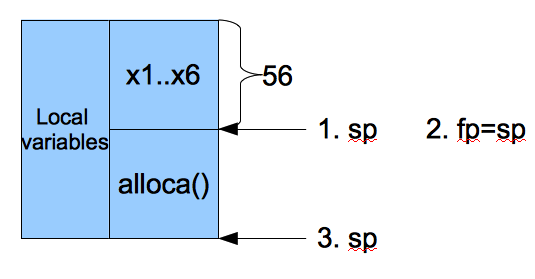
\includegraphics{41.png}}
\caption{Frame pointer changes when enter function}\label{funccall:funccall-f4}\end{figure}
\begin{figure}[htbp]
\centering
\capstart

\scalebox{1.000000}{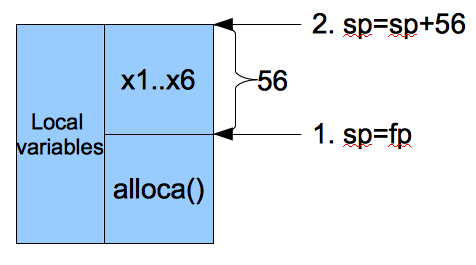
\includegraphics{51.png}}
\caption{Stack pointer changes when exit function}\label{funccall:funccall-f5}\end{figure}
\begin{figure}[htbp]
\centering
\capstart

\scalebox{1.000000}{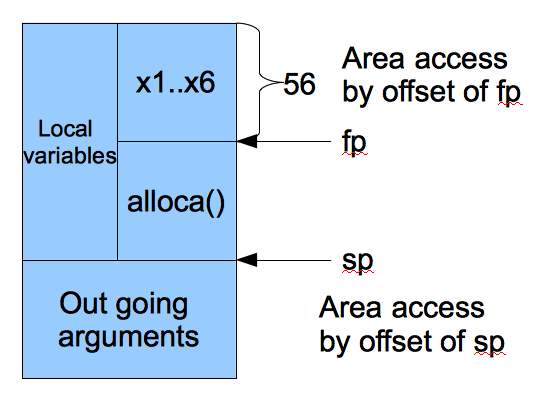
\includegraphics{61.png}}
\caption{fp and sp access areas}\label{funccall:funccall-f6}\end{figure}

Use fp to keep the old stack pointer value is not necessary. Actually, the sp
can back to the the old sp by add the alloca() spaces size. Most ABI like Mips
and ARM access the above area of alloca() by fp and the below area of alloca()
by sp, as \hyperref[funccall:funccall-f6]{Figure  \ref*{funccall:funccall-f6}} depicted. The reason for this definition
is the speed for local variable access. Since the RISC CPU use immediate offset
for load and store as below, using fp and sp for access both areas of
local variables have better performance compare to use the sp only.

\begin{Verbatim}[commandchars=\\\{\}]
ld      \PYG{n+nv}{\PYGZdl{}2}, 64\PYG{o}{(}\PYG{n+nv}{\PYGZdl{}fp}\PYG{o}{)}
st      \PYG{n+nv}{\PYGZdl{}3}, 4\PYG{o}{(}\PYG{n+nv}{\PYGZdl{}sp}\PYG{o}{)}
\end{Verbatim}

Cpu0 use fp and sp to access the above and below areas of alloca() too.
As ch9\_4.cpu0.s, it access local variable (above of alloca()) by fp offset
and outgoing arguments (below of alloca()) by sp offset.


\section{Summary of this chapter}
\label{funccall:summary-of-this-chapter}
Until now, we have 6,000 lines of source code around in the end of this chapter.
The cpu0 backend code now can take care the integer function call and control
statement just like the llvm front end tutorial example code.
Look back the chapter of “Back end structure”, there are 3,100 lines of source
code with taking three instructions only.
With this 95\% more of code, it can translate tens of instructions, global
variable, control flow statement and function call.
Now the cpu0 backend is not just a toy.
It can translate the C++ OOP language into cpu0 instructions without much
effort.
Because the most complex things in language, such as C++ syntex, is handled by
front end.
LLVM is an real structure following the compiler theory, any backend of LLVM can
benefit from this structure.
A couple of thousands lines of code make OOP language translated into your backend.
And your backend will grow up automatically through the front end support languages
more and more.


\chapter{ELF Support}
\label{elf:sec-elf}\label{elf::doc}\label{elf:elf-support}
Cpu0 backend generated the ELF format of obj.
The ELF (Executable and Linkable Format) is a common standard file format for
executables, object code, shared libraries and core dumps.
First published in the System V Application Binary Interface specification,
and later in the Tool Interface Standard, it was quickly accepted among
different vendors of Unixsystems.
In 1999 it was chosen as the standard binary file format for Unix and
Unix-like systems on x86 by the x86open project.
Please reference \footnote{
\href{http://en.wikipedia.org/wiki/Executable\_and\_Linkable\_Format}{http://en.wikipedia.org/wiki/Executable\_and\_Linkable\_Format}
}.

The binary encode of cpu0 instruction set in obj has been checked in the
previous chapters.
But we didn't dig into the ELF file format like elf header and relocation
record at that time.
This chapter will use the binutils which has been installed in
``sub-section Install other tools on iMac'' of Appendix A: “Installing LLVM”
\footnote{
\href{http://jonathan2251.github.com/lbd/install.html\#install-other-tools-on-imac}{http://jonathan2251.github.com/lbd/install.html\#install-other-tools-on-imac}
} to analysis cpu0 ELF file.
You will learn the objdump, readelf, ..., tools and understand the ELF file
format itself through using these tools to analyze the cpu0 generated obj in
this chapter.
LLVM has the llvm-objdump tool which like objdump. We will make cpu0 support
llvm-objdump tool in this chapter.
The binutils support other CPU ELF dump as a cross compiler tool chains.
Linux platform has binutils already and no need to install it further.
We use Linux binutils in this chapter just because iMac will display Chinese
text.
The iMac corresponding binutils have no problem except it use add g in command.
For example, use gobjdump instead of objdump, and display with your area
language instead of pure English.

The binutils tool we use is not a part of llvm tools, but it's a powerful tool
in ELF analysis.
This chapter introduce the tool to readers since we think it is a valuable
knowledge in this popular ELF format and the ELF binutils analysis tool.
An LLVM compiler engineer has the responsibility to analyze the ELF since
the obj is need to be handled by linker or loader later.
With this tool, you can verify your generated ELF format.

The cpu0 author has published a “System Software” book which introduce the
topics
of assembler, linker, loader, compiler and OS in concept, and at same time
demonstrate how to use binutils and gcc to analysis ELF through the example
code in his book.
It's a Chinese book of “System Software” in concept and practice.
This book does the real analysis through binutils.
The “System Software” \footnote{
Leland Beck, System Software: An Introduction to Systems Programming.
} written by Beck is a famous book in concept of
telling readers what is the compiler output, what is the linker output,
what is the loader output, and how they work together.
But it covers the concept only.
You can reference it to understand how the \textbf{“Relocation Record”} works if you
need to refresh or learning this knowledge for this chapter.

\footnote{
\href{http://ccckmit.wikidot.com/lk:aout}{http://ccckmit.wikidot.com/lk:aout}
}, \footnote{
\href{http://ccckmit.wikidot.com/lk:objfile}{http://ccckmit.wikidot.com/lk:objfile}
}, \footnote{
\href{http://ccckmit.wikidot.com/lk:elf}{http://ccckmit.wikidot.com/lk:elf}
} are the Chinese documents available from the cpu0 author on
web site.


\section{ELF format}
\label{elf:elf-format}
ELF is a format used both in obj and executable file.
So, there are two views in it as \hyperref[elf:elf-f1]{Figure  \ref*{elf:elf-f1}}.
\begin{figure}[htbp]
\centering
\capstart

\scalebox{1.000000}{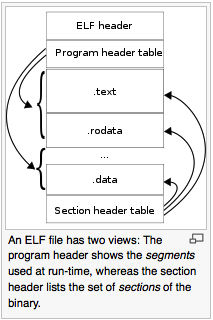
\includegraphics{12.png}}
\caption{ELF file format overview}\label{elf:elf-f1}\end{figure}

As \hyperref[elf:elf-f1]{Figure  \ref*{elf:elf-f1}}, the “Section header table” include sections .text, .rodata,
..., .data which are sections layout for code, read only data, ..., and
read/write data.
“Program header table” include segments include run time code and data.
The definition of segments is run time layout for code and data while sections
is link time layout for code and data.


\section{ELF header and Section header table}
\label{elf:elf-header-and-section-header-table}
Let's run Chapter9\_4/ with ch6\_1.cpp, and dump ELF header information by
\code{readelf -h} to see what information the ELF header contains.

\begin{Verbatim}[commandchars=\\\{\}]
[Gamma@localhost InputFiles]\$ /usr/local/llvm/test/cmake\_debug\_build/
bin/llc -march=cpu0 -relocation-model=pic -filetype=obj ch6\_1.bc -o ch6\_1.cpu0.o

[Gamma@localhost InputFiles]\$ readelf -h ch6\_1.cpu0.o
  Magic:   7f 45 4c 46 01 02 01 03 00 00 00 00 00 00 00 00
  Class:                             ELF32
  Data:                              2's complement, big endian
  Version:                           1 (current)
  OS/ABI:                            UNIX - GNU
  ABI Version:                       0
  Type:                              REL (Relocatable file)
  Machine:                           \textless{}unknown\textgreater{}: 0xc9
  Version:                           0x1
  Entry point address:               0x0
  Start of program headers:          0 (bytes into file)
  Start of section headers:          176 (bytes into file)
  Flags:                             0x0
  Size of this header:               52 (bytes)
  Size of program headers:           0 (bytes)
  Number of program headers:         0
  Size of section headers:           40 (bytes)
  Number of section headers:         8
  Section header string table index: 5
[Gamma@localhost InputFiles]\$

[Gamma@localhost InputFiles]\$ /usr/local/llvm/test/cmake\_debug\_build/
bin/llc -march=mips -relocation-model=pic -filetype=obj ch6\_1.bc -o ch6\_1.mips.o

[Gamma@localhost InputFiles]\$ readelf -h ch6\_1.mips.o
ELF Header:
  Magic:   7f 45 4c 46 01 02 01 03 00 00 00 00 00 00 00 00
  Class:                             ELF32
  Data:                              2's complement, big endian
  Version:                           1 (current)
  OS/ABI:                            UNIX - GNU
  ABI Version:                       0
  Type:                              REL (Relocatable file)
  Machine:                           MIPS R3000
  Version:                           0x1
  Entry point address:               0x0
  Start of program headers:          0 (bytes into file)
  Start of section headers:          200 (bytes into file)
  Flags:                             0x50001007, noreorder, pic, cpic, o32, mips32
  Size of this header:               52 (bytes)
  Size of program headers:           0 (bytes)
  Number of program headers:         0
  Size of section headers:           40 (bytes)
  Number of section headers:         9
  Section header string table index: 6
[Gamma@localhost InputFiles]\$
\end{Verbatim}

As above ELF header display, it contains information of magic number, version,
ABI, ..., . The Machine field of cpu0 is unknown while mips is MIPSR3000.
It is because cpu0 is not a popular CPU recognized by utility readelf.
Let's check ELF segments information as follows,

\begin{Verbatim}[commandchars=\\\{\}]
[Gamma@localhost InputFiles]\$ readelf -l ch6\_1.cpu0.o

There are no program headers in this file.
[Gamma@localhost InputFiles]\$
\end{Verbatim}

The result is in expectation because cpu0 obj is for link only, not for
execution.
So, the segments is empty.
Check ELF sections information as follows.
It contains offset and size information for every section.

\begin{Verbatim}[commandchars=\\\{\}]
[Gamma@localhost InputFiles]\$ readelf -S ch6\_1.cpu0.o
There are 10 section headers, starting at offset 0xd4:

Section Headers:
  [Nr] Name              Type            Addr     Off    Size   ES Flg Lk Inf Al
  [ 0]                   NULL            00000000 000000 000000 00      0   0  0
  [ 1] .text             PROGBITS        00000000 000034 000034 00  AX  0   0  4
  [ 2] .rel.text         REL             00000000 000310 000018 08      8   1  4
  [ 3] .data             PROGBITS        00000000 000068 000004 00  WA  0   0  4
  [ 4] .bss              NOBITS          00000000 00006c 000000 00  WA  0   0  4
  [ 5] .eh\_frame         PROGBITS        00000000 00006c 000028 00   A  0   0  4
  [ 6] .rel.eh\_frame     REL             00000000 000328 000008 08      8   5  4
  [ 7] .shstrtab         STRTAB          00000000 000094 00003e 00      0   0  1
  [ 8] .symtab           SYMTAB          00000000 000264 000090 10      9   6  4
  [ 9] .strtab           STRTAB          00000000 0002f4 00001b 00      0   0  1
Key to Flags:
  W (write), A (alloc), X (execute), M (merge), S (strings)
  I (info), L (link order), G (group), T (TLS), E (exclude), x (unknown)
  O (extra OS processing required) o (OS specific), p (processor specific)
[Gamma@localhost InputFiles]\$
\end{Verbatim}


\section{Relocation Record}
\label{elf:relocation-record}
The cpu0 backend translate global variable as follows,

\begin{Verbatim}[commandchars=\\\{\}]
[Gamma@localhost InputFiles]\$ clang -target mips-unknown-linux-gnu -c ch6\_1.cpp
-emit-llvm -o ch6\_1.bc
[Gamma@localhost InputFiles]\$ /usr/local/llvm/test/cmake\_debug\_build/
bin/llc -march=cpu0 -relocation-model=pic -filetype=asm ch6\_1.bc -o ch6\_1.cpu0.s
[Gamma@localhost InputFiles]\$ cat ch6\_1.cpu0.s
  .section .mdebug.abi32
  .previous
  .file "ch6\_1.bc"
  .text
  ...
  .cfi\_startproc
  .frame  \$sp,8,\$lr
  .mask   0x00000000,0
  .set  noreorder
  .cpload \$t9
  ...
  lui \$2, \%got\_hi(gI)
  addu \$2, \$2, \$gp
  ld \$2, \%got\_lo(gI)(\$2)
  ...
  .type gI,@object              \# @gI
  .data
  .globl  gI
  .align  2
gI:
  .4byte  100                     \# 0x64
  .size gI, 4


[Gamma@localhost InputFiles]\$ /usr/local/llvm/test/cmake\_debug\_build/
bin/llc -march=cpu0 -relocation-model=pic -filetype=obj ch6\_1.bc -o ch6\_1.cpu0.o
[Gamma@localhost InputFiles]\$ objdump -s ch6\_1.cpu0.o

ch6\_1.cpu0.o:     file format elf32-big

Contents of section .text:
// .cpload machine instruction
 0000 0fa00000 09aa0000 13aa6000 ........  ..............{}`.
 ...
 0020 002a0000 00220000 012d0000 09dd0008  .*..."...-......
 ...
[Gamma@localhost InputFiles]\$ Jonathan\$

[Gamma@localhost InputFiles]\$ readelf -tr ch6\_1.cpu0.o
There are 8 section headers, starting at offset 0xb0:

Section Headers:
  [Nr] Name
       Type            Addr     Off    Size   ES   Lk Inf Al
       Flags
  [ 0]
       NULL            00000000 000000 000000 00   0   0  0
       [00000000]:
  [ 1] .text
       PROGBITS        00000000 000034 000044 00   0   0  4
       [00000006]: ALLOC, EXEC
  [ 2] .rel.text
       REL             00000000 0002a8 000020 08   6   1  4
       [00000000]:
  [ 3] .data
       PROGBITS        00000000 000078 000008 00   0   0  4
       [00000003]: WRITE, ALLOC
  [ 4] .bss
       NOBITS          00000000 000080 000000 00   0   0  4
       [00000003]: WRITE, ALLOC
  [ 5] .shstrtab
       STRTAB          00000000 000080 000030 00   0   0  1
       [00000000]:
  [ 6] .symtab
       SYMTAB          00000000 0001f0 000090 10   7   5  4
       [00000000]:
  [ 7] .strtab
       STRTAB          00000000 000280 000025 00   0   0  1
       [00000000]:

Relocation section '.rel.text' at offset 0x2a8 contains 4 entries:
 Offset     Info    Type            Sym.Value  Sym. Name
00000000  00000805 unrecognized: 5       00000000   \_gp\_disp
00000004  00000806 unrecognized: 6       00000000   \_gp\_disp
00000020  00000616 unrecognized: 16      00000004   gI
00000028  00000617 unrecognized: 17      00000004   gI


[Gamma@localhost InputFiles]\$ readelf -tr ch6\_1.mips.o
There are 9 section headers, starting at offset 0xc8:

Section Headers:
  [Nr] Name
       Type            Addr     Off    Size   ES   Lk Inf Al
       Flags
  [ 0]
       NULL            00000000 000000 000000 00   0   0  0
       [00000000]:
  [ 1] .text
       PROGBITS        00000000 000034 000038 00   0   0  4
       [00000006]: ALLOC, EXEC
  [ 2] .rel.text
       REL             00000000 0002f8 000018 08   7   1  4
       [00000000]:
  [ 3] .data
       PROGBITS        00000000 00006c 000008 00   0   0  4
       [00000003]: WRITE, ALLOC
  [ 4] .bss
       NOBITS          00000000 000074 000000 00   0   0  4
       [00000003]: WRITE, ALLOC
  [ 5] .reginfo
       MIPS\_REGINFO    00000000 000074 000018 00   0   0  1
       [00000002]: ALLOC
  [ 6] .shstrtab
       STRTAB          00000000 00008c 000039 00   0   0  1
       [00000000]:
  [ 7] .symtab
       SYMTAB          00000000 000230 0000a0 10   8   6  4
       [00000000]:
  [ 8] .strtab
       STRTAB          00000000 0002d0 000025 00   0   0  1
       [00000000]:

Relocation section '.rel.text' at offset 0x2f8 contains 3 entries:
 Offset     Info    Type            Sym.Value  Sym. Name
00000000  00000905 R\_MIPS\_HI16       00000000   \_gp\_disp
00000004  00000906 R\_MIPS\_LO16       00000000   \_gp\_disp
0000001c  00000709 R\_MIPS\_GOT16      00000004   gI
\end{Verbatim}

As depicted in \href{http://jonathan2251.github.com/lbd/funccall.html\#handle-gp-register-in-pic-addressing-mode}{section Handle \$gp register in PIC addressing mode}, it
translate \textbf{“.cpload \%reg”} into the following.

\begin{Verbatim}[commandchars=\\\{\}]
\PYG{c+c1}{// Lower ".cpload \PYGZdl{}reg" to}
\PYG{c+c1}{//  "lui   \PYGZdl{}gp, \PYGZpc{}hi(\PYGZus{}gp\PYGZus{}disp)"}
\PYG{c+c1}{//  "addiu \PYGZdl{}gp, \PYGZdl{}gp, \PYGZpc{}lo(\PYGZus{}gp\PYGZus{}disp)"}
\PYG{c+c1}{//  "addu  \PYGZdl{}gp, \PYGZdl{}gp, \PYGZdl{}t9"}
\end{Verbatim}

The \_gp\_disp value is determined by loader. So, it's undefined in obj.
You can find the Relocation Records for offset 0 and 4 of .text section
referred to \_gp\_disp value.
The offset 0 and 4 of .text section are instructions ``lui \$gp, \%hi(\_gp\_disp)''
and ``addiu \$gp, \$gp, \%lo(\_gp\_disp)'' which their corresponding obj
encode are 0fa00000 and  09aa0000.
The obj translate the \%hi(\_gp\_disp) and \%lo(\_gp\_disp) into 0 since when loader
load this obj into memory, loader will know the \_gp\_disp value at run time and
will update these two offset relocation records into the correct offset value.
You can check if the cpu0 of \%hi(\_gp\_disp) and \%lo(\_gp\_disp) are correct by
above mips Relocation Records of R\_MIPS\_HI(\_gp\_disp) and  R\_MIPS\_LO(\_gp\_disp)
even though the cpu0 is not a CPU recognized by readelf utilitly.
The instruction \textbf{“ld \$2, \%got(gI)(\$gp)”} is same since we don't know what the
address of .data section variable will load to.
So, translate the address to 0 and made a relocation record on 0x00000020 of
.text section. Linker or Loader will change this address when this program is
linked or loaded depend on the program is static link or dynamic link.


\section{Cpu0 ELF related files}
\label{elf:cpu0-elf-related-files}
Files Cpu0ELFObjectWrite.cpp and Cpu0MC*.cpp are the files take care the obj
format.
Most obj code translation are defined by Cpu0InstrInfo.td and
Cpu0RegisterInfo.td.
With these td description, LLVM translate Cpu0 instruction into obj format
automatically.


\section{llvm-objdump}
\label{elf:llvm-objdump}

\subsection{llvm-objdump -t -r}
\label{elf:llvm-objdump-t-r}
In iMac, \code{gobjdump -tr} can display the information of relocation records
like \code{readelf -tr}. LLVM tool llvm-objdump is the same tool as objdump.
Let's run gobjdump and llvm-objdump commands as follows to see the differences.

\begin{Verbatim}[commandchars=\\\{\}]
118-165-83-12:InputFiles Jonathan\PYG{n+nv}{\PYGZdl{} }clang -target mips-unknown-linux-gnu -c
ch9\PYGZus{}3.cpp -emit-llvm -o ch9\PYGZus{}3.bc
118-165-83-10:InputFiles Jonathan\PYG{n+nv}{\PYGZdl{} }/Users/Jonathan/llvm/test/cmake\PYGZus{}debug\PYGZus{}build/
bin/Debug/llc -march\PYG{o}{=}cpu0 -relocation-model\PYG{o}{=}pic -filetype\PYG{o}{=}obj ch9\PYGZus{}3.bc -o
ch9\PYGZus{}3.cpu0.o

118-165-78-12:InputFiles Jonathan\PYG{n+nv}{\PYGZdl{} }gobjdump -t -r ch9\PYGZus{}3.cpu0.o

ch9\PYGZus{}3.cpu0.o:     file format elf32-big

SYMBOL TABLE:
00000000 l    df *ABS*        00000000 ch9\PYGZus{}3.bc
00000000 l    d  .text        00000000 .text
00000000 l    d  .data        00000000 .data
00000000 l    d  .bss 00000000 .bss
00000000 g     F .text        00000084 \PYGZus{}Z5sum\PYGZus{}iiz
00000084 g     F .text        00000080 main
00000000         *UND*        00000000 \PYGZus{}gp\PYGZus{}disp


RELOCATION RECORDS FOR \PYG{o}{[}.text\PYG{o}{]}:
OFFSET   TYPE              VALUE
00000084 UNKNOWN           \PYGZus{}gp\PYGZus{}disp
00000088 UNKNOWN           \PYGZus{}gp\PYGZus{}disp
000000e0 UNKNOWN           \PYGZus{}Z5sum\PYGZus{}iiz


118-165-83-10:InputFiles Jonathan\PYG{n+nv}{\PYGZdl{} }/Users/Jonathan/llvm/test/cmake\PYGZus{}debug\PYGZus{}build/
bin/Debug/llvm-objdump -t -r ch9\PYGZus{}3\PYGZus{}3.cpu0.o

ch9\PYGZus{}3.cpu0.o: file format ELF32-CPU0

RELOCATION RECORDS FOR \PYG{o}{[}.text\PYG{o}{]}:
132 R\PYGZus{}CPU0\PYGZus{}HI16 \PYGZus{}gp\PYGZus{}disp
136 R\PYGZus{}CPU0\PYGZus{}LO16 \PYGZus{}gp\PYGZus{}disp
224 R\PYGZus{}CPU0\PYGZus{}CALL16 \PYGZus{}Z5sum\PYGZus{}iiz

SYMBOL TABLE:
00000000 l    df *ABS*        00000000 ch9\PYGZus{}3.bc
00000000 l    d  .text        00000000 .text
00000000 l    d  .data        00000000 .data
00000000 l    d  .bss 00000000 .bss
00000000 g     F .text        00000084 \PYGZus{}Z5sum\PYGZus{}iiz
00000084 g     F .text        00000080 main
00000000         *UND*        00000000 \PYGZus{}gp\PYGZus{}disp
\end{Verbatim}

The latter llvm-objdump can display the file format and relocation records
information since we add the relocation records information in ELF.h as follows,
\paragraph{include/support/ELF.h}

\begin{Verbatim}[commandchars=\\\{\}]
\PYG{c+c1}{// Machine architectures}
\PYG{k}{enum} \PYG{p}{\PYGZob{}}
  \PYG{p}{.}\PYG{p}{.}\PYG{p}{.}
  \PYG{n}{EM\PYGZus{}CPU0}          \PYG{o}{=} \PYG{l+m+mi}{201}\PYG{p}{,} \PYG{c+c1}{// Document Write An LLVM Backend Tutorial For Cpu0}
  \PYG{p}{.}\PYG{p}{.}\PYG{p}{.}
\PYG{p}{\PYGZcb{}}

\PYG{c+c1}{// include/object/ELF.h}
\PYG{p}{.}\PYG{p}{.}\PYG{p}{.}
\PYG{k}{template}\PYG{o}{\PYGZlt{}}\PYG{n}{support}\PYG{o}{:}\PYG{o}{:}\PYG{n}{endianness} \PYG{n}{target\PYGZus{}endianness}\PYG{p}{,} \PYG{k+kt}{bool} \PYG{n}{is64Bits}\PYG{o}{\PYGZgt{}}
\PYG{n}{error\PYGZus{}code} \PYG{n}{ELFObjectFile}\PYG{o}{\PYGZlt{}}\PYG{n}{target\PYGZus{}endianness}\PYG{p}{,} \PYG{n}{is64Bits}\PYG{o}{\PYGZgt{}}
            \PYG{o}{:}\PYG{o}{:}\PYG{n}{getRelocationTypeName}\PYG{p}{(}\PYG{n}{DataRefImpl} \PYG{n}{Rel}\PYG{p}{,}
                      \PYG{n}{SmallVectorImpl}\PYG{o}{\PYGZlt{}}\PYG{k+kt}{char}\PYG{o}{\PYGZgt{}} \PYG{o}{\PYGZam{}}\PYG{n}{Result}\PYG{p}{)} \PYG{k}{const} \PYG{p}{\PYGZob{}}
  \PYG{p}{.}\PYG{p}{.}\PYG{p}{.}
  \PYG{k}{switch} \PYG{p}{(}\PYG{n}{Header}\PYG{o}{-}\PYG{o}{\PYGZgt{}}\PYG{n}{e\PYGZus{}machine}\PYG{p}{)} \PYG{p}{\PYGZob{}}
  \PYG{k}{case} \PYG{n}{ELF}\PYG{o}{:}\PYG{o}{:}\PYG{n+nl}{EM\PYGZus{}CPU0:}  \PYG{c+c1}{// llvm-objdump -t -r}
  \PYG{k}{switch} \PYG{p}{(}\PYG{n}{type}\PYG{p}{)} \PYG{p}{\PYGZob{}}
    \PYG{n}{LLVM\PYGZus{}ELF\PYGZus{}SWITCH\PYGZus{}RELOC\PYGZus{}TYPE\PYGZus{}NAME}\PYG{p}{(}\PYG{n}{R\PYGZus{}CPU0\PYGZus{}NONE}\PYG{p}{)}\PYG{p}{;}
    \PYG{n}{LLVM\PYGZus{}ELF\PYGZus{}SWITCH\PYGZus{}RELOC\PYGZus{}TYPE\PYGZus{}NAME}\PYG{p}{(}\PYG{n}{R\PYGZus{}CPU0\PYGZus{}16}\PYG{p}{)}\PYG{p}{;}
    \PYG{n}{LLVM\PYGZus{}ELF\PYGZus{}SWITCH\PYGZus{}RELOC\PYGZus{}TYPE\PYGZus{}NAME}\PYG{p}{(}\PYG{n}{R\PYGZus{}CPU0\PYGZus{}32}\PYG{p}{)}\PYG{p}{;}
    \PYG{n}{LLVM\PYGZus{}ELF\PYGZus{}SWITCH\PYGZus{}RELOC\PYGZus{}TYPE\PYGZus{}NAME}\PYG{p}{(}\PYG{n}{R\PYGZus{}CPU0\PYGZus{}REL32}\PYG{p}{)}\PYG{p}{;}
    \PYG{n}{LLVM\PYGZus{}ELF\PYGZus{}SWITCH\PYGZus{}RELOC\PYGZus{}TYPE\PYGZus{}NAME}\PYG{p}{(}\PYG{n}{R\PYGZus{}CPU0\PYGZus{}24}\PYG{p}{)}\PYG{p}{;}
    \PYG{n}{LLVM\PYGZus{}ELF\PYGZus{}SWITCH\PYGZus{}RELOC\PYGZus{}TYPE\PYGZus{}NAME}\PYG{p}{(}\PYG{n}{R\PYGZus{}CPU0\PYGZus{}HI16}\PYG{p}{)}\PYG{p}{;}
    \PYG{n}{LLVM\PYGZus{}ELF\PYGZus{}SWITCH\PYGZus{}RELOC\PYGZus{}TYPE\PYGZus{}NAME}\PYG{p}{(}\PYG{n}{R\PYGZus{}CPU0\PYGZus{}LO16}\PYG{p}{)}\PYG{p}{;}
    \PYG{n}{LLVM\PYGZus{}ELF\PYGZus{}SWITCH\PYGZus{}RELOC\PYGZus{}TYPE\PYGZus{}NAME}\PYG{p}{(}\PYG{n}{R\PYGZus{}CPU0\PYGZus{}GPREL16}\PYG{p}{)}\PYG{p}{;}
    \PYG{n}{LLVM\PYGZus{}ELF\PYGZus{}SWITCH\PYGZus{}RELOC\PYGZus{}TYPE\PYGZus{}NAME}\PYG{p}{(}\PYG{n}{R\PYGZus{}CPU0\PYGZus{}LITERAL}\PYG{p}{)}\PYG{p}{;}
    \PYG{n}{LLVM\PYGZus{}ELF\PYGZus{}SWITCH\PYGZus{}RELOC\PYGZus{}TYPE\PYGZus{}NAME}\PYG{p}{(}\PYG{n}{R\PYGZus{}CPU0\PYGZus{}GOT16}\PYG{p}{)}\PYG{p}{;}
    \PYG{n}{LLVM\PYGZus{}ELF\PYGZus{}SWITCH\PYGZus{}RELOC\PYGZus{}TYPE\PYGZus{}NAME}\PYG{p}{(}\PYG{n}{R\PYGZus{}CPU0\PYGZus{}PC24}\PYG{p}{)}\PYG{p}{;}
    \PYG{n}{LLVM\PYGZus{}ELF\PYGZus{}SWITCH\PYGZus{}RELOC\PYGZus{}TYPE\PYGZus{}NAME}\PYG{p}{(}\PYG{n}{R\PYGZus{}CPU0\PYGZus{}CALL16}\PYG{p}{)}\PYG{p}{;}
    \PYG{n}{LLVM\PYGZus{}ELF\PYGZus{}SWITCH\PYGZus{}RELOC\PYGZus{}TYPE\PYGZus{}NAME}\PYG{p}{(}\PYG{n}{R\PYGZus{}CPU0\PYGZus{}GPREL32}\PYG{p}{)}\PYG{p}{;}
    \PYG{n}{LLVM\PYGZus{}ELF\PYGZus{}SWITCH\PYGZus{}RELOC\PYGZus{}TYPE\PYGZus{}NAME}\PYG{p}{(}\PYG{n}{R\PYGZus{}CPU0\PYGZus{}SHIFT5}\PYG{p}{)}\PYG{p}{;}
    \PYG{n}{LLVM\PYGZus{}ELF\PYGZus{}SWITCH\PYGZus{}RELOC\PYGZus{}TYPE\PYGZus{}NAME}\PYG{p}{(}\PYG{n}{R\PYGZus{}CPU0\PYGZus{}SHIFT6}\PYG{p}{)}\PYG{p}{;}
    \PYG{n}{LLVM\PYGZus{}ELF\PYGZus{}SWITCH\PYGZus{}RELOC\PYGZus{}TYPE\PYGZus{}NAME}\PYG{p}{(}\PYG{n}{R\PYGZus{}CPU0\PYGZus{}64}\PYG{p}{)}\PYG{p}{;}
    \PYG{n}{LLVM\PYGZus{}ELF\PYGZus{}SWITCH\PYGZus{}RELOC\PYGZus{}TYPE\PYGZus{}NAME}\PYG{p}{(}\PYG{n}{R\PYGZus{}CPU0\PYGZus{}GOT\PYGZus{}DISP}\PYG{p}{)}\PYG{p}{;}
    \PYG{n}{LLVM\PYGZus{}ELF\PYGZus{}SWITCH\PYGZus{}RELOC\PYGZus{}TYPE\PYGZus{}NAME}\PYG{p}{(}\PYG{n}{R\PYGZus{}CPU0\PYGZus{}GOT\PYGZus{}PAGE}\PYG{p}{)}\PYG{p}{;}
    \PYG{n}{LLVM\PYGZus{}ELF\PYGZus{}SWITCH\PYGZus{}RELOC\PYGZus{}TYPE\PYGZus{}NAME}\PYG{p}{(}\PYG{n}{R\PYGZus{}CPU0\PYGZus{}GOT\PYGZus{}OFST}\PYG{p}{)}\PYG{p}{;}
    \PYG{n}{LLVM\PYGZus{}ELF\PYGZus{}SWITCH\PYGZus{}RELOC\PYGZus{}TYPE\PYGZus{}NAME}\PYG{p}{(}\PYG{n}{R\PYGZus{}CPU0\PYGZus{}GOT\PYGZus{}HI16}\PYG{p}{)}\PYG{p}{;}
    \PYG{n}{LLVM\PYGZus{}ELF\PYGZus{}SWITCH\PYGZus{}RELOC\PYGZus{}TYPE\PYGZus{}NAME}\PYG{p}{(}\PYG{n}{R\PYGZus{}CPU0\PYGZus{}GOT\PYGZus{}LO16}\PYG{p}{)}\PYG{p}{;}
    \PYG{n}{LLVM\PYGZus{}ELF\PYGZus{}SWITCH\PYGZus{}RELOC\PYGZus{}TYPE\PYGZus{}NAME}\PYG{p}{(}\PYG{n}{R\PYGZus{}CPU0\PYGZus{}SUB}\PYG{p}{)}\PYG{p}{;}
    \PYG{n}{LLVM\PYGZus{}ELF\PYGZus{}SWITCH\PYGZus{}RELOC\PYGZus{}TYPE\PYGZus{}NAME}\PYG{p}{(}\PYG{n}{R\PYGZus{}CPU0\PYGZus{}INSERT\PYGZus{}A}\PYG{p}{)}\PYG{p}{;}
    \PYG{n}{LLVM\PYGZus{}ELF\PYGZus{}SWITCH\PYGZus{}RELOC\PYGZus{}TYPE\PYGZus{}NAME}\PYG{p}{(}\PYG{n}{R\PYGZus{}CPU0\PYGZus{}INSERT\PYGZus{}B}\PYG{p}{)}\PYG{p}{;}
    \PYG{n}{LLVM\PYGZus{}ELF\PYGZus{}SWITCH\PYGZus{}RELOC\PYGZus{}TYPE\PYGZus{}NAME}\PYG{p}{(}\PYG{n}{R\PYGZus{}CPU0\PYGZus{}DELETE}\PYG{p}{)}\PYG{p}{;}
    \PYG{n}{LLVM\PYGZus{}ELF\PYGZus{}SWITCH\PYGZus{}RELOC\PYGZus{}TYPE\PYGZus{}NAME}\PYG{p}{(}\PYG{n}{R\PYGZus{}CPU0\PYGZus{}HIGHER}\PYG{p}{)}\PYG{p}{;}
    \PYG{n}{LLVM\PYGZus{}ELF\PYGZus{}SWITCH\PYGZus{}RELOC\PYGZus{}TYPE\PYGZus{}NAME}\PYG{p}{(}\PYG{n}{R\PYGZus{}CPU0\PYGZus{}HIGHEST}\PYG{p}{)}\PYG{p}{;}
    \PYG{n}{LLVM\PYGZus{}ELF\PYGZus{}SWITCH\PYGZus{}RELOC\PYGZus{}TYPE\PYGZus{}NAME}\PYG{p}{(}\PYG{n}{R\PYGZus{}CPU0\PYGZus{}CALL\PYGZus{}HI16}\PYG{p}{)}\PYG{p}{;}
    \PYG{n}{LLVM\PYGZus{}ELF\PYGZus{}SWITCH\PYGZus{}RELOC\PYGZus{}TYPE\PYGZus{}NAME}\PYG{p}{(}\PYG{n}{R\PYGZus{}CPU0\PYGZus{}CALL\PYGZus{}LO16}\PYG{p}{)}\PYG{p}{;}
    \PYG{n}{LLVM\PYGZus{}ELF\PYGZus{}SWITCH\PYGZus{}RELOC\PYGZus{}TYPE\PYGZus{}NAME}\PYG{p}{(}\PYG{n}{R\PYGZus{}CPU0\PYGZus{}SCN\PYGZus{}DISP}\PYG{p}{)}\PYG{p}{;}
    \PYG{n}{LLVM\PYGZus{}ELF\PYGZus{}SWITCH\PYGZus{}RELOC\PYGZus{}TYPE\PYGZus{}NAME}\PYG{p}{(}\PYG{n}{R\PYGZus{}CPU0\PYGZus{}REL16}\PYG{p}{)}\PYG{p}{;}
    \PYG{n}{LLVM\PYGZus{}ELF\PYGZus{}SWITCH\PYGZus{}RELOC\PYGZus{}TYPE\PYGZus{}NAME}\PYG{p}{(}\PYG{n}{R\PYGZus{}CPU0\PYGZus{}ADD\PYGZus{}IMMEDIATE}\PYG{p}{)}\PYG{p}{;}
    \PYG{n}{LLVM\PYGZus{}ELF\PYGZus{}SWITCH\PYGZus{}RELOC\PYGZus{}TYPE\PYGZus{}NAME}\PYG{p}{(}\PYG{n}{R\PYGZus{}CPU0\PYGZus{}PJUMP}\PYG{p}{)}\PYG{p}{;}
    \PYG{n}{LLVM\PYGZus{}ELF\PYGZus{}SWITCH\PYGZus{}RELOC\PYGZus{}TYPE\PYGZus{}NAME}\PYG{p}{(}\PYG{n}{R\PYGZus{}CPU0\PYGZus{}RELGOT}\PYG{p}{)}\PYG{p}{;}
    \PYG{n}{LLVM\PYGZus{}ELF\PYGZus{}SWITCH\PYGZus{}RELOC\PYGZus{}TYPE\PYGZus{}NAME}\PYG{p}{(}\PYG{n}{R\PYGZus{}CPU0\PYGZus{}JALR}\PYG{p}{)}\PYG{p}{;}
    \PYG{n}{LLVM\PYGZus{}ELF\PYGZus{}SWITCH\PYGZus{}RELOC\PYGZus{}TYPE\PYGZus{}NAME}\PYG{p}{(}\PYG{n}{R\PYGZus{}CPU0\PYGZus{}TLS\PYGZus{}DTPMOD32}\PYG{p}{)}\PYG{p}{;}
    \PYG{n}{LLVM\PYGZus{}ELF\PYGZus{}SWITCH\PYGZus{}RELOC\PYGZus{}TYPE\PYGZus{}NAME}\PYG{p}{(}\PYG{n}{R\PYGZus{}CPU0\PYGZus{}TLS\PYGZus{}DTPREL32}\PYG{p}{)}\PYG{p}{;}
    \PYG{n}{LLVM\PYGZus{}ELF\PYGZus{}SWITCH\PYGZus{}RELOC\PYGZus{}TYPE\PYGZus{}NAME}\PYG{p}{(}\PYG{n}{R\PYGZus{}CPU0\PYGZus{}TLS\PYGZus{}DTPMOD64}\PYG{p}{)}\PYG{p}{;}
    \PYG{n}{LLVM\PYGZus{}ELF\PYGZus{}SWITCH\PYGZus{}RELOC\PYGZus{}TYPE\PYGZus{}NAME}\PYG{p}{(}\PYG{n}{R\PYGZus{}CPU0\PYGZus{}TLS\PYGZus{}DTPREL64}\PYG{p}{)}\PYG{p}{;}
    \PYG{n}{LLVM\PYGZus{}ELF\PYGZus{}SWITCH\PYGZus{}RELOC\PYGZus{}TYPE\PYGZus{}NAME}\PYG{p}{(}\PYG{n}{R\PYGZus{}CPU0\PYGZus{}TLS\PYGZus{}GD}\PYG{p}{)}\PYG{p}{;}
    \PYG{n}{LLVM\PYGZus{}ELF\PYGZus{}SWITCH\PYGZus{}RELOC\PYGZus{}TYPE\PYGZus{}NAME}\PYG{p}{(}\PYG{n}{R\PYGZus{}CPU0\PYGZus{}TLS\PYGZus{}LDM}\PYG{p}{)}\PYG{p}{;}
    \PYG{n}{LLVM\PYGZus{}ELF\PYGZus{}SWITCH\PYGZus{}RELOC\PYGZus{}TYPE\PYGZus{}NAME}\PYG{p}{(}\PYG{n}{R\PYGZus{}CPU0\PYGZus{}TLS\PYGZus{}DTPREL\PYGZus{}HI16}\PYG{p}{)}\PYG{p}{;}
    \PYG{n}{LLVM\PYGZus{}ELF\PYGZus{}SWITCH\PYGZus{}RELOC\PYGZus{}TYPE\PYGZus{}NAME}\PYG{p}{(}\PYG{n}{R\PYGZus{}CPU0\PYGZus{}TLS\PYGZus{}DTPREL\PYGZus{}LO16}\PYG{p}{)}\PYG{p}{;}
    \PYG{n}{LLVM\PYGZus{}ELF\PYGZus{}SWITCH\PYGZus{}RELOC\PYGZus{}TYPE\PYGZus{}NAME}\PYG{p}{(}\PYG{n}{R\PYGZus{}CPU0\PYGZus{}TLS\PYGZus{}GOTTPREL}\PYG{p}{)}\PYG{p}{;}
    \PYG{n}{LLVM\PYGZus{}ELF\PYGZus{}SWITCH\PYGZus{}RELOC\PYGZus{}TYPE\PYGZus{}NAME}\PYG{p}{(}\PYG{n}{R\PYGZus{}CPU0\PYGZus{}TLS\PYGZus{}TPREL32}\PYG{p}{)}\PYG{p}{;}
    \PYG{n}{LLVM\PYGZus{}ELF\PYGZus{}SWITCH\PYGZus{}RELOC\PYGZus{}TYPE\PYGZus{}NAME}\PYG{p}{(}\PYG{n}{R\PYGZus{}CPU0\PYGZus{}TLS\PYGZus{}TPREL64}\PYG{p}{)}\PYG{p}{;}
    \PYG{n}{LLVM\PYGZus{}ELF\PYGZus{}SWITCH\PYGZus{}RELOC\PYGZus{}TYPE\PYGZus{}NAME}\PYG{p}{(}\PYG{n}{R\PYGZus{}CPU0\PYGZus{}TLS\PYGZus{}TPREL\PYGZus{}HI16}\PYG{p}{)}\PYG{p}{;}
    \PYG{n}{LLVM\PYGZus{}ELF\PYGZus{}SWITCH\PYGZus{}RELOC\PYGZus{}TYPE\PYGZus{}NAME}\PYG{p}{(}\PYG{n}{R\PYGZus{}CPU0\PYGZus{}TLS\PYGZus{}TPREL\PYGZus{}LO16}\PYG{p}{)}\PYG{p}{;}
    \PYG{n}{LLVM\PYGZus{}ELF\PYGZus{}SWITCH\PYGZus{}RELOC\PYGZus{}TYPE\PYGZus{}NAME}\PYG{p}{(}\PYG{n}{R\PYGZus{}CPU0\PYGZus{}GLOB\PYGZus{}DAT}\PYG{p}{)}\PYG{p}{;}
    \PYG{n}{LLVM\PYGZus{}ELF\PYGZus{}SWITCH\PYGZus{}RELOC\PYGZus{}TYPE\PYGZus{}NAME}\PYG{p}{(}\PYG{n}{R\PYGZus{}CPU0\PYGZus{}COPY}\PYG{p}{)}\PYG{p}{;}
    \PYG{n}{LLVM\PYGZus{}ELF\PYGZus{}SWITCH\PYGZus{}RELOC\PYGZus{}TYPE\PYGZus{}NAME}\PYG{p}{(}\PYG{n}{R\PYGZus{}CPU0\PYGZus{}JUMP\PYGZus{}SLOT}\PYG{p}{)}\PYG{p}{;}
    \PYG{n}{LLVM\PYGZus{}ELF\PYGZus{}SWITCH\PYGZus{}RELOC\PYGZus{}TYPE\PYGZus{}NAME}\PYG{p}{(}\PYG{n}{R\PYGZus{}CPU0\PYGZus{}NUM}\PYG{p}{)}\PYG{p}{;}
  \PYG{k}{default}\PYG{o}{:}
    \PYG{n}{res} \PYG{o}{=} \PYG{l+s}{"}\PYG{l+s}{Unknown}\PYG{l+s}{"}\PYG{p}{;}
  \PYG{p}{\PYGZcb{}}
  \PYG{k}{break}\PYG{p}{;}
  \PYG{p}{.}\PYG{p}{.}\PYG{p}{.}
  \PYG{p}{\PYGZcb{}}


\PYG{k}{template}\PYG{o}{\PYGZlt{}}\PYG{n}{support}\PYG{o}{:}\PYG{o}{:}\PYG{n}{endianness} \PYG{n}{target\PYGZus{}endianness}\PYG{p}{,} \PYG{k+kt}{bool} \PYG{n}{is64Bits}\PYG{o}{\PYGZgt{}}
\PYG{n}{error\PYGZus{}code} \PYG{n}{ELFObjectFile}\PYG{o}{\PYGZlt{}}\PYG{n}{target\PYGZus{}endianness}\PYG{p}{,} \PYG{n}{is64Bits}\PYG{o}{\PYGZgt{}}
            \PYG{o}{:}\PYG{o}{:}\PYG{n}{getRelocationValueString}\PYG{p}{(}\PYG{n}{DataRefImpl} \PYG{n}{Rel}\PYG{p}{,}
                      \PYG{n}{SmallVectorImpl}\PYG{o}{\PYGZlt{}}\PYG{k+kt}{char}\PYG{o}{\PYGZgt{}} \PYG{o}{\PYGZam{}}\PYG{n}{Result}\PYG{p}{)} \PYG{k}{const} \PYG{p}{\PYGZob{}}
  \PYG{p}{.}\PYG{p}{.}\PYG{p}{.}
  \PYG{k}{case} \PYG{n}{ELF}\PYG{o}{:}\PYG{o}{:}\PYG{n+nl}{EM\PYGZus{}CPU0:}  \PYG{c+c1}{// llvm-objdump -t -r}
  \PYG{n}{res} \PYG{o}{=} \PYG{n}{symname}\PYG{p}{;}
  \PYG{k}{break}\PYG{p}{;}
  \PYG{p}{.}\PYG{p}{.}\PYG{p}{.}
\PYG{p}{\PYGZcb{}}

\PYG{k}{template}\PYG{o}{\PYGZlt{}}\PYG{n}{support}\PYG{o}{:}\PYG{o}{:}\PYG{n}{endianness} \PYG{n}{target\PYGZus{}endianness}\PYG{p}{,} \PYG{k+kt}{bool} \PYG{n}{is64Bits}\PYG{o}{\PYGZgt{}}
\PYG{n}{StringRef} \PYG{n}{ELFObjectFile}\PYG{o}{\PYGZlt{}}\PYG{n}{target\PYGZus{}endianness}\PYG{p}{,} \PYG{n}{is64Bits}\PYG{o}{\PYGZgt{}}
             \PYG{o}{:}\PYG{o}{:}\PYG{n}{getFileFormatName}\PYG{p}{(}\PYG{p}{)} \PYG{k}{const} \PYG{p}{\PYGZob{}}
  \PYG{k}{switch}\PYG{p}{(}\PYG{n}{Header}\PYG{o}{-}\PYG{o}{\PYGZgt{}}\PYG{n}{e\PYGZus{}ident}\PYG{p}{[}\PYG{n}{ELF}\PYG{o}{:}\PYG{o}{:}\PYG{n}{EI\PYGZus{}CLASS}\PYG{p}{]}\PYG{p}{)} \PYG{p}{\PYGZob{}}
  \PYG{k}{case} \PYG{n}{ELF}\PYG{o}{:}\PYG{o}{:}\PYG{n+nl}{ELFCLASS32:}
  \PYG{k}{switch}\PYG{p}{(}\PYG{n}{Header}\PYG{o}{-}\PYG{o}{\PYGZgt{}}\PYG{n}{e\PYGZus{}machine}\PYG{p}{)} \PYG{p}{\PYGZob{}}
  \PYG{p}{.}\PYG{p}{.}\PYG{p}{.}
  \PYG{k}{case} \PYG{n}{ELF}\PYG{o}{:}\PYG{o}{:}\PYG{n+nl}{EM\PYGZus{}CPU0:}  \PYG{c+c1}{// llvm-objdump -t -r}
    \PYG{k}{return} \PYG{l+s}{"}\PYG{l+s}{ELF32-CPU0}\PYG{l+s}{"}\PYG{p}{;}
  \PYG{p}{.}\PYG{p}{.}\PYG{p}{.}
\PYG{p}{\PYGZcb{}}

\PYG{k}{template}\PYG{o}{\PYGZlt{}}\PYG{n}{support}\PYG{o}{:}\PYG{o}{:}\PYG{n}{endianness} \PYG{n}{target\PYGZus{}endianness}\PYG{p}{,} \PYG{k+kt}{bool} \PYG{n}{is64Bits}\PYG{o}{\PYGZgt{}}
\PYG{k+kt}{unsigned} \PYG{n}{ELFObjectFile}\PYG{o}{\PYGZlt{}}\PYG{n}{target\PYGZus{}endianness}\PYG{p}{,} \PYG{n}{is64Bits}\PYG{o}{\PYGZgt{}}\PYG{o}{:}\PYG{o}{:}\PYG{n}{getArch}\PYG{p}{(}\PYG{p}{)} \PYG{k}{const} \PYG{p}{\PYGZob{}}
  \PYG{k}{switch}\PYG{p}{(}\PYG{n}{Header}\PYG{o}{-}\PYG{o}{\PYGZgt{}}\PYG{n}{e\PYGZus{}machine}\PYG{p}{)} \PYG{p}{\PYGZob{}}
  \PYG{p}{.}\PYG{p}{.}\PYG{p}{.}
  \PYG{k}{case} \PYG{n}{ELF}\PYG{o}{:}\PYG{o}{:}\PYG{n+nl}{EM\PYGZus{}CPU0:}  \PYG{c+c1}{// llvm-objdump -t -r}
  \PYG{k}{return} \PYG{p}{(}\PYG{n}{target\PYGZus{}endianness} \PYG{o}{=}\PYG{o}{=} \PYG{n}{support}\PYG{o}{:}\PYG{o}{:}\PYG{n}{little}\PYG{p}{)} \PYG{o}{?}
       \PYG{n}{Triple}\PYG{o}{:}\PYG{o}{:}\PYG{n}{cpu0el} \PYG{o}{:} \PYG{n}{Triple}\PYG{o}{:}\PYG{o}{:}\PYG{n}{cpu0}\PYG{p}{;}
  \PYG{p}{.}\PYG{p}{.}\PYG{p}{.}
\PYG{p}{\PYGZcb{}}
\end{Verbatim}


\subsection{llvm-objdump -d}
\label{elf:llvm-objdump-d}
Run the last Chapter example code with command \code{llvm-objdump -d} for dump
file from elf to hex as follows,

\begin{Verbatim}[commandchars=\\\{\}]
JonathantekiiMac:InputFiles Jonathan\PYG{n+nv}{\PYGZdl{} }clang -target mips-unknown-linux-gnu -c
ch8\PYGZus{}1\PYGZus{}1.cpp -emit-llvm -o ch8\PYGZus{}1\PYGZus{}1.bc
JonathantekiiMac:InputFiles Jonathan\PYG{n+nv}{\PYGZdl{} }/Users/Jonathan/llvm/test/cmake\PYGZus{}debug\PYGZus{}
build/bin/Debug/llc -march\PYG{o}{=}cpu0 -relocation-model\PYG{o}{=}pic -filetype\PYG{o}{=}obj ch8\PYGZus{}1\PYGZus{}1.bc
-o ch8\PYGZus{}1\PYGZus{}1.cpu0.o
JonathantekiiMac:InputFiles Jonathan\PYG{n+nv}{\PYGZdl{} }/Users/Jonathan/llvm/test/cmake\PYGZus{}debug\PYGZus{}
build/bin/Debug/llvm-objdump -d ch8\PYGZus{}1\PYGZus{}1.cpu0.o

ch8\PYGZus{}1\PYGZus{}1.cpu0.o: file format ELF32-unknown

Disassembly of section .text:error: no disassembler \PYG{k}{for }target cpu0-unknown-
unknown
\end{Verbatim}

To support llvm-objdump, the following code added to Chapter10\_1/
(the DecoderMethod for brtarget24 has been added in previous chapter).
\paragraph{lbdex/Chapter10\_1/CMakeLists.txt}

\begin{Verbatim}[commandchars=\\\{\}]
\PYG{n}{tablegen}\PYG{p}{(}\PYG{n}{LLVM} \PYG{n}{Cpu0GenDisassemblerTables}\PYG{p}{.}\PYG{n}{inc} \PYG{o}{-}\PYG{n}{gen}\PYG{o}{-}\PYG{n}{disassembler}\PYG{p}{)}
\PYG{p}{.}\PYG{p}{.}\PYG{p}{.}
\end{Verbatim}
\paragraph{lbdex/Chapter10\_1/LLVMBuild.txt}

\begin{Verbatim}[commandchars=\\\{\}]
\PYG{p}{[}\PYG{n}{common}\PYG{p}{]}
\PYG{n}{subdirectories} \PYG{o}{=} \PYG{n}{Disassembler} \PYG{p}{.}\PYG{p}{.}\PYG{p}{.}
\PYG{p}{.}\PYG{p}{.}\PYG{p}{.}
\PYG{n}{has\PYGZus{}disassembler} \PYG{o}{=} \PYG{l+m+mi}{1}
\PYG{p}{.}\PYG{p}{.}\PYG{p}{.}
\end{Verbatim}
\paragraph{lbdex/Chapter8\_1/Cpu0InstrInfo.td}

\begin{Verbatim}[commandchars=\\\{\}]
\PYG{n}{def} \PYG{n}{brtarget24}    \PYG{o}{:} \PYG{n}{Operand}\PYG{o}{\PYGZlt{}}\PYG{n}{OtherVT}\PYG{o}{\PYGZgt{}} \PYG{p}{\PYGZob{}}
  \PYG{p}{.}\PYG{p}{.}\PYG{p}{.}
  \PYG{n}{let} \PYG{n}{DecoderMethod} \PYG{o}{=} \PYG{l+s}{"}\PYG{l+s}{DecodeBranch24Target}\PYG{l+s}{"}\PYG{p}{;}
\PYG{p}{\PYGZcb{}}
\end{Verbatim}
\paragraph{lbdex/Chapter10\_1/Cpu0InstrInfo.td}

\begin{Verbatim}[commandchars=\\\{\}]
class CmpInstr\textless{}bits\textless{}8\textgreater{} op, string instr\_asm,
         InstrItinClass itin, RegisterClass RC, RegisterClass RD,
         bit isComm = 0\textgreater{}:
  FA\textless{}op, (outs RD:\$rc), (ins RC:\$ra, RC:\$rb),
   !strconcat(instr\_asm, "\PYGZbs{}t\$ra, \$rb"), [], itin\textgreater{} \PYGZob{}
  ...
  let DecoderMethod = "DecodeCMPInstruction";
\PYGZcb{}
...
let isBranch=1, isTerminator=1, isBarrier=1, imm16=0, hasDelaySlot = 1,
  isIndirectBranch = 1 in
class JumpFR\textless{}bits\textless{}8\textgreater{} op, string instr\_asm, RegisterClass RC\textgreater{}:
  FL\textless{}op, (outs), (ins RC:\$ra),
   !strconcat(instr\_asm, "\PYGZbs{}t\$ra"), [(brind RC:\$ra)], IIBranch\textgreater{} \PYGZob{}
  let rb = 0;
  let imm16 = 0;
\PYGZcb{}

let isCall=1, hasDelaySlot=0 in \PYGZob{}
  class JumpLink\textless{}bits\textless{}8\textgreater{} op, string instr\_asm\textgreater{}:
  FJ\textless{}op, (outs), (ins calltarget:\$target, variable\_ops),
     !strconcat(instr\_asm, "\PYGZbs{}t\$target"), [(Cpu0JmpLink imm:\$target)],
     IIBranch\textgreater{} \PYGZob{}
     let DecoderMethod = "DecodeJumpAbsoluteTarget";
     \PYGZcb{}

def JR      : JumpFR\textless{}0x2C, "ret", CPURegs\textgreater{};
\end{Verbatim}
\paragraph{lbdex/Chapter10\_1/Disassembler/CMakeLists.txt}

\begin{Verbatim}[commandchars=\\\{\}]
include\_directories( \$\PYGZob{}CMAKE\_CURRENT\_BINARY\_DIR\PYGZcb{}/.. \$\PYGZob{}CMAKE\_CURRENT\_SOURCE\_DIR\PYGZcb{}/.. )

add\_llvm\_library(LLVMCpu0Disassembler
  Cpu0Disassembler.cpp
  )

\# workaround for hanging compilation on MSVC9 and 10
if( MSVC\_VERSION EQUAL 1400 OR MSVC\_VERSION EQUAL 1500 OR MSVC\_VERSION EQUAL 1600 )
set\_property(
  SOURCE Cpu0Disassembler.cpp
  PROPERTY COMPILE\_FLAGS "/Od"
  )
endif()

add\_dependencies(LLVMCpu0Disassembler Cpu0CommonTableGen)
\end{Verbatim}
\paragraph{lbdex/Chapter10\_1/Disassembler/LLVMBuild.txt}

\begin{Verbatim}[commandchars=\\\{\}]
\PYG{p}{;}\PYG{o}{=}\PYG{o}{=}\PYG{o}{=}\PYG{o}{-} \PYG{p}{.}\PYG{o}{/}\PYG{n}{lib}\PYG{o}{/}\PYG{n}{Target}\PYG{o}{/}\PYG{n}{Cpu0}\PYG{o}{/}\PYG{n}{Disassembler}\PYG{o}{/}\PYG{n}{LLVMBuild}\PYG{p}{.}\PYG{n}{txt} \PYG{o}{-}\PYG{o}{-}\PYG{o}{-}\PYG{o}{-}\PYG{o}{-}\PYG{o}{-}\PYG{o}{-}\PYG{o}{-}\PYG{o}{-}\PYG{o}{-}\PYG{o}{-}\PYG{o}{-}\PYG{o}{-}\PYG{o}{-}\PYG{o}{*}\PYG{o}{-} \PYG{n}{Conf} \PYG{o}{-}\PYG{o}{*}\PYG{o}{-}\PYG{o}{-}\PYG{o}{=}\PYG{o}{=}\PYG{o}{=}\PYG{p}{;}
\PYG{p}{;}
\PYG{p}{;}                     \PYG{n}{The} \PYG{n}{LLVM} \PYG{n}{Compiler} \PYG{n}{Infrastructure}
\PYG{p}{;}
\PYG{p}{;} \PYG{n}{This} \PYG{n}{file} \PYG{n}{is} \PYG{n}{distributed} \PYG{n}{under} \PYG{n}{the} \PYG{n}{University} \PYG{n}{of} \PYG{n}{Illinois} \PYG{n}{Open} \PYG{n}{Source}
\PYG{p}{;} \PYG{n}{License}\PYG{p}{.} \PYG{n}{See} \PYG{n}{LICENSE}\PYG{p}{.}\PYG{n}{TXT} \PYG{k}{for} \PYG{n}{details}\PYG{p}{.}
\PYG{p}{;}
\PYG{p}{;}\PYG{o}{=}\PYG{o}{=}\PYG{o}{=}\PYG{o}{-}\PYG{o}{-}\PYG{o}{-}\PYG{o}{-}\PYG{o}{-}\PYG{o}{-}\PYG{o}{-}\PYG{o}{-}\PYG{o}{-}\PYG{o}{-}\PYG{o}{-}\PYG{o}{-}\PYG{o}{-}\PYG{o}{-}\PYG{o}{-}\PYG{o}{-}\PYG{o}{-}\PYG{o}{-}\PYG{o}{-}\PYG{o}{-}\PYG{o}{-}\PYG{o}{-}\PYG{o}{-}\PYG{o}{-}\PYG{o}{-}\PYG{o}{-}\PYG{o}{-}\PYG{o}{-}\PYG{o}{-}\PYG{o}{-}\PYG{o}{-}\PYG{o}{-}\PYG{o}{-}\PYG{o}{-}\PYG{o}{-}\PYG{o}{-}\PYG{o}{-}\PYG{o}{-}\PYG{o}{-}\PYG{o}{-}\PYG{o}{-}\PYG{o}{-}\PYG{o}{-}\PYG{o}{-}\PYG{o}{-}\PYG{o}{-}\PYG{o}{-}\PYG{o}{-}\PYG{o}{-}\PYG{o}{-}\PYG{o}{-}\PYG{o}{-}\PYG{o}{-}\PYG{o}{-}\PYG{o}{-}\PYG{o}{-}\PYG{o}{-}\PYG{o}{-}\PYG{o}{-}\PYG{o}{-}\PYG{o}{-}\PYG{o}{-}\PYG{o}{-}\PYG{o}{-}\PYG{o}{-}\PYG{o}{-}\PYG{o}{-}\PYG{o}{-}\PYG{o}{-}\PYG{o}{-}\PYG{o}{-}\PYG{o}{-}\PYG{o}{=}\PYG{o}{=}\PYG{o}{=}\PYG{p}{;}
\PYG{p}{;}
\PYG{p}{;} \PYG{n}{This} \PYG{n}{is} \PYG{n}{an} \PYG{n}{LLVMBuild} \PYG{n}{description} \PYG{n}{file} \PYG{k}{for} \PYG{n}{the} \PYG{n}{components} \PYG{n}{in} \PYG{k}{this} \PYG{n}{subdirectory}\PYG{p}{.}
\PYG{p}{;}
\PYG{p}{;} \PYG{n}{For} \PYG{n}{more} \PYG{n}{information} \PYG{n}{on} \PYG{n}{the} \PYG{n}{LLVMBuild} \PYG{n}{system}\PYG{p}{,} \PYG{n}{please} \PYG{n+nl}{see:}
\PYG{p}{;}
\PYG{p}{;}   \PYG{n+nl}{http:}\PYG{c+c1}{//llvm.org/docs/LLVMBuild.html}
\PYG{p}{;}
\PYG{p}{;}\PYG{o}{=}\PYG{o}{=}\PYG{o}{=}\PYG{o}{-}\PYG{o}{-}\PYG{o}{-}\PYG{o}{-}\PYG{o}{-}\PYG{o}{-}\PYG{o}{-}\PYG{o}{-}\PYG{o}{-}\PYG{o}{-}\PYG{o}{-}\PYG{o}{-}\PYG{o}{-}\PYG{o}{-}\PYG{o}{-}\PYG{o}{-}\PYG{o}{-}\PYG{o}{-}\PYG{o}{-}\PYG{o}{-}\PYG{o}{-}\PYG{o}{-}\PYG{o}{-}\PYG{o}{-}\PYG{o}{-}\PYG{o}{-}\PYG{o}{-}\PYG{o}{-}\PYG{o}{-}\PYG{o}{-}\PYG{o}{-}\PYG{o}{-}\PYG{o}{-}\PYG{o}{-}\PYG{o}{-}\PYG{o}{-}\PYG{o}{-}\PYG{o}{-}\PYG{o}{-}\PYG{o}{-}\PYG{o}{-}\PYG{o}{-}\PYG{o}{-}\PYG{o}{-}\PYG{o}{-}\PYG{o}{-}\PYG{o}{-}\PYG{o}{-}\PYG{o}{-}\PYG{o}{-}\PYG{o}{-}\PYG{o}{-}\PYG{o}{-}\PYG{o}{-}\PYG{o}{-}\PYG{o}{-}\PYG{o}{-}\PYG{o}{-}\PYG{o}{-}\PYG{o}{-}\PYG{o}{-}\PYG{o}{-}\PYG{o}{-}\PYG{o}{-}\PYG{o}{-}\PYG{o}{-}\PYG{o}{-}\PYG{o}{-}\PYG{o}{-}\PYG{o}{-}\PYG{o}{-}\PYG{o}{-}\PYG{o}{=}\PYG{o}{=}\PYG{o}{=}\PYG{p}{;}

\PYG{p}{[}\PYG{n}{component\PYGZus{}0}\PYG{p}{]}
\PYG{n}{type} \PYG{o}{=} \PYG{n}{Library}
\PYG{n}{name} \PYG{o}{=} \PYG{n}{Cpu0Disassembler}
\PYG{n}{parent} \PYG{o}{=} \PYG{n}{Cpu0}
\PYG{n}{required\PYGZus{}libraries} \PYG{o}{=} \PYG{n}{MC} \PYG{n}{Support} \PYG{n}{Cpu0Info}
\PYG{n}{add\PYGZus{}to\PYGZus{}library\PYGZus{}groups} \PYG{o}{=} \PYG{n}{Cpu0}
\end{Verbatim}
\paragraph{lbdex/Chapter10\_1/Disassembler/Cpu0Disassembler.cpp}

\begin{Verbatim}[commandchars=\\\{\}]
\PYG{c+c1}{//===- Cpu0Disassembler.cpp - Disassembler for Cpu0 -------------*- C++ -*-===//}
\PYG{c+c1}{//}
\PYG{c+c1}{//                     The LLVM Compiler Infrastructure}
\PYG{c+c1}{//}
\PYG{c+c1}{// This file is distributed under the University of Illinois Open Source}
\PYG{c+c1}{// License. See LICENSE.TXT for details.}
\PYG{c+c1}{//}
\PYG{c+c1}{//===----------------------------------------------------------------------===//}
\PYG{c+c1}{//}
\PYG{c+c1}{// This file is part of the Cpu0 Disassembler.}
\PYG{c+c1}{//}
\PYG{c+c1}{//===----------------------------------------------------------------------===//}

\PYG{c+cp}{\PYGZsh{}}\PYG{c+cp}{include "Cpu0.h"}
\PYG{c+cp}{\PYGZsh{}}\PYG{c+cp}{include "Cpu0Subtarget.h"}
\PYG{c+cp}{\PYGZsh{}}\PYG{c+cp}{include "Cpu0RegisterInfo.h"}
\PYG{c+cp}{\PYGZsh{}}\PYG{c+cp}{include "llvm}\PYG{c+cp}{/}\PYG{c+cp}{MC}\PYG{c+cp}{/}\PYG{c+cp}{MCDisassembler.h"}
\PYG{c+cp}{\PYGZsh{}}\PYG{c+cp}{include "llvm}\PYG{c+cp}{/}\PYG{c+cp}{MC}\PYG{c+cp}{/}\PYG{c+cp}{MCFixedLenDisassembler.h"}
\PYG{c+cp}{\PYGZsh{}}\PYG{c+cp}{include "llvm}\PYG{c+cp}{/}\PYG{c+cp}{Support}\PYG{c+cp}{/}\PYG{c+cp}{MemoryObject.h"}
\PYG{c+cp}{\PYGZsh{}}\PYG{c+cp}{include "llvm}\PYG{c+cp}{/}\PYG{c+cp}{Support}\PYG{c+cp}{/}\PYG{c+cp}{TargetRegistry.h"}
\PYG{c+cp}{\PYGZsh{}}\PYG{c+cp}{include "llvm}\PYG{c+cp}{/}\PYG{c+cp}{MC}\PYG{c+cp}{/}\PYG{c+cp}{MCSubtargetInfo.h"}
\PYG{c+cp}{\PYGZsh{}}\PYG{c+cp}{include "llvm}\PYG{c+cp}{/}\PYG{c+cp}{MC}\PYG{c+cp}{/}\PYG{c+cp}{MCInst.h"}
\PYG{c+cp}{\PYGZsh{}}\PYG{c+cp}{include "llvm}\PYG{c+cp}{/}\PYG{c+cp}{Support}\PYG{c+cp}{/}\PYG{c+cp}{MathExtras.h"}

\PYG{k}{using} \PYG{k}{namespace} \PYG{n}{llvm}\PYG{p}{;}

\PYG{k}{typedef} \PYG{n}{MCDisassembler}\PYG{o}{:}\PYG{o}{:}\PYG{n}{DecodeStatus} \PYG{n}{DecodeStatus}\PYG{p}{;}

\PYG{c+c1}{/// Cpu0Disassembler - a disasembler class for Cpu032.}
\PYG{k}{class} \PYG{n+nc}{Cpu0Disassembler} \PYG{o}{:} \PYG{k}{public} \PYG{n}{MCDisassembler} \PYG{p}{\PYGZob{}}
\PYG{k}{public}\PYG{o}{:}
  \PYG{c+c1}{/// Constructor     - Initializes the disassembler.}
  \PYG{c+c1}{///}
  \PYG{n}{Cpu0Disassembler}\PYG{p}{(}\PYG{k}{const} \PYG{n}{MCSubtargetInfo} \PYG{o}{\PYGZam{}}\PYG{n}{STI}\PYG{p}{,} \PYG{k+kt}{bool} \PYG{n}{bigEndian}\PYG{p}{)} \PYG{o}{:}
    \PYG{n}{MCDisassembler}\PYG{p}{(}\PYG{n}{STI}\PYG{p}{)}\PYG{p}{,} \PYG{n}{isBigEndian}\PYG{p}{(}\PYG{n}{bigEndian}\PYG{p}{)} \PYG{p}{\PYGZob{}}
  \PYG{p}{\PYGZcb{}}

  \PYG{o}{\PYGZti{}}\PYG{n}{Cpu0Disassembler}\PYG{p}{(}\PYG{p}{)} \PYG{p}{\PYGZob{}}
  \PYG{p}{\PYGZcb{}}

  \PYG{c+c1}{/// getInstruction - See MCDisassembler.}
  \PYG{n}{DecodeStatus} \PYG{n}{getInstruction}\PYG{p}{(}\PYG{n}{MCInst} \PYG{o}{\PYGZam{}}\PYG{n}{instr}\PYG{p}{,}
                              \PYG{n}{uint64\PYGZus{}t} \PYG{o}{\PYGZam{}}\PYG{n}{size}\PYG{p}{,}
                              \PYG{k}{const} \PYG{n}{MemoryObject} \PYG{o}{\PYGZam{}}\PYG{n}{region}\PYG{p}{,}
                              \PYG{n}{uint64\PYGZus{}t} \PYG{n}{address}\PYG{p}{,}
                              \PYG{n}{raw\PYGZus{}ostream} \PYG{o}{\PYGZam{}}\PYG{n}{vStream}\PYG{p}{,}
                              \PYG{n}{raw\PYGZus{}ostream} \PYG{o}{\PYGZam{}}\PYG{n}{cStream}\PYG{p}{)} \PYG{k}{const}\PYG{p}{;}

\PYG{k}{private}\PYG{o}{:}
  \PYG{k+kt}{bool} \PYG{n}{isBigEndian}\PYG{p}{;}
\PYG{p}{\PYGZcb{}}\PYG{p}{;}

\PYG{c+c1}{// Decoder tables for Cpu0 register}
\PYG{k}{static} \PYG{k}{const} \PYG{k+kt}{unsigned} \PYG{n}{CPURegsTable}\PYG{p}{[}\PYG{p}{]} \PYG{o}{=} \PYG{p}{\PYGZob{}}
  \PYG{n}{Cpu0}\PYG{o}{:}\PYG{o}{:}\PYG{n}{ZERO}\PYG{p}{,} \PYG{n}{Cpu0}\PYG{o}{:}\PYG{o}{:}\PYG{n}{AT}\PYG{p}{,} \PYG{n}{Cpu0}\PYG{o}{:}\PYG{o}{:}\PYG{n}{V0}\PYG{p}{,} \PYG{n}{Cpu0}\PYG{o}{:}\PYG{o}{:}\PYG{n}{V1}\PYG{p}{,}
  \PYG{n}{Cpu0}\PYG{o}{:}\PYG{o}{:}\PYG{n}{A0}\PYG{p}{,} \PYG{n}{Cpu0}\PYG{o}{:}\PYG{o}{:}\PYG{n}{A1}\PYG{p}{,} \PYG{n}{Cpu0}\PYG{o}{:}\PYG{o}{:}\PYG{n}{T9}\PYG{p}{,} \PYG{n}{Cpu0}\PYG{o}{:}\PYG{o}{:}\PYG{n}{T0}\PYG{p}{,} 
  \PYG{n}{Cpu0}\PYG{o}{:}\PYG{o}{:}\PYG{n}{S0}\PYG{p}{,} \PYG{n}{Cpu0}\PYG{o}{:}\PYG{o}{:}\PYG{n}{S1}\PYG{p}{,} \PYG{n}{Cpu0}\PYG{o}{:}\PYG{o}{:}\PYG{n}{S2}\PYG{p}{,} \PYG{n}{Cpu0}\PYG{o}{:}\PYG{o}{:}\PYG{n}{GP}\PYG{p}{,} 
  \PYG{n}{Cpu0}\PYG{o}{:}\PYG{o}{:}\PYG{n}{FP}\PYG{p}{,} \PYG{n}{Cpu0}\PYG{o}{:}\PYG{o}{:}\PYG{n}{SP}\PYG{p}{,} \PYG{n}{Cpu0}\PYG{o}{:}\PYG{o}{:}\PYG{n}{LR}\PYG{p}{,} \PYG{n}{Cpu0}\PYG{o}{:}\PYG{o}{:}\PYG{n}{PC}
\PYG{p}{\PYGZcb{}}\PYG{p}{;}

\PYG{k}{static} \PYG{n}{DecodeStatus} \PYG{n}{DecodeCPURegsRegisterClass}\PYG{p}{(}\PYG{n}{MCInst} \PYG{o}{\PYGZam{}}\PYG{n}{Inst}\PYG{p}{,}
                                               \PYG{k+kt}{unsigned} \PYG{n}{RegNo}\PYG{p}{,}
                                               \PYG{n}{uint64\PYGZus{}t} \PYG{n}{Address}\PYG{p}{,}
                                               \PYG{k}{const} \PYG{k+kt}{void} \PYG{o}{*}\PYG{n}{Decoder}\PYG{p}{)}\PYG{p}{;}
\PYG{k}{static} \PYG{n}{DecodeStatus} \PYG{n}{DecodeCMPInstruction}\PYG{p}{(}\PYG{n}{MCInst} \PYG{o}{\PYGZam{}}\PYG{n}{Inst}\PYG{p}{,}
                                       \PYG{k+kt}{unsigned} \PYG{n}{Insn}\PYG{p}{,}
                                       \PYG{n}{uint64\PYGZus{}t} \PYG{n}{Address}\PYG{p}{,}
                                       \PYG{k}{const} \PYG{k+kt}{void} \PYG{o}{*}\PYG{n}{Decoder}\PYG{p}{)}\PYG{p}{;}
\end{Verbatim}

\begin{Verbatim}[commandchars=\\\{\}]
\PYG{k}{static} \PYG{n}{DecodeStatus} \PYG{n}{DecodeBranch24Target}\PYG{p}{(}\PYG{n}{MCInst} \PYG{o}{\PYGZam{}}\PYG{n}{Inst}\PYG{p}{,}
                                       \PYG{k+kt}{unsigned} \PYG{n}{Insn}\PYG{p}{,}
                                       \PYG{n}{uint64\PYGZus{}t} \PYG{n}{Address}\PYG{p}{,}
                                       \PYG{k}{const} \PYG{k+kt}{void} \PYG{o}{*}\PYG{n}{Decoder}\PYG{p}{)}\PYG{p}{;}
\PYG{k}{static} \PYG{n}{DecodeStatus} \PYG{n}{DecodeJumpRelativeTarget}\PYG{p}{(}\PYG{n}{MCInst} \PYG{o}{\PYGZam{}}\PYG{n}{Inst}\PYG{p}{,}
                                       \PYG{k+kt}{unsigned} \PYG{n}{Insn}\PYG{p}{,}
                                       \PYG{n}{uint64\PYGZus{}t} \PYG{n}{Address}\PYG{p}{,}
                                       \PYG{k}{const} \PYG{k+kt}{void} \PYG{o}{*}\PYG{n}{Decoder}\PYG{p}{)}\PYG{p}{;}
\PYG{k}{static} \PYG{n}{DecodeStatus} \PYG{n}{DecodeJumpAbsoluteTarget}\PYG{p}{(}\PYG{n}{MCInst} \PYG{o}{\PYGZam{}}\PYG{n}{Inst}\PYG{p}{,}
                                     \PYG{k+kt}{unsigned} \PYG{n}{Insn}\PYG{p}{,}
                                     \PYG{n}{uint64\PYGZus{}t} \PYG{n}{Address}\PYG{p}{,}
                                     \PYG{k}{const} \PYG{k+kt}{void} \PYG{o}{*}\PYG{n}{Decoder}\PYG{p}{)}\PYG{p}{;}

\PYG{k}{static} \PYG{n}{DecodeStatus} \PYG{n}{DecodeMem}\PYG{p}{(}\PYG{n}{MCInst} \PYG{o}{\PYGZam{}}\PYG{n}{Inst}\PYG{p}{,}
                              \PYG{k+kt}{unsigned} \PYG{n}{Insn}\PYG{p}{,}
                              \PYG{n}{uint64\PYGZus{}t} \PYG{n}{Address}\PYG{p}{,}
                              \PYG{k}{const} \PYG{k+kt}{void} \PYG{o}{*}\PYG{n}{Decoder}\PYG{p}{)}\PYG{p}{;}
\PYG{k}{static} \PYG{n}{DecodeStatus} \PYG{n}{DecodeSimm16}\PYG{p}{(}\PYG{n}{MCInst} \PYG{o}{\PYGZam{}}\PYG{n}{Inst}\PYG{p}{,}
                                 \PYG{k+kt}{unsigned} \PYG{n}{Insn}\PYG{p}{,}
                                 \PYG{n}{uint64\PYGZus{}t} \PYG{n}{Address}\PYG{p}{,}
                                 \PYG{k}{const} \PYG{k+kt}{void} \PYG{o}{*}\PYG{n}{Decoder}\PYG{p}{)}\PYG{p}{;}

\PYG{k}{namespace} \PYG{n}{llvm} \PYG{p}{\PYGZob{}}
\PYG{k}{extern} \PYG{n}{Target} \PYG{n}{TheCpu0elTarget}\PYG{p}{,} \PYG{n}{TheCpu0Target}\PYG{p}{,} \PYG{n}{TheCpu064Target}\PYG{p}{,}
              \PYG{n}{TheCpu064elTarget}\PYG{p}{;}
\PYG{p}{\PYGZcb{}}

\PYG{k}{static} \PYG{n}{MCDisassembler} \PYG{o}{*}\PYG{n}{createCpu0Disassembler}\PYG{p}{(}
                       \PYG{k}{const} \PYG{n}{Target} \PYG{o}{\PYGZam{}}\PYG{n}{T}\PYG{p}{,}
                       \PYG{k}{const} \PYG{n}{MCSubtargetInfo} \PYG{o}{\PYGZam{}}\PYG{n}{STI}\PYG{p}{)} \PYG{p}{\PYGZob{}}
  \PYG{k}{return} \PYG{k}{new} \PYG{n}{Cpu0Disassembler}\PYG{p}{(}\PYG{n}{STI}\PYG{p}{,}\PYG{k+kc}{true}\PYG{p}{)}\PYG{p}{;}
\PYG{p}{\PYGZcb{}}

\PYG{k}{static} \PYG{n}{MCDisassembler} \PYG{o}{*}\PYG{n}{createCpu0elDisassembler}\PYG{p}{(}
                       \PYG{k}{const} \PYG{n}{Target} \PYG{o}{\PYGZam{}}\PYG{n}{T}\PYG{p}{,}
                       \PYG{k}{const} \PYG{n}{MCSubtargetInfo} \PYG{o}{\PYGZam{}}\PYG{n}{STI}\PYG{p}{)} \PYG{p}{\PYGZob{}}
  \PYG{k}{return} \PYG{k}{new} \PYG{n}{Cpu0Disassembler}\PYG{p}{(}\PYG{n}{STI}\PYG{p}{,}\PYG{k+kc}{false}\PYG{p}{)}\PYG{p}{;}
\PYG{p}{\PYGZcb{}}

\PYG{k}{extern} \PYG{l+s}{"}\PYG{l+s}{C}\PYG{l+s}{"} \PYG{k+kt}{void} \PYG{n}{LLVMInitializeCpu0Disassembler}\PYG{p}{(}\PYG{p}{)} \PYG{p}{\PYGZob{}}
  \PYG{c+c1}{// Register the disassembler.}
  \PYG{n}{TargetRegistry}\PYG{o}{:}\PYG{o}{:}\PYG{n}{RegisterMCDisassembler}\PYG{p}{(}\PYG{n}{TheCpu0Target}\PYG{p}{,}
                                         \PYG{n}{createCpu0Disassembler}\PYG{p}{)}\PYG{p}{;}
  \PYG{n}{TargetRegistry}\PYG{o}{:}\PYG{o}{:}\PYG{n}{RegisterMCDisassembler}\PYG{p}{(}\PYG{n}{TheCpu0elTarget}\PYG{p}{,}
                                         \PYG{n}{createCpu0elDisassembler}\PYG{p}{)}\PYG{p}{;}
\PYG{p}{\PYGZcb{}}


\PYG{c+cp}{\PYGZsh{}}\PYG{c+cp}{include "Cpu0GenDisassemblerTables.inc"}

  \PYG{c+c1}{/// readInstruction - read four bytes from the MemoryObject}
  \PYG{c+c1}{/// and return 32 bit word sorted according to the given endianess}
\PYG{k}{static} \PYG{n}{DecodeStatus} \PYG{n}{readInstruction32}\PYG{p}{(}\PYG{k}{const} \PYG{n}{MemoryObject} \PYG{o}{\PYGZam{}}\PYG{n}{region}\PYG{p}{,}
                                      \PYG{n}{uint64\PYGZus{}t} \PYG{n}{address}\PYG{p}{,}
                                      \PYG{n}{uint64\PYGZus{}t} \PYG{o}{\PYGZam{}}\PYG{n}{size}\PYG{p}{,}
                                      \PYG{n}{uint32\PYGZus{}t} \PYG{o}{\PYGZam{}}\PYG{n}{insn}\PYG{p}{,}
                                      \PYG{k+kt}{bool} \PYG{n}{isBigEndian}\PYG{p}{)} \PYG{p}{\PYGZob{}}
  \PYG{n}{uint8\PYGZus{}t} \PYG{n}{Bytes}\PYG{p}{[}\PYG{l+m+mi}{4}\PYG{p}{]}\PYG{p}{;}

  \PYG{c+c1}{// We want to read exactly 4 Bytes of data.}
  \PYG{k}{if} \PYG{p}{(}\PYG{n}{region}\PYG{p}{.}\PYG{n}{readBytes}\PYG{p}{(}\PYG{n}{address}\PYG{p}{,} \PYG{l+m+mi}{4}\PYG{p}{,} \PYG{p}{(}\PYG{n}{uint8\PYGZus{}t}\PYG{o}{*}\PYG{p}{)}\PYG{n}{Bytes}\PYG{p}{,} \PYG{n+nb}{NULL}\PYG{p}{)} \PYG{o}{=}\PYG{o}{=} \PYG{o}{-}\PYG{l+m+mi}{1}\PYG{p}{)} \PYG{p}{\PYGZob{}}
    \PYG{n}{size} \PYG{o}{=} \PYG{l+m+mi}{0}\PYG{p}{;}
    \PYG{k}{return} \PYG{n}{MCDisassembler}\PYG{o}{:}\PYG{o}{:}\PYG{n}{Fail}\PYG{p}{;}
  \PYG{p}{\PYGZcb{}}

  \PYG{k}{if} \PYG{p}{(}\PYG{n}{isBigEndian}\PYG{p}{)} \PYG{p}{\PYGZob{}}
    \PYG{c+c1}{// Encoded as a big-endian 32-bit word in the stream.}
    \PYG{n}{insn} \PYG{o}{=} \PYG{p}{(}\PYG{n}{Bytes}\PYG{p}{[}\PYG{l+m+mi}{3}\PYG{p}{]} \PYG{o}{\PYGZlt{}}\PYG{o}{\PYGZlt{}}  \PYG{l+m+mi}{0}\PYG{p}{)} \PYG{o}{\textbar{}}
           \PYG{p}{(}\PYG{n}{Bytes}\PYG{p}{[}\PYG{l+m+mi}{2}\PYG{p}{]} \PYG{o}{\PYGZlt{}}\PYG{o}{\PYGZlt{}}  \PYG{l+m+mi}{8}\PYG{p}{)} \PYG{o}{\textbar{}}
           \PYG{p}{(}\PYG{n}{Bytes}\PYG{p}{[}\PYG{l+m+mi}{1}\PYG{p}{]} \PYG{o}{\PYGZlt{}}\PYG{o}{\PYGZlt{}} \PYG{l+m+mi}{16}\PYG{p}{)} \PYG{o}{\textbar{}}
           \PYG{p}{(}\PYG{n}{Bytes}\PYG{p}{[}\PYG{l+m+mi}{0}\PYG{p}{]} \PYG{o}{\PYGZlt{}}\PYG{o}{\PYGZlt{}} \PYG{l+m+mi}{24}\PYG{p}{)}\PYG{p}{;}
  \PYG{p}{\PYGZcb{}}
  \PYG{k}{else} \PYG{p}{\PYGZob{}}
    \PYG{c+c1}{// Encoded as a small-endian 32-bit word in the stream.}
    \PYG{n}{insn} \PYG{o}{=} \PYG{p}{(}\PYG{n}{Bytes}\PYG{p}{[}\PYG{l+m+mi}{0}\PYG{p}{]} \PYG{o}{\PYGZlt{}}\PYG{o}{\PYGZlt{}}  \PYG{l+m+mi}{0}\PYG{p}{)} \PYG{o}{\textbar{}}
           \PYG{p}{(}\PYG{n}{Bytes}\PYG{p}{[}\PYG{l+m+mi}{1}\PYG{p}{]} \PYG{o}{\PYGZlt{}}\PYG{o}{\PYGZlt{}}  \PYG{l+m+mi}{8}\PYG{p}{)} \PYG{o}{\textbar{}}
           \PYG{p}{(}\PYG{n}{Bytes}\PYG{p}{[}\PYG{l+m+mi}{2}\PYG{p}{]} \PYG{o}{\PYGZlt{}}\PYG{o}{\PYGZlt{}} \PYG{l+m+mi}{16}\PYG{p}{)} \PYG{o}{\textbar{}}
           \PYG{p}{(}\PYG{n}{Bytes}\PYG{p}{[}\PYG{l+m+mi}{3}\PYG{p}{]} \PYG{o}{\PYGZlt{}}\PYG{o}{\PYGZlt{}} \PYG{l+m+mi}{24}\PYG{p}{)}\PYG{p}{;}
  \PYG{p}{\PYGZcb{}}

  \PYG{k}{return} \PYG{n}{MCDisassembler}\PYG{o}{:}\PYG{o}{:}\PYG{n}{Success}\PYG{p}{;}
\PYG{p}{\PYGZcb{}}

\PYG{n}{DecodeStatus}
\PYG{n}{Cpu0Disassembler}\PYG{o}{:}\PYG{o}{:}\PYG{n}{getInstruction}\PYG{p}{(}\PYG{n}{MCInst} \PYG{o}{\PYGZam{}}\PYG{n}{instr}\PYG{p}{,}
                                 \PYG{n}{uint64\PYGZus{}t} \PYG{o}{\PYGZam{}}\PYG{n}{Size}\PYG{p}{,}
                                 \PYG{k}{const} \PYG{n}{MemoryObject} \PYG{o}{\PYGZam{}}\PYG{n}{Region}\PYG{p}{,}
                                 \PYG{n}{uint64\PYGZus{}t} \PYG{n}{Address}\PYG{p}{,}
                                 \PYG{n}{raw\PYGZus{}ostream} \PYG{o}{\PYGZam{}}\PYG{n}{vStream}\PYG{p}{,}
                                 \PYG{n}{raw\PYGZus{}ostream} \PYG{o}{\PYGZam{}}\PYG{n}{cStream}\PYG{p}{)} \PYG{k}{const} \PYG{p}{\PYGZob{}}
  \PYG{n}{uint32\PYGZus{}t} \PYG{n}{Insn}\PYG{p}{;}

  \PYG{n}{DecodeStatus} \PYG{n}{Result} \PYG{o}{=} \PYG{n}{readInstruction32}\PYG{p}{(}\PYG{n}{Region}\PYG{p}{,} \PYG{n}{Address}\PYG{p}{,} \PYG{n}{Size}\PYG{p}{,}
                                          \PYG{n}{Insn}\PYG{p}{,} \PYG{n}{isBigEndian}\PYG{p}{)}\PYG{p}{;}
  \PYG{k}{if} \PYG{p}{(}\PYG{n}{Result} \PYG{o}{=}\PYG{o}{=} \PYG{n}{MCDisassembler}\PYG{o}{:}\PYG{o}{:}\PYG{n}{Fail}\PYG{p}{)}
    \PYG{k}{return} \PYG{n}{MCDisassembler}\PYG{o}{:}\PYG{o}{:}\PYG{n}{Fail}\PYG{p}{;}

  \PYG{c+c1}{// Calling the auto-generated decoder function.}
  \PYG{n}{Result} \PYG{o}{=} \PYG{n}{decodeInstruction}\PYG{p}{(}\PYG{n}{DecoderTableCpu032}\PYG{p}{,} \PYG{n}{instr}\PYG{p}{,} \PYG{n}{Insn}\PYG{p}{,} \PYG{n}{Address}\PYG{p}{,}
                             \PYG{k}{this}\PYG{p}{,} \PYG{n}{STI}\PYG{p}{)}\PYG{p}{;}
  \PYG{k}{if} \PYG{p}{(}\PYG{n}{Result} \PYG{o}{!}\PYG{o}{=} \PYG{n}{MCDisassembler}\PYG{o}{:}\PYG{o}{:}\PYG{n}{Fail}\PYG{p}{)} \PYG{p}{\PYGZob{}}
    \PYG{n}{Size} \PYG{o}{=} \PYG{l+m+mi}{4}\PYG{p}{;}
    \PYG{k}{return} \PYG{n}{Result}\PYG{p}{;}
  \PYG{p}{\PYGZcb{}}

  \PYG{k}{return} \PYG{n}{MCDisassembler}\PYG{o}{:}\PYG{o}{:}\PYG{n}{Fail}\PYG{p}{;}
\PYG{p}{\PYGZcb{}}

\PYG{k}{static} \PYG{n}{DecodeStatus} \PYG{n}{DecodeCPURegsRegisterClass}\PYG{p}{(}\PYG{n}{MCInst} \PYG{o}{\PYGZam{}}\PYG{n}{Inst}\PYG{p}{,}
                                               \PYG{k+kt}{unsigned} \PYG{n}{RegNo}\PYG{p}{,}
                                               \PYG{n}{uint64\PYGZus{}t} \PYG{n}{Address}\PYG{p}{,}
                                               \PYG{k}{const} \PYG{k+kt}{void} \PYG{o}{*}\PYG{n}{Decoder}\PYG{p}{)} \PYG{p}{\PYGZob{}}
  \PYG{k}{if} \PYG{p}{(}\PYG{n}{RegNo} \PYG{o}{\PYGZgt{}} \PYG{l+m+mi}{16}\PYG{p}{)}
    \PYG{k}{return} \PYG{n}{MCDisassembler}\PYG{o}{:}\PYG{o}{:}\PYG{n}{Fail}\PYG{p}{;}

  \PYG{n}{Inst}\PYG{p}{.}\PYG{n}{addOperand}\PYG{p}{(}\PYG{n}{MCOperand}\PYG{o}{:}\PYG{o}{:}\PYG{n}{CreateReg}\PYG{p}{(}\PYG{n}{CPURegsTable}\PYG{p}{[}\PYG{n}{RegNo}\PYG{p}{]}\PYG{p}{)}\PYG{p}{)}\PYG{p}{;}
  \PYG{k}{return} \PYG{n}{MCDisassembler}\PYG{o}{:}\PYG{o}{:}\PYG{n}{Success}\PYG{p}{;}
\PYG{p}{\PYGZcb{}}

\PYG{k}{static} \PYG{n}{DecodeStatus} \PYG{n}{DecodeMem}\PYG{p}{(}\PYG{n}{MCInst} \PYG{o}{\PYGZam{}}\PYG{n}{Inst}\PYG{p}{,}
                              \PYG{k+kt}{unsigned} \PYG{n}{Insn}\PYG{p}{,}
                              \PYG{n}{uint64\PYGZus{}t} \PYG{n}{Address}\PYG{p}{,}
                              \PYG{k}{const} \PYG{k+kt}{void} \PYG{o}{*}\PYG{n}{Decoder}\PYG{p}{)} \PYG{p}{\PYGZob{}}
  \PYG{k+kt}{int} \PYG{n}{Offset} \PYG{o}{=} \PYG{n}{SignExtend32}\PYG{o}{\PYGZlt{}}\PYG{l+m+mi}{16}\PYG{o}{\PYGZgt{}}\PYG{p}{(}\PYG{n}{Insn} \PYG{o}{\PYGZam{}} \PYG{l+m+mh}{0xffff}\PYG{p}{)}\PYG{p}{;}
  \PYG{k+kt}{int} \PYG{n}{Reg} \PYG{o}{=} \PYG{p}{(}\PYG{k+kt}{int}\PYG{p}{)}\PYG{n}{fieldFromInstruction}\PYG{p}{(}\PYG{n}{Insn}\PYG{p}{,} \PYG{l+m+mi}{20}\PYG{p}{,} \PYG{l+m+mi}{4}\PYG{p}{)}\PYG{p}{;}
  \PYG{k+kt}{int} \PYG{n}{Base} \PYG{o}{=} \PYG{p}{(}\PYG{k+kt}{int}\PYG{p}{)}\PYG{n}{fieldFromInstruction}\PYG{p}{(}\PYG{n}{Insn}\PYG{p}{,} \PYG{l+m+mi}{16}\PYG{p}{,} \PYG{l+m+mi}{4}\PYG{p}{)}\PYG{p}{;}

  \PYG{n}{Inst}\PYG{p}{.}\PYG{n}{addOperand}\PYG{p}{(}\PYG{n}{MCOperand}\PYG{o}{:}\PYG{o}{:}\PYG{n}{CreateReg}\PYG{p}{(}\PYG{n}{CPURegsTable}\PYG{p}{[}\PYG{n}{Reg}\PYG{p}{]}\PYG{p}{)}\PYG{p}{)}\PYG{p}{;}
  \PYG{n}{Inst}\PYG{p}{.}\PYG{n}{addOperand}\PYG{p}{(}\PYG{n}{MCOperand}\PYG{o}{:}\PYG{o}{:}\PYG{n}{CreateReg}\PYG{p}{(}\PYG{n}{CPURegsTable}\PYG{p}{[}\PYG{n}{Base}\PYG{p}{]}\PYG{p}{)}\PYG{p}{)}\PYG{p}{;}
  \PYG{n}{Inst}\PYG{p}{.}\PYG{n}{addOperand}\PYG{p}{(}\PYG{n}{MCOperand}\PYG{o}{:}\PYG{o}{:}\PYG{n}{CreateImm}\PYG{p}{(}\PYG{n}{Offset}\PYG{p}{)}\PYG{p}{)}\PYG{p}{;}

  \PYG{k}{return} \PYG{n}{MCDisassembler}\PYG{o}{:}\PYG{o}{:}\PYG{n}{Success}\PYG{p}{;}
\PYG{p}{\PYGZcb{}}

\PYG{c+cm}{/* CMP instruction define \PYGZdl{}rc and then \PYGZdl{}ra, \PYGZdl{}rb; The printOperand() print }
\PYG{c+cm}{operand 1 and operand 2 (operand 0 is \PYGZdl{}rc and operand 1 is \PYGZdl{}ra), so we Create }
\PYG{c+cm}{register \PYGZdl{}rc first and create \PYGZdl{}ra next, as follows,}

\PYG{c+cm}{// Cpu0InstrInfo.td}
\PYG{c+cm}{class CmpInstr\PYGZlt{}bits\PYGZlt{}8\PYGZgt{} op, string instr\PYGZus{}asm, }
\PYG{c+cm}{                    InstrItinClass itin, RegisterClass RC, RegisterClass RD, bit isComm = 0\PYGZgt{}:}
\PYG{c+cm}{  FA\PYGZlt{}op, (outs RD:\PYGZdl{}rc), (ins RC:\PYGZdl{}ra, RC:\PYGZdl{}rb),}
\PYG{c+cm}{     !strconcat(instr\PYGZus{}asm, "\PYGZbs{}t\PYGZdl{}ra, \PYGZdl{}rb"), [], itin\PYGZgt{} \PYGZob{}}

\PYG{c+cm}{// Cpu0AsmWriter.inc}
\PYG{c+cm}{void Cpu0InstPrinter::printInstruction(const MCInst *MI, raw\PYGZus{}ostream \PYGZam{}O) \PYGZob{}}
\PYG{c+cm}{...}
\PYG{c+cm}{  case 3:}
\PYG{c+cm}{    // CMP, JEQ, JGE, JGT, JLE, JLT, JNE}
\PYG{c+cm}{    printOperand(MI, 1, O); }
\PYG{c+cm}{    break;}
\PYG{c+cm}{...}
\PYG{c+cm}{  case 1:}
\PYG{c+cm}{    // CMP}
\PYG{c+cm}{    printOperand(MI, 2, O); }
\PYG{c+cm}{    return;}
\PYG{c+cm}{    break;}
\PYG{c+cm}{*/}
\PYG{k}{static} \PYG{n}{DecodeStatus} \PYG{n}{DecodeCMPInstruction}\PYG{p}{(}\PYG{n}{MCInst} \PYG{o}{\PYGZam{}}\PYG{n}{Inst}\PYG{p}{,}
                                       \PYG{k+kt}{unsigned} \PYG{n}{Insn}\PYG{p}{,}
                                       \PYG{n}{uint64\PYGZus{}t} \PYG{n}{Address}\PYG{p}{,}
                                       \PYG{k}{const} \PYG{k+kt}{void} \PYG{o}{*}\PYG{n}{Decoder}\PYG{p}{)} \PYG{p}{\PYGZob{}}
  \PYG{k+kt}{int} \PYG{n}{Reg\PYGZus{}a} \PYG{o}{=} \PYG{p}{(}\PYG{k+kt}{int}\PYG{p}{)}\PYG{n}{fieldFromInstruction}\PYG{p}{(}\PYG{n}{Insn}\PYG{p}{,} \PYG{l+m+mi}{20}\PYG{p}{,} \PYG{l+m+mi}{4}\PYG{p}{)}\PYG{p}{;}
  \PYG{k+kt}{int} \PYG{n}{Reg\PYGZus{}b} \PYG{o}{=} \PYG{p}{(}\PYG{k+kt}{int}\PYG{p}{)}\PYG{n}{fieldFromInstruction}\PYG{p}{(}\PYG{n}{Insn}\PYG{p}{,} \PYG{l+m+mi}{16}\PYG{p}{,} \PYG{l+m+mi}{4}\PYG{p}{)}\PYG{p}{;}
  \PYG{k+kt}{int} \PYG{n}{Reg\PYGZus{}c} \PYG{o}{=} \PYG{p}{(}\PYG{k+kt}{int}\PYG{p}{)}\PYG{n}{fieldFromInstruction}\PYG{p}{(}\PYG{n}{Insn}\PYG{p}{,} \PYG{l+m+mi}{12}\PYG{p}{,} \PYG{l+m+mi}{4}\PYG{p}{)}\PYG{p}{;}

  \PYG{n}{Inst}\PYG{p}{.}\PYG{n}{addOperand}\PYG{p}{(}\PYG{n}{MCOperand}\PYG{o}{:}\PYG{o}{:}\PYG{n}{CreateReg}\PYG{p}{(}\PYG{n}{Cpu0}\PYG{o}{:}\PYG{o}{:}\PYG{n}{SW}\PYG{p}{)}\PYG{p}{)}\PYG{p}{;}
  \PYG{n}{Inst}\PYG{p}{.}\PYG{n}{addOperand}\PYG{p}{(}\PYG{n}{MCOperand}\PYG{o}{:}\PYG{o}{:}\PYG{n}{CreateReg}\PYG{p}{(}\PYG{n}{CPURegsTable}\PYG{p}{[}\PYG{n}{Reg\PYGZus{}a}\PYG{p}{]}\PYG{p}{)}\PYG{p}{)}\PYG{p}{;}
  \PYG{n}{Inst}\PYG{p}{.}\PYG{n}{addOperand}\PYG{p}{(}\PYG{n}{MCOperand}\PYG{o}{:}\PYG{o}{:}\PYG{n}{CreateReg}\PYG{p}{(}\PYG{n}{CPURegsTable}\PYG{p}{[}\PYG{n}{Reg\PYGZus{}b}\PYG{p}{]}\PYG{p}{)}\PYG{p}{)}\PYG{p}{;}
  \PYG{k}{return} \PYG{n}{MCDisassembler}\PYG{o}{:}\PYG{o}{:}\PYG{n}{Success}\PYG{p}{;}
\PYG{p}{\PYGZcb{}} \PYG{c+c1}{// lbd document - mark - DecodeCMPInstruction}
\end{Verbatim}

\begin{Verbatim}[commandchars=\\\{\}]
\PYG{c+cm}{/* CBranch instruction define \PYGZdl{}ra and then imm24; The printOperand() print }
\PYG{c+cm}{operand 1 (operand 0 is \PYGZdl{}ra and operand 1 is imm24), so we Create register }
\PYG{c+cm}{operand first and create imm24 next, as follows,}

\PYG{c+cm}{// Cpu0InstrInfo.td}
\PYG{c+cm}{class CBranch\PYGZlt{}bits\PYGZlt{}8\PYGZgt{} op, string instr\PYGZus{}asm, RegisterClass RC,}
\PYG{c+cm}{                   list\PYGZlt{}Register\PYGZgt{} UseRegs\PYGZgt{}:}
\PYG{c+cm}{  FJ\PYGZlt{}op, (outs), (ins RC:\PYGZdl{}ra, brtarget:\PYGZdl{}addr),}
\PYG{c+cm}{             !strconcat(instr\PYGZus{}asm, "\PYGZbs{}t\PYGZdl{}addr"),}
\PYG{c+cm}{             [(brcond RC:\PYGZdl{}ra, bb:\PYGZdl{}addr)], IIBranch\PYGZgt{} \PYGZob{}}

\PYG{c+cm}{// Cpu0AsmWriter.inc}
\PYG{c+cm}{void Cpu0InstPrinter::printInstruction(const MCInst *MI, raw\PYGZus{}ostream \PYGZam{}O) \PYGZob{}}
\PYG{c+cm}{...}
\PYG{c+cm}{  case 3:}
\PYG{c+cm}{    // CMP, JEQ, JGE, JGT, JLE, JLT, JNE}
\PYG{c+cm}{    printOperand(MI, 1, O); }
\PYG{c+cm}{    break;}
\PYG{c+cm}{*/}
\PYG{k}{static} \PYG{n}{DecodeStatus} \PYG{n}{DecodeBranch24Target}\PYG{p}{(}\PYG{n}{MCInst} \PYG{o}{\PYGZam{}}\PYG{n}{Inst}\PYG{p}{,}
                                       \PYG{k+kt}{unsigned} \PYG{n}{Insn}\PYG{p}{,}
                                       \PYG{n}{uint64\PYGZus{}t} \PYG{n}{Address}\PYG{p}{,}
                                       \PYG{k}{const} \PYG{k+kt}{void} \PYG{o}{*}\PYG{n}{Decoder}\PYG{p}{)} \PYG{p}{\PYGZob{}}
  \PYG{k+kt}{int} \PYG{n}{BranchOffset} \PYG{o}{=} \PYG{n}{fieldFromInstruction}\PYG{p}{(}\PYG{n}{Insn}\PYG{p}{,} \PYG{l+m+mi}{0}\PYG{p}{,} \PYG{l+m+mi}{24}\PYG{p}{)}\PYG{p}{;}
  \PYG{k}{if} \PYG{p}{(}\PYG{n}{BranchOffset} \PYG{o}{\PYGZgt{}} \PYG{l+m+mh}{0x8fffff}\PYG{p}{)}
  	\PYG{n}{BranchOffset} \PYG{o}{=} \PYG{o}{-}\PYG{l+m+mi}{1}\PYG{o}{*}\PYG{p}{(}\PYG{l+m+mh}{0x1000000} \PYG{o}{-} \PYG{n}{BranchOffset}\PYG{p}{)}\PYG{p}{;}
  \PYG{n}{Inst}\PYG{p}{.}\PYG{n}{addOperand}\PYG{p}{(}\PYG{n}{MCOperand}\PYG{o}{:}\PYG{o}{:}\PYG{n}{CreateReg}\PYG{p}{(}\PYG{n}{Cpu0}\PYG{o}{:}\PYG{o}{:}\PYG{n}{SW}\PYG{p}{)}\PYG{p}{)}\PYG{p}{;}
  \PYG{n}{Inst}\PYG{p}{.}\PYG{n}{addOperand}\PYG{p}{(}\PYG{n}{MCOperand}\PYG{o}{:}\PYG{o}{:}\PYG{n}{CreateImm}\PYG{p}{(}\PYG{n}{BranchOffset}\PYG{p}{)}\PYG{p}{)}\PYG{p}{;}
  \PYG{k}{return} \PYG{n}{MCDisassembler}\PYG{o}{:}\PYG{o}{:}\PYG{n}{Success}\PYG{p}{;}
\PYG{p}{\PYGZcb{}}

\PYG{k}{static} \PYG{n}{DecodeStatus} \PYG{n}{DecodeJumpRelativeTarget}\PYG{p}{(}\PYG{n}{MCInst} \PYG{o}{\PYGZam{}}\PYG{n}{Inst}\PYG{p}{,}
                                     \PYG{k+kt}{unsigned} \PYG{n}{Insn}\PYG{p}{,}
                                     \PYG{n}{uint64\PYGZus{}t} \PYG{n}{Address}\PYG{p}{,}
                                     \PYG{k}{const} \PYG{k+kt}{void} \PYG{o}{*}\PYG{n}{Decoder}\PYG{p}{)} \PYG{p}{\PYGZob{}}

  \PYG{k+kt}{int} \PYG{n}{JumpOffset} \PYG{o}{=} \PYG{n}{fieldFromInstruction}\PYG{p}{(}\PYG{n}{Insn}\PYG{p}{,} \PYG{l+m+mi}{0}\PYG{p}{,} \PYG{l+m+mi}{24}\PYG{p}{)}\PYG{p}{;}
  \PYG{k}{if} \PYG{p}{(}\PYG{n}{JumpOffset} \PYG{o}{\PYGZgt{}} \PYG{l+m+mh}{0x8fffff}\PYG{p}{)}
  	\PYG{n}{JumpOffset} \PYG{o}{=} \PYG{o}{-}\PYG{l+m+mi}{1}\PYG{o}{*}\PYG{p}{(}\PYG{l+m+mh}{0x1000000} \PYG{o}{-} \PYG{n}{JumpOffset}\PYG{p}{)}\PYG{p}{;}
  \PYG{n}{Inst}\PYG{p}{.}\PYG{n}{addOperand}\PYG{p}{(}\PYG{n}{MCOperand}\PYG{o}{:}\PYG{o}{:}\PYG{n}{CreateImm}\PYG{p}{(}\PYG{n}{JumpOffset}\PYG{p}{)}\PYG{p}{)}\PYG{p}{;}
  \PYG{k}{return} \PYG{n}{MCDisassembler}\PYG{o}{:}\PYG{o}{:}\PYG{n}{Success}\PYG{p}{;}
\PYG{p}{\PYGZcb{}}

\PYG{k}{static} \PYG{n}{DecodeStatus} \PYG{n}{DecodeJumpAbsoluteTarget}\PYG{p}{(}\PYG{n}{MCInst} \PYG{o}{\PYGZam{}}\PYG{n}{Inst}\PYG{p}{,}
                                     \PYG{k+kt}{unsigned} \PYG{n}{Insn}\PYG{p}{,}
                                     \PYG{n}{uint64\PYGZus{}t} \PYG{n}{Address}\PYG{p}{,}
                                     \PYG{k}{const} \PYG{k+kt}{void} \PYG{o}{*}\PYG{n}{Decoder}\PYG{p}{)} \PYG{p}{\PYGZob{}}

  \PYG{k+kt}{unsigned} \PYG{n}{JumpOffset} \PYG{o}{=} \PYG{n}{fieldFromInstruction}\PYG{p}{(}\PYG{n}{Insn}\PYG{p}{,} \PYG{l+m+mi}{0}\PYG{p}{,} \PYG{l+m+mi}{24}\PYG{p}{)}\PYG{p}{;}
  \PYG{n}{Inst}\PYG{p}{.}\PYG{n}{addOperand}\PYG{p}{(}\PYG{n}{MCOperand}\PYG{o}{:}\PYG{o}{:}\PYG{n}{CreateImm}\PYG{p}{(}\PYG{n}{JumpOffset}\PYG{p}{)}\PYG{p}{)}\PYG{p}{;}
  \PYG{k}{return} \PYG{n}{MCDisassembler}\PYG{o}{:}\PYG{o}{:}\PYG{n}{Success}\PYG{p}{;}
\PYG{p}{\PYGZcb{}}

\PYG{k}{static} \PYG{n}{DecodeStatus} \PYG{n}{DecodeSimm16}\PYG{p}{(}\PYG{n}{MCInst} \PYG{o}{\PYGZam{}}\PYG{n}{Inst}\PYG{p}{,}
                                 \PYG{k+kt}{unsigned} \PYG{n}{Insn}\PYG{p}{,}
                                 \PYG{n}{uint64\PYGZus{}t} \PYG{n}{Address}\PYG{p}{,}
                                 \PYG{k}{const} \PYG{k+kt}{void} \PYG{o}{*}\PYG{n}{Decoder}\PYG{p}{)} \PYG{p}{\PYGZob{}}
  \PYG{n}{Inst}\PYG{p}{.}\PYG{n}{addOperand}\PYG{p}{(}\PYG{n}{MCOperand}\PYG{o}{:}\PYG{o}{:}\PYG{n}{CreateImm}\PYG{p}{(}\PYG{n}{SignExtend32}\PYG{o}{\PYGZlt{}}\PYG{l+m+mi}{16}\PYG{o}{\PYGZgt{}}\PYG{p}{(}\PYG{n}{Insn}\PYG{p}{)}\PYG{p}{)}\PYG{p}{)}\PYG{p}{;}
  \PYG{k}{return} \PYG{n}{MCDisassembler}\PYG{o}{:}\PYG{o}{:}\PYG{n}{Success}\PYG{p}{;}
\PYG{p}{\PYGZcb{}}
\end{Verbatim}

As above code, it add directory Disassembler for handling the obj to assembly
code reverse translation. So, add Disassembler/Cpu0Disassembler.cpp and modify
the CMakeList.txt and LLVMBuild.txt to build with directory Disassembler and
enable the disassembler table generated by ``has\_disassembler = 1''.
Most of code is handled by the table of *.td files defined.
Not every instruction in *.td can be disassembled without trouble even though
they can be translated into assembly and obj successfully.
For those cannot be disassembled, LLVM supply the \textbf{``let DecoderMethod''}
keyword to allow programmers implement their decode function.
In Cpu0 example, we define function DecodeCMPInstruction(), DecodeBranchTarget()
and DecodeJumpAbsoluteTarget() in Cpu0Disassembler.cpp and tell the LLVM table
driven system by write \textbf{``let DecoderMethod = ...''} in the corresponding
instruction definitions or ISD node of Cpu0InstrInfo.td.
LLVM will call these DecodeMethod when user use Disassembler job in tools, like
\code{llvm-objdump -d}.
You can check the comments above these DecodeMethod functions to see how it
work.
For the CMP instruction, since there are 3 operand \$rc, \$ra and \$rb occurs in
CmpInstr\textless{}...\textgreater{}, and the assembler print \$ra and \$rb.
LLVM table generate system will print operand 1 and 2
(\$ra and \$rb) in the table generated function printInstruction().
The operand 0 (\$rc) didn't be printed in printInstruction() since assembly
print \$ra and \$rb only.
In the CMP decode function, we didn't decode shamt field because we
don't want it to be displayed and it's not in the assembler print pattern of
Cpu0InstrInfo.td.

The RET (Cpu0ISD::Ret) and JR (ISD::BRIND) are both for ``ret'' instruction.
The former is for instruction encode in assembly and obj while the latter is
for decode in disassembler.
The IR node Cpu0ISD::Ret is created in LowerReturn() which called at function
exit point.

Now, run Chapter10\_1/ with command \code{llvm-objdump -d ch8\_1\_1.cpu0.o} will get
the following result.

\begin{Verbatim}[commandchars=\\\{\}]
JonathantekiiMac:InputFiles Jonathan\PYG{n+nv}{\PYGZdl{} }/Users/Jonathan/llvm/test/cmake\PYGZus{}debug\PYGZus{}
build/bin/Debug/llc -march\PYG{o}{=}cpu0 -relocation-model\PYG{o}{=}pic -filetype\PYG{o}{=}obj
ch8\PYGZus{}1\PYGZus{}1.bc -o ch8\PYGZus{}1\PYGZus{}1.cpu0.o
JonathantekiiMac:InputFiles Jonathan\PYG{n+nv}{\PYGZdl{} }/Users/Jonathan/llvm/test/cmake\PYGZus{}debug\PYGZus{}
build/bin/Debug/llvm-objdump -d ch8\PYGZus{}1\PYGZus{}1.cpu0.o

ch8\PYGZus{}1\PYGZus{}1.cpu0.o:       file format ELF32-CPU0

Disassembly of section .text:
\PYGZus{}Z13test\PYGZus{}control1v:
\PYGZus{}Z13test\PYGZus{}control1v:
         0: 09 dd ff d0                                   addiu \PYG{n+nv}{\PYGZdl{}sp}, \PYG{n+nv}{\PYGZdl{}sp}, -48
         4: 02 \PYG{n+nb}{cd }00 2c                                   st  \PYG{n+nv}{\PYGZdl{}fp}, 44\PYG{o}{(}\PYG{n+nv}{\PYGZdl{}sp}\PYG{o}{)}
         8: 11 \PYG{n+nb}{cd }00 00                                   addu  \PYG{n+nv}{\PYGZdl{}fp}, \PYG{n+nv}{\PYGZdl{}sp}, \PYG{n+nv}{\PYGZdl{}zero}
         c: 09 30 00 00                                   addiu \PYG{n+nv}{\PYGZdl{}3}, \PYG{n+nv}{\PYGZdl{}zero}, 0
        10: 02 3c 00 28                                   st  \PYG{n+nv}{\PYGZdl{}3}, 40\PYG{o}{(}\PYG{n+nv}{\PYGZdl{}fp}\PYG{o}{)}
        14: 09 20 00 01                                   addiu \PYG{n+nv}{\PYGZdl{}2}, \PYG{n+nv}{\PYGZdl{}zero}, 1
        18: 02 2c 00 24                                   st  \PYG{n+nv}{\PYGZdl{}2}, 36\PYG{o}{(}\PYG{n+nv}{\PYGZdl{}fp}\PYG{o}{)}
        1c: 09 40 00 02                                   addiu \PYG{n+nv}{\PYGZdl{}4}, \PYG{n+nv}{\PYGZdl{}zero}, 2
        20: 02 4c 00 20                                   st  \PYG{n+nv}{\PYGZdl{}4}, 32\PYG{o}{(}\PYG{n+nv}{\PYGZdl{}fp}\PYG{o}{)}
        24: 09 40 00 03                                   addiu \PYG{n+nv}{\PYGZdl{}4}, \PYG{n+nv}{\PYGZdl{}zero}, 3
        28: 02 4c 00 1c                                   st  \PYG{n+nv}{\PYGZdl{}4}, 28\PYG{o}{(}\PYG{n+nv}{\PYGZdl{}fp}\PYG{o}{)}
        2c: 09 40 00 04                                   addiu \PYG{n+nv}{\PYGZdl{}4}, \PYG{n+nv}{\PYGZdl{}zero}, 4
        30: 02 4c 00 18                                   st  \PYG{n+nv}{\PYGZdl{}4}, 24\PYG{o}{(}\PYG{n+nv}{\PYGZdl{}fp}\PYG{o}{)}
        34: 09 40 00 05                                   addiu \PYG{n+nv}{\PYGZdl{}4}, \PYG{n+nv}{\PYGZdl{}zero}, 5
        38: 02 4c 00 14                                   st  \PYG{n+nv}{\PYGZdl{}4}, 20\PYG{o}{(}\PYG{n+nv}{\PYGZdl{}fp}\PYG{o}{)}
        3c: 09 40 00 06                                   addiu \PYG{n+nv}{\PYGZdl{}4}, \PYG{n+nv}{\PYGZdl{}zero}, 6
        40: 02 4c 00 10                                   st  \PYG{n+nv}{\PYGZdl{}4}, 16\PYG{o}{(}\PYG{n+nv}{\PYGZdl{}fp}\PYG{o}{)}
        44: 09 40 00 07                                   addiu \PYG{n+nv}{\PYGZdl{}4}, \PYG{n+nv}{\PYGZdl{}zero}, 7
        48: 02 4c 00 0c                                   st  \PYG{n+nv}{\PYGZdl{}4}, 12\PYG{o}{(}\PYG{n+nv}{\PYGZdl{}fp}\PYG{o}{)}
        4c: 09 40 00 08                                   addiu \PYG{n+nv}{\PYGZdl{}4}, \PYG{n+nv}{\PYGZdl{}zero}, 8
        50: 02 4c 00 08                                   st  \PYG{n+nv}{\PYGZdl{}4}, 8\PYG{o}{(}\PYG{n+nv}{\PYGZdl{}fp}\PYG{o}{)}
        54: 09 40 00 09                                   addiu \PYG{n+nv}{\PYGZdl{}4}, \PYG{n+nv}{\PYGZdl{}zero}, 9
        58: 02 4c 00 04                                   st  \PYG{n+nv}{\PYGZdl{}4}, 4\PYG{o}{(}\PYG{n+nv}{\PYGZdl{}fp}\PYG{o}{)}
        5c: 01 4c 00 28                                   ld  \PYG{n+nv}{\PYGZdl{}4}, 40\PYG{o}{(}\PYG{n+nv}{\PYGZdl{}fp}\PYG{o}{)}
        60: 10 43 00 00                                   cmp \PYG{n+nv}{\PYGZdl{}zero}, \PYG{n+nv}{\PYGZdl{}4}, \PYG{n+nv}{\PYGZdl{}3}
        64: 31 00 00 10                                   jne \PYG{n+nv}{\PYGZdl{}zero}, 16
        68: 36 00 00 00                                   jmp 0
        6c: 01 4c 00 28                                   ld  \PYG{n+nv}{\PYGZdl{}4}, 40\PYG{o}{(}\PYG{n+nv}{\PYGZdl{}fp}\PYG{o}{)}
        70: 09 44 00 01                                   addiu \PYG{n+nv}{\PYGZdl{}4}, \PYG{n+nv}{\PYGZdl{}4}, 1
        74: 02 4c 00 28                                   st  \PYG{n+nv}{\PYGZdl{}4}, 40\PYG{o}{(}\PYG{n+nv}{\PYGZdl{}fp}\PYG{o}{)}
        78: 01 4c 00 24                                   ld  \PYG{n+nv}{\PYGZdl{}4}, 36\PYG{o}{(}\PYG{n+nv}{\PYGZdl{}fp}\PYG{o}{)}
        7c: 10 43 00 00                                   cmp \PYG{n+nv}{\PYGZdl{}zero}, \PYG{n+nv}{\PYGZdl{}4}, \PYG{n+nv}{\PYGZdl{}3}
        80: 30 00 00 10                                   jeq \PYG{n+nv}{\PYGZdl{}zero}, 16
        84: 36 00 00 00                                   jmp 0
        88: 01 4c 00 24                                   ld  \PYG{n+nv}{\PYGZdl{}4}, 36\PYG{o}{(}\PYG{n+nv}{\PYGZdl{}fp}\PYG{o}{)}
        8c: 09 44 00 01                                   addiu \PYG{n+nv}{\PYGZdl{}4}, \PYG{n+nv}{\PYGZdl{}4}, 1
        90: 02 4c 00 24                                   st  \PYG{n+nv}{\PYGZdl{}4}, 36\PYG{o}{(}\PYG{n+nv}{\PYGZdl{}fp}\PYG{o}{)}
        94: 01 4c 00 20                                   ld  \PYG{n+nv}{\PYGZdl{}4}, 32\PYG{o}{(}\PYG{n+nv}{\PYGZdl{}fp}\PYG{o}{)}
        98: 10 42 00 00                                   cmp \PYG{n+nv}{\PYGZdl{}zero}, \PYG{n+nv}{\PYGZdl{}4}, \PYG{n+nv}{\PYGZdl{}2}
        9c: 32 00 00 10                                   jlt \PYG{n+nv}{\PYGZdl{}zero}, 16
        a0: 36 00 00 00                                   jmp 0
        a4: 01 4c 00 20                                   ld  \PYG{n+nv}{\PYGZdl{}4}, 32\PYG{o}{(}\PYG{n+nv}{\PYGZdl{}fp}\PYG{o}{)}
        a8: 09 44 00 01                                   addiu \PYG{n+nv}{\PYGZdl{}4}, \PYG{n+nv}{\PYGZdl{}4}, 1
        ac: 02 4c 00 20                                   st  \PYG{n+nv}{\PYGZdl{}4}, 32\PYG{o}{(}\PYG{n+nv}{\PYGZdl{}fp}\PYG{o}{)}
        b0: 01 4c 00 1c                                   ld  \PYG{n+nv}{\PYGZdl{}4}, 28\PYG{o}{(}\PYG{n+nv}{\PYGZdl{}fp}\PYG{o}{)}
        b4: 10 43 00 00                                   cmp \PYG{n+nv}{\PYGZdl{}zero}, \PYG{n+nv}{\PYGZdl{}4}, \PYG{n+nv}{\PYGZdl{}3}
        b8: 32 00 00 10                                   jlt \PYG{n+nv}{\PYGZdl{}zero}, 16
        bc: 36 00 00 00                                   jmp 0
        c0: 01 4c 00 1c                                   ld  \PYG{n+nv}{\PYGZdl{}4}, 28\PYG{o}{(}\PYG{n+nv}{\PYGZdl{}fp}\PYG{o}{)}
        c4: 09 44 00 01                                   addiu \PYG{n+nv}{\PYGZdl{}4}, \PYG{n+nv}{\PYGZdl{}4}, 1
        c8: 02 4c 00 1c                                   st  \PYG{n+nv}{\PYGZdl{}4}, 28\PYG{o}{(}\PYG{n+nv}{\PYGZdl{}fp}\PYG{o}{)}
        cc: 09 40 ff ff                                   addiu \PYG{n+nv}{\PYGZdl{}4}, \PYG{n+nv}{\PYGZdl{}zero}, -1
        d0: 01 5c 00 18                                   ld  \PYG{n+nv}{\PYGZdl{}5}, 24\PYG{o}{(}\PYG{n+nv}{\PYGZdl{}fp}\PYG{o}{)}
        d4: 10 54 00 00                                   cmp \PYG{n+nv}{\PYGZdl{}zero}, \PYG{n+nv}{\PYGZdl{}5}, \PYG{n+nv}{\PYGZdl{}4}
        d8: 33 00 00 10                                   jgt \PYG{n+nv}{\PYGZdl{}zero}, 16
        dc: 36 00 00 00                                   jmp 0
        e0: 01 4c 00 18                                   ld  \PYG{n+nv}{\PYGZdl{}4}, 24\PYG{o}{(}\PYG{n+nv}{\PYGZdl{}fp}\PYG{o}{)}
        e4: 09 44 00 01                                   addiu \PYG{n+nv}{\PYGZdl{}4}, \PYG{n+nv}{\PYGZdl{}4}, 1
        e8: 02 4c 00 18                                   st  \PYG{n+nv}{\PYGZdl{}4}, 24\PYG{o}{(}\PYG{n+nv}{\PYGZdl{}fp}\PYG{o}{)}
        ec: 01 4c 00 14                                   ld  \PYG{n+nv}{\PYGZdl{}4}, 20\PYG{o}{(}\PYG{n+nv}{\PYGZdl{}fp}\PYG{o}{)}
        f0: 10 43 00 00                                   cmp \PYG{n+nv}{\PYGZdl{}zero}, \PYG{n+nv}{\PYGZdl{}4}, \PYG{n+nv}{\PYGZdl{}3}
        f4: 33 00 00 10                                   jgt \PYG{n+nv}{\PYGZdl{}zero}, 16
        f8: 36 00 00 00                                   jmp 0
        \PYG{n+nb}{fc}: 01 3c 00 14                                   ld  \PYG{n+nv}{\PYGZdl{}3}, 20\PYG{o}{(}\PYG{n+nv}{\PYGZdl{}fp}\PYG{o}{)}
       100: 09 33 00 01                                   addiu \PYG{n+nv}{\PYGZdl{}3}, \PYG{n+nv}{\PYGZdl{}3}, 1
       104: 02 3c 00 14                                   st  \PYG{n+nv}{\PYGZdl{}3}, 20\PYG{o}{(}\PYG{n+nv}{\PYGZdl{}fp}\PYG{o}{)}
       108: 01 3c 00 10                                   ld  \PYG{n+nv}{\PYGZdl{}3}, 16\PYG{o}{(}\PYG{n+nv}{\PYGZdl{}fp}\PYG{o}{)}
       10c: 10 32 00 00                                   cmp \PYG{n+nv}{\PYGZdl{}zero}, \PYG{n+nv}{\PYGZdl{}3}, \PYG{n+nv}{\PYGZdl{}2}
       110: 33 00 00 10                                   jgt \PYG{n+nv}{\PYGZdl{}zero}, 16
       114: 36 00 00 00                                   jmp 0
       118: 01 3c 00 10                                   ld  \PYG{n+nv}{\PYGZdl{}3}, 16\PYG{o}{(}\PYG{n+nv}{\PYGZdl{}fp}\PYG{o}{)}
       11c: 09 33 00 01                                   addiu \PYG{n+nv}{\PYGZdl{}3}, \PYG{n+nv}{\PYGZdl{}3}, 1
       120: 02 3c 00 10                                   st  \PYG{n+nv}{\PYGZdl{}3}, 16\PYG{o}{(}\PYG{n+nv}{\PYGZdl{}fp}\PYG{o}{)}
       124: 01 3c 00 0c                                   ld  \PYG{n+nv}{\PYGZdl{}3}, 12\PYG{o}{(}\PYG{n+nv}{\PYGZdl{}fp}\PYG{o}{)}
       128: 10 32 00 00                                   cmp \PYG{n+nv}{\PYGZdl{}zero}, \PYG{n+nv}{\PYGZdl{}3}, \PYG{n+nv}{\PYGZdl{}2}
       12c: 32 00 00 10                                   jlt \PYG{n+nv}{\PYGZdl{}zero}, 16
       130: 36 00 00 00                                   jmp 0
       134: 01 2c 00 0c                                   ld  \PYG{n+nv}{\PYGZdl{}2}, 12\PYG{o}{(}\PYG{n+nv}{\PYGZdl{}fp}\PYG{o}{)}
       138: 09 22 00 01                                   addiu \PYG{n+nv}{\PYGZdl{}2}, \PYG{n+nv}{\PYGZdl{}2}, 1
       13c: 02 2c 00 0c                                   st  \PYG{n+nv}{\PYGZdl{}2}, 12\PYG{o}{(}\PYG{n+nv}{\PYGZdl{}fp}\PYG{o}{)}
       140: 01 2c 00 0c                                   ld  \PYG{n+nv}{\PYGZdl{}2}, 12\PYG{o}{(}\PYG{n+nv}{\PYGZdl{}fp}\PYG{o}{)}
       144: 01 3c 00 08                                   ld  \PYG{n+nv}{\PYGZdl{}3}, 8\PYG{o}{(}\PYG{n+nv}{\PYGZdl{}fp}\PYG{o}{)}
       148: 10 32 00 00                                   cmp \PYG{n+nv}{\PYGZdl{}zero}, \PYG{n+nv}{\PYGZdl{}3}, \PYG{n+nv}{\PYGZdl{}2}
       14c: 35 00 00 10                                   jge \PYG{n+nv}{\PYGZdl{}zero}, 16
       150: 36 00 00 00                                   jmp 0
       154: 01 2c 00 08                                   ld  \PYG{n+nv}{\PYGZdl{}2}, 8\PYG{o}{(}\PYG{n+nv}{\PYGZdl{}fp}\PYG{o}{)}
       158: 09 22 00 01                                   addiu \PYG{n+nv}{\PYGZdl{}2}, \PYG{n+nv}{\PYGZdl{}2}, 1
       15c: 02 2c 00 08                                   st  \PYG{n+nv}{\PYGZdl{}2}, 8\PYG{o}{(}\PYG{n+nv}{\PYGZdl{}fp}\PYG{o}{)}
       160: 01 2c 00 24                                   ld  \PYG{n+nv}{\PYGZdl{}2}, 36\PYG{o}{(}\PYG{n+nv}{\PYGZdl{}fp}\PYG{o}{)}
       164: 01 3c 00 28                                   ld  \PYG{n+nv}{\PYGZdl{}3}, 40\PYG{o}{(}\PYG{n+nv}{\PYGZdl{}fp}\PYG{o}{)}
       168: 10 32 00 00                                   cmp \PYG{n+nv}{\PYGZdl{}zero}, \PYG{n+nv}{\PYGZdl{}3}, \PYG{n+nv}{\PYGZdl{}2}
       16c: 30 00 00 10                                   jeq \PYG{n+nv}{\PYGZdl{}zero}, 16
       170: 36 00 00 00                                   jmp 0
       174: 01 2c 00 04                                   ld  \PYG{n+nv}{\PYGZdl{}2}, 4\PYG{o}{(}\PYG{n+nv}{\PYGZdl{}fp}\PYG{o}{)}
       178: 09 22 00 01                                   addiu \PYG{n+nv}{\PYGZdl{}2}, \PYG{n+nv}{\PYGZdl{}2}, 1
       17c: 02 2c 00 04                                   st  \PYG{n+nv}{\PYGZdl{}2}, 4\PYG{o}{(}\PYG{n+nv}{\PYGZdl{}fp}\PYG{o}{)}
       180: 01 2c 00 24                                   ld  \PYG{n+nv}{\PYGZdl{}2}, 36\PYG{o}{(}\PYG{n+nv}{\PYGZdl{}fp}\PYG{o}{)}
       184: 01 3c 00 28                                   ld  \PYG{n+nv}{\PYGZdl{}3}, 40\PYG{o}{(}\PYG{n+nv}{\PYGZdl{}fp}\PYG{o}{)}
       188: 11 23 20 00                                   addu  \PYG{n+nv}{\PYGZdl{}2}, \PYG{n+nv}{\PYGZdl{}3}, \PYG{n+nv}{\PYGZdl{}2}
       18c: 01 3c 00 20                                   ld  \PYG{n+nv}{\PYGZdl{}3}, 32\PYG{o}{(}\PYG{n+nv}{\PYGZdl{}fp}\PYG{o}{)}
       190: 11 22 30 00                                   addu  \PYG{n+nv}{\PYGZdl{}2}, \PYG{n+nv}{\PYGZdl{}2}, \PYG{n+nv}{\PYGZdl{}3}
       194: 01 3c 00 1c                                   ld  \PYG{n+nv}{\PYGZdl{}3}, 28\PYG{o}{(}\PYG{n+nv}{\PYGZdl{}fp}\PYG{o}{)}
       198: 11 22 30 00                                   addu  \PYG{n+nv}{\PYGZdl{}2}, \PYG{n+nv}{\PYGZdl{}2}, \PYG{n+nv}{\PYGZdl{}3}
       19c: 01 3c 00 18                                   ld  \PYG{n+nv}{\PYGZdl{}3}, 24\PYG{o}{(}\PYG{n+nv}{\PYGZdl{}fp}\PYG{o}{)}
       1a0: 11 22 30 00                                   addu  \PYG{n+nv}{\PYGZdl{}2}, \PYG{n+nv}{\PYGZdl{}2}, \PYG{n+nv}{\PYGZdl{}3}
       1a4: 01 3c 00 14                                   ld  \PYG{n+nv}{\PYGZdl{}3}, 20\PYG{o}{(}\PYG{n+nv}{\PYGZdl{}fp}\PYG{o}{)}
       1a8: 11 22 30 00                                   addu  \PYG{n+nv}{\PYGZdl{}2}, \PYG{n+nv}{\PYGZdl{}2}, \PYG{n+nv}{\PYGZdl{}3}
       1ac: 01 3c 00 10                                   ld  \PYG{n+nv}{\PYGZdl{}3}, 16\PYG{o}{(}\PYG{n+nv}{\PYGZdl{}fp}\PYG{o}{)}
       1b0: 11 22 30 00                                   addu  \PYG{n+nv}{\PYGZdl{}2}, \PYG{n+nv}{\PYGZdl{}2}, \PYG{n+nv}{\PYGZdl{}3}
       1b4: 01 3c 00 0c                                   ld  \PYG{n+nv}{\PYGZdl{}3}, 12\PYG{o}{(}\PYG{n+nv}{\PYGZdl{}fp}\PYG{o}{)}
       1b8: 11 22 30 00                                   addu  \PYG{n+nv}{\PYGZdl{}2}, \PYG{n+nv}{\PYGZdl{}2}, \PYG{n+nv}{\PYGZdl{}3}
       1bc: 01 3c 00 08                                   ld  \PYG{n+nv}{\PYGZdl{}3}, 8\PYG{o}{(}\PYG{n+nv}{\PYGZdl{}fp}\PYG{o}{)}
       1c0: 11 22 30 00                                   addu  \PYG{n+nv}{\PYGZdl{}2}, \PYG{n+nv}{\PYGZdl{}2}, \PYG{n+nv}{\PYGZdl{}3}
       1c4: 01 3c 00 04                                   ld  \PYG{n+nv}{\PYGZdl{}3}, 4\PYG{o}{(}\PYG{n+nv}{\PYGZdl{}fp}\PYG{o}{)}
       1c8: 11 22 30 00                                   addu  \PYG{n+nv}{\PYGZdl{}2}, \PYG{n+nv}{\PYGZdl{}2}, \PYG{n+nv}{\PYGZdl{}3}
       1cc: 11 dc 00 00                                   addu  \PYG{n+nv}{\PYGZdl{}sp}, \PYG{n+nv}{\PYGZdl{}fp}, \PYG{n+nv}{\PYGZdl{}zero}
       1d0: 01 \PYG{n+nb}{cd }00 2c                                   ld  \PYG{n+nv}{\PYGZdl{}fp}, 44\PYG{o}{(}\PYG{n+nv}{\PYGZdl{}sp}\PYG{o}{)}
       1d4: 09 dd 00 30                                   addiu \PYG{n+nv}{\PYGZdl{}sp}, \PYG{n+nv}{\PYGZdl{}sp}, 48
       1d8: 3c e0 00 00                                   ret \PYG{n+nv}{\PYGZdl{}lr}
\end{Verbatim}


\section{Dynamic link}
\label{elf:dynamic-link}
We expain how the dynamic link work for Cpu0 even though the Cpu0 linker and
dynamic linker not exist at this point. Same with other parts, Cpu0 dynamic link
implementation borrowed from Mips ABI. We trace the dynamic link implementation
by lldb on X86 platform. Finding X86 and Mips all use the plt as the dynamic link
implementation.


\subsection{Linker support}
\label{elf:linker-support}
In this section, it shows what's the code that comipler generate to support
dynamic link. And what's the code generated by linker for dyanmic link.

Compile main.cpp to get the Cpu0 PIC assembly code as follows,
\paragraph{lbdex/InputFiles/main.cpp}

\begin{Verbatim}[commandchars=\\\{\}]
\PYG{k}{extern} \PYG{k+kt}{int} \PYG{n}{foo}\PYG{p}{(}\PYG{k+kt}{int} \PYG{n}{x1}\PYG{p}{,} \PYG{k+kt}{int} \PYG{n}{x2}\PYG{p}{)}\PYG{p}{;}
\PYG{k}{extern} \PYG{k+kt}{int} \PYG{n}{bar}\PYG{p}{(}\PYG{p}{)}\PYG{p}{;}

\PYG{k+kt}{int} \PYG{n}{main}\PYG{p}{(}\PYG{p}{)}
\PYG{p}{\PYGZob{}}
\PYG{c+c1}{//  ENABLE\PYGZus{}TRACE;}
  \PYG{k+kt}{int} \PYG{n}{a} \PYG{o}{=} \PYG{l+m+mi}{0}\PYG{p}{;}

  \PYG{n}{a} \PYG{o}{=} \PYG{n}{foo}\PYG{p}{(}\PYG{l+m+mi}{1}\PYG{p}{,} \PYG{l+m+mi}{2}\PYG{p}{)}\PYG{p}{;}
  \PYG{n}{a} \PYG{o}{=} \PYG{n}{bar}\PYG{p}{(}\PYG{p}{)}\PYG{p}{;}
  
  \PYG{k}{return} \PYG{l+m+mi}{0}\PYG{p}{;}
\PYG{p}{\PYGZcb{}}
\end{Verbatim}

\begin{Verbatim}[commandchars=\\\{\}]
18-165-77-200:InputFiles Jonathan\PYG{n+nv}{\PYGZdl{} }/Users/Jonathan/llvm/test/cmake\PYGZus{}debug\PYGZus{}build/
bin/Debug/llc -march\PYG{o}{=}cpu0 -relocation-model\PYG{o}{=}pic -filetype\PYG{o}{=}asm  main.bc -o -
        .section .mdebug.abi32
        .previous
        .file \PYG{l+s+s2}{"main.bc"}
        .text
        .globl        main
        .align        2
        .type main,@function
        .ent  main                    \PYG{c}{\PYGZsh{} @main}
main:
        .cfi\PYGZus{}startproc
        .frame        \PYG{n+nv}{\PYGZdl{}fp},40,\PYG{n+nv}{\PYGZdl{}lr}
        .mask         0x00004880,-4
        .set  noreorder
        .cpload       \PYG{n+nv}{\PYGZdl{}t9}
        .set  nomacro
\PYG{c}{\PYGZsh{} BB\PYGZsh{}0:                                 \PYGZsh{} \PYGZpc{}entry}
        addiu \PYG{n+nv}{\PYGZdl{}sp}, \PYG{n+nv}{\PYGZdl{}sp}, -40
\PYG{n+nv}{\PYGZdl{}tmp3}:
        .cfi\PYGZus{}def\PYGZus{}cfa\PYGZus{}offset 40
        st    \PYG{n+nv}{\PYGZdl{}lr}, 36\PYG{o}{(}\PYG{n+nv}{\PYGZdl{}sp}\PYG{o}{)}            \PYG{c}{\PYGZsh{} 4-byte Folded Spill}
        st    \PYG{n+nv}{\PYGZdl{}fp}, 32\PYG{o}{(}\PYG{n+nv}{\PYGZdl{}sp}\PYG{o}{)}            \PYG{c}{\PYGZsh{} 4-byte Folded Spill}
        st    \PYG{n+nv}{\PYGZdl{}7}, 28\PYG{o}{(}\PYG{n+nv}{\PYGZdl{}sp}\PYG{o}{)}             \PYG{c}{\PYGZsh{} 4-byte Folded Spill}
\PYG{n+nv}{\PYGZdl{}tmp4}:
        .cfi\PYGZus{}offset 14, -4
\PYG{n+nv}{\PYGZdl{}tmp5}:
        .cfi\PYGZus{}offset 11, -8
\PYG{n+nv}{\PYGZdl{}tmp6}:
        .cfi\PYGZus{}offset 7, -12
        addu  \PYG{n+nv}{\PYGZdl{}fp}, \PYG{n+nv}{\PYGZdl{}sp}, \PYG{n+nv}{\PYGZdl{}zero}
\PYG{n+nv}{\PYGZdl{}tmp7}:
        .cfi\PYGZus{}def\PYGZus{}cfa\PYGZus{}register 11
        .cprestore    8
        addiu \PYG{n+nv}{\PYGZdl{}2}, \PYG{n+nv}{\PYGZdl{}zero}, 0
        st    \PYG{n+nv}{\PYGZdl{}2}, 24\PYG{o}{(}\PYG{n+nv}{\PYGZdl{}fp}\PYG{o}{)}
        addiu \PYG{n+nv}{\PYGZdl{}2}, \PYG{n+nv}{\PYGZdl{}zero}, 2
        st    \PYG{n+nv}{\PYGZdl{}2}, 4\PYG{o}{(}\PYG{n+nv}{\PYGZdl{}sp}\PYG{o}{)}
        addiu \PYG{n+nv}{\PYGZdl{}2}, \PYG{n+nv}{\PYGZdl{}zero}, 1
        st    \PYG{n+nv}{\PYGZdl{}2}, 0\PYG{o}{(}\PYG{n+nv}{\PYGZdl{}sp}\PYG{o}{)}
        ld    \PYG{n+nv}{\PYGZdl{}7}, \PYGZpc{}call16\PYG{o}{(}\PYGZus{}Z3fooii\PYG{o}{)}\PYG{o}{(}\PYG{n+nv}{\PYGZdl{}gp}\PYG{o}{)}
        add   \PYG{n+nv}{\PYGZdl{}t9}, \PYG{n+nv}{\PYGZdl{}zero}, \PYG{n+nv}{\PYGZdl{}7}
        jalr  \PYG{n+nv}{\PYGZdl{}t9}
        ld    \PYG{n+nv}{\PYGZdl{}gp}, 8\PYG{o}{(}\PYG{n+nv}{\PYGZdl{}fp}\PYG{o}{)}
        st    \PYG{n+nv}{\PYGZdl{}2}, 20\PYG{o}{(}\PYG{n+nv}{\PYGZdl{}fp}\PYG{o}{)}
        addiu \PYG{n+nv}{\PYGZdl{}2}, \PYG{n+nv}{\PYGZdl{}zero}, 4
        st    \PYG{n+nv}{\PYGZdl{}2}, 4\PYG{o}{(}\PYG{n+nv}{\PYGZdl{}sp}\PYG{o}{)}
        addiu \PYG{n+nv}{\PYGZdl{}2}, \PYG{n+nv}{\PYGZdl{}zero}, 3
        st    \PYG{n+nv}{\PYGZdl{}2}, 0\PYG{o}{(}\PYG{n+nv}{\PYGZdl{}sp}\PYG{o}{)}
        add   \PYG{n+nv}{\PYGZdl{}t9}, \PYG{n+nv}{\PYGZdl{}zero}, \PYG{n+nv}{\PYGZdl{}7}
        jalr  \PYG{n+nv}{\PYGZdl{}t9}
        ld    \PYG{n+nv}{\PYGZdl{}gp}, 8\PYG{o}{(}\PYG{n+nv}{\PYGZdl{}fp}\PYG{o}{)}
        ld    \PYG{n+nv}{\PYGZdl{}3}, 20\PYG{o}{(}\PYG{n+nv}{\PYGZdl{}fp}\PYG{o}{)}
        addu  \PYG{n+nv}{\PYGZdl{}2}, \PYG{n+nv}{\PYGZdl{}3}, \PYG{n+nv}{\PYGZdl{}2}
        st    \PYG{n+nv}{\PYGZdl{}2}, 20\PYG{o}{(}\PYG{n+nv}{\PYGZdl{}fp}\PYG{o}{)}
        ld    \PYG{n+nv}{\PYGZdl{}t9}, \PYGZpc{}call16\PYG{o}{(}\PYGZus{}Z3barv\PYG{o}{)}\PYG{o}{(}\PYG{n+nv}{\PYGZdl{}gp}\PYG{o}{)}
        jalr  \PYG{n+nv}{\PYGZdl{}t9}
        ld    \PYG{n+nv}{\PYGZdl{}gp}, 8\PYG{o}{(}\PYG{n+nv}{\PYGZdl{}fp}\PYG{o}{)}
        ld    \PYG{n+nv}{\PYGZdl{}3}, 20\PYG{o}{(}\PYG{n+nv}{\PYGZdl{}fp}\PYG{o}{)}
        addu  \PYG{n+nv}{\PYGZdl{}2}, \PYG{n+nv}{\PYGZdl{}3}, \PYG{n+nv}{\PYGZdl{}2}
        st    \PYG{n+nv}{\PYGZdl{}2}, 20\PYG{o}{(}\PYG{n+nv}{\PYGZdl{}fp}\PYG{o}{)}
        addu  \PYG{n+nv}{\PYGZdl{}sp}, \PYG{n+nv}{\PYGZdl{}fp}, \PYG{n+nv}{\PYGZdl{}zero}
        ld    \PYG{n+nv}{\PYGZdl{}7}, 28\PYG{o}{(}\PYG{n+nv}{\PYGZdl{}sp}\PYG{o}{)}             \PYG{c}{\PYGZsh{} 4-byte Folded Reload}
        ld    \PYG{n+nv}{\PYGZdl{}fp}, 32\PYG{o}{(}\PYG{n+nv}{\PYGZdl{}sp}\PYG{o}{)}            \PYG{c}{\PYGZsh{} 4-byte Folded Reload}
        ld    \PYG{n+nv}{\PYGZdl{}lr}, 36\PYG{o}{(}\PYG{n+nv}{\PYGZdl{}sp}\PYG{o}{)}            \PYG{c}{\PYGZsh{} 4-byte Folded Reload}
        addiu \PYG{n+nv}{\PYGZdl{}sp}, \PYG{n+nv}{\PYGZdl{}sp}, 40
        ret   \PYG{n+nv}{\PYGZdl{}lr}
        .set  macro
        .set  reorder
        .end  main
\PYG{n+nv}{\PYGZdl{}tmp8}:
        .size main, \PYG{o}{(}\PYG{n+nv}{\PYGZdl{}tmp8}\PYG{o}{)}-main
        .cfi\PYGZus{}endproc

118-165-77-200:InputFiles Jonathan\PYG{n+nv}{\PYGZdl{} }/Users/Jonathan/llvm/test/cmake\PYGZus{}debug\PYGZus{}build/
bin/Debug/llc -march\PYG{o}{=}cpu0 -relocation-model\PYG{o}{=}pic -filetype\PYG{o}{=}obj  main.bc -o
main.cpu0.o
118-165-77-200:InputFiles Jonathan\PYG{n+nv}{\PYGZdl{} }/Users/Jonathan/llvm/test/cmake\PYGZus{}debug\PYGZus{}build/
bin/Debug/llvm-objdump -r main.cpu0.o

main.cpu0.o:  file format ELF32-CPU0

RELOCATION RECORDS FOR \PYG{o}{[}.text\PYG{o}{]}:
4 R\PYGZus{}CPU0\PYGZus{}LO16 \PYGZus{}gp\PYGZus{}disp
52 R\PYGZus{}CPU0\PYGZus{}CALL16 \PYGZus{}Z3fooii
112 R\PYGZus{}CPU0\PYGZus{}CALL16 \PYGZus{}Z3barv

RELOCATION RECORDS FOR \PYG{o}{[}.eh\PYGZus{}frame\PYG{o}{]}:
28 R\PYGZus{}CPU0\PYGZus{}32 .text
\end{Verbatim}

Suppost we have the linker which support dynamic link of Cpu0.
After linker, the plt for dynamic link function \_Z5fooii and \_Z3barv are
solved and the ELF file looks like the following,

\begin{Verbatim}[commandchars=\\\{\}]
SYMBOL TABLE:
...
0040035c l    d  .dynsym      00000000              .dynsym
...

Disassembly of section .plt:
...
00400720 \PYGZlt{}\PYGZus{}Z3barv@plt\PYGZgt{}:
  400720:     lui     \PYG{n+nv}{\PYGZdl{}8},0x41
  400724:     ld      \PYG{n+nv}{\PYGZdl{}t9},0x0acc\PYG{o}{(}\PYG{n+nv}{\PYGZdl{}8}\PYG{o}{)}
  400738:     addiu   \PYG{n+nv}{\PYGZdl{}9},\PYG{n+nv}{\PYGZdl{}zero},0x18
  40073c:     jr      \PYG{n+nv}{\PYGZdl{}t9}

00400730 \PYGZlt{}\PYGZus{}Z3fooii@plt\PYGZgt{}:
  400730:     lui     \PYG{n+nv}{\PYGZdl{}8},0x41
  400734:     ld      \PYG{n+nv}{\PYGZdl{}t9},0x0ado\PYG{o}{(}\PYG{n+nv}{\PYGZdl{}8}\PYG{o}{)}
  400738:     addiu   \PYG{n+nv}{\PYGZdl{}9},\PYG{n+nv}{\PYGZdl{}zero},0x08
  40073c:     jr      \PYG{n+nv}{\PYGZdl{}t9}
  ...
004009f0 \PYGZlt{}.CPU0.stubs\PYGZgt{}:
  4009F0: 8f998010  ld        \PYG{n+nv}{\PYGZdl{}t9},-32752\PYG{o}{(}gp\PYG{o}{)}
  4009F4: 03e07821 add        \PYG{n+nv}{\PYGZdl{}8},\PYG{n+nv}{\PYGZdl{}zero}, lr
  4009F8: 0320f809  jalr      \PYG{n+nv}{\PYGZdl{}t9}
\end{Verbatim}


\subsection{Principle}
\label{elf:principle}
To support dynamic link, Cpu0 set the protocal as Table registers changed for
call dynamic link function \_Z3fooii(). The .dynsym+0x08 include the dynamic
link function information. Usually the information include which
library and the offset value in this library. This information can be got and
saved in ELF file in link time.

After the ELF is loaded to memory, it looks like \hyperref[elf:elf-f2]{Figure  \ref*{elf:elf-f2}}
\begin{figure}[htbp]
\centering
\capstart

\scalebox{1.000000}{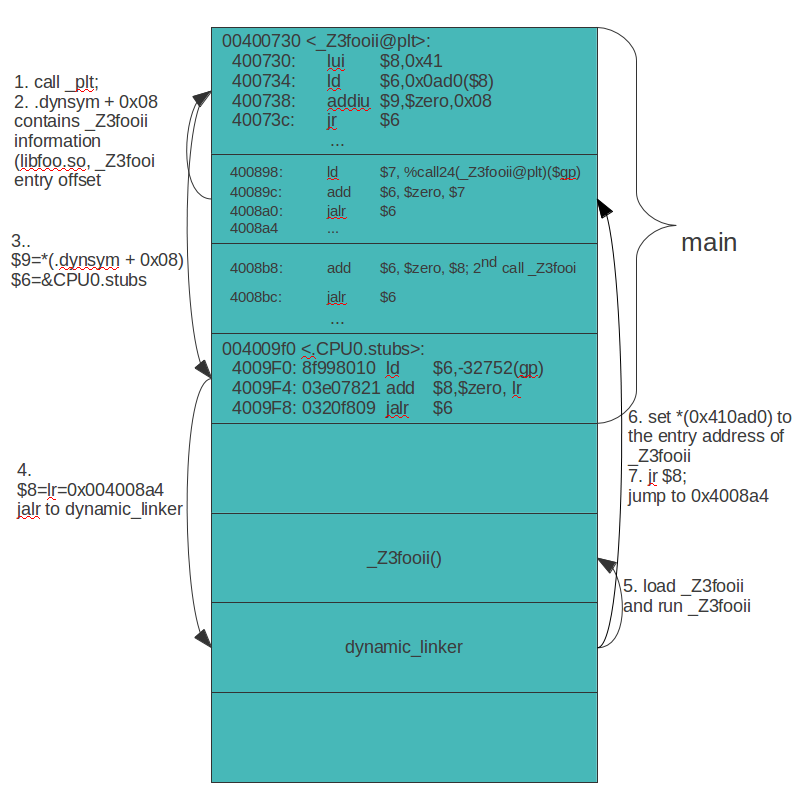
\includegraphics{21.png}}
\caption{Call dynamic function \_Z3fooii() first time}\label{elf:elf-f2}\end{figure}


\begin{threeparttable}
\capstart\caption{registers changed for call dynamic link function \_Z3fooii()}

\begin{tabulary}{\linewidth}{|L|L|L|}
\hline
\textbf{
register/memory
} & \textbf{
call \_Z3fooii first time
} & \textbf{
call \_Z3fooii second time
}\\\hline

0x410ad0
 & 
point to CPU0.stubs
 & 
point to \_Z3fooii
\\\hline

.dynsym+0x08
 & 
(libfoobar.so, offset, length) about \_Z3fooii
 & 
useless
\\\hline

-32752(gp)
 & 
point to dynamic\_linker
 & 
useless
\\\hline

\$8
 & 
the next instruction of \_Z3fooii()
 & 
useless
\\\hline

\$9
 & 
.dynsym+0x08
 & 
useless
\\\hline

\$t9 (at the end of \href{mailto:\_Z3fooii@plt}{\_Z3fooii@plt})
 & 
point to CPU0.stubs0
 & 
point to \_Z3fooii
\\\hline

\$t9 (at the end of CPU0.stubs)
 & 
point to dynamic\_linker
 & 
useless
\\\hline
\end{tabulary}

\end{threeparttable}


Explains it as follows,
\begin{enumerate}
\item {} 
As you can see, the first time of function call, a = foo(1,2), which is
implemented
by instructions ``ld \$7, \%call16(\href{mailto:\_Z3fooii@plt}{\_Z3fooii@plt})(\$gp)'', ``add \$t9, \$zero, \$7'' and
``jalr \$t9''. Remember, .dynsym+0x08 contains information (libfoobar.so,
offset, length) which is set by linker at link to dynamic shared library.
After ``jalr \$t9'', PC counter jump to ``00400730 \textless{}\href{mailto:\_Z3fooii@plt}{\_Z3fooii@plt}\textgreater{}''.

\item {} 
The memory 0x410ad0 contents is the address of CPU0.stubs when the program,
main(), is loaded.

\item {} 
After \href{mailto:\_Z3fooii@plt}{\_Z3fooii@plt} instructions executed, it jump to CPU0.stubs since \$t9 = the
address of CPU0.stubs. Register \$9 = the contents of address .dynsym+0x08 since
it is set in step 1.

\item {} 
After CPU0.stubs is executed, register \$8 = 0x004008a4 which point to the
caller next instruction in step 1.

\item {} 
Dynamic linker looks into register \$9 which value is 0x08. It ask OS for
the caller process address information of .dynsym + offset 0x08. This
address include information (libfoobar.so, offset, length). With this
information, dynamic linker knows where can get \_Z3fooii function body.
Dynamic linker loads \_Z3fooii() function body to an available
address where from asking OS. After load \_Z3fooii(), it call \_Z3fooii() and
save and restore the registers \$t9, \$8, \$9 and caller saved registers just
before and after call \_Z3fooii().

\item {} 
After \_Z3fooii() return, dynamic linker set the contents of address 0x410ad0
to the entry address of \_Z3fooii in memory.

\item {} 
Dynamic linker execute jr \$8. It jump to the next instruction of
``a = \_Z3fooii();'' in caller.

\end{enumerate}

After the \_Z3fooii() is called at second time, it looks like
\hyperref[elf:elf-f3]{Figure  \ref*{elf:elf-f3}}. It jump to \_Z3fooii() directly in \textless{}\href{mailto:\_Z3fooii@plt}{\_Z3fooii@plt}\textgreater{} since
the contents of address 0x410ad0 is changed to the memory address of \_Z3fooii()
at step 6 of \hyperref[elf:elf-f2]{Figure  \ref*{elf:elf-f2}}. From now on, any call \_Z3fooii() will
jump to \_Z3fooii() directly from \href{mailto:\_Z3fooii@plt}{\_Z3fooii@plt} instructions.
\begin{figure}[htbp]
\centering
\capstart

\scalebox{1.000000}{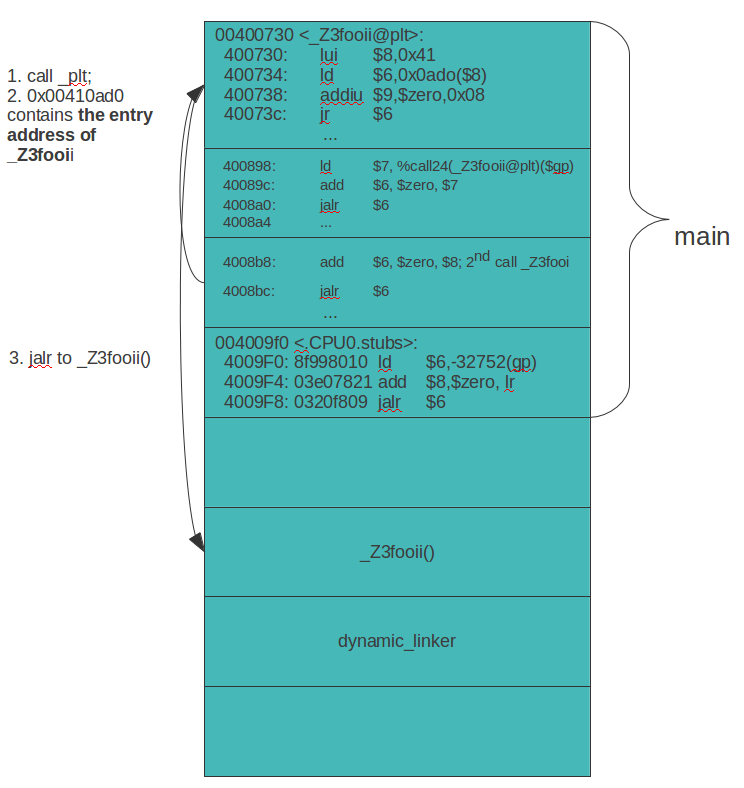
\includegraphics{31.png}}
\caption{Call dynamic function \_Z3fooii() second time}\label{elf:elf-f3}\end{figure}

According Mips Application Binary Interface (ABI), \$t9 is register alias
for \$25 in Mips. The \%t9 is the register
used in jalr \$25 for long distance function pointer (far subroutine call).
Cpu0 use register \$t9(\$6) as the \$t9 (\$25) register of Mips.
The jal \%subroutine has 24 bits range of address offset relative to Program
Counter (PC) while jalr has 32 bits address range in register size of 32 bits.
One example of PIC mode is used in share library just like this example.
Share library is re-entry code which can be loaded in different memory address
decided on run time. The jalr make the implementation of dynamic link function
easier and faster as above.


\subsection{Trace with lldb}
\label{elf:trace-with-lldb}
We tracking the dynamic link on X86 as below. You can skip it if you have no
interest or already know how to track it via lldb or gdb.

\begin{Verbatim}[commandchars=\\\{\}]
118-165-77-200:InputFiles Jonathan\PYG{n+nv}{\PYGZdl{} }clang -fPIC -g -c foobar.cpp
118-165-77-200:InputFiles Jonathan\PYG{n+nv}{\PYGZdl{} }clang -shared -g foobar.o -o libfoobar.so
118-165-77-200:InputFiles Jonathan\PYG{n+nv}{\PYGZdl{} }clang -g -c main.cpp
118-165-77-200:InputFiles Jonathan\PYG{n+nv}{\PYGZdl{} }clang -g main.o libfoobar.so
118-165-77-200:InputFiles Jonathan\PYG{n+nv}{\PYGZdl{} }gobjdump -d main.o

main.o:     fileformat mach-o-x86-64

Disassembly of section .text:

0000000000000000 \PYGZlt{}\PYGZus{}main\PYGZgt{}:
   0: 55                      push   \PYGZpc{}rbp
   1: 48 89 e5                mov    \PYGZpc{}rsp,\PYGZpc{}rbp
   4: 48 83 ec 10             sub    \PYG{n+nv}{\PYGZdl{}0x10},\PYGZpc{}rsp
   8: bf 01 00 00 00          mov    \PYG{n+nv}{\PYGZdl{}0x1},\PYGZpc{}edi
   d: be 02 00 00 00          mov    \PYG{n+nv}{\PYGZdl{}0x2},\PYGZpc{}esi
  12: c7 45 \PYG{n+nb}{fc }00 00 00 00    movl   \PYG{n+nv}{\PYGZdl{}0x0},-0x4\PYG{o}{(}\PYGZpc{}rbp\PYG{o}{)}
  19: e8 00 00 00 00          callq  1e \PYGZlt{}\PYGZus{}main+0x1e\PYGZgt{}
  1e: bf 03 00 00 00          mov    \PYG{n+nv}{\PYGZdl{}0x3},\PYGZpc{}edi
  23: be 04 00 00 00          mov    \PYG{n+nv}{\PYGZdl{}0x4},\PYGZpc{}esi
  28: 89 45 f8                mov    \PYGZpc{}eax,-0x8\PYG{o}{(}\PYGZpc{}rbp\PYG{o}{)}
  2b: e8 00 00 00 00          callq  30 \PYGZlt{}\PYGZus{}main+0x30\PYGZgt{}
  30: 8b 75 f8                mov    -0x8\PYG{o}{(}\PYGZpc{}rbp\PYG{o}{)},\PYGZpc{}esi
  33: 01 c6                   add    \PYGZpc{}eax,\PYGZpc{}esi
  35: 89 75 f8                mov    \PYGZpc{}esi,-0x8\PYG{o}{(}\PYGZpc{}rbp\PYG{o}{)}
  38: e8 00 00 00 00          callq  3d \PYGZlt{}\PYGZus{}main+0x3d\PYGZgt{}
  3d: 8b 75 f8                mov    -0x8\PYG{o}{(}\PYGZpc{}rbp\PYG{o}{)},\PYGZpc{}esi
  40: 01 c6                   add    \PYGZpc{}eax,\PYGZpc{}esi
  42: 89 75 f8                mov    \PYGZpc{}esi,-0x8\PYG{o}{(}\PYGZpc{}rbp\PYG{o}{)}
  45: 8b 45 f8                mov    -0x8\PYG{o}{(}\PYGZpc{}rbp\PYG{o}{)},\PYGZpc{}eax
  48: 48 83 c4 10             add    \PYG{n+nv}{\PYGZdl{}0x10},\PYGZpc{}rsp
  4c: 5d                      pop    \PYGZpc{}rbp
  4d: c3                      retq

118-165-77-200:InputFiles Jonathan\PYG{n+nv}{\PYGZdl{} }gobjdump -d a.out
...
main.o:     fileformat mach-o-x86-64

Disassembly of section .text:

0000000100000ef0 \PYGZlt{}\PYGZus{}main\PYGZgt{}:
   100000ef0: 55                      push   \PYGZpc{}rbp
   100000ef1: 48 89 e5                mov    \PYGZpc{}rsp,\PYGZpc{}rbp
   100000ef4: 48 83 ec 10             sub    \PYG{n+nv}{\PYGZdl{}0x10},\PYGZpc{}rsp
   100000ef8: bf 01 00 00 00          mov    \PYG{n+nv}{\PYGZdl{}0x1},\PYGZpc{}edi
   100000efd: be 02 00 00 00          mov    \PYG{n+nv}{\PYGZdl{}0x2},\PYGZpc{}esi
   100000f02: c7 45 \PYG{n+nb}{fc }00 00 00 00    movl   \PYG{n+nv}{\PYGZdl{}0x0},-0x4\PYG{o}{(}\PYGZpc{}rbp\PYG{o}{)}
   100000f09: e8 36 00 00 00          callq  100000f44 \PYGZlt{}\PYGZus{}\PYGZus{}Z3fooii\PYG{n+nv}{\PYGZdl{}stub}\PYGZgt{}
   100000f0e: bf 03 00 00 00          mov    \PYG{n+nv}{\PYGZdl{}0x3},\PYGZpc{}edi
   100000f13: be 04 00 00 00          mov    \PYG{n+nv}{\PYGZdl{}0x4},\PYGZpc{}esi
   100000f18: 89 45 f8                mov    \PYGZpc{}eax,-0x8\PYG{o}{(}\PYGZpc{}rbp\PYG{o}{)}
   100000f1b: e8 24 00 00 00          callq  100000f44 \PYGZlt{}\PYGZus{}\PYGZus{}Z3fooii\PYG{n+nv}{\PYGZdl{}stub}\PYGZgt{}
   100000f20: 8b 75 f8                mov    -0x8\PYG{o}{(}\PYGZpc{}rbp\PYG{o}{)},\PYGZpc{}esi
   100000f23: 01 c6                   add    \PYGZpc{}eax,\PYGZpc{}esi
   100000f25: 89 75 f8                mov    \PYGZpc{}esi,-0x8\PYG{o}{(}\PYGZpc{}rbp\PYG{o}{)}
   100000f28: e8 11 00 00 00          callq  100000f3e \PYGZlt{}\PYGZus{}\PYGZus{}Z3barv\PYG{n+nv}{\PYGZdl{}stub}\PYGZgt{}
   100000f2d: 8b 75 f8                mov    -0x8\PYG{o}{(}\PYGZpc{}rbp\PYG{o}{)},\PYGZpc{}esi
   100000f30: 01 c6                   add    \PYGZpc{}eax,\PYGZpc{}esi
   100000f32: 89 75 f8                mov    \PYGZpc{}esi,-0x8\PYG{o}{(}\PYGZpc{}rbp\PYG{o}{)}
   100000f35: 8b 45 f8                mov    -0x8\PYG{o}{(}\PYGZpc{}rbp\PYG{o}{)},\PYGZpc{}eax
   100000f38: 48 83 c4 10             add    \PYG{n+nv}{\PYGZdl{}0x10},\PYGZpc{}rsp
   100000f3c: 5d                      pop    \PYGZpc{}rbp
   100000f3d: c3                      retq

Disassembly of section \PYGZus{}\PYGZus{}TEXT.\PYGZus{}\PYGZus{}stubs:

0000000100000f3e \PYGZlt{}\PYGZus{}\PYGZus{}Z3barv\PYG{n+nv}{\PYGZdl{}stub}\PYGZgt{}:
   100000f3e: ff 25 cc 00 00 00       jmpq   *0xcc\PYG{o}{(}\PYGZpc{}rip\PYG{o}{)}        \PYG{c}{\PYGZsh{} 100001010}
   \PYGZlt{}\PYGZus{}\PYGZus{}Z3barv\PYG{n+nv}{\PYGZdl{}stub}\PYGZgt{}

0000000100000f44 \PYGZlt{}\PYGZus{}\PYGZus{}Z3fooii\PYG{n+nv}{\PYGZdl{}stub}\PYGZgt{}:
   100000f44: ff 25 ce 00 00 00       jmpq   *0xce\PYG{o}{(}\PYGZpc{}rip\PYG{o}{)}        \PYG{c}{\PYGZsh{} 100001018}
   \PYGZlt{}\PYGZus{}\PYGZus{}Z3fooii\PYG{n+nv}{\PYGZdl{}stub}\PYGZgt{}

Disassembly of section \PYGZus{}\PYGZus{}TEXT.\PYGZus{}\PYGZus{}stub\PYGZus{}helper:

0000000100000f4c \PYGZlt{}\PYGZus{}\PYGZus{}TEXT.\PYGZus{}\PYGZus{}stub\PYGZus{}helper\PYGZgt{}:
   100000f4c: 4c 8d 1d b5 00 00 00    lea    0xb5\PYG{o}{(}\PYGZpc{}rip\PYG{o}{)},\PYGZpc{}r11        \PYG{c}{\PYGZsh{} 100001008 \PYGZlt{}\PYGZgt{}}
   100000f53: 41 53                   push   \PYGZpc{}r11
   100000f55: ff 25 a5 00 00 00       jmpq   *0xa5\PYG{o}{(}\PYGZpc{}rip\PYG{o}{)}        \PYG{c}{\PYGZsh{} 100001000}
   \PYGZlt{}dyld\PYGZus{}stub\PYGZus{}binder\PYG{n+nv}{\PYGZdl{}stub}\PYGZgt{}
   100000f5b: 90                      nop
   100000f5c: 68 00 00 00 00          pushq  \PYG{n+nv}{\PYGZdl{}0x0}
   100000f61: e9 e6 ff ff ff          jmpq   100000f4c \PYGZlt{}\PYGZus{}\PYGZus{}Z3fooii\PYG{n+nv}{\PYGZdl{}stub}+0x8\PYGZgt{}
   100000f66: 68 0f 00 00 00          pushq  \PYG{n+nv}{\PYGZdl{}0xf}
   100000f6b: e9 dc ff ff ff          jmpq   100000f4c \PYGZlt{}\PYGZus{}\PYGZus{}Z3fooii\PYG{n+nv}{\PYGZdl{}stub}+0x8\PYGZgt{}

Disassembly of section \PYGZus{}\PYGZus{}TEXT.\PYGZus{}\PYGZus{}unwind\PYGZus{}info:
   ...




118-165-77-200:InputFiles Jonathan\PYG{n+nv}{\PYGZdl{} }lldb a.out
Current executable \PYG{n+nb}{set }to \PYG{l+s+s1}{'a.out'} \PYG{o}{(}x86\PYGZus{}64\PYG{o}{)}.
\PYG{o}{(}lldb\PYG{o}{)} run main
Process 702 launched: \PYG{l+s+s1}{'/Users/Jonathan/test/lbd/docs/BackendTutorial/}
\PYG{l+s+s1}{lbdex/InputFiles/a.out'} \PYG{o}{(}x86\PYGZus{}64\PYG{o}{)}
Process 702 exited with \PYG{n+nv}{status} \PYG{o}{=} 15 \PYG{o}{(}0x0000000f\PYG{o}{)}
\PYG{o}{(}lldb\PYG{o}{)} b main
Breakpoint 1: \PYG{n+nv}{where} \PYG{o}{=} a.out\PYG{l+s+sb}{{}`}main + 25 at main.cpp:7, \PYG{n+nv}{address} \PYG{o}{=} 0x0000000100000f09
\PYG{o}{(}lldb\PYG{o}{)} target stop-hook add
Enter your stop hook \PYG{n+nb}{command}\PYG{o}{(}s\PYG{o}{)}.  Type \PYG{l+s+s1}{'DONE'} to end.
\PYGZgt{} disassemble --pc
\PYGZgt{} DONE
Stop hook \PYG{c}{\PYGZsh{}1 added.}
\PYG{o}{(}lldb\PYG{o}{)} run
Process 705 launched: \PYG{l+s+s1}{'/Users/Jonathan/test/lbd/docs/BackendTutorial/}
\PYG{l+s+s1}{lbdex/InputFiles/a.out'} \PYG{o}{(}x86\PYGZus{}64\PYG{o}{)}
dyld\PYG{l+s+sb}{{}`}\PYGZus{}dyld\PYGZus{}start:
-\PYGZgt{} 0x7fff5fc01028:  popq   \PYGZpc{}rdi
   0x7fff5fc01029:  pushq  \PYG{n+nv}{\PYGZdl{}0}
   0x7fff5fc0102b:  movq   \PYGZpc{}rsp, \PYGZpc{}rbp
   0x7fff5fc0102e:  andq   \PYG{n+nv}{\PYGZdl{}-}16, \PYGZpc{}rsp
Process 753 stopped
* thread \PYG{c}{\PYGZsh{}1: tid = 0x1c03, 0x0000000100000f09 a.out{}`main + 25 at main.cpp:7,}
stop \PYG{n+nv}{reason} \PYG{o}{=} breakpoint 1.1
    frame \PYG{c}{\PYGZsh{}0: 0x0000000100000f09 a.out{}`main + 25 at main.cpp:7}
   4
   5          int main\PYG{o}{(}\PYG{o}{)}
   6          \PYG{o}{\PYGZob{}}
-\PYGZgt{} 7            int \PYG{n+nv}{a} \PYG{o}{=} foo\PYG{o}{(}1, 2\PYG{o}{)};
   8            a +\PYG{o}{=} foo\PYG{o}{(}3, 4\PYG{o}{)};
   9            a +\PYG{o}{=} bar\PYG{o}{(}\PYG{o}{)};
   10
a.out\PYG{l+s+sb}{{}`}main + 25 at main.cpp:7:
-\PYGZgt{} 0x100000f09:  callq  0x100000f44               ; symbol stub \PYG{k}{for}: foo\PYG{o}{(}int, int\PYG{o}{)}
   0x100000f0e:  movl   \PYG{n+nv}{\PYGZdl{}3}, \PYGZpc{}edi
   0x100000f13:  movl   \PYG{n+nv}{\PYGZdl{}4}, \PYGZpc{}esi
   0x100000f18:  movl   \PYGZpc{}eax, -8\PYG{o}{(}\PYGZpc{}rbp\PYG{o}{)}
\PYG{o}{(}lldb\PYG{o}{)} stepi
Process 753 stopped
* thread \PYG{c}{\PYGZsh{}1: tid = 0x1c03, 0x0000000100000f44 a.out{}`foo(int, int), stop reason}
\PYG{o}{=} instruction step into
    frame \PYG{c}{\PYGZsh{}0: 0x0000000100000f44 a.out{}`foo(int, int)}
a.out\PYG{l+s+sb}{{}`}symbol stub \PYG{k}{for}: foo\PYG{o}{(}int, int\PYG{o}{)}:
-\PYGZgt{} 0x100000f44:  jmpq   *206\PYG{o}{(}\PYGZpc{}rip\PYG{o}{)}                ; \PYG{o}{(}void *\PYG{o}{)}0x0000000100000f66
a.out\PYG{l+s+sb}{{}`}symbol stub \PYG{k}{for}: foo\PYG{o}{(}int, int\PYG{o}{)}:
-\PYGZgt{} 0x100000f44:  jmpq   *206\PYG{o}{(}\PYGZpc{}rip\PYG{o}{)}                ; \PYG{o}{(}void *\PYG{o}{)}0x0000000100000f66
   0x100000f4a:  addb   \PYGZpc{}al, \PYG{o}{(}\PYGZpc{}rax\PYG{o}{)}
   0x100000f4c:  addb   \PYGZpc{}al, \PYG{o}{(}\PYGZpc{}rax\PYG{o}{)}
   0x100000f4e:  addb   \PYGZpc{}al, \PYG{o}{(}\PYGZpc{}rax\PYG{o}{)}
\PYG{o}{(}lldb\PYG{o}{)} p \PYG{n+nv}{\PYGZdl{}rip}
\PYG{o}{(}unsigned long\PYG{o}{)} \PYG{n+nv}{\PYGZdl{}1} \PYG{o}{=} 4294971204
\PYG{o}{(}lldb\PYG{o}{)} memory \PYG{n+nb}{read}/4xw 4294971410
0x100001012: 0x00010000 0x0f660000 0x00010000 0x00000000
\PYG{o}{(}lldb\PYG{o}{)} stepi
Process 859 stopped
* thread \PYG{c}{\PYGZsh{}1: tid = 0x1c03, 0x0000000100000f66 a.out, stop reason = instruction}
    step into frame \PYG{c}{\PYGZsh{}0: 0x0000000100000f66 a.out}
-\PYGZgt{} 0x100000f66:  pushq  \PYG{n+nv}{\PYGZdl{}15}
   0x100000f6b:  jmpq   0x100000f4c
-\PYGZgt{} 0x100000f66:  pushq  \PYG{n+nv}{\PYGZdl{}15}
   0x100000f6b:  jmpq   0x100000f4c
   0x100000f70:  addb   \PYGZpc{}al, \PYG{o}{(}\PYGZpc{}rax\PYG{o}{)}
   0x100000f72:  addb   \PYGZpc{}al, \PYG{o}{(}\PYGZpc{}rax\PYG{o}{)}
\PYG{o}{)} stepistepi
Process 859 stopped
* thread \PYG{c}{\PYGZsh{}1: tid = 0x1c03, 0x0000000100000f6b a.out, stop reason = instruction}
    step into frame \PYG{c}{\PYGZsh{}0: 0x0000000100000f6b a.out}
-\PYGZgt{} 0x100000f6b:  jmpq   0x100000f4c
-\PYGZgt{} 0x100000f6b:  jmpq   0x100000f4c
   0x100000f70:  addb   \PYGZpc{}al, \PYG{o}{(}\PYGZpc{}rax\PYG{o}{)}
   0x100000f72:  addb   \PYGZpc{}al, \PYG{o}{(}\PYGZpc{}rax\PYG{o}{)}
   0x100000f74:  addb   \PYGZpc{}al, \PYG{o}{(}\PYGZpc{}rax\PYG{o}{)}
\PYG{o}{(}lldb\PYG{o}{)} stepi
Process 859 stopped
* thread \PYG{c}{\PYGZsh{}1: tid = 0x1c03, 0x0000000100000f4c a.out, stop reason = instruction}
    step into frame \PYG{c}{\PYGZsh{}0: 0x0000000100000f4c a.out}
-\PYGZgt{} 0x100000f4c:  leaq   181\PYG{o}{(}\PYGZpc{}rip\PYG{o}{)}, \PYGZpc{}r11           ; \PYG{o}{(}void *\PYG{o}{)}0x0000000000000000
   0x100000f53:  pushq  \PYGZpc{}r11
   0x100000f55:  jmpq   *165\PYG{o}{(}\PYGZpc{}rip\PYG{o}{)}                ; \PYG{o}{(}void *\PYG{o}{)}0x00007fff978da878:
   dyld\PYGZus{}stub\PYGZus{}binder
   0x100000f5b:  nop
-\PYGZgt{} 0x100000f4c:  leaq   181\PYG{o}{(}\PYGZpc{}rip\PYG{o}{)}, \PYGZpc{}r11           ; \PYG{o}{(}void *\PYG{o}{)}0x0000000000000000
   0x100000f53:  pushq  \PYGZpc{}r11
   0x100000f55:  jmpq   *165\PYG{o}{(}\PYGZpc{}rip\PYG{o}{)}                ; \PYG{o}{(}void *\PYG{o}{)}0x00007fff978da878:
   dyld\PYGZus{}stub\PYGZus{}binder
   0x100000f5b:  nop
\PYG{o}{(}lldb\PYG{o}{)}
Process 859 stopped
* thread \PYG{c}{\PYGZsh{}1: tid = 0x1c03, 0x0000000100000f53 a.out, stop reason = instruction}
    step into frame \PYG{c}{\PYGZsh{}0: 0x0000000100000f53 a.out}
-\PYGZgt{} 0x100000f53:  pushq  \PYGZpc{}r11
   0x100000f55:  jmpq   *165\PYG{o}{(}\PYGZpc{}rip\PYG{o}{)}                ; \PYG{o}{(}void *\PYG{o}{)}0x00007fff978da878:
   dyld\PYGZus{}stub\PYGZus{}binder
   0x100000f5b:  nop
   0x100000f5c:  pushq  \PYG{n+nv}{\PYGZdl{}0}
-\PYGZgt{} 0x100000f53:  pushq  \PYGZpc{}r11
   0x100000f55:  jmpq   *165\PYG{o}{(}\PYGZpc{}rip\PYG{o}{)}                ; \PYG{o}{(}void *\PYG{o}{)}0x00007fff978da878:
   dyld\PYGZus{}stub\PYGZus{}binder
   0x100000f5b:  nop
   0x100000f5c:  pushq  \PYG{n+nv}{\PYGZdl{}0}
\PYG{o}{(}lldb\PYG{o}{)}
Process 859 stopped
* thread \PYG{c}{\PYGZsh{}1: tid = 0x1c03, 0x0000000100000f55 a.out, stop reason = instruction}
    step into frame \PYG{c}{\PYGZsh{}0: 0x0000000100000f55 a.out}
-\PYGZgt{} 0x100000f55:  jmpq   *165\PYG{o}{(}\PYGZpc{}rip\PYG{o}{)}                ; \PYG{o}{(}void *\PYG{o}{)}0x00007fff978da878:
   dyld\PYGZus{}stub\PYGZus{}binder
   0x100000f5b:  nop
   0x100000f5c:  pushq  \PYG{n+nv}{\PYGZdl{}0}
   0x100000f61:  jmpq   0x100000f4c
-\PYGZgt{} 0x100000f55:  jmpq   *165\PYG{o}{(}\PYGZpc{}rip\PYG{o}{)}                ; \PYG{o}{(}void *\PYG{o}{)}0x00007fff978da878:
   dyld\PYGZus{}stub\PYGZus{}binder
   0x100000f5b:  nop
   0x100000f5c:  pushq  \PYG{n+nv}{\PYGZdl{}0}
   0x100000f61:  jmpq   0x100000f4c
\PYG{o}{(}lldb\PYG{o}{)}
Process 859 stopped
* thread \PYG{c}{\PYGZsh{}1: tid = 0x1c03, 0x00007fff978da878 libdyld.dylib{}`dyld\PYGZus{}stub\PYGZus{}binder,}
    stop \PYG{n+nv}{reason} \PYG{o}{=} instruction step into
    frame \PYG{c}{\PYGZsh{}0: 0x00007fff978da878 libdyld.dylib{}`dyld\PYGZus{}stub\PYGZus{}binder}
libdyld.dylib\PYG{l+s+sb}{{}`}dyld\PYGZus{}stub\PYGZus{}binder:
-\PYGZgt{} 0x7fff978da878:  pushq  \PYGZpc{}rbp
   0x7fff978da879:  movq   \PYGZpc{}rsp, \PYGZpc{}rbp
   0x7fff978da87c:  subq   \PYG{n+nv}{\PYGZdl{}192}, \PYGZpc{}rsp
   0x7fff978da883:  movq   \PYGZpc{}rdi, \PYG{o}{(}\PYGZpc{}rsp\PYG{o}{)}
libdyld.dylib\PYG{l+s+sb}{{}`}dyld\PYGZus{}stub\PYGZus{}binder:
-\PYGZgt{} 0x7fff978da878:  pushq  \PYGZpc{}rbp
   0x7fff978da879:  movq   \PYGZpc{}rsp, \PYGZpc{}rbp
   0x7fff978da87c:  subq   \PYG{n+nv}{\PYGZdl{}192}, \PYGZpc{}rsp
   0x7fff978da883:  movq   \PYGZpc{}rdi, \PYG{o}{(}\PYGZpc{}rsp\PYG{o}{)}
\PYG{o}{(}lldb\PYG{o}{)} cont
Process 753 resuming
Process 753 stopped
* thread \PYG{c}{\PYGZsh{}1: tid = 0x1c03, 0x0000000100000f1b a.out{}`main + 43 at main.cpp:8,}
    stop \PYG{n+nv}{reason} \PYG{o}{=} breakpoint 2.1
    frame \PYG{c}{\PYGZsh{}0: 0x0000000100000f1b a.out{}`main + 43 at main.cpp:8}
   5          int main\PYG{o}{(}\PYG{o}{)}
   6          \PYG{o}{\PYGZob{}}
   7            int \PYG{n+nv}{a} \PYG{o}{=} foo\PYG{o}{(}1, 2\PYG{o}{)};
-\PYGZgt{} 8            a +\PYG{o}{=} foo\PYG{o}{(}3, 4\PYG{o}{)};
   9            a +\PYG{o}{=} bar\PYG{o}{(}\PYG{o}{)};
   10
   11           \PYG{k}{return }a;
a.out\PYG{l+s+sb}{{}`}main + 43 at main.cpp:8:
-\PYGZgt{} 0x100000f1b:  callq  0x100000f44               ; symbol stub \PYG{k}{for}: foo\PYG{o}{(}int, int\PYG{o}{)}
   0x100000f20:  movl   -8\PYG{o}{(}\PYGZpc{}rbp\PYG{o}{)}, \PYGZpc{}esi
   0x100000f23:  addl   \PYGZpc{}eax, \PYGZpc{}esi
   0x100000f25:  movl   \PYGZpc{}esi, -8\PYG{o}{(}\PYGZpc{}rbp\PYG{o}{)}
\PYG{o}{(}lldb\PYG{o}{)} stepi
Process 753 stopped
* thread \PYG{c}{\PYGZsh{}1: tid = 0x1c03, 0x0000000100000f44 a.out{}`foo(int, int), stop reason =}
    instruction step into frame \PYG{c}{\PYGZsh{}0: 0x0000000100000f44 a.out{}`foo(int, int)}
a.out\PYG{l+s+sb}{{}`}symbol stub \PYG{k}{for}: foo\PYG{o}{(}int, int\PYG{o}{)}:
-\PYGZgt{} 0x100000f44:  jmpq   *206\PYG{o}{(}\PYGZpc{}rip\PYG{o}{)}                ; \PYG{o}{(}void *\PYG{o}{)}0x0000000100003f20:
   foo\PYG{o}{(}int, int\PYG{o}{)} at /Users/Jonathan/test/lbd/docs/BackendTutorial/LLVMBackendT
   utorialExampleCode/InputFiles/foobar.cpp:3
a.out\PYG{l+s+sb}{{}`}symbol stub \PYG{k}{for}: foo\PYG{o}{(}int, int\PYG{o}{)}:
-\PYGZgt{} 0x100000f44:  jmpq   *206\PYG{o}{(}\PYGZpc{}rip\PYG{o}{)}                ; \PYG{o}{(}void *\PYG{o}{)}0x0000000100003f20:
   foo\PYG{o}{(}int, int\PYG{o}{)} at /Users/Jonathan/test/lbd/docs/BackendTutorial/LLVMBackendT
   utorialExampleCode/InputFiles/foobar.cpp:3
   0x100000f4a:  addb   \PYGZpc{}al, \PYG{o}{(}\PYGZpc{}rax\PYG{o}{)}
   0x100000f4c:  addb   \PYGZpc{}al, \PYG{o}{(}\PYGZpc{}rax\PYG{o}{)}
   0x100000f4e:  addb   \PYGZpc{}al, \PYG{o}{(}\PYGZpc{}rax\PYG{o}{)}
\PYG{o}{(}lldb\PYG{o}{)} p \PYG{n+nv}{\PYGZdl{}rip}
\PYG{o}{(}unsigned long\PYG{o}{)} \PYG{n+nv}{\PYGZdl{}2} \PYG{o}{=} 4294971204
\PYG{o}{(}lldb\PYG{o}{)} memory \PYG{n+nb}{read}/4xw 4294971410
0x100001012: 0x00010000 0x3f200000 0x00010000 0x00000000
\PYG{o}{(}lldb\PYG{o}{)} stepi
Process 753 stopped
* thread \PYG{c}{\PYGZsh{}1: tid = 0x1c03, 0x0000000100003f20 libfoobar.so{}`foo(x1=0, x2=3) at}
    foobar.cpp:3, stop \PYG{n+nv}{reason} \PYG{o}{=} instruction step into
    frame \PYG{c}{\PYGZsh{}0: 0x0000000100003f20 libfoobar.so{}`foo(x1=0, x2=3) at foobar.cpp:3}
   1
   2          int foo\PYG{o}{(}int x1, int x2\PYG{o}{)}
-\PYGZgt{} 3          \PYG{o}{\PYGZob{}}
   4            int \PYG{n+nv}{sum} \PYG{o}{=} x1 + x2;
   5
   6            \PYG{k}{return }sum;
libfoobar.so\PYG{l+s+sb}{{}`}foo\PYG{o}{(}int, int\PYG{o}{)} at foobar.cpp:3:
-\PYGZgt{} 0x100003f20:  pushq  \PYGZpc{}rbp
   0x100003f21:  movq   \PYGZpc{}rsp, \PYGZpc{}rbp
   0x100003f24:  movl   \PYGZpc{}edi, -4\PYG{o}{(}\PYGZpc{}rbp\PYG{o}{)}
   0x100003f27:  movl   \PYGZpc{}esi, -8\PYG{o}{(}\PYGZpc{}rbp\PYG{o}{)}
\PYG{o}{(}lldb\PYG{o}{)}
\end{Verbatim}


\chapter{Run backend}
\label{runbackend:run-backend}\label{runbackend:sec-runbackend}\label{runbackend::doc}
This chapter will add LLVM AsmParser support first.
With AsmParser support, we can hand code the assembly language in C/C++ file
and translate it into obj (elf format).
We can write a C++ main
function as well as the boot code by assembly hand code, and translate this
main()+bootcode() into obj file.
Combined with llvm-objdump support in last chapter,
this main()+bootcode() elf can be translated into hex file format which
include the disassemble code as comment.
Furthermore, we can design the Cpu0 with Verilog language tool and run the Cpu0
backend on PC by feed the hex file and see the Cpu0 instructions execution
result.


\section{AsmParser support}
\label{runbackend:asmparser-support}
Run Chapter10\_1/ with ch11\_1.cpp will get the following error message.
\paragraph{lbdex/InputFiles/ch11\_1.cpp}

\begin{Verbatim}[commandchars=\\\{\}]
\PYG{k}{asm}\PYG{p}{(}\PYG{l+s}{"}\PYG{l+s}{ld	\PYGZdl{}2, 8(\PYGZdl{}sp)}\PYG{l+s}{"}\PYG{p}{)}\PYG{p}{;}
\PYG{k}{asm}\PYG{p}{(}\PYG{l+s}{"}\PYG{l+s}{st	\PYGZdl{}0, 4(\PYGZdl{}sp)}\PYG{l+s}{"}\PYG{p}{)}\PYG{p}{;}
\PYG{k}{asm}\PYG{p}{(}\PYG{l+s}{"}\PYG{l+s}{addiu \PYGZdl{}3,	\PYGZdl{}ZERO, 0}\PYG{l+s}{"}\PYG{p}{)}\PYG{p}{;}
\PYG{k}{asm}\PYG{p}{(}\PYG{l+s}{"}\PYG{l+s}{add \PYGZdl{}3, \PYGZdl{}1, \PYGZdl{}2}\PYG{l+s}{"}\PYG{p}{)}\PYG{p}{;}
\PYG{k}{asm}\PYG{p}{(}\PYG{l+s}{"}\PYG{l+s}{sub \PYGZdl{}3, \PYGZdl{}2, \PYGZdl{}3}\PYG{l+s}{"}\PYG{p}{)}\PYG{p}{;}
\PYG{k}{asm}\PYG{p}{(}\PYG{l+s}{"}\PYG{l+s}{mul \PYGZdl{}2, \PYGZdl{}1, \PYGZdl{}3}\PYG{l+s}{"}\PYG{p}{)}\PYG{p}{;}
\PYG{k}{asm}\PYG{p}{(}\PYG{l+s}{"}\PYG{l+s}{div \PYGZdl{}3, \PYGZdl{}2}\PYG{l+s}{"}\PYG{p}{)}\PYG{p}{;}
\PYG{k}{asm}\PYG{p}{(}\PYG{l+s}{"}\PYG{l+s}{divu \PYGZdl{}2, \PYGZdl{}3}\PYG{l+s}{"}\PYG{p}{)}\PYG{p}{;}
\PYG{k}{asm}\PYG{p}{(}\PYG{l+s}{"}\PYG{l+s}{and \PYGZdl{}2, \PYGZdl{}1, \PYGZdl{}3}\PYG{l+s}{"}\PYG{p}{)}\PYG{p}{;}
\PYG{k}{asm}\PYG{p}{(}\PYG{l+s}{"}\PYG{l+s}{or \PYGZdl{}3, \PYGZdl{}1, \PYGZdl{}2}\PYG{l+s}{"}\PYG{p}{)}\PYG{p}{;}
\PYG{k}{asm}\PYG{p}{(}\PYG{l+s}{"}\PYG{l+s}{xor \PYGZdl{}1, \PYGZdl{}2, \PYGZdl{}3}\PYG{l+s}{"}\PYG{p}{)}\PYG{p}{;}
\PYG{k}{asm}\PYG{p}{(}\PYG{l+s}{"}\PYG{l+s}{mult \PYGZdl{}4, \PYGZdl{}3}\PYG{l+s}{"}\PYG{p}{)}\PYG{p}{;}
\PYG{k}{asm}\PYG{p}{(}\PYG{l+s}{"}\PYG{l+s}{multu \PYGZdl{}3, \PYGZdl{}2}\PYG{l+s}{"}\PYG{p}{)}\PYG{p}{;}
\PYG{k}{asm}\PYG{p}{(}\PYG{l+s}{"}\PYG{l+s}{mfhi \PYGZdl{}3}\PYG{l+s}{"}\PYG{p}{)}\PYG{p}{;}
\PYG{k}{asm}\PYG{p}{(}\PYG{l+s}{"}\PYG{l+s}{mflo \PYGZdl{}2}\PYG{l+s}{"}\PYG{p}{)}\PYG{p}{;}
\PYG{k}{asm}\PYG{p}{(}\PYG{l+s}{"}\PYG{l+s}{mthi \PYGZdl{}2}\PYG{l+s}{"}\PYG{p}{)}\PYG{p}{;}
\PYG{k}{asm}\PYG{p}{(}\PYG{l+s}{"}\PYG{l+s}{mtlo \PYGZdl{}2}\PYG{l+s}{"}\PYG{p}{)}\PYG{p}{;}
\PYG{k}{asm}\PYG{p}{(}\PYG{l+s}{"}\PYG{l+s}{sra \PYGZdl{}2, \PYGZdl{}2, 2}\PYG{l+s}{"}\PYG{p}{)}\PYG{p}{;}
\PYG{k}{asm}\PYG{p}{(}\PYG{l+s}{"}\PYG{l+s}{rol \PYGZdl{}2, \PYGZdl{}1, 3}\PYG{l+s}{"}\PYG{p}{)}\PYG{p}{;}
\PYG{k}{asm}\PYG{p}{(}\PYG{l+s}{"}\PYG{l+s}{ror \PYGZdl{}3, \PYGZdl{}3, 4}\PYG{l+s}{"}\PYG{p}{)}\PYG{p}{;}
\PYG{k}{asm}\PYG{p}{(}\PYG{l+s}{"}\PYG{l+s}{shl \PYGZdl{}2, \PYGZdl{}2, 2}\PYG{l+s}{"}\PYG{p}{)}\PYG{p}{;}
\PYG{k}{asm}\PYG{p}{(}\PYG{l+s}{"}\PYG{l+s}{shr \PYGZdl{}2, \PYGZdl{}3, 5}\PYG{l+s}{"}\PYG{p}{)}\PYG{p}{;}
\PYG{k}{asm}\PYG{p}{(}\PYG{l+s}{"}\PYG{l+s}{cmp \PYGZdl{}sw, \PYGZdl{}2, \PYGZdl{}3}\PYG{l+s}{"}\PYG{p}{)}\PYG{p}{;}
\PYG{k}{asm}\PYG{p}{(}\PYG{l+s}{"}\PYG{l+s}{jeq \PYGZdl{}sw, 20}\PYG{l+s}{"}\PYG{p}{)}\PYG{p}{;}
\PYG{k}{asm}\PYG{p}{(}\PYG{l+s}{"}\PYG{l+s}{jne \PYGZdl{}sw, 16}\PYG{l+s}{"}\PYG{p}{)}\PYG{p}{;}
\PYG{k}{asm}\PYG{p}{(}\PYG{l+s}{"}\PYG{l+s}{jlt \PYGZdl{}sw, -20}\PYG{l+s}{"}\PYG{p}{)}\PYG{p}{;}
\PYG{k}{asm}\PYG{p}{(}\PYG{l+s}{"}\PYG{l+s}{jle \PYGZdl{}sw, -16}\PYG{l+s}{"}\PYG{p}{)}\PYG{p}{;}
\PYG{k}{asm}\PYG{p}{(}\PYG{l+s}{"}\PYG{l+s}{jgt \PYGZdl{}sw, -4}\PYG{l+s}{"}\PYG{p}{)}\PYG{p}{;}
\PYG{k}{asm}\PYG{p}{(}\PYG{l+s}{"}\PYG{l+s}{jge \PYGZdl{}sw, -12}\PYG{l+s}{"}\PYG{p}{)}\PYG{p}{;}
\PYG{k}{asm}\PYG{p}{(}\PYG{l+s}{"}\PYG{l+s}{swi 0x00000400}\PYG{l+s}{"}\PYG{p}{)}\PYG{p}{;}
\PYG{k}{asm}\PYG{p}{(}\PYG{l+s}{"}\PYG{l+s}{jsub 0x000010000}\PYG{l+s}{"}\PYG{p}{)}\PYG{p}{;}
\PYG{k}{asm}\PYG{p}{(}\PYG{l+s}{"}\PYG{l+s}{ret \PYGZdl{}lr}\PYG{l+s}{"}\PYG{p}{)}\PYG{p}{;}
\PYG{k}{asm}\PYG{p}{(}\PYG{l+s}{"}\PYG{l+s}{jalr \PYGZdl{}t9}\PYG{l+s}{"}\PYG{p}{)}\PYG{p}{;}
\PYG{k}{asm}\PYG{p}{(}\PYG{l+s}{"}\PYG{l+s}{li \PYGZdl{}3, 0x00700000}\PYG{l+s}{"}\PYG{p}{)}\PYG{p}{;}
\PYG{k}{asm}\PYG{p}{(}\PYG{l+s}{"}\PYG{l+s}{la \PYGZdl{}3, 0x00800000(\PYGZdl{}6)}\PYG{l+s}{"}\PYG{p}{)}\PYG{p}{;}
\PYG{k}{asm}\PYG{p}{(}\PYG{l+s}{"}\PYG{l+s}{la \PYGZdl{}3, 0x00900000}\PYG{l+s}{"}\PYG{p}{)}\PYG{p}{;}
\end{Verbatim}

\begin{Verbatim}[commandchars=\\\{\}]
JonathantekiiMac:InputFiles Jonathan\$ clang -c ch11\_1.cpp -emit-llvm -o
ch11\_1.bc
JonathantekiiMac:InputFiles Jonathan\$ /Users/Jonathan/llvm/test/cmake\_debug\_
build/bin/Debug/llc -march=cpu0 -relocation-model=pic -filetype=obj ch11\_1.bc
-o ch11\_1.cpu0.o
LLVM ERROR: Inline asm not supported by this streamer because we don't have
an asm parser for this target
\end{Verbatim}

Since we didn't implement cpu0 assembly, it has the error message as above.
The cpu0 can translate LLVM IR into assembly and obj directly, but it cannot
translate hand code assembly into obj.
Directory AsmParser handle the assembly to obj translation.
The Chapter11\_1/ include AsmParser implementation as follows,
\paragraph{lbdex/Chapter11\_1/AsmParser/Cpu0AsmParser.cpp}

\begin{Verbatim}[commandchars=\\\{\}]
\PYG{c+c1}{//===-- Cpu0AsmParser.cpp - Parse Cpu0 assembly to MCInst instructions ----===//}
\PYG{c+c1}{//}
\PYG{c+c1}{//                     The LLVM Compiler Infrastructure}
\PYG{c+c1}{//}
\PYG{c+c1}{// This file is distributed under the University of Illinois Open Source}
\PYG{c+c1}{// License. See LICENSE.TXT for details.}
\PYG{c+c1}{//}
\PYG{c+c1}{//===----------------------------------------------------------------------===//}

\PYG{c+cp}{\PYGZsh{}}\PYG{c+cp}{include "MCTargetDesc}\PYG{c+cp}{/}\PYG{c+cp}{Cpu0MCTargetDesc.h"}
\PYG{c+cp}{\PYGZsh{}}\PYG{c+cp}{include "Cpu0RegisterInfo.h"}
\PYG{c+cp}{\PYGZsh{}}\PYG{c+cp}{include "llvm}\PYG{c+cp}{/}\PYG{c+cp}{ADT}\PYG{c+cp}{/}\PYG{c+cp}{StringSwitch.h"}
\PYG{c+cp}{\PYGZsh{}}\PYG{c+cp}{include "llvm}\PYG{c+cp}{/}\PYG{c+cp}{MC}\PYG{c+cp}{/}\PYG{c+cp}{MCContext.h"}
\PYG{c+cp}{\PYGZsh{}}\PYG{c+cp}{include "llvm}\PYG{c+cp}{/}\PYG{c+cp}{MC}\PYG{c+cp}{/}\PYG{c+cp}{MCExpr.h"}
\PYG{c+cp}{\PYGZsh{}}\PYG{c+cp}{include "llvm}\PYG{c+cp}{/}\PYG{c+cp}{MC}\PYG{c+cp}{/}\PYG{c+cp}{MCInst.h"}
\PYG{c+cp}{\PYGZsh{}}\PYG{c+cp}{include "llvm}\PYG{c+cp}{/}\PYG{c+cp}{MC}\PYG{c+cp}{/}\PYG{c+cp}{MCStreamer.h"}
\PYG{c+cp}{\PYGZsh{}}\PYG{c+cp}{include "llvm}\PYG{c+cp}{/}\PYG{c+cp}{MC}\PYG{c+cp}{/}\PYG{c+cp}{MCSubtargetInfo.h"}
\PYG{c+cp}{\PYGZsh{}}\PYG{c+cp}{include "llvm}\PYG{c+cp}{/}\PYG{c+cp}{MC}\PYG{c+cp}{/}\PYG{c+cp}{MCSymbol.h"}
\PYG{c+cp}{\PYGZsh{}}\PYG{c+cp}{include "llvm}\PYG{c+cp}{/}\PYG{c+cp}{MC}\PYG{c+cp}{/}\PYG{c+cp}{MCParser}\PYG{c+cp}{/}\PYG{c+cp}{MCAsmLexer.h"}
\PYG{c+cp}{\PYGZsh{}}\PYG{c+cp}{include "llvm}\PYG{c+cp}{/}\PYG{c+cp}{MC}\PYG{c+cp}{/}\PYG{c+cp}{MCParser}\PYG{c+cp}{/}\PYG{c+cp}{MCParsedAsmOperand.h"}
\PYG{c+cp}{\PYGZsh{}}\PYG{c+cp}{include "llvm}\PYG{c+cp}{/}\PYG{c+cp}{MC}\PYG{c+cp}{/}\PYG{c+cp}{MCTargetAsmParser.h"}
\PYG{c+cp}{\PYGZsh{}}\PYG{c+cp}{include "llvm}\PYG{c+cp}{/}\PYG{c+cp}{Support}\PYG{c+cp}{/}\PYG{c+cp}{TargetRegistry.h"}

\PYG{k}{using} \PYG{k}{namespace} \PYG{n}{llvm}\PYG{p}{;}

\PYG{k}{namespace} \PYG{p}{\PYGZob{}}
\PYG{k}{class} \PYG{n+nc}{Cpu0AssemblerOptions} \PYG{p}{\PYGZob{}}
\PYG{k}{public}\PYG{o}{:}
  \PYG{n}{Cpu0AssemblerOptions}\PYG{p}{(}\PYG{p}{)}\PYG{o}{:}
    \PYG{n}{aTReg}\PYG{p}{(}\PYG{l+m+mi}{1}\PYG{p}{)}\PYG{p}{,} \PYG{n}{reorder}\PYG{p}{(}\PYG{k+kc}{true}\PYG{p}{)}\PYG{p}{,} \PYG{n}{macro}\PYG{p}{(}\PYG{k+kc}{true}\PYG{p}{)} \PYG{p}{\PYGZob{}}
  \PYG{p}{\PYGZcb{}}

  \PYG{k+kt}{bool} \PYG{n}{isReorder}\PYG{p}{(}\PYG{p}{)} \PYG{p}{\PYGZob{}}\PYG{k}{return} \PYG{n}{reorder}\PYG{p}{;}\PYG{p}{\PYGZcb{}}
  \PYG{k+kt}{void} \PYG{n}{setReorder}\PYG{p}{(}\PYG{p}{)} \PYG{p}{\PYGZob{}}\PYG{n}{reorder} \PYG{o}{=} \PYG{k+kc}{true}\PYG{p}{;}\PYG{p}{\PYGZcb{}}
  \PYG{k+kt}{void} \PYG{n}{setNoreorder}\PYG{p}{(}\PYG{p}{)} \PYG{p}{\PYGZob{}}\PYG{n}{reorder} \PYG{o}{=} \PYG{k+kc}{false}\PYG{p}{;}\PYG{p}{\PYGZcb{}}

  \PYG{k+kt}{bool} \PYG{n}{isMacro}\PYG{p}{(}\PYG{p}{)} \PYG{p}{\PYGZob{}}\PYG{k}{return} \PYG{n}{macro}\PYG{p}{;}\PYG{p}{\PYGZcb{}}
  \PYG{k+kt}{void} \PYG{n}{setMacro}\PYG{p}{(}\PYG{p}{)} \PYG{p}{\PYGZob{}}\PYG{n}{macro} \PYG{o}{=} \PYG{k+kc}{true}\PYG{p}{;}\PYG{p}{\PYGZcb{}}
  \PYG{k+kt}{void} \PYG{n}{setNomacro}\PYG{p}{(}\PYG{p}{)} \PYG{p}{\PYGZob{}}\PYG{n}{macro} \PYG{o}{=} \PYG{k+kc}{false}\PYG{p}{;}\PYG{p}{\PYGZcb{}}

\PYG{k}{private}\PYG{o}{:}
  \PYG{k+kt}{unsigned} \PYG{n}{aTReg}\PYG{p}{;}
  \PYG{k+kt}{bool} \PYG{n}{reorder}\PYG{p}{;}
  \PYG{k+kt}{bool} \PYG{n}{macro}\PYG{p}{;}
\PYG{p}{\PYGZcb{}}\PYG{p}{;}
\PYG{p}{\PYGZcb{}}

\PYG{k}{namespace} \PYG{p}{\PYGZob{}}
\PYG{k}{class} \PYG{n+nc}{Cpu0AsmParser} \PYG{o}{:} \PYG{k}{public} \PYG{n}{MCTargetAsmParser} \PYG{p}{\PYGZob{}}
  \PYG{n}{MCSubtargetInfo} \PYG{o}{\PYGZam{}}\PYG{n}{STI}\PYG{p}{;}
  \PYG{n}{MCAsmParser} \PYG{o}{\PYGZam{}}\PYG{n}{Parser}\PYG{p}{;}
  \PYG{n}{Cpu0AssemblerOptions} \PYG{n}{Options}\PYG{p}{;}


\PYG{c+cp}{\PYGZsh{}}\PYG{c+cp}{define GET\PYGZus{}ASSEMBLER\PYGZus{}HEADER}
\PYG{c+cp}{\PYGZsh{}}\PYG{c+cp}{include "Cpu0GenAsmMatcher.inc"}

  \PYG{k+kt}{bool} \PYG{n}{MatchAndEmitInstruction}\PYG{p}{(}\PYG{n}{SMLoc} \PYG{n}{IDLoc}\PYG{p}{,} \PYG{k+kt}{unsigned} \PYG{o}{\PYGZam{}}\PYG{n}{Opcode}\PYG{p}{,}
                               \PYG{n}{SmallVectorImpl}\PYG{o}{\PYGZlt{}}\PYG{n}{MCParsedAsmOperand}\PYG{o}{*}\PYG{o}{\PYGZgt{}} \PYG{o}{\PYGZam{}}\PYG{n}{Operands}\PYG{p}{,}
                               \PYG{n}{MCStreamer} \PYG{o}{\PYGZam{}}\PYG{n}{Out}\PYG{p}{,} \PYG{k+kt}{unsigned} \PYG{o}{\PYGZam{}}\PYG{n}{ErrorInfo}\PYG{p}{,}
                               \PYG{k+kt}{bool} \PYG{n}{MatchingInlineAsm}\PYG{p}{)}\PYG{p}{;}

  \PYG{k+kt}{bool} \PYG{n}{ParseRegister}\PYG{p}{(}\PYG{k+kt}{unsigned} \PYG{o}{\PYGZam{}}\PYG{n}{RegNo}\PYG{p}{,} \PYG{n}{SMLoc} \PYG{o}{\PYGZam{}}\PYG{n}{StartLoc}\PYG{p}{,} \PYG{n}{SMLoc} \PYG{o}{\PYGZam{}}\PYG{n}{EndLoc}\PYG{p}{)}\PYG{p}{;}

  \PYG{k+kt}{bool} \PYG{n}{ParseInstruction}\PYG{p}{(}\PYG{n}{ParseInstructionInfo} \PYG{o}{\PYGZam{}}\PYG{n}{Info}\PYG{p}{,} \PYG{n}{StringRef} \PYG{n}{Name}\PYG{p}{,}
                        \PYG{n}{SMLoc} \PYG{n}{NameLoc}\PYG{p}{,}
                        \PYG{n}{SmallVectorImpl}\PYG{o}{\PYGZlt{}}\PYG{n}{MCParsedAsmOperand}\PYG{o}{*}\PYG{o}{\PYGZgt{}} \PYG{o}{\PYGZam{}}\PYG{n}{Operands}\PYG{p}{)}\PYG{p}{;}

  \PYG{k+kt}{bool} \PYG{n}{parseMathOperation}\PYG{p}{(}\PYG{n}{StringRef} \PYG{n}{Name}\PYG{p}{,} \PYG{n}{SMLoc} \PYG{n}{NameLoc}\PYG{p}{,}
                        \PYG{n}{SmallVectorImpl}\PYG{o}{\PYGZlt{}}\PYG{n}{MCParsedAsmOperand}\PYG{o}{*}\PYG{o}{\PYGZgt{}} \PYG{o}{\PYGZam{}}\PYG{n}{Operands}\PYG{p}{)}\PYG{p}{;}

  \PYG{k+kt}{bool} \PYG{n}{ParseDirective}\PYG{p}{(}\PYG{n}{AsmToken} \PYG{n}{DirectiveID}\PYG{p}{)}\PYG{p}{;}

  \PYG{n}{Cpu0AsmParser}\PYG{o}{:}\PYG{o}{:}\PYG{n}{OperandMatchResultTy}
  \PYG{n}{parseMemOperand}\PYG{p}{(}\PYG{n}{SmallVectorImpl}\PYG{o}{\PYGZlt{}}\PYG{n}{MCParsedAsmOperand}\PYG{o}{*}\PYG{o}{\PYGZgt{}}\PYG{o}{\PYGZam{}}\PYG{p}{)}\PYG{p}{;}

  \PYG{k+kt}{bool} \PYG{n}{ParseOperand}\PYG{p}{(}\PYG{n}{SmallVectorImpl}\PYG{o}{\PYGZlt{}}\PYG{n}{MCParsedAsmOperand}\PYG{o}{*}\PYG{o}{\PYGZgt{}} \PYG{o}{\PYGZam{}}\PYG{p}{,}
                    \PYG{n}{StringRef} \PYG{n}{Mnemonic}\PYG{p}{)}\PYG{p}{;}

  \PYG{k+kt}{int} \PYG{n}{tryParseRegister}\PYG{p}{(}\PYG{n}{StringRef} \PYG{n}{Mnemonic}\PYG{p}{)}\PYG{p}{;}

  \PYG{k+kt}{bool} \PYG{n}{tryParseRegisterOperand}\PYG{p}{(}\PYG{n}{SmallVectorImpl}\PYG{o}{\PYGZlt{}}\PYG{n}{MCParsedAsmOperand}\PYG{o}{*}\PYG{o}{\PYGZgt{}} \PYG{o}{\PYGZam{}}\PYG{n}{Operands}\PYG{p}{,}
                               \PYG{n}{StringRef} \PYG{n}{Mnemonic}\PYG{p}{)}\PYG{p}{;}

  \PYG{k+kt}{bool} \PYG{n}{needsExpansion}\PYG{p}{(}\PYG{n}{MCInst} \PYG{o}{\PYGZam{}}\PYG{n}{Inst}\PYG{p}{)}\PYG{p}{;}

  \PYG{k+kt}{void} \PYG{n}{expandInstruction}\PYG{p}{(}\PYG{n}{MCInst} \PYG{o}{\PYGZam{}}\PYG{n}{Inst}\PYG{p}{,} \PYG{n}{SMLoc} \PYG{n}{IDLoc}\PYG{p}{,}
                         \PYG{n}{SmallVectorImpl}\PYG{o}{\PYGZlt{}}\PYG{n}{MCInst}\PYG{o}{\PYGZgt{}} \PYG{o}{\PYGZam{}}\PYG{n}{Instructions}\PYG{p}{)}\PYG{p}{;}
  \PYG{k+kt}{void} \PYG{n}{expandLoadImm}\PYG{p}{(}\PYG{n}{MCInst} \PYG{o}{\PYGZam{}}\PYG{n}{Inst}\PYG{p}{,} \PYG{n}{SMLoc} \PYG{n}{IDLoc}\PYG{p}{,}
                     \PYG{n}{SmallVectorImpl}\PYG{o}{\PYGZlt{}}\PYG{n}{MCInst}\PYG{o}{\PYGZgt{}} \PYG{o}{\PYGZam{}}\PYG{n}{Instructions}\PYG{p}{)}\PYG{p}{;}
  \PYG{k+kt}{void} \PYG{n}{expandLoadAddressImm}\PYG{p}{(}\PYG{n}{MCInst} \PYG{o}{\PYGZam{}}\PYG{n}{Inst}\PYG{p}{,} \PYG{n}{SMLoc} \PYG{n}{IDLoc}\PYG{p}{,}
                            \PYG{n}{SmallVectorImpl}\PYG{o}{\PYGZlt{}}\PYG{n}{MCInst}\PYG{o}{\PYGZgt{}} \PYG{o}{\PYGZam{}}\PYG{n}{Instructions}\PYG{p}{)}\PYG{p}{;}
  \PYG{k+kt}{void} \PYG{n}{expandLoadAddressReg}\PYG{p}{(}\PYG{n}{MCInst} \PYG{o}{\PYGZam{}}\PYG{n}{Inst}\PYG{p}{,} \PYG{n}{SMLoc} \PYG{n}{IDLoc}\PYG{p}{,}
                            \PYG{n}{SmallVectorImpl}\PYG{o}{\PYGZlt{}}\PYG{n}{MCInst}\PYG{o}{\PYGZgt{}} \PYG{o}{\PYGZam{}}\PYG{n}{Instructions}\PYG{p}{)}\PYG{p}{;}
  \PYG{k+kt}{bool} \PYG{n}{reportParseError}\PYG{p}{(}\PYG{n}{StringRef} \PYG{n}{ErrorMsg}\PYG{p}{)}\PYG{p}{;}

  \PYG{k+kt}{bool} \PYG{n}{parseMemOffset}\PYG{p}{(}\PYG{k}{const} \PYG{n}{MCExpr} \PYG{o}{*}\PYG{o}{\PYGZam{}}\PYG{n}{Res}\PYG{p}{)}\PYG{p}{;}
  \PYG{k+kt}{bool} \PYG{n}{parseRelocOperand}\PYG{p}{(}\PYG{k}{const} \PYG{n}{MCExpr} \PYG{o}{*}\PYG{o}{\PYGZam{}}\PYG{n}{Res}\PYG{p}{)}\PYG{p}{;}

  \PYG{k+kt}{bool} \PYG{n}{parseDirectiveSet}\PYG{p}{(}\PYG{p}{)}\PYG{p}{;}

  \PYG{k+kt}{bool} \PYG{n}{parseSetAtDirective}\PYG{p}{(}\PYG{p}{)}\PYG{p}{;}
  \PYG{k+kt}{bool} \PYG{n}{parseSetNoAtDirective}\PYG{p}{(}\PYG{p}{)}\PYG{p}{;}
  \PYG{k+kt}{bool} \PYG{n}{parseSetMacroDirective}\PYG{p}{(}\PYG{p}{)}\PYG{p}{;}
  \PYG{k+kt}{bool} \PYG{n}{parseSetNoMacroDirective}\PYG{p}{(}\PYG{p}{)}\PYG{p}{;}
  \PYG{k+kt}{bool} \PYG{n}{parseSetReorderDirective}\PYG{p}{(}\PYG{p}{)}\PYG{p}{;}
  \PYG{k+kt}{bool} \PYG{n}{parseSetNoReorderDirective}\PYG{p}{(}\PYG{p}{)}\PYG{p}{;}

  \PYG{n}{MCSymbolRefExpr}\PYG{o}{:}\PYG{o}{:}\PYG{n}{VariantKind} \PYG{n}{getVariantKind}\PYG{p}{(}\PYG{n}{StringRef} \PYG{n}{Symbol}\PYG{p}{)}\PYG{p}{;}

  \PYG{k+kt}{int} \PYG{n}{matchRegisterName}\PYG{p}{(}\PYG{n}{StringRef} \PYG{n}{Symbol}\PYG{p}{)}\PYG{p}{;}

  \PYG{k+kt}{int} \PYG{n}{matchRegisterByNumber}\PYG{p}{(}\PYG{k+kt}{unsigned} \PYG{n}{RegNum}\PYG{p}{,} \PYG{n}{StringRef} \PYG{n}{Mnemonic}\PYG{p}{)}\PYG{p}{;}

  \PYG{k+kt}{unsigned} \PYG{n}{getReg}\PYG{p}{(}\PYG{k+kt}{int} \PYG{n}{RC}\PYG{p}{,}\PYG{k+kt}{int} \PYG{n}{RegNo}\PYG{p}{)}\PYG{p}{;}

\PYG{k}{public}\PYG{o}{:}
  \PYG{n}{Cpu0AsmParser}\PYG{p}{(}\PYG{n}{MCSubtargetInfo} \PYG{o}{\PYGZam{}}\PYG{n}{sti}\PYG{p}{,} \PYG{n}{MCAsmParser} \PYG{o}{\PYGZam{}}\PYG{n}{parser}\PYG{p}{)}
    \PYG{o}{:} \PYG{n}{MCTargetAsmParser}\PYG{p}{(}\PYG{p}{)}\PYG{p}{,} \PYG{n}{STI}\PYG{p}{(}\PYG{n}{sti}\PYG{p}{)}\PYG{p}{,} \PYG{n}{Parser}\PYG{p}{(}\PYG{n}{parser}\PYG{p}{)} \PYG{p}{\PYGZob{}}
    \PYG{c+c1}{// Initialize the set of available features.}
    \PYG{n}{setAvailableFeatures}\PYG{p}{(}\PYG{n}{ComputeAvailableFeatures}\PYG{p}{(}\PYG{n}{STI}\PYG{p}{.}\PYG{n}{getFeatureBits}\PYG{p}{(}\PYG{p}{)}\PYG{p}{)}\PYG{p}{)}\PYG{p}{;}
  \PYG{p}{\PYGZcb{}}

  \PYG{n}{MCAsmParser} \PYG{o}{\PYGZam{}}\PYG{n}{getParser}\PYG{p}{(}\PYG{p}{)} \PYG{k}{const} \PYG{p}{\PYGZob{}} \PYG{k}{return} \PYG{n}{Parser}\PYG{p}{;} \PYG{p}{\PYGZcb{}}
  \PYG{n}{MCAsmLexer} \PYG{o}{\PYGZam{}}\PYG{n}{getLexer}\PYG{p}{(}\PYG{p}{)} \PYG{k}{const} \PYG{p}{\PYGZob{}} \PYG{k}{return} \PYG{n}{Parser}\PYG{p}{.}\PYG{n}{getLexer}\PYG{p}{(}\PYG{p}{)}\PYG{p}{;} \PYG{p}{\PYGZcb{}}

\PYG{p}{\PYGZcb{}}\PYG{p}{;}
\PYG{p}{\PYGZcb{}}

\PYG{k}{namespace} \PYG{p}{\PYGZob{}}

\PYG{c+c1}{/// Cpu0Operand - Instances of this class represent a parsed Cpu0 machine}
\PYG{c+c1}{/// instruction.}
\PYG{k}{class} \PYG{n+nc}{Cpu0Operand} \PYG{o}{:} \PYG{k}{public} \PYG{n}{MCParsedAsmOperand} \PYG{p}{\PYGZob{}}

  \PYG{k}{enum} \PYG{n}{KindTy} \PYG{p}{\PYGZob{}}
    \PYG{n}{k\PYGZus{}CondCode}\PYG{p}{,}
    \PYG{n}{k\PYGZus{}CoprocNum}\PYG{p}{,}
    \PYG{n}{k\PYGZus{}Immediate}\PYG{p}{,}
    \PYG{n}{k\PYGZus{}Memory}\PYG{p}{,}
    \PYG{n}{k\PYGZus{}PostIndexRegister}\PYG{p}{,}
    \PYG{n}{k\PYGZus{}Register}\PYG{p}{,}
    \PYG{n}{k\PYGZus{}Token}
  \PYG{p}{\PYGZcb{}} \PYG{n}{Kind}\PYG{p}{;}

  \PYG{n}{Cpu0Operand}\PYG{p}{(}\PYG{n}{KindTy} \PYG{n}{K}\PYG{p}{)} \PYG{o}{:} \PYG{n}{MCParsedAsmOperand}\PYG{p}{(}\PYG{p}{)}\PYG{p}{,} \PYG{n}{Kind}\PYG{p}{(}\PYG{n}{K}\PYG{p}{)} \PYG{p}{\PYGZob{}}\PYG{p}{\PYGZcb{}}

  \PYG{k}{union} \PYG{p}{\PYGZob{}}
    \PYG{k}{struct} \PYG{p}{\PYGZob{}}
      \PYG{k}{const} \PYG{k+kt}{char} \PYG{o}{*}\PYG{n}{Data}\PYG{p}{;}
      \PYG{k+kt}{unsigned} \PYG{n}{Length}\PYG{p}{;}
    \PYG{p}{\PYGZcb{}} \PYG{n}{Tok}\PYG{p}{;}

    \PYG{k}{struct} \PYG{p}{\PYGZob{}}
      \PYG{k+kt}{unsigned} \PYG{n}{RegNum}\PYG{p}{;}
    \PYG{p}{\PYGZcb{}} \PYG{n}{Reg}\PYG{p}{;}

    \PYG{k}{struct} \PYG{p}{\PYGZob{}}
      \PYG{k}{const} \PYG{n}{MCExpr} \PYG{o}{*}\PYG{n}{Val}\PYG{p}{;}
    \PYG{p}{\PYGZcb{}} \PYG{n}{Imm}\PYG{p}{;}

    \PYG{k}{struct} \PYG{p}{\PYGZob{}}
      \PYG{k+kt}{unsigned} \PYG{n}{Base}\PYG{p}{;}
      \PYG{k}{const} \PYG{n}{MCExpr} \PYG{o}{*}\PYG{n}{Off}\PYG{p}{;}
    \PYG{p}{\PYGZcb{}} \PYG{n}{Mem}\PYG{p}{;}
  \PYG{p}{\PYGZcb{}}\PYG{p}{;}

  \PYG{n}{SMLoc} \PYG{n}{StartLoc}\PYG{p}{,} \PYG{n}{EndLoc}\PYG{p}{;}

\PYG{k}{public}\PYG{o}{:}
  \PYG{k+kt}{void} \PYG{n}{addRegOperands}\PYG{p}{(}\PYG{n}{MCInst} \PYG{o}{\PYGZam{}}\PYG{n}{Inst}\PYG{p}{,} \PYG{k+kt}{unsigned} \PYG{n}{N}\PYG{p}{)} \PYG{k}{const} \PYG{p}{\PYGZob{}}
    \PYG{n}{assert}\PYG{p}{(}\PYG{n}{N} \PYG{o}{=}\PYG{o}{=} \PYG{l+m+mi}{1} \PYG{o}{\PYGZam{}}\PYG{o}{\PYGZam{}} \PYG{l+s}{"}\PYG{l+s}{Invalid number of operands!}\PYG{l+s}{"}\PYG{p}{)}\PYG{p}{;}
    \PYG{n}{Inst}\PYG{p}{.}\PYG{n}{addOperand}\PYG{p}{(}\PYG{n}{MCOperand}\PYG{o}{:}\PYG{o}{:}\PYG{n}{CreateReg}\PYG{p}{(}\PYG{n}{getReg}\PYG{p}{(}\PYG{p}{)}\PYG{p}{)}\PYG{p}{)}\PYG{p}{;}
  \PYG{p}{\PYGZcb{}}

  \PYG{k+kt}{void} \PYG{n}{addExpr}\PYG{p}{(}\PYG{n}{MCInst} \PYG{o}{\PYGZam{}}\PYG{n}{Inst}\PYG{p}{,} \PYG{k}{const} \PYG{n}{MCExpr} \PYG{o}{*}\PYG{n}{Expr}\PYG{p}{)} \PYG{k}{const}\PYG{p}{\PYGZob{}}
    \PYG{c+c1}{// Add as immediate when possible.  Null MCExpr = 0.}
    \PYG{k}{if} \PYG{p}{(}\PYG{n}{Expr} \PYG{o}{=}\PYG{o}{=} \PYG{l+m+mi}{0}\PYG{p}{)}
      \PYG{n}{Inst}\PYG{p}{.}\PYG{n}{addOperand}\PYG{p}{(}\PYG{n}{MCOperand}\PYG{o}{:}\PYG{o}{:}\PYG{n}{CreateImm}\PYG{p}{(}\PYG{l+m+mi}{0}\PYG{p}{)}\PYG{p}{)}\PYG{p}{;}
    \PYG{k}{else} \PYG{k}{if} \PYG{p}{(}\PYG{k}{const} \PYG{n}{MCConstantExpr} \PYG{o}{*}\PYG{n}{CE} \PYG{o}{=} \PYG{n}{dyn\PYGZus{}cast}\PYG{o}{\PYGZlt{}}\PYG{n}{MCConstantExpr}\PYG{o}{\PYGZgt{}}\PYG{p}{(}\PYG{n}{Expr}\PYG{p}{)}\PYG{p}{)}
      \PYG{n}{Inst}\PYG{p}{.}\PYG{n}{addOperand}\PYG{p}{(}\PYG{n}{MCOperand}\PYG{o}{:}\PYG{o}{:}\PYG{n}{CreateImm}\PYG{p}{(}\PYG{n}{CE}\PYG{o}{-}\PYG{o}{\PYGZgt{}}\PYG{n}{getValue}\PYG{p}{(}\PYG{p}{)}\PYG{p}{)}\PYG{p}{)}\PYG{p}{;}
    \PYG{k}{else}
      \PYG{n}{Inst}\PYG{p}{.}\PYG{n}{addOperand}\PYG{p}{(}\PYG{n}{MCOperand}\PYG{o}{:}\PYG{o}{:}\PYG{n}{CreateExpr}\PYG{p}{(}\PYG{n}{Expr}\PYG{p}{)}\PYG{p}{)}\PYG{p}{;}
  \PYG{p}{\PYGZcb{}}

  \PYG{k+kt}{void} \PYG{n}{addImmOperands}\PYG{p}{(}\PYG{n}{MCInst} \PYG{o}{\PYGZam{}}\PYG{n}{Inst}\PYG{p}{,} \PYG{k+kt}{unsigned} \PYG{n}{N}\PYG{p}{)} \PYG{k}{const} \PYG{p}{\PYGZob{}}
    \PYG{n}{assert}\PYG{p}{(}\PYG{n}{N} \PYG{o}{=}\PYG{o}{=} \PYG{l+m+mi}{1} \PYG{o}{\PYGZam{}}\PYG{o}{\PYGZam{}} \PYG{l+s}{"}\PYG{l+s}{Invalid number of operands!}\PYG{l+s}{"}\PYG{p}{)}\PYG{p}{;}
    \PYG{k}{const} \PYG{n}{MCExpr} \PYG{o}{*}\PYG{n}{Expr} \PYG{o}{=} \PYG{n}{getImm}\PYG{p}{(}\PYG{p}{)}\PYG{p}{;}
    \PYG{n}{addExpr}\PYG{p}{(}\PYG{n}{Inst}\PYG{p}{,}\PYG{n}{Expr}\PYG{p}{)}\PYG{p}{;}
  \PYG{p}{\PYGZcb{}}

  \PYG{k+kt}{void} \PYG{n}{addMemOperands}\PYG{p}{(}\PYG{n}{MCInst} \PYG{o}{\PYGZam{}}\PYG{n}{Inst}\PYG{p}{,} \PYG{k+kt}{unsigned} \PYG{n}{N}\PYG{p}{)} \PYG{k}{const} \PYG{p}{\PYGZob{}}
    \PYG{n}{assert}\PYG{p}{(}\PYG{n}{N} \PYG{o}{=}\PYG{o}{=} \PYG{l+m+mi}{2} \PYG{o}{\PYGZam{}}\PYG{o}{\PYGZam{}} \PYG{l+s}{"}\PYG{l+s}{Invalid number of operands!}\PYG{l+s}{"}\PYG{p}{)}\PYG{p}{;}

    \PYG{n}{Inst}\PYG{p}{.}\PYG{n}{addOperand}\PYG{p}{(}\PYG{n}{MCOperand}\PYG{o}{:}\PYG{o}{:}\PYG{n}{CreateReg}\PYG{p}{(}\PYG{n}{getMemBase}\PYG{p}{(}\PYG{p}{)}\PYG{p}{)}\PYG{p}{)}\PYG{p}{;}

    \PYG{k}{const} \PYG{n}{MCExpr} \PYG{o}{*}\PYG{n}{Expr} \PYG{o}{=} \PYG{n}{getMemOff}\PYG{p}{(}\PYG{p}{)}\PYG{p}{;}
    \PYG{n}{addExpr}\PYG{p}{(}\PYG{n}{Inst}\PYG{p}{,}\PYG{n}{Expr}\PYG{p}{)}\PYG{p}{;}
  \PYG{p}{\PYGZcb{}}

  \PYG{k+kt}{bool} \PYG{n}{isReg}\PYG{p}{(}\PYG{p}{)} \PYG{k}{const} \PYG{p}{\PYGZob{}} \PYG{k}{return} \PYG{n}{Kind} \PYG{o}{=}\PYG{o}{=} \PYG{n}{k\PYGZus{}Register}\PYG{p}{;} \PYG{p}{\PYGZcb{}}
  \PYG{k+kt}{bool} \PYG{n}{isImm}\PYG{p}{(}\PYG{p}{)} \PYG{k}{const} \PYG{p}{\PYGZob{}} \PYG{k}{return} \PYG{n}{Kind} \PYG{o}{=}\PYG{o}{=} \PYG{n}{k\PYGZus{}Immediate}\PYG{p}{;} \PYG{p}{\PYGZcb{}}
  \PYG{k+kt}{bool} \PYG{n}{isToken}\PYG{p}{(}\PYG{p}{)} \PYG{k}{const} \PYG{p}{\PYGZob{}} \PYG{k}{return} \PYG{n}{Kind} \PYG{o}{=}\PYG{o}{=} \PYG{n}{k\PYGZus{}Token}\PYG{p}{;} \PYG{p}{\PYGZcb{}}
  \PYG{k+kt}{bool} \PYG{n}{isMem}\PYG{p}{(}\PYG{p}{)} \PYG{k}{const} \PYG{p}{\PYGZob{}} \PYG{k}{return} \PYG{n}{Kind} \PYG{o}{=}\PYG{o}{=} \PYG{n}{k\PYGZus{}Memory}\PYG{p}{;} \PYG{p}{\PYGZcb{}}

  \PYG{n}{StringRef} \PYG{n}{getToken}\PYG{p}{(}\PYG{p}{)} \PYG{k}{const} \PYG{p}{\PYGZob{}}
    \PYG{n}{assert}\PYG{p}{(}\PYG{n}{Kind} \PYG{o}{=}\PYG{o}{=} \PYG{n}{k\PYGZus{}Token} \PYG{o}{\PYGZam{}}\PYG{o}{\PYGZam{}} \PYG{l+s}{"}\PYG{l+s}{Invalid access!}\PYG{l+s}{"}\PYG{p}{)}\PYG{p}{;}
    \PYG{k}{return} \PYG{n}{StringRef}\PYG{p}{(}\PYG{n}{Tok}\PYG{p}{.}\PYG{n}{Data}\PYG{p}{,} \PYG{n}{Tok}\PYG{p}{.}\PYG{n}{Length}\PYG{p}{)}\PYG{p}{;}
  \PYG{p}{\PYGZcb{}}

  \PYG{k+kt}{unsigned} \PYG{n}{getReg}\PYG{p}{(}\PYG{p}{)} \PYG{k}{const} \PYG{p}{\PYGZob{}}
    \PYG{n}{assert}\PYG{p}{(}\PYG{p}{(}\PYG{n}{Kind} \PYG{o}{=}\PYG{o}{=} \PYG{n}{k\PYGZus{}Register}\PYG{p}{)} \PYG{o}{\PYGZam{}}\PYG{o}{\PYGZam{}} \PYG{l+s}{"}\PYG{l+s}{Invalid access!}\PYG{l+s}{"}\PYG{p}{)}\PYG{p}{;}
    \PYG{k}{return} \PYG{n}{Reg}\PYG{p}{.}\PYG{n}{RegNum}\PYG{p}{;}
  \PYG{p}{\PYGZcb{}}

  \PYG{k}{const} \PYG{n}{MCExpr} \PYG{o}{*}\PYG{n}{getImm}\PYG{p}{(}\PYG{p}{)} \PYG{k}{const} \PYG{p}{\PYGZob{}}
    \PYG{n}{assert}\PYG{p}{(}\PYG{p}{(}\PYG{n}{Kind} \PYG{o}{=}\PYG{o}{=} \PYG{n}{k\PYGZus{}Immediate}\PYG{p}{)} \PYG{o}{\PYGZam{}}\PYG{o}{\PYGZam{}} \PYG{l+s}{"}\PYG{l+s}{Invalid access!}\PYG{l+s}{"}\PYG{p}{)}\PYG{p}{;}
    \PYG{k}{return} \PYG{n}{Imm}\PYG{p}{.}\PYG{n}{Val}\PYG{p}{;}
  \PYG{p}{\PYGZcb{}}

  \PYG{k+kt}{unsigned} \PYG{n}{getMemBase}\PYG{p}{(}\PYG{p}{)} \PYG{k}{const} \PYG{p}{\PYGZob{}}
    \PYG{n}{assert}\PYG{p}{(}\PYG{p}{(}\PYG{n}{Kind} \PYG{o}{=}\PYG{o}{=} \PYG{n}{k\PYGZus{}Memory}\PYG{p}{)} \PYG{o}{\PYGZam{}}\PYG{o}{\PYGZam{}} \PYG{l+s}{"}\PYG{l+s}{Invalid access!}\PYG{l+s}{"}\PYG{p}{)}\PYG{p}{;}
    \PYG{k}{return} \PYG{n}{Mem}\PYG{p}{.}\PYG{n}{Base}\PYG{p}{;}
  \PYG{p}{\PYGZcb{}}

  \PYG{k}{const} \PYG{n}{MCExpr} \PYG{o}{*}\PYG{n}{getMemOff}\PYG{p}{(}\PYG{p}{)} \PYG{k}{const} \PYG{p}{\PYGZob{}}
    \PYG{n}{assert}\PYG{p}{(}\PYG{p}{(}\PYG{n}{Kind} \PYG{o}{=}\PYG{o}{=} \PYG{n}{k\PYGZus{}Memory}\PYG{p}{)} \PYG{o}{\PYGZam{}}\PYG{o}{\PYGZam{}} \PYG{l+s}{"}\PYG{l+s}{Invalid access!}\PYG{l+s}{"}\PYG{p}{)}\PYG{p}{;}
    \PYG{k}{return} \PYG{n}{Mem}\PYG{p}{.}\PYG{n}{Off}\PYG{p}{;}
  \PYG{p}{\PYGZcb{}}

  \PYG{k}{static} \PYG{n}{Cpu0Operand} \PYG{o}{*}\PYG{n}{CreateToken}\PYG{p}{(}\PYG{n}{StringRef} \PYG{n}{Str}\PYG{p}{,} \PYG{n}{SMLoc} \PYG{n}{S}\PYG{p}{)} \PYG{p}{\PYGZob{}}
    \PYG{n}{Cpu0Operand} \PYG{o}{*}\PYG{n}{Op} \PYG{o}{=} \PYG{k}{new} \PYG{n}{Cpu0Operand}\PYG{p}{(}\PYG{n}{k\PYGZus{}Token}\PYG{p}{)}\PYG{p}{;}
    \PYG{n}{Op}\PYG{o}{-}\PYG{o}{\PYGZgt{}}\PYG{n}{Tok}\PYG{p}{.}\PYG{n}{Data} \PYG{o}{=} \PYG{n}{Str}\PYG{p}{.}\PYG{n}{data}\PYG{p}{(}\PYG{p}{)}\PYG{p}{;}
    \PYG{n}{Op}\PYG{o}{-}\PYG{o}{\PYGZgt{}}\PYG{n}{Tok}\PYG{p}{.}\PYG{n}{Length} \PYG{o}{=} \PYG{n}{Str}\PYG{p}{.}\PYG{n}{size}\PYG{p}{(}\PYG{p}{)}\PYG{p}{;}
    \PYG{n}{Op}\PYG{o}{-}\PYG{o}{\PYGZgt{}}\PYG{n}{StartLoc} \PYG{o}{=} \PYG{n}{S}\PYG{p}{;}
    \PYG{n}{Op}\PYG{o}{-}\PYG{o}{\PYGZgt{}}\PYG{n}{EndLoc} \PYG{o}{=} \PYG{n}{S}\PYG{p}{;}
    \PYG{k}{return} \PYG{n}{Op}\PYG{p}{;}
  \PYG{p}{\PYGZcb{}}

  \PYG{k}{static} \PYG{n}{Cpu0Operand} \PYG{o}{*}\PYG{n}{CreateReg}\PYG{p}{(}\PYG{k+kt}{unsigned} \PYG{n}{RegNum}\PYG{p}{,} \PYG{n}{SMLoc} \PYG{n}{S}\PYG{p}{,} \PYG{n}{SMLoc} \PYG{n}{E}\PYG{p}{)} \PYG{p}{\PYGZob{}}
    \PYG{n}{Cpu0Operand} \PYG{o}{*}\PYG{n}{Op} \PYG{o}{=} \PYG{k}{new} \PYG{n}{Cpu0Operand}\PYG{p}{(}\PYG{n}{k\PYGZus{}Register}\PYG{p}{)}\PYG{p}{;}
    \PYG{n}{Op}\PYG{o}{-}\PYG{o}{\PYGZgt{}}\PYG{n}{Reg}\PYG{p}{.}\PYG{n}{RegNum} \PYG{o}{=} \PYG{n}{RegNum}\PYG{p}{;}
    \PYG{n}{Op}\PYG{o}{-}\PYG{o}{\PYGZgt{}}\PYG{n}{StartLoc} \PYG{o}{=} \PYG{n}{S}\PYG{p}{;}
    \PYG{n}{Op}\PYG{o}{-}\PYG{o}{\PYGZgt{}}\PYG{n}{EndLoc} \PYG{o}{=} \PYG{n}{E}\PYG{p}{;}
    \PYG{k}{return} \PYG{n}{Op}\PYG{p}{;}
  \PYG{p}{\PYGZcb{}}

  \PYG{k}{static} \PYG{n}{Cpu0Operand} \PYG{o}{*}\PYG{n}{CreateImm}\PYG{p}{(}\PYG{k}{const} \PYG{n}{MCExpr} \PYG{o}{*}\PYG{n}{Val}\PYG{p}{,} \PYG{n}{SMLoc} \PYG{n}{S}\PYG{p}{,} \PYG{n}{SMLoc} \PYG{n}{E}\PYG{p}{)} \PYG{p}{\PYGZob{}}
    \PYG{n}{Cpu0Operand} \PYG{o}{*}\PYG{n}{Op} \PYG{o}{=} \PYG{k}{new} \PYG{n}{Cpu0Operand}\PYG{p}{(}\PYG{n}{k\PYGZus{}Immediate}\PYG{p}{)}\PYG{p}{;}
    \PYG{n}{Op}\PYG{o}{-}\PYG{o}{\PYGZgt{}}\PYG{n}{Imm}\PYG{p}{.}\PYG{n}{Val} \PYG{o}{=} \PYG{n}{Val}\PYG{p}{;}
    \PYG{n}{Op}\PYG{o}{-}\PYG{o}{\PYGZgt{}}\PYG{n}{StartLoc} \PYG{o}{=} \PYG{n}{S}\PYG{p}{;}
    \PYG{n}{Op}\PYG{o}{-}\PYG{o}{\PYGZgt{}}\PYG{n}{EndLoc} \PYG{o}{=} \PYG{n}{E}\PYG{p}{;}
    \PYG{k}{return} \PYG{n}{Op}\PYG{p}{;}
  \PYG{p}{\PYGZcb{}}

  \PYG{k}{static} \PYG{n}{Cpu0Operand} \PYG{o}{*}\PYG{n}{CreateMem}\PYG{p}{(}\PYG{k+kt}{unsigned} \PYG{n}{Base}\PYG{p}{,} \PYG{k}{const} \PYG{n}{MCExpr} \PYG{o}{*}\PYG{n}{Off}\PYG{p}{,}
                                 \PYG{n}{SMLoc} \PYG{n}{S}\PYG{p}{,} \PYG{n}{SMLoc} \PYG{n}{E}\PYG{p}{)} \PYG{p}{\PYGZob{}}
    \PYG{n}{Cpu0Operand} \PYG{o}{*}\PYG{n}{Op} \PYG{o}{=} \PYG{k}{new} \PYG{n}{Cpu0Operand}\PYG{p}{(}\PYG{n}{k\PYGZus{}Memory}\PYG{p}{)}\PYG{p}{;}
    \PYG{n}{Op}\PYG{o}{-}\PYG{o}{\PYGZgt{}}\PYG{n}{Mem}\PYG{p}{.}\PYG{n}{Base} \PYG{o}{=} \PYG{n}{Base}\PYG{p}{;}
    \PYG{n}{Op}\PYG{o}{-}\PYG{o}{\PYGZgt{}}\PYG{n}{Mem}\PYG{p}{.}\PYG{n}{Off} \PYG{o}{=} \PYG{n}{Off}\PYG{p}{;}
    \PYG{n}{Op}\PYG{o}{-}\PYG{o}{\PYGZgt{}}\PYG{n}{StartLoc} \PYG{o}{=} \PYG{n}{S}\PYG{p}{;}
    \PYG{n}{Op}\PYG{o}{-}\PYG{o}{\PYGZgt{}}\PYG{n}{EndLoc} \PYG{o}{=} \PYG{n}{E}\PYG{p}{;}
    \PYG{k}{return} \PYG{n}{Op}\PYG{p}{;}
  \PYG{p}{\PYGZcb{}}

  \PYG{c+c1}{/// getStartLoc - Get the location of the first token of this operand.}
  \PYG{n}{SMLoc} \PYG{n}{getStartLoc}\PYG{p}{(}\PYG{p}{)} \PYG{k}{const} \PYG{p}{\PYGZob{}} \PYG{k}{return} \PYG{n}{StartLoc}\PYG{p}{;} \PYG{p}{\PYGZcb{}}
  \PYG{c+c1}{/// getEndLoc - Get the location of the last token of this operand.}
  \PYG{n}{SMLoc} \PYG{n}{getEndLoc}\PYG{p}{(}\PYG{p}{)} \PYG{k}{const} \PYG{p}{\PYGZob{}} \PYG{k}{return} \PYG{n}{EndLoc}\PYG{p}{;} \PYG{p}{\PYGZcb{}}

  \PYG{k}{virtual} \PYG{k+kt}{void} \PYG{n}{print}\PYG{p}{(}\PYG{n}{raw\PYGZus{}ostream} \PYG{o}{\PYGZam{}}\PYG{n}{OS}\PYG{p}{)} \PYG{k}{const} \PYG{p}{\PYGZob{}}
    \PYG{n}{llvm\PYGZus{}unreachable}\PYG{p}{(}\PYG{l+s}{"}\PYG{l+s}{unimplemented!}\PYG{l+s}{"}\PYG{p}{)}\PYG{p}{;}
  \PYG{p}{\PYGZcb{}}
\PYG{p}{\PYGZcb{}}\PYG{p}{;}
\PYG{p}{\PYGZcb{}}

\PYG{k+kt}{bool} \PYG{n}{Cpu0AsmParser}\PYG{o}{:}\PYG{o}{:}\PYG{n}{needsExpansion}\PYG{p}{(}\PYG{n}{MCInst} \PYG{o}{\PYGZam{}}\PYG{n}{Inst}\PYG{p}{)} \PYG{p}{\PYGZob{}}

  \PYG{k}{switch}\PYG{p}{(}\PYG{n}{Inst}\PYG{p}{.}\PYG{n}{getOpcode}\PYG{p}{(}\PYG{p}{)}\PYG{p}{)} \PYG{p}{\PYGZob{}}
    \PYG{k}{case} \PYG{n}{Cpu0}\PYG{o}{:}\PYG{o}{:}\PYG{n+nl}{LoadImm32Reg:}
    \PYG{k}{case} \PYG{n}{Cpu0}\PYG{o}{:}\PYG{o}{:}\PYG{n+nl}{LoadAddr32Imm:}
    \PYG{k}{case} \PYG{n}{Cpu0}\PYG{o}{:}\PYG{o}{:}\PYG{n+nl}{LoadAddr32Reg:}
      \PYG{k}{return} \PYG{k+kc}{true}\PYG{p}{;}
    \PYG{k}{default}\PYG{o}{:}
      \PYG{k}{return} \PYG{k+kc}{false}\PYG{p}{;}
  \PYG{p}{\PYGZcb{}}
\PYG{p}{\PYGZcb{}}

\PYG{k+kt}{void} \PYG{n}{Cpu0AsmParser}\PYG{o}{:}\PYG{o}{:}\PYG{n}{expandInstruction}\PYG{p}{(}\PYG{n}{MCInst} \PYG{o}{\PYGZam{}}\PYG{n}{Inst}\PYG{p}{,} \PYG{n}{SMLoc} \PYG{n}{IDLoc}\PYG{p}{,}
                        \PYG{n}{SmallVectorImpl}\PYG{o}{\PYGZlt{}}\PYG{n}{MCInst}\PYG{o}{\PYGZgt{}} \PYG{o}{\PYGZam{}}\PYG{n}{Instructions}\PYG{p}{)}\PYG{p}{\PYGZob{}}
  \PYG{k}{switch}\PYG{p}{(}\PYG{n}{Inst}\PYG{p}{.}\PYG{n}{getOpcode}\PYG{p}{(}\PYG{p}{)}\PYG{p}{)} \PYG{p}{\PYGZob{}}
    \PYG{k}{case} \PYG{n}{Cpu0}\PYG{o}{:}\PYG{o}{:}\PYG{n+nl}{LoadImm32Reg:}
      \PYG{k}{return} \PYG{n}{expandLoadImm}\PYG{p}{(}\PYG{n}{Inst}\PYG{p}{,} \PYG{n}{IDLoc}\PYG{p}{,} \PYG{n}{Instructions}\PYG{p}{)}\PYG{p}{;}
    \PYG{k}{case} \PYG{n}{Cpu0}\PYG{o}{:}\PYG{o}{:}\PYG{n+nl}{LoadAddr32Imm:}
      \PYG{k}{return} \PYG{n}{expandLoadAddressImm}\PYG{p}{(}\PYG{n}{Inst}\PYG{p}{,}\PYG{n}{IDLoc}\PYG{p}{,}\PYG{n}{Instructions}\PYG{p}{)}\PYG{p}{;}
    \PYG{k}{case} \PYG{n}{Cpu0}\PYG{o}{:}\PYG{o}{:}\PYG{n+nl}{LoadAddr32Reg:}
      \PYG{k}{return} \PYG{n}{expandLoadAddressReg}\PYG{p}{(}\PYG{n}{Inst}\PYG{p}{,}\PYG{n}{IDLoc}\PYG{p}{,}\PYG{n}{Instructions}\PYG{p}{)}\PYG{p}{;}
    \PYG{p}{\PYGZcb{}}
\PYG{p}{\PYGZcb{}}

\PYG{k+kt}{void} \PYG{n}{Cpu0AsmParser}\PYG{o}{:}\PYG{o}{:}\PYG{n}{expandLoadImm}\PYG{p}{(}\PYG{n}{MCInst} \PYG{o}{\PYGZam{}}\PYG{n}{Inst}\PYG{p}{,} \PYG{n}{SMLoc} \PYG{n}{IDLoc}\PYG{p}{,}
                                  \PYG{n}{SmallVectorImpl}\PYG{o}{\PYGZlt{}}\PYG{n}{MCInst}\PYG{o}{\PYGZgt{}} \PYG{o}{\PYGZam{}}\PYG{n}{Instructions}\PYG{p}{)}\PYG{p}{\PYGZob{}}
  \PYG{n}{MCInst} \PYG{n}{tmpInst}\PYG{p}{;}
  \PYG{k}{const} \PYG{n}{MCOperand} \PYG{o}{\PYGZam{}}\PYG{n}{ImmOp} \PYG{o}{=} \PYG{n}{Inst}\PYG{p}{.}\PYG{n}{getOperand}\PYG{p}{(}\PYG{l+m+mi}{1}\PYG{p}{)}\PYG{p}{;}
  \PYG{n}{assert}\PYG{p}{(}\PYG{n}{ImmOp}\PYG{p}{.}\PYG{n}{isImm}\PYG{p}{(}\PYG{p}{)} \PYG{o}{\PYGZam{}}\PYG{o}{\PYGZam{}} \PYG{l+s}{"}\PYG{l+s}{expected immediate operand kind}\PYG{l+s}{"}\PYG{p}{)}\PYG{p}{;}
  \PYG{k}{const} \PYG{n}{MCOperand} \PYG{o}{\PYGZam{}}\PYG{n}{RegOp} \PYG{o}{=} \PYG{n}{Inst}\PYG{p}{.}\PYG{n}{getOperand}\PYG{p}{(}\PYG{l+m+mi}{0}\PYG{p}{)}\PYG{p}{;}
  \PYG{n}{assert}\PYG{p}{(}\PYG{n}{RegOp}\PYG{p}{.}\PYG{n}{isReg}\PYG{p}{(}\PYG{p}{)} \PYG{o}{\PYGZam{}}\PYG{o}{\PYGZam{}} \PYG{l+s}{"}\PYG{l+s}{expected register operand kind}\PYG{l+s}{"}\PYG{p}{)}\PYG{p}{;}

  \PYG{k+kt}{int} \PYG{n}{ImmValue} \PYG{o}{=} \PYG{n}{ImmOp}\PYG{p}{.}\PYG{n}{getImm}\PYG{p}{(}\PYG{p}{)}\PYG{p}{;}
  \PYG{n}{tmpInst}\PYG{p}{.}\PYG{n}{setLoc}\PYG{p}{(}\PYG{n}{IDLoc}\PYG{p}{)}\PYG{p}{;}
  \PYG{k}{if} \PYG{p}{(} \PYG{l+m+mi}{0} \PYG{o}{\PYGZlt{}}\PYG{o}{=} \PYG{n}{ImmValue} \PYG{o}{\PYGZam{}}\PYG{o}{\PYGZam{}} \PYG{n}{ImmValue} \PYG{o}{\PYGZlt{}}\PYG{o}{=} \PYG{l+m+mi}{65535}\PYG{p}{)} \PYG{p}{\PYGZob{}}
    \PYG{c+c1}{// for 0 \PYGZlt{}= j \PYGZlt{}= 65535.}
    \PYG{c+c1}{// li d,j =\PYGZgt{} ori d,\PYGZdl{}zero,j}
    \PYG{n}{tmpInst}\PYG{p}{.}\PYG{n}{setOpcode}\PYG{p}{(}\PYG{n}{Cpu0}\PYG{o}{:}\PYG{o}{:}\PYG{n}{ORi}\PYG{p}{)}\PYG{p}{;}
    \PYG{n}{tmpInst}\PYG{p}{.}\PYG{n}{addOperand}\PYG{p}{(}\PYG{n}{MCOperand}\PYG{o}{:}\PYG{o}{:}\PYG{n}{CreateReg}\PYG{p}{(}\PYG{n}{RegOp}\PYG{p}{.}\PYG{n}{getReg}\PYG{p}{(}\PYG{p}{)}\PYG{p}{)}\PYG{p}{)}\PYG{p}{;}
    \PYG{n}{tmpInst}\PYG{p}{.}\PYG{n}{addOperand}\PYG{p}{(}
              \PYG{n}{MCOperand}\PYG{o}{:}\PYG{o}{:}\PYG{n}{CreateReg}\PYG{p}{(}\PYG{n}{Cpu0}\PYG{o}{:}\PYG{o}{:}\PYG{n}{ZERO}\PYG{p}{)}\PYG{p}{)}\PYG{p}{;}
    \PYG{n}{tmpInst}\PYG{p}{.}\PYG{n}{addOperand}\PYG{p}{(}\PYG{n}{MCOperand}\PYG{o}{:}\PYG{o}{:}\PYG{n}{CreateImm}\PYG{p}{(}\PYG{n}{ImmValue}\PYG{p}{)}\PYG{p}{)}\PYG{p}{;}
    \PYG{n}{Instructions}\PYG{p}{.}\PYG{n}{push\PYGZus{}back}\PYG{p}{(}\PYG{n}{tmpInst}\PYG{p}{)}\PYG{p}{;}
  \PYG{p}{\PYGZcb{}} \PYG{k}{else} \PYG{k}{if} \PYG{p}{(} \PYG{n}{ImmValue} \PYG{o}{\PYGZlt{}} \PYG{l+m+mi}{0} \PYG{o}{\PYGZam{}}\PYG{o}{\PYGZam{}} \PYG{n}{ImmValue} \PYG{o}{\PYGZgt{}}\PYG{o}{=} \PYG{o}{-}\PYG{l+m+mi}{32768}\PYG{p}{)} \PYG{p}{\PYGZob{}}
    \PYG{c+c1}{// for -32768 \PYGZlt{}= j \PYGZlt{} 0.}
    \PYG{c+c1}{// li d,j =\PYGZgt{} addiu d,\PYGZdl{}zero,j}
    \PYG{n}{tmpInst}\PYG{p}{.}\PYG{n}{setOpcode}\PYG{p}{(}\PYG{n}{Cpu0}\PYG{o}{:}\PYG{o}{:}\PYG{n}{ADDiu}\PYG{p}{)}\PYG{p}{;} \PYG{c+c1}{//TODO:no ADDiu64 in td files?}
    \PYG{n}{tmpInst}\PYG{p}{.}\PYG{n}{addOperand}\PYG{p}{(}\PYG{n}{MCOperand}\PYG{o}{:}\PYG{o}{:}\PYG{n}{CreateReg}\PYG{p}{(}\PYG{n}{RegOp}\PYG{p}{.}\PYG{n}{getReg}\PYG{p}{(}\PYG{p}{)}\PYG{p}{)}\PYG{p}{)}\PYG{p}{;}
    \PYG{n}{tmpInst}\PYG{p}{.}\PYG{n}{addOperand}\PYG{p}{(}
              \PYG{n}{MCOperand}\PYG{o}{:}\PYG{o}{:}\PYG{n}{CreateReg}\PYG{p}{(}\PYG{n}{Cpu0}\PYG{o}{:}\PYG{o}{:}\PYG{n}{ZERO}\PYG{p}{)}\PYG{p}{)}\PYG{p}{;}
    \PYG{n}{tmpInst}\PYG{p}{.}\PYG{n}{addOperand}\PYG{p}{(}\PYG{n}{MCOperand}\PYG{o}{:}\PYG{o}{:}\PYG{n}{CreateImm}\PYG{p}{(}\PYG{n}{ImmValue}\PYG{p}{)}\PYG{p}{)}\PYG{p}{;}
    \PYG{n}{Instructions}\PYG{p}{.}\PYG{n}{push\PYGZus{}back}\PYG{p}{(}\PYG{n}{tmpInst}\PYG{p}{)}\PYG{p}{;}
  \PYG{p}{\PYGZcb{}} \PYG{k}{else} \PYG{p}{\PYGZob{}}
    \PYG{c+c1}{// for any other value of j that is representable as a 32-bit integer.}
    \PYG{c+c1}{// li d,j =\PYGZgt{} lui d,hi16(j)}
    \PYG{c+c1}{//           ori d,d,lo16(j)}
    \PYG{n}{tmpInst}\PYG{p}{.}\PYG{n}{setOpcode}\PYG{p}{(}\PYG{n}{Cpu0}\PYG{o}{:}\PYG{o}{:}\PYG{n}{LUi}\PYG{p}{)}\PYG{p}{;}
    \PYG{n}{tmpInst}\PYG{p}{.}\PYG{n}{addOperand}\PYG{p}{(}\PYG{n}{MCOperand}\PYG{o}{:}\PYG{o}{:}\PYG{n}{CreateReg}\PYG{p}{(}\PYG{n}{RegOp}\PYG{p}{.}\PYG{n}{getReg}\PYG{p}{(}\PYG{p}{)}\PYG{p}{)}\PYG{p}{)}\PYG{p}{;}
    \PYG{n}{tmpInst}\PYG{p}{.}\PYG{n}{addOperand}\PYG{p}{(}\PYG{n}{MCOperand}\PYG{o}{:}\PYG{o}{:}\PYG{n}{CreateImm}\PYG{p}{(}\PYG{p}{(}\PYG{n}{ImmValue} \PYG{o}{\PYGZam{}} \PYG{l+m+mh}{0xffff0000}\PYG{p}{)} \PYG{o}{\PYGZgt{}}\PYG{o}{\PYGZgt{}} \PYG{l+m+mi}{16}\PYG{p}{)}\PYG{p}{)}\PYG{p}{;}
    \PYG{n}{Instructions}\PYG{p}{.}\PYG{n}{push\PYGZus{}back}\PYG{p}{(}\PYG{n}{tmpInst}\PYG{p}{)}\PYG{p}{;}
    \PYG{n}{tmpInst}\PYG{p}{.}\PYG{n}{clear}\PYG{p}{(}\PYG{p}{)}\PYG{p}{;}
    \PYG{n}{tmpInst}\PYG{p}{.}\PYG{n}{setOpcode}\PYG{p}{(}\PYG{n}{Cpu0}\PYG{o}{:}\PYG{o}{:}\PYG{n}{ORi}\PYG{p}{)}\PYG{p}{;}
    \PYG{n}{tmpInst}\PYG{p}{.}\PYG{n}{addOperand}\PYG{p}{(}\PYG{n}{MCOperand}\PYG{o}{:}\PYG{o}{:}\PYG{n}{CreateReg}\PYG{p}{(}\PYG{n}{RegOp}\PYG{p}{.}\PYG{n}{getReg}\PYG{p}{(}\PYG{p}{)}\PYG{p}{)}\PYG{p}{)}\PYG{p}{;}
    \PYG{n}{tmpInst}\PYG{p}{.}\PYG{n}{addOperand}\PYG{p}{(}\PYG{n}{MCOperand}\PYG{o}{:}\PYG{o}{:}\PYG{n}{CreateReg}\PYG{p}{(}\PYG{n}{RegOp}\PYG{p}{.}\PYG{n}{getReg}\PYG{p}{(}\PYG{p}{)}\PYG{p}{)}\PYG{p}{)}\PYG{p}{;}
    \PYG{n}{tmpInst}\PYG{p}{.}\PYG{n}{addOperand}\PYG{p}{(}\PYG{n}{MCOperand}\PYG{o}{:}\PYG{o}{:}\PYG{n}{CreateImm}\PYG{p}{(}\PYG{n}{ImmValue} \PYG{o}{\PYGZam{}} \PYG{l+m+mh}{0xffff}\PYG{p}{)}\PYG{p}{)}\PYG{p}{;}
    \PYG{n}{tmpInst}\PYG{p}{.}\PYG{n}{setLoc}\PYG{p}{(}\PYG{n}{IDLoc}\PYG{p}{)}\PYG{p}{;}
    \PYG{n}{Instructions}\PYG{p}{.}\PYG{n}{push\PYGZus{}back}\PYG{p}{(}\PYG{n}{tmpInst}\PYG{p}{)}\PYG{p}{;}
  \PYG{p}{\PYGZcb{}}
\PYG{p}{\PYGZcb{}}

\PYG{k+kt}{void} \PYG{n}{Cpu0AsmParser}\PYG{o}{:}\PYG{o}{:}\PYG{n}{expandLoadAddressReg}\PYG{p}{(}\PYG{n}{MCInst} \PYG{o}{\PYGZam{}}\PYG{n}{Inst}\PYG{p}{,} \PYG{n}{SMLoc} \PYG{n}{IDLoc}\PYG{p}{,}
                                         \PYG{n}{SmallVectorImpl}\PYG{o}{\PYGZlt{}}\PYG{n}{MCInst}\PYG{o}{\PYGZgt{}} \PYG{o}{\PYGZam{}}\PYG{n}{Instructions}\PYG{p}{)}\PYG{p}{\PYGZob{}}
  \PYG{n}{MCInst} \PYG{n}{tmpInst}\PYG{p}{;}
  \PYG{k}{const} \PYG{n}{MCOperand} \PYG{o}{\PYGZam{}}\PYG{n}{ImmOp} \PYG{o}{=} \PYG{n}{Inst}\PYG{p}{.}\PYG{n}{getOperand}\PYG{p}{(}\PYG{l+m+mi}{2}\PYG{p}{)}\PYG{p}{;}
  \PYG{n}{assert}\PYG{p}{(}\PYG{n}{ImmOp}\PYG{p}{.}\PYG{n}{isImm}\PYG{p}{(}\PYG{p}{)} \PYG{o}{\PYGZam{}}\PYG{o}{\PYGZam{}} \PYG{l+s}{"}\PYG{l+s}{expected immediate operand kind}\PYG{l+s}{"}\PYG{p}{)}\PYG{p}{;}
  \PYG{k}{const} \PYG{n}{MCOperand} \PYG{o}{\PYGZam{}}\PYG{n}{SrcRegOp} \PYG{o}{=} \PYG{n}{Inst}\PYG{p}{.}\PYG{n}{getOperand}\PYG{p}{(}\PYG{l+m+mi}{1}\PYG{p}{)}\PYG{p}{;}
  \PYG{n}{assert}\PYG{p}{(}\PYG{n}{SrcRegOp}\PYG{p}{.}\PYG{n}{isReg}\PYG{p}{(}\PYG{p}{)} \PYG{o}{\PYGZam{}}\PYG{o}{\PYGZam{}} \PYG{l+s}{"}\PYG{l+s}{expected register operand kind}\PYG{l+s}{"}\PYG{p}{)}\PYG{p}{;}
  \PYG{k}{const} \PYG{n}{MCOperand} \PYG{o}{\PYGZam{}}\PYG{n}{DstRegOp} \PYG{o}{=} \PYG{n}{Inst}\PYG{p}{.}\PYG{n}{getOperand}\PYG{p}{(}\PYG{l+m+mi}{0}\PYG{p}{)}\PYG{p}{;}
  \PYG{n}{assert}\PYG{p}{(}\PYG{n}{DstRegOp}\PYG{p}{.}\PYG{n}{isReg}\PYG{p}{(}\PYG{p}{)} \PYG{o}{\PYGZam{}}\PYG{o}{\PYGZam{}} \PYG{l+s}{"}\PYG{l+s}{expected register operand kind}\PYG{l+s}{"}\PYG{p}{)}\PYG{p}{;}
  \PYG{k+kt}{int} \PYG{n}{ImmValue} \PYG{o}{=} \PYG{n}{ImmOp}\PYG{p}{.}\PYG{n}{getImm}\PYG{p}{(}\PYG{p}{)}\PYG{p}{;}
  \PYG{k}{if} \PYG{p}{(} \PYG{o}{-}\PYG{l+m+mi}{32768} \PYG{o}{\PYGZlt{}}\PYG{o}{=} \PYG{n}{ImmValue} \PYG{o}{\PYGZam{}}\PYG{o}{\PYGZam{}} \PYG{n}{ImmValue} \PYG{o}{\PYGZlt{}}\PYG{o}{=} \PYG{l+m+mi}{32767}\PYG{p}{)} \PYG{p}{\PYGZob{}}
    \PYG{c+c1}{// for -32768 \PYGZlt{}= j \PYGZlt{} 32767.}
    \PYG{c+c1}{//la d,j(s) =\PYGZgt{} addiu d,s,j}
    \PYG{n}{tmpInst}\PYG{p}{.}\PYG{n}{setOpcode}\PYG{p}{(}\PYG{n}{Cpu0}\PYG{o}{:}\PYG{o}{:}\PYG{n}{ADDiu}\PYG{p}{)}\PYG{p}{;} \PYG{c+c1}{//TODO:no ADDiu64 in td files?}
    \PYG{n}{tmpInst}\PYG{p}{.}\PYG{n}{addOperand}\PYG{p}{(}\PYG{n}{MCOperand}\PYG{o}{:}\PYG{o}{:}\PYG{n}{CreateReg}\PYG{p}{(}\PYG{n}{DstRegOp}\PYG{p}{.}\PYG{n}{getReg}\PYG{p}{(}\PYG{p}{)}\PYG{p}{)}\PYG{p}{)}\PYG{p}{;}
    \PYG{n}{tmpInst}\PYG{p}{.}\PYG{n}{addOperand}\PYG{p}{(}\PYG{n}{MCOperand}\PYG{o}{:}\PYG{o}{:}\PYG{n}{CreateReg}\PYG{p}{(}\PYG{n}{SrcRegOp}\PYG{p}{.}\PYG{n}{getReg}\PYG{p}{(}\PYG{p}{)}\PYG{p}{)}\PYG{p}{)}\PYG{p}{;}
    \PYG{n}{tmpInst}\PYG{p}{.}\PYG{n}{addOperand}\PYG{p}{(}\PYG{n}{MCOperand}\PYG{o}{:}\PYG{o}{:}\PYG{n}{CreateImm}\PYG{p}{(}\PYG{n}{ImmValue}\PYG{p}{)}\PYG{p}{)}\PYG{p}{;}
    \PYG{n}{Instructions}\PYG{p}{.}\PYG{n}{push\PYGZus{}back}\PYG{p}{(}\PYG{n}{tmpInst}\PYG{p}{)}\PYG{p}{;}
  \PYG{p}{\PYGZcb{}} \PYG{k}{else} \PYG{p}{\PYGZob{}}
    \PYG{c+c1}{// for any other value of j that is representable as a 32-bit integer.}
    \PYG{c+c1}{// la d,j(s) =\PYGZgt{} lui d,hi16(j)}
    \PYG{c+c1}{//              ori d,d,lo16(j)}
    \PYG{c+c1}{//              add d,d,s}
    \PYG{n}{tmpInst}\PYG{p}{.}\PYG{n}{setOpcode}\PYG{p}{(}\PYG{n}{Cpu0}\PYG{o}{:}\PYG{o}{:}\PYG{n}{LUi}\PYG{p}{)}\PYG{p}{;}
    \PYG{n}{tmpInst}\PYG{p}{.}\PYG{n}{addOperand}\PYG{p}{(}\PYG{n}{MCOperand}\PYG{o}{:}\PYG{o}{:}\PYG{n}{CreateReg}\PYG{p}{(}\PYG{n}{DstRegOp}\PYG{p}{.}\PYG{n}{getReg}\PYG{p}{(}\PYG{p}{)}\PYG{p}{)}\PYG{p}{)}\PYG{p}{;}
    \PYG{n}{tmpInst}\PYG{p}{.}\PYG{n}{addOperand}\PYG{p}{(}\PYG{n}{MCOperand}\PYG{o}{:}\PYG{o}{:}\PYG{n}{CreateImm}\PYG{p}{(}\PYG{p}{(}\PYG{n}{ImmValue} \PYG{o}{\PYGZam{}} \PYG{l+m+mh}{0xffff0000}\PYG{p}{)} \PYG{o}{\PYGZgt{}}\PYG{o}{\PYGZgt{}} \PYG{l+m+mi}{16}\PYG{p}{)}\PYG{p}{)}\PYG{p}{;}
    \PYG{n}{Instructions}\PYG{p}{.}\PYG{n}{push\PYGZus{}back}\PYG{p}{(}\PYG{n}{tmpInst}\PYG{p}{)}\PYG{p}{;}
    \PYG{n}{tmpInst}\PYG{p}{.}\PYG{n}{clear}\PYG{p}{(}\PYG{p}{)}\PYG{p}{;}
    \PYG{n}{tmpInst}\PYG{p}{.}\PYG{n}{setOpcode}\PYG{p}{(}\PYG{n}{Cpu0}\PYG{o}{:}\PYG{o}{:}\PYG{n}{ORi}\PYG{p}{)}\PYG{p}{;}
    \PYG{n}{tmpInst}\PYG{p}{.}\PYG{n}{addOperand}\PYG{p}{(}\PYG{n}{MCOperand}\PYG{o}{:}\PYG{o}{:}\PYG{n}{CreateReg}\PYG{p}{(}\PYG{n}{DstRegOp}\PYG{p}{.}\PYG{n}{getReg}\PYG{p}{(}\PYG{p}{)}\PYG{p}{)}\PYG{p}{)}\PYG{p}{;}
    \PYG{n}{tmpInst}\PYG{p}{.}\PYG{n}{addOperand}\PYG{p}{(}\PYG{n}{MCOperand}\PYG{o}{:}\PYG{o}{:}\PYG{n}{CreateReg}\PYG{p}{(}\PYG{n}{DstRegOp}\PYG{p}{.}\PYG{n}{getReg}\PYG{p}{(}\PYG{p}{)}\PYG{p}{)}\PYG{p}{)}\PYG{p}{;}
    \PYG{n}{tmpInst}\PYG{p}{.}\PYG{n}{addOperand}\PYG{p}{(}\PYG{n}{MCOperand}\PYG{o}{:}\PYG{o}{:}\PYG{n}{CreateImm}\PYG{p}{(}\PYG{n}{ImmValue} \PYG{o}{\PYGZam{}} \PYG{l+m+mh}{0xffff}\PYG{p}{)}\PYG{p}{)}\PYG{p}{;}
    \PYG{n}{Instructions}\PYG{p}{.}\PYG{n}{push\PYGZus{}back}\PYG{p}{(}\PYG{n}{tmpInst}\PYG{p}{)}\PYG{p}{;}
    \PYG{n}{tmpInst}\PYG{p}{.}\PYG{n}{clear}\PYG{p}{(}\PYG{p}{)}\PYG{p}{;}
    \PYG{n}{tmpInst}\PYG{p}{.}\PYG{n}{setOpcode}\PYG{p}{(}\PYG{n}{Cpu0}\PYG{o}{:}\PYG{o}{:}\PYG{n}{ADD}\PYG{p}{)}\PYG{p}{;}
    \PYG{n}{tmpInst}\PYG{p}{.}\PYG{n}{addOperand}\PYG{p}{(}\PYG{n}{MCOperand}\PYG{o}{:}\PYG{o}{:}\PYG{n}{CreateReg}\PYG{p}{(}\PYG{n}{DstRegOp}\PYG{p}{.}\PYG{n}{getReg}\PYG{p}{(}\PYG{p}{)}\PYG{p}{)}\PYG{p}{)}\PYG{p}{;}
    \PYG{n}{tmpInst}\PYG{p}{.}\PYG{n}{addOperand}\PYG{p}{(}\PYG{n}{MCOperand}\PYG{o}{:}\PYG{o}{:}\PYG{n}{CreateReg}\PYG{p}{(}\PYG{n}{DstRegOp}\PYG{p}{.}\PYG{n}{getReg}\PYG{p}{(}\PYG{p}{)}\PYG{p}{)}\PYG{p}{)}\PYG{p}{;}
    \PYG{n}{tmpInst}\PYG{p}{.}\PYG{n}{addOperand}\PYG{p}{(}\PYG{n}{MCOperand}\PYG{o}{:}\PYG{o}{:}\PYG{n}{CreateReg}\PYG{p}{(}\PYG{n}{SrcRegOp}\PYG{p}{.}\PYG{n}{getReg}\PYG{p}{(}\PYG{p}{)}\PYG{p}{)}\PYG{p}{)}\PYG{p}{;}
    \PYG{n}{Instructions}\PYG{p}{.}\PYG{n}{push\PYGZus{}back}\PYG{p}{(}\PYG{n}{tmpInst}\PYG{p}{)}\PYG{p}{;}
  \PYG{p}{\PYGZcb{}}
\PYG{p}{\PYGZcb{}}

\PYG{k+kt}{void} \PYG{n}{Cpu0AsmParser}\PYG{o}{:}\PYG{o}{:}\PYG{n}{expandLoadAddressImm}\PYG{p}{(}\PYG{n}{MCInst} \PYG{o}{\PYGZam{}}\PYG{n}{Inst}\PYG{p}{,} \PYG{n}{SMLoc} \PYG{n}{IDLoc}\PYG{p}{,}
                                         \PYG{n}{SmallVectorImpl}\PYG{o}{\PYGZlt{}}\PYG{n}{MCInst}\PYG{o}{\PYGZgt{}} \PYG{o}{\PYGZam{}}\PYG{n}{Instructions}\PYG{p}{)}\PYG{p}{\PYGZob{}}
  \PYG{n}{MCInst} \PYG{n}{tmpInst}\PYG{p}{;}
  \PYG{k}{const} \PYG{n}{MCOperand} \PYG{o}{\PYGZam{}}\PYG{n}{ImmOp} \PYG{o}{=} \PYG{n}{Inst}\PYG{p}{.}\PYG{n}{getOperand}\PYG{p}{(}\PYG{l+m+mi}{1}\PYG{p}{)}\PYG{p}{;}
  \PYG{n}{assert}\PYG{p}{(}\PYG{n}{ImmOp}\PYG{p}{.}\PYG{n}{isImm}\PYG{p}{(}\PYG{p}{)} \PYG{o}{\PYGZam{}}\PYG{o}{\PYGZam{}} \PYG{l+s}{"}\PYG{l+s}{expected immediate operand kind}\PYG{l+s}{"}\PYG{p}{)}\PYG{p}{;}
  \PYG{k}{const} \PYG{n}{MCOperand} \PYG{o}{\PYGZam{}}\PYG{n}{RegOp} \PYG{o}{=} \PYG{n}{Inst}\PYG{p}{.}\PYG{n}{getOperand}\PYG{p}{(}\PYG{l+m+mi}{0}\PYG{p}{)}\PYG{p}{;}
  \PYG{n}{assert}\PYG{p}{(}\PYG{n}{RegOp}\PYG{p}{.}\PYG{n}{isReg}\PYG{p}{(}\PYG{p}{)} \PYG{o}{\PYGZam{}}\PYG{o}{\PYGZam{}} \PYG{l+s}{"}\PYG{l+s}{expected register operand kind}\PYG{l+s}{"}\PYG{p}{)}\PYG{p}{;}
  \PYG{k+kt}{int} \PYG{n}{ImmValue} \PYG{o}{=} \PYG{n}{ImmOp}\PYG{p}{.}\PYG{n}{getImm}\PYG{p}{(}\PYG{p}{)}\PYG{p}{;}
  \PYG{k}{if} \PYG{p}{(} \PYG{o}{-}\PYG{l+m+mi}{32768} \PYG{o}{\PYGZlt{}}\PYG{o}{=} \PYG{n}{ImmValue} \PYG{o}{\PYGZam{}}\PYG{o}{\PYGZam{}} \PYG{n}{ImmValue} \PYG{o}{\PYGZlt{}}\PYG{o}{=} \PYG{l+m+mi}{32767}\PYG{p}{)} \PYG{p}{\PYGZob{}}
    \PYG{c+c1}{// for -32768 \PYGZlt{}= j \PYGZlt{} 32767.}
    \PYG{c+c1}{//la d,j =\PYGZgt{} addiu d,\PYGZdl{}zero,j}
    \PYG{n}{tmpInst}\PYG{p}{.}\PYG{n}{setOpcode}\PYG{p}{(}\PYG{n}{Cpu0}\PYG{o}{:}\PYG{o}{:}\PYG{n}{ADDiu}\PYG{p}{)}\PYG{p}{;}
    \PYG{n}{tmpInst}\PYG{p}{.}\PYG{n}{addOperand}\PYG{p}{(}\PYG{n}{MCOperand}\PYG{o}{:}\PYG{o}{:}\PYG{n}{CreateReg}\PYG{p}{(}\PYG{n}{RegOp}\PYG{p}{.}\PYG{n}{getReg}\PYG{p}{(}\PYG{p}{)}\PYG{p}{)}\PYG{p}{)}\PYG{p}{;}
    \PYG{n}{tmpInst}\PYG{p}{.}\PYG{n}{addOperand}\PYG{p}{(}
              \PYG{n}{MCOperand}\PYG{o}{:}\PYG{o}{:}\PYG{n}{CreateReg}\PYG{p}{(}\PYG{n}{Cpu0}\PYG{o}{:}\PYG{o}{:}\PYG{n}{ZERO}\PYG{p}{)}\PYG{p}{)}\PYG{p}{;}
    \PYG{n}{tmpInst}\PYG{p}{.}\PYG{n}{addOperand}\PYG{p}{(}\PYG{n}{MCOperand}\PYG{o}{:}\PYG{o}{:}\PYG{n}{CreateImm}\PYG{p}{(}\PYG{n}{ImmValue}\PYG{p}{)}\PYG{p}{)}\PYG{p}{;}
    \PYG{n}{Instructions}\PYG{p}{.}\PYG{n}{push\PYGZus{}back}\PYG{p}{(}\PYG{n}{tmpInst}\PYG{p}{)}\PYG{p}{;}
  \PYG{p}{\PYGZcb{}} \PYG{k}{else} \PYG{p}{\PYGZob{}}
    \PYG{c+c1}{// for any other value of j that is representable as a 32-bit integer.}
    \PYG{c+c1}{// la d,j =\PYGZgt{} lui d,hi16(j)}
    \PYG{c+c1}{//           ori d,d,lo16(j)}
    \PYG{n}{tmpInst}\PYG{p}{.}\PYG{n}{setOpcode}\PYG{p}{(}\PYG{n}{Cpu0}\PYG{o}{:}\PYG{o}{:}\PYG{n}{LUi}\PYG{p}{)}\PYG{p}{;}
    \PYG{n}{tmpInst}\PYG{p}{.}\PYG{n}{addOperand}\PYG{p}{(}\PYG{n}{MCOperand}\PYG{o}{:}\PYG{o}{:}\PYG{n}{CreateReg}\PYG{p}{(}\PYG{n}{RegOp}\PYG{p}{.}\PYG{n}{getReg}\PYG{p}{(}\PYG{p}{)}\PYG{p}{)}\PYG{p}{)}\PYG{p}{;}
    \PYG{n}{tmpInst}\PYG{p}{.}\PYG{n}{addOperand}\PYG{p}{(}\PYG{n}{MCOperand}\PYG{o}{:}\PYG{o}{:}\PYG{n}{CreateImm}\PYG{p}{(}\PYG{p}{(}\PYG{n}{ImmValue} \PYG{o}{\PYGZam{}} \PYG{l+m+mh}{0xffff0000}\PYG{p}{)} \PYG{o}{\PYGZgt{}}\PYG{o}{\PYGZgt{}} \PYG{l+m+mi}{16}\PYG{p}{)}\PYG{p}{)}\PYG{p}{;}
    \PYG{n}{Instructions}\PYG{p}{.}\PYG{n}{push\PYGZus{}back}\PYG{p}{(}\PYG{n}{tmpInst}\PYG{p}{)}\PYG{p}{;}
    \PYG{n}{tmpInst}\PYG{p}{.}\PYG{n}{clear}\PYG{p}{(}\PYG{p}{)}\PYG{p}{;}
    \PYG{n}{tmpInst}\PYG{p}{.}\PYG{n}{setOpcode}\PYG{p}{(}\PYG{n}{Cpu0}\PYG{o}{:}\PYG{o}{:}\PYG{n}{ORi}\PYG{p}{)}\PYG{p}{;}
    \PYG{n}{tmpInst}\PYG{p}{.}\PYG{n}{addOperand}\PYG{p}{(}\PYG{n}{MCOperand}\PYG{o}{:}\PYG{o}{:}\PYG{n}{CreateReg}\PYG{p}{(}\PYG{n}{RegOp}\PYG{p}{.}\PYG{n}{getReg}\PYG{p}{(}\PYG{p}{)}\PYG{p}{)}\PYG{p}{)}\PYG{p}{;}
    \PYG{n}{tmpInst}\PYG{p}{.}\PYG{n}{addOperand}\PYG{p}{(}\PYG{n}{MCOperand}\PYG{o}{:}\PYG{o}{:}\PYG{n}{CreateReg}\PYG{p}{(}\PYG{n}{RegOp}\PYG{p}{.}\PYG{n}{getReg}\PYG{p}{(}\PYG{p}{)}\PYG{p}{)}\PYG{p}{)}\PYG{p}{;}
    \PYG{n}{tmpInst}\PYG{p}{.}\PYG{n}{addOperand}\PYG{p}{(}\PYG{n}{MCOperand}\PYG{o}{:}\PYG{o}{:}\PYG{n}{CreateImm}\PYG{p}{(}\PYG{n}{ImmValue} \PYG{o}{\PYGZam{}} \PYG{l+m+mh}{0xffff}\PYG{p}{)}\PYG{p}{)}\PYG{p}{;}
    \PYG{n}{Instructions}\PYG{p}{.}\PYG{n}{push\PYGZus{}back}\PYG{p}{(}\PYG{n}{tmpInst}\PYG{p}{)}\PYG{p}{;}
  \PYG{p}{\PYGZcb{}}
\PYG{p}{\PYGZcb{}}

\PYG{k+kt}{bool} \PYG{n}{Cpu0AsmParser}\PYG{o}{:}\PYG{o}{:}
\PYG{n}{MatchAndEmitInstruction}\PYG{p}{(}\PYG{n}{SMLoc} \PYG{n}{IDLoc}\PYG{p}{,} \PYG{k+kt}{unsigned} \PYG{o}{\PYGZam{}}\PYG{n}{Opcode}\PYG{p}{,}
                        \PYG{n}{SmallVectorImpl}\PYG{o}{\PYGZlt{}}\PYG{n}{MCParsedAsmOperand}\PYG{o}{*}\PYG{o}{\PYGZgt{}} \PYG{o}{\PYGZam{}}\PYG{n}{Operands}\PYG{p}{,}
                        \PYG{n}{MCStreamer} \PYG{o}{\PYGZam{}}\PYG{n}{Out}\PYG{p}{,} \PYG{k+kt}{unsigned} \PYG{o}{\PYGZam{}}\PYG{n}{ErrorInfo}\PYG{p}{,}
                        \PYG{k+kt}{bool} \PYG{n}{MatchingInlineAsm}\PYG{p}{)} \PYG{p}{\PYGZob{}}
  \PYG{n}{MCInst} \PYG{n}{Inst}\PYG{p}{;}
  \PYG{k+kt}{unsigned} \PYG{n}{MatchResult} \PYG{o}{=} \PYG{n}{MatchInstructionImpl}\PYG{p}{(}\PYG{n}{Operands}\PYG{p}{,} \PYG{n}{Inst}\PYG{p}{,} \PYG{n}{ErrorInfo}\PYG{p}{,}
                                              \PYG{n}{MatchingInlineAsm}\PYG{p}{)}\PYG{p}{;}

  \PYG{k}{switch} \PYG{p}{(}\PYG{n}{MatchResult}\PYG{p}{)} \PYG{p}{\PYGZob{}}
  \PYG{k}{default}\PYG{o}{:} \PYG{k}{break}\PYG{p}{;}
  \PYG{k}{case} \PYG{n+nl}{Match\PYGZus{}Success:} \PYG{p}{\PYGZob{}}
    \PYG{k}{if} \PYG{p}{(}\PYG{n}{needsExpansion}\PYG{p}{(}\PYG{n}{Inst}\PYG{p}{)}\PYG{p}{)} \PYG{p}{\PYGZob{}}
      \PYG{n}{SmallVector}\PYG{o}{\PYGZlt{}}\PYG{n}{MCInst}\PYG{p}{,} \PYG{l+m+mi}{4}\PYG{o}{\PYGZgt{}} \PYG{n}{Instructions}\PYG{p}{;}
      \PYG{n}{expandInstruction}\PYG{p}{(}\PYG{n}{Inst}\PYG{p}{,} \PYG{n}{IDLoc}\PYG{p}{,} \PYG{n}{Instructions}\PYG{p}{)}\PYG{p}{;}
      \PYG{k}{for}\PYG{p}{(}\PYG{k+kt}{unsigned} \PYG{n}{i} \PYG{o}{=}\PYG{l+m+mi}{0}\PYG{p}{;} \PYG{n}{i} \PYG{o}{\PYGZlt{}} \PYG{n}{Instructions}\PYG{p}{.}\PYG{n}{size}\PYG{p}{(}\PYG{p}{)}\PYG{p}{;} \PYG{n}{i}\PYG{o}{+}\PYG{o}{+}\PYG{p}{)}\PYG{p}{\PYGZob{}}
        \PYG{n}{Out}\PYG{p}{.}\PYG{n}{EmitInstruction}\PYG{p}{(}\PYG{n}{Instructions}\PYG{p}{[}\PYG{n}{i}\PYG{p}{]}\PYG{p}{)}\PYG{p}{;}
      \PYG{p}{\PYGZcb{}}
    \PYG{p}{\PYGZcb{}} \PYG{k}{else} \PYG{p}{\PYGZob{}}
        \PYG{n}{Inst}\PYG{p}{.}\PYG{n}{setLoc}\PYG{p}{(}\PYG{n}{IDLoc}\PYG{p}{)}\PYG{p}{;}
        \PYG{n}{Out}\PYG{p}{.}\PYG{n}{EmitInstruction}\PYG{p}{(}\PYG{n}{Inst}\PYG{p}{)}\PYG{p}{;}
      \PYG{p}{\PYGZcb{}}
    \PYG{k}{return} \PYG{k+kc}{false}\PYG{p}{;}
  \PYG{p}{\PYGZcb{}}
  \PYG{k}{case} \PYG{n+nl}{Match\PYGZus{}MissingFeature:}
    \PYG{n}{Error}\PYG{p}{(}\PYG{n}{IDLoc}\PYG{p}{,} \PYG{l+s}{"}\PYG{l+s}{instruction requires a CPU feature not currently enabled}\PYG{l+s}{"}\PYG{p}{)}\PYG{p}{;}
    \PYG{k}{return} \PYG{k+kc}{true}\PYG{p}{;}
  \PYG{k}{case} \PYG{n+nl}{Match\PYGZus{}InvalidOperand:} \PYG{p}{\PYGZob{}}
    \PYG{n}{SMLoc} \PYG{n}{ErrorLoc} \PYG{o}{=} \PYG{n}{IDLoc}\PYG{p}{;}
    \PYG{k}{if} \PYG{p}{(}\PYG{n}{ErrorInfo} \PYG{o}{!}\PYG{o}{=} \PYG{o}{\PYGZti{}}\PYG{l+m+mi}{0U}\PYG{p}{)} \PYG{p}{\PYGZob{}}
      \PYG{k}{if} \PYG{p}{(}\PYG{n}{ErrorInfo} \PYG{o}{\PYGZgt{}}\PYG{o}{=} \PYG{n}{Operands}\PYG{p}{.}\PYG{n}{size}\PYG{p}{(}\PYG{p}{)}\PYG{p}{)}
        \PYG{k}{return} \PYG{n}{Error}\PYG{p}{(}\PYG{n}{IDLoc}\PYG{p}{,} \PYG{l+s}{"}\PYG{l+s}{too few operands for instruction}\PYG{l+s}{"}\PYG{p}{)}\PYG{p}{;}

      \PYG{n}{ErrorLoc} \PYG{o}{=} \PYG{p}{(}\PYG{p}{(}\PYG{n}{Cpu0Operand}\PYG{o}{*}\PYG{p}{)}\PYG{n}{Operands}\PYG{p}{[}\PYG{n}{ErrorInfo}\PYG{p}{]}\PYG{p}{)}\PYG{o}{-}\PYG{o}{\PYGZgt{}}\PYG{n}{getStartLoc}\PYG{p}{(}\PYG{p}{)}\PYG{p}{;}
      \PYG{k}{if} \PYG{p}{(}\PYG{n}{ErrorLoc} \PYG{o}{=}\PYG{o}{=} \PYG{n}{SMLoc}\PYG{p}{(}\PYG{p}{)}\PYG{p}{)} \PYG{n}{ErrorLoc} \PYG{o}{=} \PYG{n}{IDLoc}\PYG{p}{;}
    \PYG{p}{\PYGZcb{}}

    \PYG{k}{return} \PYG{n}{Error}\PYG{p}{(}\PYG{n}{ErrorLoc}\PYG{p}{,} \PYG{l+s}{"}\PYG{l+s}{invalid operand for instruction}\PYG{l+s}{"}\PYG{p}{)}\PYG{p}{;}
  \PYG{p}{\PYGZcb{}}
  \PYG{k}{case} \PYG{n+nl}{Match\PYGZus{}MnemonicFail:}
    \PYG{k}{return} \PYG{n}{Error}\PYG{p}{(}\PYG{n}{IDLoc}\PYG{p}{,} \PYG{l+s}{"}\PYG{l+s}{invalid instruction}\PYG{l+s}{"}\PYG{p}{)}\PYG{p}{;}
  \PYG{p}{\PYGZcb{}}
  \PYG{k}{return} \PYG{k+kc}{true}\PYG{p}{;}
\PYG{p}{\PYGZcb{}}

\PYG{k+kt}{int} \PYG{n}{Cpu0AsmParser}\PYG{o}{:}\PYG{o}{:}\PYG{n}{matchRegisterName}\PYG{p}{(}\PYG{n}{StringRef} \PYG{n}{Name}\PYG{p}{)} \PYG{p}{\PYGZob{}}

   \PYG{k+kt}{int} \PYG{n}{CC}\PYG{p}{;}
    \PYG{n}{CC} \PYG{o}{=} \PYG{n}{StringSwitch}\PYG{o}{\PYGZlt{}}\PYG{k+kt}{unsigned}\PYG{o}{\PYGZgt{}}\PYG{p}{(}\PYG{n}{Name}\PYG{p}{)}
      \PYG{p}{.}\PYG{n}{Case}\PYG{p}{(}\PYG{l+s}{"}\PYG{l+s}{zero}\PYG{l+s}{"}\PYG{p}{,}  \PYG{n}{Cpu0}\PYG{o}{:}\PYG{o}{:}\PYG{n}{ZERO}\PYG{p}{)}
      \PYG{p}{.}\PYG{n}{Case}\PYG{p}{(}\PYG{l+s}{"}\PYG{l+s}{at}\PYG{l+s}{"}\PYG{p}{,}  \PYG{n}{Cpu0}\PYG{o}{:}\PYG{o}{:}\PYG{n}{AT}\PYG{p}{)}
      \PYG{p}{.}\PYG{n}{Case}\PYG{p}{(}\PYG{l+s}{"}\PYG{l+s}{v0}\PYG{l+s}{"}\PYG{p}{,}  \PYG{n}{Cpu0}\PYG{o}{:}\PYG{o}{:}\PYG{n}{V0}\PYG{p}{)}
      \PYG{p}{.}\PYG{n}{Case}\PYG{p}{(}\PYG{l+s}{"}\PYG{l+s}{v1}\PYG{l+s}{"}\PYG{p}{,}  \PYG{n}{Cpu0}\PYG{o}{:}\PYG{o}{:}\PYG{n}{V1}\PYG{p}{)}
      \PYG{p}{.}\PYG{n}{Case}\PYG{p}{(}\PYG{l+s}{"}\PYG{l+s}{a0}\PYG{l+s}{"}\PYG{p}{,}  \PYG{n}{Cpu0}\PYG{o}{:}\PYG{o}{:}\PYG{n}{A0}\PYG{p}{)}
      \PYG{p}{.}\PYG{n}{Case}\PYG{p}{(}\PYG{l+s}{"}\PYG{l+s}{a1}\PYG{l+s}{"}\PYG{p}{,}  \PYG{n}{Cpu0}\PYG{o}{:}\PYG{o}{:}\PYG{n}{A1}\PYG{p}{)}
      \PYG{p}{.}\PYG{n}{Case}\PYG{p}{(}\PYG{l+s}{"}\PYG{l+s}{t9}\PYG{l+s}{"}\PYG{p}{,}  \PYG{n}{Cpu0}\PYG{o}{:}\PYG{o}{:}\PYG{n}{T9}\PYG{p}{)}
      \PYG{p}{.}\PYG{n}{Case}\PYG{p}{(}\PYG{l+s}{"}\PYG{l+s}{t0}\PYG{l+s}{"}\PYG{p}{,}  \PYG{n}{Cpu0}\PYG{o}{:}\PYG{o}{:}\PYG{n}{T0}\PYG{p}{)}
      \PYG{p}{.}\PYG{n}{Case}\PYG{p}{(}\PYG{l+s}{"}\PYG{l+s}{s0}\PYG{l+s}{"}\PYG{p}{,}  \PYG{n}{Cpu0}\PYG{o}{:}\PYG{o}{:}\PYG{n}{S0}\PYG{p}{)}
      \PYG{p}{.}\PYG{n}{Case}\PYG{p}{(}\PYG{l+s}{"}\PYG{l+s}{s1}\PYG{l+s}{"}\PYG{p}{,}  \PYG{n}{Cpu0}\PYG{o}{:}\PYG{o}{:}\PYG{n}{S1}\PYG{p}{)}
      \PYG{p}{.}\PYG{n}{Case}\PYG{p}{(}\PYG{l+s}{"}\PYG{l+s}{s2}\PYG{l+s}{"}\PYG{p}{,}  \PYG{n}{Cpu0}\PYG{o}{:}\PYG{o}{:}\PYG{n}{S2}\PYG{p}{)}
      \PYG{p}{.}\PYG{n}{Case}\PYG{p}{(}\PYG{l+s}{"}\PYG{l+s}{gp}\PYG{l+s}{"}\PYG{p}{,}  \PYG{n}{Cpu0}\PYG{o}{:}\PYG{o}{:}\PYG{n}{GP}\PYG{p}{)}
      \PYG{p}{.}\PYG{n}{Case}\PYG{p}{(}\PYG{l+s}{"}\PYG{l+s}{fp}\PYG{l+s}{"}\PYG{p}{,}  \PYG{n}{Cpu0}\PYG{o}{:}\PYG{o}{:}\PYG{n}{FP}\PYG{p}{)}
      \PYG{p}{.}\PYG{n}{Case}\PYG{p}{(}\PYG{l+s}{"}\PYG{l+s}{sp}\PYG{l+s}{"}\PYG{p}{,}  \PYG{n}{Cpu0}\PYG{o}{:}\PYG{o}{:}\PYG{n}{SP}\PYG{p}{)}
      \PYG{p}{.}\PYG{n}{Case}\PYG{p}{(}\PYG{l+s}{"}\PYG{l+s}{lr}\PYG{l+s}{"}\PYG{p}{,}  \PYG{n}{Cpu0}\PYG{o}{:}\PYG{o}{:}\PYG{n}{LR}\PYG{p}{)}
      \PYG{p}{.}\PYG{n}{Case}\PYG{p}{(}\PYG{l+s}{"}\PYG{l+s}{pc}\PYG{l+s}{"}\PYG{p}{,}  \PYG{n}{Cpu0}\PYG{o}{:}\PYG{o}{:}\PYG{n}{PC}\PYG{p}{)}
      \PYG{p}{.}\PYG{n}{Case}\PYG{p}{(}\PYG{l+s}{"}\PYG{l+s}{hi}\PYG{l+s}{"}\PYG{p}{,}  \PYG{n}{Cpu0}\PYG{o}{:}\PYG{o}{:}\PYG{n}{HI}\PYG{p}{)}
      \PYG{p}{.}\PYG{n}{Case}\PYG{p}{(}\PYG{l+s}{"}\PYG{l+s}{lo}\PYG{l+s}{"}\PYG{p}{,}  \PYG{n}{Cpu0}\PYG{o}{:}\PYG{o}{:}\PYG{n}{LO}\PYG{p}{)}
      \PYG{p}{.}\PYG{n}{Case}\PYG{p}{(}\PYG{l+s}{"}\PYG{l+s}{sw}\PYG{l+s}{"}\PYG{p}{,}  \PYG{n}{Cpu0}\PYG{o}{:}\PYG{o}{:}\PYG{n}{SW}\PYG{p}{)}
      \PYG{p}{.}\PYG{n}{Default}\PYG{p}{(}\PYG{o}{-}\PYG{l+m+mi}{1}\PYG{p}{)}\PYG{p}{;}

  \PYG{k}{if} \PYG{p}{(}\PYG{n}{CC} \PYG{o}{!}\PYG{o}{=} \PYG{o}{-}\PYG{l+m+mi}{1}\PYG{p}{)}
    \PYG{k}{return} \PYG{n}{CC}\PYG{p}{;}

  \PYG{k}{return} \PYG{o}{-}\PYG{l+m+mi}{1}\PYG{p}{;}
\PYG{p}{\PYGZcb{}}

\PYG{k+kt}{unsigned} \PYG{n}{Cpu0AsmParser}\PYG{o}{:}\PYG{o}{:}\PYG{n}{getReg}\PYG{p}{(}\PYG{k+kt}{int} \PYG{n}{RC}\PYG{p}{,}\PYG{k+kt}{int} \PYG{n}{RegNo}\PYG{p}{)} \PYG{p}{\PYGZob{}}
  \PYG{k}{return} \PYG{o}{*}\PYG{p}{(}\PYG{n}{getContext}\PYG{p}{(}\PYG{p}{)}\PYG{p}{.}\PYG{n}{getRegisterInfo}\PYG{p}{(}\PYG{p}{)}\PYG{p}{.}\PYG{n}{getRegClass}\PYG{p}{(}\PYG{n}{RC}\PYG{p}{)}\PYG{p}{.}\PYG{n}{begin}\PYG{p}{(}\PYG{p}{)} \PYG{o}{+} \PYG{n}{RegNo}\PYG{p}{)}\PYG{p}{;}
\PYG{p}{\PYGZcb{}}

\PYG{k+kt}{int} \PYG{n}{Cpu0AsmParser}\PYG{o}{:}\PYG{o}{:}\PYG{n}{matchRegisterByNumber}\PYG{p}{(}\PYG{k+kt}{unsigned} \PYG{n}{RegNum}\PYG{p}{,} \PYG{n}{StringRef} \PYG{n}{Mnemonic}\PYG{p}{)} \PYG{p}{\PYGZob{}}
  \PYG{k}{if} \PYG{p}{(}\PYG{n}{RegNum} \PYG{o}{\PYGZgt{}} \PYG{l+m+mi}{15}\PYG{p}{)}
    \PYG{k}{return} \PYG{o}{-}\PYG{l+m+mi}{1}\PYG{p}{;}

  \PYG{k}{return} \PYG{n}{getReg}\PYG{p}{(}\PYG{n}{Cpu0}\PYG{o}{:}\PYG{o}{:}\PYG{n}{CPURegsRegClassID}\PYG{p}{,} \PYG{n}{RegNum}\PYG{p}{)}\PYG{p}{;}
\PYG{p}{\PYGZcb{}}

\PYG{k+kt}{int} \PYG{n}{Cpu0AsmParser}\PYG{o}{:}\PYG{o}{:}\PYG{n}{tryParseRegister}\PYG{p}{(}\PYG{n}{StringRef} \PYG{n}{Mnemonic}\PYG{p}{)} \PYG{p}{\PYGZob{}}
  \PYG{k}{const} \PYG{n}{AsmToken} \PYG{o}{\PYGZam{}}\PYG{n}{Tok} \PYG{o}{=} \PYG{n}{Parser}\PYG{p}{.}\PYG{n}{getTok}\PYG{p}{(}\PYG{p}{)}\PYG{p}{;}
  \PYG{k+kt}{int} \PYG{n}{RegNum} \PYG{o}{=} \PYG{o}{-}\PYG{l+m+mi}{1}\PYG{p}{;}

  \PYG{k}{if} \PYG{p}{(}\PYG{n}{Tok}\PYG{p}{.}\PYG{n}{is}\PYG{p}{(}\PYG{n}{AsmToken}\PYG{o}{:}\PYG{o}{:}\PYG{n}{Identifier}\PYG{p}{)}\PYG{p}{)} \PYG{p}{\PYGZob{}}
    \PYG{n}{std}\PYG{o}{:}\PYG{o}{:}\PYG{n}{string} \PYG{n}{lowerCase} \PYG{o}{=} \PYG{n}{Tok}\PYG{p}{.}\PYG{n}{getString}\PYG{p}{(}\PYG{p}{)}\PYG{p}{.}\PYG{n}{lower}\PYG{p}{(}\PYG{p}{)}\PYG{p}{;}
    \PYG{n}{RegNum} \PYG{o}{=} \PYG{n}{matchRegisterName}\PYG{p}{(}\PYG{n}{lowerCase}\PYG{p}{)}\PYG{p}{;}
  \PYG{p}{\PYGZcb{}} \PYG{k}{else} \PYG{k}{if} \PYG{p}{(}\PYG{n}{Tok}\PYG{p}{.}\PYG{n}{is}\PYG{p}{(}\PYG{n}{AsmToken}\PYG{o}{:}\PYG{o}{:}\PYG{n}{Integer}\PYG{p}{)}\PYG{p}{)}
    \PYG{n}{RegNum} \PYG{o}{=} \PYG{n}{matchRegisterByNumber}\PYG{p}{(}\PYG{k}{static\PYGZus{}cast}\PYG{o}{\PYGZlt{}}\PYG{k+kt}{unsigned}\PYG{o}{\PYGZgt{}}\PYG{p}{(}\PYG{n}{Tok}\PYG{p}{.}\PYG{n}{getIntVal}\PYG{p}{(}\PYG{p}{)}\PYG{p}{)}\PYG{p}{,}
                                   \PYG{n}{Mnemonic}\PYG{p}{.}\PYG{n}{lower}\PYG{p}{(}\PYG{p}{)}\PYG{p}{)}\PYG{p}{;}
    \PYG{k}{else}
      \PYG{k}{return} \PYG{n}{RegNum}\PYG{p}{;}  \PYG{c+c1}{//error}
  \PYG{k}{return} \PYG{n}{RegNum}\PYG{p}{;}
\PYG{p}{\PYGZcb{}}

\PYG{k+kt}{bool} \PYG{n}{Cpu0AsmParser}\PYG{o}{:}\PYG{o}{:}
  \PYG{n}{tryParseRegisterOperand}\PYG{p}{(}\PYG{n}{SmallVectorImpl}\PYG{o}{\PYGZlt{}}\PYG{n}{MCParsedAsmOperand}\PYG{o}{*}\PYG{o}{\PYGZgt{}} \PYG{o}{\PYGZam{}}\PYG{n}{Operands}\PYG{p}{,}
                          \PYG{n}{StringRef} \PYG{n}{Mnemonic}\PYG{p}{)}\PYG{p}{\PYGZob{}}

  \PYG{n}{SMLoc} \PYG{n}{S} \PYG{o}{=} \PYG{n}{Parser}\PYG{p}{.}\PYG{n}{getTok}\PYG{p}{(}\PYG{p}{)}\PYG{p}{.}\PYG{n}{getLoc}\PYG{p}{(}\PYG{p}{)}\PYG{p}{;}
  \PYG{k+kt}{int} \PYG{n}{RegNo} \PYG{o}{=} \PYG{o}{-}\PYG{l+m+mi}{1}\PYG{p}{;}

    \PYG{n}{RegNo} \PYG{o}{=} \PYG{n}{tryParseRegister}\PYG{p}{(}\PYG{n}{Mnemonic}\PYG{p}{)}\PYG{p}{;}
  \PYG{k}{if} \PYG{p}{(}\PYG{n}{RegNo} \PYG{o}{=}\PYG{o}{=} \PYG{o}{-}\PYG{l+m+mi}{1}\PYG{p}{)}
    \PYG{k}{return} \PYG{k+kc}{true}\PYG{p}{;}

  \PYG{n}{Operands}\PYG{p}{.}\PYG{n}{push\PYGZus{}back}\PYG{p}{(}\PYG{n}{Cpu0Operand}\PYG{o}{:}\PYG{o}{:}\PYG{n}{CreateReg}\PYG{p}{(}\PYG{n}{RegNo}\PYG{p}{,} \PYG{n}{S}\PYG{p}{,}
      \PYG{n}{Parser}\PYG{p}{.}\PYG{n}{getTok}\PYG{p}{(}\PYG{p}{)}\PYG{p}{.}\PYG{n}{getLoc}\PYG{p}{(}\PYG{p}{)}\PYG{p}{)}\PYG{p}{)}\PYG{p}{;}
  \PYG{n}{Parser}\PYG{p}{.}\PYG{n}{Lex}\PYG{p}{(}\PYG{p}{)}\PYG{p}{;} \PYG{c+c1}{// Eat register token.}
  \PYG{k}{return} \PYG{k+kc}{false}\PYG{p}{;}
\PYG{p}{\PYGZcb{}}

\PYG{k+kt}{bool} \PYG{n}{Cpu0AsmParser}\PYG{o}{:}\PYG{o}{:}\PYG{n}{ParseOperand}\PYG{p}{(}\PYG{n}{SmallVectorImpl}\PYG{o}{\PYGZlt{}}\PYG{n}{MCParsedAsmOperand}\PYG{o}{*}\PYG{o}{\PYGZgt{}}\PYG{o}{\PYGZam{}}\PYG{n}{Operands}\PYG{p}{,}
                                 \PYG{n}{StringRef} \PYG{n}{Mnemonic}\PYG{p}{)} \PYG{p}{\PYGZob{}}
  \PYG{c+c1}{// Check if the current operand has a custom associated parser, if so, try to}
  \PYG{c+c1}{// custom parse the operand, or fallback to the general approach.}
  \PYG{n}{OperandMatchResultTy} \PYG{n}{ResTy} \PYG{o}{=} \PYG{n}{MatchOperandParserImpl}\PYG{p}{(}\PYG{n}{Operands}\PYG{p}{,} \PYG{n}{Mnemonic}\PYG{p}{)}\PYG{p}{;}
  \PYG{k}{if} \PYG{p}{(}\PYG{n}{ResTy} \PYG{o}{=}\PYG{o}{=} \PYG{n}{MatchOperand\PYGZus{}Success}\PYG{p}{)}
    \PYG{k}{return} \PYG{k+kc}{false}\PYG{p}{;}
  \PYG{c+c1}{// If there wasn't a custom match, try the generic matcher below. Otherwise,}
  \PYG{c+c1}{// there was a match, but an error occurred, in which case, just return that}
  \PYG{c+c1}{// the operand parsing failed.}
  \PYG{k}{if} \PYG{p}{(}\PYG{n}{ResTy} \PYG{o}{=}\PYG{o}{=} \PYG{n}{MatchOperand\PYGZus{}ParseFail}\PYG{p}{)}
    \PYG{k}{return} \PYG{k+kc}{true}\PYG{p}{;}

  \PYG{k}{switch} \PYG{p}{(}\PYG{n}{getLexer}\PYG{p}{(}\PYG{p}{)}\PYG{p}{.}\PYG{n}{getKind}\PYG{p}{(}\PYG{p}{)}\PYG{p}{)} \PYG{p}{\PYGZob{}}
  \PYG{k}{default}\PYG{o}{:}
    \PYG{n}{Error}\PYG{p}{(}\PYG{n}{Parser}\PYG{p}{.}\PYG{n}{getTok}\PYG{p}{(}\PYG{p}{)}\PYG{p}{.}\PYG{n}{getLoc}\PYG{p}{(}\PYG{p}{)}\PYG{p}{,} \PYG{l+s}{"}\PYG{l+s}{unexpected token in operand}\PYG{l+s}{"}\PYG{p}{)}\PYG{p}{;}
    \PYG{k}{return} \PYG{k+kc}{true}\PYG{p}{;}
  \PYG{k}{case} \PYG{n}{AsmToken}\PYG{o}{:}\PYG{o}{:}\PYG{n+nl}{Dollar:} \PYG{p}{\PYGZob{}}
    \PYG{c+c1}{// parse register}
    \PYG{n}{SMLoc} \PYG{n}{S} \PYG{o}{=} \PYG{n}{Parser}\PYG{p}{.}\PYG{n}{getTok}\PYG{p}{(}\PYG{p}{)}\PYG{p}{.}\PYG{n}{getLoc}\PYG{p}{(}\PYG{p}{)}\PYG{p}{;}
    \PYG{n}{Parser}\PYG{p}{.}\PYG{n}{Lex}\PYG{p}{(}\PYG{p}{)}\PYG{p}{;} \PYG{c+c1}{// Eat dollar token.}
    \PYG{c+c1}{// parse register operand}
    \PYG{k}{if} \PYG{p}{(}\PYG{o}{!}\PYG{n}{tryParseRegisterOperand}\PYG{p}{(}\PYG{n}{Operands}\PYG{p}{,} \PYG{n}{Mnemonic}\PYG{p}{)}\PYG{p}{)} \PYG{p}{\PYGZob{}}
      \PYG{k}{if} \PYG{p}{(}\PYG{n}{getLexer}\PYG{p}{(}\PYG{p}{)}\PYG{p}{.}\PYG{n}{is}\PYG{p}{(}\PYG{n}{AsmToken}\PYG{o}{:}\PYG{o}{:}\PYG{n}{LParen}\PYG{p}{)}\PYG{p}{)} \PYG{p}{\PYGZob{}}
        \PYG{c+c1}{// check if it is indexed addressing operand}
        \PYG{n}{Operands}\PYG{p}{.}\PYG{n}{push\PYGZus{}back}\PYG{p}{(}\PYG{n}{Cpu0Operand}\PYG{o}{:}\PYG{o}{:}\PYG{n}{CreateToken}\PYG{p}{(}\PYG{l+s}{"}\PYG{l+s}{(}\PYG{l+s}{"}\PYG{p}{,} \PYG{n}{S}\PYG{p}{)}\PYG{p}{)}\PYG{p}{;}
        \PYG{n}{Parser}\PYG{p}{.}\PYG{n}{Lex}\PYG{p}{(}\PYG{p}{)}\PYG{p}{;} \PYG{c+c1}{// eat parenthesis}
        \PYG{k}{if} \PYG{p}{(}\PYG{n}{getLexer}\PYG{p}{(}\PYG{p}{)}\PYG{p}{.}\PYG{n}{isNot}\PYG{p}{(}\PYG{n}{AsmToken}\PYG{o}{:}\PYG{o}{:}\PYG{n}{Dollar}\PYG{p}{)}\PYG{p}{)}
          \PYG{k}{return} \PYG{k+kc}{true}\PYG{p}{;}

        \PYG{n}{Parser}\PYG{p}{.}\PYG{n}{Lex}\PYG{p}{(}\PYG{p}{)}\PYG{p}{;} \PYG{c+c1}{// eat dollar}
        \PYG{k}{if} \PYG{p}{(}\PYG{n}{tryParseRegisterOperand}\PYG{p}{(}\PYG{n}{Operands}\PYG{p}{,} \PYG{n}{Mnemonic}\PYG{p}{)}\PYG{p}{)}
          \PYG{k}{return} \PYG{k+kc}{true}\PYG{p}{;}

        \PYG{k}{if} \PYG{p}{(}\PYG{o}{!}\PYG{n}{getLexer}\PYG{p}{(}\PYG{p}{)}\PYG{p}{.}\PYG{n}{is}\PYG{p}{(}\PYG{n}{AsmToken}\PYG{o}{:}\PYG{o}{:}\PYG{n}{RParen}\PYG{p}{)}\PYG{p}{)}
          \PYG{k}{return} \PYG{k+kc}{true}\PYG{p}{;}

        \PYG{n}{S} \PYG{o}{=} \PYG{n}{Parser}\PYG{p}{.}\PYG{n}{getTok}\PYG{p}{(}\PYG{p}{)}\PYG{p}{.}\PYG{n}{getLoc}\PYG{p}{(}\PYG{p}{)}\PYG{p}{;}
        \PYG{n}{Operands}\PYG{p}{.}\PYG{n}{push\PYGZus{}back}\PYG{p}{(}\PYG{n}{Cpu0Operand}\PYG{o}{:}\PYG{o}{:}\PYG{n}{CreateToken}\PYG{p}{(}\PYG{l+s}{"}\PYG{l+s}{)}\PYG{l+s}{"}\PYG{p}{,} \PYG{n}{S}\PYG{p}{)}\PYG{p}{)}\PYG{p}{;}
        \PYG{n}{Parser}\PYG{p}{.}\PYG{n}{Lex}\PYG{p}{(}\PYG{p}{)}\PYG{p}{;}
      \PYG{p}{\PYGZcb{}}
      \PYG{k}{return} \PYG{k+kc}{false}\PYG{p}{;}
    \PYG{p}{\PYGZcb{}}
    \PYG{c+c1}{// maybe it is a symbol reference}
    \PYG{n}{StringRef} \PYG{n}{Identifier}\PYG{p}{;}
    \PYG{k}{if} \PYG{p}{(}\PYG{n}{Parser}\PYG{p}{.}\PYG{n}{parseIdentifier}\PYG{p}{(}\PYG{n}{Identifier}\PYG{p}{)}\PYG{p}{)}
      \PYG{k}{return} \PYG{k+kc}{true}\PYG{p}{;}

    \PYG{n}{SMLoc} \PYG{n}{E} \PYG{o}{=} \PYG{n}{SMLoc}\PYG{o}{:}\PYG{o}{:}\PYG{n}{getFromPointer}\PYG{p}{(}\PYG{n}{Parser}\PYG{p}{.}\PYG{n}{getTok}\PYG{p}{(}\PYG{p}{)}\PYG{p}{.}\PYG{n}{getLoc}\PYG{p}{(}\PYG{p}{)}\PYG{p}{.}\PYG{n}{getPointer}\PYG{p}{(}\PYG{p}{)} \PYG{o}{-} \PYG{l+m+mi}{1}\PYG{p}{)}\PYG{p}{;}

    \PYG{n}{MCSymbol} \PYG{o}{*}\PYG{n}{Sym} \PYG{o}{=} \PYG{n}{getContext}\PYG{p}{(}\PYG{p}{)}\PYG{p}{.}\PYG{n}{GetOrCreateSymbol}\PYG{p}{(}\PYG{l+s}{"}\PYG{l+s}{\PYGZdl{}}\PYG{l+s}{"} \PYG{o}{+} \PYG{n}{Identifier}\PYG{p}{)}\PYG{p}{;}

    \PYG{c+c1}{// Otherwise create a symbol ref.}
    \PYG{k}{const} \PYG{n}{MCExpr} \PYG{o}{*}\PYG{n}{Res} \PYG{o}{=} \PYG{n}{MCSymbolRefExpr}\PYG{o}{:}\PYG{o}{:}\PYG{n}{Create}\PYG{p}{(}\PYG{n}{Sym}\PYG{p}{,} \PYG{n}{MCSymbolRefExpr}\PYG{o}{:}\PYG{o}{:}\PYG{n}{VK\PYGZus{}None}\PYG{p}{,}
                                                \PYG{n}{getContext}\PYG{p}{(}\PYG{p}{)}\PYG{p}{)}\PYG{p}{;}

    \PYG{n}{Operands}\PYG{p}{.}\PYG{n}{push\PYGZus{}back}\PYG{p}{(}\PYG{n}{Cpu0Operand}\PYG{o}{:}\PYG{o}{:}\PYG{n}{CreateImm}\PYG{p}{(}\PYG{n}{Res}\PYG{p}{,} \PYG{n}{S}\PYG{p}{,} \PYG{n}{E}\PYG{p}{)}\PYG{p}{)}\PYG{p}{;}
    \PYG{k}{return} \PYG{k+kc}{false}\PYG{p}{;}
  \PYG{p}{\PYGZcb{}}
  \PYG{k}{case} \PYG{n}{AsmToken}\PYG{o}{:}\PYG{o}{:}\PYG{n+nl}{Identifier:}
  \PYG{k}{case} \PYG{n}{AsmToken}\PYG{o}{:}\PYG{o}{:}\PYG{n+nl}{LParen:}
  \PYG{k}{case} \PYG{n}{AsmToken}\PYG{o}{:}\PYG{o}{:}\PYG{n+nl}{Minus:}
  \PYG{k}{case} \PYG{n}{AsmToken}\PYG{o}{:}\PYG{o}{:}\PYG{n+nl}{Plus:}
  \PYG{k}{case} \PYG{n}{AsmToken}\PYG{o}{:}\PYG{o}{:}\PYG{n+nl}{Integer:}
  \PYG{k}{case} \PYG{n}{AsmToken}\PYG{o}{:}\PYG{o}{:}\PYG{n+nl}{String:} \PYG{p}{\PYGZob{}}
     \PYG{c+c1}{// quoted label names}
    \PYG{k}{const} \PYG{n}{MCExpr} \PYG{o}{*}\PYG{n}{IdVal}\PYG{p}{;}
    \PYG{n}{SMLoc} \PYG{n}{S} \PYG{o}{=} \PYG{n}{Parser}\PYG{p}{.}\PYG{n}{getTok}\PYG{p}{(}\PYG{p}{)}\PYG{p}{.}\PYG{n}{getLoc}\PYG{p}{(}\PYG{p}{)}\PYG{p}{;}
    \PYG{k}{if} \PYG{p}{(}\PYG{n}{getParser}\PYG{p}{(}\PYG{p}{)}\PYG{p}{.}\PYG{n}{parseExpression}\PYG{p}{(}\PYG{n}{IdVal}\PYG{p}{)}\PYG{p}{)}
      \PYG{k}{return} \PYG{k+kc}{true}\PYG{p}{;}
    \PYG{n}{SMLoc} \PYG{n}{E} \PYG{o}{=} \PYG{n}{SMLoc}\PYG{o}{:}\PYG{o}{:}\PYG{n}{getFromPointer}\PYG{p}{(}\PYG{n}{Parser}\PYG{p}{.}\PYG{n}{getTok}\PYG{p}{(}\PYG{p}{)}\PYG{p}{.}\PYG{n}{getLoc}\PYG{p}{(}\PYG{p}{)}\PYG{p}{.}\PYG{n}{getPointer}\PYG{p}{(}\PYG{p}{)} \PYG{o}{-} \PYG{l+m+mi}{1}\PYG{p}{)}\PYG{p}{;}
    \PYG{n}{Operands}\PYG{p}{.}\PYG{n}{push\PYGZus{}back}\PYG{p}{(}\PYG{n}{Cpu0Operand}\PYG{o}{:}\PYG{o}{:}\PYG{n}{CreateImm}\PYG{p}{(}\PYG{n}{IdVal}\PYG{p}{,} \PYG{n}{S}\PYG{p}{,} \PYG{n}{E}\PYG{p}{)}\PYG{p}{)}\PYG{p}{;}
    \PYG{k}{return} \PYG{k+kc}{false}\PYG{p}{;}
  \PYG{p}{\PYGZcb{}}
  \PYG{k}{case} \PYG{n}{AsmToken}\PYG{o}{:}\PYG{o}{:}\PYG{n+nl}{Percent:} \PYG{p}{\PYGZob{}}
    \PYG{c+c1}{// it is a symbol reference or constant expression}
    \PYG{k}{const} \PYG{n}{MCExpr} \PYG{o}{*}\PYG{n}{IdVal}\PYG{p}{;}
    \PYG{n}{SMLoc} \PYG{n}{S} \PYG{o}{=} \PYG{n}{Parser}\PYG{p}{.}\PYG{n}{getTok}\PYG{p}{(}\PYG{p}{)}\PYG{p}{.}\PYG{n}{getLoc}\PYG{p}{(}\PYG{p}{)}\PYG{p}{;} \PYG{c+c1}{// start location of the operand}
    \PYG{k}{if} \PYG{p}{(}\PYG{n}{parseRelocOperand}\PYG{p}{(}\PYG{n}{IdVal}\PYG{p}{)}\PYG{p}{)}
      \PYG{k}{return} \PYG{k+kc}{true}\PYG{p}{;}

    \PYG{n}{SMLoc} \PYG{n}{E} \PYG{o}{=} \PYG{n}{SMLoc}\PYG{o}{:}\PYG{o}{:}\PYG{n}{getFromPointer}\PYG{p}{(}\PYG{n}{Parser}\PYG{p}{.}\PYG{n}{getTok}\PYG{p}{(}\PYG{p}{)}\PYG{p}{.}\PYG{n}{getLoc}\PYG{p}{(}\PYG{p}{)}\PYG{p}{.}\PYG{n}{getPointer}\PYG{p}{(}\PYG{p}{)} \PYG{o}{-} \PYG{l+m+mi}{1}\PYG{p}{)}\PYG{p}{;}

    \PYG{n}{Operands}\PYG{p}{.}\PYG{n}{push\PYGZus{}back}\PYG{p}{(}\PYG{n}{Cpu0Operand}\PYG{o}{:}\PYG{o}{:}\PYG{n}{CreateImm}\PYG{p}{(}\PYG{n}{IdVal}\PYG{p}{,} \PYG{n}{S}\PYG{p}{,} \PYG{n}{E}\PYG{p}{)}\PYG{p}{)}\PYG{p}{;}
    \PYG{k}{return} \PYG{k+kc}{false}\PYG{p}{;}
  \PYG{p}{\PYGZcb{}} \PYG{c+c1}{// case AsmToken::Percent}
  \PYG{p}{\PYGZcb{}} \PYG{c+c1}{// switch(getLexer().getKind())}
  \PYG{k}{return} \PYG{k+kc}{true}\PYG{p}{;}
\PYG{p}{\PYGZcb{}}

\PYG{k+kt}{bool} \PYG{n}{Cpu0AsmParser}\PYG{o}{:}\PYG{o}{:}\PYG{n}{parseRelocOperand}\PYG{p}{(}\PYG{k}{const} \PYG{n}{MCExpr} \PYG{o}{*}\PYG{o}{\PYGZam{}}\PYG{n}{Res}\PYG{p}{)} \PYG{p}{\PYGZob{}}

  \PYG{n}{Parser}\PYG{p}{.}\PYG{n}{Lex}\PYG{p}{(}\PYG{p}{)}\PYG{p}{;} \PYG{c+c1}{// eat \PYGZpc{} token}
  \PYG{k}{const} \PYG{n}{AsmToken} \PYG{o}{\PYGZam{}}\PYG{n}{Tok} \PYG{o}{=} \PYG{n}{Parser}\PYG{p}{.}\PYG{n}{getTok}\PYG{p}{(}\PYG{p}{)}\PYG{p}{;} \PYG{c+c1}{// get next token, operation}
  \PYG{k}{if} \PYG{p}{(}\PYG{n}{Tok}\PYG{p}{.}\PYG{n}{isNot}\PYG{p}{(}\PYG{n}{AsmToken}\PYG{o}{:}\PYG{o}{:}\PYG{n}{Identifier}\PYG{p}{)}\PYG{p}{)}
    \PYG{k}{return} \PYG{k+kc}{true}\PYG{p}{;}

  \PYG{n}{std}\PYG{o}{:}\PYG{o}{:}\PYG{n}{string} \PYG{n}{Str} \PYG{o}{=} \PYG{n}{Tok}\PYG{p}{.}\PYG{n}{getIdentifier}\PYG{p}{(}\PYG{p}{)}\PYG{p}{.}\PYG{n}{str}\PYG{p}{(}\PYG{p}{)}\PYG{p}{;}

  \PYG{n}{Parser}\PYG{p}{.}\PYG{n}{Lex}\PYG{p}{(}\PYG{p}{)}\PYG{p}{;} \PYG{c+c1}{// eat identifier}
  \PYG{c+c1}{// now make expression from the rest of the operand}
  \PYG{k}{const} \PYG{n}{MCExpr} \PYG{o}{*}\PYG{n}{IdVal}\PYG{p}{;}
  \PYG{n}{SMLoc} \PYG{n}{EndLoc}\PYG{p}{;}

  \PYG{k}{if} \PYG{p}{(}\PYG{n}{getLexer}\PYG{p}{(}\PYG{p}{)}\PYG{p}{.}\PYG{n}{getKind}\PYG{p}{(}\PYG{p}{)} \PYG{o}{=}\PYG{o}{=} \PYG{n}{AsmToken}\PYG{o}{:}\PYG{o}{:}\PYG{n}{LParen}\PYG{p}{)} \PYG{p}{\PYGZob{}}
    \PYG{k}{while} \PYG{p}{(}\PYG{l+m+mi}{1}\PYG{p}{)} \PYG{p}{\PYGZob{}}
      \PYG{n}{Parser}\PYG{p}{.}\PYG{n}{Lex}\PYG{p}{(}\PYG{p}{)}\PYG{p}{;} \PYG{c+c1}{// eat '(' token}
      \PYG{k}{if} \PYG{p}{(}\PYG{n}{getLexer}\PYG{p}{(}\PYG{p}{)}\PYG{p}{.}\PYG{n}{getKind}\PYG{p}{(}\PYG{p}{)} \PYG{o}{=}\PYG{o}{=} \PYG{n}{AsmToken}\PYG{o}{:}\PYG{o}{:}\PYG{n}{Percent}\PYG{p}{)} \PYG{p}{\PYGZob{}}
        \PYG{n}{Parser}\PYG{p}{.}\PYG{n}{Lex}\PYG{p}{(}\PYG{p}{)}\PYG{p}{;} \PYG{c+c1}{// eat \PYGZpc{} token}
        \PYG{k}{const} \PYG{n}{AsmToken} \PYG{o}{\PYGZam{}}\PYG{n}{nextTok} \PYG{o}{=} \PYG{n}{Parser}\PYG{p}{.}\PYG{n}{getTok}\PYG{p}{(}\PYG{p}{)}\PYG{p}{;}
        \PYG{k}{if} \PYG{p}{(}\PYG{n}{nextTok}\PYG{p}{.}\PYG{n}{isNot}\PYG{p}{(}\PYG{n}{AsmToken}\PYG{o}{:}\PYG{o}{:}\PYG{n}{Identifier}\PYG{p}{)}\PYG{p}{)}
          \PYG{k}{return} \PYG{k+kc}{true}\PYG{p}{;}
        \PYG{n}{Str} \PYG{o}{+}\PYG{o}{=} \PYG{l+s}{"}\PYG{l+s}{(\PYGZpc{}}\PYG{l+s}{"}\PYG{p}{;}
        \PYG{n}{Str} \PYG{o}{+}\PYG{o}{=} \PYG{n}{nextTok}\PYG{p}{.}\PYG{n}{getIdentifier}\PYG{p}{(}\PYG{p}{)}\PYG{p}{;}
        \PYG{n}{Parser}\PYG{p}{.}\PYG{n}{Lex}\PYG{p}{(}\PYG{p}{)}\PYG{p}{;} \PYG{c+c1}{// eat identifier}
        \PYG{k}{if} \PYG{p}{(}\PYG{n}{getLexer}\PYG{p}{(}\PYG{p}{)}\PYG{p}{.}\PYG{n}{getKind}\PYG{p}{(}\PYG{p}{)} \PYG{o}{!}\PYG{o}{=} \PYG{n}{AsmToken}\PYG{o}{:}\PYG{o}{:}\PYG{n}{LParen}\PYG{p}{)}
          \PYG{k}{return} \PYG{k+kc}{true}\PYG{p}{;}
      \PYG{p}{\PYGZcb{}} \PYG{k}{else}
        \PYG{k}{break}\PYG{p}{;}
    \PYG{p}{\PYGZcb{}}
    \PYG{k}{if} \PYG{p}{(}\PYG{n}{getParser}\PYG{p}{(}\PYG{p}{)}\PYG{p}{.}\PYG{n}{parseParenExpression}\PYG{p}{(}\PYG{n}{IdVal}\PYG{p}{,}\PYG{n}{EndLoc}\PYG{p}{)}\PYG{p}{)}
      \PYG{k}{return} \PYG{k+kc}{true}\PYG{p}{;}

    \PYG{k}{while} \PYG{p}{(}\PYG{n}{getLexer}\PYG{p}{(}\PYG{p}{)}\PYG{p}{.}\PYG{n}{getKind}\PYG{p}{(}\PYG{p}{)} \PYG{o}{=}\PYG{o}{=} \PYG{n}{AsmToken}\PYG{o}{:}\PYG{o}{:}\PYG{n}{RParen}\PYG{p}{)}
      \PYG{n}{Parser}\PYG{p}{.}\PYG{n}{Lex}\PYG{p}{(}\PYG{p}{)}\PYG{p}{;} \PYG{c+c1}{// eat ')' token}

  \PYG{p}{\PYGZcb{}} \PYG{k}{else}
    \PYG{k}{return} \PYG{k+kc}{true}\PYG{p}{;} \PYG{c+c1}{// parenthesis must follow reloc operand}

  \PYG{c+c1}{// Check the type of the expression}
  \PYG{k}{if} \PYG{p}{(}\PYG{k}{const} \PYG{n}{MCConstantExpr} \PYG{o}{*}\PYG{n}{MCE} \PYG{o}{=} \PYG{n}{dyn\PYGZus{}cast}\PYG{o}{\PYGZlt{}}\PYG{n}{MCConstantExpr}\PYG{o}{\PYGZgt{}}\PYG{p}{(}\PYG{n}{IdVal}\PYG{p}{)}\PYG{p}{)} \PYG{p}{\PYGZob{}}
    \PYG{c+c1}{// it's a constant, evaluate lo or hi value}
    \PYG{k+kt}{int} \PYG{n}{Val} \PYG{o}{=} \PYG{n}{MCE}\PYG{o}{-}\PYG{o}{\PYGZgt{}}\PYG{n}{getValue}\PYG{p}{(}\PYG{p}{)}\PYG{p}{;}
    \PYG{k}{if} \PYG{p}{(}\PYG{n}{Str} \PYG{o}{=}\PYG{o}{=} \PYG{l+s}{"}\PYG{l+s}{lo}\PYG{l+s}{"}\PYG{p}{)} \PYG{p}{\PYGZob{}}
      \PYG{n}{Val} \PYG{o}{=} \PYG{n}{Val} \PYG{o}{\PYGZam{}} \PYG{l+m+mh}{0xffff}\PYG{p}{;}
    \PYG{p}{\PYGZcb{}} \PYG{k}{else} \PYG{k}{if} \PYG{p}{(}\PYG{n}{Str} \PYG{o}{=}\PYG{o}{=} \PYG{l+s}{"}\PYG{l+s}{hi}\PYG{l+s}{"}\PYG{p}{)} \PYG{p}{\PYGZob{}}
      \PYG{n}{Val} \PYG{o}{=} \PYG{p}{(}\PYG{n}{Val} \PYG{o}{\PYGZam{}} \PYG{l+m+mh}{0xffff0000}\PYG{p}{)} \PYG{o}{\PYGZgt{}}\PYG{o}{\PYGZgt{}} \PYG{l+m+mi}{16}\PYG{p}{;}
    \PYG{p}{\PYGZcb{}}
    \PYG{n}{Res} \PYG{o}{=} \PYG{n}{MCConstantExpr}\PYG{o}{:}\PYG{o}{:}\PYG{n}{Create}\PYG{p}{(}\PYG{n}{Val}\PYG{p}{,} \PYG{n}{getContext}\PYG{p}{(}\PYG{p}{)}\PYG{p}{)}\PYG{p}{;}
    \PYG{k}{return} \PYG{k+kc}{false}\PYG{p}{;}
  \PYG{p}{\PYGZcb{}}

  \PYG{k}{if} \PYG{p}{(}\PYG{k}{const} \PYG{n}{MCSymbolRefExpr} \PYG{o}{*}\PYG{n}{MSRE} \PYG{o}{=} \PYG{n}{dyn\PYGZus{}cast}\PYG{o}{\PYGZlt{}}\PYG{n}{MCSymbolRefExpr}\PYG{o}{\PYGZgt{}}\PYG{p}{(}\PYG{n}{IdVal}\PYG{p}{)}\PYG{p}{)} \PYG{p}{\PYGZob{}}
    \PYG{c+c1}{// it's a symbol, create symbolic expression from symbol}
    \PYG{n}{StringRef} \PYG{n}{Symbol} \PYG{o}{=} \PYG{n}{MSRE}\PYG{o}{-}\PYG{o}{\PYGZgt{}}\PYG{n}{getSymbol}\PYG{p}{(}\PYG{p}{)}\PYG{p}{.}\PYG{n}{getName}\PYG{p}{(}\PYG{p}{)}\PYG{p}{;}
    \PYG{n}{MCSymbolRefExpr}\PYG{o}{:}\PYG{o}{:}\PYG{n}{VariantKind} \PYG{n}{VK} \PYG{o}{=} \PYG{n}{getVariantKind}\PYG{p}{(}\PYG{n}{Str}\PYG{p}{)}\PYG{p}{;}
    \PYG{n}{Res} \PYG{o}{=} \PYG{n}{MCSymbolRefExpr}\PYG{o}{:}\PYG{o}{:}\PYG{n}{Create}\PYG{p}{(}\PYG{n}{Symbol}\PYG{p}{,}\PYG{n}{VK}\PYG{p}{,}\PYG{n}{getContext}\PYG{p}{(}\PYG{p}{)}\PYG{p}{)}\PYG{p}{;}
    \PYG{k}{return} \PYG{k+kc}{false}\PYG{p}{;}
  \PYG{p}{\PYGZcb{}}
  \PYG{k}{return} \PYG{k+kc}{true}\PYG{p}{;}
\PYG{p}{\PYGZcb{}}

\PYG{k+kt}{bool} \PYG{n}{Cpu0AsmParser}\PYG{o}{:}\PYG{o}{:}\PYG{n}{ParseRegister}\PYG{p}{(}\PYG{k+kt}{unsigned} \PYG{o}{\PYGZam{}}\PYG{n}{RegNo}\PYG{p}{,} \PYG{n}{SMLoc} \PYG{o}{\PYGZam{}}\PYG{n}{StartLoc}\PYG{p}{,}
                                  \PYG{n}{SMLoc} \PYG{o}{\PYGZam{}}\PYG{n}{EndLoc}\PYG{p}{)} \PYG{p}{\PYGZob{}}

  \PYG{n}{StartLoc} \PYG{o}{=} \PYG{n}{Parser}\PYG{p}{.}\PYG{n}{getTok}\PYG{p}{(}\PYG{p}{)}\PYG{p}{.}\PYG{n}{getLoc}\PYG{p}{(}\PYG{p}{)}\PYG{p}{;}
  \PYG{n}{RegNo} \PYG{o}{=} \PYG{n}{tryParseRegister}\PYG{p}{(}\PYG{l+s}{"}\PYG{l+s}{"}\PYG{p}{)}\PYG{p}{;}
  \PYG{n}{EndLoc} \PYG{o}{=} \PYG{n}{Parser}\PYG{p}{.}\PYG{n}{getTok}\PYG{p}{(}\PYG{p}{)}\PYG{p}{.}\PYG{n}{getLoc}\PYG{p}{(}\PYG{p}{)}\PYG{p}{;}
  \PYG{k}{return} \PYG{p}{(}\PYG{n}{RegNo} \PYG{o}{=}\PYG{o}{=} \PYG{p}{(}\PYG{k+kt}{unsigned}\PYG{p}{)}\PYG{o}{-}\PYG{l+m+mi}{1}\PYG{p}{)}\PYG{p}{;}
\PYG{p}{\PYGZcb{}}

\PYG{k+kt}{bool} \PYG{n}{Cpu0AsmParser}\PYG{o}{:}\PYG{o}{:}\PYG{n}{parseMemOffset}\PYG{p}{(}\PYG{k}{const} \PYG{n}{MCExpr} \PYG{o}{*}\PYG{o}{\PYGZam{}}\PYG{n}{Res}\PYG{p}{)} \PYG{p}{\PYGZob{}}

  \PYG{n}{SMLoc} \PYG{n}{S}\PYG{p}{;}

  \PYG{k}{switch}\PYG{p}{(}\PYG{n}{getLexer}\PYG{p}{(}\PYG{p}{)}\PYG{p}{.}\PYG{n}{getKind}\PYG{p}{(}\PYG{p}{)}\PYG{p}{)} \PYG{p}{\PYGZob{}}
  \PYG{k}{default}\PYG{o}{:}
    \PYG{k}{return} \PYG{k+kc}{true}\PYG{p}{;}
  \PYG{k}{case} \PYG{n}{AsmToken}\PYG{o}{:}\PYG{o}{:}\PYG{n+nl}{Integer:}
  \PYG{k}{case} \PYG{n}{AsmToken}\PYG{o}{:}\PYG{o}{:}\PYG{n+nl}{Minus:}
  \PYG{k}{case} \PYG{n}{AsmToken}\PYG{o}{:}\PYG{o}{:}\PYG{n+nl}{Plus:}
    \PYG{k}{return} \PYG{p}{(}\PYG{n}{getParser}\PYG{p}{(}\PYG{p}{)}\PYG{p}{.}\PYG{n}{parseExpression}\PYG{p}{(}\PYG{n}{Res}\PYG{p}{)}\PYG{p}{)}\PYG{p}{;}
  \PYG{k}{case} \PYG{n}{AsmToken}\PYG{o}{:}\PYG{o}{:}\PYG{n+nl}{Percent:}
    \PYG{k}{return} \PYG{n}{parseRelocOperand}\PYG{p}{(}\PYG{n}{Res}\PYG{p}{)}\PYG{p}{;}
  \PYG{k}{case} \PYG{n}{AsmToken}\PYG{o}{:}\PYG{o}{:}\PYG{n+nl}{LParen:}
    \PYG{k}{return} \PYG{k+kc}{false}\PYG{p}{;}  \PYG{c+c1}{// it's probably assuming 0}
  \PYG{p}{\PYGZcb{}}
  \PYG{k}{return} \PYG{k+kc}{true}\PYG{p}{;}
\PYG{p}{\PYGZcb{}}

\PYG{c+c1}{// eg, 12(\PYGZdl{}sp) or 12(la)}
\PYG{n}{Cpu0AsmParser}\PYG{o}{:}\PYG{o}{:}\PYG{n}{OperandMatchResultTy} \PYG{n}{Cpu0AsmParser}\PYG{o}{:}\PYG{o}{:}\PYG{n}{parseMemOperand}\PYG{p}{(}
               \PYG{n}{SmallVectorImpl}\PYG{o}{\PYGZlt{}}\PYG{n}{MCParsedAsmOperand}\PYG{o}{*}\PYG{o}{\PYGZgt{}}\PYG{o}{\PYGZam{}}\PYG{n}{Operands}\PYG{p}{)} \PYG{p}{\PYGZob{}}

  \PYG{k}{const} \PYG{n}{MCExpr} \PYG{o}{*}\PYG{n}{IdVal} \PYG{o}{=} \PYG{l+m+mi}{0}\PYG{p}{;}
  \PYG{n}{SMLoc} \PYG{n}{S}\PYG{p}{;}
  \PYG{c+c1}{// first operand is the offset}
  \PYG{n}{S} \PYG{o}{=} \PYG{n}{Parser}\PYG{p}{.}\PYG{n}{getTok}\PYG{p}{(}\PYG{p}{)}\PYG{p}{.}\PYG{n}{getLoc}\PYG{p}{(}\PYG{p}{)}\PYG{p}{;}

  \PYG{k}{if} \PYG{p}{(}\PYG{n}{parseMemOffset}\PYG{p}{(}\PYG{n}{IdVal}\PYG{p}{)}\PYG{p}{)}
    \PYG{k}{return} \PYG{n}{MatchOperand\PYGZus{}ParseFail}\PYG{p}{;}

  \PYG{k}{const} \PYG{n}{AsmToken} \PYG{o}{\PYGZam{}}\PYG{n}{Tok} \PYG{o}{=} \PYG{n}{Parser}\PYG{p}{.}\PYG{n}{getTok}\PYG{p}{(}\PYG{p}{)}\PYG{p}{;} \PYG{c+c1}{// get next token}
  \PYG{k}{if} \PYG{p}{(}\PYG{n}{Tok}\PYG{p}{.}\PYG{n}{isNot}\PYG{p}{(}\PYG{n}{AsmToken}\PYG{o}{:}\PYG{o}{:}\PYG{n}{LParen}\PYG{p}{)}\PYG{p}{)} \PYG{p}{\PYGZob{}}
    \PYG{n}{Cpu0Operand} \PYG{o}{*}\PYG{n}{Mnemonic} \PYG{o}{=} \PYG{k}{static\PYGZus{}cast}\PYG{o}{\PYGZlt{}}\PYG{n}{Cpu0Operand}\PYG{o}{*}\PYG{o}{\PYGZgt{}}\PYG{p}{(}\PYG{n}{Operands}\PYG{p}{[}\PYG{l+m+mi}{0}\PYG{p}{]}\PYG{p}{)}\PYG{p}{;}
    \PYG{k}{if} \PYG{p}{(}\PYG{n}{Mnemonic}\PYG{o}{-}\PYG{o}{\PYGZgt{}}\PYG{n}{getToken}\PYG{p}{(}\PYG{p}{)} \PYG{o}{=}\PYG{o}{=} \PYG{l+s}{"}\PYG{l+s}{la}\PYG{l+s}{"}\PYG{p}{)} \PYG{p}{\PYGZob{}}
      \PYG{n}{SMLoc} \PYG{n}{E} \PYG{o}{=} \PYG{n}{SMLoc}\PYG{o}{:}\PYG{o}{:}\PYG{n}{getFromPointer}\PYG{p}{(}\PYG{n}{Parser}\PYG{p}{.}\PYG{n}{getTok}\PYG{p}{(}\PYG{p}{)}\PYG{p}{.}\PYG{n}{getLoc}\PYG{p}{(}\PYG{p}{)}\PYG{p}{.}\PYG{n}{getPointer}\PYG{p}{(}\PYG{p}{)}\PYG{o}{-}\PYG{l+m+mi}{1}\PYG{p}{)}\PYG{p}{;}
      \PYG{n}{Operands}\PYG{p}{.}\PYG{n}{push\PYGZus{}back}\PYG{p}{(}\PYG{n}{Cpu0Operand}\PYG{o}{:}\PYG{o}{:}\PYG{n}{CreateImm}\PYG{p}{(}\PYG{n}{IdVal}\PYG{p}{,} \PYG{n}{S}\PYG{p}{,} \PYG{n}{E}\PYG{p}{)}\PYG{p}{)}\PYG{p}{;}
      \PYG{k}{return} \PYG{n}{MatchOperand\PYGZus{}Success}\PYG{p}{;}
    \PYG{p}{\PYGZcb{}}
    \PYG{n}{Error}\PYG{p}{(}\PYG{n}{Parser}\PYG{p}{.}\PYG{n}{getTok}\PYG{p}{(}\PYG{p}{)}\PYG{p}{.}\PYG{n}{getLoc}\PYG{p}{(}\PYG{p}{)}\PYG{p}{,} \PYG{l+s}{"}\PYG{l+s}{'(' expected}\PYG{l+s}{"}\PYG{p}{)}\PYG{p}{;}
    \PYG{k}{return} \PYG{n}{MatchOperand\PYGZus{}ParseFail}\PYG{p}{;}
  \PYG{p}{\PYGZcb{}}

  \PYG{n}{Parser}\PYG{p}{.}\PYG{n}{Lex}\PYG{p}{(}\PYG{p}{)}\PYG{p}{;} \PYG{c+c1}{// Eat '(' token.}

  \PYG{k}{const} \PYG{n}{AsmToken} \PYG{o}{\PYGZam{}}\PYG{n}{Tok1} \PYG{o}{=} \PYG{n}{Parser}\PYG{p}{.}\PYG{n}{getTok}\PYG{p}{(}\PYG{p}{)}\PYG{p}{;} \PYG{c+c1}{// get next token}
  \PYG{k}{if} \PYG{p}{(}\PYG{n}{Tok1}\PYG{p}{.}\PYG{n}{is}\PYG{p}{(}\PYG{n}{AsmToken}\PYG{o}{:}\PYG{o}{:}\PYG{n}{Dollar}\PYG{p}{)}\PYG{p}{)} \PYG{p}{\PYGZob{}}
    \PYG{n}{Parser}\PYG{p}{.}\PYG{n}{Lex}\PYG{p}{(}\PYG{p}{)}\PYG{p}{;} \PYG{c+c1}{// Eat '\PYGZdl{}' token.}
    \PYG{k}{if} \PYG{p}{(}\PYG{n}{tryParseRegisterOperand}\PYG{p}{(}\PYG{n}{Operands}\PYG{p}{,}\PYG{l+s}{"}\PYG{l+s}{"}\PYG{p}{)}\PYG{p}{)} \PYG{p}{\PYGZob{}}
      \PYG{n}{Error}\PYG{p}{(}\PYG{n}{Parser}\PYG{p}{.}\PYG{n}{getTok}\PYG{p}{(}\PYG{p}{)}\PYG{p}{.}\PYG{n}{getLoc}\PYG{p}{(}\PYG{p}{)}\PYG{p}{,} \PYG{l+s}{"}\PYG{l+s}{unexpected token in operand}\PYG{l+s}{"}\PYG{p}{)}\PYG{p}{;}
      \PYG{k}{return} \PYG{n}{MatchOperand\PYGZus{}ParseFail}\PYG{p}{;}
    \PYG{p}{\PYGZcb{}}

  \PYG{p}{\PYGZcb{}} \PYG{k}{else} \PYG{p}{\PYGZob{}}
    \PYG{n}{Error}\PYG{p}{(}\PYG{n}{Parser}\PYG{p}{.}\PYG{n}{getTok}\PYG{p}{(}\PYG{p}{)}\PYG{p}{.}\PYG{n}{getLoc}\PYG{p}{(}\PYG{p}{)}\PYG{p}{,} \PYG{l+s}{"}\PYG{l+s}{unexpected token in operand}\PYG{l+s}{"}\PYG{p}{)}\PYG{p}{;}
    \PYG{k}{return} \PYG{n}{MatchOperand\PYGZus{}ParseFail}\PYG{p}{;}
  \PYG{p}{\PYGZcb{}}

  \PYG{k}{const} \PYG{n}{AsmToken} \PYG{o}{\PYGZam{}}\PYG{n}{Tok2} \PYG{o}{=} \PYG{n}{Parser}\PYG{p}{.}\PYG{n}{getTok}\PYG{p}{(}\PYG{p}{)}\PYG{p}{;} \PYG{c+c1}{// get next token}
  \PYG{k}{if} \PYG{p}{(}\PYG{n}{Tok2}\PYG{p}{.}\PYG{n}{isNot}\PYG{p}{(}\PYG{n}{AsmToken}\PYG{o}{:}\PYG{o}{:}\PYG{n}{RParen}\PYG{p}{)}\PYG{p}{)} \PYG{p}{\PYGZob{}}
    \PYG{n}{Error}\PYG{p}{(}\PYG{n}{Parser}\PYG{p}{.}\PYG{n}{getTok}\PYG{p}{(}\PYG{p}{)}\PYG{p}{.}\PYG{n}{getLoc}\PYG{p}{(}\PYG{p}{)}\PYG{p}{,} \PYG{l+s}{"}\PYG{l+s}{')' expected}\PYG{l+s}{"}\PYG{p}{)}\PYG{p}{;}
    \PYG{k}{return} \PYG{n}{MatchOperand\PYGZus{}ParseFail}\PYG{p}{;}
  \PYG{p}{\PYGZcb{}}

  \PYG{n}{SMLoc} \PYG{n}{E} \PYG{o}{=} \PYG{n}{SMLoc}\PYG{o}{:}\PYG{o}{:}\PYG{n}{getFromPointer}\PYG{p}{(}\PYG{n}{Parser}\PYG{p}{.}\PYG{n}{getTok}\PYG{p}{(}\PYG{p}{)}\PYG{p}{.}\PYG{n}{getLoc}\PYG{p}{(}\PYG{p}{)}\PYG{p}{.}\PYG{n}{getPointer}\PYG{p}{(}\PYG{p}{)} \PYG{o}{-} \PYG{l+m+mi}{1}\PYG{p}{)}\PYG{p}{;}

  \PYG{n}{Parser}\PYG{p}{.}\PYG{n}{Lex}\PYG{p}{(}\PYG{p}{)}\PYG{p}{;} \PYG{c+c1}{// Eat ')' token.}

  \PYG{k}{if} \PYG{p}{(}\PYG{n}{IdVal} \PYG{o}{=}\PYG{o}{=} \PYG{l+m+mi}{0}\PYG{p}{)}
    \PYG{n}{IdVal} \PYG{o}{=} \PYG{n}{MCConstantExpr}\PYG{o}{:}\PYG{o}{:}\PYG{n}{Create}\PYG{p}{(}\PYG{l+m+mi}{0}\PYG{p}{,} \PYG{n}{getContext}\PYG{p}{(}\PYG{p}{)}\PYG{p}{)}\PYG{p}{;}

  \PYG{c+c1}{// now replace register operand with the mem operand}
  \PYG{n}{Cpu0Operand}\PYG{o}{*} \PYG{n}{op} \PYG{o}{=} \PYG{k}{static\PYGZus{}cast}\PYG{o}{\PYGZlt{}}\PYG{n}{Cpu0Operand}\PYG{o}{*}\PYG{o}{\PYGZgt{}}\PYG{p}{(}\PYG{n}{Operands}\PYG{p}{.}\PYG{n}{back}\PYG{p}{(}\PYG{p}{)}\PYG{p}{)}\PYG{p}{;}
  \PYG{k+kt}{int} \PYG{n}{RegNo} \PYG{o}{=} \PYG{n}{op}\PYG{o}{-}\PYG{o}{\PYGZgt{}}\PYG{n}{getReg}\PYG{p}{(}\PYG{p}{)}\PYG{p}{;}
  \PYG{c+c1}{// remove register from operands}
  \PYG{n}{Operands}\PYG{p}{.}\PYG{n}{pop\PYGZus{}back}\PYG{p}{(}\PYG{p}{)}\PYG{p}{;}
  \PYG{c+c1}{// and add memory operand}
  \PYG{n}{Operands}\PYG{p}{.}\PYG{n}{push\PYGZus{}back}\PYG{p}{(}\PYG{n}{Cpu0Operand}\PYG{o}{:}\PYG{o}{:}\PYG{n}{CreateMem}\PYG{p}{(}\PYG{n}{RegNo}\PYG{p}{,} \PYG{n}{IdVal}\PYG{p}{,} \PYG{n}{S}\PYG{p}{,} \PYG{n}{E}\PYG{p}{)}\PYG{p}{)}\PYG{p}{;}
  \PYG{k}{delete} \PYG{n}{op}\PYG{p}{;}
  \PYG{k}{return} \PYG{n}{MatchOperand\PYGZus{}Success}\PYG{p}{;}
\PYG{p}{\PYGZcb{}}

\PYG{n}{MCSymbolRefExpr}\PYG{o}{:}\PYG{o}{:}\PYG{n}{VariantKind} \PYG{n}{Cpu0AsmParser}\PYG{o}{:}\PYG{o}{:}\PYG{n}{getVariantKind}\PYG{p}{(}\PYG{n}{StringRef} \PYG{n}{Symbol}\PYG{p}{)} \PYG{p}{\PYGZob{}}

  \PYG{n}{MCSymbolRefExpr}\PYG{o}{:}\PYG{o}{:}\PYG{n}{VariantKind} \PYG{n}{VK}
                   \PYG{o}{=} \PYG{n}{StringSwitch}\PYG{o}{\PYGZlt{}}\PYG{n}{MCSymbolRefExpr}\PYG{o}{:}\PYG{o}{:}\PYG{n}{VariantKind}\PYG{o}{\PYGZgt{}}\PYG{p}{(}\PYG{n}{Symbol}\PYG{p}{)}
    \PYG{p}{.}\PYG{n}{Case}\PYG{p}{(}\PYG{l+s}{"}\PYG{l+s}{hi}\PYG{l+s}{"}\PYG{p}{,}          \PYG{n}{MCSymbolRefExpr}\PYG{o}{:}\PYG{o}{:}\PYG{n}{VK\PYGZus{}Cpu0\PYGZus{}ABS\PYGZus{}HI}\PYG{p}{)}
    \PYG{p}{.}\PYG{n}{Case}\PYG{p}{(}\PYG{l+s}{"}\PYG{l+s}{lo}\PYG{l+s}{"}\PYG{p}{,}          \PYG{n}{MCSymbolRefExpr}\PYG{o}{:}\PYG{o}{:}\PYG{n}{VK\PYGZus{}Cpu0\PYGZus{}ABS\PYGZus{}LO}\PYG{p}{)}
    \PYG{p}{.}\PYG{n}{Case}\PYG{p}{(}\PYG{l+s}{"}\PYG{l+s}{gp\PYGZus{}rel}\PYG{l+s}{"}\PYG{p}{,}      \PYG{n}{MCSymbolRefExpr}\PYG{o}{:}\PYG{o}{:}\PYG{n}{VK\PYGZus{}Cpu0\PYGZus{}GPREL}\PYG{p}{)}
    \PYG{p}{.}\PYG{n}{Case}\PYG{p}{(}\PYG{l+s}{"}\PYG{l+s}{call16}\PYG{l+s}{"}\PYG{p}{,}      \PYG{n}{MCSymbolRefExpr}\PYG{o}{:}\PYG{o}{:}\PYG{n}{VK\PYGZus{}Cpu0\PYGZus{}GOT\PYGZus{}CALL}\PYG{p}{)}
    \PYG{p}{.}\PYG{n}{Case}\PYG{p}{(}\PYG{l+s}{"}\PYG{l+s}{got}\PYG{l+s}{"}\PYG{p}{,}         \PYG{n}{MCSymbolRefExpr}\PYG{o}{:}\PYG{o}{:}\PYG{n}{VK\PYGZus{}Cpu0\PYGZus{}GOT}\PYG{p}{)}
    \PYG{p}{.}\PYG{n}{Case}\PYG{p}{(}\PYG{l+s}{"}\PYG{l+s}{tlsgd}\PYG{l+s}{"}\PYG{p}{,}       \PYG{n}{MCSymbolRefExpr}\PYG{o}{:}\PYG{o}{:}\PYG{n}{VK\PYGZus{}Cpu0\PYGZus{}TLSGD}\PYG{p}{)}
    \PYG{p}{.}\PYG{n}{Case}\PYG{p}{(}\PYG{l+s}{"}\PYG{l+s}{tlsldm}\PYG{l+s}{"}\PYG{p}{,}      \PYG{n}{MCSymbolRefExpr}\PYG{o}{:}\PYG{o}{:}\PYG{n}{VK\PYGZus{}Cpu0\PYGZus{}TLSLDM}\PYG{p}{)}
    \PYG{p}{.}\PYG{n}{Case}\PYG{p}{(}\PYG{l+s}{"}\PYG{l+s}{dtprel\PYGZus{}hi}\PYG{l+s}{"}\PYG{p}{,}   \PYG{n}{MCSymbolRefExpr}\PYG{o}{:}\PYG{o}{:}\PYG{n}{VK\PYGZus{}Cpu0\PYGZus{}DTPREL\PYGZus{}HI}\PYG{p}{)}
    \PYG{p}{.}\PYG{n}{Case}\PYG{p}{(}\PYG{l+s}{"}\PYG{l+s}{dtprel\PYGZus{}lo}\PYG{l+s}{"}\PYG{p}{,}   \PYG{n}{MCSymbolRefExpr}\PYG{o}{:}\PYG{o}{:}\PYG{n}{VK\PYGZus{}Cpu0\PYGZus{}DTPREL\PYGZus{}LO}\PYG{p}{)}
    \PYG{p}{.}\PYG{n}{Case}\PYG{p}{(}\PYG{l+s}{"}\PYG{l+s}{gottprel}\PYG{l+s}{"}\PYG{p}{,}    \PYG{n}{MCSymbolRefExpr}\PYG{o}{:}\PYG{o}{:}\PYG{n}{VK\PYGZus{}Cpu0\PYGZus{}GOTTPREL}\PYG{p}{)}
    \PYG{p}{.}\PYG{n}{Case}\PYG{p}{(}\PYG{l+s}{"}\PYG{l+s}{tprel\PYGZus{}hi}\PYG{l+s}{"}\PYG{p}{,}    \PYG{n}{MCSymbolRefExpr}\PYG{o}{:}\PYG{o}{:}\PYG{n}{VK\PYGZus{}Cpu0\PYGZus{}TPREL\PYGZus{}HI}\PYG{p}{)}
    \PYG{p}{.}\PYG{n}{Case}\PYG{p}{(}\PYG{l+s}{"}\PYG{l+s}{tprel\PYGZus{}lo}\PYG{l+s}{"}\PYG{p}{,}    \PYG{n}{MCSymbolRefExpr}\PYG{o}{:}\PYG{o}{:}\PYG{n}{VK\PYGZus{}Cpu0\PYGZus{}TPREL\PYGZus{}LO}\PYG{p}{)}
    \PYG{p}{.}\PYG{n}{Case}\PYG{p}{(}\PYG{l+s}{"}\PYG{l+s}{got\PYGZus{}disp}\PYG{l+s}{"}\PYG{p}{,}    \PYG{n}{MCSymbolRefExpr}\PYG{o}{:}\PYG{o}{:}\PYG{n}{VK\PYGZus{}Cpu0\PYGZus{}GOT\PYGZus{}DISP}\PYG{p}{)}
    \PYG{p}{.}\PYG{n}{Case}\PYG{p}{(}\PYG{l+s}{"}\PYG{l+s}{got\PYGZus{}page}\PYG{l+s}{"}\PYG{p}{,}    \PYG{n}{MCSymbolRefExpr}\PYG{o}{:}\PYG{o}{:}\PYG{n}{VK\PYGZus{}Cpu0\PYGZus{}GOT\PYGZus{}PAGE}\PYG{p}{)}
    \PYG{p}{.}\PYG{n}{Case}\PYG{p}{(}\PYG{l+s}{"}\PYG{l+s}{got\PYGZus{}ofst}\PYG{l+s}{"}\PYG{p}{,}    \PYG{n}{MCSymbolRefExpr}\PYG{o}{:}\PYG{o}{:}\PYG{n}{VK\PYGZus{}Cpu0\PYGZus{}GOT\PYGZus{}OFST}\PYG{p}{)}
    \PYG{p}{.}\PYG{n}{Case}\PYG{p}{(}\PYG{l+s}{"}\PYG{l+s}{hi(\PYGZpc{}neg(\PYGZpc{}gp\PYGZus{}rel}\PYG{l+s}{"}\PYG{p}{,}    \PYG{n}{MCSymbolRefExpr}\PYG{o}{:}\PYG{o}{:}\PYG{n}{VK\PYGZus{}Cpu0\PYGZus{}GPOFF\PYGZus{}HI}\PYG{p}{)}
    \PYG{p}{.}\PYG{n}{Case}\PYG{p}{(}\PYG{l+s}{"}\PYG{l+s}{lo(\PYGZpc{}neg(\PYGZpc{}gp\PYGZus{}rel}\PYG{l+s}{"}\PYG{p}{,}    \PYG{n}{MCSymbolRefExpr}\PYG{o}{:}\PYG{o}{:}\PYG{n}{VK\PYGZus{}Cpu0\PYGZus{}GPOFF\PYGZus{}LO}\PYG{p}{)}
    \PYG{p}{.}\PYG{n}{Default}\PYG{p}{(}\PYG{n}{MCSymbolRefExpr}\PYG{o}{:}\PYG{o}{:}\PYG{n}{VK\PYGZus{}None}\PYG{p}{)}\PYG{p}{;}

  \PYG{k}{return} \PYG{n}{VK}\PYG{p}{;}
\PYG{p}{\PYGZcb{}}

\PYG{k+kt}{bool} \PYG{n}{Cpu0AsmParser}\PYG{o}{:}\PYG{o}{:}
\PYG{n}{parseMathOperation}\PYG{p}{(}\PYG{n}{StringRef} \PYG{n}{Name}\PYG{p}{,} \PYG{n}{SMLoc} \PYG{n}{NameLoc}\PYG{p}{,}
                   \PYG{n}{SmallVectorImpl}\PYG{o}{\PYGZlt{}}\PYG{n}{MCParsedAsmOperand}\PYG{o}{*}\PYG{o}{\PYGZgt{}} \PYG{o}{\PYGZam{}}\PYG{n}{Operands}\PYG{p}{)} \PYG{p}{\PYGZob{}}
  \PYG{c+c1}{// split the format}
  \PYG{n}{size\PYGZus{}t} \PYG{n}{Start} \PYG{o}{=} \PYG{n}{Name}\PYG{p}{.}\PYG{n}{find}\PYG{p}{(}\PYG{l+s+sc}{'.'}\PYG{p}{)}\PYG{p}{,} \PYG{n}{Next} \PYG{o}{=} \PYG{n}{Name}\PYG{p}{.}\PYG{n}{rfind}\PYG{p}{(}\PYG{l+s+sc}{'.'}\PYG{p}{)}\PYG{p}{;}
  \PYG{n}{StringRef} \PYG{n}{Format1} \PYG{o}{=} \PYG{n}{Name}\PYG{p}{.}\PYG{n}{slice}\PYG{p}{(}\PYG{n}{Start}\PYG{p}{,} \PYG{n}{Next}\PYG{p}{)}\PYG{p}{;}
  \PYG{c+c1}{// and add the first format to the operands}
  \PYG{n}{Operands}\PYG{p}{.}\PYG{n}{push\PYGZus{}back}\PYG{p}{(}\PYG{n}{Cpu0Operand}\PYG{o}{:}\PYG{o}{:}\PYG{n}{CreateToken}\PYG{p}{(}\PYG{n}{Format1}\PYG{p}{,} \PYG{n}{NameLoc}\PYG{p}{)}\PYG{p}{)}\PYG{p}{;}
  \PYG{c+c1}{// now for the second format}
  \PYG{n}{StringRef} \PYG{n}{Format2} \PYG{o}{=} \PYG{n}{Name}\PYG{p}{.}\PYG{n}{slice}\PYG{p}{(}\PYG{n}{Next}\PYG{p}{,} \PYG{n}{StringRef}\PYG{o}{:}\PYG{o}{:}\PYG{n}{npos}\PYG{p}{)}\PYG{p}{;}
  \PYG{n}{Operands}\PYG{p}{.}\PYG{n}{push\PYGZus{}back}\PYG{p}{(}\PYG{n}{Cpu0Operand}\PYG{o}{:}\PYG{o}{:}\PYG{n}{CreateToken}\PYG{p}{(}\PYG{n}{Format2}\PYG{p}{,} \PYG{n}{NameLoc}\PYG{p}{)}\PYG{p}{)}\PYG{p}{;}

  \PYG{c+c1}{// set the format for the first register}
\PYG{c+c1}{//  setFpFormat(Format1);}

  \PYG{c+c1}{// Read the remaining operands.}
  \PYG{k}{if} \PYG{p}{(}\PYG{n}{getLexer}\PYG{p}{(}\PYG{p}{)}\PYG{p}{.}\PYG{n}{isNot}\PYG{p}{(}\PYG{n}{AsmToken}\PYG{o}{:}\PYG{o}{:}\PYG{n}{EndOfStatement}\PYG{p}{)}\PYG{p}{)} \PYG{p}{\PYGZob{}}
    \PYG{c+c1}{// Read the first operand.}
    \PYG{k}{if} \PYG{p}{(}\PYG{n}{ParseOperand}\PYG{p}{(}\PYG{n}{Operands}\PYG{p}{,} \PYG{n}{Name}\PYG{p}{)}\PYG{p}{)} \PYG{p}{\PYGZob{}}
      \PYG{n}{SMLoc} \PYG{n}{Loc} \PYG{o}{=} \PYG{n}{getLexer}\PYG{p}{(}\PYG{p}{)}\PYG{p}{.}\PYG{n}{getLoc}\PYG{p}{(}\PYG{p}{)}\PYG{p}{;}
      \PYG{n}{Parser}\PYG{p}{.}\PYG{n}{eatToEndOfStatement}\PYG{p}{(}\PYG{p}{)}\PYG{p}{;}
      \PYG{k}{return} \PYG{n}{Error}\PYG{p}{(}\PYG{n}{Loc}\PYG{p}{,} \PYG{l+s}{"}\PYG{l+s}{unexpected token in argument list}\PYG{l+s}{"}\PYG{p}{)}\PYG{p}{;}
    \PYG{p}{\PYGZcb{}}

    \PYG{k}{if} \PYG{p}{(}\PYG{n}{getLexer}\PYG{p}{(}\PYG{p}{)}\PYG{p}{.}\PYG{n}{isNot}\PYG{p}{(}\PYG{n}{AsmToken}\PYG{o}{:}\PYG{o}{:}\PYG{n}{Comma}\PYG{p}{)}\PYG{p}{)} \PYG{p}{\PYGZob{}}
      \PYG{n}{SMLoc} \PYG{n}{Loc} \PYG{o}{=} \PYG{n}{getLexer}\PYG{p}{(}\PYG{p}{)}\PYG{p}{.}\PYG{n}{getLoc}\PYG{p}{(}\PYG{p}{)}\PYG{p}{;}
      \PYG{n}{Parser}\PYG{p}{.}\PYG{n}{eatToEndOfStatement}\PYG{p}{(}\PYG{p}{)}\PYG{p}{;}
      \PYG{k}{return} \PYG{n}{Error}\PYG{p}{(}\PYG{n}{Loc}\PYG{p}{,} \PYG{l+s}{"}\PYG{l+s}{unexpected token in argument list}\PYG{l+s}{"}\PYG{p}{)}\PYG{p}{;}

    \PYG{p}{\PYGZcb{}}
    \PYG{n}{Parser}\PYG{p}{.}\PYG{n}{Lex}\PYG{p}{(}\PYG{p}{)}\PYG{p}{;}  \PYG{c+c1}{// Eat the comma.}

    \PYG{c+c1}{// Parse and remember the operand.}
    \PYG{k}{if} \PYG{p}{(}\PYG{n}{ParseOperand}\PYG{p}{(}\PYG{n}{Operands}\PYG{p}{,} \PYG{n}{Name}\PYG{p}{)}\PYG{p}{)} \PYG{p}{\PYGZob{}}
      \PYG{n}{SMLoc} \PYG{n}{Loc} \PYG{o}{=} \PYG{n}{getLexer}\PYG{p}{(}\PYG{p}{)}\PYG{p}{.}\PYG{n}{getLoc}\PYG{p}{(}\PYG{p}{)}\PYG{p}{;}
      \PYG{n}{Parser}\PYG{p}{.}\PYG{n}{eatToEndOfStatement}\PYG{p}{(}\PYG{p}{)}\PYG{p}{;}
      \PYG{k}{return} \PYG{n}{Error}\PYG{p}{(}\PYG{n}{Loc}\PYG{p}{,} \PYG{l+s}{"}\PYG{l+s}{unexpected token in argument list}\PYG{l+s}{"}\PYG{p}{)}\PYG{p}{;}
    \PYG{p}{\PYGZcb{}}
  \PYG{p}{\PYGZcb{}}

  \PYG{k}{if} \PYG{p}{(}\PYG{n}{getLexer}\PYG{p}{(}\PYG{p}{)}\PYG{p}{.}\PYG{n}{isNot}\PYG{p}{(}\PYG{n}{AsmToken}\PYG{o}{:}\PYG{o}{:}\PYG{n}{EndOfStatement}\PYG{p}{)}\PYG{p}{)} \PYG{p}{\PYGZob{}}
    \PYG{n}{SMLoc} \PYG{n}{Loc} \PYG{o}{=} \PYG{n}{getLexer}\PYG{p}{(}\PYG{p}{)}\PYG{p}{.}\PYG{n}{getLoc}\PYG{p}{(}\PYG{p}{)}\PYG{p}{;}
    \PYG{n}{Parser}\PYG{p}{.}\PYG{n}{eatToEndOfStatement}\PYG{p}{(}\PYG{p}{)}\PYG{p}{;}
    \PYG{k}{return} \PYG{n}{Error}\PYG{p}{(}\PYG{n}{Loc}\PYG{p}{,} \PYG{l+s}{"}\PYG{l+s}{unexpected token in argument list}\PYG{l+s}{"}\PYG{p}{)}\PYG{p}{;}
  \PYG{p}{\PYGZcb{}}

  \PYG{n}{Parser}\PYG{p}{.}\PYG{n}{Lex}\PYG{p}{(}\PYG{p}{)}\PYG{p}{;} \PYG{c+c1}{// Consume the EndOfStatement}
  \PYG{k}{return} \PYG{k+kc}{false}\PYG{p}{;}
\PYG{p}{\PYGZcb{}}

\PYG{k+kt}{bool} \PYG{n}{Cpu0AsmParser}\PYG{o}{:}\PYG{o}{:}
\PYG{n}{ParseInstruction}\PYG{p}{(}\PYG{n}{ParseInstructionInfo} \PYG{o}{\PYGZam{}}\PYG{n}{Info}\PYG{p}{,} \PYG{n}{StringRef} \PYG{n}{Name}\PYG{p}{,} \PYG{n}{SMLoc} \PYG{n}{NameLoc}\PYG{p}{,}
                 \PYG{n}{SmallVectorImpl}\PYG{o}{\PYGZlt{}}\PYG{n}{MCParsedAsmOperand}\PYG{o}{*}\PYG{o}{\PYGZgt{}} \PYG{o}{\PYGZam{}}\PYG{n}{Operands}\PYG{p}{)} \PYG{p}{\PYGZob{}}

  \PYG{c+c1}{// Create the leading tokens for the mnemonic, split by '.' characters.}
  \PYG{n}{size\PYGZus{}t} \PYG{n}{Start} \PYG{o}{=} \PYG{l+m+mi}{0}\PYG{p}{,} \PYG{n}{Next} \PYG{o}{=} \PYG{n}{Name}\PYG{p}{.}\PYG{n}{find}\PYG{p}{(}\PYG{l+s+sc}{'.'}\PYG{p}{)}\PYG{p}{;}
  \PYG{n}{StringRef} \PYG{n}{Mnemonic} \PYG{o}{=} \PYG{n}{Name}\PYG{p}{.}\PYG{n}{slice}\PYG{p}{(}\PYG{n}{Start}\PYG{p}{,} \PYG{n}{Next}\PYG{p}{)}\PYG{p}{;}

  \PYG{n}{Operands}\PYG{p}{.}\PYG{n}{push\PYGZus{}back}\PYG{p}{(}\PYG{n}{Cpu0Operand}\PYG{o}{:}\PYG{o}{:}\PYG{n}{CreateToken}\PYG{p}{(}\PYG{n}{Mnemonic}\PYG{p}{,} \PYG{n}{NameLoc}\PYG{p}{)}\PYG{p}{)}\PYG{p}{;}

  \PYG{c+c1}{// Read the remaining operands.}
  \PYG{k}{if} \PYG{p}{(}\PYG{n}{getLexer}\PYG{p}{(}\PYG{p}{)}\PYG{p}{.}\PYG{n}{isNot}\PYG{p}{(}\PYG{n}{AsmToken}\PYG{o}{:}\PYG{o}{:}\PYG{n}{EndOfStatement}\PYG{p}{)}\PYG{p}{)} \PYG{p}{\PYGZob{}}
    \PYG{c+c1}{// Read the first operand.}
    \PYG{k}{if} \PYG{p}{(}\PYG{n}{ParseOperand}\PYG{p}{(}\PYG{n}{Operands}\PYG{p}{,} \PYG{n}{Name}\PYG{p}{)}\PYG{p}{)} \PYG{p}{\PYGZob{}}
      \PYG{n}{SMLoc} \PYG{n}{Loc} \PYG{o}{=} \PYG{n}{getLexer}\PYG{p}{(}\PYG{p}{)}\PYG{p}{.}\PYG{n}{getLoc}\PYG{p}{(}\PYG{p}{)}\PYG{p}{;}
      \PYG{n}{Parser}\PYG{p}{.}\PYG{n}{eatToEndOfStatement}\PYG{p}{(}\PYG{p}{)}\PYG{p}{;}
      \PYG{k}{return} \PYG{n}{Error}\PYG{p}{(}\PYG{n}{Loc}\PYG{p}{,} \PYG{l+s}{"}\PYG{l+s}{unexpected token in argument list}\PYG{l+s}{"}\PYG{p}{)}\PYG{p}{;}
    \PYG{p}{\PYGZcb{}}

    \PYG{k}{while} \PYG{p}{(}\PYG{n}{getLexer}\PYG{p}{(}\PYG{p}{)}\PYG{p}{.}\PYG{n}{is}\PYG{p}{(}\PYG{n}{AsmToken}\PYG{o}{:}\PYG{o}{:}\PYG{n}{Comma}\PYG{p}{)} \PYG{p}{)} \PYG{p}{\PYGZob{}}
      \PYG{n}{Parser}\PYG{p}{.}\PYG{n}{Lex}\PYG{p}{(}\PYG{p}{)}\PYG{p}{;}  \PYG{c+c1}{// Eat the comma.}

      \PYG{c+c1}{// Parse and remember the operand.}
      \PYG{k}{if} \PYG{p}{(}\PYG{n}{ParseOperand}\PYG{p}{(}\PYG{n}{Operands}\PYG{p}{,} \PYG{n}{Name}\PYG{p}{)}\PYG{p}{)} \PYG{p}{\PYGZob{}}
        \PYG{n}{SMLoc} \PYG{n}{Loc} \PYG{o}{=} \PYG{n}{getLexer}\PYG{p}{(}\PYG{p}{)}\PYG{p}{.}\PYG{n}{getLoc}\PYG{p}{(}\PYG{p}{)}\PYG{p}{;}
        \PYG{n}{Parser}\PYG{p}{.}\PYG{n}{eatToEndOfStatement}\PYG{p}{(}\PYG{p}{)}\PYG{p}{;}
        \PYG{k}{return} \PYG{n}{Error}\PYG{p}{(}\PYG{n}{Loc}\PYG{p}{,} \PYG{l+s}{"}\PYG{l+s}{unexpected token in argument list}\PYG{l+s}{"}\PYG{p}{)}\PYG{p}{;}
      \PYG{p}{\PYGZcb{}}
    \PYG{p}{\PYGZcb{}}
  \PYG{p}{\PYGZcb{}}

  \PYG{k}{if} \PYG{p}{(}\PYG{n}{getLexer}\PYG{p}{(}\PYG{p}{)}\PYG{p}{.}\PYG{n}{isNot}\PYG{p}{(}\PYG{n}{AsmToken}\PYG{o}{:}\PYG{o}{:}\PYG{n}{EndOfStatement}\PYG{p}{)}\PYG{p}{)} \PYG{p}{\PYGZob{}}
    \PYG{n}{SMLoc} \PYG{n}{Loc} \PYG{o}{=} \PYG{n}{getLexer}\PYG{p}{(}\PYG{p}{)}\PYG{p}{.}\PYG{n}{getLoc}\PYG{p}{(}\PYG{p}{)}\PYG{p}{;}
    \PYG{n}{Parser}\PYG{p}{.}\PYG{n}{eatToEndOfStatement}\PYG{p}{(}\PYG{p}{)}\PYG{p}{;}
    \PYG{k}{return} \PYG{n}{Error}\PYG{p}{(}\PYG{n}{Loc}\PYG{p}{,} \PYG{l+s}{"}\PYG{l+s}{unexpected token in argument list}\PYG{l+s}{"}\PYG{p}{)}\PYG{p}{;}
  \PYG{p}{\PYGZcb{}}

  \PYG{n}{Parser}\PYG{p}{.}\PYG{n}{Lex}\PYG{p}{(}\PYG{p}{)}\PYG{p}{;} \PYG{c+c1}{// Consume the EndOfStatement}
  \PYG{k}{return} \PYG{k+kc}{false}\PYG{p}{;}
\PYG{p}{\PYGZcb{}}

\PYG{k+kt}{bool} \PYG{n}{Cpu0AsmParser}\PYG{o}{:}\PYG{o}{:}\PYG{n}{reportParseError}\PYG{p}{(}\PYG{n}{StringRef} \PYG{n}{ErrorMsg}\PYG{p}{)} \PYG{p}{\PYGZob{}}
   \PYG{n}{SMLoc} \PYG{n}{Loc} \PYG{o}{=} \PYG{n}{getLexer}\PYG{p}{(}\PYG{p}{)}\PYG{p}{.}\PYG{n}{getLoc}\PYG{p}{(}\PYG{p}{)}\PYG{p}{;}
   \PYG{n}{Parser}\PYG{p}{.}\PYG{n}{eatToEndOfStatement}\PYG{p}{(}\PYG{p}{)}\PYG{p}{;}
   \PYG{k}{return} \PYG{n}{Error}\PYG{p}{(}\PYG{n}{Loc}\PYG{p}{,} \PYG{n}{ErrorMsg}\PYG{p}{)}\PYG{p}{;}
\PYG{p}{\PYGZcb{}}

\PYG{k+kt}{bool} \PYG{n}{Cpu0AsmParser}\PYG{o}{:}\PYG{o}{:}\PYG{n}{parseSetReorderDirective}\PYG{p}{(}\PYG{p}{)} \PYG{p}{\PYGZob{}}
  \PYG{n}{Parser}\PYG{p}{.}\PYG{n}{Lex}\PYG{p}{(}\PYG{p}{)}\PYG{p}{;}
  \PYG{c+c1}{// if this is not the end of the statement, report error}
  \PYG{k}{if} \PYG{p}{(}\PYG{n}{getLexer}\PYG{p}{(}\PYG{p}{)}\PYG{p}{.}\PYG{n}{isNot}\PYG{p}{(}\PYG{n}{AsmToken}\PYG{o}{:}\PYG{o}{:}\PYG{n}{EndOfStatement}\PYG{p}{)}\PYG{p}{)} \PYG{p}{\PYGZob{}}
    \PYG{n}{reportParseError}\PYG{p}{(}\PYG{l+s}{"}\PYG{l+s}{unexpected token in statement}\PYG{l+s}{"}\PYG{p}{)}\PYG{p}{;}
    \PYG{k}{return} \PYG{k+kc}{false}\PYG{p}{;}
  \PYG{p}{\PYGZcb{}}
  \PYG{n}{Options}\PYG{p}{.}\PYG{n}{setReorder}\PYG{p}{(}\PYG{p}{)}\PYG{p}{;}
  \PYG{n}{Parser}\PYG{p}{.}\PYG{n}{Lex}\PYG{p}{(}\PYG{p}{)}\PYG{p}{;} \PYG{c+c1}{// Consume the EndOfStatement}
  \PYG{k}{return} \PYG{k+kc}{false}\PYG{p}{;}
\PYG{p}{\PYGZcb{}}

\PYG{k+kt}{bool} \PYG{n}{Cpu0AsmParser}\PYG{o}{:}\PYG{o}{:}\PYG{n}{parseSetNoReorderDirective}\PYG{p}{(}\PYG{p}{)} \PYG{p}{\PYGZob{}}
    \PYG{n}{Parser}\PYG{p}{.}\PYG{n}{Lex}\PYG{p}{(}\PYG{p}{)}\PYG{p}{;}
    \PYG{c+c1}{// if this is not the end of the statement, report error}
    \PYG{k}{if} \PYG{p}{(}\PYG{n}{getLexer}\PYG{p}{(}\PYG{p}{)}\PYG{p}{.}\PYG{n}{isNot}\PYG{p}{(}\PYG{n}{AsmToken}\PYG{o}{:}\PYG{o}{:}\PYG{n}{EndOfStatement}\PYG{p}{)}\PYG{p}{)} \PYG{p}{\PYGZob{}}
      \PYG{n}{reportParseError}\PYG{p}{(}\PYG{l+s}{"}\PYG{l+s}{unexpected token in statement}\PYG{l+s}{"}\PYG{p}{)}\PYG{p}{;}
      \PYG{k}{return} \PYG{k+kc}{false}\PYG{p}{;}
    \PYG{p}{\PYGZcb{}}
    \PYG{n}{Options}\PYG{p}{.}\PYG{n}{setNoreorder}\PYG{p}{(}\PYG{p}{)}\PYG{p}{;}
    \PYG{n}{Parser}\PYG{p}{.}\PYG{n}{Lex}\PYG{p}{(}\PYG{p}{)}\PYG{p}{;} \PYG{c+c1}{// Consume the EndOfStatement}
    \PYG{k}{return} \PYG{k+kc}{false}\PYG{p}{;}
\PYG{p}{\PYGZcb{}}

\PYG{k+kt}{bool} \PYG{n}{Cpu0AsmParser}\PYG{o}{:}\PYG{o}{:}\PYG{n}{parseSetMacroDirective}\PYG{p}{(}\PYG{p}{)} \PYG{p}{\PYGZob{}}
  \PYG{n}{Parser}\PYG{p}{.}\PYG{n}{Lex}\PYG{p}{(}\PYG{p}{)}\PYG{p}{;}
  \PYG{c+c1}{// if this is not the end of the statement, report error}
  \PYG{k}{if} \PYG{p}{(}\PYG{n}{getLexer}\PYG{p}{(}\PYG{p}{)}\PYG{p}{.}\PYG{n}{isNot}\PYG{p}{(}\PYG{n}{AsmToken}\PYG{o}{:}\PYG{o}{:}\PYG{n}{EndOfStatement}\PYG{p}{)}\PYG{p}{)} \PYG{p}{\PYGZob{}}
    \PYG{n}{reportParseError}\PYG{p}{(}\PYG{l+s}{"}\PYG{l+s}{unexpected token in statement}\PYG{l+s}{"}\PYG{p}{)}\PYG{p}{;}
    \PYG{k}{return} \PYG{k+kc}{false}\PYG{p}{;}
  \PYG{p}{\PYGZcb{}}
  \PYG{n}{Options}\PYG{p}{.}\PYG{n}{setMacro}\PYG{p}{(}\PYG{p}{)}\PYG{p}{;}
  \PYG{n}{Parser}\PYG{p}{.}\PYG{n}{Lex}\PYG{p}{(}\PYG{p}{)}\PYG{p}{;} \PYG{c+c1}{// Consume the EndOfStatement}
  \PYG{k}{return} \PYG{k+kc}{false}\PYG{p}{;}
\PYG{p}{\PYGZcb{}}

\PYG{k+kt}{bool} \PYG{n}{Cpu0AsmParser}\PYG{o}{:}\PYG{o}{:}\PYG{n}{parseSetNoMacroDirective}\PYG{p}{(}\PYG{p}{)} \PYG{p}{\PYGZob{}}
  \PYG{n}{Parser}\PYG{p}{.}\PYG{n}{Lex}\PYG{p}{(}\PYG{p}{)}\PYG{p}{;}
  \PYG{c+c1}{// if this is not the end of the statement, report error}
  \PYG{k}{if} \PYG{p}{(}\PYG{n}{getLexer}\PYG{p}{(}\PYG{p}{)}\PYG{p}{.}\PYG{n}{isNot}\PYG{p}{(}\PYG{n}{AsmToken}\PYG{o}{:}\PYG{o}{:}\PYG{n}{EndOfStatement}\PYG{p}{)}\PYG{p}{)} \PYG{p}{\PYGZob{}}
    \PYG{n}{reportParseError}\PYG{p}{(}\PYG{l+s}{"}\PYG{l+s}{{}`noreorder' must be set before {}`nomacro'}\PYG{l+s}{"}\PYG{p}{)}\PYG{p}{;}
    \PYG{k}{return} \PYG{k+kc}{false}\PYG{p}{;}
  \PYG{p}{\PYGZcb{}}
  \PYG{k}{if} \PYG{p}{(}\PYG{n}{Options}\PYG{p}{.}\PYG{n}{isReorder}\PYG{p}{(}\PYG{p}{)}\PYG{p}{)} \PYG{p}{\PYGZob{}}
    \PYG{n}{reportParseError}\PYG{p}{(}\PYG{l+s}{"}\PYG{l+s}{{}`noreorder' must be set before {}`nomacro'}\PYG{l+s}{"}\PYG{p}{)}\PYG{p}{;}
    \PYG{k}{return} \PYG{k+kc}{false}\PYG{p}{;}
  \PYG{p}{\PYGZcb{}}
  \PYG{n}{Options}\PYG{p}{.}\PYG{n}{setNomacro}\PYG{p}{(}\PYG{p}{)}\PYG{p}{;}
  \PYG{n}{Parser}\PYG{p}{.}\PYG{n}{Lex}\PYG{p}{(}\PYG{p}{)}\PYG{p}{;} \PYG{c+c1}{// Consume the EndOfStatement}
  \PYG{k}{return} \PYG{k+kc}{false}\PYG{p}{;}
\PYG{p}{\PYGZcb{}}
\PYG{k+kt}{bool} \PYG{n}{Cpu0AsmParser}\PYG{o}{:}\PYG{o}{:}\PYG{n}{parseDirectiveSet}\PYG{p}{(}\PYG{p}{)} \PYG{p}{\PYGZob{}}

  \PYG{c+c1}{// get next token}
  \PYG{k}{const} \PYG{n}{AsmToken} \PYG{o}{\PYGZam{}}\PYG{n}{Tok} \PYG{o}{=} \PYG{n}{Parser}\PYG{p}{.}\PYG{n}{getTok}\PYG{p}{(}\PYG{p}{)}\PYG{p}{;}

  \PYG{k}{if} \PYG{p}{(}\PYG{n}{Tok}\PYG{p}{.}\PYG{n}{getString}\PYG{p}{(}\PYG{p}{)} \PYG{o}{=}\PYG{o}{=} \PYG{l+s}{"}\PYG{l+s}{reorder}\PYG{l+s}{"}\PYG{p}{)} \PYG{p}{\PYGZob{}}
    \PYG{k}{return} \PYG{n}{parseSetReorderDirective}\PYG{p}{(}\PYG{p}{)}\PYG{p}{;}
  \PYG{p}{\PYGZcb{}} \PYG{k}{else} \PYG{k}{if} \PYG{p}{(}\PYG{n}{Tok}\PYG{p}{.}\PYG{n}{getString}\PYG{p}{(}\PYG{p}{)} \PYG{o}{=}\PYG{o}{=} \PYG{l+s}{"}\PYG{l+s}{noreorder}\PYG{l+s}{"}\PYG{p}{)} \PYG{p}{\PYGZob{}}
    \PYG{k}{return} \PYG{n}{parseSetNoReorderDirective}\PYG{p}{(}\PYG{p}{)}\PYG{p}{;}
  \PYG{p}{\PYGZcb{}} \PYG{k}{else} \PYG{k}{if} \PYG{p}{(}\PYG{n}{Tok}\PYG{p}{.}\PYG{n}{getString}\PYG{p}{(}\PYG{p}{)} \PYG{o}{=}\PYG{o}{=} \PYG{l+s}{"}\PYG{l+s}{macro}\PYG{l+s}{"}\PYG{p}{)} \PYG{p}{\PYGZob{}}
    \PYG{k}{return} \PYG{n}{parseSetMacroDirective}\PYG{p}{(}\PYG{p}{)}\PYG{p}{;}
  \PYG{p}{\PYGZcb{}} \PYG{k}{else} \PYG{k}{if} \PYG{p}{(}\PYG{n}{Tok}\PYG{p}{.}\PYG{n}{getString}\PYG{p}{(}\PYG{p}{)} \PYG{o}{=}\PYG{o}{=} \PYG{l+s}{"}\PYG{l+s}{nomacro}\PYG{l+s}{"}\PYG{p}{)} \PYG{p}{\PYGZob{}}
    \PYG{k}{return} \PYG{n}{parseSetNoMacroDirective}\PYG{p}{(}\PYG{p}{)}\PYG{p}{;}
  \PYG{p}{\PYGZcb{}}
  \PYG{k}{return} \PYG{k+kc}{true}\PYG{p}{;}
\PYG{p}{\PYGZcb{}}

\PYG{k+kt}{bool} \PYG{n}{Cpu0AsmParser}\PYG{o}{:}\PYG{o}{:}\PYG{n}{ParseDirective}\PYG{p}{(}\PYG{n}{AsmToken} \PYG{n}{DirectiveID}\PYG{p}{)} \PYG{p}{\PYGZob{}}

  \PYG{k}{if} \PYG{p}{(}\PYG{n}{DirectiveID}\PYG{p}{.}\PYG{n}{getString}\PYG{p}{(}\PYG{p}{)} \PYG{o}{=}\PYG{o}{=} \PYG{l+s}{"}\PYG{l+s}{.ent}\PYG{l+s}{"}\PYG{p}{)} \PYG{p}{\PYGZob{}}
    \PYG{c+c1}{// ignore this directive for now}
    \PYG{n}{Parser}\PYG{p}{.}\PYG{n}{Lex}\PYG{p}{(}\PYG{p}{)}\PYG{p}{;}
    \PYG{k}{return} \PYG{k+kc}{false}\PYG{p}{;}
  \PYG{p}{\PYGZcb{}}

  \PYG{k}{if} \PYG{p}{(}\PYG{n}{DirectiveID}\PYG{p}{.}\PYG{n}{getString}\PYG{p}{(}\PYG{p}{)} \PYG{o}{=}\PYG{o}{=} \PYG{l+s}{"}\PYG{l+s}{.end}\PYG{l+s}{"}\PYG{p}{)} \PYG{p}{\PYGZob{}}
    \PYG{c+c1}{// ignore this directive for now}
    \PYG{n}{Parser}\PYG{p}{.}\PYG{n}{Lex}\PYG{p}{(}\PYG{p}{)}\PYG{p}{;}
    \PYG{k}{return} \PYG{k+kc}{false}\PYG{p}{;}
  \PYG{p}{\PYGZcb{}}

  \PYG{k}{if} \PYG{p}{(}\PYG{n}{DirectiveID}\PYG{p}{.}\PYG{n}{getString}\PYG{p}{(}\PYG{p}{)} \PYG{o}{=}\PYG{o}{=} \PYG{l+s}{"}\PYG{l+s}{.frame}\PYG{l+s}{"}\PYG{p}{)} \PYG{p}{\PYGZob{}}
    \PYG{c+c1}{// ignore this directive for now}
    \PYG{n}{Parser}\PYG{p}{.}\PYG{n}{eatToEndOfStatement}\PYG{p}{(}\PYG{p}{)}\PYG{p}{;}
    \PYG{k}{return} \PYG{k+kc}{false}\PYG{p}{;}
  \PYG{p}{\PYGZcb{}}

  \PYG{k}{if} \PYG{p}{(}\PYG{n}{DirectiveID}\PYG{p}{.}\PYG{n}{getString}\PYG{p}{(}\PYG{p}{)} \PYG{o}{=}\PYG{o}{=} \PYG{l+s}{"}\PYG{l+s}{.set}\PYG{l+s}{"}\PYG{p}{)} \PYG{p}{\PYGZob{}}
    \PYG{k}{return} \PYG{n}{parseDirectiveSet}\PYG{p}{(}\PYG{p}{)}\PYG{p}{;}
  \PYG{p}{\PYGZcb{}}

  \PYG{k}{if} \PYG{p}{(}\PYG{n}{DirectiveID}\PYG{p}{.}\PYG{n}{getString}\PYG{p}{(}\PYG{p}{)} \PYG{o}{=}\PYG{o}{=} \PYG{l+s}{"}\PYG{l+s}{.fmask}\PYG{l+s}{"}\PYG{p}{)} \PYG{p}{\PYGZob{}}
    \PYG{c+c1}{// ignore this directive for now}
    \PYG{n}{Parser}\PYG{p}{.}\PYG{n}{eatToEndOfStatement}\PYG{p}{(}\PYG{p}{)}\PYG{p}{;}
    \PYG{k}{return} \PYG{k+kc}{false}\PYG{p}{;}
  \PYG{p}{\PYGZcb{}}

  \PYG{k}{if} \PYG{p}{(}\PYG{n}{DirectiveID}\PYG{p}{.}\PYG{n}{getString}\PYG{p}{(}\PYG{p}{)} \PYG{o}{=}\PYG{o}{=} \PYG{l+s}{"}\PYG{l+s}{.mask}\PYG{l+s}{"}\PYG{p}{)} \PYG{p}{\PYGZob{}}
    \PYG{c+c1}{// ignore this directive for now}
    \PYG{n}{Parser}\PYG{p}{.}\PYG{n}{eatToEndOfStatement}\PYG{p}{(}\PYG{p}{)}\PYG{p}{;}
    \PYG{k}{return} \PYG{k+kc}{false}\PYG{p}{;}
  \PYG{p}{\PYGZcb{}}

  \PYG{k}{if} \PYG{p}{(}\PYG{n}{DirectiveID}\PYG{p}{.}\PYG{n}{getString}\PYG{p}{(}\PYG{p}{)} \PYG{o}{=}\PYG{o}{=} \PYG{l+s}{"}\PYG{l+s}{.gpword}\PYG{l+s}{"}\PYG{p}{)} \PYG{p}{\PYGZob{}}
    \PYG{c+c1}{// ignore this directive for now}
    \PYG{n}{Parser}\PYG{p}{.}\PYG{n}{eatToEndOfStatement}\PYG{p}{(}\PYG{p}{)}\PYG{p}{;}
    \PYG{k}{return} \PYG{k+kc}{false}\PYG{p}{;}
  \PYG{p}{\PYGZcb{}}

  \PYG{k}{return} \PYG{k+kc}{true}\PYG{p}{;}
\PYG{p}{\PYGZcb{}}

\PYG{k}{extern} \PYG{l+s}{"}\PYG{l+s}{C}\PYG{l+s}{"} \PYG{k+kt}{void} \PYG{n}{LLVMInitializeCpu0AsmParser}\PYG{p}{(}\PYG{p}{)} \PYG{p}{\PYGZob{}}
  \PYG{n}{RegisterMCAsmParser}\PYG{o}{\PYGZlt{}}\PYG{n}{Cpu0AsmParser}\PYG{o}{\PYGZgt{}} \PYG{n}{X}\PYG{p}{(}\PYG{n}{TheCpu0Target}\PYG{p}{)}\PYG{p}{;}
  \PYG{n}{RegisterMCAsmParser}\PYG{o}{\PYGZlt{}}\PYG{n}{Cpu0AsmParser}\PYG{o}{\PYGZgt{}} \PYG{n}{Y}\PYG{p}{(}\PYG{n}{TheCpu0elTarget}\PYG{p}{)}\PYG{p}{;}
\PYG{p}{\PYGZcb{}}

\PYG{c+cp}{\PYGZsh{}}\PYG{c+cp}{define GET\PYGZus{}REGISTER\PYGZus{}MATCHER}
\PYG{c+cp}{\PYGZsh{}}\PYG{c+cp}{define GET\PYGZus{}MATCHER\PYGZus{}IMPLEMENTATION}
\PYG{c+cp}{\PYGZsh{}}\PYG{c+cp}{include "Cpu0GenAsmMatcher.inc"}
\end{Verbatim}
\paragraph{lbdex/Chapter11\_1/AsmParser/CMakeLists.txt}

\begin{Verbatim}[commandchars=\\\{\}]
include\_directories( \$\PYGZob{}CMAKE\_CURRENT\_BINARY\_DIR\PYGZcb{}/.. \$\PYGZob{}CMAKE\_CURRENT\_SOURCE\_DIR\PYGZcb{}/.. )
add\_llvm\_library(LLVMCpu0AsmParser
  Cpu0AsmParser.cpp
  )

add\_dependencies(LLVMCpu0AsmParser Cpu0CommonTableGen)
\end{Verbatim}
\paragraph{lbdex/Chapter11\_1/AsmParser/LLVMBuild.txt}

\begin{Verbatim}[commandchars=\\\{\}]
\PYG{p}{;}\PYG{o}{=}\PYG{o}{=}\PYG{o}{=}\PYG{o}{-} \PYG{p}{.}\PYG{o}{/}\PYG{n}{lib}\PYG{o}{/}\PYG{n}{Target}\PYG{o}{/}\PYG{n}{Mips}\PYG{o}{/}\PYG{n}{AsmParser}\PYG{o}{/}\PYG{n}{LLVMBuild}\PYG{p}{.}\PYG{n}{txt} \PYG{o}{-}\PYG{o}{-}\PYG{o}{-}\PYG{o}{-}\PYG{o}{-}\PYG{o}{-}\PYG{o}{-}\PYG{o}{-}\PYG{o}{-}\PYG{o}{-}\PYG{o}{-}\PYG{o}{-}\PYG{o}{-}\PYG{o}{-}\PYG{o}{-}\PYG{o}{-}\PYG{o}{*}\PYG{o}{-} \PYG{n}{Conf} \PYG{o}{-}\PYG{o}{*}\PYG{o}{-}\PYG{o}{-}\PYG{o}{=}\PYG{o}{=}\PYG{o}{=}\PYG{p}{;}
\PYG{p}{;}
\PYG{p}{;}                     \PYG{n}{The} \PYG{n}{LLVM} \PYG{n}{Compiler} \PYG{n}{Infrastructure}
\PYG{p}{;}
\PYG{p}{;} \PYG{n}{This} \PYG{n}{file} \PYG{n}{is} \PYG{n}{distributed} \PYG{n}{under} \PYG{n}{the} \PYG{n}{University} \PYG{n}{of} \PYG{n}{Illinois} \PYG{n}{Open} \PYG{n}{Source}
\PYG{p}{;} \PYG{n}{License}\PYG{p}{.} \PYG{n}{See} \PYG{n}{LICENSE}\PYG{p}{.}\PYG{n}{TXT} \PYG{k}{for} \PYG{n}{details}\PYG{p}{.}
\PYG{p}{;}
\PYG{p}{;}\PYG{o}{=}\PYG{o}{=}\PYG{o}{=}\PYG{o}{-}\PYG{o}{-}\PYG{o}{-}\PYG{o}{-}\PYG{o}{-}\PYG{o}{-}\PYG{o}{-}\PYG{o}{-}\PYG{o}{-}\PYG{o}{-}\PYG{o}{-}\PYG{o}{-}\PYG{o}{-}\PYG{o}{-}\PYG{o}{-}\PYG{o}{-}\PYG{o}{-}\PYG{o}{-}\PYG{o}{-}\PYG{o}{-}\PYG{o}{-}\PYG{o}{-}\PYG{o}{-}\PYG{o}{-}\PYG{o}{-}\PYG{o}{-}\PYG{o}{-}\PYG{o}{-}\PYG{o}{-}\PYG{o}{-}\PYG{o}{-}\PYG{o}{-}\PYG{o}{-}\PYG{o}{-}\PYG{o}{-}\PYG{o}{-}\PYG{o}{-}\PYG{o}{-}\PYG{o}{-}\PYG{o}{-}\PYG{o}{-}\PYG{o}{-}\PYG{o}{-}\PYG{o}{-}\PYG{o}{-}\PYG{o}{-}\PYG{o}{-}\PYG{o}{-}\PYG{o}{-}\PYG{o}{-}\PYG{o}{-}\PYG{o}{-}\PYG{o}{-}\PYG{o}{-}\PYG{o}{-}\PYG{o}{-}\PYG{o}{-}\PYG{o}{-}\PYG{o}{-}\PYG{o}{-}\PYG{o}{-}\PYG{o}{-}\PYG{o}{-}\PYG{o}{-}\PYG{o}{-}\PYG{o}{-}\PYG{o}{-}\PYG{o}{-}\PYG{o}{-}\PYG{o}{-}\PYG{o}{-}\PYG{o}{-}\PYG{o}{=}\PYG{o}{=}\PYG{o}{=}\PYG{p}{;}
\PYG{p}{;}
\PYG{p}{;} \PYG{n}{This} \PYG{n}{is} \PYG{n}{an} \PYG{n}{LLVMBuild} \PYG{n}{description} \PYG{n}{file} \PYG{k}{for} \PYG{n}{the} \PYG{n}{components} \PYG{n}{in} \PYG{k}{this} \PYG{n}{subdirectory}\PYG{p}{.}
\PYG{p}{;}
\PYG{p}{;} \PYG{n}{For} \PYG{n}{more} \PYG{n}{information} \PYG{n}{on} \PYG{n}{the} \PYG{n}{LLVMBuild} \PYG{n}{system}\PYG{p}{,} \PYG{n}{please} \PYG{n+nl}{see:}
\PYG{p}{;}
\PYG{p}{;}   \PYG{n+nl}{http:}\PYG{c+c1}{//llvm.org/docs/LLVMBuild.html}
\PYG{p}{;}
\PYG{p}{;}\PYG{o}{=}\PYG{o}{=}\PYG{o}{=}\PYG{o}{-}\PYG{o}{-}\PYG{o}{-}\PYG{o}{-}\PYG{o}{-}\PYG{o}{-}\PYG{o}{-}\PYG{o}{-}\PYG{o}{-}\PYG{o}{-}\PYG{o}{-}\PYG{o}{-}\PYG{o}{-}\PYG{o}{-}\PYG{o}{-}\PYG{o}{-}\PYG{o}{-}\PYG{o}{-}\PYG{o}{-}\PYG{o}{-}\PYG{o}{-}\PYG{o}{-}\PYG{o}{-}\PYG{o}{-}\PYG{o}{-}\PYG{o}{-}\PYG{o}{-}\PYG{o}{-}\PYG{o}{-}\PYG{o}{-}\PYG{o}{-}\PYG{o}{-}\PYG{o}{-}\PYG{o}{-}\PYG{o}{-}\PYG{o}{-}\PYG{o}{-}\PYG{o}{-}\PYG{o}{-}\PYG{o}{-}\PYG{o}{-}\PYG{o}{-}\PYG{o}{-}\PYG{o}{-}\PYG{o}{-}\PYG{o}{-}\PYG{o}{-}\PYG{o}{-}\PYG{o}{-}\PYG{o}{-}\PYG{o}{-}\PYG{o}{-}\PYG{o}{-}\PYG{o}{-}\PYG{o}{-}\PYG{o}{-}\PYG{o}{-}\PYG{o}{-}\PYG{o}{-}\PYG{o}{-}\PYG{o}{-}\PYG{o}{-}\PYG{o}{-}\PYG{o}{-}\PYG{o}{-}\PYG{o}{-}\PYG{o}{-}\PYG{o}{-}\PYG{o}{-}\PYG{o}{-}\PYG{o}{-}\PYG{o}{-}\PYG{o}{=}\PYG{o}{=}\PYG{o}{=}\PYG{p}{;}

\PYG{p}{[}\PYG{n}{component\PYGZus{}0}\PYG{p}{]}
\PYG{n}{type} \PYG{o}{=} \PYG{n}{Library}
\PYG{n}{name} \PYG{o}{=} \PYG{n}{Cpu0AsmParser}
\PYG{n}{parent} \PYG{o}{=} \PYG{n}{Mips}
\PYG{n}{required\PYGZus{}libraries} \PYG{o}{=} \PYG{n}{MC} \PYG{n}{MCParser} \PYG{n}{Support} \PYG{n}{MipsDesc} \PYG{n}{MipsInfo}
\PYG{n}{add\PYGZus{}to\PYGZus{}library\PYGZus{}groups} \PYG{o}{=} \PYG{n}{Cpu0}
\end{Verbatim}

The Cpu0AsmParser.cpp contains one thousand of code which do the assembly
language parsing. You can understand it with a little patient only.
To let directory AsmParser be built, modify CMakeLists.txt and LLVMBuild.txt as
follows,
\paragraph{lbdex/Chapter11\_1/CMakeLists.txt}

\begin{Verbatim}[commandchars=\\\{\}]
\PYG{n}{tablegen}\PYG{p}{(}\PYG{n}{LLVM} \PYG{n}{Cpu0GenAsmMatcher}\PYG{p}{.}\PYG{n}{inc} \PYG{o}{-}\PYG{n}{gen}\PYG{o}{-}\PYG{k}{asm}\PYG{o}{-}\PYG{n}{matcher}\PYG{p}{)}
\PYG{p}{.}\PYG{p}{.}\PYG{p}{.}
\PYG{n}{add\PYGZus{}subdirectory}\PYG{p}{(}\PYG{n}{AsmParser}\PYG{p}{)}
\end{Verbatim}
\paragraph{lbdex/Chapter11\_1/LLVMBuild.txt}

\begin{Verbatim}[commandchars=\\\{\}]
\PYG{n}{subdirectories} \PYG{o}{=} \PYG{n}{AsmParser} \PYG{p}{.}\PYG{p}{.}\PYG{p}{.}
\PYG{p}{.}\PYG{p}{.}\PYG{p}{.}
\PYG{n}{has\PYGZus{}asmparser} \PYG{o}{=} \PYG{l+m+mi}{1}
\end{Verbatim}

The other files change as follows,
\paragraph{lbdex/Chapter11\_1/MCTargetDesc/Cpu0MCCodeEmitter.cpp}

\begin{Verbatim}[commandchars=\\\{\}]
\PYG{k+kt}{unsigned} \PYG{n}{Cpu0MCCodeEmitter}\PYG{o}{:}\PYG{o}{:}
\PYG{n}{getBranchTargetOpValue}\PYG{p}{(}\PYG{k}{const} \PYG{n}{MCInst} \PYG{o}{\PYGZam{}}\PYG{n}{MI}\PYG{p}{,} \PYG{k+kt}{unsigned} \PYG{n}{OpNo}\PYG{p}{,}
             \PYG{n}{SmallVectorImpl}\PYG{o}{\PYGZlt{}}\PYG{n}{MCFixup}\PYG{o}{\PYGZgt{}} \PYG{o}{\PYGZam{}}\PYG{n}{Fixups}\PYG{p}{)} \PYG{k}{const} \PYG{p}{\PYGZob{}}
  \PYG{p}{.}\PYG{p}{.}\PYG{p}{.}
  \PYG{c+c1}{// If the destination is an immediate, we have nothing to do.}
  \PYG{k}{if} \PYG{p}{(}\PYG{n}{MO}\PYG{p}{.}\PYG{n}{isImm}\PYG{p}{(}\PYG{p}{)}\PYG{p}{)} \PYG{k}{return} \PYG{n}{MO}\PYG{p}{.}\PYG{n}{getImm}\PYG{p}{(}\PYG{p}{)}\PYG{p}{;}
  \PYG{p}{.}\PYG{p}{.}\PYG{p}{.}
\PYG{p}{\PYGZcb{}}

\PYG{c+c1}{/// getJumpAbsoluteTargetOpValue - Return binary encoding of the jump}
\PYG{c+c1}{/// target operand. Such as SWI.}
\PYG{k+kt}{unsigned} \PYG{n}{Cpu0MCCodeEmitter}\PYG{o}{:}\PYG{o}{:}
\PYG{n}{getJumpAbsoluteTargetOpValue}\PYG{p}{(}\PYG{k}{const} \PYG{n}{MCInst} \PYG{o}{\PYGZam{}}\PYG{n}{MI}\PYG{p}{,} \PYG{k+kt}{unsigned} \PYG{n}{OpNo}\PYG{p}{,}
           \PYG{n}{SmallVectorImpl}\PYG{o}{\PYGZlt{}}\PYG{n}{MCFixup}\PYG{o}{\PYGZgt{}} \PYG{o}{\PYGZam{}}\PYG{n}{Fixups}\PYG{p}{)} \PYG{k}{const} \PYG{p}{\PYGZob{}}
  \PYG{p}{.}\PYG{p}{.}\PYG{p}{.}
  \PYG{c+c1}{// If the destination is an immediate, we have nothing to do.}
  \PYG{k}{if} \PYG{p}{(}\PYG{n}{MO}\PYG{p}{.}\PYG{n}{isImm}\PYG{p}{(}\PYG{p}{)}\PYG{p}{)} \PYG{k}{return} \PYG{n}{MO}\PYG{p}{.}\PYG{n}{getImm}\PYG{p}{(}\PYG{p}{)}\PYG{p}{;}
  \PYG{p}{.}\PYG{p}{.}\PYG{p}{.}
\PYG{p}{\PYGZcb{}}
\end{Verbatim}
\paragraph{lbdex/Chapter11\_1/Cpu0.td}

\begin{Verbatim}[commandchars=\\\{\}]
\PYG{n}{def} \PYG{n}{Cpu0AsmParser} \PYG{o}{:} \PYG{n}{AsmParser} \PYG{p}{\PYGZob{}}
  \PYG{n}{let} \PYG{n}{ShouldEmitMatchRegisterName} \PYG{o}{=} \PYG{l+m+mi}{0}\PYG{p}{;}
\PYG{p}{\PYGZcb{}}

\PYG{n}{def} \PYG{n}{Cpu0AsmParserVariant} \PYG{o}{:} \PYG{n}{AsmParserVariant} \PYG{p}{\PYGZob{}}
  \PYG{k+kt}{int} \PYG{n}{Variant} \PYG{o}{=} \PYG{l+m+mi}{0}\PYG{p}{;}

  \PYG{c+c1}{// Recognize hard coded registers.}
  \PYG{n}{string} \PYG{n}{RegisterPrefix} \PYG{o}{=} \PYG{l+s}{"}\PYG{l+s}{\PYGZdl{}}\PYG{l+s}{"}\PYG{p}{;}
\PYG{p}{\PYGZcb{}}

\PYG{n}{def} \PYG{n}{Cpu0} \PYG{o}{:} \PYG{n}{Target} \PYG{p}{\PYGZob{}}
  \PYG{p}{.}\PYG{p}{.}\PYG{p}{.}
  \PYG{n}{let} \PYG{n}{AssemblyParsers} \PYG{o}{=} \PYG{p}{[}\PYG{n}{Cpu0AsmParser}\PYG{p}{]}\PYG{p}{;}
  \PYG{p}{.}\PYG{p}{.}\PYG{p}{.}
  \PYG{n}{let} \PYG{n}{AssemblyParserVariants} \PYG{o}{=} \PYG{p}{[}\PYG{n}{Cpu0AsmParserVariant}\PYG{p}{]}\PYG{p}{;}
\PYG{p}{\PYGZcb{}}
\end{Verbatim}
\paragraph{lbdex/Chapter11\_1/Cpu0InstrFormats.td}

\begin{Verbatim}[commandchars=\\\{\}]
\PYG{c+c1}{// Pseudo-instructions for alternate assembly syntax (never used by codegen).}
\PYG{c+c1}{// These are aliases that require C++ handling to convert to the target}
\PYG{c+c1}{// instruction, while InstAliases can be handled directly by tblgen.}
\PYG{k}{class} \PYG{n+nc}{Cpu0AsmPseudoInst}\PYG{o}{\PYGZlt{}}\PYG{n}{dag} \PYG{n}{outs}\PYG{p}{,} \PYG{n}{dag} \PYG{n}{ins}\PYG{p}{,} \PYG{n}{string} \PYG{n}{asmstr}\PYG{o}{\PYGZgt{}}\PYG{o}{:}
  \PYG{n}{Cpu0Inst}\PYG{o}{\PYGZlt{}}\PYG{n}{outs}\PYG{p}{,} \PYG{n}{ins}\PYG{p}{,} \PYG{n}{asmstr}\PYG{p}{,} \PYG{p}{[}\PYG{p}{]}\PYG{p}{,} \PYG{n}{IIPseudo}\PYG{p}{,} \PYG{n}{Pseudo}\PYG{o}{\PYGZgt{}} \PYG{p}{\PYGZob{}}
  \PYG{n}{let} \PYG{n}{isPseudo} \PYG{o}{=} \PYG{l+m+mi}{1}\PYG{p}{;}
  \PYG{n}{let} \PYG{n}{Pattern} \PYG{o}{=} \PYG{p}{[}\PYG{p}{]}\PYG{p}{;}
\PYG{p}{\PYGZcb{}}
\end{Verbatim}
\paragraph{lbdex/Chapter11\_1/Cpu0InstrInfo.td}

\begin{Verbatim}[commandchars=\\\{\}]
// Cpu0InstrInfo.td
def Cpu0MemAsmOperand : AsmOperandClass \PYGZob{}
  let Name = "Mem";
  let ParserMethod = "parseMemOperand";
\PYGZcb{}

// Address operand
def mem : Operand\textless{}i32\textgreater{} \PYGZob{}
  ...
  let ParserMatchClass = Cpu0MemAsmOperand;
\PYGZcb{}
...
class CmpInstr\textless{}...
   !strconcat(instr\_asm, "\PYGZbs{}t\$rc, \$ra, \$rb"), [], itin\textgreater{} \PYGZob{}
  ...
\PYGZcb{}
...
class CBranch\textless{}...
       !strconcat(instr\_asm, "\PYGZbs{}t\$ra, \$addr"), ...\textgreater{} \PYGZob{}
  ...
\PYGZcb{}
...
//===----------------------------------------------------------------------===//
// Pseudo Instruction definition
//===----------------------------------------------------------------------===//

class LoadImm32\textless{} string instr\_asm, Operand Od, RegisterClass RC\textgreater{} :
  Cpu0AsmPseudoInst\textless{}(outs RC:\$ra), (ins Od:\$imm32),
           !strconcat(instr\_asm, "\PYGZbs{}t\$ra, \$imm32")\textgreater{} ;
def LoadImm32Reg : LoadImm32\textless{}"li", shamt, CPURegs\textgreater{};

class LoadAddress\textless{}string instr\_asm, Operand MemOpnd, RegisterClass RC\textgreater{} :
  Cpu0AsmPseudoInst\textless{}(outs RC:\$ra), (ins MemOpnd:\$addr),
           !strconcat(instr\_asm, "\PYGZbs{}t\$ra, \$addr")\textgreater{} ;
def LoadAddr32Reg : LoadAddress\textless{}"la", mem, CPURegs\textgreater{};

class LoadAddressImm\textless{}string instr\_asm, Operand Od, RegisterClass RC\textgreater{} :
  Cpu0AsmPseudoInst\textless{}(outs RC:\$ra), (ins Od:\$imm32),
           !strconcat(instr\_asm, "\PYGZbs{}t\$ra, \$imm32")\textgreater{} ;
def LoadAddr32Imm : LoadAddressImm\textless{}"la", shamt, CPURegs\textgreater{};
\end{Verbatim}

Above define the \textbf{ParserMethod = ``parseMemOperand''} and implement the
parseMemOperand() in Cpu0AsmParser.cpp to handle the \textbf{``mem''} operand which
used in ld and st. For example, ld \$2, 4(\$sp), the \textbf{mem} operand is 4(\$sp).
Accompany with \textbf{``let ParserMatchClass = Cpu0MemAsmOperand;''},
LLVM will call parseMemOperand() of Cpu0AsmParser.cpp when it meets the assembly
\textbf{mem} operand 4(\$sp). With above \textbf{``let''} assignment, TableGen will generate
the following structure and functions in Cpu0GenAsmMatcher.inc.
\paragraph{cmake\_debug\_build/lib/Target/Cpu0/Cpu0GenAsmMatcher.inc}

\begin{Verbatim}[commandchars=\\\{\}]
  \PYG{k}{enum} \PYG{n}{OperandMatchResultTy} \PYG{p}{\PYGZob{}}
    \PYG{n}{MatchOperand\PYGZus{}Success}\PYG{p}{,}    \PYG{c+c1}{// operand matched successfully}
    \PYG{n}{MatchOperand\PYGZus{}NoMatch}\PYG{p}{,}    \PYG{c+c1}{// operand did not match}
    \PYG{n}{MatchOperand\PYGZus{}ParseFail}   \PYG{c+c1}{// operand matched but had errors}
  \PYG{p}{\PYGZcb{}}\PYG{p}{;}
  \PYG{n}{OperandMatchResultTy} \PYG{n}{MatchOperandParserImpl}\PYG{p}{(}
    \PYG{n}{SmallVectorImpl}\PYG{o}{\PYGZlt{}}\PYG{n}{MCParsedAsmOperand}\PYG{o}{*}\PYG{o}{\PYGZgt{}} \PYG{o}{\PYGZam{}}\PYG{n}{Operands}\PYG{p}{,}
    \PYG{n}{StringRef} \PYG{n}{Mnemonic}\PYG{p}{)}\PYG{p}{;}
  \PYG{n}{OperandMatchResultTy} \PYG{n}{tryCustomParseOperand}\PYG{p}{(}
    \PYG{n}{SmallVectorImpl}\PYG{o}{\PYGZlt{}}\PYG{n}{MCParsedAsmOperand}\PYG{o}{*}\PYG{o}{\PYGZgt{}} \PYG{o}{\PYGZam{}}\PYG{n}{Operands}\PYG{p}{,}
    \PYG{k+kt}{unsigned} \PYG{n}{MCK}\PYG{p}{)}\PYG{p}{;}

\PYG{n}{Cpu0AsmParser}\PYG{o}{:}\PYG{o}{:}\PYG{n}{OperandMatchResultTy} \PYG{n}{Cpu0AsmParser}\PYG{o}{:}\PYG{o}{:}
\PYG{n}{tryCustomParseOperand}\PYG{p}{(}\PYG{n}{SmallVectorImpl}\PYG{o}{\PYGZlt{}}\PYG{n}{MCParsedAsmOperand}\PYG{o}{*}\PYG{o}{\PYGZgt{}} \PYG{o}{\PYGZam{}}\PYG{n}{Operands}\PYG{p}{,}
            \PYG{k+kt}{unsigned} \PYG{n}{MCK}\PYG{p}{)} \PYG{p}{\PYGZob{}}

  \PYG{k}{switch}\PYG{p}{(}\PYG{n}{MCK}\PYG{p}{)} \PYG{p}{\PYGZob{}}
  \PYG{k}{case} \PYG{n+nl}{MCK\PYGZus{}Mem:}
    \PYG{k}{return} \PYG{n}{parseMemOperand}\PYG{p}{(}\PYG{n}{Operands}\PYG{p}{)}\PYG{p}{;}
  \PYG{k}{default}\PYG{o}{:}
    \PYG{k}{return} \PYG{n}{MatchOperand\PYGZus{}NoMatch}\PYG{p}{;}
  \PYG{p}{\PYGZcb{}}
  \PYG{k}{return} \PYG{n}{MatchOperand\PYGZus{}NoMatch}\PYG{p}{;}
\PYG{p}{\PYGZcb{}}

\PYG{n}{Cpu0AsmParser}\PYG{o}{:}\PYG{o}{:}\PYG{n}{OperandMatchResultTy} \PYG{n}{Cpu0AsmParser}\PYG{o}{:}\PYG{o}{:}
\PYG{n}{MatchOperandParserImpl}\PYG{p}{(}\PYG{n}{SmallVectorImpl}\PYG{o}{\PYGZlt{}}\PYG{n}{MCParsedAsmOperand}\PYG{o}{*}\PYG{o}{\PYGZgt{}} \PYG{o}{\PYGZam{}}\PYG{n}{Operands}\PYG{p}{,}
             \PYG{n}{StringRef} \PYG{n}{Mnemonic}\PYG{p}{)} \PYG{p}{\PYGZob{}}
  \PYG{p}{.}\PYG{p}{.}\PYG{p}{.}
\PYG{p}{\PYGZcb{}}

\PYG{c+c1}{/// MatchClassKind - The kinds of classes which participate in}
\PYG{c+c1}{/// instruction matching.}
\PYG{k}{enum} \PYG{n}{MatchClassKind} \PYG{p}{\PYGZob{}}
  \PYG{p}{.}\PYG{p}{.}\PYG{p}{.}
  \PYG{n}{MCK\PYGZus{}Mem}\PYG{p}{,} \PYG{c+c1}{// user defined class 'Cpu0MemAsmOperand'}
  \PYG{p}{.}\PYG{p}{.}\PYG{p}{.}
\PYG{p}{\PYGZcb{}}\PYG{p}{;}
\end{Verbatim}

Above 3 Pseudo Instruction definitions in Cpu0InstrInfo.td such as
LoadImm32Reg are handled by Cpu0AsmParser.cpp as follows,
\paragraph{lbdex/Chapter11\_1/AsmParser/Cpu0AsmParser.cpp}

\begin{Verbatim}[commandchars=\\\{\}]
\PYG{k+kt}{bool} \PYG{n}{Cpu0AsmParser}\PYG{o}{:}\PYG{o}{:}\PYG{n}{needsExpansion}\PYG{p}{(}\PYG{n}{MCInst} \PYG{o}{\PYGZam{}}\PYG{n}{Inst}\PYG{p}{)} \PYG{p}{\PYGZob{}}

  \PYG{k}{switch}\PYG{p}{(}\PYG{n}{Inst}\PYG{p}{.}\PYG{n}{getOpcode}\PYG{p}{(}\PYG{p}{)}\PYG{p}{)} \PYG{p}{\PYGZob{}}
  \PYG{k}{case} \PYG{n}{Cpu0}\PYG{o}{:}\PYG{o}{:}\PYG{n+nl}{LoadImm32Reg:}
  \PYG{k}{case} \PYG{n}{Cpu0}\PYG{o}{:}\PYG{o}{:}\PYG{n+nl}{LoadAddr32Imm:}
  \PYG{k}{case} \PYG{n}{Cpu0}\PYG{o}{:}\PYG{o}{:}\PYG{n+nl}{LoadAddr32Reg:}
    \PYG{k}{return} \PYG{k+kc}{true}\PYG{p}{;}
  \PYG{k}{default}\PYG{o}{:}
    \PYG{k}{return} \PYG{k+kc}{false}\PYG{p}{;}
  \PYG{p}{\PYGZcb{}}
\PYG{p}{\PYGZcb{}}

\PYG{k+kt}{void} \PYG{n}{Cpu0AsmParser}\PYG{o}{:}\PYG{o}{:}\PYG{n}{expandInstruction}\PYG{p}{(}\PYG{n}{MCInst} \PYG{o}{\PYGZam{}}\PYG{n}{Inst}\PYG{p}{,} \PYG{n}{SMLoc} \PYG{n}{IDLoc}\PYG{p}{,}
            \PYG{n}{SmallVectorImpl}\PYG{o}{\PYGZlt{}}\PYG{n}{MCInst}\PYG{o}{\PYGZgt{}} \PYG{o}{\PYGZam{}}\PYG{n}{Instructions}\PYG{p}{)}\PYG{p}{\PYGZob{}}
  \PYG{k}{switch}\PYG{p}{(}\PYG{n}{Inst}\PYG{p}{.}\PYG{n}{getOpcode}\PYG{p}{(}\PYG{p}{)}\PYG{p}{)} \PYG{p}{\PYGZob{}}
  \PYG{k}{case} \PYG{n}{Cpu0}\PYG{o}{:}\PYG{o}{:}\PYG{n+nl}{LoadImm32Reg:}
    \PYG{k}{return} \PYG{n}{expandLoadImm}\PYG{p}{(}\PYG{n}{Inst}\PYG{p}{,} \PYG{n}{IDLoc}\PYG{p}{,} \PYG{n}{Instructions}\PYG{p}{)}\PYG{p}{;}
  \PYG{k}{case} \PYG{n}{Cpu0}\PYG{o}{:}\PYG{o}{:}\PYG{n+nl}{LoadAddr32Imm:}
    \PYG{k}{return} \PYG{n}{expandLoadAddressImm}\PYG{p}{(}\PYG{n}{Inst}\PYG{p}{,}\PYG{n}{IDLoc}\PYG{p}{,}\PYG{n}{Instructions}\PYG{p}{)}\PYG{p}{;}
  \PYG{k}{case} \PYG{n}{Cpu0}\PYG{o}{:}\PYG{o}{:}\PYG{n+nl}{LoadAddr32Reg:}
    \PYG{k}{return} \PYG{n}{expandLoadAddressReg}\PYG{p}{(}\PYG{n}{Inst}\PYG{p}{,}\PYG{n}{IDLoc}\PYG{p}{,}\PYG{n}{Instructions}\PYG{p}{)}\PYG{p}{;}
  \PYG{p}{\PYGZcb{}}
\PYG{p}{\PYGZcb{}}

\PYG{k+kt}{bool} \PYG{n}{Cpu0AsmParser}\PYG{o}{:}\PYG{o}{:}
\PYG{n}{MatchAndEmitInstruction}\PYG{p}{(}\PYG{n}{SMLoc} \PYG{n}{IDLoc}\PYG{p}{,} \PYG{k+kt}{unsigned} \PYG{o}{\PYGZam{}}\PYG{n}{Opcode}\PYG{p}{,}
            \PYG{n}{SmallVectorImpl}\PYG{o}{\PYGZlt{}}\PYG{n}{MCParsedAsmOperand}\PYG{o}{*}\PYG{o}{\PYGZgt{}} \PYG{o}{\PYGZam{}}\PYG{n}{Operands}\PYG{p}{,}
            \PYG{n}{MCStreamer} \PYG{o}{\PYGZam{}}\PYG{n}{Out}\PYG{p}{,} \PYG{k+kt}{unsigned} \PYG{o}{\PYGZam{}}\PYG{n}{ErrorInfo}\PYG{p}{,}
            \PYG{k+kt}{bool} \PYG{n}{MatchingInlineAsm}\PYG{p}{)} \PYG{p}{\PYGZob{}}
  \PYG{n}{MCInst} \PYG{n}{Inst}\PYG{p}{;}
  \PYG{k+kt}{unsigned} \PYG{n}{MatchResult} \PYG{o}{=} \PYG{n}{MatchInstructionImpl}\PYG{p}{(}\PYG{n}{Operands}\PYG{p}{,} \PYG{n}{Inst}\PYG{p}{,} \PYG{n}{ErrorInfo}\PYG{p}{,}
                        \PYG{n}{MatchingInlineAsm}\PYG{p}{)}\PYG{p}{;}

  \PYG{k}{switch} \PYG{p}{(}\PYG{n}{MatchResult}\PYG{p}{)} \PYG{p}{\PYGZob{}}
  \PYG{k}{default}\PYG{o}{:} \PYG{k}{break}\PYG{p}{;}
  \PYG{k}{case} \PYG{n+nl}{Match\PYGZus{}Success:} \PYG{p}{\PYGZob{}}
  \PYG{k}{if} \PYG{p}{(}\PYG{n}{needsExpansion}\PYG{p}{(}\PYG{n}{Inst}\PYG{p}{)}\PYG{p}{)} \PYG{p}{\PYGZob{}}
    \PYG{n}{SmallVector}\PYG{o}{\PYGZlt{}}\PYG{n}{MCInst}\PYG{p}{,} \PYG{l+m+mi}{4}\PYG{o}{\PYGZgt{}} \PYG{n}{Instructions}\PYG{p}{;}
    \PYG{n}{expandInstruction}\PYG{p}{(}\PYG{n}{Inst}\PYG{p}{,} \PYG{n}{IDLoc}\PYG{p}{,} \PYG{n}{Instructions}\PYG{p}{)}\PYG{p}{;}
    \PYG{p}{.}\PYG{p}{.}\PYG{p}{.}
  \PYG{p}{\PYGZcb{}}
  \PYG{p}{.}\PYG{p}{.}\PYG{p}{.}
\PYG{p}{\PYGZcb{}}
\end{Verbatim}

Finally, remind the CPURegs as below must
follow the order of register number because AsmParser use this when do register
number encode.
\paragraph{lbdex/Chapter11\_1/Cpu0RegisterInfo.td}

\begin{Verbatim}[commandchars=\\\{\}]
\PYG{c+c1}{//===----------------------------------------------------------------------===//}
\PYG{c+c1}{// The register string, such as "9" or "gp" will show on "llvm-objdump -d"}
\PYG{n}{let} \PYG{n}{Namespace} \PYG{o}{=} \PYG{l+s}{"}\PYG{l+s}{Cpu0}\PYG{l+s}{"} \PYG{n}{in} \PYG{p}{\PYGZob{}}
  \PYG{c+c1}{// General Purpose Registers}
  \PYG{n}{def} \PYG{n}{ZERO} \PYG{o}{:} \PYG{n}{Cpu0GPRReg}\PYG{o}{\PYGZlt{}}\PYG{l+m+mi}{0}\PYG{p}{,}  \PYG{l+s}{"}\PYG{l+s}{zero}\PYG{l+s}{"}\PYG{o}{\PYGZgt{}}\PYG{p}{,} \PYG{n}{DwarfRegNum}\PYG{o}{\PYGZlt{}}\PYG{p}{[}\PYG{l+m+mi}{0}\PYG{p}{]}\PYG{o}{\PYGZgt{}}\PYG{p}{;}
  \PYG{n}{def} \PYG{n}{AT}   \PYG{o}{:} \PYG{n}{Cpu0GPRReg}\PYG{o}{\PYGZlt{}}\PYG{l+m+mi}{1}\PYG{p}{,}  \PYG{l+s}{"}\PYG{l+s}{1}\PYG{l+s}{"}\PYG{o}{\PYGZgt{}}\PYG{p}{,}    \PYG{n}{DwarfRegNum}\PYG{o}{\PYGZlt{}}\PYG{p}{[}\PYG{l+m+mi}{1}\PYG{p}{]}\PYG{o}{\PYGZgt{}}\PYG{p}{;}
  \PYG{n}{def} \PYG{n}{V0}   \PYG{o}{:} \PYG{n}{Cpu0GPRReg}\PYG{o}{\PYGZlt{}}\PYG{l+m+mi}{2}\PYG{p}{,}  \PYG{l+s}{"}\PYG{l+s}{2}\PYG{l+s}{"}\PYG{o}{\PYGZgt{}}\PYG{p}{,}    \PYG{n}{DwarfRegNum}\PYG{o}{\PYGZlt{}}\PYG{p}{[}\PYG{l+m+mi}{2}\PYG{p}{]}\PYG{o}{\PYGZgt{}}\PYG{p}{;}
  \PYG{n}{def} \PYG{n}{V1}   \PYG{o}{:} \PYG{n}{Cpu0GPRReg}\PYG{o}{\PYGZlt{}}\PYG{l+m+mi}{3}\PYG{p}{,}  \PYG{l+s}{"}\PYG{l+s}{3}\PYG{l+s}{"}\PYG{o}{\PYGZgt{}}\PYG{p}{,}    \PYG{n}{DwarfRegNum}\PYG{o}{\PYGZlt{}}\PYG{p}{[}\PYG{l+m+mi}{3}\PYG{p}{]}\PYG{o}{\PYGZgt{}}\PYG{p}{;}
  \PYG{n}{def} \PYG{n}{A0}   \PYG{o}{:} \PYG{n}{Cpu0GPRReg}\PYG{o}{\PYGZlt{}}\PYG{l+m+mi}{4}\PYG{p}{,}  \PYG{l+s}{"}\PYG{l+s}{4}\PYG{l+s}{"}\PYG{o}{\PYGZgt{}}\PYG{p}{,}    \PYG{n}{DwarfRegNum}\PYG{o}{\PYGZlt{}}\PYG{p}{[}\PYG{l+m+mi}{4}\PYG{p}{]}\PYG{o}{\PYGZgt{}}\PYG{p}{;}
  \PYG{n}{def} \PYG{n}{A1}   \PYG{o}{:} \PYG{n}{Cpu0GPRReg}\PYG{o}{\PYGZlt{}}\PYG{l+m+mi}{5}\PYG{p}{,}  \PYG{l+s}{"}\PYG{l+s}{5}\PYG{l+s}{"}\PYG{o}{\PYGZgt{}}\PYG{p}{,}    \PYG{n}{DwarfRegNum}\PYG{o}{\PYGZlt{}}\PYG{p}{[}\PYG{l+m+mi}{5}\PYG{p}{]}\PYG{o}{\PYGZgt{}}\PYG{p}{;}
  \PYG{n}{def} \PYG{n}{T9}   \PYG{o}{:} \PYG{n}{Cpu0GPRReg}\PYG{o}{\PYGZlt{}}\PYG{l+m+mi}{6}\PYG{p}{,}  \PYG{l+s}{"}\PYG{l+s}{t9}\PYG{l+s}{"}\PYG{o}{\PYGZgt{}}\PYG{p}{,}   \PYG{n}{DwarfRegNum}\PYG{o}{\PYGZlt{}}\PYG{p}{[}\PYG{l+m+mi}{6}\PYG{p}{]}\PYG{o}{\PYGZgt{}}\PYG{p}{;}
  \PYG{n}{def} \PYG{n}{T0}   \PYG{o}{:} \PYG{n}{Cpu0GPRReg}\PYG{o}{\PYGZlt{}}\PYG{l+m+mi}{7}\PYG{p}{,}  \PYG{l+s}{"}\PYG{l+s}{t0}\PYG{l+s}{"}\PYG{o}{\PYGZgt{}}\PYG{p}{,}   \PYG{n}{DwarfRegNum}\PYG{o}{\PYGZlt{}}\PYG{p}{[}\PYG{l+m+mi}{7}\PYG{p}{]}\PYG{o}{\PYGZgt{}}\PYG{p}{;}
  \PYG{n}{def} \PYG{n}{S0}   \PYG{o}{:} \PYG{n}{Cpu0GPRReg}\PYG{o}{\PYGZlt{}}\PYG{l+m+mi}{8}\PYG{p}{,}  \PYG{l+s}{"}\PYG{l+s}{8}\PYG{l+s}{"}\PYG{o}{\PYGZgt{}}\PYG{p}{,}    \PYG{n}{DwarfRegNum}\PYG{o}{\PYGZlt{}}\PYG{p}{[}\PYG{l+m+mi}{8}\PYG{p}{]}\PYG{o}{\PYGZgt{}}\PYG{p}{;}
  \PYG{n}{def} \PYG{n}{S1}   \PYG{o}{:} \PYG{n}{Cpu0GPRReg}\PYG{o}{\PYGZlt{}}\PYG{l+m+mi}{9}\PYG{p}{,}  \PYG{l+s}{"}\PYG{l+s}{9}\PYG{l+s}{"}\PYG{o}{\PYGZgt{}}\PYG{p}{,}    \PYG{n}{DwarfRegNum}\PYG{o}{\PYGZlt{}}\PYG{p}{[}\PYG{l+m+mi}{9}\PYG{p}{]}\PYG{o}{\PYGZgt{}}\PYG{p}{;}
  \PYG{n}{def} \PYG{n}{S2}   \PYG{o}{:} \PYG{n}{Cpu0GPRReg}\PYG{o}{\PYGZlt{}}\PYG{l+m+mi}{10}\PYG{p}{,} \PYG{l+s}{"}\PYG{l+s}{10}\PYG{l+s}{"}\PYG{o}{\PYGZgt{}}\PYG{p}{,}   \PYG{n}{DwarfRegNum}\PYG{o}{\PYGZlt{}}\PYG{p}{[}\PYG{l+m+mi}{10}\PYG{p}{]}\PYG{o}{\PYGZgt{}}\PYG{p}{;}
  \PYG{n}{def} \PYG{n}{GP}   \PYG{o}{:} \PYG{n}{Cpu0GPRReg}\PYG{o}{\PYGZlt{}}\PYG{l+m+mi}{11}\PYG{p}{,} \PYG{l+s}{"}\PYG{l+s}{gp}\PYG{l+s}{"}\PYG{o}{\PYGZgt{}}\PYG{p}{,}   \PYG{n}{DwarfRegNum}\PYG{o}{\PYGZlt{}}\PYG{p}{[}\PYG{l+m+mi}{11}\PYG{p}{]}\PYG{o}{\PYGZgt{}}\PYG{p}{;}
  \PYG{n}{def} \PYG{n}{FP}   \PYG{o}{:} \PYG{n}{Cpu0GPRReg}\PYG{o}{\PYGZlt{}}\PYG{l+m+mi}{12}\PYG{p}{,} \PYG{l+s}{"}\PYG{l+s}{fp}\PYG{l+s}{"}\PYG{o}{\PYGZgt{}}\PYG{p}{,}   \PYG{n}{DwarfRegNum}\PYG{o}{\PYGZlt{}}\PYG{p}{[}\PYG{l+m+mi}{12}\PYG{p}{]}\PYG{o}{\PYGZgt{}}\PYG{p}{;}
  \PYG{n}{def} \PYG{n}{SP}   \PYG{o}{:} \PYG{n}{Cpu0GPRReg}\PYG{o}{\PYGZlt{}}\PYG{l+m+mi}{13}\PYG{p}{,} \PYG{l+s}{"}\PYG{l+s}{sp}\PYG{l+s}{"}\PYG{o}{\PYGZgt{}}\PYG{p}{,}   \PYG{n}{DwarfRegNum}\PYG{o}{\PYGZlt{}}\PYG{p}{[}\PYG{l+m+mi}{13}\PYG{p}{]}\PYG{o}{\PYGZgt{}}\PYG{p}{;}
  \PYG{n}{def} \PYG{n}{LR}   \PYG{o}{:} \PYG{n}{Cpu0GPRReg}\PYG{o}{\PYGZlt{}}\PYG{l+m+mi}{14}\PYG{p}{,} \PYG{l+s}{"}\PYG{l+s}{lr}\PYG{l+s}{"}\PYG{o}{\PYGZgt{}}\PYG{p}{,}   \PYG{n}{DwarfRegNum}\PYG{o}{\PYGZlt{}}\PYG{p}{[}\PYG{l+m+mi}{14}\PYG{p}{]}\PYG{o}{\PYGZgt{}}\PYG{p}{;}
  \PYG{n}{def} \PYG{n}{PC}   \PYG{o}{:} \PYG{n}{Cpu0GPRReg}\PYG{o}{\PYGZlt{}}\PYG{l+m+mi}{15}\PYG{p}{,} \PYG{l+s}{"}\PYG{l+s}{pc}\PYG{l+s}{"}\PYG{o}{\PYGZgt{}}\PYG{p}{,}   \PYG{n}{DwarfRegNum}\PYG{o}{\PYGZlt{}}\PYG{p}{[}\PYG{l+m+mi}{15}\PYG{p}{]}\PYG{o}{\PYGZgt{}}\PYG{p}{;}
\PYG{c+c1}{//  def MAR  : Register\PYGZlt{} 16, "mar"\PYGZgt{},  DwarfRegNum\PYGZlt{}[16]\PYGZgt{};}
\PYG{c+c1}{//  def MDR  : Register\PYGZlt{} 17, "mdr"\PYGZgt{},  DwarfRegNum\PYGZlt{}[17]\PYGZgt{};}

  \PYG{c+c1}{// Hi/Lo registers number and name}
  \PYG{n}{def} \PYG{n}{HI}   \PYG{o}{:} \PYG{n}{Register}\PYG{o}{\PYGZlt{}}\PYG{l+s}{"}\PYG{l+s}{hi}\PYG{l+s}{"}\PYG{o}{\PYGZgt{}}\PYG{p}{,} \PYG{n}{DwarfRegNum}\PYG{o}{\PYGZlt{}}\PYG{p}{[}\PYG{l+m+mi}{18}\PYG{p}{]}\PYG{o}{\PYGZgt{}}\PYG{p}{;}
  \PYG{n}{def} \PYG{n}{LO}   \PYG{o}{:} \PYG{n}{Register}\PYG{o}{\PYGZlt{}}\PYG{l+s}{"}\PYG{l+s}{lo}\PYG{l+s}{"}\PYG{o}{\PYGZgt{}}\PYG{p}{,} \PYG{n}{DwarfRegNum}\PYG{o}{\PYGZlt{}}\PYG{p}{[}\PYG{l+m+mi}{19}\PYG{p}{]}\PYG{o}{\PYGZgt{}}\PYG{p}{;}
  \PYG{n}{def} \PYG{n}{SW}   \PYG{o}{:} \PYG{n}{Register}\PYG{o}{\PYGZlt{}}\PYG{l+s}{"}\PYG{l+s}{sw}\PYG{l+s}{"}\PYG{o}{\PYGZgt{}}\PYG{p}{,} \PYG{n}{DwarfRegNum}\PYG{o}{\PYGZlt{}}\PYG{p}{[}\PYG{l+m+mi}{20}\PYG{p}{]}\PYG{o}{\PYGZgt{}}\PYG{p}{;}
\PYG{p}{\PYGZcb{}}

\PYG{c+c1}{//===----------------------------------------------------------------------===//}
\PYG{c+c1}{// Register Classes}
\PYG{c+c1}{//===----------------------------------------------------------------------===//}

\PYG{n}{def} \PYG{n}{CPURegs} \PYG{o}{:} \PYG{n}{RegisterClass}\PYG{o}{\PYGZlt{}}\PYG{l+s}{"}\PYG{l+s}{Cpu0}\PYG{l+s}{"}\PYG{p}{,} \PYG{p}{[}\PYG{n}{i32}\PYG{p}{]}\PYG{p}{,} \PYG{l+m+mi}{32}\PYG{p}{,} \PYG{p}{(}\PYG{n}{add}
  \PYG{c+c1}{// Reserved}
  \PYG{n}{ZERO}\PYG{p}{,} \PYG{n}{AT}\PYG{p}{,} 
  \PYG{c+c1}{// Return Values and Arguments}
  \PYG{n}{V0}\PYG{p}{,} \PYG{n}{V1}\PYG{p}{,} \PYG{n}{A0}\PYG{p}{,} \PYG{n}{A1}\PYG{p}{,} 
  \PYG{c+c1}{// Not preserved across procedure calls}
  \PYG{n}{T9}\PYG{p}{,} \PYG{n}{T0}\PYG{p}{,}
  \PYG{c+c1}{// Callee save}
  \PYG{n}{S0}\PYG{p}{,} \PYG{n}{S1}\PYG{p}{,} \PYG{n}{S2}\PYG{p}{,} 
  \PYG{c+c1}{// Reserved}
  \PYG{n}{GP}\PYG{p}{,} \PYG{n}{FP}\PYG{p}{,} 
  \PYG{n}{SP}\PYG{p}{,} \PYG{n}{LR}\PYG{p}{,} \PYG{n}{PC}\PYG{p}{)}\PYG{o}{\PYGZgt{}}\PYG{p}{;}
\end{Verbatim}

Run Chapter11\_1/ with ch11\_1.cpp to get the correct result as follows,

\begin{Verbatim}[commandchars=\\\{\}]
JonathantekiiMac:InputFiles Jonathan\PYG{n+nv}{\PYGZdl{} }/Users/Jonathan/llvm/test/cmake\PYGZus{}debug\PYGZus{}
build/bin/Debug/llc -march\PYG{o}{=}cpu0 -relocation-model\PYG{o}{=}pic -filetype\PYG{o}{=}obj ch11\PYGZus{}1.bc -o
ch11\PYGZus{}1.cpu0.o
JonathantekiiMac:InputFiles Jonathan\PYG{n+nv}{\PYGZdl{} }/Users/Jonathan/llvm/test/cmake\PYGZus{}debug\PYGZus{}
build/bin/Debug/llvm-objdump -d ch11\PYGZus{}1.cpu0.o

ch11\PYGZus{}1.cpu0.o:  file format ELF32-unknown

Disassembly of section .text:
.text:
     0: 00 2d 00 08                                   ld  \PYG{n+nv}{\PYGZdl{}2}, 8\PYG{o}{(}\PYG{n+nv}{\PYGZdl{}sp}\PYG{o}{)}
     4: 01 0d 00 04                                   st  \PYG{n+nv}{\PYGZdl{}zero}, 4\PYG{o}{(}\PYG{n+nv}{\PYGZdl{}sp}\PYG{o}{)}
     8: 09 30 00 00                                   addiu \PYG{n+nv}{\PYGZdl{}3}, \PYG{n+nv}{\PYGZdl{}zero}, 0
     c: 13 31 20 00                                   add \PYG{n+nv}{\PYGZdl{}3}, \PYG{n+nv}{\PYGZdl{}at}, \PYG{n+nv}{\PYGZdl{}2}
    10: 14 32 30 00                                   sub \PYG{n+nv}{\PYGZdl{}3}, \PYG{n+nv}{\PYGZdl{}2}, \PYG{n+nv}{\PYGZdl{}3}
    14: 15 21 30 00                                   mul \PYG{n+nv}{\PYGZdl{}2}, \PYG{n+nv}{\PYGZdl{}at}, \PYG{n+nv}{\PYGZdl{}3}
    18: 16 32 00 00                                   div \PYG{n+nv}{\PYGZdl{}3}, \PYG{n+nv}{\PYGZdl{}2}
    1c: 17 23 00 00                                   divu  \PYG{n+nv}{\PYGZdl{}2}, \PYG{n+nv}{\PYGZdl{}3}
    20: 18 21 30 00                                   and \PYG{n+nv}{\PYGZdl{}2}, \PYG{n+nv}{\PYGZdl{}at}, \PYG{n+nv}{\PYGZdl{}3}
    24: 19 31 20 00                                   or  \PYG{n+nv}{\PYGZdl{}3}, \PYG{n+nv}{\PYGZdl{}at}, \PYG{n+nv}{\PYGZdl{}2}
    28: 1a 12 30 00                                   xor \PYG{n+nv}{\PYGZdl{}at}, \PYG{n+nv}{\PYGZdl{}2}, \PYG{n+nv}{\PYGZdl{}3}
    2c: 50 43 00 00                                   mult  \PYG{n+nv}{\PYGZdl{}4}, \PYG{n+nv}{\PYGZdl{}3}
    30: 51 32 00 00                                   multu \PYG{n+nv}{\PYGZdl{}3}, \PYG{n+nv}{\PYGZdl{}2}
    34: 40 30 00 00                                   mfhi  \PYG{n+nv}{\PYGZdl{}3}
    38: 41 20 00 00                                   mflo  \PYG{n+nv}{\PYGZdl{}2}
    3c: 42 20 00 00                                   mthi  \PYG{n+nv}{\PYGZdl{}2}
    40: 43 20 00 00                                   mtlo  \PYG{n+nv}{\PYGZdl{}2}
    44: 1b 22 00 02                                   sra \PYG{n+nv}{\PYGZdl{}2}, \PYG{n+nv}{\PYGZdl{}2}, 2
    48: 1c 21 10 03                                   rol \PYG{n+nv}{\PYGZdl{}2}, \PYG{n+nv}{\PYGZdl{}at}, 3
    4c: 1d 33 10 04                                   ror \PYG{n+nv}{\PYGZdl{}3}, \PYG{n+nv}{\PYGZdl{}3}, 4
    50: 1e 22 00 02                                   shl \PYG{n+nv}{\PYGZdl{}2}, \PYG{n+nv}{\PYGZdl{}2}, 2
    54: 1f 23 00 05                                   shr \PYG{n+nv}{\PYGZdl{}2}, \PYG{n+nv}{\PYGZdl{}3}, 5
    58: 10 23 00 00                                   cmp \PYG{n+nv}{\PYGZdl{}zero}, \PYG{n+nv}{\PYGZdl{}2}, \PYG{n+nv}{\PYGZdl{}3}
    5c: 20 00 00 14                                   jeq \PYG{n+nv}{\PYGZdl{}zero}, 20
    60: 21 00 00 10                                   jne \PYG{n+nv}{\PYGZdl{}zero}, 16
    64: 22 ff ff ec                                   jlt \PYG{n+nv}{\PYGZdl{}zero}, -20
    68: 24 ff ff f0                                   jle \PYG{n+nv}{\PYGZdl{}zero}, -16
    6c: 23 ff ff \PYG{n+nb}{fc                                   }jgt \PYG{n+nv}{\PYGZdl{}zero}, -4
    70: 25 ff ff f4                                   jge \PYG{n+nv}{\PYGZdl{}zero}, -12
    74: 2a 00 04 00                                   swi 1024
    78: 2b 01 00 00                                   jsub  65536
    7c: 2c e0 00 00                                   ret \PYG{n+nv}{\PYGZdl{}lr}
    80: 2d e6 00 00                                   jalr  \PYG{n+nv}{\PYGZdl{}6}
    84: 09 30 00 70                                   addiu \PYG{n+nv}{\PYGZdl{}3}, \PYG{n+nv}{\PYGZdl{}zero}, 112
    88: 1e 33 00 10                                   shl \PYG{n+nv}{\PYGZdl{}3}, \PYG{n+nv}{\PYGZdl{}3}, 16
    8c: 09 10 00 00                                   addiu \PYG{n+nv}{\PYGZdl{}at}, \PYG{n+nv}{\PYGZdl{}zero}, 0
    90: 19 33 10 00                                   or  \PYG{n+nv}{\PYGZdl{}3}, \PYG{n+nv}{\PYGZdl{}3}, \PYG{n+nv}{\PYGZdl{}at}
    94: 09 30 00 80                                   addiu \PYG{n+nv}{\PYGZdl{}3}, \PYG{n+nv}{\PYGZdl{}zero}, 128
    98: 1e 36 00 10                                   shl \PYG{n+nv}{\PYGZdl{}3}, \PYG{n+nv}{\PYGZdl{}6}, 16
    9c: 09 10 00 00                                   addiu \PYG{n+nv}{\PYGZdl{}at}, \PYG{n+nv}{\PYGZdl{}zero}, 0
    a0: 19 36 10 00                                   or  \PYG{n+nv}{\PYGZdl{}3}, \PYG{n+nv}{\PYGZdl{}6}, \PYG{n+nv}{\PYGZdl{}at}
    a4: 13 33 60 00                                   add \PYG{n+nv}{\PYGZdl{}3}, \PYG{n+nv}{\PYGZdl{}3}, \PYG{n+nv}{\PYGZdl{}6}
    a8: 09 30 00 90                                   addiu \PYG{n+nv}{\PYGZdl{}3}, \PYG{n+nv}{\PYGZdl{}zero}, 144
    ac: 1e 33 00 10                                   shl \PYG{n+nv}{\PYGZdl{}3}, \PYG{n+nv}{\PYGZdl{}3}, 16
    b0: 09 10 00 00                                   addiu \PYG{n+nv}{\PYGZdl{}at}, \PYG{n+nv}{\PYGZdl{}zero}, 0
    b4: 19 33 10 00                                   or  \PYG{n+nv}{\PYGZdl{}3}, \PYG{n+nv}{\PYGZdl{}3}, \PYG{n+nv}{\PYGZdl{}at}
\end{Verbatim}

We replace cmp and jeg with explicit \$sw in assembly and \$zero in disassembly for
AsmParser support. It's OK with just a little bad in readability and in assembly
programing than implicit representation.


\section{Verilog of CPU0}
\label{runbackend:verilog-of-cpu0}
Verilog language is an IEEE standard in IC design. There are a lot of book and
documents for this language. Web site \footnote{
\href{http://www.ece.umd.edu/courses/enee359a/}{http://www.ece.umd.edu/courses/enee359a/}
} has a pdf \footnote{
\href{http://www.ece.umd.edu/courses/enee359a/verilog\_tutorial.pdf}{http://www.ece.umd.edu/courses/enee359a/verilog\_tutorial.pdf}
} in this.
Example code lbdex/cpu0\_verilog/cpu0.v is the
cpu0 design in Verilog. In Appendix A, we have downloaded and installed Icarus
Verilog tool both on iMac and Linux. The cpu0.v and cpu0Is.v is a simple design
with only few hundreds lines of code.
Alough it has not the pipeline features, we can assume the
cpu0 backend code run on the pipeline machine because the pipeline version
use the same machine instructions. Verilog is C like language in syntex and
this book is a compiler book, so we list the cpu0.v as well as the building
command directly as below. We expect
readers can understand the Verilog code just with a little patient and no need
further explanation. There are two type of I/O. One is memory mapped I/O, the
other is instruction I/O. CPU0 use memory mapped I/O, we set the memory address
0x7000 as the output port. When meet the instruction \textbf{``st \$ra, cx(\$rb)''}, where
cx(\$rb) is 0x7000 (28672), CPU0 display the content as follows,

\begin{Verbatim}[commandchars=\\\{\}]
ST :
  if (R[b]+c16 == 28672)
    \$display("\%4dns \%8x : \%8x OUTPUT=\%-d", \$stime, pc0, ir, R[a]);
\end{Verbatim}
\paragraph{lbdex/cpu0\_verilog/cpu0.v}

\begin{Verbatim}[commandchars=\\\{\}]
{}`define MEMSIZE   'h80000
{}`define MEMEMPTY   8'hFF
{}`define NULL       8'h00
{}`define IOADDR    'h80000  // IO mapping address

// Operand width
{}`define INT32 2'b11     // 32 bits
{}`define INT24 2'b10     // 24 bits
{}`define INT16 2'b01     // 16 bits
{}`define BYTE  2'b00     // 8  bits

{}`define EXE 3'b000
{}`define RESET 3'b001
{}`define ABORT 3'b010
{}`define IRQ 3'b011
{}`define ERROR 3'b100

// Reference web: http://ccckmit.wikidot.com/ocs:cpu0
module cpu0(input clock, reset, input [2:0] itype, output reg [2:0] tick, 
            output reg [31:0] ir, pc, mar, mdr, inout [31:0] dbus, 
            output reg m\_en, m\_rw, output reg [1:0] m\_size);
  reg signed [31:0] R [0:15];
  // High and Low part of 64 bit result
  reg [7:0] op;
  reg [3:0] a, b, c;
  reg [4:0] c5;
  reg signed [31:0] c12, c16, uc16, c24, Ra, Rb, Rc, pc0; // pc0: instruction pc
  reg [31:0] URa, URb, URc, HI, LO, SW;

  // register name
  {}`define PC   R[15]   // Program Counter
  {}`define LR   R[14]   // Link Register
  {}`define SP   R[13]   // Stack Pointer
  // SW Flage
  {}`define I2   SW[16] // Hardware Interrupt 1, IO1 interrupt, status, 
                      // 1: in interrupt
  {}`define I1   SW[15] // Hardware Interrupt 0, timer interrupt, status, 
                      // 1: in interrupt
  {}`define I0   SW[14] // Software interrupt, status, 1: in interrupt
  {}`define I    SW[13] // Interrupt, 1: in interrupt
  {}`define I2E  SW[12]  // Hardware Interrupt 1, IO1 interrupt, Enable
  {}`define I1E  SW[11]  // Hardware Interrupt 0, timer interrupt, Enable
  {}`define I0E  SW[10]  // Software Interrupt Enable
  {}`define IE   SW[9]  // Interrupt Enable
  {}`define M    SW[8:6]  // Mode bits, itype
  {}`define D    SW[5]  // Debug Trace
  {}`define V    SW[3]  // Overflow
  {}`define C    SW[2]  // Carry
  {}`define Z    SW[1]  // Zero
  {}`define N    SW[0]  // Negative flag
  // Instruction Opcode 
  parameter [7:0] LD=8'h01,ST=8'h02,LB=8'h03,LBu=8'h04,SB=8'h05,LH=8'h06,
  LHu=8'h07,SH=8'h08,ADDiu=8'h09,ANDi=8'h0C,ORi=8'h0D,
  XORi=8'h0E,LUi=8'h0F,
  CMP=8'h10,
  ADDu=8'h11,SUBu=8'h12,ADD=8'h13,SUB=8'h14,MUL=8'h17,
  AND=8'h18,OR=8'h19,XOR=8'h1A,
  ROL=8'h1B,ROR=8'h1C,SRA=8'h1D,SHL=8'h1E,SHR=8'h1F,
  SRAV=8'h20,SHLV=8'h21,SHRV=8'h22,
{}`ifdef CPU0II
  SLTi=8'h26,SLTiu=8'h27, SLT=8'h28,SLTu=8'h29,
  BEQ=8'h37,BNE=8'h38,
{}`endif
  JEQ=8'h30,JNE=8'h31,JLT=8'h32,JGT=8'h33,JLE=8'h34,JGE=8'h35,
  JMP=8'h36,
  SWI=8'h3A,JSUB=8'h3B,RET=8'h3C,IRET=8'h3D,JALR=8'h3E,
  MULT=8'h41,MULTu=8'h42,DIV=8'h43,DIVu=8'h44,
  MFHI=8'h46,MFLO=8'h47,MTHI=8'h48,MTLO=8'h49,
  MFSW=8'h50,MTSW=8'h51;

  reg [0:0] inInt = 0;
  reg [2:0] state, next\_state; 
  reg [2:0] st\_taskInt, ns\_taskInt; 
  parameter Reset=3'h0, Fetch=3'h1, Decode=3'h2, Execute=3'h3, WriteBack=3'h4;
  integer i;

  // Read Memory Word
  task memReadStart(input [31:0] addr, input [1:0] size); begin 
    mar = addr;     // read(m[addr])
    m\_rw = 1;     // Access Mode: read 
    m\_en = 1;     // Enable read
    m\_size = size;
  end endtask

  task memReadEnd(output [31:0] data); begin // Read Memory Finish, get data
    mdr = dbus; // get momory, dbus = m[addr]
    data = mdr; // return to data
    m\_en = 0; // read complete
  end endtask

  // Write memory -- addr: address to write, data: date to write
  task memWriteStart(input [31:0] addr, input [31:0] data, input [1:0] size); 
  begin 
    mar = addr;    // write(m[addr], data)
    mdr = data;
    m\_rw = 0;    // access mode: write
    m\_en = 1;     // Enable write
    m\_size  = size;
  end endtask

  task memWriteEnd; begin // Write Memory Finish
    m\_en = 0; // write complete
  end endtask

  task regSet(input [3:0] i, input [31:0] data); begin
    if (i != 0) R[i] = data;
  end endtask

  task regHILOSet(input [31:0] data1, input [31:0] data2); begin
    HI = data1;
    LO = data2;
  end endtask

  // output a word to Output port (equal to display the word to terminal)
  task outw(input [31:0] data); begin
    if (data[7:0] != 8'h00) begin
      \$write("\%c", data[7:0]);
      if (data[15:8] != 8'h00) 
        \$write("\%c", data[15:8]);
      if (data[23:16] != 8'h00) 
        \$write("\%c", data[23:16]);
      if (data[31:24] != 8'h00) 
        \$write("\%c", data[31:24]);
    end
  end endtask

  // output a character (a byte)
  task outc(input [7:0] data); begin
      \$write("\%c", data[7:0]);
  end endtask

  task taskInterrupt(input [2:0] iMode); begin
  if (inInt == 0) begin
    case (iMode)
      {}`RESET: begin 
        {}`PC = 0; tick = 0; R[0] = 0; SW = 0; {}`LR = -1;
        {}`IE = 0; {}`I0E = 0; {}`I1E = 0; {}`I2E = 0; {}`I = 0; {}`I0 = 0; {}`I1 = 0; 
        {}`I2 = 0;
      end
      {}`ABORT: begin {}`LR = {}`PC; {}`PC = 4; end
      {}`IRQ:   begin {}`LR = {}`PC; {}`PC = 8; end
      {}`ERROR: begin {}`LR = {}`PC; {}`PC = 12; end
    endcase
    \$display("taskInterrupt(\%3b)", iMode);
    inInt = 1;
  end
  end endtask

  task taskExecute; begin
    m\_en = 0;
    tick = tick+1;
    case (state)
    Fetch: begin  // Tick 1 : instruction fetch, throw PC to address bus, 
                  // memory.read(m[PC])
      memReadStart({}`PC, {}`INT32);
      pc0  = {}`PC;
      {}`PC = {}`PC+4;
      next\_state = Decode;
    end
    Decode: begin  // Tick 2 : instruction decode, ir = m[PC]
      memReadEnd(ir); // IR = dbus = m[PC]
      \PYGZob{}op,a,b,c\PYGZcb{} = ir[31:12];
      c24 = \$signed(ir[23:0]);
      c16 = \$signed(ir[15:0]);
      uc16 = ir[15:0];
      c12 = \$signed(ir[11:0]);
      c5  = ir[4:0];
      Ra = R[a];
      Rb = R[b];
      Rc = R[c];
      URa = R[a];
      URb = R[b];
      URc = R[c];
      next\_state = Execute;
    end
    Execute: begin // Tick 3 : instruction execution
      case (op)
      // load and store instructions
      LD:    memReadStart(Rb+c16, {}`INT32);      // LD Ra,[Rb+Cx]; Ra\textless{}=[Rb+Cx]
      ST:    memWriteStart(Rb+c16, Ra, {}`INT32); // ST Ra,[Rb+Cx]; Ra=\textgreater{}[Rb+Cx]
      // LB Ra,[Rb+Cx]; Ra\textless{}=(byte)[Rb+Cx]
      LB:    memReadStart(Rb+c16, {}`BYTE);
      // LBu Ra,[Rb+Cx]; Ra\textless{}=(byte)[Rb+Cx]
      LBu:   memReadStart(Rb+c16, {}`BYTE);
      // SB Ra,[Rb+Cx]; Ra=\textgreater{}(byte)[Rb+Cx]
      SB:    memWriteStart(Rb+c16, Ra, {}`BYTE);
      LH:    memReadStart(Rb+c16, {}`INT16); // LH Ra,[Rb+Cx]; Ra\textless{}=(2bytes)[Rb+Cx]
      LHu:   memReadStart(Rb+c16, {}`INT16); // LHu Ra,[Rb+Cx]; Ra\textless{}=(2bytes)[Rb+Cx]
      // SH Ra,[Rb+Cx]; Ra=\textgreater{}(2bytes)[Rb+Cx]
      SH:    memWriteStart(Rb+c16, Ra, {}`INT16);
      // Mathematic 
      ADDiu: R[a] = Rb+c16;                   // ADDiu Ra, Rb+Cx; Ra\textless{}=Rb+Cx
      CMP:   begin {}`N=(Ra-Rb\textless{}0);{}`Z=(Ra-Rb==0); end // CMP Ra, Rb; SW=(Ra \textgreater{}=\textless{} Rb)
      ADDu:  regSet(a, Rb+Rc);               // ADDu Ra,Rb,Rc; Ra\textless{}=Rb+Rc
      ADD:   begin regSet(a, Rb+Rc); if (a \textless{} Rb) {}`V = 1; else {}`V =0; end
                                             // ADD Ra,Rb,Rc; Ra\textless{}=Rb+Rc
      SUBu:  regSet(a, Rb-Rc);               // SUBu Ra,Rb,Rc; Ra\textless{}=Rb-Rc
      SUB:   begin regSet(a, Rb-Rc); if (Rb \textless{} 0 \&\& Rc \textgreater{} 0 \&\& a \textgreater{}= 0) 
             {}`V = 1; else {}`V =0; end         // SUB Ra,Rb,Rc; Ra\textless{}=Rb-Rc
      MUL:   regSet(a, Rb*Rc);               // MUL Ra,Rb,Rc;     Ra\textless{}=Rb*Rc
      DIVu:  regHILOSet(URa\%URb, URa/URb);   // DIVu URa,URb; HI\textless{}=URa\%URb; 
                                             // LO\textless{}=URa/URb
                                             // without exception overflow
      DIV:   begin regHILOSet(Ra\%Rb, Ra/Rb); 
             if ((Ra \textless{} 0 \&\& Rb \textless{} 0) \textbar{}\textbar{} (Ra == 0)) {}`V = 1; 
             else {}`V =0; end  // DIV Ra,Rb; HI\textless{}=Ra\%Rb; LO\textless{}=Ra/Rb; With overflow
      AND:   regSet(a, Rb\&Rc);               // AND Ra,Rb,Rc; Ra\textless{}=(Rb and Rc)
      ANDi:  regSet(a, Rb\&uc16);             // ANDi Ra,Rb,c16; Ra\textless{}=(Rb and c16)
      OR:    regSet(a, Rb\textbar{}Rc);               // OR Ra,Rb,Rc; Ra\textless{}=(Rb or Rc)
      ORi:   regSet(a, Rb\textbar{}uc16);             // ORi Ra,Rb,c16; Ra\textless{}=(Rb or c16)
      XOR:   regSet(a, Rb\textasciicircum{}Rc);               // XOR Ra,Rb,Rc; Ra\textless{}=(Rb xor Rc)
      XORi:  regSet(a, Rb\textasciicircum{}uc16);             // XORi Ra,Rb,c16; Ra\textless{}=(Rb xor c16)
      LUi:   regSet(a, uc16\textless{}\textless{}16);
      SHL:   regSet(a, Rb\textless{}\textless{}c5);     // Shift Left; SHL Ra,Rb,Cx; Ra\textless{}=(Rb \textless{}\textless{} Cx)
      SRA:   regSet(a, (Rb\&'h80000000)\textbar{}(Rb\textgreater{}\textgreater{}c5)); 
                                // Shift Right with signed bit fill;
                                // SHR Ra,Rb,Cx; Ra\textless{}=(Rb\&0x80000000)\textbar{}(Rb\textgreater{}\textgreater{}Cx)
      SHR:   regSet(a, Rb\textgreater{}\textgreater{}c5);     // Shift Right with 0 fill; 
                                    // SHR Ra,Rb,Cx; Ra\textless{}=(Rb \textgreater{}\textgreater{} Cx)
      SHLV:  regSet(a, Rb\textless{}\textless{}Rc);     // Shift Left; SHLV Ra,Rb,Rc; Ra\textless{}=(Rb \textless{}\textless{} Rc)
      SRAV:  regSet(a, (Rb\&'h80000000)\textbar{}(Rb\textgreater{}\textgreater{}Rc)); 
                                // Shift Right with signed bit fill;
                                // SHRV Ra,Rb,Rc; Ra\textless{}=(Rb\&0x80000000)\textbar{}(Rb\textgreater{}\textgreater{}Rc)
      SHRV:  regSet(a, Rb\textgreater{}\textgreater{}Rc);     // Shift Right with 0 fill; 
                                    // SHRV Ra,Rb,Rc; Ra\textless{}=(Rb \textgreater{}\textgreater{} Rc)
      ROL:   regSet(a, (Rb\textless{}\textless{}c5)\textbar{}(Rb\textgreater{}\textgreater{}(32-c5)));     // Rotate Left;
      ROR:   regSet(a, (Rb\textgreater{}\textgreater{}c5)\textbar{}(Rb\textless{}\textless{}(32-c5)));     // Rotate Right;
      MFLO:  regSet(a, LO);         // MFLO Ra; Ra\textless{}=LO
      MFHI:  regSet(a, HI);         // MFHI Ra; Ra\textless{}=HI
      MTLO:  LO = Ra;               // MTLO Ra; LO\textless{}=Ra
      MTHI:  HI = Ra;               // MTHI Ra; HI\textless{}=Ra
      MFSW:  regSet(a, SW);         // MFSW Ra; Ra\textless{}=SW
      MTSW:  SW = Ra;               // MTSW Ra; SW\textless{}=Ra
      MULT:  \PYGZob{}HI, LO\PYGZcb{}=Ra*Rb;        // MULT Ra,Rb; HI\textless{}=((Ra*Rb)\textgreater{}\textgreater{}32); 
                                    // LO\textless{}=((Ra*Rb) and 0x00000000ffffffff);
                                    // with exception overflow
      MULTu: \PYGZob{}HI, LO\PYGZcb{}=URa*URb;      // MULT URa,URb; HI\textless{}=((URa*URb)\textgreater{}\textgreater{}32); 
                                    // LO\textless{}=((URa*URb) and 0x00000000ffffffff);
                                    // without exception overflow
{}`ifdef CPU0II
      // set
      SLT:   if (Rb \textless{} Rc) R[a]=1; else R[a]=0;
      SLTu:  if (Rb \textless{} Rc) R[a]=1; else R[a]=0;
      SLTi:  if (Rb \textless{} c16) R[a]=1; else R[a]=0;
      SLTiu: if (Rb \textless{} c16) R[a]=1; else R[a]=0;
      // Branch Instructions
      BEQ:   if (Ra==Rb) {}`PC={}`PC+c16; 
      BNE:   if (Ra!=Rb) {}`PC={}`PC+c16;
{}`endif
      // Jump Instructions
      JEQ:   if ({}`Z) {}`PC={}`PC+c24;            // JEQ Cx; if SW(=) PC  PC+Cx
      JNE:   if (!{}`Z) {}`PC={}`PC+c24;           // JNE Cx; if SW(!=) PC PC+Cx
      JLT:   if ({}`N){}`PC={}`PC+c24;             // JLT Cx; if SW(\textless{}) PC  PC+Cx
      JGT:   if (!{}`N\&\&!{}`Z) {}`PC={}`PC+c24;      // JGT Cx; if SW(\textgreater{}) PC  PC+Cx
      JLE:   if ({}`N \textbar{}\textbar{} {}`Z) {}`PC={}`PC+c24;      // JLE Cx; if SW(\textless{}=) PC PC+Cx    
      JGE:   if (!{}`N \textbar{}\textbar{} {}`Z) {}`PC={}`PC+c24;     // JGE Cx; if SW(\textgreater{}=) PC PC+Cx
      JMP:   {}`PC = {}`PC+c24;                  // JMP Cx; PC \textless{}= PC+Cx
      SWI:   begin 
        {}`LR={}`PC;{}`PC= c24; {}`I0 = 1'b1; {}`I = 1'b1;
      end // Software Interrupt; SWI Cx; LR \textless{}= PC; PC \textless{}= Cx; INT\textless{}=1
      JSUB:  begin {}`LR={}`PC;{}`PC={}`PC + c24; end // JSUB Cx; LR\textless{}=PC; PC\textless{}=PC+Cx
      JALR:  begin R[a] ={}`PC;{}`PC=Rb; end // JALR Ra,Rb; Ra\textless{}=PC; PC\textless{}=Rb
      RET:   begin {}`PC=Ra; end               // RET; PC \textless{}= Ra
      IRET:  begin 
        {}`PC=Ra;{}`I = 1'b0; {}`M = {}`EXE;
      end // Interrupt Return; IRET; PC \textless{}= LR; INT\textless{}=0
      default : 
        \$display("\%4dns \%8x : OP code \%8x not support", \$stime, pc0, op);
      endcase
      next\_state = WriteBack;
    end
    WriteBack: begin // Read/Write finish, close memory
      case (op)
        LD, LB, LBu, LH, LHu  : memReadEnd(R[a]); 
                                          //read memory complete
        ST, SB, SH  : memWriteEnd(); 
                                          // write memory complete
      endcase
      case (op)
      MULT, MULTu, DIV, DIVu, MTHI, MTLO, MTSW :
        if ({}`D)
          \$display("\%4dns \%8x : \%8x HI=\%8x LO=\%8x SW=\%8x", \$stime, pc0, ir, HI, 
        LO, SW);
      ST : begin
        if ({}`D)
          \$display("\%4dns \%8x : \%8x m[\%-04d+\%-04d]=\%8x  SW=\%8x", \$stime, pc0, ir, 
          R[b], c16, R[a], SW);
        if (R[b]+c16 == {}`IOADDR) begin
          outw(R[a]);
        end
      end
      SB : begin
        if ({}`D)
          \$display("\%4dns \%8x : \%8x m[\%-04d+\%-04d]=\%c  SW=\%8x", \$stime, pc0, ir, 
        R[b], c16, R[a][7:0], SW);
        if (R[b]+c16 == {}`IOADDR) begin
          outc(R[a][7:0]);
        end
      end
      default :
        if ({}`D) // Display the written register content
          \$display("\%4dns \%8x : \%8x R[\%02d]=\%-8x=\%-d SW=\%8x", \$stime, pc0, ir, 
          a, R[a], R[a], SW);
      endcase
      if ({}`PC \textless{} 0) begin
        \$display("RET to PC \textless{} 0, finished!");
        \$finish;
      end
      next\_state = Fetch;
    end
    endcase
  end endtask

  always @(posedge clock) begin
    if (inInt == 0 \&\& itype == {}`RESET) begin
      taskInterrupt({}`RESET);
      {}`M = {}`RESET;
      state = Fetch;
    end else if (inInt == 0 \&\& (state == Fetch) \&\& ({}`IE \&\& {}`I) \&\& 
                 (({}`I0E \&\& {}`I0) \textbar{}\textbar{} ({}`I1E \&\& {}`I1) \textbar{}\textbar{} ({}`I2E \&\& {}`I2)) ) begin
      {}`M = {}`IRQ;
      taskInterrupt({}`IRQ);
      state = Fetch;
    end else begin
      // {}`D = 1; // Trace register content at beginning
      taskExecute();
      state = next\_state;
    end
    pc = {}`PC;
  end
endmodule

module memory0(input clock, reset, en, rw, input [1:0] m\_size, 
                input [31:0] abus, dbus\_in, output [31:0] dbus\_out);
  reg [7:0] m [0:{}`MEMSIZE-1];
{}`ifdef DLINKER
  reg [7:0] flash [0:{}`MEMSIZE-1];
  reg [7:0] dsym [0:192-1];
  reg [7:0] dstr [0:96-1];
  reg [7:0] so\_func\_offset[0:384-1];
  reg [7:0] globalAddr [0:3];
  reg [31:0] gp;
  reg [31:0] gpPlt;
  reg [31:0] fabus;
  integer j;
  integer k;
  integer l;
  reg [31:0] j32;
  integer numDynEntry;
{}`endif
  reg [31:0] data;

  integer i;

{}`ifdef DLINKER
{}`include "dynlinker.v"
{}`endif
  initial begin
  // erase memory
    for (i=0; i \textless{} {}`MEMSIZE; i=i+1) begin
       m[i] = {}`MEMEMPTY;
    end
  // load program from file to memory
    \$readmemh("cpu0.hex", m);
  // display memory contents
    {}`ifdef TRACE
      for (i=0; i \textless{} {}`MEMSIZE \&\& (m[i] != {}`MEMEMPTY \textbar{}\textbar{} m[i+1] != {}`MEMEMPTY \textbar{}\textbar{} 
         m[i+2] != {}`MEMEMPTY \textbar{}\textbar{} m[i+3] != {}`MEMEMPTY); i=i+4) begin
        \$display("\%8x: \%8x", i, \PYGZob{}m[i], m[i+1], m[i+2], m[i+3]\PYGZcb{});
      end
    {}`endif
{}`ifdef DLINKER
  loadToFlash();
  createDynInfo();
{}`endif
  end

  always @(clock or abus or en or rw or dbus\_in) 
  begin
    if (abus \textgreater{}= 0 \&\& abus \textless{}= {}`MEMSIZE-4) begin
      if (en == 1 \&\& rw == 0) begin // r\_w==0:write
        data = dbus\_in;
        case (m\_size)
        {}`BYTE:  \PYGZob{}m[abus]\PYGZcb{} = dbus\_in[7:0];
        {}`INT16: \PYGZob{}m[abus], m[abus+1] \PYGZcb{} = dbus\_in[15:0];
        {}`INT24: \PYGZob{}m[abus], m[abus+1], m[abus+2]\PYGZcb{} = dbus\_in[24:0];
        {}`INT32: \PYGZob{}m[abus], m[abus+1], m[abus+2], m[abus+3]\PYGZcb{} = dbus\_in;
        endcase
      end else if (en == 1 \&\& rw == 1) begin// r\_w==1:read
        case (m\_size)
        {}`BYTE:  data = \PYGZob{}8'h00  , 8'h00,   8'h00,   m[abus]      \PYGZcb{};
        {}`INT16: data = \PYGZob{}8'h00  , 8'h00,   m[abus], m[abus+1]    \PYGZcb{};
        {}`INT24: data = \PYGZob{}8'h00  , m[abus], m[abus+1], m[abus+2]  \PYGZcb{};
        {}`INT32: data = \PYGZob{}m[abus], m[abus+1], m[abus+2], m[abus+3]\PYGZcb{};
        endcase
      end else
        data = 32'hZZZZZZZZ;
  {}`ifdef DLINKER
  {}`include "flashio.v"
  {}`endif
    end else 
      data = 32'hZZZZZZZZ;
  end
  assign dbus\_out = data;
endmodule

module main;
  reg clock;
  reg [2:0] itype;
  wire [2:0] tick;
  wire [31:0] pc, ir, mar, mdr, dbus;
  wire m\_en, m\_rw;
  wire [1:0] m\_size;

  cpu0 cpu(.clock(clock), .itype(itype), .pc(pc), .tick(tick), .ir(ir),
  .mar(mar), .mdr(mdr), .dbus(dbus), .m\_en(m\_en), .m\_rw(m\_rw), .m\_size(m\_size));

  memory0 mem(.clock(clock), .reset(reset), .en(m\_en), .rw(m\_rw), 
  .m\_size(m\_size), .abus(mar), .dbus\_in(mdr), .dbus\_out(dbus));

  initial
  begin
    clock = 0;
    itype = {}`RESET;
    \#300000000 \$finish;
  end

  always \#10 clock=clock+1;

endmodule
\end{Verbatim}
\paragraph{lbdex/cpu0\_verilog/cpu0Is.v}

\begin{Verbatim}[commandchars=\\\{\}]
// TRACE: Display the memory contents of the loaded program and data
//{}`define TRACE 

{}`include "cpu0.v"
\end{Verbatim}

\begin{Verbatim}[commandchars=\\\{\}]
JonathantekiiMac:raw Jonathan\PYG{n+nv}{\PYGZdl{} }\PYG{n+nb}{pwd}
/Users/Jonathan/test/2/lbd/lbdex/cpu0\PYGZus{}verilog/raw
JonathantekiiMac:raw Jonathan\PYG{n+nv}{\PYGZdl{} }iverilog -o cpu0Is cpu0Is.v
\end{Verbatim}


\section{Run program on CPU0 machine}
\label{runbackend:run-program-on-cpu0-machine}
Now let's compile ch\_run\_backend.cpp as below. Since code size grows up from low to high
address and stack grows up from high to low address. We set \$sp at 0x6ffc because
cpu0.v use 0x7000 bytes of memory.
\paragraph{lbdex/InputFiles/InitRegs.cpp}

\begin{Verbatim}[commandchars=\\\{\}]
\PYG{k}{asm}\PYG{p}{(}\PYG{l+s}{"}\PYG{l+s}{addiu \PYGZdl{}1,	\PYGZdl{}ZERO, 0}\PYG{l+s}{"}\PYG{p}{)}\PYG{p}{;}
\PYG{k}{asm}\PYG{p}{(}\PYG{l+s}{"}\PYG{l+s}{addiu \PYGZdl{}2,	\PYGZdl{}ZERO, 0}\PYG{l+s}{"}\PYG{p}{)}\PYG{p}{;}
\PYG{k}{asm}\PYG{p}{(}\PYG{l+s}{"}\PYG{l+s}{addiu \PYGZdl{}3,	\PYGZdl{}ZERO, 0}\PYG{l+s}{"}\PYG{p}{)}\PYG{p}{;}
\PYG{k}{asm}\PYG{p}{(}\PYG{l+s}{"}\PYG{l+s}{addiu \PYGZdl{}4,	\PYGZdl{}ZERO, 0}\PYG{l+s}{"}\PYG{p}{)}\PYG{p}{;}
\PYG{k}{asm}\PYG{p}{(}\PYG{l+s}{"}\PYG{l+s}{addiu \PYGZdl{}5,	\PYGZdl{}ZERO, 0}\PYG{l+s}{"}\PYG{p}{)}\PYG{p}{;}
\PYG{k}{asm}\PYG{p}{(}\PYG{l+s}{"}\PYG{l+s}{addiu \PYGZdl{}6,	\PYGZdl{}ZERO, 0}\PYG{l+s}{"}\PYG{p}{)}\PYG{p}{;}
\PYG{k}{asm}\PYG{p}{(}\PYG{l+s}{"}\PYG{l+s}{addiu \PYGZdl{}7,	\PYGZdl{}ZERO, 0}\PYG{l+s}{"}\PYG{p}{)}\PYG{p}{;}
\PYG{k}{asm}\PYG{p}{(}\PYG{l+s}{"}\PYG{l+s}{addiu \PYGZdl{}8,	\PYGZdl{}ZERO, 0}\PYG{l+s}{"}\PYG{p}{)}\PYG{p}{;}
\PYG{k}{asm}\PYG{p}{(}\PYG{l+s}{"}\PYG{l+s}{addiu \PYGZdl{}9,	\PYGZdl{}ZERO, 0}\PYG{l+s}{"}\PYG{p}{)}\PYG{p}{;}
\PYG{k}{asm}\PYG{p}{(}\PYG{l+s}{"}\PYG{l+s}{addiu \PYGZdl{}10, \PYGZdl{}ZERO, 0}\PYG{l+s}{"}\PYG{p}{)}\PYG{p}{;}
\PYG{k}{asm}\PYG{p}{(}\PYG{l+s}{"}\PYG{l+s}{addiu \PYGZdl{}gp, \PYGZdl{}ZERO, 0}\PYG{l+s}{"}\PYG{p}{)}\PYG{p}{;}
\PYG{k}{asm}\PYG{p}{(}\PYG{l+s}{"}\PYG{l+s}{addiu \PYGZdl{}fp, \PYGZdl{}ZERO, 0}\PYG{l+s}{"}\PYG{p}{)}\PYG{p}{;}
\PYG{k}{asm}\PYG{p}{(}\PYG{l+s}{"}\PYG{l+s}{addiu \PYGZdl{}lr, \PYGZdl{}ZERO, -1}\PYG{l+s}{"}\PYG{p}{)}\PYG{p}{;}
\end{Verbatim}
\paragraph{lbdex/InputFiles/print.h}

\begin{Verbatim}[commandchars=\\\{\}]
\PYG{c+cp}{\PYGZsh{}}\PYG{c+cp}{ifndef \PYGZus{}PRINT\PYGZus{}H\PYGZus{}}
\PYG{c+cp}{\PYGZsh{}}\PYG{c+cp}{define \PYGZus{}PRINT\PYGZus{}H\PYGZus{}}

\PYG{c+cp}{\PYGZsh{}}\PYG{c+cp}{define OUT\PYGZus{}MEM 0x80000}

\PYG{k+kt}{void} \PYG{n}{print\PYGZus{}char}\PYG{p}{(}\PYG{k}{const} \PYG{k+kt}{char} \PYG{n}{c}\PYG{p}{)}\PYG{p}{;}
\PYG{k+kt}{void} \PYG{n}{dump\PYGZus{}mem}\PYG{p}{(}\PYG{k+kt}{unsigned} \PYG{k+kt}{char} \PYG{o}{*}\PYG{n}{str}\PYG{p}{,} \PYG{k+kt}{int} \PYG{n}{n}\PYG{p}{)}\PYG{p}{;}
\PYG{k+kt}{void} \PYG{n}{print\PYGZus{}string}\PYG{p}{(}\PYG{k}{const} \PYG{k+kt}{char} \PYG{o}{*}\PYG{n}{str}\PYG{p}{)}\PYG{p}{;}
\PYG{k+kt}{void} \PYG{n}{print\PYGZus{}integer}\PYG{p}{(}\PYG{k+kt}{int} \PYG{n}{x}\PYG{p}{)}\PYG{p}{;}
\PYG{c+cp}{\PYGZsh{}}\PYG{c+cp}{endif}
\end{Verbatim}
\paragraph{lbdex/InputFiles/print.cpp}

\begin{Verbatim}[commandchars=\\\{\}]
\PYG{c+cp}{\PYGZsh{}}\PYG{c+cp}{include "print.h"}
\PYG{c+cp}{\PYGZsh{}}\PYG{c+cp}{include "itoa.cpp"}

\PYG{c+c1}{// For memory IO}
\PYG{k+kt}{void} \PYG{n}{print\PYGZus{}char}\PYG{p}{(}\PYG{k}{const} \PYG{k+kt}{char} \PYG{n}{c}\PYG{p}{)}
\PYG{p}{\PYGZob{}}
  \PYG{k+kt}{char} \PYG{o}{*}\PYG{n}{p} \PYG{o}{=} \PYG{p}{(}\PYG{k+kt}{char}\PYG{o}{*}\PYG{p}{)}\PYG{n}{OUT\PYGZus{}MEM}\PYG{p}{;}
  \PYG{o}{*}\PYG{n}{p} \PYG{o}{=} \PYG{n}{c}\PYG{p}{;}

  \PYG{k}{return}\PYG{p}{;}
\PYG{p}{\PYGZcb{}}

\PYG{k+kt}{void} \PYG{n}{print\PYGZus{}string}\PYG{p}{(}\PYG{k}{const} \PYG{k+kt}{char} \PYG{o}{*}\PYG{n}{str}\PYG{p}{)}
\PYG{p}{\PYGZob{}}
  \PYG{k}{const} \PYG{k+kt}{char} \PYG{o}{*}\PYG{n}{p}\PYG{p}{;}

  \PYG{k}{for} \PYG{p}{(}\PYG{n}{p} \PYG{o}{=} \PYG{n}{str}\PYG{p}{;} \PYG{o}{*}\PYG{n}{p} \PYG{o}{!}\PYG{o}{=} \PYG{l+s+sc}{'\PYGZbs{}0'}\PYG{p}{;} \PYG{n}{p}\PYG{o}{+}\PYG{o}{+}\PYG{p}{)}
    \PYG{n}{print\PYGZus{}char}\PYG{p}{(}\PYG{o}{*}\PYG{n}{p}\PYG{p}{)}\PYG{p}{;}
  \PYG{n}{print\PYGZus{}char}\PYG{p}{(}\PYG{o}{*}\PYG{n}{p}\PYG{p}{)}\PYG{p}{;}
  \PYG{n}{print\PYGZus{}char}\PYG{p}{(}\PYG{l+s+sc}{'\PYGZbs{}n'}\PYG{p}{)}\PYG{p}{;}

  \PYG{k}{return}\PYG{p}{;}
\PYG{p}{\PYGZcb{}}

\PYG{c+c1}{// For memory IO}
\PYG{k+kt}{void} \PYG{n}{print\PYGZus{}integer}\PYG{p}{(}\PYG{k+kt}{int} \PYG{n}{x}\PYG{p}{)}
\PYG{p}{\PYGZob{}}
  \PYG{k+kt}{char} \PYG{n}{str}\PYG{p}{[}\PYG{n}{INT\PYGZus{}DIGITS} \PYG{o}{+} \PYG{l+m+mi}{2}\PYG{p}{]}\PYG{p}{;}
  \PYG{n}{itoa}\PYG{p}{(}\PYG{n}{str}\PYG{p}{,} \PYG{n}{x}\PYG{p}{)}\PYG{p}{;}
  \PYG{n}{print\PYGZus{}string}\PYG{p}{(}\PYG{n}{str}\PYG{p}{)}\PYG{p}{;}

  \PYG{k}{return}\PYG{p}{;}
\PYG{p}{\PYGZcb{}}
\end{Verbatim}
\paragraph{lbdex/InputFiles/ch\_run\_backend.cpp}

\begin{Verbatim}[commandchars=\\\{\}]
\PYG{c+cp}{\PYGZsh{}}\PYG{c+cp}{include "boot.cpp"}

\PYG{c+cp}{\PYGZsh{}}\PYG{c+cp}{include "print.h"}

\PYG{k+kt}{int} \PYG{n}{test\PYGZus{}math}\PYG{p}{(}\PYG{p}{)}\PYG{p}{;}
\PYG{k+kt}{int} \PYG{n}{test\PYGZus{}div}\PYG{p}{(}\PYG{p}{)}\PYG{p}{;}
\PYG{k+kt}{int} \PYG{n}{test\PYGZus{}local\PYGZus{}pointer}\PYG{p}{(}\PYG{p}{)}\PYG{p}{;}
\PYG{k+kt}{int} \PYG{n}{test\PYGZus{}andorxornot}\PYG{p}{(}\PYG{p}{)}\PYG{p}{;}
\PYG{k+kt}{int} \PYG{n}{test\PYGZus{}setxx}\PYG{p}{(}\PYG{p}{)}\PYG{p}{;}
\PYG{k+kt}{bool} \PYG{n}{test\PYGZus{}load\PYGZus{}bool}\PYG{p}{(}\PYG{p}{)}\PYG{p}{;}
\PYG{k+kt}{long} \PYG{k+kt}{long} \PYG{n}{test\PYGZus{}longlong}\PYG{p}{(}\PYG{p}{)}\PYG{p}{;}
\PYG{k+kt}{int} \PYG{n}{test\PYGZus{}control1}\PYG{p}{(}\PYG{p}{)}\PYG{p}{;}
\PYG{k+kt}{int} \PYG{n}{sum\PYGZus{}i}\PYG{p}{(}\PYG{k+kt}{int} \PYG{n}{amount}\PYG{p}{,} \PYG{p}{.}\PYG{p}{.}\PYG{p}{.}\PYG{p}{)}\PYG{p}{;}

\PYG{k+kt}{int} \PYG{n}{main}\PYG{p}{(}\PYG{p}{)}
\PYG{p}{\PYGZob{}}
  \PYG{k+kt}{int} \PYG{n}{a} \PYG{o}{=} \PYG{l+m+mi}{0}\PYG{p}{;}
  \PYG{n}{a} \PYG{o}{=} \PYG{n}{test\PYGZus{}math}\PYG{p}{(}\PYG{p}{)}\PYG{p}{;}
  \PYG{n}{print\PYGZus{}integer}\PYG{p}{(}\PYG{n}{a}\PYG{p}{)}\PYG{p}{;}  \PYG{c+c1}{// a = 74}
  \PYG{n}{a} \PYG{o}{=} \PYG{n}{test\PYGZus{}div}\PYG{p}{(}\PYG{p}{)}\PYG{p}{;}
  \PYG{n}{print\PYGZus{}integer}\PYG{p}{(}\PYG{n}{a}\PYG{p}{)}\PYG{p}{;}  \PYG{c+c1}{// a = 253}
  \PYG{n}{a} \PYG{o}{=} \PYG{n}{test\PYGZus{}local\PYGZus{}pointer}\PYG{p}{(}\PYG{p}{)}\PYG{p}{;}
  \PYG{n}{print\PYGZus{}integer}\PYG{p}{(}\PYG{n}{a}\PYG{p}{)}\PYG{p}{;}  \PYG{c+c1}{// a = 3}
  \PYG{n}{a} \PYG{o}{=} \PYG{p}{(}\PYG{k+kt}{int}\PYG{p}{)}\PYG{n}{test\PYGZus{}load\PYGZus{}bool}\PYG{p}{(}\PYG{p}{)}\PYG{p}{;}
  \PYG{n}{print\PYGZus{}integer}\PYG{p}{(}\PYG{n}{a}\PYG{p}{)}\PYG{p}{;}  \PYG{c+c1}{// a = 1}
  \PYG{n}{a} \PYG{o}{=} \PYG{n}{test\PYGZus{}andorxornot}\PYG{p}{(}\PYG{p}{)}\PYG{p}{;} \PYG{c+c1}{// a = 14}
  \PYG{n}{print\PYGZus{}integer}\PYG{p}{(}\PYG{n}{a}\PYG{p}{)}\PYG{p}{;}
  \PYG{n}{a} \PYG{o}{=} \PYG{n}{test\PYGZus{}setxx}\PYG{p}{(}\PYG{p}{)}\PYG{p}{;} \PYG{c+c1}{// a = 3}
  \PYG{n}{print\PYGZus{}integer}\PYG{p}{(}\PYG{n}{a}\PYG{p}{)}\PYG{p}{;}
  \PYG{k+kt}{long} \PYG{k+kt}{long} \PYG{n}{b} \PYG{o}{=} \PYG{n}{test\PYGZus{}longlong}\PYG{p}{(}\PYG{p}{)}\PYG{p}{;} \PYG{c+c1}{// 0x800000002}
  \PYG{n}{print\PYGZus{}integer}\PYG{p}{(}\PYG{p}{(}\PYG{k+kt}{int}\PYG{p}{)}\PYG{p}{(}\PYG{n}{b} \PYG{o}{\PYGZgt{}}\PYG{o}{\PYGZgt{}} \PYG{l+m+mi}{32}\PYG{p}{)}\PYG{p}{)}\PYG{p}{;} \PYG{c+c1}{// 393307}
  \PYG{n}{print\PYGZus{}integer}\PYG{p}{(}\PYG{p}{(}\PYG{k+kt}{int}\PYG{p}{)}\PYG{n}{b}\PYG{p}{)}\PYG{p}{;} \PYG{c+c1}{// 16777222}
  \PYG{n}{a} \PYG{o}{=} \PYG{n}{test\PYGZus{}control1}\PYG{p}{(}\PYG{p}{)}\PYG{p}{;}
  \PYG{n}{print\PYGZus{}integer}\PYG{p}{(}\PYG{n}{a}\PYG{p}{)}\PYG{p}{;}	\PYG{c+c1}{// a = 51}
  \PYG{n}{print\PYGZus{}integer}\PYG{p}{(}\PYG{l+m+mi}{2147483647}\PYG{p}{)}\PYG{p}{;} \PYG{c+c1}{// test mod \PYGZpc{} (mult) from itoa.cpp}
  \PYG{n}{print\PYGZus{}integer}\PYG{p}{(}\PYG{o}{-}\PYG{l+m+mi}{2147483648}\PYG{p}{)}\PYG{p}{;} \PYG{c+c1}{// test mod \PYGZpc{} (multu) from itoa.cpp}
  \PYG{n}{a} \PYG{o}{=} \PYG{n}{sum\PYGZus{}i}\PYG{p}{(}\PYG{l+m+mi}{6}\PYG{p}{,} \PYG{l+m+mi}{0}\PYG{p}{,} \PYG{l+m+mi}{1}\PYG{p}{,} \PYG{l+m+mi}{2}\PYG{p}{,} \PYG{l+m+mi}{3}\PYG{p}{,} \PYG{l+m+mi}{4}\PYG{p}{,} \PYG{l+m+mi}{5}\PYG{p}{)}\PYG{p}{;}
  \PYG{n}{print\PYGZus{}integer}\PYG{p}{(}\PYG{n}{a}\PYG{p}{)}\PYG{p}{;}    \PYG{c+c1}{// a = 15}

  \PYG{k}{return} \PYG{n}{a}\PYG{p}{;}
\PYG{p}{\PYGZcb{}}

\PYG{c+cp}{\PYGZsh{}}\PYG{c+cp}{include "print.cpp"}

\PYG{k+kt}{void} \PYG{n}{print1\PYGZus{}integer}\PYG{p}{(}\PYG{k+kt}{int} \PYG{n}{x}\PYG{p}{)}
\PYG{p}{\PYGZob{}}
  \PYG{k}{asm}\PYG{p}{(}\PYG{l+s}{"}\PYG{l+s}{ld \PYGZdl{}at, 8(\PYGZdl{}sp)}\PYG{l+s}{"}\PYG{p}{)}\PYG{p}{;}
  \PYG{k}{asm}\PYG{p}{(}\PYG{l+s}{"}\PYG{l+s}{st \PYGZdl{}at, 28672(\PYGZdl{}0)}\PYG{l+s}{"}\PYG{p}{)}\PYG{p}{;}

  \PYG{k}{return}\PYG{p}{;}
\PYG{p}{\PYGZcb{}}

\PYG{c+cp}{\PYGZsh{}if 0}
\PYG{c}{// For instruction IO}
\PYG{c}{void print2\PYGZus{}integer(int x)}
\PYG{c}{\PYGZob{}}
\PYG{c}{  asm("ld \PYGZdl{}at, 8(\PYGZdl{}sp)");}
\PYG{c}{  asm("outw \PYGZdl{}tat");}
\PYG{c}{  return;}
\PYG{c}{\PYGZcb{}}
\PYG{c+cp}{\PYGZsh{}endif}

\PYG{k+kt}{bool} \PYG{n}{test\PYGZus{}load\PYGZus{}bool}\PYG{p}{(}\PYG{p}{)}
\PYG{p}{\PYGZob{}}
  \PYG{k+kt}{int} \PYG{n}{a} \PYG{o}{=} \PYG{l+m+mi}{1}\PYG{p}{;}

  \PYG{k}{if} \PYG{p}{(}\PYG{n}{a} \PYG{o}{\PYGZlt{}} \PYG{l+m+mi}{0}\PYG{p}{)}
    \PYG{k}{return} \PYG{k+kc}{false}\PYG{p}{;}

  \PYG{k}{return} \PYG{k+kc}{true}\PYG{p}{;}
\PYG{p}{\PYGZcb{}}

\PYG{c+cp}{\PYGZsh{}}\PYG{c+cp}{include \PYGZlt{}stdarg.h\PYGZgt{}}
\PYG{k+kt}{int} \PYG{n}{sum\PYGZus{}i}\PYG{p}{(}\PYG{k+kt}{int} \PYG{n}{amount}\PYG{p}{,} \PYG{p}{.}\PYG{p}{.}\PYG{p}{.}\PYG{p}{)}
\PYG{p}{\PYGZob{}}
  \PYG{k+kt}{int} \PYG{n}{i} \PYG{o}{=} \PYG{l+m+mi}{0}\PYG{p}{;}
  \PYG{k+kt}{int} \PYG{n}{val} \PYG{o}{=} \PYG{l+m+mi}{0}\PYG{p}{;}
  \PYG{k+kt}{int} \PYG{n}{sum} \PYG{o}{=} \PYG{l+m+mi}{0}\PYG{p}{;}
	
  \PYG{n}{va\PYGZus{}list} \PYG{n}{vl}\PYG{p}{;}
  \PYG{n}{va\PYGZus{}start}\PYG{p}{(}\PYG{n}{vl}\PYG{p}{,} \PYG{n}{amount}\PYG{p}{)}\PYG{p}{;}
  \PYG{k}{for} \PYG{p}{(}\PYG{n}{i} \PYG{o}{=} \PYG{l+m+mi}{0}\PYG{p}{;} \PYG{n}{i} \PYG{o}{\PYGZlt{}} \PYG{n}{amount}\PYG{p}{;} \PYG{n}{i}\PYG{o}{+}\PYG{o}{+}\PYG{p}{)}
  \PYG{p}{\PYGZob{}}
    \PYG{n}{val} \PYG{o}{=} \PYG{n}{va\PYGZus{}arg}\PYG{p}{(}\PYG{n}{vl}\PYG{p}{,} \PYG{k+kt}{int}\PYG{p}{)}\PYG{p}{;}
    \PYG{n}{sum} \PYG{o}{+}\PYG{o}{=} \PYG{n}{val}\PYG{p}{;}
  \PYG{p}{\PYGZcb{}}
  \PYG{n}{va\PYGZus{}end}\PYG{p}{(}\PYG{n}{vl}\PYG{p}{)}\PYG{p}{;}
  
  \PYG{k}{return} \PYG{n}{sum}\PYG{p}{;} 
\PYG{p}{\PYGZcb{}}

\PYG{c+cp}{\PYGZsh{}}\PYG{c+cp}{include "ch4\PYGZus{}1.cpp"}
\PYG{c+cp}{\PYGZsh{}}\PYG{c+cp}{include "ch4\PYGZus{}3.cpp"}
\PYG{c+cp}{\PYGZsh{}}\PYG{c+cp}{include "ch4\PYGZus{}5.cpp"}
\PYG{c+cp}{\PYGZsh{}}\PYG{c+cp}{include "ch7\PYGZus{}1.cpp"}
\PYG{c+cp}{\PYGZsh{}}\PYG{c+cp}{include "ch7\PYGZus{}4.cpp"}
\PYG{c+cp}{\PYGZsh{}}\PYG{c+cp}{include "ch8\PYGZus{}1\PYGZus{}1.cpp"}
\end{Verbatim}

\begin{Verbatim}[commandchars=\\\{\}]
JonathantekiiMac:InputFiles Jonathan\PYG{n+nv}{\PYGZdl{} }\PYG{n+nb}{pwd}
/Users/Jonathan/test/2/lbd/lbdex/InputFiles
JonathantekiiMac:InputFiles Jonathan\PYG{n+nv}{\PYGZdl{} }clang -c ch\PYGZus{}run\PYGZus{}backend.cpp -emit-llvm -o
ch\PYGZus{}run\PYGZus{}backend.bc
JonathantekiiMac:InputFiles Jonathan\PYG{n+nv}{\PYGZdl{} }/Users/Jonathan/llvm/test/cmake\PYGZus{}debug\PYGZus{}
build/bin/Debug/llc -march\PYG{o}{=}cpu0 -relocation-model\PYG{o}{=}static -filetype\PYG{o}{=}obj
ch\PYGZus{}run\PYGZus{}backend.bc -o ch\PYGZus{}run\PYGZus{}backend.cpu0.o
JonathantekiiMac:InputFiles Jonathan\PYG{n+nv}{\PYGZdl{} }/Users/Jonathan/llvm/test/cmake\PYGZus{}debug\PYGZus{}
build/bin/Debug/llvm-objdump -d ch\PYGZus{}run\PYGZus{}backend.cpu0.o \textbar{} tail -n +6\textbar{} awk \PYG{l+s+s1}{'\PYGZob{}print "/* "}
\PYG{l+s+s1}{\PYGZdl{}1 " */\PYGZbs{}t" \PYGZdl{}2 " " \PYGZdl{}3 " " \PYGZdl{}4 " " \PYGZdl{}5 "\PYGZbs{}t/* " \PYGZdl{}6"\PYGZbs{}t" \PYGZdl{}7" " \PYGZdl{}8" " \PYGZdl{}9" " \PYGZdl{}10 "\PYGZbs{}t*/"\PYGZcb{}'}
 \PYGZgt{} ../cpu0\PYGZus{}verilog/raw/cpu0.hex

118-165-81-39:raw Jonathan\PYG{n+nv}{\PYGZdl{} }cat cpu0.hex
...
/* 4c: */ 2b 00 00 20 /* jsub 0    */
/* 50: */ 01 2d 00 04 /* st \PYG{n+nv}{\PYGZdl{}2}, 4\PYG{o}{(}\PYG{n+nv}{\PYGZdl{}sp}\PYG{o}{)}    */
/* 54: */ 2b 00 01 44 /* jsub 0    */
\end{Verbatim}

As above code the subroutine address for \textbf{``jsub \#offset''} are 0.
This is correct since C language support separate compile and the subroutine
address is decided at link time for static address mode or at
load time for PIC address mode.
Since our backend didn't implement the linker and loader, we change the
\textbf{``jsub \#offset''} encode in Chapter11\_2/ as follow,
\paragraph{lbdex/Chapter11\_2/MCTargetDesc/Cpu0MCCodeEmitter.cpp}

\begin{Verbatim}[commandchars=\\\{\}]
\PYG{k+kt}{unsigned} \PYG{n}{Cpu0MCCodeEmitter}\PYG{o}{:}\PYG{o}{:}
\PYG{n}{getJumpTargetOpValue}\PYG{p}{(}\PYG{k}{const} \PYG{n}{MCInst} \PYG{o}{\PYGZam{}}\PYG{n}{MI}\PYG{p}{,} \PYG{k+kt}{unsigned} \PYG{n}{OpNo}\PYG{p}{,}
           \PYG{n}{SmallVectorImpl}\PYG{o}{\PYGZlt{}}\PYG{n}{MCFixup}\PYG{o}{\PYGZgt{}} \PYG{o}{\PYGZam{}}\PYG{n}{Fixups}\PYG{p}{)} \PYG{k}{const} \PYG{p}{\PYGZob{}}

  \PYG{k+kt}{unsigned} \PYG{n}{Opcode} \PYG{o}{=} \PYG{n}{MI}\PYG{p}{.}\PYG{n}{getOpcode}\PYG{p}{(}\PYG{p}{)}\PYG{p}{;}
  \PYG{p}{.}\PYG{p}{.}\PYG{p}{.}
  \PYG{k}{if} \PYG{p}{(}\PYG{n}{Opcode} \PYG{o}{=}\PYG{o}{=} \PYG{n}{Cpu0}\PYG{o}{:}\PYG{o}{:}\PYG{n}{JSUB}\PYG{p}{)}
    \PYG{n}{Fixups}\PYG{p}{.}\PYG{n}{push\PYGZus{}back}\PYG{p}{(}\PYG{n}{MCFixup}\PYG{o}{:}\PYG{o}{:}\PYG{n}{Create}\PYG{p}{(}\PYG{l+m+mi}{0}\PYG{p}{,} \PYG{n}{Expr}\PYG{p}{,}
                     \PYG{n}{MCFixupKind}\PYG{p}{(}\PYG{n}{Cpu0}\PYG{o}{:}\PYG{o}{:}\PYG{n}{fixup\PYGZus{}Cpu0\PYGZus{}PC24}\PYG{p}{)}\PYG{p}{)}\PYG{p}{)}\PYG{p}{;}
  \PYG{k}{else} \PYG{k}{if} \PYG{p}{(}\PYG{n}{Opcode} \PYG{o}{=}\PYG{o}{=} \PYG{n}{Cpu0}\PYG{o}{:}\PYG{o}{:}\PYG{n}{JSUB}\PYG{p}{)}
    \PYG{n}{Fixups}\PYG{p}{.}\PYG{n}{push\PYGZus{}back}\PYG{p}{(}\PYG{n}{MCFixup}\PYG{o}{:}\PYG{o}{:}\PYG{n}{Create}\PYG{p}{(}\PYG{l+m+mi}{0}\PYG{p}{,} \PYG{n}{Expr}\PYG{p}{,}
                     \PYG{n}{MCFixupKind}\PYG{p}{(}\PYG{n}{Cpu0}\PYG{o}{:}\PYG{o}{:}\PYG{n}{fixup\PYGZus{}Cpu0\PYGZus{}24}\PYG{p}{)}\PYG{p}{)}\PYG{p}{)}\PYG{p}{;}
  \PYG{k}{else}
    \PYG{n}{llvm\PYGZus{}unreachable}\PYG{p}{(}\PYG{l+s}{"}\PYG{l+s}{unexpect opcode in getJumpAbsoluteTargetOpValue()}\PYG{l+s}{"}\PYG{p}{)}\PYG{p}{;}

  \PYG{k}{return} \PYG{l+m+mi}{0}\PYG{p}{;}
\PYG{p}{\PYGZcb{}}
\end{Verbatim}

We change JSUB from Relocation Records fixup\_Cpu0\_24 to Non-Relocaton Records
fixup\_Cpu0\_PC24 as the definition below. This change is fine since if call a
outside defined subroutine, it will add a Relocation Record for this
\textbf{``jsub \#offset''}. At this point, we set it to Non-Relocaton Records for
run on CPU0 Verilog machine. If one day, the CPU0 linker is appeared and the
linker do the sections arrangement, we should adjust it back to Relocation
Records. A good linker will reorder the sections for optimization in
data/function access. In other word,
keep the global variable access as close as possible to reduce cache miss
possibility.
\paragraph{lbdex/Chapter11\_2/MCTargetDesc/Cpu0AsmBackend.cpp}

\begin{Verbatim}[commandchars=\\\{\}]
\PYG{k}{const} \PYG{n}{MCFixupKindInfo} \PYG{o}{\PYGZam{}}\PYG{n}{getFixupKindInfo}\PYG{p}{(}\PYG{n}{MCFixupKind} \PYG{n}{Kind}\PYG{p}{)} \PYG{k}{const} \PYG{p}{\PYGZob{}}
  \PYG{k}{const} \PYG{k}{static} \PYG{n}{MCFixupKindInfo} \PYG{n}{Infos}\PYG{p}{[}\PYG{n}{Cpu0}\PYG{o}{:}\PYG{o}{:}\PYG{n}{NumTargetFixupKinds}\PYG{p}{]} \PYG{o}{=} \PYG{p}{\PYGZob{}}
    \PYG{c+c1}{// This table *must* be in same the order of fixup\PYGZus{}* kinds in}
    \PYG{c+c1}{// Cpu0FixupKinds.h.}
    \PYG{c+c1}{//}
    \PYG{c+c1}{// name                    offset  bits  flags}
    \PYG{p}{.}\PYG{p}{.}\PYG{p}{.}
    \PYG{p}{\PYGZob{}} \PYG{l+s}{"}\PYG{l+s}{fixup\PYGZus{}Cpu0\PYGZus{}24}\PYG{l+s}{"}\PYG{p}{,}           \PYG{l+m+mi}{0}\PYG{p}{,}     \PYG{l+m+mi}{24}\PYG{p}{,}   \PYG{l+m+mi}{0} \PYG{p}{\PYGZcb{}}\PYG{p}{,}
    \PYG{p}{.}\PYG{p}{.}\PYG{p}{.}
    \PYG{p}{\PYGZob{}} \PYG{l+s}{"}\PYG{l+s}{fixup\PYGZus{}Cpu0\PYGZus{}PC24}\PYG{l+s}{"}\PYG{p}{,}         \PYG{l+m+mi}{0}\PYG{p}{,}     \PYG{l+m+mi}{24}\PYG{p}{,}  \PYG{n}{MCFixupKindInfo}\PYG{o}{:}\PYG{o}{:}\PYG{n}{FKF\PYGZus{}IsPCRel} \PYG{p}{\PYGZcb{}}\PYG{p}{,}
    \PYG{p}{.}\PYG{p}{.}\PYG{p}{.}
  \PYG{p}{\PYGZcb{}}
  \PYG{p}{.}\PYG{p}{.}\PYG{p}{.}
\PYG{p}{\PYGZcb{}}
\end{Verbatim}

Let's run the Chapter11\_2/ with \code{llvm-objdump -d} for input files
ch\_run\_backend.cpp to generate the hex file
and input to cpu0Is Verilog simulator to get the output result as below.
Remind ch\_run\_backend.cpp have to
compile with option \code{clang -target mips-unknown-linux-gnu} and use the clang of
your build instead of download from Xcode on iMac. The \textasciitilde{}/llvm/release/
cmake\_debug\_build/bin/Debug/ is my build clang from source code.

\begin{Verbatim}[commandchars=\\\{\}]
JonathantekiiMac:InputFiles Jonathan\PYG{n+nv}{\PYGZdl{} }clang -target mips-unknown-linux-gnu -c
ch\PYGZus{}run\PYGZus{}backend.cpp -emit-llvm -o ch\PYGZus{}run\PYGZus{}backend.bc
JonathantekiiMac:InputFiles Jonathan\PYG{n+nv}{\PYGZdl{} }/Users/Jonathan/llvm/test/cmake\PYGZus{}debug\PYGZus{}
build/bin/Debug/llc -march\PYG{o}{=}cpu0 -relocation-model\PYG{o}{=}static -filetype\PYG{o}{=}obj
ch\PYGZus{}run\PYGZus{}backend.bc -o ch\PYGZus{}run\PYGZus{}backend.cpu0.o
JonathantekiiMac:InputFiles Jonathan\PYG{n+nv}{\PYGZdl{} }/Users/Jonathan/llvm/test/cmake\PYGZus{}debug\PYGZus{}
build/bin/Debug/llvm-objdump -d ch\PYGZus{}run\PYGZus{}backend.cpu0.o \textbar{} tail -n +6\textbar{} awk \PYG{l+s+s1}{'\PYGZob{}print "/* "}
\PYG{l+s+s1}{\PYGZdl{}1 " */\PYGZbs{}t" \PYGZdl{}2 " " \PYGZdl{}3 " " \PYGZdl{}4 " " \PYGZdl{}5 "\PYGZbs{}t/* " \PYGZdl{}6"\PYGZbs{}t" \PYGZdl{}7" " \PYGZdl{}8" " \PYGZdl{}9" " \PYGZdl{}10 "\PYGZbs{}t*/"\PYGZcb{}'}
 \PYGZgt{} ../cpu0\PYGZus{}verilog/raw/cpu0.hex

JonathantekiiMac:raw Jonathan\PYG{n+nv}{\PYGZdl{} }./cpu0Is
WARNING: cpu0Is.v:386: \PYG{n+nv}{\PYGZdl{}readmemh}\PYG{o}{(}cpu0.hex\PYG{o}{)}: Not enough words in the file \PYG{k}{for }the
taskInterrupt\PYG{o}{(}001\PYG{o}{)}
74
253
3
1
14
3
393307
16777222
51
2147483647
-2147483648
15
RET to PC \PYGZlt{} 0, finished!
\end{Verbatim}

From the result as below, you can find the print\_integer() which implemented by C
language has more instructions while the print1\_integer() which implemented by
assembly has less instructions. But the C version is better in portability since
the assembly version is binding with machine assembly language and make the
assumption that the stack size of print1\_integer() is 8.

\begin{Verbatim}[commandchars=\\\{\}]
JonathantekiiMac:raw Jonathan\PYG{n+nv}{\PYGZdl{} }\PYG{n+nb}{cd} ../../InputFiles/
JonathantekiiMac:InputFiles Jonathan\PYG{n+nv}{\PYGZdl{} }/Users/Jonathan/llvm/test/cmake\PYGZus{}debug\PYGZus{}build
/bin/Debug/llvm-objdump -d ch\PYGZus{}run\PYGZus{}backend.cpu0.o
...
\PYGZus{}Z13print\PYGZus{}integeri:
     ................                                   addiu \PYG{n+nv}{\PYGZdl{}sp}, \PYG{n+nv}{\PYGZdl{}sp}, -24
     ................                                   st  \PYG{n+nv}{\PYGZdl{}lr}, 20\PYG{o}{(}\PYG{n+nv}{\PYGZdl{}sp}\PYG{o}{)}
     ................                                   st  \PYG{n+nv}{\PYGZdl{}fp}, 16\PYG{o}{(}\PYG{n+nv}{\PYGZdl{}sp}\PYG{o}{)}
     ................                                   add \PYG{n+nv}{\PYGZdl{}fp}, \PYG{n+nv}{\PYGZdl{}sp}, \PYG{n+nv}{\PYGZdl{}zero}
     ................                                   ld  \PYG{n+nv}{\PYGZdl{}2}, 24\PYG{o}{(}\PYG{n+nv}{\PYGZdl{}fp}\PYG{o}{)}
     ................                                   st  \PYG{n+nv}{\PYGZdl{}2}, 12\PYG{o}{(}\PYG{n+nv}{\PYGZdl{}fp}\PYG{o}{)}
     ................                                   st  \PYG{n+nv}{\PYGZdl{}2}, 0\PYG{o}{(}\PYG{n+nv}{\PYGZdl{}sp}\PYG{o}{)}
     ................                                   jsub  716
     ................                                   st  \PYG{n+nv}{\PYGZdl{}2}, 8\PYG{o}{(}\PYG{n+nv}{\PYGZdl{}fp}\PYG{o}{)}
     ................                                   st  \PYG{n+nv}{\PYGZdl{}2}, 0\PYG{o}{(}\PYG{n+nv}{\PYGZdl{}sp}\PYG{o}{)}
     ................                                   jsub  1084
     ................                                   add \PYG{n+nv}{\PYGZdl{}sp}, \PYG{n+nv}{\PYGZdl{}fp}, \PYG{n+nv}{\PYGZdl{}zero}
     ................                                   ld  \PYG{n+nv}{\PYGZdl{}fp}, 16\PYG{o}{(}\PYG{n+nv}{\PYGZdl{}sp}\PYG{o}{)}
     ................                                   ld  \PYG{n+nv}{\PYGZdl{}lr}, 20\PYG{o}{(}\PYG{n+nv}{\PYGZdl{}sp}\PYG{o}{)}
     ................                                   addiu \PYG{n+nv}{\PYGZdl{}sp}, \PYG{n+nv}{\PYGZdl{}sp}, 24
     ................                                   ret \PYG{n+nv}{\PYGZdl{}lr}
...
\PYGZus{}Z14print1\PYGZus{}integeri:
     ................                                   addiu \PYG{n+nv}{\PYGZdl{}sp}, \PYG{n+nv}{\PYGZdl{}sp}, -8
     ................                                   st  \PYG{n+nv}{\PYGZdl{}fp}, 4\PYG{o}{(}\PYG{n+nv}{\PYGZdl{}sp}\PYG{o}{)}
     ................                                   add \PYG{n+nv}{\PYGZdl{}fp}, \PYG{n+nv}{\PYGZdl{}sp}, \PYG{n+nv}{\PYGZdl{}zero}
     ................                                   ld  \PYG{n+nv}{\PYGZdl{}2}, 8\PYG{o}{(}\PYG{n+nv}{\PYGZdl{}fp}\PYG{o}{)}
     ................                                   st  \PYG{n+nv}{\PYGZdl{}2}, 0\PYG{o}{(}\PYG{n+nv}{\PYGZdl{}fp}\PYG{o}{)}
     ................                                   ld  \PYG{n+nv}{\PYGZdl{}1}, 8\PYG{o}{(}\PYG{n+nv}{\PYGZdl{}sp}\PYG{o}{)}
     ................                                   st  \PYG{n+nv}{\PYGZdl{}1}, 28672\PYG{o}{(}\PYG{n+nv}{\PYGZdl{}zero}\PYG{o}{)}
     ................                                   add \PYG{n+nv}{\PYGZdl{}sp}, \PYG{n+nv}{\PYGZdl{}fp}, \PYG{n+nv}{\PYGZdl{}zero}
     ................                                   ld  \PYG{n+nv}{\PYGZdl{}fp}, 4\PYG{o}{(}\PYG{n+nv}{\PYGZdl{}sp}\PYG{o}{)}
     ................                                   addiu \PYG{n+nv}{\PYGZdl{}sp}, \PYG{n+nv}{\PYGZdl{}sp}, 8
     ................                                   ret \PYG{n+nv}{\PYGZdl{}lr}
\end{Verbatim}

You can trace the memory binary code and destination
register change at every instruction execution by the following change and
get the result as below,
\paragraph{lbdex/cpu0\_verilog/cpu0Is.v}

\begin{Verbatim}[commandchars=\\\{\}]
{}`define TRACE
\end{Verbatim}
\paragraph{lbdex/cpu0\_verilog/cpu0.v}

\begin{Verbatim}[commandchars=\\\{\}]
...
{}`TR = 1; // Trace register content at beginning
\end{Verbatim}

\begin{Verbatim}[commandchars=\\\{\}]
JonathantekiiMac:raw Jonathan\PYG{n+nv}{\PYGZdl{} }./cpu0Is
WARNING: cpu0.v:386: \PYG{n+nv}{\PYGZdl{}readmemh}\PYG{o}{(}cpu0.hex\PYG{o}{)}: Not enough words in the file \PYG{k}{for }the
requested range \PYG{o}{[}0:28671\PYG{o}{]}.
00000000: 2600000c
00000004: 26000004
00000008: 26000004
0000000c: 26fffffc
00000010: 09100000
00000014: 09200000
...
taskInterrupt\PYG{o}{(}001\PYG{o}{)}
1530ns 00000054 : 02ed002c m\PYG{o}{[}28620+44  \PYG{o}{]}\PYG{o}{=}-1          \PYG{n+nv}{SW}\PYG{o}{=}00000000
1610ns 00000058 : 02bd0028 m\PYG{o}{[}28620+40  \PYG{o}{]}\PYG{o}{=}0           \PYG{n+nv}{SW}\PYG{o}{=}00000000
...
RET to PC \PYGZlt{} 0, finished!
\end{Verbatim}

As above result, cpu0.v dump the memory first after read input cpu0.hex.
Next, it run instructions from address 0 and print each destination
register value in the fourth column.
The first column is the nano seconds of timing. The second
is instruction address. The third is instruction content.
We have checked many example code is correct by print the variable with
print\_integer().

This chapter show Verilog PC output by display the I/O memory mapped address but
didn't implementing the output hardware interface or port.
The real output hardware
interface/port is hardware output device dependent, such as RS232, speaker,
LED, .... You should implement the I/O interface/port when you want to program
FPGA and wire I/O device to the I/O port.


\chapter{Backend Optimization}
\label{optimize:sec-optimize}\label{optimize::doc}\label{optimize:backend-optimization}
This chapter introduce how to do backend optimization in LLVM first.
Next we do optimization via redesign instruction sets with hardware level to
do optimization by create a efficient RISC CPU which aim to C/C++ high level
language.


\section{Cpu0 backend Optimization: Remove useless JMP}
\label{optimize:cpu0-backend-optimization-remove-useless-jmp}
LLVM use functional pass in code generation and optimization.
Following the 3 tiers of compiler architecture, LLVM did much optimization in
middle tier of which is LLVM IR, SSA form.
In spite of this middle tier optimization, there are opportunities in
optimization which depend on backend features.
Mips fill delay slot is an example of backend optimization used in pipeline
RISC machine.
You can modify from Mips this part if your backend is a pipeline RISC with
delay slot.
We apply the ``delete useless jmp'' unconditional branch instruction in Cpu0
backend optimization in this section.
This algorithm is simple and effective as a perfect tutorial in optimization.
You can understand how to add a optimization pass and design your complicate
optimization algorithm on your backend in real project.

Chapter12\_1/ support this optimization algorithm include the added codes as follows,
\paragraph{lbdex/Chapter12\_1/CMakeLists.txt}

\begin{Verbatim}[commandchars=\\\{\}]
\PYG{n}{add\PYGZus{}llvm\PYGZus{}target}\PYG{p}{(}\PYG{n}{Cpu0CodeGen}
  \PYG{p}{.}\PYG{p}{.}\PYG{p}{.}
  \PYG{n}{Cpu0DelUselessJMP}\PYG{p}{.}\PYG{n}{cpp}
  \PYG{p}{.}\PYG{p}{.}\PYG{p}{.}
  \PYG{p}{)}
\end{Verbatim}
\paragraph{lbdex/Chapter12\_1/Cpu0.h}

\begin{Verbatim}[commandchars=\\\{\}]
\PYG{p}{.}\PYG{p}{.}\PYG{p}{.}
  \PYG{n}{FunctionPass} \PYG{o}{*}\PYG{n}{createCpu0DelJmpPass}\PYG{p}{(}\PYG{n}{Cpu0TargetMachine} \PYG{o}{\PYGZam{}}\PYG{n}{TM}\PYG{p}{)}\PYG{p}{;}

\PYG{c+c1}{// Cpu-TargetMachine.cpp}
\PYG{k}{class} \PYG{n+nc}{Cpu0PassConfig} \PYG{o}{:} \PYG{k}{public} \PYG{n}{TargetPassConfig} \PYG{p}{\PYGZob{}}
  \PYG{p}{.}\PYG{p}{.}\PYG{p}{.}
  \PYG{k}{virtual} \PYG{k+kt}{bool} \PYG{n}{addPreEmitPass}\PYG{p}{(}\PYG{p}{)}\PYG{p}{;}
\PYG{p}{\PYGZcb{}}\PYG{p}{;}
\PYG{p}{.}\PYG{p}{.}\PYG{p}{.}
\PYG{c+c1}{// Implemented by targets that want to run passes immediately before}
\PYG{c+c1}{// machine code is emitted. return true if -print-machineinstrs should}
\PYG{c+c1}{// print out the code after the passes.}
\PYG{k+kt}{bool} \PYG{n}{Cpu0PassConfig}\PYG{o}{:}\PYG{o}{:}\PYG{n}{addPreEmitPass}\PYG{p}{(}\PYG{p}{)} \PYG{p}{\PYGZob{}}
  \PYG{n}{Cpu0TargetMachine} \PYG{o}{\PYGZam{}}\PYG{n}{TM} \PYG{o}{=} \PYG{n}{getCpu0TargetMachine}\PYG{p}{(}\PYG{p}{)}\PYG{p}{;}
  \PYG{n}{addPass}\PYG{p}{(}\PYG{n}{createCpu0DelJmpPass}\PYG{p}{(}\PYG{n}{TM}\PYG{p}{)}\PYG{p}{)}\PYG{p}{;}
  \PYG{k}{return} \PYG{k+kc}{true}\PYG{p}{;}
\PYG{p}{\PYGZcb{}}
\end{Verbatim}
\paragraph{lbdex/Chapter12\_1/Cpu0DelUselessJMP.cpp}

\begin{Verbatim}[commandchars=\\\{\}]
\PYG{c+c1}{//===-- Cpu0DelUselessJMP.cpp - Cpu0 DelJmp -------------------------------===//}
\PYG{c+c1}{//}
\PYG{c+c1}{//                     The LLVM Compiler Infrastructure}
\PYG{c+c1}{//}
\PYG{c+c1}{// This file is distributed under the University of Illinois Open Source}
\PYG{c+c1}{// License. See LICENSE.TXT for details.}
\PYG{c+c1}{//}
\PYG{c+c1}{//===----------------------------------------------------------------------===//}
\PYG{c+c1}{//}
\PYG{c+c1}{// Simple pass to fills delay slots with useful instructions.}
\PYG{c+c1}{//}
\PYG{c+c1}{//===----------------------------------------------------------------------===//}

\PYG{c+cp}{\PYGZsh{}}\PYG{c+cp}{define DEBUG\PYGZus{}TYPE "del-jmp"}

\PYG{c+cp}{\PYGZsh{}}\PYG{c+cp}{include "Cpu0.h"}
\PYG{c+cp}{\PYGZsh{}}\PYG{c+cp}{include "Cpu0TargetMachine.h"}
\PYG{c+cp}{\PYGZsh{}}\PYG{c+cp}{include "llvm}\PYG{c+cp}{/}\PYG{c+cp}{CodeGen}\PYG{c+cp}{/}\PYG{c+cp}{MachineFunctionPass.h"}
\PYG{c+cp}{\PYGZsh{}}\PYG{c+cp}{include "llvm}\PYG{c+cp}{/}\PYG{c+cp}{Support}\PYG{c+cp}{/}\PYG{c+cp}{CommandLine.h"}
\PYG{c+cp}{\PYGZsh{}}\PYG{c+cp}{include "llvm}\PYG{c+cp}{/}\PYG{c+cp}{Target}\PYG{c+cp}{/}\PYG{c+cp}{TargetMachine.h"}
\PYG{c+cp}{\PYGZsh{}}\PYG{c+cp}{include "llvm}\PYG{c+cp}{/}\PYG{c+cp}{Target}\PYG{c+cp}{/}\PYG{c+cp}{TargetInstrInfo.h"}
\PYG{c+cp}{\PYGZsh{}}\PYG{c+cp}{include "llvm}\PYG{c+cp}{/}\PYG{c+cp}{ADT}\PYG{c+cp}{/}\PYG{c+cp}{SmallSet.h"}
\PYG{c+cp}{\PYGZsh{}}\PYG{c+cp}{include "llvm}\PYG{c+cp}{/}\PYG{c+cp}{ADT}\PYG{c+cp}{/}\PYG{c+cp}{Statistic.h"}

\PYG{k}{using} \PYG{k}{namespace} \PYG{n}{llvm}\PYG{p}{;}

\PYG{n}{STATISTIC}\PYG{p}{(}\PYG{n}{NumDelJmp}\PYG{p}{,} \PYG{l+s}{"}\PYG{l+s}{Number of useless jmp deleted}\PYG{l+s}{"}\PYG{p}{)}\PYG{p}{;}

\PYG{k}{static} \PYG{n}{cl}\PYG{o}{:}\PYG{o}{:}\PYG{n}{opt}\PYG{o}{\PYGZlt{}}\PYG{k+kt}{bool}\PYG{o}{\PYGZgt{}} \PYG{n}{EnableDelJmp}\PYG{p}{(}
  \PYG{l+s}{"}\PYG{l+s}{enable-cpu0-del-useless-jmp}\PYG{l+s}{"}\PYG{p}{,}
  \PYG{n}{cl}\PYG{o}{:}\PYG{o}{:}\PYG{n}{init}\PYG{p}{(}\PYG{k+kc}{true}\PYG{p}{)}\PYG{p}{,}
  \PYG{n}{cl}\PYG{o}{:}\PYG{o}{:}\PYG{n}{desc}\PYG{p}{(}\PYG{l+s}{"}\PYG{l+s}{Delete useless jmp instructions: jmp 0.}\PYG{l+s}{"}\PYG{p}{)}\PYG{p}{,}
  \PYG{n}{cl}\PYG{o}{:}\PYG{o}{:}\PYG{n}{Hidden}\PYG{p}{)}\PYG{p}{;}

\PYG{k}{namespace} \PYG{p}{\PYGZob{}}
  \PYG{k}{struct} \PYG{n}{DelJmp} \PYG{o}{:} \PYG{k}{public} \PYG{n}{MachineFunctionPass} \PYG{p}{\PYGZob{}}

    \PYG{n}{TargetMachine} \PYG{o}{\PYGZam{}}\PYG{n}{TM}\PYG{p}{;}
    \PYG{k}{const} \PYG{n}{TargetInstrInfo} \PYG{o}{*}\PYG{n}{TII}\PYG{p}{;}

    \PYG{k}{static} \PYG{k+kt}{char} \PYG{n}{ID}\PYG{p}{;}
    \PYG{n}{DelJmp}\PYG{p}{(}\PYG{n}{TargetMachine} \PYG{o}{\PYGZam{}}\PYG{n}{tm}\PYG{p}{)}
      \PYG{o}{:} \PYG{n}{MachineFunctionPass}\PYG{p}{(}\PYG{n}{ID}\PYG{p}{)}\PYG{p}{,} \PYG{n}{TM}\PYG{p}{(}\PYG{n}{tm}\PYG{p}{)}\PYG{p}{,} \PYG{n}{TII}\PYG{p}{(}\PYG{n}{tm}\PYG{p}{.}\PYG{n}{getInstrInfo}\PYG{p}{(}\PYG{p}{)}\PYG{p}{)} \PYG{p}{\PYGZob{}} \PYG{p}{\PYGZcb{}}

    \PYG{k}{virtual} \PYG{k}{const} \PYG{k+kt}{char} \PYG{o}{*}\PYG{n}{getPassName}\PYG{p}{(}\PYG{p}{)} \PYG{k}{const} \PYG{p}{\PYGZob{}}
      \PYG{k}{return} \PYG{l+s}{"}\PYG{l+s}{Cpu0 Del Useless jmp}\PYG{l+s}{"}\PYG{p}{;}
    \PYG{p}{\PYGZcb{}}

    \PYG{k+kt}{bool} \PYG{n}{runOnMachineBasicBlock}\PYG{p}{(}\PYG{n}{MachineBasicBlock} \PYG{o}{\PYGZam{}}\PYG{n}{MBB}\PYG{p}{,} \PYG{n}{MachineBasicBlock} \PYG{o}{\PYGZam{}}\PYG{n}{MBBN}\PYG{p}{)}\PYG{p}{;}
    \PYG{k+kt}{bool} \PYG{n}{runOnMachineFunction}\PYG{p}{(}\PYG{n}{MachineFunction} \PYG{o}{\PYGZam{}}\PYG{n}{F}\PYG{p}{)} \PYG{p}{\PYGZob{}}
      \PYG{k+kt}{bool} \PYG{n}{Changed} \PYG{o}{=} \PYG{k+kc}{false}\PYG{p}{;}
      \PYG{k}{if} \PYG{p}{(}\PYG{n}{EnableDelJmp}\PYG{p}{)} \PYG{p}{\PYGZob{}}
        \PYG{n}{MachineFunction}\PYG{o}{:}\PYG{o}{:}\PYG{n}{iterator} \PYG{n}{FJ} \PYG{o}{=} \PYG{n}{F}\PYG{p}{.}\PYG{n}{begin}\PYG{p}{(}\PYG{p}{)}\PYG{p}{;}
        \PYG{k}{if} \PYG{p}{(}\PYG{n}{FJ} \PYG{o}{!}\PYG{o}{=} \PYG{n}{F}\PYG{p}{.}\PYG{n}{end}\PYG{p}{(}\PYG{p}{)}\PYG{p}{)}
          \PYG{n}{FJ}\PYG{o}{+}\PYG{o}{+}\PYG{p}{;}
        \PYG{k}{if} \PYG{p}{(}\PYG{n}{FJ} \PYG{o}{=}\PYG{o}{=} \PYG{n}{F}\PYG{p}{.}\PYG{n}{end}\PYG{p}{(}\PYG{p}{)}\PYG{p}{)}
          \PYG{k}{return} \PYG{n}{Changed}\PYG{p}{;}
        \PYG{k}{for} \PYG{p}{(}\PYG{n}{MachineFunction}\PYG{o}{:}\PYG{o}{:}\PYG{n}{iterator} \PYG{n}{FI} \PYG{o}{=} \PYG{n}{F}\PYG{p}{.}\PYG{n}{begin}\PYG{p}{(}\PYG{p}{)}\PYG{p}{,} \PYG{n}{FE} \PYG{o}{=} \PYG{n}{F}\PYG{p}{.}\PYG{n}{end}\PYG{p}{(}\PYG{p}{)}\PYG{p}{;}
             \PYG{n}{FJ} \PYG{o}{!}\PYG{o}{=} \PYG{n}{FE}\PYG{p}{;} \PYG{o}{+}\PYG{o}{+}\PYG{n}{FI}\PYG{p}{,} \PYG{o}{+}\PYG{o}{+}\PYG{n}{FJ}\PYG{p}{)}
          \PYG{c+c1}{// In STL style, F.end() is the dummy BasicBlock() like '\PYGZbs{}0' in }
          \PYG{c+c1}{//  C string. }
          \PYG{c+c1}{// FJ is the next BasicBlock of FI; When FI range from F.begin() to }
          \PYG{c+c1}{//  the PreviousBasicBlock of F.end() call runOnMachineBasicBlock().}
          \PYG{n}{Changed} \PYG{o}{\textbar{}}\PYG{o}{=} \PYG{n}{runOnMachineBasicBlock}\PYG{p}{(}\PYG{o}{*}\PYG{n}{FI}\PYG{p}{,} \PYG{o}{*}\PYG{n}{FJ}\PYG{p}{)}\PYG{p}{;}
      \PYG{p}{\PYGZcb{}}
      \PYG{k}{return} \PYG{n}{Changed}\PYG{p}{;}
    \PYG{p}{\PYGZcb{}}

  \PYG{p}{\PYGZcb{}}\PYG{p}{;}
  \PYG{k+kt}{char} \PYG{n}{DelJmp}\PYG{o}{:}\PYG{o}{:}\PYG{n}{ID} \PYG{o}{=} \PYG{l+m+mi}{0}\PYG{p}{;}
\PYG{p}{\PYGZcb{}} \PYG{c+c1}{// end of anonymous namespace}

\PYG{k+kt}{bool} \PYG{n}{DelJmp}\PYG{o}{:}\PYG{o}{:}
\PYG{n}{runOnMachineBasicBlock}\PYG{p}{(}\PYG{n}{MachineBasicBlock} \PYG{o}{\PYGZam{}}\PYG{n}{MBB}\PYG{p}{,} \PYG{n}{MachineBasicBlock} \PYG{o}{\PYGZam{}}\PYG{n}{MBBN}\PYG{p}{)} \PYG{p}{\PYGZob{}}
  \PYG{k+kt}{bool} \PYG{n}{Changed} \PYG{o}{=} \PYG{k+kc}{false}\PYG{p}{;}

  \PYG{n}{MachineBasicBlock}\PYG{o}{:}\PYG{o}{:}\PYG{n}{iterator} \PYG{n}{I} \PYG{o}{=} \PYG{n}{MBB}\PYG{p}{.}\PYG{n}{end}\PYG{p}{(}\PYG{p}{)}\PYG{p}{;}
  \PYG{k}{if} \PYG{p}{(}\PYG{n}{I} \PYG{o}{!}\PYG{o}{=} \PYG{n}{MBB}\PYG{p}{.}\PYG{n}{begin}\PYG{p}{(}\PYG{p}{)}\PYG{p}{)}
    \PYG{n}{I}\PYG{o}{-}\PYG{o}{-}\PYG{p}{;}	\PYG{c+c1}{// set I to the last instruction}
  \PYG{k}{else}
    \PYG{k}{return} \PYG{n}{Changed}\PYG{p}{;}
    
  \PYG{k}{if} \PYG{p}{(}\PYG{n}{I}\PYG{o}{-}\PYG{o}{\PYGZgt{}}\PYG{n}{getOpcode}\PYG{p}{(}\PYG{p}{)} \PYG{o}{=}\PYG{o}{=} \PYG{n}{Cpu0}\PYG{o}{:}\PYG{o}{:}\PYG{n}{JMP} \PYG{o}{\PYGZam{}}\PYG{o}{\PYGZam{}} \PYG{n}{I}\PYG{o}{-}\PYG{o}{\PYGZgt{}}\PYG{n}{getOperand}\PYG{p}{(}\PYG{l+m+mi}{0}\PYG{p}{)}\PYG{p}{.}\PYG{n}{getMBB}\PYG{p}{(}\PYG{p}{)} \PYG{o}{=}\PYG{o}{=} \PYG{o}{\PYGZam{}}\PYG{n}{MBBN}\PYG{p}{)} \PYG{p}{\PYGZob{}}
    \PYG{c+c1}{// I is the instruction of "jmp \PYGZsh{}offset=0", as follows,}
    \PYG{c+c1}{//     jmp	\PYGZdl{}BB0\PYGZus{}3}
    \PYG{c+c1}{// \PYGZdl{}BB0\PYGZus{}3:}
    \PYG{c+c1}{//     ld	\PYGZdl{}4, 28(\PYGZdl{}sp)}
    \PYG{o}{+}\PYG{o}{+}\PYG{n}{NumDelJmp}\PYG{p}{;}
    \PYG{n}{MBB}\PYG{p}{.}\PYG{n}{erase}\PYG{p}{(}\PYG{n}{I}\PYG{p}{)}\PYG{p}{;}	\PYG{c+c1}{// delete the "JMP 0" instruction}
    \PYG{n}{Changed} \PYG{o}{=} \PYG{k+kc}{true}\PYG{p}{;}	\PYG{c+c1}{// Notify LLVM kernel Changed}
  \PYG{p}{\PYGZcb{}}
  \PYG{k}{return} \PYG{n}{Changed}\PYG{p}{;}

\PYG{p}{\PYGZcb{}}

\PYG{c+c1}{/// createCpu0DelJmpPass - Returns a pass that DelJmp in Cpu0 MachineFunctions}
\PYG{n}{FunctionPass} \PYG{o}{*}\PYG{n}{llvm}\PYG{o}{:}\PYG{o}{:}\PYG{n}{createCpu0DelJmpPass}\PYG{p}{(}\PYG{n}{Cpu0TargetMachine} \PYG{o}{\PYGZam{}}\PYG{n}{tm}\PYG{p}{)} \PYG{p}{\PYGZob{}}
  \PYG{k}{return} \PYG{k}{new} \PYG{n}{DelJmp}\PYG{p}{(}\PYG{n}{tm}\PYG{p}{)}\PYG{p}{;}
\PYG{p}{\PYGZcb{}}
\end{Verbatim}

As above code, except Cpu0DelUselessJMP.cpp, other files changed for register
class DelJmp as a functional pass. As comment of above code, MBB is the current
block and MBBN is the next block. For the last instruction of every MBB, we
check if it is the JMP instruction as well as
its Operand is the next basic block.
By getMBB() in MachineOperand, you can get the MBB address.
For the member function of MachineOperand, please check
include/llvm/CodeGen/MachineOperand.h
Let's run Chapter12\_1/ with ch12\_1.cpp to explain it easier.
\paragraph{lbdex/InputFiles/ch12\_1.cpp}

\begin{Verbatim}[commandchars=\\\{\}]
\PYG{k+kt}{int} \PYG{n}{main}\PYG{p}{(}\PYG{p}{)}
\PYG{p}{\PYGZob{}}
  \PYG{k+kt}{int} \PYG{n}{a} \PYG{o}{=} \PYG{l+m+mi}{0}\PYG{p}{;}
  \PYG{k+kt}{int} \PYG{n}{b} \PYG{o}{=} \PYG{l+m+mi}{1}\PYG{p}{;}
  \PYG{k+kt}{int} \PYG{n}{c} \PYG{o}{=} \PYG{l+m+mi}{2}\PYG{p}{;}
  
  \PYG{k}{if} \PYG{p}{(}\PYG{n}{a} \PYG{o}{=}\PYG{o}{=} \PYG{l+m+mi}{0}\PYG{p}{)} \PYG{p}{\PYGZob{}}
    \PYG{n}{a}\PYG{o}{+}\PYG{o}{+}\PYG{p}{;}
  \PYG{p}{\PYGZcb{}}
  \PYG{k}{if} \PYG{p}{(}\PYG{n}{b} \PYG{o}{=}\PYG{o}{=} \PYG{l+m+mi}{0}\PYG{p}{)} \PYG{p}{\PYGZob{}}
    \PYG{n}{a} \PYG{o}{=} \PYG{n}{a} \PYG{o}{+} \PYG{n}{b}\PYG{p}{;}
  \PYG{p}{\PYGZcb{}} \PYG{k}{else} \PYG{k}{if} \PYG{p}{(}\PYG{n}{b} \PYG{o}{\PYGZlt{}} \PYG{l+m+mi}{0}\PYG{p}{)} \PYG{p}{\PYGZob{}}
    \PYG{n}{a} \PYG{o}{=} \PYG{n}{a}\PYG{o}{-}\PYG{o}{-}\PYG{p}{;}
  \PYG{p}{\PYGZcb{}}
  \PYG{k}{if} \PYG{p}{(}\PYG{n}{c} \PYG{o}{\PYGZgt{}} \PYG{l+m+mi}{0}\PYG{p}{)} \PYG{p}{\PYGZob{}}
    \PYG{n}{c}\PYG{o}{+}\PYG{o}{+}\PYG{p}{;}
  \PYG{p}{\PYGZcb{}}
  
  \PYG{k}{return} \PYG{n}{a}\PYG{p}{;}
\PYG{p}{\PYGZcb{}}
\end{Verbatim}

\begin{Verbatim}[commandchars=\\\{\}]
118-165-78-10:InputFiles Jonathan\PYG{n+nv}{\PYGZdl{} }clang -target mips-unknown-linux-gnu
-c ch12\PYGZus{}1.cpp -emit-llvm -o ch12\PYGZus{}1.bc
118-165-78-10:InputFiles Jonathan\PYG{n+nv}{\PYGZdl{} }/Users/Jonathan/llvm/test/cmake\PYGZus{}debug\PYGZus{}build/
bin/Debug/llc -march\PYG{o}{=}cpu0 -relocation-model\PYG{o}{=}static -filetype\PYG{o}{=}asm -stats
ch12\PYGZus{}1.bc -o ch12\PYGZus{}1.cpu0.s
\PYG{o}{=}\PYG{o}{=}\PYG{o}{=}-------------------------------------------------------------------------\PYG{o}{=}\PYG{o}{=}\PYG{o}{=}
                          ... Statistics Collected ...
\PYG{o}{=}\PYG{o}{=}\PYG{o}{=}-------------------------------------------------------------------------\PYG{o}{=}\PYG{o}{=}\PYG{o}{=}
 ...
 2 del-jmp        - Number of useless jmp deleted
 ...

  .section .mdebug.abi32
  .previous
  .file \PYG{l+s+s2}{"ch12\PYGZus{}1.bc"}
  .text
  .globl  main
  .align  2
  .type main,@function
  .ent  main                    \PYG{c}{\PYGZsh{} @main}
main:
  .frame  \PYG{n+nv}{\PYGZdl{}sp},16,\PYG{n+nv}{\PYGZdl{}lr}
  .mask   0x00000000,0
  .set  noreorder
  .set  nomacro
\PYG{c}{\PYGZsh{} BB\PYGZsh{}0:}
  addiu \PYG{n+nv}{\PYGZdl{}sp}, \PYG{n+nv}{\PYGZdl{}sp}, -16
  addiu \PYG{n+nv}{\PYGZdl{}2}, \PYG{n+nv}{\PYGZdl{}zero}, 0
  st  \PYG{n+nv}{\PYGZdl{}2}, 12\PYG{o}{(}\PYG{n+nv}{\PYGZdl{}sp}\PYG{o}{)}
  st  \PYG{n+nv}{\PYGZdl{}2}, 8\PYG{o}{(}\PYG{n+nv}{\PYGZdl{}sp}\PYG{o}{)}
  addiu \PYG{n+nv}{\PYGZdl{}2}, \PYG{n+nv}{\PYGZdl{}zero}, 1
  st  \PYG{n+nv}{\PYGZdl{}2}, 4\PYG{o}{(}\PYG{n+nv}{\PYGZdl{}sp}\PYG{o}{)}
  addiu \PYG{n+nv}{\PYGZdl{}2}, \PYG{n+nv}{\PYGZdl{}zero}, 2
  st  \PYG{n+nv}{\PYGZdl{}2}, 0\PYG{o}{(}\PYG{n+nv}{\PYGZdl{}sp}\PYG{o}{)}
  ld  \PYG{n+nv}{\PYGZdl{}2}, 8\PYG{o}{(}\PYG{n+nv}{\PYGZdl{}sp}\PYG{o}{)}
  bne \PYG{n+nv}{\PYGZdl{}2}, \PYG{n+nv}{\PYGZdl{}zero}, \PYG{n+nv}{\PYGZdl{}BB0\PYGZus{}2}
\PYG{c}{\PYGZsh{} BB\PYGZsh{}1:}
  ld  \PYG{n+nv}{\PYGZdl{}2}, 8\PYG{o}{(}\PYG{n+nv}{\PYGZdl{}sp}\PYG{o}{)}
  addiu \PYG{n+nv}{\PYGZdl{}2}, \PYG{n+nv}{\PYGZdl{}2}, 1
  st  \PYG{n+nv}{\PYGZdl{}2}, 8\PYG{o}{(}\PYG{n+nv}{\PYGZdl{}sp}\PYG{o}{)}
\PYG{n+nv}{\PYGZdl{}BB0\PYGZus{}2}:
  ld  \PYG{n+nv}{\PYGZdl{}2}, 4\PYG{o}{(}\PYG{n+nv}{\PYGZdl{}sp}\PYG{o}{)}
  bne \PYG{n+nv}{\PYGZdl{}2}, \PYG{n+nv}{\PYGZdl{}zero}, \PYG{n+nv}{\PYGZdl{}BB0\PYGZus{}4}
  jmp \PYG{n+nv}{\PYGZdl{}BB0\PYGZus{}3}
\PYG{n+nv}{\PYGZdl{}BB0\PYGZus{}4}:
  ld  \PYG{n+nv}{\PYGZdl{}2}, 4\PYG{o}{(}\PYG{n+nv}{\PYGZdl{}sp}\PYG{o}{)}
  addiu \PYG{n+nv}{\PYGZdl{}3}, \PYG{n+nv}{\PYGZdl{}zero}, -1
  slt \PYG{n+nv}{\PYGZdl{}2}, \PYG{n+nv}{\PYGZdl{}3}, \PYG{n+nv}{\PYGZdl{}2}
  bne \PYG{n+nv}{\PYGZdl{}2}, \PYG{n+nv}{\PYGZdl{}zero}, \PYG{n+nv}{\PYGZdl{}BB0\PYGZus{}6}
  jmp \PYG{n+nv}{\PYGZdl{}BB0\PYGZus{}5}
\PYG{n+nv}{\PYGZdl{}BB0\PYGZus{}3}:
  ld  \PYG{n+nv}{\PYGZdl{}2}, 4\PYG{o}{(}\PYG{n+nv}{\PYGZdl{}sp}\PYG{o}{)}
  ld  \PYG{n+nv}{\PYGZdl{}3}, 8\PYG{o}{(}\PYG{n+nv}{\PYGZdl{}sp}\PYG{o}{)}
  addu  \PYG{n+nv}{\PYGZdl{}2}, \PYG{n+nv}{\PYGZdl{}3}, \PYG{n+nv}{\PYGZdl{}2}
  st  \PYG{n+nv}{\PYGZdl{}2}, 8\PYG{o}{(}\PYG{n+nv}{\PYGZdl{}sp}\PYG{o}{)}
  jmp \PYG{n+nv}{\PYGZdl{}BB0\PYGZus{}6}
\PYG{n+nv}{\PYGZdl{}BB0\PYGZus{}5}:
  ld  \PYG{n+nv}{\PYGZdl{}2}, 8\PYG{o}{(}\PYG{n+nv}{\PYGZdl{}sp}\PYG{o}{)}
  addiu \PYG{n+nv}{\PYGZdl{}3}, \PYG{n+nv}{\PYGZdl{}2}, -1
  st  \PYG{n+nv}{\PYGZdl{}3}, 8\PYG{o}{(}\PYG{n+nv}{\PYGZdl{}sp}\PYG{o}{)}
  st  \PYG{n+nv}{\PYGZdl{}2}, 8\PYG{o}{(}\PYG{n+nv}{\PYGZdl{}sp}\PYG{o}{)}
\PYG{n+nv}{\PYGZdl{}BB0\PYGZus{}6}:
  ld  \PYG{n+nv}{\PYGZdl{}2}, 0\PYG{o}{(}\PYG{n+nv}{\PYGZdl{}sp}\PYG{o}{)}
  slti  \PYG{n+nv}{\PYGZdl{}2}, \PYG{n+nv}{\PYGZdl{}2}, 1
  bne \PYG{n+nv}{\PYGZdl{}2}, \PYG{n+nv}{\PYGZdl{}zero}, \PYG{n+nv}{\PYGZdl{}BB0\PYGZus{}8}
\PYG{c}{\PYGZsh{} BB\PYGZsh{}7:}
  ld  \PYG{n+nv}{\PYGZdl{}2}, 0\PYG{o}{(}\PYG{n+nv}{\PYGZdl{}sp}\PYG{o}{)}
  addiu \PYG{n+nv}{\PYGZdl{}2}, \PYG{n+nv}{\PYGZdl{}2}, 1
  st  \PYG{n+nv}{\PYGZdl{}2}, 0\PYG{o}{(}\PYG{n+nv}{\PYGZdl{}sp}\PYG{o}{)}
\PYG{n+nv}{\PYGZdl{}BB0\PYGZus{}8}:
  ld  \PYG{n+nv}{\PYGZdl{}2}, 8\PYG{o}{(}\PYG{n+nv}{\PYGZdl{}sp}\PYG{o}{)}
  addiu \PYG{n+nv}{\PYGZdl{}sp}, \PYG{n+nv}{\PYGZdl{}sp}, 16
  ret \PYG{n+nv}{\PYGZdl{}lr}
  .set  macro
  .set  reorder
  .end  main
\PYG{n+nv}{\PYGZdl{}tmp1}:
  .size main, \PYG{o}{(}\PYG{n+nv}{\PYGZdl{}tmp1}\PYG{o}{)}-main
\end{Verbatim}

The terminal display ``Number of useless jmp deleted'' by \code{llc -stats} option
because we set the ``STATISTIC(NumDelJmp, ``Number of useless jmp deleted'')'' in
code. It delete 2 jmp instructions from block ``\# BB\#0'' and ``\$BB0\_6''.
You can check it by \code{llc -enable-cpu0-del-useless-jmp=false} option to see
the difference from no optimization version.
If you run with ch8\_1\_1.cpp, will find 10 jmp instructions are deleted in 100
lines of assembly code, which meaning 10\% enhance in speed and code size.


\section{Cpu0 Optimization: Redesign instruction sets}
\label{optimize:cpu0-optimization-redesign-instruction-sets}
If you compare the cpu0 and Mips instruction sets, you will find the following,
\begin{enumerate}
\item {} 
Mips has \textbf{addu} and \textbf{add} two different instructions for No Trigger
Exception and Trigger Exception.

\item {} 
Mips use SLT, BEQ and set the status in explicit/general register while Cpu0
use CMP, JEQ and set status in implicit/specific register.

\end{enumerate}

According RISC spirits, this section will replace CMP, JEQ with Mips style
instructions and support both Trigger and No Trigger Exception operators.
Mips style BEQ instructions will reduce the number of branch instructions too.
Which means optimization in speed and code size.


\subsection{Cpu0 new instruction sets table}
\label{optimize:cpu0-new-instruction-sets-table}
Add Cpu0 instructions as follows,
\begin{itemize}
\item {} 
First column F.: meaning Format.

\end{itemize}


\begin{threeparttable}
\capstart\caption{Cpu0 Instruction Set
      :widths: 1 4 3 11 7 10
      :header-rows: 1}

\begin{tabulary}{\linewidth}{|L|L|L|L|L|L|}
\hline

F.
 & 
Mnemonic
 & 
Opcode
 & 
Meaning
 & 
Syntax
 & 
Operation
\\\hline

L
 & 
SLTi
 & 
26
 & 
Set less Then
 & 
SLTi Ra, Rb, Cx
 & 
Ra \textless{}= (Rb \textless{} Cx)
\\\hline

L
 & 
SLTiu
 & 
27
 & 
SLTi unsigned
 & 
SLTiu Ra, Rb, Cx
 & 
Ra \textless{}= (Rb \textless{} Cx)
\\\hline

A
 & 
SLT
 & 
28
 & 
Set less Then
 & 
SLT Ra, Rb, Rc
 & 
Ra \textless{}= (Rb \textless{} Rc)
\\\hline

A
 & 
SLTu
 & 
29
 & 
SLT unsigned
 & 
SLTu Ra, Rb, Rc
 & 
Ra \textless{}= (Rb \textless{} Rc)
\\\hline

L
 & 
BEQ
 & 
37
 & 
Jump if equal
 & 
BEQ Ra, Rb, Cx
 & 
if (Ra==Rb), PC \textless{}= PC + Cx
\\\hline

L
 & 
BNE
 & 
38
 & 
Jump if not equal
 & 
BNE Ra, Rb, Cx
 & 
if (Ra!=Rb), PC \textless{}= PC + Cx
\\\hline
\end{tabulary}

\end{threeparttable}



\subsection{Cpu0 code changes}
\label{optimize:cpu0-code-changes}
Chapter12\_2/ include the changes for new instruction sets as follows,
\paragraph{lbdex/Chapter12\_2/Disassembler/Cpu0Disassembler.cpp}

\begin{Verbatim}[commandchars=\\\{\}]
\PYG{k}{static} \PYG{n}{DecodeStatus} \PYG{n}{DecodeBranch16Target}\PYG{p}{(}\PYG{n}{MCInst} \PYG{o}{\PYGZam{}}\PYG{n}{Inst}\PYG{p}{,}
                                       \PYG{k+kt}{unsigned} \PYG{n}{Insn}\PYG{p}{,}
                                       \PYG{n}{uint64\PYGZus{}t} \PYG{n}{Address}\PYG{p}{,}
                                       \PYG{k}{const} \PYG{k+kt}{void} \PYG{o}{*}\PYG{n}{Decoder}\PYG{p}{)}\PYG{p}{;}
\PYG{p}{.}\PYG{p}{.}\PYG{p}{.}
\PYG{k}{static} \PYG{n}{DecodeStatus} \PYG{n}{DecodeBranch16Target}\PYG{p}{(}\PYG{n}{MCInst} \PYG{o}{\PYGZam{}}\PYG{n}{Inst}\PYG{p}{,}
                                       \PYG{k+kt}{unsigned} \PYG{n}{Insn}\PYG{p}{,}
                                       \PYG{n}{uint64\PYGZus{}t} \PYG{n}{Address}\PYG{p}{,}
                                       \PYG{k}{const} \PYG{k+kt}{void} \PYG{o}{*}\PYG{n}{Decoder}\PYG{p}{)} \PYG{p}{\PYGZob{}}
  \PYG{k+kt}{int} \PYG{n}{BranchOffset} \PYG{o}{=} \PYG{n}{fieldFromInstruction}\PYG{p}{(}\PYG{n}{Insn}\PYG{p}{,} \PYG{l+m+mi}{0}\PYG{p}{,} \PYG{l+m+mi}{16}\PYG{p}{)}\PYG{p}{;}
  \PYG{k}{if} \PYG{p}{(}\PYG{n}{BranchOffset} \PYG{o}{\PYGZgt{}} \PYG{l+m+mh}{0x8fff}\PYG{p}{)}
    \PYG{n}{BranchOffset} \PYG{o}{=} \PYG{o}{-}\PYG{l+m+mi}{1}\PYG{o}{*}\PYG{p}{(}\PYG{l+m+mh}{0x10000} \PYG{o}{-} \PYG{n}{BranchOffset}\PYG{p}{)}\PYG{p}{;}
  \PYG{n}{Inst}\PYG{p}{.}\PYG{n}{addOperand}\PYG{p}{(}\PYG{n}{MCOperand}\PYG{o}{:}\PYG{o}{:}\PYG{n}{CreateImm}\PYG{p}{(}\PYG{n}{BranchOffset}\PYG{p}{)}\PYG{p}{)}\PYG{p}{;}
  \PYG{k}{return} \PYG{n}{MCDisassembler}\PYG{o}{:}\PYG{o}{:}\PYG{n}{Success}\PYG{p}{;}
\PYG{p}{\PYGZcb{}}
\end{Verbatim}
\paragraph{lbdex/Chapter12\_2/MCTargetDesc/Cpu0AsmBackend.cpp}

\begin{Verbatim}[commandchars=\\\{\}]
\PYG{k}{static} \PYG{k+kt}{unsigned} \PYG{n}{adjustFixupValue}\PYG{p}{(}\PYG{k+kt}{unsigned} \PYG{n}{Kind}\PYG{p}{,} \PYG{n}{uint64\PYGZus{}t} \PYG{n}{Value}\PYG{p}{)} \PYG{p}{\PYGZob{}}
  \PYG{p}{.}\PYG{p}{.}\PYG{p}{.}
  \PYG{c+c1}{// Add/subtract and shift}
  \PYG{k}{switch} \PYG{p}{(}\PYG{n}{Kind}\PYG{p}{)} \PYG{p}{\PYGZob{}}
  \PYG{p}{.}\PYG{p}{.}\PYG{p}{.}
  \PYG{k}{case} \PYG{n}{Cpu0}\PYG{o}{:}\PYG{o}{:}\PYG{n+nl}{fixup\PYGZus{}Cpu0\PYGZus{}PC16:}
  \PYG{k}{case} \PYG{n}{Cpu0}\PYG{o}{:}\PYG{o}{:}\PYG{n+nl}{fixup\PYGZus{}Cpu0\PYGZus{}PC24:}
    \PYG{c+c1}{// So far we are only using this type for branches.}
    \PYG{c+c1}{// For branches we start 1 instruction after the branch}
    \PYG{c+c1}{// so the displacement will be one instruction size less.}
    \PYG{n}{Value} \PYG{o}{-}\PYG{o}{=} \PYG{l+m+mi}{4}\PYG{p}{;}
    \PYG{k}{break}\PYG{p}{;}
  \PYG{p}{.}\PYG{p}{.}\PYG{p}{.}
\PYG{p}{\PYGZcb{}}
\PYG{p}{.}\PYG{p}{.}\PYG{p}{.}
  \PYG{k}{const} \PYG{n}{MCFixupKindInfo} \PYG{o}{\PYGZam{}}\PYG{n}{getFixupKindInfo}\PYG{p}{(}\PYG{n}{MCFixupKind} \PYG{n}{Kind}\PYG{p}{)} \PYG{k}{const} \PYG{p}{\PYGZob{}}
    \PYG{k}{const} \PYG{k}{static} \PYG{n}{MCFixupKindInfo} \PYG{n}{Infos}\PYG{p}{[}\PYG{n}{Cpu0}\PYG{o}{:}\PYG{o}{:}\PYG{n}{NumTargetFixupKinds}\PYG{p}{]} \PYG{o}{=} \PYG{p}{\PYGZob{}}
      \PYG{c+c1}{// This table *must* be in same the order of fixup\PYGZus{}* kinds in}
      \PYG{c+c1}{// Cpu0FixupKinds.h.}
      \PYG{c+c1}{//}
      \PYG{c+c1}{// name                    offset  bits  flags}
      \PYG{p}{.}\PYG{p}{.}\PYG{p}{.}
      \PYG{p}{\PYGZob{}} \PYG{l+s}{"}\PYG{l+s}{fixup\PYGZus{}Cpu0\PYGZus{}PC16}\PYG{l+s}{"}\PYG{p}{,}         \PYG{l+m+mi}{0}\PYG{p}{,}     \PYG{l+m+mi}{16}\PYG{p}{,}  \PYG{n}{MCFixupKindInfo}\PYG{o}{:}\PYG{o}{:}\PYG{n}{FKF\PYGZus{}IsPCRel} \PYG{p}{\PYGZcb{}}\PYG{p}{,}
\PYG{p}{.}\PYG{p}{.}\PYG{p}{.}
\end{Verbatim}
\paragraph{lbdex/Chapter12\_2/MCTargetDesc/Cpu0ELFObjectWriter.cpp}

\begin{Verbatim}[commandchars=\\\{\}]
\PYG{k+kt}{unsigned} \PYG{n}{Cpu0ELFObjectWriter}\PYG{o}{:}\PYG{o}{:}\PYG{n}{GetRelocType}\PYG{p}{(}\PYG{k}{const} \PYG{n}{MCValue} \PYG{o}{\PYGZam{}}\PYG{n}{Target}\PYG{p}{,}
                                           \PYG{k}{const} \PYG{n}{MCFixup} \PYG{o}{\PYGZam{}}\PYG{n}{Fixup}\PYG{p}{,}
                                           \PYG{k+kt}{bool} \PYG{n}{IsPCRel}\PYG{p}{,}
                                           \PYG{k+kt}{bool} \PYG{n}{IsRelocWithSymbol}\PYG{p}{,}
                                           \PYG{n}{int64\PYGZus{}t} \PYG{n}{Addend}\PYG{p}{)} \PYG{k}{const} \PYG{p}{\PYGZob{}}
  \PYG{p}{.}\PYG{p}{.}\PYG{p}{.}
  \PYG{k}{switch} \PYG{p}{(}\PYG{n}{Kind}\PYG{p}{)} \PYG{p}{\PYGZob{}}
    \PYG{p}{.}\PYG{p}{.}\PYG{p}{.}
    \PYG{k}{case} \PYG{n}{Cpu0}\PYG{o}{:}\PYG{o}{:}\PYG{n+nl}{fixup\PYGZus{}Cpu0\PYGZus{}PC16:}
    \PYG{n}{Type} \PYG{o}{=} \PYG{n}{ELF}\PYG{o}{:}\PYG{o}{:}\PYG{n}{R\PYGZus{}CPU0\PYGZus{}PC16}\PYG{p}{;}
    \PYG{k}{break}\PYG{p}{;}
    \PYG{p}{.}\PYG{p}{.}\PYG{p}{.}
  \PYG{p}{\PYGZcb{}}
  \PYG{p}{.}\PYG{p}{.}\PYG{p}{.}
\PYG{p}{\PYGZcb{}}
\end{Verbatim}
\paragraph{lbdex/Chapter12\_2/MCTargetDesc/Cpu0FixupKinds.cpp}

\begin{Verbatim}[commandchars=\\\{\}]
\PYG{k}{enum} \PYG{n}{Fixups} \PYG{p}{\PYGZob{}}
  \PYG{p}{.}\PYG{p}{.}\PYG{p}{.}
  \PYG{c+c1}{// PC relative branch fixup resulting in - R\PYGZus{}CPU0\PYGZus{}PC16.}
  \PYG{c+c1}{// cpu0 PC16, e.g. beq}
  \PYG{n}{fixup\PYGZus{}Cpu0\PYGZus{}PC16}\PYG{p}{,}
  \PYG{p}{.}\PYG{p}{.}\PYG{p}{.}
\PYG{p}{\PYGZcb{}}\PYG{p}{;}
\end{Verbatim}
\paragraph{lbdex/Chapter12\_2/MCTargetDesc/Cpu0MCCodeEmitter.cpp}

\begin{Verbatim}[commandchars=\\\{\}]
  \PYG{c+c1}{// getBranch16TargetOpValue - Return binary encoding of the branch}
  \PYG{c+c1}{// target operand, such as BEQ, BNE. If the machine operand}
  \PYG{c+c1}{// requires relocation, record the relocation and return zero.}
  \PYG{k+kt}{unsigned} \PYG{n}{getBranch16TargetOpValue}\PYG{p}{(}\PYG{k}{const} \PYG{n}{MCInst} \PYG{o}{\PYGZam{}}\PYG{n}{MI}\PYG{p}{,} \PYG{k+kt}{unsigned} \PYG{n}{OpNo}\PYG{p}{,}
                                  \PYG{n}{SmallVectorImpl}\PYG{o}{\PYGZlt{}}\PYG{n}{MCFixup}\PYG{o}{\PYGZgt{}} \PYG{o}{\PYGZam{}}\PYG{n}{Fixups}\PYG{p}{)} \PYG{k}{const}\PYG{p}{;}

\PYG{p}{.}\PYG{p}{.}\PYG{p}{.}
\PYG{c+c1}{/// getBranch16TargetOpValue - Return binary encoding of the branch}
\PYG{c+c1}{/// target operand. If the machine operand requires relocation,}
\PYG{c+c1}{/// record the relocation and return zero.}
\PYG{k+kt}{unsigned} \PYG{n}{Cpu0MCCodeEmitter}\PYG{o}{:}\PYG{o}{:}
\PYG{n}{getBranch16TargetOpValue}\PYG{p}{(}\PYG{k}{const} \PYG{n}{MCInst} \PYG{o}{\PYGZam{}}\PYG{n}{MI}\PYG{p}{,} \PYG{k+kt}{unsigned} \PYG{n}{OpNo}\PYG{p}{,}
                       \PYG{n}{SmallVectorImpl}\PYG{o}{\PYGZlt{}}\PYG{n}{MCFixup}\PYG{o}{\PYGZgt{}} \PYG{o}{\PYGZam{}}\PYG{n}{Fixups}\PYG{p}{)} \PYG{k}{const} \PYG{p}{\PYGZob{}}

  \PYG{k}{const} \PYG{n}{MCOperand} \PYG{o}{\PYGZam{}}\PYG{n}{MO} \PYG{o}{=} \PYG{n}{MI}\PYG{p}{.}\PYG{n}{getOperand}\PYG{p}{(}\PYG{n}{OpNo}\PYG{p}{)}\PYG{p}{;}

  \PYG{c+c1}{// If the destination is an immediate, we have nothing to do.}
  \PYG{k}{if} \PYG{p}{(}\PYG{n}{MO}\PYG{p}{.}\PYG{n}{isImm}\PYG{p}{(}\PYG{p}{)}\PYG{p}{)} \PYG{k}{return} \PYG{n}{MO}\PYG{p}{.}\PYG{n}{getImm}\PYG{p}{(}\PYG{p}{)}\PYG{p}{;}
  \PYG{n}{assert}\PYG{p}{(}\PYG{n}{MO}\PYG{p}{.}\PYG{n}{isExpr}\PYG{p}{(}\PYG{p}{)} \PYG{o}{\PYGZam{}}\PYG{o}{\PYGZam{}} \PYG{l+s}{"}\PYG{l+s}{getBranch16TargetOpValue expects only expressions}\PYG{l+s}{"}\PYG{p}{)}\PYG{p}{;}

  \PYG{k}{const} \PYG{n}{MCExpr} \PYG{o}{*}\PYG{n}{Expr} \PYG{o}{=} \PYG{n}{MO}\PYG{p}{.}\PYG{n}{getExpr}\PYG{p}{(}\PYG{p}{)}\PYG{p}{;}
  \PYG{n}{Fixups}\PYG{p}{.}\PYG{n}{push\PYGZus{}back}\PYG{p}{(}\PYG{n}{MCFixup}\PYG{o}{:}\PYG{o}{:}\PYG{n}{Create}\PYG{p}{(}\PYG{l+m+mi}{0}\PYG{p}{,} \PYG{n}{Expr}\PYG{p}{,}
                                   \PYG{n}{MCFixupKind}\PYG{p}{(}\PYG{n}{Cpu0}\PYG{o}{:}\PYG{o}{:}\PYG{n}{fixup\PYGZus{}Cpu0\PYGZus{}PC16}\PYG{p}{)}\PYG{p}{)}\PYG{p}{)}\PYG{p}{;}
  \PYG{k}{return} \PYG{l+m+mi}{0}\PYG{p}{;}
\PYG{p}{\PYGZcb{}}
\end{Verbatim}
\paragraph{lbdex/Chapter12\_2/MCTargetDesc/Cpu0TargetDesc.cpp}

\begin{Verbatim}[commandchars=\\\{\}]
\PYG{k}{static} \PYG{n}{std}\PYG{o}{:}\PYG{o}{:}\PYG{n}{string} \PYG{n}{ParseCpu0Triple}\PYG{p}{(}\PYG{n}{StringRef} \PYG{n}{TT}\PYG{p}{,} \PYG{n}{StringRef} \PYG{n}{CPU}\PYG{p}{)} \PYG{p}{\PYGZob{}}
  \PYG{p}{.}\PYG{p}{.}\PYG{p}{.}
  \PYG{k}{if} \PYG{p}{(}\PYG{n}{TheTriple} \PYG{o}{=}\PYG{o}{=} \PYG{l+s}{"}\PYG{l+s}{cpu0}\PYG{l+s}{"} \PYG{o}{\textbar{}}\PYG{o}{\textbar{}} \PYG{n}{TheTriple} \PYG{o}{=}\PYG{o}{=} \PYG{l+s}{"}\PYG{l+s}{cpu0el}\PYG{l+s}{"}\PYG{p}{)} \PYG{p}{\PYGZob{}}
    \PYG{p}{.}\PYG{p}{.}\PYG{p}{.}
    \PYG{p}{\PYGZcb{}} \PYG{k}{else} \PYG{k}{if} \PYG{p}{(}\PYG{n}{CPU} \PYG{o}{=}\PYG{o}{=} \PYG{l+s}{"}\PYG{l+s}{cpu032II}\PYG{l+s}{"}\PYG{p}{)} \PYG{p}{\PYGZob{}}
      \PYG{n}{Cpu0ArchFeature} \PYG{o}{=} \PYG{l+s}{"}\PYG{l+s}{+cpu032II}\PYG{l+s}{"}\PYG{p}{;}
    \PYG{p}{\PYGZcb{}}
  \PYG{p}{\PYGZcb{}}
  \PYG{k}{return} \PYG{n}{Cpu0ArchFeature}\PYG{p}{;}
\PYG{p}{\PYGZcb{}}
\end{Verbatim}
\paragraph{lbdex/Chapter12\_2/Cpu0InstrInfo.cpp}

\begin{Verbatim}[commandchars=\\\{\}]
\PYG{c+c1}{//===----------------------------------------------------------------------===//}
\PYG{c+c1}{// Cpu0 Subtarget features                                                    //}
\PYG{c+c1}{//===----------------------------------------------------------------------===//}
\PYG{p}{.}\PYG{p}{.}\PYG{p}{.}
\PYG{n}{def} \PYG{n}{FeatureCpu032II}    \PYG{o}{:} \PYG{n}{SubtargetFeature}\PYG{o}{\PYGZlt{}}\PYG{l+s}{"}\PYG{l+s}{cpu032II}\PYG{l+s}{"}\PYG{p}{,} \PYG{l+s}{"}\PYG{l+s}{Cpu0ArchVersion}\PYG{l+s}{"}\PYG{p}{,}
         \PYG{l+s}{"}\PYG{l+s}{Cpu032II}\PYG{l+s}{"}\PYG{p}{,} \PYG{l+s}{"}\PYG{l+s}{Cpu032II ISA Support (use instruction slt)}\PYG{l+s}{"}\PYG{o}{\PYGZgt{}}\PYG{p}{;}

\PYG{n}{def} \PYG{n}{FeatureCpu032III}   \PYG{o}{:} \PYG{n}{SubtargetFeature}\PYG{o}{\PYGZlt{}}\PYG{l+s}{"}\PYG{l+s}{cpu032III}\PYG{l+s}{"}\PYG{p}{,} \PYG{l+s}{"}\PYG{l+s}{Cpu0ArchVersion}\PYG{l+s}{"}\PYG{p}{,}
         \PYG{l+s}{"}\PYG{l+s}{Cpu032III}\PYG{l+s}{"}\PYG{p}{,} \PYG{l+s}{"}\PYG{l+s}{Cpu032III ISA Support (use instruction slt)}\PYG{l+s}{"}\PYG{o}{\PYGZgt{}}\PYG{p}{;}

\PYG{c+c1}{//===----------------------------------------------------------------------===//}
\PYG{c+c1}{// Cpu0 processors supported.}
\PYG{c+c1}{//===----------------------------------------------------------------------===//}
\PYG{p}{.}\PYG{p}{.}\PYG{p}{.}
\PYG{n}{def} \PYG{o}{:} \PYG{n}{Proc}\PYG{o}{\PYGZlt{}}\PYG{l+s}{"}\PYG{l+s}{cpu032I}\PYG{l+s}{"}\PYG{p}{,}  \PYG{p}{[}\PYG{n}{FeatureCpu032I}\PYG{p}{]}\PYG{o}{\PYGZgt{}}\PYG{p}{;}
\PYG{n}{def} \PYG{o}{:} \PYG{n}{Proc}\PYG{o}{\PYGZlt{}}\PYG{l+s}{"}\PYG{l+s}{cpu032II}\PYG{l+s}{"}\PYG{p}{,} \PYG{p}{[}\PYG{n}{FeatureCpu032II}\PYG{p}{]}\PYG{o}{\PYGZgt{}}\PYG{p}{;}
\PYG{n}{def} \PYG{o}{:} \PYG{n}{Proc}\PYG{o}{\PYGZlt{}}\PYG{l+s}{"}\PYG{l+s}{cpu032III}\PYG{l+s}{"}\PYG{p}{,} \PYG{p}{[}\PYG{n}{FeatureCpu032III}\PYG{p}{]}\PYG{o}{\PYGZgt{}}\PYG{p}{;}
\end{Verbatim}
\paragraph{lbdex/Chapter12\_2/Cpu0InstrInfo.cpp}

\begin{Verbatim}[commandchars=\\\{\}]
\PYG{c+c1}{// Cpu0InstrInfo::copyPhysReg()}
\PYG{k+kt}{void} \PYG{n}{Cpu0InstrInfo}\PYG{o}{:}\PYG{o}{:}
\PYG{n}{copyPhysReg}\PYG{p}{(}\PYG{n}{MachineBasicBlock} \PYG{o}{\PYGZam{}}\PYG{n}{MBB}\PYG{p}{,}
            \PYG{n}{MachineBasicBlock}\PYG{o}{:}\PYG{o}{:}\PYG{n}{iterator} \PYG{n}{I}\PYG{p}{,} \PYG{n}{DebugLoc} \PYG{n}{DL}\PYG{p}{,}
            \PYG{k+kt}{unsigned} \PYG{n}{DestReg}\PYG{p}{,} \PYG{k+kt}{unsigned} \PYG{n}{SrcReg}\PYG{p}{,}
            \PYG{k+kt}{bool} \PYG{n}{KillSrc}\PYG{p}{)} \PYG{k}{const} \PYG{p}{\PYGZob{}}
  \PYG{p}{.}\PYG{p}{.}\PYG{p}{.}
  \PYG{k}{const} \PYG{n}{Cpu0Subtarget} \PYG{o}{\PYGZam{}}\PYG{n}{Subtarget} \PYG{o}{=} \PYG{n}{TM}\PYG{p}{.}\PYG{n}{getSubtarget}\PYG{o}{\PYGZlt{}}\PYG{n}{Cpu0Subtarget}\PYG{o}{\PYGZgt{}}\PYG{p}{(}\PYG{p}{)}\PYG{p}{;}

  \PYG{k}{if} \PYG{p}{(}\PYG{n}{Cpu0}\PYG{o}{:}\PYG{o}{:}\PYG{n}{CPURegsRegClass}\PYG{p}{.}\PYG{n}{contains}\PYG{p}{(}\PYG{n}{DestReg}\PYG{p}{)}\PYG{p}{)} \PYG{p}{\PYGZob{}} \PYG{c+c1}{// Copy to CPU Reg.}
    \PYG{p}{.}\PYG{p}{.}\PYG{p}{.}
    \PYG{k}{if} \PYG{p}{(}\PYG{o}{!}\PYG{n}{Subtarget}\PYG{p}{.}\PYG{n}{hasCpu032II}\PYG{p}{(}\PYG{p}{)}\PYG{p}{)} \PYG{p}{\PYGZob{}}
      \PYG{k}{if} \PYG{p}{(}\PYG{n}{SrcReg} \PYG{o}{=}\PYG{o}{=} \PYG{n}{Cpu0}\PYG{o}{:}\PYG{o}{:}\PYG{n}{SW}\PYG{p}{)}
        \PYG{n}{Opc} \PYG{o}{=} \PYG{n}{Cpu0}\PYG{o}{:}\PYG{o}{:}\PYG{n}{MFSW}\PYG{p}{,} \PYG{n}{SrcReg} \PYG{o}{=} \PYG{l+m+mi}{0}\PYG{p}{;}
    \PYG{p}{\PYGZcb{}}
  \PYG{p}{\PYGZcb{}}
  \PYG{k}{else} \PYG{k}{if} \PYG{p}{(}\PYG{n}{Cpu0}\PYG{o}{:}\PYG{o}{:}\PYG{n}{CPURegsRegClass}\PYG{p}{.}\PYG{n}{contains}\PYG{p}{(}\PYG{n}{SrcReg}\PYG{p}{)}\PYG{p}{)} \PYG{p}{\PYGZob{}} \PYG{c+c1}{// Copy from CPU Reg.}
    \PYG{p}{.}\PYG{p}{.}\PYG{p}{.}
    \PYG{k}{if} \PYG{p}{(}\PYG{o}{!}\PYG{n}{Subtarget}\PYG{p}{.}\PYG{n}{hasCpu032II}\PYG{p}{(}\PYG{p}{)}\PYG{p}{)} \PYG{p}{\PYGZob{}}
      \PYG{k}{if} \PYG{p}{(}\PYG{n}{DestReg} \PYG{o}{=}\PYG{o}{=} \PYG{n}{Cpu0}\PYG{o}{:}\PYG{o}{:}\PYG{n}{SW}\PYG{p}{)}
        \PYG{n}{Opc} \PYG{o}{=} \PYG{n}{Cpu0}\PYG{o}{:}\PYG{o}{:}\PYG{n}{MTSW}\PYG{p}{,} \PYG{n}{DestReg} \PYG{o}{=} \PYG{l+m+mi}{0}\PYG{p}{;}
    \PYG{p}{\PYGZcb{}}
  \PYG{p}{\PYGZcb{}}

  \PYG{n}{assert}\PYG{p}{(}\PYG{n}{Opc} \PYG{o}{\PYGZam{}}\PYG{o}{\PYGZam{}} \PYG{l+s}{"}\PYG{l+s}{Cannot copy registers}\PYG{l+s}{"}\PYG{p}{)}\PYG{p}{;}

  \PYG{n}{MachineInstrBuilder} \PYG{n}{MIB} \PYG{o}{=} \PYG{n}{BuildMI}\PYG{p}{(}\PYG{n}{MBB}\PYG{p}{,} \PYG{n}{I}\PYG{p}{,} \PYG{n}{DL}\PYG{p}{,} \PYG{n}{get}\PYG{p}{(}\PYG{n}{Opc}\PYG{p}{)}\PYG{p}{)}\PYG{p}{;}

  \PYG{k}{if} \PYG{p}{(}\PYG{n}{DestReg}\PYG{p}{)}
    \PYG{n}{MIB}\PYG{p}{.}\PYG{n}{addReg}\PYG{p}{(}\PYG{n}{DestReg}\PYG{p}{,} \PYG{n}{RegState}\PYG{o}{:}\PYG{o}{:}\PYG{n}{Define}\PYG{p}{)}\PYG{p}{;}

  \PYG{k}{if} \PYG{p}{(}\PYG{n}{ZeroReg}\PYG{p}{)}
    \PYG{n}{MIB}\PYG{p}{.}\PYG{n}{addReg}\PYG{p}{(}\PYG{n}{ZeroReg}\PYG{p}{)}\PYG{p}{;}

  \PYG{k}{if} \PYG{p}{(}\PYG{n}{SrcReg}\PYG{p}{)}
    \PYG{n}{MIB}\PYG{p}{.}\PYG{n}{addReg}\PYG{p}{(}\PYG{n}{SrcReg}\PYG{p}{,} \PYG{n}{getKillRegState}\PYG{p}{(}\PYG{n}{KillSrc}\PYG{p}{)}\PYG{p}{)}\PYG{p}{;}
\PYG{p}{\PYGZcb{}}
\end{Verbatim}
\paragraph{lbdex/Chapter12\_2/Cpu0InstrInfo.td}

\begin{Verbatim}[commandchars=\\\{\}]
def NotCpu032II :     Predicate\textless{}"!Subtarget.hasCpu032II()"\textgreater{},
                      AssemblerPredicate\textless{}"FeatureCpu032I"\textgreater{};
def HasCpu032II :     Predicate\textless{}"Subtarget.hasCpu032II()"\textgreater{},
                      AssemblerPredicate\textless{}"!FeatureCpu032III"\textgreater{};
// !FeatureCpu032III is for disassembler in "llvm-objdump -d"

/*
In Cpu0GenSubtargetInfo.inc,
namespace llvm \PYGZob{}
namespace Cpu0 \PYGZob{}
enum \PYGZob{}
  FeatureCpu032I =  1ULL \textless{}\textless{} 0,
  FeatureCpu032II =  1ULL \textless{}\textless{} 1,
  FeatureCpu032III =  1ULL \textless{}\textless{} 2
\PYGZcb{};
\PYGZcb{}
\PYGZcb{} // End llvm namespace

static bool checkDecoderPredicate(unsigned Idx, uint64\_t Bits) \PYGZob{}
  switch (Idx) \PYGZob{}
  default: llvm\_unreachable("Invalid index!");
  case 0:
    return ((Bits \& Cpu0::FeatureCpu032I)); // came from "FeatureCpu032I"
  case 1:
    return (!(Bits \& Cpu0::FeatureCpu032III)); // came from !FeatureCpu032III"
  \PYGZcb{}
\PYGZcb{}

To let disassembler work, the function
checkDecoderPredicate(unsigned Idx, uint64\_t Bits) must return true(=1).
As above code, the argument Bits always is 1. Set !FeatureCpu032III" to do
disassembler for expectation.
*/
...
// BEQ, BNE
def brtarget16    : Operand\textless{}OtherVT\textgreater{} \PYGZob{}
  let EncoderMethod = "getBranch16TargetOpValue";
  let OperandType = "OPERAND\_PCREL";
  let DecoderMethod = "DecodeBranch16Target";
\PYGZcb{}
...
class ArithOverflowR\textless{}bits\textless{}8\textgreater{} op, string instr\_asm,
                    InstrItinClass itin, RegisterClass RC, bit isComm = 0\textgreater{}:
  FA\textless{}op, (outs RC:\$ra), (ins RC:\$rb, RC:\$rc),
     !strconcat(instr\_asm, "\PYGZbs{}t\$ra, \$rb, \$rc"), [], itin\textgreater{} \PYGZob{}
  let shamt = 0;
  let isCommutable = isComm;
\PYGZcb{}
class CmpInstr\textless{}bits\textless{}8\textgreater{} op, string instr\_asm,
               InstrItinClass itin, RegisterClass RC, RegisterClass RD,
               bit isComm = 0\textgreater{}:
  ...
  let Predicates = [NotCpu032II];
\PYGZcb{}
// Conditional Branch, e.g. JEQ brtarget24
class CBranch24\textless{}bits\textless{}8\textgreater{} op, string instr\_asm, RegisterClass RC,
                   list\textless{}Register\textgreater{} UseRegs\textgreater{}:
  FJ\textless{}op, (outs), (ins RC:\$ra, brtarget24:\$addr),
             !strconcat(instr\_asm, "\PYGZbs{}t\$ra, \$addr"),
             [], IIBranch\textgreater{}, Requires\textless{}[NotCpu032II]\textgreater{} \PYGZob{}
  ...
//  let Predicates = [HasCpu032II]; // same effect as Requires
\PYGZcb{}

// Conditional Branch, e.g. BEQ \$r1, \$r2, brtarget16
class CBranch16\textless{}bits\textless{}8\textgreater{} op, string instr\_asm, PatFrag cond\_op, RegisterClass RC\textgreater{}:
  FL\textless{}op, (outs), (ins RC:\$ra, RC:\$rb, brtarget16:\$imm16),
             !strconcat(instr\_asm, "\PYGZbs{}t\$ra, \$rb, \$imm16"),
             [(brcond (i32 (cond\_op RC:\$ra, RC:\$rb)), bb:\$imm16)], IIBranch\textgreater{},
             Requires\textless{}[HasCpu032II]\textgreater{} \PYGZob{}
  let isBranch = 1;
  let isTerminator = 1;
  let hasDelaySlot = 1;
  let Defs = [AT];
\PYGZcb{}

// SetCC
class SetCC\_R\textless{}bits\textless{}8\textgreater{} op, string instr\_asm, PatFrag cond\_op,
              RegisterClass RC\textgreater{}:
  FA\textless{}op, (outs CPURegs:\$ra), (ins RC:\$rb, RC:\$rc),
     !strconcat(instr\_asm, "\PYGZbs{}t\$ra, \$rb, \$rc"),
     [(set CPURegs:\$ra, (cond\_op RC:\$rb, RC:\$rc))],
     IIAlu\textgreater{}, Requires\textless{}[HasCpu032II]\textgreater{} \PYGZob{}
  let shamt = 0;
\PYGZcb{}

class SetCC\_I\textless{}bits\textless{}8\textgreater{} op, string instr\_asm, PatFrag cond\_op, Operand Od,
              PatLeaf imm\_type, RegisterClass RC\textgreater{}:
  FL\textless{}op, (outs CPURegs:\$ra), (ins RC:\$rb, Od:\$imm16),
     !strconcat(instr\_asm, "\PYGZbs{}t\$ra, \$rb, \$imm16"),
     [(set CPURegs:\$ra, (cond\_op RC:\$rb, imm\_type:\$imm16))],
     IIAlu\textgreater{}, Requires\textless{}[HasCpu032II]\textgreater{} \PYGZob{}
\PYGZcb{}
...
def SLTi    : SetCC\_I\textless{}0x26, "slti", setlt, simm16, immSExt16, CPURegs\textgreater{};
def SLTiu   : SetCC\_I\textless{}0x27, "sltiu", setult, simm16, immSExt16, CPURegs\textgreater{};
def SLT     : SetCC\_R\textless{}0x28, "slt", setlt, CPURegs\textgreater{};
def SLTu    : SetCC\_R\textless{}0x29, "sltu", setult, CPURegs\textgreater{};
...
/// Jump and Branch Instructions
def BEQ     : CBranch\textless{}0x30, "beq", seteq, CPURegs\textgreater{};
def BNE     : CBranch\textless{}0x31, "bne", setne, CPURegs\textgreater{};
...
// brcond for slt instruction
multiclass BrcondPatsSlt\textless{}RegisterClass RC, Instruction BEQOp, Instruction BNEOp,
                      Instruction SLTOp, Instruction SLTuOp, Instruction SLTiOp,
                      Instruction SLTiuOp, Register ZEROReg\textgreater{} \PYGZob{}
def : Pat\textless{}(brcond (i32 (setne RC:\$lhs, 0)), bb:\$dst),
              (BNEOp RC:\$lhs, ZEROReg, bb:\$dst)\textgreater{};
def : Pat\textless{}(brcond (i32 (seteq RC:\$lhs, 0)), bb:\$dst),
              (BEQOp RC:\$lhs, ZEROReg, bb:\$dst)\textgreater{};

def : Pat\textless{}(brcond (i32 (setge RC:\$lhs, RC:\$rhs)), bb:\$dst),
              (BEQ (SLTOp RC:\$lhs, RC:\$rhs), ZERO, bb:\$dst)\textgreater{};
def : Pat\textless{}(brcond (i32 (setuge RC:\$lhs, RC:\$rhs)), bb:\$dst),
              (BEQ (SLTuOp RC:\$lhs, RC:\$rhs), ZERO, bb:\$dst)\textgreater{};
def : Pat\textless{}(brcond (i32 (setge RC:\$lhs, immSExt16:\$rhs)), bb:\$dst),
              (BEQ (SLTiOp RC:\$lhs, immSExt16:\$rhs), ZERO, bb:\$dst)\textgreater{};
def : Pat\textless{}(brcond (i32 (setuge RC:\$lhs, immSExt16:\$rhs)), bb:\$dst),
              (BEQ (SLTiuOp RC:\$lhs, immSExt16:\$rhs), ZERO, bb:\$dst)\textgreater{};

def : Pat\textless{}(brcond (i32 (setle RC:\$lhs, RC:\$rhs)), bb:\$dst),
              (BEQ (SLTOp RC:\$rhs, RC:\$lhs), ZERO, bb:\$dst)\textgreater{};
def : Pat\textless{}(brcond (i32 (setule RC:\$lhs, RC:\$rhs)), bb:\$dst),
              (BEQ (SLTuOp RC:\$rhs, RC:\$lhs), ZERO, bb:\$dst)\textgreater{};

def : Pat\textless{}(brcond RC:\$cond, bb:\$dst),
              (BNEOp RC:\$cond, ZEROReg, bb:\$dst)\textgreater{};
\PYGZcb{}

let Predicates = [NotCpu032II] in \PYGZob{}
defm : BrcondPatsCmp\textless{}CPURegs, JEQ, JNE, JLT, JGT, JLE, JGE, CMP, ZERO\textgreater{};
\PYGZcb{}

let Predicates = [HasCpu032II] in \PYGZob{}
defm : BrcondPatsSlt\textless{}CPURegs, BEQ, BNE, SLT, SLTu, SLTi, SLTiu, ZERO\textgreater{};
\PYGZcb{}
// setcc for slt instruction
multiclass SeteqPatsSlt\textless{}RegisterClass RC, Instruction SLTiuOp, Instruction XOROp,
                     Instruction SLTuOp, Register ZEROReg\textgreater{} \PYGZob{}
// a == b
  def : Pat\textless{}(seteq RC:\$lhs, RC:\$rhs),
                (SLTiuOp (XOROp RC:\$lhs, RC:\$rhs), 1)\textgreater{};
// a != b
  def : Pat\textless{}(setne RC:\$lhs, RC:\$rhs),
                (SLTuOp ZEROReg, (XOROp RC:\$lhs, RC:\$rhs))\textgreater{};
\PYGZcb{}

// a \textless{}= b
multiclass SetlePatsSlt\textless{}RegisterClass RC, Instruction SLTOp, Instruction SLTuOp\textgreater{} \PYGZob{}
  def : Pat\textless{}(setle RC:\$lhs, RC:\$rhs),
// a \textless{}= b is equal to (XORi (b \textless{} a), 1)
                (XORi (SLTOp RC:\$rhs, RC:\$lhs), 1)\textgreater{};
  def : Pat\textless{}(setule RC:\$lhs, RC:\$rhs),
                (XORi (SLTuOp RC:\$rhs, RC:\$lhs), 1)\textgreater{};
\PYGZcb{}

// a \textgreater{} b
multiclass SetgtPatsSlt\textless{}RegisterClass RC, Instruction SLTOp, Instruction SLTuOp\textgreater{} \PYGZob{}
  def : Pat\textless{}(setgt RC:\$lhs, RC:\$rhs),
// a \textgreater{} b is equal to b \textless{} a is equal to setlt(b, a)
                (SLTOp RC:\$rhs, RC:\$lhs)\textgreater{};
  def : Pat\textless{}(setugt RC:\$lhs, RC:\$rhs),
                (SLTuOp RC:\$rhs, RC:\$lhs)\textgreater{};
\PYGZcb{}

// a \textgreater{}= b
multiclass SetgePatsSlt\textless{}RegisterClass RC, Instruction SLTOp, Instruction SLTuOp\textgreater{} \PYGZob{}
  def : Pat\textless{}(setge RC:\$lhs, RC:\$rhs),
// a \textgreater{}= b is equal to b \textless{}= a
                (XORi (SLTOp RC:\$lhs, RC:\$rhs), 1)\textgreater{};
  def : Pat\textless{}(setuge RC:\$lhs, RC:\$rhs),
                (XORi (SLTuOp RC:\$lhs, RC:\$rhs), 1)\textgreater{};
\PYGZcb{}

multiclass SetgeImmPatsSlt\textless{}RegisterClass RC, Instruction SLTiOp,
                        Instruction SLTiuOp\textgreater{} \PYGZob{}
  def : Pat\textless{}(setge RC:\$lhs, immSExt16:\$rhs),
                (XORi (SLTiOp RC:\$lhs, immSExt16:\$rhs), 1)\textgreater{};
  def : Pat\textless{}(setuge RC:\$lhs, immSExt16:\$rhs),
                (XORi (SLTiuOp RC:\$lhs, immSExt16:\$rhs), 1)\textgreater{};
\PYGZcb{}

let Predicates = [NotCpu032II] in \PYGZob{}
defm : SeteqPatsCmp\textless{}CPURegs\textgreater{};
defm : SetltPatsCmp\textless{}CPURegs\textgreater{};
defm : SetlePatsCmp\textless{}CPURegs\textgreater{};
defm : SetgtPatsCmp\textless{}CPURegs\textgreater{};
defm : SetgePatsCmp\textless{}CPURegs\textgreater{};
\PYGZcb{}

let Predicates = [HasCpu032II] in \PYGZob{}
defm : SeteqPatsSlt\textless{}CPURegs, SLTiu, XOR, SLTu, ZERO\textgreater{};
defm : SetlePatsSlt\textless{}CPURegs, SLT, SLTu\textgreater{};
defm : SetgtPatsSlt\textless{}CPURegs, SLT, SLTu\textgreater{};
defm : SetgePatsSlt\textless{}CPURegs, SLT, SLTu\textgreater{};
defm : SetgeImmPatsSlt\textless{}CPURegs, SLTi, SLTiu\textgreater{};
\PYGZcb{}
\end{Verbatim}
\paragraph{lbdex/Chapter12\_2/Cpu0ISelDAGToDAG.cpp}

\begin{Verbatim}[commandchars=\\\{\}]
\PYG{c+c1}{/// Select instructions not customized! Used for}
\PYG{c+c1}{/// expanded, promoted and normal instructions}
\PYG{n}{SDNode}\PYG{o}{*} \PYG{n}{Cpu0DAGToDAGISel}\PYG{o}{:}\PYG{o}{:}\PYG{n}{Select}\PYG{p}{(}\PYG{n}{SDNode} \PYG{o}{*}\PYG{n}{Node}\PYG{p}{)} \PYG{p}{\PYGZob{}}
  \PYG{p}{.}\PYG{p}{.}\PYG{p}{.}
  \PYG{k}{case} \PYG{n}{ISD}\PYG{o}{:}\PYG{o}{:}\PYG{n+nl}{SUBE:}
  \PYG{k}{case} \PYG{n}{ISD}\PYG{o}{:}\PYG{o}{:}\PYG{n+nl}{ADDE:} \PYG{p}{\PYGZob{}}
    \PYG{p}{.}\PYG{p}{.}\PYG{p}{.}
    \PYG{k}{const} \PYG{n}{Cpu0TargetMachine} \PYG{o}{\PYGZam{}}\PYG{n}{TM} \PYG{o}{=} \PYG{n}{getTargetMachine}\PYG{p}{(}\PYG{p}{)}\PYG{p}{;}
    \PYG{k}{const} \PYG{n}{Cpu0Subtarget} \PYG{o}{\PYGZam{}}\PYG{n}{Subtarget} \PYG{o}{=} \PYG{n}{TM}\PYG{p}{.}\PYG{n}{getSubtarget}\PYG{o}{\PYGZlt{}}\PYG{n}{Cpu0Subtarget}\PYG{o}{\PYGZgt{}}\PYG{p}{(}\PYG{p}{)}\PYG{p}{;}
    \PYG{n}{SDNode} \PYG{o}{*}\PYG{n}{Carry}\PYG{p}{;}
    \PYG{k}{if} \PYG{p}{(}\PYG{n}{Subtarget}\PYG{p}{.}\PYG{n}{hasCpu032II}\PYG{p}{(}\PYG{p}{)}\PYG{p}{)}
      \PYG{n}{Carry} \PYG{o}{=} \PYG{n}{CurDAG}\PYG{o}{-}\PYG{o}{\PYGZgt{}}\PYG{n}{getMachineNode}\PYG{p}{(}\PYG{n}{Cpu0}\PYG{o}{:}\PYG{o}{:}\PYG{n}{SLTu}\PYG{p}{,} \PYG{n}{dl}\PYG{p}{,} \PYG{n}{VT}\PYG{p}{,} \PYG{n}{Ops}\PYG{p}{)}\PYG{p}{;}
    \PYG{k}{else} \PYG{p}{\PYGZob{}}
      \PYG{n}{SDNode} \PYG{o}{*}\PYG{n}{StatusWord} \PYG{o}{=} \PYG{n}{CurDAG}\PYG{o}{-}\PYG{o}{\PYGZgt{}}\PYG{n}{getMachineNode}\PYG{p}{(}\PYG{n}{Cpu0}\PYG{o}{:}\PYG{o}{:}\PYG{n}{CMP}\PYG{p}{,} \PYG{n}{dl}\PYG{p}{,} \PYG{n}{VT}\PYG{p}{,} \PYG{n}{Ops}\PYG{p}{)}\PYG{p}{;}
      \PYG{n}{SDValue} \PYG{n}{Constant1} \PYG{o}{=} \PYG{n}{CurDAG}\PYG{o}{-}\PYG{o}{\PYGZgt{}}\PYG{n}{getTargetConstant}\PYG{p}{(}\PYG{l+m+mi}{1}\PYG{p}{,} \PYG{n}{VT}\PYG{p}{)}\PYG{p}{;}
      \PYG{n}{Carry} \PYG{o}{=} \PYG{n}{CurDAG}\PYG{o}{-}\PYG{o}{\PYGZgt{}}\PYG{n}{getMachineNode}\PYG{p}{(}\PYG{n}{Cpu0}\PYG{o}{:}\PYG{o}{:}\PYG{n}{ANDi}\PYG{p}{,} \PYG{n}{dl}\PYG{p}{,} \PYG{n}{VT}\PYG{p}{,}
                                             \PYG{n}{SDValue}\PYG{p}{(}\PYG{n}{StatusWord}\PYG{p}{,}\PYG{l+m+mi}{0}\PYG{p}{)}\PYG{p}{,} \PYG{n}{Constant1}\PYG{p}{)}\PYG{p}{;}
    \PYG{p}{\PYGZcb{}}
    \PYG{p}{.}\PYG{p}{.}\PYG{p}{.}
  \PYG{p}{.}\PYG{p}{.}\PYG{p}{.}
\PYG{p}{\PYGZcb{}}
\end{Verbatim}
\paragraph{lbdex/Chapter12\_2/Cpu0Subtarget.h}

\begin{Verbatim}[commandchars=\\\{\}]
\PYG{k}{class} \PYG{n+nc}{Cpu0Subtarget} \PYG{o}{:} \PYG{k}{public} \PYG{n}{Cpu0GenSubtargetInfo} \PYG{p}{\PYGZob{}}
  \PYG{p}{.}\PYG{p}{.}\PYG{p}{.}
  \PYG{k}{enum} \PYG{n}{Cpu0ArchEnum} \PYG{p}{\PYGZob{}}
    \PYG{n}{Cpu032I}\PYG{p}{,}
    \PYG{n}{Cpu032II}\PYG{p}{,}
    \PYG{n}{Cpu032III}
  \PYG{p}{\PYGZcb{}}\PYG{p}{;}
  \PYG{p}{.}\PYG{p}{.}\PYG{p}{.}
  \PYG{k+kt}{bool} \PYG{n}{hasCpu032I}\PYG{p}{(}\PYG{p}{)} \PYG{k}{const} \PYG{p}{\PYGZob{}} \PYG{k}{return} \PYG{n}{Cpu0ArchVersion} \PYG{o}{\PYGZgt{}}\PYG{o}{=} \PYG{n}{Cpu032I}\PYG{p}{;} \PYG{p}{\PYGZcb{}}
  \PYG{k+kt}{bool} \PYG{n}{hasCpu032II}\PYG{p}{(}\PYG{p}{)} \PYG{k}{const} \PYG{p}{\PYGZob{}} \PYG{k}{return} \PYG{n}{Cpu0ArchVersion} \PYG{o}{=}\PYG{o}{=} \PYG{n}{Cpu032II}\PYG{p}{;} \PYG{p}{\PYGZcb{}}
  \PYG{p}{.}\PYG{p}{.}\PYG{p}{.}
\PYG{p}{\PYGZcb{}}
\end{Verbatim}

As modified from above, the last Chapter instruction is work for cpu032I and
the added instructions is for cpu032II. The llc will generate cpu032I cmp, jeq,
..., instructions when \emph{llc -mcpu=cpu032I} while \emph{llc -mcpu=cpu032II} will
generate slt, beq when meet ``if else'', ``while'' and ``for'' flow control
statements.


\subsection{Cpu0 Verilog language changes}
\label{optimize:cpu0-verilog-language-changes}\paragraph{lbdex/cpu0\_verilog/cpu0IIs.v}

\begin{Verbatim}[commandchars=\\\{\}]
{}`define CPU0II
// TRACE: Display the memory contents of the loaded program and data
//{}`define TRACE 

{}`include "cpu0.v"
\end{Verbatim}

In addition to cpu0IIs.v, the ``{}`ifdef CPU0II'' in cpu0.v is added for extended
instructions, slt, beq and bne.


\subsection{Run the Cpu0II}
\label{optimize:run-the-cpu0ii}
Run Chapter12\_2/ with ch\_run\_backend.cpp to get result as below.
It match the expect value as comment in ch\_run\_backend.cpp.
\paragraph{lbdex/InputFiles/ch\_run\_backend.cpp}

\begin{Verbatim}[commandchars=\\\{\}]
\PYG{c+cp}{\PYGZsh{}}\PYG{c+cp}{include "boot.cpp"}

\PYG{c+cp}{\PYGZsh{}}\PYG{c+cp}{include "print.h"}

\PYG{k+kt}{int} \PYG{n}{test\PYGZus{}math}\PYG{p}{(}\PYG{p}{)}\PYG{p}{;}
\PYG{k+kt}{int} \PYG{n}{test\PYGZus{}div}\PYG{p}{(}\PYG{p}{)}\PYG{p}{;}
\PYG{k+kt}{int} \PYG{n}{test\PYGZus{}local\PYGZus{}pointer}\PYG{p}{(}\PYG{p}{)}\PYG{p}{;}
\PYG{k+kt}{int} \PYG{n}{test\PYGZus{}andorxornot}\PYG{p}{(}\PYG{p}{)}\PYG{p}{;}
\PYG{k+kt}{int} \PYG{n}{test\PYGZus{}setxx}\PYG{p}{(}\PYG{p}{)}\PYG{p}{;}
\PYG{k+kt}{bool} \PYG{n}{test\PYGZus{}load\PYGZus{}bool}\PYG{p}{(}\PYG{p}{)}\PYG{p}{;}
\PYG{k+kt}{long} \PYG{k+kt}{long} \PYG{n}{test\PYGZus{}longlong}\PYG{p}{(}\PYG{p}{)}\PYG{p}{;}
\PYG{k+kt}{int} \PYG{n}{test\PYGZus{}control1}\PYG{p}{(}\PYG{p}{)}\PYG{p}{;}
\PYG{k+kt}{int} \PYG{n}{sum\PYGZus{}i}\PYG{p}{(}\PYG{k+kt}{int} \PYG{n}{amount}\PYG{p}{,} \PYG{p}{.}\PYG{p}{.}\PYG{p}{.}\PYG{p}{)}\PYG{p}{;}

\PYG{k+kt}{int} \PYG{n}{main}\PYG{p}{(}\PYG{p}{)}
\PYG{p}{\PYGZob{}}
  \PYG{k+kt}{int} \PYG{n}{a} \PYG{o}{=} \PYG{l+m+mi}{0}\PYG{p}{;}
  \PYG{n}{a} \PYG{o}{=} \PYG{n}{test\PYGZus{}math}\PYG{p}{(}\PYG{p}{)}\PYG{p}{;}
  \PYG{n}{print\PYGZus{}integer}\PYG{p}{(}\PYG{n}{a}\PYG{p}{)}\PYG{p}{;}  \PYG{c+c1}{// a = 74}
  \PYG{n}{a} \PYG{o}{=} \PYG{n}{test\PYGZus{}div}\PYG{p}{(}\PYG{p}{)}\PYG{p}{;}
  \PYG{n}{print\PYGZus{}integer}\PYG{p}{(}\PYG{n}{a}\PYG{p}{)}\PYG{p}{;}  \PYG{c+c1}{// a = 253}
  \PYG{n}{a} \PYG{o}{=} \PYG{n}{test\PYGZus{}local\PYGZus{}pointer}\PYG{p}{(}\PYG{p}{)}\PYG{p}{;}
  \PYG{n}{print\PYGZus{}integer}\PYG{p}{(}\PYG{n}{a}\PYG{p}{)}\PYG{p}{;}  \PYG{c+c1}{// a = 3}
  \PYG{n}{a} \PYG{o}{=} \PYG{p}{(}\PYG{k+kt}{int}\PYG{p}{)}\PYG{n}{test\PYGZus{}load\PYGZus{}bool}\PYG{p}{(}\PYG{p}{)}\PYG{p}{;}
  \PYG{n}{print\PYGZus{}integer}\PYG{p}{(}\PYG{n}{a}\PYG{p}{)}\PYG{p}{;}  \PYG{c+c1}{// a = 1}
  \PYG{n}{a} \PYG{o}{=} \PYG{n}{test\PYGZus{}andorxornot}\PYG{p}{(}\PYG{p}{)}\PYG{p}{;} \PYG{c+c1}{// a = 14}
  \PYG{n}{print\PYGZus{}integer}\PYG{p}{(}\PYG{n}{a}\PYG{p}{)}\PYG{p}{;}
  \PYG{n}{a} \PYG{o}{=} \PYG{n}{test\PYGZus{}setxx}\PYG{p}{(}\PYG{p}{)}\PYG{p}{;} \PYG{c+c1}{// a = 3}
  \PYG{n}{print\PYGZus{}integer}\PYG{p}{(}\PYG{n}{a}\PYG{p}{)}\PYG{p}{;}
  \PYG{k+kt}{long} \PYG{k+kt}{long} \PYG{n}{b} \PYG{o}{=} \PYG{n}{test\PYGZus{}longlong}\PYG{p}{(}\PYG{p}{)}\PYG{p}{;} \PYG{c+c1}{// 0x800000002}
  \PYG{n}{print\PYGZus{}integer}\PYG{p}{(}\PYG{p}{(}\PYG{k+kt}{int}\PYG{p}{)}\PYG{p}{(}\PYG{n}{b} \PYG{o}{\PYGZgt{}}\PYG{o}{\PYGZgt{}} \PYG{l+m+mi}{32}\PYG{p}{)}\PYG{p}{)}\PYG{p}{;} \PYG{c+c1}{// 393307}
  \PYG{n}{print\PYGZus{}integer}\PYG{p}{(}\PYG{p}{(}\PYG{k+kt}{int}\PYG{p}{)}\PYG{n}{b}\PYG{p}{)}\PYG{p}{;} \PYG{c+c1}{// 16777222}
  \PYG{n}{a} \PYG{o}{=} \PYG{n}{test\PYGZus{}control1}\PYG{p}{(}\PYG{p}{)}\PYG{p}{;}
  \PYG{n}{print\PYGZus{}integer}\PYG{p}{(}\PYG{n}{a}\PYG{p}{)}\PYG{p}{;}	\PYG{c+c1}{// a = 51}
  \PYG{n}{print\PYGZus{}integer}\PYG{p}{(}\PYG{l+m+mi}{2147483647}\PYG{p}{)}\PYG{p}{;} \PYG{c+c1}{// test mod \PYGZpc{} (mult) from itoa.cpp}
  \PYG{n}{print\PYGZus{}integer}\PYG{p}{(}\PYG{o}{-}\PYG{l+m+mi}{2147483648}\PYG{p}{)}\PYG{p}{;} \PYG{c+c1}{// test mod \PYGZpc{} (multu) from itoa.cpp}
  \PYG{n}{a} \PYG{o}{=} \PYG{n}{sum\PYGZus{}i}\PYG{p}{(}\PYG{l+m+mi}{6}\PYG{p}{,} \PYG{l+m+mi}{0}\PYG{p}{,} \PYG{l+m+mi}{1}\PYG{p}{,} \PYG{l+m+mi}{2}\PYG{p}{,} \PYG{l+m+mi}{3}\PYG{p}{,} \PYG{l+m+mi}{4}\PYG{p}{,} \PYG{l+m+mi}{5}\PYG{p}{)}\PYG{p}{;}
  \PYG{n}{print\PYGZus{}integer}\PYG{p}{(}\PYG{n}{a}\PYG{p}{)}\PYG{p}{;}    \PYG{c+c1}{// a = 15}

  \PYG{k}{return} \PYG{n}{a}\PYG{p}{;}
\PYG{p}{\PYGZcb{}}

\PYG{c+cp}{\PYGZsh{}}\PYG{c+cp}{include "print.cpp"}

\PYG{k+kt}{void} \PYG{n}{print1\PYGZus{}integer}\PYG{p}{(}\PYG{k+kt}{int} \PYG{n}{x}\PYG{p}{)}
\PYG{p}{\PYGZob{}}
  \PYG{k}{asm}\PYG{p}{(}\PYG{l+s}{"}\PYG{l+s}{ld \PYGZdl{}at, 8(\PYGZdl{}sp)}\PYG{l+s}{"}\PYG{p}{)}\PYG{p}{;}
  \PYG{k}{asm}\PYG{p}{(}\PYG{l+s}{"}\PYG{l+s}{st \PYGZdl{}at, 28672(\PYGZdl{}0)}\PYG{l+s}{"}\PYG{p}{)}\PYG{p}{;}

  \PYG{k}{return}\PYG{p}{;}
\PYG{p}{\PYGZcb{}}

\PYG{c+cp}{\PYGZsh{}if 0}
\PYG{c}{// For instruction IO}
\PYG{c}{void print2\PYGZus{}integer(int x)}
\PYG{c}{\PYGZob{}}
\PYG{c}{  asm("ld \PYGZdl{}at, 8(\PYGZdl{}sp)");}
\PYG{c}{  asm("outw \PYGZdl{}tat");}
\PYG{c}{  return;}
\PYG{c}{\PYGZcb{}}
\PYG{c+cp}{\PYGZsh{}endif}

\PYG{k+kt}{bool} \PYG{n}{test\PYGZus{}load\PYGZus{}bool}\PYG{p}{(}\PYG{p}{)}
\PYG{p}{\PYGZob{}}
  \PYG{k+kt}{int} \PYG{n}{a} \PYG{o}{=} \PYG{l+m+mi}{1}\PYG{p}{;}

  \PYG{k}{if} \PYG{p}{(}\PYG{n}{a} \PYG{o}{\PYGZlt{}} \PYG{l+m+mi}{0}\PYG{p}{)}
    \PYG{k}{return} \PYG{k+kc}{false}\PYG{p}{;}

  \PYG{k}{return} \PYG{k+kc}{true}\PYG{p}{;}
\PYG{p}{\PYGZcb{}}

\PYG{c+cp}{\PYGZsh{}}\PYG{c+cp}{include \PYGZlt{}stdarg.h\PYGZgt{}}
\PYG{k+kt}{int} \PYG{n}{sum\PYGZus{}i}\PYG{p}{(}\PYG{k+kt}{int} \PYG{n}{amount}\PYG{p}{,} \PYG{p}{.}\PYG{p}{.}\PYG{p}{.}\PYG{p}{)}
\PYG{p}{\PYGZob{}}
  \PYG{k+kt}{int} \PYG{n}{i} \PYG{o}{=} \PYG{l+m+mi}{0}\PYG{p}{;}
  \PYG{k+kt}{int} \PYG{n}{val} \PYG{o}{=} \PYG{l+m+mi}{0}\PYG{p}{;}
  \PYG{k+kt}{int} \PYG{n}{sum} \PYG{o}{=} \PYG{l+m+mi}{0}\PYG{p}{;}
	
  \PYG{n}{va\PYGZus{}list} \PYG{n}{vl}\PYG{p}{;}
  \PYG{n}{va\PYGZus{}start}\PYG{p}{(}\PYG{n}{vl}\PYG{p}{,} \PYG{n}{amount}\PYG{p}{)}\PYG{p}{;}
  \PYG{k}{for} \PYG{p}{(}\PYG{n}{i} \PYG{o}{=} \PYG{l+m+mi}{0}\PYG{p}{;} \PYG{n}{i} \PYG{o}{\PYGZlt{}} \PYG{n}{amount}\PYG{p}{;} \PYG{n}{i}\PYG{o}{+}\PYG{o}{+}\PYG{p}{)}
  \PYG{p}{\PYGZob{}}
    \PYG{n}{val} \PYG{o}{=} \PYG{n}{va\PYGZus{}arg}\PYG{p}{(}\PYG{n}{vl}\PYG{p}{,} \PYG{k+kt}{int}\PYG{p}{)}\PYG{p}{;}
    \PYG{n}{sum} \PYG{o}{+}\PYG{o}{=} \PYG{n}{val}\PYG{p}{;}
  \PYG{p}{\PYGZcb{}}
  \PYG{n}{va\PYGZus{}end}\PYG{p}{(}\PYG{n}{vl}\PYG{p}{)}\PYG{p}{;}
  
  \PYG{k}{return} \PYG{n}{sum}\PYG{p}{;} 
\PYG{p}{\PYGZcb{}}

\PYG{c+cp}{\PYGZsh{}}\PYG{c+cp}{include "ch4\PYGZus{}1.cpp"}
\PYG{c+cp}{\PYGZsh{}}\PYG{c+cp}{include "ch4\PYGZus{}3.cpp"}
\PYG{c+cp}{\PYGZsh{}}\PYG{c+cp}{include "ch4\PYGZus{}5.cpp"}
\PYG{c+cp}{\PYGZsh{}}\PYG{c+cp}{include "ch7\PYGZus{}1.cpp"}
\PYG{c+cp}{\PYGZsh{}}\PYG{c+cp}{include "ch7\PYGZus{}4.cpp"}
\PYG{c+cp}{\PYGZsh{}}\PYG{c+cp}{include "ch8\PYGZus{}1\PYGZus{}1.cpp"}
\end{Verbatim}

\begin{Verbatim}[commandchars=\\\{\}]
118-165-77-203:InputFiles Jonathan\PYG{n+nv}{\PYGZdl{} }/Users/Jonathan/llvm/test/cmake\PYGZus{}debug\PYGZus{}build/
bin/Debug/llc -march\PYG{o}{=}cpu0 -relocation-model\PYG{o}{=}static -filetype\PYG{o}{=}obj -stats
ch\PYGZus{}run\PYGZus{}backend.bc -o ch\PYGZus{}run\PYGZus{}backend.cpu0.o
\PYG{o}{=}\PYG{o}{=}\PYG{o}{=}-------------------------------------------------------------------------\PYG{o}{=}\PYG{o}{=}\PYG{o}{=}
                          ... Statistics Collected ...
\PYG{o}{=}\PYG{o}{=}\PYG{o}{=}-------------------------------------------------------------------------\PYG{o}{=}\PYG{o}{=}\PYG{o}{=}
  ...
   5 del-jmp     - Number of useless jmp deleted
  ...

118-165-77-203:InputFiles Jonathan\PYG{n+nv}{\PYGZdl{} }/Users/Jonathan/llvm/test/cmake\PYGZus{}debug\PYGZus{}build/
bin/Debug/llvm-objdump -d ch\PYGZus{}run\PYGZus{}backend.cpu0.o \textbar{} tail -n +6\textbar{} awk \PYG{l+s+s1}{'\PYGZob{}print "/* " \PYGZdl{}1}
\PYG{l+s+s1}{" */\PYGZbs{}t" \PYGZdl{}2 " " \PYGZdl{}3 " " \PYGZdl{}4 " " \PYGZdl{}5 "\PYGZbs{}t/* " \PYGZdl{}6"\PYGZbs{}t" \PYGZdl{}7" " \PYGZdl{}8" " \PYGZdl{}9" " \PYGZdl{}10 "\PYGZbs{}t*/"\PYGZcb{}'} \PYGZgt{}
../cpu0\PYGZus{}verilog/redesign/cpu0.hex

JonathantekiiMac:InputFiles Jonathan\PYG{n+nv}{\PYGZdl{} }\PYG{n+nb}{cd} ../cpu0\PYGZus{}verilog/
JonathantekiiMac:redesign Jonathan\PYG{n+nv}{\PYGZdl{} }iverilog -o cpu0IIs cpu0IIs.v
JonathantekiiMac:redesign Jonathan\PYG{n+nv}{\PYGZdl{} }./cpu0IIs
taskInterrupt\PYG{o}{(}001\PYG{o}{)}
74
253
3
1
14
3
393307
16777222
51
2147483647
-2147483648
15
RET to PC \PYGZlt{} 0, finished!
\end{Verbatim}

Run with ch8\_1\_1.cpp, it reduce some branch from pair instructions ``CMP, JXX''
to 1 single instruction ether is BEQ or BNE, as follows,

\begin{Verbatim}[commandchars=\\\{\}]
118-165-77-203:InputFiles Jonathan\PYG{n+nv}{\PYGZdl{} }/Users/Jonathan/llvm/test/cmake\PYGZus{}debug\PYGZus{}build/
bin/Debug/llc -march\PYG{o}{=}cpu0 -mcpu\PYG{o}{=}cpu032II -relocation-model\PYG{o}{=}static -filetype\PYG{o}{=}asm
ch8\PYGZus{}1\PYGZus{}1.bc -o ch8\PYGZus{}1\PYGZus{}1.cpu0.s
118-165-77-203:InputFiles Jonathan\PYG{n+nv}{\PYGZdl{} }cat ch8\PYGZus{}1\PYGZus{}1.cpu0.s
        .section .mdebug.abi32
        .previous
        .file \PYG{l+s+s2}{"ch8\PYGZus{}1\PYGZus{}1.bc"}
        .text
        .globl        \PYGZus{}Z13test\PYGZus{}control1v
        .align        2
        .type \PYGZus{}Z13test\PYGZus{}control1v,@function
        .ent  \PYGZus{}Z13test\PYGZus{}control1v      \PYG{c}{\PYGZsh{} @\PYGZus{}Z13test\PYGZus{}control1v}
\PYGZus{}Z13test\PYGZus{}control1v:
        .cfi\PYGZus{}startproc
        .frame        \PYG{n+nv}{\PYGZdl{}fp},48,\PYG{n+nv}{\PYGZdl{}lr}
        .mask         0x00000800,-4
        .set  noreorder
        .set  nomacro
\PYG{c}{\PYGZsh{} BB\PYGZsh{}0:                                 \PYGZsh{} \PYGZpc{}entry}
        addiu \PYG{n+nv}{\PYGZdl{}sp}, \PYG{n+nv}{\PYGZdl{}sp}, -48
\PYG{n+nv}{\PYGZdl{}tmp3}:
        .cfi\PYGZus{}def\PYGZus{}cfa\PYGZus{}offset 48
        st    \PYG{n+nv}{\PYGZdl{}fp}, 44\PYG{o}{(}\PYG{n+nv}{\PYGZdl{}sp}\PYG{o}{)}            \PYG{c}{\PYGZsh{} 4-byte Folded Spill}
\PYG{n+nv}{\PYGZdl{}tmp4}:
        .cfi\PYGZus{}offset 11, -4
        addu  \PYG{n+nv}{\PYGZdl{}fp}, \PYG{n+nv}{\PYGZdl{}sp}, \PYG{n+nv}{\PYGZdl{}zero}
\PYG{n+nv}{\PYGZdl{}tmp5}:
        .cfi\PYGZus{}def\PYGZus{}cfa\PYGZus{}register 11
        addiu \PYG{n+nv}{\PYGZdl{}3}, \PYG{n+nv}{\PYGZdl{}zero}, 0
        st    \PYG{n+nv}{\PYGZdl{}3}, 40\PYG{o}{(}\PYG{n+nv}{\PYGZdl{}fp}\PYG{o}{)}
        addiu \PYG{n+nv}{\PYGZdl{}2}, \PYG{n+nv}{\PYGZdl{}zero}, 1
        st    \PYG{n+nv}{\PYGZdl{}2}, 36\PYG{o}{(}\PYG{n+nv}{\PYGZdl{}fp}\PYG{o}{)}
        addiu \PYG{n+nv}{\PYGZdl{}4}, \PYG{n+nv}{\PYGZdl{}zero}, 2
        st    \PYG{n+nv}{\PYGZdl{}4}, 32\PYG{o}{(}\PYG{n+nv}{\PYGZdl{}fp}\PYG{o}{)}
        addiu \PYG{n+nv}{\PYGZdl{}4}, \PYG{n+nv}{\PYGZdl{}zero}, 3
        st    \PYG{n+nv}{\PYGZdl{}4}, 28\PYG{o}{(}\PYG{n+nv}{\PYGZdl{}fp}\PYG{o}{)}
        addiu \PYG{n+nv}{\PYGZdl{}4}, \PYG{n+nv}{\PYGZdl{}zero}, 4
        st    \PYG{n+nv}{\PYGZdl{}4}, 24\PYG{o}{(}\PYG{n+nv}{\PYGZdl{}fp}\PYG{o}{)}
        addiu \PYG{n+nv}{\PYGZdl{}4}, \PYG{n+nv}{\PYGZdl{}zero}, 5
        st    \PYG{n+nv}{\PYGZdl{}4}, 20\PYG{o}{(}\PYG{n+nv}{\PYGZdl{}fp}\PYG{o}{)}
        addiu \PYG{n+nv}{\PYGZdl{}4}, \PYG{n+nv}{\PYGZdl{}zero}, 6
        st    \PYG{n+nv}{\PYGZdl{}4}, 16\PYG{o}{(}\PYG{n+nv}{\PYGZdl{}fp}\PYG{o}{)}
        addiu \PYG{n+nv}{\PYGZdl{}4}, \PYG{n+nv}{\PYGZdl{}zero}, 7
        st    \PYG{n+nv}{\PYGZdl{}4}, 12\PYG{o}{(}\PYG{n+nv}{\PYGZdl{}fp}\PYG{o}{)}
        addiu \PYG{n+nv}{\PYGZdl{}4}, \PYG{n+nv}{\PYGZdl{}zero}, 8
        st    \PYG{n+nv}{\PYGZdl{}4}, 8\PYG{o}{(}\PYG{n+nv}{\PYGZdl{}fp}\PYG{o}{)}
        addiu \PYG{n+nv}{\PYGZdl{}4}, \PYG{n+nv}{\PYGZdl{}zero}, 9
        st    \PYG{n+nv}{\PYGZdl{}4}, 4\PYG{o}{(}\PYG{n+nv}{\PYGZdl{}fp}\PYG{o}{)}
        ld    \PYG{n+nv}{\PYGZdl{}4}, 40\PYG{o}{(}\PYG{n+nv}{\PYGZdl{}fp}\PYG{o}{)}
        bne   \PYG{n+nv}{\PYGZdl{}4}, \PYG{n+nv}{\PYGZdl{}zero}, \PYG{n+nv}{\PYGZdl{}BB0\PYGZus{}2}
\PYG{c}{\PYGZsh{} BB\PYGZsh{}1:                                 \PYGZsh{} \PYGZpc{}if.then}
        ld    \PYG{n+nv}{\PYGZdl{}4}, 40\PYG{o}{(}\PYG{n+nv}{\PYGZdl{}fp}\PYG{o}{)}
        addiu \PYG{n+nv}{\PYGZdl{}4}, \PYG{n+nv}{\PYGZdl{}4}, 1
        st    \PYG{n+nv}{\PYGZdl{}4}, 40\PYG{o}{(}\PYG{n+nv}{\PYGZdl{}fp}\PYG{o}{)}
\PYG{n+nv}{\PYGZdl{}BB0\PYGZus{}2}:                                 \PYG{c}{\PYGZsh{} \PYGZpc{}if.end}
        ld    \PYG{n+nv}{\PYGZdl{}4}, 36\PYG{o}{(}\PYG{n+nv}{\PYGZdl{}fp}\PYG{o}{)}
        beq   \PYG{n+nv}{\PYGZdl{}4}, \PYG{n+nv}{\PYGZdl{}zero}, \PYG{n+nv}{\PYGZdl{}BB0\PYGZus{}4}
\PYG{c}{\PYGZsh{} BB\PYGZsh{}3:                                 \PYGZsh{} \PYGZpc{}if.then2}
        ld    \PYG{n+nv}{\PYGZdl{}4}, 36\PYG{o}{(}\PYG{n+nv}{\PYGZdl{}fp}\PYG{o}{)}
        addiu \PYG{n+nv}{\PYGZdl{}4}, \PYG{n+nv}{\PYGZdl{}4}, 1
        st    \PYG{n+nv}{\PYGZdl{}4}, 36\PYG{o}{(}\PYG{n+nv}{\PYGZdl{}fp}\PYG{o}{)}
\PYG{n+nv}{\PYGZdl{}BB0\PYGZus{}4}:                                 \PYG{c}{\PYGZsh{} \PYGZpc{}if.end4}
        ld    \PYG{n+nv}{\PYGZdl{}4}, 32\PYG{o}{(}\PYG{n+nv}{\PYGZdl{}fp}\PYG{o}{)}
        slti  \PYG{n+nv}{\PYGZdl{}4}, \PYG{n+nv}{\PYGZdl{}4}, 1
        bne   \PYG{n+nv}{\PYGZdl{}4}, \PYG{n+nv}{\PYGZdl{}zero}, \PYG{n+nv}{\PYGZdl{}BB0\PYGZus{}6}
\PYG{c}{\PYGZsh{} BB\PYGZsh{}5:                                 \PYGZsh{} \PYGZpc{}if.then6}
        ld    \PYG{n+nv}{\PYGZdl{}4}, 32\PYG{o}{(}\PYG{n+nv}{\PYGZdl{}fp}\PYG{o}{)}
        addiu \PYG{n+nv}{\PYGZdl{}4}, \PYG{n+nv}{\PYGZdl{}4}, 1
        st    \PYG{n+nv}{\PYGZdl{}4}, 32\PYG{o}{(}\PYG{n+nv}{\PYGZdl{}fp}\PYG{o}{)}
\PYG{n+nv}{\PYGZdl{}BB0\PYGZus{}6}:                                 \PYG{c}{\PYGZsh{} \PYGZpc{}if.end8}
        ld    \PYG{n+nv}{\PYGZdl{}4}, 28\PYG{o}{(}\PYG{n+nv}{\PYGZdl{}fp}\PYG{o}{)}
        slti  \PYG{n+nv}{\PYGZdl{}4}, \PYG{n+nv}{\PYGZdl{}4}, 0
        bne   \PYG{n+nv}{\PYGZdl{}4}, \PYG{n+nv}{\PYGZdl{}zero}, \PYG{n+nv}{\PYGZdl{}BB0\PYGZus{}8}
\PYG{c}{\PYGZsh{} BB\PYGZsh{}7:                                 \PYGZsh{} \PYGZpc{}if.then10}
        ld    \PYG{n+nv}{\PYGZdl{}4}, 28\PYG{o}{(}\PYG{n+nv}{\PYGZdl{}fp}\PYG{o}{)}
        addiu \PYG{n+nv}{\PYGZdl{}4}, \PYG{n+nv}{\PYGZdl{}4}, 1
        st    \PYG{n+nv}{\PYGZdl{}4}, 28\PYG{o}{(}\PYG{n+nv}{\PYGZdl{}fp}\PYG{o}{)}
\PYG{n+nv}{\PYGZdl{}BB0\PYGZus{}8}:                                 \PYG{c}{\PYGZsh{} \PYGZpc{}if.end12}
        ld    \PYG{n+nv}{\PYGZdl{}4}, 24\PYG{o}{(}\PYG{n+nv}{\PYGZdl{}fp}\PYG{o}{)}
        addiu \PYG{n+nv}{\PYGZdl{}5}, \PYG{n+nv}{\PYGZdl{}zero}, -1
        slt   \PYG{n+nv}{\PYGZdl{}4}, \PYG{n+nv}{\PYGZdl{}5}, \PYG{n+nv}{\PYGZdl{}4}
        bne   \PYG{n+nv}{\PYGZdl{}4}, \PYG{n+nv}{\PYGZdl{}zero}, \PYG{n+nv}{\PYGZdl{}BB0\PYGZus{}10}
\PYG{c}{\PYGZsh{} BB\PYGZsh{}9:                                 \PYGZsh{} \PYGZpc{}if.then14}
        ld    \PYG{n+nv}{\PYGZdl{}4}, 24\PYG{o}{(}\PYG{n+nv}{\PYGZdl{}fp}\PYG{o}{)}
        addiu \PYG{n+nv}{\PYGZdl{}4}, \PYG{n+nv}{\PYGZdl{}4}, 1
        st    \PYG{n+nv}{\PYGZdl{}4}, 24\PYG{o}{(}\PYG{n+nv}{\PYGZdl{}fp}\PYG{o}{)}
\PYG{n+nv}{\PYGZdl{}BB0\PYGZus{}10}:                                \PYG{c}{\PYGZsh{} \PYGZpc{}if.end16}
        ld    \PYG{n+nv}{\PYGZdl{}4}, 20\PYG{o}{(}\PYG{n+nv}{\PYGZdl{}fp}\PYG{o}{)}
        slt   \PYG{n+nv}{\PYGZdl{}3}, \PYG{n+nv}{\PYGZdl{}3}, \PYG{n+nv}{\PYGZdl{}4}
        bne   \PYG{n+nv}{\PYGZdl{}3}, \PYG{n+nv}{\PYGZdl{}zero}, \PYG{n+nv}{\PYGZdl{}BB0\PYGZus{}12}
\PYG{c}{\PYGZsh{} BB\PYGZsh{}11:                                \PYGZsh{} \PYGZpc{}if.then18}
        ld    \PYG{n+nv}{\PYGZdl{}3}, 20\PYG{o}{(}\PYG{n+nv}{\PYGZdl{}fp}\PYG{o}{)}
        addiu \PYG{n+nv}{\PYGZdl{}3}, \PYG{n+nv}{\PYGZdl{}3}, 1
        st    \PYG{n+nv}{\PYGZdl{}3}, 20\PYG{o}{(}\PYG{n+nv}{\PYGZdl{}fp}\PYG{o}{)}
\PYG{n+nv}{\PYGZdl{}BB0\PYGZus{}12}:                                \PYG{c}{\PYGZsh{} \PYGZpc{}if.end20}
        ld    \PYG{n+nv}{\PYGZdl{}3}, 16\PYG{o}{(}\PYG{n+nv}{\PYGZdl{}fp}\PYG{o}{)}
        slt   \PYG{n+nv}{\PYGZdl{}2}, \PYG{n+nv}{\PYGZdl{}2}, \PYG{n+nv}{\PYGZdl{}3}
        bne   \PYG{n+nv}{\PYGZdl{}2}, \PYG{n+nv}{\PYGZdl{}zero}, \PYG{n+nv}{\PYGZdl{}BB0\PYGZus{}14}
\PYG{c}{\PYGZsh{} BB\PYGZsh{}13:                                \PYGZsh{} \PYGZpc{}if.then22}
        ld    \PYG{n+nv}{\PYGZdl{}2}, 16\PYG{o}{(}\PYG{n+nv}{\PYGZdl{}fp}\PYG{o}{)}
        addiu \PYG{n+nv}{\PYGZdl{}2}, \PYG{n+nv}{\PYGZdl{}2}, 1
        st    \PYG{n+nv}{\PYGZdl{}2}, 16\PYG{o}{(}\PYG{n+nv}{\PYGZdl{}fp}\PYG{o}{)}
\PYG{n+nv}{\PYGZdl{}BB0\PYGZus{}14}:                                \PYG{c}{\PYGZsh{} \PYGZpc{}if.end24}
        ld    \PYG{n+nv}{\PYGZdl{}2}, 12\PYG{o}{(}\PYG{n+nv}{\PYGZdl{}fp}\PYG{o}{)}
        slti  \PYG{n+nv}{\PYGZdl{}2}, \PYG{n+nv}{\PYGZdl{}2}, 1
        bne   \PYG{n+nv}{\PYGZdl{}2}, \PYG{n+nv}{\PYGZdl{}zero}, \PYG{n+nv}{\PYGZdl{}BB0\PYGZus{}16}
\PYG{c}{\PYGZsh{} BB\PYGZsh{}15:                                \PYGZsh{} \PYGZpc{}if.then26}
        ld    \PYG{n+nv}{\PYGZdl{}2}, 12\PYG{o}{(}\PYG{n+nv}{\PYGZdl{}fp}\PYG{o}{)}
        addiu \PYG{n+nv}{\PYGZdl{}2}, \PYG{n+nv}{\PYGZdl{}2}, 1
        st    \PYG{n+nv}{\PYGZdl{}2}, 12\PYG{o}{(}\PYG{n+nv}{\PYGZdl{}fp}\PYG{o}{)}
\PYG{n+nv}{\PYGZdl{}BB0\PYGZus{}16}:                                \PYG{c}{\PYGZsh{} \PYGZpc{}if.end28}
        ld    \PYG{n+nv}{\PYGZdl{}2}, 12\PYG{o}{(}\PYG{n+nv}{\PYGZdl{}fp}\PYG{o}{)}
        ld    \PYG{n+nv}{\PYGZdl{}3}, 8\PYG{o}{(}\PYG{n+nv}{\PYGZdl{}fp}\PYG{o}{)}
        slt   \PYG{n+nv}{\PYGZdl{}2}, \PYG{n+nv}{\PYGZdl{}3}, \PYG{n+nv}{\PYGZdl{}2}
        beq   \PYG{n+nv}{\PYGZdl{}2}, \PYG{n+nv}{\PYGZdl{}zero}, \PYG{n+nv}{\PYGZdl{}BB0\PYGZus{}18}
\PYG{c}{\PYGZsh{} BB\PYGZsh{}17:                                \PYGZsh{} \PYGZpc{}if.then30}
        ld    \PYG{n+nv}{\PYGZdl{}2}, 8\PYG{o}{(}\PYG{n+nv}{\PYGZdl{}fp}\PYG{o}{)}
        addiu \PYG{n+nv}{\PYGZdl{}2}, \PYG{n+nv}{\PYGZdl{}2}, 1
        st    \PYG{n+nv}{\PYGZdl{}2}, 8\PYG{o}{(}\PYG{n+nv}{\PYGZdl{}fp}\PYG{o}{)}
\PYG{n+nv}{\PYGZdl{}BB0\PYGZus{}18}:                                \PYG{c}{\PYGZsh{} \PYGZpc{}if.end32}
        ld    \PYG{n+nv}{\PYGZdl{}2}, 36\PYG{o}{(}\PYG{n+nv}{\PYGZdl{}fp}\PYG{o}{)}
        ld    \PYG{n+nv}{\PYGZdl{}3}, 40\PYG{o}{(}\PYG{n+nv}{\PYGZdl{}fp}\PYG{o}{)}
        beq   \PYG{n+nv}{\PYGZdl{}3}, \PYG{n+nv}{\PYGZdl{}2}, \PYG{n+nv}{\PYGZdl{}BB0\PYGZus{}20}
\PYG{c}{\PYGZsh{} BB\PYGZsh{}19:                                \PYGZsh{} \PYGZpc{}if.then34}
        ld    \PYG{n+nv}{\PYGZdl{}2}, 4\PYG{o}{(}\PYG{n+nv}{\PYGZdl{}fp}\PYG{o}{)}
        addiu \PYG{n+nv}{\PYGZdl{}2}, \PYG{n+nv}{\PYGZdl{}2}, 1
        st    \PYG{n+nv}{\PYGZdl{}2}, 4\PYG{o}{(}\PYG{n+nv}{\PYGZdl{}fp}\PYG{o}{)}
\PYG{n+nv}{\PYGZdl{}BB0\PYGZus{}20}:                                \PYG{c}{\PYGZsh{} \PYGZpc{}if.end36}
        ld    \PYG{n+nv}{\PYGZdl{}2}, 36\PYG{o}{(}\PYG{n+nv}{\PYGZdl{}fp}\PYG{o}{)}
        ld    \PYG{n+nv}{\PYGZdl{}3}, 40\PYG{o}{(}\PYG{n+nv}{\PYGZdl{}fp}\PYG{o}{)}
        addu  \PYG{n+nv}{\PYGZdl{}2}, \PYG{n+nv}{\PYGZdl{}3}, \PYG{n+nv}{\PYGZdl{}2}
        ld    \PYG{n+nv}{\PYGZdl{}3}, 32\PYG{o}{(}\PYG{n+nv}{\PYGZdl{}fp}\PYG{o}{)}
        addu  \PYG{n+nv}{\PYGZdl{}2}, \PYG{n+nv}{\PYGZdl{}2}, \PYG{n+nv}{\PYGZdl{}3}
        ld    \PYG{n+nv}{\PYGZdl{}3}, 28\PYG{o}{(}\PYG{n+nv}{\PYGZdl{}fp}\PYG{o}{)}
        addu  \PYG{n+nv}{\PYGZdl{}2}, \PYG{n+nv}{\PYGZdl{}2}, \PYG{n+nv}{\PYGZdl{}3}
        ld    \PYG{n+nv}{\PYGZdl{}3}, 24\PYG{o}{(}\PYG{n+nv}{\PYGZdl{}fp}\PYG{o}{)}
        addu  \PYG{n+nv}{\PYGZdl{}2}, \PYG{n+nv}{\PYGZdl{}2}, \PYG{n+nv}{\PYGZdl{}3}
        ld    \PYG{n+nv}{\PYGZdl{}3}, 20\PYG{o}{(}\PYG{n+nv}{\PYGZdl{}fp}\PYG{o}{)}
        addu  \PYG{n+nv}{\PYGZdl{}2}, \PYG{n+nv}{\PYGZdl{}2}, \PYG{n+nv}{\PYGZdl{}3}
        ld    \PYG{n+nv}{\PYGZdl{}3}, 16\PYG{o}{(}\PYG{n+nv}{\PYGZdl{}fp}\PYG{o}{)}
        addu  \PYG{n+nv}{\PYGZdl{}2}, \PYG{n+nv}{\PYGZdl{}2}, \PYG{n+nv}{\PYGZdl{}3}
        ld    \PYG{n+nv}{\PYGZdl{}3}, 12\PYG{o}{(}\PYG{n+nv}{\PYGZdl{}fp}\PYG{o}{)}
        addu  \PYG{n+nv}{\PYGZdl{}2}, \PYG{n+nv}{\PYGZdl{}2}, \PYG{n+nv}{\PYGZdl{}3}
        ld    \PYG{n+nv}{\PYGZdl{}3}, 8\PYG{o}{(}\PYG{n+nv}{\PYGZdl{}fp}\PYG{o}{)}
        addu  \PYG{n+nv}{\PYGZdl{}2}, \PYG{n+nv}{\PYGZdl{}2}, \PYG{n+nv}{\PYGZdl{}3}
        ld    \PYG{n+nv}{\PYGZdl{}3}, 4\PYG{o}{(}\PYG{n+nv}{\PYGZdl{}fp}\PYG{o}{)}
        addu  \PYG{n+nv}{\PYGZdl{}2}, \PYG{n+nv}{\PYGZdl{}2}, \PYG{n+nv}{\PYGZdl{}3}
        addu  \PYG{n+nv}{\PYGZdl{}sp}, \PYG{n+nv}{\PYGZdl{}fp}, \PYG{n+nv}{\PYGZdl{}zero}
        ld    \PYG{n+nv}{\PYGZdl{}fp}, 44\PYG{o}{(}\PYG{n+nv}{\PYGZdl{}sp}\PYG{o}{)}            \PYG{c}{\PYGZsh{} 4-byte Folded Reload}
        addiu \PYG{n+nv}{\PYGZdl{}sp}, \PYG{n+nv}{\PYGZdl{}sp}, 48
        ret   \PYG{n+nv}{\PYGZdl{}lr}
        .set  macro
        .set  reorder
        .end  \PYGZus{}Z13test\PYGZus{}control1v
\PYG{n+nv}{\PYGZdl{}tmp6}:
        .size \PYGZus{}Z13test\PYGZus{}control1v, \PYG{o}{(}\PYG{n+nv}{\PYGZdl{}tmp6}\PYG{o}{)}-\PYGZus{}Z13test\PYGZus{}control1v
        .cfi\PYGZus{}endproc
\end{Verbatim}

The ch12\_3.cpp is written in assembly for AsmParser test. You can check if it
will generate the obj.


\chapter{LLD for Cpu0}
\label{lld:lld-for-cpu0}\label{lld:sec-lld}\label{lld::doc}
This chapter add Cpu0 backend in lld. With this lld Cpu0 for ELF linker support,
the program with global variables can be allocated in ELF file format layout.
Meaning the relocation records of global variable can be solved. In addition,
llvm-objdump driver is modified for support generate Hex file from ELF.
With these two tools supported, the program with global variables exist in
section.data and .rodata can be accessed and transfered to Hex file which feed
to Verilog Cpu0 machine and run on your PC/Laptop.

LLD web site \footnote{
\href{http://lld.llvm.org/}{http://lld.llvm.org/}
}. LLD install requirement on Linux \footnote{
\href{http://lld.llvm.org/getting\_started.html\#on-unix-like-systems}{http://lld.llvm.org/getting\_started.html\#on-unix-like-systems}
}.
In spite of the requirement, we
only can build with gcc4.7 above (clang will fail) on Linux.
If you run with Virtual Machine (VM), please keep your phisical memory size
setting over 1GB to avoid link error with insufficient memory.


\section{Install lld}
\label{lld:install-lld}
LLD project is underdevelopment and can be compiled with c++11 standard (C++
2011 year announced standard). Currently, we only know how to build lld with
llvm on Linux platform or Linux VM. Please let us know if you know how to build
it on iMac with Xcode. So, if you got iMac only, please install VM (such as
Virtual Box). We porting lld Cpu0 at 2013/10/30, so please checkout the
commit id 99a43d3b8f5cf86b333055a56220c6965fd9ece4(llvm) and
5d1737ac704352357fd28cfe3b2daf9aa308fb86(lld) which commited at 2013/10/30 as
follows,

\begin{Verbatim}[commandchars=\\\{\}]
\PYG{o}{[}Gamma@localhost \PYG{n+nb}{test}\PYG{o}{]}\PYG{n+nv}{\PYGZdl{} }mkdir lld
\PYG{o}{[}Gamma@localhost \PYG{n+nb}{test}\PYG{o}{]}\PYG{n+nv}{\PYGZdl{} }\PYG{n+nb}{cd }lld
\PYG{o}{[}Gamma@localhost lld\PYG{o}{]}\PYG{n+nv}{\PYGZdl{} }git clone http://llvm.org/git/llvm.git src
Cloning into \PYG{l+s+s1}{'src'}...
remote: Counting objects: 780029, \PYG{k}{done}.
remote: Compressing objects: 100\PYGZpc{} \PYG{o}{(}153947/153947\PYG{o}{)}, \PYG{k}{done}.
remote: Total 780029 \PYG{o}{(}delta 637206\PYG{o}{)}, reused 764781 \PYG{o}{(}delta 622170\PYG{o}{)}
Receiving objects: 100\PYGZpc{} \PYG{o}{(}780029/780029\PYG{o}{)}, 125.74 MiB \textbar{} 243 KiB/s, \PYG{k}{done}.
Resolving deltas: 100\PYGZpc{} \PYG{o}{(}637206/637206\PYG{o}{)}, \PYG{k}{done}.
\PYG{o}{[}Gamma@localhost lld\PYG{o}{]}\PYG{n+nv}{\PYGZdl{} }\PYG{n+nb}{cd }src/

\PYG{o}{[}Gamma@localhost src\PYG{o}{]}\PYG{n+nv}{\PYGZdl{} }git checkout 99a43d3b8f5cf86b333055a56220c6965fd9ece4
Note: checking out \PYG{l+s+s1}{'99a43d3b8f5cf86b333055a56220c6965fd9ece4'}.

You are in \PYG{l+s+s1}{'detached HEAD'} state. You can look around, make experimental
changes and commit them, and you can discard any commits you make in this
state without impacting any branches by performing another checkout.

If you want to create a new branch to retain commits you create, you may
\PYG{k}{do }so \PYG{o}{(}now or later\PYG{o}{)} by using -b with the checkout \PYG{n+nb}{command }again. Example:

  git checkout -b new\PYGZus{}branch\PYGZus{}name

HEAD is now at da44b4f... CMake: polish the Windows packaging rules

\PYG{o}{[}Gamma@localhost src\PYG{o}{]}\PYG{n+nv}{\PYGZdl{} }\PYG{n+nb}{cd }tools/
\PYG{o}{[}Gamma@localhost tools\PYG{o}{]}\PYG{n+nv}{\PYGZdl{} }git clone http://llvm.org/git/lld.git lld
...
Resolving deltas: 100\PYGZpc{} \PYG{o}{(}6422/6422\PYG{o}{)}, \PYG{k}{done}.
\PYG{o}{[}Gamma@localhost tools\PYG{o}{]}\PYG{n+nv}{\PYGZdl{} }\PYG{n+nb}{cd }lld/
\PYG{o}{[}Gamma@localhost lld\PYG{o}{]}\PYG{n+nv}{\PYGZdl{} }git checkout 5d1737ac704352357fd28cfe3b2daf9aa308fb86
Note: checking out \PYG{l+s+s1}{'5d1737ac704352357fd28cfe3b2daf9aa308fb86'}.

You are in \PYG{l+s+s1}{'detached HEAD'} state. You can look around, make experimental
changes and commit them, and you can discard any commits you make in this
state without impacting any branches by performing another checkout.

If you want to create a new branch to retain commits you create, you may
\PYG{k}{do }so \PYG{o}{(}now or later\PYG{o}{)} by using -b with the checkout \PYG{n+nb}{command }again. Example:

  git checkout -b new\PYGZus{}branch\PYGZus{}name

HEAD is now at 014d684... \PYG{o}{[}PECOFF\PYG{o}{]} Handle \PYG{l+s+s2}{"--"} option explicitly
\end{Verbatim}

Next, update llvm 2013/10/30 source code to support Cpu0 as follows,

\begin{Verbatim}[commandchars=\\\{\}]
\PYG{o}{[}Gamma@localhost src\PYG{o}{]}\PYG{n+nv}{\PYGZdl{} }\PYG{n+nb}{pwd}
/home/Gamma/test/lld/src
\PYG{o}{[}Gamma@localhost src\PYG{o}{]}\PYG{n+nv}{\PYGZdl{} }cp -rf \PYGZti{}/test/lbd/docs/BackendTutorial/
lbdex/3.4\PYGZus{}1030\PYGZus{}src\PYGZus{}files\PYGZus{}modify/modify/src/* .
\PYG{o}{[}Gamma@localhost src\PYG{o}{]}\PYG{n+nv}{\PYGZdl{} }grep -R \PYG{l+s+s2}{"cpu0"} include/
include/llvm/ADT/Triple.h:\PYGZsh{}undef cpu0
include/llvm/ADT/Triple.h:    cpu0,    // For Tutorial Backend Cpu0
include/llvm/ADT/Triple.h:    cpu0el,
include/llvm/Object/ELFObjectFile.h:           Triple::cpu0el : Triple::cpu0;
include/llvm/Support/ELF.h:  \PYG{n+nv}{EF\PYGZus{}CPU0\PYGZus{}ARCH\PYGZus{}32R2} \PYG{o}{=} 0x70000000, // cpu032r2
include/llvm/Support/ELF.h:  \PYG{n+nv}{EF\PYGZus{}CPU0\PYGZus{}ARCH\PYGZus{}64R2} \PYG{o}{=} 0x80000000, // cpu064r2
\PYG{o}{[}Gamma@localhost src\PYG{o}{]}\PYG{n+nv}{\PYGZdl{} }\PYG{n+nb}{cd }lib/Target/
\PYG{o}{[}Gamma@localhost Target\PYG{o}{]}\PYG{n+nv}{\PYGZdl{} }ls
AArch64         MSP430                   TargetJITInfo.cpp
ARM             NVPTX                    TargetLibraryInfo.cpp
CMakeLists.txt  PowerPC                  TargetLoweringObjectFile.cpp
CppBackend      R600                     TargetMachineC.cpp
Hexagon         README.txt               TargetMachine.cpp
LLVMBuild.txt   Sparc                    TargetSubtargetInfo.cpp
Makefile        SystemZ                  X86
Mangler.cpp     Target.cpp               XCore
Mips            TargetIntrinsicInfo.cpp
\PYG{o}{[}Gamma@localhost Target\PYG{o}{]}\PYG{n+nv}{\PYGZdl{} }mkdir Cpu0
\PYG{o}{[}Gamma@localhost Target\PYG{o}{]}\PYG{n+nv}{\PYGZdl{} }\PYG{n+nb}{cd }Cpu0/
\PYG{o}{[}Gamma@localhost Cpu0\PYG{o}{]}\PYG{n+nv}{\PYGZdl{} }cp -rf \PYGZti{}/test/lbd/docs/BackendTutorial/
lbdex/3.4\PYGZus{}0830\PYGZus{}Chapter12\PYGZus{}2/* .
\PYG{o}{[}Gamma@localhost Cpu0\PYG{o}{]}\PYG{n+nv}{\PYGZdl{} }ls
AsmParser                 Cpu0InstrInfo.h           Cpu0SelectionDAGInfo.h
CMakeLists.txt            Cpu0InstrInfo.td          Cpu0Subtarget.cpp
Cpu0AnalyzeImmediate.cpp  Cpu0ISelDAGToDAG.cpp      Cpu0Subtarget.h
Cpu0AnalyzeImmediate.h    Cpu0ISelLowering.cpp      Cpu0TargetMachine.cpp
Cpu0AsmPrinter.cpp        Cpu0ISelLowering.h        Cpu0TargetMachine.h
Cpu0AsmPrinter.h          Cpu0MachineFunction.cpp   Cpu0TargetObjectFile.cpp
Cpu0CallingConv.td        Cpu0MachineFunction.h     Cpu0TargetObjectFile.h
Cpu0DelUselessJMP.cpp     Cpu0MCInstLower.cpp       Cpu0.td
Cpu0EmitGPRestore.cpp     Cpu0MCInstLower.h         Disassembler
Cpu0FrameLowering.cpp     Cpu0RegisterInfo.cpp      InstPrinter
Cpu0FrameLowering.h       Cpu0RegisterInfo.h        LLVMBuild.txt
Cpu0.h                    Cpu0RegisterInfo.td       MCTargetDesc
Cpu0InstrFormats.td       Cpu0Schedule.td           TargetInfo
Cpu0InstrInfo.cpp         Cpu0SelectionDAGInfo.cpp
\end{Verbatim}

Next, copy lld Cpu0 architecture ELF support as follows,

\begin{Verbatim}[commandchars=\\\{\}]
\PYG{o}{[}Gamma@localhost Cpu0\PYG{o}{]}\PYG{n+nv}{\PYGZdl{} }\PYG{n+nb}{cd} ../../../tools/lld/lib/ReaderWriter/ELF/
\PYG{o}{[}Gamma@localhost ELF\PYG{o}{]}\PYG{n+nv}{\PYGZdl{} }\PYG{n+nb}{pwd}
/home/Gamma/test/lld/src/tools/lld/lib/ReaderWriter/ELF
\PYG{o}{[}Gamma@localhost ELF\PYG{o}{]}\PYG{n+nv}{\PYGZdl{} }cp -rf \PYGZti{}/test/lbd/docs/BackendTutorial/
lbdex/Cpu0\PYGZus{}lld\PYGZus{}1030/Cpu0 .
\PYG{o}{[}Gamma@localhost ELF\PYG{o}{]}\PYG{n+nv}{\PYGZdl{} }cp -f \PYGZti{}/test/lbd/docs/BackendTutorial/
lbdex/Cpu0\PYGZus{}lld\PYGZus{}1030/CMakeLists.txt .
\PYG{o}{[}Gamma@localhost ELF\PYG{o}{]}\PYG{n+nv}{\PYGZdl{} }cp -f \PYGZti{}/test/lbd/docs/BackendTutorial/
lbdex/Cpu0\PYGZus{}lld\PYGZus{}1030/ELFLinkingContext.cpp .
\PYG{o}{[}Gamma@localhost ELF\PYG{o}{]}\PYG{n+nv}{\PYGZdl{} }cp -f \PYGZti{}/test/lbd/docs/BackendTutorial/
lbdex/Cpu0\PYGZus{}lld\PYGZus{}1030/Targets.h .
\PYG{o}{[}Gamma@localhost ELF\PYG{o}{]}\PYG{n+nv}{\PYGZdl{} }cp -f \PYGZti{}/test/lbd/docs/BackendTutorial/
lbdex/Cpu0\PYGZus{}lld\PYGZus{}1030/Resolver.cpp ../../Core/.
\end{Verbatim}

Finally, update llvm-objdump to support convert ELF file to Hex file as follows,

\begin{Verbatim}[commandchars=\\\{\}]
\PYG{o}{[}Gamma@localhost ELF\PYG{o}{]}\PYG{n+nv}{\PYGZdl{} }\PYG{n+nb}{cd} ../../../../llvm-objdump/
\PYG{o}{[}Gamma@localhost llvm-objdump\PYG{o}{]}\PYG{n+nv}{\PYGZdl{} }\PYG{n+nb}{pwd}
/home/Gamma/test/lld/src/tools/llvm-objdump
\PYG{o}{[}Gamma@localhost llvm-objdump\PYG{o}{]}\PYG{n+nv}{\PYGZdl{} }cp -rf \PYGZti{}/test/lbd/docs/BackendTutorial/
lbdex/llvm-objdump/* .
\end{Verbatim}

Now, build llvm/lld with Cpu0 support as follows,

\begin{Verbatim}[commandchars=\\\{\}]
\PYG{o}{[}Gamma@localhost cmake\PYGZus{}debug\PYGZus{}build\PYG{o}{]}\PYG{n+nv}{\PYGZdl{} }cmake -DCMAKE\PYGZus{}CXX\PYGZus{}COMPILER\PYG{o}{=}g++ -
\PYG{n+nv}{DCMAKE\PYGZus{}C\PYGZus{}COMPILER}\PYG{o}{=}gcc -DCMAKE\PYGZus{}CXX\PYGZus{}FLAGS\PYG{o}{=}-std\PYG{o}{=}c++11 -DCMAKE\PYGZus{}BUILD\PYGZus{}TYPE\PYG{o}{=}Debug
-G \PYG{l+s+s2}{"Unix Makefiles"} ../src
-- The C compiler identification is GNU 4.7.2
-- The CXX compiler identification is GNU 4.7.2
...
-- Targeting Cpu0
...
-- Configuring \PYG{k}{done}
-- Generating \PYG{k}{done}
-- Build files have been written to: /home/Gamma/test/lld/cmake\PYGZus{}debug\PYGZus{}build
\end{Verbatim}


\section{Cpu0 lld souce code}
\label{lld:cpu0-lld-souce-code}
The code added on lld to support Cpu0 ELF as follows,
\paragraph{lbdex/Cpu0\_lld\_1030/CMakeLists.txt}

\begin{Verbatim}[commandchars=\\\{\}]
\PYG{n}{target\PYGZus{}link\PYGZus{}libraries}\PYG{p}{(}\PYG{n}{lldELF}
  \PYG{p}{.}\PYG{p}{.}\PYG{p}{.}
  \PYG{n}{lldCpu0ELFTarget}
  \PYG{p}{)}
\end{Verbatim}
\paragraph{lbdex/Cpu0\_lld\_1030/ELFLinkingContext.cpp}

\begin{Verbatim}[commandchars=\\\{\}]
\PYG{n}{uint16\PYGZus{}t} \PYG{n}{ELFLinkingContext}\PYG{o}{:}\PYG{o}{:}\PYG{n}{getOutputMachine}\PYG{p}{(}\PYG{p}{)} \PYG{k}{const} \PYG{p}{\PYGZob{}}
  \PYG{k}{switch} \PYG{p}{(}\PYG{n}{getTriple}\PYG{p}{(}\PYG{p}{)}\PYG{p}{.}\PYG{n}{getArch}\PYG{p}{(}\PYG{p}{)}\PYG{p}{)} \PYG{p}{\PYGZob{}}
  \PYG{p}{.}\PYG{p}{.}\PYG{p}{.}
  \PYG{k}{case} \PYG{n}{llvm}\PYG{o}{:}\PYG{o}{:}\PYG{n}{Triple}\PYG{o}{:}\PYG{o}{:}\PYG{n+nl}{cpu0:}
    \PYG{k}{return} \PYG{n}{llvm}\PYG{o}{:}\PYG{o}{:}\PYG{n}{ELF}\PYG{o}{:}\PYG{o}{:}\PYG{n}{EM\PYGZus{}CPU0}\PYG{p}{;}
  \PYG{p}{.}\PYG{p}{.}\PYG{p}{.}
  \PYG{p}{\PYGZcb{}}
\PYG{p}{\PYGZcb{}}
\end{Verbatim}
\paragraph{lbdex/Cpu0\_lld\_1030/Targets.h}

\begin{Verbatim}[commandchars=\\\{\}]
\PYG{c+cp}{\PYGZsh{}}\PYG{c+cp}{include "Cpu0}\PYG{c+cp}{/}\PYG{c+cp}{Cpu0Target.h"}
\end{Verbatim}
\paragraph{lbdex/Cpu0\_lld\_1030/Resolver.cpp}

\begin{Verbatim}[commandchars=\\\{\}]
\PYG{k+kt}{bool} \PYG{n}{Resolver}\PYG{o}{:}\PYG{o}{:}\PYG{n}{checkUndefines}\PYG{p}{(}\PYG{k+kt}{bool} \PYG{n}{final}\PYG{p}{)} \PYG{p}{\PYGZob{}}
  \PYG{p}{.}\PYG{p}{.}\PYG{p}{.}
      \PYG{k}{if} \PYG{p}{(}\PYG{n}{\PYGZus{}context}\PYG{p}{.}\PYG{n}{printRemainingUndefines}\PYG{p}{(}\PYG{p}{)}\PYG{p}{)} \PYG{p}{\PYGZob{}}
        \PYG{k}{if} \PYG{p}{(}\PYG{n}{undefAtom}\PYG{o}{-}\PYG{o}{\PYGZgt{}}\PYG{n}{name}\PYG{p}{(}\PYG{p}{)} \PYG{o}{=}\PYG{o}{=} \PYG{l+s}{"}\PYG{l+s}{\PYGZus{}gp\PYGZus{}disp}\PYG{l+s}{"}\PYG{p}{)} \PYG{p}{\PYGZob{}} \PYG{c+c1}{// cschen debug}
          \PYG{n}{foundUndefines} \PYG{o}{=} \PYG{k+kc}{false}\PYG{p}{;}
          \PYG{k}{continue}\PYG{p}{;}
        \PYG{p}{\PYGZcb{}}
        \PYG{p}{.}\PYG{p}{.}\PYG{p}{.}
      \PYG{p}{\PYGZcb{}}
  \PYG{p}{.}\PYG{p}{.}\PYG{p}{.}
\PYG{p}{\PYGZcb{}}
\end{Verbatim}
\paragraph{lbdex/Cpu0\_lld\_1030/Cpu0/CMakeLists.txt}

\begin{Verbatim}[commandchars=\\\{\}]
\PYG{n}{add\PYGZus{}lld\PYGZus{}library}\PYG{p}{(}\PYG{n}{lldCpu0ELFTarget}
  \PYG{n}{Cpu0LinkingContext}\PYG{p}{.}\PYG{n}{cpp}
  \PYG{n}{Cpu0TargetHandler}\PYG{p}{.}\PYG{n}{cpp}
  \PYG{n}{Cpu0RelocationHandler}\PYG{p}{.}\PYG{n}{cpp}
  \PYG{n}{Cpu0RelocationPass}\PYG{p}{.}\PYG{n}{cpp}
  \PYG{p}{)}

\PYG{n}{target\PYGZus{}link\PYGZus{}libraries}\PYG{p}{(}\PYG{n}{lldCpu0ELFTarget}
  \PYG{n}{lldCore}
  \PYG{p}{)}
\end{Verbatim}
\paragraph{lbdex/Cpu0\_lld\_1030/Cpu0/Cpu0LinkingContext.h}

\begin{Verbatim}[commandchars=\\\{\}]
\PYG{c+c1}{//===- lib/ReaderWriter/ELF/Cpu0/Cpu0LinkingContext.h ---------------------===//}
\PYG{c+c1}{//}
\PYG{c+c1}{//                             The LLVM Linker}
\PYG{c+c1}{//}
\PYG{c+c1}{// This file is distributed under the University of Illinois Open Source}
\PYG{c+c1}{// License. See LICENSE.TXT for details.}
\PYG{c+c1}{//}
\PYG{c+c1}{//===----------------------------------------------------------------------===//}

\PYG{c+cp}{\PYGZsh{}}\PYG{c+cp}{ifndef LLD\PYGZus{}READER\PYGZus{}WRITER\PYGZus{}ELF\PYGZus{}CPU0\PYGZus{}LINKER\PYGZus{}CONTEXT\PYGZus{}H}
\PYG{c+cp}{\PYGZsh{}}\PYG{c+cp}{define LLD\PYGZus{}READER\PYGZus{}WRITER\PYGZus{}ELF\PYGZus{}CPU0\PYGZus{}LINKER\PYGZus{}CONTEXT\PYGZus{}H}

\PYG{c+cp}{\PYGZsh{}}\PYG{c+cp}{include "Cpu0TargetHandler.h"}

\PYG{c+cp}{\PYGZsh{}}\PYG{c+cp}{include "lld}\PYG{c+cp}{/}\PYG{c+cp}{ReaderWriter}\PYG{c+cp}{/}\PYG{c+cp}{ELFLinkingContext.h"}

\PYG{c+cp}{\PYGZsh{}}\PYG{c+cp}{include "llvm}\PYG{c+cp}{/}\PYG{c+cp}{Object}\PYG{c+cp}{/}\PYG{c+cp}{ELF.h"}
\PYG{c+cp}{\PYGZsh{}}\PYG{c+cp}{include "llvm}\PYG{c+cp}{/}\PYG{c+cp}{Support}\PYG{c+cp}{/}\PYG{c+cp}{ELF.h"}

\PYG{k}{namespace} \PYG{n}{lld} \PYG{p}{\PYGZob{}}
\PYG{k}{namespace} \PYG{n}{elf} \PYG{p}{\PYGZob{}}
\PYG{c+c1}{/// \PYGZbs{}brief cpu0 internal references.}
\PYG{k}{enum} \PYG{p}{\PYGZob{}}
  \PYG{c+c1}{/// \PYGZbs{}brief The 32 bit index of the relocation in the got this reference refers}
  \PYG{c+c1}{/// to.}
  \PYG{n}{LLD\PYGZus{}R\PYGZus{}CPU0\PYGZus{}GOTRELINDEX} \PYG{o}{=} \PYG{l+m+mi}{1024}\PYG{p}{,}
\PYG{p}{\PYGZcb{}}\PYG{p}{;}

\PYG{k}{class} \PYG{n+nc}{Cpu0LinkingContext} \PYG{n}{LLVM\PYGZus{}FINAL} \PYG{o}{:} \PYG{k}{public} \PYG{n}{ELFLinkingContext} \PYG{p}{\PYGZob{}}
\PYG{k}{public}\PYG{o}{:}
  \PYG{n}{Cpu0LinkingContext}\PYG{p}{(}\PYG{n}{llvm}\PYG{o}{:}\PYG{o}{:}\PYG{n}{Triple} \PYG{n}{triple}\PYG{p}{)}
      \PYG{o}{:} \PYG{n}{ELFLinkingContext}\PYG{p}{(}\PYG{n}{triple}\PYG{p}{,} \PYG{n}{std}\PYG{o}{:}\PYG{o}{:}\PYG{n}{unique\PYGZus{}ptr}\PYG{o}{\PYGZlt{}}\PYG{n}{TargetHandlerBase}\PYG{o}{\PYGZgt{}}\PYG{p}{(}
                                  \PYG{k}{new} \PYG{n}{Cpu0TargetHandler}\PYG{p}{(}\PYG{o}{*}\PYG{k}{this}\PYG{p}{)}\PYG{p}{)}\PYG{p}{)} \PYG{p}{\PYGZob{}}\PYG{p}{\PYGZcb{}}

  \PYG{k}{virtual} \PYG{k+kt}{bool} \PYG{n}{isLittleEndian}\PYG{p}{(}\PYG{p}{)} \PYG{k}{const} \PYG{p}{\PYGZob{}} \PYG{k}{return} \PYG{k+kc}{false}\PYG{p}{;} \PYG{p}{\PYGZcb{}}

  \PYG{k}{virtual} \PYG{k+kt}{void} \PYG{n}{addPasses}\PYG{p}{(}\PYG{n}{PassManager} \PYG{o}{\PYGZam{}}\PYG{p}{)}\PYG{p}{;}

  \PYG{c+c1}{// Cpu0 run begin from address 0 while X86 from 0x400000}
  \PYG{k}{virtual} \PYG{n}{uint64\PYGZus{}t} \PYG{n}{getBaseAddress}\PYG{p}{(}\PYG{p}{)} \PYG{k}{const} \PYG{p}{\PYGZob{}}
    \PYG{k}{if} \PYG{p}{(}\PYG{n}{\PYGZus{}baseAddress} \PYG{o}{=}\PYG{o}{=} \PYG{l+m+mi}{0}\PYG{p}{)}
      \PYG{k}{return} \PYG{l+m+mh}{0x000000}\PYG{p}{;}
    \PYG{k}{return} \PYG{n}{\PYGZus{}baseAddress}\PYG{p}{;}
  \PYG{p}{\PYGZcb{}}

  \PYG{k}{virtual} \PYG{k+kt}{bool} \PYG{n}{isDynamicRelocation}\PYG{p}{(}\PYG{k}{const} \PYG{n}{DefinedAtom} \PYG{o}{\PYGZam{}}\PYG{p}{,}
                                   \PYG{k}{const} \PYG{n}{Reference} \PYG{o}{\PYGZam{}}\PYG{n}{r}\PYG{p}{)} \PYG{k}{const} \PYG{p}{\PYGZob{}}
    \PYG{k}{switch} \PYG{p}{(}\PYG{n}{r}\PYG{p}{.}\PYG{n}{kind}\PYG{p}{(}\PYG{p}{)}\PYG{p}{)}\PYG{p}{\PYGZob{}}
    \PYG{k}{case} \PYG{n}{llvm}\PYG{o}{:}\PYG{o}{:}\PYG{n}{ELF}\PYG{o}{:}\PYG{o}{:}\PYG{n+nl}{R\PYGZus{}CPU0\PYGZus{}GLOB\PYGZus{}DAT:}
      \PYG{k}{return} \PYG{k+kc}{true}\PYG{p}{;}
    \PYG{k}{default}\PYG{o}{:}
      \PYG{k}{return} \PYG{k+kc}{false}\PYG{p}{;}
    \PYG{p}{\PYGZcb{}}
  \PYG{p}{\PYGZcb{}}

  \PYG{k}{virtual} \PYG{k+kt}{bool} \PYG{n}{isPLTRelocation}\PYG{p}{(}\PYG{k}{const} \PYG{n}{DefinedAtom} \PYG{o}{\PYGZam{}}\PYG{p}{,}
                               \PYG{k}{const} \PYG{n}{Reference} \PYG{o}{\PYGZam{}}\PYG{n}{r}\PYG{p}{)} \PYG{k}{const} \PYG{p}{\PYGZob{}}
    \PYG{k}{switch} \PYG{p}{(}\PYG{n}{r}\PYG{p}{.}\PYG{n}{kind}\PYG{p}{(}\PYG{p}{)}\PYG{p}{)}\PYG{p}{\PYGZob{}}
    \PYG{k}{case} \PYG{n}{llvm}\PYG{o}{:}\PYG{o}{:}\PYG{n}{ELF}\PYG{o}{:}\PYG{o}{:}\PYG{n+nl}{R\PYGZus{}CPU0\PYGZus{}JUMP\PYGZus{}SLOT:}
    \PYG{k}{case} \PYG{n}{llvm}\PYG{o}{:}\PYG{o}{:}\PYG{n}{ELF}\PYG{o}{:}\PYG{o}{:}\PYG{n+nl}{R\PYGZus{}CPU0\PYGZus{}RELGOT:}
      \PYG{k}{return} \PYG{k+kc}{true}\PYG{p}{;}
    \PYG{k}{default}\PYG{o}{:}
      \PYG{k}{return} \PYG{k+kc}{false}\PYG{p}{;}
    \PYG{p}{\PYGZcb{}}
  \PYG{p}{\PYGZcb{}}

  \PYG{c+c1}{/// \PYGZbs{}brief Cpu0 has two relative relocations}
  \PYG{c+c1}{/// a) for supporting IFUNC - R\PYGZus{}CPU0\PYGZus{}RELGOT}
  \PYG{c+c1}{/// b) for supporting relative relocs - R\PYGZus{}CPU0\PYGZus{}RELATIVE}
  \PYG{k}{virtual} \PYG{k+kt}{bool} \PYG{n}{isRelativeReloc}\PYG{p}{(}\PYG{k}{const} \PYG{n}{Reference} \PYG{o}{\PYGZam{}}\PYG{n}{r}\PYG{p}{)} \PYG{k}{const} \PYG{p}{\PYGZob{}}
    \PYG{k}{switch} \PYG{p}{(}\PYG{n}{r}\PYG{p}{.}\PYG{n}{kind}\PYG{p}{(}\PYG{p}{)}\PYG{p}{)} \PYG{p}{\PYGZob{}}
    \PYG{k}{case} \PYG{n}{llvm}\PYG{o}{:}\PYG{o}{:}\PYG{n}{ELF}\PYG{o}{:}\PYG{o}{:}\PYG{n+nl}{R\PYGZus{}CPU0\PYGZus{}RELGOT:}
      \PYG{k}{return} \PYG{k+kc}{true}\PYG{p}{;}
    \PYG{k}{default}\PYG{o}{:}
      \PYG{k}{return} \PYG{k+kc}{false}\PYG{p}{;}
    \PYG{p}{\PYGZcb{}}
  \PYG{p}{\PYGZcb{}}

  \PYG{c+c1}{/// \PYGZbs{}brief Create Internal files for Init/Fini}
  \PYG{k+kt}{bool} \PYG{n}{createInternalFiles}\PYG{p}{(}\PYG{n}{std}\PYG{o}{:}\PYG{o}{:}\PYG{n}{vector}\PYG{o}{\PYGZlt{}}\PYG{n}{std}\PYG{o}{:}\PYG{o}{:}\PYG{n}{unique\PYGZus{}ptr}\PYG{o}{\PYGZlt{}}\PYG{n}{File}\PYG{o}{\PYGZgt{}} \PYG{o}{\PYGZgt{}} \PYG{o}{\PYGZam{}}\PYG{p}{)} \PYG{k}{const}\PYG{p}{;}

  \PYG{k}{virtual} \PYG{n}{ErrorOr}\PYG{o}{\PYGZlt{}}\PYG{n}{Reference}\PYG{o}{:}\PYG{o}{:}\PYG{n}{Kind}\PYG{o}{\PYGZgt{}} \PYG{n}{relocKindFromString}\PYG{p}{(}\PYG{n}{StringRef} \PYG{n}{str}\PYG{p}{)} \PYG{k}{const}\PYG{p}{;}
  \PYG{k}{virtual} \PYG{n}{ErrorOr}\PYG{o}{\PYGZlt{}}\PYG{n}{std}\PYG{o}{:}\PYG{o}{:}\PYG{n}{string}\PYG{o}{\PYGZgt{}} \PYG{n}{stringFromRelocKind}\PYG{p}{(}\PYG{n}{Reference}\PYG{o}{:}\PYG{o}{:}\PYG{n}{Kind} \PYG{n}{kind}\PYG{p}{)} \PYG{k}{const}\PYG{p}{;}

  \PYG{k+kt}{bool} \PYG{n}{isStaticExecutable}\PYG{p}{(}\PYG{p}{)} \PYG{k}{const} \PYG{p}{\PYGZob{}} \PYG{k}{return} \PYG{n}{\PYGZus{}isStaticExecutable}\PYG{p}{;} \PYG{p}{\PYGZcb{}}

\PYG{p}{\PYGZcb{}}\PYG{p}{;}
\PYG{p}{\PYGZcb{}} \PYG{c+c1}{// end namespace elf}
\PYG{p}{\PYGZcb{}} \PYG{c+c1}{// end namespace lld}

\PYG{c+cp}{\PYGZsh{}}\PYG{c+cp}{endif}
\end{Verbatim}
\paragraph{lbdex/Cpu0\_lld\_1030/Cpu0/Cpu0LinkingContext.cpp}

\begin{Verbatim}[commandchars=\\\{\}]
\PYG{c+c1}{//===- lib/ReaderWriter/ELF/Cpu0/Cpu0LinkingContext.cpp -------------------===//}
\PYG{c+c1}{//}
\PYG{c+c1}{//                             The LLVM Linker}
\PYG{c+c1}{//}
\PYG{c+c1}{// This file is distributed under the University of Illinois Open Source}
\PYG{c+c1}{// License. See LICENSE.TXT for details.}
\PYG{c+c1}{//}
\PYG{c+c1}{//===----------------------------------------------------------------------===//}

\PYG{c+cp}{\PYGZsh{}}\PYG{c+cp}{include "Cpu0LinkingContext.h"}

\PYG{c+cp}{\PYGZsh{}}\PYG{c+cp}{include "lld}\PYG{c+cp}{/}\PYG{c+cp}{Core}\PYG{c+cp}{/}\PYG{c+cp}{File.h"}
\PYG{c+cp}{\PYGZsh{}}\PYG{c+cp}{include "lld}\PYG{c+cp}{/}\PYG{c+cp}{Core}\PYG{c+cp}{/}\PYG{c+cp}{Instrumentation.h"}

\PYG{c+cp}{\PYGZsh{}}\PYG{c+cp}{include "llvm}\PYG{c+cp}{/}\PYG{c+cp}{ADT}\PYG{c+cp}{/}\PYG{c+cp}{ArrayRef.h"}
\PYG{c+cp}{\PYGZsh{}}\PYG{c+cp}{include "llvm}\PYG{c+cp}{/}\PYG{c+cp}{ADT}\PYG{c+cp}{/}\PYG{c+cp}{StringSwitch.h"}

\PYG{c+cp}{\PYGZsh{}}\PYG{c+cp}{include "Atoms.h"}
\PYG{c+cp}{\PYGZsh{}}\PYG{c+cp}{include "Cpu0RelocationPass.h"}


\PYG{k}{using} \PYG{k}{namespace} \PYG{n}{lld}\PYG{p}{;}

\PYG{k}{using} \PYG{k}{namespace} \PYG{n}{lld}\PYG{o}{:}\PYG{o}{:}\PYG{n}{elf}\PYG{p}{;}

\PYG{k}{namespace} \PYG{p}{\PYGZob{}}
\PYG{k}{using} \PYG{k}{namespace} \PYG{n}{llvm}\PYG{o}{:}\PYG{o}{:}\PYG{n}{ELF}\PYG{p}{;}
\PYG{k}{const} \PYG{n}{uint8\PYGZus{}t} \PYG{n}{cpu0InitFiniAtomContent}\PYG{p}{[}\PYG{l+m+mi}{8}\PYG{p}{]} \PYG{o}{=} \PYG{p}{\PYGZob{}} \PYG{l+m+mi}{0} \PYG{p}{\PYGZcb{}}\PYG{p}{;}

\PYG{c+c1}{// Cpu0\PYGZus{}64InitFini Atom}
\PYG{k}{class} \PYG{n+nc}{Cpu0InitAtom} \PYG{o}{:} \PYG{k}{public} \PYG{n}{InitFiniAtom} \PYG{p}{\PYGZob{}}
\PYG{k}{public}\PYG{o}{:}
  \PYG{n}{Cpu0InitAtom}\PYG{p}{(}\PYG{k}{const} \PYG{n}{File} \PYG{o}{\PYGZam{}}\PYG{n}{f}\PYG{p}{,} \PYG{n}{StringRef} \PYG{n}{function}\PYG{p}{)}
      \PYG{o}{:} \PYG{n}{InitFiniAtom}\PYG{p}{(}\PYG{n}{f}\PYG{p}{,} \PYG{l+s}{"}\PYG{l+s}{.init\PYGZus{}array}\PYG{l+s}{"}\PYG{p}{)} \PYG{p}{\PYGZob{}}
\PYG{c+cp}{\PYGZsh{}}\PYG{c+cp}{ifndef NDEBUG}
    \PYG{n}{\PYGZus{}name} \PYG{o}{=} \PYG{l+s}{"}\PYG{l+s}{\PYGZus{}\PYGZus{}init\PYGZus{}fn\PYGZus{}}\PYG{l+s}{"}\PYG{p}{;}
    \PYG{n}{\PYGZus{}name} \PYG{o}{+}\PYG{o}{=} \PYG{n}{function}\PYG{p}{;}
\PYG{c+cp}{\PYGZsh{}}\PYG{c+cp}{endif}
  \PYG{p}{\PYGZcb{}}
  \PYG{k}{virtual} \PYG{n}{ArrayRef}\PYG{o}{\PYGZlt{}}\PYG{n}{uint8\PYGZus{}t}\PYG{o}{\PYGZgt{}} \PYG{n}{rawContent}\PYG{p}{(}\PYG{p}{)} \PYG{k}{const} \PYG{p}{\PYGZob{}}
    \PYG{k}{return} \PYG{n}{ArrayRef}\PYG{o}{\PYGZlt{}}\PYG{n}{uint8\PYGZus{}t}\PYG{o}{\PYGZgt{}}\PYG{p}{(}\PYG{n}{cpu0InitFiniAtomContent}\PYG{p}{,} \PYG{l+m+mi}{8}\PYG{p}{)}\PYG{p}{;}
  \PYG{p}{\PYGZcb{}}
  \PYG{k}{virtual} \PYG{n}{Alignment} \PYG{n}{alignment}\PYG{p}{(}\PYG{p}{)} \PYG{k}{const} \PYG{p}{\PYGZob{}} \PYG{k}{return} \PYG{n}{Alignment}\PYG{p}{(}\PYG{l+m+mi}{3}\PYG{p}{)}\PYG{p}{;} \PYG{p}{\PYGZcb{}}
\PYG{p}{\PYGZcb{}}\PYG{p}{;}

\PYG{k}{class} \PYG{n+nc}{Cpu0FiniAtom} \PYG{o}{:} \PYG{k}{public} \PYG{n}{InitFiniAtom} \PYG{p}{\PYGZob{}}
\PYG{k}{public}\PYG{o}{:}
  \PYG{n}{Cpu0FiniAtom}\PYG{p}{(}\PYG{k}{const} \PYG{n}{File} \PYG{o}{\PYGZam{}}\PYG{n}{f}\PYG{p}{,} \PYG{n}{StringRef} \PYG{n}{function}\PYG{p}{)}
      \PYG{o}{:} \PYG{n}{InitFiniAtom}\PYG{p}{(}\PYG{n}{f}\PYG{p}{,} \PYG{l+s}{"}\PYG{l+s}{.fini\PYGZus{}array}\PYG{l+s}{"}\PYG{p}{)} \PYG{p}{\PYGZob{}}
\PYG{c+cp}{\PYGZsh{}}\PYG{c+cp}{ifndef NDEBUG}
    \PYG{n}{\PYGZus{}name} \PYG{o}{=} \PYG{l+s}{"}\PYG{l+s}{\PYGZus{}\PYGZus{}fini\PYGZus{}fn\PYGZus{}}\PYG{l+s}{"}\PYG{p}{;}
    \PYG{n}{\PYGZus{}name} \PYG{o}{+}\PYG{o}{=} \PYG{n}{function}\PYG{p}{;}
\PYG{c+cp}{\PYGZsh{}}\PYG{c+cp}{endif}
  \PYG{p}{\PYGZcb{}}
  \PYG{k}{virtual} \PYG{n}{ArrayRef}\PYG{o}{\PYGZlt{}}\PYG{n}{uint8\PYGZus{}t}\PYG{o}{\PYGZgt{}} \PYG{n}{rawContent}\PYG{p}{(}\PYG{p}{)} \PYG{k}{const} \PYG{p}{\PYGZob{}}
    \PYG{k}{return} \PYG{n}{ArrayRef}\PYG{o}{\PYGZlt{}}\PYG{n}{uint8\PYGZus{}t}\PYG{o}{\PYGZgt{}}\PYG{p}{(}\PYG{n}{cpu0InitFiniAtomContent}\PYG{p}{,} \PYG{l+m+mi}{8}\PYG{p}{)}\PYG{p}{;}
  \PYG{p}{\PYGZcb{}}

  \PYG{k}{virtual} \PYG{n}{Alignment} \PYG{n}{alignment}\PYG{p}{(}\PYG{p}{)} \PYG{k}{const} \PYG{p}{\PYGZob{}} \PYG{k}{return} \PYG{n}{Alignment}\PYG{p}{(}\PYG{l+m+mi}{3}\PYG{p}{)}\PYG{p}{;} \PYG{p}{\PYGZcb{}}
\PYG{p}{\PYGZcb{}}\PYG{p}{;}

\PYG{k}{class} \PYG{n+nc}{Cpu0InitFiniFile} \PYG{o}{:} \PYG{k}{public} \PYG{n}{SimpleFile} \PYG{p}{\PYGZob{}}
\PYG{k}{public}\PYG{o}{:}
  \PYG{n}{Cpu0InitFiniFile}\PYG{p}{(}\PYG{k}{const} \PYG{n}{ELFLinkingContext} \PYG{o}{\PYGZam{}}\PYG{n}{context}\PYG{p}{)}
      \PYG{o}{:} \PYG{n}{SimpleFile}\PYG{p}{(}\PYG{n}{context}\PYG{p}{,} \PYG{l+s}{"}\PYG{l+s}{command line option -init/-fini}\PYG{l+s}{"}\PYG{p}{)}\PYG{p}{,} \PYG{n}{\PYGZus{}ordinal}\PYG{p}{(}\PYG{l+m+mi}{0}\PYG{p}{)} \PYG{p}{\PYGZob{}}\PYG{p}{\PYGZcb{}}

  \PYG{k+kt}{void} \PYG{n}{addInitFunction}\PYG{p}{(}\PYG{n}{StringRef} \PYG{n}{name}\PYG{p}{)} \PYG{p}{\PYGZob{}}
    \PYG{n}{Atom} \PYG{o}{*}\PYG{n}{initFunctionAtom} \PYG{o}{=} \PYG{k}{new} \PYG{p}{(}\PYG{n}{\PYGZus{}allocator}\PYG{p}{)} \PYG{n}{SimpleUndefinedAtom}\PYG{p}{(}\PYG{o}{*}\PYG{k}{this}\PYG{p}{,} \PYG{n}{name}\PYG{p}{)}\PYG{p}{;}
    \PYG{n}{Cpu0InitAtom} \PYG{o}{*}\PYG{n}{initAtom} \PYG{o}{=}
           \PYG{p}{(}\PYG{k}{new} \PYG{p}{(}\PYG{n}{\PYGZus{}allocator}\PYG{p}{)} \PYG{n}{Cpu0InitAtom}\PYG{p}{(}\PYG{o}{*}\PYG{k}{this}\PYG{p}{,} \PYG{n}{name}\PYG{p}{)}\PYG{p}{)}\PYG{p}{;}
    \PYG{n}{initAtom}\PYG{o}{-}\PYG{o}{\PYGZgt{}}\PYG{n}{addReference}\PYG{p}{(}\PYG{n}{llvm}\PYG{o}{:}\PYG{o}{:}\PYG{n}{ELF}\PYG{o}{:}\PYG{o}{:}\PYG{n}{R\PYGZus{}CPU0\PYGZus{}32}\PYG{p}{,} \PYG{l+m+mi}{0}\PYG{p}{,} \PYG{n}{initFunctionAtom}\PYG{p}{,} \PYG{l+m+mi}{0}\PYG{p}{)}\PYG{p}{;}
    \PYG{n}{initAtom}\PYG{o}{-}\PYG{o}{\PYGZgt{}}\PYG{n}{setOrdinal}\PYG{p}{(}\PYG{n}{\PYGZus{}ordinal}\PYG{o}{+}\PYG{o}{+}\PYG{p}{)}\PYG{p}{;}
    \PYG{n}{addAtom}\PYG{p}{(}\PYG{o}{*}\PYG{n}{initFunctionAtom}\PYG{p}{)}\PYG{p}{;}
    \PYG{n}{addAtom}\PYG{p}{(}\PYG{o}{*}\PYG{n}{initAtom}\PYG{p}{)}\PYG{p}{;}
  \PYG{p}{\PYGZcb{}}

  \PYG{k+kt}{void} \PYG{n}{addFiniFunction}\PYG{p}{(}\PYG{n}{StringRef} \PYG{n}{name}\PYG{p}{)} \PYG{p}{\PYGZob{}}
    \PYG{n}{Atom} \PYG{o}{*}\PYG{n}{finiFunctionAtom} \PYG{o}{=} \PYG{k}{new} \PYG{p}{(}\PYG{n}{\PYGZus{}allocator}\PYG{p}{)} \PYG{n}{SimpleUndefinedAtom}\PYG{p}{(}\PYG{o}{*}\PYG{k}{this}\PYG{p}{,} \PYG{n}{name}\PYG{p}{)}\PYG{p}{;}
    \PYG{n}{Cpu0FiniAtom} \PYG{o}{*}\PYG{n}{finiAtom} \PYG{o}{=}
           \PYG{p}{(}\PYG{k}{new} \PYG{p}{(}\PYG{n}{\PYGZus{}allocator}\PYG{p}{)} \PYG{n}{Cpu0FiniAtom}\PYG{p}{(}\PYG{o}{*}\PYG{k}{this}\PYG{p}{,} \PYG{n}{name}\PYG{p}{)}\PYG{p}{)}\PYG{p}{;}
    \PYG{n}{finiAtom}\PYG{o}{-}\PYG{o}{\PYGZgt{}}\PYG{n}{addReference}\PYG{p}{(}\PYG{n}{llvm}\PYG{o}{:}\PYG{o}{:}\PYG{n}{ELF}\PYG{o}{:}\PYG{o}{:}\PYG{n}{R\PYGZus{}CPU0\PYGZus{}32}\PYG{p}{,} \PYG{l+m+mi}{0}\PYG{p}{,} \PYG{n}{finiFunctionAtom}\PYG{p}{,} \PYG{l+m+mi}{0}\PYG{p}{)}\PYG{p}{;}
    \PYG{n}{finiAtom}\PYG{o}{-}\PYG{o}{\PYGZgt{}}\PYG{n}{setOrdinal}\PYG{p}{(}\PYG{n}{\PYGZus{}ordinal}\PYG{o}{+}\PYG{o}{+}\PYG{p}{)}\PYG{p}{;}
    \PYG{n}{addAtom}\PYG{p}{(}\PYG{o}{*}\PYG{n}{finiFunctionAtom}\PYG{p}{)}\PYG{p}{;}
    \PYG{n}{addAtom}\PYG{p}{(}\PYG{o}{*}\PYG{n}{finiAtom}\PYG{p}{)}\PYG{p}{;}
  \PYG{p}{\PYGZcb{}}

\PYG{k}{private}\PYG{o}{:}
  \PYG{n}{llvm}\PYG{o}{:}\PYG{o}{:}\PYG{n}{BumpPtrAllocator} \PYG{n}{\PYGZus{}allocator}\PYG{p}{;}
  \PYG{n}{uint64\PYGZus{}t} \PYG{n}{\PYGZus{}ordinal}\PYG{p}{;}
\PYG{p}{\PYGZcb{}}\PYG{p}{;}

\PYG{p}{\PYGZcb{}} \PYG{c+c1}{// end anon namespace}

\PYG{k+kt}{void} \PYG{n}{elf}\PYG{o}{:}\PYG{o}{:}\PYG{n}{Cpu0LinkingContext}\PYG{o}{:}\PYG{o}{:}\PYG{n}{addPasses}\PYG{p}{(}\PYG{n}{PassManager} \PYG{o}{\PYGZam{}}\PYG{n}{pm}\PYG{p}{)} \PYG{p}{\PYGZob{}}
  \PYG{k}{auto} \PYG{n}{pass} \PYG{o}{=} \PYG{n}{createCpu0RelocationPass}\PYG{p}{(}\PYG{o}{*}\PYG{k}{this}\PYG{p}{)}\PYG{p}{;}
  \PYG{k}{if} \PYG{p}{(}\PYG{n}{pass}\PYG{p}{)}
    \PYG{n}{pm}\PYG{p}{.}\PYG{n}{add}\PYG{p}{(}\PYG{n}{std}\PYG{o}{:}\PYG{o}{:}\PYG{n}{move}\PYG{p}{(}\PYG{n}{pass}\PYG{p}{)}\PYG{p}{)}\PYG{p}{;}
  \PYG{n}{ELFLinkingContext}\PYG{o}{:}\PYG{o}{:}\PYG{n}{addPasses}\PYG{p}{(}\PYG{n}{pm}\PYG{p}{)}\PYG{p}{;}
\PYG{p}{\PYGZcb{}}

\PYG{k+kt}{bool} \PYG{n}{elf}\PYG{o}{:}\PYG{o}{:}\PYG{n}{Cpu0LinkingContext}\PYG{o}{:}\PYG{o}{:}\PYG{n}{createInternalFiles}\PYG{p}{(}
    \PYG{n}{std}\PYG{o}{:}\PYG{o}{:}\PYG{n}{vector}\PYG{o}{\PYGZlt{}}\PYG{n}{std}\PYG{o}{:}\PYG{o}{:}\PYG{n}{unique\PYGZus{}ptr}\PYG{o}{\PYGZlt{}}\PYG{n}{File}\PYG{o}{\PYGZgt{}} \PYG{o}{\PYGZgt{}} \PYG{o}{\PYGZam{}}\PYG{n}{result}\PYG{p}{)} \PYG{k}{const} \PYG{p}{\PYGZob{}}
  \PYG{n}{ELFLinkingContext}\PYG{o}{:}\PYG{o}{:}\PYG{n}{createInternalFiles}\PYG{p}{(}\PYG{n}{result}\PYG{p}{)}\PYG{p}{;}
  \PYG{n}{std}\PYG{o}{:}\PYG{o}{:}\PYG{n}{unique\PYGZus{}ptr}\PYG{o}{\PYGZlt{}}\PYG{n}{Cpu0InitFiniFile}\PYG{o}{\PYGZgt{}} \PYG{n}{initFiniFile}\PYG{p}{(}
      \PYG{k}{new} \PYG{n}{Cpu0InitFiniFile}\PYG{p}{(}\PYG{o}{*}\PYG{k}{this}\PYG{p}{)}\PYG{p}{)}\PYG{p}{;}
  \PYG{k}{for} \PYG{p}{(}\PYG{k}{auto} \PYG{n}{ai} \PYG{o}{:} \PYG{n}{initFunctions}\PYG{p}{(}\PYG{p}{)}\PYG{p}{)}
    \PYG{n}{initFiniFile}\PYG{o}{-}\PYG{o}{\PYGZgt{}}\PYG{n}{addInitFunction}\PYG{p}{(}\PYG{n}{ai}\PYG{p}{)}\PYG{p}{;}
  \PYG{k}{for} \PYG{p}{(}\PYG{k}{auto} \PYG{n+nl}{ai:}\PYG{n}{finiFunctions}\PYG{p}{(}\PYG{p}{)}\PYG{p}{)}
    \PYG{n}{initFiniFile}\PYG{o}{-}\PYG{o}{\PYGZgt{}}\PYG{n}{addFiniFunction}\PYG{p}{(}\PYG{n}{ai}\PYG{p}{)}\PYG{p}{;}
  \PYG{n}{result}\PYG{p}{.}\PYG{n}{push\PYGZus{}back}\PYG{p}{(}\PYG{n}{std}\PYG{o}{:}\PYG{o}{:}\PYG{n}{move}\PYG{p}{(}\PYG{n}{initFiniFile}\PYG{p}{)}\PYG{p}{)}\PYG{p}{;}
  \PYG{k}{return} \PYG{k+kc}{true}\PYG{p}{;}
\PYG{p}{\PYGZcb{}}

\PYG{c+cp}{\PYGZsh{}}\PYG{c+cp}{define LLD\PYGZus{}CASE(name) .Case(\PYGZsh{}name, llvm::ELF::name)}

\PYG{n}{ErrorOr}\PYG{o}{\PYGZlt{}}\PYG{n}{Reference}\PYG{o}{:}\PYG{o}{:}\PYG{n}{Kind}\PYG{o}{\PYGZgt{}}
\PYG{n}{elf}\PYG{o}{:}\PYG{o}{:}\PYG{n}{Cpu0LinkingContext}\PYG{o}{:}\PYG{o}{:}\PYG{n}{relocKindFromString}\PYG{p}{(}\PYG{n}{StringRef} \PYG{n}{str}\PYG{p}{)} \PYG{k}{const} \PYG{p}{\PYGZob{}}
  \PYG{n}{int32\PYGZus{}t} \PYG{n}{ret} \PYG{o}{=} \PYG{n}{llvm}\PYG{o}{:}\PYG{o}{:}\PYG{n}{StringSwitch}\PYG{o}{\PYGZlt{}}\PYG{n}{int32\PYGZus{}t}\PYG{o}{\PYGZgt{}}\PYG{p}{(}\PYG{n}{str}\PYG{p}{)}
  \PYG{n}{LLD\PYGZus{}CASE}\PYG{p}{(}\PYG{n}{R\PYGZus{}CPU0\PYGZus{}NONE}\PYG{p}{)}
  \PYG{n}{LLD\PYGZus{}CASE}\PYG{p}{(}\PYG{n}{R\PYGZus{}CPU0\PYGZus{}24}\PYG{p}{)}
  \PYG{n}{LLD\PYGZus{}CASE}\PYG{p}{(}\PYG{n}{R\PYGZus{}CPU0\PYGZus{}32}\PYG{p}{)}
  \PYG{n}{LLD\PYGZus{}CASE}\PYG{p}{(}\PYG{n}{R\PYGZus{}CPU0\PYGZus{}HI16}\PYG{p}{)}
  \PYG{n}{LLD\PYGZus{}CASE}\PYG{p}{(}\PYG{n}{R\PYGZus{}CPU0\PYGZus{}LO16}\PYG{p}{)}
  \PYG{n}{LLD\PYGZus{}CASE}\PYG{p}{(}\PYG{n}{R\PYGZus{}CPU0\PYGZus{}GPREL16}\PYG{p}{)}
  \PYG{n}{LLD\PYGZus{}CASE}\PYG{p}{(}\PYG{n}{R\PYGZus{}CPU0\PYGZus{}LITERAL}\PYG{p}{)}
  \PYG{n}{LLD\PYGZus{}CASE}\PYG{p}{(}\PYG{n}{R\PYGZus{}CPU0\PYGZus{}GOT16}\PYG{p}{)}
  \PYG{n}{LLD\PYGZus{}CASE}\PYG{p}{(}\PYG{n}{R\PYGZus{}CPU0\PYGZus{}PC24}\PYG{p}{)}
  \PYG{n}{LLD\PYGZus{}CASE}\PYG{p}{(}\PYG{n}{R\PYGZus{}CPU0\PYGZus{}CALL16}\PYG{p}{)}
  \PYG{n}{LLD\PYGZus{}CASE}\PYG{p}{(}\PYG{n}{R\PYGZus{}CPU0\PYGZus{}JUMP\PYGZus{}SLOT}\PYG{p}{)}
    \PYG{p}{.}\PYG{n}{Case}\PYG{p}{(}\PYG{l+s}{"}\PYG{l+s}{LLD\PYGZus{}R\PYGZus{}CPU0\PYGZus{}GOTRELINDEX}\PYG{l+s}{"}\PYG{p}{,} \PYG{n}{LLD\PYGZus{}R\PYGZus{}CPU0\PYGZus{}GOTRELINDEX}\PYG{p}{)}
    \PYG{p}{.}\PYG{n}{Default}\PYG{p}{(}\PYG{o}{-}\PYG{l+m+mi}{1}\PYG{p}{)}\PYG{p}{;}

  \PYG{k}{if} \PYG{p}{(}\PYG{n}{ret} \PYG{o}{=}\PYG{o}{=} \PYG{o}{-}\PYG{l+m+mi}{1}\PYG{p}{)}
    \PYG{k}{return} \PYG{n}{make\PYGZus{}error\PYGZus{}code}\PYG{p}{(}\PYG{n}{YamlReaderError}\PYG{o}{:}\PYG{o}{:}\PYG{n}{illegal\PYGZus{}value}\PYG{p}{)}\PYG{p}{;}
  \PYG{k}{return} \PYG{n}{ret}\PYG{p}{;}
\PYG{p}{\PYGZcb{}}

\PYG{c+cp}{\PYGZsh{}}\PYG{c+cp}{undef LLD\PYGZus{}CASE}

\PYG{c+cp}{\PYGZsh{}}\PYG{c+cp}{define LLD\PYGZus{}CASE(name) case llvm::ELF::name: return std::string(\PYGZsh{}name);}

\PYG{n}{ErrorOr}\PYG{o}{\PYGZlt{}}\PYG{n}{std}\PYG{o}{:}\PYG{o}{:}\PYG{n}{string}\PYG{o}{\PYGZgt{}}
\PYG{n}{elf}\PYG{o}{:}\PYG{o}{:}\PYG{n}{Cpu0LinkingContext}\PYG{o}{:}\PYG{o}{:}\PYG{n}{stringFromRelocKind}\PYG{p}{(}\PYG{n}{Reference}\PYG{o}{:}\PYG{o}{:}\PYG{n}{Kind} \PYG{n}{kind}\PYG{p}{)} \PYG{k}{const} \PYG{p}{\PYGZob{}}
  \PYG{k}{switch} \PYG{p}{(}\PYG{n}{kind}\PYG{p}{)} \PYG{p}{\PYGZob{}}
  \PYG{n}{LLD\PYGZus{}CASE}\PYG{p}{(}\PYG{n}{R\PYGZus{}CPU0\PYGZus{}NONE}\PYG{p}{)}
  \PYG{n}{LLD\PYGZus{}CASE}\PYG{p}{(}\PYG{n}{R\PYGZus{}CPU0\PYGZus{}24}\PYG{p}{)}
  \PYG{n}{LLD\PYGZus{}CASE}\PYG{p}{(}\PYG{n}{R\PYGZus{}CPU0\PYGZus{}32}\PYG{p}{)}
  \PYG{n}{LLD\PYGZus{}CASE}\PYG{p}{(}\PYG{n}{R\PYGZus{}CPU0\PYGZus{}HI16}\PYG{p}{)}
  \PYG{n}{LLD\PYGZus{}CASE}\PYG{p}{(}\PYG{n}{R\PYGZus{}CPU0\PYGZus{}LO16}\PYG{p}{)}
  \PYG{n}{LLD\PYGZus{}CASE}\PYG{p}{(}\PYG{n}{R\PYGZus{}CPU0\PYGZus{}GPREL16}\PYG{p}{)}
  \PYG{n}{LLD\PYGZus{}CASE}\PYG{p}{(}\PYG{n}{R\PYGZus{}CPU0\PYGZus{}LITERAL}\PYG{p}{)}
  \PYG{n}{LLD\PYGZus{}CASE}\PYG{p}{(}\PYG{n}{R\PYGZus{}CPU0\PYGZus{}GOT16}\PYG{p}{)}
  \PYG{n}{LLD\PYGZus{}CASE}\PYG{p}{(}\PYG{n}{R\PYGZus{}CPU0\PYGZus{}PC24}\PYG{p}{)}
  \PYG{n}{LLD\PYGZus{}CASE}\PYG{p}{(}\PYG{n}{R\PYGZus{}CPU0\PYGZus{}CALL16}\PYG{p}{)}
  \PYG{n}{LLD\PYGZus{}CASE}\PYG{p}{(}\PYG{n}{R\PYGZus{}CPU0\PYGZus{}JUMP\PYGZus{}SLOT}\PYG{p}{)}
  \PYG{k}{case} \PYG{n+nl}{LLD\PYGZus{}R\PYGZus{}CPU0\PYGZus{}GOTRELINDEX:}
    \PYG{k}{return} \PYG{n}{std}\PYG{o}{:}\PYG{o}{:}\PYG{n}{string}\PYG{p}{(}\PYG{l+s}{"}\PYG{l+s}{LLD\PYGZus{}R\PYGZus{}CPU0\PYGZus{}GOTRELINDEX}\PYG{l+s}{"}\PYG{p}{)}\PYG{p}{;}
  \PYG{p}{\PYGZcb{}}

  \PYG{k}{return} \PYG{n}{make\PYGZus{}error\PYGZus{}code}\PYG{p}{(}\PYG{n}{YamlReaderError}\PYG{o}{:}\PYG{o}{:}\PYG{n}{illegal\PYGZus{}value}\PYG{p}{)}\PYG{p}{;}
\PYG{p}{\PYGZcb{}}
\end{Verbatim}
\paragraph{lbdex/Cpu0\_lld\_1030/Cpu0/Cpu0RelocationHandler.h}

\begin{Verbatim}[commandchars=\\\{\}]
\PYG{c+c1}{//===- lib/ReaderWriter/ELF/Cpu0/Cpu0RelocationHandler.h}
\PYG{c+c1}{//------------------===//}
\PYG{c+c1}{//}
\PYG{c+c1}{//                             The LLVM Linker}
\PYG{c+c1}{//}
\PYG{c+c1}{// This file is distributed under the University of Illinois Open Source}
\PYG{c+c1}{// License. See LICENSE.TXT for details.}
\PYG{c+c1}{//}
\PYG{c+c1}{//===----------------------------------------------------------------------===//}

\PYG{c+cp}{\PYGZsh{}}\PYG{c+cp}{ifndef Cpu0\PYGZus{}RELOCATION\PYGZus{}HANDLER\PYGZus{}H}
\PYG{c+cp}{\PYGZsh{}}\PYG{c+cp}{define Cpu0\PYGZus{}RELOCATION\PYGZus{}HANDLER\PYGZus{}H}

\PYG{c+cp}{\PYGZsh{}}\PYG{c+cp}{include "Cpu0TargetHandler.h"}

\PYG{k}{namespace} \PYG{n}{lld} \PYG{p}{\PYGZob{}}
\PYG{k}{namespace} \PYG{n}{elf} \PYG{p}{\PYGZob{}}
\PYG{k}{typedef} \PYG{n}{llvm}\PYG{o}{:}\PYG{o}{:}\PYG{n}{object}\PYG{o}{:}\PYG{o}{:}\PYG{n}{ELFType}\PYG{o}{\PYGZlt{}}\PYG{n}{llvm}\PYG{o}{:}\PYG{o}{:}\PYG{n}{support}\PYG{o}{:}\PYG{o}{:}\PYG{n}{big}\PYG{p}{,} \PYG{l+m+mi}{4}\PYG{p}{,} \PYG{k+kc}{false}\PYG{o}{\PYGZgt{}} \PYG{n}{Cpu0ELFType}\PYG{p}{;}
\PYG{k}{class} \PYG{n+nc}{Cpu0LinkingContext}\PYG{p}{;}

\PYG{k}{class} \PYG{n+nc}{Cpu0TargetRelocationHandler} \PYG{n}{LLVM\PYGZus{}FINAL}
    \PYG{o}{:} \PYG{k}{public} \PYG{n}{TargetRelocationHandler}\PYG{o}{\PYGZlt{}}\PYG{n}{Cpu0ELFType}\PYG{o}{\PYGZgt{}} \PYG{p}{\PYGZob{}}
\PYG{k}{public}\PYG{o}{:}
  \PYG{n}{Cpu0TargetRelocationHandler}\PYG{p}{(}\PYG{k}{const} \PYG{n}{Cpu0LinkingContext} \PYG{o}{\PYGZam{}}\PYG{n}{context}\PYG{p}{)}
      \PYG{o}{:} \PYG{n}{\PYGZus{}tlsSize}\PYG{p}{(}\PYG{l+m+mi}{0}\PYG{p}{)}\PYG{p}{,} \PYG{n}{\PYGZus{}context}\PYG{p}{(}\PYG{n}{context}\PYG{p}{)} \PYG{p}{\PYGZob{}}\PYG{p}{\PYGZcb{}}

  \PYG{k}{virtual} \PYG{n}{ErrorOr}\PYG{o}{\PYGZlt{}}\PYG{k+kt}{void}\PYG{o}{\PYGZgt{}} \PYG{n}{applyRelocation}\PYG{p}{(}\PYG{n}{ELFWriter} \PYG{o}{\PYGZam{}}\PYG{p}{,} \PYG{n}{llvm}\PYG{o}{:}\PYG{o}{:}\PYG{n}{FileOutputBuffer} \PYG{o}{\PYGZam{}}\PYG{p}{,}
                                        \PYG{k}{const} \PYG{n}{lld}\PYG{o}{:}\PYG{o}{:}\PYG{n}{AtomLayout} \PYG{o}{\PYGZam{}}\PYG{p}{,}
                                        \PYG{k}{const} \PYG{n}{Reference} \PYG{o}{\PYGZam{}}\PYG{p}{)} \PYG{k}{const}\PYG{p}{;}

  \PYG{k}{virtual} \PYG{n}{int64\PYGZus{}t} \PYG{n}{relocAddend}\PYG{p}{(}\PYG{k}{const} \PYG{n}{Reference} \PYG{o}{\PYGZam{}}\PYG{p}{)} \PYG{k}{const}\PYG{p}{;}

\PYG{k}{private}\PYG{o}{:}
  \PYG{c+c1}{// Cached size of the TLS segment.}
  \PYG{k}{mutable} \PYG{n}{uint64\PYGZus{}t} \PYG{n}{\PYGZus{}tlsSize}\PYG{p}{;}
  \PYG{k}{const} \PYG{n}{Cpu0LinkingContext} \PYG{o}{\PYGZam{}}\PYG{n}{\PYGZus{}context}\PYG{p}{;}
\PYG{p}{\PYGZcb{}}\PYG{p}{;}

\PYG{p}{\PYGZcb{}} \PYG{c+c1}{// end namespace elf}
\PYG{p}{\PYGZcb{}} \PYG{c+c1}{// end namespace lld}

\PYG{c+cp}{\PYGZsh{}}\PYG{c+cp}{endif}
\end{Verbatim}
\paragraph{lbdex/Cpu0\_lld\_1030/Cpu0/Cpu0RelocationHandler.cpp}

\begin{Verbatim}[commandchars=\\\{\}]
\PYG{c+c1}{//===- lib/ReaderWriter/ELF/Cpu0/Cpu0RelocationHandler.cpp ------------===//}
\PYG{c+c1}{//}
\PYG{c+c1}{//                             The LLVM Linker}
\PYG{c+c1}{//}
\PYG{c+c1}{// This file is distributed under the University of Illinois Open Source}
\PYG{c+c1}{// License. See LICENSE.TXT for details.}
\PYG{c+c1}{//}
\PYG{c+c1}{//===----------------------------------------------------------------------===//}

\PYG{c+cp}{\PYGZsh{}}\PYG{c+cp}{include "Cpu0TargetHandler.h"}
\PYG{c+cp}{\PYGZsh{}}\PYG{c+cp}{include "Cpu0LinkingContext.h"}
\PYG{c+cp}{\PYGZsh{}}\PYG{c+cp}{include "llvm}\PYG{c+cp}{/}\PYG{c+cp}{Object}\PYG{c+cp}{/}\PYG{c+cp}{ObjectFile.h"}
\PYG{c+cp}{\PYGZsh{}}\PYG{c+cp}{include "llvm}\PYG{c+cp}{/}\PYG{c+cp}{Support}\PYG{c+cp}{/}\PYG{c+cp}{raw\PYGZus{}ostream.h"}
\PYG{c+cp}{\PYGZsh{}}\PYG{c+cp}{include "llvm}\PYG{c+cp}{/}\PYG{c+cp}{Support}\PYG{c+cp}{/}\PYG{c+cp}{system\PYGZus{}error.h"}

\PYG{k}{using} \PYG{k}{namespace} \PYG{n}{lld}\PYG{p}{;}
\PYG{k}{using} \PYG{k}{namespace} \PYG{n}{elf}\PYG{p}{;}
\PYG{k}{using} \PYG{k}{namespace} \PYG{n}{llvm}\PYG{p}{;}
\PYG{k}{using} \PYG{k}{namespace} \PYG{n}{object}\PYG{p}{;}

\PYG{k}{static} \PYG{k+kt}{bool} \PYG{n}{error}\PYG{p}{(}\PYG{n}{error\PYGZus{}code} \PYG{n}{ec}\PYG{p}{)} \PYG{p}{\PYGZob{}}
  \PYG{k}{if} \PYG{p}{(}\PYG{o}{!}\PYG{n}{ec}\PYG{p}{)} \PYG{k}{return} \PYG{k+kc}{false}\PYG{p}{;}

  \PYG{n}{outs}\PYG{p}{(}\PYG{p}{)} \PYG{o}{\PYGZlt{}}\PYG{o}{\PYGZlt{}} \PYG{l+s}{"}\PYG{l+s}{Cpu0RelocationHandler.cpp : error reading file: }\PYG{l+s}{"} 
         \PYG{o}{\PYGZlt{}}\PYG{o}{\PYGZlt{}} \PYG{n}{ec}\PYG{p}{.}\PYG{n}{message}\PYG{p}{(}\PYG{p}{)} \PYG{o}{\PYGZlt{}}\PYG{o}{\PYGZlt{}} \PYG{l+s}{"}\PYG{l+s}{.}\PYG{l+s+se}{\PYGZbs{}n}\PYG{l+s}{"}\PYG{p}{;}
  \PYG{n}{outs}\PYG{p}{(}\PYG{p}{)}\PYG{p}{.}\PYG{n}{flush}\PYG{p}{(}\PYG{p}{)}\PYG{p}{;}
  \PYG{k}{return} \PYG{k+kc}{true}\PYG{p}{;}
\PYG{p}{\PYGZcb{}}

\PYG{k}{namespace} \PYG{p}{\PYGZob{}}
\PYG{c+c1}{/// \PYGZbs{}brief R\PYGZus{}CPU0\PYGZus{}HI16 - word64: (S + A) \PYGZgt{}\PYGZgt{} 16}
\PYG{k+kt}{void} \PYG{n}{relocHI16}\PYG{p}{(}\PYG{n}{uint8\PYGZus{}t} \PYG{o}{*}\PYG{n}{location}\PYG{p}{,} \PYG{n}{uint64\PYGZus{}t} \PYG{n}{P}\PYG{p}{,} \PYG{n}{uint64\PYGZus{}t} \PYG{n}{S}\PYG{p}{,} \PYG{n}{int64\PYGZus{}t} \PYG{n}{A}\PYG{p}{)} \PYG{p}{\PYGZob{}}
 \PYG{c+c1}{// Don't know why A, ref.addend(), = 9}
  \PYG{n}{uint32\PYGZus{}t} \PYG{n}{result} \PYG{o}{=} \PYG{p}{(}\PYG{n}{uint32\PYGZus{}t}\PYG{p}{)}\PYG{p}{(}\PYG{n}{S} \PYG{o}{\PYGZgt{}}\PYG{o}{\PYGZgt{}} \PYG{l+m+mi}{16}\PYG{p}{)}\PYG{p}{;}
  \PYG{o}{*}\PYG{k}{reinterpret\PYGZus{}cast}\PYG{o}{\PYGZlt{}}\PYG{n}{llvm}\PYG{o}{:}\PYG{o}{:}\PYG{n}{support}\PYG{o}{:}\PYG{o}{:}\PYG{n}{ubig32\PYGZus{}t} \PYG{o}{*}\PYG{o}{\PYGZgt{}}\PYG{p}{(}\PYG{n}{location}\PYG{p}{)} \PYG{o}{=}
      \PYG{n}{result} \PYG{o}{\textbar{}}
      \PYG{p}{(}\PYG{n}{uint32\PYGZus{}t}\PYG{p}{)} \PYG{o}{*} \PYG{k}{reinterpret\PYGZus{}cast}\PYG{o}{\PYGZlt{}}\PYG{n}{llvm}\PYG{o}{:}\PYG{o}{:}\PYG{n}{support}\PYG{o}{:}\PYG{o}{:}\PYG{n}{ubig32\PYGZus{}t} \PYG{o}{*}\PYG{o}{\PYGZgt{}}\PYG{p}{(}\PYG{n}{location}\PYG{p}{)}\PYG{p}{;}
\PYG{p}{\PYGZcb{}}

\PYG{k+kt}{void} \PYG{n}{relocLO16}\PYG{p}{(}\PYG{n}{uint8\PYGZus{}t} \PYG{o}{*}\PYG{n}{location}\PYG{p}{,} \PYG{n}{uint64\PYGZus{}t} \PYG{n}{P}\PYG{p}{,} \PYG{n}{uint64\PYGZus{}t} \PYG{n}{S}\PYG{p}{,} \PYG{n}{uint64\PYGZus{}t} \PYG{n}{A}\PYG{p}{)} \PYG{p}{\PYGZob{}}
 \PYG{c+c1}{// Don't know why A, ref.addend(), = 9}
  \PYG{n}{uint32\PYGZus{}t} \PYG{n}{result} \PYG{o}{=} \PYG{p}{(}\PYG{n}{uint32\PYGZus{}t}\PYG{p}{)}\PYG{p}{(}\PYG{n}{S} \PYG{o}{\PYGZam{}} \PYG{l+m+mh}{0x0000ffff}\PYG{p}{)}\PYG{p}{;}
  \PYG{o}{*}\PYG{k}{reinterpret\PYGZus{}cast}\PYG{o}{\PYGZlt{}}\PYG{n}{llvm}\PYG{o}{:}\PYG{o}{:}\PYG{n}{support}\PYG{o}{:}\PYG{o}{:}\PYG{n}{ubig32\PYGZus{}t} \PYG{o}{*}\PYG{o}{\PYGZgt{}}\PYG{p}{(}\PYG{n}{location}\PYG{p}{)} \PYG{o}{=}
      \PYG{n}{result} \PYG{o}{\textbar{}}
      \PYG{p}{(}\PYG{n}{uint32\PYGZus{}t}\PYG{p}{)} \PYG{o}{*} \PYG{k}{reinterpret\PYGZus{}cast}\PYG{o}{\PYGZlt{}}\PYG{n}{llvm}\PYG{o}{:}\PYG{o}{:}\PYG{n}{support}\PYG{o}{:}\PYG{o}{:}\PYG{n}{ubig32\PYGZus{}t} \PYG{o}{*}\PYG{o}{\PYGZgt{}}\PYG{p}{(}\PYG{n}{location}\PYG{p}{)}\PYG{p}{;}
\PYG{p}{\PYGZcb{}}

\PYG{c+c1}{/// \PYGZbs{}brief R\PYGZus{}CPU0\PYGZus{}GOT16 - word32: S}
\PYG{k+kt}{void} \PYG{n}{relocGOT16}\PYG{p}{(}\PYG{n}{uint8\PYGZus{}t} \PYG{o}{*}\PYG{n}{location}\PYG{p}{,} \PYG{n}{uint64\PYGZus{}t} \PYG{n}{P}\PYG{p}{,} \PYG{n}{uint64\PYGZus{}t} \PYG{n}{S}\PYG{p}{,} \PYG{n}{int64\PYGZus{}t} \PYG{n}{A}\PYG{p}{)} \PYG{p}{\PYGZob{}}
  \PYG{n}{uint32\PYGZus{}t} \PYG{n}{result} \PYG{o}{=} \PYG{p}{(}\PYG{n}{uint32\PYGZus{}t}\PYG{p}{)}\PYG{p}{(}\PYG{n}{S}\PYG{p}{)}\PYG{p}{;}
  \PYG{o}{*}\PYG{k}{reinterpret\PYGZus{}cast}\PYG{o}{\PYGZlt{}}\PYG{n}{llvm}\PYG{o}{:}\PYG{o}{:}\PYG{n}{support}\PYG{o}{:}\PYG{o}{:}\PYG{n}{ubig32\PYGZus{}t} \PYG{o}{*}\PYG{o}{\PYGZgt{}}\PYG{p}{(}\PYG{n}{location}\PYG{p}{)} \PYG{o}{=}
      \PYG{n}{result} \PYG{o}{\textbar{}}
      \PYG{p}{(}\PYG{n}{uint32\PYGZus{}t}\PYG{p}{)} \PYG{o}{*} \PYG{k}{reinterpret\PYGZus{}cast}\PYG{o}{\PYGZlt{}}\PYG{n}{llvm}\PYG{o}{:}\PYG{o}{:}\PYG{n}{support}\PYG{o}{:}\PYG{o}{:}\PYG{n}{ubig32\PYGZus{}t} \PYG{o}{*}\PYG{o}{\PYGZgt{}}\PYG{p}{(}\PYG{n}{location}\PYG{p}{)}\PYG{p}{;}
\PYG{p}{\PYGZcb{}}

\PYG{c+c1}{/// \PYGZbs{}brief R\PYGZus{}CPU0\PYGZus{}PC24 - word32: S + A - P}
\PYG{k+kt}{void} \PYG{n}{relocPC24}\PYG{p}{(}\PYG{n}{uint8\PYGZus{}t} \PYG{o}{*}\PYG{n}{location}\PYG{p}{,} \PYG{n}{uint64\PYGZus{}t} \PYG{n}{P}\PYG{p}{,} \PYG{n}{uint64\PYGZus{}t} \PYG{n}{S}\PYG{p}{,} \PYG{n}{int64\PYGZus{}t} \PYG{n}{A}\PYG{p}{)} \PYG{p}{\PYGZob{}}
  \PYG{n}{uint32\PYGZus{}t} \PYG{n}{result} \PYG{o}{=} \PYG{p}{(}\PYG{n}{uint32\PYGZus{}t}\PYG{p}{)}\PYG{p}{(}\PYG{n}{S}  \PYG{o}{-} \PYG{n}{P}\PYG{p}{)}\PYG{p}{;}
  \PYG{n}{uint32\PYGZus{}t} \PYG{n}{machinecode} \PYG{o}{=} \PYG{p}{(}\PYG{n}{uint32\PYGZus{}t}\PYG{p}{)} \PYG{o}{*} 
                         \PYG{k}{reinterpret\PYGZus{}cast}\PYG{o}{\PYGZlt{}}\PYG{n}{llvm}\PYG{o}{:}\PYG{o}{:}\PYG{n}{support}\PYG{o}{:}\PYG{o}{:}\PYG{n}{ubig32\PYGZus{}t} \PYG{o}{*}\PYG{o}{\PYGZgt{}}\PYG{p}{(}\PYG{n}{location}\PYG{p}{)}\PYG{p}{;}
  \PYG{n}{uint32\PYGZus{}t} \PYG{n}{opcode} \PYG{o}{=} \PYG{p}{(}\PYG{n}{machinecode} \PYG{o}{\PYGZam{}} \PYG{l+m+mh}{0xff000000}\PYG{p}{)}\PYG{p}{;}
  \PYG{n}{uint32\PYGZus{}t} \PYG{n}{offset} \PYG{o}{=} \PYG{p}{(}\PYG{n}{machinecode} \PYG{o}{\PYGZam{}} \PYG{l+m+mh}{0x00ffffff}\PYG{p}{)}\PYG{p}{;}
  \PYG{o}{*}\PYG{k}{reinterpret\PYGZus{}cast}\PYG{o}{\PYGZlt{}}\PYG{n}{llvm}\PYG{o}{:}\PYG{o}{:}\PYG{n}{support}\PYG{o}{:}\PYG{o}{:}\PYG{n}{ubig32\PYGZus{}t} \PYG{o}{*}\PYG{o}{\PYGZgt{}}\PYG{p}{(}\PYG{n}{location}\PYG{p}{)} \PYG{o}{=}
      \PYG{p}{(}\PYG{p}{(}\PYG{p}{(}\PYG{n}{result} \PYG{o}{+} \PYG{n}{offset}\PYG{p}{)} \PYG{o}{\PYGZam{}} \PYG{l+m+mh}{0x00ffffff}\PYG{p}{)} \PYG{o}{\textbar{}} \PYG{n}{opcode}\PYG{p}{)}\PYG{p}{;}
\PYG{p}{\PYGZcb{}}

\PYG{c+c1}{/// \PYGZbs{}brief R\PYGZus{}CPU0\PYGZus{}32 - word24:  S}
\PYG{k+kt}{void} \PYG{n}{reloc24}\PYG{p}{(}\PYG{n}{uint8\PYGZus{}t} \PYG{o}{*}\PYG{n}{location}\PYG{p}{,} \PYG{n}{uint64\PYGZus{}t} \PYG{n}{P}\PYG{p}{,} \PYG{n}{uint64\PYGZus{}t} \PYG{n}{S}\PYG{p}{,} \PYG{n}{int64\PYGZus{}t} \PYG{n}{A}\PYG{p}{)} \PYG{p}{\PYGZob{}}
  \PYG{n}{int32\PYGZus{}t} \PYG{n}{addr} \PYG{o}{=} \PYG{p}{(}\PYG{n}{uint32\PYGZus{}t}\PYG{p}{)}\PYG{p}{(}\PYG{n}{S} \PYG{o}{\PYGZam{}} \PYG{l+m+mh}{0x00ffffff}\PYG{p}{)}\PYG{p}{;}
  \PYG{n}{uint32\PYGZus{}t} \PYG{n}{machinecode} \PYG{o}{=} \PYG{p}{(}\PYG{n}{uint32\PYGZus{}t}\PYG{p}{)} \PYG{o}{*} 
                         \PYG{k}{reinterpret\PYGZus{}cast}\PYG{o}{\PYGZlt{}}\PYG{n}{llvm}\PYG{o}{:}\PYG{o}{:}\PYG{n}{support}\PYG{o}{:}\PYG{o}{:}\PYG{n}{ubig32\PYGZus{}t} \PYG{o}{*}\PYG{o}{\PYGZgt{}}\PYG{p}{(}\PYG{n}{location}\PYG{p}{)}\PYG{p}{;}
  \PYG{n}{uint32\PYGZus{}t} \PYG{n}{opcode} \PYG{o}{=} \PYG{p}{(}\PYG{n}{machinecode} \PYG{o}{\PYGZam{}} \PYG{l+m+mh}{0xff000000}\PYG{p}{)}\PYG{p}{;}
  \PYG{o}{*}\PYG{k}{reinterpret\PYGZus{}cast}\PYG{o}{\PYGZlt{}}\PYG{n}{llvm}\PYG{o}{:}\PYG{o}{:}\PYG{n}{support}\PYG{o}{:}\PYG{o}{:}\PYG{n}{ubig32\PYGZus{}t} \PYG{o}{*}\PYG{o}{\PYGZgt{}}\PYG{p}{(}\PYG{n}{location}\PYG{p}{)} \PYG{o}{=}
      \PYG{p}{(}\PYG{n}{opcode} \PYG{o}{\textbar{}} \PYG{n}{addr}\PYG{p}{)}\PYG{p}{;}
  \PYG{c+c1}{// TODO: Make sure that the result zero extends to the 64bit value.}
\PYG{p}{\PYGZcb{}}

\PYG{c+c1}{/// \PYGZbs{}brief R\PYGZus{}CPU0\PYGZus{}32 - word32:  S}
\PYG{k+kt}{void} \PYG{n}{reloc32}\PYG{p}{(}\PYG{n}{uint8\PYGZus{}t} \PYG{o}{*}\PYG{n}{location}\PYG{p}{,} \PYG{n}{uint64\PYGZus{}t} \PYG{n}{P}\PYG{p}{,} \PYG{n}{uint64\PYGZus{}t} \PYG{n}{S}\PYG{p}{,} \PYG{n}{int64\PYGZus{}t} \PYG{n}{A}\PYG{p}{)} \PYG{p}{\PYGZob{}}
  \PYG{n}{int32\PYGZus{}t} \PYG{n}{result} \PYG{o}{=} \PYG{p}{(}\PYG{n}{uint32\PYGZus{}t}\PYG{p}{)}\PYG{p}{(}\PYG{n}{S}\PYG{p}{)}\PYG{p}{;}
  \PYG{o}{*}\PYG{k}{reinterpret\PYGZus{}cast}\PYG{o}{\PYGZlt{}}\PYG{n}{llvm}\PYG{o}{:}\PYG{o}{:}\PYG{n}{support}\PYG{o}{:}\PYG{o}{:}\PYG{n}{ubig32\PYGZus{}t} \PYG{o}{*}\PYG{o}{\PYGZgt{}}\PYG{p}{(}\PYG{n}{location}\PYG{p}{)} \PYG{o}{=}
      \PYG{n}{result} \PYG{o}{\textbar{}}
      \PYG{p}{(}\PYG{n}{uint32\PYGZus{}t}\PYG{p}{)} \PYG{o}{*} \PYG{k}{reinterpret\PYGZus{}cast}\PYG{o}{\PYGZlt{}}\PYG{n}{llvm}\PYG{o}{:}\PYG{o}{:}\PYG{n}{support}\PYG{o}{:}\PYG{o}{:}\PYG{n}{ubig32\PYGZus{}t} \PYG{o}{*}\PYG{o}{\PYGZgt{}}\PYG{p}{(}\PYG{n}{location}\PYG{p}{)}\PYG{p}{;}
  \PYG{c+c1}{// TODO: Make sure that the result zero extends to the 64bit value.}
\PYG{p}{\PYGZcb{}}
\PYG{p}{\PYGZcb{}} \PYG{c+c1}{// end anon namespace}

\PYG{n}{int64\PYGZus{}t} \PYG{n}{Cpu0TargetRelocationHandler}\PYG{o}{:}\PYG{o}{:}\PYG{n}{relocAddend}\PYG{p}{(}\PYG{k}{const} \PYG{n}{Reference} \PYG{o}{\PYGZam{}}\PYG{n}{ref}\PYG{p}{)} \PYG{k}{const} \PYG{p}{\PYGZob{}}
  \PYG{k}{switch} \PYG{p}{(}\PYG{n}{ref}\PYG{p}{.}\PYG{n}{kind}\PYG{p}{(}\PYG{p}{)}\PYG{p}{)} \PYG{p}{\PYGZob{}}
  \PYG{k}{case} \PYG{n+nl}{R\PYGZus{}CPU0\PYGZus{}PC24:}
    \PYG{k}{return} \PYG{l+m+mi}{4}\PYG{p}{;}
  \PYG{k}{default}\PYG{o}{:}
    \PYG{k}{return} \PYG{l+m+mi}{0}\PYG{p}{;}
  \PYG{p}{\PYGZcb{}}
  \PYG{k}{return} \PYG{l+m+mi}{0}\PYG{p}{;}
\PYG{p}{\PYGZcb{}}

\PYG{c+cp}{\PYGZsh{}}\PYG{c+cp}{ifdef DLINKER}
\PYG{k}{class} \PYG{n+nc}{Cpu0SoPlt} \PYG{p}{\PYGZob{}}
\PYG{k}{private}\PYG{o}{:}
  \PYG{n}{uint32\PYGZus{}t} \PYG{n}{funAddr}\PYG{p}{[}\PYG{l+m+mi}{100}\PYG{p}{]}\PYG{p}{;}
  \PYG{k+kt}{int} \PYG{n}{funAddrSize} \PYG{o}{=} \PYG{l+m+mi}{0}\PYG{p}{;}
\PYG{k}{public}\PYG{o}{:}
  \PYG{k+kt}{void} \PYG{n}{createFunAddr}\PYG{p}{(}\PYG{k}{const} \PYG{n}{Cpu0LinkingContext} \PYG{o}{\PYGZam{}}\PYG{n}{context}\PYG{p}{,} 
                     \PYG{n}{llvm}\PYG{o}{:}\PYG{o}{:}\PYG{n}{FileOutputBuffer} \PYG{o}{\PYGZam{}}\PYG{n}{buf}\PYG{p}{)}\PYG{p}{;}
  \PYG{c+c1}{// Return function index, 1: 1st function appear on section .text of .so.}
  \PYG{c+c1}{//   2: 2nd function ...}
  \PYG{c+c1}{// For example: 3 functions \PYGZus{}Z2laii, \PYGZus{}Z3fooii and \PYGZus{}Z3barv. 1: is \PYGZus{}Z2laii }
  \PYG{c+c1}{//   2 is \PYGZus{}Z3fooii, 3: is \PYGZus{}Z3barv.}
  \PYG{k+kt}{int} \PYG{n}{getDynFunIndexByTargetAddr}\PYG{p}{(}\PYG{n}{uint64\PYGZus{}t} \PYG{n}{fAddr}\PYG{p}{)}\PYG{p}{;}
\PYG{p}{\PYGZcb{}}\PYG{p}{;}

\PYG{k+kt}{void} \PYG{n}{Cpu0SoPlt}\PYG{o}{:}\PYG{o}{:}\PYG{n}{createFunAddr}\PYG{p}{(}\PYG{k}{const} \PYG{n}{Cpu0LinkingContext} \PYG{o}{\PYGZam{}}\PYG{n}{context}\PYG{p}{,} 
                   \PYG{n}{llvm}\PYG{o}{:}\PYG{o}{:}\PYG{n}{FileOutputBuffer} \PYG{o}{\PYGZam{}}\PYG{n}{buf}\PYG{p}{)} \PYG{p}{\PYGZob{}}
  \PYG{k}{auto} \PYG{n}{dynsymSection} \PYG{o}{=} \PYG{n}{context}\PYG{p}{.}\PYG{n}{getTargetHandler}\PYG{o}{\PYGZlt{}}\PYG{n}{Cpu0ELFType}\PYG{o}{\PYGZgt{}}\PYG{p}{(}\PYG{p}{)}\PYG{p}{.}\PYG{n}{targetLayout}\PYG{p}{(}\PYG{p}{)}\PYG{p}{.}
                       \PYG{n}{findOutputSection}\PYG{p}{(}\PYG{l+s}{"}\PYG{l+s}{.dynsym}\PYG{l+s}{"}\PYG{p}{)}\PYG{p}{;}
  \PYG{n}{uint64\PYGZus{}t} \PYG{n}{dynsymFileOffset}\PYG{p}{,} \PYG{n}{dynsymSize}\PYG{p}{;}
  \PYG{k}{if} \PYG{p}{(}\PYG{n}{dynsymSection}\PYG{p}{)} \PYG{p}{\PYGZob{}}
    \PYG{n}{dynsymFileOffset} \PYG{o}{=} \PYG{n}{dynsymSection}\PYG{o}{-}\PYG{o}{\PYGZgt{}}\PYG{n}{fileOffset}\PYG{p}{(}\PYG{p}{)}\PYG{p}{;}
    \PYG{n}{dynsymSize} \PYG{o}{=} \PYG{n}{dynsymSection}\PYG{o}{-}\PYG{o}{\PYGZgt{}}\PYG{n}{memSize}\PYG{p}{(}\PYG{p}{)}\PYG{p}{;}
    \PYG{n}{uint8\PYGZus{}t} \PYG{o}{*}\PYG{n}{atomContent} \PYG{o}{=} \PYG{n}{buf}\PYG{p}{.}\PYG{n}{getBufferStart}\PYG{p}{(}\PYG{p}{)} \PYG{o}{+} \PYG{n}{dynsymFileOffset}\PYG{p}{;}
    \PYG{k}{for} \PYG{p}{(}\PYG{n}{uint64\PYGZus{}t} \PYG{n}{i} \PYG{o}{=} \PYG{l+m+mi}{4}\PYG{p}{;} \PYG{n}{i} \PYG{o}{\PYGZlt{}} \PYG{n}{dynsymSize}\PYG{p}{;} \PYG{n}{i} \PYG{o}{+}\PYG{o}{=} \PYG{l+m+mi}{16}\PYG{p}{)} \PYG{p}{\PYGZob{}}
      \PYG{n}{funAddr}\PYG{p}{[}\PYG{n}{funAddrSize}\PYG{p}{]} \PYG{o}{=} 
        \PYG{o}{*}\PYG{k}{reinterpret\PYGZus{}cast}\PYG{o}{\PYGZlt{}}\PYG{n}{llvm}\PYG{o}{:}\PYG{o}{:}\PYG{n}{support}\PYG{o}{:}\PYG{o}{:}\PYG{n}{ubig32\PYGZus{}t}\PYG{o}{*}\PYG{o}{\PYGZgt{}}\PYG{p}{(}\PYG{p}{(}\PYG{n}{uint32\PYGZus{}t}\PYG{o}{*}\PYG{p}{)}
        \PYG{p}{(}\PYG{n}{atomContent} \PYG{o}{+} \PYG{n}{i}\PYG{p}{)}\PYG{p}{)}\PYG{p}{;}
      \PYG{n}{funAddrSize}\PYG{o}{+}\PYG{o}{+}\PYG{p}{;}
    \PYG{p}{\PYGZcb{}}
  \PYG{p}{\PYGZcb{}}
\PYG{p}{\PYGZcb{}}

\PYG{k+kt}{int} \PYG{n}{Cpu0SoPlt}\PYG{o}{:}\PYG{o}{:}\PYG{n}{getDynFunIndexByTargetAddr}\PYG{p}{(}\PYG{n}{uint64\PYGZus{}t} \PYG{n}{fAddr}\PYG{p}{)} \PYG{p}{\PYGZob{}}
  \PYG{k}{for} \PYG{p}{(}\PYG{k+kt}{int} \PYG{n}{i} \PYG{o}{=} \PYG{l+m+mi}{0}\PYG{p}{;} \PYG{n}{i} \PYG{o}{\PYGZlt{}} \PYG{n}{funAddrSize}\PYG{p}{;} \PYG{n}{i}\PYG{o}{+}\PYG{o}{+}\PYG{p}{)} \PYG{p}{\PYGZob{}}
    \PYG{c+c1}{// Below statement fix the issue that both \PYGZus{}\PYGZus{}tls\PYGZus{}get\PYGZus{}addr and first }
    \PYG{c+c1}{// function has the same file offset 0 issue.}
    \PYG{k}{if} \PYG{p}{(}\PYG{n}{i} \PYG{o}{\PYGZlt{}} \PYG{p}{(}\PYG{n}{funAddrSize}\PYG{o}{-}\PYG{l+m+mi}{1}\PYG{p}{)} \PYG{o}{\PYGZam{}}\PYG{o}{\PYGZam{}} \PYG{n}{funAddr}\PYG{p}{[}\PYG{n}{i}\PYG{p}{]} \PYG{o}{=}\PYG{o}{=} \PYG{n}{funAddr}\PYG{p}{[}\PYG{n}{i}\PYG{o}{+}\PYG{l+m+mi}{1}\PYG{p}{]}\PYG{p}{)}
      \PYG{k}{continue}\PYG{p}{;}

    \PYG{k}{if} \PYG{p}{(}\PYG{n}{fAddr} \PYG{o}{=}\PYG{o}{=} \PYG{n}{funAddr}\PYG{p}{[}\PYG{n}{i}\PYG{p}{]}\PYG{p}{)} \PYG{p}{\PYGZob{}}
      \PYG{k}{return} \PYG{n}{i}\PYG{p}{;}
    \PYG{p}{\PYGZcb{}}
  \PYG{p}{\PYGZcb{}}
  \PYG{k}{return} \PYG{o}{-}\PYG{l+m+mi}{1}\PYG{p}{;}
\PYG{p}{\PYGZcb{}}

\PYG{n}{Cpu0SoPlt} \PYG{n}{cpu0SoPlt}\PYG{p}{;}
\PYG{c+cp}{\PYGZsh{}}\PYG{c+cp}{endif }\PYG{c+c1}{// DLINKER}

\PYG{n}{ErrorOr}\PYG{o}{\PYGZlt{}}\PYG{k+kt}{void}\PYG{o}{\PYGZgt{}} \PYG{n}{Cpu0TargetRelocationHandler}\PYG{o}{:}\PYG{o}{:}\PYG{n}{applyRelocation}\PYG{p}{(}
    \PYG{n}{ELFWriter} \PYG{o}{\PYGZam{}}\PYG{n}{writer}\PYG{p}{,} \PYG{n}{llvm}\PYG{o}{:}\PYG{o}{:}\PYG{n}{FileOutputBuffer} \PYG{o}{\PYGZam{}}\PYG{n}{buf}\PYG{p}{,} \PYG{k}{const} \PYG{n}{lld}\PYG{o}{:}\PYG{o}{:}\PYG{n}{AtomLayout} \PYG{o}{\PYGZam{}}\PYG{n}{atom}\PYG{p}{,}
    \PYG{k}{const} \PYG{n}{Reference} \PYG{o}{\PYGZam{}}\PYG{n}{ref}\PYG{p}{)} \PYG{k}{const} \PYG{p}{\PYGZob{}}
\PYG{c+cp}{\PYGZsh{}}\PYG{c+cp}{ifdef DLINKER}
  \PYG{k}{static} \PYG{k+kt}{bool} \PYG{n}{firstTime} \PYG{o}{=} \PYG{k+kc}{true}\PYG{p}{;}
  \PYG{n}{std}\PYG{o}{:}\PYG{o}{:}\PYG{n}{string} \PYG{n}{soName}\PYG{p}{(}\PYG{l+s}{"}\PYG{l+s}{libfoobar.cpu0.so}\PYG{l+s}{"}\PYG{p}{)}\PYG{p}{;}
  \PYG{k+kt}{int} \PYG{n}{idx} \PYG{o}{=} \PYG{l+m+mi}{0}\PYG{p}{;}
  \PYG{k}{if} \PYG{p}{(}\PYG{n}{firstTime}\PYG{p}{)} \PYG{p}{\PYGZob{}}
    \PYG{k}{if} \PYG{p}{(}\PYG{n}{\PYGZus{}context}\PYG{p}{.}\PYG{n}{getOutputELFType}\PYG{p}{(}\PYG{p}{)} \PYG{o}{=}\PYG{o}{=} \PYG{n}{llvm}\PYG{o}{:}\PYG{o}{:}\PYG{n}{ELF}\PYG{o}{:}\PYG{o}{:}\PYG{n}{ET\PYGZus{}DYN}\PYG{p}{)} \PYG{p}{\PYGZob{}}
      \PYG{n}{cpu0SoPlt}\PYG{p}{.}\PYG{n}{createFunAddr}\PYG{p}{(}\PYG{n}{\PYGZus{}context}\PYG{p}{,} \PYG{n}{buf}\PYG{p}{)}\PYG{p}{;}
    \PYG{p}{\PYGZcb{}}
    \PYG{k}{else} \PYG{k}{if} \PYG{p}{(}\PYG{n}{\PYGZus{}context}\PYG{p}{.}\PYG{n}{getOutputELFType}\PYG{p}{(}\PYG{p}{)} \PYG{o}{=}\PYG{o}{=} \PYG{n}{llvm}\PYG{o}{:}\PYG{o}{:}\PYG{n}{ELF}\PYG{o}{:}\PYG{o}{:}\PYG{n}{ET\PYGZus{}EXEC} \PYG{o}{\PYGZam{}}\PYG{o}{\PYGZam{}} 
             \PYG{o}{!}\PYG{n}{\PYGZus{}context}\PYG{p}{.}\PYG{n}{isStaticExecutable}\PYG{p}{(}\PYG{p}{)}\PYG{p}{)} \PYG{p}{\PYGZob{}}
      \PYG{n}{cpu0SoPlt}\PYG{p}{.}\PYG{n}{createFunAddr}\PYG{p}{(}\PYG{n}{\PYGZus{}context}\PYG{p}{,} \PYG{n}{buf}\PYG{p}{)}\PYG{p}{;}
    \PYG{p}{\PYGZcb{}}
    \PYG{n}{firstTime} \PYG{o}{=} \PYG{k+kc}{false}\PYG{p}{;}
  \PYG{p}{\PYGZcb{}}
\PYG{c+cp}{\PYGZsh{}}\PYG{c+cp}{endif }\PYG{c+c1}{// DLINKER}
  \PYG{n}{uint8\PYGZus{}t} \PYG{o}{*}\PYG{n}{atomContent} \PYG{o}{=} \PYG{n}{buf}\PYG{p}{.}\PYG{n}{getBufferStart}\PYG{p}{(}\PYG{p}{)} \PYG{o}{+} \PYG{n}{atom}\PYG{p}{.}\PYG{n}{\PYGZus{}fileOffset}\PYG{p}{;}
  \PYG{n}{uint8\PYGZus{}t} \PYG{o}{*}\PYG{n}{location} \PYG{o}{=} \PYG{n}{atomContent} \PYG{o}{+} \PYG{n}{ref}\PYG{p}{.}\PYG{n}{offsetInAtom}\PYG{p}{(}\PYG{p}{)}\PYG{p}{;}
  \PYG{n}{uint64\PYGZus{}t} \PYG{n}{targetVAddress} \PYG{o}{=} \PYG{n}{writer}\PYG{p}{.}\PYG{n}{addressOfAtom}\PYG{p}{(}\PYG{n}{ref}\PYG{p}{.}\PYG{n}{target}\PYG{p}{(}\PYG{p}{)}\PYG{p}{)}\PYG{p}{;}
  \PYG{n}{uint64\PYGZus{}t} \PYG{n}{relocVAddress} \PYG{o}{=} \PYG{n}{atom}\PYG{p}{.}\PYG{n}{\PYGZus{}virtualAddr} \PYG{o}{+} \PYG{n}{ref}\PYG{p}{.}\PYG{n}{offsetInAtom}\PYG{p}{(}\PYG{p}{)}\PYG{p}{;}
\PYG{c+cp}{\PYGZsh{}}\PYG{c+cp}{if 1 }\PYG{c+c1}{// For case R\PYGZus{}CPU0\PYGZus{}GOT16:}
\PYG{c+c1}{//  auto gotAtomIter = \PYGZus{}context.getTargetHandler\PYGZlt{}Cpu0ELFType\PYGZgt{}().targetLayout().}
\PYG{c+c1}{//                     findAbsoluteAtom("\PYGZus{}GLOBAL\PYGZus{}OFFSET\PYGZus{}TABLE\PYGZus{}");}
\PYG{c+c1}{//  uint64\PYGZus{}t globalOffsetTableAddress = writer.addressOfAtom(*gotAtomIter);}
\PYG{c+c1}{// .got.plt start from \PYGZus{}GLOBAL\PYGZus{}OFFSET\PYGZus{}TABLE\PYGZus{}}
  \PYG{k}{auto} \PYG{n}{gotpltSection} \PYG{o}{=} \PYG{n}{\PYGZus{}context}\PYG{p}{.}\PYG{n}{getTargetHandler}\PYG{o}{\PYGZlt{}}\PYG{n}{Cpu0ELFType}\PYG{o}{\PYGZgt{}}\PYG{p}{(}\PYG{p}{)}\PYG{p}{.}\PYG{n}{targetLayout}\PYG{p}{(}\PYG{p}{)}\PYG{p}{.}
                       \PYG{n}{findOutputSection}\PYG{p}{(}\PYG{l+s}{"}\PYG{l+s}{.got.plt}\PYG{l+s}{"}\PYG{p}{)}\PYG{p}{;}
  \PYG{n}{uint64\PYGZus{}t} \PYG{n}{gotPltFileOffset}\PYG{p}{;}
  \PYG{k}{if} \PYG{p}{(}\PYG{n}{gotpltSection}\PYG{p}{)}
    \PYG{n}{gotPltFileOffset} \PYG{o}{=} \PYG{n}{gotpltSection}\PYG{o}{-}\PYG{o}{\PYGZgt{}}\PYG{n}{fileOffset}\PYG{p}{(}\PYG{p}{)}\PYG{p}{;}
  \PYG{k}{else}
    \PYG{n}{gotPltFileOffset} \PYG{o}{=} \PYG{l+m+mi}{0}\PYG{p}{;}
\PYG{c+cp}{\PYGZsh{}}\PYG{c+cp}{endif}

  \PYG{k}{switch} \PYG{p}{(}\PYG{n}{ref}\PYG{p}{.}\PYG{n}{kind}\PYG{p}{(}\PYG{p}{)}\PYG{p}{)} \PYG{p}{\PYGZob{}}
  \PYG{k}{case} \PYG{n+nl}{R\PYGZus{}CPU0\PYGZus{}NONE:}
    \PYG{k}{break}\PYG{p}{;}
  \PYG{k}{case} \PYG{n+nl}{R\PYGZus{}CPU0\PYGZus{}HI16:}
    \PYG{n}{relocHI16}\PYG{p}{(}\PYG{n}{location}\PYG{p}{,} \PYG{n}{relocVAddress}\PYG{p}{,} \PYG{n}{targetVAddress}\PYG{p}{,} \PYG{n}{ref}\PYG{p}{.}\PYG{n}{addend}\PYG{p}{(}\PYG{p}{)}\PYG{p}{)}\PYG{p}{;}
    \PYG{k}{break}\PYG{p}{;}
  \PYG{k}{case} \PYG{n+nl}{R\PYGZus{}CPU0\PYGZus{}LO16:}
    \PYG{n}{relocLO16}\PYG{p}{(}\PYG{n}{location}\PYG{p}{,} \PYG{n}{relocVAddress}\PYG{p}{,} \PYG{n}{targetVAddress}\PYG{p}{,} \PYG{n}{ref}\PYG{p}{.}\PYG{n}{addend}\PYG{p}{(}\PYG{p}{)}\PYG{p}{)}\PYG{p}{;}
    \PYG{k}{break}\PYG{p}{;}
\PYG{c+cp}{\PYGZsh{}if 0}\PYG{c}{ // Not support yet}
\PYG{c}{  case R\PYGZus{}CPU0\PYGZus{}GOT16:}
\PYG{c+cp}{\PYGZsh{}if 1}
\PYG{c}{    idx = cpu0SoPlt.getDynFunIndexByTargetAddr(targetVAddress);}
\PYG{c}{    relocGOT16(location, relocVAddress, idx, ref.addend());}
\PYG{c}{\PYGZsh{}else}
\PYG{c}{    relocGOT16(location, relocVAddress, (targetVAddress - gotPltFileOffset), }
\PYG{c}{               ref.addend());}
\PYG{c+cp}{\PYGZsh{}endif}
\PYG{c}{    break;}
\PYG{c+cp}{\PYGZsh{}endif}
  \PYG{k}{case} \PYG{n+nl}{R\PYGZus{}CPU0\PYGZus{}PC24:}
    \PYG{n}{relocPC24}\PYG{p}{(}\PYG{n}{location}\PYG{p}{,} \PYG{n}{relocVAddress}\PYG{p}{,} \PYG{n}{targetVAddress}\PYG{p}{,} \PYG{n}{ref}\PYG{p}{.}\PYG{n}{addend}\PYG{p}{(}\PYG{p}{)}\PYG{p}{)}\PYG{p}{;}
    \PYG{k}{break}\PYG{p}{;}
\PYG{c+cp}{\PYGZsh{}}\PYG{c+cp}{ifdef DLINKER}
  \PYG{k}{case} \PYG{n+nl}{R\PYGZus{}CPU0\PYGZus{}CALL16:}
  \PYG{c+c1}{// offset at \PYGZus{}GLOBAL\PYGZus{}OFFSET\PYGZus{}TABLE\PYGZus{} and \PYGZdl{}gp point to \PYGZus{}GLOBAL\PYGZus{}OFFSET\PYGZus{}TABLE\PYGZus{}.}
    \PYG{n}{idx} \PYG{o}{=} \PYG{n}{cpu0SoPlt}\PYG{p}{.}\PYG{n}{getDynFunIndexByTargetAddr}\PYG{p}{(}\PYG{n}{targetVAddress}\PYG{p}{)}\PYG{p}{;}
    \PYG{n}{reloc32}\PYG{p}{(}\PYG{n}{location}\PYG{p}{,} \PYG{n}{relocVAddress}\PYG{p}{,} \PYG{n}{idx}\PYG{o}{*}\PYG{l+m+mh}{0x04}\PYG{o}{+}\PYG{l+m+mi}{16}\PYG{p}{,} \PYG{n}{ref}\PYG{p}{.}\PYG{n}{addend}\PYG{p}{(}\PYG{p}{)}\PYG{p}{)}\PYG{p}{;}
    \PYG{k}{break}\PYG{p}{;}
\PYG{c+cp}{\PYGZsh{}}\PYG{c+cp}{endif }\PYG{c+c1}{// DLINKER}
  \PYG{k}{case} \PYG{n+nl}{R\PYGZus{}CPU0\PYGZus{}24:}
    \PYG{n}{reloc24}\PYG{p}{(}\PYG{n}{location}\PYG{p}{,} \PYG{n}{relocVAddress}\PYG{p}{,} \PYG{n}{targetVAddress}\PYG{p}{,} \PYG{n}{ref}\PYG{p}{.}\PYG{n}{addend}\PYG{p}{(}\PYG{p}{)}\PYG{p}{)}\PYG{p}{;}
    \PYG{k}{break}\PYG{p}{;}
  \PYG{k}{case} \PYG{n+nl}{R\PYGZus{}CPU0\PYGZus{}32:}
    \PYG{n}{reloc32}\PYG{p}{(}\PYG{n}{location}\PYG{p}{,} \PYG{n}{relocVAddress}\PYG{p}{,} \PYG{n}{targetVAddress}\PYG{p}{,} \PYG{n}{ref}\PYG{p}{.}\PYG{n}{addend}\PYG{p}{(}\PYG{p}{)}\PYG{p}{)}\PYG{p}{;}
    \PYG{k}{break}\PYG{p}{;}

  \PYG{c+c1}{// Runtime only relocations. Ignore here.}
  \PYG{k}{case} \PYG{n+nl}{R\PYGZus{}CPU0\PYGZus{}JUMP\PYGZus{}SLOT:}
    \PYG{k}{break}\PYG{p}{;}
  \PYG{k}{case} \PYG{n}{lld}\PYG{o}{:}\PYG{o}{:}\PYG{n}{Reference}\PYG{o}{:}\PYG{o}{:}\PYG{n+nl}{kindLayoutAfter:}
  \PYG{k}{case} \PYG{n}{lld}\PYG{o}{:}\PYG{o}{:}\PYG{n}{Reference}\PYG{o}{:}\PYG{o}{:}\PYG{n+nl}{kindLayoutBefore:}
  \PYG{k}{case} \PYG{n}{lld}\PYG{o}{:}\PYG{o}{:}\PYG{n}{Reference}\PYG{o}{:}\PYG{o}{:}\PYG{n+nl}{kindInGroup:}
    \PYG{k}{break}\PYG{p}{;}

  \PYG{k}{default}\PYG{o}{:} \PYG{p}{\PYGZob{}}
    \PYG{n}{std}\PYG{o}{:}\PYG{o}{:}\PYG{n}{string} \PYG{n}{str}\PYG{p}{;}
    \PYG{n}{llvm}\PYG{o}{:}\PYG{o}{:}\PYG{n}{raw\PYGZus{}string\PYGZus{}ostream} \PYG{n}{s}\PYG{p}{(}\PYG{n}{str}\PYG{p}{)}\PYG{p}{;}
    \PYG{k}{auto} \PYG{n}{name} \PYG{o}{=} \PYG{n}{\PYGZus{}context}\PYG{p}{.}\PYG{n}{stringFromRelocKind}\PYG{p}{(}\PYG{n}{ref}\PYG{p}{.}\PYG{n}{kind}\PYG{p}{(}\PYG{p}{)}\PYG{p}{)}\PYG{p}{;}
    \PYG{n}{s} \PYG{o}{\PYGZlt{}}\PYG{o}{\PYGZlt{}} \PYG{l+s}{"}\PYG{l+s}{Unhandled relocation: }\PYG{l+s}{"} \PYG{o}{\PYGZlt{}}\PYG{o}{\PYGZlt{}} \PYG{n}{atom}\PYG{p}{.}\PYG{n}{\PYGZus{}atom}\PYG{o}{-}\PYG{o}{\PYGZgt{}}\PYG{n}{file}\PYG{p}{(}\PYG{p}{)}\PYG{p}{.}\PYG{n}{path}\PYG{p}{(}\PYG{p}{)} \PYG{o}{\PYGZlt{}}\PYG{o}{\PYGZlt{}} \PYG{l+s}{"}\PYG{l+s}{:}\PYG{l+s}{"}
      \PYG{o}{\PYGZlt{}}\PYG{o}{\PYGZlt{}} \PYG{n}{atom}\PYG{p}{.}\PYG{n}{\PYGZus{}atom}\PYG{o}{-}\PYG{o}{\PYGZgt{}}\PYG{n}{name}\PYG{p}{(}\PYG{p}{)} \PYG{o}{\PYGZlt{}}\PYG{o}{\PYGZlt{}} \PYG{l+s}{"}\PYG{l+s}{@}\PYG{l+s}{"} \PYG{o}{\PYGZlt{}}\PYG{o}{\PYGZlt{}} \PYG{n}{ref}\PYG{p}{.}\PYG{n}{offsetInAtom}\PYG{p}{(}\PYG{p}{)} \PYG{o}{\PYGZlt{}}\PYG{o}{\PYGZlt{}} \PYG{l+s}{"}\PYG{l+s}{ }\PYG{l+s}{"}
      \PYG{o}{\PYGZlt{}}\PYG{o}{\PYGZlt{}} \PYG{p}{(}\PYG{n}{name} \PYG{o}{?} \PYG{o}{*}\PYG{n}{name} \PYG{o}{:} \PYG{l+s}{"}\PYG{l+s}{\PYGZlt{}unknown\PYGZgt{}}\PYG{l+s}{"}\PYG{p}{)} \PYG{o}{\PYGZlt{}}\PYG{o}{\PYGZlt{}} \PYG{l+s}{"}\PYG{l+s}{ (}\PYG{l+s}{"} \PYG{o}{\PYGZlt{}}\PYG{o}{\PYGZlt{}} \PYG{n}{ref}\PYG{p}{.}\PYG{n}{kind}\PYG{p}{(}\PYG{p}{)} \PYG{o}{\PYGZlt{}}\PYG{o}{\PYGZlt{}} \PYG{l+s}{"}\PYG{l+s}{)}\PYG{l+s}{"}\PYG{p}{;}
    \PYG{n}{s}\PYG{p}{.}\PYG{n}{flush}\PYG{p}{(}\PYG{p}{)}\PYG{p}{;}
    \PYG{n}{llvm\PYGZus{}unreachable}\PYG{p}{(}\PYG{n}{str}\PYG{p}{.}\PYG{n}{c\PYGZus{}str}\PYG{p}{(}\PYG{p}{)}\PYG{p}{)}\PYG{p}{;}
  \PYG{p}{\PYGZcb{}}
  \PYG{p}{\PYGZcb{}}

  \PYG{k}{return} \PYG{n}{error\PYGZus{}code}\PYG{o}{:}\PYG{o}{:}\PYG{n}{success}\PYG{p}{(}\PYG{p}{)}\PYG{p}{;}
\PYG{p}{\PYGZcb{}}
\end{Verbatim}
\paragraph{lbdex/Cpu0\_lld\_1030/Cpu0/Cpu0RelocationPass.h}

\begin{Verbatim}[commandchars=\\\{\}]
\PYG{c+c1}{//===- lib/ReaderWriter/ELF/Cpu0/Cpu0RelocationPass.h -----------------===//}
\PYG{c+c1}{//}
\PYG{c+c1}{//                             The LLVM Linker}
\PYG{c+c1}{//}
\PYG{c+c1}{// This file is distributed under the University of Illinois Open Source}
\PYG{c+c1}{// License. See LICENSE.TXT for details.}
\PYG{c+c1}{//}
\PYG{c+c1}{//===----------------------------------------------------------------------===//}
\PYG{c+c1}{///}
\PYG{c+c1}{/// \PYGZbs{}file}
\PYG{c+c1}{/// \PYGZbs{}brief Declares the relocation processing pass for cpu0. This includes}
\PYG{c+c1}{///   GOT and PLT entries, TLS, COPY, and ifunc.}
\PYG{c+c1}{///}
\PYG{c+c1}{//===----------------------------------------------------------------------===//}

\PYG{c+cp}{\PYGZsh{}}\PYG{c+cp}{ifndef LLD\PYGZus{}READER\PYGZus{}WRITER\PYGZus{}ELF\PYGZus{}CPU0\PYGZus{}RELOCATION\PYGZus{}PASS\PYGZus{}H}
\PYG{c+cp}{\PYGZsh{}}\PYG{c+cp}{define LLD\PYGZus{}READER\PYGZus{}WRITER\PYGZus{}ELF\PYGZus{}CPU0\PYGZus{}RELOCATION\PYGZus{}PASS\PYGZus{}H}

\PYG{c+cp}{\PYGZsh{}}\PYG{c+cp}{include \PYGZlt{}memory\PYGZgt{}}

\PYG{k}{namespace} \PYG{n}{lld} \PYG{p}{\PYGZob{}}
\PYG{k}{class} \PYG{n+nc}{Pass}\PYG{p}{;}
\PYG{k}{namespace} \PYG{n}{elf} \PYG{p}{\PYGZob{}}
\PYG{k}{class} \PYG{n+nc}{Cpu0LinkingContext}\PYG{p}{;}

\PYG{c+c1}{/// \PYGZbs{}brief Create cpu0 relocation pass for the given linking context.}
\PYG{n}{std}\PYG{o}{:}\PYG{o}{:}\PYG{n}{unique\PYGZus{}ptr}\PYG{o}{\PYGZlt{}}\PYG{n}{Pass}\PYG{o}{\PYGZgt{}}
\PYG{n}{createCpu0RelocationPass}\PYG{p}{(}\PYG{k}{const} \PYG{n}{Cpu0LinkingContext} \PYG{o}{\PYGZam{}}\PYG{p}{)}\PYG{p}{;}
\PYG{p}{\PYGZcb{}}
\PYG{p}{\PYGZcb{}}

\PYG{c+cp}{\PYGZsh{}}\PYG{c+cp}{endif}
\end{Verbatim}
\paragraph{lbdex/Cpu0\_lld\_1030/Cpu0/Cpu0RelocationPass.cpp}

\begin{Verbatim}[commandchars=\\\{\}]
\PYG{c+c1}{//===- lib/ReaderWriter/ELF/Cpu0/Cpu0RelocationPass.cpp ---------------===//}
\PYG{c+c1}{//}
\PYG{c+c1}{//                             The LLVM Linker}
\PYG{c+c1}{//}
\PYG{c+c1}{// This file is distributed under the University of Illinois Open Source}
\PYG{c+c1}{// License. See LICENSE.TXT for details.}
\PYG{c+c1}{//}
\PYG{c+c1}{//===----------------------------------------------------------------------===//}
\PYG{c+c1}{///}
\PYG{c+c1}{/// \PYGZbs{}file}
\PYG{c+c1}{/// \PYGZbs{}brief Defines the relocation processing pass for Cpu0. This includes}
\PYG{c+c1}{///   GOT and PLT entries, TLS, and ifunc.}
\PYG{c+c1}{///}
\PYG{c+c1}{/// This also includes aditional behaivor that gnu-ld and gold implement but}
\PYG{c+c1}{/// which is not specified anywhere.}
\PYG{c+c1}{///}
\PYG{c+c1}{//===----------------------------------------------------------------------===//}

\PYG{c+cp}{\PYGZsh{}}\PYG{c+cp}{include "Cpu0RelocationPass.h"}

\PYG{c+cp}{\PYGZsh{}}\PYG{c+cp}{include "lld}\PYG{c+cp}{/}\PYG{c+cp}{ReaderWriter}\PYG{c+cp}{/}\PYG{c+cp}{Simple.h"}

\PYG{c+cp}{\PYGZsh{}}\PYG{c+cp}{include "llvm}\PYG{c+cp}{/}\PYG{c+cp}{ADT}\PYG{c+cp}{/}\PYG{c+cp}{DenseMap.h"}

\PYG{c+cp}{\PYGZsh{}}\PYG{c+cp}{include "Atoms.h"}
\PYG{c+cp}{\PYGZsh{}}\PYG{c+cp}{include "Cpu0LinkingContext.h"}

\PYG{k}{using} \PYG{k}{namespace} \PYG{n}{lld}\PYG{p}{;}
\PYG{k}{using} \PYG{k}{namespace} \PYG{n}{lld}\PYG{o}{:}\PYG{o}{:}\PYG{n}{elf}\PYG{p}{;}
\PYG{k}{using} \PYG{k}{namespace} \PYG{n}{llvm}\PYG{o}{:}\PYG{o}{:}\PYG{n}{ELF}\PYG{p}{;}

\PYG{k}{namespace} \PYG{p}{\PYGZob{}}

\PYG{c+c1}{// .plt value (entry 0)}
\PYG{k}{const} \PYG{n}{uint8\PYGZus{}t} \PYG{n}{cpu0BootAtomContent}\PYG{p}{[}\PYG{l+m+mi}{16}\PYG{p}{]} \PYG{o}{=} \PYG{p}{\PYGZob{}}
  \PYG{l+m+mh}{0x36}\PYG{p}{,} \PYG{l+m+mh}{0xff}\PYG{p}{,} \PYG{l+m+mh}{0xff}\PYG{p}{,} \PYG{l+m+mh}{0xfc}\PYG{p}{,} \PYG{c+c1}{// jmp \PYGZus{}start}
  \PYG{l+m+mh}{0x36}\PYG{p}{,} \PYG{l+m+mh}{0x00}\PYG{p}{,} \PYG{l+m+mh}{0x00}\PYG{p}{,} \PYG{l+m+mh}{0x04}\PYG{p}{,} \PYG{c+c1}{// jmp 4}
  \PYG{l+m+mh}{0x36}\PYG{p}{,} \PYG{l+m+mh}{0x00}\PYG{p}{,} \PYG{l+m+mh}{0x00}\PYG{p}{,} \PYG{l+m+mh}{0x04}\PYG{p}{,} \PYG{c+c1}{// jmp 4}
  \PYG{l+m+mh}{0x36}\PYG{p}{,} \PYG{l+m+mh}{0xff}\PYG{p}{,} \PYG{l+m+mh}{0xff}\PYG{p}{,} \PYG{l+m+mh}{0xfc} \PYG{c+c1}{// jmp -4}
\PYG{p}{\PYGZcb{}}\PYG{p}{;}

\PYG{c+cp}{\PYGZsh{}}\PYG{c+cp}{ifdef DLINKER}
\PYG{c+c1}{// .got values}
\PYG{k}{const} \PYG{n}{uint8\PYGZus{}t} \PYG{n}{cpu0GotAtomContent}\PYG{p}{[}\PYG{l+m+mi}{16}\PYG{p}{]} \PYG{o}{=} \PYG{p}{\PYGZob{}} \PYG{l+m+mi}{0} \PYG{p}{\PYGZcb{}}\PYG{p}{;}

\PYG{c+c1}{// .plt value (entry 0)}
\PYG{k}{const} \PYG{n}{uint8\PYGZus{}t} \PYG{n}{cpu0Plt0AtomContent}\PYG{p}{[}\PYG{l+m+mi}{16}\PYG{p}{]} \PYG{o}{=} \PYG{p}{\PYGZob{}}
  \PYG{l+m+mh}{0x02}\PYG{p}{,} \PYG{l+m+mh}{0xeb}\PYG{p}{,} \PYG{l+m+mh}{0x00}\PYG{p}{,} \PYG{l+m+mh}{0x04}\PYG{p}{,} \PYG{c+c1}{// st \PYGZdl{}lr, \PYGZdl{}zero, reloc-index (\PYGZdl{}gp)}
  \PYG{l+m+mh}{0x02}\PYG{p}{,} \PYG{l+m+mh}{0xcb}\PYG{p}{,} \PYG{l+m+mh}{0x00}\PYG{p}{,} \PYG{l+m+mh}{0x08}\PYG{p}{,} \PYG{c+c1}{// st \PYGZdl{}fp, \PYGZdl{}zero, reloc-index (\PYGZdl{}gp)}
  \PYG{l+m+mh}{0x02}\PYG{p}{,} \PYG{l+m+mh}{0xdb}\PYG{p}{,} \PYG{l+m+mh}{0x00}\PYG{p}{,} \PYG{l+m+mh}{0x0c}\PYG{p}{,} \PYG{c+c1}{// st \PYGZdl{}sp, \PYGZdl{}zero, reloc-index (\PYGZdl{}gp)}
  \PYG{l+m+mh}{0x36}\PYG{p}{,} \PYG{l+m+mh}{0xff}\PYG{p}{,} \PYG{l+m+mh}{0xff}\PYG{p}{,} \PYG{l+m+mh}{0xfc}  \PYG{c+c1}{// jmp dynamic\PYGZus{}linker}
\PYG{p}{\PYGZcb{}}\PYG{p}{;}

\PYG{c+c1}{// .plt values (other entries)}
\PYG{k}{const} \PYG{n}{uint8\PYGZus{}t} \PYG{n}{cpu0PltAtomContent}\PYG{p}{[}\PYG{l+m+mi}{16}\PYG{p}{]} \PYG{o}{=} \PYG{p}{\PYGZob{}}
  \PYG{l+m+mh}{0x09}\PYG{p}{,} \PYG{l+m+mh}{0x60}\PYG{p}{,} \PYG{l+m+mh}{0x00}\PYG{p}{,} \PYG{l+m+mh}{0x00}\PYG{p}{,} \PYG{c+c1}{// addiu \PYGZdl{}t9, \PYGZdl{}zero, reloc-index (=.dynsym\PYGZus{}index)}
  \PYG{l+m+mh}{0x02}\PYG{p}{,} \PYG{l+m+mh}{0x6b}\PYG{p}{,} \PYG{l+m+mh}{0x00}\PYG{p}{,} \PYG{l+m+mh}{0x00}\PYG{p}{,} \PYG{c+c1}{// st \PYGZdl{}t9, \PYGZdl{}zero, reloc-index (\PYGZdl{}gp)}
  \PYG{l+m+mh}{0x01}\PYG{p}{,} \PYG{l+m+mh}{0x6b}\PYG{p}{,} \PYG{l+m+mh}{0x00}\PYG{p}{,} \PYG{l+m+mh}{0x10}\PYG{p}{,} \PYG{c+c1}{// ld \PYGZdl{}t9, 0x10(\PYGZdl{}gp) (0x10(\PYGZdl{}gp) point to plt0}
  \PYG{l+m+mh}{0x3c}\PYG{p}{,} \PYG{l+m+mh}{0x60}\PYG{p}{,} \PYG{l+m+mh}{0x00}\PYG{p}{,} \PYG{l+m+mh}{0x00}  \PYG{c+c1}{// ret \PYGZdl{}t9 // jump to Cpu0.Stub}
\PYG{p}{\PYGZcb{}}\PYG{p}{;}
\PYG{c+cp}{\PYGZsh{}}\PYG{c+cp}{endif }\PYG{c+c1}{// DLINKER}

\PYG{c+c1}{/// boot record}
\PYG{k}{class} \PYG{n+nc}{Cpu0BootAtom} \PYG{o}{:} \PYG{k}{public} \PYG{n}{PLT0Atom} \PYG{p}{\PYGZob{}}
\PYG{k}{public}\PYG{o}{:}
  \PYG{n}{Cpu0BootAtom}\PYG{p}{(}\PYG{k}{const} \PYG{n}{File} \PYG{o}{\PYGZam{}}\PYG{n}{f}\PYG{p}{)} \PYG{o}{:} \PYG{n}{PLT0Atom}\PYG{p}{(}\PYG{n}{f}\PYG{p}{)} \PYG{p}{\PYGZob{}}
\PYG{c+cp}{\PYGZsh{}}\PYG{c+cp}{ifndef NDEBUG}
    \PYG{n}{\PYGZus{}name} \PYG{o}{=} \PYG{l+s}{"}\PYG{l+s}{.PLT0}\PYG{l+s}{"}\PYG{p}{;}
\PYG{c+cp}{\PYGZsh{}}\PYG{c+cp}{endif}
  \PYG{p}{\PYGZcb{}}
  \PYG{k}{virtual} \PYG{n}{ArrayRef}\PYG{o}{\PYGZlt{}}\PYG{n}{uint8\PYGZus{}t}\PYG{o}{\PYGZgt{}} \PYG{n}{rawContent}\PYG{p}{(}\PYG{p}{)} \PYG{k}{const} \PYG{p}{\PYGZob{}}
    \PYG{k}{return} \PYG{n}{ArrayRef}\PYG{o}{\PYGZlt{}}\PYG{n}{uint8\PYGZus{}t}\PYG{o}{\PYGZgt{}}\PYG{p}{(}\PYG{n}{cpu0BootAtomContent}\PYG{p}{,} \PYG{l+m+mi}{16}\PYG{p}{)}\PYG{p}{;}
  \PYG{p}{\PYGZcb{}}
\PYG{p}{\PYGZcb{}}\PYG{p}{;}

\PYG{c+cp}{\PYGZsh{}}\PYG{c+cp}{ifdef DLINKER}
\PYG{c+c1}{/// \PYGZbs{}brief Atoms that are used by Cpu0 dynamic linking}
\PYG{k}{class} \PYG{n+nc}{Cpu0GOTAtom} \PYG{o}{:} \PYG{k}{public} \PYG{n}{GOTAtom} \PYG{p}{\PYGZob{}}
\PYG{k}{public}\PYG{o}{:}
  \PYG{n}{Cpu0GOTAtom}\PYG{p}{(}\PYG{k}{const} \PYG{n}{File} \PYG{o}{\PYGZam{}}\PYG{n}{f}\PYG{p}{,} \PYG{n}{StringRef} \PYG{n}{secName}\PYG{p}{)} \PYG{o}{:} \PYG{n}{GOTAtom}\PYG{p}{(}\PYG{n}{f}\PYG{p}{,} \PYG{n}{secName}\PYG{p}{)} \PYG{p}{\PYGZob{}}\PYG{p}{\PYGZcb{}}

  \PYG{k}{virtual} \PYG{n}{ArrayRef}\PYG{o}{\PYGZlt{}}\PYG{n}{uint8\PYGZus{}t}\PYG{o}{\PYGZgt{}} \PYG{n}{rawContent}\PYG{p}{(}\PYG{p}{)} \PYG{k}{const} \PYG{p}{\PYGZob{}}
    \PYG{k}{return} \PYG{n}{ArrayRef}\PYG{o}{\PYGZlt{}}\PYG{n}{uint8\PYGZus{}t}\PYG{o}{\PYGZgt{}}\PYG{p}{(}\PYG{n}{cpu0GotAtomContent}\PYG{p}{,} \PYG{l+m+mi}{16}\PYG{p}{)}\PYG{p}{;}
  \PYG{p}{\PYGZcb{}}
\PYG{p}{\PYGZcb{}}\PYG{p}{;}

\PYG{k}{class} \PYG{n+nc}{Cpu0PLT0Atom} \PYG{o}{:} \PYG{k}{public} \PYG{n}{PLT0Atom} \PYG{p}{\PYGZob{}}
\PYG{k}{public}\PYG{o}{:}
  \PYG{n}{Cpu0PLT0Atom}\PYG{p}{(}\PYG{k}{const} \PYG{n}{File} \PYG{o}{\PYGZam{}}\PYG{n}{f}\PYG{p}{)} \PYG{o}{:} \PYG{n}{PLT0Atom}\PYG{p}{(}\PYG{n}{f}\PYG{p}{)} \PYG{p}{\PYGZob{}}
\PYG{c+cp}{\PYGZsh{}}\PYG{c+cp}{ifndef NDEBUG}
    \PYG{n}{\PYGZus{}name} \PYG{o}{=} \PYG{l+s}{"}\PYG{l+s}{.PLT0}\PYG{l+s}{"}\PYG{p}{;}
\PYG{c+cp}{\PYGZsh{}}\PYG{c+cp}{endif}
  \PYG{p}{\PYGZcb{}}
  \PYG{k}{virtual} \PYG{n}{ArrayRef}\PYG{o}{\PYGZlt{}}\PYG{n}{uint8\PYGZus{}t}\PYG{o}{\PYGZgt{}} \PYG{n}{rawContent}\PYG{p}{(}\PYG{p}{)} \PYG{k}{const} \PYG{p}{\PYGZob{}}
    \PYG{k}{return} \PYG{n}{ArrayRef}\PYG{o}{\PYGZlt{}}\PYG{n}{uint8\PYGZus{}t}\PYG{o}{\PYGZgt{}}\PYG{p}{(}\PYG{n}{cpu0Plt0AtomContent}\PYG{p}{,} \PYG{l+m+mi}{16}\PYG{p}{)}\PYG{p}{;}
  \PYG{p}{\PYGZcb{}}
\PYG{p}{\PYGZcb{}}\PYG{p}{;}

\PYG{k}{class} \PYG{n+nc}{Cpu0PLTAtom} \PYG{o}{:} \PYG{k}{public} \PYG{n}{PLTAtom} \PYG{p}{\PYGZob{}}
\PYG{k}{public}\PYG{o}{:}
  \PYG{n}{Cpu0PLTAtom}\PYG{p}{(}\PYG{k}{const} \PYG{n}{File} \PYG{o}{\PYGZam{}}\PYG{n}{f}\PYG{p}{,} \PYG{n}{StringRef} \PYG{n}{secName}\PYG{p}{)} \PYG{o}{:} \PYG{n}{PLTAtom}\PYG{p}{(}\PYG{n}{f}\PYG{p}{,} \PYG{n}{secName}\PYG{p}{)} \PYG{p}{\PYGZob{}}\PYG{p}{\PYGZcb{}}

  \PYG{k}{virtual} \PYG{n}{ArrayRef}\PYG{o}{\PYGZlt{}}\PYG{n}{uint8\PYGZus{}t}\PYG{o}{\PYGZgt{}} \PYG{n}{rawContent}\PYG{p}{(}\PYG{p}{)} \PYG{k}{const} \PYG{p}{\PYGZob{}}
    \PYG{k}{return} \PYG{n}{ArrayRef}\PYG{o}{\PYGZlt{}}\PYG{n}{uint8\PYGZus{}t}\PYG{o}{\PYGZgt{}}\PYG{p}{(}\PYG{n}{cpu0PltAtomContent}\PYG{p}{,} \PYG{l+m+mi}{16}\PYG{p}{)}\PYG{p}{;}
  \PYG{p}{\PYGZcb{}}
\PYG{p}{\PYGZcb{}}\PYG{p}{;}
\PYG{c+cp}{\PYGZsh{}}\PYG{c+cp}{endif }\PYG{c+c1}{// DLINKER}

\PYG{k}{class} \PYG{n+nc}{ELFPassFile} \PYG{o}{:} \PYG{k}{public} \PYG{n}{SimpleFile} \PYG{p}{\PYGZob{}}
\PYG{k}{public}\PYG{o}{:}
  \PYG{n}{ELFPassFile}\PYG{p}{(}\PYG{k}{const} \PYG{n}{ELFLinkingContext} \PYG{o}{\PYGZam{}}\PYG{n}{eti}\PYG{p}{)} \PYG{o}{:} \PYG{n}{SimpleFile}\PYG{p}{(}\PYG{n}{eti}\PYG{p}{,} \PYG{l+s}{"}\PYG{l+s}{ELFPassFile}\PYG{l+s}{"}\PYG{p}{)} \PYG{p}{\PYGZob{}}
    \PYG{n}{setOrdinal}\PYG{p}{(}\PYG{n}{eti}\PYG{p}{.}\PYG{n}{getNextOrdinalAndIncrement}\PYG{p}{(}\PYG{p}{)}\PYG{p}{)}\PYG{p}{;}
  \PYG{p}{\PYGZcb{}}

  \PYG{n}{llvm}\PYG{o}{:}\PYG{o}{:}\PYG{n}{BumpPtrAllocator} \PYG{n}{\PYGZus{}alloc}\PYG{p}{;}
\PYG{p}{\PYGZcb{}}\PYG{p}{;}

\PYG{c+c1}{/// \PYGZbs{}brief CRTP base for handling relocations.}
\PYG{k}{template} \PYG{o}{\PYGZlt{}}\PYG{k}{class} \PYG{n+nc}{Derived}\PYG{o}{\PYGZgt{}} \PYG{k}{class} \PYG{n+nc}{RelocationPass} \PYG{o}{:} \PYG{k}{public} \PYG{n}{Pass} \PYG{p}{\PYGZob{}}
  \PYG{c+c1}{/// \PYGZbs{}brief Handle a specific reference.}
  \PYG{k+kt}{void} \PYG{n}{handleReference}\PYG{p}{(}\PYG{k}{const} \PYG{n}{DefinedAtom} \PYG{o}{\PYGZam{}}\PYG{n}{atom}\PYG{p}{,} \PYG{k}{const} \PYG{n}{Reference} \PYG{o}{\PYGZam{}}\PYG{n}{ref}\PYG{p}{)} \PYG{p}{\PYGZob{}}
    \PYG{k}{switch} \PYG{p}{(}\PYG{n}{ref}\PYG{p}{.}\PYG{n}{kind}\PYG{p}{(}\PYG{p}{)}\PYG{p}{)} \PYG{p}{\PYGZob{}}
    \PYG{k}{case} \PYG{n+nl}{R\PYGZus{}CPU0\PYGZus{}CALL16:}
      \PYG{k}{static\PYGZus{}cast}\PYG{o}{\PYGZlt{}}\PYG{n}{Derived} \PYG{o}{*}\PYG{o}{\PYGZgt{}}\PYG{p}{(}\PYG{k}{this}\PYG{p}{)}\PYG{o}{-}\PYG{o}{\PYGZgt{}}\PYG{n}{handlePLT32}\PYG{p}{(}\PYG{n}{ref}\PYG{p}{)}\PYG{p}{;}
      \PYG{k}{break}\PYG{p}{;}

    \PYG{k}{case} \PYG{n+nl}{R\PYGZus{}CPU0\PYGZus{}PC24:}
      \PYG{k}{static\PYGZus{}cast}\PYG{o}{\PYGZlt{}}\PYG{n}{Derived} \PYG{o}{*}\PYG{o}{\PYGZgt{}}\PYG{p}{(}\PYG{k}{this}\PYG{p}{)}\PYG{o}{-}\PYG{o}{\PYGZgt{}}\PYG{n}{handlePlain}\PYG{p}{(}\PYG{n}{ref}\PYG{p}{)}\PYG{p}{;}
      \PYG{k}{break}\PYG{p}{;}
    \PYG{p}{\PYGZcb{}}
  \PYG{p}{\PYGZcb{}}

\PYG{k}{protected}\PYG{o}{:}
\PYG{c+cp}{\PYGZsh{}}\PYG{c+cp}{ifdef DLINKER}
  \PYG{c+c1}{/// \PYGZbs{}brief get the PLT entry for a given IFUNC Atom.}
  \PYG{c+c1}{///}
  \PYG{c+c1}{/// If the entry does not exist. Both the GOT and PLT entry is created.}
  \PYG{k}{const} \PYG{n}{PLTAtom} \PYG{o}{*}\PYG{n}{getIFUNCPLTEntry}\PYG{p}{(}\PYG{k}{const} \PYG{n}{DefinedAtom} \PYG{o}{*}\PYG{n}{da}\PYG{p}{)} \PYG{p}{\PYGZob{}}
    \PYG{k}{auto} \PYG{n}{plt} \PYG{o}{=} \PYG{n}{\PYGZus{}pltMap}\PYG{p}{.}\PYG{n}{find}\PYG{p}{(}\PYG{n}{da}\PYG{p}{)}\PYG{p}{;}
    \PYG{k}{if} \PYG{p}{(}\PYG{n}{plt} \PYG{o}{!}\PYG{o}{=} \PYG{n}{\PYGZus{}pltMap}\PYG{p}{.}\PYG{n}{end}\PYG{p}{(}\PYG{p}{)}\PYG{p}{)}
      \PYG{k}{return} \PYG{n}{plt}\PYG{o}{-}\PYG{o}{\PYGZgt{}}\PYG{n}{second}\PYG{p}{;}
    \PYG{k}{auto} \PYG{n}{ga} \PYG{o}{=} \PYG{k}{new} \PYG{p}{(}\PYG{n}{\PYGZus{}file}\PYG{p}{.}\PYG{n}{\PYGZus{}alloc}\PYG{p}{)} \PYG{n}{Cpu0GOTAtom}\PYG{p}{(}\PYG{n}{\PYGZus{}file}\PYG{p}{,} \PYG{l+s}{"}\PYG{l+s}{.got.plt}\PYG{l+s}{"}\PYG{p}{)}\PYG{p}{;}
    \PYG{n}{ga}\PYG{o}{-}\PYG{o}{\PYGZgt{}}\PYG{n}{addReference}\PYG{p}{(}\PYG{n}{R\PYGZus{}CPU0\PYGZus{}RELGOT}\PYG{p}{,} \PYG{l+m+mi}{0}\PYG{p}{,} \PYG{n}{da}\PYG{p}{,} \PYG{l+m+mi}{0}\PYG{p}{)}\PYG{p}{;}
    \PYG{k}{auto} \PYG{n}{pa} \PYG{o}{=} \PYG{k}{new} \PYG{p}{(}\PYG{n}{\PYGZus{}file}\PYG{p}{.}\PYG{n}{\PYGZus{}alloc}\PYG{p}{)} \PYG{n}{Cpu0PLTAtom}\PYG{p}{(}\PYG{n}{\PYGZus{}file}\PYG{p}{,} \PYG{l+s}{"}\PYG{l+s}{.plt}\PYG{l+s}{"}\PYG{p}{)}\PYG{p}{;}
    \PYG{n}{pa}\PYG{o}{-}\PYG{o}{\PYGZgt{}}\PYG{n}{addReference}\PYG{p}{(}\PYG{n}{R\PYGZus{}CPU0\PYGZus{}PC24}\PYG{p}{,} \PYG{l+m+mi}{2}\PYG{p}{,} \PYG{n}{ga}\PYG{p}{,} \PYG{o}{-}\PYG{l+m+mi}{4}\PYG{p}{)}\PYG{p}{;}
\PYG{c+cp}{\PYGZsh{}}\PYG{c+cp}{ifndef NDEBUG}
    \PYG{n}{ga}\PYG{o}{-}\PYG{o}{\PYGZgt{}}\PYG{n}{\PYGZus{}name} \PYG{o}{=} \PYG{l+s}{"}\PYG{l+s}{\PYGZus{}\PYGZus{}got\PYGZus{}ifunc\PYGZus{}}\PYG{l+s}{"}\PYG{p}{;}
    \PYG{n}{ga}\PYG{o}{-}\PYG{o}{\PYGZgt{}}\PYG{n}{\PYGZus{}name} \PYG{o}{+}\PYG{o}{=} \PYG{n}{da}\PYG{o}{-}\PYG{o}{\PYGZgt{}}\PYG{n}{name}\PYG{p}{(}\PYG{p}{)}\PYG{p}{;}
    \PYG{n}{pa}\PYG{o}{-}\PYG{o}{\PYGZgt{}}\PYG{n}{\PYGZus{}name} \PYG{o}{=} \PYG{l+s}{"}\PYG{l+s}{\PYGZus{}\PYGZus{}plt\PYGZus{}ifunc\PYGZus{}}\PYG{l+s}{"}\PYG{p}{;}
    \PYG{n}{pa}\PYG{o}{-}\PYG{o}{\PYGZgt{}}\PYG{n}{\PYGZus{}name} \PYG{o}{+}\PYG{o}{=} \PYG{n}{da}\PYG{o}{-}\PYG{o}{\PYGZgt{}}\PYG{n}{name}\PYG{p}{(}\PYG{p}{)}\PYG{p}{;}
\PYG{c+cp}{\PYGZsh{}}\PYG{c+cp}{endif}
    \PYG{n}{\PYGZus{}gotMap}\PYG{p}{[}\PYG{n}{da}\PYG{p}{]} \PYG{o}{=} \PYG{n}{ga}\PYG{p}{;}
    \PYG{n}{\PYGZus{}pltMap}\PYG{p}{[}\PYG{n}{da}\PYG{p}{]} \PYG{o}{=} \PYG{n}{pa}\PYG{p}{;}
    \PYG{n}{\PYGZus{}gotVector}\PYG{p}{.}\PYG{n}{push\PYGZus{}back}\PYG{p}{(}\PYG{n}{ga}\PYG{p}{)}\PYG{p}{;}
    \PYG{n}{\PYGZus{}pltVector}\PYG{p}{.}\PYG{n}{push\PYGZus{}back}\PYG{p}{(}\PYG{n}{pa}\PYG{p}{)}\PYG{p}{;}
    \PYG{k}{return} \PYG{n}{pa}\PYG{p}{;}
  \PYG{p}{\PYGZcb{}}
\PYG{c+cp}{\PYGZsh{}}\PYG{c+cp}{endif }\PYG{c+c1}{// DLINKER}

  \PYG{c+c1}{/// \PYGZbs{}brief Redirect the call to the PLT stub for the target IFUNC.}
  \PYG{c+c1}{///}
  \PYG{c+c1}{/// This create a PLT and GOT entry for the IFUNC if one does not exist. The}
  \PYG{c+c1}{/// GOT entry and a IRELATIVE relocation to the original target resolver.}
  \PYG{n}{ErrorOr}\PYG{o}{\PYGZlt{}}\PYG{k+kt}{void}\PYG{o}{\PYGZgt{}} \PYG{n}{handleIFUNC}\PYG{p}{(}\PYG{k}{const} \PYG{n}{Reference} \PYG{o}{\PYGZam{}}\PYG{n}{ref}\PYG{p}{)} \PYG{p}{\PYGZob{}}
    \PYG{k}{auto} \PYG{n}{target} \PYG{o}{=} \PYG{n}{dyn\PYGZus{}cast\PYGZus{}or\PYGZus{}null}\PYG{o}{\PYGZlt{}}\PYG{k}{const} \PYG{n}{DefinedAtom}\PYG{o}{\PYGZgt{}}\PYG{p}{(}\PYG{n}{ref}\PYG{p}{.}\PYG{n}{target}\PYG{p}{(}\PYG{p}{)}\PYG{p}{)}\PYG{p}{;}
\PYG{c+cp}{\PYGZsh{}}\PYG{c+cp}{ifdef DLINKER}
    \PYG{k}{if} \PYG{p}{(}\PYG{n}{target} \PYG{o}{\PYGZam{}}\PYG{o}{\PYGZam{}} \PYG{n}{target}\PYG{o}{-}\PYG{o}{\PYGZgt{}}\PYG{n}{contentType}\PYG{p}{(}\PYG{p}{)} \PYG{o}{=}\PYG{o}{=} \PYG{n}{DefinedAtom}\PYG{o}{:}\PYG{o}{:}\PYG{n}{typeResolver}\PYG{p}{)}
      \PYG{k}{const\PYGZus{}cast}\PYG{o}{\PYGZlt{}}\PYG{n}{Reference} \PYG{o}{\PYGZam{}}\PYG{o}{\PYGZgt{}}\PYG{p}{(}\PYG{n}{ref}\PYG{p}{)}\PYG{p}{.}\PYG{n}{setTarget}\PYG{p}{(}\PYG{n}{getIFUNCPLTEntry}\PYG{p}{(}\PYG{n}{target}\PYG{p}{)}\PYG{p}{)}\PYG{p}{;}
\PYG{c+cp}{\PYGZsh{}}\PYG{c+cp}{endif }\PYG{c+c1}{// DLINKER}
    \PYG{k}{return} \PYG{n}{error\PYGZus{}code}\PYG{o}{:}\PYG{o}{:}\PYG{n}{success}\PYG{p}{(}\PYG{p}{)}\PYG{p}{;}
  \PYG{p}{\PYGZcb{}}

\PYG{c+cp}{\PYGZsh{}}\PYG{c+cp}{ifdef DLINKER}
  \PYG{c+c1}{/// \PYGZbs{}brief Create a GOT entry for the TP offset of a TLS atom.}
  \PYG{k}{const} \PYG{n}{GOTAtom} \PYG{o}{*}\PYG{n}{getGOTTPOFF}\PYG{p}{(}\PYG{k}{const} \PYG{n}{Atom} \PYG{o}{*}\PYG{n}{atom}\PYG{p}{)} \PYG{p}{\PYGZob{}}
    \PYG{k}{auto} \PYG{n}{got} \PYG{o}{=} \PYG{n}{\PYGZus{}gotMap}\PYG{p}{.}\PYG{n}{find}\PYG{p}{(}\PYG{n}{atom}\PYG{p}{)}\PYG{p}{;}
    \PYG{k}{if} \PYG{p}{(}\PYG{n}{got} \PYG{o}{=}\PYG{o}{=} \PYG{n}{\PYGZus{}gotMap}\PYG{p}{.}\PYG{n}{end}\PYG{p}{(}\PYG{p}{)}\PYG{p}{)} \PYG{p}{\PYGZob{}}
      \PYG{k}{auto} \PYG{n}{g} \PYG{o}{=} \PYG{k}{new} \PYG{p}{(}\PYG{n}{\PYGZus{}file}\PYG{p}{.}\PYG{n}{\PYGZus{}alloc}\PYG{p}{)} \PYG{n}{Cpu0GOTAtom}\PYG{p}{(}\PYG{n}{\PYGZus{}file}\PYG{p}{,} \PYG{l+s}{"}\PYG{l+s}{.got}\PYG{l+s}{"}\PYG{p}{)}\PYG{p}{;}
      \PYG{n}{g}\PYG{o}{-}\PYG{o}{\PYGZgt{}}\PYG{n}{addReference}\PYG{p}{(}\PYG{n}{R\PYGZus{}CPU0\PYGZus{}TLS\PYGZus{}TPREL32}\PYG{p}{,} \PYG{l+m+mi}{0}\PYG{p}{,} \PYG{n}{atom}\PYG{p}{,} \PYG{l+m+mi}{0}\PYG{p}{)}\PYG{p}{;}
\PYG{c+cp}{\PYGZsh{}}\PYG{c+cp}{ifndef NDEBUG}
      \PYG{n}{g}\PYG{o}{-}\PYG{o}{\PYGZgt{}}\PYG{n}{\PYGZus{}name} \PYG{o}{=} \PYG{l+s}{"}\PYG{l+s}{\PYGZus{}\PYGZus{}got\PYGZus{}tls\PYGZus{}}\PYG{l+s}{"}\PYG{p}{;}
      \PYG{n}{g}\PYG{o}{-}\PYG{o}{\PYGZgt{}}\PYG{n}{\PYGZus{}name} \PYG{o}{+}\PYG{o}{=} \PYG{n}{atom}\PYG{o}{-}\PYG{o}{\PYGZgt{}}\PYG{n}{name}\PYG{p}{(}\PYG{p}{)}\PYG{p}{;}
\PYG{c+cp}{\PYGZsh{}}\PYG{c+cp}{endif}
      \PYG{n}{\PYGZus{}gotMap}\PYG{p}{[}\PYG{n}{atom}\PYG{p}{]} \PYG{o}{=} \PYG{n}{g}\PYG{p}{;}
      \PYG{n}{\PYGZus{}gotVector}\PYG{p}{.}\PYG{n}{push\PYGZus{}back}\PYG{p}{(}\PYG{n}{g}\PYG{p}{)}\PYG{p}{;}
      \PYG{k}{return} \PYG{n}{g}\PYG{p}{;}
    \PYG{p}{\PYGZcb{}}
    \PYG{k}{return} \PYG{n}{got}\PYG{o}{-}\PYG{o}{\PYGZgt{}}\PYG{n}{second}\PYG{p}{;}
  \PYG{p}{\PYGZcb{}}

  \PYG{c+c1}{/// \PYGZbs{}brief Create a GOT entry containing 0.}
  \PYG{k}{const} \PYG{n}{GOTAtom} \PYG{o}{*}\PYG{n}{getNullGOT}\PYG{p}{(}\PYG{p}{)} \PYG{p}{\PYGZob{}}
    \PYG{k}{if} \PYG{p}{(}\PYG{o}{!}\PYG{n}{\PYGZus{}null}\PYG{p}{)} \PYG{p}{\PYGZob{}}
      \PYG{n}{\PYGZus{}null} \PYG{o}{=} \PYG{k}{new} \PYG{p}{(}\PYG{n}{\PYGZus{}file}\PYG{p}{.}\PYG{n}{\PYGZus{}alloc}\PYG{p}{)} \PYG{n}{Cpu0GOTAtom}\PYG{p}{(}\PYG{n}{\PYGZus{}file}\PYG{p}{,} \PYG{l+s}{"}\PYG{l+s}{.got.plt}\PYG{l+s}{"}\PYG{p}{)}\PYG{p}{;}
\PYG{c+cp}{\PYGZsh{}}\PYG{c+cp}{ifndef NDEBUG}
      \PYG{n}{\PYGZus{}null}\PYG{o}{-}\PYG{o}{\PYGZgt{}}\PYG{n}{\PYGZus{}name} \PYG{o}{=} \PYG{l+s}{"}\PYG{l+s}{\PYGZus{}\PYGZus{}got\PYGZus{}null}\PYG{l+s}{"}\PYG{p}{;}
\PYG{c+cp}{\PYGZsh{}}\PYG{c+cp}{endif}
    \PYG{p}{\PYGZcb{}}
    \PYG{k}{return} \PYG{n}{\PYGZus{}null}\PYG{p}{;}
  \PYG{p}{\PYGZcb{}}

  \PYG{k}{const} \PYG{n}{GOTAtom} \PYG{o}{*}\PYG{n}{getGOT}\PYG{p}{(}\PYG{k}{const} \PYG{n}{DefinedAtom} \PYG{o}{*}\PYG{n}{da}\PYG{p}{)} \PYG{p}{\PYGZob{}}
    \PYG{k}{auto} \PYG{n}{got} \PYG{o}{=} \PYG{n}{\PYGZus{}gotMap}\PYG{p}{.}\PYG{n}{find}\PYG{p}{(}\PYG{n}{da}\PYG{p}{)}\PYG{p}{;}
    \PYG{k}{if} \PYG{p}{(}\PYG{n}{got} \PYG{o}{=}\PYG{o}{=} \PYG{n}{\PYGZus{}gotMap}\PYG{p}{.}\PYG{n}{end}\PYG{p}{(}\PYG{p}{)}\PYG{p}{)} \PYG{p}{\PYGZob{}}
      \PYG{k}{auto} \PYG{n}{g} \PYG{o}{=} \PYG{k}{new} \PYG{p}{(}\PYG{n}{\PYGZus{}file}\PYG{p}{.}\PYG{n}{\PYGZus{}alloc}\PYG{p}{)} \PYG{n}{Cpu0GOTAtom}\PYG{p}{(}\PYG{n}{\PYGZus{}file}\PYG{p}{,} \PYG{l+s}{"}\PYG{l+s}{.got}\PYG{l+s}{"}\PYG{p}{)}\PYG{p}{;}
      \PYG{n}{g}\PYG{o}{-}\PYG{o}{\PYGZgt{}}\PYG{n}{addReference}\PYG{p}{(}\PYG{n}{R\PYGZus{}CPU0\PYGZus{}32}\PYG{p}{,} \PYG{l+m+mi}{0}\PYG{p}{,} \PYG{n}{da}\PYG{p}{,} \PYG{l+m+mi}{0}\PYG{p}{)}\PYG{p}{;}
\PYG{c+cp}{\PYGZsh{}}\PYG{c+cp}{ifndef NDEBUG}
      \PYG{n}{g}\PYG{o}{-}\PYG{o}{\PYGZgt{}}\PYG{n}{\PYGZus{}name} \PYG{o}{=} \PYG{l+s}{"}\PYG{l+s}{\PYGZus{}\PYGZus{}got\PYGZus{}}\PYG{l+s}{"}\PYG{p}{;}
      \PYG{n}{g}\PYG{o}{-}\PYG{o}{\PYGZgt{}}\PYG{n}{\PYGZus{}name} \PYG{o}{+}\PYG{o}{=} \PYG{n}{da}\PYG{o}{-}\PYG{o}{\PYGZgt{}}\PYG{n}{name}\PYG{p}{(}\PYG{p}{)}\PYG{p}{;}
\PYG{c+cp}{\PYGZsh{}}\PYG{c+cp}{endif}
      \PYG{n}{\PYGZus{}gotMap}\PYG{p}{[}\PYG{n}{da}\PYG{p}{]} \PYG{o}{=} \PYG{n}{g}\PYG{p}{;}
      \PYG{n}{\PYGZus{}gotVector}\PYG{p}{.}\PYG{n}{push\PYGZus{}back}\PYG{p}{(}\PYG{n}{g}\PYG{p}{)}\PYG{p}{;}
      \PYG{k}{return} \PYG{n}{g}\PYG{p}{;}
    \PYG{p}{\PYGZcb{}}
    \PYG{k}{return} \PYG{n}{got}\PYG{o}{-}\PYG{o}{\PYGZgt{}}\PYG{n}{second}\PYG{p}{;}
  \PYG{p}{\PYGZcb{}}
\PYG{c+cp}{\PYGZsh{}}\PYG{c+cp}{endif }\PYG{c+c1}{// DLINKER}

\PYG{k}{public}\PYG{o}{:}
  \PYG{n}{RelocationPass}\PYG{p}{(}\PYG{k}{const} \PYG{n}{ELFLinkingContext} \PYG{o}{\PYGZam{}}\PYG{n}{ctx}\PYG{p}{)}
      \PYG{o}{:} \PYG{n}{\PYGZus{}file}\PYG{p}{(}\PYG{n}{ctx}\PYG{p}{)}\PYG{p}{,} \PYG{n}{\PYGZus{}ctx}\PYG{p}{(}\PYG{n}{ctx}\PYG{p}{)}\PYG{p}{,} \PYG{n}{\PYGZus{}null}\PYG{p}{(}\PYG{n}{nullptr}\PYG{p}{)}\PYG{p}{,} \PYG{n}{\PYGZus{}PLT0}\PYG{p}{(}\PYG{n}{nullptr}\PYG{p}{)}\PYG{p}{,} \PYG{n}{\PYGZus{}got0}\PYG{p}{(}\PYG{n}{nullptr}\PYG{p}{)}\PYG{p}{,} 
        \PYG{n}{\PYGZus{}boot}\PYG{p}{(}\PYG{k}{new} \PYG{n}{Cpu0BootAtom}\PYG{p}{(}\PYG{n}{\PYGZus{}file}\PYG{p}{)}\PYG{p}{)} \PYG{p}{\PYGZob{}}\PYG{p}{\PYGZcb{}}

  \PYG{c+c1}{/// \PYGZbs{}brief Do the pass.}
  \PYG{c+c1}{///}
  \PYG{c+c1}{/// The goal here is to first process each reference individually. Each call}
  \PYG{c+c1}{/// to handleReference may modify the reference itself and/or create new}
  \PYG{c+c1}{/// atoms which must be stored in one of the maps below.}
  \PYG{c+c1}{///}
  \PYG{c+c1}{/// After all references are handled, the atoms created during that are all}
  \PYG{c+c1}{/// added to mf.}
  \PYG{k}{virtual} \PYG{k+kt}{void} \PYG{n}{perform}\PYG{p}{(}\PYG{n}{std}\PYG{o}{:}\PYG{o}{:}\PYG{n}{unique\PYGZus{}ptr}\PYG{o}{\PYGZlt{}}\PYG{n}{MutableFile}\PYG{o}{\PYGZgt{}} \PYG{o}{\PYGZam{}}\PYG{n}{mf}\PYG{p}{)} \PYG{p}{\PYGZob{}}
    \PYG{n}{ScopedTask} \PYG{n}{task}\PYG{p}{(}\PYG{n}{getDefaultDomain}\PYG{p}{(}\PYG{p}{)}\PYG{p}{,} \PYG{l+s}{"}\PYG{l+s}{Cpu0 GOT/PLT Pass}\PYG{l+s}{"}\PYG{p}{)}\PYG{p}{;}
    \PYG{c+c1}{// Process all references.}
    \PYG{k}{for} \PYG{p}{(}\PYG{k}{const} \PYG{k}{auto} \PYG{o}{\PYGZam{}}\PYG{n}{atom} \PYG{o}{:} \PYG{n}{mf}\PYG{o}{-}\PYG{o}{\PYGZgt{}}\PYG{n}{defined}\PYG{p}{(}\PYG{p}{)}\PYG{p}{)}
      \PYG{k}{for} \PYG{p}{(}\PYG{k}{const} \PYG{k}{auto} \PYG{o}{\PYGZam{}}\PYG{n}{ref} \PYG{o}{:} \PYG{o}{*}\PYG{n}{atom}\PYG{p}{)}
        \PYG{n}{handleReference}\PYG{p}{(}\PYG{o}{*}\PYG{n}{atom}\PYG{p}{,} \PYG{o}{*}\PYG{n}{ref}\PYG{p}{)}\PYG{p}{;}

    \PYG{c+c1}{// Add all created atoms to the link.}
    \PYG{n}{uint64\PYGZus{}t} \PYG{n}{ordinal} \PYG{o}{=} \PYG{l+m+mi}{0}\PYG{p}{;}
    \PYG{k}{if} \PYG{p}{(}\PYG{n}{\PYGZus{}ctx}\PYG{p}{.}\PYG{n}{getOutputELFType}\PYG{p}{(}\PYG{p}{)} \PYG{o}{=}\PYG{o}{=} \PYG{n}{llvm}\PYG{o}{:}\PYG{o}{:}\PYG{n}{ELF}\PYG{o}{:}\PYG{o}{:}\PYG{n}{ET\PYGZus{}EXEC}\PYG{p}{)} \PYG{p}{\PYGZob{}}
      \PYG{n}{MutableFile}\PYG{o}{:}\PYG{o}{:}\PYG{n}{DefinedAtomRange} \PYG{n}{atomRange} \PYG{o}{=} \PYG{n}{mf}\PYG{o}{-}\PYG{o}{\PYGZgt{}}\PYG{n}{definedAtoms}\PYG{p}{(}\PYG{p}{)}\PYG{p}{;}
      \PYG{k}{auto} \PYG{n}{it} \PYG{o}{=} \PYG{n}{atomRange}\PYG{p}{.}\PYG{n}{begin}\PYG{p}{(}\PYG{p}{)}\PYG{p}{;}
      \PYG{k+kt}{bool} \PYG{n}{find} \PYG{o}{=} \PYG{k+kc}{false}\PYG{p}{;}
      \PYG{k}{for} \PYG{p}{(}\PYG{n}{it} \PYG{o}{=} \PYG{n}{atomRange}\PYG{p}{.}\PYG{n}{begin}\PYG{p}{(}\PYG{p}{)}\PYG{p}{;} \PYG{n}{it} \PYG{o}{\PYGZlt{}} \PYG{n}{atomRange}\PYG{p}{.}\PYG{n}{end}\PYG{p}{(}\PYG{p}{)}\PYG{p}{;} \PYG{n}{it}\PYG{o}{+}\PYG{o}{+}\PYG{p}{)} \PYG{p}{\PYGZob{}}
        \PYG{k}{if} \PYG{p}{(}\PYG{p}{(}\PYG{o}{*}\PYG{n}{it}\PYG{p}{)}\PYG{o}{-}\PYG{o}{\PYGZgt{}}\PYG{n}{name}\PYG{p}{(}\PYG{p}{)} \PYG{o}{=}\PYG{o}{=} \PYG{l+s}{"}\PYG{l+s}{\PYGZus{}Z5startv}\PYG{l+s}{"}\PYG{p}{)} \PYG{p}{\PYGZob{}}
          \PYG{n}{find} \PYG{o}{=} \PYG{k+kc}{true}\PYG{p}{;}
          \PYG{k}{break}\PYG{p}{;}
        \PYG{p}{\PYGZcb{}}
      \PYG{p}{\PYGZcb{}}
      \PYG{n}{assert}\PYG{p}{(}\PYG{n}{find} \PYG{o}{\PYGZam{}}\PYG{o}{\PYGZam{}} \PYG{l+s}{"}\PYG{l+s}{not found \PYGZus{}Z5startv}\PYG{l+s+se}{\PYGZbs{}n}\PYG{l+s}{"}\PYG{p}{)}\PYG{p}{;}
      \PYG{n}{\PYGZus{}boot}\PYG{o}{-}\PYG{o}{\PYGZgt{}}\PYG{n}{addReference}\PYG{p}{(}\PYG{n}{R\PYGZus{}CPU0\PYGZus{}PC24}\PYG{p}{,} \PYG{l+m+mi}{0}\PYG{p}{,} \PYG{o}{*}\PYG{n}{it}\PYG{p}{,} \PYG{o}{-}\PYG{l+m+mi}{3}\PYG{p}{)}\PYG{p}{;}
      \PYG{n}{\PYGZus{}boot}\PYG{o}{-}\PYG{o}{\PYGZgt{}}\PYG{n}{setOrdinal}\PYG{p}{(}\PYG{n}{ordinal}\PYG{o}{+}\PYG{o}{+}\PYG{p}{)}\PYG{p}{;}
      \PYG{n}{mf}\PYG{o}{-}\PYG{o}{\PYGZgt{}}\PYG{n}{addAtom}\PYG{p}{(}\PYG{o}{*}\PYG{n}{\PYGZus{}boot}\PYG{p}{)}\PYG{p}{;}
    \PYG{p}{\PYGZcb{}}
\PYG{c+cp}{\PYGZsh{}}\PYG{c+cp}{ifdef DLINKER}
    \PYG{k}{if} \PYG{p}{(}\PYG{n}{\PYGZus{}PLT0}\PYG{p}{)} \PYG{p}{\PYGZob{}}
      \PYG{n}{MutableFile}\PYG{o}{:}\PYG{o}{:}\PYG{n}{DefinedAtomRange} \PYG{n}{atomRange} \PYG{o}{=} \PYG{n}{mf}\PYG{o}{-}\PYG{o}{\PYGZgt{}}\PYG{n}{definedAtoms}\PYG{p}{(}\PYG{p}{)}\PYG{p}{;}
      \PYG{k}{auto} \PYG{n}{it} \PYG{o}{=} \PYG{n}{atomRange}\PYG{p}{.}\PYG{n}{begin}\PYG{p}{(}\PYG{p}{)}\PYG{p}{;}
      \PYG{k+kt}{bool} \PYG{n}{find} \PYG{o}{=} \PYG{k+kc}{false}\PYG{p}{;}
      \PYG{k}{for} \PYG{p}{(}\PYG{n}{it} \PYG{o}{=} \PYG{n}{atomRange}\PYG{p}{.}\PYG{n}{begin}\PYG{p}{(}\PYG{p}{)}\PYG{p}{;} \PYG{n}{it} \PYG{o}{\PYGZlt{}} \PYG{n}{atomRange}\PYG{p}{.}\PYG{n}{end}\PYG{p}{(}\PYG{p}{)}\PYG{p}{;} \PYG{n}{it}\PYG{o}{+}\PYG{o}{+}\PYG{p}{)} \PYG{p}{\PYGZob{}}
        \PYG{k}{if} \PYG{p}{(}\PYG{p}{(}\PYG{o}{*}\PYG{n}{it}\PYG{p}{)}\PYG{o}{-}\PYG{o}{\PYGZgt{}}\PYG{n}{name}\PYG{p}{(}\PYG{p}{)} \PYG{o}{=}\PYG{o}{=} \PYG{l+s}{"}\PYG{l+s}{\PYGZus{}Z14dynamic\PYGZus{}linkerv}\PYG{l+s}{"}\PYG{p}{)} \PYG{p}{\PYGZob{}}
          \PYG{n}{find} \PYG{o}{=} \PYG{k+kc}{true}\PYG{p}{;}
          \PYG{k}{break}\PYG{p}{;}
        \PYG{p}{\PYGZcb{}}
      \PYG{p}{\PYGZcb{}}
      \PYG{n}{assert}\PYG{p}{(}\PYG{n}{find} \PYG{o}{\PYGZam{}}\PYG{o}{\PYGZam{}} \PYG{l+s}{"}\PYG{l+s}{Cannot find \PYGZus{}Z14dynamic\PYGZus{}linkerv()}\PYG{l+s}{"}\PYG{p}{)}\PYG{p}{;}
      \PYG{n}{\PYGZus{}PLT0}\PYG{o}{-}\PYG{o}{\PYGZgt{}}\PYG{n}{addReference}\PYG{p}{(}\PYG{n}{R\PYGZus{}CPU0\PYGZus{}PC24}\PYG{p}{,} \PYG{l+m+mi}{12}\PYG{p}{,} \PYG{o}{*}\PYG{n}{it}\PYG{p}{,} \PYG{o}{-}\PYG{l+m+mi}{3}\PYG{p}{)}\PYG{p}{;}
      \PYG{n}{\PYGZus{}PLT0}\PYG{o}{-}\PYG{o}{\PYGZgt{}}\PYG{n}{setOrdinal}\PYG{p}{(}\PYG{n}{ordinal}\PYG{o}{+}\PYG{o}{+}\PYG{p}{)}\PYG{p}{;}
      \PYG{n}{mf}\PYG{o}{-}\PYG{o}{\PYGZgt{}}\PYG{n}{addAtom}\PYG{p}{(}\PYG{o}{*}\PYG{n}{\PYGZus{}PLT0}\PYG{p}{)}\PYG{p}{;}
    \PYG{p}{\PYGZcb{}}
    \PYG{k}{for} \PYG{p}{(}\PYG{k}{auto} \PYG{o}{\PYGZam{}}\PYG{n}{plt} \PYG{o}{:} \PYG{n}{\PYGZus{}pltVector}\PYG{p}{)} \PYG{p}{\PYGZob{}}
      \PYG{n}{plt}\PYG{o}{-}\PYG{o}{\PYGZgt{}}\PYG{n}{setOrdinal}\PYG{p}{(}\PYG{n}{ordinal}\PYG{o}{+}\PYG{o}{+}\PYG{p}{)}\PYG{p}{;}
      \PYG{n}{mf}\PYG{o}{-}\PYG{o}{\PYGZgt{}}\PYG{n}{addAtom}\PYG{p}{(}\PYG{o}{*}\PYG{n}{plt}\PYG{p}{)}\PYG{p}{;}
    \PYG{p}{\PYGZcb{}}
    \PYG{k}{if} \PYG{p}{(}\PYG{n}{\PYGZus{}null}\PYG{p}{)} \PYG{p}{\PYGZob{}}
      \PYG{n}{\PYGZus{}null}\PYG{o}{-}\PYG{o}{\PYGZgt{}}\PYG{n}{setOrdinal}\PYG{p}{(}\PYG{n}{ordinal}\PYG{o}{+}\PYG{o}{+}\PYG{p}{)}\PYG{p}{;}
      \PYG{n}{mf}\PYG{o}{-}\PYG{o}{\PYGZgt{}}\PYG{n}{addAtom}\PYG{p}{(}\PYG{o}{*}\PYG{n}{\PYGZus{}null}\PYG{p}{)}\PYG{p}{;}
    \PYG{p}{\PYGZcb{}}
    \PYG{k}{if} \PYG{p}{(}\PYG{n}{\PYGZus{}PLT0}\PYG{p}{)} \PYG{p}{\PYGZob{}}
      \PYG{n}{\PYGZus{}got0}\PYG{o}{-}\PYG{o}{\PYGZgt{}}\PYG{n}{setOrdinal}\PYG{p}{(}\PYG{n}{ordinal}\PYG{o}{+}\PYG{o}{+}\PYG{p}{)}\PYG{p}{;}
      \PYG{n}{mf}\PYG{o}{-}\PYG{o}{\PYGZgt{}}\PYG{n}{addAtom}\PYG{p}{(}\PYG{o}{*}\PYG{n}{\PYGZus{}got0}\PYG{p}{)}\PYG{p}{;}
    \PYG{p}{\PYGZcb{}}
    \PYG{k}{for} \PYG{p}{(}\PYG{k}{auto} \PYG{o}{\PYGZam{}}\PYG{n}{got} \PYG{o}{:} \PYG{n}{\PYGZus{}gotVector}\PYG{p}{)} \PYG{p}{\PYGZob{}}
      \PYG{n}{got}\PYG{o}{-}\PYG{o}{\PYGZgt{}}\PYG{n}{setOrdinal}\PYG{p}{(}\PYG{n}{ordinal}\PYG{o}{+}\PYG{o}{+}\PYG{p}{)}\PYG{p}{;}
      \PYG{n}{mf}\PYG{o}{-}\PYG{o}{\PYGZgt{}}\PYG{n}{addAtom}\PYG{p}{(}\PYG{o}{*}\PYG{n}{got}\PYG{p}{)}\PYG{p}{;}
    \PYG{p}{\PYGZcb{}}
\PYG{c+cp}{\PYGZsh{}}\PYG{c+cp}{endif }\PYG{c+c1}{// DLINKER}
  \PYG{p}{\PYGZcb{}}

\PYG{k}{protected}\PYG{o}{:}
  \PYG{c+c1}{/// \PYGZbs{}brief Owner of all the Atoms created by this pass.}
  \PYG{n}{ELFPassFile} \PYG{n}{\PYGZus{}file}\PYG{p}{;}
  \PYG{k}{const} \PYG{n}{ELFLinkingContext} \PYG{o}{\PYGZam{}}\PYG{n}{\PYGZus{}ctx}\PYG{p}{;}

  \PYG{c+c1}{/// \PYGZbs{}brief Map Atoms to their GOT entries.}
  \PYG{n}{llvm}\PYG{o}{:}\PYG{o}{:}\PYG{n}{DenseMap}\PYG{o}{\PYGZlt{}}\PYG{k}{const} \PYG{n}{Atom} \PYG{o}{*}\PYG{p}{,} \PYG{n}{GOTAtom} \PYG{o}{*}\PYG{o}{\PYGZgt{}} \PYG{n}{\PYGZus{}gotMap}\PYG{p}{;}

  \PYG{c+c1}{/// \PYGZbs{}brief Map Atoms to their PLT entries.}
  \PYG{n}{llvm}\PYG{o}{:}\PYG{o}{:}\PYG{n}{DenseMap}\PYG{o}{\PYGZlt{}}\PYG{k}{const} \PYG{n}{Atom} \PYG{o}{*}\PYG{p}{,} \PYG{n}{PLTAtom} \PYG{o}{*}\PYG{o}{\PYGZgt{}} \PYG{n}{\PYGZus{}pltMap}\PYG{p}{;}
  \PYG{c+c1}{/// \PYGZbs{}brief the list of GOT/PLT atoms}
  \PYG{n}{std}\PYG{o}{:}\PYG{o}{:}\PYG{n}{vector}\PYG{o}{\PYGZlt{}}\PYG{n}{GOTAtom} \PYG{o}{*}\PYG{o}{\PYGZgt{}} \PYG{n}{\PYGZus{}gotVector}\PYG{p}{;}
  \PYG{n}{std}\PYG{o}{:}\PYG{o}{:}\PYG{n}{vector}\PYG{o}{\PYGZlt{}}\PYG{n}{PLTAtom} \PYG{o}{*}\PYG{o}{\PYGZgt{}} \PYG{n}{\PYGZus{}pltVector}\PYG{p}{;}
  \PYG{n}{PLT0Atom} \PYG{o}{*}\PYG{n}{\PYGZus{}boot}\PYG{p}{;}

  \PYG{c+c1}{/// \PYGZbs{}brief GOT entry that is always 0. Used for undefined weaks.}
  \PYG{n}{GOTAtom} \PYG{o}{*}\PYG{n}{\PYGZus{}null}\PYG{p}{;}

  \PYG{c+c1}{/// \PYGZbs{}brief The got and plt entries for .PLT0. This is used to call into the}
  \PYG{c+c1}{/// dynamic linker for symbol resolution.}
  \PYG{c+c1}{/// @\PYGZob{}}
  \PYG{n}{PLT0Atom} \PYG{o}{*}\PYG{n}{\PYGZus{}PLT0}\PYG{p}{;}
  \PYG{n}{GOTAtom} \PYG{o}{*}\PYG{n}{\PYGZus{}got0}\PYG{p}{;}
  \PYG{c+c1}{/// @\PYGZcb{}}
\PYG{p}{\PYGZcb{}}\PYG{p}{;}

\PYG{c+c1}{/// This implements the static relocation model. Meaning GOT and PLT entries are}
\PYG{c+c1}{/// not created for references that can be directly resolved. These are}
\PYG{c+c1}{/// converted to a direct relocation. For entries that do require a GOT or PLT}
\PYG{c+c1}{/// entry, that entry is statically bound.}
\PYG{c+c1}{///}
\PYG{c+c1}{/// TLS always assumes module 1 and attempts to remove indirection.}
\PYG{k}{class} \PYG{n+nc}{StaticRelocationPass} \PYG{n}{LLVM\PYGZus{}FINAL}
    \PYG{o}{:} \PYG{k}{public} \PYG{n}{RelocationPass}\PYG{o}{\PYGZlt{}}\PYG{n}{StaticRelocationPass}\PYG{o}{\PYGZgt{}} \PYG{p}{\PYGZob{}}
\PYG{k}{public}\PYG{o}{:}
  \PYG{n}{StaticRelocationPass}\PYG{p}{(}\PYG{k}{const} \PYG{n}{elf}\PYG{o}{:}\PYG{o}{:}\PYG{n}{Cpu0LinkingContext} \PYG{o}{\PYGZam{}}\PYG{n}{ctx}\PYG{p}{)}
      \PYG{o}{:} \PYG{n}{RelocationPass}\PYG{p}{(}\PYG{n}{ctx}\PYG{p}{)} \PYG{p}{\PYGZob{}}\PYG{p}{\PYGZcb{}}

  \PYG{n}{ErrorOr}\PYG{o}{\PYGZlt{}}\PYG{k+kt}{void}\PYG{o}{\PYGZgt{}} \PYG{n}{handlePlain}\PYG{p}{(}\PYG{k}{const} \PYG{n}{Reference} \PYG{o}{\PYGZam{}}\PYG{n}{ref}\PYG{p}{)} \PYG{p}{\PYGZob{}} \PYG{k}{return} \PYG{n}{handleIFUNC}\PYG{p}{(}\PYG{n}{ref}\PYG{p}{)}\PYG{p}{;} \PYG{p}{\PYGZcb{}}

  \PYG{n}{ErrorOr}\PYG{o}{\PYGZlt{}}\PYG{k+kt}{void}\PYG{o}{\PYGZgt{}} \PYG{n}{handlePLT32}\PYG{p}{(}\PYG{k}{const} \PYG{n}{Reference} \PYG{o}{\PYGZam{}}\PYG{n}{ref}\PYG{p}{)} \PYG{p}{\PYGZob{}}
    \PYG{c+c1}{// \PYGZus{}\PYGZus{}tls\PYGZus{}get\PYGZus{}addr is handled elsewhere.}
    \PYG{k}{if} \PYG{p}{(}\PYG{n}{ref}\PYG{p}{.}\PYG{n}{target}\PYG{p}{(}\PYG{p}{)} \PYG{o}{\PYGZam{}}\PYG{o}{\PYGZam{}} \PYG{n}{ref}\PYG{p}{.}\PYG{n}{target}\PYG{p}{(}\PYG{p}{)}\PYG{o}{-}\PYG{o}{\PYGZgt{}}\PYG{n}{name}\PYG{p}{(}\PYG{p}{)} \PYG{o}{=}\PYG{o}{=} \PYG{l+s}{"}\PYG{l+s}{\PYGZus{}\PYGZus{}tls\PYGZus{}get\PYGZus{}addr}\PYG{l+s}{"}\PYG{p}{)} \PYG{p}{\PYGZob{}}
      \PYG{k}{const\PYGZus{}cast}\PYG{o}{\PYGZlt{}}\PYG{n}{Reference} \PYG{o}{\PYGZam{}}\PYG{o}{\PYGZgt{}}\PYG{p}{(}\PYG{n}{ref}\PYG{p}{)}\PYG{p}{.}\PYG{n}{setKind}\PYG{p}{(}\PYG{n}{R\PYGZus{}CPU0\PYGZus{}NONE}\PYG{p}{)}\PYG{p}{;}
      \PYG{k}{return} \PYG{n}{error\PYGZus{}code}\PYG{o}{:}\PYG{o}{:}\PYG{n}{success}\PYG{p}{(}\PYG{p}{)}\PYG{p}{;}
    \PYG{p}{\PYGZcb{}} \PYG{k}{else}
      \PYG{c+c1}{// Static code doesn't need PLTs.}
      \PYG{k}{const\PYGZus{}cast}\PYG{o}{\PYGZlt{}}\PYG{n}{Reference} \PYG{o}{\PYGZam{}}\PYG{o}{\PYGZgt{}}\PYG{p}{(}\PYG{n}{ref}\PYG{p}{)}\PYG{p}{.}\PYG{n}{setKind}\PYG{p}{(}\PYG{n}{R\PYGZus{}CPU0\PYGZus{}PC24}\PYG{p}{)}\PYG{p}{;}
    \PYG{c+c1}{// Handle IFUNC.}
    \PYG{k}{if} \PYG{p}{(}\PYG{k}{const} \PYG{n}{DefinedAtom} \PYG{o}{*}\PYG{n}{da} \PYG{o}{=}
            \PYG{n}{dyn\PYGZus{}cast\PYGZus{}or\PYGZus{}null}\PYG{o}{\PYGZlt{}}\PYG{k}{const} \PYG{n}{DefinedAtom}\PYG{o}{\PYGZgt{}}\PYG{p}{(}\PYG{n}{ref}\PYG{p}{.}\PYG{n}{target}\PYG{p}{(}\PYG{p}{)}\PYG{p}{)}\PYG{p}{)}
      \PYG{k}{if} \PYG{p}{(}\PYG{n}{da}\PYG{o}{-}\PYG{o}{\PYGZgt{}}\PYG{n}{contentType}\PYG{p}{(}\PYG{p}{)} \PYG{o}{=}\PYG{o}{=} \PYG{n}{DefinedAtom}\PYG{o}{:}\PYG{o}{:}\PYG{n}{typeResolver}\PYG{p}{)}
        \PYG{k}{return} \PYG{n}{handleIFUNC}\PYG{p}{(}\PYG{n}{ref}\PYG{p}{)}\PYG{p}{;}
    \PYG{k}{return} \PYG{n}{error\PYGZus{}code}\PYG{o}{:}\PYG{o}{:}\PYG{n}{success}\PYG{p}{(}\PYG{p}{)}\PYG{p}{;}
  \PYG{p}{\PYGZcb{}}

  \PYG{n}{ErrorOr}\PYG{o}{\PYGZlt{}}\PYG{k+kt}{void}\PYG{o}{\PYGZgt{}} \PYG{n}{handleGOT}\PYG{p}{(}\PYG{k}{const} \PYG{n}{Reference} \PYG{o}{\PYGZam{}}\PYG{n}{ref}\PYG{p}{)} \PYG{p}{\PYGZob{}}
    \PYG{k}{if} \PYG{p}{(}\PYG{n}{isa}\PYG{o}{\PYGZlt{}}\PYG{n}{UndefinedAtom}\PYG{o}{\PYGZgt{}}\PYG{p}{(}\PYG{n}{ref}\PYG{p}{.}\PYG{n}{target}\PYG{p}{(}\PYG{p}{)}\PYG{p}{)}\PYG{p}{)}
      \PYG{k}{const\PYGZus{}cast}\PYG{o}{\PYGZlt{}}\PYG{n}{Reference} \PYG{o}{\PYGZam{}}\PYG{o}{\PYGZgt{}}\PYG{p}{(}\PYG{n}{ref}\PYG{p}{)}\PYG{p}{.}\PYG{n}{setTarget}\PYG{p}{(}\PYG{n}{getNullGOT}\PYG{p}{(}\PYG{p}{)}\PYG{p}{)}\PYG{p}{;}
    \PYG{k}{else} \PYG{k}{if} \PYG{p}{(}\PYG{k}{const} \PYG{n}{DefinedAtom} \PYG{o}{*}\PYG{n}{da} \PYG{o}{=} \PYG{n}{dyn\PYGZus{}cast}\PYG{o}{\PYGZlt{}}\PYG{k}{const} \PYG{n}{DefinedAtom}\PYG{o}{\PYGZgt{}}\PYG{p}{(}\PYG{n}{ref}\PYG{p}{.}\PYG{n}{target}\PYG{p}{(}\PYG{p}{)}\PYG{p}{)}\PYG{p}{)}
      \PYG{k}{const\PYGZus{}cast}\PYG{o}{\PYGZlt{}}\PYG{n}{Reference} \PYG{o}{\PYGZam{}}\PYG{o}{\PYGZgt{}}\PYG{p}{(}\PYG{n}{ref}\PYG{p}{)}\PYG{p}{.}\PYG{n}{setTarget}\PYG{p}{(}\PYG{n}{getGOT}\PYG{p}{(}\PYG{n}{da}\PYG{p}{)}\PYG{p}{)}\PYG{p}{;}
    \PYG{k}{return} \PYG{n}{error\PYGZus{}code}\PYG{o}{:}\PYG{o}{:}\PYG{n}{success}\PYG{p}{(}\PYG{p}{)}\PYG{p}{;}
  \PYG{p}{\PYGZcb{}}
\PYG{p}{\PYGZcb{}}\PYG{p}{;}

\PYG{c+cp}{\PYGZsh{}}\PYG{c+cp}{ifdef DLINKER}
\PYG{k}{class} \PYG{n+nc}{DynamicRelocationPass} \PYG{n}{LLVM\PYGZus{}FINAL}
    \PYG{o}{:} \PYG{k}{public} \PYG{n}{RelocationPass}\PYG{o}{\PYGZlt{}}\PYG{n}{DynamicRelocationPass}\PYG{o}{\PYGZgt{}} \PYG{p}{\PYGZob{}}
\PYG{k}{public}\PYG{o}{:}
  \PYG{n}{DynamicRelocationPass}\PYG{p}{(}\PYG{k}{const} \PYG{n}{elf}\PYG{o}{:}\PYG{o}{:}\PYG{n}{Cpu0LinkingContext} \PYG{o}{\PYGZam{}}\PYG{n}{ctx}\PYG{p}{)}
      \PYG{o}{:} \PYG{n}{RelocationPass}\PYG{p}{(}\PYG{n}{ctx}\PYG{p}{)} \PYG{p}{\PYGZob{}}\PYG{p}{\PYGZcb{}}

  \PYG{k}{const} \PYG{n}{PLT0Atom} \PYG{o}{*}\PYG{n}{getPLT0}\PYG{p}{(}\PYG{p}{)} \PYG{p}{\PYGZob{}}
    \PYG{k}{if} \PYG{p}{(}\PYG{n}{\PYGZus{}PLT0}\PYG{p}{)}
      \PYG{k}{return} \PYG{n}{\PYGZus{}PLT0}\PYG{p}{;}
    \PYG{c+c1}{// Fill in the null entry.}
    \PYG{n}{getNullGOT}\PYG{p}{(}\PYG{p}{)}\PYG{p}{;}
    \PYG{n}{\PYGZus{}PLT0} \PYG{o}{=} \PYG{k}{new} \PYG{p}{(}\PYG{n}{\PYGZus{}file}\PYG{p}{.}\PYG{n}{\PYGZus{}alloc}\PYG{p}{)} \PYG{n}{Cpu0PLT0Atom}\PYG{p}{(}\PYG{n}{\PYGZus{}file}\PYG{p}{)}\PYG{p}{;}
    \PYG{n}{\PYGZus{}got0} \PYG{o}{=} \PYG{k}{new} \PYG{p}{(}\PYG{n}{\PYGZus{}file}\PYG{p}{.}\PYG{n}{\PYGZus{}alloc}\PYG{p}{)} \PYG{n}{Cpu0GOTAtom}\PYG{p}{(}\PYG{n}{\PYGZus{}file}\PYG{p}{,} \PYG{l+s}{"}\PYG{l+s}{.got.plt}\PYG{l+s}{"}\PYG{p}{)}\PYG{p}{;}
\PYG{c+cp}{\PYGZsh{}}\PYG{c+cp}{ifndef NDEBUG}
    \PYG{n}{\PYGZus{}got0}\PYG{o}{-}\PYG{o}{\PYGZgt{}}\PYG{n}{\PYGZus{}name} \PYG{o}{=} \PYG{l+s}{"}\PYG{l+s}{\PYGZus{}\PYGZus{}got0}\PYG{l+s}{"}\PYG{p}{;}
\PYG{c+cp}{\PYGZsh{}}\PYG{c+cp}{endif}
    \PYG{k}{return} \PYG{n}{\PYGZus{}PLT0}\PYG{p}{;}
  \PYG{p}{\PYGZcb{}}

  \PYG{k}{const} \PYG{n}{PLTAtom} \PYG{o}{*}\PYG{n}{getPLTEntry}\PYG{p}{(}\PYG{k}{const} \PYG{n}{Atom} \PYG{o}{*}\PYG{n}{a}\PYG{p}{)} \PYG{p}{\PYGZob{}}
    \PYG{k}{auto} \PYG{n}{plt} \PYG{o}{=} \PYG{n}{\PYGZus{}pltMap}\PYG{p}{.}\PYG{n}{find}\PYG{p}{(}\PYG{n}{a}\PYG{p}{)}\PYG{p}{;}
    \PYG{k}{if} \PYG{p}{(}\PYG{n}{plt} \PYG{o}{!}\PYG{o}{=} \PYG{n}{\PYGZus{}pltMap}\PYG{p}{.}\PYG{n}{end}\PYG{p}{(}\PYG{p}{)}\PYG{p}{)}
      \PYG{k}{return} \PYG{n}{plt}\PYG{o}{-}\PYG{o}{\PYGZgt{}}\PYG{n}{second}\PYG{p}{;}
    \PYG{k}{auto} \PYG{n}{ga} \PYG{o}{=} \PYG{k}{new} \PYG{p}{(}\PYG{n}{\PYGZus{}file}\PYG{p}{.}\PYG{n}{\PYGZus{}alloc}\PYG{p}{)} \PYG{n}{Cpu0GOTAtom}\PYG{p}{(}\PYG{n}{\PYGZus{}file}\PYG{p}{,} \PYG{l+s}{"}\PYG{l+s}{.got.plt}\PYG{l+s}{"}\PYG{p}{)}\PYG{p}{;}
    \PYG{n}{ga}\PYG{o}{-}\PYG{o}{\PYGZgt{}}\PYG{n}{addReference}\PYG{p}{(}\PYG{n}{R\PYGZus{}CPU0\PYGZus{}JUMP\PYGZus{}SLOT}\PYG{p}{,} \PYG{l+m+mi}{0}\PYG{p}{,} \PYG{n}{a}\PYG{p}{,} \PYG{l+m+mi}{0}\PYG{p}{)}\PYG{p}{;}
    \PYG{k}{auto} \PYG{n}{pa} \PYG{o}{=} \PYG{k}{new} \PYG{p}{(}\PYG{n}{\PYGZus{}file}\PYG{p}{.}\PYG{n}{\PYGZus{}alloc}\PYG{p}{)} \PYG{n}{Cpu0PLTAtom}\PYG{p}{(}\PYG{n}{\PYGZus{}file}\PYG{p}{,} \PYG{l+s}{"}\PYG{l+s}{.plt}\PYG{l+s}{"}\PYG{p}{)}\PYG{p}{;}
    \PYG{n}{getPLT0}\PYG{p}{(}\PYG{p}{)}\PYG{p}{;}  \PYG{c+c1}{// add \PYGZus{}PLT0 and \PYGZus{}got0}
    \PYG{c+c1}{// Set the starting address of the got entry to the second instruction in}
    \PYG{c+c1}{// the plt entry.}
    \PYG{n}{ga}\PYG{o}{-}\PYG{o}{\PYGZgt{}}\PYG{n}{addReference}\PYG{p}{(}\PYG{n}{R\PYGZus{}CPU0\PYGZus{}32}\PYG{p}{,} \PYG{l+m+mi}{0}\PYG{p}{,} \PYG{n}{pa}\PYG{p}{,} \PYG{l+m+mi}{4}\PYG{p}{)}\PYG{p}{;}
\PYG{c+cp}{\PYGZsh{}}\PYG{c+cp}{ifndef NDEBUG}
    \PYG{n}{ga}\PYG{o}{-}\PYG{o}{\PYGZgt{}}\PYG{n}{\PYGZus{}name} \PYG{o}{=} \PYG{l+s}{"}\PYG{l+s}{\PYGZus{}\PYGZus{}got\PYGZus{}}\PYG{l+s}{"}\PYG{p}{;}
    \PYG{n}{ga}\PYG{o}{-}\PYG{o}{\PYGZgt{}}\PYG{n}{\PYGZus{}name} \PYG{o}{+}\PYG{o}{=} \PYG{n}{a}\PYG{o}{-}\PYG{o}{\PYGZgt{}}\PYG{n}{name}\PYG{p}{(}\PYG{p}{)}\PYG{p}{;}
    \PYG{n}{pa}\PYG{o}{-}\PYG{o}{\PYGZgt{}}\PYG{n}{\PYGZus{}name} \PYG{o}{=} \PYG{l+s}{"}\PYG{l+s}{\PYGZus{}\PYGZus{}plt\PYGZus{}}\PYG{l+s}{"}\PYG{p}{;}
    \PYG{n}{pa}\PYG{o}{-}\PYG{o}{\PYGZgt{}}\PYG{n}{\PYGZus{}name} \PYG{o}{+}\PYG{o}{=} \PYG{n}{a}\PYG{o}{-}\PYG{o}{\PYGZgt{}}\PYG{n}{name}\PYG{p}{(}\PYG{p}{)}\PYG{p}{;}
\PYG{c+cp}{\PYGZsh{}}\PYG{c+cp}{endif}
    \PYG{n}{\PYGZus{}gotMap}\PYG{p}{[}\PYG{n}{a}\PYG{p}{]} \PYG{o}{=} \PYG{n}{ga}\PYG{p}{;}
    \PYG{n}{\PYGZus{}pltMap}\PYG{p}{[}\PYG{n}{a}\PYG{p}{]} \PYG{o}{=} \PYG{n}{pa}\PYG{p}{;}
    \PYG{n}{\PYGZus{}gotVector}\PYG{p}{.}\PYG{n}{push\PYGZus{}back}\PYG{p}{(}\PYG{n}{ga}\PYG{p}{)}\PYG{p}{;}
    \PYG{n}{\PYGZus{}pltVector}\PYG{p}{.}\PYG{n}{push\PYGZus{}back}\PYG{p}{(}\PYG{n}{pa}\PYG{p}{)}\PYG{p}{;}
    \PYG{k}{return} \PYG{n}{pa}\PYG{p}{;}
  \PYG{p}{\PYGZcb{}}
  \PYG{n}{ErrorOr}\PYG{o}{\PYGZlt{}}\PYG{k+kt}{void}\PYG{o}{\PYGZgt{}} \PYG{n}{handlePlain}\PYG{p}{(}\PYG{k}{const} \PYG{n}{Reference} \PYG{o}{\PYGZam{}}\PYG{n}{ref}\PYG{p}{)} \PYG{p}{\PYGZob{}}
    \PYG{k}{if} \PYG{p}{(}\PYG{o}{!}\PYG{n}{ref}\PYG{p}{.}\PYG{n}{target}\PYG{p}{(}\PYG{p}{)}\PYG{p}{)}
      \PYG{k}{return} \PYG{n}{error\PYGZus{}code}\PYG{o}{:}\PYG{o}{:}\PYG{n}{success}\PYG{p}{(}\PYG{p}{)}\PYG{p}{;}
    \PYG{k}{if} \PYG{p}{(}\PYG{k}{auto} \PYG{n}{sla} \PYG{o}{=} \PYG{n}{dyn\PYGZus{}cast}\PYG{o}{\PYGZlt{}}\PYG{n}{SharedLibraryAtom}\PYG{o}{\PYGZgt{}}\PYG{p}{(}\PYG{n}{ref}\PYG{p}{.}\PYG{n}{target}\PYG{p}{(}\PYG{p}{)}\PYG{p}{)}\PYG{p}{)} \PYG{p}{\PYGZob{}}
      \PYG{k}{if} \PYG{p}{(}\PYG{n}{sla}\PYG{o}{-}\PYG{o}{\PYGZgt{}}\PYG{n}{type}\PYG{p}{(}\PYG{p}{)} \PYG{o}{=}\PYG{o}{=} \PYG{n}{SharedLibraryAtom}\PYG{o}{:}\PYG{o}{:}\PYG{n}{Type}\PYG{o}{:}\PYG{o}{:}\PYG{n}{Code}\PYG{p}{)} \PYG{p}{\PYGZob{}}
        \PYG{k}{const\PYGZus{}cast}\PYG{o}{\PYGZlt{}}\PYG{n}{Reference} \PYG{o}{\PYGZam{}}\PYG{o}{\PYGZgt{}}\PYG{p}{(}\PYG{n}{ref}\PYG{p}{)}\PYG{p}{.}\PYG{n}{setTarget}\PYG{p}{(}\PYG{n}{getPLTEntry}\PYG{p}{(}\PYG{n}{sla}\PYG{p}{)}\PYG{p}{)}\PYG{p}{;}
        \PYG{c+c1}{// When caller of execution file call shared library function}
        \PYG{c+c1}{// Turn this into a PC24 to the PLT entry.}
        \PYG{k}{const\PYGZus{}cast}\PYG{o}{\PYGZlt{}}\PYG{n}{Reference} \PYG{o}{\PYGZam{}}\PYG{o}{\PYGZgt{}}\PYG{p}{(}\PYG{n}{ref}\PYG{p}{)}\PYG{p}{.}\PYG{n}{setKind}\PYG{p}{(}\PYG{n}{R\PYGZus{}CPU0\PYGZus{}PC24}\PYG{p}{)}\PYG{p}{;}
      \PYG{p}{\PYGZcb{}}
    \PYG{p}{\PYGZcb{}} \PYG{k}{else}
      \PYG{k}{return} \PYG{n}{handleIFUNC}\PYG{p}{(}\PYG{n}{ref}\PYG{p}{)}\PYG{p}{;}
    \PYG{k}{return} \PYG{n}{error\PYGZus{}code}\PYG{o}{:}\PYG{o}{:}\PYG{n}{success}\PYG{p}{(}\PYG{p}{)}\PYG{p}{;}
  \PYG{p}{\PYGZcb{}}

  \PYG{n}{ErrorOr}\PYG{o}{\PYGZlt{}}\PYG{k+kt}{void}\PYG{o}{\PYGZgt{}} \PYG{n}{handlePLT32}\PYG{p}{(}\PYG{k}{const} \PYG{n}{Reference} \PYG{o}{\PYGZam{}}\PYG{n}{ref}\PYG{p}{)} \PYG{p}{\PYGZob{}}
    \PYG{c+c1}{// Handle IFUNC.}
    \PYG{k}{if} \PYG{p}{(}\PYG{k}{const} \PYG{n}{DefinedAtom} \PYG{o}{*}\PYG{n}{da} \PYG{o}{=}
            \PYG{n}{dyn\PYGZus{}cast\PYGZus{}or\PYGZus{}null}\PYG{o}{\PYGZlt{}}\PYG{k}{const} \PYG{n}{DefinedAtom}\PYG{o}{\PYGZgt{}}\PYG{p}{(}\PYG{n}{ref}\PYG{p}{.}\PYG{n}{target}\PYG{p}{(}\PYG{p}{)}\PYG{p}{)}\PYG{p}{)}
      \PYG{k}{if} \PYG{p}{(}\PYG{n}{da}\PYG{o}{-}\PYG{o}{\PYGZgt{}}\PYG{n}{contentType}\PYG{p}{(}\PYG{p}{)} \PYG{o}{=}\PYG{o}{=} \PYG{n}{DefinedAtom}\PYG{o}{:}\PYG{o}{:}\PYG{n}{typeResolver}\PYG{p}{)}
        \PYG{k}{return} \PYG{n}{handleIFUNC}\PYG{p}{(}\PYG{n}{ref}\PYG{p}{)}\PYG{p}{;}
    \PYG{k}{if} \PYG{p}{(}\PYG{n}{isa}\PYG{o}{\PYGZlt{}}\PYG{k}{const} \PYG{n}{SharedLibraryAtom}\PYG{o}{\PYGZgt{}}\PYG{p}{(}\PYG{n}{ref}\PYG{p}{.}\PYG{n}{target}\PYG{p}{(}\PYG{p}{)}\PYG{p}{)}\PYG{p}{)} \PYG{p}{\PYGZob{}}
      \PYG{k}{const\PYGZus{}cast}\PYG{o}{\PYGZlt{}}\PYG{n}{Reference} \PYG{o}{\PYGZam{}}\PYG{o}{\PYGZgt{}}\PYG{p}{(}\PYG{n}{ref}\PYG{p}{)}\PYG{p}{.}\PYG{n}{setTarget}\PYG{p}{(}\PYG{n}{getPLTEntry}\PYG{p}{(}\PYG{n}{ref}\PYG{p}{.}\PYG{n}{target}\PYG{p}{(}\PYG{p}{)}\PYG{p}{)}\PYG{p}{)}\PYG{p}{;}
      \PYG{c+c1}{// Turn this into a PC24 to the PLT entry.}
    \PYG{c+cp}{\PYGZsh{}}\PYG{c+cp}{if 1}
      \PYG{k}{const\PYGZus{}cast}\PYG{o}{\PYGZlt{}}\PYG{n}{Reference} \PYG{o}{\PYGZam{}}\PYG{o}{\PYGZgt{}}\PYG{p}{(}\PYG{n}{ref}\PYG{p}{)}\PYG{p}{.}\PYG{n}{setKind}\PYG{p}{(}\PYG{n}{R\PYGZus{}CPU0\PYGZus{}PC24}\PYG{p}{)}\PYG{p}{;}
    \PYG{c+cp}{\PYGZsh{}}\PYG{c+cp}{endif}
    \PYG{p}{\PYGZcb{}}
    \PYG{k}{return} \PYG{n}{error\PYGZus{}code}\PYG{o}{:}\PYG{o}{:}\PYG{n}{success}\PYG{p}{(}\PYG{p}{)}\PYG{p}{;}
  \PYG{p}{\PYGZcb{}}

  \PYG{k}{const} \PYG{n}{GOTAtom} \PYG{o}{*}\PYG{n}{getSharedGOT}\PYG{p}{(}\PYG{k}{const} \PYG{n}{SharedLibraryAtom} \PYG{o}{*}\PYG{n}{sla}\PYG{p}{)} \PYG{p}{\PYGZob{}}
    \PYG{k}{auto} \PYG{n}{got} \PYG{o}{=} \PYG{n}{\PYGZus{}gotMap}\PYG{p}{.}\PYG{n}{find}\PYG{p}{(}\PYG{n}{sla}\PYG{p}{)}\PYG{p}{;}
    \PYG{k}{if} \PYG{p}{(}\PYG{n}{got} \PYG{o}{=}\PYG{o}{=} \PYG{n}{\PYGZus{}gotMap}\PYG{p}{.}\PYG{n}{end}\PYG{p}{(}\PYG{p}{)}\PYG{p}{)} \PYG{p}{\PYGZob{}}
      \PYG{k}{auto} \PYG{n}{g} \PYG{o}{=} \PYG{k}{new} \PYG{p}{(}\PYG{n}{\PYGZus{}file}\PYG{p}{.}\PYG{n}{\PYGZus{}alloc}\PYG{p}{)} \PYG{n}{Cpu0GOTAtom}\PYG{p}{(}\PYG{n}{\PYGZus{}file}\PYG{p}{,} \PYG{l+s}{"}\PYG{l+s}{.got.dyn}\PYG{l+s}{"}\PYG{p}{)}\PYG{p}{;}
      \PYG{n}{g}\PYG{o}{-}\PYG{o}{\PYGZgt{}}\PYG{n}{addReference}\PYG{p}{(}\PYG{n}{R\PYGZus{}CPU0\PYGZus{}GLOB\PYGZus{}DAT}\PYG{p}{,} \PYG{l+m+mi}{0}\PYG{p}{,} \PYG{n}{sla}\PYG{p}{,} \PYG{l+m+mi}{0}\PYG{p}{)}\PYG{p}{;}
\PYG{c+cp}{\PYGZsh{}}\PYG{c+cp}{ifndef NDEBUG}
      \PYG{n}{g}\PYG{o}{-}\PYG{o}{\PYGZgt{}}\PYG{n}{\PYGZus{}name} \PYG{o}{=} \PYG{l+s}{"}\PYG{l+s}{\PYGZus{}\PYGZus{}got\PYGZus{}}\PYG{l+s}{"}\PYG{p}{;}
      \PYG{n}{g}\PYG{o}{-}\PYG{o}{\PYGZgt{}}\PYG{n}{\PYGZus{}name} \PYG{o}{+}\PYG{o}{=} \PYG{n}{sla}\PYG{o}{-}\PYG{o}{\PYGZgt{}}\PYG{n}{name}\PYG{p}{(}\PYG{p}{)}\PYG{p}{;}
\PYG{c+cp}{\PYGZsh{}}\PYG{c+cp}{endif}
      \PYG{n}{\PYGZus{}gotMap}\PYG{p}{[}\PYG{n}{sla}\PYG{p}{]} \PYG{o}{=} \PYG{n}{g}\PYG{p}{;}
      \PYG{n}{\PYGZus{}gotVector}\PYG{p}{.}\PYG{n}{push\PYGZus{}back}\PYG{p}{(}\PYG{n}{g}\PYG{p}{)}\PYG{p}{;}
      \PYG{k}{return} \PYG{n}{g}\PYG{p}{;}
    \PYG{p}{\PYGZcb{}}
    \PYG{k}{return} \PYG{n}{got}\PYG{o}{-}\PYG{o}{\PYGZgt{}}\PYG{n}{second}\PYG{p}{;}
  \PYG{p}{\PYGZcb{}}

  \PYG{n}{ErrorOr}\PYG{o}{\PYGZlt{}}\PYG{k+kt}{void}\PYG{o}{\PYGZgt{}} \PYG{n}{handleGOT}\PYG{p}{(}\PYG{k}{const} \PYG{n}{Reference} \PYG{o}{\PYGZam{}}\PYG{n}{ref}\PYG{p}{)} \PYG{p}{\PYGZob{}}
    \PYG{k}{if} \PYG{p}{(}\PYG{n}{isa}\PYG{o}{\PYGZlt{}}\PYG{n}{UndefinedAtom}\PYG{o}{\PYGZgt{}}\PYG{p}{(}\PYG{n}{ref}\PYG{p}{.}\PYG{n}{target}\PYG{p}{(}\PYG{p}{)}\PYG{p}{)}\PYG{p}{)}
      \PYG{k}{const\PYGZus{}cast}\PYG{o}{\PYGZlt{}}\PYG{n}{Reference} \PYG{o}{\PYGZam{}}\PYG{o}{\PYGZgt{}}\PYG{p}{(}\PYG{n}{ref}\PYG{p}{)}\PYG{p}{.}\PYG{n}{setTarget}\PYG{p}{(}\PYG{n}{getNullGOT}\PYG{p}{(}\PYG{p}{)}\PYG{p}{)}\PYG{p}{;}
    \PYG{k}{else} \PYG{k}{if} \PYG{p}{(}\PYG{k}{const} \PYG{n}{DefinedAtom} \PYG{o}{*}\PYG{n}{da} \PYG{o}{=} \PYG{n}{dyn\PYGZus{}cast}\PYG{o}{\PYGZlt{}}\PYG{k}{const} \PYG{n}{DefinedAtom}\PYG{o}{\PYGZgt{}}\PYG{p}{(}\PYG{n}{ref}\PYG{p}{.}\PYG{n}{target}\PYG{p}{(}\PYG{p}{)}\PYG{p}{)}\PYG{p}{)}
      \PYG{k}{const\PYGZus{}cast}\PYG{o}{\PYGZlt{}}\PYG{n}{Reference} \PYG{o}{\PYGZam{}}\PYG{o}{\PYGZgt{}}\PYG{p}{(}\PYG{n}{ref}\PYG{p}{)}\PYG{p}{.}\PYG{n}{setTarget}\PYG{p}{(}\PYG{n}{getGOT}\PYG{p}{(}\PYG{n}{da}\PYG{p}{)}\PYG{p}{)}\PYG{p}{;}
    \PYG{k}{else} \PYG{k}{if} \PYG{p}{(}\PYG{k}{const} \PYG{k}{auto} \PYG{n}{sla} \PYG{o}{=} \PYG{n}{dyn\PYGZus{}cast}\PYG{o}{\PYGZlt{}}\PYG{k}{const} \PYG{n}{SharedLibraryAtom}\PYG{o}{\PYGZgt{}}\PYG{p}{(}\PYG{n}{ref}\PYG{p}{.}\PYG{n}{target}\PYG{p}{(}\PYG{p}{)}\PYG{p}{)}\PYG{p}{)}
      \PYG{k}{const\PYGZus{}cast}\PYG{o}{\PYGZlt{}}\PYG{n}{Reference} \PYG{o}{\PYGZam{}}\PYG{o}{\PYGZgt{}}\PYG{p}{(}\PYG{n}{ref}\PYG{p}{)}\PYG{p}{.}\PYG{n}{setTarget}\PYG{p}{(}\PYG{n}{getSharedGOT}\PYG{p}{(}\PYG{n}{sla}\PYG{p}{)}\PYG{p}{)}\PYG{p}{;}
    \PYG{k}{return} \PYG{n}{error\PYGZus{}code}\PYG{o}{:}\PYG{o}{:}\PYG{n}{success}\PYG{p}{(}\PYG{p}{)}\PYG{p}{;}
  \PYG{p}{\PYGZcb{}}
\PYG{p}{\PYGZcb{}}\PYG{p}{;}
\PYG{c+cp}{\PYGZsh{}}\PYG{c+cp}{endif }\PYG{c+c1}{// DLINKER}
\PYG{p}{\PYGZcb{}} \PYG{c+c1}{// end anon namespace}

\PYG{n}{std}\PYG{o}{:}\PYG{o}{:}\PYG{n}{unique\PYGZus{}ptr}\PYG{o}{\PYGZlt{}}\PYG{n}{Pass}\PYG{o}{\PYGZgt{}}
\PYG{n}{lld}\PYG{o}{:}\PYG{o}{:}\PYG{n}{elf}\PYG{o}{:}\PYG{o}{:}\PYG{n}{createCpu0RelocationPass}\PYG{p}{(}\PYG{k}{const} \PYG{n}{Cpu0LinkingContext} \PYG{o}{\PYGZam{}}\PYG{n}{ctx}\PYG{p}{)} \PYG{p}{\PYGZob{}}
  \PYG{k}{switch} \PYG{p}{(}\PYG{n}{ctx}\PYG{p}{.}\PYG{n}{getOutputELFType}\PYG{p}{(}\PYG{p}{)}\PYG{p}{)} \PYG{p}{\PYGZob{}}
  \PYG{k}{case} \PYG{n}{llvm}\PYG{o}{:}\PYG{o}{:}\PYG{n}{ELF}\PYG{o}{:}\PYG{o}{:}\PYG{n+nl}{ET\PYGZus{}EXEC:}
\PYG{c+cp}{\PYGZsh{}}\PYG{c+cp}{ifdef DLINKER}
    \PYG{k}{if} \PYG{p}{(}\PYG{n}{ctx}\PYG{p}{.}\PYG{n}{isDynamic}\PYG{p}{(}\PYG{p}{)}\PYG{p}{)}
      \PYG{k}{return} \PYG{n}{std}\PYG{o}{:}\PYG{o}{:}\PYG{n}{unique\PYGZus{}ptr}\PYG{o}{\PYGZlt{}}\PYG{n}{Pass}\PYG{o}{\PYGZgt{}}\PYG{p}{(}\PYG{k}{new} \PYG{n}{DynamicRelocationPass}\PYG{p}{(}\PYG{n}{ctx}\PYG{p}{)}\PYG{p}{)}\PYG{p}{;}
    \PYG{k}{else}
\PYG{c+cp}{\PYGZsh{}}\PYG{c+cp}{endif }\PYG{c+c1}{// DLINKER}
      \PYG{k}{return} \PYG{n}{std}\PYG{o}{:}\PYG{o}{:}\PYG{n}{unique\PYGZus{}ptr}\PYG{o}{\PYGZlt{}}\PYG{n}{Pass}\PYG{o}{\PYGZgt{}}\PYG{p}{(}\PYG{k}{new} \PYG{n}{StaticRelocationPass}\PYG{p}{(}\PYG{n}{ctx}\PYG{p}{)}\PYG{p}{)}\PYG{p}{;}
\PYG{c+cp}{\PYGZsh{}}\PYG{c+cp}{ifdef DLINKER}
  \PYG{k}{case} \PYG{n}{llvm}\PYG{o}{:}\PYG{o}{:}\PYG{n}{ELF}\PYG{o}{:}\PYG{o}{:}\PYG{n+nl}{ET\PYGZus{}DYN:}
    \PYG{k}{return} \PYG{n}{std}\PYG{o}{:}\PYG{o}{:}\PYG{n}{unique\PYGZus{}ptr}\PYG{o}{\PYGZlt{}}\PYG{n}{Pass}\PYG{o}{\PYGZgt{}}\PYG{p}{(}\PYG{k}{new} \PYG{n}{DynamicRelocationPass}\PYG{p}{(}\PYG{n}{ctx}\PYG{p}{)}\PYG{p}{)}\PYG{p}{;}
\PYG{c+cp}{\PYGZsh{}}\PYG{c+cp}{endif }\PYG{c+c1}{// DLINKER}
  \PYG{k}{case} \PYG{n}{llvm}\PYG{o}{:}\PYG{o}{:}\PYG{n}{ELF}\PYG{o}{:}\PYG{o}{:}\PYG{n+nl}{ET\PYGZus{}REL:}
    \PYG{k}{return} \PYG{n}{std}\PYG{o}{:}\PYG{o}{:}\PYG{n}{unique\PYGZus{}ptr}\PYG{o}{\PYGZlt{}}\PYG{n}{Pass}\PYG{o}{\PYGZgt{}}\PYG{p}{(}\PYG{p}{)}\PYG{p}{;}
  \PYG{k}{default}\PYG{o}{:}
    \PYG{n}{llvm\PYGZus{}unreachable}\PYG{p}{(}\PYG{l+s}{"}\PYG{l+s}{Unhandled output file type}\PYG{l+s}{"}\PYG{p}{)}\PYG{p}{;}
  \PYG{p}{\PYGZcb{}}
\PYG{p}{\PYGZcb{}}
\end{Verbatim}
\paragraph{lbdex/Cpu0\_lld\_1030/Cpu0/Cpu0LinkingContext.cpp}

\begin{Verbatim}[commandchars=\\\{\}]
\PYG{c+c1}{//===- lib/ReaderWriter/ELF/Cpu0/Cpu0LinkingContext.cpp -------------------===//}
\PYG{c+c1}{//}
\PYG{c+c1}{//                             The LLVM Linker}
\PYG{c+c1}{//}
\PYG{c+c1}{// This file is distributed under the University of Illinois Open Source}
\PYG{c+c1}{// License. See LICENSE.TXT for details.}
\PYG{c+c1}{//}
\PYG{c+c1}{//===----------------------------------------------------------------------===//}

\PYG{c+cp}{\PYGZsh{}}\PYG{c+cp}{include "Cpu0LinkingContext.h"}

\PYG{c+cp}{\PYGZsh{}}\PYG{c+cp}{include "lld}\PYG{c+cp}{/}\PYG{c+cp}{Core}\PYG{c+cp}{/}\PYG{c+cp}{File.h"}
\PYG{c+cp}{\PYGZsh{}}\PYG{c+cp}{include "lld}\PYG{c+cp}{/}\PYG{c+cp}{Core}\PYG{c+cp}{/}\PYG{c+cp}{Instrumentation.h"}

\PYG{c+cp}{\PYGZsh{}}\PYG{c+cp}{include "llvm}\PYG{c+cp}{/}\PYG{c+cp}{ADT}\PYG{c+cp}{/}\PYG{c+cp}{ArrayRef.h"}
\PYG{c+cp}{\PYGZsh{}}\PYG{c+cp}{include "llvm}\PYG{c+cp}{/}\PYG{c+cp}{ADT}\PYG{c+cp}{/}\PYG{c+cp}{StringSwitch.h"}

\PYG{c+cp}{\PYGZsh{}}\PYG{c+cp}{include "Atoms.h"}
\PYG{c+cp}{\PYGZsh{}}\PYG{c+cp}{include "Cpu0RelocationPass.h"}


\PYG{k}{using} \PYG{k}{namespace} \PYG{n}{lld}\PYG{p}{;}

\PYG{k}{using} \PYG{k}{namespace} \PYG{n}{lld}\PYG{o}{:}\PYG{o}{:}\PYG{n}{elf}\PYG{p}{;}

\PYG{k}{namespace} \PYG{p}{\PYGZob{}}
\PYG{k}{using} \PYG{k}{namespace} \PYG{n}{llvm}\PYG{o}{:}\PYG{o}{:}\PYG{n}{ELF}\PYG{p}{;}
\PYG{k}{const} \PYG{n}{uint8\PYGZus{}t} \PYG{n}{cpu0InitFiniAtomContent}\PYG{p}{[}\PYG{l+m+mi}{8}\PYG{p}{]} \PYG{o}{=} \PYG{p}{\PYGZob{}} \PYG{l+m+mi}{0} \PYG{p}{\PYGZcb{}}\PYG{p}{;}

\PYG{c+c1}{// Cpu0\PYGZus{}64InitFini Atom}
\PYG{k}{class} \PYG{n+nc}{Cpu0InitAtom} \PYG{o}{:} \PYG{k}{public} \PYG{n}{InitFiniAtom} \PYG{p}{\PYGZob{}}
\PYG{k}{public}\PYG{o}{:}
  \PYG{n}{Cpu0InitAtom}\PYG{p}{(}\PYG{k}{const} \PYG{n}{File} \PYG{o}{\PYGZam{}}\PYG{n}{f}\PYG{p}{,} \PYG{n}{StringRef} \PYG{n}{function}\PYG{p}{)}
      \PYG{o}{:} \PYG{n}{InitFiniAtom}\PYG{p}{(}\PYG{n}{f}\PYG{p}{,} \PYG{l+s}{"}\PYG{l+s}{.init\PYGZus{}array}\PYG{l+s}{"}\PYG{p}{)} \PYG{p}{\PYGZob{}}
\PYG{c+cp}{\PYGZsh{}}\PYG{c+cp}{ifndef NDEBUG}
    \PYG{n}{\PYGZus{}name} \PYG{o}{=} \PYG{l+s}{"}\PYG{l+s}{\PYGZus{}\PYGZus{}init\PYGZus{}fn\PYGZus{}}\PYG{l+s}{"}\PYG{p}{;}
    \PYG{n}{\PYGZus{}name} \PYG{o}{+}\PYG{o}{=} \PYG{n}{function}\PYG{p}{;}
\PYG{c+cp}{\PYGZsh{}}\PYG{c+cp}{endif}
  \PYG{p}{\PYGZcb{}}
  \PYG{k}{virtual} \PYG{n}{ArrayRef}\PYG{o}{\PYGZlt{}}\PYG{n}{uint8\PYGZus{}t}\PYG{o}{\PYGZgt{}} \PYG{n}{rawContent}\PYG{p}{(}\PYG{p}{)} \PYG{k}{const} \PYG{p}{\PYGZob{}}
    \PYG{k}{return} \PYG{n}{ArrayRef}\PYG{o}{\PYGZlt{}}\PYG{n}{uint8\PYGZus{}t}\PYG{o}{\PYGZgt{}}\PYG{p}{(}\PYG{n}{cpu0InitFiniAtomContent}\PYG{p}{,} \PYG{l+m+mi}{8}\PYG{p}{)}\PYG{p}{;}
  \PYG{p}{\PYGZcb{}}
  \PYG{k}{virtual} \PYG{n}{Alignment} \PYG{n}{alignment}\PYG{p}{(}\PYG{p}{)} \PYG{k}{const} \PYG{p}{\PYGZob{}} \PYG{k}{return} \PYG{n}{Alignment}\PYG{p}{(}\PYG{l+m+mi}{3}\PYG{p}{)}\PYG{p}{;} \PYG{p}{\PYGZcb{}}
\PYG{p}{\PYGZcb{}}\PYG{p}{;}

\PYG{k}{class} \PYG{n+nc}{Cpu0FiniAtom} \PYG{o}{:} \PYG{k}{public} \PYG{n}{InitFiniAtom} \PYG{p}{\PYGZob{}}
\PYG{k}{public}\PYG{o}{:}
  \PYG{n}{Cpu0FiniAtom}\PYG{p}{(}\PYG{k}{const} \PYG{n}{File} \PYG{o}{\PYGZam{}}\PYG{n}{f}\PYG{p}{,} \PYG{n}{StringRef} \PYG{n}{function}\PYG{p}{)}
      \PYG{o}{:} \PYG{n}{InitFiniAtom}\PYG{p}{(}\PYG{n}{f}\PYG{p}{,} \PYG{l+s}{"}\PYG{l+s}{.fini\PYGZus{}array}\PYG{l+s}{"}\PYG{p}{)} \PYG{p}{\PYGZob{}}
\PYG{c+cp}{\PYGZsh{}}\PYG{c+cp}{ifndef NDEBUG}
    \PYG{n}{\PYGZus{}name} \PYG{o}{=} \PYG{l+s}{"}\PYG{l+s}{\PYGZus{}\PYGZus{}fini\PYGZus{}fn\PYGZus{}}\PYG{l+s}{"}\PYG{p}{;}
    \PYG{n}{\PYGZus{}name} \PYG{o}{+}\PYG{o}{=} \PYG{n}{function}\PYG{p}{;}
\PYG{c+cp}{\PYGZsh{}}\PYG{c+cp}{endif}
  \PYG{p}{\PYGZcb{}}
  \PYG{k}{virtual} \PYG{n}{ArrayRef}\PYG{o}{\PYGZlt{}}\PYG{n}{uint8\PYGZus{}t}\PYG{o}{\PYGZgt{}} \PYG{n}{rawContent}\PYG{p}{(}\PYG{p}{)} \PYG{k}{const} \PYG{p}{\PYGZob{}}
    \PYG{k}{return} \PYG{n}{ArrayRef}\PYG{o}{\PYGZlt{}}\PYG{n}{uint8\PYGZus{}t}\PYG{o}{\PYGZgt{}}\PYG{p}{(}\PYG{n}{cpu0InitFiniAtomContent}\PYG{p}{,} \PYG{l+m+mi}{8}\PYG{p}{)}\PYG{p}{;}
  \PYG{p}{\PYGZcb{}}

  \PYG{k}{virtual} \PYG{n}{Alignment} \PYG{n}{alignment}\PYG{p}{(}\PYG{p}{)} \PYG{k}{const} \PYG{p}{\PYGZob{}} \PYG{k}{return} \PYG{n}{Alignment}\PYG{p}{(}\PYG{l+m+mi}{3}\PYG{p}{)}\PYG{p}{;} \PYG{p}{\PYGZcb{}}
\PYG{p}{\PYGZcb{}}\PYG{p}{;}

\PYG{k}{class} \PYG{n+nc}{Cpu0InitFiniFile} \PYG{o}{:} \PYG{k}{public} \PYG{n}{SimpleFile} \PYG{p}{\PYGZob{}}
\PYG{k}{public}\PYG{o}{:}
  \PYG{n}{Cpu0InitFiniFile}\PYG{p}{(}\PYG{k}{const} \PYG{n}{ELFLinkingContext} \PYG{o}{\PYGZam{}}\PYG{n}{context}\PYG{p}{)}
      \PYG{o}{:} \PYG{n}{SimpleFile}\PYG{p}{(}\PYG{n}{context}\PYG{p}{,} \PYG{l+s}{"}\PYG{l+s}{command line option -init/-fini}\PYG{l+s}{"}\PYG{p}{)}\PYG{p}{,} \PYG{n}{\PYGZus{}ordinal}\PYG{p}{(}\PYG{l+m+mi}{0}\PYG{p}{)} \PYG{p}{\PYGZob{}}\PYG{p}{\PYGZcb{}}

  \PYG{k+kt}{void} \PYG{n}{addInitFunction}\PYG{p}{(}\PYG{n}{StringRef} \PYG{n}{name}\PYG{p}{)} \PYG{p}{\PYGZob{}}
    \PYG{n}{Atom} \PYG{o}{*}\PYG{n}{initFunctionAtom} \PYG{o}{=} \PYG{k}{new} \PYG{p}{(}\PYG{n}{\PYGZus{}allocator}\PYG{p}{)} \PYG{n}{SimpleUndefinedAtom}\PYG{p}{(}\PYG{o}{*}\PYG{k}{this}\PYG{p}{,} \PYG{n}{name}\PYG{p}{)}\PYG{p}{;}
    \PYG{n}{Cpu0InitAtom} \PYG{o}{*}\PYG{n}{initAtom} \PYG{o}{=}
           \PYG{p}{(}\PYG{k}{new} \PYG{p}{(}\PYG{n}{\PYGZus{}allocator}\PYG{p}{)} \PYG{n}{Cpu0InitAtom}\PYG{p}{(}\PYG{o}{*}\PYG{k}{this}\PYG{p}{,} \PYG{n}{name}\PYG{p}{)}\PYG{p}{)}\PYG{p}{;}
    \PYG{n}{initAtom}\PYG{o}{-}\PYG{o}{\PYGZgt{}}\PYG{n}{addReference}\PYG{p}{(}\PYG{n}{llvm}\PYG{o}{:}\PYG{o}{:}\PYG{n}{ELF}\PYG{o}{:}\PYG{o}{:}\PYG{n}{R\PYGZus{}CPU0\PYGZus{}32}\PYG{p}{,} \PYG{l+m+mi}{0}\PYG{p}{,} \PYG{n}{initFunctionAtom}\PYG{p}{,} \PYG{l+m+mi}{0}\PYG{p}{)}\PYG{p}{;}
    \PYG{n}{initAtom}\PYG{o}{-}\PYG{o}{\PYGZgt{}}\PYG{n}{setOrdinal}\PYG{p}{(}\PYG{n}{\PYGZus{}ordinal}\PYG{o}{+}\PYG{o}{+}\PYG{p}{)}\PYG{p}{;}
    \PYG{n}{addAtom}\PYG{p}{(}\PYG{o}{*}\PYG{n}{initFunctionAtom}\PYG{p}{)}\PYG{p}{;}
    \PYG{n}{addAtom}\PYG{p}{(}\PYG{o}{*}\PYG{n}{initAtom}\PYG{p}{)}\PYG{p}{;}
  \PYG{p}{\PYGZcb{}}

  \PYG{k+kt}{void} \PYG{n}{addFiniFunction}\PYG{p}{(}\PYG{n}{StringRef} \PYG{n}{name}\PYG{p}{)} \PYG{p}{\PYGZob{}}
    \PYG{n}{Atom} \PYG{o}{*}\PYG{n}{finiFunctionAtom} \PYG{o}{=} \PYG{k}{new} \PYG{p}{(}\PYG{n}{\PYGZus{}allocator}\PYG{p}{)} \PYG{n}{SimpleUndefinedAtom}\PYG{p}{(}\PYG{o}{*}\PYG{k}{this}\PYG{p}{,} \PYG{n}{name}\PYG{p}{)}\PYG{p}{;}
    \PYG{n}{Cpu0FiniAtom} \PYG{o}{*}\PYG{n}{finiAtom} \PYG{o}{=}
           \PYG{p}{(}\PYG{k}{new} \PYG{p}{(}\PYG{n}{\PYGZus{}allocator}\PYG{p}{)} \PYG{n}{Cpu0FiniAtom}\PYG{p}{(}\PYG{o}{*}\PYG{k}{this}\PYG{p}{,} \PYG{n}{name}\PYG{p}{)}\PYG{p}{)}\PYG{p}{;}
    \PYG{n}{finiAtom}\PYG{o}{-}\PYG{o}{\PYGZgt{}}\PYG{n}{addReference}\PYG{p}{(}\PYG{n}{llvm}\PYG{o}{:}\PYG{o}{:}\PYG{n}{ELF}\PYG{o}{:}\PYG{o}{:}\PYG{n}{R\PYGZus{}CPU0\PYGZus{}32}\PYG{p}{,} \PYG{l+m+mi}{0}\PYG{p}{,} \PYG{n}{finiFunctionAtom}\PYG{p}{,} \PYG{l+m+mi}{0}\PYG{p}{)}\PYG{p}{;}
    \PYG{n}{finiAtom}\PYG{o}{-}\PYG{o}{\PYGZgt{}}\PYG{n}{setOrdinal}\PYG{p}{(}\PYG{n}{\PYGZus{}ordinal}\PYG{o}{+}\PYG{o}{+}\PYG{p}{)}\PYG{p}{;}
    \PYG{n}{addAtom}\PYG{p}{(}\PYG{o}{*}\PYG{n}{finiFunctionAtom}\PYG{p}{)}\PYG{p}{;}
    \PYG{n}{addAtom}\PYG{p}{(}\PYG{o}{*}\PYG{n}{finiAtom}\PYG{p}{)}\PYG{p}{;}
  \PYG{p}{\PYGZcb{}}

\PYG{k}{private}\PYG{o}{:}
  \PYG{n}{llvm}\PYG{o}{:}\PYG{o}{:}\PYG{n}{BumpPtrAllocator} \PYG{n}{\PYGZus{}allocator}\PYG{p}{;}
  \PYG{n}{uint64\PYGZus{}t} \PYG{n}{\PYGZus{}ordinal}\PYG{p}{;}
\PYG{p}{\PYGZcb{}}\PYG{p}{;}

\PYG{p}{\PYGZcb{}} \PYG{c+c1}{// end anon namespace}

\PYG{k+kt}{void} \PYG{n}{elf}\PYG{o}{:}\PYG{o}{:}\PYG{n}{Cpu0LinkingContext}\PYG{o}{:}\PYG{o}{:}\PYG{n}{addPasses}\PYG{p}{(}\PYG{n}{PassManager} \PYG{o}{\PYGZam{}}\PYG{n}{pm}\PYG{p}{)} \PYG{p}{\PYGZob{}}
  \PYG{k}{auto} \PYG{n}{pass} \PYG{o}{=} \PYG{n}{createCpu0RelocationPass}\PYG{p}{(}\PYG{o}{*}\PYG{k}{this}\PYG{p}{)}\PYG{p}{;}
  \PYG{k}{if} \PYG{p}{(}\PYG{n}{pass}\PYG{p}{)}
    \PYG{n}{pm}\PYG{p}{.}\PYG{n}{add}\PYG{p}{(}\PYG{n}{std}\PYG{o}{:}\PYG{o}{:}\PYG{n}{move}\PYG{p}{(}\PYG{n}{pass}\PYG{p}{)}\PYG{p}{)}\PYG{p}{;}
  \PYG{n}{ELFLinkingContext}\PYG{o}{:}\PYG{o}{:}\PYG{n}{addPasses}\PYG{p}{(}\PYG{n}{pm}\PYG{p}{)}\PYG{p}{;}
\PYG{p}{\PYGZcb{}}

\PYG{k+kt}{bool} \PYG{n}{elf}\PYG{o}{:}\PYG{o}{:}\PYG{n}{Cpu0LinkingContext}\PYG{o}{:}\PYG{o}{:}\PYG{n}{createInternalFiles}\PYG{p}{(}
    \PYG{n}{std}\PYG{o}{:}\PYG{o}{:}\PYG{n}{vector}\PYG{o}{\PYGZlt{}}\PYG{n}{std}\PYG{o}{:}\PYG{o}{:}\PYG{n}{unique\PYGZus{}ptr}\PYG{o}{\PYGZlt{}}\PYG{n}{File}\PYG{o}{\PYGZgt{}} \PYG{o}{\PYGZgt{}} \PYG{o}{\PYGZam{}}\PYG{n}{result}\PYG{p}{)} \PYG{k}{const} \PYG{p}{\PYGZob{}}
  \PYG{n}{ELFLinkingContext}\PYG{o}{:}\PYG{o}{:}\PYG{n}{createInternalFiles}\PYG{p}{(}\PYG{n}{result}\PYG{p}{)}\PYG{p}{;}
  \PYG{n}{std}\PYG{o}{:}\PYG{o}{:}\PYG{n}{unique\PYGZus{}ptr}\PYG{o}{\PYGZlt{}}\PYG{n}{Cpu0InitFiniFile}\PYG{o}{\PYGZgt{}} \PYG{n}{initFiniFile}\PYG{p}{(}
      \PYG{k}{new} \PYG{n}{Cpu0InitFiniFile}\PYG{p}{(}\PYG{o}{*}\PYG{k}{this}\PYG{p}{)}\PYG{p}{)}\PYG{p}{;}
  \PYG{k}{for} \PYG{p}{(}\PYG{k}{auto} \PYG{n}{ai} \PYG{o}{:} \PYG{n}{initFunctions}\PYG{p}{(}\PYG{p}{)}\PYG{p}{)}
    \PYG{n}{initFiniFile}\PYG{o}{-}\PYG{o}{\PYGZgt{}}\PYG{n}{addInitFunction}\PYG{p}{(}\PYG{n}{ai}\PYG{p}{)}\PYG{p}{;}
  \PYG{k}{for} \PYG{p}{(}\PYG{k}{auto} \PYG{n+nl}{ai:}\PYG{n}{finiFunctions}\PYG{p}{(}\PYG{p}{)}\PYG{p}{)}
    \PYG{n}{initFiniFile}\PYG{o}{-}\PYG{o}{\PYGZgt{}}\PYG{n}{addFiniFunction}\PYG{p}{(}\PYG{n}{ai}\PYG{p}{)}\PYG{p}{;}
  \PYG{n}{result}\PYG{p}{.}\PYG{n}{push\PYGZus{}back}\PYG{p}{(}\PYG{n}{std}\PYG{o}{:}\PYG{o}{:}\PYG{n}{move}\PYG{p}{(}\PYG{n}{initFiniFile}\PYG{p}{)}\PYG{p}{)}\PYG{p}{;}
  \PYG{k}{return} \PYG{k+kc}{true}\PYG{p}{;}
\PYG{p}{\PYGZcb{}}

\PYG{c+cp}{\PYGZsh{}}\PYG{c+cp}{define LLD\PYGZus{}CASE(name) .Case(\PYGZsh{}name, llvm::ELF::name)}

\PYG{n}{ErrorOr}\PYG{o}{\PYGZlt{}}\PYG{n}{Reference}\PYG{o}{:}\PYG{o}{:}\PYG{n}{Kind}\PYG{o}{\PYGZgt{}}
\PYG{n}{elf}\PYG{o}{:}\PYG{o}{:}\PYG{n}{Cpu0LinkingContext}\PYG{o}{:}\PYG{o}{:}\PYG{n}{relocKindFromString}\PYG{p}{(}\PYG{n}{StringRef} \PYG{n}{str}\PYG{p}{)} \PYG{k}{const} \PYG{p}{\PYGZob{}}
  \PYG{n}{int32\PYGZus{}t} \PYG{n}{ret} \PYG{o}{=} \PYG{n}{llvm}\PYG{o}{:}\PYG{o}{:}\PYG{n}{StringSwitch}\PYG{o}{\PYGZlt{}}\PYG{n}{int32\PYGZus{}t}\PYG{o}{\PYGZgt{}}\PYG{p}{(}\PYG{n}{str}\PYG{p}{)}
  \PYG{n}{LLD\PYGZus{}CASE}\PYG{p}{(}\PYG{n}{R\PYGZus{}CPU0\PYGZus{}NONE}\PYG{p}{)}
  \PYG{n}{LLD\PYGZus{}CASE}\PYG{p}{(}\PYG{n}{R\PYGZus{}CPU0\PYGZus{}24}\PYG{p}{)}
  \PYG{n}{LLD\PYGZus{}CASE}\PYG{p}{(}\PYG{n}{R\PYGZus{}CPU0\PYGZus{}32}\PYG{p}{)}
  \PYG{n}{LLD\PYGZus{}CASE}\PYG{p}{(}\PYG{n}{R\PYGZus{}CPU0\PYGZus{}HI16}\PYG{p}{)}
  \PYG{n}{LLD\PYGZus{}CASE}\PYG{p}{(}\PYG{n}{R\PYGZus{}CPU0\PYGZus{}LO16}\PYG{p}{)}
  \PYG{n}{LLD\PYGZus{}CASE}\PYG{p}{(}\PYG{n}{R\PYGZus{}CPU0\PYGZus{}GPREL16}\PYG{p}{)}
  \PYG{n}{LLD\PYGZus{}CASE}\PYG{p}{(}\PYG{n}{R\PYGZus{}CPU0\PYGZus{}LITERAL}\PYG{p}{)}
  \PYG{n}{LLD\PYGZus{}CASE}\PYG{p}{(}\PYG{n}{R\PYGZus{}CPU0\PYGZus{}GOT16}\PYG{p}{)}
  \PYG{n}{LLD\PYGZus{}CASE}\PYG{p}{(}\PYG{n}{R\PYGZus{}CPU0\PYGZus{}PC24}\PYG{p}{)}
  \PYG{n}{LLD\PYGZus{}CASE}\PYG{p}{(}\PYG{n}{R\PYGZus{}CPU0\PYGZus{}CALL16}\PYG{p}{)}
  \PYG{n}{LLD\PYGZus{}CASE}\PYG{p}{(}\PYG{n}{R\PYGZus{}CPU0\PYGZus{}JUMP\PYGZus{}SLOT}\PYG{p}{)}
    \PYG{p}{.}\PYG{n}{Case}\PYG{p}{(}\PYG{l+s}{"}\PYG{l+s}{LLD\PYGZus{}R\PYGZus{}CPU0\PYGZus{}GOTRELINDEX}\PYG{l+s}{"}\PYG{p}{,} \PYG{n}{LLD\PYGZus{}R\PYGZus{}CPU0\PYGZus{}GOTRELINDEX}\PYG{p}{)}
    \PYG{p}{.}\PYG{n}{Default}\PYG{p}{(}\PYG{o}{-}\PYG{l+m+mi}{1}\PYG{p}{)}\PYG{p}{;}

  \PYG{k}{if} \PYG{p}{(}\PYG{n}{ret} \PYG{o}{=}\PYG{o}{=} \PYG{o}{-}\PYG{l+m+mi}{1}\PYG{p}{)}
    \PYG{k}{return} \PYG{n}{make\PYGZus{}error\PYGZus{}code}\PYG{p}{(}\PYG{n}{YamlReaderError}\PYG{o}{:}\PYG{o}{:}\PYG{n}{illegal\PYGZus{}value}\PYG{p}{)}\PYG{p}{;}
  \PYG{k}{return} \PYG{n}{ret}\PYG{p}{;}
\PYG{p}{\PYGZcb{}}

\PYG{c+cp}{\PYGZsh{}}\PYG{c+cp}{undef LLD\PYGZus{}CASE}

\PYG{c+cp}{\PYGZsh{}}\PYG{c+cp}{define LLD\PYGZus{}CASE(name) case llvm::ELF::name: return std::string(\PYGZsh{}name);}

\PYG{n}{ErrorOr}\PYG{o}{\PYGZlt{}}\PYG{n}{std}\PYG{o}{:}\PYG{o}{:}\PYG{n}{string}\PYG{o}{\PYGZgt{}}
\PYG{n}{elf}\PYG{o}{:}\PYG{o}{:}\PYG{n}{Cpu0LinkingContext}\PYG{o}{:}\PYG{o}{:}\PYG{n}{stringFromRelocKind}\PYG{p}{(}\PYG{n}{Reference}\PYG{o}{:}\PYG{o}{:}\PYG{n}{Kind} \PYG{n}{kind}\PYG{p}{)} \PYG{k}{const} \PYG{p}{\PYGZob{}}
  \PYG{k}{switch} \PYG{p}{(}\PYG{n}{kind}\PYG{p}{)} \PYG{p}{\PYGZob{}}
  \PYG{n}{LLD\PYGZus{}CASE}\PYG{p}{(}\PYG{n}{R\PYGZus{}CPU0\PYGZus{}NONE}\PYG{p}{)}
  \PYG{n}{LLD\PYGZus{}CASE}\PYG{p}{(}\PYG{n}{R\PYGZus{}CPU0\PYGZus{}24}\PYG{p}{)}
  \PYG{n}{LLD\PYGZus{}CASE}\PYG{p}{(}\PYG{n}{R\PYGZus{}CPU0\PYGZus{}32}\PYG{p}{)}
  \PYG{n}{LLD\PYGZus{}CASE}\PYG{p}{(}\PYG{n}{R\PYGZus{}CPU0\PYGZus{}HI16}\PYG{p}{)}
  \PYG{n}{LLD\PYGZus{}CASE}\PYG{p}{(}\PYG{n}{R\PYGZus{}CPU0\PYGZus{}LO16}\PYG{p}{)}
  \PYG{n}{LLD\PYGZus{}CASE}\PYG{p}{(}\PYG{n}{R\PYGZus{}CPU0\PYGZus{}GPREL16}\PYG{p}{)}
  \PYG{n}{LLD\PYGZus{}CASE}\PYG{p}{(}\PYG{n}{R\PYGZus{}CPU0\PYGZus{}LITERAL}\PYG{p}{)}
  \PYG{n}{LLD\PYGZus{}CASE}\PYG{p}{(}\PYG{n}{R\PYGZus{}CPU0\PYGZus{}GOT16}\PYG{p}{)}
  \PYG{n}{LLD\PYGZus{}CASE}\PYG{p}{(}\PYG{n}{R\PYGZus{}CPU0\PYGZus{}PC24}\PYG{p}{)}
  \PYG{n}{LLD\PYGZus{}CASE}\PYG{p}{(}\PYG{n}{R\PYGZus{}CPU0\PYGZus{}CALL16}\PYG{p}{)}
  \PYG{n}{LLD\PYGZus{}CASE}\PYG{p}{(}\PYG{n}{R\PYGZus{}CPU0\PYGZus{}JUMP\PYGZus{}SLOT}\PYG{p}{)}
  \PYG{k}{case} \PYG{n+nl}{LLD\PYGZus{}R\PYGZus{}CPU0\PYGZus{}GOTRELINDEX:}
    \PYG{k}{return} \PYG{n}{std}\PYG{o}{:}\PYG{o}{:}\PYG{n}{string}\PYG{p}{(}\PYG{l+s}{"}\PYG{l+s}{LLD\PYGZus{}R\PYGZus{}CPU0\PYGZus{}GOTRELINDEX}\PYG{l+s}{"}\PYG{p}{)}\PYG{p}{;}
  \PYG{p}{\PYGZcb{}}

  \PYG{k}{return} \PYG{n}{make\PYGZus{}error\PYGZus{}code}\PYG{p}{(}\PYG{n}{YamlReaderError}\PYG{o}{:}\PYG{o}{:}\PYG{n}{illegal\PYGZus{}value}\PYG{p}{)}\PYG{p}{;}
\PYG{p}{\PYGZcb{}}
\end{Verbatim}
\paragraph{lbdex/Cpu0\_lld\_1030/Cpu0/Cpu0Target.h}

\begin{Verbatim}[commandchars=\\\{\}]
\PYG{c+c1}{//===- lib/ReaderWriter/ELF/Cpu0/Cpu0Target.h -------------------------===//}
\PYG{c+c1}{//}
\PYG{c+c1}{//                             The LLVM Linker}
\PYG{c+c1}{//}
\PYG{c+c1}{// This file is distributed under the University of Illinois Open Source}
\PYG{c+c1}{// License. See LICENSE.TXT for details.}
\PYG{c+c1}{//}
\PYG{c+c1}{//===----------------------------------------------------------------------===//}

\PYG{c+cp}{\PYGZsh{}}\PYG{c+cp}{include "Cpu0LinkingContext.h"}
\end{Verbatim}
\paragraph{lbdex/Cpu0\_lld\_1030/Cpu0/Cpu0TargetHandler.h}

\begin{Verbatim}[commandchars=\\\{\}]
\PYG{c+c1}{//===- lib/ReaderWriter/ELF/Cpu0/Cpu0TargetHandler.h ------------------===//}
\PYG{c+c1}{//}
\PYG{c+c1}{//                             The LLVM Linker}
\PYG{c+c1}{//}
\PYG{c+c1}{// This file is distributed under the University of Illinois Open Source}
\PYG{c+c1}{// License. See LICENSE.TXT for details.}
\PYG{c+c1}{//}
\PYG{c+c1}{//===----------------------------------------------------------------------===//}

\PYG{c+cp}{\PYGZsh{}}\PYG{c+cp}{ifndef LLD\PYGZus{}READER\PYGZus{}WRITER\PYGZus{}ELF\PYGZus{}Cpu0\PYGZus{}TARGET\PYGZus{}HANDLER\PYGZus{}H}
\PYG{c+cp}{\PYGZsh{}}\PYG{c+cp}{define LLD\PYGZus{}READER\PYGZus{}WRITER\PYGZus{}ELF\PYGZus{}Cpu0\PYGZus{}TARGET\PYGZus{}HANDLER\PYGZus{}H}

\PYG{c+cp}{\PYGZsh{}}\PYG{c+cp}{include "DefaultTargetHandler.h"}
\PYG{c+cp}{\PYGZsh{}}\PYG{c+cp}{include "File.h"}
\PYG{c+cp}{\PYGZsh{}}\PYG{c+cp}{include "Cpu0RelocationHandler.h"}
\PYG{c+cp}{\PYGZsh{}}\PYG{c+cp}{include "TargetLayout.h"}

\PYG{c+cp}{\PYGZsh{}}\PYG{c+cp}{include "lld}\PYG{c+cp}{/}\PYG{c+cp}{ReaderWriter}\PYG{c+cp}{/}\PYG{c+cp}{Simple.h"}

\PYG{c+cp}{\PYGZsh{}}\PYG{c+cp}{include "lld}\PYG{c+cp}{/}\PYG{c+cp}{Core}\PYG{c+cp}{/}\PYG{c+cp}{Atom.h"}

\PYG{c+cp}{\PYGZsh{}}\PYG{c+cp}{define DLINKER}

\PYG{k}{namespace} \PYG{n}{lld} \PYG{p}{\PYGZob{}}
\PYG{k}{namespace} \PYG{n}{elf} \PYG{p}{\PYGZob{}}
\PYG{k}{typedef} \PYG{n}{llvm}\PYG{o}{:}\PYG{o}{:}\PYG{n}{object}\PYG{o}{:}\PYG{o}{:}\PYG{n}{ELFType}\PYG{o}{\PYGZlt{}}\PYG{n}{llvm}\PYG{o}{:}\PYG{o}{:}\PYG{n}{support}\PYG{o}{:}\PYG{o}{:}\PYG{n}{big}\PYG{p}{,} \PYG{l+m+mi}{4}\PYG{p}{,} \PYG{k+kc}{false}\PYG{o}{\PYGZgt{}} \PYG{n}{Cpu0ELFType}\PYG{p}{;}
\PYG{k}{class} \PYG{n+nc}{Cpu0LinkingContext}\PYG{p}{;}

\PYG{k}{class} \PYG{n+nc}{Cpu0TargetHandler} \PYG{n}{LLVM\PYGZus{}FINAL}
    \PYG{o}{:} \PYG{k}{public} \PYG{n}{DefaultTargetHandler}\PYG{o}{\PYGZlt{}}\PYG{n}{Cpu0ELFType}\PYG{o}{\PYGZgt{}} \PYG{p}{\PYGZob{}}
\PYG{k}{public}\PYG{o}{:}
  \PYG{n}{Cpu0TargetHandler}\PYG{p}{(}\PYG{n}{Cpu0LinkingContext} \PYG{o}{\PYGZam{}}\PYG{n}{targetInfo}\PYG{p}{)}\PYG{p}{;}

  \PYG{k}{virtual} \PYG{n}{TargetLayout}\PYG{o}{\PYGZlt{}}\PYG{n}{Cpu0ELFType}\PYG{o}{\PYGZgt{}} \PYG{o}{\PYGZam{}}\PYG{n}{targetLayout}\PYG{p}{(}\PYG{p}{)} \PYG{p}{\PYGZob{}}
    \PYG{k}{return} \PYG{n}{\PYGZus{}targetLayout}\PYG{p}{;}
  \PYG{p}{\PYGZcb{}}

  \PYG{k}{virtual} \PYG{k}{const} \PYG{n}{Cpu0TargetRelocationHandler} \PYG{o}{\PYGZam{}}\PYG{n}{getRelocationHandler}\PYG{p}{(}\PYG{p}{)} \PYG{k}{const} \PYG{p}{\PYGZob{}}
    \PYG{k}{return} \PYG{n}{\PYGZus{}relocationHandler}\PYG{p}{;}
  \PYG{p}{\PYGZcb{}}
  \PYG{k}{virtual} \PYG{k+kt}{bool} \PYG{n}{createImplicitFiles}\PYG{p}{(}\PYG{n}{std}\PYG{o}{:}\PYG{o}{:}\PYG{n}{vector}\PYG{o}{\PYGZlt{}}\PYG{n}{std}\PYG{o}{:}\PYG{o}{:}\PYG{n}{unique\PYGZus{}ptr}\PYG{o}{\PYGZlt{}}\PYG{n}{File}\PYG{o}{\PYGZgt{}} \PYG{o}{\PYGZgt{}} \PYG{o}{\PYGZam{}}\PYG{p}{)}\PYG{p}{;}

\PYG{k}{private}\PYG{o}{:}
  \PYG{k}{class} \PYG{n+nc}{GOTFile} \PYG{o}{:} \PYG{k}{public} \PYG{n}{SimpleFile} \PYG{p}{\PYGZob{}}
  \PYG{k}{public}\PYG{o}{:}
    \PYG{n}{GOTFile}\PYG{p}{(}\PYG{k}{const} \PYG{n}{ELFLinkingContext} \PYG{o}{\PYGZam{}}\PYG{n}{eti}\PYG{p}{)} \PYG{o}{:} \PYG{n}{SimpleFile}\PYG{p}{(}\PYG{n}{eti}\PYG{p}{,} \PYG{l+s}{"}\PYG{l+s}{GOTFile}\PYG{l+s}{"}\PYG{p}{)} \PYG{p}{\PYGZob{}}\PYG{p}{\PYGZcb{}}
    \PYG{n}{llvm}\PYG{o}{:}\PYG{o}{:}\PYG{n}{BumpPtrAllocator} \PYG{n}{\PYGZus{}alloc}\PYG{p}{;}
  \PYG{p}{\PYGZcb{}}\PYG{p}{;}

  \PYG{n}{std}\PYG{o}{:}\PYG{o}{:}\PYG{n}{unique\PYGZus{}ptr}\PYG{o}{\PYGZlt{}}\PYG{n}{GOTFile}\PYG{o}{\PYGZgt{}} \PYG{n}{\PYGZus{}gotFile}\PYG{p}{;}

  \PYG{n}{Cpu0TargetRelocationHandler} \PYG{n}{\PYGZus{}relocationHandler}\PYG{p}{;}
  \PYG{n}{TargetLayout}\PYG{o}{\PYGZlt{}}\PYG{n}{Cpu0ELFType}\PYG{o}{\PYGZgt{}} \PYG{n}{\PYGZus{}targetLayout}\PYG{p}{;}
\PYG{p}{\PYGZcb{}}\PYG{p}{;}
\PYG{p}{\PYGZcb{}} \PYG{c+c1}{// end namespace elf}
\PYG{p}{\PYGZcb{}} \PYG{c+c1}{// end namespace lld}

\PYG{c+cp}{\PYGZsh{}}\PYG{c+cp}{endif}
\end{Verbatim}
\paragraph{lbdex/Cpu0\_lld\_1030/Cpu0/Cpu0TargetHandler.cpp}

\begin{Verbatim}[commandchars=\\\{\}]
\PYG{c+c1}{//===- lib/ReaderWriter/ELF/Cpu0/Cpu0TargetHandler.cpp ----------------===//}
\PYG{c+c1}{//}
\PYG{c+c1}{//                             The LLVM Linker}
\PYG{c+c1}{//}
\PYG{c+c1}{// This file is distributed under the University of Illinois Open Source}
\PYG{c+c1}{// License. See LICENSE.TXT for details.}
\PYG{c+c1}{//}
\PYG{c+c1}{//===----------------------------------------------------------------------===//}

\PYG{c+cp}{\PYGZsh{}}\PYG{c+cp}{include "Atoms.h"}
\PYG{c+cp}{\PYGZsh{}}\PYG{c+cp}{include "Cpu0TargetHandler.h"}
\PYG{c+cp}{\PYGZsh{}}\PYG{c+cp}{include "Cpu0LinkingContext.h"}

\PYG{k}{using} \PYG{k}{namespace} \PYG{n}{lld}\PYG{p}{;}
\PYG{k}{using} \PYG{k}{namespace} \PYG{n}{elf}\PYG{p}{;}

\PYG{n}{uint64\PYGZus{}t} \PYG{n}{textSectionAddr}\PYG{p}{;}

\PYG{n}{Cpu0TargetHandler}\PYG{o}{:}\PYG{o}{:}\PYG{n}{Cpu0TargetHandler}\PYG{p}{(}\PYG{n}{Cpu0LinkingContext} \PYG{o}{\PYGZam{}}\PYG{n}{context}\PYG{p}{)}
    \PYG{o}{:} \PYG{n}{DefaultTargetHandler}\PYG{p}{(}\PYG{n}{context}\PYG{p}{)}\PYG{p}{,} \PYG{n}{\PYGZus{}gotFile}\PYG{p}{(}\PYG{k}{new} \PYG{n}{GOTFile}\PYG{p}{(}\PYG{n}{context}\PYG{p}{)}\PYG{p}{)}\PYG{p}{,}
      \PYG{n}{\PYGZus{}relocationHandler}\PYG{p}{(}\PYG{n}{context}\PYG{p}{)}\PYG{p}{,} \PYG{n}{\PYGZus{}targetLayout}\PYG{p}{(}\PYG{n}{context}\PYG{p}{)} \PYG{p}{\PYGZob{}}\PYG{p}{\PYGZcb{}}

\PYG{k+kt}{bool} \PYG{n}{Cpu0TargetHandler}\PYG{o}{:}\PYG{o}{:}\PYG{n}{createImplicitFiles}\PYG{p}{(}
    \PYG{n}{std}\PYG{o}{:}\PYG{o}{:}\PYG{n}{vector}\PYG{o}{\PYGZlt{}}\PYG{n}{std}\PYG{o}{:}\PYG{o}{:}\PYG{n}{unique\PYGZus{}ptr}\PYG{o}{\PYGZlt{}}\PYG{n}{File}\PYG{o}{\PYGZgt{}} \PYG{o}{\PYGZgt{}} \PYG{o}{\PYGZam{}}\PYG{n}{result}\PYG{p}{)} \PYG{p}{\PYGZob{}}
  \PYG{n}{\PYGZus{}gotFile}\PYG{o}{-}\PYG{o}{\PYGZgt{}}\PYG{n}{addAtom}\PYG{p}{(}\PYG{o}{*}\PYG{k}{new} \PYG{p}{(}\PYG{n}{\PYGZus{}gotFile}\PYG{o}{-}\PYG{o}{\PYGZgt{}}\PYG{n}{\PYGZus{}alloc}\PYG{p}{)} \PYG{n}{GLOBAL\PYGZus{}OFFSET\PYGZus{}TABLEAtom}\PYG{p}{(}\PYG{o}{*}\PYG{n}{\PYGZus{}gotFile}\PYG{p}{)}\PYG{p}{)}\PYG{p}{;}
  \PYG{n}{\PYGZus{}gotFile}\PYG{o}{-}\PYG{o}{\PYGZgt{}}\PYG{n}{addAtom}\PYG{p}{(}\PYG{o}{*}\PYG{k}{new} \PYG{p}{(}\PYG{n}{\PYGZus{}gotFile}\PYG{o}{-}\PYG{o}{\PYGZgt{}}\PYG{n}{\PYGZus{}alloc}\PYG{p}{)} \PYG{n}{TLSGETADDRAtom}\PYG{p}{(}\PYG{o}{*}\PYG{n}{\PYGZus{}gotFile}\PYG{p}{)}\PYG{p}{)}\PYG{p}{;}
  \PYG{k}{if} \PYG{p}{(}\PYG{n}{\PYGZus{}context}\PYG{p}{.}\PYG{n}{isDynamic}\PYG{p}{(}\PYG{p}{)}\PYG{p}{)}
    \PYG{n}{\PYGZus{}gotFile}\PYG{o}{-}\PYG{o}{\PYGZgt{}}\PYG{n}{addAtom}\PYG{p}{(}\PYG{o}{*}\PYG{k}{new} \PYG{p}{(}\PYG{n}{\PYGZus{}gotFile}\PYG{o}{-}\PYG{o}{\PYGZgt{}}\PYG{n}{\PYGZus{}alloc}\PYG{p}{)} \PYG{n}{DYNAMICAtom}\PYG{p}{(}\PYG{o}{*}\PYG{n}{\PYGZus{}gotFile}\PYG{p}{)}\PYG{p}{)}\PYG{p}{;}
  \PYG{n}{result}\PYG{p}{.}\PYG{n}{push\PYGZus{}back}\PYG{p}{(}\PYG{n}{std}\PYG{o}{:}\PYG{o}{:}\PYG{n}{move}\PYG{p}{(}\PYG{n}{\PYGZus{}gotFile}\PYG{p}{)}\PYG{p}{)}\PYG{p}{;}
  \PYG{k}{return} \PYG{k+kc}{true}\PYG{p}{;}
\PYG{p}{\PYGZcb{}}
\end{Verbatim}

Above code in Cpu0 lld support both the static and dynamic link.
The ``\#ifdef DLINKER'' is for dynamic link support. There are only just over 1
thousand of code in it. Half of the code size is for the dynamic linker.


\section{ELF to Hex}
\label{lld:elf-to-hex}
Add elf2hex.h and update llvm-objdump driver to support ELF to Hex for Cpu0
backend as follows,
\paragraph{lbdex/llvm-objdump/elf2hex.h}

\begin{Verbatim}[commandchars=\\\{\}]
\PYG{c+c1}{//===---------------------------- elf2hex.cpp -----------------------------===//}
\PYG{c+c1}{//}
\PYG{c+c1}{//                     The LLVM Compiler Infrastructure}
\PYG{c+c1}{//}
\PYG{c+c1}{// This file is distributed under the University of Illinois Open Source}
\PYG{c+c1}{// License. See LICENSE.TXT for details.}
\PYG{c+c1}{//}
\PYG{c+c1}{//===----------------------------------------------------------------------===//}
\PYG{c+c1}{//}
\PYG{c+c1}{// This program is a utility that works with llvm-objdump.}
\PYG{c+c1}{//}
\PYG{c+c1}{//===----------------------------------------------------------------------===//}

\PYG{c+cp}{\PYGZsh{}}\PYG{c+cp}{include \PYGZlt{}stdio.h\PYGZgt{}}

\PYG{k}{static} \PYG{n}{cl}\PYG{o}{:}\PYG{o}{:}\PYG{n}{opt}\PYG{o}{\PYGZlt{}}\PYG{k+kt}{bool}\PYG{o}{\PYGZgt{}}
\PYG{n}{ConvertElf2Hex}\PYG{p}{(}\PYG{l+s}{"}\PYG{l+s}{elf2hex}\PYG{l+s}{"}\PYG{p}{,} 
\PYG{n}{cl}\PYG{o}{:}\PYG{o}{:}\PYG{n}{desc}\PYG{p}{(}\PYG{l+s}{"}\PYG{l+s}{Display the hex content of verilog cpu0 needed sections}\PYG{l+s}{"}\PYG{p}{)}\PYG{p}{)}\PYG{p}{;}

\PYG{k}{static} \PYG{n}{cl}\PYG{o}{:}\PYG{o}{:}\PYG{n}{opt}\PYG{o}{\PYGZlt{}}\PYG{k+kt}{bool}\PYG{o}{\PYGZgt{}}
\PYG{n}{DumpSo}\PYG{p}{(}\PYG{l+s}{"}\PYG{l+s}{cpu0dumpso}\PYG{l+s}{"}\PYG{p}{,} 
\PYG{n}{cl}\PYG{o}{:}\PYG{o}{:}\PYG{n}{desc}\PYG{p}{(}\PYG{l+s}{"}\PYG{l+s}{Dump shared library .so}\PYG{l+s}{"}\PYG{p}{)}\PYG{p}{)}\PYG{p}{;}

\PYG{k}{static} \PYG{n}{cl}\PYG{o}{:}\PYG{o}{:}\PYG{n}{opt}\PYG{o}{\PYGZlt{}}\PYG{k+kt}{bool}\PYG{o}{\PYGZgt{}}
\PYG{n}{LinkSo}\PYG{p}{(}\PYG{l+s}{"}\PYG{l+s}{cpu0linkso}\PYG{l+s}{"}\PYG{p}{,} 
\PYG{n}{cl}\PYG{o}{:}\PYG{o}{:}\PYG{n}{desc}\PYG{p}{(}\PYG{l+s}{"}\PYG{l+s}{Link shared library .so}\PYG{l+s}{"}\PYG{p}{)}\PYG{p}{)}\PYG{p}{;}

\PYG{c+c1}{// Modified from PrintSectionHeaders()}
\PYG{k}{static} \PYG{n}{uint64\PYGZus{}t} \PYG{n}{GetSectionHeaderStartAddress}\PYG{p}{(}\PYG{k}{const} \PYG{n}{ObjectFile} \PYG{o}{*}\PYG{n}{o}\PYG{p}{,} 
  \PYG{n}{StringRef} \PYG{n}{sectionName}\PYG{p}{)} \PYG{p}{\PYGZob{}}
\PYG{c+c1}{//  outs() \PYGZlt{}\PYGZlt{} "Sections:\PYGZbs{}n"}
\PYG{c+c1}{//            "Idx Name          Size      Address          Type\PYGZbs{}n";}
  \PYG{n}{error\PYGZus{}code} \PYG{n}{ec}\PYG{p}{;}
  \PYG{k+kt}{unsigned} \PYG{n}{i} \PYG{o}{=} \PYG{l+m+mi}{0}\PYG{p}{;}
  \PYG{k}{for} \PYG{p}{(}\PYG{n}{section\PYGZus{}iterator} \PYG{n}{si} \PYG{o}{=} \PYG{n}{o}\PYG{o}{-}\PYG{o}{\PYGZgt{}}\PYG{n}{begin\PYGZus{}sections}\PYG{p}{(}\PYG{p}{)}\PYG{p}{,} \PYG{n}{se} \PYG{o}{=} \PYG{n}{o}\PYG{o}{-}\PYG{o}{\PYGZgt{}}\PYG{n}{end\PYGZus{}sections}\PYG{p}{(}\PYG{p}{)}\PYG{p}{;}
                                                  \PYG{n}{si} \PYG{o}{!}\PYG{o}{=} \PYG{n}{se}\PYG{p}{;} \PYG{n}{si}\PYG{p}{.}\PYG{n}{increment}\PYG{p}{(}\PYG{n}{ec}\PYG{p}{)}\PYG{p}{)} \PYG{p}{\PYGZob{}}
    \PYG{k}{if} \PYG{p}{(}\PYG{n}{error}\PYG{p}{(}\PYG{n}{ec}\PYG{p}{)}\PYG{p}{)} \PYG{k}{return} \PYG{l+m+mi}{0}\PYG{p}{;}
    \PYG{n}{StringRef} \PYG{n}{Name}\PYG{p}{;}
    \PYG{k}{if} \PYG{p}{(}\PYG{n}{error}\PYG{p}{(}\PYG{n}{si}\PYG{o}{-}\PYG{o}{\PYGZgt{}}\PYG{n}{getName}\PYG{p}{(}\PYG{n}{Name}\PYG{p}{)}\PYG{p}{)}\PYG{p}{)} \PYG{k}{return} \PYG{l+m+mi}{0}\PYG{p}{;}
    \PYG{n}{uint64\PYGZus{}t} \PYG{n}{Address}\PYG{p}{;}
    \PYG{k}{if} \PYG{p}{(}\PYG{n}{error}\PYG{p}{(}\PYG{n}{si}\PYG{o}{-}\PYG{o}{\PYGZgt{}}\PYG{n}{getAddress}\PYG{p}{(}\PYG{n}{Address}\PYG{p}{)}\PYG{p}{)}\PYG{p}{)} \PYG{k}{return} \PYG{l+m+mi}{0}\PYG{p}{;}
    \PYG{n}{uint64\PYGZus{}t} \PYG{n}{Size}\PYG{p}{;}
    \PYG{k}{if} \PYG{p}{(}\PYG{n}{error}\PYG{p}{(}\PYG{n}{si}\PYG{o}{-}\PYG{o}{\PYGZgt{}}\PYG{n}{getSize}\PYG{p}{(}\PYG{n}{Size}\PYG{p}{)}\PYG{p}{)}\PYG{p}{)} \PYG{k}{return} \PYG{l+m+mi}{0}\PYG{p}{;}
    \PYG{k+kt}{bool} \PYG{n}{Text}\PYG{p}{,} \PYG{n}{Data}\PYG{p}{,} \PYG{n}{BSS}\PYG{p}{;}
    \PYG{k}{if} \PYG{p}{(}\PYG{n}{error}\PYG{p}{(}\PYG{n}{si}\PYG{o}{-}\PYG{o}{\PYGZgt{}}\PYG{n}{isText}\PYG{p}{(}\PYG{n}{Text}\PYG{p}{)}\PYG{p}{)}\PYG{p}{)} \PYG{k}{return} \PYG{l+m+mi}{0}\PYG{p}{;}
    \PYG{k}{if} \PYG{p}{(}\PYG{n}{error}\PYG{p}{(}\PYG{n}{si}\PYG{o}{-}\PYG{o}{\PYGZgt{}}\PYG{n}{isData}\PYG{p}{(}\PYG{n}{Data}\PYG{p}{)}\PYG{p}{)}\PYG{p}{)} \PYG{k}{return} \PYG{l+m+mi}{0}\PYG{p}{;}
    \PYG{k}{if} \PYG{p}{(}\PYG{n}{error}\PYG{p}{(}\PYG{n}{si}\PYG{o}{-}\PYG{o}{\PYGZgt{}}\PYG{n}{isBSS}\PYG{p}{(}\PYG{n}{BSS}\PYG{p}{)}\PYG{p}{)}\PYG{p}{)} \PYG{k}{return} \PYG{l+m+mi}{0}\PYG{p}{;}
    \PYG{k}{if} \PYG{p}{(}\PYG{n}{Name} \PYG{o}{=}\PYG{o}{=} \PYG{n}{sectionName}\PYG{p}{)}
      \PYG{k}{return} \PYG{n}{Address}\PYG{p}{;}
    \PYG{k}{else}
      \PYG{k}{return} \PYG{l+m+mi}{0}\PYG{p}{;}
    \PYG{o}{+}\PYG{o}{+}\PYG{n}{i}\PYG{p}{;}
  \PYG{p}{\PYGZcb{}}
  \PYG{k}{return} \PYG{l+m+mi}{0}\PYG{p}{;}
\PYG{p}{\PYGZcb{}}

\PYG{c+c1}{// Modified from PrintSymbolTable()}
\PYG{k}{static} \PYG{k+kt}{void} \PYG{n}{GetSymbolTableStartAddress}\PYG{p}{(}\PYG{k}{const} \PYG{n}{ObjectFile} \PYG{o}{*}\PYG{n}{o}\PYG{p}{,} \PYG{n}{StringRef} \PYG{n}{sectionName}\PYG{p}{)} \PYG{p}{\PYGZob{}}
  \PYG{n}{outs}\PYG{p}{(}\PYG{p}{)} \PYG{o}{\PYGZlt{}}\PYG{o}{\PYGZlt{}} \PYG{l+s}{"}\PYG{l+s}{SYMBOL TABLE:}\PYG{l+s+se}{\PYGZbs{}n}\PYG{l+s}{"}\PYG{p}{;}

  \PYG{k}{if} \PYG{p}{(}\PYG{k}{const} \PYG{n}{COFFObjectFile} \PYG{o}{*}\PYG{n}{coff} \PYG{o}{=} \PYG{n}{dyn\PYGZus{}cast}\PYG{o}{\PYGZlt{}}\PYG{k}{const} \PYG{n}{COFFObjectFile}\PYG{o}{\PYGZgt{}}\PYG{p}{(}\PYG{n}{o}\PYG{p}{)}\PYG{p}{)}
    \PYG{n}{PrintCOFFSymbolTable}\PYG{p}{(}\PYG{n}{coff}\PYG{p}{)}\PYG{p}{;}
  \PYG{k}{else} \PYG{p}{\PYGZob{}}
    \PYG{n}{error\PYGZus{}code} \PYG{n}{ec}\PYG{p}{;}
    \PYG{k}{for} \PYG{p}{(}\PYG{n}{symbol\PYGZus{}iterator} \PYG{n}{si} \PYG{o}{=} \PYG{n}{o}\PYG{o}{-}\PYG{o}{\PYGZgt{}}\PYG{n}{begin\PYGZus{}symbols}\PYG{p}{(}\PYG{p}{)}\PYG{p}{,}
                         \PYG{n}{se} \PYG{o}{=} \PYG{n}{o}\PYG{o}{-}\PYG{o}{\PYGZgt{}}\PYG{n}{end\PYGZus{}symbols}\PYG{p}{(}\PYG{p}{)}\PYG{p}{;} \PYG{n}{si} \PYG{o}{!}\PYG{o}{=} \PYG{n}{se}\PYG{p}{;} \PYG{n}{si}\PYG{p}{.}\PYG{n}{increment}\PYG{p}{(}\PYG{n}{ec}\PYG{p}{)}\PYG{p}{)} \PYG{p}{\PYGZob{}}
      \PYG{k}{if} \PYG{p}{(}\PYG{n}{error}\PYG{p}{(}\PYG{n}{ec}\PYG{p}{)}\PYG{p}{)} \PYG{k}{return}\PYG{p}{;}
      \PYG{n}{StringRef} \PYG{n}{Name}\PYG{p}{;}
      \PYG{n}{uint64\PYGZus{}t} \PYG{n}{Address}\PYG{p}{;}
      \PYG{n}{SymbolRef}\PYG{o}{:}\PYG{o}{:}\PYG{n}{Type} \PYG{n}{Type}\PYG{p}{;}
      \PYG{n}{uint64\PYGZus{}t} \PYG{n}{Size}\PYG{p}{;}
      \PYG{n}{uint32\PYGZus{}t} \PYG{n}{Flags}\PYG{p}{;}
      \PYG{n}{section\PYGZus{}iterator} \PYG{n}{Section} \PYG{o}{=} \PYG{n}{o}\PYG{o}{-}\PYG{o}{\PYGZgt{}}\PYG{n}{end\PYGZus{}sections}\PYG{p}{(}\PYG{p}{)}\PYG{p}{;}
      \PYG{k}{if} \PYG{p}{(}\PYG{n}{error}\PYG{p}{(}\PYG{n}{si}\PYG{o}{-}\PYG{o}{\PYGZgt{}}\PYG{n}{getName}\PYG{p}{(}\PYG{n}{Name}\PYG{p}{)}\PYG{p}{)}\PYG{p}{)} \PYG{k}{continue}\PYG{p}{;}
      \PYG{k}{if} \PYG{p}{(}\PYG{n}{error}\PYG{p}{(}\PYG{n}{si}\PYG{o}{-}\PYG{o}{\PYGZgt{}}\PYG{n}{getAddress}\PYG{p}{(}\PYG{n}{Address}\PYG{p}{)}\PYG{p}{)}\PYG{p}{)} \PYG{k}{continue}\PYG{p}{;}
      \PYG{k}{if} \PYG{p}{(}\PYG{n}{error}\PYG{p}{(}\PYG{n}{si}\PYG{o}{-}\PYG{o}{\PYGZgt{}}\PYG{n}{getFlags}\PYG{p}{(}\PYG{n}{Flags}\PYG{p}{)}\PYG{p}{)}\PYG{p}{)} \PYG{k}{continue}\PYG{p}{;}
      \PYG{k}{if} \PYG{p}{(}\PYG{n}{error}\PYG{p}{(}\PYG{n}{si}\PYG{o}{-}\PYG{o}{\PYGZgt{}}\PYG{n}{getType}\PYG{p}{(}\PYG{n}{Type}\PYG{p}{)}\PYG{p}{)}\PYG{p}{)} \PYG{k}{continue}\PYG{p}{;}
      \PYG{k}{if} \PYG{p}{(}\PYG{n}{error}\PYG{p}{(}\PYG{n}{si}\PYG{o}{-}\PYG{o}{\PYGZgt{}}\PYG{n}{getSize}\PYG{p}{(}\PYG{n}{Size}\PYG{p}{)}\PYG{p}{)}\PYG{p}{)} \PYG{k}{continue}\PYG{p}{;}
      \PYG{k}{if} \PYG{p}{(}\PYG{n}{error}\PYG{p}{(}\PYG{n}{si}\PYG{o}{-}\PYG{o}{\PYGZgt{}}\PYG{n}{getSection}\PYG{p}{(}\PYG{n}{Section}\PYG{p}{)}\PYG{p}{)}\PYG{p}{)} \PYG{k}{continue}\PYG{p}{;}

      \PYG{k+kt}{bool} \PYG{n}{Global} \PYG{o}{=} \PYG{n}{Flags} \PYG{o}{\PYGZam{}} \PYG{n}{SymbolRef}\PYG{o}{:}\PYG{o}{:}\PYG{n}{SF\PYGZus{}Global}\PYG{p}{;}
      \PYG{k+kt}{bool} \PYG{n}{Weak} \PYG{o}{=} \PYG{n}{Flags} \PYG{o}{\PYGZam{}} \PYG{n}{SymbolRef}\PYG{o}{:}\PYG{o}{:}\PYG{n}{SF\PYGZus{}Weak}\PYG{p}{;}
      \PYG{k+kt}{bool} \PYG{n}{Absolute} \PYG{o}{=} \PYG{n}{Flags} \PYG{o}{\PYGZam{}} \PYG{n}{SymbolRef}\PYG{o}{:}\PYG{o}{:}\PYG{n}{SF\PYGZus{}Absolute}\PYG{p}{;}

      \PYG{k}{if} \PYG{p}{(}\PYG{n}{Address} \PYG{o}{=}\PYG{o}{=} \PYG{n}{UnknownAddressOrSize}\PYG{p}{)}
        \PYG{n}{Address} \PYG{o}{=} \PYG{l+m+mi}{0}\PYG{p}{;}
      \PYG{k}{if} \PYG{p}{(}\PYG{n}{Size} \PYG{o}{=}\PYG{o}{=} \PYG{n}{UnknownAddressOrSize}\PYG{p}{)}
        \PYG{n}{Size} \PYG{o}{=} \PYG{l+m+mi}{0}\PYG{p}{;}
      \PYG{k+kt}{char} \PYG{n}{GlobLoc} \PYG{o}{=} \PYG{l+s+sc}{' '}\PYG{p}{;}
      \PYG{k}{if} \PYG{p}{(}\PYG{n}{Type} \PYG{o}{!}\PYG{o}{=} \PYG{n}{SymbolRef}\PYG{o}{:}\PYG{o}{:}\PYG{n}{ST\PYGZus{}Unknown}\PYG{p}{)}
        \PYG{n}{GlobLoc} \PYG{o}{=} \PYG{n}{Global} \PYG{o}{?} \PYG{l+s+sc}{'g'} \PYG{o}{:} \PYG{l+s+sc}{'l'}\PYG{p}{;}
      \PYG{k+kt}{char} \PYG{n}{Debug} \PYG{o}{=} \PYG{p}{(}\PYG{n}{Type} \PYG{o}{=}\PYG{o}{=} \PYG{n}{SymbolRef}\PYG{o}{:}\PYG{o}{:}\PYG{n}{ST\PYGZus{}Debug} \PYG{o}{\textbar{}}\PYG{o}{\textbar{}} \PYG{n}{Type} \PYG{o}{=}\PYG{o}{=} \PYG{n}{SymbolRef}\PYG{o}{:}\PYG{o}{:}\PYG{n}{ST\PYGZus{}File}\PYG{p}{)}
                   \PYG{o}{?} \PYG{l+s+sc}{'d'} \PYG{o}{:} \PYG{l+s+sc}{' '}\PYG{p}{;}
      \PYG{k+kt}{char} \PYG{n}{FileFunc} \PYG{o}{=} \PYG{l+s+sc}{' '}\PYG{p}{;}
      \PYG{k}{if} \PYG{p}{(}\PYG{n}{Type} \PYG{o}{=}\PYG{o}{=} \PYG{n}{SymbolRef}\PYG{o}{:}\PYG{o}{:}\PYG{n}{ST\PYGZus{}File}\PYG{p}{)}
        \PYG{n}{FileFunc} \PYG{o}{=} \PYG{l+s+sc}{'f'}\PYG{p}{;}
      \PYG{k}{else} \PYG{k}{if} \PYG{p}{(}\PYG{n}{Type} \PYG{o}{=}\PYG{o}{=} \PYG{n}{SymbolRef}\PYG{o}{:}\PYG{o}{:}\PYG{n}{ST\PYGZus{}Function}\PYG{p}{)}
        \PYG{n}{FileFunc} \PYG{o}{=} \PYG{l+s+sc}{'F'}\PYG{p}{;}

      \PYG{k}{const} \PYG{k+kt}{char} \PYG{o}{*}\PYG{n}{Fmt} \PYG{o}{=} \PYG{n}{o}\PYG{o}{-}\PYG{o}{\PYGZgt{}}\PYG{n}{getBytesInAddress}\PYG{p}{(}\PYG{p}{)} \PYG{o}{\PYGZgt{}} \PYG{l+m+mi}{4} \PYG{o}{?} \PYG{l+s}{"}\PYG{l+s}{\PYGZpc{}016}\PYG{l+s}{"} \PYG{n}{PRIx64} \PYG{o}{:}
                                                     \PYG{l+s}{"}\PYG{l+s}{\PYGZpc{}08}\PYG{l+s}{"} \PYG{n}{PRIx64}\PYG{p}{;}

      \PYG{n}{outs}\PYG{p}{(}\PYG{p}{)} \PYG{o}{\PYGZlt{}}\PYG{o}{\PYGZlt{}} \PYG{n}{format}\PYG{p}{(}\PYG{n}{Fmt}\PYG{p}{,} \PYG{n}{Address}\PYG{p}{)} \PYG{o}{\PYGZlt{}}\PYG{o}{\PYGZlt{}} \PYG{l+s}{"}\PYG{l+s}{ }\PYG{l+s}{"}
             \PYG{o}{\PYGZlt{}}\PYG{o}{\PYGZlt{}} \PYG{n}{GlobLoc} \PYG{c+c1}{// Local -\PYGZgt{} 'l', Global -\PYGZgt{} 'g', Neither -\PYGZgt{} ' '}
             \PYG{o}{\PYGZlt{}}\PYG{o}{\PYGZlt{}} \PYG{p}{(}\PYG{n}{Weak} \PYG{o}{?} \PYG{l+s+sc}{'w'} \PYG{o}{:} \PYG{l+s+sc}{' '}\PYG{p}{)} \PYG{c+c1}{// Weak?}
             \PYG{o}{\PYGZlt{}}\PYG{o}{\PYGZlt{}} \PYG{l+s+sc}{' '} \PYG{c+c1}{// Constructor. Not supported yet.}
             \PYG{o}{\PYGZlt{}}\PYG{o}{\PYGZlt{}} \PYG{l+s+sc}{' '} \PYG{c+c1}{// Warning. Not supported yet.}
             \PYG{o}{\PYGZlt{}}\PYG{o}{\PYGZlt{}} \PYG{l+s+sc}{' '} \PYG{c+c1}{// Indirect reference to another symbol.}
             \PYG{o}{\PYGZlt{}}\PYG{o}{\PYGZlt{}} \PYG{n}{Debug} \PYG{c+c1}{// Debugging (d) or dynamic (D) symbol.}
             \PYG{o}{\PYGZlt{}}\PYG{o}{\PYGZlt{}} \PYG{n}{FileFunc} \PYG{c+c1}{// Name of function (F), file (f) or object (O).}
             \PYG{o}{\PYGZlt{}}\PYG{o}{\PYGZlt{}} \PYG{l+s+sc}{' '}\PYG{p}{;}
      \PYG{k}{if} \PYG{p}{(}\PYG{n}{Absolute}\PYG{p}{)}
        \PYG{n}{outs}\PYG{p}{(}\PYG{p}{)} \PYG{o}{\PYGZlt{}}\PYG{o}{\PYGZlt{}} \PYG{l+s}{"}\PYG{l+s}{*ABS*}\PYG{l+s}{"}\PYG{p}{;}
      \PYG{k}{else} \PYG{k}{if} \PYG{p}{(}\PYG{n}{Section} \PYG{o}{=}\PYG{o}{=} \PYG{n}{o}\PYG{o}{-}\PYG{o}{\PYGZgt{}}\PYG{n}{end\PYGZus{}sections}\PYG{p}{(}\PYG{p}{)}\PYG{p}{)}
        \PYG{n}{outs}\PYG{p}{(}\PYG{p}{)} \PYG{o}{\PYGZlt{}}\PYG{o}{\PYGZlt{}} \PYG{l+s}{"}\PYG{l+s}{*UND*}\PYG{l+s}{"}\PYG{p}{;}
      \PYG{k}{else} \PYG{p}{\PYGZob{}}
        \PYG{k}{if} \PYG{p}{(}\PYG{k}{const} \PYG{n}{MachOObjectFile} \PYG{o}{*}\PYG{n}{MachO} \PYG{o}{=}
            \PYG{n}{dyn\PYGZus{}cast}\PYG{o}{\PYGZlt{}}\PYG{k}{const} \PYG{n}{MachOObjectFile}\PYG{o}{\PYGZgt{}}\PYG{p}{(}\PYG{n}{o}\PYG{p}{)}\PYG{p}{)} \PYG{p}{\PYGZob{}}
          \PYG{n}{DataRefImpl} \PYG{n}{DR} \PYG{o}{=} \PYG{n}{Section}\PYG{o}{-}\PYG{o}{\PYGZgt{}}\PYG{n}{getRawDataRefImpl}\PYG{p}{(}\PYG{p}{)}\PYG{p}{;}
          \PYG{n}{StringRef} \PYG{n}{SegmentName} \PYG{o}{=} \PYG{n}{MachO}\PYG{o}{-}\PYG{o}{\PYGZgt{}}\PYG{n}{getSectionFinalSegmentName}\PYG{p}{(}\PYG{n}{DR}\PYG{p}{)}\PYG{p}{;}
          \PYG{n}{outs}\PYG{p}{(}\PYG{p}{)} \PYG{o}{\PYGZlt{}}\PYG{o}{\PYGZlt{}} \PYG{n}{SegmentName} \PYG{o}{\PYGZlt{}}\PYG{o}{\PYGZlt{}} \PYG{l+s}{"}\PYG{l+s}{,}\PYG{l+s}{"}\PYG{p}{;}
        \PYG{p}{\PYGZcb{}}
        \PYG{n}{StringRef} \PYG{n}{SectionName}\PYG{p}{;}
        \PYG{k}{if} \PYG{p}{(}\PYG{n}{error}\PYG{p}{(}\PYG{n}{Section}\PYG{o}{-}\PYG{o}{\PYGZgt{}}\PYG{n}{getName}\PYG{p}{(}\PYG{n}{SectionName}\PYG{p}{)}\PYG{p}{)}\PYG{p}{)}
          \PYG{n}{SectionName} \PYG{o}{=} \PYG{l+s}{"}\PYG{l+s}{"}\PYG{p}{;}
        \PYG{n}{outs}\PYG{p}{(}\PYG{p}{)} \PYG{o}{\PYGZlt{}}\PYG{o}{\PYGZlt{}} \PYG{n}{SectionName}\PYG{p}{;}
      \PYG{p}{\PYGZcb{}}
      \PYG{n}{outs}\PYG{p}{(}\PYG{p}{)} \PYG{o}{\PYGZlt{}}\PYG{o}{\PYGZlt{}} \PYG{l+s+sc}{'\PYGZbs{}t'}
             \PYG{o}{\PYGZlt{}}\PYG{o}{\PYGZlt{}} \PYG{n}{format}\PYG{p}{(}\PYG{l+s}{"}\PYG{l+s}{\PYGZpc{}08}\PYG{l+s}{"} \PYG{n}{PRIx64} \PYG{l+s}{"}\PYG{l+s}{ }\PYG{l+s}{"}\PYG{p}{,} \PYG{n}{Size}\PYG{p}{)}
             \PYG{o}{\PYGZlt{}}\PYG{o}{\PYGZlt{}} \PYG{n}{Name}
             \PYG{o}{\PYGZlt{}}\PYG{o}{\PYGZlt{}} \PYG{l+s+sc}{'\PYGZbs{}n'}\PYG{p}{;}
    \PYG{p}{\PYGZcb{}}
  \PYG{p}{\PYGZcb{}}
\PYG{p}{\PYGZcb{}}

\PYG{k}{class} \PYG{n+nc}{Cpu0DynFunIndex} \PYG{p}{\PYGZob{}}
\PYG{k}{private}\PYG{o}{:}
  \PYG{k+kt}{char} \PYG{n}{soStrtab}\PYG{p}{[}\PYG{l+m+mi}{20}\PYG{p}{]}\PYG{p}{[}\PYG{l+m+mi}{100}\PYG{p}{]}\PYG{p}{;}
  \PYG{k+kt}{int} \PYG{n}{soStrtabSize} \PYG{o}{=} \PYG{l+m+mi}{0}\PYG{p}{;}

  \PYG{k+kt}{char} \PYG{n}{exePltName}\PYG{p}{[}\PYG{l+m+mi}{20}\PYG{p}{]}\PYG{p}{[}\PYG{l+m+mi}{100}\PYG{p}{]}\PYG{p}{;}
  \PYG{k+kt}{int} \PYG{n}{exePltNameSize} \PYG{o}{=} \PYG{l+m+mi}{0}\PYG{p}{;}

  \PYG{k+kt}{int} \PYG{n}{findPltName}\PYG{p}{(}\PYG{k}{const} \PYG{k+kt}{char}\PYG{o}{*} \PYG{n}{pltName}\PYG{p}{)}\PYG{p}{;}
\PYG{k}{public}\PYG{o}{:}
  \PYG{k+kt}{void} \PYG{n}{createPltName}\PYG{p}{(}\PYG{k}{const} \PYG{n}{ObjectFile} \PYG{o}{*}\PYG{n}{o}\PYG{p}{)}\PYG{p}{;}
  \PYG{k+kt}{void} \PYG{n}{createStrtab}\PYG{p}{(}\PYG{p}{)}\PYG{p}{;}
  \PYG{n}{uint16\PYGZus{}t} \PYG{n}{correctDynFunIndex}\PYG{p}{(}\PYG{k}{const} \PYG{k+kt}{char}\PYG{o}{*} \PYG{n}{pltName}\PYG{p}{)}\PYG{p}{;}
\PYG{p}{\PYGZcb{}}\PYG{p}{;}

\PYG{k+kt}{int} \PYG{n}{Cpu0DynFunIndex}\PYG{o}{:}\PYG{o}{:}\PYG{n}{findPltName}\PYG{p}{(}\PYG{k}{const} \PYG{k+kt}{char}\PYG{o}{*} \PYG{n}{pltName}\PYG{p}{)} \PYG{p}{\PYGZob{}}
  \PYG{k}{for} \PYG{p}{(}\PYG{k+kt}{int} \PYG{n}{i} \PYG{o}{=} \PYG{l+m+mi}{0}\PYG{p}{;} \PYG{n}{i} \PYG{o}{\PYGZlt{}} \PYG{n}{exePltNameSize}\PYG{p}{;} \PYG{n}{i}\PYG{o}{+}\PYG{o}{+}\PYG{p}{)}
    \PYG{k}{if} \PYG{p}{(}\PYG{n}{strcmp}\PYG{p}{(}\PYG{n}{pltName}\PYG{p}{,} \PYG{n}{exePltName}\PYG{p}{[}\PYG{n}{i}\PYG{p}{]}\PYG{p}{)} \PYG{o}{=}\PYG{o}{=} \PYG{l+m+mi}{0}\PYG{p}{)}
      \PYG{k}{return} \PYG{n}{i}\PYG{p}{;}
  \PYG{k}{return} \PYG{o}{-}\PYG{l+m+mi}{1}\PYG{p}{;}
\PYG{p}{\PYGZcb{}}

\PYG{k+kt}{void} \PYG{n}{Cpu0DynFunIndex}\PYG{o}{:}\PYG{o}{:}\PYG{n}{createPltName}\PYG{p}{(}\PYG{k}{const} \PYG{n}{ObjectFile} \PYG{o}{*}\PYG{n}{o}\PYG{p}{)} \PYG{p}{\PYGZob{}}
  \PYG{n}{error\PYGZus{}code} \PYG{n}{ec}\PYG{p}{;}
  \PYG{n}{std}\PYG{o}{:}\PYG{o}{:}\PYG{n}{string} \PYG{n}{Error}\PYG{p}{;}

  \PYG{k}{for} \PYG{p}{(}\PYG{n}{section\PYGZus{}iterator} \PYG{n}{si} \PYG{o}{=} \PYG{n}{o}\PYG{o}{-}\PYG{o}{\PYGZgt{}}\PYG{n}{begin\PYGZus{}sections}\PYG{p}{(}\PYG{p}{)}\PYG{p}{,}
                        \PYG{n}{se} \PYG{o}{=} \PYG{n}{o}\PYG{o}{-}\PYG{o}{\PYGZgt{}}\PYG{n}{end\PYGZus{}sections}\PYG{p}{(}\PYG{p}{)}\PYG{p}{;}
                        \PYG{n}{si} \PYG{o}{!}\PYG{o}{=} \PYG{n}{se}\PYG{p}{;} \PYG{n}{si}\PYG{p}{.}\PYG{n}{increment}\PYG{p}{(}\PYG{n}{ec}\PYG{p}{)}\PYG{p}{)} \PYG{p}{\PYGZob{}}
    \PYG{k}{if} \PYG{p}{(}\PYG{n}{error}\PYG{p}{(}\PYG{n}{ec}\PYG{p}{)}\PYG{p}{)} \PYG{k}{return}\PYG{p}{;}
    \PYG{n}{StringRef} \PYG{n}{Name}\PYG{p}{;}
    \PYG{n}{StringRef} \PYG{n}{Contents}\PYG{p}{;}
    \PYG{n}{uint64\PYGZus{}t} \PYG{n}{BaseAddr}\PYG{p}{;}
    \PYG{k+kt}{bool} \PYG{n}{BSS}\PYG{p}{;}
    \PYG{k}{if} \PYG{p}{(}\PYG{n}{error}\PYG{p}{(}\PYG{n}{si}\PYG{o}{-}\PYG{o}{\PYGZgt{}}\PYG{n}{getName}\PYG{p}{(}\PYG{n}{Name}\PYG{p}{)}\PYG{p}{)}\PYG{p}{)} \PYG{k}{continue}\PYG{p}{;}
    \PYG{k}{if} \PYG{p}{(}\PYG{n}{error}\PYG{p}{(}\PYG{n}{si}\PYG{o}{-}\PYG{o}{\PYGZgt{}}\PYG{n}{getContents}\PYG{p}{(}\PYG{n}{Contents}\PYG{p}{)}\PYG{p}{)}\PYG{p}{)} \PYG{k}{continue}\PYG{p}{;}
    \PYG{k}{if} \PYG{p}{(}\PYG{n}{error}\PYG{p}{(}\PYG{n}{si}\PYG{o}{-}\PYG{o}{\PYGZgt{}}\PYG{n}{getAddress}\PYG{p}{(}\PYG{n}{BaseAddr}\PYG{p}{)}\PYG{p}{)}\PYG{p}{)} \PYG{k}{continue}\PYG{p}{;}
    \PYG{k}{if} \PYG{p}{(}\PYG{n}{error}\PYG{p}{(}\PYG{n}{si}\PYG{o}{-}\PYG{o}{\PYGZgt{}}\PYG{n}{isBSS}\PYG{p}{(}\PYG{n}{BSS}\PYG{p}{)}\PYG{p}{)}\PYG{p}{)} \PYG{k}{continue}\PYG{p}{;}

    \PYG{k}{if} \PYG{p}{(}\PYG{n}{Name} \PYG{o}{=}\PYG{o}{=} \PYG{l+s}{"}\PYG{l+s}{.strtab}\PYG{l+s}{"}\PYG{p}{)} \PYG{p}{\PYGZob{}}
      \PYG{k+kt}{int} \PYG{n}{num\PYGZus{}dyn\PYGZus{}entry} \PYG{o}{=} \PYG{l+m+mi}{0}\PYG{p}{;}
      \PYG{n}{FILE} \PYG{o}{*}\PYG{n}{fd\PYGZus{}num\PYGZus{}dyn\PYGZus{}entry}\PYG{p}{;}
      \PYG{n}{fd\PYGZus{}num\PYGZus{}dyn\PYGZus{}entry} \PYG{o}{=} \PYG{n}{fopen}\PYG{p}{(}\PYG{l+s}{"}\PYG{l+s}{num\PYGZus{}dyn\PYGZus{}entry}\PYG{l+s}{"}\PYG{p}{,} \PYG{l+s}{"}\PYG{l+s}{r}\PYG{l+s}{"}\PYG{p}{)}\PYG{p}{;}
      \PYG{k}{if} \PYG{p}{(}\PYG{n}{fd\PYGZus{}num\PYGZus{}dyn\PYGZus{}entry} \PYG{o}{!}\PYG{o}{=} \PYG{n+nb}{NULL}\PYG{p}{)} \PYG{p}{\PYGZob{}}
        \PYG{n}{fscanf}\PYG{p}{(}\PYG{n}{fd\PYGZus{}num\PYGZus{}dyn\PYGZus{}entry}\PYG{p}{,} \PYG{l+s}{"}\PYG{l+s}{\PYGZpc{}d}\PYG{l+s}{"}\PYG{p}{,} \PYG{o}{\PYGZam{}}\PYG{n}{num\PYGZus{}dyn\PYGZus{}entry}\PYG{p}{)}\PYG{p}{;}
      \PYG{p}{\PYGZcb{}}
      \PYG{n}{fclose}\PYG{p}{(}\PYG{n}{fd\PYGZus{}num\PYGZus{}dyn\PYGZus{}entry}\PYG{p}{)}\PYG{p}{;}

      \PYG{k}{for} \PYG{p}{(}\PYG{n}{std}\PYG{o}{:}\PYG{o}{:}\PYG{n}{size\PYGZus{}t} \PYG{n}{addr} \PYG{o}{=} \PYG{l+m+mi}{2}\PYG{o}{+}\PYG{n}{strlen}\PYG{p}{(}\PYG{l+s}{"}\PYG{l+s}{.PLT0}\PYG{l+s}{"}\PYG{p}{)}\PYG{p}{,} \PYG{n}{end} \PYG{o}{=} \PYG{n}{Contents}\PYG{p}{.}\PYG{n}{size}\PYG{p}{(}\PYG{p}{)}\PYG{p}{;} 
           \PYG{n}{addr} \PYG{o}{\PYGZlt{}} \PYG{n}{end}\PYG{p}{;} \PYG{p}{)} \PYG{p}{\PYGZob{}}
        \PYG{k}{if} \PYG{p}{(}\PYG{n}{Contents}\PYG{p}{.}\PYG{n}{substr}\PYG{p}{(}\PYG{n}{addr}\PYG{p}{,} \PYG{n}{strlen}\PYG{p}{(}\PYG{l+s}{"}\PYG{l+s}{\PYGZus{}\PYGZus{}plt\PYGZus{}}\PYG{l+s}{"}\PYG{p}{)}\PYG{p}{)} \PYG{o}{!}\PYG{o}{=} \PYG{l+s}{"}\PYG{l+s}{\PYGZus{}\PYGZus{}plt\PYGZus{}}\PYG{l+s}{"}\PYG{p}{)}
          \PYG{k}{break}\PYG{p}{;}
        \PYG{n}{strcpy}\PYG{p}{(}\PYG{n}{exePltName}\PYG{p}{[}\PYG{n}{exePltNameSize}\PYG{p}{]}\PYG{p}{,} \PYG{n}{Contents}\PYG{p}{.}\PYG{n}{data}\PYG{p}{(}\PYG{p}{)}\PYG{o}{+}\PYG{n}{addr}\PYG{p}{)}\PYG{p}{;}
        \PYG{n}{addr} \PYG{o}{=} \PYG{n}{addr} \PYG{o}{+} \PYG{n}{strlen}\PYG{p}{(}\PYG{n}{exePltName}\PYG{p}{[}\PYG{n}{exePltNameSize}\PYG{p}{]}\PYG{p}{)} \PYG{o}{+} \PYG{l+m+mi}{1}\PYG{p}{;}
        \PYG{n}{exePltNameSize}\PYG{o}{+}\PYG{o}{+}\PYG{p}{;}
      \PYG{p}{\PYGZcb{}}
      \PYG{k}{break}\PYG{p}{;}
    \PYG{p}{\PYGZcb{}}
  \PYG{p}{\PYGZcb{}}
\PYG{p}{\PYGZcb{}}

\PYG{k+kt}{void} \PYG{n}{Cpu0DynFunIndex}\PYG{o}{:}\PYG{o}{:}\PYG{n}{createStrtab}\PYG{p}{(}\PYG{p}{)} \PYG{p}{\PYGZob{}}
  \PYG{n}{FILE} \PYG{o}{*}\PYG{n}{fd\PYGZus{}dynstrAscii}\PYG{p}{;}

  \PYG{n}{fd\PYGZus{}dynstrAscii} \PYG{o}{=} \PYG{n}{fopen}\PYG{p}{(}\PYG{l+s}{"}\PYG{l+s}{dynstrAscii}\PYG{l+s}{"}\PYG{p}{,} \PYG{l+s}{"}\PYG{l+s}{r}\PYG{l+s}{"}\PYG{p}{)}\PYG{p}{;}
  \PYG{k}{if} \PYG{p}{(}\PYG{n}{fd\PYGZus{}dynstrAscii} \PYG{o}{=}\PYG{o}{=} \PYG{n+nb}{NULL}\PYG{p}{)}
    \PYG{n}{fclose}\PYG{p}{(}\PYG{n}{fd\PYGZus{}dynstrAscii}\PYG{p}{)}\PYG{p}{;}
  \PYG{n}{assert}\PYG{p}{(}\PYG{n}{fd\PYGZus{}dynstrAscii} \PYG{o}{!}\PYG{o}{=} \PYG{n+nb}{NULL} \PYG{o}{\PYGZam{}}\PYG{o}{\PYGZam{}} \PYG{l+s}{"}\PYG{l+s}{fd\PYGZus{}dynstr == NULL}\PYG{l+s}{"}\PYG{p}{)}\PYG{p}{;}
  \PYG{k+kt}{int} \PYG{n}{i} \PYG{o}{=} \PYG{l+m+mi}{0}\PYG{p}{;}
  \PYG{c+c1}{// function                  result on EOF or error                    }
  \PYG{c+c1}{// --------                  ----------------------}
  \PYG{c+c1}{// fgets()                   NULL}
  \PYG{c+c1}{// fscanf()                  number of succesful conversions}
  \PYG{c+c1}{//                             less than expected}
  \PYG{c+c1}{// fgetc()                   EOF}
  \PYG{c+c1}{// fread()                   number of elements read}
  \PYG{c+c1}{//                             less than expected}
  \PYG{k+kt}{int} \PYG{n}{j} \PYG{o}{=} \PYG{l+m+mi}{0}\PYG{p}{;}
  \PYG{k}{for} \PYG{p}{(}\PYG{n}{i}\PYG{o}{=}\PYG{l+m+mi}{0}\PYG{p}{;} \PYG{l+m+mi}{1}\PYG{p}{;} \PYG{n}{i}\PYG{o}{+}\PYG{o}{+}\PYG{p}{)} \PYG{p}{\PYGZob{}}
    \PYG{n}{j}\PYG{o}{=}\PYG{n}{fscanf}\PYG{p}{(}\PYG{n}{fd\PYGZus{}dynstrAscii}\PYG{p}{,} \PYG{l+s}{"}\PYG{l+s}{\PYGZpc{}s}\PYG{l+s}{"}\PYG{p}{,} \PYG{n}{soStrtab}\PYG{p}{[}\PYG{n}{i}\PYG{p}{]}\PYG{p}{)}\PYG{p}{;}
    \PYG{k}{if} \PYG{p}{(}\PYG{n}{j} \PYG{o}{!}\PYG{o}{=} \PYG{l+m+mi}{1}\PYG{p}{)}
      \PYG{k}{break}\PYG{p}{;}
  \PYG{p}{\PYGZcb{}}
  \PYG{n}{soStrtabSize} \PYG{o}{=} \PYG{n}{i}\PYG{p}{;}
  \PYG{n}{fclose}\PYG{p}{(}\PYG{n}{fd\PYGZus{}dynstrAscii}\PYG{p}{)}\PYG{p}{;}
\PYG{p}{\PYGZcb{}}

\PYG{n}{uint16\PYGZus{}t} \PYG{n}{Cpu0DynFunIndex}\PYG{o}{:}\PYG{o}{:}\PYG{n}{correctDynFunIndex}\PYG{p}{(}\PYG{k}{const} \PYG{k+kt}{char}\PYG{o}{*} \PYG{n}{pltName}\PYG{p}{)} \PYG{p}{\PYGZob{}}
  \PYG{k+kt}{int} \PYG{n}{i} \PYG{o}{=} \PYG{n}{findPltName}\PYG{p}{(}\PYG{n}{pltName}\PYG{p}{)}\PYG{p}{;}
  \PYG{k}{if} \PYG{p}{(}\PYG{n}{i} \PYG{o}{!}\PYG{o}{=} \PYG{o}{-}\PYG{l+m+mi}{1}\PYG{p}{)} \PYG{p}{\PYGZob{}}
    \PYG{k+kt}{int} \PYG{n}{j} \PYG{o}{=} \PYG{l+m+mi}{0}\PYG{p}{;}
    \PYG{k}{for} \PYG{p}{(}\PYG{n}{j}\PYG{o}{=}\PYG{l+m+mi}{0}\PYG{p}{;} \PYG{n}{j} \PYG{o}{\PYGZlt{}} \PYG{n}{soStrtabSize}\PYG{p}{;} \PYG{n}{j}\PYG{o}{+}\PYG{o}{+}\PYG{p}{)}
      \PYG{k}{if} \PYG{p}{(}\PYG{n}{strcmp}\PYG{p}{(}\PYG{n}{soStrtab}\PYG{p}{[}\PYG{n}{j}\PYG{p}{]}\PYG{p}{,} \PYG{p}{(}\PYG{k}{const} \PYG{k+kt}{char}\PYG{o}{*}\PYG{p}{)}\PYG{n}{exePltName}\PYG{p}{[}\PYG{n}{i}\PYG{p}{]}\PYG{o}{+}\PYG{n}{strlen}\PYG{p}{(}\PYG{l+s}{"}\PYG{l+s}{\PYGZus{}\PYGZus{}plt\PYGZus{}}\PYG{l+s}{"}\PYG{p}{)}\PYG{p}{)} \PYG{o}{=}\PYG{o}{=} \PYG{l+m+mi}{0}\PYG{p}{)}
        \PYG{k}{break}\PYG{p}{;}
    \PYG{k}{if} \PYG{p}{(}\PYG{n}{j} \PYG{o}{=}\PYG{o}{=} \PYG{n}{soStrtabSize}\PYG{p}{)} \PYG{p}{\PYGZob{}}
      \PYG{n}{outs}\PYG{p}{(}\PYG{p}{)} \PYG{o}{\PYGZlt{}}\PYG{o}{\PYGZlt{}} \PYG{l+s}{"}\PYG{l+s}{cannot find }\PYG{l+s}{"} \PYG{o}{\PYGZlt{}}\PYG{o}{\PYGZlt{}} \PYG{n}{exePltName}\PYG{p}{[}\PYG{n}{i}\PYG{p}{]} \PYG{o}{\PYGZlt{}}\PYG{o}{\PYGZlt{}} \PYG{l+s}{"}\PYG{l+s+se}{\PYGZbs{}n}\PYG{l+s}{"}\PYG{p}{;}
      \PYG{n}{exit}\PYG{p}{(}\PYG{l+m+mi}{1}\PYG{p}{)}\PYG{p}{;}
    \PYG{p}{\PYGZcb{}}
    \PYG{n}{j}\PYG{o}{+}\PYG{o}{+}\PYG{p}{;}
    \PYG{k}{return} \PYG{p}{(}\PYG{n}{uint16\PYGZus{}t}\PYG{p}{)}\PYG{p}{(}\PYG{n}{j} \PYG{o}{\PYGZam{}} \PYG{l+m+mh}{0xffff}\PYG{p}{)}\PYG{p}{;}
  \PYG{p}{\PYGZcb{}}
  \PYG{k}{return} \PYG{p}{(}\PYG{n}{uint16\PYGZus{}t}\PYG{p}{)}\PYG{l+m+mi}{0}\PYG{p}{;}
\PYG{p}{\PYGZcb{}}

\PYG{n}{Cpu0DynFunIndex} \PYG{n}{cpu0DynFunIndex}\PYG{p}{;}

\PYG{c+c1}{// Modified from DisassembleObject()}
\PYG{k}{static} \PYG{k+kt}{void} \PYG{n}{DisassembleObjectInHexFormat}\PYG{p}{(}\PYG{k}{const} \PYG{n}{ObjectFile} \PYG{o}{*}\PYG{n}{Obj}
\PYG{c+cm}{/*, bool InlineRelocs*/}  \PYG{p}{,} \PYG{n}{uint64\PYGZus{}t}\PYG{o}{\PYGZam{}} \PYG{n}{lastDumpAddr}\PYG{p}{)} \PYG{p}{\PYGZob{}}
  \PYG{n}{std}\PYG{o}{:}\PYG{o}{:}\PYG{n}{string} \PYG{n}{Error}\PYG{p}{;}
  \PYG{n}{uint64\PYGZus{}t} \PYG{n}{soLastPrintAddr} \PYG{o}{=} \PYG{l+m+mi}{0}\PYG{p}{;}
  \PYG{n}{FILE} \PYG{o}{*}\PYG{n}{fd\PYGZus{}so\PYGZus{}func\PYGZus{}offset}\PYG{p}{;}
  \PYG{k+kt}{int} \PYG{n}{num\PYGZus{}dyn\PYGZus{}entry} \PYG{o}{=} \PYG{l+m+mi}{0}\PYG{p}{;}
  \PYG{k}{if} \PYG{p}{(}\PYG{n}{DumpSo}\PYG{p}{)} \PYG{p}{\PYGZob{}}
    \PYG{n}{fd\PYGZus{}so\PYGZus{}func\PYGZus{}offset} \PYG{o}{=} \PYG{n}{fopen}\PYG{p}{(}\PYG{l+s}{"}\PYG{l+s}{so\PYGZus{}func\PYGZus{}offset}\PYG{l+s}{"}\PYG{p}{,} \PYG{l+s}{"}\PYG{l+s}{w}\PYG{l+s}{"}\PYG{p}{)}\PYG{p}{;}
    \PYG{k}{if} \PYG{p}{(}\PYG{n}{fd\PYGZus{}so\PYGZus{}func\PYGZus{}offset} \PYG{o}{=}\PYG{o}{=} \PYG{n+nb}{NULL}\PYG{p}{)}
      \PYG{n}{fclose}\PYG{p}{(}\PYG{n}{fd\PYGZus{}so\PYGZus{}func\PYGZus{}offset}\PYG{p}{)}\PYG{p}{;}
    \PYG{n}{assert}\PYG{p}{(}\PYG{n}{fd\PYGZus{}so\PYGZus{}func\PYGZus{}offset} \PYG{o}{!}\PYG{o}{=} \PYG{n+nb}{NULL} \PYG{o}{\PYGZam{}}\PYG{o}{\PYGZam{}} \PYG{l+s}{"}\PYG{l+s}{fd\PYGZus{}so\PYGZus{}func\PYGZus{}offset == NULL}\PYG{l+s}{"}\PYG{p}{)}\PYG{p}{;}
  \PYG{p}{\PYGZcb{}}
  \PYG{k}{if} \PYG{p}{(}\PYG{n}{LinkSo}\PYG{p}{)} \PYG{p}{\PYGZob{}}
    \PYG{n}{cpu0DynFunIndex}\PYG{p}{.}\PYG{n}{createStrtab}\PYG{p}{(}\PYG{p}{)}\PYG{p}{;}
  \PYG{p}{\PYGZcb{}}

  \PYG{k}{const} \PYG{n}{Target} \PYG{o}{*}\PYG{n}{TheTarget} \PYG{o}{=} \PYG{n}{getTarget}\PYG{p}{(}\PYG{n}{Obj}\PYG{p}{)}\PYG{p}{;}
  \PYG{c+c1}{// getTarget() will have already issued a diagnostic if necessary, so}
  \PYG{c+c1}{// just bail here if it failed.}
  \PYG{k}{if} \PYG{p}{(}\PYG{o}{!}\PYG{n}{TheTarget}\PYG{p}{)}
    \PYG{k}{return}\PYG{p}{;}

  \PYG{c+c1}{// Package up features to be passed to target/subtarget}
  \PYG{n}{std}\PYG{o}{:}\PYG{o}{:}\PYG{n}{string} \PYG{n}{FeaturesStr}\PYG{p}{;}
  \PYG{k}{if} \PYG{p}{(}\PYG{n}{MAttrs}\PYG{p}{.}\PYG{n}{size}\PYG{p}{(}\PYG{p}{)}\PYG{p}{)} \PYG{p}{\PYGZob{}}
    \PYG{n}{SubtargetFeatures} \PYG{n}{Features}\PYG{p}{;}
    \PYG{k}{for} \PYG{p}{(}\PYG{k+kt}{unsigned} \PYG{n}{i} \PYG{o}{=} \PYG{l+m+mi}{0}\PYG{p}{;} \PYG{n}{i} \PYG{o}{!}\PYG{o}{=} \PYG{n}{MAttrs}\PYG{p}{.}\PYG{n}{size}\PYG{p}{(}\PYG{p}{)}\PYG{p}{;} \PYG{o}{+}\PYG{o}{+}\PYG{n}{i}\PYG{p}{)}
      \PYG{n}{Features}\PYG{p}{.}\PYG{n}{AddFeature}\PYG{p}{(}\PYG{n}{MAttrs}\PYG{p}{[}\PYG{n}{i}\PYG{p}{]}\PYG{p}{)}\PYG{p}{;}
    \PYG{n}{FeaturesStr} \PYG{o}{=} \PYG{n}{Features}\PYG{p}{.}\PYG{n}{getString}\PYG{p}{(}\PYG{p}{)}\PYG{p}{;}
  \PYG{p}{\PYGZcb{}}

  \PYG{n}{OwningPtr}\PYG{o}{\PYGZlt{}}\PYG{k}{const} \PYG{n}{MCRegisterInfo}\PYG{o}{\PYGZgt{}} \PYG{n}{MRI}\PYG{p}{(}\PYG{n}{TheTarget}\PYG{o}{-}\PYG{o}{\PYGZgt{}}\PYG{n}{createMCRegInfo}\PYG{p}{(}\PYG{n}{TripleName}\PYG{p}{)}\PYG{p}{)}\PYG{p}{;}
  \PYG{k}{if} \PYG{p}{(}\PYG{o}{!}\PYG{n}{MRI}\PYG{p}{)} \PYG{p}{\PYGZob{}}
    \PYG{n}{errs}\PYG{p}{(}\PYG{p}{)} \PYG{o}{\PYGZlt{}}\PYG{o}{\PYGZlt{}} \PYG{l+s}{"}\PYG{l+s}{error: no register info for target }\PYG{l+s}{"} \PYG{o}{\PYGZlt{}}\PYG{o}{\PYGZlt{}} \PYG{n}{TripleName} \PYG{o}{\PYGZlt{}}\PYG{o}{\PYGZlt{}} \PYG{l+s}{"}\PYG{l+s+se}{\PYGZbs{}n}\PYG{l+s}{"}\PYG{p}{;}
    \PYG{k}{return}\PYG{p}{;}
  \PYG{p}{\PYGZcb{}}

  \PYG{c+c1}{// Set up disassembler.}
  \PYG{n}{OwningPtr}\PYG{o}{\PYGZlt{}}\PYG{k}{const} \PYG{n}{MCAsmInfo}\PYG{o}{\PYGZgt{}} \PYG{n}{AsmInfo}\PYG{p}{(}
    \PYG{n}{TheTarget}\PYG{o}{-}\PYG{o}{\PYGZgt{}}\PYG{n}{createMCAsmInfo}\PYG{p}{(}\PYG{o}{*}\PYG{n}{MRI}\PYG{p}{,} \PYG{n}{TripleName}\PYG{p}{)}\PYG{p}{)}\PYG{p}{;}
  \PYG{k}{if} \PYG{p}{(}\PYG{o}{!}\PYG{n}{AsmInfo}\PYG{p}{)} \PYG{p}{\PYGZob{}}
    \PYG{n}{errs}\PYG{p}{(}\PYG{p}{)} \PYG{o}{\PYGZlt{}}\PYG{o}{\PYGZlt{}} \PYG{l+s}{"}\PYG{l+s}{error: no assembly info for target }\PYG{l+s}{"} \PYG{o}{\PYGZlt{}}\PYG{o}{\PYGZlt{}} \PYG{n}{TripleName} \PYG{o}{\PYGZlt{}}\PYG{o}{\PYGZlt{}} \PYG{l+s}{"}\PYG{l+s+se}{\PYGZbs{}n}\PYG{l+s}{"}\PYG{p}{;}
    \PYG{k}{return}\PYG{p}{;}
  \PYG{p}{\PYGZcb{}}

  \PYG{n}{OwningPtr}\PYG{o}{\PYGZlt{}}\PYG{k}{const} \PYG{n}{MCSubtargetInfo}\PYG{o}{\PYGZgt{}} \PYG{n}{STI}\PYG{p}{(}
    \PYG{n}{TheTarget}\PYG{o}{-}\PYG{o}{\PYGZgt{}}\PYG{n}{createMCSubtargetInfo}\PYG{p}{(}\PYG{n}{TripleName}\PYG{p}{,} \PYG{l+s}{"}\PYG{l+s}{"}\PYG{p}{,} \PYG{n}{FeaturesStr}\PYG{p}{)}\PYG{p}{)}\PYG{p}{;}
  \PYG{k}{if} \PYG{p}{(}\PYG{o}{!}\PYG{n}{STI}\PYG{p}{)} \PYG{p}{\PYGZob{}}
    \PYG{n}{errs}\PYG{p}{(}\PYG{p}{)} \PYG{o}{\PYGZlt{}}\PYG{o}{\PYGZlt{}} \PYG{l+s}{"}\PYG{l+s}{error: no subtarget info for target }\PYG{l+s}{"} \PYG{o}{\PYGZlt{}}\PYG{o}{\PYGZlt{}} \PYG{n}{TripleName} \PYG{o}{\PYGZlt{}}\PYG{o}{\PYGZlt{}} \PYG{l+s}{"}\PYG{l+s+se}{\PYGZbs{}n}\PYG{l+s}{"}\PYG{p}{;}
    \PYG{k}{return}\PYG{p}{;}
  \PYG{p}{\PYGZcb{}}

  \PYG{n}{OwningPtr}\PYG{o}{\PYGZlt{}}\PYG{k}{const} \PYG{n}{MCInstrInfo}\PYG{o}{\PYGZgt{}} \PYG{n}{MII}\PYG{p}{(}\PYG{n}{TheTarget}\PYG{o}{-}\PYG{o}{\PYGZgt{}}\PYG{n}{createMCInstrInfo}\PYG{p}{(}\PYG{p}{)}\PYG{p}{)}\PYG{p}{;}
  \PYG{k}{if} \PYG{p}{(}\PYG{o}{!}\PYG{n}{MII}\PYG{p}{)} \PYG{p}{\PYGZob{}}
    \PYG{n}{errs}\PYG{p}{(}\PYG{p}{)} \PYG{o}{\PYGZlt{}}\PYG{o}{\PYGZlt{}} \PYG{l+s}{"}\PYG{l+s}{error: no instruction info for target }\PYG{l+s}{"} \PYG{o}{\PYGZlt{}}\PYG{o}{\PYGZlt{}} \PYG{n}{TripleName} \PYG{o}{\PYGZlt{}}\PYG{o}{\PYGZlt{}} \PYG{l+s}{"}\PYG{l+s+se}{\PYGZbs{}n}\PYG{l+s}{"}\PYG{p}{;}
    \PYG{k}{return}\PYG{p}{;}
  \PYG{p}{\PYGZcb{}}

  \PYG{n}{OwningPtr}\PYG{o}{\PYGZlt{}}\PYG{n}{MCDisassembler}\PYG{o}{\PYGZgt{}} \PYG{n}{DisAsm}\PYG{p}{(}\PYG{n}{TheTarget}\PYG{o}{-}\PYG{o}{\PYGZgt{}}\PYG{n}{createMCDisassembler}\PYG{p}{(}\PYG{o}{*}\PYG{n}{STI}\PYG{p}{)}\PYG{p}{)}\PYG{p}{;}
  \PYG{k}{if} \PYG{p}{(}\PYG{o}{!}\PYG{n}{DisAsm}\PYG{p}{)} \PYG{p}{\PYGZob{}}
    \PYG{n}{errs}\PYG{p}{(}\PYG{p}{)} \PYG{o}{\PYGZlt{}}\PYG{o}{\PYGZlt{}} \PYG{l+s}{"}\PYG{l+s}{error: no disassembler for target }\PYG{l+s}{"} \PYG{o}{\PYGZlt{}}\PYG{o}{\PYGZlt{}} \PYG{n}{TripleName} \PYG{o}{\PYGZlt{}}\PYG{o}{\PYGZlt{}} \PYG{l+s}{"}\PYG{l+s+se}{\PYGZbs{}n}\PYG{l+s}{"}\PYG{p}{;}
    \PYG{k}{return}\PYG{p}{;}
  \PYG{p}{\PYGZcb{}}

  \PYG{n}{OwningPtr}\PYG{o}{\PYGZlt{}}\PYG{k}{const} \PYG{n}{MCObjectFileInfo}\PYG{o}{\PYGZgt{}} \PYG{n}{MOFI}\PYG{p}{;}
  \PYG{n}{OwningPtr}\PYG{o}{\PYGZlt{}}\PYG{n}{MCContext}\PYG{o}{\PYGZgt{}} \PYG{n}{Ctx}\PYG{p}{;}

  \PYG{k}{if} \PYG{p}{(}\PYG{n}{Symbolize}\PYG{p}{)} \PYG{p}{\PYGZob{}}
    \PYG{n}{MOFI}\PYG{p}{.}\PYG{n}{reset}\PYG{p}{(}\PYG{k}{new} \PYG{n}{MCObjectFileInfo}\PYG{p}{)}\PYG{p}{;}
    \PYG{n}{Ctx}\PYG{p}{.}\PYG{n}{reset}\PYG{p}{(}\PYG{k}{new} \PYG{n}{MCContext}\PYG{p}{(}\PYG{n}{AsmInfo}\PYG{p}{.}\PYG{n}{get}\PYG{p}{(}\PYG{p}{)}\PYG{p}{,} \PYG{n}{MRI}\PYG{p}{.}\PYG{n}{get}\PYG{p}{(}\PYG{p}{)}\PYG{p}{,} \PYG{n}{MOFI}\PYG{p}{.}\PYG{n}{get}\PYG{p}{(}\PYG{p}{)}\PYG{p}{)}\PYG{p}{)}\PYG{p}{;}
    \PYG{n}{OwningPtr}\PYG{o}{\PYGZlt{}}\PYG{n}{MCRelocationInfo}\PYG{o}{\PYGZgt{}} \PYG{n}{RelInfo}\PYG{p}{(}
      \PYG{n}{TheTarget}\PYG{o}{-}\PYG{o}{\PYGZgt{}}\PYG{n}{createMCRelocationInfo}\PYG{p}{(}\PYG{n}{TripleName}\PYG{p}{,} \PYG{o}{*}\PYG{n}{Ctx}\PYG{p}{.}\PYG{n}{get}\PYG{p}{(}\PYG{p}{)}\PYG{p}{)}\PYG{p}{)}\PYG{p}{;}
    \PYG{k}{if} \PYG{p}{(}\PYG{n}{RelInfo}\PYG{p}{)} \PYG{p}{\PYGZob{}}
      \PYG{n}{OwningPtr}\PYG{o}{\PYGZlt{}}\PYG{n}{MCSymbolizer}\PYG{o}{\PYGZgt{}} \PYG{n}{Symzer}\PYG{p}{(}
        \PYG{n}{MCObjectSymbolizer}\PYG{o}{:}\PYG{o}{:}\PYG{n}{createObjectSymbolizer}\PYG{p}{(}\PYG{o}{*}\PYG{n}{Ctx}\PYG{p}{.}\PYG{n}{get}\PYG{p}{(}\PYG{p}{)}\PYG{p}{,} \PYG{n}{RelInfo}\PYG{p}{,} \PYG{n}{Obj}\PYG{p}{)}\PYG{p}{)}\PYG{p}{;}
      \PYG{k}{if} \PYG{p}{(}\PYG{n}{Symzer}\PYG{p}{)}
        \PYG{n}{DisAsm}\PYG{o}{-}\PYG{o}{\PYGZgt{}}\PYG{n}{setSymbolizer}\PYG{p}{(}\PYG{n}{Symzer}\PYG{p}{)}\PYG{p}{;}
    \PYG{p}{\PYGZcb{}}
  \PYG{p}{\PYGZcb{}}

  \PYG{n}{OwningPtr}\PYG{o}{\PYGZlt{}}\PYG{k}{const} \PYG{n}{MCInstrAnalysis}\PYG{o}{\PYGZgt{}}
    \PYG{n}{MIA}\PYG{p}{(}\PYG{n}{TheTarget}\PYG{o}{-}\PYG{o}{\PYGZgt{}}\PYG{n}{createMCInstrAnalysis}\PYG{p}{(}\PYG{n}{MII}\PYG{p}{.}\PYG{n}{get}\PYG{p}{(}\PYG{p}{)}\PYG{p}{)}\PYG{p}{)}\PYG{p}{;}

  \PYG{k+kt}{int} \PYG{n}{AsmPrinterVariant} \PYG{o}{=} \PYG{n}{AsmInfo}\PYG{o}{-}\PYG{o}{\PYGZgt{}}\PYG{n}{getAssemblerDialect}\PYG{p}{(}\PYG{p}{)}\PYG{p}{;}
  \PYG{n}{OwningPtr}\PYG{o}{\PYGZlt{}}\PYG{n}{MCInstPrinter}\PYG{o}{\PYGZgt{}} \PYG{n}{IP}\PYG{p}{(}\PYG{n}{TheTarget}\PYG{o}{-}\PYG{o}{\PYGZgt{}}\PYG{n}{createMCInstPrinter}\PYG{p}{(}
      \PYG{n}{AsmPrinterVariant}\PYG{p}{,} \PYG{o}{*}\PYG{n}{AsmInfo}\PYG{p}{,} \PYG{o}{*}\PYG{n}{MII}\PYG{p}{,} \PYG{o}{*}\PYG{n}{MRI}\PYG{p}{,} \PYG{o}{*}\PYG{n}{STI}\PYG{p}{)}\PYG{p}{)}\PYG{p}{;}
  \PYG{k}{if} \PYG{p}{(}\PYG{o}{!}\PYG{n}{IP}\PYG{p}{)} \PYG{p}{\PYGZob{}}
    \PYG{n}{errs}\PYG{p}{(}\PYG{p}{)} \PYG{o}{\PYGZlt{}}\PYG{o}{\PYGZlt{}} \PYG{l+s}{"}\PYG{l+s}{error: no instruction printer for target }\PYG{l+s}{"} \PYG{o}{\PYGZlt{}}\PYG{o}{\PYGZlt{}} \PYG{n}{TripleName}
      \PYG{o}{\PYGZlt{}}\PYG{o}{\PYGZlt{}} \PYG{l+s+sc}{'\PYGZbs{}n'}\PYG{p}{;}
    \PYG{k}{return}\PYG{p}{;}
  \PYG{p}{\PYGZcb{}}

  \PYG{k}{if} \PYG{p}{(}\PYG{n}{CFG}\PYG{p}{)} \PYG{p}{\PYGZob{}}
    \PYG{n}{OwningPtr}\PYG{o}{\PYGZlt{}}\PYG{n}{MCObjectDisassembler}\PYG{o}{\PYGZgt{}} \PYG{n}{OD}\PYG{p}{(}
      \PYG{k}{new} \PYG{n}{MCObjectDisassembler}\PYG{p}{(}\PYG{o}{*}\PYG{n}{Obj}\PYG{p}{,} \PYG{o}{*}\PYG{n}{DisAsm}\PYG{p}{,} \PYG{o}{*}\PYG{n}{MIA}\PYG{p}{)}\PYG{p}{)}\PYG{p}{;}
    \PYG{n}{OwningPtr}\PYG{o}{\PYGZlt{}}\PYG{n}{MCModule}\PYG{o}{\PYGZgt{}} \PYG{n}{Mod}\PYG{p}{(}\PYG{n}{OD}\PYG{o}{-}\PYG{o}{\PYGZgt{}}\PYG{n}{buildModule}\PYG{p}{(}\PYG{c+cm}{/* withCFG */} \PYG{k+kc}{true}\PYG{p}{)}\PYG{p}{)}\PYG{p}{;}
    \PYG{k}{for} \PYG{p}{(}\PYG{n}{MCModule}\PYG{o}{:}\PYG{o}{:}\PYG{n}{const\PYGZus{}atom\PYGZus{}iterator} \PYG{n}{AI} \PYG{o}{=} \PYG{n}{Mod}\PYG{o}{-}\PYG{o}{\PYGZgt{}}\PYG{n}{atom\PYGZus{}begin}\PYG{p}{(}\PYG{p}{)}\PYG{p}{,}
                                       \PYG{n}{AE} \PYG{o}{=} \PYG{n}{Mod}\PYG{o}{-}\PYG{o}{\PYGZgt{}}\PYG{n}{atom\PYGZus{}end}\PYG{p}{(}\PYG{p}{)}\PYG{p}{;}
                                       \PYG{n}{AI} \PYG{o}{!}\PYG{o}{=} \PYG{n}{AE}\PYG{p}{;} \PYG{o}{+}\PYG{o}{+}\PYG{n}{AI}\PYG{p}{)} \PYG{p}{\PYGZob{}}
      \PYG{n}{outs}\PYG{p}{(}\PYG{p}{)} \PYG{o}{\PYGZlt{}}\PYG{o}{\PYGZlt{}} \PYG{l+s}{"}\PYG{l+s}{Atom }\PYG{l+s}{"} \PYG{o}{\PYGZlt{}}\PYG{o}{\PYGZlt{}} \PYG{p}{(}\PYG{o}{*}\PYG{n}{AI}\PYG{p}{)}\PYG{o}{-}\PYG{o}{\PYGZgt{}}\PYG{n}{getName}\PYG{p}{(}\PYG{p}{)} \PYG{o}{\PYGZlt{}}\PYG{o}{\PYGZlt{}} \PYG{l+s}{"}\PYG{l+s}{: }\PYG{l+s+se}{\PYGZbs{}n}\PYG{l+s}{"}\PYG{p}{;}
      \PYG{k}{if} \PYG{p}{(}\PYG{k}{const} \PYG{n}{MCTextAtom} \PYG{o}{*}\PYG{n}{TA} \PYG{o}{=} \PYG{n}{dyn\PYGZus{}cast}\PYG{o}{\PYGZlt{}}\PYG{n}{MCTextAtom}\PYG{o}{\PYGZgt{}}\PYG{p}{(}\PYG{o}{*}\PYG{n}{AI}\PYG{p}{)}\PYG{p}{)} \PYG{p}{\PYGZob{}}
        \PYG{k}{for} \PYG{p}{(}\PYG{n}{MCTextAtom}\PYG{o}{:}\PYG{o}{:}\PYG{n}{const\PYGZus{}iterator} \PYG{n}{II} \PYG{o}{=} \PYG{n}{TA}\PYG{o}{-}\PYG{o}{\PYGZgt{}}\PYG{n}{begin}\PYG{p}{(}\PYG{p}{)}\PYG{p}{,} \PYG{n}{IE} \PYG{o}{=} \PYG{n}{TA}\PYG{o}{-}\PYG{o}{\PYGZgt{}}\PYG{n}{end}\PYG{p}{(}\PYG{p}{)}\PYG{p}{;}
             \PYG{n}{II} \PYG{o}{!}\PYG{o}{=} \PYG{n}{IE}\PYG{p}{;}
             \PYG{o}{+}\PYG{o}{+}\PYG{n}{II}\PYG{p}{)} \PYG{p}{\PYGZob{}}
          \PYG{n}{IP}\PYG{o}{-}\PYG{o}{\PYGZgt{}}\PYG{n}{printInst}\PYG{p}{(}\PYG{o}{\PYGZam{}}\PYG{n}{II}\PYG{o}{-}\PYG{o}{\PYGZgt{}}\PYG{n}{Inst}\PYG{p}{,} \PYG{n}{outs}\PYG{p}{(}\PYG{p}{)}\PYG{p}{,} \PYG{l+s}{"}\PYG{l+s}{"}\PYG{p}{)}\PYG{p}{;}
          \PYG{n}{outs}\PYG{p}{(}\PYG{p}{)} \PYG{o}{\PYGZlt{}}\PYG{o}{\PYGZlt{}} \PYG{l+s}{"}\PYG{l+s+se}{\PYGZbs{}n}\PYG{l+s}{"}\PYG{p}{;}
        \PYG{p}{\PYGZcb{}}
      \PYG{p}{\PYGZcb{}}
    \PYG{p}{\PYGZcb{}}
    \PYG{k}{for} \PYG{p}{(}\PYG{n}{MCModule}\PYG{o}{:}\PYG{o}{:}\PYG{n}{const\PYGZus{}func\PYGZus{}iterator} \PYG{n}{FI} \PYG{o}{=} \PYG{n}{Mod}\PYG{o}{-}\PYG{o}{\PYGZgt{}}\PYG{n}{func\PYGZus{}begin}\PYG{p}{(}\PYG{p}{)}\PYG{p}{,}
                                       \PYG{n}{FE} \PYG{o}{=} \PYG{n}{Mod}\PYG{o}{-}\PYG{o}{\PYGZgt{}}\PYG{n}{func\PYGZus{}end}\PYG{p}{(}\PYG{p}{)}\PYG{p}{;}
                                       \PYG{n}{FI} \PYG{o}{!}\PYG{o}{=} \PYG{n}{FE}\PYG{p}{;} \PYG{o}{+}\PYG{o}{+}\PYG{n}{FI}\PYG{p}{)} \PYG{p}{\PYGZob{}}
      \PYG{k}{static} \PYG{k+kt}{int} \PYG{n}{filenum} \PYG{o}{=} \PYG{l+m+mi}{0}\PYG{p}{;}
      \PYG{n}{emitDOTFile}\PYG{p}{(}\PYG{p}{(}\PYG{n}{Twine}\PYG{p}{(}\PYG{p}{(}\PYG{o}{*}\PYG{n}{FI}\PYG{p}{)}\PYG{o}{-}\PYG{o}{\PYGZgt{}}\PYG{n}{getName}\PYG{p}{(}\PYG{p}{)}\PYG{p}{)} \PYG{o}{+} \PYG{l+s}{"}\PYG{l+s}{\PYGZus{}}\PYG{l+s}{"} \PYG{o}{+}
                   \PYG{n}{utostr}\PYG{p}{(}\PYG{n}{filenum}\PYG{p}{)} \PYG{o}{+} \PYG{l+s}{"}\PYG{l+s}{.dot}\PYG{l+s}{"}\PYG{p}{)}\PYG{p}{.}\PYG{n}{str}\PYG{p}{(}\PYG{p}{)}\PYG{p}{.}\PYG{n}{c\PYGZus{}str}\PYG{p}{(}\PYG{p}{)}\PYG{p}{,}
                    \PYG{o}{*}\PYG{o}{*}\PYG{n}{FI}\PYG{p}{,} \PYG{n}{IP}\PYG{p}{.}\PYG{n}{get}\PYG{p}{(}\PYG{p}{)}\PYG{p}{)}\PYG{p}{;}
      \PYG{o}{+}\PYG{o}{+}\PYG{n}{filenum}\PYG{p}{;}
    \PYG{p}{\PYGZcb{}}
  \PYG{p}{\PYGZcb{}}


  \PYG{n}{error\PYGZus{}code} \PYG{n}{ec}\PYG{p}{;}
  \PYG{k}{for} \PYG{p}{(}\PYG{n}{section\PYGZus{}iterator} \PYG{n}{i} \PYG{o}{=} \PYG{n}{Obj}\PYG{o}{-}\PYG{o}{\PYGZgt{}}\PYG{n}{begin\PYGZus{}sections}\PYG{p}{(}\PYG{p}{)}\PYG{p}{,}
                        \PYG{n}{e} \PYG{o}{=} \PYG{n}{Obj}\PYG{o}{-}\PYG{o}{\PYGZgt{}}\PYG{n}{end\PYGZus{}sections}\PYG{p}{(}\PYG{p}{)}\PYG{p}{;}
                        \PYG{n}{i} \PYG{o}{!}\PYG{o}{=} \PYG{n}{e}\PYG{p}{;} \PYG{n}{i}\PYG{p}{.}\PYG{n}{increment}\PYG{p}{(}\PYG{n}{ec}\PYG{p}{)}\PYG{p}{)} \PYG{p}{\PYGZob{}}
    \PYG{k}{if} \PYG{p}{(}\PYG{n}{error}\PYG{p}{(}\PYG{n}{ec}\PYG{p}{)}\PYG{p}{)} \PYG{k}{break}\PYG{p}{;}
    \PYG{k+kt}{bool} \PYG{n}{text}\PYG{p}{;}
    \PYG{k}{if} \PYG{p}{(}\PYG{n}{error}\PYG{p}{(}\PYG{n}{i}\PYG{o}{-}\PYG{o}{\PYGZgt{}}\PYG{n}{isText}\PYG{p}{(}\PYG{n}{text}\PYG{p}{)}\PYG{p}{)}\PYG{p}{)} \PYG{k}{break}\PYG{p}{;}
    \PYG{k}{if} \PYG{p}{(}\PYG{o}{!}\PYG{n}{text}\PYG{p}{)} \PYG{k}{continue}\PYG{p}{;}

    \PYG{n}{uint64\PYGZus{}t} \PYG{n}{SectionAddr}\PYG{p}{;}
    \PYG{k}{if} \PYG{p}{(}\PYG{n}{error}\PYG{p}{(}\PYG{n}{i}\PYG{o}{-}\PYG{o}{\PYGZgt{}}\PYG{n}{getAddress}\PYG{p}{(}\PYG{n}{SectionAddr}\PYG{p}{)}\PYG{p}{)}\PYG{p}{)} \PYG{k}{break}\PYG{p}{;}

    \PYG{c+c1}{// Make a list of all the symbols in this section.}
    \PYG{n}{std}\PYG{o}{:}\PYG{o}{:}\PYG{n}{vector}\PYG{o}{\PYGZlt{}}\PYG{n}{std}\PYG{o}{:}\PYG{o}{:}\PYG{n}{pair}\PYG{o}{\PYGZlt{}}\PYG{n}{uint64\PYGZus{}t}\PYG{p}{,} \PYG{n}{StringRef}\PYG{o}{\PYGZgt{}} \PYG{o}{\PYGZgt{}} \PYG{n}{Symbols}\PYG{p}{;}
    \PYG{k}{for} \PYG{p}{(}\PYG{n}{symbol\PYGZus{}iterator} \PYG{n}{si} \PYG{o}{=} \PYG{n}{Obj}\PYG{o}{-}\PYG{o}{\PYGZgt{}}\PYG{n}{begin\PYGZus{}symbols}\PYG{p}{(}\PYG{p}{)}\PYG{p}{,}
                         \PYG{n}{se} \PYG{o}{=} \PYG{n}{Obj}\PYG{o}{-}\PYG{o}{\PYGZgt{}}\PYG{n}{end\PYGZus{}symbols}\PYG{p}{(}\PYG{p}{)}\PYG{p}{;}
                         \PYG{n}{si} \PYG{o}{!}\PYG{o}{=} \PYG{n}{se}\PYG{p}{;} \PYG{n}{si}\PYG{p}{.}\PYG{n}{increment}\PYG{p}{(}\PYG{n}{ec}\PYG{p}{)}\PYG{p}{)} \PYG{p}{\PYGZob{}}
      \PYG{k+kt}{bool} \PYG{n}{contains}\PYG{p}{;}
      \PYG{k}{if} \PYG{p}{(}\PYG{o}{!}\PYG{n}{error}\PYG{p}{(}\PYG{n}{i}\PYG{o}{-}\PYG{o}{\PYGZgt{}}\PYG{n}{containsSymbol}\PYG{p}{(}\PYG{o}{*}\PYG{n}{si}\PYG{p}{,} \PYG{n}{contains}\PYG{p}{)}\PYG{p}{)} \PYG{o}{\PYGZam{}}\PYG{o}{\PYGZam{}} \PYG{n}{contains}\PYG{p}{)} \PYG{p}{\PYGZob{}}
        \PYG{n}{uint64\PYGZus{}t} \PYG{n}{Address}\PYG{p}{;}
        \PYG{k}{if} \PYG{p}{(}\PYG{n}{error}\PYG{p}{(}\PYG{n}{si}\PYG{o}{-}\PYG{o}{\PYGZgt{}}\PYG{n}{getAddress}\PYG{p}{(}\PYG{n}{Address}\PYG{p}{)}\PYG{p}{)}\PYG{p}{)} \PYG{k}{break}\PYG{p}{;}
        \PYG{k}{if} \PYG{p}{(}\PYG{n}{Address} \PYG{o}{=}\PYG{o}{=} \PYG{n}{UnknownAddressOrSize}\PYG{p}{)} \PYG{k}{continue}\PYG{p}{;}
        \PYG{n}{Address} \PYG{o}{-}\PYG{o}{=} \PYG{n}{SectionAddr}\PYG{p}{;}

        \PYG{n}{StringRef} \PYG{n}{Name}\PYG{p}{;}
        \PYG{k}{if} \PYG{p}{(}\PYG{n}{error}\PYG{p}{(}\PYG{n}{si}\PYG{o}{-}\PYG{o}{\PYGZgt{}}\PYG{n}{getName}\PYG{p}{(}\PYG{n}{Name}\PYG{p}{)}\PYG{p}{)}\PYG{p}{)} \PYG{k}{break}\PYG{p}{;}
        \PYG{n}{Symbols}\PYG{p}{.}\PYG{n}{push\PYGZus{}back}\PYG{p}{(}\PYG{n}{std}\PYG{o}{:}\PYG{o}{:}\PYG{n}{make\PYGZus{}pair}\PYG{p}{(}\PYG{n}{Address}\PYG{p}{,} \PYG{n}{Name}\PYG{p}{)}\PYG{p}{)}\PYG{p}{;}
      \PYG{p}{\PYGZcb{}}
    \PYG{p}{\PYGZcb{}}

    \PYG{c+c1}{// Sort the symbols by address, just in case they didn't come in that way.}
    \PYG{n}{array\PYGZus{}pod\PYGZus{}sort}\PYG{p}{(}\PYG{n}{Symbols}\PYG{p}{.}\PYG{n}{begin}\PYG{p}{(}\PYG{p}{)}\PYG{p}{,} \PYG{n}{Symbols}\PYG{p}{.}\PYG{n}{end}\PYG{p}{(}\PYG{p}{)}\PYG{p}{)}\PYG{p}{;}

    \PYG{c+c1}{// Make a list of all the relocations for this section.}
    \PYG{n}{std}\PYG{o}{:}\PYG{o}{:}\PYG{n}{vector}\PYG{o}{\PYGZlt{}}\PYG{n}{RelocationRef}\PYG{o}{\PYGZgt{}} \PYG{n}{Rels}\PYG{p}{;}
\PYG{c+cm}{/*    if (InlineRelocs) \PYGZob{}}
\PYG{c+cm}{      for (relocation\PYGZus{}iterator ri = i-\PYGZgt{}begin\PYGZus{}relocations(),}
\PYG{c+cm}{                               re = i-\PYGZgt{}end\PYGZus{}relocations();}
\PYG{c+cm}{                               ri != re; ri.increment(ec)) \PYGZob{}}
\PYG{c+cm}{        if (error(ec)) break;}
\PYG{c+cm}{        Rels.push\PYGZus{}back(*ri);}
\PYG{c+cm}{      \PYGZcb{}}
\PYG{c+cm}{    \PYGZcb{}*/}

    \PYG{c+c1}{// Sort relocations by address.}
    \PYG{n}{std}\PYG{o}{:}\PYG{o}{:}\PYG{n}{sort}\PYG{p}{(}\PYG{n}{Rels}\PYG{p}{.}\PYG{n}{begin}\PYG{p}{(}\PYG{p}{)}\PYG{p}{,} \PYG{n}{Rels}\PYG{p}{.}\PYG{n}{end}\PYG{p}{(}\PYG{p}{)}\PYG{p}{,} \PYG{n}{RelocAddressLess}\PYG{p}{)}\PYG{p}{;}

    \PYG{n}{StringRef} \PYG{n}{SegmentName} \PYG{o}{=} \PYG{l+s}{"}\PYG{l+s}{"}\PYG{p}{;}
    \PYG{k}{if} \PYG{p}{(}\PYG{k}{const} \PYG{n}{MachOObjectFile} \PYG{o}{*}\PYG{n}{MachO} \PYG{o}{=}
        \PYG{n}{dyn\PYGZus{}cast}\PYG{o}{\PYGZlt{}}\PYG{k}{const} \PYG{n}{MachOObjectFile}\PYG{o}{\PYGZgt{}}\PYG{p}{(}\PYG{n}{Obj}\PYG{p}{)}\PYG{p}{)} \PYG{p}{\PYGZob{}}
      \PYG{n}{DataRefImpl} \PYG{n}{DR} \PYG{o}{=} \PYG{n}{i}\PYG{o}{-}\PYG{o}{\PYGZgt{}}\PYG{n}{getRawDataRefImpl}\PYG{p}{(}\PYG{p}{)}\PYG{p}{;}
      \PYG{n}{SegmentName} \PYG{o}{=} \PYG{n}{MachO}\PYG{o}{-}\PYG{o}{\PYGZgt{}}\PYG{n}{getSectionFinalSegmentName}\PYG{p}{(}\PYG{n}{DR}\PYG{p}{)}\PYG{p}{;}
    \PYG{p}{\PYGZcb{}}
    \PYG{n}{StringRef} \PYG{n}{name}\PYG{p}{;}
    \PYG{k}{if} \PYG{p}{(}\PYG{n}{error}\PYG{p}{(}\PYG{n}{i}\PYG{o}{-}\PYG{o}{\PYGZgt{}}\PYG{n}{getName}\PYG{p}{(}\PYG{n}{name}\PYG{p}{)}\PYG{p}{)}\PYG{p}{)} \PYG{k}{break}\PYG{p}{;}
    \PYG{k}{if} \PYG{p}{(}\PYG{n}{DumpSo} \PYG{o}{\PYGZam{}}\PYG{o}{\PYGZam{}} \PYG{n}{name} \PYG{o}{=}\PYG{o}{=} \PYG{l+s}{"}\PYG{l+s}{.plt}\PYG{l+s}{"}\PYG{p}{)} \PYG{k}{continue}\PYG{p}{;}
    \PYG{n}{outs}\PYG{p}{(}\PYG{p}{)} \PYG{o}{\PYGZlt{}}\PYG{o}{\PYGZlt{}} \PYG{l+s}{"}\PYG{l+s}{/*}\PYG{l+s}{"} \PYG{o}{\PYGZlt{}}\PYG{o}{\PYGZlt{}} \PYG{l+s}{"}\PYG{l+s}{Disassembly of section }\PYG{l+s}{"}\PYG{p}{;}
    \PYG{k}{if} \PYG{p}{(}\PYG{o}{!}\PYG{n}{SegmentName}\PYG{p}{.}\PYG{n}{empty}\PYG{p}{(}\PYG{p}{)}\PYG{p}{)}
      \PYG{n}{outs}\PYG{p}{(}\PYG{p}{)} \PYG{o}{\PYGZlt{}}\PYG{o}{\PYGZlt{}} \PYG{n}{SegmentName} \PYG{o}{\PYGZlt{}}\PYG{o}{\PYGZlt{}} \PYG{l+s}{"}\PYG{l+s}{,}\PYG{l+s}{"}\PYG{p}{;}
    \PYG{n}{outs}\PYG{p}{(}\PYG{p}{)} \PYG{o}{\PYGZlt{}}\PYG{o}{\PYGZlt{}} \PYG{n}{name} \PYG{o}{\PYGZlt{}}\PYG{o}{\PYGZlt{}} \PYG{l+s+sc}{':'} \PYG{o}{\PYGZlt{}}\PYG{o}{\PYGZlt{}} \PYG{l+s}{"}\PYG{l+s}{*/}\PYG{l+s}{"}\PYG{p}{;}

    \PYG{c+c1}{// If the section has no symbols just insert a dummy one and disassemble}
    \PYG{c+c1}{// the whole section.}
    \PYG{k}{if} \PYG{p}{(}\PYG{n}{Symbols}\PYG{p}{.}\PYG{n}{empty}\PYG{p}{(}\PYG{p}{)}\PYG{p}{)}
      \PYG{n}{Symbols}\PYG{p}{.}\PYG{n}{push\PYGZus{}back}\PYG{p}{(}\PYG{n}{std}\PYG{o}{:}\PYG{o}{:}\PYG{n}{make\PYGZus{}pair}\PYG{p}{(}\PYG{l+m+mi}{0}\PYG{p}{,} \PYG{n}{name}\PYG{p}{)}\PYG{p}{)}\PYG{p}{;}

    \PYG{n}{SmallString}\PYG{o}{\PYGZlt{}}\PYG{l+m+mi}{40}\PYG{o}{\PYGZgt{}} \PYG{n}{Comments}\PYG{p}{;}
    \PYG{n}{raw\PYGZus{}svector\PYGZus{}ostream} \PYG{n}{CommentStream}\PYG{p}{(}\PYG{n}{Comments}\PYG{p}{)}\PYG{p}{;}

    \PYG{n}{StringRef} \PYG{n}{Bytes}\PYG{p}{;}
    \PYG{k}{if} \PYG{p}{(}\PYG{n}{error}\PYG{p}{(}\PYG{n}{i}\PYG{o}{-}\PYG{o}{\PYGZgt{}}\PYG{n}{getContents}\PYG{p}{(}\PYG{n}{Bytes}\PYG{p}{)}\PYG{p}{)}\PYG{p}{)} \PYG{k}{break}\PYG{p}{;}
    \PYG{n}{StringRefMemoryObject} \PYG{n}{memoryObject}\PYG{p}{(}\PYG{n}{Bytes}\PYG{p}{,} \PYG{n}{SectionAddr}\PYG{p}{)}\PYG{p}{;}
    \PYG{n}{uint64\PYGZus{}t} \PYG{n}{Size}\PYG{p}{;}
    \PYG{n}{uint64\PYGZus{}t} \PYG{n}{Index}\PYG{p}{;}
    \PYG{n}{uint64\PYGZus{}t} \PYG{n}{SectSize}\PYG{p}{;}
    \PYG{k}{if} \PYG{p}{(}\PYG{n}{error}\PYG{p}{(}\PYG{n}{i}\PYG{o}{-}\PYG{o}{\PYGZgt{}}\PYG{n}{getSize}\PYG{p}{(}\PYG{n}{SectSize}\PYG{p}{)}\PYG{p}{)}\PYG{p}{)} \PYG{k}{break}\PYG{p}{;}

    \PYG{n}{std}\PYG{o}{:}\PYG{o}{:}\PYG{n}{vector}\PYG{o}{\PYGZlt{}}\PYG{n}{RelocationRef}\PYG{o}{\PYGZgt{}}\PYG{o}{:}\PYG{o}{:}\PYG{n}{const\PYGZus{}iterator} \PYG{n}{rel\PYGZus{}cur} \PYG{o}{=} \PYG{n}{Rels}\PYG{p}{.}\PYG{n}{begin}\PYG{p}{(}\PYG{p}{)}\PYG{p}{;}
    \PYG{n}{std}\PYG{o}{:}\PYG{o}{:}\PYG{n}{vector}\PYG{o}{\PYGZlt{}}\PYG{n}{RelocationRef}\PYG{o}{\PYGZgt{}}\PYG{o}{:}\PYG{o}{:}\PYG{n}{const\PYGZus{}iterator} \PYG{n}{rel\PYGZus{}end} \PYG{o}{=} \PYG{n}{Rels}\PYG{p}{.}\PYG{n}{end}\PYG{p}{(}\PYG{p}{)}\PYG{p}{;}
    \PYG{c+c1}{// Disassemble symbol by symbol.}
    \PYG{k}{for} \PYG{p}{(}\PYG{k+kt}{unsigned} \PYG{n}{si} \PYG{o}{=} \PYG{l+m+mi}{0}\PYG{p}{,} \PYG{n}{se} \PYG{o}{=} \PYG{n}{Symbols}\PYG{p}{.}\PYG{n}{size}\PYG{p}{(}\PYG{p}{)}\PYG{p}{;} \PYG{n}{si} \PYG{o}{!}\PYG{o}{=} \PYG{n}{se}\PYG{p}{;} \PYG{o}{+}\PYG{o}{+}\PYG{n}{si}\PYG{p}{)} \PYG{p}{\PYGZob{}}
      \PYG{n}{uint64\PYGZus{}t} \PYG{n}{Start} \PYG{o}{=} \PYG{n}{Symbols}\PYG{p}{[}\PYG{n}{si}\PYG{p}{]}\PYG{p}{.}\PYG{n}{first}\PYG{p}{;}
      \PYG{n}{uint64\PYGZus{}t} \PYG{n}{End}\PYG{p}{;}
      \PYG{c+c1}{// The end is either the size of the section or the beginning of the next}
      \PYG{c+c1}{// symbol.}
      \PYG{k}{if} \PYG{p}{(}\PYG{n}{si} \PYG{o}{=}\PYG{o}{=} \PYG{n}{se} \PYG{o}{-} \PYG{l+m+mi}{1}\PYG{p}{)}
        \PYG{n}{End} \PYG{o}{=} \PYG{n}{SectSize}\PYG{p}{;}
      \PYG{c+c1}{// Make sure this symbol takes up space.}
      \PYG{k}{else} \PYG{k}{if} \PYG{p}{(}\PYG{n}{Symbols}\PYG{p}{[}\PYG{n}{si} \PYG{o}{+} \PYG{l+m+mi}{1}\PYG{p}{]}\PYG{p}{.}\PYG{n}{first} \PYG{o}{!}\PYG{o}{=} \PYG{n}{Start}\PYG{p}{)}
        \PYG{n}{End} \PYG{o}{=} \PYG{n}{Symbols}\PYG{p}{[}\PYG{n}{si} \PYG{o}{+} \PYG{l+m+mi}{1}\PYG{p}{]}\PYG{p}{.}\PYG{n}{first} \PYG{o}{-} \PYG{l+m+mi}{1}\PYG{p}{;}
      \PYG{k}{else} \PYG{p}{\PYGZob{}}
        \PYG{c+c1}{// This symbol has the same address as the next symbol. Skip it.}
        \PYG{k}{if} \PYG{p}{(}\PYG{n}{DumpSo}\PYG{c+cm}{/* \PYGZam{}\PYGZam{} Symbols[si].second != "\PYGZus{}\PYGZus{}tls\PYGZus{}get\PYGZus{}addr"*/}\PYG{p}{)} \PYG{p}{\PYGZob{}}
          \PYG{n}{fprintf}\PYG{p}{(}\PYG{n}{fd\PYGZus{}so\PYGZus{}func\PYGZus{}offset}\PYG{p}{,} \PYG{l+s}{"}\PYG{l+s}{\PYGZpc{}02x }\PYG{l+s}{"}\PYG{p}{,} 
                  \PYG{p}{(}\PYG{n}{uint8\PYGZus{}t}\PYG{p}{)}\PYG{p}{(}\PYG{n}{Symbols}\PYG{p}{[}\PYG{n}{si}\PYG{p}{]}\PYG{p}{.}\PYG{n}{first} \PYG{o}{\PYGZgt{}}\PYG{o}{\PYGZgt{}} \PYG{l+m+mi}{24}\PYG{p}{)}\PYG{p}{)}\PYG{p}{;}
          \PYG{n}{fprintf}\PYG{p}{(}\PYG{n}{fd\PYGZus{}so\PYGZus{}func\PYGZus{}offset}\PYG{p}{,} \PYG{l+s}{"}\PYG{l+s}{\PYGZpc{}02x }\PYG{l+s}{"}\PYG{p}{,} 
                  \PYG{p}{(}\PYG{n}{uint8\PYGZus{}t}\PYG{p}{)}\PYG{p}{(}\PYG{p}{(}\PYG{n}{Symbols}\PYG{p}{[}\PYG{n}{si}\PYG{p}{]}\PYG{p}{.}\PYG{n}{first} \PYG{o}{\PYGZgt{}}\PYG{o}{\PYGZgt{}} \PYG{l+m+mi}{16}\PYG{p}{)} \PYG{o}{\PYGZam{}} \PYG{l+m+mh}{0xFF}\PYG{p}{)}\PYG{p}{)}\PYG{p}{;}
          \PYG{n}{fprintf}\PYG{p}{(}\PYG{n}{fd\PYGZus{}so\PYGZus{}func\PYGZus{}offset}\PYG{p}{,} \PYG{l+s}{"}\PYG{l+s}{\PYGZpc{}02x }\PYG{l+s}{"}\PYG{p}{,} 
                  \PYG{p}{(}\PYG{n}{uint8\PYGZus{}t}\PYG{p}{)}\PYG{p}{(}\PYG{p}{(}\PYG{n}{Symbols}\PYG{p}{[}\PYG{n}{si}\PYG{p}{]}\PYG{p}{.}\PYG{n}{first} \PYG{o}{\PYGZgt{}}\PYG{o}{\PYGZgt{}} \PYG{l+m+mi}{8}\PYG{p}{)} \PYG{o}{\PYGZam{}} \PYG{l+m+mh}{0xFF}\PYG{p}{)}\PYG{p}{)}\PYG{p}{;}
          \PYG{n}{fprintf}\PYG{p}{(}\PYG{n}{fd\PYGZus{}so\PYGZus{}func\PYGZus{}offset}\PYG{p}{,} \PYG{l+s}{"}\PYG{l+s}{\PYGZpc{}02x    }\PYG{l+s}{"}\PYG{p}{,} 
                  \PYG{p}{(}\PYG{n}{uint8\PYGZus{}t}\PYG{p}{)}\PYG{p}{(}\PYG{p}{(}\PYG{n}{Symbols}\PYG{p}{[}\PYG{n}{si}\PYG{p}{]}\PYG{p}{.}\PYG{n}{first}\PYG{p}{)} \PYG{o}{\PYGZam{}} \PYG{l+m+mh}{0xFF}\PYG{p}{)}\PYG{p}{)}\PYG{p}{;}
          \PYG{n}{std}\PYG{o}{:}\PYG{o}{:}\PYG{n}{string} \PYG{n}{str} \PYG{o}{=} \PYG{n}{Symbols}\PYG{p}{[}\PYG{n}{si}\PYG{p}{]}\PYG{p}{.}\PYG{n}{second}\PYG{p}{.}\PYG{n}{str}\PYG{p}{(}\PYG{p}{)}\PYG{p}{;}
          \PYG{n}{std}\PYG{o}{:}\PYG{o}{:}\PYG{n}{size\PYGZus{}t} \PYG{n}{idx} \PYG{o}{=} \PYG{l+m+mi}{0}\PYG{p}{;}
          \PYG{n}{std}\PYG{o}{:}\PYG{o}{:}\PYG{n}{size\PYGZus{}t} \PYG{n}{strSize} \PYG{o}{=} \PYG{l+m+mi}{0}\PYG{p}{;}
          \PYG{k}{for} \PYG{p}{(}\PYG{n}{idx} \PYG{o}{=} \PYG{l+m+mi}{0}\PYG{p}{,} \PYG{n}{strSize} \PYG{o}{=} \PYG{n}{str}\PYG{p}{.}\PYG{n}{size}\PYG{p}{(}\PYG{p}{)}\PYG{p}{;} \PYG{n}{idx} \PYG{o}{\PYGZlt{}} \PYG{n}{strSize}\PYG{p}{;} \PYG{n}{idx}\PYG{o}{+}\PYG{o}{+}\PYG{p}{)} \PYG{p}{\PYGZob{}}
            \PYG{n}{fprintf}\PYG{p}{(}\PYG{n}{fd\PYGZus{}so\PYGZus{}func\PYGZus{}offset}\PYG{p}{,} \PYG{l+s}{"}\PYG{l+s}{\PYGZpc{}c\PYGZpc{}c }\PYG{l+s}{"}\PYG{p}{,} 
                    \PYG{n}{hexdigit}\PYG{p}{(}\PYG{p}{(}\PYG{n}{str}\PYG{p}{[}\PYG{n}{idx}\PYG{p}{]} \PYG{o}{\PYGZgt{}}\PYG{o}{\PYGZgt{}} \PYG{l+m+mi}{4}\PYG{p}{)} \PYG{o}{\PYGZam{}} \PYG{l+m+mh}{0xF}\PYG{p}{,} \PYG{k+kc}{true}\PYG{p}{)}\PYG{p}{,}
                    \PYG{n}{hexdigit}\PYG{p}{(}\PYG{n}{str}\PYG{p}{[}\PYG{n}{idx}\PYG{p}{]} \PYG{o}{\PYGZam{}} \PYG{l+m+mh}{0xF}\PYG{p}{,} \PYG{k+kc}{true}\PYG{p}{)}\PYG{p}{)}\PYG{p}{;}
          \PYG{p}{\PYGZcb{}}
          \PYG{k}{for} \PYG{p}{(}\PYG{n}{idx} \PYG{o}{=} \PYG{n}{strSize}\PYG{p}{;} \PYG{n}{idx} \PYG{o}{\PYGZlt{}} \PYG{l+m+mi}{48}\PYG{p}{;} \PYG{n}{idx}\PYG{o}{+}\PYG{o}{+}\PYG{p}{)} \PYG{p}{\PYGZob{}}
            \PYG{n}{fprintf}\PYG{p}{(}\PYG{n}{fd\PYGZus{}so\PYGZus{}func\PYGZus{}offset}\PYG{p}{,} \PYG{l+s}{"}\PYG{l+s}{\PYGZpc{}02x }\PYG{l+s}{"}\PYG{p}{,} \PYG{l+m+mi}{0}\PYG{p}{)}\PYG{p}{;}
          \PYG{p}{\PYGZcb{}}
          \PYG{n}{fprintf}\PYG{p}{(}\PYG{n}{fd\PYGZus{}so\PYGZus{}func\PYGZus{}offset}\PYG{p}{,} \PYG{l+s}{"}\PYG{l+s}{/* \PYGZpc{}s */}\PYG{l+s+se}{\PYGZbs{}n}\PYG{l+s}{"}\PYG{p}{,} \PYG{n}{Symbols}\PYG{p}{[}\PYG{n}{si}\PYG{p}{]}\PYG{p}{.}\PYG{n}{second}\PYG{p}{.}\PYG{n}{begin}\PYG{p}{(}\PYG{p}{)}\PYG{p}{)}\PYG{p}{;}
          \PYG{n}{num\PYGZus{}dyn\PYGZus{}entry}\PYG{o}{+}\PYG{o}{+}\PYG{p}{;}
        \PYG{p}{\PYGZcb{}}

        \PYG{n}{outs}\PYG{p}{(}\PYG{p}{)} \PYG{o}{\PYGZlt{}}\PYG{o}{\PYGZlt{}} \PYG{l+s+sc}{'\PYGZbs{}n'} \PYG{o}{\PYGZlt{}}\PYG{o}{\PYGZlt{}} \PYG{l+s}{"}\PYG{l+s}{/*}\PYG{l+s}{"} \PYG{o}{\PYGZlt{}}\PYG{o}{\PYGZlt{}} \PYG{n}{Symbols}\PYG{p}{[}\PYG{n}{si}\PYG{p}{]}\PYG{p}{.}\PYG{n}{second} \PYG{o}{\PYGZlt{}}\PYG{o}{\PYGZlt{}} \PYG{l+s}{"}\PYG{l+s}{:*/}\PYG{l+s+se}{\PYGZbs{}n}\PYG{l+s}{"}\PYG{p}{;}
        \PYG{k}{continue}\PYG{p}{;}
      \PYG{p}{\PYGZcb{}}

      \PYG{k}{if} \PYG{p}{(}\PYG{n}{DumpSo}\PYG{p}{)} \PYG{p}{\PYGZob{}}
        \PYG{n}{soLastPrintAddr} \PYG{o}{=} \PYG{n}{Symbols}\PYG{p}{[}\PYG{n}{si}\PYG{p}{]}\PYG{p}{.}\PYG{n}{first}\PYG{p}{;}
        \PYG{n}{fprintf}\PYG{p}{(}\PYG{n}{fd\PYGZus{}so\PYGZus{}func\PYGZus{}offset}\PYG{p}{,} \PYG{l+s}{"}\PYG{l+s}{\PYGZpc{}02x }\PYG{l+s}{"}\PYG{p}{,} \PYG{p}{(}\PYG{n}{uint8\PYGZus{}t}\PYG{p}{)}\PYG{p}{(}\PYG{n}{Symbols}\PYG{p}{[}\PYG{n}{si}\PYG{p}{]}\PYG{p}{.}\PYG{n}{first} \PYG{o}{\PYGZgt{}}\PYG{o}{\PYGZgt{}} \PYG{l+m+mi}{24}\PYG{p}{)}\PYG{p}{)}\PYG{p}{;}
        \PYG{n}{fprintf}\PYG{p}{(}\PYG{n}{fd\PYGZus{}so\PYGZus{}func\PYGZus{}offset}\PYG{p}{,} \PYG{l+s}{"}\PYG{l+s}{\PYGZpc{}02x }\PYG{l+s}{"}\PYG{p}{,} 
                \PYG{p}{(}\PYG{n}{uint8\PYGZus{}t}\PYG{p}{)}\PYG{p}{(}\PYG{p}{(}\PYG{n}{Symbols}\PYG{p}{[}\PYG{n}{si}\PYG{p}{]}\PYG{p}{.}\PYG{n}{first} \PYG{o}{\PYGZgt{}}\PYG{o}{\PYGZgt{}} \PYG{l+m+mi}{16}\PYG{p}{)} \PYG{o}{\PYGZam{}} \PYG{l+m+mh}{0xFF}\PYG{p}{)}\PYG{p}{)}\PYG{p}{;}
        \PYG{n}{fprintf}\PYG{p}{(}\PYG{n}{fd\PYGZus{}so\PYGZus{}func\PYGZus{}offset}\PYG{p}{,} \PYG{l+s}{"}\PYG{l+s}{\PYGZpc{}02x }\PYG{l+s}{"}\PYG{p}{,} 
                \PYG{p}{(}\PYG{n}{uint8\PYGZus{}t}\PYG{p}{)}\PYG{p}{(}\PYG{p}{(}\PYG{n}{Symbols}\PYG{p}{[}\PYG{n}{si}\PYG{p}{]}\PYG{p}{.}\PYG{n}{first} \PYG{o}{\PYGZgt{}}\PYG{o}{\PYGZgt{}} \PYG{l+m+mi}{8}\PYG{p}{)} \PYG{o}{\PYGZam{}} \PYG{l+m+mh}{0xFF}\PYG{p}{)}\PYG{p}{)}\PYG{p}{;}
        \PYG{n}{fprintf}\PYG{p}{(}\PYG{n}{fd\PYGZus{}so\PYGZus{}func\PYGZus{}offset}\PYG{p}{,} \PYG{l+s}{"}\PYG{l+s}{\PYGZpc{}02x    }\PYG{l+s}{"}\PYG{p}{,} 
                \PYG{p}{(}\PYG{n}{uint8\PYGZus{}t}\PYG{p}{)}\PYG{p}{(}\PYG{p}{(}\PYG{n}{Symbols}\PYG{p}{[}\PYG{n}{si}\PYG{p}{]}\PYG{p}{.}\PYG{n}{first}\PYG{p}{)} \PYG{o}{\PYGZam{}} \PYG{l+m+mh}{0xFF}\PYG{p}{)}\PYG{p}{)}\PYG{p}{;}
        \PYG{n}{std}\PYG{o}{:}\PYG{o}{:}\PYG{n}{string} \PYG{n}{str} \PYG{o}{=} \PYG{n}{Symbols}\PYG{p}{[}\PYG{n}{si}\PYG{p}{]}\PYG{p}{.}\PYG{n}{second}\PYG{p}{.}\PYG{n}{str}\PYG{p}{(}\PYG{p}{)}\PYG{p}{;}
        \PYG{n}{std}\PYG{o}{:}\PYG{o}{:}\PYG{n}{size\PYGZus{}t} \PYG{n}{idx} \PYG{o}{=} \PYG{l+m+mi}{0}\PYG{p}{;}
        \PYG{n}{std}\PYG{o}{:}\PYG{o}{:}\PYG{n}{size\PYGZus{}t} \PYG{n}{strSize} \PYG{o}{=} \PYG{l+m+mi}{0}\PYG{p}{;}
        \PYG{k}{for} \PYG{p}{(}\PYG{n}{idx} \PYG{o}{=} \PYG{l+m+mi}{0}\PYG{p}{,} \PYG{n}{strSize} \PYG{o}{=} \PYG{n}{str}\PYG{p}{.}\PYG{n}{size}\PYG{p}{(}\PYG{p}{)}\PYG{p}{;} \PYG{n}{idx} \PYG{o}{\PYGZlt{}} \PYG{n}{strSize}\PYG{p}{;} \PYG{n}{idx}\PYG{o}{+}\PYG{o}{+}\PYG{p}{)} \PYG{p}{\PYGZob{}}
          \PYG{n}{fprintf}\PYG{p}{(}\PYG{n}{fd\PYGZus{}so\PYGZus{}func\PYGZus{}offset}\PYG{p}{,} \PYG{l+s}{"}\PYG{l+s}{\PYGZpc{}c\PYGZpc{}c }\PYG{l+s}{"}\PYG{p}{,} 
                  \PYG{n}{hexdigit}\PYG{p}{(}\PYG{p}{(}\PYG{n}{str}\PYG{p}{[}\PYG{n}{idx}\PYG{p}{]} \PYG{o}{\PYGZgt{}}\PYG{o}{\PYGZgt{}} \PYG{l+m+mi}{4}\PYG{p}{)} \PYG{o}{\PYGZam{}} \PYG{l+m+mh}{0xF}\PYG{p}{,} \PYG{k+kc}{true}\PYG{p}{)}\PYG{p}{,} 
                  \PYG{n}{hexdigit}\PYG{p}{(}\PYG{n}{str}\PYG{p}{[}\PYG{n}{idx}\PYG{p}{]} \PYG{o}{\PYGZam{}} \PYG{l+m+mh}{0xF}\PYG{p}{,} \PYG{k+kc}{true}\PYG{p}{)}\PYG{p}{)}\PYG{p}{;}
        \PYG{p}{\PYGZcb{}}
        \PYG{k}{for} \PYG{p}{(}\PYG{n}{idx} \PYG{o}{=} \PYG{n}{strSize}\PYG{p}{;} \PYG{n}{idx} \PYG{o}{\PYGZlt{}} \PYG{l+m+mi}{48}\PYG{p}{;} \PYG{n}{idx}\PYG{o}{+}\PYG{o}{+}\PYG{p}{)} \PYG{p}{\PYGZob{}}
          \PYG{n}{fprintf}\PYG{p}{(}\PYG{n}{fd\PYGZus{}so\PYGZus{}func\PYGZus{}offset}\PYG{p}{,} \PYG{l+s}{"}\PYG{l+s}{\PYGZpc{}02x }\PYG{l+s}{"}\PYG{p}{,} \PYG{l+m+mi}{0}\PYG{p}{)}\PYG{p}{;}
        \PYG{p}{\PYGZcb{}}
        \PYG{n}{fprintf}\PYG{p}{(}\PYG{n}{fd\PYGZus{}so\PYGZus{}func\PYGZus{}offset}\PYG{p}{,} \PYG{l+s}{"}\PYG{l+s}{/* \PYGZpc{}s */}\PYG{l+s+se}{\PYGZbs{}n}\PYG{l+s}{"}\PYG{p}{,} \PYG{n}{Symbols}\PYG{p}{[}\PYG{n}{si}\PYG{p}{]}\PYG{p}{.}\PYG{n}{second}\PYG{p}{.}\PYG{n}{begin}\PYG{p}{(}\PYG{p}{)}\PYG{p}{)}\PYG{p}{;}
        \PYG{n}{num\PYGZus{}dyn\PYGZus{}entry}\PYG{o}{+}\PYG{o}{+}\PYG{p}{;}
      \PYG{p}{\PYGZcb{}}

      \PYG{n}{outs}\PYG{p}{(}\PYG{p}{)} \PYG{o}{\PYGZlt{}}\PYG{o}{\PYGZlt{}} \PYG{l+s+sc}{'\PYGZbs{}n'} \PYG{o}{\PYGZlt{}}\PYG{o}{\PYGZlt{}} \PYG{l+s}{"}\PYG{l+s}{/*}\PYG{l+s}{"} \PYG{o}{\PYGZlt{}}\PYG{o}{\PYGZlt{}} \PYG{n}{Symbols}\PYG{p}{[}\PYG{n}{si}\PYG{p}{]}\PYG{p}{.}\PYG{n}{second} \PYG{o}{\PYGZlt{}}\PYG{o}{\PYGZlt{}} \PYG{l+s}{"}\PYG{l+s}{:*/}\PYG{l+s+se}{\PYGZbs{}n}\PYG{l+s}{"}\PYG{p}{;}
      \PYG{n}{uint16\PYGZus{}t} \PYG{n}{funIndex} \PYG{o}{=} \PYG{l+m+mi}{0}\PYG{p}{;}
      \PYG{k}{if} \PYG{p}{(}\PYG{n}{LinkSo}\PYG{p}{)} \PYG{p}{\PYGZob{}}
      \PYG{c+c1}{// correctDynFunIndex}
        \PYG{n}{funIndex} \PYG{o}{=} \PYG{n}{cpu0DynFunIndex}\PYG{p}{.}\PYG{n}{correctDynFunIndex}\PYG{p}{(}\PYG{n}{Symbols}\PYG{p}{[}\PYG{n}{si}\PYG{p}{]}\PYG{p}{.}\PYG{n}{second}\PYG{p}{.}\PYG{n}{data}\PYG{p}{(}\PYG{p}{)}\PYG{p}{)}\PYG{p}{;}
      \PYG{p}{\PYGZcb{}}

\PYG{c+cp}{\PYGZsh{}}\PYG{c+cp}{ifndef NDEBUG}
        \PYG{n}{raw\PYGZus{}ostream} \PYG{o}{\PYGZam{}}\PYG{n}{DebugOut} \PYG{o}{=} \PYG{n}{DebugFlag} \PYG{o}{?} \PYG{n}{dbgs}\PYG{p}{(}\PYG{p}{)} \PYG{o}{:} \PYG{n}{nulls}\PYG{p}{(}\PYG{p}{)}\PYG{p}{;}
\PYG{c+cp}{\PYGZsh{}}\PYG{c+cp}{else}
        \PYG{n}{raw\PYGZus{}ostream} \PYG{o}{\PYGZam{}}\PYG{n}{DebugOut} \PYG{o}{=} \PYG{n}{nulls}\PYG{p}{(}\PYG{p}{)}\PYG{p}{;}
\PYG{c+cp}{\PYGZsh{}}\PYG{c+cp}{endif}

      \PYG{k}{for} \PYG{p}{(}\PYG{n}{Index} \PYG{o}{=} \PYG{n}{Start}\PYG{p}{;} \PYG{n}{Index} \PYG{o}{\PYGZlt{}} \PYG{n}{End}\PYG{p}{;} \PYG{n}{Index} \PYG{o}{+}\PYG{o}{=} \PYG{n}{Size}\PYG{p}{)} \PYG{p}{\PYGZob{}}
        \PYG{n}{MCInst} \PYG{n}{Inst}\PYG{p}{;}

        \PYG{k}{if} \PYG{p}{(}\PYG{n}{LinkSo} \PYG{o}{\PYGZam{}}\PYG{o}{\PYGZam{}} \PYG{n}{funIndex} \PYG{o}{\PYGZam{}}\PYG{o}{\PYGZam{}} \PYG{n}{Index} \PYG{o}{=}\PYG{o}{=} \PYG{n}{Start}\PYG{p}{)} \PYG{p}{\PYGZob{}}
          \PYG{n}{outs}\PYG{p}{(}\PYG{p}{)} \PYG{o}{\PYGZlt{}}\PYG{o}{\PYGZlt{}} \PYG{n}{format}\PYG{p}{(}\PYG{l+s}{"}\PYG{l+s}{/*\PYGZpc{}8}\PYG{l+s}{"} \PYG{n}{PRIx64} \PYG{l+s}{"}\PYG{l+s}{:*/}\PYG{l+s+se}{\PYGZbs{}t}\PYG{l+s}{"}\PYG{p}{,} \PYG{c+cm}{/*SectionAddr + */}\PYG{n}{lastDumpAddr}\PYG{o}{+}\PYG{n}{Index}\PYG{p}{)}\PYG{p}{;}
          \PYG{n}{outs}\PYG{p}{(}\PYG{p}{)} \PYG{o}{\PYGZlt{}}\PYG{o}{\PYGZlt{}} \PYG{l+s}{"}\PYG{l+s}{09 60 }\PYG{l+s}{"} \PYG{o}{\PYGZlt{}}\PYG{o}{\PYGZlt{}} \PYG{n}{format}\PYG{p}{(}\PYG{l+s}{"}\PYG{l+s}{\PYGZpc{}02}\PYG{l+s}{"} \PYG{n}{PRIx64}\PYG{p}{,} \PYG{n}{funIndex} \PYG{o}{\PYGZam{}} \PYG{l+m+mh}{0xff00}\PYG{p}{)}
                  \PYG{o}{\PYGZlt{}}\PYG{o}{\PYGZlt{}} \PYG{n}{format}\PYG{p}{(}\PYG{l+s}{"}\PYG{l+s}{ \PYGZpc{}02}\PYG{l+s}{"} \PYG{n}{PRIx64}\PYG{p}{,} \PYG{n}{funIndex} \PYG{o}{\PYGZam{}} \PYG{l+m+mh}{0x00ff}\PYG{p}{)}\PYG{p}{;}
          \PYG{n}{outs}\PYG{p}{(}\PYG{p}{)} \PYG{o}{\PYGZlt{}}\PYG{o}{\PYGZlt{}} \PYG{l+s}{"}\PYG{l+s}{                                  /* addiu}\PYG{l+s+se}{\PYGZbs{}t}\PYG{l+s}{\PYGZdl{}t9, \PYGZdl{}zero, }\PYG{l+s}{"} 
                 \PYG{o}{\PYGZlt{}}\PYG{o}{\PYGZlt{}} \PYG{n}{funIndex} \PYG{o}{\PYGZlt{}}\PYG{o}{\PYGZlt{}} \PYG{l+s}{"}\PYG{l+s}{(\PYGZdl{}gp)*/}\PYG{l+s+se}{\PYGZbs{}n}\PYG{l+s}{"}\PYG{p}{;}
        \PYG{p}{\PYGZcb{}}
        \PYG{k}{else} \PYG{p}{\PYGZob{}}
          \PYG{k}{if} \PYG{p}{(}\PYG{n}{DisAsm}\PYG{o}{-}\PYG{o}{\PYGZgt{}}\PYG{n}{getInstruction}\PYG{p}{(}\PYG{n}{Inst}\PYG{p}{,} \PYG{n}{Size}\PYG{p}{,} \PYG{n}{memoryObject}\PYG{p}{,}
                                     \PYG{n}{SectionAddr} \PYG{o}{+} \PYG{n}{Index}\PYG{p}{,}
                                     \PYG{n}{DebugOut}\PYG{p}{,} \PYG{n}{CommentStream}\PYG{p}{)}\PYG{p}{)} \PYG{p}{\PYGZob{}}
            \PYG{n}{outs}\PYG{p}{(}\PYG{p}{)} \PYG{o}{\PYGZlt{}}\PYG{o}{\PYGZlt{}} \PYG{n}{format}\PYG{p}{(}\PYG{l+s}{"}\PYG{l+s}{/*\PYGZpc{}8}\PYG{l+s}{"} \PYG{n}{PRIx64} \PYG{l+s}{"}\PYG{l+s}{:*/}\PYG{l+s}{"}\PYG{p}{,} \PYG{c+cm}{/*SectionAddr + */}\PYG{n}{lastDumpAddr}\PYG{o}{+}\PYG{n}{Index}\PYG{p}{)}\PYG{p}{;}
            \PYG{k}{if} \PYG{p}{(}\PYG{o}{!}\PYG{n}{NoShowRawInsn}\PYG{p}{)} \PYG{p}{\PYGZob{}}
              \PYG{n}{outs}\PYG{p}{(}\PYG{p}{)} \PYG{o}{\PYGZlt{}}\PYG{o}{\PYGZlt{}} \PYG{l+s}{"}\PYG{l+s+se}{\PYGZbs{}t}\PYG{l+s}{"}\PYG{p}{;}
              \PYG{n}{DumpBytes}\PYG{p}{(}\PYG{n}{StringRef}\PYG{p}{(}\PYG{n}{Bytes}\PYG{p}{.}\PYG{n}{data}\PYG{p}{(}\PYG{p}{)} \PYG{o}{+} \PYG{n}{Index}\PYG{p}{,} \PYG{n}{Size}\PYG{p}{)}\PYG{p}{)}\PYG{p}{;}
            \PYG{p}{\PYGZcb{}}
            \PYG{n}{outs}\PYG{p}{(}\PYG{p}{)} \PYG{o}{\PYGZlt{}}\PYG{o}{\PYGZlt{}} \PYG{l+s}{"}\PYG{l+s}{/*}\PYG{l+s}{"}\PYG{p}{;}
            \PYG{n}{IP}\PYG{o}{-}\PYG{o}{\PYGZgt{}}\PYG{n}{printInst}\PYG{p}{(}\PYG{o}{\PYGZam{}}\PYG{n}{Inst}\PYG{p}{,} \PYG{n}{outs}\PYG{p}{(}\PYG{p}{)}\PYG{p}{,} \PYG{l+s}{"}\PYG{l+s}{"}\PYG{p}{)}\PYG{p}{;}
            \PYG{n}{outs}\PYG{p}{(}\PYG{p}{)} \PYG{o}{\PYGZlt{}}\PYG{o}{\PYGZlt{}} \PYG{n}{CommentStream}\PYG{p}{.}\PYG{n}{str}\PYG{p}{(}\PYG{p}{)}\PYG{p}{;}
            \PYG{n}{outs}\PYG{p}{(}\PYG{p}{)} \PYG{o}{\PYGZlt{}}\PYG{o}{\PYGZlt{}} \PYG{l+s}{"}\PYG{l+s}{*/}\PYG{l+s}{"}\PYG{p}{;}
            \PYG{n}{Comments}\PYG{p}{.}\PYG{n}{clear}\PYG{p}{(}\PYG{p}{)}\PYG{p}{;}
            \PYG{n}{outs}\PYG{p}{(}\PYG{p}{)} \PYG{o}{\PYGZlt{}}\PYG{o}{\PYGZlt{}} \PYG{l+s}{"}\PYG{l+s+se}{\PYGZbs{}n}\PYG{l+s}{"}\PYG{p}{;}
          \PYG{p}{\PYGZcb{}} \PYG{k}{else} \PYG{p}{\PYGZob{}}
            \PYG{n}{errs}\PYG{p}{(}\PYG{p}{)} \PYG{o}{\PYGZlt{}}\PYG{o}{\PYGZlt{}} \PYG{n}{ToolName} \PYG{o}{\PYGZlt{}}\PYG{o}{\PYGZlt{}} \PYG{l+s}{"}\PYG{l+s}{: warning: invalid instruction encoding}\PYG{l+s+se}{\PYGZbs{}n}\PYG{l+s}{"}\PYG{p}{;}
            \PYG{k}{if} \PYG{p}{(}\PYG{n}{Size} \PYG{o}{=}\PYG{o}{=} \PYG{l+m+mi}{0}\PYG{p}{)}
              \PYG{n}{Size} \PYG{o}{=} \PYG{l+m+mi}{1}\PYG{p}{;} \PYG{c+c1}{// skip illegible bytes}
          \PYG{p}{\PYGZcb{}}
        \PYG{p}{\PYGZcb{}}

        \PYG{c+c1}{//  outs() \PYGZlt{}\PYGZlt{} "Size = " \PYGZlt{}\PYGZlt{} Size \PYGZlt{}\PYGZlt{}  "Index = " \PYGZlt{}\PYGZlt{} Index \PYGZlt{}\PYGZlt{} "lastDumpAddr = "}
        \PYG{c+c1}{//         \PYGZlt{}\PYGZlt{} lastDumpAddr \PYGZlt{}\PYGZlt{} "\PYGZbs{}n"; // debug}
        \PYG{c+c1}{// Print relocation for instruction.}
        \PYG{k}{while} \PYG{p}{(}\PYG{n}{rel\PYGZus{}cur} \PYG{o}{!}\PYG{o}{=} \PYG{n}{rel\PYGZus{}end}\PYG{p}{)} \PYG{p}{\PYGZob{}}
          \PYG{k+kt}{bool} \PYG{n}{hidden} \PYG{o}{=} \PYG{k+kc}{false}\PYG{p}{;}
          \PYG{n}{uint64\PYGZus{}t} \PYG{n}{addr}\PYG{p}{;}
          \PYG{n}{SmallString}\PYG{o}{\PYGZlt{}}\PYG{l+m+mi}{16}\PYG{o}{\PYGZgt{}} \PYG{n}{name}\PYG{p}{;}
          \PYG{n}{SmallString}\PYG{o}{\PYGZlt{}}\PYG{l+m+mi}{32}\PYG{o}{\PYGZgt{}} \PYG{n}{val}\PYG{p}{;}

          \PYG{c+c1}{// If this relocation is hidden, skip it.}
          \PYG{k}{if} \PYG{p}{(}\PYG{n}{error}\PYG{p}{(}\PYG{n}{rel\PYGZus{}cur}\PYG{o}{-}\PYG{o}{\PYGZgt{}}\PYG{n}{getHidden}\PYG{p}{(}\PYG{n}{hidden}\PYG{p}{)}\PYG{p}{)}\PYG{p}{)} \PYG{k}{goto} \PYG{n}{skip\PYGZus{}print\PYGZus{}rel}\PYG{p}{;}
          \PYG{k}{if} \PYG{p}{(}\PYG{n}{hidden}\PYG{p}{)} \PYG{k}{goto} \PYG{n}{skip\PYGZus{}print\PYGZus{}rel}\PYG{p}{;}

          \PYG{k}{if} \PYG{p}{(}\PYG{n}{error}\PYG{p}{(}\PYG{n}{rel\PYGZus{}cur}\PYG{o}{-}\PYG{o}{\PYGZgt{}}\PYG{n}{getOffset}\PYG{p}{(}\PYG{n}{addr}\PYG{p}{)}\PYG{p}{)}\PYG{p}{)} \PYG{k}{goto} \PYG{n}{skip\PYGZus{}print\PYGZus{}rel}\PYG{p}{;}
          \PYG{c+c1}{// Stop when rel\PYGZus{}cur's address is past the current instruction.}
          \PYG{k}{if} \PYG{p}{(}\PYG{n}{addr} \PYG{o}{\PYGZgt{}}\PYG{o}{=} \PYG{n}{Index} \PYG{o}{+} \PYG{n}{Size}\PYG{p}{)} \PYG{k}{break}\PYG{p}{;}
          \PYG{k}{if} \PYG{p}{(}\PYG{n}{error}\PYG{p}{(}\PYG{n}{rel\PYGZus{}cur}\PYG{o}{-}\PYG{o}{\PYGZgt{}}\PYG{n}{getTypeName}\PYG{p}{(}\PYG{n}{name}\PYG{p}{)}\PYG{p}{)}\PYG{p}{)} \PYG{k}{goto} \PYG{n}{skip\PYGZus{}print\PYGZus{}rel}\PYG{p}{;}
          \PYG{k}{if} \PYG{p}{(}\PYG{n}{error}\PYG{p}{(}\PYG{n}{rel\PYGZus{}cur}\PYG{o}{-}\PYG{o}{\PYGZgt{}}\PYG{n}{getValueString}\PYG{p}{(}\PYG{n}{val}\PYG{p}{)}\PYG{p}{)}\PYG{p}{)} \PYG{k}{goto} \PYG{n}{skip\PYGZus{}print\PYGZus{}rel}\PYG{p}{;}

          \PYG{n}{outs}\PYG{p}{(}\PYG{p}{)} \PYG{o}{\PYGZlt{}}\PYG{o}{\PYGZlt{}} \PYG{n}{format}\PYG{p}{(}\PYG{l+s}{"}\PYG{l+s+se}{\PYGZbs{}t}\PYG{l+s+se}{\PYGZbs{}t}\PYG{l+s+se}{\PYGZbs{}t}\PYG{l+s}{/*\PYGZpc{}8}\PYG{l+s}{"} \PYG{n}{PRIx64} \PYG{l+s}{"}\PYG{l+s}{: }\PYG{l+s}{"}\PYG{p}{,} \PYG{n}{SectionAddr} \PYG{o}{+} \PYG{n}{addr}\PYG{p}{)} \PYG{o}{\PYGZlt{}}\PYG{o}{\PYGZlt{}} \PYG{n}{name}
                 \PYG{o}{\PYGZlt{}}\PYG{o}{\PYGZlt{}} \PYG{l+s}{"}\PYG{l+s+se}{\PYGZbs{}t}\PYG{l+s}{"} \PYG{o}{\PYGZlt{}}\PYG{o}{\PYGZlt{}} \PYG{n}{val} \PYG{o}{\PYGZlt{}}\PYG{o}{\PYGZlt{}} \PYG{l+s}{"}\PYG{l+s}{*/}\PYG{l+s+se}{\PYGZbs{}n}\PYG{l+s}{"}\PYG{p}{;}

        \PYG{n+nl}{skip\PYGZus{}print\PYGZus{}rel:}
          \PYG{o}{+}\PYG{o}{+}\PYG{n}{rel\PYGZus{}cur}\PYG{p}{;}
        \PYG{p}{\PYGZcb{}}
      \PYG{p}{\PYGZcb{}}
      \PYG{k}{if} \PYG{p}{(}\PYG{n}{DumpSo}\PYG{p}{)}
        \PYG{n}{soLastPrintAddr} \PYG{o}{=} \PYG{n}{End}\PYG{p}{;}
    \PYG{p}{\PYGZcb{}}
    \PYG{n}{lastDumpAddr} \PYG{o}{+}\PYG{o}{=} \PYG{n}{Index}\PYG{p}{;}
  \PYG{p}{\PYGZcb{}}
  \PYG{k}{if} \PYG{p}{(}\PYG{n}{DumpSo}\PYG{p}{)} \PYG{p}{\PYGZob{}}
\PYG{c+c1}{// Fix the issue that \PYGZus{}\PYGZus{}tls\PYGZus{}get\PYGZus{}addr appear as file offset 0.}
\PYG{c+c1}{// Old lld version the \PYGZus{}\PYGZus{}tls\PYGZus{}get\PYGZus{}addr appear at the last function name.}
    \PYG{n}{std}\PYG{o}{:}\PYG{o}{:}\PYG{n}{pair}\PYG{o}{\PYGZlt{}}\PYG{n}{uint64\PYGZus{}t}\PYG{p}{,} \PYG{n}{StringRef}\PYG{o}{\PYGZgt{}} \PYG{n}{dummy}\PYG{p}{(}\PYG{n}{soLastPrintAddr}\PYG{p}{,} \PYG{l+s}{"}\PYG{l+s}{dummy}\PYG{l+s}{"}\PYG{p}{)}\PYG{p}{;}
    \PYG{n}{fprintf}\PYG{p}{(}\PYG{n}{fd\PYGZus{}so\PYGZus{}func\PYGZus{}offset}\PYG{p}{,} \PYG{l+s}{"}\PYG{l+s}{\PYGZpc{}02x }\PYG{l+s}{"}\PYG{p}{,} \PYG{p}{(}\PYG{n}{uint8\PYGZus{}t}\PYG{p}{)}\PYG{p}{(}\PYG{n}{dummy}\PYG{p}{.}\PYG{n}{first} \PYG{o}{\PYGZgt{}}\PYG{o}{\PYGZgt{}} \PYG{l+m+mi}{24}\PYG{p}{)}\PYG{p}{)}\PYG{p}{;}
    \PYG{n}{fprintf}\PYG{p}{(}\PYG{n}{fd\PYGZus{}so\PYGZus{}func\PYGZus{}offset}\PYG{p}{,} \PYG{l+s}{"}\PYG{l+s}{\PYGZpc{}02x }\PYG{l+s}{"}\PYG{p}{,} \PYG{p}{(}\PYG{n}{uint8\PYGZus{}t}\PYG{p}{)}\PYG{p}{(}\PYG{p}{(}\PYG{n}{dummy}\PYG{p}{.}\PYG{n}{first} \PYG{o}{\PYGZgt{}}\PYG{o}{\PYGZgt{}} \PYG{l+m+mi}{16}\PYG{p}{)} \PYG{o}{\PYGZam{}} \PYG{l+m+mh}{0xFF}\PYG{p}{)}\PYG{p}{)}\PYG{p}{;}
    \PYG{n}{fprintf}\PYG{p}{(}\PYG{n}{fd\PYGZus{}so\PYGZus{}func\PYGZus{}offset}\PYG{p}{,} \PYG{l+s}{"}\PYG{l+s}{\PYGZpc{}02x }\PYG{l+s}{"}\PYG{p}{,} \PYG{p}{(}\PYG{n}{uint8\PYGZus{}t}\PYG{p}{)}\PYG{p}{(}\PYG{p}{(}\PYG{n}{dummy}\PYG{p}{.}\PYG{n}{first} \PYG{o}{\PYGZgt{}}\PYG{o}{\PYGZgt{}} \PYG{l+m+mi}{8}\PYG{p}{)} \PYG{o}{\PYGZam{}} \PYG{l+m+mh}{0xFF}\PYG{p}{)}\PYG{p}{)}\PYG{p}{;}
    \PYG{n}{fprintf}\PYG{p}{(}\PYG{n}{fd\PYGZus{}so\PYGZus{}func\PYGZus{}offset}\PYG{p}{,} \PYG{l+s}{"}\PYG{l+s}{\PYGZpc{}02x    }\PYG{l+s}{"}\PYG{p}{,} \PYG{p}{(}\PYG{n}{uint8\PYGZus{}t}\PYG{p}{)}\PYG{p}{(}\PYG{p}{(}\PYG{n}{dummy}\PYG{p}{.}\PYG{n}{first}\PYG{p}{)} \PYG{o}{\PYGZam{}} \PYG{l+m+mh}{0xFF}\PYG{p}{)}\PYG{p}{)}\PYG{p}{;}
    \PYG{n}{std}\PYG{o}{:}\PYG{o}{:}\PYG{n}{string} \PYG{n}{str} \PYG{o}{=} \PYG{n}{dummy}\PYG{p}{.}\PYG{n}{second}\PYG{p}{.}\PYG{n}{str}\PYG{p}{(}\PYG{p}{)}\PYG{p}{;}
    \PYG{n}{std}\PYG{o}{:}\PYG{o}{:}\PYG{n}{size\PYGZus{}t} \PYG{n}{idx} \PYG{o}{=} \PYG{l+m+mi}{0}\PYG{p}{;}
    \PYG{n}{std}\PYG{o}{:}\PYG{o}{:}\PYG{n}{size\PYGZus{}t} \PYG{n}{strSize} \PYG{o}{=} \PYG{l+m+mi}{0}\PYG{p}{;}
    \PYG{k}{for} \PYG{p}{(}\PYG{n}{idx} \PYG{o}{=} \PYG{l+m+mi}{0}\PYG{p}{,} \PYG{n}{strSize} \PYG{o}{=} \PYG{n}{str}\PYG{p}{.}\PYG{n}{size}\PYG{p}{(}\PYG{p}{)}\PYG{p}{;} \PYG{n}{idx} \PYG{o}{\PYGZlt{}} \PYG{n}{strSize}\PYG{p}{;} \PYG{n}{idx}\PYG{o}{+}\PYG{o}{+}\PYG{p}{)} \PYG{p}{\PYGZob{}}
      \PYG{n}{fprintf}\PYG{p}{(}\PYG{n}{fd\PYGZus{}so\PYGZus{}func\PYGZus{}offset}\PYG{p}{,} \PYG{l+s}{"}\PYG{l+s}{\PYGZpc{}c\PYGZpc{}c }\PYG{l+s}{"}\PYG{p}{,} \PYG{n}{hexdigit}\PYG{p}{(}\PYG{p}{(}\PYG{n}{str}\PYG{p}{[}\PYG{n}{idx}\PYG{p}{]} \PYG{o}{\PYGZgt{}}\PYG{o}{\PYGZgt{}} \PYG{l+m+mi}{4}\PYG{p}{)} \PYG{o}{\PYGZam{}} \PYG{l+m+mh}{0xF}\PYG{p}{,} \PYG{k+kc}{true}\PYG{p}{)}
              \PYG{p}{,} \PYG{n}{hexdigit}\PYG{p}{(}\PYG{n}{str}\PYG{p}{[}\PYG{n}{idx}\PYG{p}{]} \PYG{o}{\PYGZam{}} \PYG{l+m+mh}{0xF}\PYG{p}{,} \PYG{k+kc}{true}\PYG{p}{)}\PYG{p}{)}\PYG{p}{;}
    \PYG{p}{\PYGZcb{}}
    \PYG{k}{for} \PYG{p}{(}\PYG{n}{idx} \PYG{o}{=} \PYG{n}{strSize}\PYG{p}{;} \PYG{n}{idx} \PYG{o}{\PYGZlt{}} \PYG{l+m+mi}{48}\PYG{p}{;} \PYG{n}{idx}\PYG{o}{+}\PYG{o}{+}\PYG{p}{)} \PYG{p}{\PYGZob{}}
      \PYG{n}{fprintf}\PYG{p}{(}\PYG{n}{fd\PYGZus{}so\PYGZus{}func\PYGZus{}offset}\PYG{p}{,} \PYG{l+s}{"}\PYG{l+s}{\PYGZpc{}02x }\PYG{l+s}{"}\PYG{p}{,} \PYG{l+m+mi}{0}\PYG{p}{)}\PYG{p}{;}
    \PYG{p}{\PYGZcb{}}
    \PYG{n}{fprintf}\PYG{p}{(}\PYG{n}{fd\PYGZus{}so\PYGZus{}func\PYGZus{}offset}\PYG{p}{,} \PYG{l+s}{"}\PYG{l+s}{/* \PYGZpc{}s */}\PYG{l+s+se}{\PYGZbs{}n}\PYG{l+s}{"}\PYG{p}{,} \PYG{n}{dummy}\PYG{p}{.}\PYG{n}{second}\PYG{p}{.}\PYG{n}{begin}\PYG{p}{(}\PYG{p}{)}\PYG{p}{)}\PYG{p}{;}
    \PYG{n}{num\PYGZus{}dyn\PYGZus{}entry}\PYG{o}{+}\PYG{o}{+}\PYG{p}{;}
    \PYG{n}{outs}\PYG{p}{(}\PYG{p}{)} \PYG{o}{\PYGZlt{}}\PYG{o}{\PYGZlt{}} \PYG{l+s+sc}{'\PYGZbs{}n'} \PYG{o}{\PYGZlt{}}\PYG{o}{\PYGZlt{}} \PYG{l+s}{"}\PYG{l+s}{/*}\PYG{l+s}{"} \PYG{o}{\PYGZlt{}}\PYG{o}{\PYGZlt{}} \PYG{n}{dummy}\PYG{p}{.}\PYG{n}{second} \PYG{o}{\PYGZlt{}}\PYG{o}{\PYGZlt{}} \PYG{l+s}{"}\PYG{l+s}{:*/}\PYG{l+s+se}{\PYGZbs{}n}\PYG{l+s}{"}\PYG{p}{;}
  \PYG{p}{\PYGZcb{}}
  \PYG{k}{if} \PYG{p}{(}\PYG{n}{DumpSo}\PYG{p}{)} \PYG{p}{\PYGZob{}}
    \PYG{n}{FILE} \PYG{o}{*}\PYG{n}{fd\PYGZus{}num\PYGZus{}dyn\PYGZus{}entry}\PYG{p}{;}
    \PYG{n}{fd\PYGZus{}num\PYGZus{}dyn\PYGZus{}entry} \PYG{o}{=} \PYG{n}{fopen}\PYG{p}{(}\PYG{l+s}{"}\PYG{l+s}{num\PYGZus{}dyn\PYGZus{}entry}\PYG{l+s}{"}\PYG{p}{,} \PYG{l+s}{"}\PYG{l+s}{w}\PYG{l+s}{"}\PYG{p}{)}\PYG{p}{;}
    \PYG{k}{if} \PYG{p}{(}\PYG{n}{fd\PYGZus{}num\PYGZus{}dyn\PYGZus{}entry} \PYG{o}{!}\PYG{o}{=} \PYG{n+nb}{NULL}\PYG{p}{)} \PYG{p}{\PYGZob{}}
      \PYG{n}{fprintf}\PYG{p}{(}\PYG{n}{fd\PYGZus{}num\PYGZus{}dyn\PYGZus{}entry}\PYG{p}{,} \PYG{l+s}{"}\PYG{l+s}{\PYGZpc{}d}\PYG{l+s+se}{\PYGZbs{}n}\PYG{l+s}{"}\PYG{p}{,} \PYG{n}{num\PYGZus{}dyn\PYGZus{}entry}\PYG{p}{)}\PYG{p}{;}
    \PYG{p}{\PYGZcb{}}
    \PYG{n}{fclose}\PYG{p}{(}\PYG{n}{fd\PYGZus{}num\PYGZus{}dyn\PYGZus{}entry}\PYG{p}{)}\PYG{p}{;}
  \PYG{p}{\PYGZcb{}}
\PYG{p}{\PYGZcb{}}

\PYG{c+cp}{\PYGZsh{}}\PYG{c+cp}{define DYNSYM\PYGZus{}LIB\PYGZus{}OFFSET 9}

\PYG{c+c1}{// Modified from PrintSectionContents()}
\PYG{k}{static} \PYG{k+kt}{void} \PYG{n}{PrintDataSections}\PYG{p}{(}\PYG{k}{const} \PYG{n}{ObjectFile} \PYG{o}{*}\PYG{n}{o}\PYG{p}{,} \PYG{n}{uint64\PYGZus{}t} \PYG{n}{lastDumpAddr}\PYG{p}{)} \PYG{p}{\PYGZob{}}
  \PYG{n}{error\PYGZus{}code} \PYG{n}{ec}\PYG{p}{;}
  \PYG{n}{std}\PYG{o}{:}\PYG{o}{:}\PYG{n}{size\PYGZus{}t} \PYG{n}{addr}\PYG{p}{,} \PYG{n}{end}\PYG{p}{;}
  \PYG{n}{std}\PYG{o}{:}\PYG{o}{:}\PYG{n}{string} \PYG{n}{Error}\PYG{p}{;}

  \PYG{k}{for} \PYG{p}{(}\PYG{n}{section\PYGZus{}iterator} \PYG{n}{si} \PYG{o}{=} \PYG{n}{o}\PYG{o}{-}\PYG{o}{\PYGZgt{}}\PYG{n}{begin\PYGZus{}sections}\PYG{p}{(}\PYG{p}{)}\PYG{p}{,}
                        \PYG{n}{se} \PYG{o}{=} \PYG{n}{o}\PYG{o}{-}\PYG{o}{\PYGZgt{}}\PYG{n}{end\PYGZus{}sections}\PYG{p}{(}\PYG{p}{)}\PYG{p}{;}
                        \PYG{n}{si} \PYG{o}{!}\PYG{o}{=} \PYG{n}{se}\PYG{p}{;} \PYG{n}{si}\PYG{p}{.}\PYG{n}{increment}\PYG{p}{(}\PYG{n}{ec}\PYG{p}{)}\PYG{p}{)} \PYG{p}{\PYGZob{}}
    \PYG{k}{if} \PYG{p}{(}\PYG{n}{error}\PYG{p}{(}\PYG{n}{ec}\PYG{p}{)}\PYG{p}{)} \PYG{k}{return}\PYG{p}{;}
    \PYG{n}{StringRef} \PYG{n}{Name}\PYG{p}{;}
    \PYG{n}{StringRef} \PYG{n}{Contents}\PYG{p}{;}
    \PYG{n}{uint64\PYGZus{}t} \PYG{n}{BaseAddr}\PYG{p}{;}
    \PYG{k+kt}{bool} \PYG{n}{BSS}\PYG{p}{;}
    \PYG{k}{if} \PYG{p}{(}\PYG{n}{error}\PYG{p}{(}\PYG{n}{si}\PYG{o}{-}\PYG{o}{\PYGZgt{}}\PYG{n}{getName}\PYG{p}{(}\PYG{n}{Name}\PYG{p}{)}\PYG{p}{)}\PYG{p}{)} \PYG{k}{continue}\PYG{p}{;}
    \PYG{k}{if} \PYG{p}{(}\PYG{n}{error}\PYG{p}{(}\PYG{n}{si}\PYG{o}{-}\PYG{o}{\PYGZgt{}}\PYG{n}{getContents}\PYG{p}{(}\PYG{n}{Contents}\PYG{p}{)}\PYG{p}{)}\PYG{p}{)} \PYG{k}{continue}\PYG{p}{;}
    \PYG{k}{if} \PYG{p}{(}\PYG{n}{error}\PYG{p}{(}\PYG{n}{si}\PYG{o}{-}\PYG{o}{\PYGZgt{}}\PYG{n}{getAddress}\PYG{p}{(}\PYG{n}{BaseAddr}\PYG{p}{)}\PYG{p}{)}\PYG{p}{)} \PYG{k}{continue}\PYG{p}{;}
    \PYG{k}{if} \PYG{p}{(}\PYG{n}{error}\PYG{p}{(}\PYG{n}{si}\PYG{o}{-}\PYG{o}{\PYGZgt{}}\PYG{n}{isBSS}\PYG{p}{(}\PYG{n}{BSS}\PYG{p}{)}\PYG{p}{)}\PYG{p}{)} \PYG{k}{continue}\PYG{p}{;}

    \PYG{k}{if} \PYG{p}{(}\PYG{n}{Name} \PYG{o}{=}\PYG{o}{=} \PYG{l+s}{"}\PYG{l+s}{.rodata}\PYG{l+s}{"} \PYG{o}{\textbar{}}\PYG{o}{\textbar{}} \PYG{n}{Name} \PYG{o}{=}\PYG{o}{=} \PYG{l+s}{"}\PYG{l+s}{.rodata1}\PYG{l+s}{"} \PYG{o}{\textbar{}}\PYG{o}{\textbar{}} \PYG{n}{Name} \PYG{o}{=}\PYG{o}{=} \PYG{l+s}{"}\PYG{l+s}{.data}\PYG{l+s}{"} \PYG{o}{\textbar{}}\PYG{o}{\textbar{}} 
      \PYG{n}{Name} \PYG{o}{=}\PYG{o}{=} \PYG{l+s}{"}\PYG{l+s}{.data1}\PYG{l+s}{"} \PYG{o}{\textbar{}}\PYG{o}{\textbar{}} \PYG{n}{Name} \PYG{o}{=}\PYG{o}{=} \PYG{l+s}{"}\PYG{l+s}{.sdata}\PYG{l+s}{"}\PYG{p}{)} \PYG{p}{\PYGZob{}}
      \PYG{k}{if} \PYG{p}{(}\PYG{n}{Contents}\PYG{p}{.}\PYG{n}{size}\PYG{p}{(}\PYG{p}{)} \PYG{o}{\PYGZlt{}}\PYG{o}{=} \PYG{l+m+mi}{0}\PYG{p}{)} \PYG{p}{\PYGZob{}}
        \PYG{k}{continue}\PYG{p}{;}
      \PYG{p}{\PYGZcb{}}
      \PYG{c+c1}{// Fill /*address*/ 00 00 00 00 between lastDumpAddr( = the address of last}
      \PYG{c+c1}{// end section + 1) and BaseAddr}
      \PYG{n}{uint64\PYGZus{}t} \PYG{n}{cellingLastAddr4} \PYG{o}{=} \PYG{p}{(}\PYG{p}{(}\PYG{n}{lastDumpAddr} \PYG{o}{+} \PYG{l+m+mi}{3}\PYG{p}{)} \PYG{o}{/} \PYG{l+m+mi}{4}\PYG{p}{)} \PYG{o}{*} \PYG{l+m+mi}{4}\PYG{p}{;}
      \PYG{n}{assert}\PYG{p}{(}\PYG{p}{(}\PYG{n}{lastDumpAddr} \PYG{o}{\PYGZlt{}}\PYG{o}{=} \PYG{n}{BaseAddr}\PYG{p}{)} \PYG{o}{\PYGZam{}}\PYG{o}{\PYGZam{}} \PYG{l+s}{"}\PYG{l+s}{lastDumpAddr must \PYGZlt{}= BaseAddr}\PYG{l+s}{"}\PYG{p}{)}\PYG{p}{;}
      \PYG{c+c1}{// Fill /*address*/ bytes is odd for 4 by 00 }
      \PYG{n}{outs}\PYG{p}{(}\PYG{p}{)} \PYG{o}{\PYGZlt{}}\PYG{o}{\PYGZlt{}} \PYG{n}{format}\PYG{p}{(}\PYG{l+s}{"}\PYG{l+s}{/*\PYGZpc{}04}\PYG{l+s}{"} \PYG{n}{PRIx64} \PYG{l+s}{"}\PYG{l+s}{ */}\PYG{l+s}{"}\PYG{p}{,} \PYG{n}{lastDumpAddr}\PYG{p}{)}\PYG{p}{;}
      \PYG{k}{if} \PYG{p}{(}\PYG{n}{cellingLastAddr4} \PYG{o}{\PYGZgt{}} \PYG{n}{BaseAddr}\PYG{p}{)} \PYG{p}{\PYGZob{}}
        \PYG{k}{for} \PYG{p}{(}\PYG{n}{std}\PYG{o}{:}\PYG{o}{:}\PYG{n}{size\PYGZus{}t} \PYG{n}{i} \PYG{o}{=} \PYG{n}{lastDumpAddr}\PYG{p}{;} \PYG{n}{i} \PYG{o}{\PYGZlt{}} \PYG{n}{BaseAddr}\PYG{p}{;} \PYG{o}{+}\PYG{o}{+}\PYG{n}{i}\PYG{p}{)} \PYG{p}{\PYGZob{}}
          \PYG{n}{outs}\PYG{p}{(}\PYG{p}{)} \PYG{o}{\PYGZlt{}}\PYG{o}{\PYGZlt{}} \PYG{l+s}{"}\PYG{l+s}{00 }\PYG{l+s}{"}\PYG{p}{;}
        \PYG{p}{\PYGZcb{}}
        \PYG{n}{outs}\PYG{p}{(}\PYG{p}{)} \PYG{o}{\PYGZlt{}}\PYG{o}{\PYGZlt{}} \PYG{l+s}{"}\PYG{l+s+se}{\PYGZbs{}n}\PYG{l+s}{"}\PYG{p}{;}
        \PYG{n}{lastDumpAddr} \PYG{o}{=} \PYG{n}{BaseAddr}\PYG{p}{;}
      \PYG{p}{\PYGZcb{}}
      \PYG{k}{else} \PYG{p}{\PYGZob{}}
        \PYG{k}{for} \PYG{p}{(}\PYG{n}{std}\PYG{o}{:}\PYG{o}{:}\PYG{n}{size\PYGZus{}t} \PYG{n}{i} \PYG{o}{=} \PYG{n}{lastDumpAddr}\PYG{p}{;} \PYG{n}{i} \PYG{o}{\PYGZlt{}} \PYG{n}{cellingLastAddr4}\PYG{p}{;} \PYG{o}{+}\PYG{o}{+}\PYG{n}{i}\PYG{p}{)} \PYG{p}{\PYGZob{}}
          \PYG{n}{outs}\PYG{p}{(}\PYG{p}{)} \PYG{o}{\PYGZlt{}}\PYG{o}{\PYGZlt{}} \PYG{l+s}{"}\PYG{l+s}{00 }\PYG{l+s}{"}\PYG{p}{;}
        \PYG{p}{\PYGZcb{}}
        \PYG{n}{outs}\PYG{p}{(}\PYG{p}{)} \PYG{o}{\PYGZlt{}}\PYG{o}{\PYGZlt{}} \PYG{l+s}{"}\PYG{l+s+se}{\PYGZbs{}n}\PYG{l+s}{"}\PYG{p}{;}
        \PYG{n}{lastDumpAddr} \PYG{o}{=} \PYG{n}{cellingLastAddr4}\PYG{p}{;}
      \PYG{p}{\PYGZcb{}}
      \PYG{c+c1}{// Fill /*address*/ 00 00 00 00 for 4 bytes (1 Cpu0 word size)}
      \PYG{k}{for} \PYG{p}{(}\PYG{n}{addr} \PYG{o}{=} \PYG{n}{lastDumpAddr}\PYG{p}{,} \PYG{n}{end} \PYG{o}{=} \PYG{n}{BaseAddr}\PYG{p}{;} \PYG{n}{addr} \PYG{o}{\PYGZlt{}} \PYG{n}{end}\PYG{p}{;} \PYG{n}{addr} \PYG{o}{+}\PYG{o}{=} \PYG{l+m+mi}{4}\PYG{p}{)} \PYG{p}{\PYGZob{}}
        \PYG{n}{outs}\PYG{p}{(}\PYG{p}{)} \PYG{o}{\PYGZlt{}}\PYG{o}{\PYGZlt{}} \PYG{n}{format}\PYG{p}{(}\PYG{l+s}{"}\PYG{l+s}{/*\PYGZpc{}04}\PYG{l+s}{"} \PYG{n}{PRIx64} \PYG{l+s}{"}\PYG{l+s}{ */}\PYG{l+s}{"}\PYG{p}{,} \PYG{n}{addr}\PYG{p}{)}\PYG{p}{;}
        \PYG{n}{outs}\PYG{p}{(}\PYG{p}{)} \PYG{o}{\PYGZlt{}}\PYG{o}{\PYGZlt{}} \PYG{n}{format}\PYG{p}{(}\PYG{l+s}{"}\PYG{l+s}{\PYGZpc{}02}\PYG{l+s}{"} \PYG{n}{PRIx64} \PYG{l+s}{"}\PYG{l+s}{ }\PYG{l+s}{"}\PYG{p}{,} \PYG{l+m+mi}{0}\PYG{p}{)} \PYG{o}{\PYGZlt{}}\PYG{o}{\PYGZlt{}} \PYG{n}{format}\PYG{p}{(}\PYG{l+s}{"}\PYG{l+s}{\PYGZpc{}02}\PYG{l+s}{"} \PYG{n}{PRIx64} \PYG{l+s}{"}\PYG{l+s}{ }\PYG{l+s}{"}\PYG{p}{,} \PYG{l+m+mi}{0}\PYG{p}{)} \PYGZbs{}
        \PYG{o}{\PYGZlt{}}\PYG{o}{\PYGZlt{}} \PYG{n}{format}\PYG{p}{(}\PYG{l+s}{"}\PYG{l+s}{\PYGZpc{}02}\PYG{l+s}{"} \PYG{n}{PRIx64} \PYG{l+s}{"}\PYG{l+s}{ }\PYG{l+s}{"}\PYG{p}{,} \PYG{l+m+mi}{0}\PYG{p}{)} \PYG{o}{\PYGZlt{}}\PYG{o}{\PYGZlt{}} \PYG{n}{format}\PYG{p}{(}\PYG{l+s}{"}\PYG{l+s}{\PYGZpc{}02}\PYG{l+s}{"} \PYG{n}{PRIx64} \PYG{l+s}{"}\PYG{l+s}{ }\PYG{l+s}{"}\PYG{p}{,} \PYG{l+m+mi}{0}\PYG{p}{)} \PYG{o}{\PYGZlt{}}\PYG{o}{\PYGZlt{}} \PYG{l+s+sc}{'\PYGZbs{}n'}\PYG{p}{;}
      \PYG{p}{\PYGZcb{}}

      \PYG{n}{outs}\PYG{p}{(}\PYG{p}{)} \PYG{o}{\PYGZlt{}}\PYG{o}{\PYGZlt{}} \PYG{l+s}{"}\PYG{l+s}{/*Contents of section }\PYG{l+s}{"} \PYG{o}{\PYGZlt{}}\PYG{o}{\PYGZlt{}} \PYG{n}{Name} \PYG{o}{\PYGZlt{}}\PYG{o}{\PYGZlt{}} \PYG{l+s}{"}\PYG{l+s}{:*/}\PYG{l+s+se}{\PYGZbs{}n}\PYG{l+s}{"}\PYG{p}{;}
      \PYG{c+c1}{// Dump out the content as hex and printable ascii characters.}
      \PYG{k}{for} \PYG{p}{(}\PYG{n}{std}\PYG{o}{:}\PYG{o}{:}\PYG{n}{size\PYGZus{}t} \PYG{n}{addr} \PYG{o}{=} \PYG{l+m+mi}{0}\PYG{p}{,} \PYG{n}{end} \PYG{o}{=} \PYG{n}{Contents}\PYG{p}{.}\PYG{n}{size}\PYG{p}{(}\PYG{p}{)}\PYG{p}{;} \PYG{n}{addr} \PYG{o}{\PYGZlt{}} \PYG{n}{end}\PYG{p}{;} \PYG{n}{addr} \PYG{o}{+}\PYG{o}{=} \PYG{l+m+mi}{16}\PYG{p}{)} \PYG{p}{\PYGZob{}}
        \PYG{n}{outs}\PYG{p}{(}\PYG{p}{)} \PYG{o}{\PYGZlt{}}\PYG{o}{\PYGZlt{}} \PYG{n}{format}\PYG{p}{(}\PYG{l+s}{"}\PYG{l+s}{/*\PYGZpc{}04}\PYG{l+s}{"} \PYG{n}{PRIx64} \PYG{l+s}{"}\PYG{l+s}{ */}\PYG{l+s}{"}\PYG{p}{,} \PYG{n}{BaseAddr} \PYG{o}{+} \PYG{n}{addr}\PYG{p}{)}\PYG{p}{;}
        \PYG{c+c1}{// Dump line of hex.}
        \PYG{k}{for} \PYG{p}{(}\PYG{n}{std}\PYG{o}{:}\PYG{o}{:}\PYG{n}{size\PYGZus{}t} \PYG{n}{i} \PYG{o}{=} \PYG{l+m+mi}{0}\PYG{p}{;} \PYG{n}{i} \PYG{o}{\PYGZlt{}} \PYG{l+m+mi}{16}\PYG{p}{;} \PYG{o}{+}\PYG{o}{+}\PYG{n}{i}\PYG{p}{)} \PYG{p}{\PYGZob{}}
          \PYG{k}{if} \PYG{p}{(}\PYG{n}{i} \PYG{o}{!}\PYG{o}{=} \PYG{l+m+mi}{0} \PYG{o}{\PYGZam{}}\PYG{o}{\PYGZam{}} \PYG{n}{i} \PYG{o}{\PYGZpc{}} \PYG{l+m+mi}{4} \PYG{o}{=}\PYG{o}{=} \PYG{l+m+mi}{0}\PYG{p}{)}
            \PYG{n}{outs}\PYG{p}{(}\PYG{p}{)} \PYG{o}{\PYGZlt{}}\PYG{o}{\PYGZlt{}} \PYG{l+s+sc}{' '}\PYG{p}{;}
          \PYG{k}{if} \PYG{p}{(}\PYG{n}{addr} \PYG{o}{+} \PYG{n}{i} \PYG{o}{\PYGZlt{}} \PYG{n}{end}\PYG{p}{)}
            \PYG{n}{outs}\PYG{p}{(}\PYG{p}{)} \PYG{o}{\PYGZlt{}}\PYG{o}{\PYGZlt{}} \PYG{n}{hexdigit}\PYG{p}{(}\PYG{p}{(}\PYG{n}{Contents}\PYG{p}{[}\PYG{n}{addr} \PYG{o}{+} \PYG{n}{i}\PYG{p}{]} \PYG{o}{\PYGZgt{}}\PYG{o}{\PYGZgt{}} \PYG{l+m+mi}{4}\PYG{p}{)} \PYG{o}{\PYGZam{}} \PYG{l+m+mh}{0xF}\PYG{p}{,} \PYG{k+kc}{true}\PYG{p}{)}
                   \PYG{o}{\PYGZlt{}}\PYG{o}{\PYGZlt{}} \PYG{n}{hexdigit}\PYG{p}{(}\PYG{n}{Contents}\PYG{p}{[}\PYG{n}{addr} \PYG{o}{+} \PYG{n}{i}\PYG{p}{]} \PYG{o}{\PYGZam{}} \PYG{l+m+mh}{0xF}\PYG{p}{,} \PYG{k+kc}{true}\PYG{p}{)} \PYG{o}{\PYGZlt{}}\PYG{o}{\PYGZlt{}} \PYG{l+s}{"}\PYG{l+s}{ }\PYG{l+s}{"}\PYG{p}{;}
        \PYG{p}{\PYGZcb{}}
        \PYG{c+c1}{// Print ascii.}
        \PYG{n}{outs}\PYG{p}{(}\PYG{p}{)} \PYG{o}{\PYGZlt{}}\PYG{o}{\PYGZlt{}} \PYG{l+s}{"}\PYG{l+s}{/*}\PYG{l+s}{"} \PYG{o}{\PYGZlt{}}\PYG{o}{\PYGZlt{}} \PYG{l+s}{"}\PYG{l+s}{  }\PYG{l+s}{"}\PYG{p}{;}
        \PYG{k}{for} \PYG{p}{(}\PYG{n}{std}\PYG{o}{:}\PYG{o}{:}\PYG{n}{size\PYGZus{}t} \PYG{n}{i} \PYG{o}{=} \PYG{l+m+mi}{0}\PYG{p}{;} \PYG{n}{i} \PYG{o}{\PYGZlt{}} \PYG{l+m+mi}{16} \PYG{o}{\PYGZam{}}\PYG{o}{\PYGZam{}} \PYG{n}{addr} \PYG{o}{+} \PYG{n}{i} \PYG{o}{\PYGZlt{}} \PYG{n}{end}\PYG{p}{;} \PYG{o}{+}\PYG{o}{+}\PYG{n}{i}\PYG{p}{)} \PYG{p}{\PYGZob{}}
          \PYG{k}{if} \PYG{p}{(}\PYG{n}{std}\PYG{o}{:}\PYG{o}{:}\PYG{n}{isprint}\PYG{p}{(}\PYG{k}{static\PYGZus{}cast}\PYG{o}{\PYGZlt{}}\PYG{k+kt}{unsigned} \PYG{k+kt}{char}\PYG{o}{\PYGZgt{}}\PYG{p}{(}\PYG{n}{Contents}\PYG{p}{[}\PYG{n}{addr} \PYG{o}{+} \PYG{n}{i}\PYG{p}{]}\PYG{p}{)} \PYG{o}{\PYGZam{}} \PYG{l+m+mh}{0xFF}\PYG{p}{)}\PYG{p}{)}
            \PYG{n}{outs}\PYG{p}{(}\PYG{p}{)} \PYG{o}{\PYGZlt{}}\PYG{o}{\PYGZlt{}} \PYG{n}{Contents}\PYG{p}{[}\PYG{n}{addr} \PYG{o}{+} \PYG{n}{i}\PYG{p}{]}\PYG{p}{;}
          \PYG{k}{else}
            \PYG{n}{outs}\PYG{p}{(}\PYG{p}{)} \PYG{o}{\PYGZlt{}}\PYG{o}{\PYGZlt{}} \PYG{l+s}{"}\PYG{l+s}{.}\PYG{l+s}{"}\PYG{p}{;}
        \PYG{p}{\PYGZcb{}}
        \PYG{n}{outs}\PYG{p}{(}\PYG{p}{)} \PYG{o}{\PYGZlt{}}\PYG{o}{\PYGZlt{}} \PYG{l+s}{"}\PYG{l+s}{*/}\PYG{l+s}{"} \PYG{o}{\PYGZlt{}}\PYG{o}{\PYGZlt{}} \PYG{l+s}{"}\PYG{l+s+se}{\PYGZbs{}n}\PYG{l+s}{"}\PYG{p}{;}
      \PYG{p}{\PYGZcb{}}
      \PYG{c+c1}{// save the end address of this section to lastDumpAddr}
      \PYG{n}{lastDumpAddr} \PYG{o}{=} \PYG{n}{BaseAddr} \PYG{o}{+} \PYG{n}{Contents}\PYG{p}{.}\PYG{n}{size}\PYG{p}{(}\PYG{p}{)}\PYG{p}{;}
    \PYG{p}{\PYGZcb{}}
    \PYG{k}{else} \PYG{k}{if} \PYG{p}{(}\PYG{n}{Name} \PYG{o}{=}\PYG{o}{=} \PYG{l+s}{"}\PYG{l+s}{.bss}\PYG{l+s}{"} \PYG{o}{\textbar{}}\PYG{o}{\textbar{}} \PYG{n}{Name} \PYG{o}{=}\PYG{o}{=} \PYG{l+s}{"}\PYG{l+s}{.sbss}\PYG{l+s}{"}\PYG{p}{)} \PYG{p}{\PYGZob{}}
      \PYG{k}{if} \PYG{p}{(}\PYG{n}{Contents}\PYG{p}{.}\PYG{n}{size}\PYG{p}{(}\PYG{p}{)} \PYG{o}{\PYGZlt{}}\PYG{o}{=} \PYG{l+m+mi}{0}\PYG{p}{)} \PYG{p}{\PYGZob{}}
        \PYG{k}{continue}\PYG{p}{;}
      \PYG{p}{\PYGZcb{}}
      \PYG{c+c1}{// Fill /*address*/ 00 00 00 00 between lastDumpAddr( = the address of last}
      \PYG{c+c1}{// end section + 1) and BaseAddr}
      \PYG{n}{uint64\PYGZus{}t} \PYG{n}{cellingLastAddr4} \PYG{o}{=} \PYG{p}{(}\PYG{p}{(}\PYG{n}{lastDumpAddr} \PYG{o}{+} \PYG{l+m+mi}{3}\PYG{p}{)} \PYG{o}{/} \PYG{l+m+mi}{4}\PYG{p}{)} \PYG{o}{*} \PYG{l+m+mi}{4}\PYG{p}{;}
      \PYG{n}{assert}\PYG{p}{(}\PYG{p}{(}\PYG{n}{lastDumpAddr} \PYG{o}{\PYGZlt{}}\PYG{o}{=} \PYG{n}{BaseAddr}\PYG{p}{)} \PYG{o}{\PYGZam{}}\PYG{o}{\PYGZam{}} \PYG{l+s}{"}\PYG{l+s}{lastDumpAddr must \PYGZlt{}= BaseAddr}\PYG{l+s}{"}\PYG{p}{)}\PYG{p}{;}
      \PYG{c+c1}{// Fill /*address*/ bytes is odd for 4 by 00 }
      \PYG{n}{outs}\PYG{p}{(}\PYG{p}{)} \PYG{o}{\PYGZlt{}}\PYG{o}{\PYGZlt{}} \PYG{n}{format}\PYG{p}{(}\PYG{l+s}{"}\PYG{l+s}{/*\PYGZpc{}04}\PYG{l+s}{"} \PYG{n}{PRIx64} \PYG{l+s}{"}\PYG{l+s}{ */}\PYG{l+s}{"}\PYG{p}{,} \PYG{n}{lastDumpAddr}\PYG{p}{)}\PYG{p}{;}
      \PYG{k}{if} \PYG{p}{(}\PYG{n}{cellingLastAddr4} \PYG{o}{\PYGZgt{}} \PYG{n}{BaseAddr}\PYG{p}{)} \PYG{p}{\PYGZob{}}
        \PYG{k}{for} \PYG{p}{(}\PYG{n}{std}\PYG{o}{:}\PYG{o}{:}\PYG{n}{size\PYGZus{}t} \PYG{n}{i} \PYG{o}{=} \PYG{n}{lastDumpAddr}\PYG{p}{;} \PYG{n}{i} \PYG{o}{\PYGZlt{}} \PYG{n}{BaseAddr}\PYG{p}{;} \PYG{o}{+}\PYG{o}{+}\PYG{n}{i}\PYG{p}{)} \PYG{p}{\PYGZob{}}
          \PYG{n}{outs}\PYG{p}{(}\PYG{p}{)} \PYG{o}{\PYGZlt{}}\PYG{o}{\PYGZlt{}} \PYG{l+s}{"}\PYG{l+s}{00 }\PYG{l+s}{"}\PYG{p}{;}
        \PYG{p}{\PYGZcb{}}
        \PYG{n}{outs}\PYG{p}{(}\PYG{p}{)} \PYG{o}{\PYGZlt{}}\PYG{o}{\PYGZlt{}} \PYG{l+s}{"}\PYG{l+s+se}{\PYGZbs{}n}\PYG{l+s}{"}\PYG{p}{;}
        \PYG{n}{lastDumpAddr} \PYG{o}{=} \PYG{n}{BaseAddr}\PYG{p}{;}
      \PYG{p}{\PYGZcb{}}
      \PYG{k}{else} \PYG{p}{\PYGZob{}}
        \PYG{k}{for} \PYG{p}{(}\PYG{n}{std}\PYG{o}{:}\PYG{o}{:}\PYG{n}{size\PYGZus{}t} \PYG{n}{i} \PYG{o}{=} \PYG{n}{lastDumpAddr}\PYG{p}{;} \PYG{n}{i} \PYG{o}{\PYGZlt{}} \PYG{n}{cellingLastAddr4}\PYG{p}{;} \PYG{o}{+}\PYG{o}{+}\PYG{n}{i}\PYG{p}{)} \PYG{p}{\PYGZob{}}
          \PYG{n}{outs}\PYG{p}{(}\PYG{p}{)} \PYG{o}{\PYGZlt{}}\PYG{o}{\PYGZlt{}} \PYG{l+s}{"}\PYG{l+s}{00 }\PYG{l+s}{"}\PYG{p}{;}
        \PYG{p}{\PYGZcb{}}
        \PYG{n}{outs}\PYG{p}{(}\PYG{p}{)} \PYG{o}{\PYGZlt{}}\PYG{o}{\PYGZlt{}} \PYG{l+s}{"}\PYG{l+s+se}{\PYGZbs{}n}\PYG{l+s}{"}\PYG{p}{;}
        \PYG{n}{lastDumpAddr} \PYG{o}{=} \PYG{n}{cellingLastAddr4}\PYG{p}{;}
      \PYG{p}{\PYGZcb{}}
      \PYG{c+c1}{// Fill /*address*/ 00 00 00 00 for 4 bytes (1 Cpu0 word size)}
      \PYG{k}{for} \PYG{p}{(}\PYG{n}{addr} \PYG{o}{=} \PYG{n}{lastDumpAddr}\PYG{p}{,} \PYG{n}{end} \PYG{o}{=} \PYG{n}{BaseAddr}\PYG{p}{;} \PYG{n}{addr} \PYG{o}{\PYGZlt{}} \PYG{n}{end}\PYG{p}{;} \PYG{n}{addr} \PYG{o}{+}\PYG{o}{=} \PYG{l+m+mi}{4}\PYG{p}{)} \PYG{p}{\PYGZob{}}
        \PYG{n}{outs}\PYG{p}{(}\PYG{p}{)} \PYG{o}{\PYGZlt{}}\PYG{o}{\PYGZlt{}} \PYG{n}{format}\PYG{p}{(}\PYG{l+s}{"}\PYG{l+s}{/*\PYGZpc{}04}\PYG{l+s}{"} \PYG{n}{PRIx64} \PYG{l+s}{"}\PYG{l+s}{ */}\PYG{l+s}{"}\PYG{p}{,} \PYG{n}{addr}\PYG{p}{)}\PYG{p}{;}
        \PYG{n}{outs}\PYG{p}{(}\PYG{p}{)} \PYG{o}{\PYGZlt{}}\PYG{o}{\PYGZlt{}} \PYG{n}{format}\PYG{p}{(}\PYG{l+s}{"}\PYG{l+s}{\PYGZpc{}02}\PYG{l+s}{"} \PYG{n}{PRIx64} \PYG{l+s}{"}\PYG{l+s}{ }\PYG{l+s}{"}\PYG{p}{,} \PYG{l+m+mi}{0}\PYG{p}{)} \PYG{o}{\PYGZlt{}}\PYG{o}{\PYGZlt{}} \PYG{n}{format}\PYG{p}{(}\PYG{l+s}{"}\PYG{l+s}{\PYGZpc{}02}\PYG{l+s}{"} \PYG{n}{PRIx64} \PYG{l+s}{"}\PYG{l+s}{ }\PYG{l+s}{"}\PYG{p}{,} \PYG{l+m+mi}{0}\PYG{p}{)} \PYGZbs{}
        \PYG{o}{\PYGZlt{}}\PYG{o}{\PYGZlt{}} \PYG{n}{format}\PYG{p}{(}\PYG{l+s}{"}\PYG{l+s}{\PYGZpc{}02}\PYG{l+s}{"} \PYG{n}{PRIx64} \PYG{l+s}{"}\PYG{l+s}{ }\PYG{l+s}{"}\PYG{p}{,} \PYG{l+m+mi}{0}\PYG{p}{)} \PYG{o}{\PYGZlt{}}\PYG{o}{\PYGZlt{}} \PYG{n}{format}\PYG{p}{(}\PYG{l+s}{"}\PYG{l+s}{\PYGZpc{}02}\PYG{l+s}{"} \PYG{n}{PRIx64} \PYG{l+s}{"}\PYG{l+s}{ }\PYG{l+s}{"}\PYG{p}{,} \PYG{l+m+mi}{0}\PYG{p}{)} \PYG{o}{\PYGZlt{}}\PYG{o}{\PYGZlt{}} \PYG{l+s+sc}{'\PYGZbs{}n'}\PYG{p}{;}
      \PYG{p}{\PYGZcb{}}

      \PYG{n}{outs}\PYG{p}{(}\PYG{p}{)} \PYG{o}{\PYGZlt{}}\PYG{o}{\PYGZlt{}} \PYG{l+s}{"}\PYG{l+s}{/*Contents of section }\PYG{l+s}{"} \PYG{o}{\PYGZlt{}}\PYG{o}{\PYGZlt{}} \PYG{n}{Name} \PYG{o}{\PYGZlt{}}\PYG{o}{\PYGZlt{}} \PYG{l+s}{"}\PYG{l+s}{:*/}\PYG{l+s+se}{\PYGZbs{}n}\PYG{l+s}{"}\PYG{p}{;}
      \PYG{c+c1}{// Dump out the content as hex and printable ascii characters.}
      \PYG{k}{for} \PYG{p}{(}\PYG{n}{std}\PYG{o}{:}\PYG{o}{:}\PYG{n}{size\PYGZus{}t} \PYG{n}{addr} \PYG{o}{=} \PYG{l+m+mi}{0}\PYG{p}{,} \PYG{n}{end} \PYG{o}{=} \PYG{n}{Contents}\PYG{p}{.}\PYG{n}{size}\PYG{p}{(}\PYG{p}{)}\PYG{p}{;} \PYG{n}{addr} \PYG{o}{\PYGZlt{}} \PYG{n}{end}\PYG{p}{;} \PYG{n}{addr} \PYG{o}{+}\PYG{o}{=} \PYG{l+m+mi}{16}\PYG{p}{)} \PYG{p}{\PYGZob{}}
        \PYG{n}{outs}\PYG{p}{(}\PYG{p}{)} \PYG{o}{\PYGZlt{}}\PYG{o}{\PYGZlt{}} \PYG{n}{format}\PYG{p}{(}\PYG{l+s}{"}\PYG{l+s}{/*\PYGZpc{}04}\PYG{l+s}{"} \PYG{n}{PRIx64} \PYG{l+s}{"}\PYG{l+s}{ */}\PYG{l+s}{"}\PYG{p}{,} \PYG{n}{BaseAddr} \PYG{o}{+} \PYG{n}{addr}\PYG{p}{)}\PYG{p}{;}
        \PYG{c+c1}{// Dump line of hex.}
        \PYG{k}{for} \PYG{p}{(}\PYG{n}{std}\PYG{o}{:}\PYG{o}{:}\PYG{n}{size\PYGZus{}t} \PYG{n}{i} \PYG{o}{=} \PYG{l+m+mi}{0}\PYG{p}{;} \PYG{n}{i} \PYG{o}{\PYGZlt{}} \PYG{l+m+mi}{16}\PYG{p}{;} \PYG{o}{+}\PYG{o}{+}\PYG{n}{i}\PYG{p}{)} \PYG{p}{\PYGZob{}}
          \PYG{k}{if} \PYG{p}{(}\PYG{n}{i} \PYG{o}{!}\PYG{o}{=} \PYG{l+m+mi}{0} \PYG{o}{\PYGZam{}}\PYG{o}{\PYGZam{}} \PYG{n}{i} \PYG{o}{\PYGZpc{}} \PYG{l+m+mi}{4} \PYG{o}{=}\PYG{o}{=} \PYG{l+m+mi}{0}\PYG{p}{)}
            \PYG{n}{outs}\PYG{p}{(}\PYG{p}{)} \PYG{o}{\PYGZlt{}}\PYG{o}{\PYGZlt{}} \PYG{l+s+sc}{' '}\PYG{p}{;}
          \PYG{k}{if} \PYG{p}{(}\PYG{n}{addr} \PYG{o}{+} \PYG{n}{i} \PYG{o}{\PYGZlt{}} \PYG{n}{end}\PYG{p}{)}
            \PYG{n}{outs}\PYG{p}{(}\PYG{p}{)} \PYG{o}{\PYGZlt{}}\PYG{o}{\PYGZlt{}} \PYG{l+s}{"}\PYG{l+s}{00 }\PYG{l+s}{"}\PYG{p}{;}
        \PYG{p}{\PYGZcb{}}
        \PYG{n}{outs}\PYG{p}{(}\PYG{p}{)} \PYG{o}{\PYGZlt{}}\PYG{o}{\PYGZlt{}} \PYG{l+s}{"}\PYG{l+s+se}{\PYGZbs{}n}\PYG{l+s}{"}\PYG{p}{;}
      \PYG{p}{\PYGZcb{}}
      \PYG{c+c1}{// save the end address of this section to lastDumpAddr}
      \PYG{n}{lastDumpAddr} \PYG{o}{=} \PYG{n}{BaseAddr} \PYG{o}{+} \PYG{n}{Contents}\PYG{p}{.}\PYG{n}{size}\PYG{p}{(}\PYG{p}{)}\PYG{p}{;}
    \PYG{p}{\PYGZcb{}}
    \PYG{k}{else} \PYG{k}{if} \PYG{p}{(}\PYG{n}{DumpSo}\PYG{p}{)} \PYG{p}{\PYGZob{}}
      \PYG{k}{if} \PYG{p}{(}\PYG{n}{Name} \PYG{o}{=}\PYG{o}{=} \PYG{l+s}{"}\PYG{l+s}{.dynsym}\PYG{l+s}{"}\PYG{p}{)} \PYG{p}{\PYGZob{}}
        \PYG{k+kt}{int} \PYG{n}{num\PYGZus{}dyn\PYGZus{}entry} \PYG{o}{=} \PYG{l+m+mi}{0}\PYG{p}{;}
        \PYG{n}{FILE} \PYG{o}{*}\PYG{n}{fd\PYGZus{}num\PYGZus{}dyn\PYGZus{}entry}\PYG{p}{;}
        \PYG{n}{fd\PYGZus{}num\PYGZus{}dyn\PYGZus{}entry} \PYG{o}{=} \PYG{n}{fopen}\PYG{p}{(}\PYG{l+s}{"}\PYG{l+s}{num\PYGZus{}dyn\PYGZus{}entry}\PYG{l+s}{"}\PYG{p}{,} \PYG{l+s}{"}\PYG{l+s}{r}\PYG{l+s}{"}\PYG{p}{)}\PYG{p}{;}
        \PYG{k}{if} \PYG{p}{(}\PYG{n}{fd\PYGZus{}num\PYGZus{}dyn\PYGZus{}entry} \PYG{o}{!}\PYG{o}{=} \PYG{n+nb}{NULL}\PYG{p}{)} \PYG{p}{\PYGZob{}}
          \PYG{n}{fscanf}\PYG{p}{(}\PYG{n}{fd\PYGZus{}num\PYGZus{}dyn\PYGZus{}entry}\PYG{p}{,} \PYG{l+s}{"}\PYG{l+s}{\PYGZpc{}d}\PYG{l+s}{"}\PYG{p}{,} \PYG{o}{\PYGZam{}}\PYG{n}{num\PYGZus{}dyn\PYGZus{}entry}\PYG{p}{)}\PYG{p}{;}
        \PYG{p}{\PYGZcb{}}
        \PYG{n}{fclose}\PYG{p}{(}\PYG{n}{fd\PYGZus{}num\PYGZus{}dyn\PYGZus{}entry}\PYG{p}{)}\PYG{p}{;}
        \PYG{n}{raw\PYGZus{}fd\PYGZus{}ostream} \PYG{n}{fd\PYGZus{}dynsym}\PYG{p}{(}\PYG{l+s}{"}\PYG{l+s}{dynsym}\PYG{l+s}{"}\PYG{p}{,} \PYG{n}{Error}\PYG{p}{)}\PYG{p}{;}
        \PYG{k+kt}{int} \PYG{n}{count} \PYG{o}{=} \PYG{l+m+mi}{0}\PYG{p}{;}
        \PYG{k}{for} \PYG{p}{(}\PYG{n}{std}\PYG{o}{:}\PYG{o}{:}\PYG{n}{size\PYGZus{}t} \PYG{n}{addr} \PYG{o}{=} \PYG{l+m+mi}{0}\PYG{p}{,} \PYG{n}{end} \PYG{o}{=} \PYG{n}{Contents}\PYG{p}{.}\PYG{n}{size}\PYG{p}{(}\PYG{p}{)}\PYG{p}{;} \PYG{n}{addr} \PYG{o}{\PYGZlt{}} \PYG{n}{end}\PYG{p}{;} \PYG{n}{addr} \PYG{o}{+}\PYG{o}{=} \PYG{l+m+mi}{16}\PYG{p}{)} \PYG{p}{\PYGZob{}}
          \PYG{n}{fd\PYGZus{}dynsym} \PYG{o}{\PYGZlt{}}\PYG{o}{\PYGZlt{}} \PYG{n}{hexdigit}\PYG{p}{(}\PYG{p}{(}\PYG{n}{Contents}\PYG{p}{[}\PYG{n}{addr}\PYG{p}{]} \PYG{o}{\PYGZgt{}}\PYG{o}{\PYGZgt{}} \PYG{l+m+mi}{4}\PYG{p}{)} \PYG{o}{\PYGZam{}} \PYG{l+m+mh}{0xF}\PYG{p}{,} \PYG{k+kc}{true}\PYG{p}{)}
                     \PYG{o}{\PYGZlt{}}\PYG{o}{\PYGZlt{}} \PYG{n}{hexdigit}\PYG{p}{(}\PYG{n}{Contents}\PYG{p}{[}\PYG{n}{addr}\PYG{p}{]} \PYG{o}{\PYGZam{}} \PYG{l+m+mh}{0xF}\PYG{p}{,} \PYG{k+kc}{true}\PYG{p}{)} \PYG{o}{\PYGZlt{}}\PYG{o}{\PYGZlt{}} \PYG{l+s}{"}\PYG{l+s}{ }\PYG{l+s}{"}\PYG{p}{;}
          \PYG{n}{fd\PYGZus{}dynsym} \PYG{o}{\PYGZlt{}}\PYG{o}{\PYGZlt{}} \PYG{n}{hexdigit}\PYG{p}{(}\PYG{p}{(}\PYG{n}{Contents}\PYG{p}{[}\PYG{n}{addr}\PYG{o}{+}\PYG{l+m+mi}{1}\PYG{p}{]} \PYG{o}{\PYGZgt{}}\PYG{o}{\PYGZgt{}} \PYG{l+m+mi}{4}\PYG{p}{)} \PYG{o}{\PYGZam{}} \PYG{l+m+mh}{0xF}\PYG{p}{,} \PYG{k+kc}{true}\PYG{p}{)}
                     \PYG{o}{\PYGZlt{}}\PYG{o}{\PYGZlt{}} \PYG{n}{hexdigit}\PYG{p}{(}\PYG{n}{Contents}\PYG{p}{[}\PYG{n}{addr}\PYG{o}{+}\PYG{l+m+mi}{1}\PYG{p}{]} \PYG{o}{\PYGZam{}} \PYG{l+m+mh}{0xF}\PYG{p}{,} \PYG{k+kc}{true}\PYG{p}{)} \PYG{o}{\PYGZlt{}}\PYG{o}{\PYGZlt{}} \PYG{l+s}{"}\PYG{l+s}{ }\PYG{l+s}{"}\PYG{p}{;}
          \PYG{n}{fd\PYGZus{}dynsym} \PYG{o}{\PYGZlt{}}\PYG{o}{\PYGZlt{}} \PYG{n}{hexdigit}\PYG{p}{(}\PYG{p}{(}\PYG{n}{Contents}\PYG{p}{[}\PYG{n}{addr}\PYG{o}{+}\PYG{l+m+mi}{2}\PYG{p}{]} \PYG{o}{\PYGZgt{}}\PYG{o}{\PYGZgt{}} \PYG{l+m+mi}{4}\PYG{p}{)} \PYG{o}{\PYGZam{}} \PYG{l+m+mh}{0xF}\PYG{p}{,} \PYG{k+kc}{true}\PYG{p}{)}
                     \PYG{o}{\PYGZlt{}}\PYG{o}{\PYGZlt{}} \PYG{n}{hexdigit}\PYG{p}{(}\PYG{n}{Contents}\PYG{p}{[}\PYG{n}{addr}\PYG{o}{+}\PYG{l+m+mi}{2}\PYG{p}{]} \PYG{o}{\PYGZam{}} \PYG{l+m+mh}{0xF}\PYG{p}{,} \PYG{k+kc}{true}\PYG{p}{)} \PYG{o}{\PYGZlt{}}\PYG{o}{\PYGZlt{}} \PYG{l+s}{"}\PYG{l+s}{ }\PYG{l+s}{"}\PYG{p}{;}
          \PYG{n}{fd\PYGZus{}dynsym} \PYG{o}{\PYGZlt{}}\PYG{o}{\PYGZlt{}} \PYG{n}{hexdigit}\PYG{p}{(}\PYG{p}{(}\PYG{n}{Contents}\PYG{p}{[}\PYG{n}{addr}\PYG{o}{+}\PYG{l+m+mi}{3}\PYG{p}{]} \PYG{o}{\PYGZgt{}}\PYG{o}{\PYGZgt{}} \PYG{l+m+mi}{4}\PYG{p}{)} \PYG{o}{\PYGZam{}} \PYG{l+m+mh}{0xF}\PYG{p}{,} \PYG{k+kc}{true}\PYG{p}{)}
                     \PYG{o}{\PYGZlt{}}\PYG{o}{\PYGZlt{}} \PYG{n}{hexdigit}\PYG{p}{(}\PYG{n}{Contents}\PYG{p}{[}\PYG{n}{addr}\PYG{o}{+}\PYG{l+m+mi}{3}\PYG{p}{]} \PYG{o}{\PYGZam{}} \PYG{l+m+mh}{0xF}\PYG{p}{,} \PYG{k+kc}{true}\PYG{p}{)} \PYG{o}{\PYGZlt{}}\PYG{o}{\PYGZlt{}} \PYG{l+s}{"}\PYG{l+s}{ }\PYG{l+s}{"}\PYG{p}{;}
          \PYG{n}{count}\PYG{o}{+}\PYG{o}{+}\PYG{p}{;}
        \PYG{p}{\PYGZcb{}}
        \PYG{k}{for} \PYG{p}{(}\PYG{k+kt}{int} \PYG{n}{i} \PYG{o}{=} \PYG{n}{count}\PYG{p}{;} \PYG{n}{i} \PYG{o}{\PYGZlt{}} \PYG{n}{num\PYGZus{}dyn\PYGZus{}entry}\PYG{p}{;} \PYG{n}{i}\PYG{o}{+}\PYG{o}{+}\PYG{p}{)} \PYG{p}{\PYGZob{}}
          \PYG{n}{fd\PYGZus{}dynsym} \PYG{o}{\PYGZlt{}}\PYG{o}{\PYGZlt{}} \PYG{l+s}{"}\PYG{l+s}{00 00 00 00 }\PYG{l+s}{"}\PYG{p}{;}
        \PYG{p}{\PYGZcb{}}
      \PYG{p}{\PYGZcb{}}
      \PYG{k}{else} \PYG{k}{if} \PYG{p}{(}\PYG{n}{Name} \PYG{o}{=}\PYG{o}{=} \PYG{l+s}{"}\PYG{l+s}{.dynstr}\PYG{l+s}{"}\PYG{p}{)} \PYG{p}{\PYGZob{}}
        \PYG{n}{raw\PYGZus{}fd\PYGZus{}ostream} \PYG{n}{fd\PYGZus{}dynstr}\PYG{p}{(}\PYG{l+s}{"}\PYG{l+s}{dynstr}\PYG{l+s}{"}\PYG{p}{,} \PYG{n}{Error}\PYG{p}{)}\PYG{p}{;}
        \PYG{n}{raw\PYGZus{}fd\PYGZus{}ostream} \PYG{n}{fd\PYGZus{}dynstrAscii}\PYG{p}{(}\PYG{l+s}{"}\PYG{l+s}{dynstrAscii}\PYG{l+s}{"}\PYG{p}{,} \PYG{n}{Error}\PYG{p}{)}\PYG{p}{;}
        \PYG{k}{for} \PYG{p}{(}\PYG{n}{std}\PYG{o}{:}\PYG{o}{:}\PYG{n}{size\PYGZus{}t} \PYG{n}{addr} \PYG{o}{=} \PYG{l+m+mi}{0}\PYG{p}{,} \PYG{n}{end} \PYG{o}{=} \PYG{n}{Contents}\PYG{p}{.}\PYG{n}{size}\PYG{p}{(}\PYG{p}{)}\PYG{p}{;} \PYG{n}{addr} \PYG{o}{\PYGZlt{}} \PYG{n}{end}\PYG{p}{;} \PYG{n}{addr}\PYG{o}{+}\PYG{o}{+}\PYG{p}{)} \PYG{p}{\PYGZob{}}
          \PYG{n}{fd\PYGZus{}dynstr} \PYG{o}{\PYGZlt{}}\PYG{o}{\PYGZlt{}} \PYG{n}{hexdigit}\PYG{p}{(}\PYG{p}{(}\PYG{n}{Contents}\PYG{p}{[}\PYG{n}{addr}\PYG{p}{]} \PYG{o}{\PYGZgt{}}\PYG{o}{\PYGZgt{}} \PYG{l+m+mi}{4}\PYG{p}{)} \PYG{o}{\PYGZam{}} \PYG{l+m+mh}{0xF}\PYG{p}{,} \PYG{k+kc}{true}\PYG{p}{)}
                     \PYG{o}{\PYGZlt{}}\PYG{o}{\PYGZlt{}} \PYG{n}{hexdigit}\PYG{p}{(}\PYG{n}{Contents}\PYG{p}{[}\PYG{n}{addr}\PYG{p}{]} \PYG{o}{\PYGZam{}} \PYG{l+m+mh}{0xF}\PYG{p}{,} \PYG{k+kc}{true}\PYG{p}{)} \PYG{o}{\PYGZlt{}}\PYG{o}{\PYGZlt{}} \PYG{l+s}{"}\PYG{l+s}{ }\PYG{l+s}{"}\PYG{p}{;}
          \PYG{k}{if} \PYG{p}{(}\PYG{n}{addr} \PYG{o}{=}\PYG{o}{=} \PYG{l+m+mi}{0}\PYG{p}{)}
            \PYG{k}{continue}\PYG{p}{;}
          \PYG{k}{if} \PYG{p}{(}\PYG{n}{Contents}\PYG{p}{[}\PYG{n}{addr}\PYG{p}{]} \PYG{o}{=}\PYG{o}{=} \PYG{l+s+sc}{'\PYGZbs{}0'}\PYG{p}{)}
            \PYG{n}{fd\PYGZus{}dynstrAscii} \PYG{o}{\PYGZlt{}}\PYG{o}{\PYGZlt{}} \PYG{l+s}{"}\PYG{l+s+se}{\PYGZbs{}n}\PYG{l+s}{"}\PYG{p}{;}
          \PYG{k}{else}
            \PYG{n}{fd\PYGZus{}dynstrAscii} \PYG{o}{\PYGZlt{}}\PYG{o}{\PYGZlt{}} \PYG{n}{Contents}\PYG{p}{[}\PYG{n}{addr}\PYG{p}{]}\PYG{p}{;}
        \PYG{p}{\PYGZcb{}}
      \PYG{p}{\PYGZcb{}}
    \PYG{p}{\PYGZcb{}}
    \PYG{k}{else} \PYG{k}{if} \PYG{p}{(}\PYG{o}{!}\PYG{n}{DumpSo}\PYG{p}{)} \PYG{p}{\PYGZob{}}
      \PYG{k}{if} \PYG{p}{(}\PYG{n}{Name} \PYG{o}{=}\PYG{o}{=} \PYG{l+s}{"}\PYG{l+s}{.got.plt}\PYG{l+s}{"}\PYG{p}{)} \PYG{p}{\PYGZob{}}
        \PYG{n}{uint64\PYGZus{}t} \PYG{n}{BaseAddr}\PYG{p}{;}
        \PYG{k}{if} \PYG{p}{(}\PYG{n}{error}\PYG{p}{(}\PYG{n}{si}\PYG{o}{-}\PYG{o}{\PYGZgt{}}\PYG{n}{getAddress}\PYG{p}{(}\PYG{n}{BaseAddr}\PYG{p}{)}\PYG{p}{)}\PYG{p}{)} 
          \PYG{n}{assert}\PYG{p}{(}\PYG{l+m+mi}{1} \PYG{o}{\PYGZam{}}\PYG{o}{\PYGZam{}} \PYG{l+s}{"}\PYG{l+s}{Cannot get BaseAddr of section .got.plt}\PYG{l+s}{"}\PYG{p}{)}\PYG{p}{;}
        \PYG{n}{raw\PYGZus{}fd\PYGZus{}ostream} \PYG{n}{fd\PYGZus{}global\PYGZus{}offset}\PYG{p}{(}\PYG{l+s}{"}\PYG{l+s}{global\PYGZus{}offset}\PYG{l+s}{"}\PYG{p}{,} \PYG{n}{Error}\PYG{p}{)}\PYG{p}{;}
        \PYG{n}{fd\PYGZus{}global\PYGZus{}offset} \PYG{o}{\PYGZlt{}}\PYG{o}{\PYGZlt{}} \PYG{n}{format}\PYG{p}{(}\PYG{l+s}{"}\PYG{l+s}{\PYGZpc{}02}\PYG{l+s}{"} \PYG{n}{PRIx64} \PYG{l+s}{"}\PYG{l+s}{ }\PYG{l+s}{"}\PYG{p}{,} \PYG{n}{BaseAddr} \PYG{o}{\PYGZgt{}}\PYG{o}{\PYGZgt{}} \PYG{l+m+mi}{24}\PYG{p}{)}\PYG{p}{;}
        \PYG{n}{fd\PYGZus{}global\PYGZus{}offset} \PYG{o}{\PYGZlt{}}\PYG{o}{\PYGZlt{}} \PYG{n}{format}\PYG{p}{(}\PYG{l+s}{"}\PYG{l+s}{\PYGZpc{}02}\PYG{l+s}{"} \PYG{n}{PRIx64} \PYG{l+s}{"}\PYG{l+s}{ }\PYG{l+s}{"}\PYG{p}{,} \PYG{p}{(}\PYG{n}{BaseAddr} \PYG{o}{\PYGZgt{}}\PYG{o}{\PYGZgt{}} \PYG{l+m+mi}{16}\PYG{p}{)} \PYG{o}{\PYGZam{}} \PYG{l+m+mh}{0xFF}\PYG{p}{)}\PYG{p}{;}
        \PYG{n}{fd\PYGZus{}global\PYGZus{}offset} \PYG{o}{\PYGZlt{}}\PYG{o}{\PYGZlt{}} \PYG{n}{format}\PYG{p}{(}\PYG{l+s}{"}\PYG{l+s}{\PYGZpc{}02}\PYG{l+s}{"} \PYG{n}{PRIx64} \PYG{l+s}{"}\PYG{l+s}{ }\PYG{l+s}{"}\PYG{p}{,} \PYG{p}{(}\PYG{n}{BaseAddr} \PYG{o}{\PYGZgt{}}\PYG{o}{\PYGZgt{}} \PYG{l+m+mi}{8}\PYG{p}{)} \PYG{o}{\PYGZam{}} \PYG{l+m+mh}{0xFF}\PYG{p}{)}\PYG{p}{;}
        \PYG{n}{fd\PYGZus{}global\PYGZus{}offset} \PYG{o}{\PYGZlt{}}\PYG{o}{\PYGZlt{}} \PYG{n}{format}\PYG{p}{(}\PYG{l+s}{"}\PYG{l+s}{\PYGZpc{}02}\PYG{l+s}{"} \PYG{n}{PRIx64} \PYG{l+s}{"}\PYG{l+s}{    }\PYG{l+s}{"}\PYG{p}{,} \PYG{n}{BaseAddr} \PYG{o}{\PYGZam{}} \PYG{l+m+mh}{0xFF}\PYG{p}{)}\PYG{p}{;}
      \PYG{p}{\PYGZcb{}}
    \PYG{p}{\PYGZcb{}}
  \PYG{p}{\PYGZcb{}}
\PYG{p}{\PYGZcb{}}

\PYG{k}{static} \PYG{k+kt}{void} \PYG{n}{Elf2Hex}\PYG{p}{(}\PYG{k}{const} \PYG{n}{ObjectFile} \PYG{o}{*}\PYG{n}{o}\PYG{p}{)} \PYG{p}{\PYGZob{}}
  \PYG{n}{uint64\PYGZus{}t} \PYG{n}{startAddr} \PYG{o}{=} \PYG{n}{GetSectionHeaderStartAddress}\PYG{p}{(}\PYG{n}{o}\PYG{p}{,} \PYG{l+s}{"}\PYG{l+s}{\PYGZus{}start}\PYG{l+s}{"}\PYG{p}{)}\PYG{p}{;}
\PYG{c+c1}{//  outs() \PYGZlt{}\PYGZlt{} format("\PYGZus{}start address:\PYGZpc{}08" PRIx64 "\PYGZbs{}n", startAddr);}
  \PYG{n}{uint64\PYGZus{}t} \PYG{n}{lastDumpAddr} \PYG{o}{=} \PYG{l+m+mi}{0}\PYG{p}{;}
  \PYG{k}{if} \PYG{p}{(}\PYG{n}{LinkSo}\PYG{p}{)}
    \PYG{n}{cpu0DynFunIndex}\PYG{p}{.}\PYG{n}{createPltName}\PYG{p}{(}\PYG{n}{o}\PYG{p}{)}\PYG{p}{;}
  \PYG{n}{DisassembleObjectInHexFormat}\PYG{p}{(}\PYG{n}{o}\PYG{p}{,} \PYG{n}{lastDumpAddr}\PYG{p}{)}\PYG{p}{;}
\PYG{c+c1}{//  outs() \PYGZlt{}\PYGZlt{} format("lastDumpAddr:\PYGZpc{}08" PRIx64 "\PYGZbs{}n", lastDumpAddr);}
  \PYG{n}{PrintDataSections}\PYG{p}{(}\PYG{n}{o}\PYG{p}{,} \PYG{n}{lastDumpAddr}\PYG{p}{)}\PYG{p}{;}
\PYG{p}{\PYGZcb{}}
\end{Verbatim}
\paragraph{lbdex/llvm-objdump/llvm-objdump.cpp}

\begin{Verbatim}[commandchars=\\\{\}]
\PYG{c+cp}{\PYGZsh{}}\PYG{c+cp}{include "elf2hex.h"}

\PYG{k}{static} \PYG{k+kt}{void} \PYG{n}{DumpObject}\PYG{p}{(}\PYG{k}{const} \PYG{n}{ObjectFile} \PYG{o}{*}\PYG{n}{o}\PYG{p}{)} \PYG{p}{\PYGZob{}}
  \PYG{n}{outs}\PYG{p}{(}\PYG{p}{)} \PYG{o}{\PYGZlt{}}\PYG{o}{\PYGZlt{}} \PYG{l+s+sc}{'\PYGZbs{}n'}\PYG{p}{;}
  \PYG{k}{if} \PYG{p}{(}\PYG{n}{ConvertElf2Hex}\PYG{p}{)}
    \PYG{n}{outs}\PYG{p}{(}\PYG{p}{)} \PYG{o}{\PYGZlt{}}\PYG{o}{\PYGZlt{}} \PYG{l+s}{"}\PYG{l+s}{/*}\PYG{l+s}{"}\PYG{p}{;}
  \PYG{n}{outs}\PYG{p}{(}\PYG{p}{)} \PYG{o}{\PYGZlt{}}\PYG{o}{\PYGZlt{}} \PYG{n}{o}\PYG{o}{-}\PYG{o}{\PYGZgt{}}\PYG{n}{getFileName}\PYG{p}{(}\PYG{p}{)}
         \PYG{o}{\PYGZlt{}}\PYG{o}{\PYGZlt{}} \PYG{l+s}{"}\PYG{l+s}{:}\PYG{l+s+se}{\PYGZbs{}t}\PYG{l+s}{file format }\PYG{l+s}{"} \PYG{o}{\PYGZlt{}}\PYG{o}{\PYGZlt{}} \PYG{n}{o}\PYG{o}{-}\PYG{o}{\PYGZgt{}}\PYG{n}{getFileFormatName}\PYG{p}{(}\PYG{p}{)}\PYG{p}{;}
  \PYG{k}{if} \PYG{p}{(}\PYG{n}{ConvertElf2Hex}\PYG{p}{)}
    \PYG{n}{outs}\PYG{p}{(}\PYG{p}{)} \PYG{o}{\PYGZlt{}}\PYG{o}{\PYGZlt{}} \PYG{l+s}{"}\PYG{l+s}{*/}\PYG{l+s}{"}\PYG{p}{;}
  \PYG{n}{outs}\PYG{p}{(}\PYG{p}{)} \PYG{o}{\PYGZlt{}}\PYG{o}{\PYGZlt{}} \PYG{l+s}{"}\PYG{l+s+se}{\PYGZbs{}n}\PYG{l+s+se}{\PYGZbs{}n}\PYG{l+s}{"}\PYG{p}{;}

  \PYG{k}{if} \PYG{p}{(}\PYG{n}{Disassemble}\PYG{p}{)}
    \PYG{n}{DisassembleObject}\PYG{p}{(}\PYG{n}{o}\PYG{p}{,} \PYG{n}{Relocations}\PYG{p}{)}\PYG{p}{;}
  \PYG{k}{if} \PYG{p}{(}\PYG{n}{Relocations} \PYG{o}{\PYGZam{}}\PYG{o}{\PYGZam{}} \PYG{o}{!}\PYG{n}{Disassemble}\PYG{p}{)}
    \PYG{n}{PrintRelocations}\PYG{p}{(}\PYG{n}{o}\PYG{p}{)}\PYG{p}{;}
  \PYG{k}{if} \PYG{p}{(}\PYG{n}{SectionHeaders}\PYG{p}{)}
    \PYG{n}{PrintSectionHeaders}\PYG{p}{(}\PYG{n}{o}\PYG{p}{)}\PYG{p}{;}
  \PYG{k}{if} \PYG{p}{(}\PYG{n}{SectionContents}\PYG{p}{)}
    \PYG{n}{PrintSectionContents}\PYG{p}{(}\PYG{n}{o}\PYG{p}{)}\PYG{p}{;}
  \PYG{k}{if} \PYG{p}{(}\PYG{n}{ConvertElf2Hex}\PYG{p}{)}
    \PYG{n}{Elf2Hex}\PYG{p}{(}\PYG{n}{o}\PYG{p}{)}\PYG{p}{;}
  \PYG{k}{if} \PYG{p}{(}\PYG{n}{SymbolTable}\PYG{p}{)}
    \PYG{n}{PrintSymbolTable}\PYG{p}{(}\PYG{n}{o}\PYG{p}{)}\PYG{p}{;}
  \PYG{k}{if} \PYG{p}{(}\PYG{n}{UnwindInfo}\PYG{p}{)}
    \PYG{n}{PrintUnwindInfo}\PYG{p}{(}\PYG{n}{o}\PYG{p}{)}\PYG{p}{;}
  \PYG{k}{if} \PYG{p}{(}\PYG{n}{PrivateHeaders}\PYG{p}{)}
    \PYG{n}{printPrivateFileHeader}\PYG{p}{(}\PYG{n}{o}\PYG{p}{)}\PYG{p}{;}
\PYG{p}{\PYGZcb{}}
\end{Verbatim}

\begin{Verbatim}[commandchars=\\\{\}]
\PYG{k+kt}{int} \PYG{n}{main}\PYG{p}{(}\PYG{k+kt}{int} \PYG{n}{argc}\PYG{p}{,} \PYG{k+kt}{char} \PYG{o}{*}\PYG{o}{*}\PYG{n}{argv}\PYG{p}{)} \PYG{p}{\PYGZob{}}
  \PYG{c+c1}{// Print a stack trace if we signal out.}
  \PYG{n}{sys}\PYG{o}{:}\PYG{o}{:}\PYG{n}{PrintStackTraceOnErrorSignal}\PYG{p}{(}\PYG{p}{)}\PYG{p}{;}
  \PYG{n}{PrettyStackTraceProgram} \PYG{n}{X}\PYG{p}{(}\PYG{n}{argc}\PYG{p}{,} \PYG{n}{argv}\PYG{p}{)}\PYG{p}{;}
  \PYG{n}{llvm\PYGZus{}shutdown\PYGZus{}obj} \PYG{n}{Y}\PYG{p}{;}  \PYG{c+c1}{// Call llvm\PYGZus{}shutdown() on exit.}

  \PYG{c+c1}{// Initialize targets and assembly printers/parsers.}
  \PYG{n}{llvm}\PYG{o}{:}\PYG{o}{:}\PYG{n}{InitializeAllTargetInfos}\PYG{p}{(}\PYG{p}{)}\PYG{p}{;}
  \PYG{n}{llvm}\PYG{o}{:}\PYG{o}{:}\PYG{n}{InitializeAllTargetMCs}\PYG{p}{(}\PYG{p}{)}\PYG{p}{;}
  \PYG{n}{llvm}\PYG{o}{:}\PYG{o}{:}\PYG{n}{InitializeAllAsmParsers}\PYG{p}{(}\PYG{p}{)}\PYG{p}{;}
  \PYG{n}{llvm}\PYG{o}{:}\PYG{o}{:}\PYG{n}{InitializeAllDisassemblers}\PYG{p}{(}\PYG{p}{)}\PYG{p}{;}

  \PYG{c+c1}{// Register the target printer for --version.}
  \PYG{n}{cl}\PYG{o}{:}\PYG{o}{:}\PYG{n}{AddExtraVersionPrinter}\PYG{p}{(}\PYG{n}{TargetRegistry}\PYG{o}{:}\PYG{o}{:}\PYG{n}{printRegisteredTargetsForVersion}\PYG{p}{)}\PYG{p}{;}

  \PYG{n}{cl}\PYG{o}{:}\PYG{o}{:}\PYG{n}{ParseCommandLineOptions}\PYG{p}{(}\PYG{n}{argc}\PYG{p}{,} \PYG{n}{argv}\PYG{p}{,} \PYG{l+s}{"}\PYG{l+s}{llvm object file dumper}\PYG{l+s+se}{\PYGZbs{}n}\PYG{l+s}{"}\PYG{p}{)}\PYG{p}{;}
  \PYG{n}{TripleName} \PYG{o}{=} \PYG{n}{Triple}\PYG{o}{:}\PYG{o}{:}\PYG{n}{normalize}\PYG{p}{(}\PYG{n}{TripleName}\PYG{p}{)}\PYG{p}{;}

  \PYG{n}{ToolName} \PYG{o}{=} \PYG{n}{argv}\PYG{p}{[}\PYG{l+m+mi}{0}\PYG{p}{]}\PYG{p}{;}

  \PYG{c+c1}{// Defaults to a.out if no filenames specified.}
  \PYG{k}{if} \PYG{p}{(}\PYG{n}{InputFilenames}\PYG{p}{.}\PYG{n}{size}\PYG{p}{(}\PYG{p}{)} \PYG{o}{=}\PYG{o}{=} \PYG{l+m+mi}{0}\PYG{p}{)}
    \PYG{n}{InputFilenames}\PYG{p}{.}\PYG{n}{push\PYGZus{}back}\PYG{p}{(}\PYG{l+s}{"}\PYG{l+s}{a.out}\PYG{l+s}{"}\PYG{p}{)}\PYG{p}{;}

  \PYG{k}{if} \PYG{p}{(}\PYG{o}{!}\PYG{n}{Disassemble}
      \PYG{o}{\PYGZam{}}\PYG{o}{\PYGZam{}} \PYG{o}{!}\PYG{n}{Relocations}
      \PYG{o}{\PYGZam{}}\PYG{o}{\PYGZam{}} \PYG{o}{!}\PYG{n}{SectionHeaders}
      \PYG{o}{\PYGZam{}}\PYG{o}{\PYGZam{}} \PYG{o}{!}\PYG{n}{SectionContents}
      \PYG{o}{\PYGZam{}}\PYG{o}{\PYGZam{}} \PYG{o}{!}\PYG{n}{ConvertElf2Hex}
      \PYG{o}{\PYGZam{}}\PYG{o}{\PYGZam{}} \PYG{o}{!}\PYG{n}{SymbolTable}
      \PYG{o}{\PYGZam{}}\PYG{o}{\PYGZam{}} \PYG{o}{!}\PYG{n}{UnwindInfo}
      \PYG{o}{\PYGZam{}}\PYG{o}{\PYGZam{}} \PYG{o}{!}\PYG{n}{PrivateHeaders}\PYG{p}{)} \PYG{p}{\PYGZob{}}
    \PYG{n}{cl}\PYG{o}{:}\PYG{o}{:}\PYG{n}{PrintHelpMessage}\PYG{p}{(}\PYG{p}{)}\PYG{p}{;}
    \PYG{k}{return} \PYG{l+m+mi}{2}\PYG{p}{;}
  \PYG{p}{\PYGZcb{}}

  \PYG{n}{std}\PYG{o}{:}\PYG{o}{:}\PYG{n}{for\PYGZus{}each}\PYG{p}{(}\PYG{n}{InputFilenames}\PYG{p}{.}\PYG{n}{begin}\PYG{p}{(}\PYG{p}{)}\PYG{p}{,} \PYG{n}{InputFilenames}\PYG{p}{.}\PYG{n}{end}\PYG{p}{(}\PYG{p}{)}\PYG{p}{,}
                \PYG{n}{DumpInput}\PYG{p}{)}\PYG{p}{;}

  \PYG{k}{return} \PYG{l+m+mi}{0}\PYG{p}{;}
\PYG{p}{\PYGZcb{}}
\end{Verbatim}

The ``if (DumpSo)'' and ``if (LinkSo)'' included code are for dynamic linker support.
Others are used in both static and dynamic link execution file dump.


\section{Static linker}
\label{lld:static-linker}
Let's run the static linker first and explain it next.


\subsection{Run}
\label{lld:run}
File printf-stdarg.c came from internet download which is GPL2 license. GPL2
is more restricted than LLVM license. File printf-stdarg-2.c is modified from
printf-stdarg.c of printf() function supplied and add some test function for
/demo/verification/debugpurpose on Cpu0 backend.
File printf-stdarg-1.c is file for testing the printf()
function implemented on PC OS platform. Let's run printf-stdarg-2.c on Cpu0 and
compare with the result of printf() function which implemented by PC OS as
below.
\paragraph{lbdex/InputFiles/printf-stdarg-1.c}

\begin{Verbatim}[commandchars=\\\{\}]
\PYG{c+cm}{/*}
\PYG{c+cm}{  Copyright 2001, 2002 Georges Menie (www.menie.org)}
\PYG{c+cm}{  stdarg version contributed by Christian Ettinger}

\PYG{c+cm}{    This program is free software; you can redistribute it and/or modify}
\PYG{c+cm}{    it under the terms of the GNU Lesser General Public License as published by}
\PYG{c+cm}{    the Free Software Foundation; either version 2 of the License, or}
\PYG{c+cm}{    (at your option) any later version.}

\PYG{c+cm}{    This program is distributed in the hope that it will be useful,}
\PYG{c+cm}{    but WITHOUT ANY WARRANTY; without even the implied warranty of}
\PYG{c+cm}{    MERCHANTABILITY or FITNESS FOR A PARTICULAR PURPOSE.  See the}
\PYG{c+cm}{    GNU Lesser General Public License for more details.}

\PYG{c+cm}{    You should have received a copy of the GNU Lesser General Public License}
\PYG{c+cm}{    along with this program; if not, write to the Free Software}
\PYG{c+cm}{    Foundation, Inc., 59 Temple Place, Suite 330, Boston, MA  02111-1307  USA}
\PYG{c+cm}{*/}

\PYG{c+cm}{/*}
\PYG{c+cm}{  putchar is the only external dependency for this file,}
\PYG{c+cm}{  if you have a working putchar, leave it commented out.}
\PYG{c+cm}{  If not, uncomment the define below and}
\PYG{c+cm}{  replace outbyte(c) by your own function call.}

\PYG{c+cm}{\PYGZsh{}define putchar(c) outbyte(c)}
\PYG{c+cm}{*/}

\PYG{c+c1}{// gcc printf-stdarg-1.c}
\PYG{c+c1}{// ./a.out}

\PYG{c+cp}{\PYGZsh{}}\PYG{c+cp}{include \PYGZlt{}stdio.h\PYGZgt{}}

\PYG{c+cp}{\PYGZsh{}}\PYG{c+cp}{define TEST\PYGZus{}PRINTF}

\PYG{c+cp}{\PYGZsh{}}\PYG{c+cp}{ifdef TEST\PYGZus{}PRINTF}
\PYG{k+kt}{int} \PYG{n}{main}\PYG{p}{(}\PYG{k+kt}{void}\PYG{p}{)}
\PYG{p}{\PYGZob{}}
  \PYG{k+kt}{char} \PYG{o}{*}\PYG{n}{ptr} \PYG{o}{=} \PYG{l+s}{"}\PYG{l+s}{Hello world!}\PYG{l+s}{"}\PYG{p}{;}
  \PYG{k+kt}{char} \PYG{o}{*}\PYG{n}{np} \PYG{o}{=} \PYG{l+m+mi}{0}\PYG{p}{;}
  \PYG{k+kt}{int} \PYG{n}{i} \PYG{o}{=} \PYG{l+m+mi}{5}\PYG{p}{;}
  \PYG{k+kt}{unsigned} \PYG{k+kt}{int} \PYG{n}{bs} \PYG{o}{=} \PYG{k}{sizeof}\PYG{p}{(}\PYG{k+kt}{int}\PYG{p}{)}\PYG{o}{*}\PYG{l+m+mi}{8}\PYG{p}{;}
  \PYG{k+kt}{int} \PYG{n}{mi}\PYG{p}{;}
  \PYG{k+kt}{char} \PYG{n}{buf}\PYG{p}{[}\PYG{l+m+mi}{80}\PYG{p}{]}\PYG{p}{;}

  \PYG{n}{mi} \PYG{o}{=} \PYG{p}{(}\PYG{l+m+mi}{1} \PYG{o}{\PYGZlt{}}\PYG{o}{\PYGZlt{}} \PYG{p}{(}\PYG{n}{bs}\PYG{o}{-}\PYG{l+m+mi}{1}\PYG{p}{)}\PYG{p}{)} \PYG{o}{+} \PYG{l+m+mi}{1}\PYG{p}{;}
  \PYG{n}{printf}\PYG{p}{(}\PYG{l+s}{"}\PYG{l+s}{\PYGZpc{}s}\PYG{l+s+se}{\PYGZbs{}n}\PYG{l+s}{"}\PYG{p}{,} \PYG{n}{ptr}\PYG{p}{)}\PYG{p}{;}
  \PYG{n}{printf}\PYG{p}{(}\PYG{l+s}{"}\PYG{l+s}{printf test}\PYG{l+s+se}{\PYGZbs{}n}\PYG{l+s}{"}\PYG{p}{)}\PYG{p}{;}
  \PYG{n}{printf}\PYG{p}{(}\PYG{l+s}{"}\PYG{l+s}{\PYGZpc{}s is null pointer}\PYG{l+s+se}{\PYGZbs{}n}\PYG{l+s}{"}\PYG{p}{,} \PYG{n}{np}\PYG{p}{)}\PYG{p}{;}
  \PYG{n}{printf}\PYG{p}{(}\PYG{l+s}{"}\PYG{l+s}{\PYGZpc{}d = 5}\PYG{l+s+se}{\PYGZbs{}n}\PYG{l+s}{"}\PYG{p}{,} \PYG{n}{i}\PYG{p}{)}\PYG{p}{;}
  \PYG{n}{printf}\PYG{p}{(}\PYG{l+s}{"}\PYG{l+s}{\PYGZpc{}d = - max int}\PYG{l+s+se}{\PYGZbs{}n}\PYG{l+s}{"}\PYG{p}{,} \PYG{n}{mi}\PYG{p}{)}\PYG{p}{;}
  \PYG{n}{printf}\PYG{p}{(}\PYG{l+s}{"}\PYG{l+s}{char \PYGZpc{}c = 'a'}\PYG{l+s+se}{\PYGZbs{}n}\PYG{l+s}{"}\PYG{p}{,} \PYG{l+s+sc}{'a'}\PYG{p}{)}\PYG{p}{;}
  \PYG{n}{printf}\PYG{p}{(}\PYG{l+s}{"}\PYG{l+s}{hex \PYGZpc{}x = ff}\PYG{l+s+se}{\PYGZbs{}n}\PYG{l+s}{"}\PYG{p}{,} \PYG{l+m+mh}{0xff}\PYG{p}{)}\PYG{p}{;}
  \PYG{n}{printf}\PYG{p}{(}\PYG{l+s}{"}\PYG{l+s}{hex \PYGZpc{}02x = 00}\PYG{l+s+se}{\PYGZbs{}n}\PYG{l+s}{"}\PYG{p}{,} \PYG{l+m+mi}{0}\PYG{p}{)}\PYG{p}{;}
  \PYG{n}{printf}\PYG{p}{(}\PYG{l+s}{"}\PYG{l+s}{signed \PYGZpc{}d = unsigned \PYGZpc{}u = hex \PYGZpc{}x}\PYG{l+s+se}{\PYGZbs{}n}\PYG{l+s}{"}\PYG{p}{,} \PYG{o}{-}\PYG{l+m+mi}{3}\PYG{p}{,} \PYG{o}{-}\PYG{l+m+mi}{3}\PYG{p}{,} \PYG{o}{-}\PYG{l+m+mi}{3}\PYG{p}{)}\PYG{p}{;}
  \PYG{n}{printf}\PYG{p}{(}\PYG{l+s}{"}\PYG{l+s}{\PYGZpc{}d \PYGZpc{}s(s)\PYGZpc{}}\PYG{l+s}{"}\PYG{p}{,} \PYG{l+m+mi}{0}\PYG{p}{,} \PYG{l+s}{"}\PYG{l+s}{message}\PYG{l+s}{"}\PYG{p}{)}\PYG{p}{;}
  \PYG{n}{printf}\PYG{p}{(}\PYG{l+s}{"}\PYG{l+s+se}{\PYGZbs{}n}\PYG{l+s}{"}\PYG{p}{)}\PYG{p}{;}
  \PYG{n}{printf}\PYG{p}{(}\PYG{l+s}{"}\PYG{l+s}{\PYGZpc{}d \PYGZpc{}s(s) with \PYGZpc{}\PYGZpc{}}\PYG{l+s+se}{\PYGZbs{}n}\PYG{l+s}{"}\PYG{p}{,} \PYG{l+m+mi}{0}\PYG{p}{,} \PYG{l+s}{"}\PYG{l+s}{message}\PYG{l+s}{"}\PYG{p}{)}\PYG{p}{;}
  \PYG{n}{sprintf}\PYG{p}{(}\PYG{n}{buf}\PYG{p}{,} \PYG{l+s}{"}\PYG{l+s}{justif: }\PYG{l+s+se}{\PYGZbs{}"}\PYG{l+s}{\PYGZpc{}-10s}\PYG{l+s+se}{\PYGZbs{}"}\PYG{l+s+se}{\PYGZbs{}n}\PYG{l+s}{"}\PYG{p}{,} \PYG{l+s}{"}\PYG{l+s}{left}\PYG{l+s}{"}\PYG{p}{)}\PYG{p}{;} \PYG{n}{printf}\PYG{p}{(}\PYG{l+s}{"}\PYG{l+s}{\PYGZpc{}s}\PYG{l+s}{"}\PYG{p}{,} \PYG{n}{buf}\PYG{p}{)}\PYG{p}{;}
  \PYG{n}{sprintf}\PYG{p}{(}\PYG{n}{buf}\PYG{p}{,} \PYG{l+s}{"}\PYG{l+s}{justif: }\PYG{l+s+se}{\PYGZbs{}"}\PYG{l+s}{\PYGZpc{}10s}\PYG{l+s+se}{\PYGZbs{}"}\PYG{l+s+se}{\PYGZbs{}n}\PYG{l+s}{"}\PYG{p}{,} \PYG{l+s}{"}\PYG{l+s}{right}\PYG{l+s}{"}\PYG{p}{)}\PYG{p}{;} \PYG{n}{printf}\PYG{p}{(}\PYG{l+s}{"}\PYG{l+s}{\PYGZpc{}s}\PYG{l+s}{"}\PYG{p}{,} \PYG{n}{buf}\PYG{p}{)}\PYG{p}{;}
  \PYG{n}{sprintf}\PYG{p}{(}\PYG{n}{buf}\PYG{p}{,} \PYG{l+s}{"}\PYG{l+s}{ 3: \PYGZpc{}04d zero padded}\PYG{l+s+se}{\PYGZbs{}n}\PYG{l+s}{"}\PYG{p}{,} \PYG{l+m+mi}{3}\PYG{p}{)}\PYG{p}{;} \PYG{n}{printf}\PYG{p}{(}\PYG{l+s}{"}\PYG{l+s}{\PYGZpc{}s}\PYG{l+s}{"}\PYG{p}{,} \PYG{n}{buf}\PYG{p}{)}\PYG{p}{;}
  \PYG{n}{sprintf}\PYG{p}{(}\PYG{n}{buf}\PYG{p}{,} \PYG{l+s}{"}\PYG{l+s}{ 3: \PYGZpc{}-4d left justif.}\PYG{l+s+se}{\PYGZbs{}n}\PYG{l+s}{"}\PYG{p}{,} \PYG{l+m+mi}{3}\PYG{p}{)}\PYG{p}{;} \PYG{n}{printf}\PYG{p}{(}\PYG{l+s}{"}\PYG{l+s}{\PYGZpc{}s}\PYG{l+s}{"}\PYG{p}{,} \PYG{n}{buf}\PYG{p}{)}\PYG{p}{;}
  \PYG{n}{sprintf}\PYG{p}{(}\PYG{n}{buf}\PYG{p}{,} \PYG{l+s}{"}\PYG{l+s}{ 3: \PYGZpc{}4d right justif.}\PYG{l+s+se}{\PYGZbs{}n}\PYG{l+s}{"}\PYG{p}{,} \PYG{l+m+mi}{3}\PYG{p}{)}\PYG{p}{;} \PYG{n}{printf}\PYG{p}{(}\PYG{l+s}{"}\PYG{l+s}{\PYGZpc{}s}\PYG{l+s}{"}\PYG{p}{,} \PYG{n}{buf}\PYG{p}{)}\PYG{p}{;}
  \PYG{n}{sprintf}\PYG{p}{(}\PYG{n}{buf}\PYG{p}{,} \PYG{l+s}{"}\PYG{l+s}{-3: \PYGZpc{}04d zero padded}\PYG{l+s+se}{\PYGZbs{}n}\PYG{l+s}{"}\PYG{p}{,} \PYG{o}{-}\PYG{l+m+mi}{3}\PYG{p}{)}\PYG{p}{;} \PYG{n}{printf}\PYG{p}{(}\PYG{l+s}{"}\PYG{l+s}{\PYGZpc{}s}\PYG{l+s}{"}\PYG{p}{,} \PYG{n}{buf}\PYG{p}{)}\PYG{p}{;}
  \PYG{n}{sprintf}\PYG{p}{(}\PYG{n}{buf}\PYG{p}{,} \PYG{l+s}{"}\PYG{l+s}{-3: \PYGZpc{}-4d left justif.}\PYG{l+s+se}{\PYGZbs{}n}\PYG{l+s}{"}\PYG{p}{,} \PYG{o}{-}\PYG{l+m+mi}{3}\PYG{p}{)}\PYG{p}{;} \PYG{n}{printf}\PYG{p}{(}\PYG{l+s}{"}\PYG{l+s}{\PYGZpc{}s}\PYG{l+s}{"}\PYG{p}{,} \PYG{n}{buf}\PYG{p}{)}\PYG{p}{;}
  \PYG{n}{sprintf}\PYG{p}{(}\PYG{n}{buf}\PYG{p}{,} \PYG{l+s}{"}\PYG{l+s}{-3: \PYGZpc{}4d right justif.}\PYG{l+s+se}{\PYGZbs{}n}\PYG{l+s}{"}\PYG{p}{,} \PYG{o}{-}\PYG{l+m+mi}{3}\PYG{p}{)}\PYG{p}{;} \PYG{n}{printf}\PYG{p}{(}\PYG{l+s}{"}\PYG{l+s}{\PYGZpc{}s}\PYG{l+s}{"}\PYG{p}{,} \PYG{n}{buf}\PYG{p}{)}\PYG{p}{;}

  \PYG{k}{return} \PYG{l+m+mi}{0}\PYG{p}{;}
\PYG{p}{\PYGZcb{}}

\PYG{c+cm}{/*}
\PYG{c+cm}{ * if you compile this file with}
\PYG{c+cm}{ *   gcc -Wall \PYGZdl{}(YOUR\PYGZus{}C\PYGZus{}OPTIONS) -DTEST\PYGZus{}PRINTF -c printf.c}
\PYG{c+cm}{ * you will get a normal warning:}
\PYG{c+cm}{ *   printf.c:214: warning: spurious trailing {}`\PYGZpc{}' in format}
\PYG{c+cm}{ * this line is testing an invalid \PYGZpc{} at the end of the format string.}
\PYG{c+cm}{ *}
\PYG{c+cm}{ * this should display (on 32bit int machine) :}
\PYG{c+cm}{ *}
\PYG{c+cm}{ * Hello world!}
\PYG{c+cm}{ * printf test}
\PYG{c+cm}{ * (null) is null pointer}
\PYG{c+cm}{ * 5 = 5}
\PYG{c+cm}{ * -2147483647 = - max int}
\PYG{c+cm}{ * char a = 'a'}
\PYG{c+cm}{ * hex ff = ff}
\PYG{c+cm}{ * hex 00 = 00}
\PYG{c+cm}{ * signed -3 = unsigned 4294967293 = hex fffffffd}
\PYG{c+cm}{ * 0 message(s)}
\PYG{c+cm}{ * 0 message(s) with \PYGZpc{}}
\PYG{c+cm}{ * justif: "left      "}
\PYG{c+cm}{ * justif: "     right"}
\PYG{c+cm}{ *  3: 0003 zero padded}
\PYG{c+cm}{ *  3: 3    left justif.}
\PYG{c+cm}{ *  3:    3 right justif.}
\PYG{c+cm}{ * -3: -003 zero padded}
\PYG{c+cm}{ * -3: -3   left justif.}
\PYG{c+cm}{ * -3:   -3 right justif.}
\PYG{c+cm}{ */}

\PYG{c+cp}{\PYGZsh{}}\PYG{c+cp}{endif}
\end{Verbatim}
\paragraph{lbdex/InputFiles/printf-stdarg-2.c}

\begin{Verbatim}[commandchars=\\\{\}]
\PYG{c+cp}{\PYGZsh{}}\PYG{c+cp}{include "print.h"}

\PYG{k}{extern} \PYG{k+kt}{int} \PYG{n}{printf}\PYG{p}{(}\PYG{k}{const} \PYG{k+kt}{char} \PYG{o}{*}\PYG{n}{format}\PYG{p}{,} \PYG{p}{.}\PYG{p}{.}\PYG{p}{.}\PYG{p}{)}\PYG{p}{;}
\PYG{k}{extern} \PYG{k+kt}{int} \PYG{n}{sprintf}\PYG{p}{(}\PYG{k+kt}{char} \PYG{o}{*}\PYG{n}{out}\PYG{p}{,} \PYG{k}{const} \PYG{k+kt}{char} \PYG{o}{*}\PYG{n}{format}\PYG{p}{,} \PYG{p}{.}\PYG{p}{.}\PYG{p}{.}\PYG{p}{)}\PYG{p}{;}

\PYG{k}{struct} \PYG{n}{Time}
\PYG{p}{\PYGZob{}}
  \PYG{k+kt}{int} \PYG{n}{hour}\PYG{p}{;}
  \PYG{k+kt}{int} \PYG{n}{minute}\PYG{p}{;}
  \PYG{k+kt}{int} \PYG{n}{second}\PYG{p}{;}
\PYG{p}{\PYGZcb{}}\PYG{p}{;}

\PYG{k}{struct} \PYG{n}{Date}
\PYG{p}{\PYGZob{}}
  \PYG{k+kt}{int} \PYG{n}{year}\PYG{p}{;}
  \PYG{k+kt}{int} \PYG{n}{month}\PYG{p}{;}
  \PYG{k+kt}{int} \PYG{n}{day}\PYG{p}{;}
  \PYG{k+kt}{int} \PYG{n}{hour}\PYG{p}{;}
  \PYG{k+kt}{int} \PYG{n}{minute}\PYG{p}{;}
  \PYG{k+kt}{int} \PYG{n}{second}\PYG{p}{;}
\PYG{p}{\PYGZcb{}}\PYG{p}{;}

\PYG{k+kt}{int} \PYG{n}{gI} \PYG{o}{=} \PYG{l+m+mi}{100}\PYG{p}{;}
\PYG{k}{struct} \PYG{n}{Date} \PYG{n}{gDate} \PYG{o}{=} \PYG{p}{\PYGZob{}}\PYG{l+m+mi}{2012}\PYG{p}{,} \PYG{l+m+mi}{10}\PYG{p}{,} \PYG{l+m+mi}{12}\PYG{p}{,} \PYG{l+m+mi}{1}\PYG{p}{,} \PYG{l+m+mi}{2}\PYG{p}{,} \PYG{l+m+mi}{3}\PYG{p}{\PYGZcb{}}\PYG{p}{;}

\PYG{k+kt}{int} \PYG{n}{test\PYGZus{}global}\PYG{p}{(}\PYG{p}{)}
\PYG{p}{\PYGZob{}}
  \PYG{k}{return} \PYG{n}{gI}\PYG{p}{;}
\PYG{p}{\PYGZcb{}}

\PYG{k}{struct} \PYG{n}{Date} \PYG{n}{copyDate}\PYG{p}{(}\PYG{k}{struct} \PYG{n}{Date} \PYG{n}{date}\PYG{p}{)}
\PYG{p}{\PYGZob{}} 
  \PYG{k}{return} \PYG{n}{date}\PYG{p}{;}
\PYG{p}{\PYGZcb{}}

\PYG{k}{struct} \PYG{n}{Time} \PYG{n}{copyTime}\PYG{p}{(}\PYG{k}{struct} \PYG{n}{Time} \PYG{n}{time}\PYG{p}{)}
\PYG{p}{\PYGZob{}} 
  \PYG{k}{return} \PYG{n}{time}\PYG{p}{;}
\PYG{p}{\PYGZcb{}}

\PYG{c+c1}{// For memory IO}
\PYG{k+kt}{int} \PYG{n}{putchar}\PYG{p}{(}\PYG{k}{const} \PYG{k+kt}{char} \PYG{n}{c}\PYG{p}{)}
\PYG{p}{\PYGZob{}}
  \PYG{k+kt}{char} \PYG{o}{*}\PYG{n}{p} \PYG{o}{=} \PYG{p}{(}\PYG{k+kt}{char}\PYG{o}{*}\PYG{p}{)}\PYG{n}{OUT\PYGZus{}MEM}\PYG{p}{;}
  \PYG{o}{*}\PYG{n}{p} \PYG{o}{=} \PYG{n}{c}\PYG{p}{;}

  \PYG{k}{return} \PYG{l+m+mi}{0}\PYG{p}{;}
\PYG{p}{\PYGZcb{}}

\PYG{k+kt}{int} \PYG{n}{main}\PYG{p}{(}\PYG{k+kt}{void}\PYG{p}{)}
\PYG{p}{\PYGZob{}}
  \PYG{k+kt}{char} \PYG{o}{*}\PYG{n}{ptr} \PYG{o}{=} \PYG{l+s}{"}\PYG{l+s}{Hello world!}\PYG{l+s}{"}\PYG{p}{;}
  \PYG{k+kt}{char} \PYG{o}{*}\PYG{n}{np} \PYG{o}{=} \PYG{l+m+mi}{0}\PYG{p}{;}
  \PYG{k+kt}{int} \PYG{n}{i} \PYG{o}{=} \PYG{l+m+mi}{5}\PYG{p}{;}
  \PYG{k+kt}{unsigned} \PYG{k+kt}{int} \PYG{n}{bs} \PYG{o}{=} \PYG{k}{sizeof}\PYG{p}{(}\PYG{k+kt}{int}\PYG{p}{)}\PYG{o}{*}\PYG{l+m+mi}{8}\PYG{p}{;}
  \PYG{k+kt}{int} \PYG{n}{mi}\PYG{p}{;}
  \PYG{k+kt}{char} \PYG{n}{buf}\PYG{p}{[}\PYG{l+m+mi}{80}\PYG{p}{]}\PYG{p}{;}

  \PYG{k+kt}{int} \PYG{n}{a} \PYG{o}{=} \PYG{l+m+mi}{0}\PYG{p}{;}
  \PYG{k}{struct} \PYG{n}{Time} \PYG{n}{time1} \PYG{o}{=} \PYG{p}{\PYGZob{}}\PYG{l+m+mi}{1}\PYG{p}{,} \PYG{l+m+mi}{10}\PYG{p}{,} \PYG{l+m+mi}{12}\PYG{p}{\PYGZcb{}}\PYG{p}{;}
  \PYG{k}{struct} \PYG{n}{Time} \PYG{n}{time2}\PYG{p}{;}
  \PYG{k}{struct} \PYG{n}{Date} \PYG{n}{date}\PYG{p}{;}

  \PYG{n}{a} \PYG{o}{=} \PYG{n}{test\PYGZus{}global}\PYG{p}{(}\PYG{p}{)}\PYG{p}{;}  \PYG{c+c1}{// gI = 100}
  \PYG{n}{printf}\PYG{p}{(}\PYG{l+s}{"}\PYG{l+s}{global variable gI = \PYGZpc{}d}\PYG{l+s+se}{\PYGZbs{}n}\PYG{l+s}{"}\PYG{p}{,} \PYG{n}{a}\PYG{p}{)}\PYG{p}{;}
  \PYG{n}{printf}\PYG{p}{(}\PYG{l+s}{"}\PYG{l+s}{time1 = \PYGZpc{}d \PYGZpc{}d \PYGZpc{}d}\PYG{l+s+se}{\PYGZbs{}n}\PYG{l+s}{"}\PYG{p}{,} \PYG{n}{time1}\PYG{p}{.}\PYG{n}{hour}\PYG{p}{,} \PYG{n}{time1}\PYG{p}{.}\PYG{n}{minute}\PYG{p}{,} \PYG{n}{time1}\PYG{p}{.}\PYG{n}{second}\PYG{p}{)}\PYG{p}{;}
  \PYG{n}{date} \PYG{o}{=} \PYG{n}{copyDate}\PYG{p}{(}\PYG{n}{gDate}\PYG{p}{)}\PYG{p}{;}
  \PYG{n}{printf}\PYG{p}{(}\PYG{l+s}{"}\PYG{l+s}{date = \PYGZpc{}d \PYGZpc{}d \PYGZpc{}d \PYGZpc{}d \PYGZpc{}d \PYGZpc{}d}\PYG{l+s+se}{\PYGZbs{}n}\PYG{l+s}{"}\PYG{p}{,} \PYG{n}{date}\PYG{p}{.}\PYG{n}{year}\PYG{p}{,} \PYG{n}{date}\PYG{p}{.}\PYG{n}{month}\PYG{p}{,} \PYG{n}{date}\PYG{p}{.}\PYG{n}{day}\PYG{p}{,} \PYG{n}{date}\PYG{p}{.}\PYG{n}{hour}\PYG{p}{,} \PYG{n}{date}\PYG{p}{.}\PYG{n}{minute}\PYG{p}{,} \PYG{n}{date}\PYG{p}{.}\PYG{n}{second}\PYG{p}{)}\PYG{p}{;}
  \PYG{n}{time2} \PYG{o}{=} \PYG{n}{copyTime}\PYG{p}{(}\PYG{n}{time1}\PYG{p}{)}\PYG{p}{;} \PYG{c+c1}{// test return V0, V1, A0}
  \PYG{n}{printf}\PYG{p}{(}\PYG{l+s}{"}\PYG{l+s}{time2 = \PYGZpc{}d \PYGZpc{}d \PYGZpc{}d}\PYG{l+s+se}{\PYGZbs{}n}\PYG{l+s}{"}\PYG{p}{,} \PYG{n}{time2}\PYG{p}{.}\PYG{n}{hour}\PYG{p}{,} \PYG{n}{time2}\PYG{p}{.}\PYG{n}{minute}\PYG{p}{,} \PYG{n}{time2}\PYG{p}{.}\PYG{n}{second}\PYG{p}{)}\PYG{p}{;}

  \PYG{n}{mi} \PYG{o}{=} \PYG{p}{(}\PYG{l+m+mi}{1} \PYG{o}{\PYGZlt{}}\PYG{o}{\PYGZlt{}} \PYG{p}{(}\PYG{n}{bs}\PYG{o}{-}\PYG{l+m+mi}{1}\PYG{p}{)}\PYG{p}{)} \PYG{o}{+} \PYG{l+m+mi}{1}\PYG{p}{;}
  \PYG{n}{printf}\PYG{p}{(}\PYG{l+s}{"}\PYG{l+s}{\PYGZpc{}s}\PYG{l+s+se}{\PYGZbs{}n}\PYG{l+s}{"}\PYG{p}{,} \PYG{n}{ptr}\PYG{p}{)}\PYG{p}{;}
  \PYG{n}{printf}\PYG{p}{(}\PYG{l+s}{"}\PYG{l+s}{printf test}\PYG{l+s+se}{\PYGZbs{}n}\PYG{l+s}{"}\PYG{p}{)}\PYG{p}{;}
  \PYG{n}{printf}\PYG{p}{(}\PYG{l+s}{"}\PYG{l+s}{\PYGZpc{}s is null pointer}\PYG{l+s+se}{\PYGZbs{}n}\PYG{l+s}{"}\PYG{p}{,} \PYG{n}{np}\PYG{p}{)}\PYG{p}{;}
  \PYG{n}{printf}\PYG{p}{(}\PYG{l+s}{"}\PYG{l+s}{\PYGZpc{}d = 5}\PYG{l+s+se}{\PYGZbs{}n}\PYG{l+s}{"}\PYG{p}{,} \PYG{n}{i}\PYG{p}{)}\PYG{p}{;}
  \PYG{n}{printf}\PYG{p}{(}\PYG{l+s}{"}\PYG{l+s}{\PYGZpc{}d = - max int}\PYG{l+s+se}{\PYGZbs{}n}\PYG{l+s}{"}\PYG{p}{,} \PYG{n}{mi}\PYG{p}{)}\PYG{p}{;}
  \PYG{n}{printf}\PYG{p}{(}\PYG{l+s}{"}\PYG{l+s}{char \PYGZpc{}c = 'a'}\PYG{l+s+se}{\PYGZbs{}n}\PYG{l+s}{"}\PYG{p}{,} \PYG{l+s+sc}{'a'}\PYG{p}{)}\PYG{p}{;}
  \PYG{n}{printf}\PYG{p}{(}\PYG{l+s}{"}\PYG{l+s}{hex \PYGZpc{}x = ff}\PYG{l+s+se}{\PYGZbs{}n}\PYG{l+s}{"}\PYG{p}{,} \PYG{l+m+mh}{0xff}\PYG{p}{)}\PYG{p}{;}
  \PYG{n}{printf}\PYG{p}{(}\PYG{l+s}{"}\PYG{l+s}{hex \PYGZpc{}02x = 00}\PYG{l+s+se}{\PYGZbs{}n}\PYG{l+s}{"}\PYG{p}{,} \PYG{l+m+mi}{0}\PYG{p}{)}\PYG{p}{;}
  \PYG{n}{printf}\PYG{p}{(}\PYG{l+s}{"}\PYG{l+s}{signed \PYGZpc{}d = unsigned \PYGZpc{}u = hex \PYGZpc{}x}\PYG{l+s+se}{\PYGZbs{}n}\PYG{l+s}{"}\PYG{p}{,} \PYG{o}{-}\PYG{l+m+mi}{3}\PYG{p}{,} \PYG{o}{-}\PYG{l+m+mi}{3}\PYG{p}{,} \PYG{o}{-}\PYG{l+m+mi}{3}\PYG{p}{)}\PYG{p}{;}
  \PYG{n}{printf}\PYG{p}{(}\PYG{l+s}{"}\PYG{l+s}{\PYGZpc{}d \PYGZpc{}s(s)\PYGZpc{}}\PYG{l+s}{"}\PYG{p}{,} \PYG{l+m+mi}{0}\PYG{p}{,} \PYG{l+s}{"}\PYG{l+s}{message}\PYG{l+s}{"}\PYG{p}{)}\PYG{p}{;}
  \PYG{n}{printf}\PYG{p}{(}\PYG{l+s}{"}\PYG{l+s+se}{\PYGZbs{}n}\PYG{l+s}{"}\PYG{p}{)}\PYG{p}{;}
  \PYG{n}{printf}\PYG{p}{(}\PYG{l+s}{"}\PYG{l+s}{\PYGZpc{}d \PYGZpc{}s(s) with \PYGZpc{}\PYGZpc{}}\PYG{l+s+se}{\PYGZbs{}n}\PYG{l+s}{"}\PYG{p}{,} \PYG{l+m+mi}{0}\PYG{p}{,} \PYG{l+s}{"}\PYG{l+s}{message}\PYG{l+s}{"}\PYG{p}{)}\PYG{p}{;}
  \PYG{n}{sprintf}\PYG{p}{(}\PYG{n}{buf}\PYG{p}{,} \PYG{l+s}{"}\PYG{l+s}{justif: }\PYG{l+s+se}{\PYGZbs{}"}\PYG{l+s}{\PYGZpc{}-10s}\PYG{l+s+se}{\PYGZbs{}"}\PYG{l+s+se}{\PYGZbs{}n}\PYG{l+s}{"}\PYG{p}{,} \PYG{l+s}{"}\PYG{l+s}{left}\PYG{l+s}{"}\PYG{p}{)}\PYG{p}{;} \PYG{n}{printf}\PYG{p}{(}\PYG{l+s}{"}\PYG{l+s}{\PYGZpc{}s}\PYG{l+s}{"}\PYG{p}{,} \PYG{n}{buf}\PYG{p}{)}\PYG{p}{;}
  \PYG{n}{sprintf}\PYG{p}{(}\PYG{n}{buf}\PYG{p}{,} \PYG{l+s}{"}\PYG{l+s}{justif: }\PYG{l+s+se}{\PYGZbs{}"}\PYG{l+s}{\PYGZpc{}10s}\PYG{l+s+se}{\PYGZbs{}"}\PYG{l+s+se}{\PYGZbs{}n}\PYG{l+s}{"}\PYG{p}{,} \PYG{l+s}{"}\PYG{l+s}{right}\PYG{l+s}{"}\PYG{p}{)}\PYG{p}{;} \PYG{n}{printf}\PYG{p}{(}\PYG{l+s}{"}\PYG{l+s}{\PYGZpc{}s}\PYG{l+s}{"}\PYG{p}{,} \PYG{n}{buf}\PYG{p}{)}\PYG{p}{;}
  \PYG{n}{sprintf}\PYG{p}{(}\PYG{n}{buf}\PYG{p}{,} \PYG{l+s}{"}\PYG{l+s}{ 3: \PYGZpc{}04d zero padded}\PYG{l+s+se}{\PYGZbs{}n}\PYG{l+s}{"}\PYG{p}{,} \PYG{l+m+mi}{3}\PYG{p}{)}\PYG{p}{;} \PYG{n}{printf}\PYG{p}{(}\PYG{l+s}{"}\PYG{l+s}{\PYGZpc{}s}\PYG{l+s}{"}\PYG{p}{,} \PYG{n}{buf}\PYG{p}{)}\PYG{p}{;}
  \PYG{n}{sprintf}\PYG{p}{(}\PYG{n}{buf}\PYG{p}{,} \PYG{l+s}{"}\PYG{l+s}{ 3: \PYGZpc{}-4d left justif.}\PYG{l+s+se}{\PYGZbs{}n}\PYG{l+s}{"}\PYG{p}{,} \PYG{l+m+mi}{3}\PYG{p}{)}\PYG{p}{;} \PYG{n}{printf}\PYG{p}{(}\PYG{l+s}{"}\PYG{l+s}{\PYGZpc{}s}\PYG{l+s}{"}\PYG{p}{,} \PYG{n}{buf}\PYG{p}{)}\PYG{p}{;}
  \PYG{n}{sprintf}\PYG{p}{(}\PYG{n}{buf}\PYG{p}{,} \PYG{l+s}{"}\PYG{l+s}{ 3: \PYGZpc{}4d right justif.}\PYG{l+s+se}{\PYGZbs{}n}\PYG{l+s}{"}\PYG{p}{,} \PYG{l+m+mi}{3}\PYG{p}{)}\PYG{p}{;} \PYG{n}{printf}\PYG{p}{(}\PYG{l+s}{"}\PYG{l+s}{\PYGZpc{}s}\PYG{l+s}{"}\PYG{p}{,} \PYG{n}{buf}\PYG{p}{)}\PYG{p}{;}
  \PYG{n}{sprintf}\PYG{p}{(}\PYG{n}{buf}\PYG{p}{,} \PYG{l+s}{"}\PYG{l+s}{-3: \PYGZpc{}04d zero padded}\PYG{l+s+se}{\PYGZbs{}n}\PYG{l+s}{"}\PYG{p}{,} \PYG{o}{-}\PYG{l+m+mi}{3}\PYG{p}{)}\PYG{p}{;} \PYG{n}{printf}\PYG{p}{(}\PYG{l+s}{"}\PYG{l+s}{\PYGZpc{}s}\PYG{l+s}{"}\PYG{p}{,} \PYG{n}{buf}\PYG{p}{)}\PYG{p}{;}
  \PYG{n}{sprintf}\PYG{p}{(}\PYG{n}{buf}\PYG{p}{,} \PYG{l+s}{"}\PYG{l+s}{-3: \PYGZpc{}-4d left justif.}\PYG{l+s+se}{\PYGZbs{}n}\PYG{l+s}{"}\PYG{p}{,} \PYG{o}{-}\PYG{l+m+mi}{3}\PYG{p}{)}\PYG{p}{;} \PYG{n}{printf}\PYG{p}{(}\PYG{l+s}{"}\PYG{l+s}{\PYGZpc{}s}\PYG{l+s}{"}\PYG{p}{,} \PYG{n}{buf}\PYG{p}{)}\PYG{p}{;}
  \PYG{n}{sprintf}\PYG{p}{(}\PYG{n}{buf}\PYG{p}{,} \PYG{l+s}{"}\PYG{l+s}{-3: \PYGZpc{}4d right justif.}\PYG{l+s+se}{\PYGZbs{}n}\PYG{l+s}{"}\PYG{p}{,} \PYG{o}{-}\PYG{l+m+mi}{3}\PYG{p}{)}\PYG{p}{;} \PYG{n}{printf}\PYG{p}{(}\PYG{l+s}{"}\PYG{l+s}{\PYGZpc{}s}\PYG{l+s}{"}\PYG{p}{,} \PYG{n}{buf}\PYG{p}{)}\PYG{p}{;}

  \PYG{k}{return} \PYG{l+m+mi}{0}\PYG{p}{;}
\PYG{p}{\PYGZcb{}}
\end{Verbatim}
\paragraph{lbdex/InputFiles/printf-stdarg.c}

\begin{Verbatim}[commandchars=\\\{\}]
\PYG{c+cm}{/*}
\PYG{c+cm}{	Copyright 2001, 2002 Georges Menie (www.menie.org)}
\PYG{c+cm}{	stdarg version contributed by Christian Ettinger}

\PYG{c+cm}{    This program is free software; you can redistribute it and/or modify}
\PYG{c+cm}{    it under the terms of the GNU Lesser General Public License as published by}
\PYG{c+cm}{    the Free Software Foundation; either version 2 of the License, or}
\PYG{c+cm}{    (at your option) any later version.}

\PYG{c+cm}{    This program is distributed in the hope that it will be useful,}
\PYG{c+cm}{    but WITHOUT ANY WARRANTY; without even the implied warranty of}
\PYG{c+cm}{    MERCHANTABILITY or FITNESS FOR A PARTICULAR PURPOSE.  See the}
\PYG{c+cm}{    GNU Lesser General Public License for more details.}

\PYG{c+cm}{    You should have received a copy of the GNU Lesser General Public License}
\PYG{c+cm}{    along with this program; if not, write to the Free Software}
\PYG{c+cm}{    Foundation, Inc., 59 Temple Place, Suite 330, Boston, MA  02111-1307  USA}
\PYG{c+cm}{*/}

\PYG{c+cm}{/*}
\PYG{c+cm}{	putchar is the only external dependency for this file,}
\PYG{c+cm}{	if you have a working putchar, leave it commented out.}
\PYG{c+cm}{	If not, uncomment the define below and}
\PYG{c+cm}{	replace outbyte(c) by your own function call.}

\PYG{c+cm}{\PYGZsh{}define putchar(c) outbyte(c)}
\PYG{c+cm}{*/}

\PYG{c+cp}{\PYGZsh{}}\PYG{c+cp}{include \PYGZlt{}stdarg.h\PYGZgt{}}

\PYG{k}{static} \PYG{k+kt}{void} \PYG{n}{printchar}\PYG{p}{(}\PYG{k+kt}{char} \PYG{o}{*}\PYG{o}{*}\PYG{n}{str}\PYG{p}{,} \PYG{k+kt}{int} \PYG{n}{c}\PYG{p}{)}
\PYG{p}{\PYGZob{}}
	\PYG{k}{extern} \PYG{k+kt}{int} \PYG{n}{putchar}\PYG{p}{(}\PYG{k+kt}{int} \PYG{n}{c}\PYG{p}{)}\PYG{p}{;}
	
	\PYG{k}{if} \PYG{p}{(}\PYG{n}{str}\PYG{p}{)} \PYG{p}{\PYGZob{}}
		\PYG{o}{*}\PYG{o}{*}\PYG{n}{str} \PYG{o}{=} \PYG{n}{c}\PYG{p}{;}
		\PYG{o}{+}\PYG{o}{+}\PYG{p}{(}\PYG{o}{*}\PYG{n}{str}\PYG{p}{)}\PYG{p}{;}
	\PYG{p}{\PYGZcb{}}
	\PYG{k}{else} \PYG{p}{(}\PYG{k+kt}{void}\PYG{p}{)}\PYG{n}{putchar}\PYG{p}{(}\PYG{n}{c}\PYG{p}{)}\PYG{p}{;}
\PYG{p}{\PYGZcb{}}

\PYG{c+cp}{\PYGZsh{}}\PYG{c+cp}{define PAD\PYGZus{}RIGHT 1}
\PYG{c+cp}{\PYGZsh{}}\PYG{c+cp}{define PAD\PYGZus{}ZERO 2}

\PYG{k}{static} \PYG{k+kt}{int} \PYG{n}{prints}\PYG{p}{(}\PYG{k+kt}{char} \PYG{o}{*}\PYG{o}{*}\PYG{n}{out}\PYG{p}{,} \PYG{k}{const} \PYG{k+kt}{char} \PYG{o}{*}\PYG{n}{string}\PYG{p}{,} \PYG{k+kt}{int} \PYG{n}{width}\PYG{p}{,} \PYG{k+kt}{int} \PYG{n}{pad}\PYG{p}{)}
\PYG{p}{\PYGZob{}}
	\PYG{k}{register} \PYG{k+kt}{int} \PYG{n}{pc} \PYG{o}{=} \PYG{l+m+mi}{0}\PYG{p}{,} \PYG{n}{padchar} \PYG{o}{=} \PYG{l+s+sc}{' '}\PYG{p}{;}

	\PYG{k}{if} \PYG{p}{(}\PYG{n}{width} \PYG{o}{\PYGZgt{}} \PYG{l+m+mi}{0}\PYG{p}{)} \PYG{p}{\PYGZob{}}
		\PYG{k}{register} \PYG{k+kt}{int} \PYG{n}{len} \PYG{o}{=} \PYG{l+m+mi}{0}\PYG{p}{;}
		\PYG{k}{register} \PYG{k}{const} \PYG{k+kt}{char} \PYG{o}{*}\PYG{n}{ptr}\PYG{p}{;}
		\PYG{k}{for} \PYG{p}{(}\PYG{n}{ptr} \PYG{o}{=} \PYG{n}{string}\PYG{p}{;} \PYG{o}{*}\PYG{n}{ptr}\PYG{p}{;} \PYG{o}{+}\PYG{o}{+}\PYG{n}{ptr}\PYG{p}{)} \PYG{o}{+}\PYG{o}{+}\PYG{n}{len}\PYG{p}{;}
		\PYG{k}{if} \PYG{p}{(}\PYG{n}{len} \PYG{o}{\PYGZgt{}}\PYG{o}{=} \PYG{n}{width}\PYG{p}{)} \PYG{n}{width} \PYG{o}{=} \PYG{l+m+mi}{0}\PYG{p}{;}
		\PYG{k}{else} \PYG{n}{width} \PYG{o}{-}\PYG{o}{=} \PYG{n}{len}\PYG{p}{;}
		\PYG{k}{if} \PYG{p}{(}\PYG{n}{pad} \PYG{o}{\PYGZam{}} \PYG{n}{PAD\PYGZus{}ZERO}\PYG{p}{)} \PYG{n}{padchar} \PYG{o}{=} \PYG{l+s+sc}{'0'}\PYG{p}{;}
	\PYG{p}{\PYGZcb{}}
	\PYG{k}{if} \PYG{p}{(}\PYG{o}{!}\PYG{p}{(}\PYG{n}{pad} \PYG{o}{\PYGZam{}} \PYG{n}{PAD\PYGZus{}RIGHT}\PYG{p}{)}\PYG{p}{)} \PYG{p}{\PYGZob{}}
		\PYG{k}{for} \PYG{p}{(} \PYG{p}{;} \PYG{n}{width} \PYG{o}{\PYGZgt{}} \PYG{l+m+mi}{0}\PYG{p}{;} \PYG{o}{-}\PYG{o}{-}\PYG{n}{width}\PYG{p}{)} \PYG{p}{\PYGZob{}}
			\PYG{n}{printchar} \PYG{p}{(}\PYG{n}{out}\PYG{p}{,} \PYG{n}{padchar}\PYG{p}{)}\PYG{p}{;}
			\PYG{o}{+}\PYG{o}{+}\PYG{n}{pc}\PYG{p}{;}
		\PYG{p}{\PYGZcb{}}
	\PYG{p}{\PYGZcb{}}
	\PYG{k}{for} \PYG{p}{(} \PYG{p}{;} \PYG{o}{*}\PYG{n}{string} \PYG{p}{;} \PYG{o}{+}\PYG{o}{+}\PYG{n}{string}\PYG{p}{)} \PYG{p}{\PYGZob{}}
		\PYG{n}{printchar} \PYG{p}{(}\PYG{n}{out}\PYG{p}{,} \PYG{o}{*}\PYG{n}{string}\PYG{p}{)}\PYG{p}{;}
		\PYG{o}{+}\PYG{o}{+}\PYG{n}{pc}\PYG{p}{;}
	\PYG{p}{\PYGZcb{}}
	\PYG{k}{for} \PYG{p}{(} \PYG{p}{;} \PYG{n}{width} \PYG{o}{\PYGZgt{}} \PYG{l+m+mi}{0}\PYG{p}{;} \PYG{o}{-}\PYG{o}{-}\PYG{n}{width}\PYG{p}{)} \PYG{p}{\PYGZob{}}
		\PYG{n}{printchar} \PYG{p}{(}\PYG{n}{out}\PYG{p}{,} \PYG{n}{padchar}\PYG{p}{)}\PYG{p}{;}
		\PYG{o}{+}\PYG{o}{+}\PYG{n}{pc}\PYG{p}{;}
	\PYG{p}{\PYGZcb{}}

	\PYG{k}{return} \PYG{n}{pc}\PYG{p}{;}
\PYG{p}{\PYGZcb{}}

\PYG{c+cm}{/* the following should be enough for 32 bit int */}
\PYG{c+cp}{\PYGZsh{}}\PYG{c+cp}{define PRINT\PYGZus{}BUF\PYGZus{}LEN 12}

\PYG{k}{static} \PYG{k+kt}{int} \PYG{n}{printi}\PYG{p}{(}\PYG{k+kt}{char} \PYG{o}{*}\PYG{o}{*}\PYG{n}{out}\PYG{p}{,} \PYG{k+kt}{int} \PYG{n}{i}\PYG{p}{,} \PYG{k+kt}{int} \PYG{n}{b}\PYG{p}{,} \PYG{k+kt}{int} \PYG{n}{sg}\PYG{p}{,} \PYG{k+kt}{int} \PYG{n}{width}\PYG{p}{,} \PYG{k+kt}{int} \PYG{n}{pad}\PYG{p}{,} \PYG{k+kt}{int} \PYG{n}{letbase}\PYG{p}{)}
\PYG{p}{\PYGZob{}}
	\PYG{k+kt}{char} \PYG{n}{print\PYGZus{}buf}\PYG{p}{[}\PYG{n}{PRINT\PYGZus{}BUF\PYGZus{}LEN}\PYG{p}{]}\PYG{p}{;}
	\PYG{k}{register} \PYG{k+kt}{char} \PYG{o}{*}\PYG{n}{s}\PYG{p}{;}
	\PYG{k}{register} \PYG{k+kt}{int} \PYG{n}{t}\PYG{p}{,} \PYG{n}{neg} \PYG{o}{=} \PYG{l+m+mi}{0}\PYG{p}{,} \PYG{n}{pc} \PYG{o}{=} \PYG{l+m+mi}{0}\PYG{p}{;}
	\PYG{k}{register} \PYG{k+kt}{unsigned} \PYG{k+kt}{int} \PYG{n}{u} \PYG{o}{=} \PYG{n}{i}\PYG{p}{;}

	\PYG{k}{if} \PYG{p}{(}\PYG{n}{i} \PYG{o}{=}\PYG{o}{=} \PYG{l+m+mi}{0}\PYG{p}{)} \PYG{p}{\PYGZob{}}
		\PYG{n}{print\PYGZus{}buf}\PYG{p}{[}\PYG{l+m+mi}{0}\PYG{p}{]} \PYG{o}{=} \PYG{l+s+sc}{'0'}\PYG{p}{;}
		\PYG{n}{print\PYGZus{}buf}\PYG{p}{[}\PYG{l+m+mi}{1}\PYG{p}{]} \PYG{o}{=} \PYG{l+s+sc}{'\PYGZbs{}0'}\PYG{p}{;}
		\PYG{k}{return} \PYG{n}{prints} \PYG{p}{(}\PYG{n}{out}\PYG{p}{,} \PYG{n}{print\PYGZus{}buf}\PYG{p}{,} \PYG{n}{width}\PYG{p}{,} \PYG{n}{pad}\PYG{p}{)}\PYG{p}{;}
	\PYG{p}{\PYGZcb{}}

	\PYG{k}{if} \PYG{p}{(}\PYG{n}{sg} \PYG{o}{\PYGZam{}}\PYG{o}{\PYGZam{}} \PYG{n}{b} \PYG{o}{=}\PYG{o}{=} \PYG{l+m+mi}{10} \PYG{o}{\PYGZam{}}\PYG{o}{\PYGZam{}} \PYG{n}{i} \PYG{o}{\PYGZlt{}} \PYG{l+m+mi}{0}\PYG{p}{)} \PYG{p}{\PYGZob{}}
		\PYG{n}{neg} \PYG{o}{=} \PYG{l+m+mi}{1}\PYG{p}{;}
		\PYG{n}{u} \PYG{o}{=} \PYG{o}{-}\PYG{n}{i}\PYG{p}{;}
	\PYG{p}{\PYGZcb{}}

	\PYG{n}{s} \PYG{o}{=} \PYG{n}{print\PYGZus{}buf} \PYG{o}{+} \PYG{n}{PRINT\PYGZus{}BUF\PYGZus{}LEN}\PYG{o}{-}\PYG{l+m+mi}{1}\PYG{p}{;}
	\PYG{o}{*}\PYG{n}{s} \PYG{o}{=} \PYG{l+s+sc}{'\PYGZbs{}0'}\PYG{p}{;}

	\PYG{k}{while} \PYG{p}{(}\PYG{n}{u}\PYG{p}{)} \PYG{p}{\PYGZob{}}
		\PYG{n}{t} \PYG{o}{=} \PYG{n}{u} \PYG{o}{\PYGZpc{}} \PYG{n}{b}\PYG{p}{;}
		\PYG{k}{if}\PYG{p}{(} \PYG{n}{t} \PYG{o}{\PYGZgt{}}\PYG{o}{=} \PYG{l+m+mi}{10} \PYG{p}{)}
			\PYG{n}{t} \PYG{o}{+}\PYG{o}{=} \PYG{n}{letbase} \PYG{o}{-} \PYG{l+s+sc}{'0'} \PYG{o}{-} \PYG{l+m+mi}{10}\PYG{p}{;}
		\PYG{o}{*}\PYG{o}{-}\PYG{o}{-}\PYG{n}{s} \PYG{o}{=} \PYG{n}{t} \PYG{o}{+} \PYG{l+s+sc}{'0'}\PYG{p}{;}
		\PYG{n}{u} \PYG{o}{/}\PYG{o}{=} \PYG{n}{b}\PYG{p}{;}
	\PYG{p}{\PYGZcb{}}

	\PYG{k}{if} \PYG{p}{(}\PYG{n}{neg}\PYG{p}{)} \PYG{p}{\PYGZob{}}
		\PYG{k}{if}\PYG{p}{(} \PYG{n}{width} \PYG{o}{\PYGZam{}}\PYG{o}{\PYGZam{}} \PYG{p}{(}\PYG{n}{pad} \PYG{o}{\PYGZam{}} \PYG{n}{PAD\PYGZus{}ZERO}\PYG{p}{)} \PYG{p}{)} \PYG{p}{\PYGZob{}}
			\PYG{n}{printchar} \PYG{p}{(}\PYG{n}{out}\PYG{p}{,} \PYG{l+s+sc}{'-'}\PYG{p}{)}\PYG{p}{;}
			\PYG{o}{+}\PYG{o}{+}\PYG{n}{pc}\PYG{p}{;}
			\PYG{o}{-}\PYG{o}{-}\PYG{n}{width}\PYG{p}{;}
		\PYG{p}{\PYGZcb{}}
		\PYG{k}{else} \PYG{p}{\PYGZob{}}
			\PYG{o}{*}\PYG{o}{-}\PYG{o}{-}\PYG{n}{s} \PYG{o}{=} \PYG{l+s+sc}{'-'}\PYG{p}{;}
		\PYG{p}{\PYGZcb{}}
	\PYG{p}{\PYGZcb{}}

	\PYG{k}{return} \PYG{n}{pc} \PYG{o}{+} \PYG{n}{prints} \PYG{p}{(}\PYG{n}{out}\PYG{p}{,} \PYG{n}{s}\PYG{p}{,} \PYG{n}{width}\PYG{p}{,} \PYG{n}{pad}\PYG{p}{)}\PYG{p}{;}
\PYG{p}{\PYGZcb{}}

\PYG{k}{static} \PYG{k+kt}{int} \PYG{n}{print}\PYG{p}{(}\PYG{k+kt}{char} \PYG{o}{*}\PYG{o}{*}\PYG{n}{out}\PYG{p}{,} \PYG{k}{const} \PYG{k+kt}{char} \PYG{o}{*}\PYG{n}{format}\PYG{p}{,} \PYG{n}{va\PYGZus{}list} \PYG{n}{args} \PYG{p}{)}
\PYG{p}{\PYGZob{}}
	\PYG{k}{register} \PYG{k+kt}{int} \PYG{n}{width}\PYG{p}{,} \PYG{n}{pad}\PYG{p}{;}
	\PYG{k}{register} \PYG{k+kt}{int} \PYG{n}{pc} \PYG{o}{=} \PYG{l+m+mi}{0}\PYG{p}{;}
	\PYG{k+kt}{char} \PYG{n}{scr}\PYG{p}{[}\PYG{l+m+mi}{2}\PYG{p}{]}\PYG{p}{;}

	\PYG{k}{for} \PYG{p}{(}\PYG{p}{;} \PYG{o}{*}\PYG{n}{format} \PYG{o}{!}\PYG{o}{=} \PYG{l+m+mi}{0}\PYG{p}{;} \PYG{o}{+}\PYG{o}{+}\PYG{n}{format}\PYG{p}{)} \PYG{p}{\PYGZob{}}
		\PYG{k}{if} \PYG{p}{(}\PYG{o}{*}\PYG{n}{format} \PYG{o}{=}\PYG{o}{=} \PYG{l+s+sc}{'\PYGZpc{}'}\PYG{p}{)} \PYG{p}{\PYGZob{}}
			\PYG{o}{+}\PYG{o}{+}\PYG{n}{format}\PYG{p}{;}
			\PYG{n}{width} \PYG{o}{=} \PYG{n}{pad} \PYG{o}{=} \PYG{l+m+mi}{0}\PYG{p}{;}
			\PYG{k}{if} \PYG{p}{(}\PYG{o}{*}\PYG{n}{format} \PYG{o}{=}\PYG{o}{=} \PYG{l+s+sc}{'\PYGZbs{}0'}\PYG{p}{)} \PYG{k}{break}\PYG{p}{;}
			\PYG{k}{if} \PYG{p}{(}\PYG{o}{*}\PYG{n}{format} \PYG{o}{=}\PYG{o}{=} \PYG{l+s+sc}{'\PYGZpc{}'}\PYG{p}{)} \PYG{k}{goto} \PYG{n}{out}\PYG{p}{;}
			\PYG{k}{if} \PYG{p}{(}\PYG{o}{*}\PYG{n}{format} \PYG{o}{=}\PYG{o}{=} \PYG{l+s+sc}{'-'}\PYG{p}{)} \PYG{p}{\PYGZob{}}
				\PYG{o}{+}\PYG{o}{+}\PYG{n}{format}\PYG{p}{;}
				\PYG{n}{pad} \PYG{o}{=} \PYG{n}{PAD\PYGZus{}RIGHT}\PYG{p}{;}
			\PYG{p}{\PYGZcb{}}
			\PYG{k}{while} \PYG{p}{(}\PYG{o}{*}\PYG{n}{format} \PYG{o}{=}\PYG{o}{=} \PYG{l+s+sc}{'0'}\PYG{p}{)} \PYG{p}{\PYGZob{}}
				\PYG{o}{+}\PYG{o}{+}\PYG{n}{format}\PYG{p}{;}
				\PYG{n}{pad} \PYG{o}{\textbar{}}\PYG{o}{=} \PYG{n}{PAD\PYGZus{}ZERO}\PYG{p}{;}
			\PYG{p}{\PYGZcb{}}
			\PYG{k}{for} \PYG{p}{(} \PYG{p}{;} \PYG{o}{*}\PYG{n}{format} \PYG{o}{\PYGZgt{}}\PYG{o}{=} \PYG{l+s+sc}{'0'} \PYG{o}{\PYGZam{}}\PYG{o}{\PYGZam{}} \PYG{o}{*}\PYG{n}{format} \PYG{o}{\PYGZlt{}}\PYG{o}{=} \PYG{l+s+sc}{'9'}\PYG{p}{;} \PYG{o}{+}\PYG{o}{+}\PYG{n}{format}\PYG{p}{)} \PYG{p}{\PYGZob{}}
				\PYG{n}{width} \PYG{o}{*}\PYG{o}{=} \PYG{l+m+mi}{10}\PYG{p}{;}
				\PYG{n}{width} \PYG{o}{+}\PYG{o}{=} \PYG{o}{*}\PYG{n}{format} \PYG{o}{-} \PYG{l+s+sc}{'0'}\PYG{p}{;}
			\PYG{p}{\PYGZcb{}}
			\PYG{k}{if}\PYG{p}{(} \PYG{o}{*}\PYG{n}{format} \PYG{o}{=}\PYG{o}{=} \PYG{l+s+sc}{'s'} \PYG{p}{)} \PYG{p}{\PYGZob{}}
				\PYG{k}{register} \PYG{k+kt}{char} \PYG{o}{*}\PYG{n}{s} \PYG{o}{=} \PYG{p}{(}\PYG{k+kt}{char} \PYG{o}{*}\PYG{p}{)}\PYG{n}{va\PYGZus{}arg}\PYG{p}{(} \PYG{n}{args}\PYG{p}{,} \PYG{k+kt}{int} \PYG{p}{)}\PYG{p}{;}
				\PYG{n}{pc} \PYG{o}{+}\PYG{o}{=} \PYG{n}{prints} \PYG{p}{(}\PYG{n}{out}\PYG{p}{,} \PYG{n}{s}\PYG{o}{?}\PYG{n+nl}{s:}\PYG{l+s}{"}\PYG{l+s}{(null)}\PYG{l+s}{"}\PYG{p}{,} \PYG{n}{width}\PYG{p}{,} \PYG{n}{pad}\PYG{p}{)}\PYG{p}{;}
				\PYG{k}{continue}\PYG{p}{;}
			\PYG{p}{\PYGZcb{}}
			\PYG{k}{if}\PYG{p}{(} \PYG{o}{*}\PYG{n}{format} \PYG{o}{=}\PYG{o}{=} \PYG{l+s+sc}{'d'} \PYG{p}{)} \PYG{p}{\PYGZob{}}
				\PYG{n}{pc} \PYG{o}{+}\PYG{o}{=} \PYG{n}{printi} \PYG{p}{(}\PYG{n}{out}\PYG{p}{,} \PYG{n}{va\PYGZus{}arg}\PYG{p}{(} \PYG{n}{args}\PYG{p}{,} \PYG{k+kt}{int} \PYG{p}{)}\PYG{p}{,} \PYG{l+m+mi}{10}\PYG{p}{,} \PYG{l+m+mi}{1}\PYG{p}{,} \PYG{n}{width}\PYG{p}{,} \PYG{n}{pad}\PYG{p}{,} \PYG{l+s+sc}{'a'}\PYG{p}{)}\PYG{p}{;}
				\PYG{k}{continue}\PYG{p}{;}
			\PYG{p}{\PYGZcb{}}
			\PYG{k}{if}\PYG{p}{(} \PYG{o}{*}\PYG{n}{format} \PYG{o}{=}\PYG{o}{=} \PYG{l+s+sc}{'x'} \PYG{p}{)} \PYG{p}{\PYGZob{}}
				\PYG{n}{pc} \PYG{o}{+}\PYG{o}{=} \PYG{n}{printi} \PYG{p}{(}\PYG{n}{out}\PYG{p}{,} \PYG{n}{va\PYGZus{}arg}\PYG{p}{(} \PYG{n}{args}\PYG{p}{,} \PYG{k+kt}{int} \PYG{p}{)}\PYG{p}{,} \PYG{l+m+mi}{16}\PYG{p}{,} \PYG{l+m+mi}{0}\PYG{p}{,} \PYG{n}{width}\PYG{p}{,} \PYG{n}{pad}\PYG{p}{,} \PYG{l+s+sc}{'a'}\PYG{p}{)}\PYG{p}{;}
				\PYG{k}{continue}\PYG{p}{;}
			\PYG{p}{\PYGZcb{}}
			\PYG{k}{if}\PYG{p}{(} \PYG{o}{*}\PYG{n}{format} \PYG{o}{=}\PYG{o}{=} \PYG{l+s+sc}{'X'} \PYG{p}{)} \PYG{p}{\PYGZob{}}
				\PYG{n}{pc} \PYG{o}{+}\PYG{o}{=} \PYG{n}{printi} \PYG{p}{(}\PYG{n}{out}\PYG{p}{,} \PYG{n}{va\PYGZus{}arg}\PYG{p}{(} \PYG{n}{args}\PYG{p}{,} \PYG{k+kt}{int} \PYG{p}{)}\PYG{p}{,} \PYG{l+m+mi}{16}\PYG{p}{,} \PYG{l+m+mi}{0}\PYG{p}{,} \PYG{n}{width}\PYG{p}{,} \PYG{n}{pad}\PYG{p}{,} \PYG{l+s+sc}{'A'}\PYG{p}{)}\PYG{p}{;}
				\PYG{k}{continue}\PYG{p}{;}
			\PYG{p}{\PYGZcb{}}
			\PYG{k}{if}\PYG{p}{(} \PYG{o}{*}\PYG{n}{format} \PYG{o}{=}\PYG{o}{=} \PYG{l+s+sc}{'u'} \PYG{p}{)} \PYG{p}{\PYGZob{}}
				\PYG{n}{pc} \PYG{o}{+}\PYG{o}{=} \PYG{n}{printi} \PYG{p}{(}\PYG{n}{out}\PYG{p}{,} \PYG{n}{va\PYGZus{}arg}\PYG{p}{(} \PYG{n}{args}\PYG{p}{,} \PYG{k+kt}{int} \PYG{p}{)}\PYG{p}{,} \PYG{l+m+mi}{10}\PYG{p}{,} \PYG{l+m+mi}{0}\PYG{p}{,} \PYG{n}{width}\PYG{p}{,} \PYG{n}{pad}\PYG{p}{,} \PYG{l+s+sc}{'a'}\PYG{p}{)}\PYG{p}{;}
				\PYG{k}{continue}\PYG{p}{;}
			\PYG{p}{\PYGZcb{}}
			\PYG{k}{if}\PYG{p}{(} \PYG{o}{*}\PYG{n}{format} \PYG{o}{=}\PYG{o}{=} \PYG{l+s+sc}{'c'} \PYG{p}{)} \PYG{p}{\PYGZob{}}
				\PYG{c+cm}{/* char are converted to int then pushed on the stack */}
				\PYG{n}{scr}\PYG{p}{[}\PYG{l+m+mi}{0}\PYG{p}{]} \PYG{o}{=} \PYG{p}{(}\PYG{k+kt}{char}\PYG{p}{)}\PYG{n}{va\PYGZus{}arg}\PYG{p}{(} \PYG{n}{args}\PYG{p}{,} \PYG{k+kt}{int} \PYG{p}{)}\PYG{p}{;}
				\PYG{n}{scr}\PYG{p}{[}\PYG{l+m+mi}{1}\PYG{p}{]} \PYG{o}{=} \PYG{l+s+sc}{'\PYGZbs{}0'}\PYG{p}{;}
				\PYG{n}{pc} \PYG{o}{+}\PYG{o}{=} \PYG{n}{prints} \PYG{p}{(}\PYG{n}{out}\PYG{p}{,} \PYG{n}{scr}\PYG{p}{,} \PYG{n}{width}\PYG{p}{,} \PYG{n}{pad}\PYG{p}{)}\PYG{p}{;}
				\PYG{k}{continue}\PYG{p}{;}
			\PYG{p}{\PYGZcb{}}
		\PYG{p}{\PYGZcb{}}
		\PYG{k}{else} \PYG{p}{\PYGZob{}}
		\PYG{n+nl}{out:}
			\PYG{n}{printchar} \PYG{p}{(}\PYG{n}{out}\PYG{p}{,} \PYG{o}{*}\PYG{n}{format}\PYG{p}{)}\PYG{p}{;}
			\PYG{o}{+}\PYG{o}{+}\PYG{n}{pc}\PYG{p}{;}
		\PYG{p}{\PYGZcb{}}
	\PYG{p}{\PYGZcb{}}
	\PYG{k}{if} \PYG{p}{(}\PYG{n}{out}\PYG{p}{)} \PYG{o}{*}\PYG{o}{*}\PYG{n}{out} \PYG{o}{=} \PYG{l+s+sc}{'\PYGZbs{}0'}\PYG{p}{;}
	\PYG{n}{va\PYGZus{}end}\PYG{p}{(} \PYG{n}{args} \PYG{p}{)}\PYG{p}{;}
	\PYG{k}{return} \PYG{n}{pc}\PYG{p}{;}
\PYG{p}{\PYGZcb{}}

\PYG{k+kt}{int} \PYG{n}{printf}\PYG{p}{(}\PYG{k}{const} \PYG{k+kt}{char} \PYG{o}{*}\PYG{n}{format}\PYG{p}{,} \PYG{p}{.}\PYG{p}{.}\PYG{p}{.}\PYG{p}{)}
\PYG{p}{\PYGZob{}}
        \PYG{n}{va\PYGZus{}list} \PYG{n}{args}\PYG{p}{;}
        
        \PYG{n}{va\PYGZus{}start}\PYG{p}{(} \PYG{n}{args}\PYG{p}{,} \PYG{n}{format} \PYG{p}{)}\PYG{p}{;}
        \PYG{k}{return} \PYG{n}{print}\PYG{p}{(} \PYG{l+m+mi}{0}\PYG{p}{,} \PYG{n}{format}\PYG{p}{,} \PYG{n}{args} \PYG{p}{)}\PYG{p}{;}
\PYG{p}{\PYGZcb{}}

\PYG{k+kt}{int} \PYG{n}{sprintf}\PYG{p}{(}\PYG{k+kt}{char} \PYG{o}{*}\PYG{n}{out}\PYG{p}{,} \PYG{k}{const} \PYG{k+kt}{char} \PYG{o}{*}\PYG{n}{format}\PYG{p}{,} \PYG{p}{.}\PYG{p}{.}\PYG{p}{.}\PYG{p}{)}
\PYG{p}{\PYGZob{}}
        \PYG{n}{va\PYGZus{}list} \PYG{n}{args}\PYG{p}{;}
        
        \PYG{n}{va\PYGZus{}start}\PYG{p}{(} \PYG{n}{args}\PYG{p}{,} \PYG{n}{format} \PYG{p}{)}\PYG{p}{;}
        \PYG{k}{return} \PYG{n}{print}\PYG{p}{(} \PYG{o}{\PYGZam{}}\PYG{n}{out}\PYG{p}{,} \PYG{n}{format}\PYG{p}{,} \PYG{n}{args} \PYG{p}{)}\PYG{p}{;}
\PYG{p}{\PYGZcb{}}

\PYG{c+cp}{\PYGZsh{}}\PYG{c+cp}{ifdef TEST\PYGZus{}PRINTF}
\PYG{k+kt}{int} \PYG{n}{main}\PYG{p}{(}\PYG{k+kt}{void}\PYG{p}{)}
\PYG{p}{\PYGZob{}}
	\PYG{k+kt}{char} \PYG{o}{*}\PYG{n}{ptr} \PYG{o}{=} \PYG{l+s}{"}\PYG{l+s}{Hello world!}\PYG{l+s}{"}\PYG{p}{;}
	\PYG{k+kt}{char} \PYG{o}{*}\PYG{n}{np} \PYG{o}{=} \PYG{l+m+mi}{0}\PYG{p}{;}
	\PYG{k+kt}{int} \PYG{n}{i} \PYG{o}{=} \PYG{l+m+mi}{5}\PYG{p}{;}
	\PYG{k+kt}{unsigned} \PYG{k+kt}{int} \PYG{n}{bs} \PYG{o}{=} \PYG{k}{sizeof}\PYG{p}{(}\PYG{k+kt}{int}\PYG{p}{)}\PYG{o}{*}\PYG{l+m+mi}{8}\PYG{p}{;}
	\PYG{k+kt}{int} \PYG{n}{mi}\PYG{p}{;}
	\PYG{k+kt}{char} \PYG{n}{buf}\PYG{p}{[}\PYG{l+m+mi}{80}\PYG{p}{]}\PYG{p}{;}

	\PYG{n}{mi} \PYG{o}{=} \PYG{p}{(}\PYG{l+m+mi}{1} \PYG{o}{\PYGZlt{}}\PYG{o}{\PYGZlt{}} \PYG{p}{(}\PYG{n}{bs}\PYG{o}{-}\PYG{l+m+mi}{1}\PYG{p}{)}\PYG{p}{)} \PYG{o}{+} \PYG{l+m+mi}{1}\PYG{p}{;}
	\PYG{n}{printf}\PYG{p}{(}\PYG{l+s}{"}\PYG{l+s}{\PYGZpc{}s}\PYG{l+s+se}{\PYGZbs{}n}\PYG{l+s}{"}\PYG{p}{,} \PYG{n}{ptr}\PYG{p}{)}\PYG{p}{;}
	\PYG{n}{printf}\PYG{p}{(}\PYG{l+s}{"}\PYG{l+s}{printf test}\PYG{l+s+se}{\PYGZbs{}n}\PYG{l+s}{"}\PYG{p}{)}\PYG{p}{;}
	\PYG{n}{printf}\PYG{p}{(}\PYG{l+s}{"}\PYG{l+s}{\PYGZpc{}s is null pointer}\PYG{l+s+se}{\PYGZbs{}n}\PYG{l+s}{"}\PYG{p}{,} \PYG{n}{np}\PYG{p}{)}\PYG{p}{;}
	\PYG{n}{printf}\PYG{p}{(}\PYG{l+s}{"}\PYG{l+s}{\PYGZpc{}d = 5}\PYG{l+s+se}{\PYGZbs{}n}\PYG{l+s}{"}\PYG{p}{,} \PYG{n}{i}\PYG{p}{)}\PYG{p}{;}
	\PYG{n}{printf}\PYG{p}{(}\PYG{l+s}{"}\PYG{l+s}{\PYGZpc{}d = - max int}\PYG{l+s+se}{\PYGZbs{}n}\PYG{l+s}{"}\PYG{p}{,} \PYG{n}{mi}\PYG{p}{)}\PYG{p}{;}
	\PYG{n}{printf}\PYG{p}{(}\PYG{l+s}{"}\PYG{l+s}{char \PYGZpc{}c = 'a'}\PYG{l+s+se}{\PYGZbs{}n}\PYG{l+s}{"}\PYG{p}{,} \PYG{l+s+sc}{'a'}\PYG{p}{)}\PYG{p}{;}
	\PYG{n}{printf}\PYG{p}{(}\PYG{l+s}{"}\PYG{l+s}{hex \PYGZpc{}x = ff}\PYG{l+s+se}{\PYGZbs{}n}\PYG{l+s}{"}\PYG{p}{,} \PYG{l+m+mh}{0xff}\PYG{p}{)}\PYG{p}{;}
	\PYG{n}{printf}\PYG{p}{(}\PYG{l+s}{"}\PYG{l+s}{hex \PYGZpc{}02x = 00}\PYG{l+s+se}{\PYGZbs{}n}\PYG{l+s}{"}\PYG{p}{,} \PYG{l+m+mi}{0}\PYG{p}{)}\PYG{p}{;}
	\PYG{n}{printf}\PYG{p}{(}\PYG{l+s}{"}\PYG{l+s}{signed \PYGZpc{}d = unsigned \PYGZpc{}u = hex \PYGZpc{}x}\PYG{l+s+se}{\PYGZbs{}n}\PYG{l+s}{"}\PYG{p}{,} \PYG{o}{-}\PYG{l+m+mi}{3}\PYG{p}{,} \PYG{o}{-}\PYG{l+m+mi}{3}\PYG{p}{,} \PYG{o}{-}\PYG{l+m+mi}{3}\PYG{p}{)}\PYG{p}{;}
	\PYG{n}{printf}\PYG{p}{(}\PYG{l+s}{"}\PYG{l+s}{\PYGZpc{}d \PYGZpc{}s(s)\PYGZpc{}}\PYG{l+s}{"}\PYG{p}{,} \PYG{l+m+mi}{0}\PYG{p}{,} \PYG{l+s}{"}\PYG{l+s}{message}\PYG{l+s}{"}\PYG{p}{)}\PYG{p}{;}
	\PYG{n}{printf}\PYG{p}{(}\PYG{l+s}{"}\PYG{l+s+se}{\PYGZbs{}n}\PYG{l+s}{"}\PYG{p}{)}\PYG{p}{;}
	\PYG{n}{printf}\PYG{p}{(}\PYG{l+s}{"}\PYG{l+s}{\PYGZpc{}d \PYGZpc{}s(s) with \PYGZpc{}\PYGZpc{}}\PYG{l+s+se}{\PYGZbs{}n}\PYG{l+s}{"}\PYG{p}{,} \PYG{l+m+mi}{0}\PYG{p}{,} \PYG{l+s}{"}\PYG{l+s}{message}\PYG{l+s}{"}\PYG{p}{)}\PYG{p}{;}
	\PYG{n}{sprintf}\PYG{p}{(}\PYG{n}{buf}\PYG{p}{,} \PYG{l+s}{"}\PYG{l+s}{justif: }\PYG{l+s+se}{\PYGZbs{}"}\PYG{l+s}{\PYGZpc{}-10s}\PYG{l+s+se}{\PYGZbs{}"}\PYG{l+s+se}{\PYGZbs{}n}\PYG{l+s}{"}\PYG{p}{,} \PYG{l+s}{"}\PYG{l+s}{left}\PYG{l+s}{"}\PYG{p}{)}\PYG{p}{;} \PYG{n}{printf}\PYG{p}{(}\PYG{l+s}{"}\PYG{l+s}{\PYGZpc{}s}\PYG{l+s}{"}\PYG{p}{,} \PYG{n}{buf}\PYG{p}{)}\PYG{p}{;}
	\PYG{n}{sprintf}\PYG{p}{(}\PYG{n}{buf}\PYG{p}{,} \PYG{l+s}{"}\PYG{l+s}{justif: }\PYG{l+s+se}{\PYGZbs{}"}\PYG{l+s}{\PYGZpc{}10s}\PYG{l+s+se}{\PYGZbs{}"}\PYG{l+s+se}{\PYGZbs{}n}\PYG{l+s}{"}\PYG{p}{,} \PYG{l+s}{"}\PYG{l+s}{right}\PYG{l+s}{"}\PYG{p}{)}\PYG{p}{;} \PYG{n}{printf}\PYG{p}{(}\PYG{l+s}{"}\PYG{l+s}{\PYGZpc{}s}\PYG{l+s}{"}\PYG{p}{,} \PYG{n}{buf}\PYG{p}{)}\PYG{p}{;}
	\PYG{n}{sprintf}\PYG{p}{(}\PYG{n}{buf}\PYG{p}{,} \PYG{l+s}{"}\PYG{l+s}{ 3: \PYGZpc{}04d zero padded}\PYG{l+s+se}{\PYGZbs{}n}\PYG{l+s}{"}\PYG{p}{,} \PYG{l+m+mi}{3}\PYG{p}{)}\PYG{p}{;} \PYG{n}{printf}\PYG{p}{(}\PYG{l+s}{"}\PYG{l+s}{\PYGZpc{}s}\PYG{l+s}{"}\PYG{p}{,} \PYG{n}{buf}\PYG{p}{)}\PYG{p}{;}
	\PYG{n}{sprintf}\PYG{p}{(}\PYG{n}{buf}\PYG{p}{,} \PYG{l+s}{"}\PYG{l+s}{ 3: \PYGZpc{}-4d left justif.}\PYG{l+s+se}{\PYGZbs{}n}\PYG{l+s}{"}\PYG{p}{,} \PYG{l+m+mi}{3}\PYG{p}{)}\PYG{p}{;} \PYG{n}{printf}\PYG{p}{(}\PYG{l+s}{"}\PYG{l+s}{\PYGZpc{}s}\PYG{l+s}{"}\PYG{p}{,} \PYG{n}{buf}\PYG{p}{)}\PYG{p}{;}
	\PYG{n}{sprintf}\PYG{p}{(}\PYG{n}{buf}\PYG{p}{,} \PYG{l+s}{"}\PYG{l+s}{ 3: \PYGZpc{}4d right justif.}\PYG{l+s+se}{\PYGZbs{}n}\PYG{l+s}{"}\PYG{p}{,} \PYG{l+m+mi}{3}\PYG{p}{)}\PYG{p}{;} \PYG{n}{printf}\PYG{p}{(}\PYG{l+s}{"}\PYG{l+s}{\PYGZpc{}s}\PYG{l+s}{"}\PYG{p}{,} \PYG{n}{buf}\PYG{p}{)}\PYG{p}{;}
	\PYG{n}{sprintf}\PYG{p}{(}\PYG{n}{buf}\PYG{p}{,} \PYG{l+s}{"}\PYG{l+s}{-3: \PYGZpc{}04d zero padded}\PYG{l+s+se}{\PYGZbs{}n}\PYG{l+s}{"}\PYG{p}{,} \PYG{o}{-}\PYG{l+m+mi}{3}\PYG{p}{)}\PYG{p}{;} \PYG{n}{printf}\PYG{p}{(}\PYG{l+s}{"}\PYG{l+s}{\PYGZpc{}s}\PYG{l+s}{"}\PYG{p}{,} \PYG{n}{buf}\PYG{p}{)}\PYG{p}{;}
	\PYG{n}{sprintf}\PYG{p}{(}\PYG{n}{buf}\PYG{p}{,} \PYG{l+s}{"}\PYG{l+s}{-3: \PYGZpc{}-4d left justif.}\PYG{l+s+se}{\PYGZbs{}n}\PYG{l+s}{"}\PYG{p}{,} \PYG{o}{-}\PYG{l+m+mi}{3}\PYG{p}{)}\PYG{p}{;} \PYG{n}{printf}\PYG{p}{(}\PYG{l+s}{"}\PYG{l+s}{\PYGZpc{}s}\PYG{l+s}{"}\PYG{p}{,} \PYG{n}{buf}\PYG{p}{)}\PYG{p}{;}
	\PYG{n}{sprintf}\PYG{p}{(}\PYG{n}{buf}\PYG{p}{,} \PYG{l+s}{"}\PYG{l+s}{-3: \PYGZpc{}4d right justif.}\PYG{l+s+se}{\PYGZbs{}n}\PYG{l+s}{"}\PYG{p}{,} \PYG{o}{-}\PYG{l+m+mi}{3}\PYG{p}{)}\PYG{p}{;} \PYG{n}{printf}\PYG{p}{(}\PYG{l+s}{"}\PYG{l+s}{\PYGZpc{}s}\PYG{l+s}{"}\PYG{p}{,} \PYG{n}{buf}\PYG{p}{)}\PYG{p}{;}

	\PYG{k}{return} \PYG{l+m+mi}{0}\PYG{p}{;}
\PYG{p}{\PYGZcb{}}

\PYG{c+cm}{/*}
\PYG{c+cm}{ * if you compile this file with}
\PYG{c+cm}{ *   gcc -Wall \PYGZdl{}(YOUR\PYGZus{}C\PYGZus{}OPTIONS) -DTEST\PYGZus{}PRINTF -c printf.c}
\PYG{c+cm}{ * you will get a normal warning:}
\PYG{c+cm}{ *   printf.c:214: warning: spurious trailing {}`\PYGZpc{}' in format}
\PYG{c+cm}{ * this line is testing an invalid \PYGZpc{} at the end of the format string.}
\PYG{c+cm}{ *}
\PYG{c+cm}{ * this should display (on 32bit int machine) :}
\PYG{c+cm}{ *}
\PYG{c+cm}{ * Hello world!}
\PYG{c+cm}{ * printf test}
\PYG{c+cm}{ * (null) is null pointer}
\PYG{c+cm}{ * 5 = 5}
\PYG{c+cm}{ * -2147483647 = - max int}
\PYG{c+cm}{ * char a = 'a'}
\PYG{c+cm}{ * hex ff = ff}
\PYG{c+cm}{ * hex 00 = 00}
\PYG{c+cm}{ * signed -3 = unsigned 4294967293 = hex fffffffd}
\PYG{c+cm}{ * 0 message(s)}
\PYG{c+cm}{ * 0 message(s) with \PYGZpc{}}
\PYG{c+cm}{ * justif: "left      "}
\PYG{c+cm}{ * justif: "     right"}
\PYG{c+cm}{ *  3: 0003 zero padded}
\PYG{c+cm}{ *  3: 3    left justif.}
\PYG{c+cm}{ *  3:    3 right justif.}
\PYG{c+cm}{ * -3: -003 zero padded}
\PYG{c+cm}{ * -3: -3   left justif.}
\PYG{c+cm}{ * -3:   -3 right justif.}
\PYG{c+cm}{ */}

\PYG{c+cp}{\PYGZsh{}}\PYG{c+cp}{endif}
\end{Verbatim}
\paragraph{lbdex/InputFiles/start.cpp}

\begin{Verbatim}[commandchars=\\\{\}]
\PYG{c+cp}{\PYGZsh{}}\PYG{c+cp}{include "dynamic\PYGZus{}linker.h"}

\PYG{k}{extern} \PYG{k+kt}{int} \PYG{n}{main}\PYG{p}{(}\PYG{p}{)}\PYG{p}{;}

\PYG{c+cp}{\PYGZsh{}}\PYG{c+cp}{define initRegs() \PYGZbs{}}
\PYG{c+cp}{  asm("addiu \PYGZdl{}1,	\PYGZdl{}ZERO, 0"); \PYGZbs{}}
\PYG{c+cp}{  asm("addiu \PYGZdl{}2,	\PYGZdl{}ZERO, 0"); \PYGZbs{}}
\PYG{c+cp}{  asm("addiu \PYGZdl{}3,	\PYGZdl{}ZERO, 0"); \PYGZbs{}}
\PYG{c+cp}{  asm("addiu \PYGZdl{}4,	\PYGZdl{}ZERO, 0"); \PYGZbs{}}
\PYG{c+cp}{  asm("addiu \PYGZdl{}5,	\PYGZdl{}ZERO, 0"); \PYGZbs{}}
\PYG{c+cp}{  asm("addiu \PYGZdl{}6,	\PYGZdl{}ZERO, 0"); \PYGZbs{}}
\PYG{c+cp}{  asm("addiu \PYGZdl{}7,	\PYGZdl{}ZERO, 0"); \PYGZbs{}}
\PYG{c+cp}{  asm("addiu \PYGZdl{}8,	\PYGZdl{}ZERO, 0"); \PYGZbs{}}
\PYG{c+cp}{  asm("addiu \PYGZdl{}9,	\PYGZdl{}ZERO, 0"); \PYGZbs{}}
\PYG{c+cp}{  asm("addiu \PYGZdl{}10,	\PYGZdl{}ZERO, 0"); \PYGZbs{}}
\PYG{c+cp}{  asm("addiu \PYGZdl{}fp, \PYGZdl{}ZERO, 0");}

\PYG{k+kt}{void} \PYG{n}{start}\PYG{p}{(}\PYG{p}{)} \PYG{p}{\PYGZob{}}
\PYG{c+c1}{//  asm("boot:");}
  \PYG{k}{asm}\PYG{p}{(}\PYG{l+s}{"}\PYG{l+s}{lui   \PYGZdl{}1,  0x7}\PYG{l+s}{"}\PYG{p}{)}\PYG{p}{;}
  \PYG{k}{asm}\PYG{p}{(}\PYG{l+s}{"}\PYG{l+s}{ori   \PYGZdl{}1,  \PYGZdl{}1, 0xfff0}\PYG{l+s}{"}\PYG{p}{)}\PYG{p}{;}
  \PYG{k}{asm}\PYG{p}{(}\PYG{l+s}{"}\PYG{l+s}{ld    \PYGZdl{}gp, 0(\PYGZdl{}1)}\PYG{l+s}{"}\PYG{p}{)}\PYG{p}{;} \PYG{c+c1}{// load \PYGZdl{}gp(\PYGZdl{}10) value from 0x7fff0}
  \PYG{n}{initRegs}\PYG{p}{(}\PYG{p}{)}\PYG{p}{;}
  \PYG{k}{asm}\PYG{p}{(}\PYG{l+s}{"}\PYG{l+s}{addiu \PYGZdl{}sp, \PYGZdl{}zero, 0x6ffc}\PYG{l+s}{"}\PYG{p}{)}\PYG{p}{;}
  \PYG{n}{main}\PYG{p}{(}\PYG{p}{)}\PYG{p}{;}
  \PYG{k}{asm}\PYG{p}{(}\PYG{l+s}{"}\PYG{l+s}{addiu \PYGZdl{}lr, \PYGZdl{}ZERO, -1}\PYG{l+s}{"}\PYG{p}{)}\PYG{p}{;}
  \PYG{k}{asm}\PYG{p}{(}\PYG{l+s}{"}\PYG{l+s}{ret \PYGZdl{}lr}\PYG{l+s}{"}\PYG{p}{)}\PYG{p}{;}
\PYG{p}{\PYGZcb{}}
\end{Verbatim}
\paragraph{lbdex/InputFiles/build-printf-stdarg-2.sh}

\begin{Verbatim}[commandchars=\\\{\}]
\#!/usr/bin/env bash
\#TOOLDIR=/home/Gamma/test/lld/cmake\_debug\_build/bin
TOOLDIR=/home/cschen/test/lld/cmake\_debug\_build/bin

cpu=cpu032I

/usr/local/llvm/release/cmake\_debug\_build/bin/clang -target mips-unknown-linux-gnu -c start.cpp -emit-llvm -o start.bc
/usr/local/llvm/release/cmake\_debug\_build/bin/clang -target mips-unknown-linux-gnu -c printf-stdarg.c -emit-llvm -o printf-stdarg.bc
/usr/local/llvm/release/cmake\_debug\_build/bin/clang -target mips-unknown-linux-gnu -c printf-stdarg-2.c -emit-llvm -o printf-stdarg-2.bc
\$\PYGZob{}TOOLDIR\PYGZcb{}/llc -march=cpu0 -mcpu=\$\PYGZob{}cpu\PYGZcb{} -relocation-model=static -filetype=obj  start.bc -o start.cpu0.o
\$\PYGZob{}TOOLDIR\PYGZcb{}/llc -march=cpu0 -mcpu=\$\PYGZob{}cpu\PYGZcb{} -relocation-model=static -filetype=obj printf-stdarg.bc -o printf-stdarg.cpu0.o
\$\PYGZob{}TOOLDIR\PYGZcb{}/llc -march=cpu0 -mcpu=\$\PYGZob{}cpu\PYGZcb{} -relocation-model=static -filetype=obj printf-stdarg-2.bc -o printf-stdarg-2.cpu0.o
\$\PYGZob{}TOOLDIR\PYGZcb{}/lld -flavor gnu -target cpu0-unknown-linux-gnu start.cpu0.o printf-stdarg.cpu0.o printf-stdarg-2.cpu0.o -o a.out
\$\PYGZob{}TOOLDIR\PYGZcb{}/llvm-objdump -elf2hex a.out \textgreater{} ../cpu0\_verilog/cpu0.hex
\end{Verbatim}

The cpu0\_verilog/cpu0Is.v support cmp instruction and static linker as follows,
\paragraph{lbdex/cpu0\_verilog/cpu0Is.v}

\begin{Verbatim}[commandchars=\\\{\}]
// TRACE: Display the memory contents of the loaded program and data
//{}`define TRACE 

{}`include "cpu0.v"
\end{Verbatim}

The cpu0\_verilog/cpu0IIs.v support slt instruction and static linker as follows,
\paragraph{lbdex/cpu0\_verilog/cpu0IIs.v}

\begin{Verbatim}[commandchars=\\\{\}]
{}`define CPU0II
// TRACE: Display the memory contents of the loaded program and data
//{}`define TRACE 

{}`include "cpu0.v"
\end{Verbatim}

The build-printf-stdarg-2.sh is for my PC setting. Please change this script to
your lld installed directory and run static linker example code as follows,

\begin{Verbatim}[commandchars=\\\{\}]
\PYG{o}{[}Gamma@localhost cpu0\PYGZus{}verilog\PYG{o}{]}\PYG{n+nv}{\PYGZdl{} }\PYG{n+nb}{pwd}
/home/Gamma/test/lbd/docs/BackendTutorial/source\PYGZus{}ExampleCode/cpu0\PYGZus{}verilog
\PYG{o}{[}Gamma@localhost cpu0\PYGZus{}verilog\PYG{o}{]}\PYG{n+nv}{\PYGZdl{} }bash clean.sh
\PYG{o}{[}Gamma@localhost InputFiles\PYG{o}{]}\PYG{n+nv}{\PYGZdl{} }\PYG{n+nb}{cd} ../InputFiles/
\PYG{o}{[}Gamma@localhost InputFiles\PYG{o}{]}\PYG{n+nv}{\PYGZdl{} }bash build-printf-stdarg-2.sh
\PYG{n+nb}{printf}-stdarg-2.c:85:19: warning: incomplete format specifier \PYG{o}{[}-Wformat\PYG{o}{]}
  \PYG{n+nb}{printf}\PYG{o}{(}\PYG{l+s+s2}{"\PYGZpc{}d \PYGZpc{}s(s)\PYGZpc{}"}, 0, \PYG{l+s+s2}{"message"}\PYG{o}{)};
                  \PYGZca{}
1 warning generated.
\PYG{o}{[}Gamma@localhost InputFiles\PYG{o}{]}\PYG{n+nv}{\PYGZdl{} }\PYG{n+nb}{cd} ../cpu0\PYGZus{}verilog/
\PYG{o}{[}Gamma@localhost cpu0\PYGZus{}verilog\PYG{o}{]}\PYG{n+nv}{\PYGZdl{} }\PYG{n+nb}{pwd}
/home/Gamma/test/lbd/docs/BackendTutorial/source\PYGZus{}ExampleCode/cpu0\PYGZus{}verilog
\PYG{o}{[}Gamma@localhost cpu0\PYGZus{}verilog\PYG{o}{]}\PYG{n+nv}{\PYGZdl{} }iverilog -o cpu0IIs cpu0IIs.v
\PYG{o}{[}Gamma@localhost cpu0\PYGZus{}verilog\PYG{o}{]}\PYG{n+nv}{\PYGZdl{} }ls
clean.sh  cpu0Id.v  cpu0IId.v  cpu0IIs  cpu0IIs.v  cpu0Is.v  cpu0.v  dynlinker.v
flashio.v
\PYG{o}{[}Gamma@localhost cpu0\PYGZus{}verilog\PYG{o}{]}\PYG{n+nv}{\PYGZdl{} }./cpu0IIs
WARNING: cpu0.v:365: \PYG{n+nv}{\PYGZdl{}readmemh}\PYG{o}{(}cpu0s.hex\PYG{o}{)}: Not enough words in the file \PYG{k}{for}
the requested range \PYG{o}{[}0:524287\PYG{o}{]}.
taskInterrupt\PYG{o}{(}001\PYG{o}{)}
global variable \PYG{n+nv}{gI} \PYG{o}{=} 100
\PYG{n+nv}{time1} \PYG{o}{=} 1 10 12
\PYG{n+nv}{date} \PYG{o}{=} 2012 10 12 1 2 3
\PYG{n+nv}{time2} \PYG{o}{=} 1 10 12
Hello world!
\PYG{n+nb}{printf }\PYG{n+nb}{test}
\PYG{o}{(}null\PYG{o}{)} is null pointer
\PYG{n+nv}{5} \PYG{o}{=} 5
-2147483647 \PYG{o}{=} - max int
char \PYG{n+nv}{a} \PYG{o}{=} \PYG{l+s+s1}{'a'}
hex \PYG{n+nv}{ff} \PYG{o}{=} ff
hex \PYG{n+nv}{00} \PYG{o}{=} 00
signed -3 \PYG{o}{=} unsigned \PYG{n+nv}{4294967293} \PYG{o}{=} hex fffffffd
0 message\PYG{o}{(}s\PYG{o}{)}
0 message\PYG{o}{(}s\PYG{o}{)} with \PYG{l+s+se}{\PYGZbs{}\PYGZpc{}}
justif: \PYG{l+s+s2}{"left      "}
justif: \PYG{l+s+s2}{"     right"}
 3: 0003 zero padded
 3: 3    left justif.
 3:    3 right justif.
-3: -003 zero padded
\end{Verbatim}

Let's check the result with PC program printf-stdarg-1.c output as follows,

\begin{Verbatim}[commandchars=\\\{\}]
\PYG{o}{[}Gamma@localhost InputFiles\PYG{o}{]}\PYG{n+nv}{\PYGZdl{} }gcc \PYG{n+nb}{printf}-stdarg-1.c
/usr/lib/gcc/x86\PYGZus{}64-redhat-linux/4.7.2/../../../../lib64/crt1.o: In \PYG{k}{function}
\PYG{l+s+sb}{{}`}\PYGZus{}start\PYG{l+s+s1}{':}
\PYG{l+s+s1}{(.text+0x20): undefined reference to {}`main'}
collect2: error: ld returned 1 \PYG{n+nb}{exit }status
\PYG{o}{[}Gamma@localhost InputFiles\PYG{o}{]}\PYG{n+nv}{\PYGZdl{} }gcc \PYG{n+nb}{printf}-stdarg-1.c
\PYG{o}{[}Gamma@localhost InputFiles\PYG{o}{]}\PYG{n+nv}{\PYGZdl{} }./a.out
Hello world!
\PYG{n+nb}{printf }\PYG{n+nb}{test}
\PYG{o}{(}null\PYG{o}{)} is null pointer
\PYG{n+nv}{5} \PYG{o}{=} 5
-2147483647 \PYG{o}{=} - max int
char \PYG{n+nv}{a} \PYG{o}{=} \PYG{l+s+s1}{'a'}
hex \PYG{n+nv}{ff} \PYG{o}{=} ff
hex \PYG{n+nv}{00} \PYG{o}{=} 00
signed -3 \PYG{o}{=} unsigned \PYG{n+nv}{4294967293} \PYG{o}{=} hex fffffffd
0 message\PYG{o}{(}s\PYG{o}{)}
0 message\PYG{o}{(}s\PYG{o}{)} with \PYG{l+s+se}{\PYGZbs{}\PYGZpc{}}
justif: \PYG{l+s+s2}{"left      "}
justif: \PYG{l+s+s2}{"     right"}
 3: 0003 zero padded
 3: 3    left justif.
 3:    3 right justif.
-3: -003 zero padded
-3: -3   left justif.
-3:   -3 right justif.
\end{Verbatim}

They are same after the ``Hello world!'' of printf() function support.
The cpu0I use cmp instruction. You can verify the slt
instructions is work fine too by change cpu to cpu032II as follows,
\paragraph{lbdex/InputFiles/build-printf-stdarg-2.sh}

\begin{Verbatim}[commandchars=\\\{\}]
...
\PYG{n+nv}{cpu}\PYG{o}{=}cpu032II
...
\end{Verbatim}

\begin{Verbatim}[commandchars=\\\{\}]
\PYG{o}{[}Gamma@localhost cpu0\PYGZus{}verilog\PYG{o}{]}\PYG{n+nv}{\PYGZdl{} }\PYG{n+nb}{pwd}
/home/Gamma/test/lbd/docs/BackendTutorial/source\PYGZus{}ExampleCode/cpu0\PYGZus{}verilog
\PYG{o}{[}Gamma@localhost cpu0\PYGZus{}verilog\PYG{o}{]}\PYG{n+nv}{\PYGZdl{} }bash clean.sh
\PYG{o}{[}Gamma@localhost InputFiles\PYG{o}{]}\PYG{n+nv}{\PYGZdl{} }\PYG{n+nb}{cd} ../InputFiles/
\PYG{o}{[}Gamma@localhost InputFiles\PYG{o}{]}\PYG{n+nv}{\PYGZdl{} }bash build-printf-stdarg-2.sh
\PYG{n+nb}{printf}-stdarg.c:102:19: warning: incomplete format specifier \PYG{o}{[}-Wformat\PYG{o}{]}
  \PYG{n+nb}{printf}\PYG{o}{(}\PYG{l+s+s2}{"\PYGZpc{}d \PYGZpc{}s(s)\PYGZbs{}\PYGZpc{}"}, 0, \PYG{l+s+s2}{"message"}\PYG{o}{)};
                  \PYGZca{}
1 warning generated.
\PYG{o}{[}Gamma@localhost cpu0\PYGZus{}verilog\PYG{o}{]}\PYG{n+nv}{\PYGZdl{} }./cpu0IIs
\end{Verbatim}

The verilog machine cpu032IIs include cpu0I all instructions (cmp, jeq, ...
are included also) and add Chapter12\_2 slt, beq, ..., instructions.
Run build-printf-stdarg-2.sh with cpu=cpu032II will generate slt, beq and bne
instructions instead cmp, jeq, ... instructions. Since cpu0IIs include both
slt, cmp, ... instructions, the slt and cmp both code generated can be run on
it without any problem.


\subsection{Cpu0 lld structure}
\label{lld:cpu0-lld-structure}\begin{figure}[htbp]
\centering
\capstart

\scalebox{1.000000}{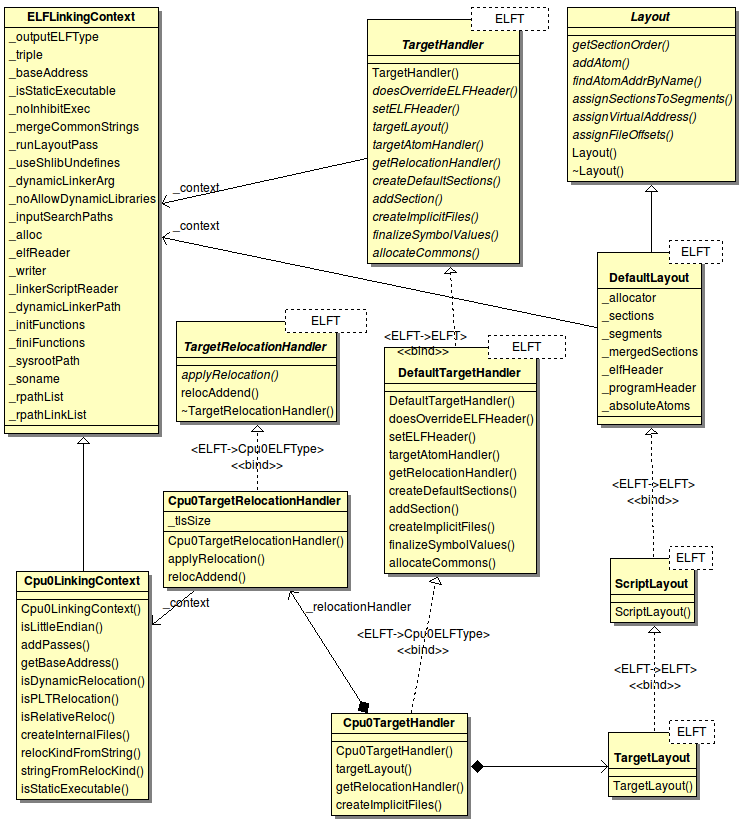
\includegraphics{16.png}}
\caption{Cpu0 lld class relationship}\label{lld:lld-f1}\end{figure}
\begin{figure}[htbp]
\centering
\capstart

\scalebox{0.800000}{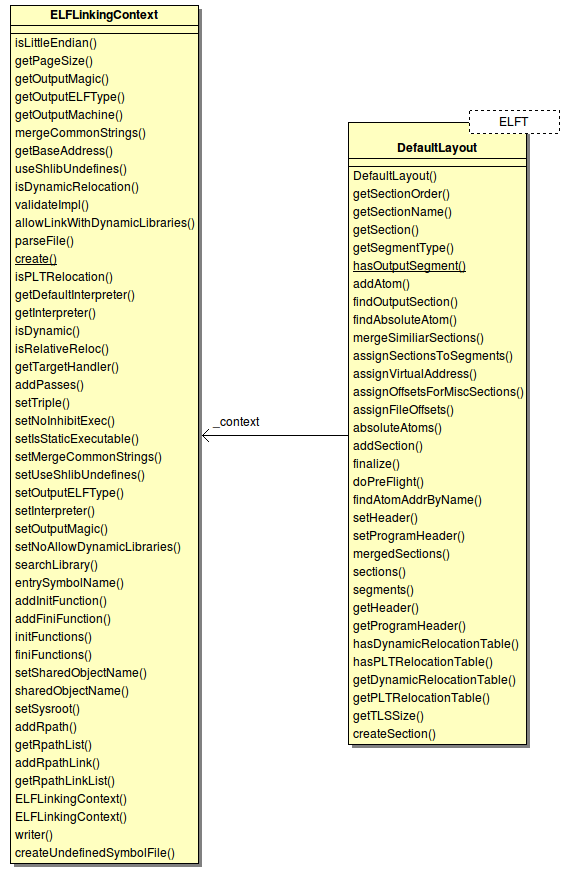
\includegraphics{25.png}}
\caption{Cpu0 lld ELFLinkingContext and DefaultLayout member functions}\label{lld:lld-f2}\end{figure}
\begin{figure}[htbp]
\centering
\capstart

\scalebox{1.000000}{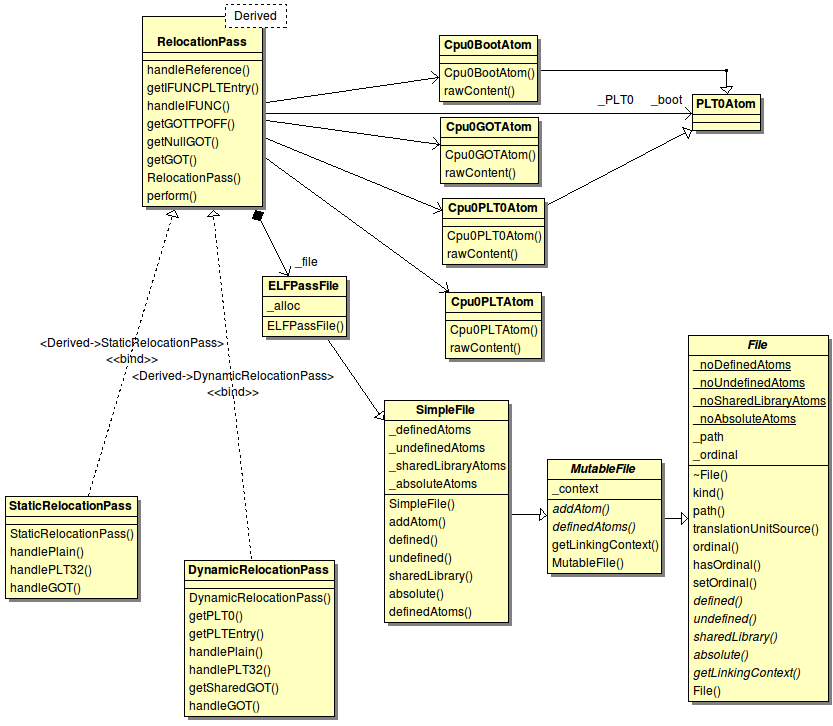
\includegraphics{34.png}}
\caption{Cpu0 lld RelocationPass}\label{lld:lld-f3}\end{figure}

The Cpu0LinkingContext include the context information for those input obj
files and output elf file you want to link.
When do linking, the following code will create Cpu0LinkingContext.
\paragraph{lbdex/Cpu0\_lld\_1030/ELFLinkingContext.h}

\begin{Verbatim}[commandchars=\\\{\}]
\PYG{k}{class} \PYG{n+nc}{ELFLinkingContext} \PYG{o}{:} \PYG{k}{public} \PYG{n}{LinkingContext} \PYG{p}{\PYGZob{}}
\PYG{k}{public}\PYG{o}{:}
  \PYG{p}{.}\PYG{p}{.}\PYG{p}{.}
  \PYG{k}{static} \PYG{n}{std}\PYG{o}{:}\PYG{o}{:}\PYG{n}{unique\PYGZus{}ptr}\PYG{o}{\PYGZlt{}}\PYG{n}{ELFLinkingContext}\PYG{o}{\PYGZgt{}} \PYG{n}{create}\PYG{p}{(}\PYG{n}{llvm}\PYG{o}{:}\PYG{o}{:}\PYG{n}{Triple}\PYG{p}{)}\PYG{p}{;}
  \PYG{p}{.}\PYG{p}{.}\PYG{p}{.}
\PYG{p}{\PYGZcb{}}
\end{Verbatim}
\paragraph{lbdex/Cpu0\_lld\_1030/ELFLinkingContext.cpp}

\begin{Verbatim}[commandchars=\\\{\}]
\PYG{n}{std}\PYG{o}{:}\PYG{o}{:}\PYG{n}{unique\PYGZus{}ptr}\PYG{o}{\PYGZlt{}}\PYG{n}{ELFLinkingContext}\PYG{o}{\PYGZgt{}}
\PYG{n}{ELFLinkingContext}\PYG{o}{:}\PYG{o}{:}\PYG{n}{create}\PYG{p}{(}\PYG{n}{llvm}\PYG{o}{:}\PYG{o}{:}\PYG{n}{Triple} \PYG{n}{triple}\PYG{p}{)} \PYG{p}{\PYGZob{}}
  \PYG{k}{switch} \PYG{p}{(}\PYG{n}{triple}\PYG{p}{.}\PYG{n}{getArch}\PYG{p}{(}\PYG{p}{)}\PYG{p}{)} \PYG{p}{\PYGZob{}}
  \PYG{p}{.}\PYG{p}{.}\PYG{p}{.}
  \PYG{k}{case} \PYG{n}{llvm}\PYG{o}{:}\PYG{o}{:}\PYG{n}{Triple}\PYG{o}{:}\PYG{o}{:}\PYG{n+nl}{cpu0:}
    \PYG{k}{return} \PYG{n}{std}\PYG{o}{:}\PYG{o}{:}\PYG{n}{unique\PYGZus{}ptr}\PYG{o}{\PYGZlt{}}\PYG{n}{ELFLinkingContext}\PYG{o}{\PYGZgt{}}\PYG{p}{(}
        \PYG{k}{new} \PYG{n}{lld}\PYG{o}{:}\PYG{o}{:}\PYG{n}{elf}\PYG{o}{:}\PYG{o}{:}\PYG{n}{Cpu0LinkingContext}\PYG{p}{(}\PYG{n}{triple}\PYG{p}{)}\PYG{p}{)}\PYG{p}{;}
  \PYG{k}{default}\PYG{o}{:}
    \PYG{k}{return} \PYG{n}{nullptr}\PYG{p}{;}
  \PYG{p}{\PYGZcb{}}
\PYG{p}{\PYGZcb{}}
\end{Verbatim}

While Cpu0LinkingContext is created by lld ELF driver as above, the following
code in Cpu0LinkingContext constructor will create Cpu0TargetHandler and passing
the Cpu0LinkingContext object pointer to Cpu0TargeHandler.
\paragraph{lbdex/Cpu0\_lld\_1030/Cpu0/Cpu0LinkingContext.h}

\begin{Verbatim}[commandchars=\\\{\}]
\PYG{k}{class} \PYG{n+nc}{Cpu0LinkingContext} \PYG{n}{LLVM\PYGZus{}FINAL} \PYG{o}{:} \PYG{k}{public} \PYG{n}{ELFLinkingContext} \PYG{p}{\PYGZob{}}
\PYG{k}{public}\PYG{o}{:}
  \PYG{n}{Cpu0LinkingContext}\PYG{p}{(}\PYG{n}{llvm}\PYG{o}{:}\PYG{o}{:}\PYG{n}{Triple} \PYG{n}{triple}\PYG{p}{)}
      \PYG{o}{:} \PYG{n}{ELFLinkingContext}\PYG{p}{(}\PYG{n}{triple}\PYG{p}{,} \PYG{n}{std}\PYG{o}{:}\PYG{o}{:}\PYG{n}{unique\PYGZus{}ptr}\PYG{o}{\PYGZlt{}}\PYG{n}{TargetHandlerBase}\PYG{o}{\PYGZgt{}}\PYG{p}{(}
                                  \PYG{k}{new} \PYG{n}{Cpu0TargetHandler}\PYG{p}{(}\PYG{o}{*}\PYG{k}{this}\PYG{p}{)}\PYG{p}{)}\PYG{p}{)} \PYG{p}{\PYGZob{}}\PYG{p}{\PYGZcb{}}
  \PYG{p}{.}\PYG{p}{.}\PYG{p}{.}
\PYG{p}{\PYGZcb{}}
\end{Verbatim}

Finally, the Cpu0TargeHandler constructor will create other related objects
and set up the relation reference object pointers as \hyperref[lld:lld-f1]{Figure  \ref*{lld:lld-f1}}
depicted by the following code.
\paragraph{lbdex/Cpu0\_lld\_1030/Cpu0/Cpu0TargetHandler.cpp}

\begin{Verbatim}[commandchars=\\\{\}]
\PYG{n}{Cpu0TargetHandler}\PYG{o}{:}\PYG{o}{:}\PYG{n}{Cpu0TargetHandler}\PYG{p}{(}\PYG{n}{Cpu0LinkingContext} \PYG{o}{\PYGZam{}}\PYG{n}{context}\PYG{p}{)}
    \PYG{o}{:} \PYG{n}{DefaultTargetHandler}\PYG{p}{(}\PYG{n}{context}\PYG{p}{)}\PYG{p}{,} \PYG{n}{\PYGZus{}gotFile}\PYG{p}{(}\PYG{k}{new} \PYG{n}{GOTFile}\PYG{p}{(}\PYG{n}{context}\PYG{p}{)}\PYG{p}{)}\PYG{p}{,}
      \PYG{n}{\PYGZus{}relocationHandler}\PYG{p}{(}\PYG{n}{context}\PYG{p}{)}\PYG{p}{,} \PYG{n}{\PYGZus{}targetLayout}\PYG{p}{(}\PYG{n}{context}\PYG{p}{)} \PYG{p}{\PYGZob{}}\PYG{p}{\PYGZcb{}}
\end{Verbatim}

According chapter ELF, the linker stands for resolve the relocation records.
The following code give the chance to let lld system call our relocation
function at proper time.
\paragraph{lbdex/Cpu0\_lld\_1030/Cpu0/Cpu0RelocationPass.cpp}

\begin{Verbatim}[commandchars=\\\{\}]
\PYG{n}{std}\PYG{o}{:}\PYG{o}{:}\PYG{n}{unique\PYGZus{}ptr}\PYG{o}{\PYGZlt{}}\PYG{n}{Pass}\PYG{o}{\PYGZgt{}}
\PYG{n}{lld}\PYG{o}{:}\PYG{o}{:}\PYG{n}{elf}\PYG{o}{:}\PYG{o}{:}\PYG{n}{createCpu0RelocationPass}\PYG{p}{(}\PYG{k}{const} \PYG{n}{Cpu0LinkingContext} \PYG{o}{\PYGZam{}}\PYG{n}{ctx}\PYG{p}{)} \PYG{p}{\PYGZob{}}
  \PYG{k}{switch} \PYG{p}{(}\PYG{n}{ctx}\PYG{p}{.}\PYG{n}{getOutputELFType}\PYG{p}{(}\PYG{p}{)}\PYG{p}{)} \PYG{p}{\PYGZob{}}
  \PYG{k}{case} \PYG{n}{llvm}\PYG{o}{:}\PYG{o}{:}\PYG{n}{ELF}\PYG{o}{:}\PYG{o}{:}\PYG{n+nl}{ET\PYGZus{}EXEC:}
\PYG{c+cp}{\PYGZsh{}}\PYG{c+cp}{ifdef DLINKER}
    \PYG{k}{if} \PYG{p}{(}\PYG{n}{ctx}\PYG{p}{.}\PYG{n}{isDynamic}\PYG{p}{(}\PYG{p}{)}\PYG{p}{)}
      \PYG{k}{return} \PYG{n}{std}\PYG{o}{:}\PYG{o}{:}\PYG{n}{unique\PYGZus{}ptr}\PYG{o}{\PYGZlt{}}\PYG{n}{Pass}\PYG{o}{\PYGZgt{}}\PYG{p}{(}\PYG{k}{new} \PYG{n}{DynamicRelocationPass}\PYG{p}{(}\PYG{n}{ctx}\PYG{p}{)}\PYG{p}{)}\PYG{p}{;}
    \PYG{k}{else}
\PYG{c+cp}{\PYGZsh{}}\PYG{c+cp}{endif }\PYG{c+c1}{// DLINKER}
      \PYG{k}{return} \PYG{n}{std}\PYG{o}{:}\PYG{o}{:}\PYG{n}{unique\PYGZus{}ptr}\PYG{o}{\PYGZlt{}}\PYG{n}{Pass}\PYG{o}{\PYGZgt{}}\PYG{p}{(}\PYG{k}{new} \PYG{n}{StaticRelocationPass}\PYG{p}{(}\PYG{n}{ctx}\PYG{p}{)}\PYG{p}{)}\PYG{p}{;}
\PYG{c+cp}{\PYGZsh{}}\PYG{c+cp}{ifdef DLINKER}
  \PYG{k}{case} \PYG{n}{llvm}\PYG{o}{:}\PYG{o}{:}\PYG{n}{ELF}\PYG{o}{:}\PYG{o}{:}\PYG{n+nl}{ET\PYGZus{}DYN:}
    \PYG{k}{return} \PYG{n}{std}\PYG{o}{:}\PYG{o}{:}\PYG{n}{unique\PYGZus{}ptr}\PYG{o}{\PYGZlt{}}\PYG{n}{Pass}\PYG{o}{\PYGZgt{}}\PYG{p}{(}\PYG{k}{new} \PYG{n}{DynamicRelocationPass}\PYG{p}{(}\PYG{n}{ctx}\PYG{p}{)}\PYG{p}{)}\PYG{p}{;}
\PYG{c+cp}{\PYGZsh{}}\PYG{c+cp}{endif }\PYG{c+c1}{// DLINKER}
  \PYG{k}{case} \PYG{n}{llvm}\PYG{o}{:}\PYG{o}{:}\PYG{n}{ELF}\PYG{o}{:}\PYG{o}{:}\PYG{n+nl}{ET\PYGZus{}REL:}
    \PYG{k}{return} \PYG{n}{std}\PYG{o}{:}\PYG{o}{:}\PYG{n}{unique\PYGZus{}ptr}\PYG{o}{\PYGZlt{}}\PYG{n}{Pass}\PYG{o}{\PYGZgt{}}\PYG{p}{(}\PYG{p}{)}\PYG{p}{;}
  \PYG{k}{default}\PYG{o}{:}
    \PYG{n}{llvm\PYGZus{}unreachable}\PYG{p}{(}\PYG{l+s}{"}\PYG{l+s}{Unhandled output file type}\PYG{l+s}{"}\PYG{p}{)}\PYG{p}{;}
  \PYG{p}{\PYGZcb{}}
\PYG{p}{\PYGZcb{}}
\end{Verbatim}

The ``\#ifdef DLINKER'' part is for dynamic linker will used in next section.
For static linker, a StaticRelocationPass object is created and return.

Now the following code of Cpu0TargetRelocationHandler::applyRelocation()
will be called through
Cpu0TargetHandler by lld ELF driver when it meet each relocation record.
\paragraph{lbdex/Cpu0\_lld\_1030/Cpu0/Cpu0RelocationHandler.cpp}

\begin{Verbatim}[commandchars=\\\{\}]
\PYG{n}{ErrorOr}\PYG{o}{\PYGZlt{}}\PYG{k+kt}{void}\PYG{o}{\PYGZgt{}} \PYG{n}{Cpu0TargetRelocationHandler}\PYG{o}{:}\PYG{o}{:}\PYG{n}{applyRelocation}\PYG{p}{(}
    \PYG{n}{ELFWriter} \PYG{o}{\PYGZam{}}\PYG{n}{writer}\PYG{p}{,} \PYG{n}{llvm}\PYG{o}{:}\PYG{o}{:}\PYG{n}{FileOutputBuffer} \PYG{o}{\PYGZam{}}\PYG{n}{buf}\PYG{p}{,} \PYG{k}{const} \PYG{n}{lld}\PYG{o}{:}\PYG{o}{:}\PYG{n}{AtomLayout} \PYG{o}{\PYGZam{}}\PYG{n}{atom}\PYG{p}{,}
    \PYG{k}{const} \PYG{n}{Reference} \PYG{o}{\PYGZam{}}\PYG{n}{ref}\PYG{p}{)} \PYG{k}{const} \PYG{p}{\PYGZob{}}

  \PYG{k}{switch} \PYG{p}{(}\PYG{n}{ref}\PYG{p}{.}\PYG{n}{kind}\PYG{p}{(}\PYG{p}{)}\PYG{p}{)} \PYG{p}{\PYGZob{}}
  \PYG{k}{case} \PYG{n+nl}{R\PYGZus{}CPU0\PYGZus{}NONE:}
    \PYG{k}{break}\PYG{p}{;}
  \PYG{k}{case} \PYG{n+nl}{R\PYGZus{}CPU0\PYGZus{}HI16:}
    \PYG{n}{relocHI16}\PYG{p}{(}\PYG{n}{location}\PYG{p}{,} \PYG{n}{relocVAddress}\PYG{p}{,} \PYG{n}{targetVAddress}\PYG{p}{,} \PYG{n}{ref}\PYG{p}{.}\PYG{n}{addend}\PYG{p}{(}\PYG{p}{)}\PYG{p}{)}\PYG{p}{;}
    \PYG{k}{break}\PYG{p}{;}
  \PYG{k}{case} \PYG{n+nl}{R\PYGZus{}CPU0\PYGZus{}LO16:}
    \PYG{n}{relocLO16}\PYG{p}{(}\PYG{n}{location}\PYG{p}{,} \PYG{n}{relocVAddress}\PYG{p}{,} \PYG{n}{targetVAddress}\PYG{p}{,} \PYG{n}{ref}\PYG{p}{.}\PYG{n}{addend}\PYG{p}{(}\PYG{p}{)}\PYG{p}{)}\PYG{p}{;}
    \PYG{k}{break}\PYG{p}{;}
  \PYG{p}{.}\PYG{p}{.}\PYG{p}{.}
  \PYG{p}{\PYGZcb{}}
  \PYG{k}{return} \PYG{n}{error\PYGZus{}code}\PYG{o}{:}\PYG{o}{:}\PYG{n}{success}\PYG{p}{(}\PYG{p}{)}\PYG{p}{;}
\PYG{p}{\PYGZcb{}}
\end{Verbatim}
\paragraph{lbdex/Cpu0\_lld\_1030/Cpu0/Cpu0TargetHandler.h}

\begin{Verbatim}[commandchars=\\\{\}]
\PYG{k}{class} \PYG{n+nc}{Cpu0TargetHandler} \PYG{n}{LLVM\PYGZus{}FINAL}
    \PYG{o}{:} \PYG{k}{public} \PYG{n}{DefaultTargetHandler}\PYG{o}{\PYGZlt{}}\PYG{n}{Cpu0ELFType}\PYG{o}{\PYGZgt{}} \PYG{p}{\PYGZob{}}
\PYG{k}{public}\PYG{o}{:}
  \PYG{p}{.}\PYG{p}{.}
  \PYG{k}{virtual} \PYG{k}{const} \PYG{n}{Cpu0TargetRelocationHandler} \PYG{o}{\PYGZam{}}\PYG{n}{getRelocationHandler}\PYG{p}{(}\PYG{p}{)} \PYG{k}{const} \PYG{p}{\PYGZob{}}
    \PYG{k}{return} \PYG{n}{\PYGZus{}relocationHandler}\PYG{p}{;}
  \PYG{p}{\PYGZcb{}}
\end{Verbatim}

Summary as \hyperref[lld:lld-f4]{Figure  \ref*{lld:lld-f4}}.
\begin{figure}[htbp]
\centering
\capstart

\scalebox{1.000000}{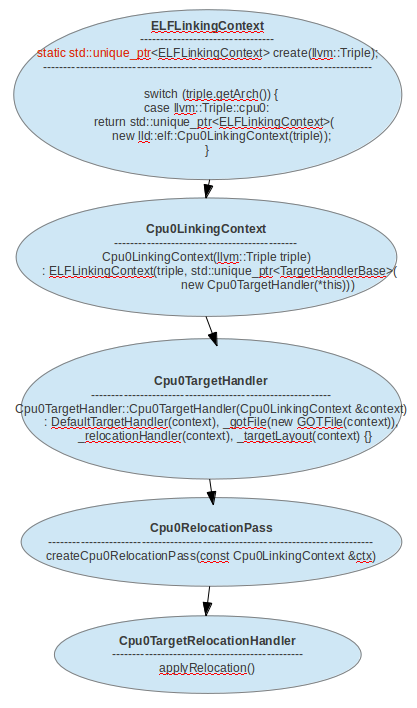
\includegraphics{44.png}}
\caption{Cpu0 lld related objects created sequence}\label{lld:lld-f4}\end{figure}

Remind, static std::unique\_ptr\textless{}ELFLinkingContext\textgreater{}
ELFLinkingContext::create(llvm::Triple) is called without an object of
class ELFLinkingContext instance (because the static keyword).
The Cpu0LinkingContext constructor will create it's ELFLinkingContext part.
The std::unique\_ptr came from c++11 standard.
The unique\_ptr objects automatically delete the object they manage (using a
deleter) as soon as they themselves are destroyed. Just like the Singlelten
pattern in Design Pattern book or Smart Pointers in Effective C++ book. \footnote{
\href{http://www.cplusplus.com/reference/memory/unique\_ptr/}{http://www.cplusplus.com/reference/memory/unique\_ptr/}
}
\begin{figure}[htbp]
\centering
\capstart

\scalebox{1.000000}{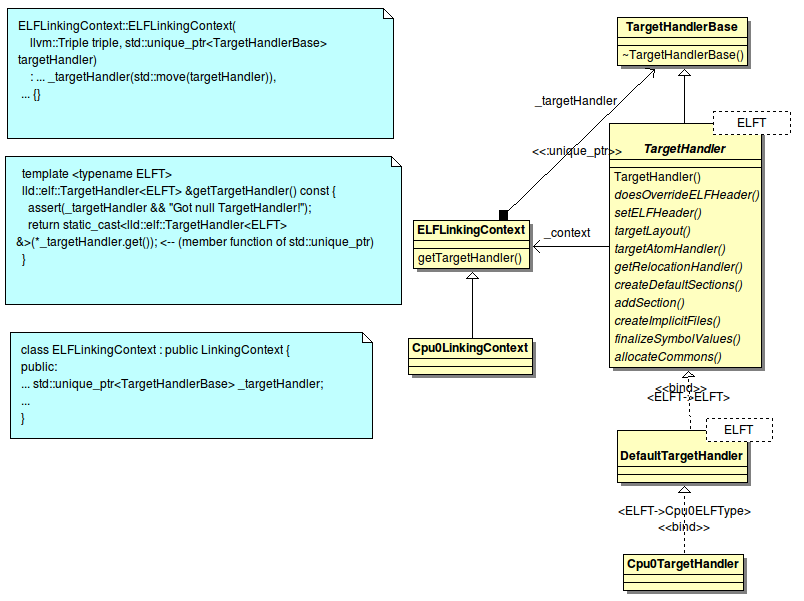
\includegraphics{54.png}}
\caption{Cpu0LinkingContext get Cpu0TargetHandler through \&getTargetHandler()}\label{lld:lld-f5}\end{figure}

As \hyperref[lld:lld-f1]{Figure  \ref*{lld:lld-f1}} depicted, the Cpu0TargetHandler include the members or
pointers which can access to other object. The way to access Cpu0TargetHandler
object from Cpu0LinkingContext or Cpu0RelocationHandler rely on
LinkingContext::getTargetHandler() function. As \hyperref[lld:lld-f5]{Figure  \ref*{lld:lld-f5}} depicted,
the unique\_ptr point to Cpu0TargetHandler will be saved in LinkingContext
contructor function.

\begin{notice}{note}{Note:}
std::unique\_ptr::get() \footnote{
\href{http://www.cplusplus.com/reference/memory/unique\_ptr/get/}{http://www.cplusplus.com/reference/memory/unique\_ptr/get/}
}

pointer get() const noexcept;

Get pointer
Returns the stored pointer.
\end{notice}

\begin{notice}{note}{Note:}
std::move() \footnote{
\href{http://www.cplusplus.com/reference/utility/move/}{http://www.cplusplus.com/reference/utility/move/}
}
\begin{description}
\item[{for example:}] \leavevmode
std::string bar = ``bar-string'';
std::move(bar);

bar is null after std::move(bar);

\end{description}
\end{notice}


\section{Dynamic linker}
\label{lld:dynamic-linker}
Except the lld code with \#ifdef DLINKER. The following code in Verilog exist to
support dynamic linker.
\paragraph{lbdex/cpu0\_verilog/dynlinker.v}

\begin{Verbatim}[commandchars=\\\{\}]
{}`define DLINKER\_INFO\_ADDR  'h70000
{}`define GPADDR    'h7FFF0

{}`ifdef DLINKER
  task setDynLinkerInfo; begin
// below code set memory as follows,
//                                                            (4 bytes) 
//                                                      ---------------------------------------
// DLINKER\_INFO\_ADDR ----------\textgreater{}                        \textbar{} numDynEntry                         \textbar{}
//                                                      ---------------------------------------
// DLINKER\_INFO\_ADDR+4 --------\textgreater{}                        \textbar{} index of dynsym (0st row)           \textbar{}
//   above is the 1st word of section .dynsym of libfoobar.cpu0.so. 
// DLINKER\_INFO\_ADDR+8 --------\textgreater{}                        \textbar{} index of dynsym (1st row)           \textbar{}
//                                                      \textbar{} ...                                 \textbar{}
// DLINKER\_INFO\_ADDR+(numDynEntry-1)*4 ---------------\textgreater{} \textbar{} index of dynsym (the last row)      \textbar{}
//                                                      ---------------------------------------
// DLINKER\_INFO\_ADDR+numDynEntry*4 -------------------\textgreater{} \textbar{} 1st function (foo()) offset in lib  \textbar{}
// DLINKER\_INFO\_ADDR+numDynEntry*4+4 -----------------\textgreater{} \textbar{} 1st function (foo()) name (48 bytes)\textbar{}
//                                                      \textbar{} ...                                 \textbar{}
// DLINKER\_INFO\_ADDR+numDynEntry+(numDynEntry-1)*4 ---\textgreater{} \textbar{} last function (foo()) offset in lib \textbar{}
// DLINKER\_INFO\_ADDR+numDynEntry+(numDynEntry-1)*4+4 -\textgreater{} \textbar{} last function (foo()) name          \textbar{}
//                                                      ---------------------------------------
// DLINKER\_INFO\_ADDR+4+numDynEntry*4+numDynEntry*52 --\textgreater{} \textbar{} .dynstr of lib                      \textbar{}
//                                                      \textbar{}   ...                               \textbar{}
//                                                      ---------------------------------------
  // caculate number of dynamic entries
    numDynEntry = 0;
    j = 0;
    for (i=0; i \textless{} 384 \&\& j == 0; i=i+52) begin
       if (so\_func\_offset[i] == {}`MEMEMPTY \&\& so\_func\_offset[i+1] == {}`MEMEMPTY \&\& 
           so\_func\_offset[i+2] == {}`MEMEMPTY \&\& so\_func\_offset[i+3] == {}`MEMEMPTY) begin
         numDynEntry = i/52;
         j = 1;
       {}`ifdef DEBUG\_DLINKER
         \$display("numDynEntry = \%8x", numDynEntry);
       {}`endif
       end
    end
  // save number of dynamic entries to memory address {}`DLINKER\_INFO\_ADDR
    m[{}`DLINKER\_INFO\_ADDR] = numDynEntry[31:24];
    m[{}`DLINKER\_INFO\_ADDR+1] = numDynEntry[23:16];
    m[{}`DLINKER\_INFO\_ADDR+2] = numDynEntry[15:8];
    m[{}`DLINKER\_INFO\_ADDR+3] = numDynEntry[7:0];
  // copy section .dynsym of ELF to memory address {}`DLINKER\_INFO\_ADDR+4
    i = {}`DLINKER\_INFO\_ADDR+4;
    for (j=0; j \textless{} (4*numDynEntry); j=j+4) begin
      m[i] = dsym[j];
      m[i+1] = dsym[j+1];
      m[i+2] = dsym[j+2];
      m[i+3] = dsym[j+3];
      i = i + 4;
    end
  // copy the offset values of section .text of shared library .so of ELF to 
  // memory address {}`DLINKER\_INFO\_ADDR+4+numDynEntry*4
    i = {}`DLINKER\_INFO\_ADDR+4+numDynEntry*4;
    l = 0;
    for (j=0; j \textless{} numDynEntry; j=j+1) begin
      for (k=0; k \textless{} 52; k=k+1) begin
        m[i] = so\_func\_offset[l];
        i = i + 1;
        l = l + 1;
      end
    end
  {}`ifdef DEBUG\_DLINKER
    i = {}`DLINKER\_INFO\_ADDR+4+numDynEntry*4;
    for (j=0; j \textless{} (8*numDynEntry); j=j+8) begin
       \$display("\%8x: \%8x", i, \PYGZob{}m[i], m[i+1], m[i+2], m[i+3]\PYGZcb{});
      i = i + 8;
    end
  {}`endif
  // copy section .dynstr of ELF to memory address 
  // {}`DLINKER\_INFO\_ADDR+4+numDynEntry*4+numDynEntry*52
    i={}`DLINKER\_INFO\_ADDR+4+numDynEntry*4+numDynEntry*52;
    for (j=0; dstr[j] != {}`MEMEMPTY; j=j+1) begin
      m[i] = dstr[j];
      i = i + 1;
    end
  {}`ifdef DEBUG\_DLINKER
    \$display("In setDynLinkerInfo()");
    for (i={}`DLINKER\_INFO\_ADDR; i \textless{} {}`MEMSIZE; i=i+4) begin
       if (m[i] != {}`MEMEMPTY \textbar{}\textbar{} m[i+1] != {}`MEMEMPTY \textbar{}\textbar{} 
         m[i+2] != {}`MEMEMPTY \textbar{}\textbar{} m[i+3] != {}`MEMEMPTY)
         \$display("\%8x: \%8x", i, \PYGZob{}m[i], m[i+1], m[i+2], m[i+3]\PYGZcb{});
    end
    \$display("global address \%8x", \PYGZob{}m[{}`GPADDR], m[{}`GPADDR+1], 
             m[{}`GPADDR+2], m[{}`GPADDR+3]\PYGZcb{});
    \$display("gp = \%8x", gp);
  {}`endif
// below code set memory as follows,
//                                 -----------------------------------
// gp ---------------------------\textgreater{} \textbar{} all 0                           \textbar{} (16 bytes)
// gp+16 ------------------------\textgreater{} \textbar{} 0                          \textbar{}
// gp+16+1*4 --------------------\textgreater{} \textbar{} 1st plt entry address      \textbar{} (4 bytes)
//                                 \textbar{} ...                        \textbar{}
// gp+16+(numDynEntry-1)*4 ------\textgreater{} \textbar{} the last plt entry address \textbar{}
//                                 ------------------------------
// gp ---------------------------\textgreater{} \textbar{} all 0                           \textbar{} (16 bytes)
// gp+16+0*8'h10 ----------------\textgreater{} \textbar{} 32'h10: pointer to plt0         \textbar{}
// gp+16+1*8'h10 ----------------\textgreater{} \textbar{} 1st plt entry                   \textbar{}
// gp+16+2*8'h10 ----------------\textgreater{} \textbar{} 2nd plt entry                   \textbar{}
//                                 \textbar{} ...                             \textbar{}
// gp+16+(numDynEntry-1)*8'h10 --\textgreater{} \textbar{} the last plt entry              \textbar{}
//                                 -----------------------------------
// note: gp point to the \_GLOBAL\_OFFSET\_TABLE\_, 
//       numDynEntry = actual number of functions + 1.
//   gp+1*4..gp+numDynEntry*4 set to 8'h10 plt0 which will jump to dynamic 
//   linker.
//   After dynamic linker load function to memory, it will set gp+index*4 to 
//   function memory address. For example, if the function index is 2, then the 
//   gp+2*4 is set to the memory address of this loaded function. 
//   Then the the caller call 
//   "ld \$t9, 2*4(\$gp)" and "ret \$t9" will jump to this loaded function directly.

    gpPlt = gp+16+numDynEntry*4;
    // set (gpPlt-16..gpPlt-1) to 0
    for (j=16; j \textgreater{}= 1; j=j-1)
      m[gpPlt+j] = 8'h00;
    // put plt in (gpPlt..gpPlt+numDynEntry*8'h10+1)
    for (i=1; i \textless{} numDynEntry; i=i+1) begin
      j=i*4;
      // (gp+'8h10..gp+numDynEntry*'8h10+15) set to plt entry
      // addiu	\$t9, \$zero, dynsym\_idx
      m[gpPlt+i*8'h10] = 8'h09;
      m[gpPlt+i*8'h10+1] = 8'h60;
      m[gpPlt+i*8'h10+2] = i[15:8];
      m[gpPlt+i*8'h10+3] = i[7:0];
      // st	\$t9, j(\$gp)
      m[gpPlt+i*8'h10+4] = 8'h02;
      m[gpPlt+i*8'h10+5] = 8'h6b;
      m[gpPlt+i*8'h10+6] = 0;
      m[gpPlt+i*8'h10+7] = 0;
      // ld	\$t9, ('16h0010)(\$gp)
      m[gpPlt+i*8'h10+8] = 8'h01;
      m[gpPlt+i*8'h10+9] = 8'h6b;
      m[gpPlt+i*8'h10+10] = 0;
      m[gpPlt+i*8'h10+11] = 8'h10;
      // ret	\$t9
      m[gpPlt+i*8'h10+12] = 8'h3c;
      m[gpPlt+i*8'h10+13] = 8'h60;
      m[gpPlt+i*8'h10+14] = 0;
      m[gpPlt+i*8'h10+15] = 0;
    end

  // .got.plt offset(0x00.0x03) has been set to 0 in elf already.
  // Set .got.plt offset(8'h10..numDynEntry*'8h10) point to plt entry as above.
  {}`ifdef DEBUG\_DLINKER
         \$display("numDynEntry = \%8x", numDynEntry);
  {}`endif
//      j32=32'h1fc0; // m[32'h1fc]="something" will hang. Very tricky
    m[gp+16] = 8'h0;
    m[gp+16+1] = 8'h0;
    m[gp+16+2] = 8'h0;
    m[gp+16+3] = 8'h10;
    j32=gpPlt+16;
    for (i=1; i \textless{} numDynEntry; i=i+1) begin
      m[gp+16+i*4] = j32[31:24];
      m[gp+16+i*4+1] = j32[23:16];
      m[gp+16+i*4+2] = j32[15:8];
      m[gp+16+i*4+3] = j32[7:0];
      j32=j32+16;
    end
  {}`ifdef DEBUG\_DLINKER
    // show (gp..gp+numDynEntry*4-1)
    for (i=0; i \textless{} numDynEntry; i=i+1) begin
      \$display("\%8x: \%8x", gp+16+i*4, \PYGZob{}m[gp+16+i*4], m[gp+16+i*4+1], 
               m[gp+16+i*4+2], m[gp+16+i*4+3]\PYGZcb{});
    end
    // show (gpPlt..gpPlt+(numDynEntry+1)*8'h10-1)
    for (i=0; i \textless{} numDynEntry; i=i+1) begin
      for (j=0; j \textless{} 16; j=j+4)
        \$display("\%8x: \%8x", gpPlt+i*8'h10+j, 
                 \PYGZob{}m[gpPlt+i*8'h10+j], 
                  m[gpPlt+i*8'h10+j+1], 
                  m[gpPlt+i*8'h10+j+2], 
                  m[gpPlt+i*8'h10+j+3]\PYGZcb{});
    end
  {}`endif
  end endtask
{}`endif

{}`ifdef DLINKER
  task loadToFlash; begin
  // erase memory
    for (i=0; i \textless{} {}`MEMSIZE; i=i+1) begin
       flash[i] = {}`MEMEMPTY;
    end
    \$readmemh("libso.hex", flash);
  {}`ifdef DEBUG\_DLINKER
    for (i=0; i \textless{} {}`MEMSIZE \&\& (flash[i] != {}`MEMEMPTY \textbar{}\textbar{} 
         flash[i+1] != {}`MEMEMPTY \textbar{}\textbar{} flash[i+2] != {}`MEMEMPTY \textbar{}\textbar{} 
         flash[i+3] != {}`MEMEMPTY); i=i+4) begin
       \$display("\%8x: \%8x", i, \PYGZob{}flash[i], flash[i+1], flash[i+2], flash[i+3]\PYGZcb{});
    end
  {}`endif
  end endtask
{}`endif

{}`ifdef DLINKER
  task createDynInfo; begin
    \$readmemh("global\_offset", globalAddr);
    m[{}`GPADDR]   = globalAddr[0];
    m[{}`GPADDR+1] = globalAddr[1];
    m[{}`GPADDR+2] = globalAddr[2];
    m[{}`GPADDR+3] = globalAddr[3];
    gp[31:24] = globalAddr[0];
    gp[23:16] = globalAddr[1];
    gp[15:8] = globalAddr[2];
    gp[7:0] = globalAddr[3];
  {}`ifdef DEBUG\_DLINKER
    \$display("global address \%8x", \PYGZob{}m[{}`GPADDR], m[{}`GPADDR+1], 
             m[{}`GPADDR+2], m[{}`GPADDR+3]\PYGZcb{});
    \$display("gp = \%8x", gp);
  {}`endif
{}`endif
{}`ifdef DLINKER
    for (i=0; i \textless{} 192; i=i+1) begin
       dsym[i] = {}`MEMEMPTY;
    end
    for (i=0; i \textless{} 96; i=i+1) begin
       dstr[i] = {}`MEMEMPTY;
    end
    for (i=0; i \textless{}384; i=i+1) begin
       so\_func\_offset[i] = {}`MEMEMPTY;
    end
    \$readmemh("dynsym", dsym);
    \$readmemh("dynstr", dstr);
    \$readmemh("so\_func\_offset", so\_func\_offset);
    setDynLinkerInfo();
  end endtask
{}`endif
\end{Verbatim}
\paragraph{lbdex/cpu0\_verilog/flashio.v}

\begin{Verbatim}[commandchars=\\\{\}]
{}`define FLASHADDR 'hA0000

{}`ifdef DLINKER
    end else if (abus \textgreater{}= {}`FLASHADDR \&\& abus \textless{}= {}`FLASHADDR+{}`MEMSIZE-4) begin
      fabus = abus-{}`FLASHADDR;
      if (en == 1 \&\& rw == 0) begin // r\_w==0:write
        data = dbus\_in;
        case (m\_size)
        {}`BYTE:  \PYGZob{}flash[fabus]\PYGZcb{} = dbus\_in[7:0];
        {}`INT16: \PYGZob{}flash[fabus], flash[fabus+1] \PYGZcb{} = dbus\_in[15:0];
        {}`INT24: \PYGZob{}flash[fabus], flash[fabus+1], flash[fabus+2]\PYGZcb{} = dbus\_in[24:0];
        {}`INT32: \PYGZob{}flash[fabus], flash[fabus+1], flash[fabus+2], flash[fabus+3]\PYGZcb{} 
                = dbus\_in;
        endcase
      end else if (en == 1 \&\& rw == 1) begin// r\_w==1:read
        case (m\_size)
        {}`BYTE:  data = \PYGZob{}8'h00  , 8'h00,   8'h00,   flash[fabus]\PYGZcb{};
        {}`INT16: data = \PYGZob{}8'h00  , 8'h00,   flash[fabus], flash[fabus+1]\PYGZcb{};
        {}`INT24: data = \PYGZob{}8'h00  , flash[fabus], flash[fabus+1], flash[fabus+2]\PYGZcb{};
        {}`INT32: data = \PYGZob{}flash[fabus], flash[fabus+1], flash[fabus+2], 
                       flash[fabus+3]\PYGZcb{};
        endcase
      end else
        data = 32'hZZZZZZZZ;
{}`endif
\end{Verbatim}
\paragraph{lbdex/cpu0\_verilog/cpu0Id.v}

\begin{Verbatim}[commandchars=\\\{\}]
{}`define DLINKER  // Dynamic Linker Support
//{}`define DEBUG\_DLINKER   // Dynamic Linker Debug
// TRACE: Display the memory contents of the loaded program and data
//{}`define TRACE 

{}`include "cpu0.v"
\end{Verbatim}
\paragraph{lbdex/cpu0\_verilog/cpu0IId.v}

\begin{Verbatim}[commandchars=\\\{\}]
{}`define CPU0II
{}`define DLINKER  // Dynamic Linker Support
//{}`define DEBUG\_DLINKER   // Dynamic Linker Debug
// TRACE: Display the memory contents of the loaded program and data
//{}`define TRACE 

{}`include "cpu0.v"
\end{Verbatim}

The following code ch\_dynamiclinker.cpp and foobar.cpp is the example for
dynamic linker demostration. File dynamic\_linker.cpp is what our implementaion
to execute the dynamic linker function on Cpu0 Verilog machine.
\paragraph{lbdex/InputFiles/dynamic\_linker.h}

\begin{Verbatim}[commandchars=\\\{\}]
\PYG{c+cp}{\PYGZsh{}}\PYG{c+cp}{ifndef \PYGZus{}DYNAMIC\PYGZus{}LINKER\PYGZus{}H\PYGZus{}}
\PYG{c+cp}{\PYGZsh{}}\PYG{c+cp}{define \PYGZus{}DYNAMIC\PYGZus{}LINKER\PYGZus{}H\PYGZus{}}

\PYG{c+cp}{\PYGZsh{}}\PYG{c+cp}{define DYNLINKER\PYGZus{}INFO\PYGZus{}ADDR  0x70000}
\PYG{c+cp}{\PYGZsh{}}\PYG{c+cp}{define DYNENT\PYGZus{}SIZE          4}
\PYG{c+cp}{\PYGZsh{}}\PYG{c+cp}{define DYNPROGSTART         0x40000}
\PYG{c+cp}{\PYGZsh{}}\PYG{c+cp}{define FLASHADDR            0xA0000}
\PYG{c+cp}{\PYGZsh{}}\PYG{c+cp}{define GPADDR               0x7FFF0}

\PYG{c+cp}{\PYGZsh{}}\PYG{c+cp}{define STOP \PYGZbs{}}
\PYG{c+cp}{  asm("lui \PYGZdl{}t9, 0xffff"); \PYGZbs{}}
\PYG{c+cp}{  asm("addiu \PYGZdl{}t9, \PYGZdl{}zero, 0xffff"); \PYGZbs{}}
\PYG{c+cp}{  asm("ret \PYGZdl{}t9");}

\PYG{c+cp}{\PYGZsh{}}\PYG{c+cp}{define ENABLE\PYGZus{}TRACE \PYGZbs{}}
\PYG{c+cp}{  asm("mfsw \PYGZdl{}at"); \PYGZbs{}}
\PYG{c+cp}{  asm("ori \PYGZdl{}at, \PYGZdl{}at, 0x0020"); \PYGZbs{}}
\PYG{c+cp}{  asm("mtsw \PYGZdl{}at");}

\PYG{c+cp}{\PYGZsh{}}\PYG{c+cp}{define DISABLE\PYGZus{}TRACE \PYGZbs{}}
\PYG{c+cp}{  asm("mfsw \PYGZdl{}at"); \PYGZbs{}}
\PYG{c+cp}{  asm("andi \PYGZdl{}at, \PYGZdl{}at, 0xffdf"); \PYGZbs{}}
\PYG{c+cp}{  asm("mtsw \PYGZdl{}at");}

\PYG{k}{struct} \PYG{n}{ProgAddr} \PYG{p}{\PYGZob{}}
  \PYG{k+kt}{int} \PYG{n}{memAddr}\PYG{p}{;}
  \PYG{k+kt}{int} \PYG{n}{size}\PYG{p}{;}
\PYG{p}{\PYGZcb{}}\PYG{p}{;}

\PYG{k}{extern} \PYG{k+kt}{void} \PYG{n}{dynamic\PYGZus{}linker\PYGZus{}init}\PYG{p}{(}\PYG{p}{)}\PYG{p}{;}
\PYG{k}{extern} \PYG{k+kt}{void} \PYG{n}{dynamic\PYGZus{}linker}\PYG{p}{(}\PYG{p}{)}\PYG{p}{;}

\PYG{c+cp}{\PYGZsh{}}\PYG{c+cp}{endif}
\end{Verbatim}
\paragraph{lbdex/InputFiles/dynamic\_linker.cpp}

\begin{Verbatim}[commandchars=\\\{\}]
\PYG{c+cp}{\PYGZsh{}}\PYG{c+cp}{include "dynamic\PYGZus{}linker.h"}

\PYG{c+c1}{//\PYGZsh{}define DEBUG\PYGZus{}DLINKER}
\PYG{c+cp}{\PYGZsh{}}\PYG{c+cp}{define PLT0ADDR 0x10}
\PYG{c+cp}{\PYGZsh{}}\PYG{c+cp}{define REGADDR  0x7ff00}

\PYG{c+cp}{\PYGZsh{}}\PYG{c+cp}{define SAVE\PYGZus{}REGISTERS          \PYGZbs{}}
\PYG{c+cp}{  asm("lui \PYGZdl{}at, 7");            \PYGZbs{}}
\PYG{c+cp}{  asm("ori \PYGZdl{}at, \PYGZdl{}at, 0xff00");  \PYGZbs{}}
\PYG{c+cp}{  asm("st \PYGZdl{}2, 0(\PYGZdl{}at)");         \PYGZbs{}}
\PYG{c+cp}{  asm("st \PYGZdl{}3, 4(\PYGZdl{}at)");         \PYGZbs{}}
\PYG{c+cp}{  asm("st \PYGZdl{}4, 8(\PYGZdl{}at)");         \PYGZbs{}}
\PYG{c+cp}{  asm("st \PYGZdl{}5, 12(\PYGZdl{}at)");        \PYGZbs{}}
\PYG{c+cp}{  asm("st \PYGZdl{}6, 16(\PYGZdl{}at)");        \PYGZbs{}}
\PYG{c+cp}{  asm("st \PYGZdl{}7, 20(\PYGZdl{}at)");        \PYGZbs{}}
\PYG{c+cp}{  asm("st \PYGZdl{}8, 24(\PYGZdl{}at)");        \PYGZbs{}}
\PYG{c+cp}{  asm("st \PYGZdl{}9, 28(\PYGZdl{}at)");        \PYGZbs{}}
\PYG{c+cp}{  asm("st \PYGZdl{}10, 32(\PYGZdl{}at)");       \PYGZbs{}}
\PYG{c+cp}{  asm("st \PYGZdl{}11, 36(\PYGZdl{}at)");}

\PYG{c+cp}{\PYGZsh{}}\PYG{c+cp}{define RESTORE\PYGZus{}REGISTERS       \PYGZbs{}}
\PYG{c+cp}{  asm("lui \PYGZdl{}at, 7");            \PYGZbs{}}
\PYG{c+cp}{  asm("ori \PYGZdl{}at, \PYGZdl{}at, 0xff00");  \PYGZbs{}}
\PYG{c+cp}{  asm("ld \PYGZdl{}2, 0(\PYGZdl{}at)");         \PYGZbs{}}
\PYG{c+cp}{  asm("ld \PYGZdl{}3, 4(\PYGZdl{}at)");         \PYGZbs{}}
\PYG{c+cp}{  asm("ld \PYGZdl{}4, 8(\PYGZdl{}at)");         \PYGZbs{}}
\PYG{c+cp}{  asm("ld \PYGZdl{}5, 12(\PYGZdl{}at)");        \PYGZbs{}}
\PYG{c+cp}{  asm("ld \PYGZdl{}6, 16(\PYGZdl{}at)");        \PYGZbs{}}
\PYG{c+cp}{  asm("ld \PYGZdl{}7, 20(\PYGZdl{}at)");        \PYGZbs{}}
\PYG{c+cp}{  asm("ld \PYGZdl{}8, 24(\PYGZdl{}at)");        \PYGZbs{}}
\PYG{c+cp}{  asm("ld \PYGZdl{}9, 28(\PYGZdl{}at)");        \PYGZbs{}}
\PYG{c+cp}{  asm("ld \PYGZdl{}10, 32(\PYGZdl{}at)");       \PYGZbs{}}
\PYG{c+cp}{  asm("ld \PYGZdl{}11, 36(\PYGZdl{}at)");}


\PYG{k}{extern} \PYG{l+s}{"}\PYG{l+s}{C}\PYG{l+s}{"} \PYG{k+kt}{int} \PYG{n}{printf}\PYG{p}{(}\PYG{k}{const} \PYG{k+kt}{char} \PYG{o}{*}\PYG{n}{format}\PYG{p}{,} \PYG{p}{.}\PYG{p}{.}\PYG{p}{.}\PYG{p}{)}\PYG{p}{;}

\PYG{k+kt}{int} \PYG{n}{got\PYGZus{}plt\PYGZus{}fill}\PYG{p}{[}\PYG{l+m+mh}{0x80}\PYG{p}{]} \PYG{o}{=} \PYG{p}{\PYGZob{}}
\PYG{l+m+mi}{1}\PYG{p}{,} \PYG{l+m+mi}{1}\PYG{p}{,} \PYG{l+m+mi}{1}\PYG{p}{,} \PYG{l+m+mi}{1}\PYG{p}{,} \PYG{l+m+mi}{1}\PYG{p}{,} \PYG{l+m+mi}{1}\PYG{p}{,} \PYG{l+m+mi}{1}\PYG{p}{,} \PYG{l+m+mi}{1}\PYG{p}{,} \PYG{l+m+mi}{1}\PYG{p}{,} \PYG{l+m+mi}{1}\PYG{p}{,} \PYG{l+m+mi}{1}\PYG{p}{,} \PYG{l+m+mi}{1}\PYG{p}{,} \PYG{l+m+mi}{1}\PYG{p}{,} \PYG{l+m+mi}{1}\PYG{p}{,} \PYG{l+m+mi}{1}\PYG{p}{,} \PYG{l+m+mi}{1}\PYG{p}{,}
\PYG{l+m+mi}{1}\PYG{p}{,} \PYG{l+m+mi}{1}\PYG{p}{,} \PYG{l+m+mi}{1}\PYG{p}{,} \PYG{l+m+mi}{1}\PYG{p}{,} \PYG{l+m+mi}{1}\PYG{p}{,} \PYG{l+m+mi}{1}\PYG{p}{,} \PYG{l+m+mi}{1}\PYG{p}{,} \PYG{l+m+mi}{1}\PYG{p}{,} \PYG{l+m+mi}{1}\PYG{p}{,} \PYG{l+m+mi}{1}\PYG{p}{,} \PYG{l+m+mi}{1}\PYG{p}{,} \PYG{l+m+mi}{1}\PYG{p}{,} \PYG{l+m+mi}{1}\PYG{p}{,} \PYG{l+m+mi}{1}\PYG{p}{,} \PYG{l+m+mi}{1}\PYG{p}{,} \PYG{l+m+mi}{1}\PYG{p}{,}
\PYG{l+m+mi}{1}\PYG{p}{,} \PYG{l+m+mi}{1}\PYG{p}{,} \PYG{l+m+mi}{1}\PYG{p}{,} \PYG{l+m+mi}{1}\PYG{p}{,} \PYG{l+m+mi}{1}\PYG{p}{,} \PYG{l+m+mi}{1}\PYG{p}{,} \PYG{l+m+mi}{1}\PYG{p}{,} \PYG{l+m+mi}{1}\PYG{p}{,} \PYG{l+m+mi}{1}\PYG{p}{,} \PYG{l+m+mi}{1}\PYG{p}{,} \PYG{l+m+mi}{1}\PYG{p}{,} \PYG{l+m+mi}{1}\PYG{p}{,} \PYG{l+m+mi}{1}\PYG{p}{,} \PYG{l+m+mi}{1}\PYG{p}{,} \PYG{l+m+mi}{1}\PYG{p}{,} \PYG{l+m+mi}{1}\PYG{p}{,}
\PYG{l+m+mi}{1}\PYG{p}{,} \PYG{l+m+mi}{1}\PYG{p}{,} \PYG{l+m+mi}{1}\PYG{p}{,} \PYG{l+m+mi}{1}\PYG{p}{,} \PYG{l+m+mi}{1}\PYG{p}{,} \PYG{l+m+mi}{1}\PYG{p}{,} \PYG{l+m+mi}{1}\PYG{p}{,} \PYG{l+m+mi}{1}\PYG{p}{,} \PYG{l+m+mi}{1}\PYG{p}{,} \PYG{l+m+mi}{1}\PYG{p}{,} \PYG{l+m+mi}{1}\PYG{p}{,} \PYG{l+m+mi}{1}\PYG{p}{,} \PYG{l+m+mi}{1}\PYG{p}{,} \PYG{l+m+mi}{1}\PYG{p}{,} \PYG{l+m+mi}{1}\PYG{p}{,} \PYG{l+m+mi}{1}\PYG{p}{,}
\PYG{l+m+mi}{1}\PYG{p}{,} \PYG{l+m+mi}{1}\PYG{p}{,} \PYG{l+m+mi}{1}\PYG{p}{,} \PYG{l+m+mi}{1}\PYG{p}{,} \PYG{l+m+mi}{1}\PYG{p}{,} \PYG{l+m+mi}{1}\PYG{p}{,} \PYG{l+m+mi}{1}\PYG{p}{,} \PYG{l+m+mi}{1}\PYG{p}{,} \PYG{l+m+mi}{1}\PYG{p}{,} \PYG{l+m+mi}{1}\PYG{p}{,} \PYG{l+m+mi}{1}\PYG{p}{,} \PYG{l+m+mi}{1}\PYG{p}{,} \PYG{l+m+mi}{1}\PYG{p}{,} \PYG{l+m+mi}{1}\PYG{p}{,} \PYG{l+m+mi}{1}\PYG{p}{,} \PYG{l+m+mi}{1}\PYG{p}{,}
\PYG{l+m+mi}{1}\PYG{p}{,} \PYG{l+m+mi}{1}\PYG{p}{,} \PYG{l+m+mi}{1}\PYG{p}{,} \PYG{l+m+mi}{1}\PYG{p}{,} \PYG{l+m+mi}{1}\PYG{p}{,} \PYG{l+m+mi}{1}\PYG{p}{,} \PYG{l+m+mi}{1}\PYG{p}{,} \PYG{l+m+mi}{1}\PYG{p}{,} \PYG{l+m+mi}{1}\PYG{p}{,} \PYG{l+m+mi}{1}\PYG{p}{,} \PYG{l+m+mi}{1}\PYG{p}{,} \PYG{l+m+mi}{1}\PYG{p}{,} \PYG{l+m+mi}{1}\PYG{p}{,} \PYG{l+m+mi}{1}\PYG{p}{,} \PYG{l+m+mi}{1}\PYG{p}{,} \PYG{l+m+mi}{1}\PYG{p}{,}
\PYG{l+m+mi}{1}\PYG{p}{,} \PYG{l+m+mi}{1}\PYG{p}{,} \PYG{l+m+mi}{1}\PYG{p}{,} \PYG{l+m+mi}{1}\PYG{p}{,} \PYG{l+m+mi}{1}\PYG{p}{,} \PYG{l+m+mi}{1}\PYG{p}{,} \PYG{l+m+mi}{1}\PYG{p}{,} \PYG{l+m+mi}{1}\PYG{p}{,} \PYG{l+m+mi}{1}\PYG{p}{,} \PYG{l+m+mi}{1}\PYG{p}{,} \PYG{l+m+mi}{1}\PYG{p}{,} \PYG{l+m+mi}{1}\PYG{p}{,} \PYG{l+m+mi}{1}\PYG{p}{,} \PYG{l+m+mi}{1}\PYG{p}{,} \PYG{l+m+mi}{1}\PYG{p}{,} \PYG{l+m+mi}{1}\PYG{p}{,}
\PYG{l+m+mi}{1}\PYG{p}{,} \PYG{l+m+mi}{1}\PYG{p}{,} \PYG{l+m+mi}{1}\PYG{p}{,} \PYG{l+m+mi}{1}\PYG{p}{,} \PYG{l+m+mi}{1}\PYG{p}{,} \PYG{l+m+mi}{1}\PYG{p}{,} \PYG{l+m+mi}{1}\PYG{p}{,} \PYG{l+m+mi}{1}\PYG{p}{,} \PYG{l+m+mi}{1}\PYG{p}{,} \PYG{l+m+mi}{1}\PYG{p}{,} \PYG{l+m+mi}{1}\PYG{p}{,} \PYG{l+m+mi}{1}\PYG{p}{,} \PYG{l+m+mi}{1}\PYG{p}{,} \PYG{l+m+mi}{1}\PYG{p}{,} \PYG{l+m+mi}{1}\PYG{p}{,} \PYG{l+m+mi}{1}
\PYG{p}{\PYGZcb{}}\PYG{p}{;}

\PYG{k+kt}{int} \PYG{n}{progCounter} \PYG{o}{=} \PYG{l+m+mi}{0}\PYG{p}{;} \PYG{c+c1}{// program counter, init to 0 in main()}

\PYG{n}{ProgAddr} \PYG{n}{prog}\PYG{p}{[}\PYG{l+m+mi}{10}\PYG{p}{]}\PYG{p}{;}

\PYG{k+kt}{void} \PYG{n}{dynamic\PYGZus{}linker}\PYG{p}{(}\PYG{p}{)}
\PYG{p}{\PYGZob{}}
  \PYG{n}{SAVE\PYGZus{}REGISTERS}\PYG{p}{;}
\PYG{c+c1}{//  static ProgAddr prog[10]; // has side effect (ProgAddr cannot be written in }
\PYG{c+c1}{// Virtual Box on iMac).}
  \PYG{k+kt}{int} \PYG{n}{i} \PYG{o}{=} \PYG{l+m+mi}{0}\PYG{p}{;}
  \PYG{k+kt}{int} \PYG{n}{nextFreeAddr}\PYG{p}{;}
  \PYG{k+kt}{int} \PYG{o}{*}\PYG{n}{src}\PYG{p}{,} \PYG{o}{*}\PYG{n}{dest}\PYG{p}{,} \PYG{o}{*}\PYG{n}{end}\PYG{p}{;}
  \PYG{k+kt}{int} \PYG{n}{numDynEntry} \PYG{o}{=} \PYG{l+m+mi}{0}\PYG{p}{;}
  \PYG{k+kt}{int} \PYG{n}{dynsym\PYGZus{}idx} \PYG{o}{=} \PYG{l+m+mi}{0}\PYG{p}{;}
  \PYG{k+kt}{int} \PYG{n}{dynsym} \PYG{o}{=} \PYG{l+m+mi}{0}\PYG{p}{;}
  \PYG{k+kt}{char} \PYG{o}{*}\PYG{n}{dynstr} \PYG{o}{=} \PYG{l+m+mi}{0}\PYG{p}{;}
  \PYG{k+kt}{int} \PYG{n}{libOffset} \PYG{o}{=} \PYG{l+m+mi}{0}\PYG{p}{;}
  \PYG{k+kt}{int} \PYG{n}{nextFunLibOffset} \PYG{o}{=} \PYG{l+m+mi}{0}\PYG{p}{;}
  \PYG{k}{volatile} \PYG{k+kt}{int} \PYG{n}{memAddr} \PYG{o}{=} \PYG{l+m+mi}{0}\PYG{p}{;}
  \PYG{n}{numDynEntry} \PYG{o}{=} \PYG{o}{*}\PYG{p}{(}\PYG{p}{(}\PYG{k+kt}{int}\PYG{o}{*}\PYG{p}{)}\PYG{p}{(}\PYG{n}{DYNLINKER\PYGZus{}INFO\PYGZus{}ADDR}\PYG{p}{)}\PYG{p}{)}\PYG{p}{;}
  \PYG{k+kt}{int} \PYG{n}{gp} \PYG{o}{=} \PYG{o}{*}\PYG{p}{(}\PYG{k+kt}{int}\PYG{o}{*}\PYG{p}{)}\PYG{n}{GPADDR}\PYG{p}{;}
\PYG{c+cp}{\PYGZsh{}}\PYG{c+cp}{ifdef DEBUG\PYGZus{}DLINKER}
  \PYG{n}{printf}\PYG{p}{(}\PYG{l+s}{"}\PYG{l+s}{gp = \PYGZpc{}d}\PYG{l+s+se}{\PYGZbs{}n}\PYG{l+s}{"}\PYG{p}{,} \PYG{n}{gp}\PYG{p}{)}\PYG{p}{;}
\PYG{c+cp}{\PYGZsh{}}\PYG{c+cp}{endif}
  \PYG{n}{dynsym\PYGZus{}idx} \PYG{o}{=} \PYG{o}{*}\PYG{p}{(}\PYG{k+kt}{int}\PYG{o}{*}\PYG{p}{)}\PYG{n}{gp}\PYG{p}{;}
\PYG{c+cp}{\PYGZsh{}}\PYG{c+cp}{ifdef DEBUG\PYGZus{}DLINKER}
  \PYG{n}{printf}\PYG{p}{(}\PYG{l+s}{"}\PYG{l+s}{numDynEntry = \PYGZpc{}d, dynsym\PYGZus{}idx = \PYGZpc{}d}\PYG{l+s+se}{\PYGZbs{}n}\PYG{l+s}{"}\PYG{p}{,} \PYG{n}{numDynEntry}\PYG{p}{,} \PYG{n}{dynsym\PYGZus{}idx}\PYG{p}{)}\PYG{p}{;}
\PYG{c+cp}{\PYGZsh{}}\PYG{c+cp}{endif}
  \PYG{n}{dynsym} \PYG{o}{=} \PYG{o}{*}\PYG{p}{(}\PYG{k+kt}{int}\PYG{o}{*}\PYG{p}{)}\PYG{p}{(}\PYG{p}{(}\PYG{n}{DYNLINKER\PYGZus{}INFO\PYGZus{}ADDR}\PYG{o}{+}\PYG{l+m+mi}{4}\PYG{p}{)}\PYG{o}{+}\PYG{p}{(}\PYG{n}{dynsym\PYGZus{}idx}\PYG{o}{*}\PYG{n}{DYNENT\PYGZus{}SIZE}\PYG{p}{)}\PYG{p}{)}\PYG{p}{;}
  \PYG{n}{dynstr} \PYG{o}{=} \PYG{p}{(}\PYG{k+kt}{char}\PYG{o}{*}\PYG{p}{)}\PYG{p}{(}\PYG{n}{DYNLINKER\PYGZus{}INFO\PYGZus{}ADDR}\PYG{o}{+}\PYG{l+m+mi}{4}\PYG{o}{+}\PYG{n}{numDynEntry}\PYG{o}{*}\PYG{l+m+mi}{4}\PYG{o}{+}\PYG{n}{numDynEntry}\PYG{o}{*}\PYG{l+m+mi}{52}\PYG{o}{+}\PYG{n}{dynsym}\PYG{p}{)}\PYG{p}{;}
  \PYG{n}{libOffset} \PYG{o}{=} \PYG{o}{*}\PYG{p}{(}\PYG{p}{(}\PYG{k+kt}{int}\PYG{o}{*}\PYG{p}{)}\PYG{p}{(}\PYG{n}{DYNLINKER\PYGZus{}INFO\PYGZus{}ADDR}\PYG{o}{+}\PYG{l+m+mi}{4}\PYG{o}{+}\PYG{n}{numDynEntry}\PYG{o}{*}\PYG{l+m+mi}{4}\PYG{o}{+}\PYG{p}{(}\PYG{n}{dynsym\PYGZus{}idx}\PYG{o}{-}\PYG{l+m+mi}{1}\PYG{p}{)}\PYG{o}{*}\PYG{l+m+mi}{52}\PYG{p}{)}\PYG{p}{)}\PYG{p}{;}
  \PYG{k}{for} \PYG{p}{(}\PYG{n}{i} \PYG{o}{=} \PYG{n}{dynsym\PYGZus{}idx}\PYG{p}{;} \PYG{n}{i} \PYG{o}{\PYGZlt{}} \PYG{n}{numDynEntry}\PYG{p}{;} \PYG{n}{i}\PYG{o}{+}\PYG{o}{+}\PYG{p}{)} \PYG{p}{\PYGZob{}}
    \PYG{n}{nextFunLibOffset} \PYG{o}{=} \PYG{o}{*}\PYG{p}{(}\PYG{p}{(}\PYG{k+kt}{int}\PYG{o}{*}\PYG{p}{)}\PYG{p}{(}\PYG{n}{DYNLINKER\PYGZus{}INFO\PYGZus{}ADDR}\PYG{o}{+}\PYG{l+m+mi}{4}\PYG{o}{+}\PYG{n}{numDynEntry}\PYG{o}{*}\PYG{l+m+mi}{4}\PYG{o}{+}\PYG{n}{i}\PYG{o}{*}\PYG{l+m+mi}{52}\PYG{p}{)}\PYG{p}{)}\PYG{p}{;}
    \PYG{k}{if} \PYG{p}{(}\PYG{n}{libOffset} \PYG{o}{!}\PYG{o}{=} \PYG{n}{nextFunLibOffset}\PYG{p}{)}
      \PYG{k}{break}\PYG{p}{;}
  \PYG{p}{\PYGZcb{}}
\PYG{c+cp}{\PYGZsh{}}\PYG{c+cp}{ifdef DEBUG\PYGZus{}DLINKER}
  \PYG{n}{printf}\PYG{p}{(}\PYG{l+s}{"}\PYG{l+s}{address of dstr = \PYGZpc{}x, dynsym = \PYGZpc{}d, dstr = \PYGZpc{}s}\PYG{l+s+se}{\PYGZbs{}n}\PYG{l+s}{"}\PYG{p}{,} 
         \PYG{p}{(}\PYG{k+kt}{int}\PYG{p}{)}\PYG{n}{dynstr}\PYG{p}{,} \PYG{n}{dynsym}\PYG{p}{,} \PYG{n}{dynstr}\PYG{p}{)}\PYG{p}{;}
  \PYG{n}{printf}\PYG{p}{(}\PYG{l+s}{"}\PYG{l+s}{libOffset = \PYGZpc{}d, nextFunLibOffset = \PYGZpc{}d, progCounter = \PYGZpc{}d}\PYG{l+s+se}{\PYGZbs{}n}\PYG{l+s}{"}\PYG{p}{,} 
         \PYG{n}{libOffset}\PYG{p}{,} \PYG{n}{nextFunLibOffset}\PYG{p}{,} \PYG{n}{progCounter}\PYG{p}{)}\PYG{p}{;}
\PYG{c+cp}{\PYGZsh{}}\PYG{c+cp}{endif}
  \PYG{k}{if} \PYG{p}{(}\PYG{n}{progCounter} \PYG{o}{=}\PYG{o}{=} \PYG{l+m+mi}{0}\PYG{p}{)}
     \PYG{n}{nextFreeAddr} \PYG{o}{=} \PYG{n}{DYNPROGSTART}\PYG{p}{;}
  \PYG{k}{else}
     \PYG{n}{nextFreeAddr} \PYG{o}{=} \PYG{n}{prog}\PYG{p}{[}\PYG{n}{progCounter}\PYG{o}{-}\PYG{l+m+mi}{1}\PYG{p}{]}\PYG{p}{.}\PYG{n}{memAddr}\PYG{o}{+}\PYG{n}{prog}\PYG{p}{[}\PYG{n}{progCounter}\PYG{o}{-}\PYG{l+m+mi}{1}\PYG{p}{]}\PYG{p}{.}\PYG{n}{size}\PYG{p}{;}
  \PYG{n}{prog}\PYG{p}{[}\PYG{n}{progCounter}\PYG{p}{]}\PYG{p}{.}\PYG{n}{memAddr} \PYG{o}{=} \PYG{n}{nextFreeAddr}\PYG{p}{;}
  \PYG{n}{prog}\PYG{p}{[}\PYG{n}{progCounter}\PYG{p}{]}\PYG{p}{.}\PYG{n}{size} \PYG{o}{=} \PYG{p}{(}\PYG{n}{nextFunLibOffset} \PYG{o}{-} \PYG{n}{libOffset}\PYG{p}{)}\PYG{p}{;}

\PYG{c+cp}{\PYGZsh{}}\PYG{c+cp}{ifdef DEBUG\PYGZus{}DLINKER}
  \PYG{n}{printf}\PYG{p}{(}\PYG{l+s}{"}\PYG{l+s}{prog[progCounter].memAddr = \PYGZpc{}d, prog[progCounter].size = \PYGZpc{}d}\PYG{l+s+se}{\PYGZbs{}n}\PYG{l+s}{"}\PYG{p}{,} 
         \PYG{n}{prog}\PYG{p}{[}\PYG{n}{progCounter}\PYG{p}{]}\PYG{p}{.}\PYG{n}{memAddr}\PYG{p}{,} \PYG{p}{(}\PYG{k+kt}{unsigned} \PYG{k+kt}{int}\PYG{p}{)}\PYG{p}{(}\PYG{n}{prog}\PYG{p}{[}\PYG{n}{progCounter}\PYG{p}{]}\PYG{p}{.}\PYG{n}{size}\PYG{p}{)}\PYG{p}{)}\PYG{p}{;}
\PYG{c+cp}{\PYGZsh{}}\PYG{c+cp}{endif}
  \PYG{c+c1}{// Load program from (FLASHADDR+libOffset..FLASHADDR+nextFunLibOffset-1) to}
  \PYG{c+c1}{// (nextFreeAddr..nextFreeAddr+prog[progCounter].size-1)}
  \PYG{n}{src} \PYG{o}{=} \PYG{p}{(}\PYG{k+kt}{int}\PYG{o}{*}\PYG{p}{)}\PYG{p}{(}\PYG{n}{FLASHADDR}\PYG{o}{+}\PYG{n}{libOffset}\PYG{p}{)}\PYG{p}{;}
  \PYG{n}{end} \PYG{o}{=} \PYG{p}{(}\PYG{k+kt}{int}\PYG{o}{*}\PYG{p}{)}\PYG{p}{(}\PYG{n}{src}\PYG{o}{+}\PYG{n}{prog}\PYG{p}{[}\PYG{n}{progCounter}\PYG{p}{]}\PYG{p}{.}\PYG{n}{size}\PYG{o}{/}\PYG{l+m+mi}{4}\PYG{p}{)}\PYG{p}{;}
\PYG{c+cp}{\PYGZsh{}}\PYG{c+cp}{ifdef DEBUG\PYGZus{}DLINKER}
  \PYG{n}{printf}\PYG{p}{(}\PYG{l+s}{"}\PYG{l+s}{end = \PYGZpc{}x, src = \PYGZpc{}x, nextFreeAddr = \PYGZpc{}x}\PYG{l+s+se}{\PYGZbs{}n}\PYG{l+s}{"}\PYG{p}{,} 
         \PYG{p}{(}\PYG{k+kt}{unsigned} \PYG{k+kt}{int}\PYG{p}{)}\PYG{n}{end}\PYG{p}{,} \PYG{p}{(}\PYG{k+kt}{unsigned} \PYG{k+kt}{int}\PYG{p}{)}\PYG{n}{src}\PYG{p}{,} \PYG{p}{(}\PYG{k+kt}{unsigned} \PYG{k+kt}{int}\PYG{p}{)}\PYG{n}{nextFreeAddr}\PYG{p}{)}\PYG{p}{;}
  \PYG{n}{printf}\PYG{p}{(}\PYG{l+s}{"}\PYG{l+s}{*src = \PYGZpc{}x}\PYG{l+s+se}{\PYGZbs{}n}\PYG{l+s}{"}\PYG{p}{,} \PYG{p}{(}\PYG{k+kt}{unsigned} \PYG{k+kt}{int}\PYG{p}{)}\PYG{p}{(}\PYG{o}{*}\PYG{n}{src}\PYG{p}{)}\PYG{p}{)}\PYG{p}{;}
\PYG{c+cp}{\PYGZsh{}}\PYG{c+cp}{endif}
  \PYG{n}{printf}\PYG{p}{(}\PYG{l+s}{"}\PYG{l+s}{loading \PYGZpc{}s...}\PYG{l+s+se}{\PYGZbs{}n}\PYG{l+s}{"}\PYG{p}{,} \PYG{n}{dynstr}\PYG{p}{)}\PYG{p}{;}
  \PYG{k}{for} \PYG{p}{(}\PYG{n}{dest} \PYG{o}{=} \PYG{p}{(}\PYG{k+kt}{int}\PYG{o}{*}\PYG{p}{)}\PYG{p}{(}\PYG{n}{prog}\PYG{p}{[}\PYG{n}{progCounter}\PYG{p}{]}\PYG{p}{.}\PYG{n}{memAddr}\PYG{p}{)}\PYG{p}{;} \PYG{n}{src} \PYG{o}{\PYGZlt{}} \PYG{n}{end}\PYG{p}{;} \PYG{n}{src}\PYG{o}{+}\PYG{o}{+}\PYG{p}{,} \PYG{n}{dest}\PYG{o}{+}\PYG{o}{+}\PYG{p}{)} \PYG{p}{\PYGZob{}}
    \PYG{o}{*}\PYG{n}{dest} \PYG{o}{=} \PYG{o}{*}\PYG{n}{src}\PYG{p}{;}
\PYG{c+cp}{\PYGZsh{}}\PYG{c+cp}{ifdef DEBUG\PYGZus{}DLINKER}
    \PYG{n}{printf}\PYG{p}{(}\PYG{l+s}{"}\PYG{l+s}{*dest = \PYGZpc{}08x}\PYG{l+s+se}{\PYGZbs{}n}\PYG{l+s}{"}\PYG{p}{,} \PYG{p}{(}\PYG{k+kt}{unsigned} \PYG{k+kt}{int}\PYG{p}{)}\PYG{p}{(}\PYG{o}{*}\PYG{n}{dest}\PYG{p}{)}\PYG{p}{)}\PYG{p}{;}
\PYG{c+cp}{\PYGZsh{}}\PYG{c+cp}{endif}
  \PYG{p}{\PYGZcb{}}
  \PYG{n}{progCounter}\PYG{o}{+}\PYG{o}{+}\PYG{p}{;}

\PYG{c+cp}{\PYGZsh{}}\PYG{c+cp}{ifdef DEBUG\PYGZus{}DLINKER}
  \PYG{n}{printf}\PYG{p}{(}\PYG{l+s}{"}\PYG{l+s}{progCounter-1 = \PYGZpc{}x, prog[progCounter-1].memAddr = \PYGZpc{}x, }\PYG{l+s}{\PYGZbs{}}
\PYG{l+s}{         *prog[progCounter-1].memAddr = \PYGZpc{}x}\PYG{l+s+se}{\PYGZbs{}n}\PYG{l+s}{"}\PYG{p}{,} 
         \PYG{p}{(}\PYG{k+kt}{unsigned} \PYG{k+kt}{int}\PYG{p}{)}\PYG{p}{(}\PYG{n}{progCounter}\PYG{o}{-}\PYG{l+m+mi}{1}\PYG{p}{)}\PYG{p}{,} \PYG{p}{(}\PYG{k+kt}{unsigned} \PYG{k+kt}{int}\PYG{p}{)}\PYG{p}{(}\PYG{n}{prog}\PYG{p}{[}\PYG{n}{progCounter}\PYG{o}{-}\PYG{l+m+mi}{1}\PYG{p}{]}\PYG{p}{.}\PYG{n}{memAddr}\PYG{p}{)}\PYG{p}{,} 
         \PYG{o}{*}\PYG{p}{(}\PYG{k+kt}{unsigned} \PYG{k+kt}{int}\PYG{o}{*}\PYG{p}{)}\PYG{p}{(}\PYG{n}{prog}\PYG{p}{[}\PYG{n}{progCounter}\PYG{o}{-}\PYG{l+m+mi}{1}\PYG{p}{]}\PYG{p}{.}\PYG{n}{memAddr}\PYG{p}{)}\PYG{p}{)}\PYG{p}{;}
\PYG{c+cp}{\PYGZsh{}}\PYG{c+cp}{endif}
  \PYG{c+c1}{// Change .got.plt for "ld	\PYGZdl{}t9, idx(\PYGZdl{}gp)"}
  \PYG{o}{*}\PYG{p}{(}\PYG{p}{(}\PYG{k+kt}{int}\PYG{o}{*}\PYG{p}{)}\PYG{p}{(}\PYG{n}{gp}\PYG{o}{+}\PYG{l+m+mh}{0x10}\PYG{o}{+}\PYG{n}{dynsym\PYGZus{}idx}\PYG{o}{*}\PYG{l+m+mh}{0x04}\PYG{p}{)}\PYG{p}{)} \PYG{o}{=} \PYG{n}{prog}\PYG{p}{[}\PYG{n}{progCounter}\PYG{o}{-}\PYG{l+m+mi}{1}\PYG{p}{]}\PYG{p}{.}\PYG{n}{memAddr}\PYG{p}{;}
  \PYG{o}{*}\PYG{p}{(}\PYG{k+kt}{int}\PYG{o}{*}\PYG{p}{)}\PYG{p}{(}\PYG{l+m+mh}{0x7FFE0}\PYG{p}{)} \PYG{o}{=} \PYG{n}{prog}\PYG{p}{[}\PYG{n}{progCounter}\PYG{o}{-}\PYG{l+m+mi}{1}\PYG{p}{]}\PYG{p}{.}\PYG{n}{memAddr}\PYG{p}{;}
\PYG{c+cp}{\PYGZsh{}}\PYG{c+cp}{ifdef DEBUG\PYGZus{}DLINKER}
  \PYG{n}{printf}\PYG{p}{(}\PYG{l+s}{"}\PYG{l+s}{*((int*)(gp+0x10+dynsym\PYGZus{}idx*0x10)) = \PYGZpc{}x, *(int*)(0x7FFE0) = \PYGZpc{}x}\PYG{l+s+se}{\PYGZbs{}n}\PYG{l+s}{"}\PYG{p}{,} 
         \PYG{o}{*}\PYG{p}{(}\PYG{p}{(}\PYG{k+kt}{int}\PYG{o}{*}\PYG{p}{)}\PYG{p}{(}\PYG{n}{gp}\PYG{o}{+}\PYG{l+m+mh}{0x10}\PYG{o}{+}\PYG{n}{dynsym\PYGZus{}idx}\PYG{o}{*}\PYG{l+m+mh}{0x10}\PYG{p}{)}\PYG{p}{)}\PYG{p}{,} \PYG{p}{(}\PYG{k+kt}{unsigned} \PYG{k+kt}{int}\PYG{p}{)}\PYG{p}{(}\PYG{o}{*}\PYG{p}{(}\PYG{k+kt}{int}\PYG{o}{*}\PYG{p}{)}\PYG{p}{(}\PYG{l+m+mh}{0x7FFE0}\PYG{p}{)}\PYG{p}{)}\PYG{p}{)}\PYG{p}{;}
  \PYG{n}{printf}\PYG{p}{(}\PYG{l+s}{"}\PYG{l+s}{*((int*)(gp+0x04)) = \PYGZpc{}x, *((int*)(gp+0x08)) = \PYGZpc{}x, *((int*)(gp+0x0c)) = \PYGZpc{}x}\PYG{l+s+se}{\PYGZbs{}n}\PYG{l+s}{"}\PYG{p}{,} 
         \PYG{o}{*}\PYG{p}{(}\PYG{p}{(}\PYG{k+kt}{int}\PYG{o}{*}\PYG{p}{)}\PYG{p}{(}\PYG{n}{gp}\PYG{o}{+}\PYG{l+m+mh}{0x04}\PYG{p}{)}\PYG{p}{)}\PYG{p}{,} \PYG{o}{*}\PYG{p}{(}\PYG{p}{(}\PYG{k+kt}{int}\PYG{o}{*}\PYG{p}{)}\PYG{p}{(}\PYG{n}{gp}\PYG{o}{+}\PYG{l+m+mh}{0x08}\PYG{p}{)}\PYG{p}{)}\PYG{p}{,} \PYG{o}{*}\PYG{p}{(}\PYG{p}{(}\PYG{k+kt}{int}\PYG{o}{*}\PYG{p}{)}\PYG{p}{(}\PYG{n}{gp}\PYG{o}{+}\PYG{l+m+mh}{0x0c}\PYG{p}{)}\PYG{p}{)}\PYG{p}{)}\PYG{p}{;}
\PYG{c+cp}{\PYGZsh{}}\PYG{c+cp}{endif}
  \PYG{n}{printf}\PYG{p}{(}\PYG{l+s}{"}\PYG{l+s}{run \PYGZpc{}s...}\PYG{l+s+se}{\PYGZbs{}n}\PYG{l+s}{"}\PYG{p}{,} \PYG{n}{dynstr}\PYG{p}{)}\PYG{p}{;}
  \PYG{n}{RESTORE\PYGZus{}REGISTERS}\PYG{p}{;}

  \PYG{c+c1}{// restore \PYGZdl{}lr. The next instruction of foo() of main.cpp for the main.cpp}
  \PYG{c+c1}{// call foo() first time example.}
  \PYG{c+c1}{// The \PYGZdl{}lr, \PYGZdl{}fp and \PYGZdl{}sp saved in cpu0Plt0AtomContent of Cpu0LinkingContext.cpp.}
  \PYG{k}{asm}\PYG{p}{(}\PYG{l+s}{"}\PYG{l+s}{ld \PYGZdl{}lr, 4(\PYGZdl{}gp)}\PYG{l+s}{"}\PYG{p}{)}\PYG{p}{;} \PYG{c+c1}{// restore \PYGZdl{}lr}
\PYG{c+cp}{\PYGZsh{}}\PYG{c+cp}{ifdef DEBUG\PYGZus{}DLINKER}
  \PYG{n}{ENABLE\PYGZus{}TRACE}\PYG{p}{;}
\PYG{c+cp}{\PYGZsh{}}\PYG{c+cp}{endif}
  \PYG{k}{asm}\PYG{p}{(}\PYG{l+s}{"}\PYG{l+s}{ld \PYGZdl{}fp, 8(\PYGZdl{}gp)}\PYG{l+s}{"}\PYG{p}{)}\PYG{p}{;} \PYG{c+c1}{// restore \PYGZdl{}fp}
  \PYG{k}{asm}\PYG{p}{(}\PYG{l+s}{"}\PYG{l+s}{ld \PYGZdl{}sp, 12(\PYGZdl{}gp)}\PYG{l+s}{"}\PYG{p}{)}\PYG{p}{;} \PYG{c+c1}{// restore \PYGZdl{}sp}
\PYG{c+cp}{\PYGZsh{}}\PYG{c+cp}{ifdef DEBUG\PYGZus{}DLINKER}
  \PYG{n}{DISABLE\PYGZus{}TRACE}\PYG{p}{;}
\PYG{c+cp}{\PYGZsh{}}\PYG{c+cp}{endif}
  \PYG{c+c1}{// jmp to the dynamic linked function. It's foo() for the }
  \PYG{c+c1}{// caller, ch\PYGZus{}dynamic\PYGZus{}linker.cpp, call foo() }
  \PYG{c+c1}{// first time example.}
  \PYG{k}{asm}\PYG{p}{(}\PYG{l+s}{"}\PYG{l+s}{lui \PYGZdl{}t9, 0x7}\PYG{l+s}{"}\PYG{p}{)}\PYG{p}{;}
  \PYG{k}{asm}\PYG{p}{(}\PYG{l+s}{"}\PYG{l+s}{ori \PYGZdl{}t9, \PYGZdl{}t9, 0xFFE0}\PYG{l+s}{"}\PYG{p}{)}\PYG{p}{;}
  \PYG{k}{asm}\PYG{p}{(}\PYG{l+s}{"}\PYG{l+s}{ld \PYGZdl{}t9, 0(\PYGZdl{}t9)}\PYG{l+s}{"}\PYG{p}{)}\PYG{p}{;}
  \PYG{k}{asm}\PYG{p}{(}\PYG{l+s}{"}\PYG{l+s}{ret \PYGZdl{}t9}\PYG{l+s}{"}\PYG{p}{)}\PYG{p}{;}

  \PYG{k}{return}\PYG{p}{;}
\PYG{p}{\PYGZcb{}}
\end{Verbatim}
\paragraph{lbdex/InputFiles/ch\_dynamiclinker.cpp}

\begin{Verbatim}[commandchars=\\\{\}]
\PYG{c+cp}{\PYGZsh{}}\PYG{c+cp}{include "dynamic\PYGZus{}linker.h"}
\PYG{c+cp}{\PYGZsh{}}\PYG{c+cp}{include "print.h"}

\PYG{k}{extern} \PYG{l+s}{"}\PYG{l+s}{C}\PYG{l+s}{"} \PYG{k+kt}{int} \PYG{n}{printf}\PYG{p}{(}\PYG{k}{const} \PYG{k+kt}{char} \PYG{o}{*}\PYG{n}{format}\PYG{p}{,} \PYG{p}{.}\PYG{p}{.}\PYG{p}{.}\PYG{p}{)}\PYG{p}{;}

\PYG{c+c1}{// For memory IO}
\PYG{k}{extern} \PYG{l+s}{"}\PYG{l+s}{C}\PYG{l+s}{"} \PYG{k+kt}{int} \PYG{n}{putchar}\PYG{p}{(}\PYG{k}{const} \PYG{k+kt}{char} \PYG{n}{c}\PYG{p}{)}
\PYG{p}{\PYGZob{}}
  \PYG{k+kt}{char} \PYG{o}{*}\PYG{n}{p} \PYG{o}{=} \PYG{p}{(}\PYG{k+kt}{char}\PYG{o}{*}\PYG{p}{)}\PYG{n}{OUT\PYGZus{}MEM}\PYG{p}{;}
  \PYG{o}{*}\PYG{n}{p} \PYG{o}{=} \PYG{n}{c}\PYG{p}{;}

  \PYG{k}{return} \PYG{l+m+mi}{0}\PYG{p}{;}
\PYG{p}{\PYGZcb{}}

\PYG{k}{extern} \PYG{k+kt}{int} \PYG{n}{la}\PYG{p}{(}\PYG{k+kt}{int} \PYG{n}{x1}\PYG{p}{,} \PYG{k+kt}{int} \PYG{n}{x2}\PYG{p}{)}\PYG{p}{;}
\PYG{k}{extern} \PYG{k+kt}{int} \PYG{n}{foo}\PYG{p}{(}\PYG{k+kt}{int} \PYG{n}{x1}\PYG{p}{,} \PYG{k+kt}{int} \PYG{n}{x2}\PYG{p}{)}\PYG{p}{;}
\PYG{k}{extern} \PYG{k+kt}{int} \PYG{n}{bar}\PYG{p}{(}\PYG{p}{)}\PYG{p}{;}

\PYG{k+kt}{int} \PYG{n}{main}\PYG{p}{(}\PYG{p}{)}
\PYG{p}{\PYGZob{}}
\PYG{c+c1}{//  ENABLE\PYGZus{}TRACE;}
  \PYG{k+kt}{int} \PYG{n}{a} \PYG{o}{=} \PYG{l+m+mi}{0}\PYG{p}{;}

\PYG{c+cp}{\PYGZsh{}if 0}
\PYG{c}{  a = la(1, 2);}
\PYG{c}{  printf("la(1, 2) = \PYGZpc{}d\PYGZbs{}n", a);}
\PYG{c+cp}{\PYGZsh{}endif}
\PYG{c+cp}{\PYGZsh{}}\PYG{c+cp}{if 1}
  \PYG{n}{a} \PYG{o}{=} \PYG{n}{foo}\PYG{p}{(}\PYG{l+m+mi}{1}\PYG{p}{,} \PYG{l+m+mi}{2}\PYG{p}{)}\PYG{p}{;}
  \PYG{n}{printf}\PYG{p}{(}\PYG{l+s}{"}\PYG{l+s}{foo(1, 2) = \PYGZpc{}d}\PYG{l+s+se}{\PYGZbs{}n}\PYG{l+s}{"}\PYG{p}{,} \PYG{n}{a}\PYG{p}{)}\PYG{p}{;}
\PYG{c+cp}{\PYGZsh{}}\PYG{c+cp}{endif}
\PYG{c+cp}{\PYGZsh{}}\PYG{c+cp}{if 1}
  \PYG{n}{a} \PYG{o}{=} \PYG{n}{bar}\PYG{p}{(}\PYG{p}{)}\PYG{p}{;}
  \PYG{n}{printf}\PYG{p}{(}\PYG{l+s}{"}\PYG{l+s}{bar() = \PYGZpc{}d}\PYG{l+s+se}{\PYGZbs{}n}\PYG{l+s}{"}\PYG{p}{,} \PYG{n}{a}\PYG{p}{)}\PYG{p}{;}
\PYG{c+cp}{\PYGZsh{}}\PYG{c+cp}{endif}
  
  \PYG{k}{return} \PYG{l+m+mi}{0}\PYG{p}{;}
\PYG{p}{\PYGZcb{}}
\end{Verbatim}
\paragraph{lbdex/InputFiles/foobar.cpp}

\begin{Verbatim}[commandchars=\\\{\}]
\PYG{c+cp}{\PYGZsh{}}\PYG{c+cp}{include "dynamic\PYGZus{}linker.h"}

\PYG{k+kt}{int} \PYG{n}{la}\PYG{p}{(}\PYG{k+kt}{int} \PYG{n}{x1}\PYG{p}{,} \PYG{k+kt}{int} \PYG{n}{x2}\PYG{p}{)}
\PYG{p}{\PYGZob{}}
  \PYG{k+kt}{int} \PYG{n}{sum} \PYG{o}{=} \PYG{n}{x1} \PYG{o}{+} \PYG{n}{x1} \PYG{o}{+} \PYG{n}{x2}\PYG{p}{;}
  
  \PYG{k}{return} \PYG{n}{sum}\PYG{p}{;} 
\PYG{p}{\PYGZcb{}}

\PYG{k+kt}{int} \PYG{n}{foo}\PYG{p}{(}\PYG{k+kt}{int} \PYG{n}{x1}\PYG{p}{,} \PYG{k+kt}{int} \PYG{n}{x2}\PYG{p}{)}
\PYG{p}{\PYGZob{}}
  \PYG{k+kt}{int} \PYG{n}{sum} \PYG{o}{=} \PYG{n}{x1} \PYG{o}{+} \PYG{n}{x2}\PYG{p}{;}
  
  \PYG{k}{return} \PYG{n}{sum}\PYG{p}{;} 
\PYG{p}{\PYGZcb{}}

\PYG{k+kt}{int} \PYG{n}{bar}\PYG{p}{(}\PYG{p}{)}
\PYG{p}{\PYGZob{}}
  \PYG{k+kt}{int} \PYG{n}{a}\PYG{p}{;}
\PYG{c+c1}{//  ENABLE\PYGZus{}TRACE;}
  \PYG{n}{a} \PYG{o}{=} \PYG{n}{foo}\PYG{p}{(}\PYG{l+m+mi}{2}\PYG{p}{,} \PYG{l+m+mi}{2}\PYG{p}{)}\PYG{p}{;}
  \PYG{n}{a} \PYG{o}{+}\PYG{o}{=} \PYG{n}{la}\PYG{p}{(}\PYG{l+m+mi}{2}\PYG{p}{,} \PYG{l+m+mi}{3}\PYG{p}{)}\PYG{p}{;} \PYG{c+c1}{// 4+7=11}

  \PYG{k}{return} \PYG{n}{a}\PYG{p}{;}
\PYG{p}{\PYGZcb{}}
\end{Verbatim}


\subsection{Run}
\label{lld:id6}
\begin{Verbatim}[commandchars=\\\{\}]
\PYG{o}{[}Gamma@localhost cpu0\PYGZus{}verilog\PYG{o}{]}\PYG{n+nv}{\PYGZdl{} }\PYG{n+nb}{pwd}
/home/Gamma/test/lbd/docs/BackendTutorial/source\PYGZus{}ExampleCode/cpu0\PYGZus{}verilog
\PYG{o}{[}Gamma@localhost cpu0\PYGZus{}verilog\PYG{o}{]}\PYG{n+nv}{\PYGZdl{} }bash clean.sh
\PYG{o}{[}Gamma@localhost InputFiles\PYG{o}{]}\PYG{n+nv}{\PYGZdl{} }\PYG{n+nb}{cd} ../InputFiles/
\PYG{o}{[}Gamma@localhost InputFiles\PYG{o}{]}\PYG{n+nv}{\PYGZdl{} }bash build-dlinker.sh
\PYG{o}{[}Gamma@localhost InputFiles\PYG{o}{]}\PYG{n+nv}{\PYGZdl{} }\PYG{n+nb}{cd} ../cpu0\PYGZus{}verilog/
\PYG{o}{[}Gamma@localhost cpu0\PYGZus{}verilog\PYG{o}{]}\PYG{n+nv}{\PYGZdl{} }\PYG{n+nb}{pwd}
/home/Gamma/test/lbd/docs/BackendTutorial/source\PYGZus{}ExampleCode/cpu0\PYGZus{}verilog
\PYG{o}{[}Gamma@localhost cpu0\PYGZus{}verilog\PYG{o}{]}\PYG{n+nv}{\PYGZdl{} }iverilog -o cpu0IId cpu0IId.v
\PYG{o}{[}Gamma@localhost cpu0\PYGZus{}verilog\PYG{o}{]}\PYG{n+nv}{\PYGZdl{} }ls
clean.sh  cpu0Id  cpu0Id.v  cpu0IId.v  cpu0IIs.v  cpu0Is.v  cpu0.v  dynlinker.v
flashio.v
\PYG{o}{[}Gamma@localhost cpu0\PYGZus{}verilog\PYG{o}{]}\PYG{n+nv}{\PYGZdl{} }./cpu0Id
WARNING: ./cpu0.v:371: \PYG{n+nv}{\PYGZdl{}readmemh}\PYG{o}{(}cpu0.hex\PYG{o}{)}: Not enough words in the file \PYG{k}{for}
the requested range \PYG{o}{[}0:524287\PYG{o}{]}.
WARNING: ./dynlinker.v:185: \PYG{n+nv}{\PYGZdl{}readmemh}\PYG{o}{(}libso.hex\PYG{o}{)}: Not enough words in the
file \PYG{k}{for }the requested range \PYG{o}{[}0:524287\PYG{o}{]}.
WARNING: ./dynlinker.v:223: \PYG{n+nv}{\PYGZdl{}readmemh}\PYG{o}{(}dynsym\PYG{o}{)}: Not enough words in the file
\PYG{k}{for }the requested range \PYG{o}{[}0:191\PYG{o}{]}.
WARNING: ./dynlinker.v:224: \PYG{n+nv}{\PYGZdl{}readmemh}\PYG{o}{(}dynstr\PYG{o}{)}: Not enough words in the file
\PYG{k}{for }the requested range \PYG{o}{[}0:95\PYG{o}{]}.
WARNING: ./dynlinker.v:225: \PYG{n+nv}{\PYGZdl{}readmemh}\PYG{o}{(}so\PYGZus{}func\PYGZus{}offset\PYG{o}{)}: Not enough words in
the file \PYG{k}{for }the requested range \PYG{o}{[}0:383\PYG{o}{]}.
\PYG{n+nv}{numDynEntry} \PYG{o}{=} 00000005
taskInterrupt\PYG{o}{(}001\PYG{o}{)}
loading \PYGZus{}Z3fooii...
run \PYGZus{}Z3fooii...
foo\PYG{o}{(}1, 2\PYG{o}{)} \PYG{o}{=} 3
loading \PYGZus{}Z3barv...
run \PYGZus{}Z3barv...
loading \PYGZus{}Z2laii...
run \PYGZus{}Z2laii...
bar\PYG{o}{(}\PYG{o}{)} \PYG{o}{=} 11
RET to PC \PYGZlt{} 0, finished!
\end{Verbatim}

The ``\#ifdef DEBUG\_DLINKER'' part of code in dynamic\_linker.cpp is for debugging
purpose (since we coding it and take time to debug). After skip these debug
code, the dynamic\_linker.cpp is short and not difficult to read.

The run result is under expectation. The main() call foo() function first.
Function foo() is loaded by dynamic linker (dynamic\_linker.cpp) from memory
address FLASHADDR (defined in dynamic\_linker.h) to memory.
The flashio.v implement the simulation read from flash address.
After loaded foo() body from flash, dynamic\_linker.cpp jump to this loaded
address by ``ret \$t9'' instruction.

Same as static linker, you can generate slt instruction instead of cmp by
change from cpu=cpu0I to cpu0=cpu0II in build-dlinker.sh and run it again to
get the same result.


\subsection{Cpu0 lld dynamic linker structure}
\label{lld:cpu0-lld-dynamic-linker-structure}

\section{Summary}
\label{lld:summary}
Thanks the llvm open source project.
To write a linker and ELF to Hex tools for the new CPU architecture is easy and
reliable.
Combine with the llvm compiler backend of support new architecture Cpu0 and
Verilog language program in the previouse Chapters, we design a software
toolchain to compile C/C++ code, link and run it on Verilog Cpu0 simulated
machine of PC without any real hardware to investment.
If you like to pay money to buy the FPGA development hardware, we believe the
code can run on FPGA CPU without problem even though we didn't do it.
System program toolchain can be designed just like we show you at this point.
School knowledge of system program, compiler, linker, loader, computer
architecture and CPU design can be translated into a real work and see how it be
run. Now, these school books knowledge is not limited on paper.
We program it, design it and run it on real world.


\chapter{Appendix A: Getting Started: Installing LLVM and the Cpu0 example code}
\label{install:appendix-a-getting-started-installing-llvm-and-the-cpu0-example-code}\label{install:sec-appendix-installing}\label{install::doc}
This book is in the process of merging into llvm trunk but not finished
yet.
The merged llvm trunk version on my git hub is LLVM 3.3 released.
The Cpu0 example code based on llvm 3.3.

In this chapter, we will run through how to set up LLVM using if you are using
Mac OS X or Linux.  When discussing Mac OS X, we are using Apple's Xcode IDE
(version 4.5.1) running on Mac OS X Mountain Lion (version 10.8) to modify and
build LLVM from source, and we will be debugging using lldb.
We cannot debug our LLVM builds within Xcode at the
moment, but if you have experience with this, please contact us and help us
build documentation that covers this.  For Linux machines, we are building and
debugging (using gdb) our LLVM installations on a Fedora 17 system.  We will
not be using an IDE for Linux, but once again, if you have experience building/
debugging LLVM using Eclipse or other major IDEs, please contact the authors.
For information on using \code{cmake} to build LLVM, please refer to the ``Building
LLVM with CMake'' \footnote{
\href{http://llvm.org/docs/CMake.html?highlight=cmake}{http://llvm.org/docs/CMake.html?highlight=cmake}
} documentation for further information.
We are using cmake version 2.8.9.

We will install two llvm directories in this chapter. One is the directory
llvm/release/ which contains the clang, clang++ compiler we will use to translate
the C/C++ input file into llvm IR.
The other is the directory llvm/test/ which contains our cpu0 backend
program and without clang and clang++.

LLVM and this book use sphinx to generate html and pdf document. Sphinx install is included in this Chapter.

\begin{notice}{note}{Todo}

Find information on debugging LLVM within Xcode for Macs.
\end{notice}

\begin{notice}{note}{Todo}

Find information on building/debugging LLVM within Eclipse for Linux.
\end{notice}


\section{Setting Up Your Mac}
\label{install:setting-up-your-mac}

\subsection{Installing LLVM, Xcode and cmake}
\label{install:installing-llvm-xcode-and-cmake}
\begin{notice}{note}{Todo}

Fix centering for figure captions.
\end{notice}

Please download LLVM latest release version 3.3 (llvm, clang, compiler-rf) from
the ``LLVM Download Page'' \footnote{
\href{http://llvm.org/releases/download.html\#3.3}{http://llvm.org/releases/download.html\#3.3}
}. Then extract them using
\code{tar -zxvf \{llvm-3.3.src.tar, clang-3.3.src.tar, compiler-rt-3.3.src.tar\}},
and change the llvm source code root directory into src.
After that, move the clang source code to src/tools/clang, and move the
compiler-rt source to src/project/compiler-rt as shown as follows,

\begin{Verbatim}[commandchars=\\\{\}]
118-165-78-111:Downloads Jonathan\PYG{n+nv}{\PYGZdl{} }tar -zxvf clang-3.3.src.tar.gz
118-165-78-111:Downloads Jonathan\PYG{n+nv}{\PYGZdl{} }tar -zxvf compiler-rt-3.3.src.tar.gz
118-165-78-111:Downloads Jonathan\PYG{n+nv}{\PYGZdl{} }tar -zxvf llvm-3.3.src.tar.gz
118-165-78-111:Downloads Jonathan\PYG{n+nv}{\PYGZdl{} }mv llvm-3.3.src src
118-165-78-111:Downloads Jonathan\PYG{n+nv}{\PYGZdl{} }mv clang-3.3.src src/tools/clang
118-165-78-111:Downloads Jonathan\PYG{n+nv}{\PYGZdl{} }mv compiler-rt-3.3.src src/projects/compiler-rt
118-165-78-111:Downloads Jonathan\PYG{n+nv}{\PYGZdl{} }\PYG{n+nb}{pwd}
/Users/Jonathan/Downloads
118-165-78-111:Downloads Jonathan\PYG{n+nv}{\PYGZdl{} }ls
clang-3.3.src.tar.gz        llvm-3.3.src.tar.gz
compiler-rt-3.3.src.tar.gz  src
118-165-78-111:Downloads Jonathan\PYG{n+nv}{\PYGZdl{} }ls src/tools/
CMakeLists.txt  clang       llvm-as         llvm-dis        llvm-mcmarkup
llvm-readobj    llvm-stub   LLVMBuild.txt   gold            llvm-bcanalyzer
llvm-dwarfdump  llvm-nm     llvm-rtdyld     lto             Makefile
llc             llvm-config llvm-extract    llvm-objdump    llvm-shlib
macho-dump      bugpoint    lli             llvm-cov        llvm-link
llvm-prof       llvm-size   opt             bugpoint-passes llvm-ar
llvm-diff       llvm-mc     llvm-ranlib     llvm-stress
118-165-78-111:Downloads Jonathan\PYG{n+nv}{\PYGZdl{} }ls src/projects/
CMakeLists.txt  LLVMBuild.txt Makefile  compiler-rt sample
\end{Verbatim}

Next, copy the LLVM source to /Users/Jonathan/llvm/release/src by executing the
terminal command \code{cp -rf /Users/Jonathan/Downloads/src /Users/Jonathan/
llvm/release/.}.

Install Xcode from the Mac App Store. Then install cmake, which can be found
here: \footnote{
\href{http://www.cmake.org/cmake/resources/software.html}{http://www.cmake.org/cmake/resources/software.html}
}.
Before installing cmake, make sure you can install applications you download
from the Internet.
Open \emph{System Preferences \(\rightarrow\) Security \& Privacy}. Click the
\textbf{lock} to make changes, and under ``Allow applications downloaded from:'' select
the radio button next to ``Anywhere.'' See \hyperref[install:install-f2]{Figure  \ref*{install:install-f2}} below for an
illustration. You may want to revert this setting after installing cmake.
\begin{figure}[htbp]
\centering
\capstart

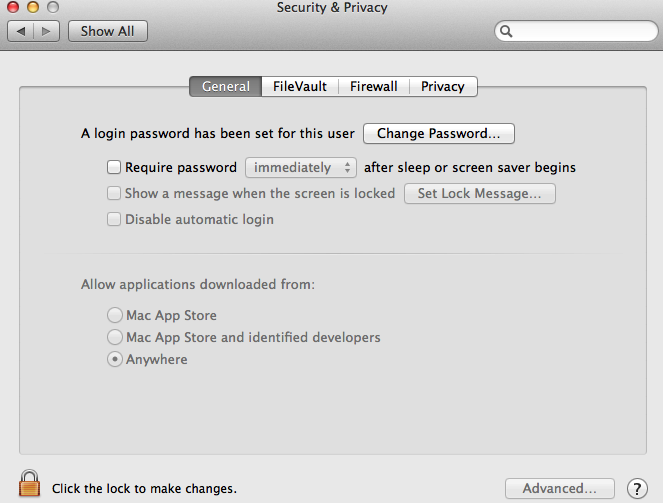
\includegraphics{24.png}
\caption{Adjusting Mac OS X security settings to allow cmake installation.}\label{install:install-f2}\end{figure}

Alternatively, you can mount the cmake .dmg image file you downloaded, right
-click (or
control-click) the cmake .pkg package file and click ``Open.'' Mac OS X will ask
you if you
are sure you want to install this package, and you can click ``Open'' to start the
installer.


\subsection{Create LLVM.xcodeproj by cmake Graphic UI}
\label{install:create-llvm-xcodeproj-by-cmake-graphic-ui}
We install llvm source code with clang on directory
/Users/Jonathan/llvm/release/ in last section.
Now, will generate the LLVM.xcodeproj in this chapter.

Currently, we cannot do debug by lldb with cmake graphic UI operations depicted
in this section, but we can do debug by lldb with ``section Create LLVM.xcodeproj
of supporting cpu0 by terminal cmake command'' \footnote{
\href{http://jonathan2251.github.com/lbd/install.html\#create-llvm-xcodeproj-of-supporting-cpu0-by-terminal-cmake-command}{http://jonathan2251.github.com/lbd/install.html\#create-llvm-xcodeproj-of-supporting-cpu0-by-terminal-cmake-command}
}.
Even with that, let's build LLVM project with cmake graphic UI since this LLVM
directory contains the release version for clang and clang++ execution file.
First, create LLVM.xcodeproj as
\hyperref[install:install-f3]{Figure  \ref*{install:install-f3}}, then click \textbf{configure} button to enter
\hyperref[install:install-f4]{Figure  \ref*{install:install-f4}},
and then click \textbf{Done} button to get \hyperref[install:install-f5]{Figure  \ref*{install:install-f5}}.
\begin{figure}[htbp]
\centering
\capstart

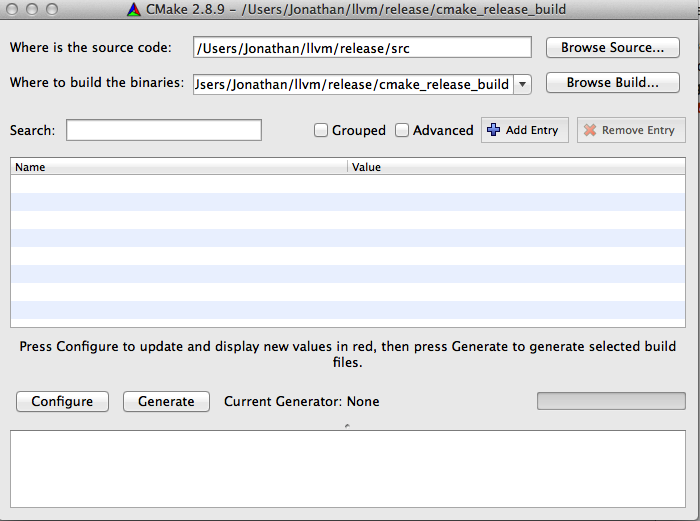
\includegraphics{33.png}
\caption{Start to create LLVM.xcodeproj by cmake}\label{install:install-f3}\end{figure}
\begin{figure}[htbp]
\centering
\capstart

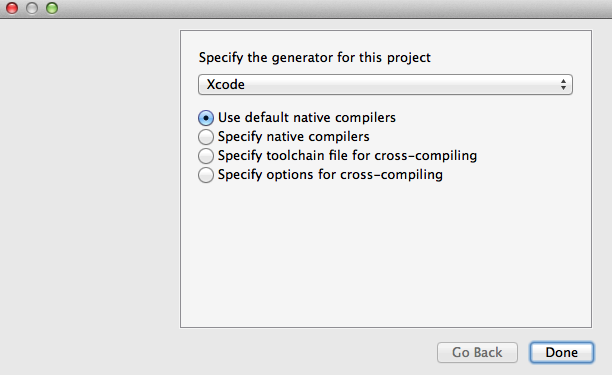
\includegraphics{43.png}
\caption{Create LLVM.xcodeproj by cmake – Set option to generate Xcode project}\label{install:install-f4}\end{figure}
\begin{figure}[htbp]
\centering
\capstart

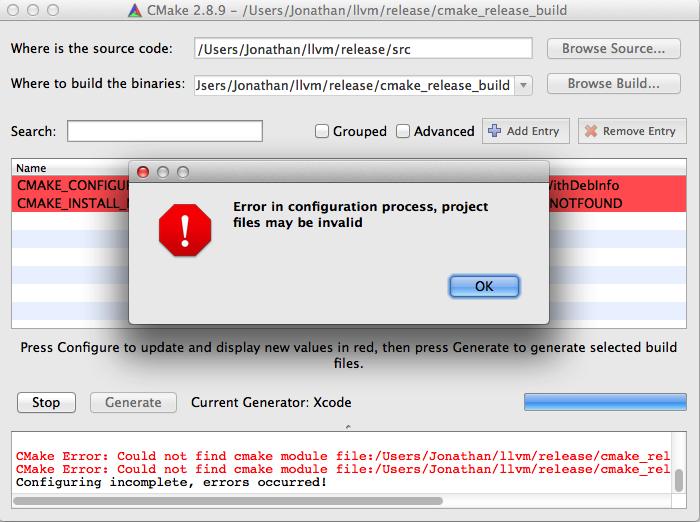
\includegraphics{53.png}
\caption{Create LLVM.xcodeproj by cmake – Before Adjust CMAKE\_INSTALL\_NAME\_TOOL}\label{install:install-f5}\end{figure}

Click OK from \hyperref[install:install-f5]{Figure  \ref*{install:install-f5}} and select Cmake 2.8-9.app for
CMAKE\_INSTALL\_NAME\_TOOL by click the right side button \textbf{“...”} of that row
to get
\hyperref[install:install-f6]{Figure  \ref*{install:install-f6}}.
\begin{figure}[htbp]
\centering
\capstart

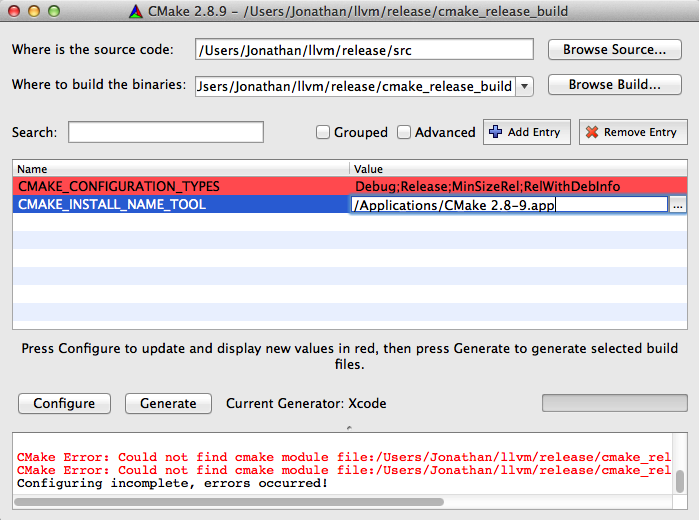
\includegraphics{63.png}
\caption{Select Cmake 2.8-9.app}\label{install:install-f6}\end{figure}

Click Configure button to get \hyperref[install:install-f7]{Figure  \ref*{install:install-f7}}.
\begin{figure}[htbp]
\centering
\capstart

\includegraphics{72.png}
\caption{Click cmake Configure button first time}\label{install:install-f7}\end{figure}

Check CLANG\_BUILD\_EXAMPLES, LLVM\_BUILD\_EXAMPLES, and uncheck LLVM\_ENABLE\_PIC as
\hyperref[install:install-f8]{Figure  \ref*{install:install-f8}}.
\begin{figure}[htbp]
\centering
\capstart

\includegraphics{82.png}
\caption{Check CLANG\_BUILD\_EXAMPLES, LLVM\_BUILD\_EXAMPLES, and uncheck
LLVM\_ENABLE\_PIC in cmake}\label{install:install-f8}\end{figure}

Click Configure button again. If the output result message has no red color,
then click Generate button to get \hyperref[install:install-f9]{Figure  \ref*{install:install-f9}}.
\begin{figure}[htbp]
\centering
\capstart

\includegraphics{92.png}
\caption{Click cmake Generate button second time}\label{install:install-f9}\end{figure}


\subsection{Build llvm by Xcode}
\label{install:build-llvm-by-xcode}
Now, LLVM.xcodeproj is created. Open the cmake\_debug\_build/LLVM.xcodeproj by
Xcode and click menu \textbf{“Product – Build”} as \hyperref[install:install-f10]{Figure  \ref*{install:install-f10}}.
\begin{figure}[htbp]
\centering
\capstart

\includegraphics{102.png}
\caption{Click Build button to build LLVM.xcodeproj by Xcode}\label{install:install-f10}\end{figure}

After few minutes of build, the clang, llc, llvm-as, ..., can be found in
cmake\_release\_build/bin/Debug/ as follows.

\begin{Verbatim}[commandchars=\\\{\}]
118-165-78-111:cmake\_release\_build Jonathan\$ cd bin/Debug/
118-165-78-111:Debug Jonathan\$ pwd
/Users/Jonathan/llvm/release/cmake\_release\_build/bin/Debug
118-165-78-111:Debug Jonathan\$ ls
BrainF            Kaleidoscope-Ch7  clang-tblgen    llvm-dis        llvm-rtdyld
ExceptionDemo     ModuleMaker       count           llvm-dwarfdump  llvm-size
Fibonacci         ParallelJIT       diagtool        llvm-extract    llvm-stress
FileCheck         arcmt-test        llc             llvm-link       llvm-tblgen
FileUpdate        bugpoint          lli             llvm-mc         macho-dump
HowToUseJIT       c-arcmt-test      llvm-ar         llvm-mcmarkup   not
Kaleidoscope-Ch2  c-index-test      llvm-as         llvm-nm         obj2yaml
Kaleidoscope-Ch3  clang             llvm-bcanalyzer llvm-objdump    opt
Kaleidoscope-Ch4  clang++           llvm-config     llvm-prof       yaml-bench
Kaleidoscope-Ch5  clang-check       llvm-cov        llvm-ranlib     yaml2obj
Kaleidoscope-Ch6  clang-interpreter llvm-diff       llvm-readobj
118-165-78-111:Debug Jonathan\$
\end{Verbatim}

To access those execution files, edit .profile (if you .profile not exists,
please create file .profile), save .profile to /Users/Jonathan/, and enable
\$PATH by command \code{source .profile} as follows.
Please add path /Applications//Xcode.app/Contents/Developer/usr/bin to .profile
if you didn't add it after Xcode download.

\begin{Verbatim}[commandchars=\\\{\}]
118-165-65-128:\textasciitilde{} Jonathan\$ pwd
/Users/Jonathan
118-165-65-128:\textasciitilde{} Jonathan\$ cat .profile
export PATH=\$PATH:/Applications/Xcode.app/Contents/Developer/usr/bin:/Applicatio
ns/Xcode.app/Contents/Developer/Toolchains/XcodeDefault.xctoolchain/usr/bin/:/Ap
plications/Graphviz.app/Contents/MacOS/:/Users/Jonathan/llvm/release/cmake\_relea
se\_build/bin/Debug
export WORKON\_HOME=\$HOME/.virtualenvs
source /usr/local/bin/virtualenvwrapper.sh \# where Homebrew places it
export VIRTUALENVWRAPPER\_VIRTUALENV\_ARGS='--no-site-packages' \# optional
118-165-65-128:\textasciitilde{} Jonathan\$
\end{Verbatim}


\subsection{Create LLVM.xcodeproj of supporting cpu0 by terminal cmake command}
\label{install:create-llvm-xcodeproj-of-supporting-cpu0-by-terminal-cmake-command}
We have installed llvm with clang on directory llvm/release/.
Now, we want to install llvm with our cpu0 backend code on directory
llvm/test/ in this section.

In ``section Create LLVM.xcodeproj by cmake Graphic UI'' \footnote{
\href{http://jonathan2251.github.com/lbd/install.html\#create-llvm-xcodeproj-by-cmake-graphic-ui}{http://jonathan2251.github.com/lbd/install.html\#create-llvm-xcodeproj-by-cmake-graphic-ui}
}, we create
LLVM.xcodeproj by cmake graphic UI.
We can create LLVM.xcodeproj by \code{cmake} command on terminal also.
This book is on the process of merging into llvm trunk but not finished
yet.
The merged llvm trunk version on lbd git hub is LLVM 3.3 released version.
The lbd of Cpu0 example code is also based on llvm 3.3.
So, please install the llvm 3.3 debug version as the llvm release 3.3
installation, but without clang since the clang will waste time in build the
Cpu0 backend tutorial code.
Steps as follows,

The details of installing Cpu0 backend example code as follows,

\begin{Verbatim}[commandchars=\\\{\}]
118-165-78-111:llvm Jonathan\$ mkdir test
118-165-78-111:llvm Jonathan\$ cd test
118-165-78-111:test Jonathan\$ pwd
/Users/Jonathan/llvm/test
118-165-78-111:test Jonathan\$ cp /Users/Jonathan/Downloads/llvm-3.3.src.tar.gz .
118-165-78-111:test Jonathan\$ tar -zxvf llvm-3.3.src.tar.gz
118-165-78-111:test Jonathan\$ mv llvm-3.3.src src
118-165-78-111:test Jonathan\$ cp /Users/Jonathan/Downloads/
lbdex.tar.gz .
118-165-78-111:test Jonathan\$ tar -zxvf lbdex.tar.gz
118-165-78-111:test Jonathan\$ mkdir src/lib/Target/Cpu0
118-165-78-111:test Jonathan\$ mv lbdex
src/lib/Target/Cpu0/.
118-165-78-111:test Jonathan\$ cp -rf src/lib/Target/Cpu0/
lbdex/src\_files\_modify/modify/src/* src/.
118-165-78-111:test Jonathan\$ grep -R "Cpu0" src/include
...
src/include/llvm/MC/MCExpr.h:    VK\_Cpu0\_GPREL,
src/include/llvm/MC/MCExpr.h:    VK\_Cpu0\_GOT\_CALL,
src/include/llvm/MC/MCExpr.h:    VK\_Cpu0\_GOT16,
src/include/llvm/MC/MCExpr.h:    VK\_Cpu0\_GOT,
src/include/llvm/MC/MCExpr.h:    VK\_Cpu0\_ABS\_HI,
src/include/llvm/MC/MCExpr.h:    VK\_Cpu0\_ABS\_LO,
...
src/lib/MC/MCExpr.cpp:  case VK\_Cpu0\_GOT\_PAGE: return "GOT\_PAGE";
src/lib/MC/MCExpr.cpp:  case VK\_Cpu0\_GOT\_OFST: return "GOT\_OFST";
src/lib/Target/LLVMBuild.txt:subdirectories = ARM CellSPU CppBackend Hexagon
MBlaze MSP430 NVPTX Mips Cpu0 PowerPC Sparc X86 XCore
118-165-78-111:test Jonathan\$
\end{Verbatim}

Next, please copy Cpu0 chapter 2 example code according the following commands,

\begin{Verbatim}[commandchars=\\\{\}]
118-165-80-55:test Jonathan\$ cd src/lib/Target/Cpu0/lbdex/
118-165-80-55:lbdex Jonathan\$ pwd
/Users/Jonathan/llvm/test/src/lib/Target/Cpu0/lbdex
118-165-80-55:lbdex Jonathan\$ sh removecpu0.sh
118-165-80-55:lbdex Jonathan\$ ls ..
lbdex
118-165-80-55:lbdex Jonathan\$ cp -rf Chapter2/* ../.
118-165-80-55:lbdex Jonathan\$ cd ..
118-165-80-55:Cpu0 Jonathan\$ ls
CMakeLists.txt                Cpu0InstrInfo.td        Cpu0TargetMachine.cpp   TargetInfo
Cpu0.h                        Cpu0RegisterInfo.td     ExampleCode             readme
Cpu0.td                       Cpu0Schedule.td         LLVMBuild.txt
Cpu0InstrFormats.td   Cpu0Subtarget.h         MCTargetDesc
118-165-80-55:Cpu0 Jonathan\$
\end{Verbatim}

Now, it's ready for building llvm/test/src code by command
\code{cmake -DCMAKE\_CXX\_COMPILER=clang++ -DCMAKE\_C\_COMPILER=clang -DCMAKE\_BUILD\_TYPE
=Debug -G "Xcode" ../src/} as follows.
Remind, currently, the \code{cmake} terminal command can work with lldb debug, but
the ``section Create LLVM.xcodeproj by cmake Graphic UI'' \footnotemark[5] cannot.

\begin{Verbatim}[commandchars=\\\{\}]
118-165-78-111:Target Jonathan\$ cd ../../../../
118-165-78-111:test Jonathan\$ pwd
/Users/Jonathan/llvm/test
118-165-78-111:test Jonathan\$ ls
src
118-165-78-111:test Jonathan\$ mkdir cmake\_debug\_build
118-165-78-111:test Jonathan\$ cd cmake\_debug\_build
118-165-78-111:cmake\_debug\_build Jonathan\$ cmake -DCMAKE\_CXX\_COMPILER=clang++
-DCMAKE\_C\_COMPILER=clang -DCMAKE\_BUILD\_TYPE=Debug -G "Xcode" ../src/
CMake Error: The source directory "/Users/Jonathan/llvm/src" does not exist.
Specify --help for usage, or press the help button on the CMake GUI.
118-165-78-111:test Jonathan\$ cd cmake\_debug\_build/
118-165-78-111:cmake\_debug\_build Jonathan\$ cmake -DCMAKE\_CXX\_COMPILER=clang++
-DCMAKE\_C\_COMPILER=clang -DCMAKE\_BUILD\_TYPE=Debug -G "Xcode" ../src/
-- The C compiler identification is Clang 4.1.0
-- The CXX compiler identification is Clang 4.1.0
-- Check for working C compiler using: Xcode
...
-- Targeting ARM
-- Targeting CellSPU
-- Targeting CppBackend
-- Targeting Hexagon
-- Targeting Mips
-- Targeting Cpu0
-- Targeting MBlaze
-- Targeting MSP430
-- Targeting NVPTX
-- Targeting PowerPC
-- Targeting Sparc
-- Targeting X86
-- Targeting XCore
-- Performing Test SUPPORTS\_GLINE\_TABLES\_ONLY\_FLAG
-- Performing Test SUPPORTS\_GLINE\_TABLES\_ONLY\_FLAG - Success
-- Performing Test SUPPORTS\_NO\_C99\_EXTENSIONS\_FLAG
-- Performing Test SUPPORTS\_NO\_C99\_EXTENSIONS\_FLAG - Success
-- Configuring done
-- Generating done
-- Build files have been written to: /Users/Jonathan/llvm/test/cmake\_debug\_build
118-165-78-111:cmake\_debug\_build Jonathan\$
\end{Verbatim}

Now, you can build this llvm build with Cpu0 example code by Xcode as the last
section indicated.

Since Xcode use clang compiler and lldb instead of gcc and gdb, we can run lldb
debug as follows,

\begin{Verbatim}[commandchars=\\\{\}]
118-165-65-128:InputFiles Jonathan\$ pwd
/Users/Jonathan/lbdex/InputFiles
118-165-65-128:InputFiles Jonathan\$ clang -c ch3.cpp -emit-llvm -o ch3.bc
118-165-65-128:InputFiles Jonathan\$ /Users/Jonathan/llvm/test/
cmake\_debug\_build/bin/Debug/llc -march=mips -relocation-model=pic -filetype=asm
ch3.bc -o ch3.mips.s
118-165-65-128:InputFiles Jonathan\$ lldb -- /Users/Jonathan/llvm/test/
cmake\_debug\_build/bin/Debug/llc -march=mips -relocation-model=pic -filetype=
asm ch3.bc -o ch3.mips.s
Current executable set to '/Users/Jonathan/llvm/test/cmake\_debug\_build/bin/
Debug/llc' (x86\_64).
(lldb) b MipsTargetInfo.cpp:19
breakpoint set --file 'MipsTargetInfo.cpp' --line 19
Breakpoint created: 1: file ='MipsTargetInfo.cpp', line = 19, locations = 1
(lldb) run
Process 6058 launched: '/Users/Jonathan/llvm/test/cmake\_debug\_build/bin/Debug/
llc' (x86\_64)
Process 6058 stopped
* thread \#1: tid = 0x1c03, 0x000000010077f231 llc{}`LLVMInitializeMipsTargetInfo
+ 33 at MipsTargetInfo.cpp:20, stop reason = breakpoint 1.1
  frame \#0: 0x000000010077f231 llc{}`LLVMInitializeMipsTargetInfo + 33 at
  MipsTargetInfo.cpp:20
   17
   18   extern "C" void LLVMInitializeMipsTargetInfo() \PYGZob{}
   19     RegisterTarget\textless{}Triple::mips,
-\textgreater{} 20           /*HasJIT=*/true\textgreater{} X(TheMipsTarget, "mips", "Mips");
   21
   22     RegisterTarget\textless{}Triple::mipsel,
   23           /*HasJIT=*/true\textgreater{} Y(TheMipselTarget, "mipsel", "Mipsel");
(lldb) n
Process 6058 stopped
* thread \#1: tid = 0x1c03, 0x000000010077f24f llc{}`LLVMInitializeMipsTargetInfo
+ 63 at MipsTargetInfo.cpp:23, stop reason = step over
  frame \#0: 0x000000010077f24f llc{}`LLVMInitializeMipsTargetInfo + 63 at
  MipsTargetInfo.cpp:23
   20           /*HasJIT=*/true\textgreater{} X(TheMipsTarget, "mips", "Mips");
   21
   22     RegisterTarget\textless{}Triple::mipsel,
-\textgreater{} 23           /*HasJIT=*/true\textgreater{} Y(TheMipselTarget, "mipsel", "Mipsel");
   24
   25     RegisterTarget\textless{}Triple::mips64,
   26           /*HasJIT=*/false\textgreater{} A(TheMips64Target, "mips64", "Mips64
   [experimental]");
(lldb) print X
(llvm::RegisterTarget\textless{}llvm::Triple::ArchType, true\textgreater{}) \$0 = \PYGZob{}\PYGZcb{}
(lldb) quit
118-165-65-128:InputFiles Jonathan\$
\end{Verbatim}

About the lldb debug command, please reference \footnote{
\href{http://lldb.llvm.org/lldb-gdb.html}{http://lldb.llvm.org/lldb-gdb.html}
} or lldb portal \footnote{
\href{http://lldb.llvm.org/}{http://lldb.llvm.org/}
}.


\subsection{Setup llvm-lit on iMac}
\label{install:setup-llvm-lit-on-imac}
The llvm-lit \footnote{
\href{http://llvm.org/docs/TestingGuide.html}{http://llvm.org/docs/TestingGuide.html}
} is the llvm regression test tool. You don't need to set up it
if you don't want to do regression test even though this book do the regression
test.
To set it up correctly in iMac, you need move it from directory bin/llvm-lit to
bin/Debug/llvm-lit, and modify llvm-lit as follows,

\begin{Verbatim}[commandchars=\\\{\}]
118-165-69-59:bin Jonathan\PYG{n+nv}{\PYGZdl{} }\PYG{n+nb}{pwd}
/Users/Jonathan/llvm/test/cmake\PYGZus{}debug\PYGZus{}build/bin
118-165-69-59:bin Jonathan\PYG{n+nv}{\PYGZdl{} }ls
Debug         llvm-lit
118-165-69-59:bin Jonathan\PYG{n+nv}{\PYGZdl{} }cp llvm-lit Debug/.
// edit llvm-lit as follows,
    \PYG{l+s+s1}{'build\PYGZus{}config'} : \PYG{l+s+s2}{":"},
    \PYG{l+s+s1}{'build\PYGZus{}mode'} : \PYG{l+s+s2}{"Debug"},
\end{Verbatim}


\subsection{Install Icarus Verilog tool on iMac}
\label{install:install-icarus-verilog-tool-on-imac}
Install Icarus Verilog tool by command \code{brew install icarus-verilog} as follows,

\begin{Verbatim}[commandchars=\\\{\}]
JonathantekiiMac:\PYGZti{} Jonathan\PYG{n+nv}{\PYGZdl{} }brew install icarus-verilog
\PYG{o}{=}\PYG{o}{=}\PYGZgt{} Downloading ftp://icarus.com/pub/eda/verilog/v0.9/verilog-0.9.5.tar.gz
\PYG{c}{\PYGZsh{}\PYGZsh{}\PYGZsh{}\PYGZsh{}\PYGZsh{}\PYGZsh{}\PYGZsh{}\PYGZsh{}\PYGZsh{}\PYGZsh{}\PYGZsh{}\PYGZsh{}\PYGZsh{}\PYGZsh{}\PYGZsh{}\PYGZsh{}\PYGZsh{}\PYGZsh{}\PYGZsh{}\PYGZsh{}\PYGZsh{}\PYGZsh{}\PYGZsh{}\PYGZsh{}\PYGZsh{}\PYGZsh{}\PYGZsh{}\PYGZsh{}\PYGZsh{}\PYGZsh{}\PYGZsh{}\PYGZsh{}\PYGZsh{}\PYGZsh{}\PYGZsh{}\PYGZsh{}\PYGZsh{}\PYGZsh{}\PYGZsh{}\PYGZsh{}\PYGZsh{}\PYGZsh{}\PYGZsh{}\PYGZsh{}\PYGZsh{}\PYGZsh{}\PYGZsh{}\PYGZsh{}\PYGZsh{}\PYGZsh{}\PYGZsh{}\PYGZsh{}\PYGZsh{}\PYGZsh{}\PYGZsh{}\PYGZsh{}\PYGZsh{}\PYGZsh{}\PYGZsh{}\PYGZsh{}\PYGZsh{}\PYGZsh{}\PYGZsh{}\PYGZsh{}\PYGZsh{}\PYGZsh{}\PYGZsh{}\PYGZsh{}\PYGZsh{}\PYGZsh{}\PYGZsh{}\PYGZsh{} 100.0\PYGZpc{}}
\PYG{c}{\PYGZsh{}\PYGZsh{}\PYGZsh{}\PYGZsh{}\PYGZsh{}\PYGZsh{}\PYGZsh{}\PYGZsh{}\PYGZsh{}\PYGZsh{}\PYGZsh{}\PYGZsh{}\PYGZsh{}\PYGZsh{}\PYGZsh{}\PYGZsh{}\PYGZsh{}\PYGZsh{}\PYGZsh{}\PYGZsh{}\PYGZsh{}\PYGZsh{}\PYGZsh{}\PYGZsh{}\PYGZsh{}\PYGZsh{}\PYGZsh{}\PYGZsh{}\PYGZsh{}\PYGZsh{}\PYGZsh{}\PYGZsh{}\PYGZsh{}\PYGZsh{}\PYGZsh{}\PYGZsh{}\PYGZsh{}\PYGZsh{}\PYGZsh{}\PYGZsh{}\PYGZsh{}\PYGZsh{}\PYGZsh{}\PYGZsh{}\PYGZsh{}\PYGZsh{}\PYGZsh{}\PYGZsh{}\PYGZsh{}\PYGZsh{}\PYGZsh{}\PYGZsh{}\PYGZsh{}\PYGZsh{}\PYGZsh{}\PYGZsh{}\PYGZsh{}\PYGZsh{}\PYGZsh{}\PYGZsh{}\PYGZsh{}\PYGZsh{}\PYGZsh{}\PYGZsh{}\PYGZsh{}\PYGZsh{}\PYGZsh{}\PYGZsh{}\PYGZsh{}\PYGZsh{}\PYGZsh{}\PYGZsh{} 100.0\PYGZpc{}}
\PYG{o}{=}\PYG{o}{=}\PYGZgt{} ./configure --prefix\PYG{o}{=}/usr/local/Cellar/icarus-verilog/0.9.5
\PYG{o}{=}\PYG{o}{=}\PYGZgt{} \PYG{n+nv}{make}
\PYG{o}{=}\PYG{o}{=}\PYGZgt{} make \PYG{n+nv}{installdirs}
\PYG{o}{=}\PYG{o}{=}\PYGZgt{} make install
/usr/local/Cellar/icarus-verilog/0.9.5: 39 files, 12M, built in 55 seconds
\end{Verbatim}


\subsection{Install other tools on iMac}
\label{install:install-other-tools-on-imac}
These tools mentioned in this section is for coding and debug.
You can work even without these tools.
Files compare tools Kdiff3 came from web site \footnote{
\href{http://kdiff3.sourceforge.net}{http://kdiff3.sourceforge.net}
}.
FileMerge is a part of Xcode, you can type FileMerge in Finder – Applications
as \hyperref[install:install-f11]{Figure  \ref*{install:install-f11}} and drag it into the Dock as
\hyperref[install:install-f12]{Figure  \ref*{install:install-f12}}.
\begin{figure}[htbp]
\centering
\capstart

\includegraphics{111.png}
\caption{Type FileMerge in Finder – Applications}\label{install:install-f11}\end{figure}
\begin{figure}[htbp]
\centering
\capstart

\includegraphics{121.png}
\caption{Drag FileMege into the Dock}\label{install:install-f12}\end{figure}

Download tool Graphviz for display llvm IR nodes in debugging,
\footnote{
\href{http://www.graphviz.org/Download\_macos.php}{http://www.graphviz.org/Download\_macos.php}
}.
We choose mountainlion as \hyperref[install:install-f13]{Figure  \ref*{install:install-f13}} since our iMac is Mountain
Lion.
\begin{figure}[htbp]
\centering
\capstart

\scalebox{0.800000}{\includegraphics{131.png}}
\caption{Download graphviz for llvm IR node display}\label{install:install-f13}\end{figure}

After install Graphviz, please set the path to .profile.
For example, we install the Graphviz in directory
/Applications/Graphviz.app/Contents/MacOS/, so add this path to
/User/Jonathan/.profile as follows,

\begin{Verbatim}[commandchars=\\\{\}]
118-165-12-177:InputFiles Jonathan\PYG{n+nv}{\PYGZdl{} }cat /Users/Jonathan/.profile
\PYG{n+nb}{export }\PYG{n+nv}{PATH}\PYG{o}{=}\PYG{n+nv}{\PYGZdl{}PATH}:/Applications/Xcode.app/Contents/Developer/usr/bin:
/Applications/Graphviz.app/Contents/MacOS/:/Users/Jonathan/llvm/release/
cmake\PYGZus{}release\PYGZus{}build/bin/Debug
\end{Verbatim}

The Graphviz information for llvm is in
the section ``SelectionDAG Instruction Selection Process'' of
\footnote{
\href{http://llvm.org/docs/CodeGenerator.html}{http://llvm.org/docs/CodeGenerator.html}
} and
the section ``Viewing graphs while debugging code'' of
\footnote{
\href{http://llvm.org/docs/ProgrammersManual.html}{http://llvm.org/docs/ProgrammersManual.html}
}.
TextWrangler is for edit file with line number display and dump binary file
like the obj file, *.o, that will be generated in chapter of Generating object
files if you havn't gobjdump available.
You can download from App Store.
To dump binary file, first, open the binary file, next, select menu
\textbf{“File – Hex Front Document”} as \hyperref[install:install-f14]{Figure  \ref*{install:install-f14}}.
Then select \textbf{“Front document's file”} as \hyperref[install:install-f15]{Figure  \ref*{install:install-f15}}.
\begin{figure}[htbp]
\centering
\capstart

\includegraphics{141.png}
\caption{Select Hex Dump menu}\label{install:install-f14}\end{figure}
\begin{figure}[htbp]
\centering
\capstart

\includegraphics{15.png}
\caption{Select Front document's file in TextWrangler}\label{install:install-f15}\end{figure}

Install binutils by command \code{brew install binutils} as follows,

\begin{Verbatim}[commandchars=\\\{\}]
118-165-77-214:\PYGZti{} Jonathan\PYG{n+nv}{\PYGZdl{} }brew install \PYG{n+nv}{binutils}
\PYG{o}{=}\PYG{o}{=}\PYGZgt{} Downloading http://ftpmirror.gnu.org/binutils/binutils-2.22.tar.gz
\PYG{c}{\PYGZsh{}\PYGZsh{}\PYGZsh{}\PYGZsh{}\PYGZsh{}\PYGZsh{}\PYGZsh{}\PYGZsh{}\PYGZsh{}\PYGZsh{}\PYGZsh{}\PYGZsh{}\PYGZsh{}\PYGZsh{}\PYGZsh{}\PYGZsh{}\PYGZsh{}\PYGZsh{}\PYGZsh{}\PYGZsh{}\PYGZsh{}\PYGZsh{}\PYGZsh{}\PYGZsh{}\PYGZsh{}\PYGZsh{}\PYGZsh{}\PYGZsh{}\PYGZsh{}\PYGZsh{}\PYGZsh{}\PYGZsh{}\PYGZsh{}\PYGZsh{}\PYGZsh{}\PYGZsh{}\PYGZsh{}\PYGZsh{}\PYGZsh{}\PYGZsh{}\PYGZsh{}\PYGZsh{}\PYGZsh{}\PYGZsh{}\PYGZsh{}\PYGZsh{}\PYGZsh{}\PYGZsh{}\PYGZsh{}\PYGZsh{}\PYGZsh{}\PYGZsh{}\PYGZsh{}\PYGZsh{}\PYGZsh{}\PYGZsh{}\PYGZsh{}\PYGZsh{}\PYGZsh{}\PYGZsh{}\PYGZsh{}\PYGZsh{}\PYGZsh{}\PYGZsh{}\PYGZsh{}\PYGZsh{}\PYGZsh{}\PYGZsh{}\PYGZsh{}\PYGZsh{}\PYGZsh{}\PYGZsh{} 100.0\PYGZpc{}}
\PYG{o}{=}\PYG{o}{=}\PYGZgt{} ./configure --program-prefix\PYG{o}{=}g --prefix\PYG{o}{=}/usr/local/Cellar/binutils/2.22
--infodir\PYG{o}{=}/usr/loca
\PYG{o}{=}\PYG{o}{=}\PYGZgt{} \PYG{n+nv}{make}
\PYG{o}{=}\PYG{o}{=}\PYGZgt{} make install
/usr/local/Cellar/binutils/2.22: 90 files, 19M, built in 4.7 minutes
118-165-77-214:\PYGZti{} Jonathan\PYG{n+nv}{\PYGZdl{} }ls /usr/local/Cellar/binutils/2.22
COPYING     README      lib
ChangeLog     bin       share
INSTALL\PYGZus{}RECEIPT.json    include       x86\PYGZus{}64-apple-darwin12.2.0
118-165-77-214:binutils-2.23 Jonathan\PYG{n+nv}{\PYGZdl{} }ls /usr/local/Cellar/binutils/2.22/bin
gaddr2line  gc++filt  gnm   gobjdump  greadelf  gstrings
gar   gelfedit  gobjcopy  granlib gsize   gstrip
\end{Verbatim}


\section{Setting Up Your Linux Machine}
\label{install:setting-up-your-linux-machine}

\subsection{Install LLVM 3.3 release build on Linux}
\label{install:install-llvm-3-3-release-build-on-linux}
First, install the llvm release build by,
\begin{enumerate}
\item {} 
Untar llvm source, rename llvm source with src.

\item {} 
Untar clang and move it src/tools/clang.

\item {} 
Untar compiler-rt and move it to src/project/compiler-rt.

\end{enumerate}

Next, build with cmake command, \code{cmake -DCMAKE\_BUILD\_TYPE=Release -DCLANG\_BUILD
\_EXAMPLES=ON -DLLVM\_BUILD\_EXAMPLES=ON -G "Unix Makefiles" ../src/}, as follows.

\begin{Verbatim}[commandchars=\\\{\}]
\PYG{o}{[}Gamma@localhost cmake\PYGZus{}release\PYGZus{}build\PYG{o}{]}\PYG{n+nv}{\PYGZdl{} }cmake -DCMAKE\PYGZus{}BUILD\PYGZus{}TYPE\PYG{o}{=}Release
-DCLANG\PYGZus{}BUILD\PYGZus{}EXAMPLES\PYG{o}{=}ON -DLLVM\PYGZus{}BUILD\PYGZus{}EXAMPLES\PYG{o}{=}ON -G \PYG{l+s+s2}{"Unix Makefiles"} ../src/
-- The C compiler identification is GNU 4.7.0
...
-- Constructing LLVMBuild project information
-- Targeting ARM
-- Targeting CellSPU
-- Targeting CppBackend
-- Targeting Hexagon
-- Targeting Mips
-- Targeting MBlaze
-- Targeting MSP430
-- Targeting PowerPC
-- Targeting PTX
-- Targeting Sparc
-- Targeting X86
-- Targeting XCore
-- Clang version: 3.3
-- Found Subversion: /usr/bin/svn \PYG{o}{(}found version \PYG{l+s+s2}{"1.7.6"}\PYG{o}{)}
-- Configuring \PYG{k}{done}
-- Generating \PYG{k}{done}
-- Build files have been written to: /usr/local/llvm/release/cmake\PYGZus{}release\PYGZus{}build
\end{Verbatim}

After cmake, run command \code{make}, then you can get clang, llc, llvm-as, ...,
in cmake\_release\_build/bin/ after a few tens minutes of build. Next, edit
/home/Gamma/.bash\_profile with adding /usr/local/llvm/release/cmake\_release\_build/
bin to PATH
to enable the clang, llc, ..., command search path, as follows,

\begin{Verbatim}[commandchars=\\\{\}]
\PYG{o}{[}Gamma@localhost \PYGZti{}\PYG{o}{]}\PYG{n+nv}{\PYGZdl{} }\PYG{n+nb}{pwd}
/home/Gamma
\PYG{o}{[}Gamma@localhost \PYGZti{}\PYG{o}{]}\PYG{n+nv}{\PYGZdl{} }cat .bash\PYGZus{}profile
\PYG{c}{\PYGZsh{} .bash\PYGZus{}profile}

\PYG{c}{\PYGZsh{} Get the aliases and functions}
\PYG{k}{if} \PYG{o}{[} -f \PYGZti{}/.bashrc \PYG{o}{]}; \PYG{k}{then}
  . \PYGZti{}/.bashrc
\PYG{k}{fi}

\PYG{c}{\PYGZsh{} User specific environment and startup programs}

\PYG{n+nv}{PATH}\PYG{o}{=}\PYG{n+nv}{\PYGZdl{}PATH}:/usr/local/sphinx/bin:/usr/local/llvm/release/cmake\PYGZus{}release\PYGZus{}build/bin:
/opt/mips\PYGZus{}linux\PYGZus{}toolchain\PYGZus{}clang/mips\PYGZus{}linux\PYGZus{}toolchain/bin:\PYG{n+nv}{\PYGZdl{}HOME}/.local/bin:
\PYG{n+nv}{\PYGZdl{}HOME}/bin

\PYG{n+nb}{export }PATH
\PYG{o}{[}Gamma@localhost \PYGZti{}\PYG{o}{]}\PYG{n+nv}{\PYGZdl{} }\PYG{n+nb}{source} .bash\PYGZus{}profile
\PYG{o}{[}Gamma@localhost \PYGZti{}\PYG{o}{]}\PYG{n+nv}{\PYGZdl{} }\PYG{n+nv}{\PYGZdl{}PATH}
bash: /usr/lib64/qt-3.3/bin:/usr/local/bin:/usr/bin:/bin:/usr/local/sbin:
/usr/sbin:/usr/local/sphinx/bin:/opt/mips\PYGZus{}linux\PYGZus{}toolchain\PYGZus{}clang/mips\PYGZus{}linux\PYGZus{}tool
chain/bin:/home/Gamma/.local/bin:/home/Gamma/bin:/usr/local/sphinx/bin:/usr/
\PYG{n+nb}{local}/llvm/release/cmake\PYGZus{}release\PYGZus{}build/bin
\end{Verbatim}


\subsection{Install cpu0 debug build on Linux}
\label{install:install-cpu0-debug-build-on-linux}
This book is on the process of merging into llvm trunk but not finished
yet.
The merged llvm trunk version on lbd git hub is LLVM 3.3 released version.
The Cpu0 example code is also based on llvm 3.3.
So, please install the llvm 3.3 debug version as the llvm release 3.3
installation, but without clang since the clang will waste time in build the
Cpu0 backend tutorial code.
Steps as follows,

The details of installing Cpu0 backend example code according the following
list steps, and the corresponding commands shown as below,

1) Enter /usr/local/llvm/test/ and
get Cpu0 example code as well as the llvm 3.3.
\begin{enumerate}
\setcounter{enumi}{1}
\item {} 
Make dir Cpu0 in src/lib/Target and download example code.

\end{enumerate}

3) Update my modified files to support cpu0 by command, \code{cp -rf /usr/local/llvm/
test/src/lib/Target/Cpu0/lbdex/}
\code{src\_files\_modify/modify/src .}.

4) Check step 3 is effective by command
\code{grep -R "Cpu0" . \textbar{} more{}`}. I add the Cpu0 backend support, so check with
grep.

5) Enter src/lib/Target/Cpu0/ and copy example code
lbdex/2/Cpu0 to the directory by commands
\code{cd src/lib/Target/Cpu0/} and
\code{cp -rf lbdex/Chapter2/* ../.}.

6) Remove clang from /usr/local/llvm/test/src/tools/clang, and mkdir
test/cmake\_debug\_build. Without this you will waste extra time for
command \code{make} in cpu0 example code build.

\begin{Verbatim}[commandchars=\\\{\}]
\PYG{o}{[}Gamma@localhost llvm\PYG{o}{]}\PYG{n+nv}{\PYGZdl{} }mkdir \PYG{n+nb}{test}
\PYG{o}{[}Gamma@localhost llvm\PYG{o}{]}\PYG{n+nv}{\PYGZdl{} }\PYG{n+nb}{cd }\PYG{n+nb}{test}
\PYG{o}{[}Gamma@localhost \PYG{n+nb}{test}\PYG{o}{]}\PYG{n+nv}{\PYGZdl{} }\PYG{n+nb}{pwd}
/usr/local/llvm/test
\PYG{o}{[}Gamma@localhost \PYG{n+nb}{test}\PYG{o}{]}\PYG{n+nv}{\PYGZdl{} }cp /home/Gamma/Downloads/llvm-3.3.src.tar.gz .
\PYG{o}{[}Gamma@localhost \PYG{n+nb}{test}\PYG{o}{]}\PYG{n+nv}{\PYGZdl{} }tar -zxvf llvm-3.3.src.tar.gz
\PYG{o}{[}Gamma@localhost \PYG{n+nb}{test}\PYG{o}{]}\PYG{n+nv}{\PYGZdl{} }mv llvm-3.3.src src
\PYG{o}{[}Gamma@localhost \PYG{n+nb}{test}\PYG{o}{]}\PYG{n+nv}{\PYGZdl{} }cp /Users/Jonathan/Downloads/
lbdex.tar.gz .
\PYG{o}{[}Gamma@localhost \PYG{n+nb}{test}\PYG{o}{]}\PYG{n+nv}{\PYGZdl{} }tar -zxvf lbdex.tar.gz
...
\PYG{o}{[}Gamma@localhost \PYG{n+nb}{test}\PYG{o}{]}\PYG{n+nv}{\PYGZdl{} }mkdir src/lib/Target/Cpu0
118-165-78-111:test Jonathan\PYG{n+nv}{\PYGZdl{} }mv lbdex src/lib/Target/Cpu0/.
\PYG{o}{[}Gamma@localhost \PYG{n+nb}{test}\PYG{o}{]}\PYG{n+nv}{\PYGZdl{} }cp -rf lbdex/src\PYGZus{}files\PYGZus{}modify/
modify/src/* src/.
\PYG{o}{[}Gamma@localhost \PYG{n+nb}{test}\PYG{o}{]}\PYG{n+nv}{\PYGZdl{} }grep -R \PYG{l+s+s2}{"cpu0"} src/include
src/include//llvm/ADT/Triple.h:    cpu0,    // For Tutorial Backend Cpu0
src/include//llvm/MC/MCExpr.h:    VK\PYGZus{}Cpu0\PYGZus{}GPREL,
src/include//llvm/MC/MCExpr.h:    VK\PYGZus{}Cpu0\PYGZus{}GOT\PYGZus{}CALL,
...
\PYG{o}{[}Gamma@localhost \PYG{n+nb}{test}\PYG{o}{]}\PYG{n+nv}{\PYGZdl{} }\PYG{n+nb}{cd }src/lib/Target/Cpu0/lbdex/
\PYG{o}{[}Gamma@localhost lbdex\PYG{o}{]}\PYG{n+nv}{\PYGZdl{} }sh removecpu0.sh
\PYG{o}{[}Gamma@localhost lbdex\PYG{o}{]}\PYG{n+nv}{\PYGZdl{} }ls ../
lbdex
\PYG{o}{[}Gamma@localhost lbdex\PYG{o}{]}\PYG{n+nv}{\PYGZdl{} }cp -rf Chapter2/* ../.
\PYG{o}{[}Gamma@localhost lbdex\PYG{o}{]}\PYG{n+nv}{\PYGZdl{} }ls ..
CMakeLists.txt                Cpu0InstrInfo.td        Cpu0TargetMachine.cpp   TargetInfo
Cpu0.h                        Cpu0RegisterInfo.td     ExampleCode             readme
Cpu0.td                       Cpu0Schedule.td         LLVMBuild.txt
Cpu0InstrFormats.td   Cpu0Subtarget.h         MCTargetDesc
\PYG{o}{[}Gamma@localhost Cpu0\PYG{o}{]}\PYG{n+nv}{\PYGZdl{} }\PYG{n+nb}{cd} ../../../../..
\PYG{o}{[}Gamma@localhost \PYG{n+nb}{test}\PYG{o}{]}\PYG{n+nv}{\PYGZdl{} }\PYG{n+nb}{pwd}
/usr/local/llvm/test
\end{Verbatim}

Now, go into directory llvm/test/, create directory cmake\_debug\_build and
do cmake
like build the llvm/release, but we do Debug build and use clang as our compiler
instead,
as follows,

\begin{Verbatim}[commandchars=\\\{\}]
[Gamma@localhost test]\$ pwd
/usr/local/llvm/test
[Gamma@localhost test]\$ mkdir cmake\_debug\_build
[Gamma@localhost test]\$ cd cmake\_debug\_build/
[Gamma@localhost cmake\_debug\_build]\$ cmake
-DCMAKE\_CXX\_COMPILER=clang++ -DCMAKE\_C\_COMPILER=clang
-DCMAKE\_BUILD\_TYPE=Debug -G "Unix Makefiles" ../src/
-- The C compiler identification is Clang 3.3.0
-- The CXX compiler identification is Clang 3.3.0
-- Check for working C compiler: /usr/local/llvm/release/cmake\_release\_build/bin/
clang
-- Check for working C compiler: /usr/local/llvm/release/cmake\_release\_build/bin/
clang
 -- works
-- Detecting C compiler ABI info
-- Detecting C compiler ABI info - done
-- Check for working CXX compiler: /usr/local/llvm/release/cmake\_release\_build/
bin/clang++
-- Check for working CXX compiler: /usr/local/llvm/release/cmake\_release\_build/
bin/clang++
 -- works
-- Detecting CXX compiler ABI info
-- Detecting CXX compiler ABI info – done ...
-- Targeting Mips
-- Targeting Cpu0
-- Targeting MBlaze
-- Targeting MSP430
-- Targeting PowerPC
-- Targeting PTX
-- Targeting Sparc
-- Targeting X86
-- Targeting XCore
-- Configuring done
-- Generating done
-- Build files have been written to: /usr/local/llvm/test/cmake\_debug
\_build
[Gamma@localhost cmake\_debug\_build]\$
\end{Verbatim}

Then do make as follows,

\begin{Verbatim}[commandchars=\\\{\}]
[Gamma@localhost cmake\_debug\_build]\$ make
Scanning dependencies of target LLVMSupport
[ 0\%] Building CXX object lib/Support/CMakeFiles/LLVMSupport.dir/APFloat.cpp.o
[ 0\%] Building CXX object lib/Support/CMakeFiles/LLVMSupport.dir/APInt.cpp.o
[ 0\%] Building CXX object lib/Support/CMakeFiles/LLVMSupport.dir/APSInt.cpp.o
[ 0\%] Building CXX object lib/Support/CMakeFiles/LLVMSupport.dir/Allocator.cpp.o
[ 1\%] Building CXX object lib/Support/CMakeFiles/LLVMSupport.dir/BlockFrequency.
cpp.o ...
Linking CXX static library ../../lib/libgtest.a
[100\%] Built target gtest
Scanning dependencies of target gtest\_main
[100\%] Building CXX object utils/unittest/CMakeFiles/gtest\_main.dir/UnitTestMain
/
TestMain.cpp.o Linking CXX static library ../../lib/libgtest\_main.a
[100\%] Built target gtest\_main
[Gamma@localhost cmake\_debug\_build]\$

Now, we are ready for the cpu0 backend development. We can run gdb debug as
follows.
If your setting has anything about gdb errors, please follow the errors indication
(maybe need to download gdb again).
Finally, try gdb as follows.
\end{Verbatim}

\begin{Verbatim}[commandchars=\\\{\}]
[Gamma@localhost InputFiles]\$ pwd
/usr/local/llvm/test/src/lib/Target/Cpu0/ExampleCode/
lbdex/InputFiles
[Gamma@localhost InputFiles]\$ clang -c ch3.cpp -emit-llvm -o ch3.bc
[Gamma@localhost InputFiles]\$ gdb -args /usr/local/llvm/test/
cmake\_debug\_build/bin/llc -march=cpu0 -relocation-model=pic -filetype=obj
ch3.bc -o ch3.cpu0.o
GNU gdb (GDB) Fedora (7.4.50.20120120-50.fc17)
Copyright (C) 2012 Free Software Foundation, Inc.
License GPLv3+: GNU GPL version 3 or later \textless{}http://gnu.org/licenses/gpl.html\textgreater{}
This is free software: you are free to change and redistribute it.
There is NO WARRANTY, to the extent permitted by law.  Type "show copying"
and "show warranty" for details.
This GDB was configured as "x86\_64-redhat-linux-gnu".
For bug reporting instructions, please see:
\textless{}http://www.gnu.org/software/gdb/bugs/\textgreater{}...
Reading symbols from /usr/local/llvm/test/cmake\_debug\_build/bin/llc.
..done.
(gdb) break MipsTargetInfo.cpp:19
Breakpoint 1 at 0xd54441: file /usr/local/llvm/test/src/lib/Target/
Mips/TargetInfo/MipsTargetInfo.cpp, line 19.
(gdb) run
Starting program: /usr/local/llvm/test/cmake\_debug\_build/bin/llc
-march=cpu0 -relocation-model=pic -filetype=obj ch3.bc -o ch3.cpu0.o
[Thread debugging using libthread\_db enabled]
Using host libthread\_db library "/lib64/libthread\_db.so.1".

Breakpoint 1, LLVMInitializeMipsTargetInfo ()
  at /usr/local/llvm/test/src/lib/Target/Mips/TargetInfo/MipsTargetInfo.cpp:20
20          /*HasJIT=*/true\textgreater{} X(TheMipsTarget, "mips", "Mips");
(gdb) next
23          /*HasJIT=*/true\textgreater{} Y(TheMipselTarget, "mipsel", "Mipsel");
(gdb) print X
\$1 = \PYGZob{}\textless{}No data fields\textgreater{}\PYGZcb{}
(gdb) quit
A debugging session is active.

  Inferior 1 [process 10165] will be killed.

Quit anyway? (y or n) y
[Gamma@localhost InputFiles]\$
\end{Verbatim}


\subsection{Install Icarus Verilog tool on Linux}
\label{install:install-icarus-verilog-tool-on-linux}
Download the snapshot version of Icarus Verilog tool from web site,
\href{ftp://icarus.com/pub/eda/verilog/snapshots}{ftp://icarus.com/pub/eda/verilog/snapshots} or go to \href{http://iverilog.icarus.com/}{http://iverilog.icarus.com/}
and click snapshot version link. Follow the INSTALL file guide to install it.


\subsection{Install other tools on Linux}
\label{install:install-other-tools-on-linux}
Download Graphviz from \footnote{
\href{http://www.graphviz.org/Download..php}{http://www.graphviz.org/Download..php}
} according your
Linux distribution. Files compare tools Kdiff3 came from web site \footnotemark[8].


\section{Install sphinx}
\label{install:install-sphinx}
Sphinx install in \href{http://docs.geoserver.org/latest/en/docguide/install.html}{http://docs.geoserver.org/latest/en/docguide/install.html}.

On iMac or linux you can install as follows,

\begin{Verbatim}[commandchars=\\\{\}]
sudo easy\PYGZus{}install sphinx
\end{Verbatim}

Above installaton can generate html document but not for pdf.
To support pdf/latex document generated as follows,

\begin{Verbatim}[commandchars=\\\{\}]
sudo apt-get install texlive texlive-latex-extra
\end{Verbatim}

or

\begin{Verbatim}[commandchars=\\\{\}]
sudo yum install texlive texlive-latex-extra
\end{Verbatim}

In Fedora 17, the texlive-latex-extra is missing. We install the package which
include the pdflatex instead. For instance, we install pdfjam on Fedora 17 as
follows,

\begin{Verbatim}[commandchars=\\\{\}]
\PYG{o}{[}root@localhost BackendTutorial\PYG{o}{]}\PYG{c}{\PYGZsh{} yum list pdfjam}
Loaded plugins: langpacks, presto, refresh-packagekit
Installed Packages
pdfjam.noarch                        2.08-3.fc17                         @fedora
\PYG{o}{[}root@localhost BackendTutorial\PYG{o}{]}\PYG{c}{\PYGZsh{}}
\end{Verbatim}

Now, this book html/pdf can be generated by the following commands.

\begin{Verbatim}[commandchars=\\\{\}]
\PYG{o}{[}Gamma@localhost BackendTutorial\PYG{o}{]}\PYG{n+nv}{\PYGZdl{} }\PYG{n+nb}{pwd}
/home/Gamma/test/lbd/docs/BackendTutorial
\PYG{o}{[}Gamma@localhost BackendTutorial\PYG{o}{]}\PYG{n+nv}{\PYGZdl{} }make html
...
\PYG{o}{[}Gamma@localhost BackendTutorial\PYG{o}{]}\PYG{n+nv}{\PYGZdl{} }make latexpdf
...
\end{Verbatim}


\chapter{Todo List}
\label{todo:todo-list}\label{todo::doc}
\begin{notice}{note}{Todo}

Add info about LLVM documentation licensing.
\end{notice}

(The {\hyperref[about:index-0]{\emph{original entry}}} is located in  /Users/Jonathan/test/2/lbd/docs/BackendTutorial/source/about.rst, line 200.)

\begin{notice}{note}{Todo}

Find information on debugging LLVM within Xcode for Macs.
\end{notice}

(The {\hyperref[install:index-0]{\emph{original entry}}} is located in  /Users/Jonathan/test/2/lbd/docs/BackendTutorial/source/install.rst, line 33.)

\begin{notice}{note}{Todo}

Find information on building/debugging LLVM within Eclipse for Linux.
\end{notice}

(The {\hyperref[install:index-1]{\emph{original entry}}} is located in  /Users/Jonathan/test/2/lbd/docs/BackendTutorial/source/install.rst, line 34.)

\begin{notice}{note}{Todo}

Fix centering for figure captions.
\end{notice}

(The {\hyperref[install:index-2]{\emph{original entry}}} is located in  /Users/Jonathan/test/2/lbd/docs/BackendTutorial/source/install.rst, line 43.)

\begin{notice}{note}{Todo}

I might want to re-edit the following paragraph
\end{notice}

(The {\hyperref[llvmstructure:index-0]{\emph{original entry}}} is located in  /Users/Jonathan/test/2/lbd/docs/BackendTutorial/source/llvmstructure.rst, line 764.)


\chapter{Book example code}
\label{index:book-example-code}
The example code lbdex.tar.gz is available in:

\href{http://jonathan2251.github.com/lbd/lbdex.tar.gz}{http://jonathan2251.github.com/lbd/lbdex.tar.gz}

or

\href{https://www.dropbox.com/sh/2pkh1fewlq2zag9/r9n4gnqPm7/}{https://www.dropbox.com/sh/2pkh1fewlq2zag9/r9n4gnqPm7/}


\chapter{Alternate formats}
\label{index:alternate-formats}
The book is also available in the following formats:



\renewcommand{\indexname}{Index}
\printindex
\end{document}
